\chapter{Application on race driving}
This chapter presents the application of the previously developed LMPC to race driving. First, two car model formulations are presented which approximate real car dynamics with different accuracies. Then, the LMPC formulation and cost function are introduced and simulations are performed to verify the controller performance.

\section{Race driving}
In general, the goal of race driving is to drive through a given racetrack with the lowest possible lap time. As opposed to real world race driving in which usually multiple cars are involved, we are assuming single car race driving to simplify this problem. Mathematically, this can be represented by an optimization problem that minimizes the lap time given a mathematical model of the car and certain constraints (e.g. lane boundaries, maximum acceleration and steering angle). Depending on the complexity of the model and the length and the shape of the track this can result in a very complex optimization problem which cannot be solved in real time.
%\begin{itemize}
%\item Mathematical: Minimum time problem
%\item Lane constraints
%\item Physical: acceleration, deceleration, corner cutting, no slipping
%\item Friction circle
%\item First assume "real" car, not the BARC model
%\item One or multiple cars -> obstacle avoidance
%\end{itemize}

\section{Car model formulations}
There are many ways to model the dynamics of a car. They range from simple models with few states which manage to approximate real car dynamics for low speeds to sophisticated models with a great number of states wich account for slipping conditions (longitudinal and lateral) and effects of tire suspensions.

This thesis presents two basic models, the \emph{kinematic bicycle model} and the \emph{dynamic bicycle model}. Both assume a two-tire bicycle model in which the two front and rear tires of a real car are combined to one front and one rear tire. Furthermore, the former model assumes that the tires can not slip laterally whereas the latter allows for lateral movements of the tires.

Additionally, two coordinate frames are introduced. The first is an inertial x-y-frame whereas the second is a track-based frame that uses coordinates relative to the race track.

\subsection{Kinematic bicycle model}
The kinematic bicycle model has been adapted from \cite{rajamani2005vehicle}. It is based on the no-slip condition which means that the velocity vectors at both wheels A and B are directed in the orientation of their respective wheel.
Figure \ref{fig:kinModel} shows a standard kinematic bicycle.
\begin{figure}[ht]
	\centering
  	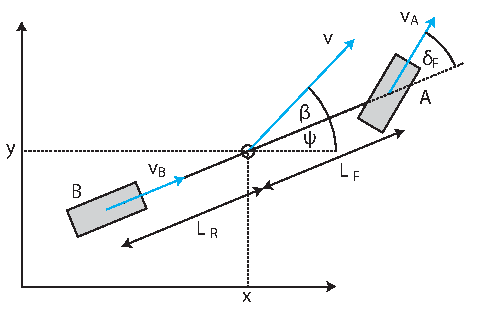
\includegraphics{../../Figures/Models/KinModel.pdf}
	\caption{Kinematic bicycle model}
	\label{fig:kinModel}
\end{figure}
The states in the inertial x-y-frame are the coordinates $x$ and $y$ of the center of the car, the heading angle $\psi$ and the velocity $v$ of the car center. Note that the car center does not necessarily need to coincide with the car's center of gravity since this is a pure geometrical representation of the car model which does not involve masses or forces.\\
The state dynamics can be written as
\begin{align}
\begin{split}
    \dot x &= v \cdot \cos (\psi + \beta)\\
    \dot y &= v \cdot \sin (\psi + \beta)\\
    \dot \psi &= \frac{v}{L_R}\cdot\sin(\beta)\\
    \dot v &= a
\end{split}
\end{align}
with the car's slip angle
\begin{equation}
    \beta = \arctan\left(\frac{L_F}{L_F+L_R}\cdot \tan(\delta_F)\right).
\end{equation}
The control inputs are the longitudinal acceleration $a$ and the steering angle $\delta_F$ at the front wheel.\\
The kinematic bicycle approximates real car dynamics well for low velocities and as long as there is no or only very little tire slip. However, especially for slippery road conditions and higher velocities model mismatch increases to such an extent that it can not be used to reliably predict real car dynamics anymore. This is why the \emph{Dynamic bicycle model} is introduced in the next section.

\subsection{Dynamic bicycle model}
As opposed to the kinematic bicycle model which is derived geometrically, the dynamic bicycle model is based on forces that occur between the front and rear tires and the road. Its states are the longitudinal and lateral velocity $v_x$ and $v_y$ which are represented in the body fixed frame, and the yaw rate $\dot \psi$. The state dynamics presented in eq. \ref{eq:dynModel} can be derived by applying Newton's second law of motion and have been taken from \cite{Kong2015}. \hl{The model equations have been simplified by considering the steering angle $\delta_F$ only in the lateral dynamics and neglecting the lateral tire force in the longitudinal dynamics.} The corresponding model is illustrated in fig. \ref{eq:dynModel}.
\begin{align}
\begin{split}
\label{eq:dynModel}
    \dot v_x &= a+\dot \psi\cdot v_y\\
    \dot v_y &= \frac{1}{m}\cdot (F_F\cdot \cos(\delta_F)+F_R)-\dot\psi\cdot v_x\\
    \ddot \psi &= \frac{1}{I_Z}\cdot(L_F\cdot F_F - L_R\cdot F_R)
\end{split}
\end{align}
\begin{figure}[ht]
	\centering
  	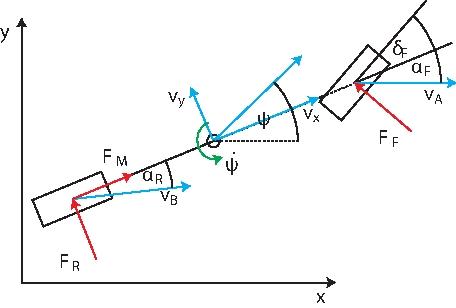
\includegraphics{../../Figures/Models/DynModel.pdf}
	\caption{Dynamic bicycle model}
	\label{fig:dynModel}
\end{figure}
These state dynamics assume that there is only lateral but no longitudinal tire slip which might occur during high accelerations or decelerations. This is done to simplify the model and since longitudinal acceleration is a control input that we can restrict to remain within bounds to avoid longitudinal tire slip.
The tire forces $F_F$ and $F_R$ depend on the lateral slipping angle $\alpha_F$ and $\alpha_R$ of the front and the rear tire. One common function that approximates the tire forces is the \emph{Pacejka} function from \cite{pacejka1987} (often referred to as \emph{Magic formula}):
% REFERENCE
\begin{equation}\label{eq:pacejka}
f_P(\alpha) = D\cdot\sin(C\cdot\arctan(B\cdot\alpha))
\end{equation}
Note: Eq. \ref{eq:pacejka} is a simplified version of the more general Pacejka function.\\
The Pacejka function is illustrated in fig. \ref{fig:Pacejka} for two sets of parameters, one for tire forces on a dry road and one for a snowy road. The chosen values are not parameters of a real tire, they are only meant for illustration purposes.
\begin{table}[h!]
\centering
\begin{tabular}{l|l|l|l}
Parameter & Meaning & Dry & Snowy\\
\hline
B & Stiffness factor & 10 & 5\\
C & Shape factor & 1.9 & 2\\
D & Peak factor & 1 & 0.3
\end{tabular}
\caption{Pacejka coefficients for different road conditions}
\label{tab:pacejka}
\end{table}

\begin{figure}[ht]
	\centering
  	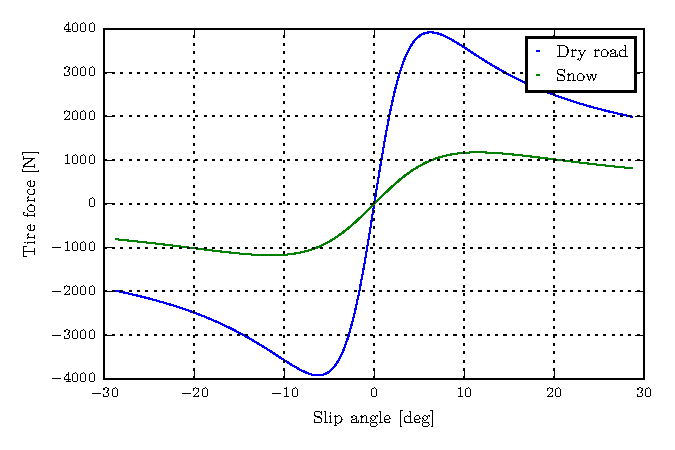
\includegraphics{../../Figures/Models/Pacejka.pdf}
	\caption{Pacejka tire model}
	\label{fig:Pacejka}
\end{figure}
Eq. \ref{eq:dynExtra} show the relations between the pacejka function and the tire forces as well as the calculation of slip angles which can be derived geometrically.
\begin{align}
\begin{split}\label{eq:dynExtra}
    F_F &= -\frac{1}{2}\cdot m\cdot g\cdot \mu \cdot f_P(\alpha_F)\\
    F_R &= -\frac{1}{2}\cdot m\cdot g\cdot \mu \cdot f_P(\alpha_R)\\
    \alpha_F &= \arctan\left(\frac{\dot y+L_F\dot\psi}{\lvert\dot x\lvert}\right) - \delta_F\\
    \alpha_R &= \arctan\left(\frac{\dot y-L_R\dot\psi}{\lvert\dot x\rvert}\right)
\end{split}
\end{align}

The dynamic bicycle model is more complex than the kinematic model but approximates real car dynamics very well even for higher speeds and various street conditions. However, it is important to choose the right set of Pacejka coefficients or measure them properly to obtain reliable results.\\
Also, one might experience numerical problems when using first order approximations of this model. Too long time steps might result in alternating and increasing slip angles and tire forces.

\subsection{Track reference frame}
So far two models were introduced: The kinematic model was constructed in an inertial frame whereas the dynamic model was constructed in a body-fixed frame. However, in race driving, we assume that the car follows a given track. In order to simplify calculations, we introduce a reference frame that expresses state dynamics in terms of coordinates relative to the race track.\\
The previous coordinates are mapped to a new set of coordinates which are the \emph{curvilinear abscissa} $s$, the \emph{lateral position error} from the track's center line $e_Y$, and the \emph{heading error} $e_\psi$. This type of frame is also referred to as \emph{Fernet frame} and has been used in previous publications \cite{Micaelli2006}. The coordinate frame is illustrated in fig. \ref{fig:s_ey}.

\begin{figure}[ht]
	\centering
  	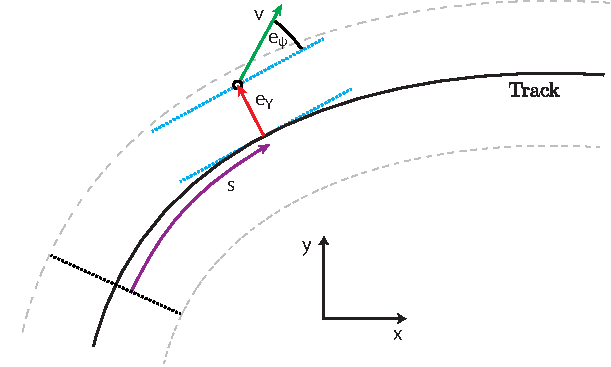
\includegraphics{../../Figures/Models/s_ey.pdf}
	\caption{Dynamic bicycle model}
	\label{fig:s_ey}
\end{figure}
The new state dynamics use the curvature $c(s)$ to describe the shape of the race track. The curvature is defined as the inverse of the curve radius
\begin{equation}
c(s) = \frac{1}{r(s)}.
\end{equation}
For a race track given in global coordinates $x(s)$ and $y(s)$, the curvature can be calculated by
\begin{equation}
c = \frac{x'y''-y'x''}{(x'^2+y'^2)^\frac{3}{2}}.
\end{equation}
The state dynamics of the \emph{kinematic model} in the track frame are derived as follows (refer to \cite{rajamani2005vehicle}):
\begin{subequations}\label{eq:kinTrackModel}
\begin{align}
    \dot s &= \frac{ds}{dt}= v\cdot \frac{\cos(e_\psi+\beta)}{1-e_Y\cdot c(s)}\\
    \dot e_Y &= v \cdot \sin(e_\psi+\beta)\\
    \dot e_\psi &= \frac{v}{L_F}\cdot \sin(\beta)-\frac{ds}{dt}\cdot c(s)\\
    \dot v &= a
\end{align}
\end{subequations}
The \emph{dynamic bicycle model} in the track frame is described by following equations:
\begin{subequations}\label{eq:dynTrackModel}
\begin{align}
    \dot e_Y &= v_x\cdot \sin(e_\psi) + v_y\cdot \cos(e_\psi)\\
    \dot e_\psi &= \dot\psi - \frac{ds}{dt}\cdot c(s)
\end{align}
\end{subequations}
with
\begin{equation}
\frac{ds}{dt} = \frac{v_x\cos(e_\psi)-v_y\sin(e_\psi)}{1-e_Y\cdot c(s)}
\end{equation}
We are going to use the model of eq. \ref{eq:kinTrackModel} and eq. \ref{eq:dynTrackModel} for all further simulations in combination with a given racetrack, i.e. a given curvature function $c(s)$.
\section{LMPC formulation}
This section presents the LMPC formulation of the race driving problem. In general, race driving is a minimum time problem: The variable that is to be optimized is the time the car takes to drive from the start to the finish line.\\
We use the dynamic bicycle model with following states and inputs
\begin{align}
\bm{x}_t^j&=\begin{pmatrix}
v_{x,t}^j & v_{y,t}^j & \dot \psi_t^j & e_{\psi,t}^j & e_{y,t}^j & s_t^j
\end{pmatrix}\\
\bm{u}_t^j&=\begin{pmatrix}
a_t^j & \delta_t^j
\end{pmatrix}.
\end{align}
and equation \ref{eq:generalLMPC} as the optimization function.
% Are there other ways on how to formulate this problem?
The racing problem is formulated by using a constant cost function on whenever the car is located between the start and finish line and zero cost when the car has crossed the finish line \cite{Rosolia2016}. Thus the stage cost is defined as follows:
\begin{equation}
h(\bm{x}_t,\bm{u}_t)=\begin{cases}
1&\text{if }\bm{x}_t\not\in\mathcal{L},\\
0&\text{if }\bm{x}_t\in\mathcal{L}.
\end{cases}
\end{equation}
where $\mathcal{L}$ is the set of points beyond the finish line at $s_{target}$:
\begin{equation}
\mathcal{L}=\left\{\bm{x}\in \mathbb{R}^6: \bm{xe}_6^T=s>s_{target}\right\}
\end{equation}
where $e_6$ is the 6-th standard basis in $\mathbb{R}^6$.\\
Lane boundaries are modeled as state constraints on the lateral position error $e_Y$:
\begin{equation}
-\frac{w_{Lane}}{2}\leq e_Y \leq \frac{w_{Lane}}{2}
\end{equation}
with lane width $w_{Lane}$.

\section{Approximation of the safe set and LP relaxation}
% Note: This has to be adapted according to the 'new' LMPC strategy, stacking two iterations together.
The LMPC problem from \ref{eq:generalRLMPC} minimizes its objective function over the safe set which is a set of discrete states of previous iterations. Therefore, this formulation is a Mixed Integer Nonlinear Programming (MINLP) problem. Since this type of problem is generally computationally challenging, we introduce the concept of safe set relaxation to transform the MINLP to a continuous problem.\\
For this purpose, we approximate the safe set and its cost function using a convex combination of two polynomials as in \cite{RosoliaRacing}. We define the time varying approximated safe set $\tilde{\mathcal{SS}}_t^{j,j-1}$ and the time varying approximated terminal cost function $\tilde{Q}_t^{j,j-1}(\cdot)$.
\begin{equation}
\tilde{\mathcal{SS}}_t^{j,j-1} = \left\{\bm{x}\in\mathbb{R}^5,\lambda\in[0,1]: x\in\lambda \tilde{\bm{x}}_t^{j,j-1}+(1-\lambda)\tilde{\bm{x}}_t^{j,j-2}\right\}
\end{equation}
where $\tilde{\bm{x}}_t^{j,k}$ is an $n$-th degree polynomial that approximates the $k$-th trajectory locally:
\begin{equation}
\tilde{\bm{x}}_t^{j,k}=\left\{\bm{x}\in\mathbb{R}^5:\forall i\in\{v_x,v_y,\dot\psi,e_\psi,e_y\},i=\begin{pmatrix}s^n &s^{n-1}&...&s& 1\end{pmatrix}\bm{\Gamma}_{t,i}^{j,k}\right\},
\end{equation}
where $\bm{\Gamma}_{t,i}^{j,k}$ is a vector containing the coefficients of the polynomial.\\
We also define the time varying function $C_t^{j,k}(\cdot)$ to approximate the cost-to-go function $J_{t\rightarrow\infty}^k(\cdot)$:
\begin{equation}
C_t^{j,j-1}(\bm{x})=\begin{cases}
\begin{pmatrix}
s^n & s^{n-1} &...&s&1
\end{pmatrix}
\bm{\Delta}_t^{j,k},&\text{if } \bm{x}\in\tilde{\bm{x}}_t^{j,k},\\
+\infty,&\text{if } \bm{x}\not\in\tilde{\bm{x}}_t^{j,k},
\end{cases}
\end{equation}
where $\bm{\Delta}_t^{j,k}$ contains the coefficients of the polynomial approximating the cost-to-go in iteration $k$.\\
We define the continuous time varying approximation of $Q^{j-1}(\cdot)$:
\begin{equation}
\tilde Q_t^{j,j-1}(\bm{x},\lambda)=\begin{cases}
\lambda C_t^{j,j-1}(\bm{x})+(1-\lambda)C_t^{j,j-2}(\bm{x}),&\text{if }(\bm{x},\lambda)\in\tilde{\mathcal{SS}}_t^{j,j-1}\\
+\infty,&\text{if }(\bm{x},\lambda)\not\in\tilde{\mathcal{SS}}_t^{j,j-1}
\end{cases}
\end{equation}
Having defined the relaxation of the safe set and approximation of the terminal cost function we can rewrite the LMPC formulation from eq. \ref{eq:generalLMPC}:
\begin{subequations}
\begin{align}
\tilde{J}_{t\rightarrow t+N}^{\scalebox{0.4}{LMPC},j}(\bm{x}_t^j)&=\min_{\lambda,\bm{u}_{t|t},...,\bm{u}_{t+N-1|t}}\left[\sum_{k=t}^{t+N-1}h(\bm{x}_{k|t},u_{k|t})+\tilde{Q}^{j,j-1}(\bm{x}_{t+N|t},\lambda)\right]\\
\text{s.t.}\\
\bm{x}_{k+1|t}&=f(\bm{x}_{k|t},\bm{u}_{k|t}),\forall k\in[t,...,t+N],\\
\bm{x}_{t|t}&=\bm{x}_t^j,\\
\bm{x}_{k|t}&\in\mathcal{X},\bm{u}_k\in\mathcal{U},\forall k\in[t,...,t+N],\\
(\bm{x}_{t+N|t},\lambda)&\in\tilde{\mathcal{SS}}^{j,j-1}.
\end{align}\label{eq:relaxedLMPC}
\end{subequations}
In practice, the polynomial degree as well as the number of points that are used for the approximation are design parameters. The polynomial degree has to be chosen large enough to approximate the trajectory in the chosen area well enough. However, a high degree polynomial function can lead to numerical difficulties for the solver due to large derivative values and multiple local minima. Similarly, the number of points has to be chosen in such a way that the predicted terminal state $x_N$ lies inside the approximated area. This is why this method works especially well if the approximated region is not too large (i.e. if the horizon $N$ is not too long) and if the trajectories can be well approximated by polynomials of the chosen degree.\\
For simulations and experiments in this thesis, a polynomial degree of $n=4...6$ proved to work well.\\
In the case of no model mismatch it would be sufficient to use only the previous iteration in the safe set. \hl{Is this true? Normally, we would have to consider *all* previous trajectories.}
However, since we expect some model mismatch in experiments, we always select the previous iteration as well as a second iteration with lowest iteration cost for the relaxation of the safe set and the approximation and the Q function.\\
In general, this approach could be extended to using more than two trajectories in the safe set. However, this would require more than one coefficient $\lambda$ and make the optimization problem more complex.
%\begin{itemize}
%\item Notes about how to choose the correct degree and horizon for polynomial approximation
%\item LMPC is a MIP (have to minimize over Q functions of discrete trajectories and their terminal constraints)
%\item Idea: approximate safe set trajectories with polynomials and minimize over convex combination of these polynomials
%\item In general: Since principle of non decreasing cost, only the last trajectory would be enough
%\item In practice: Assuming model mismatch, so use multiple previous trajectories
%\item To make computation efficient: Only use two iterations (last one and the other best previous one).
%\item Question: Is it proved that we get decreasing iteration cost for model mismatch? Why do we have to use the last one? Because otherwise we would get stuck with the best two? Mathematical explanation? - No, it's not proved yet. But people are working on it (Robust LMPC), 01/18/2017.
%\item Discussion of the relaxation method: It works well for low order polynomials, short horizons and smooth safe set trajectories. If the horizon is too long, the polynomial might not be able to approximate the safe set well enough. However, if we choose a higher degree polynomial that is able to approximate the safe set better, the solver will have a hard time since there are large first derivatives and many local optima.
%\item Discussion on how to theoretically use all previous trajectories in the safe set: Will have to introduce more $\lambda$.
%\item Also for Introduction: Important point about model mismatch: One huge advantage of using LMPC and system ID is that we can learn even the model during repeating iterations since we're getting a better and better model by the Linear Regression and the safe set is getting better and better as well.
%\end{itemize}

\section{Simulations}
The LMPC strategy is applied on the kinematic and the dynamic model in the track frame. The results are then mapped to the inertial $x-y$ frame to visualize the trajectory.\\
The physical parameters of the model are taken from a 1:10 scale RC car that is also used for real experiments.

\begin{center}
\begin{tabular}{l|l}
Parameter & Value\\
\hline
Mass& $m=\SI{2.0}{\kilo\gram}$\\
Axle distances&$L_F=L_R = \SI{0.125}{\meter}$\\
Moment of inertia&$I_z = \SI{0.03}{\kilo\gram\square\meter}$\\
Road friction&$\mu = 0.8$\\
Stiffness factor & $B=10$\\ 
Shape factor & $C=1.9$\\
Peak factor & $D=1.0$
\end{tabular}
\end{center}
%\emph{Note:} In the MPC formulation the Pacejka function is approximated by a linear function that is constrained to maximum tire forces. This linearization simplifies the optimization problem while still modeling the tire forces depending on the tire slip angles. % not valid anymore
The curvature $c(s)$ is given and constructed in such a way that the track is closed (finish line = start line). It is modeled as a piecewise linear and continuous function. At each time step, the curvature is locally approximated by a polynomial. This approximation is needed in the MPC formulation to allow a smooth prediction of the curvature at every $s$. The curvature used for simulations is shown in fig. \ref{fig:Sim_curv}. Negative curvatures are interpreted as right turns, positive curvatures as left turns. The track used for simulations has a length of $s_{Total} = \SI{50.49}{\meter}$.\\
\emph{Note:} Constructing the curvature $c(s)$ by a piecewise polynomial function (polynomial degree $n>1$) and thus making it differentiable could improve the approximation by polynomials even more. However, using a piecewise linear function proved to yield good results for our application.
\begin{figure}[ht]
	\centering
  	%% Creator: Matplotlib, PGF backend
%%
%% To include the figure in your LaTeX document, write
%%   \input{<filename>.pgf}
%%
%% Make sure the required packages are loaded in your preamble
%%   \usepackage{pgf}
%%
%% Figures using additional raster images can only be included by \input if
%% they are in the same directory as the main LaTeX file. For loading figures
%% from other directories you can use the `import` package
%%   \usepackage{import}
%% and then include the figures with
%%   \import{<path to file>}{<filename>.pgf}
%%
%% Matplotlib used the following preamble
%%   \usepackage{fontspec}
%%
\begingroup%
\makeatletter%
\begin{pgfpicture}%
\pgfpathrectangle{\pgfpointorigin}{\pgfqpoint{5.500000in}{3.000000in}}%
\pgfusepath{use as bounding box, clip}%
\begin{pgfscope}%
\pgfsetbuttcap%
\pgfsetmiterjoin%
\definecolor{currentfill}{rgb}{1.000000,1.000000,1.000000}%
\pgfsetfillcolor{currentfill}%
\pgfsetlinewidth{0.000000pt}%
\definecolor{currentstroke}{rgb}{1.000000,1.000000,1.000000}%
\pgfsetstrokecolor{currentstroke}%
\pgfsetdash{}{0pt}%
\pgfpathmoveto{\pgfqpoint{0.000000in}{0.000000in}}%
\pgfpathlineto{\pgfqpoint{5.500000in}{0.000000in}}%
\pgfpathlineto{\pgfqpoint{5.500000in}{3.000000in}}%
\pgfpathlineto{\pgfqpoint{0.000000in}{3.000000in}}%
\pgfpathclose%
\pgfusepath{fill}%
\end{pgfscope}%
\begin{pgfscope}%
\pgfsetbuttcap%
\pgfsetmiterjoin%
\definecolor{currentfill}{rgb}{1.000000,1.000000,1.000000}%
\pgfsetfillcolor{currentfill}%
\pgfsetlinewidth{0.000000pt}%
\definecolor{currentstroke}{rgb}{0.000000,0.000000,0.000000}%
\pgfsetstrokecolor{currentstroke}%
\pgfsetstrokeopacity{0.000000}%
\pgfsetdash{}{0pt}%
\pgfpathmoveto{\pgfqpoint{0.665614in}{0.471921in}}%
\pgfpathlineto{\pgfqpoint{5.291316in}{0.471921in}}%
\pgfpathlineto{\pgfqpoint{5.291316in}{2.805251in}}%
\pgfpathlineto{\pgfqpoint{0.665614in}{2.805251in}}%
\pgfpathclose%
\pgfusepath{fill}%
\end{pgfscope}%
\begin{pgfscope}%
\pgfpathrectangle{\pgfqpoint{0.665614in}{0.471921in}}{\pgfqpoint{4.625702in}{2.333330in}} %
\pgfusepath{clip}%
\pgfsetrectcap%
\pgfsetroundjoin%
\pgfsetlinewidth{0.501875pt}%
\definecolor{currentstroke}{rgb}{0.000000,0.000000,1.000000}%
\pgfsetstrokecolor{currentstroke}%
\pgfsetdash{}{0pt}%
\pgfpathmoveto{\pgfqpoint{0.666385in}{1.871919in}}%
\pgfpathlineto{\pgfqpoint{0.820575in}{1.871919in}}%
\pgfpathlineto{\pgfqpoint{0.974765in}{1.138882in}}%
\pgfpathlineto{\pgfqpoint{1.128955in}{1.871919in}}%
\pgfpathlineto{\pgfqpoint{1.206050in}{1.871919in}}%
\pgfpathlineto{\pgfqpoint{1.360240in}{1.138882in}}%
\pgfpathlineto{\pgfqpoint{1.514430in}{1.871919in}}%
\pgfpathlineto{\pgfqpoint{1.591525in}{1.138882in}}%
\pgfpathlineto{\pgfqpoint{1.668621in}{1.871919in}}%
\pgfpathlineto{\pgfqpoint{1.899906in}{1.871919in}}%
\pgfpathlineto{\pgfqpoint{2.285381in}{2.604956in}}%
\pgfpathlineto{\pgfqpoint{2.672398in}{1.865381in}}%
\pgfpathlineto{\pgfqpoint{2.902141in}{0.894536in}}%
\pgfpathlineto{\pgfqpoint{3.133426in}{1.871919in}}%
\pgfpathlineto{\pgfqpoint{3.364711in}{1.871919in}}%
\pgfpathlineto{\pgfqpoint{3.518901in}{1.138882in}}%
\pgfpathlineto{\pgfqpoint{3.673092in}{1.871919in}}%
\pgfpathlineto{\pgfqpoint{3.781025in}{1.871919in}}%
\pgfpathlineto{\pgfqpoint{4.012310in}{1.383228in}}%
\pgfpathlineto{\pgfqpoint{4.243595in}{1.871919in}}%
\pgfpathlineto{\pgfqpoint{4.587439in}{1.871919in}}%
\pgfpathlineto{\pgfqpoint{4.587439in}{1.871919in}}%
\pgfusepath{stroke}%
\end{pgfscope}%
\begin{pgfscope}%
\pgfsetrectcap%
\pgfsetmiterjoin%
\pgfsetlinewidth{0.501875pt}%
\definecolor{currentstroke}{rgb}{0.000000,0.000000,0.000000}%
\pgfsetstrokecolor{currentstroke}%
\pgfsetdash{}{0pt}%
\pgfpathmoveto{\pgfqpoint{0.665614in}{2.805251in}}%
\pgfpathlineto{\pgfqpoint{5.291316in}{2.805251in}}%
\pgfusepath{stroke}%
\end{pgfscope}%
\begin{pgfscope}%
\pgfsetrectcap%
\pgfsetmiterjoin%
\pgfsetlinewidth{0.501875pt}%
\definecolor{currentstroke}{rgb}{0.000000,0.000000,0.000000}%
\pgfsetstrokecolor{currentstroke}%
\pgfsetdash{}{0pt}%
\pgfpathmoveto{\pgfqpoint{5.291316in}{0.471921in}}%
\pgfpathlineto{\pgfqpoint{5.291316in}{2.805251in}}%
\pgfusepath{stroke}%
\end{pgfscope}%
\begin{pgfscope}%
\pgfsetrectcap%
\pgfsetmiterjoin%
\pgfsetlinewidth{0.501875pt}%
\definecolor{currentstroke}{rgb}{0.000000,0.000000,0.000000}%
\pgfsetstrokecolor{currentstroke}%
\pgfsetdash{}{0pt}%
\pgfpathmoveto{\pgfqpoint{0.665614in}{0.471921in}}%
\pgfpathlineto{\pgfqpoint{5.291316in}{0.471921in}}%
\pgfusepath{stroke}%
\end{pgfscope}%
\begin{pgfscope}%
\pgfsetrectcap%
\pgfsetmiterjoin%
\pgfsetlinewidth{0.501875pt}%
\definecolor{currentstroke}{rgb}{0.000000,0.000000,0.000000}%
\pgfsetstrokecolor{currentstroke}%
\pgfsetdash{}{0pt}%
\pgfpathmoveto{\pgfqpoint{0.665614in}{0.471921in}}%
\pgfpathlineto{\pgfqpoint{0.665614in}{2.805251in}}%
\pgfusepath{stroke}%
\end{pgfscope}%
\begin{pgfscope}%
\pgfpathrectangle{\pgfqpoint{0.665614in}{0.471921in}}{\pgfqpoint{4.625702in}{2.333330in}} %
\pgfusepath{clip}%
\pgfsetbuttcap%
\pgfsetroundjoin%
\pgfsetlinewidth{0.501875pt}%
\definecolor{currentstroke}{rgb}{0.000000,0.000000,0.000000}%
\pgfsetstrokecolor{currentstroke}%
\pgfsetdash{{1.000000pt}{3.000000pt}}{0.000000pt}%
\pgfpathmoveto{\pgfqpoint{0.665614in}{0.471921in}}%
\pgfpathlineto{\pgfqpoint{0.665614in}{2.805251in}}%
\pgfusepath{stroke}%
\end{pgfscope}%
\begin{pgfscope}%
\pgfsetbuttcap%
\pgfsetroundjoin%
\definecolor{currentfill}{rgb}{0.000000,0.000000,0.000000}%
\pgfsetfillcolor{currentfill}%
\pgfsetlinewidth{0.250937pt}%
\definecolor{currentstroke}{rgb}{0.000000,0.000000,0.000000}%
\pgfsetstrokecolor{currentstroke}%
\pgfsetdash{}{0pt}%
\pgfsys@defobject{currentmarker}{\pgfqpoint{0.000000in}{0.000000in}}{\pgfqpoint{0.000000in}{0.055556in}}{%
\pgfpathmoveto{\pgfqpoint{0.000000in}{0.000000in}}%
\pgfpathlineto{\pgfqpoint{0.000000in}{0.055556in}}%
\pgfusepath{stroke,fill}%
}%
\begin{pgfscope}%
\pgfsys@transformshift{0.665614in}{0.471921in}%
\pgfsys@useobject{currentmarker}{}%
\end{pgfscope}%
\end{pgfscope}%
\begin{pgfscope}%
\pgfsetbuttcap%
\pgfsetroundjoin%
\definecolor{currentfill}{rgb}{0.000000,0.000000,0.000000}%
\pgfsetfillcolor{currentfill}%
\pgfsetlinewidth{0.250937pt}%
\definecolor{currentstroke}{rgb}{0.000000,0.000000,0.000000}%
\pgfsetstrokecolor{currentstroke}%
\pgfsetdash{}{0pt}%
\pgfsys@defobject{currentmarker}{\pgfqpoint{0.000000in}{-0.055556in}}{\pgfqpoint{0.000000in}{0.000000in}}{%
\pgfpathmoveto{\pgfqpoint{0.000000in}{0.000000in}}%
\pgfpathlineto{\pgfqpoint{0.000000in}{-0.055556in}}%
\pgfusepath{stroke,fill}%
}%
\begin{pgfscope}%
\pgfsys@transformshift{0.665614in}{2.805251in}%
\pgfsys@useobject{currentmarker}{}%
\end{pgfscope}%
\end{pgfscope}%
\begin{pgfscope}%
\pgftext[x=0.665614in,y=0.416365in,,top]{\rmfamily\fontsize{6.940000}{8.328000}\selectfont \(\displaystyle 0\)}%
\end{pgfscope}%
\begin{pgfscope}%
\pgfpathrectangle{\pgfqpoint{0.665614in}{0.471921in}}{\pgfqpoint{4.625702in}{2.333330in}} %
\pgfusepath{clip}%
\pgfsetbuttcap%
\pgfsetroundjoin%
\pgfsetlinewidth{0.501875pt}%
\definecolor{currentstroke}{rgb}{0.000000,0.000000,0.000000}%
\pgfsetstrokecolor{currentstroke}%
\pgfsetdash{{1.000000pt}{3.000000pt}}{0.000000pt}%
\pgfpathmoveto{\pgfqpoint{1.436564in}{0.471921in}}%
\pgfpathlineto{\pgfqpoint{1.436564in}{2.805251in}}%
\pgfusepath{stroke}%
\end{pgfscope}%
\begin{pgfscope}%
\pgfsetbuttcap%
\pgfsetroundjoin%
\definecolor{currentfill}{rgb}{0.000000,0.000000,0.000000}%
\pgfsetfillcolor{currentfill}%
\pgfsetlinewidth{0.250937pt}%
\definecolor{currentstroke}{rgb}{0.000000,0.000000,0.000000}%
\pgfsetstrokecolor{currentstroke}%
\pgfsetdash{}{0pt}%
\pgfsys@defobject{currentmarker}{\pgfqpoint{0.000000in}{0.000000in}}{\pgfqpoint{0.000000in}{0.055556in}}{%
\pgfpathmoveto{\pgfqpoint{0.000000in}{0.000000in}}%
\pgfpathlineto{\pgfqpoint{0.000000in}{0.055556in}}%
\pgfusepath{stroke,fill}%
}%
\begin{pgfscope}%
\pgfsys@transformshift{1.436564in}{0.471921in}%
\pgfsys@useobject{currentmarker}{}%
\end{pgfscope}%
\end{pgfscope}%
\begin{pgfscope}%
\pgfsetbuttcap%
\pgfsetroundjoin%
\definecolor{currentfill}{rgb}{0.000000,0.000000,0.000000}%
\pgfsetfillcolor{currentfill}%
\pgfsetlinewidth{0.250937pt}%
\definecolor{currentstroke}{rgb}{0.000000,0.000000,0.000000}%
\pgfsetstrokecolor{currentstroke}%
\pgfsetdash{}{0pt}%
\pgfsys@defobject{currentmarker}{\pgfqpoint{0.000000in}{-0.055556in}}{\pgfqpoint{0.000000in}{0.000000in}}{%
\pgfpathmoveto{\pgfqpoint{0.000000in}{0.000000in}}%
\pgfpathlineto{\pgfqpoint{0.000000in}{-0.055556in}}%
\pgfusepath{stroke,fill}%
}%
\begin{pgfscope}%
\pgfsys@transformshift{1.436564in}{2.805251in}%
\pgfsys@useobject{currentmarker}{}%
\end{pgfscope}%
\end{pgfscope}%
\begin{pgfscope}%
\pgftext[x=1.436564in,y=0.416365in,,top]{\rmfamily\fontsize{6.940000}{8.328000}\selectfont \(\displaystyle 10\)}%
\end{pgfscope}%
\begin{pgfscope}%
\pgfpathrectangle{\pgfqpoint{0.665614in}{0.471921in}}{\pgfqpoint{4.625702in}{2.333330in}} %
\pgfusepath{clip}%
\pgfsetbuttcap%
\pgfsetroundjoin%
\pgfsetlinewidth{0.501875pt}%
\definecolor{currentstroke}{rgb}{0.000000,0.000000,0.000000}%
\pgfsetstrokecolor{currentstroke}%
\pgfsetdash{{1.000000pt}{3.000000pt}}{0.000000pt}%
\pgfpathmoveto{\pgfqpoint{2.207515in}{0.471921in}}%
\pgfpathlineto{\pgfqpoint{2.207515in}{2.805251in}}%
\pgfusepath{stroke}%
\end{pgfscope}%
\begin{pgfscope}%
\pgfsetbuttcap%
\pgfsetroundjoin%
\definecolor{currentfill}{rgb}{0.000000,0.000000,0.000000}%
\pgfsetfillcolor{currentfill}%
\pgfsetlinewidth{0.250937pt}%
\definecolor{currentstroke}{rgb}{0.000000,0.000000,0.000000}%
\pgfsetstrokecolor{currentstroke}%
\pgfsetdash{}{0pt}%
\pgfsys@defobject{currentmarker}{\pgfqpoint{0.000000in}{0.000000in}}{\pgfqpoint{0.000000in}{0.055556in}}{%
\pgfpathmoveto{\pgfqpoint{0.000000in}{0.000000in}}%
\pgfpathlineto{\pgfqpoint{0.000000in}{0.055556in}}%
\pgfusepath{stroke,fill}%
}%
\begin{pgfscope}%
\pgfsys@transformshift{2.207515in}{0.471921in}%
\pgfsys@useobject{currentmarker}{}%
\end{pgfscope}%
\end{pgfscope}%
\begin{pgfscope}%
\pgfsetbuttcap%
\pgfsetroundjoin%
\definecolor{currentfill}{rgb}{0.000000,0.000000,0.000000}%
\pgfsetfillcolor{currentfill}%
\pgfsetlinewidth{0.250937pt}%
\definecolor{currentstroke}{rgb}{0.000000,0.000000,0.000000}%
\pgfsetstrokecolor{currentstroke}%
\pgfsetdash{}{0pt}%
\pgfsys@defobject{currentmarker}{\pgfqpoint{0.000000in}{-0.055556in}}{\pgfqpoint{0.000000in}{0.000000in}}{%
\pgfpathmoveto{\pgfqpoint{0.000000in}{0.000000in}}%
\pgfpathlineto{\pgfqpoint{0.000000in}{-0.055556in}}%
\pgfusepath{stroke,fill}%
}%
\begin{pgfscope}%
\pgfsys@transformshift{2.207515in}{2.805251in}%
\pgfsys@useobject{currentmarker}{}%
\end{pgfscope}%
\end{pgfscope}%
\begin{pgfscope}%
\pgftext[x=2.207515in,y=0.416365in,,top]{\rmfamily\fontsize{6.940000}{8.328000}\selectfont \(\displaystyle 20\)}%
\end{pgfscope}%
\begin{pgfscope}%
\pgfpathrectangle{\pgfqpoint{0.665614in}{0.471921in}}{\pgfqpoint{4.625702in}{2.333330in}} %
\pgfusepath{clip}%
\pgfsetbuttcap%
\pgfsetroundjoin%
\pgfsetlinewidth{0.501875pt}%
\definecolor{currentstroke}{rgb}{0.000000,0.000000,0.000000}%
\pgfsetstrokecolor{currentstroke}%
\pgfsetdash{{1.000000pt}{3.000000pt}}{0.000000pt}%
\pgfpathmoveto{\pgfqpoint{2.978465in}{0.471921in}}%
\pgfpathlineto{\pgfqpoint{2.978465in}{2.805251in}}%
\pgfusepath{stroke}%
\end{pgfscope}%
\begin{pgfscope}%
\pgfsetbuttcap%
\pgfsetroundjoin%
\definecolor{currentfill}{rgb}{0.000000,0.000000,0.000000}%
\pgfsetfillcolor{currentfill}%
\pgfsetlinewidth{0.250937pt}%
\definecolor{currentstroke}{rgb}{0.000000,0.000000,0.000000}%
\pgfsetstrokecolor{currentstroke}%
\pgfsetdash{}{0pt}%
\pgfsys@defobject{currentmarker}{\pgfqpoint{0.000000in}{0.000000in}}{\pgfqpoint{0.000000in}{0.055556in}}{%
\pgfpathmoveto{\pgfqpoint{0.000000in}{0.000000in}}%
\pgfpathlineto{\pgfqpoint{0.000000in}{0.055556in}}%
\pgfusepath{stroke,fill}%
}%
\begin{pgfscope}%
\pgfsys@transformshift{2.978465in}{0.471921in}%
\pgfsys@useobject{currentmarker}{}%
\end{pgfscope}%
\end{pgfscope}%
\begin{pgfscope}%
\pgfsetbuttcap%
\pgfsetroundjoin%
\definecolor{currentfill}{rgb}{0.000000,0.000000,0.000000}%
\pgfsetfillcolor{currentfill}%
\pgfsetlinewidth{0.250937pt}%
\definecolor{currentstroke}{rgb}{0.000000,0.000000,0.000000}%
\pgfsetstrokecolor{currentstroke}%
\pgfsetdash{}{0pt}%
\pgfsys@defobject{currentmarker}{\pgfqpoint{0.000000in}{-0.055556in}}{\pgfqpoint{0.000000in}{0.000000in}}{%
\pgfpathmoveto{\pgfqpoint{0.000000in}{0.000000in}}%
\pgfpathlineto{\pgfqpoint{0.000000in}{-0.055556in}}%
\pgfusepath{stroke,fill}%
}%
\begin{pgfscope}%
\pgfsys@transformshift{2.978465in}{2.805251in}%
\pgfsys@useobject{currentmarker}{}%
\end{pgfscope}%
\end{pgfscope}%
\begin{pgfscope}%
\pgftext[x=2.978465in,y=0.416365in,,top]{\rmfamily\fontsize{6.940000}{8.328000}\selectfont \(\displaystyle 30\)}%
\end{pgfscope}%
\begin{pgfscope}%
\pgfpathrectangle{\pgfqpoint{0.665614in}{0.471921in}}{\pgfqpoint{4.625702in}{2.333330in}} %
\pgfusepath{clip}%
\pgfsetbuttcap%
\pgfsetroundjoin%
\pgfsetlinewidth{0.501875pt}%
\definecolor{currentstroke}{rgb}{0.000000,0.000000,0.000000}%
\pgfsetstrokecolor{currentstroke}%
\pgfsetdash{{1.000000pt}{3.000000pt}}{0.000000pt}%
\pgfpathmoveto{\pgfqpoint{3.749416in}{0.471921in}}%
\pgfpathlineto{\pgfqpoint{3.749416in}{2.805251in}}%
\pgfusepath{stroke}%
\end{pgfscope}%
\begin{pgfscope}%
\pgfsetbuttcap%
\pgfsetroundjoin%
\definecolor{currentfill}{rgb}{0.000000,0.000000,0.000000}%
\pgfsetfillcolor{currentfill}%
\pgfsetlinewidth{0.250937pt}%
\definecolor{currentstroke}{rgb}{0.000000,0.000000,0.000000}%
\pgfsetstrokecolor{currentstroke}%
\pgfsetdash{}{0pt}%
\pgfsys@defobject{currentmarker}{\pgfqpoint{0.000000in}{0.000000in}}{\pgfqpoint{0.000000in}{0.055556in}}{%
\pgfpathmoveto{\pgfqpoint{0.000000in}{0.000000in}}%
\pgfpathlineto{\pgfqpoint{0.000000in}{0.055556in}}%
\pgfusepath{stroke,fill}%
}%
\begin{pgfscope}%
\pgfsys@transformshift{3.749416in}{0.471921in}%
\pgfsys@useobject{currentmarker}{}%
\end{pgfscope}%
\end{pgfscope}%
\begin{pgfscope}%
\pgfsetbuttcap%
\pgfsetroundjoin%
\definecolor{currentfill}{rgb}{0.000000,0.000000,0.000000}%
\pgfsetfillcolor{currentfill}%
\pgfsetlinewidth{0.250937pt}%
\definecolor{currentstroke}{rgb}{0.000000,0.000000,0.000000}%
\pgfsetstrokecolor{currentstroke}%
\pgfsetdash{}{0pt}%
\pgfsys@defobject{currentmarker}{\pgfqpoint{0.000000in}{-0.055556in}}{\pgfqpoint{0.000000in}{0.000000in}}{%
\pgfpathmoveto{\pgfqpoint{0.000000in}{0.000000in}}%
\pgfpathlineto{\pgfqpoint{0.000000in}{-0.055556in}}%
\pgfusepath{stroke,fill}%
}%
\begin{pgfscope}%
\pgfsys@transformshift{3.749416in}{2.805251in}%
\pgfsys@useobject{currentmarker}{}%
\end{pgfscope}%
\end{pgfscope}%
\begin{pgfscope}%
\pgftext[x=3.749416in,y=0.416365in,,top]{\rmfamily\fontsize{6.940000}{8.328000}\selectfont \(\displaystyle 40\)}%
\end{pgfscope}%
\begin{pgfscope}%
\pgfpathrectangle{\pgfqpoint{0.665614in}{0.471921in}}{\pgfqpoint{4.625702in}{2.333330in}} %
\pgfusepath{clip}%
\pgfsetbuttcap%
\pgfsetroundjoin%
\pgfsetlinewidth{0.501875pt}%
\definecolor{currentstroke}{rgb}{0.000000,0.000000,0.000000}%
\pgfsetstrokecolor{currentstroke}%
\pgfsetdash{{1.000000pt}{3.000000pt}}{0.000000pt}%
\pgfpathmoveto{\pgfqpoint{4.520366in}{0.471921in}}%
\pgfpathlineto{\pgfqpoint{4.520366in}{2.805251in}}%
\pgfusepath{stroke}%
\end{pgfscope}%
\begin{pgfscope}%
\pgfsetbuttcap%
\pgfsetroundjoin%
\definecolor{currentfill}{rgb}{0.000000,0.000000,0.000000}%
\pgfsetfillcolor{currentfill}%
\pgfsetlinewidth{0.250937pt}%
\definecolor{currentstroke}{rgb}{0.000000,0.000000,0.000000}%
\pgfsetstrokecolor{currentstroke}%
\pgfsetdash{}{0pt}%
\pgfsys@defobject{currentmarker}{\pgfqpoint{0.000000in}{0.000000in}}{\pgfqpoint{0.000000in}{0.055556in}}{%
\pgfpathmoveto{\pgfqpoint{0.000000in}{0.000000in}}%
\pgfpathlineto{\pgfqpoint{0.000000in}{0.055556in}}%
\pgfusepath{stroke,fill}%
}%
\begin{pgfscope}%
\pgfsys@transformshift{4.520366in}{0.471921in}%
\pgfsys@useobject{currentmarker}{}%
\end{pgfscope}%
\end{pgfscope}%
\begin{pgfscope}%
\pgfsetbuttcap%
\pgfsetroundjoin%
\definecolor{currentfill}{rgb}{0.000000,0.000000,0.000000}%
\pgfsetfillcolor{currentfill}%
\pgfsetlinewidth{0.250937pt}%
\definecolor{currentstroke}{rgb}{0.000000,0.000000,0.000000}%
\pgfsetstrokecolor{currentstroke}%
\pgfsetdash{}{0pt}%
\pgfsys@defobject{currentmarker}{\pgfqpoint{0.000000in}{-0.055556in}}{\pgfqpoint{0.000000in}{0.000000in}}{%
\pgfpathmoveto{\pgfqpoint{0.000000in}{0.000000in}}%
\pgfpathlineto{\pgfqpoint{0.000000in}{-0.055556in}}%
\pgfusepath{stroke,fill}%
}%
\begin{pgfscope}%
\pgfsys@transformshift{4.520366in}{2.805251in}%
\pgfsys@useobject{currentmarker}{}%
\end{pgfscope}%
\end{pgfscope}%
\begin{pgfscope}%
\pgftext[x=4.520366in,y=0.416365in,,top]{\rmfamily\fontsize{6.940000}{8.328000}\selectfont \(\displaystyle 50\)}%
\end{pgfscope}%
\begin{pgfscope}%
\pgfpathrectangle{\pgfqpoint{0.665614in}{0.471921in}}{\pgfqpoint{4.625702in}{2.333330in}} %
\pgfusepath{clip}%
\pgfsetbuttcap%
\pgfsetroundjoin%
\pgfsetlinewidth{0.501875pt}%
\definecolor{currentstroke}{rgb}{0.000000,0.000000,0.000000}%
\pgfsetstrokecolor{currentstroke}%
\pgfsetdash{{1.000000pt}{3.000000pt}}{0.000000pt}%
\pgfpathmoveto{\pgfqpoint{5.291316in}{0.471921in}}%
\pgfpathlineto{\pgfqpoint{5.291316in}{2.805251in}}%
\pgfusepath{stroke}%
\end{pgfscope}%
\begin{pgfscope}%
\pgfsetbuttcap%
\pgfsetroundjoin%
\definecolor{currentfill}{rgb}{0.000000,0.000000,0.000000}%
\pgfsetfillcolor{currentfill}%
\pgfsetlinewidth{0.250937pt}%
\definecolor{currentstroke}{rgb}{0.000000,0.000000,0.000000}%
\pgfsetstrokecolor{currentstroke}%
\pgfsetdash{}{0pt}%
\pgfsys@defobject{currentmarker}{\pgfqpoint{0.000000in}{0.000000in}}{\pgfqpoint{0.000000in}{0.055556in}}{%
\pgfpathmoveto{\pgfqpoint{0.000000in}{0.000000in}}%
\pgfpathlineto{\pgfqpoint{0.000000in}{0.055556in}}%
\pgfusepath{stroke,fill}%
}%
\begin{pgfscope}%
\pgfsys@transformshift{5.291316in}{0.471921in}%
\pgfsys@useobject{currentmarker}{}%
\end{pgfscope}%
\end{pgfscope}%
\begin{pgfscope}%
\pgfsetbuttcap%
\pgfsetroundjoin%
\definecolor{currentfill}{rgb}{0.000000,0.000000,0.000000}%
\pgfsetfillcolor{currentfill}%
\pgfsetlinewidth{0.250937pt}%
\definecolor{currentstroke}{rgb}{0.000000,0.000000,0.000000}%
\pgfsetstrokecolor{currentstroke}%
\pgfsetdash{}{0pt}%
\pgfsys@defobject{currentmarker}{\pgfqpoint{0.000000in}{-0.055556in}}{\pgfqpoint{0.000000in}{0.000000in}}{%
\pgfpathmoveto{\pgfqpoint{0.000000in}{0.000000in}}%
\pgfpathlineto{\pgfqpoint{0.000000in}{-0.055556in}}%
\pgfusepath{stroke,fill}%
}%
\begin{pgfscope}%
\pgfsys@transformshift{5.291316in}{2.805251in}%
\pgfsys@useobject{currentmarker}{}%
\end{pgfscope}%
\end{pgfscope}%
\begin{pgfscope}%
\pgftext[x=5.291316in,y=0.416365in,,top]{\rmfamily\fontsize{6.940000}{8.328000}\selectfont \(\displaystyle 60\)}%
\end{pgfscope}%
\begin{pgfscope}%
\pgftext[x=2.978465in,y=0.261328in,,top]{\rmfamily\fontsize{8.330000}{9.996000}\selectfont \(\displaystyle s\) [\(\displaystyle  m\)]}%
\end{pgfscope}%
\begin{pgfscope}%
\pgfpathrectangle{\pgfqpoint{0.665614in}{0.471921in}}{\pgfqpoint{4.625702in}{2.333330in}} %
\pgfusepath{clip}%
\pgfsetbuttcap%
\pgfsetroundjoin%
\pgfsetlinewidth{0.501875pt}%
\definecolor{currentstroke}{rgb}{0.000000,0.000000,0.000000}%
\pgfsetstrokecolor{currentstroke}%
\pgfsetdash{{1.000000pt}{3.000000pt}}{0.000000pt}%
\pgfpathmoveto{\pgfqpoint{0.665614in}{0.471921in}}%
\pgfpathlineto{\pgfqpoint{5.291316in}{0.471921in}}%
\pgfusepath{stroke}%
\end{pgfscope}%
\begin{pgfscope}%
\pgfsetbuttcap%
\pgfsetroundjoin%
\definecolor{currentfill}{rgb}{0.000000,0.000000,0.000000}%
\pgfsetfillcolor{currentfill}%
\pgfsetlinewidth{0.250937pt}%
\definecolor{currentstroke}{rgb}{0.000000,0.000000,0.000000}%
\pgfsetstrokecolor{currentstroke}%
\pgfsetdash{}{0pt}%
\pgfsys@defobject{currentmarker}{\pgfqpoint{0.000000in}{0.000000in}}{\pgfqpoint{0.055556in}{0.000000in}}{%
\pgfpathmoveto{\pgfqpoint{0.000000in}{0.000000in}}%
\pgfpathlineto{\pgfqpoint{0.055556in}{0.000000in}}%
\pgfusepath{stroke,fill}%
}%
\begin{pgfscope}%
\pgfsys@transformshift{0.665614in}{0.471921in}%
\pgfsys@useobject{currentmarker}{}%
\end{pgfscope}%
\end{pgfscope}%
\begin{pgfscope}%
\pgfsetbuttcap%
\pgfsetroundjoin%
\definecolor{currentfill}{rgb}{0.000000,0.000000,0.000000}%
\pgfsetfillcolor{currentfill}%
\pgfsetlinewidth{0.250937pt}%
\definecolor{currentstroke}{rgb}{0.000000,0.000000,0.000000}%
\pgfsetstrokecolor{currentstroke}%
\pgfsetdash{}{0pt}%
\pgfsys@defobject{currentmarker}{\pgfqpoint{-0.055556in}{0.000000in}}{\pgfqpoint{0.000000in}{0.000000in}}{%
\pgfpathmoveto{\pgfqpoint{0.000000in}{0.000000in}}%
\pgfpathlineto{\pgfqpoint{-0.055556in}{0.000000in}}%
\pgfusepath{stroke,fill}%
}%
\begin{pgfscope}%
\pgfsys@transformshift{5.291316in}{0.471921in}%
\pgfsys@useobject{currentmarker}{}%
\end{pgfscope}%
\end{pgfscope}%
\begin{pgfscope}%
\pgftext[x=0.610058in,y=0.471921in,right,]{\rmfamily\fontsize{6.940000}{8.328000}\selectfont \(\displaystyle -1.5\)}%
\end{pgfscope}%
\begin{pgfscope}%
\pgfpathrectangle{\pgfqpoint{0.665614in}{0.471921in}}{\pgfqpoint{4.625702in}{2.333330in}} %
\pgfusepath{clip}%
\pgfsetbuttcap%
\pgfsetroundjoin%
\pgfsetlinewidth{0.501875pt}%
\definecolor{currentstroke}{rgb}{0.000000,0.000000,0.000000}%
\pgfsetstrokecolor{currentstroke}%
\pgfsetdash{{1.000000pt}{3.000000pt}}{0.000000pt}%
\pgfpathmoveto{\pgfqpoint{0.665614in}{0.938587in}}%
\pgfpathlineto{\pgfqpoint{5.291316in}{0.938587in}}%
\pgfusepath{stroke}%
\end{pgfscope}%
\begin{pgfscope}%
\pgfsetbuttcap%
\pgfsetroundjoin%
\definecolor{currentfill}{rgb}{0.000000,0.000000,0.000000}%
\pgfsetfillcolor{currentfill}%
\pgfsetlinewidth{0.250937pt}%
\definecolor{currentstroke}{rgb}{0.000000,0.000000,0.000000}%
\pgfsetstrokecolor{currentstroke}%
\pgfsetdash{}{0pt}%
\pgfsys@defobject{currentmarker}{\pgfqpoint{0.000000in}{0.000000in}}{\pgfqpoint{0.055556in}{0.000000in}}{%
\pgfpathmoveto{\pgfqpoint{0.000000in}{0.000000in}}%
\pgfpathlineto{\pgfqpoint{0.055556in}{0.000000in}}%
\pgfusepath{stroke,fill}%
}%
\begin{pgfscope}%
\pgfsys@transformshift{0.665614in}{0.938587in}%
\pgfsys@useobject{currentmarker}{}%
\end{pgfscope}%
\end{pgfscope}%
\begin{pgfscope}%
\pgfsetbuttcap%
\pgfsetroundjoin%
\definecolor{currentfill}{rgb}{0.000000,0.000000,0.000000}%
\pgfsetfillcolor{currentfill}%
\pgfsetlinewidth{0.250937pt}%
\definecolor{currentstroke}{rgb}{0.000000,0.000000,0.000000}%
\pgfsetstrokecolor{currentstroke}%
\pgfsetdash{}{0pt}%
\pgfsys@defobject{currentmarker}{\pgfqpoint{-0.055556in}{0.000000in}}{\pgfqpoint{0.000000in}{0.000000in}}{%
\pgfpathmoveto{\pgfqpoint{0.000000in}{0.000000in}}%
\pgfpathlineto{\pgfqpoint{-0.055556in}{0.000000in}}%
\pgfusepath{stroke,fill}%
}%
\begin{pgfscope}%
\pgfsys@transformshift{5.291316in}{0.938587in}%
\pgfsys@useobject{currentmarker}{}%
\end{pgfscope}%
\end{pgfscope}%
\begin{pgfscope}%
\pgftext[x=0.610058in,y=0.938587in,right,]{\rmfamily\fontsize{6.940000}{8.328000}\selectfont \(\displaystyle -1.0\)}%
\end{pgfscope}%
\begin{pgfscope}%
\pgfpathrectangle{\pgfqpoint{0.665614in}{0.471921in}}{\pgfqpoint{4.625702in}{2.333330in}} %
\pgfusepath{clip}%
\pgfsetbuttcap%
\pgfsetroundjoin%
\pgfsetlinewidth{0.501875pt}%
\definecolor{currentstroke}{rgb}{0.000000,0.000000,0.000000}%
\pgfsetstrokecolor{currentstroke}%
\pgfsetdash{{1.000000pt}{3.000000pt}}{0.000000pt}%
\pgfpathmoveto{\pgfqpoint{0.665614in}{1.405253in}}%
\pgfpathlineto{\pgfqpoint{5.291316in}{1.405253in}}%
\pgfusepath{stroke}%
\end{pgfscope}%
\begin{pgfscope}%
\pgfsetbuttcap%
\pgfsetroundjoin%
\definecolor{currentfill}{rgb}{0.000000,0.000000,0.000000}%
\pgfsetfillcolor{currentfill}%
\pgfsetlinewidth{0.250937pt}%
\definecolor{currentstroke}{rgb}{0.000000,0.000000,0.000000}%
\pgfsetstrokecolor{currentstroke}%
\pgfsetdash{}{0pt}%
\pgfsys@defobject{currentmarker}{\pgfqpoint{0.000000in}{0.000000in}}{\pgfqpoint{0.055556in}{0.000000in}}{%
\pgfpathmoveto{\pgfqpoint{0.000000in}{0.000000in}}%
\pgfpathlineto{\pgfqpoint{0.055556in}{0.000000in}}%
\pgfusepath{stroke,fill}%
}%
\begin{pgfscope}%
\pgfsys@transformshift{0.665614in}{1.405253in}%
\pgfsys@useobject{currentmarker}{}%
\end{pgfscope}%
\end{pgfscope}%
\begin{pgfscope}%
\pgfsetbuttcap%
\pgfsetroundjoin%
\definecolor{currentfill}{rgb}{0.000000,0.000000,0.000000}%
\pgfsetfillcolor{currentfill}%
\pgfsetlinewidth{0.250937pt}%
\definecolor{currentstroke}{rgb}{0.000000,0.000000,0.000000}%
\pgfsetstrokecolor{currentstroke}%
\pgfsetdash{}{0pt}%
\pgfsys@defobject{currentmarker}{\pgfqpoint{-0.055556in}{0.000000in}}{\pgfqpoint{0.000000in}{0.000000in}}{%
\pgfpathmoveto{\pgfqpoint{0.000000in}{0.000000in}}%
\pgfpathlineto{\pgfqpoint{-0.055556in}{0.000000in}}%
\pgfusepath{stroke,fill}%
}%
\begin{pgfscope}%
\pgfsys@transformshift{5.291316in}{1.405253in}%
\pgfsys@useobject{currentmarker}{}%
\end{pgfscope}%
\end{pgfscope}%
\begin{pgfscope}%
\pgftext[x=0.610058in,y=1.405253in,right,]{\rmfamily\fontsize{6.940000}{8.328000}\selectfont \(\displaystyle -0.5\)}%
\end{pgfscope}%
\begin{pgfscope}%
\pgfpathrectangle{\pgfqpoint{0.665614in}{0.471921in}}{\pgfqpoint{4.625702in}{2.333330in}} %
\pgfusepath{clip}%
\pgfsetbuttcap%
\pgfsetroundjoin%
\pgfsetlinewidth{0.501875pt}%
\definecolor{currentstroke}{rgb}{0.000000,0.000000,0.000000}%
\pgfsetstrokecolor{currentstroke}%
\pgfsetdash{{1.000000pt}{3.000000pt}}{0.000000pt}%
\pgfpathmoveto{\pgfqpoint{0.665614in}{1.871919in}}%
\pgfpathlineto{\pgfqpoint{5.291316in}{1.871919in}}%
\pgfusepath{stroke}%
\end{pgfscope}%
\begin{pgfscope}%
\pgfsetbuttcap%
\pgfsetroundjoin%
\definecolor{currentfill}{rgb}{0.000000,0.000000,0.000000}%
\pgfsetfillcolor{currentfill}%
\pgfsetlinewidth{0.250937pt}%
\definecolor{currentstroke}{rgb}{0.000000,0.000000,0.000000}%
\pgfsetstrokecolor{currentstroke}%
\pgfsetdash{}{0pt}%
\pgfsys@defobject{currentmarker}{\pgfqpoint{0.000000in}{0.000000in}}{\pgfqpoint{0.055556in}{0.000000in}}{%
\pgfpathmoveto{\pgfqpoint{0.000000in}{0.000000in}}%
\pgfpathlineto{\pgfqpoint{0.055556in}{0.000000in}}%
\pgfusepath{stroke,fill}%
}%
\begin{pgfscope}%
\pgfsys@transformshift{0.665614in}{1.871919in}%
\pgfsys@useobject{currentmarker}{}%
\end{pgfscope}%
\end{pgfscope}%
\begin{pgfscope}%
\pgfsetbuttcap%
\pgfsetroundjoin%
\definecolor{currentfill}{rgb}{0.000000,0.000000,0.000000}%
\pgfsetfillcolor{currentfill}%
\pgfsetlinewidth{0.250937pt}%
\definecolor{currentstroke}{rgb}{0.000000,0.000000,0.000000}%
\pgfsetstrokecolor{currentstroke}%
\pgfsetdash{}{0pt}%
\pgfsys@defobject{currentmarker}{\pgfqpoint{-0.055556in}{0.000000in}}{\pgfqpoint{0.000000in}{0.000000in}}{%
\pgfpathmoveto{\pgfqpoint{0.000000in}{0.000000in}}%
\pgfpathlineto{\pgfqpoint{-0.055556in}{0.000000in}}%
\pgfusepath{stroke,fill}%
}%
\begin{pgfscope}%
\pgfsys@transformshift{5.291316in}{1.871919in}%
\pgfsys@useobject{currentmarker}{}%
\end{pgfscope}%
\end{pgfscope}%
\begin{pgfscope}%
\pgftext[x=0.610058in,y=1.871919in,right,]{\rmfamily\fontsize{6.940000}{8.328000}\selectfont \(\displaystyle 0.0\)}%
\end{pgfscope}%
\begin{pgfscope}%
\pgfpathrectangle{\pgfqpoint{0.665614in}{0.471921in}}{\pgfqpoint{4.625702in}{2.333330in}} %
\pgfusepath{clip}%
\pgfsetbuttcap%
\pgfsetroundjoin%
\pgfsetlinewidth{0.501875pt}%
\definecolor{currentstroke}{rgb}{0.000000,0.000000,0.000000}%
\pgfsetstrokecolor{currentstroke}%
\pgfsetdash{{1.000000pt}{3.000000pt}}{0.000000pt}%
\pgfpathmoveto{\pgfqpoint{0.665614in}{2.338585in}}%
\pgfpathlineto{\pgfqpoint{5.291316in}{2.338585in}}%
\pgfusepath{stroke}%
\end{pgfscope}%
\begin{pgfscope}%
\pgfsetbuttcap%
\pgfsetroundjoin%
\definecolor{currentfill}{rgb}{0.000000,0.000000,0.000000}%
\pgfsetfillcolor{currentfill}%
\pgfsetlinewidth{0.250937pt}%
\definecolor{currentstroke}{rgb}{0.000000,0.000000,0.000000}%
\pgfsetstrokecolor{currentstroke}%
\pgfsetdash{}{0pt}%
\pgfsys@defobject{currentmarker}{\pgfqpoint{0.000000in}{0.000000in}}{\pgfqpoint{0.055556in}{0.000000in}}{%
\pgfpathmoveto{\pgfqpoint{0.000000in}{0.000000in}}%
\pgfpathlineto{\pgfqpoint{0.055556in}{0.000000in}}%
\pgfusepath{stroke,fill}%
}%
\begin{pgfscope}%
\pgfsys@transformshift{0.665614in}{2.338585in}%
\pgfsys@useobject{currentmarker}{}%
\end{pgfscope}%
\end{pgfscope}%
\begin{pgfscope}%
\pgfsetbuttcap%
\pgfsetroundjoin%
\definecolor{currentfill}{rgb}{0.000000,0.000000,0.000000}%
\pgfsetfillcolor{currentfill}%
\pgfsetlinewidth{0.250937pt}%
\definecolor{currentstroke}{rgb}{0.000000,0.000000,0.000000}%
\pgfsetstrokecolor{currentstroke}%
\pgfsetdash{}{0pt}%
\pgfsys@defobject{currentmarker}{\pgfqpoint{-0.055556in}{0.000000in}}{\pgfqpoint{0.000000in}{0.000000in}}{%
\pgfpathmoveto{\pgfqpoint{0.000000in}{0.000000in}}%
\pgfpathlineto{\pgfqpoint{-0.055556in}{0.000000in}}%
\pgfusepath{stroke,fill}%
}%
\begin{pgfscope}%
\pgfsys@transformshift{5.291316in}{2.338585in}%
\pgfsys@useobject{currentmarker}{}%
\end{pgfscope}%
\end{pgfscope}%
\begin{pgfscope}%
\pgftext[x=0.610058in,y=2.338585in,right,]{\rmfamily\fontsize{6.940000}{8.328000}\selectfont \(\displaystyle 0.5\)}%
\end{pgfscope}%
\begin{pgfscope}%
\pgfpathrectangle{\pgfqpoint{0.665614in}{0.471921in}}{\pgfqpoint{4.625702in}{2.333330in}} %
\pgfusepath{clip}%
\pgfsetbuttcap%
\pgfsetroundjoin%
\pgfsetlinewidth{0.501875pt}%
\definecolor{currentstroke}{rgb}{0.000000,0.000000,0.000000}%
\pgfsetstrokecolor{currentstroke}%
\pgfsetdash{{1.000000pt}{3.000000pt}}{0.000000pt}%
\pgfpathmoveto{\pgfqpoint{0.665614in}{2.805251in}}%
\pgfpathlineto{\pgfqpoint{5.291316in}{2.805251in}}%
\pgfusepath{stroke}%
\end{pgfscope}%
\begin{pgfscope}%
\pgfsetbuttcap%
\pgfsetroundjoin%
\definecolor{currentfill}{rgb}{0.000000,0.000000,0.000000}%
\pgfsetfillcolor{currentfill}%
\pgfsetlinewidth{0.250937pt}%
\definecolor{currentstroke}{rgb}{0.000000,0.000000,0.000000}%
\pgfsetstrokecolor{currentstroke}%
\pgfsetdash{}{0pt}%
\pgfsys@defobject{currentmarker}{\pgfqpoint{0.000000in}{0.000000in}}{\pgfqpoint{0.055556in}{0.000000in}}{%
\pgfpathmoveto{\pgfqpoint{0.000000in}{0.000000in}}%
\pgfpathlineto{\pgfqpoint{0.055556in}{0.000000in}}%
\pgfusepath{stroke,fill}%
}%
\begin{pgfscope}%
\pgfsys@transformshift{0.665614in}{2.805251in}%
\pgfsys@useobject{currentmarker}{}%
\end{pgfscope}%
\end{pgfscope}%
\begin{pgfscope}%
\pgfsetbuttcap%
\pgfsetroundjoin%
\definecolor{currentfill}{rgb}{0.000000,0.000000,0.000000}%
\pgfsetfillcolor{currentfill}%
\pgfsetlinewidth{0.250937pt}%
\definecolor{currentstroke}{rgb}{0.000000,0.000000,0.000000}%
\pgfsetstrokecolor{currentstroke}%
\pgfsetdash{}{0pt}%
\pgfsys@defobject{currentmarker}{\pgfqpoint{-0.055556in}{0.000000in}}{\pgfqpoint{0.000000in}{0.000000in}}{%
\pgfpathmoveto{\pgfqpoint{0.000000in}{0.000000in}}%
\pgfpathlineto{\pgfqpoint{-0.055556in}{0.000000in}}%
\pgfusepath{stroke,fill}%
}%
\begin{pgfscope}%
\pgfsys@transformshift{5.291316in}{2.805251in}%
\pgfsys@useobject{currentmarker}{}%
\end{pgfscope}%
\end{pgfscope}%
\begin{pgfscope}%
\pgftext[x=0.610058in,y=2.805251in,right,]{\rmfamily\fontsize{6.940000}{8.328000}\selectfont \(\displaystyle 1.0\)}%
\end{pgfscope}%
\begin{pgfscope}%
\pgftext[x=0.310096in,y=1.638586in,,bottom,rotate=90.000000]{\rmfamily\fontsize{8.330000}{9.996000}\selectfont \(\displaystyle  c(s) \) \(\displaystyle \left[ \SI{}{\per\meter} \right] \)}%
\end{pgfscope}%
\end{pgfpicture}%
\makeatother%
\endgroup%

  	\caption{Curvature $c(s)$}
	\label{fig:Sim_curv}
\end{figure}
\\Lane constraints are implemented as soft constraints in the cost function: % reference borrelli script
\begin{equation}\label{eq:softLaneConstraints}
J_{Lane} = \sum_{i=1}^N [c_1\epsilon_i^2 + c_2\epsilon_i], \epsilon_i = |e_{Y,i}|-\frac{w_{Lane}}{2}
\end{equation}
with lane width $w_{Lane}=\SI{0.8}{\meter}$. This is done so that the solver is able to solve the LMPC problem even if model mismatch leads to the car leaving the track boundaries.
\subsection{Simulation using the kinematic model}
The kinematic bicycle model is a purely geometrical model which can, theoretically, accelerate infinitely fast and take infinitely small turns. This is why the unconstrained lap time minimization problem eventually would result in a geometrical shortest path problem with infinite velocity.\\
In order to avoid this issue and to approximate a realistic car, following constraints and costs are added to the standard LMPC formulation:
\begin{description}
\item[Constraints on input:] Both acceleration and steering angle are limited:
\begin{align*}
-\SI{1.0}{\meter\per\square\second} \leq\  &a \leq \SI{1.0}{\meter\per\square\second},\\
-\SI{0.3}{\radian} \leq\ &\delta_F \leq \SI{0.3}{\radian}.
\end{align*}
\item[Derivative cost:] A cost term penalizing the derivatives of the input and the state is added to the cost function:
\begin{equation}
J_{deriv} = \sum_{i=1}^{N-1} (\bm{x}_{i+1}-\bm{x}_i)^T \bm{Q}_x (\bm{x}_{i+1}-\bm{x}_i)+\sum_{i=1}^{N-2} (\bm{u}_{i+1}-\bm{u}_i)^T \bm{Q}_u (\bm{u}_{i+1}-\bm{u}_i)
\end{equation}
with diagonal derivative cost coefficients $\bm{Q}_x$ and $\bm{Q}_u$. This penalizes fast changes in control inputs which would physically not be possible.
\end{description}
Figures \ref{fig:SimKin_xy} to \ref{fig:SimKin_cost} show the results of the race problem with the kinematic model.\\
\paragraph{Evaluation of the results}
The first lap is performed using a pure path following strategy at a constant reference speed of $\SI{1.0}{\meter\per\second}$. This is done to construct a safe set (that extends beyond the end of one lap).\\
Figure \ref{fig:SimKin_xy} shows a 2D-view of the race track and the comparison of three laps. We can see that the trajectory converges to a shortest path through the given racetrack, but it doesn't completely converge to straight lines between the curves, which would be the global optimum. This is due to the selected horizon length which doesn't allow the MPC to predict a benefit from going along straight instead of curved lines. This behavior of leaving a lane boundary just to come back to it shortly after is even clearer in fig. \ref{fig:SimKin_eY} (at about $s=0$ and $\SI{33}{\meter}$).\\
Figure \ref{fig:SimKin_v} shows the velocity during three selected laps. The car reaches its maximum velocity (which is limited by constrained acceleration) in the first LMPC lap and keeps it throughout the entire lap. Figure \ref{fig:SimKin_cost} shows that the trajectory converges to a optimal trajectory within very few iterations.
%\begin{itemize}
%\item First 3 laps path following
%\item Essentially becomes a shortest path problem (Note: maybe it would make sense to use a lower speed to find the shortest path more efficiently! -> Less influence of derivative cost and higher chance of finding better $e_y$ and $e_\psi$).
%\item Maximum constant speed (constrained)
%\item not perfect solution (would need longer horizon)
%\item BARC!! Not a real car.
%\item Converging to trajectory (really fast, depending on horizon length).
%\item Maybe computation times?
%\item Iteration cost = 1/10 of a second, reference speed at 1 m/s, length of the track is 50.49 meters.
%\item Influence of horizon length (in combination with discretization) on learning speed!
%\item lane constraints are implemented as soft constraints.
%\end{itemize}
\begin{figure}[ht]
	\centering
  	%% Creator: Matplotlib, PGF backend
%%
%% To include the figure in your LaTeX document, write
%%   \input{<filename>.pgf}
%%
%% Make sure the required packages are loaded in your preamble
%%   \usepackage{pgf}
%%
%% Figures using additional raster images can only be included by \input if
%% they are in the same directory as the main LaTeX file. For loading figures
%% from other directories you can use the `import` package
%%   \usepackage{import}
%% and then include the figures with
%%   \import{<path to file>}{<filename>.pgf}
%%
%% Matplotlib used the following preamble
%%   \usepackage{fontspec}
%%
\begingroup%
\makeatletter%
\begin{pgfpicture}%
\pgfpathrectangle{\pgfpointorigin}{\pgfqpoint{5.500000in}{3.000000in}}%
\pgfusepath{use as bounding box, clip}%
\begin{pgfscope}%
\pgfsetbuttcap%
\pgfsetmiterjoin%
\definecolor{currentfill}{rgb}{1.000000,1.000000,1.000000}%
\pgfsetfillcolor{currentfill}%
\pgfsetlinewidth{0.000000pt}%
\definecolor{currentstroke}{rgb}{1.000000,1.000000,1.000000}%
\pgfsetstrokecolor{currentstroke}%
\pgfsetdash{}{0pt}%
\pgfpathmoveto{\pgfqpoint{0.000000in}{0.000000in}}%
\pgfpathlineto{\pgfqpoint{5.500000in}{0.000000in}}%
\pgfpathlineto{\pgfqpoint{5.500000in}{3.000000in}}%
\pgfpathlineto{\pgfqpoint{0.000000in}{3.000000in}}%
\pgfpathclose%
\pgfusepath{fill}%
\end{pgfscope}%
\begin{pgfscope}%
\pgfsetbuttcap%
\pgfsetmiterjoin%
\definecolor{currentfill}{rgb}{1.000000,1.000000,1.000000}%
\pgfsetfillcolor{currentfill}%
\pgfsetlinewidth{0.000000pt}%
\definecolor{currentstroke}{rgb}{0.000000,0.000000,0.000000}%
\pgfsetstrokecolor{currentstroke}%
\pgfsetstrokeopacity{0.000000}%
\pgfsetdash{}{0pt}%
\pgfpathmoveto{\pgfqpoint{0.534091in}{0.471921in}}%
\pgfpathlineto{\pgfqpoint{5.320658in}{0.471921in}}%
\pgfpathlineto{\pgfqpoint{5.320658in}{2.695032in}}%
\pgfpathlineto{\pgfqpoint{0.534091in}{2.695032in}}%
\pgfpathclose%
\pgfusepath{fill}%
\end{pgfscope}%
\begin{pgfscope}%
\pgfpathrectangle{\pgfqpoint{0.534091in}{0.471921in}}{\pgfqpoint{4.786568in}{2.223111in}} %
\pgfusepath{clip}%
\pgfsetbuttcap%
\pgfsetroundjoin%
\pgfsetlinewidth{0.501875pt}%
\definecolor{currentstroke}{rgb}{0.000000,0.000000,1.000000}%
\pgfsetstrokecolor{currentstroke}%
\pgfsetdash{{6.000000pt}{6.000000pt}}{0.000000pt}%
\pgfpathmoveto{\pgfqpoint{3.421399in}{2.448019in}}%
\pgfpathlineto{\pgfqpoint{4.016689in}{2.446980in}}%
\pgfpathlineto{\pgfqpoint{4.070953in}{2.444150in}}%
\pgfpathlineto{\pgfqpoint{4.115189in}{2.439711in}}%
\pgfpathlineto{\pgfqpoint{4.154243in}{2.433680in}}%
\pgfpathlineto{\pgfqpoint{4.190461in}{2.425893in}}%
\pgfpathlineto{\pgfqpoint{4.223737in}{2.416502in}}%
\pgfpathlineto{\pgfqpoint{4.253988in}{2.405749in}}%
\pgfpathlineto{\pgfqpoint{4.283402in}{2.392884in}}%
\pgfpathlineto{\pgfqpoint{4.309597in}{2.379025in}}%
\pgfpathlineto{\pgfqpoint{4.334643in}{2.363188in}}%
\pgfpathlineto{\pgfqpoint{4.356381in}{2.346897in}}%
\pgfpathlineto{\pgfqpoint{4.376733in}{2.328907in}}%
\pgfpathlineto{\pgfqpoint{4.395489in}{2.309258in}}%
\pgfpathlineto{\pgfqpoint{4.412553in}{2.288123in}}%
\pgfpathlineto{\pgfqpoint{4.427916in}{2.265720in}}%
\pgfpathlineto{\pgfqpoint{4.442757in}{2.240070in}}%
\pgfpathlineto{\pgfqpoint{4.455652in}{2.213387in}}%
\pgfpathlineto{\pgfqpoint{4.467524in}{2.183558in}}%
\pgfpathlineto{\pgfqpoint{4.477352in}{2.152993in}}%
\pgfpathlineto{\pgfqpoint{4.485834in}{2.119473in}}%
\pgfpathlineto{\pgfqpoint{4.492756in}{2.083079in}}%
\pgfpathlineto{\pgfqpoint{4.498001in}{2.043911in}}%
\pgfpathlineto{\pgfqpoint{4.501727in}{1.999609in}}%
\pgfpathlineto{\pgfqpoint{4.503940in}{1.945315in}}%
\pgfpathlineto{\pgfqpoint{4.504578in}{1.868745in}}%
\pgfpathlineto{\pgfqpoint{4.503539in}{1.513058in}}%
\pgfpathlineto{\pgfqpoint{4.500708in}{1.458793in}}%
\pgfpathlineto{\pgfqpoint{4.496270in}{1.414558in}}%
\pgfpathlineto{\pgfqpoint{4.490238in}{1.375504in}}%
\pgfpathlineto{\pgfqpoint{4.482452in}{1.339285in}}%
\pgfpathlineto{\pgfqpoint{4.473060in}{1.306010in}}%
\pgfpathlineto{\pgfqpoint{4.462308in}{1.275758in}}%
\pgfpathlineto{\pgfqpoint{4.449443in}{1.246344in}}%
\pgfpathlineto{\pgfqpoint{4.435584in}{1.220150in}}%
\pgfpathlineto{\pgfqpoint{4.419746in}{1.195103in}}%
\pgfpathlineto{\pgfqpoint{4.403456in}{1.173366in}}%
\pgfpathlineto{\pgfqpoint{4.385466in}{1.153013in}}%
\pgfpathlineto{\pgfqpoint{4.365817in}{1.134258in}}%
\pgfpathlineto{\pgfqpoint{4.344682in}{1.117194in}}%
\pgfpathlineto{\pgfqpoint{4.322278in}{1.101831in}}%
\pgfpathlineto{\pgfqpoint{4.296628in}{1.086990in}}%
\pgfpathlineto{\pgfqpoint{4.269946in}{1.074095in}}%
\pgfpathlineto{\pgfqpoint{4.240117in}{1.062222in}}%
\pgfpathlineto{\pgfqpoint{4.209552in}{1.052395in}}%
\pgfpathlineto{\pgfqpoint{4.176032in}{1.043912in}}%
\pgfpathlineto{\pgfqpoint{4.139638in}{1.036990in}}%
\pgfpathlineto{\pgfqpoint{4.100470in}{1.031746in}}%
\pgfpathlineto{\pgfqpoint{4.056168in}{1.028020in}}%
\pgfpathlineto{\pgfqpoint{4.001874in}{1.025806in}}%
\pgfpathlineto{\pgfqpoint{3.925304in}{1.025169in}}%
\pgfpathlineto{\pgfqpoint{3.836393in}{1.026237in}}%
\pgfpathlineto{\pgfqpoint{3.794497in}{1.029007in}}%
\pgfpathlineto{\pgfqpoint{3.760191in}{1.033318in}}%
\pgfpathlineto{\pgfqpoint{3.728677in}{1.039449in}}%
\pgfpathlineto{\pgfqpoint{3.700095in}{1.047273in}}%
\pgfpathlineto{\pgfqpoint{3.674551in}{1.056515in}}%
\pgfpathlineto{\pgfqpoint{3.649869in}{1.067858in}}%
\pgfpathlineto{\pgfqpoint{3.624031in}{1.082368in}}%
\pgfpathlineto{\pgfqpoint{3.597313in}{1.100168in}}%
\pgfpathlineto{\pgfqpoint{3.569911in}{1.121255in}}%
\pgfpathlineto{\pgfqpoint{3.540061in}{1.147151in}}%
\pgfpathlineto{\pgfqpoint{3.502538in}{1.182962in}}%
\pgfpathlineto{\pgfqpoint{3.367996in}{1.317402in}}%
\pgfpathlineto{\pgfqpoint{2.857220in}{1.826654in}}%
\pgfpathlineto{\pgfqpoint{2.802813in}{1.876960in}}%
\pgfpathlineto{\pgfqpoint{2.755992in}{1.917219in}}%
\pgfpathlineto{\pgfqpoint{2.713395in}{1.950956in}}%
\pgfpathlineto{\pgfqpoint{2.673377in}{1.979917in}}%
\pgfpathlineto{\pgfqpoint{2.634121in}{2.005631in}}%
\pgfpathlineto{\pgfqpoint{2.595768in}{2.028114in}}%
\pgfpathlineto{\pgfqpoint{2.558491in}{2.047437in}}%
\pgfpathlineto{\pgfqpoint{2.522487in}{2.063725in}}%
\pgfpathlineto{\pgfqpoint{2.485629in}{2.077975in}}%
\pgfpathlineto{\pgfqpoint{2.450359in}{2.089310in}}%
\pgfpathlineto{\pgfqpoint{2.414476in}{2.098519in}}%
\pgfpathlineto{\pgfqpoint{2.380523in}{2.105053in}}%
\pgfpathlineto{\pgfqpoint{2.346229in}{2.109466in}}%
\pgfpathlineto{\pgfqpoint{2.311722in}{2.111635in}}%
\pgfpathlineto{\pgfqpoint{2.279616in}{2.111537in}}%
\pgfpathlineto{\pgfqpoint{2.247587in}{2.109320in}}%
\pgfpathlineto{\pgfqpoint{2.215787in}{2.104907in}}%
\pgfpathlineto{\pgfqpoint{2.184383in}{2.098237in}}%
\pgfpathlineto{\pgfqpoint{2.155905in}{2.090034in}}%
\pgfpathlineto{\pgfqpoint{2.128078in}{2.079842in}}%
\pgfpathlineto{\pgfqpoint{2.101067in}{2.067651in}}%
\pgfpathlineto{\pgfqpoint{2.075048in}{2.053465in}}%
\pgfpathlineto{\pgfqpoint{2.050206in}{2.037310in}}%
\pgfpathlineto{\pgfqpoint{2.026728in}{2.019227in}}%
\pgfpathlineto{\pgfqpoint{2.006573in}{2.001015in}}%
\pgfpathlineto{\pgfqpoint{1.987879in}{1.981306in}}%
\pgfpathlineto{\pgfqpoint{1.970798in}{1.960184in}}%
\pgfpathlineto{\pgfqpoint{1.955480in}{1.937752in}}%
\pgfpathlineto{\pgfqpoint{1.942068in}{1.914130in}}%
\pgfpathlineto{\pgfqpoint{1.930701in}{1.889459in}}%
\pgfpathlineto{\pgfqpoint{1.921492in}{1.863905in}}%
\pgfpathlineto{\pgfqpoint{1.914472in}{1.837664in}}%
\pgfpathlineto{\pgfqpoint{1.909641in}{1.810933in}}%
\pgfpathlineto{\pgfqpoint{1.906979in}{1.783900in}}%
\pgfpathlineto{\pgfqpoint{1.906453in}{1.756741in}}%
\pgfpathlineto{\pgfqpoint{1.908015in}{1.729621in}}%
\pgfpathlineto{\pgfqpoint{1.912027in}{1.700260in}}%
\pgfpathlineto{\pgfqpoint{1.918360in}{1.671310in}}%
\pgfpathlineto{\pgfqpoint{1.926907in}{1.642936in}}%
\pgfpathlineto{\pgfqpoint{1.937557in}{1.615280in}}%
\pgfpathlineto{\pgfqpoint{1.950187in}{1.588471in}}%
\pgfpathlineto{\pgfqpoint{1.964674in}{1.562618in}}%
\pgfpathlineto{\pgfqpoint{1.982313in}{1.535794in}}%
\pgfpathlineto{\pgfqpoint{2.001817in}{1.510292in}}%
\pgfpathlineto{\pgfqpoint{2.023022in}{1.486185in}}%
\pgfpathlineto{\pgfqpoint{2.045768in}{1.463527in}}%
\pgfpathlineto{\pgfqpoint{2.071811in}{1.440784in}}%
\pgfpathlineto{\pgfqpoint{2.099276in}{1.419780in}}%
\pgfpathlineto{\pgfqpoint{2.127988in}{1.400515in}}%
\pgfpathlineto{\pgfqpoint{2.159950in}{1.381784in}}%
\pgfpathlineto{\pgfqpoint{2.192970in}{1.364987in}}%
\pgfpathlineto{\pgfqpoint{2.229166in}{1.349131in}}%
\pgfpathlineto{\pgfqpoint{2.266189in}{1.335314in}}%
\pgfpathlineto{\pgfqpoint{2.306250in}{1.322743in}}%
\pgfpathlineto{\pgfqpoint{2.349300in}{1.311642in}}%
\pgfpathlineto{\pgfqpoint{2.395264in}{1.302183in}}%
\pgfpathlineto{\pgfqpoint{2.444057in}{1.294473in}}%
\pgfpathlineto{\pgfqpoint{2.498045in}{1.288311in}}%
\pgfpathlineto{\pgfqpoint{2.557161in}{1.283904in}}%
\pgfpathlineto{\pgfqpoint{2.626266in}{1.281126in}}%
\pgfpathlineto{\pgfqpoint{2.715181in}{1.279986in}}%
\pgfpathlineto{\pgfqpoint{2.888070in}{1.278332in}}%
\pgfpathlineto{\pgfqpoint{2.939844in}{1.275193in}}%
\pgfpathlineto{\pgfqpoint{2.984047in}{1.270444in}}%
\pgfpathlineto{\pgfqpoint{3.025497in}{1.263750in}}%
\pgfpathlineto{\pgfqpoint{3.061666in}{1.255736in}}%
\pgfpathlineto{\pgfqpoint{3.094912in}{1.246238in}}%
\pgfpathlineto{\pgfqpoint{3.127467in}{1.234593in}}%
\pgfpathlineto{\pgfqpoint{3.156875in}{1.221712in}}%
\pgfpathlineto{\pgfqpoint{3.185266in}{1.206725in}}%
\pgfpathlineto{\pgfqpoint{3.210353in}{1.190951in}}%
\pgfpathlineto{\pgfqpoint{3.234139in}{1.173276in}}%
\pgfpathlineto{\pgfqpoint{3.254593in}{1.155400in}}%
\pgfpathlineto{\pgfqpoint{3.273549in}{1.135944in}}%
\pgfpathlineto{\pgfqpoint{3.290798in}{1.114961in}}%
\pgfpathlineto{\pgfqpoint{3.304815in}{1.094630in}}%
\pgfpathlineto{\pgfqpoint{3.317074in}{1.073194in}}%
\pgfpathlineto{\pgfqpoint{3.327412in}{1.050769in}}%
\pgfpathlineto{\pgfqpoint{3.335667in}{1.027498in}}%
\pgfpathlineto{\pgfqpoint{3.341689in}{1.003552in}}%
\pgfpathlineto{\pgfqpoint{3.345336in}{0.979131in}}%
\pgfpathlineto{\pgfqpoint{3.346489in}{0.956938in}}%
\pgfpathlineto{\pgfqpoint{3.345565in}{0.934734in}}%
\pgfpathlineto{\pgfqpoint{3.342612in}{0.912708in}}%
\pgfpathlineto{\pgfqpoint{3.337055in}{0.888649in}}%
\pgfpathlineto{\pgfqpoint{3.329235in}{0.865228in}}%
\pgfpathlineto{\pgfqpoint{3.319301in}{0.842622in}}%
\pgfpathlineto{\pgfqpoint{3.307412in}{0.820978in}}%
\pgfpathlineto{\pgfqpoint{3.293734in}{0.800418in}}%
\pgfpathlineto{\pgfqpoint{3.276819in}{0.779165in}}%
\pgfpathlineto{\pgfqpoint{3.258157in}{0.759427in}}%
\pgfpathlineto{\pgfqpoint{3.237960in}{0.741261in}}%
\pgfpathlineto{\pgfqpoint{3.214414in}{0.723268in}}%
\pgfpathlineto{\pgfqpoint{3.189528in}{0.707180in}}%
\pgfpathlineto{\pgfqpoint{3.163525in}{0.692962in}}%
\pgfpathlineto{\pgfqpoint{3.134332in}{0.679604in}}%
\pgfpathlineto{\pgfqpoint{3.104293in}{0.668268in}}%
\pgfpathlineto{\pgfqpoint{3.071224in}{0.658175in}}%
\pgfpathlineto{\pgfqpoint{3.035186in}{0.649588in}}%
\pgfpathlineto{\pgfqpoint{2.996276in}{0.642689in}}%
\pgfpathlineto{\pgfqpoint{2.954603in}{0.637558in}}%
\pgfpathlineto{\pgfqpoint{2.907809in}{0.634011in}}%
\pgfpathlineto{\pgfqpoint{2.851035in}{0.631998in}}%
\pgfpathlineto{\pgfqpoint{2.764584in}{0.631480in}}%
\pgfpathlineto{\pgfqpoint{1.927222in}{0.632519in}}%
\pgfpathlineto{\pgfqpoint{1.872957in}{0.635350in}}%
\pgfpathlineto{\pgfqpoint{1.828722in}{0.639788in}}%
\pgfpathlineto{\pgfqpoint{1.789668in}{0.645820in}}%
\pgfpathlineto{\pgfqpoint{1.753449in}{0.653606in}}%
\pgfpathlineto{\pgfqpoint{1.720174in}{0.662998in}}%
\pgfpathlineto{\pgfqpoint{1.689922in}{0.673750in}}%
\pgfpathlineto{\pgfqpoint{1.660508in}{0.686615in}}%
\pgfpathlineto{\pgfqpoint{1.634314in}{0.700475in}}%
\pgfpathlineto{\pgfqpoint{1.609267in}{0.716312in}}%
\pgfpathlineto{\pgfqpoint{1.587530in}{0.732602in}}%
\pgfpathlineto{\pgfqpoint{1.567177in}{0.750592in}}%
\pgfpathlineto{\pgfqpoint{1.548422in}{0.770241in}}%
\pgfpathlineto{\pgfqpoint{1.531358in}{0.791376in}}%
\pgfpathlineto{\pgfqpoint{1.515995in}{0.813780in}}%
\pgfpathlineto{\pgfqpoint{1.501154in}{0.839430in}}%
\pgfpathlineto{\pgfqpoint{1.488259in}{0.866113in}}%
\pgfpathlineto{\pgfqpoint{1.476386in}{0.895942in}}%
\pgfpathlineto{\pgfqpoint{1.466559in}{0.926507in}}%
\pgfpathlineto{\pgfqpoint{1.458076in}{0.960026in}}%
\pgfpathlineto{\pgfqpoint{1.451154in}{0.996420in}}%
\pgfpathlineto{\pgfqpoint{1.445910in}{1.035589in}}%
\pgfpathlineto{\pgfqpoint{1.442184in}{1.079890in}}%
\pgfpathlineto{\pgfqpoint{1.439970in}{1.134185in}}%
\pgfpathlineto{\pgfqpoint{1.439333in}{1.210754in}}%
\pgfpathlineto{\pgfqpoint{1.440346in}{1.694891in}}%
\pgfpathlineto{\pgfqpoint{1.443162in}{1.766466in}}%
\pgfpathlineto{\pgfqpoint{1.447672in}{1.825573in}}%
\pgfpathlineto{\pgfqpoint{1.453733in}{1.877086in}}%
\pgfpathlineto{\pgfqpoint{1.461712in}{1.925836in}}%
\pgfpathlineto{\pgfqpoint{1.471005in}{1.969311in}}%
\pgfpathlineto{\pgfqpoint{1.481830in}{2.009879in}}%
\pgfpathlineto{\pgfqpoint{1.494823in}{2.049805in}}%
\pgfpathlineto{\pgfqpoint{1.509177in}{2.086622in}}%
\pgfpathlineto{\pgfqpoint{1.524612in}{2.120300in}}%
\pgfpathlineto{\pgfqpoint{1.542044in}{2.152989in}}%
\pgfpathlineto{\pgfqpoint{1.560168in}{2.182434in}}%
\pgfpathlineto{\pgfqpoint{1.580118in}{2.210674in}}%
\pgfpathlineto{\pgfqpoint{1.601904in}{2.237522in}}%
\pgfpathlineto{\pgfqpoint{1.623770in}{2.261030in}}%
\pgfpathlineto{\pgfqpoint{1.647166in}{2.283017in}}%
\pgfpathlineto{\pgfqpoint{1.673907in}{2.304934in}}%
\pgfpathlineto{\pgfqpoint{1.702054in}{2.325014in}}%
\pgfpathlineto{\pgfqpoint{1.731419in}{2.343269in}}%
\pgfpathlineto{\pgfqpoint{1.764035in}{2.360835in}}%
\pgfpathlineto{\pgfqpoint{1.797652in}{2.376401in}}%
\pgfpathlineto{\pgfqpoint{1.834418in}{2.390888in}}%
\pgfpathlineto{\pgfqpoint{1.871934in}{2.403304in}}%
\pgfpathlineto{\pgfqpoint{1.912435in}{2.414375in}}%
\pgfpathlineto{\pgfqpoint{1.955859in}{2.423906in}}%
\pgfpathlineto{\pgfqpoint{2.002125in}{2.431763in}}%
\pgfpathlineto{\pgfqpoint{2.053600in}{2.438140in}}%
\pgfpathlineto{\pgfqpoint{2.110219in}{2.442789in}}%
\pgfpathlineto{\pgfqpoint{2.174371in}{2.445734in}}%
\pgfpathlineto{\pgfqpoint{2.255872in}{2.447088in}}%
\pgfpathlineto{\pgfqpoint{2.473243in}{2.447215in}}%
\pgfpathlineto{\pgfqpoint{3.421770in}{2.447215in}}%
\pgfpathlineto{\pgfqpoint{3.421770in}{2.447215in}}%
\pgfusepath{stroke}%
\end{pgfscope}%
\begin{pgfscope}%
\pgfpathrectangle{\pgfqpoint{0.534091in}{0.471921in}}{\pgfqpoint{4.786568in}{2.223111in}} %
\pgfusepath{clip}%
\pgfsetrectcap%
\pgfsetroundjoin%
\pgfsetlinewidth{0.501875pt}%
\definecolor{currentstroke}{rgb}{0.000000,0.000000,1.000000}%
\pgfsetstrokecolor{currentstroke}%
\pgfsetdash{}{0pt}%
\pgfpathmoveto{\pgfqpoint{3.421399in}{2.448019in}}%
\pgfpathlineto{\pgfqpoint{3.423869in}{2.546824in}}%
\pgfpathlineto{\pgfqpoint{4.019886in}{2.545734in}}%
\pgfpathlineto{\pgfqpoint{4.075857in}{2.542864in}}%
\pgfpathlineto{\pgfqpoint{4.122271in}{2.538393in}}%
\pgfpathlineto{\pgfqpoint{4.163908in}{2.532317in}}%
\pgfpathlineto{\pgfqpoint{4.203188in}{2.524436in}}%
\pgfpathlineto{\pgfqpoint{4.239849in}{2.514883in}}%
\pgfpathlineto{\pgfqpoint{4.273666in}{2.503900in}}%
\pgfpathlineto{\pgfqpoint{4.307251in}{2.490618in}}%
\pgfpathlineto{\pgfqpoint{4.337624in}{2.476249in}}%
\pgfpathlineto{\pgfqpoint{4.367371in}{2.459639in}}%
\pgfpathlineto{\pgfqpoint{4.393656in}{2.442493in}}%
\pgfpathlineto{\pgfqpoint{4.418997in}{2.423328in}}%
\pgfpathlineto{\pgfqpoint{4.443155in}{2.402097in}}%
\pgfpathlineto{\pgfqpoint{4.463580in}{2.381314in}}%
\pgfpathlineto{\pgfqpoint{4.484328in}{2.356894in}}%
\pgfpathlineto{\pgfqpoint{4.503022in}{2.331348in}}%
\pgfpathlineto{\pgfqpoint{4.519714in}{2.304910in}}%
\pgfpathlineto{\pgfqpoint{4.535849in}{2.275048in}}%
\pgfpathlineto{\pgfqpoint{4.549773in}{2.244611in}}%
\pgfpathlineto{\pgfqpoint{4.562609in}{2.211003in}}%
\pgfpathlineto{\pgfqpoint{4.573188in}{2.177204in}}%
\pgfpathlineto{\pgfqpoint{4.582354in}{2.140600in}}%
\pgfpathlineto{\pgfqpoint{4.589876in}{2.101416in}}%
\pgfpathlineto{\pgfqpoint{4.595634in}{2.059911in}}%
\pgfpathlineto{\pgfqpoint{4.599823in}{2.013671in}}%
\pgfpathlineto{\pgfqpoint{4.602378in}{1.960550in}}%
\pgfpathlineto{\pgfqpoint{4.603355in}{1.891234in}}%
\pgfpathlineto{\pgfqpoint{4.603152in}{1.551401in}}%
\pgfpathlineto{\pgfqpoint{4.601357in}{1.486069in}}%
\pgfpathlineto{\pgfqpoint{4.597855in}{1.434889in}}%
\pgfpathlineto{\pgfqpoint{4.592394in}{1.388115in}}%
\pgfpathlineto{\pgfqpoint{4.585226in}{1.346238in}}%
\pgfpathlineto{\pgfqpoint{4.576137in}{1.306827in}}%
\pgfpathlineto{\pgfqpoint{4.565302in}{1.270155in}}%
\pgfpathlineto{\pgfqpoint{4.553004in}{1.236446in}}%
\pgfpathlineto{\pgfqpoint{4.539609in}{1.205865in}}%
\pgfpathlineto{\pgfqpoint{4.524034in}{1.175804in}}%
\pgfpathlineto{\pgfqpoint{4.507873in}{1.149129in}}%
\pgfpathlineto{\pgfqpoint{4.489725in}{1.123287in}}%
\pgfpathlineto{\pgfqpoint{4.469531in}{1.098507in}}%
\pgfpathlineto{\pgfqpoint{4.449582in}{1.077320in}}%
\pgfpathlineto{\pgfqpoint{4.428256in}{1.057619in}}%
\pgfpathlineto{\pgfqpoint{4.403356in}{1.037697in}}%
\pgfpathlineto{\pgfqpoint{4.377426in}{1.019811in}}%
\pgfpathlineto{\pgfqpoint{4.350691in}{1.003901in}}%
\pgfpathlineto{\pgfqpoint{4.320593in}{0.988585in}}%
\pgfpathlineto{\pgfqpoint{4.290002in}{0.975431in}}%
\pgfpathlineto{\pgfqpoint{4.256306in}{0.963371in}}%
\pgfpathlineto{\pgfqpoint{4.219672in}{0.952765in}}%
\pgfpathlineto{\pgfqpoint{4.183126in}{0.944444in}}%
\pgfpathlineto{\pgfqpoint{4.141303in}{0.937305in}}%
\pgfpathlineto{\pgfqpoint{4.097317in}{0.932120in}}%
\pgfpathlineto{\pgfqpoint{4.048807in}{0.928643in}}%
\pgfpathlineto{\pgfqpoint{3.991109in}{0.926772in}}%
\pgfpathlineto{\pgfqpoint{3.897913in}{0.926375in}}%
\pgfpathlineto{\pgfqpoint{3.829529in}{0.927634in}}%
\pgfpathlineto{\pgfqpoint{3.784910in}{0.930668in}}%
\pgfpathlineto{\pgfqpoint{3.747384in}{0.935316in}}%
\pgfpathlineto{\pgfqpoint{3.711918in}{0.941936in}}%
\pgfpathlineto{\pgfqpoint{3.678931in}{0.950426in}}%
\pgfpathlineto{\pgfqpoint{3.648782in}{0.960502in}}%
\pgfpathlineto{\pgfqpoint{3.621922in}{0.971656in}}%
\pgfpathlineto{\pgfqpoint{3.593571in}{0.985859in}}%
\pgfpathlineto{\pgfqpoint{3.564338in}{1.003175in}}%
\pgfpathlineto{\pgfqpoint{3.534676in}{1.023548in}}%
\pgfpathlineto{\pgfqpoint{3.504950in}{1.046753in}}%
\pgfpathlineto{\pgfqpoint{3.473373in}{1.074246in}}%
\pgfpathlineto{\pgfqpoint{3.434938in}{1.110859in}}%
\pgfpathlineto{\pgfqpoint{3.317344in}{1.228324in}}%
\pgfpathlineto{\pgfqpoint{2.787343in}{1.756759in}}%
\pgfpathlineto{\pgfqpoint{2.735336in}{1.804747in}}%
\pgfpathlineto{\pgfqpoint{2.691379in}{1.842434in}}%
\pgfpathlineto{\pgfqpoint{2.650205in}{1.874860in}}%
\pgfpathlineto{\pgfqpoint{2.611871in}{1.902282in}}%
\pgfpathlineto{\pgfqpoint{2.574643in}{1.926202in}}%
\pgfpathlineto{\pgfqpoint{2.538612in}{1.946714in}}%
\pgfpathlineto{\pgfqpoint{2.503901in}{1.963963in}}%
\pgfpathlineto{\pgfqpoint{2.470651in}{1.978135in}}%
\pgfpathlineto{\pgfqpoint{2.437021in}{1.990096in}}%
\pgfpathlineto{\pgfqpoint{2.405111in}{1.999202in}}%
\pgfpathlineto{\pgfqpoint{2.373060in}{2.006101in}}%
\pgfpathlineto{\pgfqpoint{2.341000in}{2.010688in}}%
\pgfpathlineto{\pgfqpoint{2.311074in}{2.012801in}}%
\pgfpathlineto{\pgfqpoint{2.281423in}{2.012730in}}%
\pgfpathlineto{\pgfqpoint{2.252214in}{2.010424in}}%
\pgfpathlineto{\pgfqpoint{2.223629in}{2.005847in}}%
\pgfpathlineto{\pgfqpoint{2.197686in}{1.999515in}}%
\pgfpathlineto{\pgfqpoint{2.172631in}{1.991201in}}%
\pgfpathlineto{\pgfqpoint{2.148643in}{1.980931in}}%
\pgfpathlineto{\pgfqpoint{2.125909in}{1.968756in}}%
\pgfpathlineto{\pgfqpoint{2.104621in}{1.954750in}}%
\pgfpathlineto{\pgfqpoint{2.084968in}{1.939011in}}%
\pgfpathlineto{\pgfqpoint{2.068349in}{1.922956in}}%
\pgfpathlineto{\pgfqpoint{2.053451in}{1.905639in}}%
\pgfpathlineto{\pgfqpoint{2.040411in}{1.887203in}}%
\pgfpathlineto{\pgfqpoint{2.029358in}{1.867815in}}%
\pgfpathlineto{\pgfqpoint{2.020397in}{1.847636in}}%
\pgfpathlineto{\pgfqpoint{2.013480in}{1.826523in}}%
\pgfpathlineto{\pgfqpoint{2.008626in}{1.804574in}}%
\pgfpathlineto{\pgfqpoint{2.005872in}{1.781999in}}%
\pgfpathlineto{\pgfqpoint{2.005232in}{1.759001in}}%
\pgfpathlineto{\pgfqpoint{2.006701in}{1.735779in}}%
\pgfpathlineto{\pgfqpoint{2.010609in}{1.710729in}}%
\pgfpathlineto{\pgfqpoint{2.016876in}{1.685849in}}%
\pgfpathlineto{\pgfqpoint{2.025427in}{1.661335in}}%
\pgfpathlineto{\pgfqpoint{2.036172in}{1.637365in}}%
\pgfpathlineto{\pgfqpoint{2.049008in}{1.614097in}}%
\pgfpathlineto{\pgfqpoint{2.063822in}{1.591670in}}%
\pgfpathlineto{\pgfqpoint{2.081754in}{1.568705in}}%
\pgfpathlineto{\pgfqpoint{2.101667in}{1.546958in}}%
\pgfpathlineto{\pgfqpoint{2.123406in}{1.526521in}}%
\pgfpathlineto{\pgfqpoint{2.146820in}{1.507466in}}%
\pgfpathlineto{\pgfqpoint{2.173469in}{1.488715in}}%
\pgfpathlineto{\pgfqpoint{2.201678in}{1.471619in}}%
\pgfpathlineto{\pgfqpoint{2.231280in}{1.456186in}}%
\pgfpathlineto{\pgfqpoint{2.264086in}{1.441593in}}%
\pgfpathlineto{\pgfqpoint{2.298123in}{1.428816in}}%
\pgfpathlineto{\pgfqpoint{2.335335in}{1.417195in}}%
\pgfpathlineto{\pgfqpoint{2.375754in}{1.406948in}}%
\pgfpathlineto{\pgfqpoint{2.419394in}{1.398247in}}%
\pgfpathlineto{\pgfqpoint{2.466263in}{1.391205in}}%
\pgfpathlineto{\pgfqpoint{2.518666in}{1.385664in}}%
\pgfpathlineto{\pgfqpoint{2.576750in}{1.381808in}}%
\pgfpathlineto{\pgfqpoint{2.645457in}{1.379522in}}%
\pgfpathlineto{\pgfqpoint{2.742422in}{1.378737in}}%
\pgfpathlineto{\pgfqpoint{2.879001in}{1.377531in}}%
\pgfpathlineto{\pgfqpoint{2.937410in}{1.374495in}}%
\pgfpathlineto{\pgfqpoint{2.986279in}{1.369761in}}%
\pgfpathlineto{\pgfqpoint{3.030390in}{1.363290in}}%
\pgfpathlineto{\pgfqpoint{3.072148in}{1.354857in}}%
\pgfpathlineto{\pgfqpoint{3.111280in}{1.344570in}}%
\pgfpathlineto{\pgfqpoint{3.147551in}{1.332652in}}%
\pgfpathlineto{\pgfqpoint{3.180772in}{1.319416in}}%
\pgfpathlineto{\pgfqpoint{3.213523in}{1.303858in}}%
\pgfpathlineto{\pgfqpoint{3.242914in}{1.287422in}}%
\pgfpathlineto{\pgfqpoint{3.271472in}{1.268802in}}%
\pgfpathlineto{\pgfqpoint{3.296502in}{1.249914in}}%
\pgfpathlineto{\pgfqpoint{3.320429in}{1.229117in}}%
\pgfpathlineto{\pgfqpoint{3.343028in}{1.206395in}}%
\pgfpathlineto{\pgfqpoint{3.362034in}{1.184307in}}%
\pgfpathlineto{\pgfqpoint{3.379585in}{1.160697in}}%
\pgfpathlineto{\pgfqpoint{3.395489in}{1.135615in}}%
\pgfpathlineto{\pgfqpoint{3.409547in}{1.109137in}}%
\pgfpathlineto{\pgfqpoint{3.421561in}{1.081367in}}%
\pgfpathlineto{\pgfqpoint{3.430362in}{1.055701in}}%
\pgfpathlineto{\pgfqpoint{3.437251in}{1.029229in}}%
\pgfpathlineto{\pgfqpoint{3.442097in}{1.002084in}}%
\pgfpathlineto{\pgfqpoint{3.444774in}{0.974418in}}%
\pgfpathlineto{\pgfqpoint{3.445168in}{0.946435in}}%
\pgfpathlineto{\pgfqpoint{3.443254in}{0.918650in}}%
\pgfpathlineto{\pgfqpoint{3.439133in}{0.891330in}}%
\pgfpathlineto{\pgfqpoint{3.432928in}{0.864632in}}%
\pgfpathlineto{\pgfqpoint{3.424770in}{0.838698in}}%
\pgfpathlineto{\pgfqpoint{3.413425in}{0.810580in}}%
\pgfpathlineto{\pgfqpoint{3.399978in}{0.783717in}}%
\pgfpathlineto{\pgfqpoint{3.384629in}{0.758220in}}%
\pgfpathlineto{\pgfqpoint{3.367574in}{0.734173in}}%
\pgfpathlineto{\pgfqpoint{3.349010in}{0.711632in}}%
\pgfpathlineto{\pgfqpoint{3.326838in}{0.688397in}}%
\pgfpathlineto{\pgfqpoint{3.303276in}{0.667084in}}%
\pgfpathlineto{\pgfqpoint{3.278554in}{0.647683in}}%
\pgfpathlineto{\pgfqpoint{3.250271in}{0.628512in}}%
\pgfpathlineto{\pgfqpoint{3.221096in}{0.611544in}}%
\pgfpathlineto{\pgfqpoint{3.191260in}{0.596683in}}%
\pgfpathlineto{\pgfqpoint{3.158195in}{0.582738in}}%
\pgfpathlineto{\pgfqpoint{3.124812in}{0.570996in}}%
\pgfpathlineto{\pgfqpoint{3.088511in}{0.560549in}}%
\pgfpathlineto{\pgfqpoint{3.049481in}{0.551670in}}%
\pgfpathlineto{\pgfqpoint{3.007955in}{0.544537in}}%
\pgfpathlineto{\pgfqpoint{2.961478in}{0.538955in}}%
\pgfpathlineto{\pgfqpoint{2.910479in}{0.535206in}}%
\pgfpathlineto{\pgfqpoint{2.850281in}{0.533162in}}%
\pgfpathlineto{\pgfqpoint{2.759643in}{0.532675in}}%
\pgfpathlineto{\pgfqpoint{1.924025in}{0.533766in}}%
\pgfpathlineto{\pgfqpoint{1.868053in}{0.536636in}}%
\pgfpathlineto{\pgfqpoint{1.821640in}{0.541106in}}%
\pgfpathlineto{\pgfqpoint{1.780003in}{0.547182in}}%
\pgfpathlineto{\pgfqpoint{1.740722in}{0.555064in}}%
\pgfpathlineto{\pgfqpoint{1.704061in}{0.564617in}}%
\pgfpathlineto{\pgfqpoint{1.670244in}{0.575599in}}%
\pgfpathlineto{\pgfqpoint{1.636659in}{0.588882in}}%
\pgfpathlineto{\pgfqpoint{1.606287in}{0.603250in}}%
\pgfpathlineto{\pgfqpoint{1.576540in}{0.619861in}}%
\pgfpathlineto{\pgfqpoint{1.550254in}{0.637006in}}%
\pgfpathlineto{\pgfqpoint{1.524913in}{0.656172in}}%
\pgfpathlineto{\pgfqpoint{1.500756in}{0.677403in}}%
\pgfpathlineto{\pgfqpoint{1.480331in}{0.698185in}}%
\pgfpathlineto{\pgfqpoint{1.459582in}{0.722606in}}%
\pgfpathlineto{\pgfqpoint{1.440888in}{0.748152in}}%
\pgfpathlineto{\pgfqpoint{1.424197in}{0.774590in}}%
\pgfpathlineto{\pgfqpoint{1.408061in}{0.804451in}}%
\pgfpathlineto{\pgfqpoint{1.394137in}{0.834889in}}%
\pgfpathlineto{\pgfqpoint{1.381301in}{0.868497in}}%
\pgfpathlineto{\pgfqpoint{1.370722in}{0.902296in}}%
\pgfpathlineto{\pgfqpoint{1.361557in}{0.938899in}}%
\pgfpathlineto{\pgfqpoint{1.354034in}{0.978083in}}%
\pgfpathlineto{\pgfqpoint{1.348276in}{1.019588in}}%
\pgfpathlineto{\pgfqpoint{1.344088in}{1.065829in}}%
\pgfpathlineto{\pgfqpoint{1.341533in}{1.118949in}}%
\pgfpathlineto{\pgfqpoint{1.340556in}{1.188266in}}%
\pgfpathlineto{\pgfqpoint{1.340563in}{1.608709in}}%
\pgfpathlineto{\pgfqpoint{1.341903in}{1.710097in}}%
\pgfpathlineto{\pgfqpoint{1.344992in}{1.780036in}}%
\pgfpathlineto{\pgfqpoint{1.349857in}{1.840470in}}%
\pgfpathlineto{\pgfqpoint{1.356272in}{1.893548in}}%
\pgfpathlineto{\pgfqpoint{1.364646in}{1.944294in}}%
\pgfpathlineto{\pgfqpoint{1.374322in}{1.989824in}}%
\pgfpathlineto{\pgfqpoint{1.385548in}{2.032643in}}%
\pgfpathlineto{\pgfqpoint{1.399042in}{2.075265in}}%
\pgfpathlineto{\pgfqpoint{1.413927in}{2.114876in}}%
\pgfpathlineto{\pgfqpoint{1.429910in}{2.151376in}}%
\pgfpathlineto{\pgfqpoint{1.448026in}{2.187245in}}%
\pgfpathlineto{\pgfqpoint{1.466844in}{2.219817in}}%
\pgfpathlineto{\pgfqpoint{1.487653in}{2.251504in}}%
\pgfpathlineto{\pgfqpoint{1.510504in}{2.282118in}}%
\pgfpathlineto{\pgfqpoint{1.533437in}{2.309246in}}%
\pgfpathlineto{\pgfqpoint{1.558141in}{2.335106in}}%
\pgfpathlineto{\pgfqpoint{1.584345in}{2.359335in}}%
\pgfpathlineto{\pgfqpoint{1.611763in}{2.381789in}}%
\pgfpathlineto{\pgfqpoint{1.642641in}{2.404129in}}%
\pgfpathlineto{\pgfqpoint{1.674543in}{2.424440in}}%
\pgfpathlineto{\pgfqpoint{1.707286in}{2.442777in}}%
\pgfpathlineto{\pgfqpoint{1.743294in}{2.460396in}}%
\pgfpathlineto{\pgfqpoint{1.779891in}{2.475909in}}%
\pgfpathlineto{\pgfqpoint{1.819565in}{2.490323in}}%
\pgfpathlineto{\pgfqpoint{1.862217in}{2.503352in}}%
\pgfpathlineto{\pgfqpoint{1.905029in}{2.514156in}}%
\pgfpathlineto{\pgfqpoint{1.950523in}{2.523430in}}%
\pgfpathlineto{\pgfqpoint{2.001199in}{2.531413in}}%
\pgfpathlineto{\pgfqpoint{2.054179in}{2.537482in}}%
\pgfpathlineto{\pgfqpoint{2.111872in}{2.541879in}}%
\pgfpathlineto{\pgfqpoint{2.179114in}{2.544718in}}%
\pgfpathlineto{\pgfqpoint{2.265353in}{2.545942in}}%
\pgfpathlineto{\pgfqpoint{2.557227in}{2.546020in}}%
\pgfpathlineto{\pgfqpoint{3.421770in}{2.546020in}}%
\pgfpathlineto{\pgfqpoint{3.421770in}{2.546020in}}%
\pgfusepath{stroke}%
\end{pgfscope}%
\begin{pgfscope}%
\pgfpathrectangle{\pgfqpoint{0.534091in}{0.471921in}}{\pgfqpoint{4.786568in}{2.223111in}} %
\pgfusepath{clip}%
\pgfsetrectcap%
\pgfsetroundjoin%
\pgfsetlinewidth{0.501875pt}%
\definecolor{currentstroke}{rgb}{0.000000,0.000000,1.000000}%
\pgfsetstrokecolor{currentstroke}%
\pgfsetdash{}{0pt}%
\pgfpathmoveto{\pgfqpoint{3.421399in}{2.448019in}}%
\pgfpathlineto{\pgfqpoint{3.423869in}{2.349215in}}%
\pgfpathlineto{\pgfqpoint{4.015801in}{2.348153in}}%
\pgfpathlineto{\pgfqpoint{4.067777in}{2.345291in}}%
\pgfpathlineto{\pgfqpoint{4.108985in}{2.340871in}}%
\pgfpathlineto{\pgfqpoint{4.144384in}{2.334969in}}%
\pgfpathlineto{\pgfqpoint{4.176268in}{2.327505in}}%
\pgfpathlineto{\pgfqpoint{4.204724in}{2.318684in}}%
\pgfpathlineto{\pgfqpoint{4.231597in}{2.308016in}}%
\pgfpathlineto{\pgfqpoint{4.255055in}{2.296361in}}%
\pgfpathlineto{\pgfqpoint{4.276744in}{2.283087in}}%
\pgfpathlineto{\pgfqpoint{4.295113in}{2.269366in}}%
\pgfpathlineto{\pgfqpoint{4.311602in}{2.254394in}}%
\pgfpathlineto{\pgfqpoint{4.326568in}{2.237769in}}%
\pgfpathlineto{\pgfqpoint{4.340271in}{2.219259in}}%
\pgfpathlineto{\pgfqpoint{4.353510in}{2.197422in}}%
\pgfpathlineto{\pgfqpoint{4.365116in}{2.173818in}}%
\pgfpathlineto{\pgfqpoint{4.375073in}{2.148647in}}%
\pgfpathlineto{\pgfqpoint{4.383945in}{2.120145in}}%
\pgfpathlineto{\pgfqpoint{4.391451in}{2.088207in}}%
\pgfpathlineto{\pgfqpoint{4.397386in}{2.052747in}}%
\pgfpathlineto{\pgfqpoint{4.401647in}{2.013680in}}%
\pgfpathlineto{\pgfqpoint{4.404459in}{1.966317in}}%
\pgfpathlineto{\pgfqpoint{4.405681in}{1.905201in}}%
\pgfpathlineto{\pgfqpoint{4.405773in}{1.708187in}}%
\pgfpathlineto{\pgfqpoint{4.404711in}{1.513946in}}%
\pgfpathlineto{\pgfqpoint{4.401850in}{1.461970in}}%
\pgfpathlineto{\pgfqpoint{4.397430in}{1.420762in}}%
\pgfpathlineto{\pgfqpoint{4.391528in}{1.385363in}}%
\pgfpathlineto{\pgfqpoint{4.384063in}{1.353479in}}%
\pgfpathlineto{\pgfqpoint{4.375243in}{1.325023in}}%
\pgfpathlineto{\pgfqpoint{4.364574in}{1.298150in}}%
\pgfpathlineto{\pgfqpoint{4.352920in}{1.274691in}}%
\pgfpathlineto{\pgfqpoint{4.339645in}{1.253003in}}%
\pgfpathlineto{\pgfqpoint{4.325924in}{1.234634in}}%
\pgfpathlineto{\pgfqpoint{4.310953in}{1.218145in}}%
\pgfpathlineto{\pgfqpoint{4.294327in}{1.203179in}}%
\pgfpathlineto{\pgfqpoint{4.275818in}{1.189476in}}%
\pgfpathlineto{\pgfqpoint{4.253981in}{1.176236in}}%
\pgfpathlineto{\pgfqpoint{4.230376in}{1.164630in}}%
\pgfpathlineto{\pgfqpoint{4.205206in}{1.154673in}}%
\pgfpathlineto{\pgfqpoint{4.176704in}{1.145802in}}%
\pgfpathlineto{\pgfqpoint{4.144766in}{1.138295in}}%
\pgfpathlineto{\pgfqpoint{4.109305in}{1.132360in}}%
\pgfpathlineto{\pgfqpoint{4.070238in}{1.128099in}}%
\pgfpathlineto{\pgfqpoint{4.022875in}{1.125288in}}%
\pgfpathlineto{\pgfqpoint{3.961759in}{1.124066in}}%
\pgfpathlineto{\pgfqpoint{3.853956in}{1.124508in}}%
\pgfpathlineto{\pgfqpoint{3.810341in}{1.126786in}}%
\pgfpathlineto{\pgfqpoint{3.777879in}{1.130559in}}%
\pgfpathlineto{\pgfqpoint{3.749590in}{1.136032in}}%
\pgfpathlineto{\pgfqpoint{3.725268in}{1.142995in}}%
\pgfpathlineto{\pgfqpoint{3.704511in}{1.151180in}}%
\pgfpathlineto{\pgfqpoint{3.683917in}{1.161725in}}%
\pgfpathlineto{\pgfqpoint{3.661567in}{1.175773in}}%
\pgfpathlineto{\pgfqpoint{3.637498in}{1.193665in}}%
\pgfpathlineto{\pgfqpoint{3.610008in}{1.217100in}}%
\pgfpathlineto{\pgfqpoint{3.575339in}{1.249941in}}%
\pgfpathlineto{\pgfqpoint{3.472795in}{1.352335in}}%
\pgfpathlineto{\pgfqpoint{2.925372in}{1.898192in}}%
\pgfpathlineto{\pgfqpoint{2.870487in}{1.948993in}}%
\pgfpathlineto{\pgfqpoint{2.822899in}{1.990096in}}%
\pgfpathlineto{\pgfqpoint{2.779353in}{2.024916in}}%
\pgfpathlineto{\pgfqpoint{2.736026in}{2.056703in}}%
\pgfpathlineto{\pgfqpoint{2.695358in}{2.083848in}}%
\pgfpathlineto{\pgfqpoint{2.655417in}{2.107934in}}%
\pgfpathlineto{\pgfqpoint{2.616427in}{2.128978in}}%
\pgfpathlineto{\pgfqpoint{2.576067in}{2.148203in}}%
\pgfpathlineto{\pgfqpoint{2.536999in}{2.164348in}}%
\pgfpathlineto{\pgfqpoint{2.499496in}{2.177581in}}%
\pgfpathlineto{\pgfqpoint{2.461040in}{2.188856in}}%
\pgfpathlineto{\pgfqpoint{2.421708in}{2.197987in}}%
\pgfpathlineto{\pgfqpoint{2.384486in}{2.204382in}}%
\pgfpathlineto{\pgfqpoint{2.346693in}{2.208617in}}%
\pgfpathlineto{\pgfqpoint{2.308450in}{2.210545in}}%
\pgfpathlineto{\pgfqpoint{2.272873in}{2.210155in}}%
\pgfpathlineto{\pgfqpoint{2.237163in}{2.207573in}}%
\pgfpathlineto{\pgfqpoint{2.201467in}{2.202700in}}%
\pgfpathlineto{\pgfqpoint{2.165950in}{2.195447in}}%
\pgfpathlineto{\pgfqpoint{2.133703in}{2.186642in}}%
\pgfpathlineto{\pgfqpoint{2.101912in}{2.175723in}}%
\pgfpathlineto{\pgfqpoint{2.070738in}{2.162653in}}%
\pgfpathlineto{\pgfqpoint{2.040358in}{2.147409in}}%
\pgfpathlineto{\pgfqpoint{2.010957in}{2.129982in}}%
\pgfpathlineto{\pgfqpoint{1.985241in}{2.112253in}}%
\pgfpathlineto{\pgfqpoint{1.960647in}{2.092747in}}%
\pgfpathlineto{\pgfqpoint{1.937331in}{2.071499in}}%
\pgfpathlineto{\pgfqpoint{1.915453in}{2.048559in}}%
\pgfpathlineto{\pgfqpoint{1.895174in}{2.023991in}}%
\pgfpathlineto{\pgfqpoint{1.876658in}{1.997880in}}%
\pgfpathlineto{\pgfqpoint{1.860064in}{1.970324in}}%
\pgfpathlineto{\pgfqpoint{1.846904in}{1.944389in}}%
\pgfpathlineto{\pgfqpoint{1.835550in}{1.917503in}}%
\pgfpathlineto{\pgfqpoint{1.826136in}{1.889971in}}%
\pgfpathlineto{\pgfqpoint{1.817964in}{1.858844in}}%
\pgfpathlineto{\pgfqpoint{1.812177in}{1.827345in}}%
\pgfpathlineto{\pgfqpoint{1.808735in}{1.795660in}}%
\pgfpathlineto{\pgfqpoint{1.807583in}{1.763965in}}%
\pgfpathlineto{\pgfqpoint{1.808656in}{1.732423in}}%
\pgfpathlineto{\pgfqpoint{1.811877in}{1.701183in}}%
\pgfpathlineto{\pgfqpoint{1.817162in}{1.670383in}}%
\pgfpathlineto{\pgfqpoint{1.825249in}{1.637158in}}%
\pgfpathlineto{\pgfqpoint{1.835591in}{1.604761in}}%
\pgfpathlineto{\pgfqpoint{1.848053in}{1.573322in}}%
\pgfpathlineto{\pgfqpoint{1.862494in}{1.542948in}}%
\pgfpathlineto{\pgfqpoint{1.878773in}{1.513734in}}%
\pgfpathlineto{\pgfqpoint{1.896748in}{1.485754in}}%
\pgfpathlineto{\pgfqpoint{1.918125in}{1.456708in}}%
\pgfpathlineto{\pgfqpoint{1.941171in}{1.429261in}}%
\pgfpathlineto{\pgfqpoint{1.965714in}{1.403449in}}%
\pgfpathlineto{\pgfqpoint{1.991583in}{1.379294in}}%
\pgfpathlineto{\pgfqpoint{2.020921in}{1.355000in}}%
\pgfpathlineto{\pgfqpoint{2.051435in}{1.332644in}}%
\pgfpathlineto{\pgfqpoint{2.082946in}{1.312194in}}%
\pgfpathlineto{\pgfqpoint{2.117805in}{1.292250in}}%
\pgfpathlineto{\pgfqpoint{2.153437in}{1.274392in}}%
\pgfpathlineto{\pgfqpoint{2.192276in}{1.257471in}}%
\pgfpathlineto{\pgfqpoint{2.231618in}{1.242721in}}%
\pgfpathlineto{\pgfqpoint{2.273952in}{1.229228in}}%
\pgfpathlineto{\pgfqpoint{2.319160in}{1.217234in}}%
\pgfpathlineto{\pgfqpoint{2.367099in}{1.206926in}}%
\pgfpathlineto{\pgfqpoint{2.417601in}{1.198425in}}%
\pgfpathlineto{\pgfqpoint{2.470487in}{1.191770in}}%
\pgfpathlineto{\pgfqpoint{2.528182in}{1.186734in}}%
\pgfpathlineto{\pgfqpoint{2.592992in}{1.183316in}}%
\pgfpathlineto{\pgfqpoint{2.672097in}{1.181482in}}%
\pgfpathlineto{\pgfqpoint{2.810986in}{1.181052in}}%
\pgfpathlineto{\pgfqpoint{2.884002in}{1.179611in}}%
\pgfpathlineto{\pgfqpoint{2.933717in}{1.176553in}}%
\pgfpathlineto{\pgfqpoint{2.975128in}{1.171942in}}%
\pgfpathlineto{\pgfqpoint{3.012908in}{1.165526in}}%
\pgfpathlineto{\pgfqpoint{3.047115in}{1.157391in}}%
\pgfpathlineto{\pgfqpoint{3.077811in}{1.147735in}}%
\pgfpathlineto{\pgfqpoint{3.105074in}{1.136831in}}%
\pgfpathlineto{\pgfqpoint{3.129014in}{1.125004in}}%
\pgfpathlineto{\pgfqpoint{3.151314in}{1.111591in}}%
\pgfpathlineto{\pgfqpoint{3.171777in}{1.096639in}}%
\pgfpathlineto{\pgfqpoint{3.188955in}{1.081456in}}%
\pgfpathlineto{\pgfqpoint{3.204210in}{1.065134in}}%
\pgfpathlineto{\pgfqpoint{3.217382in}{1.047820in}}%
\pgfpathlineto{\pgfqpoint{3.228324in}{1.029698in}}%
\pgfpathlineto{\pgfqpoint{3.236908in}{1.010989in}}%
\pgfpathlineto{\pgfqpoint{3.243032in}{0.991952in}}%
\pgfpathlineto{\pgfqpoint{3.246445in}{0.974337in}}%
\pgfpathlineto{\pgfqpoint{3.247684in}{0.956938in}}%
\pgfpathlineto{\pgfqpoint{3.246748in}{0.939520in}}%
\pgfpathlineto{\pgfqpoint{3.243624in}{0.921853in}}%
\pgfpathlineto{\pgfqpoint{3.238326in}{0.904189in}}%
\pgfpathlineto{\pgfqpoint{3.230905in}{0.886764in}}%
\pgfpathlineto{\pgfqpoint{3.220557in}{0.868400in}}%
\pgfpathlineto{\pgfqpoint{3.207929in}{0.850795in}}%
\pgfpathlineto{\pgfqpoint{3.193168in}{0.834146in}}%
\pgfpathlineto{\pgfqpoint{3.176432in}{0.818610in}}%
\pgfpathlineto{\pgfqpoint{3.157886in}{0.804305in}}%
\pgfpathlineto{\pgfqpoint{3.136079in}{0.790373in}}%
\pgfpathlineto{\pgfqpoint{3.112567in}{0.778027in}}%
\pgfpathlineto{\pgfqpoint{3.085698in}{0.766578in}}%
\pgfpathlineto{\pgfqpoint{3.057301in}{0.756946in}}%
\pgfpathlineto{\pgfqpoint{3.025536in}{0.748597in}}%
\pgfpathlineto{\pgfqpoint{2.990326in}{0.741759in}}%
\pgfpathlineto{\pgfqpoint{2.951602in}{0.736575in}}%
\pgfpathlineto{\pgfqpoint{2.907024in}{0.732931in}}%
\pgfpathlineto{\pgfqpoint{2.853915in}{0.730881in}}%
\pgfpathlineto{\pgfqpoint{2.774461in}{0.730285in}}%
\pgfpathlineto{\pgfqpoint{1.928110in}{0.731347in}}%
\pgfpathlineto{\pgfqpoint{1.876134in}{0.734209in}}%
\pgfpathlineto{\pgfqpoint{1.834926in}{0.738628in}}%
\pgfpathlineto{\pgfqpoint{1.799527in}{0.744530in}}%
\pgfpathlineto{\pgfqpoint{1.767643in}{0.751995in}}%
\pgfpathlineto{\pgfqpoint{1.739187in}{0.760815in}}%
\pgfpathlineto{\pgfqpoint{1.712314in}{0.771484in}}%
\pgfpathlineto{\pgfqpoint{1.688855in}{0.783138in}}%
\pgfpathlineto{\pgfqpoint{1.667167in}{0.796413in}}%
\pgfpathlineto{\pgfqpoint{1.648798in}{0.810134in}}%
\pgfpathlineto{\pgfqpoint{1.632309in}{0.825106in}}%
\pgfpathlineto{\pgfqpoint{1.617343in}{0.841731in}}%
\pgfpathlineto{\pgfqpoint{1.603640in}{0.860240in}}%
\pgfpathlineto{\pgfqpoint{1.590400in}{0.882078in}}%
\pgfpathlineto{\pgfqpoint{1.578794in}{0.905682in}}%
\pgfpathlineto{\pgfqpoint{1.568837in}{0.930852in}}%
\pgfpathlineto{\pgfqpoint{1.559966in}{0.959354in}}%
\pgfpathlineto{\pgfqpoint{1.552459in}{0.991292in}}%
\pgfpathlineto{\pgfqpoint{1.546524in}{1.026753in}}%
\pgfpathlineto{\pgfqpoint{1.542263in}{1.065820in}}%
\pgfpathlineto{\pgfqpoint{1.539452in}{1.113183in}}%
\pgfpathlineto{\pgfqpoint{1.538230in}{1.174299in}}%
\pgfpathlineto{\pgfqpoint{1.538137in}{1.371312in}}%
\pgfpathlineto{\pgfqpoint{1.539239in}{1.697261in}}%
\pgfpathlineto{\pgfqpoint{1.542074in}{1.765370in}}%
\pgfpathlineto{\pgfqpoint{1.546687in}{1.822781in}}%
\pgfpathlineto{\pgfqpoint{1.552854in}{1.872187in}}%
\pgfpathlineto{\pgfqpoint{1.560464in}{1.916068in}}%
\pgfpathlineto{\pgfqpoint{1.569669in}{1.956706in}}%
\pgfpathlineto{\pgfqpoint{1.580320in}{1.994117in}}%
\pgfpathlineto{\pgfqpoint{1.592969in}{2.030307in}}%
\pgfpathlineto{\pgfqpoint{1.606832in}{2.063196in}}%
\pgfpathlineto{\pgfqpoint{1.621629in}{2.092844in}}%
\pgfpathlineto{\pgfqpoint{1.638142in}{2.121058in}}%
\pgfpathlineto{\pgfqpoint{1.656367in}{2.147662in}}%
\pgfpathlineto{\pgfqpoint{1.674979in}{2.170974in}}%
\pgfpathlineto{\pgfqpoint{1.695016in}{2.192546in}}%
\pgfpathlineto{\pgfqpoint{1.716701in}{2.212535in}}%
\pgfpathlineto{\pgfqpoint{1.740122in}{2.231093in}}%
\pgfpathlineto{\pgfqpoint{1.765118in}{2.248169in}}%
\pgfpathlineto{\pgfqpoint{1.793341in}{2.264722in}}%
\pgfpathlineto{\pgfqpoint{1.823002in}{2.279554in}}%
\pgfpathlineto{\pgfqpoint{1.855909in}{2.293450in}}%
\pgfpathlineto{\pgfqpoint{1.890076in}{2.305478in}}%
\pgfpathlineto{\pgfqpoint{1.927448in}{2.316263in}}%
\pgfpathlineto{\pgfqpoint{1.968057in}{2.325597in}}%
\pgfpathlineto{\pgfqpoint{2.011917in}{2.333326in}}%
\pgfpathlineto{\pgfqpoint{2.059040in}{2.339367in}}%
\pgfpathlineto{\pgfqpoint{2.111757in}{2.343876in}}%
\pgfpathlineto{\pgfqpoint{2.172599in}{2.346825in}}%
\pgfpathlineto{\pgfqpoint{2.251586in}{2.348254in}}%
\pgfpathlineto{\pgfqpoint{2.441131in}{2.348410in}}%
\pgfpathlineto{\pgfqpoint{3.421770in}{2.348410in}}%
\pgfpathlineto{\pgfqpoint{3.421770in}{2.348410in}}%
\pgfusepath{stroke}%
\end{pgfscope}%
\begin{pgfscope}%
\pgfpathrectangle{\pgfqpoint{0.534091in}{0.471921in}}{\pgfqpoint{4.786568in}{2.223111in}} %
\pgfusepath{clip}%
\pgfsetrectcap%
\pgfsetroundjoin%
\pgfsetlinewidth{0.501875pt}%
\definecolor{currentstroke}{rgb}{0.000000,0.000000,1.000000}%
\pgfsetstrokecolor{currentstroke}%
\pgfsetdash{}{0pt}%
\pgfpathmoveto{\pgfqpoint{3.473272in}{2.448019in}}%
\pgfpathlineto{\pgfqpoint{4.004343in}{2.447319in}}%
\pgfpathlineto{\pgfqpoint{4.053702in}{2.445311in}}%
\pgfpathlineto{\pgfqpoint{4.102925in}{2.441170in}}%
\pgfpathlineto{\pgfqpoint{4.151813in}{2.434126in}}%
\pgfpathlineto{\pgfqpoint{4.200030in}{2.423430in}}%
\pgfpathlineto{\pgfqpoint{4.223737in}{2.416501in}}%
\pgfpathlineto{\pgfqpoint{4.247073in}{2.408412in}}%
\pgfpathlineto{\pgfqpoint{4.269944in}{2.399089in}}%
\pgfpathlineto{\pgfqpoint{4.292245in}{2.388476in}}%
\pgfpathlineto{\pgfqpoint{4.313855in}{2.376520in}}%
\pgfpathlineto{\pgfqpoint{4.334640in}{2.363183in}}%
\pgfpathlineto{\pgfqpoint{4.354455in}{2.348444in}}%
\pgfpathlineto{\pgfqpoint{4.373141in}{2.332298in}}%
\pgfpathlineto{\pgfqpoint{4.390533in}{2.314767in}}%
\pgfpathlineto{\pgfqpoint{4.406543in}{2.295966in}}%
\pgfpathlineto{\pgfqpoint{4.421142in}{2.276046in}}%
\pgfpathlineto{\pgfqpoint{4.434337in}{2.255170in}}%
\pgfpathlineto{\pgfqpoint{4.446154in}{2.233484in}}%
\pgfpathlineto{\pgfqpoint{4.456634in}{2.211120in}}%
\pgfpathlineto{\pgfqpoint{4.465829in}{2.188198in}}%
\pgfpathlineto{\pgfqpoint{4.473800in}{2.164821in}}%
\pgfpathlineto{\pgfqpoint{4.486363in}{2.117060in}}%
\pgfpathlineto{\pgfqpoint{4.494968in}{2.068424in}}%
\pgfpathlineto{\pgfqpoint{4.500328in}{2.019320in}}%
\pgfpathlineto{\pgfqpoint{4.503193in}{1.970005in}}%
\pgfpathlineto{\pgfqpoint{4.504535in}{1.895917in}}%
\pgfpathlineto{\pgfqpoint{4.504331in}{1.550100in}}%
\pgfpathlineto{\pgfqpoint{4.503102in}{1.500715in}}%
\pgfpathlineto{\pgfqpoint{4.500120in}{1.451406in}}%
\pgfpathlineto{\pgfqpoint{4.494619in}{1.402318in}}%
\pgfpathlineto{\pgfqpoint{4.485837in}{1.353714in}}%
\pgfpathlineto{\pgfqpoint{4.479991in}{1.329716in}}%
\pgfpathlineto{\pgfqpoint{4.473063in}{1.306009in}}%
\pgfpathlineto{\pgfqpoint{4.464973in}{1.282673in}}%
\pgfpathlineto{\pgfqpoint{4.455649in}{1.259802in}}%
\pgfpathlineto{\pgfqpoint{4.445031in}{1.237504in}}%
\pgfpathlineto{\pgfqpoint{4.433070in}{1.215897in}}%
\pgfpathlineto{\pgfqpoint{4.419731in}{1.195114in}}%
\pgfpathlineto{\pgfqpoint{4.404993in}{1.175299in}}%
\pgfpathlineto{\pgfqpoint{4.388852in}{1.156611in}}%
\pgfpathlineto{\pgfqpoint{4.371327in}{1.139212in}}%
\pgfpathlineto{\pgfqpoint{4.352525in}{1.123202in}}%
\pgfpathlineto{\pgfqpoint{4.332609in}{1.108598in}}%
\pgfpathlineto{\pgfqpoint{4.311737in}{1.095396in}}%
\pgfpathlineto{\pgfqpoint{4.290054in}{1.083570in}}%
\pgfpathlineto{\pgfqpoint{4.267692in}{1.073083in}}%
\pgfpathlineto{\pgfqpoint{4.244769in}{1.063884in}}%
\pgfpathlineto{\pgfqpoint{4.221391in}{1.055911in}}%
\pgfpathlineto{\pgfqpoint{4.197650in}{1.049094in}}%
\pgfpathlineto{\pgfqpoint{4.149385in}{1.038609in}}%
\pgfpathlineto{\pgfqpoint{4.100471in}{1.031735in}}%
\pgfpathlineto{\pgfqpoint{4.051236in}{1.027730in}}%
\pgfpathlineto{\pgfqpoint{4.001873in}{1.025823in}}%
\pgfpathlineto{\pgfqpoint{3.903073in}{1.025200in}}%
\pgfpathlineto{\pgfqpoint{3.828991in}{1.026589in}}%
\pgfpathlineto{\pgfqpoint{3.779764in}{1.030611in}}%
\pgfpathlineto{\pgfqpoint{3.755318in}{1.034130in}}%
\pgfpathlineto{\pgfqpoint{3.731087in}{1.038905in}}%
\pgfpathlineto{\pgfqpoint{3.707182in}{1.045111in}}%
\pgfpathlineto{\pgfqpoint{3.683716in}{1.052820in}}%
\pgfpathlineto{\pgfqpoint{3.660932in}{1.062364in}}%
\pgfpathlineto{\pgfqpoint{3.638941in}{1.073613in}}%
\pgfpathlineto{\pgfqpoint{3.617751in}{1.086302in}}%
\pgfpathlineto{\pgfqpoint{3.597335in}{1.100198in}}%
\pgfpathlineto{\pgfqpoint{3.558587in}{1.130815in}}%
\pgfpathlineto{\pgfqpoint{3.522039in}{1.164042in}}%
\pgfpathlineto{\pgfqpoint{3.451829in}{1.233558in}}%
\pgfpathlineto{\pgfqpoint{2.857221in}{1.826655in}}%
\pgfpathlineto{\pgfqpoint{2.802814in}{1.876961in}}%
\pgfpathlineto{\pgfqpoint{2.765483in}{1.909316in}}%
\pgfpathlineto{\pgfqpoint{2.727103in}{1.940418in}}%
\pgfpathlineto{\pgfqpoint{2.687531in}{1.969985in}}%
\pgfpathlineto{\pgfqpoint{2.646652in}{1.997717in}}%
\pgfpathlineto{\pgfqpoint{2.604391in}{2.023290in}}%
\pgfpathlineto{\pgfqpoint{2.560713in}{2.046358in}}%
\pgfpathlineto{\pgfqpoint{2.515641in}{2.066561in}}%
\pgfpathlineto{\pgfqpoint{2.469252in}{2.083521in}}%
\pgfpathlineto{\pgfqpoint{2.421697in}{2.096855in}}%
\pgfpathlineto{\pgfqpoint{2.373198in}{2.106180in}}%
\pgfpathlineto{\pgfqpoint{2.348687in}{2.109222in}}%
\pgfpathlineto{\pgfqpoint{2.324062in}{2.111123in}}%
\pgfpathlineto{\pgfqpoint{2.299374in}{2.111841in}}%
\pgfpathlineto{\pgfqpoint{2.274680in}{2.111334in}}%
\pgfpathlineto{\pgfqpoint{2.250045in}{2.109565in}}%
\pgfpathlineto{\pgfqpoint{2.225538in}{2.106501in}}%
\pgfpathlineto{\pgfqpoint{2.201233in}{2.102111in}}%
\pgfpathlineto{\pgfqpoint{2.177212in}{2.096370in}}%
\pgfpathlineto{\pgfqpoint{2.153559in}{2.089260in}}%
\pgfpathlineto{\pgfqpoint{2.130368in}{2.080768in}}%
\pgfpathlineto{\pgfqpoint{2.107734in}{2.070886in}}%
\pgfpathlineto{\pgfqpoint{2.085757in}{2.059617in}}%
\pgfpathlineto{\pgfqpoint{2.064543in}{2.046972in}}%
\pgfpathlineto{\pgfqpoint{2.044200in}{2.032968in}}%
\pgfpathlineto{\pgfqpoint{2.024839in}{2.017637in}}%
\pgfpathlineto{\pgfqpoint{2.006572in}{2.001016in}}%
\pgfpathlineto{\pgfqpoint{1.989513in}{1.983159in}}%
\pgfpathlineto{\pgfqpoint{1.973776in}{1.964126in}}%
\pgfpathlineto{\pgfqpoint{1.959473in}{1.943994in}}%
\pgfpathlineto{\pgfqpoint{1.946714in}{1.922850in}}%
\pgfpathlineto{\pgfqpoint{1.935604in}{1.900794in}}%
\pgfpathlineto{\pgfqpoint{1.926244in}{1.877942in}}%
\pgfpathlineto{\pgfqpoint{1.918685in}{1.854432in}}%
\pgfpathlineto{\pgfqpoint{1.912937in}{1.830415in}}%
\pgfpathlineto{\pgfqpoint{1.908996in}{1.806036in}}%
\pgfpathlineto{\pgfqpoint{1.906844in}{1.781434in}}%
\pgfpathlineto{\pgfqpoint{1.906454in}{1.756741in}}%
\pgfpathlineto{\pgfqpoint{1.907789in}{1.732080in}}%
\pgfpathlineto{\pgfqpoint{1.910808in}{1.707569in}}%
\pgfpathlineto{\pgfqpoint{1.915450in}{1.683313in}}%
\pgfpathlineto{\pgfqpoint{1.921660in}{1.659409in}}%
\pgfpathlineto{\pgfqpoint{1.929376in}{1.635948in}}%
\pgfpathlineto{\pgfqpoint{1.938531in}{1.613011in}}%
\pgfpathlineto{\pgfqpoint{1.949057in}{1.590668in}}%
\pgfpathlineto{\pgfqpoint{1.960880in}{1.568984in}}%
\pgfpathlineto{\pgfqpoint{1.973926in}{1.548012in}}%
\pgfpathlineto{\pgfqpoint{1.988119in}{1.527799in}}%
\pgfpathlineto{\pgfqpoint{2.003386in}{1.508384in}}%
\pgfpathlineto{\pgfqpoint{2.019652in}{1.489798in}}%
\pgfpathlineto{\pgfqpoint{2.036845in}{1.472065in}}%
\pgfpathlineto{\pgfqpoint{2.054892in}{1.455203in}}%
\pgfpathlineto{\pgfqpoint{2.073726in}{1.439224in}}%
\pgfpathlineto{\pgfqpoint{2.113487in}{1.409932in}}%
\pgfpathlineto{\pgfqpoint{2.155624in}{1.384170in}}%
\pgfpathlineto{\pgfqpoint{2.199686in}{1.361854in}}%
\pgfpathlineto{\pgfqpoint{2.245272in}{1.342841in}}%
\pgfpathlineto{\pgfqpoint{2.292036in}{1.326939in}}%
\pgfpathlineto{\pgfqpoint{2.339686in}{1.313922in}}%
\pgfpathlineto{\pgfqpoint{2.387977in}{1.303532in}}%
\pgfpathlineto{\pgfqpoint{2.436717in}{1.295494in}}%
\pgfpathlineto{\pgfqpoint{2.485754in}{1.289519in}}%
\pgfpathlineto{\pgfqpoint{2.534974in}{1.285307in}}%
\pgfpathlineto{\pgfqpoint{2.608982in}{1.281625in}}%
\pgfpathlineto{\pgfqpoint{2.707771in}{1.280017in}}%
\pgfpathlineto{\pgfqpoint{2.880666in}{1.278618in}}%
\pgfpathlineto{\pgfqpoint{2.929994in}{1.275974in}}%
\pgfpathlineto{\pgfqpoint{2.979149in}{1.271087in}}%
\pgfpathlineto{\pgfqpoint{3.027923in}{1.263285in}}%
\pgfpathlineto{\pgfqpoint{3.075987in}{1.251919in}}%
\pgfpathlineto{\pgfqpoint{3.099611in}{1.244712in}}%
\pgfpathlineto{\pgfqpoint{3.122868in}{1.236396in}}%
\pgfpathlineto{\pgfqpoint{3.145672in}{1.226910in}}%
\pgfpathlineto{\pgfqpoint{3.167928in}{1.216202in}}%
\pgfpathlineto{\pgfqpoint{3.189527in}{1.204225in}}%
\pgfpathlineto{\pgfqpoint{3.210352in}{1.190949in}}%
\pgfpathlineto{\pgfqpoint{3.230274in}{1.176353in}}%
\pgfpathlineto{\pgfqpoint{3.249153in}{1.160432in}}%
\pgfpathlineto{\pgfqpoint{3.266841in}{1.143198in}}%
\pgfpathlineto{\pgfqpoint{3.283182in}{1.124683in}}%
\pgfpathlineto{\pgfqpoint{3.298014in}{1.104938in}}%
\pgfpathlineto{\pgfqpoint{3.311171in}{1.084042in}}%
\pgfpathlineto{\pgfqpoint{3.322489in}{1.062095in}}%
\pgfpathlineto{\pgfqpoint{3.331804in}{1.039228in}}%
\pgfpathlineto{\pgfqpoint{3.338960in}{1.015596in}}%
\pgfpathlineto{\pgfqpoint{3.343810in}{0.991386in}}%
\pgfpathlineto{\pgfqpoint{3.346223in}{0.966814in}}%
\pgfpathlineto{\pgfqpoint{3.346095in}{0.942125in}}%
\pgfpathlineto{\pgfqpoint{3.343432in}{0.917579in}}%
\pgfpathlineto{\pgfqpoint{3.338344in}{0.893418in}}%
\pgfpathlineto{\pgfqpoint{3.330966in}{0.869855in}}%
\pgfpathlineto{\pgfqpoint{3.321443in}{0.847073in}}%
\pgfpathlineto{\pgfqpoint{3.309933in}{0.825227in}}%
\pgfpathlineto{\pgfqpoint{3.296601in}{0.804441in}}%
\pgfpathlineto{\pgfqpoint{3.281611in}{0.784817in}}%
\pgfpathlineto{\pgfqpoint{3.265130in}{0.766427in}}%
\pgfpathlineto{\pgfqpoint{3.247317in}{0.749322in}}%
\pgfpathlineto{\pgfqpoint{3.228328in}{0.733531in}}%
\pgfpathlineto{\pgfqpoint{3.208311in}{0.719066in}}%
\pgfpathlineto{\pgfqpoint{3.187403in}{0.705920in}}%
\pgfpathlineto{\pgfqpoint{3.165733in}{0.694071in}}%
\pgfpathlineto{\pgfqpoint{3.143417in}{0.683486in}}%
\pgfpathlineto{\pgfqpoint{3.120563in}{0.674120in}}%
\pgfpathlineto{\pgfqpoint{3.097266in}{0.665917in}}%
\pgfpathlineto{\pgfqpoint{3.049665in}{0.652752in}}%
\pgfpathlineto{\pgfqpoint{3.001161in}{0.643430in}}%
\pgfpathlineto{\pgfqpoint{2.952145in}{0.637320in}}%
\pgfpathlineto{\pgfqpoint{2.902876in}{0.633750in}}%
\pgfpathlineto{\pgfqpoint{2.828806in}{0.631675in}}%
\pgfpathlineto{\pgfqpoint{2.631197in}{0.631478in}}%
\pgfpathlineto{\pgfqpoint{1.939567in}{0.632165in}}%
\pgfpathlineto{\pgfqpoint{1.890208in}{0.634172in}}%
\pgfpathlineto{\pgfqpoint{1.840985in}{0.638320in}}%
\pgfpathlineto{\pgfqpoint{1.792097in}{0.645374in}}%
\pgfpathlineto{\pgfqpoint{1.743881in}{0.656071in}}%
\pgfpathlineto{\pgfqpoint{1.720175in}{0.663002in}}%
\pgfpathlineto{\pgfqpoint{1.696839in}{0.671093in}}%
\pgfpathlineto{\pgfqpoint{1.673969in}{0.680415in}}%
\pgfpathlineto{\pgfqpoint{1.651669in}{0.691029in}}%
\pgfpathlineto{\pgfqpoint{1.630060in}{0.702987in}}%
\pgfpathlineto{\pgfqpoint{1.609276in}{0.716324in}}%
\pgfpathlineto{\pgfqpoint{1.589462in}{0.731063in}}%
\pgfpathlineto{\pgfqpoint{1.570775in}{0.747207in}}%
\pgfpathlineto{\pgfqpoint{1.553381in}{0.764735in}}%
\pgfpathlineto{\pgfqpoint{1.537376in}{0.783541in}}%
\pgfpathlineto{\pgfqpoint{1.522776in}{0.803458in}}%
\pgfpathlineto{\pgfqpoint{1.509579in}{0.824332in}}%
\pgfpathlineto{\pgfqpoint{1.497759in}{0.846017in}}%
\pgfpathlineto{\pgfqpoint{1.487278in}{0.868380in}}%
\pgfpathlineto{\pgfqpoint{1.478083in}{0.891302in}}%
\pgfpathlineto{\pgfqpoint{1.470113in}{0.914679in}}%
\pgfpathlineto{\pgfqpoint{1.457551in}{0.962440in}}%
\pgfpathlineto{\pgfqpoint{1.448945in}{1.011076in}}%
\pgfpathlineto{\pgfqpoint{1.443581in}{1.060179in}}%
\pgfpathlineto{\pgfqpoint{1.440703in}{1.109494in}}%
\pgfpathlineto{\pgfqpoint{1.439363in}{1.183583in}}%
\pgfpathlineto{\pgfqpoint{1.439645in}{1.652905in}}%
\pgfpathlineto{\pgfqpoint{1.441312in}{1.726988in}}%
\pgfpathlineto{\pgfqpoint{1.445505in}{1.800967in}}%
\pgfpathlineto{\pgfqpoint{1.450282in}{1.850136in}}%
\pgfpathlineto{\pgfqpoint{1.457036in}{1.899070in}}%
\pgfpathlineto{\pgfqpoint{1.466093in}{1.947630in}}%
\pgfpathlineto{\pgfqpoint{1.477771in}{1.995626in}}%
\pgfpathlineto{\pgfqpoint{1.492366in}{2.042814in}}%
\pgfpathlineto{\pgfqpoint{1.510145in}{2.088895in}}%
\pgfpathlineto{\pgfqpoint{1.531341in}{2.133505in}}%
\pgfpathlineto{\pgfqpoint{1.556133in}{2.176219in}}%
\pgfpathlineto{\pgfqpoint{1.569915in}{2.196715in}}%
\pgfpathlineto{\pgfqpoint{1.584634in}{2.216549in}}%
\pgfpathlineto{\pgfqpoint{1.600289in}{2.235652in}}%
\pgfpathlineto{\pgfqpoint{1.616878in}{2.253950in}}%
\pgfpathlineto{\pgfqpoint{1.634388in}{2.271369in}}%
\pgfpathlineto{\pgfqpoint{1.652770in}{2.287865in}}%
\pgfpathlineto{\pgfqpoint{1.671950in}{2.303426in}}%
\pgfpathlineto{\pgfqpoint{1.691854in}{2.318050in}}%
\pgfpathlineto{\pgfqpoint{1.733560in}{2.344500in}}%
\pgfpathlineto{\pgfqpoint{1.777373in}{2.367295in}}%
\pgfpathlineto{\pgfqpoint{1.822840in}{2.386588in}}%
\pgfpathlineto{\pgfqpoint{1.869570in}{2.402586in}}%
\pgfpathlineto{\pgfqpoint{1.917235in}{2.415543in}}%
\pgfpathlineto{\pgfqpoint{1.965568in}{2.425742in}}%
\pgfpathlineto{\pgfqpoint{2.014354in}{2.433491in}}%
\pgfpathlineto{\pgfqpoint{2.063432in}{2.439114in}}%
\pgfpathlineto{\pgfqpoint{2.112684in}{2.442943in}}%
\pgfpathlineto{\pgfqpoint{2.186717in}{2.446078in}}%
\pgfpathlineto{\pgfqpoint{2.285513in}{2.447197in}}%
\pgfpathlineto{\pgfqpoint{3.421770in}{2.447220in}}%
\pgfpathlineto{\pgfqpoint{3.421770in}{2.447220in}}%
\pgfusepath{stroke}%
\end{pgfscope}%
\begin{pgfscope}%
\pgfpathrectangle{\pgfqpoint{0.534091in}{0.471921in}}{\pgfqpoint{4.786568in}{2.223111in}} %
\pgfusepath{clip}%
\pgfsetrectcap%
\pgfsetroundjoin%
\pgfsetlinewidth{0.501875pt}%
\definecolor{currentstroke}{rgb}{0.000000,0.500000,0.000000}%
\pgfsetstrokecolor{currentstroke}%
\pgfsetdash{}{0pt}%
\pgfpathmoveto{\pgfqpoint{3.443630in}{2.448025in}}%
\pgfpathlineto{\pgfqpoint{3.764746in}{2.446667in}}%
\pgfpathlineto{\pgfqpoint{3.838850in}{2.443818in}}%
\pgfpathlineto{\pgfqpoint{3.888252in}{2.440158in}}%
\pgfpathlineto{\pgfqpoint{3.937636in}{2.434684in}}%
\pgfpathlineto{\pgfqpoint{3.986724in}{2.426982in}}%
\pgfpathlineto{\pgfqpoint{4.032635in}{2.416427in}}%
\pgfpathlineto{\pgfqpoint{4.079569in}{2.402165in}}%
\pgfpathlineto{\pgfqpoint{4.104520in}{2.393134in}}%
\pgfpathlineto{\pgfqpoint{4.126368in}{2.383115in}}%
\pgfpathlineto{\pgfqpoint{4.169311in}{2.359254in}}%
\pgfpathlineto{\pgfqpoint{4.249012in}{2.304855in}}%
\pgfpathlineto{\pgfqpoint{4.288503in}{2.275110in}}%
\pgfpathlineto{\pgfqpoint{4.306737in}{2.259128in}}%
\pgfpathlineto{\pgfqpoint{4.323222in}{2.241779in}}%
\pgfpathlineto{\pgfqpoint{4.338256in}{2.222227in}}%
\pgfpathlineto{\pgfqpoint{4.351718in}{2.200654in}}%
\pgfpathlineto{\pgfqpoint{4.362768in}{2.179014in}}%
\pgfpathlineto{\pgfqpoint{4.372396in}{2.155988in}}%
\pgfpathlineto{\pgfqpoint{4.380747in}{2.131763in}}%
\pgfpathlineto{\pgfqpoint{4.394232in}{2.082353in}}%
\pgfpathlineto{\pgfqpoint{4.410019in}{2.009868in}}%
\pgfpathlineto{\pgfqpoint{4.432618in}{1.888350in}}%
\pgfpathlineto{\pgfqpoint{4.444176in}{1.814403in}}%
\pgfpathlineto{\pgfqpoint{4.453220in}{1.740299in}}%
\pgfpathlineto{\pgfqpoint{4.457094in}{1.690897in}}%
\pgfpathlineto{\pgfqpoint{4.458798in}{1.641494in}}%
\pgfpathlineto{\pgfqpoint{4.458098in}{1.592158in}}%
\pgfpathlineto{\pgfqpoint{4.454454in}{1.543488in}}%
\pgfpathlineto{\pgfqpoint{4.446923in}{1.493541in}}%
\pgfpathlineto{\pgfqpoint{4.441552in}{1.470361in}}%
\pgfpathlineto{\pgfqpoint{4.427031in}{1.423460in}}%
\pgfpathlineto{\pgfqpoint{4.408237in}{1.379799in}}%
\pgfpathlineto{\pgfqpoint{4.386713in}{1.335867in}}%
\pgfpathlineto{\pgfqpoint{4.363583in}{1.292338in}}%
\pgfpathlineto{\pgfqpoint{4.351397in}{1.271321in}}%
\pgfpathlineto{\pgfqpoint{4.337620in}{1.250061in}}%
\pgfpathlineto{\pgfqpoint{4.322577in}{1.230656in}}%
\pgfpathlineto{\pgfqpoint{4.306048in}{1.213412in}}%
\pgfpathlineto{\pgfqpoint{4.287422in}{1.197753in}}%
\pgfpathlineto{\pgfqpoint{4.266689in}{1.183605in}}%
\pgfpathlineto{\pgfqpoint{4.244069in}{1.171060in}}%
\pgfpathlineto{\pgfqpoint{4.221557in}{1.160886in}}%
\pgfpathlineto{\pgfqpoint{4.197774in}{1.152061in}}%
\pgfpathlineto{\pgfqpoint{4.151094in}{1.138471in}}%
\pgfpathlineto{\pgfqpoint{4.105510in}{1.128120in}}%
\pgfpathlineto{\pgfqpoint{4.057381in}{1.119908in}}%
\pgfpathlineto{\pgfqpoint{4.009295in}{1.114555in}}%
\pgfpathlineto{\pgfqpoint{3.959418in}{1.112454in}}%
\pgfpathlineto{\pgfqpoint{3.905614in}{1.113760in}}%
\pgfpathlineto{\pgfqpoint{3.853783in}{1.118291in}}%
\pgfpathlineto{\pgfqpoint{3.801808in}{1.125500in}}%
\pgfpathlineto{\pgfqpoint{3.755036in}{1.134618in}}%
\pgfpathlineto{\pgfqpoint{3.731998in}{1.140818in}}%
\pgfpathlineto{\pgfqpoint{3.713909in}{1.147106in}}%
\pgfpathlineto{\pgfqpoint{3.695014in}{1.155700in}}%
\pgfpathlineto{\pgfqpoint{3.675891in}{1.166336in}}%
\pgfpathlineto{\pgfqpoint{3.636720in}{1.192695in}}%
\pgfpathlineto{\pgfqpoint{3.575562in}{1.240098in}}%
\pgfpathlineto{\pgfqpoint{3.511346in}{1.289582in}}%
\pgfpathlineto{\pgfqpoint{3.328630in}{1.421261in}}%
\pgfpathlineto{\pgfqpoint{3.272052in}{1.465988in}}%
\pgfpathlineto{\pgfqpoint{3.196441in}{1.530108in}}%
\pgfpathlineto{\pgfqpoint{2.916318in}{1.773999in}}%
\pgfpathlineto{\pgfqpoint{2.858168in}{1.820496in}}%
\pgfpathlineto{\pgfqpoint{2.818407in}{1.850119in}}%
\pgfpathlineto{\pgfqpoint{2.779571in}{1.876637in}}%
\pgfpathlineto{\pgfqpoint{2.736084in}{1.904529in}}%
\pgfpathlineto{\pgfqpoint{2.693487in}{1.928610in}}%
\pgfpathlineto{\pgfqpoint{2.650062in}{1.950211in}}%
\pgfpathlineto{\pgfqpoint{2.605996in}{1.969078in}}%
\pgfpathlineto{\pgfqpoint{2.581770in}{1.978561in}}%
\pgfpathlineto{\pgfqpoint{2.535071in}{1.993686in}}%
\pgfpathlineto{\pgfqpoint{2.510646in}{2.000330in}}%
\pgfpathlineto{\pgfqpoint{2.463969in}{2.009657in}}%
\pgfpathlineto{\pgfqpoint{2.439748in}{2.013069in}}%
\pgfpathlineto{\pgfqpoint{2.389879in}{2.016747in}}%
\pgfpathlineto{\pgfqpoint{2.341595in}{2.016456in}}%
\pgfpathlineto{\pgfqpoint{2.293225in}{2.014223in}}%
\pgfpathlineto{\pgfqpoint{2.244523in}{2.009427in}}%
\pgfpathlineto{\pgfqpoint{2.219875in}{2.005065in}}%
\pgfpathlineto{\pgfqpoint{2.195865in}{1.998987in}}%
\pgfpathlineto{\pgfqpoint{2.172631in}{1.991201in}}%
\pgfpathlineto{\pgfqpoint{2.148643in}{1.980931in}}%
\pgfpathlineto{\pgfqpoint{2.127488in}{1.969688in}}%
\pgfpathlineto{\pgfqpoint{2.106089in}{1.955809in}}%
\pgfpathlineto{\pgfqpoint{2.087668in}{1.941361in}}%
\pgfpathlineto{\pgfqpoint{2.069569in}{1.924238in}}%
\pgfpathlineto{\pgfqpoint{2.053451in}{1.905639in}}%
\pgfpathlineto{\pgfqpoint{2.039489in}{1.885743in}}%
\pgfpathlineto{\pgfqpoint{2.027102in}{1.863224in}}%
\pgfpathlineto{\pgfqpoint{2.018052in}{1.841242in}}%
\pgfpathlineto{\pgfqpoint{2.011366in}{1.818169in}}%
\pgfpathlineto{\pgfqpoint{2.007092in}{1.794220in}}%
\pgfpathlineto{\pgfqpoint{2.005265in}{1.769655in}}%
\pgfpathlineto{\pgfqpoint{2.005888in}{1.744725in}}%
\pgfpathlineto{\pgfqpoint{2.008939in}{1.719667in}}%
\pgfpathlineto{\pgfqpoint{2.013905in}{1.696478in}}%
\pgfpathlineto{\pgfqpoint{2.021488in}{1.671784in}}%
\pgfpathlineto{\pgfqpoint{2.030531in}{1.649271in}}%
\pgfpathlineto{\pgfqpoint{2.042335in}{1.625634in}}%
\pgfpathlineto{\pgfqpoint{2.055122in}{1.604375in}}%
\pgfpathlineto{\pgfqpoint{2.069570in}{1.583886in}}%
\pgfpathlineto{\pgfqpoint{2.085583in}{1.564255in}}%
\pgfpathlineto{\pgfqpoint{2.101667in}{1.546958in}}%
\pgfpathlineto{\pgfqpoint{2.120408in}{1.529168in}}%
\pgfpathlineto{\pgfqpoint{2.138839in}{1.513661in}}%
\pgfpathlineto{\pgfqpoint{2.158276in}{1.499060in}}%
\pgfpathlineto{\pgfqpoint{2.178645in}{1.485382in}}%
\pgfpathlineto{\pgfqpoint{2.199872in}{1.472639in}}%
\pgfpathlineto{\pgfqpoint{2.221889in}{1.460831in}}%
\pgfpathlineto{\pgfqpoint{2.267977in}{1.439863in}}%
\pgfpathlineto{\pgfqpoint{2.314226in}{1.422470in}}%
\pgfpathlineto{\pgfqpoint{2.362184in}{1.407111in}}%
\pgfpathlineto{\pgfqpoint{2.409487in}{1.393816in}}%
\pgfpathlineto{\pgfqpoint{2.480638in}{1.376341in}}%
\pgfpathlineto{\pgfqpoint{2.580254in}{1.355756in}}%
\pgfpathlineto{\pgfqpoint{2.796769in}{1.311658in}}%
\pgfpathlineto{\pgfqpoint{2.843951in}{1.299506in}}%
\pgfpathlineto{\pgfqpoint{2.893321in}{1.285158in}}%
\pgfpathlineto{\pgfqpoint{2.939256in}{1.268262in}}%
\pgfpathlineto{\pgfqpoint{2.983497in}{1.248390in}}%
\pgfpathlineto{\pgfqpoint{3.005878in}{1.237040in}}%
\pgfpathlineto{\pgfqpoint{3.027436in}{1.224758in}}%
\pgfpathlineto{\pgfqpoint{3.048022in}{1.211521in}}%
\pgfpathlineto{\pgfqpoint{3.067472in}{1.197310in}}%
\pgfpathlineto{\pgfqpoint{3.104545in}{1.166098in}}%
\pgfpathlineto{\pgfqpoint{3.158065in}{1.114942in}}%
\pgfpathlineto{\pgfqpoint{3.191915in}{1.079494in}}%
\pgfpathlineto{\pgfqpoint{3.207440in}{1.061220in}}%
\pgfpathlineto{\pgfqpoint{3.221862in}{1.040934in}}%
\pgfpathlineto{\pgfqpoint{3.233247in}{1.019681in}}%
\pgfpathlineto{\pgfqpoint{3.241415in}{0.997828in}}%
\pgfpathlineto{\pgfqpoint{3.246445in}{0.974337in}}%
\pgfpathlineto{\pgfqpoint{3.247615in}{0.951176in}}%
\pgfpathlineto{\pgfqpoint{3.244908in}{0.927754in}}%
\pgfpathlineto{\pgfqpoint{3.238850in}{0.905655in}}%
\pgfpathlineto{\pgfqpoint{3.228726in}{0.882471in}}%
\pgfpathlineto{\pgfqpoint{3.215962in}{0.861528in}}%
\pgfpathlineto{\pgfqpoint{3.199088in}{0.840426in}}%
\pgfpathlineto{\pgfqpoint{3.181782in}{0.823264in}}%
\pgfpathlineto{\pgfqpoint{3.160850in}{0.806422in}}%
\pgfpathlineto{\pgfqpoint{3.140902in}{0.793227in}}%
\pgfpathlineto{\pgfqpoint{3.117739in}{0.780537in}}%
\pgfpathlineto{\pgfqpoint{3.094834in}{0.770191in}}%
\pgfpathlineto{\pgfqpoint{3.070731in}{0.761219in}}%
\pgfpathlineto{\pgfqpoint{3.023655in}{0.747458in}}%
\pgfpathlineto{\pgfqpoint{2.975863in}{0.736394in}}%
\pgfpathlineto{\pgfqpoint{2.903037in}{0.722396in}}%
\pgfpathlineto{\pgfqpoint{2.803866in}{0.706585in}}%
\pgfpathlineto{\pgfqpoint{2.678129in}{0.688343in}}%
\pgfpathlineto{\pgfqpoint{2.532392in}{0.668534in}}%
\pgfpathlineto{\pgfqpoint{2.433587in}{0.657858in}}%
\pgfpathlineto{\pgfqpoint{2.337252in}{0.649755in}}%
\pgfpathlineto{\pgfqpoint{2.263149in}{0.645912in}}%
\pgfpathlineto{\pgfqpoint{2.189045in}{0.644840in}}%
\pgfpathlineto{\pgfqpoint{2.139642in}{0.646092in}}%
\pgfpathlineto{\pgfqpoint{2.090240in}{0.649170in}}%
\pgfpathlineto{\pgfqpoint{2.040837in}{0.654175in}}%
\pgfpathlineto{\pgfqpoint{1.991557in}{0.661017in}}%
\pgfpathlineto{\pgfqpoint{1.942928in}{0.670046in}}%
\pgfpathlineto{\pgfqpoint{1.895479in}{0.681833in}}%
\pgfpathlineto{\pgfqpoint{1.870083in}{0.689115in}}%
\pgfpathlineto{\pgfqpoint{1.823645in}{0.706391in}}%
\pgfpathlineto{\pgfqpoint{1.780710in}{0.727367in}}%
\pgfpathlineto{\pgfqpoint{1.737878in}{0.751128in}}%
\pgfpathlineto{\pgfqpoint{1.695920in}{0.776620in}}%
\pgfpathlineto{\pgfqpoint{1.657025in}{0.803603in}}%
\pgfpathlineto{\pgfqpoint{1.639675in}{0.818047in}}%
\pgfpathlineto{\pgfqpoint{1.624100in}{0.833813in}}%
\pgfpathlineto{\pgfqpoint{1.608754in}{0.852910in}}%
\pgfpathlineto{\pgfqpoint{1.595877in}{0.872490in}}%
\pgfpathlineto{\pgfqpoint{1.584391in}{0.893672in}}%
\pgfpathlineto{\pgfqpoint{1.574326in}{0.916288in}}%
\pgfpathlineto{\pgfqpoint{1.565677in}{0.940186in}}%
\pgfpathlineto{\pgfqpoint{1.558839in}{0.963243in}}%
\pgfpathlineto{\pgfqpoint{1.547233in}{1.013889in}}%
\pgfpathlineto{\pgfqpoint{1.534156in}{1.087761in}}%
\pgfpathlineto{\pgfqpoint{1.495346in}{1.336730in}}%
\pgfpathlineto{\pgfqpoint{1.485898in}{1.410834in}}%
\pgfpathlineto{\pgfqpoint{1.478853in}{1.482468in}}%
\pgfpathlineto{\pgfqpoint{1.474582in}{1.556571in}}%
\pgfpathlineto{\pgfqpoint{1.473461in}{1.605892in}}%
\pgfpathlineto{\pgfqpoint{1.474047in}{1.654974in}}%
\pgfpathlineto{\pgfqpoint{1.476757in}{1.706192in}}%
\pgfpathlineto{\pgfqpoint{1.481798in}{1.754538in}}%
\pgfpathlineto{\pgfqpoint{1.489379in}{1.802265in}}%
\pgfpathlineto{\pgfqpoint{1.499862in}{1.851476in}}%
\pgfpathlineto{\pgfqpoint{1.513237in}{1.899426in}}%
\pgfpathlineto{\pgfqpoint{1.529586in}{1.945732in}}%
\pgfpathlineto{\pgfqpoint{1.548913in}{1.989975in}}%
\pgfpathlineto{\pgfqpoint{1.571863in}{2.033787in}}%
\pgfpathlineto{\pgfqpoint{1.598597in}{2.076409in}}%
\pgfpathlineto{\pgfqpoint{1.627816in}{2.115426in}}%
\pgfpathlineto{\pgfqpoint{1.658949in}{2.153242in}}%
\pgfpathlineto{\pgfqpoint{1.690897in}{2.188378in}}%
\pgfpathlineto{\pgfqpoint{1.707809in}{2.204708in}}%
\pgfpathlineto{\pgfqpoint{1.725865in}{2.220139in}}%
\pgfpathlineto{\pgfqpoint{1.746640in}{2.235793in}}%
\pgfpathlineto{\pgfqpoint{1.766836in}{2.249254in}}%
\pgfpathlineto{\pgfqpoint{1.787934in}{2.261750in}}%
\pgfpathlineto{\pgfqpoint{1.809859in}{2.273276in}}%
\pgfpathlineto{\pgfqpoint{1.855876in}{2.293537in}}%
\pgfpathlineto{\pgfqpoint{1.902129in}{2.310221in}}%
\pgfpathlineto{\pgfqpoint{1.950130in}{2.325018in}}%
\pgfpathlineto{\pgfqpoint{1.997542in}{2.337945in}}%
\pgfpathlineto{\pgfqpoint{2.046394in}{2.349682in}}%
\pgfpathlineto{\pgfqpoint{2.119819in}{2.364834in}}%
\pgfpathlineto{\pgfqpoint{2.169350in}{2.373488in}}%
\pgfpathlineto{\pgfqpoint{2.241594in}{2.384605in}}%
\pgfpathlineto{\pgfqpoint{2.339856in}{2.397144in}}%
\pgfpathlineto{\pgfqpoint{2.463362in}{2.410471in}}%
\pgfpathlineto{\pgfqpoint{2.562167in}{2.419036in}}%
\pgfpathlineto{\pgfqpoint{2.660972in}{2.425700in}}%
\pgfpathlineto{\pgfqpoint{2.784478in}{2.431733in}}%
\pgfpathlineto{\pgfqpoint{2.932686in}{2.436618in}}%
\pgfpathlineto{\pgfqpoint{3.130296in}{2.440701in}}%
\pgfpathlineto{\pgfqpoint{3.421770in}{2.445019in}}%
\pgfpathlineto{\pgfqpoint{3.421770in}{2.445019in}}%
\pgfusepath{stroke}%
\end{pgfscope}%
\begin{pgfscope}%
\pgfpathrectangle{\pgfqpoint{0.534091in}{0.471921in}}{\pgfqpoint{4.786568in}{2.223111in}} %
\pgfusepath{clip}%
\pgfsetrectcap%
\pgfsetroundjoin%
\pgfsetlinewidth{0.501875pt}%
\definecolor{currentstroke}{rgb}{1.000000,0.000000,0.000000}%
\pgfsetstrokecolor{currentstroke}%
\pgfsetdash{}{0pt}%
\pgfpathmoveto{\pgfqpoint{3.423869in}{2.371990in}}%
\pgfpathlineto{\pgfqpoint{3.572077in}{2.367011in}}%
\pgfpathlineto{\pgfqpoint{4.015811in}{2.348459in}}%
\pgfpathlineto{\pgfqpoint{4.065563in}{2.345467in}}%
\pgfpathlineto{\pgfqpoint{4.113225in}{2.340278in}}%
\pgfpathlineto{\pgfqpoint{4.138245in}{2.336157in}}%
\pgfpathlineto{\pgfqpoint{4.162501in}{2.331010in}}%
\pgfpathlineto{\pgfqpoint{4.185916in}{2.324766in}}%
\pgfpathlineto{\pgfqpoint{4.208403in}{2.317370in}}%
\pgfpathlineto{\pgfqpoint{4.231597in}{2.308016in}}%
\pgfpathlineto{\pgfqpoint{4.253436in}{2.297248in}}%
\pgfpathlineto{\pgfqpoint{4.275258in}{2.284087in}}%
\pgfpathlineto{\pgfqpoint{4.295113in}{2.269366in}}%
\pgfpathlineto{\pgfqpoint{4.312795in}{2.253186in}}%
\pgfpathlineto{\pgfqpoint{4.328761in}{2.235039in}}%
\pgfpathlineto{\pgfqpoint{4.343243in}{2.214739in}}%
\pgfpathlineto{\pgfqpoint{4.355269in}{2.194153in}}%
\pgfpathlineto{\pgfqpoint{4.366639in}{2.170313in}}%
\pgfpathlineto{\pgfqpoint{4.375722in}{2.146794in}}%
\pgfpathlineto{\pgfqpoint{4.383410in}{2.122091in}}%
\pgfpathlineto{\pgfqpoint{4.389314in}{2.098346in}}%
\pgfpathlineto{\pgfqpoint{4.394138in}{2.073785in}}%
\pgfpathlineto{\pgfqpoint{4.400654in}{2.024679in}}%
\pgfpathlineto{\pgfqpoint{4.404075in}{1.975479in}}%
\pgfpathlineto{\pgfqpoint{4.405708in}{1.900389in}}%
\pgfpathlineto{\pgfqpoint{4.405556in}{1.553740in}}%
\pgfpathlineto{\pgfqpoint{4.403254in}{1.482046in}}%
\pgfpathlineto{\pgfqpoint{4.399057in}{1.433596in}}%
\pgfpathlineto{\pgfqpoint{4.391118in}{1.383328in}}%
\pgfpathlineto{\pgfqpoint{4.386113in}{1.361310in}}%
\pgfpathlineto{\pgfqpoint{4.378989in}{1.336227in}}%
\pgfpathlineto{\pgfqpoint{4.371200in}{1.314072in}}%
\pgfpathlineto{\pgfqpoint{4.361412in}{1.291278in}}%
\pgfpathlineto{\pgfqpoint{4.349291in}{1.268305in}}%
\pgfpathlineto{\pgfqpoint{4.336595in}{1.248606in}}%
\pgfpathlineto{\pgfqpoint{4.321446in}{1.229352in}}%
\pgfpathlineto{\pgfqpoint{4.304792in}{1.212246in}}%
\pgfpathlineto{\pgfqpoint{4.286008in}{1.196691in}}%
\pgfpathlineto{\pgfqpoint{4.265133in}{1.182655in}}%
\pgfpathlineto{\pgfqpoint{4.242386in}{1.170227in}}%
\pgfpathlineto{\pgfqpoint{4.219770in}{1.160162in}}%
\pgfpathlineto{\pgfqpoint{4.195872in}{1.151512in}}%
\pgfpathlineto{\pgfqpoint{4.172794in}{1.144756in}}%
\pgfpathlineto{\pgfqpoint{4.126176in}{1.134905in}}%
\pgfpathlineto{\pgfqpoint{4.079047in}{1.128883in}}%
\pgfpathlineto{\pgfqpoint{4.029753in}{1.125569in}}%
\pgfpathlineto{\pgfqpoint{3.954536in}{1.124027in}}%
\pgfpathlineto{\pgfqpoint{3.847207in}{1.124710in}}%
\pgfpathlineto{\pgfqpoint{3.797905in}{1.127970in}}%
\pgfpathlineto{\pgfqpoint{3.772049in}{1.131495in}}%
\pgfpathlineto{\pgfqpoint{3.749590in}{1.136032in}}%
\pgfpathlineto{\pgfqpoint{3.728610in}{1.141888in}}%
\pgfpathlineto{\pgfqpoint{3.709199in}{1.149040in}}%
\pgfpathlineto{\pgfqpoint{3.690266in}{1.158198in}}%
\pgfpathlineto{\pgfqpoint{3.671161in}{1.169424in}}%
\pgfpathlineto{\pgfqpoint{3.651954in}{1.182593in}}%
\pgfpathlineto{\pgfqpoint{3.613030in}{1.213927in}}%
\pgfpathlineto{\pgfqpoint{3.532420in}{1.282709in}}%
\pgfpathlineto{\pgfqpoint{3.488968in}{1.316110in}}%
\pgfpathlineto{\pgfqpoint{3.426871in}{1.358811in}}%
\pgfpathlineto{\pgfqpoint{3.344474in}{1.412652in}}%
\pgfpathlineto{\pgfqpoint{3.304331in}{1.438882in}}%
\pgfpathlineto{\pgfqpoint{2.750946in}{1.811661in}}%
\pgfpathlineto{\pgfqpoint{2.565224in}{1.931818in}}%
\pgfpathlineto{\pgfqpoint{2.523252in}{1.954654in}}%
\pgfpathlineto{\pgfqpoint{2.478512in}{1.974994in}}%
\pgfpathlineto{\pgfqpoint{2.454867in}{1.984049in}}%
\pgfpathlineto{\pgfqpoint{2.409109in}{1.998182in}}%
\pgfpathlineto{\pgfqpoint{2.385087in}{2.003779in}}%
\pgfpathlineto{\pgfqpoint{2.361030in}{2.008098in}}%
\pgfpathlineto{\pgfqpoint{2.335000in}{2.011282in}}%
\pgfpathlineto{\pgfqpoint{2.311074in}{2.012801in}}%
\pgfpathlineto{\pgfqpoint{2.287324in}{2.012922in}}%
\pgfpathlineto{\pgfqpoint{2.261891in}{2.011444in}}%
\pgfpathlineto{\pgfqpoint{2.236879in}{2.008267in}}%
\pgfpathlineto{\pgfqpoint{2.214273in}{2.003814in}}%
\pgfpathlineto{\pgfqpoint{2.190429in}{1.997341in}}%
\pgfpathlineto{\pgfqpoint{2.165660in}{1.988464in}}%
\pgfpathlineto{\pgfqpoint{2.143659in}{1.978480in}}%
\pgfpathlineto{\pgfqpoint{2.122775in}{1.966866in}}%
\pgfpathlineto{\pgfqpoint{2.101708in}{1.952605in}}%
\pgfpathlineto{\pgfqpoint{2.082305in}{1.936629in}}%
\pgfpathlineto{\pgfqpoint{2.064753in}{1.919067in}}%
\pgfpathlineto{\pgfqpoint{2.049235in}{1.900078in}}%
\pgfpathlineto{\pgfqpoint{2.035918in}{1.879849in}}%
\pgfpathlineto{\pgfqpoint{2.024959in}{1.858595in}}%
\pgfpathlineto{\pgfqpoint{2.016419in}{1.836385in}}%
\pgfpathlineto{\pgfqpoint{2.010246in}{1.813102in}}%
\pgfpathlineto{\pgfqpoint{2.006494in}{1.788999in}}%
\pgfpathlineto{\pgfqpoint{2.005192in}{1.764336in}}%
\pgfpathlineto{\pgfqpoint{2.006339in}{1.739359in}}%
\pgfpathlineto{\pgfqpoint{2.009905in}{1.714302in}}%
\pgfpathlineto{\pgfqpoint{2.015839in}{1.689385in}}%
\pgfpathlineto{\pgfqpoint{2.023406in}{1.666548in}}%
\pgfpathlineto{\pgfqpoint{2.033690in}{1.642447in}}%
\pgfpathlineto{\pgfqpoint{2.045134in}{1.620665in}}%
\pgfpathlineto{\pgfqpoint{2.058312in}{1.599575in}}%
\pgfpathlineto{\pgfqpoint{2.073130in}{1.579277in}}%
\pgfpathlineto{\pgfqpoint{2.089490in}{1.559854in}}%
\pgfpathlineto{\pgfqpoint{2.105873in}{1.542763in}}%
\pgfpathlineto{\pgfqpoint{2.124917in}{1.525207in}}%
\pgfpathlineto{\pgfqpoint{2.143607in}{1.509925in}}%
\pgfpathlineto{\pgfqpoint{2.163284in}{1.495553in}}%
\pgfpathlineto{\pgfqpoint{2.183874in}{1.482109in}}%
\pgfpathlineto{\pgfqpoint{2.205305in}{1.469599in}}%
\pgfpathlineto{\pgfqpoint{2.227509in}{1.458025in}}%
\pgfpathlineto{\pgfqpoint{2.273976in}{1.437649in}}%
\pgfpathlineto{\pgfqpoint{2.320603in}{1.421067in}}%
\pgfpathlineto{\pgfqpoint{2.462061in}{1.376352in}}%
\pgfpathlineto{\pgfqpoint{2.509483in}{1.360692in}}%
\pgfpathlineto{\pgfqpoint{2.627229in}{1.319457in}}%
\pgfpathlineto{\pgfqpoint{2.695509in}{1.293988in}}%
\pgfpathlineto{\pgfqpoint{2.767054in}{1.268259in}}%
\pgfpathlineto{\pgfqpoint{3.040123in}{1.163025in}}%
\pgfpathlineto{\pgfqpoint{3.085367in}{1.145355in}}%
\pgfpathlineto{\pgfqpoint{3.108587in}{1.135239in}}%
\pgfpathlineto{\pgfqpoint{3.130663in}{1.124098in}}%
\pgfpathlineto{\pgfqpoint{3.151314in}{1.111591in}}%
\pgfpathlineto{\pgfqpoint{3.171777in}{1.096639in}}%
\pgfpathlineto{\pgfqpoint{3.190199in}{1.080239in}}%
\pgfpathlineto{\pgfqpoint{3.207440in}{1.061220in}}%
\pgfpathlineto{\pgfqpoint{3.220993in}{1.042320in}}%
\pgfpathlineto{\pgfqpoint{3.232586in}{1.021121in}}%
\pgfpathlineto{\pgfqpoint{3.241415in}{0.997828in}}%
\pgfpathlineto{\pgfqpoint{3.246243in}{0.975800in}}%
\pgfpathlineto{\pgfqpoint{3.247655in}{0.952622in}}%
\pgfpathlineto{\pgfqpoint{3.245191in}{0.929228in}}%
\pgfpathlineto{\pgfqpoint{3.238850in}{0.905655in}}%
\pgfpathlineto{\pgfqpoint{3.229466in}{0.883899in}}%
\pgfpathlineto{\pgfqpoint{3.215962in}{0.861528in}}%
\pgfpathlineto{\pgfqpoint{3.200236in}{0.841701in}}%
\pgfpathlineto{\pgfqpoint{3.181782in}{0.823264in}}%
\pgfpathlineto{\pgfqpoint{3.162318in}{0.807492in}}%
\pgfpathlineto{\pgfqpoint{3.140902in}{0.793227in}}%
\pgfpathlineto{\pgfqpoint{3.119448in}{0.781391in}}%
\pgfpathlineto{\pgfqpoint{3.094834in}{0.770191in}}%
\pgfpathlineto{\pgfqpoint{3.072625in}{0.761861in}}%
\pgfpathlineto{\pgfqpoint{3.047529in}{0.754129in}}%
\pgfpathlineto{\pgfqpoint{3.000827in}{0.743564in}}%
\pgfpathlineto{\pgfqpoint{2.951602in}{0.736575in}}%
\pgfpathlineto{\pgfqpoint{2.900206in}{0.732549in}}%
\pgfpathlineto{\pgfqpoint{2.851563in}{0.730832in}}%
\pgfpathlineto{\pgfqpoint{2.725062in}{0.730098in}}%
\pgfpathlineto{\pgfqpoint{2.601555in}{0.728073in}}%
\pgfpathlineto{\pgfqpoint{2.381714in}{0.723429in}}%
\pgfpathlineto{\pgfqpoint{2.282910in}{0.723284in}}%
\pgfpathlineto{\pgfqpoint{2.184105in}{0.725291in}}%
\pgfpathlineto{\pgfqpoint{2.008835in}{0.730039in}}%
\pgfpathlineto{\pgfqpoint{1.909783in}{0.732080in}}%
\pgfpathlineto{\pgfqpoint{1.860762in}{0.735593in}}%
\pgfpathlineto{\pgfqpoint{1.811851in}{0.742219in}}%
\pgfpathlineto{\pgfqpoint{1.787398in}{0.747103in}}%
\pgfpathlineto{\pgfqpoint{1.763765in}{0.753067in}}%
\pgfpathlineto{\pgfqpoint{1.741037in}{0.760170in}}%
\pgfpathlineto{\pgfqpoint{1.717551in}{0.769200in}}%
\pgfpathlineto{\pgfqpoint{1.695386in}{0.779641in}}%
\pgfpathlineto{\pgfqpoint{1.674696in}{0.791489in}}%
\pgfpathlineto{\pgfqpoint{1.655649in}{0.804703in}}%
\pgfpathlineto{\pgfqpoint{1.638418in}{0.819205in}}%
\pgfpathlineto{\pgfqpoint{1.621818in}{0.836407in}}%
\pgfpathlineto{\pgfqpoint{1.607715in}{0.854355in}}%
\pgfpathlineto{\pgfqpoint{1.594944in}{0.874065in}}%
\pgfpathlineto{\pgfqpoint{1.583566in}{0.895363in}}%
\pgfpathlineto{\pgfqpoint{1.573611in}{0.918083in}}%
\pgfpathlineto{\pgfqpoint{1.565069in}{0.942074in}}%
\pgfpathlineto{\pgfqpoint{1.557905in}{0.967198in}}%
\pgfpathlineto{\pgfqpoint{1.552459in}{0.991292in}}%
\pgfpathlineto{\pgfqpoint{1.544638in}{1.041769in}}%
\pgfpathlineto{\pgfqpoint{1.540409in}{1.092659in}}%
\pgfpathlineto{\pgfqpoint{1.538604in}{1.143406in}}%
\pgfpathlineto{\pgfqpoint{1.538137in}{1.245336in}}%
\pgfpathlineto{\pgfqpoint{1.539013in}{1.687746in}}%
\pgfpathlineto{\pgfqpoint{1.541935in}{1.763047in}}%
\pgfpathlineto{\pgfqpoint{1.545575in}{1.811401in}}%
\pgfpathlineto{\pgfqpoint{1.550956in}{1.858824in}}%
\pgfpathlineto{\pgfqpoint{1.559191in}{1.909554in}}%
\pgfpathlineto{\pgfqpoint{1.569669in}{1.956706in}}%
\pgfpathlineto{\pgfqpoint{1.583629in}{2.004300in}}%
\pgfpathlineto{\pgfqpoint{1.600894in}{2.049816in}}%
\pgfpathlineto{\pgfqpoint{1.611273in}{2.072605in}}%
\pgfpathlineto{\pgfqpoint{1.622611in}{2.094651in}}%
\pgfpathlineto{\pgfqpoint{1.634915in}{2.115885in}}%
\pgfpathlineto{\pgfqpoint{1.648185in}{2.136233in}}%
\pgfpathlineto{\pgfqpoint{1.662409in}{2.155616in}}%
\pgfpathlineto{\pgfqpoint{1.678874in}{2.175433in}}%
\pgfpathlineto{\pgfqpoint{1.695016in}{2.192546in}}%
\pgfpathlineto{\pgfqpoint{1.712220in}{2.208650in}}%
\pgfpathlineto{\pgfqpoint{1.730555in}{2.223845in}}%
\pgfpathlineto{\pgfqpoint{1.749940in}{2.238103in}}%
\pgfpathlineto{\pgfqpoint{1.772029in}{2.252469in}}%
\pgfpathlineto{\pgfqpoint{1.793341in}{2.264722in}}%
\pgfpathlineto{\pgfqpoint{1.815461in}{2.276007in}}%
\pgfpathlineto{\pgfqpoint{1.838320in}{2.286330in}}%
\pgfpathlineto{\pgfqpoint{1.883962in}{2.303488in}}%
\pgfpathlineto{\pgfqpoint{1.933785in}{2.317873in}}%
\pgfpathlineto{\pgfqpoint{1.981102in}{2.328132in}}%
\pgfpathlineto{\pgfqpoint{2.029747in}{2.335863in}}%
\pgfpathlineto{\pgfqpoint{2.079538in}{2.341373in}}%
\pgfpathlineto{\pgfqpoint{2.128012in}{2.344871in}}%
\pgfpathlineto{\pgfqpoint{2.227440in}{2.348715in}}%
\pgfpathlineto{\pgfqpoint{2.376908in}{2.354074in}}%
\pgfpathlineto{\pgfqpoint{2.648622in}{2.365524in}}%
\pgfpathlineto{\pgfqpoint{2.796829in}{2.369069in}}%
\pgfpathlineto{\pgfqpoint{2.969738in}{2.370861in}}%
\pgfpathlineto{\pgfqpoint{3.142646in}{2.370541in}}%
\pgfpathlineto{\pgfqpoint{3.389659in}{2.367590in}}%
\pgfpathlineto{\pgfqpoint{3.421770in}{2.366734in}}%
\pgfpathlineto{\pgfqpoint{3.421770in}{2.366734in}}%
\pgfusepath{stroke}%
\end{pgfscope}%
\begin{pgfscope}%
\pgfsetrectcap%
\pgfsetmiterjoin%
\pgfsetlinewidth{0.501875pt}%
\definecolor{currentstroke}{rgb}{0.000000,0.000000,0.000000}%
\pgfsetstrokecolor{currentstroke}%
\pgfsetdash{}{0pt}%
\pgfpathmoveto{\pgfqpoint{0.534091in}{2.695032in}}%
\pgfpathlineto{\pgfqpoint{5.320658in}{2.695032in}}%
\pgfusepath{stroke}%
\end{pgfscope}%
\begin{pgfscope}%
\pgfsetrectcap%
\pgfsetmiterjoin%
\pgfsetlinewidth{0.501875pt}%
\definecolor{currentstroke}{rgb}{0.000000,0.000000,0.000000}%
\pgfsetstrokecolor{currentstroke}%
\pgfsetdash{}{0pt}%
\pgfpathmoveto{\pgfqpoint{5.320658in}{0.471921in}}%
\pgfpathlineto{\pgfqpoint{5.320658in}{2.695032in}}%
\pgfusepath{stroke}%
\end{pgfscope}%
\begin{pgfscope}%
\pgfsetrectcap%
\pgfsetmiterjoin%
\pgfsetlinewidth{0.501875pt}%
\definecolor{currentstroke}{rgb}{0.000000,0.000000,0.000000}%
\pgfsetstrokecolor{currentstroke}%
\pgfsetdash{}{0pt}%
\pgfpathmoveto{\pgfqpoint{0.534091in}{0.471921in}}%
\pgfpathlineto{\pgfqpoint{5.320658in}{0.471921in}}%
\pgfusepath{stroke}%
\end{pgfscope}%
\begin{pgfscope}%
\pgfsetrectcap%
\pgfsetmiterjoin%
\pgfsetlinewidth{0.501875pt}%
\definecolor{currentstroke}{rgb}{0.000000,0.000000,0.000000}%
\pgfsetstrokecolor{currentstroke}%
\pgfsetdash{}{0pt}%
\pgfpathmoveto{\pgfqpoint{0.534091in}{0.471921in}}%
\pgfpathlineto{\pgfqpoint{0.534091in}{2.695032in}}%
\pgfusepath{stroke}%
\end{pgfscope}%
\begin{pgfscope}%
\pgfpathrectangle{\pgfqpoint{0.534091in}{0.471921in}}{\pgfqpoint{4.786568in}{2.223111in}} %
\pgfusepath{clip}%
\pgfsetbuttcap%
\pgfsetroundjoin%
\pgfsetlinewidth{0.501875pt}%
\definecolor{currentstroke}{rgb}{0.000000,0.000000,0.000000}%
\pgfsetstrokecolor{currentstroke}%
\pgfsetdash{{1.000000pt}{3.000000pt}}{0.000000pt}%
\pgfpathmoveto{\pgfqpoint{0.951276in}{0.471921in}}%
\pgfpathlineto{\pgfqpoint{0.951276in}{2.695032in}}%
\pgfusepath{stroke}%
\end{pgfscope}%
\begin{pgfscope}%
\pgfsetbuttcap%
\pgfsetroundjoin%
\definecolor{currentfill}{rgb}{0.000000,0.000000,0.000000}%
\pgfsetfillcolor{currentfill}%
\pgfsetlinewidth{0.250937pt}%
\definecolor{currentstroke}{rgb}{0.000000,0.000000,0.000000}%
\pgfsetstrokecolor{currentstroke}%
\pgfsetdash{}{0pt}%
\pgfsys@defobject{currentmarker}{\pgfqpoint{0.000000in}{0.000000in}}{\pgfqpoint{0.000000in}{0.055556in}}{%
\pgfpathmoveto{\pgfqpoint{0.000000in}{0.000000in}}%
\pgfpathlineto{\pgfqpoint{0.000000in}{0.055556in}}%
\pgfusepath{stroke,fill}%
}%
\begin{pgfscope}%
\pgfsys@transformshift{0.951276in}{0.471921in}%
\pgfsys@useobject{currentmarker}{}%
\end{pgfscope}%
\end{pgfscope}%
\begin{pgfscope}%
\pgfsetbuttcap%
\pgfsetroundjoin%
\definecolor{currentfill}{rgb}{0.000000,0.000000,0.000000}%
\pgfsetfillcolor{currentfill}%
\pgfsetlinewidth{0.250937pt}%
\definecolor{currentstroke}{rgb}{0.000000,0.000000,0.000000}%
\pgfsetstrokecolor{currentstroke}%
\pgfsetdash{}{0pt}%
\pgfsys@defobject{currentmarker}{\pgfqpoint{0.000000in}{-0.055556in}}{\pgfqpoint{0.000000in}{0.000000in}}{%
\pgfpathmoveto{\pgfqpoint{0.000000in}{0.000000in}}%
\pgfpathlineto{\pgfqpoint{0.000000in}{-0.055556in}}%
\pgfusepath{stroke,fill}%
}%
\begin{pgfscope}%
\pgfsys@transformshift{0.951276in}{2.695032in}%
\pgfsys@useobject{currentmarker}{}%
\end{pgfscope}%
\end{pgfscope}%
\begin{pgfscope}%
\pgftext[x=0.951276in,y=0.416365in,,top]{\rmfamily\fontsize{6.940000}{8.328000}\selectfont \(\displaystyle -10\)}%
\end{pgfscope}%
\begin{pgfscope}%
\pgfpathrectangle{\pgfqpoint{0.534091in}{0.471921in}}{\pgfqpoint{4.786568in}{2.223111in}} %
\pgfusepath{clip}%
\pgfsetbuttcap%
\pgfsetroundjoin%
\pgfsetlinewidth{0.501875pt}%
\definecolor{currentstroke}{rgb}{0.000000,0.000000,0.000000}%
\pgfsetstrokecolor{currentstroke}%
\pgfsetdash{{1.000000pt}{3.000000pt}}{0.000000pt}%
\pgfpathmoveto{\pgfqpoint{2.186338in}{0.471921in}}%
\pgfpathlineto{\pgfqpoint{2.186338in}{2.695032in}}%
\pgfusepath{stroke}%
\end{pgfscope}%
\begin{pgfscope}%
\pgfsetbuttcap%
\pgfsetroundjoin%
\definecolor{currentfill}{rgb}{0.000000,0.000000,0.000000}%
\pgfsetfillcolor{currentfill}%
\pgfsetlinewidth{0.250937pt}%
\definecolor{currentstroke}{rgb}{0.000000,0.000000,0.000000}%
\pgfsetstrokecolor{currentstroke}%
\pgfsetdash{}{0pt}%
\pgfsys@defobject{currentmarker}{\pgfqpoint{0.000000in}{0.000000in}}{\pgfqpoint{0.000000in}{0.055556in}}{%
\pgfpathmoveto{\pgfqpoint{0.000000in}{0.000000in}}%
\pgfpathlineto{\pgfqpoint{0.000000in}{0.055556in}}%
\pgfusepath{stroke,fill}%
}%
\begin{pgfscope}%
\pgfsys@transformshift{2.186338in}{0.471921in}%
\pgfsys@useobject{currentmarker}{}%
\end{pgfscope}%
\end{pgfscope}%
\begin{pgfscope}%
\pgfsetbuttcap%
\pgfsetroundjoin%
\definecolor{currentfill}{rgb}{0.000000,0.000000,0.000000}%
\pgfsetfillcolor{currentfill}%
\pgfsetlinewidth{0.250937pt}%
\definecolor{currentstroke}{rgb}{0.000000,0.000000,0.000000}%
\pgfsetstrokecolor{currentstroke}%
\pgfsetdash{}{0pt}%
\pgfsys@defobject{currentmarker}{\pgfqpoint{0.000000in}{-0.055556in}}{\pgfqpoint{0.000000in}{0.000000in}}{%
\pgfpathmoveto{\pgfqpoint{0.000000in}{0.000000in}}%
\pgfpathlineto{\pgfqpoint{0.000000in}{-0.055556in}}%
\pgfusepath{stroke,fill}%
}%
\begin{pgfscope}%
\pgfsys@transformshift{2.186338in}{2.695032in}%
\pgfsys@useobject{currentmarker}{}%
\end{pgfscope}%
\end{pgfscope}%
\begin{pgfscope}%
\pgftext[x=2.186338in,y=0.416365in,,top]{\rmfamily\fontsize{6.940000}{8.328000}\selectfont \(\displaystyle -5\)}%
\end{pgfscope}%
\begin{pgfscope}%
\pgfpathrectangle{\pgfqpoint{0.534091in}{0.471921in}}{\pgfqpoint{4.786568in}{2.223111in}} %
\pgfusepath{clip}%
\pgfsetbuttcap%
\pgfsetroundjoin%
\pgfsetlinewidth{0.501875pt}%
\definecolor{currentstroke}{rgb}{0.000000,0.000000,0.000000}%
\pgfsetstrokecolor{currentstroke}%
\pgfsetdash{{1.000000pt}{3.000000pt}}{0.000000pt}%
\pgfpathmoveto{\pgfqpoint{3.421399in}{0.471921in}}%
\pgfpathlineto{\pgfqpoint{3.421399in}{2.695032in}}%
\pgfusepath{stroke}%
\end{pgfscope}%
\begin{pgfscope}%
\pgfsetbuttcap%
\pgfsetroundjoin%
\definecolor{currentfill}{rgb}{0.000000,0.000000,0.000000}%
\pgfsetfillcolor{currentfill}%
\pgfsetlinewidth{0.250937pt}%
\definecolor{currentstroke}{rgb}{0.000000,0.000000,0.000000}%
\pgfsetstrokecolor{currentstroke}%
\pgfsetdash{}{0pt}%
\pgfsys@defobject{currentmarker}{\pgfqpoint{0.000000in}{0.000000in}}{\pgfqpoint{0.000000in}{0.055556in}}{%
\pgfpathmoveto{\pgfqpoint{0.000000in}{0.000000in}}%
\pgfpathlineto{\pgfqpoint{0.000000in}{0.055556in}}%
\pgfusepath{stroke,fill}%
}%
\begin{pgfscope}%
\pgfsys@transformshift{3.421399in}{0.471921in}%
\pgfsys@useobject{currentmarker}{}%
\end{pgfscope}%
\end{pgfscope}%
\begin{pgfscope}%
\pgfsetbuttcap%
\pgfsetroundjoin%
\definecolor{currentfill}{rgb}{0.000000,0.000000,0.000000}%
\pgfsetfillcolor{currentfill}%
\pgfsetlinewidth{0.250937pt}%
\definecolor{currentstroke}{rgb}{0.000000,0.000000,0.000000}%
\pgfsetstrokecolor{currentstroke}%
\pgfsetdash{}{0pt}%
\pgfsys@defobject{currentmarker}{\pgfqpoint{0.000000in}{-0.055556in}}{\pgfqpoint{0.000000in}{0.000000in}}{%
\pgfpathmoveto{\pgfqpoint{0.000000in}{0.000000in}}%
\pgfpathlineto{\pgfqpoint{0.000000in}{-0.055556in}}%
\pgfusepath{stroke,fill}%
}%
\begin{pgfscope}%
\pgfsys@transformshift{3.421399in}{2.695032in}%
\pgfsys@useobject{currentmarker}{}%
\end{pgfscope}%
\end{pgfscope}%
\begin{pgfscope}%
\pgftext[x=3.421399in,y=0.416365in,,top]{\rmfamily\fontsize{6.940000}{8.328000}\selectfont \(\displaystyle 0\)}%
\end{pgfscope}%
\begin{pgfscope}%
\pgfpathrectangle{\pgfqpoint{0.534091in}{0.471921in}}{\pgfqpoint{4.786568in}{2.223111in}} %
\pgfusepath{clip}%
\pgfsetbuttcap%
\pgfsetroundjoin%
\pgfsetlinewidth{0.501875pt}%
\definecolor{currentstroke}{rgb}{0.000000,0.000000,0.000000}%
\pgfsetstrokecolor{currentstroke}%
\pgfsetdash{{1.000000pt}{3.000000pt}}{0.000000pt}%
\pgfpathmoveto{\pgfqpoint{4.656461in}{0.471921in}}%
\pgfpathlineto{\pgfqpoint{4.656461in}{2.695032in}}%
\pgfusepath{stroke}%
\end{pgfscope}%
\begin{pgfscope}%
\pgfsetbuttcap%
\pgfsetroundjoin%
\definecolor{currentfill}{rgb}{0.000000,0.000000,0.000000}%
\pgfsetfillcolor{currentfill}%
\pgfsetlinewidth{0.250937pt}%
\definecolor{currentstroke}{rgb}{0.000000,0.000000,0.000000}%
\pgfsetstrokecolor{currentstroke}%
\pgfsetdash{}{0pt}%
\pgfsys@defobject{currentmarker}{\pgfqpoint{0.000000in}{0.000000in}}{\pgfqpoint{0.000000in}{0.055556in}}{%
\pgfpathmoveto{\pgfqpoint{0.000000in}{0.000000in}}%
\pgfpathlineto{\pgfqpoint{0.000000in}{0.055556in}}%
\pgfusepath{stroke,fill}%
}%
\begin{pgfscope}%
\pgfsys@transformshift{4.656461in}{0.471921in}%
\pgfsys@useobject{currentmarker}{}%
\end{pgfscope}%
\end{pgfscope}%
\begin{pgfscope}%
\pgfsetbuttcap%
\pgfsetroundjoin%
\definecolor{currentfill}{rgb}{0.000000,0.000000,0.000000}%
\pgfsetfillcolor{currentfill}%
\pgfsetlinewidth{0.250937pt}%
\definecolor{currentstroke}{rgb}{0.000000,0.000000,0.000000}%
\pgfsetstrokecolor{currentstroke}%
\pgfsetdash{}{0pt}%
\pgfsys@defobject{currentmarker}{\pgfqpoint{0.000000in}{-0.055556in}}{\pgfqpoint{0.000000in}{0.000000in}}{%
\pgfpathmoveto{\pgfqpoint{0.000000in}{0.000000in}}%
\pgfpathlineto{\pgfqpoint{0.000000in}{-0.055556in}}%
\pgfusepath{stroke,fill}%
}%
\begin{pgfscope}%
\pgfsys@transformshift{4.656461in}{2.695032in}%
\pgfsys@useobject{currentmarker}{}%
\end{pgfscope}%
\end{pgfscope}%
\begin{pgfscope}%
\pgftext[x=4.656461in,y=0.416365in,,top]{\rmfamily\fontsize{6.940000}{8.328000}\selectfont \(\displaystyle 5\)}%
\end{pgfscope}%
\begin{pgfscope}%
\pgftext[x=2.927374in,y=0.261328in,,top]{\rmfamily\fontsize{8.330000}{9.996000}\selectfont \(\displaystyle x\) [m]}%
\end{pgfscope}%
\begin{pgfscope}%
\pgfpathrectangle{\pgfqpoint{0.534091in}{0.471921in}}{\pgfqpoint{4.786568in}{2.223111in}} %
\pgfusepath{clip}%
\pgfsetbuttcap%
\pgfsetroundjoin%
\pgfsetlinewidth{0.501875pt}%
\definecolor{currentstroke}{rgb}{0.000000,0.000000,0.000000}%
\pgfsetstrokecolor{currentstroke}%
\pgfsetdash{{1.000000pt}{3.000000pt}}{0.000000pt}%
\pgfpathmoveto{\pgfqpoint{0.534091in}{0.471921in}}%
\pgfpathlineto{\pgfqpoint{5.320658in}{0.471921in}}%
\pgfusepath{stroke}%
\end{pgfscope}%
\begin{pgfscope}%
\pgfsetbuttcap%
\pgfsetroundjoin%
\definecolor{currentfill}{rgb}{0.000000,0.000000,0.000000}%
\pgfsetfillcolor{currentfill}%
\pgfsetlinewidth{0.250937pt}%
\definecolor{currentstroke}{rgb}{0.000000,0.000000,0.000000}%
\pgfsetstrokecolor{currentstroke}%
\pgfsetdash{}{0pt}%
\pgfsys@defobject{currentmarker}{\pgfqpoint{0.000000in}{0.000000in}}{\pgfqpoint{0.055556in}{0.000000in}}{%
\pgfpathmoveto{\pgfqpoint{0.000000in}{0.000000in}}%
\pgfpathlineto{\pgfqpoint{0.055556in}{0.000000in}}%
\pgfusepath{stroke,fill}%
}%
\begin{pgfscope}%
\pgfsys@transformshift{0.534091in}{0.471921in}%
\pgfsys@useobject{currentmarker}{}%
\end{pgfscope}%
\end{pgfscope}%
\begin{pgfscope}%
\pgfsetbuttcap%
\pgfsetroundjoin%
\definecolor{currentfill}{rgb}{0.000000,0.000000,0.000000}%
\pgfsetfillcolor{currentfill}%
\pgfsetlinewidth{0.250937pt}%
\definecolor{currentstroke}{rgb}{0.000000,0.000000,0.000000}%
\pgfsetstrokecolor{currentstroke}%
\pgfsetdash{}{0pt}%
\pgfsys@defobject{currentmarker}{\pgfqpoint{-0.055556in}{0.000000in}}{\pgfqpoint{0.000000in}{0.000000in}}{%
\pgfpathmoveto{\pgfqpoint{0.000000in}{0.000000in}}%
\pgfpathlineto{\pgfqpoint{-0.055556in}{0.000000in}}%
\pgfusepath{stroke,fill}%
}%
\begin{pgfscope}%
\pgfsys@transformshift{5.320658in}{0.471921in}%
\pgfsys@useobject{currentmarker}{}%
\end{pgfscope}%
\end{pgfscope}%
\begin{pgfscope}%
\pgftext[x=0.478535in,y=0.471921in,right,]{\rmfamily\fontsize{6.940000}{8.328000}\selectfont \(\displaystyle -8\)}%
\end{pgfscope}%
\begin{pgfscope}%
\pgfpathrectangle{\pgfqpoint{0.534091in}{0.471921in}}{\pgfqpoint{4.786568in}{2.223111in}} %
\pgfusepath{clip}%
\pgfsetbuttcap%
\pgfsetroundjoin%
\pgfsetlinewidth{0.501875pt}%
\definecolor{currentstroke}{rgb}{0.000000,0.000000,0.000000}%
\pgfsetstrokecolor{currentstroke}%
\pgfsetdash{{1.000000pt}{3.000000pt}}{0.000000pt}%
\pgfpathmoveto{\pgfqpoint{0.534091in}{0.718933in}}%
\pgfpathlineto{\pgfqpoint{5.320658in}{0.718933in}}%
\pgfusepath{stroke}%
\end{pgfscope}%
\begin{pgfscope}%
\pgfsetbuttcap%
\pgfsetroundjoin%
\definecolor{currentfill}{rgb}{0.000000,0.000000,0.000000}%
\pgfsetfillcolor{currentfill}%
\pgfsetlinewidth{0.250937pt}%
\definecolor{currentstroke}{rgb}{0.000000,0.000000,0.000000}%
\pgfsetstrokecolor{currentstroke}%
\pgfsetdash{}{0pt}%
\pgfsys@defobject{currentmarker}{\pgfqpoint{0.000000in}{0.000000in}}{\pgfqpoint{0.055556in}{0.000000in}}{%
\pgfpathmoveto{\pgfqpoint{0.000000in}{0.000000in}}%
\pgfpathlineto{\pgfqpoint{0.055556in}{0.000000in}}%
\pgfusepath{stroke,fill}%
}%
\begin{pgfscope}%
\pgfsys@transformshift{0.534091in}{0.718933in}%
\pgfsys@useobject{currentmarker}{}%
\end{pgfscope}%
\end{pgfscope}%
\begin{pgfscope}%
\pgfsetbuttcap%
\pgfsetroundjoin%
\definecolor{currentfill}{rgb}{0.000000,0.000000,0.000000}%
\pgfsetfillcolor{currentfill}%
\pgfsetlinewidth{0.250937pt}%
\definecolor{currentstroke}{rgb}{0.000000,0.000000,0.000000}%
\pgfsetstrokecolor{currentstroke}%
\pgfsetdash{}{0pt}%
\pgfsys@defobject{currentmarker}{\pgfqpoint{-0.055556in}{0.000000in}}{\pgfqpoint{0.000000in}{0.000000in}}{%
\pgfpathmoveto{\pgfqpoint{0.000000in}{0.000000in}}%
\pgfpathlineto{\pgfqpoint{-0.055556in}{0.000000in}}%
\pgfusepath{stroke,fill}%
}%
\begin{pgfscope}%
\pgfsys@transformshift{5.320658in}{0.718933in}%
\pgfsys@useobject{currentmarker}{}%
\end{pgfscope}%
\end{pgfscope}%
\begin{pgfscope}%
\pgftext[x=0.478535in,y=0.718933in,right,]{\rmfamily\fontsize{6.940000}{8.328000}\selectfont \(\displaystyle -7\)}%
\end{pgfscope}%
\begin{pgfscope}%
\pgfpathrectangle{\pgfqpoint{0.534091in}{0.471921in}}{\pgfqpoint{4.786568in}{2.223111in}} %
\pgfusepath{clip}%
\pgfsetbuttcap%
\pgfsetroundjoin%
\pgfsetlinewidth{0.501875pt}%
\definecolor{currentstroke}{rgb}{0.000000,0.000000,0.000000}%
\pgfsetstrokecolor{currentstroke}%
\pgfsetdash{{1.000000pt}{3.000000pt}}{0.000000pt}%
\pgfpathmoveto{\pgfqpoint{0.534091in}{0.965946in}}%
\pgfpathlineto{\pgfqpoint{5.320658in}{0.965946in}}%
\pgfusepath{stroke}%
\end{pgfscope}%
\begin{pgfscope}%
\pgfsetbuttcap%
\pgfsetroundjoin%
\definecolor{currentfill}{rgb}{0.000000,0.000000,0.000000}%
\pgfsetfillcolor{currentfill}%
\pgfsetlinewidth{0.250937pt}%
\definecolor{currentstroke}{rgb}{0.000000,0.000000,0.000000}%
\pgfsetstrokecolor{currentstroke}%
\pgfsetdash{}{0pt}%
\pgfsys@defobject{currentmarker}{\pgfqpoint{0.000000in}{0.000000in}}{\pgfqpoint{0.055556in}{0.000000in}}{%
\pgfpathmoveto{\pgfqpoint{0.000000in}{0.000000in}}%
\pgfpathlineto{\pgfqpoint{0.055556in}{0.000000in}}%
\pgfusepath{stroke,fill}%
}%
\begin{pgfscope}%
\pgfsys@transformshift{0.534091in}{0.965946in}%
\pgfsys@useobject{currentmarker}{}%
\end{pgfscope}%
\end{pgfscope}%
\begin{pgfscope}%
\pgfsetbuttcap%
\pgfsetroundjoin%
\definecolor{currentfill}{rgb}{0.000000,0.000000,0.000000}%
\pgfsetfillcolor{currentfill}%
\pgfsetlinewidth{0.250937pt}%
\definecolor{currentstroke}{rgb}{0.000000,0.000000,0.000000}%
\pgfsetstrokecolor{currentstroke}%
\pgfsetdash{}{0pt}%
\pgfsys@defobject{currentmarker}{\pgfqpoint{-0.055556in}{0.000000in}}{\pgfqpoint{0.000000in}{0.000000in}}{%
\pgfpathmoveto{\pgfqpoint{0.000000in}{0.000000in}}%
\pgfpathlineto{\pgfqpoint{-0.055556in}{0.000000in}}%
\pgfusepath{stroke,fill}%
}%
\begin{pgfscope}%
\pgfsys@transformshift{5.320658in}{0.965946in}%
\pgfsys@useobject{currentmarker}{}%
\end{pgfscope}%
\end{pgfscope}%
\begin{pgfscope}%
\pgftext[x=0.478535in,y=0.965946in,right,]{\rmfamily\fontsize{6.940000}{8.328000}\selectfont \(\displaystyle -6\)}%
\end{pgfscope}%
\begin{pgfscope}%
\pgfpathrectangle{\pgfqpoint{0.534091in}{0.471921in}}{\pgfqpoint{4.786568in}{2.223111in}} %
\pgfusepath{clip}%
\pgfsetbuttcap%
\pgfsetroundjoin%
\pgfsetlinewidth{0.501875pt}%
\definecolor{currentstroke}{rgb}{0.000000,0.000000,0.000000}%
\pgfsetstrokecolor{currentstroke}%
\pgfsetdash{{1.000000pt}{3.000000pt}}{0.000000pt}%
\pgfpathmoveto{\pgfqpoint{0.534091in}{1.212958in}}%
\pgfpathlineto{\pgfqpoint{5.320658in}{1.212958in}}%
\pgfusepath{stroke}%
\end{pgfscope}%
\begin{pgfscope}%
\pgfsetbuttcap%
\pgfsetroundjoin%
\definecolor{currentfill}{rgb}{0.000000,0.000000,0.000000}%
\pgfsetfillcolor{currentfill}%
\pgfsetlinewidth{0.250937pt}%
\definecolor{currentstroke}{rgb}{0.000000,0.000000,0.000000}%
\pgfsetstrokecolor{currentstroke}%
\pgfsetdash{}{0pt}%
\pgfsys@defobject{currentmarker}{\pgfqpoint{0.000000in}{0.000000in}}{\pgfqpoint{0.055556in}{0.000000in}}{%
\pgfpathmoveto{\pgfqpoint{0.000000in}{0.000000in}}%
\pgfpathlineto{\pgfqpoint{0.055556in}{0.000000in}}%
\pgfusepath{stroke,fill}%
}%
\begin{pgfscope}%
\pgfsys@transformshift{0.534091in}{1.212958in}%
\pgfsys@useobject{currentmarker}{}%
\end{pgfscope}%
\end{pgfscope}%
\begin{pgfscope}%
\pgfsetbuttcap%
\pgfsetroundjoin%
\definecolor{currentfill}{rgb}{0.000000,0.000000,0.000000}%
\pgfsetfillcolor{currentfill}%
\pgfsetlinewidth{0.250937pt}%
\definecolor{currentstroke}{rgb}{0.000000,0.000000,0.000000}%
\pgfsetstrokecolor{currentstroke}%
\pgfsetdash{}{0pt}%
\pgfsys@defobject{currentmarker}{\pgfqpoint{-0.055556in}{0.000000in}}{\pgfqpoint{0.000000in}{0.000000in}}{%
\pgfpathmoveto{\pgfqpoint{0.000000in}{0.000000in}}%
\pgfpathlineto{\pgfqpoint{-0.055556in}{0.000000in}}%
\pgfusepath{stroke,fill}%
}%
\begin{pgfscope}%
\pgfsys@transformshift{5.320658in}{1.212958in}%
\pgfsys@useobject{currentmarker}{}%
\end{pgfscope}%
\end{pgfscope}%
\begin{pgfscope}%
\pgftext[x=0.478535in,y=1.212958in,right,]{\rmfamily\fontsize{6.940000}{8.328000}\selectfont \(\displaystyle -5\)}%
\end{pgfscope}%
\begin{pgfscope}%
\pgfpathrectangle{\pgfqpoint{0.534091in}{0.471921in}}{\pgfqpoint{4.786568in}{2.223111in}} %
\pgfusepath{clip}%
\pgfsetbuttcap%
\pgfsetroundjoin%
\pgfsetlinewidth{0.501875pt}%
\definecolor{currentstroke}{rgb}{0.000000,0.000000,0.000000}%
\pgfsetstrokecolor{currentstroke}%
\pgfsetdash{{1.000000pt}{3.000000pt}}{0.000000pt}%
\pgfpathmoveto{\pgfqpoint{0.534091in}{1.459970in}}%
\pgfpathlineto{\pgfqpoint{5.320658in}{1.459970in}}%
\pgfusepath{stroke}%
\end{pgfscope}%
\begin{pgfscope}%
\pgfsetbuttcap%
\pgfsetroundjoin%
\definecolor{currentfill}{rgb}{0.000000,0.000000,0.000000}%
\pgfsetfillcolor{currentfill}%
\pgfsetlinewidth{0.250937pt}%
\definecolor{currentstroke}{rgb}{0.000000,0.000000,0.000000}%
\pgfsetstrokecolor{currentstroke}%
\pgfsetdash{}{0pt}%
\pgfsys@defobject{currentmarker}{\pgfqpoint{0.000000in}{0.000000in}}{\pgfqpoint{0.055556in}{0.000000in}}{%
\pgfpathmoveto{\pgfqpoint{0.000000in}{0.000000in}}%
\pgfpathlineto{\pgfqpoint{0.055556in}{0.000000in}}%
\pgfusepath{stroke,fill}%
}%
\begin{pgfscope}%
\pgfsys@transformshift{0.534091in}{1.459970in}%
\pgfsys@useobject{currentmarker}{}%
\end{pgfscope}%
\end{pgfscope}%
\begin{pgfscope}%
\pgfsetbuttcap%
\pgfsetroundjoin%
\definecolor{currentfill}{rgb}{0.000000,0.000000,0.000000}%
\pgfsetfillcolor{currentfill}%
\pgfsetlinewidth{0.250937pt}%
\definecolor{currentstroke}{rgb}{0.000000,0.000000,0.000000}%
\pgfsetstrokecolor{currentstroke}%
\pgfsetdash{}{0pt}%
\pgfsys@defobject{currentmarker}{\pgfqpoint{-0.055556in}{0.000000in}}{\pgfqpoint{0.000000in}{0.000000in}}{%
\pgfpathmoveto{\pgfqpoint{0.000000in}{0.000000in}}%
\pgfpathlineto{\pgfqpoint{-0.055556in}{0.000000in}}%
\pgfusepath{stroke,fill}%
}%
\begin{pgfscope}%
\pgfsys@transformshift{5.320658in}{1.459970in}%
\pgfsys@useobject{currentmarker}{}%
\end{pgfscope}%
\end{pgfscope}%
\begin{pgfscope}%
\pgftext[x=0.478535in,y=1.459970in,right,]{\rmfamily\fontsize{6.940000}{8.328000}\selectfont \(\displaystyle -4\)}%
\end{pgfscope}%
\begin{pgfscope}%
\pgfpathrectangle{\pgfqpoint{0.534091in}{0.471921in}}{\pgfqpoint{4.786568in}{2.223111in}} %
\pgfusepath{clip}%
\pgfsetbuttcap%
\pgfsetroundjoin%
\pgfsetlinewidth{0.501875pt}%
\definecolor{currentstroke}{rgb}{0.000000,0.000000,0.000000}%
\pgfsetstrokecolor{currentstroke}%
\pgfsetdash{{1.000000pt}{3.000000pt}}{0.000000pt}%
\pgfpathmoveto{\pgfqpoint{0.534091in}{1.706983in}}%
\pgfpathlineto{\pgfqpoint{5.320658in}{1.706983in}}%
\pgfusepath{stroke}%
\end{pgfscope}%
\begin{pgfscope}%
\pgfsetbuttcap%
\pgfsetroundjoin%
\definecolor{currentfill}{rgb}{0.000000,0.000000,0.000000}%
\pgfsetfillcolor{currentfill}%
\pgfsetlinewidth{0.250937pt}%
\definecolor{currentstroke}{rgb}{0.000000,0.000000,0.000000}%
\pgfsetstrokecolor{currentstroke}%
\pgfsetdash{}{0pt}%
\pgfsys@defobject{currentmarker}{\pgfqpoint{0.000000in}{0.000000in}}{\pgfqpoint{0.055556in}{0.000000in}}{%
\pgfpathmoveto{\pgfqpoint{0.000000in}{0.000000in}}%
\pgfpathlineto{\pgfqpoint{0.055556in}{0.000000in}}%
\pgfusepath{stroke,fill}%
}%
\begin{pgfscope}%
\pgfsys@transformshift{0.534091in}{1.706983in}%
\pgfsys@useobject{currentmarker}{}%
\end{pgfscope}%
\end{pgfscope}%
\begin{pgfscope}%
\pgfsetbuttcap%
\pgfsetroundjoin%
\definecolor{currentfill}{rgb}{0.000000,0.000000,0.000000}%
\pgfsetfillcolor{currentfill}%
\pgfsetlinewidth{0.250937pt}%
\definecolor{currentstroke}{rgb}{0.000000,0.000000,0.000000}%
\pgfsetstrokecolor{currentstroke}%
\pgfsetdash{}{0pt}%
\pgfsys@defobject{currentmarker}{\pgfqpoint{-0.055556in}{0.000000in}}{\pgfqpoint{0.000000in}{0.000000in}}{%
\pgfpathmoveto{\pgfqpoint{0.000000in}{0.000000in}}%
\pgfpathlineto{\pgfqpoint{-0.055556in}{0.000000in}}%
\pgfusepath{stroke,fill}%
}%
\begin{pgfscope}%
\pgfsys@transformshift{5.320658in}{1.706983in}%
\pgfsys@useobject{currentmarker}{}%
\end{pgfscope}%
\end{pgfscope}%
\begin{pgfscope}%
\pgftext[x=0.478535in,y=1.706983in,right,]{\rmfamily\fontsize{6.940000}{8.328000}\selectfont \(\displaystyle -3\)}%
\end{pgfscope}%
\begin{pgfscope}%
\pgfpathrectangle{\pgfqpoint{0.534091in}{0.471921in}}{\pgfqpoint{4.786568in}{2.223111in}} %
\pgfusepath{clip}%
\pgfsetbuttcap%
\pgfsetroundjoin%
\pgfsetlinewidth{0.501875pt}%
\definecolor{currentstroke}{rgb}{0.000000,0.000000,0.000000}%
\pgfsetstrokecolor{currentstroke}%
\pgfsetdash{{1.000000pt}{3.000000pt}}{0.000000pt}%
\pgfpathmoveto{\pgfqpoint{0.534091in}{1.953995in}}%
\pgfpathlineto{\pgfqpoint{5.320658in}{1.953995in}}%
\pgfusepath{stroke}%
\end{pgfscope}%
\begin{pgfscope}%
\pgfsetbuttcap%
\pgfsetroundjoin%
\definecolor{currentfill}{rgb}{0.000000,0.000000,0.000000}%
\pgfsetfillcolor{currentfill}%
\pgfsetlinewidth{0.250937pt}%
\definecolor{currentstroke}{rgb}{0.000000,0.000000,0.000000}%
\pgfsetstrokecolor{currentstroke}%
\pgfsetdash{}{0pt}%
\pgfsys@defobject{currentmarker}{\pgfqpoint{0.000000in}{0.000000in}}{\pgfqpoint{0.055556in}{0.000000in}}{%
\pgfpathmoveto{\pgfqpoint{0.000000in}{0.000000in}}%
\pgfpathlineto{\pgfqpoint{0.055556in}{0.000000in}}%
\pgfusepath{stroke,fill}%
}%
\begin{pgfscope}%
\pgfsys@transformshift{0.534091in}{1.953995in}%
\pgfsys@useobject{currentmarker}{}%
\end{pgfscope}%
\end{pgfscope}%
\begin{pgfscope}%
\pgfsetbuttcap%
\pgfsetroundjoin%
\definecolor{currentfill}{rgb}{0.000000,0.000000,0.000000}%
\pgfsetfillcolor{currentfill}%
\pgfsetlinewidth{0.250937pt}%
\definecolor{currentstroke}{rgb}{0.000000,0.000000,0.000000}%
\pgfsetstrokecolor{currentstroke}%
\pgfsetdash{}{0pt}%
\pgfsys@defobject{currentmarker}{\pgfqpoint{-0.055556in}{0.000000in}}{\pgfqpoint{0.000000in}{0.000000in}}{%
\pgfpathmoveto{\pgfqpoint{0.000000in}{0.000000in}}%
\pgfpathlineto{\pgfqpoint{-0.055556in}{0.000000in}}%
\pgfusepath{stroke,fill}%
}%
\begin{pgfscope}%
\pgfsys@transformshift{5.320658in}{1.953995in}%
\pgfsys@useobject{currentmarker}{}%
\end{pgfscope}%
\end{pgfscope}%
\begin{pgfscope}%
\pgftext[x=0.478535in,y=1.953995in,right,]{\rmfamily\fontsize{6.940000}{8.328000}\selectfont \(\displaystyle -2\)}%
\end{pgfscope}%
\begin{pgfscope}%
\pgfpathrectangle{\pgfqpoint{0.534091in}{0.471921in}}{\pgfqpoint{4.786568in}{2.223111in}} %
\pgfusepath{clip}%
\pgfsetbuttcap%
\pgfsetroundjoin%
\pgfsetlinewidth{0.501875pt}%
\definecolor{currentstroke}{rgb}{0.000000,0.000000,0.000000}%
\pgfsetstrokecolor{currentstroke}%
\pgfsetdash{{1.000000pt}{3.000000pt}}{0.000000pt}%
\pgfpathmoveto{\pgfqpoint{0.534091in}{2.201007in}}%
\pgfpathlineto{\pgfqpoint{5.320658in}{2.201007in}}%
\pgfusepath{stroke}%
\end{pgfscope}%
\begin{pgfscope}%
\pgfsetbuttcap%
\pgfsetroundjoin%
\definecolor{currentfill}{rgb}{0.000000,0.000000,0.000000}%
\pgfsetfillcolor{currentfill}%
\pgfsetlinewidth{0.250937pt}%
\definecolor{currentstroke}{rgb}{0.000000,0.000000,0.000000}%
\pgfsetstrokecolor{currentstroke}%
\pgfsetdash{}{0pt}%
\pgfsys@defobject{currentmarker}{\pgfqpoint{0.000000in}{0.000000in}}{\pgfqpoint{0.055556in}{0.000000in}}{%
\pgfpathmoveto{\pgfqpoint{0.000000in}{0.000000in}}%
\pgfpathlineto{\pgfqpoint{0.055556in}{0.000000in}}%
\pgfusepath{stroke,fill}%
}%
\begin{pgfscope}%
\pgfsys@transformshift{0.534091in}{2.201007in}%
\pgfsys@useobject{currentmarker}{}%
\end{pgfscope}%
\end{pgfscope}%
\begin{pgfscope}%
\pgfsetbuttcap%
\pgfsetroundjoin%
\definecolor{currentfill}{rgb}{0.000000,0.000000,0.000000}%
\pgfsetfillcolor{currentfill}%
\pgfsetlinewidth{0.250937pt}%
\definecolor{currentstroke}{rgb}{0.000000,0.000000,0.000000}%
\pgfsetstrokecolor{currentstroke}%
\pgfsetdash{}{0pt}%
\pgfsys@defobject{currentmarker}{\pgfqpoint{-0.055556in}{0.000000in}}{\pgfqpoint{0.000000in}{0.000000in}}{%
\pgfpathmoveto{\pgfqpoint{0.000000in}{0.000000in}}%
\pgfpathlineto{\pgfqpoint{-0.055556in}{0.000000in}}%
\pgfusepath{stroke,fill}%
}%
\begin{pgfscope}%
\pgfsys@transformshift{5.320658in}{2.201007in}%
\pgfsys@useobject{currentmarker}{}%
\end{pgfscope}%
\end{pgfscope}%
\begin{pgfscope}%
\pgftext[x=0.478535in,y=2.201007in,right,]{\rmfamily\fontsize{6.940000}{8.328000}\selectfont \(\displaystyle -1\)}%
\end{pgfscope}%
\begin{pgfscope}%
\pgfpathrectangle{\pgfqpoint{0.534091in}{0.471921in}}{\pgfqpoint{4.786568in}{2.223111in}} %
\pgfusepath{clip}%
\pgfsetbuttcap%
\pgfsetroundjoin%
\pgfsetlinewidth{0.501875pt}%
\definecolor{currentstroke}{rgb}{0.000000,0.000000,0.000000}%
\pgfsetstrokecolor{currentstroke}%
\pgfsetdash{{1.000000pt}{3.000000pt}}{0.000000pt}%
\pgfpathmoveto{\pgfqpoint{0.534091in}{2.448019in}}%
\pgfpathlineto{\pgfqpoint{5.320658in}{2.448019in}}%
\pgfusepath{stroke}%
\end{pgfscope}%
\begin{pgfscope}%
\pgfsetbuttcap%
\pgfsetroundjoin%
\definecolor{currentfill}{rgb}{0.000000,0.000000,0.000000}%
\pgfsetfillcolor{currentfill}%
\pgfsetlinewidth{0.250937pt}%
\definecolor{currentstroke}{rgb}{0.000000,0.000000,0.000000}%
\pgfsetstrokecolor{currentstroke}%
\pgfsetdash{}{0pt}%
\pgfsys@defobject{currentmarker}{\pgfqpoint{0.000000in}{0.000000in}}{\pgfqpoint{0.055556in}{0.000000in}}{%
\pgfpathmoveto{\pgfqpoint{0.000000in}{0.000000in}}%
\pgfpathlineto{\pgfqpoint{0.055556in}{0.000000in}}%
\pgfusepath{stroke,fill}%
}%
\begin{pgfscope}%
\pgfsys@transformshift{0.534091in}{2.448019in}%
\pgfsys@useobject{currentmarker}{}%
\end{pgfscope}%
\end{pgfscope}%
\begin{pgfscope}%
\pgfsetbuttcap%
\pgfsetroundjoin%
\definecolor{currentfill}{rgb}{0.000000,0.000000,0.000000}%
\pgfsetfillcolor{currentfill}%
\pgfsetlinewidth{0.250937pt}%
\definecolor{currentstroke}{rgb}{0.000000,0.000000,0.000000}%
\pgfsetstrokecolor{currentstroke}%
\pgfsetdash{}{0pt}%
\pgfsys@defobject{currentmarker}{\pgfqpoint{-0.055556in}{0.000000in}}{\pgfqpoint{0.000000in}{0.000000in}}{%
\pgfpathmoveto{\pgfqpoint{0.000000in}{0.000000in}}%
\pgfpathlineto{\pgfqpoint{-0.055556in}{0.000000in}}%
\pgfusepath{stroke,fill}%
}%
\begin{pgfscope}%
\pgfsys@transformshift{5.320658in}{2.448019in}%
\pgfsys@useobject{currentmarker}{}%
\end{pgfscope}%
\end{pgfscope}%
\begin{pgfscope}%
\pgftext[x=0.478535in,y=2.448019in,right,]{\rmfamily\fontsize{6.940000}{8.328000}\selectfont \(\displaystyle 0\)}%
\end{pgfscope}%
\begin{pgfscope}%
\pgfpathrectangle{\pgfqpoint{0.534091in}{0.471921in}}{\pgfqpoint{4.786568in}{2.223111in}} %
\pgfusepath{clip}%
\pgfsetbuttcap%
\pgfsetroundjoin%
\pgfsetlinewidth{0.501875pt}%
\definecolor{currentstroke}{rgb}{0.000000,0.000000,0.000000}%
\pgfsetstrokecolor{currentstroke}%
\pgfsetdash{{1.000000pt}{3.000000pt}}{0.000000pt}%
\pgfpathmoveto{\pgfqpoint{0.534091in}{2.695032in}}%
\pgfpathlineto{\pgfqpoint{5.320658in}{2.695032in}}%
\pgfusepath{stroke}%
\end{pgfscope}%
\begin{pgfscope}%
\pgfsetbuttcap%
\pgfsetroundjoin%
\definecolor{currentfill}{rgb}{0.000000,0.000000,0.000000}%
\pgfsetfillcolor{currentfill}%
\pgfsetlinewidth{0.250937pt}%
\definecolor{currentstroke}{rgb}{0.000000,0.000000,0.000000}%
\pgfsetstrokecolor{currentstroke}%
\pgfsetdash{}{0pt}%
\pgfsys@defobject{currentmarker}{\pgfqpoint{0.000000in}{0.000000in}}{\pgfqpoint{0.055556in}{0.000000in}}{%
\pgfpathmoveto{\pgfqpoint{0.000000in}{0.000000in}}%
\pgfpathlineto{\pgfqpoint{0.055556in}{0.000000in}}%
\pgfusepath{stroke,fill}%
}%
\begin{pgfscope}%
\pgfsys@transformshift{0.534091in}{2.695032in}%
\pgfsys@useobject{currentmarker}{}%
\end{pgfscope}%
\end{pgfscope}%
\begin{pgfscope}%
\pgfsetbuttcap%
\pgfsetroundjoin%
\definecolor{currentfill}{rgb}{0.000000,0.000000,0.000000}%
\pgfsetfillcolor{currentfill}%
\pgfsetlinewidth{0.250937pt}%
\definecolor{currentstroke}{rgb}{0.000000,0.000000,0.000000}%
\pgfsetstrokecolor{currentstroke}%
\pgfsetdash{}{0pt}%
\pgfsys@defobject{currentmarker}{\pgfqpoint{-0.055556in}{0.000000in}}{\pgfqpoint{0.000000in}{0.000000in}}{%
\pgfpathmoveto{\pgfqpoint{0.000000in}{0.000000in}}%
\pgfpathlineto{\pgfqpoint{-0.055556in}{0.000000in}}%
\pgfusepath{stroke,fill}%
}%
\begin{pgfscope}%
\pgfsys@transformshift{5.320658in}{2.695032in}%
\pgfsys@useobject{currentmarker}{}%
\end{pgfscope}%
\end{pgfscope}%
\begin{pgfscope}%
\pgftext[x=0.478535in,y=2.695032in,right,]{\rmfamily\fontsize{6.940000}{8.328000}\selectfont \(\displaystyle 1\)}%
\end{pgfscope}%
\begin{pgfscope}%
\pgftext[x=0.266922in,y=1.583476in,,bottom,rotate=90.000000]{\rmfamily\fontsize{8.330000}{9.996000}\selectfont \(\displaystyle y\) [m]}%
\end{pgfscope}%
\begin{pgfscope}%
\pgftext[x=2.927374in,y=2.764476in,,base]{\rmfamily\fontsize{8.330000}{9.996000}\selectfont x-y-view}%
\end{pgfscope}%
\begin{pgfscope}%
\pgfsetbuttcap%
\pgfsetmiterjoin%
\definecolor{currentfill}{rgb}{1.000000,1.000000,1.000000}%
\pgfsetfillcolor{currentfill}%
\pgfsetlinewidth{1.003750pt}%
\definecolor{currentstroke}{rgb}{0.000000,0.000000,0.000000}%
\pgfsetstrokecolor{currentstroke}%
\pgfsetdash{}{0pt}%
\pgfpathmoveto{\pgfqpoint{4.475973in}{2.118643in}}%
\pgfpathlineto{\pgfqpoint{5.262811in}{2.118643in}}%
\pgfpathlineto{\pgfqpoint{5.262811in}{2.637185in}}%
\pgfpathlineto{\pgfqpoint{4.475973in}{2.637185in}}%
\pgfpathclose%
\pgfusepath{stroke,fill}%
\end{pgfscope}%
\begin{pgfscope}%
\pgfsetrectcap%
\pgfsetroundjoin%
\pgfsetlinewidth{0.501875pt}%
\definecolor{currentstroke}{rgb}{0.000000,0.000000,1.000000}%
\pgfsetstrokecolor{currentstroke}%
\pgfsetdash{}{0pt}%
\pgfpathmoveto{\pgfqpoint{4.556959in}{2.550414in}}%
\pgfpathlineto{\pgfqpoint{4.718931in}{2.550414in}}%
\pgfusepath{stroke}%
\end{pgfscope}%
\begin{pgfscope}%
\pgftext[x=4.846195in,y=2.509921in,left,base]{\rmfamily\fontsize{8.330000}{9.996000}\selectfont Lap 1}%
\end{pgfscope}%
\begin{pgfscope}%
\pgfsetrectcap%
\pgfsetroundjoin%
\pgfsetlinewidth{0.501875pt}%
\definecolor{currentstroke}{rgb}{0.000000,0.500000,0.000000}%
\pgfsetstrokecolor{currentstroke}%
\pgfsetdash{}{0pt}%
\pgfpathmoveto{\pgfqpoint{4.556959in}{2.389136in}}%
\pgfpathlineto{\pgfqpoint{4.718931in}{2.389136in}}%
\pgfusepath{stroke}%
\end{pgfscope}%
\begin{pgfscope}%
\pgftext[x=4.846195in,y=2.348643in,left,base]{\rmfamily\fontsize{8.330000}{9.996000}\selectfont Lap 2}%
\end{pgfscope}%
\begin{pgfscope}%
\pgfsetrectcap%
\pgfsetroundjoin%
\pgfsetlinewidth{0.501875pt}%
\definecolor{currentstroke}{rgb}{1.000000,0.000000,0.000000}%
\pgfsetstrokecolor{currentstroke}%
\pgfsetdash{}{0pt}%
\pgfpathmoveto{\pgfqpoint{4.556959in}{2.227858in}}%
\pgfpathlineto{\pgfqpoint{4.718931in}{2.227858in}}%
\pgfusepath{stroke}%
\end{pgfscope}%
\begin{pgfscope}%
\pgftext[x=4.846195in,y=2.187365in,left,base]{\rmfamily\fontsize{8.330000}{9.996000}\selectfont Lap 10}%
\end{pgfscope}%
\end{pgfpicture}%
\makeatother%
\endgroup%

	\caption{Simulation kinematic model}
	\label{fig:SimKin_xy}
\end{figure}

\begin{figure}[ht]
	\centering
  	%% Creator: Matplotlib, PGF backend
%%
%% To include the figure in your LaTeX document, write
%%   \input{<filename>.pgf}
%%
%% Make sure the required packages are loaded in your preamble
%%   \usepackage{pgf}
%%
%% Figures using additional raster images can only be included by \input if
%% they are in the same directory as the main LaTeX file. For loading figures
%% from other directories you can use the `import` package
%%   \usepackage{import}
%% and then include the figures with
%%   \import{<path to file>}{<filename>.pgf}
%%
%% Matplotlib used the following preamble
%%   \usepackage{fontspec}
%%
\begingroup%
\makeatletter%
\begin{pgfpicture}%
\pgfpathrectangle{\pgfpointorigin}{\pgfqpoint{5.500000in}{3.000000in}}%
\pgfusepath{use as bounding box, clip}%
\begin{pgfscope}%
\pgfsetbuttcap%
\pgfsetmiterjoin%
\definecolor{currentfill}{rgb}{1.000000,1.000000,1.000000}%
\pgfsetfillcolor{currentfill}%
\pgfsetlinewidth{0.000000pt}%
\definecolor{currentstroke}{rgb}{1.000000,1.000000,1.000000}%
\pgfsetstrokecolor{currentstroke}%
\pgfsetdash{}{0pt}%
\pgfpathmoveto{\pgfqpoint{0.000000in}{0.000000in}}%
\pgfpathlineto{\pgfqpoint{5.500000in}{0.000000in}}%
\pgfpathlineto{\pgfqpoint{5.500000in}{3.000000in}}%
\pgfpathlineto{\pgfqpoint{0.000000in}{3.000000in}}%
\pgfpathclose%
\pgfusepath{fill}%
\end{pgfscope}%
\begin{pgfscope}%
\pgfsetbuttcap%
\pgfsetmiterjoin%
\definecolor{currentfill}{rgb}{1.000000,1.000000,1.000000}%
\pgfsetfillcolor{currentfill}%
\pgfsetlinewidth{0.000000pt}%
\definecolor{currentstroke}{rgb}{0.000000,0.000000,0.000000}%
\pgfsetstrokecolor{currentstroke}%
\pgfsetstrokeopacity{0.000000}%
\pgfsetdash{}{0pt}%
\pgfpathmoveto{\pgfqpoint{0.628717in}{0.471921in}}%
\pgfpathlineto{\pgfqpoint{5.291316in}{0.471921in}}%
\pgfpathlineto{\pgfqpoint{5.291316in}{2.695032in}}%
\pgfpathlineto{\pgfqpoint{0.628717in}{2.695032in}}%
\pgfpathclose%
\pgfusepath{fill}%
\end{pgfscope}%
\begin{pgfscope}%
\pgfpathrectangle{\pgfqpoint{0.628717in}{0.471921in}}{\pgfqpoint{4.662600in}{2.223111in}} %
\pgfusepath{clip}%
\pgfsetrectcap%
\pgfsetroundjoin%
\pgfsetlinewidth{0.501875pt}%
\definecolor{currentstroke}{rgb}{0.000000,0.000000,1.000000}%
\pgfsetstrokecolor{currentstroke}%
\pgfsetdash{}{0pt}%
\pgfpathmoveto{\pgfqpoint{0.645472in}{1.583476in}}%
\pgfpathlineto{\pgfqpoint{1.550661in}{1.583416in}}%
\pgfpathlineto{\pgfqpoint{1.558432in}{1.584591in}}%
\pgfpathlineto{\pgfqpoint{1.581742in}{1.583445in}}%
\pgfpathlineto{\pgfqpoint{1.612827in}{1.582991in}}%
\pgfpathlineto{\pgfqpoint{1.713851in}{1.583628in}}%
\pgfpathlineto{\pgfqpoint{1.845957in}{1.583492in}}%
\pgfpathlineto{\pgfqpoint{2.607512in}{1.583483in}}%
\pgfpathlineto{\pgfqpoint{4.581340in}{1.583532in}}%
\pgfpathlineto{\pgfqpoint{4.581340in}{1.583532in}}%
\pgfusepath{stroke}%
\end{pgfscope}%
\begin{pgfscope}%
\pgfpathrectangle{\pgfqpoint{0.628717in}{0.471921in}}{\pgfqpoint{4.662600in}{2.223111in}} %
\pgfusepath{clip}%
\pgfsetrectcap%
\pgfsetroundjoin%
\pgfsetlinewidth{0.501875pt}%
\definecolor{currentstroke}{rgb}{0.000000,0.500000,0.000000}%
\pgfsetstrokecolor{currentstroke}%
\pgfsetdash{}{0pt}%
\pgfpathmoveto{\pgfqpoint{0.636003in}{1.583538in}}%
\pgfpathlineto{\pgfqpoint{0.705942in}{1.580941in}}%
\pgfpathlineto{\pgfqpoint{0.721484in}{1.577367in}}%
\pgfpathlineto{\pgfqpoint{0.729255in}{1.573946in}}%
\pgfpathlineto{\pgfqpoint{0.737024in}{1.568808in}}%
\pgfpathlineto{\pgfqpoint{0.744792in}{1.561390in}}%
\pgfpathlineto{\pgfqpoint{0.752556in}{1.551081in}}%
\pgfpathlineto{\pgfqpoint{0.760316in}{1.537248in}}%
\pgfpathlineto{\pgfqpoint{0.768069in}{1.519267in}}%
\pgfpathlineto{\pgfqpoint{0.775814in}{1.496539in}}%
\pgfpathlineto{\pgfqpoint{0.783549in}{1.468701in}}%
\pgfpathlineto{\pgfqpoint{0.791275in}{1.435654in}}%
\pgfpathlineto{\pgfqpoint{0.806711in}{1.353674in}}%
\pgfpathlineto{\pgfqpoint{0.822168in}{1.250591in}}%
\pgfpathlineto{\pgfqpoint{0.837721in}{1.125831in}}%
\pgfpathlineto{\pgfqpoint{0.853468in}{0.977056in}}%
\pgfpathlineto{\pgfqpoint{0.878093in}{0.721654in}}%
\pgfpathlineto{\pgfqpoint{0.886899in}{0.644094in}}%
\pgfpathlineto{\pgfqpoint{0.896145in}{0.578582in}}%
\pgfpathlineto{\pgfqpoint{0.905874in}{0.528180in}}%
\pgfpathlineto{\pgfqpoint{0.916051in}{0.494578in}}%
\pgfpathlineto{\pgfqpoint{0.926593in}{0.477152in}}%
\pgfpathlineto{\pgfqpoint{0.937375in}{0.471921in}}%
\pgfpathlineto{\pgfqpoint{0.990632in}{0.471921in}}%
\pgfpathlineto{\pgfqpoint{1.000649in}{0.473497in}}%
\pgfpathlineto{\pgfqpoint{1.010374in}{0.479013in}}%
\pgfpathlineto{\pgfqpoint{1.019803in}{0.490215in}}%
\pgfpathlineto{\pgfqpoint{1.028944in}{0.507971in}}%
\pgfpathlineto{\pgfqpoint{1.037817in}{0.532313in}}%
\pgfpathlineto{\pgfqpoint{1.046448in}{0.562745in}}%
\pgfpathlineto{\pgfqpoint{1.054884in}{0.598781in}}%
\pgfpathlineto{\pgfqpoint{1.071201in}{0.683421in}}%
\pgfpathlineto{\pgfqpoint{1.110281in}{0.905391in}}%
\pgfpathlineto{\pgfqpoint{1.125686in}{0.977789in}}%
\pgfpathlineto{\pgfqpoint{1.133390in}{1.007692in}}%
\pgfpathlineto{\pgfqpoint{1.141104in}{1.032559in}}%
\pgfpathlineto{\pgfqpoint{1.148833in}{1.051757in}}%
\pgfpathlineto{\pgfqpoint{1.156579in}{1.064857in}}%
\pgfpathlineto{\pgfqpoint{1.164345in}{1.071559in}}%
\pgfpathlineto{\pgfqpoint{1.172131in}{1.071569in}}%
\pgfpathlineto{\pgfqpoint{1.179939in}{1.064574in}}%
\pgfpathlineto{\pgfqpoint{1.187770in}{1.050263in}}%
\pgfpathlineto{\pgfqpoint{1.195627in}{1.028432in}}%
\pgfpathlineto{\pgfqpoint{1.203515in}{0.998961in}}%
\pgfpathlineto{\pgfqpoint{1.211455in}{0.961822in}}%
\pgfpathlineto{\pgfqpoint{1.219451in}{0.917245in}}%
\pgfpathlineto{\pgfqpoint{1.235680in}{0.806780in}}%
\pgfpathlineto{\pgfqpoint{1.261196in}{0.615535in}}%
\pgfpathlineto{\pgfqpoint{1.270272in}{0.562139in}}%
\pgfpathlineto{\pgfqpoint{1.279719in}{0.520002in}}%
\pgfpathlineto{\pgfqpoint{1.289563in}{0.491383in}}%
\pgfpathlineto{\pgfqpoint{1.299794in}{0.476369in}}%
\pgfpathlineto{\pgfqpoint{1.310363in}{0.471921in}}%
\pgfpathlineto{\pgfqpoint{1.384619in}{0.472752in}}%
\pgfpathlineto{\pgfqpoint{1.394138in}{0.476575in}}%
\pgfpathlineto{\pgfqpoint{1.403326in}{0.484745in}}%
\pgfpathlineto{\pgfqpoint{1.412224in}{0.497625in}}%
\pgfpathlineto{\pgfqpoint{1.420886in}{0.514574in}}%
\pgfpathlineto{\pgfqpoint{1.454249in}{0.590667in}}%
\pgfpathlineto{\pgfqpoint{1.462509in}{0.602131in}}%
\pgfpathlineto{\pgfqpoint{1.470815in}{0.607022in}}%
\pgfpathlineto{\pgfqpoint{1.479196in}{0.604169in}}%
\pgfpathlineto{\pgfqpoint{1.487670in}{0.593023in}}%
\pgfpathlineto{\pgfqpoint{1.496263in}{0.573743in}}%
\pgfpathlineto{\pgfqpoint{1.523053in}{0.498927in}}%
\pgfpathlineto{\pgfqpoint{1.532402in}{0.482965in}}%
\pgfpathlineto{\pgfqpoint{1.541941in}{0.474632in}}%
\pgfpathlineto{\pgfqpoint{1.551617in}{0.471921in}}%
\pgfpathlineto{\pgfqpoint{1.579380in}{0.472882in}}%
\pgfpathlineto{\pgfqpoint{1.588660in}{0.477020in}}%
\pgfpathlineto{\pgfqpoint{1.597904in}{0.485948in}}%
\pgfpathlineto{\pgfqpoint{1.607071in}{0.500740in}}%
\pgfpathlineto{\pgfqpoint{1.616122in}{0.521896in}}%
\pgfpathlineto{\pgfqpoint{1.625022in}{0.549397in}}%
\pgfpathlineto{\pgfqpoint{1.633740in}{0.582846in}}%
\pgfpathlineto{\pgfqpoint{1.650585in}{0.664339in}}%
\pgfpathlineto{\pgfqpoint{1.666714in}{0.758093in}}%
\pgfpathlineto{\pgfqpoint{1.705304in}{0.992291in}}%
\pgfpathlineto{\pgfqpoint{1.720535in}{1.070712in}}%
\pgfpathlineto{\pgfqpoint{1.735828in}{1.136693in}}%
\pgfpathlineto{\pgfqpoint{1.751202in}{1.191312in}}%
\pgfpathlineto{\pgfqpoint{1.766645in}{1.236774in}}%
\pgfpathlineto{\pgfqpoint{1.782138in}{1.275812in}}%
\pgfpathlineto{\pgfqpoint{1.813183in}{1.345134in}}%
\pgfpathlineto{\pgfqpoint{1.844214in}{1.414538in}}%
\pgfpathlineto{\pgfqpoint{1.867457in}{1.473383in}}%
\pgfpathlineto{\pgfqpoint{1.882934in}{1.518112in}}%
\pgfpathlineto{\pgfqpoint{1.898400in}{1.568297in}}%
\pgfpathlineto{\pgfqpoint{1.913862in}{1.624560in}}%
\pgfpathlineto{\pgfqpoint{1.929333in}{1.687281in}}%
\pgfpathlineto{\pgfqpoint{1.952599in}{1.793801in}}%
\pgfpathlineto{\pgfqpoint{1.976026in}{1.915109in}}%
\pgfpathlineto{\pgfqpoint{2.007765in}{2.094126in}}%
\pgfpathlineto{\pgfqpoint{2.092139in}{2.580682in}}%
\pgfpathlineto{\pgfqpoint{2.101254in}{2.623087in}}%
\pgfpathlineto{\pgfqpoint{2.110571in}{2.656212in}}%
\pgfpathlineto{\pgfqpoint{2.120083in}{2.678861in}}%
\pgfpathlineto{\pgfqpoint{2.129769in}{2.691062in}}%
\pgfpathlineto{\pgfqpoint{2.139604in}{2.695032in}}%
\pgfpathlineto{\pgfqpoint{2.468975in}{2.694767in}}%
\pgfpathlineto{\pgfqpoint{2.478063in}{2.693328in}}%
\pgfpathlineto{\pgfqpoint{2.487074in}{2.689842in}}%
\pgfpathlineto{\pgfqpoint{2.496007in}{2.683639in}}%
\pgfpathlineto{\pgfqpoint{2.504862in}{2.674284in}}%
\pgfpathlineto{\pgfqpoint{2.513637in}{2.661554in}}%
\pgfpathlineto{\pgfqpoint{2.522331in}{2.645384in}}%
\pgfpathlineto{\pgfqpoint{2.530942in}{2.625821in}}%
\pgfpathlineto{\pgfqpoint{2.539471in}{2.602972in}}%
\pgfpathlineto{\pgfqpoint{2.556282in}{2.547958in}}%
\pgfpathlineto{\pgfqpoint{2.572771in}{2.481419in}}%
\pgfpathlineto{\pgfqpoint{2.588951in}{2.404250in}}%
\pgfpathlineto{\pgfqpoint{2.604839in}{2.317498in}}%
\pgfpathlineto{\pgfqpoint{2.620467in}{2.222100in}}%
\pgfpathlineto{\pgfqpoint{2.635870in}{2.118062in}}%
\pgfpathlineto{\pgfqpoint{2.651079in}{2.004369in}}%
\pgfpathlineto{\pgfqpoint{2.666124in}{1.879264in}}%
\pgfpathlineto{\pgfqpoint{2.688480in}{1.667472in}}%
\pgfpathlineto{\pgfqpoint{2.710822in}{1.429160in}}%
\pgfpathlineto{\pgfqpoint{2.741315in}{1.074231in}}%
\pgfpathlineto{\pgfqpoint{2.765611in}{0.784129in}}%
\pgfpathlineto{\pgfqpoint{2.774321in}{0.694715in}}%
\pgfpathlineto{\pgfqpoint{2.783491in}{0.616242in}}%
\pgfpathlineto{\pgfqpoint{2.793183in}{0.552426in}}%
\pgfpathlineto{\pgfqpoint{2.803423in}{0.506960in}}%
\pgfpathlineto{\pgfqpoint{2.814170in}{0.481083in}}%
\pgfpathlineto{\pgfqpoint{2.825330in}{0.471921in}}%
\pgfpathlineto{\pgfqpoint{3.009372in}{0.471921in}}%
\pgfpathlineto{\pgfqpoint{3.018982in}{0.473860in}}%
\pgfpathlineto{\pgfqpoint{3.028345in}{0.479612in}}%
\pgfpathlineto{\pgfqpoint{3.037483in}{0.490438in}}%
\pgfpathlineto{\pgfqpoint{3.046419in}{0.506859in}}%
\pgfpathlineto{\pgfqpoint{3.055176in}{0.528796in}}%
\pgfpathlineto{\pgfqpoint{3.063763in}{0.555764in}}%
\pgfpathlineto{\pgfqpoint{3.080494in}{0.621639in}}%
\pgfpathlineto{\pgfqpoint{3.096748in}{0.697942in}}%
\pgfpathlineto{\pgfqpoint{3.128322in}{0.861758in}}%
\pgfpathlineto{\pgfqpoint{3.166945in}{1.059842in}}%
\pgfpathlineto{\pgfqpoint{3.189994in}{1.166324in}}%
\pgfpathlineto{\pgfqpoint{3.205371in}{1.229895in}}%
\pgfpathlineto{\pgfqpoint{3.220773in}{1.286672in}}%
\pgfpathlineto{\pgfqpoint{3.236204in}{1.336404in}}%
\pgfpathlineto{\pgfqpoint{3.251663in}{1.378264in}}%
\pgfpathlineto{\pgfqpoint{3.267149in}{1.410433in}}%
\pgfpathlineto{\pgfqpoint{3.274901in}{1.422101in}}%
\pgfpathlineto{\pgfqpoint{3.282658in}{1.430360in}}%
\pgfpathlineto{\pgfqpoint{3.290419in}{1.434834in}}%
\pgfpathlineto{\pgfqpoint{3.298183in}{1.435149in}}%
\pgfpathlineto{\pgfqpoint{3.305949in}{1.430956in}}%
\pgfpathlineto{\pgfqpoint{3.313715in}{1.421934in}}%
\pgfpathlineto{\pgfqpoint{3.321479in}{1.407803in}}%
\pgfpathlineto{\pgfqpoint{3.329242in}{1.388331in}}%
\pgfpathlineto{\pgfqpoint{3.337001in}{1.363378in}}%
\pgfpathlineto{\pgfqpoint{3.344760in}{1.333144in}}%
\pgfpathlineto{\pgfqpoint{3.360288in}{1.257867in}}%
\pgfpathlineto{\pgfqpoint{3.375875in}{1.164177in}}%
\pgfpathlineto{\pgfqpoint{3.391604in}{1.053816in}}%
\pgfpathlineto{\pgfqpoint{3.415740in}{0.860336in}}%
\pgfpathlineto{\pgfqpoint{3.441180in}{0.649798in}}%
\pgfpathlineto{\pgfqpoint{3.450184in}{0.589505in}}%
\pgfpathlineto{\pgfqpoint{3.459521in}{0.540187in}}%
\pgfpathlineto{\pgfqpoint{3.469190in}{0.504544in}}%
\pgfpathlineto{\pgfqpoint{3.479147in}{0.482875in}}%
\pgfpathlineto{\pgfqpoint{3.489322in}{0.473445in}}%
\pgfpathlineto{\pgfqpoint{3.499633in}{0.471921in}}%
\pgfpathlineto{\pgfqpoint{3.570868in}{0.472760in}}%
\pgfpathlineto{\pgfqpoint{3.580474in}{0.476420in}}%
\pgfpathlineto{\pgfqpoint{3.589870in}{0.484613in}}%
\pgfpathlineto{\pgfqpoint{3.599044in}{0.498414in}}%
\pgfpathlineto{\pgfqpoint{3.607995in}{0.518243in}}%
\pgfpathlineto{\pgfqpoint{3.616726in}{0.543982in}}%
\pgfpathlineto{\pgfqpoint{3.625250in}{0.575091in}}%
\pgfpathlineto{\pgfqpoint{3.641759in}{0.650158in}}%
\pgfpathlineto{\pgfqpoint{3.665569in}{0.780602in}}%
\pgfpathlineto{\pgfqpoint{3.696518in}{0.952088in}}%
\pgfpathlineto{\pgfqpoint{3.711892in}{1.026197in}}%
\pgfpathlineto{\pgfqpoint{3.727274in}{1.089075in}}%
\pgfpathlineto{\pgfqpoint{3.742695in}{1.139297in}}%
\pgfpathlineto{\pgfqpoint{3.750426in}{1.159293in}}%
\pgfpathlineto{\pgfqpoint{3.758171in}{1.175694in}}%
\pgfpathlineto{\pgfqpoint{3.765931in}{1.188365in}}%
\pgfpathlineto{\pgfqpoint{3.773707in}{1.197189in}}%
\pgfpathlineto{\pgfqpoint{3.781499in}{1.202068in}}%
\pgfpathlineto{\pgfqpoint{3.789305in}{1.202931in}}%
\pgfpathlineto{\pgfqpoint{3.797127in}{1.199740in}}%
\pgfpathlineto{\pgfqpoint{3.804964in}{1.192495in}}%
\pgfpathlineto{\pgfqpoint{3.812817in}{1.181233in}}%
\pgfpathlineto{\pgfqpoint{3.820685in}{1.166031in}}%
\pgfpathlineto{\pgfqpoint{3.828569in}{1.146992in}}%
\pgfpathlineto{\pgfqpoint{3.844401in}{1.098498in}}%
\pgfpathlineto{\pgfqpoint{3.860353in}{1.038143in}}%
\pgfpathlineto{\pgfqpoint{3.876476in}{0.968009in}}%
\pgfpathlineto{\pgfqpoint{3.901118in}{0.848425in}}%
\pgfpathlineto{\pgfqpoint{3.952878in}{0.586770in}}%
\pgfpathlineto{\pgfqpoint{3.961918in}{0.547059in}}%
\pgfpathlineto{\pgfqpoint{3.971103in}{0.514416in}}%
\pgfpathlineto{\pgfqpoint{3.980421in}{0.491223in}}%
\pgfpathlineto{\pgfqpoint{3.989839in}{0.477489in}}%
\pgfpathlineto{\pgfqpoint{3.999320in}{0.472252in}}%
\pgfpathlineto{\pgfqpoint{4.037312in}{0.471921in}}%
\pgfpathlineto{\pgfqpoint{4.074685in}{0.472938in}}%
\pgfpathlineto{\pgfqpoint{4.083841in}{0.476182in}}%
\pgfpathlineto{\pgfqpoint{4.092901in}{0.482626in}}%
\pgfpathlineto{\pgfqpoint{4.101856in}{0.492891in}}%
\pgfpathlineto{\pgfqpoint{4.110698in}{0.507244in}}%
\pgfpathlineto{\pgfqpoint{4.119423in}{0.525657in}}%
\pgfpathlineto{\pgfqpoint{4.128032in}{0.547878in}}%
\pgfpathlineto{\pgfqpoint{4.144917in}{0.602099in}}%
\pgfpathlineto{\pgfqpoint{4.161417in}{0.666059in}}%
\pgfpathlineto{\pgfqpoint{4.185628in}{0.771873in}}%
\pgfpathlineto{\pgfqpoint{4.240606in}{1.019375in}}%
\pgfpathlineto{\pgfqpoint{4.263862in}{1.113224in}}%
\pgfpathlineto{\pgfqpoint{4.287067in}{1.195849in}}%
\pgfpathlineto{\pgfqpoint{4.302535in}{1.244175in}}%
\pgfpathlineto{\pgfqpoint{4.318012in}{1.287043in}}%
\pgfpathlineto{\pgfqpoint{4.333501in}{1.324623in}}%
\pgfpathlineto{\pgfqpoint{4.349003in}{1.357248in}}%
\pgfpathlineto{\pgfqpoint{4.364518in}{1.385389in}}%
\pgfpathlineto{\pgfqpoint{4.380042in}{1.409613in}}%
\pgfpathlineto{\pgfqpoint{4.395573in}{1.430531in}}%
\pgfpathlineto{\pgfqpoint{4.411106in}{1.448726in}}%
\pgfpathlineto{\pgfqpoint{4.434410in}{1.471827in}}%
\pgfpathlineto{\pgfqpoint{4.457719in}{1.490635in}}%
\pgfpathlineto{\pgfqpoint{4.481034in}{1.505956in}}%
\pgfpathlineto{\pgfqpoint{4.519896in}{1.527601in}}%
\pgfpathlineto{\pgfqpoint{4.574290in}{1.556182in}}%
\pgfpathlineto{\pgfqpoint{4.574290in}{1.556182in}}%
\pgfusepath{stroke}%
\end{pgfscope}%
\begin{pgfscope}%
\pgfpathrectangle{\pgfqpoint{0.628717in}{0.471921in}}{\pgfqpoint{4.662600in}{2.223111in}} %
\pgfusepath{clip}%
\pgfsetrectcap%
\pgfsetroundjoin%
\pgfsetlinewidth{0.501875pt}%
\definecolor{currentstroke}{rgb}{1.000000,0.000000,0.000000}%
\pgfsetstrokecolor{currentstroke}%
\pgfsetdash{}{0pt}%
\pgfpathmoveto{\pgfqpoint{0.635509in}{0.529807in}}%
\pgfpathlineto{\pgfqpoint{0.651031in}{0.528062in}}%
\pgfpathlineto{\pgfqpoint{0.666549in}{0.523998in}}%
\pgfpathlineto{\pgfqpoint{0.697676in}{0.512260in}}%
\pgfpathlineto{\pgfqpoint{0.798854in}{0.473211in}}%
\pgfpathlineto{\pgfqpoint{0.815027in}{0.471921in}}%
\pgfpathlineto{\pgfqpoint{1.119838in}{0.472801in}}%
\pgfpathlineto{\pgfqpoint{1.150756in}{0.473094in}}%
\pgfpathlineto{\pgfqpoint{1.197931in}{0.471922in}}%
\pgfpathlineto{\pgfqpoint{1.597487in}{0.472101in}}%
\pgfpathlineto{\pgfqpoint{1.606695in}{0.474765in}}%
\pgfpathlineto{\pgfqpoint{1.615807in}{0.482255in}}%
\pgfpathlineto{\pgfqpoint{1.624791in}{0.496277in}}%
\pgfpathlineto{\pgfqpoint{1.633610in}{0.517797in}}%
\pgfpathlineto{\pgfqpoint{1.642231in}{0.547044in}}%
\pgfpathlineto{\pgfqpoint{1.650636in}{0.583589in}}%
\pgfpathlineto{\pgfqpoint{1.658835in}{0.626513in}}%
\pgfpathlineto{\pgfqpoint{1.674715in}{0.726903in}}%
\pgfpathlineto{\pgfqpoint{1.697684in}{0.897165in}}%
\pgfpathlineto{\pgfqpoint{1.735366in}{1.180812in}}%
\pgfpathlineto{\pgfqpoint{1.765773in}{1.391163in}}%
\pgfpathlineto{\pgfqpoint{1.842094in}{1.911852in}}%
\pgfpathlineto{\pgfqpoint{1.895748in}{2.279315in}}%
\pgfpathlineto{\pgfqpoint{1.919114in}{2.426293in}}%
\pgfpathlineto{\pgfqpoint{1.934940in}{2.514248in}}%
\pgfpathlineto{\pgfqpoint{1.951035in}{2.589427in}}%
\pgfpathlineto{\pgfqpoint{1.959200in}{2.620597in}}%
\pgfpathlineto{\pgfqpoint{1.967453in}{2.646593in}}%
\pgfpathlineto{\pgfqpoint{1.975795in}{2.666883in}}%
\pgfpathlineto{\pgfqpoint{1.984228in}{2.681237in}}%
\pgfpathlineto{\pgfqpoint{1.992745in}{2.689951in}}%
\pgfpathlineto{\pgfqpoint{2.001343in}{2.693999in}}%
\pgfpathlineto{\pgfqpoint{2.018755in}{2.695032in}}%
\pgfpathlineto{\pgfqpoint{2.486816in}{2.694564in}}%
\pgfpathlineto{\pgfqpoint{2.495759in}{2.691527in}}%
\pgfpathlineto{\pgfqpoint{2.504626in}{2.683819in}}%
\pgfpathlineto{\pgfqpoint{2.513411in}{2.669759in}}%
\pgfpathlineto{\pgfqpoint{2.522102in}{2.648219in}}%
\pgfpathlineto{\pgfqpoint{2.530690in}{2.618601in}}%
\pgfpathlineto{\pgfqpoint{2.539164in}{2.580746in}}%
\pgfpathlineto{\pgfqpoint{2.547516in}{2.534835in}}%
\pgfpathlineto{\pgfqpoint{2.555743in}{2.481278in}}%
\pgfpathlineto{\pgfqpoint{2.571819in}{2.353530in}}%
\pgfpathlineto{\pgfqpoint{2.587423in}{2.202723in}}%
\pgfpathlineto{\pgfqpoint{2.602622in}{2.034628in}}%
\pgfpathlineto{\pgfqpoint{2.624880in}{1.761898in}}%
\pgfpathlineto{\pgfqpoint{2.691197in}{0.906314in}}%
\pgfpathlineto{\pgfqpoint{2.706852in}{0.744288in}}%
\pgfpathlineto{\pgfqpoint{2.714966in}{0.673521in}}%
\pgfpathlineto{\pgfqpoint{2.723312in}{0.611740in}}%
\pgfpathlineto{\pgfqpoint{2.731920in}{0.560535in}}%
\pgfpathlineto{\pgfqpoint{2.740806in}{0.521176in}}%
\pgfpathlineto{\pgfqpoint{2.749978in}{0.494173in}}%
\pgfpathlineto{\pgfqpoint{2.759434in}{0.478792in}}%
\pgfpathlineto{\pgfqpoint{2.769166in}{0.472681in}}%
\pgfpathlineto{\pgfqpoint{2.789445in}{0.471921in}}%
\pgfpathlineto{\pgfqpoint{3.119374in}{0.472269in}}%
\pgfpathlineto{\pgfqpoint{3.135249in}{0.475377in}}%
\pgfpathlineto{\pgfqpoint{3.150933in}{0.482763in}}%
\pgfpathlineto{\pgfqpoint{3.166476in}{0.494010in}}%
\pgfpathlineto{\pgfqpoint{3.220346in}{0.538993in}}%
\pgfpathlineto{\pgfqpoint{3.235707in}{0.547438in}}%
\pgfpathlineto{\pgfqpoint{3.243392in}{0.550311in}}%
\pgfpathlineto{\pgfqpoint{3.251081in}{0.551965in}}%
\pgfpathlineto{\pgfqpoint{3.258774in}{0.552226in}}%
\pgfpathlineto{\pgfqpoint{3.266470in}{0.550984in}}%
\pgfpathlineto{\pgfqpoint{3.274169in}{0.548153in}}%
\pgfpathlineto{\pgfqpoint{3.281871in}{0.543726in}}%
\pgfpathlineto{\pgfqpoint{3.297297in}{0.530397in}}%
\pgfpathlineto{\pgfqpoint{3.320573in}{0.503311in}}%
\pgfpathlineto{\pgfqpoint{3.336274in}{0.486379in}}%
\pgfpathlineto{\pgfqpoint{3.344208in}{0.480005in}}%
\pgfpathlineto{\pgfqpoint{3.352212in}{0.475547in}}%
\pgfpathlineto{\pgfqpoint{3.360293in}{0.473029in}}%
\pgfpathlineto{\pgfqpoint{3.376736in}{0.471921in}}%
\pgfpathlineto{\pgfqpoint{3.696920in}{0.472686in}}%
\pgfpathlineto{\pgfqpoint{3.743234in}{0.474935in}}%
\pgfpathlineto{\pgfqpoint{3.822003in}{0.471921in}}%
\pgfpathlineto{\pgfqpoint{4.234820in}{0.472349in}}%
\pgfpathlineto{\pgfqpoint{4.250550in}{0.474496in}}%
\pgfpathlineto{\pgfqpoint{4.266180in}{0.478810in}}%
\pgfpathlineto{\pgfqpoint{4.289496in}{0.488121in}}%
\pgfpathlineto{\pgfqpoint{4.328202in}{0.504093in}}%
\pgfpathlineto{\pgfqpoint{4.351431in}{0.510938in}}%
\pgfpathlineto{\pgfqpoint{4.374703in}{0.515345in}}%
\pgfpathlineto{\pgfqpoint{4.405781in}{0.518765in}}%
\pgfpathlineto{\pgfqpoint{4.460201in}{0.522221in}}%
\pgfpathlineto{\pgfqpoint{4.507020in}{0.522520in}}%
\pgfpathlineto{\pgfqpoint{4.546012in}{0.523508in}}%
\pgfpathlineto{\pgfqpoint{4.577038in}{0.525891in}}%
\pgfpathlineto{\pgfqpoint{4.577038in}{0.525891in}}%
\pgfusepath{stroke}%
\end{pgfscope}%
\begin{pgfscope}%
\pgfsetrectcap%
\pgfsetmiterjoin%
\pgfsetlinewidth{0.501875pt}%
\definecolor{currentstroke}{rgb}{0.000000,0.000000,0.000000}%
\pgfsetstrokecolor{currentstroke}%
\pgfsetdash{}{0pt}%
\pgfpathmoveto{\pgfqpoint{0.628717in}{2.695032in}}%
\pgfpathlineto{\pgfqpoint{5.291316in}{2.695032in}}%
\pgfusepath{stroke}%
\end{pgfscope}%
\begin{pgfscope}%
\pgfsetrectcap%
\pgfsetmiterjoin%
\pgfsetlinewidth{0.501875pt}%
\definecolor{currentstroke}{rgb}{0.000000,0.000000,0.000000}%
\pgfsetstrokecolor{currentstroke}%
\pgfsetdash{}{0pt}%
\pgfpathmoveto{\pgfqpoint{5.291316in}{0.471921in}}%
\pgfpathlineto{\pgfqpoint{5.291316in}{2.695032in}}%
\pgfusepath{stroke}%
\end{pgfscope}%
\begin{pgfscope}%
\pgfsetrectcap%
\pgfsetmiterjoin%
\pgfsetlinewidth{0.501875pt}%
\definecolor{currentstroke}{rgb}{0.000000,0.000000,0.000000}%
\pgfsetstrokecolor{currentstroke}%
\pgfsetdash{}{0pt}%
\pgfpathmoveto{\pgfqpoint{0.628717in}{0.471921in}}%
\pgfpathlineto{\pgfqpoint{5.291316in}{0.471921in}}%
\pgfusepath{stroke}%
\end{pgfscope}%
\begin{pgfscope}%
\pgfsetrectcap%
\pgfsetmiterjoin%
\pgfsetlinewidth{0.501875pt}%
\definecolor{currentstroke}{rgb}{0.000000,0.000000,0.000000}%
\pgfsetstrokecolor{currentstroke}%
\pgfsetdash{}{0pt}%
\pgfpathmoveto{\pgfqpoint{0.628717in}{0.471921in}}%
\pgfpathlineto{\pgfqpoint{0.628717in}{2.695032in}}%
\pgfusepath{stroke}%
\end{pgfscope}%
\begin{pgfscope}%
\pgfpathrectangle{\pgfqpoint{0.628717in}{0.471921in}}{\pgfqpoint{4.662600in}{2.223111in}} %
\pgfusepath{clip}%
\pgfsetbuttcap%
\pgfsetroundjoin%
\pgfsetlinewidth{0.501875pt}%
\definecolor{currentstroke}{rgb}{0.000000,0.000000,0.000000}%
\pgfsetstrokecolor{currentstroke}%
\pgfsetdash{{1.000000pt}{3.000000pt}}{0.000000pt}%
\pgfpathmoveto{\pgfqpoint{0.628717in}{0.471921in}}%
\pgfpathlineto{\pgfqpoint{0.628717in}{2.695032in}}%
\pgfusepath{stroke}%
\end{pgfscope}%
\begin{pgfscope}%
\pgfsetbuttcap%
\pgfsetroundjoin%
\definecolor{currentfill}{rgb}{0.000000,0.000000,0.000000}%
\pgfsetfillcolor{currentfill}%
\pgfsetlinewidth{0.250937pt}%
\definecolor{currentstroke}{rgb}{0.000000,0.000000,0.000000}%
\pgfsetstrokecolor{currentstroke}%
\pgfsetdash{}{0pt}%
\pgfsys@defobject{currentmarker}{\pgfqpoint{0.000000in}{0.000000in}}{\pgfqpoint{0.000000in}{0.055556in}}{%
\pgfpathmoveto{\pgfqpoint{0.000000in}{0.000000in}}%
\pgfpathlineto{\pgfqpoint{0.000000in}{0.055556in}}%
\pgfusepath{stroke,fill}%
}%
\begin{pgfscope}%
\pgfsys@transformshift{0.628717in}{0.471921in}%
\pgfsys@useobject{currentmarker}{}%
\end{pgfscope}%
\end{pgfscope}%
\begin{pgfscope}%
\pgfsetbuttcap%
\pgfsetroundjoin%
\definecolor{currentfill}{rgb}{0.000000,0.000000,0.000000}%
\pgfsetfillcolor{currentfill}%
\pgfsetlinewidth{0.250937pt}%
\definecolor{currentstroke}{rgb}{0.000000,0.000000,0.000000}%
\pgfsetstrokecolor{currentstroke}%
\pgfsetdash{}{0pt}%
\pgfsys@defobject{currentmarker}{\pgfqpoint{0.000000in}{-0.055556in}}{\pgfqpoint{0.000000in}{0.000000in}}{%
\pgfpathmoveto{\pgfqpoint{0.000000in}{0.000000in}}%
\pgfpathlineto{\pgfqpoint{0.000000in}{-0.055556in}}%
\pgfusepath{stroke,fill}%
}%
\begin{pgfscope}%
\pgfsys@transformshift{0.628717in}{2.695032in}%
\pgfsys@useobject{currentmarker}{}%
\end{pgfscope}%
\end{pgfscope}%
\begin{pgfscope}%
\pgftext[x=0.628717in,y=0.416365in,,top]{\rmfamily\fontsize{6.940000}{8.328000}\selectfont \(\displaystyle 0\)}%
\end{pgfscope}%
\begin{pgfscope}%
\pgfpathrectangle{\pgfqpoint{0.628717in}{0.471921in}}{\pgfqpoint{4.662600in}{2.223111in}} %
\pgfusepath{clip}%
\pgfsetbuttcap%
\pgfsetroundjoin%
\pgfsetlinewidth{0.501875pt}%
\definecolor{currentstroke}{rgb}{0.000000,0.000000,0.000000}%
\pgfsetstrokecolor{currentstroke}%
\pgfsetdash{{1.000000pt}{3.000000pt}}{0.000000pt}%
\pgfpathmoveto{\pgfqpoint{1.405817in}{0.471921in}}%
\pgfpathlineto{\pgfqpoint{1.405817in}{2.695032in}}%
\pgfusepath{stroke}%
\end{pgfscope}%
\begin{pgfscope}%
\pgfsetbuttcap%
\pgfsetroundjoin%
\definecolor{currentfill}{rgb}{0.000000,0.000000,0.000000}%
\pgfsetfillcolor{currentfill}%
\pgfsetlinewidth{0.250937pt}%
\definecolor{currentstroke}{rgb}{0.000000,0.000000,0.000000}%
\pgfsetstrokecolor{currentstroke}%
\pgfsetdash{}{0pt}%
\pgfsys@defobject{currentmarker}{\pgfqpoint{0.000000in}{0.000000in}}{\pgfqpoint{0.000000in}{0.055556in}}{%
\pgfpathmoveto{\pgfqpoint{0.000000in}{0.000000in}}%
\pgfpathlineto{\pgfqpoint{0.000000in}{0.055556in}}%
\pgfusepath{stroke,fill}%
}%
\begin{pgfscope}%
\pgfsys@transformshift{1.405817in}{0.471921in}%
\pgfsys@useobject{currentmarker}{}%
\end{pgfscope}%
\end{pgfscope}%
\begin{pgfscope}%
\pgfsetbuttcap%
\pgfsetroundjoin%
\definecolor{currentfill}{rgb}{0.000000,0.000000,0.000000}%
\pgfsetfillcolor{currentfill}%
\pgfsetlinewidth{0.250937pt}%
\definecolor{currentstroke}{rgb}{0.000000,0.000000,0.000000}%
\pgfsetstrokecolor{currentstroke}%
\pgfsetdash{}{0pt}%
\pgfsys@defobject{currentmarker}{\pgfqpoint{0.000000in}{-0.055556in}}{\pgfqpoint{0.000000in}{0.000000in}}{%
\pgfpathmoveto{\pgfqpoint{0.000000in}{0.000000in}}%
\pgfpathlineto{\pgfqpoint{0.000000in}{-0.055556in}}%
\pgfusepath{stroke,fill}%
}%
\begin{pgfscope}%
\pgfsys@transformshift{1.405817in}{2.695032in}%
\pgfsys@useobject{currentmarker}{}%
\end{pgfscope}%
\end{pgfscope}%
\begin{pgfscope}%
\pgftext[x=1.405817in,y=0.416365in,,top]{\rmfamily\fontsize{6.940000}{8.328000}\selectfont \(\displaystyle 10\)}%
\end{pgfscope}%
\begin{pgfscope}%
\pgfpathrectangle{\pgfqpoint{0.628717in}{0.471921in}}{\pgfqpoint{4.662600in}{2.223111in}} %
\pgfusepath{clip}%
\pgfsetbuttcap%
\pgfsetroundjoin%
\pgfsetlinewidth{0.501875pt}%
\definecolor{currentstroke}{rgb}{0.000000,0.000000,0.000000}%
\pgfsetstrokecolor{currentstroke}%
\pgfsetdash{{1.000000pt}{3.000000pt}}{0.000000pt}%
\pgfpathmoveto{\pgfqpoint{2.182917in}{0.471921in}}%
\pgfpathlineto{\pgfqpoint{2.182917in}{2.695032in}}%
\pgfusepath{stroke}%
\end{pgfscope}%
\begin{pgfscope}%
\pgfsetbuttcap%
\pgfsetroundjoin%
\definecolor{currentfill}{rgb}{0.000000,0.000000,0.000000}%
\pgfsetfillcolor{currentfill}%
\pgfsetlinewidth{0.250937pt}%
\definecolor{currentstroke}{rgb}{0.000000,0.000000,0.000000}%
\pgfsetstrokecolor{currentstroke}%
\pgfsetdash{}{0pt}%
\pgfsys@defobject{currentmarker}{\pgfqpoint{0.000000in}{0.000000in}}{\pgfqpoint{0.000000in}{0.055556in}}{%
\pgfpathmoveto{\pgfqpoint{0.000000in}{0.000000in}}%
\pgfpathlineto{\pgfqpoint{0.000000in}{0.055556in}}%
\pgfusepath{stroke,fill}%
}%
\begin{pgfscope}%
\pgfsys@transformshift{2.182917in}{0.471921in}%
\pgfsys@useobject{currentmarker}{}%
\end{pgfscope}%
\end{pgfscope}%
\begin{pgfscope}%
\pgfsetbuttcap%
\pgfsetroundjoin%
\definecolor{currentfill}{rgb}{0.000000,0.000000,0.000000}%
\pgfsetfillcolor{currentfill}%
\pgfsetlinewidth{0.250937pt}%
\definecolor{currentstroke}{rgb}{0.000000,0.000000,0.000000}%
\pgfsetstrokecolor{currentstroke}%
\pgfsetdash{}{0pt}%
\pgfsys@defobject{currentmarker}{\pgfqpoint{0.000000in}{-0.055556in}}{\pgfqpoint{0.000000in}{0.000000in}}{%
\pgfpathmoveto{\pgfqpoint{0.000000in}{0.000000in}}%
\pgfpathlineto{\pgfqpoint{0.000000in}{-0.055556in}}%
\pgfusepath{stroke,fill}%
}%
\begin{pgfscope}%
\pgfsys@transformshift{2.182917in}{2.695032in}%
\pgfsys@useobject{currentmarker}{}%
\end{pgfscope}%
\end{pgfscope}%
\begin{pgfscope}%
\pgftext[x=2.182917in,y=0.416365in,,top]{\rmfamily\fontsize{6.940000}{8.328000}\selectfont \(\displaystyle 20\)}%
\end{pgfscope}%
\begin{pgfscope}%
\pgfpathrectangle{\pgfqpoint{0.628717in}{0.471921in}}{\pgfqpoint{4.662600in}{2.223111in}} %
\pgfusepath{clip}%
\pgfsetbuttcap%
\pgfsetroundjoin%
\pgfsetlinewidth{0.501875pt}%
\definecolor{currentstroke}{rgb}{0.000000,0.000000,0.000000}%
\pgfsetstrokecolor{currentstroke}%
\pgfsetdash{{1.000000pt}{3.000000pt}}{0.000000pt}%
\pgfpathmoveto{\pgfqpoint{2.960017in}{0.471921in}}%
\pgfpathlineto{\pgfqpoint{2.960017in}{2.695032in}}%
\pgfusepath{stroke}%
\end{pgfscope}%
\begin{pgfscope}%
\pgfsetbuttcap%
\pgfsetroundjoin%
\definecolor{currentfill}{rgb}{0.000000,0.000000,0.000000}%
\pgfsetfillcolor{currentfill}%
\pgfsetlinewidth{0.250937pt}%
\definecolor{currentstroke}{rgb}{0.000000,0.000000,0.000000}%
\pgfsetstrokecolor{currentstroke}%
\pgfsetdash{}{0pt}%
\pgfsys@defobject{currentmarker}{\pgfqpoint{0.000000in}{0.000000in}}{\pgfqpoint{0.000000in}{0.055556in}}{%
\pgfpathmoveto{\pgfqpoint{0.000000in}{0.000000in}}%
\pgfpathlineto{\pgfqpoint{0.000000in}{0.055556in}}%
\pgfusepath{stroke,fill}%
}%
\begin{pgfscope}%
\pgfsys@transformshift{2.960017in}{0.471921in}%
\pgfsys@useobject{currentmarker}{}%
\end{pgfscope}%
\end{pgfscope}%
\begin{pgfscope}%
\pgfsetbuttcap%
\pgfsetroundjoin%
\definecolor{currentfill}{rgb}{0.000000,0.000000,0.000000}%
\pgfsetfillcolor{currentfill}%
\pgfsetlinewidth{0.250937pt}%
\definecolor{currentstroke}{rgb}{0.000000,0.000000,0.000000}%
\pgfsetstrokecolor{currentstroke}%
\pgfsetdash{}{0pt}%
\pgfsys@defobject{currentmarker}{\pgfqpoint{0.000000in}{-0.055556in}}{\pgfqpoint{0.000000in}{0.000000in}}{%
\pgfpathmoveto{\pgfqpoint{0.000000in}{0.000000in}}%
\pgfpathlineto{\pgfqpoint{0.000000in}{-0.055556in}}%
\pgfusepath{stroke,fill}%
}%
\begin{pgfscope}%
\pgfsys@transformshift{2.960017in}{2.695032in}%
\pgfsys@useobject{currentmarker}{}%
\end{pgfscope}%
\end{pgfscope}%
\begin{pgfscope}%
\pgftext[x=2.960017in,y=0.416365in,,top]{\rmfamily\fontsize{6.940000}{8.328000}\selectfont \(\displaystyle 30\)}%
\end{pgfscope}%
\begin{pgfscope}%
\pgfpathrectangle{\pgfqpoint{0.628717in}{0.471921in}}{\pgfqpoint{4.662600in}{2.223111in}} %
\pgfusepath{clip}%
\pgfsetbuttcap%
\pgfsetroundjoin%
\pgfsetlinewidth{0.501875pt}%
\definecolor{currentstroke}{rgb}{0.000000,0.000000,0.000000}%
\pgfsetstrokecolor{currentstroke}%
\pgfsetdash{{1.000000pt}{3.000000pt}}{0.000000pt}%
\pgfpathmoveto{\pgfqpoint{3.737117in}{0.471921in}}%
\pgfpathlineto{\pgfqpoint{3.737117in}{2.695032in}}%
\pgfusepath{stroke}%
\end{pgfscope}%
\begin{pgfscope}%
\pgfsetbuttcap%
\pgfsetroundjoin%
\definecolor{currentfill}{rgb}{0.000000,0.000000,0.000000}%
\pgfsetfillcolor{currentfill}%
\pgfsetlinewidth{0.250937pt}%
\definecolor{currentstroke}{rgb}{0.000000,0.000000,0.000000}%
\pgfsetstrokecolor{currentstroke}%
\pgfsetdash{}{0pt}%
\pgfsys@defobject{currentmarker}{\pgfqpoint{0.000000in}{0.000000in}}{\pgfqpoint{0.000000in}{0.055556in}}{%
\pgfpathmoveto{\pgfqpoint{0.000000in}{0.000000in}}%
\pgfpathlineto{\pgfqpoint{0.000000in}{0.055556in}}%
\pgfusepath{stroke,fill}%
}%
\begin{pgfscope}%
\pgfsys@transformshift{3.737117in}{0.471921in}%
\pgfsys@useobject{currentmarker}{}%
\end{pgfscope}%
\end{pgfscope}%
\begin{pgfscope}%
\pgfsetbuttcap%
\pgfsetroundjoin%
\definecolor{currentfill}{rgb}{0.000000,0.000000,0.000000}%
\pgfsetfillcolor{currentfill}%
\pgfsetlinewidth{0.250937pt}%
\definecolor{currentstroke}{rgb}{0.000000,0.000000,0.000000}%
\pgfsetstrokecolor{currentstroke}%
\pgfsetdash{}{0pt}%
\pgfsys@defobject{currentmarker}{\pgfqpoint{0.000000in}{-0.055556in}}{\pgfqpoint{0.000000in}{0.000000in}}{%
\pgfpathmoveto{\pgfqpoint{0.000000in}{0.000000in}}%
\pgfpathlineto{\pgfqpoint{0.000000in}{-0.055556in}}%
\pgfusepath{stroke,fill}%
}%
\begin{pgfscope}%
\pgfsys@transformshift{3.737117in}{2.695032in}%
\pgfsys@useobject{currentmarker}{}%
\end{pgfscope}%
\end{pgfscope}%
\begin{pgfscope}%
\pgftext[x=3.737117in,y=0.416365in,,top]{\rmfamily\fontsize{6.940000}{8.328000}\selectfont \(\displaystyle 40\)}%
\end{pgfscope}%
\begin{pgfscope}%
\pgfpathrectangle{\pgfqpoint{0.628717in}{0.471921in}}{\pgfqpoint{4.662600in}{2.223111in}} %
\pgfusepath{clip}%
\pgfsetbuttcap%
\pgfsetroundjoin%
\pgfsetlinewidth{0.501875pt}%
\definecolor{currentstroke}{rgb}{0.000000,0.000000,0.000000}%
\pgfsetstrokecolor{currentstroke}%
\pgfsetdash{{1.000000pt}{3.000000pt}}{0.000000pt}%
\pgfpathmoveto{\pgfqpoint{4.514217in}{0.471921in}}%
\pgfpathlineto{\pgfqpoint{4.514217in}{2.695032in}}%
\pgfusepath{stroke}%
\end{pgfscope}%
\begin{pgfscope}%
\pgfsetbuttcap%
\pgfsetroundjoin%
\definecolor{currentfill}{rgb}{0.000000,0.000000,0.000000}%
\pgfsetfillcolor{currentfill}%
\pgfsetlinewidth{0.250937pt}%
\definecolor{currentstroke}{rgb}{0.000000,0.000000,0.000000}%
\pgfsetstrokecolor{currentstroke}%
\pgfsetdash{}{0pt}%
\pgfsys@defobject{currentmarker}{\pgfqpoint{0.000000in}{0.000000in}}{\pgfqpoint{0.000000in}{0.055556in}}{%
\pgfpathmoveto{\pgfqpoint{0.000000in}{0.000000in}}%
\pgfpathlineto{\pgfqpoint{0.000000in}{0.055556in}}%
\pgfusepath{stroke,fill}%
}%
\begin{pgfscope}%
\pgfsys@transformshift{4.514217in}{0.471921in}%
\pgfsys@useobject{currentmarker}{}%
\end{pgfscope}%
\end{pgfscope}%
\begin{pgfscope}%
\pgfsetbuttcap%
\pgfsetroundjoin%
\definecolor{currentfill}{rgb}{0.000000,0.000000,0.000000}%
\pgfsetfillcolor{currentfill}%
\pgfsetlinewidth{0.250937pt}%
\definecolor{currentstroke}{rgb}{0.000000,0.000000,0.000000}%
\pgfsetstrokecolor{currentstroke}%
\pgfsetdash{}{0pt}%
\pgfsys@defobject{currentmarker}{\pgfqpoint{0.000000in}{-0.055556in}}{\pgfqpoint{0.000000in}{0.000000in}}{%
\pgfpathmoveto{\pgfqpoint{0.000000in}{0.000000in}}%
\pgfpathlineto{\pgfqpoint{0.000000in}{-0.055556in}}%
\pgfusepath{stroke,fill}%
}%
\begin{pgfscope}%
\pgfsys@transformshift{4.514217in}{2.695032in}%
\pgfsys@useobject{currentmarker}{}%
\end{pgfscope}%
\end{pgfscope}%
\begin{pgfscope}%
\pgftext[x=4.514217in,y=0.416365in,,top]{\rmfamily\fontsize{6.940000}{8.328000}\selectfont \(\displaystyle 50\)}%
\end{pgfscope}%
\begin{pgfscope}%
\pgfpathrectangle{\pgfqpoint{0.628717in}{0.471921in}}{\pgfqpoint{4.662600in}{2.223111in}} %
\pgfusepath{clip}%
\pgfsetbuttcap%
\pgfsetroundjoin%
\pgfsetlinewidth{0.501875pt}%
\definecolor{currentstroke}{rgb}{0.000000,0.000000,0.000000}%
\pgfsetstrokecolor{currentstroke}%
\pgfsetdash{{1.000000pt}{3.000000pt}}{0.000000pt}%
\pgfpathmoveto{\pgfqpoint{5.291316in}{0.471921in}}%
\pgfpathlineto{\pgfqpoint{5.291316in}{2.695032in}}%
\pgfusepath{stroke}%
\end{pgfscope}%
\begin{pgfscope}%
\pgfsetbuttcap%
\pgfsetroundjoin%
\definecolor{currentfill}{rgb}{0.000000,0.000000,0.000000}%
\pgfsetfillcolor{currentfill}%
\pgfsetlinewidth{0.250937pt}%
\definecolor{currentstroke}{rgb}{0.000000,0.000000,0.000000}%
\pgfsetstrokecolor{currentstroke}%
\pgfsetdash{}{0pt}%
\pgfsys@defobject{currentmarker}{\pgfqpoint{0.000000in}{0.000000in}}{\pgfqpoint{0.000000in}{0.055556in}}{%
\pgfpathmoveto{\pgfqpoint{0.000000in}{0.000000in}}%
\pgfpathlineto{\pgfqpoint{0.000000in}{0.055556in}}%
\pgfusepath{stroke,fill}%
}%
\begin{pgfscope}%
\pgfsys@transformshift{5.291316in}{0.471921in}%
\pgfsys@useobject{currentmarker}{}%
\end{pgfscope}%
\end{pgfscope}%
\begin{pgfscope}%
\pgfsetbuttcap%
\pgfsetroundjoin%
\definecolor{currentfill}{rgb}{0.000000,0.000000,0.000000}%
\pgfsetfillcolor{currentfill}%
\pgfsetlinewidth{0.250937pt}%
\definecolor{currentstroke}{rgb}{0.000000,0.000000,0.000000}%
\pgfsetstrokecolor{currentstroke}%
\pgfsetdash{}{0pt}%
\pgfsys@defobject{currentmarker}{\pgfqpoint{0.000000in}{-0.055556in}}{\pgfqpoint{0.000000in}{0.000000in}}{%
\pgfpathmoveto{\pgfqpoint{0.000000in}{0.000000in}}%
\pgfpathlineto{\pgfqpoint{0.000000in}{-0.055556in}}%
\pgfusepath{stroke,fill}%
}%
\begin{pgfscope}%
\pgfsys@transformshift{5.291316in}{2.695032in}%
\pgfsys@useobject{currentmarker}{}%
\end{pgfscope}%
\end{pgfscope}%
\begin{pgfscope}%
\pgftext[x=5.291316in,y=0.416365in,,top]{\rmfamily\fontsize{6.940000}{8.328000}\selectfont \(\displaystyle 60\)}%
\end{pgfscope}%
\begin{pgfscope}%
\pgftext[x=2.960017in,y=0.261328in,,top]{\rmfamily\fontsize{8.330000}{9.996000}\selectfont \(\displaystyle s\) [m]}%
\end{pgfscope}%
\begin{pgfscope}%
\pgfpathrectangle{\pgfqpoint{0.628717in}{0.471921in}}{\pgfqpoint{4.662600in}{2.223111in}} %
\pgfusepath{clip}%
\pgfsetbuttcap%
\pgfsetroundjoin%
\pgfsetlinewidth{0.501875pt}%
\definecolor{currentstroke}{rgb}{0.000000,0.000000,0.000000}%
\pgfsetstrokecolor{currentstroke}%
\pgfsetdash{{1.000000pt}{3.000000pt}}{0.000000pt}%
\pgfpathmoveto{\pgfqpoint{0.628717in}{0.471921in}}%
\pgfpathlineto{\pgfqpoint{5.291316in}{0.471921in}}%
\pgfusepath{stroke}%
\end{pgfscope}%
\begin{pgfscope}%
\pgfsetbuttcap%
\pgfsetroundjoin%
\definecolor{currentfill}{rgb}{0.000000,0.000000,0.000000}%
\pgfsetfillcolor{currentfill}%
\pgfsetlinewidth{0.250937pt}%
\definecolor{currentstroke}{rgb}{0.000000,0.000000,0.000000}%
\pgfsetstrokecolor{currentstroke}%
\pgfsetdash{}{0pt}%
\pgfsys@defobject{currentmarker}{\pgfqpoint{0.000000in}{0.000000in}}{\pgfqpoint{0.055556in}{0.000000in}}{%
\pgfpathmoveto{\pgfqpoint{0.000000in}{0.000000in}}%
\pgfpathlineto{\pgfqpoint{0.055556in}{0.000000in}}%
\pgfusepath{stroke,fill}%
}%
\begin{pgfscope}%
\pgfsys@transformshift{0.628717in}{0.471921in}%
\pgfsys@useobject{currentmarker}{}%
\end{pgfscope}%
\end{pgfscope}%
\begin{pgfscope}%
\pgfsetbuttcap%
\pgfsetroundjoin%
\definecolor{currentfill}{rgb}{0.000000,0.000000,0.000000}%
\pgfsetfillcolor{currentfill}%
\pgfsetlinewidth{0.250937pt}%
\definecolor{currentstroke}{rgb}{0.000000,0.000000,0.000000}%
\pgfsetstrokecolor{currentstroke}%
\pgfsetdash{}{0pt}%
\pgfsys@defobject{currentmarker}{\pgfqpoint{-0.055556in}{0.000000in}}{\pgfqpoint{0.000000in}{0.000000in}}{%
\pgfpathmoveto{\pgfqpoint{0.000000in}{0.000000in}}%
\pgfpathlineto{\pgfqpoint{-0.055556in}{0.000000in}}%
\pgfusepath{stroke,fill}%
}%
\begin{pgfscope}%
\pgfsys@transformshift{5.291316in}{0.471921in}%
\pgfsys@useobject{currentmarker}{}%
\end{pgfscope}%
\end{pgfscope}%
\begin{pgfscope}%
\pgftext[x=0.573161in,y=0.471921in,right,]{\rmfamily\fontsize{6.940000}{8.328000}\selectfont \(\displaystyle -0.4\)}%
\end{pgfscope}%
\begin{pgfscope}%
\pgfpathrectangle{\pgfqpoint{0.628717in}{0.471921in}}{\pgfqpoint{4.662600in}{2.223111in}} %
\pgfusepath{clip}%
\pgfsetbuttcap%
\pgfsetroundjoin%
\pgfsetlinewidth{0.501875pt}%
\definecolor{currentstroke}{rgb}{0.000000,0.000000,0.000000}%
\pgfsetstrokecolor{currentstroke}%
\pgfsetdash{{1.000000pt}{3.000000pt}}{0.000000pt}%
\pgfpathmoveto{\pgfqpoint{0.628717in}{0.749810in}}%
\pgfpathlineto{\pgfqpoint{5.291316in}{0.749810in}}%
\pgfusepath{stroke}%
\end{pgfscope}%
\begin{pgfscope}%
\pgfsetbuttcap%
\pgfsetroundjoin%
\definecolor{currentfill}{rgb}{0.000000,0.000000,0.000000}%
\pgfsetfillcolor{currentfill}%
\pgfsetlinewidth{0.250937pt}%
\definecolor{currentstroke}{rgb}{0.000000,0.000000,0.000000}%
\pgfsetstrokecolor{currentstroke}%
\pgfsetdash{}{0pt}%
\pgfsys@defobject{currentmarker}{\pgfqpoint{0.000000in}{0.000000in}}{\pgfqpoint{0.055556in}{0.000000in}}{%
\pgfpathmoveto{\pgfqpoint{0.000000in}{0.000000in}}%
\pgfpathlineto{\pgfqpoint{0.055556in}{0.000000in}}%
\pgfusepath{stroke,fill}%
}%
\begin{pgfscope}%
\pgfsys@transformshift{0.628717in}{0.749810in}%
\pgfsys@useobject{currentmarker}{}%
\end{pgfscope}%
\end{pgfscope}%
\begin{pgfscope}%
\pgfsetbuttcap%
\pgfsetroundjoin%
\definecolor{currentfill}{rgb}{0.000000,0.000000,0.000000}%
\pgfsetfillcolor{currentfill}%
\pgfsetlinewidth{0.250937pt}%
\definecolor{currentstroke}{rgb}{0.000000,0.000000,0.000000}%
\pgfsetstrokecolor{currentstroke}%
\pgfsetdash{}{0pt}%
\pgfsys@defobject{currentmarker}{\pgfqpoint{-0.055556in}{0.000000in}}{\pgfqpoint{0.000000in}{0.000000in}}{%
\pgfpathmoveto{\pgfqpoint{0.000000in}{0.000000in}}%
\pgfpathlineto{\pgfqpoint{-0.055556in}{0.000000in}}%
\pgfusepath{stroke,fill}%
}%
\begin{pgfscope}%
\pgfsys@transformshift{5.291316in}{0.749810in}%
\pgfsys@useobject{currentmarker}{}%
\end{pgfscope}%
\end{pgfscope}%
\begin{pgfscope}%
\pgftext[x=0.573161in,y=0.749810in,right,]{\rmfamily\fontsize{6.940000}{8.328000}\selectfont \(\displaystyle -0.3\)}%
\end{pgfscope}%
\begin{pgfscope}%
\pgfpathrectangle{\pgfqpoint{0.628717in}{0.471921in}}{\pgfqpoint{4.662600in}{2.223111in}} %
\pgfusepath{clip}%
\pgfsetbuttcap%
\pgfsetroundjoin%
\pgfsetlinewidth{0.501875pt}%
\definecolor{currentstroke}{rgb}{0.000000,0.000000,0.000000}%
\pgfsetstrokecolor{currentstroke}%
\pgfsetdash{{1.000000pt}{3.000000pt}}{0.000000pt}%
\pgfpathmoveto{\pgfqpoint{0.628717in}{1.027699in}}%
\pgfpathlineto{\pgfqpoint{5.291316in}{1.027699in}}%
\pgfusepath{stroke}%
\end{pgfscope}%
\begin{pgfscope}%
\pgfsetbuttcap%
\pgfsetroundjoin%
\definecolor{currentfill}{rgb}{0.000000,0.000000,0.000000}%
\pgfsetfillcolor{currentfill}%
\pgfsetlinewidth{0.250937pt}%
\definecolor{currentstroke}{rgb}{0.000000,0.000000,0.000000}%
\pgfsetstrokecolor{currentstroke}%
\pgfsetdash{}{0pt}%
\pgfsys@defobject{currentmarker}{\pgfqpoint{0.000000in}{0.000000in}}{\pgfqpoint{0.055556in}{0.000000in}}{%
\pgfpathmoveto{\pgfqpoint{0.000000in}{0.000000in}}%
\pgfpathlineto{\pgfqpoint{0.055556in}{0.000000in}}%
\pgfusepath{stroke,fill}%
}%
\begin{pgfscope}%
\pgfsys@transformshift{0.628717in}{1.027699in}%
\pgfsys@useobject{currentmarker}{}%
\end{pgfscope}%
\end{pgfscope}%
\begin{pgfscope}%
\pgfsetbuttcap%
\pgfsetroundjoin%
\definecolor{currentfill}{rgb}{0.000000,0.000000,0.000000}%
\pgfsetfillcolor{currentfill}%
\pgfsetlinewidth{0.250937pt}%
\definecolor{currentstroke}{rgb}{0.000000,0.000000,0.000000}%
\pgfsetstrokecolor{currentstroke}%
\pgfsetdash{}{0pt}%
\pgfsys@defobject{currentmarker}{\pgfqpoint{-0.055556in}{0.000000in}}{\pgfqpoint{0.000000in}{0.000000in}}{%
\pgfpathmoveto{\pgfqpoint{0.000000in}{0.000000in}}%
\pgfpathlineto{\pgfqpoint{-0.055556in}{0.000000in}}%
\pgfusepath{stroke,fill}%
}%
\begin{pgfscope}%
\pgfsys@transformshift{5.291316in}{1.027699in}%
\pgfsys@useobject{currentmarker}{}%
\end{pgfscope}%
\end{pgfscope}%
\begin{pgfscope}%
\pgftext[x=0.573161in,y=1.027699in,right,]{\rmfamily\fontsize{6.940000}{8.328000}\selectfont \(\displaystyle -0.2\)}%
\end{pgfscope}%
\begin{pgfscope}%
\pgfpathrectangle{\pgfqpoint{0.628717in}{0.471921in}}{\pgfqpoint{4.662600in}{2.223111in}} %
\pgfusepath{clip}%
\pgfsetbuttcap%
\pgfsetroundjoin%
\pgfsetlinewidth{0.501875pt}%
\definecolor{currentstroke}{rgb}{0.000000,0.000000,0.000000}%
\pgfsetstrokecolor{currentstroke}%
\pgfsetdash{{1.000000pt}{3.000000pt}}{0.000000pt}%
\pgfpathmoveto{\pgfqpoint{0.628717in}{1.305588in}}%
\pgfpathlineto{\pgfqpoint{5.291316in}{1.305588in}}%
\pgfusepath{stroke}%
\end{pgfscope}%
\begin{pgfscope}%
\pgfsetbuttcap%
\pgfsetroundjoin%
\definecolor{currentfill}{rgb}{0.000000,0.000000,0.000000}%
\pgfsetfillcolor{currentfill}%
\pgfsetlinewidth{0.250937pt}%
\definecolor{currentstroke}{rgb}{0.000000,0.000000,0.000000}%
\pgfsetstrokecolor{currentstroke}%
\pgfsetdash{}{0pt}%
\pgfsys@defobject{currentmarker}{\pgfqpoint{0.000000in}{0.000000in}}{\pgfqpoint{0.055556in}{0.000000in}}{%
\pgfpathmoveto{\pgfqpoint{0.000000in}{0.000000in}}%
\pgfpathlineto{\pgfqpoint{0.055556in}{0.000000in}}%
\pgfusepath{stroke,fill}%
}%
\begin{pgfscope}%
\pgfsys@transformshift{0.628717in}{1.305588in}%
\pgfsys@useobject{currentmarker}{}%
\end{pgfscope}%
\end{pgfscope}%
\begin{pgfscope}%
\pgfsetbuttcap%
\pgfsetroundjoin%
\definecolor{currentfill}{rgb}{0.000000,0.000000,0.000000}%
\pgfsetfillcolor{currentfill}%
\pgfsetlinewidth{0.250937pt}%
\definecolor{currentstroke}{rgb}{0.000000,0.000000,0.000000}%
\pgfsetstrokecolor{currentstroke}%
\pgfsetdash{}{0pt}%
\pgfsys@defobject{currentmarker}{\pgfqpoint{-0.055556in}{0.000000in}}{\pgfqpoint{0.000000in}{0.000000in}}{%
\pgfpathmoveto{\pgfqpoint{0.000000in}{0.000000in}}%
\pgfpathlineto{\pgfqpoint{-0.055556in}{0.000000in}}%
\pgfusepath{stroke,fill}%
}%
\begin{pgfscope}%
\pgfsys@transformshift{5.291316in}{1.305588in}%
\pgfsys@useobject{currentmarker}{}%
\end{pgfscope}%
\end{pgfscope}%
\begin{pgfscope}%
\pgftext[x=0.573161in,y=1.305588in,right,]{\rmfamily\fontsize{6.940000}{8.328000}\selectfont \(\displaystyle -0.1\)}%
\end{pgfscope}%
\begin{pgfscope}%
\pgfpathrectangle{\pgfqpoint{0.628717in}{0.471921in}}{\pgfqpoint{4.662600in}{2.223111in}} %
\pgfusepath{clip}%
\pgfsetbuttcap%
\pgfsetroundjoin%
\pgfsetlinewidth{0.501875pt}%
\definecolor{currentstroke}{rgb}{0.000000,0.000000,0.000000}%
\pgfsetstrokecolor{currentstroke}%
\pgfsetdash{{1.000000pt}{3.000000pt}}{0.000000pt}%
\pgfpathmoveto{\pgfqpoint{0.628717in}{1.583476in}}%
\pgfpathlineto{\pgfqpoint{5.291316in}{1.583476in}}%
\pgfusepath{stroke}%
\end{pgfscope}%
\begin{pgfscope}%
\pgfsetbuttcap%
\pgfsetroundjoin%
\definecolor{currentfill}{rgb}{0.000000,0.000000,0.000000}%
\pgfsetfillcolor{currentfill}%
\pgfsetlinewidth{0.250937pt}%
\definecolor{currentstroke}{rgb}{0.000000,0.000000,0.000000}%
\pgfsetstrokecolor{currentstroke}%
\pgfsetdash{}{0pt}%
\pgfsys@defobject{currentmarker}{\pgfqpoint{0.000000in}{0.000000in}}{\pgfqpoint{0.055556in}{0.000000in}}{%
\pgfpathmoveto{\pgfqpoint{0.000000in}{0.000000in}}%
\pgfpathlineto{\pgfqpoint{0.055556in}{0.000000in}}%
\pgfusepath{stroke,fill}%
}%
\begin{pgfscope}%
\pgfsys@transformshift{0.628717in}{1.583476in}%
\pgfsys@useobject{currentmarker}{}%
\end{pgfscope}%
\end{pgfscope}%
\begin{pgfscope}%
\pgfsetbuttcap%
\pgfsetroundjoin%
\definecolor{currentfill}{rgb}{0.000000,0.000000,0.000000}%
\pgfsetfillcolor{currentfill}%
\pgfsetlinewidth{0.250937pt}%
\definecolor{currentstroke}{rgb}{0.000000,0.000000,0.000000}%
\pgfsetstrokecolor{currentstroke}%
\pgfsetdash{}{0pt}%
\pgfsys@defobject{currentmarker}{\pgfqpoint{-0.055556in}{0.000000in}}{\pgfqpoint{0.000000in}{0.000000in}}{%
\pgfpathmoveto{\pgfqpoint{0.000000in}{0.000000in}}%
\pgfpathlineto{\pgfqpoint{-0.055556in}{0.000000in}}%
\pgfusepath{stroke,fill}%
}%
\begin{pgfscope}%
\pgfsys@transformshift{5.291316in}{1.583476in}%
\pgfsys@useobject{currentmarker}{}%
\end{pgfscope}%
\end{pgfscope}%
\begin{pgfscope}%
\pgftext[x=0.573161in,y=1.583476in,right,]{\rmfamily\fontsize{6.940000}{8.328000}\selectfont \(\displaystyle 0.0\)}%
\end{pgfscope}%
\begin{pgfscope}%
\pgfpathrectangle{\pgfqpoint{0.628717in}{0.471921in}}{\pgfqpoint{4.662600in}{2.223111in}} %
\pgfusepath{clip}%
\pgfsetbuttcap%
\pgfsetroundjoin%
\pgfsetlinewidth{0.501875pt}%
\definecolor{currentstroke}{rgb}{0.000000,0.000000,0.000000}%
\pgfsetstrokecolor{currentstroke}%
\pgfsetdash{{1.000000pt}{3.000000pt}}{0.000000pt}%
\pgfpathmoveto{\pgfqpoint{0.628717in}{1.861365in}}%
\pgfpathlineto{\pgfqpoint{5.291316in}{1.861365in}}%
\pgfusepath{stroke}%
\end{pgfscope}%
\begin{pgfscope}%
\pgfsetbuttcap%
\pgfsetroundjoin%
\definecolor{currentfill}{rgb}{0.000000,0.000000,0.000000}%
\pgfsetfillcolor{currentfill}%
\pgfsetlinewidth{0.250937pt}%
\definecolor{currentstroke}{rgb}{0.000000,0.000000,0.000000}%
\pgfsetstrokecolor{currentstroke}%
\pgfsetdash{}{0pt}%
\pgfsys@defobject{currentmarker}{\pgfqpoint{0.000000in}{0.000000in}}{\pgfqpoint{0.055556in}{0.000000in}}{%
\pgfpathmoveto{\pgfqpoint{0.000000in}{0.000000in}}%
\pgfpathlineto{\pgfqpoint{0.055556in}{0.000000in}}%
\pgfusepath{stroke,fill}%
}%
\begin{pgfscope}%
\pgfsys@transformshift{0.628717in}{1.861365in}%
\pgfsys@useobject{currentmarker}{}%
\end{pgfscope}%
\end{pgfscope}%
\begin{pgfscope}%
\pgfsetbuttcap%
\pgfsetroundjoin%
\definecolor{currentfill}{rgb}{0.000000,0.000000,0.000000}%
\pgfsetfillcolor{currentfill}%
\pgfsetlinewidth{0.250937pt}%
\definecolor{currentstroke}{rgb}{0.000000,0.000000,0.000000}%
\pgfsetstrokecolor{currentstroke}%
\pgfsetdash{}{0pt}%
\pgfsys@defobject{currentmarker}{\pgfqpoint{-0.055556in}{0.000000in}}{\pgfqpoint{0.000000in}{0.000000in}}{%
\pgfpathmoveto{\pgfqpoint{0.000000in}{0.000000in}}%
\pgfpathlineto{\pgfqpoint{-0.055556in}{0.000000in}}%
\pgfusepath{stroke,fill}%
}%
\begin{pgfscope}%
\pgfsys@transformshift{5.291316in}{1.861365in}%
\pgfsys@useobject{currentmarker}{}%
\end{pgfscope}%
\end{pgfscope}%
\begin{pgfscope}%
\pgftext[x=0.573161in,y=1.861365in,right,]{\rmfamily\fontsize{6.940000}{8.328000}\selectfont \(\displaystyle 0.1\)}%
\end{pgfscope}%
\begin{pgfscope}%
\pgfpathrectangle{\pgfqpoint{0.628717in}{0.471921in}}{\pgfqpoint{4.662600in}{2.223111in}} %
\pgfusepath{clip}%
\pgfsetbuttcap%
\pgfsetroundjoin%
\pgfsetlinewidth{0.501875pt}%
\definecolor{currentstroke}{rgb}{0.000000,0.000000,0.000000}%
\pgfsetstrokecolor{currentstroke}%
\pgfsetdash{{1.000000pt}{3.000000pt}}{0.000000pt}%
\pgfpathmoveto{\pgfqpoint{0.628717in}{2.139254in}}%
\pgfpathlineto{\pgfqpoint{5.291316in}{2.139254in}}%
\pgfusepath{stroke}%
\end{pgfscope}%
\begin{pgfscope}%
\pgfsetbuttcap%
\pgfsetroundjoin%
\definecolor{currentfill}{rgb}{0.000000,0.000000,0.000000}%
\pgfsetfillcolor{currentfill}%
\pgfsetlinewidth{0.250937pt}%
\definecolor{currentstroke}{rgb}{0.000000,0.000000,0.000000}%
\pgfsetstrokecolor{currentstroke}%
\pgfsetdash{}{0pt}%
\pgfsys@defobject{currentmarker}{\pgfqpoint{0.000000in}{0.000000in}}{\pgfqpoint{0.055556in}{0.000000in}}{%
\pgfpathmoveto{\pgfqpoint{0.000000in}{0.000000in}}%
\pgfpathlineto{\pgfqpoint{0.055556in}{0.000000in}}%
\pgfusepath{stroke,fill}%
}%
\begin{pgfscope}%
\pgfsys@transformshift{0.628717in}{2.139254in}%
\pgfsys@useobject{currentmarker}{}%
\end{pgfscope}%
\end{pgfscope}%
\begin{pgfscope}%
\pgfsetbuttcap%
\pgfsetroundjoin%
\definecolor{currentfill}{rgb}{0.000000,0.000000,0.000000}%
\pgfsetfillcolor{currentfill}%
\pgfsetlinewidth{0.250937pt}%
\definecolor{currentstroke}{rgb}{0.000000,0.000000,0.000000}%
\pgfsetstrokecolor{currentstroke}%
\pgfsetdash{}{0pt}%
\pgfsys@defobject{currentmarker}{\pgfqpoint{-0.055556in}{0.000000in}}{\pgfqpoint{0.000000in}{0.000000in}}{%
\pgfpathmoveto{\pgfqpoint{0.000000in}{0.000000in}}%
\pgfpathlineto{\pgfqpoint{-0.055556in}{0.000000in}}%
\pgfusepath{stroke,fill}%
}%
\begin{pgfscope}%
\pgfsys@transformshift{5.291316in}{2.139254in}%
\pgfsys@useobject{currentmarker}{}%
\end{pgfscope}%
\end{pgfscope}%
\begin{pgfscope}%
\pgftext[x=0.573161in,y=2.139254in,right,]{\rmfamily\fontsize{6.940000}{8.328000}\selectfont \(\displaystyle 0.2\)}%
\end{pgfscope}%
\begin{pgfscope}%
\pgfpathrectangle{\pgfqpoint{0.628717in}{0.471921in}}{\pgfqpoint{4.662600in}{2.223111in}} %
\pgfusepath{clip}%
\pgfsetbuttcap%
\pgfsetroundjoin%
\pgfsetlinewidth{0.501875pt}%
\definecolor{currentstroke}{rgb}{0.000000,0.000000,0.000000}%
\pgfsetstrokecolor{currentstroke}%
\pgfsetdash{{1.000000pt}{3.000000pt}}{0.000000pt}%
\pgfpathmoveto{\pgfqpoint{0.628717in}{2.417143in}}%
\pgfpathlineto{\pgfqpoint{5.291316in}{2.417143in}}%
\pgfusepath{stroke}%
\end{pgfscope}%
\begin{pgfscope}%
\pgfsetbuttcap%
\pgfsetroundjoin%
\definecolor{currentfill}{rgb}{0.000000,0.000000,0.000000}%
\pgfsetfillcolor{currentfill}%
\pgfsetlinewidth{0.250937pt}%
\definecolor{currentstroke}{rgb}{0.000000,0.000000,0.000000}%
\pgfsetstrokecolor{currentstroke}%
\pgfsetdash{}{0pt}%
\pgfsys@defobject{currentmarker}{\pgfqpoint{0.000000in}{0.000000in}}{\pgfqpoint{0.055556in}{0.000000in}}{%
\pgfpathmoveto{\pgfqpoint{0.000000in}{0.000000in}}%
\pgfpathlineto{\pgfqpoint{0.055556in}{0.000000in}}%
\pgfusepath{stroke,fill}%
}%
\begin{pgfscope}%
\pgfsys@transformshift{0.628717in}{2.417143in}%
\pgfsys@useobject{currentmarker}{}%
\end{pgfscope}%
\end{pgfscope}%
\begin{pgfscope}%
\pgfsetbuttcap%
\pgfsetroundjoin%
\definecolor{currentfill}{rgb}{0.000000,0.000000,0.000000}%
\pgfsetfillcolor{currentfill}%
\pgfsetlinewidth{0.250937pt}%
\definecolor{currentstroke}{rgb}{0.000000,0.000000,0.000000}%
\pgfsetstrokecolor{currentstroke}%
\pgfsetdash{}{0pt}%
\pgfsys@defobject{currentmarker}{\pgfqpoint{-0.055556in}{0.000000in}}{\pgfqpoint{0.000000in}{0.000000in}}{%
\pgfpathmoveto{\pgfqpoint{0.000000in}{0.000000in}}%
\pgfpathlineto{\pgfqpoint{-0.055556in}{0.000000in}}%
\pgfusepath{stroke,fill}%
}%
\begin{pgfscope}%
\pgfsys@transformshift{5.291316in}{2.417143in}%
\pgfsys@useobject{currentmarker}{}%
\end{pgfscope}%
\end{pgfscope}%
\begin{pgfscope}%
\pgftext[x=0.573161in,y=2.417143in,right,]{\rmfamily\fontsize{6.940000}{8.328000}\selectfont \(\displaystyle 0.3\)}%
\end{pgfscope}%
\begin{pgfscope}%
\pgfpathrectangle{\pgfqpoint{0.628717in}{0.471921in}}{\pgfqpoint{4.662600in}{2.223111in}} %
\pgfusepath{clip}%
\pgfsetbuttcap%
\pgfsetroundjoin%
\pgfsetlinewidth{0.501875pt}%
\definecolor{currentstroke}{rgb}{0.000000,0.000000,0.000000}%
\pgfsetstrokecolor{currentstroke}%
\pgfsetdash{{1.000000pt}{3.000000pt}}{0.000000pt}%
\pgfpathmoveto{\pgfqpoint{0.628717in}{2.695032in}}%
\pgfpathlineto{\pgfqpoint{5.291316in}{2.695032in}}%
\pgfusepath{stroke}%
\end{pgfscope}%
\begin{pgfscope}%
\pgfsetbuttcap%
\pgfsetroundjoin%
\definecolor{currentfill}{rgb}{0.000000,0.000000,0.000000}%
\pgfsetfillcolor{currentfill}%
\pgfsetlinewidth{0.250937pt}%
\definecolor{currentstroke}{rgb}{0.000000,0.000000,0.000000}%
\pgfsetstrokecolor{currentstroke}%
\pgfsetdash{}{0pt}%
\pgfsys@defobject{currentmarker}{\pgfqpoint{0.000000in}{0.000000in}}{\pgfqpoint{0.055556in}{0.000000in}}{%
\pgfpathmoveto{\pgfqpoint{0.000000in}{0.000000in}}%
\pgfpathlineto{\pgfqpoint{0.055556in}{0.000000in}}%
\pgfusepath{stroke,fill}%
}%
\begin{pgfscope}%
\pgfsys@transformshift{0.628717in}{2.695032in}%
\pgfsys@useobject{currentmarker}{}%
\end{pgfscope}%
\end{pgfscope}%
\begin{pgfscope}%
\pgfsetbuttcap%
\pgfsetroundjoin%
\definecolor{currentfill}{rgb}{0.000000,0.000000,0.000000}%
\pgfsetfillcolor{currentfill}%
\pgfsetlinewidth{0.250937pt}%
\definecolor{currentstroke}{rgb}{0.000000,0.000000,0.000000}%
\pgfsetstrokecolor{currentstroke}%
\pgfsetdash{}{0pt}%
\pgfsys@defobject{currentmarker}{\pgfqpoint{-0.055556in}{0.000000in}}{\pgfqpoint{0.000000in}{0.000000in}}{%
\pgfpathmoveto{\pgfqpoint{0.000000in}{0.000000in}}%
\pgfpathlineto{\pgfqpoint{-0.055556in}{0.000000in}}%
\pgfusepath{stroke,fill}%
}%
\begin{pgfscope}%
\pgfsys@transformshift{5.291316in}{2.695032in}%
\pgfsys@useobject{currentmarker}{}%
\end{pgfscope}%
\end{pgfscope}%
\begin{pgfscope}%
\pgftext[x=0.573161in,y=2.695032in,right,]{\rmfamily\fontsize{6.940000}{8.328000}\selectfont \(\displaystyle 0.4\)}%
\end{pgfscope}%
\begin{pgfscope}%
\pgftext[x=0.273199in,y=1.583476in,,bottom,rotate=90.000000]{\rmfamily\fontsize{8.330000}{9.996000}\selectfont \(\displaystyle e_Y\) [m]}%
\end{pgfscope}%
\begin{pgfscope}%
\pgftext[x=2.960017in,y=2.764476in,,base]{\rmfamily\fontsize{8.330000}{9.996000}\selectfont Comparison of lateral deviation}%
\end{pgfscope}%
\begin{pgfscope}%
\pgfsetbuttcap%
\pgfsetmiterjoin%
\definecolor{currentfill}{rgb}{1.000000,1.000000,1.000000}%
\pgfsetfillcolor{currentfill}%
\pgfsetlinewidth{1.003750pt}%
\definecolor{currentstroke}{rgb}{0.000000,0.000000,0.000000}%
\pgfsetstrokecolor{currentstroke}%
\pgfsetdash{}{0pt}%
\pgfpathmoveto{\pgfqpoint{4.446631in}{2.118643in}}%
\pgfpathlineto{\pgfqpoint{5.233469in}{2.118643in}}%
\pgfpathlineto{\pgfqpoint{5.233469in}{2.637185in}}%
\pgfpathlineto{\pgfqpoint{4.446631in}{2.637185in}}%
\pgfpathclose%
\pgfusepath{stroke,fill}%
\end{pgfscope}%
\begin{pgfscope}%
\pgfsetrectcap%
\pgfsetroundjoin%
\pgfsetlinewidth{0.501875pt}%
\definecolor{currentstroke}{rgb}{0.000000,0.000000,1.000000}%
\pgfsetstrokecolor{currentstroke}%
\pgfsetdash{}{0pt}%
\pgfpathmoveto{\pgfqpoint{4.527617in}{2.550414in}}%
\pgfpathlineto{\pgfqpoint{4.689590in}{2.550414in}}%
\pgfusepath{stroke}%
\end{pgfscope}%
\begin{pgfscope}%
\pgftext[x=4.816853in,y=2.509921in,left,base]{\rmfamily\fontsize{8.330000}{9.996000}\selectfont Lap 1}%
\end{pgfscope}%
\begin{pgfscope}%
\pgfsetrectcap%
\pgfsetroundjoin%
\pgfsetlinewidth{0.501875pt}%
\definecolor{currentstroke}{rgb}{0.000000,0.500000,0.000000}%
\pgfsetstrokecolor{currentstroke}%
\pgfsetdash{}{0pt}%
\pgfpathmoveto{\pgfqpoint{4.527617in}{2.389136in}}%
\pgfpathlineto{\pgfqpoint{4.689590in}{2.389136in}}%
\pgfusepath{stroke}%
\end{pgfscope}%
\begin{pgfscope}%
\pgftext[x=4.816853in,y=2.348643in,left,base]{\rmfamily\fontsize{8.330000}{9.996000}\selectfont Lap 2}%
\end{pgfscope}%
\begin{pgfscope}%
\pgfsetrectcap%
\pgfsetroundjoin%
\pgfsetlinewidth{0.501875pt}%
\definecolor{currentstroke}{rgb}{1.000000,0.000000,0.000000}%
\pgfsetstrokecolor{currentstroke}%
\pgfsetdash{}{0pt}%
\pgfpathmoveto{\pgfqpoint{4.527617in}{2.227858in}}%
\pgfpathlineto{\pgfqpoint{4.689590in}{2.227858in}}%
\pgfusepath{stroke}%
\end{pgfscope}%
\begin{pgfscope}%
\pgftext[x=4.816853in,y=2.187365in,left,base]{\rmfamily\fontsize{8.330000}{9.996000}\selectfont Lap 20}%
\end{pgfscope}%
\end{pgfpicture}%
\makeatother%
\endgroup%

  	\caption{Lateral error $e_Y$}
	\label{fig:SimKin_eY}
\end{figure}

\begin{figure}[ht]
	\centering
  	%% Creator: Matplotlib, PGF backend
%%
%% To include the figure in your LaTeX document, write
%%   \input{<filename>.pgf}
%%
%% Make sure the required packages are loaded in your preamble
%%   \usepackage{pgf}
%%
%% Figures using additional raster images can only be included by \input if
%% they are in the same directory as the main LaTeX file. For loading figures
%% from other directories you can use the `import` package
%%   \usepackage{import}
%% and then include the figures with
%%   \import{<path to file>}{<filename>.pgf}
%%
%% Matplotlib used the following preamble
%%   \usepackage{fontspec}
%%
\begingroup%
\makeatletter%
\begin{pgfpicture}%
\pgfpathrectangle{\pgfpointorigin}{\pgfqpoint{5.500000in}{3.000000in}}%
\pgfusepath{use as bounding box, clip}%
\begin{pgfscope}%
\pgfsetbuttcap%
\pgfsetmiterjoin%
\definecolor{currentfill}{rgb}{1.000000,1.000000,1.000000}%
\pgfsetfillcolor{currentfill}%
\pgfsetlinewidth{0.000000pt}%
\definecolor{currentstroke}{rgb}{1.000000,1.000000,1.000000}%
\pgfsetstrokecolor{currentstroke}%
\pgfsetdash{}{0pt}%
\pgfpathmoveto{\pgfqpoint{0.000000in}{0.000000in}}%
\pgfpathlineto{\pgfqpoint{5.500000in}{0.000000in}}%
\pgfpathlineto{\pgfqpoint{5.500000in}{3.000000in}}%
\pgfpathlineto{\pgfqpoint{0.000000in}{3.000000in}}%
\pgfpathclose%
\pgfusepath{fill}%
\end{pgfscope}%
\begin{pgfscope}%
\pgfsetbuttcap%
\pgfsetmiterjoin%
\definecolor{currentfill}{rgb}{1.000000,1.000000,1.000000}%
\pgfsetfillcolor{currentfill}%
\pgfsetlinewidth{0.000000pt}%
\definecolor{currentstroke}{rgb}{0.000000,0.000000,0.000000}%
\pgfsetstrokecolor{currentstroke}%
\pgfsetstrokeopacity{0.000000}%
\pgfsetdash{}{0pt}%
\pgfpathmoveto{\pgfqpoint{0.571997in}{0.471921in}}%
\pgfpathlineto{\pgfqpoint{5.350000in}{0.471921in}}%
\pgfpathlineto{\pgfqpoint{5.350000in}{2.695032in}}%
\pgfpathlineto{\pgfqpoint{0.571997in}{2.695032in}}%
\pgfpathclose%
\pgfusepath{fill}%
\end{pgfscope}%
\begin{pgfscope}%
\pgfpathrectangle{\pgfqpoint{0.571997in}{0.471921in}}{\pgfqpoint{4.778003in}{2.223111in}} %
\pgfusepath{clip}%
\pgfsetrectcap%
\pgfsetroundjoin%
\pgfsetlinewidth{0.501875pt}%
\definecolor{currentstroke}{rgb}{0.000000,0.000000,1.000000}%
\pgfsetstrokecolor{currentstroke}%
\pgfsetdash{}{0pt}%
\pgfpathmoveto{\pgfqpoint{0.589372in}{0.596831in}}%
\pgfpathlineto{\pgfqpoint{0.590729in}{1.024092in}}%
\pgfpathlineto{\pgfqpoint{0.593755in}{1.429990in}}%
\pgfpathlineto{\pgfqpoint{0.598368in}{1.804283in}}%
\pgfpathlineto{\pgfqpoint{0.604443in}{2.101703in}}%
\pgfpathlineto{\pgfqpoint{0.611681in}{2.311962in}}%
\pgfpathlineto{\pgfqpoint{0.619740in}{2.444069in}}%
\pgfpathlineto{\pgfqpoint{0.628315in}{2.515290in}}%
\pgfpathlineto{\pgfqpoint{0.637169in}{2.544238in}}%
\pgfpathlineto{\pgfqpoint{0.646135in}{2.547173in}}%
\pgfpathlineto{\pgfqpoint{0.655114in}{2.536525in}}%
\pgfpathlineto{\pgfqpoint{0.681739in}{2.491797in}}%
\pgfpathlineto{\pgfqpoint{0.690500in}{2.482034in}}%
\pgfpathlineto{\pgfqpoint{0.699224in}{2.475595in}}%
\pgfpathlineto{\pgfqpoint{0.707923in}{2.471878in}}%
\pgfpathlineto{\pgfqpoint{0.716607in}{2.470138in}}%
\pgfpathlineto{\pgfqpoint{0.733959in}{2.469936in}}%
\pgfpathlineto{\pgfqpoint{0.786050in}{2.472682in}}%
\pgfpathlineto{\pgfqpoint{0.881611in}{2.472669in}}%
\pgfpathlineto{\pgfqpoint{4.990674in}{2.472720in}}%
\pgfpathlineto{\pgfqpoint{4.990674in}{2.472720in}}%
\pgfusepath{stroke}%
\end{pgfscope}%
\begin{pgfscope}%
\pgfpathrectangle{\pgfqpoint{0.571997in}{0.471921in}}{\pgfqpoint{4.778003in}{2.223111in}} %
\pgfusepath{clip}%
\pgfsetrectcap%
\pgfsetroundjoin%
\pgfsetlinewidth{0.501875pt}%
\definecolor{currentstroke}{rgb}{0.000000,0.500000,0.000000}%
\pgfsetstrokecolor{currentstroke}%
\pgfsetdash{}{0pt}%
\pgfpathmoveto{\pgfqpoint{0.580143in}{2.472720in}}%
\pgfpathlineto{\pgfqpoint{4.982793in}{2.472721in}}%
\pgfpathlineto{\pgfqpoint{4.982793in}{2.472721in}}%
\pgfusepath{stroke}%
\end{pgfscope}%
\begin{pgfscope}%
\pgfpathrectangle{\pgfqpoint{0.571997in}{0.471921in}}{\pgfqpoint{4.778003in}{2.223111in}} %
\pgfusepath{clip}%
\pgfsetrectcap%
\pgfsetroundjoin%
\pgfsetlinewidth{0.501875pt}%
\definecolor{currentstroke}{rgb}{1.000000,0.000000,0.000000}%
\pgfsetstrokecolor{currentstroke}%
\pgfsetdash{}{0pt}%
\pgfpathmoveto{\pgfqpoint{0.579591in}{2.472721in}}%
\pgfpathlineto{\pgfqpoint{4.985865in}{2.472721in}}%
\pgfpathlineto{\pgfqpoint{4.985865in}{2.472721in}}%
\pgfusepath{stroke}%
\end{pgfscope}%
\begin{pgfscope}%
\pgfsetrectcap%
\pgfsetmiterjoin%
\pgfsetlinewidth{0.501875pt}%
\definecolor{currentstroke}{rgb}{0.000000,0.000000,0.000000}%
\pgfsetstrokecolor{currentstroke}%
\pgfsetdash{}{0pt}%
\pgfpathmoveto{\pgfqpoint{0.571997in}{2.695032in}}%
\pgfpathlineto{\pgfqpoint{5.350000in}{2.695032in}}%
\pgfusepath{stroke}%
\end{pgfscope}%
\begin{pgfscope}%
\pgfsetrectcap%
\pgfsetmiterjoin%
\pgfsetlinewidth{0.501875pt}%
\definecolor{currentstroke}{rgb}{0.000000,0.000000,0.000000}%
\pgfsetstrokecolor{currentstroke}%
\pgfsetdash{}{0pt}%
\pgfpathmoveto{\pgfqpoint{5.350000in}{0.471921in}}%
\pgfpathlineto{\pgfqpoint{5.350000in}{2.695032in}}%
\pgfusepath{stroke}%
\end{pgfscope}%
\begin{pgfscope}%
\pgfsetrectcap%
\pgfsetmiterjoin%
\pgfsetlinewidth{0.501875pt}%
\definecolor{currentstroke}{rgb}{0.000000,0.000000,0.000000}%
\pgfsetstrokecolor{currentstroke}%
\pgfsetdash{}{0pt}%
\pgfpathmoveto{\pgfqpoint{0.571997in}{0.471921in}}%
\pgfpathlineto{\pgfqpoint{5.350000in}{0.471921in}}%
\pgfusepath{stroke}%
\end{pgfscope}%
\begin{pgfscope}%
\pgfsetrectcap%
\pgfsetmiterjoin%
\pgfsetlinewidth{0.501875pt}%
\definecolor{currentstroke}{rgb}{0.000000,0.000000,0.000000}%
\pgfsetstrokecolor{currentstroke}%
\pgfsetdash{}{0pt}%
\pgfpathmoveto{\pgfqpoint{0.571997in}{0.471921in}}%
\pgfpathlineto{\pgfqpoint{0.571997in}{2.695032in}}%
\pgfusepath{stroke}%
\end{pgfscope}%
\begin{pgfscope}%
\pgfpathrectangle{\pgfqpoint{0.571997in}{0.471921in}}{\pgfqpoint{4.778003in}{2.223111in}} %
\pgfusepath{clip}%
\pgfsetbuttcap%
\pgfsetroundjoin%
\pgfsetlinewidth{0.501875pt}%
\definecolor{currentstroke}{rgb}{0.000000,0.000000,0.000000}%
\pgfsetstrokecolor{currentstroke}%
\pgfsetdash{{1.000000pt}{3.000000pt}}{0.000000pt}%
\pgfpathmoveto{\pgfqpoint{0.571997in}{0.471921in}}%
\pgfpathlineto{\pgfqpoint{0.571997in}{2.695032in}}%
\pgfusepath{stroke}%
\end{pgfscope}%
\begin{pgfscope}%
\pgfsetbuttcap%
\pgfsetroundjoin%
\definecolor{currentfill}{rgb}{0.000000,0.000000,0.000000}%
\pgfsetfillcolor{currentfill}%
\pgfsetlinewidth{0.250937pt}%
\definecolor{currentstroke}{rgb}{0.000000,0.000000,0.000000}%
\pgfsetstrokecolor{currentstroke}%
\pgfsetdash{}{0pt}%
\pgfsys@defobject{currentmarker}{\pgfqpoint{0.000000in}{0.000000in}}{\pgfqpoint{0.000000in}{0.055556in}}{%
\pgfpathmoveto{\pgfqpoint{0.000000in}{0.000000in}}%
\pgfpathlineto{\pgfqpoint{0.000000in}{0.055556in}}%
\pgfusepath{stroke,fill}%
}%
\begin{pgfscope}%
\pgfsys@transformshift{0.571997in}{0.471921in}%
\pgfsys@useobject{currentmarker}{}%
\end{pgfscope}%
\end{pgfscope}%
\begin{pgfscope}%
\pgfsetbuttcap%
\pgfsetroundjoin%
\definecolor{currentfill}{rgb}{0.000000,0.000000,0.000000}%
\pgfsetfillcolor{currentfill}%
\pgfsetlinewidth{0.250937pt}%
\definecolor{currentstroke}{rgb}{0.000000,0.000000,0.000000}%
\pgfsetstrokecolor{currentstroke}%
\pgfsetdash{}{0pt}%
\pgfsys@defobject{currentmarker}{\pgfqpoint{0.000000in}{-0.055556in}}{\pgfqpoint{0.000000in}{0.000000in}}{%
\pgfpathmoveto{\pgfqpoint{0.000000in}{0.000000in}}%
\pgfpathlineto{\pgfqpoint{0.000000in}{-0.055556in}}%
\pgfusepath{stroke,fill}%
}%
\begin{pgfscope}%
\pgfsys@transformshift{0.571997in}{2.695032in}%
\pgfsys@useobject{currentmarker}{}%
\end{pgfscope}%
\end{pgfscope}%
\begin{pgfscope}%
\pgftext[x=0.571997in,y=0.416365in,,top]{\rmfamily\fontsize{6.940000}{8.328000}\selectfont \(\displaystyle 0\)}%
\end{pgfscope}%
\begin{pgfscope}%
\pgfpathrectangle{\pgfqpoint{0.571997in}{0.471921in}}{\pgfqpoint{4.778003in}{2.223111in}} %
\pgfusepath{clip}%
\pgfsetbuttcap%
\pgfsetroundjoin%
\pgfsetlinewidth{0.501875pt}%
\definecolor{currentstroke}{rgb}{0.000000,0.000000,0.000000}%
\pgfsetstrokecolor{currentstroke}%
\pgfsetdash{{1.000000pt}{3.000000pt}}{0.000000pt}%
\pgfpathmoveto{\pgfqpoint{1.440725in}{0.471921in}}%
\pgfpathlineto{\pgfqpoint{1.440725in}{2.695032in}}%
\pgfusepath{stroke}%
\end{pgfscope}%
\begin{pgfscope}%
\pgfsetbuttcap%
\pgfsetroundjoin%
\definecolor{currentfill}{rgb}{0.000000,0.000000,0.000000}%
\pgfsetfillcolor{currentfill}%
\pgfsetlinewidth{0.250937pt}%
\definecolor{currentstroke}{rgb}{0.000000,0.000000,0.000000}%
\pgfsetstrokecolor{currentstroke}%
\pgfsetdash{}{0pt}%
\pgfsys@defobject{currentmarker}{\pgfqpoint{0.000000in}{0.000000in}}{\pgfqpoint{0.000000in}{0.055556in}}{%
\pgfpathmoveto{\pgfqpoint{0.000000in}{0.000000in}}%
\pgfpathlineto{\pgfqpoint{0.000000in}{0.055556in}}%
\pgfusepath{stroke,fill}%
}%
\begin{pgfscope}%
\pgfsys@transformshift{1.440725in}{0.471921in}%
\pgfsys@useobject{currentmarker}{}%
\end{pgfscope}%
\end{pgfscope}%
\begin{pgfscope}%
\pgfsetbuttcap%
\pgfsetroundjoin%
\definecolor{currentfill}{rgb}{0.000000,0.000000,0.000000}%
\pgfsetfillcolor{currentfill}%
\pgfsetlinewidth{0.250937pt}%
\definecolor{currentstroke}{rgb}{0.000000,0.000000,0.000000}%
\pgfsetstrokecolor{currentstroke}%
\pgfsetdash{}{0pt}%
\pgfsys@defobject{currentmarker}{\pgfqpoint{0.000000in}{-0.055556in}}{\pgfqpoint{0.000000in}{0.000000in}}{%
\pgfpathmoveto{\pgfqpoint{0.000000in}{0.000000in}}%
\pgfpathlineto{\pgfqpoint{0.000000in}{-0.055556in}}%
\pgfusepath{stroke,fill}%
}%
\begin{pgfscope}%
\pgfsys@transformshift{1.440725in}{2.695032in}%
\pgfsys@useobject{currentmarker}{}%
\end{pgfscope}%
\end{pgfscope}%
\begin{pgfscope}%
\pgftext[x=1.440725in,y=0.416365in,,top]{\rmfamily\fontsize{6.940000}{8.328000}\selectfont \(\displaystyle 10\)}%
\end{pgfscope}%
\begin{pgfscope}%
\pgfpathrectangle{\pgfqpoint{0.571997in}{0.471921in}}{\pgfqpoint{4.778003in}{2.223111in}} %
\pgfusepath{clip}%
\pgfsetbuttcap%
\pgfsetroundjoin%
\pgfsetlinewidth{0.501875pt}%
\definecolor{currentstroke}{rgb}{0.000000,0.000000,0.000000}%
\pgfsetstrokecolor{currentstroke}%
\pgfsetdash{{1.000000pt}{3.000000pt}}{0.000000pt}%
\pgfpathmoveto{\pgfqpoint{2.309453in}{0.471921in}}%
\pgfpathlineto{\pgfqpoint{2.309453in}{2.695032in}}%
\pgfusepath{stroke}%
\end{pgfscope}%
\begin{pgfscope}%
\pgfsetbuttcap%
\pgfsetroundjoin%
\definecolor{currentfill}{rgb}{0.000000,0.000000,0.000000}%
\pgfsetfillcolor{currentfill}%
\pgfsetlinewidth{0.250937pt}%
\definecolor{currentstroke}{rgb}{0.000000,0.000000,0.000000}%
\pgfsetstrokecolor{currentstroke}%
\pgfsetdash{}{0pt}%
\pgfsys@defobject{currentmarker}{\pgfqpoint{0.000000in}{0.000000in}}{\pgfqpoint{0.000000in}{0.055556in}}{%
\pgfpathmoveto{\pgfqpoint{0.000000in}{0.000000in}}%
\pgfpathlineto{\pgfqpoint{0.000000in}{0.055556in}}%
\pgfusepath{stroke,fill}%
}%
\begin{pgfscope}%
\pgfsys@transformshift{2.309453in}{0.471921in}%
\pgfsys@useobject{currentmarker}{}%
\end{pgfscope}%
\end{pgfscope}%
\begin{pgfscope}%
\pgfsetbuttcap%
\pgfsetroundjoin%
\definecolor{currentfill}{rgb}{0.000000,0.000000,0.000000}%
\pgfsetfillcolor{currentfill}%
\pgfsetlinewidth{0.250937pt}%
\definecolor{currentstroke}{rgb}{0.000000,0.000000,0.000000}%
\pgfsetstrokecolor{currentstroke}%
\pgfsetdash{}{0pt}%
\pgfsys@defobject{currentmarker}{\pgfqpoint{0.000000in}{-0.055556in}}{\pgfqpoint{0.000000in}{0.000000in}}{%
\pgfpathmoveto{\pgfqpoint{0.000000in}{0.000000in}}%
\pgfpathlineto{\pgfqpoint{0.000000in}{-0.055556in}}%
\pgfusepath{stroke,fill}%
}%
\begin{pgfscope}%
\pgfsys@transformshift{2.309453in}{2.695032in}%
\pgfsys@useobject{currentmarker}{}%
\end{pgfscope}%
\end{pgfscope}%
\begin{pgfscope}%
\pgftext[x=2.309453in,y=0.416365in,,top]{\rmfamily\fontsize{6.940000}{8.328000}\selectfont \(\displaystyle 20\)}%
\end{pgfscope}%
\begin{pgfscope}%
\pgfpathrectangle{\pgfqpoint{0.571997in}{0.471921in}}{\pgfqpoint{4.778003in}{2.223111in}} %
\pgfusepath{clip}%
\pgfsetbuttcap%
\pgfsetroundjoin%
\pgfsetlinewidth{0.501875pt}%
\definecolor{currentstroke}{rgb}{0.000000,0.000000,0.000000}%
\pgfsetstrokecolor{currentstroke}%
\pgfsetdash{{1.000000pt}{3.000000pt}}{0.000000pt}%
\pgfpathmoveto{\pgfqpoint{3.178181in}{0.471921in}}%
\pgfpathlineto{\pgfqpoint{3.178181in}{2.695032in}}%
\pgfusepath{stroke}%
\end{pgfscope}%
\begin{pgfscope}%
\pgfsetbuttcap%
\pgfsetroundjoin%
\definecolor{currentfill}{rgb}{0.000000,0.000000,0.000000}%
\pgfsetfillcolor{currentfill}%
\pgfsetlinewidth{0.250937pt}%
\definecolor{currentstroke}{rgb}{0.000000,0.000000,0.000000}%
\pgfsetstrokecolor{currentstroke}%
\pgfsetdash{}{0pt}%
\pgfsys@defobject{currentmarker}{\pgfqpoint{0.000000in}{0.000000in}}{\pgfqpoint{0.000000in}{0.055556in}}{%
\pgfpathmoveto{\pgfqpoint{0.000000in}{0.000000in}}%
\pgfpathlineto{\pgfqpoint{0.000000in}{0.055556in}}%
\pgfusepath{stroke,fill}%
}%
\begin{pgfscope}%
\pgfsys@transformshift{3.178181in}{0.471921in}%
\pgfsys@useobject{currentmarker}{}%
\end{pgfscope}%
\end{pgfscope}%
\begin{pgfscope}%
\pgfsetbuttcap%
\pgfsetroundjoin%
\definecolor{currentfill}{rgb}{0.000000,0.000000,0.000000}%
\pgfsetfillcolor{currentfill}%
\pgfsetlinewidth{0.250937pt}%
\definecolor{currentstroke}{rgb}{0.000000,0.000000,0.000000}%
\pgfsetstrokecolor{currentstroke}%
\pgfsetdash{}{0pt}%
\pgfsys@defobject{currentmarker}{\pgfqpoint{0.000000in}{-0.055556in}}{\pgfqpoint{0.000000in}{0.000000in}}{%
\pgfpathmoveto{\pgfqpoint{0.000000in}{0.000000in}}%
\pgfpathlineto{\pgfqpoint{0.000000in}{-0.055556in}}%
\pgfusepath{stroke,fill}%
}%
\begin{pgfscope}%
\pgfsys@transformshift{3.178181in}{2.695032in}%
\pgfsys@useobject{currentmarker}{}%
\end{pgfscope}%
\end{pgfscope}%
\begin{pgfscope}%
\pgftext[x=3.178181in,y=0.416365in,,top]{\rmfamily\fontsize{6.940000}{8.328000}\selectfont \(\displaystyle 30\)}%
\end{pgfscope}%
\begin{pgfscope}%
\pgfpathrectangle{\pgfqpoint{0.571997in}{0.471921in}}{\pgfqpoint{4.778003in}{2.223111in}} %
\pgfusepath{clip}%
\pgfsetbuttcap%
\pgfsetroundjoin%
\pgfsetlinewidth{0.501875pt}%
\definecolor{currentstroke}{rgb}{0.000000,0.000000,0.000000}%
\pgfsetstrokecolor{currentstroke}%
\pgfsetdash{{1.000000pt}{3.000000pt}}{0.000000pt}%
\pgfpathmoveto{\pgfqpoint{4.046908in}{0.471921in}}%
\pgfpathlineto{\pgfqpoint{4.046908in}{2.695032in}}%
\pgfusepath{stroke}%
\end{pgfscope}%
\begin{pgfscope}%
\pgfsetbuttcap%
\pgfsetroundjoin%
\definecolor{currentfill}{rgb}{0.000000,0.000000,0.000000}%
\pgfsetfillcolor{currentfill}%
\pgfsetlinewidth{0.250937pt}%
\definecolor{currentstroke}{rgb}{0.000000,0.000000,0.000000}%
\pgfsetstrokecolor{currentstroke}%
\pgfsetdash{}{0pt}%
\pgfsys@defobject{currentmarker}{\pgfqpoint{0.000000in}{0.000000in}}{\pgfqpoint{0.000000in}{0.055556in}}{%
\pgfpathmoveto{\pgfqpoint{0.000000in}{0.000000in}}%
\pgfpathlineto{\pgfqpoint{0.000000in}{0.055556in}}%
\pgfusepath{stroke,fill}%
}%
\begin{pgfscope}%
\pgfsys@transformshift{4.046908in}{0.471921in}%
\pgfsys@useobject{currentmarker}{}%
\end{pgfscope}%
\end{pgfscope}%
\begin{pgfscope}%
\pgfsetbuttcap%
\pgfsetroundjoin%
\definecolor{currentfill}{rgb}{0.000000,0.000000,0.000000}%
\pgfsetfillcolor{currentfill}%
\pgfsetlinewidth{0.250937pt}%
\definecolor{currentstroke}{rgb}{0.000000,0.000000,0.000000}%
\pgfsetstrokecolor{currentstroke}%
\pgfsetdash{}{0pt}%
\pgfsys@defobject{currentmarker}{\pgfqpoint{0.000000in}{-0.055556in}}{\pgfqpoint{0.000000in}{0.000000in}}{%
\pgfpathmoveto{\pgfqpoint{0.000000in}{0.000000in}}%
\pgfpathlineto{\pgfqpoint{0.000000in}{-0.055556in}}%
\pgfusepath{stroke,fill}%
}%
\begin{pgfscope}%
\pgfsys@transformshift{4.046908in}{2.695032in}%
\pgfsys@useobject{currentmarker}{}%
\end{pgfscope}%
\end{pgfscope}%
\begin{pgfscope}%
\pgftext[x=4.046908in,y=0.416365in,,top]{\rmfamily\fontsize{6.940000}{8.328000}\selectfont \(\displaystyle 40\)}%
\end{pgfscope}%
\begin{pgfscope}%
\pgfpathrectangle{\pgfqpoint{0.571997in}{0.471921in}}{\pgfqpoint{4.778003in}{2.223111in}} %
\pgfusepath{clip}%
\pgfsetbuttcap%
\pgfsetroundjoin%
\pgfsetlinewidth{0.501875pt}%
\definecolor{currentstroke}{rgb}{0.000000,0.000000,0.000000}%
\pgfsetstrokecolor{currentstroke}%
\pgfsetdash{{1.000000pt}{3.000000pt}}{0.000000pt}%
\pgfpathmoveto{\pgfqpoint{4.915636in}{0.471921in}}%
\pgfpathlineto{\pgfqpoint{4.915636in}{2.695032in}}%
\pgfusepath{stroke}%
\end{pgfscope}%
\begin{pgfscope}%
\pgfsetbuttcap%
\pgfsetroundjoin%
\definecolor{currentfill}{rgb}{0.000000,0.000000,0.000000}%
\pgfsetfillcolor{currentfill}%
\pgfsetlinewidth{0.250937pt}%
\definecolor{currentstroke}{rgb}{0.000000,0.000000,0.000000}%
\pgfsetstrokecolor{currentstroke}%
\pgfsetdash{}{0pt}%
\pgfsys@defobject{currentmarker}{\pgfqpoint{0.000000in}{0.000000in}}{\pgfqpoint{0.000000in}{0.055556in}}{%
\pgfpathmoveto{\pgfqpoint{0.000000in}{0.000000in}}%
\pgfpathlineto{\pgfqpoint{0.000000in}{0.055556in}}%
\pgfusepath{stroke,fill}%
}%
\begin{pgfscope}%
\pgfsys@transformshift{4.915636in}{0.471921in}%
\pgfsys@useobject{currentmarker}{}%
\end{pgfscope}%
\end{pgfscope}%
\begin{pgfscope}%
\pgfsetbuttcap%
\pgfsetroundjoin%
\definecolor{currentfill}{rgb}{0.000000,0.000000,0.000000}%
\pgfsetfillcolor{currentfill}%
\pgfsetlinewidth{0.250937pt}%
\definecolor{currentstroke}{rgb}{0.000000,0.000000,0.000000}%
\pgfsetstrokecolor{currentstroke}%
\pgfsetdash{}{0pt}%
\pgfsys@defobject{currentmarker}{\pgfqpoint{0.000000in}{-0.055556in}}{\pgfqpoint{0.000000in}{0.000000in}}{%
\pgfpathmoveto{\pgfqpoint{0.000000in}{0.000000in}}%
\pgfpathlineto{\pgfqpoint{0.000000in}{-0.055556in}}%
\pgfusepath{stroke,fill}%
}%
\begin{pgfscope}%
\pgfsys@transformshift{4.915636in}{2.695032in}%
\pgfsys@useobject{currentmarker}{}%
\end{pgfscope}%
\end{pgfscope}%
\begin{pgfscope}%
\pgftext[x=4.915636in,y=0.416365in,,top]{\rmfamily\fontsize{6.940000}{8.328000}\selectfont \(\displaystyle 50\)}%
\end{pgfscope}%
\begin{pgfscope}%
\pgftext[x=2.960999in,y=0.261328in,,top]{\rmfamily\fontsize{8.330000}{9.996000}\selectfont \(\displaystyle s\) [m]}%
\end{pgfscope}%
\begin{pgfscope}%
\pgfpathrectangle{\pgfqpoint{0.571997in}{0.471921in}}{\pgfqpoint{4.778003in}{2.223111in}} %
\pgfusepath{clip}%
\pgfsetbuttcap%
\pgfsetroundjoin%
\pgfsetlinewidth{0.501875pt}%
\definecolor{currentstroke}{rgb}{0.000000,0.000000,0.000000}%
\pgfsetstrokecolor{currentstroke}%
\pgfsetdash{{1.000000pt}{3.000000pt}}{0.000000pt}%
\pgfpathmoveto{\pgfqpoint{0.571997in}{0.694232in}}%
\pgfpathlineto{\pgfqpoint{5.350000in}{0.694232in}}%
\pgfusepath{stroke}%
\end{pgfscope}%
\begin{pgfscope}%
\pgfsetbuttcap%
\pgfsetroundjoin%
\definecolor{currentfill}{rgb}{0.000000,0.000000,0.000000}%
\pgfsetfillcolor{currentfill}%
\pgfsetlinewidth{0.250937pt}%
\definecolor{currentstroke}{rgb}{0.000000,0.000000,0.000000}%
\pgfsetstrokecolor{currentstroke}%
\pgfsetdash{}{0pt}%
\pgfsys@defobject{currentmarker}{\pgfqpoint{0.000000in}{0.000000in}}{\pgfqpoint{0.055556in}{0.000000in}}{%
\pgfpathmoveto{\pgfqpoint{0.000000in}{0.000000in}}%
\pgfpathlineto{\pgfqpoint{0.055556in}{0.000000in}}%
\pgfusepath{stroke,fill}%
}%
\begin{pgfscope}%
\pgfsys@transformshift{0.571997in}{0.694232in}%
\pgfsys@useobject{currentmarker}{}%
\end{pgfscope}%
\end{pgfscope}%
\begin{pgfscope}%
\pgfsetbuttcap%
\pgfsetroundjoin%
\definecolor{currentfill}{rgb}{0.000000,0.000000,0.000000}%
\pgfsetfillcolor{currentfill}%
\pgfsetlinewidth{0.250937pt}%
\definecolor{currentstroke}{rgb}{0.000000,0.000000,0.000000}%
\pgfsetstrokecolor{currentstroke}%
\pgfsetdash{}{0pt}%
\pgfsys@defobject{currentmarker}{\pgfqpoint{-0.055556in}{0.000000in}}{\pgfqpoint{0.000000in}{0.000000in}}{%
\pgfpathmoveto{\pgfqpoint{0.000000in}{0.000000in}}%
\pgfpathlineto{\pgfqpoint{-0.055556in}{0.000000in}}%
\pgfusepath{stroke,fill}%
}%
\begin{pgfscope}%
\pgfsys@transformshift{5.350000in}{0.694232in}%
\pgfsys@useobject{currentmarker}{}%
\end{pgfscope}%
\end{pgfscope}%
\begin{pgfscope}%
\pgftext[x=0.516442in,y=0.694232in,right,]{\rmfamily\fontsize{6.940000}{8.328000}\selectfont \(\displaystyle 0.2\)}%
\end{pgfscope}%
\begin{pgfscope}%
\pgfpathrectangle{\pgfqpoint{0.571997in}{0.471921in}}{\pgfqpoint{4.778003in}{2.223111in}} %
\pgfusepath{clip}%
\pgfsetbuttcap%
\pgfsetroundjoin%
\pgfsetlinewidth{0.501875pt}%
\definecolor{currentstroke}{rgb}{0.000000,0.000000,0.000000}%
\pgfsetstrokecolor{currentstroke}%
\pgfsetdash{{1.000000pt}{3.000000pt}}{0.000000pt}%
\pgfpathmoveto{\pgfqpoint{0.571997in}{1.138854in}}%
\pgfpathlineto{\pgfqpoint{5.350000in}{1.138854in}}%
\pgfusepath{stroke}%
\end{pgfscope}%
\begin{pgfscope}%
\pgfsetbuttcap%
\pgfsetroundjoin%
\definecolor{currentfill}{rgb}{0.000000,0.000000,0.000000}%
\pgfsetfillcolor{currentfill}%
\pgfsetlinewidth{0.250937pt}%
\definecolor{currentstroke}{rgb}{0.000000,0.000000,0.000000}%
\pgfsetstrokecolor{currentstroke}%
\pgfsetdash{}{0pt}%
\pgfsys@defobject{currentmarker}{\pgfqpoint{0.000000in}{0.000000in}}{\pgfqpoint{0.055556in}{0.000000in}}{%
\pgfpathmoveto{\pgfqpoint{0.000000in}{0.000000in}}%
\pgfpathlineto{\pgfqpoint{0.055556in}{0.000000in}}%
\pgfusepath{stroke,fill}%
}%
\begin{pgfscope}%
\pgfsys@transformshift{0.571997in}{1.138854in}%
\pgfsys@useobject{currentmarker}{}%
\end{pgfscope}%
\end{pgfscope}%
\begin{pgfscope}%
\pgfsetbuttcap%
\pgfsetroundjoin%
\definecolor{currentfill}{rgb}{0.000000,0.000000,0.000000}%
\pgfsetfillcolor{currentfill}%
\pgfsetlinewidth{0.250937pt}%
\definecolor{currentstroke}{rgb}{0.000000,0.000000,0.000000}%
\pgfsetstrokecolor{currentstroke}%
\pgfsetdash{}{0pt}%
\pgfsys@defobject{currentmarker}{\pgfqpoint{-0.055556in}{0.000000in}}{\pgfqpoint{0.000000in}{0.000000in}}{%
\pgfpathmoveto{\pgfqpoint{0.000000in}{0.000000in}}%
\pgfpathlineto{\pgfqpoint{-0.055556in}{0.000000in}}%
\pgfusepath{stroke,fill}%
}%
\begin{pgfscope}%
\pgfsys@transformshift{5.350000in}{1.138854in}%
\pgfsys@useobject{currentmarker}{}%
\end{pgfscope}%
\end{pgfscope}%
\begin{pgfscope}%
\pgftext[x=0.516442in,y=1.138854in,right,]{\rmfamily\fontsize{6.940000}{8.328000}\selectfont \(\displaystyle 0.4\)}%
\end{pgfscope}%
\begin{pgfscope}%
\pgfpathrectangle{\pgfqpoint{0.571997in}{0.471921in}}{\pgfqpoint{4.778003in}{2.223111in}} %
\pgfusepath{clip}%
\pgfsetbuttcap%
\pgfsetroundjoin%
\pgfsetlinewidth{0.501875pt}%
\definecolor{currentstroke}{rgb}{0.000000,0.000000,0.000000}%
\pgfsetstrokecolor{currentstroke}%
\pgfsetdash{{1.000000pt}{3.000000pt}}{0.000000pt}%
\pgfpathmoveto{\pgfqpoint{0.571997in}{1.583476in}}%
\pgfpathlineto{\pgfqpoint{5.350000in}{1.583476in}}%
\pgfusepath{stroke}%
\end{pgfscope}%
\begin{pgfscope}%
\pgfsetbuttcap%
\pgfsetroundjoin%
\definecolor{currentfill}{rgb}{0.000000,0.000000,0.000000}%
\pgfsetfillcolor{currentfill}%
\pgfsetlinewidth{0.250937pt}%
\definecolor{currentstroke}{rgb}{0.000000,0.000000,0.000000}%
\pgfsetstrokecolor{currentstroke}%
\pgfsetdash{}{0pt}%
\pgfsys@defobject{currentmarker}{\pgfqpoint{0.000000in}{0.000000in}}{\pgfqpoint{0.055556in}{0.000000in}}{%
\pgfpathmoveto{\pgfqpoint{0.000000in}{0.000000in}}%
\pgfpathlineto{\pgfqpoint{0.055556in}{0.000000in}}%
\pgfusepath{stroke,fill}%
}%
\begin{pgfscope}%
\pgfsys@transformshift{0.571997in}{1.583476in}%
\pgfsys@useobject{currentmarker}{}%
\end{pgfscope}%
\end{pgfscope}%
\begin{pgfscope}%
\pgfsetbuttcap%
\pgfsetroundjoin%
\definecolor{currentfill}{rgb}{0.000000,0.000000,0.000000}%
\pgfsetfillcolor{currentfill}%
\pgfsetlinewidth{0.250937pt}%
\definecolor{currentstroke}{rgb}{0.000000,0.000000,0.000000}%
\pgfsetstrokecolor{currentstroke}%
\pgfsetdash{}{0pt}%
\pgfsys@defobject{currentmarker}{\pgfqpoint{-0.055556in}{0.000000in}}{\pgfqpoint{0.000000in}{0.000000in}}{%
\pgfpathmoveto{\pgfqpoint{0.000000in}{0.000000in}}%
\pgfpathlineto{\pgfqpoint{-0.055556in}{0.000000in}}%
\pgfusepath{stroke,fill}%
}%
\begin{pgfscope}%
\pgfsys@transformshift{5.350000in}{1.583476in}%
\pgfsys@useobject{currentmarker}{}%
\end{pgfscope}%
\end{pgfscope}%
\begin{pgfscope}%
\pgftext[x=0.516442in,y=1.583476in,right,]{\rmfamily\fontsize{6.940000}{8.328000}\selectfont \(\displaystyle 0.6\)}%
\end{pgfscope}%
\begin{pgfscope}%
\pgfpathrectangle{\pgfqpoint{0.571997in}{0.471921in}}{\pgfqpoint{4.778003in}{2.223111in}} %
\pgfusepath{clip}%
\pgfsetbuttcap%
\pgfsetroundjoin%
\pgfsetlinewidth{0.501875pt}%
\definecolor{currentstroke}{rgb}{0.000000,0.000000,0.000000}%
\pgfsetstrokecolor{currentstroke}%
\pgfsetdash{{1.000000pt}{3.000000pt}}{0.000000pt}%
\pgfpathmoveto{\pgfqpoint{0.571997in}{2.028099in}}%
\pgfpathlineto{\pgfqpoint{5.350000in}{2.028099in}}%
\pgfusepath{stroke}%
\end{pgfscope}%
\begin{pgfscope}%
\pgfsetbuttcap%
\pgfsetroundjoin%
\definecolor{currentfill}{rgb}{0.000000,0.000000,0.000000}%
\pgfsetfillcolor{currentfill}%
\pgfsetlinewidth{0.250937pt}%
\definecolor{currentstroke}{rgb}{0.000000,0.000000,0.000000}%
\pgfsetstrokecolor{currentstroke}%
\pgfsetdash{}{0pt}%
\pgfsys@defobject{currentmarker}{\pgfqpoint{0.000000in}{0.000000in}}{\pgfqpoint{0.055556in}{0.000000in}}{%
\pgfpathmoveto{\pgfqpoint{0.000000in}{0.000000in}}%
\pgfpathlineto{\pgfqpoint{0.055556in}{0.000000in}}%
\pgfusepath{stroke,fill}%
}%
\begin{pgfscope}%
\pgfsys@transformshift{0.571997in}{2.028099in}%
\pgfsys@useobject{currentmarker}{}%
\end{pgfscope}%
\end{pgfscope}%
\begin{pgfscope}%
\pgfsetbuttcap%
\pgfsetroundjoin%
\definecolor{currentfill}{rgb}{0.000000,0.000000,0.000000}%
\pgfsetfillcolor{currentfill}%
\pgfsetlinewidth{0.250937pt}%
\definecolor{currentstroke}{rgb}{0.000000,0.000000,0.000000}%
\pgfsetstrokecolor{currentstroke}%
\pgfsetdash{}{0pt}%
\pgfsys@defobject{currentmarker}{\pgfqpoint{-0.055556in}{0.000000in}}{\pgfqpoint{0.000000in}{0.000000in}}{%
\pgfpathmoveto{\pgfqpoint{0.000000in}{0.000000in}}%
\pgfpathlineto{\pgfqpoint{-0.055556in}{0.000000in}}%
\pgfusepath{stroke,fill}%
}%
\begin{pgfscope}%
\pgfsys@transformshift{5.350000in}{2.028099in}%
\pgfsys@useobject{currentmarker}{}%
\end{pgfscope}%
\end{pgfscope}%
\begin{pgfscope}%
\pgftext[x=0.516442in,y=2.028099in,right,]{\rmfamily\fontsize{6.940000}{8.328000}\selectfont \(\displaystyle 0.8\)}%
\end{pgfscope}%
\begin{pgfscope}%
\pgfpathrectangle{\pgfqpoint{0.571997in}{0.471921in}}{\pgfqpoint{4.778003in}{2.223111in}} %
\pgfusepath{clip}%
\pgfsetbuttcap%
\pgfsetroundjoin%
\pgfsetlinewidth{0.501875pt}%
\definecolor{currentstroke}{rgb}{0.000000,0.000000,0.000000}%
\pgfsetstrokecolor{currentstroke}%
\pgfsetdash{{1.000000pt}{3.000000pt}}{0.000000pt}%
\pgfpathmoveto{\pgfqpoint{0.571997in}{2.472721in}}%
\pgfpathlineto{\pgfqpoint{5.350000in}{2.472721in}}%
\pgfusepath{stroke}%
\end{pgfscope}%
\begin{pgfscope}%
\pgfsetbuttcap%
\pgfsetroundjoin%
\definecolor{currentfill}{rgb}{0.000000,0.000000,0.000000}%
\pgfsetfillcolor{currentfill}%
\pgfsetlinewidth{0.250937pt}%
\definecolor{currentstroke}{rgb}{0.000000,0.000000,0.000000}%
\pgfsetstrokecolor{currentstroke}%
\pgfsetdash{}{0pt}%
\pgfsys@defobject{currentmarker}{\pgfqpoint{0.000000in}{0.000000in}}{\pgfqpoint{0.055556in}{0.000000in}}{%
\pgfpathmoveto{\pgfqpoint{0.000000in}{0.000000in}}%
\pgfpathlineto{\pgfqpoint{0.055556in}{0.000000in}}%
\pgfusepath{stroke,fill}%
}%
\begin{pgfscope}%
\pgfsys@transformshift{0.571997in}{2.472721in}%
\pgfsys@useobject{currentmarker}{}%
\end{pgfscope}%
\end{pgfscope}%
\begin{pgfscope}%
\pgfsetbuttcap%
\pgfsetroundjoin%
\definecolor{currentfill}{rgb}{0.000000,0.000000,0.000000}%
\pgfsetfillcolor{currentfill}%
\pgfsetlinewidth{0.250937pt}%
\definecolor{currentstroke}{rgb}{0.000000,0.000000,0.000000}%
\pgfsetstrokecolor{currentstroke}%
\pgfsetdash{}{0pt}%
\pgfsys@defobject{currentmarker}{\pgfqpoint{-0.055556in}{0.000000in}}{\pgfqpoint{0.000000in}{0.000000in}}{%
\pgfpathmoveto{\pgfqpoint{0.000000in}{0.000000in}}%
\pgfpathlineto{\pgfqpoint{-0.055556in}{0.000000in}}%
\pgfusepath{stroke,fill}%
}%
\begin{pgfscope}%
\pgfsys@transformshift{5.350000in}{2.472721in}%
\pgfsys@useobject{currentmarker}{}%
\end{pgfscope}%
\end{pgfscope}%
\begin{pgfscope}%
\pgftext[x=0.516442in,y=2.472721in,right,]{\rmfamily\fontsize{6.940000}{8.328000}\selectfont \(\displaystyle 1.0\)}%
\end{pgfscope}%
\begin{pgfscope}%
\pgftext[x=0.303285in,y=1.583476in,,bottom,rotate=90.000000]{\rmfamily\fontsize{8.330000}{9.996000}\selectfont \(\displaystyle v\) \(\displaystyle \left[\frac{m}{s}\right]\)}%
\end{pgfscope}%
\begin{pgfscope}%
\pgftext[x=2.960999in,y=2.764476in,,base]{\rmfamily\fontsize{8.330000}{9.996000}\selectfont Velocities}%
\end{pgfscope}%
\begin{pgfscope}%
\pgfsetbuttcap%
\pgfsetmiterjoin%
\definecolor{currentfill}{rgb}{1.000000,1.000000,1.000000}%
\pgfsetfillcolor{currentfill}%
\pgfsetlinewidth{1.003750pt}%
\definecolor{currentstroke}{rgb}{0.000000,0.000000,0.000000}%
\pgfsetstrokecolor{currentstroke}%
\pgfsetdash{}{0pt}%
\pgfpathmoveto{\pgfqpoint{4.505315in}{0.529768in}}%
\pgfpathlineto{\pgfqpoint{5.292153in}{0.529768in}}%
\pgfpathlineto{\pgfqpoint{5.292153in}{1.048310in}}%
\pgfpathlineto{\pgfqpoint{4.505315in}{1.048310in}}%
\pgfpathclose%
\pgfusepath{stroke,fill}%
\end{pgfscope}%
\begin{pgfscope}%
\pgfsetrectcap%
\pgfsetroundjoin%
\pgfsetlinewidth{0.501875pt}%
\definecolor{currentstroke}{rgb}{0.000000,0.000000,1.000000}%
\pgfsetstrokecolor{currentstroke}%
\pgfsetdash{}{0pt}%
\pgfpathmoveto{\pgfqpoint{4.586301in}{0.961539in}}%
\pgfpathlineto{\pgfqpoint{4.748273in}{0.961539in}}%
\pgfusepath{stroke}%
\end{pgfscope}%
\begin{pgfscope}%
\pgftext[x=4.875537in,y=0.921046in,left,base]{\rmfamily\fontsize{8.330000}{9.996000}\selectfont Lap 1}%
\end{pgfscope}%
\begin{pgfscope}%
\pgfsetrectcap%
\pgfsetroundjoin%
\pgfsetlinewidth{0.501875pt}%
\definecolor{currentstroke}{rgb}{0.000000,0.500000,0.000000}%
\pgfsetstrokecolor{currentstroke}%
\pgfsetdash{}{0pt}%
\pgfpathmoveto{\pgfqpoint{4.586301in}{0.800261in}}%
\pgfpathlineto{\pgfqpoint{4.748273in}{0.800261in}}%
\pgfusepath{stroke}%
\end{pgfscope}%
\begin{pgfscope}%
\pgftext[x=4.875537in,y=0.759768in,left,base]{\rmfamily\fontsize{8.330000}{9.996000}\selectfont Lap 2}%
\end{pgfscope}%
\begin{pgfscope}%
\pgfsetrectcap%
\pgfsetroundjoin%
\pgfsetlinewidth{0.501875pt}%
\definecolor{currentstroke}{rgb}{1.000000,0.000000,0.000000}%
\pgfsetstrokecolor{currentstroke}%
\pgfsetdash{}{0pt}%
\pgfpathmoveto{\pgfqpoint{4.586301in}{0.638984in}}%
\pgfpathlineto{\pgfqpoint{4.748273in}{0.638984in}}%
\pgfusepath{stroke}%
\end{pgfscope}%
\begin{pgfscope}%
\pgftext[x=4.875537in,y=0.598491in,left,base]{\rmfamily\fontsize{8.330000}{9.996000}\selectfont Lap 20}%
\end{pgfscope}%
\end{pgfpicture}%
\makeatother%
\endgroup%

  	\caption{Velocity $v$}
	\label{fig:SimKin_v}
\end{figure}

\begin{figure}[ht]
	\centering
  	%% Creator: Matplotlib, PGF backend
%%
%% To include the figure in your LaTeX document, write
%%   \input{<filename>.pgf}
%%
%% Make sure the required packages are loaded in your preamble
%%   \usepackage{pgf}
%%
%% Figures using additional raster images can only be included by \input if
%% they are in the same directory as the main LaTeX file. For loading figures
%% from other directories you can use the `import` package
%%   \usepackage{import}
%% and then include the figures with
%%   \import{<path to file>}{<filename>.pgf}
%%
%% Matplotlib used the following preamble
%%   \usepackage{fontspec}
%%
\begingroup%
\makeatletter%
\begin{pgfpicture}%
\pgfpathrectangle{\pgfpointorigin}{\pgfqpoint{5.500000in}{3.000000in}}%
\pgfusepath{use as bounding box, clip}%
\begin{pgfscope}%
\pgfsetbuttcap%
\pgfsetmiterjoin%
\definecolor{currentfill}{rgb}{1.000000,1.000000,1.000000}%
\pgfsetfillcolor{currentfill}%
\pgfsetlinewidth{0.000000pt}%
\definecolor{currentstroke}{rgb}{1.000000,1.000000,1.000000}%
\pgfsetstrokecolor{currentstroke}%
\pgfsetdash{}{0pt}%
\pgfpathmoveto{\pgfqpoint{0.000000in}{0.000000in}}%
\pgfpathlineto{\pgfqpoint{5.500000in}{0.000000in}}%
\pgfpathlineto{\pgfqpoint{5.500000in}{3.000000in}}%
\pgfpathlineto{\pgfqpoint{0.000000in}{3.000000in}}%
\pgfpathclose%
\pgfusepath{fill}%
\end{pgfscope}%
\begin{pgfscope}%
\pgfsetbuttcap%
\pgfsetmiterjoin%
\definecolor{currentfill}{rgb}{1.000000,1.000000,1.000000}%
\pgfsetfillcolor{currentfill}%
\pgfsetlinewidth{0.000000pt}%
\definecolor{currentstroke}{rgb}{0.000000,0.000000,0.000000}%
\pgfsetstrokecolor{currentstroke}%
\pgfsetstrokeopacity{0.000000}%
\pgfsetdash{}{0pt}%
\pgfpathmoveto{\pgfqpoint{0.499790in}{0.471921in}}%
\pgfpathlineto{\pgfqpoint{5.320658in}{0.471921in}}%
\pgfpathlineto{\pgfqpoint{5.320658in}{2.695032in}}%
\pgfpathlineto{\pgfqpoint{0.499790in}{2.695032in}}%
\pgfpathclose%
\pgfusepath{fill}%
\end{pgfscope}%
\begin{pgfscope}%
\pgfpathrectangle{\pgfqpoint{0.499790in}{0.471921in}}{\pgfqpoint{4.820868in}{2.223111in}} %
\pgfusepath{clip}%
\pgfsetrectcap%
\pgfsetroundjoin%
\pgfsetlinewidth{0.501875pt}%
\definecolor{currentstroke}{rgb}{0.000000,0.000000,1.000000}%
\pgfsetstrokecolor{currentstroke}%
\pgfsetdash{}{0pt}%
\pgfpathmoveto{\pgfqpoint{0.499790in}{2.368976in}}%
\pgfpathlineto{\pgfqpoint{1.035442in}{2.172601in}}%
\pgfpathlineto{\pgfqpoint{1.571094in}{2.161485in}}%
\pgfpathlineto{\pgfqpoint{2.106746in}{2.154075in}}%
\pgfpathlineto{\pgfqpoint{2.642398in}{2.154075in}}%
\pgfpathlineto{\pgfqpoint{3.178050in}{2.154075in}}%
\pgfpathlineto{\pgfqpoint{3.713702in}{2.150370in}}%
\pgfpathlineto{\pgfqpoint{4.249354in}{2.154075in}}%
\pgfpathlineto{\pgfqpoint{4.785006in}{2.150370in}}%
\pgfpathlineto{\pgfqpoint{5.320658in}{2.154075in}}%
\pgfusepath{stroke}%
\end{pgfscope}%
\begin{pgfscope}%
\pgfpathrectangle{\pgfqpoint{0.499790in}{0.471921in}}{\pgfqpoint{4.820868in}{2.223111in}} %
\pgfusepath{clip}%
\pgfsetbuttcap%
\pgfsetroundjoin%
\definecolor{currentfill}{rgb}{0.000000,0.000000,1.000000}%
\pgfsetfillcolor{currentfill}%
\pgfsetlinewidth{0.501875pt}%
\definecolor{currentstroke}{rgb}{0.000000,0.000000,0.000000}%
\pgfsetstrokecolor{currentstroke}%
\pgfsetdash{}{0pt}%
\pgfsys@defobject{currentmarker}{\pgfqpoint{-0.013889in}{-0.013889in}}{\pgfqpoint{0.013889in}{0.013889in}}{%
\pgfpathmoveto{\pgfqpoint{0.000000in}{-0.013889in}}%
\pgfpathcurveto{\pgfqpoint{0.003683in}{-0.013889in}}{\pgfqpoint{0.007216in}{-0.012425in}}{\pgfqpoint{0.009821in}{-0.009821in}}%
\pgfpathcurveto{\pgfqpoint{0.012425in}{-0.007216in}}{\pgfqpoint{0.013889in}{-0.003683in}}{\pgfqpoint{0.013889in}{0.000000in}}%
\pgfpathcurveto{\pgfqpoint{0.013889in}{0.003683in}}{\pgfqpoint{0.012425in}{0.007216in}}{\pgfqpoint{0.009821in}{0.009821in}}%
\pgfpathcurveto{\pgfqpoint{0.007216in}{0.012425in}}{\pgfqpoint{0.003683in}{0.013889in}}{\pgfqpoint{0.000000in}{0.013889in}}%
\pgfpathcurveto{\pgfqpoint{-0.003683in}{0.013889in}}{\pgfqpoint{-0.007216in}{0.012425in}}{\pgfqpoint{-0.009821in}{0.009821in}}%
\pgfpathcurveto{\pgfqpoint{-0.012425in}{0.007216in}}{\pgfqpoint{-0.013889in}{0.003683in}}{\pgfqpoint{-0.013889in}{0.000000in}}%
\pgfpathcurveto{\pgfqpoint{-0.013889in}{-0.003683in}}{\pgfqpoint{-0.012425in}{-0.007216in}}{\pgfqpoint{-0.009821in}{-0.009821in}}%
\pgfpathcurveto{\pgfqpoint{-0.007216in}{-0.012425in}}{\pgfqpoint{-0.003683in}{-0.013889in}}{\pgfqpoint{0.000000in}{-0.013889in}}%
\pgfpathclose%
\pgfusepath{stroke,fill}%
}%
\begin{pgfscope}%
\pgfsys@transformshift{0.499790in}{2.368976in}%
\pgfsys@useobject{currentmarker}{}%
\end{pgfscope}%
\begin{pgfscope}%
\pgfsys@transformshift{1.035442in}{2.172601in}%
\pgfsys@useobject{currentmarker}{}%
\end{pgfscope}%
\begin{pgfscope}%
\pgfsys@transformshift{1.571094in}{2.161485in}%
\pgfsys@useobject{currentmarker}{}%
\end{pgfscope}%
\begin{pgfscope}%
\pgfsys@transformshift{2.106746in}{2.154075in}%
\pgfsys@useobject{currentmarker}{}%
\end{pgfscope}%
\begin{pgfscope}%
\pgfsys@transformshift{2.642398in}{2.154075in}%
\pgfsys@useobject{currentmarker}{}%
\end{pgfscope}%
\begin{pgfscope}%
\pgfsys@transformshift{3.178050in}{2.154075in}%
\pgfsys@useobject{currentmarker}{}%
\end{pgfscope}%
\begin{pgfscope}%
\pgfsys@transformshift{3.713702in}{2.150370in}%
\pgfsys@useobject{currentmarker}{}%
\end{pgfscope}%
\begin{pgfscope}%
\pgfsys@transformshift{4.249354in}{2.154075in}%
\pgfsys@useobject{currentmarker}{}%
\end{pgfscope}%
\begin{pgfscope}%
\pgfsys@transformshift{4.785006in}{2.150370in}%
\pgfsys@useobject{currentmarker}{}%
\end{pgfscope}%
\begin{pgfscope}%
\pgfsys@transformshift{5.320658in}{2.154075in}%
\pgfsys@useobject{currentmarker}{}%
\end{pgfscope}%
\end{pgfscope}%
\begin{pgfscope}%
\pgfsetrectcap%
\pgfsetmiterjoin%
\pgfsetlinewidth{0.501875pt}%
\definecolor{currentstroke}{rgb}{0.000000,0.000000,0.000000}%
\pgfsetstrokecolor{currentstroke}%
\pgfsetdash{}{0pt}%
\pgfpathmoveto{\pgfqpoint{0.499790in}{2.695032in}}%
\pgfpathlineto{\pgfqpoint{5.320658in}{2.695032in}}%
\pgfusepath{stroke}%
\end{pgfscope}%
\begin{pgfscope}%
\pgfsetrectcap%
\pgfsetmiterjoin%
\pgfsetlinewidth{0.501875pt}%
\definecolor{currentstroke}{rgb}{0.000000,0.000000,0.000000}%
\pgfsetstrokecolor{currentstroke}%
\pgfsetdash{}{0pt}%
\pgfpathmoveto{\pgfqpoint{5.320658in}{0.471921in}}%
\pgfpathlineto{\pgfqpoint{5.320658in}{2.695032in}}%
\pgfusepath{stroke}%
\end{pgfscope}%
\begin{pgfscope}%
\pgfsetrectcap%
\pgfsetmiterjoin%
\pgfsetlinewidth{0.501875pt}%
\definecolor{currentstroke}{rgb}{0.000000,0.000000,0.000000}%
\pgfsetstrokecolor{currentstroke}%
\pgfsetdash{}{0pt}%
\pgfpathmoveto{\pgfqpoint{0.499790in}{0.471921in}}%
\pgfpathlineto{\pgfqpoint{5.320658in}{0.471921in}}%
\pgfusepath{stroke}%
\end{pgfscope}%
\begin{pgfscope}%
\pgfsetrectcap%
\pgfsetmiterjoin%
\pgfsetlinewidth{0.501875pt}%
\definecolor{currentstroke}{rgb}{0.000000,0.000000,0.000000}%
\pgfsetstrokecolor{currentstroke}%
\pgfsetdash{}{0pt}%
\pgfpathmoveto{\pgfqpoint{0.499790in}{0.471921in}}%
\pgfpathlineto{\pgfqpoint{0.499790in}{2.695032in}}%
\pgfusepath{stroke}%
\end{pgfscope}%
\begin{pgfscope}%
\pgfpathrectangle{\pgfqpoint{0.499790in}{0.471921in}}{\pgfqpoint{4.820868in}{2.223111in}} %
\pgfusepath{clip}%
\pgfsetbuttcap%
\pgfsetroundjoin%
\pgfsetlinewidth{0.501875pt}%
\definecolor{currentstroke}{rgb}{0.000000,0.000000,0.000000}%
\pgfsetstrokecolor{currentstroke}%
\pgfsetdash{{1.000000pt}{3.000000pt}}{0.000000pt}%
\pgfpathmoveto{\pgfqpoint{0.499790in}{0.471921in}}%
\pgfpathlineto{\pgfqpoint{0.499790in}{2.695032in}}%
\pgfusepath{stroke}%
\end{pgfscope}%
\begin{pgfscope}%
\pgfsetbuttcap%
\pgfsetroundjoin%
\definecolor{currentfill}{rgb}{0.000000,0.000000,0.000000}%
\pgfsetfillcolor{currentfill}%
\pgfsetlinewidth{0.250937pt}%
\definecolor{currentstroke}{rgb}{0.000000,0.000000,0.000000}%
\pgfsetstrokecolor{currentstroke}%
\pgfsetdash{}{0pt}%
\pgfsys@defobject{currentmarker}{\pgfqpoint{0.000000in}{0.000000in}}{\pgfqpoint{0.000000in}{0.055556in}}{%
\pgfpathmoveto{\pgfqpoint{0.000000in}{0.000000in}}%
\pgfpathlineto{\pgfqpoint{0.000000in}{0.055556in}}%
\pgfusepath{stroke,fill}%
}%
\begin{pgfscope}%
\pgfsys@transformshift{0.499790in}{0.471921in}%
\pgfsys@useobject{currentmarker}{}%
\end{pgfscope}%
\end{pgfscope}%
\begin{pgfscope}%
\pgfsetbuttcap%
\pgfsetroundjoin%
\definecolor{currentfill}{rgb}{0.000000,0.000000,0.000000}%
\pgfsetfillcolor{currentfill}%
\pgfsetlinewidth{0.250937pt}%
\definecolor{currentstroke}{rgb}{0.000000,0.000000,0.000000}%
\pgfsetstrokecolor{currentstroke}%
\pgfsetdash{}{0pt}%
\pgfsys@defobject{currentmarker}{\pgfqpoint{0.000000in}{-0.055556in}}{\pgfqpoint{0.000000in}{0.000000in}}{%
\pgfpathmoveto{\pgfqpoint{0.000000in}{0.000000in}}%
\pgfpathlineto{\pgfqpoint{0.000000in}{-0.055556in}}%
\pgfusepath{stroke,fill}%
}%
\begin{pgfscope}%
\pgfsys@transformshift{0.499790in}{2.695032in}%
\pgfsys@useobject{currentmarker}{}%
\end{pgfscope}%
\end{pgfscope}%
\begin{pgfscope}%
\pgftext[x=0.499790in,y=0.416365in,,top]{\rmfamily\fontsize{6.940000}{8.328000}\selectfont \(\displaystyle 0\)}%
\end{pgfscope}%
\begin{pgfscope}%
\pgfpathrectangle{\pgfqpoint{0.499790in}{0.471921in}}{\pgfqpoint{4.820868in}{2.223111in}} %
\pgfusepath{clip}%
\pgfsetbuttcap%
\pgfsetroundjoin%
\pgfsetlinewidth{0.501875pt}%
\definecolor{currentstroke}{rgb}{0.000000,0.000000,0.000000}%
\pgfsetstrokecolor{currentstroke}%
\pgfsetdash{{1.000000pt}{3.000000pt}}{0.000000pt}%
\pgfpathmoveto{\pgfqpoint{1.035442in}{0.471921in}}%
\pgfpathlineto{\pgfqpoint{1.035442in}{2.695032in}}%
\pgfusepath{stroke}%
\end{pgfscope}%
\begin{pgfscope}%
\pgfsetbuttcap%
\pgfsetroundjoin%
\definecolor{currentfill}{rgb}{0.000000,0.000000,0.000000}%
\pgfsetfillcolor{currentfill}%
\pgfsetlinewidth{0.250937pt}%
\definecolor{currentstroke}{rgb}{0.000000,0.000000,0.000000}%
\pgfsetstrokecolor{currentstroke}%
\pgfsetdash{}{0pt}%
\pgfsys@defobject{currentmarker}{\pgfqpoint{0.000000in}{0.000000in}}{\pgfqpoint{0.000000in}{0.055556in}}{%
\pgfpathmoveto{\pgfqpoint{0.000000in}{0.000000in}}%
\pgfpathlineto{\pgfqpoint{0.000000in}{0.055556in}}%
\pgfusepath{stroke,fill}%
}%
\begin{pgfscope}%
\pgfsys@transformshift{1.035442in}{0.471921in}%
\pgfsys@useobject{currentmarker}{}%
\end{pgfscope}%
\end{pgfscope}%
\begin{pgfscope}%
\pgfsetbuttcap%
\pgfsetroundjoin%
\definecolor{currentfill}{rgb}{0.000000,0.000000,0.000000}%
\pgfsetfillcolor{currentfill}%
\pgfsetlinewidth{0.250937pt}%
\definecolor{currentstroke}{rgb}{0.000000,0.000000,0.000000}%
\pgfsetstrokecolor{currentstroke}%
\pgfsetdash{}{0pt}%
\pgfsys@defobject{currentmarker}{\pgfqpoint{0.000000in}{-0.055556in}}{\pgfqpoint{0.000000in}{0.000000in}}{%
\pgfpathmoveto{\pgfqpoint{0.000000in}{0.000000in}}%
\pgfpathlineto{\pgfqpoint{0.000000in}{-0.055556in}}%
\pgfusepath{stroke,fill}%
}%
\begin{pgfscope}%
\pgfsys@transformshift{1.035442in}{2.695032in}%
\pgfsys@useobject{currentmarker}{}%
\end{pgfscope}%
\end{pgfscope}%
\begin{pgfscope}%
\pgftext[x=1.035442in,y=0.416365in,,top]{\rmfamily\fontsize{6.940000}{8.328000}\selectfont \(\displaystyle 1\)}%
\end{pgfscope}%
\begin{pgfscope}%
\pgfpathrectangle{\pgfqpoint{0.499790in}{0.471921in}}{\pgfqpoint{4.820868in}{2.223111in}} %
\pgfusepath{clip}%
\pgfsetbuttcap%
\pgfsetroundjoin%
\pgfsetlinewidth{0.501875pt}%
\definecolor{currentstroke}{rgb}{0.000000,0.000000,0.000000}%
\pgfsetstrokecolor{currentstroke}%
\pgfsetdash{{1.000000pt}{3.000000pt}}{0.000000pt}%
\pgfpathmoveto{\pgfqpoint{1.571094in}{0.471921in}}%
\pgfpathlineto{\pgfqpoint{1.571094in}{2.695032in}}%
\pgfusepath{stroke}%
\end{pgfscope}%
\begin{pgfscope}%
\pgfsetbuttcap%
\pgfsetroundjoin%
\definecolor{currentfill}{rgb}{0.000000,0.000000,0.000000}%
\pgfsetfillcolor{currentfill}%
\pgfsetlinewidth{0.250937pt}%
\definecolor{currentstroke}{rgb}{0.000000,0.000000,0.000000}%
\pgfsetstrokecolor{currentstroke}%
\pgfsetdash{}{0pt}%
\pgfsys@defobject{currentmarker}{\pgfqpoint{0.000000in}{0.000000in}}{\pgfqpoint{0.000000in}{0.055556in}}{%
\pgfpathmoveto{\pgfqpoint{0.000000in}{0.000000in}}%
\pgfpathlineto{\pgfqpoint{0.000000in}{0.055556in}}%
\pgfusepath{stroke,fill}%
}%
\begin{pgfscope}%
\pgfsys@transformshift{1.571094in}{0.471921in}%
\pgfsys@useobject{currentmarker}{}%
\end{pgfscope}%
\end{pgfscope}%
\begin{pgfscope}%
\pgfsetbuttcap%
\pgfsetroundjoin%
\definecolor{currentfill}{rgb}{0.000000,0.000000,0.000000}%
\pgfsetfillcolor{currentfill}%
\pgfsetlinewidth{0.250937pt}%
\definecolor{currentstroke}{rgb}{0.000000,0.000000,0.000000}%
\pgfsetstrokecolor{currentstroke}%
\pgfsetdash{}{0pt}%
\pgfsys@defobject{currentmarker}{\pgfqpoint{0.000000in}{-0.055556in}}{\pgfqpoint{0.000000in}{0.000000in}}{%
\pgfpathmoveto{\pgfqpoint{0.000000in}{0.000000in}}%
\pgfpathlineto{\pgfqpoint{0.000000in}{-0.055556in}}%
\pgfusepath{stroke,fill}%
}%
\begin{pgfscope}%
\pgfsys@transformshift{1.571094in}{2.695032in}%
\pgfsys@useobject{currentmarker}{}%
\end{pgfscope}%
\end{pgfscope}%
\begin{pgfscope}%
\pgftext[x=1.571094in,y=0.416365in,,top]{\rmfamily\fontsize{6.940000}{8.328000}\selectfont \(\displaystyle 2\)}%
\end{pgfscope}%
\begin{pgfscope}%
\pgfpathrectangle{\pgfqpoint{0.499790in}{0.471921in}}{\pgfqpoint{4.820868in}{2.223111in}} %
\pgfusepath{clip}%
\pgfsetbuttcap%
\pgfsetroundjoin%
\pgfsetlinewidth{0.501875pt}%
\definecolor{currentstroke}{rgb}{0.000000,0.000000,0.000000}%
\pgfsetstrokecolor{currentstroke}%
\pgfsetdash{{1.000000pt}{3.000000pt}}{0.000000pt}%
\pgfpathmoveto{\pgfqpoint{2.106746in}{0.471921in}}%
\pgfpathlineto{\pgfqpoint{2.106746in}{2.695032in}}%
\pgfusepath{stroke}%
\end{pgfscope}%
\begin{pgfscope}%
\pgfsetbuttcap%
\pgfsetroundjoin%
\definecolor{currentfill}{rgb}{0.000000,0.000000,0.000000}%
\pgfsetfillcolor{currentfill}%
\pgfsetlinewidth{0.250937pt}%
\definecolor{currentstroke}{rgb}{0.000000,0.000000,0.000000}%
\pgfsetstrokecolor{currentstroke}%
\pgfsetdash{}{0pt}%
\pgfsys@defobject{currentmarker}{\pgfqpoint{0.000000in}{0.000000in}}{\pgfqpoint{0.000000in}{0.055556in}}{%
\pgfpathmoveto{\pgfqpoint{0.000000in}{0.000000in}}%
\pgfpathlineto{\pgfqpoint{0.000000in}{0.055556in}}%
\pgfusepath{stroke,fill}%
}%
\begin{pgfscope}%
\pgfsys@transformshift{2.106746in}{0.471921in}%
\pgfsys@useobject{currentmarker}{}%
\end{pgfscope}%
\end{pgfscope}%
\begin{pgfscope}%
\pgfsetbuttcap%
\pgfsetroundjoin%
\definecolor{currentfill}{rgb}{0.000000,0.000000,0.000000}%
\pgfsetfillcolor{currentfill}%
\pgfsetlinewidth{0.250937pt}%
\definecolor{currentstroke}{rgb}{0.000000,0.000000,0.000000}%
\pgfsetstrokecolor{currentstroke}%
\pgfsetdash{}{0pt}%
\pgfsys@defobject{currentmarker}{\pgfqpoint{0.000000in}{-0.055556in}}{\pgfqpoint{0.000000in}{0.000000in}}{%
\pgfpathmoveto{\pgfqpoint{0.000000in}{0.000000in}}%
\pgfpathlineto{\pgfqpoint{0.000000in}{-0.055556in}}%
\pgfusepath{stroke,fill}%
}%
\begin{pgfscope}%
\pgfsys@transformshift{2.106746in}{2.695032in}%
\pgfsys@useobject{currentmarker}{}%
\end{pgfscope}%
\end{pgfscope}%
\begin{pgfscope}%
\pgftext[x=2.106746in,y=0.416365in,,top]{\rmfamily\fontsize{6.940000}{8.328000}\selectfont \(\displaystyle 3\)}%
\end{pgfscope}%
\begin{pgfscope}%
\pgfpathrectangle{\pgfqpoint{0.499790in}{0.471921in}}{\pgfqpoint{4.820868in}{2.223111in}} %
\pgfusepath{clip}%
\pgfsetbuttcap%
\pgfsetroundjoin%
\pgfsetlinewidth{0.501875pt}%
\definecolor{currentstroke}{rgb}{0.000000,0.000000,0.000000}%
\pgfsetstrokecolor{currentstroke}%
\pgfsetdash{{1.000000pt}{3.000000pt}}{0.000000pt}%
\pgfpathmoveto{\pgfqpoint{2.642398in}{0.471921in}}%
\pgfpathlineto{\pgfqpoint{2.642398in}{2.695032in}}%
\pgfusepath{stroke}%
\end{pgfscope}%
\begin{pgfscope}%
\pgfsetbuttcap%
\pgfsetroundjoin%
\definecolor{currentfill}{rgb}{0.000000,0.000000,0.000000}%
\pgfsetfillcolor{currentfill}%
\pgfsetlinewidth{0.250937pt}%
\definecolor{currentstroke}{rgb}{0.000000,0.000000,0.000000}%
\pgfsetstrokecolor{currentstroke}%
\pgfsetdash{}{0pt}%
\pgfsys@defobject{currentmarker}{\pgfqpoint{0.000000in}{0.000000in}}{\pgfqpoint{0.000000in}{0.055556in}}{%
\pgfpathmoveto{\pgfqpoint{0.000000in}{0.000000in}}%
\pgfpathlineto{\pgfqpoint{0.000000in}{0.055556in}}%
\pgfusepath{stroke,fill}%
}%
\begin{pgfscope}%
\pgfsys@transformshift{2.642398in}{0.471921in}%
\pgfsys@useobject{currentmarker}{}%
\end{pgfscope}%
\end{pgfscope}%
\begin{pgfscope}%
\pgfsetbuttcap%
\pgfsetroundjoin%
\definecolor{currentfill}{rgb}{0.000000,0.000000,0.000000}%
\pgfsetfillcolor{currentfill}%
\pgfsetlinewidth{0.250937pt}%
\definecolor{currentstroke}{rgb}{0.000000,0.000000,0.000000}%
\pgfsetstrokecolor{currentstroke}%
\pgfsetdash{}{0pt}%
\pgfsys@defobject{currentmarker}{\pgfqpoint{0.000000in}{-0.055556in}}{\pgfqpoint{0.000000in}{0.000000in}}{%
\pgfpathmoveto{\pgfqpoint{0.000000in}{0.000000in}}%
\pgfpathlineto{\pgfqpoint{0.000000in}{-0.055556in}}%
\pgfusepath{stroke,fill}%
}%
\begin{pgfscope}%
\pgfsys@transformshift{2.642398in}{2.695032in}%
\pgfsys@useobject{currentmarker}{}%
\end{pgfscope}%
\end{pgfscope}%
\begin{pgfscope}%
\pgftext[x=2.642398in,y=0.416365in,,top]{\rmfamily\fontsize{6.940000}{8.328000}\selectfont \(\displaystyle 4\)}%
\end{pgfscope}%
\begin{pgfscope}%
\pgfpathrectangle{\pgfqpoint{0.499790in}{0.471921in}}{\pgfqpoint{4.820868in}{2.223111in}} %
\pgfusepath{clip}%
\pgfsetbuttcap%
\pgfsetroundjoin%
\pgfsetlinewidth{0.501875pt}%
\definecolor{currentstroke}{rgb}{0.000000,0.000000,0.000000}%
\pgfsetstrokecolor{currentstroke}%
\pgfsetdash{{1.000000pt}{3.000000pt}}{0.000000pt}%
\pgfpathmoveto{\pgfqpoint{3.178050in}{0.471921in}}%
\pgfpathlineto{\pgfqpoint{3.178050in}{2.695032in}}%
\pgfusepath{stroke}%
\end{pgfscope}%
\begin{pgfscope}%
\pgfsetbuttcap%
\pgfsetroundjoin%
\definecolor{currentfill}{rgb}{0.000000,0.000000,0.000000}%
\pgfsetfillcolor{currentfill}%
\pgfsetlinewidth{0.250937pt}%
\definecolor{currentstroke}{rgb}{0.000000,0.000000,0.000000}%
\pgfsetstrokecolor{currentstroke}%
\pgfsetdash{}{0pt}%
\pgfsys@defobject{currentmarker}{\pgfqpoint{0.000000in}{0.000000in}}{\pgfqpoint{0.000000in}{0.055556in}}{%
\pgfpathmoveto{\pgfqpoint{0.000000in}{0.000000in}}%
\pgfpathlineto{\pgfqpoint{0.000000in}{0.055556in}}%
\pgfusepath{stroke,fill}%
}%
\begin{pgfscope}%
\pgfsys@transformshift{3.178050in}{0.471921in}%
\pgfsys@useobject{currentmarker}{}%
\end{pgfscope}%
\end{pgfscope}%
\begin{pgfscope}%
\pgfsetbuttcap%
\pgfsetroundjoin%
\definecolor{currentfill}{rgb}{0.000000,0.000000,0.000000}%
\pgfsetfillcolor{currentfill}%
\pgfsetlinewidth{0.250937pt}%
\definecolor{currentstroke}{rgb}{0.000000,0.000000,0.000000}%
\pgfsetstrokecolor{currentstroke}%
\pgfsetdash{}{0pt}%
\pgfsys@defobject{currentmarker}{\pgfqpoint{0.000000in}{-0.055556in}}{\pgfqpoint{0.000000in}{0.000000in}}{%
\pgfpathmoveto{\pgfqpoint{0.000000in}{0.000000in}}%
\pgfpathlineto{\pgfqpoint{0.000000in}{-0.055556in}}%
\pgfusepath{stroke,fill}%
}%
\begin{pgfscope}%
\pgfsys@transformshift{3.178050in}{2.695032in}%
\pgfsys@useobject{currentmarker}{}%
\end{pgfscope}%
\end{pgfscope}%
\begin{pgfscope}%
\pgftext[x=3.178050in,y=0.416365in,,top]{\rmfamily\fontsize{6.940000}{8.328000}\selectfont \(\displaystyle 5\)}%
\end{pgfscope}%
\begin{pgfscope}%
\pgfpathrectangle{\pgfqpoint{0.499790in}{0.471921in}}{\pgfqpoint{4.820868in}{2.223111in}} %
\pgfusepath{clip}%
\pgfsetbuttcap%
\pgfsetroundjoin%
\pgfsetlinewidth{0.501875pt}%
\definecolor{currentstroke}{rgb}{0.000000,0.000000,0.000000}%
\pgfsetstrokecolor{currentstroke}%
\pgfsetdash{{1.000000pt}{3.000000pt}}{0.000000pt}%
\pgfpathmoveto{\pgfqpoint{3.713702in}{0.471921in}}%
\pgfpathlineto{\pgfqpoint{3.713702in}{2.695032in}}%
\pgfusepath{stroke}%
\end{pgfscope}%
\begin{pgfscope}%
\pgfsetbuttcap%
\pgfsetroundjoin%
\definecolor{currentfill}{rgb}{0.000000,0.000000,0.000000}%
\pgfsetfillcolor{currentfill}%
\pgfsetlinewidth{0.250937pt}%
\definecolor{currentstroke}{rgb}{0.000000,0.000000,0.000000}%
\pgfsetstrokecolor{currentstroke}%
\pgfsetdash{}{0pt}%
\pgfsys@defobject{currentmarker}{\pgfqpoint{0.000000in}{0.000000in}}{\pgfqpoint{0.000000in}{0.055556in}}{%
\pgfpathmoveto{\pgfqpoint{0.000000in}{0.000000in}}%
\pgfpathlineto{\pgfqpoint{0.000000in}{0.055556in}}%
\pgfusepath{stroke,fill}%
}%
\begin{pgfscope}%
\pgfsys@transformshift{3.713702in}{0.471921in}%
\pgfsys@useobject{currentmarker}{}%
\end{pgfscope}%
\end{pgfscope}%
\begin{pgfscope}%
\pgfsetbuttcap%
\pgfsetroundjoin%
\definecolor{currentfill}{rgb}{0.000000,0.000000,0.000000}%
\pgfsetfillcolor{currentfill}%
\pgfsetlinewidth{0.250937pt}%
\definecolor{currentstroke}{rgb}{0.000000,0.000000,0.000000}%
\pgfsetstrokecolor{currentstroke}%
\pgfsetdash{}{0pt}%
\pgfsys@defobject{currentmarker}{\pgfqpoint{0.000000in}{-0.055556in}}{\pgfqpoint{0.000000in}{0.000000in}}{%
\pgfpathmoveto{\pgfqpoint{0.000000in}{0.000000in}}%
\pgfpathlineto{\pgfqpoint{0.000000in}{-0.055556in}}%
\pgfusepath{stroke,fill}%
}%
\begin{pgfscope}%
\pgfsys@transformshift{3.713702in}{2.695032in}%
\pgfsys@useobject{currentmarker}{}%
\end{pgfscope}%
\end{pgfscope}%
\begin{pgfscope}%
\pgftext[x=3.713702in,y=0.416365in,,top]{\rmfamily\fontsize{6.940000}{8.328000}\selectfont \(\displaystyle 6\)}%
\end{pgfscope}%
\begin{pgfscope}%
\pgfpathrectangle{\pgfqpoint{0.499790in}{0.471921in}}{\pgfqpoint{4.820868in}{2.223111in}} %
\pgfusepath{clip}%
\pgfsetbuttcap%
\pgfsetroundjoin%
\pgfsetlinewidth{0.501875pt}%
\definecolor{currentstroke}{rgb}{0.000000,0.000000,0.000000}%
\pgfsetstrokecolor{currentstroke}%
\pgfsetdash{{1.000000pt}{3.000000pt}}{0.000000pt}%
\pgfpathmoveto{\pgfqpoint{4.249354in}{0.471921in}}%
\pgfpathlineto{\pgfqpoint{4.249354in}{2.695032in}}%
\pgfusepath{stroke}%
\end{pgfscope}%
\begin{pgfscope}%
\pgfsetbuttcap%
\pgfsetroundjoin%
\definecolor{currentfill}{rgb}{0.000000,0.000000,0.000000}%
\pgfsetfillcolor{currentfill}%
\pgfsetlinewidth{0.250937pt}%
\definecolor{currentstroke}{rgb}{0.000000,0.000000,0.000000}%
\pgfsetstrokecolor{currentstroke}%
\pgfsetdash{}{0pt}%
\pgfsys@defobject{currentmarker}{\pgfqpoint{0.000000in}{0.000000in}}{\pgfqpoint{0.000000in}{0.055556in}}{%
\pgfpathmoveto{\pgfqpoint{0.000000in}{0.000000in}}%
\pgfpathlineto{\pgfqpoint{0.000000in}{0.055556in}}%
\pgfusepath{stroke,fill}%
}%
\begin{pgfscope}%
\pgfsys@transformshift{4.249354in}{0.471921in}%
\pgfsys@useobject{currentmarker}{}%
\end{pgfscope}%
\end{pgfscope}%
\begin{pgfscope}%
\pgfsetbuttcap%
\pgfsetroundjoin%
\definecolor{currentfill}{rgb}{0.000000,0.000000,0.000000}%
\pgfsetfillcolor{currentfill}%
\pgfsetlinewidth{0.250937pt}%
\definecolor{currentstroke}{rgb}{0.000000,0.000000,0.000000}%
\pgfsetstrokecolor{currentstroke}%
\pgfsetdash{}{0pt}%
\pgfsys@defobject{currentmarker}{\pgfqpoint{0.000000in}{-0.055556in}}{\pgfqpoint{0.000000in}{0.000000in}}{%
\pgfpathmoveto{\pgfqpoint{0.000000in}{0.000000in}}%
\pgfpathlineto{\pgfqpoint{0.000000in}{-0.055556in}}%
\pgfusepath{stroke,fill}%
}%
\begin{pgfscope}%
\pgfsys@transformshift{4.249354in}{2.695032in}%
\pgfsys@useobject{currentmarker}{}%
\end{pgfscope}%
\end{pgfscope}%
\begin{pgfscope}%
\pgftext[x=4.249354in,y=0.416365in,,top]{\rmfamily\fontsize{6.940000}{8.328000}\selectfont \(\displaystyle 7\)}%
\end{pgfscope}%
\begin{pgfscope}%
\pgfpathrectangle{\pgfqpoint{0.499790in}{0.471921in}}{\pgfqpoint{4.820868in}{2.223111in}} %
\pgfusepath{clip}%
\pgfsetbuttcap%
\pgfsetroundjoin%
\pgfsetlinewidth{0.501875pt}%
\definecolor{currentstroke}{rgb}{0.000000,0.000000,0.000000}%
\pgfsetstrokecolor{currentstroke}%
\pgfsetdash{{1.000000pt}{3.000000pt}}{0.000000pt}%
\pgfpathmoveto{\pgfqpoint{4.785006in}{0.471921in}}%
\pgfpathlineto{\pgfqpoint{4.785006in}{2.695032in}}%
\pgfusepath{stroke}%
\end{pgfscope}%
\begin{pgfscope}%
\pgfsetbuttcap%
\pgfsetroundjoin%
\definecolor{currentfill}{rgb}{0.000000,0.000000,0.000000}%
\pgfsetfillcolor{currentfill}%
\pgfsetlinewidth{0.250937pt}%
\definecolor{currentstroke}{rgb}{0.000000,0.000000,0.000000}%
\pgfsetstrokecolor{currentstroke}%
\pgfsetdash{}{0pt}%
\pgfsys@defobject{currentmarker}{\pgfqpoint{0.000000in}{0.000000in}}{\pgfqpoint{0.000000in}{0.055556in}}{%
\pgfpathmoveto{\pgfqpoint{0.000000in}{0.000000in}}%
\pgfpathlineto{\pgfqpoint{0.000000in}{0.055556in}}%
\pgfusepath{stroke,fill}%
}%
\begin{pgfscope}%
\pgfsys@transformshift{4.785006in}{0.471921in}%
\pgfsys@useobject{currentmarker}{}%
\end{pgfscope}%
\end{pgfscope}%
\begin{pgfscope}%
\pgfsetbuttcap%
\pgfsetroundjoin%
\definecolor{currentfill}{rgb}{0.000000,0.000000,0.000000}%
\pgfsetfillcolor{currentfill}%
\pgfsetlinewidth{0.250937pt}%
\definecolor{currentstroke}{rgb}{0.000000,0.000000,0.000000}%
\pgfsetstrokecolor{currentstroke}%
\pgfsetdash{}{0pt}%
\pgfsys@defobject{currentmarker}{\pgfqpoint{0.000000in}{-0.055556in}}{\pgfqpoint{0.000000in}{0.000000in}}{%
\pgfpathmoveto{\pgfqpoint{0.000000in}{0.000000in}}%
\pgfpathlineto{\pgfqpoint{0.000000in}{-0.055556in}}%
\pgfusepath{stroke,fill}%
}%
\begin{pgfscope}%
\pgfsys@transformshift{4.785006in}{2.695032in}%
\pgfsys@useobject{currentmarker}{}%
\end{pgfscope}%
\end{pgfscope}%
\begin{pgfscope}%
\pgftext[x=4.785006in,y=0.416365in,,top]{\rmfamily\fontsize{6.940000}{8.328000}\selectfont \(\displaystyle 8\)}%
\end{pgfscope}%
\begin{pgfscope}%
\pgfpathrectangle{\pgfqpoint{0.499790in}{0.471921in}}{\pgfqpoint{4.820868in}{2.223111in}} %
\pgfusepath{clip}%
\pgfsetbuttcap%
\pgfsetroundjoin%
\pgfsetlinewidth{0.501875pt}%
\definecolor{currentstroke}{rgb}{0.000000,0.000000,0.000000}%
\pgfsetstrokecolor{currentstroke}%
\pgfsetdash{{1.000000pt}{3.000000pt}}{0.000000pt}%
\pgfpathmoveto{\pgfqpoint{5.320658in}{0.471921in}}%
\pgfpathlineto{\pgfqpoint{5.320658in}{2.695032in}}%
\pgfusepath{stroke}%
\end{pgfscope}%
\begin{pgfscope}%
\pgfsetbuttcap%
\pgfsetroundjoin%
\definecolor{currentfill}{rgb}{0.000000,0.000000,0.000000}%
\pgfsetfillcolor{currentfill}%
\pgfsetlinewidth{0.250937pt}%
\definecolor{currentstroke}{rgb}{0.000000,0.000000,0.000000}%
\pgfsetstrokecolor{currentstroke}%
\pgfsetdash{}{0pt}%
\pgfsys@defobject{currentmarker}{\pgfqpoint{0.000000in}{0.000000in}}{\pgfqpoint{0.000000in}{0.055556in}}{%
\pgfpathmoveto{\pgfqpoint{0.000000in}{0.000000in}}%
\pgfpathlineto{\pgfqpoint{0.000000in}{0.055556in}}%
\pgfusepath{stroke,fill}%
}%
\begin{pgfscope}%
\pgfsys@transformshift{5.320658in}{0.471921in}%
\pgfsys@useobject{currentmarker}{}%
\end{pgfscope}%
\end{pgfscope}%
\begin{pgfscope}%
\pgfsetbuttcap%
\pgfsetroundjoin%
\definecolor{currentfill}{rgb}{0.000000,0.000000,0.000000}%
\pgfsetfillcolor{currentfill}%
\pgfsetlinewidth{0.250937pt}%
\definecolor{currentstroke}{rgb}{0.000000,0.000000,0.000000}%
\pgfsetstrokecolor{currentstroke}%
\pgfsetdash{}{0pt}%
\pgfsys@defobject{currentmarker}{\pgfqpoint{0.000000in}{-0.055556in}}{\pgfqpoint{0.000000in}{0.000000in}}{%
\pgfpathmoveto{\pgfqpoint{0.000000in}{0.000000in}}%
\pgfpathlineto{\pgfqpoint{0.000000in}{-0.055556in}}%
\pgfusepath{stroke,fill}%
}%
\begin{pgfscope}%
\pgfsys@transformshift{5.320658in}{2.695032in}%
\pgfsys@useobject{currentmarker}{}%
\end{pgfscope}%
\end{pgfscope}%
\begin{pgfscope}%
\pgftext[x=5.320658in,y=0.416365in,,top]{\rmfamily\fontsize{6.940000}{8.328000}\selectfont \(\displaystyle 9\)}%
\end{pgfscope}%
\begin{pgfscope}%
\pgftext[x=2.910224in,y=0.261328in,,top]{\rmfamily\fontsize{8.330000}{9.996000}\selectfont Iteration}%
\end{pgfscope}%
\begin{pgfscope}%
\pgfpathrectangle{\pgfqpoint{0.499790in}{0.471921in}}{\pgfqpoint{4.820868in}{2.223111in}} %
\pgfusepath{clip}%
\pgfsetbuttcap%
\pgfsetroundjoin%
\pgfsetlinewidth{0.501875pt}%
\definecolor{currentstroke}{rgb}{0.000000,0.000000,0.000000}%
\pgfsetstrokecolor{currentstroke}%
\pgfsetdash{{1.000000pt}{3.000000pt}}{0.000000pt}%
\pgfpathmoveto{\pgfqpoint{0.499790in}{0.471921in}}%
\pgfpathlineto{\pgfqpoint{5.320658in}{0.471921in}}%
\pgfusepath{stroke}%
\end{pgfscope}%
\begin{pgfscope}%
\pgfsetbuttcap%
\pgfsetroundjoin%
\definecolor{currentfill}{rgb}{0.000000,0.000000,0.000000}%
\pgfsetfillcolor{currentfill}%
\pgfsetlinewidth{0.250937pt}%
\definecolor{currentstroke}{rgb}{0.000000,0.000000,0.000000}%
\pgfsetstrokecolor{currentstroke}%
\pgfsetdash{}{0pt}%
\pgfsys@defobject{currentmarker}{\pgfqpoint{0.000000in}{0.000000in}}{\pgfqpoint{0.055556in}{0.000000in}}{%
\pgfpathmoveto{\pgfqpoint{0.000000in}{0.000000in}}%
\pgfpathlineto{\pgfqpoint{0.055556in}{0.000000in}}%
\pgfusepath{stroke,fill}%
}%
\begin{pgfscope}%
\pgfsys@transformshift{0.499790in}{0.471921in}%
\pgfsys@useobject{currentmarker}{}%
\end{pgfscope}%
\end{pgfscope}%
\begin{pgfscope}%
\pgfsetbuttcap%
\pgfsetroundjoin%
\definecolor{currentfill}{rgb}{0.000000,0.000000,0.000000}%
\pgfsetfillcolor{currentfill}%
\pgfsetlinewidth{0.250937pt}%
\definecolor{currentstroke}{rgb}{0.000000,0.000000,0.000000}%
\pgfsetstrokecolor{currentstroke}%
\pgfsetdash{}{0pt}%
\pgfsys@defobject{currentmarker}{\pgfqpoint{-0.055556in}{0.000000in}}{\pgfqpoint{0.000000in}{0.000000in}}{%
\pgfpathmoveto{\pgfqpoint{0.000000in}{0.000000in}}%
\pgfpathlineto{\pgfqpoint{-0.055556in}{0.000000in}}%
\pgfusepath{stroke,fill}%
}%
\begin{pgfscope}%
\pgfsys@transformshift{5.320658in}{0.471921in}%
\pgfsys@useobject{currentmarker}{}%
\end{pgfscope}%
\end{pgfscope}%
\begin{pgfscope}%
\pgftext[x=0.444235in,y=0.471921in,right,]{\rmfamily\fontsize{6.940000}{8.328000}\selectfont \(\displaystyle 0\)}%
\end{pgfscope}%
\begin{pgfscope}%
\pgfpathrectangle{\pgfqpoint{0.499790in}{0.471921in}}{\pgfqpoint{4.820868in}{2.223111in}} %
\pgfusepath{clip}%
\pgfsetbuttcap%
\pgfsetroundjoin%
\pgfsetlinewidth{0.501875pt}%
\definecolor{currentstroke}{rgb}{0.000000,0.000000,0.000000}%
\pgfsetstrokecolor{currentstroke}%
\pgfsetdash{{1.000000pt}{3.000000pt}}{0.000000pt}%
\pgfpathmoveto{\pgfqpoint{0.499790in}{0.842439in}}%
\pgfpathlineto{\pgfqpoint{5.320658in}{0.842439in}}%
\pgfusepath{stroke}%
\end{pgfscope}%
\begin{pgfscope}%
\pgfsetbuttcap%
\pgfsetroundjoin%
\definecolor{currentfill}{rgb}{0.000000,0.000000,0.000000}%
\pgfsetfillcolor{currentfill}%
\pgfsetlinewidth{0.250937pt}%
\definecolor{currentstroke}{rgb}{0.000000,0.000000,0.000000}%
\pgfsetstrokecolor{currentstroke}%
\pgfsetdash{}{0pt}%
\pgfsys@defobject{currentmarker}{\pgfqpoint{0.000000in}{0.000000in}}{\pgfqpoint{0.055556in}{0.000000in}}{%
\pgfpathmoveto{\pgfqpoint{0.000000in}{0.000000in}}%
\pgfpathlineto{\pgfqpoint{0.055556in}{0.000000in}}%
\pgfusepath{stroke,fill}%
}%
\begin{pgfscope}%
\pgfsys@transformshift{0.499790in}{0.842439in}%
\pgfsys@useobject{currentmarker}{}%
\end{pgfscope}%
\end{pgfscope}%
\begin{pgfscope}%
\pgfsetbuttcap%
\pgfsetroundjoin%
\definecolor{currentfill}{rgb}{0.000000,0.000000,0.000000}%
\pgfsetfillcolor{currentfill}%
\pgfsetlinewidth{0.250937pt}%
\definecolor{currentstroke}{rgb}{0.000000,0.000000,0.000000}%
\pgfsetstrokecolor{currentstroke}%
\pgfsetdash{}{0pt}%
\pgfsys@defobject{currentmarker}{\pgfqpoint{-0.055556in}{0.000000in}}{\pgfqpoint{0.000000in}{0.000000in}}{%
\pgfpathmoveto{\pgfqpoint{0.000000in}{0.000000in}}%
\pgfpathlineto{\pgfqpoint{-0.055556in}{0.000000in}}%
\pgfusepath{stroke,fill}%
}%
\begin{pgfscope}%
\pgfsys@transformshift{5.320658in}{0.842439in}%
\pgfsys@useobject{currentmarker}{}%
\end{pgfscope}%
\end{pgfscope}%
\begin{pgfscope}%
\pgftext[x=0.444235in,y=0.842439in,right,]{\rmfamily\fontsize{6.940000}{8.328000}\selectfont \(\displaystyle 10\)}%
\end{pgfscope}%
\begin{pgfscope}%
\pgfpathrectangle{\pgfqpoint{0.499790in}{0.471921in}}{\pgfqpoint{4.820868in}{2.223111in}} %
\pgfusepath{clip}%
\pgfsetbuttcap%
\pgfsetroundjoin%
\pgfsetlinewidth{0.501875pt}%
\definecolor{currentstroke}{rgb}{0.000000,0.000000,0.000000}%
\pgfsetstrokecolor{currentstroke}%
\pgfsetdash{{1.000000pt}{3.000000pt}}{0.000000pt}%
\pgfpathmoveto{\pgfqpoint{0.499790in}{1.212958in}}%
\pgfpathlineto{\pgfqpoint{5.320658in}{1.212958in}}%
\pgfusepath{stroke}%
\end{pgfscope}%
\begin{pgfscope}%
\pgfsetbuttcap%
\pgfsetroundjoin%
\definecolor{currentfill}{rgb}{0.000000,0.000000,0.000000}%
\pgfsetfillcolor{currentfill}%
\pgfsetlinewidth{0.250937pt}%
\definecolor{currentstroke}{rgb}{0.000000,0.000000,0.000000}%
\pgfsetstrokecolor{currentstroke}%
\pgfsetdash{}{0pt}%
\pgfsys@defobject{currentmarker}{\pgfqpoint{0.000000in}{0.000000in}}{\pgfqpoint{0.055556in}{0.000000in}}{%
\pgfpathmoveto{\pgfqpoint{0.000000in}{0.000000in}}%
\pgfpathlineto{\pgfqpoint{0.055556in}{0.000000in}}%
\pgfusepath{stroke,fill}%
}%
\begin{pgfscope}%
\pgfsys@transformshift{0.499790in}{1.212958in}%
\pgfsys@useobject{currentmarker}{}%
\end{pgfscope}%
\end{pgfscope}%
\begin{pgfscope}%
\pgfsetbuttcap%
\pgfsetroundjoin%
\definecolor{currentfill}{rgb}{0.000000,0.000000,0.000000}%
\pgfsetfillcolor{currentfill}%
\pgfsetlinewidth{0.250937pt}%
\definecolor{currentstroke}{rgb}{0.000000,0.000000,0.000000}%
\pgfsetstrokecolor{currentstroke}%
\pgfsetdash{}{0pt}%
\pgfsys@defobject{currentmarker}{\pgfqpoint{-0.055556in}{0.000000in}}{\pgfqpoint{0.000000in}{0.000000in}}{%
\pgfpathmoveto{\pgfqpoint{0.000000in}{0.000000in}}%
\pgfpathlineto{\pgfqpoint{-0.055556in}{0.000000in}}%
\pgfusepath{stroke,fill}%
}%
\begin{pgfscope}%
\pgfsys@transformshift{5.320658in}{1.212958in}%
\pgfsys@useobject{currentmarker}{}%
\end{pgfscope}%
\end{pgfscope}%
\begin{pgfscope}%
\pgftext[x=0.444235in,y=1.212958in,right,]{\rmfamily\fontsize{6.940000}{8.328000}\selectfont \(\displaystyle 20\)}%
\end{pgfscope}%
\begin{pgfscope}%
\pgfpathrectangle{\pgfqpoint{0.499790in}{0.471921in}}{\pgfqpoint{4.820868in}{2.223111in}} %
\pgfusepath{clip}%
\pgfsetbuttcap%
\pgfsetroundjoin%
\pgfsetlinewidth{0.501875pt}%
\definecolor{currentstroke}{rgb}{0.000000,0.000000,0.000000}%
\pgfsetstrokecolor{currentstroke}%
\pgfsetdash{{1.000000pt}{3.000000pt}}{0.000000pt}%
\pgfpathmoveto{\pgfqpoint{0.499790in}{1.583476in}}%
\pgfpathlineto{\pgfqpoint{5.320658in}{1.583476in}}%
\pgfusepath{stroke}%
\end{pgfscope}%
\begin{pgfscope}%
\pgfsetbuttcap%
\pgfsetroundjoin%
\definecolor{currentfill}{rgb}{0.000000,0.000000,0.000000}%
\pgfsetfillcolor{currentfill}%
\pgfsetlinewidth{0.250937pt}%
\definecolor{currentstroke}{rgb}{0.000000,0.000000,0.000000}%
\pgfsetstrokecolor{currentstroke}%
\pgfsetdash{}{0pt}%
\pgfsys@defobject{currentmarker}{\pgfqpoint{0.000000in}{0.000000in}}{\pgfqpoint{0.055556in}{0.000000in}}{%
\pgfpathmoveto{\pgfqpoint{0.000000in}{0.000000in}}%
\pgfpathlineto{\pgfqpoint{0.055556in}{0.000000in}}%
\pgfusepath{stroke,fill}%
}%
\begin{pgfscope}%
\pgfsys@transformshift{0.499790in}{1.583476in}%
\pgfsys@useobject{currentmarker}{}%
\end{pgfscope}%
\end{pgfscope}%
\begin{pgfscope}%
\pgfsetbuttcap%
\pgfsetroundjoin%
\definecolor{currentfill}{rgb}{0.000000,0.000000,0.000000}%
\pgfsetfillcolor{currentfill}%
\pgfsetlinewidth{0.250937pt}%
\definecolor{currentstroke}{rgb}{0.000000,0.000000,0.000000}%
\pgfsetstrokecolor{currentstroke}%
\pgfsetdash{}{0pt}%
\pgfsys@defobject{currentmarker}{\pgfqpoint{-0.055556in}{0.000000in}}{\pgfqpoint{0.000000in}{0.000000in}}{%
\pgfpathmoveto{\pgfqpoint{0.000000in}{0.000000in}}%
\pgfpathlineto{\pgfqpoint{-0.055556in}{0.000000in}}%
\pgfusepath{stroke,fill}%
}%
\begin{pgfscope}%
\pgfsys@transformshift{5.320658in}{1.583476in}%
\pgfsys@useobject{currentmarker}{}%
\end{pgfscope}%
\end{pgfscope}%
\begin{pgfscope}%
\pgftext[x=0.444235in,y=1.583476in,right,]{\rmfamily\fontsize{6.940000}{8.328000}\selectfont \(\displaystyle 30\)}%
\end{pgfscope}%
\begin{pgfscope}%
\pgfpathrectangle{\pgfqpoint{0.499790in}{0.471921in}}{\pgfqpoint{4.820868in}{2.223111in}} %
\pgfusepath{clip}%
\pgfsetbuttcap%
\pgfsetroundjoin%
\pgfsetlinewidth{0.501875pt}%
\definecolor{currentstroke}{rgb}{0.000000,0.000000,0.000000}%
\pgfsetstrokecolor{currentstroke}%
\pgfsetdash{{1.000000pt}{3.000000pt}}{0.000000pt}%
\pgfpathmoveto{\pgfqpoint{0.499790in}{1.953995in}}%
\pgfpathlineto{\pgfqpoint{5.320658in}{1.953995in}}%
\pgfusepath{stroke}%
\end{pgfscope}%
\begin{pgfscope}%
\pgfsetbuttcap%
\pgfsetroundjoin%
\definecolor{currentfill}{rgb}{0.000000,0.000000,0.000000}%
\pgfsetfillcolor{currentfill}%
\pgfsetlinewidth{0.250937pt}%
\definecolor{currentstroke}{rgb}{0.000000,0.000000,0.000000}%
\pgfsetstrokecolor{currentstroke}%
\pgfsetdash{}{0pt}%
\pgfsys@defobject{currentmarker}{\pgfqpoint{0.000000in}{0.000000in}}{\pgfqpoint{0.055556in}{0.000000in}}{%
\pgfpathmoveto{\pgfqpoint{0.000000in}{0.000000in}}%
\pgfpathlineto{\pgfqpoint{0.055556in}{0.000000in}}%
\pgfusepath{stroke,fill}%
}%
\begin{pgfscope}%
\pgfsys@transformshift{0.499790in}{1.953995in}%
\pgfsys@useobject{currentmarker}{}%
\end{pgfscope}%
\end{pgfscope}%
\begin{pgfscope}%
\pgfsetbuttcap%
\pgfsetroundjoin%
\definecolor{currentfill}{rgb}{0.000000,0.000000,0.000000}%
\pgfsetfillcolor{currentfill}%
\pgfsetlinewidth{0.250937pt}%
\definecolor{currentstroke}{rgb}{0.000000,0.000000,0.000000}%
\pgfsetstrokecolor{currentstroke}%
\pgfsetdash{}{0pt}%
\pgfsys@defobject{currentmarker}{\pgfqpoint{-0.055556in}{0.000000in}}{\pgfqpoint{0.000000in}{0.000000in}}{%
\pgfpathmoveto{\pgfqpoint{0.000000in}{0.000000in}}%
\pgfpathlineto{\pgfqpoint{-0.055556in}{0.000000in}}%
\pgfusepath{stroke,fill}%
}%
\begin{pgfscope}%
\pgfsys@transformshift{5.320658in}{1.953995in}%
\pgfsys@useobject{currentmarker}{}%
\end{pgfscope}%
\end{pgfscope}%
\begin{pgfscope}%
\pgftext[x=0.444235in,y=1.953995in,right,]{\rmfamily\fontsize{6.940000}{8.328000}\selectfont \(\displaystyle 40\)}%
\end{pgfscope}%
\begin{pgfscope}%
\pgfpathrectangle{\pgfqpoint{0.499790in}{0.471921in}}{\pgfqpoint{4.820868in}{2.223111in}} %
\pgfusepath{clip}%
\pgfsetbuttcap%
\pgfsetroundjoin%
\pgfsetlinewidth{0.501875pt}%
\definecolor{currentstroke}{rgb}{0.000000,0.000000,0.000000}%
\pgfsetstrokecolor{currentstroke}%
\pgfsetdash{{1.000000pt}{3.000000pt}}{0.000000pt}%
\pgfpathmoveto{\pgfqpoint{0.499790in}{2.324513in}}%
\pgfpathlineto{\pgfqpoint{5.320658in}{2.324513in}}%
\pgfusepath{stroke}%
\end{pgfscope}%
\begin{pgfscope}%
\pgfsetbuttcap%
\pgfsetroundjoin%
\definecolor{currentfill}{rgb}{0.000000,0.000000,0.000000}%
\pgfsetfillcolor{currentfill}%
\pgfsetlinewidth{0.250937pt}%
\definecolor{currentstroke}{rgb}{0.000000,0.000000,0.000000}%
\pgfsetstrokecolor{currentstroke}%
\pgfsetdash{}{0pt}%
\pgfsys@defobject{currentmarker}{\pgfqpoint{0.000000in}{0.000000in}}{\pgfqpoint{0.055556in}{0.000000in}}{%
\pgfpathmoveto{\pgfqpoint{0.000000in}{0.000000in}}%
\pgfpathlineto{\pgfqpoint{0.055556in}{0.000000in}}%
\pgfusepath{stroke,fill}%
}%
\begin{pgfscope}%
\pgfsys@transformshift{0.499790in}{2.324513in}%
\pgfsys@useobject{currentmarker}{}%
\end{pgfscope}%
\end{pgfscope}%
\begin{pgfscope}%
\pgfsetbuttcap%
\pgfsetroundjoin%
\definecolor{currentfill}{rgb}{0.000000,0.000000,0.000000}%
\pgfsetfillcolor{currentfill}%
\pgfsetlinewidth{0.250937pt}%
\definecolor{currentstroke}{rgb}{0.000000,0.000000,0.000000}%
\pgfsetstrokecolor{currentstroke}%
\pgfsetdash{}{0pt}%
\pgfsys@defobject{currentmarker}{\pgfqpoint{-0.055556in}{0.000000in}}{\pgfqpoint{0.000000in}{0.000000in}}{%
\pgfpathmoveto{\pgfqpoint{0.000000in}{0.000000in}}%
\pgfpathlineto{\pgfqpoint{-0.055556in}{0.000000in}}%
\pgfusepath{stroke,fill}%
}%
\begin{pgfscope}%
\pgfsys@transformshift{5.320658in}{2.324513in}%
\pgfsys@useobject{currentmarker}{}%
\end{pgfscope}%
\end{pgfscope}%
\begin{pgfscope}%
\pgftext[x=0.444235in,y=2.324513in,right,]{\rmfamily\fontsize{6.940000}{8.328000}\selectfont \(\displaystyle 50\)}%
\end{pgfscope}%
\begin{pgfscope}%
\pgfpathrectangle{\pgfqpoint{0.499790in}{0.471921in}}{\pgfqpoint{4.820868in}{2.223111in}} %
\pgfusepath{clip}%
\pgfsetbuttcap%
\pgfsetroundjoin%
\pgfsetlinewidth{0.501875pt}%
\definecolor{currentstroke}{rgb}{0.000000,0.000000,0.000000}%
\pgfsetstrokecolor{currentstroke}%
\pgfsetdash{{1.000000pt}{3.000000pt}}{0.000000pt}%
\pgfpathmoveto{\pgfqpoint{0.499790in}{2.695032in}}%
\pgfpathlineto{\pgfqpoint{5.320658in}{2.695032in}}%
\pgfusepath{stroke}%
\end{pgfscope}%
\begin{pgfscope}%
\pgfsetbuttcap%
\pgfsetroundjoin%
\definecolor{currentfill}{rgb}{0.000000,0.000000,0.000000}%
\pgfsetfillcolor{currentfill}%
\pgfsetlinewidth{0.250937pt}%
\definecolor{currentstroke}{rgb}{0.000000,0.000000,0.000000}%
\pgfsetstrokecolor{currentstroke}%
\pgfsetdash{}{0pt}%
\pgfsys@defobject{currentmarker}{\pgfqpoint{0.000000in}{0.000000in}}{\pgfqpoint{0.055556in}{0.000000in}}{%
\pgfpathmoveto{\pgfqpoint{0.000000in}{0.000000in}}%
\pgfpathlineto{\pgfqpoint{0.055556in}{0.000000in}}%
\pgfusepath{stroke,fill}%
}%
\begin{pgfscope}%
\pgfsys@transformshift{0.499790in}{2.695032in}%
\pgfsys@useobject{currentmarker}{}%
\end{pgfscope}%
\end{pgfscope}%
\begin{pgfscope}%
\pgfsetbuttcap%
\pgfsetroundjoin%
\definecolor{currentfill}{rgb}{0.000000,0.000000,0.000000}%
\pgfsetfillcolor{currentfill}%
\pgfsetlinewidth{0.250937pt}%
\definecolor{currentstroke}{rgb}{0.000000,0.000000,0.000000}%
\pgfsetstrokecolor{currentstroke}%
\pgfsetdash{}{0pt}%
\pgfsys@defobject{currentmarker}{\pgfqpoint{-0.055556in}{0.000000in}}{\pgfqpoint{0.000000in}{0.000000in}}{%
\pgfpathmoveto{\pgfqpoint{0.000000in}{0.000000in}}%
\pgfpathlineto{\pgfqpoint{-0.055556in}{0.000000in}}%
\pgfusepath{stroke,fill}%
}%
\begin{pgfscope}%
\pgfsys@transformshift{5.320658in}{2.695032in}%
\pgfsys@useobject{currentmarker}{}%
\end{pgfscope}%
\end{pgfscope}%
\begin{pgfscope}%
\pgftext[x=0.444235in,y=2.695032in,right,]{\rmfamily\fontsize{6.940000}{8.328000}\selectfont \(\displaystyle 60\)}%
\end{pgfscope}%
\begin{pgfscope}%
\pgftext[x=0.264064in,y=1.583476in,,bottom,rotate=90.000000]{\rmfamily\fontsize{8.330000}{9.996000}\selectfont Iteration cost}%
\end{pgfscope}%
\begin{pgfscope}%
\pgftext[x=2.910224in,y=2.764476in,,base]{\rmfamily\fontsize{8.330000}{9.996000}\selectfont Total cost}%
\end{pgfscope}%
\end{pgfpicture}%
\makeatother%
\endgroup%

  	\caption{Cost}
	\label{fig:SimKin_cost}
\end{figure}
\subsection{Simulation using the dynamic model}
Similar to the kinematic model, simulations using the dynamic bicycle model from eq. \ref{eq:dynModel} were performed. The acceleration input was constrained to $-\SI{1.8}{\meter\per\square\second}\leq a \leq \SI{1.8}{\meter\per\square\second}$ in order to prevent too high velocites which can lead to numerical issues at our chosen sampling time of $dt=\SI{0.02}{\second}$. We used the physical parameters of the BARC and a Pacejka model with coefficients $B=5.0, C=2.0, D = 1.0$. Figures \ref{fig:SimDyn_xy} to \ref{fig:SimDyn_v_over_xy} show the simulation results.\\
The first two laps are controlled by a path following controller at a reference speed of $\SI{2.0}{\meter\per\second}$. After that, the LMPC strategy is able to reduce the lap time to $\SI{14}{\second}$ at an average speed of $\SI{3.6}{\meter\per\second}$.
As opposed to the kinematic model, the velocity changes through one iteration as it needs to slow down in sharp curves and accelerate in straight sections.
Figure \ref{fig:SimDyn_fcircle} illustrates shows a plot of longitudinal and lateral acceleration which is also known as the \emph{friction circle}. It can be seen that the maximum lateral accelerations are about symmetric with maximal values of $\SI{1.3}{\meter\per\square\second}$. Longitudinal accelerations are smaller which results from the constrained acceleration and derivative cost on the acceleration input, simulating low tire forces in longitudinal direction.
% Plot inputs?
\begin{figure}[ht]
	\centering
  	%% Creator: Matplotlib, PGF backend
%%
%% To include the figure in your LaTeX document, write
%%   \input{<filename>.pgf}
%%
%% Make sure the required packages are loaded in your preamble
%%   \usepackage{pgf}
%%
%% Figures using additional raster images can only be included by \input if
%% they are in the same directory as the main LaTeX file. For loading figures
%% from other directories you can use the `import` package
%%   \usepackage{import}
%% and then include the figures with
%%   \import{<path to file>}{<filename>.pgf}
%%
%% Matplotlib used the following preamble
%%   \usepackage{fontspec}
%%
\begingroup%
\makeatletter%
\begin{pgfpicture}%
\pgfpathrectangle{\pgfpointorigin}{\pgfqpoint{5.743458in}{2.897978in}}%
\pgfusepath{use as bounding box, clip}%
\begin{pgfscope}%
\pgfsetbuttcap%
\pgfsetmiterjoin%
\definecolor{currentfill}{rgb}{1.000000,1.000000,1.000000}%
\pgfsetfillcolor{currentfill}%
\pgfsetlinewidth{0.000000pt}%
\definecolor{currentstroke}{rgb}{1.000000,1.000000,1.000000}%
\pgfsetstrokecolor{currentstroke}%
\pgfsetdash{}{0pt}%
\pgfpathmoveto{\pgfqpoint{0.000000in}{0.000000in}}%
\pgfpathlineto{\pgfqpoint{5.743458in}{0.000000in}}%
\pgfpathlineto{\pgfqpoint{5.743458in}{2.897978in}}%
\pgfpathlineto{\pgfqpoint{0.000000in}{2.897978in}}%
\pgfpathclose%
\pgfusepath{fill}%
\end{pgfscope}%
\begin{pgfscope}%
\pgfsetbuttcap%
\pgfsetmiterjoin%
\definecolor{currentfill}{rgb}{1.000000,1.000000,1.000000}%
\pgfsetfillcolor{currentfill}%
\pgfsetlinewidth{0.000000pt}%
\definecolor{currentstroke}{rgb}{0.000000,0.000000,0.000000}%
\pgfsetstrokecolor{currentstroke}%
\pgfsetstrokeopacity{0.000000}%
\pgfsetdash{}{0pt}%
\pgfpathmoveto{\pgfqpoint{0.482863in}{0.426287in}}%
\pgfpathlineto{\pgfqpoint{4.798772in}{0.426287in}}%
\pgfpathlineto{\pgfqpoint{4.798772in}{2.649398in}}%
\pgfpathlineto{\pgfqpoint{0.482863in}{2.649398in}}%
\pgfpathclose%
\pgfusepath{fill}%
\end{pgfscope}%
\begin{pgfscope}%
\pgfpathrectangle{\pgfqpoint{0.482863in}{0.426287in}}{\pgfqpoint{4.315909in}{2.223111in}} %
\pgfusepath{clip}%
\pgfsetbuttcap%
\pgfsetroundjoin%
\pgfsetlinewidth{0.501875pt}%
\definecolor{currentstroke}{rgb}{0.000000,0.000000,1.000000}%
\pgfsetstrokecolor{currentstroke}%
\pgfsetdash{{6.000000pt}{6.000000pt}}{0.000000pt}%
\pgfpathmoveto{\pgfqpoint{3.134842in}{2.402386in}}%
\pgfpathlineto{\pgfqpoint{3.730132in}{2.401347in}}%
\pgfpathlineto{\pgfqpoint{3.784397in}{2.398516in}}%
\pgfpathlineto{\pgfqpoint{3.828632in}{2.394078in}}%
\pgfpathlineto{\pgfqpoint{3.867686in}{2.388046in}}%
\pgfpathlineto{\pgfqpoint{3.903905in}{2.380260in}}%
\pgfpathlineto{\pgfqpoint{3.937180in}{2.370868in}}%
\pgfpathlineto{\pgfqpoint{3.967432in}{2.360116in}}%
\pgfpathlineto{\pgfqpoint{3.996845in}{2.347250in}}%
\pgfpathlineto{\pgfqpoint{4.023040in}{2.333391in}}%
\pgfpathlineto{\pgfqpoint{4.048086in}{2.317554in}}%
\pgfpathlineto{\pgfqpoint{4.069824in}{2.301264in}}%
\pgfpathlineto{\pgfqpoint{4.090176in}{2.283274in}}%
\pgfpathlineto{\pgfqpoint{4.108932in}{2.263625in}}%
\pgfpathlineto{\pgfqpoint{4.125996in}{2.242490in}}%
\pgfpathlineto{\pgfqpoint{4.141359in}{2.220086in}}%
\pgfpathlineto{\pgfqpoint{4.156200in}{2.194436in}}%
\pgfpathlineto{\pgfqpoint{4.169095in}{2.167753in}}%
\pgfpathlineto{\pgfqpoint{4.180968in}{2.137924in}}%
\pgfpathlineto{\pgfqpoint{4.190795in}{2.107359in}}%
\pgfpathlineto{\pgfqpoint{4.199277in}{2.073840in}}%
\pgfpathlineto{\pgfqpoint{4.206200in}{2.037445in}}%
\pgfpathlineto{\pgfqpoint{4.211444in}{1.998277in}}%
\pgfpathlineto{\pgfqpoint{4.215170in}{1.953976in}}%
\pgfpathlineto{\pgfqpoint{4.217383in}{1.899681in}}%
\pgfpathlineto{\pgfqpoint{4.218021in}{1.823112in}}%
\pgfpathlineto{\pgfqpoint{4.216982in}{1.467424in}}%
\pgfpathlineto{\pgfqpoint{4.214152in}{1.413160in}}%
\pgfpathlineto{\pgfqpoint{4.209713in}{1.368924in}}%
\pgfpathlineto{\pgfqpoint{4.203682in}{1.329870in}}%
\pgfpathlineto{\pgfqpoint{4.195895in}{1.293652in}}%
\pgfpathlineto{\pgfqpoint{4.186504in}{1.260376in}}%
\pgfpathlineto{\pgfqpoint{4.175751in}{1.230125in}}%
\pgfpathlineto{\pgfqpoint{4.162886in}{1.200711in}}%
\pgfpathlineto{\pgfqpoint{4.149027in}{1.174516in}}%
\pgfpathlineto{\pgfqpoint{4.133190in}{1.149470in}}%
\pgfpathlineto{\pgfqpoint{4.116899in}{1.127732in}}%
\pgfpathlineto{\pgfqpoint{4.098909in}{1.107380in}}%
\pgfpathlineto{\pgfqpoint{4.079260in}{1.088624in}}%
\pgfpathlineto{\pgfqpoint{4.058125in}{1.071560in}}%
\pgfpathlineto{\pgfqpoint{4.035722in}{1.056197in}}%
\pgfpathlineto{\pgfqpoint{4.010071in}{1.041356in}}%
\pgfpathlineto{\pgfqpoint{3.983389in}{1.028461in}}%
\pgfpathlineto{\pgfqpoint{3.953560in}{1.016588in}}%
\pgfpathlineto{\pgfqpoint{3.922995in}{1.006761in}}%
\pgfpathlineto{\pgfqpoint{3.889475in}{0.998279in}}%
\pgfpathlineto{\pgfqpoint{3.853081in}{0.991357in}}%
\pgfpathlineto{\pgfqpoint{3.813913in}{0.986112in}}%
\pgfpathlineto{\pgfqpoint{3.769611in}{0.982386in}}%
\pgfpathlineto{\pgfqpoint{3.715317in}{0.980173in}}%
\pgfpathlineto{\pgfqpoint{3.638747in}{0.979535in}}%
\pgfpathlineto{\pgfqpoint{3.549836in}{0.980604in}}%
\pgfpathlineto{\pgfqpoint{3.507941in}{0.983373in}}%
\pgfpathlineto{\pgfqpoint{3.473634in}{0.987685in}}%
\pgfpathlineto{\pgfqpoint{3.442120in}{0.993816in}}%
\pgfpathlineto{\pgfqpoint{3.413538in}{1.001640in}}%
\pgfpathlineto{\pgfqpoint{3.387994in}{1.010882in}}%
\pgfpathlineto{\pgfqpoint{3.363312in}{1.022224in}}%
\pgfpathlineto{\pgfqpoint{3.337474in}{1.036734in}}%
\pgfpathlineto{\pgfqpoint{3.310756in}{1.054535in}}%
\pgfpathlineto{\pgfqpoint{3.283354in}{1.075621in}}%
\pgfpathlineto{\pgfqpoint{3.253504in}{1.101517in}}%
\pgfpathlineto{\pgfqpoint{3.215981in}{1.137328in}}%
\pgfpathlineto{\pgfqpoint{3.081439in}{1.271769in}}%
\pgfpathlineto{\pgfqpoint{2.570664in}{1.781021in}}%
\pgfpathlineto{\pgfqpoint{2.516256in}{1.831326in}}%
\pgfpathlineto{\pgfqpoint{2.469435in}{1.871585in}}%
\pgfpathlineto{\pgfqpoint{2.426839in}{1.905323in}}%
\pgfpathlineto{\pgfqpoint{2.386820in}{1.934284in}}%
\pgfpathlineto{\pgfqpoint{2.347565in}{1.959998in}}%
\pgfpathlineto{\pgfqpoint{2.309211in}{1.982480in}}%
\pgfpathlineto{\pgfqpoint{2.271935in}{2.001804in}}%
\pgfpathlineto{\pgfqpoint{2.235930in}{2.018091in}}%
\pgfpathlineto{\pgfqpoint{2.199072in}{2.032342in}}%
\pgfpathlineto{\pgfqpoint{2.163802in}{2.043676in}}%
\pgfpathlineto{\pgfqpoint{2.127919in}{2.052885in}}%
\pgfpathlineto{\pgfqpoint{2.093966in}{2.059419in}}%
\pgfpathlineto{\pgfqpoint{2.059673in}{2.063833in}}%
\pgfpathlineto{\pgfqpoint{2.025165in}{2.066001in}}%
\pgfpathlineto{\pgfqpoint{1.993059in}{2.065904in}}%
\pgfpathlineto{\pgfqpoint{1.961031in}{2.063686in}}%
\pgfpathlineto{\pgfqpoint{1.929230in}{2.059273in}}%
\pgfpathlineto{\pgfqpoint{1.897826in}{2.052603in}}%
\pgfpathlineto{\pgfqpoint{1.869348in}{2.044401in}}%
\pgfpathlineto{\pgfqpoint{1.841521in}{2.034209in}}%
\pgfpathlineto{\pgfqpoint{1.814510in}{2.022017in}}%
\pgfpathlineto{\pgfqpoint{1.788492in}{2.007832in}}%
\pgfpathlineto{\pgfqpoint{1.763649in}{1.991676in}}%
\pgfpathlineto{\pgfqpoint{1.740172in}{1.973594in}}%
\pgfpathlineto{\pgfqpoint{1.720016in}{1.955382in}}%
\pgfpathlineto{\pgfqpoint{1.701322in}{1.935672in}}%
\pgfpathlineto{\pgfqpoint{1.684242in}{1.914550in}}%
\pgfpathlineto{\pgfqpoint{1.668923in}{1.892118in}}%
\pgfpathlineto{\pgfqpoint{1.655511in}{1.868497in}}%
\pgfpathlineto{\pgfqpoint{1.644145in}{1.843826in}}%
\pgfpathlineto{\pgfqpoint{1.634935in}{1.818271in}}%
\pgfpathlineto{\pgfqpoint{1.627915in}{1.792031in}}%
\pgfpathlineto{\pgfqpoint{1.623084in}{1.765300in}}%
\pgfpathlineto{\pgfqpoint{1.620422in}{1.738266in}}%
\pgfpathlineto{\pgfqpoint{1.619897in}{1.711107in}}%
\pgfpathlineto{\pgfqpoint{1.621458in}{1.683987in}}%
\pgfpathlineto{\pgfqpoint{1.625471in}{1.654626in}}%
\pgfpathlineto{\pgfqpoint{1.631803in}{1.625677in}}%
\pgfpathlineto{\pgfqpoint{1.640350in}{1.597302in}}%
\pgfpathlineto{\pgfqpoint{1.651000in}{1.569647in}}%
\pgfpathlineto{\pgfqpoint{1.663630in}{1.542838in}}%
\pgfpathlineto{\pgfqpoint{1.678117in}{1.516984in}}%
\pgfpathlineto{\pgfqpoint{1.695757in}{1.490160in}}%
\pgfpathlineto{\pgfqpoint{1.715260in}{1.464658in}}%
\pgfpathlineto{\pgfqpoint{1.736465in}{1.440552in}}%
\pgfpathlineto{\pgfqpoint{1.759211in}{1.417893in}}%
\pgfpathlineto{\pgfqpoint{1.785254in}{1.395150in}}%
\pgfpathlineto{\pgfqpoint{1.812719in}{1.374146in}}%
\pgfpathlineto{\pgfqpoint{1.841432in}{1.354882in}}%
\pgfpathlineto{\pgfqpoint{1.873393in}{1.336151in}}%
\pgfpathlineto{\pgfqpoint{1.906413in}{1.319353in}}%
\pgfpathlineto{\pgfqpoint{1.942609in}{1.303498in}}%
\pgfpathlineto{\pgfqpoint{1.979632in}{1.289680in}}%
\pgfpathlineto{\pgfqpoint{2.019693in}{1.277110in}}%
\pgfpathlineto{\pgfqpoint{2.062743in}{1.266009in}}%
\pgfpathlineto{\pgfqpoint{2.108707in}{1.256550in}}%
\pgfpathlineto{\pgfqpoint{2.157500in}{1.248840in}}%
\pgfpathlineto{\pgfqpoint{2.211489in}{1.242678in}}%
\pgfpathlineto{\pgfqpoint{2.270604in}{1.238270in}}%
\pgfpathlineto{\pgfqpoint{2.339709in}{1.235492in}}%
\pgfpathlineto{\pgfqpoint{2.428624in}{1.234352in}}%
\pgfpathlineto{\pgfqpoint{2.601514in}{1.232699in}}%
\pgfpathlineto{\pgfqpoint{2.653287in}{1.229559in}}%
\pgfpathlineto{\pgfqpoint{2.697491in}{1.224811in}}%
\pgfpathlineto{\pgfqpoint{2.738940in}{1.218116in}}%
\pgfpathlineto{\pgfqpoint{2.775109in}{1.210103in}}%
\pgfpathlineto{\pgfqpoint{2.808355in}{1.200604in}}%
\pgfpathlineto{\pgfqpoint{2.840910in}{1.188960in}}%
\pgfpathlineto{\pgfqpoint{2.870318in}{1.176078in}}%
\pgfpathlineto{\pgfqpoint{2.898709in}{1.161091in}}%
\pgfpathlineto{\pgfqpoint{2.923797in}{1.145317in}}%
\pgfpathlineto{\pgfqpoint{2.947582in}{1.127643in}}%
\pgfpathlineto{\pgfqpoint{2.968036in}{1.109766in}}%
\pgfpathlineto{\pgfqpoint{2.986992in}{1.090311in}}%
\pgfpathlineto{\pgfqpoint{3.004241in}{1.069328in}}%
\pgfpathlineto{\pgfqpoint{3.018258in}{1.048996in}}%
\pgfpathlineto{\pgfqpoint{3.030517in}{1.027561in}}%
\pgfpathlineto{\pgfqpoint{3.040855in}{1.005136in}}%
\pgfpathlineto{\pgfqpoint{3.049111in}{0.981864in}}%
\pgfpathlineto{\pgfqpoint{3.055132in}{0.957918in}}%
\pgfpathlineto{\pgfqpoint{3.058779in}{0.933498in}}%
\pgfpathlineto{\pgfqpoint{3.059932in}{0.911304in}}%
\pgfpathlineto{\pgfqpoint{3.059009in}{0.889101in}}%
\pgfpathlineto{\pgfqpoint{3.056055in}{0.867074in}}%
\pgfpathlineto{\pgfqpoint{3.050498in}{0.843016in}}%
\pgfpathlineto{\pgfqpoint{3.042678in}{0.819595in}}%
\pgfpathlineto{\pgfqpoint{3.032744in}{0.796988in}}%
\pgfpathlineto{\pgfqpoint{3.020855in}{0.775344in}}%
\pgfpathlineto{\pgfqpoint{3.007177in}{0.754785in}}%
\pgfpathlineto{\pgfqpoint{2.990262in}{0.733532in}}%
\pgfpathlineto{\pgfqpoint{2.971600in}{0.713793in}}%
\pgfpathlineto{\pgfqpoint{2.951403in}{0.695627in}}%
\pgfpathlineto{\pgfqpoint{2.927858in}{0.677635in}}%
\pgfpathlineto{\pgfqpoint{2.902971in}{0.661546in}}%
\pgfpathlineto{\pgfqpoint{2.876969in}{0.647329in}}%
\pgfpathlineto{\pgfqpoint{2.847775in}{0.633970in}}%
\pgfpathlineto{\pgfqpoint{2.817737in}{0.622635in}}%
\pgfpathlineto{\pgfqpoint{2.784667in}{0.612542in}}%
\pgfpathlineto{\pgfqpoint{2.748630in}{0.603954in}}%
\pgfpathlineto{\pgfqpoint{2.709720in}{0.597055in}}%
\pgfpathlineto{\pgfqpoint{2.668047in}{0.591924in}}%
\pgfpathlineto{\pgfqpoint{2.621252in}{0.588377in}}%
\pgfpathlineto{\pgfqpoint{2.564478in}{0.586364in}}%
\pgfpathlineto{\pgfqpoint{2.478027in}{0.585846in}}%
\pgfpathlineto{\pgfqpoint{1.640665in}{0.586886in}}%
\pgfpathlineto{\pgfqpoint{1.586400in}{0.589716in}}%
\pgfpathlineto{\pgfqpoint{1.542165in}{0.594155in}}%
\pgfpathlineto{\pgfqpoint{1.503111in}{0.600186in}}%
\pgfpathlineto{\pgfqpoint{1.466892in}{0.607972in}}%
\pgfpathlineto{\pgfqpoint{1.433617in}{0.617364in}}%
\pgfpathlineto{\pgfqpoint{1.403365in}{0.628117in}}%
\pgfpathlineto{\pgfqpoint{1.373952in}{0.640982in}}%
\pgfpathlineto{\pgfqpoint{1.347757in}{0.654841in}}%
\pgfpathlineto{\pgfqpoint{1.322711in}{0.670678in}}%
\pgfpathlineto{\pgfqpoint{1.300973in}{0.686969in}}%
\pgfpathlineto{\pgfqpoint{1.280621in}{0.704959in}}%
\pgfpathlineto{\pgfqpoint{1.261865in}{0.724608in}}%
\pgfpathlineto{\pgfqpoint{1.244801in}{0.745743in}}%
\pgfpathlineto{\pgfqpoint{1.229438in}{0.768146in}}%
\pgfpathlineto{\pgfqpoint{1.214597in}{0.793796in}}%
\pgfpathlineto{\pgfqpoint{1.201702in}{0.820479in}}%
\pgfpathlineto{\pgfqpoint{1.189829in}{0.850308in}}%
\pgfpathlineto{\pgfqpoint{1.180002in}{0.880873in}}%
\pgfpathlineto{\pgfqpoint{1.171520in}{0.914393in}}%
\pgfpathlineto{\pgfqpoint{1.164597in}{0.950787in}}%
\pgfpathlineto{\pgfqpoint{1.159353in}{0.989955in}}%
\pgfpathlineto{\pgfqpoint{1.155627in}{1.034257in}}%
\pgfpathlineto{\pgfqpoint{1.153414in}{1.088551in}}%
\pgfpathlineto{\pgfqpoint{1.152776in}{1.165120in}}%
\pgfpathlineto{\pgfqpoint{1.153789in}{1.649257in}}%
\pgfpathlineto{\pgfqpoint{1.156605in}{1.720832in}}%
\pgfpathlineto{\pgfqpoint{1.161115in}{1.779940in}}%
\pgfpathlineto{\pgfqpoint{1.167176in}{1.831453in}}%
\pgfpathlineto{\pgfqpoint{1.175155in}{1.880202in}}%
\pgfpathlineto{\pgfqpoint{1.184449in}{1.923678in}}%
\pgfpathlineto{\pgfqpoint{1.195273in}{1.964246in}}%
\pgfpathlineto{\pgfqpoint{1.208267in}{2.004171in}}%
\pgfpathlineto{\pgfqpoint{1.222621in}{2.040989in}}%
\pgfpathlineto{\pgfqpoint{1.238056in}{2.074667in}}%
\pgfpathlineto{\pgfqpoint{1.255487in}{2.107355in}}%
\pgfpathlineto{\pgfqpoint{1.273612in}{2.136801in}}%
\pgfpathlineto{\pgfqpoint{1.293561in}{2.165041in}}%
\pgfpathlineto{\pgfqpoint{1.315347in}{2.191888in}}%
\pgfpathlineto{\pgfqpoint{1.337214in}{2.215396in}}%
\pgfpathlineto{\pgfqpoint{1.360609in}{2.237383in}}%
\pgfpathlineto{\pgfqpoint{1.387350in}{2.259301in}}%
\pgfpathlineto{\pgfqpoint{1.415497in}{2.279381in}}%
\pgfpathlineto{\pgfqpoint{1.444862in}{2.297635in}}%
\pgfpathlineto{\pgfqpoint{1.477478in}{2.315202in}}%
\pgfpathlineto{\pgfqpoint{1.511096in}{2.330768in}}%
\pgfpathlineto{\pgfqpoint{1.547861in}{2.345255in}}%
\pgfpathlineto{\pgfqpoint{1.585377in}{2.357671in}}%
\pgfpathlineto{\pgfqpoint{1.625878in}{2.368741in}}%
\pgfpathlineto{\pgfqpoint{1.669302in}{2.378272in}}%
\pgfpathlineto{\pgfqpoint{1.715568in}{2.386129in}}%
\pgfpathlineto{\pgfqpoint{1.767043in}{2.392507in}}%
\pgfpathlineto{\pgfqpoint{1.823662in}{2.397155in}}%
\pgfpathlineto{\pgfqpoint{1.887815in}{2.400101in}}%
\pgfpathlineto{\pgfqpoint{1.969315in}{2.401455in}}%
\pgfpathlineto{\pgfqpoint{2.186686in}{2.401581in}}%
\pgfpathlineto{\pgfqpoint{3.135213in}{2.401581in}}%
\pgfpathlineto{\pgfqpoint{3.135213in}{2.401581in}}%
\pgfusepath{stroke}%
\end{pgfscope}%
\begin{pgfscope}%
\pgfpathrectangle{\pgfqpoint{0.482863in}{0.426287in}}{\pgfqpoint{4.315909in}{2.223111in}} %
\pgfusepath{clip}%
\pgfsetrectcap%
\pgfsetroundjoin%
\pgfsetlinewidth{0.501875pt}%
\definecolor{currentstroke}{rgb}{0.000000,0.000000,1.000000}%
\pgfsetstrokecolor{currentstroke}%
\pgfsetdash{}{0pt}%
\pgfpathmoveto{\pgfqpoint{3.134842in}{2.402386in}}%
\pgfpathlineto{\pgfqpoint{3.137312in}{2.501191in}}%
\pgfpathlineto{\pgfqpoint{3.733329in}{2.500100in}}%
\pgfpathlineto{\pgfqpoint{3.789301in}{2.497230in}}%
\pgfpathlineto{\pgfqpoint{3.835714in}{2.492760in}}%
\pgfpathlineto{\pgfqpoint{3.877351in}{2.486684in}}%
\pgfpathlineto{\pgfqpoint{3.916631in}{2.478802in}}%
\pgfpathlineto{\pgfqpoint{3.953293in}{2.469249in}}%
\pgfpathlineto{\pgfqpoint{3.987110in}{2.458267in}}%
\pgfpathlineto{\pgfqpoint{4.020695in}{2.444984in}}%
\pgfpathlineto{\pgfqpoint{4.051067in}{2.430615in}}%
\pgfpathlineto{\pgfqpoint{4.080814in}{2.414005in}}%
\pgfpathlineto{\pgfqpoint{4.107100in}{2.396859in}}%
\pgfpathlineto{\pgfqpoint{4.132441in}{2.377694in}}%
\pgfpathlineto{\pgfqpoint{4.156598in}{2.356463in}}%
\pgfpathlineto{\pgfqpoint{4.177023in}{2.335681in}}%
\pgfpathlineto{\pgfqpoint{4.197771in}{2.311260in}}%
\pgfpathlineto{\pgfqpoint{4.216465in}{2.285714in}}%
\pgfpathlineto{\pgfqpoint{4.233157in}{2.259276in}}%
\pgfpathlineto{\pgfqpoint{4.249292in}{2.229415in}}%
\pgfpathlineto{\pgfqpoint{4.263217in}{2.198977in}}%
\pgfpathlineto{\pgfqpoint{4.276053in}{2.165369in}}%
\pgfpathlineto{\pgfqpoint{4.286631in}{2.131570in}}%
\pgfpathlineto{\pgfqpoint{4.295797in}{2.094967in}}%
\pgfpathlineto{\pgfqpoint{4.303319in}{2.055783in}}%
\pgfpathlineto{\pgfqpoint{4.309077in}{2.014278in}}%
\pgfpathlineto{\pgfqpoint{4.313266in}{1.968037in}}%
\pgfpathlineto{\pgfqpoint{4.315821in}{1.914917in}}%
\pgfpathlineto{\pgfqpoint{4.316798in}{1.845600in}}%
\pgfpathlineto{\pgfqpoint{4.316595in}{1.505767in}}%
\pgfpathlineto{\pgfqpoint{4.314800in}{1.440435in}}%
\pgfpathlineto{\pgfqpoint{4.311298in}{1.389255in}}%
\pgfpathlineto{\pgfqpoint{4.305838in}{1.342481in}}%
\pgfpathlineto{\pgfqpoint{4.298669in}{1.300604in}}%
\pgfpathlineto{\pgfqpoint{4.289581in}{1.261194in}}%
\pgfpathlineto{\pgfqpoint{4.278746in}{1.224521in}}%
\pgfpathlineto{\pgfqpoint{4.266447in}{1.190812in}}%
\pgfpathlineto{\pgfqpoint{4.253052in}{1.160232in}}%
\pgfpathlineto{\pgfqpoint{4.237477in}{1.130170in}}%
\pgfpathlineto{\pgfqpoint{4.221316in}{1.103495in}}%
\pgfpathlineto{\pgfqpoint{4.203168in}{1.077654in}}%
\pgfpathlineto{\pgfqpoint{4.182974in}{1.052873in}}%
\pgfpathlineto{\pgfqpoint{4.163025in}{1.031687in}}%
\pgfpathlineto{\pgfqpoint{4.141699in}{1.011985in}}%
\pgfpathlineto{\pgfqpoint{4.116799in}{0.992063in}}%
\pgfpathlineto{\pgfqpoint{4.090869in}{0.974178in}}%
\pgfpathlineto{\pgfqpoint{4.064135in}{0.958268in}}%
\pgfpathlineto{\pgfqpoint{4.034037in}{0.942952in}}%
\pgfpathlineto{\pgfqpoint{4.003445in}{0.929797in}}%
\pgfpathlineto{\pgfqpoint{3.969749in}{0.917737in}}%
\pgfpathlineto{\pgfqpoint{3.933115in}{0.907132in}}%
\pgfpathlineto{\pgfqpoint{3.896570in}{0.898811in}}%
\pgfpathlineto{\pgfqpoint{3.854747in}{0.891671in}}%
\pgfpathlineto{\pgfqpoint{3.810761in}{0.886486in}}%
\pgfpathlineto{\pgfqpoint{3.762250in}{0.883009in}}%
\pgfpathlineto{\pgfqpoint{3.704552in}{0.881138in}}%
\pgfpathlineto{\pgfqpoint{3.611357in}{0.880741in}}%
\pgfpathlineto{\pgfqpoint{3.542972in}{0.882000in}}%
\pgfpathlineto{\pgfqpoint{3.498354in}{0.885034in}}%
\pgfpathlineto{\pgfqpoint{3.460827in}{0.889682in}}%
\pgfpathlineto{\pgfqpoint{3.425362in}{0.896302in}}%
\pgfpathlineto{\pgfqpoint{3.392374in}{0.904792in}}%
\pgfpathlineto{\pgfqpoint{3.362225in}{0.914869in}}%
\pgfpathlineto{\pgfqpoint{3.335365in}{0.926023in}}%
\pgfpathlineto{\pgfqpoint{3.307014in}{0.940226in}}%
\pgfpathlineto{\pgfqpoint{3.277781in}{0.957542in}}%
\pgfpathlineto{\pgfqpoint{3.248119in}{0.977914in}}%
\pgfpathlineto{\pgfqpoint{3.218393in}{1.001120in}}%
\pgfpathlineto{\pgfqpoint{3.186816in}{1.028612in}}%
\pgfpathlineto{\pgfqpoint{3.148381in}{1.065226in}}%
\pgfpathlineto{\pgfqpoint{3.030787in}{1.182690in}}%
\pgfpathlineto{\pgfqpoint{2.500786in}{1.711126in}}%
\pgfpathlineto{\pgfqpoint{2.448779in}{1.759114in}}%
\pgfpathlineto{\pgfqpoint{2.404822in}{1.796800in}}%
\pgfpathlineto{\pgfqpoint{2.363648in}{1.829226in}}%
\pgfpathlineto{\pgfqpoint{2.325314in}{1.856649in}}%
\pgfpathlineto{\pgfqpoint{2.288086in}{1.880568in}}%
\pgfpathlineto{\pgfqpoint{2.252055in}{1.901081in}}%
\pgfpathlineto{\pgfqpoint{2.217344in}{1.918329in}}%
\pgfpathlineto{\pgfqpoint{2.184094in}{1.932502in}}%
\pgfpathlineto{\pgfqpoint{2.150464in}{1.944463in}}%
\pgfpathlineto{\pgfqpoint{2.118554in}{1.953568in}}%
\pgfpathlineto{\pgfqpoint{2.086503in}{1.960468in}}%
\pgfpathlineto{\pgfqpoint{2.054443in}{1.965054in}}%
\pgfpathlineto{\pgfqpoint{2.024517in}{1.967167in}}%
\pgfpathlineto{\pgfqpoint{1.994866in}{1.967097in}}%
\pgfpathlineto{\pgfqpoint{1.965657in}{1.964790in}}%
\pgfpathlineto{\pgfqpoint{1.937072in}{1.960214in}}%
\pgfpathlineto{\pgfqpoint{1.911129in}{1.953882in}}%
\pgfpathlineto{\pgfqpoint{1.886074in}{1.945567in}}%
\pgfpathlineto{\pgfqpoint{1.862086in}{1.935298in}}%
\pgfpathlineto{\pgfqpoint{1.839353in}{1.923123in}}%
\pgfpathlineto{\pgfqpoint{1.818064in}{1.909116in}}%
\pgfpathlineto{\pgfqpoint{1.798411in}{1.893378in}}%
\pgfpathlineto{\pgfqpoint{1.781793in}{1.877323in}}%
\pgfpathlineto{\pgfqpoint{1.766894in}{1.860005in}}%
\pgfpathlineto{\pgfqpoint{1.753854in}{1.841570in}}%
\pgfpathlineto{\pgfqpoint{1.742801in}{1.822181in}}%
\pgfpathlineto{\pgfqpoint{1.733840in}{1.802002in}}%
\pgfpathlineto{\pgfqpoint{1.726923in}{1.780890in}}%
\pgfpathlineto{\pgfqpoint{1.722069in}{1.758941in}}%
\pgfpathlineto{\pgfqpoint{1.719315in}{1.736365in}}%
\pgfpathlineto{\pgfqpoint{1.718676in}{1.713368in}}%
\pgfpathlineto{\pgfqpoint{1.720144in}{1.690145in}}%
\pgfpathlineto{\pgfqpoint{1.724052in}{1.665096in}}%
\pgfpathlineto{\pgfqpoint{1.730319in}{1.640215in}}%
\pgfpathlineto{\pgfqpoint{1.738870in}{1.615701in}}%
\pgfpathlineto{\pgfqpoint{1.749615in}{1.591731in}}%
\pgfpathlineto{\pgfqpoint{1.762451in}{1.568464in}}%
\pgfpathlineto{\pgfqpoint{1.777265in}{1.546036in}}%
\pgfpathlineto{\pgfqpoint{1.795197in}{1.523071in}}%
\pgfpathlineto{\pgfqpoint{1.815110in}{1.501324in}}%
\pgfpathlineto{\pgfqpoint{1.836849in}{1.480888in}}%
\pgfpathlineto{\pgfqpoint{1.860263in}{1.461832in}}%
\pgfpathlineto{\pgfqpoint{1.886913in}{1.443081in}}%
\pgfpathlineto{\pgfqpoint{1.915121in}{1.425986in}}%
\pgfpathlineto{\pgfqpoint{1.944723in}{1.410553in}}%
\pgfpathlineto{\pgfqpoint{1.977529in}{1.395959in}}%
\pgfpathlineto{\pgfqpoint{2.011566in}{1.383182in}}%
\pgfpathlineto{\pgfqpoint{2.048778in}{1.371561in}}%
\pgfpathlineto{\pgfqpoint{2.089197in}{1.361314in}}%
\pgfpathlineto{\pgfqpoint{2.132838in}{1.352613in}}%
\pgfpathlineto{\pgfqpoint{2.179706in}{1.345572in}}%
\pgfpathlineto{\pgfqpoint{2.232110in}{1.340031in}}%
\pgfpathlineto{\pgfqpoint{2.290194in}{1.336175in}}%
\pgfpathlineto{\pgfqpoint{2.358900in}{1.333889in}}%
\pgfpathlineto{\pgfqpoint{2.455866in}{1.333104in}}%
\pgfpathlineto{\pgfqpoint{2.592444in}{1.331897in}}%
\pgfpathlineto{\pgfqpoint{2.650853in}{1.328861in}}%
\pgfpathlineto{\pgfqpoint{2.699722in}{1.324127in}}%
\pgfpathlineto{\pgfqpoint{2.743834in}{1.317657in}}%
\pgfpathlineto{\pgfqpoint{2.785591in}{1.309224in}}%
\pgfpathlineto{\pgfqpoint{2.824723in}{1.298937in}}%
\pgfpathlineto{\pgfqpoint{2.860994in}{1.287018in}}%
\pgfpathlineto{\pgfqpoint{2.894216in}{1.273783in}}%
\pgfpathlineto{\pgfqpoint{2.926966in}{1.258224in}}%
\pgfpathlineto{\pgfqpoint{2.956357in}{1.241788in}}%
\pgfpathlineto{\pgfqpoint{2.984916in}{1.223169in}}%
\pgfpathlineto{\pgfqpoint{3.009945in}{1.204280in}}%
\pgfpathlineto{\pgfqpoint{3.033872in}{1.183483in}}%
\pgfpathlineto{\pgfqpoint{3.056472in}{1.160761in}}%
\pgfpathlineto{\pgfqpoint{3.075477in}{1.138673in}}%
\pgfpathlineto{\pgfqpoint{3.093028in}{1.115063in}}%
\pgfpathlineto{\pgfqpoint{3.108932in}{1.089981in}}%
\pgfpathlineto{\pgfqpoint{3.122991in}{1.063504in}}%
\pgfpathlineto{\pgfqpoint{3.135004in}{1.035733in}}%
\pgfpathlineto{\pgfqpoint{3.143805in}{1.010067in}}%
\pgfpathlineto{\pgfqpoint{3.150694in}{0.983596in}}%
\pgfpathlineto{\pgfqpoint{3.155540in}{0.956451in}}%
\pgfpathlineto{\pgfqpoint{3.158217in}{0.928784in}}%
\pgfpathlineto{\pgfqpoint{3.158611in}{0.900802in}}%
\pgfpathlineto{\pgfqpoint{3.156697in}{0.873017in}}%
\pgfpathlineto{\pgfqpoint{3.152576in}{0.845696in}}%
\pgfpathlineto{\pgfqpoint{3.146372in}{0.818999in}}%
\pgfpathlineto{\pgfqpoint{3.138213in}{0.793064in}}%
\pgfpathlineto{\pgfqpoint{3.126868in}{0.764946in}}%
\pgfpathlineto{\pgfqpoint{3.113421in}{0.738084in}}%
\pgfpathlineto{\pgfqpoint{3.098072in}{0.712587in}}%
\pgfpathlineto{\pgfqpoint{3.081018in}{0.688539in}}%
\pgfpathlineto{\pgfqpoint{3.062453in}{0.665998in}}%
\pgfpathlineto{\pgfqpoint{3.040281in}{0.642763in}}%
\pgfpathlineto{\pgfqpoint{3.016720in}{0.621450in}}%
\pgfpathlineto{\pgfqpoint{2.991997in}{0.602050in}}%
\pgfpathlineto{\pgfqpoint{2.963714in}{0.582879in}}%
\pgfpathlineto{\pgfqpoint{2.934539in}{0.565910in}}%
\pgfpathlineto{\pgfqpoint{2.904703in}{0.551049in}}%
\pgfpathlineto{\pgfqpoint{2.871638in}{0.537104in}}%
\pgfpathlineto{\pgfqpoint{2.838255in}{0.525362in}}%
\pgfpathlineto{\pgfqpoint{2.801954in}{0.514916in}}%
\pgfpathlineto{\pgfqpoint{2.762924in}{0.506036in}}%
\pgfpathlineto{\pgfqpoint{2.721398in}{0.498904in}}%
\pgfpathlineto{\pgfqpoint{2.674921in}{0.493321in}}%
\pgfpathlineto{\pgfqpoint{2.623922in}{0.489573in}}%
\pgfpathlineto{\pgfqpoint{2.563725in}{0.487528in}}%
\pgfpathlineto{\pgfqpoint{2.473086in}{0.487042in}}%
\pgfpathlineto{\pgfqpoint{1.637468in}{0.488132in}}%
\pgfpathlineto{\pgfqpoint{1.581496in}{0.491002in}}%
\pgfpathlineto{\pgfqpoint{1.535083in}{0.495472in}}%
\pgfpathlineto{\pgfqpoint{1.493446in}{0.501549in}}%
\pgfpathlineto{\pgfqpoint{1.454166in}{0.509430in}}%
\pgfpathlineto{\pgfqpoint{1.417504in}{0.518983in}}%
\pgfpathlineto{\pgfqpoint{1.383687in}{0.529966in}}%
\pgfpathlineto{\pgfqpoint{1.350102in}{0.543248in}}%
\pgfpathlineto{\pgfqpoint{1.319730in}{0.557617in}}%
\pgfpathlineto{\pgfqpoint{1.289983in}{0.574227in}}%
\pgfpathlineto{\pgfqpoint{1.263697in}{0.591373in}}%
\pgfpathlineto{\pgfqpoint{1.238356in}{0.610538in}}%
\pgfpathlineto{\pgfqpoint{1.214199in}{0.631769in}}%
\pgfpathlineto{\pgfqpoint{1.193774in}{0.652552in}}%
\pgfpathlineto{\pgfqpoint{1.173026in}{0.676972in}}%
\pgfpathlineto{\pgfqpoint{1.154332in}{0.702518in}}%
\pgfpathlineto{\pgfqpoint{1.137640in}{0.728956in}}%
\pgfpathlineto{\pgfqpoint{1.121505in}{0.758818in}}%
\pgfpathlineto{\pgfqpoint{1.107580in}{0.789255in}}%
\pgfpathlineto{\pgfqpoint{1.094744in}{0.822863in}}%
\pgfpathlineto{\pgfqpoint{1.084166in}{0.856662in}}%
\pgfpathlineto{\pgfqpoint{1.075000in}{0.893265in}}%
\pgfpathlineto{\pgfqpoint{1.067478in}{0.932450in}}%
\pgfpathlineto{\pgfqpoint{1.061720in}{0.973955in}}%
\pgfpathlineto{\pgfqpoint{1.057531in}{1.020195in}}%
\pgfpathlineto{\pgfqpoint{1.054976in}{1.073316in}}%
\pgfpathlineto{\pgfqpoint{1.053999in}{1.142632in}}%
\pgfpathlineto{\pgfqpoint{1.054006in}{1.563075in}}%
\pgfpathlineto{\pgfqpoint{1.055347in}{1.664463in}}%
\pgfpathlineto{\pgfqpoint{1.058435in}{1.734402in}}%
\pgfpathlineto{\pgfqpoint{1.063301in}{1.794836in}}%
\pgfpathlineto{\pgfqpoint{1.069715in}{1.847915in}}%
\pgfpathlineto{\pgfqpoint{1.078090in}{1.898660in}}%
\pgfpathlineto{\pgfqpoint{1.087765in}{1.944191in}}%
\pgfpathlineto{\pgfqpoint{1.098991in}{1.987009in}}%
\pgfpathlineto{\pgfqpoint{1.112485in}{2.029632in}}%
\pgfpathlineto{\pgfqpoint{1.127370in}{2.069242in}}%
\pgfpathlineto{\pgfqpoint{1.143353in}{2.105742in}}%
\pgfpathlineto{\pgfqpoint{1.161469in}{2.141611in}}%
\pgfpathlineto{\pgfqpoint{1.180287in}{2.174183in}}%
\pgfpathlineto{\pgfqpoint{1.201096in}{2.205871in}}%
\pgfpathlineto{\pgfqpoint{1.223947in}{2.236484in}}%
\pgfpathlineto{\pgfqpoint{1.246880in}{2.263612in}}%
\pgfpathlineto{\pgfqpoint{1.271585in}{2.289473in}}%
\pgfpathlineto{\pgfqpoint{1.297788in}{2.313701in}}%
\pgfpathlineto{\pgfqpoint{1.325206in}{2.336156in}}%
\pgfpathlineto{\pgfqpoint{1.356084in}{2.358496in}}%
\pgfpathlineto{\pgfqpoint{1.387986in}{2.378807in}}%
\pgfpathlineto{\pgfqpoint{1.420729in}{2.397144in}}%
\pgfpathlineto{\pgfqpoint{1.456737in}{2.414763in}}%
\pgfpathlineto{\pgfqpoint{1.493334in}{2.430275in}}%
\pgfpathlineto{\pgfqpoint{1.533008in}{2.444689in}}%
\pgfpathlineto{\pgfqpoint{1.575660in}{2.457718in}}%
\pgfpathlineto{\pgfqpoint{1.618473in}{2.468522in}}%
\pgfpathlineto{\pgfqpoint{1.663967in}{2.477796in}}%
\pgfpathlineto{\pgfqpoint{1.714642in}{2.485779in}}%
\pgfpathlineto{\pgfqpoint{1.767622in}{2.491848in}}%
\pgfpathlineto{\pgfqpoint{1.825316in}{2.496246in}}%
\pgfpathlineto{\pgfqpoint{1.892558in}{2.499084in}}%
\pgfpathlineto{\pgfqpoint{1.978796in}{2.500309in}}%
\pgfpathlineto{\pgfqpoint{2.270670in}{2.500386in}}%
\pgfpathlineto{\pgfqpoint{3.135213in}{2.500386in}}%
\pgfpathlineto{\pgfqpoint{3.135213in}{2.500386in}}%
\pgfusepath{stroke}%
\end{pgfscope}%
\begin{pgfscope}%
\pgfpathrectangle{\pgfqpoint{0.482863in}{0.426287in}}{\pgfqpoint{4.315909in}{2.223111in}} %
\pgfusepath{clip}%
\pgfsetrectcap%
\pgfsetroundjoin%
\pgfsetlinewidth{0.501875pt}%
\definecolor{currentstroke}{rgb}{0.000000,0.000000,1.000000}%
\pgfsetstrokecolor{currentstroke}%
\pgfsetdash{}{0pt}%
\pgfpathmoveto{\pgfqpoint{3.134842in}{2.402386in}}%
\pgfpathlineto{\pgfqpoint{3.137312in}{2.303581in}}%
\pgfpathlineto{\pgfqpoint{3.729244in}{2.302519in}}%
\pgfpathlineto{\pgfqpoint{3.781220in}{2.299657in}}%
\pgfpathlineto{\pgfqpoint{3.822428in}{2.295238in}}%
\pgfpathlineto{\pgfqpoint{3.857827in}{2.289336in}}%
\pgfpathlineto{\pgfqpoint{3.889711in}{2.281871in}}%
\pgfpathlineto{\pgfqpoint{3.918167in}{2.273051in}}%
\pgfpathlineto{\pgfqpoint{3.945040in}{2.262382in}}%
\pgfpathlineto{\pgfqpoint{3.968499in}{2.250728in}}%
\pgfpathlineto{\pgfqpoint{3.990187in}{2.237453in}}%
\pgfpathlineto{\pgfqpoint{4.008556in}{2.223732in}}%
\pgfpathlineto{\pgfqpoint{4.025045in}{2.208760in}}%
\pgfpathlineto{\pgfqpoint{4.040011in}{2.192135in}}%
\pgfpathlineto{\pgfqpoint{4.053714in}{2.173626in}}%
\pgfpathlineto{\pgfqpoint{4.066953in}{2.151788in}}%
\pgfpathlineto{\pgfqpoint{4.078559in}{2.128184in}}%
\pgfpathlineto{\pgfqpoint{4.088517in}{2.103013in}}%
\pgfpathlineto{\pgfqpoint{4.097388in}{2.074512in}}%
\pgfpathlineto{\pgfqpoint{4.104895in}{2.042574in}}%
\pgfpathlineto{\pgfqpoint{4.110829in}{2.007113in}}%
\pgfpathlineto{\pgfqpoint{4.115090in}{1.968046in}}%
\pgfpathlineto{\pgfqpoint{4.117902in}{1.920683in}}%
\pgfpathlineto{\pgfqpoint{4.119124in}{1.859567in}}%
\pgfpathlineto{\pgfqpoint{4.119217in}{1.662554in}}%
\pgfpathlineto{\pgfqpoint{4.118154in}{1.468312in}}%
\pgfpathlineto{\pgfqpoint{4.115293in}{1.416336in}}%
\pgfpathlineto{\pgfqpoint{4.110873in}{1.375128in}}%
\pgfpathlineto{\pgfqpoint{4.104971in}{1.339729in}}%
\pgfpathlineto{\pgfqpoint{4.097507in}{1.307845in}}%
\pgfpathlineto{\pgfqpoint{4.088686in}{1.279389in}}%
\pgfpathlineto{\pgfqpoint{4.078018in}{1.252516in}}%
\pgfpathlineto{\pgfqpoint{4.066363in}{1.229058in}}%
\pgfpathlineto{\pgfqpoint{4.053089in}{1.207369in}}%
\pgfpathlineto{\pgfqpoint{4.039368in}{1.189000in}}%
\pgfpathlineto{\pgfqpoint{4.024396in}{1.172511in}}%
\pgfpathlineto{\pgfqpoint{4.007771in}{1.157545in}}%
\pgfpathlineto{\pgfqpoint{3.989261in}{1.143842in}}%
\pgfpathlineto{\pgfqpoint{3.967424in}{1.130603in}}%
\pgfpathlineto{\pgfqpoint{3.943820in}{1.118997in}}%
\pgfpathlineto{\pgfqpoint{3.918649in}{1.109040in}}%
\pgfpathlineto{\pgfqpoint{3.890147in}{1.100168in}}%
\pgfpathlineto{\pgfqpoint{3.858209in}{1.092662in}}%
\pgfpathlineto{\pgfqpoint{3.822748in}{1.086727in}}%
\pgfpathlineto{\pgfqpoint{3.783682in}{1.082466in}}%
\pgfpathlineto{\pgfqpoint{3.736319in}{1.079654in}}%
\pgfpathlineto{\pgfqpoint{3.675202in}{1.078432in}}%
\pgfpathlineto{\pgfqpoint{3.567399in}{1.078875in}}%
\pgfpathlineto{\pgfqpoint{3.523784in}{1.081152in}}%
\pgfpathlineto{\pgfqpoint{3.491322in}{1.084925in}}%
\pgfpathlineto{\pgfqpoint{3.463034in}{1.090398in}}%
\pgfpathlineto{\pgfqpoint{3.438711in}{1.097361in}}%
\pgfpathlineto{\pgfqpoint{3.417954in}{1.105546in}}%
\pgfpathlineto{\pgfqpoint{3.397361in}{1.116091in}}%
\pgfpathlineto{\pgfqpoint{3.375010in}{1.130139in}}%
\pgfpathlineto{\pgfqpoint{3.350941in}{1.148032in}}%
\pgfpathlineto{\pgfqpoint{3.323451in}{1.171467in}}%
\pgfpathlineto{\pgfqpoint{3.288783in}{1.204307in}}%
\pgfpathlineto{\pgfqpoint{3.186238in}{1.306702in}}%
\pgfpathlineto{\pgfqpoint{2.638815in}{1.852559in}}%
\pgfpathlineto{\pgfqpoint{2.583930in}{1.903360in}}%
\pgfpathlineto{\pgfqpoint{2.536342in}{1.944463in}}%
\pgfpathlineto{\pgfqpoint{2.492796in}{1.979282in}}%
\pgfpathlineto{\pgfqpoint{2.449469in}{2.011069in}}%
\pgfpathlineto{\pgfqpoint{2.408801in}{2.038215in}}%
\pgfpathlineto{\pgfqpoint{2.368861in}{2.062300in}}%
\pgfpathlineto{\pgfqpoint{2.329870in}{2.083344in}}%
\pgfpathlineto{\pgfqpoint{2.289510in}{2.102569in}}%
\pgfpathlineto{\pgfqpoint{2.250442in}{2.118714in}}%
\pgfpathlineto{\pgfqpoint{2.212939in}{2.131948in}}%
\pgfpathlineto{\pgfqpoint{2.174484in}{2.143223in}}%
\pgfpathlineto{\pgfqpoint{2.135151in}{2.152353in}}%
\pgfpathlineto{\pgfqpoint{2.097930in}{2.158748in}}%
\pgfpathlineto{\pgfqpoint{2.060137in}{2.162983in}}%
\pgfpathlineto{\pgfqpoint{2.021894in}{2.164912in}}%
\pgfpathlineto{\pgfqpoint{1.986316in}{2.164522in}}%
\pgfpathlineto{\pgfqpoint{1.950606in}{2.161939in}}%
\pgfpathlineto{\pgfqpoint{1.914910in}{2.157066in}}%
\pgfpathlineto{\pgfqpoint{1.879393in}{2.149813in}}%
\pgfpathlineto{\pgfqpoint{1.847147in}{2.141008in}}%
\pgfpathlineto{\pgfqpoint{1.815355in}{2.130089in}}%
\pgfpathlineto{\pgfqpoint{1.784181in}{2.117020in}}%
\pgfpathlineto{\pgfqpoint{1.753801in}{2.101775in}}%
\pgfpathlineto{\pgfqpoint{1.724400in}{2.084349in}}%
\pgfpathlineto{\pgfqpoint{1.698685in}{2.066619in}}%
\pgfpathlineto{\pgfqpoint{1.674091in}{2.047114in}}%
\pgfpathlineto{\pgfqpoint{1.650775in}{2.025866in}}%
\pgfpathlineto{\pgfqpoint{1.628896in}{2.002925in}}%
\pgfpathlineto{\pgfqpoint{1.608618in}{1.978358in}}%
\pgfpathlineto{\pgfqpoint{1.590101in}{1.952246in}}%
\pgfpathlineto{\pgfqpoint{1.573507in}{1.924691in}}%
\pgfpathlineto{\pgfqpoint{1.560347in}{1.898755in}}%
\pgfpathlineto{\pgfqpoint{1.548993in}{1.871870in}}%
\pgfpathlineto{\pgfqpoint{1.539579in}{1.844337in}}%
\pgfpathlineto{\pgfqpoint{1.531407in}{1.813211in}}%
\pgfpathlineto{\pgfqpoint{1.525620in}{1.781712in}}%
\pgfpathlineto{\pgfqpoint{1.522178in}{1.750027in}}%
\pgfpathlineto{\pgfqpoint{1.521026in}{1.718332in}}%
\pgfpathlineto{\pgfqpoint{1.522099in}{1.686789in}}%
\pgfpathlineto{\pgfqpoint{1.525320in}{1.655549in}}%
\pgfpathlineto{\pgfqpoint{1.530605in}{1.624749in}}%
\pgfpathlineto{\pgfqpoint{1.538692in}{1.591524in}}%
\pgfpathlineto{\pgfqpoint{1.549034in}{1.559128in}}%
\pgfpathlineto{\pgfqpoint{1.561496in}{1.527688in}}%
\pgfpathlineto{\pgfqpoint{1.575937in}{1.497315in}}%
\pgfpathlineto{\pgfqpoint{1.592216in}{1.468100in}}%
\pgfpathlineto{\pgfqpoint{1.610191in}{1.440121in}}%
\pgfpathlineto{\pgfqpoint{1.631568in}{1.411075in}}%
\pgfpathlineto{\pgfqpoint{1.654615in}{1.383627in}}%
\pgfpathlineto{\pgfqpoint{1.679157in}{1.357815in}}%
\pgfpathlineto{\pgfqpoint{1.705027in}{1.333660in}}%
\pgfpathlineto{\pgfqpoint{1.734364in}{1.309367in}}%
\pgfpathlineto{\pgfqpoint{1.764878in}{1.287010in}}%
\pgfpathlineto{\pgfqpoint{1.796389in}{1.266560in}}%
\pgfpathlineto{\pgfqpoint{1.831248in}{1.246617in}}%
\pgfpathlineto{\pgfqpoint{1.866880in}{1.228758in}}%
\pgfpathlineto{\pgfqpoint{1.905720in}{1.211838in}}%
\pgfpathlineto{\pgfqpoint{1.945062in}{1.197088in}}%
\pgfpathlineto{\pgfqpoint{1.987395in}{1.183594in}}%
\pgfpathlineto{\pgfqpoint{2.032604in}{1.171601in}}%
\pgfpathlineto{\pgfqpoint{2.080543in}{1.161293in}}%
\pgfpathlineto{\pgfqpoint{2.131045in}{1.152791in}}%
\pgfpathlineto{\pgfqpoint{2.183930in}{1.146137in}}%
\pgfpathlineto{\pgfqpoint{2.241625in}{1.141101in}}%
\pgfpathlineto{\pgfqpoint{2.306435in}{1.137683in}}%
\pgfpathlineto{\pgfqpoint{2.385540in}{1.135849in}}%
\pgfpathlineto{\pgfqpoint{2.524430in}{1.135418in}}%
\pgfpathlineto{\pgfqpoint{2.597445in}{1.133978in}}%
\pgfpathlineto{\pgfqpoint{2.647160in}{1.130919in}}%
\pgfpathlineto{\pgfqpoint{2.688572in}{1.126308in}}%
\pgfpathlineto{\pgfqpoint{2.726351in}{1.119892in}}%
\pgfpathlineto{\pgfqpoint{2.760559in}{1.111758in}}%
\pgfpathlineto{\pgfqpoint{2.791254in}{1.102101in}}%
\pgfpathlineto{\pgfqpoint{2.818517in}{1.091197in}}%
\pgfpathlineto{\pgfqpoint{2.842457in}{1.079371in}}%
\pgfpathlineto{\pgfqpoint{2.864757in}{1.065957in}}%
\pgfpathlineto{\pgfqpoint{2.885220in}{1.051005in}}%
\pgfpathlineto{\pgfqpoint{2.902398in}{1.035822in}}%
\pgfpathlineto{\pgfqpoint{2.917653in}{1.019500in}}%
\pgfpathlineto{\pgfqpoint{2.930825in}{1.002186in}}%
\pgfpathlineto{\pgfqpoint{2.941767in}{0.984064in}}%
\pgfpathlineto{\pgfqpoint{2.950351in}{0.965355in}}%
\pgfpathlineto{\pgfqpoint{2.956476in}{0.946318in}}%
\pgfpathlineto{\pgfqpoint{2.959888in}{0.928704in}}%
\pgfpathlineto{\pgfqpoint{2.961127in}{0.911304in}}%
\pgfpathlineto{\pgfqpoint{2.960192in}{0.893887in}}%
\pgfpathlineto{\pgfqpoint{2.957067in}{0.876219in}}%
\pgfpathlineto{\pgfqpoint{2.951769in}{0.858556in}}%
\pgfpathlineto{\pgfqpoint{2.944348in}{0.841131in}}%
\pgfpathlineto{\pgfqpoint{2.934000in}{0.822766in}}%
\pgfpathlineto{\pgfqpoint{2.921373in}{0.805162in}}%
\pgfpathlineto{\pgfqpoint{2.906612in}{0.788513in}}%
\pgfpathlineto{\pgfqpoint{2.889875in}{0.772976in}}%
\pgfpathlineto{\pgfqpoint{2.871329in}{0.758672in}}%
\pgfpathlineto{\pgfqpoint{2.849522in}{0.744740in}}%
\pgfpathlineto{\pgfqpoint{2.826010in}{0.732393in}}%
\pgfpathlineto{\pgfqpoint{2.799142in}{0.720945in}}%
\pgfpathlineto{\pgfqpoint{2.770745in}{0.711313in}}%
\pgfpathlineto{\pgfqpoint{2.738980in}{0.702964in}}%
\pgfpathlineto{\pgfqpoint{2.703769in}{0.696126in}}%
\pgfpathlineto{\pgfqpoint{2.665045in}{0.690941in}}%
\pgfpathlineto{\pgfqpoint{2.620467in}{0.687298in}}%
\pgfpathlineto{\pgfqpoint{2.567358in}{0.685248in}}%
\pgfpathlineto{\pgfqpoint{2.487904in}{0.684651in}}%
\pgfpathlineto{\pgfqpoint{1.641553in}{0.685713in}}%
\pgfpathlineto{\pgfqpoint{1.589577in}{0.688575in}}%
\pgfpathlineto{\pgfqpoint{1.548369in}{0.692995in}}%
\pgfpathlineto{\pgfqpoint{1.512970in}{0.698897in}}%
\pgfpathlineto{\pgfqpoint{1.481086in}{0.706361in}}%
\pgfpathlineto{\pgfqpoint{1.452630in}{0.715182in}}%
\pgfpathlineto{\pgfqpoint{1.425757in}{0.725850in}}%
\pgfpathlineto{\pgfqpoint{1.402298in}{0.737505in}}%
\pgfpathlineto{\pgfqpoint{1.380610in}{0.750779in}}%
\pgfpathlineto{\pgfqpoint{1.362241in}{0.764500in}}%
\pgfpathlineto{\pgfqpoint{1.345752in}{0.779472in}}%
\pgfpathlineto{\pgfqpoint{1.330786in}{0.796097in}}%
\pgfpathlineto{\pgfqpoint{1.317083in}{0.814607in}}%
\pgfpathlineto{\pgfqpoint{1.303844in}{0.836444in}}%
\pgfpathlineto{\pgfqpoint{1.292238in}{0.860048in}}%
\pgfpathlineto{\pgfqpoint{1.282280in}{0.885219in}}%
\pgfpathlineto{\pgfqpoint{1.273409in}{0.913721in}}%
\pgfpathlineto{\pgfqpoint{1.265902in}{0.945659in}}%
\pgfpathlineto{\pgfqpoint{1.259968in}{0.981119in}}%
\pgfpathlineto{\pgfqpoint{1.255707in}{1.020186in}}%
\pgfpathlineto{\pgfqpoint{1.252895in}{1.067549in}}%
\pgfpathlineto{\pgfqpoint{1.251673in}{1.128665in}}%
\pgfpathlineto{\pgfqpoint{1.251580in}{1.325678in}}%
\pgfpathlineto{\pgfqpoint{1.252682in}{1.651627in}}%
\pgfpathlineto{\pgfqpoint{1.255517in}{1.719736in}}%
\pgfpathlineto{\pgfqpoint{1.260130in}{1.777147in}}%
\pgfpathlineto{\pgfqpoint{1.266297in}{1.826553in}}%
\pgfpathlineto{\pgfqpoint{1.273907in}{1.870435in}}%
\pgfpathlineto{\pgfqpoint{1.283112in}{1.911072in}}%
\pgfpathlineto{\pgfqpoint{1.293763in}{1.948484in}}%
\pgfpathlineto{\pgfqpoint{1.306412in}{1.984673in}}%
\pgfpathlineto{\pgfqpoint{1.320276in}{2.017562in}}%
\pgfpathlineto{\pgfqpoint{1.335072in}{2.047210in}}%
\pgfpathlineto{\pgfqpoint{1.351585in}{2.075425in}}%
\pgfpathlineto{\pgfqpoint{1.369810in}{2.102029in}}%
\pgfpathlineto{\pgfqpoint{1.388422in}{2.125341in}}%
\pgfpathlineto{\pgfqpoint{1.408459in}{2.146912in}}%
\pgfpathlineto{\pgfqpoint{1.430144in}{2.166902in}}%
\pgfpathlineto{\pgfqpoint{1.453565in}{2.185459in}}%
\pgfpathlineto{\pgfqpoint{1.478561in}{2.202536in}}%
\pgfpathlineto{\pgfqpoint{1.506784in}{2.219088in}}%
\pgfpathlineto{\pgfqpoint{1.536445in}{2.233920in}}%
\pgfpathlineto{\pgfqpoint{1.569352in}{2.247817in}}%
\pgfpathlineto{\pgfqpoint{1.603519in}{2.259845in}}%
\pgfpathlineto{\pgfqpoint{1.640892in}{2.270629in}}%
\pgfpathlineto{\pgfqpoint{1.681500in}{2.279963in}}%
\pgfpathlineto{\pgfqpoint{1.725360in}{2.287692in}}%
\pgfpathlineto{\pgfqpoint{1.772483in}{2.293733in}}%
\pgfpathlineto{\pgfqpoint{1.825200in}{2.298243in}}%
\pgfpathlineto{\pgfqpoint{1.886043in}{2.301191in}}%
\pgfpathlineto{\pgfqpoint{1.965029in}{2.302620in}}%
\pgfpathlineto{\pgfqpoint{2.154574in}{2.302776in}}%
\pgfpathlineto{\pgfqpoint{3.135213in}{2.302776in}}%
\pgfpathlineto{\pgfqpoint{3.135213in}{2.302776in}}%
\pgfusepath{stroke}%
\end{pgfscope}%
\begin{pgfscope}%
\pgfpathrectangle{\pgfqpoint{0.482863in}{0.426287in}}{\pgfqpoint{4.315909in}{2.223111in}} %
\pgfusepath{clip}%
\pgfsetrectcap%
\pgfsetroundjoin%
\pgfsetlinewidth{0.501875pt}%
\definecolor{currentstroke}{rgb}{0.000000,0.000000,1.000000}%
\pgfsetstrokecolor{currentstroke}%
\pgfsetdash{}{0pt}%
\pgfpathmoveto{\pgfqpoint{3.154603in}{2.402386in}}%
\pgfpathlineto{\pgfqpoint{3.717781in}{2.401480in}}%
\pgfpathlineto{\pgfqpoint{3.776975in}{2.398611in}}%
\pgfpathlineto{\pgfqpoint{3.826107in}{2.393793in}}%
\pgfpathlineto{\pgfqpoint{3.865130in}{2.387795in}}%
\pgfpathlineto{\pgfqpoint{3.903706in}{2.379466in}}%
\pgfpathlineto{\pgfqpoint{3.941580in}{2.368442in}}%
\pgfpathlineto{\pgfqpoint{3.969326in}{2.358211in}}%
\pgfpathlineto{\pgfqpoint{3.996320in}{2.346171in}}%
\pgfpathlineto{\pgfqpoint{4.022369in}{2.332239in}}%
\pgfpathlineto{\pgfqpoint{4.047259in}{2.316364in}}%
\pgfpathlineto{\pgfqpoint{4.072652in}{2.296956in}}%
\pgfpathlineto{\pgfqpoint{4.094370in}{2.277004in}}%
\pgfpathlineto{\pgfqpoint{4.114215in}{2.255183in}}%
\pgfpathlineto{\pgfqpoint{4.133519in}{2.229692in}}%
\pgfpathlineto{\pgfqpoint{4.149317in}{2.204731in}}%
\pgfpathlineto{\pgfqpoint{4.163174in}{2.178614in}}%
\pgfpathlineto{\pgfqpoint{4.176019in}{2.149252in}}%
\pgfpathlineto{\pgfqpoint{4.185980in}{2.121379in}}%
\pgfpathlineto{\pgfqpoint{4.194843in}{2.090552in}}%
\pgfpathlineto{\pgfqpoint{4.203299in}{2.051981in}}%
\pgfpathlineto{\pgfqpoint{4.209717in}{2.010508in}}%
\pgfpathlineto{\pgfqpoint{4.214509in}{1.961358in}}%
\pgfpathlineto{\pgfqpoint{4.217075in}{1.909557in}}%
\pgfpathlineto{\pgfqpoint{4.218018in}{1.840403in}}%
\pgfpathlineto{\pgfqpoint{4.217448in}{1.492120in}}%
\pgfpathlineto{\pgfqpoint{4.215178in}{1.432893in}}%
\pgfpathlineto{\pgfqpoint{4.211264in}{1.386147in}}%
\pgfpathlineto{\pgfqpoint{4.206002in}{1.347008in}}%
\pgfpathlineto{\pgfqpoint{4.198536in}{1.308246in}}%
\pgfpathlineto{\pgfqpoint{4.188510in}{1.270089in}}%
\pgfpathlineto{\pgfqpoint{4.179118in}{1.242044in}}%
\pgfpathlineto{\pgfqpoint{4.167988in}{1.214659in}}%
\pgfpathlineto{\pgfqpoint{4.156166in}{1.190292in}}%
\pgfpathlineto{\pgfqpoint{4.141454in}{1.164691in}}%
\pgfpathlineto{\pgfqpoint{4.124789in}{1.140335in}}%
\pgfpathlineto{\pgfqpoint{4.106153in}{1.117470in}}%
\pgfpathlineto{\pgfqpoint{4.083753in}{1.094696in}}%
\pgfpathlineto{\pgfqpoint{4.061179in}{1.075705in}}%
\pgfpathlineto{\pgfqpoint{4.037055in}{1.058703in}}%
\pgfpathlineto{\pgfqpoint{4.011635in}{1.043675in}}%
\pgfpathlineto{\pgfqpoint{3.985155in}{1.030571in}}%
\pgfpathlineto{\pgfqpoint{3.957823in}{1.019311in}}%
\pgfpathlineto{\pgfqpoint{3.929822in}{1.009794in}}%
\pgfpathlineto{\pgfqpoint{3.898906in}{1.001331in}}%
\pgfpathlineto{\pgfqpoint{3.860273in}{0.993264in}}%
\pgfpathlineto{\pgfqpoint{3.821217in}{0.987460in}}%
\pgfpathlineto{\pgfqpoint{3.772055in}{0.982875in}}%
\pgfpathlineto{\pgfqpoint{3.712845in}{0.980218in}}%
\pgfpathlineto{\pgfqpoint{3.633807in}{0.979525in}}%
\pgfpathlineto{\pgfqpoint{3.564659in}{0.980488in}}%
\pgfpathlineto{\pgfqpoint{3.525229in}{0.982737in}}%
\pgfpathlineto{\pgfqpoint{3.486021in}{0.987114in}}%
\pgfpathlineto{\pgfqpoint{3.456905in}{0.992181in}}%
\pgfpathlineto{\pgfqpoint{3.428200in}{0.999066in}}%
\pgfpathlineto{\pgfqpoint{3.400109in}{1.008038in}}%
\pgfpathlineto{\pgfqpoint{3.372889in}{1.019349in}}%
\pgfpathlineto{\pgfqpoint{3.346692in}{1.032928in}}%
\pgfpathlineto{\pgfqpoint{3.321542in}{1.048431in}}%
\pgfpathlineto{\pgfqpoint{3.297412in}{1.065537in}}%
\pgfpathlineto{\pgfqpoint{3.266693in}{1.090333in}}%
\pgfpathlineto{\pgfqpoint{3.237371in}{1.116810in}}%
\pgfpathlineto{\pgfqpoint{3.195023in}{1.158289in}}%
\pgfpathlineto{\pgfqpoint{2.602572in}{1.750058in}}%
\pgfpathlineto{\pgfqpoint{2.545347in}{1.804577in}}%
\pgfpathlineto{\pgfqpoint{2.495660in}{1.849047in}}%
\pgfpathlineto{\pgfqpoint{2.450025in}{1.886861in}}%
\pgfpathlineto{\pgfqpoint{2.410734in}{1.916775in}}%
\pgfpathlineto{\pgfqpoint{2.370166in}{1.944921in}}%
\pgfpathlineto{\pgfqpoint{2.330367in}{1.969733in}}%
\pgfpathlineto{\pgfqpoint{2.295874in}{1.988960in}}%
\pgfpathlineto{\pgfqpoint{2.260486in}{2.006470in}}%
\pgfpathlineto{\pgfqpoint{2.224224in}{2.022075in}}%
\pgfpathlineto{\pgfqpoint{2.187137in}{2.035582in}}%
\pgfpathlineto{\pgfqpoint{2.149301in}{2.046796in}}%
\pgfpathlineto{\pgfqpoint{2.110823in}{2.055521in}}%
\pgfpathlineto{\pgfqpoint{2.081625in}{2.060317in}}%
\pgfpathlineto{\pgfqpoint{2.049757in}{2.063724in}}%
\pgfpathlineto{\pgfqpoint{2.020210in}{2.065131in}}%
\pgfpathlineto{\pgfqpoint{1.990635in}{2.064798in}}%
\pgfpathlineto{\pgfqpoint{1.961140in}{2.062656in}}%
\pgfpathlineto{\pgfqpoint{1.931845in}{2.058643in}}%
\pgfpathlineto{\pgfqpoint{1.902883in}{2.052710in}}%
\pgfpathlineto{\pgfqpoint{1.872049in}{2.044075in}}%
\pgfpathlineto{\pgfqpoint{1.844255in}{2.034037in}}%
\pgfpathlineto{\pgfqpoint{1.817268in}{2.022009in}}%
\pgfpathlineto{\pgfqpoint{1.789143in}{2.006747in}}%
\pgfpathlineto{\pgfqpoint{1.764400in}{1.990623in}}%
\pgfpathlineto{\pgfqpoint{1.741015in}{1.972593in}}%
\pgfpathlineto{\pgfqpoint{1.717433in}{1.950988in}}%
\pgfpathlineto{\pgfqpoint{1.697486in}{1.929224in}}%
\pgfpathlineto{\pgfqpoint{1.678081in}{1.903806in}}%
\pgfpathlineto{\pgfqpoint{1.662401in}{1.878793in}}%
\pgfpathlineto{\pgfqpoint{1.648061in}{1.850205in}}%
\pgfpathlineto{\pgfqpoint{1.637435in}{1.822653in}}%
\pgfpathlineto{\pgfqpoint{1.628849in}{1.791826in}}%
\pgfpathlineto{\pgfqpoint{1.623622in}{1.762741in}}%
\pgfpathlineto{\pgfqpoint{1.620875in}{1.730838in}}%
\pgfpathlineto{\pgfqpoint{1.620976in}{1.701270in}}%
\pgfpathlineto{\pgfqpoint{1.623873in}{1.669365in}}%
\pgfpathlineto{\pgfqpoint{1.629558in}{1.637832in}}%
\pgfpathlineto{\pgfqpoint{1.637167in}{1.609245in}}%
\pgfpathlineto{\pgfqpoint{1.647833in}{1.579023in}}%
\pgfpathlineto{\pgfqpoint{1.659785in}{1.551955in}}%
\pgfpathlineto{\pgfqpoint{1.674868in}{1.523670in}}%
\pgfpathlineto{\pgfqpoint{1.690626in}{1.498620in}}%
\pgfpathlineto{\pgfqpoint{1.709537in}{1.472728in}}%
\pgfpathlineto{\pgfqpoint{1.728552in}{1.450044in}}%
\pgfpathlineto{\pgfqpoint{1.750692in}{1.426845in}}%
\pgfpathlineto{\pgfqpoint{1.772417in}{1.406735in}}%
\pgfpathlineto{\pgfqpoint{1.797206in}{1.386384in}}%
\pgfpathlineto{\pgfqpoint{1.829296in}{1.363398in}}%
\pgfpathlineto{\pgfqpoint{1.862894in}{1.342670in}}%
\pgfpathlineto{\pgfqpoint{1.899981in}{1.323072in}}%
\pgfpathlineto{\pgfqpoint{1.935972in}{1.306838in}}%
\pgfpathlineto{\pgfqpoint{1.972823in}{1.292654in}}%
\pgfpathlineto{\pgfqpoint{2.010368in}{1.280413in}}%
\pgfpathlineto{\pgfqpoint{2.048462in}{1.269996in}}%
\pgfpathlineto{\pgfqpoint{2.096668in}{1.259345in}}%
\pgfpathlineto{\pgfqpoint{2.145345in}{1.251075in}}%
\pgfpathlineto{\pgfqpoint{2.194336in}{1.244899in}}%
\pgfpathlineto{\pgfqpoint{2.250914in}{1.239987in}}%
\pgfpathlineto{\pgfqpoint{2.317503in}{1.236597in}}%
\pgfpathlineto{\pgfqpoint{2.403926in}{1.234813in}}%
\pgfpathlineto{\pgfqpoint{2.613843in}{1.231964in}}%
\pgfpathlineto{\pgfqpoint{2.660639in}{1.228587in}}%
\pgfpathlineto{\pgfqpoint{2.707204in}{1.222960in}}%
\pgfpathlineto{\pgfqpoint{2.746084in}{1.216066in}}%
\pgfpathlineto{\pgfqpoint{2.782081in}{1.207495in}}%
\pgfpathlineto{\pgfqpoint{2.819768in}{1.195829in}}%
\pgfpathlineto{\pgfqpoint{2.854156in}{1.182268in}}%
\pgfpathlineto{\pgfqpoint{2.880801in}{1.169472in}}%
\pgfpathlineto{\pgfqpoint{2.906474in}{1.154860in}}%
\pgfpathlineto{\pgfqpoint{2.928971in}{1.139818in}}%
\pgfpathlineto{\pgfqpoint{2.952190in}{1.121621in}}%
\pgfpathlineto{\pgfqpoint{2.973787in}{1.101561in}}%
\pgfpathlineto{\pgfqpoint{2.993514in}{1.079689in}}%
\pgfpathlineto{\pgfqpoint{3.011109in}{1.056096in}}%
\pgfpathlineto{\pgfqpoint{3.026307in}{1.030915in}}%
\pgfpathlineto{\pgfqpoint{3.038842in}{1.004326in}}%
\pgfpathlineto{\pgfqpoint{3.045591in}{0.985928in}}%
\pgfpathlineto{\pgfqpoint{3.051527in}{0.964700in}}%
\pgfpathlineto{\pgfqpoint{3.055264in}{0.945465in}}%
\pgfpathlineto{\pgfqpoint{3.057479in}{0.925994in}}%
\pgfpathlineto{\pgfqpoint{3.058109in}{0.906402in}}%
\pgfpathlineto{\pgfqpoint{3.056873in}{0.884372in}}%
\pgfpathlineto{\pgfqpoint{3.054117in}{0.864936in}}%
\pgfpathlineto{\pgfqpoint{3.049841in}{0.845761in}}%
\pgfpathlineto{\pgfqpoint{3.043273in}{0.824643in}}%
\pgfpathlineto{\pgfqpoint{3.031837in}{0.797441in}}%
\pgfpathlineto{\pgfqpoint{3.016225in}{0.769516in}}%
\pgfpathlineto{\pgfqpoint{3.005113in}{0.753243in}}%
\pgfpathlineto{\pgfqpoint{2.984850in}{0.728441in}}%
\pgfpathlineto{\pgfqpoint{2.962194in}{0.705788in}}%
\pgfpathlineto{\pgfqpoint{2.939471in}{0.686844in}}%
\pgfpathlineto{\pgfqpoint{2.913206in}{0.668467in}}%
\pgfpathlineto{\pgfqpoint{2.885522in}{0.652290in}}%
\pgfpathlineto{\pgfqpoint{2.858942in}{0.639253in}}%
\pgfpathlineto{\pgfqpoint{2.829252in}{0.627105in}}%
\pgfpathlineto{\pgfqpoint{2.801196in}{0.617610in}}%
\pgfpathlineto{\pgfqpoint{2.760652in}{0.606784in}}%
\pgfpathlineto{\pgfqpoint{2.719459in}{0.598718in}}%
\pgfpathlineto{\pgfqpoint{2.680319in}{0.593311in}}%
\pgfpathlineto{\pgfqpoint{2.638505in}{0.589512in}}%
\pgfpathlineto{\pgfqpoint{2.589169in}{0.587051in}}%
\pgfpathlineto{\pgfqpoint{2.520018in}{0.585992in}}%
\pgfpathlineto{\pgfqpoint{1.909898in}{0.585759in}}%
\pgfpathlineto{\pgfqpoint{1.655484in}{0.586658in}}%
\pgfpathlineto{\pgfqpoint{1.598741in}{0.589167in}}%
\pgfpathlineto{\pgfqpoint{1.549578in}{0.593741in}}%
\pgfpathlineto{\pgfqpoint{1.512955in}{0.599137in}}%
\pgfpathlineto{\pgfqpoint{1.474302in}{0.607106in}}%
\pgfpathlineto{\pgfqpoint{1.438666in}{0.616966in}}%
\pgfpathlineto{\pgfqpoint{1.410739in}{0.626663in}}%
\pgfpathlineto{\pgfqpoint{1.383495in}{0.638094in}}%
\pgfpathlineto{\pgfqpoint{1.357113in}{0.651353in}}%
\pgfpathlineto{\pgfqpoint{1.331793in}{0.666512in}}%
\pgfpathlineto{\pgfqpoint{1.307765in}{0.683623in}}%
\pgfpathlineto{\pgfqpoint{1.285286in}{0.702709in}}%
\pgfpathlineto{\pgfqpoint{1.264625in}{0.723750in}}%
\pgfpathlineto{\pgfqpoint{1.245924in}{0.746572in}}%
\pgfpathlineto{\pgfqpoint{1.229206in}{0.770907in}}%
\pgfpathlineto{\pgfqpoint{1.214459in}{0.796505in}}%
\pgfpathlineto{\pgfqpoint{1.200660in}{0.825403in}}%
\pgfpathlineto{\pgfqpoint{1.189834in}{0.852926in}}%
\pgfpathlineto{\pgfqpoint{1.180745in}{0.881084in}}%
\pgfpathlineto{\pgfqpoint{1.171102in}{0.919353in}}%
\pgfpathlineto{\pgfqpoint{1.163599in}{0.960626in}}%
\pgfpathlineto{\pgfqpoint{1.158723in}{0.999820in}}%
\pgfpathlineto{\pgfqpoint{1.154934in}{1.051533in}}%
\pgfpathlineto{\pgfqpoint{1.153183in}{1.110780in}}%
\pgfpathlineto{\pgfqpoint{1.152885in}{1.231814in}}%
\pgfpathlineto{\pgfqpoint{1.153689in}{1.639377in}}%
\pgfpathlineto{\pgfqpoint{1.156538in}{1.715888in}}%
\pgfpathlineto{\pgfqpoint{1.160954in}{1.774993in}}%
\pgfpathlineto{\pgfqpoint{1.166573in}{1.824057in}}%
\pgfpathlineto{\pgfqpoint{1.174298in}{1.872826in}}%
\pgfpathlineto{\pgfqpoint{1.184443in}{1.921140in}}%
\pgfpathlineto{\pgfqpoint{1.194508in}{1.959324in}}%
\pgfpathlineto{\pgfqpoint{1.206467in}{1.996952in}}%
\pgfpathlineto{\pgfqpoint{1.220459in}{2.033864in}}%
\pgfpathlineto{\pgfqpoint{1.235532in}{2.067657in}}%
\pgfpathlineto{\pgfqpoint{1.253784in}{2.102643in}}%
\pgfpathlineto{\pgfqpoint{1.274359in}{2.136305in}}%
\pgfpathlineto{\pgfqpoint{1.297302in}{2.168391in}}%
\pgfpathlineto{\pgfqpoint{1.316072in}{2.191254in}}%
\pgfpathlineto{\pgfqpoint{1.336173in}{2.212951in}}%
\pgfpathlineto{\pgfqpoint{1.359414in}{2.235005in}}%
\pgfpathlineto{\pgfqpoint{1.382106in}{2.253978in}}%
\pgfpathlineto{\pgfqpoint{1.413987in}{2.277195in}}%
\pgfpathlineto{\pgfqpoint{1.447470in}{2.298048in}}%
\pgfpathlineto{\pgfqpoint{1.482300in}{2.316583in}}%
\pgfpathlineto{\pgfqpoint{1.518244in}{2.332872in}}%
\pgfpathlineto{\pgfqpoint{1.555096in}{2.347010in}}%
\pgfpathlineto{\pgfqpoint{1.592674in}{2.359111in}}%
\pgfpathlineto{\pgfqpoint{1.633224in}{2.369874in}}%
\pgfpathlineto{\pgfqpoint{1.681538in}{2.380013in}}%
\pgfpathlineto{\pgfqpoint{1.730309in}{2.387709in}}%
\pgfpathlineto{\pgfqpoint{1.779374in}{2.393288in}}%
\pgfpathlineto{\pgfqpoint{1.838476in}{2.397670in}}%
\pgfpathlineto{\pgfqpoint{1.907575in}{2.400344in}}%
\pgfpathlineto{\pgfqpoint{1.996487in}{2.401379in}}%
\pgfpathlineto{\pgfqpoint{2.495451in}{2.401581in}}%
\pgfpathlineto{\pgfqpoint{3.135213in}{2.401589in}}%
\pgfpathlineto{\pgfqpoint{3.135213in}{2.401589in}}%
\pgfusepath{stroke}%
\end{pgfscope}%
\begin{pgfscope}%
\pgfpathrectangle{\pgfqpoint{0.482863in}{0.426287in}}{\pgfqpoint{4.315909in}{2.223111in}} %
\pgfusepath{clip}%
\pgfsetrectcap%
\pgfsetroundjoin%
\pgfsetlinewidth{0.501875pt}%
\definecolor{currentstroke}{rgb}{0.000000,0.500000,0.000000}%
\pgfsetstrokecolor{currentstroke}%
\pgfsetdash{}{0pt}%
\pgfpathmoveto{\pgfqpoint{3.134842in}{2.402793in}}%
\pgfpathlineto{\pgfqpoint{3.574524in}{2.402568in}}%
\pgfpathlineto{\pgfqpoint{3.651094in}{2.399635in}}%
\pgfpathlineto{\pgfqpoint{3.700396in}{2.395621in}}%
\pgfpathlineto{\pgfqpoint{3.751781in}{2.388803in}}%
\pgfpathlineto{\pgfqpoint{3.787947in}{2.381424in}}%
\pgfpathlineto{\pgfqpoint{3.825724in}{2.371459in}}%
\pgfpathlineto{\pgfqpoint{3.862243in}{2.358759in}}%
\pgfpathlineto{\pgfqpoint{3.896998in}{2.343188in}}%
\pgfpathlineto{\pgfqpoint{3.931560in}{2.324103in}}%
\pgfpathlineto{\pgfqpoint{3.973372in}{2.294169in}}%
\pgfpathlineto{\pgfqpoint{3.992734in}{2.277285in}}%
\pgfpathlineto{\pgfqpoint{4.019916in}{2.249564in}}%
\pgfpathlineto{\pgfqpoint{4.043993in}{2.219557in}}%
\pgfpathlineto{\pgfqpoint{4.057716in}{2.199158in}}%
\pgfpathlineto{\pgfqpoint{4.078132in}{2.164473in}}%
\pgfpathlineto{\pgfqpoint{4.095655in}{2.129098in}}%
\pgfpathlineto{\pgfqpoint{4.110854in}{2.093300in}}%
\pgfpathlineto{\pgfqpoint{4.128525in}{2.042813in}}%
\pgfpathlineto{\pgfqpoint{4.142835in}{1.993218in}}%
\pgfpathlineto{\pgfqpoint{4.157551in}{1.929266in}}%
\pgfpathlineto{\pgfqpoint{4.175620in}{1.825572in}}%
\pgfpathlineto{\pgfqpoint{4.184908in}{1.761359in}}%
\pgfpathlineto{\pgfqpoint{4.192579in}{1.697136in}}%
\pgfpathlineto{\pgfqpoint{4.197089in}{1.645263in}}%
\pgfpathlineto{\pgfqpoint{4.199838in}{1.595861in}}%
\pgfpathlineto{\pgfqpoint{4.200596in}{1.544019in}}%
\pgfpathlineto{\pgfqpoint{4.199554in}{1.504701in}}%
\pgfpathlineto{\pgfqpoint{4.196677in}{1.465643in}}%
\pgfpathlineto{\pgfqpoint{4.191555in}{1.427013in}}%
\pgfpathlineto{\pgfqpoint{4.184091in}{1.391457in}}%
\pgfpathlineto{\pgfqpoint{4.177354in}{1.365924in}}%
\pgfpathlineto{\pgfqpoint{4.164935in}{1.329984in}}%
\pgfpathlineto{\pgfqpoint{4.154854in}{1.306280in}}%
\pgfpathlineto{\pgfqpoint{4.143472in}{1.283593in}}%
\pgfpathlineto{\pgfqpoint{4.130136in}{1.260018in}}%
\pgfpathlineto{\pgfqpoint{4.115511in}{1.237953in}}%
\pgfpathlineto{\pgfqpoint{4.083143in}{1.198899in}}%
\pgfpathlineto{\pgfqpoint{4.055848in}{1.172812in}}%
\pgfpathlineto{\pgfqpoint{4.035336in}{1.156121in}}%
\pgfpathlineto{\pgfqpoint{4.004149in}{1.135166in}}%
\pgfpathlineto{\pgfqpoint{3.970792in}{1.116198in}}%
\pgfpathlineto{\pgfqpoint{3.933308in}{1.097894in}}%
\pgfpathlineto{\pgfqpoint{3.897137in}{1.082322in}}%
\pgfpathlineto{\pgfqpoint{3.860780in}{1.068444in}}%
\pgfpathlineto{\pgfqpoint{3.811366in}{1.052676in}}%
\pgfpathlineto{\pgfqpoint{3.761369in}{1.040649in}}%
\pgfpathlineto{\pgfqpoint{3.737939in}{1.036270in}}%
\pgfpathlineto{\pgfqpoint{3.699727in}{1.031624in}}%
\pgfpathlineto{\pgfqpoint{3.660849in}{1.029454in}}%
\pgfpathlineto{\pgfqpoint{3.621480in}{1.029550in}}%
\pgfpathlineto{\pgfqpoint{3.582719in}{1.031704in}}%
\pgfpathlineto{\pgfqpoint{3.542886in}{1.036272in}}%
\pgfpathlineto{\pgfqpoint{3.518052in}{1.040784in}}%
\pgfpathlineto{\pgfqpoint{3.491962in}{1.046754in}}%
\pgfpathlineto{\pgfqpoint{3.467100in}{1.053991in}}%
\pgfpathlineto{\pgfqpoint{3.432389in}{1.066867in}}%
\pgfpathlineto{\pgfqpoint{3.400551in}{1.081747in}}%
\pgfpathlineto{\pgfqpoint{3.367032in}{1.100267in}}%
\pgfpathlineto{\pgfqpoint{3.323224in}{1.127593in}}%
\pgfpathlineto{\pgfqpoint{3.269407in}{1.164141in}}%
\pgfpathlineto{\pgfqpoint{3.143595in}{1.257072in}}%
\pgfpathlineto{\pgfqpoint{3.093213in}{1.297515in}}%
\pgfpathlineto{\pgfqpoint{3.036204in}{1.345305in}}%
\pgfpathlineto{\pgfqpoint{2.912336in}{1.455487in}}%
\pgfpathlineto{\pgfqpoint{2.790015in}{1.570709in}}%
\pgfpathlineto{\pgfqpoint{2.634169in}{1.718778in}}%
\pgfpathlineto{\pgfqpoint{2.577114in}{1.769907in}}%
\pgfpathlineto{\pgfqpoint{2.527898in}{1.811101in}}%
\pgfpathlineto{\pgfqpoint{2.477177in}{1.850151in}}%
\pgfpathlineto{\pgfqpoint{2.435035in}{1.879759in}}%
\pgfpathlineto{\pgfqpoint{2.391775in}{1.907252in}}%
\pgfpathlineto{\pgfqpoint{2.347395in}{1.932262in}}%
\pgfpathlineto{\pgfqpoint{2.301945in}{1.954407in}}%
\pgfpathlineto{\pgfqpoint{2.266694in}{1.969162in}}%
\pgfpathlineto{\pgfqpoint{2.228811in}{1.982788in}}%
\pgfpathlineto{\pgfqpoint{2.192682in}{1.993104in}}%
\pgfpathlineto{\pgfqpoint{2.167728in}{1.998879in}}%
\pgfpathlineto{\pgfqpoint{2.142716in}{2.003461in}}%
\pgfpathlineto{\pgfqpoint{2.115491in}{2.007288in}}%
\pgfpathlineto{\pgfqpoint{2.077032in}{2.009848in}}%
\pgfpathlineto{\pgfqpoint{2.052369in}{2.009699in}}%
\pgfpathlineto{\pgfqpoint{2.025813in}{2.008234in}}%
\pgfpathlineto{\pgfqpoint{1.999707in}{2.005099in}}%
\pgfpathlineto{\pgfqpoint{1.974186in}{2.000273in}}%
\pgfpathlineto{\pgfqpoint{1.949399in}{1.993762in}}%
\pgfpathlineto{\pgfqpoint{1.925481in}{1.985653in}}%
\pgfpathlineto{\pgfqpoint{1.900609in}{1.975476in}}%
\pgfpathlineto{\pgfqpoint{1.877007in}{1.963649in}}%
\pgfpathlineto{\pgfqpoint{1.854794in}{1.950324in}}%
\pgfpathlineto{\pgfqpoint{1.823486in}{1.927348in}}%
\pgfpathlineto{\pgfqpoint{1.803722in}{1.909736in}}%
\pgfpathlineto{\pgfqpoint{1.785884in}{1.890936in}}%
\pgfpathlineto{\pgfqpoint{1.768886in}{1.869743in}}%
\pgfpathlineto{\pgfqpoint{1.754291in}{1.847503in}}%
\pgfpathlineto{\pgfqpoint{1.742181in}{1.824413in}}%
\pgfpathlineto{\pgfqpoint{1.732619in}{1.800640in}}%
\pgfpathlineto{\pgfqpoint{1.725487in}{1.775923in}}%
\pgfpathlineto{\pgfqpoint{1.720792in}{1.750316in}}%
\pgfpathlineto{\pgfqpoint{1.718615in}{1.724023in}}%
\pgfpathlineto{\pgfqpoint{1.719040in}{1.697267in}}%
\pgfpathlineto{\pgfqpoint{1.722130in}{1.670290in}}%
\pgfpathlineto{\pgfqpoint{1.727410in}{1.645133in}}%
\pgfpathlineto{\pgfqpoint{1.735688in}{1.618465in}}%
\pgfpathlineto{\pgfqpoint{1.745719in}{1.594024in}}%
\pgfpathlineto{\pgfqpoint{1.756906in}{1.571843in}}%
\pgfpathlineto{\pgfqpoint{1.770901in}{1.548650in}}%
\pgfpathlineto{\pgfqpoint{1.785490in}{1.527767in}}%
\pgfpathlineto{\pgfqpoint{1.802890in}{1.506102in}}%
\pgfpathlineto{\pgfqpoint{1.820408in}{1.486688in}}%
\pgfpathlineto{\pgfqpoint{1.837637in}{1.469333in}}%
\pgfpathlineto{\pgfqpoint{1.867101in}{1.443271in}}%
\pgfpathlineto{\pgfqpoint{1.898993in}{1.418934in}}%
\pgfpathlineto{\pgfqpoint{1.931205in}{1.397397in}}%
\pgfpathlineto{\pgfqpoint{1.965307in}{1.377577in}}%
\pgfpathlineto{\pgfqpoint{2.001140in}{1.359569in}}%
\pgfpathlineto{\pgfqpoint{2.023748in}{1.349266in}}%
\pgfpathlineto{\pgfqpoint{2.059787in}{1.334848in}}%
\pgfpathlineto{\pgfqpoint{2.108065in}{1.318512in}}%
\pgfpathlineto{\pgfqpoint{2.157921in}{1.304828in}}%
\pgfpathlineto{\pgfqpoint{2.220782in}{1.291101in}}%
\pgfpathlineto{\pgfqpoint{2.270663in}{1.282253in}}%
\pgfpathlineto{\pgfqpoint{2.396780in}{1.264733in}}%
\pgfpathlineto{\pgfqpoint{2.460746in}{1.256894in}}%
\pgfpathlineto{\pgfqpoint{2.574545in}{1.241209in}}%
\pgfpathlineto{\pgfqpoint{2.623744in}{1.232062in}}%
\pgfpathlineto{\pgfqpoint{2.660177in}{1.223585in}}%
\pgfpathlineto{\pgfqpoint{2.695934in}{1.213267in}}%
\pgfpathlineto{\pgfqpoint{2.721615in}{1.204774in}}%
\pgfpathlineto{\pgfqpoint{2.755396in}{1.190457in}}%
\pgfpathlineto{\pgfqpoint{2.789634in}{1.172830in}}%
\pgfpathlineto{\pgfqpoint{2.821338in}{1.152241in}}%
\pgfpathlineto{\pgfqpoint{2.841437in}{1.136677in}}%
\pgfpathlineto{\pgfqpoint{2.861836in}{1.119035in}}%
\pgfpathlineto{\pgfqpoint{2.895051in}{1.082148in}}%
\pgfpathlineto{\pgfqpoint{2.917312in}{1.051021in}}%
\pgfpathlineto{\pgfqpoint{2.930831in}{1.028143in}}%
\pgfpathlineto{\pgfqpoint{2.941575in}{1.005221in}}%
\pgfpathlineto{\pgfqpoint{2.951112in}{0.979611in}}%
\pgfpathlineto{\pgfqpoint{2.957336in}{0.954531in}}%
\pgfpathlineto{\pgfqpoint{2.960642in}{0.930295in}}%
\pgfpathlineto{\pgfqpoint{2.961312in}{0.904078in}}%
\pgfpathlineto{\pgfqpoint{2.958860in}{0.878917in}}%
\pgfpathlineto{\pgfqpoint{2.953233in}{0.852912in}}%
\pgfpathlineto{\pgfqpoint{2.944854in}{0.827818in}}%
\pgfpathlineto{\pgfqpoint{2.934046in}{0.804004in}}%
\pgfpathlineto{\pgfqpoint{2.927990in}{0.792876in}}%
\pgfpathlineto{\pgfqpoint{2.912262in}{0.769766in}}%
\pgfpathlineto{\pgfqpoint{2.896225in}{0.750302in}}%
\pgfpathlineto{\pgfqpoint{2.877620in}{0.732200in}}%
\pgfpathlineto{\pgfqpoint{2.856651in}{0.715838in}}%
\pgfpathlineto{\pgfqpoint{2.835511in}{0.702359in}}%
\pgfpathlineto{\pgfqpoint{2.812800in}{0.690785in}}%
\pgfpathlineto{\pgfqpoint{2.788826in}{0.681045in}}%
\pgfpathlineto{\pgfqpoint{2.753260in}{0.669847in}}%
\pgfpathlineto{\pgfqpoint{2.714068in}{0.660614in}}%
\pgfpathlineto{\pgfqpoint{2.675943in}{0.653522in}}%
\pgfpathlineto{\pgfqpoint{2.625226in}{0.645871in}}%
\pgfpathlineto{\pgfqpoint{2.563525in}{0.637885in}}%
\pgfpathlineto{\pgfqpoint{2.421214in}{0.621792in}}%
\pgfpathlineto{\pgfqpoint{2.319939in}{0.611098in}}%
\pgfpathlineto{\pgfqpoint{2.231014in}{0.603382in}}%
\pgfpathlineto{\pgfqpoint{2.129739in}{0.596274in}}%
\pgfpathlineto{\pgfqpoint{2.016114in}{0.590167in}}%
\pgfpathlineto{\pgfqpoint{1.914839in}{0.586770in}}%
\pgfpathlineto{\pgfqpoint{1.838265in}{0.586093in}}%
\pgfpathlineto{\pgfqpoint{1.776512in}{0.587319in}}%
\pgfpathlineto{\pgfqpoint{1.712301in}{0.590759in}}%
\pgfpathlineto{\pgfqpoint{1.663075in}{0.595826in}}%
\pgfpathlineto{\pgfqpoint{1.611913in}{0.603983in}}%
\pgfpathlineto{\pgfqpoint{1.576048in}{0.612428in}}%
\pgfpathlineto{\pgfqpoint{1.538735in}{0.623410in}}%
\pgfpathlineto{\pgfqpoint{1.502824in}{0.636906in}}%
\pgfpathlineto{\pgfqpoint{1.468761in}{0.652874in}}%
\pgfpathlineto{\pgfqpoint{1.446592in}{0.665032in}}%
\pgfpathlineto{\pgfqpoint{1.423588in}{0.678966in}}%
\pgfpathlineto{\pgfqpoint{1.383974in}{0.708846in}}%
\pgfpathlineto{\pgfqpoint{1.363936in}{0.726453in}}%
\pgfpathlineto{\pgfqpoint{1.338230in}{0.753526in}}%
\pgfpathlineto{\pgfqpoint{1.321570in}{0.774066in}}%
\pgfpathlineto{\pgfqpoint{1.300193in}{0.805683in}}%
\pgfpathlineto{\pgfqpoint{1.280967in}{0.839829in}}%
\pgfpathlineto{\pgfqpoint{1.264485in}{0.874633in}}%
\pgfpathlineto{\pgfqpoint{1.249850in}{0.911781in}}%
\pgfpathlineto{\pgfqpoint{1.237647in}{0.949014in}}%
\pgfpathlineto{\pgfqpoint{1.224409in}{0.999210in}}%
\pgfpathlineto{\pgfqpoint{1.211536in}{1.063632in}}%
\pgfpathlineto{\pgfqpoint{1.203351in}{1.113797in}}%
\pgfpathlineto{\pgfqpoint{1.177662in}{1.320738in}}%
\pgfpathlineto{\pgfqpoint{1.170820in}{1.397312in}}%
\pgfpathlineto{\pgfqpoint{1.166788in}{1.461535in}}%
\pgfpathlineto{\pgfqpoint{1.164444in}{1.525758in}}%
\pgfpathlineto{\pgfqpoint{1.163928in}{1.589903in}}%
\pgfpathlineto{\pgfqpoint{1.165702in}{1.653889in}}%
\pgfpathlineto{\pgfqpoint{1.169160in}{1.705366in}}%
\pgfpathlineto{\pgfqpoint{1.174775in}{1.756519in}}%
\pgfpathlineto{\pgfqpoint{1.182894in}{1.807150in}}%
\pgfpathlineto{\pgfqpoint{1.190922in}{1.845220in}}%
\pgfpathlineto{\pgfqpoint{1.204209in}{1.894239in}}%
\pgfpathlineto{\pgfqpoint{1.216425in}{1.930671in}}%
\pgfpathlineto{\pgfqpoint{1.230528in}{1.966110in}}%
\pgfpathlineto{\pgfqpoint{1.247323in}{2.002563in}}%
\pgfpathlineto{\pgfqpoint{1.272253in}{2.047401in}}%
\pgfpathlineto{\pgfqpoint{1.293648in}{2.080088in}}%
\pgfpathlineto{\pgfqpoint{1.316875in}{2.110829in}}%
\pgfpathlineto{\pgfqpoint{1.341796in}{2.139471in}}%
\pgfpathlineto{\pgfqpoint{1.369765in}{2.167467in}}%
\pgfpathlineto{\pgfqpoint{1.397901in}{2.191452in}}%
\pgfpathlineto{\pgfqpoint{1.429460in}{2.214736in}}%
\pgfpathlineto{\pgfqpoint{1.462725in}{2.235877in}}%
\pgfpathlineto{\pgfqpoint{1.495529in}{2.253986in}}%
\pgfpathlineto{\pgfqpoint{1.531547in}{2.271381in}}%
\pgfpathlineto{\pgfqpoint{1.566669in}{2.286251in}}%
\pgfpathlineto{\pgfqpoint{1.615752in}{2.304096in}}%
\pgfpathlineto{\pgfqpoint{1.664197in}{2.319012in}}%
\pgfpathlineto{\pgfqpoint{1.713975in}{2.331882in}}%
\pgfpathlineto{\pgfqpoint{1.779005in}{2.345400in}}%
\pgfpathlineto{\pgfqpoint{1.828775in}{2.353986in}}%
\pgfpathlineto{\pgfqpoint{1.891365in}{2.362827in}}%
\pgfpathlineto{\pgfqpoint{2.021192in}{2.376058in}}%
\pgfpathlineto{\pgfqpoint{2.134813in}{2.385278in}}%
\pgfpathlineto{\pgfqpoint{2.226208in}{2.390884in}}%
\pgfpathlineto{\pgfqpoint{2.327483in}{2.395372in}}%
\pgfpathlineto{\pgfqpoint{2.441109in}{2.398286in}}%
\pgfpathlineto{\pgfqpoint{2.658480in}{2.400395in}}%
\pgfpathlineto{\pgfqpoint{3.135213in}{2.402109in}}%
\pgfpathlineto{\pgfqpoint{3.135213in}{2.402109in}}%
\pgfusepath{stroke}%
\end{pgfscope}%
\begin{pgfscope}%
\pgfpathrectangle{\pgfqpoint{0.482863in}{0.426287in}}{\pgfqpoint{4.315909in}{2.223111in}} %
\pgfusepath{clip}%
\pgfsetrectcap%
\pgfsetroundjoin%
\pgfsetlinewidth{0.501875pt}%
\definecolor{currentstroke}{rgb}{1.000000,0.000000,0.000000}%
\pgfsetstrokecolor{currentstroke}%
\pgfsetdash{}{0pt}%
\pgfpathmoveto{\pgfqpoint{3.137312in}{2.403887in}}%
\pgfpathlineto{\pgfqpoint{3.495480in}{2.406041in}}%
\pgfpathlineto{\pgfqpoint{3.554763in}{2.404300in}}%
\pgfpathlineto{\pgfqpoint{3.616516in}{2.400282in}}%
\pgfpathlineto{\pgfqpoint{3.678201in}{2.393125in}}%
\pgfpathlineto{\pgfqpoint{3.722262in}{2.384893in}}%
\pgfpathlineto{\pgfqpoint{3.767969in}{2.373493in}}%
\pgfpathlineto{\pgfqpoint{3.812199in}{2.358626in}}%
\pgfpathlineto{\pgfqpoint{3.854188in}{2.340424in}}%
\pgfpathlineto{\pgfqpoint{3.881279in}{2.326472in}}%
\pgfpathlineto{\pgfqpoint{3.908838in}{2.310744in}}%
\pgfpathlineto{\pgfqpoint{3.936334in}{2.293127in}}%
\pgfpathlineto{\pgfqpoint{3.973837in}{2.264290in}}%
\pgfpathlineto{\pgfqpoint{3.996575in}{2.243505in}}%
\pgfpathlineto{\pgfqpoint{4.017860in}{2.221160in}}%
\pgfpathlineto{\pgfqpoint{4.037572in}{2.196910in}}%
\pgfpathlineto{\pgfqpoint{4.055696in}{2.170618in}}%
\pgfpathlineto{\pgfqpoint{4.071626in}{2.143720in}}%
\pgfpathlineto{\pgfqpoint{4.086346in}{2.114711in}}%
\pgfpathlineto{\pgfqpoint{4.098974in}{2.085455in}}%
\pgfpathlineto{\pgfqpoint{4.110038in}{2.054306in}}%
\pgfpathlineto{\pgfqpoint{4.119022in}{2.023550in}}%
\pgfpathlineto{\pgfqpoint{4.126234in}{1.993624in}}%
\pgfpathlineto{\pgfqpoint{4.134839in}{1.946788in}}%
\pgfpathlineto{\pgfqpoint{4.143236in}{1.883753in}}%
\pgfpathlineto{\pgfqpoint{4.157291in}{1.741598in}}%
\pgfpathlineto{\pgfqpoint{4.164087in}{1.645263in}}%
\pgfpathlineto{\pgfqpoint{4.166047in}{1.583510in}}%
\pgfpathlineto{\pgfqpoint{4.165497in}{1.534296in}}%
\pgfpathlineto{\pgfqpoint{4.162405in}{1.485927in}}%
\pgfpathlineto{\pgfqpoint{4.156082in}{1.441057in}}%
\pgfpathlineto{\pgfqpoint{4.149668in}{1.408883in}}%
\pgfpathlineto{\pgfqpoint{4.141514in}{1.377693in}}%
\pgfpathlineto{\pgfqpoint{4.131691in}{1.347707in}}%
\pgfpathlineto{\pgfqpoint{4.120351in}{1.319138in}}%
\pgfpathlineto{\pgfqpoint{4.107118in}{1.290191in}}%
\pgfpathlineto{\pgfqpoint{4.091883in}{1.261350in}}%
\pgfpathlineto{\pgfqpoint{4.075382in}{1.234829in}}%
\pgfpathlineto{\pgfqpoint{4.056867in}{1.209163in}}%
\pgfpathlineto{\pgfqpoint{4.036238in}{1.184832in}}%
\pgfpathlineto{\pgfqpoint{4.013094in}{1.162022in}}%
\pgfpathlineto{\pgfqpoint{3.988541in}{1.141660in}}%
\pgfpathlineto{\pgfqpoint{3.961151in}{1.122351in}}%
\pgfpathlineto{\pgfqpoint{3.932651in}{1.105228in}}%
\pgfpathlineto{\pgfqpoint{3.903475in}{1.090490in}}%
\pgfpathlineto{\pgfqpoint{3.874127in}{1.078370in}}%
\pgfpathlineto{\pgfqpoint{3.845141in}{1.069016in}}%
\pgfpathlineto{\pgfqpoint{3.814804in}{1.062190in}}%
\pgfpathlineto{\pgfqpoint{3.785680in}{1.058173in}}%
\pgfpathlineto{\pgfqpoint{3.755838in}{1.056438in}}%
\pgfpathlineto{\pgfqpoint{3.725439in}{1.056521in}}%
\pgfpathlineto{\pgfqpoint{3.677734in}{1.058887in}}%
\pgfpathlineto{\pgfqpoint{3.597375in}{1.065479in}}%
\pgfpathlineto{\pgfqpoint{3.546934in}{1.070918in}}%
\pgfpathlineto{\pgfqpoint{3.498582in}{1.079083in}}%
\pgfpathlineto{\pgfqpoint{3.467934in}{1.086549in}}%
\pgfpathlineto{\pgfqpoint{3.439947in}{1.095528in}}%
\pgfpathlineto{\pgfqpoint{3.414473in}{1.106319in}}%
\pgfpathlineto{\pgfqpoint{3.388846in}{1.119913in}}%
\pgfpathlineto{\pgfqpoint{3.362414in}{1.136290in}}%
\pgfpathlineto{\pgfqpoint{3.322714in}{1.164090in}}%
\pgfpathlineto{\pgfqpoint{3.282572in}{1.194618in}}%
\pgfpathlineto{\pgfqpoint{3.081586in}{1.352261in}}%
\pgfpathlineto{\pgfqpoint{2.983361in}{1.432194in}}%
\pgfpathlineto{\pgfqpoint{2.899050in}{1.501587in}}%
\pgfpathlineto{\pgfqpoint{2.585348in}{1.767780in}}%
\pgfpathlineto{\pgfqpoint{2.546165in}{1.798204in}}%
\pgfpathlineto{\pgfqpoint{2.495620in}{1.833986in}}%
\pgfpathlineto{\pgfqpoint{2.468821in}{1.851631in}}%
\pgfpathlineto{\pgfqpoint{2.413928in}{1.884230in}}%
\pgfpathlineto{\pgfqpoint{2.357391in}{1.912540in}}%
\pgfpathlineto{\pgfqpoint{2.328599in}{1.924843in}}%
\pgfpathlineto{\pgfqpoint{2.299544in}{1.935808in}}%
\pgfpathlineto{\pgfqpoint{2.268269in}{1.946453in}}%
\pgfpathlineto{\pgfqpoint{2.238957in}{1.954511in}}%
\pgfpathlineto{\pgfqpoint{2.207617in}{1.962004in}}%
\pgfpathlineto{\pgfqpoint{2.160955in}{1.970272in}}%
\pgfpathlineto{\pgfqpoint{2.128176in}{1.974446in}}%
\pgfpathlineto{\pgfqpoint{2.080948in}{1.977374in}}%
\pgfpathlineto{\pgfqpoint{2.032993in}{1.976950in}}%
\pgfpathlineto{\pgfqpoint{1.986650in}{1.972595in}}%
\pgfpathlineto{\pgfqpoint{1.955498in}{1.967205in}}%
\pgfpathlineto{\pgfqpoint{1.923518in}{1.959245in}}%
\pgfpathlineto{\pgfqpoint{1.892885in}{1.948837in}}%
\pgfpathlineto{\pgfqpoint{1.863779in}{1.936057in}}%
\pgfpathlineto{\pgfqpoint{1.836345in}{1.921027in}}%
\pgfpathlineto{\pgfqpoint{1.809265in}{1.902784in}}%
\pgfpathlineto{\pgfqpoint{1.784335in}{1.882262in}}%
\pgfpathlineto{\pgfqpoint{1.762750in}{1.860966in}}%
\pgfpathlineto{\pgfqpoint{1.742332in}{1.836231in}}%
\pgfpathlineto{\pgfqpoint{1.725288in}{1.810959in}}%
\pgfpathlineto{\pgfqpoint{1.711220in}{1.785089in}}%
\pgfpathlineto{\pgfqpoint{1.699553in}{1.756876in}}%
\pgfpathlineto{\pgfqpoint{1.690741in}{1.726530in}}%
\pgfpathlineto{\pgfqpoint{1.687503in}{1.712654in}}%
\pgfpathlineto{\pgfqpoint{1.683307in}{1.681853in}}%
\pgfpathlineto{\pgfqpoint{1.682057in}{1.652026in}}%
\pgfpathlineto{\pgfqpoint{1.684047in}{1.621596in}}%
\pgfpathlineto{\pgfqpoint{1.685571in}{1.608355in}}%
\pgfpathlineto{\pgfqpoint{1.691578in}{1.579898in}}%
\pgfpathlineto{\pgfqpoint{1.700688in}{1.551915in}}%
\pgfpathlineto{\pgfqpoint{1.705813in}{1.539209in}}%
\pgfpathlineto{\pgfqpoint{1.719377in}{1.512676in}}%
\pgfpathlineto{\pgfqpoint{1.734350in}{1.489406in}}%
\pgfpathlineto{\pgfqpoint{1.753288in}{1.466032in}}%
\pgfpathlineto{\pgfqpoint{1.772969in}{1.446337in}}%
\pgfpathlineto{\pgfqpoint{1.794590in}{1.428716in}}%
\pgfpathlineto{\pgfqpoint{1.817876in}{1.413294in}}%
\pgfpathlineto{\pgfqpoint{1.842535in}{1.400119in}}%
\pgfpathlineto{\pgfqpoint{1.870210in}{1.387941in}}%
\pgfpathlineto{\pgfqpoint{1.896733in}{1.379101in}}%
\pgfpathlineto{\pgfqpoint{1.923721in}{1.372042in}}%
\pgfpathlineto{\pgfqpoint{1.966668in}{1.363277in}}%
\pgfpathlineto{\pgfqpoint{2.023354in}{1.355605in}}%
\pgfpathlineto{\pgfqpoint{2.273404in}{1.329853in}}%
\pgfpathlineto{\pgfqpoint{2.363376in}{1.316185in}}%
\pgfpathlineto{\pgfqpoint{2.453381in}{1.298733in}}%
\pgfpathlineto{\pgfqpoint{2.512746in}{1.284680in}}%
\pgfpathlineto{\pgfqpoint{2.557696in}{1.272436in}}%
\pgfpathlineto{\pgfqpoint{2.602565in}{1.258218in}}%
\pgfpathlineto{\pgfqpoint{2.646789in}{1.241604in}}%
\pgfpathlineto{\pgfqpoint{2.689706in}{1.222294in}}%
\pgfpathlineto{\pgfqpoint{2.717226in}{1.207850in}}%
\pgfpathlineto{\pgfqpoint{2.743608in}{1.192172in}}%
\pgfpathlineto{\pgfqpoint{2.768640in}{1.175392in}}%
\pgfpathlineto{\pgfqpoint{2.805344in}{1.147777in}}%
\pgfpathlineto{\pgfqpoint{2.830079in}{1.127265in}}%
\pgfpathlineto{\pgfqpoint{2.852455in}{1.106055in}}%
\pgfpathlineto{\pgfqpoint{2.884645in}{1.071433in}}%
\pgfpathlineto{\pgfqpoint{2.903478in}{1.047285in}}%
\pgfpathlineto{\pgfqpoint{2.920559in}{1.021929in}}%
\pgfpathlineto{\pgfqpoint{2.936455in}{0.994087in}}%
\pgfpathlineto{\pgfqpoint{2.949004in}{0.966507in}}%
\pgfpathlineto{\pgfqpoint{2.959089in}{0.937618in}}%
\pgfpathlineto{\pgfqpoint{2.966088in}{0.908326in}}%
\pgfpathlineto{\pgfqpoint{2.969779in}{0.878115in}}%
\pgfpathlineto{\pgfqpoint{2.970498in}{0.847866in}}%
\pgfpathlineto{\pgfqpoint{2.967888in}{0.816701in}}%
\pgfpathlineto{\pgfqpoint{2.959134in}{0.771920in}}%
\pgfpathlineto{\pgfqpoint{2.944168in}{0.729207in}}%
\pgfpathlineto{\pgfqpoint{2.930699in}{0.702293in}}%
\pgfpathlineto{\pgfqpoint{2.915866in}{0.677871in}}%
\pgfpathlineto{\pgfqpoint{2.898200in}{0.654932in}}%
\pgfpathlineto{\pgfqpoint{2.868191in}{0.624736in}}%
\pgfpathlineto{\pgfqpoint{2.833724in}{0.599721in}}%
\pgfpathlineto{\pgfqpoint{2.822272in}{0.592942in}}%
\pgfpathlineto{\pgfqpoint{2.795965in}{0.580611in}}%
\pgfpathlineto{\pgfqpoint{2.768681in}{0.571150in}}%
\pgfpathlineto{\pgfqpoint{2.743309in}{0.565039in}}%
\pgfpathlineto{\pgfqpoint{2.715021in}{0.561157in}}%
\pgfpathlineto{\pgfqpoint{2.686609in}{0.559934in}}%
\pgfpathlineto{\pgfqpoint{2.658266in}{0.561093in}}%
\pgfpathlineto{\pgfqpoint{2.617406in}{0.566435in}}%
\pgfpathlineto{\pgfqpoint{2.534856in}{0.583690in}}%
\pgfpathlineto{\pgfqpoint{2.436035in}{0.603762in}}%
\pgfpathlineto{\pgfqpoint{2.391572in}{0.610000in}}%
\pgfpathlineto{\pgfqpoint{2.334760in}{0.615386in}}%
\pgfpathlineto{\pgfqpoint{2.290297in}{0.617133in}}%
\pgfpathlineto{\pgfqpoint{2.245835in}{0.616995in}}%
\pgfpathlineto{\pgfqpoint{2.184082in}{0.614264in}}%
\pgfpathlineto{\pgfqpoint{2.109978in}{0.607982in}}%
\pgfpathlineto{\pgfqpoint{1.971651in}{0.595265in}}%
\pgfpathlineto{\pgfqpoint{1.909898in}{0.591950in}}%
\pgfpathlineto{\pgfqpoint{1.865436in}{0.591457in}}%
\pgfpathlineto{\pgfqpoint{1.818504in}{0.593115in}}%
\pgfpathlineto{\pgfqpoint{1.771571in}{0.597142in}}%
\pgfpathlineto{\pgfqpoint{1.724654in}{0.603542in}}%
\pgfpathlineto{\pgfqpoint{1.678044in}{0.612331in}}%
\pgfpathlineto{\pgfqpoint{1.632216in}{0.623698in}}%
\pgfpathlineto{\pgfqpoint{1.571787in}{0.642984in}}%
\pgfpathlineto{\pgfqpoint{1.498901in}{0.673351in}}%
\pgfpathlineto{\pgfqpoint{1.456395in}{0.695037in}}%
\pgfpathlineto{\pgfqpoint{1.429806in}{0.710769in}}%
\pgfpathlineto{\pgfqpoint{1.401919in}{0.729033in}}%
\pgfpathlineto{\pgfqpoint{1.376776in}{0.748398in}}%
\pgfpathlineto{\pgfqpoint{1.354390in}{0.768693in}}%
\pgfpathlineto{\pgfqpoint{1.333347in}{0.791424in}}%
\pgfpathlineto{\pgfqpoint{1.314897in}{0.815325in}}%
\pgfpathlineto{\pgfqpoint{1.296909in}{0.843378in}}%
\pgfpathlineto{\pgfqpoint{1.282213in}{0.870555in}}%
\pgfpathlineto{\pgfqpoint{1.269138in}{0.899863in}}%
\pgfpathlineto{\pgfqpoint{1.257987in}{0.931165in}}%
\pgfpathlineto{\pgfqpoint{1.249311in}{0.962096in}}%
\pgfpathlineto{\pgfqpoint{1.242847in}{0.992180in}}%
\pgfpathlineto{\pgfqpoint{1.238039in}{1.023280in}}%
\pgfpathlineto{\pgfqpoint{1.233359in}{1.069157in}}%
\pgfpathlineto{\pgfqpoint{1.228601in}{1.150407in}}%
\pgfpathlineto{\pgfqpoint{1.220993in}{1.261455in}}%
\pgfpathlineto{\pgfqpoint{1.206779in}{1.402252in}}%
\pgfpathlineto{\pgfqpoint{1.197223in}{1.496117in}}%
\pgfpathlineto{\pgfqpoint{1.191449in}{1.574990in}}%
\pgfpathlineto{\pgfqpoint{1.189916in}{1.638631in}}%
\pgfpathlineto{\pgfqpoint{1.191438in}{1.687263in}}%
\pgfpathlineto{\pgfqpoint{1.195727in}{1.735476in}}%
\pgfpathlineto{\pgfqpoint{1.202849in}{1.780668in}}%
\pgfpathlineto{\pgfqpoint{1.209696in}{1.813472in}}%
\pgfpathlineto{\pgfqpoint{1.222453in}{1.859282in}}%
\pgfpathlineto{\pgfqpoint{1.238403in}{1.903529in}}%
\pgfpathlineto{\pgfqpoint{1.251103in}{1.933438in}}%
\pgfpathlineto{\pgfqpoint{1.280268in}{1.990065in}}%
\pgfpathlineto{\pgfqpoint{1.304842in}{2.029461in}}%
\pgfpathlineto{\pgfqpoint{1.332249in}{2.067903in}}%
\pgfpathlineto{\pgfqpoint{1.353033in}{2.094074in}}%
\pgfpathlineto{\pgfqpoint{1.384710in}{2.128555in}}%
\pgfpathlineto{\pgfqpoint{1.406390in}{2.149003in}}%
\pgfpathlineto{\pgfqpoint{1.430659in}{2.169367in}}%
\pgfpathlineto{\pgfqpoint{1.456433in}{2.188349in}}%
\pgfpathlineto{\pgfqpoint{1.483651in}{2.205908in}}%
\pgfpathlineto{\pgfqpoint{1.512238in}{2.222006in}}%
\pgfpathlineto{\pgfqpoint{1.540203in}{2.235748in}}%
\pgfpathlineto{\pgfqpoint{1.569213in}{2.248179in}}%
\pgfpathlineto{\pgfqpoint{1.599183in}{2.259311in}}%
\pgfpathlineto{\pgfqpoint{1.644679in}{2.273441in}}%
\pgfpathlineto{\pgfqpoint{1.691768in}{2.285270in}}%
\pgfpathlineto{\pgfqpoint{1.753655in}{2.297892in}}%
\pgfpathlineto{\pgfqpoint{1.831413in}{2.310822in}}%
\pgfpathlineto{\pgfqpoint{1.972159in}{2.330415in}}%
\pgfpathlineto{\pgfqpoint{2.068120in}{2.342857in}}%
\pgfpathlineto{\pgfqpoint{2.176806in}{2.357386in}}%
\pgfpathlineto{\pgfqpoint{2.364535in}{2.378247in}}%
\pgfpathlineto{\pgfqpoint{2.505332in}{2.388226in}}%
\pgfpathlineto{\pgfqpoint{2.660950in}{2.394592in}}%
\pgfpathlineto{\pgfqpoint{2.907962in}{2.400065in}}%
\pgfpathlineto{\pgfqpoint{3.135213in}{2.403460in}}%
\pgfpathlineto{\pgfqpoint{3.135213in}{2.403460in}}%
\pgfusepath{stroke}%
\end{pgfscope}%
\begin{pgfscope}%
\pgfpathrectangle{\pgfqpoint{0.482863in}{0.426287in}}{\pgfqpoint{4.315909in}{2.223111in}} %
\pgfusepath{clip}%
\pgfsetrectcap%
\pgfsetroundjoin%
\pgfsetlinewidth{0.501875pt}%
\definecolor{currentstroke}{rgb}{0.000000,0.750000,0.750000}%
\pgfsetstrokecolor{currentstroke}%
\pgfsetdash{}{0pt}%
\pgfpathmoveto{\pgfqpoint{3.137312in}{2.406358in}}%
\pgfpathlineto{\pgfqpoint{3.379385in}{2.411275in}}%
\pgfpathlineto{\pgfqpoint{3.465839in}{2.410523in}}%
\pgfpathlineto{\pgfqpoint{3.535002in}{2.407467in}}%
\pgfpathlineto{\pgfqpoint{3.586875in}{2.403162in}}%
\pgfpathlineto{\pgfqpoint{3.638746in}{2.396802in}}%
\pgfpathlineto{\pgfqpoint{3.690452in}{2.388043in}}%
\pgfpathlineto{\pgfqpoint{3.724581in}{2.380525in}}%
\pgfpathlineto{\pgfqpoint{3.788653in}{2.361038in}}%
\pgfpathlineto{\pgfqpoint{3.838187in}{2.341968in}}%
\pgfpathlineto{\pgfqpoint{3.884155in}{2.319429in}}%
\pgfpathlineto{\pgfqpoint{3.915040in}{2.301941in}}%
\pgfpathlineto{\pgfqpoint{3.943360in}{2.283144in}}%
\pgfpathlineto{\pgfqpoint{3.970661in}{2.262497in}}%
\pgfpathlineto{\pgfqpoint{3.996407in}{2.240072in}}%
\pgfpathlineto{\pgfqpoint{4.020158in}{2.215962in}}%
\pgfpathlineto{\pgfqpoint{4.042193in}{2.189397in}}%
\pgfpathlineto{\pgfqpoint{4.061756in}{2.161541in}}%
\pgfpathlineto{\pgfqpoint{4.080094in}{2.130949in}}%
\pgfpathlineto{\pgfqpoint{4.096195in}{2.099347in}}%
\pgfpathlineto{\pgfqpoint{4.109985in}{2.067159in}}%
\pgfpathlineto{\pgfqpoint{4.121424in}{2.034894in}}%
\pgfpathlineto{\pgfqpoint{4.130608in}{2.003079in}}%
\pgfpathlineto{\pgfqpoint{4.137974in}{1.969929in}}%
\pgfpathlineto{\pgfqpoint{4.145863in}{1.919376in}}%
\pgfpathlineto{\pgfqpoint{4.150758in}{1.869432in}}%
\pgfpathlineto{\pgfqpoint{4.154287in}{1.800881in}}%
\pgfpathlineto{\pgfqpoint{4.155649in}{1.731717in}}%
\pgfpathlineto{\pgfqpoint{4.154942in}{1.665024in}}%
\pgfpathlineto{\pgfqpoint{4.152072in}{1.595861in}}%
\pgfpathlineto{\pgfqpoint{4.146955in}{1.527078in}}%
\pgfpathlineto{\pgfqpoint{4.141124in}{1.476942in}}%
\pgfpathlineto{\pgfqpoint{4.133032in}{1.428549in}}%
\pgfpathlineto{\pgfqpoint{4.126107in}{1.395259in}}%
\pgfpathlineto{\pgfqpoint{4.117692in}{1.361084in}}%
\pgfpathlineto{\pgfqpoint{4.107978in}{1.328462in}}%
\pgfpathlineto{\pgfqpoint{4.097072in}{1.297506in}}%
\pgfpathlineto{\pgfqpoint{4.083649in}{1.264677in}}%
\pgfpathlineto{\pgfqpoint{4.068736in}{1.234082in}}%
\pgfpathlineto{\pgfqpoint{4.051515in}{1.204108in}}%
\pgfpathlineto{\pgfqpoint{4.031602in}{1.175017in}}%
\pgfpathlineto{\pgfqpoint{4.010277in}{1.148667in}}%
\pgfpathlineto{\pgfqpoint{3.984950in}{1.122654in}}%
\pgfpathlineto{\pgfqpoint{3.973331in}{1.111361in}}%
\pgfpathlineto{\pgfqpoint{3.945778in}{1.088578in}}%
\pgfpathlineto{\pgfqpoint{3.918910in}{1.068911in}}%
\pgfpathlineto{\pgfqpoint{3.889390in}{1.051318in}}%
\pgfpathlineto{\pgfqpoint{3.859868in}{1.036843in}}%
\pgfpathlineto{\pgfqpoint{3.828680in}{1.025280in}}%
\pgfpathlineto{\pgfqpoint{3.814950in}{1.020948in}}%
\pgfpathlineto{\pgfqpoint{3.782101in}{1.014111in}}%
\pgfpathlineto{\pgfqpoint{3.750990in}{1.010630in}}%
\pgfpathlineto{\pgfqpoint{3.719515in}{1.010072in}}%
\pgfpathlineto{\pgfqpoint{3.685384in}{1.012054in}}%
\pgfpathlineto{\pgfqpoint{3.638743in}{1.018782in}}%
\pgfpathlineto{\pgfqpoint{3.604364in}{1.024944in}}%
\pgfpathlineto{\pgfqpoint{3.540833in}{1.040903in}}%
\pgfpathlineto{\pgfqpoint{3.493371in}{1.056719in}}%
\pgfpathlineto{\pgfqpoint{3.449523in}{1.076120in}}%
\pgfpathlineto{\pgfqpoint{3.423100in}{1.090973in}}%
\pgfpathlineto{\pgfqpoint{3.398912in}{1.107576in}}%
\pgfpathlineto{\pgfqpoint{3.362539in}{1.136457in}}%
\pgfpathlineto{\pgfqpoint{3.311370in}{1.181293in}}%
\pgfpathlineto{\pgfqpoint{3.207889in}{1.272461in}}%
\pgfpathlineto{\pgfqpoint{3.121293in}{1.346555in}}%
\pgfpathlineto{\pgfqpoint{3.019573in}{1.433472in}}%
\pgfpathlineto{\pgfqpoint{2.722045in}{1.677403in}}%
\pgfpathlineto{\pgfqpoint{2.655264in}{1.729461in}}%
\pgfpathlineto{\pgfqpoint{2.600906in}{1.769620in}}%
\pgfpathlineto{\pgfqpoint{2.557770in}{1.799775in}}%
\pgfpathlineto{\pgfqpoint{2.515461in}{1.826729in}}%
\pgfpathlineto{\pgfqpoint{2.470337in}{1.853439in}}%
\pgfpathlineto{\pgfqpoint{2.395102in}{1.891258in}}%
\pgfpathlineto{\pgfqpoint{2.347999in}{1.911284in}}%
\pgfpathlineto{\pgfqpoint{2.300627in}{1.928354in}}%
\pgfpathlineto{\pgfqpoint{2.251305in}{1.943404in}}%
\pgfpathlineto{\pgfqpoint{2.202424in}{1.955179in}}%
\pgfpathlineto{\pgfqpoint{2.167508in}{1.962211in}}%
\pgfpathlineto{\pgfqpoint{2.118015in}{1.969023in}}%
\pgfpathlineto{\pgfqpoint{2.084287in}{1.971863in}}%
\pgfpathlineto{\pgfqpoint{2.049107in}{1.973094in}}%
\pgfpathlineto{\pgfqpoint{2.014628in}{1.972124in}}%
\pgfpathlineto{\pgfqpoint{1.980965in}{1.968877in}}%
\pgfpathlineto{\pgfqpoint{1.948246in}{1.963324in}}%
\pgfpathlineto{\pgfqpoint{1.914758in}{1.955005in}}%
\pgfpathlineto{\pgfqpoint{1.882603in}{1.944156in}}%
\pgfpathlineto{\pgfqpoint{1.850233in}{1.930032in}}%
\pgfpathlineto{\pgfqpoint{1.819573in}{1.913241in}}%
\pgfpathlineto{\pgfqpoint{1.792040in}{1.895043in}}%
\pgfpathlineto{\pgfqpoint{1.778850in}{1.885065in}}%
\pgfpathlineto{\pgfqpoint{1.752611in}{1.861767in}}%
\pgfpathlineto{\pgfqpoint{1.730419in}{1.838720in}}%
\pgfpathlineto{\pgfqpoint{1.710124in}{1.813000in}}%
\pgfpathlineto{\pgfqpoint{1.692137in}{1.784035in}}%
\pgfpathlineto{\pgfqpoint{1.684745in}{1.771275in}}%
\pgfpathlineto{\pgfqpoint{1.671131in}{1.739704in}}%
\pgfpathlineto{\pgfqpoint{1.660732in}{1.709855in}}%
\pgfpathlineto{\pgfqpoint{1.653288in}{1.678056in}}%
\pgfpathlineto{\pgfqpoint{1.650424in}{1.663816in}}%
\pgfpathlineto{\pgfqpoint{1.647323in}{1.632209in}}%
\pgfpathlineto{\pgfqpoint{1.647561in}{1.599801in}}%
\pgfpathlineto{\pgfqpoint{1.650310in}{1.569349in}}%
\pgfpathlineto{\pgfqpoint{1.656232in}{1.538997in}}%
\pgfpathlineto{\pgfqpoint{1.665321in}{1.509174in}}%
\pgfpathlineto{\pgfqpoint{1.669631in}{1.496744in}}%
\pgfpathlineto{\pgfqpoint{1.683152in}{1.468394in}}%
\pgfpathlineto{\pgfqpoint{1.697867in}{1.443523in}}%
\pgfpathlineto{\pgfqpoint{1.716811in}{1.418365in}}%
\pgfpathlineto{\pgfqpoint{1.736285in}{1.397081in}}%
\pgfpathlineto{\pgfqpoint{1.757745in}{1.377885in}}%
\pgfpathlineto{\pgfqpoint{1.783011in}{1.359357in}}%
\pgfpathlineto{\pgfqpoint{1.807734in}{1.344860in}}%
\pgfpathlineto{\pgfqpoint{1.833638in}{1.332744in}}%
\pgfpathlineto{\pgfqpoint{1.860453in}{1.322980in}}%
\pgfpathlineto{\pgfqpoint{1.890168in}{1.314356in}}%
\pgfpathlineto{\pgfqpoint{1.933231in}{1.306682in}}%
\pgfpathlineto{\pgfqpoint{1.961347in}{1.304228in}}%
\pgfpathlineto{\pgfqpoint{1.991696in}{1.302553in}}%
\pgfpathlineto{\pgfqpoint{2.036871in}{1.302682in}}%
\pgfpathlineto{\pgfqpoint{2.081417in}{1.305105in}}%
\pgfpathlineto{\pgfqpoint{2.279912in}{1.319606in}}%
\pgfpathlineto{\pgfqpoint{2.325106in}{1.320432in}}%
\pgfpathlineto{\pgfqpoint{2.373070in}{1.319214in}}%
\pgfpathlineto{\pgfqpoint{2.419128in}{1.315815in}}%
\pgfpathlineto{\pgfqpoint{2.465694in}{1.309998in}}%
\pgfpathlineto{\pgfqpoint{2.512792in}{1.301627in}}%
\pgfpathlineto{\pgfqpoint{2.557990in}{1.290461in}}%
\pgfpathlineto{\pgfqpoint{2.603307in}{1.276216in}}%
\pgfpathlineto{\pgfqpoint{2.633280in}{1.264901in}}%
\pgfpathlineto{\pgfqpoint{2.662808in}{1.252088in}}%
\pgfpathlineto{\pgfqpoint{2.691651in}{1.237770in}}%
\pgfpathlineto{\pgfqpoint{2.705735in}{1.230054in}}%
\pgfpathlineto{\pgfqpoint{2.730653in}{1.213981in}}%
\pgfpathlineto{\pgfqpoint{2.746243in}{1.204772in}}%
\pgfpathlineto{\pgfqpoint{2.771483in}{1.186329in}}%
\pgfpathlineto{\pgfqpoint{2.808288in}{1.156078in}}%
\pgfpathlineto{\pgfqpoint{2.820925in}{1.145042in}}%
\pgfpathlineto{\pgfqpoint{2.865114in}{1.099317in}}%
\pgfpathlineto{\pgfqpoint{2.894536in}{1.062454in}}%
\pgfpathlineto{\pgfqpoint{2.913999in}{1.034871in}}%
\pgfpathlineto{\pgfqpoint{2.929962in}{1.007666in}}%
\pgfpathlineto{\pgfqpoint{2.944539in}{0.978299in}}%
\pgfpathlineto{\pgfqpoint{2.956437in}{0.947876in}}%
\pgfpathlineto{\pgfqpoint{2.965207in}{0.917242in}}%
\pgfpathlineto{\pgfqpoint{2.970795in}{0.886133in}}%
\pgfpathlineto{\pgfqpoint{2.973410in}{0.854283in}}%
\pgfpathlineto{\pgfqpoint{2.972520in}{0.820671in}}%
\pgfpathlineto{\pgfqpoint{2.968963in}{0.787890in}}%
\pgfpathlineto{\pgfqpoint{2.963631in}{0.756860in}}%
\pgfpathlineto{\pgfqpoint{2.948858in}{0.709937in}}%
\pgfpathlineto{\pgfqpoint{2.937282in}{0.681502in}}%
\pgfpathlineto{\pgfqpoint{2.920257in}{0.652509in}}%
\pgfpathlineto{\pgfqpoint{2.904515in}{0.627635in}}%
\pgfpathlineto{\pgfqpoint{2.873805in}{0.592335in}}%
\pgfpathlineto{\pgfqpoint{2.852276in}{0.572198in}}%
\pgfpathlineto{\pgfqpoint{2.814195in}{0.545665in}}%
\pgfpathlineto{\pgfqpoint{2.788969in}{0.531841in}}%
\pgfpathlineto{\pgfqpoint{2.760133in}{0.520174in}}%
\pgfpathlineto{\pgfqpoint{2.746842in}{0.515695in}}%
\pgfpathlineto{\pgfqpoint{2.717250in}{0.508390in}}%
\pgfpathlineto{\pgfqpoint{2.687517in}{0.503933in}}%
\pgfpathlineto{\pgfqpoint{2.657879in}{0.502148in}}%
\pgfpathlineto{\pgfqpoint{2.628516in}{0.502771in}}%
\pgfpathlineto{\pgfqpoint{2.583933in}{0.507407in}}%
\pgfpathlineto{\pgfqpoint{2.525280in}{0.518555in}}%
\pgfpathlineto{\pgfqpoint{2.482967in}{0.528958in}}%
\pgfpathlineto{\pgfqpoint{2.352050in}{0.560274in}}%
\pgfpathlineto{\pgfqpoint{2.260656in}{0.575622in}}%
\pgfpathlineto{\pgfqpoint{2.213724in}{0.580717in}}%
\pgfpathlineto{\pgfqpoint{2.166791in}{0.584105in}}%
\pgfpathlineto{\pgfqpoint{2.105038in}{0.586461in}}%
\pgfpathlineto{\pgfqpoint{1.900018in}{0.591253in}}%
\pgfpathlineto{\pgfqpoint{1.835795in}{0.596992in}}%
\pgfpathlineto{\pgfqpoint{1.774042in}{0.606295in}}%
\pgfpathlineto{\pgfqpoint{1.741930in}{0.612250in}}%
\pgfpathlineto{\pgfqpoint{1.663756in}{0.630620in}}%
\pgfpathlineto{\pgfqpoint{1.632830in}{0.639397in}}%
\pgfpathlineto{\pgfqpoint{1.600318in}{0.649084in}}%
\pgfpathlineto{\pgfqpoint{1.509670in}{0.682560in}}%
\pgfpathlineto{\pgfqpoint{1.450562in}{0.709359in}}%
\pgfpathlineto{\pgfqpoint{1.421141in}{0.724911in}}%
\pgfpathlineto{\pgfqpoint{1.392355in}{0.742310in}}%
\pgfpathlineto{\pgfqpoint{1.366041in}{0.760870in}}%
\pgfpathlineto{\pgfqpoint{1.342121in}{0.780706in}}%
\pgfpathlineto{\pgfqpoint{1.319544in}{0.803151in}}%
\pgfpathlineto{\pgfqpoint{1.297994in}{0.828954in}}%
\pgfpathlineto{\pgfqpoint{1.278717in}{0.856308in}}%
\pgfpathlineto{\pgfqpoint{1.261805in}{0.884634in}}%
\pgfpathlineto{\pgfqpoint{1.247338in}{0.913342in}}%
\pgfpathlineto{\pgfqpoint{1.234927in}{0.944026in}}%
\pgfpathlineto{\pgfqpoint{1.224851in}{0.976374in}}%
\pgfpathlineto{\pgfqpoint{1.217454in}{1.007753in}}%
\pgfpathlineto{\pgfqpoint{1.212321in}{1.040058in}}%
\pgfpathlineto{\pgfqpoint{1.209338in}{1.070680in}}%
\pgfpathlineto{\pgfqpoint{1.207704in}{1.121113in}}%
\pgfpathlineto{\pgfqpoint{1.208640in}{1.184881in}}%
\pgfpathlineto{\pgfqpoint{1.212460in}{1.382491in}}%
\pgfpathlineto{\pgfqpoint{1.214173in}{1.628447in}}%
\pgfpathlineto{\pgfqpoint{1.217738in}{1.678987in}}%
\pgfpathlineto{\pgfqpoint{1.223620in}{1.728813in}}%
\pgfpathlineto{\pgfqpoint{1.232056in}{1.777703in}}%
\pgfpathlineto{\pgfqpoint{1.243050in}{1.825399in}}%
\pgfpathlineto{\pgfqpoint{1.252112in}{1.858642in}}%
\pgfpathlineto{\pgfqpoint{1.267557in}{1.905898in}}%
\pgfpathlineto{\pgfqpoint{1.279286in}{1.937034in}}%
\pgfpathlineto{\pgfqpoint{1.299814in}{1.984938in}}%
\pgfpathlineto{\pgfqpoint{1.321957in}{2.028314in}}%
\pgfpathlineto{\pgfqpoint{1.339682in}{2.058765in}}%
\pgfpathlineto{\pgfqpoint{1.357704in}{2.085949in}}%
\pgfpathlineto{\pgfqpoint{1.378227in}{2.113184in}}%
\pgfpathlineto{\pgfqpoint{1.400275in}{2.138504in}}%
\pgfpathlineto{\pgfqpoint{1.424025in}{2.161889in}}%
\pgfpathlineto{\pgfqpoint{1.448292in}{2.182473in}}%
\pgfpathlineto{\pgfqpoint{1.476053in}{2.202693in}}%
\pgfpathlineto{\pgfqpoint{1.505694in}{2.221113in}}%
\pgfpathlineto{\pgfqpoint{1.535150in}{2.236747in}}%
\pgfpathlineto{\pgfqpoint{1.566004in}{2.250602in}}%
\pgfpathlineto{\pgfqpoint{1.598105in}{2.262627in}}%
\pgfpathlineto{\pgfqpoint{1.629187in}{2.272255in}}%
\pgfpathlineto{\pgfqpoint{1.663254in}{2.280812in}}%
\pgfpathlineto{\pgfqpoint{1.711365in}{2.290003in}}%
\pgfpathlineto{\pgfqpoint{1.760677in}{2.296766in}}%
\pgfpathlineto{\pgfqpoint{1.827217in}{2.303069in}}%
\pgfpathlineto{\pgfqpoint{1.945616in}{2.310564in}}%
\pgfpathlineto{\pgfqpoint{2.048359in}{2.317217in}}%
\pgfpathlineto{\pgfqpoint{2.199037in}{2.331895in}}%
\pgfpathlineto{\pgfqpoint{2.334893in}{2.348045in}}%
\pgfpathlineto{\pgfqpoint{2.537444in}{2.371492in}}%
\pgfpathlineto{\pgfqpoint{2.658480in}{2.382331in}}%
\pgfpathlineto{\pgfqpoint{2.794336in}{2.391797in}}%
\pgfpathlineto{\pgfqpoint{2.932663in}{2.398794in}}%
\pgfpathlineto{\pgfqpoint{3.088281in}{2.404432in}}%
\pgfpathlineto{\pgfqpoint{3.135213in}{2.405946in}}%
\pgfpathlineto{\pgfqpoint{3.135213in}{2.405946in}}%
\pgfusepath{stroke}%
\end{pgfscope}%
\begin{pgfscope}%
\pgfpathrectangle{\pgfqpoint{0.482863in}{0.426287in}}{\pgfqpoint{4.315909in}{2.223111in}} %
\pgfusepath{clip}%
\pgfsetrectcap%
\pgfsetroundjoin%
\pgfsetlinewidth{0.501875pt}%
\definecolor{currentstroke}{rgb}{0.750000,0.000000,0.750000}%
\pgfsetstrokecolor{currentstroke}%
\pgfsetdash{}{0pt}%
\pgfpathmoveto{\pgfqpoint{3.134842in}{2.407251in}}%
\pgfpathlineto{\pgfqpoint{3.342333in}{2.413157in}}%
\pgfpathlineto{\pgfqpoint{3.428787in}{2.413409in}}%
\pgfpathlineto{\pgfqpoint{3.497950in}{2.411373in}}%
\pgfpathlineto{\pgfqpoint{3.549823in}{2.407984in}}%
\pgfpathlineto{\pgfqpoint{3.601696in}{2.402636in}}%
\pgfpathlineto{\pgfqpoint{3.653555in}{2.395117in}}%
\pgfpathlineto{\pgfqpoint{3.705128in}{2.385009in}}%
\pgfpathlineto{\pgfqpoint{3.739049in}{2.376513in}}%
\pgfpathlineto{\pgfqpoint{3.772327in}{2.366475in}}%
\pgfpathlineto{\pgfqpoint{3.804687in}{2.354894in}}%
\pgfpathlineto{\pgfqpoint{3.853109in}{2.334363in}}%
\pgfpathlineto{\pgfqpoint{3.899682in}{2.310078in}}%
\pgfpathlineto{\pgfqpoint{3.943008in}{2.282300in}}%
\pgfpathlineto{\pgfqpoint{3.970243in}{2.261723in}}%
\pgfpathlineto{\pgfqpoint{3.997461in}{2.238418in}}%
\pgfpathlineto{\pgfqpoint{4.021069in}{2.214425in}}%
\pgfpathlineto{\pgfqpoint{4.042082in}{2.189310in}}%
\pgfpathlineto{\pgfqpoint{4.062958in}{2.160120in}}%
\pgfpathlineto{\pgfqpoint{4.080846in}{2.131283in}}%
\pgfpathlineto{\pgfqpoint{4.097499in}{2.099780in}}%
\pgfpathlineto{\pgfqpoint{4.111874in}{2.067623in}}%
\pgfpathlineto{\pgfqpoint{4.123904in}{2.035336in}}%
\pgfpathlineto{\pgfqpoint{4.133658in}{2.003462in}}%
\pgfpathlineto{\pgfqpoint{4.141534in}{1.970222in}}%
\pgfpathlineto{\pgfqpoint{4.149970in}{1.919522in}}%
\pgfpathlineto{\pgfqpoint{4.155049in}{1.867053in}}%
\pgfpathlineto{\pgfqpoint{4.157634in}{1.815702in}}%
\pgfpathlineto{\pgfqpoint{4.158542in}{1.749008in}}%
\pgfpathlineto{\pgfqpoint{4.156923in}{1.679845in}}%
\pgfpathlineto{\pgfqpoint{4.152996in}{1.613151in}}%
\pgfpathlineto{\pgfqpoint{4.147043in}{1.544114in}}%
\pgfpathlineto{\pgfqpoint{4.141091in}{1.493522in}}%
\pgfpathlineto{\pgfqpoint{4.133229in}{1.442301in}}%
\pgfpathlineto{\pgfqpoint{4.123221in}{1.393344in}}%
\pgfpathlineto{\pgfqpoint{4.110398in}{1.342919in}}%
\pgfpathlineto{\pgfqpoint{4.094547in}{1.294093in}}%
\pgfpathlineto{\pgfqpoint{4.082303in}{1.263147in}}%
\pgfpathlineto{\pgfqpoint{4.067210in}{1.230699in}}%
\pgfpathlineto{\pgfqpoint{4.050535in}{1.200415in}}%
\pgfpathlineto{\pgfqpoint{4.031010in}{1.170754in}}%
\pgfpathlineto{\pgfqpoint{4.021519in}{1.157704in}}%
\pgfpathlineto{\pgfqpoint{3.998190in}{1.130425in}}%
\pgfpathlineto{\pgfqpoint{3.974039in}{1.105672in}}%
\pgfpathlineto{\pgfqpoint{3.948141in}{1.082730in}}%
\pgfpathlineto{\pgfqpoint{3.921062in}{1.062095in}}%
\pgfpathlineto{\pgfqpoint{3.891248in}{1.043611in}}%
\pgfpathlineto{\pgfqpoint{3.861422in}{1.028304in}}%
\pgfpathlineto{\pgfqpoint{3.848179in}{1.022107in}}%
\pgfpathlineto{\pgfqpoint{3.816048in}{1.011222in}}%
\pgfpathlineto{\pgfqpoint{3.801968in}{1.007234in}}%
\pgfpathlineto{\pgfqpoint{3.768467in}{1.001191in}}%
\pgfpathlineto{\pgfqpoint{3.736910in}{0.998439in}}%
\pgfpathlineto{\pgfqpoint{3.705120in}{0.998507in}}%
\pgfpathlineto{\pgfqpoint{3.670758in}{1.000981in}}%
\pgfpathlineto{\pgfqpoint{3.623934in}{1.008173in}}%
\pgfpathlineto{\pgfqpoint{3.589723in}{1.014690in}}%
\pgfpathlineto{\pgfqpoint{3.526467in}{1.032106in}}%
\pgfpathlineto{\pgfqpoint{3.495910in}{1.043247in}}%
\pgfpathlineto{\pgfqpoint{3.465448in}{1.056344in}}%
\pgfpathlineto{\pgfqpoint{3.437872in}{1.071031in}}%
\pgfpathlineto{\pgfqpoint{3.413549in}{1.087056in}}%
\pgfpathlineto{\pgfqpoint{3.389236in}{1.105813in}}%
\pgfpathlineto{\pgfqpoint{3.353314in}{1.137748in}}%
\pgfpathlineto{\pgfqpoint{3.293588in}{1.195820in}}%
\pgfpathlineto{\pgfqpoint{3.230300in}{1.256445in}}%
\pgfpathlineto{\pgfqpoint{3.120949in}{1.356692in}}%
\pgfpathlineto{\pgfqpoint{3.034228in}{1.434154in}}%
\pgfpathlineto{\pgfqpoint{2.957293in}{1.500444in}}%
\pgfpathlineto{\pgfqpoint{2.763388in}{1.659360in}}%
\pgfpathlineto{\pgfqpoint{2.696434in}{1.711178in}}%
\pgfpathlineto{\pgfqpoint{2.642032in}{1.751317in}}%
\pgfpathlineto{\pgfqpoint{2.598872in}{1.781793in}}%
\pgfpathlineto{\pgfqpoint{2.513141in}{1.835260in}}%
\pgfpathlineto{\pgfqpoint{2.482464in}{1.852587in}}%
\pgfpathlineto{\pgfqpoint{2.406065in}{1.889868in}}%
\pgfpathlineto{\pgfqpoint{2.328364in}{1.920014in}}%
\pgfpathlineto{\pgfqpoint{2.278496in}{1.936192in}}%
\pgfpathlineto{\pgfqpoint{2.229008in}{1.949153in}}%
\pgfpathlineto{\pgfqpoint{2.162886in}{1.962104in}}%
\pgfpathlineto{\pgfqpoint{2.128472in}{1.967038in}}%
\pgfpathlineto{\pgfqpoint{2.094605in}{1.970313in}}%
\pgfpathlineto{\pgfqpoint{2.061329in}{1.971887in}}%
\pgfpathlineto{\pgfqpoint{2.026675in}{1.971774in}}%
\pgfpathlineto{\pgfqpoint{1.992784in}{1.969486in}}%
\pgfpathlineto{\pgfqpoint{1.957835in}{1.964698in}}%
\pgfpathlineto{\pgfqpoint{1.925851in}{1.957768in}}%
\pgfpathlineto{\pgfqpoint{1.891397in}{1.947412in}}%
\pgfpathlineto{\pgfqpoint{1.860132in}{1.935071in}}%
\pgfpathlineto{\pgfqpoint{1.828698in}{1.919390in}}%
\pgfpathlineto{\pgfqpoint{1.800339in}{1.902208in}}%
\pgfpathlineto{\pgfqpoint{1.786700in}{1.892726in}}%
\pgfpathlineto{\pgfqpoint{1.759407in}{1.870445in}}%
\pgfpathlineto{\pgfqpoint{1.736155in}{1.848302in}}%
\pgfpathlineto{\pgfqpoint{1.713867in}{1.821729in}}%
\pgfpathlineto{\pgfqpoint{1.695312in}{1.795490in}}%
\pgfpathlineto{\pgfqpoint{1.679033in}{1.766059in}}%
\pgfpathlineto{\pgfqpoint{1.665920in}{1.737916in}}%
\pgfpathlineto{\pgfqpoint{1.651261in}{1.691487in}}%
\pgfpathlineto{\pgfqpoint{1.645487in}{1.658254in}}%
\pgfpathlineto{\pgfqpoint{1.642078in}{1.628384in}}%
\pgfpathlineto{\pgfqpoint{1.642472in}{1.595432in}}%
\pgfpathlineto{\pgfqpoint{1.645392in}{1.564490in}}%
\pgfpathlineto{\pgfqpoint{1.651511in}{1.533665in}}%
\pgfpathlineto{\pgfqpoint{1.659456in}{1.505594in}}%
\pgfpathlineto{\pgfqpoint{1.671678in}{1.476176in}}%
\pgfpathlineto{\pgfqpoint{1.685200in}{1.450114in}}%
\pgfpathlineto{\pgfqpoint{1.702991in}{1.423513in}}%
\pgfpathlineto{\pgfqpoint{1.721418in}{1.400672in}}%
\pgfpathlineto{\pgfqpoint{1.741910in}{1.379737in}}%
\pgfpathlineto{\pgfqpoint{1.766301in}{1.359212in}}%
\pgfpathlineto{\pgfqpoint{1.790259in}{1.342632in}}%
\pgfpathlineto{\pgfqpoint{1.815519in}{1.328293in}}%
\pgfpathlineto{\pgfqpoint{1.844083in}{1.314904in}}%
\pgfpathlineto{\pgfqpoint{1.886196in}{1.300523in}}%
\pgfpathlineto{\pgfqpoint{1.914143in}{1.293994in}}%
\pgfpathlineto{\pgfqpoint{1.944701in}{1.288482in}}%
\pgfpathlineto{\pgfqpoint{1.975381in}{1.284934in}}%
\pgfpathlineto{\pgfqpoint{2.006032in}{1.283127in}}%
\pgfpathlineto{\pgfqpoint{2.051715in}{1.283152in}}%
\pgfpathlineto{\pgfqpoint{2.096844in}{1.285690in}}%
\pgfpathlineto{\pgfqpoint{2.173029in}{1.292835in}}%
\pgfpathlineto{\pgfqpoint{2.235814in}{1.299198in}}%
\pgfpathlineto{\pgfqpoint{2.281437in}{1.303488in}}%
\pgfpathlineto{\pgfqpoint{2.343915in}{1.307077in}}%
\pgfpathlineto{\pgfqpoint{2.392297in}{1.307562in}}%
\pgfpathlineto{\pgfqpoint{2.438658in}{1.305739in}}%
\pgfpathlineto{\pgfqpoint{2.470623in}{1.303056in}}%
\pgfpathlineto{\pgfqpoint{2.517778in}{1.296627in}}%
\pgfpathlineto{\pgfqpoint{2.565523in}{1.286942in}}%
\pgfpathlineto{\pgfqpoint{2.595760in}{1.278524in}}%
\pgfpathlineto{\pgfqpoint{2.625853in}{1.268451in}}%
\pgfpathlineto{\pgfqpoint{2.655587in}{1.256682in}}%
\pgfpathlineto{\pgfqpoint{2.684719in}{1.243211in}}%
\pgfpathlineto{\pgfqpoint{2.712989in}{1.228071in}}%
\pgfpathlineto{\pgfqpoint{2.755537in}{1.201895in}}%
\pgfpathlineto{\pgfqpoint{2.780382in}{1.182989in}}%
\pgfpathlineto{\pgfqpoint{2.816389in}{1.151933in}}%
\pgfpathlineto{\pgfqpoint{2.840344in}{1.129079in}}%
\pgfpathlineto{\pgfqpoint{2.873039in}{1.092822in}}%
\pgfpathlineto{\pgfqpoint{2.893293in}{1.066981in}}%
\pgfpathlineto{\pgfqpoint{2.911679in}{1.040114in}}%
\pgfpathlineto{\pgfqpoint{2.927937in}{1.012468in}}%
\pgfpathlineto{\pgfqpoint{2.942746in}{0.982762in}}%
\pgfpathlineto{\pgfqpoint{2.954804in}{0.952178in}}%
\pgfpathlineto{\pgfqpoint{2.963749in}{0.921637in}}%
\pgfpathlineto{\pgfqpoint{2.969700in}{0.891121in}}%
\pgfpathlineto{\pgfqpoint{2.972419in}{0.858296in}}%
\pgfpathlineto{\pgfqpoint{2.972109in}{0.825164in}}%
\pgfpathlineto{\pgfqpoint{2.969270in}{0.792663in}}%
\pgfpathlineto{\pgfqpoint{2.963291in}{0.760053in}}%
\pgfpathlineto{\pgfqpoint{2.949353in}{0.712990in}}%
\pgfpathlineto{\pgfqpoint{2.938298in}{0.684293in}}%
\pgfpathlineto{\pgfqpoint{2.921782in}{0.654914in}}%
\pgfpathlineto{\pgfqpoint{2.906472in}{0.629573in}}%
\pgfpathlineto{\pgfqpoint{2.876315in}{0.593410in}}%
\pgfpathlineto{\pgfqpoint{2.865935in}{0.582746in}}%
\pgfpathlineto{\pgfqpoint{2.829396in}{0.553266in}}%
\pgfpathlineto{\pgfqpoint{2.804890in}{0.537361in}}%
\pgfpathlineto{\pgfqpoint{2.763441in}{0.517847in}}%
\pgfpathlineto{\pgfqpoint{2.734040in}{0.508202in}}%
\pgfpathlineto{\pgfqpoint{2.704320in}{0.501377in}}%
\pgfpathlineto{\pgfqpoint{2.674550in}{0.497232in}}%
\pgfpathlineto{\pgfqpoint{2.644942in}{0.495551in}}%
\pgfpathlineto{\pgfqpoint{2.615652in}{0.496049in}}%
\pgfpathlineto{\pgfqpoint{2.584181in}{0.498315in}}%
\pgfpathlineto{\pgfqpoint{2.525334in}{0.507154in}}%
\pgfpathlineto{\pgfqpoint{2.465676in}{0.519183in}}%
\pgfpathlineto{\pgfqpoint{2.332289in}{0.547203in}}%
\pgfpathlineto{\pgfqpoint{2.285357in}{0.554968in}}%
\pgfpathlineto{\pgfqpoint{2.238425in}{0.561423in}}%
\pgfpathlineto{\pgfqpoint{2.193963in}{0.566504in}}%
\pgfpathlineto{\pgfqpoint{2.097628in}{0.573242in}}%
\pgfpathlineto{\pgfqpoint{1.924719in}{0.583520in}}%
\pgfpathlineto{\pgfqpoint{1.875317in}{0.588557in}}%
\pgfpathlineto{\pgfqpoint{1.813564in}{0.597987in}}%
\pgfpathlineto{\pgfqpoint{1.764161in}{0.607168in}}%
\pgfpathlineto{\pgfqpoint{1.685517in}{0.625974in}}%
\pgfpathlineto{\pgfqpoint{1.593687in}{0.654041in}}%
\pgfpathlineto{\pgfqpoint{1.530534in}{0.676289in}}%
\pgfpathlineto{\pgfqpoint{1.471184in}{0.701171in}}%
\pgfpathlineto{\pgfqpoint{1.440319in}{0.715750in}}%
\pgfpathlineto{\pgfqpoint{1.411592in}{0.731220in}}%
\pgfpathlineto{\pgfqpoint{1.383417in}{0.748523in}}%
\pgfpathlineto{\pgfqpoint{1.357537in}{0.767014in}}%
\pgfpathlineto{\pgfqpoint{1.332545in}{0.788445in}}%
\pgfpathlineto{\pgfqpoint{1.309756in}{0.811954in}}%
\pgfpathlineto{\pgfqpoint{1.288980in}{0.837222in}}%
\pgfpathlineto{\pgfqpoint{1.270324in}{0.863717in}}%
\pgfpathlineto{\pgfqpoint{1.253290in}{0.892903in}}%
\pgfpathlineto{\pgfqpoint{1.238844in}{0.922410in}}%
\pgfpathlineto{\pgfqpoint{1.226605in}{0.953840in}}%
\pgfpathlineto{\pgfqpoint{1.217092in}{0.984569in}}%
\pgfpathlineto{\pgfqpoint{1.209936in}{1.016420in}}%
\pgfpathlineto{\pgfqpoint{1.205095in}{1.049114in}}%
\pgfpathlineto{\pgfqpoint{1.202342in}{1.082424in}}%
\pgfpathlineto{\pgfqpoint{1.201239in}{1.130799in}}%
\pgfpathlineto{\pgfqpoint{1.202773in}{1.197232in}}%
\pgfpathlineto{\pgfqpoint{1.210893in}{1.424483in}}%
\pgfpathlineto{\pgfqpoint{1.215851in}{1.591972in}}%
\pgfpathlineto{\pgfqpoint{1.220519in}{1.657276in}}%
\pgfpathlineto{\pgfqpoint{1.226162in}{1.707277in}}%
\pgfpathlineto{\pgfqpoint{1.233934in}{1.756386in}}%
\pgfpathlineto{\pgfqpoint{1.243857in}{1.804389in}}%
\pgfpathlineto{\pgfqpoint{1.256209in}{1.853303in}}%
\pgfpathlineto{\pgfqpoint{1.270653in}{1.900584in}}%
\pgfpathlineto{\pgfqpoint{1.287701in}{1.948139in}}%
\pgfpathlineto{\pgfqpoint{1.307742in}{1.995527in}}%
\pgfpathlineto{\pgfqpoint{1.322546in}{2.025711in}}%
\pgfpathlineto{\pgfqpoint{1.338579in}{2.054665in}}%
\pgfpathlineto{\pgfqpoint{1.357034in}{2.083963in}}%
\pgfpathlineto{\pgfqpoint{1.377078in}{2.111554in}}%
\pgfpathlineto{\pgfqpoint{1.397406in}{2.135813in}}%
\pgfpathlineto{\pgfqpoint{1.420709in}{2.159677in}}%
\pgfpathlineto{\pgfqpoint{1.446198in}{2.181917in}}%
\pgfpathlineto{\pgfqpoint{1.473785in}{2.202456in}}%
\pgfpathlineto{\pgfqpoint{1.501495in}{2.220170in}}%
\pgfpathlineto{\pgfqpoint{1.532698in}{2.237050in}}%
\pgfpathlineto{\pgfqpoint{1.563520in}{2.251112in}}%
\pgfpathlineto{\pgfqpoint{1.593568in}{2.262613in}}%
\pgfpathlineto{\pgfqpoint{1.626714in}{2.273016in}}%
\pgfpathlineto{\pgfqpoint{1.658657in}{2.281109in}}%
\pgfpathlineto{\pgfqpoint{1.691312in}{2.287703in}}%
\pgfpathlineto{\pgfqpoint{1.740267in}{2.295035in}}%
\pgfpathlineto{\pgfqpoint{1.790275in}{2.300182in}}%
\pgfpathlineto{\pgfqpoint{1.857592in}{2.304688in}}%
\pgfpathlineto{\pgfqpoint{2.127403in}{2.319434in}}%
\pgfpathlineto{\pgfqpoint{2.213857in}{2.327413in}}%
\pgfpathlineto{\pgfqpoint{2.517683in}{2.362925in}}%
\pgfpathlineto{\pgfqpoint{2.653539in}{2.376839in}}%
\pgfpathlineto{\pgfqpoint{2.789396in}{2.388063in}}%
\pgfpathlineto{\pgfqpoint{2.927723in}{2.396941in}}%
\pgfpathlineto{\pgfqpoint{3.083341in}{2.404521in}}%
\pgfpathlineto{\pgfqpoint{3.135213in}{2.407217in}}%
\pgfpathlineto{\pgfqpoint{3.135213in}{2.407217in}}%
\pgfusepath{stroke}%
\end{pgfscope}%
\begin{pgfscope}%
\pgfsetrectcap%
\pgfsetmiterjoin%
\pgfsetlinewidth{0.501875pt}%
\definecolor{currentstroke}{rgb}{0.000000,0.000000,0.000000}%
\pgfsetstrokecolor{currentstroke}%
\pgfsetdash{}{0pt}%
\pgfpathmoveto{\pgfqpoint{0.482863in}{2.649398in}}%
\pgfpathlineto{\pgfqpoint{4.798772in}{2.649398in}}%
\pgfusepath{stroke}%
\end{pgfscope}%
\begin{pgfscope}%
\pgfsetrectcap%
\pgfsetmiterjoin%
\pgfsetlinewidth{0.501875pt}%
\definecolor{currentstroke}{rgb}{0.000000,0.000000,0.000000}%
\pgfsetstrokecolor{currentstroke}%
\pgfsetdash{}{0pt}%
\pgfpathmoveto{\pgfqpoint{4.798772in}{0.426287in}}%
\pgfpathlineto{\pgfqpoint{4.798772in}{2.649398in}}%
\pgfusepath{stroke}%
\end{pgfscope}%
\begin{pgfscope}%
\pgfsetrectcap%
\pgfsetmiterjoin%
\pgfsetlinewidth{0.501875pt}%
\definecolor{currentstroke}{rgb}{0.000000,0.000000,0.000000}%
\pgfsetstrokecolor{currentstroke}%
\pgfsetdash{}{0pt}%
\pgfpathmoveto{\pgfqpoint{0.482863in}{0.426287in}}%
\pgfpathlineto{\pgfqpoint{4.798772in}{0.426287in}}%
\pgfusepath{stroke}%
\end{pgfscope}%
\begin{pgfscope}%
\pgfsetrectcap%
\pgfsetmiterjoin%
\pgfsetlinewidth{0.501875pt}%
\definecolor{currentstroke}{rgb}{0.000000,0.000000,0.000000}%
\pgfsetstrokecolor{currentstroke}%
\pgfsetdash{}{0pt}%
\pgfpathmoveto{\pgfqpoint{0.482863in}{0.426287in}}%
\pgfpathlineto{\pgfqpoint{0.482863in}{2.649398in}}%
\pgfusepath{stroke}%
\end{pgfscope}%
\begin{pgfscope}%
\pgfpathrectangle{\pgfqpoint{0.482863in}{0.426287in}}{\pgfqpoint{4.315909in}{2.223111in}} %
\pgfusepath{clip}%
\pgfsetbuttcap%
\pgfsetroundjoin%
\pgfsetlinewidth{0.501875pt}%
\definecolor{currentstroke}{rgb}{0.000000,0.000000,0.000000}%
\pgfsetstrokecolor{currentstroke}%
\pgfsetdash{{1.000000pt}{3.000000pt}}{0.000000pt}%
\pgfpathmoveto{\pgfqpoint{0.664719in}{0.426287in}}%
\pgfpathlineto{\pgfqpoint{0.664719in}{2.649398in}}%
\pgfusepath{stroke}%
\end{pgfscope}%
\begin{pgfscope}%
\pgfsetbuttcap%
\pgfsetroundjoin%
\definecolor{currentfill}{rgb}{0.000000,0.000000,0.000000}%
\pgfsetfillcolor{currentfill}%
\pgfsetlinewidth{0.250937pt}%
\definecolor{currentstroke}{rgb}{0.000000,0.000000,0.000000}%
\pgfsetstrokecolor{currentstroke}%
\pgfsetdash{}{0pt}%
\pgfsys@defobject{currentmarker}{\pgfqpoint{0.000000in}{0.000000in}}{\pgfqpoint{0.000000in}{0.055556in}}{%
\pgfpathmoveto{\pgfqpoint{0.000000in}{0.000000in}}%
\pgfpathlineto{\pgfqpoint{0.000000in}{0.055556in}}%
\pgfusepath{stroke,fill}%
}%
\begin{pgfscope}%
\pgfsys@transformshift{0.664719in}{0.426287in}%
\pgfsys@useobject{currentmarker}{}%
\end{pgfscope}%
\end{pgfscope}%
\begin{pgfscope}%
\pgfsetbuttcap%
\pgfsetroundjoin%
\definecolor{currentfill}{rgb}{0.000000,0.000000,0.000000}%
\pgfsetfillcolor{currentfill}%
\pgfsetlinewidth{0.250937pt}%
\definecolor{currentstroke}{rgb}{0.000000,0.000000,0.000000}%
\pgfsetstrokecolor{currentstroke}%
\pgfsetdash{}{0pt}%
\pgfsys@defobject{currentmarker}{\pgfqpoint{0.000000in}{-0.055556in}}{\pgfqpoint{0.000000in}{0.000000in}}{%
\pgfpathmoveto{\pgfqpoint{0.000000in}{0.000000in}}%
\pgfpathlineto{\pgfqpoint{0.000000in}{-0.055556in}}%
\pgfusepath{stroke,fill}%
}%
\begin{pgfscope}%
\pgfsys@transformshift{0.664719in}{2.649398in}%
\pgfsys@useobject{currentmarker}{}%
\end{pgfscope}%
\end{pgfscope}%
\begin{pgfscope}%
\pgftext[x=0.664719in,y=0.370732in,,top]{\rmfamily\fontsize{6.940000}{8.328000}\selectfont \(\displaystyle -10\)}%
\end{pgfscope}%
\begin{pgfscope}%
\pgfpathrectangle{\pgfqpoint{0.482863in}{0.426287in}}{\pgfqpoint{4.315909in}{2.223111in}} %
\pgfusepath{clip}%
\pgfsetbuttcap%
\pgfsetroundjoin%
\pgfsetlinewidth{0.501875pt}%
\definecolor{currentstroke}{rgb}{0.000000,0.000000,0.000000}%
\pgfsetstrokecolor{currentstroke}%
\pgfsetdash{{1.000000pt}{3.000000pt}}{0.000000pt}%
\pgfpathmoveto{\pgfqpoint{1.899781in}{0.426287in}}%
\pgfpathlineto{\pgfqpoint{1.899781in}{2.649398in}}%
\pgfusepath{stroke}%
\end{pgfscope}%
\begin{pgfscope}%
\pgfsetbuttcap%
\pgfsetroundjoin%
\definecolor{currentfill}{rgb}{0.000000,0.000000,0.000000}%
\pgfsetfillcolor{currentfill}%
\pgfsetlinewidth{0.250937pt}%
\definecolor{currentstroke}{rgb}{0.000000,0.000000,0.000000}%
\pgfsetstrokecolor{currentstroke}%
\pgfsetdash{}{0pt}%
\pgfsys@defobject{currentmarker}{\pgfqpoint{0.000000in}{0.000000in}}{\pgfqpoint{0.000000in}{0.055556in}}{%
\pgfpathmoveto{\pgfqpoint{0.000000in}{0.000000in}}%
\pgfpathlineto{\pgfqpoint{0.000000in}{0.055556in}}%
\pgfusepath{stroke,fill}%
}%
\begin{pgfscope}%
\pgfsys@transformshift{1.899781in}{0.426287in}%
\pgfsys@useobject{currentmarker}{}%
\end{pgfscope}%
\end{pgfscope}%
\begin{pgfscope}%
\pgfsetbuttcap%
\pgfsetroundjoin%
\definecolor{currentfill}{rgb}{0.000000,0.000000,0.000000}%
\pgfsetfillcolor{currentfill}%
\pgfsetlinewidth{0.250937pt}%
\definecolor{currentstroke}{rgb}{0.000000,0.000000,0.000000}%
\pgfsetstrokecolor{currentstroke}%
\pgfsetdash{}{0pt}%
\pgfsys@defobject{currentmarker}{\pgfqpoint{0.000000in}{-0.055556in}}{\pgfqpoint{0.000000in}{0.000000in}}{%
\pgfpathmoveto{\pgfqpoint{0.000000in}{0.000000in}}%
\pgfpathlineto{\pgfqpoint{0.000000in}{-0.055556in}}%
\pgfusepath{stroke,fill}%
}%
\begin{pgfscope}%
\pgfsys@transformshift{1.899781in}{2.649398in}%
\pgfsys@useobject{currentmarker}{}%
\end{pgfscope}%
\end{pgfscope}%
\begin{pgfscope}%
\pgftext[x=1.899781in,y=0.370732in,,top]{\rmfamily\fontsize{6.940000}{8.328000}\selectfont \(\displaystyle -5\)}%
\end{pgfscope}%
\begin{pgfscope}%
\pgfpathrectangle{\pgfqpoint{0.482863in}{0.426287in}}{\pgfqpoint{4.315909in}{2.223111in}} %
\pgfusepath{clip}%
\pgfsetbuttcap%
\pgfsetroundjoin%
\pgfsetlinewidth{0.501875pt}%
\definecolor{currentstroke}{rgb}{0.000000,0.000000,0.000000}%
\pgfsetstrokecolor{currentstroke}%
\pgfsetdash{{1.000000pt}{3.000000pt}}{0.000000pt}%
\pgfpathmoveto{\pgfqpoint{3.134842in}{0.426287in}}%
\pgfpathlineto{\pgfqpoint{3.134842in}{2.649398in}}%
\pgfusepath{stroke}%
\end{pgfscope}%
\begin{pgfscope}%
\pgfsetbuttcap%
\pgfsetroundjoin%
\definecolor{currentfill}{rgb}{0.000000,0.000000,0.000000}%
\pgfsetfillcolor{currentfill}%
\pgfsetlinewidth{0.250937pt}%
\definecolor{currentstroke}{rgb}{0.000000,0.000000,0.000000}%
\pgfsetstrokecolor{currentstroke}%
\pgfsetdash{}{0pt}%
\pgfsys@defobject{currentmarker}{\pgfqpoint{0.000000in}{0.000000in}}{\pgfqpoint{0.000000in}{0.055556in}}{%
\pgfpathmoveto{\pgfqpoint{0.000000in}{0.000000in}}%
\pgfpathlineto{\pgfqpoint{0.000000in}{0.055556in}}%
\pgfusepath{stroke,fill}%
}%
\begin{pgfscope}%
\pgfsys@transformshift{3.134842in}{0.426287in}%
\pgfsys@useobject{currentmarker}{}%
\end{pgfscope}%
\end{pgfscope}%
\begin{pgfscope}%
\pgfsetbuttcap%
\pgfsetroundjoin%
\definecolor{currentfill}{rgb}{0.000000,0.000000,0.000000}%
\pgfsetfillcolor{currentfill}%
\pgfsetlinewidth{0.250937pt}%
\definecolor{currentstroke}{rgb}{0.000000,0.000000,0.000000}%
\pgfsetstrokecolor{currentstroke}%
\pgfsetdash{}{0pt}%
\pgfsys@defobject{currentmarker}{\pgfqpoint{0.000000in}{-0.055556in}}{\pgfqpoint{0.000000in}{0.000000in}}{%
\pgfpathmoveto{\pgfqpoint{0.000000in}{0.000000in}}%
\pgfpathlineto{\pgfqpoint{0.000000in}{-0.055556in}}%
\pgfusepath{stroke,fill}%
}%
\begin{pgfscope}%
\pgfsys@transformshift{3.134842in}{2.649398in}%
\pgfsys@useobject{currentmarker}{}%
\end{pgfscope}%
\end{pgfscope}%
\begin{pgfscope}%
\pgftext[x=3.134842in,y=0.370732in,,top]{\rmfamily\fontsize{6.940000}{8.328000}\selectfont \(\displaystyle 0\)}%
\end{pgfscope}%
\begin{pgfscope}%
\pgfpathrectangle{\pgfqpoint{0.482863in}{0.426287in}}{\pgfqpoint{4.315909in}{2.223111in}} %
\pgfusepath{clip}%
\pgfsetbuttcap%
\pgfsetroundjoin%
\pgfsetlinewidth{0.501875pt}%
\definecolor{currentstroke}{rgb}{0.000000,0.000000,0.000000}%
\pgfsetstrokecolor{currentstroke}%
\pgfsetdash{{1.000000pt}{3.000000pt}}{0.000000pt}%
\pgfpathmoveto{\pgfqpoint{4.369904in}{0.426287in}}%
\pgfpathlineto{\pgfqpoint{4.369904in}{2.649398in}}%
\pgfusepath{stroke}%
\end{pgfscope}%
\begin{pgfscope}%
\pgfsetbuttcap%
\pgfsetroundjoin%
\definecolor{currentfill}{rgb}{0.000000,0.000000,0.000000}%
\pgfsetfillcolor{currentfill}%
\pgfsetlinewidth{0.250937pt}%
\definecolor{currentstroke}{rgb}{0.000000,0.000000,0.000000}%
\pgfsetstrokecolor{currentstroke}%
\pgfsetdash{}{0pt}%
\pgfsys@defobject{currentmarker}{\pgfqpoint{0.000000in}{0.000000in}}{\pgfqpoint{0.000000in}{0.055556in}}{%
\pgfpathmoveto{\pgfqpoint{0.000000in}{0.000000in}}%
\pgfpathlineto{\pgfqpoint{0.000000in}{0.055556in}}%
\pgfusepath{stroke,fill}%
}%
\begin{pgfscope}%
\pgfsys@transformshift{4.369904in}{0.426287in}%
\pgfsys@useobject{currentmarker}{}%
\end{pgfscope}%
\end{pgfscope}%
\begin{pgfscope}%
\pgfsetbuttcap%
\pgfsetroundjoin%
\definecolor{currentfill}{rgb}{0.000000,0.000000,0.000000}%
\pgfsetfillcolor{currentfill}%
\pgfsetlinewidth{0.250937pt}%
\definecolor{currentstroke}{rgb}{0.000000,0.000000,0.000000}%
\pgfsetstrokecolor{currentstroke}%
\pgfsetdash{}{0pt}%
\pgfsys@defobject{currentmarker}{\pgfqpoint{0.000000in}{-0.055556in}}{\pgfqpoint{0.000000in}{0.000000in}}{%
\pgfpathmoveto{\pgfqpoint{0.000000in}{0.000000in}}%
\pgfpathlineto{\pgfqpoint{0.000000in}{-0.055556in}}%
\pgfusepath{stroke,fill}%
}%
\begin{pgfscope}%
\pgfsys@transformshift{4.369904in}{2.649398in}%
\pgfsys@useobject{currentmarker}{}%
\end{pgfscope}%
\end{pgfscope}%
\begin{pgfscope}%
\pgftext[x=4.369904in,y=0.370732in,,top]{\rmfamily\fontsize{6.940000}{8.328000}\selectfont \(\displaystyle 5\)}%
\end{pgfscope}%
\begin{pgfscope}%
\pgftext[x=2.640818in,y=0.215694in,,top]{\rmfamily\fontsize{8.330000}{9.996000}\selectfont \(\displaystyle x\) [m]}%
\end{pgfscope}%
\begin{pgfscope}%
\pgfpathrectangle{\pgfqpoint{0.482863in}{0.426287in}}{\pgfqpoint{4.315909in}{2.223111in}} %
\pgfusepath{clip}%
\pgfsetbuttcap%
\pgfsetroundjoin%
\pgfsetlinewidth{0.501875pt}%
\definecolor{currentstroke}{rgb}{0.000000,0.000000,0.000000}%
\pgfsetstrokecolor{currentstroke}%
\pgfsetdash{{1.000000pt}{3.000000pt}}{0.000000pt}%
\pgfpathmoveto{\pgfqpoint{0.482863in}{0.426287in}}%
\pgfpathlineto{\pgfqpoint{4.798772in}{0.426287in}}%
\pgfusepath{stroke}%
\end{pgfscope}%
\begin{pgfscope}%
\pgfsetbuttcap%
\pgfsetroundjoin%
\definecolor{currentfill}{rgb}{0.000000,0.000000,0.000000}%
\pgfsetfillcolor{currentfill}%
\pgfsetlinewidth{0.250937pt}%
\definecolor{currentstroke}{rgb}{0.000000,0.000000,0.000000}%
\pgfsetstrokecolor{currentstroke}%
\pgfsetdash{}{0pt}%
\pgfsys@defobject{currentmarker}{\pgfqpoint{0.000000in}{0.000000in}}{\pgfqpoint{0.055556in}{0.000000in}}{%
\pgfpathmoveto{\pgfqpoint{0.000000in}{0.000000in}}%
\pgfpathlineto{\pgfqpoint{0.055556in}{0.000000in}}%
\pgfusepath{stroke,fill}%
}%
\begin{pgfscope}%
\pgfsys@transformshift{0.482863in}{0.426287in}%
\pgfsys@useobject{currentmarker}{}%
\end{pgfscope}%
\end{pgfscope}%
\begin{pgfscope}%
\pgfsetbuttcap%
\pgfsetroundjoin%
\definecolor{currentfill}{rgb}{0.000000,0.000000,0.000000}%
\pgfsetfillcolor{currentfill}%
\pgfsetlinewidth{0.250937pt}%
\definecolor{currentstroke}{rgb}{0.000000,0.000000,0.000000}%
\pgfsetstrokecolor{currentstroke}%
\pgfsetdash{}{0pt}%
\pgfsys@defobject{currentmarker}{\pgfqpoint{-0.055556in}{0.000000in}}{\pgfqpoint{0.000000in}{0.000000in}}{%
\pgfpathmoveto{\pgfqpoint{0.000000in}{0.000000in}}%
\pgfpathlineto{\pgfqpoint{-0.055556in}{0.000000in}}%
\pgfusepath{stroke,fill}%
}%
\begin{pgfscope}%
\pgfsys@transformshift{4.798772in}{0.426287in}%
\pgfsys@useobject{currentmarker}{}%
\end{pgfscope}%
\end{pgfscope}%
\begin{pgfscope}%
\pgftext[x=0.427308in,y=0.426287in,right,]{\rmfamily\fontsize{6.940000}{8.328000}\selectfont \(\displaystyle -8\)}%
\end{pgfscope}%
\begin{pgfscope}%
\pgfpathrectangle{\pgfqpoint{0.482863in}{0.426287in}}{\pgfqpoint{4.315909in}{2.223111in}} %
\pgfusepath{clip}%
\pgfsetbuttcap%
\pgfsetroundjoin%
\pgfsetlinewidth{0.501875pt}%
\definecolor{currentstroke}{rgb}{0.000000,0.000000,0.000000}%
\pgfsetstrokecolor{currentstroke}%
\pgfsetdash{{1.000000pt}{3.000000pt}}{0.000000pt}%
\pgfpathmoveto{\pgfqpoint{0.482863in}{0.673300in}}%
\pgfpathlineto{\pgfqpoint{4.798772in}{0.673300in}}%
\pgfusepath{stroke}%
\end{pgfscope}%
\begin{pgfscope}%
\pgfsetbuttcap%
\pgfsetroundjoin%
\definecolor{currentfill}{rgb}{0.000000,0.000000,0.000000}%
\pgfsetfillcolor{currentfill}%
\pgfsetlinewidth{0.250937pt}%
\definecolor{currentstroke}{rgb}{0.000000,0.000000,0.000000}%
\pgfsetstrokecolor{currentstroke}%
\pgfsetdash{}{0pt}%
\pgfsys@defobject{currentmarker}{\pgfqpoint{0.000000in}{0.000000in}}{\pgfqpoint{0.055556in}{0.000000in}}{%
\pgfpathmoveto{\pgfqpoint{0.000000in}{0.000000in}}%
\pgfpathlineto{\pgfqpoint{0.055556in}{0.000000in}}%
\pgfusepath{stroke,fill}%
}%
\begin{pgfscope}%
\pgfsys@transformshift{0.482863in}{0.673300in}%
\pgfsys@useobject{currentmarker}{}%
\end{pgfscope}%
\end{pgfscope}%
\begin{pgfscope}%
\pgfsetbuttcap%
\pgfsetroundjoin%
\definecolor{currentfill}{rgb}{0.000000,0.000000,0.000000}%
\pgfsetfillcolor{currentfill}%
\pgfsetlinewidth{0.250937pt}%
\definecolor{currentstroke}{rgb}{0.000000,0.000000,0.000000}%
\pgfsetstrokecolor{currentstroke}%
\pgfsetdash{}{0pt}%
\pgfsys@defobject{currentmarker}{\pgfqpoint{-0.055556in}{0.000000in}}{\pgfqpoint{0.000000in}{0.000000in}}{%
\pgfpathmoveto{\pgfqpoint{0.000000in}{0.000000in}}%
\pgfpathlineto{\pgfqpoint{-0.055556in}{0.000000in}}%
\pgfusepath{stroke,fill}%
}%
\begin{pgfscope}%
\pgfsys@transformshift{4.798772in}{0.673300in}%
\pgfsys@useobject{currentmarker}{}%
\end{pgfscope}%
\end{pgfscope}%
\begin{pgfscope}%
\pgftext[x=0.427308in,y=0.673300in,right,]{\rmfamily\fontsize{6.940000}{8.328000}\selectfont \(\displaystyle -7\)}%
\end{pgfscope}%
\begin{pgfscope}%
\pgfpathrectangle{\pgfqpoint{0.482863in}{0.426287in}}{\pgfqpoint{4.315909in}{2.223111in}} %
\pgfusepath{clip}%
\pgfsetbuttcap%
\pgfsetroundjoin%
\pgfsetlinewidth{0.501875pt}%
\definecolor{currentstroke}{rgb}{0.000000,0.000000,0.000000}%
\pgfsetstrokecolor{currentstroke}%
\pgfsetdash{{1.000000pt}{3.000000pt}}{0.000000pt}%
\pgfpathmoveto{\pgfqpoint{0.482863in}{0.920312in}}%
\pgfpathlineto{\pgfqpoint{4.798772in}{0.920312in}}%
\pgfusepath{stroke}%
\end{pgfscope}%
\begin{pgfscope}%
\pgfsetbuttcap%
\pgfsetroundjoin%
\definecolor{currentfill}{rgb}{0.000000,0.000000,0.000000}%
\pgfsetfillcolor{currentfill}%
\pgfsetlinewidth{0.250937pt}%
\definecolor{currentstroke}{rgb}{0.000000,0.000000,0.000000}%
\pgfsetstrokecolor{currentstroke}%
\pgfsetdash{}{0pt}%
\pgfsys@defobject{currentmarker}{\pgfqpoint{0.000000in}{0.000000in}}{\pgfqpoint{0.055556in}{0.000000in}}{%
\pgfpathmoveto{\pgfqpoint{0.000000in}{0.000000in}}%
\pgfpathlineto{\pgfqpoint{0.055556in}{0.000000in}}%
\pgfusepath{stroke,fill}%
}%
\begin{pgfscope}%
\pgfsys@transformshift{0.482863in}{0.920312in}%
\pgfsys@useobject{currentmarker}{}%
\end{pgfscope}%
\end{pgfscope}%
\begin{pgfscope}%
\pgfsetbuttcap%
\pgfsetroundjoin%
\definecolor{currentfill}{rgb}{0.000000,0.000000,0.000000}%
\pgfsetfillcolor{currentfill}%
\pgfsetlinewidth{0.250937pt}%
\definecolor{currentstroke}{rgb}{0.000000,0.000000,0.000000}%
\pgfsetstrokecolor{currentstroke}%
\pgfsetdash{}{0pt}%
\pgfsys@defobject{currentmarker}{\pgfqpoint{-0.055556in}{0.000000in}}{\pgfqpoint{0.000000in}{0.000000in}}{%
\pgfpathmoveto{\pgfqpoint{0.000000in}{0.000000in}}%
\pgfpathlineto{\pgfqpoint{-0.055556in}{0.000000in}}%
\pgfusepath{stroke,fill}%
}%
\begin{pgfscope}%
\pgfsys@transformshift{4.798772in}{0.920312in}%
\pgfsys@useobject{currentmarker}{}%
\end{pgfscope}%
\end{pgfscope}%
\begin{pgfscope}%
\pgftext[x=0.427308in,y=0.920312in,right,]{\rmfamily\fontsize{6.940000}{8.328000}\selectfont \(\displaystyle -6\)}%
\end{pgfscope}%
\begin{pgfscope}%
\pgfpathrectangle{\pgfqpoint{0.482863in}{0.426287in}}{\pgfqpoint{4.315909in}{2.223111in}} %
\pgfusepath{clip}%
\pgfsetbuttcap%
\pgfsetroundjoin%
\pgfsetlinewidth{0.501875pt}%
\definecolor{currentstroke}{rgb}{0.000000,0.000000,0.000000}%
\pgfsetstrokecolor{currentstroke}%
\pgfsetdash{{1.000000pt}{3.000000pt}}{0.000000pt}%
\pgfpathmoveto{\pgfqpoint{0.482863in}{1.167324in}}%
\pgfpathlineto{\pgfqpoint{4.798772in}{1.167324in}}%
\pgfusepath{stroke}%
\end{pgfscope}%
\begin{pgfscope}%
\pgfsetbuttcap%
\pgfsetroundjoin%
\definecolor{currentfill}{rgb}{0.000000,0.000000,0.000000}%
\pgfsetfillcolor{currentfill}%
\pgfsetlinewidth{0.250937pt}%
\definecolor{currentstroke}{rgb}{0.000000,0.000000,0.000000}%
\pgfsetstrokecolor{currentstroke}%
\pgfsetdash{}{0pt}%
\pgfsys@defobject{currentmarker}{\pgfqpoint{0.000000in}{0.000000in}}{\pgfqpoint{0.055556in}{0.000000in}}{%
\pgfpathmoveto{\pgfqpoint{0.000000in}{0.000000in}}%
\pgfpathlineto{\pgfqpoint{0.055556in}{0.000000in}}%
\pgfusepath{stroke,fill}%
}%
\begin{pgfscope}%
\pgfsys@transformshift{0.482863in}{1.167324in}%
\pgfsys@useobject{currentmarker}{}%
\end{pgfscope}%
\end{pgfscope}%
\begin{pgfscope}%
\pgfsetbuttcap%
\pgfsetroundjoin%
\definecolor{currentfill}{rgb}{0.000000,0.000000,0.000000}%
\pgfsetfillcolor{currentfill}%
\pgfsetlinewidth{0.250937pt}%
\definecolor{currentstroke}{rgb}{0.000000,0.000000,0.000000}%
\pgfsetstrokecolor{currentstroke}%
\pgfsetdash{}{0pt}%
\pgfsys@defobject{currentmarker}{\pgfqpoint{-0.055556in}{0.000000in}}{\pgfqpoint{0.000000in}{0.000000in}}{%
\pgfpathmoveto{\pgfqpoint{0.000000in}{0.000000in}}%
\pgfpathlineto{\pgfqpoint{-0.055556in}{0.000000in}}%
\pgfusepath{stroke,fill}%
}%
\begin{pgfscope}%
\pgfsys@transformshift{4.798772in}{1.167324in}%
\pgfsys@useobject{currentmarker}{}%
\end{pgfscope}%
\end{pgfscope}%
\begin{pgfscope}%
\pgftext[x=0.427308in,y=1.167324in,right,]{\rmfamily\fontsize{6.940000}{8.328000}\selectfont \(\displaystyle -5\)}%
\end{pgfscope}%
\begin{pgfscope}%
\pgfpathrectangle{\pgfqpoint{0.482863in}{0.426287in}}{\pgfqpoint{4.315909in}{2.223111in}} %
\pgfusepath{clip}%
\pgfsetbuttcap%
\pgfsetroundjoin%
\pgfsetlinewidth{0.501875pt}%
\definecolor{currentstroke}{rgb}{0.000000,0.000000,0.000000}%
\pgfsetstrokecolor{currentstroke}%
\pgfsetdash{{1.000000pt}{3.000000pt}}{0.000000pt}%
\pgfpathmoveto{\pgfqpoint{0.482863in}{1.414337in}}%
\pgfpathlineto{\pgfqpoint{4.798772in}{1.414337in}}%
\pgfusepath{stroke}%
\end{pgfscope}%
\begin{pgfscope}%
\pgfsetbuttcap%
\pgfsetroundjoin%
\definecolor{currentfill}{rgb}{0.000000,0.000000,0.000000}%
\pgfsetfillcolor{currentfill}%
\pgfsetlinewidth{0.250937pt}%
\definecolor{currentstroke}{rgb}{0.000000,0.000000,0.000000}%
\pgfsetstrokecolor{currentstroke}%
\pgfsetdash{}{0pt}%
\pgfsys@defobject{currentmarker}{\pgfqpoint{0.000000in}{0.000000in}}{\pgfqpoint{0.055556in}{0.000000in}}{%
\pgfpathmoveto{\pgfqpoint{0.000000in}{0.000000in}}%
\pgfpathlineto{\pgfqpoint{0.055556in}{0.000000in}}%
\pgfusepath{stroke,fill}%
}%
\begin{pgfscope}%
\pgfsys@transformshift{0.482863in}{1.414337in}%
\pgfsys@useobject{currentmarker}{}%
\end{pgfscope}%
\end{pgfscope}%
\begin{pgfscope}%
\pgfsetbuttcap%
\pgfsetroundjoin%
\definecolor{currentfill}{rgb}{0.000000,0.000000,0.000000}%
\pgfsetfillcolor{currentfill}%
\pgfsetlinewidth{0.250937pt}%
\definecolor{currentstroke}{rgb}{0.000000,0.000000,0.000000}%
\pgfsetstrokecolor{currentstroke}%
\pgfsetdash{}{0pt}%
\pgfsys@defobject{currentmarker}{\pgfqpoint{-0.055556in}{0.000000in}}{\pgfqpoint{0.000000in}{0.000000in}}{%
\pgfpathmoveto{\pgfqpoint{0.000000in}{0.000000in}}%
\pgfpathlineto{\pgfqpoint{-0.055556in}{0.000000in}}%
\pgfusepath{stroke,fill}%
}%
\begin{pgfscope}%
\pgfsys@transformshift{4.798772in}{1.414337in}%
\pgfsys@useobject{currentmarker}{}%
\end{pgfscope}%
\end{pgfscope}%
\begin{pgfscope}%
\pgftext[x=0.427308in,y=1.414337in,right,]{\rmfamily\fontsize{6.940000}{8.328000}\selectfont \(\displaystyle -4\)}%
\end{pgfscope}%
\begin{pgfscope}%
\pgfpathrectangle{\pgfqpoint{0.482863in}{0.426287in}}{\pgfqpoint{4.315909in}{2.223111in}} %
\pgfusepath{clip}%
\pgfsetbuttcap%
\pgfsetroundjoin%
\pgfsetlinewidth{0.501875pt}%
\definecolor{currentstroke}{rgb}{0.000000,0.000000,0.000000}%
\pgfsetstrokecolor{currentstroke}%
\pgfsetdash{{1.000000pt}{3.000000pt}}{0.000000pt}%
\pgfpathmoveto{\pgfqpoint{0.482863in}{1.661349in}}%
\pgfpathlineto{\pgfqpoint{4.798772in}{1.661349in}}%
\pgfusepath{stroke}%
\end{pgfscope}%
\begin{pgfscope}%
\pgfsetbuttcap%
\pgfsetroundjoin%
\definecolor{currentfill}{rgb}{0.000000,0.000000,0.000000}%
\pgfsetfillcolor{currentfill}%
\pgfsetlinewidth{0.250937pt}%
\definecolor{currentstroke}{rgb}{0.000000,0.000000,0.000000}%
\pgfsetstrokecolor{currentstroke}%
\pgfsetdash{}{0pt}%
\pgfsys@defobject{currentmarker}{\pgfqpoint{0.000000in}{0.000000in}}{\pgfqpoint{0.055556in}{0.000000in}}{%
\pgfpathmoveto{\pgfqpoint{0.000000in}{0.000000in}}%
\pgfpathlineto{\pgfqpoint{0.055556in}{0.000000in}}%
\pgfusepath{stroke,fill}%
}%
\begin{pgfscope}%
\pgfsys@transformshift{0.482863in}{1.661349in}%
\pgfsys@useobject{currentmarker}{}%
\end{pgfscope}%
\end{pgfscope}%
\begin{pgfscope}%
\pgfsetbuttcap%
\pgfsetroundjoin%
\definecolor{currentfill}{rgb}{0.000000,0.000000,0.000000}%
\pgfsetfillcolor{currentfill}%
\pgfsetlinewidth{0.250937pt}%
\definecolor{currentstroke}{rgb}{0.000000,0.000000,0.000000}%
\pgfsetstrokecolor{currentstroke}%
\pgfsetdash{}{0pt}%
\pgfsys@defobject{currentmarker}{\pgfqpoint{-0.055556in}{0.000000in}}{\pgfqpoint{0.000000in}{0.000000in}}{%
\pgfpathmoveto{\pgfqpoint{0.000000in}{0.000000in}}%
\pgfpathlineto{\pgfqpoint{-0.055556in}{0.000000in}}%
\pgfusepath{stroke,fill}%
}%
\begin{pgfscope}%
\pgfsys@transformshift{4.798772in}{1.661349in}%
\pgfsys@useobject{currentmarker}{}%
\end{pgfscope}%
\end{pgfscope}%
\begin{pgfscope}%
\pgftext[x=0.427308in,y=1.661349in,right,]{\rmfamily\fontsize{6.940000}{8.328000}\selectfont \(\displaystyle -3\)}%
\end{pgfscope}%
\begin{pgfscope}%
\pgfpathrectangle{\pgfqpoint{0.482863in}{0.426287in}}{\pgfqpoint{4.315909in}{2.223111in}} %
\pgfusepath{clip}%
\pgfsetbuttcap%
\pgfsetroundjoin%
\pgfsetlinewidth{0.501875pt}%
\definecolor{currentstroke}{rgb}{0.000000,0.000000,0.000000}%
\pgfsetstrokecolor{currentstroke}%
\pgfsetdash{{1.000000pt}{3.000000pt}}{0.000000pt}%
\pgfpathmoveto{\pgfqpoint{0.482863in}{1.908361in}}%
\pgfpathlineto{\pgfqpoint{4.798772in}{1.908361in}}%
\pgfusepath{stroke}%
\end{pgfscope}%
\begin{pgfscope}%
\pgfsetbuttcap%
\pgfsetroundjoin%
\definecolor{currentfill}{rgb}{0.000000,0.000000,0.000000}%
\pgfsetfillcolor{currentfill}%
\pgfsetlinewidth{0.250937pt}%
\definecolor{currentstroke}{rgb}{0.000000,0.000000,0.000000}%
\pgfsetstrokecolor{currentstroke}%
\pgfsetdash{}{0pt}%
\pgfsys@defobject{currentmarker}{\pgfqpoint{0.000000in}{0.000000in}}{\pgfqpoint{0.055556in}{0.000000in}}{%
\pgfpathmoveto{\pgfqpoint{0.000000in}{0.000000in}}%
\pgfpathlineto{\pgfqpoint{0.055556in}{0.000000in}}%
\pgfusepath{stroke,fill}%
}%
\begin{pgfscope}%
\pgfsys@transformshift{0.482863in}{1.908361in}%
\pgfsys@useobject{currentmarker}{}%
\end{pgfscope}%
\end{pgfscope}%
\begin{pgfscope}%
\pgfsetbuttcap%
\pgfsetroundjoin%
\definecolor{currentfill}{rgb}{0.000000,0.000000,0.000000}%
\pgfsetfillcolor{currentfill}%
\pgfsetlinewidth{0.250937pt}%
\definecolor{currentstroke}{rgb}{0.000000,0.000000,0.000000}%
\pgfsetstrokecolor{currentstroke}%
\pgfsetdash{}{0pt}%
\pgfsys@defobject{currentmarker}{\pgfqpoint{-0.055556in}{0.000000in}}{\pgfqpoint{0.000000in}{0.000000in}}{%
\pgfpathmoveto{\pgfqpoint{0.000000in}{0.000000in}}%
\pgfpathlineto{\pgfqpoint{-0.055556in}{0.000000in}}%
\pgfusepath{stroke,fill}%
}%
\begin{pgfscope}%
\pgfsys@transformshift{4.798772in}{1.908361in}%
\pgfsys@useobject{currentmarker}{}%
\end{pgfscope}%
\end{pgfscope}%
\begin{pgfscope}%
\pgftext[x=0.427308in,y=1.908361in,right,]{\rmfamily\fontsize{6.940000}{8.328000}\selectfont \(\displaystyle -2\)}%
\end{pgfscope}%
\begin{pgfscope}%
\pgfpathrectangle{\pgfqpoint{0.482863in}{0.426287in}}{\pgfqpoint{4.315909in}{2.223111in}} %
\pgfusepath{clip}%
\pgfsetbuttcap%
\pgfsetroundjoin%
\pgfsetlinewidth{0.501875pt}%
\definecolor{currentstroke}{rgb}{0.000000,0.000000,0.000000}%
\pgfsetstrokecolor{currentstroke}%
\pgfsetdash{{1.000000pt}{3.000000pt}}{0.000000pt}%
\pgfpathmoveto{\pgfqpoint{0.482863in}{2.155374in}}%
\pgfpathlineto{\pgfqpoint{4.798772in}{2.155374in}}%
\pgfusepath{stroke}%
\end{pgfscope}%
\begin{pgfscope}%
\pgfsetbuttcap%
\pgfsetroundjoin%
\definecolor{currentfill}{rgb}{0.000000,0.000000,0.000000}%
\pgfsetfillcolor{currentfill}%
\pgfsetlinewidth{0.250937pt}%
\definecolor{currentstroke}{rgb}{0.000000,0.000000,0.000000}%
\pgfsetstrokecolor{currentstroke}%
\pgfsetdash{}{0pt}%
\pgfsys@defobject{currentmarker}{\pgfqpoint{0.000000in}{0.000000in}}{\pgfqpoint{0.055556in}{0.000000in}}{%
\pgfpathmoveto{\pgfqpoint{0.000000in}{0.000000in}}%
\pgfpathlineto{\pgfqpoint{0.055556in}{0.000000in}}%
\pgfusepath{stroke,fill}%
}%
\begin{pgfscope}%
\pgfsys@transformshift{0.482863in}{2.155374in}%
\pgfsys@useobject{currentmarker}{}%
\end{pgfscope}%
\end{pgfscope}%
\begin{pgfscope}%
\pgfsetbuttcap%
\pgfsetroundjoin%
\definecolor{currentfill}{rgb}{0.000000,0.000000,0.000000}%
\pgfsetfillcolor{currentfill}%
\pgfsetlinewidth{0.250937pt}%
\definecolor{currentstroke}{rgb}{0.000000,0.000000,0.000000}%
\pgfsetstrokecolor{currentstroke}%
\pgfsetdash{}{0pt}%
\pgfsys@defobject{currentmarker}{\pgfqpoint{-0.055556in}{0.000000in}}{\pgfqpoint{0.000000in}{0.000000in}}{%
\pgfpathmoveto{\pgfqpoint{0.000000in}{0.000000in}}%
\pgfpathlineto{\pgfqpoint{-0.055556in}{0.000000in}}%
\pgfusepath{stroke,fill}%
}%
\begin{pgfscope}%
\pgfsys@transformshift{4.798772in}{2.155374in}%
\pgfsys@useobject{currentmarker}{}%
\end{pgfscope}%
\end{pgfscope}%
\begin{pgfscope}%
\pgftext[x=0.427308in,y=2.155374in,right,]{\rmfamily\fontsize{6.940000}{8.328000}\selectfont \(\displaystyle -1\)}%
\end{pgfscope}%
\begin{pgfscope}%
\pgfpathrectangle{\pgfqpoint{0.482863in}{0.426287in}}{\pgfqpoint{4.315909in}{2.223111in}} %
\pgfusepath{clip}%
\pgfsetbuttcap%
\pgfsetroundjoin%
\pgfsetlinewidth{0.501875pt}%
\definecolor{currentstroke}{rgb}{0.000000,0.000000,0.000000}%
\pgfsetstrokecolor{currentstroke}%
\pgfsetdash{{1.000000pt}{3.000000pt}}{0.000000pt}%
\pgfpathmoveto{\pgfqpoint{0.482863in}{2.402386in}}%
\pgfpathlineto{\pgfqpoint{4.798772in}{2.402386in}}%
\pgfusepath{stroke}%
\end{pgfscope}%
\begin{pgfscope}%
\pgfsetbuttcap%
\pgfsetroundjoin%
\definecolor{currentfill}{rgb}{0.000000,0.000000,0.000000}%
\pgfsetfillcolor{currentfill}%
\pgfsetlinewidth{0.250937pt}%
\definecolor{currentstroke}{rgb}{0.000000,0.000000,0.000000}%
\pgfsetstrokecolor{currentstroke}%
\pgfsetdash{}{0pt}%
\pgfsys@defobject{currentmarker}{\pgfqpoint{0.000000in}{0.000000in}}{\pgfqpoint{0.055556in}{0.000000in}}{%
\pgfpathmoveto{\pgfqpoint{0.000000in}{0.000000in}}%
\pgfpathlineto{\pgfqpoint{0.055556in}{0.000000in}}%
\pgfusepath{stroke,fill}%
}%
\begin{pgfscope}%
\pgfsys@transformshift{0.482863in}{2.402386in}%
\pgfsys@useobject{currentmarker}{}%
\end{pgfscope}%
\end{pgfscope}%
\begin{pgfscope}%
\pgfsetbuttcap%
\pgfsetroundjoin%
\definecolor{currentfill}{rgb}{0.000000,0.000000,0.000000}%
\pgfsetfillcolor{currentfill}%
\pgfsetlinewidth{0.250937pt}%
\definecolor{currentstroke}{rgb}{0.000000,0.000000,0.000000}%
\pgfsetstrokecolor{currentstroke}%
\pgfsetdash{}{0pt}%
\pgfsys@defobject{currentmarker}{\pgfqpoint{-0.055556in}{0.000000in}}{\pgfqpoint{0.000000in}{0.000000in}}{%
\pgfpathmoveto{\pgfqpoint{0.000000in}{0.000000in}}%
\pgfpathlineto{\pgfqpoint{-0.055556in}{0.000000in}}%
\pgfusepath{stroke,fill}%
}%
\begin{pgfscope}%
\pgfsys@transformshift{4.798772in}{2.402386in}%
\pgfsys@useobject{currentmarker}{}%
\end{pgfscope}%
\end{pgfscope}%
\begin{pgfscope}%
\pgftext[x=0.427308in,y=2.402386in,right,]{\rmfamily\fontsize{6.940000}{8.328000}\selectfont \(\displaystyle 0\)}%
\end{pgfscope}%
\begin{pgfscope}%
\pgfpathrectangle{\pgfqpoint{0.482863in}{0.426287in}}{\pgfqpoint{4.315909in}{2.223111in}} %
\pgfusepath{clip}%
\pgfsetbuttcap%
\pgfsetroundjoin%
\pgfsetlinewidth{0.501875pt}%
\definecolor{currentstroke}{rgb}{0.000000,0.000000,0.000000}%
\pgfsetstrokecolor{currentstroke}%
\pgfsetdash{{1.000000pt}{3.000000pt}}{0.000000pt}%
\pgfpathmoveto{\pgfqpoint{0.482863in}{2.649398in}}%
\pgfpathlineto{\pgfqpoint{4.798772in}{2.649398in}}%
\pgfusepath{stroke}%
\end{pgfscope}%
\begin{pgfscope}%
\pgfsetbuttcap%
\pgfsetroundjoin%
\definecolor{currentfill}{rgb}{0.000000,0.000000,0.000000}%
\pgfsetfillcolor{currentfill}%
\pgfsetlinewidth{0.250937pt}%
\definecolor{currentstroke}{rgb}{0.000000,0.000000,0.000000}%
\pgfsetstrokecolor{currentstroke}%
\pgfsetdash{}{0pt}%
\pgfsys@defobject{currentmarker}{\pgfqpoint{0.000000in}{0.000000in}}{\pgfqpoint{0.055556in}{0.000000in}}{%
\pgfpathmoveto{\pgfqpoint{0.000000in}{0.000000in}}%
\pgfpathlineto{\pgfqpoint{0.055556in}{0.000000in}}%
\pgfusepath{stroke,fill}%
}%
\begin{pgfscope}%
\pgfsys@transformshift{0.482863in}{2.649398in}%
\pgfsys@useobject{currentmarker}{}%
\end{pgfscope}%
\end{pgfscope}%
\begin{pgfscope}%
\pgfsetbuttcap%
\pgfsetroundjoin%
\definecolor{currentfill}{rgb}{0.000000,0.000000,0.000000}%
\pgfsetfillcolor{currentfill}%
\pgfsetlinewidth{0.250937pt}%
\definecolor{currentstroke}{rgb}{0.000000,0.000000,0.000000}%
\pgfsetstrokecolor{currentstroke}%
\pgfsetdash{}{0pt}%
\pgfsys@defobject{currentmarker}{\pgfqpoint{-0.055556in}{0.000000in}}{\pgfqpoint{0.000000in}{0.000000in}}{%
\pgfpathmoveto{\pgfqpoint{0.000000in}{0.000000in}}%
\pgfpathlineto{\pgfqpoint{-0.055556in}{0.000000in}}%
\pgfusepath{stroke,fill}%
}%
\begin{pgfscope}%
\pgfsys@transformshift{4.798772in}{2.649398in}%
\pgfsys@useobject{currentmarker}{}%
\end{pgfscope}%
\end{pgfscope}%
\begin{pgfscope}%
\pgftext[x=0.427308in,y=2.649398in,right,]{\rmfamily\fontsize{6.940000}{8.328000}\selectfont \(\displaystyle 1\)}%
\end{pgfscope}%
\begin{pgfscope}%
\pgftext[x=0.215694in,y=1.537843in,,bottom,rotate=90.000000]{\rmfamily\fontsize{8.330000}{9.996000}\selectfont \(\displaystyle y\) [m]}%
\end{pgfscope}%
\begin{pgfscope}%
\pgftext[x=2.640818in,y=2.718843in,,base]{\rmfamily\fontsize{8.330000}{9.996000}\selectfont x-y-view}%
\end{pgfscope}%
\begin{pgfscope}%
\pgfsetbuttcap%
\pgfsetmiterjoin%
\definecolor{currentfill}{rgb}{1.000000,1.000000,1.000000}%
\pgfsetfillcolor{currentfill}%
\pgfsetlinewidth{1.003750pt}%
\definecolor{currentstroke}{rgb}{0.000000,0.000000,0.000000}%
\pgfsetstrokecolor{currentstroke}%
\pgfsetdash{}{0pt}%
\pgfpathmoveto{\pgfqpoint{4.856620in}{1.117294in}}%
\pgfpathlineto{\pgfqpoint{5.643458in}{1.117294in}}%
\pgfpathlineto{\pgfqpoint{5.643458in}{1.958392in}}%
\pgfpathlineto{\pgfqpoint{4.856620in}{1.958392in}}%
\pgfpathclose%
\pgfusepath{stroke,fill}%
\end{pgfscope}%
\begin{pgfscope}%
\pgfsetrectcap%
\pgfsetroundjoin%
\pgfsetlinewidth{0.501875pt}%
\definecolor{currentstroke}{rgb}{0.000000,0.000000,1.000000}%
\pgfsetstrokecolor{currentstroke}%
\pgfsetdash{}{0pt}%
\pgfpathmoveto{\pgfqpoint{4.937606in}{1.871621in}}%
\pgfpathlineto{\pgfqpoint{5.099578in}{1.871621in}}%
\pgfusepath{stroke}%
\end{pgfscope}%
\begin{pgfscope}%
\pgftext[x=5.226842in,y=1.831128in,left,base]{\rmfamily\fontsize{8.330000}{9.996000}\selectfont Lap 1}%
\end{pgfscope}%
\begin{pgfscope}%
\pgfsetrectcap%
\pgfsetroundjoin%
\pgfsetlinewidth{0.501875pt}%
\definecolor{currentstroke}{rgb}{0.000000,0.500000,0.000000}%
\pgfsetstrokecolor{currentstroke}%
\pgfsetdash{}{0pt}%
\pgfpathmoveto{\pgfqpoint{4.937606in}{1.710343in}}%
\pgfpathlineto{\pgfqpoint{5.099578in}{1.710343in}}%
\pgfusepath{stroke}%
\end{pgfscope}%
\begin{pgfscope}%
\pgftext[x=5.226842in,y=1.669850in,left,base]{\rmfamily\fontsize{8.330000}{9.996000}\selectfont Lap 10}%
\end{pgfscope}%
\begin{pgfscope}%
\pgfsetrectcap%
\pgfsetroundjoin%
\pgfsetlinewidth{0.501875pt}%
\definecolor{currentstroke}{rgb}{1.000000,0.000000,0.000000}%
\pgfsetstrokecolor{currentstroke}%
\pgfsetdash{}{0pt}%
\pgfpathmoveto{\pgfqpoint{4.937606in}{1.549065in}}%
\pgfpathlineto{\pgfqpoint{5.099578in}{1.549065in}}%
\pgfusepath{stroke}%
\end{pgfscope}%
\begin{pgfscope}%
\pgftext[x=5.226842in,y=1.508572in,left,base]{\rmfamily\fontsize{8.330000}{9.996000}\selectfont Lap 20}%
\end{pgfscope}%
\begin{pgfscope}%
\pgfsetrectcap%
\pgfsetroundjoin%
\pgfsetlinewidth{0.501875pt}%
\definecolor{currentstroke}{rgb}{0.000000,0.750000,0.750000}%
\pgfsetstrokecolor{currentstroke}%
\pgfsetdash{}{0pt}%
\pgfpathmoveto{\pgfqpoint{4.937606in}{1.387787in}}%
\pgfpathlineto{\pgfqpoint{5.099578in}{1.387787in}}%
\pgfusepath{stroke}%
\end{pgfscope}%
\begin{pgfscope}%
\pgftext[x=5.226842in,y=1.347294in,left,base]{\rmfamily\fontsize{8.330000}{9.996000}\selectfont Lap 30}%
\end{pgfscope}%
\begin{pgfscope}%
\pgfsetrectcap%
\pgfsetroundjoin%
\pgfsetlinewidth{0.501875pt}%
\definecolor{currentstroke}{rgb}{0.750000,0.000000,0.750000}%
\pgfsetstrokecolor{currentstroke}%
\pgfsetdash{}{0pt}%
\pgfpathmoveto{\pgfqpoint{4.937606in}{1.226509in}}%
\pgfpathlineto{\pgfqpoint{5.099578in}{1.226509in}}%
\pgfusepath{stroke}%
\end{pgfscope}%
\begin{pgfscope}%
\pgftext[x=5.226842in,y=1.186016in,left,base]{\rmfamily\fontsize{8.330000}{9.996000}\selectfont Lap 40}%
\end{pgfscope}%
\end{pgfpicture}%
\makeatother%
\endgroup%

	\caption{2D view}
	\label{fig:SimDyn_xy}
\end{figure}

\begin{figure}[ht]
	\centering
  	%% Creator: Matplotlib, PGF backend
%%
%% To include the figure in your LaTeX document, write
%%   \input{<filename>.pgf}
%%
%% Make sure the required packages are loaded in your preamble
%%   \usepackage{pgf}
%%
%% Figures using additional raster images can only be included by \input if
%% they are in the same directory as the main LaTeX file. For loading figures
%% from other directories you can use the `import` package
%%   \usepackage{import}
%% and then include the figures with
%%   \import{<path to file>}{<filename>.pgf}
%%
%% Matplotlib used the following preamble
%%   \usepackage{fontspec}
%%
\begingroup%
\makeatletter%
\begin{pgfpicture}%
\pgfpathrectangle{\pgfpointorigin}{\pgfqpoint{5.678497in}{2.900292in}}%
\pgfusepath{use as bounding box, clip}%
\begin{pgfscope}%
\pgfsetbuttcap%
\pgfsetmiterjoin%
\definecolor{currentfill}{rgb}{1.000000,1.000000,1.000000}%
\pgfsetfillcolor{currentfill}%
\pgfsetlinewidth{0.000000pt}%
\definecolor{currentstroke}{rgb}{1.000000,1.000000,1.000000}%
\pgfsetstrokecolor{currentstroke}%
\pgfsetdash{}{0pt}%
\pgfpathmoveto{\pgfqpoint{0.000000in}{0.000000in}}%
\pgfpathlineto{\pgfqpoint{5.678497in}{0.000000in}}%
\pgfpathlineto{\pgfqpoint{5.678497in}{2.900292in}}%
\pgfpathlineto{\pgfqpoint{0.000000in}{2.900292in}}%
\pgfpathclose%
\pgfusepath{fill}%
\end{pgfscope}%
\begin{pgfscope}%
\pgfsetbuttcap%
\pgfsetmiterjoin%
\definecolor{currentfill}{rgb}{1.000000,1.000000,1.000000}%
\pgfsetfillcolor{currentfill}%
\pgfsetlinewidth{0.000000pt}%
\definecolor{currentstroke}{rgb}{0.000000,0.000000,0.000000}%
\pgfsetstrokecolor{currentstroke}%
\pgfsetstrokeopacity{0.000000}%
\pgfsetdash{}{0pt}%
\pgfpathmoveto{\pgfqpoint{0.571212in}{0.426287in}}%
\pgfpathlineto{\pgfqpoint{4.733812in}{0.426287in}}%
\pgfpathlineto{\pgfqpoint{4.733812in}{2.649398in}}%
\pgfpathlineto{\pgfqpoint{0.571212in}{2.649398in}}%
\pgfpathclose%
\pgfusepath{fill}%
\end{pgfscope}%
\begin{pgfscope}%
\pgfpathrectangle{\pgfqpoint{0.571212in}{0.426287in}}{\pgfqpoint{4.162600in}{2.223111in}} %
\pgfusepath{clip}%
\pgfsetrectcap%
\pgfsetroundjoin%
\pgfsetlinewidth{0.501875pt}%
\definecolor{currentstroke}{rgb}{0.000000,0.000000,1.000000}%
\pgfsetstrokecolor{currentstroke}%
\pgfsetdash{}{0pt}%
\pgfpathmoveto{\pgfqpoint{0.576762in}{1.537843in}}%
\pgfpathlineto{\pgfqpoint{0.726616in}{1.536929in}}%
\pgfpathlineto{\pgfqpoint{0.849704in}{1.524109in}}%
\pgfpathlineto{\pgfqpoint{0.863980in}{1.525708in}}%
\pgfpathlineto{\pgfqpoint{0.912730in}{1.533832in}}%
\pgfpathlineto{\pgfqpoint{0.992330in}{1.537785in}}%
\pgfpathlineto{\pgfqpoint{1.031492in}{1.537754in}}%
\pgfpathlineto{\pgfqpoint{1.059227in}{1.537829in}}%
\pgfpathlineto{\pgfqpoint{1.100536in}{1.534725in}}%
\pgfpathlineto{\pgfqpoint{1.141689in}{1.529391in}}%
\pgfpathlineto{\pgfqpoint{1.180304in}{1.524444in}}%
\pgfpathlineto{\pgfqpoint{1.199803in}{1.524175in}}%
\pgfpathlineto{\pgfqpoint{1.230670in}{1.526625in}}%
\pgfpathlineto{\pgfqpoint{1.295285in}{1.534844in}}%
\pgfpathlineto{\pgfqpoint{1.328698in}{1.538105in}}%
\pgfpathlineto{\pgfqpoint{1.342547in}{1.536974in}}%
\pgfpathlineto{\pgfqpoint{1.356361in}{1.533583in}}%
\pgfpathlineto{\pgfqpoint{1.392281in}{1.522742in}}%
\pgfpathlineto{\pgfqpoint{1.403381in}{1.522451in}}%
\pgfpathlineto{\pgfqpoint{1.414506in}{1.524092in}}%
\pgfpathlineto{\pgfqpoint{1.431211in}{1.529173in}}%
\pgfpathlineto{\pgfqpoint{1.450684in}{1.535197in}}%
\pgfpathlineto{\pgfqpoint{1.464562in}{1.537056in}}%
\pgfpathlineto{\pgfqpoint{1.483934in}{1.536791in}}%
\pgfpathlineto{\pgfqpoint{1.525226in}{1.535741in}}%
\pgfpathlineto{\pgfqpoint{1.599037in}{1.537936in}}%
\pgfpathlineto{\pgfqpoint{1.716255in}{1.538952in}}%
\pgfpathlineto{\pgfqpoint{1.906959in}{1.546950in}}%
\pgfpathlineto{\pgfqpoint{2.015262in}{1.548738in}}%
\pgfpathlineto{\pgfqpoint{2.108256in}{1.543715in}}%
\pgfpathlineto{\pgfqpoint{2.228274in}{1.542948in}}%
\pgfpathlineto{\pgfqpoint{2.340656in}{1.541444in}}%
\pgfpathlineto{\pgfqpoint{2.388872in}{1.538322in}}%
\pgfpathlineto{\pgfqpoint{2.452873in}{1.531877in}}%
\pgfpathlineto{\pgfqpoint{2.498638in}{1.525342in}}%
\pgfpathlineto{\pgfqpoint{2.542641in}{1.518708in}}%
\pgfpathlineto{\pgfqpoint{2.559485in}{1.518403in}}%
\pgfpathlineto{\pgfqpoint{2.576537in}{1.520117in}}%
\pgfpathlineto{\pgfqpoint{2.599567in}{1.524864in}}%
\pgfpathlineto{\pgfqpoint{2.628695in}{1.530679in}}%
\pgfpathlineto{\pgfqpoint{2.649196in}{1.532403in}}%
\pgfpathlineto{\pgfqpoint{2.784343in}{1.536909in}}%
\pgfpathlineto{\pgfqpoint{2.834022in}{1.536838in}}%
\pgfpathlineto{\pgfqpoint{2.893532in}{1.537686in}}%
\pgfpathlineto{\pgfqpoint{2.946972in}{1.538544in}}%
\pgfpathlineto{\pgfqpoint{2.986913in}{1.538190in}}%
\pgfpathlineto{\pgfqpoint{3.042952in}{1.534744in}}%
\pgfpathlineto{\pgfqpoint{3.069815in}{1.530812in}}%
\pgfpathlineto{\pgfqpoint{3.110614in}{1.524000in}}%
\pgfpathlineto{\pgfqpoint{3.129952in}{1.523424in}}%
\pgfpathlineto{\pgfqpoint{3.152301in}{1.525280in}}%
\pgfpathlineto{\pgfqpoint{3.240168in}{1.535407in}}%
\pgfpathlineto{\pgfqpoint{3.271283in}{1.536689in}}%
\pgfpathlineto{\pgfqpoint{3.396974in}{1.537110in}}%
\pgfpathlineto{\pgfqpoint{3.457716in}{1.534392in}}%
\pgfpathlineto{\pgfqpoint{3.534946in}{1.530533in}}%
\pgfpathlineto{\pgfqpoint{3.598889in}{1.528920in}}%
\pgfpathlineto{\pgfqpoint{3.643655in}{1.530290in}}%
\pgfpathlineto{\pgfqpoint{3.763551in}{1.535621in}}%
\pgfpathlineto{\pgfqpoint{3.851834in}{1.537876in}}%
\pgfpathlineto{\pgfqpoint{4.099240in}{1.537891in}}%
\pgfpathlineto{\pgfqpoint{4.099240in}{1.537891in}}%
\pgfusepath{stroke}%
\end{pgfscope}%
\begin{pgfscope}%
\pgfpathrectangle{\pgfqpoint{0.571212in}{0.426287in}}{\pgfqpoint{4.162600in}{2.223111in}} %
\pgfusepath{clip}%
\pgfsetrectcap%
\pgfsetroundjoin%
\pgfsetlinewidth{0.501875pt}%
\definecolor{currentstroke}{rgb}{0.000000,0.500000,0.000000}%
\pgfsetstrokecolor{currentstroke}%
\pgfsetdash{}{0pt}%
\pgfpathmoveto{\pgfqpoint{0.571548in}{1.541507in}}%
\pgfpathlineto{\pgfqpoint{0.591854in}{1.541676in}}%
\pgfpathlineto{\pgfqpoint{0.629252in}{1.541154in}}%
\pgfpathlineto{\pgfqpoint{0.649862in}{1.543540in}}%
\pgfpathlineto{\pgfqpoint{0.670659in}{1.546141in}}%
\pgfpathlineto{\pgfqpoint{0.681128in}{1.545457in}}%
\pgfpathlineto{\pgfqpoint{0.688134in}{1.543369in}}%
\pgfpathlineto{\pgfqpoint{0.695158in}{1.539483in}}%
\pgfpathlineto{\pgfqpoint{0.702200in}{1.533397in}}%
\pgfpathlineto{\pgfqpoint{0.709259in}{1.524736in}}%
\pgfpathlineto{\pgfqpoint{0.716333in}{1.513161in}}%
\pgfpathlineto{\pgfqpoint{0.723423in}{1.498382in}}%
\pgfpathlineto{\pgfqpoint{0.734090in}{1.469692in}}%
\pgfpathlineto{\pgfqpoint{0.744805in}{1.432665in}}%
\pgfpathlineto{\pgfqpoint{0.755586in}{1.386983in}}%
\pgfpathlineto{\pgfqpoint{0.770118in}{1.312571in}}%
\pgfpathlineto{\pgfqpoint{0.784928in}{1.223437in}}%
\pgfpathlineto{\pgfqpoint{0.833390in}{0.916153in}}%
\pgfpathlineto{\pgfqpoint{0.842421in}{0.873645in}}%
\pgfpathlineto{\pgfqpoint{0.851716in}{0.838624in}}%
\pgfpathlineto{\pgfqpoint{0.861182in}{0.812607in}}%
\pgfpathlineto{\pgfqpoint{0.865942in}{0.803271in}}%
\pgfpathlineto{\pgfqpoint{0.870697in}{0.796445in}}%
\pgfpathlineto{\pgfqpoint{0.875431in}{0.792108in}}%
\pgfpathlineto{\pgfqpoint{0.880130in}{0.790193in}}%
\pgfpathlineto{\pgfqpoint{0.884782in}{0.790588in}}%
\pgfpathlineto{\pgfqpoint{0.889377in}{0.793147in}}%
\pgfpathlineto{\pgfqpoint{0.893912in}{0.797706in}}%
\pgfpathlineto{\pgfqpoint{0.902790in}{0.812126in}}%
\pgfpathlineto{\pgfqpoint{0.911422in}{0.832504in}}%
\pgfpathlineto{\pgfqpoint{0.919830in}{0.857708in}}%
\pgfpathlineto{\pgfqpoint{0.932060in}{0.902627in}}%
\pgfpathlineto{\pgfqpoint{0.947736in}{0.971583in}}%
\pgfpathlineto{\pgfqpoint{0.973949in}{1.101705in}}%
\pgfpathlineto{\pgfqpoint{0.999361in}{1.224063in}}%
\pgfpathlineto{\pgfqpoint{1.013768in}{1.283400in}}%
\pgfpathlineto{\pgfqpoint{1.024572in}{1.320364in}}%
\pgfpathlineto{\pgfqpoint{1.035393in}{1.349453in}}%
\pgfpathlineto{\pgfqpoint{1.042618in}{1.363941in}}%
\pgfpathlineto{\pgfqpoint{1.049852in}{1.374193in}}%
\pgfpathlineto{\pgfqpoint{1.057093in}{1.379982in}}%
\pgfpathlineto{\pgfqpoint{1.060717in}{1.381143in}}%
\pgfpathlineto{\pgfqpoint{1.064343in}{1.381122in}}%
\pgfpathlineto{\pgfqpoint{1.067971in}{1.379912in}}%
\pgfpathlineto{\pgfqpoint{1.075234in}{1.373902in}}%
\pgfpathlineto{\pgfqpoint{1.082506in}{1.363014in}}%
\pgfpathlineto{\pgfqpoint{1.089791in}{1.347143in}}%
\pgfpathlineto{\pgfqpoint{1.097094in}{1.326256in}}%
\pgfpathlineto{\pgfqpoint{1.108106in}{1.285646in}}%
\pgfpathlineto{\pgfqpoint{1.119227in}{1.234460in}}%
\pgfpathlineto{\pgfqpoint{1.134353in}{1.152024in}}%
\pgfpathlineto{\pgfqpoint{1.175100in}{0.916724in}}%
\pgfpathlineto{\pgfqpoint{1.188486in}{0.855780in}}%
\pgfpathlineto{\pgfqpoint{1.197708in}{0.822879in}}%
\pgfpathlineto{\pgfqpoint{1.207092in}{0.798065in}}%
\pgfpathlineto{\pgfqpoint{1.211823in}{0.789083in}}%
\pgfpathlineto{\pgfqpoint{1.216565in}{0.782548in}}%
\pgfpathlineto{\pgfqpoint{1.221307in}{0.778547in}}%
\pgfpathlineto{\pgfqpoint{1.226036in}{0.777133in}}%
\pgfpathlineto{\pgfqpoint{1.230738in}{0.778319in}}%
\pgfpathlineto{\pgfqpoint{1.235399in}{0.782068in}}%
\pgfpathlineto{\pgfqpoint{1.240005in}{0.788291in}}%
\pgfpathlineto{\pgfqpoint{1.249011in}{0.807537in}}%
\pgfpathlineto{\pgfqpoint{1.257706in}{0.834425in}}%
\pgfpathlineto{\pgfqpoint{1.270164in}{0.884540in}}%
\pgfpathlineto{\pgfqpoint{1.304523in}{1.039331in}}%
\pgfpathlineto{\pgfqpoint{1.311842in}{1.062916in}}%
\pgfpathlineto{\pgfqpoint{1.319138in}{1.079654in}}%
\pgfpathlineto{\pgfqpoint{1.326439in}{1.088815in}}%
\pgfpathlineto{\pgfqpoint{1.330101in}{1.090425in}}%
\pgfpathlineto{\pgfqpoint{1.333775in}{1.090050in}}%
\pgfpathlineto{\pgfqpoint{1.337463in}{1.087716in}}%
\pgfpathlineto{\pgfqpoint{1.345002in}{1.077638in}}%
\pgfpathlineto{\pgfqpoint{1.352614in}{1.061516in}}%
\pgfpathlineto{\pgfqpoint{1.364224in}{1.027991in}}%
\pgfpathlineto{\pgfqpoint{1.392726in}{0.936931in}}%
\pgfpathlineto{\pgfqpoint{1.401295in}{0.918888in}}%
\pgfpathlineto{\pgfqpoint{1.405626in}{0.912807in}}%
\pgfpathlineto{\pgfqpoint{1.409972in}{0.908990in}}%
\pgfpathlineto{\pgfqpoint{1.414315in}{0.907593in}}%
\pgfpathlineto{\pgfqpoint{1.418638in}{0.908665in}}%
\pgfpathlineto{\pgfqpoint{1.422931in}{0.912188in}}%
\pgfpathlineto{\pgfqpoint{1.427184in}{0.918089in}}%
\pgfpathlineto{\pgfqpoint{1.435528in}{0.936506in}}%
\pgfpathlineto{\pgfqpoint{1.443626in}{0.962434in}}%
\pgfpathlineto{\pgfqpoint{1.455312in}{1.011268in}}%
\pgfpathlineto{\pgfqpoint{1.473841in}{1.103433in}}%
\pgfpathlineto{\pgfqpoint{1.491801in}{1.190372in}}%
\pgfpathlineto{\pgfqpoint{1.506060in}{1.249701in}}%
\pgfpathlineto{\pgfqpoint{1.520316in}{1.299068in}}%
\pgfpathlineto{\pgfqpoint{1.534600in}{1.339851in}}%
\pgfpathlineto{\pgfqpoint{1.548907in}{1.374290in}}%
\pgfpathlineto{\pgfqpoint{1.563218in}{1.403856in}}%
\pgfpathlineto{\pgfqpoint{1.577530in}{1.428911in}}%
\pgfpathlineto{\pgfqpoint{1.591844in}{1.449623in}}%
\pgfpathlineto{\pgfqpoint{1.606160in}{1.466272in}}%
\pgfpathlineto{\pgfqpoint{1.620478in}{1.479422in}}%
\pgfpathlineto{\pgfqpoint{1.638376in}{1.492411in}}%
\pgfpathlineto{\pgfqpoint{1.670595in}{1.514361in}}%
\pgfpathlineto{\pgfqpoint{1.684914in}{1.527181in}}%
\pgfpathlineto{\pgfqpoint{1.699236in}{1.543577in}}%
\pgfpathlineto{\pgfqpoint{1.713565in}{1.564133in}}%
\pgfpathlineto{\pgfqpoint{1.727909in}{1.588896in}}%
\pgfpathlineto{\pgfqpoint{1.745884in}{1.625147in}}%
\pgfpathlineto{\pgfqpoint{1.767566in}{1.674891in}}%
\pgfpathlineto{\pgfqpoint{1.793102in}{1.739886in}}%
\pgfpathlineto{\pgfqpoint{1.822759in}{1.822208in}}%
\pgfpathlineto{\pgfqpoint{1.853146in}{1.913282in}}%
\pgfpathlineto{\pgfqpoint{1.880552in}{2.001831in}}%
\pgfpathlineto{\pgfqpoint{1.908980in}{2.101793in}}%
\pgfpathlineto{\pgfqpoint{1.956880in}{2.276762in}}%
\pgfpathlineto{\pgfqpoint{1.970932in}{2.319413in}}%
\pgfpathlineto{\pgfqpoint{1.985491in}{2.356197in}}%
\pgfpathlineto{\pgfqpoint{1.995477in}{2.376779in}}%
\pgfpathlineto{\pgfqpoint{2.005667in}{2.393928in}}%
\pgfpathlineto{\pgfqpoint{2.016034in}{2.407528in}}%
\pgfpathlineto{\pgfqpoint{2.026531in}{2.417523in}}%
\pgfpathlineto{\pgfqpoint{2.037102in}{2.423947in}}%
\pgfpathlineto{\pgfqpoint{2.047682in}{2.427000in}}%
\pgfpathlineto{\pgfqpoint{2.058207in}{2.427099in}}%
\pgfpathlineto{\pgfqpoint{2.068620in}{2.424923in}}%
\pgfpathlineto{\pgfqpoint{2.083949in}{2.418988in}}%
\pgfpathlineto{\pgfqpoint{2.123027in}{2.399703in}}%
\pgfpathlineto{\pgfqpoint{2.137121in}{2.390408in}}%
\pgfpathlineto{\pgfqpoint{2.146362in}{2.382261in}}%
\pgfpathlineto{\pgfqpoint{2.155479in}{2.372108in}}%
\pgfpathlineto{\pgfqpoint{2.168922in}{2.352754in}}%
\pgfpathlineto{\pgfqpoint{2.182088in}{2.328458in}}%
\pgfpathlineto{\pgfqpoint{2.194980in}{2.299678in}}%
\pgfpathlineto{\pgfqpoint{2.211753in}{2.255792in}}%
\pgfpathlineto{\pgfqpoint{2.232103in}{2.195579in}}%
\pgfpathlineto{\pgfqpoint{2.319579in}{1.921304in}}%
\pgfpathlineto{\pgfqpoint{2.344899in}{1.835510in}}%
\pgfpathlineto{\pgfqpoint{2.366272in}{1.755270in}}%
\pgfpathlineto{\pgfqpoint{2.390932in}{1.653095in}}%
\pgfpathlineto{\pgfqpoint{2.415495in}{1.541791in}}%
\pgfpathlineto{\pgfqpoint{2.433138in}{1.452494in}}%
\pgfpathlineto{\pgfqpoint{2.447406in}{1.370286in}}%
\pgfpathlineto{\pgfqpoint{2.461907in}{1.275187in}}%
\pgfpathlineto{\pgfqpoint{2.480578in}{1.136483in}}%
\pgfpathlineto{\pgfqpoint{2.508730in}{0.924529in}}%
\pgfpathlineto{\pgfqpoint{2.522035in}{0.840243in}}%
\pgfpathlineto{\pgfqpoint{2.536406in}{0.766081in}}%
\pgfpathlineto{\pgfqpoint{2.546674in}{0.724060in}}%
\pgfpathlineto{\pgfqpoint{2.557526in}{0.689666in}}%
\pgfpathlineto{\pgfqpoint{2.563164in}{0.676017in}}%
\pgfpathlineto{\pgfqpoint{2.568928in}{0.665135in}}%
\pgfpathlineto{\pgfqpoint{2.574799in}{0.657275in}}%
\pgfpathlineto{\pgfqpoint{2.580747in}{0.652650in}}%
\pgfpathlineto{\pgfqpoint{2.586736in}{0.651385in}}%
\pgfpathlineto{\pgfqpoint{2.592725in}{0.653510in}}%
\pgfpathlineto{\pgfqpoint{2.598677in}{0.658942in}}%
\pgfpathlineto{\pgfqpoint{2.604555in}{0.667497in}}%
\pgfpathlineto{\pgfqpoint{2.610332in}{0.678893in}}%
\pgfpathlineto{\pgfqpoint{2.621498in}{0.708747in}}%
\pgfpathlineto{\pgfqpoint{2.632091in}{0.745184in}}%
\pgfpathlineto{\pgfqpoint{2.656321in}{0.842886in}}%
\pgfpathlineto{\pgfqpoint{2.669755in}{0.892867in}}%
\pgfpathlineto{\pgfqpoint{2.678408in}{0.919039in}}%
\pgfpathlineto{\pgfqpoint{2.686872in}{0.938640in}}%
\pgfpathlineto{\pgfqpoint{2.695187in}{0.952099in}}%
\pgfpathlineto{\pgfqpoint{2.703378in}{0.961124in}}%
\pgfpathlineto{\pgfqpoint{2.727322in}{0.983530in}}%
\pgfpathlineto{\pgfqpoint{2.735107in}{0.994151in}}%
\pgfpathlineto{\pgfqpoint{2.742797in}{1.007381in}}%
\pgfpathlineto{\pgfqpoint{2.754163in}{1.032306in}}%
\pgfpathlineto{\pgfqpoint{2.765345in}{1.062840in}}%
\pgfpathlineto{\pgfqpoint{2.780019in}{1.110218in}}%
\pgfpathlineto{\pgfqpoint{2.808843in}{1.214335in}}%
\pgfpathlineto{\pgfqpoint{2.830261in}{1.288119in}}%
\pgfpathlineto{\pgfqpoint{2.848086in}{1.342047in}}%
\pgfpathlineto{\pgfqpoint{2.865908in}{1.388858in}}%
\pgfpathlineto{\pgfqpoint{2.883711in}{1.429387in}}%
\pgfpathlineto{\pgfqpoint{2.901489in}{1.464297in}}%
\pgfpathlineto{\pgfqpoint{2.919245in}{1.493769in}}%
\pgfpathlineto{\pgfqpoint{2.933439in}{1.512859in}}%
\pgfpathlineto{\pgfqpoint{2.944082in}{1.523941in}}%
\pgfpathlineto{\pgfqpoint{2.954723in}{1.531725in}}%
\pgfpathlineto{\pgfqpoint{2.961818in}{1.534790in}}%
\pgfpathlineto{\pgfqpoint{2.968913in}{1.535892in}}%
\pgfpathlineto{\pgfqpoint{2.976008in}{1.534763in}}%
\pgfpathlineto{\pgfqpoint{2.983102in}{1.531101in}}%
\pgfpathlineto{\pgfqpoint{2.990196in}{1.524588in}}%
\pgfpathlineto{\pgfqpoint{2.997289in}{1.514906in}}%
\pgfpathlineto{\pgfqpoint{3.004381in}{1.501766in}}%
\pgfpathlineto{\pgfqpoint{3.011472in}{1.484928in}}%
\pgfpathlineto{\pgfqpoint{3.022113in}{1.452360in}}%
\pgfpathlineto{\pgfqpoint{3.032772in}{1.410789in}}%
\pgfpathlineto{\pgfqpoint{3.043481in}{1.360409in}}%
\pgfpathlineto{\pgfqpoint{3.057917in}{1.280831in}}%
\pgfpathlineto{\pgfqpoint{3.084107in}{1.118002in}}%
\pgfpathlineto{\pgfqpoint{3.104070in}{0.998408in}}%
\pgfpathlineto{\pgfqpoint{3.116760in}{0.933501in}}%
\pgfpathlineto{\pgfqpoint{3.125544in}{0.895933in}}%
\pgfpathlineto{\pgfqpoint{3.134566in}{0.864523in}}%
\pgfpathlineto{\pgfqpoint{3.143778in}{0.840434in}}%
\pgfpathlineto{\pgfqpoint{3.153102in}{0.824460in}}%
\pgfpathlineto{\pgfqpoint{3.157776in}{0.819629in}}%
\pgfpathlineto{\pgfqpoint{3.162438in}{0.816892in}}%
\pgfpathlineto{\pgfqpoint{3.167078in}{0.816188in}}%
\pgfpathlineto{\pgfqpoint{3.171684in}{0.817428in}}%
\pgfpathlineto{\pgfqpoint{3.176246in}{0.820493in}}%
\pgfpathlineto{\pgfqpoint{3.185210in}{0.831524in}}%
\pgfpathlineto{\pgfqpoint{3.193935in}{0.848031in}}%
\pgfpathlineto{\pgfqpoint{3.202418in}{0.868766in}}%
\pgfpathlineto{\pgfqpoint{3.214737in}{0.905486in}}%
\pgfpathlineto{\pgfqpoint{3.230568in}{0.961316in}}%
\pgfpathlineto{\pgfqpoint{3.249635in}{1.037505in}}%
\pgfpathlineto{\pgfqpoint{3.304398in}{1.263543in}}%
\pgfpathlineto{\pgfqpoint{3.322410in}{1.325366in}}%
\pgfpathlineto{\pgfqpoint{3.336833in}{1.366474in}}%
\pgfpathlineto{\pgfqpoint{3.347664in}{1.391709in}}%
\pgfpathlineto{\pgfqpoint{3.358503in}{1.411732in}}%
\pgfpathlineto{\pgfqpoint{3.369348in}{1.426250in}}%
\pgfpathlineto{\pgfqpoint{3.376580in}{1.432825in}}%
\pgfpathlineto{\pgfqpoint{3.383816in}{1.436975in}}%
\pgfpathlineto{\pgfqpoint{3.391053in}{1.438805in}}%
\pgfpathlineto{\pgfqpoint{3.398292in}{1.438444in}}%
\pgfpathlineto{\pgfqpoint{3.405534in}{1.436028in}}%
\pgfpathlineto{\pgfqpoint{3.412779in}{1.431682in}}%
\pgfpathlineto{\pgfqpoint{3.423655in}{1.421770in}}%
\pgfpathlineto{\pgfqpoint{3.434546in}{1.408000in}}%
\pgfpathlineto{\pgfqpoint{3.445460in}{1.390510in}}%
\pgfpathlineto{\pgfqpoint{3.456403in}{1.369350in}}%
\pgfpathlineto{\pgfqpoint{3.471055in}{1.335507in}}%
\pgfpathlineto{\pgfqpoint{3.485808in}{1.295659in}}%
\pgfpathlineto{\pgfqpoint{3.508218in}{1.227155in}}%
\pgfpathlineto{\pgfqpoint{3.546715in}{1.106416in}}%
\pgfpathlineto{\pgfqpoint{3.562615in}{1.063317in}}%
\pgfpathlineto{\pgfqpoint{3.574719in}{1.035463in}}%
\pgfpathlineto{\pgfqpoint{3.586916in}{1.012435in}}%
\pgfpathlineto{\pgfqpoint{3.599167in}{0.994319in}}%
\pgfpathlineto{\pgfqpoint{3.607350in}{0.985169in}}%
\pgfpathlineto{\pgfqpoint{3.615529in}{0.978511in}}%
\pgfpathlineto{\pgfqpoint{3.623690in}{0.974440in}}%
\pgfpathlineto{\pgfqpoint{3.631820in}{0.973009in}}%
\pgfpathlineto{\pgfqpoint{3.639908in}{0.974228in}}%
\pgfpathlineto{\pgfqpoint{3.647943in}{0.978057in}}%
\pgfpathlineto{\pgfqpoint{3.655920in}{0.984412in}}%
\pgfpathlineto{\pgfqpoint{3.663834in}{0.993164in}}%
\pgfpathlineto{\pgfqpoint{3.675586in}{1.010420in}}%
\pgfpathlineto{\pgfqpoint{3.687192in}{1.032037in}}%
\pgfpathlineto{\pgfqpoint{3.702450in}{1.066348in}}%
\pgfpathlineto{\pgfqpoint{3.721211in}{1.115551in}}%
\pgfpathlineto{\pgfqpoint{3.747015in}{1.190630in}}%
\pgfpathlineto{\pgfqpoint{3.790496in}{1.318169in}}%
\pgfpathlineto{\pgfqpoint{3.812077in}{1.374254in}}%
\pgfpathlineto{\pgfqpoint{3.830040in}{1.414433in}}%
\pgfpathlineto{\pgfqpoint{3.844407in}{1.441566in}}%
\pgfpathlineto{\pgfqpoint{3.858774in}{1.464032in}}%
\pgfpathlineto{\pgfqpoint{3.873140in}{1.481959in}}%
\pgfpathlineto{\pgfqpoint{3.887504in}{1.495764in}}%
\pgfpathlineto{\pgfqpoint{3.901864in}{1.506075in}}%
\pgfpathlineto{\pgfqpoint{3.916216in}{1.513610in}}%
\pgfpathlineto{\pgfqpoint{3.934144in}{1.520167in}}%
\pgfpathlineto{\pgfqpoint{3.955631in}{1.525297in}}%
\pgfpathlineto{\pgfqpoint{3.987783in}{1.530149in}}%
\pgfpathlineto{\pgfqpoint{4.090244in}{1.541710in}}%
\pgfpathlineto{\pgfqpoint{4.097253in}{1.542319in}}%
\pgfpathlineto{\pgfqpoint{4.097253in}{1.542319in}}%
\pgfusepath{stroke}%
\end{pgfscope}%
\begin{pgfscope}%
\pgfpathrectangle{\pgfqpoint{0.571212in}{0.426287in}}{\pgfqpoint{4.162600in}{2.223111in}} %
\pgfusepath{clip}%
\pgfsetrectcap%
\pgfsetroundjoin%
\pgfsetlinewidth{0.501875pt}%
\definecolor{currentstroke}{rgb}{1.000000,0.000000,0.000000}%
\pgfsetstrokecolor{currentstroke}%
\pgfsetdash{}{0pt}%
\pgfpathmoveto{\pgfqpoint{0.572349in}{1.551350in}}%
\pgfpathlineto{\pgfqpoint{0.659897in}{1.573635in}}%
\pgfpathlineto{\pgfqpoint{0.668359in}{1.572360in}}%
\pgfpathlineto{\pgfqpoint{0.676849in}{1.568321in}}%
\pgfpathlineto{\pgfqpoint{0.685364in}{1.560606in}}%
\pgfpathlineto{\pgfqpoint{0.693902in}{1.548248in}}%
\pgfpathlineto{\pgfqpoint{0.702459in}{1.530279in}}%
\pgfpathlineto{\pgfqpoint{0.711030in}{1.505823in}}%
\pgfpathlineto{\pgfqpoint{0.719612in}{1.474169in}}%
\pgfpathlineto{\pgfqpoint{0.728203in}{1.434860in}}%
\pgfpathlineto{\pgfqpoint{0.741120in}{1.361326in}}%
\pgfpathlineto{\pgfqpoint{0.754120in}{1.271301in}}%
\pgfpathlineto{\pgfqpoint{0.776321in}{1.094501in}}%
\pgfpathlineto{\pgfqpoint{0.800050in}{0.909558in}}%
\pgfpathlineto{\pgfqpoint{0.815548in}{0.808779in}}%
\pgfpathlineto{\pgfqpoint{0.826575in}{0.751026in}}%
\pgfpathlineto{\pgfqpoint{0.838190in}{0.704024in}}%
\pgfpathlineto{\pgfqpoint{0.844196in}{0.685406in}}%
\pgfpathlineto{\pgfqpoint{0.850304in}{0.670427in}}%
\pgfpathlineto{\pgfqpoint{0.856480in}{0.659273in}}%
\pgfpathlineto{\pgfqpoint{0.862684in}{0.652003in}}%
\pgfpathlineto{\pgfqpoint{0.868872in}{0.648523in}}%
\pgfpathlineto{\pgfqpoint{0.875005in}{0.648626in}}%
\pgfpathlineto{\pgfqpoint{0.881047in}{0.652005in}}%
\pgfpathlineto{\pgfqpoint{0.886976in}{0.658249in}}%
\pgfpathlineto{\pgfqpoint{0.892777in}{0.666882in}}%
\pgfpathlineto{\pgfqpoint{0.903987in}{0.689322in}}%
\pgfpathlineto{\pgfqpoint{0.919926in}{0.729456in}}%
\pgfpathlineto{\pgfqpoint{0.954400in}{0.826060in}}%
\pgfpathlineto{\pgfqpoint{0.982012in}{0.910226in}}%
\pgfpathlineto{\pgfqpoint{1.008760in}{0.991265in}}%
\pgfpathlineto{\pgfqpoint{1.022057in}{1.025749in}}%
\pgfpathlineto{\pgfqpoint{1.030940in}{1.044606in}}%
\pgfpathlineto{\pgfqpoint{1.039851in}{1.059021in}}%
\pgfpathlineto{\pgfqpoint{1.048800in}{1.067968in}}%
\pgfpathlineto{\pgfqpoint{1.053290in}{1.070069in}}%
\pgfpathlineto{\pgfqpoint{1.057790in}{1.070421in}}%
\pgfpathlineto{\pgfqpoint{1.062301in}{1.068911in}}%
\pgfpathlineto{\pgfqpoint{1.066824in}{1.065435in}}%
\pgfpathlineto{\pgfqpoint{1.071358in}{1.059905in}}%
\pgfpathlineto{\pgfqpoint{1.080466in}{1.042421in}}%
\pgfpathlineto{\pgfqpoint{1.089645in}{1.016256in}}%
\pgfpathlineto{\pgfqpoint{1.098927in}{0.982170in}}%
\pgfpathlineto{\pgfqpoint{1.113169in}{0.918997in}}%
\pgfpathlineto{\pgfqpoint{1.143393in}{0.775834in}}%
\pgfpathlineto{\pgfqpoint{1.154233in}{0.732594in}}%
\pgfpathlineto{\pgfqpoint{1.165560in}{0.695898in}}%
\pgfpathlineto{\pgfqpoint{1.177442in}{0.667897in}}%
\pgfpathlineto{\pgfqpoint{1.183597in}{0.657947in}}%
\pgfpathlineto{\pgfqpoint{1.189877in}{0.651198in}}%
\pgfpathlineto{\pgfqpoint{1.196255in}{0.647994in}}%
\pgfpathlineto{\pgfqpoint{1.202688in}{0.648581in}}%
\pgfpathlineto{\pgfqpoint{1.209123in}{0.653058in}}%
\pgfpathlineto{\pgfqpoint{1.215507in}{0.661337in}}%
\pgfpathlineto{\pgfqpoint{1.221790in}{0.673148in}}%
\pgfpathlineto{\pgfqpoint{1.233895in}{0.705422in}}%
\pgfpathlineto{\pgfqpoint{1.245264in}{0.744777in}}%
\pgfpathlineto{\pgfqpoint{1.266046in}{0.821516in}}%
\pgfpathlineto{\pgfqpoint{1.275730in}{0.849023in}}%
\pgfpathlineto{\pgfqpoint{1.280457in}{0.858496in}}%
\pgfpathlineto{\pgfqpoint{1.285122in}{0.864825in}}%
\pgfpathlineto{\pgfqpoint{1.289738in}{0.867972in}}%
\pgfpathlineto{\pgfqpoint{1.294314in}{0.868057in}}%
\pgfpathlineto{\pgfqpoint{1.298861in}{0.865341in}}%
\pgfpathlineto{\pgfqpoint{1.303387in}{0.860290in}}%
\pgfpathlineto{\pgfqpoint{1.312415in}{0.844882in}}%
\pgfpathlineto{\pgfqpoint{1.326035in}{0.813423in}}%
\pgfpathlineto{\pgfqpoint{1.369995in}{0.702593in}}%
\pgfpathlineto{\pgfqpoint{1.380873in}{0.681247in}}%
\pgfpathlineto{\pgfqpoint{1.392185in}{0.665569in}}%
\pgfpathlineto{\pgfqpoint{1.403259in}{0.657186in}}%
\pgfpathlineto{\pgfqpoint{1.408866in}{0.655440in}}%
\pgfpathlineto{\pgfqpoint{1.414492in}{0.655651in}}%
\pgfpathlineto{\pgfqpoint{1.420114in}{0.657968in}}%
\pgfpathlineto{\pgfqpoint{1.425696in}{0.662534in}}%
\pgfpathlineto{\pgfqpoint{1.431204in}{0.669375in}}%
\pgfpathlineto{\pgfqpoint{1.436620in}{0.678413in}}%
\pgfpathlineto{\pgfqpoint{1.447137in}{0.702456in}}%
\pgfpathlineto{\pgfqpoint{1.457219in}{0.732968in}}%
\pgfpathlineto{\pgfqpoint{1.471604in}{0.786218in}}%
\pgfpathlineto{\pgfqpoint{1.516216in}{0.963117in}}%
\pgfpathlineto{\pgfqpoint{1.542540in}{1.054272in}}%
\pgfpathlineto{\pgfqpoint{1.582282in}{1.183109in}}%
\pgfpathlineto{\pgfqpoint{1.604413in}{1.248527in}}%
\pgfpathlineto{\pgfqpoint{1.626569in}{1.306801in}}%
\pgfpathlineto{\pgfqpoint{1.657602in}{1.380230in}}%
\pgfpathlineto{\pgfqpoint{1.684184in}{1.444331in}}%
\pgfpathlineto{\pgfqpoint{1.701893in}{1.492229in}}%
\pgfpathlineto{\pgfqpoint{1.719601in}{1.546571in}}%
\pgfpathlineto{\pgfqpoint{1.737333in}{1.608660in}}%
\pgfpathlineto{\pgfqpoint{1.755132in}{1.679375in}}%
\pgfpathlineto{\pgfqpoint{1.773054in}{1.759305in}}%
\pgfpathlineto{\pgfqpoint{1.795731in}{1.872396in}}%
\pgfpathlineto{\pgfqpoint{1.833083in}{2.075854in}}%
\pgfpathlineto{\pgfqpoint{1.852523in}{2.177040in}}%
\pgfpathlineto{\pgfqpoint{1.867564in}{2.245413in}}%
\pgfpathlineto{\pgfqpoint{1.883063in}{2.303600in}}%
\pgfpathlineto{\pgfqpoint{1.893669in}{2.335752in}}%
\pgfpathlineto{\pgfqpoint{1.904503in}{2.362490in}}%
\pgfpathlineto{\pgfqpoint{1.915569in}{2.384272in}}%
\pgfpathlineto{\pgfqpoint{1.926871in}{2.401772in}}%
\pgfpathlineto{\pgfqpoint{1.938411in}{2.415260in}}%
\pgfpathlineto{\pgfqpoint{1.950182in}{2.424558in}}%
\pgfpathlineto{\pgfqpoint{1.956149in}{2.427470in}}%
\pgfpathlineto{\pgfqpoint{1.962165in}{2.429081in}}%
\pgfpathlineto{\pgfqpoint{1.968225in}{2.429255in}}%
\pgfpathlineto{\pgfqpoint{1.974322in}{2.427846in}}%
\pgfpathlineto{\pgfqpoint{1.980448in}{2.424705in}}%
\pgfpathlineto{\pgfqpoint{1.986592in}{2.419692in}}%
\pgfpathlineto{\pgfqpoint{1.992743in}{2.412682in}}%
\pgfpathlineto{\pgfqpoint{1.998888in}{2.403577in}}%
\pgfpathlineto{\pgfqpoint{2.011102in}{2.378868in}}%
\pgfpathlineto{\pgfqpoint{2.023126in}{2.345521in}}%
\pgfpathlineto{\pgfqpoint{2.034847in}{2.304130in}}%
\pgfpathlineto{\pgfqpoint{2.046188in}{2.255969in}}%
\pgfpathlineto{\pgfqpoint{2.062411in}{2.174860in}}%
\pgfpathlineto{\pgfqpoint{2.087442in}{2.032972in}}%
\pgfpathlineto{\pgfqpoint{2.106052in}{1.931333in}}%
\pgfpathlineto{\pgfqpoint{2.119462in}{1.870802in}}%
\pgfpathlineto{\pgfqpoint{2.128223in}{1.840245in}}%
\pgfpathlineto{\pgfqpoint{2.136875in}{1.818652in}}%
\pgfpathlineto{\pgfqpoint{2.141168in}{1.811472in}}%
\pgfpathlineto{\pgfqpoint{2.145443in}{1.806819in}}%
\pgfpathlineto{\pgfqpoint{2.149703in}{1.804758in}}%
\pgfpathlineto{\pgfqpoint{2.153949in}{1.805343in}}%
\pgfpathlineto{\pgfqpoint{2.158184in}{1.808606in}}%
\pgfpathlineto{\pgfqpoint{2.162410in}{1.814558in}}%
\pgfpathlineto{\pgfqpoint{2.166628in}{1.823190in}}%
\pgfpathlineto{\pgfqpoint{2.175048in}{1.848332in}}%
\pgfpathlineto{\pgfqpoint{2.183462in}{1.883408in}}%
\pgfpathlineto{\pgfqpoint{2.196106in}{1.951780in}}%
\pgfpathlineto{\pgfqpoint{2.217423in}{2.089504in}}%
\pgfpathlineto{\pgfqpoint{2.234838in}{2.199102in}}%
\pgfpathlineto{\pgfqpoint{2.248129in}{2.270375in}}%
\pgfpathlineto{\pgfqpoint{2.257082in}{2.309909in}}%
\pgfpathlineto{\pgfqpoint{2.266091in}{2.341819in}}%
\pgfpathlineto{\pgfqpoint{2.275135in}{2.365379in}}%
\pgfpathlineto{\pgfqpoint{2.284194in}{2.380153in}}%
\pgfpathlineto{\pgfqpoint{2.288721in}{2.384182in}}%
\pgfpathlineto{\pgfqpoint{2.293245in}{2.385968in}}%
\pgfpathlineto{\pgfqpoint{2.297761in}{2.385528in}}%
\pgfpathlineto{\pgfqpoint{2.302268in}{2.382887in}}%
\pgfpathlineto{\pgfqpoint{2.306763in}{2.378082in}}%
\pgfpathlineto{\pgfqpoint{2.311246in}{2.371160in}}%
\pgfpathlineto{\pgfqpoint{2.320163in}{2.351186in}}%
\pgfpathlineto{\pgfqpoint{2.329010in}{2.323460in}}%
\pgfpathlineto{\pgfqpoint{2.337776in}{2.288530in}}%
\pgfpathlineto{\pgfqpoint{2.350761in}{2.223887in}}%
\pgfpathlineto{\pgfqpoint{2.363554in}{2.146236in}}%
\pgfpathlineto{\pgfqpoint{2.376182in}{2.057027in}}%
\pgfpathlineto{\pgfqpoint{2.392817in}{1.921451in}}%
\pgfpathlineto{\pgfqpoint{2.409298in}{1.767711in}}%
\pgfpathlineto{\pgfqpoint{2.429862in}{1.552200in}}%
\pgfpathlineto{\pgfqpoint{2.477382in}{1.032435in}}%
\pgfpathlineto{\pgfqpoint{2.491885in}{0.902735in}}%
\pgfpathlineto{\pgfqpoint{2.502213in}{0.826067in}}%
\pgfpathlineto{\pgfqpoint{2.513180in}{0.759328in}}%
\pgfpathlineto{\pgfqpoint{2.524877in}{0.704648in}}%
\pgfpathlineto{\pgfqpoint{2.531020in}{0.682685in}}%
\pgfpathlineto{\pgfqpoint{2.537361in}{0.664872in}}%
\pgfpathlineto{\pgfqpoint{2.543890in}{0.651688in}}%
\pgfpathlineto{\pgfqpoint{2.550586in}{0.643619in}}%
\pgfpathlineto{\pgfqpoint{2.557418in}{0.641128in}}%
\pgfpathlineto{\pgfqpoint{2.564340in}{0.644629in}}%
\pgfpathlineto{\pgfqpoint{2.571294in}{0.654420in}}%
\pgfpathlineto{\pgfqpoint{2.578211in}{0.670659in}}%
\pgfpathlineto{\pgfqpoint{2.585022in}{0.693295in}}%
\pgfpathlineto{\pgfqpoint{2.591664in}{0.722074in}}%
\pgfpathlineto{\pgfqpoint{2.598082in}{0.756564in}}%
\pgfpathlineto{\pgfqpoint{2.610133in}{0.840173in}}%
\pgfpathlineto{\pgfqpoint{2.621096in}{0.938468in}}%
\pgfpathlineto{\pgfqpoint{2.635754in}{1.100969in}}%
\pgfpathlineto{\pgfqpoint{2.660904in}{1.425724in}}%
\pgfpathlineto{\pgfqpoint{2.676139in}{1.610291in}}%
\pgfpathlineto{\pgfqpoint{2.687248in}{1.721403in}}%
\pgfpathlineto{\pgfqpoint{2.694596in}{1.779973in}}%
\pgfpathlineto{\pgfqpoint{2.701937in}{1.824844in}}%
\pgfpathlineto{\pgfqpoint{2.709293in}{1.855154in}}%
\pgfpathlineto{\pgfqpoint{2.712981in}{1.864661in}}%
\pgfpathlineto{\pgfqpoint{2.716677in}{1.870345in}}%
\pgfpathlineto{\pgfqpoint{2.720381in}{1.872188in}}%
\pgfpathlineto{\pgfqpoint{2.724093in}{1.870202in}}%
\pgfpathlineto{\pgfqpoint{2.727813in}{1.864425in}}%
\pgfpathlineto{\pgfqpoint{2.731542in}{1.854945in}}%
\pgfpathlineto{\pgfqpoint{2.739024in}{1.825510in}}%
\pgfpathlineto{\pgfqpoint{2.746540in}{1.783917in}}%
\pgfpathlineto{\pgfqpoint{2.757902in}{1.705515in}}%
\pgfpathlineto{\pgfqpoint{2.792905in}{1.447420in}}%
\pgfpathlineto{\pgfqpoint{2.804908in}{1.376599in}}%
\pgfpathlineto{\pgfqpoint{2.817065in}{1.320463in}}%
\pgfpathlineto{\pgfqpoint{2.825247in}{1.292311in}}%
\pgfpathlineto{\pgfqpoint{2.833486in}{1.271984in}}%
\pgfpathlineto{\pgfqpoint{2.841774in}{1.259557in}}%
\pgfpathlineto{\pgfqpoint{2.845935in}{1.256264in}}%
\pgfpathlineto{\pgfqpoint{2.850106in}{1.254864in}}%
\pgfpathlineto{\pgfqpoint{2.854287in}{1.255303in}}%
\pgfpathlineto{\pgfqpoint{2.858476in}{1.257508in}}%
\pgfpathlineto{\pgfqpoint{2.862672in}{1.261393in}}%
\pgfpathlineto{\pgfqpoint{2.871086in}{1.273799in}}%
\pgfpathlineto{\pgfqpoint{2.879521in}{1.291584in}}%
\pgfpathlineto{\pgfqpoint{2.892207in}{1.325830in}}%
\pgfpathlineto{\pgfqpoint{2.934909in}{1.453079in}}%
\pgfpathlineto{\pgfqpoint{2.943549in}{1.470880in}}%
\pgfpathlineto{\pgfqpoint{2.952225in}{1.482908in}}%
\pgfpathlineto{\pgfqpoint{2.956576in}{1.486347in}}%
\pgfpathlineto{\pgfqpoint{2.960934in}{1.487870in}}%
\pgfpathlineto{\pgfqpoint{2.965298in}{1.487348in}}%
\pgfpathlineto{\pgfqpoint{2.969667in}{1.484660in}}%
\pgfpathlineto{\pgfqpoint{2.974040in}{1.479712in}}%
\pgfpathlineto{\pgfqpoint{2.978416in}{1.472428in}}%
\pgfpathlineto{\pgfqpoint{2.987169in}{1.450679in}}%
\pgfpathlineto{\pgfqpoint{2.995918in}{1.419309in}}%
\pgfpathlineto{\pgfqpoint{3.004660in}{1.378616in}}%
\pgfpathlineto{\pgfqpoint{3.017773in}{1.301740in}}%
\pgfpathlineto{\pgfqpoint{3.030948in}{1.209379in}}%
\pgfpathlineto{\pgfqpoint{3.072453in}{0.899477in}}%
\pgfpathlineto{\pgfqpoint{3.087743in}{0.809580in}}%
\pgfpathlineto{\pgfqpoint{3.098526in}{0.758951in}}%
\pgfpathlineto{\pgfqpoint{3.109802in}{0.717214in}}%
\pgfpathlineto{\pgfqpoint{3.121536in}{0.685769in}}%
\pgfpathlineto{\pgfqpoint{3.127544in}{0.674306in}}%
\pgfpathlineto{\pgfqpoint{3.133624in}{0.665812in}}%
\pgfpathlineto{\pgfqpoint{3.139746in}{0.660336in}}%
\pgfpathlineto{\pgfqpoint{3.145887in}{0.657844in}}%
\pgfpathlineto{\pgfqpoint{3.152020in}{0.658247in}}%
\pgfpathlineto{\pgfqpoint{3.158115in}{0.661376in}}%
\pgfpathlineto{\pgfqpoint{3.164148in}{0.666990in}}%
\pgfpathlineto{\pgfqpoint{3.170098in}{0.674776in}}%
\pgfpathlineto{\pgfqpoint{3.181694in}{0.695386in}}%
\pgfpathlineto{\pgfqpoint{3.198237in}{0.732811in}}%
\pgfpathlineto{\pgfqpoint{3.218848in}{0.779448in}}%
\pgfpathlineto{\pgfqpoint{3.228679in}{0.797327in}}%
\pgfpathlineto{\pgfqpoint{3.243029in}{0.817826in}}%
\pgfpathlineto{\pgfqpoint{3.266187in}{0.848393in}}%
\pgfpathlineto{\pgfqpoint{3.279751in}{0.871602in}}%
\pgfpathlineto{\pgfqpoint{3.293144in}{0.900871in}}%
\pgfpathlineto{\pgfqpoint{3.306425in}{0.936377in}}%
\pgfpathlineto{\pgfqpoint{3.324048in}{0.991662in}}%
\pgfpathlineto{\pgfqpoint{3.368280in}{1.137818in}}%
\pgfpathlineto{\pgfqpoint{3.381664in}{1.172503in}}%
\pgfpathlineto{\pgfqpoint{3.390620in}{1.190472in}}%
\pgfpathlineto{\pgfqpoint{3.399602in}{1.203406in}}%
\pgfpathlineto{\pgfqpoint{3.408612in}{1.210682in}}%
\pgfpathlineto{\pgfqpoint{3.413127in}{1.212045in}}%
\pgfpathlineto{\pgfqpoint{3.417649in}{1.211829in}}%
\pgfpathlineto{\pgfqpoint{3.422179in}{1.210000in}}%
\pgfpathlineto{\pgfqpoint{3.426715in}{1.206537in}}%
\pgfpathlineto{\pgfqpoint{3.435812in}{1.194669in}}%
\pgfpathlineto{\pgfqpoint{3.444942in}{1.176275in}}%
\pgfpathlineto{\pgfqpoint{3.454111in}{1.151591in}}%
\pgfpathlineto{\pgfqpoint{3.463329in}{1.121054in}}%
\pgfpathlineto{\pgfqpoint{3.477269in}{1.065684in}}%
\pgfpathlineto{\pgfqpoint{3.496157in}{0.978631in}}%
\pgfpathlineto{\pgfqpoint{3.525510in}{0.841004in}}%
\pgfpathlineto{\pgfqpoint{3.540803in}{0.780092in}}%
\pgfpathlineto{\pgfqpoint{3.551244in}{0.745357in}}%
\pgfpathlineto{\pgfqpoint{3.561868in}{0.716172in}}%
\pgfpathlineto{\pgfqpoint{3.572648in}{0.692796in}}%
\pgfpathlineto{\pgfqpoint{3.583546in}{0.675071in}}%
\pgfpathlineto{\pgfqpoint{3.594512in}{0.662510in}}%
\pgfpathlineto{\pgfqpoint{3.605493in}{0.654424in}}%
\pgfpathlineto{\pgfqpoint{3.616434in}{0.650052in}}%
\pgfpathlineto{\pgfqpoint{3.627287in}{0.648659in}}%
\pgfpathlineto{\pgfqpoint{3.638011in}{0.649528in}}%
\pgfpathlineto{\pgfqpoint{3.653804in}{0.653906in}}%
\pgfpathlineto{\pgfqpoint{3.669225in}{0.661391in}}%
\pgfpathlineto{\pgfqpoint{3.679315in}{0.668439in}}%
\pgfpathlineto{\pgfqpoint{3.689269in}{0.677723in}}%
\pgfpathlineto{\pgfqpoint{3.699089in}{0.689793in}}%
\pgfpathlineto{\pgfqpoint{3.708780in}{0.705048in}}%
\pgfpathlineto{\pgfqpoint{3.718345in}{0.723691in}}%
\pgfpathlineto{\pgfqpoint{3.732470in}{0.757997in}}%
\pgfpathlineto{\pgfqpoint{3.746353in}{0.799339in}}%
\pgfpathlineto{\pgfqpoint{3.760028in}{0.846594in}}%
\pgfpathlineto{\pgfqpoint{3.778005in}{0.916348in}}%
\pgfpathlineto{\pgfqpoint{3.813453in}{1.065851in}}%
\pgfpathlineto{\pgfqpoint{3.844273in}{1.193154in}}%
\pgfpathlineto{\pgfqpoint{3.861863in}{1.258222in}}%
\pgfpathlineto{\pgfqpoint{3.879455in}{1.315048in}}%
\pgfpathlineto{\pgfqpoint{3.892648in}{1.351680in}}%
\pgfpathlineto{\pgfqpoint{3.905836in}{1.383158in}}%
\pgfpathlineto{\pgfqpoint{3.919013in}{1.409773in}}%
\pgfpathlineto{\pgfqpoint{3.932174in}{1.432031in}}%
\pgfpathlineto{\pgfqpoint{3.945313in}{1.450558in}}%
\pgfpathlineto{\pgfqpoint{3.958426in}{1.466020in}}%
\pgfpathlineto{\pgfqpoint{3.975859in}{1.482951in}}%
\pgfpathlineto{\pgfqpoint{3.993228in}{1.496817in}}%
\pgfpathlineto{\pgfqpoint{4.019150in}{1.514057in}}%
\pgfpathlineto{\pgfqpoint{4.049197in}{1.531214in}}%
\pgfpathlineto{\pgfqpoint{4.074809in}{1.543447in}}%
\pgfpathlineto{\pgfqpoint{4.100347in}{1.553283in}}%
\pgfpathlineto{\pgfqpoint{4.100347in}{1.553283in}}%
\pgfusepath{stroke}%
\end{pgfscope}%
\begin{pgfscope}%
\pgfpathrectangle{\pgfqpoint{0.571212in}{0.426287in}}{\pgfqpoint{4.162600in}{2.223111in}} %
\pgfusepath{clip}%
\pgfsetrectcap%
\pgfsetroundjoin%
\pgfsetlinewidth{0.501875pt}%
\definecolor{currentstroke}{rgb}{0.000000,0.750000,0.750000}%
\pgfsetstrokecolor{currentstroke}%
\pgfsetdash{}{0pt}%
\pgfpathmoveto{\pgfqpoint{0.572302in}{1.573589in}}%
\pgfpathlineto{\pgfqpoint{0.620732in}{1.609965in}}%
\pgfpathlineto{\pgfqpoint{0.630435in}{1.614943in}}%
\pgfpathlineto{\pgfqpoint{0.640145in}{1.617846in}}%
\pgfpathlineto{\pgfqpoint{0.649862in}{1.617964in}}%
\pgfpathlineto{\pgfqpoint{0.659584in}{1.614471in}}%
\pgfpathlineto{\pgfqpoint{0.669309in}{1.606424in}}%
\pgfpathlineto{\pgfqpoint{0.679033in}{1.592802in}}%
\pgfpathlineto{\pgfqpoint{0.688750in}{1.572578in}}%
\pgfpathlineto{\pgfqpoint{0.698452in}{1.544826in}}%
\pgfpathlineto{\pgfqpoint{0.708133in}{1.508831in}}%
\pgfpathlineto{\pgfqpoint{0.717787in}{1.464164in}}%
\pgfpathlineto{\pgfqpoint{0.727418in}{1.410768in}}%
\pgfpathlineto{\pgfqpoint{0.741856in}{1.315283in}}%
\pgfpathlineto{\pgfqpoint{0.761293in}{1.165451in}}%
\pgfpathlineto{\pgfqpoint{0.792018in}{0.924532in}}%
\pgfpathlineto{\pgfqpoint{0.808793in}{0.814342in}}%
\pgfpathlineto{\pgfqpoint{0.820737in}{0.750959in}}%
\pgfpathlineto{\pgfqpoint{0.833352in}{0.699762in}}%
\pgfpathlineto{\pgfqpoint{0.839894in}{0.679983in}}%
\pgfpathlineto{\pgfqpoint{0.846559in}{0.664669in}}%
\pgfpathlineto{\pgfqpoint{0.853307in}{0.654119in}}%
\pgfpathlineto{\pgfqpoint{0.860086in}{0.648473in}}%
\pgfpathlineto{\pgfqpoint{0.866842in}{0.647685in}}%
\pgfpathlineto{\pgfqpoint{0.873524in}{0.651521in}}%
\pgfpathlineto{\pgfqpoint{0.880087in}{0.659586in}}%
\pgfpathlineto{\pgfqpoint{0.886502in}{0.671329in}}%
\pgfpathlineto{\pgfqpoint{0.898830in}{0.703196in}}%
\pgfpathlineto{\pgfqpoint{0.910512in}{0.741652in}}%
\pgfpathlineto{\pgfqpoint{0.942823in}{0.855243in}}%
\pgfpathlineto{\pgfqpoint{0.958018in}{0.899632in}}%
\pgfpathlineto{\pgfqpoint{0.967912in}{0.923661in}}%
\pgfpathlineto{\pgfqpoint{0.977668in}{0.943220in}}%
\pgfpathlineto{\pgfqpoint{0.987324in}{0.958339in}}%
\pgfpathlineto{\pgfqpoint{0.996911in}{0.968999in}}%
\pgfpathlineto{\pgfqpoint{1.006454in}{0.975143in}}%
\pgfpathlineto{\pgfqpoint{1.011216in}{0.976494in}}%
\pgfpathlineto{\pgfqpoint{1.015975in}{0.976682in}}%
\pgfpathlineto{\pgfqpoint{1.020733in}{0.975693in}}%
\pgfpathlineto{\pgfqpoint{1.030253in}{0.970129in}}%
\pgfpathlineto{\pgfqpoint{1.039792in}{0.959695in}}%
\pgfpathlineto{\pgfqpoint{1.049363in}{0.944299in}}%
\pgfpathlineto{\pgfqpoint{1.058980in}{0.923928in}}%
\pgfpathlineto{\pgfqpoint{1.068656in}{0.898833in}}%
\pgfpathlineto{\pgfqpoint{1.083346in}{0.852902in}}%
\pgfpathlineto{\pgfqpoint{1.124942in}{0.711197in}}%
\pgfpathlineto{\pgfqpoint{1.136245in}{0.682214in}}%
\pgfpathlineto{\pgfqpoint{1.148056in}{0.660294in}}%
\pgfpathlineto{\pgfqpoint{1.154181in}{0.652666in}}%
\pgfpathlineto{\pgfqpoint{1.160464in}{0.647735in}}%
\pgfpathlineto{\pgfqpoint{1.166903in}{0.645920in}}%
\pgfpathlineto{\pgfqpoint{1.173491in}{0.647698in}}%
\pgfpathlineto{\pgfqpoint{1.180200in}{0.653581in}}%
\pgfpathlineto{\pgfqpoint{1.186987in}{0.664018in}}%
\pgfpathlineto{\pgfqpoint{1.193796in}{0.679346in}}%
\pgfpathlineto{\pgfqpoint{1.200563in}{0.699706in}}%
\pgfpathlineto{\pgfqpoint{1.207222in}{0.725023in}}%
\pgfpathlineto{\pgfqpoint{1.219998in}{0.788969in}}%
\pgfpathlineto{\pgfqpoint{1.231882in}{0.866108in}}%
\pgfpathlineto{\pgfqpoint{1.248173in}{0.991770in}}%
\pgfpathlineto{\pgfqpoint{1.268011in}{1.144782in}}%
\pgfpathlineto{\pgfqpoint{1.277506in}{1.203786in}}%
\pgfpathlineto{\pgfqpoint{1.286863in}{1.246343in}}%
\pgfpathlineto{\pgfqpoint{1.291510in}{1.260717in}}%
\pgfpathlineto{\pgfqpoint{1.296140in}{1.270254in}}%
\pgfpathlineto{\pgfqpoint{1.300757in}{1.274894in}}%
\pgfpathlineto{\pgfqpoint{1.305362in}{1.274674in}}%
\pgfpathlineto{\pgfqpoint{1.309956in}{1.269740in}}%
\pgfpathlineto{\pgfqpoint{1.314542in}{1.260313in}}%
\pgfpathlineto{\pgfqpoint{1.319121in}{1.246711in}}%
\pgfpathlineto{\pgfqpoint{1.328277in}{1.208467in}}%
\pgfpathlineto{\pgfqpoint{1.337470in}{1.158159in}}%
\pgfpathlineto{\pgfqpoint{1.351470in}{1.066787in}}%
\pgfpathlineto{\pgfqpoint{1.381315in}{0.864289in}}%
\pgfpathlineto{\pgfqpoint{1.392100in}{0.803192in}}%
\pgfpathlineto{\pgfqpoint{1.403103in}{0.751129in}}%
\pgfpathlineto{\pgfqpoint{1.414233in}{0.708789in}}%
\pgfpathlineto{\pgfqpoint{1.425548in}{0.678066in}}%
\pgfpathlineto{\pgfqpoint{1.431201in}{0.667498in}}%
\pgfpathlineto{\pgfqpoint{1.436808in}{0.660249in}}%
\pgfpathlineto{\pgfqpoint{1.442345in}{0.656241in}}%
\pgfpathlineto{\pgfqpoint{1.447796in}{0.655269in}}%
\pgfpathlineto{\pgfqpoint{1.453150in}{0.657057in}}%
\pgfpathlineto{\pgfqpoint{1.458404in}{0.661270in}}%
\pgfpathlineto{\pgfqpoint{1.463555in}{0.667544in}}%
\pgfpathlineto{\pgfqpoint{1.473567in}{0.684767in}}%
\pgfpathlineto{\pgfqpoint{1.487984in}{0.717212in}}%
\pgfpathlineto{\pgfqpoint{1.557326in}{0.889896in}}%
\pgfpathlineto{\pgfqpoint{1.580680in}{0.955742in}}%
\pgfpathlineto{\pgfqpoint{1.618228in}{1.070608in}}%
\pgfpathlineto{\pgfqpoint{1.651205in}{1.177154in}}%
\pgfpathlineto{\pgfqpoint{1.674770in}{1.261203in}}%
\pgfpathlineto{\pgfqpoint{1.693600in}{1.337033in}}%
\pgfpathlineto{\pgfqpoint{1.712406in}{1.422984in}}%
\pgfpathlineto{\pgfqpoint{1.731208in}{1.520394in}}%
\pgfpathlineto{\pgfqpoint{1.750062in}{1.629279in}}%
\pgfpathlineto{\pgfqpoint{1.778655in}{1.810092in}}%
\pgfpathlineto{\pgfqpoint{1.818067in}{2.061445in}}%
\pgfpathlineto{\pgfqpoint{1.833455in}{2.149060in}}%
\pgfpathlineto{\pgfqpoint{1.849283in}{2.227290in}}%
\pgfpathlineto{\pgfqpoint{1.860106in}{2.272716in}}%
\pgfpathlineto{\pgfqpoint{1.871160in}{2.312110in}}%
\pgfpathlineto{\pgfqpoint{1.882455in}{2.345390in}}%
\pgfpathlineto{\pgfqpoint{1.893995in}{2.372823in}}%
\pgfpathlineto{\pgfqpoint{1.905786in}{2.394808in}}%
\pgfpathlineto{\pgfqpoint{1.917831in}{2.411546in}}%
\pgfpathlineto{\pgfqpoint{1.930127in}{2.422815in}}%
\pgfpathlineto{\pgfqpoint{1.936365in}{2.426184in}}%
\pgfpathlineto{\pgfqpoint{1.942659in}{2.427865in}}%
\pgfpathlineto{\pgfqpoint{1.949004in}{2.427697in}}%
\pgfpathlineto{\pgfqpoint{1.955392in}{2.425494in}}%
\pgfpathlineto{\pgfqpoint{1.961817in}{2.421071in}}%
\pgfpathlineto{\pgfqpoint{1.968266in}{2.414238in}}%
\pgfpathlineto{\pgfqpoint{1.974727in}{2.404819in}}%
\pgfpathlineto{\pgfqpoint{1.981187in}{2.392672in}}%
\pgfpathlineto{\pgfqpoint{1.987628in}{2.377677in}}%
\pgfpathlineto{\pgfqpoint{2.000385in}{2.338876in}}%
\pgfpathlineto{\pgfqpoint{2.012859in}{2.288348in}}%
\pgfpathlineto{\pgfqpoint{2.024927in}{2.226788in}}%
\pgfpathlineto{\pgfqpoint{2.036498in}{2.155593in}}%
\pgfpathlineto{\pgfqpoint{2.052837in}{2.035078in}}%
\pgfpathlineto{\pgfqpoint{2.067998in}{1.905015in}}%
\pgfpathlineto{\pgfqpoint{2.120636in}{1.431759in}}%
\pgfpathlineto{\pgfqpoint{2.132710in}{1.352373in}}%
\pgfpathlineto{\pgfqpoint{2.140650in}{1.312019in}}%
\pgfpathlineto{\pgfqpoint{2.148532in}{1.282569in}}%
\pgfpathlineto{\pgfqpoint{2.156374in}{1.264600in}}%
\pgfpathlineto{\pgfqpoint{2.160285in}{1.260057in}}%
\pgfpathlineto{\pgfqpoint{2.164191in}{1.258525in}}%
\pgfpathlineto{\pgfqpoint{2.168095in}{1.260022in}}%
\pgfpathlineto{\pgfqpoint{2.171998in}{1.264553in}}%
\pgfpathlineto{\pgfqpoint{2.175902in}{1.272105in}}%
\pgfpathlineto{\pgfqpoint{2.183714in}{1.296130in}}%
\pgfpathlineto{\pgfqpoint{2.191541in}{1.331627in}}%
\pgfpathlineto{\pgfqpoint{2.199393in}{1.377814in}}%
\pgfpathlineto{\pgfqpoint{2.211239in}{1.464657in}}%
\pgfpathlineto{\pgfqpoint{2.227229in}{1.605320in}}%
\pgfpathlineto{\pgfqpoint{2.268822in}{1.992183in}}%
\pgfpathlineto{\pgfqpoint{2.281861in}{2.093377in}}%
\pgfpathlineto{\pgfqpoint{2.295138in}{2.178339in}}%
\pgfpathlineto{\pgfqpoint{2.304095in}{2.223931in}}%
\pgfpathlineto{\pgfqpoint{2.313109in}{2.259553in}}%
\pgfpathlineto{\pgfqpoint{2.322154in}{2.284478in}}%
\pgfpathlineto{\pgfqpoint{2.326679in}{2.292763in}}%
\pgfpathlineto{\pgfqpoint{2.331200in}{2.298201in}}%
\pgfpathlineto{\pgfqpoint{2.335714in}{2.300766in}}%
\pgfpathlineto{\pgfqpoint{2.340215in}{2.300449in}}%
\pgfpathlineto{\pgfqpoint{2.344701in}{2.297258in}}%
\pgfpathlineto{\pgfqpoint{2.349169in}{2.291209in}}%
\pgfpathlineto{\pgfqpoint{2.353618in}{2.282328in}}%
\pgfpathlineto{\pgfqpoint{2.362449in}{2.256199in}}%
\pgfpathlineto{\pgfqpoint{2.371184in}{2.219181in}}%
\pgfpathlineto{\pgfqpoint{2.379821in}{2.171648in}}%
\pgfpathlineto{\pgfqpoint{2.388359in}{2.114049in}}%
\pgfpathlineto{\pgfqpoint{2.400990in}{2.009989in}}%
\pgfpathlineto{\pgfqpoint{2.413445in}{1.886801in}}%
\pgfpathlineto{\pgfqpoint{2.429905in}{1.697708in}}%
\pgfpathlineto{\pgfqpoint{2.459159in}{1.322453in}}%
\pgfpathlineto{\pgfqpoint{2.476995in}{1.104152in}}%
\pgfpathlineto{\pgfqpoint{2.491473in}{0.952049in}}%
\pgfpathlineto{\pgfqpoint{2.501868in}{0.860944in}}%
\pgfpathlineto{\pgfqpoint{2.513009in}{0.781436in}}%
\pgfpathlineto{\pgfqpoint{2.525010in}{0.716692in}}%
\pgfpathlineto{\pgfqpoint{2.531357in}{0.690994in}}%
\pgfpathlineto{\pgfqpoint{2.537935in}{0.670479in}}%
\pgfpathlineto{\pgfqpoint{2.544734in}{0.655731in}}%
\pgfpathlineto{\pgfqpoint{2.551728in}{0.647342in}}%
\pgfpathlineto{\pgfqpoint{2.558874in}{0.645870in}}%
\pgfpathlineto{\pgfqpoint{2.566113in}{0.651790in}}%
\pgfpathlineto{\pgfqpoint{2.573370in}{0.665430in}}%
\pgfpathlineto{\pgfqpoint{2.580564in}{0.686902in}}%
\pgfpathlineto{\pgfqpoint{2.587610in}{0.716087in}}%
\pgfpathlineto{\pgfqpoint{2.594436in}{0.752602in}}%
\pgfpathlineto{\pgfqpoint{2.600987in}{0.795855in}}%
\pgfpathlineto{\pgfqpoint{2.613160in}{0.899456in}}%
\pgfpathlineto{\pgfqpoint{2.624104in}{1.020131in}}%
\pgfpathlineto{\pgfqpoint{2.638602in}{1.219209in}}%
\pgfpathlineto{\pgfqpoint{2.655492in}{1.492582in}}%
\pgfpathlineto{\pgfqpoint{2.681851in}{1.922178in}}%
\pgfpathlineto{\pgfqpoint{2.692688in}{2.069954in}}%
\pgfpathlineto{\pgfqpoint{2.703499in}{2.189168in}}%
\pgfpathlineto{\pgfqpoint{2.710748in}{2.250905in}}%
\pgfpathlineto{\pgfqpoint{2.718056in}{2.297391in}}%
\pgfpathlineto{\pgfqpoint{2.725440in}{2.328002in}}%
\pgfpathlineto{\pgfqpoint{2.729163in}{2.337251in}}%
\pgfpathlineto{\pgfqpoint{2.732907in}{2.342460in}}%
\pgfpathlineto{\pgfqpoint{2.736673in}{2.343667in}}%
\pgfpathlineto{\pgfqpoint{2.740461in}{2.340952in}}%
\pgfpathlineto{\pgfqpoint{2.744271in}{2.334437in}}%
\pgfpathlineto{\pgfqpoint{2.748102in}{2.324296in}}%
\pgfpathlineto{\pgfqpoint{2.755825in}{2.294051in}}%
\pgfpathlineto{\pgfqpoint{2.763630in}{2.252368in}}%
\pgfpathlineto{\pgfqpoint{2.775486in}{2.173573in}}%
\pgfpathlineto{\pgfqpoint{2.795617in}{2.017272in}}%
\pgfpathlineto{\pgfqpoint{2.820331in}{1.825683in}}%
\pgfpathlineto{\pgfqpoint{2.832911in}{1.741055in}}%
\pgfpathlineto{\pgfqpoint{2.845637in}{1.669306in}}%
\pgfpathlineto{\pgfqpoint{2.854196in}{1.629860in}}%
\pgfpathlineto{\pgfqpoint{2.862811in}{1.597519in}}%
\pgfpathlineto{\pgfqpoint{2.871474in}{1.572218in}}%
\pgfpathlineto{\pgfqpoint{2.880179in}{1.553511in}}%
\pgfpathlineto{\pgfqpoint{2.888919in}{1.540580in}}%
\pgfpathlineto{\pgfqpoint{2.897689in}{1.532312in}}%
\pgfpathlineto{\pgfqpoint{2.906485in}{1.527397in}}%
\pgfpathlineto{\pgfqpoint{2.933014in}{1.517272in}}%
\pgfpathlineto{\pgfqpoint{2.941899in}{1.509817in}}%
\pgfpathlineto{\pgfqpoint{2.950800in}{1.497561in}}%
\pgfpathlineto{\pgfqpoint{2.959711in}{1.479103in}}%
\pgfpathlineto{\pgfqpoint{2.968624in}{1.453365in}}%
\pgfpathlineto{\pgfqpoint{2.977532in}{1.419661in}}%
\pgfpathlineto{\pgfqpoint{2.986429in}{1.377769in}}%
\pgfpathlineto{\pgfqpoint{2.999758in}{1.300210in}}%
\pgfpathlineto{\pgfqpoint{3.013108in}{1.207391in}}%
\pgfpathlineto{\pgfqpoint{3.064559in}{0.827866in}}%
\pgfpathlineto{\pgfqpoint{3.074947in}{0.771375in}}%
\pgfpathlineto{\pgfqpoint{3.085851in}{0.723992in}}%
\pgfpathlineto{\pgfqpoint{3.097297in}{0.687285in}}%
\pgfpathlineto{\pgfqpoint{3.103216in}{0.673452in}}%
\pgfpathlineto{\pgfqpoint{3.109259in}{0.662911in}}%
\pgfpathlineto{\pgfqpoint{3.115406in}{0.655849in}}%
\pgfpathlineto{\pgfqpoint{3.121640in}{0.652387in}}%
\pgfpathlineto{\pgfqpoint{3.127938in}{0.652613in}}%
\pgfpathlineto{\pgfqpoint{3.134268in}{0.656557in}}%
\pgfpathlineto{\pgfqpoint{3.140601in}{0.664167in}}%
\pgfpathlineto{\pgfqpoint{3.146906in}{0.675308in}}%
\pgfpathlineto{\pgfqpoint{3.153151in}{0.689768in}}%
\pgfpathlineto{\pgfqpoint{3.165366in}{0.727330in}}%
\pgfpathlineto{\pgfqpoint{3.177111in}{0.773570in}}%
\pgfpathlineto{\pgfqpoint{3.193788in}{0.850572in}}%
\pgfpathlineto{\pgfqpoint{3.214531in}{0.947203in}}%
\pgfpathlineto{\pgfqpoint{3.224439in}{0.985670in}}%
\pgfpathlineto{\pgfqpoint{3.234143in}{1.014685in}}%
\pgfpathlineto{\pgfqpoint{3.243700in}{1.033533in}}%
\pgfpathlineto{\pgfqpoint{3.248436in}{1.039320in}}%
\pgfpathlineto{\pgfqpoint{3.253146in}{1.042945in}}%
\pgfpathlineto{\pgfqpoint{3.257835in}{1.044679in}}%
\pgfpathlineto{\pgfqpoint{3.262504in}{1.044819in}}%
\pgfpathlineto{\pgfqpoint{3.271793in}{1.041486in}}%
\pgfpathlineto{\pgfqpoint{3.281028in}{1.035064in}}%
\pgfpathlineto{\pgfqpoint{3.313112in}{1.009145in}}%
\pgfpathlineto{\pgfqpoint{3.322260in}{1.004357in}}%
\pgfpathlineto{\pgfqpoint{3.331421in}{1.001443in}}%
\pgfpathlineto{\pgfqpoint{3.340605in}{1.000351in}}%
\pgfpathlineto{\pgfqpoint{3.354441in}{1.001357in}}%
\pgfpathlineto{\pgfqpoint{3.377682in}{1.004166in}}%
\pgfpathlineto{\pgfqpoint{3.387043in}{1.002872in}}%
\pgfpathlineto{\pgfqpoint{3.396446in}{0.998660in}}%
\pgfpathlineto{\pgfqpoint{3.405897in}{0.990703in}}%
\pgfpathlineto{\pgfqpoint{3.415402in}{0.978438in}}%
\pgfpathlineto{\pgfqpoint{3.424969in}{0.961594in}}%
\pgfpathlineto{\pgfqpoint{3.434608in}{0.940215in}}%
\pgfpathlineto{\pgfqpoint{3.449232in}{0.900485in}}%
\pgfpathlineto{\pgfqpoint{3.474189in}{0.821490in}}%
\pgfpathlineto{\pgfqpoint{3.494846in}{0.757947in}}%
\pgfpathlineto{\pgfqpoint{3.510837in}{0.716734in}}%
\pgfpathlineto{\pgfqpoint{3.521755in}{0.694180in}}%
\pgfpathlineto{\pgfqpoint{3.532873in}{0.676212in}}%
\pgfpathlineto{\pgfqpoint{3.544176in}{0.662955in}}%
\pgfpathlineto{\pgfqpoint{3.555639in}{0.654209in}}%
\pgfpathlineto{\pgfqpoint{3.567229in}{0.649610in}}%
\pgfpathlineto{\pgfqpoint{3.578900in}{0.648618in}}%
\pgfpathlineto{\pgfqpoint{3.590601in}{0.650762in}}%
\pgfpathlineto{\pgfqpoint{3.602276in}{0.655448in}}%
\pgfpathlineto{\pgfqpoint{3.619622in}{0.665556in}}%
\pgfpathlineto{\pgfqpoint{3.647761in}{0.682869in}}%
\pgfpathlineto{\pgfqpoint{3.658697in}{0.687427in}}%
\pgfpathlineto{\pgfqpoint{3.669454in}{0.689894in}}%
\pgfpathlineto{\pgfqpoint{3.680053in}{0.690392in}}%
\pgfpathlineto{\pgfqpoint{3.721232in}{0.688109in}}%
\pgfpathlineto{\pgfqpoint{3.731263in}{0.690752in}}%
\pgfpathlineto{\pgfqpoint{3.741200in}{0.695902in}}%
\pgfpathlineto{\pgfqpoint{3.751050in}{0.703896in}}%
\pgfpathlineto{\pgfqpoint{3.760821in}{0.714951in}}%
\pgfpathlineto{\pgfqpoint{3.770520in}{0.729177in}}%
\pgfpathlineto{\pgfqpoint{3.780158in}{0.746593in}}%
\pgfpathlineto{\pgfqpoint{3.794519in}{0.778567in}}%
\pgfpathlineto{\pgfqpoint{3.808794in}{0.817119in}}%
\pgfpathlineto{\pgfqpoint{3.823016in}{0.861484in}}%
\pgfpathlineto{\pgfqpoint{3.841946in}{0.927933in}}%
\pgfpathlineto{\pgfqpoint{3.870371in}{1.037299in}}%
\pgfpathlineto{\pgfqpoint{3.908431in}{1.184198in}}%
\pgfpathlineto{\pgfqpoint{3.932317in}{1.267044in}}%
\pgfpathlineto{\pgfqpoint{3.951485in}{1.325567in}}%
\pgfpathlineto{\pgfqpoint{3.970703in}{1.376677in}}%
\pgfpathlineto{\pgfqpoint{3.989973in}{1.420762in}}%
\pgfpathlineto{\pgfqpoint{4.009286in}{1.458763in}}%
\pgfpathlineto{\pgfqpoint{4.028631in}{1.491430in}}%
\pgfpathlineto{\pgfqpoint{4.048002in}{1.519313in}}%
\pgfpathlineto{\pgfqpoint{4.067397in}{1.543061in}}%
\pgfpathlineto{\pgfqpoint{4.086817in}{1.563504in}}%
\pgfpathlineto{\pgfqpoint{4.096538in}{1.572736in}}%
\pgfpathlineto{\pgfqpoint{4.096538in}{1.572736in}}%
\pgfusepath{stroke}%
\end{pgfscope}%
\begin{pgfscope}%
\pgfpathrectangle{\pgfqpoint{0.571212in}{0.426287in}}{\pgfqpoint{4.162600in}{2.223111in}} %
\pgfusepath{clip}%
\pgfsetrectcap%
\pgfsetroundjoin%
\pgfsetlinewidth{0.501875pt}%
\definecolor{currentstroke}{rgb}{0.750000,0.000000,0.750000}%
\pgfsetstrokecolor{currentstroke}%
\pgfsetdash{}{0pt}%
\pgfpathmoveto{\pgfqpoint{0.571348in}{1.581630in}}%
\pgfpathlineto{\pgfqpoint{0.605395in}{1.616411in}}%
\pgfpathlineto{\pgfqpoint{0.620009in}{1.628748in}}%
\pgfpathlineto{\pgfqpoint{0.629761in}{1.634778in}}%
\pgfpathlineto{\pgfqpoint{0.639519in}{1.638265in}}%
\pgfpathlineto{\pgfqpoint{0.649283in}{1.638454in}}%
\pgfpathlineto{\pgfqpoint{0.659051in}{1.634497in}}%
\pgfpathlineto{\pgfqpoint{0.668820in}{1.625459in}}%
\pgfpathlineto{\pgfqpoint{0.678586in}{1.610354in}}%
\pgfpathlineto{\pgfqpoint{0.688342in}{1.588225in}}%
\pgfpathlineto{\pgfqpoint{0.698079in}{1.558239in}}%
\pgfpathlineto{\pgfqpoint{0.707791in}{1.519781in}}%
\pgfpathlineto{\pgfqpoint{0.717472in}{1.472528in}}%
\pgfpathlineto{\pgfqpoint{0.727126in}{1.416525in}}%
\pgfpathlineto{\pgfqpoint{0.741591in}{1.317266in}}%
\pgfpathlineto{\pgfqpoint{0.761066in}{1.162930in}}%
\pgfpathlineto{\pgfqpoint{0.791881in}{0.917152in}}%
\pgfpathlineto{\pgfqpoint{0.802978in}{0.841334in}}%
\pgfpathlineto{\pgfqpoint{0.814666in}{0.773198in}}%
\pgfpathlineto{\pgfqpoint{0.827030in}{0.716152in}}%
\pgfpathlineto{\pgfqpoint{0.833468in}{0.693049in}}%
\pgfpathlineto{\pgfqpoint{0.840057in}{0.674247in}}%
\pgfpathlineto{\pgfqpoint{0.846767in}{0.660174in}}%
\pgfpathlineto{\pgfqpoint{0.853555in}{0.651118in}}%
\pgfpathlineto{\pgfqpoint{0.860368in}{0.647197in}}%
\pgfpathlineto{\pgfqpoint{0.867150in}{0.648346in}}%
\pgfpathlineto{\pgfqpoint{0.873848in}{0.654300in}}%
\pgfpathlineto{\pgfqpoint{0.880418in}{0.664626in}}%
\pgfpathlineto{\pgfqpoint{0.886832in}{0.678737in}}%
\pgfpathlineto{\pgfqpoint{0.899146in}{0.715568in}}%
\pgfpathlineto{\pgfqpoint{0.916420in}{0.781876in}}%
\pgfpathlineto{\pgfqpoint{0.943050in}{0.887398in}}%
\pgfpathlineto{\pgfqpoint{0.958235in}{0.936616in}}%
\pgfpathlineto{\pgfqpoint{0.968138in}{0.962028in}}%
\pgfpathlineto{\pgfqpoint{0.977915in}{0.981269in}}%
\pgfpathlineto{\pgfqpoint{0.987598in}{0.994358in}}%
\pgfpathlineto{\pgfqpoint{0.992414in}{0.998622in}}%
\pgfpathlineto{\pgfqpoint{0.997217in}{1.001390in}}%
\pgfpathlineto{\pgfqpoint{1.002009in}{1.002683in}}%
\pgfpathlineto{\pgfqpoint{1.006792in}{1.002526in}}%
\pgfpathlineto{\pgfqpoint{1.011570in}{1.000945in}}%
\pgfpathlineto{\pgfqpoint{1.016343in}{0.997968in}}%
\pgfpathlineto{\pgfqpoint{1.025886in}{0.987953in}}%
\pgfpathlineto{\pgfqpoint{1.035435in}{0.972740in}}%
\pgfpathlineto{\pgfqpoint{1.045005in}{0.952614in}}%
\pgfpathlineto{\pgfqpoint{1.054613in}{0.927909in}}%
\pgfpathlineto{\pgfqpoint{1.069125in}{0.883347in}}%
\pgfpathlineto{\pgfqpoint{1.088843in}{0.812834in}}%
\pgfpathlineto{\pgfqpoint{1.109424in}{0.739046in}}%
\pgfpathlineto{\pgfqpoint{1.120201in}{0.705780in}}%
\pgfpathlineto{\pgfqpoint{1.131392in}{0.677822in}}%
\pgfpathlineto{\pgfqpoint{1.143063in}{0.657368in}}%
\pgfpathlineto{\pgfqpoint{1.149105in}{0.650618in}}%
\pgfpathlineto{\pgfqpoint{1.155298in}{0.646586in}}%
\pgfpathlineto{\pgfqpoint{1.161644in}{0.645638in}}%
\pgfpathlineto{\pgfqpoint{1.168137in}{0.648191in}}%
\pgfpathlineto{\pgfqpoint{1.174759in}{0.654699in}}%
\pgfpathlineto{\pgfqpoint{1.181479in}{0.665611in}}%
\pgfpathlineto{\pgfqpoint{1.188247in}{0.681316in}}%
\pgfpathlineto{\pgfqpoint{1.195002in}{0.702049in}}%
\pgfpathlineto{\pgfqpoint{1.201683in}{0.727844in}}%
\pgfpathlineto{\pgfqpoint{1.208225in}{0.758521in}}%
\pgfpathlineto{\pgfqpoint{1.220716in}{0.832598in}}%
\pgfpathlineto{\pgfqpoint{1.232305in}{0.918765in}}%
\pgfpathlineto{\pgfqpoint{1.253251in}{1.100888in}}%
\pgfpathlineto{\pgfqpoint{1.267762in}{1.222889in}}%
\pgfpathlineto{\pgfqpoint{1.277165in}{1.288550in}}%
\pgfpathlineto{\pgfqpoint{1.286466in}{1.337754in}}%
\pgfpathlineto{\pgfqpoint{1.291095in}{1.355446in}}%
\pgfpathlineto{\pgfqpoint{1.295715in}{1.368290in}}%
\pgfpathlineto{\pgfqpoint{1.300328in}{1.376214in}}%
\pgfpathlineto{\pgfqpoint{1.304932in}{1.379222in}}%
\pgfpathlineto{\pgfqpoint{1.309530in}{1.377424in}}%
\pgfpathlineto{\pgfqpoint{1.314119in}{1.371011in}}%
\pgfpathlineto{\pgfqpoint{1.318702in}{1.360238in}}%
\pgfpathlineto{\pgfqpoint{1.327854in}{1.326887in}}%
\pgfpathlineto{\pgfqpoint{1.337013in}{1.280097in}}%
\pgfpathlineto{\pgfqpoint{1.350868in}{1.190749in}}%
\pgfpathlineto{\pgfqpoint{1.395623in}{0.876401in}}%
\pgfpathlineto{\pgfqpoint{1.406226in}{0.816771in}}%
\pgfpathlineto{\pgfqpoint{1.417134in}{0.765223in}}%
\pgfpathlineto{\pgfqpoint{1.428217in}{0.724208in}}%
\pgfpathlineto{\pgfqpoint{1.439260in}{0.695444in}}%
\pgfpathlineto{\pgfqpoint{1.444709in}{0.685713in}}%
\pgfpathlineto{\pgfqpoint{1.450087in}{0.678903in}}%
\pgfpathlineto{\pgfqpoint{1.455382in}{0.674770in}}%
\pgfpathlineto{\pgfqpoint{1.460588in}{0.673009in}}%
\pgfpathlineto{\pgfqpoint{1.465702in}{0.673288in}}%
\pgfpathlineto{\pgfqpoint{1.470727in}{0.675254in}}%
\pgfpathlineto{\pgfqpoint{1.480526in}{0.682922in}}%
\pgfpathlineto{\pgfqpoint{1.494754in}{0.699630in}}%
\pgfpathlineto{\pgfqpoint{1.517885in}{0.731954in}}%
\pgfpathlineto{\pgfqpoint{1.536312in}{0.760952in}}%
\pgfpathlineto{\pgfqpoint{1.550209in}{0.786019in}}%
\pgfpathlineto{\pgfqpoint{1.564201in}{0.815029in}}%
\pgfpathlineto{\pgfqpoint{1.582940in}{0.860292in}}%
\pgfpathlineto{\pgfqpoint{1.606433in}{0.925126in}}%
\pgfpathlineto{\pgfqpoint{1.629986in}{0.997172in}}%
\pgfpathlineto{\pgfqpoint{1.648846in}{1.060822in}}%
\pgfpathlineto{\pgfqpoint{1.667692in}{1.131936in}}%
\pgfpathlineto{\pgfqpoint{1.686496in}{1.212908in}}%
\pgfpathlineto{\pgfqpoint{1.705243in}{1.305761in}}%
\pgfpathlineto{\pgfqpoint{1.723941in}{1.411558in}}%
\pgfpathlineto{\pgfqpoint{1.742638in}{1.530039in}}%
\pgfpathlineto{\pgfqpoint{1.770885in}{1.727057in}}%
\pgfpathlineto{\pgfqpoint{1.814676in}{2.036027in}}%
\pgfpathlineto{\pgfqpoint{1.829936in}{2.131168in}}%
\pgfpathlineto{\pgfqpoint{1.845648in}{2.216051in}}%
\pgfpathlineto{\pgfqpoint{1.856403in}{2.265294in}}%
\pgfpathlineto{\pgfqpoint{1.867397in}{2.307889in}}%
\pgfpathlineto{\pgfqpoint{1.878636in}{2.343649in}}%
\pgfpathlineto{\pgfqpoint{1.890127in}{2.372756in}}%
\pgfpathlineto{\pgfqpoint{1.901871in}{2.395609in}}%
\pgfpathlineto{\pgfqpoint{1.913870in}{2.412558in}}%
\pgfpathlineto{\pgfqpoint{1.926120in}{2.423651in}}%
\pgfpathlineto{\pgfqpoint{1.932335in}{2.426864in}}%
\pgfpathlineto{\pgfqpoint{1.938607in}{2.428382in}}%
\pgfpathlineto{\pgfqpoint{1.944931in}{2.428066in}}%
\pgfpathlineto{\pgfqpoint{1.951300in}{2.425751in}}%
\pgfpathlineto{\pgfqpoint{1.957707in}{2.421256in}}%
\pgfpathlineto{\pgfqpoint{1.964141in}{2.414404in}}%
\pgfpathlineto{\pgfqpoint{1.970592in}{2.405022in}}%
\pgfpathlineto{\pgfqpoint{1.977044in}{2.392957in}}%
\pgfpathlineto{\pgfqpoint{1.983483in}{2.378083in}}%
\pgfpathlineto{\pgfqpoint{1.996252in}{2.339583in}}%
\pgfpathlineto{\pgfqpoint{2.008761in}{2.289319in}}%
\pgfpathlineto{\pgfqpoint{2.020882in}{2.227831in}}%
\pgfpathlineto{\pgfqpoint{2.032521in}{2.156363in}}%
\pgfpathlineto{\pgfqpoint{2.043624in}{2.076720in}}%
\pgfpathlineto{\pgfqpoint{2.059270in}{1.946731in}}%
\pgfpathlineto{\pgfqpoint{2.078462in}{1.765742in}}%
\pgfpathlineto{\pgfqpoint{2.108841in}{1.473118in}}%
\pgfpathlineto{\pgfqpoint{2.121108in}{1.370956in}}%
\pgfpathlineto{\pgfqpoint{2.133125in}{1.288229in}}%
\pgfpathlineto{\pgfqpoint{2.141046in}{1.245145in}}%
\pgfpathlineto{\pgfqpoint{2.148921in}{1.212374in}}%
\pgfpathlineto{\pgfqpoint{2.156769in}{1.190298in}}%
\pgfpathlineto{\pgfqpoint{2.160689in}{1.183345in}}%
\pgfpathlineto{\pgfqpoint{2.164607in}{1.179135in}}%
\pgfpathlineto{\pgfqpoint{2.168527in}{1.177666in}}%
\pgfpathlineto{\pgfqpoint{2.172448in}{1.178928in}}%
\pgfpathlineto{\pgfqpoint{2.176374in}{1.182901in}}%
\pgfpathlineto{\pgfqpoint{2.180304in}{1.189552in}}%
\pgfpathlineto{\pgfqpoint{2.188182in}{1.210709in}}%
\pgfpathlineto{\pgfqpoint{2.196092in}{1.241927in}}%
\pgfpathlineto{\pgfqpoint{2.204040in}{1.282551in}}%
\pgfpathlineto{\pgfqpoint{2.216050in}{1.359227in}}%
\pgfpathlineto{\pgfqpoint{2.228187in}{1.451500in}}%
\pgfpathlineto{\pgfqpoint{2.248776in}{1.627747in}}%
\pgfpathlineto{\pgfqpoint{2.278560in}{1.882292in}}%
\pgfpathlineto{\pgfqpoint{2.291702in}{1.979879in}}%
\pgfpathlineto{\pgfqpoint{2.305050in}{2.063600in}}%
\pgfpathlineto{\pgfqpoint{2.314042in}{2.109615in}}%
\pgfpathlineto{\pgfqpoint{2.323086in}{2.146517in}}%
\pgfpathlineto{\pgfqpoint{2.332157in}{2.173398in}}%
\pgfpathlineto{\pgfqpoint{2.336694in}{2.182856in}}%
\pgfpathlineto{\pgfqpoint{2.341227in}{2.189571in}}%
\pgfpathlineto{\pgfqpoint{2.345752in}{2.193492in}}%
\pgfpathlineto{\pgfqpoint{2.350267in}{2.194581in}}%
\pgfpathlineto{\pgfqpoint{2.354770in}{2.192805in}}%
\pgfpathlineto{\pgfqpoint{2.359259in}{2.188142in}}%
\pgfpathlineto{\pgfqpoint{2.363731in}{2.180576in}}%
\pgfpathlineto{\pgfqpoint{2.368185in}{2.170099in}}%
\pgfpathlineto{\pgfqpoint{2.377031in}{2.140419in}}%
\pgfpathlineto{\pgfqpoint{2.385789in}{2.099211in}}%
\pgfpathlineto{\pgfqpoint{2.394453in}{2.046751in}}%
\pgfpathlineto{\pgfqpoint{2.403024in}{1.983497in}}%
\pgfpathlineto{\pgfqpoint{2.415721in}{1.869847in}}%
\pgfpathlineto{\pgfqpoint{2.428284in}{1.736323in}}%
\pgfpathlineto{\pgfqpoint{2.445013in}{1.533861in}}%
\pgfpathlineto{\pgfqpoint{2.480164in}{1.093253in}}%
\pgfpathlineto{\pgfqpoint{2.494872in}{0.939352in}}%
\pgfpathlineto{\pgfqpoint{2.505468in}{0.847744in}}%
\pgfpathlineto{\pgfqpoint{2.516856in}{0.768548in}}%
\pgfpathlineto{\pgfqpoint{2.529152in}{0.705510in}}%
\pgfpathlineto{\pgfqpoint{2.535660in}{0.681402in}}%
\pgfpathlineto{\pgfqpoint{2.542400in}{0.663016in}}%
\pgfpathlineto{\pgfqpoint{2.549352in}{0.650959in}}%
\pgfpathlineto{\pgfqpoint{2.556482in}{0.645809in}}%
\pgfpathlineto{\pgfqpoint{2.563738in}{0.648092in}}%
\pgfpathlineto{\pgfqpoint{2.571047in}{0.658220in}}%
\pgfpathlineto{\pgfqpoint{2.578327in}{0.676400in}}%
\pgfpathlineto{\pgfqpoint{2.585490in}{0.702606in}}%
\pgfpathlineto{\pgfqpoint{2.592454in}{0.736544in}}%
\pgfpathlineto{\pgfqpoint{2.599155in}{0.777667in}}%
\pgfpathlineto{\pgfqpoint{2.611629in}{0.878418in}}%
\pgfpathlineto{\pgfqpoint{2.622836in}{0.998014in}}%
\pgfpathlineto{\pgfqpoint{2.632925in}{1.129655in}}%
\pgfpathlineto{\pgfqpoint{2.646463in}{1.337355in}}%
\pgfpathlineto{\pgfqpoint{2.688504in}{2.026357in}}%
\pgfpathlineto{\pgfqpoint{2.699340in}{2.163600in}}%
\pgfpathlineto{\pgfqpoint{2.710233in}{2.270650in}}%
\pgfpathlineto{\pgfqpoint{2.717572in}{2.323788in}}%
\pgfpathlineto{\pgfqpoint{2.724996in}{2.361712in}}%
\pgfpathlineto{\pgfqpoint{2.732516in}{2.384266in}}%
\pgfpathlineto{\pgfqpoint{2.736314in}{2.389847in}}%
\pgfpathlineto{\pgfqpoint{2.740138in}{2.391731in}}%
\pgfpathlineto{\pgfqpoint{2.743987in}{2.390034in}}%
\pgfpathlineto{\pgfqpoint{2.747863in}{2.384909in}}%
\pgfpathlineto{\pgfqpoint{2.751763in}{2.376542in}}%
\pgfpathlineto{\pgfqpoint{2.759639in}{2.350962in}}%
\pgfpathlineto{\pgfqpoint{2.767611in}{2.315186in}}%
\pgfpathlineto{\pgfqpoint{2.779741in}{2.246719in}}%
\pgfpathlineto{\pgfqpoint{2.796188in}{2.137812in}}%
\pgfpathlineto{\pgfqpoint{2.829840in}{1.911223in}}%
\pgfpathlineto{\pgfqpoint{2.842688in}{1.837810in}}%
\pgfpathlineto{\pgfqpoint{2.855649in}{1.775638in}}%
\pgfpathlineto{\pgfqpoint{2.868713in}{1.725833in}}%
\pgfpathlineto{\pgfqpoint{2.877474in}{1.699278in}}%
\pgfpathlineto{\pgfqpoint{2.886272in}{1.677385in}}%
\pgfpathlineto{\pgfqpoint{2.899527in}{1.651281in}}%
\pgfpathlineto{\pgfqpoint{2.939623in}{1.581718in}}%
\pgfpathlineto{\pgfqpoint{2.948577in}{1.558779in}}%
\pgfpathlineto{\pgfqpoint{2.957534in}{1.530178in}}%
\pgfpathlineto{\pgfqpoint{2.966484in}{1.494964in}}%
\pgfpathlineto{\pgfqpoint{2.975421in}{1.452552in}}%
\pgfpathlineto{\pgfqpoint{2.988794in}{1.375217in}}%
\pgfpathlineto{\pgfqpoint{3.002143in}{1.282714in}}%
\pgfpathlineto{\pgfqpoint{3.020029in}{1.141563in}}%
\pgfpathlineto{\pgfqpoint{3.047786in}{0.919914in}}%
\pgfpathlineto{\pgfqpoint{3.062601in}{0.820909in}}%
\pgfpathlineto{\pgfqpoint{3.073017in}{0.764447in}}%
\pgfpathlineto{\pgfqpoint{3.083947in}{0.717706in}}%
\pgfpathlineto{\pgfqpoint{3.095430in}{0.682175in}}%
\pgfpathlineto{\pgfqpoint{3.101368in}{0.669169in}}%
\pgfpathlineto{\pgfqpoint{3.107430in}{0.659604in}}%
\pgfpathlineto{\pgfqpoint{3.113600in}{0.653651in}}%
\pgfpathlineto{\pgfqpoint{3.119857in}{0.651443in}}%
\pgfpathlineto{\pgfqpoint{3.126177in}{0.653071in}}%
\pgfpathlineto{\pgfqpoint{3.132528in}{0.658555in}}%
\pgfpathlineto{\pgfqpoint{3.138879in}{0.667843in}}%
\pgfpathlineto{\pgfqpoint{3.145198in}{0.680796in}}%
\pgfpathlineto{\pgfqpoint{3.151456in}{0.697187in}}%
\pgfpathlineto{\pgfqpoint{3.163688in}{0.738968in}}%
\pgfpathlineto{\pgfqpoint{3.175443in}{0.789896in}}%
\pgfpathlineto{\pgfqpoint{3.192116in}{0.874729in}}%
\pgfpathlineto{\pgfqpoint{3.212838in}{0.982855in}}%
\pgfpathlineto{\pgfqpoint{3.222734in}{1.027230in}}%
\pgfpathlineto{\pgfqpoint{3.232425in}{1.061923in}}%
\pgfpathlineto{\pgfqpoint{3.241974in}{1.085778in}}%
\pgfpathlineto{\pgfqpoint{3.246707in}{1.093650in}}%
\pgfpathlineto{\pgfqpoint{3.251417in}{1.098995in}}%
\pgfpathlineto{\pgfqpoint{3.256106in}{1.102045in}}%
\pgfpathlineto{\pgfqpoint{3.260777in}{1.103075in}}%
\pgfpathlineto{\pgfqpoint{3.265432in}{1.102381in}}%
\pgfpathlineto{\pgfqpoint{3.274702in}{1.096968in}}%
\pgfpathlineto{\pgfqpoint{3.283927in}{1.087866in}}%
\pgfpathlineto{\pgfqpoint{3.302291in}{1.064721in}}%
\pgfpathlineto{\pgfqpoint{3.325194in}{1.036461in}}%
\pgfpathlineto{\pgfqpoint{3.338975in}{1.022648in}}%
\pgfpathlineto{\pgfqpoint{3.357451in}{1.007582in}}%
\pgfpathlineto{\pgfqpoint{3.376072in}{0.992652in}}%
\pgfpathlineto{\pgfqpoint{3.390134in}{0.977871in}}%
\pgfpathlineto{\pgfqpoint{3.399563in}{0.964854in}}%
\pgfpathlineto{\pgfqpoint{3.409043in}{0.948676in}}%
\pgfpathlineto{\pgfqpoint{3.418584in}{0.929082in}}%
\pgfpathlineto{\pgfqpoint{3.433034in}{0.893419in}}%
\pgfpathlineto{\pgfqpoint{3.452643in}{0.836757in}}%
\pgfpathlineto{\pgfqpoint{3.483090in}{0.748309in}}%
\pgfpathlineto{\pgfqpoint{3.498901in}{0.710569in}}%
\pgfpathlineto{\pgfqpoint{3.509687in}{0.689891in}}%
\pgfpathlineto{\pgfqpoint{3.520674in}{0.673403in}}%
\pgfpathlineto{\pgfqpoint{3.531850in}{0.661270in}}%
\pgfpathlineto{\pgfqpoint{3.543200in}{0.653353in}}%
\pgfpathlineto{\pgfqpoint{3.554698in}{0.649293in}}%
\pgfpathlineto{\pgfqpoint{3.566309in}{0.648626in}}%
\pgfpathlineto{\pgfqpoint{3.577990in}{0.650968in}}%
\pgfpathlineto{\pgfqpoint{3.589689in}{0.655905in}}%
\pgfpathlineto{\pgfqpoint{3.607157in}{0.666913in}}%
\pgfpathlineto{\pgfqpoint{3.646765in}{0.695302in}}%
\pgfpathlineto{\pgfqpoint{3.657682in}{0.700143in}}%
\pgfpathlineto{\pgfqpoint{3.668423in}{0.702430in}}%
\pgfpathlineto{\pgfqpoint{3.679007in}{0.702204in}}%
\pgfpathlineto{\pgfqpoint{3.694642in}{0.698431in}}%
\pgfpathlineto{\pgfqpoint{3.720149in}{0.690619in}}%
\pgfpathlineto{\pgfqpoint{3.730179in}{0.689384in}}%
\pgfpathlineto{\pgfqpoint{3.740118in}{0.690144in}}%
\pgfpathlineto{\pgfqpoint{3.749973in}{0.693313in}}%
\pgfpathlineto{\pgfqpoint{3.759751in}{0.699203in}}%
\pgfpathlineto{\pgfqpoint{3.769459in}{0.708031in}}%
\pgfpathlineto{\pgfqpoint{3.779106in}{0.719932in}}%
\pgfpathlineto{\pgfqpoint{3.788701in}{0.734968in}}%
\pgfpathlineto{\pgfqpoint{3.798253in}{0.753136in}}%
\pgfpathlineto{\pgfqpoint{3.812519in}{0.786086in}}%
\pgfpathlineto{\pgfqpoint{3.826738in}{0.825410in}}%
\pgfpathlineto{\pgfqpoint{3.845670in}{0.886373in}}%
\pgfpathlineto{\pgfqpoint{3.869357in}{0.972655in}}%
\pgfpathlineto{\pgfqpoint{3.936013in}{1.223442in}}%
\pgfpathlineto{\pgfqpoint{3.959955in}{1.300850in}}%
\pgfpathlineto{\pgfqpoint{3.979168in}{1.355769in}}%
\pgfpathlineto{\pgfqpoint{3.998432in}{1.404778in}}%
\pgfpathlineto{\pgfqpoint{4.017737in}{1.448465in}}%
\pgfpathlineto{\pgfqpoint{4.037073in}{1.487163in}}%
\pgfpathlineto{\pgfqpoint{4.056434in}{1.521146in}}%
\pgfpathlineto{\pgfqpoint{4.075820in}{1.550868in}}%
\pgfpathlineto{\pgfqpoint{4.095236in}{1.576873in}}%
\pgfpathlineto{\pgfqpoint{4.100095in}{1.582833in}}%
\pgfpathlineto{\pgfqpoint{4.100095in}{1.582833in}}%
\pgfusepath{stroke}%
\end{pgfscope}%
\begin{pgfscope}%
\pgfsetrectcap%
\pgfsetmiterjoin%
\pgfsetlinewidth{0.501875pt}%
\definecolor{currentstroke}{rgb}{0.000000,0.000000,0.000000}%
\pgfsetstrokecolor{currentstroke}%
\pgfsetdash{}{0pt}%
\pgfpathmoveto{\pgfqpoint{0.571212in}{2.649398in}}%
\pgfpathlineto{\pgfqpoint{4.733812in}{2.649398in}}%
\pgfusepath{stroke}%
\end{pgfscope}%
\begin{pgfscope}%
\pgfsetrectcap%
\pgfsetmiterjoin%
\pgfsetlinewidth{0.501875pt}%
\definecolor{currentstroke}{rgb}{0.000000,0.000000,0.000000}%
\pgfsetstrokecolor{currentstroke}%
\pgfsetdash{}{0pt}%
\pgfpathmoveto{\pgfqpoint{4.733812in}{0.426287in}}%
\pgfpathlineto{\pgfqpoint{4.733812in}{2.649398in}}%
\pgfusepath{stroke}%
\end{pgfscope}%
\begin{pgfscope}%
\pgfsetrectcap%
\pgfsetmiterjoin%
\pgfsetlinewidth{0.501875pt}%
\definecolor{currentstroke}{rgb}{0.000000,0.000000,0.000000}%
\pgfsetstrokecolor{currentstroke}%
\pgfsetdash{}{0pt}%
\pgfpathmoveto{\pgfqpoint{0.571212in}{0.426287in}}%
\pgfpathlineto{\pgfqpoint{4.733812in}{0.426287in}}%
\pgfusepath{stroke}%
\end{pgfscope}%
\begin{pgfscope}%
\pgfsetrectcap%
\pgfsetmiterjoin%
\pgfsetlinewidth{0.501875pt}%
\definecolor{currentstroke}{rgb}{0.000000,0.000000,0.000000}%
\pgfsetstrokecolor{currentstroke}%
\pgfsetdash{}{0pt}%
\pgfpathmoveto{\pgfqpoint{0.571212in}{0.426287in}}%
\pgfpathlineto{\pgfqpoint{0.571212in}{2.649398in}}%
\pgfusepath{stroke}%
\end{pgfscope}%
\begin{pgfscope}%
\pgfpathrectangle{\pgfqpoint{0.571212in}{0.426287in}}{\pgfqpoint{4.162600in}{2.223111in}} %
\pgfusepath{clip}%
\pgfsetbuttcap%
\pgfsetroundjoin%
\pgfsetlinewidth{0.501875pt}%
\definecolor{currentstroke}{rgb}{0.000000,0.000000,0.000000}%
\pgfsetstrokecolor{currentstroke}%
\pgfsetdash{{1.000000pt}{3.000000pt}}{0.000000pt}%
\pgfpathmoveto{\pgfqpoint{0.571212in}{0.426287in}}%
\pgfpathlineto{\pgfqpoint{0.571212in}{2.649398in}}%
\pgfusepath{stroke}%
\end{pgfscope}%
\begin{pgfscope}%
\pgfsetbuttcap%
\pgfsetroundjoin%
\definecolor{currentfill}{rgb}{0.000000,0.000000,0.000000}%
\pgfsetfillcolor{currentfill}%
\pgfsetlinewidth{0.250937pt}%
\definecolor{currentstroke}{rgb}{0.000000,0.000000,0.000000}%
\pgfsetstrokecolor{currentstroke}%
\pgfsetdash{}{0pt}%
\pgfsys@defobject{currentmarker}{\pgfqpoint{0.000000in}{0.000000in}}{\pgfqpoint{0.000000in}{0.055556in}}{%
\pgfpathmoveto{\pgfqpoint{0.000000in}{0.000000in}}%
\pgfpathlineto{\pgfqpoint{0.000000in}{0.055556in}}%
\pgfusepath{stroke,fill}%
}%
\begin{pgfscope}%
\pgfsys@transformshift{0.571212in}{0.426287in}%
\pgfsys@useobject{currentmarker}{}%
\end{pgfscope}%
\end{pgfscope}%
\begin{pgfscope}%
\pgfsetbuttcap%
\pgfsetroundjoin%
\definecolor{currentfill}{rgb}{0.000000,0.000000,0.000000}%
\pgfsetfillcolor{currentfill}%
\pgfsetlinewidth{0.250937pt}%
\definecolor{currentstroke}{rgb}{0.000000,0.000000,0.000000}%
\pgfsetstrokecolor{currentstroke}%
\pgfsetdash{}{0pt}%
\pgfsys@defobject{currentmarker}{\pgfqpoint{0.000000in}{-0.055556in}}{\pgfqpoint{0.000000in}{0.000000in}}{%
\pgfpathmoveto{\pgfqpoint{0.000000in}{0.000000in}}%
\pgfpathlineto{\pgfqpoint{0.000000in}{-0.055556in}}%
\pgfusepath{stroke,fill}%
}%
\begin{pgfscope}%
\pgfsys@transformshift{0.571212in}{2.649398in}%
\pgfsys@useobject{currentmarker}{}%
\end{pgfscope}%
\end{pgfscope}%
\begin{pgfscope}%
\pgftext[x=0.571212in,y=0.370732in,,top]{\rmfamily\fontsize{6.940000}{8.328000}\selectfont \(\displaystyle 0\)}%
\end{pgfscope}%
\begin{pgfscope}%
\pgfpathrectangle{\pgfqpoint{0.571212in}{0.426287in}}{\pgfqpoint{4.162600in}{2.223111in}} %
\pgfusepath{clip}%
\pgfsetbuttcap%
\pgfsetroundjoin%
\pgfsetlinewidth{0.501875pt}%
\definecolor{currentstroke}{rgb}{0.000000,0.000000,0.000000}%
\pgfsetstrokecolor{currentstroke}%
\pgfsetdash{{1.000000pt}{3.000000pt}}{0.000000pt}%
\pgfpathmoveto{\pgfqpoint{1.264979in}{0.426287in}}%
\pgfpathlineto{\pgfqpoint{1.264979in}{2.649398in}}%
\pgfusepath{stroke}%
\end{pgfscope}%
\begin{pgfscope}%
\pgfsetbuttcap%
\pgfsetroundjoin%
\definecolor{currentfill}{rgb}{0.000000,0.000000,0.000000}%
\pgfsetfillcolor{currentfill}%
\pgfsetlinewidth{0.250937pt}%
\definecolor{currentstroke}{rgb}{0.000000,0.000000,0.000000}%
\pgfsetstrokecolor{currentstroke}%
\pgfsetdash{}{0pt}%
\pgfsys@defobject{currentmarker}{\pgfqpoint{0.000000in}{0.000000in}}{\pgfqpoint{0.000000in}{0.055556in}}{%
\pgfpathmoveto{\pgfqpoint{0.000000in}{0.000000in}}%
\pgfpathlineto{\pgfqpoint{0.000000in}{0.055556in}}%
\pgfusepath{stroke,fill}%
}%
\begin{pgfscope}%
\pgfsys@transformshift{1.264979in}{0.426287in}%
\pgfsys@useobject{currentmarker}{}%
\end{pgfscope}%
\end{pgfscope}%
\begin{pgfscope}%
\pgfsetbuttcap%
\pgfsetroundjoin%
\definecolor{currentfill}{rgb}{0.000000,0.000000,0.000000}%
\pgfsetfillcolor{currentfill}%
\pgfsetlinewidth{0.250937pt}%
\definecolor{currentstroke}{rgb}{0.000000,0.000000,0.000000}%
\pgfsetstrokecolor{currentstroke}%
\pgfsetdash{}{0pt}%
\pgfsys@defobject{currentmarker}{\pgfqpoint{0.000000in}{-0.055556in}}{\pgfqpoint{0.000000in}{0.000000in}}{%
\pgfpathmoveto{\pgfqpoint{0.000000in}{0.000000in}}%
\pgfpathlineto{\pgfqpoint{0.000000in}{-0.055556in}}%
\pgfusepath{stroke,fill}%
}%
\begin{pgfscope}%
\pgfsys@transformshift{1.264979in}{2.649398in}%
\pgfsys@useobject{currentmarker}{}%
\end{pgfscope}%
\end{pgfscope}%
\begin{pgfscope}%
\pgftext[x=1.264979in,y=0.370732in,,top]{\rmfamily\fontsize{6.940000}{8.328000}\selectfont \(\displaystyle 10\)}%
\end{pgfscope}%
\begin{pgfscope}%
\pgfpathrectangle{\pgfqpoint{0.571212in}{0.426287in}}{\pgfqpoint{4.162600in}{2.223111in}} %
\pgfusepath{clip}%
\pgfsetbuttcap%
\pgfsetroundjoin%
\pgfsetlinewidth{0.501875pt}%
\definecolor{currentstroke}{rgb}{0.000000,0.000000,0.000000}%
\pgfsetstrokecolor{currentstroke}%
\pgfsetdash{{1.000000pt}{3.000000pt}}{0.000000pt}%
\pgfpathmoveto{\pgfqpoint{1.958745in}{0.426287in}}%
\pgfpathlineto{\pgfqpoint{1.958745in}{2.649398in}}%
\pgfusepath{stroke}%
\end{pgfscope}%
\begin{pgfscope}%
\pgfsetbuttcap%
\pgfsetroundjoin%
\definecolor{currentfill}{rgb}{0.000000,0.000000,0.000000}%
\pgfsetfillcolor{currentfill}%
\pgfsetlinewidth{0.250937pt}%
\definecolor{currentstroke}{rgb}{0.000000,0.000000,0.000000}%
\pgfsetstrokecolor{currentstroke}%
\pgfsetdash{}{0pt}%
\pgfsys@defobject{currentmarker}{\pgfqpoint{0.000000in}{0.000000in}}{\pgfqpoint{0.000000in}{0.055556in}}{%
\pgfpathmoveto{\pgfqpoint{0.000000in}{0.000000in}}%
\pgfpathlineto{\pgfqpoint{0.000000in}{0.055556in}}%
\pgfusepath{stroke,fill}%
}%
\begin{pgfscope}%
\pgfsys@transformshift{1.958745in}{0.426287in}%
\pgfsys@useobject{currentmarker}{}%
\end{pgfscope}%
\end{pgfscope}%
\begin{pgfscope}%
\pgfsetbuttcap%
\pgfsetroundjoin%
\definecolor{currentfill}{rgb}{0.000000,0.000000,0.000000}%
\pgfsetfillcolor{currentfill}%
\pgfsetlinewidth{0.250937pt}%
\definecolor{currentstroke}{rgb}{0.000000,0.000000,0.000000}%
\pgfsetstrokecolor{currentstroke}%
\pgfsetdash{}{0pt}%
\pgfsys@defobject{currentmarker}{\pgfqpoint{0.000000in}{-0.055556in}}{\pgfqpoint{0.000000in}{0.000000in}}{%
\pgfpathmoveto{\pgfqpoint{0.000000in}{0.000000in}}%
\pgfpathlineto{\pgfqpoint{0.000000in}{-0.055556in}}%
\pgfusepath{stroke,fill}%
}%
\begin{pgfscope}%
\pgfsys@transformshift{1.958745in}{2.649398in}%
\pgfsys@useobject{currentmarker}{}%
\end{pgfscope}%
\end{pgfscope}%
\begin{pgfscope}%
\pgftext[x=1.958745in,y=0.370732in,,top]{\rmfamily\fontsize{6.940000}{8.328000}\selectfont \(\displaystyle 20\)}%
\end{pgfscope}%
\begin{pgfscope}%
\pgfpathrectangle{\pgfqpoint{0.571212in}{0.426287in}}{\pgfqpoint{4.162600in}{2.223111in}} %
\pgfusepath{clip}%
\pgfsetbuttcap%
\pgfsetroundjoin%
\pgfsetlinewidth{0.501875pt}%
\definecolor{currentstroke}{rgb}{0.000000,0.000000,0.000000}%
\pgfsetstrokecolor{currentstroke}%
\pgfsetdash{{1.000000pt}{3.000000pt}}{0.000000pt}%
\pgfpathmoveto{\pgfqpoint{2.652512in}{0.426287in}}%
\pgfpathlineto{\pgfqpoint{2.652512in}{2.649398in}}%
\pgfusepath{stroke}%
\end{pgfscope}%
\begin{pgfscope}%
\pgfsetbuttcap%
\pgfsetroundjoin%
\definecolor{currentfill}{rgb}{0.000000,0.000000,0.000000}%
\pgfsetfillcolor{currentfill}%
\pgfsetlinewidth{0.250937pt}%
\definecolor{currentstroke}{rgb}{0.000000,0.000000,0.000000}%
\pgfsetstrokecolor{currentstroke}%
\pgfsetdash{}{0pt}%
\pgfsys@defobject{currentmarker}{\pgfqpoint{0.000000in}{0.000000in}}{\pgfqpoint{0.000000in}{0.055556in}}{%
\pgfpathmoveto{\pgfqpoint{0.000000in}{0.000000in}}%
\pgfpathlineto{\pgfqpoint{0.000000in}{0.055556in}}%
\pgfusepath{stroke,fill}%
}%
\begin{pgfscope}%
\pgfsys@transformshift{2.652512in}{0.426287in}%
\pgfsys@useobject{currentmarker}{}%
\end{pgfscope}%
\end{pgfscope}%
\begin{pgfscope}%
\pgfsetbuttcap%
\pgfsetroundjoin%
\definecolor{currentfill}{rgb}{0.000000,0.000000,0.000000}%
\pgfsetfillcolor{currentfill}%
\pgfsetlinewidth{0.250937pt}%
\definecolor{currentstroke}{rgb}{0.000000,0.000000,0.000000}%
\pgfsetstrokecolor{currentstroke}%
\pgfsetdash{}{0pt}%
\pgfsys@defobject{currentmarker}{\pgfqpoint{0.000000in}{-0.055556in}}{\pgfqpoint{0.000000in}{0.000000in}}{%
\pgfpathmoveto{\pgfqpoint{0.000000in}{0.000000in}}%
\pgfpathlineto{\pgfqpoint{0.000000in}{-0.055556in}}%
\pgfusepath{stroke,fill}%
}%
\begin{pgfscope}%
\pgfsys@transformshift{2.652512in}{2.649398in}%
\pgfsys@useobject{currentmarker}{}%
\end{pgfscope}%
\end{pgfscope}%
\begin{pgfscope}%
\pgftext[x=2.652512in,y=0.370732in,,top]{\rmfamily\fontsize{6.940000}{8.328000}\selectfont \(\displaystyle 30\)}%
\end{pgfscope}%
\begin{pgfscope}%
\pgfpathrectangle{\pgfqpoint{0.571212in}{0.426287in}}{\pgfqpoint{4.162600in}{2.223111in}} %
\pgfusepath{clip}%
\pgfsetbuttcap%
\pgfsetroundjoin%
\pgfsetlinewidth{0.501875pt}%
\definecolor{currentstroke}{rgb}{0.000000,0.000000,0.000000}%
\pgfsetstrokecolor{currentstroke}%
\pgfsetdash{{1.000000pt}{3.000000pt}}{0.000000pt}%
\pgfpathmoveto{\pgfqpoint{3.346278in}{0.426287in}}%
\pgfpathlineto{\pgfqpoint{3.346278in}{2.649398in}}%
\pgfusepath{stroke}%
\end{pgfscope}%
\begin{pgfscope}%
\pgfsetbuttcap%
\pgfsetroundjoin%
\definecolor{currentfill}{rgb}{0.000000,0.000000,0.000000}%
\pgfsetfillcolor{currentfill}%
\pgfsetlinewidth{0.250937pt}%
\definecolor{currentstroke}{rgb}{0.000000,0.000000,0.000000}%
\pgfsetstrokecolor{currentstroke}%
\pgfsetdash{}{0pt}%
\pgfsys@defobject{currentmarker}{\pgfqpoint{0.000000in}{0.000000in}}{\pgfqpoint{0.000000in}{0.055556in}}{%
\pgfpathmoveto{\pgfqpoint{0.000000in}{0.000000in}}%
\pgfpathlineto{\pgfqpoint{0.000000in}{0.055556in}}%
\pgfusepath{stroke,fill}%
}%
\begin{pgfscope}%
\pgfsys@transformshift{3.346278in}{0.426287in}%
\pgfsys@useobject{currentmarker}{}%
\end{pgfscope}%
\end{pgfscope}%
\begin{pgfscope}%
\pgfsetbuttcap%
\pgfsetroundjoin%
\definecolor{currentfill}{rgb}{0.000000,0.000000,0.000000}%
\pgfsetfillcolor{currentfill}%
\pgfsetlinewidth{0.250937pt}%
\definecolor{currentstroke}{rgb}{0.000000,0.000000,0.000000}%
\pgfsetstrokecolor{currentstroke}%
\pgfsetdash{}{0pt}%
\pgfsys@defobject{currentmarker}{\pgfqpoint{0.000000in}{-0.055556in}}{\pgfqpoint{0.000000in}{0.000000in}}{%
\pgfpathmoveto{\pgfqpoint{0.000000in}{0.000000in}}%
\pgfpathlineto{\pgfqpoint{0.000000in}{-0.055556in}}%
\pgfusepath{stroke,fill}%
}%
\begin{pgfscope}%
\pgfsys@transformshift{3.346278in}{2.649398in}%
\pgfsys@useobject{currentmarker}{}%
\end{pgfscope}%
\end{pgfscope}%
\begin{pgfscope}%
\pgftext[x=3.346278in,y=0.370732in,,top]{\rmfamily\fontsize{6.940000}{8.328000}\selectfont \(\displaystyle 40\)}%
\end{pgfscope}%
\begin{pgfscope}%
\pgfpathrectangle{\pgfqpoint{0.571212in}{0.426287in}}{\pgfqpoint{4.162600in}{2.223111in}} %
\pgfusepath{clip}%
\pgfsetbuttcap%
\pgfsetroundjoin%
\pgfsetlinewidth{0.501875pt}%
\definecolor{currentstroke}{rgb}{0.000000,0.000000,0.000000}%
\pgfsetstrokecolor{currentstroke}%
\pgfsetdash{{1.000000pt}{3.000000pt}}{0.000000pt}%
\pgfpathmoveto{\pgfqpoint{4.040045in}{0.426287in}}%
\pgfpathlineto{\pgfqpoint{4.040045in}{2.649398in}}%
\pgfusepath{stroke}%
\end{pgfscope}%
\begin{pgfscope}%
\pgfsetbuttcap%
\pgfsetroundjoin%
\definecolor{currentfill}{rgb}{0.000000,0.000000,0.000000}%
\pgfsetfillcolor{currentfill}%
\pgfsetlinewidth{0.250937pt}%
\definecolor{currentstroke}{rgb}{0.000000,0.000000,0.000000}%
\pgfsetstrokecolor{currentstroke}%
\pgfsetdash{}{0pt}%
\pgfsys@defobject{currentmarker}{\pgfqpoint{0.000000in}{0.000000in}}{\pgfqpoint{0.000000in}{0.055556in}}{%
\pgfpathmoveto{\pgfqpoint{0.000000in}{0.000000in}}%
\pgfpathlineto{\pgfqpoint{0.000000in}{0.055556in}}%
\pgfusepath{stroke,fill}%
}%
\begin{pgfscope}%
\pgfsys@transformshift{4.040045in}{0.426287in}%
\pgfsys@useobject{currentmarker}{}%
\end{pgfscope}%
\end{pgfscope}%
\begin{pgfscope}%
\pgfsetbuttcap%
\pgfsetroundjoin%
\definecolor{currentfill}{rgb}{0.000000,0.000000,0.000000}%
\pgfsetfillcolor{currentfill}%
\pgfsetlinewidth{0.250937pt}%
\definecolor{currentstroke}{rgb}{0.000000,0.000000,0.000000}%
\pgfsetstrokecolor{currentstroke}%
\pgfsetdash{}{0pt}%
\pgfsys@defobject{currentmarker}{\pgfqpoint{0.000000in}{-0.055556in}}{\pgfqpoint{0.000000in}{0.000000in}}{%
\pgfpathmoveto{\pgfqpoint{0.000000in}{0.000000in}}%
\pgfpathlineto{\pgfqpoint{0.000000in}{-0.055556in}}%
\pgfusepath{stroke,fill}%
}%
\begin{pgfscope}%
\pgfsys@transformshift{4.040045in}{2.649398in}%
\pgfsys@useobject{currentmarker}{}%
\end{pgfscope}%
\end{pgfscope}%
\begin{pgfscope}%
\pgftext[x=4.040045in,y=0.370732in,,top]{\rmfamily\fontsize{6.940000}{8.328000}\selectfont \(\displaystyle 50\)}%
\end{pgfscope}%
\begin{pgfscope}%
\pgfpathrectangle{\pgfqpoint{0.571212in}{0.426287in}}{\pgfqpoint{4.162600in}{2.223111in}} %
\pgfusepath{clip}%
\pgfsetbuttcap%
\pgfsetroundjoin%
\pgfsetlinewidth{0.501875pt}%
\definecolor{currentstroke}{rgb}{0.000000,0.000000,0.000000}%
\pgfsetstrokecolor{currentstroke}%
\pgfsetdash{{1.000000pt}{3.000000pt}}{0.000000pt}%
\pgfpathmoveto{\pgfqpoint{4.733812in}{0.426287in}}%
\pgfpathlineto{\pgfqpoint{4.733812in}{2.649398in}}%
\pgfusepath{stroke}%
\end{pgfscope}%
\begin{pgfscope}%
\pgfsetbuttcap%
\pgfsetroundjoin%
\definecolor{currentfill}{rgb}{0.000000,0.000000,0.000000}%
\pgfsetfillcolor{currentfill}%
\pgfsetlinewidth{0.250937pt}%
\definecolor{currentstroke}{rgb}{0.000000,0.000000,0.000000}%
\pgfsetstrokecolor{currentstroke}%
\pgfsetdash{}{0pt}%
\pgfsys@defobject{currentmarker}{\pgfqpoint{0.000000in}{0.000000in}}{\pgfqpoint{0.000000in}{0.055556in}}{%
\pgfpathmoveto{\pgfqpoint{0.000000in}{0.000000in}}%
\pgfpathlineto{\pgfqpoint{0.000000in}{0.055556in}}%
\pgfusepath{stroke,fill}%
}%
\begin{pgfscope}%
\pgfsys@transformshift{4.733812in}{0.426287in}%
\pgfsys@useobject{currentmarker}{}%
\end{pgfscope}%
\end{pgfscope}%
\begin{pgfscope}%
\pgfsetbuttcap%
\pgfsetroundjoin%
\definecolor{currentfill}{rgb}{0.000000,0.000000,0.000000}%
\pgfsetfillcolor{currentfill}%
\pgfsetlinewidth{0.250937pt}%
\definecolor{currentstroke}{rgb}{0.000000,0.000000,0.000000}%
\pgfsetstrokecolor{currentstroke}%
\pgfsetdash{}{0pt}%
\pgfsys@defobject{currentmarker}{\pgfqpoint{0.000000in}{-0.055556in}}{\pgfqpoint{0.000000in}{0.000000in}}{%
\pgfpathmoveto{\pgfqpoint{0.000000in}{0.000000in}}%
\pgfpathlineto{\pgfqpoint{0.000000in}{-0.055556in}}%
\pgfusepath{stroke,fill}%
}%
\begin{pgfscope}%
\pgfsys@transformshift{4.733812in}{2.649398in}%
\pgfsys@useobject{currentmarker}{}%
\end{pgfscope}%
\end{pgfscope}%
\begin{pgfscope}%
\pgftext[x=4.733812in,y=0.370732in,,top]{\rmfamily\fontsize{6.940000}{8.328000}\selectfont \(\displaystyle 60\)}%
\end{pgfscope}%
\begin{pgfscope}%
\pgftext[x=2.652512in,y=0.215694in,,top]{\rmfamily\fontsize{8.330000}{9.996000}\selectfont \(\displaystyle s\) [m]}%
\end{pgfscope}%
\begin{pgfscope}%
\pgfpathrectangle{\pgfqpoint{0.571212in}{0.426287in}}{\pgfqpoint{4.162600in}{2.223111in}} %
\pgfusepath{clip}%
\pgfsetbuttcap%
\pgfsetroundjoin%
\pgfsetlinewidth{0.501875pt}%
\definecolor{currentstroke}{rgb}{0.000000,0.000000,0.000000}%
\pgfsetstrokecolor{currentstroke}%
\pgfsetdash{{1.000000pt}{3.000000pt}}{0.000000pt}%
\pgfpathmoveto{\pgfqpoint{0.571212in}{0.648598in}}%
\pgfpathlineto{\pgfqpoint{4.733812in}{0.648598in}}%
\pgfusepath{stroke}%
\end{pgfscope}%
\begin{pgfscope}%
\pgfsetbuttcap%
\pgfsetroundjoin%
\definecolor{currentfill}{rgb}{0.000000,0.000000,0.000000}%
\pgfsetfillcolor{currentfill}%
\pgfsetlinewidth{0.250937pt}%
\definecolor{currentstroke}{rgb}{0.000000,0.000000,0.000000}%
\pgfsetstrokecolor{currentstroke}%
\pgfsetdash{}{0pt}%
\pgfsys@defobject{currentmarker}{\pgfqpoint{0.000000in}{0.000000in}}{\pgfqpoint{0.055556in}{0.000000in}}{%
\pgfpathmoveto{\pgfqpoint{0.000000in}{0.000000in}}%
\pgfpathlineto{\pgfqpoint{0.055556in}{0.000000in}}%
\pgfusepath{stroke,fill}%
}%
\begin{pgfscope}%
\pgfsys@transformshift{0.571212in}{0.648598in}%
\pgfsys@useobject{currentmarker}{}%
\end{pgfscope}%
\end{pgfscope}%
\begin{pgfscope}%
\pgfsetbuttcap%
\pgfsetroundjoin%
\definecolor{currentfill}{rgb}{0.000000,0.000000,0.000000}%
\pgfsetfillcolor{currentfill}%
\pgfsetlinewidth{0.250937pt}%
\definecolor{currentstroke}{rgb}{0.000000,0.000000,0.000000}%
\pgfsetstrokecolor{currentstroke}%
\pgfsetdash{}{0pt}%
\pgfsys@defobject{currentmarker}{\pgfqpoint{-0.055556in}{0.000000in}}{\pgfqpoint{0.000000in}{0.000000in}}{%
\pgfpathmoveto{\pgfqpoint{0.000000in}{0.000000in}}%
\pgfpathlineto{\pgfqpoint{-0.055556in}{0.000000in}}%
\pgfusepath{stroke,fill}%
}%
\begin{pgfscope}%
\pgfsys@transformshift{4.733812in}{0.648598in}%
\pgfsys@useobject{currentmarker}{}%
\end{pgfscope}%
\end{pgfscope}%
\begin{pgfscope}%
\pgftext[x=0.515656in,y=0.648598in,right,]{\rmfamily\fontsize{6.940000}{8.328000}\selectfont \(\displaystyle -0.4\)}%
\end{pgfscope}%
\begin{pgfscope}%
\pgfpathrectangle{\pgfqpoint{0.571212in}{0.426287in}}{\pgfqpoint{4.162600in}{2.223111in}} %
\pgfusepath{clip}%
\pgfsetbuttcap%
\pgfsetroundjoin%
\pgfsetlinewidth{0.501875pt}%
\definecolor{currentstroke}{rgb}{0.000000,0.000000,0.000000}%
\pgfsetstrokecolor{currentstroke}%
\pgfsetdash{{1.000000pt}{3.000000pt}}{0.000000pt}%
\pgfpathmoveto{\pgfqpoint{0.571212in}{1.093221in}}%
\pgfpathlineto{\pgfqpoint{4.733812in}{1.093221in}}%
\pgfusepath{stroke}%
\end{pgfscope}%
\begin{pgfscope}%
\pgfsetbuttcap%
\pgfsetroundjoin%
\definecolor{currentfill}{rgb}{0.000000,0.000000,0.000000}%
\pgfsetfillcolor{currentfill}%
\pgfsetlinewidth{0.250937pt}%
\definecolor{currentstroke}{rgb}{0.000000,0.000000,0.000000}%
\pgfsetstrokecolor{currentstroke}%
\pgfsetdash{}{0pt}%
\pgfsys@defobject{currentmarker}{\pgfqpoint{0.000000in}{0.000000in}}{\pgfqpoint{0.055556in}{0.000000in}}{%
\pgfpathmoveto{\pgfqpoint{0.000000in}{0.000000in}}%
\pgfpathlineto{\pgfqpoint{0.055556in}{0.000000in}}%
\pgfusepath{stroke,fill}%
}%
\begin{pgfscope}%
\pgfsys@transformshift{0.571212in}{1.093221in}%
\pgfsys@useobject{currentmarker}{}%
\end{pgfscope}%
\end{pgfscope}%
\begin{pgfscope}%
\pgfsetbuttcap%
\pgfsetroundjoin%
\definecolor{currentfill}{rgb}{0.000000,0.000000,0.000000}%
\pgfsetfillcolor{currentfill}%
\pgfsetlinewidth{0.250937pt}%
\definecolor{currentstroke}{rgb}{0.000000,0.000000,0.000000}%
\pgfsetstrokecolor{currentstroke}%
\pgfsetdash{}{0pt}%
\pgfsys@defobject{currentmarker}{\pgfqpoint{-0.055556in}{0.000000in}}{\pgfqpoint{0.000000in}{0.000000in}}{%
\pgfpathmoveto{\pgfqpoint{0.000000in}{0.000000in}}%
\pgfpathlineto{\pgfqpoint{-0.055556in}{0.000000in}}%
\pgfusepath{stroke,fill}%
}%
\begin{pgfscope}%
\pgfsys@transformshift{4.733812in}{1.093221in}%
\pgfsys@useobject{currentmarker}{}%
\end{pgfscope}%
\end{pgfscope}%
\begin{pgfscope}%
\pgftext[x=0.515656in,y=1.093221in,right,]{\rmfamily\fontsize{6.940000}{8.328000}\selectfont \(\displaystyle -0.2\)}%
\end{pgfscope}%
\begin{pgfscope}%
\pgfpathrectangle{\pgfqpoint{0.571212in}{0.426287in}}{\pgfqpoint{4.162600in}{2.223111in}} %
\pgfusepath{clip}%
\pgfsetbuttcap%
\pgfsetroundjoin%
\pgfsetlinewidth{0.501875pt}%
\definecolor{currentstroke}{rgb}{0.000000,0.000000,0.000000}%
\pgfsetstrokecolor{currentstroke}%
\pgfsetdash{{1.000000pt}{3.000000pt}}{0.000000pt}%
\pgfpathmoveto{\pgfqpoint{0.571212in}{1.537843in}}%
\pgfpathlineto{\pgfqpoint{4.733812in}{1.537843in}}%
\pgfusepath{stroke}%
\end{pgfscope}%
\begin{pgfscope}%
\pgfsetbuttcap%
\pgfsetroundjoin%
\definecolor{currentfill}{rgb}{0.000000,0.000000,0.000000}%
\pgfsetfillcolor{currentfill}%
\pgfsetlinewidth{0.250937pt}%
\definecolor{currentstroke}{rgb}{0.000000,0.000000,0.000000}%
\pgfsetstrokecolor{currentstroke}%
\pgfsetdash{}{0pt}%
\pgfsys@defobject{currentmarker}{\pgfqpoint{0.000000in}{0.000000in}}{\pgfqpoint{0.055556in}{0.000000in}}{%
\pgfpathmoveto{\pgfqpoint{0.000000in}{0.000000in}}%
\pgfpathlineto{\pgfqpoint{0.055556in}{0.000000in}}%
\pgfusepath{stroke,fill}%
}%
\begin{pgfscope}%
\pgfsys@transformshift{0.571212in}{1.537843in}%
\pgfsys@useobject{currentmarker}{}%
\end{pgfscope}%
\end{pgfscope}%
\begin{pgfscope}%
\pgfsetbuttcap%
\pgfsetroundjoin%
\definecolor{currentfill}{rgb}{0.000000,0.000000,0.000000}%
\pgfsetfillcolor{currentfill}%
\pgfsetlinewidth{0.250937pt}%
\definecolor{currentstroke}{rgb}{0.000000,0.000000,0.000000}%
\pgfsetstrokecolor{currentstroke}%
\pgfsetdash{}{0pt}%
\pgfsys@defobject{currentmarker}{\pgfqpoint{-0.055556in}{0.000000in}}{\pgfqpoint{0.000000in}{0.000000in}}{%
\pgfpathmoveto{\pgfqpoint{0.000000in}{0.000000in}}%
\pgfpathlineto{\pgfqpoint{-0.055556in}{0.000000in}}%
\pgfusepath{stroke,fill}%
}%
\begin{pgfscope}%
\pgfsys@transformshift{4.733812in}{1.537843in}%
\pgfsys@useobject{currentmarker}{}%
\end{pgfscope}%
\end{pgfscope}%
\begin{pgfscope}%
\pgftext[x=0.515656in,y=1.537843in,right,]{\rmfamily\fontsize{6.940000}{8.328000}\selectfont \(\displaystyle 0.0\)}%
\end{pgfscope}%
\begin{pgfscope}%
\pgfpathrectangle{\pgfqpoint{0.571212in}{0.426287in}}{\pgfqpoint{4.162600in}{2.223111in}} %
\pgfusepath{clip}%
\pgfsetbuttcap%
\pgfsetroundjoin%
\pgfsetlinewidth{0.501875pt}%
\definecolor{currentstroke}{rgb}{0.000000,0.000000,0.000000}%
\pgfsetstrokecolor{currentstroke}%
\pgfsetdash{{1.000000pt}{3.000000pt}}{0.000000pt}%
\pgfpathmoveto{\pgfqpoint{0.571212in}{1.982465in}}%
\pgfpathlineto{\pgfqpoint{4.733812in}{1.982465in}}%
\pgfusepath{stroke}%
\end{pgfscope}%
\begin{pgfscope}%
\pgfsetbuttcap%
\pgfsetroundjoin%
\definecolor{currentfill}{rgb}{0.000000,0.000000,0.000000}%
\pgfsetfillcolor{currentfill}%
\pgfsetlinewidth{0.250937pt}%
\definecolor{currentstroke}{rgb}{0.000000,0.000000,0.000000}%
\pgfsetstrokecolor{currentstroke}%
\pgfsetdash{}{0pt}%
\pgfsys@defobject{currentmarker}{\pgfqpoint{0.000000in}{0.000000in}}{\pgfqpoint{0.055556in}{0.000000in}}{%
\pgfpathmoveto{\pgfqpoint{0.000000in}{0.000000in}}%
\pgfpathlineto{\pgfqpoint{0.055556in}{0.000000in}}%
\pgfusepath{stroke,fill}%
}%
\begin{pgfscope}%
\pgfsys@transformshift{0.571212in}{1.982465in}%
\pgfsys@useobject{currentmarker}{}%
\end{pgfscope}%
\end{pgfscope}%
\begin{pgfscope}%
\pgfsetbuttcap%
\pgfsetroundjoin%
\definecolor{currentfill}{rgb}{0.000000,0.000000,0.000000}%
\pgfsetfillcolor{currentfill}%
\pgfsetlinewidth{0.250937pt}%
\definecolor{currentstroke}{rgb}{0.000000,0.000000,0.000000}%
\pgfsetstrokecolor{currentstroke}%
\pgfsetdash{}{0pt}%
\pgfsys@defobject{currentmarker}{\pgfqpoint{-0.055556in}{0.000000in}}{\pgfqpoint{0.000000in}{0.000000in}}{%
\pgfpathmoveto{\pgfqpoint{0.000000in}{0.000000in}}%
\pgfpathlineto{\pgfqpoint{-0.055556in}{0.000000in}}%
\pgfusepath{stroke,fill}%
}%
\begin{pgfscope}%
\pgfsys@transformshift{4.733812in}{1.982465in}%
\pgfsys@useobject{currentmarker}{}%
\end{pgfscope}%
\end{pgfscope}%
\begin{pgfscope}%
\pgftext[x=0.515656in,y=1.982465in,right,]{\rmfamily\fontsize{6.940000}{8.328000}\selectfont \(\displaystyle 0.2\)}%
\end{pgfscope}%
\begin{pgfscope}%
\pgfpathrectangle{\pgfqpoint{0.571212in}{0.426287in}}{\pgfqpoint{4.162600in}{2.223111in}} %
\pgfusepath{clip}%
\pgfsetbuttcap%
\pgfsetroundjoin%
\pgfsetlinewidth{0.501875pt}%
\definecolor{currentstroke}{rgb}{0.000000,0.000000,0.000000}%
\pgfsetstrokecolor{currentstroke}%
\pgfsetdash{{1.000000pt}{3.000000pt}}{0.000000pt}%
\pgfpathmoveto{\pgfqpoint{0.571212in}{2.427087in}}%
\pgfpathlineto{\pgfqpoint{4.733812in}{2.427087in}}%
\pgfusepath{stroke}%
\end{pgfscope}%
\begin{pgfscope}%
\pgfsetbuttcap%
\pgfsetroundjoin%
\definecolor{currentfill}{rgb}{0.000000,0.000000,0.000000}%
\pgfsetfillcolor{currentfill}%
\pgfsetlinewidth{0.250937pt}%
\definecolor{currentstroke}{rgb}{0.000000,0.000000,0.000000}%
\pgfsetstrokecolor{currentstroke}%
\pgfsetdash{}{0pt}%
\pgfsys@defobject{currentmarker}{\pgfqpoint{0.000000in}{0.000000in}}{\pgfqpoint{0.055556in}{0.000000in}}{%
\pgfpathmoveto{\pgfqpoint{0.000000in}{0.000000in}}%
\pgfpathlineto{\pgfqpoint{0.055556in}{0.000000in}}%
\pgfusepath{stroke,fill}%
}%
\begin{pgfscope}%
\pgfsys@transformshift{0.571212in}{2.427087in}%
\pgfsys@useobject{currentmarker}{}%
\end{pgfscope}%
\end{pgfscope}%
\begin{pgfscope}%
\pgfsetbuttcap%
\pgfsetroundjoin%
\definecolor{currentfill}{rgb}{0.000000,0.000000,0.000000}%
\pgfsetfillcolor{currentfill}%
\pgfsetlinewidth{0.250937pt}%
\definecolor{currentstroke}{rgb}{0.000000,0.000000,0.000000}%
\pgfsetstrokecolor{currentstroke}%
\pgfsetdash{}{0pt}%
\pgfsys@defobject{currentmarker}{\pgfqpoint{-0.055556in}{0.000000in}}{\pgfqpoint{0.000000in}{0.000000in}}{%
\pgfpathmoveto{\pgfqpoint{0.000000in}{0.000000in}}%
\pgfpathlineto{\pgfqpoint{-0.055556in}{0.000000in}}%
\pgfusepath{stroke,fill}%
}%
\begin{pgfscope}%
\pgfsys@transformshift{4.733812in}{2.427087in}%
\pgfsys@useobject{currentmarker}{}%
\end{pgfscope}%
\end{pgfscope}%
\begin{pgfscope}%
\pgftext[x=0.515656in,y=2.427087in,right,]{\rmfamily\fontsize{6.940000}{8.328000}\selectfont \(\displaystyle 0.4\)}%
\end{pgfscope}%
\begin{pgfscope}%
\pgftext[x=0.215694in,y=1.537843in,,bottom,rotate=90.000000]{\rmfamily\fontsize{8.330000}{9.996000}\selectfont \(\displaystyle e_Y\) [m]}%
\end{pgfscope}%
\begin{pgfscope}%
\pgftext[x=2.652512in,y=2.718843in,,base]{\rmfamily\fontsize{8.330000}{9.996000}\selectfont Comparison of lateral deviation}%
\end{pgfscope}%
\begin{pgfscope}%
\pgfsetbuttcap%
\pgfsetmiterjoin%
\definecolor{currentfill}{rgb}{1.000000,1.000000,1.000000}%
\pgfsetfillcolor{currentfill}%
\pgfsetlinewidth{1.003750pt}%
\definecolor{currentstroke}{rgb}{0.000000,0.000000,0.000000}%
\pgfsetstrokecolor{currentstroke}%
\pgfsetdash{}{0pt}%
\pgfpathmoveto{\pgfqpoint{4.791659in}{1.117294in}}%
\pgfpathlineto{\pgfqpoint{5.578497in}{1.117294in}}%
\pgfpathlineto{\pgfqpoint{5.578497in}{1.958392in}}%
\pgfpathlineto{\pgfqpoint{4.791659in}{1.958392in}}%
\pgfpathclose%
\pgfusepath{stroke,fill}%
\end{pgfscope}%
\begin{pgfscope}%
\pgfsetrectcap%
\pgfsetroundjoin%
\pgfsetlinewidth{0.501875pt}%
\definecolor{currentstroke}{rgb}{0.000000,0.000000,1.000000}%
\pgfsetstrokecolor{currentstroke}%
\pgfsetdash{}{0pt}%
\pgfpathmoveto{\pgfqpoint{4.872645in}{1.871621in}}%
\pgfpathlineto{\pgfqpoint{5.034617in}{1.871621in}}%
\pgfusepath{stroke}%
\end{pgfscope}%
\begin{pgfscope}%
\pgftext[x=5.161881in,y=1.831128in,left,base]{\rmfamily\fontsize{8.330000}{9.996000}\selectfont Lap 1}%
\end{pgfscope}%
\begin{pgfscope}%
\pgfsetrectcap%
\pgfsetroundjoin%
\pgfsetlinewidth{0.501875pt}%
\definecolor{currentstroke}{rgb}{0.000000,0.500000,0.000000}%
\pgfsetstrokecolor{currentstroke}%
\pgfsetdash{}{0pt}%
\pgfpathmoveto{\pgfqpoint{4.872645in}{1.710343in}}%
\pgfpathlineto{\pgfqpoint{5.034617in}{1.710343in}}%
\pgfusepath{stroke}%
\end{pgfscope}%
\begin{pgfscope}%
\pgftext[x=5.161881in,y=1.669850in,left,base]{\rmfamily\fontsize{8.330000}{9.996000}\selectfont Lap 10}%
\end{pgfscope}%
\begin{pgfscope}%
\pgfsetrectcap%
\pgfsetroundjoin%
\pgfsetlinewidth{0.501875pt}%
\definecolor{currentstroke}{rgb}{1.000000,0.000000,0.000000}%
\pgfsetstrokecolor{currentstroke}%
\pgfsetdash{}{0pt}%
\pgfpathmoveto{\pgfqpoint{4.872645in}{1.549065in}}%
\pgfpathlineto{\pgfqpoint{5.034617in}{1.549065in}}%
\pgfusepath{stroke}%
\end{pgfscope}%
\begin{pgfscope}%
\pgftext[x=5.161881in,y=1.508572in,left,base]{\rmfamily\fontsize{8.330000}{9.996000}\selectfont Lap 20}%
\end{pgfscope}%
\begin{pgfscope}%
\pgfsetrectcap%
\pgfsetroundjoin%
\pgfsetlinewidth{0.501875pt}%
\definecolor{currentstroke}{rgb}{0.000000,0.750000,0.750000}%
\pgfsetstrokecolor{currentstroke}%
\pgfsetdash{}{0pt}%
\pgfpathmoveto{\pgfqpoint{4.872645in}{1.387787in}}%
\pgfpathlineto{\pgfqpoint{5.034617in}{1.387787in}}%
\pgfusepath{stroke}%
\end{pgfscope}%
\begin{pgfscope}%
\pgftext[x=5.161881in,y=1.347294in,left,base]{\rmfamily\fontsize{8.330000}{9.996000}\selectfont Lap 30}%
\end{pgfscope}%
\begin{pgfscope}%
\pgfsetrectcap%
\pgfsetroundjoin%
\pgfsetlinewidth{0.501875pt}%
\definecolor{currentstroke}{rgb}{0.750000,0.000000,0.750000}%
\pgfsetstrokecolor{currentstroke}%
\pgfsetdash{}{0pt}%
\pgfpathmoveto{\pgfqpoint{4.872645in}{1.226509in}}%
\pgfpathlineto{\pgfqpoint{5.034617in}{1.226509in}}%
\pgfusepath{stroke}%
\end{pgfscope}%
\begin{pgfscope}%
\pgftext[x=5.161881in,y=1.186016in,left,base]{\rmfamily\fontsize{8.330000}{9.996000}\selectfont Lap 40}%
\end{pgfscope}%
\end{pgfpicture}%
\makeatother%
\endgroup%

	\caption{Lateral position error}
	\label{fig:SimDyn_eY}
\end{figure}

\begin{figure}[ht]
	\centering
  	%% Creator: Matplotlib, PGF backend
%%
%% To include the figure in your LaTeX document, write
%%   \input{<filename>.pgf}
%%
%% Make sure the required packages are loaded in your preamble
%%   \usepackage{pgf}
%%
%% Figures using additional raster images can only be included by \input if
%% they are in the same directory as the main LaTeX file. For loading figures
%% from other directories you can use the `import` package
%%   \usepackage{import}
%% and then include the figures with
%%   \import{<path to file>}{<filename>.pgf}
%%
%% Matplotlib used the following preamble
%%   \usepackage{fontspec}
%%
\begingroup%
\makeatletter%
\begin{pgfpicture}%
\pgfpathrectangle{\pgfpointorigin}{\pgfqpoint{5.777053in}{2.902414in}}%
\pgfusepath{use as bounding box, clip}%
\begin{pgfscope}%
\pgfsetbuttcap%
\pgfsetmiterjoin%
\definecolor{currentfill}{rgb}{1.000000,1.000000,1.000000}%
\pgfsetfillcolor{currentfill}%
\pgfsetlinewidth{0.000000pt}%
\definecolor{currentstroke}{rgb}{1.000000,1.000000,1.000000}%
\pgfsetstrokecolor{currentstroke}%
\pgfsetdash{}{0pt}%
\pgfpathmoveto{\pgfqpoint{0.000000in}{0.000000in}}%
\pgfpathlineto{\pgfqpoint{5.777053in}{0.000000in}}%
\pgfpathlineto{\pgfqpoint{5.777053in}{2.902414in}}%
\pgfpathlineto{\pgfqpoint{0.000000in}{2.902414in}}%
\pgfpathclose%
\pgfusepath{fill}%
\end{pgfscope}%
\begin{pgfscope}%
\pgfsetbuttcap%
\pgfsetmiterjoin%
\definecolor{currentfill}{rgb}{1.000000,1.000000,1.000000}%
\pgfsetfillcolor{currentfill}%
\pgfsetlinewidth{0.000000pt}%
\definecolor{currentstroke}{rgb}{0.000000,0.000000,0.000000}%
\pgfsetstrokecolor{currentstroke}%
\pgfsetstrokeopacity{0.000000}%
\pgfsetdash{}{0pt}%
\pgfpathmoveto{\pgfqpoint{0.705520in}{1.851287in}}%
\pgfpathlineto{\pgfqpoint{4.832368in}{1.851287in}}%
\pgfpathlineto{\pgfqpoint{4.832368in}{2.759618in}}%
\pgfpathlineto{\pgfqpoint{0.705520in}{2.759618in}}%
\pgfpathclose%
\pgfusepath{fill}%
\end{pgfscope}%
\begin{pgfscope}%
\pgfpathrectangle{\pgfqpoint{0.705520in}{1.851287in}}{\pgfqpoint{4.126848in}{0.908330in}} %
\pgfusepath{clip}%
\pgfsetrectcap%
\pgfsetroundjoin%
\pgfsetlinewidth{0.501875pt}%
\definecolor{currentstroke}{rgb}{0.000000,0.000000,1.000000}%
\pgfsetstrokecolor{currentstroke}%
\pgfsetdash{}{0pt}%
\pgfpathmoveto{\pgfqpoint{0.709647in}{1.909164in}}%
\pgfpathlineto{\pgfqpoint{0.738671in}{1.915477in}}%
\pgfpathlineto{\pgfqpoint{0.767874in}{1.919454in}}%
\pgfpathlineto{\pgfqpoint{0.801374in}{1.921563in}}%
\pgfpathlineto{\pgfqpoint{0.839112in}{1.921561in}}%
\pgfpathlineto{\pgfqpoint{0.893555in}{1.919120in}}%
\pgfpathlineto{\pgfqpoint{0.922807in}{1.916264in}}%
\pgfpathlineto{\pgfqpoint{0.947820in}{1.911413in}}%
\pgfpathlineto{\pgfqpoint{0.972723in}{1.904173in}}%
\pgfpathlineto{\pgfqpoint{1.017710in}{1.890361in}}%
\pgfpathlineto{\pgfqpoint{1.033851in}{1.888434in}}%
\pgfpathlineto{\pgfqpoint{1.049961in}{1.889028in}}%
\pgfpathlineto{\pgfqpoint{1.070140in}{1.892280in}}%
\pgfpathlineto{\pgfqpoint{1.164349in}{1.910876in}}%
\pgfpathlineto{\pgfqpoint{1.201692in}{1.914591in}}%
\pgfpathlineto{\pgfqpoint{1.243334in}{1.916470in}}%
\pgfpathlineto{\pgfqpoint{1.268371in}{1.915922in}}%
\pgfpathlineto{\pgfqpoint{1.289239in}{1.913234in}}%
\pgfpathlineto{\pgfqpoint{1.310048in}{1.908241in}}%
\pgfpathlineto{\pgfqpoint{1.367473in}{1.892432in}}%
\pgfpathlineto{\pgfqpoint{1.383664in}{1.891368in}}%
\pgfpathlineto{\pgfqpoint{1.399838in}{1.892670in}}%
\pgfpathlineto{\pgfqpoint{1.424173in}{1.897435in}}%
\pgfpathlineto{\pgfqpoint{1.477451in}{1.908558in}}%
\pgfpathlineto{\pgfqpoint{1.506474in}{1.912644in}}%
\pgfpathlineto{\pgfqpoint{1.523181in}{1.913270in}}%
\pgfpathlineto{\pgfqpoint{1.539893in}{1.911723in}}%
\pgfpathlineto{\pgfqpoint{1.573108in}{1.907479in}}%
\pgfpathlineto{\pgfqpoint{1.593755in}{1.908146in}}%
\pgfpathlineto{\pgfqpoint{1.668321in}{1.913812in}}%
\pgfpathlineto{\pgfqpoint{1.718206in}{1.914476in}}%
\pgfpathlineto{\pgfqpoint{1.788843in}{1.912880in}}%
\pgfpathlineto{\pgfqpoint{1.966671in}{1.905791in}}%
\pgfpathlineto{\pgfqpoint{2.057007in}{1.899787in}}%
\pgfpathlineto{\pgfqpoint{2.106034in}{1.895252in}}%
\pgfpathlineto{\pgfqpoint{2.170898in}{1.888072in}}%
\pgfpathlineto{\pgfqpoint{2.199110in}{1.887789in}}%
\pgfpathlineto{\pgfqpoint{2.227317in}{1.889887in}}%
\pgfpathlineto{\pgfqpoint{2.255624in}{1.894294in}}%
\pgfpathlineto{\pgfqpoint{2.370785in}{1.915510in}}%
\pgfpathlineto{\pgfqpoint{2.412514in}{1.919658in}}%
\pgfpathlineto{\pgfqpoint{2.454394in}{1.921466in}}%
\pgfpathlineto{\pgfqpoint{2.500509in}{1.921227in}}%
\pgfpathlineto{\pgfqpoint{2.550751in}{1.918664in}}%
\pgfpathlineto{\pgfqpoint{2.588324in}{1.914745in}}%
\pgfpathlineto{\pgfqpoint{2.613277in}{1.909951in}}%
\pgfpathlineto{\pgfqpoint{2.633972in}{1.903886in}}%
\pgfpathlineto{\pgfqpoint{2.662723in}{1.892713in}}%
\pgfpathlineto{\pgfqpoint{2.707132in}{1.874744in}}%
\pgfpathlineto{\pgfqpoint{2.726951in}{1.869405in}}%
\pgfpathlineto{\pgfqpoint{2.742674in}{1.867413in}}%
\pgfpathlineto{\pgfqpoint{2.758336in}{1.867708in}}%
\pgfpathlineto{\pgfqpoint{2.774005in}{1.870283in}}%
\pgfpathlineto{\pgfqpoint{2.789744in}{1.874943in}}%
\pgfpathlineto{\pgfqpoint{2.813588in}{1.884826in}}%
\pgfpathlineto{\pgfqpoint{2.866435in}{1.908270in}}%
\pgfpathlineto{\pgfqpoint{2.891304in}{1.916823in}}%
\pgfpathlineto{\pgfqpoint{2.916400in}{1.923229in}}%
\pgfpathlineto{\pgfqpoint{2.941657in}{1.927350in}}%
\pgfpathlineto{\pgfqpoint{2.967007in}{1.929333in}}%
\pgfpathlineto{\pgfqpoint{2.996624in}{1.929451in}}%
\pgfpathlineto{\pgfqpoint{3.034662in}{1.927146in}}%
\pgfpathlineto{\pgfqpoint{3.089352in}{1.921265in}}%
\pgfpathlineto{\pgfqpoint{3.214174in}{1.905442in}}%
\pgfpathlineto{\pgfqpoint{3.247107in}{1.897288in}}%
\pgfpathlineto{\pgfqpoint{3.275621in}{1.890544in}}%
\pgfpathlineto{\pgfqpoint{3.295821in}{1.888089in}}%
\pgfpathlineto{\pgfqpoint{3.315953in}{1.888255in}}%
\pgfpathlineto{\pgfqpoint{3.336101in}{1.890762in}}%
\pgfpathlineto{\pgfqpoint{3.368528in}{1.897659in}}%
\pgfpathlineto{\pgfqpoint{3.413604in}{1.907135in}}%
\pgfpathlineto{\pgfqpoint{3.446670in}{1.911869in}}%
\pgfpathlineto{\pgfqpoint{3.484046in}{1.914991in}}%
\pgfpathlineto{\pgfqpoint{3.525687in}{1.916263in}}%
\pgfpathlineto{\pgfqpoint{3.575681in}{1.915382in}}%
\pgfpathlineto{\pgfqpoint{3.617271in}{1.912673in}}%
\pgfpathlineto{\pgfqpoint{3.675228in}{1.906270in}}%
\pgfpathlineto{\pgfqpoint{3.724566in}{1.901510in}}%
\pgfpathlineto{\pgfqpoint{3.757307in}{1.900377in}}%
\pgfpathlineto{\pgfqpoint{3.790027in}{1.901448in}}%
\pgfpathlineto{\pgfqpoint{3.843383in}{1.906112in}}%
\pgfpathlineto{\pgfqpoint{3.905319in}{1.910797in}}%
\pgfpathlineto{\pgfqpoint{3.959201in}{1.912483in}}%
\pgfpathlineto{\pgfqpoint{4.025575in}{1.912168in}}%
\pgfpathlineto{\pgfqpoint{4.203471in}{1.908255in}}%
\pgfpathlineto{\pgfqpoint{4.203471in}{1.908255in}}%
\pgfusepath{stroke}%
\end{pgfscope}%
\begin{pgfscope}%
\pgfpathrectangle{\pgfqpoint{0.705520in}{1.851287in}}{\pgfqpoint{4.126848in}{0.908330in}} %
\pgfusepath{clip}%
\pgfsetrectcap%
\pgfsetroundjoin%
\pgfsetlinewidth{0.501875pt}%
\definecolor{currentstroke}{rgb}{0.000000,0.500000,0.000000}%
\pgfsetstrokecolor{currentstroke}%
\pgfsetdash{}{0pt}%
\pgfpathmoveto{\pgfqpoint{0.708886in}{1.908193in}}%
\pgfpathlineto{\pgfqpoint{0.717145in}{1.910783in}}%
\pgfpathlineto{\pgfqpoint{0.725438in}{1.916868in}}%
\pgfpathlineto{\pgfqpoint{0.733798in}{1.926308in}}%
\pgfpathlineto{\pgfqpoint{0.742257in}{1.938973in}}%
\pgfpathlineto{\pgfqpoint{0.755200in}{1.963735in}}%
\pgfpathlineto{\pgfqpoint{0.768520in}{1.989806in}}%
\pgfpathlineto{\pgfqpoint{0.782202in}{2.012168in}}%
\pgfpathlineto{\pgfqpoint{0.796192in}{2.031393in}}%
\pgfpathlineto{\pgfqpoint{0.815254in}{2.053063in}}%
\pgfpathlineto{\pgfqpoint{0.834709in}{2.071352in}}%
\pgfpathlineto{\pgfqpoint{0.859500in}{2.091448in}}%
\pgfpathlineto{\pgfqpoint{0.900254in}{2.121520in}}%
\pgfpathlineto{\pgfqpoint{0.915960in}{2.130897in}}%
\pgfpathlineto{\pgfqpoint{0.926585in}{2.135336in}}%
\pgfpathlineto{\pgfqpoint{0.937333in}{2.137606in}}%
\pgfpathlineto{\pgfqpoint{0.948191in}{2.137233in}}%
\pgfpathlineto{\pgfqpoint{0.959131in}{2.134050in}}%
\pgfpathlineto{\pgfqpoint{0.970112in}{2.128313in}}%
\pgfpathlineto{\pgfqpoint{0.986534in}{2.116358in}}%
\pgfpathlineto{\pgfqpoint{1.013296in}{2.095082in}}%
\pgfpathlineto{\pgfqpoint{1.023703in}{2.088768in}}%
\pgfpathlineto{\pgfqpoint{1.033958in}{2.084715in}}%
\pgfpathlineto{\pgfqpoint{1.044095in}{2.083153in}}%
\pgfpathlineto{\pgfqpoint{1.054157in}{2.083931in}}%
\pgfpathlineto{\pgfqpoint{1.069195in}{2.088432in}}%
\pgfpathlineto{\pgfqpoint{1.094334in}{2.100111in}}%
\pgfpathlineto{\pgfqpoint{1.129974in}{2.116363in}}%
\pgfpathlineto{\pgfqpoint{1.160933in}{2.127372in}}%
\pgfpathlineto{\pgfqpoint{1.213193in}{2.145267in}}%
\pgfpathlineto{\pgfqpoint{1.261417in}{2.164646in}}%
\pgfpathlineto{\pgfqpoint{1.272395in}{2.165955in}}%
\pgfpathlineto{\pgfqpoint{1.283471in}{2.164512in}}%
\pgfpathlineto{\pgfqpoint{1.294629in}{2.160113in}}%
\pgfpathlineto{\pgfqpoint{1.305835in}{2.152498in}}%
\pgfpathlineto{\pgfqpoint{1.322615in}{2.136529in}}%
\pgfpathlineto{\pgfqpoint{1.349973in}{2.108332in}}%
\pgfpathlineto{\pgfqpoint{1.360568in}{2.099803in}}%
\pgfpathlineto{\pgfqpoint{1.370957in}{2.093776in}}%
\pgfpathlineto{\pgfqpoint{1.381177in}{2.090375in}}%
\pgfpathlineto{\pgfqpoint{1.391281in}{2.089404in}}%
\pgfpathlineto{\pgfqpoint{1.401325in}{2.090456in}}%
\pgfpathlineto{\pgfqpoint{1.416380in}{2.094805in}}%
\pgfpathlineto{\pgfqpoint{1.436555in}{2.103739in}}%
\pgfpathlineto{\pgfqpoint{1.487861in}{2.128591in}}%
\pgfpathlineto{\pgfqpoint{1.503671in}{2.133647in}}%
\pgfpathlineto{\pgfqpoint{1.519714in}{2.136208in}}%
\pgfpathlineto{\pgfqpoint{1.530493in}{2.136151in}}%
\pgfpathlineto{\pgfqpoint{1.546653in}{2.133242in}}%
\pgfpathlineto{\pgfqpoint{1.567920in}{2.125823in}}%
\pgfpathlineto{\pgfqpoint{1.583588in}{2.120844in}}%
\pgfpathlineto{\pgfqpoint{1.593952in}{2.119574in}}%
\pgfpathlineto{\pgfqpoint{1.604284in}{2.120349in}}%
\pgfpathlineto{\pgfqpoint{1.624952in}{2.125366in}}%
\pgfpathlineto{\pgfqpoint{1.650919in}{2.131585in}}%
\pgfpathlineto{\pgfqpoint{1.682259in}{2.136592in}}%
\pgfpathlineto{\pgfqpoint{1.724213in}{2.140827in}}%
\pgfpathlineto{\pgfqpoint{1.776827in}{2.143611in}}%
\pgfpathlineto{\pgfqpoint{1.978501in}{2.149847in}}%
\pgfpathlineto{\pgfqpoint{2.043485in}{2.148853in}}%
\pgfpathlineto{\pgfqpoint{2.059902in}{2.146686in}}%
\pgfpathlineto{\pgfqpoint{2.076375in}{2.142254in}}%
\pgfpathlineto{\pgfqpoint{2.092870in}{2.134939in}}%
\pgfpathlineto{\pgfqpoint{2.109329in}{2.124714in}}%
\pgfpathlineto{\pgfqpoint{2.131084in}{2.107744in}}%
\pgfpathlineto{\pgfqpoint{2.168177in}{2.077559in}}%
\pgfpathlineto{\pgfqpoint{2.183610in}{2.067964in}}%
\pgfpathlineto{\pgfqpoint{2.193757in}{2.063442in}}%
\pgfpathlineto{\pgfqpoint{2.203812in}{2.060671in}}%
\pgfpathlineto{\pgfqpoint{2.213795in}{2.059537in}}%
\pgfpathlineto{\pgfqpoint{2.228686in}{2.060452in}}%
\pgfpathlineto{\pgfqpoint{2.243541in}{2.063764in}}%
\pgfpathlineto{\pgfqpoint{2.263384in}{2.070592in}}%
\pgfpathlineto{\pgfqpoint{2.303456in}{2.087713in}}%
\pgfpathlineto{\pgfqpoint{2.339008in}{2.102215in}}%
\pgfpathlineto{\pgfqpoint{2.369778in}{2.112472in}}%
\pgfpathlineto{\pgfqpoint{2.405924in}{2.122062in}}%
\pgfpathlineto{\pgfqpoint{2.468375in}{2.135828in}}%
\pgfpathlineto{\pgfqpoint{2.520935in}{2.147679in}}%
\pgfpathlineto{\pgfqpoint{2.542198in}{2.154752in}}%
\pgfpathlineto{\pgfqpoint{2.569156in}{2.166542in}}%
\pgfpathlineto{\pgfqpoint{2.585631in}{2.173356in}}%
\pgfpathlineto{\pgfqpoint{2.596776in}{2.175472in}}%
\pgfpathlineto{\pgfqpoint{2.602403in}{2.175074in}}%
\pgfpathlineto{\pgfqpoint{2.608066in}{2.173346in}}%
\pgfpathlineto{\pgfqpoint{2.613766in}{2.170163in}}%
\pgfpathlineto{\pgfqpoint{2.619501in}{2.165421in}}%
\pgfpathlineto{\pgfqpoint{2.631061in}{2.151291in}}%
\pgfpathlineto{\pgfqpoint{2.648550in}{2.122217in}}%
\pgfpathlineto{\pgfqpoint{2.671912in}{2.080388in}}%
\pgfpathlineto{\pgfqpoint{2.700376in}{2.029118in}}%
\pgfpathlineto{\pgfqpoint{2.716581in}{2.004216in}}%
\pgfpathlineto{\pgfqpoint{2.726918in}{1.990884in}}%
\pgfpathlineto{\pgfqpoint{2.736886in}{1.980796in}}%
\pgfpathlineto{\pgfqpoint{2.746525in}{1.974278in}}%
\pgfpathlineto{\pgfqpoint{2.755897in}{1.971463in}}%
\pgfpathlineto{\pgfqpoint{2.765076in}{1.972259in}}%
\pgfpathlineto{\pgfqpoint{2.774137in}{1.976336in}}%
\pgfpathlineto{\pgfqpoint{2.783150in}{1.983155in}}%
\pgfpathlineto{\pgfqpoint{2.796709in}{1.997055in}}%
\pgfpathlineto{\pgfqpoint{2.858001in}{2.067355in}}%
\pgfpathlineto{\pgfqpoint{2.877740in}{2.084836in}}%
\pgfpathlineto{\pgfqpoint{2.897792in}{2.099467in}}%
\pgfpathlineto{\pgfqpoint{2.918103in}{2.111435in}}%
\pgfpathlineto{\pgfqpoint{2.938627in}{2.121032in}}%
\pgfpathlineto{\pgfqpoint{2.959321in}{2.128547in}}%
\pgfpathlineto{\pgfqpoint{2.985370in}{2.135338in}}%
\pgfpathlineto{\pgfqpoint{3.011559in}{2.139745in}}%
\pgfpathlineto{\pgfqpoint{3.048367in}{2.143317in}}%
\pgfpathlineto{\pgfqpoint{3.122267in}{2.149364in}}%
\pgfpathlineto{\pgfqpoint{3.159531in}{2.155394in}}%
\pgfpathlineto{\pgfqpoint{3.181117in}{2.158537in}}%
\pgfpathlineto{\pgfqpoint{3.197505in}{2.158690in}}%
\pgfpathlineto{\pgfqpoint{3.208523in}{2.156987in}}%
\pgfpathlineto{\pgfqpoint{3.219597in}{2.153654in}}%
\pgfpathlineto{\pgfqpoint{3.236251in}{2.145932in}}%
\pgfpathlineto{\pgfqpoint{3.258326in}{2.132507in}}%
\pgfpathlineto{\pgfqpoint{3.290610in}{2.112624in}}%
\pgfpathlineto{\pgfqpoint{3.306298in}{2.105599in}}%
\pgfpathlineto{\pgfqpoint{3.321741in}{2.101662in}}%
\pgfpathlineto{\pgfqpoint{3.337032in}{2.101047in}}%
\pgfpathlineto{\pgfqpoint{3.352264in}{2.103416in}}%
\pgfpathlineto{\pgfqpoint{3.372606in}{2.109724in}}%
\pgfpathlineto{\pgfqpoint{3.418856in}{2.125695in}}%
\pgfpathlineto{\pgfqpoint{3.450041in}{2.133196in}}%
\pgfpathlineto{\pgfqpoint{3.491912in}{2.140349in}}%
\pgfpathlineto{\pgfqpoint{3.555239in}{2.148492in}}%
\pgfpathlineto{\pgfqpoint{3.587173in}{2.150860in}}%
\pgfpathlineto{\pgfqpoint{3.613941in}{2.150705in}}%
\pgfpathlineto{\pgfqpoint{3.640818in}{2.147886in}}%
\pgfpathlineto{\pgfqpoint{3.673100in}{2.141542in}}%
\pgfpathlineto{\pgfqpoint{3.757995in}{2.122356in}}%
\pgfpathlineto{\pgfqpoint{3.778831in}{2.121029in}}%
\pgfpathlineto{\pgfqpoint{3.799585in}{2.121876in}}%
\pgfpathlineto{\pgfqpoint{3.825505in}{2.125190in}}%
\pgfpathlineto{\pgfqpoint{3.914148in}{2.138412in}}%
\pgfpathlineto{\pgfqpoint{3.961421in}{2.142309in}}%
\pgfpathlineto{\pgfqpoint{4.019368in}{2.144549in}}%
\pgfpathlineto{\pgfqpoint{4.061552in}{2.144196in}}%
\pgfpathlineto{\pgfqpoint{4.087906in}{2.144535in}}%
\pgfpathlineto{\pgfqpoint{4.103733in}{2.146647in}}%
\pgfpathlineto{\pgfqpoint{4.119601in}{2.151022in}}%
\pgfpathlineto{\pgfqpoint{4.135545in}{2.158088in}}%
\pgfpathlineto{\pgfqpoint{4.151605in}{2.167832in}}%
\pgfpathlineto{\pgfqpoint{4.167818in}{2.180145in}}%
\pgfpathlineto{\pgfqpoint{4.189741in}{2.200095in}}%
\pgfpathlineto{\pgfqpoint{4.200851in}{2.210711in}}%
\pgfpathlineto{\pgfqpoint{4.200851in}{2.210711in}}%
\pgfusepath{stroke}%
\end{pgfscope}%
\begin{pgfscope}%
\pgfpathrectangle{\pgfqpoint{0.705520in}{1.851287in}}{\pgfqpoint{4.126848in}{0.908330in}} %
\pgfusepath{clip}%
\pgfsetrectcap%
\pgfsetroundjoin%
\pgfsetlinewidth{0.501875pt}%
\definecolor{currentstroke}{rgb}{1.000000,0.000000,0.000000}%
\pgfsetstrokecolor{currentstroke}%
\pgfsetdash{}{0pt}%
\pgfpathmoveto{\pgfqpoint{0.709872in}{2.392332in}}%
\pgfpathlineto{\pgfqpoint{0.716346in}{2.389777in}}%
\pgfpathlineto{\pgfqpoint{0.722808in}{2.388187in}}%
\pgfpathlineto{\pgfqpoint{0.735715in}{2.387968in}}%
\pgfpathlineto{\pgfqpoint{0.748626in}{2.391518in}}%
\pgfpathlineto{\pgfqpoint{0.761579in}{2.398487in}}%
\pgfpathlineto{\pgfqpoint{0.774607in}{2.408657in}}%
\pgfpathlineto{\pgfqpoint{0.834715in}{2.465217in}}%
\pgfpathlineto{\pgfqpoint{0.855240in}{2.480114in}}%
\pgfpathlineto{\pgfqpoint{0.869026in}{2.486676in}}%
\pgfpathlineto{\pgfqpoint{0.875950in}{2.488179in}}%
\pgfpathlineto{\pgfqpoint{0.882899in}{2.488072in}}%
\pgfpathlineto{\pgfqpoint{0.889878in}{2.486064in}}%
\pgfpathlineto{\pgfqpoint{0.896895in}{2.481936in}}%
\pgfpathlineto{\pgfqpoint{0.903960in}{2.475588in}}%
\pgfpathlineto{\pgfqpoint{0.911084in}{2.467047in}}%
\pgfpathlineto{\pgfqpoint{0.925562in}{2.444140in}}%
\pgfpathlineto{\pgfqpoint{0.948007in}{2.400320in}}%
\pgfpathlineto{\pgfqpoint{0.971229in}{2.354692in}}%
\pgfpathlineto{\pgfqpoint{0.986761in}{2.327695in}}%
\pgfpathlineto{\pgfqpoint{1.001915in}{2.305371in}}%
\pgfpathlineto{\pgfqpoint{1.016389in}{2.288541in}}%
\pgfpathlineto{\pgfqpoint{1.030086in}{2.277594in}}%
\pgfpathlineto{\pgfqpoint{1.036669in}{2.274379in}}%
\pgfpathlineto{\pgfqpoint{1.043104in}{2.272667in}}%
\pgfpathlineto{\pgfqpoint{1.049417in}{2.272433in}}%
\pgfpathlineto{\pgfqpoint{1.055631in}{2.273632in}}%
\pgfpathlineto{\pgfqpoint{1.061771in}{2.276184in}}%
\pgfpathlineto{\pgfqpoint{1.073913in}{2.284837in}}%
\pgfpathlineto{\pgfqpoint{1.085988in}{2.297079in}}%
\pgfpathlineto{\pgfqpoint{1.110321in}{2.326903in}}%
\pgfpathlineto{\pgfqpoint{1.154259in}{2.381380in}}%
\pgfpathlineto{\pgfqpoint{1.180155in}{2.410046in}}%
\pgfpathlineto{\pgfqpoint{1.199869in}{2.429507in}}%
\pgfpathlineto{\pgfqpoint{1.213151in}{2.440819in}}%
\pgfpathlineto{\pgfqpoint{1.226567in}{2.449568in}}%
\pgfpathlineto{\pgfqpoint{1.233339in}{2.452408in}}%
\pgfpathlineto{\pgfqpoint{1.240165in}{2.453826in}}%
\pgfpathlineto{\pgfqpoint{1.247056in}{2.453486in}}%
\pgfpathlineto{\pgfqpoint{1.254023in}{2.451062in}}%
\pgfpathlineto{\pgfqpoint{1.261076in}{2.446256in}}%
\pgfpathlineto{\pgfqpoint{1.268224in}{2.438720in}}%
\pgfpathlineto{\pgfqpoint{1.275470in}{2.428545in}}%
\pgfpathlineto{\pgfqpoint{1.290249in}{2.401787in}}%
\pgfpathlineto{\pgfqpoint{1.305317in}{2.369186in}}%
\pgfpathlineto{\pgfqpoint{1.342235in}{2.285940in}}%
\pgfpathlineto{\pgfqpoint{1.355902in}{2.260744in}}%
\pgfpathlineto{\pgfqpoint{1.368802in}{2.241358in}}%
\pgfpathlineto{\pgfqpoint{1.381070in}{2.227397in}}%
\pgfpathlineto{\pgfqpoint{1.392904in}{2.218549in}}%
\pgfpathlineto{\pgfqpoint{1.404491in}{2.214604in}}%
\pgfpathlineto{\pgfqpoint{1.410237in}{2.214437in}}%
\pgfpathlineto{\pgfqpoint{1.415968in}{2.215463in}}%
\pgfpathlineto{\pgfqpoint{1.427412in}{2.221044in}}%
\pgfpathlineto{\pgfqpoint{1.438856in}{2.231053in}}%
\pgfpathlineto{\pgfqpoint{1.450314in}{2.244712in}}%
\pgfpathlineto{\pgfqpoint{1.473443in}{2.277776in}}%
\pgfpathlineto{\pgfqpoint{1.497343in}{2.311264in}}%
\pgfpathlineto{\pgfqpoint{1.516049in}{2.334145in}}%
\pgfpathlineto{\pgfqpoint{1.528874in}{2.347502in}}%
\pgfpathlineto{\pgfqpoint{1.541893in}{2.358536in}}%
\pgfpathlineto{\pgfqpoint{1.554994in}{2.366577in}}%
\pgfpathlineto{\pgfqpoint{1.568075in}{2.371490in}}%
\pgfpathlineto{\pgfqpoint{1.606874in}{2.380848in}}%
\pgfpathlineto{\pgfqpoint{1.619791in}{2.389397in}}%
\pgfpathlineto{\pgfqpoint{1.632810in}{2.402366in}}%
\pgfpathlineto{\pgfqpoint{1.665846in}{2.439996in}}%
\pgfpathlineto{\pgfqpoint{1.692872in}{2.464966in}}%
\pgfpathlineto{\pgfqpoint{1.727305in}{2.493380in}}%
\pgfpathlineto{\pgfqpoint{1.762367in}{2.518937in}}%
\pgfpathlineto{\pgfqpoint{1.798033in}{2.542098in}}%
\pgfpathlineto{\pgfqpoint{1.819705in}{2.554015in}}%
\pgfpathlineto{\pgfqpoint{1.841560in}{2.563554in}}%
\pgfpathlineto{\pgfqpoint{1.856217in}{2.568015in}}%
\pgfpathlineto{\pgfqpoint{1.870935in}{2.570352in}}%
\pgfpathlineto{\pgfqpoint{1.885705in}{2.569922in}}%
\pgfpathlineto{\pgfqpoint{1.900516in}{2.566081in}}%
\pgfpathlineto{\pgfqpoint{1.915360in}{2.558411in}}%
\pgfpathlineto{\pgfqpoint{1.930233in}{2.546985in}}%
\pgfpathlineto{\pgfqpoint{1.945137in}{2.532378in}}%
\pgfpathlineto{\pgfqpoint{1.960074in}{2.515231in}}%
\pgfpathlineto{\pgfqpoint{1.975051in}{2.495624in}}%
\pgfpathlineto{\pgfqpoint{1.990079in}{2.472262in}}%
\pgfpathlineto{\pgfqpoint{2.005155in}{2.442765in}}%
\pgfpathlineto{\pgfqpoint{2.020249in}{2.406715in}}%
\pgfpathlineto{\pgfqpoint{2.035308in}{2.364806in}}%
\pgfpathlineto{\pgfqpoint{2.079450in}{2.232773in}}%
\pgfpathlineto{\pgfqpoint{2.100467in}{2.178852in}}%
\pgfpathlineto{\pgfqpoint{2.120457in}{2.134778in}}%
\pgfpathlineto{\pgfqpoint{2.133129in}{2.111504in}}%
\pgfpathlineto{\pgfqpoint{2.145270in}{2.093031in}}%
\pgfpathlineto{\pgfqpoint{2.156904in}{2.078122in}}%
\pgfpathlineto{\pgfqpoint{2.168075in}{2.066549in}}%
\pgfpathlineto{\pgfqpoint{2.178842in}{2.058350in}}%
\pgfpathlineto{\pgfqpoint{2.189280in}{2.053485in}}%
\pgfpathlineto{\pgfqpoint{2.199464in}{2.051811in}}%
\pgfpathlineto{\pgfqpoint{2.209466in}{2.053067in}}%
\pgfpathlineto{\pgfqpoint{2.219353in}{2.056905in}}%
\pgfpathlineto{\pgfqpoint{2.229185in}{2.062973in}}%
\pgfpathlineto{\pgfqpoint{2.243943in}{2.075700in}}%
\pgfpathlineto{\pgfqpoint{2.258839in}{2.092416in}}%
\pgfpathlineto{\pgfqpoint{2.273986in}{2.112947in}}%
\pgfpathlineto{\pgfqpoint{2.294724in}{2.145412in}}%
\pgfpathlineto{\pgfqpoint{2.349955in}{2.235134in}}%
\pgfpathlineto{\pgfqpoint{2.379315in}{2.277095in}}%
\pgfpathlineto{\pgfqpoint{2.415766in}{2.324605in}}%
\pgfpathlineto{\pgfqpoint{2.466165in}{2.386813in}}%
\pgfpathlineto{\pgfqpoint{2.498709in}{2.423805in}}%
\pgfpathlineto{\pgfqpoint{2.511968in}{2.436015in}}%
\pgfpathlineto{\pgfqpoint{2.518654in}{2.440518in}}%
\pgfpathlineto{\pgfqpoint{2.525378in}{2.443134in}}%
\pgfpathlineto{\pgfqpoint{2.532141in}{2.443357in}}%
\pgfpathlineto{\pgfqpoint{2.538939in}{2.440989in}}%
\pgfpathlineto{\pgfqpoint{2.545772in}{2.435687in}}%
\pgfpathlineto{\pgfqpoint{2.552637in}{2.427356in}}%
\pgfpathlineto{\pgfqpoint{2.559536in}{2.415972in}}%
\pgfpathlineto{\pgfqpoint{2.566470in}{2.401598in}}%
\pgfpathlineto{\pgfqpoint{2.580458in}{2.364584in}}%
\pgfpathlineto{\pgfqpoint{2.594635in}{2.318348in}}%
\pgfpathlineto{\pgfqpoint{2.616337in}{2.237199in}}%
\pgfpathlineto{\pgfqpoint{2.638531in}{2.154939in}}%
\pgfpathlineto{\pgfqpoint{2.653447in}{2.106686in}}%
\pgfpathlineto{\pgfqpoint{2.668233in}{2.064542in}}%
\pgfpathlineto{\pgfqpoint{2.682606in}{2.029129in}}%
\pgfpathlineto{\pgfqpoint{2.696286in}{2.000698in}}%
\pgfpathlineto{\pgfqpoint{2.709089in}{1.979458in}}%
\pgfpathlineto{\pgfqpoint{2.720975in}{1.965616in}}%
\pgfpathlineto{\pgfqpoint{2.732034in}{1.956793in}}%
\pgfpathlineto{\pgfqpoint{2.742399in}{1.952140in}}%
\pgfpathlineto{\pgfqpoint{2.752225in}{1.951734in}}%
\pgfpathlineto{\pgfqpoint{2.761668in}{1.955431in}}%
\pgfpathlineto{\pgfqpoint{2.770865in}{1.962845in}}%
\pgfpathlineto{\pgfqpoint{2.779934in}{1.973391in}}%
\pgfpathlineto{\pgfqpoint{2.793502in}{1.993736in}}%
\pgfpathlineto{\pgfqpoint{2.807228in}{2.018377in}}%
\pgfpathlineto{\pgfqpoint{2.826032in}{2.057508in}}%
\pgfpathlineto{\pgfqpoint{2.893110in}{2.207490in}}%
\pgfpathlineto{\pgfqpoint{2.915708in}{2.249988in}}%
\pgfpathlineto{\pgfqpoint{2.939127in}{2.289472in}}%
\pgfpathlineto{\pgfqpoint{2.963301in}{2.326073in}}%
\pgfpathlineto{\pgfqpoint{2.988168in}{2.359607in}}%
\pgfpathlineto{\pgfqpoint{3.013667in}{2.389799in}}%
\pgfpathlineto{\pgfqpoint{3.052970in}{2.431393in}}%
\pgfpathlineto{\pgfqpoint{3.079819in}{2.457742in}}%
\pgfpathlineto{\pgfqpoint{3.093425in}{2.468522in}}%
\pgfpathlineto{\pgfqpoint{3.107141in}{2.475914in}}%
\pgfpathlineto{\pgfqpoint{3.114035in}{2.477936in}}%
\pgfpathlineto{\pgfqpoint{3.120953in}{2.478709in}}%
\pgfpathlineto{\pgfqpoint{3.127892in}{2.478215in}}%
\pgfpathlineto{\pgfqpoint{3.141834in}{2.473706in}}%
\pgfpathlineto{\pgfqpoint{3.155868in}{2.465507in}}%
\pgfpathlineto{\pgfqpoint{3.184310in}{2.444131in}}%
\pgfpathlineto{\pgfqpoint{3.206116in}{2.428373in}}%
\pgfpathlineto{\pgfqpoint{3.228419in}{2.415106in}}%
\pgfpathlineto{\pgfqpoint{3.251084in}{2.404882in}}%
\pgfpathlineto{\pgfqpoint{3.281090in}{2.394793in}}%
\pgfpathlineto{\pgfqpoint{3.349980in}{2.374496in}}%
\pgfpathlineto{\pgfqpoint{3.362933in}{2.373431in}}%
\pgfpathlineto{\pgfqpoint{3.375816in}{2.375433in}}%
\pgfpathlineto{\pgfqpoint{3.388702in}{2.381226in}}%
\pgfpathlineto{\pgfqpoint{3.401646in}{2.390861in}}%
\pgfpathlineto{\pgfqpoint{3.414681in}{2.403554in}}%
\pgfpathlineto{\pgfqpoint{3.461174in}{2.452459in}}%
\pgfpathlineto{\pgfqpoint{3.488363in}{2.476284in}}%
\pgfpathlineto{\pgfqpoint{3.523001in}{2.503886in}}%
\pgfpathlineto{\pgfqpoint{3.537080in}{2.513396in}}%
\pgfpathlineto{\pgfqpoint{3.551297in}{2.520741in}}%
\pgfpathlineto{\pgfqpoint{3.565650in}{2.524940in}}%
\pgfpathlineto{\pgfqpoint{3.580130in}{2.525311in}}%
\pgfpathlineto{\pgfqpoint{3.594724in}{2.521652in}}%
\pgfpathlineto{\pgfqpoint{3.609414in}{2.514284in}}%
\pgfpathlineto{\pgfqpoint{3.624181in}{2.503969in}}%
\pgfpathlineto{\pgfqpoint{3.646413in}{2.485187in}}%
\pgfpathlineto{\pgfqpoint{3.683359in}{2.453181in}}%
\pgfpathlineto{\pgfqpoint{3.705214in}{2.437461in}}%
\pgfpathlineto{\pgfqpoint{3.719577in}{2.429218in}}%
\pgfpathlineto{\pgfqpoint{3.733750in}{2.422892in}}%
\pgfpathlineto{\pgfqpoint{3.747731in}{2.418478in}}%
\pgfpathlineto{\pgfqpoint{3.761532in}{2.415927in}}%
\pgfpathlineto{\pgfqpoint{3.775179in}{2.415212in}}%
\pgfpathlineto{\pgfqpoint{3.788704in}{2.416346in}}%
\pgfpathlineto{\pgfqpoint{3.802146in}{2.419366in}}%
\pgfpathlineto{\pgfqpoint{3.815544in}{2.424295in}}%
\pgfpathlineto{\pgfqpoint{3.828937in}{2.431076in}}%
\pgfpathlineto{\pgfqpoint{3.849086in}{2.444279in}}%
\pgfpathlineto{\pgfqpoint{3.876193in}{2.465549in}}%
\pgfpathlineto{\pgfqpoint{3.924566in}{2.503982in}}%
\pgfpathlineto{\pgfqpoint{3.959883in}{2.528709in}}%
\pgfpathlineto{\pgfqpoint{3.995775in}{2.550739in}}%
\pgfpathlineto{\pgfqpoint{4.032180in}{2.570347in}}%
\pgfpathlineto{\pgfqpoint{4.054237in}{2.579554in}}%
\pgfpathlineto{\pgfqpoint{4.083837in}{2.589306in}}%
\pgfpathlineto{\pgfqpoint{4.098700in}{2.590874in}}%
\pgfpathlineto{\pgfqpoint{4.113569in}{2.588791in}}%
\pgfpathlineto{\pgfqpoint{4.143202in}{2.579952in}}%
\pgfpathlineto{\pgfqpoint{4.157963in}{2.578085in}}%
\pgfpathlineto{\pgfqpoint{4.172709in}{2.577899in}}%
\pgfpathlineto{\pgfqpoint{4.194841in}{2.580225in}}%
\pgfpathlineto{\pgfqpoint{4.202229in}{2.581622in}}%
\pgfpathlineto{\pgfqpoint{4.202229in}{2.581622in}}%
\pgfusepath{stroke}%
\end{pgfscope}%
\begin{pgfscope}%
\pgfpathrectangle{\pgfqpoint{0.705520in}{1.851287in}}{\pgfqpoint{4.126848in}{0.908330in}} %
\pgfusepath{clip}%
\pgfsetrectcap%
\pgfsetroundjoin%
\pgfsetlinewidth{0.501875pt}%
\definecolor{currentstroke}{rgb}{0.000000,0.750000,0.750000}%
\pgfsetstrokecolor{currentstroke}%
\pgfsetdash{}{0pt}%
\pgfpathmoveto{\pgfqpoint{0.712600in}{2.641799in}}%
\pgfpathlineto{\pgfqpoint{0.751022in}{2.656464in}}%
\pgfpathlineto{\pgfqpoint{0.758757in}{2.657605in}}%
\pgfpathlineto{\pgfqpoint{0.766512in}{2.657542in}}%
\pgfpathlineto{\pgfqpoint{0.782075in}{2.653881in}}%
\pgfpathlineto{\pgfqpoint{0.797667in}{2.646304in}}%
\pgfpathlineto{\pgfqpoint{0.820931in}{2.630598in}}%
\pgfpathlineto{\pgfqpoint{0.873253in}{2.592904in}}%
\pgfpathlineto{\pgfqpoint{0.909961in}{2.568980in}}%
\pgfpathlineto{\pgfqpoint{0.951165in}{2.543492in}}%
\pgfpathlineto{\pgfqpoint{0.979975in}{2.523210in}}%
\pgfpathlineto{\pgfqpoint{1.009596in}{2.499717in}}%
\pgfpathlineto{\pgfqpoint{1.036158in}{2.475631in}}%
\pgfpathlineto{\pgfqpoint{1.066222in}{2.447711in}}%
\pgfpathlineto{\pgfqpoint{1.079982in}{2.437544in}}%
\pgfpathlineto{\pgfqpoint{1.093395in}{2.430717in}}%
\pgfpathlineto{\pgfqpoint{1.106683in}{2.427297in}}%
\pgfpathlineto{\pgfqpoint{1.119973in}{2.426943in}}%
\pgfpathlineto{\pgfqpoint{1.133326in}{2.429133in}}%
\pgfpathlineto{\pgfqpoint{1.146761in}{2.433380in}}%
\pgfpathlineto{\pgfqpoint{1.167024in}{2.442693in}}%
\pgfpathlineto{\pgfqpoint{1.194044in}{2.458735in}}%
\pgfpathlineto{\pgfqpoint{1.227888in}{2.479244in}}%
\pgfpathlineto{\pgfqpoint{1.241701in}{2.484984in}}%
\pgfpathlineto{\pgfqpoint{1.248743in}{2.486623in}}%
\pgfpathlineto{\pgfqpoint{1.255907in}{2.487022in}}%
\pgfpathlineto{\pgfqpoint{1.263212in}{2.485806in}}%
\pgfpathlineto{\pgfqpoint{1.270678in}{2.482616in}}%
\pgfpathlineto{\pgfqpoint{1.278310in}{2.477179in}}%
\pgfpathlineto{\pgfqpoint{1.286106in}{2.469272in}}%
\pgfpathlineto{\pgfqpoint{1.294047in}{2.458916in}}%
\pgfpathlineto{\pgfqpoint{1.310206in}{2.432337in}}%
\pgfpathlineto{\pgfqpoint{1.326313in}{2.400699in}}%
\pgfpathlineto{\pgfqpoint{1.370161in}{2.310401in}}%
\pgfpathlineto{\pgfqpoint{1.383098in}{2.287289in}}%
\pgfpathlineto{\pgfqpoint{1.395501in}{2.268702in}}%
\pgfpathlineto{\pgfqpoint{1.407581in}{2.254998in}}%
\pgfpathlineto{\pgfqpoint{1.419489in}{2.246437in}}%
\pgfpathlineto{\pgfqpoint{1.425404in}{2.244135in}}%
\pgfpathlineto{\pgfqpoint{1.431301in}{2.243149in}}%
\pgfpathlineto{\pgfqpoint{1.437179in}{2.243461in}}%
\pgfpathlineto{\pgfqpoint{1.443037in}{2.245020in}}%
\pgfpathlineto{\pgfqpoint{1.454690in}{2.251547in}}%
\pgfpathlineto{\pgfqpoint{1.466278in}{2.261846in}}%
\pgfpathlineto{\pgfqpoint{1.483682in}{2.281942in}}%
\pgfpathlineto{\pgfqpoint{1.519753in}{2.326385in}}%
\pgfpathlineto{\pgfqpoint{1.538758in}{2.346549in}}%
\pgfpathlineto{\pgfqpoint{1.558200in}{2.363611in}}%
\pgfpathlineto{\pgfqpoint{1.577734in}{2.377330in}}%
\pgfpathlineto{\pgfqpoint{1.603644in}{2.394655in}}%
\pgfpathlineto{\pgfqpoint{1.616611in}{2.405518in}}%
\pgfpathlineto{\pgfqpoint{1.636272in}{2.425450in}}%
\pgfpathlineto{\pgfqpoint{1.662940in}{2.452859in}}%
\pgfpathlineto{\pgfqpoint{1.690173in}{2.476772in}}%
\pgfpathlineto{\pgfqpoint{1.717917in}{2.498443in}}%
\pgfpathlineto{\pgfqpoint{1.746039in}{2.516981in}}%
\pgfpathlineto{\pgfqpoint{1.817914in}{2.561458in}}%
\pgfpathlineto{\pgfqpoint{1.832599in}{2.566848in}}%
\pgfpathlineto{\pgfqpoint{1.847375in}{2.569499in}}%
\pgfpathlineto{\pgfqpoint{1.862223in}{2.569112in}}%
\pgfpathlineto{\pgfqpoint{1.877127in}{2.565696in}}%
\pgfpathlineto{\pgfqpoint{1.892074in}{2.559477in}}%
\pgfpathlineto{\pgfqpoint{1.907058in}{2.550705in}}%
\pgfpathlineto{\pgfqpoint{1.922085in}{2.539492in}}%
\pgfpathlineto{\pgfqpoint{1.937172in}{2.525758in}}%
\pgfpathlineto{\pgfqpoint{1.952344in}{2.509302in}}%
\pgfpathlineto{\pgfqpoint{1.967640in}{2.489935in}}%
\pgfpathlineto{\pgfqpoint{1.983098in}{2.467613in}}%
\pgfpathlineto{\pgfqpoint{2.006685in}{2.429035in}}%
\pgfpathlineto{\pgfqpoint{2.030862in}{2.385377in}}%
\pgfpathlineto{\pgfqpoint{2.047314in}{2.352407in}}%
\pgfpathlineto{\pgfqpoint{2.072283in}{2.296339in}}%
\pgfpathlineto{\pgfqpoint{2.127995in}{2.163678in}}%
\pgfpathlineto{\pgfqpoint{2.148960in}{2.123115in}}%
\pgfpathlineto{\pgfqpoint{2.167858in}{2.093284in}}%
\pgfpathlineto{\pgfqpoint{2.184995in}{2.070657in}}%
\pgfpathlineto{\pgfqpoint{2.195652in}{2.059429in}}%
\pgfpathlineto{\pgfqpoint{2.205846in}{2.051344in}}%
\pgfpathlineto{\pgfqpoint{2.215687in}{2.046351in}}%
\pgfpathlineto{\pgfqpoint{2.225275in}{2.044308in}}%
\pgfpathlineto{\pgfqpoint{2.234694in}{2.044997in}}%
\pgfpathlineto{\pgfqpoint{2.244016in}{2.048166in}}%
\pgfpathlineto{\pgfqpoint{2.253300in}{2.053572in}}%
\pgfpathlineto{\pgfqpoint{2.262595in}{2.061036in}}%
\pgfpathlineto{\pgfqpoint{2.276644in}{2.075885in}}%
\pgfpathlineto{\pgfqpoint{2.290921in}{2.095036in}}%
\pgfpathlineto{\pgfqpoint{2.305533in}{2.118320in}}%
\pgfpathlineto{\pgfqpoint{2.330896in}{2.164441in}}%
\pgfpathlineto{\pgfqpoint{2.369034in}{2.234598in}}%
\pgfpathlineto{\pgfqpoint{2.392204in}{2.273144in}}%
\pgfpathlineto{\pgfqpoint{2.422309in}{2.318448in}}%
\pgfpathlineto{\pgfqpoint{2.453387in}{2.360762in}}%
\pgfpathlineto{\pgfqpoint{2.478812in}{2.392115in}}%
\pgfpathlineto{\pgfqpoint{2.498190in}{2.412565in}}%
\pgfpathlineto{\pgfqpoint{2.511272in}{2.423360in}}%
\pgfpathlineto{\pgfqpoint{2.524510in}{2.430625in}}%
\pgfpathlineto{\pgfqpoint{2.531199in}{2.431615in}}%
\pgfpathlineto{\pgfqpoint{2.537940in}{2.430350in}}%
\pgfpathlineto{\pgfqpoint{2.544739in}{2.426765in}}%
\pgfpathlineto{\pgfqpoint{2.551602in}{2.420906in}}%
\pgfpathlineto{\pgfqpoint{2.565570in}{2.403383in}}%
\pgfpathlineto{\pgfqpoint{2.602639in}{2.345628in}}%
\pgfpathlineto{\pgfqpoint{2.635497in}{2.292044in}}%
\pgfpathlineto{\pgfqpoint{2.652923in}{2.259743in}}%
\pgfpathlineto{\pgfqpoint{2.670360in}{2.222405in}}%
\pgfpathlineto{\pgfqpoint{2.702017in}{2.148216in}}%
\pgfpathlineto{\pgfqpoint{2.726834in}{2.082681in}}%
\pgfpathlineto{\pgfqpoint{2.746289in}{2.030955in}}%
\pgfpathlineto{\pgfqpoint{2.754818in}{2.012050in}}%
\pgfpathlineto{\pgfqpoint{2.762881in}{1.998507in}}%
\pgfpathlineto{\pgfqpoint{2.770661in}{1.990691in}}%
\pgfpathlineto{\pgfqpoint{2.778300in}{1.988278in}}%
\pgfpathlineto{\pgfqpoint{2.785903in}{1.988698in}}%
\pgfpathlineto{\pgfqpoint{2.793536in}{1.991743in}}%
\pgfpathlineto{\pgfqpoint{2.801251in}{1.997520in}}%
\pgfpathlineto{\pgfqpoint{2.809091in}{2.006177in}}%
\pgfpathlineto{\pgfqpoint{2.817089in}{2.017906in}}%
\pgfpathlineto{\pgfqpoint{2.829442in}{2.041435in}}%
\pgfpathlineto{\pgfqpoint{2.842321in}{2.071328in}}%
\pgfpathlineto{\pgfqpoint{2.890288in}{2.188377in}}%
\pgfpathlineto{\pgfqpoint{2.911813in}{2.232623in}}%
\pgfpathlineto{\pgfqpoint{2.934529in}{2.273603in}}%
\pgfpathlineto{\pgfqpoint{2.958261in}{2.311336in}}%
\pgfpathlineto{\pgfqpoint{2.982838in}{2.345856in}}%
\pgfpathlineto{\pgfqpoint{3.008099in}{2.377493in}}%
\pgfpathlineto{\pgfqpoint{3.040397in}{2.414292in}}%
\pgfpathlineto{\pgfqpoint{3.066690in}{2.441238in}}%
\pgfpathlineto{\pgfqpoint{3.079980in}{2.452597in}}%
\pgfpathlineto{\pgfqpoint{3.093372in}{2.461859in}}%
\pgfpathlineto{\pgfqpoint{3.106885in}{2.468707in}}%
\pgfpathlineto{\pgfqpoint{3.127492in}{2.475395in}}%
\pgfpathlineto{\pgfqpoint{3.148768in}{2.482354in}}%
\pgfpathlineto{\pgfqpoint{3.203361in}{2.504635in}}%
\pgfpathlineto{\pgfqpoint{3.220604in}{2.508455in}}%
\pgfpathlineto{\pgfqpoint{3.229445in}{2.509008in}}%
\pgfpathlineto{\pgfqpoint{3.238383in}{2.508207in}}%
\pgfpathlineto{\pgfqpoint{3.247366in}{2.505765in}}%
\pgfpathlineto{\pgfqpoint{3.256332in}{2.501591in}}%
\pgfpathlineto{\pgfqpoint{3.265210in}{2.495832in}}%
\pgfpathlineto{\pgfqpoint{3.282459in}{2.480818in}}%
\pgfpathlineto{\pgfqpoint{3.298742in}{2.463293in}}%
\pgfpathlineto{\pgfqpoint{3.341861in}{2.413319in}}%
\pgfpathlineto{\pgfqpoint{3.354982in}{2.401859in}}%
\pgfpathlineto{\pgfqpoint{3.367837in}{2.394237in}}%
\pgfpathlineto{\pgfqpoint{3.380597in}{2.390523in}}%
\pgfpathlineto{\pgfqpoint{3.393386in}{2.390446in}}%
\pgfpathlineto{\pgfqpoint{3.406284in}{2.393566in}}%
\pgfpathlineto{\pgfqpoint{3.419313in}{2.399372in}}%
\pgfpathlineto{\pgfqpoint{3.439065in}{2.411838in}}%
\pgfpathlineto{\pgfqpoint{3.465623in}{2.432263in}}%
\pgfpathlineto{\pgfqpoint{3.512217in}{2.468933in}}%
\pgfpathlineto{\pgfqpoint{3.539085in}{2.486848in}}%
\pgfpathlineto{\pgfqpoint{3.559641in}{2.497533in}}%
\pgfpathlineto{\pgfqpoint{3.580780in}{2.505150in}}%
\pgfpathlineto{\pgfqpoint{3.602721in}{2.509528in}}%
\pgfpathlineto{\pgfqpoint{3.625684in}{2.511094in}}%
\pgfpathlineto{\pgfqpoint{3.717563in}{2.510972in}}%
\pgfpathlineto{\pgfqpoint{3.750579in}{2.509576in}}%
\pgfpathlineto{\pgfqpoint{3.774073in}{2.506033in}}%
\pgfpathlineto{\pgfqpoint{3.796512in}{2.500355in}}%
\pgfpathlineto{\pgfqpoint{3.832287in}{2.490694in}}%
\pgfpathlineto{\pgfqpoint{3.846291in}{2.489040in}}%
\pgfpathlineto{\pgfqpoint{3.860235in}{2.489675in}}%
\pgfpathlineto{\pgfqpoint{3.874171in}{2.492836in}}%
\pgfpathlineto{\pgfqpoint{3.888135in}{2.498329in}}%
\pgfpathlineto{\pgfqpoint{3.909188in}{2.509826in}}%
\pgfpathlineto{\pgfqpoint{4.002527in}{2.567189in}}%
\pgfpathlineto{\pgfqpoint{4.039303in}{2.585554in}}%
\pgfpathlineto{\pgfqpoint{4.083994in}{2.605324in}}%
\pgfpathlineto{\pgfqpoint{4.121667in}{2.619607in}}%
\pgfpathlineto{\pgfqpoint{4.144430in}{2.626350in}}%
\pgfpathlineto{\pgfqpoint{4.167286in}{2.631024in}}%
\pgfpathlineto{\pgfqpoint{4.197875in}{2.636129in}}%
\pgfpathlineto{\pgfqpoint{4.197875in}{2.636129in}}%
\pgfusepath{stroke}%
\end{pgfscope}%
\begin{pgfscope}%
\pgfpathrectangle{\pgfqpoint{0.705520in}{1.851287in}}{\pgfqpoint{4.126848in}{0.908330in}} %
\pgfusepath{clip}%
\pgfsetrectcap%
\pgfsetroundjoin%
\pgfsetlinewidth{0.501875pt}%
\definecolor{currentstroke}{rgb}{0.750000,0.000000,0.750000}%
\pgfsetstrokecolor{currentstroke}%
\pgfsetdash{}{0pt}%
\pgfpathmoveto{\pgfqpoint{0.706184in}{2.637848in}}%
\pgfpathlineto{\pgfqpoint{0.721498in}{2.643312in}}%
\pgfpathlineto{\pgfqpoint{0.744537in}{2.653602in}}%
\pgfpathlineto{\pgfqpoint{0.759977in}{2.656977in}}%
\pgfpathlineto{\pgfqpoint{0.767727in}{2.656920in}}%
\pgfpathlineto{\pgfqpoint{0.783279in}{2.653346in}}%
\pgfpathlineto{\pgfqpoint{0.798861in}{2.645856in}}%
\pgfpathlineto{\pgfqpoint{0.814394in}{2.635649in}}%
\pgfpathlineto{\pgfqpoint{0.911364in}{2.565146in}}%
\pgfpathlineto{\pgfqpoint{0.952941in}{2.538655in}}%
\pgfpathlineto{\pgfqpoint{0.981908in}{2.518005in}}%
\pgfpathlineto{\pgfqpoint{1.011371in}{2.494452in}}%
\pgfpathlineto{\pgfqpoint{1.045495in}{2.463106in}}%
\pgfpathlineto{\pgfqpoint{1.067375in}{2.443481in}}%
\pgfpathlineto{\pgfqpoint{1.081056in}{2.433868in}}%
\pgfpathlineto{\pgfqpoint{1.094419in}{2.427605in}}%
\pgfpathlineto{\pgfqpoint{1.107675in}{2.424678in}}%
\pgfpathlineto{\pgfqpoint{1.120942in}{2.424722in}}%
\pgfpathlineto{\pgfqpoint{1.134276in}{2.427226in}}%
\pgfpathlineto{\pgfqpoint{1.147695in}{2.431732in}}%
\pgfpathlineto{\pgfqpoint{1.167933in}{2.441358in}}%
\pgfpathlineto{\pgfqpoint{1.194914in}{2.457714in}}%
\pgfpathlineto{\pgfqpoint{1.221916in}{2.474722in}}%
\pgfpathlineto{\pgfqpoint{1.235601in}{2.481585in}}%
\pgfpathlineto{\pgfqpoint{1.249599in}{2.485688in}}%
\pgfpathlineto{\pgfqpoint{1.256772in}{2.485992in}}%
\pgfpathlineto{\pgfqpoint{1.264091in}{2.484641in}}%
\pgfpathlineto{\pgfqpoint{1.271570in}{2.481283in}}%
\pgfpathlineto{\pgfqpoint{1.279218in}{2.475660in}}%
\pgfpathlineto{\pgfqpoint{1.287029in}{2.467577in}}%
\pgfpathlineto{\pgfqpoint{1.294982in}{2.457081in}}%
\pgfpathlineto{\pgfqpoint{1.311147in}{2.430331in}}%
\pgfpathlineto{\pgfqpoint{1.327228in}{2.398649in}}%
\pgfpathlineto{\pgfqpoint{1.370913in}{2.308889in}}%
\pgfpathlineto{\pgfqpoint{1.383811in}{2.286044in}}%
\pgfpathlineto{\pgfqpoint{1.396188in}{2.267749in}}%
\pgfpathlineto{\pgfqpoint{1.408253in}{2.254352in}}%
\pgfpathlineto{\pgfqpoint{1.420152in}{2.246102in}}%
\pgfpathlineto{\pgfqpoint{1.426065in}{2.243951in}}%
\pgfpathlineto{\pgfqpoint{1.431960in}{2.243113in}}%
\pgfpathlineto{\pgfqpoint{1.437835in}{2.243563in}}%
\pgfpathlineto{\pgfqpoint{1.443690in}{2.245251in}}%
\pgfpathlineto{\pgfqpoint{1.455338in}{2.252000in}}%
\pgfpathlineto{\pgfqpoint{1.466923in}{2.262464in}}%
\pgfpathlineto{\pgfqpoint{1.484333in}{2.282703in}}%
\pgfpathlineto{\pgfqpoint{1.520445in}{2.327156in}}%
\pgfpathlineto{\pgfqpoint{1.539473in}{2.347258in}}%
\pgfpathlineto{\pgfqpoint{1.558925in}{2.364219in}}%
\pgfpathlineto{\pgfqpoint{1.578459in}{2.377845in}}%
\pgfpathlineto{\pgfqpoint{1.604366in}{2.395223in}}%
\pgfpathlineto{\pgfqpoint{1.617337in}{2.406194in}}%
\pgfpathlineto{\pgfqpoint{1.637011in}{2.426249in}}%
\pgfpathlineto{\pgfqpoint{1.663698in}{2.453601in}}%
\pgfpathlineto{\pgfqpoint{1.690948in}{2.477456in}}%
\pgfpathlineto{\pgfqpoint{1.718705in}{2.499075in}}%
\pgfpathlineto{\pgfqpoint{1.746838in}{2.517570in}}%
\pgfpathlineto{\pgfqpoint{1.818745in}{2.561898in}}%
\pgfpathlineto{\pgfqpoint{1.833435in}{2.567157in}}%
\pgfpathlineto{\pgfqpoint{1.848216in}{2.569652in}}%
\pgfpathlineto{\pgfqpoint{1.863069in}{2.569097in}}%
\pgfpathlineto{\pgfqpoint{1.877977in}{2.565517in}}%
\pgfpathlineto{\pgfqpoint{1.892926in}{2.559142in}}%
\pgfpathlineto{\pgfqpoint{1.907914in}{2.550220in}}%
\pgfpathlineto{\pgfqpoint{1.922945in}{2.538852in}}%
\pgfpathlineto{\pgfqpoint{1.938036in}{2.524949in}}%
\pgfpathlineto{\pgfqpoint{1.953215in}{2.508305in}}%
\pgfpathlineto{\pgfqpoint{1.968519in}{2.488739in}}%
\pgfpathlineto{\pgfqpoint{1.983989in}{2.466223in}}%
\pgfpathlineto{\pgfqpoint{2.007598in}{2.427400in}}%
\pgfpathlineto{\pgfqpoint{2.031798in}{2.383513in}}%
\pgfpathlineto{\pgfqpoint{2.056571in}{2.332435in}}%
\pgfpathlineto{\pgfqpoint{2.081544in}{2.274062in}}%
\pgfpathlineto{\pgfqpoint{2.121418in}{2.177925in}}%
\pgfpathlineto{\pgfqpoint{2.143008in}{2.133867in}}%
\pgfpathlineto{\pgfqpoint{2.156226in}{2.110960in}}%
\pgfpathlineto{\pgfqpoint{2.174424in}{2.084066in}}%
\pgfpathlineto{\pgfqpoint{2.191013in}{2.063999in}}%
\pgfpathlineto{\pgfqpoint{2.201398in}{2.054532in}}%
\pgfpathlineto{\pgfqpoint{2.211382in}{2.048196in}}%
\pgfpathlineto{\pgfqpoint{2.221070in}{2.044885in}}%
\pgfpathlineto{\pgfqpoint{2.230554in}{2.044407in}}%
\pgfpathlineto{\pgfqpoint{2.239911in}{2.046517in}}%
\pgfpathlineto{\pgfqpoint{2.249205in}{2.050959in}}%
\pgfpathlineto{\pgfqpoint{2.258490in}{2.057520in}}%
\pgfpathlineto{\pgfqpoint{2.272493in}{2.071062in}}%
\pgfpathlineto{\pgfqpoint{2.286691in}{2.088925in}}%
\pgfpathlineto{\pgfqpoint{2.301192in}{2.111014in}}%
\pgfpathlineto{\pgfqpoint{2.321176in}{2.146199in}}%
\pgfpathlineto{\pgfqpoint{2.375407in}{2.245534in}}%
\pgfpathlineto{\pgfqpoint{2.398825in}{2.283505in}}%
\pgfpathlineto{\pgfqpoint{2.429171in}{2.328132in}}%
\pgfpathlineto{\pgfqpoint{2.460434in}{2.369767in}}%
\pgfpathlineto{\pgfqpoint{2.485988in}{2.400151in}}%
\pgfpathlineto{\pgfqpoint{2.498944in}{2.413248in}}%
\pgfpathlineto{\pgfqpoint{2.512034in}{2.423870in}}%
\pgfpathlineto{\pgfqpoint{2.525283in}{2.430903in}}%
\pgfpathlineto{\pgfqpoint{2.531978in}{2.431754in}}%
\pgfpathlineto{\pgfqpoint{2.538726in}{2.430335in}}%
\pgfpathlineto{\pgfqpoint{2.545533in}{2.426583in}}%
\pgfpathlineto{\pgfqpoint{2.552406in}{2.420549in}}%
\pgfpathlineto{\pgfqpoint{2.566398in}{2.402679in}}%
\pgfpathlineto{\pgfqpoint{2.619670in}{2.319197in}}%
\pgfpathlineto{\pgfqpoint{2.645250in}{2.276173in}}%
\pgfpathlineto{\pgfqpoint{2.662794in}{2.242102in}}%
\pgfpathlineto{\pgfqpoint{2.702941in}{2.152630in}}%
\pgfpathlineto{\pgfqpoint{2.727572in}{2.089613in}}%
\pgfpathlineto{\pgfqpoint{2.751238in}{2.028650in}}%
\pgfpathlineto{\pgfqpoint{2.759483in}{2.011879in}}%
\pgfpathlineto{\pgfqpoint{2.767368in}{2.000165in}}%
\pgfpathlineto{\pgfqpoint{2.775048in}{1.993733in}}%
\pgfpathlineto{\pgfqpoint{2.782643in}{1.990307in}}%
\pgfpathlineto{\pgfqpoint{2.790226in}{1.989755in}}%
\pgfpathlineto{\pgfqpoint{2.797855in}{1.992652in}}%
\pgfpathlineto{\pgfqpoint{2.805577in}{1.999379in}}%
\pgfpathlineto{\pgfqpoint{2.813433in}{2.010038in}}%
\pgfpathlineto{\pgfqpoint{2.821456in}{2.024418in}}%
\pgfpathlineto{\pgfqpoint{2.833884in}{2.051812in}}%
\pgfpathlineto{\pgfqpoint{2.900900in}{2.211526in}}%
\pgfpathlineto{\pgfqpoint{2.923007in}{2.253996in}}%
\pgfpathlineto{\pgfqpoint{2.946231in}{2.293327in}}%
\pgfpathlineto{\pgfqpoint{2.970391in}{2.329489in}}%
\pgfpathlineto{\pgfqpoint{2.995320in}{2.362571in}}%
\pgfpathlineto{\pgfqpoint{3.027291in}{2.400396in}}%
\pgfpathlineto{\pgfqpoint{3.059919in}{2.435355in}}%
\pgfpathlineto{\pgfqpoint{3.079779in}{2.453259in}}%
\pgfpathlineto{\pgfqpoint{3.093153in}{2.462984in}}%
\pgfpathlineto{\pgfqpoint{3.106663in}{2.470623in}}%
\pgfpathlineto{\pgfqpoint{3.127314in}{2.479239in}}%
\pgfpathlineto{\pgfqpoint{3.148713in}{2.488318in}}%
\pgfpathlineto{\pgfqpoint{3.187181in}{2.506218in}}%
\pgfpathlineto{\pgfqpoint{3.203848in}{2.511699in}}%
\pgfpathlineto{\pgfqpoint{3.221225in}{2.514306in}}%
\pgfpathlineto{\pgfqpoint{3.230117in}{2.513800in}}%
\pgfpathlineto{\pgfqpoint{3.239085in}{2.511720in}}%
\pgfpathlineto{\pgfqpoint{3.248085in}{2.508019in}}%
\pgfpathlineto{\pgfqpoint{3.265883in}{2.496604in}}%
\pgfpathlineto{\pgfqpoint{3.282998in}{2.481884in}}%
\pgfpathlineto{\pgfqpoint{3.306749in}{2.457597in}}%
\pgfpathlineto{\pgfqpoint{3.354794in}{2.405857in}}%
\pgfpathlineto{\pgfqpoint{3.367579in}{2.395324in}}%
\pgfpathlineto{\pgfqpoint{3.380286in}{2.388031in}}%
\pgfpathlineto{\pgfqpoint{3.393034in}{2.384570in}}%
\pgfpathlineto{\pgfqpoint{3.405891in}{2.385181in}}%
\pgfpathlineto{\pgfqpoint{3.418875in}{2.389673in}}%
\pgfpathlineto{\pgfqpoint{3.431962in}{2.397372in}}%
\pgfpathlineto{\pgfqpoint{3.451717in}{2.412662in}}%
\pgfpathlineto{\pgfqpoint{3.511137in}{2.462111in}}%
\pgfpathlineto{\pgfqpoint{3.537760in}{2.480409in}}%
\pgfpathlineto{\pgfqpoint{3.558128in}{2.491666in}}%
\pgfpathlineto{\pgfqpoint{3.579096in}{2.500702in}}%
\pgfpathlineto{\pgfqpoint{3.600917in}{2.507860in}}%
\pgfpathlineto{\pgfqpoint{3.623843in}{2.513361in}}%
\pgfpathlineto{\pgfqpoint{3.648011in}{2.516799in}}%
\pgfpathlineto{\pgfqpoint{3.664755in}{2.517482in}}%
\pgfpathlineto{\pgfqpoint{3.681843in}{2.516416in}}%
\pgfpathlineto{\pgfqpoint{3.707663in}{2.511928in}}%
\pgfpathlineto{\pgfqpoint{3.757376in}{2.502161in}}%
\pgfpathlineto{\pgfqpoint{3.809935in}{2.494305in}}%
\pgfpathlineto{\pgfqpoint{3.831232in}{2.492476in}}%
\pgfpathlineto{\pgfqpoint{3.852228in}{2.493182in}}%
\pgfpathlineto{\pgfqpoint{3.866175in}{2.495690in}}%
\pgfpathlineto{\pgfqpoint{3.880138in}{2.499996in}}%
\pgfpathlineto{\pgfqpoint{3.901176in}{2.509457in}}%
\pgfpathlineto{\pgfqpoint{3.929482in}{2.525827in}}%
\pgfpathlineto{\pgfqpoint{3.987098in}{2.560680in}}%
\pgfpathlineto{\pgfqpoint{4.023734in}{2.579875in}}%
\pgfpathlineto{\pgfqpoint{4.068259in}{2.600226in}}%
\pgfpathlineto{\pgfqpoint{4.105808in}{2.615093in}}%
\pgfpathlineto{\pgfqpoint{4.136101in}{2.624773in}}%
\pgfpathlineto{\pgfqpoint{4.166570in}{2.631784in}}%
\pgfpathlineto{\pgfqpoint{4.197179in}{2.637607in}}%
\pgfpathlineto{\pgfqpoint{4.197179in}{2.637607in}}%
\pgfusepath{stroke}%
\end{pgfscope}%
\begin{pgfscope}%
\pgfsetrectcap%
\pgfsetmiterjoin%
\pgfsetlinewidth{0.501875pt}%
\definecolor{currentstroke}{rgb}{0.000000,0.000000,0.000000}%
\pgfsetstrokecolor{currentstroke}%
\pgfsetdash{}{0pt}%
\pgfpathmoveto{\pgfqpoint{0.705520in}{2.759618in}}%
\pgfpathlineto{\pgfqpoint{4.832368in}{2.759618in}}%
\pgfusepath{stroke}%
\end{pgfscope}%
\begin{pgfscope}%
\pgfsetrectcap%
\pgfsetmiterjoin%
\pgfsetlinewidth{0.501875pt}%
\definecolor{currentstroke}{rgb}{0.000000,0.000000,0.000000}%
\pgfsetstrokecolor{currentstroke}%
\pgfsetdash{}{0pt}%
\pgfpathmoveto{\pgfqpoint{4.832368in}{1.851287in}}%
\pgfpathlineto{\pgfqpoint{4.832368in}{2.759618in}}%
\pgfusepath{stroke}%
\end{pgfscope}%
\begin{pgfscope}%
\pgfsetrectcap%
\pgfsetmiterjoin%
\pgfsetlinewidth{0.501875pt}%
\definecolor{currentstroke}{rgb}{0.000000,0.000000,0.000000}%
\pgfsetstrokecolor{currentstroke}%
\pgfsetdash{}{0pt}%
\pgfpathmoveto{\pgfqpoint{0.705520in}{1.851287in}}%
\pgfpathlineto{\pgfqpoint{4.832368in}{1.851287in}}%
\pgfusepath{stroke}%
\end{pgfscope}%
\begin{pgfscope}%
\pgfsetrectcap%
\pgfsetmiterjoin%
\pgfsetlinewidth{0.501875pt}%
\definecolor{currentstroke}{rgb}{0.000000,0.000000,0.000000}%
\pgfsetstrokecolor{currentstroke}%
\pgfsetdash{}{0pt}%
\pgfpathmoveto{\pgfqpoint{0.705520in}{1.851287in}}%
\pgfpathlineto{\pgfqpoint{0.705520in}{2.759618in}}%
\pgfusepath{stroke}%
\end{pgfscope}%
\begin{pgfscope}%
\pgfpathrectangle{\pgfqpoint{0.705520in}{1.851287in}}{\pgfqpoint{4.126848in}{0.908330in}} %
\pgfusepath{clip}%
\pgfsetbuttcap%
\pgfsetroundjoin%
\pgfsetlinewidth{0.501875pt}%
\definecolor{currentstroke}{rgb}{0.000000,0.000000,0.000000}%
\pgfsetstrokecolor{currentstroke}%
\pgfsetdash{{1.000000pt}{3.000000pt}}{0.000000pt}%
\pgfpathmoveto{\pgfqpoint{0.705520in}{1.851287in}}%
\pgfpathlineto{\pgfqpoint{0.705520in}{2.759618in}}%
\pgfusepath{stroke}%
\end{pgfscope}%
\begin{pgfscope}%
\pgfsetbuttcap%
\pgfsetroundjoin%
\definecolor{currentfill}{rgb}{0.000000,0.000000,0.000000}%
\pgfsetfillcolor{currentfill}%
\pgfsetlinewidth{0.250937pt}%
\definecolor{currentstroke}{rgb}{0.000000,0.000000,0.000000}%
\pgfsetstrokecolor{currentstroke}%
\pgfsetdash{}{0pt}%
\pgfsys@defobject{currentmarker}{\pgfqpoint{0.000000in}{0.000000in}}{\pgfqpoint{0.000000in}{0.055556in}}{%
\pgfpathmoveto{\pgfqpoint{0.000000in}{0.000000in}}%
\pgfpathlineto{\pgfqpoint{0.000000in}{0.055556in}}%
\pgfusepath{stroke,fill}%
}%
\begin{pgfscope}%
\pgfsys@transformshift{0.705520in}{1.851287in}%
\pgfsys@useobject{currentmarker}{}%
\end{pgfscope}%
\end{pgfscope}%
\begin{pgfscope}%
\pgfsetbuttcap%
\pgfsetroundjoin%
\definecolor{currentfill}{rgb}{0.000000,0.000000,0.000000}%
\pgfsetfillcolor{currentfill}%
\pgfsetlinewidth{0.250937pt}%
\definecolor{currentstroke}{rgb}{0.000000,0.000000,0.000000}%
\pgfsetstrokecolor{currentstroke}%
\pgfsetdash{}{0pt}%
\pgfsys@defobject{currentmarker}{\pgfqpoint{0.000000in}{-0.055556in}}{\pgfqpoint{0.000000in}{0.000000in}}{%
\pgfpathmoveto{\pgfqpoint{0.000000in}{0.000000in}}%
\pgfpathlineto{\pgfqpoint{0.000000in}{-0.055556in}}%
\pgfusepath{stroke,fill}%
}%
\begin{pgfscope}%
\pgfsys@transformshift{0.705520in}{2.759618in}%
\pgfsys@useobject{currentmarker}{}%
\end{pgfscope}%
\end{pgfscope}%
\begin{pgfscope}%
\pgftext[x=0.705520in,y=1.795732in,,top]{\rmfamily\fontsize{6.940000}{8.328000}\selectfont \(\displaystyle 0\)}%
\end{pgfscope}%
\begin{pgfscope}%
\pgfpathrectangle{\pgfqpoint{0.705520in}{1.851287in}}{\pgfqpoint{4.126848in}{0.908330in}} %
\pgfusepath{clip}%
\pgfsetbuttcap%
\pgfsetroundjoin%
\pgfsetlinewidth{0.501875pt}%
\definecolor{currentstroke}{rgb}{0.000000,0.000000,0.000000}%
\pgfsetstrokecolor{currentstroke}%
\pgfsetdash{{1.000000pt}{3.000000pt}}{0.000000pt}%
\pgfpathmoveto{\pgfqpoint{1.393328in}{1.851287in}}%
\pgfpathlineto{\pgfqpoint{1.393328in}{2.759618in}}%
\pgfusepath{stroke}%
\end{pgfscope}%
\begin{pgfscope}%
\pgfsetbuttcap%
\pgfsetroundjoin%
\definecolor{currentfill}{rgb}{0.000000,0.000000,0.000000}%
\pgfsetfillcolor{currentfill}%
\pgfsetlinewidth{0.250937pt}%
\definecolor{currentstroke}{rgb}{0.000000,0.000000,0.000000}%
\pgfsetstrokecolor{currentstroke}%
\pgfsetdash{}{0pt}%
\pgfsys@defobject{currentmarker}{\pgfqpoint{0.000000in}{0.000000in}}{\pgfqpoint{0.000000in}{0.055556in}}{%
\pgfpathmoveto{\pgfqpoint{0.000000in}{0.000000in}}%
\pgfpathlineto{\pgfqpoint{0.000000in}{0.055556in}}%
\pgfusepath{stroke,fill}%
}%
\begin{pgfscope}%
\pgfsys@transformshift{1.393328in}{1.851287in}%
\pgfsys@useobject{currentmarker}{}%
\end{pgfscope}%
\end{pgfscope}%
\begin{pgfscope}%
\pgfsetbuttcap%
\pgfsetroundjoin%
\definecolor{currentfill}{rgb}{0.000000,0.000000,0.000000}%
\pgfsetfillcolor{currentfill}%
\pgfsetlinewidth{0.250937pt}%
\definecolor{currentstroke}{rgb}{0.000000,0.000000,0.000000}%
\pgfsetstrokecolor{currentstroke}%
\pgfsetdash{}{0pt}%
\pgfsys@defobject{currentmarker}{\pgfqpoint{0.000000in}{-0.055556in}}{\pgfqpoint{0.000000in}{0.000000in}}{%
\pgfpathmoveto{\pgfqpoint{0.000000in}{0.000000in}}%
\pgfpathlineto{\pgfqpoint{0.000000in}{-0.055556in}}%
\pgfusepath{stroke,fill}%
}%
\begin{pgfscope}%
\pgfsys@transformshift{1.393328in}{2.759618in}%
\pgfsys@useobject{currentmarker}{}%
\end{pgfscope}%
\end{pgfscope}%
\begin{pgfscope}%
\pgftext[x=1.393328in,y=1.795732in,,top]{\rmfamily\fontsize{6.940000}{8.328000}\selectfont \(\displaystyle 10\)}%
\end{pgfscope}%
\begin{pgfscope}%
\pgfpathrectangle{\pgfqpoint{0.705520in}{1.851287in}}{\pgfqpoint{4.126848in}{0.908330in}} %
\pgfusepath{clip}%
\pgfsetbuttcap%
\pgfsetroundjoin%
\pgfsetlinewidth{0.501875pt}%
\definecolor{currentstroke}{rgb}{0.000000,0.000000,0.000000}%
\pgfsetstrokecolor{currentstroke}%
\pgfsetdash{{1.000000pt}{3.000000pt}}{0.000000pt}%
\pgfpathmoveto{\pgfqpoint{2.081136in}{1.851287in}}%
\pgfpathlineto{\pgfqpoint{2.081136in}{2.759618in}}%
\pgfusepath{stroke}%
\end{pgfscope}%
\begin{pgfscope}%
\pgfsetbuttcap%
\pgfsetroundjoin%
\definecolor{currentfill}{rgb}{0.000000,0.000000,0.000000}%
\pgfsetfillcolor{currentfill}%
\pgfsetlinewidth{0.250937pt}%
\definecolor{currentstroke}{rgb}{0.000000,0.000000,0.000000}%
\pgfsetstrokecolor{currentstroke}%
\pgfsetdash{}{0pt}%
\pgfsys@defobject{currentmarker}{\pgfqpoint{0.000000in}{0.000000in}}{\pgfqpoint{0.000000in}{0.055556in}}{%
\pgfpathmoveto{\pgfqpoint{0.000000in}{0.000000in}}%
\pgfpathlineto{\pgfqpoint{0.000000in}{0.055556in}}%
\pgfusepath{stroke,fill}%
}%
\begin{pgfscope}%
\pgfsys@transformshift{2.081136in}{1.851287in}%
\pgfsys@useobject{currentmarker}{}%
\end{pgfscope}%
\end{pgfscope}%
\begin{pgfscope}%
\pgfsetbuttcap%
\pgfsetroundjoin%
\definecolor{currentfill}{rgb}{0.000000,0.000000,0.000000}%
\pgfsetfillcolor{currentfill}%
\pgfsetlinewidth{0.250937pt}%
\definecolor{currentstroke}{rgb}{0.000000,0.000000,0.000000}%
\pgfsetstrokecolor{currentstroke}%
\pgfsetdash{}{0pt}%
\pgfsys@defobject{currentmarker}{\pgfqpoint{0.000000in}{-0.055556in}}{\pgfqpoint{0.000000in}{0.000000in}}{%
\pgfpathmoveto{\pgfqpoint{0.000000in}{0.000000in}}%
\pgfpathlineto{\pgfqpoint{0.000000in}{-0.055556in}}%
\pgfusepath{stroke,fill}%
}%
\begin{pgfscope}%
\pgfsys@transformshift{2.081136in}{2.759618in}%
\pgfsys@useobject{currentmarker}{}%
\end{pgfscope}%
\end{pgfscope}%
\begin{pgfscope}%
\pgftext[x=2.081136in,y=1.795732in,,top]{\rmfamily\fontsize{6.940000}{8.328000}\selectfont \(\displaystyle 20\)}%
\end{pgfscope}%
\begin{pgfscope}%
\pgfpathrectangle{\pgfqpoint{0.705520in}{1.851287in}}{\pgfqpoint{4.126848in}{0.908330in}} %
\pgfusepath{clip}%
\pgfsetbuttcap%
\pgfsetroundjoin%
\pgfsetlinewidth{0.501875pt}%
\definecolor{currentstroke}{rgb}{0.000000,0.000000,0.000000}%
\pgfsetstrokecolor{currentstroke}%
\pgfsetdash{{1.000000pt}{3.000000pt}}{0.000000pt}%
\pgfpathmoveto{\pgfqpoint{2.768944in}{1.851287in}}%
\pgfpathlineto{\pgfqpoint{2.768944in}{2.759618in}}%
\pgfusepath{stroke}%
\end{pgfscope}%
\begin{pgfscope}%
\pgfsetbuttcap%
\pgfsetroundjoin%
\definecolor{currentfill}{rgb}{0.000000,0.000000,0.000000}%
\pgfsetfillcolor{currentfill}%
\pgfsetlinewidth{0.250937pt}%
\definecolor{currentstroke}{rgb}{0.000000,0.000000,0.000000}%
\pgfsetstrokecolor{currentstroke}%
\pgfsetdash{}{0pt}%
\pgfsys@defobject{currentmarker}{\pgfqpoint{0.000000in}{0.000000in}}{\pgfqpoint{0.000000in}{0.055556in}}{%
\pgfpathmoveto{\pgfqpoint{0.000000in}{0.000000in}}%
\pgfpathlineto{\pgfqpoint{0.000000in}{0.055556in}}%
\pgfusepath{stroke,fill}%
}%
\begin{pgfscope}%
\pgfsys@transformshift{2.768944in}{1.851287in}%
\pgfsys@useobject{currentmarker}{}%
\end{pgfscope}%
\end{pgfscope}%
\begin{pgfscope}%
\pgfsetbuttcap%
\pgfsetroundjoin%
\definecolor{currentfill}{rgb}{0.000000,0.000000,0.000000}%
\pgfsetfillcolor{currentfill}%
\pgfsetlinewidth{0.250937pt}%
\definecolor{currentstroke}{rgb}{0.000000,0.000000,0.000000}%
\pgfsetstrokecolor{currentstroke}%
\pgfsetdash{}{0pt}%
\pgfsys@defobject{currentmarker}{\pgfqpoint{0.000000in}{-0.055556in}}{\pgfqpoint{0.000000in}{0.000000in}}{%
\pgfpathmoveto{\pgfqpoint{0.000000in}{0.000000in}}%
\pgfpathlineto{\pgfqpoint{0.000000in}{-0.055556in}}%
\pgfusepath{stroke,fill}%
}%
\begin{pgfscope}%
\pgfsys@transformshift{2.768944in}{2.759618in}%
\pgfsys@useobject{currentmarker}{}%
\end{pgfscope}%
\end{pgfscope}%
\begin{pgfscope}%
\pgftext[x=2.768944in,y=1.795732in,,top]{\rmfamily\fontsize{6.940000}{8.328000}\selectfont \(\displaystyle 30\)}%
\end{pgfscope}%
\begin{pgfscope}%
\pgfpathrectangle{\pgfqpoint{0.705520in}{1.851287in}}{\pgfqpoint{4.126848in}{0.908330in}} %
\pgfusepath{clip}%
\pgfsetbuttcap%
\pgfsetroundjoin%
\pgfsetlinewidth{0.501875pt}%
\definecolor{currentstroke}{rgb}{0.000000,0.000000,0.000000}%
\pgfsetstrokecolor{currentstroke}%
\pgfsetdash{{1.000000pt}{3.000000pt}}{0.000000pt}%
\pgfpathmoveto{\pgfqpoint{3.456752in}{1.851287in}}%
\pgfpathlineto{\pgfqpoint{3.456752in}{2.759618in}}%
\pgfusepath{stroke}%
\end{pgfscope}%
\begin{pgfscope}%
\pgfsetbuttcap%
\pgfsetroundjoin%
\definecolor{currentfill}{rgb}{0.000000,0.000000,0.000000}%
\pgfsetfillcolor{currentfill}%
\pgfsetlinewidth{0.250937pt}%
\definecolor{currentstroke}{rgb}{0.000000,0.000000,0.000000}%
\pgfsetstrokecolor{currentstroke}%
\pgfsetdash{}{0pt}%
\pgfsys@defobject{currentmarker}{\pgfqpoint{0.000000in}{0.000000in}}{\pgfqpoint{0.000000in}{0.055556in}}{%
\pgfpathmoveto{\pgfqpoint{0.000000in}{0.000000in}}%
\pgfpathlineto{\pgfqpoint{0.000000in}{0.055556in}}%
\pgfusepath{stroke,fill}%
}%
\begin{pgfscope}%
\pgfsys@transformshift{3.456752in}{1.851287in}%
\pgfsys@useobject{currentmarker}{}%
\end{pgfscope}%
\end{pgfscope}%
\begin{pgfscope}%
\pgfsetbuttcap%
\pgfsetroundjoin%
\definecolor{currentfill}{rgb}{0.000000,0.000000,0.000000}%
\pgfsetfillcolor{currentfill}%
\pgfsetlinewidth{0.250937pt}%
\definecolor{currentstroke}{rgb}{0.000000,0.000000,0.000000}%
\pgfsetstrokecolor{currentstroke}%
\pgfsetdash{}{0pt}%
\pgfsys@defobject{currentmarker}{\pgfqpoint{0.000000in}{-0.055556in}}{\pgfqpoint{0.000000in}{0.000000in}}{%
\pgfpathmoveto{\pgfqpoint{0.000000in}{0.000000in}}%
\pgfpathlineto{\pgfqpoint{0.000000in}{-0.055556in}}%
\pgfusepath{stroke,fill}%
}%
\begin{pgfscope}%
\pgfsys@transformshift{3.456752in}{2.759618in}%
\pgfsys@useobject{currentmarker}{}%
\end{pgfscope}%
\end{pgfscope}%
\begin{pgfscope}%
\pgftext[x=3.456752in,y=1.795732in,,top]{\rmfamily\fontsize{6.940000}{8.328000}\selectfont \(\displaystyle 40\)}%
\end{pgfscope}%
\begin{pgfscope}%
\pgfpathrectangle{\pgfqpoint{0.705520in}{1.851287in}}{\pgfqpoint{4.126848in}{0.908330in}} %
\pgfusepath{clip}%
\pgfsetbuttcap%
\pgfsetroundjoin%
\pgfsetlinewidth{0.501875pt}%
\definecolor{currentstroke}{rgb}{0.000000,0.000000,0.000000}%
\pgfsetstrokecolor{currentstroke}%
\pgfsetdash{{1.000000pt}{3.000000pt}}{0.000000pt}%
\pgfpathmoveto{\pgfqpoint{4.144560in}{1.851287in}}%
\pgfpathlineto{\pgfqpoint{4.144560in}{2.759618in}}%
\pgfusepath{stroke}%
\end{pgfscope}%
\begin{pgfscope}%
\pgfsetbuttcap%
\pgfsetroundjoin%
\definecolor{currentfill}{rgb}{0.000000,0.000000,0.000000}%
\pgfsetfillcolor{currentfill}%
\pgfsetlinewidth{0.250937pt}%
\definecolor{currentstroke}{rgb}{0.000000,0.000000,0.000000}%
\pgfsetstrokecolor{currentstroke}%
\pgfsetdash{}{0pt}%
\pgfsys@defobject{currentmarker}{\pgfqpoint{0.000000in}{0.000000in}}{\pgfqpoint{0.000000in}{0.055556in}}{%
\pgfpathmoveto{\pgfqpoint{0.000000in}{0.000000in}}%
\pgfpathlineto{\pgfqpoint{0.000000in}{0.055556in}}%
\pgfusepath{stroke,fill}%
}%
\begin{pgfscope}%
\pgfsys@transformshift{4.144560in}{1.851287in}%
\pgfsys@useobject{currentmarker}{}%
\end{pgfscope}%
\end{pgfscope}%
\begin{pgfscope}%
\pgfsetbuttcap%
\pgfsetroundjoin%
\definecolor{currentfill}{rgb}{0.000000,0.000000,0.000000}%
\pgfsetfillcolor{currentfill}%
\pgfsetlinewidth{0.250937pt}%
\definecolor{currentstroke}{rgb}{0.000000,0.000000,0.000000}%
\pgfsetstrokecolor{currentstroke}%
\pgfsetdash{}{0pt}%
\pgfsys@defobject{currentmarker}{\pgfqpoint{0.000000in}{-0.055556in}}{\pgfqpoint{0.000000in}{0.000000in}}{%
\pgfpathmoveto{\pgfqpoint{0.000000in}{0.000000in}}%
\pgfpathlineto{\pgfqpoint{0.000000in}{-0.055556in}}%
\pgfusepath{stroke,fill}%
}%
\begin{pgfscope}%
\pgfsys@transformshift{4.144560in}{2.759618in}%
\pgfsys@useobject{currentmarker}{}%
\end{pgfscope}%
\end{pgfscope}%
\begin{pgfscope}%
\pgftext[x=4.144560in,y=1.795732in,,top]{\rmfamily\fontsize{6.940000}{8.328000}\selectfont \(\displaystyle 50\)}%
\end{pgfscope}%
\begin{pgfscope}%
\pgfpathrectangle{\pgfqpoint{0.705520in}{1.851287in}}{\pgfqpoint{4.126848in}{0.908330in}} %
\pgfusepath{clip}%
\pgfsetbuttcap%
\pgfsetroundjoin%
\pgfsetlinewidth{0.501875pt}%
\definecolor{currentstroke}{rgb}{0.000000,0.000000,0.000000}%
\pgfsetstrokecolor{currentstroke}%
\pgfsetdash{{1.000000pt}{3.000000pt}}{0.000000pt}%
\pgfpathmoveto{\pgfqpoint{4.832368in}{1.851287in}}%
\pgfpathlineto{\pgfqpoint{4.832368in}{2.759618in}}%
\pgfusepath{stroke}%
\end{pgfscope}%
\begin{pgfscope}%
\pgfsetbuttcap%
\pgfsetroundjoin%
\definecolor{currentfill}{rgb}{0.000000,0.000000,0.000000}%
\pgfsetfillcolor{currentfill}%
\pgfsetlinewidth{0.250937pt}%
\definecolor{currentstroke}{rgb}{0.000000,0.000000,0.000000}%
\pgfsetstrokecolor{currentstroke}%
\pgfsetdash{}{0pt}%
\pgfsys@defobject{currentmarker}{\pgfqpoint{0.000000in}{0.000000in}}{\pgfqpoint{0.000000in}{0.055556in}}{%
\pgfpathmoveto{\pgfqpoint{0.000000in}{0.000000in}}%
\pgfpathlineto{\pgfqpoint{0.000000in}{0.055556in}}%
\pgfusepath{stroke,fill}%
}%
\begin{pgfscope}%
\pgfsys@transformshift{4.832368in}{1.851287in}%
\pgfsys@useobject{currentmarker}{}%
\end{pgfscope}%
\end{pgfscope}%
\begin{pgfscope}%
\pgfsetbuttcap%
\pgfsetroundjoin%
\definecolor{currentfill}{rgb}{0.000000,0.000000,0.000000}%
\pgfsetfillcolor{currentfill}%
\pgfsetlinewidth{0.250937pt}%
\definecolor{currentstroke}{rgb}{0.000000,0.000000,0.000000}%
\pgfsetstrokecolor{currentstroke}%
\pgfsetdash{}{0pt}%
\pgfsys@defobject{currentmarker}{\pgfqpoint{0.000000in}{-0.055556in}}{\pgfqpoint{0.000000in}{0.000000in}}{%
\pgfpathmoveto{\pgfqpoint{0.000000in}{0.000000in}}%
\pgfpathlineto{\pgfqpoint{0.000000in}{-0.055556in}}%
\pgfusepath{stroke,fill}%
}%
\begin{pgfscope}%
\pgfsys@transformshift{4.832368in}{2.759618in}%
\pgfsys@useobject{currentmarker}{}%
\end{pgfscope}%
\end{pgfscope}%
\begin{pgfscope}%
\pgftext[x=4.832368in,y=1.795732in,,top]{\rmfamily\fontsize{6.940000}{8.328000}\selectfont \(\displaystyle 60\)}%
\end{pgfscope}%
\begin{pgfscope}%
\pgftext[x=2.768944in,y=1.640694in,,top]{\rmfamily\fontsize{8.330000}{9.996000}\selectfont \(\displaystyle s\) [m]}%
\end{pgfscope}%
\begin{pgfscope}%
\pgfpathrectangle{\pgfqpoint{0.705520in}{1.851287in}}{\pgfqpoint{4.126848in}{0.908330in}} %
\pgfusepath{clip}%
\pgfsetbuttcap%
\pgfsetroundjoin%
\pgfsetlinewidth{0.501875pt}%
\definecolor{currentstroke}{rgb}{0.000000,0.000000,0.000000}%
\pgfsetstrokecolor{currentstroke}%
\pgfsetdash{{1.000000pt}{3.000000pt}}{0.000000pt}%
\pgfpathmoveto{\pgfqpoint{0.705520in}{1.851287in}}%
\pgfpathlineto{\pgfqpoint{4.832368in}{1.851287in}}%
\pgfusepath{stroke}%
\end{pgfscope}%
\begin{pgfscope}%
\pgfsetbuttcap%
\pgfsetroundjoin%
\definecolor{currentfill}{rgb}{0.000000,0.000000,0.000000}%
\pgfsetfillcolor{currentfill}%
\pgfsetlinewidth{0.250937pt}%
\definecolor{currentstroke}{rgb}{0.000000,0.000000,0.000000}%
\pgfsetstrokecolor{currentstroke}%
\pgfsetdash{}{0pt}%
\pgfsys@defobject{currentmarker}{\pgfqpoint{0.000000in}{0.000000in}}{\pgfqpoint{0.055556in}{0.000000in}}{%
\pgfpathmoveto{\pgfqpoint{0.000000in}{0.000000in}}%
\pgfpathlineto{\pgfqpoint{0.055556in}{0.000000in}}%
\pgfusepath{stroke,fill}%
}%
\begin{pgfscope}%
\pgfsys@transformshift{0.705520in}{1.851287in}%
\pgfsys@useobject{currentmarker}{}%
\end{pgfscope}%
\end{pgfscope}%
\begin{pgfscope}%
\pgfsetbuttcap%
\pgfsetroundjoin%
\definecolor{currentfill}{rgb}{0.000000,0.000000,0.000000}%
\pgfsetfillcolor{currentfill}%
\pgfsetlinewidth{0.250937pt}%
\definecolor{currentstroke}{rgb}{0.000000,0.000000,0.000000}%
\pgfsetstrokecolor{currentstroke}%
\pgfsetdash{}{0pt}%
\pgfsys@defobject{currentmarker}{\pgfqpoint{-0.055556in}{0.000000in}}{\pgfqpoint{0.000000in}{0.000000in}}{%
\pgfpathmoveto{\pgfqpoint{0.000000in}{0.000000in}}%
\pgfpathlineto{\pgfqpoint{-0.055556in}{0.000000in}}%
\pgfusepath{stroke,fill}%
}%
\begin{pgfscope}%
\pgfsys@transformshift{4.832368in}{1.851287in}%
\pgfsys@useobject{currentmarker}{}%
\end{pgfscope}%
\end{pgfscope}%
\begin{pgfscope}%
\pgftext[x=0.649964in,y=1.851287in,right,]{\rmfamily\fontsize{6.940000}{8.328000}\selectfont \(\displaystyle 1.4\)}%
\end{pgfscope}%
\begin{pgfscope}%
\pgfpathrectangle{\pgfqpoint{0.705520in}{1.851287in}}{\pgfqpoint{4.126848in}{0.908330in}} %
\pgfusepath{clip}%
\pgfsetbuttcap%
\pgfsetroundjoin%
\pgfsetlinewidth{0.501875pt}%
\definecolor{currentstroke}{rgb}{0.000000,0.000000,0.000000}%
\pgfsetstrokecolor{currentstroke}%
\pgfsetdash{{1.000000pt}{3.000000pt}}{0.000000pt}%
\pgfpathmoveto{\pgfqpoint{0.705520in}{1.964829in}}%
\pgfpathlineto{\pgfqpoint{4.832368in}{1.964829in}}%
\pgfusepath{stroke}%
\end{pgfscope}%
\begin{pgfscope}%
\pgfsetbuttcap%
\pgfsetroundjoin%
\definecolor{currentfill}{rgb}{0.000000,0.000000,0.000000}%
\pgfsetfillcolor{currentfill}%
\pgfsetlinewidth{0.250937pt}%
\definecolor{currentstroke}{rgb}{0.000000,0.000000,0.000000}%
\pgfsetstrokecolor{currentstroke}%
\pgfsetdash{}{0pt}%
\pgfsys@defobject{currentmarker}{\pgfqpoint{0.000000in}{0.000000in}}{\pgfqpoint{0.055556in}{0.000000in}}{%
\pgfpathmoveto{\pgfqpoint{0.000000in}{0.000000in}}%
\pgfpathlineto{\pgfqpoint{0.055556in}{0.000000in}}%
\pgfusepath{stroke,fill}%
}%
\begin{pgfscope}%
\pgfsys@transformshift{0.705520in}{1.964829in}%
\pgfsys@useobject{currentmarker}{}%
\end{pgfscope}%
\end{pgfscope}%
\begin{pgfscope}%
\pgfsetbuttcap%
\pgfsetroundjoin%
\definecolor{currentfill}{rgb}{0.000000,0.000000,0.000000}%
\pgfsetfillcolor{currentfill}%
\pgfsetlinewidth{0.250937pt}%
\definecolor{currentstroke}{rgb}{0.000000,0.000000,0.000000}%
\pgfsetstrokecolor{currentstroke}%
\pgfsetdash{}{0pt}%
\pgfsys@defobject{currentmarker}{\pgfqpoint{-0.055556in}{0.000000in}}{\pgfqpoint{0.000000in}{0.000000in}}{%
\pgfpathmoveto{\pgfqpoint{0.000000in}{0.000000in}}%
\pgfpathlineto{\pgfqpoint{-0.055556in}{0.000000in}}%
\pgfusepath{stroke,fill}%
}%
\begin{pgfscope}%
\pgfsys@transformshift{4.832368in}{1.964829in}%
\pgfsys@useobject{currentmarker}{}%
\end{pgfscope}%
\end{pgfscope}%
\begin{pgfscope}%
\pgftext[x=0.649964in,y=1.964829in,right,]{\rmfamily\fontsize{6.940000}{8.328000}\selectfont \(\displaystyle 1.6\)}%
\end{pgfscope}%
\begin{pgfscope}%
\pgfpathrectangle{\pgfqpoint{0.705520in}{1.851287in}}{\pgfqpoint{4.126848in}{0.908330in}} %
\pgfusepath{clip}%
\pgfsetbuttcap%
\pgfsetroundjoin%
\pgfsetlinewidth{0.501875pt}%
\definecolor{currentstroke}{rgb}{0.000000,0.000000,0.000000}%
\pgfsetstrokecolor{currentstroke}%
\pgfsetdash{{1.000000pt}{3.000000pt}}{0.000000pt}%
\pgfpathmoveto{\pgfqpoint{0.705520in}{2.078370in}}%
\pgfpathlineto{\pgfqpoint{4.832368in}{2.078370in}}%
\pgfusepath{stroke}%
\end{pgfscope}%
\begin{pgfscope}%
\pgfsetbuttcap%
\pgfsetroundjoin%
\definecolor{currentfill}{rgb}{0.000000,0.000000,0.000000}%
\pgfsetfillcolor{currentfill}%
\pgfsetlinewidth{0.250937pt}%
\definecolor{currentstroke}{rgb}{0.000000,0.000000,0.000000}%
\pgfsetstrokecolor{currentstroke}%
\pgfsetdash{}{0pt}%
\pgfsys@defobject{currentmarker}{\pgfqpoint{0.000000in}{0.000000in}}{\pgfqpoint{0.055556in}{0.000000in}}{%
\pgfpathmoveto{\pgfqpoint{0.000000in}{0.000000in}}%
\pgfpathlineto{\pgfqpoint{0.055556in}{0.000000in}}%
\pgfusepath{stroke,fill}%
}%
\begin{pgfscope}%
\pgfsys@transformshift{0.705520in}{2.078370in}%
\pgfsys@useobject{currentmarker}{}%
\end{pgfscope}%
\end{pgfscope}%
\begin{pgfscope}%
\pgfsetbuttcap%
\pgfsetroundjoin%
\definecolor{currentfill}{rgb}{0.000000,0.000000,0.000000}%
\pgfsetfillcolor{currentfill}%
\pgfsetlinewidth{0.250937pt}%
\definecolor{currentstroke}{rgb}{0.000000,0.000000,0.000000}%
\pgfsetstrokecolor{currentstroke}%
\pgfsetdash{}{0pt}%
\pgfsys@defobject{currentmarker}{\pgfqpoint{-0.055556in}{0.000000in}}{\pgfqpoint{0.000000in}{0.000000in}}{%
\pgfpathmoveto{\pgfqpoint{0.000000in}{0.000000in}}%
\pgfpathlineto{\pgfqpoint{-0.055556in}{0.000000in}}%
\pgfusepath{stroke,fill}%
}%
\begin{pgfscope}%
\pgfsys@transformshift{4.832368in}{2.078370in}%
\pgfsys@useobject{currentmarker}{}%
\end{pgfscope}%
\end{pgfscope}%
\begin{pgfscope}%
\pgftext[x=0.649964in,y=2.078370in,right,]{\rmfamily\fontsize{6.940000}{8.328000}\selectfont \(\displaystyle 1.8\)}%
\end{pgfscope}%
\begin{pgfscope}%
\pgfpathrectangle{\pgfqpoint{0.705520in}{1.851287in}}{\pgfqpoint{4.126848in}{0.908330in}} %
\pgfusepath{clip}%
\pgfsetbuttcap%
\pgfsetroundjoin%
\pgfsetlinewidth{0.501875pt}%
\definecolor{currentstroke}{rgb}{0.000000,0.000000,0.000000}%
\pgfsetstrokecolor{currentstroke}%
\pgfsetdash{{1.000000pt}{3.000000pt}}{0.000000pt}%
\pgfpathmoveto{\pgfqpoint{0.705520in}{2.191911in}}%
\pgfpathlineto{\pgfqpoint{4.832368in}{2.191911in}}%
\pgfusepath{stroke}%
\end{pgfscope}%
\begin{pgfscope}%
\pgfsetbuttcap%
\pgfsetroundjoin%
\definecolor{currentfill}{rgb}{0.000000,0.000000,0.000000}%
\pgfsetfillcolor{currentfill}%
\pgfsetlinewidth{0.250937pt}%
\definecolor{currentstroke}{rgb}{0.000000,0.000000,0.000000}%
\pgfsetstrokecolor{currentstroke}%
\pgfsetdash{}{0pt}%
\pgfsys@defobject{currentmarker}{\pgfqpoint{0.000000in}{0.000000in}}{\pgfqpoint{0.055556in}{0.000000in}}{%
\pgfpathmoveto{\pgfqpoint{0.000000in}{0.000000in}}%
\pgfpathlineto{\pgfqpoint{0.055556in}{0.000000in}}%
\pgfusepath{stroke,fill}%
}%
\begin{pgfscope}%
\pgfsys@transformshift{0.705520in}{2.191911in}%
\pgfsys@useobject{currentmarker}{}%
\end{pgfscope}%
\end{pgfscope}%
\begin{pgfscope}%
\pgfsetbuttcap%
\pgfsetroundjoin%
\definecolor{currentfill}{rgb}{0.000000,0.000000,0.000000}%
\pgfsetfillcolor{currentfill}%
\pgfsetlinewidth{0.250937pt}%
\definecolor{currentstroke}{rgb}{0.000000,0.000000,0.000000}%
\pgfsetstrokecolor{currentstroke}%
\pgfsetdash{}{0pt}%
\pgfsys@defobject{currentmarker}{\pgfqpoint{-0.055556in}{0.000000in}}{\pgfqpoint{0.000000in}{0.000000in}}{%
\pgfpathmoveto{\pgfqpoint{0.000000in}{0.000000in}}%
\pgfpathlineto{\pgfqpoint{-0.055556in}{0.000000in}}%
\pgfusepath{stroke,fill}%
}%
\begin{pgfscope}%
\pgfsys@transformshift{4.832368in}{2.191911in}%
\pgfsys@useobject{currentmarker}{}%
\end{pgfscope}%
\end{pgfscope}%
\begin{pgfscope}%
\pgftext[x=0.649964in,y=2.191911in,right,]{\rmfamily\fontsize{6.940000}{8.328000}\selectfont \(\displaystyle 2.0\)}%
\end{pgfscope}%
\begin{pgfscope}%
\pgfpathrectangle{\pgfqpoint{0.705520in}{1.851287in}}{\pgfqpoint{4.126848in}{0.908330in}} %
\pgfusepath{clip}%
\pgfsetbuttcap%
\pgfsetroundjoin%
\pgfsetlinewidth{0.501875pt}%
\definecolor{currentstroke}{rgb}{0.000000,0.000000,0.000000}%
\pgfsetstrokecolor{currentstroke}%
\pgfsetdash{{1.000000pt}{3.000000pt}}{0.000000pt}%
\pgfpathmoveto{\pgfqpoint{0.705520in}{2.305452in}}%
\pgfpathlineto{\pgfqpoint{4.832368in}{2.305452in}}%
\pgfusepath{stroke}%
\end{pgfscope}%
\begin{pgfscope}%
\pgfsetbuttcap%
\pgfsetroundjoin%
\definecolor{currentfill}{rgb}{0.000000,0.000000,0.000000}%
\pgfsetfillcolor{currentfill}%
\pgfsetlinewidth{0.250937pt}%
\definecolor{currentstroke}{rgb}{0.000000,0.000000,0.000000}%
\pgfsetstrokecolor{currentstroke}%
\pgfsetdash{}{0pt}%
\pgfsys@defobject{currentmarker}{\pgfqpoint{0.000000in}{0.000000in}}{\pgfqpoint{0.055556in}{0.000000in}}{%
\pgfpathmoveto{\pgfqpoint{0.000000in}{0.000000in}}%
\pgfpathlineto{\pgfqpoint{0.055556in}{0.000000in}}%
\pgfusepath{stroke,fill}%
}%
\begin{pgfscope}%
\pgfsys@transformshift{0.705520in}{2.305452in}%
\pgfsys@useobject{currentmarker}{}%
\end{pgfscope}%
\end{pgfscope}%
\begin{pgfscope}%
\pgfsetbuttcap%
\pgfsetroundjoin%
\definecolor{currentfill}{rgb}{0.000000,0.000000,0.000000}%
\pgfsetfillcolor{currentfill}%
\pgfsetlinewidth{0.250937pt}%
\definecolor{currentstroke}{rgb}{0.000000,0.000000,0.000000}%
\pgfsetstrokecolor{currentstroke}%
\pgfsetdash{}{0pt}%
\pgfsys@defobject{currentmarker}{\pgfqpoint{-0.055556in}{0.000000in}}{\pgfqpoint{0.000000in}{0.000000in}}{%
\pgfpathmoveto{\pgfqpoint{0.000000in}{0.000000in}}%
\pgfpathlineto{\pgfqpoint{-0.055556in}{0.000000in}}%
\pgfusepath{stroke,fill}%
}%
\begin{pgfscope}%
\pgfsys@transformshift{4.832368in}{2.305452in}%
\pgfsys@useobject{currentmarker}{}%
\end{pgfscope}%
\end{pgfscope}%
\begin{pgfscope}%
\pgftext[x=0.649964in,y=2.305452in,right,]{\rmfamily\fontsize{6.940000}{8.328000}\selectfont \(\displaystyle 2.2\)}%
\end{pgfscope}%
\begin{pgfscope}%
\pgfpathrectangle{\pgfqpoint{0.705520in}{1.851287in}}{\pgfqpoint{4.126848in}{0.908330in}} %
\pgfusepath{clip}%
\pgfsetbuttcap%
\pgfsetroundjoin%
\pgfsetlinewidth{0.501875pt}%
\definecolor{currentstroke}{rgb}{0.000000,0.000000,0.000000}%
\pgfsetstrokecolor{currentstroke}%
\pgfsetdash{{1.000000pt}{3.000000pt}}{0.000000pt}%
\pgfpathmoveto{\pgfqpoint{0.705520in}{2.418994in}}%
\pgfpathlineto{\pgfqpoint{4.832368in}{2.418994in}}%
\pgfusepath{stroke}%
\end{pgfscope}%
\begin{pgfscope}%
\pgfsetbuttcap%
\pgfsetroundjoin%
\definecolor{currentfill}{rgb}{0.000000,0.000000,0.000000}%
\pgfsetfillcolor{currentfill}%
\pgfsetlinewidth{0.250937pt}%
\definecolor{currentstroke}{rgb}{0.000000,0.000000,0.000000}%
\pgfsetstrokecolor{currentstroke}%
\pgfsetdash{}{0pt}%
\pgfsys@defobject{currentmarker}{\pgfqpoint{0.000000in}{0.000000in}}{\pgfqpoint{0.055556in}{0.000000in}}{%
\pgfpathmoveto{\pgfqpoint{0.000000in}{0.000000in}}%
\pgfpathlineto{\pgfqpoint{0.055556in}{0.000000in}}%
\pgfusepath{stroke,fill}%
}%
\begin{pgfscope}%
\pgfsys@transformshift{0.705520in}{2.418994in}%
\pgfsys@useobject{currentmarker}{}%
\end{pgfscope}%
\end{pgfscope}%
\begin{pgfscope}%
\pgfsetbuttcap%
\pgfsetroundjoin%
\definecolor{currentfill}{rgb}{0.000000,0.000000,0.000000}%
\pgfsetfillcolor{currentfill}%
\pgfsetlinewidth{0.250937pt}%
\definecolor{currentstroke}{rgb}{0.000000,0.000000,0.000000}%
\pgfsetstrokecolor{currentstroke}%
\pgfsetdash{}{0pt}%
\pgfsys@defobject{currentmarker}{\pgfqpoint{-0.055556in}{0.000000in}}{\pgfqpoint{0.000000in}{0.000000in}}{%
\pgfpathmoveto{\pgfqpoint{0.000000in}{0.000000in}}%
\pgfpathlineto{\pgfqpoint{-0.055556in}{0.000000in}}%
\pgfusepath{stroke,fill}%
}%
\begin{pgfscope}%
\pgfsys@transformshift{4.832368in}{2.418994in}%
\pgfsys@useobject{currentmarker}{}%
\end{pgfscope}%
\end{pgfscope}%
\begin{pgfscope}%
\pgftext[x=0.649964in,y=2.418994in,right,]{\rmfamily\fontsize{6.940000}{8.328000}\selectfont \(\displaystyle 2.4\)}%
\end{pgfscope}%
\begin{pgfscope}%
\pgfpathrectangle{\pgfqpoint{0.705520in}{1.851287in}}{\pgfqpoint{4.126848in}{0.908330in}} %
\pgfusepath{clip}%
\pgfsetbuttcap%
\pgfsetroundjoin%
\pgfsetlinewidth{0.501875pt}%
\definecolor{currentstroke}{rgb}{0.000000,0.000000,0.000000}%
\pgfsetstrokecolor{currentstroke}%
\pgfsetdash{{1.000000pt}{3.000000pt}}{0.000000pt}%
\pgfpathmoveto{\pgfqpoint{0.705520in}{2.532535in}}%
\pgfpathlineto{\pgfqpoint{4.832368in}{2.532535in}}%
\pgfusepath{stroke}%
\end{pgfscope}%
\begin{pgfscope}%
\pgfsetbuttcap%
\pgfsetroundjoin%
\definecolor{currentfill}{rgb}{0.000000,0.000000,0.000000}%
\pgfsetfillcolor{currentfill}%
\pgfsetlinewidth{0.250937pt}%
\definecolor{currentstroke}{rgb}{0.000000,0.000000,0.000000}%
\pgfsetstrokecolor{currentstroke}%
\pgfsetdash{}{0pt}%
\pgfsys@defobject{currentmarker}{\pgfqpoint{0.000000in}{0.000000in}}{\pgfqpoint{0.055556in}{0.000000in}}{%
\pgfpathmoveto{\pgfqpoint{0.000000in}{0.000000in}}%
\pgfpathlineto{\pgfqpoint{0.055556in}{0.000000in}}%
\pgfusepath{stroke,fill}%
}%
\begin{pgfscope}%
\pgfsys@transformshift{0.705520in}{2.532535in}%
\pgfsys@useobject{currentmarker}{}%
\end{pgfscope}%
\end{pgfscope}%
\begin{pgfscope}%
\pgfsetbuttcap%
\pgfsetroundjoin%
\definecolor{currentfill}{rgb}{0.000000,0.000000,0.000000}%
\pgfsetfillcolor{currentfill}%
\pgfsetlinewidth{0.250937pt}%
\definecolor{currentstroke}{rgb}{0.000000,0.000000,0.000000}%
\pgfsetstrokecolor{currentstroke}%
\pgfsetdash{}{0pt}%
\pgfsys@defobject{currentmarker}{\pgfqpoint{-0.055556in}{0.000000in}}{\pgfqpoint{0.000000in}{0.000000in}}{%
\pgfpathmoveto{\pgfqpoint{0.000000in}{0.000000in}}%
\pgfpathlineto{\pgfqpoint{-0.055556in}{0.000000in}}%
\pgfusepath{stroke,fill}%
}%
\begin{pgfscope}%
\pgfsys@transformshift{4.832368in}{2.532535in}%
\pgfsys@useobject{currentmarker}{}%
\end{pgfscope}%
\end{pgfscope}%
\begin{pgfscope}%
\pgftext[x=0.649964in,y=2.532535in,right,]{\rmfamily\fontsize{6.940000}{8.328000}\selectfont \(\displaystyle 2.6\)}%
\end{pgfscope}%
\begin{pgfscope}%
\pgfpathrectangle{\pgfqpoint{0.705520in}{1.851287in}}{\pgfqpoint{4.126848in}{0.908330in}} %
\pgfusepath{clip}%
\pgfsetbuttcap%
\pgfsetroundjoin%
\pgfsetlinewidth{0.501875pt}%
\definecolor{currentstroke}{rgb}{0.000000,0.000000,0.000000}%
\pgfsetstrokecolor{currentstroke}%
\pgfsetdash{{1.000000pt}{3.000000pt}}{0.000000pt}%
\pgfpathmoveto{\pgfqpoint{0.705520in}{2.646076in}}%
\pgfpathlineto{\pgfqpoint{4.832368in}{2.646076in}}%
\pgfusepath{stroke}%
\end{pgfscope}%
\begin{pgfscope}%
\pgfsetbuttcap%
\pgfsetroundjoin%
\definecolor{currentfill}{rgb}{0.000000,0.000000,0.000000}%
\pgfsetfillcolor{currentfill}%
\pgfsetlinewidth{0.250937pt}%
\definecolor{currentstroke}{rgb}{0.000000,0.000000,0.000000}%
\pgfsetstrokecolor{currentstroke}%
\pgfsetdash{}{0pt}%
\pgfsys@defobject{currentmarker}{\pgfqpoint{0.000000in}{0.000000in}}{\pgfqpoint{0.055556in}{0.000000in}}{%
\pgfpathmoveto{\pgfqpoint{0.000000in}{0.000000in}}%
\pgfpathlineto{\pgfqpoint{0.055556in}{0.000000in}}%
\pgfusepath{stroke,fill}%
}%
\begin{pgfscope}%
\pgfsys@transformshift{0.705520in}{2.646076in}%
\pgfsys@useobject{currentmarker}{}%
\end{pgfscope}%
\end{pgfscope}%
\begin{pgfscope}%
\pgfsetbuttcap%
\pgfsetroundjoin%
\definecolor{currentfill}{rgb}{0.000000,0.000000,0.000000}%
\pgfsetfillcolor{currentfill}%
\pgfsetlinewidth{0.250937pt}%
\definecolor{currentstroke}{rgb}{0.000000,0.000000,0.000000}%
\pgfsetstrokecolor{currentstroke}%
\pgfsetdash{}{0pt}%
\pgfsys@defobject{currentmarker}{\pgfqpoint{-0.055556in}{0.000000in}}{\pgfqpoint{0.000000in}{0.000000in}}{%
\pgfpathmoveto{\pgfqpoint{0.000000in}{0.000000in}}%
\pgfpathlineto{\pgfqpoint{-0.055556in}{0.000000in}}%
\pgfusepath{stroke,fill}%
}%
\begin{pgfscope}%
\pgfsys@transformshift{4.832368in}{2.646076in}%
\pgfsys@useobject{currentmarker}{}%
\end{pgfscope}%
\end{pgfscope}%
\begin{pgfscope}%
\pgftext[x=0.649964in,y=2.646076in,right,]{\rmfamily\fontsize{6.940000}{8.328000}\selectfont \(\displaystyle 2.8\)}%
\end{pgfscope}%
\begin{pgfscope}%
\pgfpathrectangle{\pgfqpoint{0.705520in}{1.851287in}}{\pgfqpoint{4.126848in}{0.908330in}} %
\pgfusepath{clip}%
\pgfsetbuttcap%
\pgfsetroundjoin%
\pgfsetlinewidth{0.501875pt}%
\definecolor{currentstroke}{rgb}{0.000000,0.000000,0.000000}%
\pgfsetstrokecolor{currentstroke}%
\pgfsetdash{{1.000000pt}{3.000000pt}}{0.000000pt}%
\pgfpathmoveto{\pgfqpoint{0.705520in}{2.759618in}}%
\pgfpathlineto{\pgfqpoint{4.832368in}{2.759618in}}%
\pgfusepath{stroke}%
\end{pgfscope}%
\begin{pgfscope}%
\pgfsetbuttcap%
\pgfsetroundjoin%
\definecolor{currentfill}{rgb}{0.000000,0.000000,0.000000}%
\pgfsetfillcolor{currentfill}%
\pgfsetlinewidth{0.250937pt}%
\definecolor{currentstroke}{rgb}{0.000000,0.000000,0.000000}%
\pgfsetstrokecolor{currentstroke}%
\pgfsetdash{}{0pt}%
\pgfsys@defobject{currentmarker}{\pgfqpoint{0.000000in}{0.000000in}}{\pgfqpoint{0.055556in}{0.000000in}}{%
\pgfpathmoveto{\pgfqpoint{0.000000in}{0.000000in}}%
\pgfpathlineto{\pgfqpoint{0.055556in}{0.000000in}}%
\pgfusepath{stroke,fill}%
}%
\begin{pgfscope}%
\pgfsys@transformshift{0.705520in}{2.759618in}%
\pgfsys@useobject{currentmarker}{}%
\end{pgfscope}%
\end{pgfscope}%
\begin{pgfscope}%
\pgfsetbuttcap%
\pgfsetroundjoin%
\definecolor{currentfill}{rgb}{0.000000,0.000000,0.000000}%
\pgfsetfillcolor{currentfill}%
\pgfsetlinewidth{0.250937pt}%
\definecolor{currentstroke}{rgb}{0.000000,0.000000,0.000000}%
\pgfsetstrokecolor{currentstroke}%
\pgfsetdash{}{0pt}%
\pgfsys@defobject{currentmarker}{\pgfqpoint{-0.055556in}{0.000000in}}{\pgfqpoint{0.000000in}{0.000000in}}{%
\pgfpathmoveto{\pgfqpoint{0.000000in}{0.000000in}}%
\pgfpathlineto{\pgfqpoint{-0.055556in}{0.000000in}}%
\pgfusepath{stroke,fill}%
}%
\begin{pgfscope}%
\pgfsys@transformshift{4.832368in}{2.759618in}%
\pgfsys@useobject{currentmarker}{}%
\end{pgfscope}%
\end{pgfscope}%
\begin{pgfscope}%
\pgftext[x=0.649964in,y=2.759618in,right,]{\rmfamily\fontsize{6.940000}{8.328000}\selectfont \(\displaystyle 3.0\)}%
\end{pgfscope}%
\begin{pgfscope}%
\pgftext[x=0.436808in,y=2.305452in,,bottom,rotate=90.000000]{\rmfamily\fontsize{8.330000}{9.996000}\selectfont \(\displaystyle v_x\) \(\displaystyle \left[\frac{m}{s}\right]\)}%
\end{pgfscope}%
\begin{pgfscope}%
\pgfsetbuttcap%
\pgfsetmiterjoin%
\definecolor{currentfill}{rgb}{1.000000,1.000000,1.000000}%
\pgfsetfillcolor{currentfill}%
\pgfsetlinewidth{1.003750pt}%
\definecolor{currentstroke}{rgb}{0.000000,0.000000,0.000000}%
\pgfsetstrokecolor{currentstroke}%
\pgfsetdash{}{0pt}%
\pgfpathmoveto{\pgfqpoint{4.890215in}{1.884903in}}%
\pgfpathlineto{\pgfqpoint{5.677053in}{1.884903in}}%
\pgfpathlineto{\pgfqpoint{5.677053in}{2.726001in}}%
\pgfpathlineto{\pgfqpoint{4.890215in}{2.726001in}}%
\pgfpathclose%
\pgfusepath{stroke,fill}%
\end{pgfscope}%
\begin{pgfscope}%
\pgfsetrectcap%
\pgfsetroundjoin%
\pgfsetlinewidth{0.501875pt}%
\definecolor{currentstroke}{rgb}{0.000000,0.000000,1.000000}%
\pgfsetstrokecolor{currentstroke}%
\pgfsetdash{}{0pt}%
\pgfpathmoveto{\pgfqpoint{4.971201in}{2.639231in}}%
\pgfpathlineto{\pgfqpoint{5.133173in}{2.639231in}}%
\pgfusepath{stroke}%
\end{pgfscope}%
\begin{pgfscope}%
\pgftext[x=5.260437in,y=2.598738in,left,base]{\rmfamily\fontsize{8.330000}{9.996000}\selectfont Lap 1}%
\end{pgfscope}%
\begin{pgfscope}%
\pgfsetrectcap%
\pgfsetroundjoin%
\pgfsetlinewidth{0.501875pt}%
\definecolor{currentstroke}{rgb}{0.000000,0.500000,0.000000}%
\pgfsetstrokecolor{currentstroke}%
\pgfsetdash{}{0pt}%
\pgfpathmoveto{\pgfqpoint{4.971201in}{2.477953in}}%
\pgfpathlineto{\pgfqpoint{5.133173in}{2.477953in}}%
\pgfusepath{stroke}%
\end{pgfscope}%
\begin{pgfscope}%
\pgftext[x=5.260437in,y=2.437460in,left,base]{\rmfamily\fontsize{8.330000}{9.996000}\selectfont Lap 3}%
\end{pgfscope}%
\begin{pgfscope}%
\pgfsetrectcap%
\pgfsetroundjoin%
\pgfsetlinewidth{0.501875pt}%
\definecolor{currentstroke}{rgb}{1.000000,0.000000,0.000000}%
\pgfsetstrokecolor{currentstroke}%
\pgfsetdash{}{0pt}%
\pgfpathmoveto{\pgfqpoint{4.971201in}{2.316675in}}%
\pgfpathlineto{\pgfqpoint{5.133173in}{2.316675in}}%
\pgfusepath{stroke}%
\end{pgfscope}%
\begin{pgfscope}%
\pgftext[x=5.260437in,y=2.276182in,left,base]{\rmfamily\fontsize{8.330000}{9.996000}\selectfont Lap 5}%
\end{pgfscope}%
\begin{pgfscope}%
\pgfsetrectcap%
\pgfsetroundjoin%
\pgfsetlinewidth{0.501875pt}%
\definecolor{currentstroke}{rgb}{0.000000,0.750000,0.750000}%
\pgfsetstrokecolor{currentstroke}%
\pgfsetdash{}{0pt}%
\pgfpathmoveto{\pgfqpoint{4.971201in}{2.155397in}}%
\pgfpathlineto{\pgfqpoint{5.133173in}{2.155397in}}%
\pgfusepath{stroke}%
\end{pgfscope}%
\begin{pgfscope}%
\pgftext[x=5.260437in,y=2.114904in,left,base]{\rmfamily\fontsize{8.330000}{9.996000}\selectfont Lap 20}%
\end{pgfscope}%
\begin{pgfscope}%
\pgfsetrectcap%
\pgfsetroundjoin%
\pgfsetlinewidth{0.501875pt}%
\definecolor{currentstroke}{rgb}{0.750000,0.000000,0.750000}%
\pgfsetstrokecolor{currentstroke}%
\pgfsetdash{}{0pt}%
\pgfpathmoveto{\pgfqpoint{4.971201in}{1.994119in}}%
\pgfpathlineto{\pgfqpoint{5.133173in}{1.994119in}}%
\pgfusepath{stroke}%
\end{pgfscope}%
\begin{pgfscope}%
\pgftext[x=5.260437in,y=1.953626in,left,base]{\rmfamily\fontsize{8.330000}{9.996000}\selectfont Lap 30}%
\end{pgfscope}%
\begin{pgfscope}%
\pgfsetbuttcap%
\pgfsetmiterjoin%
\definecolor{currentfill}{rgb}{1.000000,1.000000,1.000000}%
\pgfsetfillcolor{currentfill}%
\pgfsetlinewidth{0.000000pt}%
\definecolor{currentstroke}{rgb}{0.000000,0.000000,0.000000}%
\pgfsetstrokecolor{currentstroke}%
\pgfsetstrokeopacity{0.000000}%
\pgfsetdash{}{0pt}%
\pgfpathmoveto{\pgfqpoint{0.705520in}{0.426287in}}%
\pgfpathlineto{\pgfqpoint{4.832368in}{0.426287in}}%
\pgfpathlineto{\pgfqpoint{4.832368in}{1.334618in}}%
\pgfpathlineto{\pgfqpoint{0.705520in}{1.334618in}}%
\pgfpathclose%
\pgfusepath{fill}%
\end{pgfscope}%
\begin{pgfscope}%
\pgfpathrectangle{\pgfqpoint{0.705520in}{0.426287in}}{\pgfqpoint{4.126848in}{0.908330in}} %
\pgfusepath{clip}%
\pgfsetrectcap%
\pgfsetroundjoin%
\pgfsetlinewidth{0.501875pt}%
\definecolor{currentstroke}{rgb}{0.000000,0.000000,1.000000}%
\pgfsetstrokecolor{currentstroke}%
\pgfsetdash{}{0pt}%
\pgfpathmoveto{\pgfqpoint{0.709647in}{0.830001in}}%
\pgfpathlineto{\pgfqpoint{0.826533in}{0.829034in}}%
\pgfpathlineto{\pgfqpoint{0.868443in}{0.829266in}}%
\pgfpathlineto{\pgfqpoint{0.885187in}{0.831622in}}%
\pgfpathlineto{\pgfqpoint{0.901918in}{0.836469in}}%
\pgfpathlineto{\pgfqpoint{0.922807in}{0.845488in}}%
\pgfpathlineto{\pgfqpoint{0.964440in}{0.864280in}}%
\pgfpathlineto{\pgfqpoint{0.985096in}{0.871590in}}%
\pgfpathlineto{\pgfqpoint{0.997392in}{0.874278in}}%
\pgfpathlineto{\pgfqpoint{1.009607in}{0.874997in}}%
\pgfpathlineto{\pgfqpoint{1.021752in}{0.873354in}}%
\pgfpathlineto{\pgfqpoint{1.033851in}{0.869285in}}%
\pgfpathlineto{\pgfqpoint{1.053991in}{0.859126in}}%
\pgfpathlineto{\pgfqpoint{1.070140in}{0.851346in}}%
\pgfpathlineto{\pgfqpoint{1.086355in}{0.846042in}}%
\pgfpathlineto{\pgfqpoint{1.151943in}{0.829799in}}%
\pgfpathlineto{\pgfqpoint{1.172633in}{0.826747in}}%
\pgfpathlineto{\pgfqpoint{1.189227in}{0.826957in}}%
\pgfpathlineto{\pgfqpoint{1.214171in}{0.830112in}}%
\pgfpathlineto{\pgfqpoint{1.247505in}{0.836292in}}%
\pgfpathlineto{\pgfqpoint{1.260022in}{0.840978in}}%
\pgfpathlineto{\pgfqpoint{1.280895in}{0.851981in}}%
\pgfpathlineto{\pgfqpoint{1.301736in}{0.862710in}}%
\pgfpathlineto{\pgfqpoint{1.322473in}{0.870595in}}%
\pgfpathlineto{\pgfqpoint{1.338941in}{0.874471in}}%
\pgfpathlineto{\pgfqpoint{1.351210in}{0.875356in}}%
\pgfpathlineto{\pgfqpoint{1.363416in}{0.874334in}}%
\pgfpathlineto{\pgfqpoint{1.375574in}{0.871317in}}%
\pgfpathlineto{\pgfqpoint{1.391750in}{0.864436in}}%
\pgfpathlineto{\pgfqpoint{1.440486in}{0.839600in}}%
\pgfpathlineto{\pgfqpoint{1.456874in}{0.835117in}}%
\pgfpathlineto{\pgfqpoint{1.473327in}{0.832735in}}%
\pgfpathlineto{\pgfqpoint{1.485713in}{0.832977in}}%
\pgfpathlineto{\pgfqpoint{1.498150in}{0.835567in}}%
\pgfpathlineto{\pgfqpoint{1.510646in}{0.840800in}}%
\pgfpathlineto{\pgfqpoint{1.523181in}{0.849419in}}%
\pgfpathlineto{\pgfqpoint{1.539893in}{0.861980in}}%
\pgfpathlineto{\pgfqpoint{1.548227in}{0.866177in}}%
\pgfpathlineto{\pgfqpoint{1.556541in}{0.868148in}}%
\pgfpathlineto{\pgfqpoint{1.564833in}{0.867636in}}%
\pgfpathlineto{\pgfqpoint{1.573108in}{0.864851in}}%
\pgfpathlineto{\pgfqpoint{1.585499in}{0.857761in}}%
\pgfpathlineto{\pgfqpoint{1.614413in}{0.839549in}}%
\pgfpathlineto{\pgfqpoint{1.626830in}{0.834039in}}%
\pgfpathlineto{\pgfqpoint{1.639263in}{0.830805in}}%
\pgfpathlineto{\pgfqpoint{1.655862in}{0.829757in}}%
\pgfpathlineto{\pgfqpoint{1.718206in}{0.829088in}}%
\pgfpathlineto{\pgfqpoint{1.747307in}{0.829130in}}%
\pgfpathlineto{\pgfqpoint{1.809587in}{0.831092in}}%
\pgfpathlineto{\pgfqpoint{1.842741in}{0.829368in}}%
\pgfpathlineto{\pgfqpoint{1.884123in}{0.824885in}}%
\pgfpathlineto{\pgfqpoint{2.093800in}{0.797428in}}%
\pgfpathlineto{\pgfqpoint{2.138551in}{0.788816in}}%
\pgfpathlineto{\pgfqpoint{2.162825in}{0.788173in}}%
\pgfpathlineto{\pgfqpoint{2.199110in}{0.789430in}}%
\pgfpathlineto{\pgfqpoint{2.227317in}{0.792310in}}%
\pgfpathlineto{\pgfqpoint{2.263744in}{0.798459in}}%
\pgfpathlineto{\pgfqpoint{2.292299in}{0.802694in}}%
\pgfpathlineto{\pgfqpoint{2.483742in}{0.824178in}}%
\pgfpathlineto{\pgfqpoint{2.525645in}{0.831480in}}%
\pgfpathlineto{\pgfqpoint{2.571641in}{0.841073in}}%
\pgfpathlineto{\pgfqpoint{2.592490in}{0.848371in}}%
\pgfpathlineto{\pgfqpoint{2.617424in}{0.859821in}}%
\pgfpathlineto{\pgfqpoint{2.650439in}{0.874620in}}%
\pgfpathlineto{\pgfqpoint{2.670876in}{0.881353in}}%
\pgfpathlineto{\pgfqpoint{2.691111in}{0.885467in}}%
\pgfpathlineto{\pgfqpoint{2.707132in}{0.886715in}}%
\pgfpathlineto{\pgfqpoint{2.723004in}{0.886137in}}%
\pgfpathlineto{\pgfqpoint{2.742674in}{0.883070in}}%
\pgfpathlineto{\pgfqpoint{2.770084in}{0.876078in}}%
\pgfpathlineto{\pgfqpoint{2.797656in}{0.866471in}}%
\pgfpathlineto{\pgfqpoint{2.833725in}{0.853354in}}%
\pgfpathlineto{\pgfqpoint{2.858205in}{0.847670in}}%
\pgfpathlineto{\pgfqpoint{2.950100in}{0.830746in}}%
\pgfpathlineto{\pgfqpoint{2.975468in}{0.829114in}}%
\pgfpathlineto{\pgfqpoint{3.017768in}{0.828806in}}%
\pgfpathlineto{\pgfqpoint{3.076765in}{0.828878in}}%
\pgfpathlineto{\pgfqpoint{3.122811in}{0.828494in}}%
\pgfpathlineto{\pgfqpoint{3.143647in}{0.831387in}}%
\pgfpathlineto{\pgfqpoint{3.164435in}{0.836542in}}%
\pgfpathlineto{\pgfqpoint{3.189333in}{0.844906in}}%
\pgfpathlineto{\pgfqpoint{3.251200in}{0.867374in}}%
\pgfpathlineto{\pgfqpoint{3.267506in}{0.869211in}}%
\pgfpathlineto{\pgfqpoint{3.283714in}{0.868299in}}%
\pgfpathlineto{\pgfqpoint{3.303877in}{0.864426in}}%
\pgfpathlineto{\pgfqpoint{3.332066in}{0.856266in}}%
\pgfpathlineto{\pgfqpoint{3.405370in}{0.833594in}}%
\pgfpathlineto{\pgfqpoint{3.434249in}{0.829565in}}%
\pgfpathlineto{\pgfqpoint{3.463264in}{0.827731in}}%
\pgfpathlineto{\pgfqpoint{3.488207in}{0.828283in}}%
\pgfpathlineto{\pgfqpoint{3.559021in}{0.834633in}}%
\pgfpathlineto{\pgfqpoint{3.584007in}{0.838149in}}%
\pgfpathlineto{\pgfqpoint{3.666973in}{0.852690in}}%
\pgfpathlineto{\pgfqpoint{3.699939in}{0.855263in}}%
\pgfpathlineto{\pgfqpoint{3.728663in}{0.855490in}}%
\pgfpathlineto{\pgfqpoint{3.761396in}{0.853446in}}%
\pgfpathlineto{\pgfqpoint{3.790027in}{0.849201in}}%
\pgfpathlineto{\pgfqpoint{3.847500in}{0.839332in}}%
\pgfpathlineto{\pgfqpoint{3.913600in}{0.831990in}}%
\pgfpathlineto{\pgfqpoint{3.950905in}{0.829737in}}%
\pgfpathlineto{\pgfqpoint{3.992391in}{0.829552in}}%
\pgfpathlineto{\pgfqpoint{4.062881in}{0.830035in}}%
\pgfpathlineto{\pgfqpoint{4.174568in}{0.829856in}}%
\pgfpathlineto{\pgfqpoint{4.203471in}{0.830346in}}%
\pgfpathlineto{\pgfqpoint{4.203471in}{0.830346in}}%
\pgfusepath{stroke}%
\end{pgfscope}%
\begin{pgfscope}%
\pgfpathrectangle{\pgfqpoint{0.705520in}{0.426287in}}{\pgfqpoint{4.126848in}{0.908330in}} %
\pgfusepath{clip}%
\pgfsetrectcap%
\pgfsetroundjoin%
\pgfsetlinewidth{0.501875pt}%
\definecolor{currentstroke}{rgb}{0.000000,0.500000,0.000000}%
\pgfsetstrokecolor{currentstroke}%
\pgfsetdash{}{0pt}%
\pgfpathmoveto{\pgfqpoint{0.708886in}{0.830445in}}%
\pgfpathlineto{\pgfqpoint{0.759596in}{0.830286in}}%
\pgfpathlineto{\pgfqpoint{0.820083in}{0.829681in}}%
\pgfpathlineto{\pgfqpoint{0.859500in}{0.833470in}}%
\pgfpathlineto{\pgfqpoint{0.869556in}{0.836543in}}%
\pgfpathlineto{\pgfqpoint{0.879695in}{0.841686in}}%
\pgfpathlineto{\pgfqpoint{0.889924in}{0.849336in}}%
\pgfpathlineto{\pgfqpoint{0.900254in}{0.859727in}}%
\pgfpathlineto{\pgfqpoint{0.915960in}{0.879937in}}%
\pgfpathlineto{\pgfqpoint{0.931944in}{0.904623in}}%
\pgfpathlineto{\pgfqpoint{0.964619in}{0.957846in}}%
\pgfpathlineto{\pgfqpoint{0.975600in}{0.972149in}}%
\pgfpathlineto{\pgfqpoint{0.986534in}{0.982622in}}%
\pgfpathlineto{\pgfqpoint{0.997358in}{0.988503in}}%
\pgfpathlineto{\pgfqpoint{1.002714in}{0.989553in}}%
\pgfpathlineto{\pgfqpoint{1.008027in}{0.989293in}}%
\pgfpathlineto{\pgfqpoint{1.013296in}{0.987715in}}%
\pgfpathlineto{\pgfqpoint{1.018521in}{0.984831in}}%
\pgfpathlineto{\pgfqpoint{1.028848in}{0.975338in}}%
\pgfpathlineto{\pgfqpoint{1.039038in}{0.961501in}}%
\pgfpathlineto{\pgfqpoint{1.054157in}{0.935450in}}%
\pgfpathlineto{\pgfqpoint{1.074208in}{0.899856in}}%
\pgfpathlineto{\pgfqpoint{1.089289in}{0.878134in}}%
\pgfpathlineto{\pgfqpoint{1.104458in}{0.861529in}}%
\pgfpathlineto{\pgfqpoint{1.119734in}{0.848394in}}%
\pgfpathlineto{\pgfqpoint{1.135110in}{0.837909in}}%
\pgfpathlineto{\pgfqpoint{1.145412in}{0.833121in}}%
\pgfpathlineto{\pgfqpoint{1.155751in}{0.830188in}}%
\pgfpathlineto{\pgfqpoint{1.171320in}{0.828624in}}%
\pgfpathlineto{\pgfqpoint{1.186957in}{0.829558in}}%
\pgfpathlineto{\pgfqpoint{1.202668in}{0.832812in}}%
\pgfpathlineto{\pgfqpoint{1.218475in}{0.839087in}}%
\pgfpathlineto{\pgfqpoint{1.229086in}{0.846359in}}%
\pgfpathlineto{\pgfqpoint{1.239771in}{0.857365in}}%
\pgfpathlineto{\pgfqpoint{1.250544in}{0.872086in}}%
\pgfpathlineto{\pgfqpoint{1.266893in}{0.899702in}}%
\pgfpathlineto{\pgfqpoint{1.305835in}{0.971625in}}%
\pgfpathlineto{\pgfqpoint{1.317036in}{0.988060in}}%
\pgfpathlineto{\pgfqpoint{1.328168in}{0.999168in}}%
\pgfpathlineto{\pgfqpoint{1.333687in}{1.002236in}}%
\pgfpathlineto{\pgfqpoint{1.339164in}{1.003558in}}%
\pgfpathlineto{\pgfqpoint{1.344594in}{1.003155in}}%
\pgfpathlineto{\pgfqpoint{1.349973in}{1.001101in}}%
\pgfpathlineto{\pgfqpoint{1.355297in}{0.997526in}}%
\pgfpathlineto{\pgfqpoint{1.365786in}{0.986485in}}%
\pgfpathlineto{\pgfqpoint{1.376085in}{0.971579in}}%
\pgfpathlineto{\pgfqpoint{1.416380in}{0.905404in}}%
\pgfpathlineto{\pgfqpoint{1.431497in}{0.887478in}}%
\pgfpathlineto{\pgfqpoint{1.446702in}{0.873769in}}%
\pgfpathlineto{\pgfqpoint{1.462008in}{0.863958in}}%
\pgfpathlineto{\pgfqpoint{1.472287in}{0.860049in}}%
\pgfpathlineto{\pgfqpoint{1.482645in}{0.858725in}}%
\pgfpathlineto{\pgfqpoint{1.493103in}{0.860662in}}%
\pgfpathlineto{\pgfqpoint{1.503671in}{0.866119in}}%
\pgfpathlineto{\pgfqpoint{1.514344in}{0.875010in}}%
\pgfpathlineto{\pgfqpoint{1.530493in}{0.892564in}}%
\pgfpathlineto{\pgfqpoint{1.552009in}{0.917359in}}%
\pgfpathlineto{\pgfqpoint{1.562645in}{0.926717in}}%
\pgfpathlineto{\pgfqpoint{1.573168in}{0.931957in}}%
\pgfpathlineto{\pgfqpoint{1.578387in}{0.933019in}}%
\pgfpathlineto{\pgfqpoint{1.583588in}{0.932181in}}%
\pgfpathlineto{\pgfqpoint{1.588776in}{0.929081in}}%
\pgfpathlineto{\pgfqpoint{1.593952in}{0.923693in}}%
\pgfpathlineto{\pgfqpoint{1.604284in}{0.907417in}}%
\pgfpathlineto{\pgfqpoint{1.630132in}{0.858726in}}%
\pgfpathlineto{\pgfqpoint{1.640512in}{0.843915in}}%
\pgfpathlineto{\pgfqpoint{1.650919in}{0.833515in}}%
\pgfpathlineto{\pgfqpoint{1.661349in}{0.827532in}}%
\pgfpathlineto{\pgfqpoint{1.671797in}{0.825473in}}%
\pgfpathlineto{\pgfqpoint{1.687495in}{0.826664in}}%
\pgfpathlineto{\pgfqpoint{1.713711in}{0.830053in}}%
\pgfpathlineto{\pgfqpoint{1.734723in}{0.830174in}}%
\pgfpathlineto{\pgfqpoint{1.782096in}{0.827728in}}%
\pgfpathlineto{\pgfqpoint{1.813724in}{0.826942in}}%
\pgfpathlineto{\pgfqpoint{1.834830in}{0.824010in}}%
\pgfpathlineto{\pgfqpoint{1.855960in}{0.818381in}}%
\pgfpathlineto{\pgfqpoint{1.877127in}{0.810416in}}%
\pgfpathlineto{\pgfqpoint{1.919624in}{0.791166in}}%
\pgfpathlineto{\pgfqpoint{1.957029in}{0.771750in}}%
\pgfpathlineto{\pgfqpoint{2.016284in}{0.738963in}}%
\pgfpathlineto{\pgfqpoint{2.032581in}{0.727916in}}%
\pgfpathlineto{\pgfqpoint{2.048950in}{0.714318in}}%
\pgfpathlineto{\pgfqpoint{2.065388in}{0.697786in}}%
\pgfpathlineto{\pgfqpoint{2.109329in}{0.649806in}}%
\pgfpathlineto{\pgfqpoint{2.120243in}{0.640827in}}%
\pgfpathlineto{\pgfqpoint{2.131084in}{0.634326in}}%
\pgfpathlineto{\pgfqpoint{2.141830in}{0.630676in}}%
\pgfpathlineto{\pgfqpoint{2.152462in}{0.630062in}}%
\pgfpathlineto{\pgfqpoint{2.162971in}{0.632493in}}%
\pgfpathlineto{\pgfqpoint{2.173352in}{0.637811in}}%
\pgfpathlineto{\pgfqpoint{2.183610in}{0.645724in}}%
\pgfpathlineto{\pgfqpoint{2.193757in}{0.655808in}}%
\pgfpathlineto{\pgfqpoint{2.213795in}{0.680516in}}%
\pgfpathlineto{\pgfqpoint{2.233639in}{0.704221in}}%
\pgfpathlineto{\pgfqpoint{2.248494in}{0.718707in}}%
\pgfpathlineto{\pgfqpoint{2.263384in}{0.730573in}}%
\pgfpathlineto{\pgfqpoint{2.283344in}{0.743654in}}%
\pgfpathlineto{\pgfqpoint{2.303456in}{0.754547in}}%
\pgfpathlineto{\pgfqpoint{2.323720in}{0.762962in}}%
\pgfpathlineto{\pgfqpoint{2.349239in}{0.770491in}}%
\pgfpathlineto{\pgfqpoint{2.405924in}{0.785296in}}%
\pgfpathlineto{\pgfqpoint{2.431875in}{0.794690in}}%
\pgfpathlineto{\pgfqpoint{2.457926in}{0.806405in}}%
\pgfpathlineto{\pgfqpoint{2.531541in}{0.844768in}}%
\pgfpathlineto{\pgfqpoint{2.547550in}{0.857356in}}%
\pgfpathlineto{\pgfqpoint{2.558309in}{0.868290in}}%
\pgfpathlineto{\pgfqpoint{2.569156in}{0.882490in}}%
\pgfpathlineto{\pgfqpoint{2.580109in}{0.901698in}}%
\pgfpathlineto{\pgfqpoint{2.591186in}{0.927822in}}%
\pgfpathlineto{\pgfqpoint{2.602403in}{0.961077in}}%
\pgfpathlineto{\pgfqpoint{2.636876in}{1.072461in}}%
\pgfpathlineto{\pgfqpoint{2.648550in}{1.102306in}}%
\pgfpathlineto{\pgfqpoint{2.660246in}{1.125763in}}%
\pgfpathlineto{\pgfqpoint{2.671912in}{1.142791in}}%
\pgfpathlineto{\pgfqpoint{2.677707in}{1.148856in}}%
\pgfpathlineto{\pgfqpoint{2.683462in}{1.153256in}}%
\pgfpathlineto{\pgfqpoint{2.689165in}{1.155912in}}%
\pgfpathlineto{\pgfqpoint{2.694807in}{1.156802in}}%
\pgfpathlineto{\pgfqpoint{2.700376in}{1.155906in}}%
\pgfpathlineto{\pgfqpoint{2.705867in}{1.153231in}}%
\pgfpathlineto{\pgfqpoint{2.711270in}{1.148837in}}%
\pgfpathlineto{\pgfqpoint{2.721797in}{1.135254in}}%
\pgfpathlineto{\pgfqpoint{2.731946in}{1.115984in}}%
\pgfpathlineto{\pgfqpoint{2.741743in}{1.092018in}}%
\pgfpathlineto{\pgfqpoint{2.755897in}{1.049928in}}%
\pgfpathlineto{\pgfqpoint{2.783150in}{0.965062in}}%
\pgfpathlineto{\pgfqpoint{2.792176in}{0.942910in}}%
\pgfpathlineto{\pgfqpoint{2.801261in}{0.924887in}}%
\pgfpathlineto{\pgfqpoint{2.810436in}{0.910311in}}%
\pgfpathlineto{\pgfqpoint{2.824407in}{0.892975in}}%
\pgfpathlineto{\pgfqpoint{2.838639in}{0.879420in}}%
\pgfpathlineto{\pgfqpoint{2.853122in}{0.869066in}}%
\pgfpathlineto{\pgfqpoint{2.867827in}{0.861434in}}%
\pgfpathlineto{\pgfqpoint{2.887731in}{0.853886in}}%
\pgfpathlineto{\pgfqpoint{2.913004in}{0.846526in}}%
\pgfpathlineto{\pgfqpoint{2.954134in}{0.835279in}}%
\pgfpathlineto{\pgfqpoint{2.995832in}{0.822456in}}%
\pgfpathlineto{\pgfqpoint{3.011559in}{0.820330in}}%
\pgfpathlineto{\pgfqpoint{3.032576in}{0.820505in}}%
\pgfpathlineto{\pgfqpoint{3.058903in}{0.822998in}}%
\pgfpathlineto{\pgfqpoint{3.079996in}{0.827114in}}%
\pgfpathlineto{\pgfqpoint{3.095831in}{0.832274in}}%
\pgfpathlineto{\pgfqpoint{3.111683in}{0.839656in}}%
\pgfpathlineto{\pgfqpoint{3.132870in}{0.852326in}}%
\pgfpathlineto{\pgfqpoint{3.154175in}{0.867504in}}%
\pgfpathlineto{\pgfqpoint{3.170288in}{0.881299in}}%
\pgfpathlineto{\pgfqpoint{3.186560in}{0.898074in}}%
\pgfpathlineto{\pgfqpoint{3.230700in}{0.946254in}}%
\pgfpathlineto{\pgfqpoint{3.241794in}{0.954588in}}%
\pgfpathlineto{\pgfqpoint{3.252836in}{0.960430in}}%
\pgfpathlineto{\pgfqpoint{3.263789in}{0.963679in}}%
\pgfpathlineto{\pgfqpoint{3.274620in}{0.964311in}}%
\pgfpathlineto{\pgfqpoint{3.285316in}{0.962363in}}%
\pgfpathlineto{\pgfqpoint{3.295871in}{0.958017in}}%
\pgfpathlineto{\pgfqpoint{3.306298in}{0.951516in}}%
\pgfpathlineto{\pgfqpoint{3.321741in}{0.938382in}}%
\pgfpathlineto{\pgfqpoint{3.337032in}{0.922179in}}%
\pgfpathlineto{\pgfqpoint{3.367511in}{0.885193in}}%
\pgfpathlineto{\pgfqpoint{3.393072in}{0.855650in}}%
\pgfpathlineto{\pgfqpoint{3.408516in}{0.841708in}}%
\pgfpathlineto{\pgfqpoint{3.418856in}{0.834748in}}%
\pgfpathlineto{\pgfqpoint{3.429225in}{0.829623in}}%
\pgfpathlineto{\pgfqpoint{3.439622in}{0.826178in}}%
\pgfpathlineto{\pgfqpoint{3.455259in}{0.823811in}}%
\pgfpathlineto{\pgfqpoint{3.470941in}{0.823927in}}%
\pgfpathlineto{\pgfqpoint{3.491912in}{0.826615in}}%
\pgfpathlineto{\pgfqpoint{3.507684in}{0.830536in}}%
\pgfpathlineto{\pgfqpoint{3.523494in}{0.836390in}}%
\pgfpathlineto{\pgfqpoint{3.544637in}{0.846754in}}%
\pgfpathlineto{\pgfqpoint{3.581836in}{0.867736in}}%
\pgfpathlineto{\pgfqpoint{3.646201in}{0.905970in}}%
\pgfpathlineto{\pgfqpoint{3.662346in}{0.912506in}}%
\pgfpathlineto{\pgfqpoint{3.683837in}{0.918317in}}%
\pgfpathlineto{\pgfqpoint{3.705228in}{0.921218in}}%
\pgfpathlineto{\pgfqpoint{3.721173in}{0.921235in}}%
\pgfpathlineto{\pgfqpoint{3.737019in}{0.919072in}}%
\pgfpathlineto{\pgfqpoint{3.752766in}{0.914565in}}%
\pgfpathlineto{\pgfqpoint{3.768427in}{0.907866in}}%
\pgfpathlineto{\pgfqpoint{3.789214in}{0.896198in}}%
\pgfpathlineto{\pgfqpoint{3.856679in}{0.854992in}}%
\pgfpathlineto{\pgfqpoint{3.877529in}{0.847047in}}%
\pgfpathlineto{\pgfqpoint{3.903670in}{0.839835in}}%
\pgfpathlineto{\pgfqpoint{3.940389in}{0.832312in}}%
\pgfpathlineto{\pgfqpoint{3.966683in}{0.828834in}}%
\pgfpathlineto{\pgfqpoint{3.993013in}{0.827460in}}%
\pgfpathlineto{\pgfqpoint{4.024641in}{0.828327in}}%
\pgfpathlineto{\pgfqpoint{4.082635in}{0.830783in}}%
\pgfpathlineto{\pgfqpoint{4.146236in}{0.830693in}}%
\pgfpathlineto{\pgfqpoint{4.184224in}{0.832173in}}%
\pgfpathlineto{\pgfqpoint{4.200851in}{0.831434in}}%
\pgfpathlineto{\pgfqpoint{4.200851in}{0.831434in}}%
\pgfusepath{stroke}%
\end{pgfscope}%
\begin{pgfscope}%
\pgfpathrectangle{\pgfqpoint{0.705520in}{0.426287in}}{\pgfqpoint{4.126848in}{0.908330in}} %
\pgfusepath{clip}%
\pgfsetrectcap%
\pgfsetroundjoin%
\pgfsetlinewidth{0.501875pt}%
\definecolor{currentstroke}{rgb}{1.000000,0.000000,0.000000}%
\pgfsetstrokecolor{currentstroke}%
\pgfsetdash{}{0pt}%
\pgfpathmoveto{\pgfqpoint{0.709872in}{0.815241in}}%
\pgfpathlineto{\pgfqpoint{0.716346in}{0.809970in}}%
\pgfpathlineto{\pgfqpoint{0.722808in}{0.806524in}}%
\pgfpathlineto{\pgfqpoint{0.729263in}{0.806123in}}%
\pgfpathlineto{\pgfqpoint{0.735715in}{0.808493in}}%
\pgfpathlineto{\pgfqpoint{0.748626in}{0.818281in}}%
\pgfpathlineto{\pgfqpoint{0.768082in}{0.834508in}}%
\pgfpathlineto{\pgfqpoint{0.781160in}{0.841600in}}%
\pgfpathlineto{\pgfqpoint{0.794361in}{0.845045in}}%
\pgfpathlineto{\pgfqpoint{0.821149in}{0.848249in}}%
\pgfpathlineto{\pgfqpoint{0.827919in}{0.850710in}}%
\pgfpathlineto{\pgfqpoint{0.834715in}{0.854702in}}%
\pgfpathlineto{\pgfqpoint{0.841535in}{0.860683in}}%
\pgfpathlineto{\pgfqpoint{0.848377in}{0.869068in}}%
\pgfpathlineto{\pgfqpoint{0.855240in}{0.880223in}}%
\pgfpathlineto{\pgfqpoint{0.862123in}{0.894446in}}%
\pgfpathlineto{\pgfqpoint{0.869026in}{0.911974in}}%
\pgfpathlineto{\pgfqpoint{0.882899in}{0.956601in}}%
\pgfpathlineto{\pgfqpoint{0.903960in}{1.039338in}}%
\pgfpathlineto{\pgfqpoint{0.925562in}{1.121312in}}%
\pgfpathlineto{\pgfqpoint{0.940421in}{1.165736in}}%
\pgfpathlineto{\pgfqpoint{0.948007in}{1.183426in}}%
\pgfpathlineto{\pgfqpoint{0.955686in}{1.197767in}}%
\pgfpathlineto{\pgfqpoint{0.963437in}{1.208652in}}%
\pgfpathlineto{\pgfqpoint{0.971229in}{1.216067in}}%
\pgfpathlineto{\pgfqpoint{0.979019in}{1.220072in}}%
\pgfpathlineto{\pgfqpoint{0.986761in}{1.220771in}}%
\pgfpathlineto{\pgfqpoint{0.994407in}{1.218331in}}%
\pgfpathlineto{\pgfqpoint{1.001915in}{1.212974in}}%
\pgfpathlineto{\pgfqpoint{1.009249in}{1.204964in}}%
\pgfpathlineto{\pgfqpoint{1.016389in}{1.194565in}}%
\pgfpathlineto{\pgfqpoint{1.030086in}{1.167587in}}%
\pgfpathlineto{\pgfqpoint{1.043104in}{1.133891in}}%
\pgfpathlineto{\pgfqpoint{1.055631in}{1.095266in}}%
\pgfpathlineto{\pgfqpoint{1.098103in}{0.954352in}}%
\pgfpathlineto{\pgfqpoint{1.110321in}{0.924973in}}%
\pgfpathlineto{\pgfqpoint{1.122679in}{0.902626in}}%
\pgfpathlineto{\pgfqpoint{1.135193in}{0.885645in}}%
\pgfpathlineto{\pgfqpoint{1.147864in}{0.871978in}}%
\pgfpathlineto{\pgfqpoint{1.160687in}{0.860781in}}%
\pgfpathlineto{\pgfqpoint{1.167147in}{0.856434in}}%
\pgfpathlineto{\pgfqpoint{1.173637in}{0.853464in}}%
\pgfpathlineto{\pgfqpoint{1.180155in}{0.852232in}}%
\pgfpathlineto{\pgfqpoint{1.186700in}{0.852927in}}%
\pgfpathlineto{\pgfqpoint{1.193271in}{0.855570in}}%
\pgfpathlineto{\pgfqpoint{1.199869in}{0.860186in}}%
\pgfpathlineto{\pgfqpoint{1.206495in}{0.866900in}}%
\pgfpathlineto{\pgfqpoint{1.213151in}{0.876093in}}%
\pgfpathlineto{\pgfqpoint{1.219840in}{0.888066in}}%
\pgfpathlineto{\pgfqpoint{1.226567in}{0.902946in}}%
\pgfpathlineto{\pgfqpoint{1.240165in}{0.941492in}}%
\pgfpathlineto{\pgfqpoint{1.254023in}{0.991663in}}%
\pgfpathlineto{\pgfqpoint{1.290249in}{1.137809in}}%
\pgfpathlineto{\pgfqpoint{1.305317in}{1.186132in}}%
\pgfpathlineto{\pgfqpoint{1.320396in}{1.221720in}}%
\pgfpathlineto{\pgfqpoint{1.327821in}{1.234233in}}%
\pgfpathlineto{\pgfqpoint{1.335112in}{1.241839in}}%
\pgfpathlineto{\pgfqpoint{1.342235in}{1.244469in}}%
\pgfpathlineto{\pgfqpoint{1.349168in}{1.242573in}}%
\pgfpathlineto{\pgfqpoint{1.355902in}{1.236867in}}%
\pgfpathlineto{\pgfqpoint{1.362442in}{1.228076in}}%
\pgfpathlineto{\pgfqpoint{1.375003in}{1.203691in}}%
\pgfpathlineto{\pgfqpoint{1.387028in}{1.173210in}}%
\pgfpathlineto{\pgfqpoint{1.410237in}{1.104177in}}%
\pgfpathlineto{\pgfqpoint{1.461822in}{0.948116in}}%
\pgfpathlineto{\pgfqpoint{1.473443in}{0.919258in}}%
\pgfpathlineto{\pgfqpoint{1.485259in}{0.897965in}}%
\pgfpathlineto{\pgfqpoint{1.491264in}{0.890722in}}%
\pgfpathlineto{\pgfqpoint{1.497343in}{0.885872in}}%
\pgfpathlineto{\pgfqpoint{1.503500in}{0.883411in}}%
\pgfpathlineto{\pgfqpoint{1.509736in}{0.883321in}}%
\pgfpathlineto{\pgfqpoint{1.516049in}{0.885640in}}%
\pgfpathlineto{\pgfqpoint{1.522431in}{0.890256in}}%
\pgfpathlineto{\pgfqpoint{1.528874in}{0.897013in}}%
\pgfpathlineto{\pgfqpoint{1.541893in}{0.916444in}}%
\pgfpathlineto{\pgfqpoint{1.554994in}{0.941558in}}%
\pgfpathlineto{\pgfqpoint{1.574587in}{0.980660in}}%
\pgfpathlineto{\pgfqpoint{1.587542in}{1.000305in}}%
\pgfpathlineto{\pgfqpoint{1.593993in}{1.006252in}}%
\pgfpathlineto{\pgfqpoint{1.600433in}{1.008795in}}%
\pgfpathlineto{\pgfqpoint{1.606874in}{1.007463in}}%
\pgfpathlineto{\pgfqpoint{1.613323in}{1.001919in}}%
\pgfpathlineto{\pgfqpoint{1.619791in}{0.992020in}}%
\pgfpathlineto{\pgfqpoint{1.626285in}{0.977815in}}%
\pgfpathlineto{\pgfqpoint{1.639369in}{0.938814in}}%
\pgfpathlineto{\pgfqpoint{1.659174in}{0.867836in}}%
\pgfpathlineto{\pgfqpoint{1.665846in}{0.849477in}}%
\pgfpathlineto{\pgfqpoint{1.672553in}{0.835295in}}%
\pgfpathlineto{\pgfqpoint{1.679294in}{0.825164in}}%
\pgfpathlineto{\pgfqpoint{1.686068in}{0.818841in}}%
\pgfpathlineto{\pgfqpoint{1.692872in}{0.815920in}}%
\pgfpathlineto{\pgfqpoint{1.699706in}{0.815878in}}%
\pgfpathlineto{\pgfqpoint{1.706567in}{0.818118in}}%
\pgfpathlineto{\pgfqpoint{1.720367in}{0.826668in}}%
\pgfpathlineto{\pgfqpoint{1.734268in}{0.835754in}}%
\pgfpathlineto{\pgfqpoint{1.741256in}{0.839069in}}%
\pgfpathlineto{\pgfqpoint{1.748269in}{0.841093in}}%
\pgfpathlineto{\pgfqpoint{1.755306in}{0.841674in}}%
\pgfpathlineto{\pgfqpoint{1.762367in}{0.840737in}}%
\pgfpathlineto{\pgfqpoint{1.769453in}{0.838355in}}%
\pgfpathlineto{\pgfqpoint{1.783696in}{0.829661in}}%
\pgfpathlineto{\pgfqpoint{1.798033in}{0.816987in}}%
\pgfpathlineto{\pgfqpoint{1.826971in}{0.787440in}}%
\pgfpathlineto{\pgfqpoint{1.841560in}{0.770487in}}%
\pgfpathlineto{\pgfqpoint{1.856217in}{0.750669in}}%
\pgfpathlineto{\pgfqpoint{1.870935in}{0.727415in}}%
\pgfpathlineto{\pgfqpoint{1.885705in}{0.700524in}}%
\pgfpathlineto{\pgfqpoint{1.907934in}{0.654232in}}%
\pgfpathlineto{\pgfqpoint{1.930233in}{0.606482in}}%
\pgfpathlineto{\pgfqpoint{1.945137in}{0.578713in}}%
\pgfpathlineto{\pgfqpoint{1.960074in}{0.556299in}}%
\pgfpathlineto{\pgfqpoint{2.005155in}{0.496903in}}%
\pgfpathlineto{\pgfqpoint{2.027787in}{0.465881in}}%
\pgfpathlineto{\pgfqpoint{2.042800in}{0.448518in}}%
\pgfpathlineto{\pgfqpoint{2.057650in}{0.435800in}}%
\pgfpathlineto{\pgfqpoint{2.064988in}{0.431468in}}%
\pgfpathlineto{\pgfqpoint{2.072258in}{0.428533in}}%
\pgfpathlineto{\pgfqpoint{2.079450in}{0.426998in}}%
\pgfpathlineto{\pgfqpoint{2.086555in}{0.426841in}}%
\pgfpathlineto{\pgfqpoint{2.093564in}{0.428028in}}%
\pgfpathlineto{\pgfqpoint{2.100467in}{0.430500in}}%
\pgfpathlineto{\pgfqpoint{2.113921in}{0.438999in}}%
\pgfpathlineto{\pgfqpoint{2.126860in}{0.451625in}}%
\pgfpathlineto{\pgfqpoint{2.139265in}{0.467599in}}%
\pgfpathlineto{\pgfqpoint{2.151148in}{0.486191in}}%
\pgfpathlineto{\pgfqpoint{2.168075in}{0.517714in}}%
\pgfpathlineto{\pgfqpoint{2.189280in}{0.563470in}}%
\pgfpathlineto{\pgfqpoint{2.214420in}{0.618085in}}%
\pgfpathlineto{\pgfqpoint{2.229185in}{0.643875in}}%
\pgfpathlineto{\pgfqpoint{2.243943in}{0.663090in}}%
\pgfpathlineto{\pgfqpoint{2.305370in}{0.728969in}}%
\pgfpathlineto{\pgfqpoint{2.316215in}{0.738627in}}%
\pgfpathlineto{\pgfqpoint{2.327264in}{0.746110in}}%
\pgfpathlineto{\pgfqpoint{2.338514in}{0.751168in}}%
\pgfpathlineto{\pgfqpoint{2.349955in}{0.753969in}}%
\pgfpathlineto{\pgfqpoint{2.367449in}{0.755205in}}%
\pgfpathlineto{\pgfqpoint{2.397389in}{0.756331in}}%
\pgfpathlineto{\pgfqpoint{2.409608in}{0.758890in}}%
\pgfpathlineto{\pgfqpoint{2.421956in}{0.763871in}}%
\pgfpathlineto{\pgfqpoint{2.440715in}{0.775001in}}%
\pgfpathlineto{\pgfqpoint{2.459755in}{0.788745in}}%
\pgfpathlineto{\pgfqpoint{2.472608in}{0.799945in}}%
\pgfpathlineto{\pgfqpoint{2.485591in}{0.814546in}}%
\pgfpathlineto{\pgfqpoint{2.492133in}{0.824054in}}%
\pgfpathlineto{\pgfqpoint{2.498709in}{0.836278in}}%
\pgfpathlineto{\pgfqpoint{2.505320in}{0.852444in}}%
\pgfpathlineto{\pgfqpoint{2.518654in}{0.895337in}}%
\pgfpathlineto{\pgfqpoint{2.545772in}{0.997101in}}%
\pgfpathlineto{\pgfqpoint{2.573443in}{1.101969in}}%
\pgfpathlineto{\pgfqpoint{2.587520in}{1.146993in}}%
\pgfpathlineto{\pgfqpoint{2.601808in}{1.182546in}}%
\pgfpathlineto{\pgfqpoint{2.609042in}{1.196277in}}%
\pgfpathlineto{\pgfqpoint{2.616337in}{1.207236in}}%
\pgfpathlineto{\pgfqpoint{2.623691in}{1.215470in}}%
\pgfpathlineto{\pgfqpoint{2.631092in}{1.221094in}}%
\pgfpathlineto{\pgfqpoint{2.638531in}{1.224322in}}%
\pgfpathlineto{\pgfqpoint{2.645990in}{1.225392in}}%
\pgfpathlineto{\pgfqpoint{2.653447in}{1.224540in}}%
\pgfpathlineto{\pgfqpoint{2.660873in}{1.221984in}}%
\pgfpathlineto{\pgfqpoint{2.668233in}{1.217928in}}%
\pgfpathlineto{\pgfqpoint{2.682606in}{1.206031in}}%
\pgfpathlineto{\pgfqpoint{2.696286in}{1.190051in}}%
\pgfpathlineto{\pgfqpoint{2.709089in}{1.170862in}}%
\pgfpathlineto{\pgfqpoint{2.720975in}{1.149122in}}%
\pgfpathlineto{\pgfqpoint{2.732034in}{1.125306in}}%
\pgfpathlineto{\pgfqpoint{2.747370in}{1.086242in}}%
\pgfpathlineto{\pgfqpoint{2.779934in}{0.995813in}}%
\pgfpathlineto{\pgfqpoint{2.788971in}{0.977896in}}%
\pgfpathlineto{\pgfqpoint{2.798050in}{0.965228in}}%
\pgfpathlineto{\pgfqpoint{2.830848in}{0.928758in}}%
\pgfpathlineto{\pgfqpoint{2.866128in}{0.880270in}}%
\pgfpathlineto{\pgfqpoint{2.876745in}{0.868974in}}%
\pgfpathlineto{\pgfqpoint{2.887598in}{0.859932in}}%
\pgfpathlineto{\pgfqpoint{2.898679in}{0.853650in}}%
\pgfpathlineto{\pgfqpoint{2.909979in}{0.849698in}}%
\pgfpathlineto{\pgfqpoint{2.945103in}{0.840430in}}%
\pgfpathlineto{\pgfqpoint{2.963301in}{0.832043in}}%
\pgfpathlineto{\pgfqpoint{2.981890in}{0.821317in}}%
\pgfpathlineto{\pgfqpoint{3.020133in}{0.794927in}}%
\pgfpathlineto{\pgfqpoint{3.026633in}{0.792433in}}%
\pgfpathlineto{\pgfqpoint{3.033168in}{0.791357in}}%
\pgfpathlineto{\pgfqpoint{3.039736in}{0.792114in}}%
\pgfpathlineto{\pgfqpoint{3.046337in}{0.794818in}}%
\pgfpathlineto{\pgfqpoint{3.052970in}{0.799751in}}%
\pgfpathlineto{\pgfqpoint{3.059635in}{0.806941in}}%
\pgfpathlineto{\pgfqpoint{3.066332in}{0.816283in}}%
\pgfpathlineto{\pgfqpoint{3.079819in}{0.841187in}}%
\pgfpathlineto{\pgfqpoint{3.093425in}{0.873326in}}%
\pgfpathlineto{\pgfqpoint{3.107141in}{0.911703in}}%
\pgfpathlineto{\pgfqpoint{3.141834in}{1.013035in}}%
\pgfpathlineto{\pgfqpoint{3.155868in}{1.045041in}}%
\pgfpathlineto{\pgfqpoint{3.162925in}{1.057824in}}%
\pgfpathlineto{\pgfqpoint{3.170015in}{1.068317in}}%
\pgfpathlineto{\pgfqpoint{3.177141in}{1.076488in}}%
\pgfpathlineto{\pgfqpoint{3.184310in}{1.082479in}}%
\pgfpathlineto{\pgfqpoint{3.191526in}{1.086574in}}%
\pgfpathlineto{\pgfqpoint{3.198793in}{1.088933in}}%
\pgfpathlineto{\pgfqpoint{3.206116in}{1.089865in}}%
\pgfpathlineto{\pgfqpoint{3.213496in}{1.089516in}}%
\pgfpathlineto{\pgfqpoint{3.228419in}{1.085609in}}%
\pgfpathlineto{\pgfqpoint{3.243510in}{1.078585in}}%
\pgfpathlineto{\pgfqpoint{3.281090in}{1.057836in}}%
\pgfpathlineto{\pgfqpoint{3.295640in}{1.052669in}}%
\pgfpathlineto{\pgfqpoint{3.309771in}{1.050408in}}%
\pgfpathlineto{\pgfqpoint{3.330217in}{1.051048in}}%
\pgfpathlineto{\pgfqpoint{3.343449in}{1.051394in}}%
\pgfpathlineto{\pgfqpoint{3.356471in}{1.048722in}}%
\pgfpathlineto{\pgfqpoint{3.362933in}{1.045417in}}%
\pgfpathlineto{\pgfqpoint{3.369378in}{1.040409in}}%
\pgfpathlineto{\pgfqpoint{3.375816in}{1.033484in}}%
\pgfpathlineto{\pgfqpoint{3.382254in}{1.024540in}}%
\pgfpathlineto{\pgfqpoint{3.395164in}{1.000556in}}%
\pgfpathlineto{\pgfqpoint{3.408151in}{0.969387in}}%
\pgfpathlineto{\pgfqpoint{3.447748in}{0.863505in}}%
\pgfpathlineto{\pgfqpoint{3.461174in}{0.837233in}}%
\pgfpathlineto{\pgfqpoint{3.467930in}{0.827407in}}%
\pgfpathlineto{\pgfqpoint{3.474713in}{0.820005in}}%
\pgfpathlineto{\pgfqpoint{3.481524in}{0.815109in}}%
\pgfpathlineto{\pgfqpoint{3.488363in}{0.812751in}}%
\pgfpathlineto{\pgfqpoint{3.495230in}{0.812901in}}%
\pgfpathlineto{\pgfqpoint{3.502127in}{0.815544in}}%
\pgfpathlineto{\pgfqpoint{3.509053in}{0.820604in}}%
\pgfpathlineto{\pgfqpoint{3.516011in}{0.827965in}}%
\pgfpathlineto{\pgfqpoint{3.523001in}{0.837467in}}%
\pgfpathlineto{\pgfqpoint{3.537080in}{0.862224in}}%
\pgfpathlineto{\pgfqpoint{3.551297in}{0.893083in}}%
\pgfpathlineto{\pgfqpoint{3.609414in}{1.029985in}}%
\pgfpathlineto{\pgfqpoint{3.624181in}{1.056922in}}%
\pgfpathlineto{\pgfqpoint{3.638997in}{1.077907in}}%
\pgfpathlineto{\pgfqpoint{3.653828in}{1.092564in}}%
\pgfpathlineto{\pgfqpoint{3.661237in}{1.097519in}}%
\pgfpathlineto{\pgfqpoint{3.668632in}{1.100947in}}%
\pgfpathlineto{\pgfqpoint{3.676008in}{1.102909in}}%
\pgfpathlineto{\pgfqpoint{3.683359in}{1.103491in}}%
\pgfpathlineto{\pgfqpoint{3.690680in}{1.102782in}}%
\pgfpathlineto{\pgfqpoint{3.705214in}{1.097962in}}%
\pgfpathlineto{\pgfqpoint{3.719577in}{1.089466in}}%
\pgfpathlineto{\pgfqpoint{3.733750in}{1.078409in}}%
\pgfpathlineto{\pgfqpoint{3.754653in}{1.059211in}}%
\pgfpathlineto{\pgfqpoint{3.788704in}{1.025001in}}%
\pgfpathlineto{\pgfqpoint{3.808848in}{1.002703in}}%
\pgfpathlineto{\pgfqpoint{3.828937in}{0.977398in}}%
\pgfpathlineto{\pgfqpoint{3.855832in}{0.938545in}}%
\pgfpathlineto{\pgfqpoint{3.883026in}{0.898408in}}%
\pgfpathlineto{\pgfqpoint{3.903679in}{0.872396in}}%
\pgfpathlineto{\pgfqpoint{3.917578in}{0.858158in}}%
\pgfpathlineto{\pgfqpoint{3.931580in}{0.846373in}}%
\pgfpathlineto{\pgfqpoint{3.945683in}{0.836715in}}%
\pgfpathlineto{\pgfqpoint{3.967017in}{0.825421in}}%
\pgfpathlineto{\pgfqpoint{3.988553in}{0.817250in}}%
\pgfpathlineto{\pgfqpoint{4.010278in}{0.812252in}}%
\pgfpathlineto{\pgfqpoint{4.024860in}{0.811442in}}%
\pgfpathlineto{\pgfqpoint{4.039517in}{0.813743in}}%
\pgfpathlineto{\pgfqpoint{4.054237in}{0.819159in}}%
\pgfpathlineto{\pgfqpoint{4.098700in}{0.839734in}}%
\pgfpathlineto{\pgfqpoint{4.106136in}{0.841212in}}%
\pgfpathlineto{\pgfqpoint{4.113569in}{0.841529in}}%
\pgfpathlineto{\pgfqpoint{4.128410in}{0.838900in}}%
\pgfpathlineto{\pgfqpoint{4.143202in}{0.832750in}}%
\pgfpathlineto{\pgfqpoint{4.157963in}{0.823669in}}%
\pgfpathlineto{\pgfqpoint{4.180083in}{0.805725in}}%
\pgfpathlineto{\pgfqpoint{4.202229in}{0.787110in}}%
\pgfpathlineto{\pgfqpoint{4.202229in}{0.787110in}}%
\pgfusepath{stroke}%
\end{pgfscope}%
\begin{pgfscope}%
\pgfpathrectangle{\pgfqpoint{0.705520in}{0.426287in}}{\pgfqpoint{4.126848in}{0.908330in}} %
\pgfusepath{clip}%
\pgfsetrectcap%
\pgfsetroundjoin%
\pgfsetlinewidth{0.501875pt}%
\definecolor{currentstroke}{rgb}{0.000000,0.750000,0.750000}%
\pgfsetstrokecolor{currentstroke}%
\pgfsetdash{}{0pt}%
\pgfpathmoveto{\pgfqpoint{0.712600in}{0.753294in}}%
\pgfpathlineto{\pgfqpoint{0.720262in}{0.761668in}}%
\pgfpathlineto{\pgfqpoint{0.727932in}{0.777169in}}%
\pgfpathlineto{\pgfqpoint{0.735613in}{0.799544in}}%
\pgfpathlineto{\pgfqpoint{0.751022in}{0.855803in}}%
\pgfpathlineto{\pgfqpoint{0.774286in}{0.940170in}}%
\pgfpathlineto{\pgfqpoint{0.789872in}{0.986111in}}%
\pgfpathlineto{\pgfqpoint{0.805451in}{1.021872in}}%
\pgfpathlineto{\pgfqpoint{0.813209in}{1.035883in}}%
\pgfpathlineto{\pgfqpoint{0.820931in}{1.047238in}}%
\pgfpathlineto{\pgfqpoint{0.828604in}{1.056011in}}%
\pgfpathlineto{\pgfqpoint{0.836215in}{1.062352in}}%
\pgfpathlineto{\pgfqpoint{0.843758in}{1.066504in}}%
\pgfpathlineto{\pgfqpoint{0.851228in}{1.068796in}}%
\pgfpathlineto{\pgfqpoint{0.865965in}{1.069403in}}%
\pgfpathlineto{\pgfqpoint{0.887778in}{1.067125in}}%
\pgfpathlineto{\pgfqpoint{0.902457in}{1.066832in}}%
\pgfpathlineto{\pgfqpoint{0.933739in}{1.062863in}}%
\pgfpathlineto{\pgfqpoint{0.942265in}{1.065080in}}%
\pgfpathlineto{\pgfqpoint{0.951165in}{1.069164in}}%
\pgfpathlineto{\pgfqpoint{0.970084in}{1.081426in}}%
\pgfpathlineto{\pgfqpoint{1.009596in}{1.109534in}}%
\pgfpathlineto{\pgfqpoint{1.027757in}{1.119106in}}%
\pgfpathlineto{\pgfqpoint{1.044141in}{1.123911in}}%
\pgfpathlineto{\pgfqpoint{1.051770in}{1.124396in}}%
\pgfpathlineto{\pgfqpoint{1.059109in}{1.123484in}}%
\pgfpathlineto{\pgfqpoint{1.066222in}{1.121061in}}%
\pgfpathlineto{\pgfqpoint{1.073164in}{1.117034in}}%
\pgfpathlineto{\pgfqpoint{1.079982in}{1.111377in}}%
\pgfpathlineto{\pgfqpoint{1.093395in}{1.095360in}}%
\pgfpathlineto{\pgfqpoint{1.106683in}{1.074231in}}%
\pgfpathlineto{\pgfqpoint{1.153506in}{0.993149in}}%
\pgfpathlineto{\pgfqpoint{1.173786in}{0.964966in}}%
\pgfpathlineto{\pgfqpoint{1.200789in}{0.932413in}}%
\pgfpathlineto{\pgfqpoint{1.214293in}{0.918936in}}%
\pgfpathlineto{\pgfqpoint{1.221073in}{0.914616in}}%
\pgfpathlineto{\pgfqpoint{1.227888in}{0.913009in}}%
\pgfpathlineto{\pgfqpoint{1.234757in}{0.915143in}}%
\pgfpathlineto{\pgfqpoint{1.241701in}{0.921869in}}%
\pgfpathlineto{\pgfqpoint{1.248743in}{0.933694in}}%
\pgfpathlineto{\pgfqpoint{1.255907in}{0.950692in}}%
\pgfpathlineto{\pgfqpoint{1.270678in}{0.997865in}}%
\pgfpathlineto{\pgfqpoint{1.310206in}{1.140951in}}%
\pgfpathlineto{\pgfqpoint{1.326313in}{1.186680in}}%
\pgfpathlineto{\pgfqpoint{1.334174in}{1.203897in}}%
\pgfpathlineto{\pgfqpoint{1.341837in}{1.216268in}}%
\pgfpathlineto{\pgfqpoint{1.349269in}{1.224208in}}%
\pgfpathlineto{\pgfqpoint{1.356461in}{1.228432in}}%
\pgfpathlineto{\pgfqpoint{1.363420in}{1.229524in}}%
\pgfpathlineto{\pgfqpoint{1.370161in}{1.227931in}}%
\pgfpathlineto{\pgfqpoint{1.376711in}{1.223992in}}%
\pgfpathlineto{\pgfqpoint{1.383098in}{1.217968in}}%
\pgfpathlineto{\pgfqpoint{1.389352in}{1.210070in}}%
\pgfpathlineto{\pgfqpoint{1.401571in}{1.189333in}}%
\pgfpathlineto{\pgfqpoint{1.413550in}{1.163025in}}%
\pgfpathlineto{\pgfqpoint{1.425404in}{1.132154in}}%
\pgfpathlineto{\pgfqpoint{1.443037in}{1.079567in}}%
\pgfpathlineto{\pgfqpoint{1.472064in}{0.988924in}}%
\pgfpathlineto{\pgfqpoint{1.483682in}{0.957638in}}%
\pgfpathlineto{\pgfqpoint{1.495445in}{0.932048in}}%
\pgfpathlineto{\pgfqpoint{1.507449in}{0.913775in}}%
\pgfpathlineto{\pgfqpoint{1.513562in}{0.907718in}}%
\pgfpathlineto{\pgfqpoint{1.519753in}{0.903793in}}%
\pgfpathlineto{\pgfqpoint{1.526020in}{0.902102in}}%
\pgfpathlineto{\pgfqpoint{1.532358in}{0.902544in}}%
\pgfpathlineto{\pgfqpoint{1.538758in}{0.904993in}}%
\pgfpathlineto{\pgfqpoint{1.545208in}{0.909231in}}%
\pgfpathlineto{\pgfqpoint{1.558200in}{0.921590in}}%
\pgfpathlineto{\pgfqpoint{1.577734in}{0.943280in}}%
\pgfpathlineto{\pgfqpoint{1.584226in}{0.949159in}}%
\pgfpathlineto{\pgfqpoint{1.590705in}{0.953470in}}%
\pgfpathlineto{\pgfqpoint{1.597175in}{0.955630in}}%
\pgfpathlineto{\pgfqpoint{1.603644in}{0.955129in}}%
\pgfpathlineto{\pgfqpoint{1.610119in}{0.951733in}}%
\pgfpathlineto{\pgfqpoint{1.616611in}{0.945237in}}%
\pgfpathlineto{\pgfqpoint{1.623129in}{0.935797in}}%
\pgfpathlineto{\pgfqpoint{1.636272in}{0.909059in}}%
\pgfpathlineto{\pgfqpoint{1.649547in}{0.874361in}}%
\pgfpathlineto{\pgfqpoint{1.656225in}{0.856897in}}%
\pgfpathlineto{\pgfqpoint{1.662940in}{0.842509in}}%
\pgfpathlineto{\pgfqpoint{1.669694in}{0.832070in}}%
\pgfpathlineto{\pgfqpoint{1.676485in}{0.825871in}}%
\pgfpathlineto{\pgfqpoint{1.683312in}{0.823794in}}%
\pgfpathlineto{\pgfqpoint{1.690173in}{0.825572in}}%
\pgfpathlineto{\pgfqpoint{1.697067in}{0.830377in}}%
\pgfpathlineto{\pgfqpoint{1.710942in}{0.845937in}}%
\pgfpathlineto{\pgfqpoint{1.731936in}{0.871686in}}%
\pgfpathlineto{\pgfqpoint{1.738977in}{0.877696in}}%
\pgfpathlineto{\pgfqpoint{1.746039in}{0.881571in}}%
\pgfpathlineto{\pgfqpoint{1.753121in}{0.882964in}}%
\pgfpathlineto{\pgfqpoint{1.760224in}{0.881708in}}%
\pgfpathlineto{\pgfqpoint{1.767348in}{0.877812in}}%
\pgfpathlineto{\pgfqpoint{1.774495in}{0.871386in}}%
\pgfpathlineto{\pgfqpoint{1.781665in}{0.862570in}}%
\pgfpathlineto{\pgfqpoint{1.796084in}{0.838866in}}%
\pgfpathlineto{\pgfqpoint{1.817914in}{0.794679in}}%
\pgfpathlineto{\pgfqpoint{1.869669in}{0.684136in}}%
\pgfpathlineto{\pgfqpoint{1.884596in}{0.656499in}}%
\pgfpathlineto{\pgfqpoint{1.899561in}{0.632135in}}%
\pgfpathlineto{\pgfqpoint{1.922085in}{0.600487in}}%
\pgfpathlineto{\pgfqpoint{1.983098in}{0.518988in}}%
\pgfpathlineto{\pgfqpoint{2.006685in}{0.488325in}}%
\pgfpathlineto{\pgfqpoint{2.022733in}{0.470143in}}%
\pgfpathlineto{\pgfqpoint{2.039058in}{0.454776in}}%
\pgfpathlineto{\pgfqpoint{2.055617in}{0.442873in}}%
\pgfpathlineto{\pgfqpoint{2.072283in}{0.434885in}}%
\pgfpathlineto{\pgfqpoint{2.088841in}{0.431048in}}%
\pgfpathlineto{\pgfqpoint{2.105018in}{0.431433in}}%
\pgfpathlineto{\pgfqpoint{2.120542in}{0.435924in}}%
\pgfpathlineto{\pgfqpoint{2.135220in}{0.444121in}}%
\pgfpathlineto{\pgfqpoint{2.148960in}{0.455561in}}%
\pgfpathlineto{\pgfqpoint{2.161773in}{0.469748in}}%
\pgfpathlineto{\pgfqpoint{2.173746in}{0.486209in}}%
\pgfpathlineto{\pgfqpoint{2.190388in}{0.514344in}}%
\pgfpathlineto{\pgfqpoint{2.205846in}{0.545350in}}%
\pgfpathlineto{\pgfqpoint{2.244016in}{0.624953in}}%
\pgfpathlineto{\pgfqpoint{2.257944in}{0.647111in}}%
\pgfpathlineto{\pgfqpoint{2.271941in}{0.665001in}}%
\pgfpathlineto{\pgfqpoint{2.315509in}{0.717485in}}%
\pgfpathlineto{\pgfqpoint{2.341465in}{0.749987in}}%
\pgfpathlineto{\pgfqpoint{2.357810in}{0.766688in}}%
\pgfpathlineto{\pgfqpoint{2.369034in}{0.775799in}}%
\pgfpathlineto{\pgfqpoint{2.380505in}{0.782231in}}%
\pgfpathlineto{\pgfqpoint{2.398133in}{0.788390in}}%
\pgfpathlineto{\pgfqpoint{2.422309in}{0.796091in}}%
\pgfpathlineto{\pgfqpoint{2.440855in}{0.804624in}}%
\pgfpathlineto{\pgfqpoint{2.453387in}{0.811524in}}%
\pgfpathlineto{\pgfqpoint{2.466041in}{0.820852in}}%
\pgfpathlineto{\pgfqpoint{2.478812in}{0.835645in}}%
\pgfpathlineto{\pgfqpoint{2.491700in}{0.855317in}}%
\pgfpathlineto{\pgfqpoint{2.504713in}{0.879675in}}%
\pgfpathlineto{\pgfqpoint{2.517869in}{0.908971in}}%
\pgfpathlineto{\pgfqpoint{2.531199in}{0.944377in}}%
\pgfpathlineto{\pgfqpoint{2.565570in}{1.046858in}}%
\pgfpathlineto{\pgfqpoint{2.572704in}{1.061482in}}%
\pgfpathlineto{\pgfqpoint{2.579960in}{1.071125in}}%
\pgfpathlineto{\pgfqpoint{2.587357in}{1.074819in}}%
\pgfpathlineto{\pgfqpoint{2.594912in}{1.072701in}}%
\pgfpathlineto{\pgfqpoint{2.602639in}{1.067169in}}%
\pgfpathlineto{\pgfqpoint{2.626988in}{1.045340in}}%
\pgfpathlineto{\pgfqpoint{2.635497in}{1.039683in}}%
\pgfpathlineto{\pgfqpoint{2.644163in}{1.036161in}}%
\pgfpathlineto{\pgfqpoint{2.652923in}{1.035178in}}%
\pgfpathlineto{\pgfqpoint{2.661690in}{1.036608in}}%
\pgfpathlineto{\pgfqpoint{2.670360in}{1.039905in}}%
\pgfpathlineto{\pgfqpoint{2.686959in}{1.049856in}}%
\pgfpathlineto{\pgfqpoint{2.708865in}{1.067347in}}%
\pgfpathlineto{\pgfqpoint{2.726834in}{1.081239in}}%
\pgfpathlineto{\pgfqpoint{2.737060in}{1.086316in}}%
\pgfpathlineto{\pgfqpoint{2.746289in}{1.087498in}}%
\pgfpathlineto{\pgfqpoint{2.754818in}{1.084886in}}%
\pgfpathlineto{\pgfqpoint{2.762881in}{1.078907in}}%
\pgfpathlineto{\pgfqpoint{2.770661in}{1.070158in}}%
\pgfpathlineto{\pgfqpoint{2.782102in}{1.053354in}}%
\pgfpathlineto{\pgfqpoint{2.801251in}{1.019816in}}%
\pgfpathlineto{\pgfqpoint{2.825272in}{0.975187in}}%
\pgfpathlineto{\pgfqpoint{2.865254in}{0.894402in}}%
\pgfpathlineto{\pgfqpoint{2.880017in}{0.872267in}}%
\pgfpathlineto{\pgfqpoint{2.890288in}{0.860232in}}%
\pgfpathlineto{\pgfqpoint{2.900891in}{0.850997in}}%
\pgfpathlineto{\pgfqpoint{2.911813in}{0.844308in}}%
\pgfpathlineto{\pgfqpoint{2.934529in}{0.834499in}}%
\pgfpathlineto{\pgfqpoint{3.001729in}{0.807514in}}%
\pgfpathlineto{\pgfqpoint{3.014501in}{0.805235in}}%
\pgfpathlineto{\pgfqpoint{3.020934in}{0.805355in}}%
\pgfpathlineto{\pgfqpoint{3.027395in}{0.806689in}}%
\pgfpathlineto{\pgfqpoint{3.033883in}{0.809488in}}%
\pgfpathlineto{\pgfqpoint{3.040397in}{0.813941in}}%
\pgfpathlineto{\pgfqpoint{3.046935in}{0.820153in}}%
\pgfpathlineto{\pgfqpoint{3.060081in}{0.838352in}}%
\pgfpathlineto{\pgfqpoint{3.079980in}{0.873461in}}%
\pgfpathlineto{\pgfqpoint{3.100111in}{0.911868in}}%
\pgfpathlineto{\pgfqpoint{3.120565in}{0.951146in}}%
\pgfpathlineto{\pgfqpoint{3.127492in}{0.960832in}}%
\pgfpathlineto{\pgfqpoint{3.134491in}{0.967253in}}%
\pgfpathlineto{\pgfqpoint{3.141578in}{0.969708in}}%
\pgfpathlineto{\pgfqpoint{3.148768in}{0.967555in}}%
\pgfpathlineto{\pgfqpoint{3.156079in}{0.961230in}}%
\pgfpathlineto{\pgfqpoint{3.178900in}{0.936960in}}%
\pgfpathlineto{\pgfqpoint{3.186858in}{0.931098in}}%
\pgfpathlineto{\pgfqpoint{3.195012in}{0.927325in}}%
\pgfpathlineto{\pgfqpoint{3.203361in}{0.925842in}}%
\pgfpathlineto{\pgfqpoint{3.211898in}{0.927051in}}%
\pgfpathlineto{\pgfqpoint{3.220604in}{0.932785in}}%
\pgfpathlineto{\pgfqpoint{3.229445in}{0.945667in}}%
\pgfpathlineto{\pgfqpoint{3.238383in}{0.965518in}}%
\pgfpathlineto{\pgfqpoint{3.282459in}{1.083741in}}%
\pgfpathlineto{\pgfqpoint{3.290735in}{1.099647in}}%
\pgfpathlineto{\pgfqpoint{3.298742in}{1.112316in}}%
\pgfpathlineto{\pgfqpoint{3.306479in}{1.122123in}}%
\pgfpathlineto{\pgfqpoint{3.313964in}{1.129497in}}%
\pgfpathlineto{\pgfqpoint{3.321216in}{1.134564in}}%
\pgfpathlineto{\pgfqpoint{3.328264in}{1.137342in}}%
\pgfpathlineto{\pgfqpoint{3.335136in}{1.137840in}}%
\pgfpathlineto{\pgfqpoint{3.341861in}{1.136088in}}%
\pgfpathlineto{\pgfqpoint{3.348467in}{1.132151in}}%
\pgfpathlineto{\pgfqpoint{3.354982in}{1.126155in}}%
\pgfpathlineto{\pgfqpoint{3.367837in}{1.108771in}}%
\pgfpathlineto{\pgfqpoint{3.380597in}{1.085800in}}%
\pgfpathlineto{\pgfqpoint{3.445689in}{0.956314in}}%
\pgfpathlineto{\pgfqpoint{3.458972in}{0.936078in}}%
\pgfpathlineto{\pgfqpoint{3.472276in}{0.919290in}}%
\pgfpathlineto{\pgfqpoint{3.485582in}{0.906160in}}%
\pgfpathlineto{\pgfqpoint{3.498890in}{0.897384in}}%
\pgfpathlineto{\pgfqpoint{3.505549in}{0.894835in}}%
\pgfpathlineto{\pgfqpoint{3.512217in}{0.893572in}}%
\pgfpathlineto{\pgfqpoint{3.518898in}{0.893596in}}%
\pgfpathlineto{\pgfqpoint{3.525599in}{0.894885in}}%
\pgfpathlineto{\pgfqpoint{3.539085in}{0.900804in}}%
\pgfpathlineto{\pgfqpoint{3.552735in}{0.910695in}}%
\pgfpathlineto{\pgfqpoint{3.573656in}{0.930685in}}%
\pgfpathlineto{\pgfqpoint{3.610253in}{0.966469in}}%
\pgfpathlineto{\pgfqpoint{3.625684in}{0.978960in}}%
\pgfpathlineto{\pgfqpoint{3.641631in}{0.988767in}}%
\pgfpathlineto{\pgfqpoint{3.658074in}{0.995141in}}%
\pgfpathlineto{\pgfqpoint{3.674916in}{0.997571in}}%
\pgfpathlineto{\pgfqpoint{3.691988in}{0.996299in}}%
\pgfpathlineto{\pgfqpoint{3.717563in}{0.993102in}}%
\pgfpathlineto{\pgfqpoint{3.734289in}{0.993679in}}%
\pgfpathlineto{\pgfqpoint{3.750579in}{0.997742in}}%
\pgfpathlineto{\pgfqpoint{3.766368in}{1.005065in}}%
\pgfpathlineto{\pgfqpoint{3.811007in}{1.031621in}}%
\pgfpathlineto{\pgfqpoint{3.818151in}{1.034060in}}%
\pgfpathlineto{\pgfqpoint{3.825241in}{1.035296in}}%
\pgfpathlineto{\pgfqpoint{3.832287in}{1.035127in}}%
\pgfpathlineto{\pgfqpoint{3.839301in}{1.033424in}}%
\pgfpathlineto{\pgfqpoint{3.846291in}{1.030102in}}%
\pgfpathlineto{\pgfqpoint{3.853267in}{1.025112in}}%
\pgfpathlineto{\pgfqpoint{3.860235in}{1.018481in}}%
\pgfpathlineto{\pgfqpoint{3.874171in}{1.000745in}}%
\pgfpathlineto{\pgfqpoint{3.888135in}{0.978478in}}%
\pgfpathlineto{\pgfqpoint{3.944666in}{0.882532in}}%
\pgfpathlineto{\pgfqpoint{3.959007in}{0.863015in}}%
\pgfpathlineto{\pgfqpoint{3.973434in}{0.846805in}}%
\pgfpathlineto{\pgfqpoint{3.987942in}{0.834262in}}%
\pgfpathlineto{\pgfqpoint{4.002527in}{0.825203in}}%
\pgfpathlineto{\pgfqpoint{4.017185in}{0.819444in}}%
\pgfpathlineto{\pgfqpoint{4.031913in}{0.816919in}}%
\pgfpathlineto{\pgfqpoint{4.046710in}{0.817574in}}%
\pgfpathlineto{\pgfqpoint{4.076504in}{0.821998in}}%
\pgfpathlineto{\pgfqpoint{4.091499in}{0.821074in}}%
\pgfpathlineto{\pgfqpoint{4.099019in}{0.818928in}}%
\pgfpathlineto{\pgfqpoint{4.106554in}{0.815448in}}%
\pgfpathlineto{\pgfqpoint{4.121667in}{0.804677in}}%
\pgfpathlineto{\pgfqpoint{4.136831in}{0.789999in}}%
\pgfpathlineto{\pgfqpoint{4.182565in}{0.740071in}}%
\pgfpathlineto{\pgfqpoint{4.190216in}{0.735814in}}%
\pgfpathlineto{\pgfqpoint{4.197875in}{0.734252in}}%
\pgfpathlineto{\pgfqpoint{4.197875in}{0.734252in}}%
\pgfusepath{stroke}%
\end{pgfscope}%
\begin{pgfscope}%
\pgfpathrectangle{\pgfqpoint{0.705520in}{0.426287in}}{\pgfqpoint{4.126848in}{0.908330in}} %
\pgfusepath{clip}%
\pgfsetrectcap%
\pgfsetroundjoin%
\pgfsetlinewidth{0.501875pt}%
\definecolor{currentstroke}{rgb}{0.750000,0.000000,0.750000}%
\pgfsetstrokecolor{currentstroke}%
\pgfsetdash{}{0pt}%
\pgfpathmoveto{\pgfqpoint{0.706184in}{0.736073in}}%
\pgfpathlineto{\pgfqpoint{0.713838in}{0.739926in}}%
\pgfpathlineto{\pgfqpoint{0.721498in}{0.751559in}}%
\pgfpathlineto{\pgfqpoint{0.729167in}{0.771435in}}%
\pgfpathlineto{\pgfqpoint{0.744537in}{0.826333in}}%
\pgfpathlineto{\pgfqpoint{0.767727in}{0.913884in}}%
\pgfpathlineto{\pgfqpoint{0.783279in}{0.963544in}}%
\pgfpathlineto{\pgfqpoint{0.798861in}{1.004142in}}%
\pgfpathlineto{\pgfqpoint{0.814394in}{1.035549in}}%
\pgfpathlineto{\pgfqpoint{0.822112in}{1.047559in}}%
\pgfpathlineto{\pgfqpoint{0.829783in}{1.056985in}}%
\pgfpathlineto{\pgfqpoint{0.837394in}{1.063960in}}%
\pgfpathlineto{\pgfqpoint{0.844939in}{1.068729in}}%
\pgfpathlineto{\pgfqpoint{0.852414in}{1.071624in}}%
\pgfpathlineto{\pgfqpoint{0.867170in}{1.073380in}}%
\pgfpathlineto{\pgfqpoint{0.911364in}{1.070960in}}%
\pgfpathlineto{\pgfqpoint{0.927080in}{1.067435in}}%
\pgfpathlineto{\pgfqpoint{0.935348in}{1.067508in}}%
\pgfpathlineto{\pgfqpoint{0.943957in}{1.069516in}}%
\pgfpathlineto{\pgfqpoint{0.952941in}{1.073340in}}%
\pgfpathlineto{\pgfqpoint{0.971993in}{1.084937in}}%
\pgfpathlineto{\pgfqpoint{1.011371in}{1.111262in}}%
\pgfpathlineto{\pgfqpoint{1.029313in}{1.119839in}}%
\pgfpathlineto{\pgfqpoint{1.045495in}{1.123778in}}%
\pgfpathlineto{\pgfqpoint{1.053043in}{1.123834in}}%
\pgfpathlineto{\pgfqpoint{1.060316in}{1.122466in}}%
\pgfpathlineto{\pgfqpoint{1.067375in}{1.119567in}}%
\pgfpathlineto{\pgfqpoint{1.074273in}{1.115043in}}%
\pgfpathlineto{\pgfqpoint{1.081056in}{1.108881in}}%
\pgfpathlineto{\pgfqpoint{1.094419in}{1.092038in}}%
\pgfpathlineto{\pgfqpoint{1.107675in}{1.070541in}}%
\pgfpathlineto{\pgfqpoint{1.147695in}{1.001031in}}%
\pgfpathlineto{\pgfqpoint{1.167933in}{0.971665in}}%
\pgfpathlineto{\pgfqpoint{1.194914in}{0.938653in}}%
\pgfpathlineto{\pgfqpoint{1.208389in}{0.923518in}}%
\pgfpathlineto{\pgfqpoint{1.215141in}{0.917528in}}%
\pgfpathlineto{\pgfqpoint{1.221916in}{0.913468in}}%
\pgfpathlineto{\pgfqpoint{1.228730in}{0.912206in}}%
\pgfpathlineto{\pgfqpoint{1.235601in}{0.914757in}}%
\pgfpathlineto{\pgfqpoint{1.242550in}{0.922004in}}%
\pgfpathlineto{\pgfqpoint{1.249599in}{0.934442in}}%
\pgfpathlineto{\pgfqpoint{1.256772in}{0.952072in}}%
\pgfpathlineto{\pgfqpoint{1.271570in}{1.000135in}}%
\pgfpathlineto{\pgfqpoint{1.311147in}{1.142823in}}%
\pgfpathlineto{\pgfqpoint{1.327228in}{1.187848in}}%
\pgfpathlineto{\pgfqpoint{1.335067in}{1.204649in}}%
\pgfpathlineto{\pgfqpoint{1.342701in}{1.216640in}}%
\pgfpathlineto{\pgfqpoint{1.350105in}{1.224253in}}%
\pgfpathlineto{\pgfqpoint{1.357267in}{1.228191in}}%
\pgfpathlineto{\pgfqpoint{1.364197in}{1.229031in}}%
\pgfpathlineto{\pgfqpoint{1.370913in}{1.227213in}}%
\pgfpathlineto{\pgfqpoint{1.377442in}{1.223066in}}%
\pgfpathlineto{\pgfqpoint{1.383811in}{1.216854in}}%
\pgfpathlineto{\pgfqpoint{1.390050in}{1.208775in}}%
\pgfpathlineto{\pgfqpoint{1.402249in}{1.187723in}}%
\pgfpathlineto{\pgfqpoint{1.414217in}{1.161144in}}%
\pgfpathlineto{\pgfqpoint{1.431960in}{1.113190in}}%
\pgfpathlineto{\pgfqpoint{1.455338in}{1.040285in}}%
\pgfpathlineto{\pgfqpoint{1.472710in}{0.987135in}}%
\pgfpathlineto{\pgfqpoint{1.484333in}{0.956129in}}%
\pgfpathlineto{\pgfqpoint{1.496106in}{0.930890in}}%
\pgfpathlineto{\pgfqpoint{1.508125in}{0.912998in}}%
\pgfpathlineto{\pgfqpoint{1.514246in}{0.907111in}}%
\pgfpathlineto{\pgfqpoint{1.520445in}{0.903418in}}%
\pgfpathlineto{\pgfqpoint{1.526721in}{0.901891in}}%
\pgfpathlineto{\pgfqpoint{1.533067in}{0.902491in}}%
\pgfpathlineto{\pgfqpoint{1.539473in}{0.905102in}}%
\pgfpathlineto{\pgfqpoint{1.545927in}{0.909485in}}%
\pgfpathlineto{\pgfqpoint{1.558925in}{0.922129in}}%
\pgfpathlineto{\pgfqpoint{1.578459in}{0.943915in}}%
\pgfpathlineto{\pgfqpoint{1.584949in}{0.949689in}}%
\pgfpathlineto{\pgfqpoint{1.591427in}{0.953859in}}%
\pgfpathlineto{\pgfqpoint{1.597896in}{0.955812in}}%
\pgfpathlineto{\pgfqpoint{1.604366in}{0.955042in}}%
\pgfpathlineto{\pgfqpoint{1.610843in}{0.951325in}}%
\pgfpathlineto{\pgfqpoint{1.617337in}{0.944503in}}%
\pgfpathlineto{\pgfqpoint{1.623859in}{0.934737in}}%
\pgfpathlineto{\pgfqpoint{1.637011in}{0.907442in}}%
\pgfpathlineto{\pgfqpoint{1.650295in}{0.872577in}}%
\pgfpathlineto{\pgfqpoint{1.656977in}{0.855123in}}%
\pgfpathlineto{\pgfqpoint{1.663698in}{0.840883in}}%
\pgfpathlineto{\pgfqpoint{1.670456in}{0.830680in}}%
\pgfpathlineto{\pgfqpoint{1.677251in}{0.824768in}}%
\pgfpathlineto{\pgfqpoint{1.684083in}{0.823002in}}%
\pgfpathlineto{\pgfqpoint{1.690948in}{0.825091in}}%
\pgfpathlineto{\pgfqpoint{1.697846in}{0.830190in}}%
\pgfpathlineto{\pgfqpoint{1.711727in}{0.846200in}}%
\pgfpathlineto{\pgfqpoint{1.725706in}{0.864284in}}%
\pgfpathlineto{\pgfqpoint{1.732729in}{0.871977in}}%
\pgfpathlineto{\pgfqpoint{1.739773in}{0.877887in}}%
\pgfpathlineto{\pgfqpoint{1.746838in}{0.881588in}}%
\pgfpathlineto{\pgfqpoint{1.753923in}{0.882800in}}%
\pgfpathlineto{\pgfqpoint{1.761028in}{0.881353in}}%
\pgfpathlineto{\pgfqpoint{1.768155in}{0.877280in}}%
\pgfpathlineto{\pgfqpoint{1.775305in}{0.870637in}}%
\pgfpathlineto{\pgfqpoint{1.782479in}{0.861593in}}%
\pgfpathlineto{\pgfqpoint{1.796904in}{0.837525in}}%
\pgfpathlineto{\pgfqpoint{1.818745in}{0.793101in}}%
\pgfpathlineto{\pgfqpoint{1.870517in}{0.682575in}}%
\pgfpathlineto{\pgfqpoint{1.885447in}{0.655063in}}%
\pgfpathlineto{\pgfqpoint{1.900415in}{0.630834in}}%
\pgfpathlineto{\pgfqpoint{1.922945in}{0.599294in}}%
\pgfpathlineto{\pgfqpoint{1.983989in}{0.517586in}}%
\pgfpathlineto{\pgfqpoint{2.007598in}{0.487053in}}%
\pgfpathlineto{\pgfqpoint{2.023662in}{0.469046in}}%
\pgfpathlineto{\pgfqpoint{2.040002in}{0.453892in}}%
\pgfpathlineto{\pgfqpoint{2.056571in}{0.442223in}}%
\pgfpathlineto{\pgfqpoint{2.073238in}{0.434477in}}%
\pgfpathlineto{\pgfqpoint{2.089786in}{0.430886in}}%
\pgfpathlineto{\pgfqpoint{2.105935in}{0.431514in}}%
\pgfpathlineto{\pgfqpoint{2.121418in}{0.436235in}}%
\pgfpathlineto{\pgfqpoint{2.136046in}{0.444637in}}%
\pgfpathlineto{\pgfqpoint{2.149733in}{0.456256in}}%
\pgfpathlineto{\pgfqpoint{2.162496in}{0.470598in}}%
\pgfpathlineto{\pgfqpoint{2.174424in}{0.487189in}}%
\pgfpathlineto{\pgfqpoint{2.191013in}{0.515479in}}%
\pgfpathlineto{\pgfqpoint{2.206433in}{0.546592in}}%
\pgfpathlineto{\pgfqpoint{2.239911in}{0.617475in}}%
\pgfpathlineto{\pgfqpoint{2.253846in}{0.641143in}}%
\pgfpathlineto{\pgfqpoint{2.267809in}{0.659966in}}%
\pgfpathlineto{\pgfqpoint{2.326310in}{0.731474in}}%
\pgfpathlineto{\pgfqpoint{2.347479in}{0.756616in}}%
\pgfpathlineto{\pgfqpoint{2.364044in}{0.772111in}}%
\pgfpathlineto{\pgfqpoint{2.375407in}{0.779737in}}%
\pgfpathlineto{\pgfqpoint{2.387007in}{0.784842in}}%
\pgfpathlineto{\pgfqpoint{2.435357in}{0.801897in}}%
\pgfpathlineto{\pgfqpoint{2.454118in}{0.811997in}}%
\pgfpathlineto{\pgfqpoint{2.466779in}{0.821543in}}%
\pgfpathlineto{\pgfqpoint{2.479556in}{0.836710in}}%
\pgfpathlineto{\pgfqpoint{2.492450in}{0.856657in}}%
\pgfpathlineto{\pgfqpoint{2.505471in}{0.881365in}}%
\pgfpathlineto{\pgfqpoint{2.518637in}{0.910817in}}%
\pgfpathlineto{\pgfqpoint{2.531978in}{0.946366in}}%
\pgfpathlineto{\pgfqpoint{2.566398in}{1.048733in}}%
\pgfpathlineto{\pgfqpoint{2.573547in}{1.063774in}}%
\pgfpathlineto{\pgfqpoint{2.580821in}{1.074007in}}%
\pgfpathlineto{\pgfqpoint{2.588240in}{1.078178in}}%
\pgfpathlineto{\pgfqpoint{2.595820in}{1.075838in}}%
\pgfpathlineto{\pgfqpoint{2.603576in}{1.069760in}}%
\pgfpathlineto{\pgfqpoint{2.628021in}{1.045204in}}%
\pgfpathlineto{\pgfqpoint{2.636560in}{1.038589in}}%
\pgfpathlineto{\pgfqpoint{2.645250in}{1.034166in}}%
\pgfpathlineto{\pgfqpoint{2.654024in}{1.032377in}}%
\pgfpathlineto{\pgfqpoint{2.662794in}{1.033134in}}%
\pgfpathlineto{\pgfqpoint{2.671450in}{1.035944in}}%
\pgfpathlineto{\pgfqpoint{2.687983in}{1.045476in}}%
\pgfpathlineto{\pgfqpoint{2.702941in}{1.057477in}}%
\pgfpathlineto{\pgfqpoint{2.732796in}{1.083491in}}%
\pgfpathlineto{\pgfqpoint{2.742429in}{1.088627in}}%
\pgfpathlineto{\pgfqpoint{2.751238in}{1.089960in}}%
\pgfpathlineto{\pgfqpoint{2.759483in}{1.088013in}}%
\pgfpathlineto{\pgfqpoint{2.767368in}{1.083345in}}%
\pgfpathlineto{\pgfqpoint{2.775048in}{1.076454in}}%
\pgfpathlineto{\pgfqpoint{2.782643in}{1.067521in}}%
\pgfpathlineto{\pgfqpoint{2.790226in}{1.056009in}}%
\pgfpathlineto{\pgfqpoint{2.797855in}{1.041237in}}%
\pgfpathlineto{\pgfqpoint{2.809486in}{1.013319in}}%
\pgfpathlineto{\pgfqpoint{2.838150in}{0.940654in}}%
\pgfpathlineto{\pgfqpoint{2.851383in}{0.915294in}}%
\pgfpathlineto{\pgfqpoint{2.865339in}{0.894016in}}%
\pgfpathlineto{\pgfqpoint{2.880069in}{0.874773in}}%
\pgfpathlineto{\pgfqpoint{2.890318in}{0.863545in}}%
\pgfpathlineto{\pgfqpoint{2.900900in}{0.854602in}}%
\pgfpathlineto{\pgfqpoint{2.911803in}{0.848067in}}%
\pgfpathlineto{\pgfqpoint{2.940330in}{0.835676in}}%
\pgfpathlineto{\pgfqpoint{2.989025in}{0.814341in}}%
\pgfpathlineto{\pgfqpoint{3.008016in}{0.808362in}}%
\pgfpathlineto{\pgfqpoint{3.020839in}{0.807129in}}%
\pgfpathlineto{\pgfqpoint{3.027291in}{0.808160in}}%
\pgfpathlineto{\pgfqpoint{3.033770in}{0.810615in}}%
\pgfpathlineto{\pgfqpoint{3.040272in}{0.814671in}}%
\pgfpathlineto{\pgfqpoint{3.046798in}{0.820595in}}%
\pgfpathlineto{\pgfqpoint{3.059919in}{0.837511in}}%
\pgfpathlineto{\pgfqpoint{3.086451in}{0.880586in}}%
\pgfpathlineto{\pgfqpoint{3.120365in}{0.940100in}}%
\pgfpathlineto{\pgfqpoint{3.127314in}{0.947986in}}%
\pgfpathlineto{\pgfqpoint{3.134345in}{0.952368in}}%
\pgfpathlineto{\pgfqpoint{3.141473in}{0.953014in}}%
\pgfpathlineto{\pgfqpoint{3.148713in}{0.950008in}}%
\pgfpathlineto{\pgfqpoint{3.163600in}{0.935730in}}%
\pgfpathlineto{\pgfqpoint{3.179136in}{0.920949in}}%
\pgfpathlineto{\pgfqpoint{3.187181in}{0.916247in}}%
\pgfpathlineto{\pgfqpoint{3.195419in}{0.915268in}}%
\pgfpathlineto{\pgfqpoint{3.203848in}{0.918442in}}%
\pgfpathlineto{\pgfqpoint{3.212458in}{0.926036in}}%
\pgfpathlineto{\pgfqpoint{3.221225in}{0.939962in}}%
\pgfpathlineto{\pgfqpoint{3.230117in}{0.960535in}}%
\pgfpathlineto{\pgfqpoint{3.265883in}{1.056481in}}%
\pgfpathlineto{\pgfqpoint{3.274550in}{1.074290in}}%
\pgfpathlineto{\pgfqpoint{3.282998in}{1.088704in}}%
\pgfpathlineto{\pgfqpoint{3.291186in}{1.100123in}}%
\pgfpathlineto{\pgfqpoint{3.299100in}{1.108997in}}%
\pgfpathlineto{\pgfqpoint{3.306749in}{1.115703in}}%
\pgfpathlineto{\pgfqpoint{3.314147in}{1.120586in}}%
\pgfpathlineto{\pgfqpoint{3.321319in}{1.123918in}}%
\pgfpathlineto{\pgfqpoint{3.335099in}{1.126730in}}%
\pgfpathlineto{\pgfqpoint{3.348322in}{1.125061in}}%
\pgfpathlineto{\pgfqpoint{3.361206in}{1.119099in}}%
\pgfpathlineto{\pgfqpoint{3.373934in}{1.108287in}}%
\pgfpathlineto{\pgfqpoint{3.386649in}{1.091961in}}%
\pgfpathlineto{\pgfqpoint{3.399446in}{1.070020in}}%
\pgfpathlineto{\pgfqpoint{3.412368in}{1.043212in}}%
\pgfpathlineto{\pgfqpoint{3.458318in}{0.938373in}}%
\pgfpathlineto{\pgfqpoint{3.471526in}{0.916562in}}%
\pgfpathlineto{\pgfqpoint{3.484728in}{0.901513in}}%
\pgfpathlineto{\pgfqpoint{3.491326in}{0.896588in}}%
\pgfpathlineto{\pgfqpoint{3.497925in}{0.893349in}}%
\pgfpathlineto{\pgfqpoint{3.504527in}{0.891802in}}%
\pgfpathlineto{\pgfqpoint{3.511137in}{0.891813in}}%
\pgfpathlineto{\pgfqpoint{3.524398in}{0.895492in}}%
\pgfpathlineto{\pgfqpoint{3.537760in}{0.902620in}}%
\pgfpathlineto{\pgfqpoint{3.558128in}{0.916639in}}%
\pgfpathlineto{\pgfqpoint{3.586261in}{0.936444in}}%
\pgfpathlineto{\pgfqpoint{3.600917in}{0.944050in}}%
\pgfpathlineto{\pgfqpoint{3.656329in}{0.968602in}}%
\pgfpathlineto{\pgfqpoint{3.673268in}{0.980329in}}%
\pgfpathlineto{\pgfqpoint{3.707663in}{1.013750in}}%
\pgfpathlineto{\pgfqpoint{3.716205in}{1.019327in}}%
\pgfpathlineto{\pgfqpoint{3.724667in}{1.023012in}}%
\pgfpathlineto{\pgfqpoint{3.733029in}{1.025014in}}%
\pgfpathlineto{\pgfqpoint{3.749392in}{1.025381in}}%
\pgfpathlineto{\pgfqpoint{3.831232in}{1.015798in}}%
\pgfpathlineto{\pgfqpoint{3.845247in}{1.010675in}}%
\pgfpathlineto{\pgfqpoint{3.859202in}{1.001702in}}%
\pgfpathlineto{\pgfqpoint{3.873152in}{0.988495in}}%
\pgfpathlineto{\pgfqpoint{3.887136in}{0.971632in}}%
\pgfpathlineto{\pgfqpoint{3.915288in}{0.932153in}}%
\pgfpathlineto{\pgfqpoint{3.943761in}{0.892023in}}%
\pgfpathlineto{\pgfqpoint{3.965338in}{0.865556in}}%
\pgfpathlineto{\pgfqpoint{3.979825in}{0.850973in}}%
\pgfpathlineto{\pgfqpoint{3.994390in}{0.839352in}}%
\pgfpathlineto{\pgfqpoint{4.009027in}{0.829860in}}%
\pgfpathlineto{\pgfqpoint{4.023734in}{0.822530in}}%
\pgfpathlineto{\pgfqpoint{4.038509in}{0.818559in}}%
\pgfpathlineto{\pgfqpoint{4.053351in}{0.817926in}}%
\pgfpathlineto{\pgfqpoint{4.075737in}{0.818234in}}%
\pgfpathlineto{\pgfqpoint{4.090742in}{0.815584in}}%
\pgfpathlineto{\pgfqpoint{4.098268in}{0.812540in}}%
\pgfpathlineto{\pgfqpoint{4.113362in}{0.802602in}}%
\pgfpathlineto{\pgfqpoint{4.181857in}{0.747312in}}%
\pgfpathlineto{\pgfqpoint{4.189513in}{0.743829in}}%
\pgfpathlineto{\pgfqpoint{4.197179in}{0.742662in}}%
\pgfpathlineto{\pgfqpoint{4.197179in}{0.742662in}}%
\pgfusepath{stroke}%
\end{pgfscope}%
\begin{pgfscope}%
\pgfsetrectcap%
\pgfsetmiterjoin%
\pgfsetlinewidth{0.501875pt}%
\definecolor{currentstroke}{rgb}{0.000000,0.000000,0.000000}%
\pgfsetstrokecolor{currentstroke}%
\pgfsetdash{}{0pt}%
\pgfpathmoveto{\pgfqpoint{0.705520in}{1.334618in}}%
\pgfpathlineto{\pgfqpoint{4.832368in}{1.334618in}}%
\pgfusepath{stroke}%
\end{pgfscope}%
\begin{pgfscope}%
\pgfsetrectcap%
\pgfsetmiterjoin%
\pgfsetlinewidth{0.501875pt}%
\definecolor{currentstroke}{rgb}{0.000000,0.000000,0.000000}%
\pgfsetstrokecolor{currentstroke}%
\pgfsetdash{}{0pt}%
\pgfpathmoveto{\pgfqpoint{4.832368in}{0.426287in}}%
\pgfpathlineto{\pgfqpoint{4.832368in}{1.334618in}}%
\pgfusepath{stroke}%
\end{pgfscope}%
\begin{pgfscope}%
\pgfsetrectcap%
\pgfsetmiterjoin%
\pgfsetlinewidth{0.501875pt}%
\definecolor{currentstroke}{rgb}{0.000000,0.000000,0.000000}%
\pgfsetstrokecolor{currentstroke}%
\pgfsetdash{}{0pt}%
\pgfpathmoveto{\pgfqpoint{0.705520in}{0.426287in}}%
\pgfpathlineto{\pgfqpoint{4.832368in}{0.426287in}}%
\pgfusepath{stroke}%
\end{pgfscope}%
\begin{pgfscope}%
\pgfsetrectcap%
\pgfsetmiterjoin%
\pgfsetlinewidth{0.501875pt}%
\definecolor{currentstroke}{rgb}{0.000000,0.000000,0.000000}%
\pgfsetstrokecolor{currentstroke}%
\pgfsetdash{}{0pt}%
\pgfpathmoveto{\pgfqpoint{0.705520in}{0.426287in}}%
\pgfpathlineto{\pgfqpoint{0.705520in}{1.334618in}}%
\pgfusepath{stroke}%
\end{pgfscope}%
\begin{pgfscope}%
\pgfpathrectangle{\pgfqpoint{0.705520in}{0.426287in}}{\pgfqpoint{4.126848in}{0.908330in}} %
\pgfusepath{clip}%
\pgfsetbuttcap%
\pgfsetroundjoin%
\pgfsetlinewidth{0.501875pt}%
\definecolor{currentstroke}{rgb}{0.000000,0.000000,0.000000}%
\pgfsetstrokecolor{currentstroke}%
\pgfsetdash{{1.000000pt}{3.000000pt}}{0.000000pt}%
\pgfpathmoveto{\pgfqpoint{0.705520in}{0.426287in}}%
\pgfpathlineto{\pgfqpoint{0.705520in}{1.334618in}}%
\pgfusepath{stroke}%
\end{pgfscope}%
\begin{pgfscope}%
\pgfsetbuttcap%
\pgfsetroundjoin%
\definecolor{currentfill}{rgb}{0.000000,0.000000,0.000000}%
\pgfsetfillcolor{currentfill}%
\pgfsetlinewidth{0.250937pt}%
\definecolor{currentstroke}{rgb}{0.000000,0.000000,0.000000}%
\pgfsetstrokecolor{currentstroke}%
\pgfsetdash{}{0pt}%
\pgfsys@defobject{currentmarker}{\pgfqpoint{0.000000in}{0.000000in}}{\pgfqpoint{0.000000in}{0.055556in}}{%
\pgfpathmoveto{\pgfqpoint{0.000000in}{0.000000in}}%
\pgfpathlineto{\pgfqpoint{0.000000in}{0.055556in}}%
\pgfusepath{stroke,fill}%
}%
\begin{pgfscope}%
\pgfsys@transformshift{0.705520in}{0.426287in}%
\pgfsys@useobject{currentmarker}{}%
\end{pgfscope}%
\end{pgfscope}%
\begin{pgfscope}%
\pgfsetbuttcap%
\pgfsetroundjoin%
\definecolor{currentfill}{rgb}{0.000000,0.000000,0.000000}%
\pgfsetfillcolor{currentfill}%
\pgfsetlinewidth{0.250937pt}%
\definecolor{currentstroke}{rgb}{0.000000,0.000000,0.000000}%
\pgfsetstrokecolor{currentstroke}%
\pgfsetdash{}{0pt}%
\pgfsys@defobject{currentmarker}{\pgfqpoint{0.000000in}{-0.055556in}}{\pgfqpoint{0.000000in}{0.000000in}}{%
\pgfpathmoveto{\pgfqpoint{0.000000in}{0.000000in}}%
\pgfpathlineto{\pgfqpoint{0.000000in}{-0.055556in}}%
\pgfusepath{stroke,fill}%
}%
\begin{pgfscope}%
\pgfsys@transformshift{0.705520in}{1.334618in}%
\pgfsys@useobject{currentmarker}{}%
\end{pgfscope}%
\end{pgfscope}%
\begin{pgfscope}%
\pgftext[x=0.705520in,y=0.370732in,,top]{\rmfamily\fontsize{6.940000}{8.328000}\selectfont \(\displaystyle 0\)}%
\end{pgfscope}%
\begin{pgfscope}%
\pgfpathrectangle{\pgfqpoint{0.705520in}{0.426287in}}{\pgfqpoint{4.126848in}{0.908330in}} %
\pgfusepath{clip}%
\pgfsetbuttcap%
\pgfsetroundjoin%
\pgfsetlinewidth{0.501875pt}%
\definecolor{currentstroke}{rgb}{0.000000,0.000000,0.000000}%
\pgfsetstrokecolor{currentstroke}%
\pgfsetdash{{1.000000pt}{3.000000pt}}{0.000000pt}%
\pgfpathmoveto{\pgfqpoint{1.393328in}{0.426287in}}%
\pgfpathlineto{\pgfqpoint{1.393328in}{1.334618in}}%
\pgfusepath{stroke}%
\end{pgfscope}%
\begin{pgfscope}%
\pgfsetbuttcap%
\pgfsetroundjoin%
\definecolor{currentfill}{rgb}{0.000000,0.000000,0.000000}%
\pgfsetfillcolor{currentfill}%
\pgfsetlinewidth{0.250937pt}%
\definecolor{currentstroke}{rgb}{0.000000,0.000000,0.000000}%
\pgfsetstrokecolor{currentstroke}%
\pgfsetdash{}{0pt}%
\pgfsys@defobject{currentmarker}{\pgfqpoint{0.000000in}{0.000000in}}{\pgfqpoint{0.000000in}{0.055556in}}{%
\pgfpathmoveto{\pgfqpoint{0.000000in}{0.000000in}}%
\pgfpathlineto{\pgfqpoint{0.000000in}{0.055556in}}%
\pgfusepath{stroke,fill}%
}%
\begin{pgfscope}%
\pgfsys@transformshift{1.393328in}{0.426287in}%
\pgfsys@useobject{currentmarker}{}%
\end{pgfscope}%
\end{pgfscope}%
\begin{pgfscope}%
\pgfsetbuttcap%
\pgfsetroundjoin%
\definecolor{currentfill}{rgb}{0.000000,0.000000,0.000000}%
\pgfsetfillcolor{currentfill}%
\pgfsetlinewidth{0.250937pt}%
\definecolor{currentstroke}{rgb}{0.000000,0.000000,0.000000}%
\pgfsetstrokecolor{currentstroke}%
\pgfsetdash{}{0pt}%
\pgfsys@defobject{currentmarker}{\pgfqpoint{0.000000in}{-0.055556in}}{\pgfqpoint{0.000000in}{0.000000in}}{%
\pgfpathmoveto{\pgfqpoint{0.000000in}{0.000000in}}%
\pgfpathlineto{\pgfqpoint{0.000000in}{-0.055556in}}%
\pgfusepath{stroke,fill}%
}%
\begin{pgfscope}%
\pgfsys@transformshift{1.393328in}{1.334618in}%
\pgfsys@useobject{currentmarker}{}%
\end{pgfscope}%
\end{pgfscope}%
\begin{pgfscope}%
\pgftext[x=1.393328in,y=0.370732in,,top]{\rmfamily\fontsize{6.940000}{8.328000}\selectfont \(\displaystyle 10\)}%
\end{pgfscope}%
\begin{pgfscope}%
\pgfpathrectangle{\pgfqpoint{0.705520in}{0.426287in}}{\pgfqpoint{4.126848in}{0.908330in}} %
\pgfusepath{clip}%
\pgfsetbuttcap%
\pgfsetroundjoin%
\pgfsetlinewidth{0.501875pt}%
\definecolor{currentstroke}{rgb}{0.000000,0.000000,0.000000}%
\pgfsetstrokecolor{currentstroke}%
\pgfsetdash{{1.000000pt}{3.000000pt}}{0.000000pt}%
\pgfpathmoveto{\pgfqpoint{2.081136in}{0.426287in}}%
\pgfpathlineto{\pgfqpoint{2.081136in}{1.334618in}}%
\pgfusepath{stroke}%
\end{pgfscope}%
\begin{pgfscope}%
\pgfsetbuttcap%
\pgfsetroundjoin%
\definecolor{currentfill}{rgb}{0.000000,0.000000,0.000000}%
\pgfsetfillcolor{currentfill}%
\pgfsetlinewidth{0.250937pt}%
\definecolor{currentstroke}{rgb}{0.000000,0.000000,0.000000}%
\pgfsetstrokecolor{currentstroke}%
\pgfsetdash{}{0pt}%
\pgfsys@defobject{currentmarker}{\pgfqpoint{0.000000in}{0.000000in}}{\pgfqpoint{0.000000in}{0.055556in}}{%
\pgfpathmoveto{\pgfqpoint{0.000000in}{0.000000in}}%
\pgfpathlineto{\pgfqpoint{0.000000in}{0.055556in}}%
\pgfusepath{stroke,fill}%
}%
\begin{pgfscope}%
\pgfsys@transformshift{2.081136in}{0.426287in}%
\pgfsys@useobject{currentmarker}{}%
\end{pgfscope}%
\end{pgfscope}%
\begin{pgfscope}%
\pgfsetbuttcap%
\pgfsetroundjoin%
\definecolor{currentfill}{rgb}{0.000000,0.000000,0.000000}%
\pgfsetfillcolor{currentfill}%
\pgfsetlinewidth{0.250937pt}%
\definecolor{currentstroke}{rgb}{0.000000,0.000000,0.000000}%
\pgfsetstrokecolor{currentstroke}%
\pgfsetdash{}{0pt}%
\pgfsys@defobject{currentmarker}{\pgfqpoint{0.000000in}{-0.055556in}}{\pgfqpoint{0.000000in}{0.000000in}}{%
\pgfpathmoveto{\pgfqpoint{0.000000in}{0.000000in}}%
\pgfpathlineto{\pgfqpoint{0.000000in}{-0.055556in}}%
\pgfusepath{stroke,fill}%
}%
\begin{pgfscope}%
\pgfsys@transformshift{2.081136in}{1.334618in}%
\pgfsys@useobject{currentmarker}{}%
\end{pgfscope}%
\end{pgfscope}%
\begin{pgfscope}%
\pgftext[x=2.081136in,y=0.370732in,,top]{\rmfamily\fontsize{6.940000}{8.328000}\selectfont \(\displaystyle 20\)}%
\end{pgfscope}%
\begin{pgfscope}%
\pgfpathrectangle{\pgfqpoint{0.705520in}{0.426287in}}{\pgfqpoint{4.126848in}{0.908330in}} %
\pgfusepath{clip}%
\pgfsetbuttcap%
\pgfsetroundjoin%
\pgfsetlinewidth{0.501875pt}%
\definecolor{currentstroke}{rgb}{0.000000,0.000000,0.000000}%
\pgfsetstrokecolor{currentstroke}%
\pgfsetdash{{1.000000pt}{3.000000pt}}{0.000000pt}%
\pgfpathmoveto{\pgfqpoint{2.768944in}{0.426287in}}%
\pgfpathlineto{\pgfqpoint{2.768944in}{1.334618in}}%
\pgfusepath{stroke}%
\end{pgfscope}%
\begin{pgfscope}%
\pgfsetbuttcap%
\pgfsetroundjoin%
\definecolor{currentfill}{rgb}{0.000000,0.000000,0.000000}%
\pgfsetfillcolor{currentfill}%
\pgfsetlinewidth{0.250937pt}%
\definecolor{currentstroke}{rgb}{0.000000,0.000000,0.000000}%
\pgfsetstrokecolor{currentstroke}%
\pgfsetdash{}{0pt}%
\pgfsys@defobject{currentmarker}{\pgfqpoint{0.000000in}{0.000000in}}{\pgfqpoint{0.000000in}{0.055556in}}{%
\pgfpathmoveto{\pgfqpoint{0.000000in}{0.000000in}}%
\pgfpathlineto{\pgfqpoint{0.000000in}{0.055556in}}%
\pgfusepath{stroke,fill}%
}%
\begin{pgfscope}%
\pgfsys@transformshift{2.768944in}{0.426287in}%
\pgfsys@useobject{currentmarker}{}%
\end{pgfscope}%
\end{pgfscope}%
\begin{pgfscope}%
\pgfsetbuttcap%
\pgfsetroundjoin%
\definecolor{currentfill}{rgb}{0.000000,0.000000,0.000000}%
\pgfsetfillcolor{currentfill}%
\pgfsetlinewidth{0.250937pt}%
\definecolor{currentstroke}{rgb}{0.000000,0.000000,0.000000}%
\pgfsetstrokecolor{currentstroke}%
\pgfsetdash{}{0pt}%
\pgfsys@defobject{currentmarker}{\pgfqpoint{0.000000in}{-0.055556in}}{\pgfqpoint{0.000000in}{0.000000in}}{%
\pgfpathmoveto{\pgfqpoint{0.000000in}{0.000000in}}%
\pgfpathlineto{\pgfqpoint{0.000000in}{-0.055556in}}%
\pgfusepath{stroke,fill}%
}%
\begin{pgfscope}%
\pgfsys@transformshift{2.768944in}{1.334618in}%
\pgfsys@useobject{currentmarker}{}%
\end{pgfscope}%
\end{pgfscope}%
\begin{pgfscope}%
\pgftext[x=2.768944in,y=0.370732in,,top]{\rmfamily\fontsize{6.940000}{8.328000}\selectfont \(\displaystyle 30\)}%
\end{pgfscope}%
\begin{pgfscope}%
\pgfpathrectangle{\pgfqpoint{0.705520in}{0.426287in}}{\pgfqpoint{4.126848in}{0.908330in}} %
\pgfusepath{clip}%
\pgfsetbuttcap%
\pgfsetroundjoin%
\pgfsetlinewidth{0.501875pt}%
\definecolor{currentstroke}{rgb}{0.000000,0.000000,0.000000}%
\pgfsetstrokecolor{currentstroke}%
\pgfsetdash{{1.000000pt}{3.000000pt}}{0.000000pt}%
\pgfpathmoveto{\pgfqpoint{3.456752in}{0.426287in}}%
\pgfpathlineto{\pgfqpoint{3.456752in}{1.334618in}}%
\pgfusepath{stroke}%
\end{pgfscope}%
\begin{pgfscope}%
\pgfsetbuttcap%
\pgfsetroundjoin%
\definecolor{currentfill}{rgb}{0.000000,0.000000,0.000000}%
\pgfsetfillcolor{currentfill}%
\pgfsetlinewidth{0.250937pt}%
\definecolor{currentstroke}{rgb}{0.000000,0.000000,0.000000}%
\pgfsetstrokecolor{currentstroke}%
\pgfsetdash{}{0pt}%
\pgfsys@defobject{currentmarker}{\pgfqpoint{0.000000in}{0.000000in}}{\pgfqpoint{0.000000in}{0.055556in}}{%
\pgfpathmoveto{\pgfqpoint{0.000000in}{0.000000in}}%
\pgfpathlineto{\pgfqpoint{0.000000in}{0.055556in}}%
\pgfusepath{stroke,fill}%
}%
\begin{pgfscope}%
\pgfsys@transformshift{3.456752in}{0.426287in}%
\pgfsys@useobject{currentmarker}{}%
\end{pgfscope}%
\end{pgfscope}%
\begin{pgfscope}%
\pgfsetbuttcap%
\pgfsetroundjoin%
\definecolor{currentfill}{rgb}{0.000000,0.000000,0.000000}%
\pgfsetfillcolor{currentfill}%
\pgfsetlinewidth{0.250937pt}%
\definecolor{currentstroke}{rgb}{0.000000,0.000000,0.000000}%
\pgfsetstrokecolor{currentstroke}%
\pgfsetdash{}{0pt}%
\pgfsys@defobject{currentmarker}{\pgfqpoint{0.000000in}{-0.055556in}}{\pgfqpoint{0.000000in}{0.000000in}}{%
\pgfpathmoveto{\pgfqpoint{0.000000in}{0.000000in}}%
\pgfpathlineto{\pgfqpoint{0.000000in}{-0.055556in}}%
\pgfusepath{stroke,fill}%
}%
\begin{pgfscope}%
\pgfsys@transformshift{3.456752in}{1.334618in}%
\pgfsys@useobject{currentmarker}{}%
\end{pgfscope}%
\end{pgfscope}%
\begin{pgfscope}%
\pgftext[x=3.456752in,y=0.370732in,,top]{\rmfamily\fontsize{6.940000}{8.328000}\selectfont \(\displaystyle 40\)}%
\end{pgfscope}%
\begin{pgfscope}%
\pgfpathrectangle{\pgfqpoint{0.705520in}{0.426287in}}{\pgfqpoint{4.126848in}{0.908330in}} %
\pgfusepath{clip}%
\pgfsetbuttcap%
\pgfsetroundjoin%
\pgfsetlinewidth{0.501875pt}%
\definecolor{currentstroke}{rgb}{0.000000,0.000000,0.000000}%
\pgfsetstrokecolor{currentstroke}%
\pgfsetdash{{1.000000pt}{3.000000pt}}{0.000000pt}%
\pgfpathmoveto{\pgfqpoint{4.144560in}{0.426287in}}%
\pgfpathlineto{\pgfqpoint{4.144560in}{1.334618in}}%
\pgfusepath{stroke}%
\end{pgfscope}%
\begin{pgfscope}%
\pgfsetbuttcap%
\pgfsetroundjoin%
\definecolor{currentfill}{rgb}{0.000000,0.000000,0.000000}%
\pgfsetfillcolor{currentfill}%
\pgfsetlinewidth{0.250937pt}%
\definecolor{currentstroke}{rgb}{0.000000,0.000000,0.000000}%
\pgfsetstrokecolor{currentstroke}%
\pgfsetdash{}{0pt}%
\pgfsys@defobject{currentmarker}{\pgfqpoint{0.000000in}{0.000000in}}{\pgfqpoint{0.000000in}{0.055556in}}{%
\pgfpathmoveto{\pgfqpoint{0.000000in}{0.000000in}}%
\pgfpathlineto{\pgfqpoint{0.000000in}{0.055556in}}%
\pgfusepath{stroke,fill}%
}%
\begin{pgfscope}%
\pgfsys@transformshift{4.144560in}{0.426287in}%
\pgfsys@useobject{currentmarker}{}%
\end{pgfscope}%
\end{pgfscope}%
\begin{pgfscope}%
\pgfsetbuttcap%
\pgfsetroundjoin%
\definecolor{currentfill}{rgb}{0.000000,0.000000,0.000000}%
\pgfsetfillcolor{currentfill}%
\pgfsetlinewidth{0.250937pt}%
\definecolor{currentstroke}{rgb}{0.000000,0.000000,0.000000}%
\pgfsetstrokecolor{currentstroke}%
\pgfsetdash{}{0pt}%
\pgfsys@defobject{currentmarker}{\pgfqpoint{0.000000in}{-0.055556in}}{\pgfqpoint{0.000000in}{0.000000in}}{%
\pgfpathmoveto{\pgfqpoint{0.000000in}{0.000000in}}%
\pgfpathlineto{\pgfqpoint{0.000000in}{-0.055556in}}%
\pgfusepath{stroke,fill}%
}%
\begin{pgfscope}%
\pgfsys@transformshift{4.144560in}{1.334618in}%
\pgfsys@useobject{currentmarker}{}%
\end{pgfscope}%
\end{pgfscope}%
\begin{pgfscope}%
\pgftext[x=4.144560in,y=0.370732in,,top]{\rmfamily\fontsize{6.940000}{8.328000}\selectfont \(\displaystyle 50\)}%
\end{pgfscope}%
\begin{pgfscope}%
\pgfpathrectangle{\pgfqpoint{0.705520in}{0.426287in}}{\pgfqpoint{4.126848in}{0.908330in}} %
\pgfusepath{clip}%
\pgfsetbuttcap%
\pgfsetroundjoin%
\pgfsetlinewidth{0.501875pt}%
\definecolor{currentstroke}{rgb}{0.000000,0.000000,0.000000}%
\pgfsetstrokecolor{currentstroke}%
\pgfsetdash{{1.000000pt}{3.000000pt}}{0.000000pt}%
\pgfpathmoveto{\pgfqpoint{4.832368in}{0.426287in}}%
\pgfpathlineto{\pgfqpoint{4.832368in}{1.334618in}}%
\pgfusepath{stroke}%
\end{pgfscope}%
\begin{pgfscope}%
\pgfsetbuttcap%
\pgfsetroundjoin%
\definecolor{currentfill}{rgb}{0.000000,0.000000,0.000000}%
\pgfsetfillcolor{currentfill}%
\pgfsetlinewidth{0.250937pt}%
\definecolor{currentstroke}{rgb}{0.000000,0.000000,0.000000}%
\pgfsetstrokecolor{currentstroke}%
\pgfsetdash{}{0pt}%
\pgfsys@defobject{currentmarker}{\pgfqpoint{0.000000in}{0.000000in}}{\pgfqpoint{0.000000in}{0.055556in}}{%
\pgfpathmoveto{\pgfqpoint{0.000000in}{0.000000in}}%
\pgfpathlineto{\pgfqpoint{0.000000in}{0.055556in}}%
\pgfusepath{stroke,fill}%
}%
\begin{pgfscope}%
\pgfsys@transformshift{4.832368in}{0.426287in}%
\pgfsys@useobject{currentmarker}{}%
\end{pgfscope}%
\end{pgfscope}%
\begin{pgfscope}%
\pgfsetbuttcap%
\pgfsetroundjoin%
\definecolor{currentfill}{rgb}{0.000000,0.000000,0.000000}%
\pgfsetfillcolor{currentfill}%
\pgfsetlinewidth{0.250937pt}%
\definecolor{currentstroke}{rgb}{0.000000,0.000000,0.000000}%
\pgfsetstrokecolor{currentstroke}%
\pgfsetdash{}{0pt}%
\pgfsys@defobject{currentmarker}{\pgfqpoint{0.000000in}{-0.055556in}}{\pgfqpoint{0.000000in}{0.000000in}}{%
\pgfpathmoveto{\pgfqpoint{0.000000in}{0.000000in}}%
\pgfpathlineto{\pgfqpoint{0.000000in}{-0.055556in}}%
\pgfusepath{stroke,fill}%
}%
\begin{pgfscope}%
\pgfsys@transformshift{4.832368in}{1.334618in}%
\pgfsys@useobject{currentmarker}{}%
\end{pgfscope}%
\end{pgfscope}%
\begin{pgfscope}%
\pgftext[x=4.832368in,y=0.370732in,,top]{\rmfamily\fontsize{6.940000}{8.328000}\selectfont \(\displaystyle 60\)}%
\end{pgfscope}%
\begin{pgfscope}%
\pgftext[x=2.768944in,y=0.215694in,,top]{\rmfamily\fontsize{8.330000}{9.996000}\selectfont \(\displaystyle s\) [m]}%
\end{pgfscope}%
\begin{pgfscope}%
\pgfpathrectangle{\pgfqpoint{0.705520in}{0.426287in}}{\pgfqpoint{4.126848in}{0.908330in}} %
\pgfusepath{clip}%
\pgfsetbuttcap%
\pgfsetroundjoin%
\pgfsetlinewidth{0.501875pt}%
\definecolor{currentstroke}{rgb}{0.000000,0.000000,0.000000}%
\pgfsetstrokecolor{currentstroke}%
\pgfsetdash{{1.000000pt}{3.000000pt}}{0.000000pt}%
\pgfpathmoveto{\pgfqpoint{0.705520in}{0.426287in}}%
\pgfpathlineto{\pgfqpoint{4.832368in}{0.426287in}}%
\pgfusepath{stroke}%
\end{pgfscope}%
\begin{pgfscope}%
\pgfsetbuttcap%
\pgfsetroundjoin%
\definecolor{currentfill}{rgb}{0.000000,0.000000,0.000000}%
\pgfsetfillcolor{currentfill}%
\pgfsetlinewidth{0.250937pt}%
\definecolor{currentstroke}{rgb}{0.000000,0.000000,0.000000}%
\pgfsetstrokecolor{currentstroke}%
\pgfsetdash{}{0pt}%
\pgfsys@defobject{currentmarker}{\pgfqpoint{0.000000in}{0.000000in}}{\pgfqpoint{0.055556in}{0.000000in}}{%
\pgfpathmoveto{\pgfqpoint{0.000000in}{0.000000in}}%
\pgfpathlineto{\pgfqpoint{0.055556in}{0.000000in}}%
\pgfusepath{stroke,fill}%
}%
\begin{pgfscope}%
\pgfsys@transformshift{0.705520in}{0.426287in}%
\pgfsys@useobject{currentmarker}{}%
\end{pgfscope}%
\end{pgfscope}%
\begin{pgfscope}%
\pgfsetbuttcap%
\pgfsetroundjoin%
\definecolor{currentfill}{rgb}{0.000000,0.000000,0.000000}%
\pgfsetfillcolor{currentfill}%
\pgfsetlinewidth{0.250937pt}%
\definecolor{currentstroke}{rgb}{0.000000,0.000000,0.000000}%
\pgfsetstrokecolor{currentstroke}%
\pgfsetdash{}{0pt}%
\pgfsys@defobject{currentmarker}{\pgfqpoint{-0.055556in}{0.000000in}}{\pgfqpoint{0.000000in}{0.000000in}}{%
\pgfpathmoveto{\pgfqpoint{0.000000in}{0.000000in}}%
\pgfpathlineto{\pgfqpoint{-0.055556in}{0.000000in}}%
\pgfusepath{stroke,fill}%
}%
\begin{pgfscope}%
\pgfsys@transformshift{4.832368in}{0.426287in}%
\pgfsys@useobject{currentmarker}{}%
\end{pgfscope}%
\end{pgfscope}%
\begin{pgfscope}%
\pgftext[x=0.649964in,y=0.426287in,right,]{\rmfamily\fontsize{6.940000}{8.328000}\selectfont \(\displaystyle -0.8\)}%
\end{pgfscope}%
\begin{pgfscope}%
\pgfpathrectangle{\pgfqpoint{0.705520in}{0.426287in}}{\pgfqpoint{4.126848in}{0.908330in}} %
\pgfusepath{clip}%
\pgfsetbuttcap%
\pgfsetroundjoin%
\pgfsetlinewidth{0.501875pt}%
\definecolor{currentstroke}{rgb}{0.000000,0.000000,0.000000}%
\pgfsetstrokecolor{currentstroke}%
\pgfsetdash{{1.000000pt}{3.000000pt}}{0.000000pt}%
\pgfpathmoveto{\pgfqpoint{0.705520in}{0.527213in}}%
\pgfpathlineto{\pgfqpoint{4.832368in}{0.527213in}}%
\pgfusepath{stroke}%
\end{pgfscope}%
\begin{pgfscope}%
\pgfsetbuttcap%
\pgfsetroundjoin%
\definecolor{currentfill}{rgb}{0.000000,0.000000,0.000000}%
\pgfsetfillcolor{currentfill}%
\pgfsetlinewidth{0.250937pt}%
\definecolor{currentstroke}{rgb}{0.000000,0.000000,0.000000}%
\pgfsetstrokecolor{currentstroke}%
\pgfsetdash{}{0pt}%
\pgfsys@defobject{currentmarker}{\pgfqpoint{0.000000in}{0.000000in}}{\pgfqpoint{0.055556in}{0.000000in}}{%
\pgfpathmoveto{\pgfqpoint{0.000000in}{0.000000in}}%
\pgfpathlineto{\pgfqpoint{0.055556in}{0.000000in}}%
\pgfusepath{stroke,fill}%
}%
\begin{pgfscope}%
\pgfsys@transformshift{0.705520in}{0.527213in}%
\pgfsys@useobject{currentmarker}{}%
\end{pgfscope}%
\end{pgfscope}%
\begin{pgfscope}%
\pgfsetbuttcap%
\pgfsetroundjoin%
\definecolor{currentfill}{rgb}{0.000000,0.000000,0.000000}%
\pgfsetfillcolor{currentfill}%
\pgfsetlinewidth{0.250937pt}%
\definecolor{currentstroke}{rgb}{0.000000,0.000000,0.000000}%
\pgfsetstrokecolor{currentstroke}%
\pgfsetdash{}{0pt}%
\pgfsys@defobject{currentmarker}{\pgfqpoint{-0.055556in}{0.000000in}}{\pgfqpoint{0.000000in}{0.000000in}}{%
\pgfpathmoveto{\pgfqpoint{0.000000in}{0.000000in}}%
\pgfpathlineto{\pgfqpoint{-0.055556in}{0.000000in}}%
\pgfusepath{stroke,fill}%
}%
\begin{pgfscope}%
\pgfsys@transformshift{4.832368in}{0.527213in}%
\pgfsys@useobject{currentmarker}{}%
\end{pgfscope}%
\end{pgfscope}%
\begin{pgfscope}%
\pgftext[x=0.649964in,y=0.527213in,right,]{\rmfamily\fontsize{6.940000}{8.328000}\selectfont \(\displaystyle -0.6\)}%
\end{pgfscope}%
\begin{pgfscope}%
\pgfpathrectangle{\pgfqpoint{0.705520in}{0.426287in}}{\pgfqpoint{4.126848in}{0.908330in}} %
\pgfusepath{clip}%
\pgfsetbuttcap%
\pgfsetroundjoin%
\pgfsetlinewidth{0.501875pt}%
\definecolor{currentstroke}{rgb}{0.000000,0.000000,0.000000}%
\pgfsetstrokecolor{currentstroke}%
\pgfsetdash{{1.000000pt}{3.000000pt}}{0.000000pt}%
\pgfpathmoveto{\pgfqpoint{0.705520in}{0.628139in}}%
\pgfpathlineto{\pgfqpoint{4.832368in}{0.628139in}}%
\pgfusepath{stroke}%
\end{pgfscope}%
\begin{pgfscope}%
\pgfsetbuttcap%
\pgfsetroundjoin%
\definecolor{currentfill}{rgb}{0.000000,0.000000,0.000000}%
\pgfsetfillcolor{currentfill}%
\pgfsetlinewidth{0.250937pt}%
\definecolor{currentstroke}{rgb}{0.000000,0.000000,0.000000}%
\pgfsetstrokecolor{currentstroke}%
\pgfsetdash{}{0pt}%
\pgfsys@defobject{currentmarker}{\pgfqpoint{0.000000in}{0.000000in}}{\pgfqpoint{0.055556in}{0.000000in}}{%
\pgfpathmoveto{\pgfqpoint{0.000000in}{0.000000in}}%
\pgfpathlineto{\pgfqpoint{0.055556in}{0.000000in}}%
\pgfusepath{stroke,fill}%
}%
\begin{pgfscope}%
\pgfsys@transformshift{0.705520in}{0.628139in}%
\pgfsys@useobject{currentmarker}{}%
\end{pgfscope}%
\end{pgfscope}%
\begin{pgfscope}%
\pgfsetbuttcap%
\pgfsetroundjoin%
\definecolor{currentfill}{rgb}{0.000000,0.000000,0.000000}%
\pgfsetfillcolor{currentfill}%
\pgfsetlinewidth{0.250937pt}%
\definecolor{currentstroke}{rgb}{0.000000,0.000000,0.000000}%
\pgfsetstrokecolor{currentstroke}%
\pgfsetdash{}{0pt}%
\pgfsys@defobject{currentmarker}{\pgfqpoint{-0.055556in}{0.000000in}}{\pgfqpoint{0.000000in}{0.000000in}}{%
\pgfpathmoveto{\pgfqpoint{0.000000in}{0.000000in}}%
\pgfpathlineto{\pgfqpoint{-0.055556in}{0.000000in}}%
\pgfusepath{stroke,fill}%
}%
\begin{pgfscope}%
\pgfsys@transformshift{4.832368in}{0.628139in}%
\pgfsys@useobject{currentmarker}{}%
\end{pgfscope}%
\end{pgfscope}%
\begin{pgfscope}%
\pgftext[x=0.649964in,y=0.628139in,right,]{\rmfamily\fontsize{6.940000}{8.328000}\selectfont \(\displaystyle -0.4\)}%
\end{pgfscope}%
\begin{pgfscope}%
\pgfpathrectangle{\pgfqpoint{0.705520in}{0.426287in}}{\pgfqpoint{4.126848in}{0.908330in}} %
\pgfusepath{clip}%
\pgfsetbuttcap%
\pgfsetroundjoin%
\pgfsetlinewidth{0.501875pt}%
\definecolor{currentstroke}{rgb}{0.000000,0.000000,0.000000}%
\pgfsetstrokecolor{currentstroke}%
\pgfsetdash{{1.000000pt}{3.000000pt}}{0.000000pt}%
\pgfpathmoveto{\pgfqpoint{0.705520in}{0.729064in}}%
\pgfpathlineto{\pgfqpoint{4.832368in}{0.729064in}}%
\pgfusepath{stroke}%
\end{pgfscope}%
\begin{pgfscope}%
\pgfsetbuttcap%
\pgfsetroundjoin%
\definecolor{currentfill}{rgb}{0.000000,0.000000,0.000000}%
\pgfsetfillcolor{currentfill}%
\pgfsetlinewidth{0.250937pt}%
\definecolor{currentstroke}{rgb}{0.000000,0.000000,0.000000}%
\pgfsetstrokecolor{currentstroke}%
\pgfsetdash{}{0pt}%
\pgfsys@defobject{currentmarker}{\pgfqpoint{0.000000in}{0.000000in}}{\pgfqpoint{0.055556in}{0.000000in}}{%
\pgfpathmoveto{\pgfqpoint{0.000000in}{0.000000in}}%
\pgfpathlineto{\pgfqpoint{0.055556in}{0.000000in}}%
\pgfusepath{stroke,fill}%
}%
\begin{pgfscope}%
\pgfsys@transformshift{0.705520in}{0.729064in}%
\pgfsys@useobject{currentmarker}{}%
\end{pgfscope}%
\end{pgfscope}%
\begin{pgfscope}%
\pgfsetbuttcap%
\pgfsetroundjoin%
\definecolor{currentfill}{rgb}{0.000000,0.000000,0.000000}%
\pgfsetfillcolor{currentfill}%
\pgfsetlinewidth{0.250937pt}%
\definecolor{currentstroke}{rgb}{0.000000,0.000000,0.000000}%
\pgfsetstrokecolor{currentstroke}%
\pgfsetdash{}{0pt}%
\pgfsys@defobject{currentmarker}{\pgfqpoint{-0.055556in}{0.000000in}}{\pgfqpoint{0.000000in}{0.000000in}}{%
\pgfpathmoveto{\pgfqpoint{0.000000in}{0.000000in}}%
\pgfpathlineto{\pgfqpoint{-0.055556in}{0.000000in}}%
\pgfusepath{stroke,fill}%
}%
\begin{pgfscope}%
\pgfsys@transformshift{4.832368in}{0.729064in}%
\pgfsys@useobject{currentmarker}{}%
\end{pgfscope}%
\end{pgfscope}%
\begin{pgfscope}%
\pgftext[x=0.649964in,y=0.729064in,right,]{\rmfamily\fontsize{6.940000}{8.328000}\selectfont \(\displaystyle -0.2\)}%
\end{pgfscope}%
\begin{pgfscope}%
\pgfpathrectangle{\pgfqpoint{0.705520in}{0.426287in}}{\pgfqpoint{4.126848in}{0.908330in}} %
\pgfusepath{clip}%
\pgfsetbuttcap%
\pgfsetroundjoin%
\pgfsetlinewidth{0.501875pt}%
\definecolor{currentstroke}{rgb}{0.000000,0.000000,0.000000}%
\pgfsetstrokecolor{currentstroke}%
\pgfsetdash{{1.000000pt}{3.000000pt}}{0.000000pt}%
\pgfpathmoveto{\pgfqpoint{0.705520in}{0.829990in}}%
\pgfpathlineto{\pgfqpoint{4.832368in}{0.829990in}}%
\pgfusepath{stroke}%
\end{pgfscope}%
\begin{pgfscope}%
\pgfsetbuttcap%
\pgfsetroundjoin%
\definecolor{currentfill}{rgb}{0.000000,0.000000,0.000000}%
\pgfsetfillcolor{currentfill}%
\pgfsetlinewidth{0.250937pt}%
\definecolor{currentstroke}{rgb}{0.000000,0.000000,0.000000}%
\pgfsetstrokecolor{currentstroke}%
\pgfsetdash{}{0pt}%
\pgfsys@defobject{currentmarker}{\pgfqpoint{0.000000in}{0.000000in}}{\pgfqpoint{0.055556in}{0.000000in}}{%
\pgfpathmoveto{\pgfqpoint{0.000000in}{0.000000in}}%
\pgfpathlineto{\pgfqpoint{0.055556in}{0.000000in}}%
\pgfusepath{stroke,fill}%
}%
\begin{pgfscope}%
\pgfsys@transformshift{0.705520in}{0.829990in}%
\pgfsys@useobject{currentmarker}{}%
\end{pgfscope}%
\end{pgfscope}%
\begin{pgfscope}%
\pgfsetbuttcap%
\pgfsetroundjoin%
\definecolor{currentfill}{rgb}{0.000000,0.000000,0.000000}%
\pgfsetfillcolor{currentfill}%
\pgfsetlinewidth{0.250937pt}%
\definecolor{currentstroke}{rgb}{0.000000,0.000000,0.000000}%
\pgfsetstrokecolor{currentstroke}%
\pgfsetdash{}{0pt}%
\pgfsys@defobject{currentmarker}{\pgfqpoint{-0.055556in}{0.000000in}}{\pgfqpoint{0.000000in}{0.000000in}}{%
\pgfpathmoveto{\pgfqpoint{0.000000in}{0.000000in}}%
\pgfpathlineto{\pgfqpoint{-0.055556in}{0.000000in}}%
\pgfusepath{stroke,fill}%
}%
\begin{pgfscope}%
\pgfsys@transformshift{4.832368in}{0.829990in}%
\pgfsys@useobject{currentmarker}{}%
\end{pgfscope}%
\end{pgfscope}%
\begin{pgfscope}%
\pgftext[x=0.649964in,y=0.829990in,right,]{\rmfamily\fontsize{6.940000}{8.328000}\selectfont \(\displaystyle 0.0\)}%
\end{pgfscope}%
\begin{pgfscope}%
\pgfpathrectangle{\pgfqpoint{0.705520in}{0.426287in}}{\pgfqpoint{4.126848in}{0.908330in}} %
\pgfusepath{clip}%
\pgfsetbuttcap%
\pgfsetroundjoin%
\pgfsetlinewidth{0.501875pt}%
\definecolor{currentstroke}{rgb}{0.000000,0.000000,0.000000}%
\pgfsetstrokecolor{currentstroke}%
\pgfsetdash{{1.000000pt}{3.000000pt}}{0.000000pt}%
\pgfpathmoveto{\pgfqpoint{0.705520in}{0.930915in}}%
\pgfpathlineto{\pgfqpoint{4.832368in}{0.930915in}}%
\pgfusepath{stroke}%
\end{pgfscope}%
\begin{pgfscope}%
\pgfsetbuttcap%
\pgfsetroundjoin%
\definecolor{currentfill}{rgb}{0.000000,0.000000,0.000000}%
\pgfsetfillcolor{currentfill}%
\pgfsetlinewidth{0.250937pt}%
\definecolor{currentstroke}{rgb}{0.000000,0.000000,0.000000}%
\pgfsetstrokecolor{currentstroke}%
\pgfsetdash{}{0pt}%
\pgfsys@defobject{currentmarker}{\pgfqpoint{0.000000in}{0.000000in}}{\pgfqpoint{0.055556in}{0.000000in}}{%
\pgfpathmoveto{\pgfqpoint{0.000000in}{0.000000in}}%
\pgfpathlineto{\pgfqpoint{0.055556in}{0.000000in}}%
\pgfusepath{stroke,fill}%
}%
\begin{pgfscope}%
\pgfsys@transformshift{0.705520in}{0.930915in}%
\pgfsys@useobject{currentmarker}{}%
\end{pgfscope}%
\end{pgfscope}%
\begin{pgfscope}%
\pgfsetbuttcap%
\pgfsetroundjoin%
\definecolor{currentfill}{rgb}{0.000000,0.000000,0.000000}%
\pgfsetfillcolor{currentfill}%
\pgfsetlinewidth{0.250937pt}%
\definecolor{currentstroke}{rgb}{0.000000,0.000000,0.000000}%
\pgfsetstrokecolor{currentstroke}%
\pgfsetdash{}{0pt}%
\pgfsys@defobject{currentmarker}{\pgfqpoint{-0.055556in}{0.000000in}}{\pgfqpoint{0.000000in}{0.000000in}}{%
\pgfpathmoveto{\pgfqpoint{0.000000in}{0.000000in}}%
\pgfpathlineto{\pgfqpoint{-0.055556in}{0.000000in}}%
\pgfusepath{stroke,fill}%
}%
\begin{pgfscope}%
\pgfsys@transformshift{4.832368in}{0.930915in}%
\pgfsys@useobject{currentmarker}{}%
\end{pgfscope}%
\end{pgfscope}%
\begin{pgfscope}%
\pgftext[x=0.649964in,y=0.930915in,right,]{\rmfamily\fontsize{6.940000}{8.328000}\selectfont \(\displaystyle 0.2\)}%
\end{pgfscope}%
\begin{pgfscope}%
\pgfpathrectangle{\pgfqpoint{0.705520in}{0.426287in}}{\pgfqpoint{4.126848in}{0.908330in}} %
\pgfusepath{clip}%
\pgfsetbuttcap%
\pgfsetroundjoin%
\pgfsetlinewidth{0.501875pt}%
\definecolor{currentstroke}{rgb}{0.000000,0.000000,0.000000}%
\pgfsetstrokecolor{currentstroke}%
\pgfsetdash{{1.000000pt}{3.000000pt}}{0.000000pt}%
\pgfpathmoveto{\pgfqpoint{0.705520in}{1.031841in}}%
\pgfpathlineto{\pgfqpoint{4.832368in}{1.031841in}}%
\pgfusepath{stroke}%
\end{pgfscope}%
\begin{pgfscope}%
\pgfsetbuttcap%
\pgfsetroundjoin%
\definecolor{currentfill}{rgb}{0.000000,0.000000,0.000000}%
\pgfsetfillcolor{currentfill}%
\pgfsetlinewidth{0.250937pt}%
\definecolor{currentstroke}{rgb}{0.000000,0.000000,0.000000}%
\pgfsetstrokecolor{currentstroke}%
\pgfsetdash{}{0pt}%
\pgfsys@defobject{currentmarker}{\pgfqpoint{0.000000in}{0.000000in}}{\pgfqpoint{0.055556in}{0.000000in}}{%
\pgfpathmoveto{\pgfqpoint{0.000000in}{0.000000in}}%
\pgfpathlineto{\pgfqpoint{0.055556in}{0.000000in}}%
\pgfusepath{stroke,fill}%
}%
\begin{pgfscope}%
\pgfsys@transformshift{0.705520in}{1.031841in}%
\pgfsys@useobject{currentmarker}{}%
\end{pgfscope}%
\end{pgfscope}%
\begin{pgfscope}%
\pgfsetbuttcap%
\pgfsetroundjoin%
\definecolor{currentfill}{rgb}{0.000000,0.000000,0.000000}%
\pgfsetfillcolor{currentfill}%
\pgfsetlinewidth{0.250937pt}%
\definecolor{currentstroke}{rgb}{0.000000,0.000000,0.000000}%
\pgfsetstrokecolor{currentstroke}%
\pgfsetdash{}{0pt}%
\pgfsys@defobject{currentmarker}{\pgfqpoint{-0.055556in}{0.000000in}}{\pgfqpoint{0.000000in}{0.000000in}}{%
\pgfpathmoveto{\pgfqpoint{0.000000in}{0.000000in}}%
\pgfpathlineto{\pgfqpoint{-0.055556in}{0.000000in}}%
\pgfusepath{stroke,fill}%
}%
\begin{pgfscope}%
\pgfsys@transformshift{4.832368in}{1.031841in}%
\pgfsys@useobject{currentmarker}{}%
\end{pgfscope}%
\end{pgfscope}%
\begin{pgfscope}%
\pgftext[x=0.649964in,y=1.031841in,right,]{\rmfamily\fontsize{6.940000}{8.328000}\selectfont \(\displaystyle 0.4\)}%
\end{pgfscope}%
\begin{pgfscope}%
\pgfpathrectangle{\pgfqpoint{0.705520in}{0.426287in}}{\pgfqpoint{4.126848in}{0.908330in}} %
\pgfusepath{clip}%
\pgfsetbuttcap%
\pgfsetroundjoin%
\pgfsetlinewidth{0.501875pt}%
\definecolor{currentstroke}{rgb}{0.000000,0.000000,0.000000}%
\pgfsetstrokecolor{currentstroke}%
\pgfsetdash{{1.000000pt}{3.000000pt}}{0.000000pt}%
\pgfpathmoveto{\pgfqpoint{0.705520in}{1.132766in}}%
\pgfpathlineto{\pgfqpoint{4.832368in}{1.132766in}}%
\pgfusepath{stroke}%
\end{pgfscope}%
\begin{pgfscope}%
\pgfsetbuttcap%
\pgfsetroundjoin%
\definecolor{currentfill}{rgb}{0.000000,0.000000,0.000000}%
\pgfsetfillcolor{currentfill}%
\pgfsetlinewidth{0.250937pt}%
\definecolor{currentstroke}{rgb}{0.000000,0.000000,0.000000}%
\pgfsetstrokecolor{currentstroke}%
\pgfsetdash{}{0pt}%
\pgfsys@defobject{currentmarker}{\pgfqpoint{0.000000in}{0.000000in}}{\pgfqpoint{0.055556in}{0.000000in}}{%
\pgfpathmoveto{\pgfqpoint{0.000000in}{0.000000in}}%
\pgfpathlineto{\pgfqpoint{0.055556in}{0.000000in}}%
\pgfusepath{stroke,fill}%
}%
\begin{pgfscope}%
\pgfsys@transformshift{0.705520in}{1.132766in}%
\pgfsys@useobject{currentmarker}{}%
\end{pgfscope}%
\end{pgfscope}%
\begin{pgfscope}%
\pgfsetbuttcap%
\pgfsetroundjoin%
\definecolor{currentfill}{rgb}{0.000000,0.000000,0.000000}%
\pgfsetfillcolor{currentfill}%
\pgfsetlinewidth{0.250937pt}%
\definecolor{currentstroke}{rgb}{0.000000,0.000000,0.000000}%
\pgfsetstrokecolor{currentstroke}%
\pgfsetdash{}{0pt}%
\pgfsys@defobject{currentmarker}{\pgfqpoint{-0.055556in}{0.000000in}}{\pgfqpoint{0.000000in}{0.000000in}}{%
\pgfpathmoveto{\pgfqpoint{0.000000in}{0.000000in}}%
\pgfpathlineto{\pgfqpoint{-0.055556in}{0.000000in}}%
\pgfusepath{stroke,fill}%
}%
\begin{pgfscope}%
\pgfsys@transformshift{4.832368in}{1.132766in}%
\pgfsys@useobject{currentmarker}{}%
\end{pgfscope}%
\end{pgfscope}%
\begin{pgfscope}%
\pgftext[x=0.649964in,y=1.132766in,right,]{\rmfamily\fontsize{6.940000}{8.328000}\selectfont \(\displaystyle 0.6\)}%
\end{pgfscope}%
\begin{pgfscope}%
\pgfpathrectangle{\pgfqpoint{0.705520in}{0.426287in}}{\pgfqpoint{4.126848in}{0.908330in}} %
\pgfusepath{clip}%
\pgfsetbuttcap%
\pgfsetroundjoin%
\pgfsetlinewidth{0.501875pt}%
\definecolor{currentstroke}{rgb}{0.000000,0.000000,0.000000}%
\pgfsetstrokecolor{currentstroke}%
\pgfsetdash{{1.000000pt}{3.000000pt}}{0.000000pt}%
\pgfpathmoveto{\pgfqpoint{0.705520in}{1.233692in}}%
\pgfpathlineto{\pgfqpoint{4.832368in}{1.233692in}}%
\pgfusepath{stroke}%
\end{pgfscope}%
\begin{pgfscope}%
\pgfsetbuttcap%
\pgfsetroundjoin%
\definecolor{currentfill}{rgb}{0.000000,0.000000,0.000000}%
\pgfsetfillcolor{currentfill}%
\pgfsetlinewidth{0.250937pt}%
\definecolor{currentstroke}{rgb}{0.000000,0.000000,0.000000}%
\pgfsetstrokecolor{currentstroke}%
\pgfsetdash{}{0pt}%
\pgfsys@defobject{currentmarker}{\pgfqpoint{0.000000in}{0.000000in}}{\pgfqpoint{0.055556in}{0.000000in}}{%
\pgfpathmoveto{\pgfqpoint{0.000000in}{0.000000in}}%
\pgfpathlineto{\pgfqpoint{0.055556in}{0.000000in}}%
\pgfusepath{stroke,fill}%
}%
\begin{pgfscope}%
\pgfsys@transformshift{0.705520in}{1.233692in}%
\pgfsys@useobject{currentmarker}{}%
\end{pgfscope}%
\end{pgfscope}%
\begin{pgfscope}%
\pgfsetbuttcap%
\pgfsetroundjoin%
\definecolor{currentfill}{rgb}{0.000000,0.000000,0.000000}%
\pgfsetfillcolor{currentfill}%
\pgfsetlinewidth{0.250937pt}%
\definecolor{currentstroke}{rgb}{0.000000,0.000000,0.000000}%
\pgfsetstrokecolor{currentstroke}%
\pgfsetdash{}{0pt}%
\pgfsys@defobject{currentmarker}{\pgfqpoint{-0.055556in}{0.000000in}}{\pgfqpoint{0.000000in}{0.000000in}}{%
\pgfpathmoveto{\pgfqpoint{0.000000in}{0.000000in}}%
\pgfpathlineto{\pgfqpoint{-0.055556in}{0.000000in}}%
\pgfusepath{stroke,fill}%
}%
\begin{pgfscope}%
\pgfsys@transformshift{4.832368in}{1.233692in}%
\pgfsys@useobject{currentmarker}{}%
\end{pgfscope}%
\end{pgfscope}%
\begin{pgfscope}%
\pgftext[x=0.649964in,y=1.233692in,right,]{\rmfamily\fontsize{6.940000}{8.328000}\selectfont \(\displaystyle 0.8\)}%
\end{pgfscope}%
\begin{pgfscope}%
\pgfpathrectangle{\pgfqpoint{0.705520in}{0.426287in}}{\pgfqpoint{4.126848in}{0.908330in}} %
\pgfusepath{clip}%
\pgfsetbuttcap%
\pgfsetroundjoin%
\pgfsetlinewidth{0.501875pt}%
\definecolor{currentstroke}{rgb}{0.000000,0.000000,0.000000}%
\pgfsetstrokecolor{currentstroke}%
\pgfsetdash{{1.000000pt}{3.000000pt}}{0.000000pt}%
\pgfpathmoveto{\pgfqpoint{0.705520in}{1.334618in}}%
\pgfpathlineto{\pgfqpoint{4.832368in}{1.334618in}}%
\pgfusepath{stroke}%
\end{pgfscope}%
\begin{pgfscope}%
\pgfsetbuttcap%
\pgfsetroundjoin%
\definecolor{currentfill}{rgb}{0.000000,0.000000,0.000000}%
\pgfsetfillcolor{currentfill}%
\pgfsetlinewidth{0.250937pt}%
\definecolor{currentstroke}{rgb}{0.000000,0.000000,0.000000}%
\pgfsetstrokecolor{currentstroke}%
\pgfsetdash{}{0pt}%
\pgfsys@defobject{currentmarker}{\pgfqpoint{0.000000in}{0.000000in}}{\pgfqpoint{0.055556in}{0.000000in}}{%
\pgfpathmoveto{\pgfqpoint{0.000000in}{0.000000in}}%
\pgfpathlineto{\pgfqpoint{0.055556in}{0.000000in}}%
\pgfusepath{stroke,fill}%
}%
\begin{pgfscope}%
\pgfsys@transformshift{0.705520in}{1.334618in}%
\pgfsys@useobject{currentmarker}{}%
\end{pgfscope}%
\end{pgfscope}%
\begin{pgfscope}%
\pgfsetbuttcap%
\pgfsetroundjoin%
\definecolor{currentfill}{rgb}{0.000000,0.000000,0.000000}%
\pgfsetfillcolor{currentfill}%
\pgfsetlinewidth{0.250937pt}%
\definecolor{currentstroke}{rgb}{0.000000,0.000000,0.000000}%
\pgfsetstrokecolor{currentstroke}%
\pgfsetdash{}{0pt}%
\pgfsys@defobject{currentmarker}{\pgfqpoint{-0.055556in}{0.000000in}}{\pgfqpoint{0.000000in}{0.000000in}}{%
\pgfpathmoveto{\pgfqpoint{0.000000in}{0.000000in}}%
\pgfpathlineto{\pgfqpoint{-0.055556in}{0.000000in}}%
\pgfusepath{stroke,fill}%
}%
\begin{pgfscope}%
\pgfsys@transformshift{4.832368in}{1.334618in}%
\pgfsys@useobject{currentmarker}{}%
\end{pgfscope}%
\end{pgfscope}%
\begin{pgfscope}%
\pgftext[x=0.649964in,y=1.334618in,right,]{\rmfamily\fontsize{6.940000}{8.328000}\selectfont \(\displaystyle 1.0\)}%
\end{pgfscope}%
\begin{pgfscope}%
\pgftext[x=0.350002in,y=0.880452in,,bottom,rotate=90.000000]{\rmfamily\fontsize{8.330000}{9.996000}\selectfont \(\displaystyle v_y\) \(\displaystyle \left[\frac{m}{s}\right]\)}%
\end{pgfscope}%
\begin{pgfscope}%
\pgfsetbuttcap%
\pgfsetmiterjoin%
\definecolor{currentfill}{rgb}{1.000000,1.000000,1.000000}%
\pgfsetfillcolor{currentfill}%
\pgfsetlinewidth{1.003750pt}%
\definecolor{currentstroke}{rgb}{0.000000,0.000000,0.000000}%
\pgfsetstrokecolor{currentstroke}%
\pgfsetdash{}{0pt}%
\pgfpathmoveto{\pgfqpoint{4.890215in}{0.459903in}}%
\pgfpathlineto{\pgfqpoint{5.677053in}{0.459903in}}%
\pgfpathlineto{\pgfqpoint{5.677053in}{1.301001in}}%
\pgfpathlineto{\pgfqpoint{4.890215in}{1.301001in}}%
\pgfpathclose%
\pgfusepath{stroke,fill}%
\end{pgfscope}%
\begin{pgfscope}%
\pgfsetrectcap%
\pgfsetroundjoin%
\pgfsetlinewidth{0.501875pt}%
\definecolor{currentstroke}{rgb}{0.000000,0.000000,1.000000}%
\pgfsetstrokecolor{currentstroke}%
\pgfsetdash{}{0pt}%
\pgfpathmoveto{\pgfqpoint{4.971201in}{1.214231in}}%
\pgfpathlineto{\pgfqpoint{5.133173in}{1.214231in}}%
\pgfusepath{stroke}%
\end{pgfscope}%
\begin{pgfscope}%
\pgftext[x=5.260437in,y=1.173738in,left,base]{\rmfamily\fontsize{8.330000}{9.996000}\selectfont Lap 1}%
\end{pgfscope}%
\begin{pgfscope}%
\pgfsetrectcap%
\pgfsetroundjoin%
\pgfsetlinewidth{0.501875pt}%
\definecolor{currentstroke}{rgb}{0.000000,0.500000,0.000000}%
\pgfsetstrokecolor{currentstroke}%
\pgfsetdash{}{0pt}%
\pgfpathmoveto{\pgfqpoint{4.971201in}{1.052953in}}%
\pgfpathlineto{\pgfqpoint{5.133173in}{1.052953in}}%
\pgfusepath{stroke}%
\end{pgfscope}%
\begin{pgfscope}%
\pgftext[x=5.260437in,y=1.012460in,left,base]{\rmfamily\fontsize{8.330000}{9.996000}\selectfont Lap 3}%
\end{pgfscope}%
\begin{pgfscope}%
\pgfsetrectcap%
\pgfsetroundjoin%
\pgfsetlinewidth{0.501875pt}%
\definecolor{currentstroke}{rgb}{1.000000,0.000000,0.000000}%
\pgfsetstrokecolor{currentstroke}%
\pgfsetdash{}{0pt}%
\pgfpathmoveto{\pgfqpoint{4.971201in}{0.891675in}}%
\pgfpathlineto{\pgfqpoint{5.133173in}{0.891675in}}%
\pgfusepath{stroke}%
\end{pgfscope}%
\begin{pgfscope}%
\pgftext[x=5.260437in,y=0.851182in,left,base]{\rmfamily\fontsize{8.330000}{9.996000}\selectfont Lap 5}%
\end{pgfscope}%
\begin{pgfscope}%
\pgfsetrectcap%
\pgfsetroundjoin%
\pgfsetlinewidth{0.501875pt}%
\definecolor{currentstroke}{rgb}{0.000000,0.750000,0.750000}%
\pgfsetstrokecolor{currentstroke}%
\pgfsetdash{}{0pt}%
\pgfpathmoveto{\pgfqpoint{4.971201in}{0.730397in}}%
\pgfpathlineto{\pgfqpoint{5.133173in}{0.730397in}}%
\pgfusepath{stroke}%
\end{pgfscope}%
\begin{pgfscope}%
\pgftext[x=5.260437in,y=0.689904in,left,base]{\rmfamily\fontsize{8.330000}{9.996000}\selectfont Lap 20}%
\end{pgfscope}%
\begin{pgfscope}%
\pgfsetrectcap%
\pgfsetroundjoin%
\pgfsetlinewidth{0.501875pt}%
\definecolor{currentstroke}{rgb}{0.750000,0.000000,0.750000}%
\pgfsetstrokecolor{currentstroke}%
\pgfsetdash{}{0pt}%
\pgfpathmoveto{\pgfqpoint{4.971201in}{0.569119in}}%
\pgfpathlineto{\pgfqpoint{5.133173in}{0.569119in}}%
\pgfusepath{stroke}%
\end{pgfscope}%
\begin{pgfscope}%
\pgftext[x=5.260437in,y=0.528626in,left,base]{\rmfamily\fontsize{8.330000}{9.996000}\selectfont Lap 30}%
\end{pgfscope}%
\end{pgfpicture}%
\makeatother%
\endgroup%

	\caption{Velocities}
	\label{fig:SimDyn_v}
\end{figure}

\begin{figure}[ht]
	\centering
  	%% Creator: Matplotlib, PGF backend
%%
%% To include the figure in your LaTeX document, write
%%   \input{<filename>.pgf}
%%
%% Make sure the required packages are loaded in your preamble
%%   \usepackage{pgf}
%%
%% Figures using additional raster images can only be included by \input if
%% they are in the same directory as the main LaTeX file. For loading figures
%% from other directories you can use the `import` package
%%   \usepackage{import}
%% and then include the figures with
%%   \import{<path to file>}{<filename>.pgf}
%%
%% Matplotlib used the following preamble
%%   \usepackage{fontspec}
%%
\begingroup%
\makeatletter%
\begin{pgfpicture}%
\pgfpathrectangle{\pgfpointorigin}{\pgfqpoint{5.000000in}{3.000000in}}%
\pgfusepath{use as bounding box, clip}%
\begin{pgfscope}%
\pgfsetbuttcap%
\pgfsetmiterjoin%
\definecolor{currentfill}{rgb}{1.000000,1.000000,1.000000}%
\pgfsetfillcolor{currentfill}%
\pgfsetlinewidth{0.000000pt}%
\definecolor{currentstroke}{rgb}{1.000000,1.000000,1.000000}%
\pgfsetstrokecolor{currentstroke}%
\pgfsetdash{}{0pt}%
\pgfpathmoveto{\pgfqpoint{0.000000in}{0.000000in}}%
\pgfpathlineto{\pgfqpoint{5.000000in}{0.000000in}}%
\pgfpathlineto{\pgfqpoint{5.000000in}{3.000000in}}%
\pgfpathlineto{\pgfqpoint{0.000000in}{3.000000in}}%
\pgfpathclose%
\pgfusepath{fill}%
\end{pgfscope}%
\begin{pgfscope}%
\pgfsetbuttcap%
\pgfsetmiterjoin%
\definecolor{currentfill}{rgb}{1.000000,1.000000,1.000000}%
\pgfsetfillcolor{currentfill}%
\pgfsetlinewidth{0.000000pt}%
\definecolor{currentstroke}{rgb}{0.000000,0.000000,0.000000}%
\pgfsetstrokecolor{currentstroke}%
\pgfsetstrokeopacity{0.000000}%
\pgfsetdash{}{0pt}%
\pgfpathmoveto{\pgfqpoint{0.664469in}{0.507673in}}%
\pgfpathlineto{\pgfqpoint{4.850000in}{0.507673in}}%
\pgfpathlineto{\pgfqpoint{4.850000in}{2.805251in}}%
\pgfpathlineto{\pgfqpoint{0.664469in}{2.805251in}}%
\pgfpathclose%
\pgfusepath{fill}%
\end{pgfscope}%
\begin{pgfscope}%
\pgfpathrectangle{\pgfqpoint{0.664469in}{0.507673in}}{\pgfqpoint{4.185531in}{2.297578in}} %
\pgfusepath{clip}%
\pgfsetbuttcap%
\pgfsetroundjoin%
\pgfsetlinewidth{0.501875pt}%
\definecolor{currentstroke}{rgb}{0.000000,0.000000,1.000000}%
\pgfsetstrokecolor{currentstroke}%
\pgfsetdash{{6.000000pt}{6.000000pt}}{0.000000pt}%
\pgfpathmoveto{\pgfqpoint{2.920641in}{1.661292in}}%
\pgfpathlineto{\pgfqpoint{2.920641in}{1.660402in}}%
\pgfpathlineto{\pgfqpoint{2.920624in}{1.660351in}}%
\pgfpathlineto{\pgfqpoint{2.920624in}{1.660351in}}%
\pgfpathlineto{\pgfqpoint{2.920545in}{1.661235in}}%
\pgfpathlineto{\pgfqpoint{2.920486in}{1.660643in}}%
\pgfpathlineto{\pgfqpoint{2.920486in}{1.660643in}}%
\pgfpathlineto{\pgfqpoint{2.919929in}{1.651327in}}%
\pgfpathlineto{\pgfqpoint{2.919317in}{1.658422in}}%
\pgfpathlineto{\pgfqpoint{2.918760in}{1.664187in}}%
\pgfpathlineto{\pgfqpoint{2.918358in}{1.660355in}}%
\pgfpathlineto{\pgfqpoint{2.918358in}{1.660355in}}%
\pgfpathlineto{\pgfqpoint{2.917047in}{1.602176in}}%
\pgfpathlineto{\pgfqpoint{2.917874in}{1.571129in}}%
\pgfpathlineto{\pgfqpoint{2.919606in}{1.562244in}}%
\pgfpathlineto{\pgfqpoint{2.921368in}{1.561288in}}%
\pgfpathlineto{\pgfqpoint{2.923557in}{1.563428in}}%
\pgfpathlineto{\pgfqpoint{2.931732in}{1.573634in}}%
\pgfpathlineto{\pgfqpoint{2.934816in}{1.574544in}}%
\pgfpathlineto{\pgfqpoint{2.938125in}{1.573253in}}%
\pgfpathlineto{\pgfqpoint{2.943753in}{1.567824in}}%
\pgfpathlineto{\pgfqpoint{2.953158in}{1.558473in}}%
\pgfpathlineto{\pgfqpoint{2.958832in}{1.555738in}}%
\pgfpathlineto{\pgfqpoint{2.965088in}{1.555500in}}%
\pgfpathlineto{\pgfqpoint{2.971727in}{1.559109in}}%
\pgfpathlineto{\pgfqpoint{2.978374in}{1.567998in}}%
\pgfpathlineto{\pgfqpoint{2.984491in}{1.581383in}}%
\pgfpathlineto{\pgfqpoint{2.989542in}{1.597231in}}%
\pgfpathlineto{\pgfqpoint{2.993049in}{1.615325in}}%
\pgfpathlineto{\pgfqpoint{2.994584in}{1.635931in}}%
\pgfpathlineto{\pgfqpoint{2.993742in}{1.658518in}}%
\pgfpathlineto{\pgfqpoint{2.990280in}{1.681042in}}%
\pgfpathlineto{\pgfqpoint{2.984206in}{1.701936in}}%
\pgfpathlineto{\pgfqpoint{2.975825in}{1.719417in}}%
\pgfpathlineto{\pgfqpoint{2.965680in}{1.732428in}}%
\pgfpathlineto{\pgfqpoint{2.954449in}{1.740832in}}%
\pgfpathlineto{\pgfqpoint{2.942803in}{1.745273in}}%
\pgfpathlineto{\pgfqpoint{2.931284in}{1.747151in}}%
\pgfpathlineto{\pgfqpoint{2.920268in}{1.747307in}}%
\pgfpathlineto{\pgfqpoint{2.900591in}{1.744573in}}%
\pgfpathlineto{\pgfqpoint{2.876809in}{1.748445in}}%
\pgfpathlineto{\pgfqpoint{2.850607in}{1.745901in}}%
\pgfpathlineto{\pgfqpoint{2.848188in}{1.743576in}}%
\pgfpathlineto{\pgfqpoint{2.845838in}{1.736897in}}%
\pgfpathlineto{\pgfqpoint{2.844902in}{1.726110in}}%
\pgfpathlineto{\pgfqpoint{2.845766in}{1.700581in}}%
\pgfpathlineto{\pgfqpoint{2.849581in}{1.662157in}}%
\pgfpathlineto{\pgfqpoint{2.852868in}{1.647947in}}%
\pgfpathlineto{\pgfqpoint{2.854968in}{1.646668in}}%
\pgfpathlineto{\pgfqpoint{2.856422in}{1.649146in}}%
\pgfpathlineto{\pgfqpoint{2.857165in}{1.647854in}}%
\pgfpathlineto{\pgfqpoint{2.868269in}{1.575967in}}%
\pgfpathlineto{\pgfqpoint{2.871087in}{1.571874in}}%
\pgfpathlineto{\pgfqpoint{2.874293in}{1.571272in}}%
\pgfpathlineto{\pgfqpoint{2.879720in}{1.574253in}}%
\pgfpathlineto{\pgfqpoint{2.885681in}{1.577998in}}%
\pgfpathlineto{\pgfqpoint{2.889882in}{1.579124in}}%
\pgfpathlineto{\pgfqpoint{2.894293in}{1.577406in}}%
\pgfpathlineto{\pgfqpoint{2.904138in}{1.568289in}}%
\pgfpathlineto{\pgfqpoint{2.916062in}{1.557349in}}%
\pgfpathlineto{\pgfqpoint{2.922982in}{1.553228in}}%
\pgfpathlineto{\pgfqpoint{2.930538in}{1.550862in}}%
\pgfpathlineto{\pgfqpoint{2.938642in}{1.551034in}}%
\pgfpathlineto{\pgfqpoint{2.947107in}{1.554241in}}%
\pgfpathlineto{\pgfqpoint{2.955647in}{1.561002in}}%
\pgfpathlineto{\pgfqpoint{2.963867in}{1.571597in}}%
\pgfpathlineto{\pgfqpoint{2.971370in}{1.583624in}}%
\pgfpathlineto{\pgfqpoint{2.977764in}{1.598565in}}%
\pgfpathlineto{\pgfqpoint{2.982515in}{1.619432in}}%
\pgfpathlineto{\pgfqpoint{2.984915in}{1.645175in}}%
\pgfpathlineto{\pgfqpoint{2.984442in}{1.671387in}}%
\pgfpathlineto{\pgfqpoint{2.980970in}{1.695524in}}%
\pgfpathlineto{\pgfqpoint{2.974865in}{1.714368in}}%
\pgfpathlineto{\pgfqpoint{2.971025in}{1.721514in}}%
\pgfpathlineto{\pgfqpoint{2.962313in}{1.731087in}}%
\pgfpathlineto{\pgfqpoint{2.952864in}{1.736042in}}%
\pgfpathlineto{\pgfqpoint{2.948082in}{1.736816in}}%
\pgfpathlineto{\pgfqpoint{2.938743in}{1.735103in}}%
\pgfpathlineto{\pgfqpoint{2.925957in}{1.730954in}}%
\pgfpathlineto{\pgfqpoint{2.907779in}{1.732936in}}%
\pgfpathlineto{\pgfqpoint{2.895406in}{1.736428in}}%
\pgfpathlineto{\pgfqpoint{2.889831in}{1.740987in}}%
\pgfpathlineto{\pgfqpoint{2.883351in}{1.804107in}}%
\pgfpathlineto{\pgfqpoint{2.879819in}{1.826666in}}%
\pgfpathlineto{\pgfqpoint{2.863703in}{1.761761in}}%
\pgfpathlineto{\pgfqpoint{2.861199in}{1.730024in}}%
\pgfpathlineto{\pgfqpoint{2.861253in}{1.687502in}}%
\pgfpathlineto{\pgfqpoint{2.864244in}{1.625200in}}%
\pgfpathlineto{\pgfqpoint{2.868600in}{1.570854in}}%
\pgfpathlineto{\pgfqpoint{2.873813in}{1.534897in}}%
\pgfpathlineto{\pgfqpoint{2.878679in}{1.517948in}}%
\pgfpathlineto{\pgfqpoint{2.884924in}{1.504169in}}%
\pgfpathlineto{\pgfqpoint{2.888610in}{1.499099in}}%
\pgfpathlineto{\pgfqpoint{2.892685in}{1.495841in}}%
\pgfpathlineto{\pgfqpoint{2.897137in}{1.494422in}}%
\pgfpathlineto{\pgfqpoint{2.901937in}{1.494904in}}%
\pgfpathlineto{\pgfqpoint{2.907037in}{1.497362in}}%
\pgfpathlineto{\pgfqpoint{2.912373in}{1.501870in}}%
\pgfpathlineto{\pgfqpoint{2.917870in}{1.508139in}}%
\pgfpathlineto{\pgfqpoint{2.923422in}{1.516791in}}%
\pgfpathlineto{\pgfqpoint{2.928908in}{1.527843in}}%
\pgfpathlineto{\pgfqpoint{2.939118in}{1.557502in}}%
\pgfpathlineto{\pgfqpoint{2.947320in}{1.593638in}}%
\pgfpathlineto{\pgfqpoint{2.952572in}{1.630374in}}%
\pgfpathlineto{\pgfqpoint{2.954467in}{1.663781in}}%
\pgfpathlineto{\pgfqpoint{2.953040in}{1.695756in}}%
\pgfpathlineto{\pgfqpoint{2.948536in}{1.725813in}}%
\pgfpathlineto{\pgfqpoint{2.941397in}{1.753342in}}%
\pgfpathlineto{\pgfqpoint{2.932245in}{1.777951in}}%
\pgfpathlineto{\pgfqpoint{2.921847in}{1.798620in}}%
\pgfpathlineto{\pgfqpoint{2.910998in}{1.816159in}}%
\pgfpathlineto{\pgfqpoint{2.900496in}{1.828344in}}%
\pgfpathlineto{\pgfqpoint{2.895612in}{1.831609in}}%
\pgfpathlineto{\pgfqpoint{2.891094in}{1.832666in}}%
\pgfpathlineto{\pgfqpoint{2.887017in}{1.831244in}}%
\pgfpathlineto{\pgfqpoint{2.883438in}{1.827062in}}%
\pgfpathlineto{\pgfqpoint{2.880397in}{1.819975in}}%
\pgfpathlineto{\pgfqpoint{2.875946in}{1.800640in}}%
\pgfpathlineto{\pgfqpoint{2.873475in}{1.779811in}}%
\pgfpathlineto{\pgfqpoint{2.872530in}{1.747432in}}%
\pgfpathlineto{\pgfqpoint{2.874213in}{1.708114in}}%
\pgfpathlineto{\pgfqpoint{2.878667in}{1.661085in}}%
\pgfpathlineto{\pgfqpoint{2.882390in}{1.639972in}}%
\pgfpathlineto{\pgfqpoint{2.883851in}{1.638222in}}%
\pgfpathlineto{\pgfqpoint{2.885319in}{1.640991in}}%
\pgfpathlineto{\pgfqpoint{2.891942in}{1.657937in}}%
\pgfpathlineto{\pgfqpoint{2.894803in}{1.660535in}}%
\pgfpathlineto{\pgfqpoint{2.897593in}{1.659950in}}%
\pgfpathlineto{\pgfqpoint{2.908960in}{1.653516in}}%
\pgfpathlineto{\pgfqpoint{2.911697in}{1.655513in}}%
\pgfpathlineto{\pgfqpoint{2.915170in}{1.661517in}}%
\pgfpathlineto{\pgfqpoint{2.919025in}{1.673419in}}%
\pgfpathlineto{\pgfqpoint{2.925509in}{1.693850in}}%
\pgfpathlineto{\pgfqpoint{2.927407in}{1.694238in}}%
\pgfpathlineto{\pgfqpoint{2.933331in}{1.691507in}}%
\pgfpathlineto{\pgfqpoint{2.941145in}{1.691604in}}%
\pgfpathlineto{\pgfqpoint{2.953933in}{1.690886in}}%
\pgfpathlineto{\pgfqpoint{2.958055in}{1.688603in}}%
\pgfpathlineto{\pgfqpoint{2.963216in}{1.693246in}}%
\pgfpathlineto{\pgfqpoint{2.965088in}{1.691644in}}%
\pgfpathlineto{\pgfqpoint{2.966533in}{1.687194in}}%
\pgfpathlineto{\pgfqpoint{2.966622in}{1.677684in}}%
\pgfpathlineto{\pgfqpoint{2.964424in}{1.666855in}}%
\pgfpathlineto{\pgfqpoint{2.959469in}{1.654248in}}%
\pgfpathlineto{\pgfqpoint{2.953665in}{1.644412in}}%
\pgfpathlineto{\pgfqpoint{2.943161in}{1.631653in}}%
\pgfpathlineto{\pgfqpoint{2.933477in}{1.623677in}}%
\pgfpathlineto{\pgfqpoint{2.922716in}{1.617617in}}%
\pgfpathlineto{\pgfqpoint{2.915225in}{1.615431in}}%
\pgfpathlineto{\pgfqpoint{2.907728in}{1.614998in}}%
\pgfpathlineto{\pgfqpoint{2.900468in}{1.616620in}}%
\pgfpathlineto{\pgfqpoint{2.884562in}{1.623575in}}%
\pgfpathlineto{\pgfqpoint{2.871663in}{1.625164in}}%
\pgfpathlineto{\pgfqpoint{2.853177in}{1.624371in}}%
\pgfpathlineto{\pgfqpoint{2.827805in}{1.623033in}}%
\pgfpathlineto{\pgfqpoint{2.830937in}{1.621622in}}%
\pgfpathlineto{\pgfqpoint{2.835485in}{1.621187in}}%
\pgfpathlineto{\pgfqpoint{2.846214in}{1.623592in}}%
\pgfpathlineto{\pgfqpoint{2.853560in}{1.624800in}}%
\pgfpathlineto{\pgfqpoint{2.860194in}{1.623694in}}%
\pgfpathlineto{\pgfqpoint{2.867104in}{1.620207in}}%
\pgfpathlineto{\pgfqpoint{2.874216in}{1.613417in}}%
\pgfpathlineto{\pgfqpoint{2.883125in}{1.602210in}}%
\pgfpathlineto{\pgfqpoint{2.896508in}{1.585202in}}%
\pgfpathlineto{\pgfqpoint{2.904356in}{1.578345in}}%
\pgfpathlineto{\pgfqpoint{2.910890in}{1.575246in}}%
\pgfpathlineto{\pgfqpoint{2.915552in}{1.574508in}}%
\pgfpathlineto{\pgfqpoint{2.922921in}{1.576053in}}%
\pgfpathlineto{\pgfqpoint{2.941167in}{1.580202in}}%
\pgfpathlineto{\pgfqpoint{2.971062in}{1.584095in}}%
\pgfpathlineto{\pgfqpoint{2.979417in}{1.582790in}}%
\pgfpathlineto{\pgfqpoint{3.016954in}{1.574713in}}%
\pgfpathlineto{\pgfqpoint{3.027732in}{1.575355in}}%
\pgfpathlineto{\pgfqpoint{3.038661in}{1.579593in}}%
\pgfpathlineto{\pgfqpoint{3.049131in}{1.587091in}}%
\pgfpathlineto{\pgfqpoint{3.055500in}{1.593838in}}%
\pgfpathlineto{\pgfqpoint{3.061053in}{1.603093in}}%
\pgfpathlineto{\pgfqpoint{3.065415in}{1.614369in}}%
\pgfpathlineto{\pgfqpoint{3.068245in}{1.626292in}}%
\pgfpathlineto{\pgfqpoint{3.069249in}{1.639951in}}%
\pgfpathlineto{\pgfqpoint{3.068125in}{1.654366in}}%
\pgfpathlineto{\pgfqpoint{3.064708in}{1.667899in}}%
\pgfpathlineto{\pgfqpoint{3.058893in}{1.682968in}}%
\pgfpathlineto{\pgfqpoint{3.050581in}{1.697476in}}%
\pgfpathlineto{\pgfqpoint{3.039873in}{1.710009in}}%
\pgfpathlineto{\pgfqpoint{3.027034in}{1.721609in}}%
\pgfpathlineto{\pgfqpoint{3.012411in}{1.731360in}}%
\pgfpathlineto{\pgfqpoint{2.996416in}{1.739314in}}%
\pgfpathlineto{\pgfqpoint{2.979581in}{1.744342in}}%
\pgfpathlineto{\pgfqpoint{2.962460in}{1.747114in}}%
\pgfpathlineto{\pgfqpoint{2.953992in}{1.746924in}}%
\pgfpathlineto{\pgfqpoint{2.945698in}{1.745078in}}%
\pgfpathlineto{\pgfqpoint{2.929961in}{1.738316in}}%
\pgfpathlineto{\pgfqpoint{2.915734in}{1.731100in}}%
\pgfpathlineto{\pgfqpoint{2.903036in}{1.727027in}}%
\pgfpathlineto{\pgfqpoint{2.886283in}{1.724410in}}%
\pgfpathlineto{\pgfqpoint{2.871615in}{1.724010in}}%
\pgfpathlineto{\pgfqpoint{2.854555in}{1.725596in}}%
\pgfpathlineto{\pgfqpoint{2.836556in}{1.729614in}}%
\pgfpathlineto{\pgfqpoint{2.824665in}{1.733243in}}%
\pgfpathlineto{\pgfqpoint{2.806486in}{1.738100in}}%
\pgfpathlineto{\pgfqpoint{2.802558in}{1.737092in}}%
\pgfpathlineto{\pgfqpoint{2.801327in}{1.734126in}}%
\pgfpathlineto{\pgfqpoint{2.801846in}{1.727545in}}%
\pgfpathlineto{\pgfqpoint{2.805487in}{1.713620in}}%
\pgfpathlineto{\pgfqpoint{2.820503in}{1.670992in}}%
\pgfpathlineto{\pgfqpoint{2.828497in}{1.653767in}}%
\pgfpathlineto{\pgfqpoint{2.833372in}{1.648002in}}%
\pgfpathlineto{\pgfqpoint{2.836647in}{1.646452in}}%
\pgfpathlineto{\pgfqpoint{2.839941in}{1.647759in}}%
\pgfpathlineto{\pgfqpoint{2.848225in}{1.655638in}}%
\pgfpathlineto{\pgfqpoint{2.853194in}{1.657485in}}%
\pgfpathlineto{\pgfqpoint{2.861418in}{1.657470in}}%
\pgfpathlineto{\pgfqpoint{2.877401in}{1.655634in}}%
\pgfpathlineto{\pgfqpoint{2.889465in}{1.659161in}}%
\pgfpathlineto{\pgfqpoint{2.896577in}{1.661185in}}%
\pgfpathlineto{\pgfqpoint{2.901997in}{1.660953in}}%
\pgfpathlineto{\pgfqpoint{2.905892in}{1.659046in}}%
\pgfpathlineto{\pgfqpoint{2.910836in}{1.653565in}}%
\pgfpathlineto{\pgfqpoint{2.914343in}{1.646766in}}%
\pgfpathlineto{\pgfqpoint{2.919821in}{1.630611in}}%
\pgfpathlineto{\pgfqpoint{2.934443in}{1.579142in}}%
\pgfpathlineto{\pgfqpoint{2.940603in}{1.566840in}}%
\pgfpathlineto{\pgfqpoint{2.946197in}{1.561372in}}%
\pgfpathlineto{\pgfqpoint{2.950399in}{1.560371in}}%
\pgfpathlineto{\pgfqpoint{2.962113in}{1.562887in}}%
\pgfpathlineto{\pgfqpoint{2.967224in}{1.562497in}}%
\pgfpathlineto{\pgfqpoint{2.993155in}{1.566314in}}%
\pgfpathlineto{\pgfqpoint{2.999311in}{1.570255in}}%
\pgfpathlineto{\pgfqpoint{3.008227in}{1.579595in}}%
\pgfpathlineto{\pgfqpoint{3.013639in}{1.587921in}}%
\pgfpathlineto{\pgfqpoint{3.018335in}{1.598233in}}%
\pgfpathlineto{\pgfqpoint{3.022015in}{1.610992in}}%
\pgfpathlineto{\pgfqpoint{3.024351in}{1.625660in}}%
\pgfpathlineto{\pgfqpoint{3.025090in}{1.640498in}}%
\pgfpathlineto{\pgfqpoint{3.024069in}{1.656491in}}%
\pgfpathlineto{\pgfqpoint{3.021159in}{1.673141in}}%
\pgfpathlineto{\pgfqpoint{3.016290in}{1.690235in}}%
\pgfpathlineto{\pgfqpoint{3.009520in}{1.706519in}}%
\pgfpathlineto{\pgfqpoint{3.001017in}{1.722053in}}%
\pgfpathlineto{\pgfqpoint{2.991043in}{1.736594in}}%
\pgfpathlineto{\pgfqpoint{2.979946in}{1.748839in}}%
\pgfpathlineto{\pgfqpoint{2.968186in}{1.757775in}}%
\pgfpathlineto{\pgfqpoint{2.956292in}{1.762739in}}%
\pgfpathlineto{\pgfqpoint{2.950456in}{1.763887in}}%
\pgfpathlineto{\pgfqpoint{2.944780in}{1.763603in}}%
\pgfpathlineto{\pgfqpoint{2.939317in}{1.761719in}}%
\pgfpathlineto{\pgfqpoint{2.920300in}{1.751125in}}%
\pgfpathlineto{\pgfqpoint{2.905493in}{1.747913in}}%
\pgfpathlineto{\pgfqpoint{2.887026in}{1.744552in}}%
\pgfpathlineto{\pgfqpoint{2.881695in}{1.740667in}}%
\pgfpathlineto{\pgfqpoint{2.877824in}{1.734469in}}%
\pgfpathlineto{\pgfqpoint{2.875271in}{1.727054in}}%
\pgfpathlineto{\pgfqpoint{2.873564in}{1.711944in}}%
\pgfpathlineto{\pgfqpoint{2.873444in}{1.686000in}}%
\pgfpathlineto{\pgfqpoint{2.875375in}{1.654235in}}%
\pgfpathlineto{\pgfqpoint{2.879484in}{1.648095in}}%
\pgfpathlineto{\pgfqpoint{2.887688in}{1.621548in}}%
\pgfpathlineto{\pgfqpoint{2.890915in}{1.617629in}}%
\pgfpathlineto{\pgfqpoint{2.892347in}{1.617824in}}%
\pgfpathlineto{\pgfqpoint{2.898402in}{1.623304in}}%
\pgfpathlineto{\pgfqpoint{2.900757in}{1.621906in}}%
\pgfpathlineto{\pgfqpoint{2.915743in}{1.606237in}}%
\pgfpathlineto{\pgfqpoint{2.920869in}{1.605514in}}%
\pgfpathlineto{\pgfqpoint{2.926206in}{1.607418in}}%
\pgfpathlineto{\pgfqpoint{2.931422in}{1.611837in}}%
\pgfpathlineto{\pgfqpoint{2.936092in}{1.618722in}}%
\pgfpathlineto{\pgfqpoint{2.939776in}{1.627485in}}%
\pgfpathlineto{\pgfqpoint{2.942074in}{1.637831in}}%
\pgfpathlineto{\pgfqpoint{2.942678in}{1.649027in}}%
\pgfpathlineto{\pgfqpoint{2.941438in}{1.660672in}}%
\pgfpathlineto{\pgfqpoint{2.938369in}{1.671882in}}%
\pgfpathlineto{\pgfqpoint{2.933736in}{1.681804in}}%
\pgfpathlineto{\pgfqpoint{2.927967in}{1.689768in}}%
\pgfpathlineto{\pgfqpoint{2.921644in}{1.694280in}}%
\pgfpathlineto{\pgfqpoint{2.916966in}{1.694183in}}%
\pgfpathlineto{\pgfqpoint{2.908853in}{1.691583in}}%
\pgfpathlineto{\pgfqpoint{2.903186in}{1.694124in}}%
\pgfpathlineto{\pgfqpoint{2.890150in}{1.701938in}}%
\pgfpathlineto{\pgfqpoint{2.887696in}{1.701189in}}%
\pgfpathlineto{\pgfqpoint{2.886404in}{1.698373in}}%
\pgfpathlineto{\pgfqpoint{2.886397in}{1.691839in}}%
\pgfpathlineto{\pgfqpoint{2.889058in}{1.678345in}}%
\pgfpathlineto{\pgfqpoint{2.894561in}{1.660798in}}%
\pgfpathlineto{\pgfqpoint{2.897672in}{1.656417in}}%
\pgfpathlineto{\pgfqpoint{2.899851in}{1.656921in}}%
\pgfpathlineto{\pgfqpoint{2.904419in}{1.656703in}}%
\pgfpathlineto{\pgfqpoint{2.914622in}{1.656467in}}%
\pgfpathlineto{\pgfqpoint{2.920457in}{1.655480in}}%
\pgfpathlineto{\pgfqpoint{2.920580in}{1.651057in}}%
\pgfpathlineto{\pgfqpoint{2.920580in}{1.651057in}}%
\pgfusepath{stroke}%
\end{pgfscope}%
\begin{pgfscope}%
\pgfpathrectangle{\pgfqpoint{0.664469in}{0.507673in}}{\pgfqpoint{4.185531in}{2.297578in}} %
\pgfusepath{clip}%
\pgfsetrectcap%
\pgfsetroundjoin%
\pgfsetlinewidth{0.501875pt}%
\definecolor{currentstroke}{rgb}{0.000000,0.500000,0.000000}%
\pgfsetstrokecolor{currentstroke}%
\pgfsetdash{}{0pt}%
\pgfpathmoveto{\pgfqpoint{2.946171in}{1.550209in}}%
\pgfpathlineto{\pgfqpoint{2.945235in}{1.679657in}}%
\pgfpathlineto{\pgfqpoint{2.944900in}{1.682512in}}%
\pgfpathlineto{\pgfqpoint{2.944546in}{1.681003in}}%
\pgfpathlineto{\pgfqpoint{2.942733in}{1.662827in}}%
\pgfpathlineto{\pgfqpoint{2.942023in}{1.664871in}}%
\pgfpathlineto{\pgfqpoint{2.939485in}{1.698616in}}%
\pgfpathlineto{\pgfqpoint{2.936488in}{1.724925in}}%
\pgfpathlineto{\pgfqpoint{2.933642in}{1.735014in}}%
\pgfpathlineto{\pgfqpoint{2.930242in}{1.737894in}}%
\pgfpathlineto{\pgfqpoint{2.928404in}{1.736736in}}%
\pgfpathlineto{\pgfqpoint{2.924620in}{1.728528in}}%
\pgfpathlineto{\pgfqpoint{2.918950in}{1.715066in}}%
\pgfpathlineto{\pgfqpoint{2.917035in}{1.713809in}}%
\pgfpathlineto{\pgfqpoint{2.912195in}{1.771680in}}%
\pgfpathlineto{\pgfqpoint{2.909592in}{1.778006in}}%
\pgfpathlineto{\pgfqpoint{2.901557in}{1.662942in}}%
\pgfpathlineto{\pgfqpoint{2.900232in}{1.660618in}}%
\pgfpathlineto{\pgfqpoint{2.898764in}{1.663658in}}%
\pgfpathlineto{\pgfqpoint{2.894720in}{1.678776in}}%
\pgfpathlineto{\pgfqpoint{2.891699in}{1.696156in}}%
\pgfpathlineto{\pgfqpoint{2.887469in}{1.733804in}}%
\pgfpathlineto{\pgfqpoint{2.872530in}{1.893808in}}%
\pgfpathlineto{\pgfqpoint{2.860322in}{2.001352in}}%
\pgfpathlineto{\pgfqpoint{2.844441in}{2.103711in}}%
\pgfpathlineto{\pgfqpoint{2.825365in}{2.175197in}}%
\pgfpathlineto{\pgfqpoint{2.804206in}{2.200651in}}%
\pgfpathlineto{\pgfqpoint{2.782359in}{2.184041in}}%
\pgfpathlineto{\pgfqpoint{2.761228in}{2.145284in}}%
\pgfpathlineto{\pgfqpoint{2.725262in}{2.067236in}}%
\pgfpathlineto{\pgfqpoint{2.711685in}{2.027103in}}%
\pgfpathlineto{\pgfqpoint{2.701773in}{1.972401in}}%
\pgfpathlineto{\pgfqpoint{2.696090in}{1.895796in}}%
\pgfpathlineto{\pgfqpoint{2.695157in}{1.800364in}}%
\pgfpathlineto{\pgfqpoint{2.699276in}{1.692826in}}%
\pgfpathlineto{\pgfqpoint{2.708359in}{1.581651in}}%
\pgfpathlineto{\pgfqpoint{2.721941in}{1.474569in}}%
\pgfpathlineto{\pgfqpoint{2.739252in}{1.378049in}}%
\pgfpathlineto{\pgfqpoint{2.759305in}{1.298953in}}%
\pgfpathlineto{\pgfqpoint{2.781028in}{1.242558in}}%
\pgfpathlineto{\pgfqpoint{2.803372in}{1.211557in}}%
\pgfpathlineto{\pgfqpoint{2.825401in}{1.203085in}}%
\pgfpathlineto{\pgfqpoint{2.846360in}{1.211435in}}%
\pgfpathlineto{\pgfqpoint{2.883138in}{1.247488in}}%
\pgfpathlineto{\pgfqpoint{2.898446in}{1.270773in}}%
\pgfpathlineto{\pgfqpoint{2.911586in}{1.300016in}}%
\pgfpathlineto{\pgfqpoint{2.922626in}{1.339930in}}%
\pgfpathlineto{\pgfqpoint{2.939043in}{1.413374in}}%
\pgfpathlineto{\pgfqpoint{2.955833in}{1.502971in}}%
\pgfpathlineto{\pgfqpoint{2.960666in}{1.539506in}}%
\pgfpathlineto{\pgfqpoint{2.962270in}{1.571322in}}%
\pgfpathlineto{\pgfqpoint{2.961984in}{1.622581in}}%
\pgfpathlineto{\pgfqpoint{2.961108in}{1.660856in}}%
\pgfpathlineto{\pgfqpoint{2.960588in}{1.654712in}}%
\pgfpathlineto{\pgfqpoint{2.960032in}{1.641865in}}%
\pgfpathlineto{\pgfqpoint{2.959460in}{1.644444in}}%
\pgfpathlineto{\pgfqpoint{2.957292in}{1.696372in}}%
\pgfpathlineto{\pgfqpoint{2.956359in}{1.693762in}}%
\pgfpathlineto{\pgfqpoint{2.953968in}{1.633564in}}%
\pgfpathlineto{\pgfqpoint{2.953246in}{1.651603in}}%
\pgfpathlineto{\pgfqpoint{2.952698in}{1.644280in}}%
\pgfpathlineto{\pgfqpoint{2.952057in}{1.611011in}}%
\pgfpathlineto{\pgfqpoint{2.951593in}{1.624970in}}%
\pgfpathlineto{\pgfqpoint{2.950594in}{1.659336in}}%
\pgfpathlineto{\pgfqpoint{2.944656in}{1.796100in}}%
\pgfpathlineto{\pgfqpoint{2.936864in}{1.928383in}}%
\pgfpathlineto{\pgfqpoint{2.923195in}{2.092826in}}%
\pgfpathlineto{\pgfqpoint{2.901942in}{2.267782in}}%
\pgfpathlineto{\pgfqpoint{2.872056in}{2.432037in}}%
\pgfpathlineto{\pgfqpoint{2.833506in}{2.569500in}}%
\pgfpathlineto{\pgfqpoint{2.787394in}{2.672983in}}%
\pgfpathlineto{\pgfqpoint{2.735746in}{2.739773in}}%
\pgfpathlineto{\pgfqpoint{2.681095in}{2.770760in}}%
\pgfpathlineto{\pgfqpoint{2.626180in}{2.768674in}}%
\pgfpathlineto{\pgfqpoint{2.573686in}{2.734894in}}%
\pgfpathlineto{\pgfqpoint{2.526032in}{2.669435in}}%
\pgfpathlineto{\pgfqpoint{2.485252in}{2.572559in}}%
\pgfpathlineto{\pgfqpoint{2.452894in}{2.446515in}}%
\pgfpathlineto{\pgfqpoint{2.429948in}{2.296802in}}%
\pgfpathlineto{\pgfqpoint{2.416846in}{2.131263in}}%
\pgfpathlineto{\pgfqpoint{2.413527in}{1.958183in}}%
\pgfpathlineto{\pgfqpoint{2.419562in}{1.783169in}}%
\pgfpathlineto{\pgfqpoint{2.434291in}{1.610632in}}%
\pgfpathlineto{\pgfqpoint{2.456930in}{1.441460in}}%
\pgfpathlineto{\pgfqpoint{2.486615in}{1.277950in}}%
\pgfpathlineto{\pgfqpoint{2.522384in}{1.120098in}}%
\pgfpathlineto{\pgfqpoint{2.563127in}{0.971024in}}%
\pgfpathlineto{\pgfqpoint{2.607565in}{0.838610in}}%
\pgfpathlineto{\pgfqpoint{2.654249in}{0.731238in}}%
\pgfpathlineto{\pgfqpoint{2.701592in}{0.656537in}}%
\pgfpathlineto{\pgfqpoint{2.747961in}{0.619670in}}%
\pgfpathlineto{\pgfqpoint{2.791812in}{0.626675in}}%
\pgfpathlineto{\pgfqpoint{2.831849in}{0.676649in}}%
\pgfpathlineto{\pgfqpoint{2.867127in}{0.763582in}}%
\pgfpathlineto{\pgfqpoint{2.897122in}{0.875821in}}%
\pgfpathlineto{\pgfqpoint{2.921747in}{1.002413in}}%
\pgfpathlineto{\pgfqpoint{2.941277in}{1.130308in}}%
\pgfpathlineto{\pgfqpoint{2.956186in}{1.251651in}}%
\pgfpathlineto{\pgfqpoint{2.967081in}{1.360040in}}%
\pgfpathlineto{\pgfqpoint{2.974528in}{1.457467in}}%
\pgfpathlineto{\pgfqpoint{2.979087in}{1.538651in}}%
\pgfpathlineto{\pgfqpoint{2.981154in}{1.612254in}}%
\pgfpathlineto{\pgfqpoint{2.981217in}{1.667359in}}%
\pgfpathlineto{\pgfqpoint{2.979643in}{1.712220in}}%
\pgfpathlineto{\pgfqpoint{2.976854in}{1.740133in}}%
\pgfpathlineto{\pgfqpoint{2.973182in}{1.762176in}}%
\pgfpathlineto{\pgfqpoint{2.969028in}{1.777137in}}%
\pgfpathlineto{\pgfqpoint{2.964670in}{1.786793in}}%
\pgfpathlineto{\pgfqpoint{2.960407in}{1.792932in}}%
\pgfpathlineto{\pgfqpoint{2.956527in}{1.794375in}}%
\pgfpathlineto{\pgfqpoint{2.949125in}{1.984060in}}%
\pgfpathlineto{\pgfqpoint{2.948790in}{1.935009in}}%
\pgfpathlineto{\pgfqpoint{2.951786in}{1.706693in}}%
\pgfpathlineto{\pgfqpoint{2.957744in}{1.445285in}}%
\pgfpathlineto{\pgfqpoint{2.966920in}{1.315161in}}%
\pgfpathlineto{\pgfqpoint{2.977526in}{1.276231in}}%
\pgfpathlineto{\pgfqpoint{2.987092in}{1.296234in}}%
\pgfpathlineto{\pgfqpoint{2.994706in}{1.345723in}}%
\pgfpathlineto{\pgfqpoint{3.000280in}{1.403552in}}%
\pgfpathlineto{\pgfqpoint{3.006587in}{1.506321in}}%
\pgfpathlineto{\pgfqpoint{3.009310in}{1.601826in}}%
\pgfpathlineto{\pgfqpoint{3.009125in}{1.626137in}}%
\pgfpathlineto{\pgfqpoint{3.008487in}{1.613458in}}%
\pgfpathlineto{\pgfqpoint{3.006721in}{1.582366in}}%
\pgfpathlineto{\pgfqpoint{3.004851in}{1.576428in}}%
\pgfpathlineto{\pgfqpoint{3.002565in}{1.580706in}}%
\pgfpathlineto{\pgfqpoint{2.998955in}{1.597499in}}%
\pgfpathlineto{\pgfqpoint{2.995777in}{1.623854in}}%
\pgfpathlineto{\pgfqpoint{2.989083in}{1.689374in}}%
\pgfpathlineto{\pgfqpoint{2.987639in}{1.688186in}}%
\pgfpathlineto{\pgfqpoint{2.985452in}{1.682096in}}%
\pgfpathlineto{\pgfqpoint{2.980607in}{1.657367in}}%
\pgfpathlineto{\pgfqpoint{2.975613in}{1.634896in}}%
\pgfpathlineto{\pgfqpoint{2.970235in}{1.622856in}}%
\pgfpathlineto{\pgfqpoint{2.963306in}{1.611168in}}%
\pgfpathlineto{\pgfqpoint{2.960658in}{1.610148in}}%
\pgfpathlineto{\pgfqpoint{2.957930in}{1.610649in}}%
\pgfpathlineto{\pgfqpoint{2.952378in}{1.606378in}}%
\pgfpathlineto{\pgfqpoint{2.951022in}{1.607817in}}%
\pgfpathlineto{\pgfqpoint{2.948526in}{1.616857in}}%
\pgfpathlineto{\pgfqpoint{2.946512in}{1.633653in}}%
\pgfpathlineto{\pgfqpoint{2.943909in}{1.610549in}}%
\pgfpathlineto{\pgfqpoint{2.943207in}{1.723938in}}%
\pgfpathlineto{\pgfqpoint{2.944266in}{1.748515in}}%
\pgfpathlineto{\pgfqpoint{2.944882in}{1.747253in}}%
\pgfpathlineto{\pgfqpoint{2.945744in}{1.728600in}}%
\pgfpathlineto{\pgfqpoint{2.945314in}{1.677805in}}%
\pgfpathlineto{\pgfqpoint{2.941683in}{1.588934in}}%
\pgfpathlineto{\pgfqpoint{2.937507in}{1.525770in}}%
\pgfpathlineto{\pgfqpoint{2.930922in}{1.450890in}}%
\pgfpathlineto{\pgfqpoint{2.921246in}{1.370143in}}%
\pgfpathlineto{\pgfqpoint{2.907705in}{1.282549in}}%
\pgfpathlineto{\pgfqpoint{2.889630in}{1.188055in}}%
\pgfpathlineto{\pgfqpoint{2.866612in}{1.090267in}}%
\pgfpathlineto{\pgfqpoint{2.838583in}{1.000089in}}%
\pgfpathlineto{\pgfqpoint{2.805830in}{0.925228in}}%
\pgfpathlineto{\pgfqpoint{2.769107in}{0.868056in}}%
\pgfpathlineto{\pgfqpoint{2.729546in}{0.829749in}}%
\pgfpathlineto{\pgfqpoint{2.688506in}{0.812233in}}%
\pgfpathlineto{\pgfqpoint{2.647393in}{0.817109in}}%
\pgfpathlineto{\pgfqpoint{2.607534in}{0.843322in}}%
\pgfpathlineto{\pgfqpoint{2.570071in}{0.887088in}}%
\pgfpathlineto{\pgfqpoint{2.535860in}{0.943431in}}%
\pgfpathlineto{\pgfqpoint{2.505426in}{1.007683in}}%
\pgfpathlineto{\pgfqpoint{2.478993in}{1.075647in}}%
\pgfpathlineto{\pgfqpoint{2.456544in}{1.144282in}}%
\pgfpathlineto{\pgfqpoint{2.437899in}{1.211087in}}%
\pgfpathlineto{\pgfqpoint{2.422783in}{1.274361in}}%
\pgfpathlineto{\pgfqpoint{2.410880in}{1.333172in}}%
\pgfpathlineto{\pgfqpoint{2.401868in}{1.387291in}}%
\pgfpathlineto{\pgfqpoint{2.395453in}{1.436945in}}%
\pgfpathlineto{\pgfqpoint{2.391377in}{1.482623in}}%
\pgfpathlineto{\pgfqpoint{2.389415in}{1.525208in}}%
\pgfpathlineto{\pgfqpoint{2.389377in}{1.564931in}}%
\pgfpathlineto{\pgfqpoint{2.391102in}{1.602051in}}%
\pgfpathlineto{\pgfqpoint{2.394458in}{1.636531in}}%
\pgfpathlineto{\pgfqpoint{2.399331in}{1.668944in}}%
\pgfpathlineto{\pgfqpoint{2.405633in}{1.699767in}}%
\pgfpathlineto{\pgfqpoint{2.413294in}{1.729352in}}%
\pgfpathlineto{\pgfqpoint{2.422258in}{1.757941in}}%
\pgfpathlineto{\pgfqpoint{2.432481in}{1.785693in}}%
\pgfpathlineto{\pgfqpoint{2.443922in}{1.812710in}}%
\pgfpathlineto{\pgfqpoint{2.456550in}{1.839053in}}%
\pgfpathlineto{\pgfqpoint{2.470332in}{1.864747in}}%
\pgfpathlineto{\pgfqpoint{2.485240in}{1.889823in}}%
\pgfpathlineto{\pgfqpoint{2.501245in}{1.914257in}}%
\pgfpathlineto{\pgfqpoint{2.518317in}{1.938063in}}%
\pgfpathlineto{\pgfqpoint{2.536420in}{1.961215in}}%
\pgfpathlineto{\pgfqpoint{2.555514in}{1.983695in}}%
\pgfpathlineto{\pgfqpoint{2.575542in}{2.005420in}}%
\pgfpathlineto{\pgfqpoint{2.596437in}{2.026083in}}%
\pgfpathlineto{\pgfqpoint{2.618108in}{2.045163in}}%
\pgfpathlineto{\pgfqpoint{2.640447in}{2.061957in}}%
\pgfpathlineto{\pgfqpoint{2.663326in}{2.075840in}}%
\pgfpathlineto{\pgfqpoint{2.686598in}{2.086290in}}%
\pgfpathlineto{\pgfqpoint{2.710103in}{2.092945in}}%
\pgfpathlineto{\pgfqpoint{2.733673in}{2.095551in}}%
\pgfpathlineto{\pgfqpoint{2.757137in}{2.094032in}}%
\pgfpathlineto{\pgfqpoint{2.780326in}{2.088503in}}%
\pgfpathlineto{\pgfqpoint{2.803083in}{2.079322in}}%
\pgfpathlineto{\pgfqpoint{2.825268in}{2.067106in}}%
\pgfpathlineto{\pgfqpoint{2.846765in}{2.052638in}}%
\pgfpathlineto{\pgfqpoint{2.887355in}{2.020350in}}%
\pgfpathlineto{\pgfqpoint{2.987745in}{1.933333in}}%
\pgfpathlineto{\pgfqpoint{3.001234in}{1.919866in}}%
\pgfpathlineto{\pgfqpoint{3.013735in}{1.905727in}}%
\pgfpathlineto{\pgfqpoint{3.025208in}{1.890618in}}%
\pgfpathlineto{\pgfqpoint{3.035622in}{1.874441in}}%
\pgfpathlineto{\pgfqpoint{3.044953in}{1.857268in}}%
\pgfpathlineto{\pgfqpoint{3.053195in}{1.839432in}}%
\pgfpathlineto{\pgfqpoint{3.066498in}{1.802894in}}%
\pgfpathlineto{\pgfqpoint{3.075911in}{1.767947in}}%
\pgfpathlineto{\pgfqpoint{3.084193in}{1.724729in}}%
\pgfpathlineto{\pgfqpoint{3.088237in}{1.689068in}}%
\pgfpathlineto{\pgfqpoint{3.088074in}{1.675261in}}%
\pgfpathlineto{\pgfqpoint{3.087205in}{1.676310in}}%
\pgfpathlineto{\pgfqpoint{3.076001in}{1.706120in}}%
\pgfpathlineto{\pgfqpoint{3.059442in}{1.728606in}}%
\pgfpathlineto{\pgfqpoint{3.049773in}{1.743781in}}%
\pgfpathlineto{\pgfqpoint{3.046209in}{1.747150in}}%
\pgfpathlineto{\pgfqpoint{3.042530in}{1.748714in}}%
\pgfpathlineto{\pgfqpoint{3.038797in}{1.747889in}}%
\pgfpathlineto{\pgfqpoint{3.035074in}{1.745000in}}%
\pgfpathlineto{\pgfqpoint{3.027922in}{1.733904in}}%
\pgfpathlineto{\pgfqpoint{3.021509in}{1.718177in}}%
\pgfpathlineto{\pgfqpoint{3.009504in}{1.682858in}}%
\pgfpathlineto{\pgfqpoint{3.007384in}{1.698972in}}%
\pgfpathlineto{\pgfqpoint{3.002492in}{1.750067in}}%
\pgfpathlineto{\pgfqpoint{3.000104in}{1.738638in}}%
\pgfpathlineto{\pgfqpoint{2.997971in}{1.704506in}}%
\pgfpathlineto{\pgfqpoint{2.996159in}{1.625278in}}%
\pgfpathlineto{\pgfqpoint{2.997232in}{1.576474in}}%
\pgfpathlineto{\pgfqpoint{3.002472in}{1.477043in}}%
\pgfpathlineto{\pgfqpoint{3.004931in}{1.469240in}}%
\pgfpathlineto{\pgfqpoint{3.007163in}{1.508588in}}%
\pgfpathlineto{\pgfqpoint{3.008522in}{1.581169in}}%
\pgfpathlineto{\pgfqpoint{3.007988in}{1.672831in}}%
\pgfpathlineto{\pgfqpoint{3.004646in}{1.771751in}}%
\pgfpathlineto{\pgfqpoint{2.997712in}{1.871558in}}%
\pgfpathlineto{\pgfqpoint{2.986483in}{1.969489in}}%
\pgfpathlineto{\pgfqpoint{2.970388in}{2.067255in}}%
\pgfpathlineto{\pgfqpoint{2.949066in}{2.164949in}}%
\pgfpathlineto{\pgfqpoint{2.922367in}{2.259198in}}%
\pgfpathlineto{\pgfqpoint{2.890484in}{2.344521in}}%
\pgfpathlineto{\pgfqpoint{2.854073in}{2.413425in}}%
\pgfpathlineto{\pgfqpoint{2.814189in}{2.460163in}}%
\pgfpathlineto{\pgfqpoint{2.772177in}{2.483055in}}%
\pgfpathlineto{\pgfqpoint{2.729518in}{2.484120in}}%
\pgfpathlineto{\pgfqpoint{2.687635in}{2.466326in}}%
\pgfpathlineto{\pgfqpoint{2.647735in}{2.432709in}}%
\pgfpathlineto{\pgfqpoint{2.610755in}{2.386363in}}%
\pgfpathlineto{\pgfqpoint{2.577364in}{2.330310in}}%
\pgfpathlineto{\pgfqpoint{2.547976in}{2.267339in}}%
\pgfpathlineto{\pgfqpoint{2.522789in}{2.200077in}}%
\pgfpathlineto{\pgfqpoint{2.501828in}{2.130757in}}%
\pgfpathlineto{\pgfqpoint{2.484988in}{2.061299in}}%
\pgfpathlineto{\pgfqpoint{2.472082in}{1.993066in}}%
\pgfpathlineto{\pgfqpoint{2.462875in}{1.927085in}}%
\pgfpathlineto{\pgfqpoint{2.457118in}{1.863840in}}%
\pgfpathlineto{\pgfqpoint{2.454573in}{1.803598in}}%
\pgfpathlineto{\pgfqpoint{2.455022in}{1.746159in}}%
\pgfpathlineto{\pgfqpoint{2.458283in}{1.691222in}}%
\pgfpathlineto{\pgfqpoint{2.464203in}{1.638174in}}%
\pgfpathlineto{\pgfqpoint{2.472661in}{1.586491in}}%
\pgfpathlineto{\pgfqpoint{2.483553in}{1.535603in}}%
\pgfpathlineto{\pgfqpoint{2.496789in}{1.485501in}}%
\pgfpathlineto{\pgfqpoint{2.512281in}{1.436340in}}%
\pgfpathlineto{\pgfqpoint{2.529937in}{1.388563in}}%
\pgfpathlineto{\pgfqpoint{2.549661in}{1.342535in}}%
\pgfpathlineto{\pgfqpoint{2.571349in}{1.298808in}}%
\pgfpathlineto{\pgfqpoint{2.594891in}{1.257949in}}%
\pgfpathlineto{\pgfqpoint{2.620173in}{1.220440in}}%
\pgfpathlineto{\pgfqpoint{2.647069in}{1.186620in}}%
\pgfpathlineto{\pgfqpoint{2.675446in}{1.156784in}}%
\pgfpathlineto{\pgfqpoint{2.705155in}{1.130950in}}%
\pgfpathlineto{\pgfqpoint{2.736026in}{1.108785in}}%
\pgfpathlineto{\pgfqpoint{2.767852in}{1.089720in}}%
\pgfpathlineto{\pgfqpoint{2.800378in}{1.073511in}}%
\pgfpathlineto{\pgfqpoint{2.833280in}{1.060628in}}%
\pgfpathlineto{\pgfqpoint{2.866146in}{1.052592in}}%
\pgfpathlineto{\pgfqpoint{2.898473in}{1.051702in}}%
\pgfpathlineto{\pgfqpoint{2.929674in}{1.060882in}}%
\pgfpathlineto{\pgfqpoint{2.959122in}{1.082381in}}%
\pgfpathlineto{\pgfqpoint{2.986203in}{1.117617in}}%
\pgfpathlineto{\pgfqpoint{3.010398in}{1.165466in}}%
\pgfpathlineto{\pgfqpoint{3.031352in}{1.223071in}}%
\pgfpathlineto{\pgfqpoint{3.048914in}{1.286254in}}%
\pgfpathlineto{\pgfqpoint{3.063155in}{1.349968in}}%
\pgfpathlineto{\pgfqpoint{3.074337in}{1.410296in}}%
\pgfpathlineto{\pgfqpoint{3.089169in}{1.508913in}}%
\pgfpathlineto{\pgfqpoint{3.102916in}{1.617071in}}%
\pgfpathlineto{\pgfqpoint{3.097180in}{1.575260in}}%
\pgfpathlineto{\pgfqpoint{3.092888in}{1.565088in}}%
\pgfpathlineto{\pgfqpoint{3.090411in}{1.562386in}}%
\pgfpathlineto{\pgfqpoint{3.085073in}{1.560770in}}%
\pgfpathlineto{\pgfqpoint{3.082346in}{1.562623in}}%
\pgfpathlineto{\pgfqpoint{3.079668in}{1.566542in}}%
\pgfpathlineto{\pgfqpoint{3.072510in}{1.590193in}}%
\pgfpathlineto{\pgfqpoint{3.068788in}{1.610670in}}%
\pgfpathlineto{\pgfqpoint{3.062633in}{1.647907in}}%
\pgfpathlineto{\pgfqpoint{3.059118in}{1.666529in}}%
\pgfpathlineto{\pgfqpoint{3.050725in}{1.724100in}}%
\pgfpathlineto{\pgfqpoint{3.046888in}{1.734876in}}%
\pgfpathlineto{\pgfqpoint{3.044764in}{1.737124in}}%
\pgfpathlineto{\pgfqpoint{3.042560in}{1.736475in}}%
\pgfpathlineto{\pgfqpoint{3.040336in}{1.732991in}}%
\pgfpathlineto{\pgfqpoint{3.036050in}{1.718110in}}%
\pgfpathlineto{\pgfqpoint{3.030564in}{1.692066in}}%
\pgfpathlineto{\pgfqpoint{3.026438in}{1.666786in}}%
\pgfpathlineto{\pgfqpoint{3.024055in}{1.686075in}}%
\pgfpathlineto{\pgfqpoint{3.022965in}{1.679198in}}%
\pgfpathlineto{\pgfqpoint{3.020358in}{1.603691in}}%
\pgfpathlineto{\pgfqpoint{3.019455in}{1.495689in}}%
\pgfpathlineto{\pgfqpoint{3.021347in}{1.468486in}}%
\pgfpathlineto{\pgfqpoint{3.023321in}{1.478398in}}%
\pgfpathlineto{\pgfqpoint{3.025980in}{1.506740in}}%
\pgfpathlineto{\pgfqpoint{3.028559in}{1.585857in}}%
\pgfpathlineto{\pgfqpoint{3.029937in}{1.697517in}}%
\pgfpathlineto{\pgfqpoint{3.028959in}{1.832111in}}%
\pgfpathlineto{\pgfqpoint{3.024856in}{1.935001in}}%
\pgfpathlineto{\pgfqpoint{3.017022in}{2.000603in}}%
\pgfpathlineto{\pgfqpoint{3.005626in}{2.039014in}}%
\pgfpathlineto{\pgfqpoint{2.991140in}{2.066908in}}%
\pgfpathlineto{\pgfqpoint{2.932452in}{2.158179in}}%
\pgfpathlineto{\pgfqpoint{2.908182in}{2.193833in}}%
\pgfpathlineto{\pgfqpoint{2.881823in}{2.227003in}}%
\pgfpathlineto{\pgfqpoint{2.853794in}{2.253445in}}%
\pgfpathlineto{\pgfqpoint{2.824748in}{2.269504in}}%
\pgfpathlineto{\pgfqpoint{2.795552in}{2.272746in}}%
\pgfpathlineto{\pgfqpoint{2.767247in}{2.260956in}}%
\pgfpathlineto{\pgfqpoint{2.740979in}{2.233114in}}%
\pgfpathlineto{\pgfqpoint{2.717941in}{2.187947in}}%
\pgfpathlineto{\pgfqpoint{2.699319in}{2.125154in}}%
\pgfpathlineto{\pgfqpoint{2.686234in}{2.043505in}}%
\pgfpathlineto{\pgfqpoint{2.679663in}{1.942938in}}%
\pgfpathlineto{\pgfqpoint{2.680368in}{1.823886in}}%
\pgfpathlineto{\pgfqpoint{2.688797in}{1.687876in}}%
\pgfpathlineto{\pgfqpoint{2.704977in}{1.536965in}}%
\pgfpathlineto{\pgfqpoint{2.728391in}{1.377053in}}%
\pgfpathlineto{\pgfqpoint{2.757929in}{1.218945in}}%
\pgfpathlineto{\pgfqpoint{2.791910in}{1.076592in}}%
\pgfpathlineto{\pgfqpoint{2.828207in}{0.967930in}}%
\pgfpathlineto{\pgfqpoint{2.864509in}{0.907836in}}%
\pgfpathlineto{\pgfqpoint{2.898668in}{0.904077in}}%
\pgfpathlineto{\pgfqpoint{2.929002in}{0.951002in}}%
\pgfpathlineto{\pgfqpoint{2.954504in}{1.033003in}}%
\pgfpathlineto{\pgfqpoint{2.974889in}{1.131004in}}%
\pgfpathlineto{\pgfqpoint{2.990469in}{1.226918in}}%
\pgfpathlineto{\pgfqpoint{3.010090in}{1.375088in}}%
\pgfpathlineto{\pgfqpoint{3.023250in}{1.495667in}}%
\pgfpathlineto{\pgfqpoint{3.023689in}{1.512075in}}%
\pgfpathlineto{\pgfqpoint{3.020889in}{1.527633in}}%
\pgfpathlineto{\pgfqpoint{3.016495in}{1.551345in}}%
\pgfpathlineto{\pgfqpoint{3.012651in}{1.585029in}}%
\pgfpathlineto{\pgfqpoint{3.010280in}{1.628623in}}%
\pgfpathlineto{\pgfqpoint{3.006826in}{1.714814in}}%
\pgfpathlineto{\pgfqpoint{3.004692in}{1.725139in}}%
\pgfpathlineto{\pgfqpoint{3.001928in}{1.728907in}}%
\pgfpathlineto{\pgfqpoint{2.998690in}{1.728295in}}%
\pgfpathlineto{\pgfqpoint{2.995187in}{1.723277in}}%
\pgfpathlineto{\pgfqpoint{2.993408in}{1.719221in}}%
\pgfpathlineto{\pgfqpoint{2.987674in}{1.744440in}}%
\pgfpathlineto{\pgfqpoint{2.985854in}{1.725160in}}%
\pgfpathlineto{\pgfqpoint{2.980587in}{1.635153in}}%
\pgfpathlineto{\pgfqpoint{2.979350in}{1.636975in}}%
\pgfpathlineto{\pgfqpoint{2.978696in}{1.636064in}}%
\pgfpathlineto{\pgfqpoint{2.977353in}{1.631333in}}%
\pgfpathlineto{\pgfqpoint{2.976644in}{1.632766in}}%
\pgfpathlineto{\pgfqpoint{2.974804in}{1.655787in}}%
\pgfpathlineto{\pgfqpoint{2.968292in}{1.744354in}}%
\pgfpathlineto{\pgfqpoint{2.958353in}{1.830231in}}%
\pgfpathlineto{\pgfqpoint{2.950752in}{1.880060in}}%
\pgfpathlineto{\pgfqpoint{2.940990in}{1.935951in}}%
\pgfpathlineto{\pgfqpoint{2.928846in}{1.995240in}}%
\pgfpathlineto{\pgfqpoint{2.914362in}{2.048973in}}%
\pgfpathlineto{\pgfqpoint{2.897927in}{2.086837in}}%
\pgfpathlineto{\pgfqpoint{2.880187in}{2.101882in}}%
\pgfpathlineto{\pgfqpoint{2.862001in}{2.096928in}}%
\pgfpathlineto{\pgfqpoint{2.844364in}{2.076120in}}%
\pgfpathlineto{\pgfqpoint{2.828157in}{2.042676in}}%
\pgfpathlineto{\pgfqpoint{2.814100in}{1.998559in}}%
\pgfpathlineto{\pgfqpoint{2.802753in}{1.946614in}}%
\pgfpathlineto{\pgfqpoint{2.794535in}{1.888074in}}%
\pgfpathlineto{\pgfqpoint{2.789722in}{1.824643in}}%
\pgfpathlineto{\pgfqpoint{2.788462in}{1.757187in}}%
\pgfpathlineto{\pgfqpoint{2.790761in}{1.687300in}}%
\pgfpathlineto{\pgfqpoint{2.796491in}{1.617048in}}%
\pgfpathlineto{\pgfqpoint{2.805383in}{1.548656in}}%
\pgfpathlineto{\pgfqpoint{2.817023in}{1.484998in}}%
\pgfpathlineto{\pgfqpoint{2.830877in}{1.428412in}}%
\pgfpathlineto{\pgfqpoint{2.846314in}{1.381321in}}%
\pgfpathlineto{\pgfqpoint{2.862648in}{1.345382in}}%
\pgfpathlineto{\pgfqpoint{2.879191in}{1.321902in}}%
\pgfpathlineto{\pgfqpoint{2.895306in}{1.311126in}}%
\pgfpathlineto{\pgfqpoint{2.910451in}{1.311920in}}%
\pgfpathlineto{\pgfqpoint{2.924216in}{1.324105in}}%
\pgfpathlineto{\pgfqpoint{2.936343in}{1.345732in}}%
\pgfpathlineto{\pgfqpoint{2.946731in}{1.374508in}}%
\pgfpathlineto{\pgfqpoint{2.955410in}{1.405760in}}%
\pgfpathlineto{\pgfqpoint{2.968210in}{1.463825in}}%
\pgfpathlineto{\pgfqpoint{2.981109in}{1.536228in}}%
\pgfpathlineto{\pgfqpoint{2.984930in}{1.568094in}}%
\pgfpathlineto{\pgfqpoint{2.984396in}{1.583788in}}%
\pgfpathlineto{\pgfqpoint{2.980832in}{1.598369in}}%
\pgfpathlineto{\pgfqpoint{2.975567in}{1.620109in}}%
\pgfpathlineto{\pgfqpoint{2.972078in}{1.643123in}}%
\pgfpathlineto{\pgfqpoint{2.966798in}{1.694267in}}%
\pgfpathlineto{\pgfqpoint{2.965680in}{1.691693in}}%
\pgfpathlineto{\pgfqpoint{2.957465in}{1.653331in}}%
\pgfpathlineto{\pgfqpoint{2.956523in}{1.654863in}}%
\pgfpathlineto{\pgfqpoint{2.952704in}{1.673183in}}%
\pgfpathlineto{\pgfqpoint{2.951788in}{1.672052in}}%
\pgfpathlineto{\pgfqpoint{2.950193in}{1.662013in}}%
\pgfpathlineto{\pgfqpoint{2.948038in}{1.633761in}}%
\pgfpathlineto{\pgfqpoint{2.948038in}{1.633761in}}%
\pgfusepath{stroke}%
\end{pgfscope}%
\begin{pgfscope}%
\pgfsetrectcap%
\pgfsetmiterjoin%
\pgfsetlinewidth{0.501875pt}%
\definecolor{currentstroke}{rgb}{0.000000,0.000000,0.000000}%
\pgfsetstrokecolor{currentstroke}%
\pgfsetdash{}{0pt}%
\pgfpathmoveto{\pgfqpoint{0.664469in}{2.805251in}}%
\pgfpathlineto{\pgfqpoint{4.850000in}{2.805251in}}%
\pgfusepath{stroke}%
\end{pgfscope}%
\begin{pgfscope}%
\pgfsetrectcap%
\pgfsetmiterjoin%
\pgfsetlinewidth{0.501875pt}%
\definecolor{currentstroke}{rgb}{0.000000,0.000000,0.000000}%
\pgfsetstrokecolor{currentstroke}%
\pgfsetdash{}{0pt}%
\pgfpathmoveto{\pgfqpoint{4.850000in}{0.507673in}}%
\pgfpathlineto{\pgfqpoint{4.850000in}{2.805251in}}%
\pgfusepath{stroke}%
\end{pgfscope}%
\begin{pgfscope}%
\pgfsetrectcap%
\pgfsetmiterjoin%
\pgfsetlinewidth{0.501875pt}%
\definecolor{currentstroke}{rgb}{0.000000,0.000000,0.000000}%
\pgfsetstrokecolor{currentstroke}%
\pgfsetdash{}{0pt}%
\pgfpathmoveto{\pgfqpoint{0.664469in}{0.507673in}}%
\pgfpathlineto{\pgfqpoint{4.850000in}{0.507673in}}%
\pgfusepath{stroke}%
\end{pgfscope}%
\begin{pgfscope}%
\pgfsetrectcap%
\pgfsetmiterjoin%
\pgfsetlinewidth{0.501875pt}%
\definecolor{currentstroke}{rgb}{0.000000,0.000000,0.000000}%
\pgfsetstrokecolor{currentstroke}%
\pgfsetdash{}{0pt}%
\pgfpathmoveto{\pgfqpoint{0.664469in}{0.507673in}}%
\pgfpathlineto{\pgfqpoint{0.664469in}{2.805251in}}%
\pgfusepath{stroke}%
\end{pgfscope}%
\begin{pgfscope}%
\pgfpathrectangle{\pgfqpoint{0.664469in}{0.507673in}}{\pgfqpoint{4.185531in}{2.297578in}} %
\pgfusepath{clip}%
\pgfsetbuttcap%
\pgfsetroundjoin%
\pgfsetlinewidth{0.501875pt}%
\definecolor{currentstroke}{rgb}{0.000000,0.000000,0.000000}%
\pgfsetstrokecolor{currentstroke}%
\pgfsetdash{{1.000000pt}{3.000000pt}}{0.000000pt}%
\pgfpathmoveto{\pgfqpoint{1.378688in}{0.507673in}}%
\pgfpathlineto{\pgfqpoint{1.378688in}{2.805251in}}%
\pgfusepath{stroke}%
\end{pgfscope}%
\begin{pgfscope}%
\pgfsetbuttcap%
\pgfsetroundjoin%
\definecolor{currentfill}{rgb}{0.000000,0.000000,0.000000}%
\pgfsetfillcolor{currentfill}%
\pgfsetlinewidth{0.250937pt}%
\definecolor{currentstroke}{rgb}{0.000000,0.000000,0.000000}%
\pgfsetstrokecolor{currentstroke}%
\pgfsetdash{}{0pt}%
\pgfsys@defobject{currentmarker}{\pgfqpoint{0.000000in}{0.000000in}}{\pgfqpoint{0.000000in}{0.055556in}}{%
\pgfpathmoveto{\pgfqpoint{0.000000in}{0.000000in}}%
\pgfpathlineto{\pgfqpoint{0.000000in}{0.055556in}}%
\pgfusepath{stroke,fill}%
}%
\begin{pgfscope}%
\pgfsys@transformshift{1.378688in}{0.507673in}%
\pgfsys@useobject{currentmarker}{}%
\end{pgfscope}%
\end{pgfscope}%
\begin{pgfscope}%
\pgfsetbuttcap%
\pgfsetroundjoin%
\definecolor{currentfill}{rgb}{0.000000,0.000000,0.000000}%
\pgfsetfillcolor{currentfill}%
\pgfsetlinewidth{0.250937pt}%
\definecolor{currentstroke}{rgb}{0.000000,0.000000,0.000000}%
\pgfsetstrokecolor{currentstroke}%
\pgfsetdash{}{0pt}%
\pgfsys@defobject{currentmarker}{\pgfqpoint{0.000000in}{-0.055556in}}{\pgfqpoint{0.000000in}{0.000000in}}{%
\pgfpathmoveto{\pgfqpoint{0.000000in}{0.000000in}}%
\pgfpathlineto{\pgfqpoint{0.000000in}{-0.055556in}}%
\pgfusepath{stroke,fill}%
}%
\begin{pgfscope}%
\pgfsys@transformshift{1.378688in}{2.805251in}%
\pgfsys@useobject{currentmarker}{}%
\end{pgfscope}%
\end{pgfscope}%
\begin{pgfscope}%
\pgftext[x=1.378688in,y=0.452117in,,top]{\rmfamily\fontsize{6.940000}{8.328000}\selectfont \(\displaystyle -2\)}%
\end{pgfscope}%
\begin{pgfscope}%
\pgfpathrectangle{\pgfqpoint{0.664469in}{0.507673in}}{\pgfqpoint{4.185531in}{2.297578in}} %
\pgfusepath{clip}%
\pgfsetbuttcap%
\pgfsetroundjoin%
\pgfsetlinewidth{0.501875pt}%
\definecolor{currentstroke}{rgb}{0.000000,0.000000,0.000000}%
\pgfsetstrokecolor{currentstroke}%
\pgfsetdash{{1.000000pt}{3.000000pt}}{0.000000pt}%
\pgfpathmoveto{\pgfqpoint{2.144547in}{0.507673in}}%
\pgfpathlineto{\pgfqpoint{2.144547in}{2.805251in}}%
\pgfusepath{stroke}%
\end{pgfscope}%
\begin{pgfscope}%
\pgfsetbuttcap%
\pgfsetroundjoin%
\definecolor{currentfill}{rgb}{0.000000,0.000000,0.000000}%
\pgfsetfillcolor{currentfill}%
\pgfsetlinewidth{0.250937pt}%
\definecolor{currentstroke}{rgb}{0.000000,0.000000,0.000000}%
\pgfsetstrokecolor{currentstroke}%
\pgfsetdash{}{0pt}%
\pgfsys@defobject{currentmarker}{\pgfqpoint{0.000000in}{0.000000in}}{\pgfqpoint{0.000000in}{0.055556in}}{%
\pgfpathmoveto{\pgfqpoint{0.000000in}{0.000000in}}%
\pgfpathlineto{\pgfqpoint{0.000000in}{0.055556in}}%
\pgfusepath{stroke,fill}%
}%
\begin{pgfscope}%
\pgfsys@transformshift{2.144547in}{0.507673in}%
\pgfsys@useobject{currentmarker}{}%
\end{pgfscope}%
\end{pgfscope}%
\begin{pgfscope}%
\pgfsetbuttcap%
\pgfsetroundjoin%
\definecolor{currentfill}{rgb}{0.000000,0.000000,0.000000}%
\pgfsetfillcolor{currentfill}%
\pgfsetlinewidth{0.250937pt}%
\definecolor{currentstroke}{rgb}{0.000000,0.000000,0.000000}%
\pgfsetstrokecolor{currentstroke}%
\pgfsetdash{}{0pt}%
\pgfsys@defobject{currentmarker}{\pgfqpoint{0.000000in}{-0.055556in}}{\pgfqpoint{0.000000in}{0.000000in}}{%
\pgfpathmoveto{\pgfqpoint{0.000000in}{0.000000in}}%
\pgfpathlineto{\pgfqpoint{0.000000in}{-0.055556in}}%
\pgfusepath{stroke,fill}%
}%
\begin{pgfscope}%
\pgfsys@transformshift{2.144547in}{2.805251in}%
\pgfsys@useobject{currentmarker}{}%
\end{pgfscope}%
\end{pgfscope}%
\begin{pgfscope}%
\pgftext[x=2.144547in,y=0.452117in,,top]{\rmfamily\fontsize{6.940000}{8.328000}\selectfont \(\displaystyle -1\)}%
\end{pgfscope}%
\begin{pgfscope}%
\pgfpathrectangle{\pgfqpoint{0.664469in}{0.507673in}}{\pgfqpoint{4.185531in}{2.297578in}} %
\pgfusepath{clip}%
\pgfsetbuttcap%
\pgfsetroundjoin%
\pgfsetlinewidth{0.501875pt}%
\definecolor{currentstroke}{rgb}{0.000000,0.000000,0.000000}%
\pgfsetstrokecolor{currentstroke}%
\pgfsetdash{{1.000000pt}{3.000000pt}}{0.000000pt}%
\pgfpathmoveto{\pgfqpoint{2.910406in}{0.507673in}}%
\pgfpathlineto{\pgfqpoint{2.910406in}{2.805251in}}%
\pgfusepath{stroke}%
\end{pgfscope}%
\begin{pgfscope}%
\pgfsetbuttcap%
\pgfsetroundjoin%
\definecolor{currentfill}{rgb}{0.000000,0.000000,0.000000}%
\pgfsetfillcolor{currentfill}%
\pgfsetlinewidth{0.250937pt}%
\definecolor{currentstroke}{rgb}{0.000000,0.000000,0.000000}%
\pgfsetstrokecolor{currentstroke}%
\pgfsetdash{}{0pt}%
\pgfsys@defobject{currentmarker}{\pgfqpoint{0.000000in}{0.000000in}}{\pgfqpoint{0.000000in}{0.055556in}}{%
\pgfpathmoveto{\pgfqpoint{0.000000in}{0.000000in}}%
\pgfpathlineto{\pgfqpoint{0.000000in}{0.055556in}}%
\pgfusepath{stroke,fill}%
}%
\begin{pgfscope}%
\pgfsys@transformshift{2.910406in}{0.507673in}%
\pgfsys@useobject{currentmarker}{}%
\end{pgfscope}%
\end{pgfscope}%
\begin{pgfscope}%
\pgfsetbuttcap%
\pgfsetroundjoin%
\definecolor{currentfill}{rgb}{0.000000,0.000000,0.000000}%
\pgfsetfillcolor{currentfill}%
\pgfsetlinewidth{0.250937pt}%
\definecolor{currentstroke}{rgb}{0.000000,0.000000,0.000000}%
\pgfsetstrokecolor{currentstroke}%
\pgfsetdash{}{0pt}%
\pgfsys@defobject{currentmarker}{\pgfqpoint{0.000000in}{-0.055556in}}{\pgfqpoint{0.000000in}{0.000000in}}{%
\pgfpathmoveto{\pgfqpoint{0.000000in}{0.000000in}}%
\pgfpathlineto{\pgfqpoint{0.000000in}{-0.055556in}}%
\pgfusepath{stroke,fill}%
}%
\begin{pgfscope}%
\pgfsys@transformshift{2.910406in}{2.805251in}%
\pgfsys@useobject{currentmarker}{}%
\end{pgfscope}%
\end{pgfscope}%
\begin{pgfscope}%
\pgftext[x=2.910406in,y=0.452117in,,top]{\rmfamily\fontsize{6.940000}{8.328000}\selectfont \(\displaystyle 0\)}%
\end{pgfscope}%
\begin{pgfscope}%
\pgfpathrectangle{\pgfqpoint{0.664469in}{0.507673in}}{\pgfqpoint{4.185531in}{2.297578in}} %
\pgfusepath{clip}%
\pgfsetbuttcap%
\pgfsetroundjoin%
\pgfsetlinewidth{0.501875pt}%
\definecolor{currentstroke}{rgb}{0.000000,0.000000,0.000000}%
\pgfsetstrokecolor{currentstroke}%
\pgfsetdash{{1.000000pt}{3.000000pt}}{0.000000pt}%
\pgfpathmoveto{\pgfqpoint{3.676266in}{0.507673in}}%
\pgfpathlineto{\pgfqpoint{3.676266in}{2.805251in}}%
\pgfusepath{stroke}%
\end{pgfscope}%
\begin{pgfscope}%
\pgfsetbuttcap%
\pgfsetroundjoin%
\definecolor{currentfill}{rgb}{0.000000,0.000000,0.000000}%
\pgfsetfillcolor{currentfill}%
\pgfsetlinewidth{0.250937pt}%
\definecolor{currentstroke}{rgb}{0.000000,0.000000,0.000000}%
\pgfsetstrokecolor{currentstroke}%
\pgfsetdash{}{0pt}%
\pgfsys@defobject{currentmarker}{\pgfqpoint{0.000000in}{0.000000in}}{\pgfqpoint{0.000000in}{0.055556in}}{%
\pgfpathmoveto{\pgfqpoint{0.000000in}{0.000000in}}%
\pgfpathlineto{\pgfqpoint{0.000000in}{0.055556in}}%
\pgfusepath{stroke,fill}%
}%
\begin{pgfscope}%
\pgfsys@transformshift{3.676266in}{0.507673in}%
\pgfsys@useobject{currentmarker}{}%
\end{pgfscope}%
\end{pgfscope}%
\begin{pgfscope}%
\pgfsetbuttcap%
\pgfsetroundjoin%
\definecolor{currentfill}{rgb}{0.000000,0.000000,0.000000}%
\pgfsetfillcolor{currentfill}%
\pgfsetlinewidth{0.250937pt}%
\definecolor{currentstroke}{rgb}{0.000000,0.000000,0.000000}%
\pgfsetstrokecolor{currentstroke}%
\pgfsetdash{}{0pt}%
\pgfsys@defobject{currentmarker}{\pgfqpoint{0.000000in}{-0.055556in}}{\pgfqpoint{0.000000in}{0.000000in}}{%
\pgfpathmoveto{\pgfqpoint{0.000000in}{0.000000in}}%
\pgfpathlineto{\pgfqpoint{0.000000in}{-0.055556in}}%
\pgfusepath{stroke,fill}%
}%
\begin{pgfscope}%
\pgfsys@transformshift{3.676266in}{2.805251in}%
\pgfsys@useobject{currentmarker}{}%
\end{pgfscope}%
\end{pgfscope}%
\begin{pgfscope}%
\pgftext[x=3.676266in,y=0.452117in,,top]{\rmfamily\fontsize{6.940000}{8.328000}\selectfont \(\displaystyle 1\)}%
\end{pgfscope}%
\begin{pgfscope}%
\pgfpathrectangle{\pgfqpoint{0.664469in}{0.507673in}}{\pgfqpoint{4.185531in}{2.297578in}} %
\pgfusepath{clip}%
\pgfsetbuttcap%
\pgfsetroundjoin%
\pgfsetlinewidth{0.501875pt}%
\definecolor{currentstroke}{rgb}{0.000000,0.000000,0.000000}%
\pgfsetstrokecolor{currentstroke}%
\pgfsetdash{{1.000000pt}{3.000000pt}}{0.000000pt}%
\pgfpathmoveto{\pgfqpoint{4.442125in}{0.507673in}}%
\pgfpathlineto{\pgfqpoint{4.442125in}{2.805251in}}%
\pgfusepath{stroke}%
\end{pgfscope}%
\begin{pgfscope}%
\pgfsetbuttcap%
\pgfsetroundjoin%
\definecolor{currentfill}{rgb}{0.000000,0.000000,0.000000}%
\pgfsetfillcolor{currentfill}%
\pgfsetlinewidth{0.250937pt}%
\definecolor{currentstroke}{rgb}{0.000000,0.000000,0.000000}%
\pgfsetstrokecolor{currentstroke}%
\pgfsetdash{}{0pt}%
\pgfsys@defobject{currentmarker}{\pgfqpoint{0.000000in}{0.000000in}}{\pgfqpoint{0.000000in}{0.055556in}}{%
\pgfpathmoveto{\pgfqpoint{0.000000in}{0.000000in}}%
\pgfpathlineto{\pgfqpoint{0.000000in}{0.055556in}}%
\pgfusepath{stroke,fill}%
}%
\begin{pgfscope}%
\pgfsys@transformshift{4.442125in}{0.507673in}%
\pgfsys@useobject{currentmarker}{}%
\end{pgfscope}%
\end{pgfscope}%
\begin{pgfscope}%
\pgfsetbuttcap%
\pgfsetroundjoin%
\definecolor{currentfill}{rgb}{0.000000,0.000000,0.000000}%
\pgfsetfillcolor{currentfill}%
\pgfsetlinewidth{0.250937pt}%
\definecolor{currentstroke}{rgb}{0.000000,0.000000,0.000000}%
\pgfsetstrokecolor{currentstroke}%
\pgfsetdash{}{0pt}%
\pgfsys@defobject{currentmarker}{\pgfqpoint{0.000000in}{-0.055556in}}{\pgfqpoint{0.000000in}{0.000000in}}{%
\pgfpathmoveto{\pgfqpoint{0.000000in}{0.000000in}}%
\pgfpathlineto{\pgfqpoint{0.000000in}{-0.055556in}}%
\pgfusepath{stroke,fill}%
}%
\begin{pgfscope}%
\pgfsys@transformshift{4.442125in}{2.805251in}%
\pgfsys@useobject{currentmarker}{}%
\end{pgfscope}%
\end{pgfscope}%
\begin{pgfscope}%
\pgftext[x=4.442125in,y=0.452117in,,top]{\rmfamily\fontsize{6.940000}{8.328000}\selectfont \(\displaystyle 2\)}%
\end{pgfscope}%
\begin{pgfscope}%
\pgftext[x=2.757234in,y=0.297080in,,top]{\rmfamily\fontsize{8.330000}{9.996000}\selectfont \(\displaystyle a_x \ \left[\frac{m}{s^2}\right]\)}%
\end{pgfscope}%
\begin{pgfscope}%
\pgfpathrectangle{\pgfqpoint{0.664469in}{0.507673in}}{\pgfqpoint{4.185531in}{2.297578in}} %
\pgfusepath{clip}%
\pgfsetbuttcap%
\pgfsetroundjoin%
\pgfsetlinewidth{0.501875pt}%
\definecolor{currentstroke}{rgb}{0.000000,0.000000,0.000000}%
\pgfsetstrokecolor{currentstroke}%
\pgfsetdash{{1.000000pt}{3.000000pt}}{0.000000pt}%
\pgfpathmoveto{\pgfqpoint{0.664469in}{0.507673in}}%
\pgfpathlineto{\pgfqpoint{4.850000in}{0.507673in}}%
\pgfusepath{stroke}%
\end{pgfscope}%
\begin{pgfscope}%
\pgfsetbuttcap%
\pgfsetroundjoin%
\definecolor{currentfill}{rgb}{0.000000,0.000000,0.000000}%
\pgfsetfillcolor{currentfill}%
\pgfsetlinewidth{0.250937pt}%
\definecolor{currentstroke}{rgb}{0.000000,0.000000,0.000000}%
\pgfsetstrokecolor{currentstroke}%
\pgfsetdash{}{0pt}%
\pgfsys@defobject{currentmarker}{\pgfqpoint{0.000000in}{0.000000in}}{\pgfqpoint{0.055556in}{0.000000in}}{%
\pgfpathmoveto{\pgfqpoint{0.000000in}{0.000000in}}%
\pgfpathlineto{\pgfqpoint{0.055556in}{0.000000in}}%
\pgfusepath{stroke,fill}%
}%
\begin{pgfscope}%
\pgfsys@transformshift{0.664469in}{0.507673in}%
\pgfsys@useobject{currentmarker}{}%
\end{pgfscope}%
\end{pgfscope}%
\begin{pgfscope}%
\pgfsetbuttcap%
\pgfsetroundjoin%
\definecolor{currentfill}{rgb}{0.000000,0.000000,0.000000}%
\pgfsetfillcolor{currentfill}%
\pgfsetlinewidth{0.250937pt}%
\definecolor{currentstroke}{rgb}{0.000000,0.000000,0.000000}%
\pgfsetstrokecolor{currentstroke}%
\pgfsetdash{}{0pt}%
\pgfsys@defobject{currentmarker}{\pgfqpoint{-0.055556in}{0.000000in}}{\pgfqpoint{0.000000in}{0.000000in}}{%
\pgfpathmoveto{\pgfqpoint{0.000000in}{0.000000in}}%
\pgfpathlineto{\pgfqpoint{-0.055556in}{0.000000in}}%
\pgfusepath{stroke,fill}%
}%
\begin{pgfscope}%
\pgfsys@transformshift{4.850000in}{0.507673in}%
\pgfsys@useobject{currentmarker}{}%
\end{pgfscope}%
\end{pgfscope}%
\begin{pgfscope}%
\pgftext[x=0.608913in,y=0.507673in,right,]{\rmfamily\fontsize{6.940000}{8.328000}\selectfont \(\displaystyle -1.5\)}%
\end{pgfscope}%
\begin{pgfscope}%
\pgfpathrectangle{\pgfqpoint{0.664469in}{0.507673in}}{\pgfqpoint{4.185531in}{2.297578in}} %
\pgfusepath{clip}%
\pgfsetbuttcap%
\pgfsetroundjoin%
\pgfsetlinewidth{0.501875pt}%
\definecolor{currentstroke}{rgb}{0.000000,0.000000,0.000000}%
\pgfsetstrokecolor{currentstroke}%
\pgfsetdash{{1.000000pt}{3.000000pt}}{0.000000pt}%
\pgfpathmoveto{\pgfqpoint{0.664469in}{0.890603in}}%
\pgfpathlineto{\pgfqpoint{4.850000in}{0.890603in}}%
\pgfusepath{stroke}%
\end{pgfscope}%
\begin{pgfscope}%
\pgfsetbuttcap%
\pgfsetroundjoin%
\definecolor{currentfill}{rgb}{0.000000,0.000000,0.000000}%
\pgfsetfillcolor{currentfill}%
\pgfsetlinewidth{0.250937pt}%
\definecolor{currentstroke}{rgb}{0.000000,0.000000,0.000000}%
\pgfsetstrokecolor{currentstroke}%
\pgfsetdash{}{0pt}%
\pgfsys@defobject{currentmarker}{\pgfqpoint{0.000000in}{0.000000in}}{\pgfqpoint{0.055556in}{0.000000in}}{%
\pgfpathmoveto{\pgfqpoint{0.000000in}{0.000000in}}%
\pgfpathlineto{\pgfqpoint{0.055556in}{0.000000in}}%
\pgfusepath{stroke,fill}%
}%
\begin{pgfscope}%
\pgfsys@transformshift{0.664469in}{0.890603in}%
\pgfsys@useobject{currentmarker}{}%
\end{pgfscope}%
\end{pgfscope}%
\begin{pgfscope}%
\pgfsetbuttcap%
\pgfsetroundjoin%
\definecolor{currentfill}{rgb}{0.000000,0.000000,0.000000}%
\pgfsetfillcolor{currentfill}%
\pgfsetlinewidth{0.250937pt}%
\definecolor{currentstroke}{rgb}{0.000000,0.000000,0.000000}%
\pgfsetstrokecolor{currentstroke}%
\pgfsetdash{}{0pt}%
\pgfsys@defobject{currentmarker}{\pgfqpoint{-0.055556in}{0.000000in}}{\pgfqpoint{0.000000in}{0.000000in}}{%
\pgfpathmoveto{\pgfqpoint{0.000000in}{0.000000in}}%
\pgfpathlineto{\pgfqpoint{-0.055556in}{0.000000in}}%
\pgfusepath{stroke,fill}%
}%
\begin{pgfscope}%
\pgfsys@transformshift{4.850000in}{0.890603in}%
\pgfsys@useobject{currentmarker}{}%
\end{pgfscope}%
\end{pgfscope}%
\begin{pgfscope}%
\pgftext[x=0.608913in,y=0.890603in,right,]{\rmfamily\fontsize{6.940000}{8.328000}\selectfont \(\displaystyle -1.0\)}%
\end{pgfscope}%
\begin{pgfscope}%
\pgfpathrectangle{\pgfqpoint{0.664469in}{0.507673in}}{\pgfqpoint{4.185531in}{2.297578in}} %
\pgfusepath{clip}%
\pgfsetbuttcap%
\pgfsetroundjoin%
\pgfsetlinewidth{0.501875pt}%
\definecolor{currentstroke}{rgb}{0.000000,0.000000,0.000000}%
\pgfsetstrokecolor{currentstroke}%
\pgfsetdash{{1.000000pt}{3.000000pt}}{0.000000pt}%
\pgfpathmoveto{\pgfqpoint{0.664469in}{1.273532in}}%
\pgfpathlineto{\pgfqpoint{4.850000in}{1.273532in}}%
\pgfusepath{stroke}%
\end{pgfscope}%
\begin{pgfscope}%
\pgfsetbuttcap%
\pgfsetroundjoin%
\definecolor{currentfill}{rgb}{0.000000,0.000000,0.000000}%
\pgfsetfillcolor{currentfill}%
\pgfsetlinewidth{0.250937pt}%
\definecolor{currentstroke}{rgb}{0.000000,0.000000,0.000000}%
\pgfsetstrokecolor{currentstroke}%
\pgfsetdash{}{0pt}%
\pgfsys@defobject{currentmarker}{\pgfqpoint{0.000000in}{0.000000in}}{\pgfqpoint{0.055556in}{0.000000in}}{%
\pgfpathmoveto{\pgfqpoint{0.000000in}{0.000000in}}%
\pgfpathlineto{\pgfqpoint{0.055556in}{0.000000in}}%
\pgfusepath{stroke,fill}%
}%
\begin{pgfscope}%
\pgfsys@transformshift{0.664469in}{1.273532in}%
\pgfsys@useobject{currentmarker}{}%
\end{pgfscope}%
\end{pgfscope}%
\begin{pgfscope}%
\pgfsetbuttcap%
\pgfsetroundjoin%
\definecolor{currentfill}{rgb}{0.000000,0.000000,0.000000}%
\pgfsetfillcolor{currentfill}%
\pgfsetlinewidth{0.250937pt}%
\definecolor{currentstroke}{rgb}{0.000000,0.000000,0.000000}%
\pgfsetstrokecolor{currentstroke}%
\pgfsetdash{}{0pt}%
\pgfsys@defobject{currentmarker}{\pgfqpoint{-0.055556in}{0.000000in}}{\pgfqpoint{0.000000in}{0.000000in}}{%
\pgfpathmoveto{\pgfqpoint{0.000000in}{0.000000in}}%
\pgfpathlineto{\pgfqpoint{-0.055556in}{0.000000in}}%
\pgfusepath{stroke,fill}%
}%
\begin{pgfscope}%
\pgfsys@transformshift{4.850000in}{1.273532in}%
\pgfsys@useobject{currentmarker}{}%
\end{pgfscope}%
\end{pgfscope}%
\begin{pgfscope}%
\pgftext[x=0.608913in,y=1.273532in,right,]{\rmfamily\fontsize{6.940000}{8.328000}\selectfont \(\displaystyle -0.5\)}%
\end{pgfscope}%
\begin{pgfscope}%
\pgfpathrectangle{\pgfqpoint{0.664469in}{0.507673in}}{\pgfqpoint{4.185531in}{2.297578in}} %
\pgfusepath{clip}%
\pgfsetbuttcap%
\pgfsetroundjoin%
\pgfsetlinewidth{0.501875pt}%
\definecolor{currentstroke}{rgb}{0.000000,0.000000,0.000000}%
\pgfsetstrokecolor{currentstroke}%
\pgfsetdash{{1.000000pt}{3.000000pt}}{0.000000pt}%
\pgfpathmoveto{\pgfqpoint{0.664469in}{1.656462in}}%
\pgfpathlineto{\pgfqpoint{4.850000in}{1.656462in}}%
\pgfusepath{stroke}%
\end{pgfscope}%
\begin{pgfscope}%
\pgfsetbuttcap%
\pgfsetroundjoin%
\definecolor{currentfill}{rgb}{0.000000,0.000000,0.000000}%
\pgfsetfillcolor{currentfill}%
\pgfsetlinewidth{0.250937pt}%
\definecolor{currentstroke}{rgb}{0.000000,0.000000,0.000000}%
\pgfsetstrokecolor{currentstroke}%
\pgfsetdash{}{0pt}%
\pgfsys@defobject{currentmarker}{\pgfqpoint{0.000000in}{0.000000in}}{\pgfqpoint{0.055556in}{0.000000in}}{%
\pgfpathmoveto{\pgfqpoint{0.000000in}{0.000000in}}%
\pgfpathlineto{\pgfqpoint{0.055556in}{0.000000in}}%
\pgfusepath{stroke,fill}%
}%
\begin{pgfscope}%
\pgfsys@transformshift{0.664469in}{1.656462in}%
\pgfsys@useobject{currentmarker}{}%
\end{pgfscope}%
\end{pgfscope}%
\begin{pgfscope}%
\pgfsetbuttcap%
\pgfsetroundjoin%
\definecolor{currentfill}{rgb}{0.000000,0.000000,0.000000}%
\pgfsetfillcolor{currentfill}%
\pgfsetlinewidth{0.250937pt}%
\definecolor{currentstroke}{rgb}{0.000000,0.000000,0.000000}%
\pgfsetstrokecolor{currentstroke}%
\pgfsetdash{}{0pt}%
\pgfsys@defobject{currentmarker}{\pgfqpoint{-0.055556in}{0.000000in}}{\pgfqpoint{0.000000in}{0.000000in}}{%
\pgfpathmoveto{\pgfqpoint{0.000000in}{0.000000in}}%
\pgfpathlineto{\pgfqpoint{-0.055556in}{0.000000in}}%
\pgfusepath{stroke,fill}%
}%
\begin{pgfscope}%
\pgfsys@transformshift{4.850000in}{1.656462in}%
\pgfsys@useobject{currentmarker}{}%
\end{pgfscope}%
\end{pgfscope}%
\begin{pgfscope}%
\pgftext[x=0.608913in,y=1.656462in,right,]{\rmfamily\fontsize{6.940000}{8.328000}\selectfont \(\displaystyle 0.0\)}%
\end{pgfscope}%
\begin{pgfscope}%
\pgfpathrectangle{\pgfqpoint{0.664469in}{0.507673in}}{\pgfqpoint{4.185531in}{2.297578in}} %
\pgfusepath{clip}%
\pgfsetbuttcap%
\pgfsetroundjoin%
\pgfsetlinewidth{0.501875pt}%
\definecolor{currentstroke}{rgb}{0.000000,0.000000,0.000000}%
\pgfsetstrokecolor{currentstroke}%
\pgfsetdash{{1.000000pt}{3.000000pt}}{0.000000pt}%
\pgfpathmoveto{\pgfqpoint{0.664469in}{2.039392in}}%
\pgfpathlineto{\pgfqpoint{4.850000in}{2.039392in}}%
\pgfusepath{stroke}%
\end{pgfscope}%
\begin{pgfscope}%
\pgfsetbuttcap%
\pgfsetroundjoin%
\definecolor{currentfill}{rgb}{0.000000,0.000000,0.000000}%
\pgfsetfillcolor{currentfill}%
\pgfsetlinewidth{0.250937pt}%
\definecolor{currentstroke}{rgb}{0.000000,0.000000,0.000000}%
\pgfsetstrokecolor{currentstroke}%
\pgfsetdash{}{0pt}%
\pgfsys@defobject{currentmarker}{\pgfqpoint{0.000000in}{0.000000in}}{\pgfqpoint{0.055556in}{0.000000in}}{%
\pgfpathmoveto{\pgfqpoint{0.000000in}{0.000000in}}%
\pgfpathlineto{\pgfqpoint{0.055556in}{0.000000in}}%
\pgfusepath{stroke,fill}%
}%
\begin{pgfscope}%
\pgfsys@transformshift{0.664469in}{2.039392in}%
\pgfsys@useobject{currentmarker}{}%
\end{pgfscope}%
\end{pgfscope}%
\begin{pgfscope}%
\pgfsetbuttcap%
\pgfsetroundjoin%
\definecolor{currentfill}{rgb}{0.000000,0.000000,0.000000}%
\pgfsetfillcolor{currentfill}%
\pgfsetlinewidth{0.250937pt}%
\definecolor{currentstroke}{rgb}{0.000000,0.000000,0.000000}%
\pgfsetstrokecolor{currentstroke}%
\pgfsetdash{}{0pt}%
\pgfsys@defobject{currentmarker}{\pgfqpoint{-0.055556in}{0.000000in}}{\pgfqpoint{0.000000in}{0.000000in}}{%
\pgfpathmoveto{\pgfqpoint{0.000000in}{0.000000in}}%
\pgfpathlineto{\pgfqpoint{-0.055556in}{0.000000in}}%
\pgfusepath{stroke,fill}%
}%
\begin{pgfscope}%
\pgfsys@transformshift{4.850000in}{2.039392in}%
\pgfsys@useobject{currentmarker}{}%
\end{pgfscope}%
\end{pgfscope}%
\begin{pgfscope}%
\pgftext[x=0.608913in,y=2.039392in,right,]{\rmfamily\fontsize{6.940000}{8.328000}\selectfont \(\displaystyle 0.5\)}%
\end{pgfscope}%
\begin{pgfscope}%
\pgfpathrectangle{\pgfqpoint{0.664469in}{0.507673in}}{\pgfqpoint{4.185531in}{2.297578in}} %
\pgfusepath{clip}%
\pgfsetbuttcap%
\pgfsetroundjoin%
\pgfsetlinewidth{0.501875pt}%
\definecolor{currentstroke}{rgb}{0.000000,0.000000,0.000000}%
\pgfsetstrokecolor{currentstroke}%
\pgfsetdash{{1.000000pt}{3.000000pt}}{0.000000pt}%
\pgfpathmoveto{\pgfqpoint{0.664469in}{2.422321in}}%
\pgfpathlineto{\pgfqpoint{4.850000in}{2.422321in}}%
\pgfusepath{stroke}%
\end{pgfscope}%
\begin{pgfscope}%
\pgfsetbuttcap%
\pgfsetroundjoin%
\definecolor{currentfill}{rgb}{0.000000,0.000000,0.000000}%
\pgfsetfillcolor{currentfill}%
\pgfsetlinewidth{0.250937pt}%
\definecolor{currentstroke}{rgb}{0.000000,0.000000,0.000000}%
\pgfsetstrokecolor{currentstroke}%
\pgfsetdash{}{0pt}%
\pgfsys@defobject{currentmarker}{\pgfqpoint{0.000000in}{0.000000in}}{\pgfqpoint{0.055556in}{0.000000in}}{%
\pgfpathmoveto{\pgfqpoint{0.000000in}{0.000000in}}%
\pgfpathlineto{\pgfqpoint{0.055556in}{0.000000in}}%
\pgfusepath{stroke,fill}%
}%
\begin{pgfscope}%
\pgfsys@transformshift{0.664469in}{2.422321in}%
\pgfsys@useobject{currentmarker}{}%
\end{pgfscope}%
\end{pgfscope}%
\begin{pgfscope}%
\pgfsetbuttcap%
\pgfsetroundjoin%
\definecolor{currentfill}{rgb}{0.000000,0.000000,0.000000}%
\pgfsetfillcolor{currentfill}%
\pgfsetlinewidth{0.250937pt}%
\definecolor{currentstroke}{rgb}{0.000000,0.000000,0.000000}%
\pgfsetstrokecolor{currentstroke}%
\pgfsetdash{}{0pt}%
\pgfsys@defobject{currentmarker}{\pgfqpoint{-0.055556in}{0.000000in}}{\pgfqpoint{0.000000in}{0.000000in}}{%
\pgfpathmoveto{\pgfqpoint{0.000000in}{0.000000in}}%
\pgfpathlineto{\pgfqpoint{-0.055556in}{0.000000in}}%
\pgfusepath{stroke,fill}%
}%
\begin{pgfscope}%
\pgfsys@transformshift{4.850000in}{2.422321in}%
\pgfsys@useobject{currentmarker}{}%
\end{pgfscope}%
\end{pgfscope}%
\begin{pgfscope}%
\pgftext[x=0.608913in,y=2.422321in,right,]{\rmfamily\fontsize{6.940000}{8.328000}\selectfont \(\displaystyle 1.0\)}%
\end{pgfscope}%
\begin{pgfscope}%
\pgfpathrectangle{\pgfqpoint{0.664469in}{0.507673in}}{\pgfqpoint{4.185531in}{2.297578in}} %
\pgfusepath{clip}%
\pgfsetbuttcap%
\pgfsetroundjoin%
\pgfsetlinewidth{0.501875pt}%
\definecolor{currentstroke}{rgb}{0.000000,0.000000,0.000000}%
\pgfsetstrokecolor{currentstroke}%
\pgfsetdash{{1.000000pt}{3.000000pt}}{0.000000pt}%
\pgfpathmoveto{\pgfqpoint{0.664469in}{2.805251in}}%
\pgfpathlineto{\pgfqpoint{4.850000in}{2.805251in}}%
\pgfusepath{stroke}%
\end{pgfscope}%
\begin{pgfscope}%
\pgfsetbuttcap%
\pgfsetroundjoin%
\definecolor{currentfill}{rgb}{0.000000,0.000000,0.000000}%
\pgfsetfillcolor{currentfill}%
\pgfsetlinewidth{0.250937pt}%
\definecolor{currentstroke}{rgb}{0.000000,0.000000,0.000000}%
\pgfsetstrokecolor{currentstroke}%
\pgfsetdash{}{0pt}%
\pgfsys@defobject{currentmarker}{\pgfqpoint{0.000000in}{0.000000in}}{\pgfqpoint{0.055556in}{0.000000in}}{%
\pgfpathmoveto{\pgfqpoint{0.000000in}{0.000000in}}%
\pgfpathlineto{\pgfqpoint{0.055556in}{0.000000in}}%
\pgfusepath{stroke,fill}%
}%
\begin{pgfscope}%
\pgfsys@transformshift{0.664469in}{2.805251in}%
\pgfsys@useobject{currentmarker}{}%
\end{pgfscope}%
\end{pgfscope}%
\begin{pgfscope}%
\pgfsetbuttcap%
\pgfsetroundjoin%
\definecolor{currentfill}{rgb}{0.000000,0.000000,0.000000}%
\pgfsetfillcolor{currentfill}%
\pgfsetlinewidth{0.250937pt}%
\definecolor{currentstroke}{rgb}{0.000000,0.000000,0.000000}%
\pgfsetstrokecolor{currentstroke}%
\pgfsetdash{}{0pt}%
\pgfsys@defobject{currentmarker}{\pgfqpoint{-0.055556in}{0.000000in}}{\pgfqpoint{0.000000in}{0.000000in}}{%
\pgfpathmoveto{\pgfqpoint{0.000000in}{0.000000in}}%
\pgfpathlineto{\pgfqpoint{-0.055556in}{0.000000in}}%
\pgfusepath{stroke,fill}%
}%
\begin{pgfscope}%
\pgfsys@transformshift{4.850000in}{2.805251in}%
\pgfsys@useobject{currentmarker}{}%
\end{pgfscope}%
\end{pgfscope}%
\begin{pgfscope}%
\pgftext[x=0.608913in,y=2.805251in,right,]{\rmfamily\fontsize{6.940000}{8.328000}\selectfont \(\displaystyle 1.5\)}%
\end{pgfscope}%
\begin{pgfscope}%
\pgftext[x=0.308951in,y=1.656462in,,bottom,rotate=90.000000]{\rmfamily\fontsize{8.330000}{9.996000}\selectfont \(\displaystyle a_y \ \left[\frac{m}{s^2}\right]\)}%
\end{pgfscope}%
\begin{pgfscope}%
\pgfsetbuttcap%
\pgfsetmiterjoin%
\definecolor{currentfill}{rgb}{1.000000,1.000000,1.000000}%
\pgfsetfillcolor{currentfill}%
\pgfsetlinewidth{1.003750pt}%
\definecolor{currentstroke}{rgb}{0.000000,0.000000,0.000000}%
\pgfsetstrokecolor{currentstroke}%
\pgfsetdash{}{0pt}%
\pgfpathmoveto{\pgfqpoint{4.005315in}{2.390140in}}%
\pgfpathlineto{\pgfqpoint{4.792153in}{2.390140in}}%
\pgfpathlineto{\pgfqpoint{4.792153in}{2.747404in}}%
\pgfpathlineto{\pgfqpoint{4.005315in}{2.747404in}}%
\pgfpathclose%
\pgfusepath{stroke,fill}%
\end{pgfscope}%
\begin{pgfscope}%
\pgfsetbuttcap%
\pgfsetroundjoin%
\pgfsetlinewidth{0.501875pt}%
\definecolor{currentstroke}{rgb}{0.000000,0.000000,1.000000}%
\pgfsetstrokecolor{currentstroke}%
\pgfsetdash{{6.000000pt}{6.000000pt}}{0.000000pt}%
\pgfpathmoveto{\pgfqpoint{4.086301in}{2.660633in}}%
\pgfpathlineto{\pgfqpoint{4.248273in}{2.660633in}}%
\pgfusepath{stroke}%
\end{pgfscope}%
\begin{pgfscope}%
\pgftext[x=4.375537in,y=2.620140in,left,base]{\rmfamily\fontsize{8.330000}{9.996000}\selectfont Lap 2}%
\end{pgfscope}%
\begin{pgfscope}%
\pgfsetrectcap%
\pgfsetroundjoin%
\pgfsetlinewidth{0.501875pt}%
\definecolor{currentstroke}{rgb}{0.000000,0.500000,0.000000}%
\pgfsetstrokecolor{currentstroke}%
\pgfsetdash{}{0pt}%
\pgfpathmoveto{\pgfqpoint{4.086301in}{2.499355in}}%
\pgfpathlineto{\pgfqpoint{4.248273in}{2.499355in}}%
\pgfusepath{stroke}%
\end{pgfscope}%
\begin{pgfscope}%
\pgftext[x=4.375537in,y=2.458862in,left,base]{\rmfamily\fontsize{8.330000}{9.996000}\selectfont Lap 40}%
\end{pgfscope}%
\end{pgfpicture}%
\makeatother%
\endgroup%

	\caption{Friction circle}
	\label{fig:SimDyn_fcircle}
\end{figure}

\begin{figure}[ht]
	\centering
  	%% Creator: Matplotlib, PGF backend
%%
%% To include the figure in your LaTeX document, write
%%   \input{<filename>.pgf}
%%
%% Make sure the required packages are loaded in your preamble
%%   \usepackage{pgf}
%%
%% Figures using additional raster images can only be included by \input if
%% they are in the same directory as the main LaTeX file. For loading figures
%% from other directories you can use the `import` package
%%   \usepackage{import}
%% and then include the figures with
%%   \import{<path to file>}{<filename>.pgf}
%%
%% Matplotlib used the following preamble
%%   \usepackage{fontspec}
%%
\begingroup%
\makeatletter%
\begin{pgfpicture}%
\pgfpathrectangle{\pgfpointorigin}{\pgfqpoint{5.000000in}{3.000000in}}%
\pgfusepath{use as bounding box, clip}%
\begin{pgfscope}%
\pgfsetbuttcap%
\pgfsetmiterjoin%
\definecolor{currentfill}{rgb}{1.000000,1.000000,1.000000}%
\pgfsetfillcolor{currentfill}%
\pgfsetlinewidth{0.000000pt}%
\definecolor{currentstroke}{rgb}{1.000000,1.000000,1.000000}%
\pgfsetstrokecolor{currentstroke}%
\pgfsetdash{}{0pt}%
\pgfpathmoveto{\pgfqpoint{0.000000in}{0.000000in}}%
\pgfpathlineto{\pgfqpoint{5.000000in}{0.000000in}}%
\pgfpathlineto{\pgfqpoint{5.000000in}{3.000000in}}%
\pgfpathlineto{\pgfqpoint{0.000000in}{3.000000in}}%
\pgfpathclose%
\pgfusepath{fill}%
\end{pgfscope}%
\begin{pgfscope}%
\pgfsetbuttcap%
\pgfsetmiterjoin%
\definecolor{currentfill}{rgb}{1.000000,1.000000,1.000000}%
\pgfsetfillcolor{currentfill}%
\pgfsetlinewidth{0.000000pt}%
\definecolor{currentstroke}{rgb}{0.000000,0.000000,0.000000}%
\pgfsetstrokecolor{currentstroke}%
\pgfsetstrokeopacity{0.000000}%
\pgfsetdash{}{0pt}%
\pgfpathmoveto{\pgfqpoint{0.499790in}{0.471921in}}%
\pgfpathlineto{\pgfqpoint{4.791316in}{0.471921in}}%
\pgfpathlineto{\pgfqpoint{4.791316in}{2.695032in}}%
\pgfpathlineto{\pgfqpoint{0.499790in}{2.695032in}}%
\pgfpathclose%
\pgfusepath{fill}%
\end{pgfscope}%
\begin{pgfscope}%
\pgfpathrectangle{\pgfqpoint{0.499790in}{0.471921in}}{\pgfqpoint{4.291526in}{2.223111in}} %
\pgfusepath{clip}%
\pgfsetrectcap%
\pgfsetroundjoin%
\pgfsetlinewidth{0.501875pt}%
\definecolor{currentstroke}{rgb}{0.000000,0.000000,1.000000}%
\pgfsetstrokecolor{currentstroke}%
\pgfsetdash{}{0pt}%
\pgfpathmoveto{\pgfqpoint{0.499790in}{2.492931in}}%
\pgfpathlineto{\pgfqpoint{0.607078in}{2.488164in}}%
\pgfpathlineto{\pgfqpoint{0.714367in}{2.388067in}}%
\pgfpathlineto{\pgfqpoint{0.821655in}{2.294325in}}%
\pgfpathlineto{\pgfqpoint{0.928943in}{2.214883in}}%
\pgfpathlineto{\pgfqpoint{1.036231in}{2.138619in}}%
\pgfpathlineto{\pgfqpoint{1.143519in}{2.073476in}}%
\pgfpathlineto{\pgfqpoint{1.250807in}{2.013100in}}%
\pgfpathlineto{\pgfqpoint{1.358095in}{1.960668in}}%
\pgfpathlineto{\pgfqpoint{1.465384in}{1.916180in}}%
\pgfpathlineto{\pgfqpoint{1.572672in}{1.876459in}}%
\pgfpathlineto{\pgfqpoint{1.679960in}{1.839916in}}%
\pgfpathlineto{\pgfqpoint{1.787248in}{1.808139in}}%
\pgfpathlineto{\pgfqpoint{1.894536in}{1.781129in}}%
\pgfpathlineto{\pgfqpoint{2.001824in}{1.755707in}}%
\pgfpathlineto{\pgfqpoint{2.109113in}{1.733463in}}%
\pgfpathlineto{\pgfqpoint{2.216401in}{1.711219in}}%
\pgfpathlineto{\pgfqpoint{2.323689in}{1.695331in}}%
\pgfpathlineto{\pgfqpoint{2.430977in}{1.677854in}}%
\pgfpathlineto{\pgfqpoint{2.538265in}{1.665143in}}%
\pgfpathlineto{\pgfqpoint{2.645553in}{1.650843in}}%
\pgfpathlineto{\pgfqpoint{2.752842in}{1.641310in}}%
\pgfpathlineto{\pgfqpoint{2.860130in}{1.633366in}}%
\pgfpathlineto{\pgfqpoint{2.967418in}{1.627011in}}%
\pgfpathlineto{\pgfqpoint{3.074706in}{1.623833in}}%
\pgfpathlineto{\pgfqpoint{3.181994in}{1.620655in}}%
\pgfpathlineto{\pgfqpoint{3.289282in}{1.619066in}}%
\pgfpathlineto{\pgfqpoint{3.396570in}{1.615889in}}%
\pgfpathlineto{\pgfqpoint{3.503859in}{1.614300in}}%
\pgfpathlineto{\pgfqpoint{3.611147in}{1.612711in}}%
\pgfpathlineto{\pgfqpoint{3.718435in}{1.612711in}}%
\pgfpathlineto{\pgfqpoint{3.825723in}{1.611122in}}%
\pgfpathlineto{\pgfqpoint{3.933011in}{1.612711in}}%
\pgfpathlineto{\pgfqpoint{4.040299in}{1.611122in}}%
\pgfpathlineto{\pgfqpoint{4.147588in}{1.612711in}}%
\pgfpathlineto{\pgfqpoint{4.254876in}{1.611122in}}%
\pgfpathlineto{\pgfqpoint{4.362164in}{1.611122in}}%
\pgfpathlineto{\pgfqpoint{4.469452in}{1.611122in}}%
\pgfpathlineto{\pgfqpoint{4.576740in}{1.611122in}}%
\pgfpathlineto{\pgfqpoint{4.684028in}{1.612711in}}%
\pgfusepath{stroke}%
\end{pgfscope}%
\begin{pgfscope}%
\pgfpathrectangle{\pgfqpoint{0.499790in}{0.471921in}}{\pgfqpoint{4.291526in}{2.223111in}} %
\pgfusepath{clip}%
\pgfsetbuttcap%
\pgfsetroundjoin%
\definecolor{currentfill}{rgb}{0.000000,0.000000,1.000000}%
\pgfsetfillcolor{currentfill}%
\pgfsetlinewidth{0.501875pt}%
\definecolor{currentstroke}{rgb}{0.000000,0.000000,0.000000}%
\pgfsetstrokecolor{currentstroke}%
\pgfsetdash{}{0pt}%
\pgfsys@defobject{currentmarker}{\pgfqpoint{-0.013889in}{-0.013889in}}{\pgfqpoint{0.013889in}{0.013889in}}{%
\pgfpathmoveto{\pgfqpoint{0.000000in}{-0.013889in}}%
\pgfpathcurveto{\pgfqpoint{0.003683in}{-0.013889in}}{\pgfqpoint{0.007216in}{-0.012425in}}{\pgfqpoint{0.009821in}{-0.009821in}}%
\pgfpathcurveto{\pgfqpoint{0.012425in}{-0.007216in}}{\pgfqpoint{0.013889in}{-0.003683in}}{\pgfqpoint{0.013889in}{0.000000in}}%
\pgfpathcurveto{\pgfqpoint{0.013889in}{0.003683in}}{\pgfqpoint{0.012425in}{0.007216in}}{\pgfqpoint{0.009821in}{0.009821in}}%
\pgfpathcurveto{\pgfqpoint{0.007216in}{0.012425in}}{\pgfqpoint{0.003683in}{0.013889in}}{\pgfqpoint{0.000000in}{0.013889in}}%
\pgfpathcurveto{\pgfqpoint{-0.003683in}{0.013889in}}{\pgfqpoint{-0.007216in}{0.012425in}}{\pgfqpoint{-0.009821in}{0.009821in}}%
\pgfpathcurveto{\pgfqpoint{-0.012425in}{0.007216in}}{\pgfqpoint{-0.013889in}{0.003683in}}{\pgfqpoint{-0.013889in}{0.000000in}}%
\pgfpathcurveto{\pgfqpoint{-0.013889in}{-0.003683in}}{\pgfqpoint{-0.012425in}{-0.007216in}}{\pgfqpoint{-0.009821in}{-0.009821in}}%
\pgfpathcurveto{\pgfqpoint{-0.007216in}{-0.012425in}}{\pgfqpoint{-0.003683in}{-0.013889in}}{\pgfqpoint{0.000000in}{-0.013889in}}%
\pgfpathclose%
\pgfusepath{stroke,fill}%
}%
\begin{pgfscope}%
\pgfsys@transformshift{0.499790in}{2.492931in}%
\pgfsys@useobject{currentmarker}{}%
\end{pgfscope}%
\begin{pgfscope}%
\pgfsys@transformshift{0.607078in}{2.488164in}%
\pgfsys@useobject{currentmarker}{}%
\end{pgfscope}%
\begin{pgfscope}%
\pgfsys@transformshift{0.714367in}{2.388067in}%
\pgfsys@useobject{currentmarker}{}%
\end{pgfscope}%
\begin{pgfscope}%
\pgfsys@transformshift{0.821655in}{2.294325in}%
\pgfsys@useobject{currentmarker}{}%
\end{pgfscope}%
\begin{pgfscope}%
\pgfsys@transformshift{0.928943in}{2.214883in}%
\pgfsys@useobject{currentmarker}{}%
\end{pgfscope}%
\begin{pgfscope}%
\pgfsys@transformshift{1.036231in}{2.138619in}%
\pgfsys@useobject{currentmarker}{}%
\end{pgfscope}%
\begin{pgfscope}%
\pgfsys@transformshift{1.143519in}{2.073476in}%
\pgfsys@useobject{currentmarker}{}%
\end{pgfscope}%
\begin{pgfscope}%
\pgfsys@transformshift{1.250807in}{2.013100in}%
\pgfsys@useobject{currentmarker}{}%
\end{pgfscope}%
\begin{pgfscope}%
\pgfsys@transformshift{1.358095in}{1.960668in}%
\pgfsys@useobject{currentmarker}{}%
\end{pgfscope}%
\begin{pgfscope}%
\pgfsys@transformshift{1.465384in}{1.916180in}%
\pgfsys@useobject{currentmarker}{}%
\end{pgfscope}%
\begin{pgfscope}%
\pgfsys@transformshift{1.572672in}{1.876459in}%
\pgfsys@useobject{currentmarker}{}%
\end{pgfscope}%
\begin{pgfscope}%
\pgfsys@transformshift{1.679960in}{1.839916in}%
\pgfsys@useobject{currentmarker}{}%
\end{pgfscope}%
\begin{pgfscope}%
\pgfsys@transformshift{1.787248in}{1.808139in}%
\pgfsys@useobject{currentmarker}{}%
\end{pgfscope}%
\begin{pgfscope}%
\pgfsys@transformshift{1.894536in}{1.781129in}%
\pgfsys@useobject{currentmarker}{}%
\end{pgfscope}%
\begin{pgfscope}%
\pgfsys@transformshift{2.001824in}{1.755707in}%
\pgfsys@useobject{currentmarker}{}%
\end{pgfscope}%
\begin{pgfscope}%
\pgfsys@transformshift{2.109113in}{1.733463in}%
\pgfsys@useobject{currentmarker}{}%
\end{pgfscope}%
\begin{pgfscope}%
\pgfsys@transformshift{2.216401in}{1.711219in}%
\pgfsys@useobject{currentmarker}{}%
\end{pgfscope}%
\begin{pgfscope}%
\pgfsys@transformshift{2.323689in}{1.695331in}%
\pgfsys@useobject{currentmarker}{}%
\end{pgfscope}%
\begin{pgfscope}%
\pgfsys@transformshift{2.430977in}{1.677854in}%
\pgfsys@useobject{currentmarker}{}%
\end{pgfscope}%
\begin{pgfscope}%
\pgfsys@transformshift{2.538265in}{1.665143in}%
\pgfsys@useobject{currentmarker}{}%
\end{pgfscope}%
\begin{pgfscope}%
\pgfsys@transformshift{2.645553in}{1.650843in}%
\pgfsys@useobject{currentmarker}{}%
\end{pgfscope}%
\begin{pgfscope}%
\pgfsys@transformshift{2.752842in}{1.641310in}%
\pgfsys@useobject{currentmarker}{}%
\end{pgfscope}%
\begin{pgfscope}%
\pgfsys@transformshift{2.860130in}{1.633366in}%
\pgfsys@useobject{currentmarker}{}%
\end{pgfscope}%
\begin{pgfscope}%
\pgfsys@transformshift{2.967418in}{1.627011in}%
\pgfsys@useobject{currentmarker}{}%
\end{pgfscope}%
\begin{pgfscope}%
\pgfsys@transformshift{3.074706in}{1.623833in}%
\pgfsys@useobject{currentmarker}{}%
\end{pgfscope}%
\begin{pgfscope}%
\pgfsys@transformshift{3.181994in}{1.620655in}%
\pgfsys@useobject{currentmarker}{}%
\end{pgfscope}%
\begin{pgfscope}%
\pgfsys@transformshift{3.289282in}{1.619066in}%
\pgfsys@useobject{currentmarker}{}%
\end{pgfscope}%
\begin{pgfscope}%
\pgfsys@transformshift{3.396570in}{1.615889in}%
\pgfsys@useobject{currentmarker}{}%
\end{pgfscope}%
\begin{pgfscope}%
\pgfsys@transformshift{3.503859in}{1.614300in}%
\pgfsys@useobject{currentmarker}{}%
\end{pgfscope}%
\begin{pgfscope}%
\pgfsys@transformshift{3.611147in}{1.612711in}%
\pgfsys@useobject{currentmarker}{}%
\end{pgfscope}%
\begin{pgfscope}%
\pgfsys@transformshift{3.718435in}{1.612711in}%
\pgfsys@useobject{currentmarker}{}%
\end{pgfscope}%
\begin{pgfscope}%
\pgfsys@transformshift{3.825723in}{1.611122in}%
\pgfsys@useobject{currentmarker}{}%
\end{pgfscope}%
\begin{pgfscope}%
\pgfsys@transformshift{3.933011in}{1.612711in}%
\pgfsys@useobject{currentmarker}{}%
\end{pgfscope}%
\begin{pgfscope}%
\pgfsys@transformshift{4.040299in}{1.611122in}%
\pgfsys@useobject{currentmarker}{}%
\end{pgfscope}%
\begin{pgfscope}%
\pgfsys@transformshift{4.147588in}{1.612711in}%
\pgfsys@useobject{currentmarker}{}%
\end{pgfscope}%
\begin{pgfscope}%
\pgfsys@transformshift{4.254876in}{1.611122in}%
\pgfsys@useobject{currentmarker}{}%
\end{pgfscope}%
\begin{pgfscope}%
\pgfsys@transformshift{4.362164in}{1.611122in}%
\pgfsys@useobject{currentmarker}{}%
\end{pgfscope}%
\begin{pgfscope}%
\pgfsys@transformshift{4.469452in}{1.611122in}%
\pgfsys@useobject{currentmarker}{}%
\end{pgfscope}%
\begin{pgfscope}%
\pgfsys@transformshift{4.576740in}{1.611122in}%
\pgfsys@useobject{currentmarker}{}%
\end{pgfscope}%
\begin{pgfscope}%
\pgfsys@transformshift{4.684028in}{1.612711in}%
\pgfsys@useobject{currentmarker}{}%
\end{pgfscope}%
\end{pgfscope}%
\begin{pgfscope}%
\pgfsetrectcap%
\pgfsetmiterjoin%
\pgfsetlinewidth{0.501875pt}%
\definecolor{currentstroke}{rgb}{0.000000,0.000000,0.000000}%
\pgfsetstrokecolor{currentstroke}%
\pgfsetdash{}{0pt}%
\pgfpathmoveto{\pgfqpoint{0.499790in}{2.695032in}}%
\pgfpathlineto{\pgfqpoint{4.791316in}{2.695032in}}%
\pgfusepath{stroke}%
\end{pgfscope}%
\begin{pgfscope}%
\pgfsetrectcap%
\pgfsetmiterjoin%
\pgfsetlinewidth{0.501875pt}%
\definecolor{currentstroke}{rgb}{0.000000,0.000000,0.000000}%
\pgfsetstrokecolor{currentstroke}%
\pgfsetdash{}{0pt}%
\pgfpathmoveto{\pgfqpoint{4.791316in}{0.471921in}}%
\pgfpathlineto{\pgfqpoint{4.791316in}{2.695032in}}%
\pgfusepath{stroke}%
\end{pgfscope}%
\begin{pgfscope}%
\pgfsetrectcap%
\pgfsetmiterjoin%
\pgfsetlinewidth{0.501875pt}%
\definecolor{currentstroke}{rgb}{0.000000,0.000000,0.000000}%
\pgfsetstrokecolor{currentstroke}%
\pgfsetdash{}{0pt}%
\pgfpathmoveto{\pgfqpoint{0.499790in}{0.471921in}}%
\pgfpathlineto{\pgfqpoint{4.791316in}{0.471921in}}%
\pgfusepath{stroke}%
\end{pgfscope}%
\begin{pgfscope}%
\pgfsetrectcap%
\pgfsetmiterjoin%
\pgfsetlinewidth{0.501875pt}%
\definecolor{currentstroke}{rgb}{0.000000,0.000000,0.000000}%
\pgfsetstrokecolor{currentstroke}%
\pgfsetdash{}{0pt}%
\pgfpathmoveto{\pgfqpoint{0.499790in}{0.471921in}}%
\pgfpathlineto{\pgfqpoint{0.499790in}{2.695032in}}%
\pgfusepath{stroke}%
\end{pgfscope}%
\begin{pgfscope}%
\pgfpathrectangle{\pgfqpoint{0.499790in}{0.471921in}}{\pgfqpoint{4.291526in}{2.223111in}} %
\pgfusepath{clip}%
\pgfsetbuttcap%
\pgfsetroundjoin%
\pgfsetlinewidth{0.501875pt}%
\definecolor{currentstroke}{rgb}{0.000000,0.000000,0.000000}%
\pgfsetstrokecolor{currentstroke}%
\pgfsetdash{{1.000000pt}{3.000000pt}}{0.000000pt}%
\pgfpathmoveto{\pgfqpoint{0.499790in}{0.471921in}}%
\pgfpathlineto{\pgfqpoint{0.499790in}{2.695032in}}%
\pgfusepath{stroke}%
\end{pgfscope}%
\begin{pgfscope}%
\pgfsetbuttcap%
\pgfsetroundjoin%
\definecolor{currentfill}{rgb}{0.000000,0.000000,0.000000}%
\pgfsetfillcolor{currentfill}%
\pgfsetlinewidth{0.250937pt}%
\definecolor{currentstroke}{rgb}{0.000000,0.000000,0.000000}%
\pgfsetstrokecolor{currentstroke}%
\pgfsetdash{}{0pt}%
\pgfsys@defobject{currentmarker}{\pgfqpoint{0.000000in}{0.000000in}}{\pgfqpoint{0.000000in}{0.055556in}}{%
\pgfpathmoveto{\pgfqpoint{0.000000in}{0.000000in}}%
\pgfpathlineto{\pgfqpoint{0.000000in}{0.055556in}}%
\pgfusepath{stroke,fill}%
}%
\begin{pgfscope}%
\pgfsys@transformshift{0.499790in}{0.471921in}%
\pgfsys@useobject{currentmarker}{}%
\end{pgfscope}%
\end{pgfscope}%
\begin{pgfscope}%
\pgfsetbuttcap%
\pgfsetroundjoin%
\definecolor{currentfill}{rgb}{0.000000,0.000000,0.000000}%
\pgfsetfillcolor{currentfill}%
\pgfsetlinewidth{0.250937pt}%
\definecolor{currentstroke}{rgb}{0.000000,0.000000,0.000000}%
\pgfsetstrokecolor{currentstroke}%
\pgfsetdash{}{0pt}%
\pgfsys@defobject{currentmarker}{\pgfqpoint{0.000000in}{-0.055556in}}{\pgfqpoint{0.000000in}{0.000000in}}{%
\pgfpathmoveto{\pgfqpoint{0.000000in}{0.000000in}}%
\pgfpathlineto{\pgfqpoint{0.000000in}{-0.055556in}}%
\pgfusepath{stroke,fill}%
}%
\begin{pgfscope}%
\pgfsys@transformshift{0.499790in}{2.695032in}%
\pgfsys@useobject{currentmarker}{}%
\end{pgfscope}%
\end{pgfscope}%
\begin{pgfscope}%
\pgftext[x=0.499790in,y=0.416365in,,top]{\rmfamily\fontsize{6.940000}{8.328000}\selectfont \(\displaystyle 0\)}%
\end{pgfscope}%
\begin{pgfscope}%
\pgfpathrectangle{\pgfqpoint{0.499790in}{0.471921in}}{\pgfqpoint{4.291526in}{2.223111in}} %
\pgfusepath{clip}%
\pgfsetbuttcap%
\pgfsetroundjoin%
\pgfsetlinewidth{0.501875pt}%
\definecolor{currentstroke}{rgb}{0.000000,0.000000,0.000000}%
\pgfsetstrokecolor{currentstroke}%
\pgfsetdash{{1.000000pt}{3.000000pt}}{0.000000pt}%
\pgfpathmoveto{\pgfqpoint{1.036231in}{0.471921in}}%
\pgfpathlineto{\pgfqpoint{1.036231in}{2.695032in}}%
\pgfusepath{stroke}%
\end{pgfscope}%
\begin{pgfscope}%
\pgfsetbuttcap%
\pgfsetroundjoin%
\definecolor{currentfill}{rgb}{0.000000,0.000000,0.000000}%
\pgfsetfillcolor{currentfill}%
\pgfsetlinewidth{0.250937pt}%
\definecolor{currentstroke}{rgb}{0.000000,0.000000,0.000000}%
\pgfsetstrokecolor{currentstroke}%
\pgfsetdash{}{0pt}%
\pgfsys@defobject{currentmarker}{\pgfqpoint{0.000000in}{0.000000in}}{\pgfqpoint{0.000000in}{0.055556in}}{%
\pgfpathmoveto{\pgfqpoint{0.000000in}{0.000000in}}%
\pgfpathlineto{\pgfqpoint{0.000000in}{0.055556in}}%
\pgfusepath{stroke,fill}%
}%
\begin{pgfscope}%
\pgfsys@transformshift{1.036231in}{0.471921in}%
\pgfsys@useobject{currentmarker}{}%
\end{pgfscope}%
\end{pgfscope}%
\begin{pgfscope}%
\pgfsetbuttcap%
\pgfsetroundjoin%
\definecolor{currentfill}{rgb}{0.000000,0.000000,0.000000}%
\pgfsetfillcolor{currentfill}%
\pgfsetlinewidth{0.250937pt}%
\definecolor{currentstroke}{rgb}{0.000000,0.000000,0.000000}%
\pgfsetstrokecolor{currentstroke}%
\pgfsetdash{}{0pt}%
\pgfsys@defobject{currentmarker}{\pgfqpoint{0.000000in}{-0.055556in}}{\pgfqpoint{0.000000in}{0.000000in}}{%
\pgfpathmoveto{\pgfqpoint{0.000000in}{0.000000in}}%
\pgfpathlineto{\pgfqpoint{0.000000in}{-0.055556in}}%
\pgfusepath{stroke,fill}%
}%
\begin{pgfscope}%
\pgfsys@transformshift{1.036231in}{2.695032in}%
\pgfsys@useobject{currentmarker}{}%
\end{pgfscope}%
\end{pgfscope}%
\begin{pgfscope}%
\pgftext[x=1.036231in,y=0.416365in,,top]{\rmfamily\fontsize{6.940000}{8.328000}\selectfont \(\displaystyle 5\)}%
\end{pgfscope}%
\begin{pgfscope}%
\pgfpathrectangle{\pgfqpoint{0.499790in}{0.471921in}}{\pgfqpoint{4.291526in}{2.223111in}} %
\pgfusepath{clip}%
\pgfsetbuttcap%
\pgfsetroundjoin%
\pgfsetlinewidth{0.501875pt}%
\definecolor{currentstroke}{rgb}{0.000000,0.000000,0.000000}%
\pgfsetstrokecolor{currentstroke}%
\pgfsetdash{{1.000000pt}{3.000000pt}}{0.000000pt}%
\pgfpathmoveto{\pgfqpoint{1.572672in}{0.471921in}}%
\pgfpathlineto{\pgfqpoint{1.572672in}{2.695032in}}%
\pgfusepath{stroke}%
\end{pgfscope}%
\begin{pgfscope}%
\pgfsetbuttcap%
\pgfsetroundjoin%
\definecolor{currentfill}{rgb}{0.000000,0.000000,0.000000}%
\pgfsetfillcolor{currentfill}%
\pgfsetlinewidth{0.250937pt}%
\definecolor{currentstroke}{rgb}{0.000000,0.000000,0.000000}%
\pgfsetstrokecolor{currentstroke}%
\pgfsetdash{}{0pt}%
\pgfsys@defobject{currentmarker}{\pgfqpoint{0.000000in}{0.000000in}}{\pgfqpoint{0.000000in}{0.055556in}}{%
\pgfpathmoveto{\pgfqpoint{0.000000in}{0.000000in}}%
\pgfpathlineto{\pgfqpoint{0.000000in}{0.055556in}}%
\pgfusepath{stroke,fill}%
}%
\begin{pgfscope}%
\pgfsys@transformshift{1.572672in}{0.471921in}%
\pgfsys@useobject{currentmarker}{}%
\end{pgfscope}%
\end{pgfscope}%
\begin{pgfscope}%
\pgfsetbuttcap%
\pgfsetroundjoin%
\definecolor{currentfill}{rgb}{0.000000,0.000000,0.000000}%
\pgfsetfillcolor{currentfill}%
\pgfsetlinewidth{0.250937pt}%
\definecolor{currentstroke}{rgb}{0.000000,0.000000,0.000000}%
\pgfsetstrokecolor{currentstroke}%
\pgfsetdash{}{0pt}%
\pgfsys@defobject{currentmarker}{\pgfqpoint{0.000000in}{-0.055556in}}{\pgfqpoint{0.000000in}{0.000000in}}{%
\pgfpathmoveto{\pgfqpoint{0.000000in}{0.000000in}}%
\pgfpathlineto{\pgfqpoint{0.000000in}{-0.055556in}}%
\pgfusepath{stroke,fill}%
}%
\begin{pgfscope}%
\pgfsys@transformshift{1.572672in}{2.695032in}%
\pgfsys@useobject{currentmarker}{}%
\end{pgfscope}%
\end{pgfscope}%
\begin{pgfscope}%
\pgftext[x=1.572672in,y=0.416365in,,top]{\rmfamily\fontsize{6.940000}{8.328000}\selectfont \(\displaystyle 10\)}%
\end{pgfscope}%
\begin{pgfscope}%
\pgfpathrectangle{\pgfqpoint{0.499790in}{0.471921in}}{\pgfqpoint{4.291526in}{2.223111in}} %
\pgfusepath{clip}%
\pgfsetbuttcap%
\pgfsetroundjoin%
\pgfsetlinewidth{0.501875pt}%
\definecolor{currentstroke}{rgb}{0.000000,0.000000,0.000000}%
\pgfsetstrokecolor{currentstroke}%
\pgfsetdash{{1.000000pt}{3.000000pt}}{0.000000pt}%
\pgfpathmoveto{\pgfqpoint{2.109113in}{0.471921in}}%
\pgfpathlineto{\pgfqpoint{2.109113in}{2.695032in}}%
\pgfusepath{stroke}%
\end{pgfscope}%
\begin{pgfscope}%
\pgfsetbuttcap%
\pgfsetroundjoin%
\definecolor{currentfill}{rgb}{0.000000,0.000000,0.000000}%
\pgfsetfillcolor{currentfill}%
\pgfsetlinewidth{0.250937pt}%
\definecolor{currentstroke}{rgb}{0.000000,0.000000,0.000000}%
\pgfsetstrokecolor{currentstroke}%
\pgfsetdash{}{0pt}%
\pgfsys@defobject{currentmarker}{\pgfqpoint{0.000000in}{0.000000in}}{\pgfqpoint{0.000000in}{0.055556in}}{%
\pgfpathmoveto{\pgfqpoint{0.000000in}{0.000000in}}%
\pgfpathlineto{\pgfqpoint{0.000000in}{0.055556in}}%
\pgfusepath{stroke,fill}%
}%
\begin{pgfscope}%
\pgfsys@transformshift{2.109113in}{0.471921in}%
\pgfsys@useobject{currentmarker}{}%
\end{pgfscope}%
\end{pgfscope}%
\begin{pgfscope}%
\pgfsetbuttcap%
\pgfsetroundjoin%
\definecolor{currentfill}{rgb}{0.000000,0.000000,0.000000}%
\pgfsetfillcolor{currentfill}%
\pgfsetlinewidth{0.250937pt}%
\definecolor{currentstroke}{rgb}{0.000000,0.000000,0.000000}%
\pgfsetstrokecolor{currentstroke}%
\pgfsetdash{}{0pt}%
\pgfsys@defobject{currentmarker}{\pgfqpoint{0.000000in}{-0.055556in}}{\pgfqpoint{0.000000in}{0.000000in}}{%
\pgfpathmoveto{\pgfqpoint{0.000000in}{0.000000in}}%
\pgfpathlineto{\pgfqpoint{0.000000in}{-0.055556in}}%
\pgfusepath{stroke,fill}%
}%
\begin{pgfscope}%
\pgfsys@transformshift{2.109113in}{2.695032in}%
\pgfsys@useobject{currentmarker}{}%
\end{pgfscope}%
\end{pgfscope}%
\begin{pgfscope}%
\pgftext[x=2.109113in,y=0.416365in,,top]{\rmfamily\fontsize{6.940000}{8.328000}\selectfont \(\displaystyle 15\)}%
\end{pgfscope}%
\begin{pgfscope}%
\pgfpathrectangle{\pgfqpoint{0.499790in}{0.471921in}}{\pgfqpoint{4.291526in}{2.223111in}} %
\pgfusepath{clip}%
\pgfsetbuttcap%
\pgfsetroundjoin%
\pgfsetlinewidth{0.501875pt}%
\definecolor{currentstroke}{rgb}{0.000000,0.000000,0.000000}%
\pgfsetstrokecolor{currentstroke}%
\pgfsetdash{{1.000000pt}{3.000000pt}}{0.000000pt}%
\pgfpathmoveto{\pgfqpoint{2.645553in}{0.471921in}}%
\pgfpathlineto{\pgfqpoint{2.645553in}{2.695032in}}%
\pgfusepath{stroke}%
\end{pgfscope}%
\begin{pgfscope}%
\pgfsetbuttcap%
\pgfsetroundjoin%
\definecolor{currentfill}{rgb}{0.000000,0.000000,0.000000}%
\pgfsetfillcolor{currentfill}%
\pgfsetlinewidth{0.250937pt}%
\definecolor{currentstroke}{rgb}{0.000000,0.000000,0.000000}%
\pgfsetstrokecolor{currentstroke}%
\pgfsetdash{}{0pt}%
\pgfsys@defobject{currentmarker}{\pgfqpoint{0.000000in}{0.000000in}}{\pgfqpoint{0.000000in}{0.055556in}}{%
\pgfpathmoveto{\pgfqpoint{0.000000in}{0.000000in}}%
\pgfpathlineto{\pgfqpoint{0.000000in}{0.055556in}}%
\pgfusepath{stroke,fill}%
}%
\begin{pgfscope}%
\pgfsys@transformshift{2.645553in}{0.471921in}%
\pgfsys@useobject{currentmarker}{}%
\end{pgfscope}%
\end{pgfscope}%
\begin{pgfscope}%
\pgfsetbuttcap%
\pgfsetroundjoin%
\definecolor{currentfill}{rgb}{0.000000,0.000000,0.000000}%
\pgfsetfillcolor{currentfill}%
\pgfsetlinewidth{0.250937pt}%
\definecolor{currentstroke}{rgb}{0.000000,0.000000,0.000000}%
\pgfsetstrokecolor{currentstroke}%
\pgfsetdash{}{0pt}%
\pgfsys@defobject{currentmarker}{\pgfqpoint{0.000000in}{-0.055556in}}{\pgfqpoint{0.000000in}{0.000000in}}{%
\pgfpathmoveto{\pgfqpoint{0.000000in}{0.000000in}}%
\pgfpathlineto{\pgfqpoint{0.000000in}{-0.055556in}}%
\pgfusepath{stroke,fill}%
}%
\begin{pgfscope}%
\pgfsys@transformshift{2.645553in}{2.695032in}%
\pgfsys@useobject{currentmarker}{}%
\end{pgfscope}%
\end{pgfscope}%
\begin{pgfscope}%
\pgftext[x=2.645553in,y=0.416365in,,top]{\rmfamily\fontsize{6.940000}{8.328000}\selectfont \(\displaystyle 20\)}%
\end{pgfscope}%
\begin{pgfscope}%
\pgfpathrectangle{\pgfqpoint{0.499790in}{0.471921in}}{\pgfqpoint{4.291526in}{2.223111in}} %
\pgfusepath{clip}%
\pgfsetbuttcap%
\pgfsetroundjoin%
\pgfsetlinewidth{0.501875pt}%
\definecolor{currentstroke}{rgb}{0.000000,0.000000,0.000000}%
\pgfsetstrokecolor{currentstroke}%
\pgfsetdash{{1.000000pt}{3.000000pt}}{0.000000pt}%
\pgfpathmoveto{\pgfqpoint{3.181994in}{0.471921in}}%
\pgfpathlineto{\pgfqpoint{3.181994in}{2.695032in}}%
\pgfusepath{stroke}%
\end{pgfscope}%
\begin{pgfscope}%
\pgfsetbuttcap%
\pgfsetroundjoin%
\definecolor{currentfill}{rgb}{0.000000,0.000000,0.000000}%
\pgfsetfillcolor{currentfill}%
\pgfsetlinewidth{0.250937pt}%
\definecolor{currentstroke}{rgb}{0.000000,0.000000,0.000000}%
\pgfsetstrokecolor{currentstroke}%
\pgfsetdash{}{0pt}%
\pgfsys@defobject{currentmarker}{\pgfqpoint{0.000000in}{0.000000in}}{\pgfqpoint{0.000000in}{0.055556in}}{%
\pgfpathmoveto{\pgfqpoint{0.000000in}{0.000000in}}%
\pgfpathlineto{\pgfqpoint{0.000000in}{0.055556in}}%
\pgfusepath{stroke,fill}%
}%
\begin{pgfscope}%
\pgfsys@transformshift{3.181994in}{0.471921in}%
\pgfsys@useobject{currentmarker}{}%
\end{pgfscope}%
\end{pgfscope}%
\begin{pgfscope}%
\pgfsetbuttcap%
\pgfsetroundjoin%
\definecolor{currentfill}{rgb}{0.000000,0.000000,0.000000}%
\pgfsetfillcolor{currentfill}%
\pgfsetlinewidth{0.250937pt}%
\definecolor{currentstroke}{rgb}{0.000000,0.000000,0.000000}%
\pgfsetstrokecolor{currentstroke}%
\pgfsetdash{}{0pt}%
\pgfsys@defobject{currentmarker}{\pgfqpoint{0.000000in}{-0.055556in}}{\pgfqpoint{0.000000in}{0.000000in}}{%
\pgfpathmoveto{\pgfqpoint{0.000000in}{0.000000in}}%
\pgfpathlineto{\pgfqpoint{0.000000in}{-0.055556in}}%
\pgfusepath{stroke,fill}%
}%
\begin{pgfscope}%
\pgfsys@transformshift{3.181994in}{2.695032in}%
\pgfsys@useobject{currentmarker}{}%
\end{pgfscope}%
\end{pgfscope}%
\begin{pgfscope}%
\pgftext[x=3.181994in,y=0.416365in,,top]{\rmfamily\fontsize{6.940000}{8.328000}\selectfont \(\displaystyle 25\)}%
\end{pgfscope}%
\begin{pgfscope}%
\pgfpathrectangle{\pgfqpoint{0.499790in}{0.471921in}}{\pgfqpoint{4.291526in}{2.223111in}} %
\pgfusepath{clip}%
\pgfsetbuttcap%
\pgfsetroundjoin%
\pgfsetlinewidth{0.501875pt}%
\definecolor{currentstroke}{rgb}{0.000000,0.000000,0.000000}%
\pgfsetstrokecolor{currentstroke}%
\pgfsetdash{{1.000000pt}{3.000000pt}}{0.000000pt}%
\pgfpathmoveto{\pgfqpoint{3.718435in}{0.471921in}}%
\pgfpathlineto{\pgfqpoint{3.718435in}{2.695032in}}%
\pgfusepath{stroke}%
\end{pgfscope}%
\begin{pgfscope}%
\pgfsetbuttcap%
\pgfsetroundjoin%
\definecolor{currentfill}{rgb}{0.000000,0.000000,0.000000}%
\pgfsetfillcolor{currentfill}%
\pgfsetlinewidth{0.250937pt}%
\definecolor{currentstroke}{rgb}{0.000000,0.000000,0.000000}%
\pgfsetstrokecolor{currentstroke}%
\pgfsetdash{}{0pt}%
\pgfsys@defobject{currentmarker}{\pgfqpoint{0.000000in}{0.000000in}}{\pgfqpoint{0.000000in}{0.055556in}}{%
\pgfpathmoveto{\pgfqpoint{0.000000in}{0.000000in}}%
\pgfpathlineto{\pgfqpoint{0.000000in}{0.055556in}}%
\pgfusepath{stroke,fill}%
}%
\begin{pgfscope}%
\pgfsys@transformshift{3.718435in}{0.471921in}%
\pgfsys@useobject{currentmarker}{}%
\end{pgfscope}%
\end{pgfscope}%
\begin{pgfscope}%
\pgfsetbuttcap%
\pgfsetroundjoin%
\definecolor{currentfill}{rgb}{0.000000,0.000000,0.000000}%
\pgfsetfillcolor{currentfill}%
\pgfsetlinewidth{0.250937pt}%
\definecolor{currentstroke}{rgb}{0.000000,0.000000,0.000000}%
\pgfsetstrokecolor{currentstroke}%
\pgfsetdash{}{0pt}%
\pgfsys@defobject{currentmarker}{\pgfqpoint{0.000000in}{-0.055556in}}{\pgfqpoint{0.000000in}{0.000000in}}{%
\pgfpathmoveto{\pgfqpoint{0.000000in}{0.000000in}}%
\pgfpathlineto{\pgfqpoint{0.000000in}{-0.055556in}}%
\pgfusepath{stroke,fill}%
}%
\begin{pgfscope}%
\pgfsys@transformshift{3.718435in}{2.695032in}%
\pgfsys@useobject{currentmarker}{}%
\end{pgfscope}%
\end{pgfscope}%
\begin{pgfscope}%
\pgftext[x=3.718435in,y=0.416365in,,top]{\rmfamily\fontsize{6.940000}{8.328000}\selectfont \(\displaystyle 30\)}%
\end{pgfscope}%
\begin{pgfscope}%
\pgfpathrectangle{\pgfqpoint{0.499790in}{0.471921in}}{\pgfqpoint{4.291526in}{2.223111in}} %
\pgfusepath{clip}%
\pgfsetbuttcap%
\pgfsetroundjoin%
\pgfsetlinewidth{0.501875pt}%
\definecolor{currentstroke}{rgb}{0.000000,0.000000,0.000000}%
\pgfsetstrokecolor{currentstroke}%
\pgfsetdash{{1.000000pt}{3.000000pt}}{0.000000pt}%
\pgfpathmoveto{\pgfqpoint{4.254876in}{0.471921in}}%
\pgfpathlineto{\pgfqpoint{4.254876in}{2.695032in}}%
\pgfusepath{stroke}%
\end{pgfscope}%
\begin{pgfscope}%
\pgfsetbuttcap%
\pgfsetroundjoin%
\definecolor{currentfill}{rgb}{0.000000,0.000000,0.000000}%
\pgfsetfillcolor{currentfill}%
\pgfsetlinewidth{0.250937pt}%
\definecolor{currentstroke}{rgb}{0.000000,0.000000,0.000000}%
\pgfsetstrokecolor{currentstroke}%
\pgfsetdash{}{0pt}%
\pgfsys@defobject{currentmarker}{\pgfqpoint{0.000000in}{0.000000in}}{\pgfqpoint{0.000000in}{0.055556in}}{%
\pgfpathmoveto{\pgfqpoint{0.000000in}{0.000000in}}%
\pgfpathlineto{\pgfqpoint{0.000000in}{0.055556in}}%
\pgfusepath{stroke,fill}%
}%
\begin{pgfscope}%
\pgfsys@transformshift{4.254876in}{0.471921in}%
\pgfsys@useobject{currentmarker}{}%
\end{pgfscope}%
\end{pgfscope}%
\begin{pgfscope}%
\pgfsetbuttcap%
\pgfsetroundjoin%
\definecolor{currentfill}{rgb}{0.000000,0.000000,0.000000}%
\pgfsetfillcolor{currentfill}%
\pgfsetlinewidth{0.250937pt}%
\definecolor{currentstroke}{rgb}{0.000000,0.000000,0.000000}%
\pgfsetstrokecolor{currentstroke}%
\pgfsetdash{}{0pt}%
\pgfsys@defobject{currentmarker}{\pgfqpoint{0.000000in}{-0.055556in}}{\pgfqpoint{0.000000in}{0.000000in}}{%
\pgfpathmoveto{\pgfqpoint{0.000000in}{0.000000in}}%
\pgfpathlineto{\pgfqpoint{0.000000in}{-0.055556in}}%
\pgfusepath{stroke,fill}%
}%
\begin{pgfscope}%
\pgfsys@transformshift{4.254876in}{2.695032in}%
\pgfsys@useobject{currentmarker}{}%
\end{pgfscope}%
\end{pgfscope}%
\begin{pgfscope}%
\pgftext[x=4.254876in,y=0.416365in,,top]{\rmfamily\fontsize{6.940000}{8.328000}\selectfont \(\displaystyle 35\)}%
\end{pgfscope}%
\begin{pgfscope}%
\pgfpathrectangle{\pgfqpoint{0.499790in}{0.471921in}}{\pgfqpoint{4.291526in}{2.223111in}} %
\pgfusepath{clip}%
\pgfsetbuttcap%
\pgfsetroundjoin%
\pgfsetlinewidth{0.501875pt}%
\definecolor{currentstroke}{rgb}{0.000000,0.000000,0.000000}%
\pgfsetstrokecolor{currentstroke}%
\pgfsetdash{{1.000000pt}{3.000000pt}}{0.000000pt}%
\pgfpathmoveto{\pgfqpoint{4.791316in}{0.471921in}}%
\pgfpathlineto{\pgfqpoint{4.791316in}{2.695032in}}%
\pgfusepath{stroke}%
\end{pgfscope}%
\begin{pgfscope}%
\pgfsetbuttcap%
\pgfsetroundjoin%
\definecolor{currentfill}{rgb}{0.000000,0.000000,0.000000}%
\pgfsetfillcolor{currentfill}%
\pgfsetlinewidth{0.250937pt}%
\definecolor{currentstroke}{rgb}{0.000000,0.000000,0.000000}%
\pgfsetstrokecolor{currentstroke}%
\pgfsetdash{}{0pt}%
\pgfsys@defobject{currentmarker}{\pgfqpoint{0.000000in}{0.000000in}}{\pgfqpoint{0.000000in}{0.055556in}}{%
\pgfpathmoveto{\pgfqpoint{0.000000in}{0.000000in}}%
\pgfpathlineto{\pgfqpoint{0.000000in}{0.055556in}}%
\pgfusepath{stroke,fill}%
}%
\begin{pgfscope}%
\pgfsys@transformshift{4.791316in}{0.471921in}%
\pgfsys@useobject{currentmarker}{}%
\end{pgfscope}%
\end{pgfscope}%
\begin{pgfscope}%
\pgfsetbuttcap%
\pgfsetroundjoin%
\definecolor{currentfill}{rgb}{0.000000,0.000000,0.000000}%
\pgfsetfillcolor{currentfill}%
\pgfsetlinewidth{0.250937pt}%
\definecolor{currentstroke}{rgb}{0.000000,0.000000,0.000000}%
\pgfsetstrokecolor{currentstroke}%
\pgfsetdash{}{0pt}%
\pgfsys@defobject{currentmarker}{\pgfqpoint{0.000000in}{-0.055556in}}{\pgfqpoint{0.000000in}{0.000000in}}{%
\pgfpathmoveto{\pgfqpoint{0.000000in}{0.000000in}}%
\pgfpathlineto{\pgfqpoint{0.000000in}{-0.055556in}}%
\pgfusepath{stroke,fill}%
}%
\begin{pgfscope}%
\pgfsys@transformshift{4.791316in}{2.695032in}%
\pgfsys@useobject{currentmarker}{}%
\end{pgfscope}%
\end{pgfscope}%
\begin{pgfscope}%
\pgftext[x=4.791316in,y=0.416365in,,top]{\rmfamily\fontsize{6.940000}{8.328000}\selectfont \(\displaystyle 40\)}%
\end{pgfscope}%
\begin{pgfscope}%
\pgftext[x=2.645553in,y=0.261328in,,top]{\rmfamily\fontsize{8.330000}{9.996000}\selectfont Iteration}%
\end{pgfscope}%
\begin{pgfscope}%
\pgfpathrectangle{\pgfqpoint{0.499790in}{0.471921in}}{\pgfqpoint{4.291526in}{2.223111in}} %
\pgfusepath{clip}%
\pgfsetbuttcap%
\pgfsetroundjoin%
\pgfsetlinewidth{0.501875pt}%
\definecolor{currentstroke}{rgb}{0.000000,0.000000,0.000000}%
\pgfsetstrokecolor{currentstroke}%
\pgfsetdash{{1.000000pt}{3.000000pt}}{0.000000pt}%
\pgfpathmoveto{\pgfqpoint{0.499790in}{0.471921in}}%
\pgfpathlineto{\pgfqpoint{4.791316in}{0.471921in}}%
\pgfusepath{stroke}%
\end{pgfscope}%
\begin{pgfscope}%
\pgfsetbuttcap%
\pgfsetroundjoin%
\definecolor{currentfill}{rgb}{0.000000,0.000000,0.000000}%
\pgfsetfillcolor{currentfill}%
\pgfsetlinewidth{0.250937pt}%
\definecolor{currentstroke}{rgb}{0.000000,0.000000,0.000000}%
\pgfsetstrokecolor{currentstroke}%
\pgfsetdash{}{0pt}%
\pgfsys@defobject{currentmarker}{\pgfqpoint{0.000000in}{0.000000in}}{\pgfqpoint{0.055556in}{0.000000in}}{%
\pgfpathmoveto{\pgfqpoint{0.000000in}{0.000000in}}%
\pgfpathlineto{\pgfqpoint{0.055556in}{0.000000in}}%
\pgfusepath{stroke,fill}%
}%
\begin{pgfscope}%
\pgfsys@transformshift{0.499790in}{0.471921in}%
\pgfsys@useobject{currentmarker}{}%
\end{pgfscope}%
\end{pgfscope}%
\begin{pgfscope}%
\pgfsetbuttcap%
\pgfsetroundjoin%
\definecolor{currentfill}{rgb}{0.000000,0.000000,0.000000}%
\pgfsetfillcolor{currentfill}%
\pgfsetlinewidth{0.250937pt}%
\definecolor{currentstroke}{rgb}{0.000000,0.000000,0.000000}%
\pgfsetstrokecolor{currentstroke}%
\pgfsetdash{}{0pt}%
\pgfsys@defobject{currentmarker}{\pgfqpoint{-0.055556in}{0.000000in}}{\pgfqpoint{0.000000in}{0.000000in}}{%
\pgfpathmoveto{\pgfqpoint{0.000000in}{0.000000in}}%
\pgfpathlineto{\pgfqpoint{-0.055556in}{0.000000in}}%
\pgfusepath{stroke,fill}%
}%
\begin{pgfscope}%
\pgfsys@transformshift{4.791316in}{0.471921in}%
\pgfsys@useobject{currentmarker}{}%
\end{pgfscope}%
\end{pgfscope}%
\begin{pgfscope}%
\pgftext[x=0.444235in,y=0.471921in,right,]{\rmfamily\fontsize{6.940000}{8.328000}\selectfont \(\displaystyle 0\)}%
\end{pgfscope}%
\begin{pgfscope}%
\pgfpathrectangle{\pgfqpoint{0.499790in}{0.471921in}}{\pgfqpoint{4.291526in}{2.223111in}} %
\pgfusepath{clip}%
\pgfsetbuttcap%
\pgfsetroundjoin%
\pgfsetlinewidth{0.501875pt}%
\definecolor{currentstroke}{rgb}{0.000000,0.000000,0.000000}%
\pgfsetstrokecolor{currentstroke}%
\pgfsetdash{{1.000000pt}{3.000000pt}}{0.000000pt}%
\pgfpathmoveto{\pgfqpoint{0.499790in}{0.869132in}}%
\pgfpathlineto{\pgfqpoint{4.791316in}{0.869132in}}%
\pgfusepath{stroke}%
\end{pgfscope}%
\begin{pgfscope}%
\pgfsetbuttcap%
\pgfsetroundjoin%
\definecolor{currentfill}{rgb}{0.000000,0.000000,0.000000}%
\pgfsetfillcolor{currentfill}%
\pgfsetlinewidth{0.250937pt}%
\definecolor{currentstroke}{rgb}{0.000000,0.000000,0.000000}%
\pgfsetstrokecolor{currentstroke}%
\pgfsetdash{}{0pt}%
\pgfsys@defobject{currentmarker}{\pgfqpoint{0.000000in}{0.000000in}}{\pgfqpoint{0.055556in}{0.000000in}}{%
\pgfpathmoveto{\pgfqpoint{0.000000in}{0.000000in}}%
\pgfpathlineto{\pgfqpoint{0.055556in}{0.000000in}}%
\pgfusepath{stroke,fill}%
}%
\begin{pgfscope}%
\pgfsys@transformshift{0.499790in}{0.869132in}%
\pgfsys@useobject{currentmarker}{}%
\end{pgfscope}%
\end{pgfscope}%
\begin{pgfscope}%
\pgfsetbuttcap%
\pgfsetroundjoin%
\definecolor{currentfill}{rgb}{0.000000,0.000000,0.000000}%
\pgfsetfillcolor{currentfill}%
\pgfsetlinewidth{0.250937pt}%
\definecolor{currentstroke}{rgb}{0.000000,0.000000,0.000000}%
\pgfsetstrokecolor{currentstroke}%
\pgfsetdash{}{0pt}%
\pgfsys@defobject{currentmarker}{\pgfqpoint{-0.055556in}{0.000000in}}{\pgfqpoint{0.000000in}{0.000000in}}{%
\pgfpathmoveto{\pgfqpoint{0.000000in}{0.000000in}}%
\pgfpathlineto{\pgfqpoint{-0.055556in}{0.000000in}}%
\pgfusepath{stroke,fill}%
}%
\begin{pgfscope}%
\pgfsys@transformshift{4.791316in}{0.869132in}%
\pgfsys@useobject{currentmarker}{}%
\end{pgfscope}%
\end{pgfscope}%
\begin{pgfscope}%
\pgftext[x=0.444235in,y=0.869132in,right,]{\rmfamily\fontsize{6.940000}{8.328000}\selectfont \(\displaystyle 5\)}%
\end{pgfscope}%
\begin{pgfscope}%
\pgfpathrectangle{\pgfqpoint{0.499790in}{0.471921in}}{\pgfqpoint{4.291526in}{2.223111in}} %
\pgfusepath{clip}%
\pgfsetbuttcap%
\pgfsetroundjoin%
\pgfsetlinewidth{0.501875pt}%
\definecolor{currentstroke}{rgb}{0.000000,0.000000,0.000000}%
\pgfsetstrokecolor{currentstroke}%
\pgfsetdash{{1.000000pt}{3.000000pt}}{0.000000pt}%
\pgfpathmoveto{\pgfqpoint{0.499790in}{1.266343in}}%
\pgfpathlineto{\pgfqpoint{4.791316in}{1.266343in}}%
\pgfusepath{stroke}%
\end{pgfscope}%
\begin{pgfscope}%
\pgfsetbuttcap%
\pgfsetroundjoin%
\definecolor{currentfill}{rgb}{0.000000,0.000000,0.000000}%
\pgfsetfillcolor{currentfill}%
\pgfsetlinewidth{0.250937pt}%
\definecolor{currentstroke}{rgb}{0.000000,0.000000,0.000000}%
\pgfsetstrokecolor{currentstroke}%
\pgfsetdash{}{0pt}%
\pgfsys@defobject{currentmarker}{\pgfqpoint{0.000000in}{0.000000in}}{\pgfqpoint{0.055556in}{0.000000in}}{%
\pgfpathmoveto{\pgfqpoint{0.000000in}{0.000000in}}%
\pgfpathlineto{\pgfqpoint{0.055556in}{0.000000in}}%
\pgfusepath{stroke,fill}%
}%
\begin{pgfscope}%
\pgfsys@transformshift{0.499790in}{1.266343in}%
\pgfsys@useobject{currentmarker}{}%
\end{pgfscope}%
\end{pgfscope}%
\begin{pgfscope}%
\pgfsetbuttcap%
\pgfsetroundjoin%
\definecolor{currentfill}{rgb}{0.000000,0.000000,0.000000}%
\pgfsetfillcolor{currentfill}%
\pgfsetlinewidth{0.250937pt}%
\definecolor{currentstroke}{rgb}{0.000000,0.000000,0.000000}%
\pgfsetstrokecolor{currentstroke}%
\pgfsetdash{}{0pt}%
\pgfsys@defobject{currentmarker}{\pgfqpoint{-0.055556in}{0.000000in}}{\pgfqpoint{0.000000in}{0.000000in}}{%
\pgfpathmoveto{\pgfqpoint{0.000000in}{0.000000in}}%
\pgfpathlineto{\pgfqpoint{-0.055556in}{0.000000in}}%
\pgfusepath{stroke,fill}%
}%
\begin{pgfscope}%
\pgfsys@transformshift{4.791316in}{1.266343in}%
\pgfsys@useobject{currentmarker}{}%
\end{pgfscope}%
\end{pgfscope}%
\begin{pgfscope}%
\pgftext[x=0.444235in,y=1.266343in,right,]{\rmfamily\fontsize{6.940000}{8.328000}\selectfont \(\displaystyle 10\)}%
\end{pgfscope}%
\begin{pgfscope}%
\pgfpathrectangle{\pgfqpoint{0.499790in}{0.471921in}}{\pgfqpoint{4.291526in}{2.223111in}} %
\pgfusepath{clip}%
\pgfsetbuttcap%
\pgfsetroundjoin%
\pgfsetlinewidth{0.501875pt}%
\definecolor{currentstroke}{rgb}{0.000000,0.000000,0.000000}%
\pgfsetstrokecolor{currentstroke}%
\pgfsetdash{{1.000000pt}{3.000000pt}}{0.000000pt}%
\pgfpathmoveto{\pgfqpoint{0.499790in}{1.663554in}}%
\pgfpathlineto{\pgfqpoint{4.791316in}{1.663554in}}%
\pgfusepath{stroke}%
\end{pgfscope}%
\begin{pgfscope}%
\pgfsetbuttcap%
\pgfsetroundjoin%
\definecolor{currentfill}{rgb}{0.000000,0.000000,0.000000}%
\pgfsetfillcolor{currentfill}%
\pgfsetlinewidth{0.250937pt}%
\definecolor{currentstroke}{rgb}{0.000000,0.000000,0.000000}%
\pgfsetstrokecolor{currentstroke}%
\pgfsetdash{}{0pt}%
\pgfsys@defobject{currentmarker}{\pgfqpoint{0.000000in}{0.000000in}}{\pgfqpoint{0.055556in}{0.000000in}}{%
\pgfpathmoveto{\pgfqpoint{0.000000in}{0.000000in}}%
\pgfpathlineto{\pgfqpoint{0.055556in}{0.000000in}}%
\pgfusepath{stroke,fill}%
}%
\begin{pgfscope}%
\pgfsys@transformshift{0.499790in}{1.663554in}%
\pgfsys@useobject{currentmarker}{}%
\end{pgfscope}%
\end{pgfscope}%
\begin{pgfscope}%
\pgfsetbuttcap%
\pgfsetroundjoin%
\definecolor{currentfill}{rgb}{0.000000,0.000000,0.000000}%
\pgfsetfillcolor{currentfill}%
\pgfsetlinewidth{0.250937pt}%
\definecolor{currentstroke}{rgb}{0.000000,0.000000,0.000000}%
\pgfsetstrokecolor{currentstroke}%
\pgfsetdash{}{0pt}%
\pgfsys@defobject{currentmarker}{\pgfqpoint{-0.055556in}{0.000000in}}{\pgfqpoint{0.000000in}{0.000000in}}{%
\pgfpathmoveto{\pgfqpoint{0.000000in}{0.000000in}}%
\pgfpathlineto{\pgfqpoint{-0.055556in}{0.000000in}}%
\pgfusepath{stroke,fill}%
}%
\begin{pgfscope}%
\pgfsys@transformshift{4.791316in}{1.663554in}%
\pgfsys@useobject{currentmarker}{}%
\end{pgfscope}%
\end{pgfscope}%
\begin{pgfscope}%
\pgftext[x=0.444235in,y=1.663554in,right,]{\rmfamily\fontsize{6.940000}{8.328000}\selectfont \(\displaystyle 15\)}%
\end{pgfscope}%
\begin{pgfscope}%
\pgfpathrectangle{\pgfqpoint{0.499790in}{0.471921in}}{\pgfqpoint{4.291526in}{2.223111in}} %
\pgfusepath{clip}%
\pgfsetbuttcap%
\pgfsetroundjoin%
\pgfsetlinewidth{0.501875pt}%
\definecolor{currentstroke}{rgb}{0.000000,0.000000,0.000000}%
\pgfsetstrokecolor{currentstroke}%
\pgfsetdash{{1.000000pt}{3.000000pt}}{0.000000pt}%
\pgfpathmoveto{\pgfqpoint{0.499790in}{2.060765in}}%
\pgfpathlineto{\pgfqpoint{4.791316in}{2.060765in}}%
\pgfusepath{stroke}%
\end{pgfscope}%
\begin{pgfscope}%
\pgfsetbuttcap%
\pgfsetroundjoin%
\definecolor{currentfill}{rgb}{0.000000,0.000000,0.000000}%
\pgfsetfillcolor{currentfill}%
\pgfsetlinewidth{0.250937pt}%
\definecolor{currentstroke}{rgb}{0.000000,0.000000,0.000000}%
\pgfsetstrokecolor{currentstroke}%
\pgfsetdash{}{0pt}%
\pgfsys@defobject{currentmarker}{\pgfqpoint{0.000000in}{0.000000in}}{\pgfqpoint{0.055556in}{0.000000in}}{%
\pgfpathmoveto{\pgfqpoint{0.000000in}{0.000000in}}%
\pgfpathlineto{\pgfqpoint{0.055556in}{0.000000in}}%
\pgfusepath{stroke,fill}%
}%
\begin{pgfscope}%
\pgfsys@transformshift{0.499790in}{2.060765in}%
\pgfsys@useobject{currentmarker}{}%
\end{pgfscope}%
\end{pgfscope}%
\begin{pgfscope}%
\pgfsetbuttcap%
\pgfsetroundjoin%
\definecolor{currentfill}{rgb}{0.000000,0.000000,0.000000}%
\pgfsetfillcolor{currentfill}%
\pgfsetlinewidth{0.250937pt}%
\definecolor{currentstroke}{rgb}{0.000000,0.000000,0.000000}%
\pgfsetstrokecolor{currentstroke}%
\pgfsetdash{}{0pt}%
\pgfsys@defobject{currentmarker}{\pgfqpoint{-0.055556in}{0.000000in}}{\pgfqpoint{0.000000in}{0.000000in}}{%
\pgfpathmoveto{\pgfqpoint{0.000000in}{0.000000in}}%
\pgfpathlineto{\pgfqpoint{-0.055556in}{0.000000in}}%
\pgfusepath{stroke,fill}%
}%
\begin{pgfscope}%
\pgfsys@transformshift{4.791316in}{2.060765in}%
\pgfsys@useobject{currentmarker}{}%
\end{pgfscope}%
\end{pgfscope}%
\begin{pgfscope}%
\pgftext[x=0.444235in,y=2.060765in,right,]{\rmfamily\fontsize{6.940000}{8.328000}\selectfont \(\displaystyle 20\)}%
\end{pgfscope}%
\begin{pgfscope}%
\pgfpathrectangle{\pgfqpoint{0.499790in}{0.471921in}}{\pgfqpoint{4.291526in}{2.223111in}} %
\pgfusepath{clip}%
\pgfsetbuttcap%
\pgfsetroundjoin%
\pgfsetlinewidth{0.501875pt}%
\definecolor{currentstroke}{rgb}{0.000000,0.000000,0.000000}%
\pgfsetstrokecolor{currentstroke}%
\pgfsetdash{{1.000000pt}{3.000000pt}}{0.000000pt}%
\pgfpathmoveto{\pgfqpoint{0.499790in}{2.457976in}}%
\pgfpathlineto{\pgfqpoint{4.791316in}{2.457976in}}%
\pgfusepath{stroke}%
\end{pgfscope}%
\begin{pgfscope}%
\pgfsetbuttcap%
\pgfsetroundjoin%
\definecolor{currentfill}{rgb}{0.000000,0.000000,0.000000}%
\pgfsetfillcolor{currentfill}%
\pgfsetlinewidth{0.250937pt}%
\definecolor{currentstroke}{rgb}{0.000000,0.000000,0.000000}%
\pgfsetstrokecolor{currentstroke}%
\pgfsetdash{}{0pt}%
\pgfsys@defobject{currentmarker}{\pgfqpoint{0.000000in}{0.000000in}}{\pgfqpoint{0.055556in}{0.000000in}}{%
\pgfpathmoveto{\pgfqpoint{0.000000in}{0.000000in}}%
\pgfpathlineto{\pgfqpoint{0.055556in}{0.000000in}}%
\pgfusepath{stroke,fill}%
}%
\begin{pgfscope}%
\pgfsys@transformshift{0.499790in}{2.457976in}%
\pgfsys@useobject{currentmarker}{}%
\end{pgfscope}%
\end{pgfscope}%
\begin{pgfscope}%
\pgfsetbuttcap%
\pgfsetroundjoin%
\definecolor{currentfill}{rgb}{0.000000,0.000000,0.000000}%
\pgfsetfillcolor{currentfill}%
\pgfsetlinewidth{0.250937pt}%
\definecolor{currentstroke}{rgb}{0.000000,0.000000,0.000000}%
\pgfsetstrokecolor{currentstroke}%
\pgfsetdash{}{0pt}%
\pgfsys@defobject{currentmarker}{\pgfqpoint{-0.055556in}{0.000000in}}{\pgfqpoint{0.000000in}{0.000000in}}{%
\pgfpathmoveto{\pgfqpoint{0.000000in}{0.000000in}}%
\pgfpathlineto{\pgfqpoint{-0.055556in}{0.000000in}}%
\pgfusepath{stroke,fill}%
}%
\begin{pgfscope}%
\pgfsys@transformshift{4.791316in}{2.457976in}%
\pgfsys@useobject{currentmarker}{}%
\end{pgfscope}%
\end{pgfscope}%
\begin{pgfscope}%
\pgftext[x=0.444235in,y=2.457976in,right,]{\rmfamily\fontsize{6.940000}{8.328000}\selectfont \(\displaystyle 25\)}%
\end{pgfscope}%
\begin{pgfscope}%
\pgftext[x=0.264064in,y=1.583476in,,bottom,rotate=90.000000]{\rmfamily\fontsize{8.330000}{9.996000}\selectfont Iteration cost (\(\displaystyle t\) [\(\displaystyle s\)])}%
\end{pgfscope}%
\begin{pgfscope}%
\pgftext[x=2.645553in,y=2.764476in,,base]{\rmfamily\fontsize{8.330000}{9.996000}\selectfont Total cost}%
\end{pgfscope}%
\end{pgfpicture}%
\makeatother%
\endgroup%

	\caption{Iteration cost}
	\label{fig:SimDyn_cost}
\end{figure}

\begin{figure}[ht]
	\centering
  	%% Creator: Matplotlib, PGF backend
%%
%% To include the figure in your LaTeX document, write
%%   \input{<filename>.pgf}
%%
%% Make sure the required packages are loaded in your preamble
%%   \usepackage{pgf}
%%
%% Figures using additional raster images can only be included by \input if
%% they are in the same directory as the main LaTeX file. For loading figures
%% from other directories you can use the `import` package
%%   \usepackage{import}
%% and then include the figures with
%%   \import{<path to file>}{<filename>.pgf}
%%
%% Matplotlib used the following preamble
%%   \usepackage{fontspec}
%%
\begingroup%
\makeatletter%
\begin{pgfpicture}%
\pgfpathrectangle{\pgfpointorigin}{\pgfqpoint{5.000000in}{3.000000in}}%
\pgfusepath{use as bounding box, clip}%
\begin{pgfscope}%
\pgfsetbuttcap%
\pgfsetmiterjoin%
\definecolor{currentfill}{rgb}{1.000000,1.000000,1.000000}%
\pgfsetfillcolor{currentfill}%
\pgfsetlinewidth{0.000000pt}%
\definecolor{currentstroke}{rgb}{1.000000,1.000000,1.000000}%
\pgfsetstrokecolor{currentstroke}%
\pgfsetdash{}{0pt}%
\pgfpathmoveto{\pgfqpoint{0.000000in}{0.000000in}}%
\pgfpathlineto{\pgfqpoint{5.000000in}{0.000000in}}%
\pgfpathlineto{\pgfqpoint{5.000000in}{3.000000in}}%
\pgfpathlineto{\pgfqpoint{0.000000in}{3.000000in}}%
\pgfpathclose%
\pgfusepath{fill}%
\end{pgfscope}%
\begin{pgfscope}%
\pgfsetbuttcap%
\pgfsetmiterjoin%
\definecolor{currentfill}{rgb}{1.000000,1.000000,1.000000}%
\pgfsetfillcolor{currentfill}%
\pgfsetlinewidth{0.000000pt}%
\definecolor{currentstroke}{rgb}{0.000000,0.000000,0.000000}%
\pgfsetstrokecolor{currentstroke}%
\pgfsetstrokeopacity{0.000000}%
\pgfsetdash{}{0pt}%
\pgfpathmoveto{\pgfqpoint{0.592262in}{0.471921in}}%
\pgfpathlineto{\pgfqpoint{3.982908in}{0.471921in}}%
\pgfpathlineto{\pgfqpoint{3.982908in}{2.695032in}}%
\pgfpathlineto{\pgfqpoint{0.592262in}{2.695032in}}%
\pgfpathclose%
\pgfusepath{fill}%
\end{pgfscope}%
\begin{pgfscope}%
\pgfpathrectangle{\pgfqpoint{0.592262in}{0.471921in}}{\pgfqpoint{3.390646in}{2.223111in}} %
\pgfusepath{clip}%
\pgfsetbuttcap%
\pgfsetroundjoin%
\definecolor{currentfill}{rgb}{0.713904,0.000000,0.000000}%
\pgfsetfillcolor{currentfill}%
\pgfsetlinewidth{1.003750pt}%
\definecolor{currentstroke}{rgb}{0.713904,0.000000,0.000000}%
\pgfsetstrokecolor{currentstroke}%
\pgfsetdash{}{0pt}%
\pgfpathmoveto{\pgfqpoint{2.725087in}{2.431734in}}%
\pgfpathcurveto{\pgfqpoint{2.733324in}{2.431734in}}{\pgfqpoint{2.741224in}{2.435006in}}{\pgfqpoint{2.747048in}{2.440830in}}%
\pgfpathcurveto{\pgfqpoint{2.752871in}{2.446654in}}{\pgfqpoint{2.756144in}{2.454554in}}{\pgfqpoint{2.756144in}{2.462790in}}%
\pgfpathcurveto{\pgfqpoint{2.756144in}{2.471027in}}{\pgfqpoint{2.752871in}{2.478927in}}{\pgfqpoint{2.747048in}{2.484751in}}%
\pgfpathcurveto{\pgfqpoint{2.741224in}{2.490575in}}{\pgfqpoint{2.733324in}{2.493847in}}{\pgfqpoint{2.725087in}{2.493847in}}%
\pgfpathcurveto{\pgfqpoint{2.716851in}{2.493847in}}{\pgfqpoint{2.708951in}{2.490575in}}{\pgfqpoint{2.703127in}{2.484751in}}%
\pgfpathcurveto{\pgfqpoint{2.697303in}{2.478927in}}{\pgfqpoint{2.694031in}{2.471027in}}{\pgfqpoint{2.694031in}{2.462790in}}%
\pgfpathcurveto{\pgfqpoint{2.694031in}{2.454554in}}{\pgfqpoint{2.697303in}{2.446654in}}{\pgfqpoint{2.703127in}{2.440830in}}%
\pgfpathcurveto{\pgfqpoint{2.708951in}{2.435006in}}{\pgfqpoint{2.716851in}{2.431734in}}{\pgfqpoint{2.725087in}{2.431734in}}%
\pgfpathlineto{\pgfqpoint{2.725087in}{2.431734in}}%
\pgfusepath{stroke,fill}%
\end{pgfscope}%
\begin{pgfscope}%
\pgfpathrectangle{\pgfqpoint{0.592262in}{0.471921in}}{\pgfqpoint{3.390646in}{2.223111in}} %
\pgfusepath{clip}%
\pgfsetbuttcap%
\pgfsetroundjoin%
\definecolor{currentfill}{rgb}{0.713904,0.000000,0.000000}%
\pgfsetfillcolor{currentfill}%
\pgfsetlinewidth{1.003750pt}%
\definecolor{currentstroke}{rgb}{0.713904,0.000000,0.000000}%
\pgfsetstrokecolor{currentstroke}%
\pgfsetdash{}{0pt}%
\pgfpathmoveto{\pgfqpoint{2.740400in}{2.432243in}}%
\pgfpathcurveto{\pgfqpoint{2.748636in}{2.432243in}}{\pgfqpoint{2.756536in}{2.435515in}}{\pgfqpoint{2.762360in}{2.441339in}}%
\pgfpathcurveto{\pgfqpoint{2.768184in}{2.447163in}}{\pgfqpoint{2.771456in}{2.455063in}}{\pgfqpoint{2.771456in}{2.463299in}}%
\pgfpathcurveto{\pgfqpoint{2.771456in}{2.471535in}}{\pgfqpoint{2.768184in}{2.479436in}}{\pgfqpoint{2.762360in}{2.485259in}}%
\pgfpathcurveto{\pgfqpoint{2.756536in}{2.491083in}}{\pgfqpoint{2.748636in}{2.494356in}}{\pgfqpoint{2.740400in}{2.494356in}}%
\pgfpathcurveto{\pgfqpoint{2.732164in}{2.494356in}}{\pgfqpoint{2.724264in}{2.491083in}}{\pgfqpoint{2.718440in}{2.485259in}}%
\pgfpathcurveto{\pgfqpoint{2.712616in}{2.479436in}}{\pgfqpoint{2.709343in}{2.471535in}}{\pgfqpoint{2.709343in}{2.463299in}}%
\pgfpathcurveto{\pgfqpoint{2.709343in}{2.455063in}}{\pgfqpoint{2.712616in}{2.447163in}}{\pgfqpoint{2.718440in}{2.441339in}}%
\pgfpathcurveto{\pgfqpoint{2.724264in}{2.435515in}}{\pgfqpoint{2.732164in}{2.432243in}}{\pgfqpoint{2.740400in}{2.432243in}}%
\pgfpathlineto{\pgfqpoint{2.740400in}{2.432243in}}%
\pgfusepath{stroke,fill}%
\end{pgfscope}%
\begin{pgfscope}%
\pgfpathrectangle{\pgfqpoint{0.592262in}{0.471921in}}{\pgfqpoint{3.390646in}{2.223111in}} %
\pgfusepath{clip}%
\pgfsetbuttcap%
\pgfsetroundjoin%
\definecolor{currentfill}{rgb}{0.696078,0.000000,0.000000}%
\pgfsetfillcolor{currentfill}%
\pgfsetlinewidth{1.003750pt}%
\definecolor{currentstroke}{rgb}{0.696078,0.000000,0.000000}%
\pgfsetstrokecolor{currentstroke}%
\pgfsetdash{}{0pt}%
\pgfpathmoveto{\pgfqpoint{2.755712in}{2.432743in}}%
\pgfpathcurveto{\pgfqpoint{2.763949in}{2.432743in}}{\pgfqpoint{2.771849in}{2.436015in}}{\pgfqpoint{2.777673in}{2.441839in}}%
\pgfpathcurveto{\pgfqpoint{2.783497in}{2.447663in}}{\pgfqpoint{2.786769in}{2.455563in}}{\pgfqpoint{2.786769in}{2.463799in}}%
\pgfpathcurveto{\pgfqpoint{2.786769in}{2.472036in}}{\pgfqpoint{2.783497in}{2.479936in}}{\pgfqpoint{2.777673in}{2.485760in}}%
\pgfpathcurveto{\pgfqpoint{2.771849in}{2.491584in}}{\pgfqpoint{2.763949in}{2.494856in}}{\pgfqpoint{2.755712in}{2.494856in}}%
\pgfpathcurveto{\pgfqpoint{2.747476in}{2.494856in}}{\pgfqpoint{2.739576in}{2.491584in}}{\pgfqpoint{2.733752in}{2.485760in}}%
\pgfpathcurveto{\pgfqpoint{2.727928in}{2.479936in}}{\pgfqpoint{2.724656in}{2.472036in}}{\pgfqpoint{2.724656in}{2.463799in}}%
\pgfpathcurveto{\pgfqpoint{2.724656in}{2.455563in}}{\pgfqpoint{2.727928in}{2.447663in}}{\pgfqpoint{2.733752in}{2.441839in}}%
\pgfpathcurveto{\pgfqpoint{2.739576in}{2.436015in}}{\pgfqpoint{2.747476in}{2.432743in}}{\pgfqpoint{2.755712in}{2.432743in}}%
\pgfpathlineto{\pgfqpoint{2.755712in}{2.432743in}}%
\pgfusepath{stroke,fill}%
\end{pgfscope}%
\begin{pgfscope}%
\pgfpathrectangle{\pgfqpoint{0.592262in}{0.471921in}}{\pgfqpoint{3.390646in}{2.223111in}} %
\pgfusepath{clip}%
\pgfsetbuttcap%
\pgfsetroundjoin%
\definecolor{currentfill}{rgb}{0.696078,0.000000,0.000000}%
\pgfsetfillcolor{currentfill}%
\pgfsetlinewidth{1.003750pt}%
\definecolor{currentstroke}{rgb}{0.696078,0.000000,0.000000}%
\pgfsetstrokecolor{currentstroke}%
\pgfsetdash{}{0pt}%
\pgfpathmoveto{\pgfqpoint{2.771025in}{2.433239in}}%
\pgfpathcurveto{\pgfqpoint{2.779261in}{2.433239in}}{\pgfqpoint{2.787161in}{2.436511in}}{\pgfqpoint{2.792985in}{2.442335in}}%
\pgfpathcurveto{\pgfqpoint{2.798809in}{2.448159in}}{\pgfqpoint{2.802082in}{2.456059in}}{\pgfqpoint{2.802082in}{2.464296in}}%
\pgfpathcurveto{\pgfqpoint{2.802082in}{2.472532in}}{\pgfqpoint{2.798809in}{2.480432in}}{\pgfqpoint{2.792985in}{2.486256in}}%
\pgfpathcurveto{\pgfqpoint{2.787161in}{2.492080in}}{\pgfqpoint{2.779261in}{2.495352in}}{\pgfqpoint{2.771025in}{2.495352in}}%
\pgfpathcurveto{\pgfqpoint{2.762789in}{2.495352in}}{\pgfqpoint{2.754889in}{2.492080in}}{\pgfqpoint{2.749065in}{2.486256in}}%
\pgfpathcurveto{\pgfqpoint{2.743241in}{2.480432in}}{\pgfqpoint{2.739969in}{2.472532in}}{\pgfqpoint{2.739969in}{2.464296in}}%
\pgfpathcurveto{\pgfqpoint{2.739969in}{2.456059in}}{\pgfqpoint{2.743241in}{2.448159in}}{\pgfqpoint{2.749065in}{2.442335in}}%
\pgfpathcurveto{\pgfqpoint{2.754889in}{2.436511in}}{\pgfqpoint{2.762789in}{2.433239in}}{\pgfqpoint{2.771025in}{2.433239in}}%
\pgfpathlineto{\pgfqpoint{2.771025in}{2.433239in}}%
\pgfusepath{stroke,fill}%
\end{pgfscope}%
\begin{pgfscope}%
\pgfpathrectangle{\pgfqpoint{0.592262in}{0.471921in}}{\pgfqpoint{3.390646in}{2.223111in}} %
\pgfusepath{clip}%
\pgfsetbuttcap%
\pgfsetroundjoin%
\definecolor{currentfill}{rgb}{0.678253,0.000000,0.000000}%
\pgfsetfillcolor{currentfill}%
\pgfsetlinewidth{1.003750pt}%
\definecolor{currentstroke}{rgb}{0.678253,0.000000,0.000000}%
\pgfsetstrokecolor{currentstroke}%
\pgfsetdash{}{0pt}%
\pgfpathmoveto{\pgfqpoint{2.786338in}{2.433732in}}%
\pgfpathcurveto{\pgfqpoint{2.794574in}{2.433732in}}{\pgfqpoint{2.802474in}{2.437004in}}{\pgfqpoint{2.808298in}{2.442828in}}%
\pgfpathcurveto{\pgfqpoint{2.814122in}{2.448652in}}{\pgfqpoint{2.817394in}{2.456552in}}{\pgfqpoint{2.817394in}{2.464788in}}%
\pgfpathcurveto{\pgfqpoint{2.817394in}{2.473025in}}{\pgfqpoint{2.814122in}{2.480925in}}{\pgfqpoint{2.808298in}{2.486749in}}%
\pgfpathcurveto{\pgfqpoint{2.802474in}{2.492573in}}{\pgfqpoint{2.794574in}{2.495845in}}{\pgfqpoint{2.786338in}{2.495845in}}%
\pgfpathcurveto{\pgfqpoint{2.778101in}{2.495845in}}{\pgfqpoint{2.770201in}{2.492573in}}{\pgfqpoint{2.764377in}{2.486749in}}%
\pgfpathcurveto{\pgfqpoint{2.758553in}{2.480925in}}{\pgfqpoint{2.755281in}{2.473025in}}{\pgfqpoint{2.755281in}{2.464788in}}%
\pgfpathcurveto{\pgfqpoint{2.755281in}{2.456552in}}{\pgfqpoint{2.758553in}{2.448652in}}{\pgfqpoint{2.764377in}{2.442828in}}%
\pgfpathcurveto{\pgfqpoint{2.770201in}{2.437004in}}{\pgfqpoint{2.778101in}{2.433732in}}{\pgfqpoint{2.786338in}{2.433732in}}%
\pgfpathlineto{\pgfqpoint{2.786338in}{2.433732in}}%
\pgfusepath{stroke,fill}%
\end{pgfscope}%
\begin{pgfscope}%
\pgfpathrectangle{\pgfqpoint{0.592262in}{0.471921in}}{\pgfqpoint{3.390646in}{2.223111in}} %
\pgfusepath{clip}%
\pgfsetbuttcap%
\pgfsetroundjoin%
\definecolor{currentfill}{rgb}{0.678253,0.000000,0.000000}%
\pgfsetfillcolor{currentfill}%
\pgfsetlinewidth{1.003750pt}%
\definecolor{currentstroke}{rgb}{0.678253,0.000000,0.000000}%
\pgfsetstrokecolor{currentstroke}%
\pgfsetdash{}{0pt}%
\pgfpathmoveto{\pgfqpoint{2.801650in}{2.434219in}}%
\pgfpathcurveto{\pgfqpoint{2.809887in}{2.434219in}}{\pgfqpoint{2.817787in}{2.437491in}}{\pgfqpoint{2.823611in}{2.443315in}}%
\pgfpathcurveto{\pgfqpoint{2.829434in}{2.449139in}}{\pgfqpoint{2.832707in}{2.457039in}}{\pgfqpoint{2.832707in}{2.465276in}}%
\pgfpathcurveto{\pgfqpoint{2.832707in}{2.473512in}}{\pgfqpoint{2.829434in}{2.481412in}}{\pgfqpoint{2.823611in}{2.487236in}}%
\pgfpathcurveto{\pgfqpoint{2.817787in}{2.493060in}}{\pgfqpoint{2.809887in}{2.496332in}}{\pgfqpoint{2.801650in}{2.496332in}}%
\pgfpathcurveto{\pgfqpoint{2.793414in}{2.496332in}}{\pgfqpoint{2.785514in}{2.493060in}}{\pgfqpoint{2.779690in}{2.487236in}}%
\pgfpathcurveto{\pgfqpoint{2.773866in}{2.481412in}}{\pgfqpoint{2.770594in}{2.473512in}}{\pgfqpoint{2.770594in}{2.465276in}}%
\pgfpathcurveto{\pgfqpoint{2.770594in}{2.457039in}}{\pgfqpoint{2.773866in}{2.449139in}}{\pgfqpoint{2.779690in}{2.443315in}}%
\pgfpathcurveto{\pgfqpoint{2.785514in}{2.437491in}}{\pgfqpoint{2.793414in}{2.434219in}}{\pgfqpoint{2.801650in}{2.434219in}}%
\pgfpathlineto{\pgfqpoint{2.801650in}{2.434219in}}%
\pgfusepath{stroke,fill}%
\end{pgfscope}%
\begin{pgfscope}%
\pgfpathrectangle{\pgfqpoint{0.592262in}{0.471921in}}{\pgfqpoint{3.390646in}{2.223111in}} %
\pgfusepath{clip}%
\pgfsetbuttcap%
\pgfsetroundjoin%
\definecolor{currentfill}{rgb}{0.660428,0.000000,0.000000}%
\pgfsetfillcolor{currentfill}%
\pgfsetlinewidth{1.003750pt}%
\definecolor{currentstroke}{rgb}{0.660428,0.000000,0.000000}%
\pgfsetstrokecolor{currentstroke}%
\pgfsetdash{}{0pt}%
\pgfpathmoveto{\pgfqpoint{2.816963in}{2.434696in}}%
\pgfpathcurveto{\pgfqpoint{2.825199in}{2.434696in}}{\pgfqpoint{2.833099in}{2.437968in}}{\pgfqpoint{2.838923in}{2.443792in}}%
\pgfpathcurveto{\pgfqpoint{2.844747in}{2.449616in}}{\pgfqpoint{2.848019in}{2.457516in}}{\pgfqpoint{2.848019in}{2.465752in}}%
\pgfpathcurveto{\pgfqpoint{2.848019in}{2.473989in}}{\pgfqpoint{2.844747in}{2.481889in}}{\pgfqpoint{2.838923in}{2.487713in}}%
\pgfpathcurveto{\pgfqpoint{2.833099in}{2.493537in}}{\pgfqpoint{2.825199in}{2.496809in}}{\pgfqpoint{2.816963in}{2.496809in}}%
\pgfpathcurveto{\pgfqpoint{2.808727in}{2.496809in}}{\pgfqpoint{2.800827in}{2.493537in}}{\pgfqpoint{2.795003in}{2.487713in}}%
\pgfpathcurveto{\pgfqpoint{2.789179in}{2.481889in}}{\pgfqpoint{2.785906in}{2.473989in}}{\pgfqpoint{2.785906in}{2.465752in}}%
\pgfpathcurveto{\pgfqpoint{2.785906in}{2.457516in}}{\pgfqpoint{2.789179in}{2.449616in}}{\pgfqpoint{2.795003in}{2.443792in}}%
\pgfpathcurveto{\pgfqpoint{2.800827in}{2.437968in}}{\pgfqpoint{2.808727in}{2.434696in}}{\pgfqpoint{2.816963in}{2.434696in}}%
\pgfpathlineto{\pgfqpoint{2.816963in}{2.434696in}}%
\pgfusepath{stroke,fill}%
\end{pgfscope}%
\begin{pgfscope}%
\pgfpathrectangle{\pgfqpoint{0.592262in}{0.471921in}}{\pgfqpoint{3.390646in}{2.223111in}} %
\pgfusepath{clip}%
\pgfsetbuttcap%
\pgfsetroundjoin%
\definecolor{currentfill}{rgb}{0.660428,0.000000,0.000000}%
\pgfsetfillcolor{currentfill}%
\pgfsetlinewidth{1.003750pt}%
\definecolor{currentstroke}{rgb}{0.660428,0.000000,0.000000}%
\pgfsetstrokecolor{currentstroke}%
\pgfsetdash{}{0pt}%
\pgfpathmoveto{\pgfqpoint{2.832275in}{2.435156in}}%
\pgfpathcurveto{\pgfqpoint{2.840512in}{2.435156in}}{\pgfqpoint{2.848412in}{2.438429in}}{\pgfqpoint{2.854236in}{2.444253in}}%
\pgfpathcurveto{\pgfqpoint{2.860060in}{2.450076in}}{\pgfqpoint{2.863332in}{2.457977in}}{\pgfqpoint{2.863332in}{2.466213in}}%
\pgfpathcurveto{\pgfqpoint{2.863332in}{2.474449in}}{\pgfqpoint{2.860060in}{2.482349in}}{\pgfqpoint{2.854236in}{2.488173in}}%
\pgfpathcurveto{\pgfqpoint{2.848412in}{2.493997in}}{\pgfqpoint{2.840512in}{2.497269in}}{\pgfqpoint{2.832275in}{2.497269in}}%
\pgfpathcurveto{\pgfqpoint{2.824039in}{2.497269in}}{\pgfqpoint{2.816139in}{2.493997in}}{\pgfqpoint{2.810315in}{2.488173in}}%
\pgfpathcurveto{\pgfqpoint{2.804491in}{2.482349in}}{\pgfqpoint{2.801219in}{2.474449in}}{\pgfqpoint{2.801219in}{2.466213in}}%
\pgfpathcurveto{\pgfqpoint{2.801219in}{2.457977in}}{\pgfqpoint{2.804491in}{2.450076in}}{\pgfqpoint{2.810315in}{2.444253in}}%
\pgfpathcurveto{\pgfqpoint{2.816139in}{2.438429in}}{\pgfqpoint{2.824039in}{2.435156in}}{\pgfqpoint{2.832275in}{2.435156in}}%
\pgfpathlineto{\pgfqpoint{2.832275in}{2.435156in}}%
\pgfusepath{stroke,fill}%
\end{pgfscope}%
\begin{pgfscope}%
\pgfpathrectangle{\pgfqpoint{0.592262in}{0.471921in}}{\pgfqpoint{3.390646in}{2.223111in}} %
\pgfusepath{clip}%
\pgfsetbuttcap%
\pgfsetroundjoin%
\definecolor{currentfill}{rgb}{0.642602,0.000000,0.000000}%
\pgfsetfillcolor{currentfill}%
\pgfsetlinewidth{1.003750pt}%
\definecolor{currentstroke}{rgb}{0.642602,0.000000,0.000000}%
\pgfsetstrokecolor{currentstroke}%
\pgfsetdash{}{0pt}%
\pgfpathmoveto{\pgfqpoint{2.847588in}{2.435594in}}%
\pgfpathcurveto{\pgfqpoint{2.855824in}{2.435594in}}{\pgfqpoint{2.863724in}{2.438866in}}{\pgfqpoint{2.869548in}{2.444690in}}%
\pgfpathcurveto{\pgfqpoint{2.875372in}{2.450514in}}{\pgfqpoint{2.878645in}{2.458414in}}{\pgfqpoint{2.878645in}{2.466650in}}%
\pgfpathcurveto{\pgfqpoint{2.878645in}{2.474887in}}{\pgfqpoint{2.875372in}{2.482787in}}{\pgfqpoint{2.869548in}{2.488610in}}%
\pgfpathcurveto{\pgfqpoint{2.863724in}{2.494434in}}{\pgfqpoint{2.855824in}{2.497707in}}{\pgfqpoint{2.847588in}{2.497707in}}%
\pgfpathcurveto{\pgfqpoint{2.839352in}{2.497707in}}{\pgfqpoint{2.831452in}{2.494434in}}{\pgfqpoint{2.825628in}{2.488610in}}%
\pgfpathcurveto{\pgfqpoint{2.819804in}{2.482787in}}{\pgfqpoint{2.816532in}{2.474887in}}{\pgfqpoint{2.816532in}{2.466650in}}%
\pgfpathcurveto{\pgfqpoint{2.816532in}{2.458414in}}{\pgfqpoint{2.819804in}{2.450514in}}{\pgfqpoint{2.825628in}{2.444690in}}%
\pgfpathcurveto{\pgfqpoint{2.831452in}{2.438866in}}{\pgfqpoint{2.839352in}{2.435594in}}{\pgfqpoint{2.847588in}{2.435594in}}%
\pgfpathlineto{\pgfqpoint{2.847588in}{2.435594in}}%
\pgfusepath{stroke,fill}%
\end{pgfscope}%
\begin{pgfscope}%
\pgfpathrectangle{\pgfqpoint{0.592262in}{0.471921in}}{\pgfqpoint{3.390646in}{2.223111in}} %
\pgfusepath{clip}%
\pgfsetbuttcap%
\pgfsetroundjoin%
\definecolor{currentfill}{rgb}{0.642602,0.000000,0.000000}%
\pgfsetfillcolor{currentfill}%
\pgfsetlinewidth{1.003750pt}%
\definecolor{currentstroke}{rgb}{0.642602,0.000000,0.000000}%
\pgfsetstrokecolor{currentstroke}%
\pgfsetdash{}{0pt}%
\pgfpathmoveto{\pgfqpoint{2.862901in}{2.436001in}}%
\pgfpathcurveto{\pgfqpoint{2.871137in}{2.436001in}}{\pgfqpoint{2.879037in}{2.439273in}}{\pgfqpoint{2.884861in}{2.445097in}}%
\pgfpathcurveto{\pgfqpoint{2.890685in}{2.450921in}}{\pgfqpoint{2.893957in}{2.458821in}}{\pgfqpoint{2.893957in}{2.467057in}}%
\pgfpathcurveto{\pgfqpoint{2.893957in}{2.475294in}}{\pgfqpoint{2.890685in}{2.483194in}}{\pgfqpoint{2.884861in}{2.489018in}}%
\pgfpathcurveto{\pgfqpoint{2.879037in}{2.494842in}}{\pgfqpoint{2.871137in}{2.498114in}}{\pgfqpoint{2.862901in}{2.498114in}}%
\pgfpathcurveto{\pgfqpoint{2.854664in}{2.498114in}}{\pgfqpoint{2.846764in}{2.494842in}}{\pgfqpoint{2.840940in}{2.489018in}}%
\pgfpathcurveto{\pgfqpoint{2.835116in}{2.483194in}}{\pgfqpoint{2.831844in}{2.475294in}}{\pgfqpoint{2.831844in}{2.467057in}}%
\pgfpathcurveto{\pgfqpoint{2.831844in}{2.458821in}}{\pgfqpoint{2.835116in}{2.450921in}}{\pgfqpoint{2.840940in}{2.445097in}}%
\pgfpathcurveto{\pgfqpoint{2.846764in}{2.439273in}}{\pgfqpoint{2.854664in}{2.436001in}}{\pgfqpoint{2.862901in}{2.436001in}}%
\pgfpathlineto{\pgfqpoint{2.862901in}{2.436001in}}%
\pgfusepath{stroke,fill}%
\end{pgfscope}%
\begin{pgfscope}%
\pgfpathrectangle{\pgfqpoint{0.592262in}{0.471921in}}{\pgfqpoint{3.390646in}{2.223111in}} %
\pgfusepath{clip}%
\pgfsetbuttcap%
\pgfsetroundjoin%
\definecolor{currentfill}{rgb}{0.624777,0.000000,0.000000}%
\pgfsetfillcolor{currentfill}%
\pgfsetlinewidth{1.003750pt}%
\definecolor{currentstroke}{rgb}{0.624777,0.000000,0.000000}%
\pgfsetstrokecolor{currentstroke}%
\pgfsetdash{}{0pt}%
\pgfpathmoveto{\pgfqpoint{2.878213in}{2.436370in}}%
\pgfpathcurveto{\pgfqpoint{2.886450in}{2.436370in}}{\pgfqpoint{2.894350in}{2.439643in}}{\pgfqpoint{2.900173in}{2.445467in}}%
\pgfpathcurveto{\pgfqpoint{2.905997in}{2.451290in}}{\pgfqpoint{2.909270in}{2.459191in}}{\pgfqpoint{2.909270in}{2.467427in}}%
\pgfpathcurveto{\pgfqpoint{2.909270in}{2.475663in}}{\pgfqpoint{2.905997in}{2.483563in}}{\pgfqpoint{2.900173in}{2.489387in}}%
\pgfpathcurveto{\pgfqpoint{2.894350in}{2.495211in}}{\pgfqpoint{2.886450in}{2.498483in}}{\pgfqpoint{2.878213in}{2.498483in}}%
\pgfpathcurveto{\pgfqpoint{2.869977in}{2.498483in}}{\pgfqpoint{2.862077in}{2.495211in}}{\pgfqpoint{2.856253in}{2.489387in}}%
\pgfpathcurveto{\pgfqpoint{2.850429in}{2.483563in}}{\pgfqpoint{2.847157in}{2.475663in}}{\pgfqpoint{2.847157in}{2.467427in}}%
\pgfpathcurveto{\pgfqpoint{2.847157in}{2.459191in}}{\pgfqpoint{2.850429in}{2.451290in}}{\pgfqpoint{2.856253in}{2.445467in}}%
\pgfpathcurveto{\pgfqpoint{2.862077in}{2.439643in}}{\pgfqpoint{2.869977in}{2.436370in}}{\pgfqpoint{2.878213in}{2.436370in}}%
\pgfpathlineto{\pgfqpoint{2.878213in}{2.436370in}}%
\pgfusepath{stroke,fill}%
\end{pgfscope}%
\begin{pgfscope}%
\pgfpathrectangle{\pgfqpoint{0.592262in}{0.471921in}}{\pgfqpoint{3.390646in}{2.223111in}} %
\pgfusepath{clip}%
\pgfsetbuttcap%
\pgfsetroundjoin%
\definecolor{currentfill}{rgb}{0.624777,0.000000,0.000000}%
\pgfsetfillcolor{currentfill}%
\pgfsetlinewidth{1.003750pt}%
\definecolor{currentstroke}{rgb}{0.624777,0.000000,0.000000}%
\pgfsetstrokecolor{currentstroke}%
\pgfsetdash{}{0pt}%
\pgfpathmoveto{\pgfqpoint{2.893526in}{2.436694in}}%
\pgfpathcurveto{\pgfqpoint{2.901762in}{2.436694in}}{\pgfqpoint{2.909662in}{2.439966in}}{\pgfqpoint{2.915486in}{2.445790in}}%
\pgfpathcurveto{\pgfqpoint{2.921310in}{2.451614in}}{\pgfqpoint{2.924582in}{2.459514in}}{\pgfqpoint{2.924582in}{2.467750in}}%
\pgfpathcurveto{\pgfqpoint{2.924582in}{2.475987in}}{\pgfqpoint{2.921310in}{2.483887in}}{\pgfqpoint{2.915486in}{2.489711in}}%
\pgfpathcurveto{\pgfqpoint{2.909662in}{2.495535in}}{\pgfqpoint{2.901762in}{2.498807in}}{\pgfqpoint{2.893526in}{2.498807in}}%
\pgfpathcurveto{\pgfqpoint{2.885290in}{2.498807in}}{\pgfqpoint{2.877389in}{2.495535in}}{\pgfqpoint{2.871566in}{2.489711in}}%
\pgfpathcurveto{\pgfqpoint{2.865742in}{2.483887in}}{\pgfqpoint{2.862469in}{2.475987in}}{\pgfqpoint{2.862469in}{2.467750in}}%
\pgfpathcurveto{\pgfqpoint{2.862469in}{2.459514in}}{\pgfqpoint{2.865742in}{2.451614in}}{\pgfqpoint{2.871566in}{2.445790in}}%
\pgfpathcurveto{\pgfqpoint{2.877389in}{2.439966in}}{\pgfqpoint{2.885290in}{2.436694in}}{\pgfqpoint{2.893526in}{2.436694in}}%
\pgfpathlineto{\pgfqpoint{2.893526in}{2.436694in}}%
\pgfusepath{stroke,fill}%
\end{pgfscope}%
\begin{pgfscope}%
\pgfpathrectangle{\pgfqpoint{0.592262in}{0.471921in}}{\pgfqpoint{3.390646in}{2.223111in}} %
\pgfusepath{clip}%
\pgfsetbuttcap%
\pgfsetroundjoin%
\definecolor{currentfill}{rgb}{0.606952,0.000000,0.000000}%
\pgfsetfillcolor{currentfill}%
\pgfsetlinewidth{1.003750pt}%
\definecolor{currentstroke}{rgb}{0.606952,0.000000,0.000000}%
\pgfsetstrokecolor{currentstroke}%
\pgfsetdash{}{0pt}%
\pgfpathmoveto{\pgfqpoint{2.908838in}{2.436964in}}%
\pgfpathcurveto{\pgfqpoint{2.917075in}{2.436964in}}{\pgfqpoint{2.924975in}{2.440236in}}{\pgfqpoint{2.930799in}{2.446060in}}%
\pgfpathcurveto{\pgfqpoint{2.936623in}{2.451884in}}{\pgfqpoint{2.939895in}{2.459784in}}{\pgfqpoint{2.939895in}{2.468020in}}%
\pgfpathcurveto{\pgfqpoint{2.939895in}{2.476256in}}{\pgfqpoint{2.936623in}{2.484156in}}{\pgfqpoint{2.930799in}{2.489980in}}%
\pgfpathcurveto{\pgfqpoint{2.924975in}{2.495804in}}{\pgfqpoint{2.917075in}{2.499077in}}{\pgfqpoint{2.908838in}{2.499077in}}%
\pgfpathcurveto{\pgfqpoint{2.900602in}{2.499077in}}{\pgfqpoint{2.892702in}{2.495804in}}{\pgfqpoint{2.886878in}{2.489980in}}%
\pgfpathcurveto{\pgfqpoint{2.881054in}{2.484156in}}{\pgfqpoint{2.877782in}{2.476256in}}{\pgfqpoint{2.877782in}{2.468020in}}%
\pgfpathcurveto{\pgfqpoint{2.877782in}{2.459784in}}{\pgfqpoint{2.881054in}{2.451884in}}{\pgfqpoint{2.886878in}{2.446060in}}%
\pgfpathcurveto{\pgfqpoint{2.892702in}{2.440236in}}{\pgfqpoint{2.900602in}{2.436964in}}{\pgfqpoint{2.908838in}{2.436964in}}%
\pgfpathlineto{\pgfqpoint{2.908838in}{2.436964in}}%
\pgfusepath{stroke,fill}%
\end{pgfscope}%
\begin{pgfscope}%
\pgfpathrectangle{\pgfqpoint{0.592262in}{0.471921in}}{\pgfqpoint{3.390646in}{2.223111in}} %
\pgfusepath{clip}%
\pgfsetbuttcap%
\pgfsetroundjoin%
\definecolor{currentfill}{rgb}{0.606952,0.000000,0.000000}%
\pgfsetfillcolor{currentfill}%
\pgfsetlinewidth{1.003750pt}%
\definecolor{currentstroke}{rgb}{0.606952,0.000000,0.000000}%
\pgfsetstrokecolor{currentstroke}%
\pgfsetdash{}{0pt}%
\pgfpathmoveto{\pgfqpoint{2.924151in}{2.437171in}}%
\pgfpathcurveto{\pgfqpoint{2.932387in}{2.437171in}}{\pgfqpoint{2.940287in}{2.440443in}}{\pgfqpoint{2.946111in}{2.446267in}}%
\pgfpathcurveto{\pgfqpoint{2.951935in}{2.452091in}}{\pgfqpoint{2.955208in}{2.459991in}}{\pgfqpoint{2.955208in}{2.468227in}}%
\pgfpathcurveto{\pgfqpoint{2.955208in}{2.476464in}}{\pgfqpoint{2.951935in}{2.484364in}}{\pgfqpoint{2.946111in}{2.490188in}}%
\pgfpathcurveto{\pgfqpoint{2.940287in}{2.496012in}}{\pgfqpoint{2.932387in}{2.499284in}}{\pgfqpoint{2.924151in}{2.499284in}}%
\pgfpathcurveto{\pgfqpoint{2.915915in}{2.499284in}}{\pgfqpoint{2.908015in}{2.496012in}}{\pgfqpoint{2.902191in}{2.490188in}}%
\pgfpathcurveto{\pgfqpoint{2.896367in}{2.484364in}}{\pgfqpoint{2.893095in}{2.476464in}}{\pgfqpoint{2.893095in}{2.468227in}}%
\pgfpathcurveto{\pgfqpoint{2.893095in}{2.459991in}}{\pgfqpoint{2.896367in}{2.452091in}}{\pgfqpoint{2.902191in}{2.446267in}}%
\pgfpathcurveto{\pgfqpoint{2.908015in}{2.440443in}}{\pgfqpoint{2.915915in}{2.437171in}}{\pgfqpoint{2.924151in}{2.437171in}}%
\pgfpathlineto{\pgfqpoint{2.924151in}{2.437171in}}%
\pgfusepath{stroke,fill}%
\end{pgfscope}%
\begin{pgfscope}%
\pgfpathrectangle{\pgfqpoint{0.592262in}{0.471921in}}{\pgfqpoint{3.390646in}{2.223111in}} %
\pgfusepath{clip}%
\pgfsetbuttcap%
\pgfsetroundjoin%
\definecolor{currentfill}{rgb}{0.606952,0.000000,0.000000}%
\pgfsetfillcolor{currentfill}%
\pgfsetlinewidth{1.003750pt}%
\definecolor{currentstroke}{rgb}{0.606952,0.000000,0.000000}%
\pgfsetstrokecolor{currentstroke}%
\pgfsetdash{}{0pt}%
\pgfpathmoveto{\pgfqpoint{2.939464in}{2.437307in}}%
\pgfpathcurveto{\pgfqpoint{2.947700in}{2.437307in}}{\pgfqpoint{2.955600in}{2.440579in}}{\pgfqpoint{2.961424in}{2.446403in}}%
\pgfpathcurveto{\pgfqpoint{2.967248in}{2.452227in}}{\pgfqpoint{2.970520in}{2.460127in}}{\pgfqpoint{2.970520in}{2.468363in}}%
\pgfpathcurveto{\pgfqpoint{2.970520in}{2.476599in}}{\pgfqpoint{2.967248in}{2.484500in}}{\pgfqpoint{2.961424in}{2.490323in}}%
\pgfpathcurveto{\pgfqpoint{2.955600in}{2.496147in}}{\pgfqpoint{2.947700in}{2.499420in}}{\pgfqpoint{2.939464in}{2.499420in}}%
\pgfpathcurveto{\pgfqpoint{2.931227in}{2.499420in}}{\pgfqpoint{2.923327in}{2.496147in}}{\pgfqpoint{2.917503in}{2.490323in}}%
\pgfpathcurveto{\pgfqpoint{2.911679in}{2.484500in}}{\pgfqpoint{2.908407in}{2.476599in}}{\pgfqpoint{2.908407in}{2.468363in}}%
\pgfpathcurveto{\pgfqpoint{2.908407in}{2.460127in}}{\pgfqpoint{2.911679in}{2.452227in}}{\pgfqpoint{2.917503in}{2.446403in}}%
\pgfpathcurveto{\pgfqpoint{2.923327in}{2.440579in}}{\pgfqpoint{2.931227in}{2.437307in}}{\pgfqpoint{2.939464in}{2.437307in}}%
\pgfpathlineto{\pgfqpoint{2.939464in}{2.437307in}}%
\pgfusepath{stroke,fill}%
\end{pgfscope}%
\begin{pgfscope}%
\pgfpathrectangle{\pgfqpoint{0.592262in}{0.471921in}}{\pgfqpoint{3.390646in}{2.223111in}} %
\pgfusepath{clip}%
\pgfsetbuttcap%
\pgfsetroundjoin%
\definecolor{currentfill}{rgb}{0.589127,0.000000,0.000000}%
\pgfsetfillcolor{currentfill}%
\pgfsetlinewidth{1.003750pt}%
\definecolor{currentstroke}{rgb}{0.589127,0.000000,0.000000}%
\pgfsetstrokecolor{currentstroke}%
\pgfsetdash{}{0pt}%
\pgfpathmoveto{\pgfqpoint{2.954776in}{2.437362in}}%
\pgfpathcurveto{\pgfqpoint{2.963012in}{2.437362in}}{\pgfqpoint{2.970913in}{2.440634in}}{\pgfqpoint{2.976736in}{2.446458in}}%
\pgfpathcurveto{\pgfqpoint{2.982560in}{2.452282in}}{\pgfqpoint{2.985833in}{2.460182in}}{\pgfqpoint{2.985833in}{2.468418in}}%
\pgfpathcurveto{\pgfqpoint{2.985833in}{2.476654in}}{\pgfqpoint{2.982560in}{2.484554in}}{\pgfqpoint{2.976736in}{2.490378in}}%
\pgfpathcurveto{\pgfqpoint{2.970913in}{2.496202in}}{\pgfqpoint{2.963012in}{2.499475in}}{\pgfqpoint{2.954776in}{2.499475in}}%
\pgfpathcurveto{\pgfqpoint{2.946540in}{2.499475in}}{\pgfqpoint{2.938640in}{2.496202in}}{\pgfqpoint{2.932816in}{2.490378in}}%
\pgfpathcurveto{\pgfqpoint{2.926992in}{2.484554in}}{\pgfqpoint{2.923720in}{2.476654in}}{\pgfqpoint{2.923720in}{2.468418in}}%
\pgfpathcurveto{\pgfqpoint{2.923720in}{2.460182in}}{\pgfqpoint{2.926992in}{2.452282in}}{\pgfqpoint{2.932816in}{2.446458in}}%
\pgfpathcurveto{\pgfqpoint{2.938640in}{2.440634in}}{\pgfqpoint{2.946540in}{2.437362in}}{\pgfqpoint{2.954776in}{2.437362in}}%
\pgfpathlineto{\pgfqpoint{2.954776in}{2.437362in}}%
\pgfusepath{stroke,fill}%
\end{pgfscope}%
\begin{pgfscope}%
\pgfpathrectangle{\pgfqpoint{0.592262in}{0.471921in}}{\pgfqpoint{3.390646in}{2.223111in}} %
\pgfusepath{clip}%
\pgfsetbuttcap%
\pgfsetroundjoin%
\definecolor{currentfill}{rgb}{0.589127,0.000000,0.000000}%
\pgfsetfillcolor{currentfill}%
\pgfsetlinewidth{1.003750pt}%
\definecolor{currentstroke}{rgb}{0.589127,0.000000,0.000000}%
\pgfsetstrokecolor{currentstroke}%
\pgfsetdash{}{0pt}%
\pgfpathmoveto{\pgfqpoint{2.970089in}{2.437325in}}%
\pgfpathcurveto{\pgfqpoint{2.978325in}{2.437325in}}{\pgfqpoint{2.986225in}{2.440598in}}{\pgfqpoint{2.992049in}{2.446422in}}%
\pgfpathcurveto{\pgfqpoint{2.997873in}{2.452245in}}{\pgfqpoint{3.001145in}{2.460145in}}{\pgfqpoint{3.001145in}{2.468382in}}%
\pgfpathcurveto{\pgfqpoint{3.001145in}{2.476618in}}{\pgfqpoint{2.997873in}{2.484518in}}{\pgfqpoint{2.992049in}{2.490342in}}%
\pgfpathcurveto{\pgfqpoint{2.986225in}{2.496166in}}{\pgfqpoint{2.978325in}{2.499438in}}{\pgfqpoint{2.970089in}{2.499438in}}%
\pgfpathcurveto{\pgfqpoint{2.961853in}{2.499438in}}{\pgfqpoint{2.953952in}{2.496166in}}{\pgfqpoint{2.948129in}{2.490342in}}%
\pgfpathcurveto{\pgfqpoint{2.942305in}{2.484518in}}{\pgfqpoint{2.939032in}{2.476618in}}{\pgfqpoint{2.939032in}{2.468382in}}%
\pgfpathcurveto{\pgfqpoint{2.939032in}{2.460145in}}{\pgfqpoint{2.942305in}{2.452245in}}{\pgfqpoint{2.948129in}{2.446422in}}%
\pgfpathcurveto{\pgfqpoint{2.953952in}{2.440598in}}{\pgfqpoint{2.961853in}{2.437325in}}{\pgfqpoint{2.970089in}{2.437325in}}%
\pgfpathlineto{\pgfqpoint{2.970089in}{2.437325in}}%
\pgfusepath{stroke,fill}%
\end{pgfscope}%
\begin{pgfscope}%
\pgfpathrectangle{\pgfqpoint{0.592262in}{0.471921in}}{\pgfqpoint{3.390646in}{2.223111in}} %
\pgfusepath{clip}%
\pgfsetbuttcap%
\pgfsetroundjoin%
\definecolor{currentfill}{rgb}{0.571301,0.000000,0.000000}%
\pgfsetfillcolor{currentfill}%
\pgfsetlinewidth{1.003750pt}%
\definecolor{currentstroke}{rgb}{0.571301,0.000000,0.000000}%
\pgfsetstrokecolor{currentstroke}%
\pgfsetdash{}{0pt}%
\pgfpathmoveto{\pgfqpoint{2.985401in}{2.437187in}}%
\pgfpathcurveto{\pgfqpoint{2.993638in}{2.437187in}}{\pgfqpoint{3.001538in}{2.440459in}}{\pgfqpoint{3.007362in}{2.446283in}}%
\pgfpathcurveto{\pgfqpoint{3.013186in}{2.452107in}}{\pgfqpoint{3.016458in}{2.460007in}}{\pgfqpoint{3.016458in}{2.468244in}}%
\pgfpathcurveto{\pgfqpoint{3.016458in}{2.476480in}}{\pgfqpoint{3.013186in}{2.484380in}}{\pgfqpoint{3.007362in}{2.490204in}}%
\pgfpathcurveto{\pgfqpoint{3.001538in}{2.496028in}}{\pgfqpoint{2.993638in}{2.499300in}}{\pgfqpoint{2.985401in}{2.499300in}}%
\pgfpathcurveto{\pgfqpoint{2.977165in}{2.499300in}}{\pgfqpoint{2.969265in}{2.496028in}}{\pgfqpoint{2.963441in}{2.490204in}}%
\pgfpathcurveto{\pgfqpoint{2.957617in}{2.484380in}}{\pgfqpoint{2.954345in}{2.476480in}}{\pgfqpoint{2.954345in}{2.468244in}}%
\pgfpathcurveto{\pgfqpoint{2.954345in}{2.460007in}}{\pgfqpoint{2.957617in}{2.452107in}}{\pgfqpoint{2.963441in}{2.446283in}}%
\pgfpathcurveto{\pgfqpoint{2.969265in}{2.440459in}}{\pgfqpoint{2.977165in}{2.437187in}}{\pgfqpoint{2.985401in}{2.437187in}}%
\pgfpathlineto{\pgfqpoint{2.985401in}{2.437187in}}%
\pgfusepath{stroke,fill}%
\end{pgfscope}%
\begin{pgfscope}%
\pgfpathrectangle{\pgfqpoint{0.592262in}{0.471921in}}{\pgfqpoint{3.390646in}{2.223111in}} %
\pgfusepath{clip}%
\pgfsetbuttcap%
\pgfsetroundjoin%
\definecolor{currentfill}{rgb}{0.571301,0.000000,0.000000}%
\pgfsetfillcolor{currentfill}%
\pgfsetlinewidth{1.003750pt}%
\definecolor{currentstroke}{rgb}{0.571301,0.000000,0.000000}%
\pgfsetstrokecolor{currentstroke}%
\pgfsetdash{}{0pt}%
\pgfpathmoveto{\pgfqpoint{3.000714in}{2.436936in}}%
\pgfpathcurveto{\pgfqpoint{3.008950in}{2.436936in}}{\pgfqpoint{3.016850in}{2.440208in}}{\pgfqpoint{3.022674in}{2.446032in}}%
\pgfpathcurveto{\pgfqpoint{3.028498in}{2.451856in}}{\pgfqpoint{3.031770in}{2.459756in}}{\pgfqpoint{3.031770in}{2.467992in}}%
\pgfpathcurveto{\pgfqpoint{3.031770in}{2.476229in}}{\pgfqpoint{3.028498in}{2.484129in}}{\pgfqpoint{3.022674in}{2.489953in}}%
\pgfpathcurveto{\pgfqpoint{3.016850in}{2.495777in}}{\pgfqpoint{3.008950in}{2.499049in}}{\pgfqpoint{3.000714in}{2.499049in}}%
\pgfpathcurveto{\pgfqpoint{2.992478in}{2.499049in}}{\pgfqpoint{2.984578in}{2.495777in}}{\pgfqpoint{2.978754in}{2.489953in}}%
\pgfpathcurveto{\pgfqpoint{2.972930in}{2.484129in}}{\pgfqpoint{2.969657in}{2.476229in}}{\pgfqpoint{2.969657in}{2.467992in}}%
\pgfpathcurveto{\pgfqpoint{2.969657in}{2.459756in}}{\pgfqpoint{2.972930in}{2.451856in}}{\pgfqpoint{2.978754in}{2.446032in}}%
\pgfpathcurveto{\pgfqpoint{2.984578in}{2.440208in}}{\pgfqpoint{2.992478in}{2.436936in}}{\pgfqpoint{3.000714in}{2.436936in}}%
\pgfpathlineto{\pgfqpoint{3.000714in}{2.436936in}}%
\pgfusepath{stroke,fill}%
\end{pgfscope}%
\begin{pgfscope}%
\pgfpathrectangle{\pgfqpoint{0.592262in}{0.471921in}}{\pgfqpoint{3.390646in}{2.223111in}} %
\pgfusepath{clip}%
\pgfsetbuttcap%
\pgfsetroundjoin%
\definecolor{currentfill}{rgb}{0.571301,0.000000,0.000000}%
\pgfsetfillcolor{currentfill}%
\pgfsetlinewidth{1.003750pt}%
\definecolor{currentstroke}{rgb}{0.571301,0.000000,0.000000}%
\pgfsetstrokecolor{currentstroke}%
\pgfsetdash{}{0pt}%
\pgfpathmoveto{\pgfqpoint{3.016027in}{2.436560in}}%
\pgfpathcurveto{\pgfqpoint{3.024263in}{2.436560in}}{\pgfqpoint{3.032163in}{2.439832in}}{\pgfqpoint{3.037987in}{2.445656in}}%
\pgfpathcurveto{\pgfqpoint{3.043811in}{2.451480in}}{\pgfqpoint{3.047083in}{2.459380in}}{\pgfqpoint{3.047083in}{2.467616in}}%
\pgfpathcurveto{\pgfqpoint{3.047083in}{2.475853in}}{\pgfqpoint{3.043811in}{2.483753in}}{\pgfqpoint{3.037987in}{2.489577in}}%
\pgfpathcurveto{\pgfqpoint{3.032163in}{2.495400in}}{\pgfqpoint{3.024263in}{2.498673in}}{\pgfqpoint{3.016027in}{2.498673in}}%
\pgfpathcurveto{\pgfqpoint{3.007790in}{2.498673in}}{\pgfqpoint{2.999890in}{2.495400in}}{\pgfqpoint{2.994066in}{2.489577in}}%
\pgfpathcurveto{\pgfqpoint{2.988242in}{2.483753in}}{\pgfqpoint{2.984970in}{2.475853in}}{\pgfqpoint{2.984970in}{2.467616in}}%
\pgfpathcurveto{\pgfqpoint{2.984970in}{2.459380in}}{\pgfqpoint{2.988242in}{2.451480in}}{\pgfqpoint{2.994066in}{2.445656in}}%
\pgfpathcurveto{\pgfqpoint{2.999890in}{2.439832in}}{\pgfqpoint{3.007790in}{2.436560in}}{\pgfqpoint{3.016027in}{2.436560in}}%
\pgfpathlineto{\pgfqpoint{3.016027in}{2.436560in}}%
\pgfusepath{stroke,fill}%
\end{pgfscope}%
\begin{pgfscope}%
\pgfpathrectangle{\pgfqpoint{0.592262in}{0.471921in}}{\pgfqpoint{3.390646in}{2.223111in}} %
\pgfusepath{clip}%
\pgfsetbuttcap%
\pgfsetroundjoin%
\definecolor{currentfill}{rgb}{0.553476,0.000000,0.000000}%
\pgfsetfillcolor{currentfill}%
\pgfsetlinewidth{1.003750pt}%
\definecolor{currentstroke}{rgb}{0.553476,0.000000,0.000000}%
\pgfsetstrokecolor{currentstroke}%
\pgfsetdash{}{0pt}%
\pgfpathmoveto{\pgfqpoint{3.031339in}{2.436047in}}%
\pgfpathcurveto{\pgfqpoint{3.039575in}{2.436047in}}{\pgfqpoint{3.047476in}{2.439319in}}{\pgfqpoint{3.053299in}{2.445143in}}%
\pgfpathcurveto{\pgfqpoint{3.059123in}{2.450967in}}{\pgfqpoint{3.062396in}{2.458867in}}{\pgfqpoint{3.062396in}{2.467103in}}%
\pgfpathcurveto{\pgfqpoint{3.062396in}{2.475339in}}{\pgfqpoint{3.059123in}{2.483239in}}{\pgfqpoint{3.053299in}{2.489063in}}%
\pgfpathcurveto{\pgfqpoint{3.047476in}{2.494887in}}{\pgfqpoint{3.039575in}{2.498160in}}{\pgfqpoint{3.031339in}{2.498160in}}%
\pgfpathcurveto{\pgfqpoint{3.023103in}{2.498160in}}{\pgfqpoint{3.015203in}{2.494887in}}{\pgfqpoint{3.009379in}{2.489063in}}%
\pgfpathcurveto{\pgfqpoint{3.003555in}{2.483239in}}{\pgfqpoint{3.000283in}{2.475339in}}{\pgfqpoint{3.000283in}{2.467103in}}%
\pgfpathcurveto{\pgfqpoint{3.000283in}{2.458867in}}{\pgfqpoint{3.003555in}{2.450967in}}{\pgfqpoint{3.009379in}{2.445143in}}%
\pgfpathcurveto{\pgfqpoint{3.015203in}{2.439319in}}{\pgfqpoint{3.023103in}{2.436047in}}{\pgfqpoint{3.031339in}{2.436047in}}%
\pgfpathlineto{\pgfqpoint{3.031339in}{2.436047in}}%
\pgfusepath{stroke,fill}%
\end{pgfscope}%
\begin{pgfscope}%
\pgfpathrectangle{\pgfqpoint{0.592262in}{0.471921in}}{\pgfqpoint{3.390646in}{2.223111in}} %
\pgfusepath{clip}%
\pgfsetbuttcap%
\pgfsetroundjoin%
\definecolor{currentfill}{rgb}{0.553476,0.000000,0.000000}%
\pgfsetfillcolor{currentfill}%
\pgfsetlinewidth{1.003750pt}%
\definecolor{currentstroke}{rgb}{0.553476,0.000000,0.000000}%
\pgfsetstrokecolor{currentstroke}%
\pgfsetdash{}{0pt}%
\pgfpathmoveto{\pgfqpoint{3.046652in}{2.435384in}}%
\pgfpathcurveto{\pgfqpoint{3.054888in}{2.435384in}}{\pgfqpoint{3.062788in}{2.438656in}}{\pgfqpoint{3.068612in}{2.444480in}}%
\pgfpathcurveto{\pgfqpoint{3.074436in}{2.450304in}}{\pgfqpoint{3.077708in}{2.458204in}}{\pgfqpoint{3.077708in}{2.466441in}}%
\pgfpathcurveto{\pgfqpoint{3.077708in}{2.474677in}}{\pgfqpoint{3.074436in}{2.482577in}}{\pgfqpoint{3.068612in}{2.488401in}}%
\pgfpathcurveto{\pgfqpoint{3.062788in}{2.494225in}}{\pgfqpoint{3.054888in}{2.497497in}}{\pgfqpoint{3.046652in}{2.497497in}}%
\pgfpathcurveto{\pgfqpoint{3.038415in}{2.497497in}}{\pgfqpoint{3.030515in}{2.494225in}}{\pgfqpoint{3.024692in}{2.488401in}}%
\pgfpathcurveto{\pgfqpoint{3.018868in}{2.482577in}}{\pgfqpoint{3.015595in}{2.474677in}}{\pgfqpoint{3.015595in}{2.466441in}}%
\pgfpathcurveto{\pgfqpoint{3.015595in}{2.458204in}}{\pgfqpoint{3.018868in}{2.450304in}}{\pgfqpoint{3.024692in}{2.444480in}}%
\pgfpathcurveto{\pgfqpoint{3.030515in}{2.438656in}}{\pgfqpoint{3.038415in}{2.435384in}}{\pgfqpoint{3.046652in}{2.435384in}}%
\pgfpathlineto{\pgfqpoint{3.046652in}{2.435384in}}%
\pgfusepath{stroke,fill}%
\end{pgfscope}%
\begin{pgfscope}%
\pgfpathrectangle{\pgfqpoint{0.592262in}{0.471921in}}{\pgfqpoint{3.390646in}{2.223111in}} %
\pgfusepath{clip}%
\pgfsetbuttcap%
\pgfsetroundjoin%
\definecolor{currentfill}{rgb}{0.535651,0.000000,0.000000}%
\pgfsetfillcolor{currentfill}%
\pgfsetlinewidth{1.003750pt}%
\definecolor{currentstroke}{rgb}{0.535651,0.000000,0.000000}%
\pgfsetstrokecolor{currentstroke}%
\pgfsetdash{}{0pt}%
\pgfpathmoveto{\pgfqpoint{3.061964in}{2.434560in}}%
\pgfpathcurveto{\pgfqpoint{3.070201in}{2.434560in}}{\pgfqpoint{3.078101in}{2.437833in}}{\pgfqpoint{3.083925in}{2.443657in}}%
\pgfpathcurveto{\pgfqpoint{3.089749in}{2.449480in}}{\pgfqpoint{3.093021in}{2.457380in}}{\pgfqpoint{3.093021in}{2.465617in}}%
\pgfpathcurveto{\pgfqpoint{3.093021in}{2.473853in}}{\pgfqpoint{3.089749in}{2.481753in}}{\pgfqpoint{3.083925in}{2.487577in}}%
\pgfpathcurveto{\pgfqpoint{3.078101in}{2.493401in}}{\pgfqpoint{3.070201in}{2.496673in}}{\pgfqpoint{3.061964in}{2.496673in}}%
\pgfpathcurveto{\pgfqpoint{3.053728in}{2.496673in}}{\pgfqpoint{3.045828in}{2.493401in}}{\pgfqpoint{3.040004in}{2.487577in}}%
\pgfpathcurveto{\pgfqpoint{3.034180in}{2.481753in}}{\pgfqpoint{3.030908in}{2.473853in}}{\pgfqpoint{3.030908in}{2.465617in}}%
\pgfpathcurveto{\pgfqpoint{3.030908in}{2.457380in}}{\pgfqpoint{3.034180in}{2.449480in}}{\pgfqpoint{3.040004in}{2.443657in}}%
\pgfpathcurveto{\pgfqpoint{3.045828in}{2.437833in}}{\pgfqpoint{3.053728in}{2.434560in}}{\pgfqpoint{3.061964in}{2.434560in}}%
\pgfpathlineto{\pgfqpoint{3.061964in}{2.434560in}}%
\pgfusepath{stroke,fill}%
\end{pgfscope}%
\begin{pgfscope}%
\pgfpathrectangle{\pgfqpoint{0.592262in}{0.471921in}}{\pgfqpoint{3.390646in}{2.223111in}} %
\pgfusepath{clip}%
\pgfsetbuttcap%
\pgfsetroundjoin%
\definecolor{currentfill}{rgb}{0.535651,0.000000,0.000000}%
\pgfsetfillcolor{currentfill}%
\pgfsetlinewidth{1.003750pt}%
\definecolor{currentstroke}{rgb}{0.535651,0.000000,0.000000}%
\pgfsetstrokecolor{currentstroke}%
\pgfsetdash{}{0pt}%
\pgfpathmoveto{\pgfqpoint{3.077277in}{2.433563in}}%
\pgfpathcurveto{\pgfqpoint{3.085513in}{2.433563in}}{\pgfqpoint{3.093413in}{2.436836in}}{\pgfqpoint{3.099237in}{2.442660in}}%
\pgfpathcurveto{\pgfqpoint{3.105061in}{2.448484in}}{\pgfqpoint{3.108333in}{2.456384in}}{\pgfqpoint{3.108333in}{2.464620in}}%
\pgfpathcurveto{\pgfqpoint{3.108333in}{2.472856in}}{\pgfqpoint{3.105061in}{2.480756in}}{\pgfqpoint{3.099237in}{2.486580in}}%
\pgfpathcurveto{\pgfqpoint{3.093413in}{2.492404in}}{\pgfqpoint{3.085513in}{2.495676in}}{\pgfqpoint{3.077277in}{2.495676in}}%
\pgfpathcurveto{\pgfqpoint{3.069041in}{2.495676in}}{\pgfqpoint{3.061141in}{2.492404in}}{\pgfqpoint{3.055317in}{2.486580in}}%
\pgfpathcurveto{\pgfqpoint{3.049493in}{2.480756in}}{\pgfqpoint{3.046220in}{2.472856in}}{\pgfqpoint{3.046220in}{2.464620in}}%
\pgfpathcurveto{\pgfqpoint{3.046220in}{2.456384in}}{\pgfqpoint{3.049493in}{2.448484in}}{\pgfqpoint{3.055317in}{2.442660in}}%
\pgfpathcurveto{\pgfqpoint{3.061141in}{2.436836in}}{\pgfqpoint{3.069041in}{2.433563in}}{\pgfqpoint{3.077277in}{2.433563in}}%
\pgfpathlineto{\pgfqpoint{3.077277in}{2.433563in}}%
\pgfusepath{stroke,fill}%
\end{pgfscope}%
\begin{pgfscope}%
\pgfpathrectangle{\pgfqpoint{0.592262in}{0.471921in}}{\pgfqpoint{3.390646in}{2.223111in}} %
\pgfusepath{clip}%
\pgfsetbuttcap%
\pgfsetroundjoin%
\definecolor{currentfill}{rgb}{0.535651,0.000000,0.000000}%
\pgfsetfillcolor{currentfill}%
\pgfsetlinewidth{1.003750pt}%
\definecolor{currentstroke}{rgb}{0.535651,0.000000,0.000000}%
\pgfsetstrokecolor{currentstroke}%
\pgfsetdash{}{0pt}%
\pgfpathmoveto{\pgfqpoint{3.092590in}{2.432383in}}%
\pgfpathcurveto{\pgfqpoint{3.100826in}{2.432383in}}{\pgfqpoint{3.108726in}{2.435655in}}{\pgfqpoint{3.114550in}{2.441479in}}%
\pgfpathcurveto{\pgfqpoint{3.120374in}{2.447303in}}{\pgfqpoint{3.123646in}{2.455203in}}{\pgfqpoint{3.123646in}{2.463439in}}%
\pgfpathcurveto{\pgfqpoint{3.123646in}{2.471676in}}{\pgfqpoint{3.120374in}{2.479576in}}{\pgfqpoint{3.114550in}{2.485400in}}%
\pgfpathcurveto{\pgfqpoint{3.108726in}{2.491224in}}{\pgfqpoint{3.100826in}{2.494496in}}{\pgfqpoint{3.092590in}{2.494496in}}%
\pgfpathcurveto{\pgfqpoint{3.084353in}{2.494496in}}{\pgfqpoint{3.076453in}{2.491224in}}{\pgfqpoint{3.070629in}{2.485400in}}%
\pgfpathcurveto{\pgfqpoint{3.064805in}{2.479576in}}{\pgfqpoint{3.061533in}{2.471676in}}{\pgfqpoint{3.061533in}{2.463439in}}%
\pgfpathcurveto{\pgfqpoint{3.061533in}{2.455203in}}{\pgfqpoint{3.064805in}{2.447303in}}{\pgfqpoint{3.070629in}{2.441479in}}%
\pgfpathcurveto{\pgfqpoint{3.076453in}{2.435655in}}{\pgfqpoint{3.084353in}{2.432383in}}{\pgfqpoint{3.092590in}{2.432383in}}%
\pgfpathlineto{\pgfqpoint{3.092590in}{2.432383in}}%
\pgfusepath{stroke,fill}%
\end{pgfscope}%
\begin{pgfscope}%
\pgfpathrectangle{\pgfqpoint{0.592262in}{0.471921in}}{\pgfqpoint{3.390646in}{2.223111in}} %
\pgfusepath{clip}%
\pgfsetbuttcap%
\pgfsetroundjoin%
\definecolor{currentfill}{rgb}{0.517825,0.000000,0.000000}%
\pgfsetfillcolor{currentfill}%
\pgfsetlinewidth{1.003750pt}%
\definecolor{currentstroke}{rgb}{0.517825,0.000000,0.000000}%
\pgfsetstrokecolor{currentstroke}%
\pgfsetdash{}{0pt}%
\pgfpathmoveto{\pgfqpoint{3.107902in}{2.431009in}}%
\pgfpathcurveto{\pgfqpoint{3.116138in}{2.431009in}}{\pgfqpoint{3.124038in}{2.434281in}}{\pgfqpoint{3.129862in}{2.440105in}}%
\pgfpathcurveto{\pgfqpoint{3.135686in}{2.445929in}}{\pgfqpoint{3.138959in}{2.453829in}}{\pgfqpoint{3.138959in}{2.462065in}}%
\pgfpathcurveto{\pgfqpoint{3.138959in}{2.470301in}}{\pgfqpoint{3.135686in}{2.478201in}}{\pgfqpoint{3.129862in}{2.484025in}}%
\pgfpathcurveto{\pgfqpoint{3.124038in}{2.489849in}}{\pgfqpoint{3.116138in}{2.493122in}}{\pgfqpoint{3.107902in}{2.493122in}}%
\pgfpathcurveto{\pgfqpoint{3.099666in}{2.493122in}}{\pgfqpoint{3.091766in}{2.489849in}}{\pgfqpoint{3.085942in}{2.484025in}}%
\pgfpathcurveto{\pgfqpoint{3.080118in}{2.478201in}}{\pgfqpoint{3.076846in}{2.470301in}}{\pgfqpoint{3.076846in}{2.462065in}}%
\pgfpathcurveto{\pgfqpoint{3.076846in}{2.453829in}}{\pgfqpoint{3.080118in}{2.445929in}}{\pgfqpoint{3.085942in}{2.440105in}}%
\pgfpathcurveto{\pgfqpoint{3.091766in}{2.434281in}}{\pgfqpoint{3.099666in}{2.431009in}}{\pgfqpoint{3.107902in}{2.431009in}}%
\pgfpathlineto{\pgfqpoint{3.107902in}{2.431009in}}%
\pgfusepath{stroke,fill}%
\end{pgfscope}%
\begin{pgfscope}%
\pgfpathrectangle{\pgfqpoint{0.592262in}{0.471921in}}{\pgfqpoint{3.390646in}{2.223111in}} %
\pgfusepath{clip}%
\pgfsetbuttcap%
\pgfsetroundjoin%
\definecolor{currentfill}{rgb}{0.517825,0.000000,0.000000}%
\pgfsetfillcolor{currentfill}%
\pgfsetlinewidth{1.003750pt}%
\definecolor{currentstroke}{rgb}{0.517825,0.000000,0.000000}%
\pgfsetstrokecolor{currentstroke}%
\pgfsetdash{}{0pt}%
\pgfpathmoveto{\pgfqpoint{3.123215in}{2.429432in}}%
\pgfpathcurveto{\pgfqpoint{3.131451in}{2.429432in}}{\pgfqpoint{3.139351in}{2.432705in}}{\pgfqpoint{3.145175in}{2.438528in}}%
\pgfpathcurveto{\pgfqpoint{3.150999in}{2.444352in}}{\pgfqpoint{3.154271in}{2.452252in}}{\pgfqpoint{3.154271in}{2.460489in}}%
\pgfpathcurveto{\pgfqpoint{3.154271in}{2.468725in}}{\pgfqpoint{3.150999in}{2.476625in}}{\pgfqpoint{3.145175in}{2.482449in}}%
\pgfpathcurveto{\pgfqpoint{3.139351in}{2.488273in}}{\pgfqpoint{3.131451in}{2.491545in}}{\pgfqpoint{3.123215in}{2.491545in}}%
\pgfpathcurveto{\pgfqpoint{3.114978in}{2.491545in}}{\pgfqpoint{3.107078in}{2.488273in}}{\pgfqpoint{3.101254in}{2.482449in}}%
\pgfpathcurveto{\pgfqpoint{3.095431in}{2.476625in}}{\pgfqpoint{3.092158in}{2.468725in}}{\pgfqpoint{3.092158in}{2.460489in}}%
\pgfpathcurveto{\pgfqpoint{3.092158in}{2.452252in}}{\pgfqpoint{3.095431in}{2.444352in}}{\pgfqpoint{3.101254in}{2.438528in}}%
\pgfpathcurveto{\pgfqpoint{3.107078in}{2.432705in}}{\pgfqpoint{3.114978in}{2.429432in}}{\pgfqpoint{3.123215in}{2.429432in}}%
\pgfpathlineto{\pgfqpoint{3.123215in}{2.429432in}}%
\pgfusepath{stroke,fill}%
\end{pgfscope}%
\begin{pgfscope}%
\pgfpathrectangle{\pgfqpoint{0.592262in}{0.471921in}}{\pgfqpoint{3.390646in}{2.223111in}} %
\pgfusepath{clip}%
\pgfsetbuttcap%
\pgfsetroundjoin%
\definecolor{currentfill}{rgb}{0.517825,0.000000,0.000000}%
\pgfsetfillcolor{currentfill}%
\pgfsetlinewidth{1.003750pt}%
\definecolor{currentstroke}{rgb}{0.517825,0.000000,0.000000}%
\pgfsetstrokecolor{currentstroke}%
\pgfsetdash{}{0pt}%
\pgfpathmoveto{\pgfqpoint{3.138527in}{2.427647in}}%
\pgfpathcurveto{\pgfqpoint{3.146764in}{2.427647in}}{\pgfqpoint{3.154664in}{2.430919in}}{\pgfqpoint{3.160488in}{2.436743in}}%
\pgfpathcurveto{\pgfqpoint{3.166312in}{2.442567in}}{\pgfqpoint{3.169584in}{2.450467in}}{\pgfqpoint{3.169584in}{2.458704in}}%
\pgfpathcurveto{\pgfqpoint{3.169584in}{2.466940in}}{\pgfqpoint{3.166312in}{2.474840in}}{\pgfqpoint{3.160488in}{2.480664in}}%
\pgfpathcurveto{\pgfqpoint{3.154664in}{2.486488in}}{\pgfqpoint{3.146764in}{2.489760in}}{\pgfqpoint{3.138527in}{2.489760in}}%
\pgfpathcurveto{\pgfqpoint{3.130291in}{2.489760in}}{\pgfqpoint{3.122391in}{2.486488in}}{\pgfqpoint{3.116567in}{2.480664in}}%
\pgfpathcurveto{\pgfqpoint{3.110743in}{2.474840in}}{\pgfqpoint{3.107471in}{2.466940in}}{\pgfqpoint{3.107471in}{2.458704in}}%
\pgfpathcurveto{\pgfqpoint{3.107471in}{2.450467in}}{\pgfqpoint{3.110743in}{2.442567in}}{\pgfqpoint{3.116567in}{2.436743in}}%
\pgfpathcurveto{\pgfqpoint{3.122391in}{2.430919in}}{\pgfqpoint{3.130291in}{2.427647in}}{\pgfqpoint{3.138527in}{2.427647in}}%
\pgfpathlineto{\pgfqpoint{3.138527in}{2.427647in}}%
\pgfusepath{stroke,fill}%
\end{pgfscope}%
\begin{pgfscope}%
\pgfpathrectangle{\pgfqpoint{0.592262in}{0.471921in}}{\pgfqpoint{3.390646in}{2.223111in}} %
\pgfusepath{clip}%
\pgfsetbuttcap%
\pgfsetroundjoin%
\definecolor{currentfill}{rgb}{0.517825,0.000000,0.000000}%
\pgfsetfillcolor{currentfill}%
\pgfsetlinewidth{1.003750pt}%
\definecolor{currentstroke}{rgb}{0.517825,0.000000,0.000000}%
\pgfsetstrokecolor{currentstroke}%
\pgfsetdash{}{0pt}%
\pgfpathmoveto{\pgfqpoint{3.153840in}{2.425648in}}%
\pgfpathcurveto{\pgfqpoint{3.162076in}{2.425648in}}{\pgfqpoint{3.169976in}{2.428920in}}{\pgfqpoint{3.175800in}{2.434744in}}%
\pgfpathcurveto{\pgfqpoint{3.181624in}{2.440568in}}{\pgfqpoint{3.184896in}{2.448468in}}{\pgfqpoint{3.184896in}{2.456705in}}%
\pgfpathcurveto{\pgfqpoint{3.184896in}{2.464941in}}{\pgfqpoint{3.181624in}{2.472841in}}{\pgfqpoint{3.175800in}{2.478665in}}%
\pgfpathcurveto{\pgfqpoint{3.169976in}{2.484489in}}{\pgfqpoint{3.162076in}{2.487761in}}{\pgfqpoint{3.153840in}{2.487761in}}%
\pgfpathcurveto{\pgfqpoint{3.145604in}{2.487761in}}{\pgfqpoint{3.137704in}{2.484489in}}{\pgfqpoint{3.131880in}{2.478665in}}%
\pgfpathcurveto{\pgfqpoint{3.126056in}{2.472841in}}{\pgfqpoint{3.122783in}{2.464941in}}{\pgfqpoint{3.122783in}{2.456705in}}%
\pgfpathcurveto{\pgfqpoint{3.122783in}{2.448468in}}{\pgfqpoint{3.126056in}{2.440568in}}{\pgfqpoint{3.131880in}{2.434744in}}%
\pgfpathcurveto{\pgfqpoint{3.137704in}{2.428920in}}{\pgfqpoint{3.145604in}{2.425648in}}{\pgfqpoint{3.153840in}{2.425648in}}%
\pgfpathlineto{\pgfqpoint{3.153840in}{2.425648in}}%
\pgfusepath{stroke,fill}%
\end{pgfscope}%
\begin{pgfscope}%
\pgfpathrectangle{\pgfqpoint{0.592262in}{0.471921in}}{\pgfqpoint{3.390646in}{2.223111in}} %
\pgfusepath{clip}%
\pgfsetbuttcap%
\pgfsetroundjoin%
\definecolor{currentfill}{rgb}{0.500000,0.000000,0.000000}%
\pgfsetfillcolor{currentfill}%
\pgfsetlinewidth{1.003750pt}%
\definecolor{currentstroke}{rgb}{0.500000,0.000000,0.000000}%
\pgfsetstrokecolor{currentstroke}%
\pgfsetdash{}{0pt}%
\pgfpathmoveto{\pgfqpoint{3.169152in}{2.423432in}}%
\pgfpathcurveto{\pgfqpoint{3.177388in}{2.423432in}}{\pgfqpoint{3.185288in}{2.426704in}}{\pgfqpoint{3.191112in}{2.432528in}}%
\pgfpathcurveto{\pgfqpoint{3.196936in}{2.438352in}}{\pgfqpoint{3.200209in}{2.446252in}}{\pgfqpoint{3.200209in}{2.454488in}}%
\pgfpathcurveto{\pgfqpoint{3.200209in}{2.462725in}}{\pgfqpoint{3.196936in}{2.470625in}}{\pgfqpoint{3.191112in}{2.476449in}}%
\pgfpathcurveto{\pgfqpoint{3.185288in}{2.482273in}}{\pgfqpoint{3.177388in}{2.485545in}}{\pgfqpoint{3.169152in}{2.485545in}}%
\pgfpathcurveto{\pgfqpoint{3.160916in}{2.485545in}}{\pgfqpoint{3.153016in}{2.482273in}}{\pgfqpoint{3.147192in}{2.476449in}}%
\pgfpathcurveto{\pgfqpoint{3.141368in}{2.470625in}}{\pgfqpoint{3.138096in}{2.462725in}}{\pgfqpoint{3.138096in}{2.454488in}}%
\pgfpathcurveto{\pgfqpoint{3.138096in}{2.446252in}}{\pgfqpoint{3.141368in}{2.438352in}}{\pgfqpoint{3.147192in}{2.432528in}}%
\pgfpathcurveto{\pgfqpoint{3.153016in}{2.426704in}}{\pgfqpoint{3.160916in}{2.423432in}}{\pgfqpoint{3.169152in}{2.423432in}}%
\pgfpathlineto{\pgfqpoint{3.169152in}{2.423432in}}%
\pgfusepath{stroke,fill}%
\end{pgfscope}%
\begin{pgfscope}%
\pgfpathrectangle{\pgfqpoint{0.592262in}{0.471921in}}{\pgfqpoint{3.390646in}{2.223111in}} %
\pgfusepath{clip}%
\pgfsetbuttcap%
\pgfsetroundjoin%
\definecolor{currentfill}{rgb}{0.500000,0.000000,0.000000}%
\pgfsetfillcolor{currentfill}%
\pgfsetlinewidth{1.003750pt}%
\definecolor{currentstroke}{rgb}{0.500000,0.000000,0.000000}%
\pgfsetstrokecolor{currentstroke}%
\pgfsetdash{}{0pt}%
\pgfpathmoveto{\pgfqpoint{3.184454in}{2.420988in}}%
\pgfpathcurveto{\pgfqpoint{3.192690in}{2.420988in}}{\pgfqpoint{3.200590in}{2.424260in}}{\pgfqpoint{3.206414in}{2.430084in}}%
\pgfpathcurveto{\pgfqpoint{3.212238in}{2.435908in}}{\pgfqpoint{3.215510in}{2.443808in}}{\pgfqpoint{3.215510in}{2.452045in}}%
\pgfpathcurveto{\pgfqpoint{3.215510in}{2.460281in}}{\pgfqpoint{3.212238in}{2.468181in}}{\pgfqpoint{3.206414in}{2.474005in}}%
\pgfpathcurveto{\pgfqpoint{3.200590in}{2.479829in}}{\pgfqpoint{3.192690in}{2.483101in}}{\pgfqpoint{3.184454in}{2.483101in}}%
\pgfpathcurveto{\pgfqpoint{3.176217in}{2.483101in}}{\pgfqpoint{3.168317in}{2.479829in}}{\pgfqpoint{3.162493in}{2.474005in}}%
\pgfpathcurveto{\pgfqpoint{3.156670in}{2.468181in}}{\pgfqpoint{3.153397in}{2.460281in}}{\pgfqpoint{3.153397in}{2.452045in}}%
\pgfpathcurveto{\pgfqpoint{3.153397in}{2.443808in}}{\pgfqpoint{3.156670in}{2.435908in}}{\pgfqpoint{3.162493in}{2.430084in}}%
\pgfpathcurveto{\pgfqpoint{3.168317in}{2.424260in}}{\pgfqpoint{3.176217in}{2.420988in}}{\pgfqpoint{3.184454in}{2.420988in}}%
\pgfpathlineto{\pgfqpoint{3.184454in}{2.420988in}}%
\pgfusepath{stroke,fill}%
\end{pgfscope}%
\begin{pgfscope}%
\pgfpathrectangle{\pgfqpoint{0.592262in}{0.471921in}}{\pgfqpoint{3.390646in}{2.223111in}} %
\pgfusepath{clip}%
\pgfsetbuttcap%
\pgfsetroundjoin%
\definecolor{currentfill}{rgb}{0.500000,0.000000,0.000000}%
\pgfsetfillcolor{currentfill}%
\pgfsetlinewidth{1.003750pt}%
\definecolor{currentstroke}{rgb}{0.500000,0.000000,0.000000}%
\pgfsetstrokecolor{currentstroke}%
\pgfsetdash{}{0pt}%
\pgfpathmoveto{\pgfqpoint{3.199729in}{2.418290in}}%
\pgfpathcurveto{\pgfqpoint{3.207965in}{2.418290in}}{\pgfqpoint{3.215865in}{2.421563in}}{\pgfqpoint{3.221689in}{2.427386in}}%
\pgfpathcurveto{\pgfqpoint{3.227513in}{2.433210in}}{\pgfqpoint{3.230785in}{2.441110in}}{\pgfqpoint{3.230785in}{2.449347in}}%
\pgfpathcurveto{\pgfqpoint{3.230785in}{2.457583in}}{\pgfqpoint{3.227513in}{2.465483in}}{\pgfqpoint{3.221689in}{2.471307in}}%
\pgfpathcurveto{\pgfqpoint{3.215865in}{2.477131in}}{\pgfqpoint{3.207965in}{2.480403in}}{\pgfqpoint{3.199729in}{2.480403in}}%
\pgfpathcurveto{\pgfqpoint{3.191493in}{2.480403in}}{\pgfqpoint{3.183593in}{2.477131in}}{\pgfqpoint{3.177769in}{2.471307in}}%
\pgfpathcurveto{\pgfqpoint{3.171945in}{2.465483in}}{\pgfqpoint{3.168672in}{2.457583in}}{\pgfqpoint{3.168672in}{2.449347in}}%
\pgfpathcurveto{\pgfqpoint{3.168672in}{2.441110in}}{\pgfqpoint{3.171945in}{2.433210in}}{\pgfqpoint{3.177769in}{2.427386in}}%
\pgfpathcurveto{\pgfqpoint{3.183593in}{2.421563in}}{\pgfqpoint{3.191493in}{2.418290in}}{\pgfqpoint{3.199729in}{2.418290in}}%
\pgfpathlineto{\pgfqpoint{3.199729in}{2.418290in}}%
\pgfusepath{stroke,fill}%
\end{pgfscope}%
\begin{pgfscope}%
\pgfpathrectangle{\pgfqpoint{0.592262in}{0.471921in}}{\pgfqpoint{3.390646in}{2.223111in}} %
\pgfusepath{clip}%
\pgfsetbuttcap%
\pgfsetroundjoin%
\definecolor{currentfill}{rgb}{0.500000,0.000000,0.000000}%
\pgfsetfillcolor{currentfill}%
\pgfsetlinewidth{1.003750pt}%
\definecolor{currentstroke}{rgb}{0.500000,0.000000,0.000000}%
\pgfsetstrokecolor{currentstroke}%
\pgfsetdash{}{0pt}%
\pgfpathmoveto{\pgfqpoint{3.214960in}{2.415314in}}%
\pgfpathcurveto{\pgfqpoint{3.223196in}{2.415314in}}{\pgfqpoint{3.231096in}{2.418586in}}{\pgfqpoint{3.236920in}{2.424410in}}%
\pgfpathcurveto{\pgfqpoint{3.242744in}{2.430234in}}{\pgfqpoint{3.246016in}{2.438134in}}{\pgfqpoint{3.246016in}{2.446370in}}%
\pgfpathcurveto{\pgfqpoint{3.246016in}{2.454607in}}{\pgfqpoint{3.242744in}{2.462507in}}{\pgfqpoint{3.236920in}{2.468331in}}%
\pgfpathcurveto{\pgfqpoint{3.231096in}{2.474154in}}{\pgfqpoint{3.223196in}{2.477427in}}{\pgfqpoint{3.214960in}{2.477427in}}%
\pgfpathcurveto{\pgfqpoint{3.206723in}{2.477427in}}{\pgfqpoint{3.198823in}{2.474154in}}{\pgfqpoint{3.192999in}{2.468331in}}%
\pgfpathcurveto{\pgfqpoint{3.187176in}{2.462507in}}{\pgfqpoint{3.183903in}{2.454607in}}{\pgfqpoint{3.183903in}{2.446370in}}%
\pgfpathcurveto{\pgfqpoint{3.183903in}{2.438134in}}{\pgfqpoint{3.187176in}{2.430234in}}{\pgfqpoint{3.192999in}{2.424410in}}%
\pgfpathcurveto{\pgfqpoint{3.198823in}{2.418586in}}{\pgfqpoint{3.206723in}{2.415314in}}{\pgfqpoint{3.214960in}{2.415314in}}%
\pgfpathlineto{\pgfqpoint{3.214960in}{2.415314in}}%
\pgfusepath{stroke,fill}%
\end{pgfscope}%
\begin{pgfscope}%
\pgfpathrectangle{\pgfqpoint{0.592262in}{0.471921in}}{\pgfqpoint{3.390646in}{2.223111in}} %
\pgfusepath{clip}%
\pgfsetbuttcap%
\pgfsetroundjoin%
\definecolor{currentfill}{rgb}{0.500000,0.000000,0.000000}%
\pgfsetfillcolor{currentfill}%
\pgfsetlinewidth{1.003750pt}%
\definecolor{currentstroke}{rgb}{0.500000,0.000000,0.000000}%
\pgfsetstrokecolor{currentstroke}%
\pgfsetdash{}{0pt}%
\pgfpathmoveto{\pgfqpoint{3.230126in}{2.412037in}}%
\pgfpathcurveto{\pgfqpoint{3.238362in}{2.412037in}}{\pgfqpoint{3.246262in}{2.415309in}}{\pgfqpoint{3.252086in}{2.421133in}}%
\pgfpathcurveto{\pgfqpoint{3.257910in}{2.426957in}}{\pgfqpoint{3.261182in}{2.434857in}}{\pgfqpoint{3.261182in}{2.443093in}}%
\pgfpathcurveto{\pgfqpoint{3.261182in}{2.451330in}}{\pgfqpoint{3.257910in}{2.459230in}}{\pgfqpoint{3.252086in}{2.465054in}}%
\pgfpathcurveto{\pgfqpoint{3.246262in}{2.470878in}}{\pgfqpoint{3.238362in}{2.474150in}}{\pgfqpoint{3.230126in}{2.474150in}}%
\pgfpathcurveto{\pgfqpoint{3.221889in}{2.474150in}}{\pgfqpoint{3.213989in}{2.470878in}}{\pgfqpoint{3.208165in}{2.465054in}}%
\pgfpathcurveto{\pgfqpoint{3.202341in}{2.459230in}}{\pgfqpoint{3.199069in}{2.451330in}}{\pgfqpoint{3.199069in}{2.443093in}}%
\pgfpathcurveto{\pgfqpoint{3.199069in}{2.434857in}}{\pgfqpoint{3.202341in}{2.426957in}}{\pgfqpoint{3.208165in}{2.421133in}}%
\pgfpathcurveto{\pgfqpoint{3.213989in}{2.415309in}}{\pgfqpoint{3.221889in}{2.412037in}}{\pgfqpoint{3.230126in}{2.412037in}}%
\pgfpathlineto{\pgfqpoint{3.230126in}{2.412037in}}%
\pgfusepath{stroke,fill}%
\end{pgfscope}%
\begin{pgfscope}%
\pgfpathrectangle{\pgfqpoint{0.592262in}{0.471921in}}{\pgfqpoint{3.390646in}{2.223111in}} %
\pgfusepath{clip}%
\pgfsetbuttcap%
\pgfsetroundjoin%
\definecolor{currentfill}{rgb}{0.500000,0.000000,0.000000}%
\pgfsetfillcolor{currentfill}%
\pgfsetlinewidth{1.003750pt}%
\definecolor{currentstroke}{rgb}{0.500000,0.000000,0.000000}%
\pgfsetstrokecolor{currentstroke}%
\pgfsetdash{}{0pt}%
\pgfpathmoveto{\pgfqpoint{3.245203in}{2.408441in}}%
\pgfpathcurveto{\pgfqpoint{3.253439in}{2.408441in}}{\pgfqpoint{3.261339in}{2.411714in}}{\pgfqpoint{3.267163in}{2.417538in}}%
\pgfpathcurveto{\pgfqpoint{3.272987in}{2.423362in}}{\pgfqpoint{3.276259in}{2.431262in}}{\pgfqpoint{3.276259in}{2.439498in}}%
\pgfpathcurveto{\pgfqpoint{3.276259in}{2.447734in}}{\pgfqpoint{3.272987in}{2.455634in}}{\pgfqpoint{3.267163in}{2.461458in}}%
\pgfpathcurveto{\pgfqpoint{3.261339in}{2.467282in}}{\pgfqpoint{3.253439in}{2.470554in}}{\pgfqpoint{3.245203in}{2.470554in}}%
\pgfpathcurveto{\pgfqpoint{3.236967in}{2.470554in}}{\pgfqpoint{3.229067in}{2.467282in}}{\pgfqpoint{3.223243in}{2.461458in}}%
\pgfpathcurveto{\pgfqpoint{3.217419in}{2.455634in}}{\pgfqpoint{3.214146in}{2.447734in}}{\pgfqpoint{3.214146in}{2.439498in}}%
\pgfpathcurveto{\pgfqpoint{3.214146in}{2.431262in}}{\pgfqpoint{3.217419in}{2.423362in}}{\pgfqpoint{3.223243in}{2.417538in}}%
\pgfpathcurveto{\pgfqpoint{3.229067in}{2.411714in}}{\pgfqpoint{3.236967in}{2.408441in}}{\pgfqpoint{3.245203in}{2.408441in}}%
\pgfpathlineto{\pgfqpoint{3.245203in}{2.408441in}}%
\pgfusepath{stroke,fill}%
\end{pgfscope}%
\begin{pgfscope}%
\pgfpathrectangle{\pgfqpoint{0.592262in}{0.471921in}}{\pgfqpoint{3.390646in}{2.223111in}} %
\pgfusepath{clip}%
\pgfsetbuttcap%
\pgfsetroundjoin%
\definecolor{currentfill}{rgb}{0.500000,0.000000,0.000000}%
\pgfsetfillcolor{currentfill}%
\pgfsetlinewidth{1.003750pt}%
\definecolor{currentstroke}{rgb}{0.500000,0.000000,0.000000}%
\pgfsetstrokecolor{currentstroke}%
\pgfsetdash{}{0pt}%
\pgfpathmoveto{\pgfqpoint{3.260166in}{2.404512in}}%
\pgfpathcurveto{\pgfqpoint{3.268403in}{2.404512in}}{\pgfqpoint{3.276303in}{2.407785in}}{\pgfqpoint{3.282126in}{2.413609in}}%
\pgfpathcurveto{\pgfqpoint{3.287950in}{2.419433in}}{\pgfqpoint{3.291223in}{2.427333in}}{\pgfqpoint{3.291223in}{2.435569in}}%
\pgfpathcurveto{\pgfqpoint{3.291223in}{2.443805in}}{\pgfqpoint{3.287950in}{2.451705in}}{\pgfqpoint{3.282126in}{2.457529in}}%
\pgfpathcurveto{\pgfqpoint{3.276303in}{2.463353in}}{\pgfqpoint{3.268403in}{2.466625in}}{\pgfqpoint{3.260166in}{2.466625in}}%
\pgfpathcurveto{\pgfqpoint{3.251930in}{2.466625in}}{\pgfqpoint{3.244030in}{2.463353in}}{\pgfqpoint{3.238206in}{2.457529in}}%
\pgfpathcurveto{\pgfqpoint{3.232382in}{2.451705in}}{\pgfqpoint{3.229110in}{2.443805in}}{\pgfqpoint{3.229110in}{2.435569in}}%
\pgfpathcurveto{\pgfqpoint{3.229110in}{2.427333in}}{\pgfqpoint{3.232382in}{2.419433in}}{\pgfqpoint{3.238206in}{2.413609in}}%
\pgfpathcurveto{\pgfqpoint{3.244030in}{2.407785in}}{\pgfqpoint{3.251930in}{2.404512in}}{\pgfqpoint{3.260166in}{2.404512in}}%
\pgfpathlineto{\pgfqpoint{3.260166in}{2.404512in}}%
\pgfusepath{stroke,fill}%
\end{pgfscope}%
\begin{pgfscope}%
\pgfpathrectangle{\pgfqpoint{0.592262in}{0.471921in}}{\pgfqpoint{3.390646in}{2.223111in}} %
\pgfusepath{clip}%
\pgfsetbuttcap%
\pgfsetroundjoin%
\definecolor{currentfill}{rgb}{0.500000,0.000000,0.000000}%
\pgfsetfillcolor{currentfill}%
\pgfsetlinewidth{1.003750pt}%
\definecolor{currentstroke}{rgb}{0.500000,0.000000,0.000000}%
\pgfsetstrokecolor{currentstroke}%
\pgfsetdash{}{0pt}%
\pgfpathmoveto{\pgfqpoint{3.274987in}{2.400239in}}%
\pgfpathcurveto{\pgfqpoint{3.283223in}{2.400239in}}{\pgfqpoint{3.291124in}{2.403511in}}{\pgfqpoint{3.296947in}{2.409335in}}%
\pgfpathcurveto{\pgfqpoint{3.302771in}{2.415159in}}{\pgfqpoint{3.306044in}{2.423059in}}{\pgfqpoint{3.306044in}{2.431295in}}%
\pgfpathcurveto{\pgfqpoint{3.306044in}{2.439531in}}{\pgfqpoint{3.302771in}{2.447431in}}{\pgfqpoint{3.296947in}{2.453255in}}%
\pgfpathcurveto{\pgfqpoint{3.291124in}{2.459079in}}{\pgfqpoint{3.283223in}{2.462352in}}{\pgfqpoint{3.274987in}{2.462352in}}%
\pgfpathcurveto{\pgfqpoint{3.266751in}{2.462352in}}{\pgfqpoint{3.258851in}{2.459079in}}{\pgfqpoint{3.253027in}{2.453255in}}%
\pgfpathcurveto{\pgfqpoint{3.247203in}{2.447431in}}{\pgfqpoint{3.243931in}{2.439531in}}{\pgfqpoint{3.243931in}{2.431295in}}%
\pgfpathcurveto{\pgfqpoint{3.243931in}{2.423059in}}{\pgfqpoint{3.247203in}{2.415159in}}{\pgfqpoint{3.253027in}{2.409335in}}%
\pgfpathcurveto{\pgfqpoint{3.258851in}{2.403511in}}{\pgfqpoint{3.266751in}{2.400239in}}{\pgfqpoint{3.274987in}{2.400239in}}%
\pgfpathlineto{\pgfqpoint{3.274987in}{2.400239in}}%
\pgfusepath{stroke,fill}%
\end{pgfscope}%
\begin{pgfscope}%
\pgfpathrectangle{\pgfqpoint{0.592262in}{0.471921in}}{\pgfqpoint{3.390646in}{2.223111in}} %
\pgfusepath{clip}%
\pgfsetbuttcap%
\pgfsetroundjoin%
\definecolor{currentfill}{rgb}{0.500000,0.000000,0.000000}%
\pgfsetfillcolor{currentfill}%
\pgfsetlinewidth{1.003750pt}%
\definecolor{currentstroke}{rgb}{0.500000,0.000000,0.000000}%
\pgfsetstrokecolor{currentstroke}%
\pgfsetdash{}{0pt}%
\pgfpathmoveto{\pgfqpoint{3.289636in}{2.395623in}}%
\pgfpathcurveto{\pgfqpoint{3.297873in}{2.395623in}}{\pgfqpoint{3.305773in}{2.398895in}}{\pgfqpoint{3.311597in}{2.404719in}}%
\pgfpathcurveto{\pgfqpoint{3.317421in}{2.410543in}}{\pgfqpoint{3.320693in}{2.418443in}}{\pgfqpoint{3.320693in}{2.426679in}}%
\pgfpathcurveto{\pgfqpoint{3.320693in}{2.434915in}}{\pgfqpoint{3.317421in}{2.442816in}}{\pgfqpoint{3.311597in}{2.448639in}}%
\pgfpathcurveto{\pgfqpoint{3.305773in}{2.454463in}}{\pgfqpoint{3.297873in}{2.457736in}}{\pgfqpoint{3.289636in}{2.457736in}}%
\pgfpathcurveto{\pgfqpoint{3.281400in}{2.457736in}}{\pgfqpoint{3.273500in}{2.454463in}}{\pgfqpoint{3.267676in}{2.448639in}}%
\pgfpathcurveto{\pgfqpoint{3.261852in}{2.442816in}}{\pgfqpoint{3.258580in}{2.434915in}}{\pgfqpoint{3.258580in}{2.426679in}}%
\pgfpathcurveto{\pgfqpoint{3.258580in}{2.418443in}}{\pgfqpoint{3.261852in}{2.410543in}}{\pgfqpoint{3.267676in}{2.404719in}}%
\pgfpathcurveto{\pgfqpoint{3.273500in}{2.398895in}}{\pgfqpoint{3.281400in}{2.395623in}}{\pgfqpoint{3.289636in}{2.395623in}}%
\pgfpathlineto{\pgfqpoint{3.289636in}{2.395623in}}%
\pgfusepath{stroke,fill}%
\end{pgfscope}%
\begin{pgfscope}%
\pgfpathrectangle{\pgfqpoint{0.592262in}{0.471921in}}{\pgfqpoint{3.390646in}{2.223111in}} %
\pgfusepath{clip}%
\pgfsetbuttcap%
\pgfsetroundjoin%
\definecolor{currentfill}{rgb}{0.500000,0.000000,0.000000}%
\pgfsetfillcolor{currentfill}%
\pgfsetlinewidth{1.003750pt}%
\definecolor{currentstroke}{rgb}{0.500000,0.000000,0.000000}%
\pgfsetstrokecolor{currentstroke}%
\pgfsetdash{}{0pt}%
\pgfpathmoveto{\pgfqpoint{3.304083in}{2.390665in}}%
\pgfpathcurveto{\pgfqpoint{3.312319in}{2.390665in}}{\pgfqpoint{3.320219in}{2.393937in}}{\pgfqpoint{3.326043in}{2.399761in}}%
\pgfpathcurveto{\pgfqpoint{3.331867in}{2.405585in}}{\pgfqpoint{3.335139in}{2.413485in}}{\pgfqpoint{3.335139in}{2.421721in}}%
\pgfpathcurveto{\pgfqpoint{3.335139in}{2.429958in}}{\pgfqpoint{3.331867in}{2.437858in}}{\pgfqpoint{3.326043in}{2.443682in}}%
\pgfpathcurveto{\pgfqpoint{3.320219in}{2.449506in}}{\pgfqpoint{3.312319in}{2.452778in}}{\pgfqpoint{3.304083in}{2.452778in}}%
\pgfpathcurveto{\pgfqpoint{3.295846in}{2.452778in}}{\pgfqpoint{3.287946in}{2.449506in}}{\pgfqpoint{3.282122in}{2.443682in}}%
\pgfpathcurveto{\pgfqpoint{3.276299in}{2.437858in}}{\pgfqpoint{3.273026in}{2.429958in}}{\pgfqpoint{3.273026in}{2.421721in}}%
\pgfpathcurveto{\pgfqpoint{3.273026in}{2.413485in}}{\pgfqpoint{3.276299in}{2.405585in}}{\pgfqpoint{3.282122in}{2.399761in}}%
\pgfpathcurveto{\pgfqpoint{3.287946in}{2.393937in}}{\pgfqpoint{3.295846in}{2.390665in}}{\pgfqpoint{3.304083in}{2.390665in}}%
\pgfpathlineto{\pgfqpoint{3.304083in}{2.390665in}}%
\pgfusepath{stroke,fill}%
\end{pgfscope}%
\begin{pgfscope}%
\pgfpathrectangle{\pgfqpoint{0.592262in}{0.471921in}}{\pgfqpoint{3.390646in}{2.223111in}} %
\pgfusepath{clip}%
\pgfsetbuttcap%
\pgfsetroundjoin%
\definecolor{currentfill}{rgb}{0.500000,0.000000,0.000000}%
\pgfsetfillcolor{currentfill}%
\pgfsetlinewidth{1.003750pt}%
\definecolor{currentstroke}{rgb}{0.500000,0.000000,0.000000}%
\pgfsetstrokecolor{currentstroke}%
\pgfsetdash{}{0pt}%
\pgfpathmoveto{\pgfqpoint{3.318294in}{2.385367in}}%
\pgfpathcurveto{\pgfqpoint{3.326531in}{2.385367in}}{\pgfqpoint{3.334431in}{2.388639in}}{\pgfqpoint{3.340255in}{2.394463in}}%
\pgfpathcurveto{\pgfqpoint{3.346079in}{2.400287in}}{\pgfqpoint{3.349351in}{2.408187in}}{\pgfqpoint{3.349351in}{2.416423in}}%
\pgfpathcurveto{\pgfqpoint{3.349351in}{2.424660in}}{\pgfqpoint{3.346079in}{2.432560in}}{\pgfqpoint{3.340255in}{2.438384in}}%
\pgfpathcurveto{\pgfqpoint{3.334431in}{2.444208in}}{\pgfqpoint{3.326531in}{2.447480in}}{\pgfqpoint{3.318294in}{2.447480in}}%
\pgfpathcurveto{\pgfqpoint{3.310058in}{2.447480in}}{\pgfqpoint{3.302158in}{2.444208in}}{\pgfqpoint{3.296334in}{2.438384in}}%
\pgfpathcurveto{\pgfqpoint{3.290510in}{2.432560in}}{\pgfqpoint{3.287238in}{2.424660in}}{\pgfqpoint{3.287238in}{2.416423in}}%
\pgfpathcurveto{\pgfqpoint{3.287238in}{2.408187in}}{\pgfqpoint{3.290510in}{2.400287in}}{\pgfqpoint{3.296334in}{2.394463in}}%
\pgfpathcurveto{\pgfqpoint{3.302158in}{2.388639in}}{\pgfqpoint{3.310058in}{2.385367in}}{\pgfqpoint{3.318294in}{2.385367in}}%
\pgfpathlineto{\pgfqpoint{3.318294in}{2.385367in}}%
\pgfusepath{stroke,fill}%
\end{pgfscope}%
\begin{pgfscope}%
\pgfpathrectangle{\pgfqpoint{0.592262in}{0.471921in}}{\pgfqpoint{3.390646in}{2.223111in}} %
\pgfusepath{clip}%
\pgfsetbuttcap%
\pgfsetroundjoin%
\definecolor{currentfill}{rgb}{0.500000,0.000000,0.000000}%
\pgfsetfillcolor{currentfill}%
\pgfsetlinewidth{1.003750pt}%
\definecolor{currentstroke}{rgb}{0.500000,0.000000,0.000000}%
\pgfsetstrokecolor{currentstroke}%
\pgfsetdash{}{0pt}%
\pgfpathmoveto{\pgfqpoint{3.332239in}{2.379736in}}%
\pgfpathcurveto{\pgfqpoint{3.340475in}{2.379736in}}{\pgfqpoint{3.348375in}{2.383008in}}{\pgfqpoint{3.354199in}{2.388832in}}%
\pgfpathcurveto{\pgfqpoint{3.360023in}{2.394656in}}{\pgfqpoint{3.363295in}{2.402556in}}{\pgfqpoint{3.363295in}{2.410792in}}%
\pgfpathcurveto{\pgfqpoint{3.363295in}{2.419029in}}{\pgfqpoint{3.360023in}{2.426929in}}{\pgfqpoint{3.354199in}{2.432753in}}%
\pgfpathcurveto{\pgfqpoint{3.348375in}{2.438577in}}{\pgfqpoint{3.340475in}{2.441849in}}{\pgfqpoint{3.332239in}{2.441849in}}%
\pgfpathcurveto{\pgfqpoint{3.324003in}{2.441849in}}{\pgfqpoint{3.316102in}{2.438577in}}{\pgfqpoint{3.310279in}{2.432753in}}%
\pgfpathcurveto{\pgfqpoint{3.304455in}{2.426929in}}{\pgfqpoint{3.301182in}{2.419029in}}{\pgfqpoint{3.301182in}{2.410792in}}%
\pgfpathcurveto{\pgfqpoint{3.301182in}{2.402556in}}{\pgfqpoint{3.304455in}{2.394656in}}{\pgfqpoint{3.310279in}{2.388832in}}%
\pgfpathcurveto{\pgfqpoint{3.316102in}{2.383008in}}{\pgfqpoint{3.324003in}{2.379736in}}{\pgfqpoint{3.332239in}{2.379736in}}%
\pgfpathlineto{\pgfqpoint{3.332239in}{2.379736in}}%
\pgfusepath{stroke,fill}%
\end{pgfscope}%
\begin{pgfscope}%
\pgfpathrectangle{\pgfqpoint{0.592262in}{0.471921in}}{\pgfqpoint{3.390646in}{2.223111in}} %
\pgfusepath{clip}%
\pgfsetbuttcap%
\pgfsetroundjoin%
\definecolor{currentfill}{rgb}{0.500000,0.000000,0.000000}%
\pgfsetfillcolor{currentfill}%
\pgfsetlinewidth{1.003750pt}%
\definecolor{currentstroke}{rgb}{0.500000,0.000000,0.000000}%
\pgfsetstrokecolor{currentstroke}%
\pgfsetdash{}{0pt}%
\pgfpathmoveto{\pgfqpoint{3.347895in}{2.373485in}}%
\pgfpathcurveto{\pgfqpoint{3.356132in}{2.373485in}}{\pgfqpoint{3.364032in}{2.376758in}}{\pgfqpoint{3.369856in}{2.382582in}}%
\pgfpathcurveto{\pgfqpoint{3.375680in}{2.388405in}}{\pgfqpoint{3.378952in}{2.396305in}}{\pgfqpoint{3.378952in}{2.404542in}}%
\pgfpathcurveto{\pgfqpoint{3.378952in}{2.412778in}}{\pgfqpoint{3.375680in}{2.420678in}}{\pgfqpoint{3.369856in}{2.426502in}}%
\pgfpathcurveto{\pgfqpoint{3.364032in}{2.432326in}}{\pgfqpoint{3.356132in}{2.435598in}}{\pgfqpoint{3.347895in}{2.435598in}}%
\pgfpathcurveto{\pgfqpoint{3.339659in}{2.435598in}}{\pgfqpoint{3.331759in}{2.432326in}}{\pgfqpoint{3.325935in}{2.426502in}}%
\pgfpathcurveto{\pgfqpoint{3.320111in}{2.420678in}}{\pgfqpoint{3.316839in}{2.412778in}}{\pgfqpoint{3.316839in}{2.404542in}}%
\pgfpathcurveto{\pgfqpoint{3.316839in}{2.396305in}}{\pgfqpoint{3.320111in}{2.388405in}}{\pgfqpoint{3.325935in}{2.382582in}}%
\pgfpathcurveto{\pgfqpoint{3.331759in}{2.376758in}}{\pgfqpoint{3.339659in}{2.373485in}}{\pgfqpoint{3.347895in}{2.373485in}}%
\pgfpathlineto{\pgfqpoint{3.347895in}{2.373485in}}%
\pgfusepath{stroke,fill}%
\end{pgfscope}%
\begin{pgfscope}%
\pgfpathrectangle{\pgfqpoint{0.592262in}{0.471921in}}{\pgfqpoint{3.390646in}{2.223111in}} %
\pgfusepath{clip}%
\pgfsetbuttcap%
\pgfsetroundjoin%
\definecolor{currentfill}{rgb}{0.500000,0.000000,0.000000}%
\pgfsetfillcolor{currentfill}%
\pgfsetlinewidth{1.003750pt}%
\definecolor{currentstroke}{rgb}{0.500000,0.000000,0.000000}%
\pgfsetstrokecolor{currentstroke}%
\pgfsetdash{}{0pt}%
\pgfpathmoveto{\pgfqpoint{3.361176in}{2.367185in}}%
\pgfpathcurveto{\pgfqpoint{3.369412in}{2.367185in}}{\pgfqpoint{3.377312in}{2.370457in}}{\pgfqpoint{3.383136in}{2.376281in}}%
\pgfpathcurveto{\pgfqpoint{3.388960in}{2.382105in}}{\pgfqpoint{3.392232in}{2.390005in}}{\pgfqpoint{3.392232in}{2.398241in}}%
\pgfpathcurveto{\pgfqpoint{3.392232in}{2.406478in}}{\pgfqpoint{3.388960in}{2.414378in}}{\pgfqpoint{3.383136in}{2.420202in}}%
\pgfpathcurveto{\pgfqpoint{3.377312in}{2.426025in}}{\pgfqpoint{3.369412in}{2.429298in}}{\pgfqpoint{3.361176in}{2.429298in}}%
\pgfpathcurveto{\pgfqpoint{3.352940in}{2.429298in}}{\pgfqpoint{3.345040in}{2.426025in}}{\pgfqpoint{3.339216in}{2.420202in}}%
\pgfpathcurveto{\pgfqpoint{3.333392in}{2.414378in}}{\pgfqpoint{3.330119in}{2.406478in}}{\pgfqpoint{3.330119in}{2.398241in}}%
\pgfpathcurveto{\pgfqpoint{3.330119in}{2.390005in}}{\pgfqpoint{3.333392in}{2.382105in}}{\pgfqpoint{3.339216in}{2.376281in}}%
\pgfpathcurveto{\pgfqpoint{3.345040in}{2.370457in}}{\pgfqpoint{3.352940in}{2.367185in}}{\pgfqpoint{3.361176in}{2.367185in}}%
\pgfpathlineto{\pgfqpoint{3.361176in}{2.367185in}}%
\pgfusepath{stroke,fill}%
\end{pgfscope}%
\begin{pgfscope}%
\pgfpathrectangle{\pgfqpoint{0.592262in}{0.471921in}}{\pgfqpoint{3.390646in}{2.223111in}} %
\pgfusepath{clip}%
\pgfsetbuttcap%
\pgfsetroundjoin%
\definecolor{currentfill}{rgb}{0.500000,0.000000,0.000000}%
\pgfsetfillcolor{currentfill}%
\pgfsetlinewidth{1.003750pt}%
\definecolor{currentstroke}{rgb}{0.500000,0.000000,0.000000}%
\pgfsetstrokecolor{currentstroke}%
\pgfsetdash{}{0pt}%
\pgfpathmoveto{\pgfqpoint{3.374094in}{2.360599in}}%
\pgfpathcurveto{\pgfqpoint{3.382330in}{2.360599in}}{\pgfqpoint{3.390230in}{2.363872in}}{\pgfqpoint{3.396054in}{2.369696in}}%
\pgfpathcurveto{\pgfqpoint{3.401878in}{2.375520in}}{\pgfqpoint{3.405151in}{2.383420in}}{\pgfqpoint{3.405151in}{2.391656in}}%
\pgfpathcurveto{\pgfqpoint{3.405151in}{2.399892in}}{\pgfqpoint{3.401878in}{2.407792in}}{\pgfqpoint{3.396054in}{2.413616in}}%
\pgfpathcurveto{\pgfqpoint{3.390230in}{2.419440in}}{\pgfqpoint{3.382330in}{2.422712in}}{\pgfqpoint{3.374094in}{2.422712in}}%
\pgfpathcurveto{\pgfqpoint{3.365858in}{2.422712in}}{\pgfqpoint{3.357958in}{2.419440in}}{\pgfqpoint{3.352134in}{2.413616in}}%
\pgfpathcurveto{\pgfqpoint{3.346310in}{2.407792in}}{\pgfqpoint{3.343038in}{2.399892in}}{\pgfqpoint{3.343038in}{2.391656in}}%
\pgfpathcurveto{\pgfqpoint{3.343038in}{2.383420in}}{\pgfqpoint{3.346310in}{2.375520in}}{\pgfqpoint{3.352134in}{2.369696in}}%
\pgfpathcurveto{\pgfqpoint{3.357958in}{2.363872in}}{\pgfqpoint{3.365858in}{2.360599in}}{\pgfqpoint{3.374094in}{2.360599in}}%
\pgfpathlineto{\pgfqpoint{3.374094in}{2.360599in}}%
\pgfusepath{stroke,fill}%
\end{pgfscope}%
\begin{pgfscope}%
\pgfpathrectangle{\pgfqpoint{0.592262in}{0.471921in}}{\pgfqpoint{3.390646in}{2.223111in}} %
\pgfusepath{clip}%
\pgfsetbuttcap%
\pgfsetroundjoin%
\definecolor{currentfill}{rgb}{0.500000,0.000000,0.000000}%
\pgfsetfillcolor{currentfill}%
\pgfsetlinewidth{1.003750pt}%
\definecolor{currentstroke}{rgb}{0.500000,0.000000,0.000000}%
\pgfsetstrokecolor{currentstroke}%
\pgfsetdash{}{0pt}%
\pgfpathmoveto{\pgfqpoint{3.388513in}{2.353308in}}%
\pgfpathcurveto{\pgfqpoint{3.396749in}{2.353308in}}{\pgfqpoint{3.404649in}{2.356580in}}{\pgfqpoint{3.410473in}{2.362404in}}%
\pgfpathcurveto{\pgfqpoint{3.416297in}{2.368228in}}{\pgfqpoint{3.419570in}{2.376128in}}{\pgfqpoint{3.419570in}{2.384364in}}%
\pgfpathcurveto{\pgfqpoint{3.419570in}{2.392601in}}{\pgfqpoint{3.416297in}{2.400501in}}{\pgfqpoint{3.410473in}{2.406325in}}%
\pgfpathcurveto{\pgfqpoint{3.404649in}{2.412148in}}{\pgfqpoint{3.396749in}{2.415421in}}{\pgfqpoint{3.388513in}{2.415421in}}%
\pgfpathcurveto{\pgfqpoint{3.380277in}{2.415421in}}{\pgfqpoint{3.372377in}{2.412148in}}{\pgfqpoint{3.366553in}{2.406325in}}%
\pgfpathcurveto{\pgfqpoint{3.360729in}{2.400501in}}{\pgfqpoint{3.357457in}{2.392601in}}{\pgfqpoint{3.357457in}{2.384364in}}%
\pgfpathcurveto{\pgfqpoint{3.357457in}{2.376128in}}{\pgfqpoint{3.360729in}{2.368228in}}{\pgfqpoint{3.366553in}{2.362404in}}%
\pgfpathcurveto{\pgfqpoint{3.372377in}{2.356580in}}{\pgfqpoint{3.380277in}{2.353308in}}{\pgfqpoint{3.388513in}{2.353308in}}%
\pgfpathlineto{\pgfqpoint{3.388513in}{2.353308in}}%
\pgfusepath{stroke,fill}%
\end{pgfscope}%
\begin{pgfscope}%
\pgfpathrectangle{\pgfqpoint{0.592262in}{0.471921in}}{\pgfqpoint{3.390646in}{2.223111in}} %
\pgfusepath{clip}%
\pgfsetbuttcap%
\pgfsetroundjoin%
\definecolor{currentfill}{rgb}{0.500000,0.000000,0.000000}%
\pgfsetfillcolor{currentfill}%
\pgfsetlinewidth{1.003750pt}%
\definecolor{currentstroke}{rgb}{0.500000,0.000000,0.000000}%
\pgfsetstrokecolor{currentstroke}%
\pgfsetdash{}{0pt}%
\pgfpathmoveto{\pgfqpoint{3.402421in}{2.345678in}}%
\pgfpathcurveto{\pgfqpoint{3.410657in}{2.345678in}}{\pgfqpoint{3.418557in}{2.348951in}}{\pgfqpoint{3.424381in}{2.354775in}}%
\pgfpathcurveto{\pgfqpoint{3.430205in}{2.360599in}}{\pgfqpoint{3.433478in}{2.368499in}}{\pgfqpoint{3.433478in}{2.376735in}}%
\pgfpathcurveto{\pgfqpoint{3.433478in}{2.384971in}}{\pgfqpoint{3.430205in}{2.392871in}}{\pgfqpoint{3.424381in}{2.398695in}}%
\pgfpathcurveto{\pgfqpoint{3.418557in}{2.404519in}}{\pgfqpoint{3.410657in}{2.407791in}}{\pgfqpoint{3.402421in}{2.407791in}}%
\pgfpathcurveto{\pgfqpoint{3.394185in}{2.407791in}}{\pgfqpoint{3.386285in}{2.404519in}}{\pgfqpoint{3.380461in}{2.398695in}}%
\pgfpathcurveto{\pgfqpoint{3.374637in}{2.392871in}}{\pgfqpoint{3.371365in}{2.384971in}}{\pgfqpoint{3.371365in}{2.376735in}}%
\pgfpathcurveto{\pgfqpoint{3.371365in}{2.368499in}}{\pgfqpoint{3.374637in}{2.360599in}}{\pgfqpoint{3.380461in}{2.354775in}}%
\pgfpathcurveto{\pgfqpoint{3.386285in}{2.348951in}}{\pgfqpoint{3.394185in}{2.345678in}}{\pgfqpoint{3.402421in}{2.345678in}}%
\pgfpathlineto{\pgfqpoint{3.402421in}{2.345678in}}%
\pgfusepath{stroke,fill}%
\end{pgfscope}%
\begin{pgfscope}%
\pgfpathrectangle{\pgfqpoint{0.592262in}{0.471921in}}{\pgfqpoint{3.390646in}{2.223111in}} %
\pgfusepath{clip}%
\pgfsetbuttcap%
\pgfsetroundjoin%
\definecolor{currentfill}{rgb}{0.517825,0.000000,0.000000}%
\pgfsetfillcolor{currentfill}%
\pgfsetlinewidth{1.003750pt}%
\definecolor{currentstroke}{rgb}{0.517825,0.000000,0.000000}%
\pgfsetstrokecolor{currentstroke}%
\pgfsetdash{}{0pt}%
\pgfpathmoveto{\pgfqpoint{3.414005in}{2.338302in}}%
\pgfpathcurveto{\pgfqpoint{3.422242in}{2.338302in}}{\pgfqpoint{3.430142in}{2.341574in}}{\pgfqpoint{3.435966in}{2.347398in}}%
\pgfpathcurveto{\pgfqpoint{3.441790in}{2.353222in}}{\pgfqpoint{3.445062in}{2.361122in}}{\pgfqpoint{3.445062in}{2.369358in}}%
\pgfpathcurveto{\pgfqpoint{3.445062in}{2.377595in}}{\pgfqpoint{3.441790in}{2.385495in}}{\pgfqpoint{3.435966in}{2.391319in}}%
\pgfpathcurveto{\pgfqpoint{3.430142in}{2.397143in}}{\pgfqpoint{3.422242in}{2.400415in}}{\pgfqpoint{3.414005in}{2.400415in}}%
\pgfpathcurveto{\pgfqpoint{3.405769in}{2.400415in}}{\pgfqpoint{3.397869in}{2.397143in}}{\pgfqpoint{3.392045in}{2.391319in}}%
\pgfpathcurveto{\pgfqpoint{3.386221in}{2.385495in}}{\pgfqpoint{3.382949in}{2.377595in}}{\pgfqpoint{3.382949in}{2.369358in}}%
\pgfpathcurveto{\pgfqpoint{3.382949in}{2.361122in}}{\pgfqpoint{3.386221in}{2.353222in}}{\pgfqpoint{3.392045in}{2.347398in}}%
\pgfpathcurveto{\pgfqpoint{3.397869in}{2.341574in}}{\pgfqpoint{3.405769in}{2.338302in}}{\pgfqpoint{3.414005in}{2.338302in}}%
\pgfpathlineto{\pgfqpoint{3.414005in}{2.338302in}}%
\pgfusepath{stroke,fill}%
\end{pgfscope}%
\begin{pgfscope}%
\pgfpathrectangle{\pgfqpoint{0.592262in}{0.471921in}}{\pgfqpoint{3.390646in}{2.223111in}} %
\pgfusepath{clip}%
\pgfsetbuttcap%
\pgfsetroundjoin%
\definecolor{currentfill}{rgb}{0.517825,0.000000,0.000000}%
\pgfsetfillcolor{currentfill}%
\pgfsetlinewidth{1.003750pt}%
\definecolor{currentstroke}{rgb}{0.517825,0.000000,0.000000}%
\pgfsetstrokecolor{currentstroke}%
\pgfsetdash{}{0pt}%
\pgfpathmoveto{\pgfqpoint{3.428582in}{2.329528in}}%
\pgfpathcurveto{\pgfqpoint{3.436819in}{2.329528in}}{\pgfqpoint{3.444719in}{2.332800in}}{\pgfqpoint{3.450543in}{2.338624in}}%
\pgfpathcurveto{\pgfqpoint{3.456367in}{2.344448in}}{\pgfqpoint{3.459639in}{2.352348in}}{\pgfqpoint{3.459639in}{2.360584in}}%
\pgfpathcurveto{\pgfqpoint{3.459639in}{2.368820in}}{\pgfqpoint{3.456367in}{2.376720in}}{\pgfqpoint{3.450543in}{2.382544in}}%
\pgfpathcurveto{\pgfqpoint{3.444719in}{2.388368in}}{\pgfqpoint{3.436819in}{2.391641in}}{\pgfqpoint{3.428582in}{2.391641in}}%
\pgfpathcurveto{\pgfqpoint{3.420346in}{2.391641in}}{\pgfqpoint{3.412446in}{2.388368in}}{\pgfqpoint{3.406622in}{2.382544in}}%
\pgfpathcurveto{\pgfqpoint{3.400798in}{2.376720in}}{\pgfqpoint{3.397526in}{2.368820in}}{\pgfqpoint{3.397526in}{2.360584in}}%
\pgfpathcurveto{\pgfqpoint{3.397526in}{2.352348in}}{\pgfqpoint{3.400798in}{2.344448in}}{\pgfqpoint{3.406622in}{2.338624in}}%
\pgfpathcurveto{\pgfqpoint{3.412446in}{2.332800in}}{\pgfqpoint{3.420346in}{2.329528in}}{\pgfqpoint{3.428582in}{2.329528in}}%
\pgfpathlineto{\pgfqpoint{3.428582in}{2.329528in}}%
\pgfusepath{stroke,fill}%
\end{pgfscope}%
\begin{pgfscope}%
\pgfpathrectangle{\pgfqpoint{0.592262in}{0.471921in}}{\pgfqpoint{3.390646in}{2.223111in}} %
\pgfusepath{clip}%
\pgfsetbuttcap%
\pgfsetroundjoin%
\definecolor{currentfill}{rgb}{0.517825,0.000000,0.000000}%
\pgfsetfillcolor{currentfill}%
\pgfsetlinewidth{1.003750pt}%
\definecolor{currentstroke}{rgb}{0.517825,0.000000,0.000000}%
\pgfsetstrokecolor{currentstroke}%
\pgfsetdash{}{0pt}%
\pgfpathmoveto{\pgfqpoint{3.440790in}{2.321078in}}%
\pgfpathcurveto{\pgfqpoint{3.449026in}{2.321078in}}{\pgfqpoint{3.456926in}{2.324351in}}{\pgfqpoint{3.462750in}{2.330175in}}%
\pgfpathcurveto{\pgfqpoint{3.468574in}{2.335999in}}{\pgfqpoint{3.471846in}{2.343899in}}{\pgfqpoint{3.471846in}{2.352135in}}%
\pgfpathcurveto{\pgfqpoint{3.471846in}{2.360371in}}{\pgfqpoint{3.468574in}{2.368271in}}{\pgfqpoint{3.462750in}{2.374095in}}%
\pgfpathcurveto{\pgfqpoint{3.456926in}{2.379919in}}{\pgfqpoint{3.449026in}{2.383191in}}{\pgfqpoint{3.440790in}{2.383191in}}%
\pgfpathcurveto{\pgfqpoint{3.432553in}{2.383191in}}{\pgfqpoint{3.424653in}{2.379919in}}{\pgfqpoint{3.418829in}{2.374095in}}%
\pgfpathcurveto{\pgfqpoint{3.413006in}{2.368271in}}{\pgfqpoint{3.409733in}{2.360371in}}{\pgfqpoint{3.409733in}{2.352135in}}%
\pgfpathcurveto{\pgfqpoint{3.409733in}{2.343899in}}{\pgfqpoint{3.413006in}{2.335999in}}{\pgfqpoint{3.418829in}{2.330175in}}%
\pgfpathcurveto{\pgfqpoint{3.424653in}{2.324351in}}{\pgfqpoint{3.432553in}{2.321078in}}{\pgfqpoint{3.440790in}{2.321078in}}%
\pgfpathlineto{\pgfqpoint{3.440790in}{2.321078in}}%
\pgfusepath{stroke,fill}%
\end{pgfscope}%
\begin{pgfscope}%
\pgfpathrectangle{\pgfqpoint{0.592262in}{0.471921in}}{\pgfqpoint{3.390646in}{2.223111in}} %
\pgfusepath{clip}%
\pgfsetbuttcap%
\pgfsetroundjoin%
\definecolor{currentfill}{rgb}{0.535651,0.000000,0.000000}%
\pgfsetfillcolor{currentfill}%
\pgfsetlinewidth{1.003750pt}%
\definecolor{currentstroke}{rgb}{0.535651,0.000000,0.000000}%
\pgfsetstrokecolor{currentstroke}%
\pgfsetdash{}{0pt}%
\pgfpathmoveto{\pgfqpoint{3.452398in}{2.312437in}}%
\pgfpathcurveto{\pgfqpoint{3.460634in}{2.312437in}}{\pgfqpoint{3.468534in}{2.315709in}}{\pgfqpoint{3.474358in}{2.321533in}}%
\pgfpathcurveto{\pgfqpoint{3.480182in}{2.327357in}}{\pgfqpoint{3.483454in}{2.335257in}}{\pgfqpoint{3.483454in}{2.343494in}}%
\pgfpathcurveto{\pgfqpoint{3.483454in}{2.351730in}}{\pgfqpoint{3.480182in}{2.359630in}}{\pgfqpoint{3.474358in}{2.365454in}}%
\pgfpathcurveto{\pgfqpoint{3.468534in}{2.371278in}}{\pgfqpoint{3.460634in}{2.374550in}}{\pgfqpoint{3.452398in}{2.374550in}}%
\pgfpathcurveto{\pgfqpoint{3.444162in}{2.374550in}}{\pgfqpoint{3.436262in}{2.371278in}}{\pgfqpoint{3.430438in}{2.365454in}}%
\pgfpathcurveto{\pgfqpoint{3.424614in}{2.359630in}}{\pgfqpoint{3.421341in}{2.351730in}}{\pgfqpoint{3.421341in}{2.343494in}}%
\pgfpathcurveto{\pgfqpoint{3.421341in}{2.335257in}}{\pgfqpoint{3.424614in}{2.327357in}}{\pgfqpoint{3.430438in}{2.321533in}}%
\pgfpathcurveto{\pgfqpoint{3.436262in}{2.315709in}}{\pgfqpoint{3.444162in}{2.312437in}}{\pgfqpoint{3.452398in}{2.312437in}}%
\pgfpathlineto{\pgfqpoint{3.452398in}{2.312437in}}%
\pgfusepath{stroke,fill}%
\end{pgfscope}%
\begin{pgfscope}%
\pgfpathrectangle{\pgfqpoint{0.592262in}{0.471921in}}{\pgfqpoint{3.390646in}{2.223111in}} %
\pgfusepath{clip}%
\pgfsetbuttcap%
\pgfsetroundjoin%
\definecolor{currentfill}{rgb}{0.535651,0.000000,0.000000}%
\pgfsetfillcolor{currentfill}%
\pgfsetlinewidth{1.003750pt}%
\definecolor{currentstroke}{rgb}{0.535651,0.000000,0.000000}%
\pgfsetstrokecolor{currentstroke}%
\pgfsetdash{}{0pt}%
\pgfpathmoveto{\pgfqpoint{3.464909in}{2.302856in}}%
\pgfpathcurveto{\pgfqpoint{3.473145in}{2.302856in}}{\pgfqpoint{3.481045in}{2.306128in}}{\pgfqpoint{3.486869in}{2.311952in}}%
\pgfpathcurveto{\pgfqpoint{3.492693in}{2.317776in}}{\pgfqpoint{3.495965in}{2.325676in}}{\pgfqpoint{3.495965in}{2.333913in}}%
\pgfpathcurveto{\pgfqpoint{3.495965in}{2.342149in}}{\pgfqpoint{3.492693in}{2.350049in}}{\pgfqpoint{3.486869in}{2.355873in}}%
\pgfpathcurveto{\pgfqpoint{3.481045in}{2.361697in}}{\pgfqpoint{3.473145in}{2.364969in}}{\pgfqpoint{3.464909in}{2.364969in}}%
\pgfpathcurveto{\pgfqpoint{3.456672in}{2.364969in}}{\pgfqpoint{3.448772in}{2.361697in}}{\pgfqpoint{3.442948in}{2.355873in}}%
\pgfpathcurveto{\pgfqpoint{3.437125in}{2.350049in}}{\pgfqpoint{3.433852in}{2.342149in}}{\pgfqpoint{3.433852in}{2.333913in}}%
\pgfpathcurveto{\pgfqpoint{3.433852in}{2.325676in}}{\pgfqpoint{3.437125in}{2.317776in}}{\pgfqpoint{3.442948in}{2.311952in}}%
\pgfpathcurveto{\pgfqpoint{3.448772in}{2.306128in}}{\pgfqpoint{3.456672in}{2.302856in}}{\pgfqpoint{3.464909in}{2.302856in}}%
\pgfpathlineto{\pgfqpoint{3.464909in}{2.302856in}}%
\pgfusepath{stroke,fill}%
\end{pgfscope}%
\begin{pgfscope}%
\pgfpathrectangle{\pgfqpoint{0.592262in}{0.471921in}}{\pgfqpoint{3.390646in}{2.223111in}} %
\pgfusepath{clip}%
\pgfsetbuttcap%
\pgfsetroundjoin%
\definecolor{currentfill}{rgb}{0.553476,0.000000,0.000000}%
\pgfsetfillcolor{currentfill}%
\pgfsetlinewidth{1.003750pt}%
\definecolor{currentstroke}{rgb}{0.553476,0.000000,0.000000}%
\pgfsetstrokecolor{currentstroke}%
\pgfsetdash{}{0pt}%
\pgfpathmoveto{\pgfqpoint{3.476670in}{2.293072in}}%
\pgfpathcurveto{\pgfqpoint{3.484906in}{2.293072in}}{\pgfqpoint{3.492806in}{2.296344in}}{\pgfqpoint{3.498630in}{2.302168in}}%
\pgfpathcurveto{\pgfqpoint{3.504454in}{2.307992in}}{\pgfqpoint{3.507727in}{2.315892in}}{\pgfqpoint{3.507727in}{2.324128in}}%
\pgfpathcurveto{\pgfqpoint{3.507727in}{2.332364in}}{\pgfqpoint{3.504454in}{2.340264in}}{\pgfqpoint{3.498630in}{2.346088in}}%
\pgfpathcurveto{\pgfqpoint{3.492806in}{2.351912in}}{\pgfqpoint{3.484906in}{2.355185in}}{\pgfqpoint{3.476670in}{2.355185in}}%
\pgfpathcurveto{\pgfqpoint{3.468434in}{2.355185in}}{\pgfqpoint{3.460534in}{2.351912in}}{\pgfqpoint{3.454710in}{2.346088in}}%
\pgfpathcurveto{\pgfqpoint{3.448886in}{2.340264in}}{\pgfqpoint{3.445614in}{2.332364in}}{\pgfqpoint{3.445614in}{2.324128in}}%
\pgfpathcurveto{\pgfqpoint{3.445614in}{2.315892in}}{\pgfqpoint{3.448886in}{2.307992in}}{\pgfqpoint{3.454710in}{2.302168in}}%
\pgfpathcurveto{\pgfqpoint{3.460534in}{2.296344in}}{\pgfqpoint{3.468434in}{2.293072in}}{\pgfqpoint{3.476670in}{2.293072in}}%
\pgfpathlineto{\pgfqpoint{3.476670in}{2.293072in}}%
\pgfusepath{stroke,fill}%
\end{pgfscope}%
\begin{pgfscope}%
\pgfpathrectangle{\pgfqpoint{0.592262in}{0.471921in}}{\pgfqpoint{3.390646in}{2.223111in}} %
\pgfusepath{clip}%
\pgfsetbuttcap%
\pgfsetroundjoin%
\definecolor{currentfill}{rgb}{0.571301,0.000000,0.000000}%
\pgfsetfillcolor{currentfill}%
\pgfsetlinewidth{1.003750pt}%
\definecolor{currentstroke}{rgb}{0.571301,0.000000,0.000000}%
\pgfsetstrokecolor{currentstroke}%
\pgfsetdash{}{0pt}%
\pgfpathmoveto{\pgfqpoint{3.489012in}{2.282217in}}%
\pgfpathcurveto{\pgfqpoint{3.497249in}{2.282217in}}{\pgfqpoint{3.505149in}{2.285489in}}{\pgfqpoint{3.510973in}{2.291313in}}%
\pgfpathcurveto{\pgfqpoint{3.516797in}{2.297137in}}{\pgfqpoint{3.520069in}{2.305037in}}{\pgfqpoint{3.520069in}{2.313273in}}%
\pgfpathcurveto{\pgfqpoint{3.520069in}{2.321510in}}{\pgfqpoint{3.516797in}{2.329410in}}{\pgfqpoint{3.510973in}{2.335234in}}%
\pgfpathcurveto{\pgfqpoint{3.505149in}{2.341058in}}{\pgfqpoint{3.497249in}{2.344330in}}{\pgfqpoint{3.489012in}{2.344330in}}%
\pgfpathcurveto{\pgfqpoint{3.480776in}{2.344330in}}{\pgfqpoint{3.472876in}{2.341058in}}{\pgfqpoint{3.467052in}{2.335234in}}%
\pgfpathcurveto{\pgfqpoint{3.461228in}{2.329410in}}{\pgfqpoint{3.457956in}{2.321510in}}{\pgfqpoint{3.457956in}{2.313273in}}%
\pgfpathcurveto{\pgfqpoint{3.457956in}{2.305037in}}{\pgfqpoint{3.461228in}{2.297137in}}{\pgfqpoint{3.467052in}{2.291313in}}%
\pgfpathcurveto{\pgfqpoint{3.472876in}{2.285489in}}{\pgfqpoint{3.480776in}{2.282217in}}{\pgfqpoint{3.489012in}{2.282217in}}%
\pgfpathlineto{\pgfqpoint{3.489012in}{2.282217in}}%
\pgfusepath{stroke,fill}%
\end{pgfscope}%
\begin{pgfscope}%
\pgfpathrectangle{\pgfqpoint{0.592262in}{0.471921in}}{\pgfqpoint{3.390646in}{2.223111in}} %
\pgfusepath{clip}%
\pgfsetbuttcap%
\pgfsetroundjoin%
\definecolor{currentfill}{rgb}{0.589127,0.000000,0.000000}%
\pgfsetfillcolor{currentfill}%
\pgfsetlinewidth{1.003750pt}%
\definecolor{currentstroke}{rgb}{0.589127,0.000000,0.000000}%
\pgfsetstrokecolor{currentstroke}%
\pgfsetdash{}{0pt}%
\pgfpathmoveto{\pgfqpoint{3.499244in}{2.272139in}}%
\pgfpathcurveto{\pgfqpoint{3.507480in}{2.272139in}}{\pgfqpoint{3.515380in}{2.275411in}}{\pgfqpoint{3.521204in}{2.281235in}}%
\pgfpathcurveto{\pgfqpoint{3.527028in}{2.287059in}}{\pgfqpoint{3.530300in}{2.294959in}}{\pgfqpoint{3.530300in}{2.303195in}}%
\pgfpathcurveto{\pgfqpoint{3.530300in}{2.311432in}}{\pgfqpoint{3.527028in}{2.319332in}}{\pgfqpoint{3.521204in}{2.325156in}}%
\pgfpathcurveto{\pgfqpoint{3.515380in}{2.330980in}}{\pgfqpoint{3.507480in}{2.334252in}}{\pgfqpoint{3.499244in}{2.334252in}}%
\pgfpathcurveto{\pgfqpoint{3.491008in}{2.334252in}}{\pgfqpoint{3.483107in}{2.330980in}}{\pgfqpoint{3.477284in}{2.325156in}}%
\pgfpathcurveto{\pgfqpoint{3.471460in}{2.319332in}}{\pgfqpoint{3.468187in}{2.311432in}}{\pgfqpoint{3.468187in}{2.303195in}}%
\pgfpathcurveto{\pgfqpoint{3.468187in}{2.294959in}}{\pgfqpoint{3.471460in}{2.287059in}}{\pgfqpoint{3.477284in}{2.281235in}}%
\pgfpathcurveto{\pgfqpoint{3.483107in}{2.275411in}}{\pgfqpoint{3.491008in}{2.272139in}}{\pgfqpoint{3.499244in}{2.272139in}}%
\pgfpathlineto{\pgfqpoint{3.499244in}{2.272139in}}%
\pgfusepath{stroke,fill}%
\end{pgfscope}%
\begin{pgfscope}%
\pgfpathrectangle{\pgfqpoint{0.592262in}{0.471921in}}{\pgfqpoint{3.390646in}{2.223111in}} %
\pgfusepath{clip}%
\pgfsetbuttcap%
\pgfsetroundjoin%
\definecolor{currentfill}{rgb}{0.624777,0.000000,0.000000}%
\pgfsetfillcolor{currentfill}%
\pgfsetlinewidth{1.003750pt}%
\definecolor{currentstroke}{rgb}{0.624777,0.000000,0.000000}%
\pgfsetstrokecolor{currentstroke}%
\pgfsetdash{}{0pt}%
\pgfpathmoveto{\pgfqpoint{3.509919in}{2.260969in}}%
\pgfpathcurveto{\pgfqpoint{3.518156in}{2.260969in}}{\pgfqpoint{3.526056in}{2.264242in}}{\pgfqpoint{3.531880in}{2.270066in}}%
\pgfpathcurveto{\pgfqpoint{3.537704in}{2.275889in}}{\pgfqpoint{3.540976in}{2.283790in}}{\pgfqpoint{3.540976in}{2.292026in}}%
\pgfpathcurveto{\pgfqpoint{3.540976in}{2.300262in}}{\pgfqpoint{3.537704in}{2.308162in}}{\pgfqpoint{3.531880in}{2.313986in}}%
\pgfpathcurveto{\pgfqpoint{3.526056in}{2.319810in}}{\pgfqpoint{3.518156in}{2.323082in}}{\pgfqpoint{3.509919in}{2.323082in}}%
\pgfpathcurveto{\pgfqpoint{3.501683in}{2.323082in}}{\pgfqpoint{3.493783in}{2.319810in}}{\pgfqpoint{3.487959in}{2.313986in}}%
\pgfpathcurveto{\pgfqpoint{3.482135in}{2.308162in}}{\pgfqpoint{3.478863in}{2.300262in}}{\pgfqpoint{3.478863in}{2.292026in}}%
\pgfpathcurveto{\pgfqpoint{3.478863in}{2.283790in}}{\pgfqpoint{3.482135in}{2.275889in}}{\pgfqpoint{3.487959in}{2.270066in}}%
\pgfpathcurveto{\pgfqpoint{3.493783in}{2.264242in}}{\pgfqpoint{3.501683in}{2.260969in}}{\pgfqpoint{3.509919in}{2.260969in}}%
\pgfpathlineto{\pgfqpoint{3.509919in}{2.260969in}}%
\pgfusepath{stroke,fill}%
\end{pgfscope}%
\begin{pgfscope}%
\pgfpathrectangle{\pgfqpoint{0.592262in}{0.471921in}}{\pgfqpoint{3.390646in}{2.223111in}} %
\pgfusepath{clip}%
\pgfsetbuttcap%
\pgfsetroundjoin%
\definecolor{currentfill}{rgb}{0.642602,0.000000,0.000000}%
\pgfsetfillcolor{currentfill}%
\pgfsetlinewidth{1.003750pt}%
\definecolor{currentstroke}{rgb}{0.642602,0.000000,0.000000}%
\pgfsetstrokecolor{currentstroke}%
\pgfsetdash{}{0pt}%
\pgfpathmoveto{\pgfqpoint{3.518848in}{2.250664in}}%
\pgfpathcurveto{\pgfqpoint{3.527084in}{2.250664in}}{\pgfqpoint{3.534984in}{2.253936in}}{\pgfqpoint{3.540808in}{2.259760in}}%
\pgfpathcurveto{\pgfqpoint{3.546632in}{2.265584in}}{\pgfqpoint{3.549904in}{2.273484in}}{\pgfqpoint{3.549904in}{2.281721in}}%
\pgfpathcurveto{\pgfqpoint{3.549904in}{2.289957in}}{\pgfqpoint{3.546632in}{2.297857in}}{\pgfqpoint{3.540808in}{2.303681in}}%
\pgfpathcurveto{\pgfqpoint{3.534984in}{2.309505in}}{\pgfqpoint{3.527084in}{2.312777in}}{\pgfqpoint{3.518848in}{2.312777in}}%
\pgfpathcurveto{\pgfqpoint{3.510611in}{2.312777in}}{\pgfqpoint{3.502711in}{2.309505in}}{\pgfqpoint{3.496887in}{2.303681in}}%
\pgfpathcurveto{\pgfqpoint{3.491063in}{2.297857in}}{\pgfqpoint{3.487791in}{2.289957in}}{\pgfqpoint{3.487791in}{2.281721in}}%
\pgfpathcurveto{\pgfqpoint{3.487791in}{2.273484in}}{\pgfqpoint{3.491063in}{2.265584in}}{\pgfqpoint{3.496887in}{2.259760in}}%
\pgfpathcurveto{\pgfqpoint{3.502711in}{2.253936in}}{\pgfqpoint{3.510611in}{2.250664in}}{\pgfqpoint{3.518848in}{2.250664in}}%
\pgfpathlineto{\pgfqpoint{3.518848in}{2.250664in}}%
\pgfusepath{stroke,fill}%
\end{pgfscope}%
\begin{pgfscope}%
\pgfpathrectangle{\pgfqpoint{0.592262in}{0.471921in}}{\pgfqpoint{3.390646in}{2.223111in}} %
\pgfusepath{clip}%
\pgfsetbuttcap%
\pgfsetroundjoin%
\definecolor{currentfill}{rgb}{0.696078,0.000000,0.000000}%
\pgfsetfillcolor{currentfill}%
\pgfsetlinewidth{1.003750pt}%
\definecolor{currentstroke}{rgb}{0.696078,0.000000,0.000000}%
\pgfsetstrokecolor{currentstroke}%
\pgfsetdash{}{0pt}%
\pgfpathmoveto{\pgfqpoint{3.528528in}{2.238727in}}%
\pgfpathcurveto{\pgfqpoint{3.536765in}{2.238727in}}{\pgfqpoint{3.544665in}{2.242000in}}{\pgfqpoint{3.550489in}{2.247824in}}%
\pgfpathcurveto{\pgfqpoint{3.556313in}{2.253647in}}{\pgfqpoint{3.559585in}{2.261548in}}{\pgfqpoint{3.559585in}{2.269784in}}%
\pgfpathcurveto{\pgfqpoint{3.559585in}{2.278020in}}{\pgfqpoint{3.556313in}{2.285920in}}{\pgfqpoint{3.550489in}{2.291744in}}%
\pgfpathcurveto{\pgfqpoint{3.544665in}{2.297568in}}{\pgfqpoint{3.536765in}{2.300840in}}{\pgfqpoint{3.528528in}{2.300840in}}%
\pgfpathcurveto{\pgfqpoint{3.520292in}{2.300840in}}{\pgfqpoint{3.512392in}{2.297568in}}{\pgfqpoint{3.506568in}{2.291744in}}%
\pgfpathcurveto{\pgfqpoint{3.500744in}{2.285920in}}{\pgfqpoint{3.497472in}{2.278020in}}{\pgfqpoint{3.497472in}{2.269784in}}%
\pgfpathcurveto{\pgfqpoint{3.497472in}{2.261548in}}{\pgfqpoint{3.500744in}{2.253647in}}{\pgfqpoint{3.506568in}{2.247824in}}%
\pgfpathcurveto{\pgfqpoint{3.512392in}{2.242000in}}{\pgfqpoint{3.520292in}{2.238727in}}{\pgfqpoint{3.528528in}{2.238727in}}%
\pgfpathlineto{\pgfqpoint{3.528528in}{2.238727in}}%
\pgfusepath{stroke,fill}%
\end{pgfscope}%
\begin{pgfscope}%
\pgfpathrectangle{\pgfqpoint{0.592262in}{0.471921in}}{\pgfqpoint{3.390646in}{2.223111in}} %
\pgfusepath{clip}%
\pgfsetbuttcap%
\pgfsetroundjoin%
\definecolor{currentfill}{rgb}{0.731729,0.000000,0.000000}%
\pgfsetfillcolor{currentfill}%
\pgfsetlinewidth{1.003750pt}%
\definecolor{currentstroke}{rgb}{0.731729,0.000000,0.000000}%
\pgfsetstrokecolor{currentstroke}%
\pgfsetdash{}{0pt}%
\pgfpathmoveto{\pgfqpoint{3.537917in}{2.226140in}}%
\pgfpathcurveto{\pgfqpoint{3.546154in}{2.226140in}}{\pgfqpoint{3.554054in}{2.229413in}}{\pgfqpoint{3.559878in}{2.235237in}}%
\pgfpathcurveto{\pgfqpoint{3.565701in}{2.241061in}}{\pgfqpoint{3.568974in}{2.248961in}}{\pgfqpoint{3.568974in}{2.257197in}}%
\pgfpathcurveto{\pgfqpoint{3.568974in}{2.265433in}}{\pgfqpoint{3.565701in}{2.273333in}}{\pgfqpoint{3.559878in}{2.279157in}}%
\pgfpathcurveto{\pgfqpoint{3.554054in}{2.284981in}}{\pgfqpoint{3.546154in}{2.288253in}}{\pgfqpoint{3.537917in}{2.288253in}}%
\pgfpathcurveto{\pgfqpoint{3.529681in}{2.288253in}}{\pgfqpoint{3.521781in}{2.284981in}}{\pgfqpoint{3.515957in}{2.279157in}}%
\pgfpathcurveto{\pgfqpoint{3.510133in}{2.273333in}}{\pgfqpoint{3.506861in}{2.265433in}}{\pgfqpoint{3.506861in}{2.257197in}}%
\pgfpathcurveto{\pgfqpoint{3.506861in}{2.248961in}}{\pgfqpoint{3.510133in}{2.241061in}}{\pgfqpoint{3.515957in}{2.235237in}}%
\pgfpathcurveto{\pgfqpoint{3.521781in}{2.229413in}}{\pgfqpoint{3.529681in}{2.226140in}}{\pgfqpoint{3.537917in}{2.226140in}}%
\pgfpathlineto{\pgfqpoint{3.537917in}{2.226140in}}%
\pgfusepath{stroke,fill}%
\end{pgfscope}%
\begin{pgfscope}%
\pgfpathrectangle{\pgfqpoint{0.592262in}{0.471921in}}{\pgfqpoint{3.390646in}{2.223111in}} %
\pgfusepath{clip}%
\pgfsetbuttcap%
\pgfsetroundjoin%
\definecolor{currentfill}{rgb}{0.767380,0.000000,0.000000}%
\pgfsetfillcolor{currentfill}%
\pgfsetlinewidth{1.003750pt}%
\definecolor{currentstroke}{rgb}{0.767380,0.000000,0.000000}%
\pgfsetstrokecolor{currentstroke}%
\pgfsetdash{}{0pt}%
\pgfpathmoveto{\pgfqpoint{3.547016in}{2.212877in}}%
\pgfpathcurveto{\pgfqpoint{3.555252in}{2.212877in}}{\pgfqpoint{3.563152in}{2.216150in}}{\pgfqpoint{3.568976in}{2.221973in}}%
\pgfpathcurveto{\pgfqpoint{3.574800in}{2.227797in}}{\pgfqpoint{3.578072in}{2.235697in}}{\pgfqpoint{3.578072in}{2.243934in}}%
\pgfpathcurveto{\pgfqpoint{3.578072in}{2.252170in}}{\pgfqpoint{3.574800in}{2.260070in}}{\pgfqpoint{3.568976in}{2.265894in}}%
\pgfpathcurveto{\pgfqpoint{3.563152in}{2.271718in}}{\pgfqpoint{3.555252in}{2.274990in}}{\pgfqpoint{3.547016in}{2.274990in}}%
\pgfpathcurveto{\pgfqpoint{3.538780in}{2.274990in}}{\pgfqpoint{3.530879in}{2.271718in}}{\pgfqpoint{3.525056in}{2.265894in}}%
\pgfpathcurveto{\pgfqpoint{3.519232in}{2.260070in}}{\pgfqpoint{3.515959in}{2.252170in}}{\pgfqpoint{3.515959in}{2.243934in}}%
\pgfpathcurveto{\pgfqpoint{3.515959in}{2.235697in}}{\pgfqpoint{3.519232in}{2.227797in}}{\pgfqpoint{3.525056in}{2.221973in}}%
\pgfpathcurveto{\pgfqpoint{3.530879in}{2.216150in}}{\pgfqpoint{3.538780in}{2.212877in}}{\pgfqpoint{3.547016in}{2.212877in}}%
\pgfpathlineto{\pgfqpoint{3.547016in}{2.212877in}}%
\pgfusepath{stroke,fill}%
\end{pgfscope}%
\begin{pgfscope}%
\pgfpathrectangle{\pgfqpoint{0.592262in}{0.471921in}}{\pgfqpoint{3.390646in}{2.223111in}} %
\pgfusepath{clip}%
\pgfsetbuttcap%
\pgfsetroundjoin%
\definecolor{currentfill}{rgb}{0.820856,0.000000,0.000000}%
\pgfsetfillcolor{currentfill}%
\pgfsetlinewidth{1.003750pt}%
\definecolor{currentstroke}{rgb}{0.820856,0.000000,0.000000}%
\pgfsetstrokecolor{currentstroke}%
\pgfsetdash{}{0pt}%
\pgfpathmoveto{\pgfqpoint{3.555045in}{2.200394in}}%
\pgfpathcurveto{\pgfqpoint{3.563282in}{2.200394in}}{\pgfqpoint{3.571182in}{2.203666in}}{\pgfqpoint{3.577006in}{2.209490in}}%
\pgfpathcurveto{\pgfqpoint{3.582830in}{2.215314in}}{\pgfqpoint{3.586102in}{2.223214in}}{\pgfqpoint{3.586102in}{2.231450in}}%
\pgfpathcurveto{\pgfqpoint{3.586102in}{2.239686in}}{\pgfqpoint{3.582830in}{2.247586in}}{\pgfqpoint{3.577006in}{2.253410in}}%
\pgfpathcurveto{\pgfqpoint{3.571182in}{2.259234in}}{\pgfqpoint{3.563282in}{2.262507in}}{\pgfqpoint{3.555045in}{2.262507in}}%
\pgfpathcurveto{\pgfqpoint{3.546809in}{2.262507in}}{\pgfqpoint{3.538909in}{2.259234in}}{\pgfqpoint{3.533085in}{2.253410in}}%
\pgfpathcurveto{\pgfqpoint{3.527261in}{2.247586in}}{\pgfqpoint{3.523989in}{2.239686in}}{\pgfqpoint{3.523989in}{2.231450in}}%
\pgfpathcurveto{\pgfqpoint{3.523989in}{2.223214in}}{\pgfqpoint{3.527261in}{2.215314in}}{\pgfqpoint{3.533085in}{2.209490in}}%
\pgfpathcurveto{\pgfqpoint{3.538909in}{2.203666in}}{\pgfqpoint{3.546809in}{2.200394in}}{\pgfqpoint{3.555045in}{2.200394in}}%
\pgfpathlineto{\pgfqpoint{3.555045in}{2.200394in}}%
\pgfusepath{stroke,fill}%
\end{pgfscope}%
\begin{pgfscope}%
\pgfpathrectangle{\pgfqpoint{0.592262in}{0.471921in}}{\pgfqpoint{3.390646in}{2.223111in}} %
\pgfusepath{clip}%
\pgfsetbuttcap%
\pgfsetroundjoin%
\definecolor{currentfill}{rgb}{0.874332,0.000000,0.000000}%
\pgfsetfillcolor{currentfill}%
\pgfsetlinewidth{1.003750pt}%
\definecolor{currentstroke}{rgb}{0.874332,0.000000,0.000000}%
\pgfsetstrokecolor{currentstroke}%
\pgfsetdash{}{0pt}%
\pgfpathmoveto{\pgfqpoint{3.562857in}{2.187340in}}%
\pgfpathcurveto{\pgfqpoint{3.571094in}{2.187340in}}{\pgfqpoint{3.578994in}{2.190612in}}{\pgfqpoint{3.584818in}{2.196436in}}%
\pgfpathcurveto{\pgfqpoint{3.590642in}{2.202260in}}{\pgfqpoint{3.593914in}{2.210160in}}{\pgfqpoint{3.593914in}{2.218396in}}%
\pgfpathcurveto{\pgfqpoint{3.593914in}{2.226632in}}{\pgfqpoint{3.590642in}{2.234532in}}{\pgfqpoint{3.584818in}{2.240356in}}%
\pgfpathcurveto{\pgfqpoint{3.578994in}{2.246180in}}{\pgfqpoint{3.571094in}{2.249453in}}{\pgfqpoint{3.562857in}{2.249453in}}%
\pgfpathcurveto{\pgfqpoint{3.554621in}{2.249453in}}{\pgfqpoint{3.546721in}{2.246180in}}{\pgfqpoint{3.540897in}{2.240356in}}%
\pgfpathcurveto{\pgfqpoint{3.535073in}{2.234532in}}{\pgfqpoint{3.531801in}{2.226632in}}{\pgfqpoint{3.531801in}{2.218396in}}%
\pgfpathcurveto{\pgfqpoint{3.531801in}{2.210160in}}{\pgfqpoint{3.535073in}{2.202260in}}{\pgfqpoint{3.540897in}{2.196436in}}%
\pgfpathcurveto{\pgfqpoint{3.546721in}{2.190612in}}{\pgfqpoint{3.554621in}{2.187340in}}{\pgfqpoint{3.562857in}{2.187340in}}%
\pgfpathlineto{\pgfqpoint{3.562857in}{2.187340in}}%
\pgfusepath{stroke,fill}%
\end{pgfscope}%
\begin{pgfscope}%
\pgfpathrectangle{\pgfqpoint{0.592262in}{0.471921in}}{\pgfqpoint{3.390646in}{2.223111in}} %
\pgfusepath{clip}%
\pgfsetbuttcap%
\pgfsetroundjoin%
\definecolor{currentfill}{rgb}{0.927807,0.015251,0.000000}%
\pgfsetfillcolor{currentfill}%
\pgfsetlinewidth{1.003750pt}%
\definecolor{currentstroke}{rgb}{0.927807,0.015251,0.000000}%
\pgfsetstrokecolor{currentstroke}%
\pgfsetdash{}{0pt}%
\pgfpathmoveto{\pgfqpoint{3.570398in}{2.173692in}}%
\pgfpathcurveto{\pgfqpoint{3.578634in}{2.173692in}}{\pgfqpoint{3.586534in}{2.176964in}}{\pgfqpoint{3.592358in}{2.182788in}}%
\pgfpathcurveto{\pgfqpoint{3.598182in}{2.188612in}}{\pgfqpoint{3.601455in}{2.196512in}}{\pgfqpoint{3.601455in}{2.204748in}}%
\pgfpathcurveto{\pgfqpoint{3.601455in}{2.212985in}}{\pgfqpoint{3.598182in}{2.220885in}}{\pgfqpoint{3.592358in}{2.226709in}}%
\pgfpathcurveto{\pgfqpoint{3.586534in}{2.232533in}}{\pgfqpoint{3.578634in}{2.235805in}}{\pgfqpoint{3.570398in}{2.235805in}}%
\pgfpathcurveto{\pgfqpoint{3.562162in}{2.235805in}}{\pgfqpoint{3.554262in}{2.232533in}}{\pgfqpoint{3.548438in}{2.226709in}}%
\pgfpathcurveto{\pgfqpoint{3.542614in}{2.220885in}}{\pgfqpoint{3.539342in}{2.212985in}}{\pgfqpoint{3.539342in}{2.204748in}}%
\pgfpathcurveto{\pgfqpoint{3.539342in}{2.196512in}}{\pgfqpoint{3.542614in}{2.188612in}}{\pgfqpoint{3.548438in}{2.182788in}}%
\pgfpathcurveto{\pgfqpoint{3.554262in}{2.176964in}}{\pgfqpoint{3.562162in}{2.173692in}}{\pgfqpoint{3.570398in}{2.173692in}}%
\pgfpathlineto{\pgfqpoint{3.570398in}{2.173692in}}%
\pgfusepath{stroke,fill}%
\end{pgfscope}%
\begin{pgfscope}%
\pgfpathrectangle{\pgfqpoint{0.592262in}{0.471921in}}{\pgfqpoint{3.390646in}{2.223111in}} %
\pgfusepath{clip}%
\pgfsetbuttcap%
\pgfsetroundjoin%
\definecolor{currentfill}{rgb}{0.963458,0.044299,0.000000}%
\pgfsetfillcolor{currentfill}%
\pgfsetlinewidth{1.003750pt}%
\definecolor{currentstroke}{rgb}{0.963458,0.044299,0.000000}%
\pgfsetstrokecolor{currentstroke}%
\pgfsetdash{}{0pt}%
\pgfpathmoveto{\pgfqpoint{3.577605in}{2.159441in}}%
\pgfpathcurveto{\pgfqpoint{3.585842in}{2.159441in}}{\pgfqpoint{3.593742in}{2.162713in}}{\pgfqpoint{3.599566in}{2.168537in}}%
\pgfpathcurveto{\pgfqpoint{3.605390in}{2.174361in}}{\pgfqpoint{3.608662in}{2.182261in}}{\pgfqpoint{3.608662in}{2.190497in}}%
\pgfpathcurveto{\pgfqpoint{3.608662in}{2.198734in}}{\pgfqpoint{3.605390in}{2.206634in}}{\pgfqpoint{3.599566in}{2.212458in}}%
\pgfpathcurveto{\pgfqpoint{3.593742in}{2.218282in}}{\pgfqpoint{3.585842in}{2.221554in}}{\pgfqpoint{3.577605in}{2.221554in}}%
\pgfpathcurveto{\pgfqpoint{3.569369in}{2.221554in}}{\pgfqpoint{3.561469in}{2.218282in}}{\pgfqpoint{3.555645in}{2.212458in}}%
\pgfpathcurveto{\pgfqpoint{3.549821in}{2.206634in}}{\pgfqpoint{3.546549in}{2.198734in}}{\pgfqpoint{3.546549in}{2.190497in}}%
\pgfpathcurveto{\pgfqpoint{3.546549in}{2.182261in}}{\pgfqpoint{3.549821in}{2.174361in}}{\pgfqpoint{3.555645in}{2.168537in}}%
\pgfpathcurveto{\pgfqpoint{3.561469in}{2.162713in}}{\pgfqpoint{3.569369in}{2.159441in}}{\pgfqpoint{3.577605in}{2.159441in}}%
\pgfpathlineto{\pgfqpoint{3.577605in}{2.159441in}}%
\pgfusepath{stroke,fill}%
\end{pgfscope}%
\begin{pgfscope}%
\pgfpathrectangle{\pgfqpoint{0.592262in}{0.471921in}}{\pgfqpoint{3.390646in}{2.223111in}} %
\pgfusepath{clip}%
\pgfsetbuttcap%
\pgfsetroundjoin%
\definecolor{currentfill}{rgb}{1.000000,0.087872,0.000000}%
\pgfsetfillcolor{currentfill}%
\pgfsetlinewidth{1.003750pt}%
\definecolor{currentstroke}{rgb}{1.000000,0.087872,0.000000}%
\pgfsetstrokecolor{currentstroke}%
\pgfsetdash{}{0pt}%
\pgfpathmoveto{\pgfqpoint{3.584418in}{2.144592in}}%
\pgfpathcurveto{\pgfqpoint{3.592654in}{2.144592in}}{\pgfqpoint{3.600554in}{2.147864in}}{\pgfqpoint{3.606378in}{2.153688in}}%
\pgfpathcurveto{\pgfqpoint{3.612202in}{2.159512in}}{\pgfqpoint{3.615474in}{2.167412in}}{\pgfqpoint{3.615474in}{2.175648in}}%
\pgfpathcurveto{\pgfqpoint{3.615474in}{2.183884in}}{\pgfqpoint{3.612202in}{2.191784in}}{\pgfqpoint{3.606378in}{2.197608in}}%
\pgfpathcurveto{\pgfqpoint{3.600554in}{2.203432in}}{\pgfqpoint{3.592654in}{2.206705in}}{\pgfqpoint{3.584418in}{2.206705in}}%
\pgfpathcurveto{\pgfqpoint{3.576181in}{2.206705in}}{\pgfqpoint{3.568281in}{2.203432in}}{\pgfqpoint{3.562457in}{2.197608in}}%
\pgfpathcurveto{\pgfqpoint{3.556633in}{2.191784in}}{\pgfqpoint{3.553361in}{2.183884in}}{\pgfqpoint{3.553361in}{2.175648in}}%
\pgfpathcurveto{\pgfqpoint{3.553361in}{2.167412in}}{\pgfqpoint{3.556633in}{2.159512in}}{\pgfqpoint{3.562457in}{2.153688in}}%
\pgfpathcurveto{\pgfqpoint{3.568281in}{2.147864in}}{\pgfqpoint{3.576181in}{2.144592in}}{\pgfqpoint{3.584418in}{2.144592in}}%
\pgfpathlineto{\pgfqpoint{3.584418in}{2.144592in}}%
\pgfusepath{stroke,fill}%
\end{pgfscope}%
\begin{pgfscope}%
\pgfpathrectangle{\pgfqpoint{0.592262in}{0.471921in}}{\pgfqpoint{3.390646in}{2.223111in}} %
\pgfusepath{clip}%
\pgfsetbuttcap%
\pgfsetroundjoin%
\definecolor{currentfill}{rgb}{1.000000,0.131445,0.000000}%
\pgfsetfillcolor{currentfill}%
\pgfsetlinewidth{1.003750pt}%
\definecolor{currentstroke}{rgb}{1.000000,0.131445,0.000000}%
\pgfsetstrokecolor{currentstroke}%
\pgfsetdash{}{0pt}%
\pgfpathmoveto{\pgfqpoint{3.590336in}{2.130963in}}%
\pgfpathcurveto{\pgfqpoint{3.598572in}{2.130963in}}{\pgfqpoint{3.606472in}{2.134235in}}{\pgfqpoint{3.612296in}{2.140059in}}%
\pgfpathcurveto{\pgfqpoint{3.618120in}{2.145883in}}{\pgfqpoint{3.621392in}{2.153783in}}{\pgfqpoint{3.621392in}{2.162020in}}%
\pgfpathcurveto{\pgfqpoint{3.621392in}{2.170256in}}{\pgfqpoint{3.618120in}{2.178156in}}{\pgfqpoint{3.612296in}{2.183980in}}%
\pgfpathcurveto{\pgfqpoint{3.606472in}{2.189804in}}{\pgfqpoint{3.598572in}{2.193076in}}{\pgfqpoint{3.590336in}{2.193076in}}%
\pgfpathcurveto{\pgfqpoint{3.582099in}{2.193076in}}{\pgfqpoint{3.574199in}{2.189804in}}{\pgfqpoint{3.568375in}{2.183980in}}%
\pgfpathcurveto{\pgfqpoint{3.562551in}{2.178156in}}{\pgfqpoint{3.559279in}{2.170256in}}{\pgfqpoint{3.559279in}{2.162020in}}%
\pgfpathcurveto{\pgfqpoint{3.559279in}{2.153783in}}{\pgfqpoint{3.562551in}{2.145883in}}{\pgfqpoint{3.568375in}{2.140059in}}%
\pgfpathcurveto{\pgfqpoint{3.574199in}{2.134235in}}{\pgfqpoint{3.582099in}{2.130963in}}{\pgfqpoint{3.590336in}{2.130963in}}%
\pgfpathlineto{\pgfqpoint{3.590336in}{2.130963in}}%
\pgfusepath{stroke,fill}%
\end{pgfscope}%
\begin{pgfscope}%
\pgfpathrectangle{\pgfqpoint{0.592262in}{0.471921in}}{\pgfqpoint{3.390646in}{2.223111in}} %
\pgfusepath{clip}%
\pgfsetbuttcap%
\pgfsetroundjoin%
\definecolor{currentfill}{rgb}{1.000000,0.160494,0.000000}%
\pgfsetfillcolor{currentfill}%
\pgfsetlinewidth{1.003750pt}%
\definecolor{currentstroke}{rgb}{1.000000,0.160494,0.000000}%
\pgfsetstrokecolor{currentstroke}%
\pgfsetdash{}{0pt}%
\pgfpathmoveto{\pgfqpoint{3.595873in}{2.116881in}}%
\pgfpathcurveto{\pgfqpoint{3.604109in}{2.116881in}}{\pgfqpoint{3.612009in}{2.120153in}}{\pgfqpoint{3.617833in}{2.125977in}}%
\pgfpathcurveto{\pgfqpoint{3.623657in}{2.131801in}}{\pgfqpoint{3.626929in}{2.139701in}}{\pgfqpoint{3.626929in}{2.147938in}}%
\pgfpathcurveto{\pgfqpoint{3.626929in}{2.156174in}}{\pgfqpoint{3.623657in}{2.164074in}}{\pgfqpoint{3.617833in}{2.169898in}}%
\pgfpathcurveto{\pgfqpoint{3.612009in}{2.175722in}}{\pgfqpoint{3.604109in}{2.178994in}}{\pgfqpoint{3.595873in}{2.178994in}}%
\pgfpathcurveto{\pgfqpoint{3.587636in}{2.178994in}}{\pgfqpoint{3.579736in}{2.175722in}}{\pgfqpoint{3.573912in}{2.169898in}}%
\pgfpathcurveto{\pgfqpoint{3.568088in}{2.164074in}}{\pgfqpoint{3.564816in}{2.156174in}}{\pgfqpoint{3.564816in}{2.147938in}}%
\pgfpathcurveto{\pgfqpoint{3.564816in}{2.139701in}}{\pgfqpoint{3.568088in}{2.131801in}}{\pgfqpoint{3.573912in}{2.125977in}}%
\pgfpathcurveto{\pgfqpoint{3.579736in}{2.120153in}}{\pgfqpoint{3.587636in}{2.116881in}}{\pgfqpoint{3.595873in}{2.116881in}}%
\pgfpathlineto{\pgfqpoint{3.595873in}{2.116881in}}%
\pgfusepath{stroke,fill}%
\end{pgfscope}%
\begin{pgfscope}%
\pgfpathrectangle{\pgfqpoint{0.592262in}{0.471921in}}{\pgfqpoint{3.390646in}{2.223111in}} %
\pgfusepath{clip}%
\pgfsetbuttcap%
\pgfsetroundjoin%
\definecolor{currentfill}{rgb}{1.000000,0.204067,0.000000}%
\pgfsetfillcolor{currentfill}%
\pgfsetlinewidth{1.003750pt}%
\definecolor{currentstroke}{rgb}{1.000000,0.204067,0.000000}%
\pgfsetstrokecolor{currentstroke}%
\pgfsetdash{}{0pt}%
\pgfpathmoveto{\pgfqpoint{3.600989in}{2.102370in}}%
\pgfpathcurveto{\pgfqpoint{3.609226in}{2.102370in}}{\pgfqpoint{3.617126in}{2.105642in}}{\pgfqpoint{3.622950in}{2.111466in}}%
\pgfpathcurveto{\pgfqpoint{3.628774in}{2.117290in}}{\pgfqpoint{3.632046in}{2.125190in}}{\pgfqpoint{3.632046in}{2.133426in}}%
\pgfpathcurveto{\pgfqpoint{3.632046in}{2.141662in}}{\pgfqpoint{3.628774in}{2.149562in}}{\pgfqpoint{3.622950in}{2.155386in}}%
\pgfpathcurveto{\pgfqpoint{3.617126in}{2.161210in}}{\pgfqpoint{3.609226in}{2.164483in}}{\pgfqpoint{3.600989in}{2.164483in}}%
\pgfpathcurveto{\pgfqpoint{3.592753in}{2.164483in}}{\pgfqpoint{3.584853in}{2.161210in}}{\pgfqpoint{3.579029in}{2.155386in}}%
\pgfpathcurveto{\pgfqpoint{3.573205in}{2.149562in}}{\pgfqpoint{3.569933in}{2.141662in}}{\pgfqpoint{3.569933in}{2.133426in}}%
\pgfpathcurveto{\pgfqpoint{3.569933in}{2.125190in}}{\pgfqpoint{3.573205in}{2.117290in}}{\pgfqpoint{3.579029in}{2.111466in}}%
\pgfpathcurveto{\pgfqpoint{3.584853in}{2.105642in}}{\pgfqpoint{3.592753in}{2.102370in}}{\pgfqpoint{3.600989in}{2.102370in}}%
\pgfpathlineto{\pgfqpoint{3.600989in}{2.102370in}}%
\pgfusepath{stroke,fill}%
\end{pgfscope}%
\begin{pgfscope}%
\pgfpathrectangle{\pgfqpoint{0.592262in}{0.471921in}}{\pgfqpoint{3.390646in}{2.223111in}} %
\pgfusepath{clip}%
\pgfsetbuttcap%
\pgfsetroundjoin%
\definecolor{currentfill}{rgb}{1.000000,0.233115,0.000000}%
\pgfsetfillcolor{currentfill}%
\pgfsetlinewidth{1.003750pt}%
\definecolor{currentstroke}{rgb}{1.000000,0.233115,0.000000}%
\pgfsetstrokecolor{currentstroke}%
\pgfsetdash{}{0pt}%
\pgfpathmoveto{\pgfqpoint{3.605661in}{2.087459in}}%
\pgfpathcurveto{\pgfqpoint{3.613897in}{2.087459in}}{\pgfqpoint{3.621797in}{2.090731in}}{\pgfqpoint{3.627621in}{2.096555in}}%
\pgfpathcurveto{\pgfqpoint{3.633445in}{2.102379in}}{\pgfqpoint{3.636717in}{2.110279in}}{\pgfqpoint{3.636717in}{2.118515in}}%
\pgfpathcurveto{\pgfqpoint{3.636717in}{2.126752in}}{\pgfqpoint{3.633445in}{2.134652in}}{\pgfqpoint{3.627621in}{2.140476in}}%
\pgfpathcurveto{\pgfqpoint{3.621797in}{2.146300in}}{\pgfqpoint{3.613897in}{2.149572in}}{\pgfqpoint{3.605661in}{2.149572in}}%
\pgfpathcurveto{\pgfqpoint{3.597424in}{2.149572in}}{\pgfqpoint{3.589524in}{2.146300in}}{\pgfqpoint{3.583700in}{2.140476in}}%
\pgfpathcurveto{\pgfqpoint{3.577876in}{2.134652in}}{\pgfqpoint{3.574604in}{2.126752in}}{\pgfqpoint{3.574604in}{2.118515in}}%
\pgfpathcurveto{\pgfqpoint{3.574604in}{2.110279in}}{\pgfqpoint{3.577876in}{2.102379in}}{\pgfqpoint{3.583700in}{2.096555in}}%
\pgfpathcurveto{\pgfqpoint{3.589524in}{2.090731in}}{\pgfqpoint{3.597424in}{2.087459in}}{\pgfqpoint{3.605661in}{2.087459in}}%
\pgfpathlineto{\pgfqpoint{3.605661in}{2.087459in}}%
\pgfusepath{stroke,fill}%
\end{pgfscope}%
\begin{pgfscope}%
\pgfpathrectangle{\pgfqpoint{0.592262in}{0.471921in}}{\pgfqpoint{3.390646in}{2.223111in}} %
\pgfusepath{clip}%
\pgfsetbuttcap%
\pgfsetroundjoin%
\definecolor{currentfill}{rgb}{1.000000,0.247640,0.000000}%
\pgfsetfillcolor{currentfill}%
\pgfsetlinewidth{1.003750pt}%
\definecolor{currentstroke}{rgb}{1.000000,0.247640,0.000000}%
\pgfsetstrokecolor{currentstroke}%
\pgfsetdash{}{0pt}%
\pgfpathmoveto{\pgfqpoint{3.609627in}{2.074142in}}%
\pgfpathcurveto{\pgfqpoint{3.617863in}{2.074142in}}{\pgfqpoint{3.625764in}{2.077415in}}{\pgfqpoint{3.631587in}{2.083239in}}%
\pgfpathcurveto{\pgfqpoint{3.637411in}{2.089063in}}{\pgfqpoint{3.640684in}{2.096963in}}{\pgfqpoint{3.640684in}{2.105199in}}%
\pgfpathcurveto{\pgfqpoint{3.640684in}{2.113435in}}{\pgfqpoint{3.637411in}{2.121335in}}{\pgfqpoint{3.631587in}{2.127159in}}%
\pgfpathcurveto{\pgfqpoint{3.625764in}{2.132983in}}{\pgfqpoint{3.617863in}{2.136255in}}{\pgfqpoint{3.609627in}{2.136255in}}%
\pgfpathcurveto{\pgfqpoint{3.601391in}{2.136255in}}{\pgfqpoint{3.593491in}{2.132983in}}{\pgfqpoint{3.587667in}{2.127159in}}%
\pgfpathcurveto{\pgfqpoint{3.581843in}{2.121335in}}{\pgfqpoint{3.578571in}{2.113435in}}{\pgfqpoint{3.578571in}{2.105199in}}%
\pgfpathcurveto{\pgfqpoint{3.578571in}{2.096963in}}{\pgfqpoint{3.581843in}{2.089063in}}{\pgfqpoint{3.587667in}{2.083239in}}%
\pgfpathcurveto{\pgfqpoint{3.593491in}{2.077415in}}{\pgfqpoint{3.601391in}{2.074142in}}{\pgfqpoint{3.609627in}{2.074142in}}%
\pgfpathlineto{\pgfqpoint{3.609627in}{2.074142in}}%
\pgfusepath{stroke,fill}%
\end{pgfscope}%
\begin{pgfscope}%
\pgfpathrectangle{\pgfqpoint{0.592262in}{0.471921in}}{\pgfqpoint{3.390646in}{2.223111in}} %
\pgfusepath{clip}%
\pgfsetbuttcap%
\pgfsetroundjoin%
\definecolor{currentfill}{rgb}{1.000000,0.276688,0.000000}%
\pgfsetfillcolor{currentfill}%
\pgfsetlinewidth{1.003750pt}%
\definecolor{currentstroke}{rgb}{1.000000,0.276688,0.000000}%
\pgfsetstrokecolor{currentstroke}%
\pgfsetdash{}{0pt}%
\pgfpathmoveto{\pgfqpoint{3.613425in}{2.058566in}}%
\pgfpathcurveto{\pgfqpoint{3.621661in}{2.058566in}}{\pgfqpoint{3.629561in}{2.061838in}}{\pgfqpoint{3.635385in}{2.067662in}}%
\pgfpathcurveto{\pgfqpoint{3.641209in}{2.073486in}}{\pgfqpoint{3.644481in}{2.081386in}}{\pgfqpoint{3.644481in}{2.089622in}}%
\pgfpathcurveto{\pgfqpoint{3.644481in}{2.097858in}}{\pgfqpoint{3.641209in}{2.105758in}}{\pgfqpoint{3.635385in}{2.111582in}}%
\pgfpathcurveto{\pgfqpoint{3.629561in}{2.117406in}}{\pgfqpoint{3.621661in}{2.120679in}}{\pgfqpoint{3.613425in}{2.120679in}}%
\pgfpathcurveto{\pgfqpoint{3.605188in}{2.120679in}}{\pgfqpoint{3.597288in}{2.117406in}}{\pgfqpoint{3.591464in}{2.111582in}}%
\pgfpathcurveto{\pgfqpoint{3.585641in}{2.105758in}}{\pgfqpoint{3.582368in}{2.097858in}}{\pgfqpoint{3.582368in}{2.089622in}}%
\pgfpathcurveto{\pgfqpoint{3.582368in}{2.081386in}}{\pgfqpoint{3.585641in}{2.073486in}}{\pgfqpoint{3.591464in}{2.067662in}}%
\pgfpathcurveto{\pgfqpoint{3.597288in}{2.061838in}}{\pgfqpoint{3.605188in}{2.058566in}}{\pgfqpoint{3.613425in}{2.058566in}}%
\pgfpathlineto{\pgfqpoint{3.613425in}{2.058566in}}%
\pgfusepath{stroke,fill}%
\end{pgfscope}%
\begin{pgfscope}%
\pgfpathrectangle{\pgfqpoint{0.592262in}{0.471921in}}{\pgfqpoint{3.390646in}{2.223111in}} %
\pgfusepath{clip}%
\pgfsetbuttcap%
\pgfsetroundjoin%
\definecolor{currentfill}{rgb}{1.000000,0.291213,0.000000}%
\pgfsetfillcolor{currentfill}%
\pgfsetlinewidth{1.003750pt}%
\definecolor{currentstroke}{rgb}{1.000000,0.291213,0.000000}%
\pgfsetstrokecolor{currentstroke}%
\pgfsetdash{}{0pt}%
\pgfpathmoveto{\pgfqpoint{3.616602in}{2.044706in}}%
\pgfpathcurveto{\pgfqpoint{3.624839in}{2.044706in}}{\pgfqpoint{3.632739in}{2.047978in}}{\pgfqpoint{3.638563in}{2.053802in}}%
\pgfpathcurveto{\pgfqpoint{3.644387in}{2.059626in}}{\pgfqpoint{3.647659in}{2.067526in}}{\pgfqpoint{3.647659in}{2.075762in}}%
\pgfpathcurveto{\pgfqpoint{3.647659in}{2.083998in}}{\pgfqpoint{3.644387in}{2.091898in}}{\pgfqpoint{3.638563in}{2.097722in}}%
\pgfpathcurveto{\pgfqpoint{3.632739in}{2.103546in}}{\pgfqpoint{3.624839in}{2.106819in}}{\pgfqpoint{3.616602in}{2.106819in}}%
\pgfpathcurveto{\pgfqpoint{3.608366in}{2.106819in}}{\pgfqpoint{3.600466in}{2.103546in}}{\pgfqpoint{3.594642in}{2.097722in}}%
\pgfpathcurveto{\pgfqpoint{3.588818in}{2.091898in}}{\pgfqpoint{3.585546in}{2.083998in}}{\pgfqpoint{3.585546in}{2.075762in}}%
\pgfpathcurveto{\pgfqpoint{3.585546in}{2.067526in}}{\pgfqpoint{3.588818in}{2.059626in}}{\pgfqpoint{3.594642in}{2.053802in}}%
\pgfpathcurveto{\pgfqpoint{3.600466in}{2.047978in}}{\pgfqpoint{3.608366in}{2.044706in}}{\pgfqpoint{3.616602in}{2.044706in}}%
\pgfpathlineto{\pgfqpoint{3.616602in}{2.044706in}}%
\pgfusepath{stroke,fill}%
\end{pgfscope}%
\begin{pgfscope}%
\pgfpathrectangle{\pgfqpoint{0.592262in}{0.471921in}}{\pgfqpoint{3.390646in}{2.223111in}} %
\pgfusepath{clip}%
\pgfsetbuttcap%
\pgfsetroundjoin%
\definecolor{currentfill}{rgb}{1.000000,0.305737,0.000000}%
\pgfsetfillcolor{currentfill}%
\pgfsetlinewidth{1.003750pt}%
\definecolor{currentstroke}{rgb}{1.000000,0.305737,0.000000}%
\pgfsetstrokecolor{currentstroke}%
\pgfsetdash{}{0pt}%
\pgfpathmoveto{\pgfqpoint{3.619548in}{2.028583in}}%
\pgfpathcurveto{\pgfqpoint{3.627784in}{2.028583in}}{\pgfqpoint{3.635684in}{2.031855in}}{\pgfqpoint{3.641508in}{2.037679in}}%
\pgfpathcurveto{\pgfqpoint{3.647332in}{2.043503in}}{\pgfqpoint{3.650605in}{2.051403in}}{\pgfqpoint{3.650605in}{2.059639in}}%
\pgfpathcurveto{\pgfqpoint{3.650605in}{2.067875in}}{\pgfqpoint{3.647332in}{2.075775in}}{\pgfqpoint{3.641508in}{2.081599in}}%
\pgfpathcurveto{\pgfqpoint{3.635684in}{2.087423in}}{\pgfqpoint{3.627784in}{2.090696in}}{\pgfqpoint{3.619548in}{2.090696in}}%
\pgfpathcurveto{\pgfqpoint{3.611312in}{2.090696in}}{\pgfqpoint{3.603412in}{2.087423in}}{\pgfqpoint{3.597588in}{2.081599in}}%
\pgfpathcurveto{\pgfqpoint{3.591764in}{2.075775in}}{\pgfqpoint{3.588492in}{2.067875in}}{\pgfqpoint{3.588492in}{2.059639in}}%
\pgfpathcurveto{\pgfqpoint{3.588492in}{2.051403in}}{\pgfqpoint{3.591764in}{2.043503in}}{\pgfqpoint{3.597588in}{2.037679in}}%
\pgfpathcurveto{\pgfqpoint{3.603412in}{2.031855in}}{\pgfqpoint{3.611312in}{2.028583in}}{\pgfqpoint{3.619548in}{2.028583in}}%
\pgfpathlineto{\pgfqpoint{3.619548in}{2.028583in}}%
\pgfusepath{stroke,fill}%
\end{pgfscope}%
\begin{pgfscope}%
\pgfpathrectangle{\pgfqpoint{0.592262in}{0.471921in}}{\pgfqpoint{3.390646in}{2.223111in}} %
\pgfusepath{clip}%
\pgfsetbuttcap%
\pgfsetroundjoin%
\definecolor{currentfill}{rgb}{1.000000,0.305737,0.000000}%
\pgfsetfillcolor{currentfill}%
\pgfsetlinewidth{1.003750pt}%
\definecolor{currentstroke}{rgb}{1.000000,0.305737,0.000000}%
\pgfsetstrokecolor{currentstroke}%
\pgfsetdash{}{0pt}%
\pgfpathmoveto{\pgfqpoint{3.621978in}{2.014283in}}%
\pgfpathcurveto{\pgfqpoint{3.630214in}{2.014283in}}{\pgfqpoint{3.638114in}{2.017555in}}{\pgfqpoint{3.643938in}{2.023379in}}%
\pgfpathcurveto{\pgfqpoint{3.649762in}{2.029203in}}{\pgfqpoint{3.653034in}{2.037103in}}{\pgfqpoint{3.653034in}{2.045339in}}%
\pgfpathcurveto{\pgfqpoint{3.653034in}{2.053576in}}{\pgfqpoint{3.649762in}{2.061476in}}{\pgfqpoint{3.643938in}{2.067300in}}%
\pgfpathcurveto{\pgfqpoint{3.638114in}{2.073124in}}{\pgfqpoint{3.630214in}{2.076396in}}{\pgfqpoint{3.621978in}{2.076396in}}%
\pgfpathcurveto{\pgfqpoint{3.613741in}{2.076396in}}{\pgfqpoint{3.605841in}{2.073124in}}{\pgfqpoint{3.600017in}{2.067300in}}%
\pgfpathcurveto{\pgfqpoint{3.594193in}{2.061476in}}{\pgfqpoint{3.590921in}{2.053576in}}{\pgfqpoint{3.590921in}{2.045339in}}%
\pgfpathcurveto{\pgfqpoint{3.590921in}{2.037103in}}{\pgfqpoint{3.594193in}{2.029203in}}{\pgfqpoint{3.600017in}{2.023379in}}%
\pgfpathcurveto{\pgfqpoint{3.605841in}{2.017555in}}{\pgfqpoint{3.613741in}{2.014283in}}{\pgfqpoint{3.621978in}{2.014283in}}%
\pgfpathlineto{\pgfqpoint{3.621978in}{2.014283in}}%
\pgfusepath{stroke,fill}%
\end{pgfscope}%
\begin{pgfscope}%
\pgfpathrectangle{\pgfqpoint{0.592262in}{0.471921in}}{\pgfqpoint{3.390646in}{2.223111in}} %
\pgfusepath{clip}%
\pgfsetbuttcap%
\pgfsetroundjoin%
\definecolor{currentfill}{rgb}{1.000000,0.305737,0.000000}%
\pgfsetfillcolor{currentfill}%
\pgfsetlinewidth{1.003750pt}%
\definecolor{currentstroke}{rgb}{1.000000,0.305737,0.000000}%
\pgfsetstrokecolor{currentstroke}%
\pgfsetdash{}{0pt}%
\pgfpathmoveto{\pgfqpoint{3.624073in}{1.999807in}}%
\pgfpathcurveto{\pgfqpoint{3.632309in}{1.999807in}}{\pgfqpoint{3.640209in}{2.003079in}}{\pgfqpoint{3.646033in}{2.008903in}}%
\pgfpathcurveto{\pgfqpoint{3.651857in}{2.014727in}}{\pgfqpoint{3.655129in}{2.022627in}}{\pgfqpoint{3.655129in}{2.030863in}}%
\pgfpathcurveto{\pgfqpoint{3.655129in}{2.039100in}}{\pgfqpoint{3.651857in}{2.047000in}}{\pgfqpoint{3.646033in}{2.052824in}}%
\pgfpathcurveto{\pgfqpoint{3.640209in}{2.058647in}}{\pgfqpoint{3.632309in}{2.061920in}}{\pgfqpoint{3.624073in}{2.061920in}}%
\pgfpathcurveto{\pgfqpoint{3.615837in}{2.061920in}}{\pgfqpoint{3.607937in}{2.058647in}}{\pgfqpoint{3.602113in}{2.052824in}}%
\pgfpathcurveto{\pgfqpoint{3.596289in}{2.047000in}}{\pgfqpoint{3.593016in}{2.039100in}}{\pgfqpoint{3.593016in}{2.030863in}}%
\pgfpathcurveto{\pgfqpoint{3.593016in}{2.022627in}}{\pgfqpoint{3.596289in}{2.014727in}}{\pgfqpoint{3.602113in}{2.008903in}}%
\pgfpathcurveto{\pgfqpoint{3.607937in}{2.003079in}}{\pgfqpoint{3.615837in}{1.999807in}}{\pgfqpoint{3.624073in}{1.999807in}}%
\pgfpathlineto{\pgfqpoint{3.624073in}{1.999807in}}%
\pgfusepath{stroke,fill}%
\end{pgfscope}%
\begin{pgfscope}%
\pgfpathrectangle{\pgfqpoint{0.592262in}{0.471921in}}{\pgfqpoint{3.390646in}{2.223111in}} %
\pgfusepath{clip}%
\pgfsetbuttcap%
\pgfsetroundjoin%
\definecolor{currentfill}{rgb}{1.000000,0.305737,0.000000}%
\pgfsetfillcolor{currentfill}%
\pgfsetlinewidth{1.003750pt}%
\definecolor{currentstroke}{rgb}{1.000000,0.305737,0.000000}%
\pgfsetstrokecolor{currentstroke}%
\pgfsetdash{}{0pt}%
\pgfpathmoveto{\pgfqpoint{3.625904in}{1.983065in}}%
\pgfpathcurveto{\pgfqpoint{3.634140in}{1.983065in}}{\pgfqpoint{3.642040in}{1.986337in}}{\pgfqpoint{3.647864in}{1.992161in}}%
\pgfpathcurveto{\pgfqpoint{3.653688in}{1.997985in}}{\pgfqpoint{3.656960in}{2.005885in}}{\pgfqpoint{3.656960in}{2.014121in}}%
\pgfpathcurveto{\pgfqpoint{3.656960in}{2.022357in}}{\pgfqpoint{3.653688in}{2.030257in}}{\pgfqpoint{3.647864in}{2.036081in}}%
\pgfpathcurveto{\pgfqpoint{3.642040in}{2.041905in}}{\pgfqpoint{3.634140in}{2.045178in}}{\pgfqpoint{3.625904in}{2.045178in}}%
\pgfpathcurveto{\pgfqpoint{3.617668in}{2.045178in}}{\pgfqpoint{3.609768in}{2.041905in}}{\pgfqpoint{3.603944in}{2.036081in}}%
\pgfpathcurveto{\pgfqpoint{3.598120in}{2.030257in}}{\pgfqpoint{3.594847in}{2.022357in}}{\pgfqpoint{3.594847in}{2.014121in}}%
\pgfpathcurveto{\pgfqpoint{3.594847in}{2.005885in}}{\pgfqpoint{3.598120in}{1.997985in}}{\pgfqpoint{3.603944in}{1.992161in}}%
\pgfpathcurveto{\pgfqpoint{3.609768in}{1.986337in}}{\pgfqpoint{3.617668in}{1.983065in}}{\pgfqpoint{3.625904in}{1.983065in}}%
\pgfpathlineto{\pgfqpoint{3.625904in}{1.983065in}}%
\pgfusepath{stroke,fill}%
\end{pgfscope}%
\begin{pgfscope}%
\pgfpathrectangle{\pgfqpoint{0.592262in}{0.471921in}}{\pgfqpoint{3.390646in}{2.223111in}} %
\pgfusepath{clip}%
\pgfsetbuttcap%
\pgfsetroundjoin%
\definecolor{currentfill}{rgb}{1.000000,0.305737,0.000000}%
\pgfsetfillcolor{currentfill}%
\pgfsetlinewidth{1.003750pt}%
\definecolor{currentstroke}{rgb}{1.000000,0.305737,0.000000}%
\pgfsetstrokecolor{currentstroke}%
\pgfsetdash{}{0pt}%
\pgfpathmoveto{\pgfqpoint{3.627370in}{1.968268in}}%
\pgfpathcurveto{\pgfqpoint{3.635606in}{1.968268in}}{\pgfqpoint{3.643506in}{1.971540in}}{\pgfqpoint{3.649330in}{1.977364in}}%
\pgfpathcurveto{\pgfqpoint{3.655154in}{1.983188in}}{\pgfqpoint{3.658426in}{1.991088in}}{\pgfqpoint{3.658426in}{1.999324in}}%
\pgfpathcurveto{\pgfqpoint{3.658426in}{2.007561in}}{\pgfqpoint{3.655154in}{2.015461in}}{\pgfqpoint{3.649330in}{2.021285in}}%
\pgfpathcurveto{\pgfqpoint{3.643506in}{2.027109in}}{\pgfqpoint{3.635606in}{2.030381in}}{\pgfqpoint{3.627370in}{2.030381in}}%
\pgfpathcurveto{\pgfqpoint{3.619134in}{2.030381in}}{\pgfqpoint{3.611234in}{2.027109in}}{\pgfqpoint{3.605410in}{2.021285in}}%
\pgfpathcurveto{\pgfqpoint{3.599586in}{2.015461in}}{\pgfqpoint{3.596313in}{2.007561in}}{\pgfqpoint{3.596313in}{1.999324in}}%
\pgfpathcurveto{\pgfqpoint{3.596313in}{1.991088in}}{\pgfqpoint{3.599586in}{1.983188in}}{\pgfqpoint{3.605410in}{1.977364in}}%
\pgfpathcurveto{\pgfqpoint{3.611234in}{1.971540in}}{\pgfqpoint{3.619134in}{1.968268in}}{\pgfqpoint{3.627370in}{1.968268in}}%
\pgfpathlineto{\pgfqpoint{3.627370in}{1.968268in}}%
\pgfusepath{stroke,fill}%
\end{pgfscope}%
\begin{pgfscope}%
\pgfpathrectangle{\pgfqpoint{0.592262in}{0.471921in}}{\pgfqpoint{3.390646in}{2.223111in}} %
\pgfusepath{clip}%
\pgfsetbuttcap%
\pgfsetroundjoin%
\definecolor{currentfill}{rgb}{1.000000,0.305737,0.000000}%
\pgfsetfillcolor{currentfill}%
\pgfsetlinewidth{1.003750pt}%
\definecolor{currentstroke}{rgb}{1.000000,0.305737,0.000000}%
\pgfsetstrokecolor{currentstroke}%
\pgfsetdash{}{0pt}%
\pgfpathmoveto{\pgfqpoint{3.628571in}{1.953340in}}%
\pgfpathcurveto{\pgfqpoint{3.636807in}{1.953340in}}{\pgfqpoint{3.644707in}{1.956613in}}{\pgfqpoint{3.650531in}{1.962437in}}%
\pgfpathcurveto{\pgfqpoint{3.656355in}{1.968261in}}{\pgfqpoint{3.659627in}{1.976161in}}{\pgfqpoint{3.659627in}{1.984397in}}%
\pgfpathcurveto{\pgfqpoint{3.659627in}{1.992633in}}{\pgfqpoint{3.656355in}{2.000533in}}{\pgfqpoint{3.650531in}{2.006357in}}%
\pgfpathcurveto{\pgfqpoint{3.644707in}{2.012181in}}{\pgfqpoint{3.636807in}{2.015453in}}{\pgfqpoint{3.628571in}{2.015453in}}%
\pgfpathcurveto{\pgfqpoint{3.620335in}{2.015453in}}{\pgfqpoint{3.612434in}{2.012181in}}{\pgfqpoint{3.606611in}{2.006357in}}%
\pgfpathcurveto{\pgfqpoint{3.600787in}{2.000533in}}{\pgfqpoint{3.597514in}{1.992633in}}{\pgfqpoint{3.597514in}{1.984397in}}%
\pgfpathcurveto{\pgfqpoint{3.597514in}{1.976161in}}{\pgfqpoint{3.600787in}{1.968261in}}{\pgfqpoint{3.606611in}{1.962437in}}%
\pgfpathcurveto{\pgfqpoint{3.612434in}{1.956613in}}{\pgfqpoint{3.620335in}{1.953340in}}{\pgfqpoint{3.628571in}{1.953340in}}%
\pgfpathlineto{\pgfqpoint{3.628571in}{1.953340in}}%
\pgfusepath{stroke,fill}%
\end{pgfscope}%
\begin{pgfscope}%
\pgfpathrectangle{\pgfqpoint{0.592262in}{0.471921in}}{\pgfqpoint{3.390646in}{2.223111in}} %
\pgfusepath{clip}%
\pgfsetbuttcap%
\pgfsetroundjoin%
\definecolor{currentfill}{rgb}{1.000000,0.305737,0.000000}%
\pgfsetfillcolor{currentfill}%
\pgfsetlinewidth{1.003750pt}%
\definecolor{currentstroke}{rgb}{1.000000,0.305737,0.000000}%
\pgfsetstrokecolor{currentstroke}%
\pgfsetdash{}{0pt}%
\pgfpathmoveto{\pgfqpoint{3.629534in}{1.938293in}}%
\pgfpathcurveto{\pgfqpoint{3.637770in}{1.938293in}}{\pgfqpoint{3.645670in}{1.941565in}}{\pgfqpoint{3.651494in}{1.947389in}}%
\pgfpathcurveto{\pgfqpoint{3.657318in}{1.953213in}}{\pgfqpoint{3.660590in}{1.961113in}}{\pgfqpoint{3.660590in}{1.969349in}}%
\pgfpathcurveto{\pgfqpoint{3.660590in}{1.977585in}}{\pgfqpoint{3.657318in}{1.985485in}}{\pgfqpoint{3.651494in}{1.991309in}}%
\pgfpathcurveto{\pgfqpoint{3.645670in}{1.997133in}}{\pgfqpoint{3.637770in}{2.000406in}}{\pgfqpoint{3.629534in}{2.000406in}}%
\pgfpathcurveto{\pgfqpoint{3.621297in}{2.000406in}}{\pgfqpoint{3.613397in}{1.997133in}}{\pgfqpoint{3.607573in}{1.991309in}}%
\pgfpathcurveto{\pgfqpoint{3.601749in}{1.985485in}}{\pgfqpoint{3.598477in}{1.977585in}}{\pgfqpoint{3.598477in}{1.969349in}}%
\pgfpathcurveto{\pgfqpoint{3.598477in}{1.961113in}}{\pgfqpoint{3.601749in}{1.953213in}}{\pgfqpoint{3.607573in}{1.947389in}}%
\pgfpathcurveto{\pgfqpoint{3.613397in}{1.941565in}}{\pgfqpoint{3.621297in}{1.938293in}}{\pgfqpoint{3.629534in}{1.938293in}}%
\pgfpathlineto{\pgfqpoint{3.629534in}{1.938293in}}%
\pgfusepath{stroke,fill}%
\end{pgfscope}%
\begin{pgfscope}%
\pgfpathrectangle{\pgfqpoint{0.592262in}{0.471921in}}{\pgfqpoint{3.390646in}{2.223111in}} %
\pgfusepath{clip}%
\pgfsetbuttcap%
\pgfsetroundjoin%
\definecolor{currentfill}{rgb}{1.000000,0.291213,0.000000}%
\pgfsetfillcolor{currentfill}%
\pgfsetlinewidth{1.003750pt}%
\definecolor{currentstroke}{rgb}{1.000000,0.291213,0.000000}%
\pgfsetstrokecolor{currentstroke}%
\pgfsetdash{}{0pt}%
\pgfpathmoveto{\pgfqpoint{3.630287in}{1.923132in}}%
\pgfpathcurveto{\pgfqpoint{3.638523in}{1.923132in}}{\pgfqpoint{3.646423in}{1.926404in}}{\pgfqpoint{3.652247in}{1.932228in}}%
\pgfpathcurveto{\pgfqpoint{3.658071in}{1.938052in}}{\pgfqpoint{3.661343in}{1.945952in}}{\pgfqpoint{3.661343in}{1.954188in}}%
\pgfpathcurveto{\pgfqpoint{3.661343in}{1.962425in}}{\pgfqpoint{3.658071in}{1.970325in}}{\pgfqpoint{3.652247in}{1.976149in}}%
\pgfpathcurveto{\pgfqpoint{3.646423in}{1.981973in}}{\pgfqpoint{3.638523in}{1.985245in}}{\pgfqpoint{3.630287in}{1.985245in}}%
\pgfpathcurveto{\pgfqpoint{3.622051in}{1.985245in}}{\pgfqpoint{3.614151in}{1.981973in}}{\pgfqpoint{3.608327in}{1.976149in}}%
\pgfpathcurveto{\pgfqpoint{3.602503in}{1.970325in}}{\pgfqpoint{3.599230in}{1.962425in}}{\pgfqpoint{3.599230in}{1.954188in}}%
\pgfpathcurveto{\pgfqpoint{3.599230in}{1.945952in}}{\pgfqpoint{3.602503in}{1.938052in}}{\pgfqpoint{3.608327in}{1.932228in}}%
\pgfpathcurveto{\pgfqpoint{3.614151in}{1.926404in}}{\pgfqpoint{3.622051in}{1.923132in}}{\pgfqpoint{3.630287in}{1.923132in}}%
\pgfpathlineto{\pgfqpoint{3.630287in}{1.923132in}}%
\pgfusepath{stroke,fill}%
\end{pgfscope}%
\begin{pgfscope}%
\pgfpathrectangle{\pgfqpoint{0.592262in}{0.471921in}}{\pgfqpoint{3.390646in}{2.223111in}} %
\pgfusepath{clip}%
\pgfsetbuttcap%
\pgfsetroundjoin%
\definecolor{currentfill}{rgb}{1.000000,0.291213,0.000000}%
\pgfsetfillcolor{currentfill}%
\pgfsetlinewidth{1.003750pt}%
\definecolor{currentstroke}{rgb}{1.000000,0.291213,0.000000}%
\pgfsetstrokecolor{currentstroke}%
\pgfsetdash{}{0pt}%
\pgfpathmoveto{\pgfqpoint{3.630860in}{1.907864in}}%
\pgfpathcurveto{\pgfqpoint{3.639097in}{1.907864in}}{\pgfqpoint{3.646997in}{1.911136in}}{\pgfqpoint{3.652821in}{1.916960in}}%
\pgfpathcurveto{\pgfqpoint{3.658645in}{1.922784in}}{\pgfqpoint{3.661917in}{1.930684in}}{\pgfqpoint{3.661917in}{1.938921in}}%
\pgfpathcurveto{\pgfqpoint{3.661917in}{1.947157in}}{\pgfqpoint{3.658645in}{1.955057in}}{\pgfqpoint{3.652821in}{1.960881in}}%
\pgfpathcurveto{\pgfqpoint{3.646997in}{1.966705in}}{\pgfqpoint{3.639097in}{1.969977in}}{\pgfqpoint{3.630860in}{1.969977in}}%
\pgfpathcurveto{\pgfqpoint{3.622624in}{1.969977in}}{\pgfqpoint{3.614724in}{1.966705in}}{\pgfqpoint{3.608900in}{1.960881in}}%
\pgfpathcurveto{\pgfqpoint{3.603076in}{1.955057in}}{\pgfqpoint{3.599804in}{1.947157in}}{\pgfqpoint{3.599804in}{1.938921in}}%
\pgfpathcurveto{\pgfqpoint{3.599804in}{1.930684in}}{\pgfqpoint{3.603076in}{1.922784in}}{\pgfqpoint{3.608900in}{1.916960in}}%
\pgfpathcurveto{\pgfqpoint{3.614724in}{1.911136in}}{\pgfqpoint{3.622624in}{1.907864in}}{\pgfqpoint{3.630860in}{1.907864in}}%
\pgfpathlineto{\pgfqpoint{3.630860in}{1.907864in}}%
\pgfusepath{stroke,fill}%
\end{pgfscope}%
\begin{pgfscope}%
\pgfpathrectangle{\pgfqpoint{0.592262in}{0.471921in}}{\pgfqpoint{3.390646in}{2.223111in}} %
\pgfusepath{clip}%
\pgfsetbuttcap%
\pgfsetroundjoin%
\definecolor{currentfill}{rgb}{1.000000,0.276688,0.000000}%
\pgfsetfillcolor{currentfill}%
\pgfsetlinewidth{1.003750pt}%
\definecolor{currentstroke}{rgb}{1.000000,0.276688,0.000000}%
\pgfsetstrokecolor{currentstroke}%
\pgfsetdash{}{0pt}%
\pgfpathmoveto{\pgfqpoint{3.631280in}{1.892552in}}%
\pgfpathcurveto{\pgfqpoint{3.639516in}{1.892552in}}{\pgfqpoint{3.647416in}{1.895824in}}{\pgfqpoint{3.653240in}{1.901648in}}%
\pgfpathcurveto{\pgfqpoint{3.659064in}{1.907472in}}{\pgfqpoint{3.662337in}{1.915372in}}{\pgfqpoint{3.662337in}{1.923608in}}%
\pgfpathcurveto{\pgfqpoint{3.662337in}{1.931844in}}{\pgfqpoint{3.659064in}{1.939744in}}{\pgfqpoint{3.653240in}{1.945568in}}%
\pgfpathcurveto{\pgfqpoint{3.647416in}{1.951392in}}{\pgfqpoint{3.639516in}{1.954665in}}{\pgfqpoint{3.631280in}{1.954665in}}%
\pgfpathcurveto{\pgfqpoint{3.623044in}{1.954665in}}{\pgfqpoint{3.615144in}{1.951392in}}{\pgfqpoint{3.609320in}{1.945568in}}%
\pgfpathcurveto{\pgfqpoint{3.603496in}{1.939744in}}{\pgfqpoint{3.600224in}{1.931844in}}{\pgfqpoint{3.600224in}{1.923608in}}%
\pgfpathcurveto{\pgfqpoint{3.600224in}{1.915372in}}{\pgfqpoint{3.603496in}{1.907472in}}{\pgfqpoint{3.609320in}{1.901648in}}%
\pgfpathcurveto{\pgfqpoint{3.615144in}{1.895824in}}{\pgfqpoint{3.623044in}{1.892552in}}{\pgfqpoint{3.631280in}{1.892552in}}%
\pgfpathlineto{\pgfqpoint{3.631280in}{1.892552in}}%
\pgfusepath{stroke,fill}%
\end{pgfscope}%
\begin{pgfscope}%
\pgfpathrectangle{\pgfqpoint{0.592262in}{0.471921in}}{\pgfqpoint{3.390646in}{2.223111in}} %
\pgfusepath{clip}%
\pgfsetbuttcap%
\pgfsetroundjoin%
\definecolor{currentfill}{rgb}{1.000000,0.276688,0.000000}%
\pgfsetfillcolor{currentfill}%
\pgfsetlinewidth{1.003750pt}%
\definecolor{currentstroke}{rgb}{1.000000,0.276688,0.000000}%
\pgfsetstrokecolor{currentstroke}%
\pgfsetdash{}{0pt}%
\pgfpathmoveto{\pgfqpoint{3.631552in}{1.877239in}}%
\pgfpathcurveto{\pgfqpoint{3.639789in}{1.877239in}}{\pgfqpoint{3.647689in}{1.880511in}}{\pgfqpoint{3.653513in}{1.886335in}}%
\pgfpathcurveto{\pgfqpoint{3.659337in}{1.892159in}}{\pgfqpoint{3.662609in}{1.900059in}}{\pgfqpoint{3.662609in}{1.908295in}}%
\pgfpathcurveto{\pgfqpoint{3.662609in}{1.916532in}}{\pgfqpoint{3.659337in}{1.924432in}}{\pgfqpoint{3.653513in}{1.930256in}}%
\pgfpathcurveto{\pgfqpoint{3.647689in}{1.936080in}}{\pgfqpoint{3.639789in}{1.939352in}}{\pgfqpoint{3.631552in}{1.939352in}}%
\pgfpathcurveto{\pgfqpoint{3.623316in}{1.939352in}}{\pgfqpoint{3.615416in}{1.936080in}}{\pgfqpoint{3.609592in}{1.930256in}}%
\pgfpathcurveto{\pgfqpoint{3.603768in}{1.924432in}}{\pgfqpoint{3.600496in}{1.916532in}}{\pgfqpoint{3.600496in}{1.908295in}}%
\pgfpathcurveto{\pgfqpoint{3.600496in}{1.900059in}}{\pgfqpoint{3.603768in}{1.892159in}}{\pgfqpoint{3.609592in}{1.886335in}}%
\pgfpathcurveto{\pgfqpoint{3.615416in}{1.880511in}}{\pgfqpoint{3.623316in}{1.877239in}}{\pgfqpoint{3.631552in}{1.877239in}}%
\pgfpathlineto{\pgfqpoint{3.631552in}{1.877239in}}%
\pgfusepath{stroke,fill}%
\end{pgfscope}%
\begin{pgfscope}%
\pgfpathrectangle{\pgfqpoint{0.592262in}{0.471921in}}{\pgfqpoint{3.390646in}{2.223111in}} %
\pgfusepath{clip}%
\pgfsetbuttcap%
\pgfsetroundjoin%
\definecolor{currentfill}{rgb}{1.000000,0.262164,0.000000}%
\pgfsetfillcolor{currentfill}%
\pgfsetlinewidth{1.003750pt}%
\definecolor{currentstroke}{rgb}{1.000000,0.262164,0.000000}%
\pgfsetstrokecolor{currentstroke}%
\pgfsetdash{}{0pt}%
\pgfpathmoveto{\pgfqpoint{3.631680in}{1.864114in}}%
\pgfpathcurveto{\pgfqpoint{3.639916in}{1.864114in}}{\pgfqpoint{3.647816in}{1.867386in}}{\pgfqpoint{3.653640in}{1.873210in}}%
\pgfpathcurveto{\pgfqpoint{3.659464in}{1.879034in}}{\pgfqpoint{3.662736in}{1.886934in}}{\pgfqpoint{3.662736in}{1.895170in}}%
\pgfpathcurveto{\pgfqpoint{3.662736in}{1.903407in}}{\pgfqpoint{3.659464in}{1.911307in}}{\pgfqpoint{3.653640in}{1.917131in}}%
\pgfpathcurveto{\pgfqpoint{3.647816in}{1.922955in}}{\pgfqpoint{3.639916in}{1.926227in}}{\pgfqpoint{3.631680in}{1.926227in}}%
\pgfpathcurveto{\pgfqpoint{3.623443in}{1.926227in}}{\pgfqpoint{3.615543in}{1.922955in}}{\pgfqpoint{3.609719in}{1.917131in}}%
\pgfpathcurveto{\pgfqpoint{3.603895in}{1.911307in}}{\pgfqpoint{3.600623in}{1.903407in}}{\pgfqpoint{3.600623in}{1.895170in}}%
\pgfpathcurveto{\pgfqpoint{3.600623in}{1.886934in}}{\pgfqpoint{3.603895in}{1.879034in}}{\pgfqpoint{3.609719in}{1.873210in}}%
\pgfpathcurveto{\pgfqpoint{3.615543in}{1.867386in}}{\pgfqpoint{3.623443in}{1.864114in}}{\pgfqpoint{3.631680in}{1.864114in}}%
\pgfpathlineto{\pgfqpoint{3.631680in}{1.864114in}}%
\pgfusepath{stroke,fill}%
\end{pgfscope}%
\begin{pgfscope}%
\pgfpathrectangle{\pgfqpoint{0.592262in}{0.471921in}}{\pgfqpoint{3.390646in}{2.223111in}} %
\pgfusepath{clip}%
\pgfsetbuttcap%
\pgfsetroundjoin%
\definecolor{currentfill}{rgb}{1.000000,0.247640,0.000000}%
\pgfsetfillcolor{currentfill}%
\pgfsetlinewidth{1.003750pt}%
\definecolor{currentstroke}{rgb}{1.000000,0.247640,0.000000}%
\pgfsetstrokecolor{currentstroke}%
\pgfsetdash{}{0pt}%
\pgfpathmoveto{\pgfqpoint{3.631664in}{1.848801in}}%
\pgfpathcurveto{\pgfqpoint{3.639900in}{1.848801in}}{\pgfqpoint{3.647800in}{1.852074in}}{\pgfqpoint{3.653624in}{1.857898in}}%
\pgfpathcurveto{\pgfqpoint{3.659448in}{1.863721in}}{\pgfqpoint{3.662721in}{1.871622in}}{\pgfqpoint{3.662721in}{1.879858in}}%
\pgfpathcurveto{\pgfqpoint{3.662721in}{1.888094in}}{\pgfqpoint{3.659448in}{1.895994in}}{\pgfqpoint{3.653624in}{1.901818in}}%
\pgfpathcurveto{\pgfqpoint{3.647800in}{1.907642in}}{\pgfqpoint{3.639900in}{1.910914in}}{\pgfqpoint{3.631664in}{1.910914in}}%
\pgfpathcurveto{\pgfqpoint{3.623428in}{1.910914in}}{\pgfqpoint{3.615528in}{1.907642in}}{\pgfqpoint{3.609704in}{1.901818in}}%
\pgfpathcurveto{\pgfqpoint{3.603880in}{1.895994in}}{\pgfqpoint{3.600608in}{1.888094in}}{\pgfqpoint{3.600608in}{1.879858in}}%
\pgfpathcurveto{\pgfqpoint{3.600608in}{1.871622in}}{\pgfqpoint{3.603880in}{1.863721in}}{\pgfqpoint{3.609704in}{1.857898in}}%
\pgfpathcurveto{\pgfqpoint{3.615528in}{1.852074in}}{\pgfqpoint{3.623428in}{1.848801in}}{\pgfqpoint{3.631664in}{1.848801in}}%
\pgfpathlineto{\pgfqpoint{3.631664in}{1.848801in}}%
\pgfusepath{stroke,fill}%
\end{pgfscope}%
\begin{pgfscope}%
\pgfpathrectangle{\pgfqpoint{0.592262in}{0.471921in}}{\pgfqpoint{3.390646in}{2.223111in}} %
\pgfusepath{clip}%
\pgfsetbuttcap%
\pgfsetroundjoin%
\definecolor{currentfill}{rgb}{1.000000,0.247640,0.000000}%
\pgfsetfillcolor{currentfill}%
\pgfsetlinewidth{1.003750pt}%
\definecolor{currentstroke}{rgb}{1.000000,0.247640,0.000000}%
\pgfsetstrokecolor{currentstroke}%
\pgfsetdash{}{0pt}%
\pgfpathmoveto{\pgfqpoint{3.631509in}{1.833489in}}%
\pgfpathcurveto{\pgfqpoint{3.639745in}{1.833489in}}{\pgfqpoint{3.647645in}{1.836761in}}{\pgfqpoint{3.653469in}{1.842585in}}%
\pgfpathcurveto{\pgfqpoint{3.659293in}{1.848409in}}{\pgfqpoint{3.662565in}{1.856309in}}{\pgfqpoint{3.662565in}{1.864545in}}%
\pgfpathcurveto{\pgfqpoint{3.662565in}{1.872781in}}{\pgfqpoint{3.659293in}{1.880682in}}{\pgfqpoint{3.653469in}{1.886505in}}%
\pgfpathcurveto{\pgfqpoint{3.647645in}{1.892329in}}{\pgfqpoint{3.639745in}{1.895602in}}{\pgfqpoint{3.631509in}{1.895602in}}%
\pgfpathcurveto{\pgfqpoint{3.623272in}{1.895602in}}{\pgfqpoint{3.615372in}{1.892329in}}{\pgfqpoint{3.609548in}{1.886505in}}%
\pgfpathcurveto{\pgfqpoint{3.603724in}{1.880682in}}{\pgfqpoint{3.600452in}{1.872781in}}{\pgfqpoint{3.600452in}{1.864545in}}%
\pgfpathcurveto{\pgfqpoint{3.600452in}{1.856309in}}{\pgfqpoint{3.603724in}{1.848409in}}{\pgfqpoint{3.609548in}{1.842585in}}%
\pgfpathcurveto{\pgfqpoint{3.615372in}{1.836761in}}{\pgfqpoint{3.623272in}{1.833489in}}{\pgfqpoint{3.631509in}{1.833489in}}%
\pgfpathlineto{\pgfqpoint{3.631509in}{1.833489in}}%
\pgfusepath{stroke,fill}%
\end{pgfscope}%
\begin{pgfscope}%
\pgfpathrectangle{\pgfqpoint{0.592262in}{0.471921in}}{\pgfqpoint{3.390646in}{2.223111in}} %
\pgfusepath{clip}%
\pgfsetbuttcap%
\pgfsetroundjoin%
\definecolor{currentfill}{rgb}{1.000000,0.233115,0.000000}%
\pgfsetfillcolor{currentfill}%
\pgfsetlinewidth{1.003750pt}%
\definecolor{currentstroke}{rgb}{1.000000,0.233115,0.000000}%
\pgfsetstrokecolor{currentstroke}%
\pgfsetdash{}{0pt}%
\pgfpathmoveto{\pgfqpoint{3.631216in}{1.818176in}}%
\pgfpathcurveto{\pgfqpoint{3.639452in}{1.818176in}}{\pgfqpoint{3.647352in}{1.821448in}}{\pgfqpoint{3.653176in}{1.827272in}}%
\pgfpathcurveto{\pgfqpoint{3.659000in}{1.833096in}}{\pgfqpoint{3.662272in}{1.840996in}}{\pgfqpoint{3.662272in}{1.849233in}}%
\pgfpathcurveto{\pgfqpoint{3.662272in}{1.857469in}}{\pgfqpoint{3.659000in}{1.865369in}}{\pgfqpoint{3.653176in}{1.871193in}}%
\pgfpathcurveto{\pgfqpoint{3.647352in}{1.877017in}}{\pgfqpoint{3.639452in}{1.880289in}}{\pgfqpoint{3.631216in}{1.880289in}}%
\pgfpathcurveto{\pgfqpoint{3.622979in}{1.880289in}}{\pgfqpoint{3.615079in}{1.877017in}}{\pgfqpoint{3.609255in}{1.871193in}}%
\pgfpathcurveto{\pgfqpoint{3.603431in}{1.865369in}}{\pgfqpoint{3.600159in}{1.857469in}}{\pgfqpoint{3.600159in}{1.849233in}}%
\pgfpathcurveto{\pgfqpoint{3.600159in}{1.840996in}}{\pgfqpoint{3.603431in}{1.833096in}}{\pgfqpoint{3.609255in}{1.827272in}}%
\pgfpathcurveto{\pgfqpoint{3.615079in}{1.821448in}}{\pgfqpoint{3.622979in}{1.818176in}}{\pgfqpoint{3.631216in}{1.818176in}}%
\pgfpathlineto{\pgfqpoint{3.631216in}{1.818176in}}%
\pgfusepath{stroke,fill}%
\end{pgfscope}%
\begin{pgfscope}%
\pgfpathrectangle{\pgfqpoint{0.592262in}{0.471921in}}{\pgfqpoint{3.390646in}{2.223111in}} %
\pgfusepath{clip}%
\pgfsetbuttcap%
\pgfsetroundjoin%
\definecolor{currentfill}{rgb}{1.000000,0.218591,0.000000}%
\pgfsetfillcolor{currentfill}%
\pgfsetlinewidth{1.003750pt}%
\definecolor{currentstroke}{rgb}{1.000000,0.218591,0.000000}%
\pgfsetstrokecolor{currentstroke}%
\pgfsetdash{}{0pt}%
\pgfpathmoveto{\pgfqpoint{3.630788in}{1.802864in}}%
\pgfpathcurveto{\pgfqpoint{3.639025in}{1.802864in}}{\pgfqpoint{3.646925in}{1.806136in}}{\pgfqpoint{3.652749in}{1.811960in}}%
\pgfpathcurveto{\pgfqpoint{3.658573in}{1.817784in}}{\pgfqpoint{3.661845in}{1.825684in}}{\pgfqpoint{3.661845in}{1.833920in}}%
\pgfpathcurveto{\pgfqpoint{3.661845in}{1.842156in}}{\pgfqpoint{3.658573in}{1.850056in}}{\pgfqpoint{3.652749in}{1.855880in}}%
\pgfpathcurveto{\pgfqpoint{3.646925in}{1.861704in}}{\pgfqpoint{3.639025in}{1.864977in}}{\pgfqpoint{3.630788in}{1.864977in}}%
\pgfpathcurveto{\pgfqpoint{3.622552in}{1.864977in}}{\pgfqpoint{3.614652in}{1.861704in}}{\pgfqpoint{3.608828in}{1.855880in}}%
\pgfpathcurveto{\pgfqpoint{3.603004in}{1.850056in}}{\pgfqpoint{3.599732in}{1.842156in}}{\pgfqpoint{3.599732in}{1.833920in}}%
\pgfpathcurveto{\pgfqpoint{3.599732in}{1.825684in}}{\pgfqpoint{3.603004in}{1.817784in}}{\pgfqpoint{3.608828in}{1.811960in}}%
\pgfpathcurveto{\pgfqpoint{3.614652in}{1.806136in}}{\pgfqpoint{3.622552in}{1.802864in}}{\pgfqpoint{3.630788in}{1.802864in}}%
\pgfpathlineto{\pgfqpoint{3.630788in}{1.802864in}}%
\pgfusepath{stroke,fill}%
\end{pgfscope}%
\begin{pgfscope}%
\pgfpathrectangle{\pgfqpoint{0.592262in}{0.471921in}}{\pgfqpoint{3.390646in}{2.223111in}} %
\pgfusepath{clip}%
\pgfsetbuttcap%
\pgfsetroundjoin%
\definecolor{currentfill}{rgb}{1.000000,0.218591,0.000000}%
\pgfsetfillcolor{currentfill}%
\pgfsetlinewidth{1.003750pt}%
\definecolor{currentstroke}{rgb}{1.000000,0.218591,0.000000}%
\pgfsetstrokecolor{currentstroke}%
\pgfsetdash{}{0pt}%
\pgfpathmoveto{\pgfqpoint{3.630230in}{1.787551in}}%
\pgfpathcurveto{\pgfqpoint{3.638466in}{1.787551in}}{\pgfqpoint{3.646367in}{1.790823in}}{\pgfqpoint{3.652190in}{1.796647in}}%
\pgfpathcurveto{\pgfqpoint{3.658014in}{1.802471in}}{\pgfqpoint{3.661287in}{1.810371in}}{\pgfqpoint{3.661287in}{1.818607in}}%
\pgfpathcurveto{\pgfqpoint{3.661287in}{1.826844in}}{\pgfqpoint{3.658014in}{1.834744in}}{\pgfqpoint{3.652190in}{1.840568in}}%
\pgfpathcurveto{\pgfqpoint{3.646367in}{1.846392in}}{\pgfqpoint{3.638466in}{1.849664in}}{\pgfqpoint{3.630230in}{1.849664in}}%
\pgfpathcurveto{\pgfqpoint{3.621994in}{1.849664in}}{\pgfqpoint{3.614094in}{1.846392in}}{\pgfqpoint{3.608270in}{1.840568in}}%
\pgfpathcurveto{\pgfqpoint{3.602446in}{1.834744in}}{\pgfqpoint{3.599174in}{1.826844in}}{\pgfqpoint{3.599174in}{1.818607in}}%
\pgfpathcurveto{\pgfqpoint{3.599174in}{1.810371in}}{\pgfqpoint{3.602446in}{1.802471in}}{\pgfqpoint{3.608270in}{1.796647in}}%
\pgfpathcurveto{\pgfqpoint{3.614094in}{1.790823in}}{\pgfqpoint{3.621994in}{1.787551in}}{\pgfqpoint{3.630230in}{1.787551in}}%
\pgfpathlineto{\pgfqpoint{3.630230in}{1.787551in}}%
\pgfusepath{stroke,fill}%
\end{pgfscope}%
\begin{pgfscope}%
\pgfpathrectangle{\pgfqpoint{0.592262in}{0.471921in}}{\pgfqpoint{3.390646in}{2.223111in}} %
\pgfusepath{clip}%
\pgfsetbuttcap%
\pgfsetroundjoin%
\definecolor{currentfill}{rgb}{1.000000,0.204067,0.000000}%
\pgfsetfillcolor{currentfill}%
\pgfsetlinewidth{1.003750pt}%
\definecolor{currentstroke}{rgb}{1.000000,0.204067,0.000000}%
\pgfsetstrokecolor{currentstroke}%
\pgfsetdash{}{0pt}%
\pgfpathmoveto{\pgfqpoint{3.629544in}{1.772238in}}%
\pgfpathcurveto{\pgfqpoint{3.637780in}{1.772238in}}{\pgfqpoint{3.645680in}{1.775511in}}{\pgfqpoint{3.651504in}{1.781335in}}%
\pgfpathcurveto{\pgfqpoint{3.657328in}{1.787158in}}{\pgfqpoint{3.660600in}{1.795059in}}{\pgfqpoint{3.660600in}{1.803295in}}%
\pgfpathcurveto{\pgfqpoint{3.660600in}{1.811531in}}{\pgfqpoint{3.657328in}{1.819431in}}{\pgfqpoint{3.651504in}{1.825255in}}%
\pgfpathcurveto{\pgfqpoint{3.645680in}{1.831079in}}{\pgfqpoint{3.637780in}{1.834351in}}{\pgfqpoint{3.629544in}{1.834351in}}%
\pgfpathcurveto{\pgfqpoint{3.621308in}{1.834351in}}{\pgfqpoint{3.613408in}{1.831079in}}{\pgfqpoint{3.607584in}{1.825255in}}%
\pgfpathcurveto{\pgfqpoint{3.601760in}{1.819431in}}{\pgfqpoint{3.598487in}{1.811531in}}{\pgfqpoint{3.598487in}{1.803295in}}%
\pgfpathcurveto{\pgfqpoint{3.598487in}{1.795059in}}{\pgfqpoint{3.601760in}{1.787158in}}{\pgfqpoint{3.607584in}{1.781335in}}%
\pgfpathcurveto{\pgfqpoint{3.613408in}{1.775511in}}{\pgfqpoint{3.621308in}{1.772238in}}{\pgfqpoint{3.629544in}{1.772238in}}%
\pgfpathlineto{\pgfqpoint{3.629544in}{1.772238in}}%
\pgfusepath{stroke,fill}%
\end{pgfscope}%
\begin{pgfscope}%
\pgfpathrectangle{\pgfqpoint{0.592262in}{0.471921in}}{\pgfqpoint{3.390646in}{2.223111in}} %
\pgfusepath{clip}%
\pgfsetbuttcap%
\pgfsetroundjoin%
\definecolor{currentfill}{rgb}{1.000000,0.189542,0.000000}%
\pgfsetfillcolor{currentfill}%
\pgfsetlinewidth{1.003750pt}%
\definecolor{currentstroke}{rgb}{1.000000,0.189542,0.000000}%
\pgfsetstrokecolor{currentstroke}%
\pgfsetdash{}{0pt}%
\pgfpathmoveto{\pgfqpoint{3.628733in}{1.756926in}}%
\pgfpathcurveto{\pgfqpoint{3.636970in}{1.756926in}}{\pgfqpoint{3.644870in}{1.760198in}}{\pgfqpoint{3.650694in}{1.766022in}}%
\pgfpathcurveto{\pgfqpoint{3.656517in}{1.771846in}}{\pgfqpoint{3.659790in}{1.779746in}}{\pgfqpoint{3.659790in}{1.787982in}}%
\pgfpathcurveto{\pgfqpoint{3.659790in}{1.796218in}}{\pgfqpoint{3.656517in}{1.804119in}}{\pgfqpoint{3.650694in}{1.809942in}}%
\pgfpathcurveto{\pgfqpoint{3.644870in}{1.815766in}}{\pgfqpoint{3.636970in}{1.819039in}}{\pgfqpoint{3.628733in}{1.819039in}}%
\pgfpathcurveto{\pgfqpoint{3.620497in}{1.819039in}}{\pgfqpoint{3.612597in}{1.815766in}}{\pgfqpoint{3.606773in}{1.809942in}}%
\pgfpathcurveto{\pgfqpoint{3.600949in}{1.804119in}}{\pgfqpoint{3.597677in}{1.796218in}}{\pgfqpoint{3.597677in}{1.787982in}}%
\pgfpathcurveto{\pgfqpoint{3.597677in}{1.779746in}}{\pgfqpoint{3.600949in}{1.771846in}}{\pgfqpoint{3.606773in}{1.766022in}}%
\pgfpathcurveto{\pgfqpoint{3.612597in}{1.760198in}}{\pgfqpoint{3.620497in}{1.756926in}}{\pgfqpoint{3.628733in}{1.756926in}}%
\pgfpathlineto{\pgfqpoint{3.628733in}{1.756926in}}%
\pgfusepath{stroke,fill}%
\end{pgfscope}%
\begin{pgfscope}%
\pgfpathrectangle{\pgfqpoint{0.592262in}{0.471921in}}{\pgfqpoint{3.390646in}{2.223111in}} %
\pgfusepath{clip}%
\pgfsetbuttcap%
\pgfsetroundjoin%
\definecolor{currentfill}{rgb}{1.000000,0.175018,0.000000}%
\pgfsetfillcolor{currentfill}%
\pgfsetlinewidth{1.003750pt}%
\definecolor{currentstroke}{rgb}{1.000000,0.175018,0.000000}%
\pgfsetstrokecolor{currentstroke}%
\pgfsetdash{}{0pt}%
\pgfpathmoveto{\pgfqpoint{3.627802in}{1.741613in}}%
\pgfpathcurveto{\pgfqpoint{3.636038in}{1.741613in}}{\pgfqpoint{3.643938in}{1.744885in}}{\pgfqpoint{3.649762in}{1.750709in}}%
\pgfpathcurveto{\pgfqpoint{3.655586in}{1.756533in}}{\pgfqpoint{3.658858in}{1.764433in}}{\pgfqpoint{3.658858in}{1.772670in}}%
\pgfpathcurveto{\pgfqpoint{3.658858in}{1.780906in}}{\pgfqpoint{3.655586in}{1.788806in}}{\pgfqpoint{3.649762in}{1.794630in}}%
\pgfpathcurveto{\pgfqpoint{3.643938in}{1.800454in}}{\pgfqpoint{3.636038in}{1.803726in}}{\pgfqpoint{3.627802in}{1.803726in}}%
\pgfpathcurveto{\pgfqpoint{3.619565in}{1.803726in}}{\pgfqpoint{3.611665in}{1.800454in}}{\pgfqpoint{3.605841in}{1.794630in}}%
\pgfpathcurveto{\pgfqpoint{3.600017in}{1.788806in}}{\pgfqpoint{3.596745in}{1.780906in}}{\pgfqpoint{3.596745in}{1.772670in}}%
\pgfpathcurveto{\pgfqpoint{3.596745in}{1.764433in}}{\pgfqpoint{3.600017in}{1.756533in}}{\pgfqpoint{3.605841in}{1.750709in}}%
\pgfpathcurveto{\pgfqpoint{3.611665in}{1.744885in}}{\pgfqpoint{3.619565in}{1.741613in}}{\pgfqpoint{3.627802in}{1.741613in}}%
\pgfpathlineto{\pgfqpoint{3.627802in}{1.741613in}}%
\pgfusepath{stroke,fill}%
\end{pgfscope}%
\begin{pgfscope}%
\pgfpathrectangle{\pgfqpoint{0.592262in}{0.471921in}}{\pgfqpoint{3.390646in}{2.223111in}} %
\pgfusepath{clip}%
\pgfsetbuttcap%
\pgfsetroundjoin%
\definecolor{currentfill}{rgb}{1.000000,0.175018,0.000000}%
\pgfsetfillcolor{currentfill}%
\pgfsetlinewidth{1.003750pt}%
\definecolor{currentstroke}{rgb}{1.000000,0.175018,0.000000}%
\pgfsetstrokecolor{currentstroke}%
\pgfsetdash{}{0pt}%
\pgfpathmoveto{\pgfqpoint{3.626753in}{1.728488in}}%
\pgfpathcurveto{\pgfqpoint{3.634989in}{1.728488in}}{\pgfqpoint{3.642889in}{1.731760in}}{\pgfqpoint{3.648713in}{1.737584in}}%
\pgfpathcurveto{\pgfqpoint{3.654537in}{1.743408in}}{\pgfqpoint{3.657809in}{1.751308in}}{\pgfqpoint{3.657809in}{1.759545in}}%
\pgfpathcurveto{\pgfqpoint{3.657809in}{1.767781in}}{\pgfqpoint{3.654537in}{1.775681in}}{\pgfqpoint{3.648713in}{1.781505in}}%
\pgfpathcurveto{\pgfqpoint{3.642889in}{1.787329in}}{\pgfqpoint{3.634989in}{1.790601in}}{\pgfqpoint{3.626753in}{1.790601in}}%
\pgfpathcurveto{\pgfqpoint{3.618517in}{1.790601in}}{\pgfqpoint{3.610616in}{1.787329in}}{\pgfqpoint{3.604793in}{1.781505in}}%
\pgfpathcurveto{\pgfqpoint{3.598969in}{1.775681in}}{\pgfqpoint{3.595696in}{1.767781in}}{\pgfqpoint{3.595696in}{1.759545in}}%
\pgfpathcurveto{\pgfqpoint{3.595696in}{1.751308in}}{\pgfqpoint{3.598969in}{1.743408in}}{\pgfqpoint{3.604793in}{1.737584in}}%
\pgfpathcurveto{\pgfqpoint{3.610616in}{1.731760in}}{\pgfqpoint{3.618517in}{1.728488in}}{\pgfqpoint{3.626753in}{1.728488in}}%
\pgfpathlineto{\pgfqpoint{3.626753in}{1.728488in}}%
\pgfusepath{stroke,fill}%
\end{pgfscope}%
\begin{pgfscope}%
\pgfpathrectangle{\pgfqpoint{0.592262in}{0.471921in}}{\pgfqpoint{3.390646in}{2.223111in}} %
\pgfusepath{clip}%
\pgfsetbuttcap%
\pgfsetroundjoin%
\definecolor{currentfill}{rgb}{1.000000,0.160494,0.000000}%
\pgfsetfillcolor{currentfill}%
\pgfsetlinewidth{1.003750pt}%
\definecolor{currentstroke}{rgb}{1.000000,0.160494,0.000000}%
\pgfsetstrokecolor{currentstroke}%
\pgfsetdash{}{0pt}%
\pgfpathmoveto{\pgfqpoint{3.625590in}{1.713175in}}%
\pgfpathcurveto{\pgfqpoint{3.633827in}{1.713175in}}{\pgfqpoint{3.641727in}{1.716448in}}{\pgfqpoint{3.647551in}{1.722272in}}%
\pgfpathcurveto{\pgfqpoint{3.653375in}{1.728096in}}{\pgfqpoint{3.656647in}{1.735996in}}{\pgfqpoint{3.656647in}{1.744232in}}%
\pgfpathcurveto{\pgfqpoint{3.656647in}{1.752468in}}{\pgfqpoint{3.653375in}{1.760368in}}{\pgfqpoint{3.647551in}{1.766192in}}%
\pgfpathcurveto{\pgfqpoint{3.641727in}{1.772016in}}{\pgfqpoint{3.633827in}{1.775288in}}{\pgfqpoint{3.625590in}{1.775288in}}%
\pgfpathcurveto{\pgfqpoint{3.617354in}{1.775288in}}{\pgfqpoint{3.609454in}{1.772016in}}{\pgfqpoint{3.603630in}{1.766192in}}%
\pgfpathcurveto{\pgfqpoint{3.597806in}{1.760368in}}{\pgfqpoint{3.594534in}{1.752468in}}{\pgfqpoint{3.594534in}{1.744232in}}%
\pgfpathcurveto{\pgfqpoint{3.594534in}{1.735996in}}{\pgfqpoint{3.597806in}{1.728096in}}{\pgfqpoint{3.603630in}{1.722272in}}%
\pgfpathcurveto{\pgfqpoint{3.609454in}{1.716448in}}{\pgfqpoint{3.617354in}{1.713175in}}{\pgfqpoint{3.625590in}{1.713175in}}%
\pgfpathlineto{\pgfqpoint{3.625590in}{1.713175in}}%
\pgfusepath{stroke,fill}%
\end{pgfscope}%
\begin{pgfscope}%
\pgfpathrectangle{\pgfqpoint{0.592262in}{0.471921in}}{\pgfqpoint{3.390646in}{2.223111in}} %
\pgfusepath{clip}%
\pgfsetbuttcap%
\pgfsetroundjoin%
\definecolor{currentfill}{rgb}{1.000000,0.145969,0.000000}%
\pgfsetfillcolor{currentfill}%
\pgfsetlinewidth{1.003750pt}%
\definecolor{currentstroke}{rgb}{1.000000,0.145969,0.000000}%
\pgfsetstrokecolor{currentstroke}%
\pgfsetdash{}{0pt}%
\pgfpathmoveto{\pgfqpoint{3.624322in}{1.697863in}}%
\pgfpathcurveto{\pgfqpoint{3.632558in}{1.697863in}}{\pgfqpoint{3.640458in}{1.701135in}}{\pgfqpoint{3.646282in}{1.706959in}}%
\pgfpathcurveto{\pgfqpoint{3.652106in}{1.712783in}}{\pgfqpoint{3.655378in}{1.720683in}}{\pgfqpoint{3.655378in}{1.728919in}}%
\pgfpathcurveto{\pgfqpoint{3.655378in}{1.737156in}}{\pgfqpoint{3.652106in}{1.745056in}}{\pgfqpoint{3.646282in}{1.750880in}}%
\pgfpathcurveto{\pgfqpoint{3.640458in}{1.756704in}}{\pgfqpoint{3.632558in}{1.759976in}}{\pgfqpoint{3.624322in}{1.759976in}}%
\pgfpathcurveto{\pgfqpoint{3.616086in}{1.759976in}}{\pgfqpoint{3.608186in}{1.756704in}}{\pgfqpoint{3.602362in}{1.750880in}}%
\pgfpathcurveto{\pgfqpoint{3.596538in}{1.745056in}}{\pgfqpoint{3.593265in}{1.737156in}}{\pgfqpoint{3.593265in}{1.728919in}}%
\pgfpathcurveto{\pgfqpoint{3.593265in}{1.720683in}}{\pgfqpoint{3.596538in}{1.712783in}}{\pgfqpoint{3.602362in}{1.706959in}}%
\pgfpathcurveto{\pgfqpoint{3.608186in}{1.701135in}}{\pgfqpoint{3.616086in}{1.697863in}}{\pgfqpoint{3.624322in}{1.697863in}}%
\pgfpathlineto{\pgfqpoint{3.624322in}{1.697863in}}%
\pgfusepath{stroke,fill}%
\end{pgfscope}%
\begin{pgfscope}%
\pgfpathrectangle{\pgfqpoint{0.592262in}{0.471921in}}{\pgfqpoint{3.390646in}{2.223111in}} %
\pgfusepath{clip}%
\pgfsetbuttcap%
\pgfsetroundjoin%
\definecolor{currentfill}{rgb}{1.000000,0.145969,0.000000}%
\pgfsetfillcolor{currentfill}%
\pgfsetlinewidth{1.003750pt}%
\definecolor{currentstroke}{rgb}{1.000000,0.145969,0.000000}%
\pgfsetstrokecolor{currentstroke}%
\pgfsetdash{}{0pt}%
\pgfpathmoveto{\pgfqpoint{3.622955in}{1.682558in}}%
\pgfpathcurveto{\pgfqpoint{3.631191in}{1.682558in}}{\pgfqpoint{3.639091in}{1.685830in}}{\pgfqpoint{3.644915in}{1.691654in}}%
\pgfpathcurveto{\pgfqpoint{3.650739in}{1.697478in}}{\pgfqpoint{3.654011in}{1.705378in}}{\pgfqpoint{3.654011in}{1.713614in}}%
\pgfpathcurveto{\pgfqpoint{3.654011in}{1.721850in}}{\pgfqpoint{3.650739in}{1.729750in}}{\pgfqpoint{3.644915in}{1.735574in}}%
\pgfpathcurveto{\pgfqpoint{3.639091in}{1.741398in}}{\pgfqpoint{3.631191in}{1.744671in}}{\pgfqpoint{3.622955in}{1.744671in}}%
\pgfpathcurveto{\pgfqpoint{3.614718in}{1.744671in}}{\pgfqpoint{3.606818in}{1.741398in}}{\pgfqpoint{3.600994in}{1.735574in}}%
\pgfpathcurveto{\pgfqpoint{3.595170in}{1.729750in}}{\pgfqpoint{3.591898in}{1.721850in}}{\pgfqpoint{3.591898in}{1.713614in}}%
\pgfpathcurveto{\pgfqpoint{3.591898in}{1.705378in}}{\pgfqpoint{3.595170in}{1.697478in}}{\pgfqpoint{3.600994in}{1.691654in}}%
\pgfpathcurveto{\pgfqpoint{3.606818in}{1.685830in}}{\pgfqpoint{3.614718in}{1.682558in}}{\pgfqpoint{3.622955in}{1.682558in}}%
\pgfpathlineto{\pgfqpoint{3.622955in}{1.682558in}}%
\pgfusepath{stroke,fill}%
\end{pgfscope}%
\begin{pgfscope}%
\pgfpathrectangle{\pgfqpoint{0.592262in}{0.471921in}}{\pgfqpoint{3.390646in}{2.223111in}} %
\pgfusepath{clip}%
\pgfsetbuttcap%
\pgfsetroundjoin%
\definecolor{currentfill}{rgb}{1.000000,0.131445,0.000000}%
\pgfsetfillcolor{currentfill}%
\pgfsetlinewidth{1.003750pt}%
\definecolor{currentstroke}{rgb}{1.000000,0.131445,0.000000}%
\pgfsetstrokecolor{currentstroke}%
\pgfsetdash{}{0pt}%
\pgfpathmoveto{\pgfqpoint{3.621481in}{1.667349in}}%
\pgfpathcurveto{\pgfqpoint{3.629718in}{1.667349in}}{\pgfqpoint{3.637618in}{1.670622in}}{\pgfqpoint{3.643442in}{1.676446in}}%
\pgfpathcurveto{\pgfqpoint{3.649265in}{1.682269in}}{\pgfqpoint{3.652538in}{1.690170in}}{\pgfqpoint{3.652538in}{1.698406in}}%
\pgfpathcurveto{\pgfqpoint{3.652538in}{1.706642in}}{\pgfqpoint{3.649265in}{1.714542in}}{\pgfqpoint{3.643442in}{1.720366in}}%
\pgfpathcurveto{\pgfqpoint{3.637618in}{1.726190in}}{\pgfqpoint{3.629718in}{1.729462in}}{\pgfqpoint{3.621481in}{1.729462in}}%
\pgfpathcurveto{\pgfqpoint{3.613245in}{1.729462in}}{\pgfqpoint{3.605345in}{1.726190in}}{\pgfqpoint{3.599521in}{1.720366in}}%
\pgfpathcurveto{\pgfqpoint{3.593697in}{1.714542in}}{\pgfqpoint{3.590425in}{1.706642in}}{\pgfqpoint{3.590425in}{1.698406in}}%
\pgfpathcurveto{\pgfqpoint{3.590425in}{1.690170in}}{\pgfqpoint{3.593697in}{1.682269in}}{\pgfqpoint{3.599521in}{1.676446in}}%
\pgfpathcurveto{\pgfqpoint{3.605345in}{1.670622in}}{\pgfqpoint{3.613245in}{1.667349in}}{\pgfqpoint{3.621481in}{1.667349in}}%
\pgfpathlineto{\pgfqpoint{3.621481in}{1.667349in}}%
\pgfusepath{stroke,fill}%
\end{pgfscope}%
\begin{pgfscope}%
\pgfpathrectangle{\pgfqpoint{0.592262in}{0.471921in}}{\pgfqpoint{3.390646in}{2.223111in}} %
\pgfusepath{clip}%
\pgfsetbuttcap%
\pgfsetroundjoin%
\definecolor{currentfill}{rgb}{1.000000,0.116921,0.000000}%
\pgfsetfillcolor{currentfill}%
\pgfsetlinewidth{1.003750pt}%
\definecolor{currentstroke}{rgb}{1.000000,0.116921,0.000000}%
\pgfsetstrokecolor{currentstroke}%
\pgfsetdash{}{0pt}%
\pgfpathmoveto{\pgfqpoint{3.619879in}{1.652271in}}%
\pgfpathcurveto{\pgfqpoint{3.628116in}{1.652271in}}{\pgfqpoint{3.636016in}{1.655543in}}{\pgfqpoint{3.641840in}{1.661367in}}%
\pgfpathcurveto{\pgfqpoint{3.647663in}{1.667191in}}{\pgfqpoint{3.650936in}{1.675091in}}{\pgfqpoint{3.650936in}{1.683327in}}%
\pgfpathcurveto{\pgfqpoint{3.650936in}{1.691564in}}{\pgfqpoint{3.647663in}{1.699464in}}{\pgfqpoint{3.641840in}{1.705288in}}%
\pgfpathcurveto{\pgfqpoint{3.636016in}{1.711112in}}{\pgfqpoint{3.628116in}{1.714384in}}{\pgfqpoint{3.619879in}{1.714384in}}%
\pgfpathcurveto{\pgfqpoint{3.611643in}{1.714384in}}{\pgfqpoint{3.603743in}{1.711112in}}{\pgfqpoint{3.597919in}{1.705288in}}%
\pgfpathcurveto{\pgfqpoint{3.592095in}{1.699464in}}{\pgfqpoint{3.588823in}{1.691564in}}{\pgfqpoint{3.588823in}{1.683327in}}%
\pgfpathcurveto{\pgfqpoint{3.588823in}{1.675091in}}{\pgfqpoint{3.592095in}{1.667191in}}{\pgfqpoint{3.597919in}{1.661367in}}%
\pgfpathcurveto{\pgfqpoint{3.603743in}{1.655543in}}{\pgfqpoint{3.611643in}{1.652271in}}{\pgfqpoint{3.619879in}{1.652271in}}%
\pgfpathlineto{\pgfqpoint{3.619879in}{1.652271in}}%
\pgfusepath{stroke,fill}%
\end{pgfscope}%
\begin{pgfscope}%
\pgfpathrectangle{\pgfqpoint{0.592262in}{0.471921in}}{\pgfqpoint{3.390646in}{2.223111in}} %
\pgfusepath{clip}%
\pgfsetbuttcap%
\pgfsetroundjoin%
\definecolor{currentfill}{rgb}{1.000000,0.116921,0.000000}%
\pgfsetfillcolor{currentfill}%
\pgfsetlinewidth{1.003750pt}%
\definecolor{currentstroke}{rgb}{1.000000,0.116921,0.000000}%
\pgfsetstrokecolor{currentstroke}%
\pgfsetdash{}{0pt}%
\pgfpathmoveto{\pgfqpoint{3.618128in}{1.637332in}}%
\pgfpathcurveto{\pgfqpoint{3.626364in}{1.637332in}}{\pgfqpoint{3.634264in}{1.640605in}}{\pgfqpoint{3.640088in}{1.646429in}}%
\pgfpathcurveto{\pgfqpoint{3.645912in}{1.652253in}}{\pgfqpoint{3.649184in}{1.660153in}}{\pgfqpoint{3.649184in}{1.668389in}}%
\pgfpathcurveto{\pgfqpoint{3.649184in}{1.676625in}}{\pgfqpoint{3.645912in}{1.684525in}}{\pgfqpoint{3.640088in}{1.690349in}}%
\pgfpathcurveto{\pgfqpoint{3.634264in}{1.696173in}}{\pgfqpoint{3.626364in}{1.699445in}}{\pgfqpoint{3.618128in}{1.699445in}}%
\pgfpathcurveto{\pgfqpoint{3.609891in}{1.699445in}}{\pgfqpoint{3.601991in}{1.696173in}}{\pgfqpoint{3.596167in}{1.690349in}}%
\pgfpathcurveto{\pgfqpoint{3.590343in}{1.684525in}}{\pgfqpoint{3.587071in}{1.676625in}}{\pgfqpoint{3.587071in}{1.668389in}}%
\pgfpathcurveto{\pgfqpoint{3.587071in}{1.660153in}}{\pgfqpoint{3.590343in}{1.652253in}}{\pgfqpoint{3.596167in}{1.646429in}}%
\pgfpathcurveto{\pgfqpoint{3.601991in}{1.640605in}}{\pgfqpoint{3.609891in}{1.637332in}}{\pgfqpoint{3.618128in}{1.637332in}}%
\pgfpathlineto{\pgfqpoint{3.618128in}{1.637332in}}%
\pgfusepath{stroke,fill}%
\end{pgfscope}%
\begin{pgfscope}%
\pgfpathrectangle{\pgfqpoint{0.592262in}{0.471921in}}{\pgfqpoint{3.390646in}{2.223111in}} %
\pgfusepath{clip}%
\pgfsetbuttcap%
\pgfsetroundjoin%
\definecolor{currentfill}{rgb}{1.000000,0.102397,0.000000}%
\pgfsetfillcolor{currentfill}%
\pgfsetlinewidth{1.003750pt}%
\definecolor{currentstroke}{rgb}{1.000000,0.102397,0.000000}%
\pgfsetstrokecolor{currentstroke}%
\pgfsetdash{}{0pt}%
\pgfpathmoveto{\pgfqpoint{3.616210in}{1.622545in}}%
\pgfpathcurveto{\pgfqpoint{3.624446in}{1.622545in}}{\pgfqpoint{3.632346in}{1.625818in}}{\pgfqpoint{3.638170in}{1.631642in}}%
\pgfpathcurveto{\pgfqpoint{3.643994in}{1.637465in}}{\pgfqpoint{3.647266in}{1.645366in}}{\pgfqpoint{3.647266in}{1.653602in}}%
\pgfpathcurveto{\pgfqpoint{3.647266in}{1.661838in}}{\pgfqpoint{3.643994in}{1.669738in}}{\pgfqpoint{3.638170in}{1.675562in}}%
\pgfpathcurveto{\pgfqpoint{3.632346in}{1.681386in}}{\pgfqpoint{3.624446in}{1.684658in}}{\pgfqpoint{3.616210in}{1.684658in}}%
\pgfpathcurveto{\pgfqpoint{3.607973in}{1.684658in}}{\pgfqpoint{3.600073in}{1.681386in}}{\pgfqpoint{3.594249in}{1.675562in}}%
\pgfpathcurveto{\pgfqpoint{3.588425in}{1.669738in}}{\pgfqpoint{3.585153in}{1.661838in}}{\pgfqpoint{3.585153in}{1.653602in}}%
\pgfpathcurveto{\pgfqpoint{3.585153in}{1.645366in}}{\pgfqpoint{3.588425in}{1.637465in}}{\pgfqpoint{3.594249in}{1.631642in}}%
\pgfpathcurveto{\pgfqpoint{3.600073in}{1.625818in}}{\pgfqpoint{3.607973in}{1.622545in}}{\pgfqpoint{3.616210in}{1.622545in}}%
\pgfpathlineto{\pgfqpoint{3.616210in}{1.622545in}}%
\pgfusepath{stroke,fill}%
\end{pgfscope}%
\begin{pgfscope}%
\pgfpathrectangle{\pgfqpoint{0.592262in}{0.471921in}}{\pgfqpoint{3.390646in}{2.223111in}} %
\pgfusepath{clip}%
\pgfsetbuttcap%
\pgfsetroundjoin%
\definecolor{currentfill}{rgb}{1.000000,0.087872,0.000000}%
\pgfsetfillcolor{currentfill}%
\pgfsetlinewidth{1.003750pt}%
\definecolor{currentstroke}{rgb}{1.000000,0.087872,0.000000}%
\pgfsetstrokecolor{currentstroke}%
\pgfsetdash{}{0pt}%
\pgfpathmoveto{\pgfqpoint{3.614112in}{1.607922in}}%
\pgfpathcurveto{\pgfqpoint{3.622348in}{1.607922in}}{\pgfqpoint{3.630249in}{1.611194in}}{\pgfqpoint{3.636072in}{1.617018in}}%
\pgfpathcurveto{\pgfqpoint{3.641896in}{1.622842in}}{\pgfqpoint{3.645169in}{1.630742in}}{\pgfqpoint{3.645169in}{1.638978in}}%
\pgfpathcurveto{\pgfqpoint{3.645169in}{1.647215in}}{\pgfqpoint{3.641896in}{1.655115in}}{\pgfqpoint{3.636072in}{1.660939in}}%
\pgfpathcurveto{\pgfqpoint{3.630249in}{1.666763in}}{\pgfqpoint{3.622348in}{1.670035in}}{\pgfqpoint{3.614112in}{1.670035in}}%
\pgfpathcurveto{\pgfqpoint{3.605876in}{1.670035in}}{\pgfqpoint{3.597976in}{1.666763in}}{\pgfqpoint{3.592152in}{1.660939in}}%
\pgfpathcurveto{\pgfqpoint{3.586328in}{1.655115in}}{\pgfqpoint{3.583056in}{1.647215in}}{\pgfqpoint{3.583056in}{1.638978in}}%
\pgfpathcurveto{\pgfqpoint{3.583056in}{1.630742in}}{\pgfqpoint{3.586328in}{1.622842in}}{\pgfqpoint{3.592152in}{1.617018in}}%
\pgfpathcurveto{\pgfqpoint{3.597976in}{1.611194in}}{\pgfqpoint{3.605876in}{1.607922in}}{\pgfqpoint{3.614112in}{1.607922in}}%
\pgfpathlineto{\pgfqpoint{3.614112in}{1.607922in}}%
\pgfusepath{stroke,fill}%
\end{pgfscope}%
\begin{pgfscope}%
\pgfpathrectangle{\pgfqpoint{0.592262in}{0.471921in}}{\pgfqpoint{3.390646in}{2.223111in}} %
\pgfusepath{clip}%
\pgfsetbuttcap%
\pgfsetroundjoin%
\definecolor{currentfill}{rgb}{1.000000,0.087872,0.000000}%
\pgfsetfillcolor{currentfill}%
\pgfsetlinewidth{1.003750pt}%
\definecolor{currentstroke}{rgb}{1.000000,0.087872,0.000000}%
\pgfsetstrokecolor{currentstroke}%
\pgfsetdash{}{0pt}%
\pgfpathmoveto{\pgfqpoint{3.611748in}{1.591416in}}%
\pgfpathcurveto{\pgfqpoint{3.619984in}{1.591416in}}{\pgfqpoint{3.627884in}{1.594689in}}{\pgfqpoint{3.633708in}{1.600512in}}%
\pgfpathcurveto{\pgfqpoint{3.639532in}{1.606336in}}{\pgfqpoint{3.642804in}{1.614236in}}{\pgfqpoint{3.642804in}{1.622473in}}%
\pgfpathcurveto{\pgfqpoint{3.642804in}{1.630709in}}{\pgfqpoint{3.639532in}{1.638609in}}{\pgfqpoint{3.633708in}{1.644433in}}%
\pgfpathcurveto{\pgfqpoint{3.627884in}{1.650257in}}{\pgfqpoint{3.619984in}{1.653529in}}{\pgfqpoint{3.611748in}{1.653529in}}%
\pgfpathcurveto{\pgfqpoint{3.603512in}{1.653529in}}{\pgfqpoint{3.595611in}{1.650257in}}{\pgfqpoint{3.589788in}{1.644433in}}%
\pgfpathcurveto{\pgfqpoint{3.583964in}{1.638609in}}{\pgfqpoint{3.580691in}{1.630709in}}{\pgfqpoint{3.580691in}{1.622473in}}%
\pgfpathcurveto{\pgfqpoint{3.580691in}{1.614236in}}{\pgfqpoint{3.583964in}{1.606336in}}{\pgfqpoint{3.589788in}{1.600512in}}%
\pgfpathcurveto{\pgfqpoint{3.595611in}{1.594689in}}{\pgfqpoint{3.603512in}{1.591416in}}{\pgfqpoint{3.611748in}{1.591416in}}%
\pgfpathlineto{\pgfqpoint{3.611748in}{1.591416in}}%
\pgfusepath{stroke,fill}%
\end{pgfscope}%
\begin{pgfscope}%
\pgfpathrectangle{\pgfqpoint{0.592262in}{0.471921in}}{\pgfqpoint{3.390646in}{2.223111in}} %
\pgfusepath{clip}%
\pgfsetbuttcap%
\pgfsetroundjoin%
\definecolor{currentfill}{rgb}{0.999109,0.073348,0.000000}%
\pgfsetfillcolor{currentfill}%
\pgfsetlinewidth{1.003750pt}%
\definecolor{currentstroke}{rgb}{0.999109,0.073348,0.000000}%
\pgfsetstrokecolor{currentstroke}%
\pgfsetdash{}{0pt}%
\pgfpathmoveto{\pgfqpoint{3.609247in}{1.577185in}}%
\pgfpathcurveto{\pgfqpoint{3.617483in}{1.577185in}}{\pgfqpoint{3.625383in}{1.580457in}}{\pgfqpoint{3.631207in}{1.586281in}}%
\pgfpathcurveto{\pgfqpoint{3.637031in}{1.592105in}}{\pgfqpoint{3.640304in}{1.600005in}}{\pgfqpoint{3.640304in}{1.608241in}}%
\pgfpathcurveto{\pgfqpoint{3.640304in}{1.616478in}}{\pgfqpoint{3.637031in}{1.624378in}}{\pgfqpoint{3.631207in}{1.630202in}}%
\pgfpathcurveto{\pgfqpoint{3.625383in}{1.636026in}}{\pgfqpoint{3.617483in}{1.639298in}}{\pgfqpoint{3.609247in}{1.639298in}}%
\pgfpathcurveto{\pgfqpoint{3.601011in}{1.639298in}}{\pgfqpoint{3.593111in}{1.636026in}}{\pgfqpoint{3.587287in}{1.630202in}}%
\pgfpathcurveto{\pgfqpoint{3.581463in}{1.624378in}}{\pgfqpoint{3.578191in}{1.616478in}}{\pgfqpoint{3.578191in}{1.608241in}}%
\pgfpathcurveto{\pgfqpoint{3.578191in}{1.600005in}}{\pgfqpoint{3.581463in}{1.592105in}}{\pgfqpoint{3.587287in}{1.586281in}}%
\pgfpathcurveto{\pgfqpoint{3.593111in}{1.580457in}}{\pgfqpoint{3.601011in}{1.577185in}}{\pgfqpoint{3.609247in}{1.577185in}}%
\pgfpathlineto{\pgfqpoint{3.609247in}{1.577185in}}%
\pgfusepath{stroke,fill}%
\end{pgfscope}%
\begin{pgfscope}%
\pgfpathrectangle{\pgfqpoint{0.592262in}{0.471921in}}{\pgfqpoint{3.390646in}{2.223111in}} %
\pgfusepath{clip}%
\pgfsetbuttcap%
\pgfsetroundjoin%
\definecolor{currentfill}{rgb}{0.999109,0.073348,0.000000}%
\pgfsetfillcolor{currentfill}%
\pgfsetlinewidth{1.003750pt}%
\definecolor{currentstroke}{rgb}{0.999109,0.073348,0.000000}%
\pgfsetstrokecolor{currentstroke}%
\pgfsetdash{}{0pt}%
\pgfpathmoveto{\pgfqpoint{3.606552in}{1.563159in}}%
\pgfpathcurveto{\pgfqpoint{3.614788in}{1.563159in}}{\pgfqpoint{3.622688in}{1.566431in}}{\pgfqpoint{3.628512in}{1.572255in}}%
\pgfpathcurveto{\pgfqpoint{3.634336in}{1.578079in}}{\pgfqpoint{3.637608in}{1.585979in}}{\pgfqpoint{3.637608in}{1.594216in}}%
\pgfpathcurveto{\pgfqpoint{3.637608in}{1.602452in}}{\pgfqpoint{3.634336in}{1.610352in}}{\pgfqpoint{3.628512in}{1.616176in}}%
\pgfpathcurveto{\pgfqpoint{3.622688in}{1.622000in}}{\pgfqpoint{3.614788in}{1.625272in}}{\pgfqpoint{3.606552in}{1.625272in}}%
\pgfpathcurveto{\pgfqpoint{3.598315in}{1.625272in}}{\pgfqpoint{3.590415in}{1.622000in}}{\pgfqpoint{3.584591in}{1.616176in}}%
\pgfpathcurveto{\pgfqpoint{3.578767in}{1.610352in}}{\pgfqpoint{3.575495in}{1.602452in}}{\pgfqpoint{3.575495in}{1.594216in}}%
\pgfpathcurveto{\pgfqpoint{3.575495in}{1.585979in}}{\pgfqpoint{3.578767in}{1.578079in}}{\pgfqpoint{3.584591in}{1.572255in}}%
\pgfpathcurveto{\pgfqpoint{3.590415in}{1.566431in}}{\pgfqpoint{3.598315in}{1.563159in}}{\pgfqpoint{3.606552in}{1.563159in}}%
\pgfpathlineto{\pgfqpoint{3.606552in}{1.563159in}}%
\pgfusepath{stroke,fill}%
\end{pgfscope}%
\begin{pgfscope}%
\pgfpathrectangle{\pgfqpoint{0.592262in}{0.471921in}}{\pgfqpoint{3.390646in}{2.223111in}} %
\pgfusepath{clip}%
\pgfsetbuttcap%
\pgfsetroundjoin%
\definecolor{currentfill}{rgb}{0.981283,0.058824,0.000000}%
\pgfsetfillcolor{currentfill}%
\pgfsetlinewidth{1.003750pt}%
\definecolor{currentstroke}{rgb}{0.981283,0.058824,0.000000}%
\pgfsetstrokecolor{currentstroke}%
\pgfsetdash{}{0pt}%
\pgfpathmoveto{\pgfqpoint{3.603492in}{1.547375in}}%
\pgfpathcurveto{\pgfqpoint{3.611728in}{1.547375in}}{\pgfqpoint{3.619628in}{1.550648in}}{\pgfqpoint{3.625452in}{1.556471in}}%
\pgfpathcurveto{\pgfqpoint{3.631276in}{1.562295in}}{\pgfqpoint{3.634548in}{1.570195in}}{\pgfqpoint{3.634548in}{1.578432in}}%
\pgfpathcurveto{\pgfqpoint{3.634548in}{1.586668in}}{\pgfqpoint{3.631276in}{1.594568in}}{\pgfqpoint{3.625452in}{1.600392in}}%
\pgfpathcurveto{\pgfqpoint{3.619628in}{1.606216in}}{\pgfqpoint{3.611728in}{1.609488in}}{\pgfqpoint{3.603492in}{1.609488in}}%
\pgfpathcurveto{\pgfqpoint{3.595256in}{1.609488in}}{\pgfqpoint{3.587356in}{1.606216in}}{\pgfqpoint{3.581532in}{1.600392in}}%
\pgfpathcurveto{\pgfqpoint{3.575708in}{1.594568in}}{\pgfqpoint{3.572435in}{1.586668in}}{\pgfqpoint{3.572435in}{1.578432in}}%
\pgfpathcurveto{\pgfqpoint{3.572435in}{1.570195in}}{\pgfqpoint{3.575708in}{1.562295in}}{\pgfqpoint{3.581532in}{1.556471in}}%
\pgfpathcurveto{\pgfqpoint{3.587356in}{1.550648in}}{\pgfqpoint{3.595256in}{1.547375in}}{\pgfqpoint{3.603492in}{1.547375in}}%
\pgfpathlineto{\pgfqpoint{3.603492in}{1.547375in}}%
\pgfusepath{stroke,fill}%
\end{pgfscope}%
\begin{pgfscope}%
\pgfpathrectangle{\pgfqpoint{0.592262in}{0.471921in}}{\pgfqpoint{3.390646in}{2.223111in}} %
\pgfusepath{clip}%
\pgfsetbuttcap%
\pgfsetroundjoin%
\definecolor{currentfill}{rgb}{0.981283,0.058824,0.000000}%
\pgfsetfillcolor{currentfill}%
\pgfsetlinewidth{1.003750pt}%
\definecolor{currentstroke}{rgb}{0.981283,0.058824,0.000000}%
\pgfsetstrokecolor{currentstroke}%
\pgfsetdash{}{0pt}%
\pgfpathmoveto{\pgfqpoint{3.600384in}{1.533829in}}%
\pgfpathcurveto{\pgfqpoint{3.608620in}{1.533829in}}{\pgfqpoint{3.616520in}{1.537102in}}{\pgfqpoint{3.622344in}{1.542926in}}%
\pgfpathcurveto{\pgfqpoint{3.628168in}{1.548750in}}{\pgfqpoint{3.631440in}{1.556650in}}{\pgfqpoint{3.631440in}{1.564886in}}%
\pgfpathcurveto{\pgfqpoint{3.631440in}{1.573122in}}{\pgfqpoint{3.628168in}{1.581022in}}{\pgfqpoint{3.622344in}{1.586846in}}%
\pgfpathcurveto{\pgfqpoint{3.616520in}{1.592670in}}{\pgfqpoint{3.608620in}{1.595942in}}{\pgfqpoint{3.600384in}{1.595942in}}%
\pgfpathcurveto{\pgfqpoint{3.592148in}{1.595942in}}{\pgfqpoint{3.584248in}{1.592670in}}{\pgfqpoint{3.578424in}{1.586846in}}%
\pgfpathcurveto{\pgfqpoint{3.572600in}{1.581022in}}{\pgfqpoint{3.569327in}{1.573122in}}{\pgfqpoint{3.569327in}{1.564886in}}%
\pgfpathcurveto{\pgfqpoint{3.569327in}{1.556650in}}{\pgfqpoint{3.572600in}{1.548750in}}{\pgfqpoint{3.578424in}{1.542926in}}%
\pgfpathcurveto{\pgfqpoint{3.584248in}{1.537102in}}{\pgfqpoint{3.592148in}{1.533829in}}{\pgfqpoint{3.600384in}{1.533829in}}%
\pgfpathlineto{\pgfqpoint{3.600384in}{1.533829in}}%
\pgfusepath{stroke,fill}%
\end{pgfscope}%
\begin{pgfscope}%
\pgfpathrectangle{\pgfqpoint{0.592262in}{0.471921in}}{\pgfqpoint{3.390646in}{2.223111in}} %
\pgfusepath{clip}%
\pgfsetbuttcap%
\pgfsetroundjoin%
\definecolor{currentfill}{rgb}{0.963458,0.044299,0.000000}%
\pgfsetfillcolor{currentfill}%
\pgfsetlinewidth{1.003750pt}%
\definecolor{currentstroke}{rgb}{0.963458,0.044299,0.000000}%
\pgfsetstrokecolor{currentstroke}%
\pgfsetdash{}{0pt}%
\pgfpathmoveto{\pgfqpoint{3.596847in}{1.518616in}}%
\pgfpathcurveto{\pgfqpoint{3.605084in}{1.518616in}}{\pgfqpoint{3.612984in}{1.521888in}}{\pgfqpoint{3.618808in}{1.527712in}}%
\pgfpathcurveto{\pgfqpoint{3.624632in}{1.533536in}}{\pgfqpoint{3.627904in}{1.541436in}}{\pgfqpoint{3.627904in}{1.549673in}}%
\pgfpathcurveto{\pgfqpoint{3.627904in}{1.557909in}}{\pgfqpoint{3.624632in}{1.565809in}}{\pgfqpoint{3.618808in}{1.571633in}}%
\pgfpathcurveto{\pgfqpoint{3.612984in}{1.577457in}}{\pgfqpoint{3.605084in}{1.580729in}}{\pgfqpoint{3.596847in}{1.580729in}}%
\pgfpathcurveto{\pgfqpoint{3.588611in}{1.580729in}}{\pgfqpoint{3.580711in}{1.577457in}}{\pgfqpoint{3.574887in}{1.571633in}}%
\pgfpathcurveto{\pgfqpoint{3.569063in}{1.565809in}}{\pgfqpoint{3.565791in}{1.557909in}}{\pgfqpoint{3.565791in}{1.549673in}}%
\pgfpathcurveto{\pgfqpoint{3.565791in}{1.541436in}}{\pgfqpoint{3.569063in}{1.533536in}}{\pgfqpoint{3.574887in}{1.527712in}}%
\pgfpathcurveto{\pgfqpoint{3.580711in}{1.521888in}}{\pgfqpoint{3.588611in}{1.518616in}}{\pgfqpoint{3.596847in}{1.518616in}}%
\pgfpathlineto{\pgfqpoint{3.596847in}{1.518616in}}%
\pgfusepath{stroke,fill}%
\end{pgfscope}%
\begin{pgfscope}%
\pgfpathrectangle{\pgfqpoint{0.592262in}{0.471921in}}{\pgfqpoint{3.390646in}{2.223111in}} %
\pgfusepath{clip}%
\pgfsetbuttcap%
\pgfsetroundjoin%
\definecolor{currentfill}{rgb}{0.945633,0.029775,0.000000}%
\pgfsetfillcolor{currentfill}%
\pgfsetlinewidth{1.003750pt}%
\definecolor{currentstroke}{rgb}{0.945633,0.029775,0.000000}%
\pgfsetstrokecolor{currentstroke}%
\pgfsetdash{}{0pt}%
\pgfpathmoveto{\pgfqpoint{3.593062in}{1.503726in}}%
\pgfpathcurveto{\pgfqpoint{3.601299in}{1.503726in}}{\pgfqpoint{3.609199in}{1.506998in}}{\pgfqpoint{3.615023in}{1.512822in}}%
\pgfpathcurveto{\pgfqpoint{3.620847in}{1.518646in}}{\pgfqpoint{3.624119in}{1.526546in}}{\pgfqpoint{3.624119in}{1.534783in}}%
\pgfpathcurveto{\pgfqpoint{3.624119in}{1.543019in}}{\pgfqpoint{3.620847in}{1.550919in}}{\pgfqpoint{3.615023in}{1.556743in}}%
\pgfpathcurveto{\pgfqpoint{3.609199in}{1.562567in}}{\pgfqpoint{3.601299in}{1.565839in}}{\pgfqpoint{3.593062in}{1.565839in}}%
\pgfpathcurveto{\pgfqpoint{3.584826in}{1.565839in}}{\pgfqpoint{3.576926in}{1.562567in}}{\pgfqpoint{3.571102in}{1.556743in}}%
\pgfpathcurveto{\pgfqpoint{3.565278in}{1.550919in}}{\pgfqpoint{3.562006in}{1.543019in}}{\pgfqpoint{3.562006in}{1.534783in}}%
\pgfpathcurveto{\pgfqpoint{3.562006in}{1.526546in}}{\pgfqpoint{3.565278in}{1.518646in}}{\pgfqpoint{3.571102in}{1.512822in}}%
\pgfpathcurveto{\pgfqpoint{3.576926in}{1.506998in}}{\pgfqpoint{3.584826in}{1.503726in}}{\pgfqpoint{3.593062in}{1.503726in}}%
\pgfpathlineto{\pgfqpoint{3.593062in}{1.503726in}}%
\pgfusepath{stroke,fill}%
\end{pgfscope}%
\begin{pgfscope}%
\pgfpathrectangle{\pgfqpoint{0.592262in}{0.471921in}}{\pgfqpoint{3.390646in}{2.223111in}} %
\pgfusepath{clip}%
\pgfsetbuttcap%
\pgfsetroundjoin%
\definecolor{currentfill}{rgb}{0.945633,0.029775,0.000000}%
\pgfsetfillcolor{currentfill}%
\pgfsetlinewidth{1.003750pt}%
\definecolor{currentstroke}{rgb}{0.945633,0.029775,0.000000}%
\pgfsetstrokecolor{currentstroke}%
\pgfsetdash{}{0pt}%
\pgfpathmoveto{\pgfqpoint{3.589029in}{1.489173in}}%
\pgfpathcurveto{\pgfqpoint{3.597265in}{1.489173in}}{\pgfqpoint{3.605165in}{1.492446in}}{\pgfqpoint{3.610989in}{1.498270in}}%
\pgfpathcurveto{\pgfqpoint{3.616813in}{1.504094in}}{\pgfqpoint{3.620085in}{1.511994in}}{\pgfqpoint{3.620085in}{1.520230in}}%
\pgfpathcurveto{\pgfqpoint{3.620085in}{1.528466in}}{\pgfqpoint{3.616813in}{1.536366in}}{\pgfqpoint{3.610989in}{1.542190in}}%
\pgfpathcurveto{\pgfqpoint{3.605165in}{1.548014in}}{\pgfqpoint{3.597265in}{1.551286in}}{\pgfqpoint{3.589029in}{1.551286in}}%
\pgfpathcurveto{\pgfqpoint{3.580792in}{1.551286in}}{\pgfqpoint{3.572892in}{1.548014in}}{\pgfqpoint{3.567068in}{1.542190in}}%
\pgfpathcurveto{\pgfqpoint{3.561244in}{1.536366in}}{\pgfqpoint{3.557972in}{1.528466in}}{\pgfqpoint{3.557972in}{1.520230in}}%
\pgfpathcurveto{\pgfqpoint{3.557972in}{1.511994in}}{\pgfqpoint{3.561244in}{1.504094in}}{\pgfqpoint{3.567068in}{1.498270in}}%
\pgfpathcurveto{\pgfqpoint{3.572892in}{1.492446in}}{\pgfqpoint{3.580792in}{1.489173in}}{\pgfqpoint{3.589029in}{1.489173in}}%
\pgfpathlineto{\pgfqpoint{3.589029in}{1.489173in}}%
\pgfusepath{stroke,fill}%
\end{pgfscope}%
\begin{pgfscope}%
\pgfpathrectangle{\pgfqpoint{0.592262in}{0.471921in}}{\pgfqpoint{3.390646in}{2.223111in}} %
\pgfusepath{clip}%
\pgfsetbuttcap%
\pgfsetroundjoin%
\definecolor{currentfill}{rgb}{0.927807,0.015251,0.000000}%
\pgfsetfillcolor{currentfill}%
\pgfsetlinewidth{1.003750pt}%
\definecolor{currentstroke}{rgb}{0.927807,0.015251,0.000000}%
\pgfsetstrokecolor{currentstroke}%
\pgfsetdash{}{0pt}%
\pgfpathmoveto{\pgfqpoint{3.584748in}{1.474969in}}%
\pgfpathcurveto{\pgfqpoint{3.592985in}{1.474969in}}{\pgfqpoint{3.600885in}{1.478241in}}{\pgfqpoint{3.606709in}{1.484065in}}%
\pgfpathcurveto{\pgfqpoint{3.612532in}{1.489889in}}{\pgfqpoint{3.615805in}{1.497789in}}{\pgfqpoint{3.615805in}{1.506025in}}%
\pgfpathcurveto{\pgfqpoint{3.615805in}{1.514262in}}{\pgfqpoint{3.612532in}{1.522162in}}{\pgfqpoint{3.606709in}{1.527986in}}%
\pgfpathcurveto{\pgfqpoint{3.600885in}{1.533810in}}{\pgfqpoint{3.592985in}{1.537082in}}{\pgfqpoint{3.584748in}{1.537082in}}%
\pgfpathcurveto{\pgfqpoint{3.576512in}{1.537082in}}{\pgfqpoint{3.568612in}{1.533810in}}{\pgfqpoint{3.562788in}{1.527986in}}%
\pgfpathcurveto{\pgfqpoint{3.556964in}{1.522162in}}{\pgfqpoint{3.553692in}{1.514262in}}{\pgfqpoint{3.553692in}{1.506025in}}%
\pgfpathcurveto{\pgfqpoint{3.553692in}{1.497789in}}{\pgfqpoint{3.556964in}{1.489889in}}{\pgfqpoint{3.562788in}{1.484065in}}%
\pgfpathcurveto{\pgfqpoint{3.568612in}{1.478241in}}{\pgfqpoint{3.576512in}{1.474969in}}{\pgfqpoint{3.584748in}{1.474969in}}%
\pgfpathlineto{\pgfqpoint{3.584748in}{1.474969in}}%
\pgfusepath{stroke,fill}%
\end{pgfscope}%
\begin{pgfscope}%
\pgfpathrectangle{\pgfqpoint{0.592262in}{0.471921in}}{\pgfqpoint{3.390646in}{2.223111in}} %
\pgfusepath{clip}%
\pgfsetbuttcap%
\pgfsetroundjoin%
\definecolor{currentfill}{rgb}{0.927807,0.015251,0.000000}%
\pgfsetfillcolor{currentfill}%
\pgfsetlinewidth{1.003750pt}%
\definecolor{currentstroke}{rgb}{0.927807,0.015251,0.000000}%
\pgfsetstrokecolor{currentstroke}%
\pgfsetdash{}{0pt}%
\pgfpathmoveto{\pgfqpoint{3.580239in}{1.461118in}}%
\pgfpathcurveto{\pgfqpoint{3.588475in}{1.461118in}}{\pgfqpoint{3.596375in}{1.464390in}}{\pgfqpoint{3.602199in}{1.470214in}}%
\pgfpathcurveto{\pgfqpoint{3.608023in}{1.476038in}}{\pgfqpoint{3.611295in}{1.483938in}}{\pgfqpoint{3.611295in}{1.492174in}}%
\pgfpathcurveto{\pgfqpoint{3.611295in}{1.500411in}}{\pgfqpoint{3.608023in}{1.508311in}}{\pgfqpoint{3.602199in}{1.514135in}}%
\pgfpathcurveto{\pgfqpoint{3.596375in}{1.519959in}}{\pgfqpoint{3.588475in}{1.523231in}}{\pgfqpoint{3.580239in}{1.523231in}}%
\pgfpathcurveto{\pgfqpoint{3.572002in}{1.523231in}}{\pgfqpoint{3.564102in}{1.519959in}}{\pgfqpoint{3.558278in}{1.514135in}}%
\pgfpathcurveto{\pgfqpoint{3.552454in}{1.508311in}}{\pgfqpoint{3.549182in}{1.500411in}}{\pgfqpoint{3.549182in}{1.492174in}}%
\pgfpathcurveto{\pgfqpoint{3.549182in}{1.483938in}}{\pgfqpoint{3.552454in}{1.476038in}}{\pgfqpoint{3.558278in}{1.470214in}}%
\pgfpathcurveto{\pgfqpoint{3.564102in}{1.464390in}}{\pgfqpoint{3.572002in}{1.461118in}}{\pgfqpoint{3.580239in}{1.461118in}}%
\pgfpathlineto{\pgfqpoint{3.580239in}{1.461118in}}%
\pgfusepath{stroke,fill}%
\end{pgfscope}%
\begin{pgfscope}%
\pgfpathrectangle{\pgfqpoint{0.592262in}{0.471921in}}{\pgfqpoint{3.390646in}{2.223111in}} %
\pgfusepath{clip}%
\pgfsetbuttcap%
\pgfsetroundjoin%
\definecolor{currentfill}{rgb}{0.909982,0.000726,0.000000}%
\pgfsetfillcolor{currentfill}%
\pgfsetlinewidth{1.003750pt}%
\definecolor{currentstroke}{rgb}{0.909982,0.000726,0.000000}%
\pgfsetstrokecolor{currentstroke}%
\pgfsetdash{}{0pt}%
\pgfpathmoveto{\pgfqpoint{3.574991in}{1.445933in}}%
\pgfpathcurveto{\pgfqpoint{3.583227in}{1.445933in}}{\pgfqpoint{3.591127in}{1.449206in}}{\pgfqpoint{3.596951in}{1.455029in}}%
\pgfpathcurveto{\pgfqpoint{3.602775in}{1.460853in}}{\pgfqpoint{3.606047in}{1.468753in}}{\pgfqpoint{3.606047in}{1.476990in}}%
\pgfpathcurveto{\pgfqpoint{3.606047in}{1.485226in}}{\pgfqpoint{3.602775in}{1.493126in}}{\pgfqpoint{3.596951in}{1.498950in}}%
\pgfpathcurveto{\pgfqpoint{3.591127in}{1.504774in}}{\pgfqpoint{3.583227in}{1.508046in}}{\pgfqpoint{3.574991in}{1.508046in}}%
\pgfpathcurveto{\pgfqpoint{3.566755in}{1.508046in}}{\pgfqpoint{3.558855in}{1.504774in}}{\pgfqpoint{3.553031in}{1.498950in}}%
\pgfpathcurveto{\pgfqpoint{3.547207in}{1.493126in}}{\pgfqpoint{3.543934in}{1.485226in}}{\pgfqpoint{3.543934in}{1.476990in}}%
\pgfpathcurveto{\pgfqpoint{3.543934in}{1.468753in}}{\pgfqpoint{3.547207in}{1.460853in}}{\pgfqpoint{3.553031in}{1.455029in}}%
\pgfpathcurveto{\pgfqpoint{3.558855in}{1.449206in}}{\pgfqpoint{3.566755in}{1.445933in}}{\pgfqpoint{3.574991in}{1.445933in}}%
\pgfpathlineto{\pgfqpoint{3.574991in}{1.445933in}}%
\pgfusepath{stroke,fill}%
\end{pgfscope}%
\begin{pgfscope}%
\pgfpathrectangle{\pgfqpoint{0.592262in}{0.471921in}}{\pgfqpoint{3.390646in}{2.223111in}} %
\pgfusepath{clip}%
\pgfsetbuttcap%
\pgfsetroundjoin%
\definecolor{currentfill}{rgb}{0.909982,0.000726,0.000000}%
\pgfsetfillcolor{currentfill}%
\pgfsetlinewidth{1.003750pt}%
\definecolor{currentstroke}{rgb}{0.909982,0.000726,0.000000}%
\pgfsetstrokecolor{currentstroke}%
\pgfsetdash{}{0pt}%
\pgfpathmoveto{\pgfqpoint{3.569988in}{1.432845in}}%
\pgfpathcurveto{\pgfqpoint{3.578224in}{1.432845in}}{\pgfqpoint{3.586124in}{1.436118in}}{\pgfqpoint{3.591948in}{1.441942in}}%
\pgfpathcurveto{\pgfqpoint{3.597772in}{1.447765in}}{\pgfqpoint{3.601045in}{1.455665in}}{\pgfqpoint{3.601045in}{1.463902in}}%
\pgfpathcurveto{\pgfqpoint{3.601045in}{1.472138in}}{\pgfqpoint{3.597772in}{1.480038in}}{\pgfqpoint{3.591948in}{1.485862in}}%
\pgfpathcurveto{\pgfqpoint{3.586124in}{1.491686in}}{\pgfqpoint{3.578224in}{1.494958in}}{\pgfqpoint{3.569988in}{1.494958in}}%
\pgfpathcurveto{\pgfqpoint{3.561752in}{1.494958in}}{\pgfqpoint{3.553852in}{1.491686in}}{\pgfqpoint{3.548028in}{1.485862in}}%
\pgfpathcurveto{\pgfqpoint{3.542204in}{1.480038in}}{\pgfqpoint{3.538932in}{1.472138in}}{\pgfqpoint{3.538932in}{1.463902in}}%
\pgfpathcurveto{\pgfqpoint{3.538932in}{1.455665in}}{\pgfqpoint{3.542204in}{1.447765in}}{\pgfqpoint{3.548028in}{1.441942in}}%
\pgfpathcurveto{\pgfqpoint{3.553852in}{1.436118in}}{\pgfqpoint{3.561752in}{1.432845in}}{\pgfqpoint{3.569988in}{1.432845in}}%
\pgfpathlineto{\pgfqpoint{3.569988in}{1.432845in}}%
\pgfusepath{stroke,fill}%
\end{pgfscope}%
\begin{pgfscope}%
\pgfpathrectangle{\pgfqpoint{0.592262in}{0.471921in}}{\pgfqpoint{3.390646in}{2.223111in}} %
\pgfusepath{clip}%
\pgfsetbuttcap%
\pgfsetroundjoin%
\definecolor{currentfill}{rgb}{0.892157,0.000000,0.000000}%
\pgfsetfillcolor{currentfill}%
\pgfsetlinewidth{1.003750pt}%
\definecolor{currentstroke}{rgb}{0.892157,0.000000,0.000000}%
\pgfsetstrokecolor{currentstroke}%
\pgfsetdash{}{0pt}%
\pgfpathmoveto{\pgfqpoint{3.564148in}{1.418528in}}%
\pgfpathcurveto{\pgfqpoint{3.572384in}{1.418528in}}{\pgfqpoint{3.580284in}{1.421800in}}{\pgfqpoint{3.586108in}{1.427624in}}%
\pgfpathcurveto{\pgfqpoint{3.591932in}{1.433448in}}{\pgfqpoint{3.595205in}{1.441348in}}{\pgfqpoint{3.595205in}{1.449584in}}%
\pgfpathcurveto{\pgfqpoint{3.595205in}{1.457820in}}{\pgfqpoint{3.591932in}{1.465721in}}{\pgfqpoint{3.586108in}{1.471544in}}%
\pgfpathcurveto{\pgfqpoint{3.580284in}{1.477368in}}{\pgfqpoint{3.572384in}{1.480641in}}{\pgfqpoint{3.564148in}{1.480641in}}%
\pgfpathcurveto{\pgfqpoint{3.555912in}{1.480641in}}{\pgfqpoint{3.548012in}{1.477368in}}{\pgfqpoint{3.542188in}{1.471544in}}%
\pgfpathcurveto{\pgfqpoint{3.536364in}{1.465721in}}{\pgfqpoint{3.533092in}{1.457820in}}{\pgfqpoint{3.533092in}{1.449584in}}%
\pgfpathcurveto{\pgfqpoint{3.533092in}{1.441348in}}{\pgfqpoint{3.536364in}{1.433448in}}{\pgfqpoint{3.542188in}{1.427624in}}%
\pgfpathcurveto{\pgfqpoint{3.548012in}{1.421800in}}{\pgfqpoint{3.555912in}{1.418528in}}{\pgfqpoint{3.564148in}{1.418528in}}%
\pgfpathlineto{\pgfqpoint{3.564148in}{1.418528in}}%
\pgfusepath{stroke,fill}%
\end{pgfscope}%
\begin{pgfscope}%
\pgfpathrectangle{\pgfqpoint{0.592262in}{0.471921in}}{\pgfqpoint{3.390646in}{2.223111in}} %
\pgfusepath{clip}%
\pgfsetbuttcap%
\pgfsetroundjoin%
\definecolor{currentfill}{rgb}{0.892157,0.000000,0.000000}%
\pgfsetfillcolor{currentfill}%
\pgfsetlinewidth{1.003750pt}%
\definecolor{currentstroke}{rgb}{0.892157,0.000000,0.000000}%
\pgfsetstrokecolor{currentstroke}%
\pgfsetdash{}{0pt}%
\pgfpathmoveto{\pgfqpoint{3.557289in}{1.403154in}}%
\pgfpathcurveto{\pgfqpoint{3.565526in}{1.403154in}}{\pgfqpoint{3.573426in}{1.406427in}}{\pgfqpoint{3.579250in}{1.412250in}}%
\pgfpathcurveto{\pgfqpoint{3.585074in}{1.418074in}}{\pgfqpoint{3.588346in}{1.425974in}}{\pgfqpoint{3.588346in}{1.434211in}}%
\pgfpathcurveto{\pgfqpoint{3.588346in}{1.442447in}}{\pgfqpoint{3.585074in}{1.450347in}}{\pgfqpoint{3.579250in}{1.456171in}}%
\pgfpathcurveto{\pgfqpoint{3.573426in}{1.461995in}}{\pgfqpoint{3.565526in}{1.465267in}}{\pgfqpoint{3.557289in}{1.465267in}}%
\pgfpathcurveto{\pgfqpoint{3.549053in}{1.465267in}}{\pgfqpoint{3.541153in}{1.461995in}}{\pgfqpoint{3.535329in}{1.456171in}}%
\pgfpathcurveto{\pgfqpoint{3.529505in}{1.450347in}}{\pgfqpoint{3.526233in}{1.442447in}}{\pgfqpoint{3.526233in}{1.434211in}}%
\pgfpathcurveto{\pgfqpoint{3.526233in}{1.425974in}}{\pgfqpoint{3.529505in}{1.418074in}}{\pgfqpoint{3.535329in}{1.412250in}}%
\pgfpathcurveto{\pgfqpoint{3.541153in}{1.406427in}}{\pgfqpoint{3.549053in}{1.403154in}}{\pgfqpoint{3.557289in}{1.403154in}}%
\pgfpathlineto{\pgfqpoint{3.557289in}{1.403154in}}%
\pgfusepath{stroke,fill}%
\end{pgfscope}%
\begin{pgfscope}%
\pgfpathrectangle{\pgfqpoint{0.592262in}{0.471921in}}{\pgfqpoint{3.390646in}{2.223111in}} %
\pgfusepath{clip}%
\pgfsetbuttcap%
\pgfsetroundjoin%
\definecolor{currentfill}{rgb}{0.874332,0.000000,0.000000}%
\pgfsetfillcolor{currentfill}%
\pgfsetlinewidth{1.003750pt}%
\definecolor{currentstroke}{rgb}{0.874332,0.000000,0.000000}%
\pgfsetstrokecolor{currentstroke}%
\pgfsetdash{}{0pt}%
\pgfpathmoveto{\pgfqpoint{3.550782in}{1.389792in}}%
\pgfpathcurveto{\pgfqpoint{3.559018in}{1.389792in}}{\pgfqpoint{3.566918in}{1.393064in}}{\pgfqpoint{3.572742in}{1.398888in}}%
\pgfpathcurveto{\pgfqpoint{3.578566in}{1.404712in}}{\pgfqpoint{3.581838in}{1.412612in}}{\pgfqpoint{3.581838in}{1.420849in}}%
\pgfpathcurveto{\pgfqpoint{3.581838in}{1.429085in}}{\pgfqpoint{3.578566in}{1.436985in}}{\pgfqpoint{3.572742in}{1.442809in}}%
\pgfpathcurveto{\pgfqpoint{3.566918in}{1.448633in}}{\pgfqpoint{3.559018in}{1.451905in}}{\pgfqpoint{3.550782in}{1.451905in}}%
\pgfpathcurveto{\pgfqpoint{3.542546in}{1.451905in}}{\pgfqpoint{3.534646in}{1.448633in}}{\pgfqpoint{3.528822in}{1.442809in}}%
\pgfpathcurveto{\pgfqpoint{3.522998in}{1.436985in}}{\pgfqpoint{3.519725in}{1.429085in}}{\pgfqpoint{3.519725in}{1.420849in}}%
\pgfpathcurveto{\pgfqpoint{3.519725in}{1.412612in}}{\pgfqpoint{3.522998in}{1.404712in}}{\pgfqpoint{3.528822in}{1.398888in}}%
\pgfpathcurveto{\pgfqpoint{3.534646in}{1.393064in}}{\pgfqpoint{3.542546in}{1.389792in}}{\pgfqpoint{3.550782in}{1.389792in}}%
\pgfpathlineto{\pgfqpoint{3.550782in}{1.389792in}}%
\pgfusepath{stroke,fill}%
\end{pgfscope}%
\begin{pgfscope}%
\pgfpathrectangle{\pgfqpoint{0.592262in}{0.471921in}}{\pgfqpoint{3.390646in}{2.223111in}} %
\pgfusepath{clip}%
\pgfsetbuttcap%
\pgfsetroundjoin%
\definecolor{currentfill}{rgb}{0.874332,0.000000,0.000000}%
\pgfsetfillcolor{currentfill}%
\pgfsetlinewidth{1.003750pt}%
\definecolor{currentstroke}{rgb}{0.874332,0.000000,0.000000}%
\pgfsetstrokecolor{currentstroke}%
\pgfsetdash{}{0pt}%
\pgfpathmoveto{\pgfqpoint{3.543996in}{1.376841in}}%
\pgfpathcurveto{\pgfqpoint{3.552232in}{1.376841in}}{\pgfqpoint{3.560132in}{1.380113in}}{\pgfqpoint{3.565956in}{1.385937in}}%
\pgfpathcurveto{\pgfqpoint{3.571780in}{1.391761in}}{\pgfqpoint{3.575052in}{1.399661in}}{\pgfqpoint{3.575052in}{1.407897in}}%
\pgfpathcurveto{\pgfqpoint{3.575052in}{1.416133in}}{\pgfqpoint{3.571780in}{1.424033in}}{\pgfqpoint{3.565956in}{1.429857in}}%
\pgfpathcurveto{\pgfqpoint{3.560132in}{1.435681in}}{\pgfqpoint{3.552232in}{1.438954in}}{\pgfqpoint{3.543996in}{1.438954in}}%
\pgfpathcurveto{\pgfqpoint{3.535759in}{1.438954in}}{\pgfqpoint{3.527859in}{1.435681in}}{\pgfqpoint{3.522035in}{1.429857in}}%
\pgfpathcurveto{\pgfqpoint{3.516211in}{1.424033in}}{\pgfqpoint{3.512939in}{1.416133in}}{\pgfqpoint{3.512939in}{1.407897in}}%
\pgfpathcurveto{\pgfqpoint{3.512939in}{1.399661in}}{\pgfqpoint{3.516211in}{1.391761in}}{\pgfqpoint{3.522035in}{1.385937in}}%
\pgfpathcurveto{\pgfqpoint{3.527859in}{1.380113in}}{\pgfqpoint{3.535759in}{1.376841in}}{\pgfqpoint{3.543996in}{1.376841in}}%
\pgfpathlineto{\pgfqpoint{3.543996in}{1.376841in}}%
\pgfusepath{stroke,fill}%
\end{pgfscope}%
\begin{pgfscope}%
\pgfpathrectangle{\pgfqpoint{0.592262in}{0.471921in}}{\pgfqpoint{3.390646in}{2.223111in}} %
\pgfusepath{clip}%
\pgfsetbuttcap%
\pgfsetroundjoin%
\definecolor{currentfill}{rgb}{0.892157,0.000000,0.000000}%
\pgfsetfillcolor{currentfill}%
\pgfsetlinewidth{1.003750pt}%
\definecolor{currentstroke}{rgb}{0.892157,0.000000,0.000000}%
\pgfsetstrokecolor{currentstroke}%
\pgfsetdash{}{0pt}%
\pgfpathmoveto{\pgfqpoint{3.536014in}{1.362974in}}%
\pgfpathcurveto{\pgfqpoint{3.544251in}{1.362974in}}{\pgfqpoint{3.552151in}{1.366246in}}{\pgfqpoint{3.557975in}{1.372070in}}%
\pgfpathcurveto{\pgfqpoint{3.563799in}{1.377894in}}{\pgfqpoint{3.567071in}{1.385794in}}{\pgfqpoint{3.567071in}{1.394030in}}%
\pgfpathcurveto{\pgfqpoint{3.567071in}{1.402266in}}{\pgfqpoint{3.563799in}{1.410166in}}{\pgfqpoint{3.557975in}{1.415990in}}%
\pgfpathcurveto{\pgfqpoint{3.552151in}{1.421814in}}{\pgfqpoint{3.544251in}{1.425087in}}{\pgfqpoint{3.536014in}{1.425087in}}%
\pgfpathcurveto{\pgfqpoint{3.527778in}{1.425087in}}{\pgfqpoint{3.519878in}{1.421814in}}{\pgfqpoint{3.514054in}{1.415990in}}%
\pgfpathcurveto{\pgfqpoint{3.508230in}{1.410166in}}{\pgfqpoint{3.504958in}{1.402266in}}{\pgfqpoint{3.504958in}{1.394030in}}%
\pgfpathcurveto{\pgfqpoint{3.504958in}{1.385794in}}{\pgfqpoint{3.508230in}{1.377894in}}{\pgfqpoint{3.514054in}{1.372070in}}%
\pgfpathcurveto{\pgfqpoint{3.519878in}{1.366246in}}{\pgfqpoint{3.527778in}{1.362974in}}{\pgfqpoint{3.536014in}{1.362974in}}%
\pgfpathlineto{\pgfqpoint{3.536014in}{1.362974in}}%
\pgfusepath{stroke,fill}%
\end{pgfscope}%
\begin{pgfscope}%
\pgfpathrectangle{\pgfqpoint{0.592262in}{0.471921in}}{\pgfqpoint{3.390646in}{2.223111in}} %
\pgfusepath{clip}%
\pgfsetbuttcap%
\pgfsetroundjoin%
\definecolor{currentfill}{rgb}{0.892157,0.000000,0.000000}%
\pgfsetfillcolor{currentfill}%
\pgfsetlinewidth{1.003750pt}%
\definecolor{currentstroke}{rgb}{0.892157,0.000000,0.000000}%
\pgfsetstrokecolor{currentstroke}%
\pgfsetdash{}{0pt}%
\pgfpathmoveto{\pgfqpoint{3.527603in}{1.349603in}}%
\pgfpathcurveto{\pgfqpoint{3.535839in}{1.349603in}}{\pgfqpoint{3.543739in}{1.352875in}}{\pgfqpoint{3.549563in}{1.358699in}}%
\pgfpathcurveto{\pgfqpoint{3.555387in}{1.364523in}}{\pgfqpoint{3.558659in}{1.372423in}}{\pgfqpoint{3.558659in}{1.380660in}}%
\pgfpathcurveto{\pgfqpoint{3.558659in}{1.388896in}}{\pgfqpoint{3.555387in}{1.396796in}}{\pgfqpoint{3.549563in}{1.402620in}}%
\pgfpathcurveto{\pgfqpoint{3.543739in}{1.408444in}}{\pgfqpoint{3.535839in}{1.411716in}}{\pgfqpoint{3.527603in}{1.411716in}}%
\pgfpathcurveto{\pgfqpoint{3.519367in}{1.411716in}}{\pgfqpoint{3.511467in}{1.408444in}}{\pgfqpoint{3.505643in}{1.402620in}}%
\pgfpathcurveto{\pgfqpoint{3.499819in}{1.396796in}}{\pgfqpoint{3.496546in}{1.388896in}}{\pgfqpoint{3.496546in}{1.380660in}}%
\pgfpathcurveto{\pgfqpoint{3.496546in}{1.372423in}}{\pgfqpoint{3.499819in}{1.364523in}}{\pgfqpoint{3.505643in}{1.358699in}}%
\pgfpathcurveto{\pgfqpoint{3.511467in}{1.352875in}}{\pgfqpoint{3.519367in}{1.349603in}}{\pgfqpoint{3.527603in}{1.349603in}}%
\pgfpathlineto{\pgfqpoint{3.527603in}{1.349603in}}%
\pgfusepath{stroke,fill}%
\end{pgfscope}%
\begin{pgfscope}%
\pgfpathrectangle{\pgfqpoint{0.592262in}{0.471921in}}{\pgfqpoint{3.390646in}{2.223111in}} %
\pgfusepath{clip}%
\pgfsetbuttcap%
\pgfsetroundjoin%
\definecolor{currentfill}{rgb}{0.909982,0.000726,0.000000}%
\pgfsetfillcolor{currentfill}%
\pgfsetlinewidth{1.003750pt}%
\definecolor{currentstroke}{rgb}{0.909982,0.000726,0.000000}%
\pgfsetstrokecolor{currentstroke}%
\pgfsetdash{}{0pt}%
\pgfpathmoveto{\pgfqpoint{3.518724in}{1.336706in}}%
\pgfpathcurveto{\pgfqpoint{3.526960in}{1.336706in}}{\pgfqpoint{3.534860in}{1.339978in}}{\pgfqpoint{3.540684in}{1.345802in}}%
\pgfpathcurveto{\pgfqpoint{3.546508in}{1.351626in}}{\pgfqpoint{3.549780in}{1.359526in}}{\pgfqpoint{3.549780in}{1.367763in}}%
\pgfpathcurveto{\pgfqpoint{3.549780in}{1.375999in}}{\pgfqpoint{3.546508in}{1.383899in}}{\pgfqpoint{3.540684in}{1.389723in}}%
\pgfpathcurveto{\pgfqpoint{3.534860in}{1.395547in}}{\pgfqpoint{3.526960in}{1.398819in}}{\pgfqpoint{3.518724in}{1.398819in}}%
\pgfpathcurveto{\pgfqpoint{3.510487in}{1.398819in}}{\pgfqpoint{3.502587in}{1.395547in}}{\pgfqpoint{3.496763in}{1.389723in}}%
\pgfpathcurveto{\pgfqpoint{3.490939in}{1.383899in}}{\pgfqpoint{3.487667in}{1.375999in}}{\pgfqpoint{3.487667in}{1.367763in}}%
\pgfpathcurveto{\pgfqpoint{3.487667in}{1.359526in}}{\pgfqpoint{3.490939in}{1.351626in}}{\pgfqpoint{3.496763in}{1.345802in}}%
\pgfpathcurveto{\pgfqpoint{3.502587in}{1.339978in}}{\pgfqpoint{3.510487in}{1.336706in}}{\pgfqpoint{3.518724in}{1.336706in}}%
\pgfpathlineto{\pgfqpoint{3.518724in}{1.336706in}}%
\pgfusepath{stroke,fill}%
\end{pgfscope}%
\begin{pgfscope}%
\pgfpathrectangle{\pgfqpoint{0.592262in}{0.471921in}}{\pgfqpoint{3.390646in}{2.223111in}} %
\pgfusepath{clip}%
\pgfsetbuttcap%
\pgfsetroundjoin%
\definecolor{currentfill}{rgb}{0.945633,0.029775,0.000000}%
\pgfsetfillcolor{currentfill}%
\pgfsetlinewidth{1.003750pt}%
\definecolor{currentstroke}{rgb}{0.945633,0.029775,0.000000}%
\pgfsetstrokecolor{currentstroke}%
\pgfsetdash{}{0pt}%
\pgfpathmoveto{\pgfqpoint{3.510318in}{1.325149in}}%
\pgfpathcurveto{\pgfqpoint{3.518554in}{1.325149in}}{\pgfqpoint{3.526454in}{1.328421in}}{\pgfqpoint{3.532278in}{1.334245in}}%
\pgfpathcurveto{\pgfqpoint{3.538102in}{1.340069in}}{\pgfqpoint{3.541375in}{1.347969in}}{\pgfqpoint{3.541375in}{1.356205in}}%
\pgfpathcurveto{\pgfqpoint{3.541375in}{1.364442in}}{\pgfqpoint{3.538102in}{1.372342in}}{\pgfqpoint{3.532278in}{1.378166in}}%
\pgfpathcurveto{\pgfqpoint{3.526454in}{1.383990in}}{\pgfqpoint{3.518554in}{1.387262in}}{\pgfqpoint{3.510318in}{1.387262in}}%
\pgfpathcurveto{\pgfqpoint{3.502082in}{1.387262in}}{\pgfqpoint{3.494182in}{1.383990in}}{\pgfqpoint{3.488358in}{1.378166in}}%
\pgfpathcurveto{\pgfqpoint{3.482534in}{1.372342in}}{\pgfqpoint{3.479262in}{1.364442in}}{\pgfqpoint{3.479262in}{1.356205in}}%
\pgfpathcurveto{\pgfqpoint{3.479262in}{1.347969in}}{\pgfqpoint{3.482534in}{1.340069in}}{\pgfqpoint{3.488358in}{1.334245in}}%
\pgfpathcurveto{\pgfqpoint{3.494182in}{1.328421in}}{\pgfqpoint{3.502082in}{1.325149in}}{\pgfqpoint{3.510318in}{1.325149in}}%
\pgfpathlineto{\pgfqpoint{3.510318in}{1.325149in}}%
\pgfusepath{stroke,fill}%
\end{pgfscope}%
\begin{pgfscope}%
\pgfpathrectangle{\pgfqpoint{0.592262in}{0.471921in}}{\pgfqpoint{3.390646in}{2.223111in}} %
\pgfusepath{clip}%
\pgfsetbuttcap%
\pgfsetroundjoin%
\definecolor{currentfill}{rgb}{0.981283,0.058824,0.000000}%
\pgfsetfillcolor{currentfill}%
\pgfsetlinewidth{1.003750pt}%
\definecolor{currentstroke}{rgb}{0.981283,0.058824,0.000000}%
\pgfsetstrokecolor{currentstroke}%
\pgfsetdash{}{0pt}%
\pgfpathmoveto{\pgfqpoint{3.499816in}{1.312540in}}%
\pgfpathcurveto{\pgfqpoint{3.508052in}{1.312540in}}{\pgfqpoint{3.515952in}{1.315813in}}{\pgfqpoint{3.521776in}{1.321637in}}%
\pgfpathcurveto{\pgfqpoint{3.527600in}{1.327461in}}{\pgfqpoint{3.530873in}{1.335361in}}{\pgfqpoint{3.530873in}{1.343597in}}%
\pgfpathcurveto{\pgfqpoint{3.530873in}{1.351833in}}{\pgfqpoint{3.527600in}{1.359733in}}{\pgfqpoint{3.521776in}{1.365557in}}%
\pgfpathcurveto{\pgfqpoint{3.515952in}{1.371381in}}{\pgfqpoint{3.508052in}{1.374653in}}{\pgfqpoint{3.499816in}{1.374653in}}%
\pgfpathcurveto{\pgfqpoint{3.491580in}{1.374653in}}{\pgfqpoint{3.483680in}{1.371381in}}{\pgfqpoint{3.477856in}{1.365557in}}%
\pgfpathcurveto{\pgfqpoint{3.472032in}{1.359733in}}{\pgfqpoint{3.468760in}{1.351833in}}{\pgfqpoint{3.468760in}{1.343597in}}%
\pgfpathcurveto{\pgfqpoint{3.468760in}{1.335361in}}{\pgfqpoint{3.472032in}{1.327461in}}{\pgfqpoint{3.477856in}{1.321637in}}%
\pgfpathcurveto{\pgfqpoint{3.483680in}{1.315813in}}{\pgfqpoint{3.491580in}{1.312540in}}{\pgfqpoint{3.499816in}{1.312540in}}%
\pgfpathlineto{\pgfqpoint{3.499816in}{1.312540in}}%
\pgfusepath{stroke,fill}%
\end{pgfscope}%
\begin{pgfscope}%
\pgfpathrectangle{\pgfqpoint{0.592262in}{0.471921in}}{\pgfqpoint{3.390646in}{2.223111in}} %
\pgfusepath{clip}%
\pgfsetbuttcap%
\pgfsetroundjoin%
\definecolor{currentfill}{rgb}{1.000000,0.102397,0.000000}%
\pgfsetfillcolor{currentfill}%
\pgfsetlinewidth{1.003750pt}%
\definecolor{currentstroke}{rgb}{1.000000,0.102397,0.000000}%
\pgfsetstrokecolor{currentstroke}%
\pgfsetdash{}{0pt}%
\pgfpathmoveto{\pgfqpoint{3.489659in}{1.300991in}}%
\pgfpathcurveto{\pgfqpoint{3.497895in}{1.300991in}}{\pgfqpoint{3.505795in}{1.304264in}}{\pgfqpoint{3.511619in}{1.310088in}}%
\pgfpathcurveto{\pgfqpoint{3.517443in}{1.315911in}}{\pgfqpoint{3.520715in}{1.323812in}}{\pgfqpoint{3.520715in}{1.332048in}}%
\pgfpathcurveto{\pgfqpoint{3.520715in}{1.340284in}}{\pgfqpoint{3.517443in}{1.348184in}}{\pgfqpoint{3.511619in}{1.354008in}}%
\pgfpathcurveto{\pgfqpoint{3.505795in}{1.359832in}}{\pgfqpoint{3.497895in}{1.363104in}}{\pgfqpoint{3.489659in}{1.363104in}}%
\pgfpathcurveto{\pgfqpoint{3.481422in}{1.363104in}}{\pgfqpoint{3.473522in}{1.359832in}}{\pgfqpoint{3.467698in}{1.354008in}}%
\pgfpathcurveto{\pgfqpoint{3.461874in}{1.348184in}}{\pgfqpoint{3.458602in}{1.340284in}}{\pgfqpoint{3.458602in}{1.332048in}}%
\pgfpathcurveto{\pgfqpoint{3.458602in}{1.323812in}}{\pgfqpoint{3.461874in}{1.315911in}}{\pgfqpoint{3.467698in}{1.310088in}}%
\pgfpathcurveto{\pgfqpoint{3.473522in}{1.304264in}}{\pgfqpoint{3.481422in}{1.300991in}}{\pgfqpoint{3.489659in}{1.300991in}}%
\pgfpathlineto{\pgfqpoint{3.489659in}{1.300991in}}%
\pgfusepath{stroke,fill}%
\end{pgfscope}%
\begin{pgfscope}%
\pgfpathrectangle{\pgfqpoint{0.592262in}{0.471921in}}{\pgfqpoint{3.390646in}{2.223111in}} %
\pgfusepath{clip}%
\pgfsetbuttcap%
\pgfsetroundjoin%
\definecolor{currentfill}{rgb}{1.000000,0.160494,0.000000}%
\pgfsetfillcolor{currentfill}%
\pgfsetlinewidth{1.003750pt}%
\definecolor{currentstroke}{rgb}{1.000000,0.160494,0.000000}%
\pgfsetstrokecolor{currentstroke}%
\pgfsetdash{}{0pt}%
\pgfpathmoveto{\pgfqpoint{3.478622in}{1.289528in}}%
\pgfpathcurveto{\pgfqpoint{3.486858in}{1.289528in}}{\pgfqpoint{3.494759in}{1.292800in}}{\pgfqpoint{3.500582in}{1.298624in}}%
\pgfpathcurveto{\pgfqpoint{3.506406in}{1.304448in}}{\pgfqpoint{3.509679in}{1.312348in}}{\pgfqpoint{3.509679in}{1.320584in}}%
\pgfpathcurveto{\pgfqpoint{3.509679in}{1.328820in}}{\pgfqpoint{3.506406in}{1.336721in}}{\pgfqpoint{3.500582in}{1.342544in}}%
\pgfpathcurveto{\pgfqpoint{3.494759in}{1.348368in}}{\pgfqpoint{3.486858in}{1.351641in}}{\pgfqpoint{3.478622in}{1.351641in}}%
\pgfpathcurveto{\pgfqpoint{3.470386in}{1.351641in}}{\pgfqpoint{3.462486in}{1.348368in}}{\pgfqpoint{3.456662in}{1.342544in}}%
\pgfpathcurveto{\pgfqpoint{3.450838in}{1.336721in}}{\pgfqpoint{3.447566in}{1.328820in}}{\pgfqpoint{3.447566in}{1.320584in}}%
\pgfpathcurveto{\pgfqpoint{3.447566in}{1.312348in}}{\pgfqpoint{3.450838in}{1.304448in}}{\pgfqpoint{3.456662in}{1.298624in}}%
\pgfpathcurveto{\pgfqpoint{3.462486in}{1.292800in}}{\pgfqpoint{3.470386in}{1.289528in}}{\pgfqpoint{3.478622in}{1.289528in}}%
\pgfpathlineto{\pgfqpoint{3.478622in}{1.289528in}}%
\pgfusepath{stroke,fill}%
\end{pgfscope}%
\begin{pgfscope}%
\pgfpathrectangle{\pgfqpoint{0.592262in}{0.471921in}}{\pgfqpoint{3.390646in}{2.223111in}} %
\pgfusepath{clip}%
\pgfsetbuttcap%
\pgfsetroundjoin%
\definecolor{currentfill}{rgb}{1.000000,0.218591,0.000000}%
\pgfsetfillcolor{currentfill}%
\pgfsetlinewidth{1.003750pt}%
\definecolor{currentstroke}{rgb}{1.000000,0.218591,0.000000}%
\pgfsetstrokecolor{currentstroke}%
\pgfsetdash{}{0pt}%
\pgfpathmoveto{\pgfqpoint{3.468271in}{1.279070in}}%
\pgfpathcurveto{\pgfqpoint{3.476507in}{1.279070in}}{\pgfqpoint{3.484407in}{1.282342in}}{\pgfqpoint{3.490231in}{1.288166in}}%
\pgfpathcurveto{\pgfqpoint{3.496055in}{1.293990in}}{\pgfqpoint{3.499327in}{1.301890in}}{\pgfqpoint{3.499327in}{1.310126in}}%
\pgfpathcurveto{\pgfqpoint{3.499327in}{1.318363in}}{\pgfqpoint{3.496055in}{1.326263in}}{\pgfqpoint{3.490231in}{1.332087in}}%
\pgfpathcurveto{\pgfqpoint{3.484407in}{1.337911in}}{\pgfqpoint{3.476507in}{1.341183in}}{\pgfqpoint{3.468271in}{1.341183in}}%
\pgfpathcurveto{\pgfqpoint{3.460034in}{1.341183in}}{\pgfqpoint{3.452134in}{1.337911in}}{\pgfqpoint{3.446310in}{1.332087in}}%
\pgfpathcurveto{\pgfqpoint{3.440486in}{1.326263in}}{\pgfqpoint{3.437214in}{1.318363in}}{\pgfqpoint{3.437214in}{1.310126in}}%
\pgfpathcurveto{\pgfqpoint{3.437214in}{1.301890in}}{\pgfqpoint{3.440486in}{1.293990in}}{\pgfqpoint{3.446310in}{1.288166in}}%
\pgfpathcurveto{\pgfqpoint{3.452134in}{1.282342in}}{\pgfqpoint{3.460034in}{1.279070in}}{\pgfqpoint{3.468271in}{1.279070in}}%
\pgfpathlineto{\pgfqpoint{3.468271in}{1.279070in}}%
\pgfusepath{stroke,fill}%
\end{pgfscope}%
\begin{pgfscope}%
\pgfpathrectangle{\pgfqpoint{0.592262in}{0.471921in}}{\pgfqpoint{3.390646in}{2.223111in}} %
\pgfusepath{clip}%
\pgfsetbuttcap%
\pgfsetroundjoin%
\definecolor{currentfill}{rgb}{1.000000,0.291213,0.000000}%
\pgfsetfillcolor{currentfill}%
\pgfsetlinewidth{1.003750pt}%
\definecolor{currentstroke}{rgb}{1.000000,0.291213,0.000000}%
\pgfsetstrokecolor{currentstroke}%
\pgfsetdash{}{0pt}%
\pgfpathmoveto{\pgfqpoint{3.457176in}{1.268778in}}%
\pgfpathcurveto{\pgfqpoint{3.465413in}{1.268778in}}{\pgfqpoint{3.473313in}{1.272050in}}{\pgfqpoint{3.479137in}{1.277874in}}%
\pgfpathcurveto{\pgfqpoint{3.484960in}{1.283698in}}{\pgfqpoint{3.488233in}{1.291598in}}{\pgfqpoint{3.488233in}{1.299835in}}%
\pgfpathcurveto{\pgfqpoint{3.488233in}{1.308071in}}{\pgfqpoint{3.484960in}{1.315971in}}{\pgfqpoint{3.479137in}{1.321795in}}%
\pgfpathcurveto{\pgfqpoint{3.473313in}{1.327619in}}{\pgfqpoint{3.465413in}{1.330891in}}{\pgfqpoint{3.457176in}{1.330891in}}%
\pgfpathcurveto{\pgfqpoint{3.448940in}{1.330891in}}{\pgfqpoint{3.441040in}{1.327619in}}{\pgfqpoint{3.435216in}{1.321795in}}%
\pgfpathcurveto{\pgfqpoint{3.429392in}{1.315971in}}{\pgfqpoint{3.426120in}{1.308071in}}{\pgfqpoint{3.426120in}{1.299835in}}%
\pgfpathcurveto{\pgfqpoint{3.426120in}{1.291598in}}{\pgfqpoint{3.429392in}{1.283698in}}{\pgfqpoint{3.435216in}{1.277874in}}%
\pgfpathcurveto{\pgfqpoint{3.441040in}{1.272050in}}{\pgfqpoint{3.448940in}{1.268778in}}{\pgfqpoint{3.457176in}{1.268778in}}%
\pgfpathlineto{\pgfqpoint{3.457176in}{1.268778in}}%
\pgfusepath{stroke,fill}%
\end{pgfscope}%
\begin{pgfscope}%
\pgfpathrectangle{\pgfqpoint{0.592262in}{0.471921in}}{\pgfqpoint{3.390646in}{2.223111in}} %
\pgfusepath{clip}%
\pgfsetbuttcap%
\pgfsetroundjoin%
\definecolor{currentfill}{rgb}{1.000000,0.378359,0.000000}%
\pgfsetfillcolor{currentfill}%
\pgfsetlinewidth{1.003750pt}%
\definecolor{currentstroke}{rgb}{1.000000,0.378359,0.000000}%
\pgfsetstrokecolor{currentstroke}%
\pgfsetdash{}{0pt}%
\pgfpathmoveto{\pgfqpoint{3.445336in}{1.258753in}}%
\pgfpathcurveto{\pgfqpoint{3.453572in}{1.258753in}}{\pgfqpoint{3.461472in}{1.262025in}}{\pgfqpoint{3.467296in}{1.267849in}}%
\pgfpathcurveto{\pgfqpoint{3.473120in}{1.273673in}}{\pgfqpoint{3.476392in}{1.281573in}}{\pgfqpoint{3.476392in}{1.289809in}}%
\pgfpathcurveto{\pgfqpoint{3.476392in}{1.298046in}}{\pgfqpoint{3.473120in}{1.305946in}}{\pgfqpoint{3.467296in}{1.311770in}}%
\pgfpathcurveto{\pgfqpoint{3.461472in}{1.317594in}}{\pgfqpoint{3.453572in}{1.320866in}}{\pgfqpoint{3.445336in}{1.320866in}}%
\pgfpathcurveto{\pgfqpoint{3.437100in}{1.320866in}}{\pgfqpoint{3.429200in}{1.317594in}}{\pgfqpoint{3.423376in}{1.311770in}}%
\pgfpathcurveto{\pgfqpoint{3.417552in}{1.305946in}}{\pgfqpoint{3.414279in}{1.298046in}}{\pgfqpoint{3.414279in}{1.289809in}}%
\pgfpathcurveto{\pgfqpoint{3.414279in}{1.281573in}}{\pgfqpoint{3.417552in}{1.273673in}}{\pgfqpoint{3.423376in}{1.267849in}}%
\pgfpathcurveto{\pgfqpoint{3.429200in}{1.262025in}}{\pgfqpoint{3.437100in}{1.258753in}}{\pgfqpoint{3.445336in}{1.258753in}}%
\pgfpathlineto{\pgfqpoint{3.445336in}{1.258753in}}%
\pgfusepath{stroke,fill}%
\end{pgfscope}%
\begin{pgfscope}%
\pgfpathrectangle{\pgfqpoint{0.592262in}{0.471921in}}{\pgfqpoint{3.390646in}{2.223111in}} %
\pgfusepath{clip}%
\pgfsetbuttcap%
\pgfsetroundjoin%
\definecolor{currentfill}{rgb}{1.000000,0.450980,0.000000}%
\pgfsetfillcolor{currentfill}%
\pgfsetlinewidth{1.003750pt}%
\definecolor{currentstroke}{rgb}{1.000000,0.450980,0.000000}%
\pgfsetstrokecolor{currentstroke}%
\pgfsetdash{}{0pt}%
\pgfpathmoveto{\pgfqpoint{3.432764in}{1.249093in}}%
\pgfpathcurveto{\pgfqpoint{3.441000in}{1.249093in}}{\pgfqpoint{3.448900in}{1.252365in}}{\pgfqpoint{3.454724in}{1.258189in}}%
\pgfpathcurveto{\pgfqpoint{3.460548in}{1.264013in}}{\pgfqpoint{3.463820in}{1.271913in}}{\pgfqpoint{3.463820in}{1.280149in}}%
\pgfpathcurveto{\pgfqpoint{3.463820in}{1.288386in}}{\pgfqpoint{3.460548in}{1.296286in}}{\pgfqpoint{3.454724in}{1.302110in}}%
\pgfpathcurveto{\pgfqpoint{3.448900in}{1.307933in}}{\pgfqpoint{3.441000in}{1.311206in}}{\pgfqpoint{3.432764in}{1.311206in}}%
\pgfpathcurveto{\pgfqpoint{3.424527in}{1.311206in}}{\pgfqpoint{3.416627in}{1.307933in}}{\pgfqpoint{3.410804in}{1.302110in}}%
\pgfpathcurveto{\pgfqpoint{3.404980in}{1.296286in}}{\pgfqpoint{3.401707in}{1.288386in}}{\pgfqpoint{3.401707in}{1.280149in}}%
\pgfpathcurveto{\pgfqpoint{3.401707in}{1.271913in}}{\pgfqpoint{3.404980in}{1.264013in}}{\pgfqpoint{3.410804in}{1.258189in}}%
\pgfpathcurveto{\pgfqpoint{3.416627in}{1.252365in}}{\pgfqpoint{3.424527in}{1.249093in}}{\pgfqpoint{3.432764in}{1.249093in}}%
\pgfpathlineto{\pgfqpoint{3.432764in}{1.249093in}}%
\pgfusepath{stroke,fill}%
\end{pgfscope}%
\begin{pgfscope}%
\pgfpathrectangle{\pgfqpoint{0.592262in}{0.471921in}}{\pgfqpoint{3.390646in}{2.223111in}} %
\pgfusepath{clip}%
\pgfsetbuttcap%
\pgfsetroundjoin%
\definecolor{currentfill}{rgb}{1.000000,0.538126,0.000000}%
\pgfsetfillcolor{currentfill}%
\pgfsetlinewidth{1.003750pt}%
\definecolor{currentstroke}{rgb}{1.000000,0.538126,0.000000}%
\pgfsetstrokecolor{currentstroke}%
\pgfsetdash{}{0pt}%
\pgfpathmoveto{\pgfqpoint{3.421355in}{1.240479in}}%
\pgfpathcurveto{\pgfqpoint{3.429591in}{1.240479in}}{\pgfqpoint{3.437491in}{1.243751in}}{\pgfqpoint{3.443315in}{1.249575in}}%
\pgfpathcurveto{\pgfqpoint{3.449139in}{1.255399in}}{\pgfqpoint{3.452411in}{1.263299in}}{\pgfqpoint{3.452411in}{1.271535in}}%
\pgfpathcurveto{\pgfqpoint{3.452411in}{1.279771in}}{\pgfqpoint{3.449139in}{1.287671in}}{\pgfqpoint{3.443315in}{1.293495in}}%
\pgfpathcurveto{\pgfqpoint{3.437491in}{1.299319in}}{\pgfqpoint{3.429591in}{1.302592in}}{\pgfqpoint{3.421355in}{1.302592in}}%
\pgfpathcurveto{\pgfqpoint{3.413118in}{1.302592in}}{\pgfqpoint{3.405218in}{1.299319in}}{\pgfqpoint{3.399394in}{1.293495in}}%
\pgfpathcurveto{\pgfqpoint{3.393570in}{1.287671in}}{\pgfqpoint{3.390298in}{1.279771in}}{\pgfqpoint{3.390298in}{1.271535in}}%
\pgfpathcurveto{\pgfqpoint{3.390298in}{1.263299in}}{\pgfqpoint{3.393570in}{1.255399in}}{\pgfqpoint{3.399394in}{1.249575in}}%
\pgfpathcurveto{\pgfqpoint{3.405218in}{1.243751in}}{\pgfqpoint{3.413118in}{1.240479in}}{\pgfqpoint{3.421355in}{1.240479in}}%
\pgfpathlineto{\pgfqpoint{3.421355in}{1.240479in}}%
\pgfusepath{stroke,fill}%
\end{pgfscope}%
\begin{pgfscope}%
\pgfpathrectangle{\pgfqpoint{0.592262in}{0.471921in}}{\pgfqpoint{3.390646in}{2.223111in}} %
\pgfusepath{clip}%
\pgfsetbuttcap%
\pgfsetroundjoin%
\definecolor{currentfill}{rgb}{1.000000,0.639797,0.000000}%
\pgfsetfillcolor{currentfill}%
\pgfsetlinewidth{1.003750pt}%
\definecolor{currentstroke}{rgb}{1.000000,0.639797,0.000000}%
\pgfsetstrokecolor{currentstroke}%
\pgfsetdash{}{0pt}%
\pgfpathmoveto{\pgfqpoint{3.407477in}{1.231752in}}%
\pgfpathcurveto{\pgfqpoint{3.415714in}{1.231752in}}{\pgfqpoint{3.423614in}{1.235024in}}{\pgfqpoint{3.429438in}{1.240848in}}%
\pgfpathcurveto{\pgfqpoint{3.435261in}{1.246672in}}{\pgfqpoint{3.438534in}{1.254572in}}{\pgfqpoint{3.438534in}{1.262808in}}%
\pgfpathcurveto{\pgfqpoint{3.438534in}{1.271044in}}{\pgfqpoint{3.435261in}{1.278944in}}{\pgfqpoint{3.429438in}{1.284768in}}%
\pgfpathcurveto{\pgfqpoint{3.423614in}{1.290592in}}{\pgfqpoint{3.415714in}{1.293865in}}{\pgfqpoint{3.407477in}{1.293865in}}%
\pgfpathcurveto{\pgfqpoint{3.399241in}{1.293865in}}{\pgfqpoint{3.391341in}{1.290592in}}{\pgfqpoint{3.385517in}{1.284768in}}%
\pgfpathcurveto{\pgfqpoint{3.379693in}{1.278944in}}{\pgfqpoint{3.376421in}{1.271044in}}{\pgfqpoint{3.376421in}{1.262808in}}%
\pgfpathcurveto{\pgfqpoint{3.376421in}{1.254572in}}{\pgfqpoint{3.379693in}{1.246672in}}{\pgfqpoint{3.385517in}{1.240848in}}%
\pgfpathcurveto{\pgfqpoint{3.391341in}{1.235024in}}{\pgfqpoint{3.399241in}{1.231752in}}{\pgfqpoint{3.407477in}{1.231752in}}%
\pgfpathlineto{\pgfqpoint{3.407477in}{1.231752in}}%
\pgfusepath{stroke,fill}%
\end{pgfscope}%
\begin{pgfscope}%
\pgfpathrectangle{\pgfqpoint{0.592262in}{0.471921in}}{\pgfqpoint{3.390646in}{2.223111in}} %
\pgfusepath{clip}%
\pgfsetbuttcap%
\pgfsetroundjoin%
\definecolor{currentfill}{rgb}{1.000000,0.726943,0.000000}%
\pgfsetfillcolor{currentfill}%
\pgfsetlinewidth{1.003750pt}%
\definecolor{currentstroke}{rgb}{1.000000,0.726943,0.000000}%
\pgfsetstrokecolor{currentstroke}%
\pgfsetdash{}{0pt}%
\pgfpathmoveto{\pgfqpoint{3.394952in}{1.224109in}}%
\pgfpathcurveto{\pgfqpoint{3.403188in}{1.224109in}}{\pgfqpoint{3.411088in}{1.227382in}}{\pgfqpoint{3.416912in}{1.233206in}}%
\pgfpathcurveto{\pgfqpoint{3.422736in}{1.239030in}}{\pgfqpoint{3.426009in}{1.246930in}}{\pgfqpoint{3.426009in}{1.255166in}}%
\pgfpathcurveto{\pgfqpoint{3.426009in}{1.263402in}}{\pgfqpoint{3.422736in}{1.271302in}}{\pgfqpoint{3.416912in}{1.277126in}}%
\pgfpathcurveto{\pgfqpoint{3.411088in}{1.282950in}}{\pgfqpoint{3.403188in}{1.286222in}}{\pgfqpoint{3.394952in}{1.286222in}}%
\pgfpathcurveto{\pgfqpoint{3.386716in}{1.286222in}}{\pgfqpoint{3.378816in}{1.282950in}}{\pgfqpoint{3.372992in}{1.277126in}}%
\pgfpathcurveto{\pgfqpoint{3.367168in}{1.271302in}}{\pgfqpoint{3.363896in}{1.263402in}}{\pgfqpoint{3.363896in}{1.255166in}}%
\pgfpathcurveto{\pgfqpoint{3.363896in}{1.246930in}}{\pgfqpoint{3.367168in}{1.239030in}}{\pgfqpoint{3.372992in}{1.233206in}}%
\pgfpathcurveto{\pgfqpoint{3.378816in}{1.227382in}}{\pgfqpoint{3.386716in}{1.224109in}}{\pgfqpoint{3.394952in}{1.224109in}}%
\pgfpathlineto{\pgfqpoint{3.394952in}{1.224109in}}%
\pgfusepath{stroke,fill}%
\end{pgfscope}%
\begin{pgfscope}%
\pgfpathrectangle{\pgfqpoint{0.592262in}{0.471921in}}{\pgfqpoint{3.390646in}{2.223111in}} %
\pgfusepath{clip}%
\pgfsetbuttcap%
\pgfsetroundjoin%
\definecolor{currentfill}{rgb}{1.000000,0.828613,0.000000}%
\pgfsetfillcolor{currentfill}%
\pgfsetlinewidth{1.003750pt}%
\definecolor{currentstroke}{rgb}{1.000000,0.828613,0.000000}%
\pgfsetstrokecolor{currentstroke}%
\pgfsetdash{}{0pt}%
\pgfpathmoveto{\pgfqpoint{3.381957in}{1.217026in}}%
\pgfpathcurveto{\pgfqpoint{3.390193in}{1.217026in}}{\pgfqpoint{3.398093in}{1.220298in}}{\pgfqpoint{3.403917in}{1.226122in}}%
\pgfpathcurveto{\pgfqpoint{3.409741in}{1.231946in}}{\pgfqpoint{3.413013in}{1.239846in}}{\pgfqpoint{3.413013in}{1.248083in}}%
\pgfpathcurveto{\pgfqpoint{3.413013in}{1.256319in}}{\pgfqpoint{3.409741in}{1.264219in}}{\pgfqpoint{3.403917in}{1.270043in}}%
\pgfpathcurveto{\pgfqpoint{3.398093in}{1.275867in}}{\pgfqpoint{3.390193in}{1.279139in}}{\pgfqpoint{3.381957in}{1.279139in}}%
\pgfpathcurveto{\pgfqpoint{3.373720in}{1.279139in}}{\pgfqpoint{3.365820in}{1.275867in}}{\pgfqpoint{3.359996in}{1.270043in}}%
\pgfpathcurveto{\pgfqpoint{3.354172in}{1.264219in}}{\pgfqpoint{3.350900in}{1.256319in}}{\pgfqpoint{3.350900in}{1.248083in}}%
\pgfpathcurveto{\pgfqpoint{3.350900in}{1.239846in}}{\pgfqpoint{3.354172in}{1.231946in}}{\pgfqpoint{3.359996in}{1.226122in}}%
\pgfpathcurveto{\pgfqpoint{3.365820in}{1.220298in}}{\pgfqpoint{3.373720in}{1.217026in}}{\pgfqpoint{3.381957in}{1.217026in}}%
\pgfpathlineto{\pgfqpoint{3.381957in}{1.217026in}}%
\pgfusepath{stroke,fill}%
\end{pgfscope}%
\begin{pgfscope}%
\pgfpathrectangle{\pgfqpoint{0.592262in}{0.471921in}}{\pgfqpoint{3.390646in}{2.223111in}} %
\pgfusepath{clip}%
\pgfsetbuttcap%
\pgfsetroundjoin%
\definecolor{currentfill}{rgb}{1.000000,0.915759,0.000000}%
\pgfsetfillcolor{currentfill}%
\pgfsetlinewidth{1.003750pt}%
\definecolor{currentstroke}{rgb}{1.000000,0.915759,0.000000}%
\pgfsetstrokecolor{currentstroke}%
\pgfsetdash{}{0pt}%
\pgfpathmoveto{\pgfqpoint{3.368538in}{1.210554in}}%
\pgfpathcurveto{\pgfqpoint{3.376774in}{1.210554in}}{\pgfqpoint{3.384674in}{1.213826in}}{\pgfqpoint{3.390498in}{1.219650in}}%
\pgfpathcurveto{\pgfqpoint{3.396322in}{1.225474in}}{\pgfqpoint{3.399594in}{1.233374in}}{\pgfqpoint{3.399594in}{1.241610in}}%
\pgfpathcurveto{\pgfqpoint{3.399594in}{1.249847in}}{\pgfqpoint{3.396322in}{1.257747in}}{\pgfqpoint{3.390498in}{1.263571in}}%
\pgfpathcurveto{\pgfqpoint{3.384674in}{1.269395in}}{\pgfqpoint{3.376774in}{1.272667in}}{\pgfqpoint{3.368538in}{1.272667in}}%
\pgfpathcurveto{\pgfqpoint{3.360302in}{1.272667in}}{\pgfqpoint{3.352402in}{1.269395in}}{\pgfqpoint{3.346578in}{1.263571in}}%
\pgfpathcurveto{\pgfqpoint{3.340754in}{1.257747in}}{\pgfqpoint{3.337481in}{1.249847in}}{\pgfqpoint{3.337481in}{1.241610in}}%
\pgfpathcurveto{\pgfqpoint{3.337481in}{1.233374in}}{\pgfqpoint{3.340754in}{1.225474in}}{\pgfqpoint{3.346578in}{1.219650in}}%
\pgfpathcurveto{\pgfqpoint{3.352402in}{1.213826in}}{\pgfqpoint{3.360302in}{1.210554in}}{\pgfqpoint{3.368538in}{1.210554in}}%
\pgfpathlineto{\pgfqpoint{3.368538in}{1.210554in}}%
\pgfusepath{stroke,fill}%
\end{pgfscope}%
\begin{pgfscope}%
\pgfpathrectangle{\pgfqpoint{0.592262in}{0.471921in}}{\pgfqpoint{3.390646in}{2.223111in}} %
\pgfusepath{clip}%
\pgfsetbuttcap%
\pgfsetroundjoin%
\definecolor{currentfill}{rgb}{0.920304,1.000000,0.047438}%
\pgfsetfillcolor{currentfill}%
\pgfsetlinewidth{1.003750pt}%
\definecolor{currentstroke}{rgb}{0.920304,1.000000,0.047438}%
\pgfsetstrokecolor{currentstroke}%
\pgfsetdash{}{0pt}%
\pgfpathmoveto{\pgfqpoint{3.356811in}{1.205066in}}%
\pgfpathcurveto{\pgfqpoint{3.365047in}{1.205066in}}{\pgfqpoint{3.372947in}{1.208338in}}{\pgfqpoint{3.378771in}{1.214162in}}%
\pgfpathcurveto{\pgfqpoint{3.384595in}{1.219986in}}{\pgfqpoint{3.387867in}{1.227886in}}{\pgfqpoint{3.387867in}{1.236122in}}%
\pgfpathcurveto{\pgfqpoint{3.387867in}{1.244358in}}{\pgfqpoint{3.384595in}{1.252258in}}{\pgfqpoint{3.378771in}{1.258082in}}%
\pgfpathcurveto{\pgfqpoint{3.372947in}{1.263906in}}{\pgfqpoint{3.365047in}{1.267179in}}{\pgfqpoint{3.356811in}{1.267179in}}%
\pgfpathcurveto{\pgfqpoint{3.348574in}{1.267179in}}{\pgfqpoint{3.340674in}{1.263906in}}{\pgfqpoint{3.334850in}{1.258082in}}%
\pgfpathcurveto{\pgfqpoint{3.329027in}{1.252258in}}{\pgfqpoint{3.325754in}{1.244358in}}{\pgfqpoint{3.325754in}{1.236122in}}%
\pgfpathcurveto{\pgfqpoint{3.325754in}{1.227886in}}{\pgfqpoint{3.329027in}{1.219986in}}{\pgfqpoint{3.334850in}{1.214162in}}%
\pgfpathcurveto{\pgfqpoint{3.340674in}{1.208338in}}{\pgfqpoint{3.348574in}{1.205066in}}{\pgfqpoint{3.356811in}{1.205066in}}%
\pgfpathlineto{\pgfqpoint{3.356811in}{1.205066in}}%
\pgfusepath{stroke,fill}%
\end{pgfscope}%
\begin{pgfscope}%
\pgfpathrectangle{\pgfqpoint{0.592262in}{0.471921in}}{\pgfqpoint{3.390646in}{2.223111in}} %
\pgfusepath{clip}%
\pgfsetbuttcap%
\pgfsetroundjoin%
\definecolor{currentfill}{rgb}{0.844402,1.000000,0.123340}%
\pgfsetfillcolor{currentfill}%
\pgfsetlinewidth{1.003750pt}%
\definecolor{currentstroke}{rgb}{0.844402,1.000000,0.123340}%
\pgfsetstrokecolor{currentstroke}%
\pgfsetdash{}{0pt}%
\pgfpathmoveto{\pgfqpoint{3.342721in}{1.199889in}}%
\pgfpathcurveto{\pgfqpoint{3.350958in}{1.199889in}}{\pgfqpoint{3.358858in}{1.203161in}}{\pgfqpoint{3.364682in}{1.208985in}}%
\pgfpathcurveto{\pgfqpoint{3.370505in}{1.214809in}}{\pgfqpoint{3.373778in}{1.222709in}}{\pgfqpoint{3.373778in}{1.230945in}}%
\pgfpathcurveto{\pgfqpoint{3.373778in}{1.239182in}}{\pgfqpoint{3.370505in}{1.247082in}}{\pgfqpoint{3.364682in}{1.252906in}}%
\pgfpathcurveto{\pgfqpoint{3.358858in}{1.258730in}}{\pgfqpoint{3.350958in}{1.262002in}}{\pgfqpoint{3.342721in}{1.262002in}}%
\pgfpathcurveto{\pgfqpoint{3.334485in}{1.262002in}}{\pgfqpoint{3.326585in}{1.258730in}}{\pgfqpoint{3.320761in}{1.252906in}}%
\pgfpathcurveto{\pgfqpoint{3.314937in}{1.247082in}}{\pgfqpoint{3.311665in}{1.239182in}}{\pgfqpoint{3.311665in}{1.230945in}}%
\pgfpathcurveto{\pgfqpoint{3.311665in}{1.222709in}}{\pgfqpoint{3.314937in}{1.214809in}}{\pgfqpoint{3.320761in}{1.208985in}}%
\pgfpathcurveto{\pgfqpoint{3.326585in}{1.203161in}}{\pgfqpoint{3.334485in}{1.199889in}}{\pgfqpoint{3.342721in}{1.199889in}}%
\pgfpathlineto{\pgfqpoint{3.342721in}{1.199889in}}%
\pgfusepath{stroke,fill}%
\end{pgfscope}%
\begin{pgfscope}%
\pgfpathrectangle{\pgfqpoint{0.592262in}{0.471921in}}{\pgfqpoint{3.390646in}{2.223111in}} %
\pgfusepath{clip}%
\pgfsetbuttcap%
\pgfsetroundjoin%
\definecolor{currentfill}{rgb}{0.781151,1.000000,0.186591}%
\pgfsetfillcolor{currentfill}%
\pgfsetlinewidth{1.003750pt}%
\definecolor{currentstroke}{rgb}{0.781151,1.000000,0.186591}%
\pgfsetstrokecolor{currentstroke}%
\pgfsetdash{}{0pt}%
\pgfpathmoveto{\pgfqpoint{3.328356in}{1.195426in}}%
\pgfpathcurveto{\pgfqpoint{3.336592in}{1.195426in}}{\pgfqpoint{3.344492in}{1.198698in}}{\pgfqpoint{3.350316in}{1.204522in}}%
\pgfpathcurveto{\pgfqpoint{3.356140in}{1.210346in}}{\pgfqpoint{3.359412in}{1.218246in}}{\pgfqpoint{3.359412in}{1.226483in}}%
\pgfpathcurveto{\pgfqpoint{3.359412in}{1.234719in}}{\pgfqpoint{3.356140in}{1.242619in}}{\pgfqpoint{3.350316in}{1.248443in}}%
\pgfpathcurveto{\pgfqpoint{3.344492in}{1.254267in}}{\pgfqpoint{3.336592in}{1.257539in}}{\pgfqpoint{3.328356in}{1.257539in}}%
\pgfpathcurveto{\pgfqpoint{3.320119in}{1.257539in}}{\pgfqpoint{3.312219in}{1.254267in}}{\pgfqpoint{3.306395in}{1.248443in}}%
\pgfpathcurveto{\pgfqpoint{3.300571in}{1.242619in}}{\pgfqpoint{3.297299in}{1.234719in}}{\pgfqpoint{3.297299in}{1.226483in}}%
\pgfpathcurveto{\pgfqpoint{3.297299in}{1.218246in}}{\pgfqpoint{3.300571in}{1.210346in}}{\pgfqpoint{3.306395in}{1.204522in}}%
\pgfpathcurveto{\pgfqpoint{3.312219in}{1.198698in}}{\pgfqpoint{3.320119in}{1.195426in}}{\pgfqpoint{3.328356in}{1.195426in}}%
\pgfpathlineto{\pgfqpoint{3.328356in}{1.195426in}}%
\pgfusepath{stroke,fill}%
\end{pgfscope}%
\begin{pgfscope}%
\pgfpathrectangle{\pgfqpoint{0.592262in}{0.471921in}}{\pgfqpoint{3.390646in}{2.223111in}} %
\pgfusepath{clip}%
\pgfsetbuttcap%
\pgfsetroundjoin%
\definecolor{currentfill}{rgb}{0.717900,1.000000,0.249842}%
\pgfsetfillcolor{currentfill}%
\pgfsetlinewidth{1.003750pt}%
\definecolor{currentstroke}{rgb}{0.717900,1.000000,0.249842}%
\pgfsetstrokecolor{currentstroke}%
\pgfsetdash{}{0pt}%
\pgfpathmoveto{\pgfqpoint{3.315887in}{1.191894in}}%
\pgfpathcurveto{\pgfqpoint{3.324123in}{1.191894in}}{\pgfqpoint{3.332023in}{1.195167in}}{\pgfqpoint{3.337847in}{1.200991in}}%
\pgfpathcurveto{\pgfqpoint{3.343671in}{1.206815in}}{\pgfqpoint{3.346943in}{1.214715in}}{\pgfqpoint{3.346943in}{1.222951in}}%
\pgfpathcurveto{\pgfqpoint{3.346943in}{1.231187in}}{\pgfqpoint{3.343671in}{1.239087in}}{\pgfqpoint{3.337847in}{1.244911in}}%
\pgfpathcurveto{\pgfqpoint{3.332023in}{1.250735in}}{\pgfqpoint{3.324123in}{1.254007in}}{\pgfqpoint{3.315887in}{1.254007in}}%
\pgfpathcurveto{\pgfqpoint{3.307650in}{1.254007in}}{\pgfqpoint{3.299750in}{1.250735in}}{\pgfqpoint{3.293926in}{1.244911in}}%
\pgfpathcurveto{\pgfqpoint{3.288102in}{1.239087in}}{\pgfqpoint{3.284830in}{1.231187in}}{\pgfqpoint{3.284830in}{1.222951in}}%
\pgfpathcurveto{\pgfqpoint{3.284830in}{1.214715in}}{\pgfqpoint{3.288102in}{1.206815in}}{\pgfqpoint{3.293926in}{1.200991in}}%
\pgfpathcurveto{\pgfqpoint{3.299750in}{1.195167in}}{\pgfqpoint{3.307650in}{1.191894in}}{\pgfqpoint{3.315887in}{1.191894in}}%
\pgfpathlineto{\pgfqpoint{3.315887in}{1.191894in}}%
\pgfusepath{stroke,fill}%
\end{pgfscope}%
\begin{pgfscope}%
\pgfpathrectangle{\pgfqpoint{0.592262in}{0.471921in}}{\pgfqpoint{3.390646in}{2.223111in}} %
\pgfusepath{clip}%
\pgfsetbuttcap%
\pgfsetroundjoin%
\definecolor{currentfill}{rgb}{0.667299,1.000000,0.300443}%
\pgfsetfillcolor{currentfill}%
\pgfsetlinewidth{1.003750pt}%
\definecolor{currentstroke}{rgb}{0.667299,1.000000,0.300443}%
\pgfsetstrokecolor{currentstroke}%
\pgfsetdash{}{0pt}%
\pgfpathmoveto{\pgfqpoint{3.301124in}{1.188854in}}%
\pgfpathcurveto{\pgfqpoint{3.309361in}{1.188854in}}{\pgfqpoint{3.317261in}{1.192126in}}{\pgfqpoint{3.323085in}{1.197950in}}%
\pgfpathcurveto{\pgfqpoint{3.328909in}{1.203774in}}{\pgfqpoint{3.332181in}{1.211674in}}{\pgfqpoint{3.332181in}{1.219910in}}%
\pgfpathcurveto{\pgfqpoint{3.332181in}{1.228147in}}{\pgfqpoint{3.328909in}{1.236047in}}{\pgfqpoint{3.323085in}{1.241871in}}%
\pgfpathcurveto{\pgfqpoint{3.317261in}{1.247695in}}{\pgfqpoint{3.309361in}{1.250967in}}{\pgfqpoint{3.301124in}{1.250967in}}%
\pgfpathcurveto{\pgfqpoint{3.292888in}{1.250967in}}{\pgfqpoint{3.284988in}{1.247695in}}{\pgfqpoint{3.279164in}{1.241871in}}%
\pgfpathcurveto{\pgfqpoint{3.273340in}{1.236047in}}{\pgfqpoint{3.270068in}{1.228147in}}{\pgfqpoint{3.270068in}{1.219910in}}%
\pgfpathcurveto{\pgfqpoint{3.270068in}{1.211674in}}{\pgfqpoint{3.273340in}{1.203774in}}{\pgfqpoint{3.279164in}{1.197950in}}%
\pgfpathcurveto{\pgfqpoint{3.284988in}{1.192126in}}{\pgfqpoint{3.292888in}{1.188854in}}{\pgfqpoint{3.301124in}{1.188854in}}%
\pgfpathlineto{\pgfqpoint{3.301124in}{1.188854in}}%
\pgfusepath{stroke,fill}%
\end{pgfscope}%
\begin{pgfscope}%
\pgfpathrectangle{\pgfqpoint{0.592262in}{0.471921in}}{\pgfqpoint{3.390646in}{2.223111in}} %
\pgfusepath{clip}%
\pgfsetbuttcap%
\pgfsetroundjoin%
\definecolor{currentfill}{rgb}{0.616698,1.000000,0.351044}%
\pgfsetfillcolor{currentfill}%
\pgfsetlinewidth{1.003750pt}%
\definecolor{currentstroke}{rgb}{0.616698,1.000000,0.351044}%
\pgfsetstrokecolor{currentstroke}%
\pgfsetdash{}{0pt}%
\pgfpathmoveto{\pgfqpoint{3.286218in}{1.186543in}}%
\pgfpathcurveto{\pgfqpoint{3.294454in}{1.186543in}}{\pgfqpoint{3.302354in}{1.189815in}}{\pgfqpoint{3.308178in}{1.195639in}}%
\pgfpathcurveto{\pgfqpoint{3.314002in}{1.201463in}}{\pgfqpoint{3.317274in}{1.209363in}}{\pgfqpoint{3.317274in}{1.217599in}}%
\pgfpathcurveto{\pgfqpoint{3.317274in}{1.225835in}}{\pgfqpoint{3.314002in}{1.233735in}}{\pgfqpoint{3.308178in}{1.239559in}}%
\pgfpathcurveto{\pgfqpoint{3.302354in}{1.245383in}}{\pgfqpoint{3.294454in}{1.248656in}}{\pgfqpoint{3.286218in}{1.248656in}}%
\pgfpathcurveto{\pgfqpoint{3.277982in}{1.248656in}}{\pgfqpoint{3.270082in}{1.245383in}}{\pgfqpoint{3.264258in}{1.239559in}}%
\pgfpathcurveto{\pgfqpoint{3.258434in}{1.233735in}}{\pgfqpoint{3.255161in}{1.225835in}}{\pgfqpoint{3.255161in}{1.217599in}}%
\pgfpathcurveto{\pgfqpoint{3.255161in}{1.209363in}}{\pgfqpoint{3.258434in}{1.201463in}}{\pgfqpoint{3.264258in}{1.195639in}}%
\pgfpathcurveto{\pgfqpoint{3.270082in}{1.189815in}}{\pgfqpoint{3.277982in}{1.186543in}}{\pgfqpoint{3.286218in}{1.186543in}}%
\pgfpathlineto{\pgfqpoint{3.286218in}{1.186543in}}%
\pgfusepath{stroke,fill}%
\end{pgfscope}%
\begin{pgfscope}%
\pgfpathrectangle{\pgfqpoint{0.592262in}{0.471921in}}{\pgfqpoint{3.390646in}{2.223111in}} %
\pgfusepath{clip}%
\pgfsetbuttcap%
\pgfsetroundjoin%
\definecolor{currentfill}{rgb}{0.578748,1.000000,0.388994}%
\pgfsetfillcolor{currentfill}%
\pgfsetlinewidth{1.003750pt}%
\definecolor{currentstroke}{rgb}{0.578748,1.000000,0.388994}%
\pgfsetstrokecolor{currentstroke}%
\pgfsetdash{}{0pt}%
\pgfpathmoveto{\pgfqpoint{3.273358in}{1.185047in}}%
\pgfpathcurveto{\pgfqpoint{3.281594in}{1.185047in}}{\pgfqpoint{3.289494in}{1.188320in}}{\pgfqpoint{3.295318in}{1.194144in}}%
\pgfpathcurveto{\pgfqpoint{3.301142in}{1.199967in}}{\pgfqpoint{3.304414in}{1.207867in}}{\pgfqpoint{3.304414in}{1.216104in}}%
\pgfpathcurveto{\pgfqpoint{3.304414in}{1.224340in}}{\pgfqpoint{3.301142in}{1.232240in}}{\pgfqpoint{3.295318in}{1.238064in}}%
\pgfpathcurveto{\pgfqpoint{3.289494in}{1.243888in}}{\pgfqpoint{3.281594in}{1.247160in}}{\pgfqpoint{3.273358in}{1.247160in}}%
\pgfpathcurveto{\pgfqpoint{3.265122in}{1.247160in}}{\pgfqpoint{3.257222in}{1.243888in}}{\pgfqpoint{3.251398in}{1.238064in}}%
\pgfpathcurveto{\pgfqpoint{3.245574in}{1.232240in}}{\pgfqpoint{3.242301in}{1.224340in}}{\pgfqpoint{3.242301in}{1.216104in}}%
\pgfpathcurveto{\pgfqpoint{3.242301in}{1.207867in}}{\pgfqpoint{3.245574in}{1.199967in}}{\pgfqpoint{3.251398in}{1.194144in}}%
\pgfpathcurveto{\pgfqpoint{3.257222in}{1.188320in}}{\pgfqpoint{3.265122in}{1.185047in}}{\pgfqpoint{3.273358in}{1.185047in}}%
\pgfpathlineto{\pgfqpoint{3.273358in}{1.185047in}}%
\pgfusepath{stroke,fill}%
\end{pgfscope}%
\begin{pgfscope}%
\pgfpathrectangle{\pgfqpoint{0.592262in}{0.471921in}}{\pgfqpoint{3.390646in}{2.223111in}} %
\pgfusepath{clip}%
\pgfsetbuttcap%
\pgfsetroundjoin%
\definecolor{currentfill}{rgb}{0.540797,1.000000,0.426945}%
\pgfsetfillcolor{currentfill}%
\pgfsetlinewidth{1.003750pt}%
\definecolor{currentstroke}{rgb}{0.540797,1.000000,0.426945}%
\pgfsetstrokecolor{currentstroke}%
\pgfsetdash{}{0pt}%
\pgfpathmoveto{\pgfqpoint{3.258272in}{1.184106in}}%
\pgfpathcurveto{\pgfqpoint{3.266508in}{1.184106in}}{\pgfqpoint{3.274408in}{1.187378in}}{\pgfqpoint{3.280232in}{1.193202in}}%
\pgfpathcurveto{\pgfqpoint{3.286056in}{1.199026in}}{\pgfqpoint{3.289328in}{1.206926in}}{\pgfqpoint{3.289328in}{1.215162in}}%
\pgfpathcurveto{\pgfqpoint{3.289328in}{1.223398in}}{\pgfqpoint{3.286056in}{1.231298in}}{\pgfqpoint{3.280232in}{1.237122in}}%
\pgfpathcurveto{\pgfqpoint{3.274408in}{1.242946in}}{\pgfqpoint{3.266508in}{1.246219in}}{\pgfqpoint{3.258272in}{1.246219in}}%
\pgfpathcurveto{\pgfqpoint{3.250036in}{1.246219in}}{\pgfqpoint{3.242136in}{1.242946in}}{\pgfqpoint{3.236312in}{1.237122in}}%
\pgfpathcurveto{\pgfqpoint{3.230488in}{1.231298in}}{\pgfqpoint{3.227215in}{1.223398in}}{\pgfqpoint{3.227215in}{1.215162in}}%
\pgfpathcurveto{\pgfqpoint{3.227215in}{1.206926in}}{\pgfqpoint{3.230488in}{1.199026in}}{\pgfqpoint{3.236312in}{1.193202in}}%
\pgfpathcurveto{\pgfqpoint{3.242136in}{1.187378in}}{\pgfqpoint{3.250036in}{1.184106in}}{\pgfqpoint{3.258272in}{1.184106in}}%
\pgfpathlineto{\pgfqpoint{3.258272in}{1.184106in}}%
\pgfusepath{stroke,fill}%
\end{pgfscope}%
\begin{pgfscope}%
\pgfpathrectangle{\pgfqpoint{0.592262in}{0.471921in}}{\pgfqpoint{3.390646in}{2.223111in}} %
\pgfusepath{clip}%
\pgfsetbuttcap%
\pgfsetroundjoin%
\definecolor{currentfill}{rgb}{0.528147,1.000000,0.439595}%
\pgfsetfillcolor{currentfill}%
\pgfsetlinewidth{1.003750pt}%
\definecolor{currentstroke}{rgb}{0.528147,1.000000,0.439595}%
\pgfsetstrokecolor{currentstroke}%
\pgfsetdash{}{0pt}%
\pgfpathmoveto{\pgfqpoint{3.243130in}{1.183815in}}%
\pgfpathcurveto{\pgfqpoint{3.251367in}{1.183815in}}{\pgfqpoint{3.259267in}{1.187087in}}{\pgfqpoint{3.265091in}{1.192911in}}%
\pgfpathcurveto{\pgfqpoint{3.270915in}{1.198735in}}{\pgfqpoint{3.274187in}{1.206635in}}{\pgfqpoint{3.274187in}{1.214872in}}%
\pgfpathcurveto{\pgfqpoint{3.274187in}{1.223108in}}{\pgfqpoint{3.270915in}{1.231008in}}{\pgfqpoint{3.265091in}{1.236832in}}%
\pgfpathcurveto{\pgfqpoint{3.259267in}{1.242656in}}{\pgfqpoint{3.251367in}{1.245928in}}{\pgfqpoint{3.243130in}{1.245928in}}%
\pgfpathcurveto{\pgfqpoint{3.234894in}{1.245928in}}{\pgfqpoint{3.226994in}{1.242656in}}{\pgfqpoint{3.221170in}{1.236832in}}%
\pgfpathcurveto{\pgfqpoint{3.215346in}{1.231008in}}{\pgfqpoint{3.212074in}{1.223108in}}{\pgfqpoint{3.212074in}{1.214872in}}%
\pgfpathcurveto{\pgfqpoint{3.212074in}{1.206635in}}{\pgfqpoint{3.215346in}{1.198735in}}{\pgfqpoint{3.221170in}{1.192911in}}%
\pgfpathcurveto{\pgfqpoint{3.226994in}{1.187087in}}{\pgfqpoint{3.234894in}{1.183815in}}{\pgfqpoint{3.243130in}{1.183815in}}%
\pgfpathlineto{\pgfqpoint{3.243130in}{1.183815in}}%
\pgfusepath{stroke,fill}%
\end{pgfscope}%
\begin{pgfscope}%
\pgfpathrectangle{\pgfqpoint{0.592262in}{0.471921in}}{\pgfqpoint{3.390646in}{2.223111in}} %
\pgfusepath{clip}%
\pgfsetbuttcap%
\pgfsetroundjoin%
\definecolor{currentfill}{rgb}{0.515497,1.000000,0.452245}%
\pgfsetfillcolor{currentfill}%
\pgfsetlinewidth{1.003750pt}%
\definecolor{currentstroke}{rgb}{0.515497,1.000000,0.452245}%
\pgfsetstrokecolor{currentstroke}%
\pgfsetdash{}{0pt}%
\pgfpathmoveto{\pgfqpoint{3.230119in}{1.184166in}}%
\pgfpathcurveto{\pgfqpoint{3.238355in}{1.184166in}}{\pgfqpoint{3.246255in}{1.187438in}}{\pgfqpoint{3.252079in}{1.193262in}}%
\pgfpathcurveto{\pgfqpoint{3.257903in}{1.199086in}}{\pgfqpoint{3.261176in}{1.206986in}}{\pgfqpoint{3.261176in}{1.215222in}}%
\pgfpathcurveto{\pgfqpoint{3.261176in}{1.223459in}}{\pgfqpoint{3.257903in}{1.231359in}}{\pgfqpoint{3.252079in}{1.237183in}}%
\pgfpathcurveto{\pgfqpoint{3.246255in}{1.243006in}}{\pgfqpoint{3.238355in}{1.246279in}}{\pgfqpoint{3.230119in}{1.246279in}}%
\pgfpathcurveto{\pgfqpoint{3.221883in}{1.246279in}}{\pgfqpoint{3.213983in}{1.243006in}}{\pgfqpoint{3.208159in}{1.237183in}}%
\pgfpathcurveto{\pgfqpoint{3.202335in}{1.231359in}}{\pgfqpoint{3.199063in}{1.223459in}}{\pgfqpoint{3.199063in}{1.215222in}}%
\pgfpathcurveto{\pgfqpoint{3.199063in}{1.206986in}}{\pgfqpoint{3.202335in}{1.199086in}}{\pgfqpoint{3.208159in}{1.193262in}}%
\pgfpathcurveto{\pgfqpoint{3.213983in}{1.187438in}}{\pgfqpoint{3.221883in}{1.184166in}}{\pgfqpoint{3.230119in}{1.184166in}}%
\pgfpathlineto{\pgfqpoint{3.230119in}{1.184166in}}%
\pgfusepath{stroke,fill}%
\end{pgfscope}%
\begin{pgfscope}%
\pgfpathrectangle{\pgfqpoint{0.592262in}{0.471921in}}{\pgfqpoint{3.390646in}{2.223111in}} %
\pgfusepath{clip}%
\pgfsetbuttcap%
\pgfsetroundjoin%
\definecolor{currentfill}{rgb}{0.502846,1.000000,0.464896}%
\pgfsetfillcolor{currentfill}%
\pgfsetlinewidth{1.003750pt}%
\definecolor{currentstroke}{rgb}{0.502846,1.000000,0.464896}%
\pgfsetstrokecolor{currentstroke}%
\pgfsetdash{}{0pt}%
\pgfpathmoveto{\pgfqpoint{3.214915in}{1.185014in}}%
\pgfpathcurveto{\pgfqpoint{3.223152in}{1.185014in}}{\pgfqpoint{3.231052in}{1.188286in}}{\pgfqpoint{3.236876in}{1.194110in}}%
\pgfpathcurveto{\pgfqpoint{3.242699in}{1.199934in}}{\pgfqpoint{3.245972in}{1.207834in}}{\pgfqpoint{3.245972in}{1.216071in}}%
\pgfpathcurveto{\pgfqpoint{3.245972in}{1.224307in}}{\pgfqpoint{3.242699in}{1.232207in}}{\pgfqpoint{3.236876in}{1.238031in}}%
\pgfpathcurveto{\pgfqpoint{3.231052in}{1.243855in}}{\pgfqpoint{3.223152in}{1.247127in}}{\pgfqpoint{3.214915in}{1.247127in}}%
\pgfpathcurveto{\pgfqpoint{3.206679in}{1.247127in}}{\pgfqpoint{3.198779in}{1.243855in}}{\pgfqpoint{3.192955in}{1.238031in}}%
\pgfpathcurveto{\pgfqpoint{3.187131in}{1.232207in}}{\pgfqpoint{3.183859in}{1.224307in}}{\pgfqpoint{3.183859in}{1.216071in}}%
\pgfpathcurveto{\pgfqpoint{3.183859in}{1.207834in}}{\pgfqpoint{3.187131in}{1.199934in}}{\pgfqpoint{3.192955in}{1.194110in}}%
\pgfpathcurveto{\pgfqpoint{3.198779in}{1.188286in}}{\pgfqpoint{3.206679in}{1.185014in}}{\pgfqpoint{3.214915in}{1.185014in}}%
\pgfpathlineto{\pgfqpoint{3.214915in}{1.185014in}}%
\pgfusepath{stroke,fill}%
\end{pgfscope}%
\begin{pgfscope}%
\pgfpathrectangle{\pgfqpoint{0.592262in}{0.471921in}}{\pgfqpoint{3.390646in}{2.223111in}} %
\pgfusepath{clip}%
\pgfsetbuttcap%
\pgfsetroundjoin%
\definecolor{currentfill}{rgb}{0.502846,1.000000,0.464896}%
\pgfsetfillcolor{currentfill}%
\pgfsetlinewidth{1.003750pt}%
\definecolor{currentstroke}{rgb}{0.502846,1.000000,0.464896}%
\pgfsetstrokecolor{currentstroke}%
\pgfsetdash{}{0pt}%
\pgfpathmoveto{\pgfqpoint{3.199688in}{1.186357in}}%
\pgfpathcurveto{\pgfqpoint{3.207924in}{1.186357in}}{\pgfqpoint{3.215824in}{1.189629in}}{\pgfqpoint{3.221648in}{1.195453in}}%
\pgfpathcurveto{\pgfqpoint{3.227472in}{1.201277in}}{\pgfqpoint{3.230744in}{1.209177in}}{\pgfqpoint{3.230744in}{1.217413in}}%
\pgfpathcurveto{\pgfqpoint{3.230744in}{1.225650in}}{\pgfqpoint{3.227472in}{1.233550in}}{\pgfqpoint{3.221648in}{1.239374in}}%
\pgfpathcurveto{\pgfqpoint{3.215824in}{1.245198in}}{\pgfqpoint{3.207924in}{1.248470in}}{\pgfqpoint{3.199688in}{1.248470in}}%
\pgfpathcurveto{\pgfqpoint{3.191452in}{1.248470in}}{\pgfqpoint{3.183552in}{1.245198in}}{\pgfqpoint{3.177728in}{1.239374in}}%
\pgfpathcurveto{\pgfqpoint{3.171904in}{1.233550in}}{\pgfqpoint{3.168631in}{1.225650in}}{\pgfqpoint{3.168631in}{1.217413in}}%
\pgfpathcurveto{\pgfqpoint{3.168631in}{1.209177in}}{\pgfqpoint{3.171904in}{1.201277in}}{\pgfqpoint{3.177728in}{1.195453in}}%
\pgfpathcurveto{\pgfqpoint{3.183552in}{1.189629in}}{\pgfqpoint{3.191452in}{1.186357in}}{\pgfqpoint{3.199688in}{1.186357in}}%
\pgfpathlineto{\pgfqpoint{3.199688in}{1.186357in}}%
\pgfusepath{stroke,fill}%
\end{pgfscope}%
\begin{pgfscope}%
\pgfpathrectangle{\pgfqpoint{0.592262in}{0.471921in}}{\pgfqpoint{3.390646in}{2.223111in}} %
\pgfusepath{clip}%
\pgfsetbuttcap%
\pgfsetroundjoin%
\definecolor{currentfill}{rgb}{0.515497,1.000000,0.452245}%
\pgfsetfillcolor{currentfill}%
\pgfsetlinewidth{1.003750pt}%
\definecolor{currentstroke}{rgb}{0.515497,1.000000,0.452245}%
\pgfsetstrokecolor{currentstroke}%
\pgfsetdash{}{0pt}%
\pgfpathmoveto{\pgfqpoint{3.186616in}{1.188136in}}%
\pgfpathcurveto{\pgfqpoint{3.194852in}{1.188136in}}{\pgfqpoint{3.202752in}{1.191408in}}{\pgfqpoint{3.208576in}{1.197232in}}%
\pgfpathcurveto{\pgfqpoint{3.214400in}{1.203056in}}{\pgfqpoint{3.217672in}{1.210956in}}{\pgfqpoint{3.217672in}{1.219193in}}%
\pgfpathcurveto{\pgfqpoint{3.217672in}{1.227429in}}{\pgfqpoint{3.214400in}{1.235329in}}{\pgfqpoint{3.208576in}{1.241153in}}%
\pgfpathcurveto{\pgfqpoint{3.202752in}{1.246977in}}{\pgfqpoint{3.194852in}{1.250249in}}{\pgfqpoint{3.186616in}{1.250249in}}%
\pgfpathcurveto{\pgfqpoint{3.178379in}{1.250249in}}{\pgfqpoint{3.170479in}{1.246977in}}{\pgfqpoint{3.164656in}{1.241153in}}%
\pgfpathcurveto{\pgfqpoint{3.158832in}{1.235329in}}{\pgfqpoint{3.155559in}{1.227429in}}{\pgfqpoint{3.155559in}{1.219193in}}%
\pgfpathcurveto{\pgfqpoint{3.155559in}{1.210956in}}{\pgfqpoint{3.158832in}{1.203056in}}{\pgfqpoint{3.164656in}{1.197232in}}%
\pgfpathcurveto{\pgfqpoint{3.170479in}{1.191408in}}{\pgfqpoint{3.178379in}{1.188136in}}{\pgfqpoint{3.186616in}{1.188136in}}%
\pgfpathlineto{\pgfqpoint{3.186616in}{1.188136in}}%
\pgfusepath{stroke,fill}%
\end{pgfscope}%
\begin{pgfscope}%
\pgfpathrectangle{\pgfqpoint{0.592262in}{0.471921in}}{\pgfqpoint{3.390646in}{2.223111in}} %
\pgfusepath{clip}%
\pgfsetbuttcap%
\pgfsetroundjoin%
\definecolor{currentfill}{rgb}{0.515497,1.000000,0.452245}%
\pgfsetfillcolor{currentfill}%
\pgfsetlinewidth{1.003750pt}%
\definecolor{currentstroke}{rgb}{0.515497,1.000000,0.452245}%
\pgfsetstrokecolor{currentstroke}%
\pgfsetdash{}{0pt}%
\pgfpathmoveto{\pgfqpoint{3.171337in}{1.190276in}}%
\pgfpathcurveto{\pgfqpoint{3.179574in}{1.190276in}}{\pgfqpoint{3.187474in}{1.193549in}}{\pgfqpoint{3.193298in}{1.199373in}}%
\pgfpathcurveto{\pgfqpoint{3.199122in}{1.205197in}}{\pgfqpoint{3.202394in}{1.213097in}}{\pgfqpoint{3.202394in}{1.221333in}}%
\pgfpathcurveto{\pgfqpoint{3.202394in}{1.229569in}}{\pgfqpoint{3.199122in}{1.237469in}}{\pgfqpoint{3.193298in}{1.243293in}}%
\pgfpathcurveto{\pgfqpoint{3.187474in}{1.249117in}}{\pgfqpoint{3.179574in}{1.252389in}}{\pgfqpoint{3.171337in}{1.252389in}}%
\pgfpathcurveto{\pgfqpoint{3.163101in}{1.252389in}}{\pgfqpoint{3.155201in}{1.249117in}}{\pgfqpoint{3.149377in}{1.243293in}}%
\pgfpathcurveto{\pgfqpoint{3.143553in}{1.237469in}}{\pgfqpoint{3.140281in}{1.229569in}}{\pgfqpoint{3.140281in}{1.221333in}}%
\pgfpathcurveto{\pgfqpoint{3.140281in}{1.213097in}}{\pgfqpoint{3.143553in}{1.205197in}}{\pgfqpoint{3.149377in}{1.199373in}}%
\pgfpathcurveto{\pgfqpoint{3.155201in}{1.193549in}}{\pgfqpoint{3.163101in}{1.190276in}}{\pgfqpoint{3.171337in}{1.190276in}}%
\pgfpathlineto{\pgfqpoint{3.171337in}{1.190276in}}%
\pgfusepath{stroke,fill}%
\end{pgfscope}%
\begin{pgfscope}%
\pgfpathrectangle{\pgfqpoint{0.592262in}{0.471921in}}{\pgfqpoint{3.390646in}{2.223111in}} %
\pgfusepath{clip}%
\pgfsetbuttcap%
\pgfsetroundjoin%
\definecolor{currentfill}{rgb}{0.528147,1.000000,0.439595}%
\pgfsetfillcolor{currentfill}%
\pgfsetlinewidth{1.003750pt}%
\definecolor{currentstroke}{rgb}{0.528147,1.000000,0.439595}%
\pgfsetstrokecolor{currentstroke}%
\pgfsetdash{}{0pt}%
\pgfpathmoveto{\pgfqpoint{3.158221in}{1.192726in}}%
\pgfpathcurveto{\pgfqpoint{3.166457in}{1.192726in}}{\pgfqpoint{3.174357in}{1.195999in}}{\pgfqpoint{3.180181in}{1.201822in}}%
\pgfpathcurveto{\pgfqpoint{3.186005in}{1.207646in}}{\pgfqpoint{3.189278in}{1.215546in}}{\pgfqpoint{3.189278in}{1.223783in}}%
\pgfpathcurveto{\pgfqpoint{3.189278in}{1.232019in}}{\pgfqpoint{3.186005in}{1.239919in}}{\pgfqpoint{3.180181in}{1.245743in}}%
\pgfpathcurveto{\pgfqpoint{3.174357in}{1.251567in}}{\pgfqpoint{3.166457in}{1.254839in}}{\pgfqpoint{3.158221in}{1.254839in}}%
\pgfpathcurveto{\pgfqpoint{3.149985in}{1.254839in}}{\pgfqpoint{3.142085in}{1.251567in}}{\pgfqpoint{3.136261in}{1.245743in}}%
\pgfpathcurveto{\pgfqpoint{3.130437in}{1.239919in}}{\pgfqpoint{3.127165in}{1.232019in}}{\pgfqpoint{3.127165in}{1.223783in}}%
\pgfpathcurveto{\pgfqpoint{3.127165in}{1.215546in}}{\pgfqpoint{3.130437in}{1.207646in}}{\pgfqpoint{3.136261in}{1.201822in}}%
\pgfpathcurveto{\pgfqpoint{3.142085in}{1.195999in}}{\pgfqpoint{3.149985in}{1.192726in}}{\pgfqpoint{3.158221in}{1.192726in}}%
\pgfpathlineto{\pgfqpoint{3.158221in}{1.192726in}}%
\pgfusepath{stroke,fill}%
\end{pgfscope}%
\begin{pgfscope}%
\pgfpathrectangle{\pgfqpoint{0.592262in}{0.471921in}}{\pgfqpoint{3.390646in}{2.223111in}} %
\pgfusepath{clip}%
\pgfsetbuttcap%
\pgfsetroundjoin%
\definecolor{currentfill}{rgb}{0.540797,1.000000,0.426945}%
\pgfsetfillcolor{currentfill}%
\pgfsetlinewidth{1.003750pt}%
\definecolor{currentstroke}{rgb}{0.540797,1.000000,0.426945}%
\pgfsetstrokecolor{currentstroke}%
\pgfsetdash{}{0pt}%
\pgfpathmoveto{\pgfqpoint{3.143003in}{1.195460in}}%
\pgfpathcurveto{\pgfqpoint{3.151239in}{1.195460in}}{\pgfqpoint{3.159139in}{1.198732in}}{\pgfqpoint{3.164963in}{1.204556in}}%
\pgfpathcurveto{\pgfqpoint{3.170787in}{1.210380in}}{\pgfqpoint{3.174059in}{1.218280in}}{\pgfqpoint{3.174059in}{1.226516in}}%
\pgfpathcurveto{\pgfqpoint{3.174059in}{1.234752in}}{\pgfqpoint{3.170787in}{1.242652in}}{\pgfqpoint{3.164963in}{1.248476in}}%
\pgfpathcurveto{\pgfqpoint{3.159139in}{1.254300in}}{\pgfqpoint{3.151239in}{1.257573in}}{\pgfqpoint{3.143003in}{1.257573in}}%
\pgfpathcurveto{\pgfqpoint{3.134766in}{1.257573in}}{\pgfqpoint{3.126866in}{1.254300in}}{\pgfqpoint{3.121042in}{1.248476in}}%
\pgfpathcurveto{\pgfqpoint{3.115218in}{1.242652in}}{\pgfqpoint{3.111946in}{1.234752in}}{\pgfqpoint{3.111946in}{1.226516in}}%
\pgfpathcurveto{\pgfqpoint{3.111946in}{1.218280in}}{\pgfqpoint{3.115218in}{1.210380in}}{\pgfqpoint{3.121042in}{1.204556in}}%
\pgfpathcurveto{\pgfqpoint{3.126866in}{1.198732in}}{\pgfqpoint{3.134766in}{1.195460in}}{\pgfqpoint{3.143003in}{1.195460in}}%
\pgfpathlineto{\pgfqpoint{3.143003in}{1.195460in}}%
\pgfusepath{stroke,fill}%
\end{pgfscope}%
\begin{pgfscope}%
\pgfpathrectangle{\pgfqpoint{0.592262in}{0.471921in}}{\pgfqpoint{3.390646in}{2.223111in}} %
\pgfusepath{clip}%
\pgfsetbuttcap%
\pgfsetroundjoin%
\definecolor{currentfill}{rgb}{0.553447,1.000000,0.414295}%
\pgfsetfillcolor{currentfill}%
\pgfsetlinewidth{1.003750pt}%
\definecolor{currentstroke}{rgb}{0.553447,1.000000,0.414295}%
\pgfsetstrokecolor{currentstroke}%
\pgfsetdash{}{0pt}%
\pgfpathmoveto{\pgfqpoint{3.127925in}{1.198497in}}%
\pgfpathcurveto{\pgfqpoint{3.136161in}{1.198497in}}{\pgfqpoint{3.144061in}{1.201769in}}{\pgfqpoint{3.149885in}{1.207593in}}%
\pgfpathcurveto{\pgfqpoint{3.155709in}{1.213417in}}{\pgfqpoint{3.158981in}{1.221317in}}{\pgfqpoint{3.158981in}{1.229554in}}%
\pgfpathcurveto{\pgfqpoint{3.158981in}{1.237790in}}{\pgfqpoint{3.155709in}{1.245690in}}{\pgfqpoint{3.149885in}{1.251514in}}%
\pgfpathcurveto{\pgfqpoint{3.144061in}{1.257338in}}{\pgfqpoint{3.136161in}{1.260610in}}{\pgfqpoint{3.127925in}{1.260610in}}%
\pgfpathcurveto{\pgfqpoint{3.119688in}{1.260610in}}{\pgfqpoint{3.111788in}{1.257338in}}{\pgfqpoint{3.105965in}{1.251514in}}%
\pgfpathcurveto{\pgfqpoint{3.100141in}{1.245690in}}{\pgfqpoint{3.096868in}{1.237790in}}{\pgfqpoint{3.096868in}{1.229554in}}%
\pgfpathcurveto{\pgfqpoint{3.096868in}{1.221317in}}{\pgfqpoint{3.100141in}{1.213417in}}{\pgfqpoint{3.105965in}{1.207593in}}%
\pgfpathcurveto{\pgfqpoint{3.111788in}{1.201769in}}{\pgfqpoint{3.119688in}{1.198497in}}{\pgfqpoint{3.127925in}{1.198497in}}%
\pgfpathlineto{\pgfqpoint{3.127925in}{1.198497in}}%
\pgfusepath{stroke,fill}%
\end{pgfscope}%
\begin{pgfscope}%
\pgfpathrectangle{\pgfqpoint{0.592262in}{0.471921in}}{\pgfqpoint{3.390646in}{2.223111in}} %
\pgfusepath{clip}%
\pgfsetbuttcap%
\pgfsetroundjoin%
\definecolor{currentfill}{rgb}{0.566097,1.000000,0.401645}%
\pgfsetfillcolor{currentfill}%
\pgfsetlinewidth{1.003750pt}%
\definecolor{currentstroke}{rgb}{0.566097,1.000000,0.401645}%
\pgfsetstrokecolor{currentstroke}%
\pgfsetdash{}{0pt}%
\pgfpathmoveto{\pgfqpoint{3.115152in}{1.201818in}}%
\pgfpathcurveto{\pgfqpoint{3.123388in}{1.201818in}}{\pgfqpoint{3.131288in}{1.205091in}}{\pgfqpoint{3.137112in}{1.210914in}}%
\pgfpathcurveto{\pgfqpoint{3.142936in}{1.216738in}}{\pgfqpoint{3.146208in}{1.224638in}}{\pgfqpoint{3.146208in}{1.232875in}}%
\pgfpathcurveto{\pgfqpoint{3.146208in}{1.241111in}}{\pgfqpoint{3.142936in}{1.249011in}}{\pgfqpoint{3.137112in}{1.254835in}}%
\pgfpathcurveto{\pgfqpoint{3.131288in}{1.260659in}}{\pgfqpoint{3.123388in}{1.263931in}}{\pgfqpoint{3.115152in}{1.263931in}}%
\pgfpathcurveto{\pgfqpoint{3.106916in}{1.263931in}}{\pgfqpoint{3.099016in}{1.260659in}}{\pgfqpoint{3.093192in}{1.254835in}}%
\pgfpathcurveto{\pgfqpoint{3.087368in}{1.249011in}}{\pgfqpoint{3.084095in}{1.241111in}}{\pgfqpoint{3.084095in}{1.232875in}}%
\pgfpathcurveto{\pgfqpoint{3.084095in}{1.224638in}}{\pgfqpoint{3.087368in}{1.216738in}}{\pgfqpoint{3.093192in}{1.210914in}}%
\pgfpathcurveto{\pgfqpoint{3.099016in}{1.205091in}}{\pgfqpoint{3.106916in}{1.201818in}}{\pgfqpoint{3.115152in}{1.201818in}}%
\pgfpathlineto{\pgfqpoint{3.115152in}{1.201818in}}%
\pgfusepath{stroke,fill}%
\end{pgfscope}%
\begin{pgfscope}%
\pgfpathrectangle{\pgfqpoint{0.592262in}{0.471921in}}{\pgfqpoint{3.390646in}{2.223111in}} %
\pgfusepath{clip}%
\pgfsetbuttcap%
\pgfsetroundjoin%
\definecolor{currentfill}{rgb}{0.578748,1.000000,0.388994}%
\pgfsetfillcolor{currentfill}%
\pgfsetlinewidth{1.003750pt}%
\definecolor{currentstroke}{rgb}{0.578748,1.000000,0.388994}%
\pgfsetstrokecolor{currentstroke}%
\pgfsetdash{}{0pt}%
\pgfpathmoveto{\pgfqpoint{3.100451in}{1.205498in}}%
\pgfpathcurveto{\pgfqpoint{3.108688in}{1.205498in}}{\pgfqpoint{3.116588in}{1.208770in}}{\pgfqpoint{3.122412in}{1.214594in}}%
\pgfpathcurveto{\pgfqpoint{3.128236in}{1.220418in}}{\pgfqpoint{3.131508in}{1.228318in}}{\pgfqpoint{3.131508in}{1.236554in}}%
\pgfpathcurveto{\pgfqpoint{3.131508in}{1.244790in}}{\pgfqpoint{3.128236in}{1.252691in}}{\pgfqpoint{3.122412in}{1.258514in}}%
\pgfpathcurveto{\pgfqpoint{3.116588in}{1.264338in}}{\pgfqpoint{3.108688in}{1.267611in}}{\pgfqpoint{3.100451in}{1.267611in}}%
\pgfpathcurveto{\pgfqpoint{3.092215in}{1.267611in}}{\pgfqpoint{3.084315in}{1.264338in}}{\pgfqpoint{3.078491in}{1.258514in}}%
\pgfpathcurveto{\pgfqpoint{3.072667in}{1.252691in}}{\pgfqpoint{3.069395in}{1.244790in}}{\pgfqpoint{3.069395in}{1.236554in}}%
\pgfpathcurveto{\pgfqpoint{3.069395in}{1.228318in}}{\pgfqpoint{3.072667in}{1.220418in}}{\pgfqpoint{3.078491in}{1.214594in}}%
\pgfpathcurveto{\pgfqpoint{3.084315in}{1.208770in}}{\pgfqpoint{3.092215in}{1.205498in}}{\pgfqpoint{3.100451in}{1.205498in}}%
\pgfpathlineto{\pgfqpoint{3.100451in}{1.205498in}}%
\pgfusepath{stroke,fill}%
\end{pgfscope}%
\begin{pgfscope}%
\pgfpathrectangle{\pgfqpoint{0.592262in}{0.471921in}}{\pgfqpoint{3.390646in}{2.223111in}} %
\pgfusepath{clip}%
\pgfsetbuttcap%
\pgfsetroundjoin%
\definecolor{currentfill}{rgb}{0.591398,1.000000,0.376344}%
\pgfsetfillcolor{currentfill}%
\pgfsetlinewidth{1.003750pt}%
\definecolor{currentstroke}{rgb}{0.591398,1.000000,0.376344}%
\pgfsetstrokecolor{currentstroke}%
\pgfsetdash{}{0pt}%
\pgfpathmoveto{\pgfqpoint{3.086019in}{1.209529in}}%
\pgfpathcurveto{\pgfqpoint{3.094255in}{1.209529in}}{\pgfqpoint{3.102155in}{1.212801in}}{\pgfqpoint{3.107979in}{1.218625in}}%
\pgfpathcurveto{\pgfqpoint{3.113803in}{1.224449in}}{\pgfqpoint{3.117075in}{1.232349in}}{\pgfqpoint{3.117075in}{1.240585in}}%
\pgfpathcurveto{\pgfqpoint{3.117075in}{1.248821in}}{\pgfqpoint{3.113803in}{1.256721in}}{\pgfqpoint{3.107979in}{1.262545in}}%
\pgfpathcurveto{\pgfqpoint{3.102155in}{1.268369in}}{\pgfqpoint{3.094255in}{1.271642in}}{\pgfqpoint{3.086019in}{1.271642in}}%
\pgfpathcurveto{\pgfqpoint{3.077783in}{1.271642in}}{\pgfqpoint{3.069883in}{1.268369in}}{\pgfqpoint{3.064059in}{1.262545in}}%
\pgfpathcurveto{\pgfqpoint{3.058235in}{1.256721in}}{\pgfqpoint{3.054962in}{1.248821in}}{\pgfqpoint{3.054962in}{1.240585in}}%
\pgfpathcurveto{\pgfqpoint{3.054962in}{1.232349in}}{\pgfqpoint{3.058235in}{1.224449in}}{\pgfqpoint{3.064059in}{1.218625in}}%
\pgfpathcurveto{\pgfqpoint{3.069883in}{1.212801in}}{\pgfqpoint{3.077783in}{1.209529in}}{\pgfqpoint{3.086019in}{1.209529in}}%
\pgfpathlineto{\pgfqpoint{3.086019in}{1.209529in}}%
\pgfusepath{stroke,fill}%
\end{pgfscope}%
\begin{pgfscope}%
\pgfpathrectangle{\pgfqpoint{0.592262in}{0.471921in}}{\pgfqpoint{3.390646in}{2.223111in}} %
\pgfusepath{clip}%
\pgfsetbuttcap%
\pgfsetroundjoin%
\definecolor{currentfill}{rgb}{0.604048,1.000000,0.363694}%
\pgfsetfillcolor{currentfill}%
\pgfsetlinewidth{1.003750pt}%
\definecolor{currentstroke}{rgb}{0.604048,1.000000,0.363694}%
\pgfsetstrokecolor{currentstroke}%
\pgfsetdash{}{0pt}%
\pgfpathmoveto{\pgfqpoint{3.071905in}{1.213921in}}%
\pgfpathcurveto{\pgfqpoint{3.080142in}{1.213921in}}{\pgfqpoint{3.088042in}{1.217193in}}{\pgfqpoint{3.093866in}{1.223017in}}%
\pgfpathcurveto{\pgfqpoint{3.099689in}{1.228841in}}{\pgfqpoint{3.102962in}{1.236741in}}{\pgfqpoint{3.102962in}{1.244977in}}%
\pgfpathcurveto{\pgfqpoint{3.102962in}{1.253213in}}{\pgfqpoint{3.099689in}{1.261113in}}{\pgfqpoint{3.093866in}{1.266937in}}%
\pgfpathcurveto{\pgfqpoint{3.088042in}{1.272761in}}{\pgfqpoint{3.080142in}{1.276034in}}{\pgfqpoint{3.071905in}{1.276034in}}%
\pgfpathcurveto{\pgfqpoint{3.063669in}{1.276034in}}{\pgfqpoint{3.055769in}{1.272761in}}{\pgfqpoint{3.049945in}{1.266937in}}%
\pgfpathcurveto{\pgfqpoint{3.044121in}{1.261113in}}{\pgfqpoint{3.040849in}{1.253213in}}{\pgfqpoint{3.040849in}{1.244977in}}%
\pgfpathcurveto{\pgfqpoint{3.040849in}{1.236741in}}{\pgfqpoint{3.044121in}{1.228841in}}{\pgfqpoint{3.049945in}{1.223017in}}%
\pgfpathcurveto{\pgfqpoint{3.055769in}{1.217193in}}{\pgfqpoint{3.063669in}{1.213921in}}{\pgfqpoint{3.071905in}{1.213921in}}%
\pgfpathlineto{\pgfqpoint{3.071905in}{1.213921in}}%
\pgfusepath{stroke,fill}%
\end{pgfscope}%
\begin{pgfscope}%
\pgfpathrectangle{\pgfqpoint{0.592262in}{0.471921in}}{\pgfqpoint{3.390646in}{2.223111in}} %
\pgfusepath{clip}%
\pgfsetbuttcap%
\pgfsetroundjoin%
\definecolor{currentfill}{rgb}{0.616698,1.000000,0.351044}%
\pgfsetfillcolor{currentfill}%
\pgfsetlinewidth{1.003750pt}%
\definecolor{currentstroke}{rgb}{0.616698,1.000000,0.351044}%
\pgfsetstrokecolor{currentstroke}%
\pgfsetdash{}{0pt}%
\pgfpathmoveto{\pgfqpoint{3.058163in}{1.218675in}}%
\pgfpathcurveto{\pgfqpoint{3.066399in}{1.218675in}}{\pgfqpoint{3.074299in}{1.221948in}}{\pgfqpoint{3.080123in}{1.227771in}}%
\pgfpathcurveto{\pgfqpoint{3.085947in}{1.233595in}}{\pgfqpoint{3.089220in}{1.241495in}}{\pgfqpoint{3.089220in}{1.249732in}}%
\pgfpathcurveto{\pgfqpoint{3.089220in}{1.257968in}}{\pgfqpoint{3.085947in}{1.265868in}}{\pgfqpoint{3.080123in}{1.271692in}}%
\pgfpathcurveto{\pgfqpoint{3.074299in}{1.277516in}}{\pgfqpoint{3.066399in}{1.280788in}}{\pgfqpoint{3.058163in}{1.280788in}}%
\pgfpathcurveto{\pgfqpoint{3.049927in}{1.280788in}}{\pgfqpoint{3.042027in}{1.277516in}}{\pgfqpoint{3.036203in}{1.271692in}}%
\pgfpathcurveto{\pgfqpoint{3.030379in}{1.265868in}}{\pgfqpoint{3.027107in}{1.257968in}}{\pgfqpoint{3.027107in}{1.249732in}}%
\pgfpathcurveto{\pgfqpoint{3.027107in}{1.241495in}}{\pgfqpoint{3.030379in}{1.233595in}}{\pgfqpoint{3.036203in}{1.227771in}}%
\pgfpathcurveto{\pgfqpoint{3.042027in}{1.221948in}}{\pgfqpoint{3.049927in}{1.218675in}}{\pgfqpoint{3.058163in}{1.218675in}}%
\pgfpathlineto{\pgfqpoint{3.058163in}{1.218675in}}%
\pgfusepath{stroke,fill}%
\end{pgfscope}%
\begin{pgfscope}%
\pgfpathrectangle{\pgfqpoint{0.592262in}{0.471921in}}{\pgfqpoint{3.390646in}{2.223111in}} %
\pgfusepath{clip}%
\pgfsetbuttcap%
\pgfsetroundjoin%
\definecolor{currentfill}{rgb}{0.616698,1.000000,0.351044}%
\pgfsetfillcolor{currentfill}%
\pgfsetlinewidth{1.003750pt}%
\definecolor{currentstroke}{rgb}{0.616698,1.000000,0.351044}%
\pgfsetstrokecolor{currentstroke}%
\pgfsetdash{}{0pt}%
\pgfpathmoveto{\pgfqpoint{3.044845in}{1.223787in}}%
\pgfpathcurveto{\pgfqpoint{3.053081in}{1.223787in}}{\pgfqpoint{3.060981in}{1.227059in}}{\pgfqpoint{3.066805in}{1.232883in}}%
\pgfpathcurveto{\pgfqpoint{3.072629in}{1.238707in}}{\pgfqpoint{3.075901in}{1.246607in}}{\pgfqpoint{3.075901in}{1.254843in}}%
\pgfpathcurveto{\pgfqpoint{3.075901in}{1.263079in}}{\pgfqpoint{3.072629in}{1.270980in}}{\pgfqpoint{3.066805in}{1.276803in}}%
\pgfpathcurveto{\pgfqpoint{3.060981in}{1.282627in}}{\pgfqpoint{3.053081in}{1.285900in}}{\pgfqpoint{3.044845in}{1.285900in}}%
\pgfpathcurveto{\pgfqpoint{3.036609in}{1.285900in}}{\pgfqpoint{3.028709in}{1.282627in}}{\pgfqpoint{3.022885in}{1.276803in}}%
\pgfpathcurveto{\pgfqpoint{3.017061in}{1.270980in}}{\pgfqpoint{3.013788in}{1.263079in}}{\pgfqpoint{3.013788in}{1.254843in}}%
\pgfpathcurveto{\pgfqpoint{3.013788in}{1.246607in}}{\pgfqpoint{3.017061in}{1.238707in}}{\pgfqpoint{3.022885in}{1.232883in}}%
\pgfpathcurveto{\pgfqpoint{3.028709in}{1.227059in}}{\pgfqpoint{3.036609in}{1.223787in}}{\pgfqpoint{3.044845in}{1.223787in}}%
\pgfpathlineto{\pgfqpoint{3.044845in}{1.223787in}}%
\pgfusepath{stroke,fill}%
\end{pgfscope}%
\begin{pgfscope}%
\pgfpathrectangle{\pgfqpoint{0.592262in}{0.471921in}}{\pgfqpoint{3.390646in}{2.223111in}} %
\pgfusepath{clip}%
\pgfsetbuttcap%
\pgfsetroundjoin%
\definecolor{currentfill}{rgb}{0.629349,1.000000,0.338393}%
\pgfsetfillcolor{currentfill}%
\pgfsetlinewidth{1.003750pt}%
\definecolor{currentstroke}{rgb}{0.629349,1.000000,0.338393}%
\pgfsetstrokecolor{currentstroke}%
\pgfsetdash{}{0pt}%
\pgfpathmoveto{\pgfqpoint{3.032002in}{1.229241in}}%
\pgfpathcurveto{\pgfqpoint{3.040239in}{1.229241in}}{\pgfqpoint{3.048139in}{1.232513in}}{\pgfqpoint{3.053963in}{1.238337in}}%
\pgfpathcurveto{\pgfqpoint{3.059786in}{1.244161in}}{\pgfqpoint{3.063059in}{1.252061in}}{\pgfqpoint{3.063059in}{1.260297in}}%
\pgfpathcurveto{\pgfqpoint{3.063059in}{1.268533in}}{\pgfqpoint{3.059786in}{1.276433in}}{\pgfqpoint{3.053963in}{1.282257in}}%
\pgfpathcurveto{\pgfqpoint{3.048139in}{1.288081in}}{\pgfqpoint{3.040239in}{1.291354in}}{\pgfqpoint{3.032002in}{1.291354in}}%
\pgfpathcurveto{\pgfqpoint{3.023766in}{1.291354in}}{\pgfqpoint{3.015866in}{1.288081in}}{\pgfqpoint{3.010042in}{1.282257in}}%
\pgfpathcurveto{\pgfqpoint{3.004218in}{1.276433in}}{\pgfqpoint{3.000946in}{1.268533in}}{\pgfqpoint{3.000946in}{1.260297in}}%
\pgfpathcurveto{\pgfqpoint{3.000946in}{1.252061in}}{\pgfqpoint{3.004218in}{1.244161in}}{\pgfqpoint{3.010042in}{1.238337in}}%
\pgfpathcurveto{\pgfqpoint{3.015866in}{1.232513in}}{\pgfqpoint{3.023766in}{1.229241in}}{\pgfqpoint{3.032002in}{1.229241in}}%
\pgfpathlineto{\pgfqpoint{3.032002in}{1.229241in}}%
\pgfusepath{stroke,fill}%
\end{pgfscope}%
\begin{pgfscope}%
\pgfpathrectangle{\pgfqpoint{0.592262in}{0.471921in}}{\pgfqpoint{3.390646in}{2.223111in}} %
\pgfusepath{clip}%
\pgfsetbuttcap%
\pgfsetroundjoin%
\definecolor{currentfill}{rgb}{0.641999,1.000000,0.325743}%
\pgfsetfillcolor{currentfill}%
\pgfsetlinewidth{1.003750pt}%
\definecolor{currentstroke}{rgb}{0.641999,1.000000,0.325743}%
\pgfsetstrokecolor{currentstroke}%
\pgfsetdash{}{0pt}%
\pgfpathmoveto{\pgfqpoint{3.017868in}{1.235386in}}%
\pgfpathcurveto{\pgfqpoint{3.026104in}{1.235386in}}{\pgfqpoint{3.034004in}{1.238658in}}{\pgfqpoint{3.039828in}{1.244482in}}%
\pgfpathcurveto{\pgfqpoint{3.045652in}{1.250306in}}{\pgfqpoint{3.048924in}{1.258206in}}{\pgfqpoint{3.048924in}{1.266442in}}%
\pgfpathcurveto{\pgfqpoint{3.048924in}{1.274679in}}{\pgfqpoint{3.045652in}{1.282579in}}{\pgfqpoint{3.039828in}{1.288403in}}%
\pgfpathcurveto{\pgfqpoint{3.034004in}{1.294227in}}{\pgfqpoint{3.026104in}{1.297499in}}{\pgfqpoint{3.017868in}{1.297499in}}%
\pgfpathcurveto{\pgfqpoint{3.009631in}{1.297499in}}{\pgfqpoint{3.001731in}{1.294227in}}{\pgfqpoint{2.995907in}{1.288403in}}%
\pgfpathcurveto{\pgfqpoint{2.990083in}{1.282579in}}{\pgfqpoint{2.986811in}{1.274679in}}{\pgfqpoint{2.986811in}{1.266442in}}%
\pgfpathcurveto{\pgfqpoint{2.986811in}{1.258206in}}{\pgfqpoint{2.990083in}{1.250306in}}{\pgfqpoint{2.995907in}{1.244482in}}%
\pgfpathcurveto{\pgfqpoint{3.001731in}{1.238658in}}{\pgfqpoint{3.009631in}{1.235386in}}{\pgfqpoint{3.017868in}{1.235386in}}%
\pgfpathlineto{\pgfqpoint{3.017868in}{1.235386in}}%
\pgfusepath{stroke,fill}%
\end{pgfscope}%
\begin{pgfscope}%
\pgfpathrectangle{\pgfqpoint{0.592262in}{0.471921in}}{\pgfqpoint{3.390646in}{2.223111in}} %
\pgfusepath{clip}%
\pgfsetbuttcap%
\pgfsetroundjoin%
\definecolor{currentfill}{rgb}{0.641999,1.000000,0.325743}%
\pgfsetfillcolor{currentfill}%
\pgfsetlinewidth{1.003750pt}%
\definecolor{currentstroke}{rgb}{0.641999,1.000000,0.325743}%
\pgfsetstrokecolor{currentstroke}%
\pgfsetdash{}{0pt}%
\pgfpathmoveto{\pgfqpoint{3.006184in}{1.241510in}}%
\pgfpathcurveto{\pgfqpoint{3.014420in}{1.241510in}}{\pgfqpoint{3.022321in}{1.244782in}}{\pgfqpoint{3.028144in}{1.250606in}}%
\pgfpathcurveto{\pgfqpoint{3.033968in}{1.256430in}}{\pgfqpoint{3.037241in}{1.264330in}}{\pgfqpoint{3.037241in}{1.272567in}}%
\pgfpathcurveto{\pgfqpoint{3.037241in}{1.280803in}}{\pgfqpoint{3.033968in}{1.288703in}}{\pgfqpoint{3.028144in}{1.294527in}}%
\pgfpathcurveto{\pgfqpoint{3.022321in}{1.300351in}}{\pgfqpoint{3.014420in}{1.303623in}}{\pgfqpoint{3.006184in}{1.303623in}}%
\pgfpathcurveto{\pgfqpoint{2.997948in}{1.303623in}}{\pgfqpoint{2.990048in}{1.300351in}}{\pgfqpoint{2.984224in}{1.294527in}}%
\pgfpathcurveto{\pgfqpoint{2.978400in}{1.288703in}}{\pgfqpoint{2.975128in}{1.280803in}}{\pgfqpoint{2.975128in}{1.272567in}}%
\pgfpathcurveto{\pgfqpoint{2.975128in}{1.264330in}}{\pgfqpoint{2.978400in}{1.256430in}}{\pgfqpoint{2.984224in}{1.250606in}}%
\pgfpathcurveto{\pgfqpoint{2.990048in}{1.244782in}}{\pgfqpoint{2.997948in}{1.241510in}}{\pgfqpoint{3.006184in}{1.241510in}}%
\pgfpathlineto{\pgfqpoint{3.006184in}{1.241510in}}%
\pgfusepath{stroke,fill}%
\end{pgfscope}%
\begin{pgfscope}%
\pgfpathrectangle{\pgfqpoint{0.592262in}{0.471921in}}{\pgfqpoint{3.390646in}{2.223111in}} %
\pgfusepath{clip}%
\pgfsetbuttcap%
\pgfsetroundjoin%
\definecolor{currentfill}{rgb}{0.654649,1.000000,0.313093}%
\pgfsetfillcolor{currentfill}%
\pgfsetlinewidth{1.003750pt}%
\definecolor{currentstroke}{rgb}{0.654649,1.000000,0.313093}%
\pgfsetstrokecolor{currentstroke}%
\pgfsetdash{}{0pt}%
\pgfpathmoveto{\pgfqpoint{2.993447in}{1.248393in}}%
\pgfpathcurveto{\pgfqpoint{3.001684in}{1.248393in}}{\pgfqpoint{3.009584in}{1.251665in}}{\pgfqpoint{3.015408in}{1.257489in}}%
\pgfpathcurveto{\pgfqpoint{3.021232in}{1.263313in}}{\pgfqpoint{3.024504in}{1.271213in}}{\pgfqpoint{3.024504in}{1.279449in}}%
\pgfpathcurveto{\pgfqpoint{3.024504in}{1.287685in}}{\pgfqpoint{3.021232in}{1.295585in}}{\pgfqpoint{3.015408in}{1.301409in}}%
\pgfpathcurveto{\pgfqpoint{3.009584in}{1.307233in}}{\pgfqpoint{3.001684in}{1.310506in}}{\pgfqpoint{2.993447in}{1.310506in}}%
\pgfpathcurveto{\pgfqpoint{2.985211in}{1.310506in}}{\pgfqpoint{2.977311in}{1.307233in}}{\pgfqpoint{2.971487in}{1.301409in}}%
\pgfpathcurveto{\pgfqpoint{2.965663in}{1.295585in}}{\pgfqpoint{2.962391in}{1.287685in}}{\pgfqpoint{2.962391in}{1.279449in}}%
\pgfpathcurveto{\pgfqpoint{2.962391in}{1.271213in}}{\pgfqpoint{2.965663in}{1.263313in}}{\pgfqpoint{2.971487in}{1.257489in}}%
\pgfpathcurveto{\pgfqpoint{2.977311in}{1.251665in}}{\pgfqpoint{2.985211in}{1.248393in}}{\pgfqpoint{2.993447in}{1.248393in}}%
\pgfpathlineto{\pgfqpoint{2.993447in}{1.248393in}}%
\pgfusepath{stroke,fill}%
\end{pgfscope}%
\begin{pgfscope}%
\pgfpathrectangle{\pgfqpoint{0.592262in}{0.471921in}}{\pgfqpoint{3.390646in}{2.223111in}} %
\pgfusepath{clip}%
\pgfsetbuttcap%
\pgfsetroundjoin%
\definecolor{currentfill}{rgb}{0.667299,1.000000,0.300443}%
\pgfsetfillcolor{currentfill}%
\pgfsetlinewidth{1.003750pt}%
\definecolor{currentstroke}{rgb}{0.667299,1.000000,0.300443}%
\pgfsetstrokecolor{currentstroke}%
\pgfsetdash{}{0pt}%
\pgfpathmoveto{\pgfqpoint{2.983094in}{1.255040in}}%
\pgfpathcurveto{\pgfqpoint{2.991330in}{1.255040in}}{\pgfqpoint{2.999230in}{1.258313in}}{\pgfqpoint{3.005054in}{1.264137in}}%
\pgfpathcurveto{\pgfqpoint{3.010878in}{1.269960in}}{\pgfqpoint{3.014150in}{1.277861in}}{\pgfqpoint{3.014150in}{1.286097in}}%
\pgfpathcurveto{\pgfqpoint{3.014150in}{1.294333in}}{\pgfqpoint{3.010878in}{1.302233in}}{\pgfqpoint{3.005054in}{1.308057in}}%
\pgfpathcurveto{\pgfqpoint{2.999230in}{1.313881in}}{\pgfqpoint{2.991330in}{1.317153in}}{\pgfqpoint{2.983094in}{1.317153in}}%
\pgfpathcurveto{\pgfqpoint{2.974857in}{1.317153in}}{\pgfqpoint{2.966957in}{1.313881in}}{\pgfqpoint{2.961133in}{1.308057in}}%
\pgfpathcurveto{\pgfqpoint{2.955309in}{1.302233in}}{\pgfqpoint{2.952037in}{1.294333in}}{\pgfqpoint{2.952037in}{1.286097in}}%
\pgfpathcurveto{\pgfqpoint{2.952037in}{1.277861in}}{\pgfqpoint{2.955309in}{1.269960in}}{\pgfqpoint{2.961133in}{1.264137in}}%
\pgfpathcurveto{\pgfqpoint{2.966957in}{1.258313in}}{\pgfqpoint{2.974857in}{1.255040in}}{\pgfqpoint{2.983094in}{1.255040in}}%
\pgfpathlineto{\pgfqpoint{2.983094in}{1.255040in}}%
\pgfusepath{stroke,fill}%
\end{pgfscope}%
\begin{pgfscope}%
\pgfpathrectangle{\pgfqpoint{0.592262in}{0.471921in}}{\pgfqpoint{3.390646in}{2.223111in}} %
\pgfusepath{clip}%
\pgfsetbuttcap%
\pgfsetroundjoin%
\definecolor{currentfill}{rgb}{0.667299,1.000000,0.300443}%
\pgfsetfillcolor{currentfill}%
\pgfsetlinewidth{1.003750pt}%
\definecolor{currentstroke}{rgb}{0.667299,1.000000,0.300443}%
\pgfsetstrokecolor{currentstroke}%
\pgfsetdash{}{0pt}%
\pgfpathmoveto{\pgfqpoint{2.971907in}{1.262584in}}%
\pgfpathcurveto{\pgfqpoint{2.980143in}{1.262584in}}{\pgfqpoint{2.988043in}{1.265856in}}{\pgfqpoint{2.993867in}{1.271680in}}%
\pgfpathcurveto{\pgfqpoint{2.999691in}{1.277504in}}{\pgfqpoint{3.002963in}{1.285404in}}{\pgfqpoint{3.002963in}{1.293640in}}%
\pgfpathcurveto{\pgfqpoint{3.002963in}{1.301877in}}{\pgfqpoint{2.999691in}{1.309777in}}{\pgfqpoint{2.993867in}{1.315600in}}%
\pgfpathcurveto{\pgfqpoint{2.988043in}{1.321424in}}{\pgfqpoint{2.980143in}{1.324697in}}{\pgfqpoint{2.971907in}{1.324697in}}%
\pgfpathcurveto{\pgfqpoint{2.963670in}{1.324697in}}{\pgfqpoint{2.955770in}{1.321424in}}{\pgfqpoint{2.949946in}{1.315600in}}%
\pgfpathcurveto{\pgfqpoint{2.944123in}{1.309777in}}{\pgfqpoint{2.940850in}{1.301877in}}{\pgfqpoint{2.940850in}{1.293640in}}%
\pgfpathcurveto{\pgfqpoint{2.940850in}{1.285404in}}{\pgfqpoint{2.944123in}{1.277504in}}{\pgfqpoint{2.949946in}{1.271680in}}%
\pgfpathcurveto{\pgfqpoint{2.955770in}{1.265856in}}{\pgfqpoint{2.963670in}{1.262584in}}{\pgfqpoint{2.971907in}{1.262584in}}%
\pgfpathlineto{\pgfqpoint{2.971907in}{1.262584in}}%
\pgfusepath{stroke,fill}%
\end{pgfscope}%
\begin{pgfscope}%
\pgfpathrectangle{\pgfqpoint{0.592262in}{0.471921in}}{\pgfqpoint{3.390646in}{2.223111in}} %
\pgfusepath{clip}%
\pgfsetbuttcap%
\pgfsetroundjoin%
\definecolor{currentfill}{rgb}{0.679949,1.000000,0.287793}%
\pgfsetfillcolor{currentfill}%
\pgfsetlinewidth{1.003750pt}%
\definecolor{currentstroke}{rgb}{0.679949,1.000000,0.287793}%
\pgfsetstrokecolor{currentstroke}%
\pgfsetdash{}{0pt}%
\pgfpathmoveto{\pgfqpoint{2.961063in}{1.270635in}}%
\pgfpathcurveto{\pgfqpoint{2.969299in}{1.270635in}}{\pgfqpoint{2.977199in}{1.273907in}}{\pgfqpoint{2.983023in}{1.279731in}}%
\pgfpathcurveto{\pgfqpoint{2.988847in}{1.285555in}}{\pgfqpoint{2.992119in}{1.293455in}}{\pgfqpoint{2.992119in}{1.301692in}}%
\pgfpathcurveto{\pgfqpoint{2.992119in}{1.309928in}}{\pgfqpoint{2.988847in}{1.317828in}}{\pgfqpoint{2.983023in}{1.323652in}}%
\pgfpathcurveto{\pgfqpoint{2.977199in}{1.329476in}}{\pgfqpoint{2.969299in}{1.332748in}}{\pgfqpoint{2.961063in}{1.332748in}}%
\pgfpathcurveto{\pgfqpoint{2.952826in}{1.332748in}}{\pgfqpoint{2.944926in}{1.329476in}}{\pgfqpoint{2.939102in}{1.323652in}}%
\pgfpathcurveto{\pgfqpoint{2.933278in}{1.317828in}}{\pgfqpoint{2.930006in}{1.309928in}}{\pgfqpoint{2.930006in}{1.301692in}}%
\pgfpathcurveto{\pgfqpoint{2.930006in}{1.293455in}}{\pgfqpoint{2.933278in}{1.285555in}}{\pgfqpoint{2.939102in}{1.279731in}}%
\pgfpathcurveto{\pgfqpoint{2.944926in}{1.273907in}}{\pgfqpoint{2.952826in}{1.270635in}}{\pgfqpoint{2.961063in}{1.270635in}}%
\pgfpathlineto{\pgfqpoint{2.961063in}{1.270635in}}%
\pgfusepath{stroke,fill}%
\end{pgfscope}%
\begin{pgfscope}%
\pgfpathrectangle{\pgfqpoint{0.592262in}{0.471921in}}{\pgfqpoint{3.390646in}{2.223111in}} %
\pgfusepath{clip}%
\pgfsetbuttcap%
\pgfsetroundjoin%
\definecolor{currentfill}{rgb}{0.679949,1.000000,0.287793}%
\pgfsetfillcolor{currentfill}%
\pgfsetlinewidth{1.003750pt}%
\definecolor{currentstroke}{rgb}{0.679949,1.000000,0.287793}%
\pgfsetstrokecolor{currentstroke}%
\pgfsetdash{}{0pt}%
\pgfpathmoveto{\pgfqpoint{2.950376in}{1.279195in}}%
\pgfpathcurveto{\pgfqpoint{2.958612in}{1.279195in}}{\pgfqpoint{2.966512in}{1.282467in}}{\pgfqpoint{2.972336in}{1.288291in}}%
\pgfpathcurveto{\pgfqpoint{2.978160in}{1.294115in}}{\pgfqpoint{2.981432in}{1.302015in}}{\pgfqpoint{2.981432in}{1.310252in}}%
\pgfpathcurveto{\pgfqpoint{2.981432in}{1.318488in}}{\pgfqpoint{2.978160in}{1.326388in}}{\pgfqpoint{2.972336in}{1.332212in}}%
\pgfpathcurveto{\pgfqpoint{2.966512in}{1.338036in}}{\pgfqpoint{2.958612in}{1.341308in}}{\pgfqpoint{2.950376in}{1.341308in}}%
\pgfpathcurveto{\pgfqpoint{2.942139in}{1.341308in}}{\pgfqpoint{2.934239in}{1.338036in}}{\pgfqpoint{2.928415in}{1.332212in}}%
\pgfpathcurveto{\pgfqpoint{2.922591in}{1.326388in}}{\pgfqpoint{2.919319in}{1.318488in}}{\pgfqpoint{2.919319in}{1.310252in}}%
\pgfpathcurveto{\pgfqpoint{2.919319in}{1.302015in}}{\pgfqpoint{2.922591in}{1.294115in}}{\pgfqpoint{2.928415in}{1.288291in}}%
\pgfpathcurveto{\pgfqpoint{2.934239in}{1.282467in}}{\pgfqpoint{2.942139in}{1.279195in}}{\pgfqpoint{2.950376in}{1.279195in}}%
\pgfpathlineto{\pgfqpoint{2.950376in}{1.279195in}}%
\pgfusepath{stroke,fill}%
\end{pgfscope}%
\begin{pgfscope}%
\pgfpathrectangle{\pgfqpoint{0.592262in}{0.471921in}}{\pgfqpoint{3.390646in}{2.223111in}} %
\pgfusepath{clip}%
\pgfsetbuttcap%
\pgfsetroundjoin%
\definecolor{currentfill}{rgb}{0.692600,1.000000,0.275142}%
\pgfsetfillcolor{currentfill}%
\pgfsetlinewidth{1.003750pt}%
\definecolor{currentstroke}{rgb}{0.692600,1.000000,0.275142}%
\pgfsetstrokecolor{currentstroke}%
\pgfsetdash{}{0pt}%
\pgfpathmoveto{\pgfqpoint{2.939778in}{1.288215in}}%
\pgfpathcurveto{\pgfqpoint{2.948014in}{1.288215in}}{\pgfqpoint{2.955914in}{1.291488in}}{\pgfqpoint{2.961738in}{1.297312in}}%
\pgfpathcurveto{\pgfqpoint{2.967562in}{1.303136in}}{\pgfqpoint{2.970835in}{1.311036in}}{\pgfqpoint{2.970835in}{1.319272in}}%
\pgfpathcurveto{\pgfqpoint{2.970835in}{1.327508in}}{\pgfqpoint{2.967562in}{1.335408in}}{\pgfqpoint{2.961738in}{1.341232in}}%
\pgfpathcurveto{\pgfqpoint{2.955914in}{1.347056in}}{\pgfqpoint{2.948014in}{1.350328in}}{\pgfqpoint{2.939778in}{1.350328in}}%
\pgfpathcurveto{\pgfqpoint{2.931542in}{1.350328in}}{\pgfqpoint{2.923642in}{1.347056in}}{\pgfqpoint{2.917818in}{1.341232in}}%
\pgfpathcurveto{\pgfqpoint{2.911994in}{1.335408in}}{\pgfqpoint{2.908722in}{1.327508in}}{\pgfqpoint{2.908722in}{1.319272in}}%
\pgfpathcurveto{\pgfqpoint{2.908722in}{1.311036in}}{\pgfqpoint{2.911994in}{1.303136in}}{\pgfqpoint{2.917818in}{1.297312in}}%
\pgfpathcurveto{\pgfqpoint{2.923642in}{1.291488in}}{\pgfqpoint{2.931542in}{1.288215in}}{\pgfqpoint{2.939778in}{1.288215in}}%
\pgfpathlineto{\pgfqpoint{2.939778in}{1.288215in}}%
\pgfusepath{stroke,fill}%
\end{pgfscope}%
\begin{pgfscope}%
\pgfpathrectangle{\pgfqpoint{0.592262in}{0.471921in}}{\pgfqpoint{3.390646in}{2.223111in}} %
\pgfusepath{clip}%
\pgfsetbuttcap%
\pgfsetroundjoin%
\definecolor{currentfill}{rgb}{0.705250,1.000000,0.262492}%
\pgfsetfillcolor{currentfill}%
\pgfsetlinewidth{1.003750pt}%
\definecolor{currentstroke}{rgb}{0.705250,1.000000,0.262492}%
\pgfsetstrokecolor{currentstroke}%
\pgfsetdash{}{0pt}%
\pgfpathmoveto{\pgfqpoint{2.929197in}{1.297653in}}%
\pgfpathcurveto{\pgfqpoint{2.937434in}{1.297653in}}{\pgfqpoint{2.945334in}{1.300926in}}{\pgfqpoint{2.951158in}{1.306749in}}%
\pgfpathcurveto{\pgfqpoint{2.956982in}{1.312573in}}{\pgfqpoint{2.960254in}{1.320473in}}{\pgfqpoint{2.960254in}{1.328710in}}%
\pgfpathcurveto{\pgfqpoint{2.960254in}{1.336946in}}{\pgfqpoint{2.956982in}{1.344846in}}{\pgfqpoint{2.951158in}{1.350670in}}%
\pgfpathcurveto{\pgfqpoint{2.945334in}{1.356494in}}{\pgfqpoint{2.937434in}{1.359766in}}{\pgfqpoint{2.929197in}{1.359766in}}%
\pgfpathcurveto{\pgfqpoint{2.920961in}{1.359766in}}{\pgfqpoint{2.913061in}{1.356494in}}{\pgfqpoint{2.907237in}{1.350670in}}%
\pgfpathcurveto{\pgfqpoint{2.901413in}{1.344846in}}{\pgfqpoint{2.898141in}{1.336946in}}{\pgfqpoint{2.898141in}{1.328710in}}%
\pgfpathcurveto{\pgfqpoint{2.898141in}{1.320473in}}{\pgfqpoint{2.901413in}{1.312573in}}{\pgfqpoint{2.907237in}{1.306749in}}%
\pgfpathcurveto{\pgfqpoint{2.913061in}{1.300926in}}{\pgfqpoint{2.920961in}{1.297653in}}{\pgfqpoint{2.929197in}{1.297653in}}%
\pgfpathlineto{\pgfqpoint{2.929197in}{1.297653in}}%
\pgfusepath{stroke,fill}%
\end{pgfscope}%
\begin{pgfscope}%
\pgfpathrectangle{\pgfqpoint{0.592262in}{0.471921in}}{\pgfqpoint{3.390646in}{2.223111in}} %
\pgfusepath{clip}%
\pgfsetbuttcap%
\pgfsetroundjoin%
\definecolor{currentfill}{rgb}{0.717900,1.000000,0.249842}%
\pgfsetfillcolor{currentfill}%
\pgfsetlinewidth{1.003750pt}%
\definecolor{currentstroke}{rgb}{0.717900,1.000000,0.249842}%
\pgfsetstrokecolor{currentstroke}%
\pgfsetdash{}{0pt}%
\pgfpathmoveto{\pgfqpoint{2.918564in}{1.307476in}}%
\pgfpathcurveto{\pgfqpoint{2.926800in}{1.307476in}}{\pgfqpoint{2.934700in}{1.310749in}}{\pgfqpoint{2.940524in}{1.316573in}}%
\pgfpathcurveto{\pgfqpoint{2.946348in}{1.322397in}}{\pgfqpoint{2.949620in}{1.330297in}}{\pgfqpoint{2.949620in}{1.338533in}}%
\pgfpathcurveto{\pgfqpoint{2.949620in}{1.346769in}}{\pgfqpoint{2.946348in}{1.354669in}}{\pgfqpoint{2.940524in}{1.360493in}}%
\pgfpathcurveto{\pgfqpoint{2.934700in}{1.366317in}}{\pgfqpoint{2.926800in}{1.369589in}}{\pgfqpoint{2.918564in}{1.369589in}}%
\pgfpathcurveto{\pgfqpoint{2.910327in}{1.369589in}}{\pgfqpoint{2.902427in}{1.366317in}}{\pgfqpoint{2.896603in}{1.360493in}}%
\pgfpathcurveto{\pgfqpoint{2.890780in}{1.354669in}}{\pgfqpoint{2.887507in}{1.346769in}}{\pgfqpoint{2.887507in}{1.338533in}}%
\pgfpathcurveto{\pgfqpoint{2.887507in}{1.330297in}}{\pgfqpoint{2.890780in}{1.322397in}}{\pgfqpoint{2.896603in}{1.316573in}}%
\pgfpathcurveto{\pgfqpoint{2.902427in}{1.310749in}}{\pgfqpoint{2.910327in}{1.307476in}}{\pgfqpoint{2.918564in}{1.307476in}}%
\pgfpathlineto{\pgfqpoint{2.918564in}{1.307476in}}%
\pgfusepath{stroke,fill}%
\end{pgfscope}%
\begin{pgfscope}%
\pgfpathrectangle{\pgfqpoint{0.592262in}{0.471921in}}{\pgfqpoint{3.390646in}{2.223111in}} %
\pgfusepath{clip}%
\pgfsetbuttcap%
\pgfsetroundjoin%
\definecolor{currentfill}{rgb}{0.730550,1.000000,0.237192}%
\pgfsetfillcolor{currentfill}%
\pgfsetlinewidth{1.003750pt}%
\definecolor{currentstroke}{rgb}{0.730550,1.000000,0.237192}%
\pgfsetstrokecolor{currentstroke}%
\pgfsetdash{}{0pt}%
\pgfpathmoveto{\pgfqpoint{2.907816in}{1.317665in}}%
\pgfpathcurveto{\pgfqpoint{2.916052in}{1.317665in}}{\pgfqpoint{2.923952in}{1.320937in}}{\pgfqpoint{2.929776in}{1.326761in}}%
\pgfpathcurveto{\pgfqpoint{2.935600in}{1.332585in}}{\pgfqpoint{2.938872in}{1.340485in}}{\pgfqpoint{2.938872in}{1.348721in}}%
\pgfpathcurveto{\pgfqpoint{2.938872in}{1.356958in}}{\pgfqpoint{2.935600in}{1.364858in}}{\pgfqpoint{2.929776in}{1.370682in}}%
\pgfpathcurveto{\pgfqpoint{2.923952in}{1.376506in}}{\pgfqpoint{2.916052in}{1.379778in}}{\pgfqpoint{2.907816in}{1.379778in}}%
\pgfpathcurveto{\pgfqpoint{2.899579in}{1.379778in}}{\pgfqpoint{2.891679in}{1.376506in}}{\pgfqpoint{2.885855in}{1.370682in}}%
\pgfpathcurveto{\pgfqpoint{2.880031in}{1.364858in}}{\pgfqpoint{2.876759in}{1.356958in}}{\pgfqpoint{2.876759in}{1.348721in}}%
\pgfpathcurveto{\pgfqpoint{2.876759in}{1.340485in}}{\pgfqpoint{2.880031in}{1.332585in}}{\pgfqpoint{2.885855in}{1.326761in}}%
\pgfpathcurveto{\pgfqpoint{2.891679in}{1.320937in}}{\pgfqpoint{2.899579in}{1.317665in}}{\pgfqpoint{2.907816in}{1.317665in}}%
\pgfpathlineto{\pgfqpoint{2.907816in}{1.317665in}}%
\pgfusepath{stroke,fill}%
\end{pgfscope}%
\begin{pgfscope}%
\pgfpathrectangle{\pgfqpoint{0.592262in}{0.471921in}}{\pgfqpoint{3.390646in}{2.223111in}} %
\pgfusepath{clip}%
\pgfsetbuttcap%
\pgfsetroundjoin%
\definecolor{currentfill}{rgb}{0.743201,1.000000,0.224541}%
\pgfsetfillcolor{currentfill}%
\pgfsetlinewidth{1.003750pt}%
\definecolor{currentstroke}{rgb}{0.743201,1.000000,0.224541}%
\pgfsetstrokecolor{currentstroke}%
\pgfsetdash{}{0pt}%
\pgfpathmoveto{\pgfqpoint{2.896899in}{1.328204in}}%
\pgfpathcurveto{\pgfqpoint{2.905135in}{1.328204in}}{\pgfqpoint{2.913035in}{1.331476in}}{\pgfqpoint{2.918859in}{1.337300in}}%
\pgfpathcurveto{\pgfqpoint{2.924683in}{1.343124in}}{\pgfqpoint{2.927956in}{1.351024in}}{\pgfqpoint{2.927956in}{1.359260in}}%
\pgfpathcurveto{\pgfqpoint{2.927956in}{1.367497in}}{\pgfqpoint{2.924683in}{1.375397in}}{\pgfqpoint{2.918859in}{1.381221in}}%
\pgfpathcurveto{\pgfqpoint{2.913035in}{1.387045in}}{\pgfqpoint{2.905135in}{1.390317in}}{\pgfqpoint{2.896899in}{1.390317in}}%
\pgfpathcurveto{\pgfqpoint{2.888663in}{1.390317in}}{\pgfqpoint{2.880763in}{1.387045in}}{\pgfqpoint{2.874939in}{1.381221in}}%
\pgfpathcurveto{\pgfqpoint{2.869115in}{1.375397in}}{\pgfqpoint{2.865843in}{1.367497in}}{\pgfqpoint{2.865843in}{1.359260in}}%
\pgfpathcurveto{\pgfqpoint{2.865843in}{1.351024in}}{\pgfqpoint{2.869115in}{1.343124in}}{\pgfqpoint{2.874939in}{1.337300in}}%
\pgfpathcurveto{\pgfqpoint{2.880763in}{1.331476in}}{\pgfqpoint{2.888663in}{1.328204in}}{\pgfqpoint{2.896899in}{1.328204in}}%
\pgfpathlineto{\pgfqpoint{2.896899in}{1.328204in}}%
\pgfusepath{stroke,fill}%
\end{pgfscope}%
\begin{pgfscope}%
\pgfpathrectangle{\pgfqpoint{0.592262in}{0.471921in}}{\pgfqpoint{3.390646in}{2.223111in}} %
\pgfusepath{clip}%
\pgfsetbuttcap%
\pgfsetroundjoin%
\definecolor{currentfill}{rgb}{0.755851,1.000000,0.211891}%
\pgfsetfillcolor{currentfill}%
\pgfsetlinewidth{1.003750pt}%
\definecolor{currentstroke}{rgb}{0.755851,1.000000,0.211891}%
\pgfsetstrokecolor{currentstroke}%
\pgfsetdash{}{0pt}%
\pgfpathmoveto{\pgfqpoint{2.887219in}{1.337754in}}%
\pgfpathcurveto{\pgfqpoint{2.895455in}{1.337754in}}{\pgfqpoint{2.903355in}{1.341026in}}{\pgfqpoint{2.909179in}{1.346850in}}%
\pgfpathcurveto{\pgfqpoint{2.915003in}{1.352674in}}{\pgfqpoint{2.918275in}{1.360574in}}{\pgfqpoint{2.918275in}{1.368811in}}%
\pgfpathcurveto{\pgfqpoint{2.918275in}{1.377047in}}{\pgfqpoint{2.915003in}{1.384947in}}{\pgfqpoint{2.909179in}{1.390771in}}%
\pgfpathcurveto{\pgfqpoint{2.903355in}{1.396595in}}{\pgfqpoint{2.895455in}{1.399867in}}{\pgfqpoint{2.887219in}{1.399867in}}%
\pgfpathcurveto{\pgfqpoint{2.878982in}{1.399867in}}{\pgfqpoint{2.871082in}{1.396595in}}{\pgfqpoint{2.865258in}{1.390771in}}%
\pgfpathcurveto{\pgfqpoint{2.859434in}{1.384947in}}{\pgfqpoint{2.856162in}{1.377047in}}{\pgfqpoint{2.856162in}{1.368811in}}%
\pgfpathcurveto{\pgfqpoint{2.856162in}{1.360574in}}{\pgfqpoint{2.859434in}{1.352674in}}{\pgfqpoint{2.865258in}{1.346850in}}%
\pgfpathcurveto{\pgfqpoint{2.871082in}{1.341026in}}{\pgfqpoint{2.878982in}{1.337754in}}{\pgfqpoint{2.887219in}{1.337754in}}%
\pgfpathlineto{\pgfqpoint{2.887219in}{1.337754in}}%
\pgfusepath{stroke,fill}%
\end{pgfscope}%
\begin{pgfscope}%
\pgfpathrectangle{\pgfqpoint{0.592262in}{0.471921in}}{\pgfqpoint{3.390646in}{2.223111in}} %
\pgfusepath{clip}%
\pgfsetbuttcap%
\pgfsetroundjoin%
\definecolor{currentfill}{rgb}{0.768501,1.000000,0.199241}%
\pgfsetfillcolor{currentfill}%
\pgfsetlinewidth{1.003750pt}%
\definecolor{currentstroke}{rgb}{0.768501,1.000000,0.199241}%
\pgfsetstrokecolor{currentstroke}%
\pgfsetdash{}{0pt}%
\pgfpathmoveto{\pgfqpoint{2.875846in}{1.348892in}}%
\pgfpathcurveto{\pgfqpoint{2.884082in}{1.348892in}}{\pgfqpoint{2.891982in}{1.352164in}}{\pgfqpoint{2.897806in}{1.357988in}}%
\pgfpathcurveto{\pgfqpoint{2.903630in}{1.363812in}}{\pgfqpoint{2.906902in}{1.371712in}}{\pgfqpoint{2.906902in}{1.379949in}}%
\pgfpathcurveto{\pgfqpoint{2.906902in}{1.388185in}}{\pgfqpoint{2.903630in}{1.396085in}}{\pgfqpoint{2.897806in}{1.401909in}}%
\pgfpathcurveto{\pgfqpoint{2.891982in}{1.407733in}}{\pgfqpoint{2.884082in}{1.411005in}}{\pgfqpoint{2.875846in}{1.411005in}}%
\pgfpathcurveto{\pgfqpoint{2.867610in}{1.411005in}}{\pgfqpoint{2.859710in}{1.407733in}}{\pgfqpoint{2.853886in}{1.401909in}}%
\pgfpathcurveto{\pgfqpoint{2.848062in}{1.396085in}}{\pgfqpoint{2.844789in}{1.388185in}}{\pgfqpoint{2.844789in}{1.379949in}}%
\pgfpathcurveto{\pgfqpoint{2.844789in}{1.371712in}}{\pgfqpoint{2.848062in}{1.363812in}}{\pgfqpoint{2.853886in}{1.357988in}}%
\pgfpathcurveto{\pgfqpoint{2.859710in}{1.352164in}}{\pgfqpoint{2.867610in}{1.348892in}}{\pgfqpoint{2.875846in}{1.348892in}}%
\pgfpathlineto{\pgfqpoint{2.875846in}{1.348892in}}%
\pgfusepath{stroke,fill}%
\end{pgfscope}%
\begin{pgfscope}%
\pgfpathrectangle{\pgfqpoint{0.592262in}{0.471921in}}{\pgfqpoint{3.390646in}{2.223111in}} %
\pgfusepath{clip}%
\pgfsetbuttcap%
\pgfsetroundjoin%
\definecolor{currentfill}{rgb}{0.793801,1.000000,0.173941}%
\pgfsetfillcolor{currentfill}%
\pgfsetlinewidth{1.003750pt}%
\definecolor{currentstroke}{rgb}{0.793801,1.000000,0.173941}%
\pgfsetstrokecolor{currentstroke}%
\pgfsetdash{}{0pt}%
\pgfpathmoveto{\pgfqpoint{2.865670in}{1.358904in}}%
\pgfpathcurveto{\pgfqpoint{2.873907in}{1.358904in}}{\pgfqpoint{2.881807in}{1.362176in}}{\pgfqpoint{2.887631in}{1.368000in}}%
\pgfpathcurveto{\pgfqpoint{2.893454in}{1.373824in}}{\pgfqpoint{2.896727in}{1.381724in}}{\pgfqpoint{2.896727in}{1.389960in}}%
\pgfpathcurveto{\pgfqpoint{2.896727in}{1.398196in}}{\pgfqpoint{2.893454in}{1.406096in}}{\pgfqpoint{2.887631in}{1.411920in}}%
\pgfpathcurveto{\pgfqpoint{2.881807in}{1.417744in}}{\pgfqpoint{2.873907in}{1.421017in}}{\pgfqpoint{2.865670in}{1.421017in}}%
\pgfpathcurveto{\pgfqpoint{2.857434in}{1.421017in}}{\pgfqpoint{2.849534in}{1.417744in}}{\pgfqpoint{2.843710in}{1.411920in}}%
\pgfpathcurveto{\pgfqpoint{2.837886in}{1.406096in}}{\pgfqpoint{2.834614in}{1.398196in}}{\pgfqpoint{2.834614in}{1.389960in}}%
\pgfpathcurveto{\pgfqpoint{2.834614in}{1.381724in}}{\pgfqpoint{2.837886in}{1.373824in}}{\pgfqpoint{2.843710in}{1.368000in}}%
\pgfpathcurveto{\pgfqpoint{2.849534in}{1.362176in}}{\pgfqpoint{2.857434in}{1.358904in}}{\pgfqpoint{2.865670in}{1.358904in}}%
\pgfpathlineto{\pgfqpoint{2.865670in}{1.358904in}}%
\pgfusepath{stroke,fill}%
\end{pgfscope}%
\begin{pgfscope}%
\pgfpathrectangle{\pgfqpoint{0.592262in}{0.471921in}}{\pgfqpoint{3.390646in}{2.223111in}} %
\pgfusepath{clip}%
\pgfsetbuttcap%
\pgfsetroundjoin%
\definecolor{currentfill}{rgb}{0.806452,1.000000,0.161290}%
\pgfsetfillcolor{currentfill}%
\pgfsetlinewidth{1.003750pt}%
\definecolor{currentstroke}{rgb}{0.806452,1.000000,0.161290}%
\pgfsetstrokecolor{currentstroke}%
\pgfsetdash{}{0pt}%
\pgfpathmoveto{\pgfqpoint{2.853723in}{1.370596in}}%
\pgfpathcurveto{\pgfqpoint{2.861959in}{1.370596in}}{\pgfqpoint{2.869859in}{1.373869in}}{\pgfqpoint{2.875683in}{1.379693in}}%
\pgfpathcurveto{\pgfqpoint{2.881507in}{1.385516in}}{\pgfqpoint{2.884779in}{1.393417in}}{\pgfqpoint{2.884779in}{1.401653in}}%
\pgfpathcurveto{\pgfqpoint{2.884779in}{1.409889in}}{\pgfqpoint{2.881507in}{1.417789in}}{\pgfqpoint{2.875683in}{1.423613in}}%
\pgfpathcurveto{\pgfqpoint{2.869859in}{1.429437in}}{\pgfqpoint{2.861959in}{1.432709in}}{\pgfqpoint{2.853723in}{1.432709in}}%
\pgfpathcurveto{\pgfqpoint{2.845487in}{1.432709in}}{\pgfqpoint{2.837587in}{1.429437in}}{\pgfqpoint{2.831763in}{1.423613in}}%
\pgfpathcurveto{\pgfqpoint{2.825939in}{1.417789in}}{\pgfqpoint{2.822666in}{1.409889in}}{\pgfqpoint{2.822666in}{1.401653in}}%
\pgfpathcurveto{\pgfqpoint{2.822666in}{1.393417in}}{\pgfqpoint{2.825939in}{1.385516in}}{\pgfqpoint{2.831763in}{1.379693in}}%
\pgfpathcurveto{\pgfqpoint{2.837587in}{1.373869in}}{\pgfqpoint{2.845487in}{1.370596in}}{\pgfqpoint{2.853723in}{1.370596in}}%
\pgfpathlineto{\pgfqpoint{2.853723in}{1.370596in}}%
\pgfusepath{stroke,fill}%
\end{pgfscope}%
\begin{pgfscope}%
\pgfpathrectangle{\pgfqpoint{0.592262in}{0.471921in}}{\pgfqpoint{3.390646in}{2.223111in}} %
\pgfusepath{clip}%
\pgfsetbuttcap%
\pgfsetroundjoin%
\definecolor{currentfill}{rgb}{0.819102,1.000000,0.148640}%
\pgfsetfillcolor{currentfill}%
\pgfsetlinewidth{1.003750pt}%
\definecolor{currentstroke}{rgb}{0.819102,1.000000,0.148640}%
\pgfsetstrokecolor{currentstroke}%
\pgfsetdash{}{0pt}%
\pgfpathmoveto{\pgfqpoint{2.842967in}{1.381028in}}%
\pgfpathcurveto{\pgfqpoint{2.851203in}{1.381028in}}{\pgfqpoint{2.859103in}{1.384300in}}{\pgfqpoint{2.864927in}{1.390124in}}%
\pgfpathcurveto{\pgfqpoint{2.870751in}{1.395948in}}{\pgfqpoint{2.874024in}{1.403848in}}{\pgfqpoint{2.874024in}{1.412084in}}%
\pgfpathcurveto{\pgfqpoint{2.874024in}{1.420321in}}{\pgfqpoint{2.870751in}{1.428221in}}{\pgfqpoint{2.864927in}{1.434045in}}%
\pgfpathcurveto{\pgfqpoint{2.859103in}{1.439869in}}{\pgfqpoint{2.851203in}{1.443141in}}{\pgfqpoint{2.842967in}{1.443141in}}%
\pgfpathcurveto{\pgfqpoint{2.834731in}{1.443141in}}{\pgfqpoint{2.826831in}{1.439869in}}{\pgfqpoint{2.821007in}{1.434045in}}%
\pgfpathcurveto{\pgfqpoint{2.815183in}{1.428221in}}{\pgfqpoint{2.811911in}{1.420321in}}{\pgfqpoint{2.811911in}{1.412084in}}%
\pgfpathcurveto{\pgfqpoint{2.811911in}{1.403848in}}{\pgfqpoint{2.815183in}{1.395948in}}{\pgfqpoint{2.821007in}{1.390124in}}%
\pgfpathcurveto{\pgfqpoint{2.826831in}{1.384300in}}{\pgfqpoint{2.834731in}{1.381028in}}{\pgfqpoint{2.842967in}{1.381028in}}%
\pgfpathlineto{\pgfqpoint{2.842967in}{1.381028in}}%
\pgfusepath{stroke,fill}%
\end{pgfscope}%
\begin{pgfscope}%
\pgfpathrectangle{\pgfqpoint{0.592262in}{0.471921in}}{\pgfqpoint{3.390646in}{2.223111in}} %
\pgfusepath{clip}%
\pgfsetbuttcap%
\pgfsetroundjoin%
\definecolor{currentfill}{rgb}{0.844402,1.000000,0.123340}%
\pgfsetfillcolor{currentfill}%
\pgfsetlinewidth{1.003750pt}%
\definecolor{currentstroke}{rgb}{0.844402,1.000000,0.123340}%
\pgfsetstrokecolor{currentstroke}%
\pgfsetdash{}{0pt}%
\pgfpathmoveto{\pgfqpoint{2.831936in}{1.391595in}}%
\pgfpathcurveto{\pgfqpoint{2.840172in}{1.391595in}}{\pgfqpoint{2.848072in}{1.394867in}}{\pgfqpoint{2.853896in}{1.400691in}}%
\pgfpathcurveto{\pgfqpoint{2.859720in}{1.406515in}}{\pgfqpoint{2.862992in}{1.414415in}}{\pgfqpoint{2.862992in}{1.422651in}}%
\pgfpathcurveto{\pgfqpoint{2.862992in}{1.430888in}}{\pgfqpoint{2.859720in}{1.438788in}}{\pgfqpoint{2.853896in}{1.444612in}}%
\pgfpathcurveto{\pgfqpoint{2.848072in}{1.450436in}}{\pgfqpoint{2.840172in}{1.453708in}}{\pgfqpoint{2.831936in}{1.453708in}}%
\pgfpathcurveto{\pgfqpoint{2.823700in}{1.453708in}}{\pgfqpoint{2.815800in}{1.450436in}}{\pgfqpoint{2.809976in}{1.444612in}}%
\pgfpathcurveto{\pgfqpoint{2.804152in}{1.438788in}}{\pgfqpoint{2.800879in}{1.430888in}}{\pgfqpoint{2.800879in}{1.422651in}}%
\pgfpathcurveto{\pgfqpoint{2.800879in}{1.414415in}}{\pgfqpoint{2.804152in}{1.406515in}}{\pgfqpoint{2.809976in}{1.400691in}}%
\pgfpathcurveto{\pgfqpoint{2.815800in}{1.394867in}}{\pgfqpoint{2.823700in}{1.391595in}}{\pgfqpoint{2.831936in}{1.391595in}}%
\pgfpathlineto{\pgfqpoint{2.831936in}{1.391595in}}%
\pgfusepath{stroke,fill}%
\end{pgfscope}%
\begin{pgfscope}%
\pgfpathrectangle{\pgfqpoint{0.592262in}{0.471921in}}{\pgfqpoint{3.390646in}{2.223111in}} %
\pgfusepath{clip}%
\pgfsetbuttcap%
\pgfsetroundjoin%
\definecolor{currentfill}{rgb}{0.857052,1.000000,0.110689}%
\pgfsetfillcolor{currentfill}%
\pgfsetlinewidth{1.003750pt}%
\definecolor{currentstroke}{rgb}{0.857052,1.000000,0.110689}%
\pgfsetstrokecolor{currentstroke}%
\pgfsetdash{}{0pt}%
\pgfpathmoveto{\pgfqpoint{2.820806in}{1.402120in}}%
\pgfpathcurveto{\pgfqpoint{2.829042in}{1.402120in}}{\pgfqpoint{2.836942in}{1.405392in}}{\pgfqpoint{2.842766in}{1.411216in}}%
\pgfpathcurveto{\pgfqpoint{2.848590in}{1.417040in}}{\pgfqpoint{2.851862in}{1.424940in}}{\pgfqpoint{2.851862in}{1.433176in}}%
\pgfpathcurveto{\pgfqpoint{2.851862in}{1.441413in}}{\pgfqpoint{2.848590in}{1.449313in}}{\pgfqpoint{2.842766in}{1.455137in}}%
\pgfpathcurveto{\pgfqpoint{2.836942in}{1.460961in}}{\pgfqpoint{2.829042in}{1.464233in}}{\pgfqpoint{2.820806in}{1.464233in}}%
\pgfpathcurveto{\pgfqpoint{2.812569in}{1.464233in}}{\pgfqpoint{2.804669in}{1.460961in}}{\pgfqpoint{2.798845in}{1.455137in}}%
\pgfpathcurveto{\pgfqpoint{2.793022in}{1.449313in}}{\pgfqpoint{2.789749in}{1.441413in}}{\pgfqpoint{2.789749in}{1.433176in}}%
\pgfpathcurveto{\pgfqpoint{2.789749in}{1.424940in}}{\pgfqpoint{2.793022in}{1.417040in}}{\pgfqpoint{2.798845in}{1.411216in}}%
\pgfpathcurveto{\pgfqpoint{2.804669in}{1.405392in}}{\pgfqpoint{2.812569in}{1.402120in}}{\pgfqpoint{2.820806in}{1.402120in}}%
\pgfpathlineto{\pgfqpoint{2.820806in}{1.402120in}}%
\pgfusepath{stroke,fill}%
\end{pgfscope}%
\begin{pgfscope}%
\pgfpathrectangle{\pgfqpoint{0.592262in}{0.471921in}}{\pgfqpoint{3.390646in}{2.223111in}} %
\pgfusepath{clip}%
\pgfsetbuttcap%
\pgfsetroundjoin%
\definecolor{currentfill}{rgb}{0.869703,1.000000,0.098039}%
\pgfsetfillcolor{currentfill}%
\pgfsetlinewidth{1.003750pt}%
\definecolor{currentstroke}{rgb}{0.869703,1.000000,0.098039}%
\pgfsetstrokecolor{currentstroke}%
\pgfsetdash{}{0pt}%
\pgfpathmoveto{\pgfqpoint{2.809623in}{1.412593in}}%
\pgfpathcurveto{\pgfqpoint{2.817860in}{1.412593in}}{\pgfqpoint{2.825760in}{1.415865in}}{\pgfqpoint{2.831584in}{1.421689in}}%
\pgfpathcurveto{\pgfqpoint{2.837408in}{1.427513in}}{\pgfqpoint{2.840680in}{1.435413in}}{\pgfqpoint{2.840680in}{1.443649in}}%
\pgfpathcurveto{\pgfqpoint{2.840680in}{1.451886in}}{\pgfqpoint{2.837408in}{1.459786in}}{\pgfqpoint{2.831584in}{1.465610in}}%
\pgfpathcurveto{\pgfqpoint{2.825760in}{1.471434in}}{\pgfqpoint{2.817860in}{1.474706in}}{\pgfqpoint{2.809623in}{1.474706in}}%
\pgfpathcurveto{\pgfqpoint{2.801387in}{1.474706in}}{\pgfqpoint{2.793487in}{1.471434in}}{\pgfqpoint{2.787663in}{1.465610in}}%
\pgfpathcurveto{\pgfqpoint{2.781839in}{1.459786in}}{\pgfqpoint{2.778567in}{1.451886in}}{\pgfqpoint{2.778567in}{1.443649in}}%
\pgfpathcurveto{\pgfqpoint{2.778567in}{1.435413in}}{\pgfqpoint{2.781839in}{1.427513in}}{\pgfqpoint{2.787663in}{1.421689in}}%
\pgfpathcurveto{\pgfqpoint{2.793487in}{1.415865in}}{\pgfqpoint{2.801387in}{1.412593in}}{\pgfqpoint{2.809623in}{1.412593in}}%
\pgfpathlineto{\pgfqpoint{2.809623in}{1.412593in}}%
\pgfusepath{stroke,fill}%
\end{pgfscope}%
\begin{pgfscope}%
\pgfpathrectangle{\pgfqpoint{0.592262in}{0.471921in}}{\pgfqpoint{3.390646in}{2.223111in}} %
\pgfusepath{clip}%
\pgfsetbuttcap%
\pgfsetroundjoin%
\definecolor{currentfill}{rgb}{0.895003,1.000000,0.072739}%
\pgfsetfillcolor{currentfill}%
\pgfsetlinewidth{1.003750pt}%
\definecolor{currentstroke}{rgb}{0.895003,1.000000,0.072739}%
\pgfsetstrokecolor{currentstroke}%
\pgfsetdash{}{0pt}%
\pgfpathmoveto{\pgfqpoint{2.798404in}{1.423029in}}%
\pgfpathcurveto{\pgfqpoint{2.806640in}{1.423029in}}{\pgfqpoint{2.814540in}{1.426301in}}{\pgfqpoint{2.820364in}{1.432125in}}%
\pgfpathcurveto{\pgfqpoint{2.826188in}{1.437949in}}{\pgfqpoint{2.829460in}{1.445849in}}{\pgfqpoint{2.829460in}{1.454085in}}%
\pgfpathcurveto{\pgfqpoint{2.829460in}{1.462321in}}{\pgfqpoint{2.826188in}{1.470222in}}{\pgfqpoint{2.820364in}{1.476045in}}%
\pgfpathcurveto{\pgfqpoint{2.814540in}{1.481869in}}{\pgfqpoint{2.806640in}{1.485142in}}{\pgfqpoint{2.798404in}{1.485142in}}%
\pgfpathcurveto{\pgfqpoint{2.790168in}{1.485142in}}{\pgfqpoint{2.782268in}{1.481869in}}{\pgfqpoint{2.776444in}{1.476045in}}%
\pgfpathcurveto{\pgfqpoint{2.770620in}{1.470222in}}{\pgfqpoint{2.767347in}{1.462321in}}{\pgfqpoint{2.767347in}{1.454085in}}%
\pgfpathcurveto{\pgfqpoint{2.767347in}{1.445849in}}{\pgfqpoint{2.770620in}{1.437949in}}{\pgfqpoint{2.776444in}{1.432125in}}%
\pgfpathcurveto{\pgfqpoint{2.782268in}{1.426301in}}{\pgfqpoint{2.790168in}{1.423029in}}{\pgfqpoint{2.798404in}{1.423029in}}%
\pgfpathlineto{\pgfqpoint{2.798404in}{1.423029in}}%
\pgfusepath{stroke,fill}%
\end{pgfscope}%
\begin{pgfscope}%
\pgfpathrectangle{\pgfqpoint{0.592262in}{0.471921in}}{\pgfqpoint{3.390646in}{2.223111in}} %
\pgfusepath{clip}%
\pgfsetbuttcap%
\pgfsetroundjoin%
\definecolor{currentfill}{rgb}{0.907653,1.000000,0.060089}%
\pgfsetfillcolor{currentfill}%
\pgfsetlinewidth{1.003750pt}%
\definecolor{currentstroke}{rgb}{0.907653,1.000000,0.060089}%
\pgfsetstrokecolor{currentstroke}%
\pgfsetdash{}{0pt}%
\pgfpathmoveto{\pgfqpoint{2.787160in}{1.433440in}}%
\pgfpathcurveto{\pgfqpoint{2.795397in}{1.433440in}}{\pgfqpoint{2.803297in}{1.436713in}}{\pgfqpoint{2.809121in}{1.442537in}}%
\pgfpathcurveto{\pgfqpoint{2.814944in}{1.448361in}}{\pgfqpoint{2.818217in}{1.456261in}}{\pgfqpoint{2.818217in}{1.464497in}}%
\pgfpathcurveto{\pgfqpoint{2.818217in}{1.472733in}}{\pgfqpoint{2.814944in}{1.480633in}}{\pgfqpoint{2.809121in}{1.486457in}}%
\pgfpathcurveto{\pgfqpoint{2.803297in}{1.492281in}}{\pgfqpoint{2.795397in}{1.495553in}}{\pgfqpoint{2.787160in}{1.495553in}}%
\pgfpathcurveto{\pgfqpoint{2.778924in}{1.495553in}}{\pgfqpoint{2.771024in}{1.492281in}}{\pgfqpoint{2.765200in}{1.486457in}}%
\pgfpathcurveto{\pgfqpoint{2.759376in}{1.480633in}}{\pgfqpoint{2.756104in}{1.472733in}}{\pgfqpoint{2.756104in}{1.464497in}}%
\pgfpathcurveto{\pgfqpoint{2.756104in}{1.456261in}}{\pgfqpoint{2.759376in}{1.448361in}}{\pgfqpoint{2.765200in}{1.442537in}}%
\pgfpathcurveto{\pgfqpoint{2.771024in}{1.436713in}}{\pgfqpoint{2.778924in}{1.433440in}}{\pgfqpoint{2.787160in}{1.433440in}}%
\pgfpathlineto{\pgfqpoint{2.787160in}{1.433440in}}%
\pgfusepath{stroke,fill}%
\end{pgfscope}%
\begin{pgfscope}%
\pgfpathrectangle{\pgfqpoint{0.592262in}{0.471921in}}{\pgfqpoint{3.390646in}{2.223111in}} %
\pgfusepath{clip}%
\pgfsetbuttcap%
\pgfsetroundjoin%
\definecolor{currentfill}{rgb}{0.920304,1.000000,0.047438}%
\pgfsetfillcolor{currentfill}%
\pgfsetlinewidth{1.003750pt}%
\definecolor{currentstroke}{rgb}{0.920304,1.000000,0.047438}%
\pgfsetstrokecolor{currentstroke}%
\pgfsetdash{}{0pt}%
\pgfpathmoveto{\pgfqpoint{2.777448in}{1.442290in}}%
\pgfpathcurveto{\pgfqpoint{2.785684in}{1.442290in}}{\pgfqpoint{2.793584in}{1.445562in}}{\pgfqpoint{2.799408in}{1.451386in}}%
\pgfpathcurveto{\pgfqpoint{2.805232in}{1.457210in}}{\pgfqpoint{2.808504in}{1.465110in}}{\pgfqpoint{2.808504in}{1.473346in}}%
\pgfpathcurveto{\pgfqpoint{2.808504in}{1.481582in}}{\pgfqpoint{2.805232in}{1.489483in}}{\pgfqpoint{2.799408in}{1.495306in}}%
\pgfpathcurveto{\pgfqpoint{2.793584in}{1.501130in}}{\pgfqpoint{2.785684in}{1.504403in}}{\pgfqpoint{2.777448in}{1.504403in}}%
\pgfpathcurveto{\pgfqpoint{2.769212in}{1.504403in}}{\pgfqpoint{2.761312in}{1.501130in}}{\pgfqpoint{2.755488in}{1.495306in}}%
\pgfpathcurveto{\pgfqpoint{2.749664in}{1.489483in}}{\pgfqpoint{2.746391in}{1.481582in}}{\pgfqpoint{2.746391in}{1.473346in}}%
\pgfpathcurveto{\pgfqpoint{2.746391in}{1.465110in}}{\pgfqpoint{2.749664in}{1.457210in}}{\pgfqpoint{2.755488in}{1.451386in}}%
\pgfpathcurveto{\pgfqpoint{2.761312in}{1.445562in}}{\pgfqpoint{2.769212in}{1.442290in}}{\pgfqpoint{2.777448in}{1.442290in}}%
\pgfpathlineto{\pgfqpoint{2.777448in}{1.442290in}}%
\pgfusepath{stroke,fill}%
\end{pgfscope}%
\begin{pgfscope}%
\pgfpathrectangle{\pgfqpoint{0.592262in}{0.471921in}}{\pgfqpoint{3.390646in}{2.223111in}} %
\pgfusepath{clip}%
\pgfsetbuttcap%
\pgfsetroundjoin%
\definecolor{currentfill}{rgb}{0.945604,0.988381,0.022138}%
\pgfsetfillcolor{currentfill}%
\pgfsetlinewidth{1.003750pt}%
\definecolor{currentstroke}{rgb}{0.945604,0.988381,0.022138}%
\pgfsetstrokecolor{currentstroke}%
\pgfsetdash{}{0pt}%
\pgfpathmoveto{\pgfqpoint{2.766179in}{1.452676in}}%
\pgfpathcurveto{\pgfqpoint{2.774415in}{1.452676in}}{\pgfqpoint{2.782315in}{1.455948in}}{\pgfqpoint{2.788139in}{1.461772in}}%
\pgfpathcurveto{\pgfqpoint{2.793963in}{1.467596in}}{\pgfqpoint{2.797235in}{1.475496in}}{\pgfqpoint{2.797235in}{1.483732in}}%
\pgfpathcurveto{\pgfqpoint{2.797235in}{1.491969in}}{\pgfqpoint{2.793963in}{1.499869in}}{\pgfqpoint{2.788139in}{1.505693in}}%
\pgfpathcurveto{\pgfqpoint{2.782315in}{1.511517in}}{\pgfqpoint{2.774415in}{1.514789in}}{\pgfqpoint{2.766179in}{1.514789in}}%
\pgfpathcurveto{\pgfqpoint{2.757943in}{1.514789in}}{\pgfqpoint{2.750043in}{1.511517in}}{\pgfqpoint{2.744219in}{1.505693in}}%
\pgfpathcurveto{\pgfqpoint{2.738395in}{1.499869in}}{\pgfqpoint{2.735122in}{1.491969in}}{\pgfqpoint{2.735122in}{1.483732in}}%
\pgfpathcurveto{\pgfqpoint{2.735122in}{1.475496in}}{\pgfqpoint{2.738395in}{1.467596in}}{\pgfqpoint{2.744219in}{1.461772in}}%
\pgfpathcurveto{\pgfqpoint{2.750043in}{1.455948in}}{\pgfqpoint{2.757943in}{1.452676in}}{\pgfqpoint{2.766179in}{1.452676in}}%
\pgfpathlineto{\pgfqpoint{2.766179in}{1.452676in}}%
\pgfusepath{stroke,fill}%
\end{pgfscope}%
\begin{pgfscope}%
\pgfpathrectangle{\pgfqpoint{0.592262in}{0.471921in}}{\pgfqpoint{3.390646in}{2.223111in}} %
\pgfusepath{clip}%
\pgfsetbuttcap%
\pgfsetroundjoin%
\definecolor{currentfill}{rgb}{0.958254,0.973856,0.009488}%
\pgfsetfillcolor{currentfill}%
\pgfsetlinewidth{1.003750pt}%
\definecolor{currentstroke}{rgb}{0.958254,0.973856,0.009488}%
\pgfsetstrokecolor{currentstroke}%
\pgfsetdash{}{0pt}%
\pgfpathmoveto{\pgfqpoint{2.754901in}{1.463054in}}%
\pgfpathcurveto{\pgfqpoint{2.763138in}{1.463054in}}{\pgfqpoint{2.771038in}{1.466326in}}{\pgfqpoint{2.776862in}{1.472150in}}%
\pgfpathcurveto{\pgfqpoint{2.782686in}{1.477974in}}{\pgfqpoint{2.785958in}{1.485874in}}{\pgfqpoint{2.785958in}{1.494110in}}%
\pgfpathcurveto{\pgfqpoint{2.785958in}{1.502347in}}{\pgfqpoint{2.782686in}{1.510247in}}{\pgfqpoint{2.776862in}{1.516071in}}%
\pgfpathcurveto{\pgfqpoint{2.771038in}{1.521894in}}{\pgfqpoint{2.763138in}{1.525167in}}{\pgfqpoint{2.754901in}{1.525167in}}%
\pgfpathcurveto{\pgfqpoint{2.746665in}{1.525167in}}{\pgfqpoint{2.738765in}{1.521894in}}{\pgfqpoint{2.732941in}{1.516071in}}%
\pgfpathcurveto{\pgfqpoint{2.727117in}{1.510247in}}{\pgfqpoint{2.723845in}{1.502347in}}{\pgfqpoint{2.723845in}{1.494110in}}%
\pgfpathcurveto{\pgfqpoint{2.723845in}{1.485874in}}{\pgfqpoint{2.727117in}{1.477974in}}{\pgfqpoint{2.732941in}{1.472150in}}%
\pgfpathcurveto{\pgfqpoint{2.738765in}{1.466326in}}{\pgfqpoint{2.746665in}{1.463054in}}{\pgfqpoint{2.754901in}{1.463054in}}%
\pgfpathlineto{\pgfqpoint{2.754901in}{1.463054in}}%
\pgfusepath{stroke,fill}%
\end{pgfscope}%
\begin{pgfscope}%
\pgfpathrectangle{\pgfqpoint{0.592262in}{0.471921in}}{\pgfqpoint{3.390646in}{2.223111in}} %
\pgfusepath{clip}%
\pgfsetbuttcap%
\pgfsetroundjoin%
\definecolor{currentfill}{rgb}{0.970904,0.959332,0.000000}%
\pgfsetfillcolor{currentfill}%
\pgfsetlinewidth{1.003750pt}%
\definecolor{currentstroke}{rgb}{0.970904,0.959332,0.000000}%
\pgfsetstrokecolor{currentstroke}%
\pgfsetdash{}{0pt}%
\pgfpathmoveto{\pgfqpoint{2.745162in}{1.471876in}}%
\pgfpathcurveto{\pgfqpoint{2.753399in}{1.471876in}}{\pgfqpoint{2.761299in}{1.475149in}}{\pgfqpoint{2.767123in}{1.480973in}}%
\pgfpathcurveto{\pgfqpoint{2.772947in}{1.486797in}}{\pgfqpoint{2.776219in}{1.494697in}}{\pgfqpoint{2.776219in}{1.502933in}}%
\pgfpathcurveto{\pgfqpoint{2.776219in}{1.511169in}}{\pgfqpoint{2.772947in}{1.519069in}}{\pgfqpoint{2.767123in}{1.524893in}}%
\pgfpathcurveto{\pgfqpoint{2.761299in}{1.530717in}}{\pgfqpoint{2.753399in}{1.533989in}}{\pgfqpoint{2.745162in}{1.533989in}}%
\pgfpathcurveto{\pgfqpoint{2.736926in}{1.533989in}}{\pgfqpoint{2.729026in}{1.530717in}}{\pgfqpoint{2.723202in}{1.524893in}}%
\pgfpathcurveto{\pgfqpoint{2.717378in}{1.519069in}}{\pgfqpoint{2.714106in}{1.511169in}}{\pgfqpoint{2.714106in}{1.502933in}}%
\pgfpathcurveto{\pgfqpoint{2.714106in}{1.494697in}}{\pgfqpoint{2.717378in}{1.486797in}}{\pgfqpoint{2.723202in}{1.480973in}}%
\pgfpathcurveto{\pgfqpoint{2.729026in}{1.475149in}}{\pgfqpoint{2.736926in}{1.471876in}}{\pgfqpoint{2.745162in}{1.471876in}}%
\pgfpathlineto{\pgfqpoint{2.745162in}{1.471876in}}%
\pgfusepath{stroke,fill}%
\end{pgfscope}%
\begin{pgfscope}%
\pgfpathrectangle{\pgfqpoint{0.592262in}{0.471921in}}{\pgfqpoint{3.390646in}{2.223111in}} %
\pgfusepath{clip}%
\pgfsetbuttcap%
\pgfsetroundjoin%
\definecolor{currentfill}{rgb}{0.983555,0.944808,0.000000}%
\pgfsetfillcolor{currentfill}%
\pgfsetlinewidth{1.003750pt}%
\definecolor{currentstroke}{rgb}{0.983555,0.944808,0.000000}%
\pgfsetstrokecolor{currentstroke}%
\pgfsetdash{}{0pt}%
\pgfpathmoveto{\pgfqpoint{2.733867in}{1.482236in}}%
\pgfpathcurveto{\pgfqpoint{2.742103in}{1.482236in}}{\pgfqpoint{2.750003in}{1.485508in}}{\pgfqpoint{2.755827in}{1.491332in}}%
\pgfpathcurveto{\pgfqpoint{2.761651in}{1.497156in}}{\pgfqpoint{2.764923in}{1.505056in}}{\pgfqpoint{2.764923in}{1.513292in}}%
\pgfpathcurveto{\pgfqpoint{2.764923in}{1.521529in}}{\pgfqpoint{2.761651in}{1.529429in}}{\pgfqpoint{2.755827in}{1.535253in}}%
\pgfpathcurveto{\pgfqpoint{2.750003in}{1.541077in}}{\pgfqpoint{2.742103in}{1.544349in}}{\pgfqpoint{2.733867in}{1.544349in}}%
\pgfpathcurveto{\pgfqpoint{2.725630in}{1.544349in}}{\pgfqpoint{2.717730in}{1.541077in}}{\pgfqpoint{2.711906in}{1.535253in}}%
\pgfpathcurveto{\pgfqpoint{2.706082in}{1.529429in}}{\pgfqpoint{2.702810in}{1.521529in}}{\pgfqpoint{2.702810in}{1.513292in}}%
\pgfpathcurveto{\pgfqpoint{2.702810in}{1.505056in}}{\pgfqpoint{2.706082in}{1.497156in}}{\pgfqpoint{2.711906in}{1.491332in}}%
\pgfpathcurveto{\pgfqpoint{2.717730in}{1.485508in}}{\pgfqpoint{2.725630in}{1.482236in}}{\pgfqpoint{2.733867in}{1.482236in}}%
\pgfpathlineto{\pgfqpoint{2.733867in}{1.482236in}}%
\pgfusepath{stroke,fill}%
\end{pgfscope}%
\begin{pgfscope}%
\pgfpathrectangle{\pgfqpoint{0.592262in}{0.471921in}}{\pgfqpoint{3.390646in}{2.223111in}} %
\pgfusepath{clip}%
\pgfsetbuttcap%
\pgfsetroundjoin%
\definecolor{currentfill}{rgb}{1.000000,0.915759,0.000000}%
\pgfsetfillcolor{currentfill}%
\pgfsetlinewidth{1.003750pt}%
\definecolor{currentstroke}{rgb}{1.000000,0.915759,0.000000}%
\pgfsetstrokecolor{currentstroke}%
\pgfsetdash{}{0pt}%
\pgfpathmoveto{\pgfqpoint{2.722559in}{1.492584in}}%
\pgfpathcurveto{\pgfqpoint{2.730795in}{1.492584in}}{\pgfqpoint{2.738695in}{1.495856in}}{\pgfqpoint{2.744519in}{1.501680in}}%
\pgfpathcurveto{\pgfqpoint{2.750343in}{1.507504in}}{\pgfqpoint{2.753615in}{1.515404in}}{\pgfqpoint{2.753615in}{1.523640in}}%
\pgfpathcurveto{\pgfqpoint{2.753615in}{1.531876in}}{\pgfqpoint{2.750343in}{1.539776in}}{\pgfqpoint{2.744519in}{1.545600in}}%
\pgfpathcurveto{\pgfqpoint{2.738695in}{1.551424in}}{\pgfqpoint{2.730795in}{1.554697in}}{\pgfqpoint{2.722559in}{1.554697in}}%
\pgfpathcurveto{\pgfqpoint{2.714323in}{1.554697in}}{\pgfqpoint{2.706423in}{1.551424in}}{\pgfqpoint{2.700599in}{1.545600in}}%
\pgfpathcurveto{\pgfqpoint{2.694775in}{1.539776in}}{\pgfqpoint{2.691502in}{1.531876in}}{\pgfqpoint{2.691502in}{1.523640in}}%
\pgfpathcurveto{\pgfqpoint{2.691502in}{1.515404in}}{\pgfqpoint{2.694775in}{1.507504in}}{\pgfqpoint{2.700599in}{1.501680in}}%
\pgfpathcurveto{\pgfqpoint{2.706423in}{1.495856in}}{\pgfqpoint{2.714323in}{1.492584in}}{\pgfqpoint{2.722559in}{1.492584in}}%
\pgfpathlineto{\pgfqpoint{2.722559in}{1.492584in}}%
\pgfusepath{stroke,fill}%
\end{pgfscope}%
\begin{pgfscope}%
\pgfpathrectangle{\pgfqpoint{0.592262in}{0.471921in}}{\pgfqpoint{3.390646in}{2.223111in}} %
\pgfusepath{clip}%
\pgfsetbuttcap%
\pgfsetroundjoin%
\definecolor{currentfill}{rgb}{1.000000,0.901235,0.000000}%
\pgfsetfillcolor{currentfill}%
\pgfsetlinewidth{1.003750pt}%
\definecolor{currentstroke}{rgb}{1.000000,0.901235,0.000000}%
\pgfsetstrokecolor{currentstroke}%
\pgfsetdash{}{0pt}%
\pgfpathmoveto{\pgfqpoint{2.712784in}{1.501370in}}%
\pgfpathcurveto{\pgfqpoint{2.721020in}{1.501370in}}{\pgfqpoint{2.728920in}{1.504642in}}{\pgfqpoint{2.734744in}{1.510466in}}%
\pgfpathcurveto{\pgfqpoint{2.740568in}{1.516290in}}{\pgfqpoint{2.743840in}{1.524190in}}{\pgfqpoint{2.743840in}{1.532426in}}%
\pgfpathcurveto{\pgfqpoint{2.743840in}{1.540663in}}{\pgfqpoint{2.740568in}{1.548563in}}{\pgfqpoint{2.734744in}{1.554387in}}%
\pgfpathcurveto{\pgfqpoint{2.728920in}{1.560211in}}{\pgfqpoint{2.721020in}{1.563483in}}{\pgfqpoint{2.712784in}{1.563483in}}%
\pgfpathcurveto{\pgfqpoint{2.704547in}{1.563483in}}{\pgfqpoint{2.696647in}{1.560211in}}{\pgfqpoint{2.690824in}{1.554387in}}%
\pgfpathcurveto{\pgfqpoint{2.685000in}{1.548563in}}{\pgfqpoint{2.681727in}{1.540663in}}{\pgfqpoint{2.681727in}{1.532426in}}%
\pgfpathcurveto{\pgfqpoint{2.681727in}{1.524190in}}{\pgfqpoint{2.685000in}{1.516290in}}{\pgfqpoint{2.690824in}{1.510466in}}%
\pgfpathcurveto{\pgfqpoint{2.696647in}{1.504642in}}{\pgfqpoint{2.704547in}{1.501370in}}{\pgfqpoint{2.712784in}{1.501370in}}%
\pgfpathlineto{\pgfqpoint{2.712784in}{1.501370in}}%
\pgfusepath{stroke,fill}%
\end{pgfscope}%
\begin{pgfscope}%
\pgfpathrectangle{\pgfqpoint{0.592262in}{0.471921in}}{\pgfqpoint{3.390646in}{2.223111in}} %
\pgfusepath{clip}%
\pgfsetbuttcap%
\pgfsetroundjoin%
\definecolor{currentfill}{rgb}{1.000000,0.886710,0.000000}%
\pgfsetfillcolor{currentfill}%
\pgfsetlinewidth{1.003750pt}%
\definecolor{currentstroke}{rgb}{1.000000,0.886710,0.000000}%
\pgfsetstrokecolor{currentstroke}%
\pgfsetdash{}{0pt}%
\pgfpathmoveto{\pgfqpoint{2.701445in}{1.511686in}}%
\pgfpathcurveto{\pgfqpoint{2.709681in}{1.511686in}}{\pgfqpoint{2.717581in}{1.514958in}}{\pgfqpoint{2.723405in}{1.520782in}}%
\pgfpathcurveto{\pgfqpoint{2.729229in}{1.526606in}}{\pgfqpoint{2.732501in}{1.534506in}}{\pgfqpoint{2.732501in}{1.542743in}}%
\pgfpathcurveto{\pgfqpoint{2.732501in}{1.550979in}}{\pgfqpoint{2.729229in}{1.558879in}}{\pgfqpoint{2.723405in}{1.564703in}}%
\pgfpathcurveto{\pgfqpoint{2.717581in}{1.570527in}}{\pgfqpoint{2.709681in}{1.573799in}}{\pgfqpoint{2.701445in}{1.573799in}}%
\pgfpathcurveto{\pgfqpoint{2.693208in}{1.573799in}}{\pgfqpoint{2.685308in}{1.570527in}}{\pgfqpoint{2.679484in}{1.564703in}}%
\pgfpathcurveto{\pgfqpoint{2.673660in}{1.558879in}}{\pgfqpoint{2.670388in}{1.550979in}}{\pgfqpoint{2.670388in}{1.542743in}}%
\pgfpathcurveto{\pgfqpoint{2.670388in}{1.534506in}}{\pgfqpoint{2.673660in}{1.526606in}}{\pgfqpoint{2.679484in}{1.520782in}}%
\pgfpathcurveto{\pgfqpoint{2.685308in}{1.514958in}}{\pgfqpoint{2.693208in}{1.511686in}}{\pgfqpoint{2.701445in}{1.511686in}}%
\pgfpathlineto{\pgfqpoint{2.701445in}{1.511686in}}%
\pgfusepath{stroke,fill}%
\end{pgfscope}%
\begin{pgfscope}%
\pgfpathrectangle{\pgfqpoint{0.592262in}{0.471921in}}{\pgfqpoint{3.390646in}{2.223111in}} %
\pgfusepath{clip}%
\pgfsetbuttcap%
\pgfsetroundjoin%
\definecolor{currentfill}{rgb}{1.000000,0.872186,0.000000}%
\pgfsetfillcolor{currentfill}%
\pgfsetlinewidth{1.003750pt}%
\definecolor{currentstroke}{rgb}{1.000000,0.872186,0.000000}%
\pgfsetstrokecolor{currentstroke}%
\pgfsetdash{}{0pt}%
\pgfpathmoveto{\pgfqpoint{2.690085in}{1.521982in}}%
\pgfpathcurveto{\pgfqpoint{2.698322in}{1.521982in}}{\pgfqpoint{2.706222in}{1.525254in}}{\pgfqpoint{2.712046in}{1.531078in}}%
\pgfpathcurveto{\pgfqpoint{2.717869in}{1.536902in}}{\pgfqpoint{2.721142in}{1.544802in}}{\pgfqpoint{2.721142in}{1.553039in}}%
\pgfpathcurveto{\pgfqpoint{2.721142in}{1.561275in}}{\pgfqpoint{2.717869in}{1.569175in}}{\pgfqpoint{2.712046in}{1.574999in}}%
\pgfpathcurveto{\pgfqpoint{2.706222in}{1.580823in}}{\pgfqpoint{2.698322in}{1.584095in}}{\pgfqpoint{2.690085in}{1.584095in}}%
\pgfpathcurveto{\pgfqpoint{2.681849in}{1.584095in}}{\pgfqpoint{2.673949in}{1.580823in}}{\pgfqpoint{2.668125in}{1.574999in}}%
\pgfpathcurveto{\pgfqpoint{2.662301in}{1.569175in}}{\pgfqpoint{2.659029in}{1.561275in}}{\pgfqpoint{2.659029in}{1.553039in}}%
\pgfpathcurveto{\pgfqpoint{2.659029in}{1.544802in}}{\pgfqpoint{2.662301in}{1.536902in}}{\pgfqpoint{2.668125in}{1.531078in}}%
\pgfpathcurveto{\pgfqpoint{2.673949in}{1.525254in}}{\pgfqpoint{2.681849in}{1.521982in}}{\pgfqpoint{2.690085in}{1.521982in}}%
\pgfpathlineto{\pgfqpoint{2.690085in}{1.521982in}}%
\pgfusepath{stroke,fill}%
\end{pgfscope}%
\begin{pgfscope}%
\pgfpathrectangle{\pgfqpoint{0.592262in}{0.471921in}}{\pgfqpoint{3.390646in}{2.223111in}} %
\pgfusepath{clip}%
\pgfsetbuttcap%
\pgfsetroundjoin%
\definecolor{currentfill}{rgb}{1.000000,0.843137,0.000000}%
\pgfsetfillcolor{currentfill}%
\pgfsetlinewidth{1.003750pt}%
\definecolor{currentstroke}{rgb}{1.000000,0.843137,0.000000}%
\pgfsetstrokecolor{currentstroke}%
\pgfsetdash{}{0pt}%
\pgfpathmoveto{\pgfqpoint{2.680250in}{1.530708in}}%
\pgfpathcurveto{\pgfqpoint{2.688486in}{1.530708in}}{\pgfqpoint{2.696386in}{1.533981in}}{\pgfqpoint{2.702210in}{1.539805in}}%
\pgfpathcurveto{\pgfqpoint{2.708034in}{1.545628in}}{\pgfqpoint{2.711306in}{1.553529in}}{\pgfqpoint{2.711306in}{1.561765in}}%
\pgfpathcurveto{\pgfqpoint{2.711306in}{1.570001in}}{\pgfqpoint{2.708034in}{1.577901in}}{\pgfqpoint{2.702210in}{1.583725in}}%
\pgfpathcurveto{\pgfqpoint{2.696386in}{1.589549in}}{\pgfqpoint{2.688486in}{1.592821in}}{\pgfqpoint{2.680250in}{1.592821in}}%
\pgfpathcurveto{\pgfqpoint{2.672014in}{1.592821in}}{\pgfqpoint{2.664114in}{1.589549in}}{\pgfqpoint{2.658290in}{1.583725in}}%
\pgfpathcurveto{\pgfqpoint{2.652466in}{1.577901in}}{\pgfqpoint{2.649193in}{1.570001in}}{\pgfqpoint{2.649193in}{1.561765in}}%
\pgfpathcurveto{\pgfqpoint{2.649193in}{1.553529in}}{\pgfqpoint{2.652466in}{1.545628in}}{\pgfqpoint{2.658290in}{1.539805in}}%
\pgfpathcurveto{\pgfqpoint{2.664114in}{1.533981in}}{\pgfqpoint{2.672014in}{1.530708in}}{\pgfqpoint{2.680250in}{1.530708in}}%
\pgfpathlineto{\pgfqpoint{2.680250in}{1.530708in}}%
\pgfusepath{stroke,fill}%
\end{pgfscope}%
\begin{pgfscope}%
\pgfpathrectangle{\pgfqpoint{0.592262in}{0.471921in}}{\pgfqpoint{3.390646in}{2.223111in}} %
\pgfusepath{clip}%
\pgfsetbuttcap%
\pgfsetroundjoin%
\definecolor{currentfill}{rgb}{1.000000,0.828613,0.000000}%
\pgfsetfillcolor{currentfill}%
\pgfsetlinewidth{1.003750pt}%
\definecolor{currentstroke}{rgb}{1.000000,0.828613,0.000000}%
\pgfsetstrokecolor{currentstroke}%
\pgfsetdash{}{0pt}%
\pgfpathmoveto{\pgfqpoint{2.668842in}{1.540955in}}%
\pgfpathcurveto{\pgfqpoint{2.677078in}{1.540955in}}{\pgfqpoint{2.684978in}{1.544228in}}{\pgfqpoint{2.690802in}{1.550052in}}%
\pgfpathcurveto{\pgfqpoint{2.696626in}{1.555876in}}{\pgfqpoint{2.699898in}{1.563776in}}{\pgfqpoint{2.699898in}{1.572012in}}%
\pgfpathcurveto{\pgfqpoint{2.699898in}{1.580248in}}{\pgfqpoint{2.696626in}{1.588148in}}{\pgfqpoint{2.690802in}{1.593972in}}%
\pgfpathcurveto{\pgfqpoint{2.684978in}{1.599796in}}{\pgfqpoint{2.677078in}{1.603068in}}{\pgfqpoint{2.668842in}{1.603068in}}%
\pgfpathcurveto{\pgfqpoint{2.660605in}{1.603068in}}{\pgfqpoint{2.652705in}{1.599796in}}{\pgfqpoint{2.646881in}{1.593972in}}%
\pgfpathcurveto{\pgfqpoint{2.641058in}{1.588148in}}{\pgfqpoint{2.637785in}{1.580248in}}{\pgfqpoint{2.637785in}{1.572012in}}%
\pgfpathcurveto{\pgfqpoint{2.637785in}{1.563776in}}{\pgfqpoint{2.641058in}{1.555876in}}{\pgfqpoint{2.646881in}{1.550052in}}%
\pgfpathcurveto{\pgfqpoint{2.652705in}{1.544228in}}{\pgfqpoint{2.660605in}{1.540955in}}{\pgfqpoint{2.668842in}{1.540955in}}%
\pgfpathlineto{\pgfqpoint{2.668842in}{1.540955in}}%
\pgfusepath{stroke,fill}%
\end{pgfscope}%
\begin{pgfscope}%
\pgfpathrectangle{\pgfqpoint{0.592262in}{0.471921in}}{\pgfqpoint{3.390646in}{2.223111in}} %
\pgfusepath{clip}%
\pgfsetbuttcap%
\pgfsetroundjoin%
\definecolor{currentfill}{rgb}{1.000000,0.814089,0.000000}%
\pgfsetfillcolor{currentfill}%
\pgfsetlinewidth{1.003750pt}%
\definecolor{currentstroke}{rgb}{1.000000,0.814089,0.000000}%
\pgfsetstrokecolor{currentstroke}%
\pgfsetdash{}{0pt}%
\pgfpathmoveto{\pgfqpoint{2.657405in}{1.551174in}}%
\pgfpathcurveto{\pgfqpoint{2.665641in}{1.551174in}}{\pgfqpoint{2.673541in}{1.554446in}}{\pgfqpoint{2.679365in}{1.560270in}}%
\pgfpathcurveto{\pgfqpoint{2.685189in}{1.566094in}}{\pgfqpoint{2.688462in}{1.573994in}}{\pgfqpoint{2.688462in}{1.582231in}}%
\pgfpathcurveto{\pgfqpoint{2.688462in}{1.590467in}}{\pgfqpoint{2.685189in}{1.598367in}}{\pgfqpoint{2.679365in}{1.604191in}}%
\pgfpathcurveto{\pgfqpoint{2.673541in}{1.610015in}}{\pgfqpoint{2.665641in}{1.613287in}}{\pgfqpoint{2.657405in}{1.613287in}}%
\pgfpathcurveto{\pgfqpoint{2.649169in}{1.613287in}}{\pgfqpoint{2.641269in}{1.610015in}}{\pgfqpoint{2.635445in}{1.604191in}}%
\pgfpathcurveto{\pgfqpoint{2.629621in}{1.598367in}}{\pgfqpoint{2.626349in}{1.590467in}}{\pgfqpoint{2.626349in}{1.582231in}}%
\pgfpathcurveto{\pgfqpoint{2.626349in}{1.573994in}}{\pgfqpoint{2.629621in}{1.566094in}}{\pgfqpoint{2.635445in}{1.560270in}}%
\pgfpathcurveto{\pgfqpoint{2.641269in}{1.554446in}}{\pgfqpoint{2.649169in}{1.551174in}}{\pgfqpoint{2.657405in}{1.551174in}}%
\pgfpathlineto{\pgfqpoint{2.657405in}{1.551174in}}%
\pgfusepath{stroke,fill}%
\end{pgfscope}%
\begin{pgfscope}%
\pgfpathrectangle{\pgfqpoint{0.592262in}{0.471921in}}{\pgfqpoint{3.390646in}{2.223111in}} %
\pgfusepath{clip}%
\pgfsetbuttcap%
\pgfsetroundjoin%
\definecolor{currentfill}{rgb}{1.000000,0.799564,0.000000}%
\pgfsetfillcolor{currentfill}%
\pgfsetlinewidth{1.003750pt}%
\definecolor{currentstroke}{rgb}{1.000000,0.799564,0.000000}%
\pgfsetstrokecolor{currentstroke}%
\pgfsetdash{}{0pt}%
\pgfpathmoveto{\pgfqpoint{2.647484in}{1.559815in}}%
\pgfpathcurveto{\pgfqpoint{2.655721in}{1.559815in}}{\pgfqpoint{2.663621in}{1.563087in}}{\pgfqpoint{2.669445in}{1.568911in}}%
\pgfpathcurveto{\pgfqpoint{2.675269in}{1.574735in}}{\pgfqpoint{2.678541in}{1.582635in}}{\pgfqpoint{2.678541in}{1.590872in}}%
\pgfpathcurveto{\pgfqpoint{2.678541in}{1.599108in}}{\pgfqpoint{2.675269in}{1.607008in}}{\pgfqpoint{2.669445in}{1.612832in}}%
\pgfpathcurveto{\pgfqpoint{2.663621in}{1.618656in}}{\pgfqpoint{2.655721in}{1.621928in}}{\pgfqpoint{2.647484in}{1.621928in}}%
\pgfpathcurveto{\pgfqpoint{2.639248in}{1.621928in}}{\pgfqpoint{2.631348in}{1.618656in}}{\pgfqpoint{2.625524in}{1.612832in}}%
\pgfpathcurveto{\pgfqpoint{2.619700in}{1.607008in}}{\pgfqpoint{2.616428in}{1.599108in}}{\pgfqpoint{2.616428in}{1.590872in}}%
\pgfpathcurveto{\pgfqpoint{2.616428in}{1.582635in}}{\pgfqpoint{2.619700in}{1.574735in}}{\pgfqpoint{2.625524in}{1.568911in}}%
\pgfpathcurveto{\pgfqpoint{2.631348in}{1.563087in}}{\pgfqpoint{2.639248in}{1.559815in}}{\pgfqpoint{2.647484in}{1.559815in}}%
\pgfpathlineto{\pgfqpoint{2.647484in}{1.559815in}}%
\pgfusepath{stroke,fill}%
\end{pgfscope}%
\begin{pgfscope}%
\pgfpathrectangle{\pgfqpoint{0.592262in}{0.471921in}}{\pgfqpoint{3.390646in}{2.223111in}} %
\pgfusepath{clip}%
\pgfsetbuttcap%
\pgfsetroundjoin%
\definecolor{currentfill}{rgb}{1.000000,0.785040,0.000000}%
\pgfsetfillcolor{currentfill}%
\pgfsetlinewidth{1.003750pt}%
\definecolor{currentstroke}{rgb}{1.000000,0.785040,0.000000}%
\pgfsetstrokecolor{currentstroke}%
\pgfsetdash{}{0pt}%
\pgfpathmoveto{\pgfqpoint{2.635984in}{1.569970in}}%
\pgfpathcurveto{\pgfqpoint{2.644221in}{1.569970in}}{\pgfqpoint{2.652121in}{1.573243in}}{\pgfqpoint{2.657945in}{1.579066in}}%
\pgfpathcurveto{\pgfqpoint{2.663768in}{1.584890in}}{\pgfqpoint{2.667041in}{1.592790in}}{\pgfqpoint{2.667041in}{1.601027in}}%
\pgfpathcurveto{\pgfqpoint{2.667041in}{1.609263in}}{\pgfqpoint{2.663768in}{1.617163in}}{\pgfqpoint{2.657945in}{1.622987in}}%
\pgfpathcurveto{\pgfqpoint{2.652121in}{1.628811in}}{\pgfqpoint{2.644221in}{1.632083in}}{\pgfqpoint{2.635984in}{1.632083in}}%
\pgfpathcurveto{\pgfqpoint{2.627748in}{1.632083in}}{\pgfqpoint{2.619848in}{1.628811in}}{\pgfqpoint{2.614024in}{1.622987in}}%
\pgfpathcurveto{\pgfqpoint{2.608200in}{1.617163in}}{\pgfqpoint{2.604928in}{1.609263in}}{\pgfqpoint{2.604928in}{1.601027in}}%
\pgfpathcurveto{\pgfqpoint{2.604928in}{1.592790in}}{\pgfqpoint{2.608200in}{1.584890in}}{\pgfqpoint{2.614024in}{1.579066in}}%
\pgfpathcurveto{\pgfqpoint{2.619848in}{1.573243in}}{\pgfqpoint{2.627748in}{1.569970in}}{\pgfqpoint{2.635984in}{1.569970in}}%
\pgfpathlineto{\pgfqpoint{2.635984in}{1.569970in}}%
\pgfusepath{stroke,fill}%
\end{pgfscope}%
\begin{pgfscope}%
\pgfpathrectangle{\pgfqpoint{0.592262in}{0.471921in}}{\pgfqpoint{3.390646in}{2.223111in}} %
\pgfusepath{clip}%
\pgfsetbuttcap%
\pgfsetroundjoin%
\definecolor{currentfill}{rgb}{1.000000,0.770516,0.000000}%
\pgfsetfillcolor{currentfill}%
\pgfsetlinewidth{1.003750pt}%
\definecolor{currentstroke}{rgb}{1.000000,0.770516,0.000000}%
\pgfsetstrokecolor{currentstroke}%
\pgfsetdash{}{0pt}%
\pgfpathmoveto{\pgfqpoint{2.624450in}{1.580092in}}%
\pgfpathcurveto{\pgfqpoint{2.632687in}{1.580092in}}{\pgfqpoint{2.640587in}{1.583364in}}{\pgfqpoint{2.646411in}{1.589188in}}%
\pgfpathcurveto{\pgfqpoint{2.652235in}{1.595012in}}{\pgfqpoint{2.655507in}{1.602912in}}{\pgfqpoint{2.655507in}{1.611148in}}%
\pgfpathcurveto{\pgfqpoint{2.655507in}{1.619384in}}{\pgfqpoint{2.652235in}{1.627284in}}{\pgfqpoint{2.646411in}{1.633108in}}%
\pgfpathcurveto{\pgfqpoint{2.640587in}{1.638932in}}{\pgfqpoint{2.632687in}{1.642205in}}{\pgfqpoint{2.624450in}{1.642205in}}%
\pgfpathcurveto{\pgfqpoint{2.616214in}{1.642205in}}{\pgfqpoint{2.608314in}{1.638932in}}{\pgfqpoint{2.602490in}{1.633108in}}%
\pgfpathcurveto{\pgfqpoint{2.596666in}{1.627284in}}{\pgfqpoint{2.593394in}{1.619384in}}{\pgfqpoint{2.593394in}{1.611148in}}%
\pgfpathcurveto{\pgfqpoint{2.593394in}{1.602912in}}{\pgfqpoint{2.596666in}{1.595012in}}{\pgfqpoint{2.602490in}{1.589188in}}%
\pgfpathcurveto{\pgfqpoint{2.608314in}{1.583364in}}{\pgfqpoint{2.616214in}{1.580092in}}{\pgfqpoint{2.624450in}{1.580092in}}%
\pgfpathlineto{\pgfqpoint{2.624450in}{1.580092in}}%
\pgfusepath{stroke,fill}%
\end{pgfscope}%
\begin{pgfscope}%
\pgfpathrectangle{\pgfqpoint{0.592262in}{0.471921in}}{\pgfqpoint{3.390646in}{2.223111in}} %
\pgfusepath{clip}%
\pgfsetbuttcap%
\pgfsetroundjoin%
\definecolor{currentfill}{rgb}{1.000000,0.755991,0.000000}%
\pgfsetfillcolor{currentfill}%
\pgfsetlinewidth{1.003750pt}%
\definecolor{currentstroke}{rgb}{1.000000,0.755991,0.000000}%
\pgfsetstrokecolor{currentstroke}%
\pgfsetdash{}{0pt}%
\pgfpathmoveto{\pgfqpoint{2.612883in}{1.590179in}}%
\pgfpathcurveto{\pgfqpoint{2.621119in}{1.590179in}}{\pgfqpoint{2.629019in}{1.593451in}}{\pgfqpoint{2.634843in}{1.599275in}}%
\pgfpathcurveto{\pgfqpoint{2.640667in}{1.605099in}}{\pgfqpoint{2.643939in}{1.612999in}}{\pgfqpoint{2.643939in}{1.621236in}}%
\pgfpathcurveto{\pgfqpoint{2.643939in}{1.629472in}}{\pgfqpoint{2.640667in}{1.637372in}}{\pgfqpoint{2.634843in}{1.643196in}}%
\pgfpathcurveto{\pgfqpoint{2.629019in}{1.649020in}}{\pgfqpoint{2.621119in}{1.652292in}}{\pgfqpoint{2.612883in}{1.652292in}}%
\pgfpathcurveto{\pgfqpoint{2.604646in}{1.652292in}}{\pgfqpoint{2.596746in}{1.649020in}}{\pgfqpoint{2.590922in}{1.643196in}}%
\pgfpathcurveto{\pgfqpoint{2.585098in}{1.637372in}}{\pgfqpoint{2.581826in}{1.629472in}}{\pgfqpoint{2.581826in}{1.621236in}}%
\pgfpathcurveto{\pgfqpoint{2.581826in}{1.612999in}}{\pgfqpoint{2.585098in}{1.605099in}}{\pgfqpoint{2.590922in}{1.599275in}}%
\pgfpathcurveto{\pgfqpoint{2.596746in}{1.593451in}}{\pgfqpoint{2.604646in}{1.590179in}}{\pgfqpoint{2.612883in}{1.590179in}}%
\pgfpathlineto{\pgfqpoint{2.612883in}{1.590179in}}%
\pgfusepath{stroke,fill}%
\end{pgfscope}%
\begin{pgfscope}%
\pgfpathrectangle{\pgfqpoint{0.592262in}{0.471921in}}{\pgfqpoint{3.390646in}{2.223111in}} %
\pgfusepath{clip}%
\pgfsetbuttcap%
\pgfsetroundjoin%
\definecolor{currentfill}{rgb}{1.000000,0.726943,0.000000}%
\pgfsetfillcolor{currentfill}%
\pgfsetlinewidth{1.003750pt}%
\definecolor{currentstroke}{rgb}{1.000000,0.726943,0.000000}%
\pgfsetstrokecolor{currentstroke}%
\pgfsetdash{}{0pt}%
\pgfpathmoveto{\pgfqpoint{2.602829in}{1.598687in}}%
\pgfpathcurveto{\pgfqpoint{2.611065in}{1.598687in}}{\pgfqpoint{2.618965in}{1.601959in}}{\pgfqpoint{2.624789in}{1.607783in}}%
\pgfpathcurveto{\pgfqpoint{2.630613in}{1.613607in}}{\pgfqpoint{2.633885in}{1.621507in}}{\pgfqpoint{2.633885in}{1.629743in}}%
\pgfpathcurveto{\pgfqpoint{2.633885in}{1.637980in}}{\pgfqpoint{2.630613in}{1.645880in}}{\pgfqpoint{2.624789in}{1.651703in}}%
\pgfpathcurveto{\pgfqpoint{2.618965in}{1.657527in}}{\pgfqpoint{2.611065in}{1.660800in}}{\pgfqpoint{2.602829in}{1.660800in}}%
\pgfpathcurveto{\pgfqpoint{2.594592in}{1.660800in}}{\pgfqpoint{2.586692in}{1.657527in}}{\pgfqpoint{2.580868in}{1.651703in}}%
\pgfpathcurveto{\pgfqpoint{2.575044in}{1.645880in}}{\pgfqpoint{2.571772in}{1.637980in}}{\pgfqpoint{2.571772in}{1.629743in}}%
\pgfpathcurveto{\pgfqpoint{2.571772in}{1.621507in}}{\pgfqpoint{2.575044in}{1.613607in}}{\pgfqpoint{2.580868in}{1.607783in}}%
\pgfpathcurveto{\pgfqpoint{2.586692in}{1.601959in}}{\pgfqpoint{2.594592in}{1.598687in}}{\pgfqpoint{2.602829in}{1.598687in}}%
\pgfpathlineto{\pgfqpoint{2.602829in}{1.598687in}}%
\pgfusepath{stroke,fill}%
\end{pgfscope}%
\begin{pgfscope}%
\pgfpathrectangle{\pgfqpoint{0.592262in}{0.471921in}}{\pgfqpoint{3.390646in}{2.223111in}} %
\pgfusepath{clip}%
\pgfsetbuttcap%
\pgfsetroundjoin%
\definecolor{currentfill}{rgb}{1.000000,0.712418,0.000000}%
\pgfsetfillcolor{currentfill}%
\pgfsetlinewidth{1.003750pt}%
\definecolor{currentstroke}{rgb}{1.000000,0.712418,0.000000}%
\pgfsetstrokecolor{currentstroke}%
\pgfsetdash{}{0pt}%
\pgfpathmoveto{\pgfqpoint{2.591197in}{1.608710in}}%
\pgfpathcurveto{\pgfqpoint{2.599433in}{1.608710in}}{\pgfqpoint{2.607333in}{1.611983in}}{\pgfqpoint{2.613157in}{1.617807in}}%
\pgfpathcurveto{\pgfqpoint{2.618981in}{1.623631in}}{\pgfqpoint{2.622254in}{1.631531in}}{\pgfqpoint{2.622254in}{1.639767in}}%
\pgfpathcurveto{\pgfqpoint{2.622254in}{1.648003in}}{\pgfqpoint{2.618981in}{1.655903in}}{\pgfqpoint{2.613157in}{1.661727in}}%
\pgfpathcurveto{\pgfqpoint{2.607333in}{1.667551in}}{\pgfqpoint{2.599433in}{1.670823in}}{\pgfqpoint{2.591197in}{1.670823in}}%
\pgfpathcurveto{\pgfqpoint{2.582961in}{1.670823in}}{\pgfqpoint{2.575061in}{1.667551in}}{\pgfqpoint{2.569237in}{1.661727in}}%
\pgfpathcurveto{\pgfqpoint{2.563413in}{1.655903in}}{\pgfqpoint{2.560141in}{1.648003in}}{\pgfqpoint{2.560141in}{1.639767in}}%
\pgfpathcurveto{\pgfqpoint{2.560141in}{1.631531in}}{\pgfqpoint{2.563413in}{1.623631in}}{\pgfqpoint{2.569237in}{1.617807in}}%
\pgfpathcurveto{\pgfqpoint{2.575061in}{1.611983in}}{\pgfqpoint{2.582961in}{1.608710in}}{\pgfqpoint{2.591197in}{1.608710in}}%
\pgfpathlineto{\pgfqpoint{2.591197in}{1.608710in}}%
\pgfusepath{stroke,fill}%
\end{pgfscope}%
\begin{pgfscope}%
\pgfpathrectangle{\pgfqpoint{0.592262in}{0.471921in}}{\pgfqpoint{3.390646in}{2.223111in}} %
\pgfusepath{clip}%
\pgfsetbuttcap%
\pgfsetroundjoin%
\definecolor{currentfill}{rgb}{1.000000,0.697894,0.000000}%
\pgfsetfillcolor{currentfill}%
\pgfsetlinewidth{1.003750pt}%
\definecolor{currentstroke}{rgb}{1.000000,0.697894,0.000000}%
\pgfsetstrokecolor{currentstroke}%
\pgfsetdash{}{0pt}%
\pgfpathmoveto{\pgfqpoint{2.579537in}{1.618706in}}%
\pgfpathcurveto{\pgfqpoint{2.587774in}{1.618706in}}{\pgfqpoint{2.595674in}{1.621978in}}{\pgfqpoint{2.601498in}{1.627802in}}%
\pgfpathcurveto{\pgfqpoint{2.607322in}{1.633626in}}{\pgfqpoint{2.610594in}{1.641526in}}{\pgfqpoint{2.610594in}{1.649763in}}%
\pgfpathcurveto{\pgfqpoint{2.610594in}{1.657999in}}{\pgfqpoint{2.607322in}{1.665899in}}{\pgfqpoint{2.601498in}{1.671723in}}%
\pgfpathcurveto{\pgfqpoint{2.595674in}{1.677547in}}{\pgfqpoint{2.587774in}{1.680819in}}{\pgfqpoint{2.579537in}{1.680819in}}%
\pgfpathcurveto{\pgfqpoint{2.571301in}{1.680819in}}{\pgfqpoint{2.563401in}{1.677547in}}{\pgfqpoint{2.557577in}{1.671723in}}%
\pgfpathcurveto{\pgfqpoint{2.551753in}{1.665899in}}{\pgfqpoint{2.548481in}{1.657999in}}{\pgfqpoint{2.548481in}{1.649763in}}%
\pgfpathcurveto{\pgfqpoint{2.548481in}{1.641526in}}{\pgfqpoint{2.551753in}{1.633626in}}{\pgfqpoint{2.557577in}{1.627802in}}%
\pgfpathcurveto{\pgfqpoint{2.563401in}{1.621978in}}{\pgfqpoint{2.571301in}{1.618706in}}{\pgfqpoint{2.579537in}{1.618706in}}%
\pgfpathlineto{\pgfqpoint{2.579537in}{1.618706in}}%
\pgfusepath{stroke,fill}%
\end{pgfscope}%
\begin{pgfscope}%
\pgfpathrectangle{\pgfqpoint{0.592262in}{0.471921in}}{\pgfqpoint{3.390646in}{2.223111in}} %
\pgfusepath{clip}%
\pgfsetbuttcap%
\pgfsetroundjoin%
\definecolor{currentfill}{rgb}{1.000000,0.683370,0.000000}%
\pgfsetfillcolor{currentfill}%
\pgfsetlinewidth{1.003750pt}%
\definecolor{currentstroke}{rgb}{1.000000,0.683370,0.000000}%
\pgfsetstrokecolor{currentstroke}%
\pgfsetdash{}{0pt}%
\pgfpathmoveto{\pgfqpoint{2.567852in}{1.628676in}}%
\pgfpathcurveto{\pgfqpoint{2.576088in}{1.628676in}}{\pgfqpoint{2.583988in}{1.631948in}}{\pgfqpoint{2.589812in}{1.637772in}}%
\pgfpathcurveto{\pgfqpoint{2.595636in}{1.643596in}}{\pgfqpoint{2.598908in}{1.651496in}}{\pgfqpoint{2.598908in}{1.659732in}}%
\pgfpathcurveto{\pgfqpoint{2.598908in}{1.667969in}}{\pgfqpoint{2.595636in}{1.675869in}}{\pgfqpoint{2.589812in}{1.681693in}}%
\pgfpathcurveto{\pgfqpoint{2.583988in}{1.687517in}}{\pgfqpoint{2.576088in}{1.690789in}}{\pgfqpoint{2.567852in}{1.690789in}}%
\pgfpathcurveto{\pgfqpoint{2.559616in}{1.690789in}}{\pgfqpoint{2.551715in}{1.687517in}}{\pgfqpoint{2.545892in}{1.681693in}}%
\pgfpathcurveto{\pgfqpoint{2.540068in}{1.675869in}}{\pgfqpoint{2.536795in}{1.667969in}}{\pgfqpoint{2.536795in}{1.659732in}}%
\pgfpathcurveto{\pgfqpoint{2.536795in}{1.651496in}}{\pgfqpoint{2.540068in}{1.643596in}}{\pgfqpoint{2.545892in}{1.637772in}}%
\pgfpathcurveto{\pgfqpoint{2.551715in}{1.631948in}}{\pgfqpoint{2.559616in}{1.628676in}}{\pgfqpoint{2.567852in}{1.628676in}}%
\pgfpathlineto{\pgfqpoint{2.567852in}{1.628676in}}%
\pgfusepath{stroke,fill}%
\end{pgfscope}%
\begin{pgfscope}%
\pgfpathrectangle{\pgfqpoint{0.592262in}{0.471921in}}{\pgfqpoint{3.390646in}{2.223111in}} %
\pgfusepath{clip}%
\pgfsetbuttcap%
\pgfsetroundjoin%
\definecolor{currentfill}{rgb}{1.000000,0.668845,0.000000}%
\pgfsetfillcolor{currentfill}%
\pgfsetlinewidth{1.003750pt}%
\definecolor{currentstroke}{rgb}{1.000000,0.668845,0.000000}%
\pgfsetstrokecolor{currentstroke}%
\pgfsetdash{}{0pt}%
\pgfpathmoveto{\pgfqpoint{2.557689in}{1.637075in}}%
\pgfpathcurveto{\pgfqpoint{2.565926in}{1.637075in}}{\pgfqpoint{2.573826in}{1.640347in}}{\pgfqpoint{2.579650in}{1.646171in}}%
\pgfpathcurveto{\pgfqpoint{2.585474in}{1.651995in}}{\pgfqpoint{2.588746in}{1.659895in}}{\pgfqpoint{2.588746in}{1.668132in}}%
\pgfpathcurveto{\pgfqpoint{2.588746in}{1.676368in}}{\pgfqpoint{2.585474in}{1.684268in}}{\pgfqpoint{2.579650in}{1.690092in}}%
\pgfpathcurveto{\pgfqpoint{2.573826in}{1.695916in}}{\pgfqpoint{2.565926in}{1.699188in}}{\pgfqpoint{2.557689in}{1.699188in}}%
\pgfpathcurveto{\pgfqpoint{2.549453in}{1.699188in}}{\pgfqpoint{2.541553in}{1.695916in}}{\pgfqpoint{2.535729in}{1.690092in}}%
\pgfpathcurveto{\pgfqpoint{2.529905in}{1.684268in}}{\pgfqpoint{2.526633in}{1.676368in}}{\pgfqpoint{2.526633in}{1.668132in}}%
\pgfpathcurveto{\pgfqpoint{2.526633in}{1.659895in}}{\pgfqpoint{2.529905in}{1.651995in}}{\pgfqpoint{2.535729in}{1.646171in}}%
\pgfpathcurveto{\pgfqpoint{2.541553in}{1.640347in}}{\pgfqpoint{2.549453in}{1.637075in}}{\pgfqpoint{2.557689in}{1.637075in}}%
\pgfpathlineto{\pgfqpoint{2.557689in}{1.637075in}}%
\pgfusepath{stroke,fill}%
\end{pgfscope}%
\begin{pgfscope}%
\pgfpathrectangle{\pgfqpoint{0.592262in}{0.471921in}}{\pgfqpoint{3.390646in}{2.223111in}} %
\pgfusepath{clip}%
\pgfsetbuttcap%
\pgfsetroundjoin%
\definecolor{currentfill}{rgb}{1.000000,0.654321,0.000000}%
\pgfsetfillcolor{currentfill}%
\pgfsetlinewidth{1.003750pt}%
\definecolor{currentstroke}{rgb}{1.000000,0.654321,0.000000}%
\pgfsetstrokecolor{currentstroke}%
\pgfsetdash{}{0pt}%
\pgfpathmoveto{\pgfqpoint{2.545958in}{1.646999in}}%
\pgfpathcurveto{\pgfqpoint{2.554194in}{1.646999in}}{\pgfqpoint{2.562094in}{1.650271in}}{\pgfqpoint{2.567918in}{1.656095in}}%
\pgfpathcurveto{\pgfqpoint{2.573742in}{1.661919in}}{\pgfqpoint{2.577015in}{1.669819in}}{\pgfqpoint{2.577015in}{1.678056in}}%
\pgfpathcurveto{\pgfqpoint{2.577015in}{1.686292in}}{\pgfqpoint{2.573742in}{1.694192in}}{\pgfqpoint{2.567918in}{1.700016in}}%
\pgfpathcurveto{\pgfqpoint{2.562094in}{1.705840in}}{\pgfqpoint{2.554194in}{1.709112in}}{\pgfqpoint{2.545958in}{1.709112in}}%
\pgfpathcurveto{\pgfqpoint{2.537722in}{1.709112in}}{\pgfqpoint{2.529822in}{1.705840in}}{\pgfqpoint{2.523998in}{1.700016in}}%
\pgfpathcurveto{\pgfqpoint{2.518174in}{1.694192in}}{\pgfqpoint{2.514902in}{1.686292in}}{\pgfqpoint{2.514902in}{1.678056in}}%
\pgfpathcurveto{\pgfqpoint{2.514902in}{1.669819in}}{\pgfqpoint{2.518174in}{1.661919in}}{\pgfqpoint{2.523998in}{1.656095in}}%
\pgfpathcurveto{\pgfqpoint{2.529822in}{1.650271in}}{\pgfqpoint{2.537722in}{1.646999in}}{\pgfqpoint{2.545958in}{1.646999in}}%
\pgfpathlineto{\pgfqpoint{2.545958in}{1.646999in}}%
\pgfusepath{stroke,fill}%
\end{pgfscope}%
\begin{pgfscope}%
\pgfpathrectangle{\pgfqpoint{0.592262in}{0.471921in}}{\pgfqpoint{3.390646in}{2.223111in}} %
\pgfusepath{clip}%
\pgfsetbuttcap%
\pgfsetroundjoin%
\definecolor{currentfill}{rgb}{1.000000,0.639797,0.000000}%
\pgfsetfillcolor{currentfill}%
\pgfsetlinewidth{1.003750pt}%
\definecolor{currentstroke}{rgb}{1.000000,0.639797,0.000000}%
\pgfsetstrokecolor{currentstroke}%
\pgfsetdash{}{0pt}%
\pgfpathmoveto{\pgfqpoint{2.534206in}{1.656903in}}%
\pgfpathcurveto{\pgfqpoint{2.542443in}{1.656903in}}{\pgfqpoint{2.550343in}{1.660175in}}{\pgfqpoint{2.556167in}{1.665999in}}%
\pgfpathcurveto{\pgfqpoint{2.561991in}{1.671823in}}{\pgfqpoint{2.565263in}{1.679723in}}{\pgfqpoint{2.565263in}{1.687959in}}%
\pgfpathcurveto{\pgfqpoint{2.565263in}{1.696195in}}{\pgfqpoint{2.561991in}{1.704095in}}{\pgfqpoint{2.556167in}{1.709919in}}%
\pgfpathcurveto{\pgfqpoint{2.550343in}{1.715743in}}{\pgfqpoint{2.542443in}{1.719016in}}{\pgfqpoint{2.534206in}{1.719016in}}%
\pgfpathcurveto{\pgfqpoint{2.525970in}{1.719016in}}{\pgfqpoint{2.518070in}{1.715743in}}{\pgfqpoint{2.512246in}{1.709919in}}%
\pgfpathcurveto{\pgfqpoint{2.506422in}{1.704095in}}{\pgfqpoint{2.503150in}{1.696195in}}{\pgfqpoint{2.503150in}{1.687959in}}%
\pgfpathcurveto{\pgfqpoint{2.503150in}{1.679723in}}{\pgfqpoint{2.506422in}{1.671823in}}{\pgfqpoint{2.512246in}{1.665999in}}%
\pgfpathcurveto{\pgfqpoint{2.518070in}{1.660175in}}{\pgfqpoint{2.525970in}{1.656903in}}{\pgfqpoint{2.534206in}{1.656903in}}%
\pgfpathlineto{\pgfqpoint{2.534206in}{1.656903in}}%
\pgfusepath{stroke,fill}%
\end{pgfscope}%
\begin{pgfscope}%
\pgfpathrectangle{\pgfqpoint{0.592262in}{0.471921in}}{\pgfqpoint{3.390646in}{2.223111in}} %
\pgfusepath{clip}%
\pgfsetbuttcap%
\pgfsetroundjoin%
\definecolor{currentfill}{rgb}{1.000000,0.625272,0.000000}%
\pgfsetfillcolor{currentfill}%
\pgfsetlinewidth{1.003750pt}%
\definecolor{currentstroke}{rgb}{1.000000,0.625272,0.000000}%
\pgfsetstrokecolor{currentstroke}%
\pgfsetdash{}{0pt}%
\pgfpathmoveto{\pgfqpoint{2.522435in}{1.666786in}}%
\pgfpathcurveto{\pgfqpoint{2.530671in}{1.666786in}}{\pgfqpoint{2.538571in}{1.670059in}}{\pgfqpoint{2.544395in}{1.675883in}}%
\pgfpathcurveto{\pgfqpoint{2.550219in}{1.681707in}}{\pgfqpoint{2.553491in}{1.689607in}}{\pgfqpoint{2.553491in}{1.697843in}}%
\pgfpathcurveto{\pgfqpoint{2.553491in}{1.706079in}}{\pgfqpoint{2.550219in}{1.713979in}}{\pgfqpoint{2.544395in}{1.719803in}}%
\pgfpathcurveto{\pgfqpoint{2.538571in}{1.725627in}}{\pgfqpoint{2.530671in}{1.728899in}}{\pgfqpoint{2.522435in}{1.728899in}}%
\pgfpathcurveto{\pgfqpoint{2.514199in}{1.728899in}}{\pgfqpoint{2.506299in}{1.725627in}}{\pgfqpoint{2.500475in}{1.719803in}}%
\pgfpathcurveto{\pgfqpoint{2.494651in}{1.713979in}}{\pgfqpoint{2.491378in}{1.706079in}}{\pgfqpoint{2.491378in}{1.697843in}}%
\pgfpathcurveto{\pgfqpoint{2.491378in}{1.689607in}}{\pgfqpoint{2.494651in}{1.681707in}}{\pgfqpoint{2.500475in}{1.675883in}}%
\pgfpathcurveto{\pgfqpoint{2.506299in}{1.670059in}}{\pgfqpoint{2.514199in}{1.666786in}}{\pgfqpoint{2.522435in}{1.666786in}}%
\pgfpathlineto{\pgfqpoint{2.522435in}{1.666786in}}%
\pgfusepath{stroke,fill}%
\end{pgfscope}%
\begin{pgfscope}%
\pgfpathrectangle{\pgfqpoint{0.592262in}{0.471921in}}{\pgfqpoint{3.390646in}{2.223111in}} %
\pgfusepath{clip}%
\pgfsetbuttcap%
\pgfsetroundjoin%
\definecolor{currentfill}{rgb}{1.000000,0.610748,0.000000}%
\pgfsetfillcolor{currentfill}%
\pgfsetlinewidth{1.003750pt}%
\definecolor{currentstroke}{rgb}{1.000000,0.610748,0.000000}%
\pgfsetstrokecolor{currentstroke}%
\pgfsetdash{}{0pt}%
\pgfpathmoveto{\pgfqpoint{2.512191in}{1.675104in}}%
\pgfpathcurveto{\pgfqpoint{2.520427in}{1.675104in}}{\pgfqpoint{2.528327in}{1.678377in}}{\pgfqpoint{2.534151in}{1.684201in}}%
\pgfpathcurveto{\pgfqpoint{2.539975in}{1.690024in}}{\pgfqpoint{2.543248in}{1.697924in}}{\pgfqpoint{2.543248in}{1.706161in}}%
\pgfpathcurveto{\pgfqpoint{2.543248in}{1.714397in}}{\pgfqpoint{2.539975in}{1.722297in}}{\pgfqpoint{2.534151in}{1.728121in}}%
\pgfpathcurveto{\pgfqpoint{2.528327in}{1.733945in}}{\pgfqpoint{2.520427in}{1.737217in}}{\pgfqpoint{2.512191in}{1.737217in}}%
\pgfpathcurveto{\pgfqpoint{2.503955in}{1.737217in}}{\pgfqpoint{2.496055in}{1.733945in}}{\pgfqpoint{2.490231in}{1.728121in}}%
\pgfpathcurveto{\pgfqpoint{2.484407in}{1.722297in}}{\pgfqpoint{2.481135in}{1.714397in}}{\pgfqpoint{2.481135in}{1.706161in}}%
\pgfpathcurveto{\pgfqpoint{2.481135in}{1.697924in}}{\pgfqpoint{2.484407in}{1.690024in}}{\pgfqpoint{2.490231in}{1.684201in}}%
\pgfpathcurveto{\pgfqpoint{2.496055in}{1.678377in}}{\pgfqpoint{2.503955in}{1.675104in}}{\pgfqpoint{2.512191in}{1.675104in}}%
\pgfpathlineto{\pgfqpoint{2.512191in}{1.675104in}}%
\pgfusepath{stroke,fill}%
\end{pgfscope}%
\begin{pgfscope}%
\pgfpathrectangle{\pgfqpoint{0.592262in}{0.471921in}}{\pgfqpoint{3.390646in}{2.223111in}} %
\pgfusepath{clip}%
\pgfsetbuttcap%
\pgfsetroundjoin%
\definecolor{currentfill}{rgb}{1.000000,0.596224,0.000000}%
\pgfsetfillcolor{currentfill}%
\pgfsetlinewidth{1.003750pt}%
\definecolor{currentstroke}{rgb}{1.000000,0.596224,0.000000}%
\pgfsetstrokecolor{currentstroke}%
\pgfsetdash{}{0pt}%
\pgfpathmoveto{\pgfqpoint{2.500381in}{1.684950in}}%
\pgfpathcurveto{\pgfqpoint{2.508618in}{1.684950in}}{\pgfqpoint{2.516518in}{1.688222in}}{\pgfqpoint{2.522342in}{1.694046in}}%
\pgfpathcurveto{\pgfqpoint{2.528165in}{1.699870in}}{\pgfqpoint{2.531438in}{1.707770in}}{\pgfqpoint{2.531438in}{1.716006in}}%
\pgfpathcurveto{\pgfqpoint{2.531438in}{1.724243in}}{\pgfqpoint{2.528165in}{1.732143in}}{\pgfqpoint{2.522342in}{1.737967in}}%
\pgfpathcurveto{\pgfqpoint{2.516518in}{1.743790in}}{\pgfqpoint{2.508618in}{1.747063in}}{\pgfqpoint{2.500381in}{1.747063in}}%
\pgfpathcurveto{\pgfqpoint{2.492145in}{1.747063in}}{\pgfqpoint{2.484245in}{1.743790in}}{\pgfqpoint{2.478421in}{1.737967in}}%
\pgfpathcurveto{\pgfqpoint{2.472597in}{1.732143in}}{\pgfqpoint{2.469325in}{1.724243in}}{\pgfqpoint{2.469325in}{1.716006in}}%
\pgfpathcurveto{\pgfqpoint{2.469325in}{1.707770in}}{\pgfqpoint{2.472597in}{1.699870in}}{\pgfqpoint{2.478421in}{1.694046in}}%
\pgfpathcurveto{\pgfqpoint{2.484245in}{1.688222in}}{\pgfqpoint{2.492145in}{1.684950in}}{\pgfqpoint{2.500381in}{1.684950in}}%
\pgfpathlineto{\pgfqpoint{2.500381in}{1.684950in}}%
\pgfusepath{stroke,fill}%
\end{pgfscope}%
\begin{pgfscope}%
\pgfpathrectangle{\pgfqpoint{0.592262in}{0.471921in}}{\pgfqpoint{3.390646in}{2.223111in}} %
\pgfusepath{clip}%
\pgfsetbuttcap%
\pgfsetroundjoin%
\definecolor{currentfill}{rgb}{1.000000,0.581699,0.000000}%
\pgfsetfillcolor{currentfill}%
\pgfsetlinewidth{1.003750pt}%
\definecolor{currentstroke}{rgb}{1.000000,0.581699,0.000000}%
\pgfsetstrokecolor{currentstroke}%
\pgfsetdash{}{0pt}%
\pgfpathmoveto{\pgfqpoint{2.488552in}{1.694776in}}%
\pgfpathcurveto{\pgfqpoint{2.496788in}{1.694776in}}{\pgfqpoint{2.504688in}{1.698048in}}{\pgfqpoint{2.510512in}{1.703872in}}%
\pgfpathcurveto{\pgfqpoint{2.516336in}{1.709696in}}{\pgfqpoint{2.519608in}{1.717596in}}{\pgfqpoint{2.519608in}{1.725832in}}%
\pgfpathcurveto{\pgfqpoint{2.519608in}{1.734068in}}{\pgfqpoint{2.516336in}{1.741968in}}{\pgfqpoint{2.510512in}{1.747792in}}%
\pgfpathcurveto{\pgfqpoint{2.504688in}{1.753616in}}{\pgfqpoint{2.496788in}{1.756889in}}{\pgfqpoint{2.488552in}{1.756889in}}%
\pgfpathcurveto{\pgfqpoint{2.480316in}{1.756889in}}{\pgfqpoint{2.472416in}{1.753616in}}{\pgfqpoint{2.466592in}{1.747792in}}%
\pgfpathcurveto{\pgfqpoint{2.460768in}{1.741968in}}{\pgfqpoint{2.457495in}{1.734068in}}{\pgfqpoint{2.457495in}{1.725832in}}%
\pgfpathcurveto{\pgfqpoint{2.457495in}{1.717596in}}{\pgfqpoint{2.460768in}{1.709696in}}{\pgfqpoint{2.466592in}{1.703872in}}%
\pgfpathcurveto{\pgfqpoint{2.472416in}{1.698048in}}{\pgfqpoint{2.480316in}{1.694776in}}{\pgfqpoint{2.488552in}{1.694776in}}%
\pgfpathlineto{\pgfqpoint{2.488552in}{1.694776in}}%
\pgfusepath{stroke,fill}%
\end{pgfscope}%
\begin{pgfscope}%
\pgfpathrectangle{\pgfqpoint{0.592262in}{0.471921in}}{\pgfqpoint{3.390646in}{2.223111in}} %
\pgfusepath{clip}%
\pgfsetbuttcap%
\pgfsetroundjoin%
\definecolor{currentfill}{rgb}{1.000000,0.567175,0.000000}%
\pgfsetfillcolor{currentfill}%
\pgfsetlinewidth{1.003750pt}%
\definecolor{currentstroke}{rgb}{1.000000,0.567175,0.000000}%
\pgfsetstrokecolor{currentstroke}%
\pgfsetdash{}{0pt}%
\pgfpathmoveto{\pgfqpoint{2.476702in}{1.704581in}}%
\pgfpathcurveto{\pgfqpoint{2.484938in}{1.704581in}}{\pgfqpoint{2.492838in}{1.707853in}}{\pgfqpoint{2.498662in}{1.713677in}}%
\pgfpathcurveto{\pgfqpoint{2.504486in}{1.719501in}}{\pgfqpoint{2.507759in}{1.727401in}}{\pgfqpoint{2.507759in}{1.735638in}}%
\pgfpathcurveto{\pgfqpoint{2.507759in}{1.743874in}}{\pgfqpoint{2.504486in}{1.751774in}}{\pgfqpoint{2.498662in}{1.757598in}}%
\pgfpathcurveto{\pgfqpoint{2.492838in}{1.763422in}}{\pgfqpoint{2.484938in}{1.766694in}}{\pgfqpoint{2.476702in}{1.766694in}}%
\pgfpathcurveto{\pgfqpoint{2.468466in}{1.766694in}}{\pgfqpoint{2.460566in}{1.763422in}}{\pgfqpoint{2.454742in}{1.757598in}}%
\pgfpathcurveto{\pgfqpoint{2.448918in}{1.751774in}}{\pgfqpoint{2.445646in}{1.743874in}}{\pgfqpoint{2.445646in}{1.735638in}}%
\pgfpathcurveto{\pgfqpoint{2.445646in}{1.727401in}}{\pgfqpoint{2.448918in}{1.719501in}}{\pgfqpoint{2.454742in}{1.713677in}}%
\pgfpathcurveto{\pgfqpoint{2.460566in}{1.707853in}}{\pgfqpoint{2.468466in}{1.704581in}}{\pgfqpoint{2.476702in}{1.704581in}}%
\pgfpathlineto{\pgfqpoint{2.476702in}{1.704581in}}%
\pgfusepath{stroke,fill}%
\end{pgfscope}%
\begin{pgfscope}%
\pgfpathrectangle{\pgfqpoint{0.592262in}{0.471921in}}{\pgfqpoint{3.390646in}{2.223111in}} %
\pgfusepath{clip}%
\pgfsetbuttcap%
\pgfsetroundjoin%
\definecolor{currentfill}{rgb}{1.000000,0.552651,0.000000}%
\pgfsetfillcolor{currentfill}%
\pgfsetlinewidth{1.003750pt}%
\definecolor{currentstroke}{rgb}{1.000000,0.552651,0.000000}%
\pgfsetstrokecolor{currentstroke}%
\pgfsetdash{}{0pt}%
\pgfpathmoveto{\pgfqpoint{2.464831in}{1.714365in}}%
\pgfpathcurveto{\pgfqpoint{2.473067in}{1.714365in}}{\pgfqpoint{2.480967in}{1.717637in}}{\pgfqpoint{2.486791in}{1.723461in}}%
\pgfpathcurveto{\pgfqpoint{2.492615in}{1.729285in}}{\pgfqpoint{2.495887in}{1.737185in}}{\pgfqpoint{2.495887in}{1.745421in}}%
\pgfpathcurveto{\pgfqpoint{2.495887in}{1.753658in}}{\pgfqpoint{2.492615in}{1.761558in}}{\pgfqpoint{2.486791in}{1.767382in}}%
\pgfpathcurveto{\pgfqpoint{2.480967in}{1.773206in}}{\pgfqpoint{2.473067in}{1.776478in}}{\pgfqpoint{2.464831in}{1.776478in}}%
\pgfpathcurveto{\pgfqpoint{2.456594in}{1.776478in}}{\pgfqpoint{2.448694in}{1.773206in}}{\pgfqpoint{2.442870in}{1.767382in}}%
\pgfpathcurveto{\pgfqpoint{2.437046in}{1.761558in}}{\pgfqpoint{2.433774in}{1.753658in}}{\pgfqpoint{2.433774in}{1.745421in}}%
\pgfpathcurveto{\pgfqpoint{2.433774in}{1.737185in}}{\pgfqpoint{2.437046in}{1.729285in}}{\pgfqpoint{2.442870in}{1.723461in}}%
\pgfpathcurveto{\pgfqpoint{2.448694in}{1.717637in}}{\pgfqpoint{2.456594in}{1.714365in}}{\pgfqpoint{2.464831in}{1.714365in}}%
\pgfpathlineto{\pgfqpoint{2.464831in}{1.714365in}}%
\pgfusepath{stroke,fill}%
\end{pgfscope}%
\begin{pgfscope}%
\pgfpathrectangle{\pgfqpoint{0.592262in}{0.471921in}}{\pgfqpoint{3.390646in}{2.223111in}} %
\pgfusepath{clip}%
\pgfsetbuttcap%
\pgfsetroundjoin%
\definecolor{currentfill}{rgb}{1.000000,0.538126,0.000000}%
\pgfsetfillcolor{currentfill}%
\pgfsetlinewidth{1.003750pt}%
\definecolor{currentstroke}{rgb}{1.000000,0.538126,0.000000}%
\pgfsetstrokecolor{currentstroke}%
\pgfsetdash{}{0pt}%
\pgfpathmoveto{\pgfqpoint{2.454483in}{1.722579in}}%
\pgfpathcurveto{\pgfqpoint{2.462719in}{1.722579in}}{\pgfqpoint{2.470619in}{1.725851in}}{\pgfqpoint{2.476443in}{1.731675in}}%
\pgfpathcurveto{\pgfqpoint{2.482267in}{1.737499in}}{\pgfqpoint{2.485539in}{1.745399in}}{\pgfqpoint{2.485539in}{1.753635in}}%
\pgfpathcurveto{\pgfqpoint{2.485539in}{1.761871in}}{\pgfqpoint{2.482267in}{1.769771in}}{\pgfqpoint{2.476443in}{1.775595in}}%
\pgfpathcurveto{\pgfqpoint{2.470619in}{1.781419in}}{\pgfqpoint{2.462719in}{1.784692in}}{\pgfqpoint{2.454483in}{1.784692in}}%
\pgfpathcurveto{\pgfqpoint{2.446246in}{1.784692in}}{\pgfqpoint{2.438346in}{1.781419in}}{\pgfqpoint{2.432522in}{1.775595in}}%
\pgfpathcurveto{\pgfqpoint{2.426698in}{1.769771in}}{\pgfqpoint{2.423426in}{1.761871in}}{\pgfqpoint{2.423426in}{1.753635in}}%
\pgfpathcurveto{\pgfqpoint{2.423426in}{1.745399in}}{\pgfqpoint{2.426698in}{1.737499in}}{\pgfqpoint{2.432522in}{1.731675in}}%
\pgfpathcurveto{\pgfqpoint{2.438346in}{1.725851in}}{\pgfqpoint{2.446246in}{1.722579in}}{\pgfqpoint{2.454483in}{1.722579in}}%
\pgfpathlineto{\pgfqpoint{2.454483in}{1.722579in}}%
\pgfusepath{stroke,fill}%
\end{pgfscope}%
\begin{pgfscope}%
\pgfpathrectangle{\pgfqpoint{0.592262in}{0.471921in}}{\pgfqpoint{3.390646in}{2.223111in}} %
\pgfusepath{clip}%
\pgfsetbuttcap%
\pgfsetroundjoin%
\definecolor{currentfill}{rgb}{1.000000,0.523602,0.000000}%
\pgfsetfillcolor{currentfill}%
\pgfsetlinewidth{1.003750pt}%
\definecolor{currentstroke}{rgb}{1.000000,0.523602,0.000000}%
\pgfsetstrokecolor{currentstroke}%
\pgfsetdash{}{0pt}%
\pgfpathmoveto{\pgfqpoint{2.442563in}{1.732314in}}%
\pgfpathcurveto{\pgfqpoint{2.450799in}{1.732314in}}{\pgfqpoint{2.458699in}{1.735586in}}{\pgfqpoint{2.464523in}{1.741410in}}%
\pgfpathcurveto{\pgfqpoint{2.470347in}{1.747234in}}{\pgfqpoint{2.473619in}{1.755134in}}{\pgfqpoint{2.473619in}{1.763370in}}%
\pgfpathcurveto{\pgfqpoint{2.473619in}{1.771607in}}{\pgfqpoint{2.470347in}{1.779507in}}{\pgfqpoint{2.464523in}{1.785331in}}%
\pgfpathcurveto{\pgfqpoint{2.458699in}{1.791155in}}{\pgfqpoint{2.450799in}{1.794427in}}{\pgfqpoint{2.442563in}{1.794427in}}%
\pgfpathcurveto{\pgfqpoint{2.434326in}{1.794427in}}{\pgfqpoint{2.426426in}{1.791155in}}{\pgfqpoint{2.420602in}{1.785331in}}%
\pgfpathcurveto{\pgfqpoint{2.414779in}{1.779507in}}{\pgfqpoint{2.411506in}{1.771607in}}{\pgfqpoint{2.411506in}{1.763370in}}%
\pgfpathcurveto{\pgfqpoint{2.411506in}{1.755134in}}{\pgfqpoint{2.414779in}{1.747234in}}{\pgfqpoint{2.420602in}{1.741410in}}%
\pgfpathcurveto{\pgfqpoint{2.426426in}{1.735586in}}{\pgfqpoint{2.434326in}{1.732314in}}{\pgfqpoint{2.442563in}{1.732314in}}%
\pgfpathlineto{\pgfqpoint{2.442563in}{1.732314in}}%
\pgfusepath{stroke,fill}%
\end{pgfscope}%
\begin{pgfscope}%
\pgfpathrectangle{\pgfqpoint{0.592262in}{0.471921in}}{\pgfqpoint{3.390646in}{2.223111in}} %
\pgfusepath{clip}%
\pgfsetbuttcap%
\pgfsetroundjoin%
\definecolor{currentfill}{rgb}{1.000000,0.509078,0.000000}%
\pgfsetfillcolor{currentfill}%
\pgfsetlinewidth{1.003750pt}%
\definecolor{currentstroke}{rgb}{1.000000,0.509078,0.000000}%
\pgfsetstrokecolor{currentstroke}%
\pgfsetdash{}{0pt}%
\pgfpathmoveto{\pgfqpoint{2.430615in}{1.742022in}}%
\pgfpathcurveto{\pgfqpoint{2.438852in}{1.742022in}}{\pgfqpoint{2.446752in}{1.745294in}}{\pgfqpoint{2.452576in}{1.751118in}}%
\pgfpathcurveto{\pgfqpoint{2.458400in}{1.756942in}}{\pgfqpoint{2.461672in}{1.764842in}}{\pgfqpoint{2.461672in}{1.773078in}}%
\pgfpathcurveto{\pgfqpoint{2.461672in}{1.781315in}}{\pgfqpoint{2.458400in}{1.789215in}}{\pgfqpoint{2.452576in}{1.795039in}}%
\pgfpathcurveto{\pgfqpoint{2.446752in}{1.800863in}}{\pgfqpoint{2.438852in}{1.804135in}}{\pgfqpoint{2.430615in}{1.804135in}}%
\pgfpathcurveto{\pgfqpoint{2.422379in}{1.804135in}}{\pgfqpoint{2.414479in}{1.800863in}}{\pgfqpoint{2.408655in}{1.795039in}}%
\pgfpathcurveto{\pgfqpoint{2.402831in}{1.789215in}}{\pgfqpoint{2.399559in}{1.781315in}}{\pgfqpoint{2.399559in}{1.773078in}}%
\pgfpathcurveto{\pgfqpoint{2.399559in}{1.764842in}}{\pgfqpoint{2.402831in}{1.756942in}}{\pgfqpoint{2.408655in}{1.751118in}}%
\pgfpathcurveto{\pgfqpoint{2.414479in}{1.745294in}}{\pgfqpoint{2.422379in}{1.742022in}}{\pgfqpoint{2.430615in}{1.742022in}}%
\pgfpathlineto{\pgfqpoint{2.430615in}{1.742022in}}%
\pgfusepath{stroke,fill}%
\end{pgfscope}%
\begin{pgfscope}%
\pgfpathrectangle{\pgfqpoint{0.592262in}{0.471921in}}{\pgfqpoint{3.390646in}{2.223111in}} %
\pgfusepath{clip}%
\pgfsetbuttcap%
\pgfsetroundjoin%
\definecolor{currentfill}{rgb}{1.000000,0.494553,0.000000}%
\pgfsetfillcolor{currentfill}%
\pgfsetlinewidth{1.003750pt}%
\definecolor{currentstroke}{rgb}{1.000000,0.494553,0.000000}%
\pgfsetstrokecolor{currentstroke}%
\pgfsetdash{}{0pt}%
\pgfpathmoveto{\pgfqpoint{2.418638in}{1.751700in}}%
\pgfpathcurveto{\pgfqpoint{2.426875in}{1.751700in}}{\pgfqpoint{2.434775in}{1.754972in}}{\pgfqpoint{2.440599in}{1.760796in}}%
\pgfpathcurveto{\pgfqpoint{2.446422in}{1.766620in}}{\pgfqpoint{2.449695in}{1.774520in}}{\pgfqpoint{2.449695in}{1.782757in}}%
\pgfpathcurveto{\pgfqpoint{2.449695in}{1.790993in}}{\pgfqpoint{2.446422in}{1.798893in}}{\pgfqpoint{2.440599in}{1.804717in}}%
\pgfpathcurveto{\pgfqpoint{2.434775in}{1.810541in}}{\pgfqpoint{2.426875in}{1.813813in}}{\pgfqpoint{2.418638in}{1.813813in}}%
\pgfpathcurveto{\pgfqpoint{2.410402in}{1.813813in}}{\pgfqpoint{2.402502in}{1.810541in}}{\pgfqpoint{2.396678in}{1.804717in}}%
\pgfpathcurveto{\pgfqpoint{2.390854in}{1.798893in}}{\pgfqpoint{2.387582in}{1.790993in}}{\pgfqpoint{2.387582in}{1.782757in}}%
\pgfpathcurveto{\pgfqpoint{2.387582in}{1.774520in}}{\pgfqpoint{2.390854in}{1.766620in}}{\pgfqpoint{2.396678in}{1.760796in}}%
\pgfpathcurveto{\pgfqpoint{2.402502in}{1.754972in}}{\pgfqpoint{2.410402in}{1.751700in}}{\pgfqpoint{2.418638in}{1.751700in}}%
\pgfpathlineto{\pgfqpoint{2.418638in}{1.751700in}}%
\pgfusepath{stroke,fill}%
\end{pgfscope}%
\begin{pgfscope}%
\pgfpathrectangle{\pgfqpoint{0.592262in}{0.471921in}}{\pgfqpoint{3.390646in}{2.223111in}} %
\pgfusepath{clip}%
\pgfsetbuttcap%
\pgfsetroundjoin%
\definecolor{currentfill}{rgb}{1.000000,0.480029,0.000000}%
\pgfsetfillcolor{currentfill}%
\pgfsetlinewidth{1.003750pt}%
\definecolor{currentstroke}{rgb}{1.000000,0.480029,0.000000}%
\pgfsetstrokecolor{currentstroke}%
\pgfsetdash{}{0pt}%
\pgfpathmoveto{\pgfqpoint{2.406629in}{1.761346in}}%
\pgfpathcurveto{\pgfqpoint{2.414865in}{1.761346in}}{\pgfqpoint{2.422765in}{1.764618in}}{\pgfqpoint{2.428589in}{1.770442in}}%
\pgfpathcurveto{\pgfqpoint{2.434413in}{1.776266in}}{\pgfqpoint{2.437685in}{1.784166in}}{\pgfqpoint{2.437685in}{1.792402in}}%
\pgfpathcurveto{\pgfqpoint{2.437685in}{1.800639in}}{\pgfqpoint{2.434413in}{1.808539in}}{\pgfqpoint{2.428589in}{1.814363in}}%
\pgfpathcurveto{\pgfqpoint{2.422765in}{1.820187in}}{\pgfqpoint{2.414865in}{1.823459in}}{\pgfqpoint{2.406629in}{1.823459in}}%
\pgfpathcurveto{\pgfqpoint{2.398392in}{1.823459in}}{\pgfqpoint{2.390492in}{1.820187in}}{\pgfqpoint{2.384669in}{1.814363in}}%
\pgfpathcurveto{\pgfqpoint{2.378845in}{1.808539in}}{\pgfqpoint{2.375572in}{1.800639in}}{\pgfqpoint{2.375572in}{1.792402in}}%
\pgfpathcurveto{\pgfqpoint{2.375572in}{1.784166in}}{\pgfqpoint{2.378845in}{1.776266in}}{\pgfqpoint{2.384669in}{1.770442in}}%
\pgfpathcurveto{\pgfqpoint{2.390492in}{1.764618in}}{\pgfqpoint{2.398392in}{1.761346in}}{\pgfqpoint{2.406629in}{1.761346in}}%
\pgfpathlineto{\pgfqpoint{2.406629in}{1.761346in}}%
\pgfusepath{stroke,fill}%
\end{pgfscope}%
\begin{pgfscope}%
\pgfpathrectangle{\pgfqpoint{0.592262in}{0.471921in}}{\pgfqpoint{3.390646in}{2.223111in}} %
\pgfusepath{clip}%
\pgfsetbuttcap%
\pgfsetroundjoin%
\definecolor{currentfill}{rgb}{1.000000,0.465505,0.000000}%
\pgfsetfillcolor{currentfill}%
\pgfsetlinewidth{1.003750pt}%
\definecolor{currentstroke}{rgb}{1.000000,0.465505,0.000000}%
\pgfsetstrokecolor{currentstroke}%
\pgfsetdash{}{0pt}%
\pgfpathmoveto{\pgfqpoint{2.396131in}{1.769410in}}%
\pgfpathcurveto{\pgfqpoint{2.404367in}{1.769410in}}{\pgfqpoint{2.412267in}{1.772682in}}{\pgfqpoint{2.418091in}{1.778506in}}%
\pgfpathcurveto{\pgfqpoint{2.423915in}{1.784330in}}{\pgfqpoint{2.427188in}{1.792230in}}{\pgfqpoint{2.427188in}{1.800466in}}%
\pgfpathcurveto{\pgfqpoint{2.427188in}{1.808703in}}{\pgfqpoint{2.423915in}{1.816603in}}{\pgfqpoint{2.418091in}{1.822427in}}%
\pgfpathcurveto{\pgfqpoint{2.412267in}{1.828251in}}{\pgfqpoint{2.404367in}{1.831523in}}{\pgfqpoint{2.396131in}{1.831523in}}%
\pgfpathcurveto{\pgfqpoint{2.387895in}{1.831523in}}{\pgfqpoint{2.379995in}{1.828251in}}{\pgfqpoint{2.374171in}{1.822427in}}%
\pgfpathcurveto{\pgfqpoint{2.368347in}{1.816603in}}{\pgfqpoint{2.365075in}{1.808703in}}{\pgfqpoint{2.365075in}{1.800466in}}%
\pgfpathcurveto{\pgfqpoint{2.365075in}{1.792230in}}{\pgfqpoint{2.368347in}{1.784330in}}{\pgfqpoint{2.374171in}{1.778506in}}%
\pgfpathcurveto{\pgfqpoint{2.379995in}{1.772682in}}{\pgfqpoint{2.387895in}{1.769410in}}{\pgfqpoint{2.396131in}{1.769410in}}%
\pgfpathlineto{\pgfqpoint{2.396131in}{1.769410in}}%
\pgfusepath{stroke,fill}%
\end{pgfscope}%
\begin{pgfscope}%
\pgfpathrectangle{\pgfqpoint{0.592262in}{0.471921in}}{\pgfqpoint{3.390646in}{2.223111in}} %
\pgfusepath{clip}%
\pgfsetbuttcap%
\pgfsetroundjoin%
\definecolor{currentfill}{rgb}{1.000000,0.450980,0.000000}%
\pgfsetfillcolor{currentfill}%
\pgfsetlinewidth{1.003750pt}%
\definecolor{currentstroke}{rgb}{1.000000,0.450980,0.000000}%
\pgfsetstrokecolor{currentstroke}%
\pgfsetdash{}{0pt}%
\pgfpathmoveto{\pgfqpoint{2.384049in}{1.778983in}}%
\pgfpathcurveto{\pgfqpoint{2.392285in}{1.778983in}}{\pgfqpoint{2.400185in}{1.782255in}}{\pgfqpoint{2.406009in}{1.788079in}}%
\pgfpathcurveto{\pgfqpoint{2.411833in}{1.793903in}}{\pgfqpoint{2.415106in}{1.801803in}}{\pgfqpoint{2.415106in}{1.810040in}}%
\pgfpathcurveto{\pgfqpoint{2.415106in}{1.818276in}}{\pgfqpoint{2.411833in}{1.826176in}}{\pgfqpoint{2.406009in}{1.832000in}}%
\pgfpathcurveto{\pgfqpoint{2.400185in}{1.837824in}}{\pgfqpoint{2.392285in}{1.841096in}}{\pgfqpoint{2.384049in}{1.841096in}}%
\pgfpathcurveto{\pgfqpoint{2.375813in}{1.841096in}}{\pgfqpoint{2.367913in}{1.837824in}}{\pgfqpoint{2.362089in}{1.832000in}}%
\pgfpathcurveto{\pgfqpoint{2.356265in}{1.826176in}}{\pgfqpoint{2.352993in}{1.818276in}}{\pgfqpoint{2.352993in}{1.810040in}}%
\pgfpathcurveto{\pgfqpoint{2.352993in}{1.801803in}}{\pgfqpoint{2.356265in}{1.793903in}}{\pgfqpoint{2.362089in}{1.788079in}}%
\pgfpathcurveto{\pgfqpoint{2.367913in}{1.782255in}}{\pgfqpoint{2.375813in}{1.778983in}}{\pgfqpoint{2.384049in}{1.778983in}}%
\pgfpathlineto{\pgfqpoint{2.384049in}{1.778983in}}%
\pgfusepath{stroke,fill}%
\end{pgfscope}%
\begin{pgfscope}%
\pgfpathrectangle{\pgfqpoint{0.592262in}{0.471921in}}{\pgfqpoint{3.390646in}{2.223111in}} %
\pgfusepath{clip}%
\pgfsetbuttcap%
\pgfsetroundjoin%
\definecolor{currentfill}{rgb}{1.000000,0.436456,0.000000}%
\pgfsetfillcolor{currentfill}%
\pgfsetlinewidth{1.003750pt}%
\definecolor{currentstroke}{rgb}{1.000000,0.436456,0.000000}%
\pgfsetstrokecolor{currentstroke}%
\pgfsetdash{}{0pt}%
\pgfpathmoveto{\pgfqpoint{2.371927in}{1.788516in}}%
\pgfpathcurveto{\pgfqpoint{2.380163in}{1.788516in}}{\pgfqpoint{2.388063in}{1.791788in}}{\pgfqpoint{2.393887in}{1.797612in}}%
\pgfpathcurveto{\pgfqpoint{2.399711in}{1.803436in}}{\pgfqpoint{2.402983in}{1.811336in}}{\pgfqpoint{2.402983in}{1.819572in}}%
\pgfpathcurveto{\pgfqpoint{2.402983in}{1.827809in}}{\pgfqpoint{2.399711in}{1.835709in}}{\pgfqpoint{2.393887in}{1.841533in}}%
\pgfpathcurveto{\pgfqpoint{2.388063in}{1.847357in}}{\pgfqpoint{2.380163in}{1.850629in}}{\pgfqpoint{2.371927in}{1.850629in}}%
\pgfpathcurveto{\pgfqpoint{2.363690in}{1.850629in}}{\pgfqpoint{2.355790in}{1.847357in}}{\pgfqpoint{2.349966in}{1.841533in}}%
\pgfpathcurveto{\pgfqpoint{2.344142in}{1.835709in}}{\pgfqpoint{2.340870in}{1.827809in}}{\pgfqpoint{2.340870in}{1.819572in}}%
\pgfpathcurveto{\pgfqpoint{2.340870in}{1.811336in}}{\pgfqpoint{2.344142in}{1.803436in}}{\pgfqpoint{2.349966in}{1.797612in}}%
\pgfpathcurveto{\pgfqpoint{2.355790in}{1.791788in}}{\pgfqpoint{2.363690in}{1.788516in}}{\pgfqpoint{2.371927in}{1.788516in}}%
\pgfpathlineto{\pgfqpoint{2.371927in}{1.788516in}}%
\pgfusepath{stroke,fill}%
\end{pgfscope}%
\begin{pgfscope}%
\pgfpathrectangle{\pgfqpoint{0.592262in}{0.471921in}}{\pgfqpoint{3.390646in}{2.223111in}} %
\pgfusepath{clip}%
\pgfsetbuttcap%
\pgfsetroundjoin%
\definecolor{currentfill}{rgb}{1.000000,0.421932,0.000000}%
\pgfsetfillcolor{currentfill}%
\pgfsetlinewidth{1.003750pt}%
\definecolor{currentstroke}{rgb}{1.000000,0.421932,0.000000}%
\pgfsetstrokecolor{currentstroke}%
\pgfsetdash{}{0pt}%
\pgfpathmoveto{\pgfqpoint{2.359761in}{1.798006in}}%
\pgfpathcurveto{\pgfqpoint{2.367997in}{1.798006in}}{\pgfqpoint{2.375897in}{1.801278in}}{\pgfqpoint{2.381721in}{1.807102in}}%
\pgfpathcurveto{\pgfqpoint{2.387545in}{1.812926in}}{\pgfqpoint{2.390817in}{1.820826in}}{\pgfqpoint{2.390817in}{1.829062in}}%
\pgfpathcurveto{\pgfqpoint{2.390817in}{1.837298in}}{\pgfqpoint{2.387545in}{1.845198in}}{\pgfqpoint{2.381721in}{1.851022in}}%
\pgfpathcurveto{\pgfqpoint{2.375897in}{1.856846in}}{\pgfqpoint{2.367997in}{1.860119in}}{\pgfqpoint{2.359761in}{1.860119in}}%
\pgfpathcurveto{\pgfqpoint{2.351525in}{1.860119in}}{\pgfqpoint{2.343625in}{1.856846in}}{\pgfqpoint{2.337801in}{1.851022in}}%
\pgfpathcurveto{\pgfqpoint{2.331977in}{1.845198in}}{\pgfqpoint{2.328704in}{1.837298in}}{\pgfqpoint{2.328704in}{1.829062in}}%
\pgfpathcurveto{\pgfqpoint{2.328704in}{1.820826in}}{\pgfqpoint{2.331977in}{1.812926in}}{\pgfqpoint{2.337801in}{1.807102in}}%
\pgfpathcurveto{\pgfqpoint{2.343625in}{1.801278in}}{\pgfqpoint{2.351525in}{1.798006in}}{\pgfqpoint{2.359761in}{1.798006in}}%
\pgfpathlineto{\pgfqpoint{2.359761in}{1.798006in}}%
\pgfusepath{stroke,fill}%
\end{pgfscope}%
\begin{pgfscope}%
\pgfpathrectangle{\pgfqpoint{0.592262in}{0.471921in}}{\pgfqpoint{3.390646in}{2.223111in}} %
\pgfusepath{clip}%
\pgfsetbuttcap%
\pgfsetroundjoin%
\definecolor{currentfill}{rgb}{1.000000,0.421932,0.000000}%
\pgfsetfillcolor{currentfill}%
\pgfsetlinewidth{1.003750pt}%
\definecolor{currentstroke}{rgb}{1.000000,0.421932,0.000000}%
\pgfsetstrokecolor{currentstroke}%
\pgfsetdash{}{0pt}%
\pgfpathmoveto{\pgfqpoint{2.347550in}{1.807450in}}%
\pgfpathcurveto{\pgfqpoint{2.355786in}{1.807450in}}{\pgfqpoint{2.363686in}{1.810722in}}{\pgfqpoint{2.369510in}{1.816546in}}%
\pgfpathcurveto{\pgfqpoint{2.375334in}{1.822370in}}{\pgfqpoint{2.378606in}{1.830270in}}{\pgfqpoint{2.378606in}{1.838506in}}%
\pgfpathcurveto{\pgfqpoint{2.378606in}{1.846743in}}{\pgfqpoint{2.375334in}{1.854643in}}{\pgfqpoint{2.369510in}{1.860467in}}%
\pgfpathcurveto{\pgfqpoint{2.363686in}{1.866290in}}{\pgfqpoint{2.355786in}{1.869563in}}{\pgfqpoint{2.347550in}{1.869563in}}%
\pgfpathcurveto{\pgfqpoint{2.339314in}{1.869563in}}{\pgfqpoint{2.331414in}{1.866290in}}{\pgfqpoint{2.325590in}{1.860467in}}%
\pgfpathcurveto{\pgfqpoint{2.319766in}{1.854643in}}{\pgfqpoint{2.316493in}{1.846743in}}{\pgfqpoint{2.316493in}{1.838506in}}%
\pgfpathcurveto{\pgfqpoint{2.316493in}{1.830270in}}{\pgfqpoint{2.319766in}{1.822370in}}{\pgfqpoint{2.325590in}{1.816546in}}%
\pgfpathcurveto{\pgfqpoint{2.331414in}{1.810722in}}{\pgfqpoint{2.339314in}{1.807450in}}{\pgfqpoint{2.347550in}{1.807450in}}%
\pgfpathlineto{\pgfqpoint{2.347550in}{1.807450in}}%
\pgfusepath{stroke,fill}%
\end{pgfscope}%
\begin{pgfscope}%
\pgfpathrectangle{\pgfqpoint{0.592262in}{0.471921in}}{\pgfqpoint{3.390646in}{2.223111in}} %
\pgfusepath{clip}%
\pgfsetbuttcap%
\pgfsetroundjoin%
\definecolor{currentfill}{rgb}{1.000000,0.407407,0.000000}%
\pgfsetfillcolor{currentfill}%
\pgfsetlinewidth{1.003750pt}%
\definecolor{currentstroke}{rgb}{1.000000,0.407407,0.000000}%
\pgfsetstrokecolor{currentstroke}%
\pgfsetdash{}{0pt}%
\pgfpathmoveto{\pgfqpoint{2.336838in}{1.815299in}}%
\pgfpathcurveto{\pgfqpoint{2.345074in}{1.815299in}}{\pgfqpoint{2.352974in}{1.818572in}}{\pgfqpoint{2.358798in}{1.824396in}}%
\pgfpathcurveto{\pgfqpoint{2.364622in}{1.830220in}}{\pgfqpoint{2.367894in}{1.838120in}}{\pgfqpoint{2.367894in}{1.846356in}}%
\pgfpathcurveto{\pgfqpoint{2.367894in}{1.854592in}}{\pgfqpoint{2.364622in}{1.862492in}}{\pgfqpoint{2.358798in}{1.868316in}}%
\pgfpathcurveto{\pgfqpoint{2.352974in}{1.874140in}}{\pgfqpoint{2.345074in}{1.877412in}}{\pgfqpoint{2.336838in}{1.877412in}}%
\pgfpathcurveto{\pgfqpoint{2.328602in}{1.877412in}}{\pgfqpoint{2.320702in}{1.874140in}}{\pgfqpoint{2.314878in}{1.868316in}}%
\pgfpathcurveto{\pgfqpoint{2.309054in}{1.862492in}}{\pgfqpoint{2.305781in}{1.854592in}}{\pgfqpoint{2.305781in}{1.846356in}}%
\pgfpathcurveto{\pgfqpoint{2.305781in}{1.838120in}}{\pgfqpoint{2.309054in}{1.830220in}}{\pgfqpoint{2.314878in}{1.824396in}}%
\pgfpathcurveto{\pgfqpoint{2.320702in}{1.818572in}}{\pgfqpoint{2.328602in}{1.815299in}}{\pgfqpoint{2.336838in}{1.815299in}}%
\pgfpathlineto{\pgfqpoint{2.336838in}{1.815299in}}%
\pgfusepath{stroke,fill}%
\end{pgfscope}%
\begin{pgfscope}%
\pgfpathrectangle{\pgfqpoint{0.592262in}{0.471921in}}{\pgfqpoint{3.390646in}{2.223111in}} %
\pgfusepath{clip}%
\pgfsetbuttcap%
\pgfsetroundjoin%
\definecolor{currentfill}{rgb}{1.000000,0.392883,0.000000}%
\pgfsetfillcolor{currentfill}%
\pgfsetlinewidth{1.003750pt}%
\definecolor{currentstroke}{rgb}{1.000000,0.392883,0.000000}%
\pgfsetstrokecolor{currentstroke}%
\pgfsetdash{}{0pt}%
\pgfpathmoveto{\pgfqpoint{2.324521in}{1.824652in}}%
\pgfpathcurveto{\pgfqpoint{2.332757in}{1.824652in}}{\pgfqpoint{2.340657in}{1.827925in}}{\pgfqpoint{2.346481in}{1.833749in}}%
\pgfpathcurveto{\pgfqpoint{2.352305in}{1.839572in}}{\pgfqpoint{2.355577in}{1.847473in}}{\pgfqpoint{2.355577in}{1.855709in}}%
\pgfpathcurveto{\pgfqpoint{2.355577in}{1.863945in}}{\pgfqpoint{2.352305in}{1.871845in}}{\pgfqpoint{2.346481in}{1.877669in}}%
\pgfpathcurveto{\pgfqpoint{2.340657in}{1.883493in}}{\pgfqpoint{2.332757in}{1.886765in}}{\pgfqpoint{2.324521in}{1.886765in}}%
\pgfpathcurveto{\pgfqpoint{2.316284in}{1.886765in}}{\pgfqpoint{2.308384in}{1.883493in}}{\pgfqpoint{2.302560in}{1.877669in}}%
\pgfpathcurveto{\pgfqpoint{2.296736in}{1.871845in}}{\pgfqpoint{2.293464in}{1.863945in}}{\pgfqpoint{2.293464in}{1.855709in}}%
\pgfpathcurveto{\pgfqpoint{2.293464in}{1.847473in}}{\pgfqpoint{2.296736in}{1.839572in}}{\pgfqpoint{2.302560in}{1.833749in}}%
\pgfpathcurveto{\pgfqpoint{2.308384in}{1.827925in}}{\pgfqpoint{2.316284in}{1.824652in}}{\pgfqpoint{2.324521in}{1.824652in}}%
\pgfpathlineto{\pgfqpoint{2.324521in}{1.824652in}}%
\pgfusepath{stroke,fill}%
\end{pgfscope}%
\begin{pgfscope}%
\pgfpathrectangle{\pgfqpoint{0.592262in}{0.471921in}}{\pgfqpoint{3.390646in}{2.223111in}} %
\pgfusepath{clip}%
\pgfsetbuttcap%
\pgfsetroundjoin%
\definecolor{currentfill}{rgb}{1.000000,0.378359,0.000000}%
\pgfsetfillcolor{currentfill}%
\pgfsetlinewidth{1.003750pt}%
\definecolor{currentstroke}{rgb}{1.000000,0.378359,0.000000}%
\pgfsetstrokecolor{currentstroke}%
\pgfsetdash{}{0pt}%
\pgfpathmoveto{\pgfqpoint{2.312129in}{1.833961in}}%
\pgfpathcurveto{\pgfqpoint{2.320365in}{1.833961in}}{\pgfqpoint{2.328265in}{1.837234in}}{\pgfqpoint{2.334089in}{1.843057in}}%
\pgfpathcurveto{\pgfqpoint{2.339913in}{1.848881in}}{\pgfqpoint{2.343185in}{1.856781in}}{\pgfqpoint{2.343185in}{1.865018in}}%
\pgfpathcurveto{\pgfqpoint{2.343185in}{1.873254in}}{\pgfqpoint{2.339913in}{1.881154in}}{\pgfqpoint{2.334089in}{1.886978in}}%
\pgfpathcurveto{\pgfqpoint{2.328265in}{1.892802in}}{\pgfqpoint{2.320365in}{1.896074in}}{\pgfqpoint{2.312129in}{1.896074in}}%
\pgfpathcurveto{\pgfqpoint{2.303893in}{1.896074in}}{\pgfqpoint{2.295992in}{1.892802in}}{\pgfqpoint{2.290169in}{1.886978in}}%
\pgfpathcurveto{\pgfqpoint{2.284345in}{1.881154in}}{\pgfqpoint{2.281072in}{1.873254in}}{\pgfqpoint{2.281072in}{1.865018in}}%
\pgfpathcurveto{\pgfqpoint{2.281072in}{1.856781in}}{\pgfqpoint{2.284345in}{1.848881in}}{\pgfqpoint{2.290169in}{1.843057in}}%
\pgfpathcurveto{\pgfqpoint{2.295992in}{1.837234in}}{\pgfqpoint{2.303893in}{1.833961in}}{\pgfqpoint{2.312129in}{1.833961in}}%
\pgfpathlineto{\pgfqpoint{2.312129in}{1.833961in}}%
\pgfusepath{stroke,fill}%
\end{pgfscope}%
\begin{pgfscope}%
\pgfpathrectangle{\pgfqpoint{0.592262in}{0.471921in}}{\pgfqpoint{3.390646in}{2.223111in}} %
\pgfusepath{clip}%
\pgfsetbuttcap%
\pgfsetroundjoin%
\definecolor{currentfill}{rgb}{1.000000,0.363834,0.000000}%
\pgfsetfillcolor{currentfill}%
\pgfsetlinewidth{1.003750pt}%
\definecolor{currentstroke}{rgb}{1.000000,0.363834,0.000000}%
\pgfsetstrokecolor{currentstroke}%
\pgfsetdash{}{0pt}%
\pgfpathmoveto{\pgfqpoint{2.299656in}{1.843212in}}%
\pgfpathcurveto{\pgfqpoint{2.307893in}{1.843212in}}{\pgfqpoint{2.315793in}{1.846485in}}{\pgfqpoint{2.321617in}{1.852309in}}%
\pgfpathcurveto{\pgfqpoint{2.327440in}{1.858133in}}{\pgfqpoint{2.330713in}{1.866033in}}{\pgfqpoint{2.330713in}{1.874269in}}%
\pgfpathcurveto{\pgfqpoint{2.330713in}{1.882505in}}{\pgfqpoint{2.327440in}{1.890405in}}{\pgfqpoint{2.321617in}{1.896229in}}%
\pgfpathcurveto{\pgfqpoint{2.315793in}{1.902053in}}{\pgfqpoint{2.307893in}{1.905325in}}{\pgfqpoint{2.299656in}{1.905325in}}%
\pgfpathcurveto{\pgfqpoint{2.291420in}{1.905325in}}{\pgfqpoint{2.283520in}{1.902053in}}{\pgfqpoint{2.277696in}{1.896229in}}%
\pgfpathcurveto{\pgfqpoint{2.271872in}{1.890405in}}{\pgfqpoint{2.268600in}{1.882505in}}{\pgfqpoint{2.268600in}{1.874269in}}%
\pgfpathcurveto{\pgfqpoint{2.268600in}{1.866033in}}{\pgfqpoint{2.271872in}{1.858133in}}{\pgfqpoint{2.277696in}{1.852309in}}%
\pgfpathcurveto{\pgfqpoint{2.283520in}{1.846485in}}{\pgfqpoint{2.291420in}{1.843212in}}{\pgfqpoint{2.299656in}{1.843212in}}%
\pgfpathlineto{\pgfqpoint{2.299656in}{1.843212in}}%
\pgfusepath{stroke,fill}%
\end{pgfscope}%
\begin{pgfscope}%
\pgfpathrectangle{\pgfqpoint{0.592262in}{0.471921in}}{\pgfqpoint{3.390646in}{2.223111in}} %
\pgfusepath{clip}%
\pgfsetbuttcap%
\pgfsetroundjoin%
\definecolor{currentfill}{rgb}{1.000000,0.349310,0.000000}%
\pgfsetfillcolor{currentfill}%
\pgfsetlinewidth{1.003750pt}%
\definecolor{currentstroke}{rgb}{1.000000,0.349310,0.000000}%
\pgfsetstrokecolor{currentstroke}%
\pgfsetdash{}{0pt}%
\pgfpathmoveto{\pgfqpoint{2.288660in}{1.850846in}}%
\pgfpathcurveto{\pgfqpoint{2.296897in}{1.850846in}}{\pgfqpoint{2.304797in}{1.854119in}}{\pgfqpoint{2.310621in}{1.859943in}}%
\pgfpathcurveto{\pgfqpoint{2.316445in}{1.865766in}}{\pgfqpoint{2.319717in}{1.873667in}}{\pgfqpoint{2.319717in}{1.881903in}}%
\pgfpathcurveto{\pgfqpoint{2.319717in}{1.890139in}}{\pgfqpoint{2.316445in}{1.898039in}}{\pgfqpoint{2.310621in}{1.903863in}}%
\pgfpathcurveto{\pgfqpoint{2.304797in}{1.909687in}}{\pgfqpoint{2.296897in}{1.912959in}}{\pgfqpoint{2.288660in}{1.912959in}}%
\pgfpathcurveto{\pgfqpoint{2.280424in}{1.912959in}}{\pgfqpoint{2.272524in}{1.909687in}}{\pgfqpoint{2.266700in}{1.903863in}}%
\pgfpathcurveto{\pgfqpoint{2.260876in}{1.898039in}}{\pgfqpoint{2.257604in}{1.890139in}}{\pgfqpoint{2.257604in}{1.881903in}}%
\pgfpathcurveto{\pgfqpoint{2.257604in}{1.873667in}}{\pgfqpoint{2.260876in}{1.865766in}}{\pgfqpoint{2.266700in}{1.859943in}}%
\pgfpathcurveto{\pgfqpoint{2.272524in}{1.854119in}}{\pgfqpoint{2.280424in}{1.850846in}}{\pgfqpoint{2.288660in}{1.850846in}}%
\pgfpathlineto{\pgfqpoint{2.288660in}{1.850846in}}%
\pgfusepath{stroke,fill}%
\end{pgfscope}%
\begin{pgfscope}%
\pgfpathrectangle{\pgfqpoint{0.592262in}{0.471921in}}{\pgfqpoint{3.390646in}{2.223111in}} %
\pgfusepath{clip}%
\pgfsetbuttcap%
\pgfsetroundjoin%
\definecolor{currentfill}{rgb}{1.000000,0.334786,0.000000}%
\pgfsetfillcolor{currentfill}%
\pgfsetlinewidth{1.003750pt}%
\definecolor{currentstroke}{rgb}{1.000000,0.334786,0.000000}%
\pgfsetstrokecolor{currentstroke}%
\pgfsetdash{}{0pt}%
\pgfpathmoveto{\pgfqpoint{2.276016in}{1.859945in}}%
\pgfpathcurveto{\pgfqpoint{2.284252in}{1.859945in}}{\pgfqpoint{2.292152in}{1.863217in}}{\pgfqpoint{2.297976in}{1.869041in}}%
\pgfpathcurveto{\pgfqpoint{2.303800in}{1.874865in}}{\pgfqpoint{2.307073in}{1.882765in}}{\pgfqpoint{2.307073in}{1.891001in}}%
\pgfpathcurveto{\pgfqpoint{2.307073in}{1.899238in}}{\pgfqpoint{2.303800in}{1.907138in}}{\pgfqpoint{2.297976in}{1.912961in}}%
\pgfpathcurveto{\pgfqpoint{2.292152in}{1.918785in}}{\pgfqpoint{2.284252in}{1.922058in}}{\pgfqpoint{2.276016in}{1.922058in}}%
\pgfpathcurveto{\pgfqpoint{2.267780in}{1.922058in}}{\pgfqpoint{2.259880in}{1.918785in}}{\pgfqpoint{2.254056in}{1.912961in}}%
\pgfpathcurveto{\pgfqpoint{2.248232in}{1.907138in}}{\pgfqpoint{2.244960in}{1.899238in}}{\pgfqpoint{2.244960in}{1.891001in}}%
\pgfpathcurveto{\pgfqpoint{2.244960in}{1.882765in}}{\pgfqpoint{2.248232in}{1.874865in}}{\pgfqpoint{2.254056in}{1.869041in}}%
\pgfpathcurveto{\pgfqpoint{2.259880in}{1.863217in}}{\pgfqpoint{2.267780in}{1.859945in}}{\pgfqpoint{2.276016in}{1.859945in}}%
\pgfpathlineto{\pgfqpoint{2.276016in}{1.859945in}}%
\pgfusepath{stroke,fill}%
\end{pgfscope}%
\begin{pgfscope}%
\pgfpathrectangle{\pgfqpoint{0.592262in}{0.471921in}}{\pgfqpoint{3.390646in}{2.223111in}} %
\pgfusepath{clip}%
\pgfsetbuttcap%
\pgfsetroundjoin%
\definecolor{currentfill}{rgb}{1.000000,0.334786,0.000000}%
\pgfsetfillcolor{currentfill}%
\pgfsetlinewidth{1.003750pt}%
\definecolor{currentstroke}{rgb}{1.000000,0.334786,0.000000}%
\pgfsetstrokecolor{currentstroke}%
\pgfsetdash{}{0pt}%
\pgfpathmoveto{\pgfqpoint{2.263276in}{1.868946in}}%
\pgfpathcurveto{\pgfqpoint{2.271513in}{1.868946in}}{\pgfqpoint{2.279413in}{1.872218in}}{\pgfqpoint{2.285237in}{1.878042in}}%
\pgfpathcurveto{\pgfqpoint{2.291061in}{1.883866in}}{\pgfqpoint{2.294333in}{1.891766in}}{\pgfqpoint{2.294333in}{1.900002in}}%
\pgfpathcurveto{\pgfqpoint{2.294333in}{1.908238in}}{\pgfqpoint{2.291061in}{1.916138in}}{\pgfqpoint{2.285237in}{1.921962in}}%
\pgfpathcurveto{\pgfqpoint{2.279413in}{1.927786in}}{\pgfqpoint{2.271513in}{1.931059in}}{\pgfqpoint{2.263276in}{1.931059in}}%
\pgfpathcurveto{\pgfqpoint{2.255040in}{1.931059in}}{\pgfqpoint{2.247140in}{1.927786in}}{\pgfqpoint{2.241316in}{1.921962in}}%
\pgfpathcurveto{\pgfqpoint{2.235492in}{1.916138in}}{\pgfqpoint{2.232220in}{1.908238in}}{\pgfqpoint{2.232220in}{1.900002in}}%
\pgfpathcurveto{\pgfqpoint{2.232220in}{1.891766in}}{\pgfqpoint{2.235492in}{1.883866in}}{\pgfqpoint{2.241316in}{1.878042in}}%
\pgfpathcurveto{\pgfqpoint{2.247140in}{1.872218in}}{\pgfqpoint{2.255040in}{1.868946in}}{\pgfqpoint{2.263276in}{1.868946in}}%
\pgfpathlineto{\pgfqpoint{2.263276in}{1.868946in}}%
\pgfusepath{stroke,fill}%
\end{pgfscope}%
\begin{pgfscope}%
\pgfpathrectangle{\pgfqpoint{0.592262in}{0.471921in}}{\pgfqpoint{3.390646in}{2.223111in}} %
\pgfusepath{clip}%
\pgfsetbuttcap%
\pgfsetroundjoin%
\definecolor{currentfill}{rgb}{1.000000,0.320261,0.000000}%
\pgfsetfillcolor{currentfill}%
\pgfsetlinewidth{1.003750pt}%
\definecolor{currentstroke}{rgb}{1.000000,0.320261,0.000000}%
\pgfsetstrokecolor{currentstroke}%
\pgfsetdash{}{0pt}%
\pgfpathmoveto{\pgfqpoint{2.250438in}{1.877835in}}%
\pgfpathcurveto{\pgfqpoint{2.258674in}{1.877835in}}{\pgfqpoint{2.266575in}{1.881108in}}{\pgfqpoint{2.272398in}{1.886932in}}%
\pgfpathcurveto{\pgfqpoint{2.278222in}{1.892756in}}{\pgfqpoint{2.281495in}{1.900656in}}{\pgfqpoint{2.281495in}{1.908892in}}%
\pgfpathcurveto{\pgfqpoint{2.281495in}{1.917128in}}{\pgfqpoint{2.278222in}{1.925028in}}{\pgfqpoint{2.272398in}{1.930852in}}%
\pgfpathcurveto{\pgfqpoint{2.266575in}{1.936676in}}{\pgfqpoint{2.258674in}{1.939948in}}{\pgfqpoint{2.250438in}{1.939948in}}%
\pgfpathcurveto{\pgfqpoint{2.242202in}{1.939948in}}{\pgfqpoint{2.234302in}{1.936676in}}{\pgfqpoint{2.228478in}{1.930852in}}%
\pgfpathcurveto{\pgfqpoint{2.222654in}{1.925028in}}{\pgfqpoint{2.219382in}{1.917128in}}{\pgfqpoint{2.219382in}{1.908892in}}%
\pgfpathcurveto{\pgfqpoint{2.219382in}{1.900656in}}{\pgfqpoint{2.222654in}{1.892756in}}{\pgfqpoint{2.228478in}{1.886932in}}%
\pgfpathcurveto{\pgfqpoint{2.234302in}{1.881108in}}{\pgfqpoint{2.242202in}{1.877835in}}{\pgfqpoint{2.250438in}{1.877835in}}%
\pgfpathlineto{\pgfqpoint{2.250438in}{1.877835in}}%
\pgfusepath{stroke,fill}%
\end{pgfscope}%
\begin{pgfscope}%
\pgfpathrectangle{\pgfqpoint{0.592262in}{0.471921in}}{\pgfqpoint{3.390646in}{2.223111in}} %
\pgfusepath{clip}%
\pgfsetbuttcap%
\pgfsetroundjoin%
\definecolor{currentfill}{rgb}{1.000000,0.305737,0.000000}%
\pgfsetfillcolor{currentfill}%
\pgfsetlinewidth{1.003750pt}%
\definecolor{currentstroke}{rgb}{1.000000,0.305737,0.000000}%
\pgfsetstrokecolor{currentstroke}%
\pgfsetdash{}{0pt}%
\pgfpathmoveto{\pgfqpoint{2.239089in}{1.885080in}}%
\pgfpathcurveto{\pgfqpoint{2.247325in}{1.885080in}}{\pgfqpoint{2.255225in}{1.888352in}}{\pgfqpoint{2.261049in}{1.894176in}}%
\pgfpathcurveto{\pgfqpoint{2.266873in}{1.900000in}}{\pgfqpoint{2.270145in}{1.907900in}}{\pgfqpoint{2.270145in}{1.916136in}}%
\pgfpathcurveto{\pgfqpoint{2.270145in}{1.924373in}}{\pgfqpoint{2.266873in}{1.932273in}}{\pgfqpoint{2.261049in}{1.938097in}}%
\pgfpathcurveto{\pgfqpoint{2.255225in}{1.943921in}}{\pgfqpoint{2.247325in}{1.947193in}}{\pgfqpoint{2.239089in}{1.947193in}}%
\pgfpathcurveto{\pgfqpoint{2.230853in}{1.947193in}}{\pgfqpoint{2.222953in}{1.943921in}}{\pgfqpoint{2.217129in}{1.938097in}}%
\pgfpathcurveto{\pgfqpoint{2.211305in}{1.932273in}}{\pgfqpoint{2.208032in}{1.924373in}}{\pgfqpoint{2.208032in}{1.916136in}}%
\pgfpathcurveto{\pgfqpoint{2.208032in}{1.907900in}}{\pgfqpoint{2.211305in}{1.900000in}}{\pgfqpoint{2.217129in}{1.894176in}}%
\pgfpathcurveto{\pgfqpoint{2.222953in}{1.888352in}}{\pgfqpoint{2.230853in}{1.885080in}}{\pgfqpoint{2.239089in}{1.885080in}}%
\pgfpathlineto{\pgfqpoint{2.239089in}{1.885080in}}%
\pgfusepath{stroke,fill}%
\end{pgfscope}%
\begin{pgfscope}%
\pgfpathrectangle{\pgfqpoint{0.592262in}{0.471921in}}{\pgfqpoint{3.390646in}{2.223111in}} %
\pgfusepath{clip}%
\pgfsetbuttcap%
\pgfsetroundjoin%
\definecolor{currentfill}{rgb}{1.000000,0.291213,0.000000}%
\pgfsetfillcolor{currentfill}%
\pgfsetlinewidth{1.003750pt}%
\definecolor{currentstroke}{rgb}{1.000000,0.291213,0.000000}%
\pgfsetstrokecolor{currentstroke}%
\pgfsetdash{}{0pt}%
\pgfpathmoveto{\pgfqpoint{2.226054in}{1.893717in}}%
\pgfpathcurveto{\pgfqpoint{2.234290in}{1.893717in}}{\pgfqpoint{2.242190in}{1.896989in}}{\pgfqpoint{2.248014in}{1.902813in}}%
\pgfpathcurveto{\pgfqpoint{2.253838in}{1.908637in}}{\pgfqpoint{2.257111in}{1.916537in}}{\pgfqpoint{2.257111in}{1.924774in}}%
\pgfpathcurveto{\pgfqpoint{2.257111in}{1.933010in}}{\pgfqpoint{2.253838in}{1.940910in}}{\pgfqpoint{2.248014in}{1.946734in}}%
\pgfpathcurveto{\pgfqpoint{2.242190in}{1.952558in}}{\pgfqpoint{2.234290in}{1.955830in}}{\pgfqpoint{2.226054in}{1.955830in}}%
\pgfpathcurveto{\pgfqpoint{2.217818in}{1.955830in}}{\pgfqpoint{2.209918in}{1.952558in}}{\pgfqpoint{2.204094in}{1.946734in}}%
\pgfpathcurveto{\pgfqpoint{2.198270in}{1.940910in}}{\pgfqpoint{2.194998in}{1.933010in}}{\pgfqpoint{2.194998in}{1.924774in}}%
\pgfpathcurveto{\pgfqpoint{2.194998in}{1.916537in}}{\pgfqpoint{2.198270in}{1.908637in}}{\pgfqpoint{2.204094in}{1.902813in}}%
\pgfpathcurveto{\pgfqpoint{2.209918in}{1.896989in}}{\pgfqpoint{2.217818in}{1.893717in}}{\pgfqpoint{2.226054in}{1.893717in}}%
\pgfpathlineto{\pgfqpoint{2.226054in}{1.893717in}}%
\pgfusepath{stroke,fill}%
\end{pgfscope}%
\begin{pgfscope}%
\pgfpathrectangle{\pgfqpoint{0.592262in}{0.471921in}}{\pgfqpoint{3.390646in}{2.223111in}} %
\pgfusepath{clip}%
\pgfsetbuttcap%
\pgfsetroundjoin%
\definecolor{currentfill}{rgb}{1.000000,0.291213,0.000000}%
\pgfsetfillcolor{currentfill}%
\pgfsetlinewidth{1.003750pt}%
\definecolor{currentstroke}{rgb}{1.000000,0.291213,0.000000}%
\pgfsetstrokecolor{currentstroke}%
\pgfsetdash{}{0pt}%
\pgfpathmoveto{\pgfqpoint{2.212915in}{1.902205in}}%
\pgfpathcurveto{\pgfqpoint{2.221152in}{1.902205in}}{\pgfqpoint{2.229052in}{1.905477in}}{\pgfqpoint{2.234876in}{1.911301in}}%
\pgfpathcurveto{\pgfqpoint{2.240700in}{1.917125in}}{\pgfqpoint{2.243972in}{1.925025in}}{\pgfqpoint{2.243972in}{1.933261in}}%
\pgfpathcurveto{\pgfqpoint{2.243972in}{1.941497in}}{\pgfqpoint{2.240700in}{1.949397in}}{\pgfqpoint{2.234876in}{1.955221in}}%
\pgfpathcurveto{\pgfqpoint{2.229052in}{1.961045in}}{\pgfqpoint{2.221152in}{1.964318in}}{\pgfqpoint{2.212915in}{1.964318in}}%
\pgfpathcurveto{\pgfqpoint{2.204679in}{1.964318in}}{\pgfqpoint{2.196779in}{1.961045in}}{\pgfqpoint{2.190955in}{1.955221in}}%
\pgfpathcurveto{\pgfqpoint{2.185131in}{1.949397in}}{\pgfqpoint{2.181859in}{1.941497in}}{\pgfqpoint{2.181859in}{1.933261in}}%
\pgfpathcurveto{\pgfqpoint{2.181859in}{1.925025in}}{\pgfqpoint{2.185131in}{1.917125in}}{\pgfqpoint{2.190955in}{1.911301in}}%
\pgfpathcurveto{\pgfqpoint{2.196779in}{1.905477in}}{\pgfqpoint{2.204679in}{1.902205in}}{\pgfqpoint{2.212915in}{1.902205in}}%
\pgfpathlineto{\pgfqpoint{2.212915in}{1.902205in}}%
\pgfusepath{stroke,fill}%
\end{pgfscope}%
\begin{pgfscope}%
\pgfpathrectangle{\pgfqpoint{0.592262in}{0.471921in}}{\pgfqpoint{3.390646in}{2.223111in}} %
\pgfusepath{clip}%
\pgfsetbuttcap%
\pgfsetroundjoin%
\definecolor{currentfill}{rgb}{1.000000,0.276688,0.000000}%
\pgfsetfillcolor{currentfill}%
\pgfsetlinewidth{1.003750pt}%
\definecolor{currentstroke}{rgb}{1.000000,0.276688,0.000000}%
\pgfsetstrokecolor{currentstroke}%
\pgfsetdash{}{0pt}%
\pgfpathmoveto{\pgfqpoint{2.199672in}{1.910529in}}%
\pgfpathcurveto{\pgfqpoint{2.207909in}{1.910529in}}{\pgfqpoint{2.215809in}{1.913801in}}{\pgfqpoint{2.221633in}{1.919625in}}%
\pgfpathcurveto{\pgfqpoint{2.227456in}{1.925449in}}{\pgfqpoint{2.230729in}{1.933349in}}{\pgfqpoint{2.230729in}{1.941585in}}%
\pgfpathcurveto{\pgfqpoint{2.230729in}{1.949821in}}{\pgfqpoint{2.227456in}{1.957722in}}{\pgfqpoint{2.221633in}{1.963545in}}%
\pgfpathcurveto{\pgfqpoint{2.215809in}{1.969369in}}{\pgfqpoint{2.207909in}{1.972642in}}{\pgfqpoint{2.199672in}{1.972642in}}%
\pgfpathcurveto{\pgfqpoint{2.191436in}{1.972642in}}{\pgfqpoint{2.183536in}{1.969369in}}{\pgfqpoint{2.177712in}{1.963545in}}%
\pgfpathcurveto{\pgfqpoint{2.171888in}{1.957722in}}{\pgfqpoint{2.168616in}{1.949821in}}{\pgfqpoint{2.168616in}{1.941585in}}%
\pgfpathcurveto{\pgfqpoint{2.168616in}{1.933349in}}{\pgfqpoint{2.171888in}{1.925449in}}{\pgfqpoint{2.177712in}{1.919625in}}%
\pgfpathcurveto{\pgfqpoint{2.183536in}{1.913801in}}{\pgfqpoint{2.191436in}{1.910529in}}{\pgfqpoint{2.199672in}{1.910529in}}%
\pgfpathlineto{\pgfqpoint{2.199672in}{1.910529in}}%
\pgfusepath{stroke,fill}%
\end{pgfscope}%
\begin{pgfscope}%
\pgfpathrectangle{\pgfqpoint{0.592262in}{0.471921in}}{\pgfqpoint{3.390646in}{2.223111in}} %
\pgfusepath{clip}%
\pgfsetbuttcap%
\pgfsetroundjoin%
\definecolor{currentfill}{rgb}{1.000000,0.262164,0.000000}%
\pgfsetfillcolor{currentfill}%
\pgfsetlinewidth{1.003750pt}%
\definecolor{currentstroke}{rgb}{1.000000,0.262164,0.000000}%
\pgfsetstrokecolor{currentstroke}%
\pgfsetdash{}{0pt}%
\pgfpathmoveto{\pgfqpoint{2.187953in}{1.917208in}}%
\pgfpathcurveto{\pgfqpoint{2.196189in}{1.917208in}}{\pgfqpoint{2.204089in}{1.920480in}}{\pgfqpoint{2.209913in}{1.926304in}}%
\pgfpathcurveto{\pgfqpoint{2.215737in}{1.932128in}}{\pgfqpoint{2.219009in}{1.940028in}}{\pgfqpoint{2.219009in}{1.948264in}}%
\pgfpathcurveto{\pgfqpoint{2.219009in}{1.956500in}}{\pgfqpoint{2.215737in}{1.964400in}}{\pgfqpoint{2.209913in}{1.970224in}}%
\pgfpathcurveto{\pgfqpoint{2.204089in}{1.976048in}}{\pgfqpoint{2.196189in}{1.979321in}}{\pgfqpoint{2.187953in}{1.979321in}}%
\pgfpathcurveto{\pgfqpoint{2.179717in}{1.979321in}}{\pgfqpoint{2.171817in}{1.976048in}}{\pgfqpoint{2.165993in}{1.970224in}}%
\pgfpathcurveto{\pgfqpoint{2.160169in}{1.964400in}}{\pgfqpoint{2.156896in}{1.956500in}}{\pgfqpoint{2.156896in}{1.948264in}}%
\pgfpathcurveto{\pgfqpoint{2.156896in}{1.940028in}}{\pgfqpoint{2.160169in}{1.932128in}}{\pgfqpoint{2.165993in}{1.926304in}}%
\pgfpathcurveto{\pgfqpoint{2.171817in}{1.920480in}}{\pgfqpoint{2.179717in}{1.917208in}}{\pgfqpoint{2.187953in}{1.917208in}}%
\pgfpathlineto{\pgfqpoint{2.187953in}{1.917208in}}%
\pgfusepath{stroke,fill}%
\end{pgfscope}%
\begin{pgfscope}%
\pgfpathrectangle{\pgfqpoint{0.592262in}{0.471921in}}{\pgfqpoint{3.390646in}{2.223111in}} %
\pgfusepath{clip}%
\pgfsetbuttcap%
\pgfsetroundjoin%
\definecolor{currentfill}{rgb}{1.000000,0.247640,0.000000}%
\pgfsetfillcolor{currentfill}%
\pgfsetlinewidth{1.003750pt}%
\definecolor{currentstroke}{rgb}{1.000000,0.247640,0.000000}%
\pgfsetstrokecolor{currentstroke}%
\pgfsetdash{}{0pt}%
\pgfpathmoveto{\pgfqpoint{2.174515in}{1.925184in}}%
\pgfpathcurveto{\pgfqpoint{2.182752in}{1.925184in}}{\pgfqpoint{2.190652in}{1.928457in}}{\pgfqpoint{2.196475in}{1.934281in}}%
\pgfpathcurveto{\pgfqpoint{2.202299in}{1.940105in}}{\pgfqpoint{2.205572in}{1.948005in}}{\pgfqpoint{2.205572in}{1.956241in}}%
\pgfpathcurveto{\pgfqpoint{2.205572in}{1.964477in}}{\pgfqpoint{2.202299in}{1.972377in}}{\pgfqpoint{2.196475in}{1.978201in}}%
\pgfpathcurveto{\pgfqpoint{2.190652in}{1.984025in}}{\pgfqpoint{2.182752in}{1.987297in}}{\pgfqpoint{2.174515in}{1.987297in}}%
\pgfpathcurveto{\pgfqpoint{2.166279in}{1.987297in}}{\pgfqpoint{2.158379in}{1.984025in}}{\pgfqpoint{2.152555in}{1.978201in}}%
\pgfpathcurveto{\pgfqpoint{2.146731in}{1.972377in}}{\pgfqpoint{2.143459in}{1.964477in}}{\pgfqpoint{2.143459in}{1.956241in}}%
\pgfpathcurveto{\pgfqpoint{2.143459in}{1.948005in}}{\pgfqpoint{2.146731in}{1.940105in}}{\pgfqpoint{2.152555in}{1.934281in}}%
\pgfpathcurveto{\pgfqpoint{2.158379in}{1.928457in}}{\pgfqpoint{2.166279in}{1.925184in}}{\pgfqpoint{2.174515in}{1.925184in}}%
\pgfpathlineto{\pgfqpoint{2.174515in}{1.925184in}}%
\pgfusepath{stroke,fill}%
\end{pgfscope}%
\begin{pgfscope}%
\pgfpathrectangle{\pgfqpoint{0.592262in}{0.471921in}}{\pgfqpoint{3.390646in}{2.223111in}} %
\pgfusepath{clip}%
\pgfsetbuttcap%
\pgfsetroundjoin%
\definecolor{currentfill}{rgb}{1.000000,0.247640,0.000000}%
\pgfsetfillcolor{currentfill}%
\pgfsetlinewidth{1.003750pt}%
\definecolor{currentstroke}{rgb}{1.000000,0.247640,0.000000}%
\pgfsetstrokecolor{currentstroke}%
\pgfsetdash{}{0pt}%
\pgfpathmoveto{\pgfqpoint{2.160979in}{1.932962in}}%
\pgfpathcurveto{\pgfqpoint{2.169215in}{1.932962in}}{\pgfqpoint{2.177115in}{1.936235in}}{\pgfqpoint{2.182939in}{1.942059in}}%
\pgfpathcurveto{\pgfqpoint{2.188763in}{1.947882in}}{\pgfqpoint{2.192036in}{1.955783in}}{\pgfqpoint{2.192036in}{1.964019in}}%
\pgfpathcurveto{\pgfqpoint{2.192036in}{1.972255in}}{\pgfqpoint{2.188763in}{1.980155in}}{\pgfqpoint{2.182939in}{1.985979in}}%
\pgfpathcurveto{\pgfqpoint{2.177115in}{1.991803in}}{\pgfqpoint{2.169215in}{1.995075in}}{\pgfqpoint{2.160979in}{1.995075in}}%
\pgfpathcurveto{\pgfqpoint{2.152743in}{1.995075in}}{\pgfqpoint{2.144843in}{1.991803in}}{\pgfqpoint{2.139019in}{1.985979in}}%
\pgfpathcurveto{\pgfqpoint{2.133195in}{1.980155in}}{\pgfqpoint{2.129923in}{1.972255in}}{\pgfqpoint{2.129923in}{1.964019in}}%
\pgfpathcurveto{\pgfqpoint{2.129923in}{1.955783in}}{\pgfqpoint{2.133195in}{1.947882in}}{\pgfqpoint{2.139019in}{1.942059in}}%
\pgfpathcurveto{\pgfqpoint{2.144843in}{1.936235in}}{\pgfqpoint{2.152743in}{1.932962in}}{\pgfqpoint{2.160979in}{1.932962in}}%
\pgfpathlineto{\pgfqpoint{2.160979in}{1.932962in}}%
\pgfusepath{stroke,fill}%
\end{pgfscope}%
\begin{pgfscope}%
\pgfpathrectangle{\pgfqpoint{0.592262in}{0.471921in}}{\pgfqpoint{3.390646in}{2.223111in}} %
\pgfusepath{clip}%
\pgfsetbuttcap%
\pgfsetroundjoin%
\definecolor{currentfill}{rgb}{1.000000,0.233115,0.000000}%
\pgfsetfillcolor{currentfill}%
\pgfsetlinewidth{1.003750pt}%
\definecolor{currentstroke}{rgb}{1.000000,0.233115,0.000000}%
\pgfsetstrokecolor{currentstroke}%
\pgfsetdash{}{0pt}%
\pgfpathmoveto{\pgfqpoint{2.147348in}{1.940529in}}%
\pgfpathcurveto{\pgfqpoint{2.155584in}{1.940529in}}{\pgfqpoint{2.163484in}{1.943801in}}{\pgfqpoint{2.169308in}{1.949625in}}%
\pgfpathcurveto{\pgfqpoint{2.175132in}{1.955449in}}{\pgfqpoint{2.178405in}{1.963349in}}{\pgfqpoint{2.178405in}{1.971586in}}%
\pgfpathcurveto{\pgfqpoint{2.178405in}{1.979822in}}{\pgfqpoint{2.175132in}{1.987722in}}{\pgfqpoint{2.169308in}{1.993546in}}%
\pgfpathcurveto{\pgfqpoint{2.163484in}{1.999370in}}{\pgfqpoint{2.155584in}{2.002642in}}{\pgfqpoint{2.147348in}{2.002642in}}%
\pgfpathcurveto{\pgfqpoint{2.139112in}{2.002642in}}{\pgfqpoint{2.131212in}{1.999370in}}{\pgfqpoint{2.125388in}{1.993546in}}%
\pgfpathcurveto{\pgfqpoint{2.119564in}{1.987722in}}{\pgfqpoint{2.116292in}{1.979822in}}{\pgfqpoint{2.116292in}{1.971586in}}%
\pgfpathcurveto{\pgfqpoint{2.116292in}{1.963349in}}{\pgfqpoint{2.119564in}{1.955449in}}{\pgfqpoint{2.125388in}{1.949625in}}%
\pgfpathcurveto{\pgfqpoint{2.131212in}{1.943801in}}{\pgfqpoint{2.139112in}{1.940529in}}{\pgfqpoint{2.147348in}{1.940529in}}%
\pgfpathlineto{\pgfqpoint{2.147348in}{1.940529in}}%
\pgfusepath{stroke,fill}%
\end{pgfscope}%
\begin{pgfscope}%
\pgfpathrectangle{\pgfqpoint{0.592262in}{0.471921in}}{\pgfqpoint{3.390646in}{2.223111in}} %
\pgfusepath{clip}%
\pgfsetbuttcap%
\pgfsetroundjoin%
\definecolor{currentfill}{rgb}{1.000000,0.218591,0.000000}%
\pgfsetfillcolor{currentfill}%
\pgfsetlinewidth{1.003750pt}%
\definecolor{currentstroke}{rgb}{1.000000,0.218591,0.000000}%
\pgfsetstrokecolor{currentstroke}%
\pgfsetdash{}{0pt}%
\pgfpathmoveto{\pgfqpoint{2.135297in}{1.946483in}}%
\pgfpathcurveto{\pgfqpoint{2.143533in}{1.946483in}}{\pgfqpoint{2.151433in}{1.949756in}}{\pgfqpoint{2.157257in}{1.955579in}}%
\pgfpathcurveto{\pgfqpoint{2.163081in}{1.961403in}}{\pgfqpoint{2.166353in}{1.969303in}}{\pgfqpoint{2.166353in}{1.977540in}}%
\pgfpathcurveto{\pgfqpoint{2.166353in}{1.985776in}}{\pgfqpoint{2.163081in}{1.993676in}}{\pgfqpoint{2.157257in}{1.999500in}}%
\pgfpathcurveto{\pgfqpoint{2.151433in}{2.005324in}}{\pgfqpoint{2.143533in}{2.008596in}}{\pgfqpoint{2.135297in}{2.008596in}}%
\pgfpathcurveto{\pgfqpoint{2.127060in}{2.008596in}}{\pgfqpoint{2.119160in}{2.005324in}}{\pgfqpoint{2.113336in}{1.999500in}}%
\pgfpathcurveto{\pgfqpoint{2.107513in}{1.993676in}}{\pgfqpoint{2.104240in}{1.985776in}}{\pgfqpoint{2.104240in}{1.977540in}}%
\pgfpathcurveto{\pgfqpoint{2.104240in}{1.969303in}}{\pgfqpoint{2.107513in}{1.961403in}}{\pgfqpoint{2.113336in}{1.955579in}}%
\pgfpathcurveto{\pgfqpoint{2.119160in}{1.949756in}}{\pgfqpoint{2.127060in}{1.946483in}}{\pgfqpoint{2.135297in}{1.946483in}}%
\pgfpathlineto{\pgfqpoint{2.135297in}{1.946483in}}%
\pgfusepath{stroke,fill}%
\end{pgfscope}%
\begin{pgfscope}%
\pgfpathrectangle{\pgfqpoint{0.592262in}{0.471921in}}{\pgfqpoint{3.390646in}{2.223111in}} %
\pgfusepath{clip}%
\pgfsetbuttcap%
\pgfsetroundjoin%
\definecolor{currentfill}{rgb}{1.000000,0.218591,0.000000}%
\pgfsetfillcolor{currentfill}%
\pgfsetlinewidth{1.003750pt}%
\definecolor{currentstroke}{rgb}{1.000000,0.218591,0.000000}%
\pgfsetstrokecolor{currentstroke}%
\pgfsetdash{}{0pt}%
\pgfpathmoveto{\pgfqpoint{2.121503in}{1.953620in}}%
\pgfpathcurveto{\pgfqpoint{2.129739in}{1.953620in}}{\pgfqpoint{2.137640in}{1.956892in}}{\pgfqpoint{2.143463in}{1.962716in}}%
\pgfpathcurveto{\pgfqpoint{2.149287in}{1.968540in}}{\pgfqpoint{2.152560in}{1.976440in}}{\pgfqpoint{2.152560in}{1.984676in}}%
\pgfpathcurveto{\pgfqpoint{2.152560in}{1.992912in}}{\pgfqpoint{2.149287in}{2.000812in}}{\pgfqpoint{2.143463in}{2.006636in}}%
\pgfpathcurveto{\pgfqpoint{2.137640in}{2.012460in}}{\pgfqpoint{2.129739in}{2.015733in}}{\pgfqpoint{2.121503in}{2.015733in}}%
\pgfpathcurveto{\pgfqpoint{2.113267in}{2.015733in}}{\pgfqpoint{2.105367in}{2.012460in}}{\pgfqpoint{2.099543in}{2.006636in}}%
\pgfpathcurveto{\pgfqpoint{2.093719in}{2.000812in}}{\pgfqpoint{2.090447in}{1.992912in}}{\pgfqpoint{2.090447in}{1.984676in}}%
\pgfpathcurveto{\pgfqpoint{2.090447in}{1.976440in}}{\pgfqpoint{2.093719in}{1.968540in}}{\pgfqpoint{2.099543in}{1.962716in}}%
\pgfpathcurveto{\pgfqpoint{2.105367in}{1.956892in}}{\pgfqpoint{2.113267in}{1.953620in}}{\pgfqpoint{2.121503in}{1.953620in}}%
\pgfpathlineto{\pgfqpoint{2.121503in}{1.953620in}}%
\pgfusepath{stroke,fill}%
\end{pgfscope}%
\begin{pgfscope}%
\pgfpathrectangle{\pgfqpoint{0.592262in}{0.471921in}}{\pgfqpoint{3.390646in}{2.223111in}} %
\pgfusepath{clip}%
\pgfsetbuttcap%
\pgfsetroundjoin%
\definecolor{currentfill}{rgb}{1.000000,0.204067,0.000000}%
\pgfsetfillcolor{currentfill}%
\pgfsetlinewidth{1.003750pt}%
\definecolor{currentstroke}{rgb}{1.000000,0.204067,0.000000}%
\pgfsetstrokecolor{currentstroke}%
\pgfsetdash{}{0pt}%
\pgfpathmoveto{\pgfqpoint{2.107632in}{1.960515in}}%
\pgfpathcurveto{\pgfqpoint{2.115869in}{1.960515in}}{\pgfqpoint{2.123769in}{1.963787in}}{\pgfqpoint{2.129593in}{1.969611in}}%
\pgfpathcurveto{\pgfqpoint{2.135417in}{1.975435in}}{\pgfqpoint{2.138689in}{1.983335in}}{\pgfqpoint{2.138689in}{1.991571in}}%
\pgfpathcurveto{\pgfqpoint{2.138689in}{1.999808in}}{\pgfqpoint{2.135417in}{2.007708in}}{\pgfqpoint{2.129593in}{2.013532in}}%
\pgfpathcurveto{\pgfqpoint{2.123769in}{2.019356in}}{\pgfqpoint{2.115869in}{2.022628in}}{\pgfqpoint{2.107632in}{2.022628in}}%
\pgfpathcurveto{\pgfqpoint{2.099396in}{2.022628in}}{\pgfqpoint{2.091496in}{2.019356in}}{\pgfqpoint{2.085672in}{2.013532in}}%
\pgfpathcurveto{\pgfqpoint{2.079848in}{2.007708in}}{\pgfqpoint{2.076576in}{1.999808in}}{\pgfqpoint{2.076576in}{1.991571in}}%
\pgfpathcurveto{\pgfqpoint{2.076576in}{1.983335in}}{\pgfqpoint{2.079848in}{1.975435in}}{\pgfqpoint{2.085672in}{1.969611in}}%
\pgfpathcurveto{\pgfqpoint{2.091496in}{1.963787in}}{\pgfqpoint{2.099396in}{1.960515in}}{\pgfqpoint{2.107632in}{1.960515in}}%
\pgfpathlineto{\pgfqpoint{2.107632in}{1.960515in}}%
\pgfusepath{stroke,fill}%
\end{pgfscope}%
\begin{pgfscope}%
\pgfpathrectangle{\pgfqpoint{0.592262in}{0.471921in}}{\pgfqpoint{3.390646in}{2.223111in}} %
\pgfusepath{clip}%
\pgfsetbuttcap%
\pgfsetroundjoin%
\definecolor{currentfill}{rgb}{1.000000,0.189542,0.000000}%
\pgfsetfillcolor{currentfill}%
\pgfsetlinewidth{1.003750pt}%
\definecolor{currentstroke}{rgb}{1.000000,0.189542,0.000000}%
\pgfsetstrokecolor{currentstroke}%
\pgfsetdash{}{0pt}%
\pgfpathmoveto{\pgfqpoint{2.093692in}{1.967160in}}%
\pgfpathcurveto{\pgfqpoint{2.101928in}{1.967160in}}{\pgfqpoint{2.109828in}{1.970432in}}{\pgfqpoint{2.115652in}{1.976256in}}%
\pgfpathcurveto{\pgfqpoint{2.121476in}{1.982080in}}{\pgfqpoint{2.124748in}{1.989980in}}{\pgfqpoint{2.124748in}{1.998216in}}%
\pgfpathcurveto{\pgfqpoint{2.124748in}{2.006452in}}{\pgfqpoint{2.121476in}{2.014352in}}{\pgfqpoint{2.115652in}{2.020176in}}%
\pgfpathcurveto{\pgfqpoint{2.109828in}{2.026000in}}{\pgfqpoint{2.101928in}{2.029273in}}{\pgfqpoint{2.093692in}{2.029273in}}%
\pgfpathcurveto{\pgfqpoint{2.085456in}{2.029273in}}{\pgfqpoint{2.077556in}{2.026000in}}{\pgfqpoint{2.071732in}{2.020176in}}%
\pgfpathcurveto{\pgfqpoint{2.065908in}{2.014352in}}{\pgfqpoint{2.062635in}{2.006452in}}{\pgfqpoint{2.062635in}{1.998216in}}%
\pgfpathcurveto{\pgfqpoint{2.062635in}{1.989980in}}{\pgfqpoint{2.065908in}{1.982080in}}{\pgfqpoint{2.071732in}{1.976256in}}%
\pgfpathcurveto{\pgfqpoint{2.077556in}{1.970432in}}{\pgfqpoint{2.085456in}{1.967160in}}{\pgfqpoint{2.093692in}{1.967160in}}%
\pgfpathlineto{\pgfqpoint{2.093692in}{1.967160in}}%
\pgfusepath{stroke,fill}%
\end{pgfscope}%
\begin{pgfscope}%
\pgfpathrectangle{\pgfqpoint{0.592262in}{0.471921in}}{\pgfqpoint{3.390646in}{2.223111in}} %
\pgfusepath{clip}%
\pgfsetbuttcap%
\pgfsetroundjoin%
\definecolor{currentfill}{rgb}{1.000000,0.189542,0.000000}%
\pgfsetfillcolor{currentfill}%
\pgfsetlinewidth{1.003750pt}%
\definecolor{currentstroke}{rgb}{1.000000,0.189542,0.000000}%
\pgfsetstrokecolor{currentstroke}%
\pgfsetdash{}{0pt}%
\pgfpathmoveto{\pgfqpoint{2.079690in}{1.973545in}}%
\pgfpathcurveto{\pgfqpoint{2.087927in}{1.973545in}}{\pgfqpoint{2.095827in}{1.976818in}}{\pgfqpoint{2.101651in}{1.982642in}}%
\pgfpathcurveto{\pgfqpoint{2.107474in}{1.988465in}}{\pgfqpoint{2.110747in}{1.996366in}}{\pgfqpoint{2.110747in}{2.004602in}}%
\pgfpathcurveto{\pgfqpoint{2.110747in}{2.012838in}}{\pgfqpoint{2.107474in}{2.020738in}}{\pgfqpoint{2.101651in}{2.026562in}}%
\pgfpathcurveto{\pgfqpoint{2.095827in}{2.032386in}}{\pgfqpoint{2.087927in}{2.035658in}}{\pgfqpoint{2.079690in}{2.035658in}}%
\pgfpathcurveto{\pgfqpoint{2.071454in}{2.035658in}}{\pgfqpoint{2.063554in}{2.032386in}}{\pgfqpoint{2.057730in}{2.026562in}}%
\pgfpathcurveto{\pgfqpoint{2.051906in}{2.020738in}}{\pgfqpoint{2.048634in}{2.012838in}}{\pgfqpoint{2.048634in}{2.004602in}}%
\pgfpathcurveto{\pgfqpoint{2.048634in}{1.996366in}}{\pgfqpoint{2.051906in}{1.988465in}}{\pgfqpoint{2.057730in}{1.982642in}}%
\pgfpathcurveto{\pgfqpoint{2.063554in}{1.976818in}}{\pgfqpoint{2.071454in}{1.973545in}}{\pgfqpoint{2.079690in}{1.973545in}}%
\pgfpathlineto{\pgfqpoint{2.079690in}{1.973545in}}%
\pgfusepath{stroke,fill}%
\end{pgfscope}%
\begin{pgfscope}%
\pgfpathrectangle{\pgfqpoint{0.592262in}{0.471921in}}{\pgfqpoint{3.390646in}{2.223111in}} %
\pgfusepath{clip}%
\pgfsetbuttcap%
\pgfsetroundjoin%
\definecolor{currentfill}{rgb}{1.000000,0.175018,0.000000}%
\pgfsetfillcolor{currentfill}%
\pgfsetlinewidth{1.003750pt}%
\definecolor{currentstroke}{rgb}{1.000000,0.175018,0.000000}%
\pgfsetstrokecolor{currentstroke}%
\pgfsetdash{}{0pt}%
\pgfpathmoveto{\pgfqpoint{2.067361in}{1.978413in}}%
\pgfpathcurveto{\pgfqpoint{2.075598in}{1.978413in}}{\pgfqpoint{2.083498in}{1.981685in}}{\pgfqpoint{2.089322in}{1.987509in}}%
\pgfpathcurveto{\pgfqpoint{2.095146in}{1.993333in}}{\pgfqpoint{2.098418in}{2.001233in}}{\pgfqpoint{2.098418in}{2.009469in}}%
\pgfpathcurveto{\pgfqpoint{2.098418in}{2.017705in}}{\pgfqpoint{2.095146in}{2.025605in}}{\pgfqpoint{2.089322in}{2.031429in}}%
\pgfpathcurveto{\pgfqpoint{2.083498in}{2.037253in}}{\pgfqpoint{2.075598in}{2.040526in}}{\pgfqpoint{2.067361in}{2.040526in}}%
\pgfpathcurveto{\pgfqpoint{2.059125in}{2.040526in}}{\pgfqpoint{2.051225in}{2.037253in}}{\pgfqpoint{2.045401in}{2.031429in}}%
\pgfpathcurveto{\pgfqpoint{2.039577in}{2.025605in}}{\pgfqpoint{2.036305in}{2.017705in}}{\pgfqpoint{2.036305in}{2.009469in}}%
\pgfpathcurveto{\pgfqpoint{2.036305in}{2.001233in}}{\pgfqpoint{2.039577in}{1.993333in}}{\pgfqpoint{2.045401in}{1.987509in}}%
\pgfpathcurveto{\pgfqpoint{2.051225in}{1.981685in}}{\pgfqpoint{2.059125in}{1.978413in}}{\pgfqpoint{2.067361in}{1.978413in}}%
\pgfpathlineto{\pgfqpoint{2.067361in}{1.978413in}}%
\pgfusepath{stroke,fill}%
\end{pgfscope}%
\begin{pgfscope}%
\pgfpathrectangle{\pgfqpoint{0.592262in}{0.471921in}}{\pgfqpoint{3.390646in}{2.223111in}} %
\pgfusepath{clip}%
\pgfsetbuttcap%
\pgfsetroundjoin%
\definecolor{currentfill}{rgb}{1.000000,0.175018,0.000000}%
\pgfsetfillcolor{currentfill}%
\pgfsetlinewidth{1.003750pt}%
\definecolor{currentstroke}{rgb}{1.000000,0.175018,0.000000}%
\pgfsetstrokecolor{currentstroke}%
\pgfsetdash{}{0pt}%
\pgfpathmoveto{\pgfqpoint{2.053277in}{1.984292in}}%
\pgfpathcurveto{\pgfqpoint{2.061513in}{1.984292in}}{\pgfqpoint{2.069413in}{1.987564in}}{\pgfqpoint{2.075237in}{1.993388in}}%
\pgfpathcurveto{\pgfqpoint{2.081061in}{1.999212in}}{\pgfqpoint{2.084334in}{2.007112in}}{\pgfqpoint{2.084334in}{2.015348in}}%
\pgfpathcurveto{\pgfqpoint{2.084334in}{2.023585in}}{\pgfqpoint{2.081061in}{2.031485in}}{\pgfqpoint{2.075237in}{2.037309in}}%
\pgfpathcurveto{\pgfqpoint{2.069413in}{2.043132in}}{\pgfqpoint{2.061513in}{2.046405in}}{\pgfqpoint{2.053277in}{2.046405in}}%
\pgfpathcurveto{\pgfqpoint{2.045041in}{2.046405in}}{\pgfqpoint{2.037141in}{2.043132in}}{\pgfqpoint{2.031317in}{2.037309in}}%
\pgfpathcurveto{\pgfqpoint{2.025493in}{2.031485in}}{\pgfqpoint{2.022221in}{2.023585in}}{\pgfqpoint{2.022221in}{2.015348in}}%
\pgfpathcurveto{\pgfqpoint{2.022221in}{2.007112in}}{\pgfqpoint{2.025493in}{1.999212in}}{\pgfqpoint{2.031317in}{1.993388in}}%
\pgfpathcurveto{\pgfqpoint{2.037141in}{1.987564in}}{\pgfqpoint{2.045041in}{1.984292in}}{\pgfqpoint{2.053277in}{1.984292in}}%
\pgfpathlineto{\pgfqpoint{2.053277in}{1.984292in}}%
\pgfusepath{stroke,fill}%
\end{pgfscope}%
\begin{pgfscope}%
\pgfpathrectangle{\pgfqpoint{0.592262in}{0.471921in}}{\pgfqpoint{3.390646in}{2.223111in}} %
\pgfusepath{clip}%
\pgfsetbuttcap%
\pgfsetroundjoin%
\definecolor{currentfill}{rgb}{1.000000,0.160494,0.000000}%
\pgfsetfillcolor{currentfill}%
\pgfsetlinewidth{1.003750pt}%
\definecolor{currentstroke}{rgb}{1.000000,0.160494,0.000000}%
\pgfsetstrokecolor{currentstroke}%
\pgfsetdash{}{0pt}%
\pgfpathmoveto{\pgfqpoint{2.039161in}{1.989893in}}%
\pgfpathcurveto{\pgfqpoint{2.047397in}{1.989893in}}{\pgfqpoint{2.055297in}{1.993165in}}{\pgfqpoint{2.061121in}{1.998989in}}%
\pgfpathcurveto{\pgfqpoint{2.066945in}{2.004813in}}{\pgfqpoint{2.070218in}{2.012713in}}{\pgfqpoint{2.070218in}{2.020949in}}%
\pgfpathcurveto{\pgfqpoint{2.070218in}{2.029186in}}{\pgfqpoint{2.066945in}{2.037086in}}{\pgfqpoint{2.061121in}{2.042910in}}%
\pgfpathcurveto{\pgfqpoint{2.055297in}{2.048734in}}{\pgfqpoint{2.047397in}{2.052006in}}{\pgfqpoint{2.039161in}{2.052006in}}%
\pgfpathcurveto{\pgfqpoint{2.030925in}{2.052006in}}{\pgfqpoint{2.023025in}{2.048734in}}{\pgfqpoint{2.017201in}{2.042910in}}%
\pgfpathcurveto{\pgfqpoint{2.011377in}{2.037086in}}{\pgfqpoint{2.008105in}{2.029186in}}{\pgfqpoint{2.008105in}{2.020949in}}%
\pgfpathcurveto{\pgfqpoint{2.008105in}{2.012713in}}{\pgfqpoint{2.011377in}{2.004813in}}{\pgfqpoint{2.017201in}{1.998989in}}%
\pgfpathcurveto{\pgfqpoint{2.023025in}{1.993165in}}{\pgfqpoint{2.030925in}{1.989893in}}{\pgfqpoint{2.039161in}{1.989893in}}%
\pgfpathlineto{\pgfqpoint{2.039161in}{1.989893in}}%
\pgfusepath{stroke,fill}%
\end{pgfscope}%
\begin{pgfscope}%
\pgfpathrectangle{\pgfqpoint{0.592262in}{0.471921in}}{\pgfqpoint{3.390646in}{2.223111in}} %
\pgfusepath{clip}%
\pgfsetbuttcap%
\pgfsetroundjoin%
\definecolor{currentfill}{rgb}{1.000000,0.160494,0.000000}%
\pgfsetfillcolor{currentfill}%
\pgfsetlinewidth{1.003750pt}%
\definecolor{currentstroke}{rgb}{1.000000,0.160494,0.000000}%
\pgfsetstrokecolor{currentstroke}%
\pgfsetdash{}{0pt}%
\pgfpathmoveto{\pgfqpoint{2.025025in}{1.995211in}}%
\pgfpathcurveto{\pgfqpoint{2.033261in}{1.995211in}}{\pgfqpoint{2.041161in}{1.998483in}}{\pgfqpoint{2.046985in}{2.004307in}}%
\pgfpathcurveto{\pgfqpoint{2.052809in}{2.010131in}}{\pgfqpoint{2.056081in}{2.018031in}}{\pgfqpoint{2.056081in}{2.026267in}}%
\pgfpathcurveto{\pgfqpoint{2.056081in}{2.034504in}}{\pgfqpoint{2.052809in}{2.042404in}}{\pgfqpoint{2.046985in}{2.048228in}}%
\pgfpathcurveto{\pgfqpoint{2.041161in}{2.054052in}}{\pgfqpoint{2.033261in}{2.057324in}}{\pgfqpoint{2.025025in}{2.057324in}}%
\pgfpathcurveto{\pgfqpoint{2.016788in}{2.057324in}}{\pgfqpoint{2.008888in}{2.054052in}}{\pgfqpoint{2.003064in}{2.048228in}}%
\pgfpathcurveto{\pgfqpoint{1.997240in}{2.042404in}}{\pgfqpoint{1.993968in}{2.034504in}}{\pgfqpoint{1.993968in}{2.026267in}}%
\pgfpathcurveto{\pgfqpoint{1.993968in}{2.018031in}}{\pgfqpoint{1.997240in}{2.010131in}}{\pgfqpoint{2.003064in}{2.004307in}}%
\pgfpathcurveto{\pgfqpoint{2.008888in}{1.998483in}}{\pgfqpoint{2.016788in}{1.995211in}}{\pgfqpoint{2.025025in}{1.995211in}}%
\pgfpathlineto{\pgfqpoint{2.025025in}{1.995211in}}%
\pgfusepath{stroke,fill}%
\end{pgfscope}%
\begin{pgfscope}%
\pgfpathrectangle{\pgfqpoint{0.592262in}{0.471921in}}{\pgfqpoint{3.390646in}{2.223111in}} %
\pgfusepath{clip}%
\pgfsetbuttcap%
\pgfsetroundjoin%
\definecolor{currentfill}{rgb}{1.000000,0.145969,0.000000}%
\pgfsetfillcolor{currentfill}%
\pgfsetlinewidth{1.003750pt}%
\definecolor{currentstroke}{rgb}{1.000000,0.145969,0.000000}%
\pgfsetstrokecolor{currentstroke}%
\pgfsetdash{}{0pt}%
\pgfpathmoveto{\pgfqpoint{2.010879in}{2.000242in}}%
\pgfpathcurveto{\pgfqpoint{2.019115in}{2.000242in}}{\pgfqpoint{2.027015in}{2.003514in}}{\pgfqpoint{2.032839in}{2.009338in}}%
\pgfpathcurveto{\pgfqpoint{2.038663in}{2.015162in}}{\pgfqpoint{2.041935in}{2.023062in}}{\pgfqpoint{2.041935in}{2.031298in}}%
\pgfpathcurveto{\pgfqpoint{2.041935in}{2.039535in}}{\pgfqpoint{2.038663in}{2.047435in}}{\pgfqpoint{2.032839in}{2.053259in}}%
\pgfpathcurveto{\pgfqpoint{2.027015in}{2.059082in}}{\pgfqpoint{2.019115in}{2.062355in}}{\pgfqpoint{2.010879in}{2.062355in}}%
\pgfpathcurveto{\pgfqpoint{2.002643in}{2.062355in}}{\pgfqpoint{1.994743in}{2.059082in}}{\pgfqpoint{1.988919in}{2.053259in}}%
\pgfpathcurveto{\pgfqpoint{1.983095in}{2.047435in}}{\pgfqpoint{1.979822in}{2.039535in}}{\pgfqpoint{1.979822in}{2.031298in}}%
\pgfpathcurveto{\pgfqpoint{1.979822in}{2.023062in}}{\pgfqpoint{1.983095in}{2.015162in}}{\pgfqpoint{1.988919in}{2.009338in}}%
\pgfpathcurveto{\pgfqpoint{1.994743in}{2.003514in}}{\pgfqpoint{2.002643in}{2.000242in}}{\pgfqpoint{2.010879in}{2.000242in}}%
\pgfpathlineto{\pgfqpoint{2.010879in}{2.000242in}}%
\pgfusepath{stroke,fill}%
\end{pgfscope}%
\begin{pgfscope}%
\pgfpathrectangle{\pgfqpoint{0.592262in}{0.471921in}}{\pgfqpoint{3.390646in}{2.223111in}} %
\pgfusepath{clip}%
\pgfsetbuttcap%
\pgfsetroundjoin%
\definecolor{currentfill}{rgb}{1.000000,0.145969,0.000000}%
\pgfsetfillcolor{currentfill}%
\pgfsetlinewidth{1.003750pt}%
\definecolor{currentstroke}{rgb}{1.000000,0.145969,0.000000}%
\pgfsetstrokecolor{currentstroke}%
\pgfsetdash{}{0pt}%
\pgfpathmoveto{\pgfqpoint{1.996736in}{2.004983in}}%
\pgfpathcurveto{\pgfqpoint{2.004972in}{2.004983in}}{\pgfqpoint{2.012872in}{2.008255in}}{\pgfqpoint{2.018696in}{2.014079in}}%
\pgfpathcurveto{\pgfqpoint{2.024520in}{2.019903in}}{\pgfqpoint{2.027793in}{2.027803in}}{\pgfqpoint{2.027793in}{2.036040in}}%
\pgfpathcurveto{\pgfqpoint{2.027793in}{2.044276in}}{\pgfqpoint{2.024520in}{2.052176in}}{\pgfqpoint{2.018696in}{2.058000in}}%
\pgfpathcurveto{\pgfqpoint{2.012872in}{2.063824in}}{\pgfqpoint{2.004972in}{2.067096in}}{\pgfqpoint{1.996736in}{2.067096in}}%
\pgfpathcurveto{\pgfqpoint{1.988500in}{2.067096in}}{\pgfqpoint{1.980600in}{2.063824in}}{\pgfqpoint{1.974776in}{2.058000in}}%
\pgfpathcurveto{\pgfqpoint{1.968952in}{2.052176in}}{\pgfqpoint{1.965680in}{2.044276in}}{\pgfqpoint{1.965680in}{2.036040in}}%
\pgfpathcurveto{\pgfqpoint{1.965680in}{2.027803in}}{\pgfqpoint{1.968952in}{2.019903in}}{\pgfqpoint{1.974776in}{2.014079in}}%
\pgfpathcurveto{\pgfqpoint{1.980600in}{2.008255in}}{\pgfqpoint{1.988500in}{2.004983in}}{\pgfqpoint{1.996736in}{2.004983in}}%
\pgfpathlineto{\pgfqpoint{1.996736in}{2.004983in}}%
\pgfusepath{stroke,fill}%
\end{pgfscope}%
\begin{pgfscope}%
\pgfpathrectangle{\pgfqpoint{0.592262in}{0.471921in}}{\pgfqpoint{3.390646in}{2.223111in}} %
\pgfusepath{clip}%
\pgfsetbuttcap%
\pgfsetroundjoin%
\definecolor{currentfill}{rgb}{1.000000,0.131445,0.000000}%
\pgfsetfillcolor{currentfill}%
\pgfsetlinewidth{1.003750pt}%
\definecolor{currentstroke}{rgb}{1.000000,0.131445,0.000000}%
\pgfsetstrokecolor{currentstroke}%
\pgfsetdash{}{0pt}%
\pgfpathmoveto{\pgfqpoint{1.980825in}{2.010455in}}%
\pgfpathcurveto{\pgfqpoint{1.989061in}{2.010455in}}{\pgfqpoint{1.996962in}{2.013727in}}{\pgfqpoint{2.002785in}{2.019551in}}%
\pgfpathcurveto{\pgfqpoint{2.008609in}{2.025375in}}{\pgfqpoint{2.011882in}{2.033275in}}{\pgfqpoint{2.011882in}{2.041512in}}%
\pgfpathcurveto{\pgfqpoint{2.011882in}{2.049748in}}{\pgfqpoint{2.008609in}{2.057648in}}{\pgfqpoint{2.002785in}{2.063472in}}%
\pgfpathcurveto{\pgfqpoint{1.996962in}{2.069296in}}{\pgfqpoint{1.989061in}{2.072568in}}{\pgfqpoint{1.980825in}{2.072568in}}%
\pgfpathcurveto{\pgfqpoint{1.972589in}{2.072568in}}{\pgfqpoint{1.964689in}{2.069296in}}{\pgfqpoint{1.958865in}{2.063472in}}%
\pgfpathcurveto{\pgfqpoint{1.953041in}{2.057648in}}{\pgfqpoint{1.949769in}{2.049748in}}{\pgfqpoint{1.949769in}{2.041512in}}%
\pgfpathcurveto{\pgfqpoint{1.949769in}{2.033275in}}{\pgfqpoint{1.953041in}{2.025375in}}{\pgfqpoint{1.958865in}{2.019551in}}%
\pgfpathcurveto{\pgfqpoint{1.964689in}{2.013727in}}{\pgfqpoint{1.972589in}{2.010455in}}{\pgfqpoint{1.980825in}{2.010455in}}%
\pgfpathlineto{\pgfqpoint{1.980825in}{2.010455in}}%
\pgfusepath{stroke,fill}%
\end{pgfscope}%
\begin{pgfscope}%
\pgfpathrectangle{\pgfqpoint{0.592262in}{0.471921in}}{\pgfqpoint{3.390646in}{2.223111in}} %
\pgfusepath{clip}%
\pgfsetbuttcap%
\pgfsetroundjoin%
\definecolor{currentfill}{rgb}{1.000000,0.131445,0.000000}%
\pgfsetfillcolor{currentfill}%
\pgfsetlinewidth{1.003750pt}%
\definecolor{currentstroke}{rgb}{1.000000,0.131445,0.000000}%
\pgfsetstrokecolor{currentstroke}%
\pgfsetdash{}{0pt}%
\pgfpathmoveto{\pgfqpoint{1.966717in}{2.014569in}}%
\pgfpathcurveto{\pgfqpoint{1.974953in}{2.014569in}}{\pgfqpoint{1.982853in}{2.017842in}}{\pgfqpoint{1.988677in}{2.023666in}}%
\pgfpathcurveto{\pgfqpoint{1.994501in}{2.029490in}}{\pgfqpoint{1.997773in}{2.037390in}}{\pgfqpoint{1.997773in}{2.045626in}}%
\pgfpathcurveto{\pgfqpoint{1.997773in}{2.053862in}}{\pgfqpoint{1.994501in}{2.061762in}}{\pgfqpoint{1.988677in}{2.067586in}}%
\pgfpathcurveto{\pgfqpoint{1.982853in}{2.073410in}}{\pgfqpoint{1.974953in}{2.076682in}}{\pgfqpoint{1.966717in}{2.076682in}}%
\pgfpathcurveto{\pgfqpoint{1.958480in}{2.076682in}}{\pgfqpoint{1.950580in}{2.073410in}}{\pgfqpoint{1.944757in}{2.067586in}}%
\pgfpathcurveto{\pgfqpoint{1.938933in}{2.061762in}}{\pgfqpoint{1.935660in}{2.053862in}}{\pgfqpoint{1.935660in}{2.045626in}}%
\pgfpathcurveto{\pgfqpoint{1.935660in}{2.037390in}}{\pgfqpoint{1.938933in}{2.029490in}}{\pgfqpoint{1.944757in}{2.023666in}}%
\pgfpathcurveto{\pgfqpoint{1.950580in}{2.017842in}}{\pgfqpoint{1.958480in}{2.014569in}}{\pgfqpoint{1.966717in}{2.014569in}}%
\pgfpathlineto{\pgfqpoint{1.966717in}{2.014569in}}%
\pgfusepath{stroke,fill}%
\end{pgfscope}%
\begin{pgfscope}%
\pgfpathrectangle{\pgfqpoint{0.592262in}{0.471921in}}{\pgfqpoint{3.390646in}{2.223111in}} %
\pgfusepath{clip}%
\pgfsetbuttcap%
\pgfsetroundjoin%
\definecolor{currentfill}{rgb}{1.000000,0.116921,0.000000}%
\pgfsetfillcolor{currentfill}%
\pgfsetlinewidth{1.003750pt}%
\definecolor{currentstroke}{rgb}{1.000000,0.116921,0.000000}%
\pgfsetstrokecolor{currentstroke}%
\pgfsetdash{}{0pt}%
\pgfpathmoveto{\pgfqpoint{1.952651in}{2.018397in}}%
\pgfpathcurveto{\pgfqpoint{1.960888in}{2.018397in}}{\pgfqpoint{1.968788in}{2.021670in}}{\pgfqpoint{1.974612in}{2.027494in}}%
\pgfpathcurveto{\pgfqpoint{1.980435in}{2.033318in}}{\pgfqpoint{1.983708in}{2.041218in}}{\pgfqpoint{1.983708in}{2.049454in}}%
\pgfpathcurveto{\pgfqpoint{1.983708in}{2.057690in}}{\pgfqpoint{1.980435in}{2.065590in}}{\pgfqpoint{1.974612in}{2.071414in}}%
\pgfpathcurveto{\pgfqpoint{1.968788in}{2.077238in}}{\pgfqpoint{1.960888in}{2.080510in}}{\pgfqpoint{1.952651in}{2.080510in}}%
\pgfpathcurveto{\pgfqpoint{1.944415in}{2.080510in}}{\pgfqpoint{1.936515in}{2.077238in}}{\pgfqpoint{1.930691in}{2.071414in}}%
\pgfpathcurveto{\pgfqpoint{1.924867in}{2.065590in}}{\pgfqpoint{1.921595in}{2.057690in}}{\pgfqpoint{1.921595in}{2.049454in}}%
\pgfpathcurveto{\pgfqpoint{1.921595in}{2.041218in}}{\pgfqpoint{1.924867in}{2.033318in}}{\pgfqpoint{1.930691in}{2.027494in}}%
\pgfpathcurveto{\pgfqpoint{1.936515in}{2.021670in}}{\pgfqpoint{1.944415in}{2.018397in}}{\pgfqpoint{1.952651in}{2.018397in}}%
\pgfpathlineto{\pgfqpoint{1.952651in}{2.018397in}}%
\pgfusepath{stroke,fill}%
\end{pgfscope}%
\begin{pgfscope}%
\pgfpathrectangle{\pgfqpoint{0.592262in}{0.471921in}}{\pgfqpoint{3.390646in}{2.223111in}} %
\pgfusepath{clip}%
\pgfsetbuttcap%
\pgfsetroundjoin%
\definecolor{currentfill}{rgb}{1.000000,0.116921,0.000000}%
\pgfsetfillcolor{currentfill}%
\pgfsetlinewidth{1.003750pt}%
\definecolor{currentstroke}{rgb}{1.000000,0.116921,0.000000}%
\pgfsetstrokecolor{currentstroke}%
\pgfsetdash{}{0pt}%
\pgfpathmoveto{\pgfqpoint{1.938642in}{2.021945in}}%
\pgfpathcurveto{\pgfqpoint{1.946878in}{2.021945in}}{\pgfqpoint{1.954778in}{2.025217in}}{\pgfqpoint{1.960602in}{2.031041in}}%
\pgfpathcurveto{\pgfqpoint{1.966426in}{2.036865in}}{\pgfqpoint{1.969698in}{2.044765in}}{\pgfqpoint{1.969698in}{2.053001in}}%
\pgfpathcurveto{\pgfqpoint{1.969698in}{2.061238in}}{\pgfqpoint{1.966426in}{2.069138in}}{\pgfqpoint{1.960602in}{2.074962in}}%
\pgfpathcurveto{\pgfqpoint{1.954778in}{2.080786in}}{\pgfqpoint{1.946878in}{2.084058in}}{\pgfqpoint{1.938642in}{2.084058in}}%
\pgfpathcurveto{\pgfqpoint{1.930406in}{2.084058in}}{\pgfqpoint{1.922506in}{2.080786in}}{\pgfqpoint{1.916682in}{2.074962in}}%
\pgfpathcurveto{\pgfqpoint{1.910858in}{2.069138in}}{\pgfqpoint{1.907585in}{2.061238in}}{\pgfqpoint{1.907585in}{2.053001in}}%
\pgfpathcurveto{\pgfqpoint{1.907585in}{2.044765in}}{\pgfqpoint{1.910858in}{2.036865in}}{\pgfqpoint{1.916682in}{2.031041in}}%
\pgfpathcurveto{\pgfqpoint{1.922506in}{2.025217in}}{\pgfqpoint{1.930406in}{2.021945in}}{\pgfqpoint{1.938642in}{2.021945in}}%
\pgfpathlineto{\pgfqpoint{1.938642in}{2.021945in}}%
\pgfusepath{stroke,fill}%
\end{pgfscope}%
\begin{pgfscope}%
\pgfpathrectangle{\pgfqpoint{0.592262in}{0.471921in}}{\pgfqpoint{3.390646in}{2.223111in}} %
\pgfusepath{clip}%
\pgfsetbuttcap%
\pgfsetroundjoin%
\definecolor{currentfill}{rgb}{1.000000,0.102397,0.000000}%
\pgfsetfillcolor{currentfill}%
\pgfsetlinewidth{1.003750pt}%
\definecolor{currentstroke}{rgb}{1.000000,0.102397,0.000000}%
\pgfsetstrokecolor{currentstroke}%
\pgfsetdash{}{0pt}%
\pgfpathmoveto{\pgfqpoint{1.922890in}{2.026048in}}%
\pgfpathcurveto{\pgfqpoint{1.931126in}{2.026048in}}{\pgfqpoint{1.939026in}{2.029320in}}{\pgfqpoint{1.944850in}{2.035144in}}%
\pgfpathcurveto{\pgfqpoint{1.950674in}{2.040968in}}{\pgfqpoint{1.953947in}{2.048868in}}{\pgfqpoint{1.953947in}{2.057104in}}%
\pgfpathcurveto{\pgfqpoint{1.953947in}{2.065340in}}{\pgfqpoint{1.950674in}{2.073240in}}{\pgfqpoint{1.944850in}{2.079064in}}%
\pgfpathcurveto{\pgfqpoint{1.939026in}{2.084888in}}{\pgfqpoint{1.931126in}{2.088161in}}{\pgfqpoint{1.922890in}{2.088161in}}%
\pgfpathcurveto{\pgfqpoint{1.914654in}{2.088161in}}{\pgfqpoint{1.906754in}{2.084888in}}{\pgfqpoint{1.900930in}{2.079064in}}%
\pgfpathcurveto{\pgfqpoint{1.895106in}{2.073240in}}{\pgfqpoint{1.891834in}{2.065340in}}{\pgfqpoint{1.891834in}{2.057104in}}%
\pgfpathcurveto{\pgfqpoint{1.891834in}{2.048868in}}{\pgfqpoint{1.895106in}{2.040968in}}{\pgfqpoint{1.900930in}{2.035144in}}%
\pgfpathcurveto{\pgfqpoint{1.906754in}{2.029320in}}{\pgfqpoint{1.914654in}{2.026048in}}{\pgfqpoint{1.922890in}{2.026048in}}%
\pgfpathlineto{\pgfqpoint{1.922890in}{2.026048in}}%
\pgfusepath{stroke,fill}%
\end{pgfscope}%
\begin{pgfscope}%
\pgfpathrectangle{\pgfqpoint{0.592262in}{0.471921in}}{\pgfqpoint{3.390646in}{2.223111in}} %
\pgfusepath{clip}%
\pgfsetbuttcap%
\pgfsetroundjoin%
\definecolor{currentfill}{rgb}{1.000000,0.102397,0.000000}%
\pgfsetfillcolor{currentfill}%
\pgfsetlinewidth{1.003750pt}%
\definecolor{currentstroke}{rgb}{1.000000,0.102397,0.000000}%
\pgfsetstrokecolor{currentstroke}%
\pgfsetdash{}{0pt}%
\pgfpathmoveto{\pgfqpoint{1.909022in}{2.029000in}}%
\pgfpathcurveto{\pgfqpoint{1.917259in}{2.029000in}}{\pgfqpoint{1.925159in}{2.032272in}}{\pgfqpoint{1.930983in}{2.038096in}}%
\pgfpathcurveto{\pgfqpoint{1.936807in}{2.043920in}}{\pgfqpoint{1.940079in}{2.051820in}}{\pgfqpoint{1.940079in}{2.060056in}}%
\pgfpathcurveto{\pgfqpoint{1.940079in}{2.068292in}}{\pgfqpoint{1.936807in}{2.076192in}}{\pgfqpoint{1.930983in}{2.082016in}}%
\pgfpathcurveto{\pgfqpoint{1.925159in}{2.087840in}}{\pgfqpoint{1.917259in}{2.091113in}}{\pgfqpoint{1.909022in}{2.091113in}}%
\pgfpathcurveto{\pgfqpoint{1.900786in}{2.091113in}}{\pgfqpoint{1.892886in}{2.087840in}}{\pgfqpoint{1.887062in}{2.082016in}}%
\pgfpathcurveto{\pgfqpoint{1.881238in}{2.076192in}}{\pgfqpoint{1.877966in}{2.068292in}}{\pgfqpoint{1.877966in}{2.060056in}}%
\pgfpathcurveto{\pgfqpoint{1.877966in}{2.051820in}}{\pgfqpoint{1.881238in}{2.043920in}}{\pgfqpoint{1.887062in}{2.038096in}}%
\pgfpathcurveto{\pgfqpoint{1.892886in}{2.032272in}}{\pgfqpoint{1.900786in}{2.029000in}}{\pgfqpoint{1.909022in}{2.029000in}}%
\pgfpathlineto{\pgfqpoint{1.909022in}{2.029000in}}%
\pgfusepath{stroke,fill}%
\end{pgfscope}%
\begin{pgfscope}%
\pgfpathrectangle{\pgfqpoint{0.592262in}{0.471921in}}{\pgfqpoint{3.390646in}{2.223111in}} %
\pgfusepath{clip}%
\pgfsetbuttcap%
\pgfsetroundjoin%
\definecolor{currentfill}{rgb}{1.000000,0.102397,0.000000}%
\pgfsetfillcolor{currentfill}%
\pgfsetlinewidth{1.003750pt}%
\definecolor{currentstroke}{rgb}{1.000000,0.102397,0.000000}%
\pgfsetstrokecolor{currentstroke}%
\pgfsetdash{}{0pt}%
\pgfpathmoveto{\pgfqpoint{1.893424in}{2.032409in}}%
\pgfpathcurveto{\pgfqpoint{1.901660in}{2.032409in}}{\pgfqpoint{1.909560in}{2.035681in}}{\pgfqpoint{1.915384in}{2.041505in}}%
\pgfpathcurveto{\pgfqpoint{1.921208in}{2.047329in}}{\pgfqpoint{1.924480in}{2.055229in}}{\pgfqpoint{1.924480in}{2.063465in}}%
\pgfpathcurveto{\pgfqpoint{1.924480in}{2.071702in}}{\pgfqpoint{1.921208in}{2.079602in}}{\pgfqpoint{1.915384in}{2.085426in}}%
\pgfpathcurveto{\pgfqpoint{1.909560in}{2.091250in}}{\pgfqpoint{1.901660in}{2.094522in}}{\pgfqpoint{1.893424in}{2.094522in}}%
\pgfpathcurveto{\pgfqpoint{1.885187in}{2.094522in}}{\pgfqpoint{1.877287in}{2.091250in}}{\pgfqpoint{1.871463in}{2.085426in}}%
\pgfpathcurveto{\pgfqpoint{1.865639in}{2.079602in}}{\pgfqpoint{1.862367in}{2.071702in}}{\pgfqpoint{1.862367in}{2.063465in}}%
\pgfpathcurveto{\pgfqpoint{1.862367in}{2.055229in}}{\pgfqpoint{1.865639in}{2.047329in}}{\pgfqpoint{1.871463in}{2.041505in}}%
\pgfpathcurveto{\pgfqpoint{1.877287in}{2.035681in}}{\pgfqpoint{1.885187in}{2.032409in}}{\pgfqpoint{1.893424in}{2.032409in}}%
\pgfpathlineto{\pgfqpoint{1.893424in}{2.032409in}}%
\pgfusepath{stroke,fill}%
\end{pgfscope}%
\begin{pgfscope}%
\pgfpathrectangle{\pgfqpoint{0.592262in}{0.471921in}}{\pgfqpoint{3.390646in}{2.223111in}} %
\pgfusepath{clip}%
\pgfsetbuttcap%
\pgfsetroundjoin%
\definecolor{currentfill}{rgb}{1.000000,0.087872,0.000000}%
\pgfsetfillcolor{currentfill}%
\pgfsetlinewidth{1.003750pt}%
\definecolor{currentstroke}{rgb}{1.000000,0.087872,0.000000}%
\pgfsetstrokecolor{currentstroke}%
\pgfsetdash{}{0pt}%
\pgfpathmoveto{\pgfqpoint{1.879738in}{2.034784in}}%
\pgfpathcurveto{\pgfqpoint{1.887975in}{2.034784in}}{\pgfqpoint{1.895875in}{2.038057in}}{\pgfqpoint{1.901699in}{2.043881in}}%
\pgfpathcurveto{\pgfqpoint{1.907523in}{2.049705in}}{\pgfqpoint{1.910795in}{2.057605in}}{\pgfqpoint{1.910795in}{2.065841in}}%
\pgfpathcurveto{\pgfqpoint{1.910795in}{2.074077in}}{\pgfqpoint{1.907523in}{2.081977in}}{\pgfqpoint{1.901699in}{2.087801in}}%
\pgfpathcurveto{\pgfqpoint{1.895875in}{2.093625in}}{\pgfqpoint{1.887975in}{2.096897in}}{\pgfqpoint{1.879738in}{2.096897in}}%
\pgfpathcurveto{\pgfqpoint{1.871502in}{2.096897in}}{\pgfqpoint{1.863602in}{2.093625in}}{\pgfqpoint{1.857778in}{2.087801in}}%
\pgfpathcurveto{\pgfqpoint{1.851954in}{2.081977in}}{\pgfqpoint{1.848682in}{2.074077in}}{\pgfqpoint{1.848682in}{2.065841in}}%
\pgfpathcurveto{\pgfqpoint{1.848682in}{2.057605in}}{\pgfqpoint{1.851954in}{2.049705in}}{\pgfqpoint{1.857778in}{2.043881in}}%
\pgfpathcurveto{\pgfqpoint{1.863602in}{2.038057in}}{\pgfqpoint{1.871502in}{2.034784in}}{\pgfqpoint{1.879738in}{2.034784in}}%
\pgfpathlineto{\pgfqpoint{1.879738in}{2.034784in}}%
\pgfusepath{stroke,fill}%
\end{pgfscope}%
\begin{pgfscope}%
\pgfpathrectangle{\pgfqpoint{0.592262in}{0.471921in}}{\pgfqpoint{3.390646in}{2.223111in}} %
\pgfusepath{clip}%
\pgfsetbuttcap%
\pgfsetroundjoin%
\definecolor{currentfill}{rgb}{1.000000,0.087872,0.000000}%
\pgfsetfillcolor{currentfill}%
\pgfsetlinewidth{1.003750pt}%
\definecolor{currentstroke}{rgb}{1.000000,0.087872,0.000000}%
\pgfsetstrokecolor{currentstroke}%
\pgfsetdash{}{0pt}%
\pgfpathmoveto{\pgfqpoint{1.864334in}{2.037516in}}%
\pgfpathcurveto{\pgfqpoint{1.872570in}{2.037516in}}{\pgfqpoint{1.880470in}{2.040789in}}{\pgfqpoint{1.886294in}{2.046613in}}%
\pgfpathcurveto{\pgfqpoint{1.892118in}{2.052436in}}{\pgfqpoint{1.895390in}{2.060337in}}{\pgfqpoint{1.895390in}{2.068573in}}%
\pgfpathcurveto{\pgfqpoint{1.895390in}{2.076809in}}{\pgfqpoint{1.892118in}{2.084709in}}{\pgfqpoint{1.886294in}{2.090533in}}%
\pgfpathcurveto{\pgfqpoint{1.880470in}{2.096357in}}{\pgfqpoint{1.872570in}{2.099629in}}{\pgfqpoint{1.864334in}{2.099629in}}%
\pgfpathcurveto{\pgfqpoint{1.856097in}{2.099629in}}{\pgfqpoint{1.848197in}{2.096357in}}{\pgfqpoint{1.842373in}{2.090533in}}%
\pgfpathcurveto{\pgfqpoint{1.836550in}{2.084709in}}{\pgfqpoint{1.833277in}{2.076809in}}{\pgfqpoint{1.833277in}{2.068573in}}%
\pgfpathcurveto{\pgfqpoint{1.833277in}{2.060337in}}{\pgfqpoint{1.836550in}{2.052436in}}{\pgfqpoint{1.842373in}{2.046613in}}%
\pgfpathcurveto{\pgfqpoint{1.848197in}{2.040789in}}{\pgfqpoint{1.856097in}{2.037516in}}{\pgfqpoint{1.864334in}{2.037516in}}%
\pgfpathlineto{\pgfqpoint{1.864334in}{2.037516in}}%
\pgfusepath{stroke,fill}%
\end{pgfscope}%
\begin{pgfscope}%
\pgfpathrectangle{\pgfqpoint{0.592262in}{0.471921in}}{\pgfqpoint{3.390646in}{2.223111in}} %
\pgfusepath{clip}%
\pgfsetbuttcap%
\pgfsetroundjoin%
\definecolor{currentfill}{rgb}{0.999109,0.073348,0.000000}%
\pgfsetfillcolor{currentfill}%
\pgfsetlinewidth{1.003750pt}%
\definecolor{currentstroke}{rgb}{0.999109,0.073348,0.000000}%
\pgfsetstrokecolor{currentstroke}%
\pgfsetdash{}{0pt}%
\pgfpathmoveto{\pgfqpoint{1.849037in}{2.039883in}}%
\pgfpathcurveto{\pgfqpoint{1.857274in}{2.039883in}}{\pgfqpoint{1.865174in}{2.043156in}}{\pgfqpoint{1.870998in}{2.048980in}}%
\pgfpathcurveto{\pgfqpoint{1.876822in}{2.054804in}}{\pgfqpoint{1.880094in}{2.062704in}}{\pgfqpoint{1.880094in}{2.070940in}}%
\pgfpathcurveto{\pgfqpoint{1.880094in}{2.079176in}}{\pgfqpoint{1.876822in}{2.087076in}}{\pgfqpoint{1.870998in}{2.092900in}}%
\pgfpathcurveto{\pgfqpoint{1.865174in}{2.098724in}}{\pgfqpoint{1.857274in}{2.101996in}}{\pgfqpoint{1.849037in}{2.101996in}}%
\pgfpathcurveto{\pgfqpoint{1.840801in}{2.101996in}}{\pgfqpoint{1.832901in}{2.098724in}}{\pgfqpoint{1.827077in}{2.092900in}}%
\pgfpathcurveto{\pgfqpoint{1.821253in}{2.087076in}}{\pgfqpoint{1.817981in}{2.079176in}}{\pgfqpoint{1.817981in}{2.070940in}}%
\pgfpathcurveto{\pgfqpoint{1.817981in}{2.062704in}}{\pgfqpoint{1.821253in}{2.054804in}}{\pgfqpoint{1.827077in}{2.048980in}}%
\pgfpathcurveto{\pgfqpoint{1.832901in}{2.043156in}}{\pgfqpoint{1.840801in}{2.039883in}}{\pgfqpoint{1.849037in}{2.039883in}}%
\pgfpathlineto{\pgfqpoint{1.849037in}{2.039883in}}%
\pgfusepath{stroke,fill}%
\end{pgfscope}%
\begin{pgfscope}%
\pgfpathrectangle{\pgfqpoint{0.592262in}{0.471921in}}{\pgfqpoint{3.390646in}{2.223111in}} %
\pgfusepath{clip}%
\pgfsetbuttcap%
\pgfsetroundjoin%
\definecolor{currentfill}{rgb}{0.999109,0.073348,0.000000}%
\pgfsetfillcolor{currentfill}%
\pgfsetlinewidth{1.003750pt}%
\definecolor{currentstroke}{rgb}{0.999109,0.073348,0.000000}%
\pgfsetstrokecolor{currentstroke}%
\pgfsetdash{}{0pt}%
\pgfpathmoveto{\pgfqpoint{1.833857in}{2.041886in}}%
\pgfpathcurveto{\pgfqpoint{1.842093in}{2.041886in}}{\pgfqpoint{1.849993in}{2.045158in}}{\pgfqpoint{1.855817in}{2.050982in}}%
\pgfpathcurveto{\pgfqpoint{1.861641in}{2.056806in}}{\pgfqpoint{1.864913in}{2.064706in}}{\pgfqpoint{1.864913in}{2.072942in}}%
\pgfpathcurveto{\pgfqpoint{1.864913in}{2.081179in}}{\pgfqpoint{1.861641in}{2.089079in}}{\pgfqpoint{1.855817in}{2.094903in}}%
\pgfpathcurveto{\pgfqpoint{1.849993in}{2.100727in}}{\pgfqpoint{1.842093in}{2.103999in}}{\pgfqpoint{1.833857in}{2.103999in}}%
\pgfpathcurveto{\pgfqpoint{1.825621in}{2.103999in}}{\pgfqpoint{1.817720in}{2.100727in}}{\pgfqpoint{1.811897in}{2.094903in}}%
\pgfpathcurveto{\pgfqpoint{1.806073in}{2.089079in}}{\pgfqpoint{1.802800in}{2.081179in}}{\pgfqpoint{1.802800in}{2.072942in}}%
\pgfpathcurveto{\pgfqpoint{1.802800in}{2.064706in}}{\pgfqpoint{1.806073in}{2.056806in}}{\pgfqpoint{1.811897in}{2.050982in}}%
\pgfpathcurveto{\pgfqpoint{1.817720in}{2.045158in}}{\pgfqpoint{1.825621in}{2.041886in}}{\pgfqpoint{1.833857in}{2.041886in}}%
\pgfpathlineto{\pgfqpoint{1.833857in}{2.041886in}}%
\pgfusepath{stroke,fill}%
\end{pgfscope}%
\begin{pgfscope}%
\pgfpathrectangle{\pgfqpoint{0.592262in}{0.471921in}}{\pgfqpoint{3.390646in}{2.223111in}} %
\pgfusepath{clip}%
\pgfsetbuttcap%
\pgfsetroundjoin%
\definecolor{currentfill}{rgb}{0.981283,0.058824,0.000000}%
\pgfsetfillcolor{currentfill}%
\pgfsetlinewidth{1.003750pt}%
\definecolor{currentstroke}{rgb}{0.981283,0.058824,0.000000}%
\pgfsetstrokecolor{currentstroke}%
\pgfsetdash{}{0pt}%
\pgfpathmoveto{\pgfqpoint{1.818797in}{2.043521in}}%
\pgfpathcurveto{\pgfqpoint{1.827034in}{2.043521in}}{\pgfqpoint{1.834934in}{2.046794in}}{\pgfqpoint{1.840758in}{2.052618in}}%
\pgfpathcurveto{\pgfqpoint{1.846582in}{2.058442in}}{\pgfqpoint{1.849854in}{2.066342in}}{\pgfqpoint{1.849854in}{2.074578in}}%
\pgfpathcurveto{\pgfqpoint{1.849854in}{2.082814in}}{\pgfqpoint{1.846582in}{2.090714in}}{\pgfqpoint{1.840758in}{2.096538in}}%
\pgfpathcurveto{\pgfqpoint{1.834934in}{2.102362in}}{\pgfqpoint{1.827034in}{2.105634in}}{\pgfqpoint{1.818797in}{2.105634in}}%
\pgfpathcurveto{\pgfqpoint{1.810561in}{2.105634in}}{\pgfqpoint{1.802661in}{2.102362in}}{\pgfqpoint{1.796837in}{2.096538in}}%
\pgfpathcurveto{\pgfqpoint{1.791013in}{2.090714in}}{\pgfqpoint{1.787741in}{2.082814in}}{\pgfqpoint{1.787741in}{2.074578in}}%
\pgfpathcurveto{\pgfqpoint{1.787741in}{2.066342in}}{\pgfqpoint{1.791013in}{2.058442in}}{\pgfqpoint{1.796837in}{2.052618in}}%
\pgfpathcurveto{\pgfqpoint{1.802661in}{2.046794in}}{\pgfqpoint{1.810561in}{2.043521in}}{\pgfqpoint{1.818797in}{2.043521in}}%
\pgfpathlineto{\pgfqpoint{1.818797in}{2.043521in}}%
\pgfusepath{stroke,fill}%
\end{pgfscope}%
\begin{pgfscope}%
\pgfpathrectangle{\pgfqpoint{0.592262in}{0.471921in}}{\pgfqpoint{3.390646in}{2.223111in}} %
\pgfusepath{clip}%
\pgfsetbuttcap%
\pgfsetroundjoin%
\definecolor{currentfill}{rgb}{0.981283,0.058824,0.000000}%
\pgfsetfillcolor{currentfill}%
\pgfsetlinewidth{1.003750pt}%
\definecolor{currentstroke}{rgb}{0.981283,0.058824,0.000000}%
\pgfsetstrokecolor{currentstroke}%
\pgfsetdash{}{0pt}%
\pgfpathmoveto{\pgfqpoint{1.803864in}{2.044787in}}%
\pgfpathcurveto{\pgfqpoint{1.812101in}{2.044787in}}{\pgfqpoint{1.820001in}{2.048059in}}{\pgfqpoint{1.825825in}{2.053883in}}%
\pgfpathcurveto{\pgfqpoint{1.831649in}{2.059707in}}{\pgfqpoint{1.834921in}{2.067607in}}{\pgfqpoint{1.834921in}{2.075843in}}%
\pgfpathcurveto{\pgfqpoint{1.834921in}{2.084079in}}{\pgfqpoint{1.831649in}{2.091979in}}{\pgfqpoint{1.825825in}{2.097803in}}%
\pgfpathcurveto{\pgfqpoint{1.820001in}{2.103627in}}{\pgfqpoint{1.812101in}{2.106900in}}{\pgfqpoint{1.803864in}{2.106900in}}%
\pgfpathcurveto{\pgfqpoint{1.795628in}{2.106900in}}{\pgfqpoint{1.787728in}{2.103627in}}{\pgfqpoint{1.781904in}{2.097803in}}%
\pgfpathcurveto{\pgfqpoint{1.776080in}{2.091979in}}{\pgfqpoint{1.772808in}{2.084079in}}{\pgfqpoint{1.772808in}{2.075843in}}%
\pgfpathcurveto{\pgfqpoint{1.772808in}{2.067607in}}{\pgfqpoint{1.776080in}{2.059707in}}{\pgfqpoint{1.781904in}{2.053883in}}%
\pgfpathcurveto{\pgfqpoint{1.787728in}{2.048059in}}{\pgfqpoint{1.795628in}{2.044787in}}{\pgfqpoint{1.803864in}{2.044787in}}%
\pgfpathlineto{\pgfqpoint{1.803864in}{2.044787in}}%
\pgfusepath{stroke,fill}%
\end{pgfscope}%
\begin{pgfscope}%
\pgfpathrectangle{\pgfqpoint{0.592262in}{0.471921in}}{\pgfqpoint{3.390646in}{2.223111in}} %
\pgfusepath{clip}%
\pgfsetbuttcap%
\pgfsetroundjoin%
\definecolor{currentfill}{rgb}{0.963458,0.044299,0.000000}%
\pgfsetfillcolor{currentfill}%
\pgfsetlinewidth{1.003750pt}%
\definecolor{currentstroke}{rgb}{0.963458,0.044299,0.000000}%
\pgfsetstrokecolor{currentstroke}%
\pgfsetdash{}{0pt}%
\pgfpathmoveto{\pgfqpoint{1.789062in}{2.045675in}}%
\pgfpathcurveto{\pgfqpoint{1.797299in}{2.045675in}}{\pgfqpoint{1.805199in}{2.048948in}}{\pgfqpoint{1.811023in}{2.054772in}}%
\pgfpathcurveto{\pgfqpoint{1.816847in}{2.060596in}}{\pgfqpoint{1.820119in}{2.068496in}}{\pgfqpoint{1.820119in}{2.076732in}}%
\pgfpathcurveto{\pgfqpoint{1.820119in}{2.084968in}}{\pgfqpoint{1.816847in}{2.092868in}}{\pgfqpoint{1.811023in}{2.098692in}}%
\pgfpathcurveto{\pgfqpoint{1.805199in}{2.104516in}}{\pgfqpoint{1.797299in}{2.107788in}}{\pgfqpoint{1.789062in}{2.107788in}}%
\pgfpathcurveto{\pgfqpoint{1.780826in}{2.107788in}}{\pgfqpoint{1.772926in}{2.104516in}}{\pgfqpoint{1.767102in}{2.098692in}}%
\pgfpathcurveto{\pgfqpoint{1.761278in}{2.092868in}}{\pgfqpoint{1.758006in}{2.084968in}}{\pgfqpoint{1.758006in}{2.076732in}}%
\pgfpathcurveto{\pgfqpoint{1.758006in}{2.068496in}}{\pgfqpoint{1.761278in}{2.060596in}}{\pgfqpoint{1.767102in}{2.054772in}}%
\pgfpathcurveto{\pgfqpoint{1.772926in}{2.048948in}}{\pgfqpoint{1.780826in}{2.045675in}}{\pgfqpoint{1.789062in}{2.045675in}}%
\pgfpathlineto{\pgfqpoint{1.789062in}{2.045675in}}%
\pgfusepath{stroke,fill}%
\end{pgfscope}%
\begin{pgfscope}%
\pgfpathrectangle{\pgfqpoint{0.592262in}{0.471921in}}{\pgfqpoint{3.390646in}{2.223111in}} %
\pgfusepath{clip}%
\pgfsetbuttcap%
\pgfsetroundjoin%
\definecolor{currentfill}{rgb}{0.963458,0.044299,0.000000}%
\pgfsetfillcolor{currentfill}%
\pgfsetlinewidth{1.003750pt}%
\definecolor{currentstroke}{rgb}{0.963458,0.044299,0.000000}%
\pgfsetstrokecolor{currentstroke}%
\pgfsetdash{}{0pt}%
\pgfpathmoveto{\pgfqpoint{1.774396in}{2.046181in}}%
\pgfpathcurveto{\pgfqpoint{1.782632in}{2.046181in}}{\pgfqpoint{1.790532in}{2.049453in}}{\pgfqpoint{1.796356in}{2.055277in}}%
\pgfpathcurveto{\pgfqpoint{1.802180in}{2.061101in}}{\pgfqpoint{1.805452in}{2.069001in}}{\pgfqpoint{1.805452in}{2.077237in}}%
\pgfpathcurveto{\pgfqpoint{1.805452in}{2.085473in}}{\pgfqpoint{1.802180in}{2.093373in}}{\pgfqpoint{1.796356in}{2.099197in}}%
\pgfpathcurveto{\pgfqpoint{1.790532in}{2.105021in}}{\pgfqpoint{1.782632in}{2.108294in}}{\pgfqpoint{1.774396in}{2.108294in}}%
\pgfpathcurveto{\pgfqpoint{1.766159in}{2.108294in}}{\pgfqpoint{1.758259in}{2.105021in}}{\pgfqpoint{1.752435in}{2.099197in}}%
\pgfpathcurveto{\pgfqpoint{1.746611in}{2.093373in}}{\pgfqpoint{1.743339in}{2.085473in}}{\pgfqpoint{1.743339in}{2.077237in}}%
\pgfpathcurveto{\pgfqpoint{1.743339in}{2.069001in}}{\pgfqpoint{1.746611in}{2.061101in}}{\pgfqpoint{1.752435in}{2.055277in}}%
\pgfpathcurveto{\pgfqpoint{1.758259in}{2.049453in}}{\pgfqpoint{1.766159in}{2.046181in}}{\pgfqpoint{1.774396in}{2.046181in}}%
\pgfpathlineto{\pgfqpoint{1.774396in}{2.046181in}}%
\pgfusepath{stroke,fill}%
\end{pgfscope}%
\begin{pgfscope}%
\pgfpathrectangle{\pgfqpoint{0.592262in}{0.471921in}}{\pgfqpoint{3.390646in}{2.223111in}} %
\pgfusepath{clip}%
\pgfsetbuttcap%
\pgfsetroundjoin%
\definecolor{currentfill}{rgb}{0.945633,0.029775,0.000000}%
\pgfsetfillcolor{currentfill}%
\pgfsetlinewidth{1.003750pt}%
\definecolor{currentstroke}{rgb}{0.945633,0.029775,0.000000}%
\pgfsetstrokecolor{currentstroke}%
\pgfsetdash{}{0pt}%
\pgfpathmoveto{\pgfqpoint{1.758075in}{2.046437in}}%
\pgfpathcurveto{\pgfqpoint{1.766312in}{2.046437in}}{\pgfqpoint{1.774212in}{2.049710in}}{\pgfqpoint{1.780036in}{2.055534in}}%
\pgfpathcurveto{\pgfqpoint{1.785860in}{2.061358in}}{\pgfqpoint{1.789132in}{2.069258in}}{\pgfqpoint{1.789132in}{2.077494in}}%
\pgfpathcurveto{\pgfqpoint{1.789132in}{2.085730in}}{\pgfqpoint{1.785860in}{2.093630in}}{\pgfqpoint{1.780036in}{2.099454in}}%
\pgfpathcurveto{\pgfqpoint{1.774212in}{2.105278in}}{\pgfqpoint{1.766312in}{2.108550in}}{\pgfqpoint{1.758075in}{2.108550in}}%
\pgfpathcurveto{\pgfqpoint{1.749839in}{2.108550in}}{\pgfqpoint{1.741939in}{2.105278in}}{\pgfqpoint{1.736115in}{2.099454in}}%
\pgfpathcurveto{\pgfqpoint{1.730291in}{2.093630in}}{\pgfqpoint{1.727019in}{2.085730in}}{\pgfqpoint{1.727019in}{2.077494in}}%
\pgfpathcurveto{\pgfqpoint{1.727019in}{2.069258in}}{\pgfqpoint{1.730291in}{2.061358in}}{\pgfqpoint{1.736115in}{2.055534in}}%
\pgfpathcurveto{\pgfqpoint{1.741939in}{2.049710in}}{\pgfqpoint{1.749839in}{2.046437in}}{\pgfqpoint{1.758075in}{2.046437in}}%
\pgfpathlineto{\pgfqpoint{1.758075in}{2.046437in}}%
\pgfusepath{stroke,fill}%
\end{pgfscope}%
\begin{pgfscope}%
\pgfpathrectangle{\pgfqpoint{0.592262in}{0.471921in}}{\pgfqpoint{3.390646in}{2.223111in}} %
\pgfusepath{clip}%
\pgfsetbuttcap%
\pgfsetroundjoin%
\definecolor{currentfill}{rgb}{0.945633,0.029775,0.000000}%
\pgfsetfillcolor{currentfill}%
\pgfsetlinewidth{1.003750pt}%
\definecolor{currentstroke}{rgb}{0.945633,0.029775,0.000000}%
\pgfsetstrokecolor{currentstroke}%
\pgfsetdash{}{0pt}%
\pgfpathmoveto{\pgfqpoint{1.743707in}{2.046080in}}%
\pgfpathcurveto{\pgfqpoint{1.751943in}{2.046080in}}{\pgfqpoint{1.759843in}{2.049352in}}{\pgfqpoint{1.765667in}{2.055176in}}%
\pgfpathcurveto{\pgfqpoint{1.771491in}{2.061000in}}{\pgfqpoint{1.774764in}{2.068900in}}{\pgfqpoint{1.774764in}{2.077137in}}%
\pgfpathcurveto{\pgfqpoint{1.774764in}{2.085373in}}{\pgfqpoint{1.771491in}{2.093273in}}{\pgfqpoint{1.765667in}{2.099097in}}%
\pgfpathcurveto{\pgfqpoint{1.759843in}{2.104921in}}{\pgfqpoint{1.751943in}{2.108193in}}{\pgfqpoint{1.743707in}{2.108193in}}%
\pgfpathcurveto{\pgfqpoint{1.735471in}{2.108193in}}{\pgfqpoint{1.727571in}{2.104921in}}{\pgfqpoint{1.721747in}{2.099097in}}%
\pgfpathcurveto{\pgfqpoint{1.715923in}{2.093273in}}{\pgfqpoint{1.712651in}{2.085373in}}{\pgfqpoint{1.712651in}{2.077137in}}%
\pgfpathcurveto{\pgfqpoint{1.712651in}{2.068900in}}{\pgfqpoint{1.715923in}{2.061000in}}{\pgfqpoint{1.721747in}{2.055176in}}%
\pgfpathcurveto{\pgfqpoint{1.727571in}{2.049352in}}{\pgfqpoint{1.735471in}{2.046080in}}{\pgfqpoint{1.743707in}{2.046080in}}%
\pgfpathlineto{\pgfqpoint{1.743707in}{2.046080in}}%
\pgfusepath{stroke,fill}%
\end{pgfscope}%
\begin{pgfscope}%
\pgfpathrectangle{\pgfqpoint{0.592262in}{0.471921in}}{\pgfqpoint{3.390646in}{2.223111in}} %
\pgfusepath{clip}%
\pgfsetbuttcap%
\pgfsetroundjoin%
\definecolor{currentfill}{rgb}{0.945633,0.029775,0.000000}%
\pgfsetfillcolor{currentfill}%
\pgfsetlinewidth{1.003750pt}%
\definecolor{currentstroke}{rgb}{0.945633,0.029775,0.000000}%
\pgfsetstrokecolor{currentstroke}%
\pgfsetdash{}{0pt}%
\pgfpathmoveto{\pgfqpoint{1.727727in}{2.045309in}}%
\pgfpathcurveto{\pgfqpoint{1.735963in}{2.045309in}}{\pgfqpoint{1.743864in}{2.048581in}}{\pgfqpoint{1.749687in}{2.054405in}}%
\pgfpathcurveto{\pgfqpoint{1.755511in}{2.060229in}}{\pgfqpoint{1.758784in}{2.068129in}}{\pgfqpoint{1.758784in}{2.076365in}}%
\pgfpathcurveto{\pgfqpoint{1.758784in}{2.084601in}}{\pgfqpoint{1.755511in}{2.092501in}}{\pgfqpoint{1.749687in}{2.098325in}}%
\pgfpathcurveto{\pgfqpoint{1.743864in}{2.104149in}}{\pgfqpoint{1.735963in}{2.107422in}}{\pgfqpoint{1.727727in}{2.107422in}}%
\pgfpathcurveto{\pgfqpoint{1.719491in}{2.107422in}}{\pgfqpoint{1.711591in}{2.104149in}}{\pgfqpoint{1.705767in}{2.098325in}}%
\pgfpathcurveto{\pgfqpoint{1.699943in}{2.092501in}}{\pgfqpoint{1.696671in}{2.084601in}}{\pgfqpoint{1.696671in}{2.076365in}}%
\pgfpathcurveto{\pgfqpoint{1.696671in}{2.068129in}}{\pgfqpoint{1.699943in}{2.060229in}}{\pgfqpoint{1.705767in}{2.054405in}}%
\pgfpathcurveto{\pgfqpoint{1.711591in}{2.048581in}}{\pgfqpoint{1.719491in}{2.045309in}}{\pgfqpoint{1.727727in}{2.045309in}}%
\pgfpathlineto{\pgfqpoint{1.727727in}{2.045309in}}%
\pgfusepath{stroke,fill}%
\end{pgfscope}%
\begin{pgfscope}%
\pgfpathrectangle{\pgfqpoint{0.592262in}{0.471921in}}{\pgfqpoint{3.390646in}{2.223111in}} %
\pgfusepath{clip}%
\pgfsetbuttcap%
\pgfsetroundjoin%
\definecolor{currentfill}{rgb}{0.945633,0.029775,0.000000}%
\pgfsetfillcolor{currentfill}%
\pgfsetlinewidth{1.003750pt}%
\definecolor{currentstroke}{rgb}{0.945633,0.029775,0.000000}%
\pgfsetstrokecolor{currentstroke}%
\pgfsetdash{}{0pt}%
\pgfpathmoveto{\pgfqpoint{1.713693in}{2.044054in}}%
\pgfpathcurveto{\pgfqpoint{1.721929in}{2.044054in}}{\pgfqpoint{1.729829in}{2.047326in}}{\pgfqpoint{1.735653in}{2.053150in}}%
\pgfpathcurveto{\pgfqpoint{1.741477in}{2.058974in}}{\pgfqpoint{1.744749in}{2.066874in}}{\pgfqpoint{1.744749in}{2.075110in}}%
\pgfpathcurveto{\pgfqpoint{1.744749in}{2.083347in}}{\pgfqpoint{1.741477in}{2.091247in}}{\pgfqpoint{1.735653in}{2.097071in}}%
\pgfpathcurveto{\pgfqpoint{1.729829in}{2.102895in}}{\pgfqpoint{1.721929in}{2.106167in}}{\pgfqpoint{1.713693in}{2.106167in}}%
\pgfpathcurveto{\pgfqpoint{1.705457in}{2.106167in}}{\pgfqpoint{1.697557in}{2.102895in}}{\pgfqpoint{1.691733in}{2.097071in}}%
\pgfpathcurveto{\pgfqpoint{1.685909in}{2.091247in}}{\pgfqpoint{1.682636in}{2.083347in}}{\pgfqpoint{1.682636in}{2.075110in}}%
\pgfpathcurveto{\pgfqpoint{1.682636in}{2.066874in}}{\pgfqpoint{1.685909in}{2.058974in}}{\pgfqpoint{1.691733in}{2.053150in}}%
\pgfpathcurveto{\pgfqpoint{1.697557in}{2.047326in}}{\pgfqpoint{1.705457in}{2.044054in}}{\pgfqpoint{1.713693in}{2.044054in}}%
\pgfpathlineto{\pgfqpoint{1.713693in}{2.044054in}}%
\pgfusepath{stroke,fill}%
\end{pgfscope}%
\begin{pgfscope}%
\pgfpathrectangle{\pgfqpoint{0.592262in}{0.471921in}}{\pgfqpoint{3.390646in}{2.223111in}} %
\pgfusepath{clip}%
\pgfsetbuttcap%
\pgfsetroundjoin%
\definecolor{currentfill}{rgb}{0.945633,0.029775,0.000000}%
\pgfsetfillcolor{currentfill}%
\pgfsetlinewidth{1.003750pt}%
\definecolor{currentstroke}{rgb}{0.945633,0.029775,0.000000}%
\pgfsetstrokecolor{currentstroke}%
\pgfsetdash{}{0pt}%
\pgfpathmoveto{\pgfqpoint{1.698104in}{2.042222in}}%
\pgfpathcurveto{\pgfqpoint{1.706340in}{2.042222in}}{\pgfqpoint{1.714240in}{2.045494in}}{\pgfqpoint{1.720064in}{2.051318in}}%
\pgfpathcurveto{\pgfqpoint{1.725888in}{2.057142in}}{\pgfqpoint{1.729160in}{2.065042in}}{\pgfqpoint{1.729160in}{2.073278in}}%
\pgfpathcurveto{\pgfqpoint{1.729160in}{2.081515in}}{\pgfqpoint{1.725888in}{2.089415in}}{\pgfqpoint{1.720064in}{2.095239in}}%
\pgfpathcurveto{\pgfqpoint{1.714240in}{2.101063in}}{\pgfqpoint{1.706340in}{2.104335in}}{\pgfqpoint{1.698104in}{2.104335in}}%
\pgfpathcurveto{\pgfqpoint{1.689867in}{2.104335in}}{\pgfqpoint{1.681967in}{2.101063in}}{\pgfqpoint{1.676143in}{2.095239in}}%
\pgfpathcurveto{\pgfqpoint{1.670320in}{2.089415in}}{\pgfqpoint{1.667047in}{2.081515in}}{\pgfqpoint{1.667047in}{2.073278in}}%
\pgfpathcurveto{\pgfqpoint{1.667047in}{2.065042in}}{\pgfqpoint{1.670320in}{2.057142in}}{\pgfqpoint{1.676143in}{2.051318in}}%
\pgfpathcurveto{\pgfqpoint{1.681967in}{2.045494in}}{\pgfqpoint{1.689867in}{2.042222in}}{\pgfqpoint{1.698104in}{2.042222in}}%
\pgfpathlineto{\pgfqpoint{1.698104in}{2.042222in}}%
\pgfusepath{stroke,fill}%
\end{pgfscope}%
\begin{pgfscope}%
\pgfpathrectangle{\pgfqpoint{0.592262in}{0.471921in}}{\pgfqpoint{3.390646in}{2.223111in}} %
\pgfusepath{clip}%
\pgfsetbuttcap%
\pgfsetroundjoin%
\definecolor{currentfill}{rgb}{0.945633,0.029775,0.000000}%
\pgfsetfillcolor{currentfill}%
\pgfsetlinewidth{1.003750pt}%
\definecolor{currentstroke}{rgb}{0.945633,0.029775,0.000000}%
\pgfsetstrokecolor{currentstroke}%
\pgfsetdash{}{0pt}%
\pgfpathmoveto{\pgfqpoint{1.682743in}{2.039814in}}%
\pgfpathcurveto{\pgfqpoint{1.690979in}{2.039814in}}{\pgfqpoint{1.698879in}{2.043086in}}{\pgfqpoint{1.704703in}{2.048910in}}%
\pgfpathcurveto{\pgfqpoint{1.710527in}{2.054734in}}{\pgfqpoint{1.713800in}{2.062634in}}{\pgfqpoint{1.713800in}{2.070870in}}%
\pgfpathcurveto{\pgfqpoint{1.713800in}{2.079107in}}{\pgfqpoint{1.710527in}{2.087007in}}{\pgfqpoint{1.704703in}{2.092831in}}%
\pgfpathcurveto{\pgfqpoint{1.698879in}{2.098655in}}{\pgfqpoint{1.690979in}{2.101927in}}{\pgfqpoint{1.682743in}{2.101927in}}%
\pgfpathcurveto{\pgfqpoint{1.674507in}{2.101927in}}{\pgfqpoint{1.666607in}{2.098655in}}{\pgfqpoint{1.660783in}{2.092831in}}%
\pgfpathcurveto{\pgfqpoint{1.654959in}{2.087007in}}{\pgfqpoint{1.651687in}{2.079107in}}{\pgfqpoint{1.651687in}{2.070870in}}%
\pgfpathcurveto{\pgfqpoint{1.651687in}{2.062634in}}{\pgfqpoint{1.654959in}{2.054734in}}{\pgfqpoint{1.660783in}{2.048910in}}%
\pgfpathcurveto{\pgfqpoint{1.666607in}{2.043086in}}{\pgfqpoint{1.674507in}{2.039814in}}{\pgfqpoint{1.682743in}{2.039814in}}%
\pgfpathlineto{\pgfqpoint{1.682743in}{2.039814in}}%
\pgfusepath{stroke,fill}%
\end{pgfscope}%
\begin{pgfscope}%
\pgfpathrectangle{\pgfqpoint{0.592262in}{0.471921in}}{\pgfqpoint{3.390646in}{2.223111in}} %
\pgfusepath{clip}%
\pgfsetbuttcap%
\pgfsetroundjoin%
\definecolor{currentfill}{rgb}{0.963458,0.044299,0.000000}%
\pgfsetfillcolor{currentfill}%
\pgfsetlinewidth{1.003750pt}%
\definecolor{currentstroke}{rgb}{0.963458,0.044299,0.000000}%
\pgfsetstrokecolor{currentstroke}%
\pgfsetdash{}{0pt}%
\pgfpathmoveto{\pgfqpoint{1.669303in}{2.037147in}}%
\pgfpathcurveto{\pgfqpoint{1.677539in}{2.037147in}}{\pgfqpoint{1.685439in}{2.040419in}}{\pgfqpoint{1.691263in}{2.046243in}}%
\pgfpathcurveto{\pgfqpoint{1.697087in}{2.052067in}}{\pgfqpoint{1.700360in}{2.059967in}}{\pgfqpoint{1.700360in}{2.068204in}}%
\pgfpathcurveto{\pgfqpoint{1.700360in}{2.076440in}}{\pgfqpoint{1.697087in}{2.084340in}}{\pgfqpoint{1.691263in}{2.090164in}}%
\pgfpathcurveto{\pgfqpoint{1.685439in}{2.095988in}}{\pgfqpoint{1.677539in}{2.099260in}}{\pgfqpoint{1.669303in}{2.099260in}}%
\pgfpathcurveto{\pgfqpoint{1.661067in}{2.099260in}}{\pgfqpoint{1.653167in}{2.095988in}}{\pgfqpoint{1.647343in}{2.090164in}}%
\pgfpathcurveto{\pgfqpoint{1.641519in}{2.084340in}}{\pgfqpoint{1.638247in}{2.076440in}}{\pgfqpoint{1.638247in}{2.068204in}}%
\pgfpathcurveto{\pgfqpoint{1.638247in}{2.059967in}}{\pgfqpoint{1.641519in}{2.052067in}}{\pgfqpoint{1.647343in}{2.046243in}}%
\pgfpathcurveto{\pgfqpoint{1.653167in}{2.040419in}}{\pgfqpoint{1.661067in}{2.037147in}}{\pgfqpoint{1.669303in}{2.037147in}}%
\pgfpathlineto{\pgfqpoint{1.669303in}{2.037147in}}%
\pgfusepath{stroke,fill}%
\end{pgfscope}%
\begin{pgfscope}%
\pgfpathrectangle{\pgfqpoint{0.592262in}{0.471921in}}{\pgfqpoint{3.390646in}{2.223111in}} %
\pgfusepath{clip}%
\pgfsetbuttcap%
\pgfsetroundjoin%
\definecolor{currentfill}{rgb}{0.981283,0.058824,0.000000}%
\pgfsetfillcolor{currentfill}%
\pgfsetlinewidth{1.003750pt}%
\definecolor{currentstroke}{rgb}{0.981283,0.058824,0.000000}%
\pgfsetstrokecolor{currentstroke}%
\pgfsetdash{}{0pt}%
\pgfpathmoveto{\pgfqpoint{1.654418in}{2.033676in}}%
\pgfpathcurveto{\pgfqpoint{1.662654in}{2.033676in}}{\pgfqpoint{1.670554in}{2.036949in}}{\pgfqpoint{1.676378in}{2.042773in}}%
\pgfpathcurveto{\pgfqpoint{1.682202in}{2.048597in}}{\pgfqpoint{1.685474in}{2.056497in}}{\pgfqpoint{1.685474in}{2.064733in}}%
\pgfpathcurveto{\pgfqpoint{1.685474in}{2.072969in}}{\pgfqpoint{1.682202in}{2.080869in}}{\pgfqpoint{1.676378in}{2.086693in}}%
\pgfpathcurveto{\pgfqpoint{1.670554in}{2.092517in}}{\pgfqpoint{1.662654in}{2.095789in}}{\pgfqpoint{1.654418in}{2.095789in}}%
\pgfpathcurveto{\pgfqpoint{1.646181in}{2.095789in}}{\pgfqpoint{1.638281in}{2.092517in}}{\pgfqpoint{1.632457in}{2.086693in}}%
\pgfpathcurveto{\pgfqpoint{1.626634in}{2.080869in}}{\pgfqpoint{1.623361in}{2.072969in}}{\pgfqpoint{1.623361in}{2.064733in}}%
\pgfpathcurveto{\pgfqpoint{1.623361in}{2.056497in}}{\pgfqpoint{1.626634in}{2.048597in}}{\pgfqpoint{1.632457in}{2.042773in}}%
\pgfpathcurveto{\pgfqpoint{1.638281in}{2.036949in}}{\pgfqpoint{1.646181in}{2.033676in}}{\pgfqpoint{1.654418in}{2.033676in}}%
\pgfpathlineto{\pgfqpoint{1.654418in}{2.033676in}}%
\pgfusepath{stroke,fill}%
\end{pgfscope}%
\begin{pgfscope}%
\pgfpathrectangle{\pgfqpoint{0.592262in}{0.471921in}}{\pgfqpoint{3.390646in}{2.223111in}} %
\pgfusepath{clip}%
\pgfsetbuttcap%
\pgfsetroundjoin%
\definecolor{currentfill}{rgb}{1.000000,0.087872,0.000000}%
\pgfsetfillcolor{currentfill}%
\pgfsetlinewidth{1.003750pt}%
\definecolor{currentstroke}{rgb}{1.000000,0.087872,0.000000}%
\pgfsetstrokecolor{currentstroke}%
\pgfsetdash{}{0pt}%
\pgfpathmoveto{\pgfqpoint{1.639804in}{2.029645in}}%
\pgfpathcurveto{\pgfqpoint{1.648041in}{2.029645in}}{\pgfqpoint{1.655941in}{2.032917in}}{\pgfqpoint{1.661765in}{2.038741in}}%
\pgfpathcurveto{\pgfqpoint{1.667589in}{2.044565in}}{\pgfqpoint{1.670861in}{2.052465in}}{\pgfqpoint{1.670861in}{2.060701in}}%
\pgfpathcurveto{\pgfqpoint{1.670861in}{2.068938in}}{\pgfqpoint{1.667589in}{2.076838in}}{\pgfqpoint{1.661765in}{2.082662in}}%
\pgfpathcurveto{\pgfqpoint{1.655941in}{2.088485in}}{\pgfqpoint{1.648041in}{2.091758in}}{\pgfqpoint{1.639804in}{2.091758in}}%
\pgfpathcurveto{\pgfqpoint{1.631568in}{2.091758in}}{\pgfqpoint{1.623668in}{2.088485in}}{\pgfqpoint{1.617844in}{2.082662in}}%
\pgfpathcurveto{\pgfqpoint{1.612020in}{2.076838in}}{\pgfqpoint{1.608748in}{2.068938in}}{\pgfqpoint{1.608748in}{2.060701in}}%
\pgfpathcurveto{\pgfqpoint{1.608748in}{2.052465in}}{\pgfqpoint{1.612020in}{2.044565in}}{\pgfqpoint{1.617844in}{2.038741in}}%
\pgfpathcurveto{\pgfqpoint{1.623668in}{2.032917in}}{\pgfqpoint{1.631568in}{2.029645in}}{\pgfqpoint{1.639804in}{2.029645in}}%
\pgfpathlineto{\pgfqpoint{1.639804in}{2.029645in}}%
\pgfusepath{stroke,fill}%
\end{pgfscope}%
\begin{pgfscope}%
\pgfpathrectangle{\pgfqpoint{0.592262in}{0.471921in}}{\pgfqpoint{3.390646in}{2.223111in}} %
\pgfusepath{clip}%
\pgfsetbuttcap%
\pgfsetroundjoin%
\definecolor{currentfill}{rgb}{1.000000,0.116921,0.000000}%
\pgfsetfillcolor{currentfill}%
\pgfsetlinewidth{1.003750pt}%
\definecolor{currentstroke}{rgb}{1.000000,0.116921,0.000000}%
\pgfsetstrokecolor{currentstroke}%
\pgfsetdash{}{0pt}%
\pgfpathmoveto{\pgfqpoint{1.623906in}{2.024506in}}%
\pgfpathcurveto{\pgfqpoint{1.632142in}{2.024506in}}{\pgfqpoint{1.640042in}{2.027778in}}{\pgfqpoint{1.645866in}{2.033602in}}%
\pgfpathcurveto{\pgfqpoint{1.651690in}{2.039426in}}{\pgfqpoint{1.654962in}{2.047326in}}{\pgfqpoint{1.654962in}{2.055562in}}%
\pgfpathcurveto{\pgfqpoint{1.654962in}{2.063798in}}{\pgfqpoint{1.651690in}{2.071699in}}{\pgfqpoint{1.645866in}{2.077522in}}%
\pgfpathcurveto{\pgfqpoint{1.640042in}{2.083346in}}{\pgfqpoint{1.632142in}{2.086619in}}{\pgfqpoint{1.623906in}{2.086619in}}%
\pgfpathcurveto{\pgfqpoint{1.615669in}{2.086619in}}{\pgfqpoint{1.607769in}{2.083346in}}{\pgfqpoint{1.601945in}{2.077522in}}%
\pgfpathcurveto{\pgfqpoint{1.596121in}{2.071699in}}{\pgfqpoint{1.592849in}{2.063798in}}{\pgfqpoint{1.592849in}{2.055562in}}%
\pgfpathcurveto{\pgfqpoint{1.592849in}{2.047326in}}{\pgfqpoint{1.596121in}{2.039426in}}{\pgfqpoint{1.601945in}{2.033602in}}%
\pgfpathcurveto{\pgfqpoint{1.607769in}{2.027778in}}{\pgfqpoint{1.615669in}{2.024506in}}{\pgfqpoint{1.623906in}{2.024506in}}%
\pgfpathlineto{\pgfqpoint{1.623906in}{2.024506in}}%
\pgfusepath{stroke,fill}%
\end{pgfscope}%
\begin{pgfscope}%
\pgfpathrectangle{\pgfqpoint{0.592262in}{0.471921in}}{\pgfqpoint{3.390646in}{2.223111in}} %
\pgfusepath{clip}%
\pgfsetbuttcap%
\pgfsetroundjoin%
\definecolor{currentfill}{rgb}{1.000000,0.145969,0.000000}%
\pgfsetfillcolor{currentfill}%
\pgfsetlinewidth{1.003750pt}%
\definecolor{currentstroke}{rgb}{1.000000,0.145969,0.000000}%
\pgfsetstrokecolor{currentstroke}%
\pgfsetdash{}{0pt}%
\pgfpathmoveto{\pgfqpoint{1.609911in}{2.019305in}}%
\pgfpathcurveto{\pgfqpoint{1.618147in}{2.019305in}}{\pgfqpoint{1.626047in}{2.022577in}}{\pgfqpoint{1.631871in}{2.028401in}}%
\pgfpathcurveto{\pgfqpoint{1.637695in}{2.034225in}}{\pgfqpoint{1.640967in}{2.042125in}}{\pgfqpoint{1.640967in}{2.050361in}}%
\pgfpathcurveto{\pgfqpoint{1.640967in}{2.058598in}}{\pgfqpoint{1.637695in}{2.066498in}}{\pgfqpoint{1.631871in}{2.072322in}}%
\pgfpathcurveto{\pgfqpoint{1.626047in}{2.078145in}}{\pgfqpoint{1.618147in}{2.081418in}}{\pgfqpoint{1.609911in}{2.081418in}}%
\pgfpathcurveto{\pgfqpoint{1.601675in}{2.081418in}}{\pgfqpoint{1.593775in}{2.078145in}}{\pgfqpoint{1.587951in}{2.072322in}}%
\pgfpathcurveto{\pgfqpoint{1.582127in}{2.066498in}}{\pgfqpoint{1.578854in}{2.058598in}}{\pgfqpoint{1.578854in}{2.050361in}}%
\pgfpathcurveto{\pgfqpoint{1.578854in}{2.042125in}}{\pgfqpoint{1.582127in}{2.034225in}}{\pgfqpoint{1.587951in}{2.028401in}}%
\pgfpathcurveto{\pgfqpoint{1.593775in}{2.022577in}}{\pgfqpoint{1.601675in}{2.019305in}}{\pgfqpoint{1.609911in}{2.019305in}}%
\pgfpathlineto{\pgfqpoint{1.609911in}{2.019305in}}%
\pgfusepath{stroke,fill}%
\end{pgfscope}%
\begin{pgfscope}%
\pgfpathrectangle{\pgfqpoint{0.592262in}{0.471921in}}{\pgfqpoint{3.390646in}{2.223111in}} %
\pgfusepath{clip}%
\pgfsetbuttcap%
\pgfsetroundjoin%
\definecolor{currentfill}{rgb}{1.000000,0.189542,0.000000}%
\pgfsetfillcolor{currentfill}%
\pgfsetlinewidth{1.003750pt}%
\definecolor{currentstroke}{rgb}{1.000000,0.189542,0.000000}%
\pgfsetstrokecolor{currentstroke}%
\pgfsetdash{}{0pt}%
\pgfpathmoveto{\pgfqpoint{1.596218in}{2.013577in}}%
\pgfpathcurveto{\pgfqpoint{1.604454in}{2.013577in}}{\pgfqpoint{1.612354in}{2.016849in}}{\pgfqpoint{1.618178in}{2.022673in}}%
\pgfpathcurveto{\pgfqpoint{1.624002in}{2.028497in}}{\pgfqpoint{1.627275in}{2.036397in}}{\pgfqpoint{1.627275in}{2.044633in}}%
\pgfpathcurveto{\pgfqpoint{1.627275in}{2.052870in}}{\pgfqpoint{1.624002in}{2.060770in}}{\pgfqpoint{1.618178in}{2.066594in}}%
\pgfpathcurveto{\pgfqpoint{1.612354in}{2.072417in}}{\pgfqpoint{1.604454in}{2.075690in}}{\pgfqpoint{1.596218in}{2.075690in}}%
\pgfpathcurveto{\pgfqpoint{1.587982in}{2.075690in}}{\pgfqpoint{1.580082in}{2.072417in}}{\pgfqpoint{1.574258in}{2.066594in}}%
\pgfpathcurveto{\pgfqpoint{1.568434in}{2.060770in}}{\pgfqpoint{1.565162in}{2.052870in}}{\pgfqpoint{1.565162in}{2.044633in}}%
\pgfpathcurveto{\pgfqpoint{1.565162in}{2.036397in}}{\pgfqpoint{1.568434in}{2.028497in}}{\pgfqpoint{1.574258in}{2.022673in}}%
\pgfpathcurveto{\pgfqpoint{1.580082in}{2.016849in}}{\pgfqpoint{1.587982in}{2.013577in}}{\pgfqpoint{1.596218in}{2.013577in}}%
\pgfpathlineto{\pgfqpoint{1.596218in}{2.013577in}}%
\pgfusepath{stroke,fill}%
\end{pgfscope}%
\begin{pgfscope}%
\pgfpathrectangle{\pgfqpoint{0.592262in}{0.471921in}}{\pgfqpoint{3.390646in}{2.223111in}} %
\pgfusepath{clip}%
\pgfsetbuttcap%
\pgfsetroundjoin%
\definecolor{currentfill}{rgb}{1.000000,0.233115,0.000000}%
\pgfsetfillcolor{currentfill}%
\pgfsetlinewidth{1.003750pt}%
\definecolor{currentstroke}{rgb}{1.000000,0.233115,0.000000}%
\pgfsetstrokecolor{currentstroke}%
\pgfsetdash{}{0pt}%
\pgfpathmoveto{\pgfqpoint{1.582830in}{2.007331in}}%
\pgfpathcurveto{\pgfqpoint{1.591067in}{2.007331in}}{\pgfqpoint{1.598967in}{2.010603in}}{\pgfqpoint{1.604791in}{2.016427in}}%
\pgfpathcurveto{\pgfqpoint{1.610615in}{2.022251in}}{\pgfqpoint{1.613887in}{2.030151in}}{\pgfqpoint{1.613887in}{2.038387in}}%
\pgfpathcurveto{\pgfqpoint{1.613887in}{2.046623in}}{\pgfqpoint{1.610615in}{2.054523in}}{\pgfqpoint{1.604791in}{2.060347in}}%
\pgfpathcurveto{\pgfqpoint{1.598967in}{2.066171in}}{\pgfqpoint{1.591067in}{2.069444in}}{\pgfqpoint{1.582830in}{2.069444in}}%
\pgfpathcurveto{\pgfqpoint{1.574594in}{2.069444in}}{\pgfqpoint{1.566694in}{2.066171in}}{\pgfqpoint{1.560870in}{2.060347in}}%
\pgfpathcurveto{\pgfqpoint{1.555046in}{2.054523in}}{\pgfqpoint{1.551774in}{2.046623in}}{\pgfqpoint{1.551774in}{2.038387in}}%
\pgfpathcurveto{\pgfqpoint{1.551774in}{2.030151in}}{\pgfqpoint{1.555046in}{2.022251in}}{\pgfqpoint{1.560870in}{2.016427in}}%
\pgfpathcurveto{\pgfqpoint{1.566694in}{2.010603in}}{\pgfqpoint{1.574594in}{2.007331in}}{\pgfqpoint{1.582830in}{2.007331in}}%
\pgfpathlineto{\pgfqpoint{1.582830in}{2.007331in}}%
\pgfusepath{stroke,fill}%
\end{pgfscope}%
\begin{pgfscope}%
\pgfpathrectangle{\pgfqpoint{0.592262in}{0.471921in}}{\pgfqpoint{3.390646in}{2.223111in}} %
\pgfusepath{clip}%
\pgfsetbuttcap%
\pgfsetroundjoin%
\definecolor{currentfill}{rgb}{1.000000,0.291213,0.000000}%
\pgfsetfillcolor{currentfill}%
\pgfsetlinewidth{1.003750pt}%
\definecolor{currentstroke}{rgb}{1.000000,0.291213,0.000000}%
\pgfsetstrokecolor{currentstroke}%
\pgfsetdash{}{0pt}%
\pgfpathmoveto{\pgfqpoint{1.568380in}{1.999690in}}%
\pgfpathcurveto{\pgfqpoint{1.576616in}{1.999690in}}{\pgfqpoint{1.584516in}{2.002962in}}{\pgfqpoint{1.590340in}{2.008786in}}%
\pgfpathcurveto{\pgfqpoint{1.596164in}{2.014610in}}{\pgfqpoint{1.599437in}{2.022510in}}{\pgfqpoint{1.599437in}{2.030746in}}%
\pgfpathcurveto{\pgfqpoint{1.599437in}{2.038982in}}{\pgfqpoint{1.596164in}{2.046882in}}{\pgfqpoint{1.590340in}{2.052706in}}%
\pgfpathcurveto{\pgfqpoint{1.584516in}{2.058530in}}{\pgfqpoint{1.576616in}{2.061803in}}{\pgfqpoint{1.568380in}{2.061803in}}%
\pgfpathcurveto{\pgfqpoint{1.560144in}{2.061803in}}{\pgfqpoint{1.552244in}{2.058530in}}{\pgfqpoint{1.546420in}{2.052706in}}%
\pgfpathcurveto{\pgfqpoint{1.540596in}{2.046882in}}{\pgfqpoint{1.537324in}{2.038982in}}{\pgfqpoint{1.537324in}{2.030746in}}%
\pgfpathcurveto{\pgfqpoint{1.537324in}{2.022510in}}{\pgfqpoint{1.540596in}{2.014610in}}{\pgfqpoint{1.546420in}{2.008786in}}%
\pgfpathcurveto{\pgfqpoint{1.552244in}{2.002962in}}{\pgfqpoint{1.560144in}{1.999690in}}{\pgfqpoint{1.568380in}{1.999690in}}%
\pgfpathlineto{\pgfqpoint{1.568380in}{1.999690in}}%
\pgfusepath{stroke,fill}%
\end{pgfscope}%
\begin{pgfscope}%
\pgfpathrectangle{\pgfqpoint{0.592262in}{0.471921in}}{\pgfqpoint{3.390646in}{2.223111in}} %
\pgfusepath{clip}%
\pgfsetbuttcap%
\pgfsetroundjoin%
\definecolor{currentfill}{rgb}{1.000000,0.363834,0.000000}%
\pgfsetfillcolor{currentfill}%
\pgfsetlinewidth{1.003750pt}%
\definecolor{currentstroke}{rgb}{1.000000,0.363834,0.000000}%
\pgfsetstrokecolor{currentstroke}%
\pgfsetdash{}{0pt}%
\pgfpathmoveto{\pgfqpoint{1.555666in}{1.992340in}}%
\pgfpathcurveto{\pgfqpoint{1.563902in}{1.992340in}}{\pgfqpoint{1.571802in}{1.995613in}}{\pgfqpoint{1.577626in}{2.001437in}}%
\pgfpathcurveto{\pgfqpoint{1.583450in}{2.007261in}}{\pgfqpoint{1.586722in}{2.015161in}}{\pgfqpoint{1.586722in}{2.023397in}}%
\pgfpathcurveto{\pgfqpoint{1.586722in}{2.031633in}}{\pgfqpoint{1.583450in}{2.039533in}}{\pgfqpoint{1.577626in}{2.045357in}}%
\pgfpathcurveto{\pgfqpoint{1.571802in}{2.051181in}}{\pgfqpoint{1.563902in}{2.054453in}}{\pgfqpoint{1.555666in}{2.054453in}}%
\pgfpathcurveto{\pgfqpoint{1.547429in}{2.054453in}}{\pgfqpoint{1.539529in}{2.051181in}}{\pgfqpoint{1.533705in}{2.045357in}}%
\pgfpathcurveto{\pgfqpoint{1.527881in}{2.039533in}}{\pgfqpoint{1.524609in}{2.031633in}}{\pgfqpoint{1.524609in}{2.023397in}}%
\pgfpathcurveto{\pgfqpoint{1.524609in}{2.015161in}}{\pgfqpoint{1.527881in}{2.007261in}}{\pgfqpoint{1.533705in}{2.001437in}}%
\pgfpathcurveto{\pgfqpoint{1.539529in}{1.995613in}}{\pgfqpoint{1.547429in}{1.992340in}}{\pgfqpoint{1.555666in}{1.992340in}}%
\pgfpathlineto{\pgfqpoint{1.555666in}{1.992340in}}%
\pgfusepath{stroke,fill}%
\end{pgfscope}%
\begin{pgfscope}%
\pgfpathrectangle{\pgfqpoint{0.592262in}{0.471921in}}{\pgfqpoint{3.390646in}{2.223111in}} %
\pgfusepath{clip}%
\pgfsetbuttcap%
\pgfsetroundjoin%
\definecolor{currentfill}{rgb}{1.000000,0.436456,0.000000}%
\pgfsetfillcolor{currentfill}%
\pgfsetlinewidth{1.003750pt}%
\definecolor{currentstroke}{rgb}{1.000000,0.436456,0.000000}%
\pgfsetstrokecolor{currentstroke}%
\pgfsetdash{}{0pt}%
\pgfpathmoveto{\pgfqpoint{1.543266in}{1.984473in}}%
\pgfpathcurveto{\pgfqpoint{1.551502in}{1.984473in}}{\pgfqpoint{1.559402in}{1.987746in}}{\pgfqpoint{1.565226in}{1.993569in}}%
\pgfpathcurveto{\pgfqpoint{1.571050in}{1.999393in}}{\pgfqpoint{1.574323in}{2.007293in}}{\pgfqpoint{1.574323in}{2.015530in}}%
\pgfpathcurveto{\pgfqpoint{1.574323in}{2.023766in}}{\pgfqpoint{1.571050in}{2.031666in}}{\pgfqpoint{1.565226in}{2.037490in}}%
\pgfpathcurveto{\pgfqpoint{1.559402in}{2.043314in}}{\pgfqpoint{1.551502in}{2.046586in}}{\pgfqpoint{1.543266in}{2.046586in}}%
\pgfpathcurveto{\pgfqpoint{1.535030in}{2.046586in}}{\pgfqpoint{1.527130in}{2.043314in}}{\pgfqpoint{1.521306in}{2.037490in}}%
\pgfpathcurveto{\pgfqpoint{1.515482in}{2.031666in}}{\pgfqpoint{1.512210in}{2.023766in}}{\pgfqpoint{1.512210in}{2.015530in}}%
\pgfpathcurveto{\pgfqpoint{1.512210in}{2.007293in}}{\pgfqpoint{1.515482in}{1.999393in}}{\pgfqpoint{1.521306in}{1.993569in}}%
\pgfpathcurveto{\pgfqpoint{1.527130in}{1.987746in}}{\pgfqpoint{1.535030in}{1.984473in}}{\pgfqpoint{1.543266in}{1.984473in}}%
\pgfpathlineto{\pgfqpoint{1.543266in}{1.984473in}}%
\pgfusepath{stroke,fill}%
\end{pgfscope}%
\begin{pgfscope}%
\pgfpathrectangle{\pgfqpoint{0.592262in}{0.471921in}}{\pgfqpoint{3.390646in}{2.223111in}} %
\pgfusepath{clip}%
\pgfsetbuttcap%
\pgfsetroundjoin%
\definecolor{currentfill}{rgb}{1.000000,0.509078,0.000000}%
\pgfsetfillcolor{currentfill}%
\pgfsetlinewidth{1.003750pt}%
\definecolor{currentstroke}{rgb}{1.000000,0.509078,0.000000}%
\pgfsetstrokecolor{currentstroke}%
\pgfsetdash{}{0pt}%
\pgfpathmoveto{\pgfqpoint{1.531187in}{1.976076in}}%
\pgfpathcurveto{\pgfqpoint{1.539424in}{1.976076in}}{\pgfqpoint{1.547324in}{1.979348in}}{\pgfqpoint{1.553148in}{1.985172in}}%
\pgfpathcurveto{\pgfqpoint{1.558972in}{1.990996in}}{\pgfqpoint{1.562244in}{1.998896in}}{\pgfqpoint{1.562244in}{2.007132in}}%
\pgfpathcurveto{\pgfqpoint{1.562244in}{2.015369in}}{\pgfqpoint{1.558972in}{2.023269in}}{\pgfqpoint{1.553148in}{2.029093in}}%
\pgfpathcurveto{\pgfqpoint{1.547324in}{2.034917in}}{\pgfqpoint{1.539424in}{2.038189in}}{\pgfqpoint{1.531187in}{2.038189in}}%
\pgfpathcurveto{\pgfqpoint{1.522951in}{2.038189in}}{\pgfqpoint{1.515051in}{2.034917in}}{\pgfqpoint{1.509227in}{2.029093in}}%
\pgfpathcurveto{\pgfqpoint{1.503403in}{2.023269in}}{\pgfqpoint{1.500131in}{2.015369in}}{\pgfqpoint{1.500131in}{2.007132in}}%
\pgfpathcurveto{\pgfqpoint{1.500131in}{1.998896in}}{\pgfqpoint{1.503403in}{1.990996in}}{\pgfqpoint{1.509227in}{1.985172in}}%
\pgfpathcurveto{\pgfqpoint{1.515051in}{1.979348in}}{\pgfqpoint{1.522951in}{1.976076in}}{\pgfqpoint{1.531187in}{1.976076in}}%
\pgfpathlineto{\pgfqpoint{1.531187in}{1.976076in}}%
\pgfusepath{stroke,fill}%
\end{pgfscope}%
\begin{pgfscope}%
\pgfpathrectangle{\pgfqpoint{0.592262in}{0.471921in}}{\pgfqpoint{3.390646in}{2.223111in}} %
\pgfusepath{clip}%
\pgfsetbuttcap%
\pgfsetroundjoin%
\definecolor{currentfill}{rgb}{1.000000,0.581699,0.000000}%
\pgfsetfillcolor{currentfill}%
\pgfsetlinewidth{1.003750pt}%
\definecolor{currentstroke}{rgb}{1.000000,0.581699,0.000000}%
\pgfsetstrokecolor{currentstroke}%
\pgfsetdash{}{0pt}%
\pgfpathmoveto{\pgfqpoint{1.518338in}{1.965937in}}%
\pgfpathcurveto{\pgfqpoint{1.526574in}{1.965937in}}{\pgfqpoint{1.534474in}{1.969209in}}{\pgfqpoint{1.540298in}{1.975033in}}%
\pgfpathcurveto{\pgfqpoint{1.546122in}{1.980857in}}{\pgfqpoint{1.549394in}{1.988757in}}{\pgfqpoint{1.549394in}{1.996993in}}%
\pgfpathcurveto{\pgfqpoint{1.549394in}{2.005229in}}{\pgfqpoint{1.546122in}{2.013129in}}{\pgfqpoint{1.540298in}{2.018953in}}%
\pgfpathcurveto{\pgfqpoint{1.534474in}{2.024777in}}{\pgfqpoint{1.526574in}{2.028050in}}{\pgfqpoint{1.518338in}{2.028050in}}%
\pgfpathcurveto{\pgfqpoint{1.510101in}{2.028050in}}{\pgfqpoint{1.502201in}{2.024777in}}{\pgfqpoint{1.496377in}{2.018953in}}%
\pgfpathcurveto{\pgfqpoint{1.490553in}{2.013129in}}{\pgfqpoint{1.487281in}{2.005229in}}{\pgfqpoint{1.487281in}{1.996993in}}%
\pgfpathcurveto{\pgfqpoint{1.487281in}{1.988757in}}{\pgfqpoint{1.490553in}{1.980857in}}{\pgfqpoint{1.496377in}{1.975033in}}%
\pgfpathcurveto{\pgfqpoint{1.502201in}{1.969209in}}{\pgfqpoint{1.510101in}{1.965937in}}{\pgfqpoint{1.518338in}{1.965937in}}%
\pgfpathlineto{\pgfqpoint{1.518338in}{1.965937in}}%
\pgfusepath{stroke,fill}%
\end{pgfscope}%
\begin{pgfscope}%
\pgfpathrectangle{\pgfqpoint{0.592262in}{0.471921in}}{\pgfqpoint{3.390646in}{2.223111in}} %
\pgfusepath{clip}%
\pgfsetbuttcap%
\pgfsetroundjoin%
\definecolor{currentfill}{rgb}{1.000000,0.668845,0.000000}%
\pgfsetfillcolor{currentfill}%
\pgfsetlinewidth{1.003750pt}%
\definecolor{currentstroke}{rgb}{1.000000,0.668845,0.000000}%
\pgfsetstrokecolor{currentstroke}%
\pgfsetdash{}{0pt}%
\pgfpathmoveto{\pgfqpoint{1.507017in}{1.956344in}}%
\pgfpathcurveto{\pgfqpoint{1.515254in}{1.956344in}}{\pgfqpoint{1.523154in}{1.959616in}}{\pgfqpoint{1.528978in}{1.965440in}}%
\pgfpathcurveto{\pgfqpoint{1.534802in}{1.971264in}}{\pgfqpoint{1.538074in}{1.979164in}}{\pgfqpoint{1.538074in}{1.987400in}}%
\pgfpathcurveto{\pgfqpoint{1.538074in}{1.995637in}}{\pgfqpoint{1.534802in}{2.003537in}}{\pgfqpoint{1.528978in}{2.009361in}}%
\pgfpathcurveto{\pgfqpoint{1.523154in}{2.015185in}}{\pgfqpoint{1.515254in}{2.018457in}}{\pgfqpoint{1.507017in}{2.018457in}}%
\pgfpathcurveto{\pgfqpoint{1.498781in}{2.018457in}}{\pgfqpoint{1.490881in}{2.015185in}}{\pgfqpoint{1.485057in}{2.009361in}}%
\pgfpathcurveto{\pgfqpoint{1.479233in}{2.003537in}}{\pgfqpoint{1.475961in}{1.995637in}}{\pgfqpoint{1.475961in}{1.987400in}}%
\pgfpathcurveto{\pgfqpoint{1.475961in}{1.979164in}}{\pgfqpoint{1.479233in}{1.971264in}}{\pgfqpoint{1.485057in}{1.965440in}}%
\pgfpathcurveto{\pgfqpoint{1.490881in}{1.959616in}}{\pgfqpoint{1.498781in}{1.956344in}}{\pgfqpoint{1.507017in}{1.956344in}}%
\pgfpathlineto{\pgfqpoint{1.507017in}{1.956344in}}%
\pgfusepath{stroke,fill}%
\end{pgfscope}%
\begin{pgfscope}%
\pgfpathrectangle{\pgfqpoint{0.592262in}{0.471921in}}{\pgfqpoint{3.390646in}{2.223111in}} %
\pgfusepath{clip}%
\pgfsetbuttcap%
\pgfsetroundjoin%
\definecolor{currentfill}{rgb}{1.000000,0.755991,0.000000}%
\pgfsetfillcolor{currentfill}%
\pgfsetlinewidth{1.003750pt}%
\definecolor{currentstroke}{rgb}{1.000000,0.755991,0.000000}%
\pgfsetstrokecolor{currentstroke}%
\pgfsetdash{}{0pt}%
\pgfpathmoveto{\pgfqpoint{1.496080in}{1.946151in}}%
\pgfpathcurveto{\pgfqpoint{1.504317in}{1.946151in}}{\pgfqpoint{1.512217in}{1.949423in}}{\pgfqpoint{1.518041in}{1.955247in}}%
\pgfpathcurveto{\pgfqpoint{1.523865in}{1.961071in}}{\pgfqpoint{1.527137in}{1.968971in}}{\pgfqpoint{1.527137in}{1.977207in}}%
\pgfpathcurveto{\pgfqpoint{1.527137in}{1.985444in}}{\pgfqpoint{1.523865in}{1.993344in}}{\pgfqpoint{1.518041in}{1.999168in}}%
\pgfpathcurveto{\pgfqpoint{1.512217in}{2.004992in}}{\pgfqpoint{1.504317in}{2.008264in}}{\pgfqpoint{1.496080in}{2.008264in}}%
\pgfpathcurveto{\pgfqpoint{1.487844in}{2.008264in}}{\pgfqpoint{1.479944in}{2.004992in}}{\pgfqpoint{1.474120in}{1.999168in}}%
\pgfpathcurveto{\pgfqpoint{1.468296in}{1.993344in}}{\pgfqpoint{1.465024in}{1.985444in}}{\pgfqpoint{1.465024in}{1.977207in}}%
\pgfpathcurveto{\pgfqpoint{1.465024in}{1.968971in}}{\pgfqpoint{1.468296in}{1.961071in}}{\pgfqpoint{1.474120in}{1.955247in}}%
\pgfpathcurveto{\pgfqpoint{1.479944in}{1.949423in}}{\pgfqpoint{1.487844in}{1.946151in}}{\pgfqpoint{1.496080in}{1.946151in}}%
\pgfpathlineto{\pgfqpoint{1.496080in}{1.946151in}}%
\pgfusepath{stroke,fill}%
\end{pgfscope}%
\begin{pgfscope}%
\pgfpathrectangle{\pgfqpoint{0.592262in}{0.471921in}}{\pgfqpoint{3.390646in}{2.223111in}} %
\pgfusepath{clip}%
\pgfsetbuttcap%
\pgfsetroundjoin%
\definecolor{currentfill}{rgb}{1.000000,0.843137,0.000000}%
\pgfsetfillcolor{currentfill}%
\pgfsetlinewidth{1.003750pt}%
\definecolor{currentstroke}{rgb}{1.000000,0.843137,0.000000}%
\pgfsetstrokecolor{currentstroke}%
\pgfsetdash{}{0pt}%
\pgfpathmoveto{\pgfqpoint{1.486426in}{1.936735in}}%
\pgfpathcurveto{\pgfqpoint{1.494662in}{1.936735in}}{\pgfqpoint{1.502562in}{1.940007in}}{\pgfqpoint{1.508386in}{1.945831in}}%
\pgfpathcurveto{\pgfqpoint{1.514210in}{1.951655in}}{\pgfqpoint{1.517482in}{1.959555in}}{\pgfqpoint{1.517482in}{1.967792in}}%
\pgfpathcurveto{\pgfqpoint{1.517482in}{1.976028in}}{\pgfqpoint{1.514210in}{1.983928in}}{\pgfqpoint{1.508386in}{1.989752in}}%
\pgfpathcurveto{\pgfqpoint{1.502562in}{1.995576in}}{\pgfqpoint{1.494662in}{1.998848in}}{\pgfqpoint{1.486426in}{1.998848in}}%
\pgfpathcurveto{\pgfqpoint{1.478189in}{1.998848in}}{\pgfqpoint{1.470289in}{1.995576in}}{\pgfqpoint{1.464465in}{1.989752in}}%
\pgfpathcurveto{\pgfqpoint{1.458641in}{1.983928in}}{\pgfqpoint{1.455369in}{1.976028in}}{\pgfqpoint{1.455369in}{1.967792in}}%
\pgfpathcurveto{\pgfqpoint{1.455369in}{1.959555in}}{\pgfqpoint{1.458641in}{1.951655in}}{\pgfqpoint{1.464465in}{1.945831in}}%
\pgfpathcurveto{\pgfqpoint{1.470289in}{1.940007in}}{\pgfqpoint{1.478189in}{1.936735in}}{\pgfqpoint{1.486426in}{1.936735in}}%
\pgfpathlineto{\pgfqpoint{1.486426in}{1.936735in}}%
\pgfusepath{stroke,fill}%
\end{pgfscope}%
\begin{pgfscope}%
\pgfpathrectangle{\pgfqpoint{0.592262in}{0.471921in}}{\pgfqpoint{3.390646in}{2.223111in}} %
\pgfusepath{clip}%
\pgfsetbuttcap%
\pgfsetroundjoin%
\definecolor{currentfill}{rgb}{0.983555,0.944808,0.000000}%
\pgfsetfillcolor{currentfill}%
\pgfsetlinewidth{1.003750pt}%
\definecolor{currentstroke}{rgb}{0.983555,0.944808,0.000000}%
\pgfsetstrokecolor{currentstroke}%
\pgfsetdash{}{0pt}%
\pgfpathmoveto{\pgfqpoint{1.476292in}{1.925316in}}%
\pgfpathcurveto{\pgfqpoint{1.484528in}{1.925316in}}{\pgfqpoint{1.492428in}{1.928588in}}{\pgfqpoint{1.498252in}{1.934412in}}%
\pgfpathcurveto{\pgfqpoint{1.504076in}{1.940236in}}{\pgfqpoint{1.507348in}{1.948136in}}{\pgfqpoint{1.507348in}{1.956372in}}%
\pgfpathcurveto{\pgfqpoint{1.507348in}{1.964608in}}{\pgfqpoint{1.504076in}{1.972508in}}{\pgfqpoint{1.498252in}{1.978332in}}%
\pgfpathcurveto{\pgfqpoint{1.492428in}{1.984156in}}{\pgfqpoint{1.484528in}{1.987429in}}{\pgfqpoint{1.476292in}{1.987429in}}%
\pgfpathcurveto{\pgfqpoint{1.468055in}{1.987429in}}{\pgfqpoint{1.460155in}{1.984156in}}{\pgfqpoint{1.454331in}{1.978332in}}%
\pgfpathcurveto{\pgfqpoint{1.448508in}{1.972508in}}{\pgfqpoint{1.445235in}{1.964608in}}{\pgfqpoint{1.445235in}{1.956372in}}%
\pgfpathcurveto{\pgfqpoint{1.445235in}{1.948136in}}{\pgfqpoint{1.448508in}{1.940236in}}{\pgfqpoint{1.454331in}{1.934412in}}%
\pgfpathcurveto{\pgfqpoint{1.460155in}{1.928588in}}{\pgfqpoint{1.468055in}{1.925316in}}{\pgfqpoint{1.476292in}{1.925316in}}%
\pgfpathlineto{\pgfqpoint{1.476292in}{1.925316in}}%
\pgfusepath{stroke,fill}%
\end{pgfscope}%
\begin{pgfscope}%
\pgfpathrectangle{\pgfqpoint{0.592262in}{0.471921in}}{\pgfqpoint{3.390646in}{2.223111in}} %
\pgfusepath{clip}%
\pgfsetbuttcap%
\pgfsetroundjoin%
\definecolor{currentfill}{rgb}{0.895003,1.000000,0.072739}%
\pgfsetfillcolor{currentfill}%
\pgfsetlinewidth{1.003750pt}%
\definecolor{currentstroke}{rgb}{0.895003,1.000000,0.072739}%
\pgfsetstrokecolor{currentstroke}%
\pgfsetdash{}{0pt}%
\pgfpathmoveto{\pgfqpoint{1.466688in}{1.913202in}}%
\pgfpathcurveto{\pgfqpoint{1.474924in}{1.913202in}}{\pgfqpoint{1.482824in}{1.916475in}}{\pgfqpoint{1.488648in}{1.922299in}}%
\pgfpathcurveto{\pgfqpoint{1.494472in}{1.928122in}}{\pgfqpoint{1.497744in}{1.936023in}}{\pgfqpoint{1.497744in}{1.944259in}}%
\pgfpathcurveto{\pgfqpoint{1.497744in}{1.952495in}}{\pgfqpoint{1.494472in}{1.960395in}}{\pgfqpoint{1.488648in}{1.966219in}}%
\pgfpathcurveto{\pgfqpoint{1.482824in}{1.972043in}}{\pgfqpoint{1.474924in}{1.975315in}}{\pgfqpoint{1.466688in}{1.975315in}}%
\pgfpathcurveto{\pgfqpoint{1.458451in}{1.975315in}}{\pgfqpoint{1.450551in}{1.972043in}}{\pgfqpoint{1.444727in}{1.966219in}}%
\pgfpathcurveto{\pgfqpoint{1.438904in}{1.960395in}}{\pgfqpoint{1.435631in}{1.952495in}}{\pgfqpoint{1.435631in}{1.944259in}}%
\pgfpathcurveto{\pgfqpoint{1.435631in}{1.936023in}}{\pgfqpoint{1.438904in}{1.928122in}}{\pgfqpoint{1.444727in}{1.922299in}}%
\pgfpathcurveto{\pgfqpoint{1.450551in}{1.916475in}}{\pgfqpoint{1.458451in}{1.913202in}}{\pgfqpoint{1.466688in}{1.913202in}}%
\pgfpathlineto{\pgfqpoint{1.466688in}{1.913202in}}%
\pgfusepath{stroke,fill}%
\end{pgfscope}%
\begin{pgfscope}%
\pgfpathrectangle{\pgfqpoint{0.592262in}{0.471921in}}{\pgfqpoint{3.390646in}{2.223111in}} %
\pgfusepath{clip}%
\pgfsetbuttcap%
\pgfsetroundjoin%
\definecolor{currentfill}{rgb}{0.819102,1.000000,0.148640}%
\pgfsetfillcolor{currentfill}%
\pgfsetlinewidth{1.003750pt}%
\definecolor{currentstroke}{rgb}{0.819102,1.000000,0.148640}%
\pgfsetstrokecolor{currentstroke}%
\pgfsetdash{}{0pt}%
\pgfpathmoveto{\pgfqpoint{1.458254in}{1.901941in}}%
\pgfpathcurveto{\pgfqpoint{1.466490in}{1.901941in}}{\pgfqpoint{1.474390in}{1.905213in}}{\pgfqpoint{1.480214in}{1.911037in}}%
\pgfpathcurveto{\pgfqpoint{1.486038in}{1.916861in}}{\pgfqpoint{1.489310in}{1.924761in}}{\pgfqpoint{1.489310in}{1.932998in}}%
\pgfpathcurveto{\pgfqpoint{1.489310in}{1.941234in}}{\pgfqpoint{1.486038in}{1.949134in}}{\pgfqpoint{1.480214in}{1.954958in}}%
\pgfpathcurveto{\pgfqpoint{1.474390in}{1.960782in}}{\pgfqpoint{1.466490in}{1.964054in}}{\pgfqpoint{1.458254in}{1.964054in}}%
\pgfpathcurveto{\pgfqpoint{1.450018in}{1.964054in}}{\pgfqpoint{1.442118in}{1.960782in}}{\pgfqpoint{1.436294in}{1.954958in}}%
\pgfpathcurveto{\pgfqpoint{1.430470in}{1.949134in}}{\pgfqpoint{1.427197in}{1.941234in}}{\pgfqpoint{1.427197in}{1.932998in}}%
\pgfpathcurveto{\pgfqpoint{1.427197in}{1.924761in}}{\pgfqpoint{1.430470in}{1.916861in}}{\pgfqpoint{1.436294in}{1.911037in}}%
\pgfpathcurveto{\pgfqpoint{1.442118in}{1.905213in}}{\pgfqpoint{1.450018in}{1.901941in}}{\pgfqpoint{1.458254in}{1.901941in}}%
\pgfpathlineto{\pgfqpoint{1.458254in}{1.901941in}}%
\pgfusepath{stroke,fill}%
\end{pgfscope}%
\begin{pgfscope}%
\pgfpathrectangle{\pgfqpoint{0.592262in}{0.471921in}}{\pgfqpoint{3.390646in}{2.223111in}} %
\pgfusepath{clip}%
\pgfsetbuttcap%
\pgfsetroundjoin%
\definecolor{currentfill}{rgb}{0.730550,1.000000,0.237192}%
\pgfsetfillcolor{currentfill}%
\pgfsetlinewidth{1.003750pt}%
\definecolor{currentstroke}{rgb}{0.730550,1.000000,0.237192}%
\pgfsetstrokecolor{currentstroke}%
\pgfsetdash{}{0pt}%
\pgfpathmoveto{\pgfqpoint{1.450255in}{1.889965in}}%
\pgfpathcurveto{\pgfqpoint{1.458492in}{1.889965in}}{\pgfqpoint{1.466392in}{1.893238in}}{\pgfqpoint{1.472216in}{1.899061in}}%
\pgfpathcurveto{\pgfqpoint{1.478040in}{1.904885in}}{\pgfqpoint{1.481312in}{1.912785in}}{\pgfqpoint{1.481312in}{1.921022in}}%
\pgfpathcurveto{\pgfqpoint{1.481312in}{1.929258in}}{\pgfqpoint{1.478040in}{1.937158in}}{\pgfqpoint{1.472216in}{1.942982in}}%
\pgfpathcurveto{\pgfqpoint{1.466392in}{1.948806in}}{\pgfqpoint{1.458492in}{1.952078in}}{\pgfqpoint{1.450255in}{1.952078in}}%
\pgfpathcurveto{\pgfqpoint{1.442019in}{1.952078in}}{\pgfqpoint{1.434119in}{1.948806in}}{\pgfqpoint{1.428295in}{1.942982in}}%
\pgfpathcurveto{\pgfqpoint{1.422471in}{1.937158in}}{\pgfqpoint{1.419199in}{1.929258in}}{\pgfqpoint{1.419199in}{1.921022in}}%
\pgfpathcurveto{\pgfqpoint{1.419199in}{1.912785in}}{\pgfqpoint{1.422471in}{1.904885in}}{\pgfqpoint{1.428295in}{1.899061in}}%
\pgfpathcurveto{\pgfqpoint{1.434119in}{1.893238in}}{\pgfqpoint{1.442019in}{1.889965in}}{\pgfqpoint{1.450255in}{1.889965in}}%
\pgfpathlineto{\pgfqpoint{1.450255in}{1.889965in}}%
\pgfusepath{stroke,fill}%
\end{pgfscope}%
\begin{pgfscope}%
\pgfpathrectangle{\pgfqpoint{0.592262in}{0.471921in}}{\pgfqpoint{3.390646in}{2.223111in}} %
\pgfusepath{clip}%
\pgfsetbuttcap%
\pgfsetroundjoin%
\definecolor{currentfill}{rgb}{0.641999,1.000000,0.325743}%
\pgfsetfillcolor{currentfill}%
\pgfsetlinewidth{1.003750pt}%
\definecolor{currentstroke}{rgb}{0.641999,1.000000,0.325743}%
\pgfsetstrokecolor{currentstroke}%
\pgfsetdash{}{0pt}%
\pgfpathmoveto{\pgfqpoint{1.442760in}{1.877279in}}%
\pgfpathcurveto{\pgfqpoint{1.450996in}{1.877279in}}{\pgfqpoint{1.458896in}{1.880552in}}{\pgfqpoint{1.464720in}{1.886376in}}%
\pgfpathcurveto{\pgfqpoint{1.470544in}{1.892200in}}{\pgfqpoint{1.473817in}{1.900100in}}{\pgfqpoint{1.473817in}{1.908336in}}%
\pgfpathcurveto{\pgfqpoint{1.473817in}{1.916572in}}{\pgfqpoint{1.470544in}{1.924472in}}{\pgfqpoint{1.464720in}{1.930296in}}%
\pgfpathcurveto{\pgfqpoint{1.458896in}{1.936120in}}{\pgfqpoint{1.450996in}{1.939392in}}{\pgfqpoint{1.442760in}{1.939392in}}%
\pgfpathcurveto{\pgfqpoint{1.434524in}{1.939392in}}{\pgfqpoint{1.426624in}{1.936120in}}{\pgfqpoint{1.420800in}{1.930296in}}%
\pgfpathcurveto{\pgfqpoint{1.414976in}{1.924472in}}{\pgfqpoint{1.411704in}{1.916572in}}{\pgfqpoint{1.411704in}{1.908336in}}%
\pgfpathcurveto{\pgfqpoint{1.411704in}{1.900100in}}{\pgfqpoint{1.414976in}{1.892200in}}{\pgfqpoint{1.420800in}{1.886376in}}%
\pgfpathcurveto{\pgfqpoint{1.426624in}{1.880552in}}{\pgfqpoint{1.434524in}{1.877279in}}{\pgfqpoint{1.442760in}{1.877279in}}%
\pgfpathlineto{\pgfqpoint{1.442760in}{1.877279in}}%
\pgfusepath{stroke,fill}%
\end{pgfscope}%
\begin{pgfscope}%
\pgfpathrectangle{\pgfqpoint{0.592262in}{0.471921in}}{\pgfqpoint{3.390646in}{2.223111in}} %
\pgfusepath{clip}%
\pgfsetbuttcap%
\pgfsetroundjoin%
\definecolor{currentfill}{rgb}{0.553447,1.000000,0.414295}%
\pgfsetfillcolor{currentfill}%
\pgfsetlinewidth{1.003750pt}%
\definecolor{currentstroke}{rgb}{0.553447,1.000000,0.414295}%
\pgfsetstrokecolor{currentstroke}%
\pgfsetdash{}{0pt}%
\pgfpathmoveto{\pgfqpoint{1.435839in}{1.863901in}}%
\pgfpathcurveto{\pgfqpoint{1.444075in}{1.863901in}}{\pgfqpoint{1.451975in}{1.867174in}}{\pgfqpoint{1.457799in}{1.872998in}}%
\pgfpathcurveto{\pgfqpoint{1.463623in}{1.878822in}}{\pgfqpoint{1.466896in}{1.886722in}}{\pgfqpoint{1.466896in}{1.894958in}}%
\pgfpathcurveto{\pgfqpoint{1.466896in}{1.903194in}}{\pgfqpoint{1.463623in}{1.911094in}}{\pgfqpoint{1.457799in}{1.916918in}}%
\pgfpathcurveto{\pgfqpoint{1.451975in}{1.922742in}}{\pgfqpoint{1.444075in}{1.926014in}}{\pgfqpoint{1.435839in}{1.926014in}}%
\pgfpathcurveto{\pgfqpoint{1.427603in}{1.926014in}}{\pgfqpoint{1.419703in}{1.922742in}}{\pgfqpoint{1.413879in}{1.916918in}}%
\pgfpathcurveto{\pgfqpoint{1.408055in}{1.911094in}}{\pgfqpoint{1.404783in}{1.903194in}}{\pgfqpoint{1.404783in}{1.894958in}}%
\pgfpathcurveto{\pgfqpoint{1.404783in}{1.886722in}}{\pgfqpoint{1.408055in}{1.878822in}}{\pgfqpoint{1.413879in}{1.872998in}}%
\pgfpathcurveto{\pgfqpoint{1.419703in}{1.867174in}}{\pgfqpoint{1.427603in}{1.863901in}}{\pgfqpoint{1.435839in}{1.863901in}}%
\pgfpathlineto{\pgfqpoint{1.435839in}{1.863901in}}%
\pgfusepath{stroke,fill}%
\end{pgfscope}%
\begin{pgfscope}%
\pgfpathrectangle{\pgfqpoint{0.592262in}{0.471921in}}{\pgfqpoint{3.390646in}{2.223111in}} %
\pgfusepath{clip}%
\pgfsetbuttcap%
\pgfsetroundjoin%
\definecolor{currentfill}{rgb}{0.464896,1.000000,0.502846}%
\pgfsetfillcolor{currentfill}%
\pgfsetlinewidth{1.003750pt}%
\definecolor{currentstroke}{rgb}{0.464896,1.000000,0.502846}%
\pgfsetstrokecolor{currentstroke}%
\pgfsetdash{}{0pt}%
\pgfpathmoveto{\pgfqpoint{1.429774in}{1.851709in}}%
\pgfpathcurveto{\pgfqpoint{1.438010in}{1.851709in}}{\pgfqpoint{1.445910in}{1.854981in}}{\pgfqpoint{1.451734in}{1.860805in}}%
\pgfpathcurveto{\pgfqpoint{1.457558in}{1.866629in}}{\pgfqpoint{1.460831in}{1.874529in}}{\pgfqpoint{1.460831in}{1.882766in}}%
\pgfpathcurveto{\pgfqpoint{1.460831in}{1.891002in}}{\pgfqpoint{1.457558in}{1.898902in}}{\pgfqpoint{1.451734in}{1.904726in}}%
\pgfpathcurveto{\pgfqpoint{1.445910in}{1.910550in}}{\pgfqpoint{1.438010in}{1.913822in}}{\pgfqpoint{1.429774in}{1.913822in}}%
\pgfpathcurveto{\pgfqpoint{1.421538in}{1.913822in}}{\pgfqpoint{1.413638in}{1.910550in}}{\pgfqpoint{1.407814in}{1.904726in}}%
\pgfpathcurveto{\pgfqpoint{1.401990in}{1.898902in}}{\pgfqpoint{1.398718in}{1.891002in}}{\pgfqpoint{1.398718in}{1.882766in}}%
\pgfpathcurveto{\pgfqpoint{1.398718in}{1.874529in}}{\pgfqpoint{1.401990in}{1.866629in}}{\pgfqpoint{1.407814in}{1.860805in}}%
\pgfpathcurveto{\pgfqpoint{1.413638in}{1.854981in}}{\pgfqpoint{1.421538in}{1.851709in}}{\pgfqpoint{1.429774in}{1.851709in}}%
\pgfpathlineto{\pgfqpoint{1.429774in}{1.851709in}}%
\pgfusepath{stroke,fill}%
\end{pgfscope}%
\begin{pgfscope}%
\pgfpathrectangle{\pgfqpoint{0.592262in}{0.471921in}}{\pgfqpoint{3.390646in}{2.223111in}} %
\pgfusepath{clip}%
\pgfsetbuttcap%
\pgfsetroundjoin%
\definecolor{currentfill}{rgb}{0.376344,1.000000,0.591398}%
\pgfsetfillcolor{currentfill}%
\pgfsetlinewidth{1.003750pt}%
\definecolor{currentstroke}{rgb}{0.376344,1.000000,0.591398}%
\pgfsetstrokecolor{currentstroke}%
\pgfsetdash{}{0pt}%
\pgfpathmoveto{\pgfqpoint{1.424226in}{1.838978in}}%
\pgfpathcurveto{\pgfqpoint{1.432463in}{1.838978in}}{\pgfqpoint{1.440363in}{1.842251in}}{\pgfqpoint{1.446187in}{1.848075in}}%
\pgfpathcurveto{\pgfqpoint{1.452010in}{1.853898in}}{\pgfqpoint{1.455283in}{1.861799in}}{\pgfqpoint{1.455283in}{1.870035in}}%
\pgfpathcurveto{\pgfqpoint{1.455283in}{1.878271in}}{\pgfqpoint{1.452010in}{1.886171in}}{\pgfqpoint{1.446187in}{1.891995in}}%
\pgfpathcurveto{\pgfqpoint{1.440363in}{1.897819in}}{\pgfqpoint{1.432463in}{1.901091in}}{\pgfqpoint{1.424226in}{1.901091in}}%
\pgfpathcurveto{\pgfqpoint{1.415990in}{1.901091in}}{\pgfqpoint{1.408090in}{1.897819in}}{\pgfqpoint{1.402266in}{1.891995in}}%
\pgfpathcurveto{\pgfqpoint{1.396442in}{1.886171in}}{\pgfqpoint{1.393170in}{1.878271in}}{\pgfqpoint{1.393170in}{1.870035in}}%
\pgfpathcurveto{\pgfqpoint{1.393170in}{1.861799in}}{\pgfqpoint{1.396442in}{1.853898in}}{\pgfqpoint{1.402266in}{1.848075in}}%
\pgfpathcurveto{\pgfqpoint{1.408090in}{1.842251in}}{\pgfqpoint{1.415990in}{1.838978in}}{\pgfqpoint{1.424226in}{1.838978in}}%
\pgfpathlineto{\pgfqpoint{1.424226in}{1.838978in}}%
\pgfusepath{stroke,fill}%
\end{pgfscope}%
\begin{pgfscope}%
\pgfpathrectangle{\pgfqpoint{0.592262in}{0.471921in}}{\pgfqpoint{3.390646in}{2.223111in}} %
\pgfusepath{clip}%
\pgfsetbuttcap%
\pgfsetroundjoin%
\definecolor{currentfill}{rgb}{0.300443,1.000000,0.667299}%
\pgfsetfillcolor{currentfill}%
\pgfsetlinewidth{1.003750pt}%
\definecolor{currentstroke}{rgb}{0.300443,1.000000,0.667299}%
\pgfsetstrokecolor{currentstroke}%
\pgfsetdash{}{0pt}%
\pgfpathmoveto{\pgfqpoint{1.419229in}{1.823801in}}%
\pgfpathcurveto{\pgfqpoint{1.427465in}{1.823801in}}{\pgfqpoint{1.435365in}{1.827073in}}{\pgfqpoint{1.441189in}{1.832897in}}%
\pgfpathcurveto{\pgfqpoint{1.447013in}{1.838721in}}{\pgfqpoint{1.450285in}{1.846621in}}{\pgfqpoint{1.450285in}{1.854858in}}%
\pgfpathcurveto{\pgfqpoint{1.450285in}{1.863094in}}{\pgfqpoint{1.447013in}{1.870994in}}{\pgfqpoint{1.441189in}{1.876818in}}%
\pgfpathcurveto{\pgfqpoint{1.435365in}{1.882642in}}{\pgfqpoint{1.427465in}{1.885914in}}{\pgfqpoint{1.419229in}{1.885914in}}%
\pgfpathcurveto{\pgfqpoint{1.410992in}{1.885914in}}{\pgfqpoint{1.403092in}{1.882642in}}{\pgfqpoint{1.397268in}{1.876818in}}%
\pgfpathcurveto{\pgfqpoint{1.391444in}{1.870994in}}{\pgfqpoint{1.388172in}{1.863094in}}{\pgfqpoint{1.388172in}{1.854858in}}%
\pgfpathcurveto{\pgfqpoint{1.388172in}{1.846621in}}{\pgfqpoint{1.391444in}{1.838721in}}{\pgfqpoint{1.397268in}{1.832897in}}%
\pgfpathcurveto{\pgfqpoint{1.403092in}{1.827073in}}{\pgfqpoint{1.410992in}{1.823801in}}{\pgfqpoint{1.419229in}{1.823801in}}%
\pgfpathlineto{\pgfqpoint{1.419229in}{1.823801in}}%
\pgfusepath{stroke,fill}%
\end{pgfscope}%
\begin{pgfscope}%
\pgfpathrectangle{\pgfqpoint{0.592262in}{0.471921in}}{\pgfqpoint{3.390646in}{2.223111in}} %
\pgfusepath{clip}%
\pgfsetbuttcap%
\pgfsetroundjoin%
\definecolor{currentfill}{rgb}{0.211891,1.000000,0.755851}%
\pgfsetfillcolor{currentfill}%
\pgfsetlinewidth{1.003750pt}%
\definecolor{currentstroke}{rgb}{0.211891,1.000000,0.755851}%
\pgfsetstrokecolor{currentstroke}%
\pgfsetdash{}{0pt}%
\pgfpathmoveto{\pgfqpoint{1.414981in}{1.810048in}}%
\pgfpathcurveto{\pgfqpoint{1.423217in}{1.810048in}}{\pgfqpoint{1.431117in}{1.813320in}}{\pgfqpoint{1.436941in}{1.819144in}}%
\pgfpathcurveto{\pgfqpoint{1.442765in}{1.824968in}}{\pgfqpoint{1.446037in}{1.832868in}}{\pgfqpoint{1.446037in}{1.841104in}}%
\pgfpathcurveto{\pgfqpoint{1.446037in}{1.849341in}}{\pgfqpoint{1.442765in}{1.857241in}}{\pgfqpoint{1.436941in}{1.863065in}}%
\pgfpathcurveto{\pgfqpoint{1.431117in}{1.868889in}}{\pgfqpoint{1.423217in}{1.872161in}}{\pgfqpoint{1.414981in}{1.872161in}}%
\pgfpathcurveto{\pgfqpoint{1.406744in}{1.872161in}}{\pgfqpoint{1.398844in}{1.868889in}}{\pgfqpoint{1.393021in}{1.863065in}}%
\pgfpathcurveto{\pgfqpoint{1.387197in}{1.857241in}}{\pgfqpoint{1.383924in}{1.849341in}}{\pgfqpoint{1.383924in}{1.841104in}}%
\pgfpathcurveto{\pgfqpoint{1.383924in}{1.832868in}}{\pgfqpoint{1.387197in}{1.824968in}}{\pgfqpoint{1.393021in}{1.819144in}}%
\pgfpathcurveto{\pgfqpoint{1.398844in}{1.813320in}}{\pgfqpoint{1.406744in}{1.810048in}}{\pgfqpoint{1.414981in}{1.810048in}}%
\pgfpathlineto{\pgfqpoint{1.414981in}{1.810048in}}%
\pgfusepath{stroke,fill}%
\end{pgfscope}%
\begin{pgfscope}%
\pgfpathrectangle{\pgfqpoint{0.592262in}{0.471921in}}{\pgfqpoint{3.390646in}{2.223111in}} %
\pgfusepath{clip}%
\pgfsetbuttcap%
\pgfsetroundjoin%
\definecolor{currentfill}{rgb}{0.123340,1.000000,0.844402}%
\pgfsetfillcolor{currentfill}%
\pgfsetlinewidth{1.003750pt}%
\definecolor{currentstroke}{rgb}{0.123340,1.000000,0.844402}%
\pgfsetstrokecolor{currentstroke}%
\pgfsetdash{}{0pt}%
\pgfpathmoveto{\pgfqpoint{1.411244in}{1.797861in}}%
\pgfpathcurveto{\pgfqpoint{1.419481in}{1.797861in}}{\pgfqpoint{1.427381in}{1.801133in}}{\pgfqpoint{1.433205in}{1.806957in}}%
\pgfpathcurveto{\pgfqpoint{1.439029in}{1.812781in}}{\pgfqpoint{1.442301in}{1.820681in}}{\pgfqpoint{1.442301in}{1.828917in}}%
\pgfpathcurveto{\pgfqpoint{1.442301in}{1.837154in}}{\pgfqpoint{1.439029in}{1.845054in}}{\pgfqpoint{1.433205in}{1.850878in}}%
\pgfpathcurveto{\pgfqpoint{1.427381in}{1.856701in}}{\pgfqpoint{1.419481in}{1.859974in}}{\pgfqpoint{1.411244in}{1.859974in}}%
\pgfpathcurveto{\pgfqpoint{1.403008in}{1.859974in}}{\pgfqpoint{1.395108in}{1.856701in}}{\pgfqpoint{1.389284in}{1.850878in}}%
\pgfpathcurveto{\pgfqpoint{1.383460in}{1.845054in}}{\pgfqpoint{1.380188in}{1.837154in}}{\pgfqpoint{1.380188in}{1.828917in}}%
\pgfpathcurveto{\pgfqpoint{1.380188in}{1.820681in}}{\pgfqpoint{1.383460in}{1.812781in}}{\pgfqpoint{1.389284in}{1.806957in}}%
\pgfpathcurveto{\pgfqpoint{1.395108in}{1.801133in}}{\pgfqpoint{1.403008in}{1.797861in}}{\pgfqpoint{1.411244in}{1.797861in}}%
\pgfpathlineto{\pgfqpoint{1.411244in}{1.797861in}}%
\pgfusepath{stroke,fill}%
\end{pgfscope}%
\begin{pgfscope}%
\pgfpathrectangle{\pgfqpoint{0.592262in}{0.471921in}}{\pgfqpoint{3.390646in}{2.223111in}} %
\pgfusepath{clip}%
\pgfsetbuttcap%
\pgfsetroundjoin%
\definecolor{currentfill}{rgb}{0.047438,0.958824,0.920304}%
\pgfsetfillcolor{currentfill}%
\pgfsetlinewidth{1.003750pt}%
\definecolor{currentstroke}{rgb}{0.047438,0.958824,0.920304}%
\pgfsetstrokecolor{currentstroke}%
\pgfsetdash{}{0pt}%
\pgfpathmoveto{\pgfqpoint{1.408305in}{1.783315in}}%
\pgfpathcurveto{\pgfqpoint{1.416541in}{1.783315in}}{\pgfqpoint{1.424441in}{1.786587in}}{\pgfqpoint{1.430265in}{1.792411in}}%
\pgfpathcurveto{\pgfqpoint{1.436089in}{1.798235in}}{\pgfqpoint{1.439361in}{1.806135in}}{\pgfqpoint{1.439361in}{1.814371in}}%
\pgfpathcurveto{\pgfqpoint{1.439361in}{1.822608in}}{\pgfqpoint{1.436089in}{1.830508in}}{\pgfqpoint{1.430265in}{1.836332in}}%
\pgfpathcurveto{\pgfqpoint{1.424441in}{1.842156in}}{\pgfqpoint{1.416541in}{1.845428in}}{\pgfqpoint{1.408305in}{1.845428in}}%
\pgfpathcurveto{\pgfqpoint{1.400069in}{1.845428in}}{\pgfqpoint{1.392168in}{1.842156in}}{\pgfqpoint{1.386345in}{1.836332in}}%
\pgfpathcurveto{\pgfqpoint{1.380521in}{1.830508in}}{\pgfqpoint{1.377248in}{1.822608in}}{\pgfqpoint{1.377248in}{1.814371in}}%
\pgfpathcurveto{\pgfqpoint{1.377248in}{1.806135in}}{\pgfqpoint{1.380521in}{1.798235in}}{\pgfqpoint{1.386345in}{1.792411in}}%
\pgfpathcurveto{\pgfqpoint{1.392168in}{1.786587in}}{\pgfqpoint{1.400069in}{1.783315in}}{\pgfqpoint{1.408305in}{1.783315in}}%
\pgfpathlineto{\pgfqpoint{1.408305in}{1.783315in}}%
\pgfusepath{stroke,fill}%
\end{pgfscope}%
\begin{pgfscope}%
\pgfpathrectangle{\pgfqpoint{0.592262in}{0.471921in}}{\pgfqpoint{3.390646in}{2.223111in}} %
\pgfusepath{clip}%
\pgfsetbuttcap%
\pgfsetroundjoin%
\definecolor{currentfill}{rgb}{0.000000,0.849020,1.000000}%
\pgfsetfillcolor{currentfill}%
\pgfsetlinewidth{1.003750pt}%
\definecolor{currentstroke}{rgb}{0.000000,0.849020,1.000000}%
\pgfsetstrokecolor{currentstroke}%
\pgfsetdash{}{0pt}%
\pgfpathmoveto{\pgfqpoint{1.406130in}{1.768430in}}%
\pgfpathcurveto{\pgfqpoint{1.414367in}{1.768430in}}{\pgfqpoint{1.422267in}{1.771702in}}{\pgfqpoint{1.428091in}{1.777526in}}%
\pgfpathcurveto{\pgfqpoint{1.433915in}{1.783350in}}{\pgfqpoint{1.437187in}{1.791250in}}{\pgfqpoint{1.437187in}{1.799487in}}%
\pgfpathcurveto{\pgfqpoint{1.437187in}{1.807723in}}{\pgfqpoint{1.433915in}{1.815623in}}{\pgfqpoint{1.428091in}{1.821447in}}%
\pgfpathcurveto{\pgfqpoint{1.422267in}{1.827271in}}{\pgfqpoint{1.414367in}{1.830543in}}{\pgfqpoint{1.406130in}{1.830543in}}%
\pgfpathcurveto{\pgfqpoint{1.397894in}{1.830543in}}{\pgfqpoint{1.389994in}{1.827271in}}{\pgfqpoint{1.384170in}{1.821447in}}%
\pgfpathcurveto{\pgfqpoint{1.378346in}{1.815623in}}{\pgfqpoint{1.375074in}{1.807723in}}{\pgfqpoint{1.375074in}{1.799487in}}%
\pgfpathcurveto{\pgfqpoint{1.375074in}{1.791250in}}{\pgfqpoint{1.378346in}{1.783350in}}{\pgfqpoint{1.384170in}{1.777526in}}%
\pgfpathcurveto{\pgfqpoint{1.389994in}{1.771702in}}{\pgfqpoint{1.397894in}{1.768430in}}{\pgfqpoint{1.406130in}{1.768430in}}%
\pgfpathlineto{\pgfqpoint{1.406130in}{1.768430in}}%
\pgfusepath{stroke,fill}%
\end{pgfscope}%
\begin{pgfscope}%
\pgfpathrectangle{\pgfqpoint{0.592262in}{0.471921in}}{\pgfqpoint{3.390646in}{2.223111in}} %
\pgfusepath{clip}%
\pgfsetbuttcap%
\pgfsetroundjoin%
\definecolor{currentfill}{rgb}{0.000000,0.754902,1.000000}%
\pgfsetfillcolor{currentfill}%
\pgfsetlinewidth{1.003750pt}%
\definecolor{currentstroke}{rgb}{0.000000,0.754902,1.000000}%
\pgfsetstrokecolor{currentstroke}%
\pgfsetdash{}{0pt}%
\pgfpathmoveto{\pgfqpoint{1.404301in}{1.755310in}}%
\pgfpathcurveto{\pgfqpoint{1.412537in}{1.755310in}}{\pgfqpoint{1.420437in}{1.758582in}}{\pgfqpoint{1.426261in}{1.764406in}}%
\pgfpathcurveto{\pgfqpoint{1.432085in}{1.770230in}}{\pgfqpoint{1.435357in}{1.778130in}}{\pgfqpoint{1.435357in}{1.786366in}}%
\pgfpathcurveto{\pgfqpoint{1.435357in}{1.794603in}}{\pgfqpoint{1.432085in}{1.802503in}}{\pgfqpoint{1.426261in}{1.808327in}}%
\pgfpathcurveto{\pgfqpoint{1.420437in}{1.814150in}}{\pgfqpoint{1.412537in}{1.817423in}}{\pgfqpoint{1.404301in}{1.817423in}}%
\pgfpathcurveto{\pgfqpoint{1.396064in}{1.817423in}}{\pgfqpoint{1.388164in}{1.814150in}}{\pgfqpoint{1.382340in}{1.808327in}}%
\pgfpathcurveto{\pgfqpoint{1.376516in}{1.802503in}}{\pgfqpoint{1.373244in}{1.794603in}}{\pgfqpoint{1.373244in}{1.786366in}}%
\pgfpathcurveto{\pgfqpoint{1.373244in}{1.778130in}}{\pgfqpoint{1.376516in}{1.770230in}}{\pgfqpoint{1.382340in}{1.764406in}}%
\pgfpathcurveto{\pgfqpoint{1.388164in}{1.758582in}}{\pgfqpoint{1.396064in}{1.755310in}}{\pgfqpoint{1.404301in}{1.755310in}}%
\pgfpathlineto{\pgfqpoint{1.404301in}{1.755310in}}%
\pgfusepath{stroke,fill}%
\end{pgfscope}%
\begin{pgfscope}%
\pgfpathrectangle{\pgfqpoint{0.592262in}{0.471921in}}{\pgfqpoint{3.390646in}{2.223111in}} %
\pgfusepath{clip}%
\pgfsetbuttcap%
\pgfsetroundjoin%
\definecolor{currentfill}{rgb}{0.000000,0.660784,1.000000}%
\pgfsetfillcolor{currentfill}%
\pgfsetlinewidth{1.003750pt}%
\definecolor{currentstroke}{rgb}{0.000000,0.660784,1.000000}%
\pgfsetstrokecolor{currentstroke}%
\pgfsetdash{}{0pt}%
\pgfpathmoveto{\pgfqpoint{1.403112in}{1.741977in}}%
\pgfpathcurveto{\pgfqpoint{1.411348in}{1.741977in}}{\pgfqpoint{1.419248in}{1.745250in}}{\pgfqpoint{1.425072in}{1.751074in}}%
\pgfpathcurveto{\pgfqpoint{1.430896in}{1.756898in}}{\pgfqpoint{1.434168in}{1.764798in}}{\pgfqpoint{1.434168in}{1.773034in}}%
\pgfpathcurveto{\pgfqpoint{1.434168in}{1.781270in}}{\pgfqpoint{1.430896in}{1.789170in}}{\pgfqpoint{1.425072in}{1.794994in}}%
\pgfpathcurveto{\pgfqpoint{1.419248in}{1.800818in}}{\pgfqpoint{1.411348in}{1.804090in}}{\pgfqpoint{1.403112in}{1.804090in}}%
\pgfpathcurveto{\pgfqpoint{1.394876in}{1.804090in}}{\pgfqpoint{1.386976in}{1.800818in}}{\pgfqpoint{1.381152in}{1.794994in}}%
\pgfpathcurveto{\pgfqpoint{1.375328in}{1.789170in}}{\pgfqpoint{1.372055in}{1.781270in}}{\pgfqpoint{1.372055in}{1.773034in}}%
\pgfpathcurveto{\pgfqpoint{1.372055in}{1.764798in}}{\pgfqpoint{1.375328in}{1.756898in}}{\pgfqpoint{1.381152in}{1.751074in}}%
\pgfpathcurveto{\pgfqpoint{1.386976in}{1.745250in}}{\pgfqpoint{1.394876in}{1.741977in}}{\pgfqpoint{1.403112in}{1.741977in}}%
\pgfpathlineto{\pgfqpoint{1.403112in}{1.741977in}}%
\pgfusepath{stroke,fill}%
\end{pgfscope}%
\begin{pgfscope}%
\pgfpathrectangle{\pgfqpoint{0.592262in}{0.471921in}}{\pgfqpoint{3.390646in}{2.223111in}} %
\pgfusepath{clip}%
\pgfsetbuttcap%
\pgfsetroundjoin%
\definecolor{currentfill}{rgb}{0.000000,0.566667,1.000000}%
\pgfsetfillcolor{currentfill}%
\pgfsetlinewidth{1.003750pt}%
\definecolor{currentstroke}{rgb}{0.000000,0.566667,1.000000}%
\pgfsetstrokecolor{currentstroke}%
\pgfsetdash{}{0pt}%
\pgfpathmoveto{\pgfqpoint{1.403216in}{1.726417in}}%
\pgfpathcurveto{\pgfqpoint{1.411452in}{1.726417in}}{\pgfqpoint{1.419352in}{1.729689in}}{\pgfqpoint{1.425176in}{1.735513in}}%
\pgfpathcurveto{\pgfqpoint{1.431000in}{1.741337in}}{\pgfqpoint{1.434272in}{1.749237in}}{\pgfqpoint{1.434272in}{1.757473in}}%
\pgfpathcurveto{\pgfqpoint{1.434272in}{1.765709in}}{\pgfqpoint{1.431000in}{1.773609in}}{\pgfqpoint{1.425176in}{1.779433in}}%
\pgfpathcurveto{\pgfqpoint{1.419352in}{1.785257in}}{\pgfqpoint{1.411452in}{1.788530in}}{\pgfqpoint{1.403216in}{1.788530in}}%
\pgfpathcurveto{\pgfqpoint{1.394980in}{1.788530in}}{\pgfqpoint{1.387079in}{1.785257in}}{\pgfqpoint{1.381256in}{1.779433in}}%
\pgfpathcurveto{\pgfqpoint{1.375432in}{1.773609in}}{\pgfqpoint{1.372159in}{1.765709in}}{\pgfqpoint{1.372159in}{1.757473in}}%
\pgfpathcurveto{\pgfqpoint{1.372159in}{1.749237in}}{\pgfqpoint{1.375432in}{1.741337in}}{\pgfqpoint{1.381256in}{1.735513in}}%
\pgfpathcurveto{\pgfqpoint{1.387079in}{1.729689in}}{\pgfqpoint{1.394980in}{1.726417in}}{\pgfqpoint{1.403216in}{1.726417in}}%
\pgfpathlineto{\pgfqpoint{1.403216in}{1.726417in}}%
\pgfusepath{stroke,fill}%
\end{pgfscope}%
\begin{pgfscope}%
\pgfpathrectangle{\pgfqpoint{0.592262in}{0.471921in}}{\pgfqpoint{3.390646in}{2.223111in}} %
\pgfusepath{clip}%
\pgfsetbuttcap%
\pgfsetroundjoin%
\definecolor{currentfill}{rgb}{0.000000,0.472549,1.000000}%
\pgfsetfillcolor{currentfill}%
\pgfsetlinewidth{1.003750pt}%
\definecolor{currentstroke}{rgb}{0.000000,0.472549,1.000000}%
\pgfsetstrokecolor{currentstroke}%
\pgfsetdash{}{0pt}%
\pgfpathmoveto{\pgfqpoint{1.403461in}{1.712796in}}%
\pgfpathcurveto{\pgfqpoint{1.411697in}{1.712796in}}{\pgfqpoint{1.419597in}{1.716068in}}{\pgfqpoint{1.425421in}{1.721892in}}%
\pgfpathcurveto{\pgfqpoint{1.431245in}{1.727716in}}{\pgfqpoint{1.434517in}{1.735616in}}{\pgfqpoint{1.434517in}{1.743852in}}%
\pgfpathcurveto{\pgfqpoint{1.434517in}{1.752089in}}{\pgfqpoint{1.431245in}{1.759989in}}{\pgfqpoint{1.425421in}{1.765813in}}%
\pgfpathcurveto{\pgfqpoint{1.419597in}{1.771637in}}{\pgfqpoint{1.411697in}{1.774909in}}{\pgfqpoint{1.403461in}{1.774909in}}%
\pgfpathcurveto{\pgfqpoint{1.395224in}{1.774909in}}{\pgfqpoint{1.387324in}{1.771637in}}{\pgfqpoint{1.381500in}{1.765813in}}%
\pgfpathcurveto{\pgfqpoint{1.375676in}{1.759989in}}{\pgfqpoint{1.372404in}{1.752089in}}{\pgfqpoint{1.372404in}{1.743852in}}%
\pgfpathcurveto{\pgfqpoint{1.372404in}{1.735616in}}{\pgfqpoint{1.375676in}{1.727716in}}{\pgfqpoint{1.381500in}{1.721892in}}%
\pgfpathcurveto{\pgfqpoint{1.387324in}{1.716068in}}{\pgfqpoint{1.395224in}{1.712796in}}{\pgfqpoint{1.403461in}{1.712796in}}%
\pgfpathlineto{\pgfqpoint{1.403461in}{1.712796in}}%
\pgfusepath{stroke,fill}%
\end{pgfscope}%
\begin{pgfscope}%
\pgfpathrectangle{\pgfqpoint{0.592262in}{0.471921in}}{\pgfqpoint{3.390646in}{2.223111in}} %
\pgfusepath{clip}%
\pgfsetbuttcap%
\pgfsetroundjoin%
\definecolor{currentfill}{rgb}{0.000000,0.378431,1.000000}%
\pgfsetfillcolor{currentfill}%
\pgfsetlinewidth{1.003750pt}%
\definecolor{currentstroke}{rgb}{0.000000,0.378431,1.000000}%
\pgfsetstrokecolor{currentstroke}%
\pgfsetdash{}{0pt}%
\pgfpathmoveto{\pgfqpoint{1.404401in}{1.699106in}}%
\pgfpathcurveto{\pgfqpoint{1.412638in}{1.699106in}}{\pgfqpoint{1.420538in}{1.702378in}}{\pgfqpoint{1.426362in}{1.708202in}}%
\pgfpathcurveto{\pgfqpoint{1.432186in}{1.714026in}}{\pgfqpoint{1.435458in}{1.721926in}}{\pgfqpoint{1.435458in}{1.730162in}}%
\pgfpathcurveto{\pgfqpoint{1.435458in}{1.738399in}}{\pgfqpoint{1.432186in}{1.746299in}}{\pgfqpoint{1.426362in}{1.752123in}}%
\pgfpathcurveto{\pgfqpoint{1.420538in}{1.757946in}}{\pgfqpoint{1.412638in}{1.761219in}}{\pgfqpoint{1.404401in}{1.761219in}}%
\pgfpathcurveto{\pgfqpoint{1.396165in}{1.761219in}}{\pgfqpoint{1.388265in}{1.757946in}}{\pgfqpoint{1.382441in}{1.752123in}}%
\pgfpathcurveto{\pgfqpoint{1.376617in}{1.746299in}}{\pgfqpoint{1.373345in}{1.738399in}}{\pgfqpoint{1.373345in}{1.730162in}}%
\pgfpathcurveto{\pgfqpoint{1.373345in}{1.721926in}}{\pgfqpoint{1.376617in}{1.714026in}}{\pgfqpoint{1.382441in}{1.708202in}}%
\pgfpathcurveto{\pgfqpoint{1.388265in}{1.702378in}}{\pgfqpoint{1.396165in}{1.699106in}}{\pgfqpoint{1.404401in}{1.699106in}}%
\pgfpathlineto{\pgfqpoint{1.404401in}{1.699106in}}%
\pgfusepath{stroke,fill}%
\end{pgfscope}%
\begin{pgfscope}%
\pgfpathrectangle{\pgfqpoint{0.592262in}{0.471921in}}{\pgfqpoint{3.390646in}{2.223111in}} %
\pgfusepath{clip}%
\pgfsetbuttcap%
\pgfsetroundjoin%
\definecolor{currentfill}{rgb}{0.000000,0.300000,1.000000}%
\pgfsetfillcolor{currentfill}%
\pgfsetlinewidth{1.003750pt}%
\definecolor{currentstroke}{rgb}{0.000000,0.300000,1.000000}%
\pgfsetstrokecolor{currentstroke}%
\pgfsetdash{}{0pt}%
\pgfpathmoveto{\pgfqpoint{1.406047in}{1.685394in}}%
\pgfpathcurveto{\pgfqpoint{1.414283in}{1.685394in}}{\pgfqpoint{1.422183in}{1.688666in}}{\pgfqpoint{1.428007in}{1.694490in}}%
\pgfpathcurveto{\pgfqpoint{1.433831in}{1.700314in}}{\pgfqpoint{1.437104in}{1.708214in}}{\pgfqpoint{1.437104in}{1.716450in}}%
\pgfpathcurveto{\pgfqpoint{1.437104in}{1.724687in}}{\pgfqpoint{1.433831in}{1.732587in}}{\pgfqpoint{1.428007in}{1.738411in}}%
\pgfpathcurveto{\pgfqpoint{1.422183in}{1.744235in}}{\pgfqpoint{1.414283in}{1.747507in}}{\pgfqpoint{1.406047in}{1.747507in}}%
\pgfpathcurveto{\pgfqpoint{1.397811in}{1.747507in}}{\pgfqpoint{1.389911in}{1.744235in}}{\pgfqpoint{1.384087in}{1.738411in}}%
\pgfpathcurveto{\pgfqpoint{1.378263in}{1.732587in}}{\pgfqpoint{1.374991in}{1.724687in}}{\pgfqpoint{1.374991in}{1.716450in}}%
\pgfpathcurveto{\pgfqpoint{1.374991in}{1.708214in}}{\pgfqpoint{1.378263in}{1.700314in}}{\pgfqpoint{1.384087in}{1.694490in}}%
\pgfpathcurveto{\pgfqpoint{1.389911in}{1.688666in}}{\pgfqpoint{1.397811in}{1.685394in}}{\pgfqpoint{1.406047in}{1.685394in}}%
\pgfpathlineto{\pgfqpoint{1.406047in}{1.685394in}}%
\pgfusepath{stroke,fill}%
\end{pgfscope}%
\begin{pgfscope}%
\pgfpathrectangle{\pgfqpoint{0.592262in}{0.471921in}}{\pgfqpoint{3.390646in}{2.223111in}} %
\pgfusepath{clip}%
\pgfsetbuttcap%
\pgfsetroundjoin%
\definecolor{currentfill}{rgb}{0.000000,0.221569,1.000000}%
\pgfsetfillcolor{currentfill}%
\pgfsetlinewidth{1.003750pt}%
\definecolor{currentstroke}{rgb}{0.000000,0.221569,1.000000}%
\pgfsetstrokecolor{currentstroke}%
\pgfsetdash{}{0pt}%
\pgfpathmoveto{\pgfqpoint{1.408402in}{1.671708in}}%
\pgfpathcurveto{\pgfqpoint{1.416638in}{1.671708in}}{\pgfqpoint{1.424538in}{1.674980in}}{\pgfqpoint{1.430362in}{1.680804in}}%
\pgfpathcurveto{\pgfqpoint{1.436186in}{1.686628in}}{\pgfqpoint{1.439458in}{1.694528in}}{\pgfqpoint{1.439458in}{1.702764in}}%
\pgfpathcurveto{\pgfqpoint{1.439458in}{1.711001in}}{\pgfqpoint{1.436186in}{1.718901in}}{\pgfqpoint{1.430362in}{1.724725in}}%
\pgfpathcurveto{\pgfqpoint{1.424538in}{1.730549in}}{\pgfqpoint{1.416638in}{1.733821in}}{\pgfqpoint{1.408402in}{1.733821in}}%
\pgfpathcurveto{\pgfqpoint{1.400166in}{1.733821in}}{\pgfqpoint{1.392266in}{1.730549in}}{\pgfqpoint{1.386442in}{1.724725in}}%
\pgfpathcurveto{\pgfqpoint{1.380618in}{1.718901in}}{\pgfqpoint{1.377345in}{1.711001in}}{\pgfqpoint{1.377345in}{1.702764in}}%
\pgfpathcurveto{\pgfqpoint{1.377345in}{1.694528in}}{\pgfqpoint{1.380618in}{1.686628in}}{\pgfqpoint{1.386442in}{1.680804in}}%
\pgfpathcurveto{\pgfqpoint{1.392266in}{1.674980in}}{\pgfqpoint{1.400166in}{1.671708in}}{\pgfqpoint{1.408402in}{1.671708in}}%
\pgfpathlineto{\pgfqpoint{1.408402in}{1.671708in}}%
\pgfusepath{stroke,fill}%
\end{pgfscope}%
\begin{pgfscope}%
\pgfpathrectangle{\pgfqpoint{0.592262in}{0.471921in}}{\pgfqpoint{3.390646in}{2.223111in}} %
\pgfusepath{clip}%
\pgfsetbuttcap%
\pgfsetroundjoin%
\definecolor{currentfill}{rgb}{0.000000,0.143137,1.000000}%
\pgfsetfillcolor{currentfill}%
\pgfsetlinewidth{1.003750pt}%
\definecolor{currentstroke}{rgb}{0.000000,0.143137,1.000000}%
\pgfsetstrokecolor{currentstroke}%
\pgfsetdash{}{0pt}%
\pgfpathmoveto{\pgfqpoint{1.411466in}{1.658096in}}%
\pgfpathcurveto{\pgfqpoint{1.419702in}{1.658096in}}{\pgfqpoint{1.427602in}{1.661368in}}{\pgfqpoint{1.433426in}{1.667192in}}%
\pgfpathcurveto{\pgfqpoint{1.439250in}{1.673016in}}{\pgfqpoint{1.442522in}{1.680916in}}{\pgfqpoint{1.442522in}{1.689152in}}%
\pgfpathcurveto{\pgfqpoint{1.442522in}{1.697388in}}{\pgfqpoint{1.439250in}{1.705288in}}{\pgfqpoint{1.433426in}{1.711112in}}%
\pgfpathcurveto{\pgfqpoint{1.427602in}{1.716936in}}{\pgfqpoint{1.419702in}{1.720209in}}{\pgfqpoint{1.411466in}{1.720209in}}%
\pgfpathcurveto{\pgfqpoint{1.403230in}{1.720209in}}{\pgfqpoint{1.395330in}{1.716936in}}{\pgfqpoint{1.389506in}{1.711112in}}%
\pgfpathcurveto{\pgfqpoint{1.383682in}{1.705288in}}{\pgfqpoint{1.380409in}{1.697388in}}{\pgfqpoint{1.380409in}{1.689152in}}%
\pgfpathcurveto{\pgfqpoint{1.380409in}{1.680916in}}{\pgfqpoint{1.383682in}{1.673016in}}{\pgfqpoint{1.389506in}{1.667192in}}%
\pgfpathcurveto{\pgfqpoint{1.395330in}{1.661368in}}{\pgfqpoint{1.403230in}{1.658096in}}{\pgfqpoint{1.411466in}{1.658096in}}%
\pgfpathlineto{\pgfqpoint{1.411466in}{1.658096in}}%
\pgfusepath{stroke,fill}%
\end{pgfscope}%
\begin{pgfscope}%
\pgfpathrectangle{\pgfqpoint{0.592262in}{0.471921in}}{\pgfqpoint{3.390646in}{2.223111in}} %
\pgfusepath{clip}%
\pgfsetbuttcap%
\pgfsetroundjoin%
\definecolor{currentfill}{rgb}{0.000000,0.064706,1.000000}%
\pgfsetfillcolor{currentfill}%
\pgfsetlinewidth{1.003750pt}%
\definecolor{currentstroke}{rgb}{0.000000,0.064706,1.000000}%
\pgfsetstrokecolor{currentstroke}%
\pgfsetdash{}{0pt}%
\pgfpathmoveto{\pgfqpoint{1.415234in}{1.644603in}}%
\pgfpathcurveto{\pgfqpoint{1.423471in}{1.644603in}}{\pgfqpoint{1.431371in}{1.647875in}}{\pgfqpoint{1.437195in}{1.653699in}}%
\pgfpathcurveto{\pgfqpoint{1.443019in}{1.659523in}}{\pgfqpoint{1.446291in}{1.667423in}}{\pgfqpoint{1.446291in}{1.675659in}}%
\pgfpathcurveto{\pgfqpoint{1.446291in}{1.683896in}}{\pgfqpoint{1.443019in}{1.691796in}}{\pgfqpoint{1.437195in}{1.697620in}}%
\pgfpathcurveto{\pgfqpoint{1.431371in}{1.703444in}}{\pgfqpoint{1.423471in}{1.706716in}}{\pgfqpoint{1.415234in}{1.706716in}}%
\pgfpathcurveto{\pgfqpoint{1.406998in}{1.706716in}}{\pgfqpoint{1.399098in}{1.703444in}}{\pgfqpoint{1.393274in}{1.697620in}}%
\pgfpathcurveto{\pgfqpoint{1.387450in}{1.691796in}}{\pgfqpoint{1.384178in}{1.683896in}}{\pgfqpoint{1.384178in}{1.675659in}}%
\pgfpathcurveto{\pgfqpoint{1.384178in}{1.667423in}}{\pgfqpoint{1.387450in}{1.659523in}}{\pgfqpoint{1.393274in}{1.653699in}}%
\pgfpathcurveto{\pgfqpoint{1.399098in}{1.647875in}}{\pgfqpoint{1.406998in}{1.644603in}}{\pgfqpoint{1.415234in}{1.644603in}}%
\pgfpathlineto{\pgfqpoint{1.415234in}{1.644603in}}%
\pgfusepath{stroke,fill}%
\end{pgfscope}%
\begin{pgfscope}%
\pgfpathrectangle{\pgfqpoint{0.592262in}{0.471921in}}{\pgfqpoint{3.390646in}{2.223111in}} %
\pgfusepath{clip}%
\pgfsetbuttcap%
\pgfsetroundjoin%
\definecolor{currentfill}{rgb}{0.000000,0.001961,1.000000}%
\pgfsetfillcolor{currentfill}%
\pgfsetlinewidth{1.003750pt}%
\definecolor{currentstroke}{rgb}{0.000000,0.001961,1.000000}%
\pgfsetstrokecolor{currentstroke}%
\pgfsetdash{}{0pt}%
\pgfpathmoveto{\pgfqpoint{1.418502in}{1.633236in}}%
\pgfpathcurveto{\pgfqpoint{1.426738in}{1.633236in}}{\pgfqpoint{1.434638in}{1.636508in}}{\pgfqpoint{1.440462in}{1.642332in}}%
\pgfpathcurveto{\pgfqpoint{1.446286in}{1.648156in}}{\pgfqpoint{1.449558in}{1.656056in}}{\pgfqpoint{1.449558in}{1.664292in}}%
\pgfpathcurveto{\pgfqpoint{1.449558in}{1.672529in}}{\pgfqpoint{1.446286in}{1.680429in}}{\pgfqpoint{1.440462in}{1.686253in}}%
\pgfpathcurveto{\pgfqpoint{1.434638in}{1.692077in}}{\pgfqpoint{1.426738in}{1.695349in}}{\pgfqpoint{1.418502in}{1.695349in}}%
\pgfpathcurveto{\pgfqpoint{1.410266in}{1.695349in}}{\pgfqpoint{1.402366in}{1.692077in}}{\pgfqpoint{1.396542in}{1.686253in}}%
\pgfpathcurveto{\pgfqpoint{1.390718in}{1.680429in}}{\pgfqpoint{1.387445in}{1.672529in}}{\pgfqpoint{1.387445in}{1.664292in}}%
\pgfpathcurveto{\pgfqpoint{1.387445in}{1.656056in}}{\pgfqpoint{1.390718in}{1.648156in}}{\pgfqpoint{1.396542in}{1.642332in}}%
\pgfpathcurveto{\pgfqpoint{1.402366in}{1.636508in}}{\pgfqpoint{1.410266in}{1.633236in}}{\pgfqpoint{1.418502in}{1.633236in}}%
\pgfpathlineto{\pgfqpoint{1.418502in}{1.633236in}}%
\pgfusepath{stroke,fill}%
\end{pgfscope}%
\begin{pgfscope}%
\pgfpathrectangle{\pgfqpoint{0.592262in}{0.471921in}}{\pgfqpoint{3.390646in}{2.223111in}} %
\pgfusepath{clip}%
\pgfsetbuttcap%
\pgfsetroundjoin%
\definecolor{currentfill}{rgb}{0.000000,0.000000,0.999109}%
\pgfsetfillcolor{currentfill}%
\pgfsetlinewidth{1.003750pt}%
\definecolor{currentstroke}{rgb}{0.000000,0.000000,0.999109}%
\pgfsetstrokecolor{currentstroke}%
\pgfsetdash{}{0pt}%
\pgfpathmoveto{\pgfqpoint{1.423578in}{1.620086in}}%
\pgfpathcurveto{\pgfqpoint{1.431814in}{1.620086in}}{\pgfqpoint{1.439714in}{1.623359in}}{\pgfqpoint{1.445538in}{1.629183in}}%
\pgfpathcurveto{\pgfqpoint{1.451362in}{1.635007in}}{\pgfqpoint{1.454634in}{1.642907in}}{\pgfqpoint{1.454634in}{1.651143in}}%
\pgfpathcurveto{\pgfqpoint{1.454634in}{1.659379in}}{\pgfqpoint{1.451362in}{1.667279in}}{\pgfqpoint{1.445538in}{1.673103in}}%
\pgfpathcurveto{\pgfqpoint{1.439714in}{1.678927in}}{\pgfqpoint{1.431814in}{1.682199in}}{\pgfqpoint{1.423578in}{1.682199in}}%
\pgfpathcurveto{\pgfqpoint{1.415342in}{1.682199in}}{\pgfqpoint{1.407442in}{1.678927in}}{\pgfqpoint{1.401618in}{1.673103in}}%
\pgfpathcurveto{\pgfqpoint{1.395794in}{1.667279in}}{\pgfqpoint{1.392521in}{1.659379in}}{\pgfqpoint{1.392521in}{1.651143in}}%
\pgfpathcurveto{\pgfqpoint{1.392521in}{1.642907in}}{\pgfqpoint{1.395794in}{1.635007in}}{\pgfqpoint{1.401618in}{1.629183in}}%
\pgfpathcurveto{\pgfqpoint{1.407442in}{1.623359in}}{\pgfqpoint{1.415342in}{1.620086in}}{\pgfqpoint{1.423578in}{1.620086in}}%
\pgfpathlineto{\pgfqpoint{1.423578in}{1.620086in}}%
\pgfusepath{stroke,fill}%
\end{pgfscope}%
\begin{pgfscope}%
\pgfpathrectangle{\pgfqpoint{0.592262in}{0.471921in}}{\pgfqpoint{3.390646in}{2.223111in}} %
\pgfusepath{clip}%
\pgfsetbuttcap%
\pgfsetroundjoin%
\definecolor{currentfill}{rgb}{0.000000,0.000000,0.927807}%
\pgfsetfillcolor{currentfill}%
\pgfsetlinewidth{1.003750pt}%
\definecolor{currentstroke}{rgb}{0.000000,0.000000,0.927807}%
\pgfsetstrokecolor{currentstroke}%
\pgfsetdash{}{0pt}%
\pgfpathmoveto{\pgfqpoint{1.429326in}{1.607184in}}%
\pgfpathcurveto{\pgfqpoint{1.437562in}{1.607184in}}{\pgfqpoint{1.445462in}{1.610456in}}{\pgfqpoint{1.451286in}{1.616280in}}%
\pgfpathcurveto{\pgfqpoint{1.457110in}{1.622104in}}{\pgfqpoint{1.460382in}{1.630004in}}{\pgfqpoint{1.460382in}{1.638240in}}%
\pgfpathcurveto{\pgfqpoint{1.460382in}{1.646476in}}{\pgfqpoint{1.457110in}{1.654377in}}{\pgfqpoint{1.451286in}{1.660200in}}%
\pgfpathcurveto{\pgfqpoint{1.445462in}{1.666024in}}{\pgfqpoint{1.437562in}{1.669297in}}{\pgfqpoint{1.429326in}{1.669297in}}%
\pgfpathcurveto{\pgfqpoint{1.421089in}{1.669297in}}{\pgfqpoint{1.413189in}{1.666024in}}{\pgfqpoint{1.407365in}{1.660200in}}%
\pgfpathcurveto{\pgfqpoint{1.401541in}{1.654377in}}{\pgfqpoint{1.398269in}{1.646476in}}{\pgfqpoint{1.398269in}{1.638240in}}%
\pgfpathcurveto{\pgfqpoint{1.398269in}{1.630004in}}{\pgfqpoint{1.401541in}{1.622104in}}{\pgfqpoint{1.407365in}{1.616280in}}%
\pgfpathcurveto{\pgfqpoint{1.413189in}{1.610456in}}{\pgfqpoint{1.421089in}{1.607184in}}{\pgfqpoint{1.429326in}{1.607184in}}%
\pgfpathlineto{\pgfqpoint{1.429326in}{1.607184in}}%
\pgfusepath{stroke,fill}%
\end{pgfscope}%
\begin{pgfscope}%
\pgfpathrectangle{\pgfqpoint{0.592262in}{0.471921in}}{\pgfqpoint{3.390646in}{2.223111in}} %
\pgfusepath{clip}%
\pgfsetbuttcap%
\pgfsetroundjoin%
\definecolor{currentfill}{rgb}{0.000000,0.000000,0.856506}%
\pgfsetfillcolor{currentfill}%
\pgfsetlinewidth{1.003750pt}%
\definecolor{currentstroke}{rgb}{0.000000,0.000000,0.856506}%
\pgfsetstrokecolor{currentstroke}%
\pgfsetdash{}{0pt}%
\pgfpathmoveto{\pgfqpoint{1.435727in}{1.594568in}}%
\pgfpathcurveto{\pgfqpoint{1.443963in}{1.594568in}}{\pgfqpoint{1.451863in}{1.597840in}}{\pgfqpoint{1.457687in}{1.603664in}}%
\pgfpathcurveto{\pgfqpoint{1.463511in}{1.609488in}}{\pgfqpoint{1.466784in}{1.617388in}}{\pgfqpoint{1.466784in}{1.625624in}}%
\pgfpathcurveto{\pgfqpoint{1.466784in}{1.633861in}}{\pgfqpoint{1.463511in}{1.641761in}}{\pgfqpoint{1.457687in}{1.647585in}}%
\pgfpathcurveto{\pgfqpoint{1.451863in}{1.653409in}}{\pgfqpoint{1.443963in}{1.656681in}}{\pgfqpoint{1.435727in}{1.656681in}}%
\pgfpathcurveto{\pgfqpoint{1.427491in}{1.656681in}}{\pgfqpoint{1.419591in}{1.653409in}}{\pgfqpoint{1.413767in}{1.647585in}}%
\pgfpathcurveto{\pgfqpoint{1.407943in}{1.641761in}}{\pgfqpoint{1.404671in}{1.633861in}}{\pgfqpoint{1.404671in}{1.625624in}}%
\pgfpathcurveto{\pgfqpoint{1.404671in}{1.617388in}}{\pgfqpoint{1.407943in}{1.609488in}}{\pgfqpoint{1.413767in}{1.603664in}}%
\pgfpathcurveto{\pgfqpoint{1.419591in}{1.597840in}}{\pgfqpoint{1.427491in}{1.594568in}}{\pgfqpoint{1.435727in}{1.594568in}}%
\pgfpathlineto{\pgfqpoint{1.435727in}{1.594568in}}%
\pgfusepath{stroke,fill}%
\end{pgfscope}%
\begin{pgfscope}%
\pgfpathrectangle{\pgfqpoint{0.592262in}{0.471921in}}{\pgfqpoint{3.390646in}{2.223111in}} %
\pgfusepath{clip}%
\pgfsetbuttcap%
\pgfsetroundjoin%
\definecolor{currentfill}{rgb}{0.000000,0.000000,0.803030}%
\pgfsetfillcolor{currentfill}%
\pgfsetlinewidth{1.003750pt}%
\definecolor{currentstroke}{rgb}{0.000000,0.000000,0.803030}%
\pgfsetstrokecolor{currentstroke}%
\pgfsetdash{}{0pt}%
\pgfpathmoveto{\pgfqpoint{1.441300in}{1.584104in}}%
\pgfpathcurveto{\pgfqpoint{1.449536in}{1.584104in}}{\pgfqpoint{1.457437in}{1.587376in}}{\pgfqpoint{1.463260in}{1.593200in}}%
\pgfpathcurveto{\pgfqpoint{1.469084in}{1.599024in}}{\pgfqpoint{1.472357in}{1.606924in}}{\pgfqpoint{1.472357in}{1.615161in}}%
\pgfpathcurveto{\pgfqpoint{1.472357in}{1.623397in}}{\pgfqpoint{1.469084in}{1.631297in}}{\pgfqpoint{1.463260in}{1.637121in}}%
\pgfpathcurveto{\pgfqpoint{1.457437in}{1.642945in}}{\pgfqpoint{1.449536in}{1.646217in}}{\pgfqpoint{1.441300in}{1.646217in}}%
\pgfpathcurveto{\pgfqpoint{1.433064in}{1.646217in}}{\pgfqpoint{1.425164in}{1.642945in}}{\pgfqpoint{1.419340in}{1.637121in}}%
\pgfpathcurveto{\pgfqpoint{1.413516in}{1.631297in}}{\pgfqpoint{1.410244in}{1.623397in}}{\pgfqpoint{1.410244in}{1.615161in}}%
\pgfpathcurveto{\pgfqpoint{1.410244in}{1.606924in}}{\pgfqpoint{1.413516in}{1.599024in}}{\pgfqpoint{1.419340in}{1.593200in}}%
\pgfpathcurveto{\pgfqpoint{1.425164in}{1.587376in}}{\pgfqpoint{1.433064in}{1.584104in}}{\pgfqpoint{1.441300in}{1.584104in}}%
\pgfpathlineto{\pgfqpoint{1.441300in}{1.584104in}}%
\pgfusepath{stroke,fill}%
\end{pgfscope}%
\begin{pgfscope}%
\pgfpathrectangle{\pgfqpoint{0.592262in}{0.471921in}}{\pgfqpoint{3.390646in}{2.223111in}} %
\pgfusepath{clip}%
\pgfsetbuttcap%
\pgfsetroundjoin%
\definecolor{currentfill}{rgb}{0.000000,0.000000,0.767380}%
\pgfsetfillcolor{currentfill}%
\pgfsetlinewidth{1.003750pt}%
\definecolor{currentstroke}{rgb}{0.000000,0.000000,0.767380}%
\pgfsetstrokecolor{currentstroke}%
\pgfsetdash{}{0pt}%
\pgfpathmoveto{\pgfqpoint{1.448884in}{1.572130in}}%
\pgfpathcurveto{\pgfqpoint{1.457120in}{1.572130in}}{\pgfqpoint{1.465020in}{1.575403in}}{\pgfqpoint{1.470844in}{1.581226in}}%
\pgfpathcurveto{\pgfqpoint{1.476668in}{1.587050in}}{\pgfqpoint{1.479940in}{1.594950in}}{\pgfqpoint{1.479940in}{1.603187in}}%
\pgfpathcurveto{\pgfqpoint{1.479940in}{1.611423in}}{\pgfqpoint{1.476668in}{1.619323in}}{\pgfqpoint{1.470844in}{1.625147in}}%
\pgfpathcurveto{\pgfqpoint{1.465020in}{1.630971in}}{\pgfqpoint{1.457120in}{1.634243in}}{\pgfqpoint{1.448884in}{1.634243in}}%
\pgfpathcurveto{\pgfqpoint{1.440647in}{1.634243in}}{\pgfqpoint{1.432747in}{1.630971in}}{\pgfqpoint{1.426924in}{1.625147in}}%
\pgfpathcurveto{\pgfqpoint{1.421100in}{1.619323in}}{\pgfqpoint{1.417827in}{1.611423in}}{\pgfqpoint{1.417827in}{1.603187in}}%
\pgfpathcurveto{\pgfqpoint{1.417827in}{1.594950in}}{\pgfqpoint{1.421100in}{1.587050in}}{\pgfqpoint{1.426924in}{1.581226in}}%
\pgfpathcurveto{\pgfqpoint{1.432747in}{1.575403in}}{\pgfqpoint{1.440647in}{1.572130in}}{\pgfqpoint{1.448884in}{1.572130in}}%
\pgfpathlineto{\pgfqpoint{1.448884in}{1.572130in}}%
\pgfusepath{stroke,fill}%
\end{pgfscope}%
\begin{pgfscope}%
\pgfpathrectangle{\pgfqpoint{0.592262in}{0.471921in}}{\pgfqpoint{3.390646in}{2.223111in}} %
\pgfusepath{clip}%
\pgfsetbuttcap%
\pgfsetroundjoin%
\definecolor{currentfill}{rgb}{0.000000,0.000000,0.713904}%
\pgfsetfillcolor{currentfill}%
\pgfsetlinewidth{1.003750pt}%
\definecolor{currentstroke}{rgb}{0.000000,0.000000,0.713904}%
\pgfsetstrokecolor{currentstroke}%
\pgfsetdash{}{0pt}%
\pgfpathmoveto{\pgfqpoint{1.457055in}{1.560546in}}%
\pgfpathcurveto{\pgfqpoint{1.465292in}{1.560546in}}{\pgfqpoint{1.473192in}{1.563818in}}{\pgfqpoint{1.479016in}{1.569642in}}%
\pgfpathcurveto{\pgfqpoint{1.484840in}{1.575466in}}{\pgfqpoint{1.488112in}{1.583366in}}{\pgfqpoint{1.488112in}{1.591603in}}%
\pgfpathcurveto{\pgfqpoint{1.488112in}{1.599839in}}{\pgfqpoint{1.484840in}{1.607739in}}{\pgfqpoint{1.479016in}{1.613563in}}%
\pgfpathcurveto{\pgfqpoint{1.473192in}{1.619387in}}{\pgfqpoint{1.465292in}{1.622659in}}{\pgfqpoint{1.457055in}{1.622659in}}%
\pgfpathcurveto{\pgfqpoint{1.448819in}{1.622659in}}{\pgfqpoint{1.440919in}{1.619387in}}{\pgfqpoint{1.435095in}{1.613563in}}%
\pgfpathcurveto{\pgfqpoint{1.429271in}{1.607739in}}{\pgfqpoint{1.425999in}{1.599839in}}{\pgfqpoint{1.425999in}{1.591603in}}%
\pgfpathcurveto{\pgfqpoint{1.425999in}{1.583366in}}{\pgfqpoint{1.429271in}{1.575466in}}{\pgfqpoint{1.435095in}{1.569642in}}%
\pgfpathcurveto{\pgfqpoint{1.440919in}{1.563818in}}{\pgfqpoint{1.448819in}{1.560546in}}{\pgfqpoint{1.457055in}{1.560546in}}%
\pgfpathlineto{\pgfqpoint{1.457055in}{1.560546in}}%
\pgfusepath{stroke,fill}%
\end{pgfscope}%
\begin{pgfscope}%
\pgfpathrectangle{\pgfqpoint{0.592262in}{0.471921in}}{\pgfqpoint{3.390646in}{2.223111in}} %
\pgfusepath{clip}%
\pgfsetbuttcap%
\pgfsetroundjoin%
\definecolor{currentfill}{rgb}{0.000000,0.000000,0.678253}%
\pgfsetfillcolor{currentfill}%
\pgfsetlinewidth{1.003750pt}%
\definecolor{currentstroke}{rgb}{0.000000,0.000000,0.678253}%
\pgfsetstrokecolor{currentstroke}%
\pgfsetdash{}{0pt}%
\pgfpathmoveto{\pgfqpoint{1.464161in}{1.551085in}}%
\pgfpathcurveto{\pgfqpoint{1.472397in}{1.551085in}}{\pgfqpoint{1.480297in}{1.554357in}}{\pgfqpoint{1.486121in}{1.560181in}}%
\pgfpathcurveto{\pgfqpoint{1.491945in}{1.566005in}}{\pgfqpoint{1.495218in}{1.573905in}}{\pgfqpoint{1.495218in}{1.582141in}}%
\pgfpathcurveto{\pgfqpoint{1.495218in}{1.590377in}}{\pgfqpoint{1.491945in}{1.598277in}}{\pgfqpoint{1.486121in}{1.604101in}}%
\pgfpathcurveto{\pgfqpoint{1.480297in}{1.609925in}}{\pgfqpoint{1.472397in}{1.613198in}}{\pgfqpoint{1.464161in}{1.613198in}}%
\pgfpathcurveto{\pgfqpoint{1.455925in}{1.613198in}}{\pgfqpoint{1.448025in}{1.609925in}}{\pgfqpoint{1.442201in}{1.604101in}}%
\pgfpathcurveto{\pgfqpoint{1.436377in}{1.598277in}}{\pgfqpoint{1.433105in}{1.590377in}}{\pgfqpoint{1.433105in}{1.582141in}}%
\pgfpathcurveto{\pgfqpoint{1.433105in}{1.573905in}}{\pgfqpoint{1.436377in}{1.566005in}}{\pgfqpoint{1.442201in}{1.560181in}}%
\pgfpathcurveto{\pgfqpoint{1.448025in}{1.554357in}}{\pgfqpoint{1.455925in}{1.551085in}}{\pgfqpoint{1.464161in}{1.551085in}}%
\pgfpathlineto{\pgfqpoint{1.464161in}{1.551085in}}%
\pgfusepath{stroke,fill}%
\end{pgfscope}%
\begin{pgfscope}%
\pgfpathrectangle{\pgfqpoint{0.592262in}{0.471921in}}{\pgfqpoint{3.390646in}{2.223111in}} %
\pgfusepath{clip}%
\pgfsetbuttcap%
\pgfsetroundjoin%
\definecolor{currentfill}{rgb}{0.000000,0.000000,0.642602}%
\pgfsetfillcolor{currentfill}%
\pgfsetlinewidth{1.003750pt}%
\definecolor{currentstroke}{rgb}{0.000000,0.000000,0.642602}%
\pgfsetstrokecolor{currentstroke}%
\pgfsetdash{}{0pt}%
\pgfpathmoveto{\pgfqpoint{1.473374in}{1.540319in}}%
\pgfpathcurveto{\pgfqpoint{1.481611in}{1.540319in}}{\pgfqpoint{1.489511in}{1.543591in}}{\pgfqpoint{1.495335in}{1.549415in}}%
\pgfpathcurveto{\pgfqpoint{1.501159in}{1.555239in}}{\pgfqpoint{1.504431in}{1.563139in}}{\pgfqpoint{1.504431in}{1.571375in}}%
\pgfpathcurveto{\pgfqpoint{1.504431in}{1.579612in}}{\pgfqpoint{1.501159in}{1.587512in}}{\pgfqpoint{1.495335in}{1.593336in}}%
\pgfpathcurveto{\pgfqpoint{1.489511in}{1.599159in}}{\pgfqpoint{1.481611in}{1.602432in}}{\pgfqpoint{1.473374in}{1.602432in}}%
\pgfpathcurveto{\pgfqpoint{1.465138in}{1.602432in}}{\pgfqpoint{1.457238in}{1.599159in}}{\pgfqpoint{1.451414in}{1.593336in}}%
\pgfpathcurveto{\pgfqpoint{1.445590in}{1.587512in}}{\pgfqpoint{1.442318in}{1.579612in}}{\pgfqpoint{1.442318in}{1.571375in}}%
\pgfpathcurveto{\pgfqpoint{1.442318in}{1.563139in}}{\pgfqpoint{1.445590in}{1.555239in}}{\pgfqpoint{1.451414in}{1.549415in}}%
\pgfpathcurveto{\pgfqpoint{1.457238in}{1.543591in}}{\pgfqpoint{1.465138in}{1.540319in}}{\pgfqpoint{1.473374in}{1.540319in}}%
\pgfpathlineto{\pgfqpoint{1.473374in}{1.540319in}}%
\pgfusepath{stroke,fill}%
\end{pgfscope}%
\begin{pgfscope}%
\pgfpathrectangle{\pgfqpoint{0.592262in}{0.471921in}}{\pgfqpoint{3.390646in}{2.223111in}} %
\pgfusepath{clip}%
\pgfsetbuttcap%
\pgfsetroundjoin%
\definecolor{currentfill}{rgb}{0.000000,0.000000,0.624777}%
\pgfsetfillcolor{currentfill}%
\pgfsetlinewidth{1.003750pt}%
\definecolor{currentstroke}{rgb}{0.000000,0.000000,0.624777}%
\pgfsetstrokecolor{currentstroke}%
\pgfsetdash{}{0pt}%
\pgfpathmoveto{\pgfqpoint{1.483093in}{1.530022in}}%
\pgfpathcurveto{\pgfqpoint{1.491329in}{1.530022in}}{\pgfqpoint{1.499229in}{1.533295in}}{\pgfqpoint{1.505053in}{1.539119in}}%
\pgfpathcurveto{\pgfqpoint{1.510877in}{1.544943in}}{\pgfqpoint{1.514150in}{1.552843in}}{\pgfqpoint{1.514150in}{1.561079in}}%
\pgfpathcurveto{\pgfqpoint{1.514150in}{1.569315in}}{\pgfqpoint{1.510877in}{1.577215in}}{\pgfqpoint{1.505053in}{1.583039in}}%
\pgfpathcurveto{\pgfqpoint{1.499229in}{1.588863in}}{\pgfqpoint{1.491329in}{1.592135in}}{\pgfqpoint{1.483093in}{1.592135in}}%
\pgfpathcurveto{\pgfqpoint{1.474857in}{1.592135in}}{\pgfqpoint{1.466957in}{1.588863in}}{\pgfqpoint{1.461133in}{1.583039in}}%
\pgfpathcurveto{\pgfqpoint{1.455309in}{1.577215in}}{\pgfqpoint{1.452037in}{1.569315in}}{\pgfqpoint{1.452037in}{1.561079in}}%
\pgfpathcurveto{\pgfqpoint{1.452037in}{1.552843in}}{\pgfqpoint{1.455309in}{1.544943in}}{\pgfqpoint{1.461133in}{1.539119in}}%
\pgfpathcurveto{\pgfqpoint{1.466957in}{1.533295in}}{\pgfqpoint{1.474857in}{1.530022in}}{\pgfqpoint{1.483093in}{1.530022in}}%
\pgfpathlineto{\pgfqpoint{1.483093in}{1.530022in}}%
\pgfusepath{stroke,fill}%
\end{pgfscope}%
\begin{pgfscope}%
\pgfpathrectangle{\pgfqpoint{0.592262in}{0.471921in}}{\pgfqpoint{3.390646in}{2.223111in}} %
\pgfusepath{clip}%
\pgfsetbuttcap%
\pgfsetroundjoin%
\definecolor{currentfill}{rgb}{0.000000,0.000000,0.606952}%
\pgfsetfillcolor{currentfill}%
\pgfsetlinewidth{1.003750pt}%
\definecolor{currentstroke}{rgb}{0.000000,0.000000,0.606952}%
\pgfsetstrokecolor{currentstroke}%
\pgfsetdash{}{0pt}%
\pgfpathmoveto{\pgfqpoint{1.491522in}{1.521778in}}%
\pgfpathcurveto{\pgfqpoint{1.499759in}{1.521778in}}{\pgfqpoint{1.507659in}{1.525051in}}{\pgfqpoint{1.513483in}{1.530875in}}%
\pgfpathcurveto{\pgfqpoint{1.519306in}{1.536699in}}{\pgfqpoint{1.522579in}{1.544599in}}{\pgfqpoint{1.522579in}{1.552835in}}%
\pgfpathcurveto{\pgfqpoint{1.522579in}{1.561071in}}{\pgfqpoint{1.519306in}{1.568971in}}{\pgfqpoint{1.513483in}{1.574795in}}%
\pgfpathcurveto{\pgfqpoint{1.507659in}{1.580619in}}{\pgfqpoint{1.499759in}{1.583891in}}{\pgfqpoint{1.491522in}{1.583891in}}%
\pgfpathcurveto{\pgfqpoint{1.483286in}{1.583891in}}{\pgfqpoint{1.475386in}{1.580619in}}{\pgfqpoint{1.469562in}{1.574795in}}%
\pgfpathcurveto{\pgfqpoint{1.463738in}{1.568971in}}{\pgfqpoint{1.460466in}{1.561071in}}{\pgfqpoint{1.460466in}{1.552835in}}%
\pgfpathcurveto{\pgfqpoint{1.460466in}{1.544599in}}{\pgfqpoint{1.463738in}{1.536699in}}{\pgfqpoint{1.469562in}{1.530875in}}%
\pgfpathcurveto{\pgfqpoint{1.475386in}{1.525051in}}{\pgfqpoint{1.483286in}{1.521778in}}{\pgfqpoint{1.491522in}{1.521778in}}%
\pgfpathlineto{\pgfqpoint{1.491522in}{1.521778in}}%
\pgfusepath{stroke,fill}%
\end{pgfscope}%
\begin{pgfscope}%
\pgfpathrectangle{\pgfqpoint{0.592262in}{0.471921in}}{\pgfqpoint{3.390646in}{2.223111in}} %
\pgfusepath{clip}%
\pgfsetbuttcap%
\pgfsetroundjoin%
\definecolor{currentfill}{rgb}{0.000000,0.000000,0.589127}%
\pgfsetfillcolor{currentfill}%
\pgfsetlinewidth{1.003750pt}%
\definecolor{currentstroke}{rgb}{0.000000,0.000000,0.589127}%
\pgfsetstrokecolor{currentstroke}%
\pgfsetdash{}{0pt}%
\pgfpathmoveto{\pgfqpoint{1.502116in}{1.512429in}}%
\pgfpathcurveto{\pgfqpoint{1.510352in}{1.512429in}}{\pgfqpoint{1.518252in}{1.515701in}}{\pgfqpoint{1.524076in}{1.521525in}}%
\pgfpathcurveto{\pgfqpoint{1.529900in}{1.527349in}}{\pgfqpoint{1.533173in}{1.535249in}}{\pgfqpoint{1.533173in}{1.543485in}}%
\pgfpathcurveto{\pgfqpoint{1.533173in}{1.551722in}}{\pgfqpoint{1.529900in}{1.559622in}}{\pgfqpoint{1.524076in}{1.565446in}}%
\pgfpathcurveto{\pgfqpoint{1.518252in}{1.571270in}}{\pgfqpoint{1.510352in}{1.574542in}}{\pgfqpoint{1.502116in}{1.574542in}}%
\pgfpathcurveto{\pgfqpoint{1.493880in}{1.574542in}}{\pgfqpoint{1.485980in}{1.571270in}}{\pgfqpoint{1.480156in}{1.565446in}}%
\pgfpathcurveto{\pgfqpoint{1.474332in}{1.559622in}}{\pgfqpoint{1.471060in}{1.551722in}}{\pgfqpoint{1.471060in}{1.543485in}}%
\pgfpathcurveto{\pgfqpoint{1.471060in}{1.535249in}}{\pgfqpoint{1.474332in}{1.527349in}}{\pgfqpoint{1.480156in}{1.521525in}}%
\pgfpathcurveto{\pgfqpoint{1.485980in}{1.515701in}}{\pgfqpoint{1.493880in}{1.512429in}}{\pgfqpoint{1.502116in}{1.512429in}}%
\pgfpathlineto{\pgfqpoint{1.502116in}{1.512429in}}%
\pgfusepath{stroke,fill}%
\end{pgfscope}%
\begin{pgfscope}%
\pgfpathrectangle{\pgfqpoint{0.592262in}{0.471921in}}{\pgfqpoint{3.390646in}{2.223111in}} %
\pgfusepath{clip}%
\pgfsetbuttcap%
\pgfsetroundjoin%
\definecolor{currentfill}{rgb}{0.000000,0.000000,0.571301}%
\pgfsetfillcolor{currentfill}%
\pgfsetlinewidth{1.003750pt}%
\definecolor{currentstroke}{rgb}{0.000000,0.000000,0.571301}%
\pgfsetstrokecolor{currentstroke}%
\pgfsetdash{}{0pt}%
\pgfpathmoveto{\pgfqpoint{1.513123in}{1.503602in}}%
\pgfpathcurveto{\pgfqpoint{1.521359in}{1.503602in}}{\pgfqpoint{1.529259in}{1.506875in}}{\pgfqpoint{1.535083in}{1.512698in}}%
\pgfpathcurveto{\pgfqpoint{1.540907in}{1.518522in}}{\pgfqpoint{1.544179in}{1.526422in}}{\pgfqpoint{1.544179in}{1.534659in}}%
\pgfpathcurveto{\pgfqpoint{1.544179in}{1.542895in}}{\pgfqpoint{1.540907in}{1.550795in}}{\pgfqpoint{1.535083in}{1.556619in}}%
\pgfpathcurveto{\pgfqpoint{1.529259in}{1.562443in}}{\pgfqpoint{1.521359in}{1.565715in}}{\pgfqpoint{1.513123in}{1.565715in}}%
\pgfpathcurveto{\pgfqpoint{1.504886in}{1.565715in}}{\pgfqpoint{1.496986in}{1.562443in}}{\pgfqpoint{1.491163in}{1.556619in}}%
\pgfpathcurveto{\pgfqpoint{1.485339in}{1.550795in}}{\pgfqpoint{1.482066in}{1.542895in}}{\pgfqpoint{1.482066in}{1.534659in}}%
\pgfpathcurveto{\pgfqpoint{1.482066in}{1.526422in}}{\pgfqpoint{1.485339in}{1.518522in}}{\pgfqpoint{1.491163in}{1.512698in}}%
\pgfpathcurveto{\pgfqpoint{1.496986in}{1.506875in}}{\pgfqpoint{1.504886in}{1.503602in}}{\pgfqpoint{1.513123in}{1.503602in}}%
\pgfpathlineto{\pgfqpoint{1.513123in}{1.503602in}}%
\pgfusepath{stroke,fill}%
\end{pgfscope}%
\begin{pgfscope}%
\pgfpathrectangle{\pgfqpoint{0.592262in}{0.471921in}}{\pgfqpoint{3.390646in}{2.223111in}} %
\pgfusepath{clip}%
\pgfsetbuttcap%
\pgfsetroundjoin%
\definecolor{currentfill}{rgb}{0.000000,0.000000,0.571301}%
\pgfsetfillcolor{currentfill}%
\pgfsetlinewidth{1.003750pt}%
\definecolor{currentstroke}{rgb}{0.000000,0.000000,0.571301}%
\pgfsetstrokecolor{currentstroke}%
\pgfsetdash{}{0pt}%
\pgfpathmoveto{\pgfqpoint{1.522637in}{1.496721in}}%
\pgfpathcurveto{\pgfqpoint{1.530873in}{1.496721in}}{\pgfqpoint{1.538773in}{1.499994in}}{\pgfqpoint{1.544597in}{1.505818in}}%
\pgfpathcurveto{\pgfqpoint{1.550421in}{1.511642in}}{\pgfqpoint{1.553694in}{1.519542in}}{\pgfqpoint{1.553694in}{1.527778in}}%
\pgfpathcurveto{\pgfqpoint{1.553694in}{1.536014in}}{\pgfqpoint{1.550421in}{1.543914in}}{\pgfqpoint{1.544597in}{1.549738in}}%
\pgfpathcurveto{\pgfqpoint{1.538773in}{1.555562in}}{\pgfqpoint{1.530873in}{1.558834in}}{\pgfqpoint{1.522637in}{1.558834in}}%
\pgfpathcurveto{\pgfqpoint{1.514401in}{1.558834in}}{\pgfqpoint{1.506501in}{1.555562in}}{\pgfqpoint{1.500677in}{1.549738in}}%
\pgfpathcurveto{\pgfqpoint{1.494853in}{1.543914in}}{\pgfqpoint{1.491581in}{1.536014in}}{\pgfqpoint{1.491581in}{1.527778in}}%
\pgfpathcurveto{\pgfqpoint{1.491581in}{1.519542in}}{\pgfqpoint{1.494853in}{1.511642in}}{\pgfqpoint{1.500677in}{1.505818in}}%
\pgfpathcurveto{\pgfqpoint{1.506501in}{1.499994in}}{\pgfqpoint{1.514401in}{1.496721in}}{\pgfqpoint{1.522637in}{1.496721in}}%
\pgfpathlineto{\pgfqpoint{1.522637in}{1.496721in}}%
\pgfusepath{stroke,fill}%
\end{pgfscope}%
\begin{pgfscope}%
\pgfpathrectangle{\pgfqpoint{0.592262in}{0.471921in}}{\pgfqpoint{3.390646in}{2.223111in}} %
\pgfusepath{clip}%
\pgfsetbuttcap%
\pgfsetroundjoin%
\definecolor{currentfill}{rgb}{0.000000,0.000000,0.571301}%
\pgfsetfillcolor{currentfill}%
\pgfsetlinewidth{1.003750pt}%
\definecolor{currentstroke}{rgb}{0.000000,0.000000,0.571301}%
\pgfsetstrokecolor{currentstroke}%
\pgfsetdash{}{0pt}%
\pgfpathmoveto{\pgfqpoint{1.534339in}{1.488919in}}%
\pgfpathcurveto{\pgfqpoint{1.542576in}{1.488919in}}{\pgfqpoint{1.550476in}{1.492191in}}{\pgfqpoint{1.556300in}{1.498015in}}%
\pgfpathcurveto{\pgfqpoint{1.562123in}{1.503839in}}{\pgfqpoint{1.565396in}{1.511739in}}{\pgfqpoint{1.565396in}{1.519975in}}%
\pgfpathcurveto{\pgfqpoint{1.565396in}{1.528212in}}{\pgfqpoint{1.562123in}{1.536112in}}{\pgfqpoint{1.556300in}{1.541936in}}%
\pgfpathcurveto{\pgfqpoint{1.550476in}{1.547759in}}{\pgfqpoint{1.542576in}{1.551032in}}{\pgfqpoint{1.534339in}{1.551032in}}%
\pgfpathcurveto{\pgfqpoint{1.526103in}{1.551032in}}{\pgfqpoint{1.518203in}{1.547759in}}{\pgfqpoint{1.512379in}{1.541936in}}%
\pgfpathcurveto{\pgfqpoint{1.506555in}{1.536112in}}{\pgfqpoint{1.503283in}{1.528212in}}{\pgfqpoint{1.503283in}{1.519975in}}%
\pgfpathcurveto{\pgfqpoint{1.503283in}{1.511739in}}{\pgfqpoint{1.506555in}{1.503839in}}{\pgfqpoint{1.512379in}{1.498015in}}%
\pgfpathcurveto{\pgfqpoint{1.518203in}{1.492191in}}{\pgfqpoint{1.526103in}{1.488919in}}{\pgfqpoint{1.534339in}{1.488919in}}%
\pgfpathlineto{\pgfqpoint{1.534339in}{1.488919in}}%
\pgfusepath{stroke,fill}%
\end{pgfscope}%
\begin{pgfscope}%
\pgfpathrectangle{\pgfqpoint{0.592262in}{0.471921in}}{\pgfqpoint{3.390646in}{2.223111in}} %
\pgfusepath{clip}%
\pgfsetbuttcap%
\pgfsetroundjoin%
\definecolor{currentfill}{rgb}{0.000000,0.000000,0.571301}%
\pgfsetfillcolor{currentfill}%
\pgfsetlinewidth{1.003750pt}%
\definecolor{currentstroke}{rgb}{0.000000,0.000000,0.571301}%
\pgfsetstrokecolor{currentstroke}%
\pgfsetdash{}{0pt}%
\pgfpathmoveto{\pgfqpoint{1.546359in}{1.481665in}}%
\pgfpathcurveto{\pgfqpoint{1.554595in}{1.481665in}}{\pgfqpoint{1.562495in}{1.484938in}}{\pgfqpoint{1.568319in}{1.490762in}}%
\pgfpathcurveto{\pgfqpoint{1.574143in}{1.496586in}}{\pgfqpoint{1.577416in}{1.504486in}}{\pgfqpoint{1.577416in}{1.512722in}}%
\pgfpathcurveto{\pgfqpoint{1.577416in}{1.520958in}}{\pgfqpoint{1.574143in}{1.528858in}}{\pgfqpoint{1.568319in}{1.534682in}}%
\pgfpathcurveto{\pgfqpoint{1.562495in}{1.540506in}}{\pgfqpoint{1.554595in}{1.543778in}}{\pgfqpoint{1.546359in}{1.543778in}}%
\pgfpathcurveto{\pgfqpoint{1.538123in}{1.543778in}}{\pgfqpoint{1.530223in}{1.540506in}}{\pgfqpoint{1.524399in}{1.534682in}}%
\pgfpathcurveto{\pgfqpoint{1.518575in}{1.528858in}}{\pgfqpoint{1.515303in}{1.520958in}}{\pgfqpoint{1.515303in}{1.512722in}}%
\pgfpathcurveto{\pgfqpoint{1.515303in}{1.504486in}}{\pgfqpoint{1.518575in}{1.496586in}}{\pgfqpoint{1.524399in}{1.490762in}}%
\pgfpathcurveto{\pgfqpoint{1.530223in}{1.484938in}}{\pgfqpoint{1.538123in}{1.481665in}}{\pgfqpoint{1.546359in}{1.481665in}}%
\pgfpathlineto{\pgfqpoint{1.546359in}{1.481665in}}%
\pgfusepath{stroke,fill}%
\end{pgfscope}%
\begin{pgfscope}%
\pgfpathrectangle{\pgfqpoint{0.592262in}{0.471921in}}{\pgfqpoint{3.390646in}{2.223111in}} %
\pgfusepath{clip}%
\pgfsetbuttcap%
\pgfsetroundjoin%
\definecolor{currentfill}{rgb}{0.000000,0.000000,0.589127}%
\pgfsetfillcolor{currentfill}%
\pgfsetlinewidth{1.003750pt}%
\definecolor{currentstroke}{rgb}{0.000000,0.000000,0.589127}%
\pgfsetstrokecolor{currentstroke}%
\pgfsetdash{}{0pt}%
\pgfpathmoveto{\pgfqpoint{1.556710in}{1.476221in}}%
\pgfpathcurveto{\pgfqpoint{1.564946in}{1.476221in}}{\pgfqpoint{1.572846in}{1.479493in}}{\pgfqpoint{1.578670in}{1.485317in}}%
\pgfpathcurveto{\pgfqpoint{1.584494in}{1.491141in}}{\pgfqpoint{1.587766in}{1.499041in}}{\pgfqpoint{1.587766in}{1.507277in}}%
\pgfpathcurveto{\pgfqpoint{1.587766in}{1.515514in}}{\pgfqpoint{1.584494in}{1.523414in}}{\pgfqpoint{1.578670in}{1.529238in}}%
\pgfpathcurveto{\pgfqpoint{1.572846in}{1.535062in}}{\pgfqpoint{1.564946in}{1.538334in}}{\pgfqpoint{1.556710in}{1.538334in}}%
\pgfpathcurveto{\pgfqpoint{1.548473in}{1.538334in}}{\pgfqpoint{1.540573in}{1.535062in}}{\pgfqpoint{1.534749in}{1.529238in}}%
\pgfpathcurveto{\pgfqpoint{1.528925in}{1.523414in}}{\pgfqpoint{1.525653in}{1.515514in}}{\pgfqpoint{1.525653in}{1.507277in}}%
\pgfpathcurveto{\pgfqpoint{1.525653in}{1.499041in}}{\pgfqpoint{1.528925in}{1.491141in}}{\pgfqpoint{1.534749in}{1.485317in}}%
\pgfpathcurveto{\pgfqpoint{1.540573in}{1.479493in}}{\pgfqpoint{1.548473in}{1.476221in}}{\pgfqpoint{1.556710in}{1.476221in}}%
\pgfpathlineto{\pgfqpoint{1.556710in}{1.476221in}}%
\pgfusepath{stroke,fill}%
\end{pgfscope}%
\begin{pgfscope}%
\pgfpathrectangle{\pgfqpoint{0.592262in}{0.471921in}}{\pgfqpoint{3.390646in}{2.223111in}} %
\pgfusepath{clip}%
\pgfsetbuttcap%
\pgfsetroundjoin%
\definecolor{currentfill}{rgb}{0.000000,0.000000,0.606952}%
\pgfsetfillcolor{currentfill}%
\pgfsetlinewidth{1.003750pt}%
\definecolor{currentstroke}{rgb}{0.000000,0.000000,0.606952}%
\pgfsetstrokecolor{currentstroke}%
\pgfsetdash{}{0pt}%
\pgfpathmoveto{\pgfqpoint{1.569245in}{1.470018in}}%
\pgfpathcurveto{\pgfqpoint{1.577481in}{1.470018in}}{\pgfqpoint{1.585381in}{1.473290in}}{\pgfqpoint{1.591205in}{1.479114in}}%
\pgfpathcurveto{\pgfqpoint{1.597029in}{1.484938in}}{\pgfqpoint{1.600301in}{1.492838in}}{\pgfqpoint{1.600301in}{1.501074in}}%
\pgfpathcurveto{\pgfqpoint{1.600301in}{1.509310in}}{\pgfqpoint{1.597029in}{1.517210in}}{\pgfqpoint{1.591205in}{1.523034in}}%
\pgfpathcurveto{\pgfqpoint{1.585381in}{1.528858in}}{\pgfqpoint{1.577481in}{1.532131in}}{\pgfqpoint{1.569245in}{1.532131in}}%
\pgfpathcurveto{\pgfqpoint{1.561008in}{1.532131in}}{\pgfqpoint{1.553108in}{1.528858in}}{\pgfqpoint{1.547284in}{1.523034in}}%
\pgfpathcurveto{\pgfqpoint{1.541461in}{1.517210in}}{\pgfqpoint{1.538188in}{1.509310in}}{\pgfqpoint{1.538188in}{1.501074in}}%
\pgfpathcurveto{\pgfqpoint{1.538188in}{1.492838in}}{\pgfqpoint{1.541461in}{1.484938in}}{\pgfqpoint{1.547284in}{1.479114in}}%
\pgfpathcurveto{\pgfqpoint{1.553108in}{1.473290in}}{\pgfqpoint{1.561008in}{1.470018in}}{\pgfqpoint{1.569245in}{1.470018in}}%
\pgfpathlineto{\pgfqpoint{1.569245in}{1.470018in}}%
\pgfusepath{stroke,fill}%
\end{pgfscope}%
\begin{pgfscope}%
\pgfpathrectangle{\pgfqpoint{0.592262in}{0.471921in}}{\pgfqpoint{3.390646in}{2.223111in}} %
\pgfusepath{clip}%
\pgfsetbuttcap%
\pgfsetroundjoin%
\definecolor{currentfill}{rgb}{0.000000,0.000000,0.624777}%
\pgfsetfillcolor{currentfill}%
\pgfsetlinewidth{1.003750pt}%
\definecolor{currentstroke}{rgb}{0.000000,0.000000,0.624777}%
\pgfsetstrokecolor{currentstroke}%
\pgfsetdash{}{0pt}%
\pgfpathmoveto{\pgfqpoint{1.582005in}{1.464364in}}%
\pgfpathcurveto{\pgfqpoint{1.590241in}{1.464364in}}{\pgfqpoint{1.598141in}{1.467636in}}{\pgfqpoint{1.603965in}{1.473460in}}%
\pgfpathcurveto{\pgfqpoint{1.609789in}{1.479284in}}{\pgfqpoint{1.613062in}{1.487184in}}{\pgfqpoint{1.613062in}{1.495420in}}%
\pgfpathcurveto{\pgfqpoint{1.613062in}{1.503657in}}{\pgfqpoint{1.609789in}{1.511557in}}{\pgfqpoint{1.603965in}{1.517381in}}%
\pgfpathcurveto{\pgfqpoint{1.598141in}{1.523205in}}{\pgfqpoint{1.590241in}{1.526477in}}{\pgfqpoint{1.582005in}{1.526477in}}%
\pgfpathcurveto{\pgfqpoint{1.573769in}{1.526477in}}{\pgfqpoint{1.565869in}{1.523205in}}{\pgfqpoint{1.560045in}{1.517381in}}%
\pgfpathcurveto{\pgfqpoint{1.554221in}{1.511557in}}{\pgfqpoint{1.550949in}{1.503657in}}{\pgfqpoint{1.550949in}{1.495420in}}%
\pgfpathcurveto{\pgfqpoint{1.550949in}{1.487184in}}{\pgfqpoint{1.554221in}{1.479284in}}{\pgfqpoint{1.560045in}{1.473460in}}%
\pgfpathcurveto{\pgfqpoint{1.565869in}{1.467636in}}{\pgfqpoint{1.573769in}{1.464364in}}{\pgfqpoint{1.582005in}{1.464364in}}%
\pgfpathlineto{\pgfqpoint{1.582005in}{1.464364in}}%
\pgfusepath{stroke,fill}%
\end{pgfscope}%
\begin{pgfscope}%
\pgfpathrectangle{\pgfqpoint{0.592262in}{0.471921in}}{\pgfqpoint{3.390646in}{2.223111in}} %
\pgfusepath{clip}%
\pgfsetbuttcap%
\pgfsetroundjoin%
\definecolor{currentfill}{rgb}{0.000000,0.000000,0.642602}%
\pgfsetfillcolor{currentfill}%
\pgfsetlinewidth{1.003750pt}%
\definecolor{currentstroke}{rgb}{0.000000,0.000000,0.642602}%
\pgfsetstrokecolor{currentstroke}%
\pgfsetdash{}{0pt}%
\pgfpathmoveto{\pgfqpoint{1.592948in}{1.460358in}}%
\pgfpathcurveto{\pgfqpoint{1.601184in}{1.460358in}}{\pgfqpoint{1.609084in}{1.463630in}}{\pgfqpoint{1.614908in}{1.469454in}}%
\pgfpathcurveto{\pgfqpoint{1.620732in}{1.475278in}}{\pgfqpoint{1.624004in}{1.483178in}}{\pgfqpoint{1.624004in}{1.491414in}}%
\pgfpathcurveto{\pgfqpoint{1.624004in}{1.499650in}}{\pgfqpoint{1.620732in}{1.507550in}}{\pgfqpoint{1.614908in}{1.513374in}}%
\pgfpathcurveto{\pgfqpoint{1.609084in}{1.519198in}}{\pgfqpoint{1.601184in}{1.522471in}}{\pgfqpoint{1.592948in}{1.522471in}}%
\pgfpathcurveto{\pgfqpoint{1.584712in}{1.522471in}}{\pgfqpoint{1.576812in}{1.519198in}}{\pgfqpoint{1.570988in}{1.513374in}}%
\pgfpathcurveto{\pgfqpoint{1.565164in}{1.507550in}}{\pgfqpoint{1.561891in}{1.499650in}}{\pgfqpoint{1.561891in}{1.491414in}}%
\pgfpathcurveto{\pgfqpoint{1.561891in}{1.483178in}}{\pgfqpoint{1.565164in}{1.475278in}}{\pgfqpoint{1.570988in}{1.469454in}}%
\pgfpathcurveto{\pgfqpoint{1.576812in}{1.463630in}}{\pgfqpoint{1.584712in}{1.460358in}}{\pgfqpoint{1.592948in}{1.460358in}}%
\pgfpathlineto{\pgfqpoint{1.592948in}{1.460358in}}%
\pgfusepath{stroke,fill}%
\end{pgfscope}%
\begin{pgfscope}%
\pgfpathrectangle{\pgfqpoint{0.592262in}{0.471921in}}{\pgfqpoint{3.390646in}{2.223111in}} %
\pgfusepath{clip}%
\pgfsetbuttcap%
\pgfsetroundjoin%
\definecolor{currentfill}{rgb}{0.000000,0.000000,0.660428}%
\pgfsetfillcolor{currentfill}%
\pgfsetlinewidth{1.003750pt}%
\definecolor{currentstroke}{rgb}{0.000000,0.000000,0.660428}%
\pgfsetstrokecolor{currentstroke}%
\pgfsetdash{}{0pt}%
\pgfpathmoveto{\pgfqpoint{1.606054in}{1.455730in}}%
\pgfpathcurveto{\pgfqpoint{1.614290in}{1.455730in}}{\pgfqpoint{1.622190in}{1.459002in}}{\pgfqpoint{1.628014in}{1.464826in}}%
\pgfpathcurveto{\pgfqpoint{1.633838in}{1.470650in}}{\pgfqpoint{1.637110in}{1.478550in}}{\pgfqpoint{1.637110in}{1.486787in}}%
\pgfpathcurveto{\pgfqpoint{1.637110in}{1.495023in}}{\pgfqpoint{1.633838in}{1.502923in}}{\pgfqpoint{1.628014in}{1.508747in}}%
\pgfpathcurveto{\pgfqpoint{1.622190in}{1.514571in}}{\pgfqpoint{1.614290in}{1.517843in}}{\pgfqpoint{1.606054in}{1.517843in}}%
\pgfpathcurveto{\pgfqpoint{1.597817in}{1.517843in}}{\pgfqpoint{1.589917in}{1.514571in}}{\pgfqpoint{1.584093in}{1.508747in}}%
\pgfpathcurveto{\pgfqpoint{1.578269in}{1.502923in}}{\pgfqpoint{1.574997in}{1.495023in}}{\pgfqpoint{1.574997in}{1.486787in}}%
\pgfpathcurveto{\pgfqpoint{1.574997in}{1.478550in}}{\pgfqpoint{1.578269in}{1.470650in}}{\pgfqpoint{1.584093in}{1.464826in}}%
\pgfpathcurveto{\pgfqpoint{1.589917in}{1.459002in}}{\pgfqpoint{1.597817in}{1.455730in}}{\pgfqpoint{1.606054in}{1.455730in}}%
\pgfpathlineto{\pgfqpoint{1.606054in}{1.455730in}}%
\pgfusepath{stroke,fill}%
\end{pgfscope}%
\begin{pgfscope}%
\pgfpathrectangle{\pgfqpoint{0.592262in}{0.471921in}}{\pgfqpoint{3.390646in}{2.223111in}} %
\pgfusepath{clip}%
\pgfsetbuttcap%
\pgfsetroundjoin%
\definecolor{currentfill}{rgb}{0.000000,0.000000,0.696078}%
\pgfsetfillcolor{currentfill}%
\pgfsetlinewidth{1.003750pt}%
\definecolor{currentstroke}{rgb}{0.000000,0.000000,0.696078}%
\pgfsetstrokecolor{currentstroke}%
\pgfsetdash{}{0pt}%
\pgfpathmoveto{\pgfqpoint{1.619300in}{1.451627in}}%
\pgfpathcurveto{\pgfqpoint{1.627536in}{1.451627in}}{\pgfqpoint{1.635436in}{1.454900in}}{\pgfqpoint{1.641260in}{1.460724in}}%
\pgfpathcurveto{\pgfqpoint{1.647084in}{1.466548in}}{\pgfqpoint{1.650356in}{1.474448in}}{\pgfqpoint{1.650356in}{1.482684in}}%
\pgfpathcurveto{\pgfqpoint{1.650356in}{1.490920in}}{\pgfqpoint{1.647084in}{1.498820in}}{\pgfqpoint{1.641260in}{1.504644in}}%
\pgfpathcurveto{\pgfqpoint{1.635436in}{1.510468in}}{\pgfqpoint{1.627536in}{1.513740in}}{\pgfqpoint{1.619300in}{1.513740in}}%
\pgfpathcurveto{\pgfqpoint{1.611064in}{1.513740in}}{\pgfqpoint{1.603164in}{1.510468in}}{\pgfqpoint{1.597340in}{1.504644in}}%
\pgfpathcurveto{\pgfqpoint{1.591516in}{1.498820in}}{\pgfqpoint{1.588243in}{1.490920in}}{\pgfqpoint{1.588243in}{1.482684in}}%
\pgfpathcurveto{\pgfqpoint{1.588243in}{1.474448in}}{\pgfqpoint{1.591516in}{1.466548in}}{\pgfqpoint{1.597340in}{1.460724in}}%
\pgfpathcurveto{\pgfqpoint{1.603164in}{1.454900in}}{\pgfqpoint{1.611064in}{1.451627in}}{\pgfqpoint{1.619300in}{1.451627in}}%
\pgfpathlineto{\pgfqpoint{1.619300in}{1.451627in}}%
\pgfusepath{stroke,fill}%
\end{pgfscope}%
\begin{pgfscope}%
\pgfpathrectangle{\pgfqpoint{0.592262in}{0.471921in}}{\pgfqpoint{3.390646in}{2.223111in}} %
\pgfusepath{clip}%
\pgfsetbuttcap%
\pgfsetroundjoin%
\definecolor{currentfill}{rgb}{0.000000,0.000000,0.713904}%
\pgfsetfillcolor{currentfill}%
\pgfsetlinewidth{1.003750pt}%
\definecolor{currentstroke}{rgb}{0.000000,0.000000,0.713904}%
\pgfsetstrokecolor{currentstroke}%
\pgfsetdash{}{0pt}%
\pgfpathmoveto{\pgfqpoint{1.632660in}{1.448036in}}%
\pgfpathcurveto{\pgfqpoint{1.640897in}{1.448036in}}{\pgfqpoint{1.648797in}{1.451308in}}{\pgfqpoint{1.654621in}{1.457132in}}%
\pgfpathcurveto{\pgfqpoint{1.660445in}{1.462956in}}{\pgfqpoint{1.663717in}{1.470856in}}{\pgfqpoint{1.663717in}{1.479092in}}%
\pgfpathcurveto{\pgfqpoint{1.663717in}{1.487329in}}{\pgfqpoint{1.660445in}{1.495229in}}{\pgfqpoint{1.654621in}{1.501053in}}%
\pgfpathcurveto{\pgfqpoint{1.648797in}{1.506876in}}{\pgfqpoint{1.640897in}{1.510149in}}{\pgfqpoint{1.632660in}{1.510149in}}%
\pgfpathcurveto{\pgfqpoint{1.624424in}{1.510149in}}{\pgfqpoint{1.616524in}{1.506876in}}{\pgfqpoint{1.610700in}{1.501053in}}%
\pgfpathcurveto{\pgfqpoint{1.604876in}{1.495229in}}{\pgfqpoint{1.601604in}{1.487329in}}{\pgfqpoint{1.601604in}{1.479092in}}%
\pgfpathcurveto{\pgfqpoint{1.601604in}{1.470856in}}{\pgfqpoint{1.604876in}{1.462956in}}{\pgfqpoint{1.610700in}{1.457132in}}%
\pgfpathcurveto{\pgfqpoint{1.616524in}{1.451308in}}{\pgfqpoint{1.624424in}{1.448036in}}{\pgfqpoint{1.632660in}{1.448036in}}%
\pgfpathlineto{\pgfqpoint{1.632660in}{1.448036in}}%
\pgfusepath{stroke,fill}%
\end{pgfscope}%
\begin{pgfscope}%
\pgfpathrectangle{\pgfqpoint{0.592262in}{0.471921in}}{\pgfqpoint{3.390646in}{2.223111in}} %
\pgfusepath{clip}%
\pgfsetbuttcap%
\pgfsetroundjoin%
\definecolor{currentfill}{rgb}{0.000000,0.000000,0.749554}%
\pgfsetfillcolor{currentfill}%
\pgfsetlinewidth{1.003750pt}%
\definecolor{currentstroke}{rgb}{0.000000,0.000000,0.749554}%
\pgfsetstrokecolor{currentstroke}%
\pgfsetdash{}{0pt}%
\pgfpathmoveto{\pgfqpoint{1.644050in}{1.445845in}}%
\pgfpathcurveto{\pgfqpoint{1.652286in}{1.445845in}}{\pgfqpoint{1.660186in}{1.449118in}}{\pgfqpoint{1.666010in}{1.454942in}}%
\pgfpathcurveto{\pgfqpoint{1.671834in}{1.460766in}}{\pgfqpoint{1.675106in}{1.468666in}}{\pgfqpoint{1.675106in}{1.476902in}}%
\pgfpathcurveto{\pgfqpoint{1.675106in}{1.485138in}}{\pgfqpoint{1.671834in}{1.493038in}}{\pgfqpoint{1.666010in}{1.498862in}}%
\pgfpathcurveto{\pgfqpoint{1.660186in}{1.504686in}}{\pgfqpoint{1.652286in}{1.507958in}}{\pgfqpoint{1.644050in}{1.507958in}}%
\pgfpathcurveto{\pgfqpoint{1.635814in}{1.507958in}}{\pgfqpoint{1.627913in}{1.504686in}}{\pgfqpoint{1.622090in}{1.498862in}}%
\pgfpathcurveto{\pgfqpoint{1.616266in}{1.493038in}}{\pgfqpoint{1.612993in}{1.485138in}}{\pgfqpoint{1.612993in}{1.476902in}}%
\pgfpathcurveto{\pgfqpoint{1.612993in}{1.468666in}}{\pgfqpoint{1.616266in}{1.460766in}}{\pgfqpoint{1.622090in}{1.454942in}}%
\pgfpathcurveto{\pgfqpoint{1.627913in}{1.449118in}}{\pgfqpoint{1.635814in}{1.445845in}}{\pgfqpoint{1.644050in}{1.445845in}}%
\pgfpathlineto{\pgfqpoint{1.644050in}{1.445845in}}%
\pgfusepath{stroke,fill}%
\end{pgfscope}%
\begin{pgfscope}%
\pgfpathrectangle{\pgfqpoint{0.592262in}{0.471921in}}{\pgfqpoint{3.390646in}{2.223111in}} %
\pgfusepath{clip}%
\pgfsetbuttcap%
\pgfsetroundjoin%
\definecolor{currentfill}{rgb}{0.000000,0.000000,0.785205}%
\pgfsetfillcolor{currentfill}%
\pgfsetlinewidth{1.003750pt}%
\definecolor{currentstroke}{rgb}{0.000000,0.000000,0.785205}%
\pgfsetstrokecolor{currentstroke}%
\pgfsetdash{}{0pt}%
\pgfpathmoveto{\pgfqpoint{1.657557in}{1.443176in}}%
\pgfpathcurveto{\pgfqpoint{1.665794in}{1.443176in}}{\pgfqpoint{1.673694in}{1.446449in}}{\pgfqpoint{1.679518in}{1.452273in}}%
\pgfpathcurveto{\pgfqpoint{1.685342in}{1.458097in}}{\pgfqpoint{1.688614in}{1.465997in}}{\pgfqpoint{1.688614in}{1.474233in}}%
\pgfpathcurveto{\pgfqpoint{1.688614in}{1.482469in}}{\pgfqpoint{1.685342in}{1.490369in}}{\pgfqpoint{1.679518in}{1.496193in}}%
\pgfpathcurveto{\pgfqpoint{1.673694in}{1.502017in}}{\pgfqpoint{1.665794in}{1.505289in}}{\pgfqpoint{1.657557in}{1.505289in}}%
\pgfpathcurveto{\pgfqpoint{1.649321in}{1.505289in}}{\pgfqpoint{1.641421in}{1.502017in}}{\pgfqpoint{1.635597in}{1.496193in}}%
\pgfpathcurveto{\pgfqpoint{1.629773in}{1.490369in}}{\pgfqpoint{1.626501in}{1.482469in}}{\pgfqpoint{1.626501in}{1.474233in}}%
\pgfpathcurveto{\pgfqpoint{1.626501in}{1.465997in}}{\pgfqpoint{1.629773in}{1.458097in}}{\pgfqpoint{1.635597in}{1.452273in}}%
\pgfpathcurveto{\pgfqpoint{1.641421in}{1.446449in}}{\pgfqpoint{1.649321in}{1.443176in}}{\pgfqpoint{1.657557in}{1.443176in}}%
\pgfpathlineto{\pgfqpoint{1.657557in}{1.443176in}}%
\pgfusepath{stroke,fill}%
\end{pgfscope}%
\begin{pgfscope}%
\pgfpathrectangle{\pgfqpoint{0.592262in}{0.471921in}}{\pgfqpoint{3.390646in}{2.223111in}} %
\pgfusepath{clip}%
\pgfsetbuttcap%
\pgfsetroundjoin%
\definecolor{currentfill}{rgb}{0.000000,0.000000,0.820856}%
\pgfsetfillcolor{currentfill}%
\pgfsetlinewidth{1.003750pt}%
\definecolor{currentstroke}{rgb}{0.000000,0.000000,0.820856}%
\pgfsetstrokecolor{currentstroke}%
\pgfsetdash{}{0pt}%
\pgfpathmoveto{\pgfqpoint{1.671111in}{1.440965in}}%
\pgfpathcurveto{\pgfqpoint{1.679348in}{1.440965in}}{\pgfqpoint{1.687248in}{1.444237in}}{\pgfqpoint{1.693072in}{1.450061in}}%
\pgfpathcurveto{\pgfqpoint{1.698896in}{1.455885in}}{\pgfqpoint{1.702168in}{1.463785in}}{\pgfqpoint{1.702168in}{1.472021in}}%
\pgfpathcurveto{\pgfqpoint{1.702168in}{1.480257in}}{\pgfqpoint{1.698896in}{1.488157in}}{\pgfqpoint{1.693072in}{1.493981in}}%
\pgfpathcurveto{\pgfqpoint{1.687248in}{1.499805in}}{\pgfqpoint{1.679348in}{1.503078in}}{\pgfqpoint{1.671111in}{1.503078in}}%
\pgfpathcurveto{\pgfqpoint{1.662875in}{1.503078in}}{\pgfqpoint{1.654975in}{1.499805in}}{\pgfqpoint{1.649151in}{1.493981in}}%
\pgfpathcurveto{\pgfqpoint{1.643327in}{1.488157in}}{\pgfqpoint{1.640055in}{1.480257in}}{\pgfqpoint{1.640055in}{1.472021in}}%
\pgfpathcurveto{\pgfqpoint{1.640055in}{1.463785in}}{\pgfqpoint{1.643327in}{1.455885in}}{\pgfqpoint{1.649151in}{1.450061in}}%
\pgfpathcurveto{\pgfqpoint{1.654975in}{1.444237in}}{\pgfqpoint{1.662875in}{1.440965in}}{\pgfqpoint{1.671111in}{1.440965in}}%
\pgfpathlineto{\pgfqpoint{1.671111in}{1.440965in}}%
\pgfusepath{stroke,fill}%
\end{pgfscope}%
\begin{pgfscope}%
\pgfpathrectangle{\pgfqpoint{0.592262in}{0.471921in}}{\pgfqpoint{3.390646in}{2.223111in}} %
\pgfusepath{clip}%
\pgfsetbuttcap%
\pgfsetroundjoin%
\definecolor{currentfill}{rgb}{0.000000,0.000000,0.856506}%
\pgfsetfillcolor{currentfill}%
\pgfsetlinewidth{1.003750pt}%
\definecolor{currentstroke}{rgb}{0.000000,0.000000,0.856506}%
\pgfsetstrokecolor{currentstroke}%
\pgfsetdash{}{0pt}%
\pgfpathmoveto{\pgfqpoint{1.684692in}{1.439188in}}%
\pgfpathcurveto{\pgfqpoint{1.692928in}{1.439188in}}{\pgfqpoint{1.700828in}{1.442460in}}{\pgfqpoint{1.706652in}{1.448284in}}%
\pgfpathcurveto{\pgfqpoint{1.712476in}{1.454108in}}{\pgfqpoint{1.715748in}{1.462008in}}{\pgfqpoint{1.715748in}{1.470244in}}%
\pgfpathcurveto{\pgfqpoint{1.715748in}{1.478481in}}{\pgfqpoint{1.712476in}{1.486381in}}{\pgfqpoint{1.706652in}{1.492205in}}%
\pgfpathcurveto{\pgfqpoint{1.700828in}{1.498029in}}{\pgfqpoint{1.692928in}{1.501301in}}{\pgfqpoint{1.684692in}{1.501301in}}%
\pgfpathcurveto{\pgfqpoint{1.676456in}{1.501301in}}{\pgfqpoint{1.668555in}{1.498029in}}{\pgfqpoint{1.662732in}{1.492205in}}%
\pgfpathcurveto{\pgfqpoint{1.656908in}{1.486381in}}{\pgfqpoint{1.653635in}{1.478481in}}{\pgfqpoint{1.653635in}{1.470244in}}%
\pgfpathcurveto{\pgfqpoint{1.653635in}{1.462008in}}{\pgfqpoint{1.656908in}{1.454108in}}{\pgfqpoint{1.662732in}{1.448284in}}%
\pgfpathcurveto{\pgfqpoint{1.668555in}{1.442460in}}{\pgfqpoint{1.676456in}{1.439188in}}{\pgfqpoint{1.684692in}{1.439188in}}%
\pgfpathlineto{\pgfqpoint{1.684692in}{1.439188in}}%
\pgfusepath{stroke,fill}%
\end{pgfscope}%
\begin{pgfscope}%
\pgfpathrectangle{\pgfqpoint{0.592262in}{0.471921in}}{\pgfqpoint{3.390646in}{2.223111in}} %
\pgfusepath{clip}%
\pgfsetbuttcap%
\pgfsetroundjoin%
\definecolor{currentfill}{rgb}{0.000000,0.000000,0.892157}%
\pgfsetfillcolor{currentfill}%
\pgfsetlinewidth{1.003750pt}%
\definecolor{currentstroke}{rgb}{0.000000,0.000000,0.892157}%
\pgfsetstrokecolor{currentstroke}%
\pgfsetdash{}{0pt}%
\pgfpathmoveto{\pgfqpoint{1.698281in}{1.437822in}}%
\pgfpathcurveto{\pgfqpoint{1.706517in}{1.437822in}}{\pgfqpoint{1.714417in}{1.441095in}}{\pgfqpoint{1.720241in}{1.446918in}}%
\pgfpathcurveto{\pgfqpoint{1.726065in}{1.452742in}}{\pgfqpoint{1.729338in}{1.460642in}}{\pgfqpoint{1.729338in}{1.468879in}}%
\pgfpathcurveto{\pgfqpoint{1.729338in}{1.477115in}}{\pgfqpoint{1.726065in}{1.485015in}}{\pgfqpoint{1.720241in}{1.490839in}}%
\pgfpathcurveto{\pgfqpoint{1.714417in}{1.496663in}}{\pgfqpoint{1.706517in}{1.499935in}}{\pgfqpoint{1.698281in}{1.499935in}}%
\pgfpathcurveto{\pgfqpoint{1.690045in}{1.499935in}}{\pgfqpoint{1.682145in}{1.496663in}}{\pgfqpoint{1.676321in}{1.490839in}}%
\pgfpathcurveto{\pgfqpoint{1.670497in}{1.485015in}}{\pgfqpoint{1.667225in}{1.477115in}}{\pgfqpoint{1.667225in}{1.468879in}}%
\pgfpathcurveto{\pgfqpoint{1.667225in}{1.460642in}}{\pgfqpoint{1.670497in}{1.452742in}}{\pgfqpoint{1.676321in}{1.446918in}}%
\pgfpathcurveto{\pgfqpoint{1.682145in}{1.441095in}}{\pgfqpoint{1.690045in}{1.437822in}}{\pgfqpoint{1.698281in}{1.437822in}}%
\pgfpathlineto{\pgfqpoint{1.698281in}{1.437822in}}%
\pgfusepath{stroke,fill}%
\end{pgfscope}%
\begin{pgfscope}%
\pgfpathrectangle{\pgfqpoint{0.592262in}{0.471921in}}{\pgfqpoint{3.390646in}{2.223111in}} %
\pgfusepath{clip}%
\pgfsetbuttcap%
\pgfsetroundjoin%
\definecolor{currentfill}{rgb}{0.000000,0.000000,0.927807}%
\pgfsetfillcolor{currentfill}%
\pgfsetlinewidth{1.003750pt}%
\definecolor{currentstroke}{rgb}{0.000000,0.000000,0.927807}%
\pgfsetstrokecolor{currentstroke}%
\pgfsetdash{}{0pt}%
\pgfpathmoveto{\pgfqpoint{1.711864in}{1.436842in}}%
\pgfpathcurveto{\pgfqpoint{1.720100in}{1.436842in}}{\pgfqpoint{1.728000in}{1.440115in}}{\pgfqpoint{1.733824in}{1.445939in}}%
\pgfpathcurveto{\pgfqpoint{1.739648in}{1.451763in}}{\pgfqpoint{1.742920in}{1.459663in}}{\pgfqpoint{1.742920in}{1.467899in}}%
\pgfpathcurveto{\pgfqpoint{1.742920in}{1.476135in}}{\pgfqpoint{1.739648in}{1.484035in}}{\pgfqpoint{1.733824in}{1.489859in}}%
\pgfpathcurveto{\pgfqpoint{1.728000in}{1.495683in}}{\pgfqpoint{1.720100in}{1.498955in}}{\pgfqpoint{1.711864in}{1.498955in}}%
\pgfpathcurveto{\pgfqpoint{1.703627in}{1.498955in}}{\pgfqpoint{1.695727in}{1.495683in}}{\pgfqpoint{1.689903in}{1.489859in}}%
\pgfpathcurveto{\pgfqpoint{1.684079in}{1.484035in}}{\pgfqpoint{1.680807in}{1.476135in}}{\pgfqpoint{1.680807in}{1.467899in}}%
\pgfpathcurveto{\pgfqpoint{1.680807in}{1.459663in}}{\pgfqpoint{1.684079in}{1.451763in}}{\pgfqpoint{1.689903in}{1.445939in}}%
\pgfpathcurveto{\pgfqpoint{1.695727in}{1.440115in}}{\pgfqpoint{1.703627in}{1.436842in}}{\pgfqpoint{1.711864in}{1.436842in}}%
\pgfpathlineto{\pgfqpoint{1.711864in}{1.436842in}}%
\pgfusepath{stroke,fill}%
\end{pgfscope}%
\begin{pgfscope}%
\pgfpathrectangle{\pgfqpoint{0.592262in}{0.471921in}}{\pgfqpoint{3.390646in}{2.223111in}} %
\pgfusepath{clip}%
\pgfsetbuttcap%
\pgfsetroundjoin%
\definecolor{currentfill}{rgb}{0.000000,0.000000,0.981283}%
\pgfsetfillcolor{currentfill}%
\pgfsetlinewidth{1.003750pt}%
\definecolor{currentstroke}{rgb}{0.000000,0.000000,0.981283}%
\pgfsetstrokecolor{currentstroke}%
\pgfsetdash{}{0pt}%
\pgfpathmoveto{\pgfqpoint{1.725426in}{1.436222in}}%
\pgfpathcurveto{\pgfqpoint{1.733662in}{1.436222in}}{\pgfqpoint{1.741562in}{1.439495in}}{\pgfqpoint{1.747386in}{1.445318in}}%
\pgfpathcurveto{\pgfqpoint{1.753210in}{1.451142in}}{\pgfqpoint{1.756482in}{1.459042in}}{\pgfqpoint{1.756482in}{1.467279in}}%
\pgfpathcurveto{\pgfqpoint{1.756482in}{1.475515in}}{\pgfqpoint{1.753210in}{1.483415in}}{\pgfqpoint{1.747386in}{1.489239in}}%
\pgfpathcurveto{\pgfqpoint{1.741562in}{1.495063in}}{\pgfqpoint{1.733662in}{1.498335in}}{\pgfqpoint{1.725426in}{1.498335in}}%
\pgfpathcurveto{\pgfqpoint{1.717189in}{1.498335in}}{\pgfqpoint{1.709289in}{1.495063in}}{\pgfqpoint{1.703465in}{1.489239in}}%
\pgfpathcurveto{\pgfqpoint{1.697641in}{1.483415in}}{\pgfqpoint{1.694369in}{1.475515in}}{\pgfqpoint{1.694369in}{1.467279in}}%
\pgfpathcurveto{\pgfqpoint{1.694369in}{1.459042in}}{\pgfqpoint{1.697641in}{1.451142in}}{\pgfqpoint{1.703465in}{1.445318in}}%
\pgfpathcurveto{\pgfqpoint{1.709289in}{1.439495in}}{\pgfqpoint{1.717189in}{1.436222in}}{\pgfqpoint{1.725426in}{1.436222in}}%
\pgfpathlineto{\pgfqpoint{1.725426in}{1.436222in}}%
\pgfusepath{stroke,fill}%
\end{pgfscope}%
\begin{pgfscope}%
\pgfpathrectangle{\pgfqpoint{0.592262in}{0.471921in}}{\pgfqpoint{3.390646in}{2.223111in}} %
\pgfusepath{clip}%
\pgfsetbuttcap%
\pgfsetroundjoin%
\definecolor{currentfill}{rgb}{0.000000,0.000000,1.000000}%
\pgfsetfillcolor{currentfill}%
\pgfsetlinewidth{1.003750pt}%
\definecolor{currentstroke}{rgb}{0.000000,0.000000,1.000000}%
\pgfsetstrokecolor{currentstroke}%
\pgfsetdash{}{0pt}%
\pgfpathmoveto{\pgfqpoint{1.738955in}{1.435934in}}%
\pgfpathcurveto{\pgfqpoint{1.747192in}{1.435934in}}{\pgfqpoint{1.755092in}{1.439207in}}{\pgfqpoint{1.760916in}{1.445031in}}%
\pgfpathcurveto{\pgfqpoint{1.766740in}{1.450855in}}{\pgfqpoint{1.770012in}{1.458755in}}{\pgfqpoint{1.770012in}{1.466991in}}%
\pgfpathcurveto{\pgfqpoint{1.770012in}{1.475227in}}{\pgfqpoint{1.766740in}{1.483127in}}{\pgfqpoint{1.760916in}{1.488951in}}%
\pgfpathcurveto{\pgfqpoint{1.755092in}{1.494775in}}{\pgfqpoint{1.747192in}{1.498047in}}{\pgfqpoint{1.738955in}{1.498047in}}%
\pgfpathcurveto{\pgfqpoint{1.730719in}{1.498047in}}{\pgfqpoint{1.722819in}{1.494775in}}{\pgfqpoint{1.716995in}{1.488951in}}%
\pgfpathcurveto{\pgfqpoint{1.711171in}{1.483127in}}{\pgfqpoint{1.707899in}{1.475227in}}{\pgfqpoint{1.707899in}{1.466991in}}%
\pgfpathcurveto{\pgfqpoint{1.707899in}{1.458755in}}{\pgfqpoint{1.711171in}{1.450855in}}{\pgfqpoint{1.716995in}{1.445031in}}%
\pgfpathcurveto{\pgfqpoint{1.722819in}{1.439207in}}{\pgfqpoint{1.730719in}{1.435934in}}{\pgfqpoint{1.738955in}{1.435934in}}%
\pgfpathlineto{\pgfqpoint{1.738955in}{1.435934in}}%
\pgfusepath{stroke,fill}%
\end{pgfscope}%
\begin{pgfscope}%
\pgfpathrectangle{\pgfqpoint{0.592262in}{0.471921in}}{\pgfqpoint{3.390646in}{2.223111in}} %
\pgfusepath{clip}%
\pgfsetbuttcap%
\pgfsetroundjoin%
\definecolor{currentfill}{rgb}{0.000000,0.000000,1.000000}%
\pgfsetfillcolor{currentfill}%
\pgfsetlinewidth{1.003750pt}%
\definecolor{currentstroke}{rgb}{0.000000,0.000000,1.000000}%
\pgfsetstrokecolor{currentstroke}%
\pgfsetdash{}{0pt}%
\pgfpathmoveto{\pgfqpoint{1.752443in}{1.435951in}}%
\pgfpathcurveto{\pgfqpoint{1.760680in}{1.435951in}}{\pgfqpoint{1.768580in}{1.439223in}}{\pgfqpoint{1.774404in}{1.445047in}}%
\pgfpathcurveto{\pgfqpoint{1.780228in}{1.450871in}}{\pgfqpoint{1.783500in}{1.458771in}}{\pgfqpoint{1.783500in}{1.467008in}}%
\pgfpathcurveto{\pgfqpoint{1.783500in}{1.475244in}}{\pgfqpoint{1.780228in}{1.483144in}}{\pgfqpoint{1.774404in}{1.488968in}}%
\pgfpathcurveto{\pgfqpoint{1.768580in}{1.494792in}}{\pgfqpoint{1.760680in}{1.498064in}}{\pgfqpoint{1.752443in}{1.498064in}}%
\pgfpathcurveto{\pgfqpoint{1.744207in}{1.498064in}}{\pgfqpoint{1.736307in}{1.494792in}}{\pgfqpoint{1.730483in}{1.488968in}}%
\pgfpathcurveto{\pgfqpoint{1.724659in}{1.483144in}}{\pgfqpoint{1.721387in}{1.475244in}}{\pgfqpoint{1.721387in}{1.467008in}}%
\pgfpathcurveto{\pgfqpoint{1.721387in}{1.458771in}}{\pgfqpoint{1.724659in}{1.450871in}}{\pgfqpoint{1.730483in}{1.445047in}}%
\pgfpathcurveto{\pgfqpoint{1.736307in}{1.439223in}}{\pgfqpoint{1.744207in}{1.435951in}}{\pgfqpoint{1.752443in}{1.435951in}}%
\pgfpathlineto{\pgfqpoint{1.752443in}{1.435951in}}%
\pgfusepath{stroke,fill}%
\end{pgfscope}%
\begin{pgfscope}%
\pgfpathrectangle{\pgfqpoint{0.592262in}{0.471921in}}{\pgfqpoint{3.390646in}{2.223111in}} %
\pgfusepath{clip}%
\pgfsetbuttcap%
\pgfsetroundjoin%
\definecolor{currentfill}{rgb}{0.000000,0.033333,1.000000}%
\pgfsetfillcolor{currentfill}%
\pgfsetlinewidth{1.003750pt}%
\definecolor{currentstroke}{rgb}{0.000000,0.033333,1.000000}%
\pgfsetstrokecolor{currentstroke}%
\pgfsetdash{}{0pt}%
\pgfpathmoveto{\pgfqpoint{1.765882in}{1.436244in}}%
\pgfpathcurveto{\pgfqpoint{1.774118in}{1.436244in}}{\pgfqpoint{1.782018in}{1.439516in}}{\pgfqpoint{1.787842in}{1.445340in}}%
\pgfpathcurveto{\pgfqpoint{1.793666in}{1.451164in}}{\pgfqpoint{1.796938in}{1.459064in}}{\pgfqpoint{1.796938in}{1.467300in}}%
\pgfpathcurveto{\pgfqpoint{1.796938in}{1.475537in}}{\pgfqpoint{1.793666in}{1.483437in}}{\pgfqpoint{1.787842in}{1.489261in}}%
\pgfpathcurveto{\pgfqpoint{1.782018in}{1.495085in}}{\pgfqpoint{1.774118in}{1.498357in}}{\pgfqpoint{1.765882in}{1.498357in}}%
\pgfpathcurveto{\pgfqpoint{1.757645in}{1.498357in}}{\pgfqpoint{1.749745in}{1.495085in}}{\pgfqpoint{1.743921in}{1.489261in}}%
\pgfpathcurveto{\pgfqpoint{1.738097in}{1.483437in}}{\pgfqpoint{1.734825in}{1.475537in}}{\pgfqpoint{1.734825in}{1.467300in}}%
\pgfpathcurveto{\pgfqpoint{1.734825in}{1.459064in}}{\pgfqpoint{1.738097in}{1.451164in}}{\pgfqpoint{1.743921in}{1.445340in}}%
\pgfpathcurveto{\pgfqpoint{1.749745in}{1.439516in}}{\pgfqpoint{1.757645in}{1.436244in}}{\pgfqpoint{1.765882in}{1.436244in}}%
\pgfpathlineto{\pgfqpoint{1.765882in}{1.436244in}}%
\pgfusepath{stroke,fill}%
\end{pgfscope}%
\begin{pgfscope}%
\pgfpathrectangle{\pgfqpoint{0.592262in}{0.471921in}}{\pgfqpoint{3.390646in}{2.223111in}} %
\pgfusepath{clip}%
\pgfsetbuttcap%
\pgfsetroundjoin%
\definecolor{currentfill}{rgb}{0.000000,0.064706,1.000000}%
\pgfsetfillcolor{currentfill}%
\pgfsetlinewidth{1.003750pt}%
\definecolor{currentstroke}{rgb}{0.000000,0.064706,1.000000}%
\pgfsetstrokecolor{currentstroke}%
\pgfsetdash{}{0pt}%
\pgfpathmoveto{\pgfqpoint{1.779264in}{1.436784in}}%
\pgfpathcurveto{\pgfqpoint{1.787501in}{1.436784in}}{\pgfqpoint{1.795401in}{1.440056in}}{\pgfqpoint{1.801225in}{1.445880in}}%
\pgfpathcurveto{\pgfqpoint{1.807049in}{1.451704in}}{\pgfqpoint{1.810321in}{1.459604in}}{\pgfqpoint{1.810321in}{1.467841in}}%
\pgfpathcurveto{\pgfqpoint{1.810321in}{1.476077in}}{\pgfqpoint{1.807049in}{1.483977in}}{\pgfqpoint{1.801225in}{1.489801in}}%
\pgfpathcurveto{\pgfqpoint{1.795401in}{1.495625in}}{\pgfqpoint{1.787501in}{1.498897in}}{\pgfqpoint{1.779264in}{1.498897in}}%
\pgfpathcurveto{\pgfqpoint{1.771028in}{1.498897in}}{\pgfqpoint{1.763128in}{1.495625in}}{\pgfqpoint{1.757304in}{1.489801in}}%
\pgfpathcurveto{\pgfqpoint{1.751480in}{1.483977in}}{\pgfqpoint{1.748208in}{1.476077in}}{\pgfqpoint{1.748208in}{1.467841in}}%
\pgfpathcurveto{\pgfqpoint{1.748208in}{1.459604in}}{\pgfqpoint{1.751480in}{1.451704in}}{\pgfqpoint{1.757304in}{1.445880in}}%
\pgfpathcurveto{\pgfqpoint{1.763128in}{1.440056in}}{\pgfqpoint{1.771028in}{1.436784in}}{\pgfqpoint{1.779264in}{1.436784in}}%
\pgfpathlineto{\pgfqpoint{1.779264in}{1.436784in}}%
\pgfusepath{stroke,fill}%
\end{pgfscope}%
\begin{pgfscope}%
\pgfpathrectangle{\pgfqpoint{0.592262in}{0.471921in}}{\pgfqpoint{3.390646in}{2.223111in}} %
\pgfusepath{clip}%
\pgfsetbuttcap%
\pgfsetroundjoin%
\definecolor{currentfill}{rgb}{0.000000,0.096078,1.000000}%
\pgfsetfillcolor{currentfill}%
\pgfsetlinewidth{1.003750pt}%
\definecolor{currentstroke}{rgb}{0.000000,0.096078,1.000000}%
\pgfsetstrokecolor{currentstroke}%
\pgfsetdash{}{0pt}%
\pgfpathmoveto{\pgfqpoint{1.792587in}{1.437543in}}%
\pgfpathcurveto{\pgfqpoint{1.800824in}{1.437543in}}{\pgfqpoint{1.808724in}{1.440815in}}{\pgfqpoint{1.814548in}{1.446639in}}%
\pgfpathcurveto{\pgfqpoint{1.820371in}{1.452463in}}{\pgfqpoint{1.823644in}{1.460363in}}{\pgfqpoint{1.823644in}{1.468599in}}%
\pgfpathcurveto{\pgfqpoint{1.823644in}{1.476836in}}{\pgfqpoint{1.820371in}{1.484736in}}{\pgfqpoint{1.814548in}{1.490560in}}%
\pgfpathcurveto{\pgfqpoint{1.808724in}{1.496384in}}{\pgfqpoint{1.800824in}{1.499656in}}{\pgfqpoint{1.792587in}{1.499656in}}%
\pgfpathcurveto{\pgfqpoint{1.784351in}{1.499656in}}{\pgfqpoint{1.776451in}{1.496384in}}{\pgfqpoint{1.770627in}{1.490560in}}%
\pgfpathcurveto{\pgfqpoint{1.764803in}{1.484736in}}{\pgfqpoint{1.761531in}{1.476836in}}{\pgfqpoint{1.761531in}{1.468599in}}%
\pgfpathcurveto{\pgfqpoint{1.761531in}{1.460363in}}{\pgfqpoint{1.764803in}{1.452463in}}{\pgfqpoint{1.770627in}{1.446639in}}%
\pgfpathcurveto{\pgfqpoint{1.776451in}{1.440815in}}{\pgfqpoint{1.784351in}{1.437543in}}{\pgfqpoint{1.792587in}{1.437543in}}%
\pgfpathlineto{\pgfqpoint{1.792587in}{1.437543in}}%
\pgfusepath{stroke,fill}%
\end{pgfscope}%
\begin{pgfscope}%
\pgfpathrectangle{\pgfqpoint{0.592262in}{0.471921in}}{\pgfqpoint{3.390646in}{2.223111in}} %
\pgfusepath{clip}%
\pgfsetbuttcap%
\pgfsetroundjoin%
\definecolor{currentfill}{rgb}{0.000000,0.143137,1.000000}%
\pgfsetfillcolor{currentfill}%
\pgfsetlinewidth{1.003750pt}%
\definecolor{currentstroke}{rgb}{0.000000,0.143137,1.000000}%
\pgfsetstrokecolor{currentstroke}%
\pgfsetdash{}{0pt}%
\pgfpathmoveto{\pgfqpoint{1.805848in}{1.438491in}}%
\pgfpathcurveto{\pgfqpoint{1.814084in}{1.438491in}}{\pgfqpoint{1.821984in}{1.441764in}}{\pgfqpoint{1.827808in}{1.447588in}}%
\pgfpathcurveto{\pgfqpoint{1.833632in}{1.453412in}}{\pgfqpoint{1.836904in}{1.461312in}}{\pgfqpoint{1.836904in}{1.469548in}}%
\pgfpathcurveto{\pgfqpoint{1.836904in}{1.477784in}}{\pgfqpoint{1.833632in}{1.485684in}}{\pgfqpoint{1.827808in}{1.491508in}}%
\pgfpathcurveto{\pgfqpoint{1.821984in}{1.497332in}}{\pgfqpoint{1.814084in}{1.500604in}}{\pgfqpoint{1.805848in}{1.500604in}}%
\pgfpathcurveto{\pgfqpoint{1.797612in}{1.500604in}}{\pgfqpoint{1.789712in}{1.497332in}}{\pgfqpoint{1.783888in}{1.491508in}}%
\pgfpathcurveto{\pgfqpoint{1.778064in}{1.485684in}}{\pgfqpoint{1.774791in}{1.477784in}}{\pgfqpoint{1.774791in}{1.469548in}}%
\pgfpathcurveto{\pgfqpoint{1.774791in}{1.461312in}}{\pgfqpoint{1.778064in}{1.453412in}}{\pgfqpoint{1.783888in}{1.447588in}}%
\pgfpathcurveto{\pgfqpoint{1.789712in}{1.441764in}}{\pgfqpoint{1.797612in}{1.438491in}}{\pgfqpoint{1.805848in}{1.438491in}}%
\pgfpathlineto{\pgfqpoint{1.805848in}{1.438491in}}%
\pgfusepath{stroke,fill}%
\end{pgfscope}%
\begin{pgfscope}%
\pgfpathrectangle{\pgfqpoint{0.592262in}{0.471921in}}{\pgfqpoint{3.390646in}{2.223111in}} %
\pgfusepath{clip}%
\pgfsetbuttcap%
\pgfsetroundjoin%
\definecolor{currentfill}{rgb}{0.000000,0.174510,1.000000}%
\pgfsetfillcolor{currentfill}%
\pgfsetlinewidth{1.003750pt}%
\definecolor{currentstroke}{rgb}{0.000000,0.174510,1.000000}%
\pgfsetstrokecolor{currentstroke}%
\pgfsetdash{}{0pt}%
\pgfpathmoveto{\pgfqpoint{1.819045in}{1.439601in}}%
\pgfpathcurveto{\pgfqpoint{1.827281in}{1.439601in}}{\pgfqpoint{1.835181in}{1.442873in}}{\pgfqpoint{1.841005in}{1.448697in}}%
\pgfpathcurveto{\pgfqpoint{1.846829in}{1.454521in}}{\pgfqpoint{1.850102in}{1.462421in}}{\pgfqpoint{1.850102in}{1.470657in}}%
\pgfpathcurveto{\pgfqpoint{1.850102in}{1.478894in}}{\pgfqpoint{1.846829in}{1.486794in}}{\pgfqpoint{1.841005in}{1.492618in}}%
\pgfpathcurveto{\pgfqpoint{1.835181in}{1.498442in}}{\pgfqpoint{1.827281in}{1.501714in}}{\pgfqpoint{1.819045in}{1.501714in}}%
\pgfpathcurveto{\pgfqpoint{1.810809in}{1.501714in}}{\pgfqpoint{1.802909in}{1.498442in}}{\pgfqpoint{1.797085in}{1.492618in}}%
\pgfpathcurveto{\pgfqpoint{1.791261in}{1.486794in}}{\pgfqpoint{1.787989in}{1.478894in}}{\pgfqpoint{1.787989in}{1.470657in}}%
\pgfpathcurveto{\pgfqpoint{1.787989in}{1.462421in}}{\pgfqpoint{1.791261in}{1.454521in}}{\pgfqpoint{1.797085in}{1.448697in}}%
\pgfpathcurveto{\pgfqpoint{1.802909in}{1.442873in}}{\pgfqpoint{1.810809in}{1.439601in}}{\pgfqpoint{1.819045in}{1.439601in}}%
\pgfpathlineto{\pgfqpoint{1.819045in}{1.439601in}}%
\pgfusepath{stroke,fill}%
\end{pgfscope}%
\begin{pgfscope}%
\pgfpathrectangle{\pgfqpoint{0.592262in}{0.471921in}}{\pgfqpoint{3.390646in}{2.223111in}} %
\pgfusepath{clip}%
\pgfsetbuttcap%
\pgfsetroundjoin%
\definecolor{currentfill}{rgb}{0.000000,0.205882,1.000000}%
\pgfsetfillcolor{currentfill}%
\pgfsetlinewidth{1.003750pt}%
\definecolor{currentstroke}{rgb}{0.000000,0.205882,1.000000}%
\pgfsetstrokecolor{currentstroke}%
\pgfsetdash{}{0pt}%
\pgfpathmoveto{\pgfqpoint{1.832179in}{1.440843in}}%
\pgfpathcurveto{\pgfqpoint{1.840416in}{1.440843in}}{\pgfqpoint{1.848316in}{1.444115in}}{\pgfqpoint{1.854140in}{1.449939in}}%
\pgfpathcurveto{\pgfqpoint{1.859964in}{1.455763in}}{\pgfqpoint{1.863236in}{1.463663in}}{\pgfqpoint{1.863236in}{1.471900in}}%
\pgfpathcurveto{\pgfqpoint{1.863236in}{1.480136in}}{\pgfqpoint{1.859964in}{1.488036in}}{\pgfqpoint{1.854140in}{1.493860in}}%
\pgfpathcurveto{\pgfqpoint{1.848316in}{1.499684in}}{\pgfqpoint{1.840416in}{1.502956in}}{\pgfqpoint{1.832179in}{1.502956in}}%
\pgfpathcurveto{\pgfqpoint{1.823943in}{1.502956in}}{\pgfqpoint{1.816043in}{1.499684in}}{\pgfqpoint{1.810219in}{1.493860in}}%
\pgfpathcurveto{\pgfqpoint{1.804395in}{1.488036in}}{\pgfqpoint{1.801123in}{1.480136in}}{\pgfqpoint{1.801123in}{1.471900in}}%
\pgfpathcurveto{\pgfqpoint{1.801123in}{1.463663in}}{\pgfqpoint{1.804395in}{1.455763in}}{\pgfqpoint{1.810219in}{1.449939in}}%
\pgfpathcurveto{\pgfqpoint{1.816043in}{1.444115in}}{\pgfqpoint{1.823943in}{1.440843in}}{\pgfqpoint{1.832179in}{1.440843in}}%
\pgfpathlineto{\pgfqpoint{1.832179in}{1.440843in}}%
\pgfusepath{stroke,fill}%
\end{pgfscope}%
\begin{pgfscope}%
\pgfpathrectangle{\pgfqpoint{0.592262in}{0.471921in}}{\pgfqpoint{3.390646in}{2.223111in}} %
\pgfusepath{clip}%
\pgfsetbuttcap%
\pgfsetroundjoin%
\definecolor{currentfill}{rgb}{0.000000,0.252941,1.000000}%
\pgfsetfillcolor{currentfill}%
\pgfsetlinewidth{1.003750pt}%
\definecolor{currentstroke}{rgb}{0.000000,0.252941,1.000000}%
\pgfsetstrokecolor{currentstroke}%
\pgfsetdash{}{0pt}%
\pgfpathmoveto{\pgfqpoint{1.845252in}{1.442190in}}%
\pgfpathcurveto{\pgfqpoint{1.853489in}{1.442190in}}{\pgfqpoint{1.861389in}{1.445462in}}{\pgfqpoint{1.867213in}{1.451286in}}%
\pgfpathcurveto{\pgfqpoint{1.873037in}{1.457110in}}{\pgfqpoint{1.876309in}{1.465010in}}{\pgfqpoint{1.876309in}{1.473246in}}%
\pgfpathcurveto{\pgfqpoint{1.876309in}{1.481483in}}{\pgfqpoint{1.873037in}{1.489383in}}{\pgfqpoint{1.867213in}{1.495207in}}%
\pgfpathcurveto{\pgfqpoint{1.861389in}{1.501031in}}{\pgfqpoint{1.853489in}{1.504303in}}{\pgfqpoint{1.845252in}{1.504303in}}%
\pgfpathcurveto{\pgfqpoint{1.837016in}{1.504303in}}{\pgfqpoint{1.829116in}{1.501031in}}{\pgfqpoint{1.823292in}{1.495207in}}%
\pgfpathcurveto{\pgfqpoint{1.817468in}{1.489383in}}{\pgfqpoint{1.814196in}{1.481483in}}{\pgfqpoint{1.814196in}{1.473246in}}%
\pgfpathcurveto{\pgfqpoint{1.814196in}{1.465010in}}{\pgfqpoint{1.817468in}{1.457110in}}{\pgfqpoint{1.823292in}{1.451286in}}%
\pgfpathcurveto{\pgfqpoint{1.829116in}{1.445462in}}{\pgfqpoint{1.837016in}{1.442190in}}{\pgfqpoint{1.845252in}{1.442190in}}%
\pgfpathlineto{\pgfqpoint{1.845252in}{1.442190in}}%
\pgfusepath{stroke,fill}%
\end{pgfscope}%
\begin{pgfscope}%
\pgfpathrectangle{\pgfqpoint{0.592262in}{0.471921in}}{\pgfqpoint{3.390646in}{2.223111in}} %
\pgfusepath{clip}%
\pgfsetbuttcap%
\pgfsetroundjoin%
\definecolor{currentfill}{rgb}{0.000000,0.284314,1.000000}%
\pgfsetfillcolor{currentfill}%
\pgfsetlinewidth{1.003750pt}%
\definecolor{currentstroke}{rgb}{0.000000,0.284314,1.000000}%
\pgfsetstrokecolor{currentstroke}%
\pgfsetdash{}{0pt}%
\pgfpathmoveto{\pgfqpoint{1.860356in}{1.443319in}}%
\pgfpathcurveto{\pgfqpoint{1.868592in}{1.443319in}}{\pgfqpoint{1.876492in}{1.446591in}}{\pgfqpoint{1.882316in}{1.452415in}}%
\pgfpathcurveto{\pgfqpoint{1.888140in}{1.458239in}}{\pgfqpoint{1.891412in}{1.466139in}}{\pgfqpoint{1.891412in}{1.474375in}}%
\pgfpathcurveto{\pgfqpoint{1.891412in}{1.482612in}}{\pgfqpoint{1.888140in}{1.490512in}}{\pgfqpoint{1.882316in}{1.496336in}}%
\pgfpathcurveto{\pgfqpoint{1.876492in}{1.502160in}}{\pgfqpoint{1.868592in}{1.505432in}}{\pgfqpoint{1.860356in}{1.505432in}}%
\pgfpathcurveto{\pgfqpoint{1.852120in}{1.505432in}}{\pgfqpoint{1.844220in}{1.502160in}}{\pgfqpoint{1.838396in}{1.496336in}}%
\pgfpathcurveto{\pgfqpoint{1.832572in}{1.490512in}}{\pgfqpoint{1.829299in}{1.482612in}}{\pgfqpoint{1.829299in}{1.474375in}}%
\pgfpathcurveto{\pgfqpoint{1.829299in}{1.466139in}}{\pgfqpoint{1.832572in}{1.458239in}}{\pgfqpoint{1.838396in}{1.452415in}}%
\pgfpathcurveto{\pgfqpoint{1.844220in}{1.446591in}}{\pgfqpoint{1.852120in}{1.443319in}}{\pgfqpoint{1.860356in}{1.443319in}}%
\pgfpathlineto{\pgfqpoint{1.860356in}{1.443319in}}%
\pgfusepath{stroke,fill}%
\end{pgfscope}%
\begin{pgfscope}%
\pgfpathrectangle{\pgfqpoint{0.592262in}{0.471921in}}{\pgfqpoint{3.390646in}{2.223111in}} %
\pgfusepath{clip}%
\pgfsetbuttcap%
\pgfsetroundjoin%
\definecolor{currentfill}{rgb}{0.000000,0.331373,1.000000}%
\pgfsetfillcolor{currentfill}%
\pgfsetlinewidth{1.003750pt}%
\definecolor{currentstroke}{rgb}{0.000000,0.331373,1.000000}%
\pgfsetstrokecolor{currentstroke}%
\pgfsetdash{}{0pt}%
\pgfpathmoveto{\pgfqpoint{1.873317in}{1.444819in}}%
\pgfpathcurveto{\pgfqpoint{1.881553in}{1.444819in}}{\pgfqpoint{1.889453in}{1.448092in}}{\pgfqpoint{1.895277in}{1.453916in}}%
\pgfpathcurveto{\pgfqpoint{1.901101in}{1.459740in}}{\pgfqpoint{1.904373in}{1.467640in}}{\pgfqpoint{1.904373in}{1.475876in}}%
\pgfpathcurveto{\pgfqpoint{1.904373in}{1.484112in}}{\pgfqpoint{1.901101in}{1.492012in}}{\pgfqpoint{1.895277in}{1.497836in}}%
\pgfpathcurveto{\pgfqpoint{1.889453in}{1.503660in}}{\pgfqpoint{1.881553in}{1.506932in}}{\pgfqpoint{1.873317in}{1.506932in}}%
\pgfpathcurveto{\pgfqpoint{1.865080in}{1.506932in}}{\pgfqpoint{1.857180in}{1.503660in}}{\pgfqpoint{1.851356in}{1.497836in}}%
\pgfpathcurveto{\pgfqpoint{1.845532in}{1.492012in}}{\pgfqpoint{1.842260in}{1.484112in}}{\pgfqpoint{1.842260in}{1.475876in}}%
\pgfpathcurveto{\pgfqpoint{1.842260in}{1.467640in}}{\pgfqpoint{1.845532in}{1.459740in}}{\pgfqpoint{1.851356in}{1.453916in}}%
\pgfpathcurveto{\pgfqpoint{1.857180in}{1.448092in}}{\pgfqpoint{1.865080in}{1.444819in}}{\pgfqpoint{1.873317in}{1.444819in}}%
\pgfpathlineto{\pgfqpoint{1.873317in}{1.444819in}}%
\pgfusepath{stroke,fill}%
\end{pgfscope}%
\begin{pgfscope}%
\pgfpathrectangle{\pgfqpoint{0.592262in}{0.471921in}}{\pgfqpoint{3.390646in}{2.223111in}} %
\pgfusepath{clip}%
\pgfsetbuttcap%
\pgfsetroundjoin%
\definecolor{currentfill}{rgb}{0.000000,0.362745,1.000000}%
\pgfsetfillcolor{currentfill}%
\pgfsetlinewidth{1.003750pt}%
\definecolor{currentstroke}{rgb}{0.000000,0.362745,1.000000}%
\pgfsetstrokecolor{currentstroke}%
\pgfsetdash{}{0pt}%
\pgfpathmoveto{\pgfqpoint{1.886228in}{1.446342in}}%
\pgfpathcurveto{\pgfqpoint{1.894464in}{1.446342in}}{\pgfqpoint{1.902364in}{1.449615in}}{\pgfqpoint{1.908188in}{1.455439in}}%
\pgfpathcurveto{\pgfqpoint{1.914012in}{1.461263in}}{\pgfqpoint{1.917284in}{1.469163in}}{\pgfqpoint{1.917284in}{1.477399in}}%
\pgfpathcurveto{\pgfqpoint{1.917284in}{1.485635in}}{\pgfqpoint{1.914012in}{1.493535in}}{\pgfqpoint{1.908188in}{1.499359in}}%
\pgfpathcurveto{\pgfqpoint{1.902364in}{1.505183in}}{\pgfqpoint{1.894464in}{1.508455in}}{\pgfqpoint{1.886228in}{1.508455in}}%
\pgfpathcurveto{\pgfqpoint{1.877991in}{1.508455in}}{\pgfqpoint{1.870091in}{1.505183in}}{\pgfqpoint{1.864267in}{1.499359in}}%
\pgfpathcurveto{\pgfqpoint{1.858443in}{1.493535in}}{\pgfqpoint{1.855171in}{1.485635in}}{\pgfqpoint{1.855171in}{1.477399in}}%
\pgfpathcurveto{\pgfqpoint{1.855171in}{1.469163in}}{\pgfqpoint{1.858443in}{1.461263in}}{\pgfqpoint{1.864267in}{1.455439in}}%
\pgfpathcurveto{\pgfqpoint{1.870091in}{1.449615in}}{\pgfqpoint{1.877991in}{1.446342in}}{\pgfqpoint{1.886228in}{1.446342in}}%
\pgfpathlineto{\pgfqpoint{1.886228in}{1.446342in}}%
\pgfusepath{stroke,fill}%
\end{pgfscope}%
\begin{pgfscope}%
\pgfpathrectangle{\pgfqpoint{0.592262in}{0.471921in}}{\pgfqpoint{3.390646in}{2.223111in}} %
\pgfusepath{clip}%
\pgfsetbuttcap%
\pgfsetroundjoin%
\definecolor{currentfill}{rgb}{0.000000,0.394118,1.000000}%
\pgfsetfillcolor{currentfill}%
\pgfsetlinewidth{1.003750pt}%
\definecolor{currentstroke}{rgb}{0.000000,0.394118,1.000000}%
\pgfsetstrokecolor{currentstroke}%
\pgfsetdash{}{0pt}%
\pgfpathmoveto{\pgfqpoint{1.901188in}{1.447646in}}%
\pgfpathcurveto{\pgfqpoint{1.909424in}{1.447646in}}{\pgfqpoint{1.917324in}{1.450918in}}{\pgfqpoint{1.923148in}{1.456742in}}%
\pgfpathcurveto{\pgfqpoint{1.928972in}{1.462566in}}{\pgfqpoint{1.932244in}{1.470466in}}{\pgfqpoint{1.932244in}{1.478703in}}%
\pgfpathcurveto{\pgfqpoint{1.932244in}{1.486939in}}{\pgfqpoint{1.928972in}{1.494839in}}{\pgfqpoint{1.923148in}{1.500663in}}%
\pgfpathcurveto{\pgfqpoint{1.917324in}{1.506487in}}{\pgfqpoint{1.909424in}{1.509759in}}{\pgfqpoint{1.901188in}{1.509759in}}%
\pgfpathcurveto{\pgfqpoint{1.892952in}{1.509759in}}{\pgfqpoint{1.885051in}{1.506487in}}{\pgfqpoint{1.879228in}{1.500663in}}%
\pgfpathcurveto{\pgfqpoint{1.873404in}{1.494839in}}{\pgfqpoint{1.870131in}{1.486939in}}{\pgfqpoint{1.870131in}{1.478703in}}%
\pgfpathcurveto{\pgfqpoint{1.870131in}{1.470466in}}{\pgfqpoint{1.873404in}{1.462566in}}{\pgfqpoint{1.879228in}{1.456742in}}%
\pgfpathcurveto{\pgfqpoint{1.885051in}{1.450918in}}{\pgfqpoint{1.892952in}{1.447646in}}{\pgfqpoint{1.901188in}{1.447646in}}%
\pgfpathlineto{\pgfqpoint{1.901188in}{1.447646in}}%
\pgfusepath{stroke,fill}%
\end{pgfscope}%
\begin{pgfscope}%
\pgfpathrectangle{\pgfqpoint{0.592262in}{0.471921in}}{\pgfqpoint{3.390646in}{2.223111in}} %
\pgfusepath{clip}%
\pgfsetbuttcap%
\pgfsetroundjoin%
\definecolor{currentfill}{rgb}{0.000000,0.441176,1.000000}%
\pgfsetfillcolor{currentfill}%
\pgfsetlinewidth{1.003750pt}%
\definecolor{currentstroke}{rgb}{0.000000,0.441176,1.000000}%
\pgfsetstrokecolor{currentstroke}%
\pgfsetdash{}{0pt}%
\pgfpathmoveto{\pgfqpoint{1.914019in}{1.449161in}}%
\pgfpathcurveto{\pgfqpoint{1.922255in}{1.449161in}}{\pgfqpoint{1.930155in}{1.452434in}}{\pgfqpoint{1.935979in}{1.458258in}}%
\pgfpathcurveto{\pgfqpoint{1.941803in}{1.464082in}}{\pgfqpoint{1.945075in}{1.471982in}}{\pgfqpoint{1.945075in}{1.480218in}}%
\pgfpathcurveto{\pgfqpoint{1.945075in}{1.488454in}}{\pgfqpoint{1.941803in}{1.496354in}}{\pgfqpoint{1.935979in}{1.502178in}}%
\pgfpathcurveto{\pgfqpoint{1.930155in}{1.508002in}}{\pgfqpoint{1.922255in}{1.511274in}}{\pgfqpoint{1.914019in}{1.511274in}}%
\pgfpathcurveto{\pgfqpoint{1.905783in}{1.511274in}}{\pgfqpoint{1.897883in}{1.508002in}}{\pgfqpoint{1.892059in}{1.502178in}}%
\pgfpathcurveto{\pgfqpoint{1.886235in}{1.496354in}}{\pgfqpoint{1.882962in}{1.488454in}}{\pgfqpoint{1.882962in}{1.480218in}}%
\pgfpathcurveto{\pgfqpoint{1.882962in}{1.471982in}}{\pgfqpoint{1.886235in}{1.464082in}}{\pgfqpoint{1.892059in}{1.458258in}}%
\pgfpathcurveto{\pgfqpoint{1.897883in}{1.452434in}}{\pgfqpoint{1.905783in}{1.449161in}}{\pgfqpoint{1.914019in}{1.449161in}}%
\pgfpathlineto{\pgfqpoint{1.914019in}{1.449161in}}%
\pgfusepath{stroke,fill}%
\end{pgfscope}%
\begin{pgfscope}%
\pgfpathrectangle{\pgfqpoint{0.592262in}{0.471921in}}{\pgfqpoint{3.390646in}{2.223111in}} %
\pgfusepath{clip}%
\pgfsetbuttcap%
\pgfsetroundjoin%
\definecolor{currentfill}{rgb}{0.000000,0.472549,1.000000}%
\pgfsetfillcolor{currentfill}%
\pgfsetlinewidth{1.003750pt}%
\definecolor{currentstroke}{rgb}{0.000000,0.472549,1.000000}%
\pgfsetstrokecolor{currentstroke}%
\pgfsetdash{}{0pt}%
\pgfpathmoveto{\pgfqpoint{1.928917in}{1.450454in}}%
\pgfpathcurveto{\pgfqpoint{1.937154in}{1.450454in}}{\pgfqpoint{1.945054in}{1.453727in}}{\pgfqpoint{1.950878in}{1.459550in}}%
\pgfpathcurveto{\pgfqpoint{1.956702in}{1.465374in}}{\pgfqpoint{1.959974in}{1.473274in}}{\pgfqpoint{1.959974in}{1.481511in}}%
\pgfpathcurveto{\pgfqpoint{1.959974in}{1.489747in}}{\pgfqpoint{1.956702in}{1.497647in}}{\pgfqpoint{1.950878in}{1.503471in}}%
\pgfpathcurveto{\pgfqpoint{1.945054in}{1.509295in}}{\pgfqpoint{1.937154in}{1.512567in}}{\pgfqpoint{1.928917in}{1.512567in}}%
\pgfpathcurveto{\pgfqpoint{1.920681in}{1.512567in}}{\pgfqpoint{1.912781in}{1.509295in}}{\pgfqpoint{1.906957in}{1.503471in}}%
\pgfpathcurveto{\pgfqpoint{1.901133in}{1.497647in}}{\pgfqpoint{1.897861in}{1.489747in}}{\pgfqpoint{1.897861in}{1.481511in}}%
\pgfpathcurveto{\pgfqpoint{1.897861in}{1.473274in}}{\pgfqpoint{1.901133in}{1.465374in}}{\pgfqpoint{1.906957in}{1.459550in}}%
\pgfpathcurveto{\pgfqpoint{1.912781in}{1.453727in}}{\pgfqpoint{1.920681in}{1.450454in}}{\pgfqpoint{1.928917in}{1.450454in}}%
\pgfpathlineto{\pgfqpoint{1.928917in}{1.450454in}}%
\pgfusepath{stroke,fill}%
\end{pgfscope}%
\begin{pgfscope}%
\pgfpathrectangle{\pgfqpoint{0.592262in}{0.471921in}}{\pgfqpoint{3.390646in}{2.223111in}} %
\pgfusepath{clip}%
\pgfsetbuttcap%
\pgfsetroundjoin%
\definecolor{currentfill}{rgb}{0.000000,0.503922,1.000000}%
\pgfsetfillcolor{currentfill}%
\pgfsetlinewidth{1.003750pt}%
\definecolor{currentstroke}{rgb}{0.000000,0.503922,1.000000}%
\pgfsetstrokecolor{currentstroke}%
\pgfsetdash{}{0pt}%
\pgfpathmoveto{\pgfqpoint{1.941696in}{1.451862in}}%
\pgfpathcurveto{\pgfqpoint{1.949933in}{1.451862in}}{\pgfqpoint{1.957833in}{1.455135in}}{\pgfqpoint{1.963657in}{1.460959in}}%
\pgfpathcurveto{\pgfqpoint{1.969481in}{1.466783in}}{\pgfqpoint{1.972753in}{1.474683in}}{\pgfqpoint{1.972753in}{1.482919in}}%
\pgfpathcurveto{\pgfqpoint{1.972753in}{1.491155in}}{\pgfqpoint{1.969481in}{1.499055in}}{\pgfqpoint{1.963657in}{1.504879in}}%
\pgfpathcurveto{\pgfqpoint{1.957833in}{1.510703in}}{\pgfqpoint{1.949933in}{1.513975in}}{\pgfqpoint{1.941696in}{1.513975in}}%
\pgfpathcurveto{\pgfqpoint{1.933460in}{1.513975in}}{\pgfqpoint{1.925560in}{1.510703in}}{\pgfqpoint{1.919736in}{1.504879in}}%
\pgfpathcurveto{\pgfqpoint{1.913912in}{1.499055in}}{\pgfqpoint{1.910640in}{1.491155in}}{\pgfqpoint{1.910640in}{1.482919in}}%
\pgfpathcurveto{\pgfqpoint{1.910640in}{1.474683in}}{\pgfqpoint{1.913912in}{1.466783in}}{\pgfqpoint{1.919736in}{1.460959in}}%
\pgfpathcurveto{\pgfqpoint{1.925560in}{1.455135in}}{\pgfqpoint{1.933460in}{1.451862in}}{\pgfqpoint{1.941696in}{1.451862in}}%
\pgfpathlineto{\pgfqpoint{1.941696in}{1.451862in}}%
\pgfusepath{stroke,fill}%
\end{pgfscope}%
\begin{pgfscope}%
\pgfpathrectangle{\pgfqpoint{0.592262in}{0.471921in}}{\pgfqpoint{3.390646in}{2.223111in}} %
\pgfusepath{clip}%
\pgfsetbuttcap%
\pgfsetroundjoin%
\definecolor{currentfill}{rgb}{0.000000,0.550980,1.000000}%
\pgfsetfillcolor{currentfill}%
\pgfsetlinewidth{1.003750pt}%
\definecolor{currentstroke}{rgb}{0.000000,0.550980,1.000000}%
\pgfsetstrokecolor{currentstroke}%
\pgfsetdash{}{0pt}%
\pgfpathmoveto{\pgfqpoint{1.956564in}{1.453043in}}%
\pgfpathcurveto{\pgfqpoint{1.964801in}{1.453043in}}{\pgfqpoint{1.972701in}{1.456316in}}{\pgfqpoint{1.978525in}{1.462140in}}%
\pgfpathcurveto{\pgfqpoint{1.984348in}{1.467963in}}{\pgfqpoint{1.987621in}{1.475864in}}{\pgfqpoint{1.987621in}{1.484100in}}%
\pgfpathcurveto{\pgfqpoint{1.987621in}{1.492336in}}{\pgfqpoint{1.984348in}{1.500236in}}{\pgfqpoint{1.978525in}{1.506060in}}%
\pgfpathcurveto{\pgfqpoint{1.972701in}{1.511884in}}{\pgfqpoint{1.964801in}{1.515156in}}{\pgfqpoint{1.956564in}{1.515156in}}%
\pgfpathcurveto{\pgfqpoint{1.948328in}{1.515156in}}{\pgfqpoint{1.940428in}{1.511884in}}{\pgfqpoint{1.934604in}{1.506060in}}%
\pgfpathcurveto{\pgfqpoint{1.928780in}{1.500236in}}{\pgfqpoint{1.925508in}{1.492336in}}{\pgfqpoint{1.925508in}{1.484100in}}%
\pgfpathcurveto{\pgfqpoint{1.925508in}{1.475864in}}{\pgfqpoint{1.928780in}{1.467963in}}{\pgfqpoint{1.934604in}{1.462140in}}%
\pgfpathcurveto{\pgfqpoint{1.940428in}{1.456316in}}{\pgfqpoint{1.948328in}{1.453043in}}{\pgfqpoint{1.956564in}{1.453043in}}%
\pgfpathlineto{\pgfqpoint{1.956564in}{1.453043in}}%
\pgfusepath{stroke,fill}%
\end{pgfscope}%
\begin{pgfscope}%
\pgfpathrectangle{\pgfqpoint{0.592262in}{0.471921in}}{\pgfqpoint{3.390646in}{2.223111in}} %
\pgfusepath{clip}%
\pgfsetbuttcap%
\pgfsetroundjoin%
\definecolor{currentfill}{rgb}{0.000000,0.582353,1.000000}%
\pgfsetfillcolor{currentfill}%
\pgfsetlinewidth{1.003750pt}%
\definecolor{currentstroke}{rgb}{0.000000,0.582353,1.000000}%
\pgfsetstrokecolor{currentstroke}%
\pgfsetdash{}{0pt}%
\pgfpathmoveto{\pgfqpoint{1.969321in}{1.454253in}}%
\pgfpathcurveto{\pgfqpoint{1.977557in}{1.454253in}}{\pgfqpoint{1.985457in}{1.457526in}}{\pgfqpoint{1.991281in}{1.463350in}}%
\pgfpathcurveto{\pgfqpoint{1.997105in}{1.469174in}}{\pgfqpoint{2.000377in}{1.477074in}}{\pgfqpoint{2.000377in}{1.485310in}}%
\pgfpathcurveto{\pgfqpoint{2.000377in}{1.493546in}}{\pgfqpoint{1.997105in}{1.501446in}}{\pgfqpoint{1.991281in}{1.507270in}}%
\pgfpathcurveto{\pgfqpoint{1.985457in}{1.513094in}}{\pgfqpoint{1.977557in}{1.516366in}}{\pgfqpoint{1.969321in}{1.516366in}}%
\pgfpathcurveto{\pgfqpoint{1.961085in}{1.516366in}}{\pgfqpoint{1.953185in}{1.513094in}}{\pgfqpoint{1.947361in}{1.507270in}}%
\pgfpathcurveto{\pgfqpoint{1.941537in}{1.501446in}}{\pgfqpoint{1.938264in}{1.493546in}}{\pgfqpoint{1.938264in}{1.485310in}}%
\pgfpathcurveto{\pgfqpoint{1.938264in}{1.477074in}}{\pgfqpoint{1.941537in}{1.469174in}}{\pgfqpoint{1.947361in}{1.463350in}}%
\pgfpathcurveto{\pgfqpoint{1.953185in}{1.457526in}}{\pgfqpoint{1.961085in}{1.454253in}}{\pgfqpoint{1.969321in}{1.454253in}}%
\pgfpathlineto{\pgfqpoint{1.969321in}{1.454253in}}%
\pgfusepath{stroke,fill}%
\end{pgfscope}%
\begin{pgfscope}%
\pgfpathrectangle{\pgfqpoint{0.592262in}{0.471921in}}{\pgfqpoint{3.390646in}{2.223111in}} %
\pgfusepath{clip}%
\pgfsetbuttcap%
\pgfsetroundjoin%
\definecolor{currentfill}{rgb}{0.000000,0.613725,1.000000}%
\pgfsetfillcolor{currentfill}%
\pgfsetlinewidth{1.003750pt}%
\definecolor{currentstroke}{rgb}{0.000000,0.613725,1.000000}%
\pgfsetstrokecolor{currentstroke}%
\pgfsetdash{}{0pt}%
\pgfpathmoveto{\pgfqpoint{1.984190in}{1.455231in}}%
\pgfpathcurveto{\pgfqpoint{1.992426in}{1.455231in}}{\pgfqpoint{2.000326in}{1.458503in}}{\pgfqpoint{2.006150in}{1.464327in}}%
\pgfpathcurveto{\pgfqpoint{2.011974in}{1.470151in}}{\pgfqpoint{2.015246in}{1.478051in}}{\pgfqpoint{2.015246in}{1.486287in}}%
\pgfpathcurveto{\pgfqpoint{2.015246in}{1.494523in}}{\pgfqpoint{2.011974in}{1.502423in}}{\pgfqpoint{2.006150in}{1.508247in}}%
\pgfpathcurveto{\pgfqpoint{2.000326in}{1.514071in}}{\pgfqpoint{1.992426in}{1.517344in}}{\pgfqpoint{1.984190in}{1.517344in}}%
\pgfpathcurveto{\pgfqpoint{1.975954in}{1.517344in}}{\pgfqpoint{1.968054in}{1.514071in}}{\pgfqpoint{1.962230in}{1.508247in}}%
\pgfpathcurveto{\pgfqpoint{1.956406in}{1.502423in}}{\pgfqpoint{1.953133in}{1.494523in}}{\pgfqpoint{1.953133in}{1.486287in}}%
\pgfpathcurveto{\pgfqpoint{1.953133in}{1.478051in}}{\pgfqpoint{1.956406in}{1.470151in}}{\pgfqpoint{1.962230in}{1.464327in}}%
\pgfpathcurveto{\pgfqpoint{1.968054in}{1.458503in}}{\pgfqpoint{1.975954in}{1.455231in}}{\pgfqpoint{1.984190in}{1.455231in}}%
\pgfpathlineto{\pgfqpoint{1.984190in}{1.455231in}}%
\pgfusepath{stroke,fill}%
\end{pgfscope}%
\begin{pgfscope}%
\pgfpathrectangle{\pgfqpoint{0.592262in}{0.471921in}}{\pgfqpoint{3.390646in}{2.223111in}} %
\pgfusepath{clip}%
\pgfsetbuttcap%
\pgfsetroundjoin%
\definecolor{currentfill}{rgb}{0.000000,0.660784,1.000000}%
\pgfsetfillcolor{currentfill}%
\pgfsetlinewidth{1.003750pt}%
\definecolor{currentstroke}{rgb}{0.000000,0.660784,1.000000}%
\pgfsetstrokecolor{currentstroke}%
\pgfsetdash{}{0pt}%
\pgfpathmoveto{\pgfqpoint{1.996954in}{1.456161in}}%
\pgfpathcurveto{\pgfqpoint{2.005190in}{1.456161in}}{\pgfqpoint{2.013090in}{1.459433in}}{\pgfqpoint{2.018914in}{1.465257in}}%
\pgfpathcurveto{\pgfqpoint{2.024738in}{1.471081in}}{\pgfqpoint{2.028010in}{1.478981in}}{\pgfqpoint{2.028010in}{1.487217in}}%
\pgfpathcurveto{\pgfqpoint{2.028010in}{1.495454in}}{\pgfqpoint{2.024738in}{1.503354in}}{\pgfqpoint{2.018914in}{1.509178in}}%
\pgfpathcurveto{\pgfqpoint{2.013090in}{1.515002in}}{\pgfqpoint{2.005190in}{1.518274in}}{\pgfqpoint{1.996954in}{1.518274in}}%
\pgfpathcurveto{\pgfqpoint{1.988717in}{1.518274in}}{\pgfqpoint{1.980817in}{1.515002in}}{\pgfqpoint{1.974993in}{1.509178in}}%
\pgfpathcurveto{\pgfqpoint{1.969169in}{1.503354in}}{\pgfqpoint{1.965897in}{1.495454in}}{\pgfqpoint{1.965897in}{1.487217in}}%
\pgfpathcurveto{\pgfqpoint{1.965897in}{1.478981in}}{\pgfqpoint{1.969169in}{1.471081in}}{\pgfqpoint{1.974993in}{1.465257in}}%
\pgfpathcurveto{\pgfqpoint{1.980817in}{1.459433in}}{\pgfqpoint{1.988717in}{1.456161in}}{\pgfqpoint{1.996954in}{1.456161in}}%
\pgfpathlineto{\pgfqpoint{1.996954in}{1.456161in}}%
\pgfusepath{stroke,fill}%
\end{pgfscope}%
\begin{pgfscope}%
\pgfpathrectangle{\pgfqpoint{0.592262in}{0.471921in}}{\pgfqpoint{3.390646in}{2.223111in}} %
\pgfusepath{clip}%
\pgfsetbuttcap%
\pgfsetroundjoin%
\definecolor{currentfill}{rgb}{0.000000,0.692157,1.000000}%
\pgfsetfillcolor{currentfill}%
\pgfsetlinewidth{1.003750pt}%
\definecolor{currentstroke}{rgb}{0.000000,0.692157,1.000000}%
\pgfsetstrokecolor{currentstroke}%
\pgfsetdash{}{0pt}%
\pgfpathmoveto{\pgfqpoint{2.011854in}{1.456852in}}%
\pgfpathcurveto{\pgfqpoint{2.020090in}{1.456852in}}{\pgfqpoint{2.027990in}{1.460124in}}{\pgfqpoint{2.033814in}{1.465948in}}%
\pgfpathcurveto{\pgfqpoint{2.039638in}{1.471772in}}{\pgfqpoint{2.042910in}{1.479672in}}{\pgfqpoint{2.042910in}{1.487909in}}%
\pgfpathcurveto{\pgfqpoint{2.042910in}{1.496145in}}{\pgfqpoint{2.039638in}{1.504045in}}{\pgfqpoint{2.033814in}{1.509869in}}%
\pgfpathcurveto{\pgfqpoint{2.027990in}{1.515693in}}{\pgfqpoint{2.020090in}{1.518965in}}{\pgfqpoint{2.011854in}{1.518965in}}%
\pgfpathcurveto{\pgfqpoint{2.003618in}{1.518965in}}{\pgfqpoint{1.995718in}{1.515693in}}{\pgfqpoint{1.989894in}{1.509869in}}%
\pgfpathcurveto{\pgfqpoint{1.984070in}{1.504045in}}{\pgfqpoint{1.980797in}{1.496145in}}{\pgfqpoint{1.980797in}{1.487909in}}%
\pgfpathcurveto{\pgfqpoint{1.980797in}{1.479672in}}{\pgfqpoint{1.984070in}{1.471772in}}{\pgfqpoint{1.989894in}{1.465948in}}%
\pgfpathcurveto{\pgfqpoint{1.995718in}{1.460124in}}{\pgfqpoint{2.003618in}{1.456852in}}{\pgfqpoint{2.011854in}{1.456852in}}%
\pgfpathlineto{\pgfqpoint{2.011854in}{1.456852in}}%
\pgfusepath{stroke,fill}%
\end{pgfscope}%
\begin{pgfscope}%
\pgfpathrectangle{\pgfqpoint{0.592262in}{0.471921in}}{\pgfqpoint{3.390646in}{2.223111in}} %
\pgfusepath{clip}%
\pgfsetbuttcap%
\pgfsetroundjoin%
\definecolor{currentfill}{rgb}{0.000000,0.723529,1.000000}%
\pgfsetfillcolor{currentfill}%
\pgfsetlinewidth{1.003750pt}%
\definecolor{currentstroke}{rgb}{0.000000,0.723529,1.000000}%
\pgfsetstrokecolor{currentstroke}%
\pgfsetdash{}{0pt}%
\pgfpathmoveto{\pgfqpoint{2.024651in}{1.457432in}}%
\pgfpathcurveto{\pgfqpoint{2.032887in}{1.457432in}}{\pgfqpoint{2.040788in}{1.460704in}}{\pgfqpoint{2.046611in}{1.466528in}}%
\pgfpathcurveto{\pgfqpoint{2.052435in}{1.472352in}}{\pgfqpoint{2.055708in}{1.480252in}}{\pgfqpoint{2.055708in}{1.488488in}}%
\pgfpathcurveto{\pgfqpoint{2.055708in}{1.496725in}}{\pgfqpoint{2.052435in}{1.504625in}}{\pgfqpoint{2.046611in}{1.510449in}}%
\pgfpathcurveto{\pgfqpoint{2.040788in}{1.516273in}}{\pgfqpoint{2.032887in}{1.519545in}}{\pgfqpoint{2.024651in}{1.519545in}}%
\pgfpathcurveto{\pgfqpoint{2.016415in}{1.519545in}}{\pgfqpoint{2.008515in}{1.516273in}}{\pgfqpoint{2.002691in}{1.510449in}}%
\pgfpathcurveto{\pgfqpoint{1.996867in}{1.504625in}}{\pgfqpoint{1.993595in}{1.496725in}}{\pgfqpoint{1.993595in}{1.488488in}}%
\pgfpathcurveto{\pgfqpoint{1.993595in}{1.480252in}}{\pgfqpoint{1.996867in}{1.472352in}}{\pgfqpoint{2.002691in}{1.466528in}}%
\pgfpathcurveto{\pgfqpoint{2.008515in}{1.460704in}}{\pgfqpoint{2.016415in}{1.457432in}}{\pgfqpoint{2.024651in}{1.457432in}}%
\pgfpathlineto{\pgfqpoint{2.024651in}{1.457432in}}%
\pgfusepath{stroke,fill}%
\end{pgfscope}%
\begin{pgfscope}%
\pgfpathrectangle{\pgfqpoint{0.592262in}{0.471921in}}{\pgfqpoint{3.390646in}{2.223111in}} %
\pgfusepath{clip}%
\pgfsetbuttcap%
\pgfsetroundjoin%
\definecolor{currentfill}{rgb}{0.000000,0.754902,1.000000}%
\pgfsetfillcolor{currentfill}%
\pgfsetlinewidth{1.003750pt}%
\definecolor{currentstroke}{rgb}{0.000000,0.754902,1.000000}%
\pgfsetstrokecolor{currentstroke}%
\pgfsetdash{}{0pt}%
\pgfpathmoveto{\pgfqpoint{2.039609in}{1.457768in}}%
\pgfpathcurveto{\pgfqpoint{2.047845in}{1.457768in}}{\pgfqpoint{2.055745in}{1.461040in}}{\pgfqpoint{2.061569in}{1.466864in}}%
\pgfpathcurveto{\pgfqpoint{2.067393in}{1.472688in}}{\pgfqpoint{2.070665in}{1.480588in}}{\pgfqpoint{2.070665in}{1.488824in}}%
\pgfpathcurveto{\pgfqpoint{2.070665in}{1.497061in}}{\pgfqpoint{2.067393in}{1.504961in}}{\pgfqpoint{2.061569in}{1.510785in}}%
\pgfpathcurveto{\pgfqpoint{2.055745in}{1.516608in}}{\pgfqpoint{2.047845in}{1.519881in}}{\pgfqpoint{2.039609in}{1.519881in}}%
\pgfpathcurveto{\pgfqpoint{2.031373in}{1.519881in}}{\pgfqpoint{2.023473in}{1.516608in}}{\pgfqpoint{2.017649in}{1.510785in}}%
\pgfpathcurveto{\pgfqpoint{2.011825in}{1.504961in}}{\pgfqpoint{2.008552in}{1.497061in}}{\pgfqpoint{2.008552in}{1.488824in}}%
\pgfpathcurveto{\pgfqpoint{2.008552in}{1.480588in}}{\pgfqpoint{2.011825in}{1.472688in}}{\pgfqpoint{2.017649in}{1.466864in}}%
\pgfpathcurveto{\pgfqpoint{2.023473in}{1.461040in}}{\pgfqpoint{2.031373in}{1.457768in}}{\pgfqpoint{2.039609in}{1.457768in}}%
\pgfpathlineto{\pgfqpoint{2.039609in}{1.457768in}}%
\pgfusepath{stroke,fill}%
\end{pgfscope}%
\begin{pgfscope}%
\pgfpathrectangle{\pgfqpoint{0.592262in}{0.471921in}}{\pgfqpoint{3.390646in}{2.223111in}} %
\pgfusepath{clip}%
\pgfsetbuttcap%
\pgfsetroundjoin%
\definecolor{currentfill}{rgb}{0.000000,0.801961,1.000000}%
\pgfsetfillcolor{currentfill}%
\pgfsetlinewidth{1.003750pt}%
\definecolor{currentstroke}{rgb}{0.000000,0.801961,1.000000}%
\pgfsetstrokecolor{currentstroke}%
\pgfsetdash{}{0pt}%
\pgfpathmoveto{\pgfqpoint{2.052462in}{1.457939in}}%
\pgfpathcurveto{\pgfqpoint{2.060698in}{1.457939in}}{\pgfqpoint{2.068598in}{1.461212in}}{\pgfqpoint{2.074422in}{1.467036in}}%
\pgfpathcurveto{\pgfqpoint{2.080246in}{1.472859in}}{\pgfqpoint{2.083519in}{1.480760in}}{\pgfqpoint{2.083519in}{1.488996in}}%
\pgfpathcurveto{\pgfqpoint{2.083519in}{1.497232in}}{\pgfqpoint{2.080246in}{1.505132in}}{\pgfqpoint{2.074422in}{1.510956in}}%
\pgfpathcurveto{\pgfqpoint{2.068598in}{1.516780in}}{\pgfqpoint{2.060698in}{1.520052in}}{\pgfqpoint{2.052462in}{1.520052in}}%
\pgfpathcurveto{\pgfqpoint{2.044226in}{1.520052in}}{\pgfqpoint{2.036326in}{1.516780in}}{\pgfqpoint{2.030502in}{1.510956in}}%
\pgfpathcurveto{\pgfqpoint{2.024678in}{1.505132in}}{\pgfqpoint{2.021406in}{1.497232in}}{\pgfqpoint{2.021406in}{1.488996in}}%
\pgfpathcurveto{\pgfqpoint{2.021406in}{1.480760in}}{\pgfqpoint{2.024678in}{1.472859in}}{\pgfqpoint{2.030502in}{1.467036in}}%
\pgfpathcurveto{\pgfqpoint{2.036326in}{1.461212in}}{\pgfqpoint{2.044226in}{1.457939in}}{\pgfqpoint{2.052462in}{1.457939in}}%
\pgfpathlineto{\pgfqpoint{2.052462in}{1.457939in}}%
\pgfusepath{stroke,fill}%
\end{pgfscope}%
\begin{pgfscope}%
\pgfpathrectangle{\pgfqpoint{0.592262in}{0.471921in}}{\pgfqpoint{3.390646in}{2.223111in}} %
\pgfusepath{clip}%
\pgfsetbuttcap%
\pgfsetroundjoin%
\definecolor{currentfill}{rgb}{0.000000,0.833333,1.000000}%
\pgfsetfillcolor{currentfill}%
\pgfsetlinewidth{1.003750pt}%
\definecolor{currentstroke}{rgb}{0.000000,0.833333,1.000000}%
\pgfsetstrokecolor{currentstroke}%
\pgfsetdash{}{0pt}%
\pgfpathmoveto{\pgfqpoint{2.067497in}{1.457861in}}%
\pgfpathcurveto{\pgfqpoint{2.075734in}{1.457861in}}{\pgfqpoint{2.083634in}{1.461134in}}{\pgfqpoint{2.089458in}{1.466958in}}%
\pgfpathcurveto{\pgfqpoint{2.095282in}{1.472781in}}{\pgfqpoint{2.098554in}{1.480682in}}{\pgfqpoint{2.098554in}{1.488918in}}%
\pgfpathcurveto{\pgfqpoint{2.098554in}{1.497154in}}{\pgfqpoint{2.095282in}{1.505054in}}{\pgfqpoint{2.089458in}{1.510878in}}%
\pgfpathcurveto{\pgfqpoint{2.083634in}{1.516702in}}{\pgfqpoint{2.075734in}{1.519974in}}{\pgfqpoint{2.067497in}{1.519974in}}%
\pgfpathcurveto{\pgfqpoint{2.059261in}{1.519974in}}{\pgfqpoint{2.051361in}{1.516702in}}{\pgfqpoint{2.045537in}{1.510878in}}%
\pgfpathcurveto{\pgfqpoint{2.039713in}{1.505054in}}{\pgfqpoint{2.036441in}{1.497154in}}{\pgfqpoint{2.036441in}{1.488918in}}%
\pgfpathcurveto{\pgfqpoint{2.036441in}{1.480682in}}{\pgfqpoint{2.039713in}{1.472781in}}{\pgfqpoint{2.045537in}{1.466958in}}%
\pgfpathcurveto{\pgfqpoint{2.051361in}{1.461134in}}{\pgfqpoint{2.059261in}{1.457861in}}{\pgfqpoint{2.067497in}{1.457861in}}%
\pgfpathlineto{\pgfqpoint{2.067497in}{1.457861in}}%
\pgfusepath{stroke,fill}%
\end{pgfscope}%
\begin{pgfscope}%
\pgfpathrectangle{\pgfqpoint{0.592262in}{0.471921in}}{\pgfqpoint{3.390646in}{2.223111in}} %
\pgfusepath{clip}%
\pgfsetbuttcap%
\pgfsetroundjoin%
\definecolor{currentfill}{rgb}{0.000000,0.864706,0.996205}%
\pgfsetfillcolor{currentfill}%
\pgfsetlinewidth{1.003750pt}%
\definecolor{currentstroke}{rgb}{0.000000,0.864706,0.996205}%
\pgfsetstrokecolor{currentstroke}%
\pgfsetdash{}{0pt}%
\pgfpathmoveto{\pgfqpoint{2.080422in}{1.457576in}}%
\pgfpathcurveto{\pgfqpoint{2.088659in}{1.457576in}}{\pgfqpoint{2.096559in}{1.460848in}}{\pgfqpoint{2.102383in}{1.466672in}}%
\pgfpathcurveto{\pgfqpoint{2.108207in}{1.472496in}}{\pgfqpoint{2.111479in}{1.480396in}}{\pgfqpoint{2.111479in}{1.488632in}}%
\pgfpathcurveto{\pgfqpoint{2.111479in}{1.496868in}}{\pgfqpoint{2.108207in}{1.504768in}}{\pgfqpoint{2.102383in}{1.510592in}}%
\pgfpathcurveto{\pgfqpoint{2.096559in}{1.516416in}}{\pgfqpoint{2.088659in}{1.519689in}}{\pgfqpoint{2.080422in}{1.519689in}}%
\pgfpathcurveto{\pgfqpoint{2.072186in}{1.519689in}}{\pgfqpoint{2.064286in}{1.516416in}}{\pgfqpoint{2.058462in}{1.510592in}}%
\pgfpathcurveto{\pgfqpoint{2.052638in}{1.504768in}}{\pgfqpoint{2.049366in}{1.496868in}}{\pgfqpoint{2.049366in}{1.488632in}}%
\pgfpathcurveto{\pgfqpoint{2.049366in}{1.480396in}}{\pgfqpoint{2.052638in}{1.472496in}}{\pgfqpoint{2.058462in}{1.466672in}}%
\pgfpathcurveto{\pgfqpoint{2.064286in}{1.460848in}}{\pgfqpoint{2.072186in}{1.457576in}}{\pgfqpoint{2.080422in}{1.457576in}}%
\pgfpathlineto{\pgfqpoint{2.080422in}{1.457576in}}%
\pgfusepath{stroke,fill}%
\end{pgfscope}%
\begin{pgfscope}%
\pgfpathrectangle{\pgfqpoint{0.592262in}{0.471921in}}{\pgfqpoint{3.390646in}{2.223111in}} %
\pgfusepath{clip}%
\pgfsetbuttcap%
\pgfsetroundjoin%
\definecolor{currentfill}{rgb}{0.000000,0.896078,0.970904}%
\pgfsetfillcolor{currentfill}%
\pgfsetlinewidth{1.003750pt}%
\definecolor{currentstroke}{rgb}{0.000000,0.896078,0.970904}%
\pgfsetstrokecolor{currentstroke}%
\pgfsetdash{}{0pt}%
\pgfpathmoveto{\pgfqpoint{2.095548in}{1.457033in}}%
\pgfpathcurveto{\pgfqpoint{2.103785in}{1.457033in}}{\pgfqpoint{2.111685in}{1.460305in}}{\pgfqpoint{2.117509in}{1.466129in}}%
\pgfpathcurveto{\pgfqpoint{2.123333in}{1.471953in}}{\pgfqpoint{2.126605in}{1.479853in}}{\pgfqpoint{2.126605in}{1.488089in}}%
\pgfpathcurveto{\pgfqpoint{2.126605in}{1.496325in}}{\pgfqpoint{2.123333in}{1.504225in}}{\pgfqpoint{2.117509in}{1.510049in}}%
\pgfpathcurveto{\pgfqpoint{2.111685in}{1.515873in}}{\pgfqpoint{2.103785in}{1.519146in}}{\pgfqpoint{2.095548in}{1.519146in}}%
\pgfpathcurveto{\pgfqpoint{2.087312in}{1.519146in}}{\pgfqpoint{2.079412in}{1.515873in}}{\pgfqpoint{2.073588in}{1.510049in}}%
\pgfpathcurveto{\pgfqpoint{2.067764in}{1.504225in}}{\pgfqpoint{2.064492in}{1.496325in}}{\pgfqpoint{2.064492in}{1.488089in}}%
\pgfpathcurveto{\pgfqpoint{2.064492in}{1.479853in}}{\pgfqpoint{2.067764in}{1.471953in}}{\pgfqpoint{2.073588in}{1.466129in}}%
\pgfpathcurveto{\pgfqpoint{2.079412in}{1.460305in}}{\pgfqpoint{2.087312in}{1.457033in}}{\pgfqpoint{2.095548in}{1.457033in}}%
\pgfpathlineto{\pgfqpoint{2.095548in}{1.457033in}}%
\pgfusepath{stroke,fill}%
\end{pgfscope}%
\begin{pgfscope}%
\pgfpathrectangle{\pgfqpoint{0.592262in}{0.471921in}}{\pgfqpoint{3.390646in}{2.223111in}} %
\pgfusepath{clip}%
\pgfsetbuttcap%
\pgfsetroundjoin%
\definecolor{currentfill}{rgb}{0.022138,0.927451,0.945604}%
\pgfsetfillcolor{currentfill}%
\pgfsetlinewidth{1.003750pt}%
\definecolor{currentstroke}{rgb}{0.022138,0.927451,0.945604}%
\pgfsetstrokecolor{currentstroke}%
\pgfsetdash{}{0pt}%
\pgfpathmoveto{\pgfqpoint{2.108554in}{1.456247in}}%
\pgfpathcurveto{\pgfqpoint{2.116790in}{1.456247in}}{\pgfqpoint{2.124690in}{1.459519in}}{\pgfqpoint{2.130514in}{1.465343in}}%
\pgfpathcurveto{\pgfqpoint{2.136338in}{1.471167in}}{\pgfqpoint{2.139610in}{1.479067in}}{\pgfqpoint{2.139610in}{1.487303in}}%
\pgfpathcurveto{\pgfqpoint{2.139610in}{1.495540in}}{\pgfqpoint{2.136338in}{1.503440in}}{\pgfqpoint{2.130514in}{1.509264in}}%
\pgfpathcurveto{\pgfqpoint{2.124690in}{1.515088in}}{\pgfqpoint{2.116790in}{1.518360in}}{\pgfqpoint{2.108554in}{1.518360in}}%
\pgfpathcurveto{\pgfqpoint{2.100318in}{1.518360in}}{\pgfqpoint{2.092418in}{1.515088in}}{\pgfqpoint{2.086594in}{1.509264in}}%
\pgfpathcurveto{\pgfqpoint{2.080770in}{1.503440in}}{\pgfqpoint{2.077497in}{1.495540in}}{\pgfqpoint{2.077497in}{1.487303in}}%
\pgfpathcurveto{\pgfqpoint{2.077497in}{1.479067in}}{\pgfqpoint{2.080770in}{1.471167in}}{\pgfqpoint{2.086594in}{1.465343in}}%
\pgfpathcurveto{\pgfqpoint{2.092418in}{1.459519in}}{\pgfqpoint{2.100318in}{1.456247in}}{\pgfqpoint{2.108554in}{1.456247in}}%
\pgfpathlineto{\pgfqpoint{2.108554in}{1.456247in}}%
\pgfusepath{stroke,fill}%
\end{pgfscope}%
\begin{pgfscope}%
\pgfpathrectangle{\pgfqpoint{0.592262in}{0.471921in}}{\pgfqpoint{3.390646in}{2.223111in}} %
\pgfusepath{clip}%
\pgfsetbuttcap%
\pgfsetroundjoin%
\definecolor{currentfill}{rgb}{0.047438,0.958824,0.920304}%
\pgfsetfillcolor{currentfill}%
\pgfsetlinewidth{1.003750pt}%
\definecolor{currentstroke}{rgb}{0.047438,0.958824,0.920304}%
\pgfsetstrokecolor{currentstroke}%
\pgfsetdash{}{0pt}%
\pgfpathmoveto{\pgfqpoint{2.123775in}{1.455194in}}%
\pgfpathcurveto{\pgfqpoint{2.132011in}{1.455194in}}{\pgfqpoint{2.139912in}{1.458466in}}{\pgfqpoint{2.145735in}{1.464290in}}%
\pgfpathcurveto{\pgfqpoint{2.151559in}{1.470114in}}{\pgfqpoint{2.154832in}{1.478014in}}{\pgfqpoint{2.154832in}{1.486250in}}%
\pgfpathcurveto{\pgfqpoint{2.154832in}{1.494486in}}{\pgfqpoint{2.151559in}{1.502386in}}{\pgfqpoint{2.145735in}{1.508210in}}%
\pgfpathcurveto{\pgfqpoint{2.139912in}{1.514034in}}{\pgfqpoint{2.132011in}{1.517307in}}{\pgfqpoint{2.123775in}{1.517307in}}%
\pgfpathcurveto{\pgfqpoint{2.115539in}{1.517307in}}{\pgfqpoint{2.107639in}{1.514034in}}{\pgfqpoint{2.101815in}{1.508210in}}%
\pgfpathcurveto{\pgfqpoint{2.095991in}{1.502386in}}{\pgfqpoint{2.092719in}{1.494486in}}{\pgfqpoint{2.092719in}{1.486250in}}%
\pgfpathcurveto{\pgfqpoint{2.092719in}{1.478014in}}{\pgfqpoint{2.095991in}{1.470114in}}{\pgfqpoint{2.101815in}{1.464290in}}%
\pgfpathcurveto{\pgfqpoint{2.107639in}{1.458466in}}{\pgfqpoint{2.115539in}{1.455194in}}{\pgfqpoint{2.123775in}{1.455194in}}%
\pgfpathlineto{\pgfqpoint{2.123775in}{1.455194in}}%
\pgfusepath{stroke,fill}%
\end{pgfscope}%
\begin{pgfscope}%
\pgfpathrectangle{\pgfqpoint{0.592262in}{0.471921in}}{\pgfqpoint{3.390646in}{2.223111in}} %
\pgfusepath{clip}%
\pgfsetbuttcap%
\pgfsetroundjoin%
\definecolor{currentfill}{rgb}{0.072739,0.990196,0.895003}%
\pgfsetfillcolor{currentfill}%
\pgfsetlinewidth{1.003750pt}%
\definecolor{currentstroke}{rgb}{0.072739,0.990196,0.895003}%
\pgfsetstrokecolor{currentstroke}%
\pgfsetdash{}{0pt}%
\pgfpathmoveto{\pgfqpoint{2.136862in}{1.453871in}}%
\pgfpathcurveto{\pgfqpoint{2.145098in}{1.453871in}}{\pgfqpoint{2.152998in}{1.457143in}}{\pgfqpoint{2.158822in}{1.462967in}}%
\pgfpathcurveto{\pgfqpoint{2.164646in}{1.468791in}}{\pgfqpoint{2.167918in}{1.476691in}}{\pgfqpoint{2.167918in}{1.484927in}}%
\pgfpathcurveto{\pgfqpoint{2.167918in}{1.493164in}}{\pgfqpoint{2.164646in}{1.501064in}}{\pgfqpoint{2.158822in}{1.506888in}}%
\pgfpathcurveto{\pgfqpoint{2.152998in}{1.512712in}}{\pgfqpoint{2.145098in}{1.515984in}}{\pgfqpoint{2.136862in}{1.515984in}}%
\pgfpathcurveto{\pgfqpoint{2.128626in}{1.515984in}}{\pgfqpoint{2.120726in}{1.512712in}}{\pgfqpoint{2.114902in}{1.506888in}}%
\pgfpathcurveto{\pgfqpoint{2.109078in}{1.501064in}}{\pgfqpoint{2.105805in}{1.493164in}}{\pgfqpoint{2.105805in}{1.484927in}}%
\pgfpathcurveto{\pgfqpoint{2.105805in}{1.476691in}}{\pgfqpoint{2.109078in}{1.468791in}}{\pgfqpoint{2.114902in}{1.462967in}}%
\pgfpathcurveto{\pgfqpoint{2.120726in}{1.457143in}}{\pgfqpoint{2.128626in}{1.453871in}}{\pgfqpoint{2.136862in}{1.453871in}}%
\pgfpathlineto{\pgfqpoint{2.136862in}{1.453871in}}%
\pgfusepath{stroke,fill}%
\end{pgfscope}%
\begin{pgfscope}%
\pgfpathrectangle{\pgfqpoint{0.592262in}{0.471921in}}{\pgfqpoint{3.390646in}{2.223111in}} %
\pgfusepath{clip}%
\pgfsetbuttcap%
\pgfsetroundjoin%
\definecolor{currentfill}{rgb}{0.098039,1.000000,0.869703}%
\pgfsetfillcolor{currentfill}%
\pgfsetlinewidth{1.003750pt}%
\definecolor{currentstroke}{rgb}{0.098039,1.000000,0.869703}%
\pgfsetstrokecolor{currentstroke}%
\pgfsetdash{}{0pt}%
\pgfpathmoveto{\pgfqpoint{2.149983in}{1.452268in}}%
\pgfpathcurveto{\pgfqpoint{2.158220in}{1.452268in}}{\pgfqpoint{2.166120in}{1.455540in}}{\pgfqpoint{2.171944in}{1.461364in}}%
\pgfpathcurveto{\pgfqpoint{2.177768in}{1.467188in}}{\pgfqpoint{2.181040in}{1.475088in}}{\pgfqpoint{2.181040in}{1.483324in}}%
\pgfpathcurveto{\pgfqpoint{2.181040in}{1.491560in}}{\pgfqpoint{2.177768in}{1.499460in}}{\pgfqpoint{2.171944in}{1.505284in}}%
\pgfpathcurveto{\pgfqpoint{2.166120in}{1.511108in}}{\pgfqpoint{2.158220in}{1.514381in}}{\pgfqpoint{2.149983in}{1.514381in}}%
\pgfpathcurveto{\pgfqpoint{2.141747in}{1.514381in}}{\pgfqpoint{2.133847in}{1.511108in}}{\pgfqpoint{2.128023in}{1.505284in}}%
\pgfpathcurveto{\pgfqpoint{2.122199in}{1.499460in}}{\pgfqpoint{2.118927in}{1.491560in}}{\pgfqpoint{2.118927in}{1.483324in}}%
\pgfpathcurveto{\pgfqpoint{2.118927in}{1.475088in}}{\pgfqpoint{2.122199in}{1.467188in}}{\pgfqpoint{2.128023in}{1.461364in}}%
\pgfpathcurveto{\pgfqpoint{2.133847in}{1.455540in}}{\pgfqpoint{2.141747in}{1.452268in}}{\pgfqpoint{2.149983in}{1.452268in}}%
\pgfpathlineto{\pgfqpoint{2.149983in}{1.452268in}}%
\pgfusepath{stroke,fill}%
\end{pgfscope}%
\begin{pgfscope}%
\pgfpathrectangle{\pgfqpoint{0.592262in}{0.471921in}}{\pgfqpoint{3.390646in}{2.223111in}} %
\pgfusepath{clip}%
\pgfsetbuttcap%
\pgfsetroundjoin%
\definecolor{currentfill}{rgb}{0.123340,1.000000,0.844402}%
\pgfsetfillcolor{currentfill}%
\pgfsetlinewidth{1.003750pt}%
\definecolor{currentstroke}{rgb}{0.123340,1.000000,0.844402}%
\pgfsetstrokecolor{currentstroke}%
\pgfsetdash{}{0pt}%
\pgfpathmoveto{\pgfqpoint{2.165366in}{1.450374in}}%
\pgfpathcurveto{\pgfqpoint{2.173603in}{1.450374in}}{\pgfqpoint{2.181503in}{1.453646in}}{\pgfqpoint{2.187327in}{1.459470in}}%
\pgfpathcurveto{\pgfqpoint{2.193150in}{1.465294in}}{\pgfqpoint{2.196423in}{1.473194in}}{\pgfqpoint{2.196423in}{1.481431in}}%
\pgfpathcurveto{\pgfqpoint{2.196423in}{1.489667in}}{\pgfqpoint{2.193150in}{1.497567in}}{\pgfqpoint{2.187327in}{1.503391in}}%
\pgfpathcurveto{\pgfqpoint{2.181503in}{1.509215in}}{\pgfqpoint{2.173603in}{1.512487in}}{\pgfqpoint{2.165366in}{1.512487in}}%
\pgfpathcurveto{\pgfqpoint{2.157130in}{1.512487in}}{\pgfqpoint{2.149230in}{1.509215in}}{\pgfqpoint{2.143406in}{1.503391in}}%
\pgfpathcurveto{\pgfqpoint{2.137582in}{1.497567in}}{\pgfqpoint{2.134310in}{1.489667in}}{\pgfqpoint{2.134310in}{1.481431in}}%
\pgfpathcurveto{\pgfqpoint{2.134310in}{1.473194in}}{\pgfqpoint{2.137582in}{1.465294in}}{\pgfqpoint{2.143406in}{1.459470in}}%
\pgfpathcurveto{\pgfqpoint{2.149230in}{1.453646in}}{\pgfqpoint{2.157130in}{1.450374in}}{\pgfqpoint{2.165366in}{1.450374in}}%
\pgfpathlineto{\pgfqpoint{2.165366in}{1.450374in}}%
\pgfusepath{stroke,fill}%
\end{pgfscope}%
\begin{pgfscope}%
\pgfpathrectangle{\pgfqpoint{0.592262in}{0.471921in}}{\pgfqpoint{3.390646in}{2.223111in}} %
\pgfusepath{clip}%
\pgfsetbuttcap%
\pgfsetroundjoin%
\definecolor{currentfill}{rgb}{0.148640,1.000000,0.819102}%
\pgfsetfillcolor{currentfill}%
\pgfsetlinewidth{1.003750pt}%
\definecolor{currentstroke}{rgb}{0.148640,1.000000,0.819102}%
\pgfsetstrokecolor{currentstroke}%
\pgfsetdash{}{0pt}%
\pgfpathmoveto{\pgfqpoint{2.178622in}{1.448177in}}%
\pgfpathcurveto{\pgfqpoint{2.186858in}{1.448177in}}{\pgfqpoint{2.194758in}{1.451450in}}{\pgfqpoint{2.200582in}{1.457274in}}%
\pgfpathcurveto{\pgfqpoint{2.206406in}{1.463098in}}{\pgfqpoint{2.209679in}{1.470998in}}{\pgfqpoint{2.209679in}{1.479234in}}%
\pgfpathcurveto{\pgfqpoint{2.209679in}{1.487470in}}{\pgfqpoint{2.206406in}{1.495370in}}{\pgfqpoint{2.200582in}{1.501194in}}%
\pgfpathcurveto{\pgfqpoint{2.194758in}{1.507018in}}{\pgfqpoint{2.186858in}{1.510290in}}{\pgfqpoint{2.178622in}{1.510290in}}%
\pgfpathcurveto{\pgfqpoint{2.170386in}{1.510290in}}{\pgfqpoint{2.162486in}{1.507018in}}{\pgfqpoint{2.156662in}{1.501194in}}%
\pgfpathcurveto{\pgfqpoint{2.150838in}{1.495370in}}{\pgfqpoint{2.147566in}{1.487470in}}{\pgfqpoint{2.147566in}{1.479234in}}%
\pgfpathcurveto{\pgfqpoint{2.147566in}{1.470998in}}{\pgfqpoint{2.150838in}{1.463098in}}{\pgfqpoint{2.156662in}{1.457274in}}%
\pgfpathcurveto{\pgfqpoint{2.162486in}{1.451450in}}{\pgfqpoint{2.170386in}{1.448177in}}{\pgfqpoint{2.178622in}{1.448177in}}%
\pgfpathlineto{\pgfqpoint{2.178622in}{1.448177in}}%
\pgfusepath{stroke,fill}%
\end{pgfscope}%
\begin{pgfscope}%
\pgfpathrectangle{\pgfqpoint{0.592262in}{0.471921in}}{\pgfqpoint{3.390646in}{2.223111in}} %
\pgfusepath{clip}%
\pgfsetbuttcap%
\pgfsetroundjoin%
\definecolor{currentfill}{rgb}{0.173941,1.000000,0.793801}%
\pgfsetfillcolor{currentfill}%
\pgfsetlinewidth{1.003750pt}%
\definecolor{currentstroke}{rgb}{0.173941,1.000000,0.793801}%
\pgfsetstrokecolor{currentstroke}%
\pgfsetdash{}{0pt}%
\pgfpathmoveto{\pgfqpoint{2.191932in}{1.445664in}}%
\pgfpathcurveto{\pgfqpoint{2.200168in}{1.445664in}}{\pgfqpoint{2.208068in}{1.448937in}}{\pgfqpoint{2.213892in}{1.454761in}}%
\pgfpathcurveto{\pgfqpoint{2.219716in}{1.460585in}}{\pgfqpoint{2.222989in}{1.468485in}}{\pgfqpoint{2.222989in}{1.476721in}}%
\pgfpathcurveto{\pgfqpoint{2.222989in}{1.484957in}}{\pgfqpoint{2.219716in}{1.492857in}}{\pgfqpoint{2.213892in}{1.498681in}}%
\pgfpathcurveto{\pgfqpoint{2.208068in}{1.504505in}}{\pgfqpoint{2.200168in}{1.507777in}}{\pgfqpoint{2.191932in}{1.507777in}}%
\pgfpathcurveto{\pgfqpoint{2.183696in}{1.507777in}}{\pgfqpoint{2.175796in}{1.504505in}}{\pgfqpoint{2.169972in}{1.498681in}}%
\pgfpathcurveto{\pgfqpoint{2.164148in}{1.492857in}}{\pgfqpoint{2.160876in}{1.484957in}}{\pgfqpoint{2.160876in}{1.476721in}}%
\pgfpathcurveto{\pgfqpoint{2.160876in}{1.468485in}}{\pgfqpoint{2.164148in}{1.460585in}}{\pgfqpoint{2.169972in}{1.454761in}}%
\pgfpathcurveto{\pgfqpoint{2.175796in}{1.448937in}}{\pgfqpoint{2.183696in}{1.445664in}}{\pgfqpoint{2.191932in}{1.445664in}}%
\pgfpathlineto{\pgfqpoint{2.191932in}{1.445664in}}%
\pgfusepath{stroke,fill}%
\end{pgfscope}%
\begin{pgfscope}%
\pgfpathrectangle{\pgfqpoint{0.592262in}{0.471921in}}{\pgfqpoint{3.390646in}{2.223111in}} %
\pgfusepath{clip}%
\pgfsetbuttcap%
\pgfsetroundjoin%
\definecolor{currentfill}{rgb}{0.186591,1.000000,0.781151}%
\pgfsetfillcolor{currentfill}%
\pgfsetlinewidth{1.003750pt}%
\definecolor{currentstroke}{rgb}{0.186591,1.000000,0.781151}%
\pgfsetstrokecolor{currentstroke}%
\pgfsetdash{}{0pt}%
\pgfpathmoveto{\pgfqpoint{2.207519in}{1.442795in}}%
\pgfpathcurveto{\pgfqpoint{2.215755in}{1.442795in}}{\pgfqpoint{2.223655in}{1.446068in}}{\pgfqpoint{2.229479in}{1.451892in}}%
\pgfpathcurveto{\pgfqpoint{2.235303in}{1.457715in}}{\pgfqpoint{2.238575in}{1.465615in}}{\pgfqpoint{2.238575in}{1.473852in}}%
\pgfpathcurveto{\pgfqpoint{2.238575in}{1.482088in}}{\pgfqpoint{2.235303in}{1.489988in}}{\pgfqpoint{2.229479in}{1.495812in}}%
\pgfpathcurveto{\pgfqpoint{2.223655in}{1.501636in}}{\pgfqpoint{2.215755in}{1.504908in}}{\pgfqpoint{2.207519in}{1.504908in}}%
\pgfpathcurveto{\pgfqpoint{2.199282in}{1.504908in}}{\pgfqpoint{2.191382in}{1.501636in}}{\pgfqpoint{2.185558in}{1.495812in}}%
\pgfpathcurveto{\pgfqpoint{2.179734in}{1.489988in}}{\pgfqpoint{2.176462in}{1.482088in}}{\pgfqpoint{2.176462in}{1.473852in}}%
\pgfpathcurveto{\pgfqpoint{2.176462in}{1.465615in}}{\pgfqpoint{2.179734in}{1.457715in}}{\pgfqpoint{2.185558in}{1.451892in}}%
\pgfpathcurveto{\pgfqpoint{2.191382in}{1.446068in}}{\pgfqpoint{2.199282in}{1.442795in}}{\pgfqpoint{2.207519in}{1.442795in}}%
\pgfpathlineto{\pgfqpoint{2.207519in}{1.442795in}}%
\pgfusepath{stroke,fill}%
\end{pgfscope}%
\begin{pgfscope}%
\pgfpathrectangle{\pgfqpoint{0.592262in}{0.471921in}}{\pgfqpoint{3.390646in}{2.223111in}} %
\pgfusepath{clip}%
\pgfsetbuttcap%
\pgfsetroundjoin%
\definecolor{currentfill}{rgb}{0.211891,1.000000,0.755851}%
\pgfsetfillcolor{currentfill}%
\pgfsetlinewidth{1.003750pt}%
\definecolor{currentstroke}{rgb}{0.211891,1.000000,0.755851}%
\pgfsetstrokecolor{currentstroke}%
\pgfsetdash{}{0pt}%
\pgfpathmoveto{\pgfqpoint{2.220904in}{1.439600in}}%
\pgfpathcurveto{\pgfqpoint{2.229141in}{1.439600in}}{\pgfqpoint{2.237041in}{1.442873in}}{\pgfqpoint{2.242865in}{1.448696in}}%
\pgfpathcurveto{\pgfqpoint{2.248689in}{1.454520in}}{\pgfqpoint{2.251961in}{1.462420in}}{\pgfqpoint{2.251961in}{1.470657in}}%
\pgfpathcurveto{\pgfqpoint{2.251961in}{1.478893in}}{\pgfqpoint{2.248689in}{1.486793in}}{\pgfqpoint{2.242865in}{1.492617in}}%
\pgfpathcurveto{\pgfqpoint{2.237041in}{1.498441in}}{\pgfqpoint{2.229141in}{1.501713in}}{\pgfqpoint{2.220904in}{1.501713in}}%
\pgfpathcurveto{\pgfqpoint{2.212668in}{1.501713in}}{\pgfqpoint{2.204768in}{1.498441in}}{\pgfqpoint{2.198944in}{1.492617in}}%
\pgfpathcurveto{\pgfqpoint{2.193120in}{1.486793in}}{\pgfqpoint{2.189848in}{1.478893in}}{\pgfqpoint{2.189848in}{1.470657in}}%
\pgfpathcurveto{\pgfqpoint{2.189848in}{1.462420in}}{\pgfqpoint{2.193120in}{1.454520in}}{\pgfqpoint{2.198944in}{1.448696in}}%
\pgfpathcurveto{\pgfqpoint{2.204768in}{1.442873in}}{\pgfqpoint{2.212668in}{1.439600in}}{\pgfqpoint{2.220904in}{1.439600in}}%
\pgfpathlineto{\pgfqpoint{2.220904in}{1.439600in}}%
\pgfusepath{stroke,fill}%
\end{pgfscope}%
\begin{pgfscope}%
\pgfpathrectangle{\pgfqpoint{0.592262in}{0.471921in}}{\pgfqpoint{3.390646in}{2.223111in}} %
\pgfusepath{clip}%
\pgfsetbuttcap%
\pgfsetroundjoin%
\definecolor{currentfill}{rgb}{0.237192,1.000000,0.730550}%
\pgfsetfillcolor{currentfill}%
\pgfsetlinewidth{1.003750pt}%
\definecolor{currentstroke}{rgb}{0.237192,1.000000,0.730550}%
\pgfsetstrokecolor{currentstroke}%
\pgfsetdash{}{0pt}%
\pgfpathmoveto{\pgfqpoint{2.234299in}{1.436053in}}%
\pgfpathcurveto{\pgfqpoint{2.242535in}{1.436053in}}{\pgfqpoint{2.250435in}{1.439326in}}{\pgfqpoint{2.256259in}{1.445149in}}%
\pgfpathcurveto{\pgfqpoint{2.262083in}{1.450973in}}{\pgfqpoint{2.265355in}{1.458873in}}{\pgfqpoint{2.265355in}{1.467110in}}%
\pgfpathcurveto{\pgfqpoint{2.265355in}{1.475346in}}{\pgfqpoint{2.262083in}{1.483246in}}{\pgfqpoint{2.256259in}{1.489070in}}%
\pgfpathcurveto{\pgfqpoint{2.250435in}{1.494894in}}{\pgfqpoint{2.242535in}{1.498166in}}{\pgfqpoint{2.234299in}{1.498166in}}%
\pgfpathcurveto{\pgfqpoint{2.226062in}{1.498166in}}{\pgfqpoint{2.218162in}{1.494894in}}{\pgfqpoint{2.212338in}{1.489070in}}%
\pgfpathcurveto{\pgfqpoint{2.206514in}{1.483246in}}{\pgfqpoint{2.203242in}{1.475346in}}{\pgfqpoint{2.203242in}{1.467110in}}%
\pgfpathcurveto{\pgfqpoint{2.203242in}{1.458873in}}{\pgfqpoint{2.206514in}{1.450973in}}{\pgfqpoint{2.212338in}{1.445149in}}%
\pgfpathcurveto{\pgfqpoint{2.218162in}{1.439326in}}{\pgfqpoint{2.226062in}{1.436053in}}{\pgfqpoint{2.234299in}{1.436053in}}%
\pgfpathlineto{\pgfqpoint{2.234299in}{1.436053in}}%
\pgfusepath{stroke,fill}%
\end{pgfscope}%
\begin{pgfscope}%
\pgfpathrectangle{\pgfqpoint{0.592262in}{0.471921in}}{\pgfqpoint{3.390646in}{2.223111in}} %
\pgfusepath{clip}%
\pgfsetbuttcap%
\pgfsetroundjoin%
\definecolor{currentfill}{rgb}{0.262492,1.000000,0.705250}%
\pgfsetfillcolor{currentfill}%
\pgfsetlinewidth{1.003750pt}%
\definecolor{currentstroke}{rgb}{0.262492,1.000000,0.705250}%
\pgfsetstrokecolor{currentstroke}%
\pgfsetdash{}{0pt}%
\pgfpathmoveto{\pgfqpoint{2.247682in}{1.432146in}}%
\pgfpathcurveto{\pgfqpoint{2.255919in}{1.432146in}}{\pgfqpoint{2.263819in}{1.435418in}}{\pgfqpoint{2.269642in}{1.441242in}}%
\pgfpathcurveto{\pgfqpoint{2.275466in}{1.447066in}}{\pgfqpoint{2.278739in}{1.454966in}}{\pgfqpoint{2.278739in}{1.463203in}}%
\pgfpathcurveto{\pgfqpoint{2.278739in}{1.471439in}}{\pgfqpoint{2.275466in}{1.479339in}}{\pgfqpoint{2.269642in}{1.485163in}}%
\pgfpathcurveto{\pgfqpoint{2.263819in}{1.490987in}}{\pgfqpoint{2.255919in}{1.494259in}}{\pgfqpoint{2.247682in}{1.494259in}}%
\pgfpathcurveto{\pgfqpoint{2.239446in}{1.494259in}}{\pgfqpoint{2.231546in}{1.490987in}}{\pgfqpoint{2.225722in}{1.485163in}}%
\pgfpathcurveto{\pgfqpoint{2.219898in}{1.479339in}}{\pgfqpoint{2.216626in}{1.471439in}}{\pgfqpoint{2.216626in}{1.463203in}}%
\pgfpathcurveto{\pgfqpoint{2.216626in}{1.454966in}}{\pgfqpoint{2.219898in}{1.447066in}}{\pgfqpoint{2.225722in}{1.441242in}}%
\pgfpathcurveto{\pgfqpoint{2.231546in}{1.435418in}}{\pgfqpoint{2.239446in}{1.432146in}}{\pgfqpoint{2.247682in}{1.432146in}}%
\pgfpathlineto{\pgfqpoint{2.247682in}{1.432146in}}%
\pgfusepath{stroke,fill}%
\end{pgfscope}%
\begin{pgfscope}%
\pgfpathrectangle{\pgfqpoint{0.592262in}{0.471921in}}{\pgfqpoint{3.390646in}{2.223111in}} %
\pgfusepath{clip}%
\pgfsetbuttcap%
\pgfsetroundjoin%
\definecolor{currentfill}{rgb}{0.275142,1.000000,0.692600}%
\pgfsetfillcolor{currentfill}%
\pgfsetlinewidth{1.003750pt}%
\definecolor{currentstroke}{rgb}{0.275142,1.000000,0.692600}%
\pgfsetstrokecolor{currentstroke}%
\pgfsetdash{}{0pt}%
\pgfpathmoveto{\pgfqpoint{2.261034in}{1.427872in}}%
\pgfpathcurveto{\pgfqpoint{2.269271in}{1.427872in}}{\pgfqpoint{2.277171in}{1.431144in}}{\pgfqpoint{2.282995in}{1.436968in}}%
\pgfpathcurveto{\pgfqpoint{2.288819in}{1.442792in}}{\pgfqpoint{2.292091in}{1.450692in}}{\pgfqpoint{2.292091in}{1.458928in}}%
\pgfpathcurveto{\pgfqpoint{2.292091in}{1.467165in}}{\pgfqpoint{2.288819in}{1.475065in}}{\pgfqpoint{2.282995in}{1.480889in}}%
\pgfpathcurveto{\pgfqpoint{2.277171in}{1.486713in}}{\pgfqpoint{2.269271in}{1.489985in}}{\pgfqpoint{2.261034in}{1.489985in}}%
\pgfpathcurveto{\pgfqpoint{2.252798in}{1.489985in}}{\pgfqpoint{2.244898in}{1.486713in}}{\pgfqpoint{2.239074in}{1.480889in}}%
\pgfpathcurveto{\pgfqpoint{2.233250in}{1.475065in}}{\pgfqpoint{2.229978in}{1.467165in}}{\pgfqpoint{2.229978in}{1.458928in}}%
\pgfpathcurveto{\pgfqpoint{2.229978in}{1.450692in}}{\pgfqpoint{2.233250in}{1.442792in}}{\pgfqpoint{2.239074in}{1.436968in}}%
\pgfpathcurveto{\pgfqpoint{2.244898in}{1.431144in}}{\pgfqpoint{2.252798in}{1.427872in}}{\pgfqpoint{2.261034in}{1.427872in}}%
\pgfpathlineto{\pgfqpoint{2.261034in}{1.427872in}}%
\pgfusepath{stroke,fill}%
\end{pgfscope}%
\begin{pgfscope}%
\pgfpathrectangle{\pgfqpoint{0.592262in}{0.471921in}}{\pgfqpoint{3.390646in}{2.223111in}} %
\pgfusepath{clip}%
\pgfsetbuttcap%
\pgfsetroundjoin%
\definecolor{currentfill}{rgb}{0.300443,1.000000,0.667299}%
\pgfsetfillcolor{currentfill}%
\pgfsetlinewidth{1.003750pt}%
\definecolor{currentstroke}{rgb}{0.300443,1.000000,0.667299}%
\pgfsetstrokecolor{currentstroke}%
\pgfsetdash{}{0pt}%
\pgfpathmoveto{\pgfqpoint{2.274332in}{1.423225in}}%
\pgfpathcurveto{\pgfqpoint{2.282568in}{1.423225in}}{\pgfqpoint{2.290468in}{1.426498in}}{\pgfqpoint{2.296292in}{1.432322in}}%
\pgfpathcurveto{\pgfqpoint{2.302116in}{1.438145in}}{\pgfqpoint{2.305388in}{1.446046in}}{\pgfqpoint{2.305388in}{1.454282in}}%
\pgfpathcurveto{\pgfqpoint{2.305388in}{1.462518in}}{\pgfqpoint{2.302116in}{1.470418in}}{\pgfqpoint{2.296292in}{1.476242in}}%
\pgfpathcurveto{\pgfqpoint{2.290468in}{1.482066in}}{\pgfqpoint{2.282568in}{1.485338in}}{\pgfqpoint{2.274332in}{1.485338in}}%
\pgfpathcurveto{\pgfqpoint{2.266096in}{1.485338in}}{\pgfqpoint{2.258196in}{1.482066in}}{\pgfqpoint{2.252372in}{1.476242in}}%
\pgfpathcurveto{\pgfqpoint{2.246548in}{1.470418in}}{\pgfqpoint{2.243275in}{1.462518in}}{\pgfqpoint{2.243275in}{1.454282in}}%
\pgfpathcurveto{\pgfqpoint{2.243275in}{1.446046in}}{\pgfqpoint{2.246548in}{1.438145in}}{\pgfqpoint{2.252372in}{1.432322in}}%
\pgfpathcurveto{\pgfqpoint{2.258196in}{1.426498in}}{\pgfqpoint{2.266096in}{1.423225in}}{\pgfqpoint{2.274332in}{1.423225in}}%
\pgfpathlineto{\pgfqpoint{2.274332in}{1.423225in}}%
\pgfusepath{stroke,fill}%
\end{pgfscope}%
\begin{pgfscope}%
\pgfpathrectangle{\pgfqpoint{0.592262in}{0.471921in}}{\pgfqpoint{3.390646in}{2.223111in}} %
\pgfusepath{clip}%
\pgfsetbuttcap%
\pgfsetroundjoin%
\definecolor{currentfill}{rgb}{0.313093,1.000000,0.654649}%
\pgfsetfillcolor{currentfill}%
\pgfsetlinewidth{1.003750pt}%
\definecolor{currentstroke}{rgb}{0.313093,1.000000,0.654649}%
\pgfsetstrokecolor{currentstroke}%
\pgfsetdash{}{0pt}%
\pgfpathmoveto{\pgfqpoint{2.287551in}{1.418203in}}%
\pgfpathcurveto{\pgfqpoint{2.295787in}{1.418203in}}{\pgfqpoint{2.303687in}{1.421475in}}{\pgfqpoint{2.309511in}{1.427299in}}%
\pgfpathcurveto{\pgfqpoint{2.315335in}{1.433123in}}{\pgfqpoint{2.318607in}{1.441023in}}{\pgfqpoint{2.318607in}{1.449259in}}%
\pgfpathcurveto{\pgfqpoint{2.318607in}{1.457496in}}{\pgfqpoint{2.315335in}{1.465396in}}{\pgfqpoint{2.309511in}{1.471220in}}%
\pgfpathcurveto{\pgfqpoint{2.303687in}{1.477043in}}{\pgfqpoint{2.295787in}{1.480316in}}{\pgfqpoint{2.287551in}{1.480316in}}%
\pgfpathcurveto{\pgfqpoint{2.279314in}{1.480316in}}{\pgfqpoint{2.271414in}{1.477043in}}{\pgfqpoint{2.265590in}{1.471220in}}%
\pgfpathcurveto{\pgfqpoint{2.259766in}{1.465396in}}{\pgfqpoint{2.256494in}{1.457496in}}{\pgfqpoint{2.256494in}{1.449259in}}%
\pgfpathcurveto{\pgfqpoint{2.256494in}{1.441023in}}{\pgfqpoint{2.259766in}{1.433123in}}{\pgfqpoint{2.265590in}{1.427299in}}%
\pgfpathcurveto{\pgfqpoint{2.271414in}{1.421475in}}{\pgfqpoint{2.279314in}{1.418203in}}{\pgfqpoint{2.287551in}{1.418203in}}%
\pgfpathlineto{\pgfqpoint{2.287551in}{1.418203in}}%
\pgfusepath{stroke,fill}%
\end{pgfscope}%
\begin{pgfscope}%
\pgfpathrectangle{\pgfqpoint{0.592262in}{0.471921in}}{\pgfqpoint{3.390646in}{2.223111in}} %
\pgfusepath{clip}%
\pgfsetbuttcap%
\pgfsetroundjoin%
\definecolor{currentfill}{rgb}{0.338393,1.000000,0.629349}%
\pgfsetfillcolor{currentfill}%
\pgfsetlinewidth{1.003750pt}%
\definecolor{currentstroke}{rgb}{0.338393,1.000000,0.629349}%
\pgfsetstrokecolor{currentstroke}%
\pgfsetdash{}{0pt}%
\pgfpathmoveto{\pgfqpoint{2.300664in}{1.412803in}}%
\pgfpathcurveto{\pgfqpoint{2.308900in}{1.412803in}}{\pgfqpoint{2.316800in}{1.416075in}}{\pgfqpoint{2.322624in}{1.421899in}}%
\pgfpathcurveto{\pgfqpoint{2.328448in}{1.427723in}}{\pgfqpoint{2.331720in}{1.435623in}}{\pgfqpoint{2.331720in}{1.443859in}}%
\pgfpathcurveto{\pgfqpoint{2.331720in}{1.452096in}}{\pgfqpoint{2.328448in}{1.459996in}}{\pgfqpoint{2.322624in}{1.465820in}}%
\pgfpathcurveto{\pgfqpoint{2.316800in}{1.471643in}}{\pgfqpoint{2.308900in}{1.474916in}}{\pgfqpoint{2.300664in}{1.474916in}}%
\pgfpathcurveto{\pgfqpoint{2.292428in}{1.474916in}}{\pgfqpoint{2.284527in}{1.471643in}}{\pgfqpoint{2.278704in}{1.465820in}}%
\pgfpathcurveto{\pgfqpoint{2.272880in}{1.459996in}}{\pgfqpoint{2.269607in}{1.452096in}}{\pgfqpoint{2.269607in}{1.443859in}}%
\pgfpathcurveto{\pgfqpoint{2.269607in}{1.435623in}}{\pgfqpoint{2.272880in}{1.427723in}}{\pgfqpoint{2.278704in}{1.421899in}}%
\pgfpathcurveto{\pgfqpoint{2.284527in}{1.416075in}}{\pgfqpoint{2.292428in}{1.412803in}}{\pgfqpoint{2.300664in}{1.412803in}}%
\pgfpathlineto{\pgfqpoint{2.300664in}{1.412803in}}%
\pgfusepath{stroke,fill}%
\end{pgfscope}%
\begin{pgfscope}%
\pgfpathrectangle{\pgfqpoint{0.592262in}{0.471921in}}{\pgfqpoint{3.390646in}{2.223111in}} %
\pgfusepath{clip}%
\pgfsetbuttcap%
\pgfsetroundjoin%
\definecolor{currentfill}{rgb}{0.351044,1.000000,0.616698}%
\pgfsetfillcolor{currentfill}%
\pgfsetlinewidth{1.003750pt}%
\definecolor{currentstroke}{rgb}{0.351044,1.000000,0.616698}%
\pgfsetstrokecolor{currentstroke}%
\pgfsetdash{}{0pt}%
\pgfpathmoveto{\pgfqpoint{2.313644in}{1.407025in}}%
\pgfpathcurveto{\pgfqpoint{2.321881in}{1.407025in}}{\pgfqpoint{2.329781in}{1.410298in}}{\pgfqpoint{2.335605in}{1.416122in}}%
\pgfpathcurveto{\pgfqpoint{2.341429in}{1.421946in}}{\pgfqpoint{2.344701in}{1.429846in}}{\pgfqpoint{2.344701in}{1.438082in}}%
\pgfpathcurveto{\pgfqpoint{2.344701in}{1.446318in}}{\pgfqpoint{2.341429in}{1.454218in}}{\pgfqpoint{2.335605in}{1.460042in}}%
\pgfpathcurveto{\pgfqpoint{2.329781in}{1.465866in}}{\pgfqpoint{2.321881in}{1.469138in}}{\pgfqpoint{2.313644in}{1.469138in}}%
\pgfpathcurveto{\pgfqpoint{2.305408in}{1.469138in}}{\pgfqpoint{2.297508in}{1.465866in}}{\pgfqpoint{2.291684in}{1.460042in}}%
\pgfpathcurveto{\pgfqpoint{2.285860in}{1.454218in}}{\pgfqpoint{2.282588in}{1.446318in}}{\pgfqpoint{2.282588in}{1.438082in}}%
\pgfpathcurveto{\pgfqpoint{2.282588in}{1.429846in}}{\pgfqpoint{2.285860in}{1.421946in}}{\pgfqpoint{2.291684in}{1.416122in}}%
\pgfpathcurveto{\pgfqpoint{2.297508in}{1.410298in}}{\pgfqpoint{2.305408in}{1.407025in}}{\pgfqpoint{2.313644in}{1.407025in}}%
\pgfpathlineto{\pgfqpoint{2.313644in}{1.407025in}}%
\pgfusepath{stroke,fill}%
\end{pgfscope}%
\begin{pgfscope}%
\pgfpathrectangle{\pgfqpoint{0.592262in}{0.471921in}}{\pgfqpoint{3.390646in}{2.223111in}} %
\pgfusepath{clip}%
\pgfsetbuttcap%
\pgfsetroundjoin%
\definecolor{currentfill}{rgb}{0.363694,1.000000,0.604048}%
\pgfsetfillcolor{currentfill}%
\pgfsetlinewidth{1.003750pt}%
\definecolor{currentstroke}{rgb}{0.363694,1.000000,0.604048}%
\pgfsetstrokecolor{currentstroke}%
\pgfsetdash{}{0pt}%
\pgfpathmoveto{\pgfqpoint{2.326464in}{1.400873in}}%
\pgfpathcurveto{\pgfqpoint{2.334700in}{1.400873in}}{\pgfqpoint{2.342600in}{1.404146in}}{\pgfqpoint{2.348424in}{1.409970in}}%
\pgfpathcurveto{\pgfqpoint{2.354248in}{1.415793in}}{\pgfqpoint{2.357520in}{1.423694in}}{\pgfqpoint{2.357520in}{1.431930in}}%
\pgfpathcurveto{\pgfqpoint{2.357520in}{1.440166in}}{\pgfqpoint{2.354248in}{1.448066in}}{\pgfqpoint{2.348424in}{1.453890in}}%
\pgfpathcurveto{\pgfqpoint{2.342600in}{1.459714in}}{\pgfqpoint{2.334700in}{1.462986in}}{\pgfqpoint{2.326464in}{1.462986in}}%
\pgfpathcurveto{\pgfqpoint{2.318227in}{1.462986in}}{\pgfqpoint{2.310327in}{1.459714in}}{\pgfqpoint{2.304503in}{1.453890in}}%
\pgfpathcurveto{\pgfqpoint{2.298679in}{1.448066in}}{\pgfqpoint{2.295407in}{1.440166in}}{\pgfqpoint{2.295407in}{1.431930in}}%
\pgfpathcurveto{\pgfqpoint{2.295407in}{1.423694in}}{\pgfqpoint{2.298679in}{1.415793in}}{\pgfqpoint{2.304503in}{1.409970in}}%
\pgfpathcurveto{\pgfqpoint{2.310327in}{1.404146in}}{\pgfqpoint{2.318227in}{1.400873in}}{\pgfqpoint{2.326464in}{1.400873in}}%
\pgfpathlineto{\pgfqpoint{2.326464in}{1.400873in}}%
\pgfusepath{stroke,fill}%
\end{pgfscope}%
\begin{pgfscope}%
\pgfpathrectangle{\pgfqpoint{0.592262in}{0.471921in}}{\pgfqpoint{3.390646in}{2.223111in}} %
\pgfusepath{clip}%
\pgfsetbuttcap%
\pgfsetroundjoin%
\definecolor{currentfill}{rgb}{0.388994,1.000000,0.578748}%
\pgfsetfillcolor{currentfill}%
\pgfsetlinewidth{1.003750pt}%
\definecolor{currentstroke}{rgb}{0.388994,1.000000,0.578748}%
\pgfsetstrokecolor{currentstroke}%
\pgfsetdash{}{0pt}%
\pgfpathmoveto{\pgfqpoint{2.339092in}{1.394351in}}%
\pgfpathcurveto{\pgfqpoint{2.347328in}{1.394351in}}{\pgfqpoint{2.355228in}{1.397623in}}{\pgfqpoint{2.361052in}{1.403447in}}%
\pgfpathcurveto{\pgfqpoint{2.366876in}{1.409271in}}{\pgfqpoint{2.370148in}{1.417171in}}{\pgfqpoint{2.370148in}{1.425407in}}%
\pgfpathcurveto{\pgfqpoint{2.370148in}{1.433644in}}{\pgfqpoint{2.366876in}{1.441544in}}{\pgfqpoint{2.361052in}{1.447368in}}%
\pgfpathcurveto{\pgfqpoint{2.355228in}{1.453192in}}{\pgfqpoint{2.347328in}{1.456464in}}{\pgfqpoint{2.339092in}{1.456464in}}%
\pgfpathcurveto{\pgfqpoint{2.330855in}{1.456464in}}{\pgfqpoint{2.322955in}{1.453192in}}{\pgfqpoint{2.317131in}{1.447368in}}%
\pgfpathcurveto{\pgfqpoint{2.311307in}{1.441544in}}{\pgfqpoint{2.308035in}{1.433644in}}{\pgfqpoint{2.308035in}{1.425407in}}%
\pgfpathcurveto{\pgfqpoint{2.308035in}{1.417171in}}{\pgfqpoint{2.311307in}{1.409271in}}{\pgfqpoint{2.317131in}{1.403447in}}%
\pgfpathcurveto{\pgfqpoint{2.322955in}{1.397623in}}{\pgfqpoint{2.330855in}{1.394351in}}{\pgfqpoint{2.339092in}{1.394351in}}%
\pgfpathlineto{\pgfqpoint{2.339092in}{1.394351in}}%
\pgfusepath{stroke,fill}%
\end{pgfscope}%
\begin{pgfscope}%
\pgfpathrectangle{\pgfqpoint{0.592262in}{0.471921in}}{\pgfqpoint{3.390646in}{2.223111in}} %
\pgfusepath{clip}%
\pgfsetbuttcap%
\pgfsetroundjoin%
\definecolor{currentfill}{rgb}{0.401645,1.000000,0.566097}%
\pgfsetfillcolor{currentfill}%
\pgfsetlinewidth{1.003750pt}%
\definecolor{currentstroke}{rgb}{0.401645,1.000000,0.566097}%
\pgfsetstrokecolor{currentstroke}%
\pgfsetdash{}{0pt}%
\pgfpathmoveto{\pgfqpoint{2.351498in}{1.387465in}}%
\pgfpathcurveto{\pgfqpoint{2.359735in}{1.387465in}}{\pgfqpoint{2.367635in}{1.390738in}}{\pgfqpoint{2.373459in}{1.396562in}}%
\pgfpathcurveto{\pgfqpoint{2.379283in}{1.402386in}}{\pgfqpoint{2.382555in}{1.410286in}}{\pgfqpoint{2.382555in}{1.418522in}}%
\pgfpathcurveto{\pgfqpoint{2.382555in}{1.426758in}}{\pgfqpoint{2.379283in}{1.434658in}}{\pgfqpoint{2.373459in}{1.440482in}}%
\pgfpathcurveto{\pgfqpoint{2.367635in}{1.446306in}}{\pgfqpoint{2.359735in}{1.449578in}}{\pgfqpoint{2.351498in}{1.449578in}}%
\pgfpathcurveto{\pgfqpoint{2.343262in}{1.449578in}}{\pgfqpoint{2.335362in}{1.446306in}}{\pgfqpoint{2.329538in}{1.440482in}}%
\pgfpathcurveto{\pgfqpoint{2.323714in}{1.434658in}}{\pgfqpoint{2.320442in}{1.426758in}}{\pgfqpoint{2.320442in}{1.418522in}}%
\pgfpathcurveto{\pgfqpoint{2.320442in}{1.410286in}}{\pgfqpoint{2.323714in}{1.402386in}}{\pgfqpoint{2.329538in}{1.396562in}}%
\pgfpathcurveto{\pgfqpoint{2.335362in}{1.390738in}}{\pgfqpoint{2.343262in}{1.387465in}}{\pgfqpoint{2.351498in}{1.387465in}}%
\pgfpathlineto{\pgfqpoint{2.351498in}{1.387465in}}%
\pgfusepath{stroke,fill}%
\end{pgfscope}%
\begin{pgfscope}%
\pgfpathrectangle{\pgfqpoint{0.592262in}{0.471921in}}{\pgfqpoint{3.390646in}{2.223111in}} %
\pgfusepath{clip}%
\pgfsetbuttcap%
\pgfsetroundjoin%
\definecolor{currentfill}{rgb}{0.414295,1.000000,0.553447}%
\pgfsetfillcolor{currentfill}%
\pgfsetlinewidth{1.003750pt}%
\definecolor{currentstroke}{rgb}{0.414295,1.000000,0.553447}%
\pgfsetstrokecolor{currentstroke}%
\pgfsetdash{}{0pt}%
\pgfpathmoveto{\pgfqpoint{2.363653in}{1.380226in}}%
\pgfpathcurveto{\pgfqpoint{2.371889in}{1.380226in}}{\pgfqpoint{2.379789in}{1.383499in}}{\pgfqpoint{2.385613in}{1.389323in}}%
\pgfpathcurveto{\pgfqpoint{2.391437in}{1.395147in}}{\pgfqpoint{2.394710in}{1.403047in}}{\pgfqpoint{2.394710in}{1.411283in}}%
\pgfpathcurveto{\pgfqpoint{2.394710in}{1.419519in}}{\pgfqpoint{2.391437in}{1.427419in}}{\pgfqpoint{2.385613in}{1.433243in}}%
\pgfpathcurveto{\pgfqpoint{2.379789in}{1.439067in}}{\pgfqpoint{2.371889in}{1.442339in}}{\pgfqpoint{2.363653in}{1.442339in}}%
\pgfpathcurveto{\pgfqpoint{2.355417in}{1.442339in}}{\pgfqpoint{2.347517in}{1.439067in}}{\pgfqpoint{2.341693in}{1.433243in}}%
\pgfpathcurveto{\pgfqpoint{2.335869in}{1.427419in}}{\pgfqpoint{2.332597in}{1.419519in}}{\pgfqpoint{2.332597in}{1.411283in}}%
\pgfpathcurveto{\pgfqpoint{2.332597in}{1.403047in}}{\pgfqpoint{2.335869in}{1.395147in}}{\pgfqpoint{2.341693in}{1.389323in}}%
\pgfpathcurveto{\pgfqpoint{2.347517in}{1.383499in}}{\pgfqpoint{2.355417in}{1.380226in}}{\pgfqpoint{2.363653in}{1.380226in}}%
\pgfpathlineto{\pgfqpoint{2.363653in}{1.380226in}}%
\pgfusepath{stroke,fill}%
\end{pgfscope}%
\begin{pgfscope}%
\pgfpathrectangle{\pgfqpoint{0.592262in}{0.471921in}}{\pgfqpoint{3.390646in}{2.223111in}} %
\pgfusepath{clip}%
\pgfsetbuttcap%
\pgfsetroundjoin%
\definecolor{currentfill}{rgb}{0.439595,1.000000,0.528147}%
\pgfsetfillcolor{currentfill}%
\pgfsetlinewidth{1.003750pt}%
\definecolor{currentstroke}{rgb}{0.439595,1.000000,0.528147}%
\pgfsetstrokecolor{currentstroke}%
\pgfsetdash{}{0pt}%
\pgfpathmoveto{\pgfqpoint{2.375525in}{1.372646in}}%
\pgfpathcurveto{\pgfqpoint{2.383761in}{1.372646in}}{\pgfqpoint{2.391661in}{1.375919in}}{\pgfqpoint{2.397485in}{1.381743in}}%
\pgfpathcurveto{\pgfqpoint{2.403309in}{1.387567in}}{\pgfqpoint{2.406582in}{1.395467in}}{\pgfqpoint{2.406582in}{1.403703in}}%
\pgfpathcurveto{\pgfqpoint{2.406582in}{1.411939in}}{\pgfqpoint{2.403309in}{1.419839in}}{\pgfqpoint{2.397485in}{1.425663in}}%
\pgfpathcurveto{\pgfqpoint{2.391661in}{1.431487in}}{\pgfqpoint{2.383761in}{1.434759in}}{\pgfqpoint{2.375525in}{1.434759in}}%
\pgfpathcurveto{\pgfqpoint{2.367289in}{1.434759in}}{\pgfqpoint{2.359389in}{1.431487in}}{\pgfqpoint{2.353565in}{1.425663in}}%
\pgfpathcurveto{\pgfqpoint{2.347741in}{1.419839in}}{\pgfqpoint{2.344469in}{1.411939in}}{\pgfqpoint{2.344469in}{1.403703in}}%
\pgfpathcurveto{\pgfqpoint{2.344469in}{1.395467in}}{\pgfqpoint{2.347741in}{1.387567in}}{\pgfqpoint{2.353565in}{1.381743in}}%
\pgfpathcurveto{\pgfqpoint{2.359389in}{1.375919in}}{\pgfqpoint{2.367289in}{1.372646in}}{\pgfqpoint{2.375525in}{1.372646in}}%
\pgfpathlineto{\pgfqpoint{2.375525in}{1.372646in}}%
\pgfusepath{stroke,fill}%
\end{pgfscope}%
\begin{pgfscope}%
\pgfpathrectangle{\pgfqpoint{0.592262in}{0.471921in}}{\pgfqpoint{3.390646in}{2.223111in}} %
\pgfusepath{clip}%
\pgfsetbuttcap%
\pgfsetroundjoin%
\definecolor{currentfill}{rgb}{0.452245,1.000000,0.515497}%
\pgfsetfillcolor{currentfill}%
\pgfsetlinewidth{1.003750pt}%
\definecolor{currentstroke}{rgb}{0.452245,1.000000,0.515497}%
\pgfsetstrokecolor{currentstroke}%
\pgfsetdash{}{0pt}%
\pgfpathmoveto{\pgfqpoint{2.389179in}{1.364284in}}%
\pgfpathcurveto{\pgfqpoint{2.397415in}{1.364284in}}{\pgfqpoint{2.405315in}{1.367556in}}{\pgfqpoint{2.411139in}{1.373380in}}%
\pgfpathcurveto{\pgfqpoint{2.416963in}{1.379204in}}{\pgfqpoint{2.420236in}{1.387104in}}{\pgfqpoint{2.420236in}{1.395341in}}%
\pgfpathcurveto{\pgfqpoint{2.420236in}{1.403577in}}{\pgfqpoint{2.416963in}{1.411477in}}{\pgfqpoint{2.411139in}{1.417301in}}%
\pgfpathcurveto{\pgfqpoint{2.405315in}{1.423125in}}{\pgfqpoint{2.397415in}{1.426397in}}{\pgfqpoint{2.389179in}{1.426397in}}%
\pgfpathcurveto{\pgfqpoint{2.380943in}{1.426397in}}{\pgfqpoint{2.373043in}{1.423125in}}{\pgfqpoint{2.367219in}{1.417301in}}%
\pgfpathcurveto{\pgfqpoint{2.361395in}{1.411477in}}{\pgfqpoint{2.358123in}{1.403577in}}{\pgfqpoint{2.358123in}{1.395341in}}%
\pgfpathcurveto{\pgfqpoint{2.358123in}{1.387104in}}{\pgfqpoint{2.361395in}{1.379204in}}{\pgfqpoint{2.367219in}{1.373380in}}%
\pgfpathcurveto{\pgfqpoint{2.373043in}{1.367556in}}{\pgfqpoint{2.380943in}{1.364284in}}{\pgfqpoint{2.389179in}{1.364284in}}%
\pgfpathlineto{\pgfqpoint{2.389179in}{1.364284in}}%
\pgfusepath{stroke,fill}%
\end{pgfscope}%
\begin{pgfscope}%
\pgfpathrectangle{\pgfqpoint{0.592262in}{0.471921in}}{\pgfqpoint{3.390646in}{2.223111in}} %
\pgfusepath{clip}%
\pgfsetbuttcap%
\pgfsetroundjoin%
\definecolor{currentfill}{rgb}{0.464896,1.000000,0.502846}%
\pgfsetfillcolor{currentfill}%
\pgfsetlinewidth{1.003750pt}%
\definecolor{currentstroke}{rgb}{0.464896,1.000000,0.502846}%
\pgfsetstrokecolor{currentstroke}%
\pgfsetdash{}{0pt}%
\pgfpathmoveto{\pgfqpoint{2.400365in}{1.356047in}}%
\pgfpathcurveto{\pgfqpoint{2.408601in}{1.356047in}}{\pgfqpoint{2.416501in}{1.359319in}}{\pgfqpoint{2.422325in}{1.365143in}}%
\pgfpathcurveto{\pgfqpoint{2.428149in}{1.370967in}}{\pgfqpoint{2.431421in}{1.378867in}}{\pgfqpoint{2.431421in}{1.387103in}}%
\pgfpathcurveto{\pgfqpoint{2.431421in}{1.395340in}}{\pgfqpoint{2.428149in}{1.403240in}}{\pgfqpoint{2.422325in}{1.409064in}}%
\pgfpathcurveto{\pgfqpoint{2.416501in}{1.414888in}}{\pgfqpoint{2.408601in}{1.418160in}}{\pgfqpoint{2.400365in}{1.418160in}}%
\pgfpathcurveto{\pgfqpoint{2.392129in}{1.418160in}}{\pgfqpoint{2.384228in}{1.414888in}}{\pgfqpoint{2.378405in}{1.409064in}}%
\pgfpathcurveto{\pgfqpoint{2.372581in}{1.403240in}}{\pgfqpoint{2.369308in}{1.395340in}}{\pgfqpoint{2.369308in}{1.387103in}}%
\pgfpathcurveto{\pgfqpoint{2.369308in}{1.378867in}}{\pgfqpoint{2.372581in}{1.370967in}}{\pgfqpoint{2.378405in}{1.365143in}}%
\pgfpathcurveto{\pgfqpoint{2.384228in}{1.359319in}}{\pgfqpoint{2.392129in}{1.356047in}}{\pgfqpoint{2.400365in}{1.356047in}}%
\pgfpathlineto{\pgfqpoint{2.400365in}{1.356047in}}%
\pgfusepath{stroke,fill}%
\end{pgfscope}%
\begin{pgfscope}%
\pgfpathrectangle{\pgfqpoint{0.592262in}{0.471921in}}{\pgfqpoint{3.390646in}{2.223111in}} %
\pgfusepath{clip}%
\pgfsetbuttcap%
\pgfsetroundjoin%
\definecolor{currentfill}{rgb}{0.477546,1.000000,0.490196}%
\pgfsetfillcolor{currentfill}%
\pgfsetlinewidth{1.003750pt}%
\definecolor{currentstroke}{rgb}{0.477546,1.000000,0.490196}%
\pgfsetstrokecolor{currentstroke}%
\pgfsetdash{}{0pt}%
\pgfpathmoveto{\pgfqpoint{2.411181in}{1.347541in}}%
\pgfpathcurveto{\pgfqpoint{2.419418in}{1.347541in}}{\pgfqpoint{2.427318in}{1.350813in}}{\pgfqpoint{2.433142in}{1.356637in}}%
\pgfpathcurveto{\pgfqpoint{2.438966in}{1.362461in}}{\pgfqpoint{2.442238in}{1.370361in}}{\pgfqpoint{2.442238in}{1.378598in}}%
\pgfpathcurveto{\pgfqpoint{2.442238in}{1.386834in}}{\pgfqpoint{2.438966in}{1.394734in}}{\pgfqpoint{2.433142in}{1.400558in}}%
\pgfpathcurveto{\pgfqpoint{2.427318in}{1.406382in}}{\pgfqpoint{2.419418in}{1.409654in}}{\pgfqpoint{2.411181in}{1.409654in}}%
\pgfpathcurveto{\pgfqpoint{2.402945in}{1.409654in}}{\pgfqpoint{2.395045in}{1.406382in}}{\pgfqpoint{2.389221in}{1.400558in}}%
\pgfpathcurveto{\pgfqpoint{2.383397in}{1.394734in}}{\pgfqpoint{2.380125in}{1.386834in}}{\pgfqpoint{2.380125in}{1.378598in}}%
\pgfpathcurveto{\pgfqpoint{2.380125in}{1.370361in}}{\pgfqpoint{2.383397in}{1.362461in}}{\pgfqpoint{2.389221in}{1.356637in}}%
\pgfpathcurveto{\pgfqpoint{2.395045in}{1.350813in}}{\pgfqpoint{2.402945in}{1.347541in}}{\pgfqpoint{2.411181in}{1.347541in}}%
\pgfpathlineto{\pgfqpoint{2.411181in}{1.347541in}}%
\pgfusepath{stroke,fill}%
\end{pgfscope}%
\begin{pgfscope}%
\pgfpathrectangle{\pgfqpoint{0.592262in}{0.471921in}}{\pgfqpoint{3.390646in}{2.223111in}} %
\pgfusepath{clip}%
\pgfsetbuttcap%
\pgfsetroundjoin%
\definecolor{currentfill}{rgb}{0.490196,1.000000,0.477546}%
\pgfsetfillcolor{currentfill}%
\pgfsetlinewidth{1.003750pt}%
\definecolor{currentstroke}{rgb}{0.490196,1.000000,0.477546}%
\pgfsetstrokecolor{currentstroke}%
\pgfsetdash{}{0pt}%
\pgfpathmoveto{\pgfqpoint{2.421605in}{1.338797in}}%
\pgfpathcurveto{\pgfqpoint{2.429842in}{1.338797in}}{\pgfqpoint{2.437742in}{1.342069in}}{\pgfqpoint{2.443566in}{1.347893in}}%
\pgfpathcurveto{\pgfqpoint{2.449390in}{1.353717in}}{\pgfqpoint{2.452662in}{1.361617in}}{\pgfqpoint{2.452662in}{1.369854in}}%
\pgfpathcurveto{\pgfqpoint{2.452662in}{1.378090in}}{\pgfqpoint{2.449390in}{1.385990in}}{\pgfqpoint{2.443566in}{1.391814in}}%
\pgfpathcurveto{\pgfqpoint{2.437742in}{1.397638in}}{\pgfqpoint{2.429842in}{1.400910in}}{\pgfqpoint{2.421605in}{1.400910in}}%
\pgfpathcurveto{\pgfqpoint{2.413369in}{1.400910in}}{\pgfqpoint{2.405469in}{1.397638in}}{\pgfqpoint{2.399645in}{1.391814in}}%
\pgfpathcurveto{\pgfqpoint{2.393821in}{1.385990in}}{\pgfqpoint{2.390549in}{1.378090in}}{\pgfqpoint{2.390549in}{1.369854in}}%
\pgfpathcurveto{\pgfqpoint{2.390549in}{1.361617in}}{\pgfqpoint{2.393821in}{1.353717in}}{\pgfqpoint{2.399645in}{1.347893in}}%
\pgfpathcurveto{\pgfqpoint{2.405469in}{1.342069in}}{\pgfqpoint{2.413369in}{1.338797in}}{\pgfqpoint{2.421605in}{1.338797in}}%
\pgfpathlineto{\pgfqpoint{2.421605in}{1.338797in}}%
\pgfusepath{stroke,fill}%
\end{pgfscope}%
\begin{pgfscope}%
\pgfpathrectangle{\pgfqpoint{0.592262in}{0.471921in}}{\pgfqpoint{3.390646in}{2.223111in}} %
\pgfusepath{clip}%
\pgfsetbuttcap%
\pgfsetroundjoin%
\definecolor{currentfill}{rgb}{0.515497,1.000000,0.452245}%
\pgfsetfillcolor{currentfill}%
\pgfsetlinewidth{1.003750pt}%
\definecolor{currentstroke}{rgb}{0.515497,1.000000,0.452245}%
\pgfsetstrokecolor{currentstroke}%
\pgfsetdash{}{0pt}%
\pgfpathmoveto{\pgfqpoint{2.433539in}{1.329199in}}%
\pgfpathcurveto{\pgfqpoint{2.441775in}{1.329199in}}{\pgfqpoint{2.449675in}{1.332471in}}{\pgfqpoint{2.455499in}{1.338295in}}%
\pgfpathcurveto{\pgfqpoint{2.461323in}{1.344119in}}{\pgfqpoint{2.464596in}{1.352019in}}{\pgfqpoint{2.464596in}{1.360256in}}%
\pgfpathcurveto{\pgfqpoint{2.464596in}{1.368492in}}{\pgfqpoint{2.461323in}{1.376392in}}{\pgfqpoint{2.455499in}{1.382216in}}%
\pgfpathcurveto{\pgfqpoint{2.449675in}{1.388040in}}{\pgfqpoint{2.441775in}{1.391312in}}{\pgfqpoint{2.433539in}{1.391312in}}%
\pgfpathcurveto{\pgfqpoint{2.425303in}{1.391312in}}{\pgfqpoint{2.417403in}{1.388040in}}{\pgfqpoint{2.411579in}{1.382216in}}%
\pgfpathcurveto{\pgfqpoint{2.405755in}{1.376392in}}{\pgfqpoint{2.402483in}{1.368492in}}{\pgfqpoint{2.402483in}{1.360256in}}%
\pgfpathcurveto{\pgfqpoint{2.402483in}{1.352019in}}{\pgfqpoint{2.405755in}{1.344119in}}{\pgfqpoint{2.411579in}{1.338295in}}%
\pgfpathcurveto{\pgfqpoint{2.417403in}{1.332471in}}{\pgfqpoint{2.425303in}{1.329199in}}{\pgfqpoint{2.433539in}{1.329199in}}%
\pgfpathlineto{\pgfqpoint{2.433539in}{1.329199in}}%
\pgfusepath{stroke,fill}%
\end{pgfscope}%
\begin{pgfscope}%
\pgfpathrectangle{\pgfqpoint{0.592262in}{0.471921in}}{\pgfqpoint{3.390646in}{2.223111in}} %
\pgfusepath{clip}%
\pgfsetbuttcap%
\pgfsetroundjoin%
\definecolor{currentfill}{rgb}{0.528147,1.000000,0.439595}%
\pgfsetfillcolor{currentfill}%
\pgfsetlinewidth{1.003750pt}%
\definecolor{currentstroke}{rgb}{0.528147,1.000000,0.439595}%
\pgfsetstrokecolor{currentstroke}%
\pgfsetdash{}{0pt}%
\pgfpathmoveto{\pgfqpoint{2.443069in}{1.320039in}}%
\pgfpathcurveto{\pgfqpoint{2.451305in}{1.320039in}}{\pgfqpoint{2.459205in}{1.323311in}}{\pgfqpoint{2.465029in}{1.329135in}}%
\pgfpathcurveto{\pgfqpoint{2.470853in}{1.334959in}}{\pgfqpoint{2.474125in}{1.342859in}}{\pgfqpoint{2.474125in}{1.351095in}}%
\pgfpathcurveto{\pgfqpoint{2.474125in}{1.359331in}}{\pgfqpoint{2.470853in}{1.367231in}}{\pgfqpoint{2.465029in}{1.373055in}}%
\pgfpathcurveto{\pgfqpoint{2.459205in}{1.378879in}}{\pgfqpoint{2.451305in}{1.382152in}}{\pgfqpoint{2.443069in}{1.382152in}}%
\pgfpathcurveto{\pgfqpoint{2.434832in}{1.382152in}}{\pgfqpoint{2.426932in}{1.378879in}}{\pgfqpoint{2.421108in}{1.373055in}}%
\pgfpathcurveto{\pgfqpoint{2.415284in}{1.367231in}}{\pgfqpoint{2.412012in}{1.359331in}}{\pgfqpoint{2.412012in}{1.351095in}}%
\pgfpathcurveto{\pgfqpoint{2.412012in}{1.342859in}}{\pgfqpoint{2.415284in}{1.334959in}}{\pgfqpoint{2.421108in}{1.329135in}}%
\pgfpathcurveto{\pgfqpoint{2.426932in}{1.323311in}}{\pgfqpoint{2.434832in}{1.320039in}}{\pgfqpoint{2.443069in}{1.320039in}}%
\pgfpathlineto{\pgfqpoint{2.443069in}{1.320039in}}%
\pgfusepath{stroke,fill}%
\end{pgfscope}%
\begin{pgfscope}%
\pgfpathrectangle{\pgfqpoint{0.592262in}{0.471921in}}{\pgfqpoint{3.390646in}{2.223111in}} %
\pgfusepath{clip}%
\pgfsetbuttcap%
\pgfsetroundjoin%
\definecolor{currentfill}{rgb}{0.540797,1.000000,0.426945}%
\pgfsetfillcolor{currentfill}%
\pgfsetlinewidth{1.003750pt}%
\definecolor{currentstroke}{rgb}{0.540797,1.000000,0.426945}%
\pgfsetstrokecolor{currentstroke}%
\pgfsetdash{}{0pt}%
\pgfpathmoveto{\pgfqpoint{2.453963in}{1.310006in}}%
\pgfpathcurveto{\pgfqpoint{2.462199in}{1.310006in}}{\pgfqpoint{2.470100in}{1.313278in}}{\pgfqpoint{2.475923in}{1.319102in}}%
\pgfpathcurveto{\pgfqpoint{2.481747in}{1.324926in}}{\pgfqpoint{2.485020in}{1.332826in}}{\pgfqpoint{2.485020in}{1.341062in}}%
\pgfpathcurveto{\pgfqpoint{2.485020in}{1.349299in}}{\pgfqpoint{2.481747in}{1.357199in}}{\pgfqpoint{2.475923in}{1.363023in}}%
\pgfpathcurveto{\pgfqpoint{2.470100in}{1.368847in}}{\pgfqpoint{2.462199in}{1.372119in}}{\pgfqpoint{2.453963in}{1.372119in}}%
\pgfpathcurveto{\pgfqpoint{2.445727in}{1.372119in}}{\pgfqpoint{2.437827in}{1.368847in}}{\pgfqpoint{2.432003in}{1.363023in}}%
\pgfpathcurveto{\pgfqpoint{2.426179in}{1.357199in}}{\pgfqpoint{2.422907in}{1.349299in}}{\pgfqpoint{2.422907in}{1.341062in}}%
\pgfpathcurveto{\pgfqpoint{2.422907in}{1.332826in}}{\pgfqpoint{2.426179in}{1.324926in}}{\pgfqpoint{2.432003in}{1.319102in}}%
\pgfpathcurveto{\pgfqpoint{2.437827in}{1.313278in}}{\pgfqpoint{2.445727in}{1.310006in}}{\pgfqpoint{2.453963in}{1.310006in}}%
\pgfpathlineto{\pgfqpoint{2.453963in}{1.310006in}}%
\pgfusepath{stroke,fill}%
\end{pgfscope}%
\begin{pgfscope}%
\pgfpathrectangle{\pgfqpoint{0.592262in}{0.471921in}}{\pgfqpoint{3.390646in}{2.223111in}} %
\pgfusepath{clip}%
\pgfsetbuttcap%
\pgfsetroundjoin%
\definecolor{currentfill}{rgb}{0.553447,1.000000,0.414295}%
\pgfsetfillcolor{currentfill}%
\pgfsetlinewidth{1.003750pt}%
\definecolor{currentstroke}{rgb}{0.553447,1.000000,0.414295}%
\pgfsetstrokecolor{currentstroke}%
\pgfsetdash{}{0pt}%
\pgfpathmoveto{\pgfqpoint{2.464283in}{1.299799in}}%
\pgfpathcurveto{\pgfqpoint{2.472519in}{1.299799in}}{\pgfqpoint{2.480419in}{1.303071in}}{\pgfqpoint{2.486243in}{1.308895in}}%
\pgfpathcurveto{\pgfqpoint{2.492067in}{1.314719in}}{\pgfqpoint{2.495339in}{1.322619in}}{\pgfqpoint{2.495339in}{1.330856in}}%
\pgfpathcurveto{\pgfqpoint{2.495339in}{1.339092in}}{\pgfqpoint{2.492067in}{1.346992in}}{\pgfqpoint{2.486243in}{1.352816in}}%
\pgfpathcurveto{\pgfqpoint{2.480419in}{1.358640in}}{\pgfqpoint{2.472519in}{1.361912in}}{\pgfqpoint{2.464283in}{1.361912in}}%
\pgfpathcurveto{\pgfqpoint{2.456047in}{1.361912in}}{\pgfqpoint{2.448146in}{1.358640in}}{\pgfqpoint{2.442323in}{1.352816in}}%
\pgfpathcurveto{\pgfqpoint{2.436499in}{1.346992in}}{\pgfqpoint{2.433226in}{1.339092in}}{\pgfqpoint{2.433226in}{1.330856in}}%
\pgfpathcurveto{\pgfqpoint{2.433226in}{1.322619in}}{\pgfqpoint{2.436499in}{1.314719in}}{\pgfqpoint{2.442323in}{1.308895in}}%
\pgfpathcurveto{\pgfqpoint{2.448146in}{1.303071in}}{\pgfqpoint{2.456047in}{1.299799in}}{\pgfqpoint{2.464283in}{1.299799in}}%
\pgfpathlineto{\pgfqpoint{2.464283in}{1.299799in}}%
\pgfusepath{stroke,fill}%
\end{pgfscope}%
\begin{pgfscope}%
\pgfpathrectangle{\pgfqpoint{0.592262in}{0.471921in}}{\pgfqpoint{3.390646in}{2.223111in}} %
\pgfusepath{clip}%
\pgfsetbuttcap%
\pgfsetroundjoin%
\definecolor{currentfill}{rgb}{0.566097,1.000000,0.401645}%
\pgfsetfillcolor{currentfill}%
\pgfsetlinewidth{1.003750pt}%
\definecolor{currentstroke}{rgb}{0.566097,1.000000,0.401645}%
\pgfsetstrokecolor{currentstroke}%
\pgfsetdash{}{0pt}%
\pgfpathmoveto{\pgfqpoint{2.474016in}{1.289468in}}%
\pgfpathcurveto{\pgfqpoint{2.482253in}{1.289468in}}{\pgfqpoint{2.490153in}{1.292740in}}{\pgfqpoint{2.495977in}{1.298564in}}%
\pgfpathcurveto{\pgfqpoint{2.501801in}{1.304388in}}{\pgfqpoint{2.505073in}{1.312288in}}{\pgfqpoint{2.505073in}{1.320525in}}%
\pgfpathcurveto{\pgfqpoint{2.505073in}{1.328761in}}{\pgfqpoint{2.501801in}{1.336661in}}{\pgfqpoint{2.495977in}{1.342485in}}%
\pgfpathcurveto{\pgfqpoint{2.490153in}{1.348309in}}{\pgfqpoint{2.482253in}{1.351581in}}{\pgfqpoint{2.474016in}{1.351581in}}%
\pgfpathcurveto{\pgfqpoint{2.465780in}{1.351581in}}{\pgfqpoint{2.457880in}{1.348309in}}{\pgfqpoint{2.452056in}{1.342485in}}%
\pgfpathcurveto{\pgfqpoint{2.446232in}{1.336661in}}{\pgfqpoint{2.442960in}{1.328761in}}{\pgfqpoint{2.442960in}{1.320525in}}%
\pgfpathcurveto{\pgfqpoint{2.442960in}{1.312288in}}{\pgfqpoint{2.446232in}{1.304388in}}{\pgfqpoint{2.452056in}{1.298564in}}%
\pgfpathcurveto{\pgfqpoint{2.457880in}{1.292740in}}{\pgfqpoint{2.465780in}{1.289468in}}{\pgfqpoint{2.474016in}{1.289468in}}%
\pgfpathlineto{\pgfqpoint{2.474016in}{1.289468in}}%
\pgfusepath{stroke,fill}%
\end{pgfscope}%
\begin{pgfscope}%
\pgfpathrectangle{\pgfqpoint{0.592262in}{0.471921in}}{\pgfqpoint{3.390646in}{2.223111in}} %
\pgfusepath{clip}%
\pgfsetbuttcap%
\pgfsetroundjoin%
\definecolor{currentfill}{rgb}{0.578748,1.000000,0.388994}%
\pgfsetfillcolor{currentfill}%
\pgfsetlinewidth{1.003750pt}%
\definecolor{currentstroke}{rgb}{0.578748,1.000000,0.388994}%
\pgfsetstrokecolor{currentstroke}%
\pgfsetdash{}{0pt}%
\pgfpathmoveto{\pgfqpoint{2.483161in}{1.279064in}}%
\pgfpathcurveto{\pgfqpoint{2.491397in}{1.279064in}}{\pgfqpoint{2.499297in}{1.282337in}}{\pgfqpoint{2.505121in}{1.288161in}}%
\pgfpathcurveto{\pgfqpoint{2.510945in}{1.293984in}}{\pgfqpoint{2.514217in}{1.301885in}}{\pgfqpoint{2.514217in}{1.310121in}}%
\pgfpathcurveto{\pgfqpoint{2.514217in}{1.318357in}}{\pgfqpoint{2.510945in}{1.326257in}}{\pgfqpoint{2.505121in}{1.332081in}}%
\pgfpathcurveto{\pgfqpoint{2.499297in}{1.337905in}}{\pgfqpoint{2.491397in}{1.341177in}}{\pgfqpoint{2.483161in}{1.341177in}}%
\pgfpathcurveto{\pgfqpoint{2.474925in}{1.341177in}}{\pgfqpoint{2.467025in}{1.337905in}}{\pgfqpoint{2.461201in}{1.332081in}}%
\pgfpathcurveto{\pgfqpoint{2.455377in}{1.326257in}}{\pgfqpoint{2.452104in}{1.318357in}}{\pgfqpoint{2.452104in}{1.310121in}}%
\pgfpathcurveto{\pgfqpoint{2.452104in}{1.301885in}}{\pgfqpoint{2.455377in}{1.293984in}}{\pgfqpoint{2.461201in}{1.288161in}}%
\pgfpathcurveto{\pgfqpoint{2.467025in}{1.282337in}}{\pgfqpoint{2.474925in}{1.279064in}}{\pgfqpoint{2.483161in}{1.279064in}}%
\pgfpathlineto{\pgfqpoint{2.483161in}{1.279064in}}%
\pgfusepath{stroke,fill}%
\end{pgfscope}%
\begin{pgfscope}%
\pgfpathrectangle{\pgfqpoint{0.592262in}{0.471921in}}{\pgfqpoint{3.390646in}{2.223111in}} %
\pgfusepath{clip}%
\pgfsetbuttcap%
\pgfsetroundjoin%
\definecolor{currentfill}{rgb}{0.604048,1.000000,0.363694}%
\pgfsetfillcolor{currentfill}%
\pgfsetlinewidth{1.003750pt}%
\definecolor{currentstroke}{rgb}{0.604048,1.000000,0.363694}%
\pgfsetstrokecolor{currentstroke}%
\pgfsetdash{}{0pt}%
\pgfpathmoveto{\pgfqpoint{2.493237in}{1.267690in}}%
\pgfpathcurveto{\pgfqpoint{2.501473in}{1.267690in}}{\pgfqpoint{2.509373in}{1.270962in}}{\pgfqpoint{2.515197in}{1.276786in}}%
\pgfpathcurveto{\pgfqpoint{2.521021in}{1.282610in}}{\pgfqpoint{2.524293in}{1.290510in}}{\pgfqpoint{2.524293in}{1.298746in}}%
\pgfpathcurveto{\pgfqpoint{2.524293in}{1.306983in}}{\pgfqpoint{2.521021in}{1.314883in}}{\pgfqpoint{2.515197in}{1.320707in}}%
\pgfpathcurveto{\pgfqpoint{2.509373in}{1.326531in}}{\pgfqpoint{2.501473in}{1.329803in}}{\pgfqpoint{2.493237in}{1.329803in}}%
\pgfpathcurveto{\pgfqpoint{2.485001in}{1.329803in}}{\pgfqpoint{2.477101in}{1.326531in}}{\pgfqpoint{2.471277in}{1.320707in}}%
\pgfpathcurveto{\pgfqpoint{2.465453in}{1.314883in}}{\pgfqpoint{2.462180in}{1.306983in}}{\pgfqpoint{2.462180in}{1.298746in}}%
\pgfpathcurveto{\pgfqpoint{2.462180in}{1.290510in}}{\pgfqpoint{2.465453in}{1.282610in}}{\pgfqpoint{2.471277in}{1.276786in}}%
\pgfpathcurveto{\pgfqpoint{2.477101in}{1.270962in}}{\pgfqpoint{2.485001in}{1.267690in}}{\pgfqpoint{2.493237in}{1.267690in}}%
\pgfpathlineto{\pgfqpoint{2.493237in}{1.267690in}}%
\pgfusepath{stroke,fill}%
\end{pgfscope}%
\begin{pgfscope}%
\pgfpathrectangle{\pgfqpoint{0.592262in}{0.471921in}}{\pgfqpoint{3.390646in}{2.223111in}} %
\pgfusepath{clip}%
\pgfsetbuttcap%
\pgfsetroundjoin%
\definecolor{currentfill}{rgb}{0.616698,1.000000,0.351044}%
\pgfsetfillcolor{currentfill}%
\pgfsetlinewidth{1.003750pt}%
\definecolor{currentstroke}{rgb}{0.616698,1.000000,0.351044}%
\pgfsetstrokecolor{currentstroke}%
\pgfsetdash{}{0pt}%
\pgfpathmoveto{\pgfqpoint{2.502570in}{1.256250in}}%
\pgfpathcurveto{\pgfqpoint{2.510806in}{1.256250in}}{\pgfqpoint{2.518706in}{1.259522in}}{\pgfqpoint{2.524530in}{1.265346in}}%
\pgfpathcurveto{\pgfqpoint{2.530354in}{1.271170in}}{\pgfqpoint{2.533627in}{1.279070in}}{\pgfqpoint{2.533627in}{1.287307in}}%
\pgfpathcurveto{\pgfqpoint{2.533627in}{1.295543in}}{\pgfqpoint{2.530354in}{1.303443in}}{\pgfqpoint{2.524530in}{1.309267in}}%
\pgfpathcurveto{\pgfqpoint{2.518706in}{1.315091in}}{\pgfqpoint{2.510806in}{1.318363in}}{\pgfqpoint{2.502570in}{1.318363in}}%
\pgfpathcurveto{\pgfqpoint{2.494334in}{1.318363in}}{\pgfqpoint{2.486434in}{1.315091in}}{\pgfqpoint{2.480610in}{1.309267in}}%
\pgfpathcurveto{\pgfqpoint{2.474786in}{1.303443in}}{\pgfqpoint{2.471514in}{1.295543in}}{\pgfqpoint{2.471514in}{1.287307in}}%
\pgfpathcurveto{\pgfqpoint{2.471514in}{1.279070in}}{\pgfqpoint{2.474786in}{1.271170in}}{\pgfqpoint{2.480610in}{1.265346in}}%
\pgfpathcurveto{\pgfqpoint{2.486434in}{1.259522in}}{\pgfqpoint{2.494334in}{1.256250in}}{\pgfqpoint{2.502570in}{1.256250in}}%
\pgfpathlineto{\pgfqpoint{2.502570in}{1.256250in}}%
\pgfusepath{stroke,fill}%
\end{pgfscope}%
\begin{pgfscope}%
\pgfpathrectangle{\pgfqpoint{0.592262in}{0.471921in}}{\pgfqpoint{3.390646in}{2.223111in}} %
\pgfusepath{clip}%
\pgfsetbuttcap%
\pgfsetroundjoin%
\definecolor{currentfill}{rgb}{0.629349,1.000000,0.338393}%
\pgfsetfillcolor{currentfill}%
\pgfsetlinewidth{1.003750pt}%
\definecolor{currentstroke}{rgb}{0.629349,1.000000,0.338393}%
\pgfsetstrokecolor{currentstroke}%
\pgfsetdash{}{0pt}%
\pgfpathmoveto{\pgfqpoint{2.511174in}{1.244806in}}%
\pgfpathcurveto{\pgfqpoint{2.519410in}{1.244806in}}{\pgfqpoint{2.527310in}{1.248078in}}{\pgfqpoint{2.533134in}{1.253902in}}%
\pgfpathcurveto{\pgfqpoint{2.538958in}{1.259726in}}{\pgfqpoint{2.542231in}{1.267626in}}{\pgfqpoint{2.542231in}{1.275862in}}%
\pgfpathcurveto{\pgfqpoint{2.542231in}{1.284098in}}{\pgfqpoint{2.538958in}{1.291999in}}{\pgfqpoint{2.533134in}{1.297822in}}%
\pgfpathcurveto{\pgfqpoint{2.527310in}{1.303646in}}{\pgfqpoint{2.519410in}{1.306919in}}{\pgfqpoint{2.511174in}{1.306919in}}%
\pgfpathcurveto{\pgfqpoint{2.502938in}{1.306919in}}{\pgfqpoint{2.495038in}{1.303646in}}{\pgfqpoint{2.489214in}{1.297822in}}%
\pgfpathcurveto{\pgfqpoint{2.483390in}{1.291999in}}{\pgfqpoint{2.480118in}{1.284098in}}{\pgfqpoint{2.480118in}{1.275862in}}%
\pgfpathcurveto{\pgfqpoint{2.480118in}{1.267626in}}{\pgfqpoint{2.483390in}{1.259726in}}{\pgfqpoint{2.489214in}{1.253902in}}%
\pgfpathcurveto{\pgfqpoint{2.495038in}{1.248078in}}{\pgfqpoint{2.502938in}{1.244806in}}{\pgfqpoint{2.511174in}{1.244806in}}%
\pgfpathlineto{\pgfqpoint{2.511174in}{1.244806in}}%
\pgfusepath{stroke,fill}%
\end{pgfscope}%
\begin{pgfscope}%
\pgfpathrectangle{\pgfqpoint{0.592262in}{0.471921in}}{\pgfqpoint{3.390646in}{2.223111in}} %
\pgfusepath{clip}%
\pgfsetbuttcap%
\pgfsetroundjoin%
\definecolor{currentfill}{rgb}{0.654649,1.000000,0.313093}%
\pgfsetfillcolor{currentfill}%
\pgfsetlinewidth{1.003750pt}%
\definecolor{currentstroke}{rgb}{0.654649,1.000000,0.313093}%
\pgfsetstrokecolor{currentstroke}%
\pgfsetdash{}{0pt}%
\pgfpathmoveto{\pgfqpoint{2.519077in}{1.233417in}}%
\pgfpathcurveto{\pgfqpoint{2.527313in}{1.233417in}}{\pgfqpoint{2.535213in}{1.236689in}}{\pgfqpoint{2.541037in}{1.242513in}}%
\pgfpathcurveto{\pgfqpoint{2.546861in}{1.248337in}}{\pgfqpoint{2.550133in}{1.256237in}}{\pgfqpoint{2.550133in}{1.264474in}}%
\pgfpathcurveto{\pgfqpoint{2.550133in}{1.272710in}}{\pgfqpoint{2.546861in}{1.280610in}}{\pgfqpoint{2.541037in}{1.286434in}}%
\pgfpathcurveto{\pgfqpoint{2.535213in}{1.292258in}}{\pgfqpoint{2.527313in}{1.295530in}}{\pgfqpoint{2.519077in}{1.295530in}}%
\pgfpathcurveto{\pgfqpoint{2.510841in}{1.295530in}}{\pgfqpoint{2.502941in}{1.292258in}}{\pgfqpoint{2.497117in}{1.286434in}}%
\pgfpathcurveto{\pgfqpoint{2.491293in}{1.280610in}}{\pgfqpoint{2.488020in}{1.272710in}}{\pgfqpoint{2.488020in}{1.264474in}}%
\pgfpathcurveto{\pgfqpoint{2.488020in}{1.256237in}}{\pgfqpoint{2.491293in}{1.248337in}}{\pgfqpoint{2.497117in}{1.242513in}}%
\pgfpathcurveto{\pgfqpoint{2.502941in}{1.236689in}}{\pgfqpoint{2.510841in}{1.233417in}}{\pgfqpoint{2.519077in}{1.233417in}}%
\pgfpathlineto{\pgfqpoint{2.519077in}{1.233417in}}%
\pgfusepath{stroke,fill}%
\end{pgfscope}%
\begin{pgfscope}%
\pgfpathrectangle{\pgfqpoint{0.592262in}{0.471921in}}{\pgfqpoint{3.390646in}{2.223111in}} %
\pgfusepath{clip}%
\pgfsetbuttcap%
\pgfsetroundjoin%
\definecolor{currentfill}{rgb}{0.667299,1.000000,0.300443}%
\pgfsetfillcolor{currentfill}%
\pgfsetlinewidth{1.003750pt}%
\definecolor{currentstroke}{rgb}{0.667299,1.000000,0.300443}%
\pgfsetstrokecolor{currentstroke}%
\pgfsetdash{}{0pt}%
\pgfpathmoveto{\pgfqpoint{2.527456in}{1.221013in}}%
\pgfpathcurveto{\pgfqpoint{2.535693in}{1.221013in}}{\pgfqpoint{2.543593in}{1.224285in}}{\pgfqpoint{2.549417in}{1.230109in}}%
\pgfpathcurveto{\pgfqpoint{2.555241in}{1.235933in}}{\pgfqpoint{2.558513in}{1.243833in}}{\pgfqpoint{2.558513in}{1.252069in}}%
\pgfpathcurveto{\pgfqpoint{2.558513in}{1.260306in}}{\pgfqpoint{2.555241in}{1.268206in}}{\pgfqpoint{2.549417in}{1.274030in}}%
\pgfpathcurveto{\pgfqpoint{2.543593in}{1.279853in}}{\pgfqpoint{2.535693in}{1.283126in}}{\pgfqpoint{2.527456in}{1.283126in}}%
\pgfpathcurveto{\pgfqpoint{2.519220in}{1.283126in}}{\pgfqpoint{2.511320in}{1.279853in}}{\pgfqpoint{2.505496in}{1.274030in}}%
\pgfpathcurveto{\pgfqpoint{2.499672in}{1.268206in}}{\pgfqpoint{2.496400in}{1.260306in}}{\pgfqpoint{2.496400in}{1.252069in}}%
\pgfpathcurveto{\pgfqpoint{2.496400in}{1.243833in}}{\pgfqpoint{2.499672in}{1.235933in}}{\pgfqpoint{2.505496in}{1.230109in}}%
\pgfpathcurveto{\pgfqpoint{2.511320in}{1.224285in}}{\pgfqpoint{2.519220in}{1.221013in}}{\pgfqpoint{2.527456in}{1.221013in}}%
\pgfpathlineto{\pgfqpoint{2.527456in}{1.221013in}}%
\pgfusepath{stroke,fill}%
\end{pgfscope}%
\begin{pgfscope}%
\pgfpathrectangle{\pgfqpoint{0.592262in}{0.471921in}}{\pgfqpoint{3.390646in}{2.223111in}} %
\pgfusepath{clip}%
\pgfsetbuttcap%
\pgfsetroundjoin%
\definecolor{currentfill}{rgb}{0.679949,1.000000,0.287793}%
\pgfsetfillcolor{currentfill}%
\pgfsetlinewidth{1.003750pt}%
\definecolor{currentstroke}{rgb}{0.679949,1.000000,0.287793}%
\pgfsetstrokecolor{currentstroke}%
\pgfsetdash{}{0pt}%
\pgfpathmoveto{\pgfqpoint{2.535026in}{1.208699in}}%
\pgfpathcurveto{\pgfqpoint{2.543262in}{1.208699in}}{\pgfqpoint{2.551162in}{1.211972in}}{\pgfqpoint{2.556986in}{1.217795in}}%
\pgfpathcurveto{\pgfqpoint{2.562810in}{1.223619in}}{\pgfqpoint{2.566082in}{1.231519in}}{\pgfqpoint{2.566082in}{1.239756in}}%
\pgfpathcurveto{\pgfqpoint{2.566082in}{1.247992in}}{\pgfqpoint{2.562810in}{1.255892in}}{\pgfqpoint{2.556986in}{1.261716in}}%
\pgfpathcurveto{\pgfqpoint{2.551162in}{1.267540in}}{\pgfqpoint{2.543262in}{1.270812in}}{\pgfqpoint{2.535026in}{1.270812in}}%
\pgfpathcurveto{\pgfqpoint{2.526790in}{1.270812in}}{\pgfqpoint{2.518890in}{1.267540in}}{\pgfqpoint{2.513066in}{1.261716in}}%
\pgfpathcurveto{\pgfqpoint{2.507242in}{1.255892in}}{\pgfqpoint{2.503969in}{1.247992in}}{\pgfqpoint{2.503969in}{1.239756in}}%
\pgfpathcurveto{\pgfqpoint{2.503969in}{1.231519in}}{\pgfqpoint{2.507242in}{1.223619in}}{\pgfqpoint{2.513066in}{1.217795in}}%
\pgfpathcurveto{\pgfqpoint{2.518890in}{1.211972in}}{\pgfqpoint{2.526790in}{1.208699in}}{\pgfqpoint{2.535026in}{1.208699in}}%
\pgfpathlineto{\pgfqpoint{2.535026in}{1.208699in}}%
\pgfusepath{stroke,fill}%
\end{pgfscope}%
\begin{pgfscope}%
\pgfpathrectangle{\pgfqpoint{0.592262in}{0.471921in}}{\pgfqpoint{3.390646in}{2.223111in}} %
\pgfusepath{clip}%
\pgfsetbuttcap%
\pgfsetroundjoin%
\definecolor{currentfill}{rgb}{0.692600,1.000000,0.275142}%
\pgfsetfillcolor{currentfill}%
\pgfsetlinewidth{1.003750pt}%
\definecolor{currentstroke}{rgb}{0.692600,1.000000,0.275142}%
\pgfsetstrokecolor{currentstroke}%
\pgfsetdash{}{0pt}%
\pgfpathmoveto{\pgfqpoint{2.541854in}{1.196529in}}%
\pgfpathcurveto{\pgfqpoint{2.550090in}{1.196529in}}{\pgfqpoint{2.557990in}{1.199802in}}{\pgfqpoint{2.563814in}{1.205626in}}%
\pgfpathcurveto{\pgfqpoint{2.569638in}{1.211449in}}{\pgfqpoint{2.572911in}{1.219350in}}{\pgfqpoint{2.572911in}{1.227586in}}%
\pgfpathcurveto{\pgfqpoint{2.572911in}{1.235822in}}{\pgfqpoint{2.569638in}{1.243722in}}{\pgfqpoint{2.563814in}{1.249546in}}%
\pgfpathcurveto{\pgfqpoint{2.557990in}{1.255370in}}{\pgfqpoint{2.550090in}{1.258642in}}{\pgfqpoint{2.541854in}{1.258642in}}%
\pgfpathcurveto{\pgfqpoint{2.533618in}{1.258642in}}{\pgfqpoint{2.525718in}{1.255370in}}{\pgfqpoint{2.519894in}{1.249546in}}%
\pgfpathcurveto{\pgfqpoint{2.514070in}{1.243722in}}{\pgfqpoint{2.510798in}{1.235822in}}{\pgfqpoint{2.510798in}{1.227586in}}%
\pgfpathcurveto{\pgfqpoint{2.510798in}{1.219350in}}{\pgfqpoint{2.514070in}{1.211449in}}{\pgfqpoint{2.519894in}{1.205626in}}%
\pgfpathcurveto{\pgfqpoint{2.525718in}{1.199802in}}{\pgfqpoint{2.533618in}{1.196529in}}{\pgfqpoint{2.541854in}{1.196529in}}%
\pgfpathlineto{\pgfqpoint{2.541854in}{1.196529in}}%
\pgfusepath{stroke,fill}%
\end{pgfscope}%
\begin{pgfscope}%
\pgfpathrectangle{\pgfqpoint{0.592262in}{0.471921in}}{\pgfqpoint{3.390646in}{2.223111in}} %
\pgfusepath{clip}%
\pgfsetbuttcap%
\pgfsetroundjoin%
\definecolor{currentfill}{rgb}{0.705250,1.000000,0.262492}%
\pgfsetfillcolor{currentfill}%
\pgfsetlinewidth{1.003750pt}%
\definecolor{currentstroke}{rgb}{0.705250,1.000000,0.262492}%
\pgfsetstrokecolor{currentstroke}%
\pgfsetdash{}{0pt}%
\pgfpathmoveto{\pgfqpoint{2.548813in}{1.183305in}}%
\pgfpathcurveto{\pgfqpoint{2.557049in}{1.183305in}}{\pgfqpoint{2.564949in}{1.186577in}}{\pgfqpoint{2.570773in}{1.192401in}}%
\pgfpathcurveto{\pgfqpoint{2.576597in}{1.198225in}}{\pgfqpoint{2.579870in}{1.206125in}}{\pgfqpoint{2.579870in}{1.214361in}}%
\pgfpathcurveto{\pgfqpoint{2.579870in}{1.222598in}}{\pgfqpoint{2.576597in}{1.230498in}}{\pgfqpoint{2.570773in}{1.236322in}}%
\pgfpathcurveto{\pgfqpoint{2.564949in}{1.242146in}}{\pgfqpoint{2.557049in}{1.245418in}}{\pgfqpoint{2.548813in}{1.245418in}}%
\pgfpathcurveto{\pgfqpoint{2.540577in}{1.245418in}}{\pgfqpoint{2.532677in}{1.242146in}}{\pgfqpoint{2.526853in}{1.236322in}}%
\pgfpathcurveto{\pgfqpoint{2.521029in}{1.230498in}}{\pgfqpoint{2.517757in}{1.222598in}}{\pgfqpoint{2.517757in}{1.214361in}}%
\pgfpathcurveto{\pgfqpoint{2.517757in}{1.206125in}}{\pgfqpoint{2.521029in}{1.198225in}}{\pgfqpoint{2.526853in}{1.192401in}}%
\pgfpathcurveto{\pgfqpoint{2.532677in}{1.186577in}}{\pgfqpoint{2.540577in}{1.183305in}}{\pgfqpoint{2.548813in}{1.183305in}}%
\pgfpathlineto{\pgfqpoint{2.548813in}{1.183305in}}%
\pgfusepath{stroke,fill}%
\end{pgfscope}%
\begin{pgfscope}%
\pgfpathrectangle{\pgfqpoint{0.592262in}{0.471921in}}{\pgfqpoint{3.390646in}{2.223111in}} %
\pgfusepath{clip}%
\pgfsetbuttcap%
\pgfsetroundjoin%
\definecolor{currentfill}{rgb}{0.717900,1.000000,0.249842}%
\pgfsetfillcolor{currentfill}%
\pgfsetlinewidth{1.003750pt}%
\definecolor{currentstroke}{rgb}{0.717900,1.000000,0.249842}%
\pgfsetstrokecolor{currentstroke}%
\pgfsetdash{}{0pt}%
\pgfpathmoveto{\pgfqpoint{2.554969in}{1.170222in}}%
\pgfpathcurveto{\pgfqpoint{2.563206in}{1.170222in}}{\pgfqpoint{2.571106in}{1.173494in}}{\pgfqpoint{2.576930in}{1.179318in}}%
\pgfpathcurveto{\pgfqpoint{2.582753in}{1.185142in}}{\pgfqpoint{2.586026in}{1.193042in}}{\pgfqpoint{2.586026in}{1.201279in}}%
\pgfpathcurveto{\pgfqpoint{2.586026in}{1.209515in}}{\pgfqpoint{2.582753in}{1.217415in}}{\pgfqpoint{2.576930in}{1.223239in}}%
\pgfpathcurveto{\pgfqpoint{2.571106in}{1.229063in}}{\pgfqpoint{2.563206in}{1.232335in}}{\pgfqpoint{2.554969in}{1.232335in}}%
\pgfpathcurveto{\pgfqpoint{2.546733in}{1.232335in}}{\pgfqpoint{2.538833in}{1.229063in}}{\pgfqpoint{2.533009in}{1.223239in}}%
\pgfpathcurveto{\pgfqpoint{2.527185in}{1.217415in}}{\pgfqpoint{2.523913in}{1.209515in}}{\pgfqpoint{2.523913in}{1.201279in}}%
\pgfpathcurveto{\pgfqpoint{2.523913in}{1.193042in}}{\pgfqpoint{2.527185in}{1.185142in}}{\pgfqpoint{2.533009in}{1.179318in}}%
\pgfpathcurveto{\pgfqpoint{2.538833in}{1.173494in}}{\pgfqpoint{2.546733in}{1.170222in}}{\pgfqpoint{2.554969in}{1.170222in}}%
\pgfpathlineto{\pgfqpoint{2.554969in}{1.170222in}}%
\pgfusepath{stroke,fill}%
\end{pgfscope}%
\begin{pgfscope}%
\pgfpathrectangle{\pgfqpoint{0.592262in}{0.471921in}}{\pgfqpoint{3.390646in}{2.223111in}} %
\pgfusepath{clip}%
\pgfsetbuttcap%
\pgfsetroundjoin%
\definecolor{currentfill}{rgb}{0.717900,1.000000,0.249842}%
\pgfsetfillcolor{currentfill}%
\pgfsetlinewidth{1.003750pt}%
\definecolor{currentstroke}{rgb}{0.717900,1.000000,0.249842}%
\pgfsetstrokecolor{currentstroke}%
\pgfsetdash{}{0pt}%
\pgfpathmoveto{\pgfqpoint{2.560420in}{1.157279in}}%
\pgfpathcurveto{\pgfqpoint{2.568656in}{1.157279in}}{\pgfqpoint{2.576556in}{1.160551in}}{\pgfqpoint{2.582380in}{1.166375in}}%
\pgfpathcurveto{\pgfqpoint{2.588204in}{1.172199in}}{\pgfqpoint{2.591476in}{1.180099in}}{\pgfqpoint{2.591476in}{1.188335in}}%
\pgfpathcurveto{\pgfqpoint{2.591476in}{1.196571in}}{\pgfqpoint{2.588204in}{1.204472in}}{\pgfqpoint{2.582380in}{1.210295in}}%
\pgfpathcurveto{\pgfqpoint{2.576556in}{1.216119in}}{\pgfqpoint{2.568656in}{1.219392in}}{\pgfqpoint{2.560420in}{1.219392in}}%
\pgfpathcurveto{\pgfqpoint{2.552184in}{1.219392in}}{\pgfqpoint{2.544283in}{1.216119in}}{\pgfqpoint{2.538460in}{1.210295in}}%
\pgfpathcurveto{\pgfqpoint{2.532636in}{1.204472in}}{\pgfqpoint{2.529363in}{1.196571in}}{\pgfqpoint{2.529363in}{1.188335in}}%
\pgfpathcurveto{\pgfqpoint{2.529363in}{1.180099in}}{\pgfqpoint{2.532636in}{1.172199in}}{\pgfqpoint{2.538460in}{1.166375in}}%
\pgfpathcurveto{\pgfqpoint{2.544283in}{1.160551in}}{\pgfqpoint{2.552184in}{1.157279in}}{\pgfqpoint{2.560420in}{1.157279in}}%
\pgfpathlineto{\pgfqpoint{2.560420in}{1.157279in}}%
\pgfusepath{stroke,fill}%
\end{pgfscope}%
\begin{pgfscope}%
\pgfpathrectangle{\pgfqpoint{0.592262in}{0.471921in}}{\pgfqpoint{3.390646in}{2.223111in}} %
\pgfusepath{clip}%
\pgfsetbuttcap%
\pgfsetroundjoin%
\definecolor{currentfill}{rgb}{0.717900,1.000000,0.249842}%
\pgfsetfillcolor{currentfill}%
\pgfsetlinewidth{1.003750pt}%
\definecolor{currentstroke}{rgb}{0.717900,1.000000,0.249842}%
\pgfsetstrokecolor{currentstroke}%
\pgfsetdash{}{0pt}%
\pgfpathmoveto{\pgfqpoint{2.565647in}{1.143138in}}%
\pgfpathcurveto{\pgfqpoint{2.573884in}{1.143138in}}{\pgfqpoint{2.581784in}{1.146410in}}{\pgfqpoint{2.587608in}{1.152234in}}%
\pgfpathcurveto{\pgfqpoint{2.593431in}{1.158058in}}{\pgfqpoint{2.596704in}{1.165958in}}{\pgfqpoint{2.596704in}{1.174194in}}%
\pgfpathcurveto{\pgfqpoint{2.596704in}{1.182430in}}{\pgfqpoint{2.593431in}{1.190331in}}{\pgfqpoint{2.587608in}{1.196154in}}%
\pgfpathcurveto{\pgfqpoint{2.581784in}{1.201978in}}{\pgfqpoint{2.573884in}{1.205251in}}{\pgfqpoint{2.565647in}{1.205251in}}%
\pgfpathcurveto{\pgfqpoint{2.557411in}{1.205251in}}{\pgfqpoint{2.549511in}{1.201978in}}{\pgfqpoint{2.543687in}{1.196154in}}%
\pgfpathcurveto{\pgfqpoint{2.537863in}{1.190331in}}{\pgfqpoint{2.534591in}{1.182430in}}{\pgfqpoint{2.534591in}{1.174194in}}%
\pgfpathcurveto{\pgfqpoint{2.534591in}{1.165958in}}{\pgfqpoint{2.537863in}{1.158058in}}{\pgfqpoint{2.543687in}{1.152234in}}%
\pgfpathcurveto{\pgfqpoint{2.549511in}{1.146410in}}{\pgfqpoint{2.557411in}{1.143138in}}{\pgfqpoint{2.565647in}{1.143138in}}%
\pgfpathlineto{\pgfqpoint{2.565647in}{1.143138in}}%
\pgfusepath{stroke,fill}%
\end{pgfscope}%
\begin{pgfscope}%
\pgfpathrectangle{\pgfqpoint{0.592262in}{0.471921in}}{\pgfqpoint{3.390646in}{2.223111in}} %
\pgfusepath{clip}%
\pgfsetbuttcap%
\pgfsetroundjoin%
\definecolor{currentfill}{rgb}{0.717900,1.000000,0.249842}%
\pgfsetfillcolor{currentfill}%
\pgfsetlinewidth{1.003750pt}%
\definecolor{currentstroke}{rgb}{0.717900,1.000000,0.249842}%
\pgfsetstrokecolor{currentstroke}%
\pgfsetdash{}{0pt}%
\pgfpathmoveto{\pgfqpoint{2.569810in}{1.130311in}}%
\pgfpathcurveto{\pgfqpoint{2.578046in}{1.130311in}}{\pgfqpoint{2.585946in}{1.133583in}}{\pgfqpoint{2.591770in}{1.139407in}}%
\pgfpathcurveto{\pgfqpoint{2.597594in}{1.145231in}}{\pgfqpoint{2.600866in}{1.153131in}}{\pgfqpoint{2.600866in}{1.161367in}}%
\pgfpathcurveto{\pgfqpoint{2.600866in}{1.169604in}}{\pgfqpoint{2.597594in}{1.177504in}}{\pgfqpoint{2.591770in}{1.183328in}}%
\pgfpathcurveto{\pgfqpoint{2.585946in}{1.189152in}}{\pgfqpoint{2.578046in}{1.192424in}}{\pgfqpoint{2.569810in}{1.192424in}}%
\pgfpathcurveto{\pgfqpoint{2.561573in}{1.192424in}}{\pgfqpoint{2.553673in}{1.189152in}}{\pgfqpoint{2.547849in}{1.183328in}}%
\pgfpathcurveto{\pgfqpoint{2.542026in}{1.177504in}}{\pgfqpoint{2.538753in}{1.169604in}}{\pgfqpoint{2.538753in}{1.161367in}}%
\pgfpathcurveto{\pgfqpoint{2.538753in}{1.153131in}}{\pgfqpoint{2.542026in}{1.145231in}}{\pgfqpoint{2.547849in}{1.139407in}}%
\pgfpathcurveto{\pgfqpoint{2.553673in}{1.133583in}}{\pgfqpoint{2.561573in}{1.130311in}}{\pgfqpoint{2.569810in}{1.130311in}}%
\pgfpathlineto{\pgfqpoint{2.569810in}{1.130311in}}%
\pgfusepath{stroke,fill}%
\end{pgfscope}%
\begin{pgfscope}%
\pgfpathrectangle{\pgfqpoint{0.592262in}{0.471921in}}{\pgfqpoint{3.390646in}{2.223111in}} %
\pgfusepath{clip}%
\pgfsetbuttcap%
\pgfsetroundjoin%
\definecolor{currentfill}{rgb}{0.705250,1.000000,0.262492}%
\pgfsetfillcolor{currentfill}%
\pgfsetlinewidth{1.003750pt}%
\definecolor{currentstroke}{rgb}{0.705250,1.000000,0.262492}%
\pgfsetstrokecolor{currentstroke}%
\pgfsetdash{}{0pt}%
\pgfpathmoveto{\pgfqpoint{2.573569in}{1.116090in}}%
\pgfpathcurveto{\pgfqpoint{2.581805in}{1.116090in}}{\pgfqpoint{2.589705in}{1.119363in}}{\pgfqpoint{2.595529in}{1.125187in}}%
\pgfpathcurveto{\pgfqpoint{2.601353in}{1.131011in}}{\pgfqpoint{2.604626in}{1.138911in}}{\pgfqpoint{2.604626in}{1.147147in}}%
\pgfpathcurveto{\pgfqpoint{2.604626in}{1.155383in}}{\pgfqpoint{2.601353in}{1.163283in}}{\pgfqpoint{2.595529in}{1.169107in}}%
\pgfpathcurveto{\pgfqpoint{2.589705in}{1.174931in}}{\pgfqpoint{2.581805in}{1.178203in}}{\pgfqpoint{2.573569in}{1.178203in}}%
\pgfpathcurveto{\pgfqpoint{2.565333in}{1.178203in}}{\pgfqpoint{2.557433in}{1.174931in}}{\pgfqpoint{2.551609in}{1.169107in}}%
\pgfpathcurveto{\pgfqpoint{2.545785in}{1.163283in}}{\pgfqpoint{2.542513in}{1.155383in}}{\pgfqpoint{2.542513in}{1.147147in}}%
\pgfpathcurveto{\pgfqpoint{2.542513in}{1.138911in}}{\pgfqpoint{2.545785in}{1.131011in}}{\pgfqpoint{2.551609in}{1.125187in}}%
\pgfpathcurveto{\pgfqpoint{2.557433in}{1.119363in}}{\pgfqpoint{2.565333in}{1.116090in}}{\pgfqpoint{2.573569in}{1.116090in}}%
\pgfpathlineto{\pgfqpoint{2.573569in}{1.116090in}}%
\pgfusepath{stroke,fill}%
\end{pgfscope}%
\begin{pgfscope}%
\pgfpathrectangle{\pgfqpoint{0.592262in}{0.471921in}}{\pgfqpoint{3.390646in}{2.223111in}} %
\pgfusepath{clip}%
\pgfsetbuttcap%
\pgfsetroundjoin%
\definecolor{currentfill}{rgb}{0.692600,1.000000,0.275142}%
\pgfsetfillcolor{currentfill}%
\pgfsetlinewidth{1.003750pt}%
\definecolor{currentstroke}{rgb}{0.692600,1.000000,0.275142}%
\pgfsetstrokecolor{currentstroke}%
\pgfsetdash{}{0pt}%
\pgfpathmoveto{\pgfqpoint{2.576533in}{1.102951in}}%
\pgfpathcurveto{\pgfqpoint{2.584769in}{1.102951in}}{\pgfqpoint{2.592669in}{1.106223in}}{\pgfqpoint{2.598493in}{1.112047in}}%
\pgfpathcurveto{\pgfqpoint{2.604317in}{1.117871in}}{\pgfqpoint{2.607589in}{1.125771in}}{\pgfqpoint{2.607589in}{1.134008in}}%
\pgfpathcurveto{\pgfqpoint{2.607589in}{1.142244in}}{\pgfqpoint{2.604317in}{1.150144in}}{\pgfqpoint{2.598493in}{1.155968in}}%
\pgfpathcurveto{\pgfqpoint{2.592669in}{1.161792in}}{\pgfqpoint{2.584769in}{1.165064in}}{\pgfqpoint{2.576533in}{1.165064in}}%
\pgfpathcurveto{\pgfqpoint{2.568297in}{1.165064in}}{\pgfqpoint{2.560397in}{1.161792in}}{\pgfqpoint{2.554573in}{1.155968in}}%
\pgfpathcurveto{\pgfqpoint{2.548749in}{1.150144in}}{\pgfqpoint{2.545476in}{1.142244in}}{\pgfqpoint{2.545476in}{1.134008in}}%
\pgfpathcurveto{\pgfqpoint{2.545476in}{1.125771in}}{\pgfqpoint{2.548749in}{1.117871in}}{\pgfqpoint{2.554573in}{1.112047in}}%
\pgfpathcurveto{\pgfqpoint{2.560397in}{1.106223in}}{\pgfqpoint{2.568297in}{1.102951in}}{\pgfqpoint{2.576533in}{1.102951in}}%
\pgfpathlineto{\pgfqpoint{2.576533in}{1.102951in}}%
\pgfusepath{stroke,fill}%
\end{pgfscope}%
\begin{pgfscope}%
\pgfpathrectangle{\pgfqpoint{0.592262in}{0.471921in}}{\pgfqpoint{3.390646in}{2.223111in}} %
\pgfusepath{clip}%
\pgfsetbuttcap%
\pgfsetroundjoin%
\definecolor{currentfill}{rgb}{0.667299,1.000000,0.300443}%
\pgfsetfillcolor{currentfill}%
\pgfsetlinewidth{1.003750pt}%
\definecolor{currentstroke}{rgb}{0.667299,1.000000,0.300443}%
\pgfsetstrokecolor{currentstroke}%
\pgfsetdash{}{0pt}%
\pgfpathmoveto{\pgfqpoint{2.578839in}{1.089066in}}%
\pgfpathcurveto{\pgfqpoint{2.587075in}{1.089066in}}{\pgfqpoint{2.594975in}{1.092338in}}{\pgfqpoint{2.600799in}{1.098162in}}%
\pgfpathcurveto{\pgfqpoint{2.606623in}{1.103986in}}{\pgfqpoint{2.609895in}{1.111886in}}{\pgfqpoint{2.609895in}{1.120122in}}%
\pgfpathcurveto{\pgfqpoint{2.609895in}{1.128358in}}{\pgfqpoint{2.606623in}{1.136258in}}{\pgfqpoint{2.600799in}{1.142082in}}%
\pgfpathcurveto{\pgfqpoint{2.594975in}{1.147906in}}{\pgfqpoint{2.587075in}{1.151179in}}{\pgfqpoint{2.578839in}{1.151179in}}%
\pgfpathcurveto{\pgfqpoint{2.570603in}{1.151179in}}{\pgfqpoint{2.562703in}{1.147906in}}{\pgfqpoint{2.556879in}{1.142082in}}%
\pgfpathcurveto{\pgfqpoint{2.551055in}{1.136258in}}{\pgfqpoint{2.547782in}{1.128358in}}{\pgfqpoint{2.547782in}{1.120122in}}%
\pgfpathcurveto{\pgfqpoint{2.547782in}{1.111886in}}{\pgfqpoint{2.551055in}{1.103986in}}{\pgfqpoint{2.556879in}{1.098162in}}%
\pgfpathcurveto{\pgfqpoint{2.562703in}{1.092338in}}{\pgfqpoint{2.570603in}{1.089066in}}{\pgfqpoint{2.578839in}{1.089066in}}%
\pgfpathlineto{\pgfqpoint{2.578839in}{1.089066in}}%
\pgfusepath{stroke,fill}%
\end{pgfscope}%
\begin{pgfscope}%
\pgfpathrectangle{\pgfqpoint{0.592262in}{0.471921in}}{\pgfqpoint{3.390646in}{2.223111in}} %
\pgfusepath{clip}%
\pgfsetbuttcap%
\pgfsetroundjoin%
\definecolor{currentfill}{rgb}{0.629349,1.000000,0.338393}%
\pgfsetfillcolor{currentfill}%
\pgfsetlinewidth{1.003750pt}%
\definecolor{currentstroke}{rgb}{0.629349,1.000000,0.338393}%
\pgfsetstrokecolor{currentstroke}%
\pgfsetdash{}{0pt}%
\pgfpathmoveto{\pgfqpoint{2.580316in}{1.074256in}}%
\pgfpathcurveto{\pgfqpoint{2.588552in}{1.074256in}}{\pgfqpoint{2.596452in}{1.077528in}}{\pgfqpoint{2.602276in}{1.083352in}}%
\pgfpathcurveto{\pgfqpoint{2.608100in}{1.089176in}}{\pgfqpoint{2.611372in}{1.097076in}}{\pgfqpoint{2.611372in}{1.105312in}}%
\pgfpathcurveto{\pgfqpoint{2.611372in}{1.113548in}}{\pgfqpoint{2.608100in}{1.121449in}}{\pgfqpoint{2.602276in}{1.127272in}}%
\pgfpathcurveto{\pgfqpoint{2.596452in}{1.133096in}}{\pgfqpoint{2.588552in}{1.136369in}}{\pgfqpoint{2.580316in}{1.136369in}}%
\pgfpathcurveto{\pgfqpoint{2.572079in}{1.136369in}}{\pgfqpoint{2.564179in}{1.133096in}}{\pgfqpoint{2.558355in}{1.127272in}}%
\pgfpathcurveto{\pgfqpoint{2.552532in}{1.121449in}}{\pgfqpoint{2.549259in}{1.113548in}}{\pgfqpoint{2.549259in}{1.105312in}}%
\pgfpathcurveto{\pgfqpoint{2.549259in}{1.097076in}}{\pgfqpoint{2.552532in}{1.089176in}}{\pgfqpoint{2.558355in}{1.083352in}}%
\pgfpathcurveto{\pgfqpoint{2.564179in}{1.077528in}}{\pgfqpoint{2.572079in}{1.074256in}}{\pgfqpoint{2.580316in}{1.074256in}}%
\pgfpathlineto{\pgfqpoint{2.580316in}{1.074256in}}%
\pgfusepath{stroke,fill}%
\end{pgfscope}%
\begin{pgfscope}%
\pgfpathrectangle{\pgfqpoint{0.592262in}{0.471921in}}{\pgfqpoint{3.390646in}{2.223111in}} %
\pgfusepath{clip}%
\pgfsetbuttcap%
\pgfsetroundjoin%
\definecolor{currentfill}{rgb}{0.591398,1.000000,0.376344}%
\pgfsetfillcolor{currentfill}%
\pgfsetlinewidth{1.003750pt}%
\definecolor{currentstroke}{rgb}{0.591398,1.000000,0.376344}%
\pgfsetstrokecolor{currentstroke}%
\pgfsetdash{}{0pt}%
\pgfpathmoveto{\pgfqpoint{2.581247in}{1.059997in}}%
\pgfpathcurveto{\pgfqpoint{2.589483in}{1.059997in}}{\pgfqpoint{2.597383in}{1.063269in}}{\pgfqpoint{2.603207in}{1.069093in}}%
\pgfpathcurveto{\pgfqpoint{2.609031in}{1.074917in}}{\pgfqpoint{2.612303in}{1.082817in}}{\pgfqpoint{2.612303in}{1.091053in}}%
\pgfpathcurveto{\pgfqpoint{2.612303in}{1.099290in}}{\pgfqpoint{2.609031in}{1.107190in}}{\pgfqpoint{2.603207in}{1.113014in}}%
\pgfpathcurveto{\pgfqpoint{2.597383in}{1.118838in}}{\pgfqpoint{2.589483in}{1.122110in}}{\pgfqpoint{2.581247in}{1.122110in}}%
\pgfpathcurveto{\pgfqpoint{2.573010in}{1.122110in}}{\pgfqpoint{2.565110in}{1.118838in}}{\pgfqpoint{2.559286in}{1.113014in}}%
\pgfpathcurveto{\pgfqpoint{2.553463in}{1.107190in}}{\pgfqpoint{2.550190in}{1.099290in}}{\pgfqpoint{2.550190in}{1.091053in}}%
\pgfpathcurveto{\pgfqpoint{2.550190in}{1.082817in}}{\pgfqpoint{2.553463in}{1.074917in}}{\pgfqpoint{2.559286in}{1.069093in}}%
\pgfpathcurveto{\pgfqpoint{2.565110in}{1.063269in}}{\pgfqpoint{2.573010in}{1.059997in}}{\pgfqpoint{2.581247in}{1.059997in}}%
\pgfpathlineto{\pgfqpoint{2.581247in}{1.059997in}}%
\pgfusepath{stroke,fill}%
\end{pgfscope}%
\begin{pgfscope}%
\pgfpathrectangle{\pgfqpoint{0.592262in}{0.471921in}}{\pgfqpoint{3.390646in}{2.223111in}} %
\pgfusepath{clip}%
\pgfsetbuttcap%
\pgfsetroundjoin%
\definecolor{currentfill}{rgb}{0.553447,1.000000,0.414295}%
\pgfsetfillcolor{currentfill}%
\pgfsetlinewidth{1.003750pt}%
\definecolor{currentstroke}{rgb}{0.553447,1.000000,0.414295}%
\pgfsetstrokecolor{currentstroke}%
\pgfsetdash{}{0pt}%
\pgfpathmoveto{\pgfqpoint{2.581270in}{1.044941in}}%
\pgfpathcurveto{\pgfqpoint{2.589506in}{1.044941in}}{\pgfqpoint{2.597406in}{1.048213in}}{\pgfqpoint{2.603230in}{1.054037in}}%
\pgfpathcurveto{\pgfqpoint{2.609054in}{1.059861in}}{\pgfqpoint{2.612326in}{1.067761in}}{\pgfqpoint{2.612326in}{1.075997in}}%
\pgfpathcurveto{\pgfqpoint{2.612326in}{1.084233in}}{\pgfqpoint{2.609054in}{1.092133in}}{\pgfqpoint{2.603230in}{1.097957in}}%
\pgfpathcurveto{\pgfqpoint{2.597406in}{1.103781in}}{\pgfqpoint{2.589506in}{1.107054in}}{\pgfqpoint{2.581270in}{1.107054in}}%
\pgfpathcurveto{\pgfqpoint{2.573034in}{1.107054in}}{\pgfqpoint{2.565134in}{1.103781in}}{\pgfqpoint{2.559310in}{1.097957in}}%
\pgfpathcurveto{\pgfqpoint{2.553486in}{1.092133in}}{\pgfqpoint{2.550213in}{1.084233in}}{\pgfqpoint{2.550213in}{1.075997in}}%
\pgfpathcurveto{\pgfqpoint{2.550213in}{1.067761in}}{\pgfqpoint{2.553486in}{1.059861in}}{\pgfqpoint{2.559310in}{1.054037in}}%
\pgfpathcurveto{\pgfqpoint{2.565134in}{1.048213in}}{\pgfqpoint{2.573034in}{1.044941in}}{\pgfqpoint{2.581270in}{1.044941in}}%
\pgfpathlineto{\pgfqpoint{2.581270in}{1.044941in}}%
\pgfusepath{stroke,fill}%
\end{pgfscope}%
\begin{pgfscope}%
\pgfpathrectangle{\pgfqpoint{0.592262in}{0.471921in}}{\pgfqpoint{3.390646in}{2.223111in}} %
\pgfusepath{clip}%
\pgfsetbuttcap%
\pgfsetroundjoin%
\definecolor{currentfill}{rgb}{0.502846,1.000000,0.464896}%
\pgfsetfillcolor{currentfill}%
\pgfsetlinewidth{1.003750pt}%
\definecolor{currentstroke}{rgb}{0.502846,1.000000,0.464896}%
\pgfsetstrokecolor{currentstroke}%
\pgfsetdash{}{0pt}%
\pgfpathmoveto{\pgfqpoint{2.580972in}{1.030655in}}%
\pgfpathcurveto{\pgfqpoint{2.589208in}{1.030655in}}{\pgfqpoint{2.597108in}{1.033927in}}{\pgfqpoint{2.602932in}{1.039751in}}%
\pgfpathcurveto{\pgfqpoint{2.608756in}{1.045575in}}{\pgfqpoint{2.612029in}{1.053475in}}{\pgfqpoint{2.612029in}{1.061711in}}%
\pgfpathcurveto{\pgfqpoint{2.612029in}{1.069948in}}{\pgfqpoint{2.608756in}{1.077848in}}{\pgfqpoint{2.602932in}{1.083672in}}%
\pgfpathcurveto{\pgfqpoint{2.597108in}{1.089495in}}{\pgfqpoint{2.589208in}{1.092768in}}{\pgfqpoint{2.580972in}{1.092768in}}%
\pgfpathcurveto{\pgfqpoint{2.572736in}{1.092768in}}{\pgfqpoint{2.564836in}{1.089495in}}{\pgfqpoint{2.559012in}{1.083672in}}%
\pgfpathcurveto{\pgfqpoint{2.553188in}{1.077848in}}{\pgfqpoint{2.549916in}{1.069948in}}{\pgfqpoint{2.549916in}{1.061711in}}%
\pgfpathcurveto{\pgfqpoint{2.549916in}{1.053475in}}{\pgfqpoint{2.553188in}{1.045575in}}{\pgfqpoint{2.559012in}{1.039751in}}%
\pgfpathcurveto{\pgfqpoint{2.564836in}{1.033927in}}{\pgfqpoint{2.572736in}{1.030655in}}{\pgfqpoint{2.580972in}{1.030655in}}%
\pgfpathlineto{\pgfqpoint{2.580972in}{1.030655in}}%
\pgfusepath{stroke,fill}%
\end{pgfscope}%
\begin{pgfscope}%
\pgfpathrectangle{\pgfqpoint{0.592262in}{0.471921in}}{\pgfqpoint{3.390646in}{2.223111in}} %
\pgfusepath{clip}%
\pgfsetbuttcap%
\pgfsetroundjoin%
\definecolor{currentfill}{rgb}{0.452245,1.000000,0.515497}%
\pgfsetfillcolor{currentfill}%
\pgfsetlinewidth{1.003750pt}%
\definecolor{currentstroke}{rgb}{0.452245,1.000000,0.515497}%
\pgfsetstrokecolor{currentstroke}%
\pgfsetdash{}{0pt}%
\pgfpathmoveto{\pgfqpoint{2.579736in}{1.015767in}}%
\pgfpathcurveto{\pgfqpoint{2.587972in}{1.015767in}}{\pgfqpoint{2.595872in}{1.019039in}}{\pgfqpoint{2.601696in}{1.024863in}}%
\pgfpathcurveto{\pgfqpoint{2.607520in}{1.030687in}}{\pgfqpoint{2.610792in}{1.038587in}}{\pgfqpoint{2.610792in}{1.046823in}}%
\pgfpathcurveto{\pgfqpoint{2.610792in}{1.055059in}}{\pgfqpoint{2.607520in}{1.062959in}}{\pgfqpoint{2.601696in}{1.068783in}}%
\pgfpathcurveto{\pgfqpoint{2.595872in}{1.074607in}}{\pgfqpoint{2.587972in}{1.077880in}}{\pgfqpoint{2.579736in}{1.077880in}}%
\pgfpathcurveto{\pgfqpoint{2.571499in}{1.077880in}}{\pgfqpoint{2.563599in}{1.074607in}}{\pgfqpoint{2.557775in}{1.068783in}}%
\pgfpathcurveto{\pgfqpoint{2.551952in}{1.062959in}}{\pgfqpoint{2.548679in}{1.055059in}}{\pgfqpoint{2.548679in}{1.046823in}}%
\pgfpathcurveto{\pgfqpoint{2.548679in}{1.038587in}}{\pgfqpoint{2.551952in}{1.030687in}}{\pgfqpoint{2.557775in}{1.024863in}}%
\pgfpathcurveto{\pgfqpoint{2.563599in}{1.019039in}}{\pgfqpoint{2.571499in}{1.015767in}}{\pgfqpoint{2.579736in}{1.015767in}}%
\pgfpathlineto{\pgfqpoint{2.579736in}{1.015767in}}%
\pgfusepath{stroke,fill}%
\end{pgfscope}%
\begin{pgfscope}%
\pgfpathrectangle{\pgfqpoint{0.592262in}{0.471921in}}{\pgfqpoint{3.390646in}{2.223111in}} %
\pgfusepath{clip}%
\pgfsetbuttcap%
\pgfsetroundjoin%
\definecolor{currentfill}{rgb}{0.388994,1.000000,0.578748}%
\pgfsetfillcolor{currentfill}%
\pgfsetlinewidth{1.003750pt}%
\definecolor{currentstroke}{rgb}{0.388994,1.000000,0.578748}%
\pgfsetstrokecolor{currentstroke}%
\pgfsetdash{}{0pt}%
\pgfpathmoveto{\pgfqpoint{2.578458in}{1.001872in}}%
\pgfpathcurveto{\pgfqpoint{2.586695in}{1.001872in}}{\pgfqpoint{2.594595in}{1.005145in}}{\pgfqpoint{2.600419in}{1.010969in}}%
\pgfpathcurveto{\pgfqpoint{2.606243in}{1.016793in}}{\pgfqpoint{2.609515in}{1.024693in}}{\pgfqpoint{2.609515in}{1.032929in}}%
\pgfpathcurveto{\pgfqpoint{2.609515in}{1.041165in}}{\pgfqpoint{2.606243in}{1.049065in}}{\pgfqpoint{2.600419in}{1.054889in}}%
\pgfpathcurveto{\pgfqpoint{2.594595in}{1.060713in}}{\pgfqpoint{2.586695in}{1.063985in}}{\pgfqpoint{2.578458in}{1.063985in}}%
\pgfpathcurveto{\pgfqpoint{2.570222in}{1.063985in}}{\pgfqpoint{2.562322in}{1.060713in}}{\pgfqpoint{2.556498in}{1.054889in}}%
\pgfpathcurveto{\pgfqpoint{2.550674in}{1.049065in}}{\pgfqpoint{2.547402in}{1.041165in}}{\pgfqpoint{2.547402in}{1.032929in}}%
\pgfpathcurveto{\pgfqpoint{2.547402in}{1.024693in}}{\pgfqpoint{2.550674in}{1.016793in}}{\pgfqpoint{2.556498in}{1.010969in}}%
\pgfpathcurveto{\pgfqpoint{2.562322in}{1.005145in}}{\pgfqpoint{2.570222in}{1.001872in}}{\pgfqpoint{2.578458in}{1.001872in}}%
\pgfpathlineto{\pgfqpoint{2.578458in}{1.001872in}}%
\pgfusepath{stroke,fill}%
\end{pgfscope}%
\begin{pgfscope}%
\pgfpathrectangle{\pgfqpoint{0.592262in}{0.471921in}}{\pgfqpoint{3.390646in}{2.223111in}} %
\pgfusepath{clip}%
\pgfsetbuttcap%
\pgfsetroundjoin%
\definecolor{currentfill}{rgb}{0.325743,1.000000,0.641999}%
\pgfsetfillcolor{currentfill}%
\pgfsetlinewidth{1.003750pt}%
\definecolor{currentstroke}{rgb}{0.325743,1.000000,0.641999}%
\pgfsetstrokecolor{currentstroke}%
\pgfsetdash{}{0pt}%
\pgfpathmoveto{\pgfqpoint{2.576291in}{0.987580in}}%
\pgfpathcurveto{\pgfqpoint{2.584527in}{0.987580in}}{\pgfqpoint{2.592427in}{0.990852in}}{\pgfqpoint{2.598251in}{0.996676in}}%
\pgfpathcurveto{\pgfqpoint{2.604075in}{1.002500in}}{\pgfqpoint{2.607347in}{1.010400in}}{\pgfqpoint{2.607347in}{1.018636in}}%
\pgfpathcurveto{\pgfqpoint{2.607347in}{1.026873in}}{\pgfqpoint{2.604075in}{1.034773in}}{\pgfqpoint{2.598251in}{1.040597in}}%
\pgfpathcurveto{\pgfqpoint{2.592427in}{1.046420in}}{\pgfqpoint{2.584527in}{1.049693in}}{\pgfqpoint{2.576291in}{1.049693in}}%
\pgfpathcurveto{\pgfqpoint{2.568054in}{1.049693in}}{\pgfqpoint{2.560154in}{1.046420in}}{\pgfqpoint{2.554330in}{1.040597in}}%
\pgfpathcurveto{\pgfqpoint{2.548507in}{1.034773in}}{\pgfqpoint{2.545234in}{1.026873in}}{\pgfqpoint{2.545234in}{1.018636in}}%
\pgfpathcurveto{\pgfqpoint{2.545234in}{1.010400in}}{\pgfqpoint{2.548507in}{1.002500in}}{\pgfqpoint{2.554330in}{0.996676in}}%
\pgfpathcurveto{\pgfqpoint{2.560154in}{0.990852in}}{\pgfqpoint{2.568054in}{0.987580in}}{\pgfqpoint{2.576291in}{0.987580in}}%
\pgfpathlineto{\pgfqpoint{2.576291in}{0.987580in}}%
\pgfusepath{stroke,fill}%
\end{pgfscope}%
\begin{pgfscope}%
\pgfpathrectangle{\pgfqpoint{0.592262in}{0.471921in}}{\pgfqpoint{3.390646in}{2.223111in}} %
\pgfusepath{clip}%
\pgfsetbuttcap%
\pgfsetroundjoin%
\definecolor{currentfill}{rgb}{0.262492,1.000000,0.705250}%
\pgfsetfillcolor{currentfill}%
\pgfsetlinewidth{1.003750pt}%
\definecolor{currentstroke}{rgb}{0.262492,1.000000,0.705250}%
\pgfsetstrokecolor{currentstroke}%
\pgfsetdash{}{0pt}%
\pgfpathmoveto{\pgfqpoint{2.573163in}{0.972993in}}%
\pgfpathcurveto{\pgfqpoint{2.581399in}{0.972993in}}{\pgfqpoint{2.589300in}{0.976266in}}{\pgfqpoint{2.595123in}{0.982090in}}%
\pgfpathcurveto{\pgfqpoint{2.600947in}{0.987914in}}{\pgfqpoint{2.604220in}{0.995814in}}{\pgfqpoint{2.604220in}{1.004050in}}%
\pgfpathcurveto{\pgfqpoint{2.604220in}{1.012286in}}{\pgfqpoint{2.600947in}{1.020186in}}{\pgfqpoint{2.595123in}{1.026010in}}%
\pgfpathcurveto{\pgfqpoint{2.589300in}{1.031834in}}{\pgfqpoint{2.581399in}{1.035106in}}{\pgfqpoint{2.573163in}{1.035106in}}%
\pgfpathcurveto{\pgfqpoint{2.564927in}{1.035106in}}{\pgfqpoint{2.557027in}{1.031834in}}{\pgfqpoint{2.551203in}{1.026010in}}%
\pgfpathcurveto{\pgfqpoint{2.545379in}{1.020186in}}{\pgfqpoint{2.542107in}{1.012286in}}{\pgfqpoint{2.542107in}{1.004050in}}%
\pgfpathcurveto{\pgfqpoint{2.542107in}{0.995814in}}{\pgfqpoint{2.545379in}{0.987914in}}{\pgfqpoint{2.551203in}{0.982090in}}%
\pgfpathcurveto{\pgfqpoint{2.557027in}{0.976266in}}{\pgfqpoint{2.564927in}{0.972993in}}{\pgfqpoint{2.573163in}{0.972993in}}%
\pgfpathlineto{\pgfqpoint{2.573163in}{0.972993in}}%
\pgfusepath{stroke,fill}%
\end{pgfscope}%
\begin{pgfscope}%
\pgfpathrectangle{\pgfqpoint{0.592262in}{0.471921in}}{\pgfqpoint{3.390646in}{2.223111in}} %
\pgfusepath{clip}%
\pgfsetbuttcap%
\pgfsetroundjoin%
\definecolor{currentfill}{rgb}{0.199241,1.000000,0.768501}%
\pgfsetfillcolor{currentfill}%
\pgfsetlinewidth{1.003750pt}%
\definecolor{currentstroke}{rgb}{0.199241,1.000000,0.768501}%
\pgfsetstrokecolor{currentstroke}%
\pgfsetdash{}{0pt}%
\pgfpathmoveto{\pgfqpoint{2.569029in}{0.958223in}}%
\pgfpathcurveto{\pgfqpoint{2.577265in}{0.958223in}}{\pgfqpoint{2.585165in}{0.961495in}}{\pgfqpoint{2.590989in}{0.967319in}}%
\pgfpathcurveto{\pgfqpoint{2.596813in}{0.973143in}}{\pgfqpoint{2.600085in}{0.981043in}}{\pgfqpoint{2.600085in}{0.989279in}}%
\pgfpathcurveto{\pgfqpoint{2.600085in}{0.997515in}}{\pgfqpoint{2.596813in}{1.005415in}}{\pgfqpoint{2.590989in}{1.011239in}}%
\pgfpathcurveto{\pgfqpoint{2.585165in}{1.017063in}}{\pgfqpoint{2.577265in}{1.020336in}}{\pgfqpoint{2.569029in}{1.020336in}}%
\pgfpathcurveto{\pgfqpoint{2.560792in}{1.020336in}}{\pgfqpoint{2.552892in}{1.017063in}}{\pgfqpoint{2.547068in}{1.011239in}}%
\pgfpathcurveto{\pgfqpoint{2.541245in}{1.005415in}}{\pgfqpoint{2.537972in}{0.997515in}}{\pgfqpoint{2.537972in}{0.989279in}}%
\pgfpathcurveto{\pgfqpoint{2.537972in}{0.981043in}}{\pgfqpoint{2.541245in}{0.973143in}}{\pgfqpoint{2.547068in}{0.967319in}}%
\pgfpathcurveto{\pgfqpoint{2.552892in}{0.961495in}}{\pgfqpoint{2.560792in}{0.958223in}}{\pgfqpoint{2.569029in}{0.958223in}}%
\pgfpathlineto{\pgfqpoint{2.569029in}{0.958223in}}%
\pgfusepath{stroke,fill}%
\end{pgfscope}%
\begin{pgfscope}%
\pgfpathrectangle{\pgfqpoint{0.592262in}{0.471921in}}{\pgfqpoint{3.390646in}{2.223111in}} %
\pgfusepath{clip}%
\pgfsetbuttcap%
\pgfsetroundjoin%
\definecolor{currentfill}{rgb}{0.123340,1.000000,0.844402}%
\pgfsetfillcolor{currentfill}%
\pgfsetlinewidth{1.003750pt}%
\definecolor{currentstroke}{rgb}{0.123340,1.000000,0.844402}%
\pgfsetstrokecolor{currentstroke}%
\pgfsetdash{}{0pt}%
\pgfpathmoveto{\pgfqpoint{2.565340in}{0.944788in}}%
\pgfpathcurveto{\pgfqpoint{2.573576in}{0.944788in}}{\pgfqpoint{2.581477in}{0.948060in}}{\pgfqpoint{2.587300in}{0.953884in}}%
\pgfpathcurveto{\pgfqpoint{2.593124in}{0.959708in}}{\pgfqpoint{2.596397in}{0.967608in}}{\pgfqpoint{2.596397in}{0.975845in}}%
\pgfpathcurveto{\pgfqpoint{2.596397in}{0.984081in}}{\pgfqpoint{2.593124in}{0.991981in}}{\pgfqpoint{2.587300in}{0.997805in}}%
\pgfpathcurveto{\pgfqpoint{2.581477in}{1.003629in}}{\pgfqpoint{2.573576in}{1.006901in}}{\pgfqpoint{2.565340in}{1.006901in}}%
\pgfpathcurveto{\pgfqpoint{2.557104in}{1.006901in}}{\pgfqpoint{2.549204in}{1.003629in}}{\pgfqpoint{2.543380in}{0.997805in}}%
\pgfpathcurveto{\pgfqpoint{2.537556in}{0.991981in}}{\pgfqpoint{2.534284in}{0.984081in}}{\pgfqpoint{2.534284in}{0.975845in}}%
\pgfpathcurveto{\pgfqpoint{2.534284in}{0.967608in}}{\pgfqpoint{2.537556in}{0.959708in}}{\pgfqpoint{2.543380in}{0.953884in}}%
\pgfpathcurveto{\pgfqpoint{2.549204in}{0.948060in}}{\pgfqpoint{2.557104in}{0.944788in}}{\pgfqpoint{2.565340in}{0.944788in}}%
\pgfpathlineto{\pgfqpoint{2.565340in}{0.944788in}}%
\pgfusepath{stroke,fill}%
\end{pgfscope}%
\begin{pgfscope}%
\pgfpathrectangle{\pgfqpoint{0.592262in}{0.471921in}}{\pgfqpoint{3.390646in}{2.223111in}} %
\pgfusepath{clip}%
\pgfsetbuttcap%
\pgfsetroundjoin%
\definecolor{currentfill}{rgb}{0.047438,0.958824,0.920304}%
\pgfsetfillcolor{currentfill}%
\pgfsetlinewidth{1.003750pt}%
\definecolor{currentstroke}{rgb}{0.047438,0.958824,0.920304}%
\pgfsetstrokecolor{currentstroke}%
\pgfsetdash{}{0pt}%
\pgfpathmoveto{\pgfqpoint{2.560820in}{0.931315in}}%
\pgfpathcurveto{\pgfqpoint{2.569056in}{0.931315in}}{\pgfqpoint{2.576956in}{0.934588in}}{\pgfqpoint{2.582780in}{0.940412in}}%
\pgfpathcurveto{\pgfqpoint{2.588604in}{0.946236in}}{\pgfqpoint{2.591877in}{0.954136in}}{\pgfqpoint{2.591877in}{0.962372in}}%
\pgfpathcurveto{\pgfqpoint{2.591877in}{0.970608in}}{\pgfqpoint{2.588604in}{0.978508in}}{\pgfqpoint{2.582780in}{0.984332in}}%
\pgfpathcurveto{\pgfqpoint{2.576956in}{0.990156in}}{\pgfqpoint{2.569056in}{0.993428in}}{\pgfqpoint{2.560820in}{0.993428in}}%
\pgfpathcurveto{\pgfqpoint{2.552584in}{0.993428in}}{\pgfqpoint{2.544684in}{0.990156in}}{\pgfqpoint{2.538860in}{0.984332in}}%
\pgfpathcurveto{\pgfqpoint{2.533036in}{0.978508in}}{\pgfqpoint{2.529764in}{0.970608in}}{\pgfqpoint{2.529764in}{0.962372in}}%
\pgfpathcurveto{\pgfqpoint{2.529764in}{0.954136in}}{\pgfqpoint{2.533036in}{0.946236in}}{\pgfqpoint{2.538860in}{0.940412in}}%
\pgfpathcurveto{\pgfqpoint{2.544684in}{0.934588in}}{\pgfqpoint{2.552584in}{0.931315in}}{\pgfqpoint{2.560820in}{0.931315in}}%
\pgfpathlineto{\pgfqpoint{2.560820in}{0.931315in}}%
\pgfusepath{stroke,fill}%
\end{pgfscope}%
\begin{pgfscope}%
\pgfpathrectangle{\pgfqpoint{0.592262in}{0.471921in}}{\pgfqpoint{3.390646in}{2.223111in}} %
\pgfusepath{clip}%
\pgfsetbuttcap%
\pgfsetroundjoin%
\definecolor{currentfill}{rgb}{0.000000,0.864706,0.996205}%
\pgfsetfillcolor{currentfill}%
\pgfsetlinewidth{1.003750pt}%
\definecolor{currentstroke}{rgb}{0.000000,0.864706,0.996205}%
\pgfsetstrokecolor{currentstroke}%
\pgfsetdash{}{0pt}%
\pgfpathmoveto{\pgfqpoint{2.555463in}{0.917889in}}%
\pgfpathcurveto{\pgfqpoint{2.563699in}{0.917889in}}{\pgfqpoint{2.571599in}{0.921161in}}{\pgfqpoint{2.577423in}{0.926985in}}%
\pgfpathcurveto{\pgfqpoint{2.583247in}{0.932809in}}{\pgfqpoint{2.586519in}{0.940709in}}{\pgfqpoint{2.586519in}{0.948945in}}%
\pgfpathcurveto{\pgfqpoint{2.586519in}{0.957181in}}{\pgfqpoint{2.583247in}{0.965082in}}{\pgfqpoint{2.577423in}{0.970905in}}%
\pgfpathcurveto{\pgfqpoint{2.571599in}{0.976729in}}{\pgfqpoint{2.563699in}{0.980002in}}{\pgfqpoint{2.555463in}{0.980002in}}%
\pgfpathcurveto{\pgfqpoint{2.547227in}{0.980002in}}{\pgfqpoint{2.539326in}{0.976729in}}{\pgfqpoint{2.533503in}{0.970905in}}%
\pgfpathcurveto{\pgfqpoint{2.527679in}{0.965082in}}{\pgfqpoint{2.524406in}{0.957181in}}{\pgfqpoint{2.524406in}{0.948945in}}%
\pgfpathcurveto{\pgfqpoint{2.524406in}{0.940709in}}{\pgfqpoint{2.527679in}{0.932809in}}{\pgfqpoint{2.533503in}{0.926985in}}%
\pgfpathcurveto{\pgfqpoint{2.539326in}{0.921161in}}{\pgfqpoint{2.547227in}{0.917889in}}{\pgfqpoint{2.555463in}{0.917889in}}%
\pgfpathlineto{\pgfqpoint{2.555463in}{0.917889in}}%
\pgfusepath{stroke,fill}%
\end{pgfscope}%
\begin{pgfscope}%
\pgfpathrectangle{\pgfqpoint{0.592262in}{0.471921in}}{\pgfqpoint{3.390646in}{2.223111in}} %
\pgfusepath{clip}%
\pgfsetbuttcap%
\pgfsetroundjoin%
\definecolor{currentfill}{rgb}{0.000000,0.770588,1.000000}%
\pgfsetfillcolor{currentfill}%
\pgfsetlinewidth{1.003750pt}%
\definecolor{currentstroke}{rgb}{0.000000,0.770588,1.000000}%
\pgfsetstrokecolor{currentstroke}%
\pgfsetdash{}{0pt}%
\pgfpathmoveto{\pgfqpoint{2.551030in}{0.905902in}}%
\pgfpathcurveto{\pgfqpoint{2.559267in}{0.905902in}}{\pgfqpoint{2.567167in}{0.909174in}}{\pgfqpoint{2.572991in}{0.914998in}}%
\pgfpathcurveto{\pgfqpoint{2.578814in}{0.920822in}}{\pgfqpoint{2.582087in}{0.928722in}}{\pgfqpoint{2.582087in}{0.936958in}}%
\pgfpathcurveto{\pgfqpoint{2.582087in}{0.945194in}}{\pgfqpoint{2.578814in}{0.953094in}}{\pgfqpoint{2.572991in}{0.958918in}}%
\pgfpathcurveto{\pgfqpoint{2.567167in}{0.964742in}}{\pgfqpoint{2.559267in}{0.968015in}}{\pgfqpoint{2.551030in}{0.968015in}}%
\pgfpathcurveto{\pgfqpoint{2.542794in}{0.968015in}}{\pgfqpoint{2.534894in}{0.964742in}}{\pgfqpoint{2.529070in}{0.958918in}}%
\pgfpathcurveto{\pgfqpoint{2.523246in}{0.953094in}}{\pgfqpoint{2.519974in}{0.945194in}}{\pgfqpoint{2.519974in}{0.936958in}}%
\pgfpathcurveto{\pgfqpoint{2.519974in}{0.928722in}}{\pgfqpoint{2.523246in}{0.920822in}}{\pgfqpoint{2.529070in}{0.914998in}}%
\pgfpathcurveto{\pgfqpoint{2.534894in}{0.909174in}}{\pgfqpoint{2.542794in}{0.905902in}}{\pgfqpoint{2.551030in}{0.905902in}}%
\pgfpathlineto{\pgfqpoint{2.551030in}{0.905902in}}%
\pgfusepath{stroke,fill}%
\end{pgfscope}%
\begin{pgfscope}%
\pgfpathrectangle{\pgfqpoint{0.592262in}{0.471921in}}{\pgfqpoint{3.390646in}{2.223111in}} %
\pgfusepath{clip}%
\pgfsetbuttcap%
\pgfsetroundjoin%
\definecolor{currentfill}{rgb}{0.000000,0.676471,1.000000}%
\pgfsetfillcolor{currentfill}%
\pgfsetlinewidth{1.003750pt}%
\definecolor{currentstroke}{rgb}{0.000000,0.676471,1.000000}%
\pgfsetstrokecolor{currentstroke}%
\pgfsetdash{}{0pt}%
\pgfpathmoveto{\pgfqpoint{2.544114in}{0.892758in}}%
\pgfpathcurveto{\pgfqpoint{2.552350in}{0.892758in}}{\pgfqpoint{2.560251in}{0.896030in}}{\pgfqpoint{2.566074in}{0.901854in}}%
\pgfpathcurveto{\pgfqpoint{2.571898in}{0.907678in}}{\pgfqpoint{2.575171in}{0.915578in}}{\pgfqpoint{2.575171in}{0.923815in}}%
\pgfpathcurveto{\pgfqpoint{2.575171in}{0.932051in}}{\pgfqpoint{2.571898in}{0.939951in}}{\pgfqpoint{2.566074in}{0.945775in}}%
\pgfpathcurveto{\pgfqpoint{2.560251in}{0.951599in}}{\pgfqpoint{2.552350in}{0.954871in}}{\pgfqpoint{2.544114in}{0.954871in}}%
\pgfpathcurveto{\pgfqpoint{2.535878in}{0.954871in}}{\pgfqpoint{2.527978in}{0.951599in}}{\pgfqpoint{2.522154in}{0.945775in}}%
\pgfpathcurveto{\pgfqpoint{2.516330in}{0.939951in}}{\pgfqpoint{2.513058in}{0.932051in}}{\pgfqpoint{2.513058in}{0.923815in}}%
\pgfpathcurveto{\pgfqpoint{2.513058in}{0.915578in}}{\pgfqpoint{2.516330in}{0.907678in}}{\pgfqpoint{2.522154in}{0.901854in}}%
\pgfpathcurveto{\pgfqpoint{2.527978in}{0.896030in}}{\pgfqpoint{2.535878in}{0.892758in}}{\pgfqpoint{2.544114in}{0.892758in}}%
\pgfpathlineto{\pgfqpoint{2.544114in}{0.892758in}}%
\pgfusepath{stroke,fill}%
\end{pgfscope}%
\begin{pgfscope}%
\pgfpathrectangle{\pgfqpoint{0.592262in}{0.471921in}}{\pgfqpoint{3.390646in}{2.223111in}} %
\pgfusepath{clip}%
\pgfsetbuttcap%
\pgfsetroundjoin%
\definecolor{currentfill}{rgb}{0.000000,0.582353,1.000000}%
\pgfsetfillcolor{currentfill}%
\pgfsetlinewidth{1.003750pt}%
\definecolor{currentstroke}{rgb}{0.000000,0.582353,1.000000}%
\pgfsetstrokecolor{currentstroke}%
\pgfsetdash{}{0pt}%
\pgfpathmoveto{\pgfqpoint{2.536404in}{0.879884in}}%
\pgfpathcurveto{\pgfqpoint{2.544640in}{0.879884in}}{\pgfqpoint{2.552540in}{0.883156in}}{\pgfqpoint{2.558364in}{0.888980in}}%
\pgfpathcurveto{\pgfqpoint{2.564188in}{0.894804in}}{\pgfqpoint{2.567460in}{0.902704in}}{\pgfqpoint{2.567460in}{0.910940in}}%
\pgfpathcurveto{\pgfqpoint{2.567460in}{0.919176in}}{\pgfqpoint{2.564188in}{0.927076in}}{\pgfqpoint{2.558364in}{0.932900in}}%
\pgfpathcurveto{\pgfqpoint{2.552540in}{0.938724in}}{\pgfqpoint{2.544640in}{0.941997in}}{\pgfqpoint{2.536404in}{0.941997in}}%
\pgfpathcurveto{\pgfqpoint{2.528168in}{0.941997in}}{\pgfqpoint{2.520268in}{0.938724in}}{\pgfqpoint{2.514444in}{0.932900in}}%
\pgfpathcurveto{\pgfqpoint{2.508620in}{0.927076in}}{\pgfqpoint{2.505347in}{0.919176in}}{\pgfqpoint{2.505347in}{0.910940in}}%
\pgfpathcurveto{\pgfqpoint{2.505347in}{0.902704in}}{\pgfqpoint{2.508620in}{0.894804in}}{\pgfqpoint{2.514444in}{0.888980in}}%
\pgfpathcurveto{\pgfqpoint{2.520268in}{0.883156in}}{\pgfqpoint{2.528168in}{0.879884in}}{\pgfqpoint{2.536404in}{0.879884in}}%
\pgfpathlineto{\pgfqpoint{2.536404in}{0.879884in}}%
\pgfusepath{stroke,fill}%
\end{pgfscope}%
\begin{pgfscope}%
\pgfpathrectangle{\pgfqpoint{0.592262in}{0.471921in}}{\pgfqpoint{3.390646in}{2.223111in}} %
\pgfusepath{clip}%
\pgfsetbuttcap%
\pgfsetroundjoin%
\definecolor{currentfill}{rgb}{0.000000,0.488235,1.000000}%
\pgfsetfillcolor{currentfill}%
\pgfsetlinewidth{1.003750pt}%
\definecolor{currentstroke}{rgb}{0.000000,0.488235,1.000000}%
\pgfsetstrokecolor{currentstroke}%
\pgfsetdash{}{0pt}%
\pgfpathmoveto{\pgfqpoint{2.529921in}{0.868517in}}%
\pgfpathcurveto{\pgfqpoint{2.538157in}{0.868517in}}{\pgfqpoint{2.546057in}{0.871790in}}{\pgfqpoint{2.551881in}{0.877614in}}%
\pgfpathcurveto{\pgfqpoint{2.557705in}{0.883437in}}{\pgfqpoint{2.560977in}{0.891338in}}{\pgfqpoint{2.560977in}{0.899574in}}%
\pgfpathcurveto{\pgfqpoint{2.560977in}{0.907810in}}{\pgfqpoint{2.557705in}{0.915710in}}{\pgfqpoint{2.551881in}{0.921534in}}%
\pgfpathcurveto{\pgfqpoint{2.546057in}{0.927358in}}{\pgfqpoint{2.538157in}{0.930630in}}{\pgfqpoint{2.529921in}{0.930630in}}%
\pgfpathcurveto{\pgfqpoint{2.521684in}{0.930630in}}{\pgfqpoint{2.513784in}{0.927358in}}{\pgfqpoint{2.507960in}{0.921534in}}%
\pgfpathcurveto{\pgfqpoint{2.502136in}{0.915710in}}{\pgfqpoint{2.498864in}{0.907810in}}{\pgfqpoint{2.498864in}{0.899574in}}%
\pgfpathcurveto{\pgfqpoint{2.498864in}{0.891338in}}{\pgfqpoint{2.502136in}{0.883437in}}{\pgfqpoint{2.507960in}{0.877614in}}%
\pgfpathcurveto{\pgfqpoint{2.513784in}{0.871790in}}{\pgfqpoint{2.521684in}{0.868517in}}{\pgfqpoint{2.529921in}{0.868517in}}%
\pgfpathlineto{\pgfqpoint{2.529921in}{0.868517in}}%
\pgfusepath{stroke,fill}%
\end{pgfscope}%
\begin{pgfscope}%
\pgfpathrectangle{\pgfqpoint{0.592262in}{0.471921in}}{\pgfqpoint{3.390646in}{2.223111in}} %
\pgfusepath{clip}%
\pgfsetbuttcap%
\pgfsetroundjoin%
\definecolor{currentfill}{rgb}{0.000000,0.394118,1.000000}%
\pgfsetfillcolor{currentfill}%
\pgfsetlinewidth{1.003750pt}%
\definecolor{currentstroke}{rgb}{0.000000,0.394118,1.000000}%
\pgfsetstrokecolor{currentstroke}%
\pgfsetdash{}{0pt}%
\pgfpathmoveto{\pgfqpoint{2.522845in}{0.857442in}}%
\pgfpathcurveto{\pgfqpoint{2.531082in}{0.857442in}}{\pgfqpoint{2.538982in}{0.860715in}}{\pgfqpoint{2.544806in}{0.866539in}}%
\pgfpathcurveto{\pgfqpoint{2.550630in}{0.872362in}}{\pgfqpoint{2.553902in}{0.880262in}}{\pgfqpoint{2.553902in}{0.888499in}}%
\pgfpathcurveto{\pgfqpoint{2.553902in}{0.896735in}}{\pgfqpoint{2.550630in}{0.904635in}}{\pgfqpoint{2.544806in}{0.910459in}}%
\pgfpathcurveto{\pgfqpoint{2.538982in}{0.916283in}}{\pgfqpoint{2.531082in}{0.919555in}}{\pgfqpoint{2.522845in}{0.919555in}}%
\pgfpathcurveto{\pgfqpoint{2.514609in}{0.919555in}}{\pgfqpoint{2.506709in}{0.916283in}}{\pgfqpoint{2.500885in}{0.910459in}}%
\pgfpathcurveto{\pgfqpoint{2.495061in}{0.904635in}}{\pgfqpoint{2.491789in}{0.896735in}}{\pgfqpoint{2.491789in}{0.888499in}}%
\pgfpathcurveto{\pgfqpoint{2.491789in}{0.880262in}}{\pgfqpoint{2.495061in}{0.872362in}}{\pgfqpoint{2.500885in}{0.866539in}}%
\pgfpathcurveto{\pgfqpoint{2.506709in}{0.860715in}}{\pgfqpoint{2.514609in}{0.857442in}}{\pgfqpoint{2.522845in}{0.857442in}}%
\pgfpathlineto{\pgfqpoint{2.522845in}{0.857442in}}%
\pgfusepath{stroke,fill}%
\end{pgfscope}%
\begin{pgfscope}%
\pgfpathrectangle{\pgfqpoint{0.592262in}{0.471921in}}{\pgfqpoint{3.390646in}{2.223111in}} %
\pgfusepath{clip}%
\pgfsetbuttcap%
\pgfsetroundjoin%
\definecolor{currentfill}{rgb}{0.000000,0.315686,1.000000}%
\pgfsetfillcolor{currentfill}%
\pgfsetlinewidth{1.003750pt}%
\definecolor{currentstroke}{rgb}{0.000000,0.315686,1.000000}%
\pgfsetstrokecolor{currentstroke}%
\pgfsetdash{}{0pt}%
\pgfpathmoveto{\pgfqpoint{2.513095in}{0.845622in}}%
\pgfpathcurveto{\pgfqpoint{2.521331in}{0.845622in}}{\pgfqpoint{2.529231in}{0.848895in}}{\pgfqpoint{2.535055in}{0.854719in}}%
\pgfpathcurveto{\pgfqpoint{2.540879in}{0.860543in}}{\pgfqpoint{2.544151in}{0.868443in}}{\pgfqpoint{2.544151in}{0.876679in}}%
\pgfpathcurveto{\pgfqpoint{2.544151in}{0.884915in}}{\pgfqpoint{2.540879in}{0.892815in}}{\pgfqpoint{2.535055in}{0.898639in}}%
\pgfpathcurveto{\pgfqpoint{2.529231in}{0.904463in}}{\pgfqpoint{2.521331in}{0.907735in}}{\pgfqpoint{2.513095in}{0.907735in}}%
\pgfpathcurveto{\pgfqpoint{2.504859in}{0.907735in}}{\pgfqpoint{2.496958in}{0.904463in}}{\pgfqpoint{2.491135in}{0.898639in}}%
\pgfpathcurveto{\pgfqpoint{2.485311in}{0.892815in}}{\pgfqpoint{2.482038in}{0.884915in}}{\pgfqpoint{2.482038in}{0.876679in}}%
\pgfpathcurveto{\pgfqpoint{2.482038in}{0.868443in}}{\pgfqpoint{2.485311in}{0.860543in}}{\pgfqpoint{2.491135in}{0.854719in}}%
\pgfpathcurveto{\pgfqpoint{2.496958in}{0.848895in}}{\pgfqpoint{2.504859in}{0.845622in}}{\pgfqpoint{2.513095in}{0.845622in}}%
\pgfpathlineto{\pgfqpoint{2.513095in}{0.845622in}}%
\pgfusepath{stroke,fill}%
\end{pgfscope}%
\begin{pgfscope}%
\pgfpathrectangle{\pgfqpoint{0.592262in}{0.471921in}}{\pgfqpoint{3.390646in}{2.223111in}} %
\pgfusepath{clip}%
\pgfsetbuttcap%
\pgfsetroundjoin%
\definecolor{currentfill}{rgb}{0.000000,0.221569,1.000000}%
\pgfsetfillcolor{currentfill}%
\pgfsetlinewidth{1.003750pt}%
\definecolor{currentstroke}{rgb}{0.000000,0.221569,1.000000}%
\pgfsetstrokecolor{currentstroke}%
\pgfsetdash{}{0pt}%
\pgfpathmoveto{\pgfqpoint{2.504866in}{0.835311in}}%
\pgfpathcurveto{\pgfqpoint{2.513102in}{0.835311in}}{\pgfqpoint{2.521002in}{0.838583in}}{\pgfqpoint{2.526826in}{0.844407in}}%
\pgfpathcurveto{\pgfqpoint{2.532650in}{0.850231in}}{\pgfqpoint{2.535922in}{0.858131in}}{\pgfqpoint{2.535922in}{0.866368in}}%
\pgfpathcurveto{\pgfqpoint{2.535922in}{0.874604in}}{\pgfqpoint{2.532650in}{0.882504in}}{\pgfqpoint{2.526826in}{0.888328in}}%
\pgfpathcurveto{\pgfqpoint{2.521002in}{0.894152in}}{\pgfqpoint{2.513102in}{0.897424in}}{\pgfqpoint{2.504866in}{0.897424in}}%
\pgfpathcurveto{\pgfqpoint{2.496629in}{0.897424in}}{\pgfqpoint{2.488729in}{0.894152in}}{\pgfqpoint{2.482905in}{0.888328in}}%
\pgfpathcurveto{\pgfqpoint{2.477081in}{0.882504in}}{\pgfqpoint{2.473809in}{0.874604in}}{\pgfqpoint{2.473809in}{0.866368in}}%
\pgfpathcurveto{\pgfqpoint{2.473809in}{0.858131in}}{\pgfqpoint{2.477081in}{0.850231in}}{\pgfqpoint{2.482905in}{0.844407in}}%
\pgfpathcurveto{\pgfqpoint{2.488729in}{0.838583in}}{\pgfqpoint{2.496629in}{0.835311in}}{\pgfqpoint{2.504866in}{0.835311in}}%
\pgfpathlineto{\pgfqpoint{2.504866in}{0.835311in}}%
\pgfusepath{stroke,fill}%
\end{pgfscope}%
\begin{pgfscope}%
\pgfpathrectangle{\pgfqpoint{0.592262in}{0.471921in}}{\pgfqpoint{3.390646in}{2.223111in}} %
\pgfusepath{clip}%
\pgfsetbuttcap%
\pgfsetroundjoin%
\definecolor{currentfill}{rgb}{0.000000,0.127451,1.000000}%
\pgfsetfillcolor{currentfill}%
\pgfsetlinewidth{1.003750pt}%
\definecolor{currentstroke}{rgb}{0.000000,0.127451,1.000000}%
\pgfsetstrokecolor{currentstroke}%
\pgfsetdash{}{0pt}%
\pgfpathmoveto{\pgfqpoint{2.496138in}{0.825417in}}%
\pgfpathcurveto{\pgfqpoint{2.504374in}{0.825417in}}{\pgfqpoint{2.512274in}{0.828689in}}{\pgfqpoint{2.518098in}{0.834513in}}%
\pgfpathcurveto{\pgfqpoint{2.523922in}{0.840337in}}{\pgfqpoint{2.527195in}{0.848237in}}{\pgfqpoint{2.527195in}{0.856473in}}%
\pgfpathcurveto{\pgfqpoint{2.527195in}{0.864709in}}{\pgfqpoint{2.523922in}{0.872609in}}{\pgfqpoint{2.518098in}{0.878433in}}%
\pgfpathcurveto{\pgfqpoint{2.512274in}{0.884257in}}{\pgfqpoint{2.504374in}{0.887530in}}{\pgfqpoint{2.496138in}{0.887530in}}%
\pgfpathcurveto{\pgfqpoint{2.487902in}{0.887530in}}{\pgfqpoint{2.480002in}{0.884257in}}{\pgfqpoint{2.474178in}{0.878433in}}%
\pgfpathcurveto{\pgfqpoint{2.468354in}{0.872609in}}{\pgfqpoint{2.465082in}{0.864709in}}{\pgfqpoint{2.465082in}{0.856473in}}%
\pgfpathcurveto{\pgfqpoint{2.465082in}{0.848237in}}{\pgfqpoint{2.468354in}{0.840337in}}{\pgfqpoint{2.474178in}{0.834513in}}%
\pgfpathcurveto{\pgfqpoint{2.480002in}{0.828689in}}{\pgfqpoint{2.487902in}{0.825417in}}{\pgfqpoint{2.496138in}{0.825417in}}%
\pgfpathlineto{\pgfqpoint{2.496138in}{0.825417in}}%
\pgfusepath{stroke,fill}%
\end{pgfscope}%
\begin{pgfscope}%
\pgfpathrectangle{\pgfqpoint{0.592262in}{0.471921in}}{\pgfqpoint{3.390646in}{2.223111in}} %
\pgfusepath{clip}%
\pgfsetbuttcap%
\pgfsetroundjoin%
\definecolor{currentfill}{rgb}{0.000000,0.049020,1.000000}%
\pgfsetfillcolor{currentfill}%
\pgfsetlinewidth{1.003750pt}%
\definecolor{currentstroke}{rgb}{0.000000,0.049020,1.000000}%
\pgfsetstrokecolor{currentstroke}%
\pgfsetdash{}{0pt}%
\pgfpathmoveto{\pgfqpoint{2.486946in}{0.815972in}}%
\pgfpathcurveto{\pgfqpoint{2.495183in}{0.815972in}}{\pgfqpoint{2.503083in}{0.819245in}}{\pgfqpoint{2.508907in}{0.825069in}}%
\pgfpathcurveto{\pgfqpoint{2.514730in}{0.830893in}}{\pgfqpoint{2.518003in}{0.838793in}}{\pgfqpoint{2.518003in}{0.847029in}}%
\pgfpathcurveto{\pgfqpoint{2.518003in}{0.855265in}}{\pgfqpoint{2.514730in}{0.863165in}}{\pgfqpoint{2.508907in}{0.868989in}}%
\pgfpathcurveto{\pgfqpoint{2.503083in}{0.874813in}}{\pgfqpoint{2.495183in}{0.878085in}}{\pgfqpoint{2.486946in}{0.878085in}}%
\pgfpathcurveto{\pgfqpoint{2.478710in}{0.878085in}}{\pgfqpoint{2.470810in}{0.874813in}}{\pgfqpoint{2.464986in}{0.868989in}}%
\pgfpathcurveto{\pgfqpoint{2.459162in}{0.863165in}}{\pgfqpoint{2.455890in}{0.855265in}}{\pgfqpoint{2.455890in}{0.847029in}}%
\pgfpathcurveto{\pgfqpoint{2.455890in}{0.838793in}}{\pgfqpoint{2.459162in}{0.830893in}}{\pgfqpoint{2.464986in}{0.825069in}}%
\pgfpathcurveto{\pgfqpoint{2.470810in}{0.819245in}}{\pgfqpoint{2.478710in}{0.815972in}}{\pgfqpoint{2.486946in}{0.815972in}}%
\pgfpathlineto{\pgfqpoint{2.486946in}{0.815972in}}%
\pgfusepath{stroke,fill}%
\end{pgfscope}%
\begin{pgfscope}%
\pgfpathrectangle{\pgfqpoint{0.592262in}{0.471921in}}{\pgfqpoint{3.390646in}{2.223111in}} %
\pgfusepath{clip}%
\pgfsetbuttcap%
\pgfsetroundjoin%
\definecolor{currentfill}{rgb}{0.000000,0.000000,1.000000}%
\pgfsetfillcolor{currentfill}%
\pgfsetlinewidth{1.003750pt}%
\definecolor{currentstroke}{rgb}{0.000000,0.000000,1.000000}%
\pgfsetstrokecolor{currentstroke}%
\pgfsetdash{}{0pt}%
\pgfpathmoveto{\pgfqpoint{2.475031in}{0.806144in}}%
\pgfpathcurveto{\pgfqpoint{2.483267in}{0.806144in}}{\pgfqpoint{2.491167in}{0.809416in}}{\pgfqpoint{2.496991in}{0.815240in}}%
\pgfpathcurveto{\pgfqpoint{2.502815in}{0.821064in}}{\pgfqpoint{2.506087in}{0.828964in}}{\pgfqpoint{2.506087in}{0.837200in}}%
\pgfpathcurveto{\pgfqpoint{2.506087in}{0.845437in}}{\pgfqpoint{2.502815in}{0.853337in}}{\pgfqpoint{2.496991in}{0.859161in}}%
\pgfpathcurveto{\pgfqpoint{2.491167in}{0.864985in}}{\pgfqpoint{2.483267in}{0.868257in}}{\pgfqpoint{2.475031in}{0.868257in}}%
\pgfpathcurveto{\pgfqpoint{2.466794in}{0.868257in}}{\pgfqpoint{2.458894in}{0.864985in}}{\pgfqpoint{2.453070in}{0.859161in}}%
\pgfpathcurveto{\pgfqpoint{2.447246in}{0.853337in}}{\pgfqpoint{2.443974in}{0.845437in}}{\pgfqpoint{2.443974in}{0.837200in}}%
\pgfpathcurveto{\pgfqpoint{2.443974in}{0.828964in}}{\pgfqpoint{2.447246in}{0.821064in}}{\pgfqpoint{2.453070in}{0.815240in}}%
\pgfpathcurveto{\pgfqpoint{2.458894in}{0.809416in}}{\pgfqpoint{2.466794in}{0.806144in}}{\pgfqpoint{2.475031in}{0.806144in}}%
\pgfpathlineto{\pgfqpoint{2.475031in}{0.806144in}}%
\pgfusepath{stroke,fill}%
\end{pgfscope}%
\begin{pgfscope}%
\pgfpathrectangle{\pgfqpoint{0.592262in}{0.471921in}}{\pgfqpoint{3.390646in}{2.223111in}} %
\pgfusepath{clip}%
\pgfsetbuttcap%
\pgfsetroundjoin%
\definecolor{currentfill}{rgb}{0.000000,0.000000,0.945633}%
\pgfsetfillcolor{currentfill}%
\pgfsetlinewidth{1.003750pt}%
\definecolor{currentstroke}{rgb}{0.000000,0.000000,0.945633}%
\pgfsetstrokecolor{currentstroke}%
\pgfsetdash{}{0pt}%
\pgfpathmoveto{\pgfqpoint{2.464984in}{0.797740in}}%
\pgfpathcurveto{\pgfqpoint{2.473221in}{0.797740in}}{\pgfqpoint{2.481121in}{0.801012in}}{\pgfqpoint{2.486945in}{0.806836in}}%
\pgfpathcurveto{\pgfqpoint{2.492769in}{0.812660in}}{\pgfqpoint{2.496041in}{0.820560in}}{\pgfqpoint{2.496041in}{0.828796in}}%
\pgfpathcurveto{\pgfqpoint{2.496041in}{0.837032in}}{\pgfqpoint{2.492769in}{0.844933in}}{\pgfqpoint{2.486945in}{0.850756in}}%
\pgfpathcurveto{\pgfqpoint{2.481121in}{0.856580in}}{\pgfqpoint{2.473221in}{0.859853in}}{\pgfqpoint{2.464984in}{0.859853in}}%
\pgfpathcurveto{\pgfqpoint{2.456748in}{0.859853in}}{\pgfqpoint{2.448848in}{0.856580in}}{\pgfqpoint{2.443024in}{0.850756in}}%
\pgfpathcurveto{\pgfqpoint{2.437200in}{0.844933in}}{\pgfqpoint{2.433928in}{0.837032in}}{\pgfqpoint{2.433928in}{0.828796in}}%
\pgfpathcurveto{\pgfqpoint{2.433928in}{0.820560in}}{\pgfqpoint{2.437200in}{0.812660in}}{\pgfqpoint{2.443024in}{0.806836in}}%
\pgfpathcurveto{\pgfqpoint{2.448848in}{0.801012in}}{\pgfqpoint{2.456748in}{0.797740in}}{\pgfqpoint{2.464984in}{0.797740in}}%
\pgfpathlineto{\pgfqpoint{2.464984in}{0.797740in}}%
\pgfusepath{stroke,fill}%
\end{pgfscope}%
\begin{pgfscope}%
\pgfpathrectangle{\pgfqpoint{0.592262in}{0.471921in}}{\pgfqpoint{3.390646in}{2.223111in}} %
\pgfusepath{clip}%
\pgfsetbuttcap%
\pgfsetroundjoin%
\definecolor{currentfill}{rgb}{0.000000,0.000000,0.874332}%
\pgfsetfillcolor{currentfill}%
\pgfsetlinewidth{1.003750pt}%
\definecolor{currentstroke}{rgb}{0.000000,0.000000,0.874332}%
\pgfsetstrokecolor{currentstroke}%
\pgfsetdash{}{0pt}%
\pgfpathmoveto{\pgfqpoint{2.454587in}{0.789865in}}%
\pgfpathcurveto{\pgfqpoint{2.462823in}{0.789865in}}{\pgfqpoint{2.470723in}{0.793138in}}{\pgfqpoint{2.476547in}{0.798962in}}%
\pgfpathcurveto{\pgfqpoint{2.482371in}{0.804786in}}{\pgfqpoint{2.485644in}{0.812686in}}{\pgfqpoint{2.485644in}{0.820922in}}%
\pgfpathcurveto{\pgfqpoint{2.485644in}{0.829158in}}{\pgfqpoint{2.482371in}{0.837058in}}{\pgfqpoint{2.476547in}{0.842882in}}%
\pgfpathcurveto{\pgfqpoint{2.470723in}{0.848706in}}{\pgfqpoint{2.462823in}{0.851978in}}{\pgfqpoint{2.454587in}{0.851978in}}%
\pgfpathcurveto{\pgfqpoint{2.446351in}{0.851978in}}{\pgfqpoint{2.438451in}{0.848706in}}{\pgfqpoint{2.432627in}{0.842882in}}%
\pgfpathcurveto{\pgfqpoint{2.426803in}{0.837058in}}{\pgfqpoint{2.423531in}{0.829158in}}{\pgfqpoint{2.423531in}{0.820922in}}%
\pgfpathcurveto{\pgfqpoint{2.423531in}{0.812686in}}{\pgfqpoint{2.426803in}{0.804786in}}{\pgfqpoint{2.432627in}{0.798962in}}%
\pgfpathcurveto{\pgfqpoint{2.438451in}{0.793138in}}{\pgfqpoint{2.446351in}{0.789865in}}{\pgfqpoint{2.454587in}{0.789865in}}%
\pgfpathlineto{\pgfqpoint{2.454587in}{0.789865in}}%
\pgfusepath{stroke,fill}%
\end{pgfscope}%
\begin{pgfscope}%
\pgfpathrectangle{\pgfqpoint{0.592262in}{0.471921in}}{\pgfqpoint{3.390646in}{2.223111in}} %
\pgfusepath{clip}%
\pgfsetbuttcap%
\pgfsetroundjoin%
\definecolor{currentfill}{rgb}{0.000000,0.000000,0.803030}%
\pgfsetfillcolor{currentfill}%
\pgfsetlinewidth{1.003750pt}%
\definecolor{currentstroke}{rgb}{0.000000,0.000000,0.803030}%
\pgfsetstrokecolor{currentstroke}%
\pgfsetdash{}{0pt}%
\pgfpathmoveto{\pgfqpoint{2.443875in}{0.782540in}}%
\pgfpathcurveto{\pgfqpoint{2.452112in}{0.782540in}}{\pgfqpoint{2.460012in}{0.785813in}}{\pgfqpoint{2.465836in}{0.791636in}}%
\pgfpathcurveto{\pgfqpoint{2.471659in}{0.797460in}}{\pgfqpoint{2.474932in}{0.805360in}}{\pgfqpoint{2.474932in}{0.813597in}}%
\pgfpathcurveto{\pgfqpoint{2.474932in}{0.821833in}}{\pgfqpoint{2.471659in}{0.829733in}}{\pgfqpoint{2.465836in}{0.835557in}}%
\pgfpathcurveto{\pgfqpoint{2.460012in}{0.841381in}}{\pgfqpoint{2.452112in}{0.844653in}}{\pgfqpoint{2.443875in}{0.844653in}}%
\pgfpathcurveto{\pgfqpoint{2.435639in}{0.844653in}}{\pgfqpoint{2.427739in}{0.841381in}}{\pgfqpoint{2.421915in}{0.835557in}}%
\pgfpathcurveto{\pgfqpoint{2.416091in}{0.829733in}}{\pgfqpoint{2.412819in}{0.821833in}}{\pgfqpoint{2.412819in}{0.813597in}}%
\pgfpathcurveto{\pgfqpoint{2.412819in}{0.805360in}}{\pgfqpoint{2.416091in}{0.797460in}}{\pgfqpoint{2.421915in}{0.791636in}}%
\pgfpathcurveto{\pgfqpoint{2.427739in}{0.785813in}}{\pgfqpoint{2.435639in}{0.782540in}}{\pgfqpoint{2.443875in}{0.782540in}}%
\pgfpathlineto{\pgfqpoint{2.443875in}{0.782540in}}%
\pgfusepath{stroke,fill}%
\end{pgfscope}%
\begin{pgfscope}%
\pgfpathrectangle{\pgfqpoint{0.592262in}{0.471921in}}{\pgfqpoint{3.390646in}{2.223111in}} %
\pgfusepath{clip}%
\pgfsetbuttcap%
\pgfsetroundjoin%
\definecolor{currentfill}{rgb}{0.000000,0.000000,0.731729}%
\pgfsetfillcolor{currentfill}%
\pgfsetlinewidth{1.003750pt}%
\definecolor{currentstroke}{rgb}{0.000000,0.000000,0.731729}%
\pgfsetstrokecolor{currentstroke}%
\pgfsetdash{}{0pt}%
\pgfpathmoveto{\pgfqpoint{2.432886in}{0.775780in}}%
\pgfpathcurveto{\pgfqpoint{2.441122in}{0.775780in}}{\pgfqpoint{2.449022in}{0.779052in}}{\pgfqpoint{2.454846in}{0.784876in}}%
\pgfpathcurveto{\pgfqpoint{2.460670in}{0.790700in}}{\pgfqpoint{2.463942in}{0.798600in}}{\pgfqpoint{2.463942in}{0.806837in}}%
\pgfpathcurveto{\pgfqpoint{2.463942in}{0.815073in}}{\pgfqpoint{2.460670in}{0.822973in}}{\pgfqpoint{2.454846in}{0.828797in}}%
\pgfpathcurveto{\pgfqpoint{2.449022in}{0.834621in}}{\pgfqpoint{2.441122in}{0.837893in}}{\pgfqpoint{2.432886in}{0.837893in}}%
\pgfpathcurveto{\pgfqpoint{2.424649in}{0.837893in}}{\pgfqpoint{2.416749in}{0.834621in}}{\pgfqpoint{2.410925in}{0.828797in}}%
\pgfpathcurveto{\pgfqpoint{2.405101in}{0.822973in}}{\pgfqpoint{2.401829in}{0.815073in}}{\pgfqpoint{2.401829in}{0.806837in}}%
\pgfpathcurveto{\pgfqpoint{2.401829in}{0.798600in}}{\pgfqpoint{2.405101in}{0.790700in}}{\pgfqpoint{2.410925in}{0.784876in}}%
\pgfpathcurveto{\pgfqpoint{2.416749in}{0.779052in}}{\pgfqpoint{2.424649in}{0.775780in}}{\pgfqpoint{2.432886in}{0.775780in}}%
\pgfpathlineto{\pgfqpoint{2.432886in}{0.775780in}}%
\pgfusepath{stroke,fill}%
\end{pgfscope}%
\begin{pgfscope}%
\pgfpathrectangle{\pgfqpoint{0.592262in}{0.471921in}}{\pgfqpoint{3.390646in}{2.223111in}} %
\pgfusepath{clip}%
\pgfsetbuttcap%
\pgfsetroundjoin%
\definecolor{currentfill}{rgb}{0.000000,0.000000,0.678253}%
\pgfsetfillcolor{currentfill}%
\pgfsetlinewidth{1.003750pt}%
\definecolor{currentstroke}{rgb}{0.000000,0.000000,0.678253}%
\pgfsetstrokecolor{currentstroke}%
\pgfsetdash{}{0pt}%
\pgfpathmoveto{\pgfqpoint{2.419243in}{0.769004in}}%
\pgfpathcurveto{\pgfqpoint{2.427479in}{0.769004in}}{\pgfqpoint{2.435379in}{0.772276in}}{\pgfqpoint{2.441203in}{0.778100in}}%
\pgfpathcurveto{\pgfqpoint{2.447027in}{0.783924in}}{\pgfqpoint{2.450299in}{0.791824in}}{\pgfqpoint{2.450299in}{0.800060in}}%
\pgfpathcurveto{\pgfqpoint{2.450299in}{0.808296in}}{\pgfqpoint{2.447027in}{0.816196in}}{\pgfqpoint{2.441203in}{0.822020in}}%
\pgfpathcurveto{\pgfqpoint{2.435379in}{0.827844in}}{\pgfqpoint{2.427479in}{0.831117in}}{\pgfqpoint{2.419243in}{0.831117in}}%
\pgfpathcurveto{\pgfqpoint{2.411007in}{0.831117in}}{\pgfqpoint{2.403107in}{0.827844in}}{\pgfqpoint{2.397283in}{0.822020in}}%
\pgfpathcurveto{\pgfqpoint{2.391459in}{0.816196in}}{\pgfqpoint{2.388186in}{0.808296in}}{\pgfqpoint{2.388186in}{0.800060in}}%
\pgfpathcurveto{\pgfqpoint{2.388186in}{0.791824in}}{\pgfqpoint{2.391459in}{0.783924in}}{\pgfqpoint{2.397283in}{0.778100in}}%
\pgfpathcurveto{\pgfqpoint{2.403107in}{0.772276in}}{\pgfqpoint{2.411007in}{0.769004in}}{\pgfqpoint{2.419243in}{0.769004in}}%
\pgfpathlineto{\pgfqpoint{2.419243in}{0.769004in}}%
\pgfusepath{stroke,fill}%
\end{pgfscope}%
\begin{pgfscope}%
\pgfpathrectangle{\pgfqpoint{0.592262in}{0.471921in}}{\pgfqpoint{3.390646in}{2.223111in}} %
\pgfusepath{clip}%
\pgfsetbuttcap%
\pgfsetroundjoin%
\definecolor{currentfill}{rgb}{0.000000,0.000000,0.624777}%
\pgfsetfillcolor{currentfill}%
\pgfsetlinewidth{1.003750pt}%
\definecolor{currentstroke}{rgb}{0.000000,0.000000,0.624777}%
\pgfsetstrokecolor{currentstroke}%
\pgfsetdash{}{0pt}%
\pgfpathmoveto{\pgfqpoint{2.407795in}{0.763456in}}%
\pgfpathcurveto{\pgfqpoint{2.416031in}{0.763456in}}{\pgfqpoint{2.423931in}{0.766729in}}{\pgfqpoint{2.429755in}{0.772552in}}%
\pgfpathcurveto{\pgfqpoint{2.435579in}{0.778376in}}{\pgfqpoint{2.438851in}{0.786276in}}{\pgfqpoint{2.438851in}{0.794513in}}%
\pgfpathcurveto{\pgfqpoint{2.438851in}{0.802749in}}{\pgfqpoint{2.435579in}{0.810649in}}{\pgfqpoint{2.429755in}{0.816473in}}%
\pgfpathcurveto{\pgfqpoint{2.423931in}{0.822297in}}{\pgfqpoint{2.416031in}{0.825569in}}{\pgfqpoint{2.407795in}{0.825569in}}%
\pgfpathcurveto{\pgfqpoint{2.399559in}{0.825569in}}{\pgfqpoint{2.391659in}{0.822297in}}{\pgfqpoint{2.385835in}{0.816473in}}%
\pgfpathcurveto{\pgfqpoint{2.380011in}{0.810649in}}{\pgfqpoint{2.376738in}{0.802749in}}{\pgfqpoint{2.376738in}{0.794513in}}%
\pgfpathcurveto{\pgfqpoint{2.376738in}{0.786276in}}{\pgfqpoint{2.380011in}{0.778376in}}{\pgfqpoint{2.385835in}{0.772552in}}%
\pgfpathcurveto{\pgfqpoint{2.391659in}{0.766729in}}{\pgfqpoint{2.399559in}{0.763456in}}{\pgfqpoint{2.407795in}{0.763456in}}%
\pgfpathlineto{\pgfqpoint{2.407795in}{0.763456in}}%
\pgfusepath{stroke,fill}%
\end{pgfscope}%
\begin{pgfscope}%
\pgfpathrectangle{\pgfqpoint{0.592262in}{0.471921in}}{\pgfqpoint{3.390646in}{2.223111in}} %
\pgfusepath{clip}%
\pgfsetbuttcap%
\pgfsetroundjoin%
\definecolor{currentfill}{rgb}{0.000000,0.000000,0.589127}%
\pgfsetfillcolor{currentfill}%
\pgfsetlinewidth{1.003750pt}%
\definecolor{currentstroke}{rgb}{0.000000,0.000000,0.589127}%
\pgfsetstrokecolor{currentstroke}%
\pgfsetdash{}{0pt}%
\pgfpathmoveto{\pgfqpoint{2.396178in}{0.758499in}}%
\pgfpathcurveto{\pgfqpoint{2.404415in}{0.758499in}}{\pgfqpoint{2.412315in}{0.761771in}}{\pgfqpoint{2.418138in}{0.767595in}}%
\pgfpathcurveto{\pgfqpoint{2.423962in}{0.773419in}}{\pgfqpoint{2.427235in}{0.781319in}}{\pgfqpoint{2.427235in}{0.789555in}}%
\pgfpathcurveto{\pgfqpoint{2.427235in}{0.797792in}}{\pgfqpoint{2.423962in}{0.805692in}}{\pgfqpoint{2.418138in}{0.811516in}}%
\pgfpathcurveto{\pgfqpoint{2.412315in}{0.817340in}}{\pgfqpoint{2.404415in}{0.820612in}}{\pgfqpoint{2.396178in}{0.820612in}}%
\pgfpathcurveto{\pgfqpoint{2.387942in}{0.820612in}}{\pgfqpoint{2.380042in}{0.817340in}}{\pgfqpoint{2.374218in}{0.811516in}}%
\pgfpathcurveto{\pgfqpoint{2.368394in}{0.805692in}}{\pgfqpoint{2.365122in}{0.797792in}}{\pgfqpoint{2.365122in}{0.789555in}}%
\pgfpathcurveto{\pgfqpoint{2.365122in}{0.781319in}}{\pgfqpoint{2.368394in}{0.773419in}}{\pgfqpoint{2.374218in}{0.767595in}}%
\pgfpathcurveto{\pgfqpoint{2.380042in}{0.761771in}}{\pgfqpoint{2.387942in}{0.758499in}}{\pgfqpoint{2.396178in}{0.758499in}}%
\pgfpathlineto{\pgfqpoint{2.396178in}{0.758499in}}%
\pgfusepath{stroke,fill}%
\end{pgfscope}%
\begin{pgfscope}%
\pgfpathrectangle{\pgfqpoint{0.592262in}{0.471921in}}{\pgfqpoint{3.390646in}{2.223111in}} %
\pgfusepath{clip}%
\pgfsetbuttcap%
\pgfsetroundjoin%
\definecolor{currentfill}{rgb}{0.000000,0.000000,0.553476}%
\pgfsetfillcolor{currentfill}%
\pgfsetlinewidth{1.003750pt}%
\definecolor{currentstroke}{rgb}{0.000000,0.000000,0.553476}%
\pgfsetstrokecolor{currentstroke}%
\pgfsetdash{}{0pt}%
\pgfpathmoveto{\pgfqpoint{2.381997in}{0.753691in}}%
\pgfpathcurveto{\pgfqpoint{2.390234in}{0.753691in}}{\pgfqpoint{2.398134in}{0.756963in}}{\pgfqpoint{2.403958in}{0.762787in}}%
\pgfpathcurveto{\pgfqpoint{2.409782in}{0.768611in}}{\pgfqpoint{2.413054in}{0.776511in}}{\pgfqpoint{2.413054in}{0.784747in}}%
\pgfpathcurveto{\pgfqpoint{2.413054in}{0.792983in}}{\pgfqpoint{2.409782in}{0.800883in}}{\pgfqpoint{2.403958in}{0.806707in}}%
\pgfpathcurveto{\pgfqpoint{2.398134in}{0.812531in}}{\pgfqpoint{2.390234in}{0.815804in}}{\pgfqpoint{2.381997in}{0.815804in}}%
\pgfpathcurveto{\pgfqpoint{2.373761in}{0.815804in}}{\pgfqpoint{2.365861in}{0.812531in}}{\pgfqpoint{2.360037in}{0.806707in}}%
\pgfpathcurveto{\pgfqpoint{2.354213in}{0.800883in}}{\pgfqpoint{2.350941in}{0.792983in}}{\pgfqpoint{2.350941in}{0.784747in}}%
\pgfpathcurveto{\pgfqpoint{2.350941in}{0.776511in}}{\pgfqpoint{2.354213in}{0.768611in}}{\pgfqpoint{2.360037in}{0.762787in}}%
\pgfpathcurveto{\pgfqpoint{2.365861in}{0.756963in}}{\pgfqpoint{2.373761in}{0.753691in}}{\pgfqpoint{2.381997in}{0.753691in}}%
\pgfpathlineto{\pgfqpoint{2.381997in}{0.753691in}}%
\pgfusepath{stroke,fill}%
\end{pgfscope}%
\begin{pgfscope}%
\pgfpathrectangle{\pgfqpoint{0.592262in}{0.471921in}}{\pgfqpoint{3.390646in}{2.223111in}} %
\pgfusepath{clip}%
\pgfsetbuttcap%
\pgfsetroundjoin%
\definecolor{currentfill}{rgb}{0.000000,0.000000,0.517825}%
\pgfsetfillcolor{currentfill}%
\pgfsetlinewidth{1.003750pt}%
\definecolor{currentstroke}{rgb}{0.000000,0.000000,0.517825}%
\pgfsetstrokecolor{currentstroke}%
\pgfsetdash{}{0pt}%
\pgfpathmoveto{\pgfqpoint{2.370141in}{0.749957in}}%
\pgfpathcurveto{\pgfqpoint{2.378377in}{0.749957in}}{\pgfqpoint{2.386277in}{0.753229in}}{\pgfqpoint{2.392101in}{0.759053in}}%
\pgfpathcurveto{\pgfqpoint{2.397925in}{0.764877in}}{\pgfqpoint{2.401197in}{0.772777in}}{\pgfqpoint{2.401197in}{0.781014in}}%
\pgfpathcurveto{\pgfqpoint{2.401197in}{0.789250in}}{\pgfqpoint{2.397925in}{0.797150in}}{\pgfqpoint{2.392101in}{0.802974in}}%
\pgfpathcurveto{\pgfqpoint{2.386277in}{0.808798in}}{\pgfqpoint{2.378377in}{0.812070in}}{\pgfqpoint{2.370141in}{0.812070in}}%
\pgfpathcurveto{\pgfqpoint{2.361905in}{0.812070in}}{\pgfqpoint{2.354005in}{0.808798in}}{\pgfqpoint{2.348181in}{0.802974in}}%
\pgfpathcurveto{\pgfqpoint{2.342357in}{0.797150in}}{\pgfqpoint{2.339084in}{0.789250in}}{\pgfqpoint{2.339084in}{0.781014in}}%
\pgfpathcurveto{\pgfqpoint{2.339084in}{0.772777in}}{\pgfqpoint{2.342357in}{0.764877in}}{\pgfqpoint{2.348181in}{0.759053in}}%
\pgfpathcurveto{\pgfqpoint{2.354005in}{0.753229in}}{\pgfqpoint{2.361905in}{0.749957in}}{\pgfqpoint{2.370141in}{0.749957in}}%
\pgfpathlineto{\pgfqpoint{2.370141in}{0.749957in}}%
\pgfusepath{stroke,fill}%
\end{pgfscope}%
\begin{pgfscope}%
\pgfpathrectangle{\pgfqpoint{0.592262in}{0.471921in}}{\pgfqpoint{3.390646in}{2.223111in}} %
\pgfusepath{clip}%
\pgfsetbuttcap%
\pgfsetroundjoin%
\definecolor{currentfill}{rgb}{0.000000,0.000000,0.500000}%
\pgfsetfillcolor{currentfill}%
\pgfsetlinewidth{1.003750pt}%
\definecolor{currentstroke}{rgb}{0.000000,0.000000,0.500000}%
\pgfsetstrokecolor{currentstroke}%
\pgfsetdash{}{0pt}%
\pgfpathmoveto{\pgfqpoint{2.358212in}{0.746805in}}%
\pgfpathcurveto{\pgfqpoint{2.366448in}{0.746805in}}{\pgfqpoint{2.374348in}{0.750077in}}{\pgfqpoint{2.380172in}{0.755901in}}%
\pgfpathcurveto{\pgfqpoint{2.385996in}{0.761725in}}{\pgfqpoint{2.389268in}{0.769625in}}{\pgfqpoint{2.389268in}{0.777861in}}%
\pgfpathcurveto{\pgfqpoint{2.389268in}{0.786098in}}{\pgfqpoint{2.385996in}{0.793998in}}{\pgfqpoint{2.380172in}{0.799822in}}%
\pgfpathcurveto{\pgfqpoint{2.374348in}{0.805646in}}{\pgfqpoint{2.366448in}{0.808918in}}{\pgfqpoint{2.358212in}{0.808918in}}%
\pgfpathcurveto{\pgfqpoint{2.349976in}{0.808918in}}{\pgfqpoint{2.342076in}{0.805646in}}{\pgfqpoint{2.336252in}{0.799822in}}%
\pgfpathcurveto{\pgfqpoint{2.330428in}{0.793998in}}{\pgfqpoint{2.327155in}{0.786098in}}{\pgfqpoint{2.327155in}{0.777861in}}%
\pgfpathcurveto{\pgfqpoint{2.327155in}{0.769625in}}{\pgfqpoint{2.330428in}{0.761725in}}{\pgfqpoint{2.336252in}{0.755901in}}%
\pgfpathcurveto{\pgfqpoint{2.342076in}{0.750077in}}{\pgfqpoint{2.349976in}{0.746805in}}{\pgfqpoint{2.358212in}{0.746805in}}%
\pgfpathlineto{\pgfqpoint{2.358212in}{0.746805in}}%
\pgfusepath{stroke,fill}%
\end{pgfscope}%
\begin{pgfscope}%
\pgfpathrectangle{\pgfqpoint{0.592262in}{0.471921in}}{\pgfqpoint{3.390646in}{2.223111in}} %
\pgfusepath{clip}%
\pgfsetbuttcap%
\pgfsetroundjoin%
\definecolor{currentfill}{rgb}{0.000000,0.000000,0.500000}%
\pgfsetfillcolor{currentfill}%
\pgfsetlinewidth{1.003750pt}%
\definecolor{currentstroke}{rgb}{0.000000,0.000000,0.500000}%
\pgfsetstrokecolor{currentstroke}%
\pgfsetdash{}{0pt}%
\pgfpathmoveto{\pgfqpoint{2.343822in}{0.743913in}}%
\pgfpathcurveto{\pgfqpoint{2.352058in}{0.743913in}}{\pgfqpoint{2.359958in}{0.747185in}}{\pgfqpoint{2.365782in}{0.753009in}}%
\pgfpathcurveto{\pgfqpoint{2.371606in}{0.758833in}}{\pgfqpoint{2.374878in}{0.766733in}}{\pgfqpoint{2.374878in}{0.774970in}}%
\pgfpathcurveto{\pgfqpoint{2.374878in}{0.783206in}}{\pgfqpoint{2.371606in}{0.791106in}}{\pgfqpoint{2.365782in}{0.796930in}}%
\pgfpathcurveto{\pgfqpoint{2.359958in}{0.802754in}}{\pgfqpoint{2.352058in}{0.806026in}}{\pgfqpoint{2.343822in}{0.806026in}}%
\pgfpathcurveto{\pgfqpoint{2.335585in}{0.806026in}}{\pgfqpoint{2.327685in}{0.802754in}}{\pgfqpoint{2.321861in}{0.796930in}}%
\pgfpathcurveto{\pgfqpoint{2.316037in}{0.791106in}}{\pgfqpoint{2.312765in}{0.783206in}}{\pgfqpoint{2.312765in}{0.774970in}}%
\pgfpathcurveto{\pgfqpoint{2.312765in}{0.766733in}}{\pgfqpoint{2.316037in}{0.758833in}}{\pgfqpoint{2.321861in}{0.753009in}}%
\pgfpathcurveto{\pgfqpoint{2.327685in}{0.747185in}}{\pgfqpoint{2.335585in}{0.743913in}}{\pgfqpoint{2.343822in}{0.743913in}}%
\pgfpathlineto{\pgfqpoint{2.343822in}{0.743913in}}%
\pgfusepath{stroke,fill}%
\end{pgfscope}%
\begin{pgfscope}%
\pgfpathrectangle{\pgfqpoint{0.592262in}{0.471921in}}{\pgfqpoint{3.390646in}{2.223111in}} %
\pgfusepath{clip}%
\pgfsetbuttcap%
\pgfsetroundjoin%
\definecolor{currentfill}{rgb}{0.000000,0.000000,0.500000}%
\pgfsetfillcolor{currentfill}%
\pgfsetlinewidth{1.003750pt}%
\definecolor{currentstroke}{rgb}{0.000000,0.000000,0.500000}%
\pgfsetstrokecolor{currentstroke}%
\pgfsetdash{}{0pt}%
\pgfpathmoveto{\pgfqpoint{2.331835in}{0.741926in}}%
\pgfpathcurveto{\pgfqpoint{2.340071in}{0.741926in}}{\pgfqpoint{2.347971in}{0.745198in}}{\pgfqpoint{2.353795in}{0.751022in}}%
\pgfpathcurveto{\pgfqpoint{2.359619in}{0.756846in}}{\pgfqpoint{2.362891in}{0.764746in}}{\pgfqpoint{2.362891in}{0.772982in}}%
\pgfpathcurveto{\pgfqpoint{2.362891in}{0.781219in}}{\pgfqpoint{2.359619in}{0.789119in}}{\pgfqpoint{2.353795in}{0.794943in}}%
\pgfpathcurveto{\pgfqpoint{2.347971in}{0.800766in}}{\pgfqpoint{2.340071in}{0.804039in}}{\pgfqpoint{2.331835in}{0.804039in}}%
\pgfpathcurveto{\pgfqpoint{2.323598in}{0.804039in}}{\pgfqpoint{2.315698in}{0.800766in}}{\pgfqpoint{2.309874in}{0.794943in}}%
\pgfpathcurveto{\pgfqpoint{2.304051in}{0.789119in}}{\pgfqpoint{2.300778in}{0.781219in}}{\pgfqpoint{2.300778in}{0.772982in}}%
\pgfpathcurveto{\pgfqpoint{2.300778in}{0.764746in}}{\pgfqpoint{2.304051in}{0.756846in}}{\pgfqpoint{2.309874in}{0.751022in}}%
\pgfpathcurveto{\pgfqpoint{2.315698in}{0.745198in}}{\pgfqpoint{2.323598in}{0.741926in}}{\pgfqpoint{2.331835in}{0.741926in}}%
\pgfpathlineto{\pgfqpoint{2.331835in}{0.741926in}}%
\pgfusepath{stroke,fill}%
\end{pgfscope}%
\begin{pgfscope}%
\pgfpathrectangle{\pgfqpoint{0.592262in}{0.471921in}}{\pgfqpoint{3.390646in}{2.223111in}} %
\pgfusepath{clip}%
\pgfsetbuttcap%
\pgfsetroundjoin%
\definecolor{currentfill}{rgb}{0.000000,0.000000,0.500000}%
\pgfsetfillcolor{currentfill}%
\pgfsetlinewidth{1.003750pt}%
\definecolor{currentstroke}{rgb}{0.000000,0.000000,0.500000}%
\pgfsetstrokecolor{currentstroke}%
\pgfsetdash{}{0pt}%
\pgfpathmoveto{\pgfqpoint{2.317457in}{0.740242in}}%
\pgfpathcurveto{\pgfqpoint{2.325694in}{0.740242in}}{\pgfqpoint{2.333594in}{0.743515in}}{\pgfqpoint{2.339418in}{0.749339in}}%
\pgfpathcurveto{\pgfqpoint{2.345242in}{0.755162in}}{\pgfqpoint{2.348514in}{0.763063in}}{\pgfqpoint{2.348514in}{0.771299in}}%
\pgfpathcurveto{\pgfqpoint{2.348514in}{0.779535in}}{\pgfqpoint{2.345242in}{0.787435in}}{\pgfqpoint{2.339418in}{0.793259in}}%
\pgfpathcurveto{\pgfqpoint{2.333594in}{0.799083in}}{\pgfqpoint{2.325694in}{0.802355in}}{\pgfqpoint{2.317457in}{0.802355in}}%
\pgfpathcurveto{\pgfqpoint{2.309221in}{0.802355in}}{\pgfqpoint{2.301321in}{0.799083in}}{\pgfqpoint{2.295497in}{0.793259in}}%
\pgfpathcurveto{\pgfqpoint{2.289673in}{0.787435in}}{\pgfqpoint{2.286401in}{0.779535in}}{\pgfqpoint{2.286401in}{0.771299in}}%
\pgfpathcurveto{\pgfqpoint{2.286401in}{0.763063in}}{\pgfqpoint{2.289673in}{0.755162in}}{\pgfqpoint{2.295497in}{0.749339in}}%
\pgfpathcurveto{\pgfqpoint{2.301321in}{0.743515in}}{\pgfqpoint{2.309221in}{0.740242in}}{\pgfqpoint{2.317457in}{0.740242in}}%
\pgfpathlineto{\pgfqpoint{2.317457in}{0.740242in}}%
\pgfusepath{stroke,fill}%
\end{pgfscope}%
\begin{pgfscope}%
\pgfpathrectangle{\pgfqpoint{0.592262in}{0.471921in}}{\pgfqpoint{3.390646in}{2.223111in}} %
\pgfusepath{clip}%
\pgfsetbuttcap%
\pgfsetroundjoin%
\definecolor{currentfill}{rgb}{0.000000,0.000000,0.517825}%
\pgfsetfillcolor{currentfill}%
\pgfsetlinewidth{1.003750pt}%
\definecolor{currentstroke}{rgb}{0.000000,0.000000,0.517825}%
\pgfsetstrokecolor{currentstroke}%
\pgfsetdash{}{0pt}%
\pgfpathmoveto{\pgfqpoint{2.305509in}{0.739338in}}%
\pgfpathcurveto{\pgfqpoint{2.313746in}{0.739338in}}{\pgfqpoint{2.321646in}{0.742611in}}{\pgfqpoint{2.327470in}{0.748435in}}%
\pgfpathcurveto{\pgfqpoint{2.333294in}{0.754259in}}{\pgfqpoint{2.336566in}{0.762159in}}{\pgfqpoint{2.336566in}{0.770395in}}%
\pgfpathcurveto{\pgfqpoint{2.336566in}{0.778631in}}{\pgfqpoint{2.333294in}{0.786531in}}{\pgfqpoint{2.327470in}{0.792355in}}%
\pgfpathcurveto{\pgfqpoint{2.321646in}{0.798179in}}{\pgfqpoint{2.313746in}{0.801451in}}{\pgfqpoint{2.305509in}{0.801451in}}%
\pgfpathcurveto{\pgfqpoint{2.297273in}{0.801451in}}{\pgfqpoint{2.289373in}{0.798179in}}{\pgfqpoint{2.283549in}{0.792355in}}%
\pgfpathcurveto{\pgfqpoint{2.277725in}{0.786531in}}{\pgfqpoint{2.274453in}{0.778631in}}{\pgfqpoint{2.274453in}{0.770395in}}%
\pgfpathcurveto{\pgfqpoint{2.274453in}{0.762159in}}{\pgfqpoint{2.277725in}{0.754259in}}{\pgfqpoint{2.283549in}{0.748435in}}%
\pgfpathcurveto{\pgfqpoint{2.289373in}{0.742611in}}{\pgfqpoint{2.297273in}{0.739338in}}{\pgfqpoint{2.305509in}{0.739338in}}%
\pgfpathlineto{\pgfqpoint{2.305509in}{0.739338in}}%
\pgfusepath{stroke,fill}%
\end{pgfscope}%
\begin{pgfscope}%
\pgfpathrectangle{\pgfqpoint{0.592262in}{0.471921in}}{\pgfqpoint{3.390646in}{2.223111in}} %
\pgfusepath{clip}%
\pgfsetbuttcap%
\pgfsetroundjoin%
\definecolor{currentfill}{rgb}{0.000000,0.000000,0.535651}%
\pgfsetfillcolor{currentfill}%
\pgfsetlinewidth{1.003750pt}%
\definecolor{currentstroke}{rgb}{0.000000,0.000000,0.535651}%
\pgfsetstrokecolor{currentstroke}%
\pgfsetdash{}{0pt}%
\pgfpathmoveto{\pgfqpoint{2.291237in}{0.738754in}}%
\pgfpathcurveto{\pgfqpoint{2.299474in}{0.738754in}}{\pgfqpoint{2.307374in}{0.742026in}}{\pgfqpoint{2.313198in}{0.747850in}}%
\pgfpathcurveto{\pgfqpoint{2.319022in}{0.753674in}}{\pgfqpoint{2.322294in}{0.761574in}}{\pgfqpoint{2.322294in}{0.769810in}}%
\pgfpathcurveto{\pgfqpoint{2.322294in}{0.778047in}}{\pgfqpoint{2.319022in}{0.785947in}}{\pgfqpoint{2.313198in}{0.791771in}}%
\pgfpathcurveto{\pgfqpoint{2.307374in}{0.797594in}}{\pgfqpoint{2.299474in}{0.800867in}}{\pgfqpoint{2.291237in}{0.800867in}}%
\pgfpathcurveto{\pgfqpoint{2.283001in}{0.800867in}}{\pgfqpoint{2.275101in}{0.797594in}}{\pgfqpoint{2.269277in}{0.791771in}}%
\pgfpathcurveto{\pgfqpoint{2.263453in}{0.785947in}}{\pgfqpoint{2.260181in}{0.778047in}}{\pgfqpoint{2.260181in}{0.769810in}}%
\pgfpathcurveto{\pgfqpoint{2.260181in}{0.761574in}}{\pgfqpoint{2.263453in}{0.753674in}}{\pgfqpoint{2.269277in}{0.747850in}}%
\pgfpathcurveto{\pgfqpoint{2.275101in}{0.742026in}}{\pgfqpoint{2.283001in}{0.738754in}}{\pgfqpoint{2.291237in}{0.738754in}}%
\pgfpathlineto{\pgfqpoint{2.291237in}{0.738754in}}%
\pgfusepath{stroke,fill}%
\end{pgfscope}%
\begin{pgfscope}%
\pgfpathrectangle{\pgfqpoint{0.592262in}{0.471921in}}{\pgfqpoint{3.390646in}{2.223111in}} %
\pgfusepath{clip}%
\pgfsetbuttcap%
\pgfsetroundjoin%
\definecolor{currentfill}{rgb}{0.000000,0.000000,0.553476}%
\pgfsetfillcolor{currentfill}%
\pgfsetlinewidth{1.003750pt}%
\definecolor{currentstroke}{rgb}{0.000000,0.000000,0.553476}%
\pgfsetstrokecolor{currentstroke}%
\pgfsetdash{}{0pt}%
\pgfpathmoveto{\pgfqpoint{2.277052in}{0.738684in}}%
\pgfpathcurveto{\pgfqpoint{2.285289in}{0.738684in}}{\pgfqpoint{2.293189in}{0.741956in}}{\pgfqpoint{2.299013in}{0.747780in}}%
\pgfpathcurveto{\pgfqpoint{2.304837in}{0.753604in}}{\pgfqpoint{2.308109in}{0.761504in}}{\pgfqpoint{2.308109in}{0.769740in}}%
\pgfpathcurveto{\pgfqpoint{2.308109in}{0.777976in}}{\pgfqpoint{2.304837in}{0.785876in}}{\pgfqpoint{2.299013in}{0.791700in}}%
\pgfpathcurveto{\pgfqpoint{2.293189in}{0.797524in}}{\pgfqpoint{2.285289in}{0.800797in}}{\pgfqpoint{2.277052in}{0.800797in}}%
\pgfpathcurveto{\pgfqpoint{2.268816in}{0.800797in}}{\pgfqpoint{2.260916in}{0.797524in}}{\pgfqpoint{2.255092in}{0.791700in}}%
\pgfpathcurveto{\pgfqpoint{2.249268in}{0.785876in}}{\pgfqpoint{2.245996in}{0.777976in}}{\pgfqpoint{2.245996in}{0.769740in}}%
\pgfpathcurveto{\pgfqpoint{2.245996in}{0.761504in}}{\pgfqpoint{2.249268in}{0.753604in}}{\pgfqpoint{2.255092in}{0.747780in}}%
\pgfpathcurveto{\pgfqpoint{2.260916in}{0.741956in}}{\pgfqpoint{2.268816in}{0.738684in}}{\pgfqpoint{2.277052in}{0.738684in}}%
\pgfpathlineto{\pgfqpoint{2.277052in}{0.738684in}}%
\pgfusepath{stroke,fill}%
\end{pgfscope}%
\begin{pgfscope}%
\pgfpathrectangle{\pgfqpoint{0.592262in}{0.471921in}}{\pgfqpoint{3.390646in}{2.223111in}} %
\pgfusepath{clip}%
\pgfsetbuttcap%
\pgfsetroundjoin%
\definecolor{currentfill}{rgb}{0.000000,0.000000,0.589127}%
\pgfsetfillcolor{currentfill}%
\pgfsetlinewidth{1.003750pt}%
\definecolor{currentstroke}{rgb}{0.000000,0.000000,0.589127}%
\pgfsetstrokecolor{currentstroke}%
\pgfsetdash{}{0pt}%
\pgfpathmoveto{\pgfqpoint{2.265298in}{0.739194in}}%
\pgfpathcurveto{\pgfqpoint{2.273534in}{0.739194in}}{\pgfqpoint{2.281435in}{0.742467in}}{\pgfqpoint{2.287258in}{0.748291in}}%
\pgfpathcurveto{\pgfqpoint{2.293082in}{0.754115in}}{\pgfqpoint{2.296355in}{0.762015in}}{\pgfqpoint{2.296355in}{0.770251in}}%
\pgfpathcurveto{\pgfqpoint{2.296355in}{0.778487in}}{\pgfqpoint{2.293082in}{0.786387in}}{\pgfqpoint{2.287258in}{0.792211in}}%
\pgfpathcurveto{\pgfqpoint{2.281435in}{0.798035in}}{\pgfqpoint{2.273534in}{0.801307in}}{\pgfqpoint{2.265298in}{0.801307in}}%
\pgfpathcurveto{\pgfqpoint{2.257062in}{0.801307in}}{\pgfqpoint{2.249162in}{0.798035in}}{\pgfqpoint{2.243338in}{0.792211in}}%
\pgfpathcurveto{\pgfqpoint{2.237514in}{0.786387in}}{\pgfqpoint{2.234242in}{0.778487in}}{\pgfqpoint{2.234242in}{0.770251in}}%
\pgfpathcurveto{\pgfqpoint{2.234242in}{0.762015in}}{\pgfqpoint{2.237514in}{0.754115in}}{\pgfqpoint{2.243338in}{0.748291in}}%
\pgfpathcurveto{\pgfqpoint{2.249162in}{0.742467in}}{\pgfqpoint{2.257062in}{0.739194in}}{\pgfqpoint{2.265298in}{0.739194in}}%
\pgfpathlineto{\pgfqpoint{2.265298in}{0.739194in}}%
\pgfusepath{stroke,fill}%
\end{pgfscope}%
\begin{pgfscope}%
\pgfpathrectangle{\pgfqpoint{0.592262in}{0.471921in}}{\pgfqpoint{3.390646in}{2.223111in}} %
\pgfusepath{clip}%
\pgfsetbuttcap%
\pgfsetroundjoin%
\definecolor{currentfill}{rgb}{0.000000,0.000000,0.624777}%
\pgfsetfillcolor{currentfill}%
\pgfsetlinewidth{1.003750pt}%
\definecolor{currentstroke}{rgb}{0.000000,0.000000,0.624777}%
\pgfsetstrokecolor{currentstroke}%
\pgfsetdash{}{0pt}%
\pgfpathmoveto{\pgfqpoint{2.251305in}{0.740003in}}%
\pgfpathcurveto{\pgfqpoint{2.259542in}{0.740003in}}{\pgfqpoint{2.267442in}{0.743275in}}{\pgfqpoint{2.273265in}{0.749099in}}%
\pgfpathcurveto{\pgfqpoint{2.279089in}{0.754923in}}{\pgfqpoint{2.282362in}{0.762823in}}{\pgfqpoint{2.282362in}{0.771059in}}%
\pgfpathcurveto{\pgfqpoint{2.282362in}{0.779296in}}{\pgfqpoint{2.279089in}{0.787196in}}{\pgfqpoint{2.273265in}{0.793020in}}%
\pgfpathcurveto{\pgfqpoint{2.267442in}{0.798844in}}{\pgfqpoint{2.259542in}{0.802116in}}{\pgfqpoint{2.251305in}{0.802116in}}%
\pgfpathcurveto{\pgfqpoint{2.243069in}{0.802116in}}{\pgfqpoint{2.235169in}{0.798844in}}{\pgfqpoint{2.229345in}{0.793020in}}%
\pgfpathcurveto{\pgfqpoint{2.223521in}{0.787196in}}{\pgfqpoint{2.220249in}{0.779296in}}{\pgfqpoint{2.220249in}{0.771059in}}%
\pgfpathcurveto{\pgfqpoint{2.220249in}{0.762823in}}{\pgfqpoint{2.223521in}{0.754923in}}{\pgfqpoint{2.229345in}{0.749099in}}%
\pgfpathcurveto{\pgfqpoint{2.235169in}{0.743275in}}{\pgfqpoint{2.243069in}{0.740003in}}{\pgfqpoint{2.251305in}{0.740003in}}%
\pgfpathlineto{\pgfqpoint{2.251305in}{0.740003in}}%
\pgfusepath{stroke,fill}%
\end{pgfscope}%
\begin{pgfscope}%
\pgfpathrectangle{\pgfqpoint{0.592262in}{0.471921in}}{\pgfqpoint{3.390646in}{2.223111in}} %
\pgfusepath{clip}%
\pgfsetbuttcap%
\pgfsetroundjoin%
\definecolor{currentfill}{rgb}{0.000000,0.000000,0.660428}%
\pgfsetfillcolor{currentfill}%
\pgfsetlinewidth{1.003750pt}%
\definecolor{currentstroke}{rgb}{0.000000,0.000000,0.660428}%
\pgfsetstrokecolor{currentstroke}%
\pgfsetdash{}{0pt}%
\pgfpathmoveto{\pgfqpoint{2.237428in}{0.741201in}}%
\pgfpathcurveto{\pgfqpoint{2.245664in}{0.741201in}}{\pgfqpoint{2.253564in}{0.744473in}}{\pgfqpoint{2.259388in}{0.750297in}}%
\pgfpathcurveto{\pgfqpoint{2.265212in}{0.756121in}}{\pgfqpoint{2.268484in}{0.764021in}}{\pgfqpoint{2.268484in}{0.772258in}}%
\pgfpathcurveto{\pgfqpoint{2.268484in}{0.780494in}}{\pgfqpoint{2.265212in}{0.788394in}}{\pgfqpoint{2.259388in}{0.794218in}}%
\pgfpathcurveto{\pgfqpoint{2.253564in}{0.800042in}}{\pgfqpoint{2.245664in}{0.803314in}}{\pgfqpoint{2.237428in}{0.803314in}}%
\pgfpathcurveto{\pgfqpoint{2.229192in}{0.803314in}}{\pgfqpoint{2.221292in}{0.800042in}}{\pgfqpoint{2.215468in}{0.794218in}}%
\pgfpathcurveto{\pgfqpoint{2.209644in}{0.788394in}}{\pgfqpoint{2.206371in}{0.780494in}}{\pgfqpoint{2.206371in}{0.772258in}}%
\pgfpathcurveto{\pgfqpoint{2.206371in}{0.764021in}}{\pgfqpoint{2.209644in}{0.756121in}}{\pgfqpoint{2.215468in}{0.750297in}}%
\pgfpathcurveto{\pgfqpoint{2.221292in}{0.744473in}}{\pgfqpoint{2.229192in}{0.741201in}}{\pgfqpoint{2.237428in}{0.741201in}}%
\pgfpathlineto{\pgfqpoint{2.237428in}{0.741201in}}%
\pgfusepath{stroke,fill}%
\end{pgfscope}%
\begin{pgfscope}%
\pgfpathrectangle{\pgfqpoint{0.592262in}{0.471921in}}{\pgfqpoint{3.390646in}{2.223111in}} %
\pgfusepath{clip}%
\pgfsetbuttcap%
\pgfsetroundjoin%
\definecolor{currentfill}{rgb}{0.000000,0.000000,0.713904}%
\pgfsetfillcolor{currentfill}%
\pgfsetlinewidth{1.003750pt}%
\definecolor{currentstroke}{rgb}{0.000000,0.000000,0.713904}%
\pgfsetstrokecolor{currentstroke}%
\pgfsetdash{}{0pt}%
\pgfpathmoveto{\pgfqpoint{2.225947in}{0.742792in}}%
\pgfpathcurveto{\pgfqpoint{2.234183in}{0.742792in}}{\pgfqpoint{2.242083in}{0.746065in}}{\pgfqpoint{2.247907in}{0.751888in}}%
\pgfpathcurveto{\pgfqpoint{2.253731in}{0.757712in}}{\pgfqpoint{2.257004in}{0.765612in}}{\pgfqpoint{2.257004in}{0.773849in}}%
\pgfpathcurveto{\pgfqpoint{2.257004in}{0.782085in}}{\pgfqpoint{2.253731in}{0.789985in}}{\pgfqpoint{2.247907in}{0.795809in}}%
\pgfpathcurveto{\pgfqpoint{2.242083in}{0.801633in}}{\pgfqpoint{2.234183in}{0.804905in}}{\pgfqpoint{2.225947in}{0.804905in}}%
\pgfpathcurveto{\pgfqpoint{2.217711in}{0.804905in}}{\pgfqpoint{2.209811in}{0.801633in}}{\pgfqpoint{2.203987in}{0.795809in}}%
\pgfpathcurveto{\pgfqpoint{2.198163in}{0.789985in}}{\pgfqpoint{2.194891in}{0.782085in}}{\pgfqpoint{2.194891in}{0.773849in}}%
\pgfpathcurveto{\pgfqpoint{2.194891in}{0.765612in}}{\pgfqpoint{2.198163in}{0.757712in}}{\pgfqpoint{2.203987in}{0.751888in}}%
\pgfpathcurveto{\pgfqpoint{2.209811in}{0.746065in}}{\pgfqpoint{2.217711in}{0.742792in}}{\pgfqpoint{2.225947in}{0.742792in}}%
\pgfpathlineto{\pgfqpoint{2.225947in}{0.742792in}}%
\pgfusepath{stroke,fill}%
\end{pgfscope}%
\begin{pgfscope}%
\pgfpathrectangle{\pgfqpoint{0.592262in}{0.471921in}}{\pgfqpoint{3.390646in}{2.223111in}} %
\pgfusepath{clip}%
\pgfsetbuttcap%
\pgfsetroundjoin%
\definecolor{currentfill}{rgb}{0.000000,0.000000,0.749554}%
\pgfsetfillcolor{currentfill}%
\pgfsetlinewidth{1.003750pt}%
\definecolor{currentstroke}{rgb}{0.000000,0.000000,0.749554}%
\pgfsetstrokecolor{currentstroke}%
\pgfsetdash{}{0pt}%
\pgfpathmoveto{\pgfqpoint{2.212288in}{0.744623in}}%
\pgfpathcurveto{\pgfqpoint{2.220525in}{0.744623in}}{\pgfqpoint{2.228425in}{0.747895in}}{\pgfqpoint{2.234249in}{0.753719in}}%
\pgfpathcurveto{\pgfqpoint{2.240073in}{0.759543in}}{\pgfqpoint{2.243345in}{0.767443in}}{\pgfqpoint{2.243345in}{0.775679in}}%
\pgfpathcurveto{\pgfqpoint{2.243345in}{0.783915in}}{\pgfqpoint{2.240073in}{0.791816in}}{\pgfqpoint{2.234249in}{0.797639in}}%
\pgfpathcurveto{\pgfqpoint{2.228425in}{0.803463in}}{\pgfqpoint{2.220525in}{0.806736in}}{\pgfqpoint{2.212288in}{0.806736in}}%
\pgfpathcurveto{\pgfqpoint{2.204052in}{0.806736in}}{\pgfqpoint{2.196152in}{0.803463in}}{\pgfqpoint{2.190328in}{0.797639in}}%
\pgfpathcurveto{\pgfqpoint{2.184504in}{0.791816in}}{\pgfqpoint{2.181232in}{0.783915in}}{\pgfqpoint{2.181232in}{0.775679in}}%
\pgfpathcurveto{\pgfqpoint{2.181232in}{0.767443in}}{\pgfqpoint{2.184504in}{0.759543in}}{\pgfqpoint{2.190328in}{0.753719in}}%
\pgfpathcurveto{\pgfqpoint{2.196152in}{0.747895in}}{\pgfqpoint{2.204052in}{0.744623in}}{\pgfqpoint{2.212288in}{0.744623in}}%
\pgfpathlineto{\pgfqpoint{2.212288in}{0.744623in}}%
\pgfusepath{stroke,fill}%
\end{pgfscope}%
\begin{pgfscope}%
\pgfpathrectangle{\pgfqpoint{0.592262in}{0.471921in}}{\pgfqpoint{3.390646in}{2.223111in}} %
\pgfusepath{clip}%
\pgfsetbuttcap%
\pgfsetroundjoin%
\definecolor{currentfill}{rgb}{0.000000,0.000000,0.803030}%
\pgfsetfillcolor{currentfill}%
\pgfsetlinewidth{1.003750pt}%
\definecolor{currentstroke}{rgb}{0.000000,0.000000,0.803030}%
\pgfsetstrokecolor{currentstroke}%
\pgfsetdash{}{0pt}%
\pgfpathmoveto{\pgfqpoint{2.198746in}{0.746716in}}%
\pgfpathcurveto{\pgfqpoint{2.206982in}{0.746716in}}{\pgfqpoint{2.214882in}{0.749988in}}{\pgfqpoint{2.220706in}{0.755812in}}%
\pgfpathcurveto{\pgfqpoint{2.226530in}{0.761636in}}{\pgfqpoint{2.229802in}{0.769536in}}{\pgfqpoint{2.229802in}{0.777772in}}%
\pgfpathcurveto{\pgfqpoint{2.229802in}{0.786008in}}{\pgfqpoint{2.226530in}{0.793908in}}{\pgfqpoint{2.220706in}{0.799732in}}%
\pgfpathcurveto{\pgfqpoint{2.214882in}{0.805556in}}{\pgfqpoint{2.206982in}{0.808829in}}{\pgfqpoint{2.198746in}{0.808829in}}%
\pgfpathcurveto{\pgfqpoint{2.190509in}{0.808829in}}{\pgfqpoint{2.182609in}{0.805556in}}{\pgfqpoint{2.176785in}{0.799732in}}%
\pgfpathcurveto{\pgfqpoint{2.170961in}{0.793908in}}{\pgfqpoint{2.167689in}{0.786008in}}{\pgfqpoint{2.167689in}{0.777772in}}%
\pgfpathcurveto{\pgfqpoint{2.167689in}{0.769536in}}{\pgfqpoint{2.170961in}{0.761636in}}{\pgfqpoint{2.176785in}{0.755812in}}%
\pgfpathcurveto{\pgfqpoint{2.182609in}{0.749988in}}{\pgfqpoint{2.190509in}{0.746716in}}{\pgfqpoint{2.198746in}{0.746716in}}%
\pgfpathlineto{\pgfqpoint{2.198746in}{0.746716in}}%
\pgfusepath{stroke,fill}%
\end{pgfscope}%
\begin{pgfscope}%
\pgfpathrectangle{\pgfqpoint{0.592262in}{0.471921in}}{\pgfqpoint{3.390646in}{2.223111in}} %
\pgfusepath{clip}%
\pgfsetbuttcap%
\pgfsetroundjoin%
\definecolor{currentfill}{rgb}{0.000000,0.000000,0.838681}%
\pgfsetfillcolor{currentfill}%
\pgfsetlinewidth{1.003750pt}%
\definecolor{currentstroke}{rgb}{0.000000,0.000000,0.838681}%
\pgfsetstrokecolor{currentstroke}%
\pgfsetdash{}{0pt}%
\pgfpathmoveto{\pgfqpoint{2.185314in}{0.749029in}}%
\pgfpathcurveto{\pgfqpoint{2.193550in}{0.749029in}}{\pgfqpoint{2.201450in}{0.752301in}}{\pgfqpoint{2.207274in}{0.758125in}}%
\pgfpathcurveto{\pgfqpoint{2.213098in}{0.763949in}}{\pgfqpoint{2.216370in}{0.771849in}}{\pgfqpoint{2.216370in}{0.780086in}}%
\pgfpathcurveto{\pgfqpoint{2.216370in}{0.788322in}}{\pgfqpoint{2.213098in}{0.796222in}}{\pgfqpoint{2.207274in}{0.802046in}}%
\pgfpathcurveto{\pgfqpoint{2.201450in}{0.807870in}}{\pgfqpoint{2.193550in}{0.811142in}}{\pgfqpoint{2.185314in}{0.811142in}}%
\pgfpathcurveto{\pgfqpoint{2.177077in}{0.811142in}}{\pgfqpoint{2.169177in}{0.807870in}}{\pgfqpoint{2.163353in}{0.802046in}}%
\pgfpathcurveto{\pgfqpoint{2.157529in}{0.796222in}}{\pgfqpoint{2.154257in}{0.788322in}}{\pgfqpoint{2.154257in}{0.780086in}}%
\pgfpathcurveto{\pgfqpoint{2.154257in}{0.771849in}}{\pgfqpoint{2.157529in}{0.763949in}}{\pgfqpoint{2.163353in}{0.758125in}}%
\pgfpathcurveto{\pgfqpoint{2.169177in}{0.752301in}}{\pgfqpoint{2.177077in}{0.749029in}}{\pgfqpoint{2.185314in}{0.749029in}}%
\pgfpathlineto{\pgfqpoint{2.185314in}{0.749029in}}%
\pgfusepath{stroke,fill}%
\end{pgfscope}%
\begin{pgfscope}%
\pgfpathrectangle{\pgfqpoint{0.592262in}{0.471921in}}{\pgfqpoint{3.390646in}{2.223111in}} %
\pgfusepath{clip}%
\pgfsetbuttcap%
\pgfsetroundjoin%
\definecolor{currentfill}{rgb}{0.000000,0.000000,0.892157}%
\pgfsetfillcolor{currentfill}%
\pgfsetlinewidth{1.003750pt}%
\definecolor{currentstroke}{rgb}{0.000000,0.000000,0.892157}%
\pgfsetstrokecolor{currentstroke}%
\pgfsetdash{}{0pt}%
\pgfpathmoveto{\pgfqpoint{2.171986in}{0.751522in}}%
\pgfpathcurveto{\pgfqpoint{2.180222in}{0.751522in}}{\pgfqpoint{2.188122in}{0.754794in}}{\pgfqpoint{2.193946in}{0.760618in}}%
\pgfpathcurveto{\pgfqpoint{2.199770in}{0.766442in}}{\pgfqpoint{2.203042in}{0.774342in}}{\pgfqpoint{2.203042in}{0.782578in}}%
\pgfpathcurveto{\pgfqpoint{2.203042in}{0.790815in}}{\pgfqpoint{2.199770in}{0.798715in}}{\pgfqpoint{2.193946in}{0.804539in}}%
\pgfpathcurveto{\pgfqpoint{2.188122in}{0.810362in}}{\pgfqpoint{2.180222in}{0.813635in}}{\pgfqpoint{2.171986in}{0.813635in}}%
\pgfpathcurveto{\pgfqpoint{2.163750in}{0.813635in}}{\pgfqpoint{2.155850in}{0.810362in}}{\pgfqpoint{2.150026in}{0.804539in}}%
\pgfpathcurveto{\pgfqpoint{2.144202in}{0.798715in}}{\pgfqpoint{2.140929in}{0.790815in}}{\pgfqpoint{2.140929in}{0.782578in}}%
\pgfpathcurveto{\pgfqpoint{2.140929in}{0.774342in}}{\pgfqpoint{2.144202in}{0.766442in}}{\pgfqpoint{2.150026in}{0.760618in}}%
\pgfpathcurveto{\pgfqpoint{2.155850in}{0.754794in}}{\pgfqpoint{2.163750in}{0.751522in}}{\pgfqpoint{2.171986in}{0.751522in}}%
\pgfpathlineto{\pgfqpoint{2.171986in}{0.751522in}}%
\pgfusepath{stroke,fill}%
\end{pgfscope}%
\begin{pgfscope}%
\pgfpathrectangle{\pgfqpoint{0.592262in}{0.471921in}}{\pgfqpoint{3.390646in}{2.223111in}} %
\pgfusepath{clip}%
\pgfsetbuttcap%
\pgfsetroundjoin%
\definecolor{currentfill}{rgb}{0.000000,0.000000,0.927807}%
\pgfsetfillcolor{currentfill}%
\pgfsetlinewidth{1.003750pt}%
\definecolor{currentstroke}{rgb}{0.000000,0.000000,0.927807}%
\pgfsetstrokecolor{currentstroke}%
\pgfsetdash{}{0pt}%
\pgfpathmoveto{\pgfqpoint{2.158754in}{0.754153in}}%
\pgfpathcurveto{\pgfqpoint{2.166990in}{0.754153in}}{\pgfqpoint{2.174890in}{0.757426in}}{\pgfqpoint{2.180714in}{0.763250in}}%
\pgfpathcurveto{\pgfqpoint{2.186538in}{0.769074in}}{\pgfqpoint{2.189810in}{0.776974in}}{\pgfqpoint{2.189810in}{0.785210in}}%
\pgfpathcurveto{\pgfqpoint{2.189810in}{0.793446in}}{\pgfqpoint{2.186538in}{0.801346in}}{\pgfqpoint{2.180714in}{0.807170in}}%
\pgfpathcurveto{\pgfqpoint{2.174890in}{0.812994in}}{\pgfqpoint{2.166990in}{0.816266in}}{\pgfqpoint{2.158754in}{0.816266in}}%
\pgfpathcurveto{\pgfqpoint{2.150518in}{0.816266in}}{\pgfqpoint{2.142618in}{0.812994in}}{\pgfqpoint{2.136794in}{0.807170in}}%
\pgfpathcurveto{\pgfqpoint{2.130970in}{0.801346in}}{\pgfqpoint{2.127697in}{0.793446in}}{\pgfqpoint{2.127697in}{0.785210in}}%
\pgfpathcurveto{\pgfqpoint{2.127697in}{0.776974in}}{\pgfqpoint{2.130970in}{0.769074in}}{\pgfqpoint{2.136794in}{0.763250in}}%
\pgfpathcurveto{\pgfqpoint{2.142618in}{0.757426in}}{\pgfqpoint{2.150518in}{0.754153in}}{\pgfqpoint{2.158754in}{0.754153in}}%
\pgfpathlineto{\pgfqpoint{2.158754in}{0.754153in}}%
\pgfusepath{stroke,fill}%
\end{pgfscope}%
\begin{pgfscope}%
\pgfpathrectangle{\pgfqpoint{0.592262in}{0.471921in}}{\pgfqpoint{3.390646in}{2.223111in}} %
\pgfusepath{clip}%
\pgfsetbuttcap%
\pgfsetroundjoin%
\definecolor{currentfill}{rgb}{0.000000,0.000000,0.981283}%
\pgfsetfillcolor{currentfill}%
\pgfsetlinewidth{1.003750pt}%
\definecolor{currentstroke}{rgb}{0.000000,0.000000,0.981283}%
\pgfsetstrokecolor{currentstroke}%
\pgfsetdash{}{0pt}%
\pgfpathmoveto{\pgfqpoint{2.145606in}{0.756885in}}%
\pgfpathcurveto{\pgfqpoint{2.153843in}{0.756885in}}{\pgfqpoint{2.161743in}{0.760157in}}{\pgfqpoint{2.167567in}{0.765981in}}%
\pgfpathcurveto{\pgfqpoint{2.173390in}{0.771805in}}{\pgfqpoint{2.176663in}{0.779705in}}{\pgfqpoint{2.176663in}{0.787941in}}%
\pgfpathcurveto{\pgfqpoint{2.176663in}{0.796178in}}{\pgfqpoint{2.173390in}{0.804078in}}{\pgfqpoint{2.167567in}{0.809902in}}%
\pgfpathcurveto{\pgfqpoint{2.161743in}{0.815726in}}{\pgfqpoint{2.153843in}{0.818998in}}{\pgfqpoint{2.145606in}{0.818998in}}%
\pgfpathcurveto{\pgfqpoint{2.137370in}{0.818998in}}{\pgfqpoint{2.129470in}{0.815726in}}{\pgfqpoint{2.123646in}{0.809902in}}%
\pgfpathcurveto{\pgfqpoint{2.117822in}{0.804078in}}{\pgfqpoint{2.114550in}{0.796178in}}{\pgfqpoint{2.114550in}{0.787941in}}%
\pgfpathcurveto{\pgfqpoint{2.114550in}{0.779705in}}{\pgfqpoint{2.117822in}{0.771805in}}{\pgfqpoint{2.123646in}{0.765981in}}%
\pgfpathcurveto{\pgfqpoint{2.129470in}{0.760157in}}{\pgfqpoint{2.137370in}{0.756885in}}{\pgfqpoint{2.145606in}{0.756885in}}%
\pgfpathlineto{\pgfqpoint{2.145606in}{0.756885in}}%
\pgfusepath{stroke,fill}%
\end{pgfscope}%
\begin{pgfscope}%
\pgfpathrectangle{\pgfqpoint{0.592262in}{0.471921in}}{\pgfqpoint{3.390646in}{2.223111in}} %
\pgfusepath{clip}%
\pgfsetbuttcap%
\pgfsetroundjoin%
\definecolor{currentfill}{rgb}{0.000000,0.000000,1.000000}%
\pgfsetfillcolor{currentfill}%
\pgfsetlinewidth{1.003750pt}%
\definecolor{currentstroke}{rgb}{0.000000,0.000000,1.000000}%
\pgfsetstrokecolor{currentstroke}%
\pgfsetdash{}{0pt}%
\pgfpathmoveto{\pgfqpoint{2.132481in}{0.759682in}}%
\pgfpathcurveto{\pgfqpoint{2.140717in}{0.759682in}}{\pgfqpoint{2.148618in}{0.762954in}}{\pgfqpoint{2.154441in}{0.768778in}}%
\pgfpathcurveto{\pgfqpoint{2.160265in}{0.774602in}}{\pgfqpoint{2.163538in}{0.782502in}}{\pgfqpoint{2.163538in}{0.790738in}}%
\pgfpathcurveto{\pgfqpoint{2.163538in}{0.798975in}}{\pgfqpoint{2.160265in}{0.806875in}}{\pgfqpoint{2.154441in}{0.812699in}}%
\pgfpathcurveto{\pgfqpoint{2.148618in}{0.818523in}}{\pgfqpoint{2.140717in}{0.821795in}}{\pgfqpoint{2.132481in}{0.821795in}}%
\pgfpathcurveto{\pgfqpoint{2.124245in}{0.821795in}}{\pgfqpoint{2.116345in}{0.818523in}}{\pgfqpoint{2.110521in}{0.812699in}}%
\pgfpathcurveto{\pgfqpoint{2.104697in}{0.806875in}}{\pgfqpoint{2.101425in}{0.798975in}}{\pgfqpoint{2.101425in}{0.790738in}}%
\pgfpathcurveto{\pgfqpoint{2.101425in}{0.782502in}}{\pgfqpoint{2.104697in}{0.774602in}}{\pgfqpoint{2.110521in}{0.768778in}}%
\pgfpathcurveto{\pgfqpoint{2.116345in}{0.762954in}}{\pgfqpoint{2.124245in}{0.759682in}}{\pgfqpoint{2.132481in}{0.759682in}}%
\pgfpathlineto{\pgfqpoint{2.132481in}{0.759682in}}%
\pgfusepath{stroke,fill}%
\end{pgfscope}%
\begin{pgfscope}%
\pgfpathrectangle{\pgfqpoint{0.592262in}{0.471921in}}{\pgfqpoint{3.390646in}{2.223111in}} %
\pgfusepath{clip}%
\pgfsetbuttcap%
\pgfsetroundjoin%
\definecolor{currentfill}{rgb}{0.000000,0.001961,1.000000}%
\pgfsetfillcolor{currentfill}%
\pgfsetlinewidth{1.003750pt}%
\definecolor{currentstroke}{rgb}{0.000000,0.001961,1.000000}%
\pgfsetstrokecolor{currentstroke}%
\pgfsetdash{}{0pt}%
\pgfpathmoveto{\pgfqpoint{2.119356in}{0.762522in}}%
\pgfpathcurveto{\pgfqpoint{2.127592in}{0.762522in}}{\pgfqpoint{2.135492in}{0.765794in}}{\pgfqpoint{2.141316in}{0.771618in}}%
\pgfpathcurveto{\pgfqpoint{2.147140in}{0.777442in}}{\pgfqpoint{2.150413in}{0.785342in}}{\pgfqpoint{2.150413in}{0.793578in}}%
\pgfpathcurveto{\pgfqpoint{2.150413in}{0.801815in}}{\pgfqpoint{2.147140in}{0.809715in}}{\pgfqpoint{2.141316in}{0.815539in}}%
\pgfpathcurveto{\pgfqpoint{2.135492in}{0.821363in}}{\pgfqpoint{2.127592in}{0.824635in}}{\pgfqpoint{2.119356in}{0.824635in}}%
\pgfpathcurveto{\pgfqpoint{2.111120in}{0.824635in}}{\pgfqpoint{2.103220in}{0.821363in}}{\pgfqpoint{2.097396in}{0.815539in}}%
\pgfpathcurveto{\pgfqpoint{2.091572in}{0.809715in}}{\pgfqpoint{2.088300in}{0.801815in}}{\pgfqpoint{2.088300in}{0.793578in}}%
\pgfpathcurveto{\pgfqpoint{2.088300in}{0.785342in}}{\pgfqpoint{2.091572in}{0.777442in}}{\pgfqpoint{2.097396in}{0.771618in}}%
\pgfpathcurveto{\pgfqpoint{2.103220in}{0.765794in}}{\pgfqpoint{2.111120in}{0.762522in}}{\pgfqpoint{2.119356in}{0.762522in}}%
\pgfpathlineto{\pgfqpoint{2.119356in}{0.762522in}}%
\pgfusepath{stroke,fill}%
\end{pgfscope}%
\begin{pgfscope}%
\pgfpathrectangle{\pgfqpoint{0.592262in}{0.471921in}}{\pgfqpoint{3.390646in}{2.223111in}} %
\pgfusepath{clip}%
\pgfsetbuttcap%
\pgfsetroundjoin%
\definecolor{currentfill}{rgb}{0.000000,0.049020,1.000000}%
\pgfsetfillcolor{currentfill}%
\pgfsetlinewidth{1.003750pt}%
\definecolor{currentstroke}{rgb}{0.000000,0.049020,1.000000}%
\pgfsetstrokecolor{currentstroke}%
\pgfsetdash{}{0pt}%
\pgfpathmoveto{\pgfqpoint{2.106231in}{0.765384in}}%
\pgfpathcurveto{\pgfqpoint{2.114467in}{0.765384in}}{\pgfqpoint{2.122367in}{0.768656in}}{\pgfqpoint{2.128191in}{0.774480in}}%
\pgfpathcurveto{\pgfqpoint{2.134015in}{0.780304in}}{\pgfqpoint{2.137288in}{0.788204in}}{\pgfqpoint{2.137288in}{0.796441in}}%
\pgfpathcurveto{\pgfqpoint{2.137288in}{0.804677in}}{\pgfqpoint{2.134015in}{0.812577in}}{\pgfqpoint{2.128191in}{0.818401in}}%
\pgfpathcurveto{\pgfqpoint{2.122367in}{0.824225in}}{\pgfqpoint{2.114467in}{0.827497in}}{\pgfqpoint{2.106231in}{0.827497in}}%
\pgfpathcurveto{\pgfqpoint{2.097995in}{0.827497in}}{\pgfqpoint{2.090095in}{0.824225in}}{\pgfqpoint{2.084271in}{0.818401in}}%
\pgfpathcurveto{\pgfqpoint{2.078447in}{0.812577in}}{\pgfqpoint{2.075175in}{0.804677in}}{\pgfqpoint{2.075175in}{0.796441in}}%
\pgfpathcurveto{\pgfqpoint{2.075175in}{0.788204in}}{\pgfqpoint{2.078447in}{0.780304in}}{\pgfqpoint{2.084271in}{0.774480in}}%
\pgfpathcurveto{\pgfqpoint{2.090095in}{0.768656in}}{\pgfqpoint{2.097995in}{0.765384in}}{\pgfqpoint{2.106231in}{0.765384in}}%
\pgfpathlineto{\pgfqpoint{2.106231in}{0.765384in}}%
\pgfusepath{stroke,fill}%
\end{pgfscope}%
\begin{pgfscope}%
\pgfpathrectangle{\pgfqpoint{0.592262in}{0.471921in}}{\pgfqpoint{3.390646in}{2.223111in}} %
\pgfusepath{clip}%
\pgfsetbuttcap%
\pgfsetroundjoin%
\definecolor{currentfill}{rgb}{0.000000,0.080392,1.000000}%
\pgfsetfillcolor{currentfill}%
\pgfsetlinewidth{1.003750pt}%
\definecolor{currentstroke}{rgb}{0.000000,0.080392,1.000000}%
\pgfsetstrokecolor{currentstroke}%
\pgfsetdash{}{0pt}%
\pgfpathmoveto{\pgfqpoint{2.093106in}{0.768249in}}%
\pgfpathcurveto{\pgfqpoint{2.101342in}{0.768249in}}{\pgfqpoint{2.109242in}{0.771521in}}{\pgfqpoint{2.115066in}{0.777345in}}%
\pgfpathcurveto{\pgfqpoint{2.120890in}{0.783169in}}{\pgfqpoint{2.124162in}{0.791069in}}{\pgfqpoint{2.124162in}{0.799305in}}%
\pgfpathcurveto{\pgfqpoint{2.124162in}{0.807541in}}{\pgfqpoint{2.120890in}{0.815442in}}{\pgfqpoint{2.115066in}{0.821265in}}%
\pgfpathcurveto{\pgfqpoint{2.109242in}{0.827089in}}{\pgfqpoint{2.101342in}{0.830362in}}{\pgfqpoint{2.093106in}{0.830362in}}%
\pgfpathcurveto{\pgfqpoint{2.084870in}{0.830362in}}{\pgfqpoint{2.076970in}{0.827089in}}{\pgfqpoint{2.071146in}{0.821265in}}%
\pgfpathcurveto{\pgfqpoint{2.065322in}{0.815442in}}{\pgfqpoint{2.062049in}{0.807541in}}{\pgfqpoint{2.062049in}{0.799305in}}%
\pgfpathcurveto{\pgfqpoint{2.062049in}{0.791069in}}{\pgfqpoint{2.065322in}{0.783169in}}{\pgfqpoint{2.071146in}{0.777345in}}%
\pgfpathcurveto{\pgfqpoint{2.076970in}{0.771521in}}{\pgfqpoint{2.084870in}{0.768249in}}{\pgfqpoint{2.093106in}{0.768249in}}%
\pgfpathlineto{\pgfqpoint{2.093106in}{0.768249in}}%
\pgfusepath{stroke,fill}%
\end{pgfscope}%
\begin{pgfscope}%
\pgfpathrectangle{\pgfqpoint{0.592262in}{0.471921in}}{\pgfqpoint{3.390646in}{2.223111in}} %
\pgfusepath{clip}%
\pgfsetbuttcap%
\pgfsetroundjoin%
\definecolor{currentfill}{rgb}{0.000000,0.127451,1.000000}%
\pgfsetfillcolor{currentfill}%
\pgfsetlinewidth{1.003750pt}%
\definecolor{currentstroke}{rgb}{0.000000,0.127451,1.000000}%
\pgfsetstrokecolor{currentstroke}%
\pgfsetdash{}{0pt}%
\pgfpathmoveto{\pgfqpoint{2.079981in}{0.771097in}}%
\pgfpathcurveto{\pgfqpoint{2.088217in}{0.771097in}}{\pgfqpoint{2.096117in}{0.774369in}}{\pgfqpoint{2.101941in}{0.780193in}}%
\pgfpathcurveto{\pgfqpoint{2.107765in}{0.786017in}}{\pgfqpoint{2.111037in}{0.793917in}}{\pgfqpoint{2.111037in}{0.802153in}}%
\pgfpathcurveto{\pgfqpoint{2.111037in}{0.810389in}}{\pgfqpoint{2.107765in}{0.818289in}}{\pgfqpoint{2.101941in}{0.824113in}}%
\pgfpathcurveto{\pgfqpoint{2.096117in}{0.829937in}}{\pgfqpoint{2.088217in}{0.833210in}}{\pgfqpoint{2.079981in}{0.833210in}}%
\pgfpathcurveto{\pgfqpoint{2.071745in}{0.833210in}}{\pgfqpoint{2.063845in}{0.829937in}}{\pgfqpoint{2.058021in}{0.824113in}}%
\pgfpathcurveto{\pgfqpoint{2.052197in}{0.818289in}}{\pgfqpoint{2.048924in}{0.810389in}}{\pgfqpoint{2.048924in}{0.802153in}}%
\pgfpathcurveto{\pgfqpoint{2.048924in}{0.793917in}}{\pgfqpoint{2.052197in}{0.786017in}}{\pgfqpoint{2.058021in}{0.780193in}}%
\pgfpathcurveto{\pgfqpoint{2.063845in}{0.774369in}}{\pgfqpoint{2.071745in}{0.771097in}}{\pgfqpoint{2.079981in}{0.771097in}}%
\pgfpathlineto{\pgfqpoint{2.079981in}{0.771097in}}%
\pgfusepath{stroke,fill}%
\end{pgfscope}%
\begin{pgfscope}%
\pgfpathrectangle{\pgfqpoint{0.592262in}{0.471921in}}{\pgfqpoint{3.390646in}{2.223111in}} %
\pgfusepath{clip}%
\pgfsetbuttcap%
\pgfsetroundjoin%
\definecolor{currentfill}{rgb}{0.000000,0.158824,1.000000}%
\pgfsetfillcolor{currentfill}%
\pgfsetlinewidth{1.003750pt}%
\definecolor{currentstroke}{rgb}{0.000000,0.158824,1.000000}%
\pgfsetstrokecolor{currentstroke}%
\pgfsetdash{}{0pt}%
\pgfpathmoveto{\pgfqpoint{2.066856in}{0.773910in}}%
\pgfpathcurveto{\pgfqpoint{2.075092in}{0.773910in}}{\pgfqpoint{2.082992in}{0.777182in}}{\pgfqpoint{2.088816in}{0.783006in}}%
\pgfpathcurveto{\pgfqpoint{2.094640in}{0.788830in}}{\pgfqpoint{2.097912in}{0.796730in}}{\pgfqpoint{2.097912in}{0.804966in}}%
\pgfpathcurveto{\pgfqpoint{2.097912in}{0.813203in}}{\pgfqpoint{2.094640in}{0.821103in}}{\pgfqpoint{2.088816in}{0.826927in}}%
\pgfpathcurveto{\pgfqpoint{2.082992in}{0.832751in}}{\pgfqpoint{2.075092in}{0.836023in}}{\pgfqpoint{2.066856in}{0.836023in}}%
\pgfpathcurveto{\pgfqpoint{2.058619in}{0.836023in}}{\pgfqpoint{2.050719in}{0.832751in}}{\pgfqpoint{2.044896in}{0.826927in}}%
\pgfpathcurveto{\pgfqpoint{2.039072in}{0.821103in}}{\pgfqpoint{2.035799in}{0.813203in}}{\pgfqpoint{2.035799in}{0.804966in}}%
\pgfpathcurveto{\pgfqpoint{2.035799in}{0.796730in}}{\pgfqpoint{2.039072in}{0.788830in}}{\pgfqpoint{2.044896in}{0.783006in}}%
\pgfpathcurveto{\pgfqpoint{2.050719in}{0.777182in}}{\pgfqpoint{2.058619in}{0.773910in}}{\pgfqpoint{2.066856in}{0.773910in}}%
\pgfpathlineto{\pgfqpoint{2.066856in}{0.773910in}}%
\pgfusepath{stroke,fill}%
\end{pgfscope}%
\begin{pgfscope}%
\pgfpathrectangle{\pgfqpoint{0.592262in}{0.471921in}}{\pgfqpoint{3.390646in}{2.223111in}} %
\pgfusepath{clip}%
\pgfsetbuttcap%
\pgfsetroundjoin%
\definecolor{currentfill}{rgb}{0.000000,0.205882,1.000000}%
\pgfsetfillcolor{currentfill}%
\pgfsetlinewidth{1.003750pt}%
\definecolor{currentstroke}{rgb}{0.000000,0.205882,1.000000}%
\pgfsetstrokecolor{currentstroke}%
\pgfsetdash{}{0pt}%
\pgfpathmoveto{\pgfqpoint{2.053731in}{0.776671in}}%
\pgfpathcurveto{\pgfqpoint{2.061967in}{0.776671in}}{\pgfqpoint{2.069867in}{0.779944in}}{\pgfqpoint{2.075691in}{0.785768in}}%
\pgfpathcurveto{\pgfqpoint{2.081515in}{0.791592in}}{\pgfqpoint{2.084787in}{0.799492in}}{\pgfqpoint{2.084787in}{0.807728in}}%
\pgfpathcurveto{\pgfqpoint{2.084787in}{0.815964in}}{\pgfqpoint{2.081515in}{0.823864in}}{\pgfqpoint{2.075691in}{0.829688in}}%
\pgfpathcurveto{\pgfqpoint{2.069867in}{0.835512in}}{\pgfqpoint{2.061967in}{0.838784in}}{\pgfqpoint{2.053731in}{0.838784in}}%
\pgfpathcurveto{\pgfqpoint{2.045494in}{0.838784in}}{\pgfqpoint{2.037594in}{0.835512in}}{\pgfqpoint{2.031770in}{0.829688in}}%
\pgfpathcurveto{\pgfqpoint{2.025946in}{0.823864in}}{\pgfqpoint{2.022674in}{0.815964in}}{\pgfqpoint{2.022674in}{0.807728in}}%
\pgfpathcurveto{\pgfqpoint{2.022674in}{0.799492in}}{\pgfqpoint{2.025946in}{0.791592in}}{\pgfqpoint{2.031770in}{0.785768in}}%
\pgfpathcurveto{\pgfqpoint{2.037594in}{0.779944in}}{\pgfqpoint{2.045494in}{0.776671in}}{\pgfqpoint{2.053731in}{0.776671in}}%
\pgfpathlineto{\pgfqpoint{2.053731in}{0.776671in}}%
\pgfusepath{stroke,fill}%
\end{pgfscope}%
\begin{pgfscope}%
\pgfpathrectangle{\pgfqpoint{0.592262in}{0.471921in}}{\pgfqpoint{3.390646in}{2.223111in}} %
\pgfusepath{clip}%
\pgfsetbuttcap%
\pgfsetroundjoin%
\definecolor{currentfill}{rgb}{0.000000,0.237255,1.000000}%
\pgfsetfillcolor{currentfill}%
\pgfsetlinewidth{1.003750pt}%
\definecolor{currentstroke}{rgb}{0.000000,0.237255,1.000000}%
\pgfsetstrokecolor{currentstroke}%
\pgfsetdash{}{0pt}%
\pgfpathmoveto{\pgfqpoint{2.040606in}{0.779366in}}%
\pgfpathcurveto{\pgfqpoint{2.048842in}{0.779366in}}{\pgfqpoint{2.056742in}{0.782638in}}{\pgfqpoint{2.062566in}{0.788462in}}%
\pgfpathcurveto{\pgfqpoint{2.068390in}{0.794286in}}{\pgfqpoint{2.071662in}{0.802186in}}{\pgfqpoint{2.071662in}{0.810422in}}%
\pgfpathcurveto{\pgfqpoint{2.071662in}{0.818658in}}{\pgfqpoint{2.068390in}{0.826558in}}{\pgfqpoint{2.062566in}{0.832382in}}%
\pgfpathcurveto{\pgfqpoint{2.056742in}{0.838206in}}{\pgfqpoint{2.048842in}{0.841479in}}{\pgfqpoint{2.040606in}{0.841479in}}%
\pgfpathcurveto{\pgfqpoint{2.032369in}{0.841479in}}{\pgfqpoint{2.024469in}{0.838206in}}{\pgfqpoint{2.018645in}{0.832382in}}%
\pgfpathcurveto{\pgfqpoint{2.012821in}{0.826558in}}{\pgfqpoint{2.009549in}{0.818658in}}{\pgfqpoint{2.009549in}{0.810422in}}%
\pgfpathcurveto{\pgfqpoint{2.009549in}{0.802186in}}{\pgfqpoint{2.012821in}{0.794286in}}{\pgfqpoint{2.018645in}{0.788462in}}%
\pgfpathcurveto{\pgfqpoint{2.024469in}{0.782638in}}{\pgfqpoint{2.032369in}{0.779366in}}{\pgfqpoint{2.040606in}{0.779366in}}%
\pgfpathlineto{\pgfqpoint{2.040606in}{0.779366in}}%
\pgfusepath{stroke,fill}%
\end{pgfscope}%
\begin{pgfscope}%
\pgfpathrectangle{\pgfqpoint{0.592262in}{0.471921in}}{\pgfqpoint{3.390646in}{2.223111in}} %
\pgfusepath{clip}%
\pgfsetbuttcap%
\pgfsetroundjoin%
\definecolor{currentfill}{rgb}{0.000000,0.284314,1.000000}%
\pgfsetfillcolor{currentfill}%
\pgfsetlinewidth{1.003750pt}%
\definecolor{currentstroke}{rgb}{0.000000,0.284314,1.000000}%
\pgfsetstrokecolor{currentstroke}%
\pgfsetdash{}{0pt}%
\pgfpathmoveto{\pgfqpoint{2.027481in}{0.781978in}}%
\pgfpathcurveto{\pgfqpoint{2.035717in}{0.781978in}}{\pgfqpoint{2.043617in}{0.785250in}}{\pgfqpoint{2.049441in}{0.791074in}}%
\pgfpathcurveto{\pgfqpoint{2.055265in}{0.796898in}}{\pgfqpoint{2.058537in}{0.804798in}}{\pgfqpoint{2.058537in}{0.813035in}}%
\pgfpathcurveto{\pgfqpoint{2.058537in}{0.821271in}}{\pgfqpoint{2.055265in}{0.829171in}}{\pgfqpoint{2.049441in}{0.834995in}}%
\pgfpathcurveto{\pgfqpoint{2.043617in}{0.840819in}}{\pgfqpoint{2.035717in}{0.844091in}}{\pgfqpoint{2.027481in}{0.844091in}}%
\pgfpathcurveto{\pgfqpoint{2.019244in}{0.844091in}}{\pgfqpoint{2.011344in}{0.840819in}}{\pgfqpoint{2.005520in}{0.834995in}}%
\pgfpathcurveto{\pgfqpoint{1.999696in}{0.829171in}}{\pgfqpoint{1.996424in}{0.821271in}}{\pgfqpoint{1.996424in}{0.813035in}}%
\pgfpathcurveto{\pgfqpoint{1.996424in}{0.804798in}}{\pgfqpoint{1.999696in}{0.796898in}}{\pgfqpoint{2.005520in}{0.791074in}}%
\pgfpathcurveto{\pgfqpoint{2.011344in}{0.785250in}}{\pgfqpoint{2.019244in}{0.781978in}}{\pgfqpoint{2.027481in}{0.781978in}}%
\pgfpathlineto{\pgfqpoint{2.027481in}{0.781978in}}%
\pgfusepath{stroke,fill}%
\end{pgfscope}%
\begin{pgfscope}%
\pgfpathrectangle{\pgfqpoint{0.592262in}{0.471921in}}{\pgfqpoint{3.390646in}{2.223111in}} %
\pgfusepath{clip}%
\pgfsetbuttcap%
\pgfsetroundjoin%
\definecolor{currentfill}{rgb}{0.000000,0.315686,1.000000}%
\pgfsetfillcolor{currentfill}%
\pgfsetlinewidth{1.003750pt}%
\definecolor{currentstroke}{rgb}{0.000000,0.315686,1.000000}%
\pgfsetstrokecolor{currentstroke}%
\pgfsetdash{}{0pt}%
\pgfpathmoveto{\pgfqpoint{2.014355in}{0.784496in}}%
\pgfpathcurveto{\pgfqpoint{2.022592in}{0.784496in}}{\pgfqpoint{2.030492in}{0.787768in}}{\pgfqpoint{2.036316in}{0.793592in}}%
\pgfpathcurveto{\pgfqpoint{2.042140in}{0.799416in}}{\pgfqpoint{2.045412in}{0.807316in}}{\pgfqpoint{2.045412in}{0.815552in}}%
\pgfpathcurveto{\pgfqpoint{2.045412in}{0.823788in}}{\pgfqpoint{2.042140in}{0.831688in}}{\pgfqpoint{2.036316in}{0.837512in}}%
\pgfpathcurveto{\pgfqpoint{2.030492in}{0.843336in}}{\pgfqpoint{2.022592in}{0.846609in}}{\pgfqpoint{2.014355in}{0.846609in}}%
\pgfpathcurveto{\pgfqpoint{2.006119in}{0.846609in}}{\pgfqpoint{1.998219in}{0.843336in}}{\pgfqpoint{1.992395in}{0.837512in}}%
\pgfpathcurveto{\pgfqpoint{1.986571in}{0.831688in}}{\pgfqpoint{1.983299in}{0.823788in}}{\pgfqpoint{1.983299in}{0.815552in}}%
\pgfpathcurveto{\pgfqpoint{1.983299in}{0.807316in}}{\pgfqpoint{1.986571in}{0.799416in}}{\pgfqpoint{1.992395in}{0.793592in}}%
\pgfpathcurveto{\pgfqpoint{1.998219in}{0.787768in}}{\pgfqpoint{2.006119in}{0.784496in}}{\pgfqpoint{2.014355in}{0.784496in}}%
\pgfpathlineto{\pgfqpoint{2.014355in}{0.784496in}}%
\pgfusepath{stroke,fill}%
\end{pgfscope}%
\begin{pgfscope}%
\pgfpathrectangle{\pgfqpoint{0.592262in}{0.471921in}}{\pgfqpoint{3.390646in}{2.223111in}} %
\pgfusepath{clip}%
\pgfsetbuttcap%
\pgfsetroundjoin%
\definecolor{currentfill}{rgb}{0.000000,0.362745,1.000000}%
\pgfsetfillcolor{currentfill}%
\pgfsetlinewidth{1.003750pt}%
\definecolor{currentstroke}{rgb}{0.000000,0.362745,1.000000}%
\pgfsetstrokecolor{currentstroke}%
\pgfsetdash{}{0pt}%
\pgfpathmoveto{\pgfqpoint{2.001230in}{0.786907in}}%
\pgfpathcurveto{\pgfqpoint{2.009467in}{0.786907in}}{\pgfqpoint{2.017367in}{0.790179in}}{\pgfqpoint{2.023191in}{0.796003in}}%
\pgfpathcurveto{\pgfqpoint{2.029015in}{0.801827in}}{\pgfqpoint{2.032287in}{0.809727in}}{\pgfqpoint{2.032287in}{0.817963in}}%
\pgfpathcurveto{\pgfqpoint{2.032287in}{0.826200in}}{\pgfqpoint{2.029015in}{0.834100in}}{\pgfqpoint{2.023191in}{0.839924in}}%
\pgfpathcurveto{\pgfqpoint{2.017367in}{0.845748in}}{\pgfqpoint{2.009467in}{0.849020in}}{\pgfqpoint{2.001230in}{0.849020in}}%
\pgfpathcurveto{\pgfqpoint{1.992994in}{0.849020in}}{\pgfqpoint{1.985094in}{0.845748in}}{\pgfqpoint{1.979270in}{0.839924in}}%
\pgfpathcurveto{\pgfqpoint{1.973446in}{0.834100in}}{\pgfqpoint{1.970174in}{0.826200in}}{\pgfqpoint{1.970174in}{0.817963in}}%
\pgfpathcurveto{\pgfqpoint{1.970174in}{0.809727in}}{\pgfqpoint{1.973446in}{0.801827in}}{\pgfqpoint{1.979270in}{0.796003in}}%
\pgfpathcurveto{\pgfqpoint{1.985094in}{0.790179in}}{\pgfqpoint{1.992994in}{0.786907in}}{\pgfqpoint{2.001230in}{0.786907in}}%
\pgfpathlineto{\pgfqpoint{2.001230in}{0.786907in}}%
\pgfusepath{stroke,fill}%
\end{pgfscope}%
\begin{pgfscope}%
\pgfpathrectangle{\pgfqpoint{0.592262in}{0.471921in}}{\pgfqpoint{3.390646in}{2.223111in}} %
\pgfusepath{clip}%
\pgfsetbuttcap%
\pgfsetroundjoin%
\definecolor{currentfill}{rgb}{0.000000,0.394118,1.000000}%
\pgfsetfillcolor{currentfill}%
\pgfsetlinewidth{1.003750pt}%
\definecolor{currentstroke}{rgb}{0.000000,0.394118,1.000000}%
\pgfsetstrokecolor{currentstroke}%
\pgfsetdash{}{0pt}%
\pgfpathmoveto{\pgfqpoint{1.985918in}{0.789202in}}%
\pgfpathcurveto{\pgfqpoint{1.994154in}{0.789202in}}{\pgfqpoint{2.002054in}{0.792474in}}{\pgfqpoint{2.007878in}{0.798298in}}%
\pgfpathcurveto{\pgfqpoint{2.013702in}{0.804122in}}{\pgfqpoint{2.016974in}{0.812022in}}{\pgfqpoint{2.016974in}{0.820258in}}%
\pgfpathcurveto{\pgfqpoint{2.016974in}{0.828495in}}{\pgfqpoint{2.013702in}{0.836395in}}{\pgfqpoint{2.007878in}{0.842219in}}%
\pgfpathcurveto{\pgfqpoint{2.002054in}{0.848042in}}{\pgfqpoint{1.994154in}{0.851315in}}{\pgfqpoint{1.985918in}{0.851315in}}%
\pgfpathcurveto{\pgfqpoint{1.977681in}{0.851315in}}{\pgfqpoint{1.969781in}{0.848042in}}{\pgfqpoint{1.963958in}{0.842219in}}%
\pgfpathcurveto{\pgfqpoint{1.958134in}{0.836395in}}{\pgfqpoint{1.954861in}{0.828495in}}{\pgfqpoint{1.954861in}{0.820258in}}%
\pgfpathcurveto{\pgfqpoint{1.954861in}{0.812022in}}{\pgfqpoint{1.958134in}{0.804122in}}{\pgfqpoint{1.963958in}{0.798298in}}%
\pgfpathcurveto{\pgfqpoint{1.969781in}{0.792474in}}{\pgfqpoint{1.977681in}{0.789202in}}{\pgfqpoint{1.985918in}{0.789202in}}%
\pgfpathlineto{\pgfqpoint{1.985918in}{0.789202in}}%
\pgfusepath{stroke,fill}%
\end{pgfscope}%
\begin{pgfscope}%
\pgfpathrectangle{\pgfqpoint{0.592262in}{0.471921in}}{\pgfqpoint{3.390646in}{2.223111in}} %
\pgfusepath{clip}%
\pgfsetbuttcap%
\pgfsetroundjoin%
\definecolor{currentfill}{rgb}{0.000000,0.441176,1.000000}%
\pgfsetfillcolor{currentfill}%
\pgfsetlinewidth{1.003750pt}%
\definecolor{currentstroke}{rgb}{0.000000,0.441176,1.000000}%
\pgfsetstrokecolor{currentstroke}%
\pgfsetdash{}{0pt}%
\pgfpathmoveto{\pgfqpoint{1.972793in}{0.791373in}}%
\pgfpathcurveto{\pgfqpoint{1.981029in}{0.791373in}}{\pgfqpoint{1.988929in}{0.794645in}}{\pgfqpoint{1.994753in}{0.800469in}}%
\pgfpathcurveto{\pgfqpoint{2.000577in}{0.806293in}}{\pgfqpoint{2.003849in}{0.814193in}}{\pgfqpoint{2.003849in}{0.822429in}}%
\pgfpathcurveto{\pgfqpoint{2.003849in}{0.830665in}}{\pgfqpoint{2.000577in}{0.838565in}}{\pgfqpoint{1.994753in}{0.844389in}}%
\pgfpathcurveto{\pgfqpoint{1.988929in}{0.850213in}}{\pgfqpoint{1.981029in}{0.853486in}}{\pgfqpoint{1.972793in}{0.853486in}}%
\pgfpathcurveto{\pgfqpoint{1.964556in}{0.853486in}}{\pgfqpoint{1.956656in}{0.850213in}}{\pgfqpoint{1.950832in}{0.844389in}}%
\pgfpathcurveto{\pgfqpoint{1.945008in}{0.838565in}}{\pgfqpoint{1.941736in}{0.830665in}}{\pgfqpoint{1.941736in}{0.822429in}}%
\pgfpathcurveto{\pgfqpoint{1.941736in}{0.814193in}}{\pgfqpoint{1.945008in}{0.806293in}}{\pgfqpoint{1.950832in}{0.800469in}}%
\pgfpathcurveto{\pgfqpoint{1.956656in}{0.794645in}}{\pgfqpoint{1.964556in}{0.791373in}}{\pgfqpoint{1.972793in}{0.791373in}}%
\pgfpathlineto{\pgfqpoint{1.972793in}{0.791373in}}%
\pgfusepath{stroke,fill}%
\end{pgfscope}%
\begin{pgfscope}%
\pgfpathrectangle{\pgfqpoint{0.592262in}{0.471921in}}{\pgfqpoint{3.390646in}{2.223111in}} %
\pgfusepath{clip}%
\pgfsetbuttcap%
\pgfsetroundjoin%
\definecolor{currentfill}{rgb}{0.000000,0.472549,1.000000}%
\pgfsetfillcolor{currentfill}%
\pgfsetlinewidth{1.003750pt}%
\definecolor{currentstroke}{rgb}{0.000000,0.472549,1.000000}%
\pgfsetstrokecolor{currentstroke}%
\pgfsetdash{}{0pt}%
\pgfpathmoveto{\pgfqpoint{1.959668in}{0.793413in}}%
\pgfpathcurveto{\pgfqpoint{1.967904in}{0.793413in}}{\pgfqpoint{1.975804in}{0.796685in}}{\pgfqpoint{1.981628in}{0.802509in}}%
\pgfpathcurveto{\pgfqpoint{1.987452in}{0.808333in}}{\pgfqpoint{1.990724in}{0.816233in}}{\pgfqpoint{1.990724in}{0.824470in}}%
\pgfpathcurveto{\pgfqpoint{1.990724in}{0.832706in}}{\pgfqpoint{1.987452in}{0.840606in}}{\pgfqpoint{1.981628in}{0.846430in}}%
\pgfpathcurveto{\pgfqpoint{1.975804in}{0.852254in}}{\pgfqpoint{1.967904in}{0.855526in}}{\pgfqpoint{1.959668in}{0.855526in}}%
\pgfpathcurveto{\pgfqpoint{1.951431in}{0.855526in}}{\pgfqpoint{1.943531in}{0.852254in}}{\pgfqpoint{1.937707in}{0.846430in}}%
\pgfpathcurveto{\pgfqpoint{1.931883in}{0.840606in}}{\pgfqpoint{1.928611in}{0.832706in}}{\pgfqpoint{1.928611in}{0.824470in}}%
\pgfpathcurveto{\pgfqpoint{1.928611in}{0.816233in}}{\pgfqpoint{1.931883in}{0.808333in}}{\pgfqpoint{1.937707in}{0.802509in}}%
\pgfpathcurveto{\pgfqpoint{1.943531in}{0.796685in}}{\pgfqpoint{1.951431in}{0.793413in}}{\pgfqpoint{1.959668in}{0.793413in}}%
\pgfpathlineto{\pgfqpoint{1.959668in}{0.793413in}}%
\pgfusepath{stroke,fill}%
\end{pgfscope}%
\begin{pgfscope}%
\pgfpathrectangle{\pgfqpoint{0.592262in}{0.471921in}}{\pgfqpoint{3.390646in}{2.223111in}} %
\pgfusepath{clip}%
\pgfsetbuttcap%
\pgfsetroundjoin%
\definecolor{currentfill}{rgb}{0.000000,0.503922,1.000000}%
\pgfsetfillcolor{currentfill}%
\pgfsetlinewidth{1.003750pt}%
\definecolor{currentstroke}{rgb}{0.000000,0.503922,1.000000}%
\pgfsetstrokecolor{currentstroke}%
\pgfsetdash{}{0pt}%
\pgfpathmoveto{\pgfqpoint{1.946543in}{0.795319in}}%
\pgfpathcurveto{\pgfqpoint{1.954779in}{0.795319in}}{\pgfqpoint{1.962679in}{0.798592in}}{\pgfqpoint{1.968503in}{0.804416in}}%
\pgfpathcurveto{\pgfqpoint{1.974327in}{0.810240in}}{\pgfqpoint{1.977599in}{0.818140in}}{\pgfqpoint{1.977599in}{0.826376in}}%
\pgfpathcurveto{\pgfqpoint{1.977599in}{0.834612in}}{\pgfqpoint{1.974327in}{0.842512in}}{\pgfqpoint{1.968503in}{0.848336in}}%
\pgfpathcurveto{\pgfqpoint{1.962679in}{0.854160in}}{\pgfqpoint{1.954779in}{0.857432in}}{\pgfqpoint{1.946543in}{0.857432in}}%
\pgfpathcurveto{\pgfqpoint{1.938306in}{0.857432in}}{\pgfqpoint{1.930406in}{0.854160in}}{\pgfqpoint{1.924582in}{0.848336in}}%
\pgfpathcurveto{\pgfqpoint{1.918758in}{0.842512in}}{\pgfqpoint{1.915486in}{0.834612in}}{\pgfqpoint{1.915486in}{0.826376in}}%
\pgfpathcurveto{\pgfqpoint{1.915486in}{0.818140in}}{\pgfqpoint{1.918758in}{0.810240in}}{\pgfqpoint{1.924582in}{0.804416in}}%
\pgfpathcurveto{\pgfqpoint{1.930406in}{0.798592in}}{\pgfqpoint{1.938306in}{0.795319in}}{\pgfqpoint{1.946543in}{0.795319in}}%
\pgfpathlineto{\pgfqpoint{1.946543in}{0.795319in}}%
\pgfusepath{stroke,fill}%
\end{pgfscope}%
\begin{pgfscope}%
\pgfpathrectangle{\pgfqpoint{0.592262in}{0.471921in}}{\pgfqpoint{3.390646in}{2.223111in}} %
\pgfusepath{clip}%
\pgfsetbuttcap%
\pgfsetroundjoin%
\definecolor{currentfill}{rgb}{0.000000,0.535294,1.000000}%
\pgfsetfillcolor{currentfill}%
\pgfsetlinewidth{1.003750pt}%
\definecolor{currentstroke}{rgb}{0.000000,0.535294,1.000000}%
\pgfsetstrokecolor{currentstroke}%
\pgfsetdash{}{0pt}%
\pgfpathmoveto{\pgfqpoint{1.931230in}{0.797089in}}%
\pgfpathcurveto{\pgfqpoint{1.939466in}{0.797089in}}{\pgfqpoint{1.947366in}{0.800361in}}{\pgfqpoint{1.953190in}{0.806185in}}%
\pgfpathcurveto{\pgfqpoint{1.959014in}{0.812009in}}{\pgfqpoint{1.962286in}{0.819909in}}{\pgfqpoint{1.962286in}{0.828146in}}%
\pgfpathcurveto{\pgfqpoint{1.962286in}{0.836382in}}{\pgfqpoint{1.959014in}{0.844282in}}{\pgfqpoint{1.953190in}{0.850106in}}%
\pgfpathcurveto{\pgfqpoint{1.947366in}{0.855930in}}{\pgfqpoint{1.939466in}{0.859202in}}{\pgfqpoint{1.931230in}{0.859202in}}%
\pgfpathcurveto{\pgfqpoint{1.922994in}{0.859202in}}{\pgfqpoint{1.915094in}{0.855930in}}{\pgfqpoint{1.909270in}{0.850106in}}%
\pgfpathcurveto{\pgfqpoint{1.903446in}{0.844282in}}{\pgfqpoint{1.900173in}{0.836382in}}{\pgfqpoint{1.900173in}{0.828146in}}%
\pgfpathcurveto{\pgfqpoint{1.900173in}{0.819909in}}{\pgfqpoint{1.903446in}{0.812009in}}{\pgfqpoint{1.909270in}{0.806185in}}%
\pgfpathcurveto{\pgfqpoint{1.915094in}{0.800361in}}{\pgfqpoint{1.922994in}{0.797089in}}{\pgfqpoint{1.931230in}{0.797089in}}%
\pgfpathlineto{\pgfqpoint{1.931230in}{0.797089in}}%
\pgfusepath{stroke,fill}%
\end{pgfscope}%
\begin{pgfscope}%
\pgfpathrectangle{\pgfqpoint{0.592262in}{0.471921in}}{\pgfqpoint{3.390646in}{2.223111in}} %
\pgfusepath{clip}%
\pgfsetbuttcap%
\pgfsetroundjoin%
\definecolor{currentfill}{rgb}{0.000000,0.582353,1.000000}%
\pgfsetfillcolor{currentfill}%
\pgfsetlinewidth{1.003750pt}%
\definecolor{currentstroke}{rgb}{0.000000,0.582353,1.000000}%
\pgfsetstrokecolor{currentstroke}%
\pgfsetdash{}{0pt}%
\pgfpathmoveto{\pgfqpoint{1.918105in}{0.798722in}}%
\pgfpathcurveto{\pgfqpoint{1.926341in}{0.798722in}}{\pgfqpoint{1.934241in}{0.801994in}}{\pgfqpoint{1.940065in}{0.807818in}}%
\pgfpathcurveto{\pgfqpoint{1.945889in}{0.813642in}}{\pgfqpoint{1.949161in}{0.821542in}}{\pgfqpoint{1.949161in}{0.829778in}}%
\pgfpathcurveto{\pgfqpoint{1.949161in}{0.838015in}}{\pgfqpoint{1.945889in}{0.845915in}}{\pgfqpoint{1.940065in}{0.851739in}}%
\pgfpathcurveto{\pgfqpoint{1.934241in}{0.857563in}}{\pgfqpoint{1.926341in}{0.860835in}}{\pgfqpoint{1.918105in}{0.860835in}}%
\pgfpathcurveto{\pgfqpoint{1.909869in}{0.860835in}}{\pgfqpoint{1.901969in}{0.857563in}}{\pgfqpoint{1.896145in}{0.851739in}}%
\pgfpathcurveto{\pgfqpoint{1.890321in}{0.845915in}}{\pgfqpoint{1.887048in}{0.838015in}}{\pgfqpoint{1.887048in}{0.829778in}}%
\pgfpathcurveto{\pgfqpoint{1.887048in}{0.821542in}}{\pgfqpoint{1.890321in}{0.813642in}}{\pgfqpoint{1.896145in}{0.807818in}}%
\pgfpathcurveto{\pgfqpoint{1.901969in}{0.801994in}}{\pgfqpoint{1.909869in}{0.798722in}}{\pgfqpoint{1.918105in}{0.798722in}}%
\pgfpathlineto{\pgfqpoint{1.918105in}{0.798722in}}%
\pgfusepath{stroke,fill}%
\end{pgfscope}%
\begin{pgfscope}%
\pgfpathrectangle{\pgfqpoint{0.592262in}{0.471921in}}{\pgfqpoint{3.390646in}{2.223111in}} %
\pgfusepath{clip}%
\pgfsetbuttcap%
\pgfsetroundjoin%
\definecolor{currentfill}{rgb}{0.000000,0.613725,1.000000}%
\pgfsetfillcolor{currentfill}%
\pgfsetlinewidth{1.003750pt}%
\definecolor{currentstroke}{rgb}{0.000000,0.613725,1.000000}%
\pgfsetstrokecolor{currentstroke}%
\pgfsetdash{}{0pt}%
\pgfpathmoveto{\pgfqpoint{1.904980in}{0.800220in}}%
\pgfpathcurveto{\pgfqpoint{1.913216in}{0.800220in}}{\pgfqpoint{1.921116in}{0.803492in}}{\pgfqpoint{1.926940in}{0.809316in}}%
\pgfpathcurveto{\pgfqpoint{1.932764in}{0.815140in}}{\pgfqpoint{1.936036in}{0.823040in}}{\pgfqpoint{1.936036in}{0.831277in}}%
\pgfpathcurveto{\pgfqpoint{1.936036in}{0.839513in}}{\pgfqpoint{1.932764in}{0.847413in}}{\pgfqpoint{1.926940in}{0.853237in}}%
\pgfpathcurveto{\pgfqpoint{1.921116in}{0.859061in}}{\pgfqpoint{1.913216in}{0.862333in}}{\pgfqpoint{1.904980in}{0.862333in}}%
\pgfpathcurveto{\pgfqpoint{1.896743in}{0.862333in}}{\pgfqpoint{1.888843in}{0.859061in}}{\pgfqpoint{1.883020in}{0.853237in}}%
\pgfpathcurveto{\pgfqpoint{1.877196in}{0.847413in}}{\pgfqpoint{1.873923in}{0.839513in}}{\pgfqpoint{1.873923in}{0.831277in}}%
\pgfpathcurveto{\pgfqpoint{1.873923in}{0.823040in}}{\pgfqpoint{1.877196in}{0.815140in}}{\pgfqpoint{1.883020in}{0.809316in}}%
\pgfpathcurveto{\pgfqpoint{1.888843in}{0.803492in}}{\pgfqpoint{1.896743in}{0.800220in}}{\pgfqpoint{1.904980in}{0.800220in}}%
\pgfpathlineto{\pgfqpoint{1.904980in}{0.800220in}}%
\pgfusepath{stroke,fill}%
\end{pgfscope}%
\begin{pgfscope}%
\pgfpathrectangle{\pgfqpoint{0.592262in}{0.471921in}}{\pgfqpoint{3.390646in}{2.223111in}} %
\pgfusepath{clip}%
\pgfsetbuttcap%
\pgfsetroundjoin%
\definecolor{currentfill}{rgb}{0.000000,0.645098,1.000000}%
\pgfsetfillcolor{currentfill}%
\pgfsetlinewidth{1.003750pt}%
\definecolor{currentstroke}{rgb}{0.000000,0.645098,1.000000}%
\pgfsetstrokecolor{currentstroke}%
\pgfsetdash{}{0pt}%
\pgfpathmoveto{\pgfqpoint{1.891855in}{0.801589in}}%
\pgfpathcurveto{\pgfqpoint{1.900091in}{0.801589in}}{\pgfqpoint{1.907991in}{0.804861in}}{\pgfqpoint{1.913815in}{0.810685in}}%
\pgfpathcurveto{\pgfqpoint{1.919639in}{0.816509in}}{\pgfqpoint{1.922911in}{0.824409in}}{\pgfqpoint{1.922911in}{0.832645in}}%
\pgfpathcurveto{\pgfqpoint{1.922911in}{0.840881in}}{\pgfqpoint{1.919639in}{0.848781in}}{\pgfqpoint{1.913815in}{0.854605in}}%
\pgfpathcurveto{\pgfqpoint{1.907991in}{0.860429in}}{\pgfqpoint{1.900091in}{0.863702in}}{\pgfqpoint{1.891855in}{0.863702in}}%
\pgfpathcurveto{\pgfqpoint{1.883618in}{0.863702in}}{\pgfqpoint{1.875718in}{0.860429in}}{\pgfqpoint{1.869894in}{0.854605in}}%
\pgfpathcurveto{\pgfqpoint{1.864070in}{0.848781in}}{\pgfqpoint{1.860798in}{0.840881in}}{\pgfqpoint{1.860798in}{0.832645in}}%
\pgfpathcurveto{\pgfqpoint{1.860798in}{0.824409in}}{\pgfqpoint{1.864070in}{0.816509in}}{\pgfqpoint{1.869894in}{0.810685in}}%
\pgfpathcurveto{\pgfqpoint{1.875718in}{0.804861in}}{\pgfqpoint{1.883618in}{0.801589in}}{\pgfqpoint{1.891855in}{0.801589in}}%
\pgfpathlineto{\pgfqpoint{1.891855in}{0.801589in}}%
\pgfusepath{stroke,fill}%
\end{pgfscope}%
\begin{pgfscope}%
\pgfpathrectangle{\pgfqpoint{0.592262in}{0.471921in}}{\pgfqpoint{3.390646in}{2.223111in}} %
\pgfusepath{clip}%
\pgfsetbuttcap%
\pgfsetroundjoin%
\definecolor{currentfill}{rgb}{0.000000,0.676471,1.000000}%
\pgfsetfillcolor{currentfill}%
\pgfsetlinewidth{1.003750pt}%
\definecolor{currentstroke}{rgb}{0.000000,0.676471,1.000000}%
\pgfsetstrokecolor{currentstroke}%
\pgfsetdash{}{0pt}%
\pgfpathmoveto{\pgfqpoint{1.876542in}{0.802833in}}%
\pgfpathcurveto{\pgfqpoint{1.884778in}{0.802833in}}{\pgfqpoint{1.892678in}{0.806105in}}{\pgfqpoint{1.898502in}{0.811929in}}%
\pgfpathcurveto{\pgfqpoint{1.904326in}{0.817753in}}{\pgfqpoint{1.907599in}{0.825653in}}{\pgfqpoint{1.907599in}{0.833890in}}%
\pgfpathcurveto{\pgfqpoint{1.907599in}{0.842126in}}{\pgfqpoint{1.904326in}{0.850026in}}{\pgfqpoint{1.898502in}{0.855850in}}%
\pgfpathcurveto{\pgfqpoint{1.892678in}{0.861674in}}{\pgfqpoint{1.884778in}{0.864946in}}{\pgfqpoint{1.876542in}{0.864946in}}%
\pgfpathcurveto{\pgfqpoint{1.868306in}{0.864946in}}{\pgfqpoint{1.860406in}{0.861674in}}{\pgfqpoint{1.854582in}{0.855850in}}%
\pgfpathcurveto{\pgfqpoint{1.848758in}{0.850026in}}{\pgfqpoint{1.845486in}{0.842126in}}{\pgfqpoint{1.845486in}{0.833890in}}%
\pgfpathcurveto{\pgfqpoint{1.845486in}{0.825653in}}{\pgfqpoint{1.848758in}{0.817753in}}{\pgfqpoint{1.854582in}{0.811929in}}%
\pgfpathcurveto{\pgfqpoint{1.860406in}{0.806105in}}{\pgfqpoint{1.868306in}{0.802833in}}{\pgfqpoint{1.876542in}{0.802833in}}%
\pgfpathlineto{\pgfqpoint{1.876542in}{0.802833in}}%
\pgfusepath{stroke,fill}%
\end{pgfscope}%
\begin{pgfscope}%
\pgfpathrectangle{\pgfqpoint{0.592262in}{0.471921in}}{\pgfqpoint{3.390646in}{2.223111in}} %
\pgfusepath{clip}%
\pgfsetbuttcap%
\pgfsetroundjoin%
\definecolor{currentfill}{rgb}{0.000000,0.707843,1.000000}%
\pgfsetfillcolor{currentfill}%
\pgfsetlinewidth{1.003750pt}%
\definecolor{currentstroke}{rgb}{0.000000,0.707843,1.000000}%
\pgfsetstrokecolor{currentstroke}%
\pgfsetdash{}{0pt}%
\pgfpathmoveto{\pgfqpoint{1.863417in}{0.803963in}}%
\pgfpathcurveto{\pgfqpoint{1.871653in}{0.803963in}}{\pgfqpoint{1.879553in}{0.807235in}}{\pgfqpoint{1.885377in}{0.813059in}}%
\pgfpathcurveto{\pgfqpoint{1.891201in}{0.818883in}}{\pgfqpoint{1.894474in}{0.826783in}}{\pgfqpoint{1.894474in}{0.835019in}}%
\pgfpathcurveto{\pgfqpoint{1.894474in}{0.843255in}}{\pgfqpoint{1.891201in}{0.851155in}}{\pgfqpoint{1.885377in}{0.856979in}}%
\pgfpathcurveto{\pgfqpoint{1.879553in}{0.862803in}}{\pgfqpoint{1.871653in}{0.866076in}}{\pgfqpoint{1.863417in}{0.866076in}}%
\pgfpathcurveto{\pgfqpoint{1.855181in}{0.866076in}}{\pgfqpoint{1.847281in}{0.862803in}}{\pgfqpoint{1.841457in}{0.856979in}}%
\pgfpathcurveto{\pgfqpoint{1.835633in}{0.851155in}}{\pgfqpoint{1.832361in}{0.843255in}}{\pgfqpoint{1.832361in}{0.835019in}}%
\pgfpathcurveto{\pgfqpoint{1.832361in}{0.826783in}}{\pgfqpoint{1.835633in}{0.818883in}}{\pgfqpoint{1.841457in}{0.813059in}}%
\pgfpathcurveto{\pgfqpoint{1.847281in}{0.807235in}}{\pgfqpoint{1.855181in}{0.803963in}}{\pgfqpoint{1.863417in}{0.803963in}}%
\pgfpathlineto{\pgfqpoint{1.863417in}{0.803963in}}%
\pgfusepath{stroke,fill}%
\end{pgfscope}%
\begin{pgfscope}%
\pgfpathrectangle{\pgfqpoint{0.592262in}{0.471921in}}{\pgfqpoint{3.390646in}{2.223111in}} %
\pgfusepath{clip}%
\pgfsetbuttcap%
\pgfsetroundjoin%
\definecolor{currentfill}{rgb}{0.000000,0.739216,1.000000}%
\pgfsetfillcolor{currentfill}%
\pgfsetlinewidth{1.003750pt}%
\definecolor{currentstroke}{rgb}{0.000000,0.739216,1.000000}%
\pgfsetstrokecolor{currentstroke}%
\pgfsetdash{}{0pt}%
\pgfpathmoveto{\pgfqpoint{1.850292in}{0.804987in}}%
\pgfpathcurveto{\pgfqpoint{1.858528in}{0.804987in}}{\pgfqpoint{1.866428in}{0.808260in}}{\pgfqpoint{1.872252in}{0.814084in}}%
\pgfpathcurveto{\pgfqpoint{1.878076in}{0.819908in}}{\pgfqpoint{1.881348in}{0.827808in}}{\pgfqpoint{1.881348in}{0.836044in}}%
\pgfpathcurveto{\pgfqpoint{1.881348in}{0.844280in}}{\pgfqpoint{1.878076in}{0.852180in}}{\pgfqpoint{1.872252in}{0.858004in}}%
\pgfpathcurveto{\pgfqpoint{1.866428in}{0.863828in}}{\pgfqpoint{1.858528in}{0.867100in}}{\pgfqpoint{1.850292in}{0.867100in}}%
\pgfpathcurveto{\pgfqpoint{1.842056in}{0.867100in}}{\pgfqpoint{1.834156in}{0.863828in}}{\pgfqpoint{1.828332in}{0.858004in}}%
\pgfpathcurveto{\pgfqpoint{1.822508in}{0.852180in}}{\pgfqpoint{1.819235in}{0.844280in}}{\pgfqpoint{1.819235in}{0.836044in}}%
\pgfpathcurveto{\pgfqpoint{1.819235in}{0.827808in}}{\pgfqpoint{1.822508in}{0.819908in}}{\pgfqpoint{1.828332in}{0.814084in}}%
\pgfpathcurveto{\pgfqpoint{1.834156in}{0.808260in}}{\pgfqpoint{1.842056in}{0.804987in}}{\pgfqpoint{1.850292in}{0.804987in}}%
\pgfpathlineto{\pgfqpoint{1.850292in}{0.804987in}}%
\pgfusepath{stroke,fill}%
\end{pgfscope}%
\begin{pgfscope}%
\pgfpathrectangle{\pgfqpoint{0.592262in}{0.471921in}}{\pgfqpoint{3.390646in}{2.223111in}} %
\pgfusepath{clip}%
\pgfsetbuttcap%
\pgfsetroundjoin%
\definecolor{currentfill}{rgb}{0.000000,0.786275,1.000000}%
\pgfsetfillcolor{currentfill}%
\pgfsetlinewidth{1.003750pt}%
\definecolor{currentstroke}{rgb}{0.000000,0.786275,1.000000}%
\pgfsetstrokecolor{currentstroke}%
\pgfsetdash{}{0pt}%
\pgfpathmoveto{\pgfqpoint{1.834979in}{0.805919in}}%
\pgfpathcurveto{\pgfqpoint{1.843216in}{0.805919in}}{\pgfqpoint{1.851116in}{0.809191in}}{\pgfqpoint{1.856940in}{0.815015in}}%
\pgfpathcurveto{\pgfqpoint{1.862764in}{0.820839in}}{\pgfqpoint{1.866036in}{0.828739in}}{\pgfqpoint{1.866036in}{0.836976in}}%
\pgfpathcurveto{\pgfqpoint{1.866036in}{0.845212in}}{\pgfqpoint{1.862764in}{0.853112in}}{\pgfqpoint{1.856940in}{0.858936in}}%
\pgfpathcurveto{\pgfqpoint{1.851116in}{0.864760in}}{\pgfqpoint{1.843216in}{0.868032in}}{\pgfqpoint{1.834979in}{0.868032in}}%
\pgfpathcurveto{\pgfqpoint{1.826743in}{0.868032in}}{\pgfqpoint{1.818843in}{0.864760in}}{\pgfqpoint{1.813019in}{0.858936in}}%
\pgfpathcurveto{\pgfqpoint{1.807195in}{0.853112in}}{\pgfqpoint{1.803923in}{0.845212in}}{\pgfqpoint{1.803923in}{0.836976in}}%
\pgfpathcurveto{\pgfqpoint{1.803923in}{0.828739in}}{\pgfqpoint{1.807195in}{0.820839in}}{\pgfqpoint{1.813019in}{0.815015in}}%
\pgfpathcurveto{\pgfqpoint{1.818843in}{0.809191in}}{\pgfqpoint{1.826743in}{0.805919in}}{\pgfqpoint{1.834979in}{0.805919in}}%
\pgfpathlineto{\pgfqpoint{1.834979in}{0.805919in}}%
\pgfusepath{stroke,fill}%
\end{pgfscope}%
\begin{pgfscope}%
\pgfpathrectangle{\pgfqpoint{0.592262in}{0.471921in}}{\pgfqpoint{3.390646in}{2.223111in}} %
\pgfusepath{clip}%
\pgfsetbuttcap%
\pgfsetroundjoin%
\definecolor{currentfill}{rgb}{0.000000,0.817647,1.000000}%
\pgfsetfillcolor{currentfill}%
\pgfsetlinewidth{1.003750pt}%
\definecolor{currentstroke}{rgb}{0.000000,0.817647,1.000000}%
\pgfsetstrokecolor{currentstroke}%
\pgfsetdash{}{0pt}%
\pgfpathmoveto{\pgfqpoint{1.821854in}{0.806770in}}%
\pgfpathcurveto{\pgfqpoint{1.830091in}{0.806770in}}{\pgfqpoint{1.837991in}{0.810043in}}{\pgfqpoint{1.843815in}{0.815867in}}%
\pgfpathcurveto{\pgfqpoint{1.849638in}{0.821691in}}{\pgfqpoint{1.852911in}{0.829591in}}{\pgfqpoint{1.852911in}{0.837827in}}%
\pgfpathcurveto{\pgfqpoint{1.852911in}{0.846063in}}{\pgfqpoint{1.849638in}{0.853963in}}{\pgfqpoint{1.843815in}{0.859787in}}%
\pgfpathcurveto{\pgfqpoint{1.837991in}{0.865611in}}{\pgfqpoint{1.830091in}{0.868883in}}{\pgfqpoint{1.821854in}{0.868883in}}%
\pgfpathcurveto{\pgfqpoint{1.813618in}{0.868883in}}{\pgfqpoint{1.805718in}{0.865611in}}{\pgfqpoint{1.799894in}{0.859787in}}%
\pgfpathcurveto{\pgfqpoint{1.794070in}{0.853963in}}{\pgfqpoint{1.790798in}{0.846063in}}{\pgfqpoint{1.790798in}{0.837827in}}%
\pgfpathcurveto{\pgfqpoint{1.790798in}{0.829591in}}{\pgfqpoint{1.794070in}{0.821691in}}{\pgfqpoint{1.799894in}{0.815867in}}%
\pgfpathcurveto{\pgfqpoint{1.805718in}{0.810043in}}{\pgfqpoint{1.813618in}{0.806770in}}{\pgfqpoint{1.821854in}{0.806770in}}%
\pgfpathlineto{\pgfqpoint{1.821854in}{0.806770in}}%
\pgfusepath{stroke,fill}%
\end{pgfscope}%
\begin{pgfscope}%
\pgfpathrectangle{\pgfqpoint{0.592262in}{0.471921in}}{\pgfqpoint{3.390646in}{2.223111in}} %
\pgfusepath{clip}%
\pgfsetbuttcap%
\pgfsetroundjoin%
\definecolor{currentfill}{rgb}{0.000000,0.849020,1.000000}%
\pgfsetfillcolor{currentfill}%
\pgfsetlinewidth{1.003750pt}%
\definecolor{currentstroke}{rgb}{0.000000,0.849020,1.000000}%
\pgfsetstrokecolor{currentstroke}%
\pgfsetdash{}{0pt}%
\pgfpathmoveto{\pgfqpoint{1.806542in}{0.807556in}}%
\pgfpathcurveto{\pgfqpoint{1.814778in}{0.807556in}}{\pgfqpoint{1.822678in}{0.810828in}}{\pgfqpoint{1.828502in}{0.816652in}}%
\pgfpathcurveto{\pgfqpoint{1.834326in}{0.822476in}}{\pgfqpoint{1.837598in}{0.830376in}}{\pgfqpoint{1.837598in}{0.838612in}}%
\pgfpathcurveto{\pgfqpoint{1.837598in}{0.846849in}}{\pgfqpoint{1.834326in}{0.854749in}}{\pgfqpoint{1.828502in}{0.860573in}}%
\pgfpathcurveto{\pgfqpoint{1.822678in}{0.866397in}}{\pgfqpoint{1.814778in}{0.869669in}}{\pgfqpoint{1.806542in}{0.869669in}}%
\pgfpathcurveto{\pgfqpoint{1.798305in}{0.869669in}}{\pgfqpoint{1.790405in}{0.866397in}}{\pgfqpoint{1.784581in}{0.860573in}}%
\pgfpathcurveto{\pgfqpoint{1.778757in}{0.854749in}}{\pgfqpoint{1.775485in}{0.846849in}}{\pgfqpoint{1.775485in}{0.838612in}}%
\pgfpathcurveto{\pgfqpoint{1.775485in}{0.830376in}}{\pgfqpoint{1.778757in}{0.822476in}}{\pgfqpoint{1.784581in}{0.816652in}}%
\pgfpathcurveto{\pgfqpoint{1.790405in}{0.810828in}}{\pgfqpoint{1.798305in}{0.807556in}}{\pgfqpoint{1.806542in}{0.807556in}}%
\pgfpathlineto{\pgfqpoint{1.806542in}{0.807556in}}%
\pgfusepath{stroke,fill}%
\end{pgfscope}%
\begin{pgfscope}%
\pgfpathrectangle{\pgfqpoint{0.592262in}{0.471921in}}{\pgfqpoint{3.390646in}{2.223111in}} %
\pgfusepath{clip}%
\pgfsetbuttcap%
\pgfsetroundjoin%
\definecolor{currentfill}{rgb}{0.000000,0.880392,0.983555}%
\pgfsetfillcolor{currentfill}%
\pgfsetlinewidth{1.003750pt}%
\definecolor{currentstroke}{rgb}{0.000000,0.880392,0.983555}%
\pgfsetstrokecolor{currentstroke}%
\pgfsetdash{}{0pt}%
\pgfpathmoveto{\pgfqpoint{1.793417in}{0.808291in}}%
\pgfpathcurveto{\pgfqpoint{1.801653in}{0.808291in}}{\pgfqpoint{1.809553in}{0.811563in}}{\pgfqpoint{1.815377in}{0.817387in}}%
\pgfpathcurveto{\pgfqpoint{1.821201in}{0.823211in}}{\pgfqpoint{1.824473in}{0.831111in}}{\pgfqpoint{1.824473in}{0.839347in}}%
\pgfpathcurveto{\pgfqpoint{1.824473in}{0.847583in}}{\pgfqpoint{1.821201in}{0.855483in}}{\pgfqpoint{1.815377in}{0.861307in}}%
\pgfpathcurveto{\pgfqpoint{1.809553in}{0.867131in}}{\pgfqpoint{1.801653in}{0.870404in}}{\pgfqpoint{1.793417in}{0.870404in}}%
\pgfpathcurveto{\pgfqpoint{1.785180in}{0.870404in}}{\pgfqpoint{1.777280in}{0.867131in}}{\pgfqpoint{1.771456in}{0.861307in}}%
\pgfpathcurveto{\pgfqpoint{1.765632in}{0.855483in}}{\pgfqpoint{1.762360in}{0.847583in}}{\pgfqpoint{1.762360in}{0.839347in}}%
\pgfpathcurveto{\pgfqpoint{1.762360in}{0.831111in}}{\pgfqpoint{1.765632in}{0.823211in}}{\pgfqpoint{1.771456in}{0.817387in}}%
\pgfpathcurveto{\pgfqpoint{1.777280in}{0.811563in}}{\pgfqpoint{1.785180in}{0.808291in}}{\pgfqpoint{1.793417in}{0.808291in}}%
\pgfpathlineto{\pgfqpoint{1.793417in}{0.808291in}}%
\pgfusepath{stroke,fill}%
\end{pgfscope}%
\begin{pgfscope}%
\pgfpathrectangle{\pgfqpoint{0.592262in}{0.471921in}}{\pgfqpoint{3.390646in}{2.223111in}} %
\pgfusepath{clip}%
\pgfsetbuttcap%
\pgfsetroundjoin%
\definecolor{currentfill}{rgb}{0.009488,0.911765,0.958254}%
\pgfsetfillcolor{currentfill}%
\pgfsetlinewidth{1.003750pt}%
\definecolor{currentstroke}{rgb}{0.009488,0.911765,0.958254}%
\pgfsetstrokecolor{currentstroke}%
\pgfsetdash{}{0pt}%
\pgfpathmoveto{\pgfqpoint{1.780291in}{0.808990in}}%
\pgfpathcurveto{\pgfqpoint{1.788528in}{0.808990in}}{\pgfqpoint{1.796428in}{0.812263in}}{\pgfqpoint{1.802252in}{0.818086in}}%
\pgfpathcurveto{\pgfqpoint{1.808076in}{0.823910in}}{\pgfqpoint{1.811348in}{0.831810in}}{\pgfqpoint{1.811348in}{0.840047in}}%
\pgfpathcurveto{\pgfqpoint{1.811348in}{0.848283in}}{\pgfqpoint{1.808076in}{0.856183in}}{\pgfqpoint{1.802252in}{0.862007in}}%
\pgfpathcurveto{\pgfqpoint{1.796428in}{0.867831in}}{\pgfqpoint{1.788528in}{0.871103in}}{\pgfqpoint{1.780291in}{0.871103in}}%
\pgfpathcurveto{\pgfqpoint{1.772055in}{0.871103in}}{\pgfqpoint{1.764155in}{0.867831in}}{\pgfqpoint{1.758331in}{0.862007in}}%
\pgfpathcurveto{\pgfqpoint{1.752507in}{0.856183in}}{\pgfqpoint{1.749235in}{0.848283in}}{\pgfqpoint{1.749235in}{0.840047in}}%
\pgfpathcurveto{\pgfqpoint{1.749235in}{0.831810in}}{\pgfqpoint{1.752507in}{0.823910in}}{\pgfqpoint{1.758331in}{0.818086in}}%
\pgfpathcurveto{\pgfqpoint{1.764155in}{0.812263in}}{\pgfqpoint{1.772055in}{0.808990in}}{\pgfqpoint{1.780291in}{0.808990in}}%
\pgfpathlineto{\pgfqpoint{1.780291in}{0.808990in}}%
\pgfusepath{stroke,fill}%
\end{pgfscope}%
\begin{pgfscope}%
\pgfpathrectangle{\pgfqpoint{0.592262in}{0.471921in}}{\pgfqpoint{3.390646in}{2.223111in}} %
\pgfusepath{clip}%
\pgfsetbuttcap%
\pgfsetroundjoin%
\definecolor{currentfill}{rgb}{0.034788,0.943137,0.932954}%
\pgfsetfillcolor{currentfill}%
\pgfsetlinewidth{1.003750pt}%
\definecolor{currentstroke}{rgb}{0.034788,0.943137,0.932954}%
\pgfsetstrokecolor{currentstroke}%
\pgfsetdash{}{0pt}%
\pgfpathmoveto{\pgfqpoint{1.764979in}{0.809672in}}%
\pgfpathcurveto{\pgfqpoint{1.773215in}{0.809672in}}{\pgfqpoint{1.781115in}{0.812944in}}{\pgfqpoint{1.786939in}{0.818768in}}%
\pgfpathcurveto{\pgfqpoint{1.792763in}{0.824592in}}{\pgfqpoint{1.796035in}{0.832492in}}{\pgfqpoint{1.796035in}{0.840728in}}%
\pgfpathcurveto{\pgfqpoint{1.796035in}{0.848965in}}{\pgfqpoint{1.792763in}{0.856865in}}{\pgfqpoint{1.786939in}{0.862689in}}%
\pgfpathcurveto{\pgfqpoint{1.781115in}{0.868513in}}{\pgfqpoint{1.773215in}{0.871785in}}{\pgfqpoint{1.764979in}{0.871785in}}%
\pgfpathcurveto{\pgfqpoint{1.756743in}{0.871785in}}{\pgfqpoint{1.748843in}{0.868513in}}{\pgfqpoint{1.743019in}{0.862689in}}%
\pgfpathcurveto{\pgfqpoint{1.737195in}{0.856865in}}{\pgfqpoint{1.733922in}{0.848965in}}{\pgfqpoint{1.733922in}{0.840728in}}%
\pgfpathcurveto{\pgfqpoint{1.733922in}{0.832492in}}{\pgfqpoint{1.737195in}{0.824592in}}{\pgfqpoint{1.743019in}{0.818768in}}%
\pgfpathcurveto{\pgfqpoint{1.748843in}{0.812944in}}{\pgfqpoint{1.756743in}{0.809672in}}{\pgfqpoint{1.764979in}{0.809672in}}%
\pgfpathlineto{\pgfqpoint{1.764979in}{0.809672in}}%
\pgfusepath{stroke,fill}%
\end{pgfscope}%
\begin{pgfscope}%
\pgfpathrectangle{\pgfqpoint{0.592262in}{0.471921in}}{\pgfqpoint{3.390646in}{2.223111in}} %
\pgfusepath{clip}%
\pgfsetbuttcap%
\pgfsetroundjoin%
\definecolor{currentfill}{rgb}{0.060089,0.974510,0.907653}%
\pgfsetfillcolor{currentfill}%
\pgfsetlinewidth{1.003750pt}%
\definecolor{currentstroke}{rgb}{0.060089,0.974510,0.907653}%
\pgfsetstrokecolor{currentstroke}%
\pgfsetdash{}{0pt}%
\pgfpathmoveto{\pgfqpoint{1.751854in}{0.810353in}}%
\pgfpathcurveto{\pgfqpoint{1.760090in}{0.810353in}}{\pgfqpoint{1.767990in}{0.813626in}}{\pgfqpoint{1.773814in}{0.819450in}}%
\pgfpathcurveto{\pgfqpoint{1.779638in}{0.825274in}}{\pgfqpoint{1.782910in}{0.833174in}}{\pgfqpoint{1.782910in}{0.841410in}}%
\pgfpathcurveto{\pgfqpoint{1.782910in}{0.849646in}}{\pgfqpoint{1.779638in}{0.857546in}}{\pgfqpoint{1.773814in}{0.863370in}}%
\pgfpathcurveto{\pgfqpoint{1.767990in}{0.869194in}}{\pgfqpoint{1.760090in}{0.872466in}}{\pgfqpoint{1.751854in}{0.872466in}}%
\pgfpathcurveto{\pgfqpoint{1.743618in}{0.872466in}}{\pgfqpoint{1.735717in}{0.869194in}}{\pgfqpoint{1.729894in}{0.863370in}}%
\pgfpathcurveto{\pgfqpoint{1.724070in}{0.857546in}}{\pgfqpoint{1.720797in}{0.849646in}}{\pgfqpoint{1.720797in}{0.841410in}}%
\pgfpathcurveto{\pgfqpoint{1.720797in}{0.833174in}}{\pgfqpoint{1.724070in}{0.825274in}}{\pgfqpoint{1.729894in}{0.819450in}}%
\pgfpathcurveto{\pgfqpoint{1.735717in}{0.813626in}}{\pgfqpoint{1.743618in}{0.810353in}}{\pgfqpoint{1.751854in}{0.810353in}}%
\pgfpathlineto{\pgfqpoint{1.751854in}{0.810353in}}%
\pgfusepath{stroke,fill}%
\end{pgfscope}%
\begin{pgfscope}%
\pgfpathrectangle{\pgfqpoint{0.592262in}{0.471921in}}{\pgfqpoint{3.390646in}{2.223111in}} %
\pgfusepath{clip}%
\pgfsetbuttcap%
\pgfsetroundjoin%
\definecolor{currentfill}{rgb}{0.085389,1.000000,0.882353}%
\pgfsetfillcolor{currentfill}%
\pgfsetlinewidth{1.003750pt}%
\definecolor{currentstroke}{rgb}{0.085389,1.000000,0.882353}%
\pgfsetstrokecolor{currentstroke}%
\pgfsetdash{}{0pt}%
\pgfpathmoveto{\pgfqpoint{1.736541in}{0.811053in}}%
\pgfpathcurveto{\pgfqpoint{1.744778in}{0.811053in}}{\pgfqpoint{1.752678in}{0.814325in}}{\pgfqpoint{1.758501in}{0.820149in}}%
\pgfpathcurveto{\pgfqpoint{1.764325in}{0.825973in}}{\pgfqpoint{1.767598in}{0.833873in}}{\pgfqpoint{1.767598in}{0.842109in}}%
\pgfpathcurveto{\pgfqpoint{1.767598in}{0.850345in}}{\pgfqpoint{1.764325in}{0.858245in}}{\pgfqpoint{1.758501in}{0.864069in}}%
\pgfpathcurveto{\pgfqpoint{1.752678in}{0.869893in}}{\pgfqpoint{1.744778in}{0.873166in}}{\pgfqpoint{1.736541in}{0.873166in}}%
\pgfpathcurveto{\pgfqpoint{1.728305in}{0.873166in}}{\pgfqpoint{1.720405in}{0.869893in}}{\pgfqpoint{1.714581in}{0.864069in}}%
\pgfpathcurveto{\pgfqpoint{1.708757in}{0.858245in}}{\pgfqpoint{1.705485in}{0.850345in}}{\pgfqpoint{1.705485in}{0.842109in}}%
\pgfpathcurveto{\pgfqpoint{1.705485in}{0.833873in}}{\pgfqpoint{1.708757in}{0.825973in}}{\pgfqpoint{1.714581in}{0.820149in}}%
\pgfpathcurveto{\pgfqpoint{1.720405in}{0.814325in}}{\pgfqpoint{1.728305in}{0.811053in}}{\pgfqpoint{1.736541in}{0.811053in}}%
\pgfpathlineto{\pgfqpoint{1.736541in}{0.811053in}}%
\pgfusepath{stroke,fill}%
\end{pgfscope}%
\begin{pgfscope}%
\pgfpathrectangle{\pgfqpoint{0.592262in}{0.471921in}}{\pgfqpoint{3.390646in}{2.223111in}} %
\pgfusepath{clip}%
\pgfsetbuttcap%
\pgfsetroundjoin%
\definecolor{currentfill}{rgb}{0.110689,1.000000,0.857052}%
\pgfsetfillcolor{currentfill}%
\pgfsetlinewidth{1.003750pt}%
\definecolor{currentstroke}{rgb}{0.110689,1.000000,0.857052}%
\pgfsetstrokecolor{currentstroke}%
\pgfsetdash{}{0pt}%
\pgfpathmoveto{\pgfqpoint{1.723416in}{0.811788in}}%
\pgfpathcurveto{\pgfqpoint{1.731652in}{0.811788in}}{\pgfqpoint{1.739552in}{0.815061in}}{\pgfqpoint{1.745376in}{0.820885in}}%
\pgfpathcurveto{\pgfqpoint{1.751200in}{0.826708in}}{\pgfqpoint{1.754473in}{0.834608in}}{\pgfqpoint{1.754473in}{0.842845in}}%
\pgfpathcurveto{\pgfqpoint{1.754473in}{0.851081in}}{\pgfqpoint{1.751200in}{0.858981in}}{\pgfqpoint{1.745376in}{0.864805in}}%
\pgfpathcurveto{\pgfqpoint{1.739552in}{0.870629in}}{\pgfqpoint{1.731652in}{0.873901in}}{\pgfqpoint{1.723416in}{0.873901in}}%
\pgfpathcurveto{\pgfqpoint{1.715180in}{0.873901in}}{\pgfqpoint{1.707280in}{0.870629in}}{\pgfqpoint{1.701456in}{0.864805in}}%
\pgfpathcurveto{\pgfqpoint{1.695632in}{0.858981in}}{\pgfqpoint{1.692360in}{0.851081in}}{\pgfqpoint{1.692360in}{0.842845in}}%
\pgfpathcurveto{\pgfqpoint{1.692360in}{0.834608in}}{\pgfqpoint{1.695632in}{0.826708in}}{\pgfqpoint{1.701456in}{0.820885in}}%
\pgfpathcurveto{\pgfqpoint{1.707280in}{0.815061in}}{\pgfqpoint{1.715180in}{0.811788in}}{\pgfqpoint{1.723416in}{0.811788in}}%
\pgfpathlineto{\pgfqpoint{1.723416in}{0.811788in}}%
\pgfusepath{stroke,fill}%
\end{pgfscope}%
\begin{pgfscope}%
\pgfpathrectangle{\pgfqpoint{0.592262in}{0.471921in}}{\pgfqpoint{3.390646in}{2.223111in}} %
\pgfusepath{clip}%
\pgfsetbuttcap%
\pgfsetroundjoin%
\definecolor{currentfill}{rgb}{0.135990,1.000000,0.831752}%
\pgfsetfillcolor{currentfill}%
\pgfsetlinewidth{1.003750pt}%
\definecolor{currentstroke}{rgb}{0.135990,1.000000,0.831752}%
\pgfsetstrokecolor{currentstroke}%
\pgfsetdash{}{0pt}%
\pgfpathmoveto{\pgfqpoint{1.710291in}{0.812579in}}%
\pgfpathcurveto{\pgfqpoint{1.718527in}{0.812579in}}{\pgfqpoint{1.726427in}{0.815852in}}{\pgfqpoint{1.732251in}{0.821675in}}%
\pgfpathcurveto{\pgfqpoint{1.738075in}{0.827499in}}{\pgfqpoint{1.741348in}{0.835399in}}{\pgfqpoint{1.741348in}{0.843636in}}%
\pgfpathcurveto{\pgfqpoint{1.741348in}{0.851872in}}{\pgfqpoint{1.738075in}{0.859772in}}{\pgfqpoint{1.732251in}{0.865596in}}%
\pgfpathcurveto{\pgfqpoint{1.726427in}{0.871420in}}{\pgfqpoint{1.718527in}{0.874692in}}{\pgfqpoint{1.710291in}{0.874692in}}%
\pgfpathcurveto{\pgfqpoint{1.702055in}{0.874692in}}{\pgfqpoint{1.694155in}{0.871420in}}{\pgfqpoint{1.688331in}{0.865596in}}%
\pgfpathcurveto{\pgfqpoint{1.682507in}{0.859772in}}{\pgfqpoint{1.679235in}{0.851872in}}{\pgfqpoint{1.679235in}{0.843636in}}%
\pgfpathcurveto{\pgfqpoint{1.679235in}{0.835399in}}{\pgfqpoint{1.682507in}{0.827499in}}{\pgfqpoint{1.688331in}{0.821675in}}%
\pgfpathcurveto{\pgfqpoint{1.694155in}{0.815852in}}{\pgfqpoint{1.702055in}{0.812579in}}{\pgfqpoint{1.710291in}{0.812579in}}%
\pgfpathlineto{\pgfqpoint{1.710291in}{0.812579in}}%
\pgfusepath{stroke,fill}%
\end{pgfscope}%
\begin{pgfscope}%
\pgfpathrectangle{\pgfqpoint{0.592262in}{0.471921in}}{\pgfqpoint{3.390646in}{2.223111in}} %
\pgfusepath{clip}%
\pgfsetbuttcap%
\pgfsetroundjoin%
\definecolor{currentfill}{rgb}{0.161290,1.000000,0.806452}%
\pgfsetfillcolor{currentfill}%
\pgfsetlinewidth{1.003750pt}%
\definecolor{currentstroke}{rgb}{0.161290,1.000000,0.806452}%
\pgfsetstrokecolor{currentstroke}%
\pgfsetdash{}{0pt}%
\pgfpathmoveto{\pgfqpoint{1.694978in}{0.813444in}}%
\pgfpathcurveto{\pgfqpoint{1.703215in}{0.813444in}}{\pgfqpoint{1.711115in}{0.816716in}}{\pgfqpoint{1.716939in}{0.822540in}}%
\pgfpathcurveto{\pgfqpoint{1.722763in}{0.828364in}}{\pgfqpoint{1.726035in}{0.836264in}}{\pgfqpoint{1.726035in}{0.844501in}}%
\pgfpathcurveto{\pgfqpoint{1.726035in}{0.852737in}}{\pgfqpoint{1.722763in}{0.860637in}}{\pgfqpoint{1.716939in}{0.866461in}}%
\pgfpathcurveto{\pgfqpoint{1.711115in}{0.872285in}}{\pgfqpoint{1.703215in}{0.875557in}}{\pgfqpoint{1.694978in}{0.875557in}}%
\pgfpathcurveto{\pgfqpoint{1.686742in}{0.875557in}}{\pgfqpoint{1.678842in}{0.872285in}}{\pgfqpoint{1.673018in}{0.866461in}}%
\pgfpathcurveto{\pgfqpoint{1.667194in}{0.860637in}}{\pgfqpoint{1.663922in}{0.852737in}}{\pgfqpoint{1.663922in}{0.844501in}}%
\pgfpathcurveto{\pgfqpoint{1.663922in}{0.836264in}}{\pgfqpoint{1.667194in}{0.828364in}}{\pgfqpoint{1.673018in}{0.822540in}}%
\pgfpathcurveto{\pgfqpoint{1.678842in}{0.816716in}}{\pgfqpoint{1.686742in}{0.813444in}}{\pgfqpoint{1.694978in}{0.813444in}}%
\pgfpathlineto{\pgfqpoint{1.694978in}{0.813444in}}%
\pgfusepath{stroke,fill}%
\end{pgfscope}%
\begin{pgfscope}%
\pgfpathrectangle{\pgfqpoint{0.592262in}{0.471921in}}{\pgfqpoint{3.390646in}{2.223111in}} %
\pgfusepath{clip}%
\pgfsetbuttcap%
\pgfsetroundjoin%
\definecolor{currentfill}{rgb}{0.186591,1.000000,0.781151}%
\pgfsetfillcolor{currentfill}%
\pgfsetlinewidth{1.003750pt}%
\definecolor{currentstroke}{rgb}{0.186591,1.000000,0.781151}%
\pgfsetstrokecolor{currentstroke}%
\pgfsetdash{}{0pt}%
\pgfpathmoveto{\pgfqpoint{1.681853in}{0.814401in}}%
\pgfpathcurveto{\pgfqpoint{1.690090in}{0.814401in}}{\pgfqpoint{1.697990in}{0.817673in}}{\pgfqpoint{1.703814in}{0.823497in}}%
\pgfpathcurveto{\pgfqpoint{1.709638in}{0.829321in}}{\pgfqpoint{1.712910in}{0.837221in}}{\pgfqpoint{1.712910in}{0.845457in}}%
\pgfpathcurveto{\pgfqpoint{1.712910in}{0.853694in}}{\pgfqpoint{1.709638in}{0.861594in}}{\pgfqpoint{1.703814in}{0.867418in}}%
\pgfpathcurveto{\pgfqpoint{1.697990in}{0.873242in}}{\pgfqpoint{1.690090in}{0.876514in}}{\pgfqpoint{1.681853in}{0.876514in}}%
\pgfpathcurveto{\pgfqpoint{1.673617in}{0.876514in}}{\pgfqpoint{1.665717in}{0.873242in}}{\pgfqpoint{1.659893in}{0.867418in}}%
\pgfpathcurveto{\pgfqpoint{1.654069in}{0.861594in}}{\pgfqpoint{1.650797in}{0.853694in}}{\pgfqpoint{1.650797in}{0.845457in}}%
\pgfpathcurveto{\pgfqpoint{1.650797in}{0.837221in}}{\pgfqpoint{1.654069in}{0.829321in}}{\pgfqpoint{1.659893in}{0.823497in}}%
\pgfpathcurveto{\pgfqpoint{1.665717in}{0.817673in}}{\pgfqpoint{1.673617in}{0.814401in}}{\pgfqpoint{1.681853in}{0.814401in}}%
\pgfpathlineto{\pgfqpoint{1.681853in}{0.814401in}}%
\pgfusepath{stroke,fill}%
\end{pgfscope}%
\begin{pgfscope}%
\pgfpathrectangle{\pgfqpoint{0.592262in}{0.471921in}}{\pgfqpoint{3.390646in}{2.223111in}} %
\pgfusepath{clip}%
\pgfsetbuttcap%
\pgfsetroundjoin%
\definecolor{currentfill}{rgb}{0.211891,1.000000,0.755851}%
\pgfsetfillcolor{currentfill}%
\pgfsetlinewidth{1.003750pt}%
\definecolor{currentstroke}{rgb}{0.211891,1.000000,0.755851}%
\pgfsetstrokecolor{currentstroke}%
\pgfsetdash{}{0pt}%
\pgfpathmoveto{\pgfqpoint{1.666541in}{0.815467in}}%
\pgfpathcurveto{\pgfqpoint{1.674777in}{0.815467in}}{\pgfqpoint{1.682677in}{0.818739in}}{\pgfqpoint{1.688501in}{0.824563in}}%
\pgfpathcurveto{\pgfqpoint{1.694325in}{0.830387in}}{\pgfqpoint{1.697597in}{0.838287in}}{\pgfqpoint{1.697597in}{0.846523in}}%
\pgfpathcurveto{\pgfqpoint{1.697597in}{0.854760in}}{\pgfqpoint{1.694325in}{0.862660in}}{\pgfqpoint{1.688501in}{0.868484in}}%
\pgfpathcurveto{\pgfqpoint{1.682677in}{0.874308in}}{\pgfqpoint{1.674777in}{0.877580in}}{\pgfqpoint{1.666541in}{0.877580in}}%
\pgfpathcurveto{\pgfqpoint{1.658305in}{0.877580in}}{\pgfqpoint{1.650404in}{0.874308in}}{\pgfqpoint{1.644581in}{0.868484in}}%
\pgfpathcurveto{\pgfqpoint{1.638757in}{0.862660in}}{\pgfqpoint{1.635484in}{0.854760in}}{\pgfqpoint{1.635484in}{0.846523in}}%
\pgfpathcurveto{\pgfqpoint{1.635484in}{0.838287in}}{\pgfqpoint{1.638757in}{0.830387in}}{\pgfqpoint{1.644581in}{0.824563in}}%
\pgfpathcurveto{\pgfqpoint{1.650404in}{0.818739in}}{\pgfqpoint{1.658305in}{0.815467in}}{\pgfqpoint{1.666541in}{0.815467in}}%
\pgfpathlineto{\pgfqpoint{1.666541in}{0.815467in}}%
\pgfusepath{stroke,fill}%
\end{pgfscope}%
\begin{pgfscope}%
\pgfpathrectangle{\pgfqpoint{0.592262in}{0.471921in}}{\pgfqpoint{3.390646in}{2.223111in}} %
\pgfusepath{clip}%
\pgfsetbuttcap%
\pgfsetroundjoin%
\definecolor{currentfill}{rgb}{0.224541,1.000000,0.743201}%
\pgfsetfillcolor{currentfill}%
\pgfsetlinewidth{1.003750pt}%
\definecolor{currentstroke}{rgb}{0.224541,1.000000,0.743201}%
\pgfsetstrokecolor{currentstroke}%
\pgfsetdash{}{0pt}%
\pgfpathmoveto{\pgfqpoint{1.653416in}{0.816658in}}%
\pgfpathcurveto{\pgfqpoint{1.661652in}{0.816658in}}{\pgfqpoint{1.669552in}{0.819930in}}{\pgfqpoint{1.675376in}{0.825754in}}%
\pgfpathcurveto{\pgfqpoint{1.681200in}{0.831578in}}{\pgfqpoint{1.684472in}{0.839478in}}{\pgfqpoint{1.684472in}{0.847715in}}%
\pgfpathcurveto{\pgfqpoint{1.684472in}{0.855951in}}{\pgfqpoint{1.681200in}{0.863851in}}{\pgfqpoint{1.675376in}{0.869675in}}%
\pgfpathcurveto{\pgfqpoint{1.669552in}{0.875499in}}{\pgfqpoint{1.661652in}{0.878771in}}{\pgfqpoint{1.653416in}{0.878771in}}%
\pgfpathcurveto{\pgfqpoint{1.645179in}{0.878771in}}{\pgfqpoint{1.637279in}{0.875499in}}{\pgfqpoint{1.631455in}{0.869675in}}%
\pgfpathcurveto{\pgfqpoint{1.625632in}{0.863851in}}{\pgfqpoint{1.622359in}{0.855951in}}{\pgfqpoint{1.622359in}{0.847715in}}%
\pgfpathcurveto{\pgfqpoint{1.622359in}{0.839478in}}{\pgfqpoint{1.625632in}{0.831578in}}{\pgfqpoint{1.631455in}{0.825754in}}%
\pgfpathcurveto{\pgfqpoint{1.637279in}{0.819930in}}{\pgfqpoint{1.645179in}{0.816658in}}{\pgfqpoint{1.653416in}{0.816658in}}%
\pgfpathlineto{\pgfqpoint{1.653416in}{0.816658in}}%
\pgfusepath{stroke,fill}%
\end{pgfscope}%
\begin{pgfscope}%
\pgfpathrectangle{\pgfqpoint{0.592262in}{0.471921in}}{\pgfqpoint{3.390646in}{2.223111in}} %
\pgfusepath{clip}%
\pgfsetbuttcap%
\pgfsetroundjoin%
\definecolor{currentfill}{rgb}{0.249842,1.000000,0.717900}%
\pgfsetfillcolor{currentfill}%
\pgfsetlinewidth{1.003750pt}%
\definecolor{currentstroke}{rgb}{0.249842,1.000000,0.717900}%
\pgfsetstrokecolor{currentstroke}%
\pgfsetdash{}{0pt}%
\pgfpathmoveto{\pgfqpoint{1.638103in}{0.817989in}}%
\pgfpathcurveto{\pgfqpoint{1.646339in}{0.817989in}}{\pgfqpoint{1.654239in}{0.821261in}}{\pgfqpoint{1.660063in}{0.827085in}}%
\pgfpathcurveto{\pgfqpoint{1.665887in}{0.832909in}}{\pgfqpoint{1.669160in}{0.840809in}}{\pgfqpoint{1.669160in}{0.849045in}}%
\pgfpathcurveto{\pgfqpoint{1.669160in}{0.857282in}}{\pgfqpoint{1.665887in}{0.865182in}}{\pgfqpoint{1.660063in}{0.871006in}}%
\pgfpathcurveto{\pgfqpoint{1.654239in}{0.876830in}}{\pgfqpoint{1.646339in}{0.880102in}}{\pgfqpoint{1.638103in}{0.880102in}}%
\pgfpathcurveto{\pgfqpoint{1.629867in}{0.880102in}}{\pgfqpoint{1.621967in}{0.876830in}}{\pgfqpoint{1.616143in}{0.871006in}}%
\pgfpathcurveto{\pgfqpoint{1.610319in}{0.865182in}}{\pgfqpoint{1.607047in}{0.857282in}}{\pgfqpoint{1.607047in}{0.849045in}}%
\pgfpathcurveto{\pgfqpoint{1.607047in}{0.840809in}}{\pgfqpoint{1.610319in}{0.832909in}}{\pgfqpoint{1.616143in}{0.827085in}}%
\pgfpathcurveto{\pgfqpoint{1.621967in}{0.821261in}}{\pgfqpoint{1.629867in}{0.817989in}}{\pgfqpoint{1.638103in}{0.817989in}}%
\pgfpathlineto{\pgfqpoint{1.638103in}{0.817989in}}%
\pgfusepath{stroke,fill}%
\end{pgfscope}%
\begin{pgfscope}%
\pgfpathrectangle{\pgfqpoint{0.592262in}{0.471921in}}{\pgfqpoint{3.390646in}{2.223111in}} %
\pgfusepath{clip}%
\pgfsetbuttcap%
\pgfsetroundjoin%
\definecolor{currentfill}{rgb}{0.275142,1.000000,0.692600}%
\pgfsetfillcolor{currentfill}%
\pgfsetlinewidth{1.003750pt}%
\definecolor{currentstroke}{rgb}{0.275142,1.000000,0.692600}%
\pgfsetstrokecolor{currentstroke}%
\pgfsetdash{}{0pt}%
\pgfpathmoveto{\pgfqpoint{1.624978in}{0.819472in}}%
\pgfpathcurveto{\pgfqpoint{1.633214in}{0.819472in}}{\pgfqpoint{1.641114in}{0.822745in}}{\pgfqpoint{1.646938in}{0.828569in}}%
\pgfpathcurveto{\pgfqpoint{1.652762in}{0.834393in}}{\pgfqpoint{1.656035in}{0.842293in}}{\pgfqpoint{1.656035in}{0.850529in}}%
\pgfpathcurveto{\pgfqpoint{1.656035in}{0.858765in}}{\pgfqpoint{1.652762in}{0.866665in}}{\pgfqpoint{1.646938in}{0.872489in}}%
\pgfpathcurveto{\pgfqpoint{1.641114in}{0.878313in}}{\pgfqpoint{1.633214in}{0.881585in}}{\pgfqpoint{1.624978in}{0.881585in}}%
\pgfpathcurveto{\pgfqpoint{1.616742in}{0.881585in}}{\pgfqpoint{1.608842in}{0.878313in}}{\pgfqpoint{1.603018in}{0.872489in}}%
\pgfpathcurveto{\pgfqpoint{1.597194in}{0.866665in}}{\pgfqpoint{1.593922in}{0.858765in}}{\pgfqpoint{1.593922in}{0.850529in}}%
\pgfpathcurveto{\pgfqpoint{1.593922in}{0.842293in}}{\pgfqpoint{1.597194in}{0.834393in}}{\pgfqpoint{1.603018in}{0.828569in}}%
\pgfpathcurveto{\pgfqpoint{1.608842in}{0.822745in}}{\pgfqpoint{1.616742in}{0.819472in}}{\pgfqpoint{1.624978in}{0.819472in}}%
\pgfpathlineto{\pgfqpoint{1.624978in}{0.819472in}}%
\pgfusepath{stroke,fill}%
\end{pgfscope}%
\begin{pgfscope}%
\pgfpathrectangle{\pgfqpoint{0.592262in}{0.471921in}}{\pgfqpoint{3.390646in}{2.223111in}} %
\pgfusepath{clip}%
\pgfsetbuttcap%
\pgfsetroundjoin%
\definecolor{currentfill}{rgb}{0.300443,1.000000,0.667299}%
\pgfsetfillcolor{currentfill}%
\pgfsetlinewidth{1.003750pt}%
\definecolor{currentstroke}{rgb}{0.300443,1.000000,0.667299}%
\pgfsetstrokecolor{currentstroke}%
\pgfsetdash{}{0pt}%
\pgfpathmoveto{\pgfqpoint{1.609665in}{0.821119in}}%
\pgfpathcurveto{\pgfqpoint{1.617902in}{0.821119in}}{\pgfqpoint{1.625802in}{0.824391in}}{\pgfqpoint{1.631626in}{0.830215in}}%
\pgfpathcurveto{\pgfqpoint{1.637450in}{0.836039in}}{\pgfqpoint{1.640722in}{0.843939in}}{\pgfqpoint{1.640722in}{0.852175in}}%
\pgfpathcurveto{\pgfqpoint{1.640722in}{0.860412in}}{\pgfqpoint{1.637450in}{0.868312in}}{\pgfqpoint{1.631626in}{0.874136in}}%
\pgfpathcurveto{\pgfqpoint{1.625802in}{0.879960in}}{\pgfqpoint{1.617902in}{0.883232in}}{\pgfqpoint{1.609665in}{0.883232in}}%
\pgfpathcurveto{\pgfqpoint{1.601429in}{0.883232in}}{\pgfqpoint{1.593529in}{0.879960in}}{\pgfqpoint{1.587705in}{0.874136in}}%
\pgfpathcurveto{\pgfqpoint{1.581881in}{0.868312in}}{\pgfqpoint{1.578609in}{0.860412in}}{\pgfqpoint{1.578609in}{0.852175in}}%
\pgfpathcurveto{\pgfqpoint{1.578609in}{0.843939in}}{\pgfqpoint{1.581881in}{0.836039in}}{\pgfqpoint{1.587705in}{0.830215in}}%
\pgfpathcurveto{\pgfqpoint{1.593529in}{0.824391in}}{\pgfqpoint{1.601429in}{0.821119in}}{\pgfqpoint{1.609665in}{0.821119in}}%
\pgfpathlineto{\pgfqpoint{1.609665in}{0.821119in}}%
\pgfusepath{stroke,fill}%
\end{pgfscope}%
\begin{pgfscope}%
\pgfpathrectangle{\pgfqpoint{0.592262in}{0.471921in}}{\pgfqpoint{3.390646in}{2.223111in}} %
\pgfusepath{clip}%
\pgfsetbuttcap%
\pgfsetroundjoin%
\definecolor{currentfill}{rgb}{0.325743,1.000000,0.641999}%
\pgfsetfillcolor{currentfill}%
\pgfsetlinewidth{1.003750pt}%
\definecolor{currentstroke}{rgb}{0.325743,1.000000,0.641999}%
\pgfsetstrokecolor{currentstroke}%
\pgfsetdash{}{0pt}%
\pgfpathmoveto{\pgfqpoint{1.596540in}{0.822937in}}%
\pgfpathcurveto{\pgfqpoint{1.604777in}{0.822937in}}{\pgfqpoint{1.612677in}{0.826210in}}{\pgfqpoint{1.618501in}{0.832034in}}%
\pgfpathcurveto{\pgfqpoint{1.624325in}{0.837858in}}{\pgfqpoint{1.627597in}{0.845758in}}{\pgfqpoint{1.627597in}{0.853994in}}%
\pgfpathcurveto{\pgfqpoint{1.627597in}{0.862230in}}{\pgfqpoint{1.624325in}{0.870130in}}{\pgfqpoint{1.618501in}{0.875954in}}%
\pgfpathcurveto{\pgfqpoint{1.612677in}{0.881778in}}{\pgfqpoint{1.604777in}{0.885050in}}{\pgfqpoint{1.596540in}{0.885050in}}%
\pgfpathcurveto{\pgfqpoint{1.588304in}{0.885050in}}{\pgfqpoint{1.580404in}{0.881778in}}{\pgfqpoint{1.574580in}{0.875954in}}%
\pgfpathcurveto{\pgfqpoint{1.568756in}{0.870130in}}{\pgfqpoint{1.565484in}{0.862230in}}{\pgfqpoint{1.565484in}{0.853994in}}%
\pgfpathcurveto{\pgfqpoint{1.565484in}{0.845758in}}{\pgfqpoint{1.568756in}{0.837858in}}{\pgfqpoint{1.574580in}{0.832034in}}%
\pgfpathcurveto{\pgfqpoint{1.580404in}{0.826210in}}{\pgfqpoint{1.588304in}{0.822937in}}{\pgfqpoint{1.596540in}{0.822937in}}%
\pgfpathlineto{\pgfqpoint{1.596540in}{0.822937in}}%
\pgfusepath{stroke,fill}%
\end{pgfscope}%
\begin{pgfscope}%
\pgfpathrectangle{\pgfqpoint{0.592262in}{0.471921in}}{\pgfqpoint{3.390646in}{2.223111in}} %
\pgfusepath{clip}%
\pgfsetbuttcap%
\pgfsetroundjoin%
\definecolor{currentfill}{rgb}{0.351044,1.000000,0.616698}%
\pgfsetfillcolor{currentfill}%
\pgfsetlinewidth{1.003750pt}%
\definecolor{currentstroke}{rgb}{0.351044,1.000000,0.616698}%
\pgfsetstrokecolor{currentstroke}%
\pgfsetdash{}{0pt}%
\pgfpathmoveto{\pgfqpoint{1.581228in}{0.824933in}}%
\pgfpathcurveto{\pgfqpoint{1.589464in}{0.824933in}}{\pgfqpoint{1.597364in}{0.828206in}}{\pgfqpoint{1.603188in}{0.834030in}}%
\pgfpathcurveto{\pgfqpoint{1.609012in}{0.839854in}}{\pgfqpoint{1.612284in}{0.847754in}}{\pgfqpoint{1.612284in}{0.855990in}}%
\pgfpathcurveto{\pgfqpoint{1.612284in}{0.864226in}}{\pgfqpoint{1.609012in}{0.872126in}}{\pgfqpoint{1.603188in}{0.877950in}}%
\pgfpathcurveto{\pgfqpoint{1.597364in}{0.883774in}}{\pgfqpoint{1.589464in}{0.887046in}}{\pgfqpoint{1.581228in}{0.887046in}}%
\pgfpathcurveto{\pgfqpoint{1.572991in}{0.887046in}}{\pgfqpoint{1.565091in}{0.883774in}}{\pgfqpoint{1.559268in}{0.877950in}}%
\pgfpathcurveto{\pgfqpoint{1.553444in}{0.872126in}}{\pgfqpoint{1.550171in}{0.864226in}}{\pgfqpoint{1.550171in}{0.855990in}}%
\pgfpathcurveto{\pgfqpoint{1.550171in}{0.847754in}}{\pgfqpoint{1.553444in}{0.839854in}}{\pgfqpoint{1.559268in}{0.834030in}}%
\pgfpathcurveto{\pgfqpoint{1.565091in}{0.828206in}}{\pgfqpoint{1.572991in}{0.824933in}}{\pgfqpoint{1.581228in}{0.824933in}}%
\pgfpathlineto{\pgfqpoint{1.581228in}{0.824933in}}%
\pgfusepath{stroke,fill}%
\end{pgfscope}%
\begin{pgfscope}%
\pgfpathrectangle{\pgfqpoint{0.592262in}{0.471921in}}{\pgfqpoint{3.390646in}{2.223111in}} %
\pgfusepath{clip}%
\pgfsetbuttcap%
\pgfsetroundjoin%
\definecolor{currentfill}{rgb}{0.363694,1.000000,0.604048}%
\pgfsetfillcolor{currentfill}%
\pgfsetlinewidth{1.003750pt}%
\definecolor{currentstroke}{rgb}{0.363694,1.000000,0.604048}%
\pgfsetstrokecolor{currentstroke}%
\pgfsetdash{}{0pt}%
\pgfpathmoveto{\pgfqpoint{1.568103in}{0.827111in}}%
\pgfpathcurveto{\pgfqpoint{1.576339in}{0.827111in}}{\pgfqpoint{1.584239in}{0.830383in}}{\pgfqpoint{1.590063in}{0.836207in}}%
\pgfpathcurveto{\pgfqpoint{1.595887in}{0.842031in}}{\pgfqpoint{1.599159in}{0.849931in}}{\pgfqpoint{1.599159in}{0.858167in}}%
\pgfpathcurveto{\pgfqpoint{1.599159in}{0.866403in}}{\pgfqpoint{1.595887in}{0.874304in}}{\pgfqpoint{1.590063in}{0.880127in}}%
\pgfpathcurveto{\pgfqpoint{1.584239in}{0.885951in}}{\pgfqpoint{1.576339in}{0.889224in}}{\pgfqpoint{1.568103in}{0.889224in}}%
\pgfpathcurveto{\pgfqpoint{1.559866in}{0.889224in}}{\pgfqpoint{1.551966in}{0.885951in}}{\pgfqpoint{1.546142in}{0.880127in}}%
\pgfpathcurveto{\pgfqpoint{1.540318in}{0.874304in}}{\pgfqpoint{1.537046in}{0.866403in}}{\pgfqpoint{1.537046in}{0.858167in}}%
\pgfpathcurveto{\pgfqpoint{1.537046in}{0.849931in}}{\pgfqpoint{1.540318in}{0.842031in}}{\pgfqpoint{1.546142in}{0.836207in}}%
\pgfpathcurveto{\pgfqpoint{1.551966in}{0.830383in}}{\pgfqpoint{1.559866in}{0.827111in}}{\pgfqpoint{1.568103in}{0.827111in}}%
\pgfpathlineto{\pgfqpoint{1.568103in}{0.827111in}}%
\pgfusepath{stroke,fill}%
\end{pgfscope}%
\begin{pgfscope}%
\pgfpathrectangle{\pgfqpoint{0.592262in}{0.471921in}}{\pgfqpoint{3.390646in}{2.223111in}} %
\pgfusepath{clip}%
\pgfsetbuttcap%
\pgfsetroundjoin%
\definecolor{currentfill}{rgb}{0.388994,1.000000,0.578748}%
\pgfsetfillcolor{currentfill}%
\pgfsetlinewidth{1.003750pt}%
\definecolor{currentstroke}{rgb}{0.388994,1.000000,0.578748}%
\pgfsetstrokecolor{currentstroke}%
\pgfsetdash{}{0pt}%
\pgfpathmoveto{\pgfqpoint{1.554978in}{0.829470in}}%
\pgfpathcurveto{\pgfqpoint{1.563214in}{0.829470in}}{\pgfqpoint{1.571114in}{0.832742in}}{\pgfqpoint{1.576938in}{0.838566in}}%
\pgfpathcurveto{\pgfqpoint{1.582762in}{0.844390in}}{\pgfqpoint{1.586034in}{0.852290in}}{\pgfqpoint{1.586034in}{0.860526in}}%
\pgfpathcurveto{\pgfqpoint{1.586034in}{0.868762in}}{\pgfqpoint{1.582762in}{0.876662in}}{\pgfqpoint{1.576938in}{0.882486in}}%
\pgfpathcurveto{\pgfqpoint{1.571114in}{0.888310in}}{\pgfqpoint{1.563214in}{0.891583in}}{\pgfqpoint{1.554978in}{0.891583in}}%
\pgfpathcurveto{\pgfqpoint{1.546741in}{0.891583in}}{\pgfqpoint{1.538841in}{0.888310in}}{\pgfqpoint{1.533017in}{0.882486in}}%
\pgfpathcurveto{\pgfqpoint{1.527193in}{0.876662in}}{\pgfqpoint{1.523921in}{0.868762in}}{\pgfqpoint{1.523921in}{0.860526in}}%
\pgfpathcurveto{\pgfqpoint{1.523921in}{0.852290in}}{\pgfqpoint{1.527193in}{0.844390in}}{\pgfqpoint{1.533017in}{0.838566in}}%
\pgfpathcurveto{\pgfqpoint{1.538841in}{0.832742in}}{\pgfqpoint{1.546741in}{0.829470in}}{\pgfqpoint{1.554978in}{0.829470in}}%
\pgfpathlineto{\pgfqpoint{1.554978in}{0.829470in}}%
\pgfusepath{stroke,fill}%
\end{pgfscope}%
\begin{pgfscope}%
\pgfpathrectangle{\pgfqpoint{0.592262in}{0.471921in}}{\pgfqpoint{3.390646in}{2.223111in}} %
\pgfusepath{clip}%
\pgfsetbuttcap%
\pgfsetroundjoin%
\definecolor{currentfill}{rgb}{0.414295,1.000000,0.553447}%
\pgfsetfillcolor{currentfill}%
\pgfsetlinewidth{1.003750pt}%
\definecolor{currentstroke}{rgb}{0.414295,1.000000,0.553447}%
\pgfsetstrokecolor{currentstroke}%
\pgfsetdash{}{0pt}%
\pgfpathmoveto{\pgfqpoint{1.539665in}{0.832008in}}%
\pgfpathcurveto{\pgfqpoint{1.547901in}{0.832008in}}{\pgfqpoint{1.555801in}{0.835280in}}{\pgfqpoint{1.561625in}{0.841104in}}%
\pgfpathcurveto{\pgfqpoint{1.567449in}{0.846928in}}{\pgfqpoint{1.570722in}{0.854828in}}{\pgfqpoint{1.570722in}{0.863064in}}%
\pgfpathcurveto{\pgfqpoint{1.570722in}{0.871300in}}{\pgfqpoint{1.567449in}{0.879200in}}{\pgfqpoint{1.561625in}{0.885024in}}%
\pgfpathcurveto{\pgfqpoint{1.555801in}{0.890848in}}{\pgfqpoint{1.547901in}{0.894121in}}{\pgfqpoint{1.539665in}{0.894121in}}%
\pgfpathcurveto{\pgfqpoint{1.531429in}{0.894121in}}{\pgfqpoint{1.523529in}{0.890848in}}{\pgfqpoint{1.517705in}{0.885024in}}%
\pgfpathcurveto{\pgfqpoint{1.511881in}{0.879200in}}{\pgfqpoint{1.508609in}{0.871300in}}{\pgfqpoint{1.508609in}{0.863064in}}%
\pgfpathcurveto{\pgfqpoint{1.508609in}{0.854828in}}{\pgfqpoint{1.511881in}{0.846928in}}{\pgfqpoint{1.517705in}{0.841104in}}%
\pgfpathcurveto{\pgfqpoint{1.523529in}{0.835280in}}{\pgfqpoint{1.531429in}{0.832008in}}{\pgfqpoint{1.539665in}{0.832008in}}%
\pgfpathlineto{\pgfqpoint{1.539665in}{0.832008in}}%
\pgfusepath{stroke,fill}%
\end{pgfscope}%
\begin{pgfscope}%
\pgfpathrectangle{\pgfqpoint{0.592262in}{0.471921in}}{\pgfqpoint{3.390646in}{2.223111in}} %
\pgfusepath{clip}%
\pgfsetbuttcap%
\pgfsetroundjoin%
\definecolor{currentfill}{rgb}{0.426945,1.000000,0.540797}%
\pgfsetfillcolor{currentfill}%
\pgfsetlinewidth{1.003750pt}%
\definecolor{currentstroke}{rgb}{0.426945,1.000000,0.540797}%
\pgfsetstrokecolor{currentstroke}%
\pgfsetdash{}{0pt}%
\pgfpathmoveto{\pgfqpoint{1.526540in}{0.834720in}}%
\pgfpathcurveto{\pgfqpoint{1.534776in}{0.834720in}}{\pgfqpoint{1.542676in}{0.837993in}}{\pgfqpoint{1.548500in}{0.843817in}}%
\pgfpathcurveto{\pgfqpoint{1.554324in}{0.849641in}}{\pgfqpoint{1.557596in}{0.857541in}}{\pgfqpoint{1.557596in}{0.865777in}}%
\pgfpathcurveto{\pgfqpoint{1.557596in}{0.874013in}}{\pgfqpoint{1.554324in}{0.881913in}}{\pgfqpoint{1.548500in}{0.887737in}}%
\pgfpathcurveto{\pgfqpoint{1.542676in}{0.893561in}}{\pgfqpoint{1.534776in}{0.896833in}}{\pgfqpoint{1.526540in}{0.896833in}}%
\pgfpathcurveto{\pgfqpoint{1.518304in}{0.896833in}}{\pgfqpoint{1.510404in}{0.893561in}}{\pgfqpoint{1.504580in}{0.887737in}}%
\pgfpathcurveto{\pgfqpoint{1.498756in}{0.881913in}}{\pgfqpoint{1.495483in}{0.874013in}}{\pgfqpoint{1.495483in}{0.865777in}}%
\pgfpathcurveto{\pgfqpoint{1.495483in}{0.857541in}}{\pgfqpoint{1.498756in}{0.849641in}}{\pgfqpoint{1.504580in}{0.843817in}}%
\pgfpathcurveto{\pgfqpoint{1.510404in}{0.837993in}}{\pgfqpoint{1.518304in}{0.834720in}}{\pgfqpoint{1.526540in}{0.834720in}}%
\pgfpathlineto{\pgfqpoint{1.526540in}{0.834720in}}%
\pgfusepath{stroke,fill}%
\end{pgfscope}%
\begin{pgfscope}%
\pgfpathrectangle{\pgfqpoint{0.592262in}{0.471921in}}{\pgfqpoint{3.390646in}{2.223111in}} %
\pgfusepath{clip}%
\pgfsetbuttcap%
\pgfsetroundjoin%
\definecolor{currentfill}{rgb}{0.452245,1.000000,0.515497}%
\pgfsetfillcolor{currentfill}%
\pgfsetlinewidth{1.003750pt}%
\definecolor{currentstroke}{rgb}{0.452245,1.000000,0.515497}%
\pgfsetstrokecolor{currentstroke}%
\pgfsetdash{}{0pt}%
\pgfpathmoveto{\pgfqpoint{1.511227in}{0.837600in}}%
\pgfpathcurveto{\pgfqpoint{1.519464in}{0.837600in}}{\pgfqpoint{1.527364in}{0.840873in}}{\pgfqpoint{1.533188in}{0.846697in}}%
\pgfpathcurveto{\pgfqpoint{1.539012in}{0.852521in}}{\pgfqpoint{1.542284in}{0.860421in}}{\pgfqpoint{1.542284in}{0.868657in}}%
\pgfpathcurveto{\pgfqpoint{1.542284in}{0.876893in}}{\pgfqpoint{1.539012in}{0.884793in}}{\pgfqpoint{1.533188in}{0.890617in}}%
\pgfpathcurveto{\pgfqpoint{1.527364in}{0.896441in}}{\pgfqpoint{1.519464in}{0.899713in}}{\pgfqpoint{1.511227in}{0.899713in}}%
\pgfpathcurveto{\pgfqpoint{1.502991in}{0.899713in}}{\pgfqpoint{1.495091in}{0.896441in}}{\pgfqpoint{1.489267in}{0.890617in}}%
\pgfpathcurveto{\pgfqpoint{1.483443in}{0.884793in}}{\pgfqpoint{1.480171in}{0.876893in}}{\pgfqpoint{1.480171in}{0.868657in}}%
\pgfpathcurveto{\pgfqpoint{1.480171in}{0.860421in}}{\pgfqpoint{1.483443in}{0.852521in}}{\pgfqpoint{1.489267in}{0.846697in}}%
\pgfpathcurveto{\pgfqpoint{1.495091in}{0.840873in}}{\pgfqpoint{1.502991in}{0.837600in}}{\pgfqpoint{1.511227in}{0.837600in}}%
\pgfpathlineto{\pgfqpoint{1.511227in}{0.837600in}}%
\pgfusepath{stroke,fill}%
\end{pgfscope}%
\begin{pgfscope}%
\pgfpathrectangle{\pgfqpoint{0.592262in}{0.471921in}}{\pgfqpoint{3.390646in}{2.223111in}} %
\pgfusepath{clip}%
\pgfsetbuttcap%
\pgfsetroundjoin%
\definecolor{currentfill}{rgb}{0.477546,1.000000,0.490196}%
\pgfsetfillcolor{currentfill}%
\pgfsetlinewidth{1.003750pt}%
\definecolor{currentstroke}{rgb}{0.477546,1.000000,0.490196}%
\pgfsetstrokecolor{currentstroke}%
\pgfsetdash{}{0pt}%
\pgfpathmoveto{\pgfqpoint{1.498102in}{0.840639in}}%
\pgfpathcurveto{\pgfqpoint{1.506339in}{0.840639in}}{\pgfqpoint{1.514239in}{0.843911in}}{\pgfqpoint{1.520063in}{0.849735in}}%
\pgfpathcurveto{\pgfqpoint{1.525886in}{0.855559in}}{\pgfqpoint{1.529159in}{0.863459in}}{\pgfqpoint{1.529159in}{0.871695in}}%
\pgfpathcurveto{\pgfqpoint{1.529159in}{0.879931in}}{\pgfqpoint{1.525886in}{0.887831in}}{\pgfqpoint{1.520063in}{0.893655in}}%
\pgfpathcurveto{\pgfqpoint{1.514239in}{0.899479in}}{\pgfqpoint{1.506339in}{0.902752in}}{\pgfqpoint{1.498102in}{0.902752in}}%
\pgfpathcurveto{\pgfqpoint{1.489866in}{0.902752in}}{\pgfqpoint{1.481966in}{0.899479in}}{\pgfqpoint{1.476142in}{0.893655in}}%
\pgfpathcurveto{\pgfqpoint{1.470318in}{0.887831in}}{\pgfqpoint{1.467046in}{0.879931in}}{\pgfqpoint{1.467046in}{0.871695in}}%
\pgfpathcurveto{\pgfqpoint{1.467046in}{0.863459in}}{\pgfqpoint{1.470318in}{0.855559in}}{\pgfqpoint{1.476142in}{0.849735in}}%
\pgfpathcurveto{\pgfqpoint{1.481966in}{0.843911in}}{\pgfqpoint{1.489866in}{0.840639in}}{\pgfqpoint{1.498102in}{0.840639in}}%
\pgfpathlineto{\pgfqpoint{1.498102in}{0.840639in}}%
\pgfusepath{stroke,fill}%
\end{pgfscope}%
\begin{pgfscope}%
\pgfpathrectangle{\pgfqpoint{0.592262in}{0.471921in}}{\pgfqpoint{3.390646in}{2.223111in}} %
\pgfusepath{clip}%
\pgfsetbuttcap%
\pgfsetroundjoin%
\definecolor{currentfill}{rgb}{0.490196,1.000000,0.477546}%
\pgfsetfillcolor{currentfill}%
\pgfsetlinewidth{1.003750pt}%
\definecolor{currentstroke}{rgb}{0.490196,1.000000,0.477546}%
\pgfsetstrokecolor{currentstroke}%
\pgfsetdash{}{0pt}%
\pgfpathmoveto{\pgfqpoint{1.484980in}{0.843823in}}%
\pgfpathcurveto{\pgfqpoint{1.493216in}{0.843823in}}{\pgfqpoint{1.501116in}{0.847095in}}{\pgfqpoint{1.506940in}{0.852919in}}%
\pgfpathcurveto{\pgfqpoint{1.512764in}{0.858743in}}{\pgfqpoint{1.516037in}{0.866643in}}{\pgfqpoint{1.516037in}{0.874879in}}%
\pgfpathcurveto{\pgfqpoint{1.516037in}{0.883115in}}{\pgfqpoint{1.512764in}{0.891015in}}{\pgfqpoint{1.506940in}{0.896839in}}%
\pgfpathcurveto{\pgfqpoint{1.501116in}{0.902663in}}{\pgfqpoint{1.493216in}{0.905936in}}{\pgfqpoint{1.484980in}{0.905936in}}%
\pgfpathcurveto{\pgfqpoint{1.476744in}{0.905936in}}{\pgfqpoint{1.468844in}{0.902663in}}{\pgfqpoint{1.463020in}{0.896839in}}%
\pgfpathcurveto{\pgfqpoint{1.457196in}{0.891015in}}{\pgfqpoint{1.453924in}{0.883115in}}{\pgfqpoint{1.453924in}{0.874879in}}%
\pgfpathcurveto{\pgfqpoint{1.453924in}{0.866643in}}{\pgfqpoint{1.457196in}{0.858743in}}{\pgfqpoint{1.463020in}{0.852919in}}%
\pgfpathcurveto{\pgfqpoint{1.468844in}{0.847095in}}{\pgfqpoint{1.476744in}{0.843823in}}{\pgfqpoint{1.484980in}{0.843823in}}%
\pgfpathlineto{\pgfqpoint{1.484980in}{0.843823in}}%
\pgfusepath{stroke,fill}%
\end{pgfscope}%
\begin{pgfscope}%
\pgfpathrectangle{\pgfqpoint{0.592262in}{0.471921in}}{\pgfqpoint{3.390646in}{2.223111in}} %
\pgfusepath{clip}%
\pgfsetbuttcap%
\pgfsetroundjoin%
\definecolor{currentfill}{rgb}{0.515497,1.000000,0.452245}%
\pgfsetfillcolor{currentfill}%
\pgfsetlinewidth{1.003750pt}%
\definecolor{currentstroke}{rgb}{0.515497,1.000000,0.452245}%
\pgfsetstrokecolor{currentstroke}%
\pgfsetdash{}{0pt}%
\pgfpathmoveto{\pgfqpoint{1.469715in}{0.847149in}}%
\pgfpathcurveto{\pgfqpoint{1.477951in}{0.847149in}}{\pgfqpoint{1.485851in}{0.850422in}}{\pgfqpoint{1.491675in}{0.856245in}}%
\pgfpathcurveto{\pgfqpoint{1.497499in}{0.862069in}}{\pgfqpoint{1.500772in}{0.869969in}}{\pgfqpoint{1.500772in}{0.878206in}}%
\pgfpathcurveto{\pgfqpoint{1.500772in}{0.886442in}}{\pgfqpoint{1.497499in}{0.894342in}}{\pgfqpoint{1.491675in}{0.900166in}}%
\pgfpathcurveto{\pgfqpoint{1.485851in}{0.905990in}}{\pgfqpoint{1.477951in}{0.909262in}}{\pgfqpoint{1.469715in}{0.909262in}}%
\pgfpathcurveto{\pgfqpoint{1.461479in}{0.909262in}}{\pgfqpoint{1.453579in}{0.905990in}}{\pgfqpoint{1.447755in}{0.900166in}}%
\pgfpathcurveto{\pgfqpoint{1.441931in}{0.894342in}}{\pgfqpoint{1.438659in}{0.886442in}}{\pgfqpoint{1.438659in}{0.878206in}}%
\pgfpathcurveto{\pgfqpoint{1.438659in}{0.869969in}}{\pgfqpoint{1.441931in}{0.862069in}}{\pgfqpoint{1.447755in}{0.856245in}}%
\pgfpathcurveto{\pgfqpoint{1.453579in}{0.850422in}}{\pgfqpoint{1.461479in}{0.847149in}}{\pgfqpoint{1.469715in}{0.847149in}}%
\pgfpathlineto{\pgfqpoint{1.469715in}{0.847149in}}%
\pgfusepath{stroke,fill}%
\end{pgfscope}%
\begin{pgfscope}%
\pgfpathrectangle{\pgfqpoint{0.592262in}{0.471921in}}{\pgfqpoint{3.390646in}{2.223111in}} %
\pgfusepath{clip}%
\pgfsetbuttcap%
\pgfsetroundjoin%
\definecolor{currentfill}{rgb}{0.528147,1.000000,0.439595}%
\pgfsetfillcolor{currentfill}%
\pgfsetlinewidth{1.003750pt}%
\definecolor{currentstroke}{rgb}{0.528147,1.000000,0.439595}%
\pgfsetstrokecolor{currentstroke}%
\pgfsetdash{}{0pt}%
\pgfpathmoveto{\pgfqpoint{1.456690in}{0.850620in}}%
\pgfpathcurveto{\pgfqpoint{1.464927in}{0.850620in}}{\pgfqpoint{1.472827in}{0.853892in}}{\pgfqpoint{1.478651in}{0.859716in}}%
\pgfpathcurveto{\pgfqpoint{1.484475in}{0.865540in}}{\pgfqpoint{1.487747in}{0.873440in}}{\pgfqpoint{1.487747in}{0.881676in}}%
\pgfpathcurveto{\pgfqpoint{1.487747in}{0.889912in}}{\pgfqpoint{1.484475in}{0.897813in}}{\pgfqpoint{1.478651in}{0.903636in}}%
\pgfpathcurveto{\pgfqpoint{1.472827in}{0.909460in}}{\pgfqpoint{1.464927in}{0.912733in}}{\pgfqpoint{1.456690in}{0.912733in}}%
\pgfpathcurveto{\pgfqpoint{1.448454in}{0.912733in}}{\pgfqpoint{1.440554in}{0.909460in}}{\pgfqpoint{1.434730in}{0.903636in}}%
\pgfpathcurveto{\pgfqpoint{1.428906in}{0.897813in}}{\pgfqpoint{1.425634in}{0.889912in}}{\pgfqpoint{1.425634in}{0.881676in}}%
\pgfpathcurveto{\pgfqpoint{1.425634in}{0.873440in}}{\pgfqpoint{1.428906in}{0.865540in}}{\pgfqpoint{1.434730in}{0.859716in}}%
\pgfpathcurveto{\pgfqpoint{1.440554in}{0.853892in}}{\pgfqpoint{1.448454in}{0.850620in}}{\pgfqpoint{1.456690in}{0.850620in}}%
\pgfpathlineto{\pgfqpoint{1.456690in}{0.850620in}}%
\pgfusepath{stroke,fill}%
\end{pgfscope}%
\begin{pgfscope}%
\pgfpathrectangle{\pgfqpoint{0.592262in}{0.471921in}}{\pgfqpoint{3.390646in}{2.223111in}} %
\pgfusepath{clip}%
\pgfsetbuttcap%
\pgfsetroundjoin%
\definecolor{currentfill}{rgb}{0.553447,1.000000,0.414295}%
\pgfsetfillcolor{currentfill}%
\pgfsetlinewidth{1.003750pt}%
\definecolor{currentstroke}{rgb}{0.553447,1.000000,0.414295}%
\pgfsetstrokecolor{currentstroke}%
\pgfsetdash{}{0pt}%
\pgfpathmoveto{\pgfqpoint{1.441581in}{0.854254in}}%
\pgfpathcurveto{\pgfqpoint{1.449817in}{0.854254in}}{\pgfqpoint{1.457717in}{0.857527in}}{\pgfqpoint{1.463541in}{0.863351in}}%
\pgfpathcurveto{\pgfqpoint{1.469365in}{0.869175in}}{\pgfqpoint{1.472637in}{0.877075in}}{\pgfqpoint{1.472637in}{0.885311in}}%
\pgfpathcurveto{\pgfqpoint{1.472637in}{0.893547in}}{\pgfqpoint{1.469365in}{0.901447in}}{\pgfqpoint{1.463541in}{0.907271in}}%
\pgfpathcurveto{\pgfqpoint{1.457717in}{0.913095in}}{\pgfqpoint{1.449817in}{0.916367in}}{\pgfqpoint{1.441581in}{0.916367in}}%
\pgfpathcurveto{\pgfqpoint{1.433344in}{0.916367in}}{\pgfqpoint{1.425444in}{0.913095in}}{\pgfqpoint{1.419620in}{0.907271in}}%
\pgfpathcurveto{\pgfqpoint{1.413796in}{0.901447in}}{\pgfqpoint{1.410524in}{0.893547in}}{\pgfqpoint{1.410524in}{0.885311in}}%
\pgfpathcurveto{\pgfqpoint{1.410524in}{0.877075in}}{\pgfqpoint{1.413796in}{0.869175in}}{\pgfqpoint{1.419620in}{0.863351in}}%
\pgfpathcurveto{\pgfqpoint{1.425444in}{0.857527in}}{\pgfqpoint{1.433344in}{0.854254in}}{\pgfqpoint{1.441581in}{0.854254in}}%
\pgfpathlineto{\pgfqpoint{1.441581in}{0.854254in}}%
\pgfusepath{stroke,fill}%
\end{pgfscope}%
\begin{pgfscope}%
\pgfpathrectangle{\pgfqpoint{0.592262in}{0.471921in}}{\pgfqpoint{3.390646in}{2.223111in}} %
\pgfusepath{clip}%
\pgfsetbuttcap%
\pgfsetroundjoin%
\definecolor{currentfill}{rgb}{0.566097,1.000000,0.401645}%
\pgfsetfillcolor{currentfill}%
\pgfsetlinewidth{1.003750pt}%
\definecolor{currentstroke}{rgb}{0.566097,1.000000,0.401645}%
\pgfsetstrokecolor{currentstroke}%
\pgfsetdash{}{0pt}%
\pgfpathmoveto{\pgfqpoint{1.428728in}{0.858022in}}%
\pgfpathcurveto{\pgfqpoint{1.436964in}{0.858022in}}{\pgfqpoint{1.444864in}{0.861294in}}{\pgfqpoint{1.450688in}{0.867118in}}%
\pgfpathcurveto{\pgfqpoint{1.456512in}{0.872942in}}{\pgfqpoint{1.459785in}{0.880842in}}{\pgfqpoint{1.459785in}{0.889079in}}%
\pgfpathcurveto{\pgfqpoint{1.459785in}{0.897315in}}{\pgfqpoint{1.456512in}{0.905215in}}{\pgfqpoint{1.450688in}{0.911039in}}%
\pgfpathcurveto{\pgfqpoint{1.444864in}{0.916863in}}{\pgfqpoint{1.436964in}{0.920135in}}{\pgfqpoint{1.428728in}{0.920135in}}%
\pgfpathcurveto{\pgfqpoint{1.420492in}{0.920135in}}{\pgfqpoint{1.412592in}{0.916863in}}{\pgfqpoint{1.406768in}{0.911039in}}%
\pgfpathcurveto{\pgfqpoint{1.400944in}{0.905215in}}{\pgfqpoint{1.397672in}{0.897315in}}{\pgfqpoint{1.397672in}{0.889079in}}%
\pgfpathcurveto{\pgfqpoint{1.397672in}{0.880842in}}{\pgfqpoint{1.400944in}{0.872942in}}{\pgfqpoint{1.406768in}{0.867118in}}%
\pgfpathcurveto{\pgfqpoint{1.412592in}{0.861294in}}{\pgfqpoint{1.420492in}{0.858022in}}{\pgfqpoint{1.428728in}{0.858022in}}%
\pgfpathlineto{\pgfqpoint{1.428728in}{0.858022in}}%
\pgfusepath{stroke,fill}%
\end{pgfscope}%
\begin{pgfscope}%
\pgfpathrectangle{\pgfqpoint{0.592262in}{0.471921in}}{\pgfqpoint{3.390646in}{2.223111in}} %
\pgfusepath{clip}%
\pgfsetbuttcap%
\pgfsetroundjoin%
\definecolor{currentfill}{rgb}{0.591398,1.000000,0.376344}%
\pgfsetfillcolor{currentfill}%
\pgfsetlinewidth{1.003750pt}%
\definecolor{currentstroke}{rgb}{0.591398,1.000000,0.376344}%
\pgfsetstrokecolor{currentstroke}%
\pgfsetdash{}{0pt}%
\pgfpathmoveto{\pgfqpoint{1.413854in}{0.861974in}}%
\pgfpathcurveto{\pgfqpoint{1.422090in}{0.861974in}}{\pgfqpoint{1.429990in}{0.865247in}}{\pgfqpoint{1.435814in}{0.871070in}}%
\pgfpathcurveto{\pgfqpoint{1.441638in}{0.876894in}}{\pgfqpoint{1.444911in}{0.884794in}}{\pgfqpoint{1.444911in}{0.893031in}}%
\pgfpathcurveto{\pgfqpoint{1.444911in}{0.901267in}}{\pgfqpoint{1.441638in}{0.909167in}}{\pgfqpoint{1.435814in}{0.914991in}}%
\pgfpathcurveto{\pgfqpoint{1.429990in}{0.920815in}}{\pgfqpoint{1.422090in}{0.924087in}}{\pgfqpoint{1.413854in}{0.924087in}}%
\pgfpathcurveto{\pgfqpoint{1.405618in}{0.924087in}}{\pgfqpoint{1.397718in}{0.920815in}}{\pgfqpoint{1.391894in}{0.914991in}}%
\pgfpathcurveto{\pgfqpoint{1.386070in}{0.909167in}}{\pgfqpoint{1.382798in}{0.901267in}}{\pgfqpoint{1.382798in}{0.893031in}}%
\pgfpathcurveto{\pgfqpoint{1.382798in}{0.884794in}}{\pgfqpoint{1.386070in}{0.876894in}}{\pgfqpoint{1.391894in}{0.871070in}}%
\pgfpathcurveto{\pgfqpoint{1.397718in}{0.865247in}}{\pgfqpoint{1.405618in}{0.861974in}}{\pgfqpoint{1.413854in}{0.861974in}}%
\pgfpathlineto{\pgfqpoint{1.413854in}{0.861974in}}%
\pgfusepath{stroke,fill}%
\end{pgfscope}%
\begin{pgfscope}%
\pgfpathrectangle{\pgfqpoint{0.592262in}{0.471921in}}{\pgfqpoint{3.390646in}{2.223111in}} %
\pgfusepath{clip}%
\pgfsetbuttcap%
\pgfsetroundjoin%
\definecolor{currentfill}{rgb}{0.604048,1.000000,0.363694}%
\pgfsetfillcolor{currentfill}%
\pgfsetlinewidth{1.003750pt}%
\definecolor{currentstroke}{rgb}{0.604048,1.000000,0.363694}%
\pgfsetstrokecolor{currentstroke}%
\pgfsetdash{}{0pt}%
\pgfpathmoveto{\pgfqpoint{1.401248in}{0.866021in}}%
\pgfpathcurveto{\pgfqpoint{1.409485in}{0.866021in}}{\pgfqpoint{1.417385in}{0.869294in}}{\pgfqpoint{1.423209in}{0.875118in}}%
\pgfpathcurveto{\pgfqpoint{1.429033in}{0.880942in}}{\pgfqpoint{1.432305in}{0.888842in}}{\pgfqpoint{1.432305in}{0.897078in}}%
\pgfpathcurveto{\pgfqpoint{1.432305in}{0.905314in}}{\pgfqpoint{1.429033in}{0.913214in}}{\pgfqpoint{1.423209in}{0.919038in}}%
\pgfpathcurveto{\pgfqpoint{1.417385in}{0.924862in}}{\pgfqpoint{1.409485in}{0.928134in}}{\pgfqpoint{1.401248in}{0.928134in}}%
\pgfpathcurveto{\pgfqpoint{1.393012in}{0.928134in}}{\pgfqpoint{1.385112in}{0.924862in}}{\pgfqpoint{1.379288in}{0.919038in}}%
\pgfpathcurveto{\pgfqpoint{1.373464in}{0.913214in}}{\pgfqpoint{1.370192in}{0.905314in}}{\pgfqpoint{1.370192in}{0.897078in}}%
\pgfpathcurveto{\pgfqpoint{1.370192in}{0.888842in}}{\pgfqpoint{1.373464in}{0.880942in}}{\pgfqpoint{1.379288in}{0.875118in}}%
\pgfpathcurveto{\pgfqpoint{1.385112in}{0.869294in}}{\pgfqpoint{1.393012in}{0.866021in}}{\pgfqpoint{1.401248in}{0.866021in}}%
\pgfpathlineto{\pgfqpoint{1.401248in}{0.866021in}}%
\pgfusepath{stroke,fill}%
\end{pgfscope}%
\begin{pgfscope}%
\pgfpathrectangle{\pgfqpoint{0.592262in}{0.471921in}}{\pgfqpoint{3.390646in}{2.223111in}} %
\pgfusepath{clip}%
\pgfsetbuttcap%
\pgfsetroundjoin%
\definecolor{currentfill}{rgb}{0.629349,1.000000,0.338393}%
\pgfsetfillcolor{currentfill}%
\pgfsetlinewidth{1.003750pt}%
\definecolor{currentstroke}{rgb}{0.629349,1.000000,0.338393}%
\pgfsetstrokecolor{currentstroke}%
\pgfsetdash{}{0pt}%
\pgfpathmoveto{\pgfqpoint{1.386694in}{0.870281in}}%
\pgfpathcurveto{\pgfqpoint{1.394931in}{0.870281in}}{\pgfqpoint{1.402831in}{0.873553in}}{\pgfqpoint{1.408655in}{0.879377in}}%
\pgfpathcurveto{\pgfqpoint{1.414478in}{0.885201in}}{\pgfqpoint{1.417751in}{0.893101in}}{\pgfqpoint{1.417751in}{0.901337in}}%
\pgfpathcurveto{\pgfqpoint{1.417751in}{0.909573in}}{\pgfqpoint{1.414478in}{0.917473in}}{\pgfqpoint{1.408655in}{0.923297in}}%
\pgfpathcurveto{\pgfqpoint{1.402831in}{0.929121in}}{\pgfqpoint{1.394931in}{0.932394in}}{\pgfqpoint{1.386694in}{0.932394in}}%
\pgfpathcurveto{\pgfqpoint{1.378458in}{0.932394in}}{\pgfqpoint{1.370558in}{0.929121in}}{\pgfqpoint{1.364734in}{0.923297in}}%
\pgfpathcurveto{\pgfqpoint{1.358910in}{0.917473in}}{\pgfqpoint{1.355638in}{0.909573in}}{\pgfqpoint{1.355638in}{0.901337in}}%
\pgfpathcurveto{\pgfqpoint{1.355638in}{0.893101in}}{\pgfqpoint{1.358910in}{0.885201in}}{\pgfqpoint{1.364734in}{0.879377in}}%
\pgfpathcurveto{\pgfqpoint{1.370558in}{0.873553in}}{\pgfqpoint{1.378458in}{0.870281in}}{\pgfqpoint{1.386694in}{0.870281in}}%
\pgfpathlineto{\pgfqpoint{1.386694in}{0.870281in}}%
\pgfusepath{stroke,fill}%
\end{pgfscope}%
\begin{pgfscope}%
\pgfpathrectangle{\pgfqpoint{0.592262in}{0.471921in}}{\pgfqpoint{3.390646in}{2.223111in}} %
\pgfusepath{clip}%
\pgfsetbuttcap%
\pgfsetroundjoin%
\definecolor{currentfill}{rgb}{0.641999,1.000000,0.325743}%
\pgfsetfillcolor{currentfill}%
\pgfsetlinewidth{1.003750pt}%
\definecolor{currentstroke}{rgb}{0.641999,1.000000,0.325743}%
\pgfsetstrokecolor{currentstroke}%
\pgfsetdash{}{0pt}%
\pgfpathmoveto{\pgfqpoint{1.372343in}{0.874697in}}%
\pgfpathcurveto{\pgfqpoint{1.380579in}{0.874697in}}{\pgfqpoint{1.388479in}{0.877969in}}{\pgfqpoint{1.394303in}{0.883793in}}%
\pgfpathcurveto{\pgfqpoint{1.400127in}{0.889617in}}{\pgfqpoint{1.403399in}{0.897517in}}{\pgfqpoint{1.403399in}{0.905753in}}%
\pgfpathcurveto{\pgfqpoint{1.403399in}{0.913989in}}{\pgfqpoint{1.400127in}{0.921890in}}{\pgfqpoint{1.394303in}{0.927713in}}%
\pgfpathcurveto{\pgfqpoint{1.388479in}{0.933537in}}{\pgfqpoint{1.380579in}{0.936810in}}{\pgfqpoint{1.372343in}{0.936810in}}%
\pgfpathcurveto{\pgfqpoint{1.364106in}{0.936810in}}{\pgfqpoint{1.356206in}{0.933537in}}{\pgfqpoint{1.350382in}{0.927713in}}%
\pgfpathcurveto{\pgfqpoint{1.344559in}{0.921890in}}{\pgfqpoint{1.341286in}{0.913989in}}{\pgfqpoint{1.341286in}{0.905753in}}%
\pgfpathcurveto{\pgfqpoint{1.341286in}{0.897517in}}{\pgfqpoint{1.344559in}{0.889617in}}{\pgfqpoint{1.350382in}{0.883793in}}%
\pgfpathcurveto{\pgfqpoint{1.356206in}{0.877969in}}{\pgfqpoint{1.364106in}{0.874697in}}{\pgfqpoint{1.372343in}{0.874697in}}%
\pgfpathlineto{\pgfqpoint{1.372343in}{0.874697in}}%
\pgfusepath{stroke,fill}%
\end{pgfscope}%
\begin{pgfscope}%
\pgfpathrectangle{\pgfqpoint{0.592262in}{0.471921in}}{\pgfqpoint{3.390646in}{2.223111in}} %
\pgfusepath{clip}%
\pgfsetbuttcap%
\pgfsetroundjoin%
\definecolor{currentfill}{rgb}{0.667299,1.000000,0.300443}%
\pgfsetfillcolor{currentfill}%
\pgfsetlinewidth{1.003750pt}%
\definecolor{currentstroke}{rgb}{0.667299,1.000000,0.300443}%
\pgfsetstrokecolor{currentstroke}%
\pgfsetdash{}{0pt}%
\pgfpathmoveto{\pgfqpoint{1.360257in}{0.879110in}}%
\pgfpathcurveto{\pgfqpoint{1.368494in}{0.879110in}}{\pgfqpoint{1.376394in}{0.882382in}}{\pgfqpoint{1.382218in}{0.888206in}}%
\pgfpathcurveto{\pgfqpoint{1.388042in}{0.894030in}}{\pgfqpoint{1.391314in}{0.901930in}}{\pgfqpoint{1.391314in}{0.910167in}}%
\pgfpathcurveto{\pgfqpoint{1.391314in}{0.918403in}}{\pgfqpoint{1.388042in}{0.926303in}}{\pgfqpoint{1.382218in}{0.932127in}}%
\pgfpathcurveto{\pgfqpoint{1.376394in}{0.937951in}}{\pgfqpoint{1.368494in}{0.941223in}}{\pgfqpoint{1.360257in}{0.941223in}}%
\pgfpathcurveto{\pgfqpoint{1.352021in}{0.941223in}}{\pgfqpoint{1.344121in}{0.937951in}}{\pgfqpoint{1.338297in}{0.932127in}}%
\pgfpathcurveto{\pgfqpoint{1.332473in}{0.926303in}}{\pgfqpoint{1.329201in}{0.918403in}}{\pgfqpoint{1.329201in}{0.910167in}}%
\pgfpathcurveto{\pgfqpoint{1.329201in}{0.901930in}}{\pgfqpoint{1.332473in}{0.894030in}}{\pgfqpoint{1.338297in}{0.888206in}}%
\pgfpathcurveto{\pgfqpoint{1.344121in}{0.882382in}}{\pgfqpoint{1.352021in}{0.879110in}}{\pgfqpoint{1.360257in}{0.879110in}}%
\pgfpathlineto{\pgfqpoint{1.360257in}{0.879110in}}%
\pgfusepath{stroke,fill}%
\end{pgfscope}%
\begin{pgfscope}%
\pgfpathrectangle{\pgfqpoint{0.592262in}{0.471921in}}{\pgfqpoint{3.390646in}{2.223111in}} %
\pgfusepath{clip}%
\pgfsetbuttcap%
\pgfsetroundjoin%
\definecolor{currentfill}{rgb}{0.679949,1.000000,0.287793}%
\pgfsetfillcolor{currentfill}%
\pgfsetlinewidth{1.003750pt}%
\definecolor{currentstroke}{rgb}{0.679949,1.000000,0.287793}%
\pgfsetstrokecolor{currentstroke}%
\pgfsetdash{}{0pt}%
\pgfpathmoveto{\pgfqpoint{1.346347in}{0.883782in}}%
\pgfpathcurveto{\pgfqpoint{1.354583in}{0.883782in}}{\pgfqpoint{1.362483in}{0.887054in}}{\pgfqpoint{1.368307in}{0.892878in}}%
\pgfpathcurveto{\pgfqpoint{1.374131in}{0.898702in}}{\pgfqpoint{1.377403in}{0.906602in}}{\pgfqpoint{1.377403in}{0.914838in}}%
\pgfpathcurveto{\pgfqpoint{1.377403in}{0.923075in}}{\pgfqpoint{1.374131in}{0.930975in}}{\pgfqpoint{1.368307in}{0.936799in}}%
\pgfpathcurveto{\pgfqpoint{1.362483in}{0.942623in}}{\pgfqpoint{1.354583in}{0.945895in}}{\pgfqpoint{1.346347in}{0.945895in}}%
\pgfpathcurveto{\pgfqpoint{1.338111in}{0.945895in}}{\pgfqpoint{1.330210in}{0.942623in}}{\pgfqpoint{1.324387in}{0.936799in}}%
\pgfpathcurveto{\pgfqpoint{1.318563in}{0.930975in}}{\pgfqpoint{1.315290in}{0.923075in}}{\pgfqpoint{1.315290in}{0.914838in}}%
\pgfpathcurveto{\pgfqpoint{1.315290in}{0.906602in}}{\pgfqpoint{1.318563in}{0.898702in}}{\pgfqpoint{1.324387in}{0.892878in}}%
\pgfpathcurveto{\pgfqpoint{1.330210in}{0.887054in}}{\pgfqpoint{1.338111in}{0.883782in}}{\pgfqpoint{1.346347in}{0.883782in}}%
\pgfpathlineto{\pgfqpoint{1.346347in}{0.883782in}}%
\pgfusepath{stroke,fill}%
\end{pgfscope}%
\begin{pgfscope}%
\pgfpathrectangle{\pgfqpoint{0.592262in}{0.471921in}}{\pgfqpoint{3.390646in}{2.223111in}} %
\pgfusepath{clip}%
\pgfsetbuttcap%
\pgfsetroundjoin%
\definecolor{currentfill}{rgb}{0.705250,1.000000,0.262492}%
\pgfsetfillcolor{currentfill}%
\pgfsetlinewidth{1.003750pt}%
\definecolor{currentstroke}{rgb}{0.705250,1.000000,0.262492}%
\pgfsetstrokecolor{currentstroke}%
\pgfsetdash{}{0pt}%
\pgfpathmoveto{\pgfqpoint{1.332697in}{0.888581in}}%
\pgfpathcurveto{\pgfqpoint{1.340934in}{0.888581in}}{\pgfqpoint{1.348834in}{0.891853in}}{\pgfqpoint{1.354657in}{0.897677in}}%
\pgfpathcurveto{\pgfqpoint{1.360481in}{0.903501in}}{\pgfqpoint{1.363754in}{0.911401in}}{\pgfqpoint{1.363754in}{0.919637in}}%
\pgfpathcurveto{\pgfqpoint{1.363754in}{0.927873in}}{\pgfqpoint{1.360481in}{0.935773in}}{\pgfqpoint{1.354657in}{0.941597in}}%
\pgfpathcurveto{\pgfqpoint{1.348834in}{0.947421in}}{\pgfqpoint{1.340934in}{0.950694in}}{\pgfqpoint{1.332697in}{0.950694in}}%
\pgfpathcurveto{\pgfqpoint{1.324461in}{0.950694in}}{\pgfqpoint{1.316561in}{0.947421in}}{\pgfqpoint{1.310737in}{0.941597in}}%
\pgfpathcurveto{\pgfqpoint{1.304913in}{0.935773in}}{\pgfqpoint{1.301641in}{0.927873in}}{\pgfqpoint{1.301641in}{0.919637in}}%
\pgfpathcurveto{\pgfqpoint{1.301641in}{0.911401in}}{\pgfqpoint{1.304913in}{0.903501in}}{\pgfqpoint{1.310737in}{0.897677in}}%
\pgfpathcurveto{\pgfqpoint{1.316561in}{0.891853in}}{\pgfqpoint{1.324461in}{0.888581in}}{\pgfqpoint{1.332697in}{0.888581in}}%
\pgfpathlineto{\pgfqpoint{1.332697in}{0.888581in}}%
\pgfusepath{stroke,fill}%
\end{pgfscope}%
\begin{pgfscope}%
\pgfpathrectangle{\pgfqpoint{0.592262in}{0.471921in}}{\pgfqpoint{3.390646in}{2.223111in}} %
\pgfusepath{clip}%
\pgfsetbuttcap%
\pgfsetroundjoin%
\definecolor{currentfill}{rgb}{0.717900,1.000000,0.249842}%
\pgfsetfillcolor{currentfill}%
\pgfsetlinewidth{1.003750pt}%
\definecolor{currentstroke}{rgb}{0.717900,1.000000,0.249842}%
\pgfsetstrokecolor{currentstroke}%
\pgfsetdash{}{0pt}%
\pgfpathmoveto{\pgfqpoint{1.319325in}{0.893494in}}%
\pgfpathcurveto{\pgfqpoint{1.327561in}{0.893494in}}{\pgfqpoint{1.335461in}{0.896766in}}{\pgfqpoint{1.341285in}{0.902590in}}%
\pgfpathcurveto{\pgfqpoint{1.347109in}{0.908414in}}{\pgfqpoint{1.350381in}{0.916314in}}{\pgfqpoint{1.350381in}{0.924550in}}%
\pgfpathcurveto{\pgfqpoint{1.350381in}{0.932787in}}{\pgfqpoint{1.347109in}{0.940687in}}{\pgfqpoint{1.341285in}{0.946511in}}%
\pgfpathcurveto{\pgfqpoint{1.335461in}{0.952335in}}{\pgfqpoint{1.327561in}{0.955607in}}{\pgfqpoint{1.319325in}{0.955607in}}%
\pgfpathcurveto{\pgfqpoint{1.311089in}{0.955607in}}{\pgfqpoint{1.303188in}{0.952335in}}{\pgfqpoint{1.297365in}{0.946511in}}%
\pgfpathcurveto{\pgfqpoint{1.291541in}{0.940687in}}{\pgfqpoint{1.288268in}{0.932787in}}{\pgfqpoint{1.288268in}{0.924550in}}%
\pgfpathcurveto{\pgfqpoint{1.288268in}{0.916314in}}{\pgfqpoint{1.291541in}{0.908414in}}{\pgfqpoint{1.297365in}{0.902590in}}%
\pgfpathcurveto{\pgfqpoint{1.303188in}{0.896766in}}{\pgfqpoint{1.311089in}{0.893494in}}{\pgfqpoint{1.319325in}{0.893494in}}%
\pgfpathlineto{\pgfqpoint{1.319325in}{0.893494in}}%
\pgfusepath{stroke,fill}%
\end{pgfscope}%
\begin{pgfscope}%
\pgfpathrectangle{\pgfqpoint{0.592262in}{0.471921in}}{\pgfqpoint{3.390646in}{2.223111in}} %
\pgfusepath{clip}%
\pgfsetbuttcap%
\pgfsetroundjoin%
\definecolor{currentfill}{rgb}{0.743201,1.000000,0.224541}%
\pgfsetfillcolor{currentfill}%
\pgfsetlinewidth{1.003750pt}%
\definecolor{currentstroke}{rgb}{0.743201,1.000000,0.224541}%
\pgfsetstrokecolor{currentstroke}%
\pgfsetdash{}{0pt}%
\pgfpathmoveto{\pgfqpoint{1.304330in}{0.898814in}}%
\pgfpathcurveto{\pgfqpoint{1.312566in}{0.898814in}}{\pgfqpoint{1.320466in}{0.902086in}}{\pgfqpoint{1.326290in}{0.907910in}}%
\pgfpathcurveto{\pgfqpoint{1.332114in}{0.913734in}}{\pgfqpoint{1.335387in}{0.921634in}}{\pgfqpoint{1.335387in}{0.929870in}}%
\pgfpathcurveto{\pgfqpoint{1.335387in}{0.938106in}}{\pgfqpoint{1.332114in}{0.946006in}}{\pgfqpoint{1.326290in}{0.951830in}}%
\pgfpathcurveto{\pgfqpoint{1.320466in}{0.957654in}}{\pgfqpoint{1.312566in}{0.960927in}}{\pgfqpoint{1.304330in}{0.960927in}}%
\pgfpathcurveto{\pgfqpoint{1.296094in}{0.960927in}}{\pgfqpoint{1.288194in}{0.957654in}}{\pgfqpoint{1.282370in}{0.951830in}}%
\pgfpathcurveto{\pgfqpoint{1.276546in}{0.946006in}}{\pgfqpoint{1.273274in}{0.938106in}}{\pgfqpoint{1.273274in}{0.929870in}}%
\pgfpathcurveto{\pgfqpoint{1.273274in}{0.921634in}}{\pgfqpoint{1.276546in}{0.913734in}}{\pgfqpoint{1.282370in}{0.907910in}}%
\pgfpathcurveto{\pgfqpoint{1.288194in}{0.902086in}}{\pgfqpoint{1.296094in}{0.898814in}}{\pgfqpoint{1.304330in}{0.898814in}}%
\pgfpathlineto{\pgfqpoint{1.304330in}{0.898814in}}%
\pgfusepath{stroke,fill}%
\end{pgfscope}%
\begin{pgfscope}%
\pgfpathrectangle{\pgfqpoint{0.592262in}{0.471921in}}{\pgfqpoint{3.390646in}{2.223111in}} %
\pgfusepath{clip}%
\pgfsetbuttcap%
\pgfsetroundjoin%
\definecolor{currentfill}{rgb}{0.755851,1.000000,0.211891}%
\pgfsetfillcolor{currentfill}%
\pgfsetlinewidth{1.003750pt}%
\definecolor{currentstroke}{rgb}{0.755851,1.000000,0.211891}%
\pgfsetstrokecolor{currentstroke}%
\pgfsetdash{}{0pt}%
\pgfpathmoveto{\pgfqpoint{1.291588in}{0.903962in}}%
\pgfpathcurveto{\pgfqpoint{1.299824in}{0.903962in}}{\pgfqpoint{1.307724in}{0.907234in}}{\pgfqpoint{1.313548in}{0.913058in}}%
\pgfpathcurveto{\pgfqpoint{1.319372in}{0.918882in}}{\pgfqpoint{1.322645in}{0.926782in}}{\pgfqpoint{1.322645in}{0.935018in}}%
\pgfpathcurveto{\pgfqpoint{1.322645in}{0.943255in}}{\pgfqpoint{1.319372in}{0.951155in}}{\pgfqpoint{1.313548in}{0.956978in}}%
\pgfpathcurveto{\pgfqpoint{1.307724in}{0.962802in}}{\pgfqpoint{1.299824in}{0.966075in}}{\pgfqpoint{1.291588in}{0.966075in}}%
\pgfpathcurveto{\pgfqpoint{1.283352in}{0.966075in}}{\pgfqpoint{1.275452in}{0.962802in}}{\pgfqpoint{1.269628in}{0.956978in}}%
\pgfpathcurveto{\pgfqpoint{1.263804in}{0.951155in}}{\pgfqpoint{1.260532in}{0.943255in}}{\pgfqpoint{1.260532in}{0.935018in}}%
\pgfpathcurveto{\pgfqpoint{1.260532in}{0.926782in}}{\pgfqpoint{1.263804in}{0.918882in}}{\pgfqpoint{1.269628in}{0.913058in}}%
\pgfpathcurveto{\pgfqpoint{1.275452in}{0.907234in}}{\pgfqpoint{1.283352in}{0.903962in}}{\pgfqpoint{1.291588in}{0.903962in}}%
\pgfpathlineto{\pgfqpoint{1.291588in}{0.903962in}}%
\pgfusepath{stroke,fill}%
\end{pgfscope}%
\begin{pgfscope}%
\pgfpathrectangle{\pgfqpoint{0.592262in}{0.471921in}}{\pgfqpoint{3.390646in}{2.223111in}} %
\pgfusepath{clip}%
\pgfsetbuttcap%
\pgfsetroundjoin%
\definecolor{currentfill}{rgb}{0.781151,1.000000,0.186591}%
\pgfsetfillcolor{currentfill}%
\pgfsetlinewidth{1.003750pt}%
\definecolor{currentstroke}{rgb}{0.781151,1.000000,0.186591}%
\pgfsetstrokecolor{currentstroke}%
\pgfsetdash{}{0pt}%
\pgfpathmoveto{\pgfqpoint{1.277328in}{0.909591in}}%
\pgfpathcurveto{\pgfqpoint{1.285565in}{0.909591in}}{\pgfqpoint{1.293465in}{0.912863in}}{\pgfqpoint{1.299289in}{0.918687in}}%
\pgfpathcurveto{\pgfqpoint{1.305113in}{0.924511in}}{\pgfqpoint{1.308385in}{0.932411in}}{\pgfqpoint{1.308385in}{0.940647in}}%
\pgfpathcurveto{\pgfqpoint{1.308385in}{0.948884in}}{\pgfqpoint{1.305113in}{0.956784in}}{\pgfqpoint{1.299289in}{0.962608in}}%
\pgfpathcurveto{\pgfqpoint{1.293465in}{0.968431in}}{\pgfqpoint{1.285565in}{0.971704in}}{\pgfqpoint{1.277328in}{0.971704in}}%
\pgfpathcurveto{\pgfqpoint{1.269092in}{0.971704in}}{\pgfqpoint{1.261192in}{0.968431in}}{\pgfqpoint{1.255368in}{0.962608in}}%
\pgfpathcurveto{\pgfqpoint{1.249544in}{0.956784in}}{\pgfqpoint{1.246272in}{0.948884in}}{\pgfqpoint{1.246272in}{0.940647in}}%
\pgfpathcurveto{\pgfqpoint{1.246272in}{0.932411in}}{\pgfqpoint{1.249544in}{0.924511in}}{\pgfqpoint{1.255368in}{0.918687in}}%
\pgfpathcurveto{\pgfqpoint{1.261192in}{0.912863in}}{\pgfqpoint{1.269092in}{0.909591in}}{\pgfqpoint{1.277328in}{0.909591in}}%
\pgfpathlineto{\pgfqpoint{1.277328in}{0.909591in}}%
\pgfusepath{stroke,fill}%
\end{pgfscope}%
\begin{pgfscope}%
\pgfpathrectangle{\pgfqpoint{0.592262in}{0.471921in}}{\pgfqpoint{3.390646in}{2.223111in}} %
\pgfusepath{clip}%
\pgfsetbuttcap%
\pgfsetroundjoin%
\definecolor{currentfill}{rgb}{0.793801,1.000000,0.173941}%
\pgfsetfillcolor{currentfill}%
\pgfsetlinewidth{1.003750pt}%
\definecolor{currentstroke}{rgb}{0.793801,1.000000,0.173941}%
\pgfsetstrokecolor{currentstroke}%
\pgfsetdash{}{0pt}%
\pgfpathmoveto{\pgfqpoint{1.265257in}{0.914938in}}%
\pgfpathcurveto{\pgfqpoint{1.273493in}{0.914938in}}{\pgfqpoint{1.281393in}{0.918210in}}{\pgfqpoint{1.287217in}{0.924034in}}%
\pgfpathcurveto{\pgfqpoint{1.293041in}{0.929858in}}{\pgfqpoint{1.296314in}{0.937758in}}{\pgfqpoint{1.296314in}{0.945994in}}%
\pgfpathcurveto{\pgfqpoint{1.296314in}{0.954230in}}{\pgfqpoint{1.293041in}{0.962131in}}{\pgfqpoint{1.287217in}{0.967954in}}%
\pgfpathcurveto{\pgfqpoint{1.281393in}{0.973778in}}{\pgfqpoint{1.273493in}{0.977051in}}{\pgfqpoint{1.265257in}{0.977051in}}%
\pgfpathcurveto{\pgfqpoint{1.257021in}{0.977051in}}{\pgfqpoint{1.249121in}{0.973778in}}{\pgfqpoint{1.243297in}{0.967954in}}%
\pgfpathcurveto{\pgfqpoint{1.237473in}{0.962131in}}{\pgfqpoint{1.234201in}{0.954230in}}{\pgfqpoint{1.234201in}{0.945994in}}%
\pgfpathcurveto{\pgfqpoint{1.234201in}{0.937758in}}{\pgfqpoint{1.237473in}{0.929858in}}{\pgfqpoint{1.243297in}{0.924034in}}%
\pgfpathcurveto{\pgfqpoint{1.249121in}{0.918210in}}{\pgfqpoint{1.257021in}{0.914938in}}{\pgfqpoint{1.265257in}{0.914938in}}%
\pgfpathlineto{\pgfqpoint{1.265257in}{0.914938in}}%
\pgfusepath{stroke,fill}%
\end{pgfscope}%
\begin{pgfscope}%
\pgfpathrectangle{\pgfqpoint{0.592262in}{0.471921in}}{\pgfqpoint{3.390646in}{2.223111in}} %
\pgfusepath{clip}%
\pgfsetbuttcap%
\pgfsetroundjoin%
\definecolor{currentfill}{rgb}{0.819102,1.000000,0.148640}%
\pgfsetfillcolor{currentfill}%
\pgfsetlinewidth{1.003750pt}%
\definecolor{currentstroke}{rgb}{0.819102,1.000000,0.148640}%
\pgfsetstrokecolor{currentstroke}%
\pgfsetdash{}{0pt}%
\pgfpathmoveto{\pgfqpoint{1.251770in}{0.920848in}}%
\pgfpathcurveto{\pgfqpoint{1.260007in}{0.920848in}}{\pgfqpoint{1.267907in}{0.924121in}}{\pgfqpoint{1.273731in}{0.929945in}}%
\pgfpathcurveto{\pgfqpoint{1.279554in}{0.935768in}}{\pgfqpoint{1.282827in}{0.943668in}}{\pgfqpoint{1.282827in}{0.951905in}}%
\pgfpathcurveto{\pgfqpoint{1.282827in}{0.960141in}}{\pgfqpoint{1.279554in}{0.968041in}}{\pgfqpoint{1.273731in}{0.973865in}}%
\pgfpathcurveto{\pgfqpoint{1.267907in}{0.979689in}}{\pgfqpoint{1.260007in}{0.982961in}}{\pgfqpoint{1.251770in}{0.982961in}}%
\pgfpathcurveto{\pgfqpoint{1.243534in}{0.982961in}}{\pgfqpoint{1.235634in}{0.979689in}}{\pgfqpoint{1.229810in}{0.973865in}}%
\pgfpathcurveto{\pgfqpoint{1.223986in}{0.968041in}}{\pgfqpoint{1.220714in}{0.960141in}}{\pgfqpoint{1.220714in}{0.951905in}}%
\pgfpathcurveto{\pgfqpoint{1.220714in}{0.943668in}}{\pgfqpoint{1.223986in}{0.935768in}}{\pgfqpoint{1.229810in}{0.929945in}}%
\pgfpathcurveto{\pgfqpoint{1.235634in}{0.924121in}}{\pgfqpoint{1.243534in}{0.920848in}}{\pgfqpoint{1.251770in}{0.920848in}}%
\pgfpathlineto{\pgfqpoint{1.251770in}{0.920848in}}%
\pgfusepath{stroke,fill}%
\end{pgfscope}%
\begin{pgfscope}%
\pgfpathrectangle{\pgfqpoint{0.592262in}{0.471921in}}{\pgfqpoint{3.390646in}{2.223111in}} %
\pgfusepath{clip}%
\pgfsetbuttcap%
\pgfsetroundjoin%
\definecolor{currentfill}{rgb}{0.831752,1.000000,0.135990}%
\pgfsetfillcolor{currentfill}%
\pgfsetlinewidth{1.003750pt}%
\definecolor{currentstroke}{rgb}{0.831752,1.000000,0.135990}%
\pgfsetstrokecolor{currentstroke}%
\pgfsetdash{}{0pt}%
\pgfpathmoveto{\pgfqpoint{1.237029in}{0.927484in}}%
\pgfpathcurveto{\pgfqpoint{1.245265in}{0.927484in}}{\pgfqpoint{1.253165in}{0.930756in}}{\pgfqpoint{1.258989in}{0.936580in}}%
\pgfpathcurveto{\pgfqpoint{1.264813in}{0.942404in}}{\pgfqpoint{1.268085in}{0.950304in}}{\pgfqpoint{1.268085in}{0.958540in}}%
\pgfpathcurveto{\pgfqpoint{1.268085in}{0.966777in}}{\pgfqpoint{1.264813in}{0.974677in}}{\pgfqpoint{1.258989in}{0.980501in}}%
\pgfpathcurveto{\pgfqpoint{1.253165in}{0.986325in}}{\pgfqpoint{1.245265in}{0.989597in}}{\pgfqpoint{1.237029in}{0.989597in}}%
\pgfpathcurveto{\pgfqpoint{1.228792in}{0.989597in}}{\pgfqpoint{1.220892in}{0.986325in}}{\pgfqpoint{1.215068in}{0.980501in}}%
\pgfpathcurveto{\pgfqpoint{1.209244in}{0.974677in}}{\pgfqpoint{1.205972in}{0.966777in}}{\pgfqpoint{1.205972in}{0.958540in}}%
\pgfpathcurveto{\pgfqpoint{1.205972in}{0.950304in}}{\pgfqpoint{1.209244in}{0.942404in}}{\pgfqpoint{1.215068in}{0.936580in}}%
\pgfpathcurveto{\pgfqpoint{1.220892in}{0.930756in}}{\pgfqpoint{1.228792in}{0.927484in}}{\pgfqpoint{1.237029in}{0.927484in}}%
\pgfpathlineto{\pgfqpoint{1.237029in}{0.927484in}}%
\pgfusepath{stroke,fill}%
\end{pgfscope}%
\begin{pgfscope}%
\pgfpathrectangle{\pgfqpoint{0.592262in}{0.471921in}}{\pgfqpoint{3.390646in}{2.223111in}} %
\pgfusepath{clip}%
\pgfsetbuttcap%
\pgfsetroundjoin%
\definecolor{currentfill}{rgb}{0.857052,1.000000,0.110689}%
\pgfsetfillcolor{currentfill}%
\pgfsetlinewidth{1.003750pt}%
\definecolor{currentstroke}{rgb}{0.857052,1.000000,0.110689}%
\pgfsetstrokecolor{currentstroke}%
\pgfsetdash{}{0pt}%
\pgfpathmoveto{\pgfqpoint{1.224436in}{0.933760in}}%
\pgfpathcurveto{\pgfqpoint{1.232673in}{0.933760in}}{\pgfqpoint{1.240573in}{0.937032in}}{\pgfqpoint{1.246397in}{0.942856in}}%
\pgfpathcurveto{\pgfqpoint{1.252221in}{0.948680in}}{\pgfqpoint{1.255493in}{0.956580in}}{\pgfqpoint{1.255493in}{0.964816in}}%
\pgfpathcurveto{\pgfqpoint{1.255493in}{0.973052in}}{\pgfqpoint{1.252221in}{0.980952in}}{\pgfqpoint{1.246397in}{0.986776in}}%
\pgfpathcurveto{\pgfqpoint{1.240573in}{0.992600in}}{\pgfqpoint{1.232673in}{0.995873in}}{\pgfqpoint{1.224436in}{0.995873in}}%
\pgfpathcurveto{\pgfqpoint{1.216200in}{0.995873in}}{\pgfqpoint{1.208300in}{0.992600in}}{\pgfqpoint{1.202476in}{0.986776in}}%
\pgfpathcurveto{\pgfqpoint{1.196652in}{0.980952in}}{\pgfqpoint{1.193380in}{0.973052in}}{\pgfqpoint{1.193380in}{0.964816in}}%
\pgfpathcurveto{\pgfqpoint{1.193380in}{0.956580in}}{\pgfqpoint{1.196652in}{0.948680in}}{\pgfqpoint{1.202476in}{0.942856in}}%
\pgfpathcurveto{\pgfqpoint{1.208300in}{0.937032in}}{\pgfqpoint{1.216200in}{0.933760in}}{\pgfqpoint{1.224436in}{0.933760in}}%
\pgfpathlineto{\pgfqpoint{1.224436in}{0.933760in}}%
\pgfusepath{stroke,fill}%
\end{pgfscope}%
\begin{pgfscope}%
\pgfpathrectangle{\pgfqpoint{0.592262in}{0.471921in}}{\pgfqpoint{3.390646in}{2.223111in}} %
\pgfusepath{clip}%
\pgfsetbuttcap%
\pgfsetroundjoin%
\definecolor{currentfill}{rgb}{0.882353,1.000000,0.085389}%
\pgfsetfillcolor{currentfill}%
\pgfsetlinewidth{1.003750pt}%
\definecolor{currentstroke}{rgb}{0.882353,1.000000,0.085389}%
\pgfsetstrokecolor{currentstroke}%
\pgfsetdash{}{0pt}%
\pgfpathmoveto{\pgfqpoint{1.212258in}{0.940172in}}%
\pgfpathcurveto{\pgfqpoint{1.220494in}{0.940172in}}{\pgfqpoint{1.228395in}{0.943445in}}{\pgfqpoint{1.234218in}{0.949269in}}%
\pgfpathcurveto{\pgfqpoint{1.240042in}{0.955093in}}{\pgfqpoint{1.243315in}{0.962993in}}{\pgfqpoint{1.243315in}{0.971229in}}%
\pgfpathcurveto{\pgfqpoint{1.243315in}{0.979465in}}{\pgfqpoint{1.240042in}{0.987365in}}{\pgfqpoint{1.234218in}{0.993189in}}%
\pgfpathcurveto{\pgfqpoint{1.228395in}{0.999013in}}{\pgfqpoint{1.220494in}{1.002285in}}{\pgfqpoint{1.212258in}{1.002285in}}%
\pgfpathcurveto{\pgfqpoint{1.204022in}{1.002285in}}{\pgfqpoint{1.196122in}{0.999013in}}{\pgfqpoint{1.190298in}{0.993189in}}%
\pgfpathcurveto{\pgfqpoint{1.184474in}{0.987365in}}{\pgfqpoint{1.181202in}{0.979465in}}{\pgfqpoint{1.181202in}{0.971229in}}%
\pgfpathcurveto{\pgfqpoint{1.181202in}{0.962993in}}{\pgfqpoint{1.184474in}{0.955093in}}{\pgfqpoint{1.190298in}{0.949269in}}%
\pgfpathcurveto{\pgfqpoint{1.196122in}{0.943445in}}{\pgfqpoint{1.204022in}{0.940172in}}{\pgfqpoint{1.212258in}{0.940172in}}%
\pgfpathlineto{\pgfqpoint{1.212258in}{0.940172in}}%
\pgfusepath{stroke,fill}%
\end{pgfscope}%
\begin{pgfscope}%
\pgfpathrectangle{\pgfqpoint{0.592262in}{0.471921in}}{\pgfqpoint{3.390646in}{2.223111in}} %
\pgfusepath{clip}%
\pgfsetbuttcap%
\pgfsetroundjoin%
\definecolor{currentfill}{rgb}{0.895003,1.000000,0.072739}%
\pgfsetfillcolor{currentfill}%
\pgfsetlinewidth{1.003750pt}%
\definecolor{currentstroke}{rgb}{0.895003,1.000000,0.072739}%
\pgfsetstrokecolor{currentstroke}%
\pgfsetdash{}{0pt}%
\pgfpathmoveto{\pgfqpoint{1.198996in}{0.947459in}}%
\pgfpathcurveto{\pgfqpoint{1.207233in}{0.947459in}}{\pgfqpoint{1.215133in}{0.950731in}}{\pgfqpoint{1.220957in}{0.956555in}}%
\pgfpathcurveto{\pgfqpoint{1.226780in}{0.962379in}}{\pgfqpoint{1.230053in}{0.970279in}}{\pgfqpoint{1.230053in}{0.978516in}}%
\pgfpathcurveto{\pgfqpoint{1.230053in}{0.986752in}}{\pgfqpoint{1.226780in}{0.994652in}}{\pgfqpoint{1.220957in}{1.000476in}}%
\pgfpathcurveto{\pgfqpoint{1.215133in}{1.006300in}}{\pgfqpoint{1.207233in}{1.009572in}}{\pgfqpoint{1.198996in}{1.009572in}}%
\pgfpathcurveto{\pgfqpoint{1.190760in}{1.009572in}}{\pgfqpoint{1.182860in}{1.006300in}}{\pgfqpoint{1.177036in}{1.000476in}}%
\pgfpathcurveto{\pgfqpoint{1.171212in}{0.994652in}}{\pgfqpoint{1.167940in}{0.986752in}}{\pgfqpoint{1.167940in}{0.978516in}}%
\pgfpathcurveto{\pgfqpoint{1.167940in}{0.970279in}}{\pgfqpoint{1.171212in}{0.962379in}}{\pgfqpoint{1.177036in}{0.956555in}}%
\pgfpathcurveto{\pgfqpoint{1.182860in}{0.950731in}}{\pgfqpoint{1.190760in}{0.947459in}}{\pgfqpoint{1.198996in}{0.947459in}}%
\pgfpathlineto{\pgfqpoint{1.198996in}{0.947459in}}%
\pgfusepath{stroke,fill}%
\end{pgfscope}%
\begin{pgfscope}%
\pgfpathrectangle{\pgfqpoint{0.592262in}{0.471921in}}{\pgfqpoint{3.390646in}{2.223111in}} %
\pgfusepath{clip}%
\pgfsetbuttcap%
\pgfsetroundjoin%
\definecolor{currentfill}{rgb}{0.907653,1.000000,0.060089}%
\pgfsetfillcolor{currentfill}%
\pgfsetlinewidth{1.003750pt}%
\definecolor{currentstroke}{rgb}{0.907653,1.000000,0.060089}%
\pgfsetstrokecolor{currentstroke}%
\pgfsetdash{}{0pt}%
\pgfpathmoveto{\pgfqpoint{1.186261in}{0.954995in}}%
\pgfpathcurveto{\pgfqpoint{1.194498in}{0.954995in}}{\pgfqpoint{1.202398in}{0.958267in}}{\pgfqpoint{1.208222in}{0.964091in}}%
\pgfpathcurveto{\pgfqpoint{1.214046in}{0.969915in}}{\pgfqpoint{1.217318in}{0.977815in}}{\pgfqpoint{1.217318in}{0.986052in}}%
\pgfpathcurveto{\pgfqpoint{1.217318in}{0.994288in}}{\pgfqpoint{1.214046in}{1.002188in}}{\pgfqpoint{1.208222in}{1.008012in}}%
\pgfpathcurveto{\pgfqpoint{1.202398in}{1.013836in}}{\pgfqpoint{1.194498in}{1.017108in}}{\pgfqpoint{1.186261in}{1.017108in}}%
\pgfpathcurveto{\pgfqpoint{1.178025in}{1.017108in}}{\pgfqpoint{1.170125in}{1.013836in}}{\pgfqpoint{1.164301in}{1.008012in}}%
\pgfpathcurveto{\pgfqpoint{1.158477in}{1.002188in}}{\pgfqpoint{1.155205in}{0.994288in}}{\pgfqpoint{1.155205in}{0.986052in}}%
\pgfpathcurveto{\pgfqpoint{1.155205in}{0.977815in}}{\pgfqpoint{1.158477in}{0.969915in}}{\pgfqpoint{1.164301in}{0.964091in}}%
\pgfpathcurveto{\pgfqpoint{1.170125in}{0.958267in}}{\pgfqpoint{1.178025in}{0.954995in}}{\pgfqpoint{1.186261in}{0.954995in}}%
\pgfpathlineto{\pgfqpoint{1.186261in}{0.954995in}}%
\pgfusepath{stroke,fill}%
\end{pgfscope}%
\begin{pgfscope}%
\pgfpathrectangle{\pgfqpoint{0.592262in}{0.471921in}}{\pgfqpoint{3.390646in}{2.223111in}} %
\pgfusepath{clip}%
\pgfsetbuttcap%
\pgfsetroundjoin%
\definecolor{currentfill}{rgb}{0.932954,1.000000,0.034788}%
\pgfsetfillcolor{currentfill}%
\pgfsetlinewidth{1.003750pt}%
\definecolor{currentstroke}{rgb}{0.932954,1.000000,0.034788}%
\pgfsetstrokecolor{currentstroke}%
\pgfsetdash{}{0pt}%
\pgfpathmoveto{\pgfqpoint{1.174044in}{0.962782in}}%
\pgfpathcurveto{\pgfqpoint{1.182281in}{0.962782in}}{\pgfqpoint{1.190181in}{0.966055in}}{\pgfqpoint{1.196005in}{0.971879in}}%
\pgfpathcurveto{\pgfqpoint{1.201829in}{0.977702in}}{\pgfqpoint{1.205101in}{0.985603in}}{\pgfqpoint{1.205101in}{0.993839in}}%
\pgfpathcurveto{\pgfqpoint{1.205101in}{1.002075in}}{\pgfqpoint{1.201829in}{1.009975in}}{\pgfqpoint{1.196005in}{1.015799in}}%
\pgfpathcurveto{\pgfqpoint{1.190181in}{1.021623in}}{\pgfqpoint{1.182281in}{1.024895in}}{\pgfqpoint{1.174044in}{1.024895in}}%
\pgfpathcurveto{\pgfqpoint{1.165808in}{1.024895in}}{\pgfqpoint{1.157908in}{1.021623in}}{\pgfqpoint{1.152084in}{1.015799in}}%
\pgfpathcurveto{\pgfqpoint{1.146260in}{1.009975in}}{\pgfqpoint{1.142988in}{1.002075in}}{\pgfqpoint{1.142988in}{0.993839in}}%
\pgfpathcurveto{\pgfqpoint{1.142988in}{0.985603in}}{\pgfqpoint{1.146260in}{0.977702in}}{\pgfqpoint{1.152084in}{0.971879in}}%
\pgfpathcurveto{\pgfqpoint{1.157908in}{0.966055in}}{\pgfqpoint{1.165808in}{0.962782in}}{\pgfqpoint{1.174044in}{0.962782in}}%
\pgfpathlineto{\pgfqpoint{1.174044in}{0.962782in}}%
\pgfusepath{stroke,fill}%
\end{pgfscope}%
\begin{pgfscope}%
\pgfpathrectangle{\pgfqpoint{0.592262in}{0.471921in}}{\pgfqpoint{3.390646in}{2.223111in}} %
\pgfusepath{clip}%
\pgfsetbuttcap%
\pgfsetroundjoin%
\definecolor{currentfill}{rgb}{0.945604,0.988381,0.022138}%
\pgfsetfillcolor{currentfill}%
\pgfsetlinewidth{1.003750pt}%
\definecolor{currentstroke}{rgb}{0.945604,0.988381,0.022138}%
\pgfsetstrokecolor{currentstroke}%
\pgfsetdash{}{0pt}%
\pgfpathmoveto{\pgfqpoint{1.162335in}{0.970830in}}%
\pgfpathcurveto{\pgfqpoint{1.170571in}{0.970830in}}{\pgfqpoint{1.178471in}{0.974103in}}{\pgfqpoint{1.184295in}{0.979927in}}%
\pgfpathcurveto{\pgfqpoint{1.190119in}{0.985751in}}{\pgfqpoint{1.193392in}{0.993651in}}{\pgfqpoint{1.193392in}{1.001887in}}%
\pgfpathcurveto{\pgfqpoint{1.193392in}{1.010123in}}{\pgfqpoint{1.190119in}{1.018023in}}{\pgfqpoint{1.184295in}{1.023847in}}%
\pgfpathcurveto{\pgfqpoint{1.178471in}{1.029671in}}{\pgfqpoint{1.170571in}{1.032943in}}{\pgfqpoint{1.162335in}{1.032943in}}%
\pgfpathcurveto{\pgfqpoint{1.154099in}{1.032943in}}{\pgfqpoint{1.146199in}{1.029671in}}{\pgfqpoint{1.140375in}{1.023847in}}%
\pgfpathcurveto{\pgfqpoint{1.134551in}{1.018023in}}{\pgfqpoint{1.131279in}{1.010123in}}{\pgfqpoint{1.131279in}{1.001887in}}%
\pgfpathcurveto{\pgfqpoint{1.131279in}{0.993651in}}{\pgfqpoint{1.134551in}{0.985751in}}{\pgfqpoint{1.140375in}{0.979927in}}%
\pgfpathcurveto{\pgfqpoint{1.146199in}{0.974103in}}{\pgfqpoint{1.154099in}{0.970830in}}{\pgfqpoint{1.162335in}{0.970830in}}%
\pgfpathlineto{\pgfqpoint{1.162335in}{0.970830in}}%
\pgfusepath{stroke,fill}%
\end{pgfscope}%
\begin{pgfscope}%
\pgfpathrectangle{\pgfqpoint{0.592262in}{0.471921in}}{\pgfqpoint{3.390646in}{2.223111in}} %
\pgfusepath{clip}%
\pgfsetbuttcap%
\pgfsetroundjoin%
\definecolor{currentfill}{rgb}{0.945604,0.988381,0.022138}%
\pgfsetfillcolor{currentfill}%
\pgfsetlinewidth{1.003750pt}%
\definecolor{currentstroke}{rgb}{0.945604,0.988381,0.022138}%
\pgfsetstrokecolor{currentstroke}%
\pgfsetdash{}{0pt}%
\pgfpathmoveto{\pgfqpoint{1.151125in}{0.979158in}}%
\pgfpathcurveto{\pgfqpoint{1.159361in}{0.979158in}}{\pgfqpoint{1.167261in}{0.982430in}}{\pgfqpoint{1.173085in}{0.988254in}}%
\pgfpathcurveto{\pgfqpoint{1.178909in}{0.994078in}}{\pgfqpoint{1.182182in}{1.001978in}}{\pgfqpoint{1.182182in}{1.010214in}}%
\pgfpathcurveto{\pgfqpoint{1.182182in}{1.018451in}}{\pgfqpoint{1.178909in}{1.026351in}}{\pgfqpoint{1.173085in}{1.032175in}}%
\pgfpathcurveto{\pgfqpoint{1.167261in}{1.037998in}}{\pgfqpoint{1.159361in}{1.041271in}}{\pgfqpoint{1.151125in}{1.041271in}}%
\pgfpathcurveto{\pgfqpoint{1.142889in}{1.041271in}}{\pgfqpoint{1.134989in}{1.037998in}}{\pgfqpoint{1.129165in}{1.032175in}}%
\pgfpathcurveto{\pgfqpoint{1.123341in}{1.026351in}}{\pgfqpoint{1.120069in}{1.018451in}}{\pgfqpoint{1.120069in}{1.010214in}}%
\pgfpathcurveto{\pgfqpoint{1.120069in}{1.001978in}}{\pgfqpoint{1.123341in}{0.994078in}}{\pgfqpoint{1.129165in}{0.988254in}}%
\pgfpathcurveto{\pgfqpoint{1.134989in}{0.982430in}}{\pgfqpoint{1.142889in}{0.979158in}}{\pgfqpoint{1.151125in}{0.979158in}}%
\pgfpathlineto{\pgfqpoint{1.151125in}{0.979158in}}%
\pgfusepath{stroke,fill}%
\end{pgfscope}%
\begin{pgfscope}%
\pgfpathrectangle{\pgfqpoint{0.592262in}{0.471921in}}{\pgfqpoint{3.390646in}{2.223111in}} %
\pgfusepath{clip}%
\pgfsetbuttcap%
\pgfsetroundjoin%
\definecolor{currentfill}{rgb}{0.958254,0.973856,0.009488}%
\pgfsetfillcolor{currentfill}%
\pgfsetlinewidth{1.003750pt}%
\definecolor{currentstroke}{rgb}{0.958254,0.973856,0.009488}%
\pgfsetstrokecolor{currentstroke}%
\pgfsetdash{}{0pt}%
\pgfpathmoveto{\pgfqpoint{1.139339in}{0.988862in}}%
\pgfpathcurveto{\pgfqpoint{1.147576in}{0.988862in}}{\pgfqpoint{1.155476in}{0.992135in}}{\pgfqpoint{1.161300in}{0.997959in}}%
\pgfpathcurveto{\pgfqpoint{1.167124in}{1.003783in}}{\pgfqpoint{1.170396in}{1.011683in}}{\pgfqpoint{1.170396in}{1.019919in}}%
\pgfpathcurveto{\pgfqpoint{1.170396in}{1.028155in}}{\pgfqpoint{1.167124in}{1.036055in}}{\pgfqpoint{1.161300in}{1.041879in}}%
\pgfpathcurveto{\pgfqpoint{1.155476in}{1.047703in}}{\pgfqpoint{1.147576in}{1.050975in}}{\pgfqpoint{1.139339in}{1.050975in}}%
\pgfpathcurveto{\pgfqpoint{1.131103in}{1.050975in}}{\pgfqpoint{1.123203in}{1.047703in}}{\pgfqpoint{1.117379in}{1.041879in}}%
\pgfpathcurveto{\pgfqpoint{1.111555in}{1.036055in}}{\pgfqpoint{1.108283in}{1.028155in}}{\pgfqpoint{1.108283in}{1.019919in}}%
\pgfpathcurveto{\pgfqpoint{1.108283in}{1.011683in}}{\pgfqpoint{1.111555in}{1.003783in}}{\pgfqpoint{1.117379in}{0.997959in}}%
\pgfpathcurveto{\pgfqpoint{1.123203in}{0.992135in}}{\pgfqpoint{1.131103in}{0.988862in}}{\pgfqpoint{1.139339in}{0.988862in}}%
\pgfpathlineto{\pgfqpoint{1.139339in}{0.988862in}}%
\pgfusepath{stroke,fill}%
\end{pgfscope}%
\begin{pgfscope}%
\pgfpathrectangle{\pgfqpoint{0.592262in}{0.471921in}}{\pgfqpoint{3.390646in}{2.223111in}} %
\pgfusepath{clip}%
\pgfsetbuttcap%
\pgfsetroundjoin%
\definecolor{currentfill}{rgb}{0.958254,0.973856,0.009488}%
\pgfsetfillcolor{currentfill}%
\pgfsetlinewidth{1.003750pt}%
\definecolor{currentstroke}{rgb}{0.958254,0.973856,0.009488}%
\pgfsetstrokecolor{currentstroke}%
\pgfsetdash{}{0pt}%
\pgfpathmoveto{\pgfqpoint{1.128993in}{0.998137in}}%
\pgfpathcurveto{\pgfqpoint{1.137229in}{0.998137in}}{\pgfqpoint{1.145129in}{1.001409in}}{\pgfqpoint{1.150953in}{1.007233in}}%
\pgfpathcurveto{\pgfqpoint{1.156777in}{1.013057in}}{\pgfqpoint{1.160050in}{1.020957in}}{\pgfqpoint{1.160050in}{1.029194in}}%
\pgfpathcurveto{\pgfqpoint{1.160050in}{1.037430in}}{\pgfqpoint{1.156777in}{1.045330in}}{\pgfqpoint{1.150953in}{1.051154in}}%
\pgfpathcurveto{\pgfqpoint{1.145129in}{1.056978in}}{\pgfqpoint{1.137229in}{1.060250in}}{\pgfqpoint{1.128993in}{1.060250in}}%
\pgfpathcurveto{\pgfqpoint{1.120757in}{1.060250in}}{\pgfqpoint{1.112857in}{1.056978in}}{\pgfqpoint{1.107033in}{1.051154in}}%
\pgfpathcurveto{\pgfqpoint{1.101209in}{1.045330in}}{\pgfqpoint{1.097937in}{1.037430in}}{\pgfqpoint{1.097937in}{1.029194in}}%
\pgfpathcurveto{\pgfqpoint{1.097937in}{1.020957in}}{\pgfqpoint{1.101209in}{1.013057in}}{\pgfqpoint{1.107033in}{1.007233in}}%
\pgfpathcurveto{\pgfqpoint{1.112857in}{1.001409in}}{\pgfqpoint{1.120757in}{0.998137in}}{\pgfqpoint{1.128993in}{0.998137in}}%
\pgfpathlineto{\pgfqpoint{1.128993in}{0.998137in}}%
\pgfusepath{stroke,fill}%
\end{pgfscope}%
\begin{pgfscope}%
\pgfpathrectangle{\pgfqpoint{0.592262in}{0.471921in}}{\pgfqpoint{3.390646in}{2.223111in}} %
\pgfusepath{clip}%
\pgfsetbuttcap%
\pgfsetroundjoin%
\definecolor{currentfill}{rgb}{0.958254,0.973856,0.009488}%
\pgfsetfillcolor{currentfill}%
\pgfsetlinewidth{1.003750pt}%
\definecolor{currentstroke}{rgb}{0.958254,0.973856,0.009488}%
\pgfsetstrokecolor{currentstroke}%
\pgfsetdash{}{0pt}%
\pgfpathmoveto{\pgfqpoint{1.118804in}{1.008163in}}%
\pgfpathcurveto{\pgfqpoint{1.127040in}{1.008163in}}{\pgfqpoint{1.134940in}{1.011435in}}{\pgfqpoint{1.140764in}{1.017259in}}%
\pgfpathcurveto{\pgfqpoint{1.146588in}{1.023083in}}{\pgfqpoint{1.149860in}{1.030983in}}{\pgfqpoint{1.149860in}{1.039220in}}%
\pgfpathcurveto{\pgfqpoint{1.149860in}{1.047456in}}{\pgfqpoint{1.146588in}{1.055356in}}{\pgfqpoint{1.140764in}{1.061180in}}%
\pgfpathcurveto{\pgfqpoint{1.134940in}{1.067004in}}{\pgfqpoint{1.127040in}{1.070276in}}{\pgfqpoint{1.118804in}{1.070276in}}%
\pgfpathcurveto{\pgfqpoint{1.110567in}{1.070276in}}{\pgfqpoint{1.102667in}{1.067004in}}{\pgfqpoint{1.096843in}{1.061180in}}%
\pgfpathcurveto{\pgfqpoint{1.091019in}{1.055356in}}{\pgfqpoint{1.087747in}{1.047456in}}{\pgfqpoint{1.087747in}{1.039220in}}%
\pgfpathcurveto{\pgfqpoint{1.087747in}{1.030983in}}{\pgfqpoint{1.091019in}{1.023083in}}{\pgfqpoint{1.096843in}{1.017259in}}%
\pgfpathcurveto{\pgfqpoint{1.102667in}{1.011435in}}{\pgfqpoint{1.110567in}{1.008163in}}{\pgfqpoint{1.118804in}{1.008163in}}%
\pgfpathlineto{\pgfqpoint{1.118804in}{1.008163in}}%
\pgfusepath{stroke,fill}%
\end{pgfscope}%
\begin{pgfscope}%
\pgfpathrectangle{\pgfqpoint{0.592262in}{0.471921in}}{\pgfqpoint{3.390646in}{2.223111in}} %
\pgfusepath{clip}%
\pgfsetbuttcap%
\pgfsetroundjoin%
\definecolor{currentfill}{rgb}{0.945604,0.988381,0.022138}%
\pgfsetfillcolor{currentfill}%
\pgfsetlinewidth{1.003750pt}%
\definecolor{currentstroke}{rgb}{0.945604,0.988381,0.022138}%
\pgfsetstrokecolor{currentstroke}%
\pgfsetdash{}{0pt}%
\pgfpathmoveto{\pgfqpoint{1.108811in}{1.018956in}}%
\pgfpathcurveto{\pgfqpoint{1.117048in}{1.018956in}}{\pgfqpoint{1.124948in}{1.022228in}}{\pgfqpoint{1.130772in}{1.028052in}}%
\pgfpathcurveto{\pgfqpoint{1.136596in}{1.033876in}}{\pgfqpoint{1.139868in}{1.041776in}}{\pgfqpoint{1.139868in}{1.050013in}}%
\pgfpathcurveto{\pgfqpoint{1.139868in}{1.058249in}}{\pgfqpoint{1.136596in}{1.066149in}}{\pgfqpoint{1.130772in}{1.071973in}}%
\pgfpathcurveto{\pgfqpoint{1.124948in}{1.077797in}}{\pgfqpoint{1.117048in}{1.081069in}}{\pgfqpoint{1.108811in}{1.081069in}}%
\pgfpathcurveto{\pgfqpoint{1.100575in}{1.081069in}}{\pgfqpoint{1.092675in}{1.077797in}}{\pgfqpoint{1.086851in}{1.071973in}}%
\pgfpathcurveto{\pgfqpoint{1.081027in}{1.066149in}}{\pgfqpoint{1.077755in}{1.058249in}}{\pgfqpoint{1.077755in}{1.050013in}}%
\pgfpathcurveto{\pgfqpoint{1.077755in}{1.041776in}}{\pgfqpoint{1.081027in}{1.033876in}}{\pgfqpoint{1.086851in}{1.028052in}}%
\pgfpathcurveto{\pgfqpoint{1.092675in}{1.022228in}}{\pgfqpoint{1.100575in}{1.018956in}}{\pgfqpoint{1.108811in}{1.018956in}}%
\pgfpathlineto{\pgfqpoint{1.108811in}{1.018956in}}%
\pgfusepath{stroke,fill}%
\end{pgfscope}%
\begin{pgfscope}%
\pgfpathrectangle{\pgfqpoint{0.592262in}{0.471921in}}{\pgfqpoint{3.390646in}{2.223111in}} %
\pgfusepath{clip}%
\pgfsetbuttcap%
\pgfsetroundjoin%
\definecolor{currentfill}{rgb}{0.932954,1.000000,0.034788}%
\pgfsetfillcolor{currentfill}%
\pgfsetlinewidth{1.003750pt}%
\definecolor{currentstroke}{rgb}{0.932954,1.000000,0.034788}%
\pgfsetstrokecolor{currentstroke}%
\pgfsetdash{}{0pt}%
\pgfpathmoveto{\pgfqpoint{1.099915in}{1.029072in}}%
\pgfpathcurveto{\pgfqpoint{1.108151in}{1.029072in}}{\pgfqpoint{1.116052in}{1.032345in}}{\pgfqpoint{1.121875in}{1.038169in}}%
\pgfpathcurveto{\pgfqpoint{1.127699in}{1.043993in}}{\pgfqpoint{1.130972in}{1.051893in}}{\pgfqpoint{1.130972in}{1.060129in}}%
\pgfpathcurveto{\pgfqpoint{1.130972in}{1.068365in}}{\pgfqpoint{1.127699in}{1.076265in}}{\pgfqpoint{1.121875in}{1.082089in}}%
\pgfpathcurveto{\pgfqpoint{1.116052in}{1.087913in}}{\pgfqpoint{1.108151in}{1.091185in}}{\pgfqpoint{1.099915in}{1.091185in}}%
\pgfpathcurveto{\pgfqpoint{1.091679in}{1.091185in}}{\pgfqpoint{1.083779in}{1.087913in}}{\pgfqpoint{1.077955in}{1.082089in}}%
\pgfpathcurveto{\pgfqpoint{1.072131in}{1.076265in}}{\pgfqpoint{1.068859in}{1.068365in}}{\pgfqpoint{1.068859in}{1.060129in}}%
\pgfpathcurveto{\pgfqpoint{1.068859in}{1.051893in}}{\pgfqpoint{1.072131in}{1.043993in}}{\pgfqpoint{1.077955in}{1.038169in}}%
\pgfpathcurveto{\pgfqpoint{1.083779in}{1.032345in}}{\pgfqpoint{1.091679in}{1.029072in}}{\pgfqpoint{1.099915in}{1.029072in}}%
\pgfpathlineto{\pgfqpoint{1.099915in}{1.029072in}}%
\pgfusepath{stroke,fill}%
\end{pgfscope}%
\begin{pgfscope}%
\pgfpathrectangle{\pgfqpoint{0.592262in}{0.471921in}}{\pgfqpoint{3.390646in}{2.223111in}} %
\pgfusepath{clip}%
\pgfsetbuttcap%
\pgfsetroundjoin%
\definecolor{currentfill}{rgb}{0.920304,1.000000,0.047438}%
\pgfsetfillcolor{currentfill}%
\pgfsetlinewidth{1.003750pt}%
\definecolor{currentstroke}{rgb}{0.920304,1.000000,0.047438}%
\pgfsetstrokecolor{currentstroke}%
\pgfsetdash{}{0pt}%
\pgfpathmoveto{\pgfqpoint{1.090412in}{1.041333in}}%
\pgfpathcurveto{\pgfqpoint{1.098649in}{1.041333in}}{\pgfqpoint{1.106549in}{1.044606in}}{\pgfqpoint{1.112373in}{1.050430in}}%
\pgfpathcurveto{\pgfqpoint{1.118197in}{1.056254in}}{\pgfqpoint{1.121469in}{1.064154in}}{\pgfqpoint{1.121469in}{1.072390in}}%
\pgfpathcurveto{\pgfqpoint{1.121469in}{1.080626in}}{\pgfqpoint{1.118197in}{1.088526in}}{\pgfqpoint{1.112373in}{1.094350in}}%
\pgfpathcurveto{\pgfqpoint{1.106549in}{1.100174in}}{\pgfqpoint{1.098649in}{1.103446in}}{\pgfqpoint{1.090412in}{1.103446in}}%
\pgfpathcurveto{\pgfqpoint{1.082176in}{1.103446in}}{\pgfqpoint{1.074276in}{1.100174in}}{\pgfqpoint{1.068452in}{1.094350in}}%
\pgfpathcurveto{\pgfqpoint{1.062628in}{1.088526in}}{\pgfqpoint{1.059356in}{1.080626in}}{\pgfqpoint{1.059356in}{1.072390in}}%
\pgfpathcurveto{\pgfqpoint{1.059356in}{1.064154in}}{\pgfqpoint{1.062628in}{1.056254in}}{\pgfqpoint{1.068452in}{1.050430in}}%
\pgfpathcurveto{\pgfqpoint{1.074276in}{1.044606in}}{\pgfqpoint{1.082176in}{1.041333in}}{\pgfqpoint{1.090412in}{1.041333in}}%
\pgfpathlineto{\pgfqpoint{1.090412in}{1.041333in}}%
\pgfusepath{stroke,fill}%
\end{pgfscope}%
\begin{pgfscope}%
\pgfpathrectangle{\pgfqpoint{0.592262in}{0.471921in}}{\pgfqpoint{3.390646in}{2.223111in}} %
\pgfusepath{clip}%
\pgfsetbuttcap%
\pgfsetroundjoin%
\definecolor{currentfill}{rgb}{0.895003,1.000000,0.072739}%
\pgfsetfillcolor{currentfill}%
\pgfsetlinewidth{1.003750pt}%
\definecolor{currentstroke}{rgb}{0.895003,1.000000,0.072739}%
\pgfsetstrokecolor{currentstroke}%
\pgfsetdash{}{0pt}%
\pgfpathmoveto{\pgfqpoint{1.082001in}{1.052759in}}%
\pgfpathcurveto{\pgfqpoint{1.090237in}{1.052759in}}{\pgfqpoint{1.098137in}{1.056031in}}{\pgfqpoint{1.103961in}{1.061855in}}%
\pgfpathcurveto{\pgfqpoint{1.109785in}{1.067679in}}{\pgfqpoint{1.113057in}{1.075579in}}{\pgfqpoint{1.113057in}{1.083816in}}%
\pgfpathcurveto{\pgfqpoint{1.113057in}{1.092052in}}{\pgfqpoint{1.109785in}{1.099952in}}{\pgfqpoint{1.103961in}{1.105776in}}%
\pgfpathcurveto{\pgfqpoint{1.098137in}{1.111600in}}{\pgfqpoint{1.090237in}{1.114872in}}{\pgfqpoint{1.082001in}{1.114872in}}%
\pgfpathcurveto{\pgfqpoint{1.073765in}{1.114872in}}{\pgfqpoint{1.065865in}{1.111600in}}{\pgfqpoint{1.060041in}{1.105776in}}%
\pgfpathcurveto{\pgfqpoint{1.054217in}{1.099952in}}{\pgfqpoint{1.050944in}{1.092052in}}{\pgfqpoint{1.050944in}{1.083816in}}%
\pgfpathcurveto{\pgfqpoint{1.050944in}{1.075579in}}{\pgfqpoint{1.054217in}{1.067679in}}{\pgfqpoint{1.060041in}{1.061855in}}%
\pgfpathcurveto{\pgfqpoint{1.065865in}{1.056031in}}{\pgfqpoint{1.073765in}{1.052759in}}{\pgfqpoint{1.082001in}{1.052759in}}%
\pgfpathlineto{\pgfqpoint{1.082001in}{1.052759in}}%
\pgfusepath{stroke,fill}%
\end{pgfscope}%
\begin{pgfscope}%
\pgfpathrectangle{\pgfqpoint{0.592262in}{0.471921in}}{\pgfqpoint{3.390646in}{2.223111in}} %
\pgfusepath{clip}%
\pgfsetbuttcap%
\pgfsetroundjoin%
\definecolor{currentfill}{rgb}{0.869703,1.000000,0.098039}%
\pgfsetfillcolor{currentfill}%
\pgfsetlinewidth{1.003750pt}%
\definecolor{currentstroke}{rgb}{0.869703,1.000000,0.098039}%
\pgfsetstrokecolor{currentstroke}%
\pgfsetdash{}{0pt}%
\pgfpathmoveto{\pgfqpoint{1.073891in}{1.064797in}}%
\pgfpathcurveto{\pgfqpoint{1.082127in}{1.064797in}}{\pgfqpoint{1.090027in}{1.068069in}}{\pgfqpoint{1.095851in}{1.073893in}}%
\pgfpathcurveto{\pgfqpoint{1.101675in}{1.079717in}}{\pgfqpoint{1.104947in}{1.087617in}}{\pgfqpoint{1.104947in}{1.095854in}}%
\pgfpathcurveto{\pgfqpoint{1.104947in}{1.104090in}}{\pgfqpoint{1.101675in}{1.111990in}}{\pgfqpoint{1.095851in}{1.117814in}}%
\pgfpathcurveto{\pgfqpoint{1.090027in}{1.123638in}}{\pgfqpoint{1.082127in}{1.126910in}}{\pgfqpoint{1.073891in}{1.126910in}}%
\pgfpathcurveto{\pgfqpoint{1.065655in}{1.126910in}}{\pgfqpoint{1.057755in}{1.123638in}}{\pgfqpoint{1.051931in}{1.117814in}}%
\pgfpathcurveto{\pgfqpoint{1.046107in}{1.111990in}}{\pgfqpoint{1.042834in}{1.104090in}}{\pgfqpoint{1.042834in}{1.095854in}}%
\pgfpathcurveto{\pgfqpoint{1.042834in}{1.087617in}}{\pgfqpoint{1.046107in}{1.079717in}}{\pgfqpoint{1.051931in}{1.073893in}}%
\pgfpathcurveto{\pgfqpoint{1.057755in}{1.068069in}}{\pgfqpoint{1.065655in}{1.064797in}}{\pgfqpoint{1.073891in}{1.064797in}}%
\pgfpathlineto{\pgfqpoint{1.073891in}{1.064797in}}%
\pgfusepath{stroke,fill}%
\end{pgfscope}%
\begin{pgfscope}%
\pgfpathrectangle{\pgfqpoint{0.592262in}{0.471921in}}{\pgfqpoint{3.390646in}{2.223111in}} %
\pgfusepath{clip}%
\pgfsetbuttcap%
\pgfsetroundjoin%
\definecolor{currentfill}{rgb}{0.844402,1.000000,0.123340}%
\pgfsetfillcolor{currentfill}%
\pgfsetlinewidth{1.003750pt}%
\definecolor{currentstroke}{rgb}{0.844402,1.000000,0.123340}%
\pgfsetstrokecolor{currentstroke}%
\pgfsetdash{}{0pt}%
\pgfpathmoveto{\pgfqpoint{1.066141in}{1.077433in}}%
\pgfpathcurveto{\pgfqpoint{1.074377in}{1.077433in}}{\pgfqpoint{1.082277in}{1.080705in}}{\pgfqpoint{1.088101in}{1.086529in}}%
\pgfpathcurveto{\pgfqpoint{1.093925in}{1.092353in}}{\pgfqpoint{1.097197in}{1.100253in}}{\pgfqpoint{1.097197in}{1.108490in}}%
\pgfpathcurveto{\pgfqpoint{1.097197in}{1.116726in}}{\pgfqpoint{1.093925in}{1.124626in}}{\pgfqpoint{1.088101in}{1.130450in}}%
\pgfpathcurveto{\pgfqpoint{1.082277in}{1.136274in}}{\pgfqpoint{1.074377in}{1.139546in}}{\pgfqpoint{1.066141in}{1.139546in}}%
\pgfpathcurveto{\pgfqpoint{1.057904in}{1.139546in}}{\pgfqpoint{1.050004in}{1.136274in}}{\pgfqpoint{1.044180in}{1.130450in}}%
\pgfpathcurveto{\pgfqpoint{1.038356in}{1.124626in}}{\pgfqpoint{1.035084in}{1.116726in}}{\pgfqpoint{1.035084in}{1.108490in}}%
\pgfpathcurveto{\pgfqpoint{1.035084in}{1.100253in}}{\pgfqpoint{1.038356in}{1.092353in}}{\pgfqpoint{1.044180in}{1.086529in}}%
\pgfpathcurveto{\pgfqpoint{1.050004in}{1.080705in}}{\pgfqpoint{1.057904in}{1.077433in}}{\pgfqpoint{1.066141in}{1.077433in}}%
\pgfpathlineto{\pgfqpoint{1.066141in}{1.077433in}}%
\pgfusepath{stroke,fill}%
\end{pgfscope}%
\begin{pgfscope}%
\pgfpathrectangle{\pgfqpoint{0.592262in}{0.471921in}}{\pgfqpoint{3.390646in}{2.223111in}} %
\pgfusepath{clip}%
\pgfsetbuttcap%
\pgfsetroundjoin%
\definecolor{currentfill}{rgb}{0.819102,1.000000,0.148640}%
\pgfsetfillcolor{currentfill}%
\pgfsetlinewidth{1.003750pt}%
\definecolor{currentstroke}{rgb}{0.819102,1.000000,0.148640}%
\pgfsetstrokecolor{currentstroke}%
\pgfsetdash{}{0pt}%
\pgfpathmoveto{\pgfqpoint{1.058805in}{1.090644in}}%
\pgfpathcurveto{\pgfqpoint{1.067042in}{1.090644in}}{\pgfqpoint{1.074942in}{1.093916in}}{\pgfqpoint{1.080766in}{1.099740in}}%
\pgfpathcurveto{\pgfqpoint{1.086589in}{1.105564in}}{\pgfqpoint{1.089862in}{1.113464in}}{\pgfqpoint{1.089862in}{1.121700in}}%
\pgfpathcurveto{\pgfqpoint{1.089862in}{1.129937in}}{\pgfqpoint{1.086589in}{1.137837in}}{\pgfqpoint{1.080766in}{1.143661in}}%
\pgfpathcurveto{\pgfqpoint{1.074942in}{1.149485in}}{\pgfqpoint{1.067042in}{1.152757in}}{\pgfqpoint{1.058805in}{1.152757in}}%
\pgfpathcurveto{\pgfqpoint{1.050569in}{1.152757in}}{\pgfqpoint{1.042669in}{1.149485in}}{\pgfqpoint{1.036845in}{1.143661in}}%
\pgfpathcurveto{\pgfqpoint{1.031021in}{1.137837in}}{\pgfqpoint{1.027749in}{1.129937in}}{\pgfqpoint{1.027749in}{1.121700in}}%
\pgfpathcurveto{\pgfqpoint{1.027749in}{1.113464in}}{\pgfqpoint{1.031021in}{1.105564in}}{\pgfqpoint{1.036845in}{1.099740in}}%
\pgfpathcurveto{\pgfqpoint{1.042669in}{1.093916in}}{\pgfqpoint{1.050569in}{1.090644in}}{\pgfqpoint{1.058805in}{1.090644in}}%
\pgfpathlineto{\pgfqpoint{1.058805in}{1.090644in}}%
\pgfusepath{stroke,fill}%
\end{pgfscope}%
\begin{pgfscope}%
\pgfpathrectangle{\pgfqpoint{0.592262in}{0.471921in}}{\pgfqpoint{3.390646in}{2.223111in}} %
\pgfusepath{clip}%
\pgfsetbuttcap%
\pgfsetroundjoin%
\definecolor{currentfill}{rgb}{0.781151,1.000000,0.186591}%
\pgfsetfillcolor{currentfill}%
\pgfsetlinewidth{1.003750pt}%
\definecolor{currentstroke}{rgb}{0.781151,1.000000,0.186591}%
\pgfsetstrokecolor{currentstroke}%
\pgfsetdash{}{0pt}%
\pgfpathmoveto{\pgfqpoint{1.051935in}{1.104399in}}%
\pgfpathcurveto{\pgfqpoint{1.060172in}{1.104399in}}{\pgfqpoint{1.068072in}{1.107671in}}{\pgfqpoint{1.073896in}{1.113495in}}%
\pgfpathcurveto{\pgfqpoint{1.079719in}{1.119319in}}{\pgfqpoint{1.082992in}{1.127219in}}{\pgfqpoint{1.082992in}{1.135455in}}%
\pgfpathcurveto{\pgfqpoint{1.082992in}{1.143691in}}{\pgfqpoint{1.079719in}{1.151592in}}{\pgfqpoint{1.073896in}{1.157415in}}%
\pgfpathcurveto{\pgfqpoint{1.068072in}{1.163239in}}{\pgfqpoint{1.060172in}{1.166512in}}{\pgfqpoint{1.051935in}{1.166512in}}%
\pgfpathcurveto{\pgfqpoint{1.043699in}{1.166512in}}{\pgfqpoint{1.035799in}{1.163239in}}{\pgfqpoint{1.029975in}{1.157415in}}%
\pgfpathcurveto{\pgfqpoint{1.024151in}{1.151592in}}{\pgfqpoint{1.020879in}{1.143691in}}{\pgfqpoint{1.020879in}{1.135455in}}%
\pgfpathcurveto{\pgfqpoint{1.020879in}{1.127219in}}{\pgfqpoint{1.024151in}{1.119319in}}{\pgfqpoint{1.029975in}{1.113495in}}%
\pgfpathcurveto{\pgfqpoint{1.035799in}{1.107671in}}{\pgfqpoint{1.043699in}{1.104399in}}{\pgfqpoint{1.051935in}{1.104399in}}%
\pgfpathlineto{\pgfqpoint{1.051935in}{1.104399in}}%
\pgfusepath{stroke,fill}%
\end{pgfscope}%
\begin{pgfscope}%
\pgfpathrectangle{\pgfqpoint{0.592262in}{0.471921in}}{\pgfqpoint{3.390646in}{2.223111in}} %
\pgfusepath{clip}%
\pgfsetbuttcap%
\pgfsetroundjoin%
\definecolor{currentfill}{rgb}{0.743201,1.000000,0.224541}%
\pgfsetfillcolor{currentfill}%
\pgfsetlinewidth{1.003750pt}%
\definecolor{currentstroke}{rgb}{0.743201,1.000000,0.224541}%
\pgfsetstrokecolor{currentstroke}%
\pgfsetdash{}{0pt}%
\pgfpathmoveto{\pgfqpoint{1.046012in}{1.116775in}}%
\pgfpathcurveto{\pgfqpoint{1.054248in}{1.116775in}}{\pgfqpoint{1.062149in}{1.120047in}}{\pgfqpoint{1.067972in}{1.125871in}}%
\pgfpathcurveto{\pgfqpoint{1.073796in}{1.131695in}}{\pgfqpoint{1.077069in}{1.139595in}}{\pgfqpoint{1.077069in}{1.147832in}}%
\pgfpathcurveto{\pgfqpoint{1.077069in}{1.156068in}}{\pgfqpoint{1.073796in}{1.163968in}}{\pgfqpoint{1.067972in}{1.169792in}}%
\pgfpathcurveto{\pgfqpoint{1.062149in}{1.175616in}}{\pgfqpoint{1.054248in}{1.178888in}}{\pgfqpoint{1.046012in}{1.178888in}}%
\pgfpathcurveto{\pgfqpoint{1.037776in}{1.178888in}}{\pgfqpoint{1.029876in}{1.175616in}}{\pgfqpoint{1.024052in}{1.169792in}}%
\pgfpathcurveto{\pgfqpoint{1.018228in}{1.163968in}}{\pgfqpoint{1.014956in}{1.156068in}}{\pgfqpoint{1.014956in}{1.147832in}}%
\pgfpathcurveto{\pgfqpoint{1.014956in}{1.139595in}}{\pgfqpoint{1.018228in}{1.131695in}}{\pgfqpoint{1.024052in}{1.125871in}}%
\pgfpathcurveto{\pgfqpoint{1.029876in}{1.120047in}}{\pgfqpoint{1.037776in}{1.116775in}}{\pgfqpoint{1.046012in}{1.116775in}}%
\pgfpathlineto{\pgfqpoint{1.046012in}{1.116775in}}%
\pgfusepath{stroke,fill}%
\end{pgfscope}%
\begin{pgfscope}%
\pgfpathrectangle{\pgfqpoint{0.592262in}{0.471921in}}{\pgfqpoint{3.390646in}{2.223111in}} %
\pgfusepath{clip}%
\pgfsetbuttcap%
\pgfsetroundjoin%
\definecolor{currentfill}{rgb}{0.705250,1.000000,0.262492}%
\pgfsetfillcolor{currentfill}%
\pgfsetlinewidth{1.003750pt}%
\definecolor{currentstroke}{rgb}{0.705250,1.000000,0.262492}%
\pgfsetstrokecolor{currentstroke}%
\pgfsetdash{}{0pt}%
\pgfpathmoveto{\pgfqpoint{1.040139in}{1.131460in}}%
\pgfpathcurveto{\pgfqpoint{1.048375in}{1.131460in}}{\pgfqpoint{1.056275in}{1.134732in}}{\pgfqpoint{1.062099in}{1.140556in}}%
\pgfpathcurveto{\pgfqpoint{1.067923in}{1.146380in}}{\pgfqpoint{1.071195in}{1.154280in}}{\pgfqpoint{1.071195in}{1.162516in}}%
\pgfpathcurveto{\pgfqpoint{1.071195in}{1.170753in}}{\pgfqpoint{1.067923in}{1.178653in}}{\pgfqpoint{1.062099in}{1.184477in}}%
\pgfpathcurveto{\pgfqpoint{1.056275in}{1.190300in}}{\pgfqpoint{1.048375in}{1.193573in}}{\pgfqpoint{1.040139in}{1.193573in}}%
\pgfpathcurveto{\pgfqpoint{1.031902in}{1.193573in}}{\pgfqpoint{1.024002in}{1.190300in}}{\pgfqpoint{1.018178in}{1.184477in}}%
\pgfpathcurveto{\pgfqpoint{1.012354in}{1.178653in}}{\pgfqpoint{1.009082in}{1.170753in}}{\pgfqpoint{1.009082in}{1.162516in}}%
\pgfpathcurveto{\pgfqpoint{1.009082in}{1.154280in}}{\pgfqpoint{1.012354in}{1.146380in}}{\pgfqpoint{1.018178in}{1.140556in}}%
\pgfpathcurveto{\pgfqpoint{1.024002in}{1.134732in}}{\pgfqpoint{1.031902in}{1.131460in}}{\pgfqpoint{1.040139in}{1.131460in}}%
\pgfpathlineto{\pgfqpoint{1.040139in}{1.131460in}}%
\pgfusepath{stroke,fill}%
\end{pgfscope}%
\begin{pgfscope}%
\pgfpathrectangle{\pgfqpoint{0.592262in}{0.471921in}}{\pgfqpoint{3.390646in}{2.223111in}} %
\pgfusepath{clip}%
\pgfsetbuttcap%
\pgfsetroundjoin%
\definecolor{currentfill}{rgb}{0.667299,1.000000,0.300443}%
\pgfsetfillcolor{currentfill}%
\pgfsetlinewidth{1.003750pt}%
\definecolor{currentstroke}{rgb}{0.667299,1.000000,0.300443}%
\pgfsetstrokecolor{currentstroke}%
\pgfsetdash{}{0pt}%
\pgfpathmoveto{\pgfqpoint{1.035173in}{1.144609in}}%
\pgfpathcurveto{\pgfqpoint{1.043410in}{1.144609in}}{\pgfqpoint{1.051310in}{1.147881in}}{\pgfqpoint{1.057134in}{1.153705in}}%
\pgfpathcurveto{\pgfqpoint{1.062958in}{1.159529in}}{\pgfqpoint{1.066230in}{1.167429in}}{\pgfqpoint{1.066230in}{1.175665in}}%
\pgfpathcurveto{\pgfqpoint{1.066230in}{1.183902in}}{\pgfqpoint{1.062958in}{1.191802in}}{\pgfqpoint{1.057134in}{1.197626in}}%
\pgfpathcurveto{\pgfqpoint{1.051310in}{1.203450in}}{\pgfqpoint{1.043410in}{1.206722in}}{\pgfqpoint{1.035173in}{1.206722in}}%
\pgfpathcurveto{\pgfqpoint{1.026937in}{1.206722in}}{\pgfqpoint{1.019037in}{1.203450in}}{\pgfqpoint{1.013213in}{1.197626in}}%
\pgfpathcurveto{\pgfqpoint{1.007389in}{1.191802in}}{\pgfqpoint{1.004117in}{1.183902in}}{\pgfqpoint{1.004117in}{1.175665in}}%
\pgfpathcurveto{\pgfqpoint{1.004117in}{1.167429in}}{\pgfqpoint{1.007389in}{1.159529in}}{\pgfqpoint{1.013213in}{1.153705in}}%
\pgfpathcurveto{\pgfqpoint{1.019037in}{1.147881in}}{\pgfqpoint{1.026937in}{1.144609in}}{\pgfqpoint{1.035173in}{1.144609in}}%
\pgfpathlineto{\pgfqpoint{1.035173in}{1.144609in}}%
\pgfusepath{stroke,fill}%
\end{pgfscope}%
\begin{pgfscope}%
\pgfpathrectangle{\pgfqpoint{0.592262in}{0.471921in}}{\pgfqpoint{3.390646in}{2.223111in}} %
\pgfusepath{clip}%
\pgfsetbuttcap%
\pgfsetroundjoin%
\definecolor{currentfill}{rgb}{0.629349,1.000000,0.338393}%
\pgfsetfillcolor{currentfill}%
\pgfsetlinewidth{1.003750pt}%
\definecolor{currentstroke}{rgb}{0.629349,1.000000,0.338393}%
\pgfsetstrokecolor{currentstroke}%
\pgfsetdash{}{0pt}%
\pgfpathmoveto{\pgfqpoint{1.030704in}{1.158074in}}%
\pgfpathcurveto{\pgfqpoint{1.038940in}{1.158074in}}{\pgfqpoint{1.046840in}{1.161347in}}{\pgfqpoint{1.052664in}{1.167171in}}%
\pgfpathcurveto{\pgfqpoint{1.058488in}{1.172995in}}{\pgfqpoint{1.061761in}{1.180895in}}{\pgfqpoint{1.061761in}{1.189131in}}%
\pgfpathcurveto{\pgfqpoint{1.061761in}{1.197367in}}{\pgfqpoint{1.058488in}{1.205267in}}{\pgfqpoint{1.052664in}{1.211091in}}%
\pgfpathcurveto{\pgfqpoint{1.046840in}{1.216915in}}{\pgfqpoint{1.038940in}{1.220187in}}{\pgfqpoint{1.030704in}{1.220187in}}%
\pgfpathcurveto{\pgfqpoint{1.022468in}{1.220187in}}{\pgfqpoint{1.014568in}{1.216915in}}{\pgfqpoint{1.008744in}{1.211091in}}%
\pgfpathcurveto{\pgfqpoint{1.002920in}{1.205267in}}{\pgfqpoint{0.999648in}{1.197367in}}{\pgfqpoint{0.999648in}{1.189131in}}%
\pgfpathcurveto{\pgfqpoint{0.999648in}{1.180895in}}{\pgfqpoint{1.002920in}{1.172995in}}{\pgfqpoint{1.008744in}{1.167171in}}%
\pgfpathcurveto{\pgfqpoint{1.014568in}{1.161347in}}{\pgfqpoint{1.022468in}{1.158074in}}{\pgfqpoint{1.030704in}{1.158074in}}%
\pgfpathlineto{\pgfqpoint{1.030704in}{1.158074in}}%
\pgfusepath{stroke,fill}%
\end{pgfscope}%
\begin{pgfscope}%
\pgfpathrectangle{\pgfqpoint{0.592262in}{0.471921in}}{\pgfqpoint{3.390646in}{2.223111in}} %
\pgfusepath{clip}%
\pgfsetbuttcap%
\pgfsetroundjoin%
\definecolor{currentfill}{rgb}{0.591398,1.000000,0.376344}%
\pgfsetfillcolor{currentfill}%
\pgfsetlinewidth{1.003750pt}%
\definecolor{currentstroke}{rgb}{0.591398,1.000000,0.376344}%
\pgfsetstrokecolor{currentstroke}%
\pgfsetdash{}{0pt}%
\pgfpathmoveto{\pgfqpoint{1.026749in}{1.171822in}}%
\pgfpathcurveto{\pgfqpoint{1.034986in}{1.171822in}}{\pgfqpoint{1.042886in}{1.175094in}}{\pgfqpoint{1.048710in}{1.180918in}}%
\pgfpathcurveto{\pgfqpoint{1.054534in}{1.186742in}}{\pgfqpoint{1.057806in}{1.194642in}}{\pgfqpoint{1.057806in}{1.202879in}}%
\pgfpathcurveto{\pgfqpoint{1.057806in}{1.211115in}}{\pgfqpoint{1.054534in}{1.219015in}}{\pgfqpoint{1.048710in}{1.224839in}}%
\pgfpathcurveto{\pgfqpoint{1.042886in}{1.230663in}}{\pgfqpoint{1.034986in}{1.233935in}}{\pgfqpoint{1.026749in}{1.233935in}}%
\pgfpathcurveto{\pgfqpoint{1.018513in}{1.233935in}}{\pgfqpoint{1.010613in}{1.230663in}}{\pgfqpoint{1.004789in}{1.224839in}}%
\pgfpathcurveto{\pgfqpoint{0.998965in}{1.219015in}}{\pgfqpoint{0.995693in}{1.211115in}}{\pgfqpoint{0.995693in}{1.202879in}}%
\pgfpathcurveto{\pgfqpoint{0.995693in}{1.194642in}}{\pgfqpoint{0.998965in}{1.186742in}}{\pgfqpoint{1.004789in}{1.180918in}}%
\pgfpathcurveto{\pgfqpoint{1.010613in}{1.175094in}}{\pgfqpoint{1.018513in}{1.171822in}}{\pgfqpoint{1.026749in}{1.171822in}}%
\pgfpathlineto{\pgfqpoint{1.026749in}{1.171822in}}%
\pgfusepath{stroke,fill}%
\end{pgfscope}%
\begin{pgfscope}%
\pgfpathrectangle{\pgfqpoint{0.592262in}{0.471921in}}{\pgfqpoint{3.390646in}{2.223111in}} %
\pgfusepath{clip}%
\pgfsetbuttcap%
\pgfsetroundjoin%
\definecolor{currentfill}{rgb}{0.566097,1.000000,0.401645}%
\pgfsetfillcolor{currentfill}%
\pgfsetlinewidth{1.003750pt}%
\definecolor{currentstroke}{rgb}{0.566097,1.000000,0.401645}%
\pgfsetstrokecolor{currentstroke}%
\pgfsetdash{}{0pt}%
\pgfpathmoveto{\pgfqpoint{1.023318in}{1.185818in}}%
\pgfpathcurveto{\pgfqpoint{1.031555in}{1.185818in}}{\pgfqpoint{1.039455in}{1.189090in}}{\pgfqpoint{1.045279in}{1.194914in}}%
\pgfpathcurveto{\pgfqpoint{1.051103in}{1.200738in}}{\pgfqpoint{1.054375in}{1.208638in}}{\pgfqpoint{1.054375in}{1.216875in}}%
\pgfpathcurveto{\pgfqpoint{1.054375in}{1.225111in}}{\pgfqpoint{1.051103in}{1.233011in}}{\pgfqpoint{1.045279in}{1.238835in}}%
\pgfpathcurveto{\pgfqpoint{1.039455in}{1.244659in}}{\pgfqpoint{1.031555in}{1.247931in}}{\pgfqpoint{1.023318in}{1.247931in}}%
\pgfpathcurveto{\pgfqpoint{1.015082in}{1.247931in}}{\pgfqpoint{1.007182in}{1.244659in}}{\pgfqpoint{1.001358in}{1.238835in}}%
\pgfpathcurveto{\pgfqpoint{0.995534in}{1.233011in}}{\pgfqpoint{0.992262in}{1.225111in}}{\pgfqpoint{0.992262in}{1.216875in}}%
\pgfpathcurveto{\pgfqpoint{0.992262in}{1.208638in}}{\pgfqpoint{0.995534in}{1.200738in}}{\pgfqpoint{1.001358in}{1.194914in}}%
\pgfpathcurveto{\pgfqpoint{1.007182in}{1.189090in}}{\pgfqpoint{1.015082in}{1.185818in}}{\pgfqpoint{1.023318in}{1.185818in}}%
\pgfpathlineto{\pgfqpoint{1.023318in}{1.185818in}}%
\pgfusepath{stroke,fill}%
\end{pgfscope}%
\begin{pgfscope}%
\pgfpathrectangle{\pgfqpoint{0.592262in}{0.471921in}}{\pgfqpoint{3.390646in}{2.223111in}} %
\pgfusepath{clip}%
\pgfsetbuttcap%
\pgfsetroundjoin%
\definecolor{currentfill}{rgb}{0.540797,1.000000,0.426945}%
\pgfsetfillcolor{currentfill}%
\pgfsetlinewidth{1.003750pt}%
\definecolor{currentstroke}{rgb}{0.540797,1.000000,0.426945}%
\pgfsetstrokecolor{currentstroke}%
\pgfsetdash{}{0pt}%
\pgfpathmoveto{\pgfqpoint{1.020412in}{1.200030in}}%
\pgfpathcurveto{\pgfqpoint{1.028648in}{1.200030in}}{\pgfqpoint{1.036548in}{1.203302in}}{\pgfqpoint{1.042372in}{1.209126in}}%
\pgfpathcurveto{\pgfqpoint{1.048196in}{1.214950in}}{\pgfqpoint{1.051468in}{1.222850in}}{\pgfqpoint{1.051468in}{1.231086in}}%
\pgfpathcurveto{\pgfqpoint{1.051468in}{1.239323in}}{\pgfqpoint{1.048196in}{1.247223in}}{\pgfqpoint{1.042372in}{1.253047in}}%
\pgfpathcurveto{\pgfqpoint{1.036548in}{1.258870in}}{\pgfqpoint{1.028648in}{1.262143in}}{\pgfqpoint{1.020412in}{1.262143in}}%
\pgfpathcurveto{\pgfqpoint{1.012176in}{1.262143in}}{\pgfqpoint{1.004276in}{1.258870in}}{\pgfqpoint{0.998452in}{1.253047in}}%
\pgfpathcurveto{\pgfqpoint{0.992628in}{1.247223in}}{\pgfqpoint{0.989355in}{1.239323in}}{\pgfqpoint{0.989355in}{1.231086in}}%
\pgfpathcurveto{\pgfqpoint{0.989355in}{1.222850in}}{\pgfqpoint{0.992628in}{1.214950in}}{\pgfqpoint{0.998452in}{1.209126in}}%
\pgfpathcurveto{\pgfqpoint{1.004276in}{1.203302in}}{\pgfqpoint{1.012176in}{1.200030in}}{\pgfqpoint{1.020412in}{1.200030in}}%
\pgfpathlineto{\pgfqpoint{1.020412in}{1.200030in}}%
\pgfusepath{stroke,fill}%
\end{pgfscope}%
\begin{pgfscope}%
\pgfpathrectangle{\pgfqpoint{0.592262in}{0.471921in}}{\pgfqpoint{3.390646in}{2.223111in}} %
\pgfusepath{clip}%
\pgfsetbuttcap%
\pgfsetroundjoin%
\definecolor{currentfill}{rgb}{0.515497,1.000000,0.452245}%
\pgfsetfillcolor{currentfill}%
\pgfsetlinewidth{1.003750pt}%
\definecolor{currentstroke}{rgb}{0.515497,1.000000,0.452245}%
\pgfsetstrokecolor{currentstroke}%
\pgfsetdash{}{0pt}%
\pgfpathmoveto{\pgfqpoint{1.018021in}{1.214427in}}%
\pgfpathcurveto{\pgfqpoint{1.026257in}{1.214427in}}{\pgfqpoint{1.034157in}{1.217699in}}{\pgfqpoint{1.039981in}{1.223523in}}%
\pgfpathcurveto{\pgfqpoint{1.045805in}{1.229347in}}{\pgfqpoint{1.049077in}{1.237247in}}{\pgfqpoint{1.049077in}{1.245484in}}%
\pgfpathcurveto{\pgfqpoint{1.049077in}{1.253720in}}{\pgfqpoint{1.045805in}{1.261620in}}{\pgfqpoint{1.039981in}{1.267444in}}%
\pgfpathcurveto{\pgfqpoint{1.034157in}{1.273268in}}{\pgfqpoint{1.026257in}{1.276540in}}{\pgfqpoint{1.018021in}{1.276540in}}%
\pgfpathcurveto{\pgfqpoint{1.009785in}{1.276540in}}{\pgfqpoint{1.001885in}{1.273268in}}{\pgfqpoint{0.996061in}{1.267444in}}%
\pgfpathcurveto{\pgfqpoint{0.990237in}{1.261620in}}{\pgfqpoint{0.986964in}{1.253720in}}{\pgfqpoint{0.986964in}{1.245484in}}%
\pgfpathcurveto{\pgfqpoint{0.986964in}{1.237247in}}{\pgfqpoint{0.990237in}{1.229347in}}{\pgfqpoint{0.996061in}{1.223523in}}%
\pgfpathcurveto{\pgfqpoint{1.001885in}{1.217699in}}{\pgfqpoint{1.009785in}{1.214427in}}{\pgfqpoint{1.018021in}{1.214427in}}%
\pgfpathlineto{\pgfqpoint{1.018021in}{1.214427in}}%
\pgfusepath{stroke,fill}%
\end{pgfscope}%
\begin{pgfscope}%
\pgfpathrectangle{\pgfqpoint{0.592262in}{0.471921in}}{\pgfqpoint{3.390646in}{2.223111in}} %
\pgfusepath{clip}%
\pgfsetbuttcap%
\pgfsetroundjoin%
\definecolor{currentfill}{rgb}{0.502846,1.000000,0.464896}%
\pgfsetfillcolor{currentfill}%
\pgfsetlinewidth{1.003750pt}%
\definecolor{currentstroke}{rgb}{0.502846,1.000000,0.464896}%
\pgfsetstrokecolor{currentstroke}%
\pgfsetdash{}{0pt}%
\pgfpathmoveto{\pgfqpoint{1.016125in}{1.228983in}}%
\pgfpathcurveto{\pgfqpoint{1.024361in}{1.228983in}}{\pgfqpoint{1.032261in}{1.232255in}}{\pgfqpoint{1.038085in}{1.238079in}}%
\pgfpathcurveto{\pgfqpoint{1.043909in}{1.243903in}}{\pgfqpoint{1.047181in}{1.251803in}}{\pgfqpoint{1.047181in}{1.260039in}}%
\pgfpathcurveto{\pgfqpoint{1.047181in}{1.268276in}}{\pgfqpoint{1.043909in}{1.276176in}}{\pgfqpoint{1.038085in}{1.282000in}}%
\pgfpathcurveto{\pgfqpoint{1.032261in}{1.287824in}}{\pgfqpoint{1.024361in}{1.291096in}}{\pgfqpoint{1.016125in}{1.291096in}}%
\pgfpathcurveto{\pgfqpoint{1.007889in}{1.291096in}}{\pgfqpoint{0.999989in}{1.287824in}}{\pgfqpoint{0.994165in}{1.282000in}}%
\pgfpathcurveto{\pgfqpoint{0.988341in}{1.276176in}}{\pgfqpoint{0.985068in}{1.268276in}}{\pgfqpoint{0.985068in}{1.260039in}}%
\pgfpathcurveto{\pgfqpoint{0.985068in}{1.251803in}}{\pgfqpoint{0.988341in}{1.243903in}}{\pgfqpoint{0.994165in}{1.238079in}}%
\pgfpathcurveto{\pgfqpoint{0.999989in}{1.232255in}}{\pgfqpoint{1.007889in}{1.228983in}}{\pgfqpoint{1.016125in}{1.228983in}}%
\pgfpathlineto{\pgfqpoint{1.016125in}{1.228983in}}%
\pgfusepath{stroke,fill}%
\end{pgfscope}%
\begin{pgfscope}%
\pgfpathrectangle{\pgfqpoint{0.592262in}{0.471921in}}{\pgfqpoint{3.390646in}{2.223111in}} %
\pgfusepath{clip}%
\pgfsetbuttcap%
\pgfsetroundjoin%
\definecolor{currentfill}{rgb}{0.490196,1.000000,0.477546}%
\pgfsetfillcolor{currentfill}%
\pgfsetlinewidth{1.003750pt}%
\definecolor{currentstroke}{rgb}{0.490196,1.000000,0.477546}%
\pgfsetstrokecolor{currentstroke}%
\pgfsetdash{}{0pt}%
\pgfpathmoveto{\pgfqpoint{1.014694in}{1.243674in}}%
\pgfpathcurveto{\pgfqpoint{1.022930in}{1.243674in}}{\pgfqpoint{1.030830in}{1.246947in}}{\pgfqpoint{1.036654in}{1.252771in}}%
\pgfpathcurveto{\pgfqpoint{1.042478in}{1.258594in}}{\pgfqpoint{1.045750in}{1.266494in}}{\pgfqpoint{1.045750in}{1.274731in}}%
\pgfpathcurveto{\pgfqpoint{1.045750in}{1.282967in}}{\pgfqpoint{1.042478in}{1.290867in}}{\pgfqpoint{1.036654in}{1.296691in}}%
\pgfpathcurveto{\pgfqpoint{1.030830in}{1.302515in}}{\pgfqpoint{1.022930in}{1.305787in}}{\pgfqpoint{1.014694in}{1.305787in}}%
\pgfpathcurveto{\pgfqpoint{1.006457in}{1.305787in}}{\pgfqpoint{0.998557in}{1.302515in}}{\pgfqpoint{0.992733in}{1.296691in}}%
\pgfpathcurveto{\pgfqpoint{0.986909in}{1.290867in}}{\pgfqpoint{0.983637in}{1.282967in}}{\pgfqpoint{0.983637in}{1.274731in}}%
\pgfpathcurveto{\pgfqpoint{0.983637in}{1.266494in}}{\pgfqpoint{0.986909in}{1.258594in}}{\pgfqpoint{0.992733in}{1.252771in}}%
\pgfpathcurveto{\pgfqpoint{0.998557in}{1.246947in}}{\pgfqpoint{1.006457in}{1.243674in}}{\pgfqpoint{1.014694in}{1.243674in}}%
\pgfpathlineto{\pgfqpoint{1.014694in}{1.243674in}}%
\pgfusepath{stroke,fill}%
\end{pgfscope}%
\begin{pgfscope}%
\pgfpathrectangle{\pgfqpoint{0.592262in}{0.471921in}}{\pgfqpoint{3.390646in}{2.223111in}} %
\pgfusepath{clip}%
\pgfsetbuttcap%
\pgfsetroundjoin%
\definecolor{currentfill}{rgb}{0.490196,1.000000,0.477546}%
\pgfsetfillcolor{currentfill}%
\pgfsetlinewidth{1.003750pt}%
\definecolor{currentstroke}{rgb}{0.490196,1.000000,0.477546}%
\pgfsetstrokecolor{currentstroke}%
\pgfsetdash{}{0pt}%
\pgfpathmoveto{\pgfqpoint{1.013687in}{1.258482in}}%
\pgfpathcurveto{\pgfqpoint{1.021923in}{1.258482in}}{\pgfqpoint{1.029823in}{1.261754in}}{\pgfqpoint{1.035647in}{1.267578in}}%
\pgfpathcurveto{\pgfqpoint{1.041471in}{1.273402in}}{\pgfqpoint{1.044743in}{1.281302in}}{\pgfqpoint{1.044743in}{1.289539in}}%
\pgfpathcurveto{\pgfqpoint{1.044743in}{1.297775in}}{\pgfqpoint{1.041471in}{1.305675in}}{\pgfqpoint{1.035647in}{1.311499in}}%
\pgfpathcurveto{\pgfqpoint{1.029823in}{1.317323in}}{\pgfqpoint{1.021923in}{1.320595in}}{\pgfqpoint{1.013687in}{1.320595in}}%
\pgfpathcurveto{\pgfqpoint{1.005450in}{1.320595in}}{\pgfqpoint{0.997550in}{1.317323in}}{\pgfqpoint{0.991726in}{1.311499in}}%
\pgfpathcurveto{\pgfqpoint{0.985902in}{1.305675in}}{\pgfqpoint{0.982630in}{1.297775in}}{\pgfqpoint{0.982630in}{1.289539in}}%
\pgfpathcurveto{\pgfqpoint{0.982630in}{1.281302in}}{\pgfqpoint{0.985902in}{1.273402in}}{\pgfqpoint{0.991726in}{1.267578in}}%
\pgfpathcurveto{\pgfqpoint{0.997550in}{1.261754in}}{\pgfqpoint{1.005450in}{1.258482in}}{\pgfqpoint{1.013687in}{1.258482in}}%
\pgfpathlineto{\pgfqpoint{1.013687in}{1.258482in}}%
\pgfusepath{stroke,fill}%
\end{pgfscope}%
\begin{pgfscope}%
\pgfpathrectangle{\pgfqpoint{0.592262in}{0.471921in}}{\pgfqpoint{3.390646in}{2.223111in}} %
\pgfusepath{clip}%
\pgfsetbuttcap%
\pgfsetroundjoin%
\definecolor{currentfill}{rgb}{0.502846,1.000000,0.464896}%
\pgfsetfillcolor{currentfill}%
\pgfsetlinewidth{1.003750pt}%
\definecolor{currentstroke}{rgb}{0.502846,1.000000,0.464896}%
\pgfsetstrokecolor{currentstroke}%
\pgfsetdash{}{0pt}%
\pgfpathmoveto{\pgfqpoint{1.013055in}{1.273392in}}%
\pgfpathcurveto{\pgfqpoint{1.021291in}{1.273392in}}{\pgfqpoint{1.029191in}{1.276664in}}{\pgfqpoint{1.035015in}{1.282488in}}%
\pgfpathcurveto{\pgfqpoint{1.040839in}{1.288312in}}{\pgfqpoint{1.044111in}{1.296212in}}{\pgfqpoint{1.044111in}{1.304449in}}%
\pgfpathcurveto{\pgfqpoint{1.044111in}{1.312685in}}{\pgfqpoint{1.040839in}{1.320585in}}{\pgfqpoint{1.035015in}{1.326409in}}%
\pgfpathcurveto{\pgfqpoint{1.029191in}{1.332233in}}{\pgfqpoint{1.021291in}{1.335505in}}{\pgfqpoint{1.013055in}{1.335505in}}%
\pgfpathcurveto{\pgfqpoint{1.004819in}{1.335505in}}{\pgfqpoint{0.996918in}{1.332233in}}{\pgfqpoint{0.991095in}{1.326409in}}%
\pgfpathcurveto{\pgfqpoint{0.985271in}{1.320585in}}{\pgfqpoint{0.981998in}{1.312685in}}{\pgfqpoint{0.981998in}{1.304449in}}%
\pgfpathcurveto{\pgfqpoint{0.981998in}{1.296212in}}{\pgfqpoint{0.985271in}{1.288312in}}{\pgfqpoint{0.991095in}{1.282488in}}%
\pgfpathcurveto{\pgfqpoint{0.996918in}{1.276664in}}{\pgfqpoint{1.004819in}{1.273392in}}{\pgfqpoint{1.013055in}{1.273392in}}%
\pgfpathlineto{\pgfqpoint{1.013055in}{1.273392in}}%
\pgfusepath{stroke,fill}%
\end{pgfscope}%
\begin{pgfscope}%
\pgfpathrectangle{\pgfqpoint{0.592262in}{0.471921in}}{\pgfqpoint{3.390646in}{2.223111in}} %
\pgfusepath{clip}%
\pgfsetbuttcap%
\pgfsetroundjoin%
\definecolor{currentfill}{rgb}{0.515497,1.000000,0.452245}%
\pgfsetfillcolor{currentfill}%
\pgfsetlinewidth{1.003750pt}%
\definecolor{currentstroke}{rgb}{0.515497,1.000000,0.452245}%
\pgfsetstrokecolor{currentstroke}%
\pgfsetdash{}{0pt}%
\pgfpathmoveto{\pgfqpoint{1.012768in}{1.286246in}}%
\pgfpathcurveto{\pgfqpoint{1.021004in}{1.286246in}}{\pgfqpoint{1.028904in}{1.289518in}}{\pgfqpoint{1.034728in}{1.295342in}}%
\pgfpathcurveto{\pgfqpoint{1.040552in}{1.301166in}}{\pgfqpoint{1.043824in}{1.309066in}}{\pgfqpoint{1.043824in}{1.317302in}}%
\pgfpathcurveto{\pgfqpoint{1.043824in}{1.325538in}}{\pgfqpoint{1.040552in}{1.333439in}}{\pgfqpoint{1.034728in}{1.339262in}}%
\pgfpathcurveto{\pgfqpoint{1.028904in}{1.345086in}}{\pgfqpoint{1.021004in}{1.348359in}}{\pgfqpoint{1.012768in}{1.348359in}}%
\pgfpathcurveto{\pgfqpoint{1.004531in}{1.348359in}}{\pgfqpoint{0.996631in}{1.345086in}}{\pgfqpoint{0.990808in}{1.339262in}}%
\pgfpathcurveto{\pgfqpoint{0.984984in}{1.333439in}}{\pgfqpoint{0.981711in}{1.325538in}}{\pgfqpoint{0.981711in}{1.317302in}}%
\pgfpathcurveto{\pgfqpoint{0.981711in}{1.309066in}}{\pgfqpoint{0.984984in}{1.301166in}}{\pgfqpoint{0.990808in}{1.295342in}}%
\pgfpathcurveto{\pgfqpoint{0.996631in}{1.289518in}}{\pgfqpoint{1.004531in}{1.286246in}}{\pgfqpoint{1.012768in}{1.286246in}}%
\pgfpathlineto{\pgfqpoint{1.012768in}{1.286246in}}%
\pgfusepath{stroke,fill}%
\end{pgfscope}%
\begin{pgfscope}%
\pgfpathrectangle{\pgfqpoint{0.592262in}{0.471921in}}{\pgfqpoint{3.390646in}{2.223111in}} %
\pgfusepath{clip}%
\pgfsetbuttcap%
\pgfsetroundjoin%
\definecolor{currentfill}{rgb}{0.528147,1.000000,0.439595}%
\pgfsetfillcolor{currentfill}%
\pgfsetlinewidth{1.003750pt}%
\definecolor{currentstroke}{rgb}{0.528147,1.000000,0.439595}%
\pgfsetstrokecolor{currentstroke}%
\pgfsetdash{}{0pt}%
\pgfpathmoveto{\pgfqpoint{1.012710in}{1.301322in}}%
\pgfpathcurveto{\pgfqpoint{1.020946in}{1.301322in}}{\pgfqpoint{1.028846in}{1.304594in}}{\pgfqpoint{1.034670in}{1.310418in}}%
\pgfpathcurveto{\pgfqpoint{1.040494in}{1.316242in}}{\pgfqpoint{1.043766in}{1.324142in}}{\pgfqpoint{1.043766in}{1.332378in}}%
\pgfpathcurveto{\pgfqpoint{1.043766in}{1.340614in}}{\pgfqpoint{1.040494in}{1.348515in}}{\pgfqpoint{1.034670in}{1.354338in}}%
\pgfpathcurveto{\pgfqpoint{1.028846in}{1.360162in}}{\pgfqpoint{1.020946in}{1.363435in}}{\pgfqpoint{1.012710in}{1.363435in}}%
\pgfpathcurveto{\pgfqpoint{1.004474in}{1.363435in}}{\pgfqpoint{0.996573in}{1.360162in}}{\pgfqpoint{0.990750in}{1.354338in}}%
\pgfpathcurveto{\pgfqpoint{0.984926in}{1.348515in}}{\pgfqpoint{0.981653in}{1.340614in}}{\pgfqpoint{0.981653in}{1.332378in}}%
\pgfpathcurveto{\pgfqpoint{0.981653in}{1.324142in}}{\pgfqpoint{0.984926in}{1.316242in}}{\pgfqpoint{0.990750in}{1.310418in}}%
\pgfpathcurveto{\pgfqpoint{0.996573in}{1.304594in}}{\pgfqpoint{1.004474in}{1.301322in}}{\pgfqpoint{1.012710in}{1.301322in}}%
\pgfpathlineto{\pgfqpoint{1.012710in}{1.301322in}}%
\pgfusepath{stroke,fill}%
\end{pgfscope}%
\begin{pgfscope}%
\pgfpathrectangle{\pgfqpoint{0.592262in}{0.471921in}}{\pgfqpoint{3.390646in}{2.223111in}} %
\pgfusepath{clip}%
\pgfsetbuttcap%
\pgfsetroundjoin%
\definecolor{currentfill}{rgb}{0.540797,1.000000,0.426945}%
\pgfsetfillcolor{currentfill}%
\pgfsetlinewidth{1.003750pt}%
\definecolor{currentstroke}{rgb}{0.540797,1.000000,0.426945}%
\pgfsetstrokecolor{currentstroke}%
\pgfsetdash{}{0pt}%
\pgfpathmoveto{\pgfqpoint{1.012863in}{1.316481in}}%
\pgfpathcurveto{\pgfqpoint{1.021100in}{1.316481in}}{\pgfqpoint{1.029000in}{1.319753in}}{\pgfqpoint{1.034824in}{1.325577in}}%
\pgfpathcurveto{\pgfqpoint{1.040648in}{1.331401in}}{\pgfqpoint{1.043920in}{1.339301in}}{\pgfqpoint{1.043920in}{1.347537in}}%
\pgfpathcurveto{\pgfqpoint{1.043920in}{1.355773in}}{\pgfqpoint{1.040648in}{1.363674in}}{\pgfqpoint{1.034824in}{1.369497in}}%
\pgfpathcurveto{\pgfqpoint{1.029000in}{1.375321in}}{\pgfqpoint{1.021100in}{1.378594in}}{\pgfqpoint{1.012863in}{1.378594in}}%
\pgfpathcurveto{\pgfqpoint{1.004627in}{1.378594in}}{\pgfqpoint{0.996727in}{1.375321in}}{\pgfqpoint{0.990903in}{1.369497in}}%
\pgfpathcurveto{\pgfqpoint{0.985079in}{1.363674in}}{\pgfqpoint{0.981807in}{1.355773in}}{\pgfqpoint{0.981807in}{1.347537in}}%
\pgfpathcurveto{\pgfqpoint{0.981807in}{1.339301in}}{\pgfqpoint{0.985079in}{1.331401in}}{\pgfqpoint{0.990903in}{1.325577in}}%
\pgfpathcurveto{\pgfqpoint{0.996727in}{1.319753in}}{\pgfqpoint{1.004627in}{1.316481in}}{\pgfqpoint{1.012863in}{1.316481in}}%
\pgfpathlineto{\pgfqpoint{1.012863in}{1.316481in}}%
\pgfusepath{stroke,fill}%
\end{pgfscope}%
\begin{pgfscope}%
\pgfpathrectangle{\pgfqpoint{0.592262in}{0.471921in}}{\pgfqpoint{3.390646in}{2.223111in}} %
\pgfusepath{clip}%
\pgfsetbuttcap%
\pgfsetroundjoin%
\definecolor{currentfill}{rgb}{0.553447,1.000000,0.414295}%
\pgfsetfillcolor{currentfill}%
\pgfsetlinewidth{1.003750pt}%
\definecolor{currentstroke}{rgb}{0.553447,1.000000,0.414295}%
\pgfsetstrokecolor{currentstroke}%
\pgfsetdash{}{0pt}%
\pgfpathmoveto{\pgfqpoint{1.013173in}{1.329540in}}%
\pgfpathcurveto{\pgfqpoint{1.021410in}{1.329540in}}{\pgfqpoint{1.029310in}{1.332812in}}{\pgfqpoint{1.035134in}{1.338636in}}%
\pgfpathcurveto{\pgfqpoint{1.040958in}{1.344460in}}{\pgfqpoint{1.044230in}{1.352360in}}{\pgfqpoint{1.044230in}{1.360596in}}%
\pgfpathcurveto{\pgfqpoint{1.044230in}{1.368832in}}{\pgfqpoint{1.040958in}{1.376732in}}{\pgfqpoint{1.035134in}{1.382556in}}%
\pgfpathcurveto{\pgfqpoint{1.029310in}{1.388380in}}{\pgfqpoint{1.021410in}{1.391653in}}{\pgfqpoint{1.013173in}{1.391653in}}%
\pgfpathcurveto{\pgfqpoint{1.004937in}{1.391653in}}{\pgfqpoint{0.997037in}{1.388380in}}{\pgfqpoint{0.991213in}{1.382556in}}%
\pgfpathcurveto{\pgfqpoint{0.985389in}{1.376732in}}{\pgfqpoint{0.982117in}{1.368832in}}{\pgfqpoint{0.982117in}{1.360596in}}%
\pgfpathcurveto{\pgfqpoint{0.982117in}{1.352360in}}{\pgfqpoint{0.985389in}{1.344460in}}{\pgfqpoint{0.991213in}{1.338636in}}%
\pgfpathcurveto{\pgfqpoint{0.997037in}{1.332812in}}{\pgfqpoint{1.004937in}{1.329540in}}{\pgfqpoint{1.013173in}{1.329540in}}%
\pgfpathlineto{\pgfqpoint{1.013173in}{1.329540in}}%
\pgfusepath{stroke,fill}%
\end{pgfscope}%
\begin{pgfscope}%
\pgfpathrectangle{\pgfqpoint{0.592262in}{0.471921in}}{\pgfqpoint{3.390646in}{2.223111in}} %
\pgfusepath{clip}%
\pgfsetbuttcap%
\pgfsetroundjoin%
\definecolor{currentfill}{rgb}{0.578748,1.000000,0.388994}%
\pgfsetfillcolor{currentfill}%
\pgfsetlinewidth{1.003750pt}%
\definecolor{currentstroke}{rgb}{0.578748,1.000000,0.388994}%
\pgfsetstrokecolor{currentstroke}%
\pgfsetdash{}{0pt}%
\pgfpathmoveto{\pgfqpoint{1.013586in}{1.344842in}}%
\pgfpathcurveto{\pgfqpoint{1.021822in}{1.344842in}}{\pgfqpoint{1.029722in}{1.348114in}}{\pgfqpoint{1.035546in}{1.353938in}}%
\pgfpathcurveto{\pgfqpoint{1.041370in}{1.359762in}}{\pgfqpoint{1.044643in}{1.367662in}}{\pgfqpoint{1.044643in}{1.375898in}}%
\pgfpathcurveto{\pgfqpoint{1.044643in}{1.384135in}}{\pgfqpoint{1.041370in}{1.392035in}}{\pgfqpoint{1.035546in}{1.397859in}}%
\pgfpathcurveto{\pgfqpoint{1.029722in}{1.403683in}}{\pgfqpoint{1.021822in}{1.406955in}}{\pgfqpoint{1.013586in}{1.406955in}}%
\pgfpathcurveto{\pgfqpoint{1.005350in}{1.406955in}}{\pgfqpoint{0.997450in}{1.403683in}}{\pgfqpoint{0.991626in}{1.397859in}}%
\pgfpathcurveto{\pgfqpoint{0.985802in}{1.392035in}}{\pgfqpoint{0.982530in}{1.384135in}}{\pgfqpoint{0.982530in}{1.375898in}}%
\pgfpathcurveto{\pgfqpoint{0.982530in}{1.367662in}}{\pgfqpoint{0.985802in}{1.359762in}}{\pgfqpoint{0.991626in}{1.353938in}}%
\pgfpathcurveto{\pgfqpoint{0.997450in}{1.348114in}}{\pgfqpoint{1.005350in}{1.344842in}}{\pgfqpoint{1.013586in}{1.344842in}}%
\pgfpathlineto{\pgfqpoint{1.013586in}{1.344842in}}%
\pgfusepath{stroke,fill}%
\end{pgfscope}%
\begin{pgfscope}%
\pgfpathrectangle{\pgfqpoint{0.592262in}{0.471921in}}{\pgfqpoint{3.390646in}{2.223111in}} %
\pgfusepath{clip}%
\pgfsetbuttcap%
\pgfsetroundjoin%
\definecolor{currentfill}{rgb}{0.591398,1.000000,0.376344}%
\pgfsetfillcolor{currentfill}%
\pgfsetlinewidth{1.003750pt}%
\definecolor{currentstroke}{rgb}{0.591398,1.000000,0.376344}%
\pgfsetstrokecolor{currentstroke}%
\pgfsetdash{}{0pt}%
\pgfpathmoveto{\pgfqpoint{1.014068in}{1.360154in}}%
\pgfpathcurveto{\pgfqpoint{1.022304in}{1.360154in}}{\pgfqpoint{1.030205in}{1.363427in}}{\pgfqpoint{1.036028in}{1.369251in}}%
\pgfpathcurveto{\pgfqpoint{1.041852in}{1.375075in}}{\pgfqpoint{1.045125in}{1.382975in}}{\pgfqpoint{1.045125in}{1.391211in}}%
\pgfpathcurveto{\pgfqpoint{1.045125in}{1.399447in}}{\pgfqpoint{1.041852in}{1.407347in}}{\pgfqpoint{1.036028in}{1.413171in}}%
\pgfpathcurveto{\pgfqpoint{1.030205in}{1.418995in}}{\pgfqpoint{1.022304in}{1.422267in}}{\pgfqpoint{1.014068in}{1.422267in}}%
\pgfpathcurveto{\pgfqpoint{1.005832in}{1.422267in}}{\pgfqpoint{0.997932in}{1.418995in}}{\pgfqpoint{0.992108in}{1.413171in}}%
\pgfpathcurveto{\pgfqpoint{0.986284in}{1.407347in}}{\pgfqpoint{0.983012in}{1.399447in}}{\pgfqpoint{0.983012in}{1.391211in}}%
\pgfpathcurveto{\pgfqpoint{0.983012in}{1.382975in}}{\pgfqpoint{0.986284in}{1.375075in}}{\pgfqpoint{0.992108in}{1.369251in}}%
\pgfpathcurveto{\pgfqpoint{0.997932in}{1.363427in}}{\pgfqpoint{1.005832in}{1.360154in}}{\pgfqpoint{1.014068in}{1.360154in}}%
\pgfpathlineto{\pgfqpoint{1.014068in}{1.360154in}}%
\pgfusepath{stroke,fill}%
\end{pgfscope}%
\begin{pgfscope}%
\pgfpathrectangle{\pgfqpoint{0.592262in}{0.471921in}}{\pgfqpoint{3.390646in}{2.223111in}} %
\pgfusepath{clip}%
\pgfsetbuttcap%
\pgfsetroundjoin%
\definecolor{currentfill}{rgb}{0.604048,1.000000,0.363694}%
\pgfsetfillcolor{currentfill}%
\pgfsetlinewidth{1.003750pt}%
\definecolor{currentstroke}{rgb}{0.604048,1.000000,0.363694}%
\pgfsetstrokecolor{currentstroke}%
\pgfsetdash{}{0pt}%
\pgfpathmoveto{\pgfqpoint{1.014600in}{1.373280in}}%
\pgfpathcurveto{\pgfqpoint{1.022837in}{1.373280in}}{\pgfqpoint{1.030737in}{1.376552in}}{\pgfqpoint{1.036561in}{1.382376in}}%
\pgfpathcurveto{\pgfqpoint{1.042385in}{1.388200in}}{\pgfqpoint{1.045657in}{1.396100in}}{\pgfqpoint{1.045657in}{1.404336in}}%
\pgfpathcurveto{\pgfqpoint{1.045657in}{1.412572in}}{\pgfqpoint{1.042385in}{1.420472in}}{\pgfqpoint{1.036561in}{1.426296in}}%
\pgfpathcurveto{\pgfqpoint{1.030737in}{1.432120in}}{\pgfqpoint{1.022837in}{1.435393in}}{\pgfqpoint{1.014600in}{1.435393in}}%
\pgfpathcurveto{\pgfqpoint{1.006364in}{1.435393in}}{\pgfqpoint{0.998464in}{1.432120in}}{\pgfqpoint{0.992640in}{1.426296in}}%
\pgfpathcurveto{\pgfqpoint{0.986816in}{1.420472in}}{\pgfqpoint{0.983544in}{1.412572in}}{\pgfqpoint{0.983544in}{1.404336in}}%
\pgfpathcurveto{\pgfqpoint{0.983544in}{1.396100in}}{\pgfqpoint{0.986816in}{1.388200in}}{\pgfqpoint{0.992640in}{1.382376in}}%
\pgfpathcurveto{\pgfqpoint{0.998464in}{1.376552in}}{\pgfqpoint{1.006364in}{1.373280in}}{\pgfqpoint{1.014600in}{1.373280in}}%
\pgfpathlineto{\pgfqpoint{1.014600in}{1.373280in}}%
\pgfusepath{stroke,fill}%
\end{pgfscope}%
\begin{pgfscope}%
\pgfpathrectangle{\pgfqpoint{0.592262in}{0.471921in}}{\pgfqpoint{3.390646in}{2.223111in}} %
\pgfusepath{clip}%
\pgfsetbuttcap%
\pgfsetroundjoin%
\definecolor{currentfill}{rgb}{0.629349,1.000000,0.338393}%
\pgfsetfillcolor{currentfill}%
\pgfsetlinewidth{1.003750pt}%
\definecolor{currentstroke}{rgb}{0.629349,1.000000,0.338393}%
\pgfsetstrokecolor{currentstroke}%
\pgfsetdash{}{0pt}%
\pgfpathmoveto{\pgfqpoint{1.015167in}{1.388592in}}%
\pgfpathcurveto{\pgfqpoint{1.023403in}{1.388592in}}{\pgfqpoint{1.031303in}{1.391864in}}{\pgfqpoint{1.037127in}{1.397688in}}%
\pgfpathcurveto{\pgfqpoint{1.042951in}{1.403512in}}{\pgfqpoint{1.046223in}{1.411412in}}{\pgfqpoint{1.046223in}{1.419649in}}%
\pgfpathcurveto{\pgfqpoint{1.046223in}{1.427885in}}{\pgfqpoint{1.042951in}{1.435785in}}{\pgfqpoint{1.037127in}{1.441609in}}%
\pgfpathcurveto{\pgfqpoint{1.031303in}{1.447433in}}{\pgfqpoint{1.023403in}{1.450705in}}{\pgfqpoint{1.015167in}{1.450705in}}%
\pgfpathcurveto{\pgfqpoint{1.006930in}{1.450705in}}{\pgfqpoint{0.999030in}{1.447433in}}{\pgfqpoint{0.993206in}{1.441609in}}%
\pgfpathcurveto{\pgfqpoint{0.987382in}{1.435785in}}{\pgfqpoint{0.984110in}{1.427885in}}{\pgfqpoint{0.984110in}{1.419649in}}%
\pgfpathcurveto{\pgfqpoint{0.984110in}{1.411412in}}{\pgfqpoint{0.987382in}{1.403512in}}{\pgfqpoint{0.993206in}{1.397688in}}%
\pgfpathcurveto{\pgfqpoint{0.999030in}{1.391864in}}{\pgfqpoint{1.006930in}{1.388592in}}{\pgfqpoint{1.015167in}{1.388592in}}%
\pgfpathlineto{\pgfqpoint{1.015167in}{1.388592in}}%
\pgfusepath{stroke,fill}%
\end{pgfscope}%
\begin{pgfscope}%
\pgfpathrectangle{\pgfqpoint{0.592262in}{0.471921in}}{\pgfqpoint{3.390646in}{2.223111in}} %
\pgfusepath{clip}%
\pgfsetbuttcap%
\pgfsetroundjoin%
\definecolor{currentfill}{rgb}{0.654649,1.000000,0.313093}%
\pgfsetfillcolor{currentfill}%
\pgfsetlinewidth{1.003750pt}%
\definecolor{currentstroke}{rgb}{0.654649,1.000000,0.313093}%
\pgfsetstrokecolor{currentstroke}%
\pgfsetdash{}{0pt}%
\pgfpathmoveto{\pgfqpoint{1.015752in}{1.401717in}}%
\pgfpathcurveto{\pgfqpoint{1.023989in}{1.401717in}}{\pgfqpoint{1.031889in}{1.404990in}}{\pgfqpoint{1.037713in}{1.410813in}}%
\pgfpathcurveto{\pgfqpoint{1.043537in}{1.416637in}}{\pgfqpoint{1.046809in}{1.424537in}}{\pgfqpoint{1.046809in}{1.432774in}}%
\pgfpathcurveto{\pgfqpoint{1.046809in}{1.441010in}}{\pgfqpoint{1.043537in}{1.448910in}}{\pgfqpoint{1.037713in}{1.454734in}}%
\pgfpathcurveto{\pgfqpoint{1.031889in}{1.460558in}}{\pgfqpoint{1.023989in}{1.463830in}}{\pgfqpoint{1.015752in}{1.463830in}}%
\pgfpathcurveto{\pgfqpoint{1.007516in}{1.463830in}}{\pgfqpoint{0.999616in}{1.460558in}}{\pgfqpoint{0.993792in}{1.454734in}}%
\pgfpathcurveto{\pgfqpoint{0.987968in}{1.448910in}}{\pgfqpoint{0.984696in}{1.441010in}}{\pgfqpoint{0.984696in}{1.432774in}}%
\pgfpathcurveto{\pgfqpoint{0.984696in}{1.424537in}}{\pgfqpoint{0.987968in}{1.416637in}}{\pgfqpoint{0.993792in}{1.410813in}}%
\pgfpathcurveto{\pgfqpoint{0.999616in}{1.404990in}}{\pgfqpoint{1.007516in}{1.401717in}}{\pgfqpoint{1.015752in}{1.401717in}}%
\pgfpathlineto{\pgfqpoint{1.015752in}{1.401717in}}%
\pgfusepath{stroke,fill}%
\end{pgfscope}%
\begin{pgfscope}%
\pgfpathrectangle{\pgfqpoint{0.592262in}{0.471921in}}{\pgfqpoint{3.390646in}{2.223111in}} %
\pgfusepath{clip}%
\pgfsetbuttcap%
\pgfsetroundjoin%
\definecolor{currentfill}{rgb}{0.667299,1.000000,0.300443}%
\pgfsetfillcolor{currentfill}%
\pgfsetlinewidth{1.003750pt}%
\definecolor{currentstroke}{rgb}{0.667299,1.000000,0.300443}%
\pgfsetstrokecolor{currentstroke}%
\pgfsetdash{}{0pt}%
\pgfpathmoveto{\pgfqpoint{1.016346in}{1.417030in}}%
\pgfpathcurveto{\pgfqpoint{1.024582in}{1.417030in}}{\pgfqpoint{1.032482in}{1.420302in}}{\pgfqpoint{1.038306in}{1.426126in}}%
\pgfpathcurveto{\pgfqpoint{1.044130in}{1.431950in}}{\pgfqpoint{1.047402in}{1.439850in}}{\pgfqpoint{1.047402in}{1.448086in}}%
\pgfpathcurveto{\pgfqpoint{1.047402in}{1.456323in}}{\pgfqpoint{1.044130in}{1.464223in}}{\pgfqpoint{1.038306in}{1.470047in}}%
\pgfpathcurveto{\pgfqpoint{1.032482in}{1.475870in}}{\pgfqpoint{1.024582in}{1.479143in}}{\pgfqpoint{1.016346in}{1.479143in}}%
\pgfpathcurveto{\pgfqpoint{1.008109in}{1.479143in}}{\pgfqpoint{1.000209in}{1.475870in}}{\pgfqpoint{0.994385in}{1.470047in}}%
\pgfpathcurveto{\pgfqpoint{0.988561in}{1.464223in}}{\pgfqpoint{0.985289in}{1.456323in}}{\pgfqpoint{0.985289in}{1.448086in}}%
\pgfpathcurveto{\pgfqpoint{0.985289in}{1.439850in}}{\pgfqpoint{0.988561in}{1.431950in}}{\pgfqpoint{0.994385in}{1.426126in}}%
\pgfpathcurveto{\pgfqpoint{1.000209in}{1.420302in}}{\pgfqpoint{1.008109in}{1.417030in}}{\pgfqpoint{1.016346in}{1.417030in}}%
\pgfpathlineto{\pgfqpoint{1.016346in}{1.417030in}}%
\pgfusepath{stroke,fill}%
\end{pgfscope}%
\begin{pgfscope}%
\pgfpathrectangle{\pgfqpoint{0.592262in}{0.471921in}}{\pgfqpoint{3.390646in}{2.223111in}} %
\pgfusepath{clip}%
\pgfsetbuttcap%
\pgfsetroundjoin%
\definecolor{currentfill}{rgb}{0.692600,1.000000,0.275142}%
\pgfsetfillcolor{currentfill}%
\pgfsetlinewidth{1.003750pt}%
\definecolor{currentstroke}{rgb}{0.692600,1.000000,0.275142}%
\pgfsetstrokecolor{currentstroke}%
\pgfsetdash{}{0pt}%
\pgfpathmoveto{\pgfqpoint{1.016936in}{1.432342in}}%
\pgfpathcurveto{\pgfqpoint{1.025172in}{1.432342in}}{\pgfqpoint{1.033073in}{1.435615in}}{\pgfqpoint{1.038896in}{1.441439in}}%
\pgfpathcurveto{\pgfqpoint{1.044720in}{1.447263in}}{\pgfqpoint{1.047993in}{1.455163in}}{\pgfqpoint{1.047993in}{1.463399in}}%
\pgfpathcurveto{\pgfqpoint{1.047993in}{1.471635in}}{\pgfqpoint{1.044720in}{1.479535in}}{\pgfqpoint{1.038896in}{1.485359in}}%
\pgfpathcurveto{\pgfqpoint{1.033073in}{1.491183in}}{\pgfqpoint{1.025172in}{1.494455in}}{\pgfqpoint{1.016936in}{1.494455in}}%
\pgfpathcurveto{\pgfqpoint{1.008700in}{1.494455in}}{\pgfqpoint{1.000800in}{1.491183in}}{\pgfqpoint{0.994976in}{1.485359in}}%
\pgfpathcurveto{\pgfqpoint{0.989152in}{1.479535in}}{\pgfqpoint{0.985880in}{1.471635in}}{\pgfqpoint{0.985880in}{1.463399in}}%
\pgfpathcurveto{\pgfqpoint{0.985880in}{1.455163in}}{\pgfqpoint{0.989152in}{1.447263in}}{\pgfqpoint{0.994976in}{1.441439in}}%
\pgfpathcurveto{\pgfqpoint{1.000800in}{1.435615in}}{\pgfqpoint{1.008700in}{1.432342in}}{\pgfqpoint{1.016936in}{1.432342in}}%
\pgfpathlineto{\pgfqpoint{1.016936in}{1.432342in}}%
\pgfusepath{stroke,fill}%
\end{pgfscope}%
\begin{pgfscope}%
\pgfpathrectangle{\pgfqpoint{0.592262in}{0.471921in}}{\pgfqpoint{3.390646in}{2.223111in}} %
\pgfusepath{clip}%
\pgfsetbuttcap%
\pgfsetroundjoin%
\definecolor{currentfill}{rgb}{0.705250,1.000000,0.262492}%
\pgfsetfillcolor{currentfill}%
\pgfsetlinewidth{1.003750pt}%
\definecolor{currentstroke}{rgb}{0.705250,1.000000,0.262492}%
\pgfsetstrokecolor{currentstroke}%
\pgfsetdash{}{0pt}%
\pgfpathmoveto{\pgfqpoint{1.017515in}{1.445467in}}%
\pgfpathcurveto{\pgfqpoint{1.025752in}{1.445467in}}{\pgfqpoint{1.033652in}{1.448740in}}{\pgfqpoint{1.039476in}{1.454564in}}%
\pgfpathcurveto{\pgfqpoint{1.045300in}{1.460388in}}{\pgfqpoint{1.048572in}{1.468288in}}{\pgfqpoint{1.048572in}{1.476524in}}%
\pgfpathcurveto{\pgfqpoint{1.048572in}{1.484760in}}{\pgfqpoint{1.045300in}{1.492660in}}{\pgfqpoint{1.039476in}{1.498484in}}%
\pgfpathcurveto{\pgfqpoint{1.033652in}{1.504308in}}{\pgfqpoint{1.025752in}{1.507580in}}{\pgfqpoint{1.017515in}{1.507580in}}%
\pgfpathcurveto{\pgfqpoint{1.009279in}{1.507580in}}{\pgfqpoint{1.001379in}{1.504308in}}{\pgfqpoint{0.995555in}{1.498484in}}%
\pgfpathcurveto{\pgfqpoint{0.989731in}{1.492660in}}{\pgfqpoint{0.986459in}{1.484760in}}{\pgfqpoint{0.986459in}{1.476524in}}%
\pgfpathcurveto{\pgfqpoint{0.986459in}{1.468288in}}{\pgfqpoint{0.989731in}{1.460388in}}{\pgfqpoint{0.995555in}{1.454564in}}%
\pgfpathcurveto{\pgfqpoint{1.001379in}{1.448740in}}{\pgfqpoint{1.009279in}{1.445467in}}{\pgfqpoint{1.017515in}{1.445467in}}%
\pgfpathlineto{\pgfqpoint{1.017515in}{1.445467in}}%
\pgfusepath{stroke,fill}%
\end{pgfscope}%
\begin{pgfscope}%
\pgfpathrectangle{\pgfqpoint{0.592262in}{0.471921in}}{\pgfqpoint{3.390646in}{2.223111in}} %
\pgfusepath{clip}%
\pgfsetbuttcap%
\pgfsetroundjoin%
\definecolor{currentfill}{rgb}{0.730550,1.000000,0.237192}%
\pgfsetfillcolor{currentfill}%
\pgfsetlinewidth{1.003750pt}%
\definecolor{currentstroke}{rgb}{0.730550,1.000000,0.237192}%
\pgfsetstrokecolor{currentstroke}%
\pgfsetdash{}{0pt}%
\pgfpathmoveto{\pgfqpoint{1.018077in}{1.460780in}}%
\pgfpathcurveto{\pgfqpoint{1.026313in}{1.460780in}}{\pgfqpoint{1.034213in}{1.464052in}}{\pgfqpoint{1.040037in}{1.469876in}}%
\pgfpathcurveto{\pgfqpoint{1.045861in}{1.475700in}}{\pgfqpoint{1.049133in}{1.483600in}}{\pgfqpoint{1.049133in}{1.491837in}}%
\pgfpathcurveto{\pgfqpoint{1.049133in}{1.500073in}}{\pgfqpoint{1.045861in}{1.507973in}}{\pgfqpoint{1.040037in}{1.513797in}}%
\pgfpathcurveto{\pgfqpoint{1.034213in}{1.519621in}}{\pgfqpoint{1.026313in}{1.522893in}}{\pgfqpoint{1.018077in}{1.522893in}}%
\pgfpathcurveto{\pgfqpoint{1.009841in}{1.522893in}}{\pgfqpoint{1.001941in}{1.519621in}}{\pgfqpoint{0.996117in}{1.513797in}}%
\pgfpathcurveto{\pgfqpoint{0.990293in}{1.507973in}}{\pgfqpoint{0.987020in}{1.500073in}}{\pgfqpoint{0.987020in}{1.491837in}}%
\pgfpathcurveto{\pgfqpoint{0.987020in}{1.483600in}}{\pgfqpoint{0.990293in}{1.475700in}}{\pgfqpoint{0.996117in}{1.469876in}}%
\pgfpathcurveto{\pgfqpoint{1.001941in}{1.464052in}}{\pgfqpoint{1.009841in}{1.460780in}}{\pgfqpoint{1.018077in}{1.460780in}}%
\pgfpathlineto{\pgfqpoint{1.018077in}{1.460780in}}%
\pgfusepath{stroke,fill}%
\end{pgfscope}%
\begin{pgfscope}%
\pgfpathrectangle{\pgfqpoint{0.592262in}{0.471921in}}{\pgfqpoint{3.390646in}{2.223111in}} %
\pgfusepath{clip}%
\pgfsetbuttcap%
\pgfsetroundjoin%
\definecolor{currentfill}{rgb}{0.743201,1.000000,0.224541}%
\pgfsetfillcolor{currentfill}%
\pgfsetlinewidth{1.003750pt}%
\definecolor{currentstroke}{rgb}{0.743201,1.000000,0.224541}%
\pgfsetstrokecolor{currentstroke}%
\pgfsetdash{}{0pt}%
\pgfpathmoveto{\pgfqpoint{1.018615in}{1.476093in}}%
\pgfpathcurveto{\pgfqpoint{1.026851in}{1.476093in}}{\pgfqpoint{1.034751in}{1.479365in}}{\pgfqpoint{1.040575in}{1.485189in}}%
\pgfpathcurveto{\pgfqpoint{1.046399in}{1.491013in}}{\pgfqpoint{1.049672in}{1.498913in}}{\pgfqpoint{1.049672in}{1.507149in}}%
\pgfpathcurveto{\pgfqpoint{1.049672in}{1.515385in}}{\pgfqpoint{1.046399in}{1.523286in}}{\pgfqpoint{1.040575in}{1.529109in}}%
\pgfpathcurveto{\pgfqpoint{1.034751in}{1.534933in}}{\pgfqpoint{1.026851in}{1.538206in}}{\pgfqpoint{1.018615in}{1.538206in}}%
\pgfpathcurveto{\pgfqpoint{1.010379in}{1.538206in}}{\pgfqpoint{1.002479in}{1.534933in}}{\pgfqpoint{0.996655in}{1.529109in}}%
\pgfpathcurveto{\pgfqpoint{0.990831in}{1.523286in}}{\pgfqpoint{0.987559in}{1.515385in}}{\pgfqpoint{0.987559in}{1.507149in}}%
\pgfpathcurveto{\pgfqpoint{0.987559in}{1.498913in}}{\pgfqpoint{0.990831in}{1.491013in}}{\pgfqpoint{0.996655in}{1.485189in}}%
\pgfpathcurveto{\pgfqpoint{1.002479in}{1.479365in}}{\pgfqpoint{1.010379in}{1.476093in}}{\pgfqpoint{1.018615in}{1.476093in}}%
\pgfpathlineto{\pgfqpoint{1.018615in}{1.476093in}}%
\pgfusepath{stroke,fill}%
\end{pgfscope}%
\begin{pgfscope}%
\pgfpathrectangle{\pgfqpoint{0.592262in}{0.471921in}}{\pgfqpoint{3.390646in}{2.223111in}} %
\pgfusepath{clip}%
\pgfsetbuttcap%
\pgfsetroundjoin%
\definecolor{currentfill}{rgb}{0.755851,1.000000,0.211891}%
\pgfsetfillcolor{currentfill}%
\pgfsetlinewidth{1.003750pt}%
\definecolor{currentstroke}{rgb}{0.755851,1.000000,0.211891}%
\pgfsetstrokecolor{currentstroke}%
\pgfsetdash{}{0pt}%
\pgfpathmoveto{\pgfqpoint{1.019126in}{1.489218in}}%
\pgfpathcurveto{\pgfqpoint{1.027363in}{1.489218in}}{\pgfqpoint{1.035263in}{1.492490in}}{\pgfqpoint{1.041087in}{1.498314in}}%
\pgfpathcurveto{\pgfqpoint{1.046911in}{1.504138in}}{\pgfqpoint{1.050183in}{1.512038in}}{\pgfqpoint{1.050183in}{1.520274in}}%
\pgfpathcurveto{\pgfqpoint{1.050183in}{1.528511in}}{\pgfqpoint{1.046911in}{1.536411in}}{\pgfqpoint{1.041087in}{1.542235in}}%
\pgfpathcurveto{\pgfqpoint{1.035263in}{1.548058in}}{\pgfqpoint{1.027363in}{1.551331in}}{\pgfqpoint{1.019126in}{1.551331in}}%
\pgfpathcurveto{\pgfqpoint{1.010890in}{1.551331in}}{\pgfqpoint{1.002990in}{1.548058in}}{\pgfqpoint{0.997166in}{1.542235in}}%
\pgfpathcurveto{\pgfqpoint{0.991342in}{1.536411in}}{\pgfqpoint{0.988070in}{1.528511in}}{\pgfqpoint{0.988070in}{1.520274in}}%
\pgfpathcurveto{\pgfqpoint{0.988070in}{1.512038in}}{\pgfqpoint{0.991342in}{1.504138in}}{\pgfqpoint{0.997166in}{1.498314in}}%
\pgfpathcurveto{\pgfqpoint{1.002990in}{1.492490in}}{\pgfqpoint{1.010890in}{1.489218in}}{\pgfqpoint{1.019126in}{1.489218in}}%
\pgfpathlineto{\pgfqpoint{1.019126in}{1.489218in}}%
\pgfusepath{stroke,fill}%
\end{pgfscope}%
\begin{pgfscope}%
\pgfpathrectangle{\pgfqpoint{0.592262in}{0.471921in}}{\pgfqpoint{3.390646in}{2.223111in}} %
\pgfusepath{clip}%
\pgfsetbuttcap%
\pgfsetroundjoin%
\definecolor{currentfill}{rgb}{0.781151,1.000000,0.186591}%
\pgfsetfillcolor{currentfill}%
\pgfsetlinewidth{1.003750pt}%
\definecolor{currentstroke}{rgb}{0.781151,1.000000,0.186591}%
\pgfsetstrokecolor{currentstroke}%
\pgfsetdash{}{0pt}%
\pgfpathmoveto{\pgfqpoint{1.019609in}{1.504530in}}%
\pgfpathcurveto{\pgfqpoint{1.027845in}{1.504530in}}{\pgfqpoint{1.035745in}{1.507803in}}{\pgfqpoint{1.041569in}{1.513627in}}%
\pgfpathcurveto{\pgfqpoint{1.047393in}{1.519451in}}{\pgfqpoint{1.050665in}{1.527351in}}{\pgfqpoint{1.050665in}{1.535587in}}%
\pgfpathcurveto{\pgfqpoint{1.050665in}{1.543823in}}{\pgfqpoint{1.047393in}{1.551723in}}{\pgfqpoint{1.041569in}{1.557547in}}%
\pgfpathcurveto{\pgfqpoint{1.035745in}{1.563371in}}{\pgfqpoint{1.027845in}{1.566643in}}{\pgfqpoint{1.019609in}{1.566643in}}%
\pgfpathcurveto{\pgfqpoint{1.011373in}{1.566643in}}{\pgfqpoint{1.003472in}{1.563371in}}{\pgfqpoint{0.997649in}{1.557547in}}%
\pgfpathcurveto{\pgfqpoint{0.991825in}{1.551723in}}{\pgfqpoint{0.988552in}{1.543823in}}{\pgfqpoint{0.988552in}{1.535587in}}%
\pgfpathcurveto{\pgfqpoint{0.988552in}{1.527351in}}{\pgfqpoint{0.991825in}{1.519451in}}{\pgfqpoint{0.997649in}{1.513627in}}%
\pgfpathcurveto{\pgfqpoint{1.003472in}{1.507803in}}{\pgfqpoint{1.011373in}{1.504530in}}{\pgfqpoint{1.019609in}{1.504530in}}%
\pgfpathlineto{\pgfqpoint{1.019609in}{1.504530in}}%
\pgfusepath{stroke,fill}%
\end{pgfscope}%
\begin{pgfscope}%
\pgfpathrectangle{\pgfqpoint{0.592262in}{0.471921in}}{\pgfqpoint{3.390646in}{2.223111in}} %
\pgfusepath{clip}%
\pgfsetbuttcap%
\pgfsetroundjoin%
\definecolor{currentfill}{rgb}{0.793801,1.000000,0.173941}%
\pgfsetfillcolor{currentfill}%
\pgfsetlinewidth{1.003750pt}%
\definecolor{currentstroke}{rgb}{0.793801,1.000000,0.173941}%
\pgfsetstrokecolor{currentstroke}%
\pgfsetdash{}{0pt}%
\pgfpathmoveto{\pgfqpoint{1.020061in}{1.517655in}}%
\pgfpathcurveto{\pgfqpoint{1.028298in}{1.517655in}}{\pgfqpoint{1.036198in}{1.520928in}}{\pgfqpoint{1.042022in}{1.526752in}}%
\pgfpathcurveto{\pgfqpoint{1.047846in}{1.532576in}}{\pgfqpoint{1.051118in}{1.540476in}}{\pgfqpoint{1.051118in}{1.548712in}}%
\pgfpathcurveto{\pgfqpoint{1.051118in}{1.556948in}}{\pgfqpoint{1.047846in}{1.564848in}}{\pgfqpoint{1.042022in}{1.570672in}}%
\pgfpathcurveto{\pgfqpoint{1.036198in}{1.576496in}}{\pgfqpoint{1.028298in}{1.579768in}}{\pgfqpoint{1.020061in}{1.579768in}}%
\pgfpathcurveto{\pgfqpoint{1.011825in}{1.579768in}}{\pgfqpoint{1.003925in}{1.576496in}}{\pgfqpoint{0.998101in}{1.570672in}}%
\pgfpathcurveto{\pgfqpoint{0.992277in}{1.564848in}}{\pgfqpoint{0.989005in}{1.556948in}}{\pgfqpoint{0.989005in}{1.548712in}}%
\pgfpathcurveto{\pgfqpoint{0.989005in}{1.540476in}}{\pgfqpoint{0.992277in}{1.532576in}}{\pgfqpoint{0.998101in}{1.526752in}}%
\pgfpathcurveto{\pgfqpoint{1.003925in}{1.520928in}}{\pgfqpoint{1.011825in}{1.517655in}}{\pgfqpoint{1.020061in}{1.517655in}}%
\pgfpathlineto{\pgfqpoint{1.020061in}{1.517655in}}%
\pgfusepath{stroke,fill}%
\end{pgfscope}%
\begin{pgfscope}%
\pgfpathrectangle{\pgfqpoint{0.592262in}{0.471921in}}{\pgfqpoint{3.390646in}{2.223111in}} %
\pgfusepath{clip}%
\pgfsetbuttcap%
\pgfsetroundjoin%
\definecolor{currentfill}{rgb}{0.819102,1.000000,0.148640}%
\pgfsetfillcolor{currentfill}%
\pgfsetlinewidth{1.003750pt}%
\definecolor{currentstroke}{rgb}{0.819102,1.000000,0.148640}%
\pgfsetstrokecolor{currentstroke}%
\pgfsetdash{}{0pt}%
\pgfpathmoveto{\pgfqpoint{1.020486in}{1.532968in}}%
\pgfpathcurveto{\pgfqpoint{1.028722in}{1.532968in}}{\pgfqpoint{1.036622in}{1.536240in}}{\pgfqpoint{1.042446in}{1.542064in}}%
\pgfpathcurveto{\pgfqpoint{1.048270in}{1.547888in}}{\pgfqpoint{1.051542in}{1.555788in}}{\pgfqpoint{1.051542in}{1.564025in}}%
\pgfpathcurveto{\pgfqpoint{1.051542in}{1.572261in}}{\pgfqpoint{1.048270in}{1.580161in}}{\pgfqpoint{1.042446in}{1.585985in}}%
\pgfpathcurveto{\pgfqpoint{1.036622in}{1.591809in}}{\pgfqpoint{1.028722in}{1.595081in}}{\pgfqpoint{1.020486in}{1.595081in}}%
\pgfpathcurveto{\pgfqpoint{1.012249in}{1.595081in}}{\pgfqpoint{1.004349in}{1.591809in}}{\pgfqpoint{0.998525in}{1.585985in}}%
\pgfpathcurveto{\pgfqpoint{0.992701in}{1.580161in}}{\pgfqpoint{0.989429in}{1.572261in}}{\pgfqpoint{0.989429in}{1.564025in}}%
\pgfpathcurveto{\pgfqpoint{0.989429in}{1.555788in}}{\pgfqpoint{0.992701in}{1.547888in}}{\pgfqpoint{0.998525in}{1.542064in}}%
\pgfpathcurveto{\pgfqpoint{1.004349in}{1.536240in}}{\pgfqpoint{1.012249in}{1.532968in}}{\pgfqpoint{1.020486in}{1.532968in}}%
\pgfpathlineto{\pgfqpoint{1.020486in}{1.532968in}}%
\pgfusepath{stroke,fill}%
\end{pgfscope}%
\begin{pgfscope}%
\pgfpathrectangle{\pgfqpoint{0.592262in}{0.471921in}}{\pgfqpoint{3.390646in}{2.223111in}} %
\pgfusepath{clip}%
\pgfsetbuttcap%
\pgfsetroundjoin%
\definecolor{currentfill}{rgb}{0.831752,1.000000,0.135990}%
\pgfsetfillcolor{currentfill}%
\pgfsetlinewidth{1.003750pt}%
\definecolor{currentstroke}{rgb}{0.831752,1.000000,0.135990}%
\pgfsetstrokecolor{currentstroke}%
\pgfsetdash{}{0pt}%
\pgfpathmoveto{\pgfqpoint{1.020884in}{1.548281in}}%
\pgfpathcurveto{\pgfqpoint{1.029120in}{1.548281in}}{\pgfqpoint{1.037020in}{1.551553in}}{\pgfqpoint{1.042844in}{1.557377in}}%
\pgfpathcurveto{\pgfqpoint{1.048668in}{1.563201in}}{\pgfqpoint{1.051940in}{1.571101in}}{\pgfqpoint{1.051940in}{1.579337in}}%
\pgfpathcurveto{\pgfqpoint{1.051940in}{1.587573in}}{\pgfqpoint{1.048668in}{1.595473in}}{\pgfqpoint{1.042844in}{1.601297in}}%
\pgfpathcurveto{\pgfqpoint{1.037020in}{1.607121in}}{\pgfqpoint{1.029120in}{1.610394in}}{\pgfqpoint{1.020884in}{1.610394in}}%
\pgfpathcurveto{\pgfqpoint{1.012647in}{1.610394in}}{\pgfqpoint{1.004747in}{1.607121in}}{\pgfqpoint{0.998923in}{1.601297in}}%
\pgfpathcurveto{\pgfqpoint{0.993099in}{1.595473in}}{\pgfqpoint{0.989827in}{1.587573in}}{\pgfqpoint{0.989827in}{1.579337in}}%
\pgfpathcurveto{\pgfqpoint{0.989827in}{1.571101in}}{\pgfqpoint{0.993099in}{1.563201in}}{\pgfqpoint{0.998923in}{1.557377in}}%
\pgfpathcurveto{\pgfqpoint{1.004747in}{1.551553in}}{\pgfqpoint{1.012647in}{1.548281in}}{\pgfqpoint{1.020884in}{1.548281in}}%
\pgfpathlineto{\pgfqpoint{1.020884in}{1.548281in}}%
\pgfusepath{stroke,fill}%
\end{pgfscope}%
\begin{pgfscope}%
\pgfpathrectangle{\pgfqpoint{0.592262in}{0.471921in}}{\pgfqpoint{3.390646in}{2.223111in}} %
\pgfusepath{clip}%
\pgfsetbuttcap%
\pgfsetroundjoin%
\definecolor{currentfill}{rgb}{0.844402,1.000000,0.123340}%
\pgfsetfillcolor{currentfill}%
\pgfsetlinewidth{1.003750pt}%
\definecolor{currentstroke}{rgb}{0.844402,1.000000,0.123340}%
\pgfsetstrokecolor{currentstroke}%
\pgfsetdash{}{0pt}%
\pgfpathmoveto{\pgfqpoint{1.021260in}{1.561406in}}%
\pgfpathcurveto{\pgfqpoint{1.029496in}{1.561406in}}{\pgfqpoint{1.037396in}{1.564678in}}{\pgfqpoint{1.043220in}{1.570502in}}%
\pgfpathcurveto{\pgfqpoint{1.049044in}{1.576326in}}{\pgfqpoint{1.052316in}{1.584226in}}{\pgfqpoint{1.052316in}{1.592462in}}%
\pgfpathcurveto{\pgfqpoint{1.052316in}{1.600698in}}{\pgfqpoint{1.049044in}{1.608599in}}{\pgfqpoint{1.043220in}{1.614422in}}%
\pgfpathcurveto{\pgfqpoint{1.037396in}{1.620246in}}{\pgfqpoint{1.029496in}{1.623519in}}{\pgfqpoint{1.021260in}{1.623519in}}%
\pgfpathcurveto{\pgfqpoint{1.013023in}{1.623519in}}{\pgfqpoint{1.005123in}{1.620246in}}{\pgfqpoint{0.999299in}{1.614422in}}%
\pgfpathcurveto{\pgfqpoint{0.993475in}{1.608599in}}{\pgfqpoint{0.990203in}{1.600698in}}{\pgfqpoint{0.990203in}{1.592462in}}%
\pgfpathcurveto{\pgfqpoint{0.990203in}{1.584226in}}{\pgfqpoint{0.993475in}{1.576326in}}{\pgfqpoint{0.999299in}{1.570502in}}%
\pgfpathcurveto{\pgfqpoint{1.005123in}{1.564678in}}{\pgfqpoint{1.013023in}{1.561406in}}{\pgfqpoint{1.021260in}{1.561406in}}%
\pgfpathlineto{\pgfqpoint{1.021260in}{1.561406in}}%
\pgfusepath{stroke,fill}%
\end{pgfscope}%
\begin{pgfscope}%
\pgfpathrectangle{\pgfqpoint{0.592262in}{0.471921in}}{\pgfqpoint{3.390646in}{2.223111in}} %
\pgfusepath{clip}%
\pgfsetbuttcap%
\pgfsetroundjoin%
\definecolor{currentfill}{rgb}{0.869703,1.000000,0.098039}%
\pgfsetfillcolor{currentfill}%
\pgfsetlinewidth{1.003750pt}%
\definecolor{currentstroke}{rgb}{0.869703,1.000000,0.098039}%
\pgfsetstrokecolor{currentstroke}%
\pgfsetdash{}{0pt}%
\pgfpathmoveto{\pgfqpoint{1.021619in}{1.576718in}}%
\pgfpathcurveto{\pgfqpoint{1.029855in}{1.576718in}}{\pgfqpoint{1.037755in}{1.579991in}}{\pgfqpoint{1.043579in}{1.585815in}}%
\pgfpathcurveto{\pgfqpoint{1.049403in}{1.591638in}}{\pgfqpoint{1.052675in}{1.599539in}}{\pgfqpoint{1.052675in}{1.607775in}}%
\pgfpathcurveto{\pgfqpoint{1.052675in}{1.616011in}}{\pgfqpoint{1.049403in}{1.623911in}}{\pgfqpoint{1.043579in}{1.629735in}}%
\pgfpathcurveto{\pgfqpoint{1.037755in}{1.635559in}}{\pgfqpoint{1.029855in}{1.638831in}}{\pgfqpoint{1.021619in}{1.638831in}}%
\pgfpathcurveto{\pgfqpoint{1.013383in}{1.638831in}}{\pgfqpoint{1.005482in}{1.635559in}}{\pgfqpoint{0.999659in}{1.629735in}}%
\pgfpathcurveto{\pgfqpoint{0.993835in}{1.623911in}}{\pgfqpoint{0.990562in}{1.616011in}}{\pgfqpoint{0.990562in}{1.607775in}}%
\pgfpathcurveto{\pgfqpoint{0.990562in}{1.599539in}}{\pgfqpoint{0.993835in}{1.591638in}}{\pgfqpoint{0.999659in}{1.585815in}}%
\pgfpathcurveto{\pgfqpoint{1.005482in}{1.579991in}}{\pgfqpoint{1.013383in}{1.576718in}}{\pgfqpoint{1.021619in}{1.576718in}}%
\pgfpathlineto{\pgfqpoint{1.021619in}{1.576718in}}%
\pgfusepath{stroke,fill}%
\end{pgfscope}%
\begin{pgfscope}%
\pgfpathrectangle{\pgfqpoint{0.592262in}{0.471921in}}{\pgfqpoint{3.390646in}{2.223111in}} %
\pgfusepath{clip}%
\pgfsetbuttcap%
\pgfsetroundjoin%
\definecolor{currentfill}{rgb}{0.882353,1.000000,0.085389}%
\pgfsetfillcolor{currentfill}%
\pgfsetlinewidth{1.003750pt}%
\definecolor{currentstroke}{rgb}{0.882353,1.000000,0.085389}%
\pgfsetstrokecolor{currentstroke}%
\pgfsetdash{}{0pt}%
\pgfpathmoveto{\pgfqpoint{1.021968in}{1.592031in}}%
\pgfpathcurveto{\pgfqpoint{1.030204in}{1.592031in}}{\pgfqpoint{1.038104in}{1.595303in}}{\pgfqpoint{1.043928in}{1.601127in}}%
\pgfpathcurveto{\pgfqpoint{1.049752in}{1.606951in}}{\pgfqpoint{1.053025in}{1.614851in}}{\pgfqpoint{1.053025in}{1.623087in}}%
\pgfpathcurveto{\pgfqpoint{1.053025in}{1.631324in}}{\pgfqpoint{1.049752in}{1.639224in}}{\pgfqpoint{1.043928in}{1.645048in}}%
\pgfpathcurveto{\pgfqpoint{1.038104in}{1.650872in}}{\pgfqpoint{1.030204in}{1.654144in}}{\pgfqpoint{1.021968in}{1.654144in}}%
\pgfpathcurveto{\pgfqpoint{1.013732in}{1.654144in}}{\pgfqpoint{1.005832in}{1.650872in}}{\pgfqpoint{1.000008in}{1.645048in}}%
\pgfpathcurveto{\pgfqpoint{0.994184in}{1.639224in}}{\pgfqpoint{0.990912in}{1.631324in}}{\pgfqpoint{0.990912in}{1.623087in}}%
\pgfpathcurveto{\pgfqpoint{0.990912in}{1.614851in}}{\pgfqpoint{0.994184in}{1.606951in}}{\pgfqpoint{1.000008in}{1.601127in}}%
\pgfpathcurveto{\pgfqpoint{1.005832in}{1.595303in}}{\pgfqpoint{1.013732in}{1.592031in}}{\pgfqpoint{1.021968in}{1.592031in}}%
\pgfpathlineto{\pgfqpoint{1.021968in}{1.592031in}}%
\pgfusepath{stroke,fill}%
\end{pgfscope}%
\begin{pgfscope}%
\pgfpathrectangle{\pgfqpoint{0.592262in}{0.471921in}}{\pgfqpoint{3.390646in}{2.223111in}} %
\pgfusepath{clip}%
\pgfsetbuttcap%
\pgfsetroundjoin%
\definecolor{currentfill}{rgb}{0.895003,1.000000,0.072739}%
\pgfsetfillcolor{currentfill}%
\pgfsetlinewidth{1.003750pt}%
\definecolor{currentstroke}{rgb}{0.895003,1.000000,0.072739}%
\pgfsetstrokecolor{currentstroke}%
\pgfsetdash{}{0pt}%
\pgfpathmoveto{\pgfqpoint{1.022315in}{1.605156in}}%
\pgfpathcurveto{\pgfqpoint{1.030552in}{1.605156in}}{\pgfqpoint{1.038452in}{1.608428in}}{\pgfqpoint{1.044276in}{1.614252in}}%
\pgfpathcurveto{\pgfqpoint{1.050100in}{1.620076in}}{\pgfqpoint{1.053372in}{1.627976in}}{\pgfqpoint{1.053372in}{1.636212in}}%
\pgfpathcurveto{\pgfqpoint{1.053372in}{1.644449in}}{\pgfqpoint{1.050100in}{1.652349in}}{\pgfqpoint{1.044276in}{1.658173in}}%
\pgfpathcurveto{\pgfqpoint{1.038452in}{1.663997in}}{\pgfqpoint{1.030552in}{1.667269in}}{\pgfqpoint{1.022315in}{1.667269in}}%
\pgfpathcurveto{\pgfqpoint{1.014079in}{1.667269in}}{\pgfqpoint{1.006179in}{1.663997in}}{\pgfqpoint{1.000355in}{1.658173in}}%
\pgfpathcurveto{\pgfqpoint{0.994531in}{1.652349in}}{\pgfqpoint{0.991259in}{1.644449in}}{\pgfqpoint{0.991259in}{1.636212in}}%
\pgfpathcurveto{\pgfqpoint{0.991259in}{1.627976in}}{\pgfqpoint{0.994531in}{1.620076in}}{\pgfqpoint{1.000355in}{1.614252in}}%
\pgfpathcurveto{\pgfqpoint{1.006179in}{1.608428in}}{\pgfqpoint{1.014079in}{1.605156in}}{\pgfqpoint{1.022315in}{1.605156in}}%
\pgfpathlineto{\pgfqpoint{1.022315in}{1.605156in}}%
\pgfusepath{stroke,fill}%
\end{pgfscope}%
\begin{pgfscope}%
\pgfpathrectangle{\pgfqpoint{0.592262in}{0.471921in}}{\pgfqpoint{3.390646in}{2.223111in}} %
\pgfusepath{clip}%
\pgfsetbuttcap%
\pgfsetroundjoin%
\definecolor{currentfill}{rgb}{0.920304,1.000000,0.047438}%
\pgfsetfillcolor{currentfill}%
\pgfsetlinewidth{1.003750pt}%
\definecolor{currentstroke}{rgb}{0.920304,1.000000,0.047438}%
\pgfsetstrokecolor{currentstroke}%
\pgfsetdash{}{0pt}%
\pgfpathmoveto{\pgfqpoint{1.022670in}{1.620469in}}%
\pgfpathcurveto{\pgfqpoint{1.030906in}{1.620469in}}{\pgfqpoint{1.038806in}{1.623741in}}{\pgfqpoint{1.044630in}{1.629565in}}%
\pgfpathcurveto{\pgfqpoint{1.050454in}{1.635389in}}{\pgfqpoint{1.053726in}{1.643289in}}{\pgfqpoint{1.053726in}{1.651525in}}%
\pgfpathcurveto{\pgfqpoint{1.053726in}{1.659761in}}{\pgfqpoint{1.050454in}{1.667661in}}{\pgfqpoint{1.044630in}{1.673485in}}%
\pgfpathcurveto{\pgfqpoint{1.038806in}{1.679309in}}{\pgfqpoint{1.030906in}{1.682582in}}{\pgfqpoint{1.022670in}{1.682582in}}%
\pgfpathcurveto{\pgfqpoint{1.014433in}{1.682582in}}{\pgfqpoint{1.006533in}{1.679309in}}{\pgfqpoint{1.000709in}{1.673485in}}%
\pgfpathcurveto{\pgfqpoint{0.994885in}{1.667661in}}{\pgfqpoint{0.991613in}{1.659761in}}{\pgfqpoint{0.991613in}{1.651525in}}%
\pgfpathcurveto{\pgfqpoint{0.991613in}{1.643289in}}{\pgfqpoint{0.994885in}{1.635389in}}{\pgfqpoint{1.000709in}{1.629565in}}%
\pgfpathcurveto{\pgfqpoint{1.006533in}{1.623741in}}{\pgfqpoint{1.014433in}{1.620469in}}{\pgfqpoint{1.022670in}{1.620469in}}%
\pgfpathlineto{\pgfqpoint{1.022670in}{1.620469in}}%
\pgfusepath{stroke,fill}%
\end{pgfscope}%
\begin{pgfscope}%
\pgfpathrectangle{\pgfqpoint{0.592262in}{0.471921in}}{\pgfqpoint{3.390646in}{2.223111in}} %
\pgfusepath{clip}%
\pgfsetbuttcap%
\pgfsetroundjoin%
\definecolor{currentfill}{rgb}{0.932954,1.000000,0.034788}%
\pgfsetfillcolor{currentfill}%
\pgfsetlinewidth{1.003750pt}%
\definecolor{currentstroke}{rgb}{0.932954,1.000000,0.034788}%
\pgfsetstrokecolor{currentstroke}%
\pgfsetdash{}{0pt}%
\pgfpathmoveto{\pgfqpoint{1.023040in}{1.635781in}}%
\pgfpathcurveto{\pgfqpoint{1.031276in}{1.635781in}}{\pgfqpoint{1.039176in}{1.639053in}}{\pgfqpoint{1.045000in}{1.644877in}}%
\pgfpathcurveto{\pgfqpoint{1.050824in}{1.650701in}}{\pgfqpoint{1.054097in}{1.658601in}}{\pgfqpoint{1.054097in}{1.666838in}}%
\pgfpathcurveto{\pgfqpoint{1.054097in}{1.675074in}}{\pgfqpoint{1.050824in}{1.682974in}}{\pgfqpoint{1.045000in}{1.688798in}}%
\pgfpathcurveto{\pgfqpoint{1.039176in}{1.694622in}}{\pgfqpoint{1.031276in}{1.697894in}}{\pgfqpoint{1.023040in}{1.697894in}}%
\pgfpathcurveto{\pgfqpoint{1.014804in}{1.697894in}}{\pgfqpoint{1.006904in}{1.694622in}}{\pgfqpoint{1.001080in}{1.688798in}}%
\pgfpathcurveto{\pgfqpoint{0.995256in}{1.682974in}}{\pgfqpoint{0.991984in}{1.675074in}}{\pgfqpoint{0.991984in}{1.666838in}}%
\pgfpathcurveto{\pgfqpoint{0.991984in}{1.658601in}}{\pgfqpoint{0.995256in}{1.650701in}}{\pgfqpoint{1.001080in}{1.644877in}}%
\pgfpathcurveto{\pgfqpoint{1.006904in}{1.639053in}}{\pgfqpoint{1.014804in}{1.635781in}}{\pgfqpoint{1.023040in}{1.635781in}}%
\pgfpathlineto{\pgfqpoint{1.023040in}{1.635781in}}%
\pgfusepath{stroke,fill}%
\end{pgfscope}%
\begin{pgfscope}%
\pgfpathrectangle{\pgfqpoint{0.592262in}{0.471921in}}{\pgfqpoint{3.390646in}{2.223111in}} %
\pgfusepath{clip}%
\pgfsetbuttcap%
\pgfsetroundjoin%
\definecolor{currentfill}{rgb}{0.945604,0.988381,0.022138}%
\pgfsetfillcolor{currentfill}%
\pgfsetlinewidth{1.003750pt}%
\definecolor{currentstroke}{rgb}{0.945604,0.988381,0.022138}%
\pgfsetstrokecolor{currentstroke}%
\pgfsetdash{}{0pt}%
\pgfpathmoveto{\pgfqpoint{1.023437in}{1.648905in}}%
\pgfpathcurveto{\pgfqpoint{1.031673in}{1.648905in}}{\pgfqpoint{1.039574in}{1.652178in}}{\pgfqpoint{1.045397in}{1.658002in}}%
\pgfpathcurveto{\pgfqpoint{1.051221in}{1.663825in}}{\pgfqpoint{1.054494in}{1.671726in}}{\pgfqpoint{1.054494in}{1.679962in}}%
\pgfpathcurveto{\pgfqpoint{1.054494in}{1.688198in}}{\pgfqpoint{1.051221in}{1.696098in}}{\pgfqpoint{1.045397in}{1.701922in}}%
\pgfpathcurveto{\pgfqpoint{1.039574in}{1.707746in}}{\pgfqpoint{1.031673in}{1.711018in}}{\pgfqpoint{1.023437in}{1.711018in}}%
\pgfpathcurveto{\pgfqpoint{1.015201in}{1.711018in}}{\pgfqpoint{1.007301in}{1.707746in}}{\pgfqpoint{1.001477in}{1.701922in}}%
\pgfpathcurveto{\pgfqpoint{0.995653in}{1.696098in}}{\pgfqpoint{0.992381in}{1.688198in}}{\pgfqpoint{0.992381in}{1.679962in}}%
\pgfpathcurveto{\pgfqpoint{0.992381in}{1.671726in}}{\pgfqpoint{0.995653in}{1.663825in}}{\pgfqpoint{1.001477in}{1.658002in}}%
\pgfpathcurveto{\pgfqpoint{1.007301in}{1.652178in}}{\pgfqpoint{1.015201in}{1.648905in}}{\pgfqpoint{1.023437in}{1.648905in}}%
\pgfpathlineto{\pgfqpoint{1.023437in}{1.648905in}}%
\pgfusepath{stroke,fill}%
\end{pgfscope}%
\begin{pgfscope}%
\pgfpathrectangle{\pgfqpoint{0.592262in}{0.471921in}}{\pgfqpoint{3.390646in}{2.223111in}} %
\pgfusepath{clip}%
\pgfsetbuttcap%
\pgfsetroundjoin%
\definecolor{currentfill}{rgb}{0.970904,0.959332,0.000000}%
\pgfsetfillcolor{currentfill}%
\pgfsetlinewidth{1.003750pt}%
\definecolor{currentstroke}{rgb}{0.970904,0.959332,0.000000}%
\pgfsetstrokecolor{currentstroke}%
\pgfsetdash{}{0pt}%
\pgfpathmoveto{\pgfqpoint{1.023875in}{1.664185in}}%
\pgfpathcurveto{\pgfqpoint{1.032111in}{1.664185in}}{\pgfqpoint{1.040011in}{1.667457in}}{\pgfqpoint{1.045835in}{1.673281in}}%
\pgfpathcurveto{\pgfqpoint{1.051659in}{1.679105in}}{\pgfqpoint{1.054931in}{1.687005in}}{\pgfqpoint{1.054931in}{1.695241in}}%
\pgfpathcurveto{\pgfqpoint{1.054931in}{1.703478in}}{\pgfqpoint{1.051659in}{1.711378in}}{\pgfqpoint{1.045835in}{1.717202in}}%
\pgfpathcurveto{\pgfqpoint{1.040011in}{1.723025in}}{\pgfqpoint{1.032111in}{1.726298in}}{\pgfqpoint{1.023875in}{1.726298in}}%
\pgfpathcurveto{\pgfqpoint{1.015638in}{1.726298in}}{\pgfqpoint{1.007738in}{1.723025in}}{\pgfqpoint{1.001914in}{1.717202in}}%
\pgfpathcurveto{\pgfqpoint{0.996090in}{1.711378in}}{\pgfqpoint{0.992818in}{1.703478in}}{\pgfqpoint{0.992818in}{1.695241in}}%
\pgfpathcurveto{\pgfqpoint{0.992818in}{1.687005in}}{\pgfqpoint{0.996090in}{1.679105in}}{\pgfqpoint{1.001914in}{1.673281in}}%
\pgfpathcurveto{\pgfqpoint{1.007738in}{1.667457in}}{\pgfqpoint{1.015638in}{1.664185in}}{\pgfqpoint{1.023875in}{1.664185in}}%
\pgfpathlineto{\pgfqpoint{1.023875in}{1.664185in}}%
\pgfusepath{stroke,fill}%
\end{pgfscope}%
\begin{pgfscope}%
\pgfpathrectangle{\pgfqpoint{0.592262in}{0.471921in}}{\pgfqpoint{3.390646in}{2.223111in}} %
\pgfusepath{clip}%
\pgfsetbuttcap%
\pgfsetroundjoin%
\definecolor{currentfill}{rgb}{0.983555,0.944808,0.000000}%
\pgfsetfillcolor{currentfill}%
\pgfsetlinewidth{1.003750pt}%
\definecolor{currentstroke}{rgb}{0.983555,0.944808,0.000000}%
\pgfsetstrokecolor{currentstroke}%
\pgfsetdash{}{0pt}%
\pgfpathmoveto{\pgfqpoint{1.024374in}{1.679417in}}%
\pgfpathcurveto{\pgfqpoint{1.032611in}{1.679417in}}{\pgfqpoint{1.040511in}{1.682689in}}{\pgfqpoint{1.046335in}{1.688513in}}%
\pgfpathcurveto{\pgfqpoint{1.052158in}{1.694337in}}{\pgfqpoint{1.055431in}{1.702237in}}{\pgfqpoint{1.055431in}{1.710473in}}%
\pgfpathcurveto{\pgfqpoint{1.055431in}{1.718710in}}{\pgfqpoint{1.052158in}{1.726610in}}{\pgfqpoint{1.046335in}{1.732434in}}%
\pgfpathcurveto{\pgfqpoint{1.040511in}{1.738257in}}{\pgfqpoint{1.032611in}{1.741530in}}{\pgfqpoint{1.024374in}{1.741530in}}%
\pgfpathcurveto{\pgfqpoint{1.016138in}{1.741530in}}{\pgfqpoint{1.008238in}{1.738257in}}{\pgfqpoint{1.002414in}{1.732434in}}%
\pgfpathcurveto{\pgfqpoint{0.996590in}{1.726610in}}{\pgfqpoint{0.993318in}{1.718710in}}{\pgfqpoint{0.993318in}{1.710473in}}%
\pgfpathcurveto{\pgfqpoint{0.993318in}{1.702237in}}{\pgfqpoint{0.996590in}{1.694337in}}{\pgfqpoint{1.002414in}{1.688513in}}%
\pgfpathcurveto{\pgfqpoint{1.008238in}{1.682689in}}{\pgfqpoint{1.016138in}{1.679417in}}{\pgfqpoint{1.024374in}{1.679417in}}%
\pgfpathlineto{\pgfqpoint{1.024374in}{1.679417in}}%
\pgfusepath{stroke,fill}%
\end{pgfscope}%
\begin{pgfscope}%
\pgfpathrectangle{\pgfqpoint{0.592262in}{0.471921in}}{\pgfqpoint{3.390646in}{2.223111in}} %
\pgfusepath{clip}%
\pgfsetbuttcap%
\pgfsetroundjoin%
\definecolor{currentfill}{rgb}{0.996205,0.930283,0.000000}%
\pgfsetfillcolor{currentfill}%
\pgfsetlinewidth{1.003750pt}%
\definecolor{currentstroke}{rgb}{0.996205,0.930283,0.000000}%
\pgfsetstrokecolor{currentstroke}%
\pgfsetdash{}{0pt}%
\pgfpathmoveto{\pgfqpoint{1.024959in}{1.694600in}}%
\pgfpathcurveto{\pgfqpoint{1.033195in}{1.694600in}}{\pgfqpoint{1.041095in}{1.697872in}}{\pgfqpoint{1.046919in}{1.703696in}}%
\pgfpathcurveto{\pgfqpoint{1.052743in}{1.709520in}}{\pgfqpoint{1.056015in}{1.717420in}}{\pgfqpoint{1.056015in}{1.725656in}}%
\pgfpathcurveto{\pgfqpoint{1.056015in}{1.733893in}}{\pgfqpoint{1.052743in}{1.741793in}}{\pgfqpoint{1.046919in}{1.747617in}}%
\pgfpathcurveto{\pgfqpoint{1.041095in}{1.753441in}}{\pgfqpoint{1.033195in}{1.756713in}}{\pgfqpoint{1.024959in}{1.756713in}}%
\pgfpathcurveto{\pgfqpoint{1.016723in}{1.756713in}}{\pgfqpoint{1.008823in}{1.753441in}}{\pgfqpoint{1.002999in}{1.747617in}}%
\pgfpathcurveto{\pgfqpoint{0.997175in}{1.741793in}}{\pgfqpoint{0.993902in}{1.733893in}}{\pgfqpoint{0.993902in}{1.725656in}}%
\pgfpathcurveto{\pgfqpoint{0.993902in}{1.717420in}}{\pgfqpoint{0.997175in}{1.709520in}}{\pgfqpoint{1.002999in}{1.703696in}}%
\pgfpathcurveto{\pgfqpoint{1.008823in}{1.697872in}}{\pgfqpoint{1.016723in}{1.694600in}}{\pgfqpoint{1.024959in}{1.694600in}}%
\pgfpathlineto{\pgfqpoint{1.024959in}{1.694600in}}%
\pgfusepath{stroke,fill}%
\end{pgfscope}%
\begin{pgfscope}%
\pgfpathrectangle{\pgfqpoint{0.592262in}{0.471921in}}{\pgfqpoint{3.390646in}{2.223111in}} %
\pgfusepath{clip}%
\pgfsetbuttcap%
\pgfsetroundjoin%
\definecolor{currentfill}{rgb}{1.000000,0.915759,0.000000}%
\pgfsetfillcolor{currentfill}%
\pgfsetlinewidth{1.003750pt}%
\definecolor{currentstroke}{rgb}{1.000000,0.915759,0.000000}%
\pgfsetstrokecolor{currentstroke}%
\pgfsetdash{}{0pt}%
\pgfpathmoveto{\pgfqpoint{1.025650in}{1.709732in}}%
\pgfpathcurveto{\pgfqpoint{1.033886in}{1.709732in}}{\pgfqpoint{1.041786in}{1.713004in}}{\pgfqpoint{1.047610in}{1.718828in}}%
\pgfpathcurveto{\pgfqpoint{1.053434in}{1.724652in}}{\pgfqpoint{1.056706in}{1.732552in}}{\pgfqpoint{1.056706in}{1.740788in}}%
\pgfpathcurveto{\pgfqpoint{1.056706in}{1.749025in}}{\pgfqpoint{1.053434in}{1.756925in}}{\pgfqpoint{1.047610in}{1.762749in}}%
\pgfpathcurveto{\pgfqpoint{1.041786in}{1.768573in}}{\pgfqpoint{1.033886in}{1.771845in}}{\pgfqpoint{1.025650in}{1.771845in}}%
\pgfpathcurveto{\pgfqpoint{1.017413in}{1.771845in}}{\pgfqpoint{1.009513in}{1.768573in}}{\pgfqpoint{1.003689in}{1.762749in}}%
\pgfpathcurveto{\pgfqpoint{0.997865in}{1.756925in}}{\pgfqpoint{0.994593in}{1.749025in}}{\pgfqpoint{0.994593in}{1.740788in}}%
\pgfpathcurveto{\pgfqpoint{0.994593in}{1.732552in}}{\pgfqpoint{0.997865in}{1.724652in}}{\pgfqpoint{1.003689in}{1.718828in}}%
\pgfpathcurveto{\pgfqpoint{1.009513in}{1.713004in}}{\pgfqpoint{1.017413in}{1.709732in}}{\pgfqpoint{1.025650in}{1.709732in}}%
\pgfpathlineto{\pgfqpoint{1.025650in}{1.709732in}}%
\pgfusepath{stroke,fill}%
\end{pgfscope}%
\begin{pgfscope}%
\pgfpathrectangle{\pgfqpoint{0.592262in}{0.471921in}}{\pgfqpoint{3.390646in}{2.223111in}} %
\pgfusepath{clip}%
\pgfsetbuttcap%
\pgfsetroundjoin%
\definecolor{currentfill}{rgb}{1.000000,0.886710,0.000000}%
\pgfsetfillcolor{currentfill}%
\pgfsetlinewidth{1.003750pt}%
\definecolor{currentstroke}{rgb}{1.000000,0.886710,0.000000}%
\pgfsetstrokecolor{currentstroke}%
\pgfsetdash{}{0pt}%
\pgfpathmoveto{\pgfqpoint{1.026443in}{1.722659in}}%
\pgfpathcurveto{\pgfqpoint{1.034679in}{1.722659in}}{\pgfqpoint{1.042579in}{1.725931in}}{\pgfqpoint{1.048403in}{1.731755in}}%
\pgfpathcurveto{\pgfqpoint{1.054227in}{1.737579in}}{\pgfqpoint{1.057499in}{1.745479in}}{\pgfqpoint{1.057499in}{1.753715in}}%
\pgfpathcurveto{\pgfqpoint{1.057499in}{1.761952in}}{\pgfqpoint{1.054227in}{1.769852in}}{\pgfqpoint{1.048403in}{1.775676in}}%
\pgfpathcurveto{\pgfqpoint{1.042579in}{1.781500in}}{\pgfqpoint{1.034679in}{1.784772in}}{\pgfqpoint{1.026443in}{1.784772in}}%
\pgfpathcurveto{\pgfqpoint{1.018206in}{1.784772in}}{\pgfqpoint{1.010306in}{1.781500in}}{\pgfqpoint{1.004482in}{1.775676in}}%
\pgfpathcurveto{\pgfqpoint{0.998658in}{1.769852in}}{\pgfqpoint{0.995386in}{1.761952in}}{\pgfqpoint{0.995386in}{1.753715in}}%
\pgfpathcurveto{\pgfqpoint{0.995386in}{1.745479in}}{\pgfqpoint{0.998658in}{1.737579in}}{\pgfqpoint{1.004482in}{1.731755in}}%
\pgfpathcurveto{\pgfqpoint{1.010306in}{1.725931in}}{\pgfqpoint{1.018206in}{1.722659in}}{\pgfqpoint{1.026443in}{1.722659in}}%
\pgfpathlineto{\pgfqpoint{1.026443in}{1.722659in}}%
\pgfusepath{stroke,fill}%
\end{pgfscope}%
\begin{pgfscope}%
\pgfpathrectangle{\pgfqpoint{0.592262in}{0.471921in}}{\pgfqpoint{3.390646in}{2.223111in}} %
\pgfusepath{clip}%
\pgfsetbuttcap%
\pgfsetroundjoin%
\definecolor{currentfill}{rgb}{1.000000,0.872186,0.000000}%
\pgfsetfillcolor{currentfill}%
\pgfsetlinewidth{1.003750pt}%
\definecolor{currentstroke}{rgb}{1.000000,0.872186,0.000000}%
\pgfsetstrokecolor{currentstroke}%
\pgfsetdash{}{0pt}%
\pgfpathmoveto{\pgfqpoint{1.027393in}{1.737689in}}%
\pgfpathcurveto{\pgfqpoint{1.035629in}{1.737689in}}{\pgfqpoint{1.043529in}{1.740961in}}{\pgfqpoint{1.049353in}{1.746785in}}%
\pgfpathcurveto{\pgfqpoint{1.055177in}{1.752609in}}{\pgfqpoint{1.058449in}{1.760509in}}{\pgfqpoint{1.058449in}{1.768745in}}%
\pgfpathcurveto{\pgfqpoint{1.058449in}{1.776981in}}{\pgfqpoint{1.055177in}{1.784881in}}{\pgfqpoint{1.049353in}{1.790705in}}%
\pgfpathcurveto{\pgfqpoint{1.043529in}{1.796529in}}{\pgfqpoint{1.035629in}{1.799802in}}{\pgfqpoint{1.027393in}{1.799802in}}%
\pgfpathcurveto{\pgfqpoint{1.019157in}{1.799802in}}{\pgfqpoint{1.011257in}{1.796529in}}{\pgfqpoint{1.005433in}{1.790705in}}%
\pgfpathcurveto{\pgfqpoint{0.999609in}{1.784881in}}{\pgfqpoint{0.996336in}{1.776981in}}{\pgfqpoint{0.996336in}{1.768745in}}%
\pgfpathcurveto{\pgfqpoint{0.996336in}{1.760509in}}{\pgfqpoint{0.999609in}{1.752609in}}{\pgfqpoint{1.005433in}{1.746785in}}%
\pgfpathcurveto{\pgfqpoint{1.011257in}{1.740961in}}{\pgfqpoint{1.019157in}{1.737689in}}{\pgfqpoint{1.027393in}{1.737689in}}%
\pgfpathlineto{\pgfqpoint{1.027393in}{1.737689in}}%
\pgfusepath{stroke,fill}%
\end{pgfscope}%
\begin{pgfscope}%
\pgfpathrectangle{\pgfqpoint{0.592262in}{0.471921in}}{\pgfqpoint{3.390646in}{2.223111in}} %
\pgfusepath{clip}%
\pgfsetbuttcap%
\pgfsetroundjoin%
\definecolor{currentfill}{rgb}{1.000000,0.857662,0.000000}%
\pgfsetfillcolor{currentfill}%
\pgfsetlinewidth{1.003750pt}%
\definecolor{currentstroke}{rgb}{1.000000,0.857662,0.000000}%
\pgfsetstrokecolor{currentstroke}%
\pgfsetdash{}{0pt}%
\pgfpathmoveto{\pgfqpoint{1.028502in}{1.752659in}}%
\pgfpathcurveto{\pgfqpoint{1.036738in}{1.752659in}}{\pgfqpoint{1.044638in}{1.755931in}}{\pgfqpoint{1.050462in}{1.761755in}}%
\pgfpathcurveto{\pgfqpoint{1.056286in}{1.767579in}}{\pgfqpoint{1.059558in}{1.775479in}}{\pgfqpoint{1.059558in}{1.783715in}}%
\pgfpathcurveto{\pgfqpoint{1.059558in}{1.791951in}}{\pgfqpoint{1.056286in}{1.799851in}}{\pgfqpoint{1.050462in}{1.805675in}}%
\pgfpathcurveto{\pgfqpoint{1.044638in}{1.811499in}}{\pgfqpoint{1.036738in}{1.814772in}}{\pgfqpoint{1.028502in}{1.814772in}}%
\pgfpathcurveto{\pgfqpoint{1.020266in}{1.814772in}}{\pgfqpoint{1.012366in}{1.811499in}}{\pgfqpoint{1.006542in}{1.805675in}}%
\pgfpathcurveto{\pgfqpoint{1.000718in}{1.799851in}}{\pgfqpoint{0.997445in}{1.791951in}}{\pgfqpoint{0.997445in}{1.783715in}}%
\pgfpathcurveto{\pgfqpoint{0.997445in}{1.775479in}}{\pgfqpoint{1.000718in}{1.767579in}}{\pgfqpoint{1.006542in}{1.761755in}}%
\pgfpathcurveto{\pgfqpoint{1.012366in}{1.755931in}}{\pgfqpoint{1.020266in}{1.752659in}}{\pgfqpoint{1.028502in}{1.752659in}}%
\pgfpathlineto{\pgfqpoint{1.028502in}{1.752659in}}%
\pgfusepath{stroke,fill}%
\end{pgfscope}%
\begin{pgfscope}%
\pgfpathrectangle{\pgfqpoint{0.592262in}{0.471921in}}{\pgfqpoint{3.390646in}{2.223111in}} %
\pgfusepath{clip}%
\pgfsetbuttcap%
\pgfsetroundjoin%
\definecolor{currentfill}{rgb}{1.000000,0.843137,0.000000}%
\pgfsetfillcolor{currentfill}%
\pgfsetlinewidth{1.003750pt}%
\definecolor{currentstroke}{rgb}{1.000000,0.843137,0.000000}%
\pgfsetstrokecolor{currentstroke}%
\pgfsetdash{}{0pt}%
\pgfpathmoveto{\pgfqpoint{1.029784in}{1.767564in}}%
\pgfpathcurveto{\pgfqpoint{1.038020in}{1.767564in}}{\pgfqpoint{1.045920in}{1.770837in}}{\pgfqpoint{1.051744in}{1.776661in}}%
\pgfpathcurveto{\pgfqpoint{1.057568in}{1.782485in}}{\pgfqpoint{1.060840in}{1.790385in}}{\pgfqpoint{1.060840in}{1.798621in}}%
\pgfpathcurveto{\pgfqpoint{1.060840in}{1.806857in}}{\pgfqpoint{1.057568in}{1.814757in}}{\pgfqpoint{1.051744in}{1.820581in}}%
\pgfpathcurveto{\pgfqpoint{1.045920in}{1.826405in}}{\pgfqpoint{1.038020in}{1.829677in}}{\pgfqpoint{1.029784in}{1.829677in}}%
\pgfpathcurveto{\pgfqpoint{1.021547in}{1.829677in}}{\pgfqpoint{1.013647in}{1.826405in}}{\pgfqpoint{1.007823in}{1.820581in}}%
\pgfpathcurveto{\pgfqpoint{1.002000in}{1.814757in}}{\pgfqpoint{0.998727in}{1.806857in}}{\pgfqpoint{0.998727in}{1.798621in}}%
\pgfpathcurveto{\pgfqpoint{0.998727in}{1.790385in}}{\pgfqpoint{1.002000in}{1.782485in}}{\pgfqpoint{1.007823in}{1.776661in}}%
\pgfpathcurveto{\pgfqpoint{1.013647in}{1.770837in}}{\pgfqpoint{1.021547in}{1.767564in}}{\pgfqpoint{1.029784in}{1.767564in}}%
\pgfpathlineto{\pgfqpoint{1.029784in}{1.767564in}}%
\pgfusepath{stroke,fill}%
\end{pgfscope}%
\begin{pgfscope}%
\pgfpathrectangle{\pgfqpoint{0.592262in}{0.471921in}}{\pgfqpoint{3.390646in}{2.223111in}} %
\pgfusepath{clip}%
\pgfsetbuttcap%
\pgfsetroundjoin%
\definecolor{currentfill}{rgb}{1.000000,0.814089,0.000000}%
\pgfsetfillcolor{currentfill}%
\pgfsetlinewidth{1.003750pt}%
\definecolor{currentstroke}{rgb}{1.000000,0.814089,0.000000}%
\pgfsetstrokecolor{currentstroke}%
\pgfsetdash{}{0pt}%
\pgfpathmoveto{\pgfqpoint{1.031251in}{1.782401in}}%
\pgfpathcurveto{\pgfqpoint{1.039487in}{1.782401in}}{\pgfqpoint{1.047387in}{1.785673in}}{\pgfqpoint{1.053211in}{1.791497in}}%
\pgfpathcurveto{\pgfqpoint{1.059035in}{1.797321in}}{\pgfqpoint{1.062307in}{1.805221in}}{\pgfqpoint{1.062307in}{1.813458in}}%
\pgfpathcurveto{\pgfqpoint{1.062307in}{1.821694in}}{\pgfqpoint{1.059035in}{1.829594in}}{\pgfqpoint{1.053211in}{1.835418in}}%
\pgfpathcurveto{\pgfqpoint{1.047387in}{1.841242in}}{\pgfqpoint{1.039487in}{1.844514in}}{\pgfqpoint{1.031251in}{1.844514in}}%
\pgfpathcurveto{\pgfqpoint{1.023015in}{1.844514in}}{\pgfqpoint{1.015115in}{1.841242in}}{\pgfqpoint{1.009291in}{1.835418in}}%
\pgfpathcurveto{\pgfqpoint{1.003467in}{1.829594in}}{\pgfqpoint{1.000194in}{1.821694in}}{\pgfqpoint{1.000194in}{1.813458in}}%
\pgfpathcurveto{\pgfqpoint{1.000194in}{1.805221in}}{\pgfqpoint{1.003467in}{1.797321in}}{\pgfqpoint{1.009291in}{1.791497in}}%
\pgfpathcurveto{\pgfqpoint{1.015115in}{1.785673in}}{\pgfqpoint{1.023015in}{1.782401in}}{\pgfqpoint{1.031251in}{1.782401in}}%
\pgfpathlineto{\pgfqpoint{1.031251in}{1.782401in}}%
\pgfusepath{stroke,fill}%
\end{pgfscope}%
\begin{pgfscope}%
\pgfpathrectangle{\pgfqpoint{0.592262in}{0.471921in}}{\pgfqpoint{3.390646in}{2.223111in}} %
\pgfusepath{clip}%
\pgfsetbuttcap%
\pgfsetroundjoin%
\definecolor{currentfill}{rgb}{1.000000,0.799564,0.000000}%
\pgfsetfillcolor{currentfill}%
\pgfsetlinewidth{1.003750pt}%
\definecolor{currentstroke}{rgb}{1.000000,0.799564,0.000000}%
\pgfsetstrokecolor{currentstroke}%
\pgfsetdash{}{0pt}%
\pgfpathmoveto{\pgfqpoint{1.032914in}{1.797163in}}%
\pgfpathcurveto{\pgfqpoint{1.041150in}{1.797163in}}{\pgfqpoint{1.049050in}{1.800436in}}{\pgfqpoint{1.054874in}{1.806259in}}%
\pgfpathcurveto{\pgfqpoint{1.060698in}{1.812083in}}{\pgfqpoint{1.063970in}{1.819983in}}{\pgfqpoint{1.063970in}{1.828220in}}%
\pgfpathcurveto{\pgfqpoint{1.063970in}{1.836456in}}{\pgfqpoint{1.060698in}{1.844356in}}{\pgfqpoint{1.054874in}{1.850180in}}%
\pgfpathcurveto{\pgfqpoint{1.049050in}{1.856004in}}{\pgfqpoint{1.041150in}{1.859276in}}{\pgfqpoint{1.032914in}{1.859276in}}%
\pgfpathcurveto{\pgfqpoint{1.024678in}{1.859276in}}{\pgfqpoint{1.016778in}{1.856004in}}{\pgfqpoint{1.010954in}{1.850180in}}%
\pgfpathcurveto{\pgfqpoint{1.005130in}{1.844356in}}{\pgfqpoint{1.001857in}{1.836456in}}{\pgfqpoint{1.001857in}{1.828220in}}%
\pgfpathcurveto{\pgfqpoint{1.001857in}{1.819983in}}{\pgfqpoint{1.005130in}{1.812083in}}{\pgfqpoint{1.010954in}{1.806259in}}%
\pgfpathcurveto{\pgfqpoint{1.016778in}{1.800436in}}{\pgfqpoint{1.024678in}{1.797163in}}{\pgfqpoint{1.032914in}{1.797163in}}%
\pgfpathlineto{\pgfqpoint{1.032914in}{1.797163in}}%
\pgfusepath{stroke,fill}%
\end{pgfscope}%
\begin{pgfscope}%
\pgfpathrectangle{\pgfqpoint{0.592262in}{0.471921in}}{\pgfqpoint{3.390646in}{2.223111in}} %
\pgfusepath{clip}%
\pgfsetbuttcap%
\pgfsetroundjoin%
\definecolor{currentfill}{rgb}{1.000000,0.785040,0.000000}%
\pgfsetfillcolor{currentfill}%
\pgfsetlinewidth{1.003750pt}%
\definecolor{currentstroke}{rgb}{1.000000,0.785040,0.000000}%
\pgfsetstrokecolor{currentstroke}%
\pgfsetdash{}{0pt}%
\pgfpathmoveto{\pgfqpoint{1.034782in}{1.811844in}}%
\pgfpathcurveto{\pgfqpoint{1.043018in}{1.811844in}}{\pgfqpoint{1.050918in}{1.815117in}}{\pgfqpoint{1.056742in}{1.820941in}}%
\pgfpathcurveto{\pgfqpoint{1.062566in}{1.826765in}}{\pgfqpoint{1.065838in}{1.834665in}}{\pgfqpoint{1.065838in}{1.842901in}}%
\pgfpathcurveto{\pgfqpoint{1.065838in}{1.851137in}}{\pgfqpoint{1.062566in}{1.859037in}}{\pgfqpoint{1.056742in}{1.864861in}}%
\pgfpathcurveto{\pgfqpoint{1.050918in}{1.870685in}}{\pgfqpoint{1.043018in}{1.873957in}}{\pgfqpoint{1.034782in}{1.873957in}}%
\pgfpathcurveto{\pgfqpoint{1.026545in}{1.873957in}}{\pgfqpoint{1.018645in}{1.870685in}}{\pgfqpoint{1.012821in}{1.864861in}}%
\pgfpathcurveto{\pgfqpoint{1.006997in}{1.859037in}}{\pgfqpoint{1.003725in}{1.851137in}}{\pgfqpoint{1.003725in}{1.842901in}}%
\pgfpathcurveto{\pgfqpoint{1.003725in}{1.834665in}}{\pgfqpoint{1.006997in}{1.826765in}}{\pgfqpoint{1.012821in}{1.820941in}}%
\pgfpathcurveto{\pgfqpoint{1.018645in}{1.815117in}}{\pgfqpoint{1.026545in}{1.811844in}}{\pgfqpoint{1.034782in}{1.811844in}}%
\pgfpathlineto{\pgfqpoint{1.034782in}{1.811844in}}%
\pgfusepath{stroke,fill}%
\end{pgfscope}%
\begin{pgfscope}%
\pgfpathrectangle{\pgfqpoint{0.592262in}{0.471921in}}{\pgfqpoint{3.390646in}{2.223111in}} %
\pgfusepath{clip}%
\pgfsetbuttcap%
\pgfsetroundjoin%
\definecolor{currentfill}{rgb}{1.000000,0.770516,0.000000}%
\pgfsetfillcolor{currentfill}%
\pgfsetlinewidth{1.003750pt}%
\definecolor{currentstroke}{rgb}{1.000000,0.770516,0.000000}%
\pgfsetstrokecolor{currentstroke}%
\pgfsetdash{}{0pt}%
\pgfpathmoveto{\pgfqpoint{1.036860in}{1.826438in}}%
\pgfpathcurveto{\pgfqpoint{1.045097in}{1.826438in}}{\pgfqpoint{1.052997in}{1.829710in}}{\pgfqpoint{1.058821in}{1.835534in}}%
\pgfpathcurveto{\pgfqpoint{1.064644in}{1.841358in}}{\pgfqpoint{1.067917in}{1.849258in}}{\pgfqpoint{1.067917in}{1.857495in}}%
\pgfpathcurveto{\pgfqpoint{1.067917in}{1.865731in}}{\pgfqpoint{1.064644in}{1.873631in}}{\pgfqpoint{1.058821in}{1.879455in}}%
\pgfpathcurveto{\pgfqpoint{1.052997in}{1.885279in}}{\pgfqpoint{1.045097in}{1.888551in}}{\pgfqpoint{1.036860in}{1.888551in}}%
\pgfpathcurveto{\pgfqpoint{1.028624in}{1.888551in}}{\pgfqpoint{1.020724in}{1.885279in}}{\pgfqpoint{1.014900in}{1.879455in}}%
\pgfpathcurveto{\pgfqpoint{1.009076in}{1.873631in}}{\pgfqpoint{1.005804in}{1.865731in}}{\pgfqpoint{1.005804in}{1.857495in}}%
\pgfpathcurveto{\pgfqpoint{1.005804in}{1.849258in}}{\pgfqpoint{1.009076in}{1.841358in}}{\pgfqpoint{1.014900in}{1.835534in}}%
\pgfpathcurveto{\pgfqpoint{1.020724in}{1.829710in}}{\pgfqpoint{1.028624in}{1.826438in}}{\pgfqpoint{1.036860in}{1.826438in}}%
\pgfpathlineto{\pgfqpoint{1.036860in}{1.826438in}}%
\pgfusepath{stroke,fill}%
\end{pgfscope}%
\begin{pgfscope}%
\pgfpathrectangle{\pgfqpoint{0.592262in}{0.471921in}}{\pgfqpoint{3.390646in}{2.223111in}} %
\pgfusepath{clip}%
\pgfsetbuttcap%
\pgfsetroundjoin%
\definecolor{currentfill}{rgb}{1.000000,0.755991,0.000000}%
\pgfsetfillcolor{currentfill}%
\pgfsetlinewidth{1.003750pt}%
\definecolor{currentstroke}{rgb}{1.000000,0.755991,0.000000}%
\pgfsetstrokecolor{currentstroke}%
\pgfsetdash{}{0pt}%
\pgfpathmoveto{\pgfqpoint{1.039155in}{1.840937in}}%
\pgfpathcurveto{\pgfqpoint{1.047391in}{1.840937in}}{\pgfqpoint{1.055291in}{1.844210in}}{\pgfqpoint{1.061115in}{1.850033in}}%
\pgfpathcurveto{\pgfqpoint{1.066939in}{1.855857in}}{\pgfqpoint{1.070211in}{1.863757in}}{\pgfqpoint{1.070211in}{1.871994in}}%
\pgfpathcurveto{\pgfqpoint{1.070211in}{1.880230in}}{\pgfqpoint{1.066939in}{1.888130in}}{\pgfqpoint{1.061115in}{1.893954in}}%
\pgfpathcurveto{\pgfqpoint{1.055291in}{1.899778in}}{\pgfqpoint{1.047391in}{1.903050in}}{\pgfqpoint{1.039155in}{1.903050in}}%
\pgfpathcurveto{\pgfqpoint{1.030919in}{1.903050in}}{\pgfqpoint{1.023019in}{1.899778in}}{\pgfqpoint{1.017195in}{1.893954in}}%
\pgfpathcurveto{\pgfqpoint{1.011371in}{1.888130in}}{\pgfqpoint{1.008098in}{1.880230in}}{\pgfqpoint{1.008098in}{1.871994in}}%
\pgfpathcurveto{\pgfqpoint{1.008098in}{1.863757in}}{\pgfqpoint{1.011371in}{1.855857in}}{\pgfqpoint{1.017195in}{1.850033in}}%
\pgfpathcurveto{\pgfqpoint{1.023019in}{1.844210in}}{\pgfqpoint{1.030919in}{1.840937in}}{\pgfqpoint{1.039155in}{1.840937in}}%
\pgfpathlineto{\pgfqpoint{1.039155in}{1.840937in}}%
\pgfusepath{stroke,fill}%
\end{pgfscope}%
\begin{pgfscope}%
\pgfpathrectangle{\pgfqpoint{0.592262in}{0.471921in}}{\pgfqpoint{3.390646in}{2.223111in}} %
\pgfusepath{clip}%
\pgfsetbuttcap%
\pgfsetroundjoin%
\definecolor{currentfill}{rgb}{1.000000,0.741467,0.000000}%
\pgfsetfillcolor{currentfill}%
\pgfsetlinewidth{1.003750pt}%
\definecolor{currentstroke}{rgb}{1.000000,0.741467,0.000000}%
\pgfsetstrokecolor{currentstroke}%
\pgfsetdash{}{0pt}%
\pgfpathmoveto{\pgfqpoint{1.041664in}{1.855335in}}%
\pgfpathcurveto{\pgfqpoint{1.049900in}{1.855335in}}{\pgfqpoint{1.057800in}{1.858607in}}{\pgfqpoint{1.063624in}{1.864431in}}%
\pgfpathcurveto{\pgfqpoint{1.069448in}{1.870255in}}{\pgfqpoint{1.072721in}{1.878155in}}{\pgfqpoint{1.072721in}{1.886391in}}%
\pgfpathcurveto{\pgfqpoint{1.072721in}{1.894627in}}{\pgfqpoint{1.069448in}{1.902527in}}{\pgfqpoint{1.063624in}{1.908351in}}%
\pgfpathcurveto{\pgfqpoint{1.057800in}{1.914175in}}{\pgfqpoint{1.049900in}{1.917448in}}{\pgfqpoint{1.041664in}{1.917448in}}%
\pgfpathcurveto{\pgfqpoint{1.033428in}{1.917448in}}{\pgfqpoint{1.025528in}{1.914175in}}{\pgfqpoint{1.019704in}{1.908351in}}%
\pgfpathcurveto{\pgfqpoint{1.013880in}{1.902527in}}{\pgfqpoint{1.010608in}{1.894627in}}{\pgfqpoint{1.010608in}{1.886391in}}%
\pgfpathcurveto{\pgfqpoint{1.010608in}{1.878155in}}{\pgfqpoint{1.013880in}{1.870255in}}{\pgfqpoint{1.019704in}{1.864431in}}%
\pgfpathcurveto{\pgfqpoint{1.025528in}{1.858607in}}{\pgfqpoint{1.033428in}{1.855335in}}{\pgfqpoint{1.041664in}{1.855335in}}%
\pgfpathlineto{\pgfqpoint{1.041664in}{1.855335in}}%
\pgfusepath{stroke,fill}%
\end{pgfscope}%
\begin{pgfscope}%
\pgfpathrectangle{\pgfqpoint{0.592262in}{0.471921in}}{\pgfqpoint{3.390646in}{2.223111in}} %
\pgfusepath{clip}%
\pgfsetbuttcap%
\pgfsetroundjoin%
\definecolor{currentfill}{rgb}{1.000000,0.726943,0.000000}%
\pgfsetfillcolor{currentfill}%
\pgfsetlinewidth{1.003750pt}%
\definecolor{currentstroke}{rgb}{1.000000,0.726943,0.000000}%
\pgfsetstrokecolor{currentstroke}%
\pgfsetdash{}{0pt}%
\pgfpathmoveto{\pgfqpoint{1.044385in}{1.869623in}}%
\pgfpathcurveto{\pgfqpoint{1.052621in}{1.869623in}}{\pgfqpoint{1.060521in}{1.872896in}}{\pgfqpoint{1.066345in}{1.878720in}}%
\pgfpathcurveto{\pgfqpoint{1.072169in}{1.884543in}}{\pgfqpoint{1.075442in}{1.892443in}}{\pgfqpoint{1.075442in}{1.900680in}}%
\pgfpathcurveto{\pgfqpoint{1.075442in}{1.908916in}}{\pgfqpoint{1.072169in}{1.916816in}}{\pgfqpoint{1.066345in}{1.922640in}}%
\pgfpathcurveto{\pgfqpoint{1.060521in}{1.928464in}}{\pgfqpoint{1.052621in}{1.931736in}}{\pgfqpoint{1.044385in}{1.931736in}}%
\pgfpathcurveto{\pgfqpoint{1.036149in}{1.931736in}}{\pgfqpoint{1.028249in}{1.928464in}}{\pgfqpoint{1.022425in}{1.922640in}}%
\pgfpathcurveto{\pgfqpoint{1.016601in}{1.916816in}}{\pgfqpoint{1.013329in}{1.908916in}}{\pgfqpoint{1.013329in}{1.900680in}}%
\pgfpathcurveto{\pgfqpoint{1.013329in}{1.892443in}}{\pgfqpoint{1.016601in}{1.884543in}}{\pgfqpoint{1.022425in}{1.878720in}}%
\pgfpathcurveto{\pgfqpoint{1.028249in}{1.872896in}}{\pgfqpoint{1.036149in}{1.869623in}}{\pgfqpoint{1.044385in}{1.869623in}}%
\pgfpathlineto{\pgfqpoint{1.044385in}{1.869623in}}%
\pgfusepath{stroke,fill}%
\end{pgfscope}%
\begin{pgfscope}%
\pgfpathrectangle{\pgfqpoint{0.592262in}{0.471921in}}{\pgfqpoint{3.390646in}{2.223111in}} %
\pgfusepath{clip}%
\pgfsetbuttcap%
\pgfsetroundjoin%
\definecolor{currentfill}{rgb}{1.000000,0.712418,0.000000}%
\pgfsetfillcolor{currentfill}%
\pgfsetlinewidth{1.003750pt}%
\definecolor{currentstroke}{rgb}{1.000000,0.712418,0.000000}%
\pgfsetstrokecolor{currentstroke}%
\pgfsetdash{}{0pt}%
\pgfpathmoveto{\pgfqpoint{1.047315in}{1.883796in}}%
\pgfpathcurveto{\pgfqpoint{1.055552in}{1.883796in}}{\pgfqpoint{1.063452in}{1.887068in}}{\pgfqpoint{1.069275in}{1.892892in}}%
\pgfpathcurveto{\pgfqpoint{1.075099in}{1.898716in}}{\pgfqpoint{1.078372in}{1.906616in}}{\pgfqpoint{1.078372in}{1.914852in}}%
\pgfpathcurveto{\pgfqpoint{1.078372in}{1.923089in}}{\pgfqpoint{1.075099in}{1.930989in}}{\pgfqpoint{1.069275in}{1.936813in}}%
\pgfpathcurveto{\pgfqpoint{1.063452in}{1.942637in}}{\pgfqpoint{1.055552in}{1.945909in}}{\pgfqpoint{1.047315in}{1.945909in}}%
\pgfpathcurveto{\pgfqpoint{1.039079in}{1.945909in}}{\pgfqpoint{1.031179in}{1.942637in}}{\pgfqpoint{1.025355in}{1.936813in}}%
\pgfpathcurveto{\pgfqpoint{1.019531in}{1.930989in}}{\pgfqpoint{1.016259in}{1.923089in}}{\pgfqpoint{1.016259in}{1.914852in}}%
\pgfpathcurveto{\pgfqpoint{1.016259in}{1.906616in}}{\pgfqpoint{1.019531in}{1.898716in}}{\pgfqpoint{1.025355in}{1.892892in}}%
\pgfpathcurveto{\pgfqpoint{1.031179in}{1.887068in}}{\pgfqpoint{1.039079in}{1.883796in}}{\pgfqpoint{1.047315in}{1.883796in}}%
\pgfpathlineto{\pgfqpoint{1.047315in}{1.883796in}}%
\pgfusepath{stroke,fill}%
\end{pgfscope}%
\begin{pgfscope}%
\pgfpathrectangle{\pgfqpoint{0.592262in}{0.471921in}}{\pgfqpoint{3.390646in}{2.223111in}} %
\pgfusepath{clip}%
\pgfsetbuttcap%
\pgfsetroundjoin%
\definecolor{currentfill}{rgb}{1.000000,0.697894,0.000000}%
\pgfsetfillcolor{currentfill}%
\pgfsetlinewidth{1.003750pt}%
\definecolor{currentstroke}{rgb}{1.000000,0.697894,0.000000}%
\pgfsetstrokecolor{currentstroke}%
\pgfsetdash{}{0pt}%
\pgfpathmoveto{\pgfqpoint{1.050451in}{1.897846in}}%
\pgfpathcurveto{\pgfqpoint{1.058688in}{1.897846in}}{\pgfqpoint{1.066588in}{1.901118in}}{\pgfqpoint{1.072412in}{1.906942in}}%
\pgfpathcurveto{\pgfqpoint{1.078236in}{1.912766in}}{\pgfqpoint{1.081508in}{1.920666in}}{\pgfqpoint{1.081508in}{1.928902in}}%
\pgfpathcurveto{\pgfqpoint{1.081508in}{1.937138in}}{\pgfqpoint{1.078236in}{1.945038in}}{\pgfqpoint{1.072412in}{1.950862in}}%
\pgfpathcurveto{\pgfqpoint{1.066588in}{1.956686in}}{\pgfqpoint{1.058688in}{1.959959in}}{\pgfqpoint{1.050451in}{1.959959in}}%
\pgfpathcurveto{\pgfqpoint{1.042215in}{1.959959in}}{\pgfqpoint{1.034315in}{1.956686in}}{\pgfqpoint{1.028491in}{1.950862in}}%
\pgfpathcurveto{\pgfqpoint{1.022667in}{1.945038in}}{\pgfqpoint{1.019395in}{1.937138in}}{\pgfqpoint{1.019395in}{1.928902in}}%
\pgfpathcurveto{\pgfqpoint{1.019395in}{1.920666in}}{\pgfqpoint{1.022667in}{1.912766in}}{\pgfqpoint{1.028491in}{1.906942in}}%
\pgfpathcurveto{\pgfqpoint{1.034315in}{1.901118in}}{\pgfqpoint{1.042215in}{1.897846in}}{\pgfqpoint{1.050451in}{1.897846in}}%
\pgfpathlineto{\pgfqpoint{1.050451in}{1.897846in}}%
\pgfusepath{stroke,fill}%
\end{pgfscope}%
\begin{pgfscope}%
\pgfpathrectangle{\pgfqpoint{0.592262in}{0.471921in}}{\pgfqpoint{3.390646in}{2.223111in}} %
\pgfusepath{clip}%
\pgfsetbuttcap%
\pgfsetroundjoin%
\definecolor{currentfill}{rgb}{1.000000,0.683370,0.000000}%
\pgfsetfillcolor{currentfill}%
\pgfsetlinewidth{1.003750pt}%
\definecolor{currentstroke}{rgb}{1.000000,0.683370,0.000000}%
\pgfsetstrokecolor{currentstroke}%
\pgfsetdash{}{0pt}%
\pgfpathmoveto{\pgfqpoint{1.053789in}{1.911765in}}%
\pgfpathcurveto{\pgfqpoint{1.062026in}{1.911765in}}{\pgfqpoint{1.069926in}{1.915038in}}{\pgfqpoint{1.075750in}{1.920862in}}%
\pgfpathcurveto{\pgfqpoint{1.081573in}{1.926685in}}{\pgfqpoint{1.084846in}{1.934586in}}{\pgfqpoint{1.084846in}{1.942822in}}%
\pgfpathcurveto{\pgfqpoint{1.084846in}{1.951058in}}{\pgfqpoint{1.081573in}{1.958958in}}{\pgfqpoint{1.075750in}{1.964782in}}%
\pgfpathcurveto{\pgfqpoint{1.069926in}{1.970606in}}{\pgfqpoint{1.062026in}{1.973878in}}{\pgfqpoint{1.053789in}{1.973878in}}%
\pgfpathcurveto{\pgfqpoint{1.045553in}{1.973878in}}{\pgfqpoint{1.037653in}{1.970606in}}{\pgfqpoint{1.031829in}{1.964782in}}%
\pgfpathcurveto{\pgfqpoint{1.026005in}{1.958958in}}{\pgfqpoint{1.022733in}{1.951058in}}{\pgfqpoint{1.022733in}{1.942822in}}%
\pgfpathcurveto{\pgfqpoint{1.022733in}{1.934586in}}{\pgfqpoint{1.026005in}{1.926685in}}{\pgfqpoint{1.031829in}{1.920862in}}%
\pgfpathcurveto{\pgfqpoint{1.037653in}{1.915038in}}{\pgfqpoint{1.045553in}{1.911765in}}{\pgfqpoint{1.053789in}{1.911765in}}%
\pgfpathlineto{\pgfqpoint{1.053789in}{1.911765in}}%
\pgfusepath{stroke,fill}%
\end{pgfscope}%
\begin{pgfscope}%
\pgfpathrectangle{\pgfqpoint{0.592262in}{0.471921in}}{\pgfqpoint{3.390646in}{2.223111in}} %
\pgfusepath{clip}%
\pgfsetbuttcap%
\pgfsetroundjoin%
\definecolor{currentfill}{rgb}{1.000000,0.668845,0.000000}%
\pgfsetfillcolor{currentfill}%
\pgfsetlinewidth{1.003750pt}%
\definecolor{currentstroke}{rgb}{1.000000,0.668845,0.000000}%
\pgfsetstrokecolor{currentstroke}%
\pgfsetdash{}{0pt}%
\pgfpathmoveto{\pgfqpoint{1.057636in}{1.927540in}}%
\pgfpathcurveto{\pgfqpoint{1.065872in}{1.927540in}}{\pgfqpoint{1.073772in}{1.930812in}}{\pgfqpoint{1.079596in}{1.936636in}}%
\pgfpathcurveto{\pgfqpoint{1.085420in}{1.942460in}}{\pgfqpoint{1.088693in}{1.950360in}}{\pgfqpoint{1.088693in}{1.958596in}}%
\pgfpathcurveto{\pgfqpoint{1.088693in}{1.966832in}}{\pgfqpoint{1.085420in}{1.974732in}}{\pgfqpoint{1.079596in}{1.980556in}}%
\pgfpathcurveto{\pgfqpoint{1.073772in}{1.986380in}}{\pgfqpoint{1.065872in}{1.989653in}}{\pgfqpoint{1.057636in}{1.989653in}}%
\pgfpathcurveto{\pgfqpoint{1.049400in}{1.989653in}}{\pgfqpoint{1.041500in}{1.986380in}}{\pgfqpoint{1.035676in}{1.980556in}}%
\pgfpathcurveto{\pgfqpoint{1.029852in}{1.974732in}}{\pgfqpoint{1.026580in}{1.966832in}}{\pgfqpoint{1.026580in}{1.958596in}}%
\pgfpathcurveto{\pgfqpoint{1.026580in}{1.950360in}}{\pgfqpoint{1.029852in}{1.942460in}}{\pgfqpoint{1.035676in}{1.936636in}}%
\pgfpathcurveto{\pgfqpoint{1.041500in}{1.930812in}}{\pgfqpoint{1.049400in}{1.927540in}}{\pgfqpoint{1.057636in}{1.927540in}}%
\pgfpathlineto{\pgfqpoint{1.057636in}{1.927540in}}%
\pgfusepath{stroke,fill}%
\end{pgfscope}%
\begin{pgfscope}%
\pgfpathrectangle{\pgfqpoint{0.592262in}{0.471921in}}{\pgfqpoint{3.390646in}{2.223111in}} %
\pgfusepath{clip}%
\pgfsetbuttcap%
\pgfsetroundjoin%
\definecolor{currentfill}{rgb}{1.000000,0.654321,0.000000}%
\pgfsetfillcolor{currentfill}%
\pgfsetlinewidth{1.003750pt}%
\definecolor{currentstroke}{rgb}{1.000000,0.654321,0.000000}%
\pgfsetstrokecolor{currentstroke}%
\pgfsetdash{}{0pt}%
\pgfpathmoveto{\pgfqpoint{1.061390in}{1.941163in}}%
\pgfpathcurveto{\pgfqpoint{1.069627in}{1.941163in}}{\pgfqpoint{1.077527in}{1.944436in}}{\pgfqpoint{1.083351in}{1.950259in}}%
\pgfpathcurveto{\pgfqpoint{1.089174in}{1.956083in}}{\pgfqpoint{1.092447in}{1.963983in}}{\pgfqpoint{1.092447in}{1.972220in}}%
\pgfpathcurveto{\pgfqpoint{1.092447in}{1.980456in}}{\pgfqpoint{1.089174in}{1.988356in}}{\pgfqpoint{1.083351in}{1.994180in}}%
\pgfpathcurveto{\pgfqpoint{1.077527in}{2.000004in}}{\pgfqpoint{1.069627in}{2.003276in}}{\pgfqpoint{1.061390in}{2.003276in}}%
\pgfpathcurveto{\pgfqpoint{1.053154in}{2.003276in}}{\pgfqpoint{1.045254in}{2.000004in}}{\pgfqpoint{1.039430in}{1.994180in}}%
\pgfpathcurveto{\pgfqpoint{1.033606in}{1.988356in}}{\pgfqpoint{1.030334in}{1.980456in}}{\pgfqpoint{1.030334in}{1.972220in}}%
\pgfpathcurveto{\pgfqpoint{1.030334in}{1.963983in}}{\pgfqpoint{1.033606in}{1.956083in}}{\pgfqpoint{1.039430in}{1.950259in}}%
\pgfpathcurveto{\pgfqpoint{1.045254in}{1.944436in}}{\pgfqpoint{1.053154in}{1.941163in}}{\pgfqpoint{1.061390in}{1.941163in}}%
\pgfpathlineto{\pgfqpoint{1.061390in}{1.941163in}}%
\pgfusepath{stroke,fill}%
\end{pgfscope}%
\begin{pgfscope}%
\pgfpathrectangle{\pgfqpoint{0.592262in}{0.471921in}}{\pgfqpoint{3.390646in}{2.223111in}} %
\pgfusepath{clip}%
\pgfsetbuttcap%
\pgfsetroundjoin%
\definecolor{currentfill}{rgb}{1.000000,0.639797,0.000000}%
\pgfsetfillcolor{currentfill}%
\pgfsetlinewidth{1.003750pt}%
\definecolor{currentstroke}{rgb}{1.000000,0.639797,0.000000}%
\pgfsetstrokecolor{currentstroke}%
\pgfsetdash{}{0pt}%
\pgfpathmoveto{\pgfqpoint{1.065329in}{1.954638in}}%
\pgfpathcurveto{\pgfqpoint{1.073565in}{1.954638in}}{\pgfqpoint{1.081465in}{1.957911in}}{\pgfqpoint{1.087289in}{1.963735in}}%
\pgfpathcurveto{\pgfqpoint{1.093113in}{1.969559in}}{\pgfqpoint{1.096385in}{1.977459in}}{\pgfqpoint{1.096385in}{1.985695in}}%
\pgfpathcurveto{\pgfqpoint{1.096385in}{1.993931in}}{\pgfqpoint{1.093113in}{2.001831in}}{\pgfqpoint{1.087289in}{2.007655in}}%
\pgfpathcurveto{\pgfqpoint{1.081465in}{2.013479in}}{\pgfqpoint{1.073565in}{2.016751in}}{\pgfqpoint{1.065329in}{2.016751in}}%
\pgfpathcurveto{\pgfqpoint{1.057092in}{2.016751in}}{\pgfqpoint{1.049192in}{2.013479in}}{\pgfqpoint{1.043368in}{2.007655in}}%
\pgfpathcurveto{\pgfqpoint{1.037544in}{2.001831in}}{\pgfqpoint{1.034272in}{1.993931in}}{\pgfqpoint{1.034272in}{1.985695in}}%
\pgfpathcurveto{\pgfqpoint{1.034272in}{1.977459in}}{\pgfqpoint{1.037544in}{1.969559in}}{\pgfqpoint{1.043368in}{1.963735in}}%
\pgfpathcurveto{\pgfqpoint{1.049192in}{1.957911in}}{\pgfqpoint{1.057092in}{1.954638in}}{\pgfqpoint{1.065329in}{1.954638in}}%
\pgfpathlineto{\pgfqpoint{1.065329in}{1.954638in}}%
\pgfusepath{stroke,fill}%
\end{pgfscope}%
\begin{pgfscope}%
\pgfpathrectangle{\pgfqpoint{0.592262in}{0.471921in}}{\pgfqpoint{3.390646in}{2.223111in}} %
\pgfusepath{clip}%
\pgfsetbuttcap%
\pgfsetroundjoin%
\definecolor{currentfill}{rgb}{1.000000,0.625272,0.000000}%
\pgfsetfillcolor{currentfill}%
\pgfsetlinewidth{1.003750pt}%
\definecolor{currentstroke}{rgb}{1.000000,0.625272,0.000000}%
\pgfsetstrokecolor{currentstroke}%
\pgfsetdash{}{0pt}%
\pgfpathmoveto{\pgfqpoint{1.069859in}{1.969892in}}%
\pgfpathcurveto{\pgfqpoint{1.078096in}{1.969892in}}{\pgfqpoint{1.085996in}{1.973164in}}{\pgfqpoint{1.091820in}{1.978988in}}%
\pgfpathcurveto{\pgfqpoint{1.097644in}{1.984812in}}{\pgfqpoint{1.100916in}{1.992712in}}{\pgfqpoint{1.100916in}{2.000948in}}%
\pgfpathcurveto{\pgfqpoint{1.100916in}{2.009185in}}{\pgfqpoint{1.097644in}{2.017085in}}{\pgfqpoint{1.091820in}{2.022909in}}%
\pgfpathcurveto{\pgfqpoint{1.085996in}{2.028733in}}{\pgfqpoint{1.078096in}{2.032005in}}{\pgfqpoint{1.069859in}{2.032005in}}%
\pgfpathcurveto{\pgfqpoint{1.061623in}{2.032005in}}{\pgfqpoint{1.053723in}{2.028733in}}{\pgfqpoint{1.047899in}{2.022909in}}%
\pgfpathcurveto{\pgfqpoint{1.042075in}{2.017085in}}{\pgfqpoint{1.038803in}{2.009185in}}{\pgfqpoint{1.038803in}{2.000948in}}%
\pgfpathcurveto{\pgfqpoint{1.038803in}{1.992712in}}{\pgfqpoint{1.042075in}{1.984812in}}{\pgfqpoint{1.047899in}{1.978988in}}%
\pgfpathcurveto{\pgfqpoint{1.053723in}{1.973164in}}{\pgfqpoint{1.061623in}{1.969892in}}{\pgfqpoint{1.069859in}{1.969892in}}%
\pgfpathlineto{\pgfqpoint{1.069859in}{1.969892in}}%
\pgfusepath{stroke,fill}%
\end{pgfscope}%
\begin{pgfscope}%
\pgfpathrectangle{\pgfqpoint{0.592262in}{0.471921in}}{\pgfqpoint{3.390646in}{2.223111in}} %
\pgfusepath{clip}%
\pgfsetbuttcap%
\pgfsetroundjoin%
\definecolor{currentfill}{rgb}{1.000000,0.610748,0.000000}%
\pgfsetfillcolor{currentfill}%
\pgfsetlinewidth{1.003750pt}%
\definecolor{currentstroke}{rgb}{1.000000,0.610748,0.000000}%
\pgfsetstrokecolor{currentstroke}%
\pgfsetdash{}{0pt}%
\pgfpathmoveto{\pgfqpoint{1.074182in}{1.983035in}}%
\pgfpathcurveto{\pgfqpoint{1.082418in}{1.983035in}}{\pgfqpoint{1.090318in}{1.986308in}}{\pgfqpoint{1.096142in}{1.992132in}}%
\pgfpathcurveto{\pgfqpoint{1.101966in}{1.997956in}}{\pgfqpoint{1.105239in}{2.005856in}}{\pgfqpoint{1.105239in}{2.014092in}}%
\pgfpathcurveto{\pgfqpoint{1.105239in}{2.022328in}}{\pgfqpoint{1.101966in}{2.030228in}}{\pgfqpoint{1.096142in}{2.036052in}}%
\pgfpathcurveto{\pgfqpoint{1.090318in}{2.041876in}}{\pgfqpoint{1.082418in}{2.045148in}}{\pgfqpoint{1.074182in}{2.045148in}}%
\pgfpathcurveto{\pgfqpoint{1.065946in}{2.045148in}}{\pgfqpoint{1.058046in}{2.041876in}}{\pgfqpoint{1.052222in}{2.036052in}}%
\pgfpathcurveto{\pgfqpoint{1.046398in}{2.030228in}}{\pgfqpoint{1.043126in}{2.022328in}}{\pgfqpoint{1.043126in}{2.014092in}}%
\pgfpathcurveto{\pgfqpoint{1.043126in}{2.005856in}}{\pgfqpoint{1.046398in}{1.997956in}}{\pgfqpoint{1.052222in}{1.992132in}}%
\pgfpathcurveto{\pgfqpoint{1.058046in}{1.986308in}}{\pgfqpoint{1.065946in}{1.983035in}}{\pgfqpoint{1.074182in}{1.983035in}}%
\pgfpathlineto{\pgfqpoint{1.074182in}{1.983035in}}%
\pgfusepath{stroke,fill}%
\end{pgfscope}%
\begin{pgfscope}%
\pgfpathrectangle{\pgfqpoint{0.592262in}{0.471921in}}{\pgfqpoint{3.390646in}{2.223111in}} %
\pgfusepath{clip}%
\pgfsetbuttcap%
\pgfsetroundjoin%
\definecolor{currentfill}{rgb}{1.000000,0.610748,0.000000}%
\pgfsetfillcolor{currentfill}%
\pgfsetlinewidth{1.003750pt}%
\definecolor{currentstroke}{rgb}{1.000000,0.610748,0.000000}%
\pgfsetstrokecolor{currentstroke}%
\pgfsetdash{}{0pt}%
\pgfpathmoveto{\pgfqpoint{1.079163in}{1.997902in}}%
\pgfpathcurveto{\pgfqpoint{1.087399in}{1.997902in}}{\pgfqpoint{1.095299in}{2.001174in}}{\pgfqpoint{1.101123in}{2.006998in}}%
\pgfpathcurveto{\pgfqpoint{1.106947in}{2.012822in}}{\pgfqpoint{1.110220in}{2.020722in}}{\pgfqpoint{1.110220in}{2.028958in}}%
\pgfpathcurveto{\pgfqpoint{1.110220in}{2.037194in}}{\pgfqpoint{1.106947in}{2.045094in}}{\pgfqpoint{1.101123in}{2.050918in}}%
\pgfpathcurveto{\pgfqpoint{1.095299in}{2.056742in}}{\pgfqpoint{1.087399in}{2.060015in}}{\pgfqpoint{1.079163in}{2.060015in}}%
\pgfpathcurveto{\pgfqpoint{1.070927in}{2.060015in}}{\pgfqpoint{1.063027in}{2.056742in}}{\pgfqpoint{1.057203in}{2.050918in}}%
\pgfpathcurveto{\pgfqpoint{1.051379in}{2.045094in}}{\pgfqpoint{1.048107in}{2.037194in}}{\pgfqpoint{1.048107in}{2.028958in}}%
\pgfpathcurveto{\pgfqpoint{1.048107in}{2.020722in}}{\pgfqpoint{1.051379in}{2.012822in}}{\pgfqpoint{1.057203in}{2.006998in}}%
\pgfpathcurveto{\pgfqpoint{1.063027in}{2.001174in}}{\pgfqpoint{1.070927in}{1.997902in}}{\pgfqpoint{1.079163in}{1.997902in}}%
\pgfpathlineto{\pgfqpoint{1.079163in}{1.997902in}}%
\pgfusepath{stroke,fill}%
\end{pgfscope}%
\begin{pgfscope}%
\pgfpathrectangle{\pgfqpoint{0.592262in}{0.471921in}}{\pgfqpoint{3.390646in}{2.223111in}} %
\pgfusepath{clip}%
\pgfsetbuttcap%
\pgfsetroundjoin%
\definecolor{currentfill}{rgb}{1.000000,0.596224,0.000000}%
\pgfsetfillcolor{currentfill}%
\pgfsetlinewidth{1.003750pt}%
\definecolor{currentstroke}{rgb}{1.000000,0.596224,0.000000}%
\pgfsetstrokecolor{currentstroke}%
\pgfsetdash{}{0pt}%
\pgfpathmoveto{\pgfqpoint{1.083855in}{2.010694in}}%
\pgfpathcurveto{\pgfqpoint{1.092091in}{2.010694in}}{\pgfqpoint{1.099991in}{2.013966in}}{\pgfqpoint{1.105815in}{2.019790in}}%
\pgfpathcurveto{\pgfqpoint{1.111639in}{2.025614in}}{\pgfqpoint{1.114911in}{2.033514in}}{\pgfqpoint{1.114911in}{2.041751in}}%
\pgfpathcurveto{\pgfqpoint{1.114911in}{2.049987in}}{\pgfqpoint{1.111639in}{2.057887in}}{\pgfqpoint{1.105815in}{2.063711in}}%
\pgfpathcurveto{\pgfqpoint{1.099991in}{2.069535in}}{\pgfqpoint{1.092091in}{2.072807in}}{\pgfqpoint{1.083855in}{2.072807in}}%
\pgfpathcurveto{\pgfqpoint{1.075619in}{2.072807in}}{\pgfqpoint{1.067719in}{2.069535in}}{\pgfqpoint{1.061895in}{2.063711in}}%
\pgfpathcurveto{\pgfqpoint{1.056071in}{2.057887in}}{\pgfqpoint{1.052798in}{2.049987in}}{\pgfqpoint{1.052798in}{2.041751in}}%
\pgfpathcurveto{\pgfqpoint{1.052798in}{2.033514in}}{\pgfqpoint{1.056071in}{2.025614in}}{\pgfqpoint{1.061895in}{2.019790in}}%
\pgfpathcurveto{\pgfqpoint{1.067719in}{2.013966in}}{\pgfqpoint{1.075619in}{2.010694in}}{\pgfqpoint{1.083855in}{2.010694in}}%
\pgfpathlineto{\pgfqpoint{1.083855in}{2.010694in}}%
\pgfusepath{stroke,fill}%
\end{pgfscope}%
\begin{pgfscope}%
\pgfpathrectangle{\pgfqpoint{0.592262in}{0.471921in}}{\pgfqpoint{3.390646in}{2.223111in}} %
\pgfusepath{clip}%
\pgfsetbuttcap%
\pgfsetroundjoin%
\definecolor{currentfill}{rgb}{1.000000,0.581699,0.000000}%
\pgfsetfillcolor{currentfill}%
\pgfsetlinewidth{1.003750pt}%
\definecolor{currentstroke}{rgb}{1.000000,0.581699,0.000000}%
\pgfsetstrokecolor{currentstroke}%
\pgfsetdash{}{0pt}%
\pgfpathmoveto{\pgfqpoint{1.089279in}{2.025150in}}%
\pgfpathcurveto{\pgfqpoint{1.097515in}{2.025150in}}{\pgfqpoint{1.105415in}{2.028422in}}{\pgfqpoint{1.111239in}{2.034246in}}%
\pgfpathcurveto{\pgfqpoint{1.117063in}{2.040070in}}{\pgfqpoint{1.120336in}{2.047970in}}{\pgfqpoint{1.120336in}{2.056206in}}%
\pgfpathcurveto{\pgfqpoint{1.120336in}{2.064442in}}{\pgfqpoint{1.117063in}{2.072342in}}{\pgfqpoint{1.111239in}{2.078166in}}%
\pgfpathcurveto{\pgfqpoint{1.105415in}{2.083990in}}{\pgfqpoint{1.097515in}{2.087263in}}{\pgfqpoint{1.089279in}{2.087263in}}%
\pgfpathcurveto{\pgfqpoint{1.081043in}{2.087263in}}{\pgfqpoint{1.073143in}{2.083990in}}{\pgfqpoint{1.067319in}{2.078166in}}%
\pgfpathcurveto{\pgfqpoint{1.061495in}{2.072342in}}{\pgfqpoint{1.058223in}{2.064442in}}{\pgfqpoint{1.058223in}{2.056206in}}%
\pgfpathcurveto{\pgfqpoint{1.058223in}{2.047970in}}{\pgfqpoint{1.061495in}{2.040070in}}{\pgfqpoint{1.067319in}{2.034246in}}%
\pgfpathcurveto{\pgfqpoint{1.073143in}{2.028422in}}{\pgfqpoint{1.081043in}{2.025150in}}{\pgfqpoint{1.089279in}{2.025150in}}%
\pgfpathlineto{\pgfqpoint{1.089279in}{2.025150in}}%
\pgfusepath{stroke,fill}%
\end{pgfscope}%
\begin{pgfscope}%
\pgfpathrectangle{\pgfqpoint{0.592262in}{0.471921in}}{\pgfqpoint{3.390646in}{2.223111in}} %
\pgfusepath{clip}%
\pgfsetbuttcap%
\pgfsetroundjoin%
\definecolor{currentfill}{rgb}{1.000000,0.567175,0.000000}%
\pgfsetfillcolor{currentfill}%
\pgfsetlinewidth{1.003750pt}%
\definecolor{currentstroke}{rgb}{1.000000,0.567175,0.000000}%
\pgfsetstrokecolor{currentstroke}%
\pgfsetdash{}{0pt}%
\pgfpathmoveto{\pgfqpoint{1.094947in}{2.039377in}}%
\pgfpathcurveto{\pgfqpoint{1.103183in}{2.039377in}}{\pgfqpoint{1.111083in}{2.042649in}}{\pgfqpoint{1.116907in}{2.048473in}}%
\pgfpathcurveto{\pgfqpoint{1.122731in}{2.054297in}}{\pgfqpoint{1.126004in}{2.062197in}}{\pgfqpoint{1.126004in}{2.070433in}}%
\pgfpathcurveto{\pgfqpoint{1.126004in}{2.078669in}}{\pgfqpoint{1.122731in}{2.086569in}}{\pgfqpoint{1.116907in}{2.092393in}}%
\pgfpathcurveto{\pgfqpoint{1.111083in}{2.098217in}}{\pgfqpoint{1.103183in}{2.101490in}}{\pgfqpoint{1.094947in}{2.101490in}}%
\pgfpathcurveto{\pgfqpoint{1.086711in}{2.101490in}}{\pgfqpoint{1.078811in}{2.098217in}}{\pgfqpoint{1.072987in}{2.092393in}}%
\pgfpathcurveto{\pgfqpoint{1.067163in}{2.086569in}}{\pgfqpoint{1.063891in}{2.078669in}}{\pgfqpoint{1.063891in}{2.070433in}}%
\pgfpathcurveto{\pgfqpoint{1.063891in}{2.062197in}}{\pgfqpoint{1.067163in}{2.054297in}}{\pgfqpoint{1.072987in}{2.048473in}}%
\pgfpathcurveto{\pgfqpoint{1.078811in}{2.042649in}}{\pgfqpoint{1.086711in}{2.039377in}}{\pgfqpoint{1.094947in}{2.039377in}}%
\pgfpathlineto{\pgfqpoint{1.094947in}{2.039377in}}%
\pgfusepath{stroke,fill}%
\end{pgfscope}%
\begin{pgfscope}%
\pgfpathrectangle{\pgfqpoint{0.592262in}{0.471921in}}{\pgfqpoint{3.390646in}{2.223111in}} %
\pgfusepath{clip}%
\pgfsetbuttcap%
\pgfsetroundjoin%
\definecolor{currentfill}{rgb}{1.000000,0.552651,0.000000}%
\pgfsetfillcolor{currentfill}%
\pgfsetlinewidth{1.003750pt}%
\definecolor{currentstroke}{rgb}{1.000000,0.552651,0.000000}%
\pgfsetstrokecolor{currentstroke}%
\pgfsetdash{}{0pt}%
\pgfpathmoveto{\pgfqpoint{1.100862in}{2.053368in}}%
\pgfpathcurveto{\pgfqpoint{1.109098in}{2.053368in}}{\pgfqpoint{1.116998in}{2.056640in}}{\pgfqpoint{1.122822in}{2.062464in}}%
\pgfpathcurveto{\pgfqpoint{1.128646in}{2.068288in}}{\pgfqpoint{1.131918in}{2.076188in}}{\pgfqpoint{1.131918in}{2.084424in}}%
\pgfpathcurveto{\pgfqpoint{1.131918in}{2.092661in}}{\pgfqpoint{1.128646in}{2.100561in}}{\pgfqpoint{1.122822in}{2.106385in}}%
\pgfpathcurveto{\pgfqpoint{1.116998in}{2.112209in}}{\pgfqpoint{1.109098in}{2.115481in}}{\pgfqpoint{1.100862in}{2.115481in}}%
\pgfpathcurveto{\pgfqpoint{1.092626in}{2.115481in}}{\pgfqpoint{1.084726in}{2.112209in}}{\pgfqpoint{1.078902in}{2.106385in}}%
\pgfpathcurveto{\pgfqpoint{1.073078in}{2.100561in}}{\pgfqpoint{1.069805in}{2.092661in}}{\pgfqpoint{1.069805in}{2.084424in}}%
\pgfpathcurveto{\pgfqpoint{1.069805in}{2.076188in}}{\pgfqpoint{1.073078in}{2.068288in}}{\pgfqpoint{1.078902in}{2.062464in}}%
\pgfpathcurveto{\pgfqpoint{1.084726in}{2.056640in}}{\pgfqpoint{1.092626in}{2.053368in}}{\pgfqpoint{1.100862in}{2.053368in}}%
\pgfpathlineto{\pgfqpoint{1.100862in}{2.053368in}}%
\pgfusepath{stroke,fill}%
\end{pgfscope}%
\begin{pgfscope}%
\pgfpathrectangle{\pgfqpoint{0.592262in}{0.471921in}}{\pgfqpoint{3.390646in}{2.223111in}} %
\pgfusepath{clip}%
\pgfsetbuttcap%
\pgfsetroundjoin%
\definecolor{currentfill}{rgb}{1.000000,0.538126,0.000000}%
\pgfsetfillcolor{currentfill}%
\pgfsetlinewidth{1.003750pt}%
\definecolor{currentstroke}{rgb}{1.000000,0.538126,0.000000}%
\pgfsetstrokecolor{currentstroke}%
\pgfsetdash{}{0pt}%
\pgfpathmoveto{\pgfqpoint{1.107028in}{2.067116in}}%
\pgfpathcurveto{\pgfqpoint{1.115264in}{2.067116in}}{\pgfqpoint{1.123164in}{2.070388in}}{\pgfqpoint{1.128988in}{2.076212in}}%
\pgfpathcurveto{\pgfqpoint{1.134812in}{2.082036in}}{\pgfqpoint{1.138084in}{2.089936in}}{\pgfqpoint{1.138084in}{2.098172in}}%
\pgfpathcurveto{\pgfqpoint{1.138084in}{2.106408in}}{\pgfqpoint{1.134812in}{2.114308in}}{\pgfqpoint{1.128988in}{2.120132in}}%
\pgfpathcurveto{\pgfqpoint{1.123164in}{2.125956in}}{\pgfqpoint{1.115264in}{2.129229in}}{\pgfqpoint{1.107028in}{2.129229in}}%
\pgfpathcurveto{\pgfqpoint{1.098792in}{2.129229in}}{\pgfqpoint{1.090892in}{2.125956in}}{\pgfqpoint{1.085068in}{2.120132in}}%
\pgfpathcurveto{\pgfqpoint{1.079244in}{2.114308in}}{\pgfqpoint{1.075971in}{2.106408in}}{\pgfqpoint{1.075971in}{2.098172in}}%
\pgfpathcurveto{\pgfqpoint{1.075971in}{2.089936in}}{\pgfqpoint{1.079244in}{2.082036in}}{\pgfqpoint{1.085068in}{2.076212in}}%
\pgfpathcurveto{\pgfqpoint{1.090892in}{2.070388in}}{\pgfqpoint{1.098792in}{2.067116in}}{\pgfqpoint{1.107028in}{2.067116in}}%
\pgfpathlineto{\pgfqpoint{1.107028in}{2.067116in}}%
\pgfusepath{stroke,fill}%
\end{pgfscope}%
\begin{pgfscope}%
\pgfpathrectangle{\pgfqpoint{0.592262in}{0.471921in}}{\pgfqpoint{3.390646in}{2.223111in}} %
\pgfusepath{clip}%
\pgfsetbuttcap%
\pgfsetroundjoin%
\definecolor{currentfill}{rgb}{1.000000,0.523602,0.000000}%
\pgfsetfillcolor{currentfill}%
\pgfsetlinewidth{1.003750pt}%
\definecolor{currentstroke}{rgb}{1.000000,0.523602,0.000000}%
\pgfsetstrokecolor{currentstroke}%
\pgfsetdash{}{0pt}%
\pgfpathmoveto{\pgfqpoint{1.113451in}{2.080612in}}%
\pgfpathcurveto{\pgfqpoint{1.121687in}{2.080612in}}{\pgfqpoint{1.129587in}{2.083884in}}{\pgfqpoint{1.135411in}{2.089708in}}%
\pgfpathcurveto{\pgfqpoint{1.141235in}{2.095532in}}{\pgfqpoint{1.144507in}{2.103432in}}{\pgfqpoint{1.144507in}{2.111668in}}%
\pgfpathcurveto{\pgfqpoint{1.144507in}{2.119904in}}{\pgfqpoint{1.141235in}{2.127804in}}{\pgfqpoint{1.135411in}{2.133628in}}%
\pgfpathcurveto{\pgfqpoint{1.129587in}{2.139452in}}{\pgfqpoint{1.121687in}{2.142725in}}{\pgfqpoint{1.113451in}{2.142725in}}%
\pgfpathcurveto{\pgfqpoint{1.105215in}{2.142725in}}{\pgfqpoint{1.097315in}{2.139452in}}{\pgfqpoint{1.091491in}{2.133628in}}%
\pgfpathcurveto{\pgfqpoint{1.085667in}{2.127804in}}{\pgfqpoint{1.082394in}{2.119904in}}{\pgfqpoint{1.082394in}{2.111668in}}%
\pgfpathcurveto{\pgfqpoint{1.082394in}{2.103432in}}{\pgfqpoint{1.085667in}{2.095532in}}{\pgfqpoint{1.091491in}{2.089708in}}%
\pgfpathcurveto{\pgfqpoint{1.097315in}{2.083884in}}{\pgfqpoint{1.105215in}{2.080612in}}{\pgfqpoint{1.113451in}{2.080612in}}%
\pgfpathlineto{\pgfqpoint{1.113451in}{2.080612in}}%
\pgfusepath{stroke,fill}%
\end{pgfscope}%
\begin{pgfscope}%
\pgfpathrectangle{\pgfqpoint{0.592262in}{0.471921in}}{\pgfqpoint{3.390646in}{2.223111in}} %
\pgfusepath{clip}%
\pgfsetbuttcap%
\pgfsetroundjoin%
\definecolor{currentfill}{rgb}{1.000000,0.523602,0.000000}%
\pgfsetfillcolor{currentfill}%
\pgfsetlinewidth{1.003750pt}%
\definecolor{currentstroke}{rgb}{1.000000,0.523602,0.000000}%
\pgfsetstrokecolor{currentstroke}%
\pgfsetdash{}{0pt}%
\pgfpathmoveto{\pgfqpoint{1.120138in}{2.093846in}}%
\pgfpathcurveto{\pgfqpoint{1.128374in}{2.093846in}}{\pgfqpoint{1.136274in}{2.097118in}}{\pgfqpoint{1.142098in}{2.102942in}}%
\pgfpathcurveto{\pgfqpoint{1.147922in}{2.108766in}}{\pgfqpoint{1.151195in}{2.116666in}}{\pgfqpoint{1.151195in}{2.124903in}}%
\pgfpathcurveto{\pgfqpoint{1.151195in}{2.133139in}}{\pgfqpoint{1.147922in}{2.141039in}}{\pgfqpoint{1.142098in}{2.146863in}}%
\pgfpathcurveto{\pgfqpoint{1.136274in}{2.152687in}}{\pgfqpoint{1.128374in}{2.155959in}}{\pgfqpoint{1.120138in}{2.155959in}}%
\pgfpathcurveto{\pgfqpoint{1.111902in}{2.155959in}}{\pgfqpoint{1.104002in}{2.152687in}}{\pgfqpoint{1.098178in}{2.146863in}}%
\pgfpathcurveto{\pgfqpoint{1.092354in}{2.141039in}}{\pgfqpoint{1.089082in}{2.133139in}}{\pgfqpoint{1.089082in}{2.124903in}}%
\pgfpathcurveto{\pgfqpoint{1.089082in}{2.116666in}}{\pgfqpoint{1.092354in}{2.108766in}}{\pgfqpoint{1.098178in}{2.102942in}}%
\pgfpathcurveto{\pgfqpoint{1.104002in}{2.097118in}}{\pgfqpoint{1.111902in}{2.093846in}}{\pgfqpoint{1.120138in}{2.093846in}}%
\pgfpathlineto{\pgfqpoint{1.120138in}{2.093846in}}%
\pgfusepath{stroke,fill}%
\end{pgfscope}%
\begin{pgfscope}%
\pgfpathrectangle{\pgfqpoint{0.592262in}{0.471921in}}{\pgfqpoint{3.390646in}{2.223111in}} %
\pgfusepath{clip}%
\pgfsetbuttcap%
\pgfsetroundjoin%
\definecolor{currentfill}{rgb}{1.000000,0.509078,0.000000}%
\pgfsetfillcolor{currentfill}%
\pgfsetlinewidth{1.003750pt}%
\definecolor{currentstroke}{rgb}{1.000000,0.509078,0.000000}%
\pgfsetstrokecolor{currentstroke}%
\pgfsetdash{}{0pt}%
\pgfpathmoveto{\pgfqpoint{1.127097in}{2.106809in}}%
\pgfpathcurveto{\pgfqpoint{1.135334in}{2.106809in}}{\pgfqpoint{1.143234in}{2.110081in}}{\pgfqpoint{1.149058in}{2.115905in}}%
\pgfpathcurveto{\pgfqpoint{1.154882in}{2.121729in}}{\pgfqpoint{1.158154in}{2.129629in}}{\pgfqpoint{1.158154in}{2.137865in}}%
\pgfpathcurveto{\pgfqpoint{1.158154in}{2.146102in}}{\pgfqpoint{1.154882in}{2.154002in}}{\pgfqpoint{1.149058in}{2.159826in}}%
\pgfpathcurveto{\pgfqpoint{1.143234in}{2.165649in}}{\pgfqpoint{1.135334in}{2.168922in}}{\pgfqpoint{1.127097in}{2.168922in}}%
\pgfpathcurveto{\pgfqpoint{1.118861in}{2.168922in}}{\pgfqpoint{1.110961in}{2.165649in}}{\pgfqpoint{1.105137in}{2.159826in}}%
\pgfpathcurveto{\pgfqpoint{1.099313in}{2.154002in}}{\pgfqpoint{1.096041in}{2.146102in}}{\pgfqpoint{1.096041in}{2.137865in}}%
\pgfpathcurveto{\pgfqpoint{1.096041in}{2.129629in}}{\pgfqpoint{1.099313in}{2.121729in}}{\pgfqpoint{1.105137in}{2.115905in}}%
\pgfpathcurveto{\pgfqpoint{1.110961in}{2.110081in}}{\pgfqpoint{1.118861in}{2.106809in}}{\pgfqpoint{1.127097in}{2.106809in}}%
\pgfpathlineto{\pgfqpoint{1.127097in}{2.106809in}}%
\pgfusepath{stroke,fill}%
\end{pgfscope}%
\begin{pgfscope}%
\pgfpathrectangle{\pgfqpoint{0.592262in}{0.471921in}}{\pgfqpoint{3.390646in}{2.223111in}} %
\pgfusepath{clip}%
\pgfsetbuttcap%
\pgfsetroundjoin%
\definecolor{currentfill}{rgb}{1.000000,0.494553,0.000000}%
\pgfsetfillcolor{currentfill}%
\pgfsetlinewidth{1.003750pt}%
\definecolor{currentstroke}{rgb}{1.000000,0.494553,0.000000}%
\pgfsetstrokecolor{currentstroke}%
\pgfsetdash{}{0pt}%
\pgfpathmoveto{\pgfqpoint{1.134337in}{2.119488in}}%
\pgfpathcurveto{\pgfqpoint{1.142573in}{2.119488in}}{\pgfqpoint{1.150473in}{2.122760in}}{\pgfqpoint{1.156297in}{2.128584in}}%
\pgfpathcurveto{\pgfqpoint{1.162121in}{2.134408in}}{\pgfqpoint{1.165393in}{2.142308in}}{\pgfqpoint{1.165393in}{2.150544in}}%
\pgfpathcurveto{\pgfqpoint{1.165393in}{2.158780in}}{\pgfqpoint{1.162121in}{2.166680in}}{\pgfqpoint{1.156297in}{2.172504in}}%
\pgfpathcurveto{\pgfqpoint{1.150473in}{2.178328in}}{\pgfqpoint{1.142573in}{2.181601in}}{\pgfqpoint{1.134337in}{2.181601in}}%
\pgfpathcurveto{\pgfqpoint{1.126101in}{2.181601in}}{\pgfqpoint{1.118201in}{2.178328in}}{\pgfqpoint{1.112377in}{2.172504in}}%
\pgfpathcurveto{\pgfqpoint{1.106553in}{2.166680in}}{\pgfqpoint{1.103280in}{2.158780in}}{\pgfqpoint{1.103280in}{2.150544in}}%
\pgfpathcurveto{\pgfqpoint{1.103280in}{2.142308in}}{\pgfqpoint{1.106553in}{2.134408in}}{\pgfqpoint{1.112377in}{2.128584in}}%
\pgfpathcurveto{\pgfqpoint{1.118201in}{2.122760in}}{\pgfqpoint{1.126101in}{2.119488in}}{\pgfqpoint{1.134337in}{2.119488in}}%
\pgfpathlineto{\pgfqpoint{1.134337in}{2.119488in}}%
\pgfusepath{stroke,fill}%
\end{pgfscope}%
\begin{pgfscope}%
\pgfpathrectangle{\pgfqpoint{0.592262in}{0.471921in}}{\pgfqpoint{3.390646in}{2.223111in}} %
\pgfusepath{clip}%
\pgfsetbuttcap%
\pgfsetroundjoin%
\definecolor{currentfill}{rgb}{1.000000,0.480029,0.000000}%
\pgfsetfillcolor{currentfill}%
\pgfsetlinewidth{1.003750pt}%
\definecolor{currentstroke}{rgb}{1.000000,0.480029,0.000000}%
\pgfsetstrokecolor{currentstroke}%
\pgfsetdash{}{0pt}%
\pgfpathmoveto{\pgfqpoint{1.142807in}{2.133408in}}%
\pgfpathcurveto{\pgfqpoint{1.151043in}{2.133408in}}{\pgfqpoint{1.158943in}{2.136681in}}{\pgfqpoint{1.164767in}{2.142505in}}%
\pgfpathcurveto{\pgfqpoint{1.170591in}{2.148329in}}{\pgfqpoint{1.173863in}{2.156229in}}{\pgfqpoint{1.173863in}{2.164465in}}%
\pgfpathcurveto{\pgfqpoint{1.173863in}{2.172701in}}{\pgfqpoint{1.170591in}{2.180601in}}{\pgfqpoint{1.164767in}{2.186425in}}%
\pgfpathcurveto{\pgfqpoint{1.158943in}{2.192249in}}{\pgfqpoint{1.151043in}{2.195521in}}{\pgfqpoint{1.142807in}{2.195521in}}%
\pgfpathcurveto{\pgfqpoint{1.134571in}{2.195521in}}{\pgfqpoint{1.126671in}{2.192249in}}{\pgfqpoint{1.120847in}{2.186425in}}%
\pgfpathcurveto{\pgfqpoint{1.115023in}{2.180601in}}{\pgfqpoint{1.111750in}{2.172701in}}{\pgfqpoint{1.111750in}{2.164465in}}%
\pgfpathcurveto{\pgfqpoint{1.111750in}{2.156229in}}{\pgfqpoint{1.115023in}{2.148329in}}{\pgfqpoint{1.120847in}{2.142505in}}%
\pgfpathcurveto{\pgfqpoint{1.126671in}{2.136681in}}{\pgfqpoint{1.134571in}{2.133408in}}{\pgfqpoint{1.142807in}{2.133408in}}%
\pgfpathlineto{\pgfqpoint{1.142807in}{2.133408in}}%
\pgfusepath{stroke,fill}%
\end{pgfscope}%
\begin{pgfscope}%
\pgfpathrectangle{\pgfqpoint{0.592262in}{0.471921in}}{\pgfqpoint{3.390646in}{2.223111in}} %
\pgfusepath{clip}%
\pgfsetbuttcap%
\pgfsetroundjoin%
\definecolor{currentfill}{rgb}{1.000000,0.480029,0.000000}%
\pgfsetfillcolor{currentfill}%
\pgfsetlinewidth{1.003750pt}%
\definecolor{currentstroke}{rgb}{1.000000,0.480029,0.000000}%
\pgfsetstrokecolor{currentstroke}%
\pgfsetdash{}{0pt}%
\pgfpathmoveto{\pgfqpoint{1.150680in}{2.145433in}}%
\pgfpathcurveto{\pgfqpoint{1.158916in}{2.145433in}}{\pgfqpoint{1.166816in}{2.148706in}}{\pgfqpoint{1.172640in}{2.154530in}}%
\pgfpathcurveto{\pgfqpoint{1.178464in}{2.160354in}}{\pgfqpoint{1.181736in}{2.168254in}}{\pgfqpoint{1.181736in}{2.176490in}}%
\pgfpathcurveto{\pgfqpoint{1.181736in}{2.184726in}}{\pgfqpoint{1.178464in}{2.192626in}}{\pgfqpoint{1.172640in}{2.198450in}}%
\pgfpathcurveto{\pgfqpoint{1.166816in}{2.204274in}}{\pgfqpoint{1.158916in}{2.207546in}}{\pgfqpoint{1.150680in}{2.207546in}}%
\pgfpathcurveto{\pgfqpoint{1.142443in}{2.207546in}}{\pgfqpoint{1.134543in}{2.204274in}}{\pgfqpoint{1.128719in}{2.198450in}}%
\pgfpathcurveto{\pgfqpoint{1.122896in}{2.192626in}}{\pgfqpoint{1.119623in}{2.184726in}}{\pgfqpoint{1.119623in}{2.176490in}}%
\pgfpathcurveto{\pgfqpoint{1.119623in}{2.168254in}}{\pgfqpoint{1.122896in}{2.160354in}}{\pgfqpoint{1.128719in}{2.154530in}}%
\pgfpathcurveto{\pgfqpoint{1.134543in}{2.148706in}}{\pgfqpoint{1.142443in}{2.145433in}}{\pgfqpoint{1.150680in}{2.145433in}}%
\pgfpathlineto{\pgfqpoint{1.150680in}{2.145433in}}%
\pgfusepath{stroke,fill}%
\end{pgfscope}%
\begin{pgfscope}%
\pgfpathrectangle{\pgfqpoint{0.592262in}{0.471921in}}{\pgfqpoint{3.390646in}{2.223111in}} %
\pgfusepath{clip}%
\pgfsetbuttcap%
\pgfsetroundjoin%
\definecolor{currentfill}{rgb}{1.000000,0.480029,0.000000}%
\pgfsetfillcolor{currentfill}%
\pgfsetlinewidth{1.003750pt}%
\definecolor{currentstroke}{rgb}{1.000000,0.480029,0.000000}%
\pgfsetstrokecolor{currentstroke}%
\pgfsetdash{}{0pt}%
\pgfpathmoveto{\pgfqpoint{1.158857in}{2.157129in}}%
\pgfpathcurveto{\pgfqpoint{1.167093in}{2.157129in}}{\pgfqpoint{1.174993in}{2.160401in}}{\pgfqpoint{1.180817in}{2.166225in}}%
\pgfpathcurveto{\pgfqpoint{1.186641in}{2.172049in}}{\pgfqpoint{1.189913in}{2.179949in}}{\pgfqpoint{1.189913in}{2.188185in}}%
\pgfpathcurveto{\pgfqpoint{1.189913in}{2.196422in}}{\pgfqpoint{1.186641in}{2.204322in}}{\pgfqpoint{1.180817in}{2.210146in}}%
\pgfpathcurveto{\pgfqpoint{1.174993in}{2.215970in}}{\pgfqpoint{1.167093in}{2.219242in}}{\pgfqpoint{1.158857in}{2.219242in}}%
\pgfpathcurveto{\pgfqpoint{1.150620in}{2.219242in}}{\pgfqpoint{1.142720in}{2.215970in}}{\pgfqpoint{1.136896in}{2.210146in}}%
\pgfpathcurveto{\pgfqpoint{1.131073in}{2.204322in}}{\pgfqpoint{1.127800in}{2.196422in}}{\pgfqpoint{1.127800in}{2.188185in}}%
\pgfpathcurveto{\pgfqpoint{1.127800in}{2.179949in}}{\pgfqpoint{1.131073in}{2.172049in}}{\pgfqpoint{1.136896in}{2.166225in}}%
\pgfpathcurveto{\pgfqpoint{1.142720in}{2.160401in}}{\pgfqpoint{1.150620in}{2.157129in}}{\pgfqpoint{1.158857in}{2.157129in}}%
\pgfpathlineto{\pgfqpoint{1.158857in}{2.157129in}}%
\pgfusepath{stroke,fill}%
\end{pgfscope}%
\begin{pgfscope}%
\pgfpathrectangle{\pgfqpoint{0.592262in}{0.471921in}}{\pgfqpoint{3.390646in}{2.223111in}} %
\pgfusepath{clip}%
\pgfsetbuttcap%
\pgfsetroundjoin%
\definecolor{currentfill}{rgb}{1.000000,0.480029,0.000000}%
\pgfsetfillcolor{currentfill}%
\pgfsetlinewidth{1.003750pt}%
\definecolor{currentstroke}{rgb}{1.000000,0.480029,0.000000}%
\pgfsetstrokecolor{currentstroke}%
\pgfsetdash{}{0pt}%
\pgfpathmoveto{\pgfqpoint{1.168431in}{2.169868in}}%
\pgfpathcurveto{\pgfqpoint{1.176667in}{2.169868in}}{\pgfqpoint{1.184567in}{2.173140in}}{\pgfqpoint{1.190391in}{2.178964in}}%
\pgfpathcurveto{\pgfqpoint{1.196215in}{2.184788in}}{\pgfqpoint{1.199487in}{2.192688in}}{\pgfqpoint{1.199487in}{2.200924in}}%
\pgfpathcurveto{\pgfqpoint{1.199487in}{2.209160in}}{\pgfqpoint{1.196215in}{2.217061in}}{\pgfqpoint{1.190391in}{2.222884in}}%
\pgfpathcurveto{\pgfqpoint{1.184567in}{2.228708in}}{\pgfqpoint{1.176667in}{2.231981in}}{\pgfqpoint{1.168431in}{2.231981in}}%
\pgfpathcurveto{\pgfqpoint{1.160194in}{2.231981in}}{\pgfqpoint{1.152294in}{2.228708in}}{\pgfqpoint{1.146470in}{2.222884in}}%
\pgfpathcurveto{\pgfqpoint{1.140646in}{2.217061in}}{\pgfqpoint{1.137374in}{2.209160in}}{\pgfqpoint{1.137374in}{2.200924in}}%
\pgfpathcurveto{\pgfqpoint{1.137374in}{2.192688in}}{\pgfqpoint{1.140646in}{2.184788in}}{\pgfqpoint{1.146470in}{2.178964in}}%
\pgfpathcurveto{\pgfqpoint{1.152294in}{2.173140in}}{\pgfqpoint{1.160194in}{2.169868in}}{\pgfqpoint{1.168431in}{2.169868in}}%
\pgfpathlineto{\pgfqpoint{1.168431in}{2.169868in}}%
\pgfusepath{stroke,fill}%
\end{pgfscope}%
\begin{pgfscope}%
\pgfpathrectangle{\pgfqpoint{0.592262in}{0.471921in}}{\pgfqpoint{3.390646in}{2.223111in}} %
\pgfusepath{clip}%
\pgfsetbuttcap%
\pgfsetroundjoin%
\definecolor{currentfill}{rgb}{1.000000,0.480029,0.000000}%
\pgfsetfillcolor{currentfill}%
\pgfsetlinewidth{1.003750pt}%
\definecolor{currentstroke}{rgb}{1.000000,0.480029,0.000000}%
\pgfsetstrokecolor{currentstroke}%
\pgfsetdash{}{0pt}%
\pgfpathmoveto{\pgfqpoint{1.177275in}{2.180801in}}%
\pgfpathcurveto{\pgfqpoint{1.185511in}{2.180801in}}{\pgfqpoint{1.193411in}{2.184074in}}{\pgfqpoint{1.199235in}{2.189897in}}%
\pgfpathcurveto{\pgfqpoint{1.205059in}{2.195721in}}{\pgfqpoint{1.208332in}{2.203621in}}{\pgfqpoint{1.208332in}{2.211858in}}%
\pgfpathcurveto{\pgfqpoint{1.208332in}{2.220094in}}{\pgfqpoint{1.205059in}{2.227994in}}{\pgfqpoint{1.199235in}{2.233818in}}%
\pgfpathcurveto{\pgfqpoint{1.193411in}{2.239642in}}{\pgfqpoint{1.185511in}{2.242914in}}{\pgfqpoint{1.177275in}{2.242914in}}%
\pgfpathcurveto{\pgfqpoint{1.169039in}{2.242914in}}{\pgfqpoint{1.161139in}{2.239642in}}{\pgfqpoint{1.155315in}{2.233818in}}%
\pgfpathcurveto{\pgfqpoint{1.149491in}{2.227994in}}{\pgfqpoint{1.146219in}{2.220094in}}{\pgfqpoint{1.146219in}{2.211858in}}%
\pgfpathcurveto{\pgfqpoint{1.146219in}{2.203621in}}{\pgfqpoint{1.149491in}{2.195721in}}{\pgfqpoint{1.155315in}{2.189897in}}%
\pgfpathcurveto{\pgfqpoint{1.161139in}{2.184074in}}{\pgfqpoint{1.169039in}{2.180801in}}{\pgfqpoint{1.177275in}{2.180801in}}%
\pgfpathlineto{\pgfqpoint{1.177275in}{2.180801in}}%
\pgfusepath{stroke,fill}%
\end{pgfscope}%
\begin{pgfscope}%
\pgfpathrectangle{\pgfqpoint{0.592262in}{0.471921in}}{\pgfqpoint{3.390646in}{2.223111in}} %
\pgfusepath{clip}%
\pgfsetbuttcap%
\pgfsetroundjoin%
\definecolor{currentfill}{rgb}{1.000000,0.480029,0.000000}%
\pgfsetfillcolor{currentfill}%
\pgfsetlinewidth{1.003750pt}%
\definecolor{currentstroke}{rgb}{1.000000,0.480029,0.000000}%
\pgfsetstrokecolor{currentstroke}%
\pgfsetdash{}{0pt}%
\pgfpathmoveto{\pgfqpoint{1.186433in}{2.191351in}}%
\pgfpathcurveto{\pgfqpoint{1.194669in}{2.191351in}}{\pgfqpoint{1.202570in}{2.194623in}}{\pgfqpoint{1.208393in}{2.200447in}}%
\pgfpathcurveto{\pgfqpoint{1.214217in}{2.206271in}}{\pgfqpoint{1.217490in}{2.214171in}}{\pgfqpoint{1.217490in}{2.222408in}}%
\pgfpathcurveto{\pgfqpoint{1.217490in}{2.230644in}}{\pgfqpoint{1.214217in}{2.238544in}}{\pgfqpoint{1.208393in}{2.244368in}}%
\pgfpathcurveto{\pgfqpoint{1.202570in}{2.250192in}}{\pgfqpoint{1.194669in}{2.253464in}}{\pgfqpoint{1.186433in}{2.253464in}}%
\pgfpathcurveto{\pgfqpoint{1.178197in}{2.253464in}}{\pgfqpoint{1.170297in}{2.250192in}}{\pgfqpoint{1.164473in}{2.244368in}}%
\pgfpathcurveto{\pgfqpoint{1.158649in}{2.238544in}}{\pgfqpoint{1.155377in}{2.230644in}}{\pgfqpoint{1.155377in}{2.222408in}}%
\pgfpathcurveto{\pgfqpoint{1.155377in}{2.214171in}}{\pgfqpoint{1.158649in}{2.206271in}}{\pgfqpoint{1.164473in}{2.200447in}}%
\pgfpathcurveto{\pgfqpoint{1.170297in}{2.194623in}}{\pgfqpoint{1.178197in}{2.191351in}}{\pgfqpoint{1.186433in}{2.191351in}}%
\pgfpathlineto{\pgfqpoint{1.186433in}{2.191351in}}%
\pgfusepath{stroke,fill}%
\end{pgfscope}%
\begin{pgfscope}%
\pgfpathrectangle{\pgfqpoint{0.592262in}{0.471921in}}{\pgfqpoint{3.390646in}{2.223111in}} %
\pgfusepath{clip}%
\pgfsetbuttcap%
\pgfsetroundjoin%
\definecolor{currentfill}{rgb}{1.000000,0.480029,0.000000}%
\pgfsetfillcolor{currentfill}%
\pgfsetlinewidth{1.003750pt}%
\definecolor{currentstroke}{rgb}{1.000000,0.480029,0.000000}%
\pgfsetstrokecolor{currentstroke}%
\pgfsetdash{}{0pt}%
\pgfpathmoveto{\pgfqpoint{1.197138in}{2.202719in}}%
\pgfpathcurveto{\pgfqpoint{1.205374in}{2.202719in}}{\pgfqpoint{1.213275in}{2.205991in}}{\pgfqpoint{1.219098in}{2.211815in}}%
\pgfpathcurveto{\pgfqpoint{1.224922in}{2.217639in}}{\pgfqpoint{1.228195in}{2.225539in}}{\pgfqpoint{1.228195in}{2.233775in}}%
\pgfpathcurveto{\pgfqpoint{1.228195in}{2.242011in}}{\pgfqpoint{1.224922in}{2.249912in}}{\pgfqpoint{1.219098in}{2.255735in}}%
\pgfpathcurveto{\pgfqpoint{1.213275in}{2.261559in}}{\pgfqpoint{1.205374in}{2.264832in}}{\pgfqpoint{1.197138in}{2.264832in}}%
\pgfpathcurveto{\pgfqpoint{1.188902in}{2.264832in}}{\pgfqpoint{1.181002in}{2.261559in}}{\pgfqpoint{1.175178in}{2.255735in}}%
\pgfpathcurveto{\pgfqpoint{1.169354in}{2.249912in}}{\pgfqpoint{1.166082in}{2.242011in}}{\pgfqpoint{1.166082in}{2.233775in}}%
\pgfpathcurveto{\pgfqpoint{1.166082in}{2.225539in}}{\pgfqpoint{1.169354in}{2.217639in}}{\pgfqpoint{1.175178in}{2.211815in}}%
\pgfpathcurveto{\pgfqpoint{1.181002in}{2.205991in}}{\pgfqpoint{1.188902in}{2.202719in}}{\pgfqpoint{1.197138in}{2.202719in}}%
\pgfpathlineto{\pgfqpoint{1.197138in}{2.202719in}}%
\pgfusepath{stroke,fill}%
\end{pgfscope}%
\begin{pgfscope}%
\pgfpathrectangle{\pgfqpoint{0.592262in}{0.471921in}}{\pgfqpoint{3.390646in}{2.223111in}} %
\pgfusepath{clip}%
\pgfsetbuttcap%
\pgfsetroundjoin%
\definecolor{currentfill}{rgb}{1.000000,0.494553,0.000000}%
\pgfsetfillcolor{currentfill}%
\pgfsetlinewidth{1.003750pt}%
\definecolor{currentstroke}{rgb}{1.000000,0.494553,0.000000}%
\pgfsetstrokecolor{currentstroke}%
\pgfsetdash{}{0pt}%
\pgfpathmoveto{\pgfqpoint{1.207070in}{2.212485in}}%
\pgfpathcurveto{\pgfqpoint{1.215306in}{2.212485in}}{\pgfqpoint{1.223206in}{2.215757in}}{\pgfqpoint{1.229030in}{2.221581in}}%
\pgfpathcurveto{\pgfqpoint{1.234854in}{2.227405in}}{\pgfqpoint{1.238126in}{2.235305in}}{\pgfqpoint{1.238126in}{2.243541in}}%
\pgfpathcurveto{\pgfqpoint{1.238126in}{2.251778in}}{\pgfqpoint{1.234854in}{2.259678in}}{\pgfqpoint{1.229030in}{2.265502in}}%
\pgfpathcurveto{\pgfqpoint{1.223206in}{2.271326in}}{\pgfqpoint{1.215306in}{2.274598in}}{\pgfqpoint{1.207070in}{2.274598in}}%
\pgfpathcurveto{\pgfqpoint{1.198833in}{2.274598in}}{\pgfqpoint{1.190933in}{2.271326in}}{\pgfqpoint{1.185109in}{2.265502in}}%
\pgfpathcurveto{\pgfqpoint{1.179285in}{2.259678in}}{\pgfqpoint{1.176013in}{2.251778in}}{\pgfqpoint{1.176013in}{2.243541in}}%
\pgfpathcurveto{\pgfqpoint{1.176013in}{2.235305in}}{\pgfqpoint{1.179285in}{2.227405in}}{\pgfqpoint{1.185109in}{2.221581in}}%
\pgfpathcurveto{\pgfqpoint{1.190933in}{2.215757in}}{\pgfqpoint{1.198833in}{2.212485in}}{\pgfqpoint{1.207070in}{2.212485in}}%
\pgfpathlineto{\pgfqpoint{1.207070in}{2.212485in}}%
\pgfusepath{stroke,fill}%
\end{pgfscope}%
\begin{pgfscope}%
\pgfpathrectangle{\pgfqpoint{0.592262in}{0.471921in}}{\pgfqpoint{3.390646in}{2.223111in}} %
\pgfusepath{clip}%
\pgfsetbuttcap%
\pgfsetroundjoin%
\definecolor{currentfill}{rgb}{1.000000,0.509078,0.000000}%
\pgfsetfillcolor{currentfill}%
\pgfsetlinewidth{1.003750pt}%
\definecolor{currentstroke}{rgb}{1.000000,0.509078,0.000000}%
\pgfsetstrokecolor{currentstroke}%
\pgfsetdash{}{0pt}%
\pgfpathmoveto{\pgfqpoint{1.218794in}{2.223076in}}%
\pgfpathcurveto{\pgfqpoint{1.227030in}{2.223076in}}{\pgfqpoint{1.234930in}{2.226349in}}{\pgfqpoint{1.240754in}{2.232173in}}%
\pgfpathcurveto{\pgfqpoint{1.246578in}{2.237997in}}{\pgfqpoint{1.249850in}{2.245897in}}{\pgfqpoint{1.249850in}{2.254133in}}%
\pgfpathcurveto{\pgfqpoint{1.249850in}{2.262369in}}{\pgfqpoint{1.246578in}{2.270269in}}{\pgfqpoint{1.240754in}{2.276093in}}%
\pgfpathcurveto{\pgfqpoint{1.234930in}{2.281917in}}{\pgfqpoint{1.227030in}{2.285189in}}{\pgfqpoint{1.218794in}{2.285189in}}%
\pgfpathcurveto{\pgfqpoint{1.210557in}{2.285189in}}{\pgfqpoint{1.202657in}{2.281917in}}{\pgfqpoint{1.196833in}{2.276093in}}%
\pgfpathcurveto{\pgfqpoint{1.191009in}{2.270269in}}{\pgfqpoint{1.187737in}{2.262369in}}{\pgfqpoint{1.187737in}{2.254133in}}%
\pgfpathcurveto{\pgfqpoint{1.187737in}{2.245897in}}{\pgfqpoint{1.191009in}{2.237997in}}{\pgfqpoint{1.196833in}{2.232173in}}%
\pgfpathcurveto{\pgfqpoint{1.202657in}{2.226349in}}{\pgfqpoint{1.210557in}{2.223076in}}{\pgfqpoint{1.218794in}{2.223076in}}%
\pgfpathlineto{\pgfqpoint{1.218794in}{2.223076in}}%
\pgfusepath{stroke,fill}%
\end{pgfscope}%
\begin{pgfscope}%
\pgfpathrectangle{\pgfqpoint{0.592262in}{0.471921in}}{\pgfqpoint{3.390646in}{2.223111in}} %
\pgfusepath{clip}%
\pgfsetbuttcap%
\pgfsetroundjoin%
\definecolor{currentfill}{rgb}{1.000000,0.523602,0.000000}%
\pgfsetfillcolor{currentfill}%
\pgfsetlinewidth{1.003750pt}%
\definecolor{currentstroke}{rgb}{1.000000,0.523602,0.000000}%
\pgfsetstrokecolor{currentstroke}%
\pgfsetdash{}{0pt}%
\pgfpathmoveto{\pgfqpoint{1.229643in}{2.232180in}}%
\pgfpathcurveto{\pgfqpoint{1.237879in}{2.232180in}}{\pgfqpoint{1.245779in}{2.235453in}}{\pgfqpoint{1.251603in}{2.241276in}}%
\pgfpathcurveto{\pgfqpoint{1.257427in}{2.247100in}}{\pgfqpoint{1.260700in}{2.255000in}}{\pgfqpoint{1.260700in}{2.263237in}}%
\pgfpathcurveto{\pgfqpoint{1.260700in}{2.271473in}}{\pgfqpoint{1.257427in}{2.279373in}}{\pgfqpoint{1.251603in}{2.285197in}}%
\pgfpathcurveto{\pgfqpoint{1.245779in}{2.291021in}}{\pgfqpoint{1.237879in}{2.294293in}}{\pgfqpoint{1.229643in}{2.294293in}}%
\pgfpathcurveto{\pgfqpoint{1.221407in}{2.294293in}}{\pgfqpoint{1.213507in}{2.291021in}}{\pgfqpoint{1.207683in}{2.285197in}}%
\pgfpathcurveto{\pgfqpoint{1.201859in}{2.279373in}}{\pgfqpoint{1.198587in}{2.271473in}}{\pgfqpoint{1.198587in}{2.263237in}}%
\pgfpathcurveto{\pgfqpoint{1.198587in}{2.255000in}}{\pgfqpoint{1.201859in}{2.247100in}}{\pgfqpoint{1.207683in}{2.241276in}}%
\pgfpathcurveto{\pgfqpoint{1.213507in}{2.235453in}}{\pgfqpoint{1.221407in}{2.232180in}}{\pgfqpoint{1.229643in}{2.232180in}}%
\pgfpathlineto{\pgfqpoint{1.229643in}{2.232180in}}%
\pgfusepath{stroke,fill}%
\end{pgfscope}%
\begin{pgfscope}%
\pgfpathrectangle{\pgfqpoint{0.592262in}{0.471921in}}{\pgfqpoint{3.390646in}{2.223111in}} %
\pgfusepath{clip}%
\pgfsetbuttcap%
\pgfsetroundjoin%
\definecolor{currentfill}{rgb}{1.000000,0.552651,0.000000}%
\pgfsetfillcolor{currentfill}%
\pgfsetlinewidth{1.003750pt}%
\definecolor{currentstroke}{rgb}{1.000000,0.552651,0.000000}%
\pgfsetstrokecolor{currentstroke}%
\pgfsetdash{}{0pt}%
\pgfpathmoveto{\pgfqpoint{1.242368in}{2.241985in}}%
\pgfpathcurveto{\pgfqpoint{1.250604in}{2.241985in}}{\pgfqpoint{1.258504in}{2.245257in}}{\pgfqpoint{1.264328in}{2.251081in}}%
\pgfpathcurveto{\pgfqpoint{1.270152in}{2.256905in}}{\pgfqpoint{1.273425in}{2.264805in}}{\pgfqpoint{1.273425in}{2.273042in}}%
\pgfpathcurveto{\pgfqpoint{1.273425in}{2.281278in}}{\pgfqpoint{1.270152in}{2.289178in}}{\pgfqpoint{1.264328in}{2.295002in}}%
\pgfpathcurveto{\pgfqpoint{1.258504in}{2.300826in}}{\pgfqpoint{1.250604in}{2.304098in}}{\pgfqpoint{1.242368in}{2.304098in}}%
\pgfpathcurveto{\pgfqpoint{1.234132in}{2.304098in}}{\pgfqpoint{1.226232in}{2.300826in}}{\pgfqpoint{1.220408in}{2.295002in}}%
\pgfpathcurveto{\pgfqpoint{1.214584in}{2.289178in}}{\pgfqpoint{1.211312in}{2.281278in}}{\pgfqpoint{1.211312in}{2.273042in}}%
\pgfpathcurveto{\pgfqpoint{1.211312in}{2.264805in}}{\pgfqpoint{1.214584in}{2.256905in}}{\pgfqpoint{1.220408in}{2.251081in}}%
\pgfpathcurveto{\pgfqpoint{1.226232in}{2.245257in}}{\pgfqpoint{1.234132in}{2.241985in}}{\pgfqpoint{1.242368in}{2.241985in}}%
\pgfpathlineto{\pgfqpoint{1.242368in}{2.241985in}}%
\pgfusepath{stroke,fill}%
\end{pgfscope}%
\begin{pgfscope}%
\pgfpathrectangle{\pgfqpoint{0.592262in}{0.471921in}}{\pgfqpoint{3.390646in}{2.223111in}} %
\pgfusepath{clip}%
\pgfsetbuttcap%
\pgfsetroundjoin%
\definecolor{currentfill}{rgb}{1.000000,0.567175,0.000000}%
\pgfsetfillcolor{currentfill}%
\pgfsetlinewidth{1.003750pt}%
\definecolor{currentstroke}{rgb}{1.000000,0.567175,0.000000}%
\pgfsetstrokecolor{currentstroke}%
\pgfsetdash{}{0pt}%
\pgfpathmoveto{\pgfqpoint{1.254074in}{2.250370in}}%
\pgfpathcurveto{\pgfqpoint{1.262310in}{2.250370in}}{\pgfqpoint{1.270210in}{2.253642in}}{\pgfqpoint{1.276034in}{2.259466in}}%
\pgfpathcurveto{\pgfqpoint{1.281858in}{2.265290in}}{\pgfqpoint{1.285130in}{2.273190in}}{\pgfqpoint{1.285130in}{2.281426in}}%
\pgfpathcurveto{\pgfqpoint{1.285130in}{2.289663in}}{\pgfqpoint{1.281858in}{2.297563in}}{\pgfqpoint{1.276034in}{2.303387in}}%
\pgfpathcurveto{\pgfqpoint{1.270210in}{2.309211in}}{\pgfqpoint{1.262310in}{2.312483in}}{\pgfqpoint{1.254074in}{2.312483in}}%
\pgfpathcurveto{\pgfqpoint{1.245837in}{2.312483in}}{\pgfqpoint{1.237937in}{2.309211in}}{\pgfqpoint{1.232113in}{2.303387in}}%
\pgfpathcurveto{\pgfqpoint{1.226289in}{2.297563in}}{\pgfqpoint{1.223017in}{2.289663in}}{\pgfqpoint{1.223017in}{2.281426in}}%
\pgfpathcurveto{\pgfqpoint{1.223017in}{2.273190in}}{\pgfqpoint{1.226289in}{2.265290in}}{\pgfqpoint{1.232113in}{2.259466in}}%
\pgfpathcurveto{\pgfqpoint{1.237937in}{2.253642in}}{\pgfqpoint{1.245837in}{2.250370in}}{\pgfqpoint{1.254074in}{2.250370in}}%
\pgfpathlineto{\pgfqpoint{1.254074in}{2.250370in}}%
\pgfusepath{stroke,fill}%
\end{pgfscope}%
\begin{pgfscope}%
\pgfpathrectangle{\pgfqpoint{0.592262in}{0.471921in}}{\pgfqpoint{3.390646in}{2.223111in}} %
\pgfusepath{clip}%
\pgfsetbuttcap%
\pgfsetroundjoin%
\definecolor{currentfill}{rgb}{1.000000,0.596224,0.000000}%
\pgfsetfillcolor{currentfill}%
\pgfsetlinewidth{1.003750pt}%
\definecolor{currentstroke}{rgb}{1.000000,0.596224,0.000000}%
\pgfsetstrokecolor{currentstroke}%
\pgfsetdash{}{0pt}%
\pgfpathmoveto{\pgfqpoint{1.266160in}{2.258398in}}%
\pgfpathcurveto{\pgfqpoint{1.274396in}{2.258398in}}{\pgfqpoint{1.282296in}{2.261671in}}{\pgfqpoint{1.288120in}{2.267495in}}%
\pgfpathcurveto{\pgfqpoint{1.293944in}{2.273318in}}{\pgfqpoint{1.297217in}{2.281219in}}{\pgfqpoint{1.297217in}{2.289455in}}%
\pgfpathcurveto{\pgfqpoint{1.297217in}{2.297691in}}{\pgfqpoint{1.293944in}{2.305591in}}{\pgfqpoint{1.288120in}{2.311415in}}%
\pgfpathcurveto{\pgfqpoint{1.282296in}{2.317239in}}{\pgfqpoint{1.274396in}{2.320511in}}{\pgfqpoint{1.266160in}{2.320511in}}%
\pgfpathcurveto{\pgfqpoint{1.257924in}{2.320511in}}{\pgfqpoint{1.250024in}{2.317239in}}{\pgfqpoint{1.244200in}{2.311415in}}%
\pgfpathcurveto{\pgfqpoint{1.238376in}{2.305591in}}{\pgfqpoint{1.235104in}{2.297691in}}{\pgfqpoint{1.235104in}{2.289455in}}%
\pgfpathcurveto{\pgfqpoint{1.235104in}{2.281219in}}{\pgfqpoint{1.238376in}{2.273318in}}{\pgfqpoint{1.244200in}{2.267495in}}%
\pgfpathcurveto{\pgfqpoint{1.250024in}{2.261671in}}{\pgfqpoint{1.257924in}{2.258398in}}{\pgfqpoint{1.266160in}{2.258398in}}%
\pgfpathlineto{\pgfqpoint{1.266160in}{2.258398in}}%
\pgfusepath{stroke,fill}%
\end{pgfscope}%
\begin{pgfscope}%
\pgfpathrectangle{\pgfqpoint{0.592262in}{0.471921in}}{\pgfqpoint{3.390646in}{2.223111in}} %
\pgfusepath{clip}%
\pgfsetbuttcap%
\pgfsetroundjoin%
\definecolor{currentfill}{rgb}{1.000000,0.610748,0.000000}%
\pgfsetfillcolor{currentfill}%
\pgfsetlinewidth{1.003750pt}%
\definecolor{currentstroke}{rgb}{1.000000,0.610748,0.000000}%
\pgfsetstrokecolor{currentstroke}%
\pgfsetdash{}{0pt}%
\pgfpathmoveto{\pgfqpoint{1.278613in}{2.266057in}}%
\pgfpathcurveto{\pgfqpoint{1.286850in}{2.266057in}}{\pgfqpoint{1.294750in}{2.269329in}}{\pgfqpoint{1.300574in}{2.275153in}}%
\pgfpathcurveto{\pgfqpoint{1.306398in}{2.280977in}}{\pgfqpoint{1.309670in}{2.288877in}}{\pgfqpoint{1.309670in}{2.297114in}}%
\pgfpathcurveto{\pgfqpoint{1.309670in}{2.305350in}}{\pgfqpoint{1.306398in}{2.313250in}}{\pgfqpoint{1.300574in}{2.319074in}}%
\pgfpathcurveto{\pgfqpoint{1.294750in}{2.324898in}}{\pgfqpoint{1.286850in}{2.328170in}}{\pgfqpoint{1.278613in}{2.328170in}}%
\pgfpathcurveto{\pgfqpoint{1.270377in}{2.328170in}}{\pgfqpoint{1.262477in}{2.324898in}}{\pgfqpoint{1.256653in}{2.319074in}}%
\pgfpathcurveto{\pgfqpoint{1.250829in}{2.313250in}}{\pgfqpoint{1.247557in}{2.305350in}}{\pgfqpoint{1.247557in}{2.297114in}}%
\pgfpathcurveto{\pgfqpoint{1.247557in}{2.288877in}}{\pgfqpoint{1.250829in}{2.280977in}}{\pgfqpoint{1.256653in}{2.275153in}}%
\pgfpathcurveto{\pgfqpoint{1.262477in}{2.269329in}}{\pgfqpoint{1.270377in}{2.266057in}}{\pgfqpoint{1.278613in}{2.266057in}}%
\pgfpathlineto{\pgfqpoint{1.278613in}{2.266057in}}%
\pgfusepath{stroke,fill}%
\end{pgfscope}%
\begin{pgfscope}%
\pgfpathrectangle{\pgfqpoint{0.592262in}{0.471921in}}{\pgfqpoint{3.390646in}{2.223111in}} %
\pgfusepath{clip}%
\pgfsetbuttcap%
\pgfsetroundjoin%
\definecolor{currentfill}{rgb}{1.000000,0.639797,0.000000}%
\pgfsetfillcolor{currentfill}%
\pgfsetlinewidth{1.003750pt}%
\definecolor{currentstroke}{rgb}{1.000000,0.639797,0.000000}%
\pgfsetstrokecolor{currentstroke}%
\pgfsetdash{}{0pt}%
\pgfpathmoveto{\pgfqpoint{1.293067in}{2.274170in}}%
\pgfpathcurveto{\pgfqpoint{1.301303in}{2.274170in}}{\pgfqpoint{1.309203in}{2.277442in}}{\pgfqpoint{1.315027in}{2.283266in}}%
\pgfpathcurveto{\pgfqpoint{1.320851in}{2.289090in}}{\pgfqpoint{1.324123in}{2.296990in}}{\pgfqpoint{1.324123in}{2.305226in}}%
\pgfpathcurveto{\pgfqpoint{1.324123in}{2.313463in}}{\pgfqpoint{1.320851in}{2.321363in}}{\pgfqpoint{1.315027in}{2.327187in}}%
\pgfpathcurveto{\pgfqpoint{1.309203in}{2.333011in}}{\pgfqpoint{1.301303in}{2.336283in}}{\pgfqpoint{1.293067in}{2.336283in}}%
\pgfpathcurveto{\pgfqpoint{1.284830in}{2.336283in}}{\pgfqpoint{1.276930in}{2.333011in}}{\pgfqpoint{1.271106in}{2.327187in}}%
\pgfpathcurveto{\pgfqpoint{1.265282in}{2.321363in}}{\pgfqpoint{1.262010in}{2.313463in}}{\pgfqpoint{1.262010in}{2.305226in}}%
\pgfpathcurveto{\pgfqpoint{1.262010in}{2.296990in}}{\pgfqpoint{1.265282in}{2.289090in}}{\pgfqpoint{1.271106in}{2.283266in}}%
\pgfpathcurveto{\pgfqpoint{1.276930in}{2.277442in}}{\pgfqpoint{1.284830in}{2.274170in}}{\pgfqpoint{1.293067in}{2.274170in}}%
\pgfpathlineto{\pgfqpoint{1.293067in}{2.274170in}}%
\pgfusepath{stroke,fill}%
\end{pgfscope}%
\begin{pgfscope}%
\pgfpathrectangle{\pgfqpoint{0.592262in}{0.471921in}}{\pgfqpoint{3.390646in}{2.223111in}} %
\pgfusepath{clip}%
\pgfsetbuttcap%
\pgfsetroundjoin%
\definecolor{currentfill}{rgb}{1.000000,0.654321,0.000000}%
\pgfsetfillcolor{currentfill}%
\pgfsetlinewidth{1.003750pt}%
\definecolor{currentstroke}{rgb}{1.000000,0.654321,0.000000}%
\pgfsetstrokecolor{currentstroke}%
\pgfsetdash{}{0pt}%
\pgfpathmoveto{\pgfqpoint{1.306246in}{2.281005in}}%
\pgfpathcurveto{\pgfqpoint{1.314483in}{2.281005in}}{\pgfqpoint{1.322383in}{2.284278in}}{\pgfqpoint{1.328207in}{2.290102in}}%
\pgfpathcurveto{\pgfqpoint{1.334031in}{2.295926in}}{\pgfqpoint{1.337303in}{2.303826in}}{\pgfqpoint{1.337303in}{2.312062in}}%
\pgfpathcurveto{\pgfqpoint{1.337303in}{2.320298in}}{\pgfqpoint{1.334031in}{2.328198in}}{\pgfqpoint{1.328207in}{2.334022in}}%
\pgfpathcurveto{\pgfqpoint{1.322383in}{2.339846in}}{\pgfqpoint{1.314483in}{2.343118in}}{\pgfqpoint{1.306246in}{2.343118in}}%
\pgfpathcurveto{\pgfqpoint{1.298010in}{2.343118in}}{\pgfqpoint{1.290110in}{2.339846in}}{\pgfqpoint{1.284286in}{2.334022in}}%
\pgfpathcurveto{\pgfqpoint{1.278462in}{2.328198in}}{\pgfqpoint{1.275190in}{2.320298in}}{\pgfqpoint{1.275190in}{2.312062in}}%
\pgfpathcurveto{\pgfqpoint{1.275190in}{2.303826in}}{\pgfqpoint{1.278462in}{2.295926in}}{\pgfqpoint{1.284286in}{2.290102in}}%
\pgfpathcurveto{\pgfqpoint{1.290110in}{2.284278in}}{\pgfqpoint{1.298010in}{2.281005in}}{\pgfqpoint{1.306246in}{2.281005in}}%
\pgfpathlineto{\pgfqpoint{1.306246in}{2.281005in}}%
\pgfusepath{stroke,fill}%
\end{pgfscope}%
\begin{pgfscope}%
\pgfpathrectangle{\pgfqpoint{0.592262in}{0.471921in}}{\pgfqpoint{3.390646in}{2.223111in}} %
\pgfusepath{clip}%
\pgfsetbuttcap%
\pgfsetroundjoin%
\definecolor{currentfill}{rgb}{1.000000,0.683370,0.000000}%
\pgfsetfillcolor{currentfill}%
\pgfsetlinewidth{1.003750pt}%
\definecolor{currentstroke}{rgb}{1.000000,0.683370,0.000000}%
\pgfsetstrokecolor{currentstroke}%
\pgfsetdash{}{0pt}%
\pgfpathmoveto{\pgfqpoint{1.319744in}{2.287438in}}%
\pgfpathcurveto{\pgfqpoint{1.327980in}{2.287438in}}{\pgfqpoint{1.335880in}{2.290710in}}{\pgfqpoint{1.341704in}{2.296534in}}%
\pgfpathcurveto{\pgfqpoint{1.347528in}{2.302358in}}{\pgfqpoint{1.350800in}{2.310258in}}{\pgfqpoint{1.350800in}{2.318494in}}%
\pgfpathcurveto{\pgfqpoint{1.350800in}{2.326730in}}{\pgfqpoint{1.347528in}{2.334630in}}{\pgfqpoint{1.341704in}{2.340454in}}%
\pgfpathcurveto{\pgfqpoint{1.335880in}{2.346278in}}{\pgfqpoint{1.327980in}{2.349551in}}{\pgfqpoint{1.319744in}{2.349551in}}%
\pgfpathcurveto{\pgfqpoint{1.311507in}{2.349551in}}{\pgfqpoint{1.303607in}{2.346278in}}{\pgfqpoint{1.297784in}{2.340454in}}%
\pgfpathcurveto{\pgfqpoint{1.291960in}{2.334630in}}{\pgfqpoint{1.288687in}{2.326730in}}{\pgfqpoint{1.288687in}{2.318494in}}%
\pgfpathcurveto{\pgfqpoint{1.288687in}{2.310258in}}{\pgfqpoint{1.291960in}{2.302358in}}{\pgfqpoint{1.297784in}{2.296534in}}%
\pgfpathcurveto{\pgfqpoint{1.303607in}{2.290710in}}{\pgfqpoint{1.311507in}{2.287438in}}{\pgfqpoint{1.319744in}{2.287438in}}%
\pgfpathlineto{\pgfqpoint{1.319744in}{2.287438in}}%
\pgfusepath{stroke,fill}%
\end{pgfscope}%
\begin{pgfscope}%
\pgfpathrectangle{\pgfqpoint{0.592262in}{0.471921in}}{\pgfqpoint{3.390646in}{2.223111in}} %
\pgfusepath{clip}%
\pgfsetbuttcap%
\pgfsetroundjoin%
\definecolor{currentfill}{rgb}{1.000000,0.697894,0.000000}%
\pgfsetfillcolor{currentfill}%
\pgfsetlinewidth{1.003750pt}%
\definecolor{currentstroke}{rgb}{1.000000,0.697894,0.000000}%
\pgfsetstrokecolor{currentstroke}%
\pgfsetdash{}{0pt}%
\pgfpathmoveto{\pgfqpoint{1.333541in}{2.293458in}}%
\pgfpathcurveto{\pgfqpoint{1.341778in}{2.293458in}}{\pgfqpoint{1.349678in}{2.296731in}}{\pgfqpoint{1.355502in}{2.302555in}}%
\pgfpathcurveto{\pgfqpoint{1.361326in}{2.308379in}}{\pgfqpoint{1.364598in}{2.316279in}}{\pgfqpoint{1.364598in}{2.324515in}}%
\pgfpathcurveto{\pgfqpoint{1.364598in}{2.332751in}}{\pgfqpoint{1.361326in}{2.340651in}}{\pgfqpoint{1.355502in}{2.346475in}}%
\pgfpathcurveto{\pgfqpoint{1.349678in}{2.352299in}}{\pgfqpoint{1.341778in}{2.355571in}}{\pgfqpoint{1.333541in}{2.355571in}}%
\pgfpathcurveto{\pgfqpoint{1.325305in}{2.355571in}}{\pgfqpoint{1.317405in}{2.352299in}}{\pgfqpoint{1.311581in}{2.346475in}}%
\pgfpathcurveto{\pgfqpoint{1.305757in}{2.340651in}}{\pgfqpoint{1.302485in}{2.332751in}}{\pgfqpoint{1.302485in}{2.324515in}}%
\pgfpathcurveto{\pgfqpoint{1.302485in}{2.316279in}}{\pgfqpoint{1.305757in}{2.308379in}}{\pgfqpoint{1.311581in}{2.302555in}}%
\pgfpathcurveto{\pgfqpoint{1.317405in}{2.296731in}}{\pgfqpoint{1.325305in}{2.293458in}}{\pgfqpoint{1.333541in}{2.293458in}}%
\pgfpathlineto{\pgfqpoint{1.333541in}{2.293458in}}%
\pgfusepath{stroke,fill}%
\end{pgfscope}%
\begin{pgfscope}%
\pgfpathrectangle{\pgfqpoint{0.592262in}{0.471921in}}{\pgfqpoint{3.390646in}{2.223111in}} %
\pgfusepath{clip}%
\pgfsetbuttcap%
\pgfsetroundjoin%
\definecolor{currentfill}{rgb}{1.000000,0.726943,0.000000}%
\pgfsetfillcolor{currentfill}%
\pgfsetlinewidth{1.003750pt}%
\definecolor{currentstroke}{rgb}{1.000000,0.726943,0.000000}%
\pgfsetstrokecolor{currentstroke}%
\pgfsetdash{}{0pt}%
\pgfpathmoveto{\pgfqpoint{1.347621in}{2.299063in}}%
\pgfpathcurveto{\pgfqpoint{1.355858in}{2.299063in}}{\pgfqpoint{1.363758in}{2.302335in}}{\pgfqpoint{1.369582in}{2.308159in}}%
\pgfpathcurveto{\pgfqpoint{1.375406in}{2.313983in}}{\pgfqpoint{1.378678in}{2.321883in}}{\pgfqpoint{1.378678in}{2.330119in}}%
\pgfpathcurveto{\pgfqpoint{1.378678in}{2.338356in}}{\pgfqpoint{1.375406in}{2.346256in}}{\pgfqpoint{1.369582in}{2.352079in}}%
\pgfpathcurveto{\pgfqpoint{1.363758in}{2.357903in}}{\pgfqpoint{1.355858in}{2.361176in}}{\pgfqpoint{1.347621in}{2.361176in}}%
\pgfpathcurveto{\pgfqpoint{1.339385in}{2.361176in}}{\pgfqpoint{1.331485in}{2.357903in}}{\pgfqpoint{1.325661in}{2.352079in}}%
\pgfpathcurveto{\pgfqpoint{1.319837in}{2.346256in}}{\pgfqpoint{1.316565in}{2.338356in}}{\pgfqpoint{1.316565in}{2.330119in}}%
\pgfpathcurveto{\pgfqpoint{1.316565in}{2.321883in}}{\pgfqpoint{1.319837in}{2.313983in}}{\pgfqpoint{1.325661in}{2.308159in}}%
\pgfpathcurveto{\pgfqpoint{1.331485in}{2.302335in}}{\pgfqpoint{1.339385in}{2.299063in}}{\pgfqpoint{1.347621in}{2.299063in}}%
\pgfpathlineto{\pgfqpoint{1.347621in}{2.299063in}}%
\pgfusepath{stroke,fill}%
\end{pgfscope}%
\begin{pgfscope}%
\pgfpathrectangle{\pgfqpoint{0.592262in}{0.471921in}}{\pgfqpoint{3.390646in}{2.223111in}} %
\pgfusepath{clip}%
\pgfsetbuttcap%
\pgfsetroundjoin%
\definecolor{currentfill}{rgb}{1.000000,0.741467,0.000000}%
\pgfsetfillcolor{currentfill}%
\pgfsetlinewidth{1.003750pt}%
\definecolor{currentstroke}{rgb}{1.000000,0.741467,0.000000}%
\pgfsetstrokecolor{currentstroke}%
\pgfsetdash{}{0pt}%
\pgfpathmoveto{\pgfqpoint{1.360152in}{2.303644in}}%
\pgfpathcurveto{\pgfqpoint{1.368388in}{2.303644in}}{\pgfqpoint{1.376288in}{2.306917in}}{\pgfqpoint{1.382112in}{2.312741in}}%
\pgfpathcurveto{\pgfqpoint{1.387936in}{2.318565in}}{\pgfqpoint{1.391208in}{2.326465in}}{\pgfqpoint{1.391208in}{2.334701in}}%
\pgfpathcurveto{\pgfqpoint{1.391208in}{2.342937in}}{\pgfqpoint{1.387936in}{2.350837in}}{\pgfqpoint{1.382112in}{2.356661in}}%
\pgfpathcurveto{\pgfqpoint{1.376288in}{2.362485in}}{\pgfqpoint{1.368388in}{2.365757in}}{\pgfqpoint{1.360152in}{2.365757in}}%
\pgfpathcurveto{\pgfqpoint{1.351915in}{2.365757in}}{\pgfqpoint{1.344015in}{2.362485in}}{\pgfqpoint{1.338191in}{2.356661in}}%
\pgfpathcurveto{\pgfqpoint{1.332367in}{2.350837in}}{\pgfqpoint{1.329095in}{2.342937in}}{\pgfqpoint{1.329095in}{2.334701in}}%
\pgfpathcurveto{\pgfqpoint{1.329095in}{2.326465in}}{\pgfqpoint{1.332367in}{2.318565in}}{\pgfqpoint{1.338191in}{2.312741in}}%
\pgfpathcurveto{\pgfqpoint{1.344015in}{2.306917in}}{\pgfqpoint{1.351915in}{2.303644in}}{\pgfqpoint{1.360152in}{2.303644in}}%
\pgfpathlineto{\pgfqpoint{1.360152in}{2.303644in}}%
\pgfusepath{stroke,fill}%
\end{pgfscope}%
\begin{pgfscope}%
\pgfpathrectangle{\pgfqpoint{0.592262in}{0.471921in}}{\pgfqpoint{3.390646in}{2.223111in}} %
\pgfusepath{clip}%
\pgfsetbuttcap%
\pgfsetroundjoin%
\definecolor{currentfill}{rgb}{1.000000,0.741467,0.000000}%
\pgfsetfillcolor{currentfill}%
\pgfsetlinewidth{1.003750pt}%
\definecolor{currentstroke}{rgb}{1.000000,0.741467,0.000000}%
\pgfsetstrokecolor{currentstroke}%
\pgfsetdash{}{0pt}%
\pgfpathmoveto{\pgfqpoint{1.374714in}{2.308457in}}%
\pgfpathcurveto{\pgfqpoint{1.382951in}{2.308457in}}{\pgfqpoint{1.390851in}{2.311729in}}{\pgfqpoint{1.396675in}{2.317553in}}%
\pgfpathcurveto{\pgfqpoint{1.402498in}{2.323377in}}{\pgfqpoint{1.405771in}{2.331277in}}{\pgfqpoint{1.405771in}{2.339513in}}%
\pgfpathcurveto{\pgfqpoint{1.405771in}{2.347750in}}{\pgfqpoint{1.402498in}{2.355650in}}{\pgfqpoint{1.396675in}{2.361474in}}%
\pgfpathcurveto{\pgfqpoint{1.390851in}{2.367298in}}{\pgfqpoint{1.382951in}{2.370570in}}{\pgfqpoint{1.374714in}{2.370570in}}%
\pgfpathcurveto{\pgfqpoint{1.366478in}{2.370570in}}{\pgfqpoint{1.358578in}{2.367298in}}{\pgfqpoint{1.352754in}{2.361474in}}%
\pgfpathcurveto{\pgfqpoint{1.346930in}{2.355650in}}{\pgfqpoint{1.343658in}{2.347750in}}{\pgfqpoint{1.343658in}{2.339513in}}%
\pgfpathcurveto{\pgfqpoint{1.343658in}{2.331277in}}{\pgfqpoint{1.346930in}{2.323377in}}{\pgfqpoint{1.352754in}{2.317553in}}%
\pgfpathcurveto{\pgfqpoint{1.358578in}{2.311729in}}{\pgfqpoint{1.366478in}{2.308457in}}{\pgfqpoint{1.374714in}{2.308457in}}%
\pgfpathlineto{\pgfqpoint{1.374714in}{2.308457in}}%
\pgfusepath{stroke,fill}%
\end{pgfscope}%
\begin{pgfscope}%
\pgfpathrectangle{\pgfqpoint{0.592262in}{0.471921in}}{\pgfqpoint{3.390646in}{2.223111in}} %
\pgfusepath{clip}%
\pgfsetbuttcap%
\pgfsetroundjoin%
\definecolor{currentfill}{rgb}{1.000000,0.755991,0.000000}%
\pgfsetfillcolor{currentfill}%
\pgfsetlinewidth{1.003750pt}%
\definecolor{currentstroke}{rgb}{1.000000,0.755991,0.000000}%
\pgfsetstrokecolor{currentstroke}%
\pgfsetdash{}{0pt}%
\pgfpathmoveto{\pgfqpoint{1.389506in}{2.312857in}}%
\pgfpathcurveto{\pgfqpoint{1.397742in}{2.312857in}}{\pgfqpoint{1.405642in}{2.316129in}}{\pgfqpoint{1.411466in}{2.321953in}}%
\pgfpathcurveto{\pgfqpoint{1.417290in}{2.327777in}}{\pgfqpoint{1.420562in}{2.335677in}}{\pgfqpoint{1.420562in}{2.343913in}}%
\pgfpathcurveto{\pgfqpoint{1.420562in}{2.352150in}}{\pgfqpoint{1.417290in}{2.360050in}}{\pgfqpoint{1.411466in}{2.365874in}}%
\pgfpathcurveto{\pgfqpoint{1.405642in}{2.371697in}}{\pgfqpoint{1.397742in}{2.374970in}}{\pgfqpoint{1.389506in}{2.374970in}}%
\pgfpathcurveto{\pgfqpoint{1.381269in}{2.374970in}}{\pgfqpoint{1.373369in}{2.371697in}}{\pgfqpoint{1.367545in}{2.365874in}}%
\pgfpathcurveto{\pgfqpoint{1.361721in}{2.360050in}}{\pgfqpoint{1.358449in}{2.352150in}}{\pgfqpoint{1.358449in}{2.343913in}}%
\pgfpathcurveto{\pgfqpoint{1.358449in}{2.335677in}}{\pgfqpoint{1.361721in}{2.327777in}}{\pgfqpoint{1.367545in}{2.321953in}}%
\pgfpathcurveto{\pgfqpoint{1.373369in}{2.316129in}}{\pgfqpoint{1.381269in}{2.312857in}}{\pgfqpoint{1.389506in}{2.312857in}}%
\pgfpathlineto{\pgfqpoint{1.389506in}{2.312857in}}%
\pgfusepath{stroke,fill}%
\end{pgfscope}%
\begin{pgfscope}%
\pgfpathrectangle{\pgfqpoint{0.592262in}{0.471921in}}{\pgfqpoint{3.390646in}{2.223111in}} %
\pgfusepath{clip}%
\pgfsetbuttcap%
\pgfsetroundjoin%
\definecolor{currentfill}{rgb}{1.000000,0.755991,0.000000}%
\pgfsetfillcolor{currentfill}%
\pgfsetlinewidth{1.003750pt}%
\definecolor{currentstroke}{rgb}{1.000000,0.755991,0.000000}%
\pgfsetstrokecolor{currentstroke}%
\pgfsetdash{}{0pt}%
\pgfpathmoveto{\pgfqpoint{1.402621in}{2.316375in}}%
\pgfpathcurveto{\pgfqpoint{1.410858in}{2.316375in}}{\pgfqpoint{1.418758in}{2.319647in}}{\pgfqpoint{1.424582in}{2.325471in}}%
\pgfpathcurveto{\pgfqpoint{1.430406in}{2.331295in}}{\pgfqpoint{1.433678in}{2.339195in}}{\pgfqpoint{1.433678in}{2.347431in}}%
\pgfpathcurveto{\pgfqpoint{1.433678in}{2.355667in}}{\pgfqpoint{1.430406in}{2.363567in}}{\pgfqpoint{1.424582in}{2.369391in}}%
\pgfpathcurveto{\pgfqpoint{1.418758in}{2.375215in}}{\pgfqpoint{1.410858in}{2.378488in}}{\pgfqpoint{1.402621in}{2.378488in}}%
\pgfpathcurveto{\pgfqpoint{1.394385in}{2.378488in}}{\pgfqpoint{1.386485in}{2.375215in}}{\pgfqpoint{1.380661in}{2.369391in}}%
\pgfpathcurveto{\pgfqpoint{1.374837in}{2.363567in}}{\pgfqpoint{1.371565in}{2.355667in}}{\pgfqpoint{1.371565in}{2.347431in}}%
\pgfpathcurveto{\pgfqpoint{1.371565in}{2.339195in}}{\pgfqpoint{1.374837in}{2.331295in}}{\pgfqpoint{1.380661in}{2.325471in}}%
\pgfpathcurveto{\pgfqpoint{1.386485in}{2.319647in}}{\pgfqpoint{1.394385in}{2.316375in}}{\pgfqpoint{1.402621in}{2.316375in}}%
\pgfpathlineto{\pgfqpoint{1.402621in}{2.316375in}}%
\pgfusepath{stroke,fill}%
\end{pgfscope}%
\begin{pgfscope}%
\pgfpathrectangle{\pgfqpoint{0.592262in}{0.471921in}}{\pgfqpoint{3.390646in}{2.223111in}} %
\pgfusepath{clip}%
\pgfsetbuttcap%
\pgfsetroundjoin%
\definecolor{currentfill}{rgb}{1.000000,0.755991,0.000000}%
\pgfsetfillcolor{currentfill}%
\pgfsetlinewidth{1.003750pt}%
\definecolor{currentstroke}{rgb}{1.000000,0.755991,0.000000}%
\pgfsetstrokecolor{currentstroke}%
\pgfsetdash{}{0pt}%
\pgfpathmoveto{\pgfqpoint{1.417794in}{2.320024in}}%
\pgfpathcurveto{\pgfqpoint{1.426030in}{2.320024in}}{\pgfqpoint{1.433930in}{2.323296in}}{\pgfqpoint{1.439754in}{2.329120in}}%
\pgfpathcurveto{\pgfqpoint{1.445578in}{2.334944in}}{\pgfqpoint{1.448851in}{2.342844in}}{\pgfqpoint{1.448851in}{2.351080in}}%
\pgfpathcurveto{\pgfqpoint{1.448851in}{2.359317in}}{\pgfqpoint{1.445578in}{2.367217in}}{\pgfqpoint{1.439754in}{2.373041in}}%
\pgfpathcurveto{\pgfqpoint{1.433930in}{2.378865in}}{\pgfqpoint{1.426030in}{2.382137in}}{\pgfqpoint{1.417794in}{2.382137in}}%
\pgfpathcurveto{\pgfqpoint{1.409558in}{2.382137in}}{\pgfqpoint{1.401658in}{2.378865in}}{\pgfqpoint{1.395834in}{2.373041in}}%
\pgfpathcurveto{\pgfqpoint{1.390010in}{2.367217in}}{\pgfqpoint{1.386738in}{2.359317in}}{\pgfqpoint{1.386738in}{2.351080in}}%
\pgfpathcurveto{\pgfqpoint{1.386738in}{2.342844in}}{\pgfqpoint{1.390010in}{2.334944in}}{\pgfqpoint{1.395834in}{2.329120in}}%
\pgfpathcurveto{\pgfqpoint{1.401658in}{2.323296in}}{\pgfqpoint{1.409558in}{2.320024in}}{\pgfqpoint{1.417794in}{2.320024in}}%
\pgfpathlineto{\pgfqpoint{1.417794in}{2.320024in}}%
\pgfusepath{stroke,fill}%
\end{pgfscope}%
\begin{pgfscope}%
\pgfpathrectangle{\pgfqpoint{0.592262in}{0.471921in}}{\pgfqpoint{3.390646in}{2.223111in}} %
\pgfusepath{clip}%
\pgfsetbuttcap%
\pgfsetroundjoin%
\definecolor{currentfill}{rgb}{1.000000,0.755991,0.000000}%
\pgfsetfillcolor{currentfill}%
\pgfsetlinewidth{1.003750pt}%
\definecolor{currentstroke}{rgb}{1.000000,0.755991,0.000000}%
\pgfsetstrokecolor{currentstroke}%
\pgfsetdash{}{0pt}%
\pgfpathmoveto{\pgfqpoint{1.433144in}{2.323301in}}%
\pgfpathcurveto{\pgfqpoint{1.441381in}{2.323301in}}{\pgfqpoint{1.449281in}{2.326573in}}{\pgfqpoint{1.455105in}{2.332397in}}%
\pgfpathcurveto{\pgfqpoint{1.460929in}{2.338221in}}{\pgfqpoint{1.464201in}{2.346121in}}{\pgfqpoint{1.464201in}{2.354358in}}%
\pgfpathcurveto{\pgfqpoint{1.464201in}{2.362594in}}{\pgfqpoint{1.460929in}{2.370494in}}{\pgfqpoint{1.455105in}{2.376318in}}%
\pgfpathcurveto{\pgfqpoint{1.449281in}{2.382142in}}{\pgfqpoint{1.441381in}{2.385414in}}{\pgfqpoint{1.433144in}{2.385414in}}%
\pgfpathcurveto{\pgfqpoint{1.424908in}{2.385414in}}{\pgfqpoint{1.417008in}{2.382142in}}{\pgfqpoint{1.411184in}{2.376318in}}%
\pgfpathcurveto{\pgfqpoint{1.405360in}{2.370494in}}{\pgfqpoint{1.402088in}{2.362594in}}{\pgfqpoint{1.402088in}{2.354358in}}%
\pgfpathcurveto{\pgfqpoint{1.402088in}{2.346121in}}{\pgfqpoint{1.405360in}{2.338221in}}{\pgfqpoint{1.411184in}{2.332397in}}%
\pgfpathcurveto{\pgfqpoint{1.417008in}{2.326573in}}{\pgfqpoint{1.424908in}{2.323301in}}{\pgfqpoint{1.433144in}{2.323301in}}%
\pgfpathlineto{\pgfqpoint{1.433144in}{2.323301in}}%
\pgfusepath{stroke,fill}%
\end{pgfscope}%
\begin{pgfscope}%
\pgfpathrectangle{\pgfqpoint{0.592262in}{0.471921in}}{\pgfqpoint{3.390646in}{2.223111in}} %
\pgfusepath{clip}%
\pgfsetbuttcap%
\pgfsetroundjoin%
\definecolor{currentfill}{rgb}{1.000000,0.755991,0.000000}%
\pgfsetfillcolor{currentfill}%
\pgfsetlinewidth{1.003750pt}%
\definecolor{currentstroke}{rgb}{1.000000,0.755991,0.000000}%
\pgfsetstrokecolor{currentstroke}%
\pgfsetdash{}{0pt}%
\pgfpathmoveto{\pgfqpoint{1.446713in}{2.325863in}}%
\pgfpathcurveto{\pgfqpoint{1.454949in}{2.325863in}}{\pgfqpoint{1.462849in}{2.329135in}}{\pgfqpoint{1.468673in}{2.334959in}}%
\pgfpathcurveto{\pgfqpoint{1.474497in}{2.340783in}}{\pgfqpoint{1.477769in}{2.348683in}}{\pgfqpoint{1.477769in}{2.356920in}}%
\pgfpathcurveto{\pgfqpoint{1.477769in}{2.365156in}}{\pgfqpoint{1.474497in}{2.373056in}}{\pgfqpoint{1.468673in}{2.378880in}}%
\pgfpathcurveto{\pgfqpoint{1.462849in}{2.384704in}}{\pgfqpoint{1.454949in}{2.387976in}}{\pgfqpoint{1.446713in}{2.387976in}}%
\pgfpathcurveto{\pgfqpoint{1.438476in}{2.387976in}}{\pgfqpoint{1.430576in}{2.384704in}}{\pgfqpoint{1.424753in}{2.378880in}}%
\pgfpathcurveto{\pgfqpoint{1.418929in}{2.373056in}}{\pgfqpoint{1.415656in}{2.365156in}}{\pgfqpoint{1.415656in}{2.356920in}}%
\pgfpathcurveto{\pgfqpoint{1.415656in}{2.348683in}}{\pgfqpoint{1.418929in}{2.340783in}}{\pgfqpoint{1.424753in}{2.334959in}}%
\pgfpathcurveto{\pgfqpoint{1.430576in}{2.329135in}}{\pgfqpoint{1.438476in}{2.325863in}}{\pgfqpoint{1.446713in}{2.325863in}}%
\pgfpathlineto{\pgfqpoint{1.446713in}{2.325863in}}%
\pgfusepath{stroke,fill}%
\end{pgfscope}%
\begin{pgfscope}%
\pgfpathrectangle{\pgfqpoint{0.592262in}{0.471921in}}{\pgfqpoint{3.390646in}{2.223111in}} %
\pgfusepath{clip}%
\pgfsetbuttcap%
\pgfsetroundjoin%
\definecolor{currentfill}{rgb}{1.000000,0.755991,0.000000}%
\pgfsetfillcolor{currentfill}%
\pgfsetlinewidth{1.003750pt}%
\definecolor{currentstroke}{rgb}{1.000000,0.755991,0.000000}%
\pgfsetstrokecolor{currentstroke}%
\pgfsetdash{}{0pt}%
\pgfpathmoveto{\pgfqpoint{1.462357in}{2.328500in}}%
\pgfpathcurveto{\pgfqpoint{1.470593in}{2.328500in}}{\pgfqpoint{1.478493in}{2.331772in}}{\pgfqpoint{1.484317in}{2.337596in}}%
\pgfpathcurveto{\pgfqpoint{1.490141in}{2.343420in}}{\pgfqpoint{1.493413in}{2.351320in}}{\pgfqpoint{1.493413in}{2.359556in}}%
\pgfpathcurveto{\pgfqpoint{1.493413in}{2.367792in}}{\pgfqpoint{1.490141in}{2.375693in}}{\pgfqpoint{1.484317in}{2.381516in}}%
\pgfpathcurveto{\pgfqpoint{1.478493in}{2.387340in}}{\pgfqpoint{1.470593in}{2.390613in}}{\pgfqpoint{1.462357in}{2.390613in}}%
\pgfpathcurveto{\pgfqpoint{1.454120in}{2.390613in}}{\pgfqpoint{1.446220in}{2.387340in}}{\pgfqpoint{1.440396in}{2.381516in}}%
\pgfpathcurveto{\pgfqpoint{1.434573in}{2.375693in}}{\pgfqpoint{1.431300in}{2.367792in}}{\pgfqpoint{1.431300in}{2.359556in}}%
\pgfpathcurveto{\pgfqpoint{1.431300in}{2.351320in}}{\pgfqpoint{1.434573in}{2.343420in}}{\pgfqpoint{1.440396in}{2.337596in}}%
\pgfpathcurveto{\pgfqpoint{1.446220in}{2.331772in}}{\pgfqpoint{1.454120in}{2.328500in}}{\pgfqpoint{1.462357in}{2.328500in}}%
\pgfpathlineto{\pgfqpoint{1.462357in}{2.328500in}}%
\pgfusepath{stroke,fill}%
\end{pgfscope}%
\begin{pgfscope}%
\pgfpathrectangle{\pgfqpoint{0.592262in}{0.471921in}}{\pgfqpoint{3.390646in}{2.223111in}} %
\pgfusepath{clip}%
\pgfsetbuttcap%
\pgfsetroundjoin%
\definecolor{currentfill}{rgb}{1.000000,0.741467,0.000000}%
\pgfsetfillcolor{currentfill}%
\pgfsetlinewidth{1.003750pt}%
\definecolor{currentstroke}{rgb}{1.000000,0.741467,0.000000}%
\pgfsetstrokecolor{currentstroke}%
\pgfsetdash{}{0pt}%
\pgfpathmoveto{\pgfqpoint{1.476163in}{2.330536in}}%
\pgfpathcurveto{\pgfqpoint{1.484399in}{2.330536in}}{\pgfqpoint{1.492299in}{2.333808in}}{\pgfqpoint{1.498123in}{2.339632in}}%
\pgfpathcurveto{\pgfqpoint{1.503947in}{2.345456in}}{\pgfqpoint{1.507219in}{2.353356in}}{\pgfqpoint{1.507219in}{2.361592in}}%
\pgfpathcurveto{\pgfqpoint{1.507219in}{2.369828in}}{\pgfqpoint{1.503947in}{2.377728in}}{\pgfqpoint{1.498123in}{2.383552in}}%
\pgfpathcurveto{\pgfqpoint{1.492299in}{2.389376in}}{\pgfqpoint{1.484399in}{2.392649in}}{\pgfqpoint{1.476163in}{2.392649in}}%
\pgfpathcurveto{\pgfqpoint{1.467926in}{2.392649in}}{\pgfqpoint{1.460026in}{2.389376in}}{\pgfqpoint{1.454202in}{2.383552in}}%
\pgfpathcurveto{\pgfqpoint{1.448378in}{2.377728in}}{\pgfqpoint{1.445106in}{2.369828in}}{\pgfqpoint{1.445106in}{2.361592in}}%
\pgfpathcurveto{\pgfqpoint{1.445106in}{2.353356in}}{\pgfqpoint{1.448378in}{2.345456in}}{\pgfqpoint{1.454202in}{2.339632in}}%
\pgfpathcurveto{\pgfqpoint{1.460026in}{2.333808in}}{\pgfqpoint{1.467926in}{2.330536in}}{\pgfqpoint{1.476163in}{2.330536in}}%
\pgfpathlineto{\pgfqpoint{1.476163in}{2.330536in}}%
\pgfusepath{stroke,fill}%
\end{pgfscope}%
\begin{pgfscope}%
\pgfpathrectangle{\pgfqpoint{0.592262in}{0.471921in}}{\pgfqpoint{3.390646in}{2.223111in}} %
\pgfusepath{clip}%
\pgfsetbuttcap%
\pgfsetroundjoin%
\definecolor{currentfill}{rgb}{1.000000,0.726943,0.000000}%
\pgfsetfillcolor{currentfill}%
\pgfsetlinewidth{1.003750pt}%
\definecolor{currentstroke}{rgb}{1.000000,0.726943,0.000000}%
\pgfsetstrokecolor{currentstroke}%
\pgfsetdash{}{0pt}%
\pgfpathmoveto{\pgfqpoint{1.490067in}{2.332356in}}%
\pgfpathcurveto{\pgfqpoint{1.498304in}{2.332356in}}{\pgfqpoint{1.506204in}{2.335628in}}{\pgfqpoint{1.512028in}{2.341452in}}%
\pgfpathcurveto{\pgfqpoint{1.517852in}{2.347276in}}{\pgfqpoint{1.521124in}{2.355176in}}{\pgfqpoint{1.521124in}{2.363413in}}%
\pgfpathcurveto{\pgfqpoint{1.521124in}{2.371649in}}{\pgfqpoint{1.517852in}{2.379549in}}{\pgfqpoint{1.512028in}{2.385373in}}%
\pgfpathcurveto{\pgfqpoint{1.506204in}{2.391197in}}{\pgfqpoint{1.498304in}{2.394469in}}{\pgfqpoint{1.490067in}{2.394469in}}%
\pgfpathcurveto{\pgfqpoint{1.481831in}{2.394469in}}{\pgfqpoint{1.473931in}{2.391197in}}{\pgfqpoint{1.468107in}{2.385373in}}%
\pgfpathcurveto{\pgfqpoint{1.462283in}{2.379549in}}{\pgfqpoint{1.459011in}{2.371649in}}{\pgfqpoint{1.459011in}{2.363413in}}%
\pgfpathcurveto{\pgfqpoint{1.459011in}{2.355176in}}{\pgfqpoint{1.462283in}{2.347276in}}{\pgfqpoint{1.468107in}{2.341452in}}%
\pgfpathcurveto{\pgfqpoint{1.473931in}{2.335628in}}{\pgfqpoint{1.481831in}{2.332356in}}{\pgfqpoint{1.490067in}{2.332356in}}%
\pgfpathlineto{\pgfqpoint{1.490067in}{2.332356in}}%
\pgfusepath{stroke,fill}%
\end{pgfscope}%
\begin{pgfscope}%
\pgfpathrectangle{\pgfqpoint{0.592262in}{0.471921in}}{\pgfqpoint{3.390646in}{2.223111in}} %
\pgfusepath{clip}%
\pgfsetbuttcap%
\pgfsetroundjoin%
\definecolor{currentfill}{rgb}{1.000000,0.726943,0.000000}%
\pgfsetfillcolor{currentfill}%
\pgfsetlinewidth{1.003750pt}%
\definecolor{currentstroke}{rgb}{1.000000,0.726943,0.000000}%
\pgfsetstrokecolor{currentstroke}%
\pgfsetdash{}{0pt}%
\pgfpathmoveto{\pgfqpoint{1.506070in}{2.334221in}}%
\pgfpathcurveto{\pgfqpoint{1.514306in}{2.334221in}}{\pgfqpoint{1.522206in}{2.337494in}}{\pgfqpoint{1.528030in}{2.343318in}}%
\pgfpathcurveto{\pgfqpoint{1.533854in}{2.349142in}}{\pgfqpoint{1.537126in}{2.357042in}}{\pgfqpoint{1.537126in}{2.365278in}}%
\pgfpathcurveto{\pgfqpoint{1.537126in}{2.373514in}}{\pgfqpoint{1.533854in}{2.381414in}}{\pgfqpoint{1.528030in}{2.387238in}}%
\pgfpathcurveto{\pgfqpoint{1.522206in}{2.393062in}}{\pgfqpoint{1.514306in}{2.396334in}}{\pgfqpoint{1.506070in}{2.396334in}}%
\pgfpathcurveto{\pgfqpoint{1.497833in}{2.396334in}}{\pgfqpoint{1.489933in}{2.393062in}}{\pgfqpoint{1.484110in}{2.387238in}}%
\pgfpathcurveto{\pgfqpoint{1.478286in}{2.381414in}}{\pgfqpoint{1.475013in}{2.373514in}}{\pgfqpoint{1.475013in}{2.365278in}}%
\pgfpathcurveto{\pgfqpoint{1.475013in}{2.357042in}}{\pgfqpoint{1.478286in}{2.349142in}}{\pgfqpoint{1.484110in}{2.343318in}}%
\pgfpathcurveto{\pgfqpoint{1.489933in}{2.337494in}}{\pgfqpoint{1.497833in}{2.334221in}}{\pgfqpoint{1.506070in}{2.334221in}}%
\pgfpathlineto{\pgfqpoint{1.506070in}{2.334221in}}%
\pgfusepath{stroke,fill}%
\end{pgfscope}%
\begin{pgfscope}%
\pgfpathrectangle{\pgfqpoint{0.592262in}{0.471921in}}{\pgfqpoint{3.390646in}{2.223111in}} %
\pgfusepath{clip}%
\pgfsetbuttcap%
\pgfsetroundjoin%
\definecolor{currentfill}{rgb}{1.000000,0.712418,0.000000}%
\pgfsetfillcolor{currentfill}%
\pgfsetlinewidth{1.003750pt}%
\definecolor{currentstroke}{rgb}{1.000000,0.712418,0.000000}%
\pgfsetstrokecolor{currentstroke}%
\pgfsetdash{}{0pt}%
\pgfpathmoveto{\pgfqpoint{1.520169in}{2.335645in}}%
\pgfpathcurveto{\pgfqpoint{1.528405in}{2.335645in}}{\pgfqpoint{1.536306in}{2.338918in}}{\pgfqpoint{1.542129in}{2.344742in}}%
\pgfpathcurveto{\pgfqpoint{1.547953in}{2.350566in}}{\pgfqpoint{1.551226in}{2.358466in}}{\pgfqpoint{1.551226in}{2.366702in}}%
\pgfpathcurveto{\pgfqpoint{1.551226in}{2.374938in}}{\pgfqpoint{1.547953in}{2.382838in}}{\pgfqpoint{1.542129in}{2.388662in}}%
\pgfpathcurveto{\pgfqpoint{1.536306in}{2.394486in}}{\pgfqpoint{1.528405in}{2.397758in}}{\pgfqpoint{1.520169in}{2.397758in}}%
\pgfpathcurveto{\pgfqpoint{1.511933in}{2.397758in}}{\pgfqpoint{1.504033in}{2.394486in}}{\pgfqpoint{1.498209in}{2.388662in}}%
\pgfpathcurveto{\pgfqpoint{1.492385in}{2.382838in}}{\pgfqpoint{1.489113in}{2.374938in}}{\pgfqpoint{1.489113in}{2.366702in}}%
\pgfpathcurveto{\pgfqpoint{1.489113in}{2.358466in}}{\pgfqpoint{1.492385in}{2.350566in}}{\pgfqpoint{1.498209in}{2.344742in}}%
\pgfpathcurveto{\pgfqpoint{1.504033in}{2.338918in}}{\pgfqpoint{1.511933in}{2.335645in}}{\pgfqpoint{1.520169in}{2.335645in}}%
\pgfpathlineto{\pgfqpoint{1.520169in}{2.335645in}}%
\pgfusepath{stroke,fill}%
\end{pgfscope}%
\begin{pgfscope}%
\pgfpathrectangle{\pgfqpoint{0.592262in}{0.471921in}}{\pgfqpoint{3.390646in}{2.223111in}} %
\pgfusepath{clip}%
\pgfsetbuttcap%
\pgfsetroundjoin%
\definecolor{currentfill}{rgb}{1.000000,0.697894,0.000000}%
\pgfsetfillcolor{currentfill}%
\pgfsetlinewidth{1.003750pt}%
\definecolor{currentstroke}{rgb}{1.000000,0.697894,0.000000}%
\pgfsetstrokecolor{currentstroke}%
\pgfsetdash{}{0pt}%
\pgfpathmoveto{\pgfqpoint{1.534353in}{2.336915in}}%
\pgfpathcurveto{\pgfqpoint{1.542589in}{2.336915in}}{\pgfqpoint{1.550489in}{2.340187in}}{\pgfqpoint{1.556313in}{2.346011in}}%
\pgfpathcurveto{\pgfqpoint{1.562137in}{2.351835in}}{\pgfqpoint{1.565410in}{2.359735in}}{\pgfqpoint{1.565410in}{2.367971in}}%
\pgfpathcurveto{\pgfqpoint{1.565410in}{2.376208in}}{\pgfqpoint{1.562137in}{2.384108in}}{\pgfqpoint{1.556313in}{2.389932in}}%
\pgfpathcurveto{\pgfqpoint{1.550489in}{2.395756in}}{\pgfqpoint{1.542589in}{2.399028in}}{\pgfqpoint{1.534353in}{2.399028in}}%
\pgfpathcurveto{\pgfqpoint{1.526117in}{2.399028in}}{\pgfqpoint{1.518217in}{2.395756in}}{\pgfqpoint{1.512393in}{2.389932in}}%
\pgfpathcurveto{\pgfqpoint{1.506569in}{2.384108in}}{\pgfqpoint{1.503297in}{2.376208in}}{\pgfqpoint{1.503297in}{2.367971in}}%
\pgfpathcurveto{\pgfqpoint{1.503297in}{2.359735in}}{\pgfqpoint{1.506569in}{2.351835in}}{\pgfqpoint{1.512393in}{2.346011in}}%
\pgfpathcurveto{\pgfqpoint{1.518217in}{2.340187in}}{\pgfqpoint{1.526117in}{2.336915in}}{\pgfqpoint{1.534353in}{2.336915in}}%
\pgfpathlineto{\pgfqpoint{1.534353in}{2.336915in}}%
\pgfusepath{stroke,fill}%
\end{pgfscope}%
\begin{pgfscope}%
\pgfpathrectangle{\pgfqpoint{0.592262in}{0.471921in}}{\pgfqpoint{3.390646in}{2.223111in}} %
\pgfusepath{clip}%
\pgfsetbuttcap%
\pgfsetroundjoin%
\definecolor{currentfill}{rgb}{1.000000,0.683370,0.000000}%
\pgfsetfillcolor{currentfill}%
\pgfsetlinewidth{1.003750pt}%
\definecolor{currentstroke}{rgb}{1.000000,0.683370,0.000000}%
\pgfsetstrokecolor{currentstroke}%
\pgfsetdash{}{0pt}%
\pgfpathmoveto{\pgfqpoint{1.550663in}{2.338209in}}%
\pgfpathcurveto{\pgfqpoint{1.558899in}{2.338209in}}{\pgfqpoint{1.566799in}{2.341481in}}{\pgfqpoint{1.572623in}{2.347305in}}%
\pgfpathcurveto{\pgfqpoint{1.578447in}{2.353129in}}{\pgfqpoint{1.581719in}{2.361029in}}{\pgfqpoint{1.581719in}{2.369265in}}%
\pgfpathcurveto{\pgfqpoint{1.581719in}{2.377502in}}{\pgfqpoint{1.578447in}{2.385402in}}{\pgfqpoint{1.572623in}{2.391226in}}%
\pgfpathcurveto{\pgfqpoint{1.566799in}{2.397050in}}{\pgfqpoint{1.558899in}{2.400322in}}{\pgfqpoint{1.550663in}{2.400322in}}%
\pgfpathcurveto{\pgfqpoint{1.542426in}{2.400322in}}{\pgfqpoint{1.534526in}{2.397050in}}{\pgfqpoint{1.528702in}{2.391226in}}%
\pgfpathcurveto{\pgfqpoint{1.522879in}{2.385402in}}{\pgfqpoint{1.519606in}{2.377502in}}{\pgfqpoint{1.519606in}{2.369265in}}%
\pgfpathcurveto{\pgfqpoint{1.519606in}{2.361029in}}{\pgfqpoint{1.522879in}{2.353129in}}{\pgfqpoint{1.528702in}{2.347305in}}%
\pgfpathcurveto{\pgfqpoint{1.534526in}{2.341481in}}{\pgfqpoint{1.542426in}{2.338209in}}{\pgfqpoint{1.550663in}{2.338209in}}%
\pgfpathlineto{\pgfqpoint{1.550663in}{2.338209in}}%
\pgfusepath{stroke,fill}%
\end{pgfscope}%
\begin{pgfscope}%
\pgfpathrectangle{\pgfqpoint{0.592262in}{0.471921in}}{\pgfqpoint{3.390646in}{2.223111in}} %
\pgfusepath{clip}%
\pgfsetbuttcap%
\pgfsetroundjoin%
\definecolor{currentfill}{rgb}{1.000000,0.668845,0.000000}%
\pgfsetfillcolor{currentfill}%
\pgfsetlinewidth{1.003750pt}%
\definecolor{currentstroke}{rgb}{1.000000,0.668845,0.000000}%
\pgfsetstrokecolor{currentstroke}%
\pgfsetdash{}{0pt}%
\pgfpathmoveto{\pgfqpoint{1.565020in}{2.339202in}}%
\pgfpathcurveto{\pgfqpoint{1.573256in}{2.339202in}}{\pgfqpoint{1.581156in}{2.342474in}}{\pgfqpoint{1.586980in}{2.348298in}}%
\pgfpathcurveto{\pgfqpoint{1.592804in}{2.354122in}}{\pgfqpoint{1.596077in}{2.362022in}}{\pgfqpoint{1.596077in}{2.370258in}}%
\pgfpathcurveto{\pgfqpoint{1.596077in}{2.378495in}}{\pgfqpoint{1.592804in}{2.386395in}}{\pgfqpoint{1.586980in}{2.392219in}}%
\pgfpathcurveto{\pgfqpoint{1.581156in}{2.398043in}}{\pgfqpoint{1.573256in}{2.401315in}}{\pgfqpoint{1.565020in}{2.401315in}}%
\pgfpathcurveto{\pgfqpoint{1.556784in}{2.401315in}}{\pgfqpoint{1.548884in}{2.398043in}}{\pgfqpoint{1.543060in}{2.392219in}}%
\pgfpathcurveto{\pgfqpoint{1.537236in}{2.386395in}}{\pgfqpoint{1.533964in}{2.378495in}}{\pgfqpoint{1.533964in}{2.370258in}}%
\pgfpathcurveto{\pgfqpoint{1.533964in}{2.362022in}}{\pgfqpoint{1.537236in}{2.354122in}}{\pgfqpoint{1.543060in}{2.348298in}}%
\pgfpathcurveto{\pgfqpoint{1.548884in}{2.342474in}}{\pgfqpoint{1.556784in}{2.339202in}}{\pgfqpoint{1.565020in}{2.339202in}}%
\pgfpathlineto{\pgfqpoint{1.565020in}{2.339202in}}%
\pgfusepath{stroke,fill}%
\end{pgfscope}%
\begin{pgfscope}%
\pgfpathrectangle{\pgfqpoint{0.592262in}{0.471921in}}{\pgfqpoint{3.390646in}{2.223111in}} %
\pgfusepath{clip}%
\pgfsetbuttcap%
\pgfsetroundjoin%
\definecolor{currentfill}{rgb}{1.000000,0.654321,0.000000}%
\pgfsetfillcolor{currentfill}%
\pgfsetlinewidth{1.003750pt}%
\definecolor{currentstroke}{rgb}{1.000000,0.654321,0.000000}%
\pgfsetstrokecolor{currentstroke}%
\pgfsetdash{}{0pt}%
\pgfpathmoveto{\pgfqpoint{1.579456in}{2.340095in}}%
\pgfpathcurveto{\pgfqpoint{1.587692in}{2.340095in}}{\pgfqpoint{1.595592in}{2.343368in}}{\pgfqpoint{1.601416in}{2.349192in}}%
\pgfpathcurveto{\pgfqpoint{1.607240in}{2.355015in}}{\pgfqpoint{1.610512in}{2.362916in}}{\pgfqpoint{1.610512in}{2.371152in}}%
\pgfpathcurveto{\pgfqpoint{1.610512in}{2.379388in}}{\pgfqpoint{1.607240in}{2.387288in}}{\pgfqpoint{1.601416in}{2.393112in}}%
\pgfpathcurveto{\pgfqpoint{1.595592in}{2.398936in}}{\pgfqpoint{1.587692in}{2.402208in}}{\pgfqpoint{1.579456in}{2.402208in}}%
\pgfpathcurveto{\pgfqpoint{1.571219in}{2.402208in}}{\pgfqpoint{1.563319in}{2.398936in}}{\pgfqpoint{1.557495in}{2.393112in}}%
\pgfpathcurveto{\pgfqpoint{1.551671in}{2.387288in}}{\pgfqpoint{1.548399in}{2.379388in}}{\pgfqpoint{1.548399in}{2.371152in}}%
\pgfpathcurveto{\pgfqpoint{1.548399in}{2.362916in}}{\pgfqpoint{1.551671in}{2.355015in}}{\pgfqpoint{1.557495in}{2.349192in}}%
\pgfpathcurveto{\pgfqpoint{1.563319in}{2.343368in}}{\pgfqpoint{1.571219in}{2.340095in}}{\pgfqpoint{1.579456in}{2.340095in}}%
\pgfpathlineto{\pgfqpoint{1.579456in}{2.340095in}}%
\pgfusepath{stroke,fill}%
\end{pgfscope}%
\begin{pgfscope}%
\pgfpathrectangle{\pgfqpoint{0.592262in}{0.471921in}}{\pgfqpoint{3.390646in}{2.223111in}} %
\pgfusepath{clip}%
\pgfsetbuttcap%
\pgfsetroundjoin%
\definecolor{currentfill}{rgb}{1.000000,0.639797,0.000000}%
\pgfsetfillcolor{currentfill}%
\pgfsetlinewidth{1.003750pt}%
\definecolor{currentstroke}{rgb}{1.000000,0.639797,0.000000}%
\pgfsetstrokecolor{currentstroke}%
\pgfsetdash{}{0pt}%
\pgfpathmoveto{\pgfqpoint{1.593968in}{2.340905in}}%
\pgfpathcurveto{\pgfqpoint{1.602205in}{2.340905in}}{\pgfqpoint{1.610105in}{2.344178in}}{\pgfqpoint{1.615929in}{2.350002in}}%
\pgfpathcurveto{\pgfqpoint{1.621753in}{2.355826in}}{\pgfqpoint{1.625025in}{2.363726in}}{\pgfqpoint{1.625025in}{2.371962in}}%
\pgfpathcurveto{\pgfqpoint{1.625025in}{2.380198in}}{\pgfqpoint{1.621753in}{2.388098in}}{\pgfqpoint{1.615929in}{2.393922in}}%
\pgfpathcurveto{\pgfqpoint{1.610105in}{2.399746in}}{\pgfqpoint{1.602205in}{2.403018in}}{\pgfqpoint{1.593968in}{2.403018in}}%
\pgfpathcurveto{\pgfqpoint{1.585732in}{2.403018in}}{\pgfqpoint{1.577832in}{2.399746in}}{\pgfqpoint{1.572008in}{2.393922in}}%
\pgfpathcurveto{\pgfqpoint{1.566184in}{2.388098in}}{\pgfqpoint{1.562912in}{2.380198in}}{\pgfqpoint{1.562912in}{2.371962in}}%
\pgfpathcurveto{\pgfqpoint{1.562912in}{2.363726in}}{\pgfqpoint{1.566184in}{2.355826in}}{\pgfqpoint{1.572008in}{2.350002in}}%
\pgfpathcurveto{\pgfqpoint{1.577832in}{2.344178in}}{\pgfqpoint{1.585732in}{2.340905in}}{\pgfqpoint{1.593968in}{2.340905in}}%
\pgfpathlineto{\pgfqpoint{1.593968in}{2.340905in}}%
\pgfusepath{stroke,fill}%
\end{pgfscope}%
\begin{pgfscope}%
\pgfpathrectangle{\pgfqpoint{0.592262in}{0.471921in}}{\pgfqpoint{3.390646in}{2.223111in}} %
\pgfusepath{clip}%
\pgfsetbuttcap%
\pgfsetroundjoin%
\definecolor{currentfill}{rgb}{1.000000,0.625272,0.000000}%
\pgfsetfillcolor{currentfill}%
\pgfsetlinewidth{1.003750pt}%
\definecolor{currentstroke}{rgb}{1.000000,0.625272,0.000000}%
\pgfsetstrokecolor{currentstroke}%
\pgfsetdash{}{0pt}%
\pgfpathmoveto{\pgfqpoint{1.608558in}{2.341648in}}%
\pgfpathcurveto{\pgfqpoint{1.616794in}{2.341648in}}{\pgfqpoint{1.624694in}{2.344920in}}{\pgfqpoint{1.630518in}{2.350744in}}%
\pgfpathcurveto{\pgfqpoint{1.636342in}{2.356568in}}{\pgfqpoint{1.639614in}{2.364468in}}{\pgfqpoint{1.639614in}{2.372704in}}%
\pgfpathcurveto{\pgfqpoint{1.639614in}{2.380941in}}{\pgfqpoint{1.636342in}{2.388841in}}{\pgfqpoint{1.630518in}{2.394665in}}%
\pgfpathcurveto{\pgfqpoint{1.624694in}{2.400489in}}{\pgfqpoint{1.616794in}{2.403761in}}{\pgfqpoint{1.608558in}{2.403761in}}%
\pgfpathcurveto{\pgfqpoint{1.600321in}{2.403761in}}{\pgfqpoint{1.592421in}{2.400489in}}{\pgfqpoint{1.586597in}{2.394665in}}%
\pgfpathcurveto{\pgfqpoint{1.580774in}{2.388841in}}{\pgfqpoint{1.577501in}{2.380941in}}{\pgfqpoint{1.577501in}{2.372704in}}%
\pgfpathcurveto{\pgfqpoint{1.577501in}{2.364468in}}{\pgfqpoint{1.580774in}{2.356568in}}{\pgfqpoint{1.586597in}{2.350744in}}%
\pgfpathcurveto{\pgfqpoint{1.592421in}{2.344920in}}{\pgfqpoint{1.600321in}{2.341648in}}{\pgfqpoint{1.608558in}{2.341648in}}%
\pgfpathlineto{\pgfqpoint{1.608558in}{2.341648in}}%
\pgfusepath{stroke,fill}%
\end{pgfscope}%
\begin{pgfscope}%
\pgfpathrectangle{\pgfqpoint{0.592262in}{0.471921in}}{\pgfqpoint{3.390646in}{2.223111in}} %
\pgfusepath{clip}%
\pgfsetbuttcap%
\pgfsetroundjoin%
\definecolor{currentfill}{rgb}{1.000000,0.610748,0.000000}%
\pgfsetfillcolor{currentfill}%
\pgfsetlinewidth{1.003750pt}%
\definecolor{currentstroke}{rgb}{1.000000,0.610748,0.000000}%
\pgfsetstrokecolor{currentstroke}%
\pgfsetdash{}{0pt}%
\pgfpathmoveto{\pgfqpoint{1.623223in}{2.342338in}}%
\pgfpathcurveto{\pgfqpoint{1.631459in}{2.342338in}}{\pgfqpoint{1.639359in}{2.345611in}}{\pgfqpoint{1.645183in}{2.351435in}}%
\pgfpathcurveto{\pgfqpoint{1.651007in}{2.357258in}}{\pgfqpoint{1.654280in}{2.365159in}}{\pgfqpoint{1.654280in}{2.373395in}}%
\pgfpathcurveto{\pgfqpoint{1.654280in}{2.381631in}}{\pgfqpoint{1.651007in}{2.389531in}}{\pgfqpoint{1.645183in}{2.395355in}}%
\pgfpathcurveto{\pgfqpoint{1.639359in}{2.401179in}}{\pgfqpoint{1.631459in}{2.404451in}}{\pgfqpoint{1.623223in}{2.404451in}}%
\pgfpathcurveto{\pgfqpoint{1.614987in}{2.404451in}}{\pgfqpoint{1.607087in}{2.401179in}}{\pgfqpoint{1.601263in}{2.395355in}}%
\pgfpathcurveto{\pgfqpoint{1.595439in}{2.389531in}}{\pgfqpoint{1.592167in}{2.381631in}}{\pgfqpoint{1.592167in}{2.373395in}}%
\pgfpathcurveto{\pgfqpoint{1.592167in}{2.365159in}}{\pgfqpoint{1.595439in}{2.357258in}}{\pgfqpoint{1.601263in}{2.351435in}}%
\pgfpathcurveto{\pgfqpoint{1.607087in}{2.345611in}}{\pgfqpoint{1.614987in}{2.342338in}}{\pgfqpoint{1.623223in}{2.342338in}}%
\pgfpathlineto{\pgfqpoint{1.623223in}{2.342338in}}%
\pgfusepath{stroke,fill}%
\end{pgfscope}%
\begin{pgfscope}%
\pgfpathrectangle{\pgfqpoint{0.592262in}{0.471921in}}{\pgfqpoint{3.390646in}{2.223111in}} %
\pgfusepath{clip}%
\pgfsetbuttcap%
\pgfsetroundjoin%
\definecolor{currentfill}{rgb}{1.000000,0.596224,0.000000}%
\pgfsetfillcolor{currentfill}%
\pgfsetlinewidth{1.003750pt}%
\definecolor{currentstroke}{rgb}{1.000000,0.596224,0.000000}%
\pgfsetstrokecolor{currentstroke}%
\pgfsetdash{}{0pt}%
\pgfpathmoveto{\pgfqpoint{1.637964in}{2.342992in}}%
\pgfpathcurveto{\pgfqpoint{1.646200in}{2.342992in}}{\pgfqpoint{1.654100in}{2.346264in}}{\pgfqpoint{1.659924in}{2.352088in}}%
\pgfpathcurveto{\pgfqpoint{1.665748in}{2.357912in}}{\pgfqpoint{1.669021in}{2.365812in}}{\pgfqpoint{1.669021in}{2.374048in}}%
\pgfpathcurveto{\pgfqpoint{1.669021in}{2.382284in}}{\pgfqpoint{1.665748in}{2.390184in}}{\pgfqpoint{1.659924in}{2.396008in}}%
\pgfpathcurveto{\pgfqpoint{1.654100in}{2.401832in}}{\pgfqpoint{1.646200in}{2.405105in}}{\pgfqpoint{1.637964in}{2.405105in}}%
\pgfpathcurveto{\pgfqpoint{1.629728in}{2.405105in}}{\pgfqpoint{1.621828in}{2.401832in}}{\pgfqpoint{1.616004in}{2.396008in}}%
\pgfpathcurveto{\pgfqpoint{1.610180in}{2.390184in}}{\pgfqpoint{1.606908in}{2.382284in}}{\pgfqpoint{1.606908in}{2.374048in}}%
\pgfpathcurveto{\pgfqpoint{1.606908in}{2.365812in}}{\pgfqpoint{1.610180in}{2.357912in}}{\pgfqpoint{1.616004in}{2.352088in}}%
\pgfpathcurveto{\pgfqpoint{1.621828in}{2.346264in}}{\pgfqpoint{1.629728in}{2.342992in}}{\pgfqpoint{1.637964in}{2.342992in}}%
\pgfpathlineto{\pgfqpoint{1.637964in}{2.342992in}}%
\pgfusepath{stroke,fill}%
\end{pgfscope}%
\begin{pgfscope}%
\pgfpathrectangle{\pgfqpoint{0.592262in}{0.471921in}}{\pgfqpoint{3.390646in}{2.223111in}} %
\pgfusepath{clip}%
\pgfsetbuttcap%
\pgfsetroundjoin%
\definecolor{currentfill}{rgb}{1.000000,0.581699,0.000000}%
\pgfsetfillcolor{currentfill}%
\pgfsetlinewidth{1.003750pt}%
\definecolor{currentstroke}{rgb}{1.000000,0.581699,0.000000}%
\pgfsetstrokecolor{currentstroke}%
\pgfsetdash{}{0pt}%
\pgfpathmoveto{\pgfqpoint{1.652780in}{2.343622in}}%
\pgfpathcurveto{\pgfqpoint{1.661017in}{2.343622in}}{\pgfqpoint{1.668917in}{2.346895in}}{\pgfqpoint{1.674741in}{2.352718in}}%
\pgfpathcurveto{\pgfqpoint{1.680565in}{2.358542in}}{\pgfqpoint{1.683837in}{2.366442in}}{\pgfqpoint{1.683837in}{2.374679in}}%
\pgfpathcurveto{\pgfqpoint{1.683837in}{2.382915in}}{\pgfqpoint{1.680565in}{2.390815in}}{\pgfqpoint{1.674741in}{2.396639in}}%
\pgfpathcurveto{\pgfqpoint{1.668917in}{2.402463in}}{\pgfqpoint{1.661017in}{2.405735in}}{\pgfqpoint{1.652780in}{2.405735in}}%
\pgfpathcurveto{\pgfqpoint{1.644544in}{2.405735in}}{\pgfqpoint{1.636644in}{2.402463in}}{\pgfqpoint{1.630820in}{2.396639in}}%
\pgfpathcurveto{\pgfqpoint{1.624996in}{2.390815in}}{\pgfqpoint{1.621724in}{2.382915in}}{\pgfqpoint{1.621724in}{2.374679in}}%
\pgfpathcurveto{\pgfqpoint{1.621724in}{2.366442in}}{\pgfqpoint{1.624996in}{2.358542in}}{\pgfqpoint{1.630820in}{2.352718in}}%
\pgfpathcurveto{\pgfqpoint{1.636644in}{2.346895in}}{\pgfqpoint{1.644544in}{2.343622in}}{\pgfqpoint{1.652780in}{2.343622in}}%
\pgfpathlineto{\pgfqpoint{1.652780in}{2.343622in}}%
\pgfusepath{stroke,fill}%
\end{pgfscope}%
\begin{pgfscope}%
\pgfpathrectangle{\pgfqpoint{0.592262in}{0.471921in}}{\pgfqpoint{3.390646in}{2.223111in}} %
\pgfusepath{clip}%
\pgfsetbuttcap%
\pgfsetroundjoin%
\definecolor{currentfill}{rgb}{1.000000,0.567175,0.000000}%
\pgfsetfillcolor{currentfill}%
\pgfsetlinewidth{1.003750pt}%
\definecolor{currentstroke}{rgb}{1.000000,0.567175,0.000000}%
\pgfsetstrokecolor{currentstroke}%
\pgfsetdash{}{0pt}%
\pgfpathmoveto{\pgfqpoint{1.667672in}{2.344245in}}%
\pgfpathcurveto{\pgfqpoint{1.675908in}{2.344245in}}{\pgfqpoint{1.683808in}{2.347517in}}{\pgfqpoint{1.689632in}{2.353341in}}%
\pgfpathcurveto{\pgfqpoint{1.695456in}{2.359165in}}{\pgfqpoint{1.698728in}{2.367065in}}{\pgfqpoint{1.698728in}{2.375301in}}%
\pgfpathcurveto{\pgfqpoint{1.698728in}{2.383537in}}{\pgfqpoint{1.695456in}{2.391438in}}{\pgfqpoint{1.689632in}{2.397261in}}%
\pgfpathcurveto{\pgfqpoint{1.683808in}{2.403085in}}{\pgfqpoint{1.675908in}{2.406358in}}{\pgfqpoint{1.667672in}{2.406358in}}%
\pgfpathcurveto{\pgfqpoint{1.659435in}{2.406358in}}{\pgfqpoint{1.651535in}{2.403085in}}{\pgfqpoint{1.645711in}{2.397261in}}%
\pgfpathcurveto{\pgfqpoint{1.639887in}{2.391438in}}{\pgfqpoint{1.636615in}{2.383537in}}{\pgfqpoint{1.636615in}{2.375301in}}%
\pgfpathcurveto{\pgfqpoint{1.636615in}{2.367065in}}{\pgfqpoint{1.639887in}{2.359165in}}{\pgfqpoint{1.645711in}{2.353341in}}%
\pgfpathcurveto{\pgfqpoint{1.651535in}{2.347517in}}{\pgfqpoint{1.659435in}{2.344245in}}{\pgfqpoint{1.667672in}{2.344245in}}%
\pgfpathlineto{\pgfqpoint{1.667672in}{2.344245in}}%
\pgfusepath{stroke,fill}%
\end{pgfscope}%
\begin{pgfscope}%
\pgfpathrectangle{\pgfqpoint{0.592262in}{0.471921in}}{\pgfqpoint{3.390646in}{2.223111in}} %
\pgfusepath{clip}%
\pgfsetbuttcap%
\pgfsetroundjoin%
\definecolor{currentfill}{rgb}{1.000000,0.552651,0.000000}%
\pgfsetfillcolor{currentfill}%
\pgfsetlinewidth{1.003750pt}%
\definecolor{currentstroke}{rgb}{1.000000,0.552651,0.000000}%
\pgfsetstrokecolor{currentstroke}%
\pgfsetdash{}{0pt}%
\pgfpathmoveto{\pgfqpoint{1.682637in}{2.344873in}}%
\pgfpathcurveto{\pgfqpoint{1.690874in}{2.344873in}}{\pgfqpoint{1.698774in}{2.348145in}}{\pgfqpoint{1.704598in}{2.353969in}}%
\pgfpathcurveto{\pgfqpoint{1.710421in}{2.359793in}}{\pgfqpoint{1.713694in}{2.367693in}}{\pgfqpoint{1.713694in}{2.375929in}}%
\pgfpathcurveto{\pgfqpoint{1.713694in}{2.384165in}}{\pgfqpoint{1.710421in}{2.392066in}}{\pgfqpoint{1.704598in}{2.397889in}}%
\pgfpathcurveto{\pgfqpoint{1.698774in}{2.403713in}}{\pgfqpoint{1.690874in}{2.406986in}}{\pgfqpoint{1.682637in}{2.406986in}}%
\pgfpathcurveto{\pgfqpoint{1.674401in}{2.406986in}}{\pgfqpoint{1.666501in}{2.403713in}}{\pgfqpoint{1.660677in}{2.397889in}}%
\pgfpathcurveto{\pgfqpoint{1.654853in}{2.392066in}}{\pgfqpoint{1.651581in}{2.384165in}}{\pgfqpoint{1.651581in}{2.375929in}}%
\pgfpathcurveto{\pgfqpoint{1.651581in}{2.367693in}}{\pgfqpoint{1.654853in}{2.359793in}}{\pgfqpoint{1.660677in}{2.353969in}}%
\pgfpathcurveto{\pgfqpoint{1.666501in}{2.348145in}}{\pgfqpoint{1.674401in}{2.344873in}}{\pgfqpoint{1.682637in}{2.344873in}}%
\pgfpathlineto{\pgfqpoint{1.682637in}{2.344873in}}%
\pgfusepath{stroke,fill}%
\end{pgfscope}%
\begin{pgfscope}%
\pgfpathrectangle{\pgfqpoint{0.592262in}{0.471921in}}{\pgfqpoint{3.390646in}{2.223111in}} %
\pgfusepath{clip}%
\pgfsetbuttcap%
\pgfsetroundjoin%
\definecolor{currentfill}{rgb}{1.000000,0.538126,0.000000}%
\pgfsetfillcolor{currentfill}%
\pgfsetlinewidth{1.003750pt}%
\definecolor{currentstroke}{rgb}{1.000000,0.538126,0.000000}%
\pgfsetstrokecolor{currentstroke}%
\pgfsetdash{}{0pt}%
\pgfpathmoveto{\pgfqpoint{1.697677in}{2.345520in}}%
\pgfpathcurveto{\pgfqpoint{1.705913in}{2.345520in}}{\pgfqpoint{1.713813in}{2.348792in}}{\pgfqpoint{1.719637in}{2.354616in}}%
\pgfpathcurveto{\pgfqpoint{1.725461in}{2.360440in}}{\pgfqpoint{1.728733in}{2.368340in}}{\pgfqpoint{1.728733in}{2.376577in}}%
\pgfpathcurveto{\pgfqpoint{1.728733in}{2.384813in}}{\pgfqpoint{1.725461in}{2.392713in}}{\pgfqpoint{1.719637in}{2.398537in}}%
\pgfpathcurveto{\pgfqpoint{1.713813in}{2.404361in}}{\pgfqpoint{1.705913in}{2.407633in}}{\pgfqpoint{1.697677in}{2.407633in}}%
\pgfpathcurveto{\pgfqpoint{1.689440in}{2.407633in}}{\pgfqpoint{1.681540in}{2.404361in}}{\pgfqpoint{1.675716in}{2.398537in}}%
\pgfpathcurveto{\pgfqpoint{1.669892in}{2.392713in}}{\pgfqpoint{1.666620in}{2.384813in}}{\pgfqpoint{1.666620in}{2.376577in}}%
\pgfpathcurveto{\pgfqpoint{1.666620in}{2.368340in}}{\pgfqpoint{1.669892in}{2.360440in}}{\pgfqpoint{1.675716in}{2.354616in}}%
\pgfpathcurveto{\pgfqpoint{1.681540in}{2.348792in}}{\pgfqpoint{1.689440in}{2.345520in}}{\pgfqpoint{1.697677in}{2.345520in}}%
\pgfpathlineto{\pgfqpoint{1.697677in}{2.345520in}}%
\pgfusepath{stroke,fill}%
\end{pgfscope}%
\begin{pgfscope}%
\pgfpathrectangle{\pgfqpoint{0.592262in}{0.471921in}}{\pgfqpoint{3.390646in}{2.223111in}} %
\pgfusepath{clip}%
\pgfsetbuttcap%
\pgfsetroundjoin%
\definecolor{currentfill}{rgb}{1.000000,0.523602,0.000000}%
\pgfsetfillcolor{currentfill}%
\pgfsetlinewidth{1.003750pt}%
\definecolor{currentstroke}{rgb}{1.000000,0.523602,0.000000}%
\pgfsetstrokecolor{currentstroke}%
\pgfsetdash{}{0pt}%
\pgfpathmoveto{\pgfqpoint{1.712789in}{2.346200in}}%
\pgfpathcurveto{\pgfqpoint{1.721025in}{2.346200in}}{\pgfqpoint{1.728925in}{2.349472in}}{\pgfqpoint{1.734749in}{2.355296in}}%
\pgfpathcurveto{\pgfqpoint{1.740573in}{2.361120in}}{\pgfqpoint{1.743845in}{2.369020in}}{\pgfqpoint{1.743845in}{2.377257in}}%
\pgfpathcurveto{\pgfqpoint{1.743845in}{2.385493in}}{\pgfqpoint{1.740573in}{2.393393in}}{\pgfqpoint{1.734749in}{2.399217in}}%
\pgfpathcurveto{\pgfqpoint{1.728925in}{2.405041in}}{\pgfqpoint{1.721025in}{2.408313in}}{\pgfqpoint{1.712789in}{2.408313in}}%
\pgfpathcurveto{\pgfqpoint{1.704553in}{2.408313in}}{\pgfqpoint{1.696652in}{2.405041in}}{\pgfqpoint{1.690829in}{2.399217in}}%
\pgfpathcurveto{\pgfqpoint{1.685005in}{2.393393in}}{\pgfqpoint{1.681732in}{2.385493in}}{\pgfqpoint{1.681732in}{2.377257in}}%
\pgfpathcurveto{\pgfqpoint{1.681732in}{2.369020in}}{\pgfqpoint{1.685005in}{2.361120in}}{\pgfqpoint{1.690829in}{2.355296in}}%
\pgfpathcurveto{\pgfqpoint{1.696652in}{2.349472in}}{\pgfqpoint{1.704553in}{2.346200in}}{\pgfqpoint{1.712789in}{2.346200in}}%
\pgfpathlineto{\pgfqpoint{1.712789in}{2.346200in}}%
\pgfusepath{stroke,fill}%
\end{pgfscope}%
\begin{pgfscope}%
\pgfpathrectangle{\pgfqpoint{0.592262in}{0.471921in}}{\pgfqpoint{3.390646in}{2.223111in}} %
\pgfusepath{clip}%
\pgfsetbuttcap%
\pgfsetroundjoin%
\definecolor{currentfill}{rgb}{1.000000,0.509078,0.000000}%
\pgfsetfillcolor{currentfill}%
\pgfsetlinewidth{1.003750pt}%
\definecolor{currentstroke}{rgb}{1.000000,0.509078,0.000000}%
\pgfsetstrokecolor{currentstroke}%
\pgfsetdash{}{0pt}%
\pgfpathmoveto{\pgfqpoint{1.727973in}{2.346926in}}%
\pgfpathcurveto{\pgfqpoint{1.736209in}{2.346926in}}{\pgfqpoint{1.744109in}{2.350198in}}{\pgfqpoint{1.749933in}{2.356022in}}%
\pgfpathcurveto{\pgfqpoint{1.755757in}{2.361846in}}{\pgfqpoint{1.759029in}{2.369746in}}{\pgfqpoint{1.759029in}{2.377982in}}%
\pgfpathcurveto{\pgfqpoint{1.759029in}{2.386219in}}{\pgfqpoint{1.755757in}{2.394119in}}{\pgfqpoint{1.749933in}{2.399943in}}%
\pgfpathcurveto{\pgfqpoint{1.744109in}{2.405767in}}{\pgfqpoint{1.736209in}{2.409039in}}{\pgfqpoint{1.727973in}{2.409039in}}%
\pgfpathcurveto{\pgfqpoint{1.719736in}{2.409039in}}{\pgfqpoint{1.711836in}{2.405767in}}{\pgfqpoint{1.706012in}{2.399943in}}%
\pgfpathcurveto{\pgfqpoint{1.700188in}{2.394119in}}{\pgfqpoint{1.696916in}{2.386219in}}{\pgfqpoint{1.696916in}{2.377982in}}%
\pgfpathcurveto{\pgfqpoint{1.696916in}{2.369746in}}{\pgfqpoint{1.700188in}{2.361846in}}{\pgfqpoint{1.706012in}{2.356022in}}%
\pgfpathcurveto{\pgfqpoint{1.711836in}{2.350198in}}{\pgfqpoint{1.719736in}{2.346926in}}{\pgfqpoint{1.727973in}{2.346926in}}%
\pgfpathlineto{\pgfqpoint{1.727973in}{2.346926in}}%
\pgfusepath{stroke,fill}%
\end{pgfscope}%
\begin{pgfscope}%
\pgfpathrectangle{\pgfqpoint{0.592262in}{0.471921in}}{\pgfqpoint{3.390646in}{2.223111in}} %
\pgfusepath{clip}%
\pgfsetbuttcap%
\pgfsetroundjoin%
\definecolor{currentfill}{rgb}{1.000000,0.494553,0.000000}%
\pgfsetfillcolor{currentfill}%
\pgfsetlinewidth{1.003750pt}%
\definecolor{currentstroke}{rgb}{1.000000,0.494553,0.000000}%
\pgfsetstrokecolor{currentstroke}%
\pgfsetdash{}{0pt}%
\pgfpathmoveto{\pgfqpoint{1.743226in}{2.347710in}}%
\pgfpathcurveto{\pgfqpoint{1.751463in}{2.347710in}}{\pgfqpoint{1.759363in}{2.350983in}}{\pgfqpoint{1.765187in}{2.356807in}}%
\pgfpathcurveto{\pgfqpoint{1.771011in}{2.362631in}}{\pgfqpoint{1.774283in}{2.370531in}}{\pgfqpoint{1.774283in}{2.378767in}}%
\pgfpathcurveto{\pgfqpoint{1.774283in}{2.387003in}}{\pgfqpoint{1.771011in}{2.394903in}}{\pgfqpoint{1.765187in}{2.400727in}}%
\pgfpathcurveto{\pgfqpoint{1.759363in}{2.406551in}}{\pgfqpoint{1.751463in}{2.409823in}}{\pgfqpoint{1.743226in}{2.409823in}}%
\pgfpathcurveto{\pgfqpoint{1.734990in}{2.409823in}}{\pgfqpoint{1.727090in}{2.406551in}}{\pgfqpoint{1.721266in}{2.400727in}}%
\pgfpathcurveto{\pgfqpoint{1.715442in}{2.394903in}}{\pgfqpoint{1.712170in}{2.387003in}}{\pgfqpoint{1.712170in}{2.378767in}}%
\pgfpathcurveto{\pgfqpoint{1.712170in}{2.370531in}}{\pgfqpoint{1.715442in}{2.362631in}}{\pgfqpoint{1.721266in}{2.356807in}}%
\pgfpathcurveto{\pgfqpoint{1.727090in}{2.350983in}}{\pgfqpoint{1.734990in}{2.347710in}}{\pgfqpoint{1.743226in}{2.347710in}}%
\pgfpathlineto{\pgfqpoint{1.743226in}{2.347710in}}%
\pgfusepath{stroke,fill}%
\end{pgfscope}%
\begin{pgfscope}%
\pgfpathrectangle{\pgfqpoint{0.592262in}{0.471921in}}{\pgfqpoint{3.390646in}{2.223111in}} %
\pgfusepath{clip}%
\pgfsetbuttcap%
\pgfsetroundjoin%
\definecolor{currentfill}{rgb}{1.000000,0.480029,0.000000}%
\pgfsetfillcolor{currentfill}%
\pgfsetlinewidth{1.003750pt}%
\definecolor{currentstroke}{rgb}{1.000000,0.480029,0.000000}%
\pgfsetstrokecolor{currentstroke}%
\pgfsetdash{}{0pt}%
\pgfpathmoveto{\pgfqpoint{1.758535in}{2.348566in}}%
\pgfpathcurveto{\pgfqpoint{1.766771in}{2.348566in}}{\pgfqpoint{1.774671in}{2.351839in}}{\pgfqpoint{1.780495in}{2.357663in}}%
\pgfpathcurveto{\pgfqpoint{1.786319in}{2.363486in}}{\pgfqpoint{1.789591in}{2.371386in}}{\pgfqpoint{1.789591in}{2.379623in}}%
\pgfpathcurveto{\pgfqpoint{1.789591in}{2.387859in}}{\pgfqpoint{1.786319in}{2.395759in}}{\pgfqpoint{1.780495in}{2.401583in}}%
\pgfpathcurveto{\pgfqpoint{1.774671in}{2.407407in}}{\pgfqpoint{1.766771in}{2.410679in}}{\pgfqpoint{1.758535in}{2.410679in}}%
\pgfpathcurveto{\pgfqpoint{1.750299in}{2.410679in}}{\pgfqpoint{1.742399in}{2.407407in}}{\pgfqpoint{1.736575in}{2.401583in}}%
\pgfpathcurveto{\pgfqpoint{1.730751in}{2.395759in}}{\pgfqpoint{1.727478in}{2.387859in}}{\pgfqpoint{1.727478in}{2.379623in}}%
\pgfpathcurveto{\pgfqpoint{1.727478in}{2.371386in}}{\pgfqpoint{1.730751in}{2.363486in}}{\pgfqpoint{1.736575in}{2.357663in}}%
\pgfpathcurveto{\pgfqpoint{1.742399in}{2.351839in}}{\pgfqpoint{1.750299in}{2.348566in}}{\pgfqpoint{1.758535in}{2.348566in}}%
\pgfpathlineto{\pgfqpoint{1.758535in}{2.348566in}}%
\pgfusepath{stroke,fill}%
\end{pgfscope}%
\begin{pgfscope}%
\pgfpathrectangle{\pgfqpoint{0.592262in}{0.471921in}}{\pgfqpoint{3.390646in}{2.223111in}} %
\pgfusepath{clip}%
\pgfsetbuttcap%
\pgfsetroundjoin%
\definecolor{currentfill}{rgb}{1.000000,0.465505,0.000000}%
\pgfsetfillcolor{currentfill}%
\pgfsetlinewidth{1.003750pt}%
\definecolor{currentstroke}{rgb}{1.000000,0.465505,0.000000}%
\pgfsetstrokecolor{currentstroke}%
\pgfsetdash{}{0pt}%
\pgfpathmoveto{\pgfqpoint{1.773847in}{2.349498in}}%
\pgfpathcurveto{\pgfqpoint{1.782084in}{2.349498in}}{\pgfqpoint{1.789984in}{2.352771in}}{\pgfqpoint{1.795808in}{2.358595in}}%
\pgfpathcurveto{\pgfqpoint{1.801632in}{2.364419in}}{\pgfqpoint{1.804904in}{2.372319in}}{\pgfqpoint{1.804904in}{2.380555in}}%
\pgfpathcurveto{\pgfqpoint{1.804904in}{2.388791in}}{\pgfqpoint{1.801632in}{2.396691in}}{\pgfqpoint{1.795808in}{2.402515in}}%
\pgfpathcurveto{\pgfqpoint{1.789984in}{2.408339in}}{\pgfqpoint{1.782084in}{2.411611in}}{\pgfqpoint{1.773847in}{2.411611in}}%
\pgfpathcurveto{\pgfqpoint{1.765611in}{2.411611in}}{\pgfqpoint{1.757711in}{2.408339in}}{\pgfqpoint{1.751887in}{2.402515in}}%
\pgfpathcurveto{\pgfqpoint{1.746063in}{2.396691in}}{\pgfqpoint{1.742791in}{2.388791in}}{\pgfqpoint{1.742791in}{2.380555in}}%
\pgfpathcurveto{\pgfqpoint{1.742791in}{2.372319in}}{\pgfqpoint{1.746063in}{2.364419in}}{\pgfqpoint{1.751887in}{2.358595in}}%
\pgfpathcurveto{\pgfqpoint{1.757711in}{2.352771in}}{\pgfqpoint{1.765611in}{2.349498in}}{\pgfqpoint{1.773847in}{2.349498in}}%
\pgfpathlineto{\pgfqpoint{1.773847in}{2.349498in}}%
\pgfusepath{stroke,fill}%
\end{pgfscope}%
\begin{pgfscope}%
\pgfpathrectangle{\pgfqpoint{0.592262in}{0.471921in}}{\pgfqpoint{3.390646in}{2.223111in}} %
\pgfusepath{clip}%
\pgfsetbuttcap%
\pgfsetroundjoin%
\definecolor{currentfill}{rgb}{1.000000,0.450980,0.000000}%
\pgfsetfillcolor{currentfill}%
\pgfsetlinewidth{1.003750pt}%
\definecolor{currentstroke}{rgb}{1.000000,0.450980,0.000000}%
\pgfsetstrokecolor{currentstroke}%
\pgfsetdash{}{0pt}%
\pgfpathmoveto{\pgfqpoint{1.789160in}{2.350506in}}%
\pgfpathcurveto{\pgfqpoint{1.797396in}{2.350506in}}{\pgfqpoint{1.805296in}{2.353778in}}{\pgfqpoint{1.811120in}{2.359602in}}%
\pgfpathcurveto{\pgfqpoint{1.816944in}{2.365426in}}{\pgfqpoint{1.820217in}{2.373326in}}{\pgfqpoint{1.820217in}{2.381562in}}%
\pgfpathcurveto{\pgfqpoint{1.820217in}{2.389799in}}{\pgfqpoint{1.816944in}{2.397699in}}{\pgfqpoint{1.811120in}{2.403523in}}%
\pgfpathcurveto{\pgfqpoint{1.805296in}{2.409346in}}{\pgfqpoint{1.797396in}{2.412619in}}{\pgfqpoint{1.789160in}{2.412619in}}%
\pgfpathcurveto{\pgfqpoint{1.780924in}{2.412619in}}{\pgfqpoint{1.773024in}{2.409346in}}{\pgfqpoint{1.767200in}{2.403523in}}%
\pgfpathcurveto{\pgfqpoint{1.761376in}{2.397699in}}{\pgfqpoint{1.758104in}{2.389799in}}{\pgfqpoint{1.758104in}{2.381562in}}%
\pgfpathcurveto{\pgfqpoint{1.758104in}{2.373326in}}{\pgfqpoint{1.761376in}{2.365426in}}{\pgfqpoint{1.767200in}{2.359602in}}%
\pgfpathcurveto{\pgfqpoint{1.773024in}{2.353778in}}{\pgfqpoint{1.780924in}{2.350506in}}{\pgfqpoint{1.789160in}{2.350506in}}%
\pgfpathlineto{\pgfqpoint{1.789160in}{2.350506in}}%
\pgfusepath{stroke,fill}%
\end{pgfscope}%
\begin{pgfscope}%
\pgfpathrectangle{\pgfqpoint{0.592262in}{0.471921in}}{\pgfqpoint{3.390646in}{2.223111in}} %
\pgfusepath{clip}%
\pgfsetbuttcap%
\pgfsetroundjoin%
\definecolor{currentfill}{rgb}{1.000000,0.436456,0.000000}%
\pgfsetfillcolor{currentfill}%
\pgfsetlinewidth{1.003750pt}%
\definecolor{currentstroke}{rgb}{1.000000,0.436456,0.000000}%
\pgfsetstrokecolor{currentstroke}%
\pgfsetdash{}{0pt}%
\pgfpathmoveto{\pgfqpoint{1.804473in}{2.351587in}}%
\pgfpathcurveto{\pgfqpoint{1.812709in}{2.351587in}}{\pgfqpoint{1.820609in}{2.354859in}}{\pgfqpoint{1.826433in}{2.360683in}}%
\pgfpathcurveto{\pgfqpoint{1.832257in}{2.366507in}}{\pgfqpoint{1.835529in}{2.374407in}}{\pgfqpoint{1.835529in}{2.382644in}}%
\pgfpathcurveto{\pgfqpoint{1.835529in}{2.390880in}}{\pgfqpoint{1.832257in}{2.398780in}}{\pgfqpoint{1.826433in}{2.404604in}}%
\pgfpathcurveto{\pgfqpoint{1.820609in}{2.410428in}}{\pgfqpoint{1.812709in}{2.413700in}}{\pgfqpoint{1.804473in}{2.413700in}}%
\pgfpathcurveto{\pgfqpoint{1.796236in}{2.413700in}}{\pgfqpoint{1.788336in}{2.410428in}}{\pgfqpoint{1.782512in}{2.404604in}}%
\pgfpathcurveto{\pgfqpoint{1.776688in}{2.398780in}}{\pgfqpoint{1.773416in}{2.390880in}}{\pgfqpoint{1.773416in}{2.382644in}}%
\pgfpathcurveto{\pgfqpoint{1.773416in}{2.374407in}}{\pgfqpoint{1.776688in}{2.366507in}}{\pgfqpoint{1.782512in}{2.360683in}}%
\pgfpathcurveto{\pgfqpoint{1.788336in}{2.354859in}}{\pgfqpoint{1.796236in}{2.351587in}}{\pgfqpoint{1.804473in}{2.351587in}}%
\pgfpathlineto{\pgfqpoint{1.804473in}{2.351587in}}%
\pgfusepath{stroke,fill}%
\end{pgfscope}%
\begin{pgfscope}%
\pgfpathrectangle{\pgfqpoint{0.592262in}{0.471921in}}{\pgfqpoint{3.390646in}{2.223111in}} %
\pgfusepath{clip}%
\pgfsetbuttcap%
\pgfsetroundjoin%
\definecolor{currentfill}{rgb}{1.000000,0.436456,0.000000}%
\pgfsetfillcolor{currentfill}%
\pgfsetlinewidth{1.003750pt}%
\definecolor{currentstroke}{rgb}{1.000000,0.436456,0.000000}%
\pgfsetstrokecolor{currentstroke}%
\pgfsetdash{}{0pt}%
\pgfpathmoveto{\pgfqpoint{1.819785in}{2.352741in}}%
\pgfpathcurveto{\pgfqpoint{1.828022in}{2.352741in}}{\pgfqpoint{1.835922in}{2.356013in}}{\pgfqpoint{1.841746in}{2.361837in}}%
\pgfpathcurveto{\pgfqpoint{1.847569in}{2.367661in}}{\pgfqpoint{1.850842in}{2.375561in}}{\pgfqpoint{1.850842in}{2.383797in}}%
\pgfpathcurveto{\pgfqpoint{1.850842in}{2.392033in}}{\pgfqpoint{1.847569in}{2.399933in}}{\pgfqpoint{1.841746in}{2.405757in}}%
\pgfpathcurveto{\pgfqpoint{1.835922in}{2.411581in}}{\pgfqpoint{1.828022in}{2.414854in}}{\pgfqpoint{1.819785in}{2.414854in}}%
\pgfpathcurveto{\pgfqpoint{1.811549in}{2.414854in}}{\pgfqpoint{1.803649in}{2.411581in}}{\pgfqpoint{1.797825in}{2.405757in}}%
\pgfpathcurveto{\pgfqpoint{1.792001in}{2.399933in}}{\pgfqpoint{1.788729in}{2.392033in}}{\pgfqpoint{1.788729in}{2.383797in}}%
\pgfpathcurveto{\pgfqpoint{1.788729in}{2.375561in}}{\pgfqpoint{1.792001in}{2.367661in}}{\pgfqpoint{1.797825in}{2.361837in}}%
\pgfpathcurveto{\pgfqpoint{1.803649in}{2.356013in}}{\pgfqpoint{1.811549in}{2.352741in}}{\pgfqpoint{1.819785in}{2.352741in}}%
\pgfpathlineto{\pgfqpoint{1.819785in}{2.352741in}}%
\pgfusepath{stroke,fill}%
\end{pgfscope}%
\begin{pgfscope}%
\pgfpathrectangle{\pgfqpoint{0.592262in}{0.471921in}}{\pgfqpoint{3.390646in}{2.223111in}} %
\pgfusepath{clip}%
\pgfsetbuttcap%
\pgfsetroundjoin%
\definecolor{currentfill}{rgb}{1.000000,0.421932,0.000000}%
\pgfsetfillcolor{currentfill}%
\pgfsetlinewidth{1.003750pt}%
\definecolor{currentstroke}{rgb}{1.000000,0.421932,0.000000}%
\pgfsetstrokecolor{currentstroke}%
\pgfsetdash{}{0pt}%
\pgfpathmoveto{\pgfqpoint{1.832910in}{2.353964in}}%
\pgfpathcurveto{\pgfqpoint{1.841147in}{2.353964in}}{\pgfqpoint{1.849047in}{2.357236in}}{\pgfqpoint{1.854871in}{2.363060in}}%
\pgfpathcurveto{\pgfqpoint{1.860695in}{2.368884in}}{\pgfqpoint{1.863967in}{2.376784in}}{\pgfqpoint{1.863967in}{2.385020in}}%
\pgfpathcurveto{\pgfqpoint{1.863967in}{2.393257in}}{\pgfqpoint{1.860695in}{2.401157in}}{\pgfqpoint{1.854871in}{2.406981in}}%
\pgfpathcurveto{\pgfqpoint{1.849047in}{2.412805in}}{\pgfqpoint{1.841147in}{2.416077in}}{\pgfqpoint{1.832910in}{2.416077in}}%
\pgfpathcurveto{\pgfqpoint{1.824674in}{2.416077in}}{\pgfqpoint{1.816774in}{2.412805in}}{\pgfqpoint{1.810950in}{2.406981in}}%
\pgfpathcurveto{\pgfqpoint{1.805126in}{2.401157in}}{\pgfqpoint{1.801854in}{2.393257in}}{\pgfqpoint{1.801854in}{2.385020in}}%
\pgfpathcurveto{\pgfqpoint{1.801854in}{2.376784in}}{\pgfqpoint{1.805126in}{2.368884in}}{\pgfqpoint{1.810950in}{2.363060in}}%
\pgfpathcurveto{\pgfqpoint{1.816774in}{2.357236in}}{\pgfqpoint{1.824674in}{2.353964in}}{\pgfqpoint{1.832910in}{2.353964in}}%
\pgfpathlineto{\pgfqpoint{1.832910in}{2.353964in}}%
\pgfusepath{stroke,fill}%
\end{pgfscope}%
\begin{pgfscope}%
\pgfpathrectangle{\pgfqpoint{0.592262in}{0.471921in}}{\pgfqpoint{3.390646in}{2.223111in}} %
\pgfusepath{clip}%
\pgfsetbuttcap%
\pgfsetroundjoin%
\definecolor{currentfill}{rgb}{1.000000,0.407407,0.000000}%
\pgfsetfillcolor{currentfill}%
\pgfsetlinewidth{1.003750pt}%
\definecolor{currentstroke}{rgb}{1.000000,0.407407,0.000000}%
\pgfsetstrokecolor{currentstroke}%
\pgfsetdash{}{0pt}%
\pgfpathmoveto{\pgfqpoint{1.848223in}{2.355255in}}%
\pgfpathcurveto{\pgfqpoint{1.856459in}{2.355255in}}{\pgfqpoint{1.864359in}{2.358527in}}{\pgfqpoint{1.870183in}{2.364351in}}%
\pgfpathcurveto{\pgfqpoint{1.876007in}{2.370175in}}{\pgfqpoint{1.879279in}{2.378075in}}{\pgfqpoint{1.879279in}{2.386311in}}%
\pgfpathcurveto{\pgfqpoint{1.879279in}{2.394547in}}{\pgfqpoint{1.876007in}{2.402448in}}{\pgfqpoint{1.870183in}{2.408271in}}%
\pgfpathcurveto{\pgfqpoint{1.864359in}{2.414095in}}{\pgfqpoint{1.856459in}{2.417368in}}{\pgfqpoint{1.848223in}{2.417368in}}%
\pgfpathcurveto{\pgfqpoint{1.839987in}{2.417368in}}{\pgfqpoint{1.832087in}{2.414095in}}{\pgfqpoint{1.826263in}{2.408271in}}%
\pgfpathcurveto{\pgfqpoint{1.820439in}{2.402448in}}{\pgfqpoint{1.817166in}{2.394547in}}{\pgfqpoint{1.817166in}{2.386311in}}%
\pgfpathcurveto{\pgfqpoint{1.817166in}{2.378075in}}{\pgfqpoint{1.820439in}{2.370175in}}{\pgfqpoint{1.826263in}{2.364351in}}%
\pgfpathcurveto{\pgfqpoint{1.832087in}{2.358527in}}{\pgfqpoint{1.839987in}{2.355255in}}{\pgfqpoint{1.848223in}{2.355255in}}%
\pgfpathlineto{\pgfqpoint{1.848223in}{2.355255in}}%
\pgfusepath{stroke,fill}%
\end{pgfscope}%
\begin{pgfscope}%
\pgfpathrectangle{\pgfqpoint{0.592262in}{0.471921in}}{\pgfqpoint{3.390646in}{2.223111in}} %
\pgfusepath{clip}%
\pgfsetbuttcap%
\pgfsetroundjoin%
\definecolor{currentfill}{rgb}{1.000000,0.392883,0.000000}%
\pgfsetfillcolor{currentfill}%
\pgfsetlinewidth{1.003750pt}%
\definecolor{currentstroke}{rgb}{1.000000,0.392883,0.000000}%
\pgfsetstrokecolor{currentstroke}%
\pgfsetdash{}{0pt}%
\pgfpathmoveto{\pgfqpoint{1.863536in}{2.356610in}}%
\pgfpathcurveto{\pgfqpoint{1.871772in}{2.356610in}}{\pgfqpoint{1.879672in}{2.359882in}}{\pgfqpoint{1.885496in}{2.365706in}}%
\pgfpathcurveto{\pgfqpoint{1.891320in}{2.371530in}}{\pgfqpoint{1.894592in}{2.379430in}}{\pgfqpoint{1.894592in}{2.387666in}}%
\pgfpathcurveto{\pgfqpoint{1.894592in}{2.395903in}}{\pgfqpoint{1.891320in}{2.403803in}}{\pgfqpoint{1.885496in}{2.409627in}}%
\pgfpathcurveto{\pgfqpoint{1.879672in}{2.415451in}}{\pgfqpoint{1.871772in}{2.418723in}}{\pgfqpoint{1.863536in}{2.418723in}}%
\pgfpathcurveto{\pgfqpoint{1.855299in}{2.418723in}}{\pgfqpoint{1.847399in}{2.415451in}}{\pgfqpoint{1.841575in}{2.409627in}}%
\pgfpathcurveto{\pgfqpoint{1.835751in}{2.403803in}}{\pgfqpoint{1.832479in}{2.395903in}}{\pgfqpoint{1.832479in}{2.387666in}}%
\pgfpathcurveto{\pgfqpoint{1.832479in}{2.379430in}}{\pgfqpoint{1.835751in}{2.371530in}}{\pgfqpoint{1.841575in}{2.365706in}}%
\pgfpathcurveto{\pgfqpoint{1.847399in}{2.359882in}}{\pgfqpoint{1.855299in}{2.356610in}}{\pgfqpoint{1.863536in}{2.356610in}}%
\pgfpathlineto{\pgfqpoint{1.863536in}{2.356610in}}%
\pgfusepath{stroke,fill}%
\end{pgfscope}%
\begin{pgfscope}%
\pgfpathrectangle{\pgfqpoint{0.592262in}{0.471921in}}{\pgfqpoint{3.390646in}{2.223111in}} %
\pgfusepath{clip}%
\pgfsetbuttcap%
\pgfsetroundjoin%
\definecolor{currentfill}{rgb}{1.000000,0.378359,0.000000}%
\pgfsetfillcolor{currentfill}%
\pgfsetlinewidth{1.003750pt}%
\definecolor{currentstroke}{rgb}{1.000000,0.378359,0.000000}%
\pgfsetstrokecolor{currentstroke}%
\pgfsetdash{}{0pt}%
\pgfpathmoveto{\pgfqpoint{1.878848in}{2.358027in}}%
\pgfpathcurveto{\pgfqpoint{1.887084in}{2.358027in}}{\pgfqpoint{1.894984in}{2.361299in}}{\pgfqpoint{1.900808in}{2.367123in}}%
\pgfpathcurveto{\pgfqpoint{1.906632in}{2.372947in}}{\pgfqpoint{1.909905in}{2.380847in}}{\pgfqpoint{1.909905in}{2.389083in}}%
\pgfpathcurveto{\pgfqpoint{1.909905in}{2.397319in}}{\pgfqpoint{1.906632in}{2.405219in}}{\pgfqpoint{1.900808in}{2.411043in}}%
\pgfpathcurveto{\pgfqpoint{1.894984in}{2.416867in}}{\pgfqpoint{1.887084in}{2.420140in}}{\pgfqpoint{1.878848in}{2.420140in}}%
\pgfpathcurveto{\pgfqpoint{1.870612in}{2.420140in}}{\pgfqpoint{1.862712in}{2.416867in}}{\pgfqpoint{1.856888in}{2.411043in}}%
\pgfpathcurveto{\pgfqpoint{1.851064in}{2.405219in}}{\pgfqpoint{1.847792in}{2.397319in}}{\pgfqpoint{1.847792in}{2.389083in}}%
\pgfpathcurveto{\pgfqpoint{1.847792in}{2.380847in}}{\pgfqpoint{1.851064in}{2.372947in}}{\pgfqpoint{1.856888in}{2.367123in}}%
\pgfpathcurveto{\pgfqpoint{1.862712in}{2.361299in}}{\pgfqpoint{1.870612in}{2.358027in}}{\pgfqpoint{1.878848in}{2.358027in}}%
\pgfpathlineto{\pgfqpoint{1.878848in}{2.358027in}}%
\pgfusepath{stroke,fill}%
\end{pgfscope}%
\begin{pgfscope}%
\pgfpathrectangle{\pgfqpoint{0.592262in}{0.471921in}}{\pgfqpoint{3.390646in}{2.223111in}} %
\pgfusepath{clip}%
\pgfsetbuttcap%
\pgfsetroundjoin%
\definecolor{currentfill}{rgb}{1.000000,0.363834,0.000000}%
\pgfsetfillcolor{currentfill}%
\pgfsetlinewidth{1.003750pt}%
\definecolor{currentstroke}{rgb}{1.000000,0.363834,0.000000}%
\pgfsetstrokecolor{currentstroke}%
\pgfsetdash{}{0pt}%
\pgfpathmoveto{\pgfqpoint{1.894161in}{2.359501in}}%
\pgfpathcurveto{\pgfqpoint{1.902397in}{2.359501in}}{\pgfqpoint{1.910297in}{2.362773in}}{\pgfqpoint{1.916121in}{2.368597in}}%
\pgfpathcurveto{\pgfqpoint{1.921945in}{2.374421in}}{\pgfqpoint{1.925217in}{2.382321in}}{\pgfqpoint{1.925217in}{2.390558in}}%
\pgfpathcurveto{\pgfqpoint{1.925217in}{2.398794in}}{\pgfqpoint{1.921945in}{2.406694in}}{\pgfqpoint{1.916121in}{2.412518in}}%
\pgfpathcurveto{\pgfqpoint{1.910297in}{2.418342in}}{\pgfqpoint{1.902397in}{2.421614in}}{\pgfqpoint{1.894161in}{2.421614in}}%
\pgfpathcurveto{\pgfqpoint{1.885924in}{2.421614in}}{\pgfqpoint{1.878024in}{2.418342in}}{\pgfqpoint{1.872200in}{2.412518in}}%
\pgfpathcurveto{\pgfqpoint{1.866377in}{2.406694in}}{\pgfqpoint{1.863104in}{2.398794in}}{\pgfqpoint{1.863104in}{2.390558in}}%
\pgfpathcurveto{\pgfqpoint{1.863104in}{2.382321in}}{\pgfqpoint{1.866377in}{2.374421in}}{\pgfqpoint{1.872200in}{2.368597in}}%
\pgfpathcurveto{\pgfqpoint{1.878024in}{2.362773in}}{\pgfqpoint{1.885924in}{2.359501in}}{\pgfqpoint{1.894161in}{2.359501in}}%
\pgfpathlineto{\pgfqpoint{1.894161in}{2.359501in}}%
\pgfusepath{stroke,fill}%
\end{pgfscope}%
\begin{pgfscope}%
\pgfpathrectangle{\pgfqpoint{0.592262in}{0.471921in}}{\pgfqpoint{3.390646in}{2.223111in}} %
\pgfusepath{clip}%
\pgfsetbuttcap%
\pgfsetroundjoin%
\definecolor{currentfill}{rgb}{1.000000,0.349310,0.000000}%
\pgfsetfillcolor{currentfill}%
\pgfsetlinewidth{1.003750pt}%
\definecolor{currentstroke}{rgb}{1.000000,0.349310,0.000000}%
\pgfsetstrokecolor{currentstroke}%
\pgfsetdash{}{0pt}%
\pgfpathmoveto{\pgfqpoint{1.909473in}{2.361030in}}%
\pgfpathcurveto{\pgfqpoint{1.917710in}{2.361030in}}{\pgfqpoint{1.925610in}{2.364302in}}{\pgfqpoint{1.931434in}{2.370126in}}%
\pgfpathcurveto{\pgfqpoint{1.937257in}{2.375950in}}{\pgfqpoint{1.940530in}{2.383850in}}{\pgfqpoint{1.940530in}{2.392086in}}%
\pgfpathcurveto{\pgfqpoint{1.940530in}{2.400323in}}{\pgfqpoint{1.937257in}{2.408223in}}{\pgfqpoint{1.931434in}{2.414047in}}%
\pgfpathcurveto{\pgfqpoint{1.925610in}{2.419871in}}{\pgfqpoint{1.917710in}{2.423143in}}{\pgfqpoint{1.909473in}{2.423143in}}%
\pgfpathcurveto{\pgfqpoint{1.901237in}{2.423143in}}{\pgfqpoint{1.893337in}{2.419871in}}{\pgfqpoint{1.887513in}{2.414047in}}%
\pgfpathcurveto{\pgfqpoint{1.881689in}{2.408223in}}{\pgfqpoint{1.878417in}{2.400323in}}{\pgfqpoint{1.878417in}{2.392086in}}%
\pgfpathcurveto{\pgfqpoint{1.878417in}{2.383850in}}{\pgfqpoint{1.881689in}{2.375950in}}{\pgfqpoint{1.887513in}{2.370126in}}%
\pgfpathcurveto{\pgfqpoint{1.893337in}{2.364302in}}{\pgfqpoint{1.901237in}{2.361030in}}{\pgfqpoint{1.909473in}{2.361030in}}%
\pgfpathlineto{\pgfqpoint{1.909473in}{2.361030in}}%
\pgfusepath{stroke,fill}%
\end{pgfscope}%
\begin{pgfscope}%
\pgfpathrectangle{\pgfqpoint{0.592262in}{0.471921in}}{\pgfqpoint{3.390646in}{2.223111in}} %
\pgfusepath{clip}%
\pgfsetbuttcap%
\pgfsetroundjoin%
\definecolor{currentfill}{rgb}{1.000000,0.349310,0.000000}%
\pgfsetfillcolor{currentfill}%
\pgfsetlinewidth{1.003750pt}%
\definecolor{currentstroke}{rgb}{1.000000,0.349310,0.000000}%
\pgfsetstrokecolor{currentstroke}%
\pgfsetdash{}{0pt}%
\pgfpathmoveto{\pgfqpoint{1.922598in}{2.362609in}}%
\pgfpathcurveto{\pgfqpoint{1.930835in}{2.362609in}}{\pgfqpoint{1.938735in}{2.365881in}}{\pgfqpoint{1.944559in}{2.371705in}}%
\pgfpathcurveto{\pgfqpoint{1.950383in}{2.377529in}}{\pgfqpoint{1.953655in}{2.385429in}}{\pgfqpoint{1.953655in}{2.393665in}}%
\pgfpathcurveto{\pgfqpoint{1.953655in}{2.401901in}}{\pgfqpoint{1.950383in}{2.409801in}}{\pgfqpoint{1.944559in}{2.415625in}}%
\pgfpathcurveto{\pgfqpoint{1.938735in}{2.421449in}}{\pgfqpoint{1.930835in}{2.424722in}}{\pgfqpoint{1.922598in}{2.424722in}}%
\pgfpathcurveto{\pgfqpoint{1.914362in}{2.424722in}}{\pgfqpoint{1.906462in}{2.421449in}}{\pgfqpoint{1.900638in}{2.415625in}}%
\pgfpathcurveto{\pgfqpoint{1.894814in}{2.409801in}}{\pgfqpoint{1.891542in}{2.401901in}}{\pgfqpoint{1.891542in}{2.393665in}}%
\pgfpathcurveto{\pgfqpoint{1.891542in}{2.385429in}}{\pgfqpoint{1.894814in}{2.377529in}}{\pgfqpoint{1.900638in}{2.371705in}}%
\pgfpathcurveto{\pgfqpoint{1.906462in}{2.365881in}}{\pgfqpoint{1.914362in}{2.362609in}}{\pgfqpoint{1.922598in}{2.362609in}}%
\pgfpathlineto{\pgfqpoint{1.922598in}{2.362609in}}%
\pgfusepath{stroke,fill}%
\end{pgfscope}%
\begin{pgfscope}%
\pgfpathrectangle{\pgfqpoint{0.592262in}{0.471921in}}{\pgfqpoint{3.390646in}{2.223111in}} %
\pgfusepath{clip}%
\pgfsetbuttcap%
\pgfsetroundjoin%
\definecolor{currentfill}{rgb}{1.000000,0.334786,0.000000}%
\pgfsetfillcolor{currentfill}%
\pgfsetlinewidth{1.003750pt}%
\definecolor{currentstroke}{rgb}{1.000000,0.334786,0.000000}%
\pgfsetstrokecolor{currentstroke}%
\pgfsetdash{}{0pt}%
\pgfpathmoveto{\pgfqpoint{1.937911in}{2.364233in}}%
\pgfpathcurveto{\pgfqpoint{1.946147in}{2.364233in}}{\pgfqpoint{1.954047in}{2.367506in}}{\pgfqpoint{1.959871in}{2.373330in}}%
\pgfpathcurveto{\pgfqpoint{1.965695in}{2.379153in}}{\pgfqpoint{1.968967in}{2.387054in}}{\pgfqpoint{1.968967in}{2.395290in}}%
\pgfpathcurveto{\pgfqpoint{1.968967in}{2.403526in}}{\pgfqpoint{1.965695in}{2.411426in}}{\pgfqpoint{1.959871in}{2.417250in}}%
\pgfpathcurveto{\pgfqpoint{1.954047in}{2.423074in}}{\pgfqpoint{1.946147in}{2.426346in}}{\pgfqpoint{1.937911in}{2.426346in}}%
\pgfpathcurveto{\pgfqpoint{1.929675in}{2.426346in}}{\pgfqpoint{1.921775in}{2.423074in}}{\pgfqpoint{1.915951in}{2.417250in}}%
\pgfpathcurveto{\pgfqpoint{1.910127in}{2.411426in}}{\pgfqpoint{1.906854in}{2.403526in}}{\pgfqpoint{1.906854in}{2.395290in}}%
\pgfpathcurveto{\pgfqpoint{1.906854in}{2.387054in}}{\pgfqpoint{1.910127in}{2.379153in}}{\pgfqpoint{1.915951in}{2.373330in}}%
\pgfpathcurveto{\pgfqpoint{1.921775in}{2.367506in}}{\pgfqpoint{1.929675in}{2.364233in}}{\pgfqpoint{1.937911in}{2.364233in}}%
\pgfpathlineto{\pgfqpoint{1.937911in}{2.364233in}}%
\pgfusepath{stroke,fill}%
\end{pgfscope}%
\begin{pgfscope}%
\pgfpathrectangle{\pgfqpoint{0.592262in}{0.471921in}}{\pgfqpoint{3.390646in}{2.223111in}} %
\pgfusepath{clip}%
\pgfsetbuttcap%
\pgfsetroundjoin%
\definecolor{currentfill}{rgb}{1.000000,0.320261,0.000000}%
\pgfsetfillcolor{currentfill}%
\pgfsetlinewidth{1.003750pt}%
\definecolor{currentstroke}{rgb}{1.000000,0.320261,0.000000}%
\pgfsetstrokecolor{currentstroke}%
\pgfsetdash{}{0pt}%
\pgfpathmoveto{\pgfqpoint{1.953224in}{2.365899in}}%
\pgfpathcurveto{\pgfqpoint{1.961460in}{2.365899in}}{\pgfqpoint{1.969360in}{2.369172in}}{\pgfqpoint{1.975184in}{2.374996in}}%
\pgfpathcurveto{\pgfqpoint{1.981008in}{2.380820in}}{\pgfqpoint{1.984280in}{2.388720in}}{\pgfqpoint{1.984280in}{2.396956in}}%
\pgfpathcurveto{\pgfqpoint{1.984280in}{2.405192in}}{\pgfqpoint{1.981008in}{2.413092in}}{\pgfqpoint{1.975184in}{2.418916in}}%
\pgfpathcurveto{\pgfqpoint{1.969360in}{2.424740in}}{\pgfqpoint{1.961460in}{2.428012in}}{\pgfqpoint{1.953224in}{2.428012in}}%
\pgfpathcurveto{\pgfqpoint{1.944987in}{2.428012in}}{\pgfqpoint{1.937087in}{2.424740in}}{\pgfqpoint{1.931263in}{2.418916in}}%
\pgfpathcurveto{\pgfqpoint{1.925439in}{2.413092in}}{\pgfqpoint{1.922167in}{2.405192in}}{\pgfqpoint{1.922167in}{2.396956in}}%
\pgfpathcurveto{\pgfqpoint{1.922167in}{2.388720in}}{\pgfqpoint{1.925439in}{2.380820in}}{\pgfqpoint{1.931263in}{2.374996in}}%
\pgfpathcurveto{\pgfqpoint{1.937087in}{2.369172in}}{\pgfqpoint{1.944987in}{2.365899in}}{\pgfqpoint{1.953224in}{2.365899in}}%
\pgfpathlineto{\pgfqpoint{1.953224in}{2.365899in}}%
\pgfusepath{stroke,fill}%
\end{pgfscope}%
\begin{pgfscope}%
\pgfpathrectangle{\pgfqpoint{0.592262in}{0.471921in}}{\pgfqpoint{3.390646in}{2.223111in}} %
\pgfusepath{clip}%
\pgfsetbuttcap%
\pgfsetroundjoin%
\definecolor{currentfill}{rgb}{1.000000,0.305737,0.000000}%
\pgfsetfillcolor{currentfill}%
\pgfsetlinewidth{1.003750pt}%
\definecolor{currentstroke}{rgb}{1.000000,0.305737,0.000000}%
\pgfsetstrokecolor{currentstroke}%
\pgfsetdash{}{0pt}%
\pgfpathmoveto{\pgfqpoint{1.968536in}{2.367602in}}%
\pgfpathcurveto{\pgfqpoint{1.976772in}{2.367602in}}{\pgfqpoint{1.984673in}{2.370875in}}{\pgfqpoint{1.990496in}{2.376699in}}%
\pgfpathcurveto{\pgfqpoint{1.996320in}{2.382522in}}{\pgfqpoint{1.999593in}{2.390423in}}{\pgfqpoint{1.999593in}{2.398659in}}%
\pgfpathcurveto{\pgfqpoint{1.999593in}{2.406895in}}{\pgfqpoint{1.996320in}{2.414795in}}{\pgfqpoint{1.990496in}{2.420619in}}%
\pgfpathcurveto{\pgfqpoint{1.984673in}{2.426443in}}{\pgfqpoint{1.976772in}{2.429715in}}{\pgfqpoint{1.968536in}{2.429715in}}%
\pgfpathcurveto{\pgfqpoint{1.960300in}{2.429715in}}{\pgfqpoint{1.952400in}{2.426443in}}{\pgfqpoint{1.946576in}{2.420619in}}%
\pgfpathcurveto{\pgfqpoint{1.940752in}{2.414795in}}{\pgfqpoint{1.937480in}{2.406895in}}{\pgfqpoint{1.937480in}{2.398659in}}%
\pgfpathcurveto{\pgfqpoint{1.937480in}{2.390423in}}{\pgfqpoint{1.940752in}{2.382522in}}{\pgfqpoint{1.946576in}{2.376699in}}%
\pgfpathcurveto{\pgfqpoint{1.952400in}{2.370875in}}{\pgfqpoint{1.960300in}{2.367602in}}{\pgfqpoint{1.968536in}{2.367602in}}%
\pgfpathlineto{\pgfqpoint{1.968536in}{2.367602in}}%
\pgfusepath{stroke,fill}%
\end{pgfscope}%
\begin{pgfscope}%
\pgfpathrectangle{\pgfqpoint{0.592262in}{0.471921in}}{\pgfqpoint{3.390646in}{2.223111in}} %
\pgfusepath{clip}%
\pgfsetbuttcap%
\pgfsetroundjoin%
\definecolor{currentfill}{rgb}{1.000000,0.291213,0.000000}%
\pgfsetfillcolor{currentfill}%
\pgfsetlinewidth{1.003750pt}%
\definecolor{currentstroke}{rgb}{1.000000,0.291213,0.000000}%
\pgfsetstrokecolor{currentstroke}%
\pgfsetdash{}{0pt}%
\pgfpathmoveto{\pgfqpoint{1.983849in}{2.369337in}}%
\pgfpathcurveto{\pgfqpoint{1.992085in}{2.369337in}}{\pgfqpoint{1.999985in}{2.372609in}}{\pgfqpoint{2.005809in}{2.378433in}}%
\pgfpathcurveto{\pgfqpoint{2.011633in}{2.384257in}}{\pgfqpoint{2.014905in}{2.392157in}}{\pgfqpoint{2.014905in}{2.400394in}}%
\pgfpathcurveto{\pgfqpoint{2.014905in}{2.408630in}}{\pgfqpoint{2.011633in}{2.416530in}}{\pgfqpoint{2.005809in}{2.422354in}}%
\pgfpathcurveto{\pgfqpoint{1.999985in}{2.428178in}}{\pgfqpoint{1.992085in}{2.431450in}}{\pgfqpoint{1.983849in}{2.431450in}}%
\pgfpathcurveto{\pgfqpoint{1.975612in}{2.431450in}}{\pgfqpoint{1.967712in}{2.428178in}}{\pgfqpoint{1.961889in}{2.422354in}}%
\pgfpathcurveto{\pgfqpoint{1.956065in}{2.416530in}}{\pgfqpoint{1.952792in}{2.408630in}}{\pgfqpoint{1.952792in}{2.400394in}}%
\pgfpathcurveto{\pgfqpoint{1.952792in}{2.392157in}}{\pgfqpoint{1.956065in}{2.384257in}}{\pgfqpoint{1.961889in}{2.378433in}}%
\pgfpathcurveto{\pgfqpoint{1.967712in}{2.372609in}}{\pgfqpoint{1.975612in}{2.369337in}}{\pgfqpoint{1.983849in}{2.369337in}}%
\pgfpathlineto{\pgfqpoint{1.983849in}{2.369337in}}%
\pgfusepath{stroke,fill}%
\end{pgfscope}%
\begin{pgfscope}%
\pgfpathrectangle{\pgfqpoint{0.592262in}{0.471921in}}{\pgfqpoint{3.390646in}{2.223111in}} %
\pgfusepath{clip}%
\pgfsetbuttcap%
\pgfsetroundjoin%
\definecolor{currentfill}{rgb}{1.000000,0.291213,0.000000}%
\pgfsetfillcolor{currentfill}%
\pgfsetlinewidth{1.003750pt}%
\definecolor{currentstroke}{rgb}{1.000000,0.291213,0.000000}%
\pgfsetstrokecolor{currentstroke}%
\pgfsetdash{}{0pt}%
\pgfpathmoveto{\pgfqpoint{1.996974in}{2.371099in}}%
\pgfpathcurveto{\pgfqpoint{2.005210in}{2.371099in}}{\pgfqpoint{2.013110in}{2.374371in}}{\pgfqpoint{2.018934in}{2.380195in}}%
\pgfpathcurveto{\pgfqpoint{2.024758in}{2.386019in}}{\pgfqpoint{2.028030in}{2.393919in}}{\pgfqpoint{2.028030in}{2.402155in}}%
\pgfpathcurveto{\pgfqpoint{2.028030in}{2.410391in}}{\pgfqpoint{2.024758in}{2.418292in}}{\pgfqpoint{2.018934in}{2.424115in}}%
\pgfpathcurveto{\pgfqpoint{2.013110in}{2.429939in}}{\pgfqpoint{2.005210in}{2.433212in}}{\pgfqpoint{1.996974in}{2.433212in}}%
\pgfpathcurveto{\pgfqpoint{1.988738in}{2.433212in}}{\pgfqpoint{1.980838in}{2.429939in}}{\pgfqpoint{1.975014in}{2.424115in}}%
\pgfpathcurveto{\pgfqpoint{1.969190in}{2.418292in}}{\pgfqpoint{1.965917in}{2.410391in}}{\pgfqpoint{1.965917in}{2.402155in}}%
\pgfpathcurveto{\pgfqpoint{1.965917in}{2.393919in}}{\pgfqpoint{1.969190in}{2.386019in}}{\pgfqpoint{1.975014in}{2.380195in}}%
\pgfpathcurveto{\pgfqpoint{1.980838in}{2.374371in}}{\pgfqpoint{1.988738in}{2.371099in}}{\pgfqpoint{1.996974in}{2.371099in}}%
\pgfpathlineto{\pgfqpoint{1.996974in}{2.371099in}}%
\pgfusepath{stroke,fill}%
\end{pgfscope}%
\begin{pgfscope}%
\pgfpathrectangle{\pgfqpoint{0.592262in}{0.471921in}}{\pgfqpoint{3.390646in}{2.223111in}} %
\pgfusepath{clip}%
\pgfsetbuttcap%
\pgfsetroundjoin%
\definecolor{currentfill}{rgb}{1.000000,0.276688,0.000000}%
\pgfsetfillcolor{currentfill}%
\pgfsetlinewidth{1.003750pt}%
\definecolor{currentstroke}{rgb}{1.000000,0.276688,0.000000}%
\pgfsetstrokecolor{currentstroke}%
\pgfsetdash{}{0pt}%
\pgfpathmoveto{\pgfqpoint{2.012286in}{2.372882in}}%
\pgfpathcurveto{\pgfqpoint{2.020523in}{2.372882in}}{\pgfqpoint{2.028423in}{2.376155in}}{\pgfqpoint{2.034247in}{2.381978in}}%
\pgfpathcurveto{\pgfqpoint{2.040071in}{2.387802in}}{\pgfqpoint{2.043343in}{2.395702in}}{\pgfqpoint{2.043343in}{2.403939in}}%
\pgfpathcurveto{\pgfqpoint{2.043343in}{2.412175in}}{\pgfqpoint{2.040071in}{2.420075in}}{\pgfqpoint{2.034247in}{2.425899in}}%
\pgfpathcurveto{\pgfqpoint{2.028423in}{2.431723in}}{\pgfqpoint{2.020523in}{2.434995in}}{\pgfqpoint{2.012286in}{2.434995in}}%
\pgfpathcurveto{\pgfqpoint{2.004050in}{2.434995in}}{\pgfqpoint{1.996150in}{2.431723in}}{\pgfqpoint{1.990326in}{2.425899in}}%
\pgfpathcurveto{\pgfqpoint{1.984502in}{2.420075in}}{\pgfqpoint{1.981230in}{2.412175in}}{\pgfqpoint{1.981230in}{2.403939in}}%
\pgfpathcurveto{\pgfqpoint{1.981230in}{2.395702in}}{\pgfqpoint{1.984502in}{2.387802in}}{\pgfqpoint{1.990326in}{2.381978in}}%
\pgfpathcurveto{\pgfqpoint{1.996150in}{2.376155in}}{\pgfqpoint{2.004050in}{2.372882in}}{\pgfqpoint{2.012286in}{2.372882in}}%
\pgfpathlineto{\pgfqpoint{2.012286in}{2.372882in}}%
\pgfusepath{stroke,fill}%
\end{pgfscope}%
\begin{pgfscope}%
\pgfpathrectangle{\pgfqpoint{0.592262in}{0.471921in}}{\pgfqpoint{3.390646in}{2.223111in}} %
\pgfusepath{clip}%
\pgfsetbuttcap%
\pgfsetroundjoin%
\definecolor{currentfill}{rgb}{1.000000,0.262164,0.000000}%
\pgfsetfillcolor{currentfill}%
\pgfsetlinewidth{1.003750pt}%
\definecolor{currentstroke}{rgb}{1.000000,0.262164,0.000000}%
\pgfsetstrokecolor{currentstroke}%
\pgfsetdash{}{0pt}%
\pgfpathmoveto{\pgfqpoint{2.027599in}{2.374682in}}%
\pgfpathcurveto{\pgfqpoint{2.035835in}{2.374682in}}{\pgfqpoint{2.043735in}{2.377955in}}{\pgfqpoint{2.049559in}{2.383779in}}%
\pgfpathcurveto{\pgfqpoint{2.055383in}{2.389603in}}{\pgfqpoint{2.058656in}{2.397503in}}{\pgfqpoint{2.058656in}{2.405739in}}%
\pgfpathcurveto{\pgfqpoint{2.058656in}{2.413975in}}{\pgfqpoint{2.055383in}{2.421875in}}{\pgfqpoint{2.049559in}{2.427699in}}%
\pgfpathcurveto{\pgfqpoint{2.043735in}{2.433523in}}{\pgfqpoint{2.035835in}{2.436795in}}{\pgfqpoint{2.027599in}{2.436795in}}%
\pgfpathcurveto{\pgfqpoint{2.019363in}{2.436795in}}{\pgfqpoint{2.011463in}{2.433523in}}{\pgfqpoint{2.005639in}{2.427699in}}%
\pgfpathcurveto{\pgfqpoint{1.999815in}{2.421875in}}{\pgfqpoint{1.996543in}{2.413975in}}{\pgfqpoint{1.996543in}{2.405739in}}%
\pgfpathcurveto{\pgfqpoint{1.996543in}{2.397503in}}{\pgfqpoint{1.999815in}{2.389603in}}{\pgfqpoint{2.005639in}{2.383779in}}%
\pgfpathcurveto{\pgfqpoint{2.011463in}{2.377955in}}{\pgfqpoint{2.019363in}{2.374682in}}{\pgfqpoint{2.027599in}{2.374682in}}%
\pgfpathlineto{\pgfqpoint{2.027599in}{2.374682in}}%
\pgfusepath{stroke,fill}%
\end{pgfscope}%
\begin{pgfscope}%
\pgfpathrectangle{\pgfqpoint{0.592262in}{0.471921in}}{\pgfqpoint{3.390646in}{2.223111in}} %
\pgfusepath{clip}%
\pgfsetbuttcap%
\pgfsetroundjoin%
\definecolor{currentfill}{rgb}{1.000000,0.247640,0.000000}%
\pgfsetfillcolor{currentfill}%
\pgfsetlinewidth{1.003750pt}%
\definecolor{currentstroke}{rgb}{1.000000,0.247640,0.000000}%
\pgfsetstrokecolor{currentstroke}%
\pgfsetdash{}{0pt}%
\pgfpathmoveto{\pgfqpoint{2.042912in}{2.376494in}}%
\pgfpathcurveto{\pgfqpoint{2.051148in}{2.376494in}}{\pgfqpoint{2.059048in}{2.379766in}}{\pgfqpoint{2.064872in}{2.385590in}}%
\pgfpathcurveto{\pgfqpoint{2.070696in}{2.391414in}}{\pgfqpoint{2.073968in}{2.399314in}}{\pgfqpoint{2.073968in}{2.407550in}}%
\pgfpathcurveto{\pgfqpoint{2.073968in}{2.415787in}}{\pgfqpoint{2.070696in}{2.423687in}}{\pgfqpoint{2.064872in}{2.429511in}}%
\pgfpathcurveto{\pgfqpoint{2.059048in}{2.435335in}}{\pgfqpoint{2.051148in}{2.438607in}}{\pgfqpoint{2.042912in}{2.438607in}}%
\pgfpathcurveto{\pgfqpoint{2.034675in}{2.438607in}}{\pgfqpoint{2.026775in}{2.435335in}}{\pgfqpoint{2.020951in}{2.429511in}}%
\pgfpathcurveto{\pgfqpoint{2.015127in}{2.423687in}}{\pgfqpoint{2.011855in}{2.415787in}}{\pgfqpoint{2.011855in}{2.407550in}}%
\pgfpathcurveto{\pgfqpoint{2.011855in}{2.399314in}}{\pgfqpoint{2.015127in}{2.391414in}}{\pgfqpoint{2.020951in}{2.385590in}}%
\pgfpathcurveto{\pgfqpoint{2.026775in}{2.379766in}}{\pgfqpoint{2.034675in}{2.376494in}}{\pgfqpoint{2.042912in}{2.376494in}}%
\pgfpathlineto{\pgfqpoint{2.042912in}{2.376494in}}%
\pgfusepath{stroke,fill}%
\end{pgfscope}%
\begin{pgfscope}%
\pgfpathrectangle{\pgfqpoint{0.592262in}{0.471921in}}{\pgfqpoint{3.390646in}{2.223111in}} %
\pgfusepath{clip}%
\pgfsetbuttcap%
\pgfsetroundjoin%
\definecolor{currentfill}{rgb}{1.000000,0.233115,0.000000}%
\pgfsetfillcolor{currentfill}%
\pgfsetlinewidth{1.003750pt}%
\definecolor{currentstroke}{rgb}{1.000000,0.233115,0.000000}%
\pgfsetstrokecolor{currentstroke}%
\pgfsetdash{}{0pt}%
\pgfpathmoveto{\pgfqpoint{2.058224in}{2.378311in}}%
\pgfpathcurveto{\pgfqpoint{2.066461in}{2.378311in}}{\pgfqpoint{2.074361in}{2.381584in}}{\pgfqpoint{2.080184in}{2.387408in}}%
\pgfpathcurveto{\pgfqpoint{2.086008in}{2.393232in}}{\pgfqpoint{2.089281in}{2.401132in}}{\pgfqpoint{2.089281in}{2.409368in}}%
\pgfpathcurveto{\pgfqpoint{2.089281in}{2.417604in}}{\pgfqpoint{2.086008in}{2.425504in}}{\pgfqpoint{2.080184in}{2.431328in}}%
\pgfpathcurveto{\pgfqpoint{2.074361in}{2.437152in}}{\pgfqpoint{2.066461in}{2.440424in}}{\pgfqpoint{2.058224in}{2.440424in}}%
\pgfpathcurveto{\pgfqpoint{2.049988in}{2.440424in}}{\pgfqpoint{2.042088in}{2.437152in}}{\pgfqpoint{2.036264in}{2.431328in}}%
\pgfpathcurveto{\pgfqpoint{2.030440in}{2.425504in}}{\pgfqpoint{2.027168in}{2.417604in}}{\pgfqpoint{2.027168in}{2.409368in}}%
\pgfpathcurveto{\pgfqpoint{2.027168in}{2.401132in}}{\pgfqpoint{2.030440in}{2.393232in}}{\pgfqpoint{2.036264in}{2.387408in}}%
\pgfpathcurveto{\pgfqpoint{2.042088in}{2.381584in}}{\pgfqpoint{2.049988in}{2.378311in}}{\pgfqpoint{2.058224in}{2.378311in}}%
\pgfpathlineto{\pgfqpoint{2.058224in}{2.378311in}}%
\pgfusepath{stroke,fill}%
\end{pgfscope}%
\begin{pgfscope}%
\pgfpathrectangle{\pgfqpoint{0.592262in}{0.471921in}}{\pgfqpoint{3.390646in}{2.223111in}} %
\pgfusepath{clip}%
\pgfsetbuttcap%
\pgfsetroundjoin%
\definecolor{currentfill}{rgb}{1.000000,0.233115,0.000000}%
\pgfsetfillcolor{currentfill}%
\pgfsetlinewidth{1.003750pt}%
\definecolor{currentstroke}{rgb}{1.000000,0.233115,0.000000}%
\pgfsetstrokecolor{currentstroke}%
\pgfsetdash{}{0pt}%
\pgfpathmoveto{\pgfqpoint{2.073537in}{2.380130in}}%
\pgfpathcurveto{\pgfqpoint{2.081773in}{2.380130in}}{\pgfqpoint{2.089673in}{2.383402in}}{\pgfqpoint{2.095497in}{2.389226in}}%
\pgfpathcurveto{\pgfqpoint{2.101321in}{2.395050in}}{\pgfqpoint{2.104593in}{2.402950in}}{\pgfqpoint{2.104593in}{2.411186in}}%
\pgfpathcurveto{\pgfqpoint{2.104593in}{2.419423in}}{\pgfqpoint{2.101321in}{2.427323in}}{\pgfqpoint{2.095497in}{2.433147in}}%
\pgfpathcurveto{\pgfqpoint{2.089673in}{2.438971in}}{\pgfqpoint{2.081773in}{2.442243in}}{\pgfqpoint{2.073537in}{2.442243in}}%
\pgfpathcurveto{\pgfqpoint{2.065301in}{2.442243in}}{\pgfqpoint{2.057400in}{2.438971in}}{\pgfqpoint{2.051577in}{2.433147in}}%
\pgfpathcurveto{\pgfqpoint{2.045753in}{2.427323in}}{\pgfqpoint{2.042480in}{2.419423in}}{\pgfqpoint{2.042480in}{2.411186in}}%
\pgfpathcurveto{\pgfqpoint{2.042480in}{2.402950in}}{\pgfqpoint{2.045753in}{2.395050in}}{\pgfqpoint{2.051577in}{2.389226in}}%
\pgfpathcurveto{\pgfqpoint{2.057400in}{2.383402in}}{\pgfqpoint{2.065301in}{2.380130in}}{\pgfqpoint{2.073537in}{2.380130in}}%
\pgfpathlineto{\pgfqpoint{2.073537in}{2.380130in}}%
\pgfusepath{stroke,fill}%
\end{pgfscope}%
\begin{pgfscope}%
\pgfpathrectangle{\pgfqpoint{0.592262in}{0.471921in}}{\pgfqpoint{3.390646in}{2.223111in}} %
\pgfusepath{clip}%
\pgfsetbuttcap%
\pgfsetroundjoin%
\definecolor{currentfill}{rgb}{1.000000,0.218591,0.000000}%
\pgfsetfillcolor{currentfill}%
\pgfsetlinewidth{1.003750pt}%
\definecolor{currentstroke}{rgb}{1.000000,0.218591,0.000000}%
\pgfsetstrokecolor{currentstroke}%
\pgfsetdash{}{0pt}%
\pgfpathmoveto{\pgfqpoint{2.088849in}{2.381944in}}%
\pgfpathcurveto{\pgfqpoint{2.097086in}{2.381944in}}{\pgfqpoint{2.104986in}{2.385216in}}{\pgfqpoint{2.110810in}{2.391040in}}%
\pgfpathcurveto{\pgfqpoint{2.116634in}{2.396864in}}{\pgfqpoint{2.119906in}{2.404764in}}{\pgfqpoint{2.119906in}{2.413000in}}%
\pgfpathcurveto{\pgfqpoint{2.119906in}{2.421237in}}{\pgfqpoint{2.116634in}{2.429137in}}{\pgfqpoint{2.110810in}{2.434961in}}%
\pgfpathcurveto{\pgfqpoint{2.104986in}{2.440785in}}{\pgfqpoint{2.097086in}{2.444057in}}{\pgfqpoint{2.088849in}{2.444057in}}%
\pgfpathcurveto{\pgfqpoint{2.080613in}{2.444057in}}{\pgfqpoint{2.072713in}{2.440785in}}{\pgfqpoint{2.066889in}{2.434961in}}%
\pgfpathcurveto{\pgfqpoint{2.061065in}{2.429137in}}{\pgfqpoint{2.057793in}{2.421237in}}{\pgfqpoint{2.057793in}{2.413000in}}%
\pgfpathcurveto{\pgfqpoint{2.057793in}{2.404764in}}{\pgfqpoint{2.061065in}{2.396864in}}{\pgfqpoint{2.066889in}{2.391040in}}%
\pgfpathcurveto{\pgfqpoint{2.072713in}{2.385216in}}{\pgfqpoint{2.080613in}{2.381944in}}{\pgfqpoint{2.088849in}{2.381944in}}%
\pgfpathlineto{\pgfqpoint{2.088849in}{2.381944in}}%
\pgfusepath{stroke,fill}%
\end{pgfscope}%
\begin{pgfscope}%
\pgfpathrectangle{\pgfqpoint{0.592262in}{0.471921in}}{\pgfqpoint{3.390646in}{2.223111in}} %
\pgfusepath{clip}%
\pgfsetbuttcap%
\pgfsetroundjoin%
\definecolor{currentfill}{rgb}{1.000000,0.204067,0.000000}%
\pgfsetfillcolor{currentfill}%
\pgfsetlinewidth{1.003750pt}%
\definecolor{currentstroke}{rgb}{1.000000,0.204067,0.000000}%
\pgfsetstrokecolor{currentstroke}%
\pgfsetdash{}{0pt}%
\pgfpathmoveto{\pgfqpoint{2.101974in}{2.383748in}}%
\pgfpathcurveto{\pgfqpoint{2.110211in}{2.383748in}}{\pgfqpoint{2.118111in}{2.387021in}}{\pgfqpoint{2.123935in}{2.392845in}}%
\pgfpathcurveto{\pgfqpoint{2.129759in}{2.398669in}}{\pgfqpoint{2.133031in}{2.406569in}}{\pgfqpoint{2.133031in}{2.414805in}}%
\pgfpathcurveto{\pgfqpoint{2.133031in}{2.423041in}}{\pgfqpoint{2.129759in}{2.430941in}}{\pgfqpoint{2.123935in}{2.436765in}}%
\pgfpathcurveto{\pgfqpoint{2.118111in}{2.442589in}}{\pgfqpoint{2.110211in}{2.445861in}}{\pgfqpoint{2.101974in}{2.445861in}}%
\pgfpathcurveto{\pgfqpoint{2.093738in}{2.445861in}}{\pgfqpoint{2.085838in}{2.442589in}}{\pgfqpoint{2.080014in}{2.436765in}}%
\pgfpathcurveto{\pgfqpoint{2.074190in}{2.430941in}}{\pgfqpoint{2.070918in}{2.423041in}}{\pgfqpoint{2.070918in}{2.414805in}}%
\pgfpathcurveto{\pgfqpoint{2.070918in}{2.406569in}}{\pgfqpoint{2.074190in}{2.398669in}}{\pgfqpoint{2.080014in}{2.392845in}}%
\pgfpathcurveto{\pgfqpoint{2.085838in}{2.387021in}}{\pgfqpoint{2.093738in}{2.383748in}}{\pgfqpoint{2.101974in}{2.383748in}}%
\pgfpathlineto{\pgfqpoint{2.101974in}{2.383748in}}%
\pgfusepath{stroke,fill}%
\end{pgfscope}%
\begin{pgfscope}%
\pgfpathrectangle{\pgfqpoint{0.592262in}{0.471921in}}{\pgfqpoint{3.390646in}{2.223111in}} %
\pgfusepath{clip}%
\pgfsetbuttcap%
\pgfsetroundjoin%
\definecolor{currentfill}{rgb}{1.000000,0.189542,0.000000}%
\pgfsetfillcolor{currentfill}%
\pgfsetlinewidth{1.003750pt}%
\definecolor{currentstroke}{rgb}{1.000000,0.189542,0.000000}%
\pgfsetstrokecolor{currentstroke}%
\pgfsetdash{}{0pt}%
\pgfpathmoveto{\pgfqpoint{2.117287in}{2.385539in}}%
\pgfpathcurveto{\pgfqpoint{2.125523in}{2.385539in}}{\pgfqpoint{2.133423in}{2.388811in}}{\pgfqpoint{2.139247in}{2.394635in}}%
\pgfpathcurveto{\pgfqpoint{2.145071in}{2.400459in}}{\pgfqpoint{2.148344in}{2.408359in}}{\pgfqpoint{2.148344in}{2.416595in}}%
\pgfpathcurveto{\pgfqpoint{2.148344in}{2.424831in}}{\pgfqpoint{2.145071in}{2.432731in}}{\pgfqpoint{2.139247in}{2.438555in}}%
\pgfpathcurveto{\pgfqpoint{2.133423in}{2.444379in}}{\pgfqpoint{2.125523in}{2.447652in}}{\pgfqpoint{2.117287in}{2.447652in}}%
\pgfpathcurveto{\pgfqpoint{2.109051in}{2.447652in}}{\pgfqpoint{2.101151in}{2.444379in}}{\pgfqpoint{2.095327in}{2.438555in}}%
\pgfpathcurveto{\pgfqpoint{2.089503in}{2.432731in}}{\pgfqpoint{2.086231in}{2.424831in}}{\pgfqpoint{2.086231in}{2.416595in}}%
\pgfpathcurveto{\pgfqpoint{2.086231in}{2.408359in}}{\pgfqpoint{2.089503in}{2.400459in}}{\pgfqpoint{2.095327in}{2.394635in}}%
\pgfpathcurveto{\pgfqpoint{2.101151in}{2.388811in}}{\pgfqpoint{2.109051in}{2.385539in}}{\pgfqpoint{2.117287in}{2.385539in}}%
\pgfpathlineto{\pgfqpoint{2.117287in}{2.385539in}}%
\pgfusepath{stroke,fill}%
\end{pgfscope}%
\begin{pgfscope}%
\pgfpathrectangle{\pgfqpoint{0.592262in}{0.471921in}}{\pgfqpoint{3.390646in}{2.223111in}} %
\pgfusepath{clip}%
\pgfsetbuttcap%
\pgfsetroundjoin%
\definecolor{currentfill}{rgb}{1.000000,0.189542,0.000000}%
\pgfsetfillcolor{currentfill}%
\pgfsetlinewidth{1.003750pt}%
\definecolor{currentstroke}{rgb}{1.000000,0.189542,0.000000}%
\pgfsetstrokecolor{currentstroke}%
\pgfsetdash{}{0pt}%
\pgfpathmoveto{\pgfqpoint{2.132600in}{2.387310in}}%
\pgfpathcurveto{\pgfqpoint{2.140836in}{2.387310in}}{\pgfqpoint{2.148736in}{2.390583in}}{\pgfqpoint{2.154560in}{2.396407in}}%
\pgfpathcurveto{\pgfqpoint{2.160384in}{2.402230in}}{\pgfqpoint{2.163656in}{2.410131in}}{\pgfqpoint{2.163656in}{2.418367in}}%
\pgfpathcurveto{\pgfqpoint{2.163656in}{2.426603in}}{\pgfqpoint{2.160384in}{2.434503in}}{\pgfqpoint{2.154560in}{2.440327in}}%
\pgfpathcurveto{\pgfqpoint{2.148736in}{2.446151in}}{\pgfqpoint{2.140836in}{2.449423in}}{\pgfqpoint{2.132600in}{2.449423in}}%
\pgfpathcurveto{\pgfqpoint{2.124363in}{2.449423in}}{\pgfqpoint{2.116463in}{2.446151in}}{\pgfqpoint{2.110639in}{2.440327in}}%
\pgfpathcurveto{\pgfqpoint{2.104815in}{2.434503in}}{\pgfqpoint{2.101543in}{2.426603in}}{\pgfqpoint{2.101543in}{2.418367in}}%
\pgfpathcurveto{\pgfqpoint{2.101543in}{2.410131in}}{\pgfqpoint{2.104815in}{2.402230in}}{\pgfqpoint{2.110639in}{2.396407in}}%
\pgfpathcurveto{\pgfqpoint{2.116463in}{2.390583in}}{\pgfqpoint{2.124363in}{2.387310in}}{\pgfqpoint{2.132600in}{2.387310in}}%
\pgfpathlineto{\pgfqpoint{2.132600in}{2.387310in}}%
\pgfusepath{stroke,fill}%
\end{pgfscope}%
\begin{pgfscope}%
\pgfpathrectangle{\pgfqpoint{0.592262in}{0.471921in}}{\pgfqpoint{3.390646in}{2.223111in}} %
\pgfusepath{clip}%
\pgfsetbuttcap%
\pgfsetroundjoin%
\definecolor{currentfill}{rgb}{1.000000,0.175018,0.000000}%
\pgfsetfillcolor{currentfill}%
\pgfsetlinewidth{1.003750pt}%
\definecolor{currentstroke}{rgb}{1.000000,0.175018,0.000000}%
\pgfsetstrokecolor{currentstroke}%
\pgfsetdash{}{0pt}%
\pgfpathmoveto{\pgfqpoint{2.147912in}{2.389060in}}%
\pgfpathcurveto{\pgfqpoint{2.156149in}{2.389060in}}{\pgfqpoint{2.164049in}{2.392332in}}{\pgfqpoint{2.169873in}{2.398156in}}%
\pgfpathcurveto{\pgfqpoint{2.175696in}{2.403980in}}{\pgfqpoint{2.178969in}{2.411880in}}{\pgfqpoint{2.178969in}{2.420116in}}%
\pgfpathcurveto{\pgfqpoint{2.178969in}{2.428353in}}{\pgfqpoint{2.175696in}{2.436253in}}{\pgfqpoint{2.169873in}{2.442077in}}%
\pgfpathcurveto{\pgfqpoint{2.164049in}{2.447900in}}{\pgfqpoint{2.156149in}{2.451173in}}{\pgfqpoint{2.147912in}{2.451173in}}%
\pgfpathcurveto{\pgfqpoint{2.139676in}{2.451173in}}{\pgfqpoint{2.131776in}{2.447900in}}{\pgfqpoint{2.125952in}{2.442077in}}%
\pgfpathcurveto{\pgfqpoint{2.120128in}{2.436253in}}{\pgfqpoint{2.116856in}{2.428353in}}{\pgfqpoint{2.116856in}{2.420116in}}%
\pgfpathcurveto{\pgfqpoint{2.116856in}{2.411880in}}{\pgfqpoint{2.120128in}{2.403980in}}{\pgfqpoint{2.125952in}{2.398156in}}%
\pgfpathcurveto{\pgfqpoint{2.131776in}{2.392332in}}{\pgfqpoint{2.139676in}{2.389060in}}{\pgfqpoint{2.147912in}{2.389060in}}%
\pgfpathlineto{\pgfqpoint{2.147912in}{2.389060in}}%
\pgfusepath{stroke,fill}%
\end{pgfscope}%
\begin{pgfscope}%
\pgfpathrectangle{\pgfqpoint{0.592262in}{0.471921in}}{\pgfqpoint{3.390646in}{2.223111in}} %
\pgfusepath{clip}%
\pgfsetbuttcap%
\pgfsetroundjoin%
\definecolor{currentfill}{rgb}{1.000000,0.160494,0.000000}%
\pgfsetfillcolor{currentfill}%
\pgfsetlinewidth{1.003750pt}%
\definecolor{currentstroke}{rgb}{1.000000,0.160494,0.000000}%
\pgfsetstrokecolor{currentstroke}%
\pgfsetdash{}{0pt}%
\pgfpathmoveto{\pgfqpoint{2.163225in}{2.390784in}}%
\pgfpathcurveto{\pgfqpoint{2.171461in}{2.390784in}}{\pgfqpoint{2.179361in}{2.394056in}}{\pgfqpoint{2.185185in}{2.399880in}}%
\pgfpathcurveto{\pgfqpoint{2.191009in}{2.405704in}}{\pgfqpoint{2.194281in}{2.413604in}}{\pgfqpoint{2.194281in}{2.421840in}}%
\pgfpathcurveto{\pgfqpoint{2.194281in}{2.430076in}}{\pgfqpoint{2.191009in}{2.437976in}}{\pgfqpoint{2.185185in}{2.443800in}}%
\pgfpathcurveto{\pgfqpoint{2.179361in}{2.449624in}}{\pgfqpoint{2.171461in}{2.452897in}}{\pgfqpoint{2.163225in}{2.452897in}}%
\pgfpathcurveto{\pgfqpoint{2.154989in}{2.452897in}}{\pgfqpoint{2.147089in}{2.449624in}}{\pgfqpoint{2.141265in}{2.443800in}}%
\pgfpathcurveto{\pgfqpoint{2.135441in}{2.437976in}}{\pgfqpoint{2.132168in}{2.430076in}}{\pgfqpoint{2.132168in}{2.421840in}}%
\pgfpathcurveto{\pgfqpoint{2.132168in}{2.413604in}}{\pgfqpoint{2.135441in}{2.405704in}}{\pgfqpoint{2.141265in}{2.399880in}}%
\pgfpathcurveto{\pgfqpoint{2.147089in}{2.394056in}}{\pgfqpoint{2.154989in}{2.390784in}}{\pgfqpoint{2.163225in}{2.390784in}}%
\pgfpathlineto{\pgfqpoint{2.163225in}{2.390784in}}%
\pgfusepath{stroke,fill}%
\end{pgfscope}%
\begin{pgfscope}%
\pgfpathrectangle{\pgfqpoint{0.592262in}{0.471921in}}{\pgfqpoint{3.390646in}{2.223111in}} %
\pgfusepath{clip}%
\pgfsetbuttcap%
\pgfsetroundjoin%
\definecolor{currentfill}{rgb}{1.000000,0.160494,0.000000}%
\pgfsetfillcolor{currentfill}%
\pgfsetlinewidth{1.003750pt}%
\definecolor{currentstroke}{rgb}{1.000000,0.160494,0.000000}%
\pgfsetstrokecolor{currentstroke}%
\pgfsetdash{}{0pt}%
\pgfpathmoveto{\pgfqpoint{2.178537in}{2.392479in}}%
\pgfpathcurveto{\pgfqpoint{2.186774in}{2.392479in}}{\pgfqpoint{2.194674in}{2.395752in}}{\pgfqpoint{2.200498in}{2.401575in}}%
\pgfpathcurveto{\pgfqpoint{2.206322in}{2.407399in}}{\pgfqpoint{2.209594in}{2.415299in}}{\pgfqpoint{2.209594in}{2.423536in}}%
\pgfpathcurveto{\pgfqpoint{2.209594in}{2.431772in}}{\pgfqpoint{2.206322in}{2.439672in}}{\pgfqpoint{2.200498in}{2.445496in}}%
\pgfpathcurveto{\pgfqpoint{2.194674in}{2.451320in}}{\pgfqpoint{2.186774in}{2.454592in}}{\pgfqpoint{2.178537in}{2.454592in}}%
\pgfpathcurveto{\pgfqpoint{2.170301in}{2.454592in}}{\pgfqpoint{2.162401in}{2.451320in}}{\pgfqpoint{2.156577in}{2.445496in}}%
\pgfpathcurveto{\pgfqpoint{2.150753in}{2.439672in}}{\pgfqpoint{2.147481in}{2.431772in}}{\pgfqpoint{2.147481in}{2.423536in}}%
\pgfpathcurveto{\pgfqpoint{2.147481in}{2.415299in}}{\pgfqpoint{2.150753in}{2.407399in}}{\pgfqpoint{2.156577in}{2.401575in}}%
\pgfpathcurveto{\pgfqpoint{2.162401in}{2.395752in}}{\pgfqpoint{2.170301in}{2.392479in}}{\pgfqpoint{2.178537in}{2.392479in}}%
\pgfpathlineto{\pgfqpoint{2.178537in}{2.392479in}}%
\pgfusepath{stroke,fill}%
\end{pgfscope}%
\begin{pgfscope}%
\pgfpathrectangle{\pgfqpoint{0.592262in}{0.471921in}}{\pgfqpoint{3.390646in}{2.223111in}} %
\pgfusepath{clip}%
\pgfsetbuttcap%
\pgfsetroundjoin%
\definecolor{currentfill}{rgb}{1.000000,0.145969,0.000000}%
\pgfsetfillcolor{currentfill}%
\pgfsetlinewidth{1.003750pt}%
\definecolor{currentstroke}{rgb}{1.000000,0.145969,0.000000}%
\pgfsetstrokecolor{currentstroke}%
\pgfsetdash{}{0pt}%
\pgfpathmoveto{\pgfqpoint{2.193850in}{2.394144in}}%
\pgfpathcurveto{\pgfqpoint{2.202086in}{2.394144in}}{\pgfqpoint{2.209986in}{2.397416in}}{\pgfqpoint{2.215810in}{2.403240in}}%
\pgfpathcurveto{\pgfqpoint{2.221634in}{2.409064in}}{\pgfqpoint{2.224907in}{2.416964in}}{\pgfqpoint{2.224907in}{2.425200in}}%
\pgfpathcurveto{\pgfqpoint{2.224907in}{2.433437in}}{\pgfqpoint{2.221634in}{2.441337in}}{\pgfqpoint{2.215810in}{2.447161in}}%
\pgfpathcurveto{\pgfqpoint{2.209986in}{2.452985in}}{\pgfqpoint{2.202086in}{2.456257in}}{\pgfqpoint{2.193850in}{2.456257in}}%
\pgfpathcurveto{\pgfqpoint{2.185614in}{2.456257in}}{\pgfqpoint{2.177714in}{2.452985in}}{\pgfqpoint{2.171890in}{2.447161in}}%
\pgfpathcurveto{\pgfqpoint{2.166066in}{2.441337in}}{\pgfqpoint{2.162794in}{2.433437in}}{\pgfqpoint{2.162794in}{2.425200in}}%
\pgfpathcurveto{\pgfqpoint{2.162794in}{2.416964in}}{\pgfqpoint{2.166066in}{2.409064in}}{\pgfqpoint{2.171890in}{2.403240in}}%
\pgfpathcurveto{\pgfqpoint{2.177714in}{2.397416in}}{\pgfqpoint{2.185614in}{2.394144in}}{\pgfqpoint{2.193850in}{2.394144in}}%
\pgfpathlineto{\pgfqpoint{2.193850in}{2.394144in}}%
\pgfusepath{stroke,fill}%
\end{pgfscope}%
\begin{pgfscope}%
\pgfpathrectangle{\pgfqpoint{0.592262in}{0.471921in}}{\pgfqpoint{3.390646in}{2.223111in}} %
\pgfusepath{clip}%
\pgfsetbuttcap%
\pgfsetroundjoin%
\definecolor{currentfill}{rgb}{1.000000,0.131445,0.000000}%
\pgfsetfillcolor{currentfill}%
\pgfsetlinewidth{1.003750pt}%
\definecolor{currentstroke}{rgb}{1.000000,0.131445,0.000000}%
\pgfsetstrokecolor{currentstroke}%
\pgfsetdash{}{0pt}%
\pgfpathmoveto{\pgfqpoint{2.209163in}{2.395776in}}%
\pgfpathcurveto{\pgfqpoint{2.217399in}{2.395776in}}{\pgfqpoint{2.225299in}{2.399048in}}{\pgfqpoint{2.231123in}{2.404872in}}%
\pgfpathcurveto{\pgfqpoint{2.236947in}{2.410696in}}{\pgfqpoint{2.240219in}{2.418596in}}{\pgfqpoint{2.240219in}{2.426832in}}%
\pgfpathcurveto{\pgfqpoint{2.240219in}{2.435069in}}{\pgfqpoint{2.236947in}{2.442969in}}{\pgfqpoint{2.231123in}{2.448793in}}%
\pgfpathcurveto{\pgfqpoint{2.225299in}{2.454617in}}{\pgfqpoint{2.217399in}{2.457889in}}{\pgfqpoint{2.209163in}{2.457889in}}%
\pgfpathcurveto{\pgfqpoint{2.200926in}{2.457889in}}{\pgfqpoint{2.193026in}{2.454617in}}{\pgfqpoint{2.187202in}{2.448793in}}%
\pgfpathcurveto{\pgfqpoint{2.181378in}{2.442969in}}{\pgfqpoint{2.178106in}{2.435069in}}{\pgfqpoint{2.178106in}{2.426832in}}%
\pgfpathcurveto{\pgfqpoint{2.178106in}{2.418596in}}{\pgfqpoint{2.181378in}{2.410696in}}{\pgfqpoint{2.187202in}{2.404872in}}%
\pgfpathcurveto{\pgfqpoint{2.193026in}{2.399048in}}{\pgfqpoint{2.200926in}{2.395776in}}{\pgfqpoint{2.209163in}{2.395776in}}%
\pgfpathlineto{\pgfqpoint{2.209163in}{2.395776in}}%
\pgfusepath{stroke,fill}%
\end{pgfscope}%
\begin{pgfscope}%
\pgfpathrectangle{\pgfqpoint{0.592262in}{0.471921in}}{\pgfqpoint{3.390646in}{2.223111in}} %
\pgfusepath{clip}%
\pgfsetbuttcap%
\pgfsetroundjoin%
\definecolor{currentfill}{rgb}{1.000000,0.116921,0.000000}%
\pgfsetfillcolor{currentfill}%
\pgfsetlinewidth{1.003750pt}%
\definecolor{currentstroke}{rgb}{1.000000,0.116921,0.000000}%
\pgfsetstrokecolor{currentstroke}%
\pgfsetdash{}{0pt}%
\pgfpathmoveto{\pgfqpoint{2.222288in}{2.397373in}}%
\pgfpathcurveto{\pgfqpoint{2.230524in}{2.397373in}}{\pgfqpoint{2.238424in}{2.400646in}}{\pgfqpoint{2.244248in}{2.406469in}}%
\pgfpathcurveto{\pgfqpoint{2.250072in}{2.412293in}}{\pgfqpoint{2.253344in}{2.420193in}}{\pgfqpoint{2.253344in}{2.428430in}}%
\pgfpathcurveto{\pgfqpoint{2.253344in}{2.436666in}}{\pgfqpoint{2.250072in}{2.444566in}}{\pgfqpoint{2.244248in}{2.450390in}}%
\pgfpathcurveto{\pgfqpoint{2.238424in}{2.456214in}}{\pgfqpoint{2.230524in}{2.459486in}}{\pgfqpoint{2.222288in}{2.459486in}}%
\pgfpathcurveto{\pgfqpoint{2.214051in}{2.459486in}}{\pgfqpoint{2.206151in}{2.456214in}}{\pgfqpoint{2.200327in}{2.450390in}}%
\pgfpathcurveto{\pgfqpoint{2.194504in}{2.444566in}}{\pgfqpoint{2.191231in}{2.436666in}}{\pgfqpoint{2.191231in}{2.428430in}}%
\pgfpathcurveto{\pgfqpoint{2.191231in}{2.420193in}}{\pgfqpoint{2.194504in}{2.412293in}}{\pgfqpoint{2.200327in}{2.406469in}}%
\pgfpathcurveto{\pgfqpoint{2.206151in}{2.400646in}}{\pgfqpoint{2.214051in}{2.397373in}}{\pgfqpoint{2.222288in}{2.397373in}}%
\pgfpathlineto{\pgfqpoint{2.222288in}{2.397373in}}%
\pgfusepath{stroke,fill}%
\end{pgfscope}%
\begin{pgfscope}%
\pgfpathrectangle{\pgfqpoint{0.592262in}{0.471921in}}{\pgfqpoint{3.390646in}{2.223111in}} %
\pgfusepath{clip}%
\pgfsetbuttcap%
\pgfsetroundjoin%
\definecolor{currentfill}{rgb}{1.000000,0.116921,0.000000}%
\pgfsetfillcolor{currentfill}%
\pgfsetlinewidth{1.003750pt}%
\definecolor{currentstroke}{rgb}{1.000000,0.116921,0.000000}%
\pgfsetstrokecolor{currentstroke}%
\pgfsetdash{}{0pt}%
\pgfpathmoveto{\pgfqpoint{2.237600in}{2.398935in}}%
\pgfpathcurveto{\pgfqpoint{2.245837in}{2.398935in}}{\pgfqpoint{2.253737in}{2.402207in}}{\pgfqpoint{2.259561in}{2.408031in}}%
\pgfpathcurveto{\pgfqpoint{2.265385in}{2.413855in}}{\pgfqpoint{2.268657in}{2.421755in}}{\pgfqpoint{2.268657in}{2.429991in}}%
\pgfpathcurveto{\pgfqpoint{2.268657in}{2.438227in}}{\pgfqpoint{2.265385in}{2.446127in}}{\pgfqpoint{2.259561in}{2.451951in}}%
\pgfpathcurveto{\pgfqpoint{2.253737in}{2.457775in}}{\pgfqpoint{2.245837in}{2.461048in}}{\pgfqpoint{2.237600in}{2.461048in}}%
\pgfpathcurveto{\pgfqpoint{2.229364in}{2.461048in}}{\pgfqpoint{2.221464in}{2.457775in}}{\pgfqpoint{2.215640in}{2.451951in}}%
\pgfpathcurveto{\pgfqpoint{2.209816in}{2.446127in}}{\pgfqpoint{2.206544in}{2.438227in}}{\pgfqpoint{2.206544in}{2.429991in}}%
\pgfpathcurveto{\pgfqpoint{2.206544in}{2.421755in}}{\pgfqpoint{2.209816in}{2.413855in}}{\pgfqpoint{2.215640in}{2.408031in}}%
\pgfpathcurveto{\pgfqpoint{2.221464in}{2.402207in}}{\pgfqpoint{2.229364in}{2.398935in}}{\pgfqpoint{2.237600in}{2.398935in}}%
\pgfpathlineto{\pgfqpoint{2.237600in}{2.398935in}}%
\pgfusepath{stroke,fill}%
\end{pgfscope}%
\begin{pgfscope}%
\pgfpathrectangle{\pgfqpoint{0.592262in}{0.471921in}}{\pgfqpoint{3.390646in}{2.223111in}} %
\pgfusepath{clip}%
\pgfsetbuttcap%
\pgfsetroundjoin%
\definecolor{currentfill}{rgb}{1.000000,0.102397,0.000000}%
\pgfsetfillcolor{currentfill}%
\pgfsetlinewidth{1.003750pt}%
\definecolor{currentstroke}{rgb}{1.000000,0.102397,0.000000}%
\pgfsetstrokecolor{currentstroke}%
\pgfsetdash{}{0pt}%
\pgfpathmoveto{\pgfqpoint{2.252913in}{2.400459in}}%
\pgfpathcurveto{\pgfqpoint{2.261149in}{2.400459in}}{\pgfqpoint{2.269049in}{2.403731in}}{\pgfqpoint{2.274873in}{2.409555in}}%
\pgfpathcurveto{\pgfqpoint{2.280697in}{2.415379in}}{\pgfqpoint{2.283969in}{2.423279in}}{\pgfqpoint{2.283969in}{2.431515in}}%
\pgfpathcurveto{\pgfqpoint{2.283969in}{2.439752in}}{\pgfqpoint{2.280697in}{2.447652in}}{\pgfqpoint{2.274873in}{2.453476in}}%
\pgfpathcurveto{\pgfqpoint{2.269049in}{2.459300in}}{\pgfqpoint{2.261149in}{2.462572in}}{\pgfqpoint{2.252913in}{2.462572in}}%
\pgfpathcurveto{\pgfqpoint{2.244677in}{2.462572in}}{\pgfqpoint{2.236777in}{2.459300in}}{\pgfqpoint{2.230953in}{2.453476in}}%
\pgfpathcurveto{\pgfqpoint{2.225129in}{2.447652in}}{\pgfqpoint{2.221856in}{2.439752in}}{\pgfqpoint{2.221856in}{2.431515in}}%
\pgfpathcurveto{\pgfqpoint{2.221856in}{2.423279in}}{\pgfqpoint{2.225129in}{2.415379in}}{\pgfqpoint{2.230953in}{2.409555in}}%
\pgfpathcurveto{\pgfqpoint{2.236777in}{2.403731in}}{\pgfqpoint{2.244677in}{2.400459in}}{\pgfqpoint{2.252913in}{2.400459in}}%
\pgfpathlineto{\pgfqpoint{2.252913in}{2.400459in}}%
\pgfusepath{stroke,fill}%
\end{pgfscope}%
\begin{pgfscope}%
\pgfpathrectangle{\pgfqpoint{0.592262in}{0.471921in}}{\pgfqpoint{3.390646in}{2.223111in}} %
\pgfusepath{clip}%
\pgfsetbuttcap%
\pgfsetroundjoin%
\definecolor{currentfill}{rgb}{1.000000,0.087872,0.000000}%
\pgfsetfillcolor{currentfill}%
\pgfsetlinewidth{1.003750pt}%
\definecolor{currentstroke}{rgb}{1.000000,0.087872,0.000000}%
\pgfsetstrokecolor{currentstroke}%
\pgfsetdash{}{0pt}%
\pgfpathmoveto{\pgfqpoint{2.268226in}{2.401945in}}%
\pgfpathcurveto{\pgfqpoint{2.276462in}{2.401945in}}{\pgfqpoint{2.284362in}{2.405217in}}{\pgfqpoint{2.290186in}{2.411041in}}%
\pgfpathcurveto{\pgfqpoint{2.296010in}{2.416865in}}{\pgfqpoint{2.299282in}{2.424765in}}{\pgfqpoint{2.299282in}{2.433002in}}%
\pgfpathcurveto{\pgfqpoint{2.299282in}{2.441238in}}{\pgfqpoint{2.296010in}{2.449138in}}{\pgfqpoint{2.290186in}{2.454962in}}%
\pgfpathcurveto{\pgfqpoint{2.284362in}{2.460786in}}{\pgfqpoint{2.276462in}{2.464058in}}{\pgfqpoint{2.268226in}{2.464058in}}%
\pgfpathcurveto{\pgfqpoint{2.259989in}{2.464058in}}{\pgfqpoint{2.252089in}{2.460786in}}{\pgfqpoint{2.246265in}{2.454962in}}%
\pgfpathcurveto{\pgfqpoint{2.240441in}{2.449138in}}{\pgfqpoint{2.237169in}{2.441238in}}{\pgfqpoint{2.237169in}{2.433002in}}%
\pgfpathcurveto{\pgfqpoint{2.237169in}{2.424765in}}{\pgfqpoint{2.240441in}{2.416865in}}{\pgfqpoint{2.246265in}{2.411041in}}%
\pgfpathcurveto{\pgfqpoint{2.252089in}{2.405217in}}{\pgfqpoint{2.259989in}{2.401945in}}{\pgfqpoint{2.268226in}{2.401945in}}%
\pgfpathlineto{\pgfqpoint{2.268226in}{2.401945in}}%
\pgfusepath{stroke,fill}%
\end{pgfscope}%
\begin{pgfscope}%
\pgfpathrectangle{\pgfqpoint{0.592262in}{0.471921in}}{\pgfqpoint{3.390646in}{2.223111in}} %
\pgfusepath{clip}%
\pgfsetbuttcap%
\pgfsetroundjoin%
\definecolor{currentfill}{rgb}{1.000000,0.087872,0.000000}%
\pgfsetfillcolor{currentfill}%
\pgfsetlinewidth{1.003750pt}%
\definecolor{currentstroke}{rgb}{1.000000,0.087872,0.000000}%
\pgfsetstrokecolor{currentstroke}%
\pgfsetdash{}{0pt}%
\pgfpathmoveto{\pgfqpoint{2.283538in}{2.403393in}}%
\pgfpathcurveto{\pgfqpoint{2.291774in}{2.403393in}}{\pgfqpoint{2.299674in}{2.406665in}}{\pgfqpoint{2.305498in}{2.412489in}}%
\pgfpathcurveto{\pgfqpoint{2.311322in}{2.418313in}}{\pgfqpoint{2.314595in}{2.426213in}}{\pgfqpoint{2.314595in}{2.434449in}}%
\pgfpathcurveto{\pgfqpoint{2.314595in}{2.442685in}}{\pgfqpoint{2.311322in}{2.450586in}}{\pgfqpoint{2.305498in}{2.456409in}}%
\pgfpathcurveto{\pgfqpoint{2.299674in}{2.462233in}}{\pgfqpoint{2.291774in}{2.465506in}}{\pgfqpoint{2.283538in}{2.465506in}}%
\pgfpathcurveto{\pgfqpoint{2.275302in}{2.465506in}}{\pgfqpoint{2.267402in}{2.462233in}}{\pgfqpoint{2.261578in}{2.456409in}}%
\pgfpathcurveto{\pgfqpoint{2.255754in}{2.450586in}}{\pgfqpoint{2.252482in}{2.442685in}}{\pgfqpoint{2.252482in}{2.434449in}}%
\pgfpathcurveto{\pgfqpoint{2.252482in}{2.426213in}}{\pgfqpoint{2.255754in}{2.418313in}}{\pgfqpoint{2.261578in}{2.412489in}}%
\pgfpathcurveto{\pgfqpoint{2.267402in}{2.406665in}}{\pgfqpoint{2.275302in}{2.403393in}}{\pgfqpoint{2.283538in}{2.403393in}}%
\pgfpathlineto{\pgfqpoint{2.283538in}{2.403393in}}%
\pgfusepath{stroke,fill}%
\end{pgfscope}%
\begin{pgfscope}%
\pgfpathrectangle{\pgfqpoint{0.592262in}{0.471921in}}{\pgfqpoint{3.390646in}{2.223111in}} %
\pgfusepath{clip}%
\pgfsetbuttcap%
\pgfsetroundjoin%
\definecolor{currentfill}{rgb}{0.999109,0.073348,0.000000}%
\pgfsetfillcolor{currentfill}%
\pgfsetlinewidth{1.003750pt}%
\definecolor{currentstroke}{rgb}{0.999109,0.073348,0.000000}%
\pgfsetstrokecolor{currentstroke}%
\pgfsetdash{}{0pt}%
\pgfpathmoveto{\pgfqpoint{2.298851in}{2.404801in}}%
\pgfpathcurveto{\pgfqpoint{2.307087in}{2.404801in}}{\pgfqpoint{2.314987in}{2.408074in}}{\pgfqpoint{2.320811in}{2.413898in}}%
\pgfpathcurveto{\pgfqpoint{2.326635in}{2.419721in}}{\pgfqpoint{2.329907in}{2.427621in}}{\pgfqpoint{2.329907in}{2.435858in}}%
\pgfpathcurveto{\pgfqpoint{2.329907in}{2.444094in}}{\pgfqpoint{2.326635in}{2.451994in}}{\pgfqpoint{2.320811in}{2.457818in}}%
\pgfpathcurveto{\pgfqpoint{2.314987in}{2.463642in}}{\pgfqpoint{2.307087in}{2.466914in}}{\pgfqpoint{2.298851in}{2.466914in}}%
\pgfpathcurveto{\pgfqpoint{2.290614in}{2.466914in}}{\pgfqpoint{2.282714in}{2.463642in}}{\pgfqpoint{2.276890in}{2.457818in}}%
\pgfpathcurveto{\pgfqpoint{2.271067in}{2.451994in}}{\pgfqpoint{2.267794in}{2.444094in}}{\pgfqpoint{2.267794in}{2.435858in}}%
\pgfpathcurveto{\pgfqpoint{2.267794in}{2.427621in}}{\pgfqpoint{2.271067in}{2.419721in}}{\pgfqpoint{2.276890in}{2.413898in}}%
\pgfpathcurveto{\pgfqpoint{2.282714in}{2.408074in}}{\pgfqpoint{2.290614in}{2.404801in}}{\pgfqpoint{2.298851in}{2.404801in}}%
\pgfpathlineto{\pgfqpoint{2.298851in}{2.404801in}}%
\pgfusepath{stroke,fill}%
\end{pgfscope}%
\begin{pgfscope}%
\pgfpathrectangle{\pgfqpoint{0.592262in}{0.471921in}}{\pgfqpoint{3.390646in}{2.223111in}} %
\pgfusepath{clip}%
\pgfsetbuttcap%
\pgfsetroundjoin%
\definecolor{currentfill}{rgb}{0.981283,0.058824,0.000000}%
\pgfsetfillcolor{currentfill}%
\pgfsetlinewidth{1.003750pt}%
\definecolor{currentstroke}{rgb}{0.981283,0.058824,0.000000}%
\pgfsetstrokecolor{currentstroke}%
\pgfsetdash{}{0pt}%
\pgfpathmoveto{\pgfqpoint{2.314163in}{2.406171in}}%
\pgfpathcurveto{\pgfqpoint{2.322400in}{2.406171in}}{\pgfqpoint{2.330300in}{2.409443in}}{\pgfqpoint{2.336124in}{2.415267in}}%
\pgfpathcurveto{\pgfqpoint{2.341947in}{2.421091in}}{\pgfqpoint{2.345220in}{2.428991in}}{\pgfqpoint{2.345220in}{2.437228in}}%
\pgfpathcurveto{\pgfqpoint{2.345220in}{2.445464in}}{\pgfqpoint{2.341947in}{2.453364in}}{\pgfqpoint{2.336124in}{2.459188in}}%
\pgfpathcurveto{\pgfqpoint{2.330300in}{2.465012in}}{\pgfqpoint{2.322400in}{2.468284in}}{\pgfqpoint{2.314163in}{2.468284in}}%
\pgfpathcurveto{\pgfqpoint{2.305927in}{2.468284in}}{\pgfqpoint{2.298027in}{2.465012in}}{\pgfqpoint{2.292203in}{2.459188in}}%
\pgfpathcurveto{\pgfqpoint{2.286379in}{2.453364in}}{\pgfqpoint{2.283107in}{2.445464in}}{\pgfqpoint{2.283107in}{2.437228in}}%
\pgfpathcurveto{\pgfqpoint{2.283107in}{2.428991in}}{\pgfqpoint{2.286379in}{2.421091in}}{\pgfqpoint{2.292203in}{2.415267in}}%
\pgfpathcurveto{\pgfqpoint{2.298027in}{2.409443in}}{\pgfqpoint{2.305927in}{2.406171in}}{\pgfqpoint{2.314163in}{2.406171in}}%
\pgfpathlineto{\pgfqpoint{2.314163in}{2.406171in}}%
\pgfusepath{stroke,fill}%
\end{pgfscope}%
\begin{pgfscope}%
\pgfpathrectangle{\pgfqpoint{0.592262in}{0.471921in}}{\pgfqpoint{3.390646in}{2.223111in}} %
\pgfusepath{clip}%
\pgfsetbuttcap%
\pgfsetroundjoin%
\definecolor{currentfill}{rgb}{0.981283,0.058824,0.000000}%
\pgfsetfillcolor{currentfill}%
\pgfsetlinewidth{1.003750pt}%
\definecolor{currentstroke}{rgb}{0.981283,0.058824,0.000000}%
\pgfsetstrokecolor{currentstroke}%
\pgfsetdash{}{0pt}%
\pgfpathmoveto{\pgfqpoint{2.329476in}{2.407503in}}%
\pgfpathcurveto{\pgfqpoint{2.337712in}{2.407503in}}{\pgfqpoint{2.345612in}{2.410775in}}{\pgfqpoint{2.351436in}{2.416599in}}%
\pgfpathcurveto{\pgfqpoint{2.357260in}{2.422423in}}{\pgfqpoint{2.360532in}{2.430323in}}{\pgfqpoint{2.360532in}{2.438559in}}%
\pgfpathcurveto{\pgfqpoint{2.360532in}{2.446795in}}{\pgfqpoint{2.357260in}{2.454695in}}{\pgfqpoint{2.351436in}{2.460519in}}%
\pgfpathcurveto{\pgfqpoint{2.345612in}{2.466343in}}{\pgfqpoint{2.337712in}{2.469616in}}{\pgfqpoint{2.329476in}{2.469616in}}%
\pgfpathcurveto{\pgfqpoint{2.321240in}{2.469616in}}{\pgfqpoint{2.313340in}{2.466343in}}{\pgfqpoint{2.307516in}{2.460519in}}%
\pgfpathcurveto{\pgfqpoint{2.301692in}{2.454695in}}{\pgfqpoint{2.298419in}{2.446795in}}{\pgfqpoint{2.298419in}{2.438559in}}%
\pgfpathcurveto{\pgfqpoint{2.298419in}{2.430323in}}{\pgfqpoint{2.301692in}{2.422423in}}{\pgfqpoint{2.307516in}{2.416599in}}%
\pgfpathcurveto{\pgfqpoint{2.313340in}{2.410775in}}{\pgfqpoint{2.321240in}{2.407503in}}{\pgfqpoint{2.329476in}{2.407503in}}%
\pgfpathlineto{\pgfqpoint{2.329476in}{2.407503in}}%
\pgfusepath{stroke,fill}%
\end{pgfscope}%
\begin{pgfscope}%
\pgfpathrectangle{\pgfqpoint{0.592262in}{0.471921in}}{\pgfqpoint{3.390646in}{2.223111in}} %
\pgfusepath{clip}%
\pgfsetbuttcap%
\pgfsetroundjoin%
\definecolor{currentfill}{rgb}{0.963458,0.044299,0.000000}%
\pgfsetfillcolor{currentfill}%
\pgfsetlinewidth{1.003750pt}%
\definecolor{currentstroke}{rgb}{0.963458,0.044299,0.000000}%
\pgfsetstrokecolor{currentstroke}%
\pgfsetdash{}{0pt}%
\pgfpathmoveto{\pgfqpoint{2.344788in}{2.408797in}}%
\pgfpathcurveto{\pgfqpoint{2.353025in}{2.408797in}}{\pgfqpoint{2.360925in}{2.412069in}}{\pgfqpoint{2.366749in}{2.417893in}}%
\pgfpathcurveto{\pgfqpoint{2.372573in}{2.423717in}}{\pgfqpoint{2.375845in}{2.431617in}}{\pgfqpoint{2.375845in}{2.439853in}}%
\pgfpathcurveto{\pgfqpoint{2.375845in}{2.448089in}}{\pgfqpoint{2.372573in}{2.455989in}}{\pgfqpoint{2.366749in}{2.461813in}}%
\pgfpathcurveto{\pgfqpoint{2.360925in}{2.467637in}}{\pgfqpoint{2.353025in}{2.470910in}}{\pgfqpoint{2.344788in}{2.470910in}}%
\pgfpathcurveto{\pgfqpoint{2.336552in}{2.470910in}}{\pgfqpoint{2.328652in}{2.467637in}}{\pgfqpoint{2.322828in}{2.461813in}}%
\pgfpathcurveto{\pgfqpoint{2.317004in}{2.455989in}}{\pgfqpoint{2.313732in}{2.448089in}}{\pgfqpoint{2.313732in}{2.439853in}}%
\pgfpathcurveto{\pgfqpoint{2.313732in}{2.431617in}}{\pgfqpoint{2.317004in}{2.423717in}}{\pgfqpoint{2.322828in}{2.417893in}}%
\pgfpathcurveto{\pgfqpoint{2.328652in}{2.412069in}}{\pgfqpoint{2.336552in}{2.408797in}}{\pgfqpoint{2.344788in}{2.408797in}}%
\pgfpathlineto{\pgfqpoint{2.344788in}{2.408797in}}%
\pgfusepath{stroke,fill}%
\end{pgfscope}%
\begin{pgfscope}%
\pgfpathrectangle{\pgfqpoint{0.592262in}{0.471921in}}{\pgfqpoint{3.390646in}{2.223111in}} %
\pgfusepath{clip}%
\pgfsetbuttcap%
\pgfsetroundjoin%
\definecolor{currentfill}{rgb}{0.963458,0.044299,0.000000}%
\pgfsetfillcolor{currentfill}%
\pgfsetlinewidth{1.003750pt}%
\definecolor{currentstroke}{rgb}{0.963458,0.044299,0.000000}%
\pgfsetstrokecolor{currentstroke}%
\pgfsetdash{}{0pt}%
\pgfpathmoveto{\pgfqpoint{2.360101in}{2.410054in}}%
\pgfpathcurveto{\pgfqpoint{2.368337in}{2.410054in}}{\pgfqpoint{2.376237in}{2.413327in}}{\pgfqpoint{2.382061in}{2.419151in}}%
\pgfpathcurveto{\pgfqpoint{2.387885in}{2.424974in}}{\pgfqpoint{2.391158in}{2.432875in}}{\pgfqpoint{2.391158in}{2.441111in}}%
\pgfpathcurveto{\pgfqpoint{2.391158in}{2.449347in}}{\pgfqpoint{2.387885in}{2.457247in}}{\pgfqpoint{2.382061in}{2.463071in}}%
\pgfpathcurveto{\pgfqpoint{2.376237in}{2.468895in}}{\pgfqpoint{2.368337in}{2.472167in}}{\pgfqpoint{2.360101in}{2.472167in}}%
\pgfpathcurveto{\pgfqpoint{2.351865in}{2.472167in}}{\pgfqpoint{2.343965in}{2.468895in}}{\pgfqpoint{2.338141in}{2.463071in}}%
\pgfpathcurveto{\pgfqpoint{2.332317in}{2.457247in}}{\pgfqpoint{2.329045in}{2.449347in}}{\pgfqpoint{2.329045in}{2.441111in}}%
\pgfpathcurveto{\pgfqpoint{2.329045in}{2.432875in}}{\pgfqpoint{2.332317in}{2.424974in}}{\pgfqpoint{2.338141in}{2.419151in}}%
\pgfpathcurveto{\pgfqpoint{2.343965in}{2.413327in}}{\pgfqpoint{2.351865in}{2.410054in}}{\pgfqpoint{2.360101in}{2.410054in}}%
\pgfpathlineto{\pgfqpoint{2.360101in}{2.410054in}}%
\pgfusepath{stroke,fill}%
\end{pgfscope}%
\begin{pgfscope}%
\pgfpathrectangle{\pgfqpoint{0.592262in}{0.471921in}}{\pgfqpoint{3.390646in}{2.223111in}} %
\pgfusepath{clip}%
\pgfsetbuttcap%
\pgfsetroundjoin%
\definecolor{currentfill}{rgb}{0.945633,0.029775,0.000000}%
\pgfsetfillcolor{currentfill}%
\pgfsetlinewidth{1.003750pt}%
\definecolor{currentstroke}{rgb}{0.945633,0.029775,0.000000}%
\pgfsetstrokecolor{currentstroke}%
\pgfsetdash{}{0pt}%
\pgfpathmoveto{\pgfqpoint{2.375414in}{2.411277in}}%
\pgfpathcurveto{\pgfqpoint{2.383650in}{2.411277in}}{\pgfqpoint{2.391550in}{2.414549in}}{\pgfqpoint{2.397374in}{2.420373in}}%
\pgfpathcurveto{\pgfqpoint{2.403198in}{2.426197in}}{\pgfqpoint{2.406470in}{2.434097in}}{\pgfqpoint{2.406470in}{2.442333in}}%
\pgfpathcurveto{\pgfqpoint{2.406470in}{2.450569in}}{\pgfqpoint{2.403198in}{2.458469in}}{\pgfqpoint{2.397374in}{2.464293in}}%
\pgfpathcurveto{\pgfqpoint{2.391550in}{2.470117in}}{\pgfqpoint{2.383650in}{2.473390in}}{\pgfqpoint{2.375414in}{2.473390in}}%
\pgfpathcurveto{\pgfqpoint{2.367177in}{2.473390in}}{\pgfqpoint{2.359277in}{2.470117in}}{\pgfqpoint{2.353453in}{2.464293in}}%
\pgfpathcurveto{\pgfqpoint{2.347629in}{2.458469in}}{\pgfqpoint{2.344357in}{2.450569in}}{\pgfqpoint{2.344357in}{2.442333in}}%
\pgfpathcurveto{\pgfqpoint{2.344357in}{2.434097in}}{\pgfqpoint{2.347629in}{2.426197in}}{\pgfqpoint{2.353453in}{2.420373in}}%
\pgfpathcurveto{\pgfqpoint{2.359277in}{2.414549in}}{\pgfqpoint{2.367177in}{2.411277in}}{\pgfqpoint{2.375414in}{2.411277in}}%
\pgfpathlineto{\pgfqpoint{2.375414in}{2.411277in}}%
\pgfusepath{stroke,fill}%
\end{pgfscope}%
\begin{pgfscope}%
\pgfpathrectangle{\pgfqpoint{0.592262in}{0.471921in}}{\pgfqpoint{3.390646in}{2.223111in}} %
\pgfusepath{clip}%
\pgfsetbuttcap%
\pgfsetroundjoin%
\definecolor{currentfill}{rgb}{0.927807,0.015251,0.000000}%
\pgfsetfillcolor{currentfill}%
\pgfsetlinewidth{1.003750pt}%
\definecolor{currentstroke}{rgb}{0.927807,0.015251,0.000000}%
\pgfsetstrokecolor{currentstroke}%
\pgfsetdash{}{0pt}%
\pgfpathmoveto{\pgfqpoint{2.390726in}{2.412464in}}%
\pgfpathcurveto{\pgfqpoint{2.398963in}{2.412464in}}{\pgfqpoint{2.406863in}{2.415737in}}{\pgfqpoint{2.412687in}{2.421561in}}%
\pgfpathcurveto{\pgfqpoint{2.418510in}{2.427385in}}{\pgfqpoint{2.421783in}{2.435285in}}{\pgfqpoint{2.421783in}{2.443521in}}%
\pgfpathcurveto{\pgfqpoint{2.421783in}{2.451757in}}{\pgfqpoint{2.418510in}{2.459657in}}{\pgfqpoint{2.412687in}{2.465481in}}%
\pgfpathcurveto{\pgfqpoint{2.406863in}{2.471305in}}{\pgfqpoint{2.398963in}{2.474577in}}{\pgfqpoint{2.390726in}{2.474577in}}%
\pgfpathcurveto{\pgfqpoint{2.382490in}{2.474577in}}{\pgfqpoint{2.374590in}{2.471305in}}{\pgfqpoint{2.368766in}{2.465481in}}%
\pgfpathcurveto{\pgfqpoint{2.362942in}{2.459657in}}{\pgfqpoint{2.359670in}{2.451757in}}{\pgfqpoint{2.359670in}{2.443521in}}%
\pgfpathcurveto{\pgfqpoint{2.359670in}{2.435285in}}{\pgfqpoint{2.362942in}{2.427385in}}{\pgfqpoint{2.368766in}{2.421561in}}%
\pgfpathcurveto{\pgfqpoint{2.374590in}{2.415737in}}{\pgfqpoint{2.382490in}{2.412464in}}{\pgfqpoint{2.390726in}{2.412464in}}%
\pgfpathlineto{\pgfqpoint{2.390726in}{2.412464in}}%
\pgfusepath{stroke,fill}%
\end{pgfscope}%
\begin{pgfscope}%
\pgfpathrectangle{\pgfqpoint{0.592262in}{0.471921in}}{\pgfqpoint{3.390646in}{2.223111in}} %
\pgfusepath{clip}%
\pgfsetbuttcap%
\pgfsetroundjoin%
\definecolor{currentfill}{rgb}{0.927807,0.015251,0.000000}%
\pgfsetfillcolor{currentfill}%
\pgfsetlinewidth{1.003750pt}%
\definecolor{currentstroke}{rgb}{0.927807,0.015251,0.000000}%
\pgfsetstrokecolor{currentstroke}%
\pgfsetdash{}{0pt}%
\pgfpathmoveto{\pgfqpoint{2.406039in}{2.413619in}}%
\pgfpathcurveto{\pgfqpoint{2.414275in}{2.413619in}}{\pgfqpoint{2.422175in}{2.416891in}}{\pgfqpoint{2.427999in}{2.422715in}}%
\pgfpathcurveto{\pgfqpoint{2.433823in}{2.428539in}}{\pgfqpoint{2.437095in}{2.436439in}}{\pgfqpoint{2.437095in}{2.444676in}}%
\pgfpathcurveto{\pgfqpoint{2.437095in}{2.452912in}}{\pgfqpoint{2.433823in}{2.460812in}}{\pgfqpoint{2.427999in}{2.466636in}}%
\pgfpathcurveto{\pgfqpoint{2.422175in}{2.472460in}}{\pgfqpoint{2.414275in}{2.475732in}}{\pgfqpoint{2.406039in}{2.475732in}}%
\pgfpathcurveto{\pgfqpoint{2.397803in}{2.475732in}}{\pgfqpoint{2.389903in}{2.472460in}}{\pgfqpoint{2.384079in}{2.466636in}}%
\pgfpathcurveto{\pgfqpoint{2.378255in}{2.460812in}}{\pgfqpoint{2.374982in}{2.452912in}}{\pgfqpoint{2.374982in}{2.444676in}}%
\pgfpathcurveto{\pgfqpoint{2.374982in}{2.436439in}}{\pgfqpoint{2.378255in}{2.428539in}}{\pgfqpoint{2.384079in}{2.422715in}}%
\pgfpathcurveto{\pgfqpoint{2.389903in}{2.416891in}}{\pgfqpoint{2.397803in}{2.413619in}}{\pgfqpoint{2.406039in}{2.413619in}}%
\pgfpathlineto{\pgfqpoint{2.406039in}{2.413619in}}%
\pgfusepath{stroke,fill}%
\end{pgfscope}%
\begin{pgfscope}%
\pgfpathrectangle{\pgfqpoint{0.592262in}{0.471921in}}{\pgfqpoint{3.390646in}{2.223111in}} %
\pgfusepath{clip}%
\pgfsetbuttcap%
\pgfsetroundjoin%
\definecolor{currentfill}{rgb}{0.909982,0.000726,0.000000}%
\pgfsetfillcolor{currentfill}%
\pgfsetlinewidth{1.003750pt}%
\definecolor{currentstroke}{rgb}{0.909982,0.000726,0.000000}%
\pgfsetstrokecolor{currentstroke}%
\pgfsetdash{}{0pt}%
\pgfpathmoveto{\pgfqpoint{2.419164in}{2.414741in}}%
\pgfpathcurveto{\pgfqpoint{2.427400in}{2.414741in}}{\pgfqpoint{2.435300in}{2.418013in}}{\pgfqpoint{2.441124in}{2.423837in}}%
\pgfpathcurveto{\pgfqpoint{2.446948in}{2.429661in}}{\pgfqpoint{2.450220in}{2.437561in}}{\pgfqpoint{2.450220in}{2.445798in}}%
\pgfpathcurveto{\pgfqpoint{2.450220in}{2.454034in}}{\pgfqpoint{2.446948in}{2.461934in}}{\pgfqpoint{2.441124in}{2.467758in}}%
\pgfpathcurveto{\pgfqpoint{2.435300in}{2.473582in}}{\pgfqpoint{2.427400in}{2.476854in}}{\pgfqpoint{2.419164in}{2.476854in}}%
\pgfpathcurveto{\pgfqpoint{2.410928in}{2.476854in}}{\pgfqpoint{2.403028in}{2.473582in}}{\pgfqpoint{2.397204in}{2.467758in}}%
\pgfpathcurveto{\pgfqpoint{2.391380in}{2.461934in}}{\pgfqpoint{2.388107in}{2.454034in}}{\pgfqpoint{2.388107in}{2.445798in}}%
\pgfpathcurveto{\pgfqpoint{2.388107in}{2.437561in}}{\pgfqpoint{2.391380in}{2.429661in}}{\pgfqpoint{2.397204in}{2.423837in}}%
\pgfpathcurveto{\pgfqpoint{2.403028in}{2.418013in}}{\pgfqpoint{2.410928in}{2.414741in}}{\pgfqpoint{2.419164in}{2.414741in}}%
\pgfpathlineto{\pgfqpoint{2.419164in}{2.414741in}}%
\pgfusepath{stroke,fill}%
\end{pgfscope}%
\begin{pgfscope}%
\pgfpathrectangle{\pgfqpoint{0.592262in}{0.471921in}}{\pgfqpoint{3.390646in}{2.223111in}} %
\pgfusepath{clip}%
\pgfsetbuttcap%
\pgfsetroundjoin%
\definecolor{currentfill}{rgb}{0.909982,0.000726,0.000000}%
\pgfsetfillcolor{currentfill}%
\pgfsetlinewidth{1.003750pt}%
\definecolor{currentstroke}{rgb}{0.909982,0.000726,0.000000}%
\pgfsetstrokecolor{currentstroke}%
\pgfsetdash{}{0pt}%
\pgfpathmoveto{\pgfqpoint{2.434477in}{2.415831in}}%
\pgfpathcurveto{\pgfqpoint{2.442713in}{2.415831in}}{\pgfqpoint{2.450613in}{2.419104in}}{\pgfqpoint{2.456437in}{2.424928in}}%
\pgfpathcurveto{\pgfqpoint{2.462261in}{2.430751in}}{\pgfqpoint{2.465533in}{2.438651in}}{\pgfqpoint{2.465533in}{2.446888in}}%
\pgfpathcurveto{\pgfqpoint{2.465533in}{2.455124in}}{\pgfqpoint{2.462261in}{2.463024in}}{\pgfqpoint{2.456437in}{2.468848in}}%
\pgfpathcurveto{\pgfqpoint{2.450613in}{2.474672in}}{\pgfqpoint{2.442713in}{2.477944in}}{\pgfqpoint{2.434477in}{2.477944in}}%
\pgfpathcurveto{\pgfqpoint{2.426240in}{2.477944in}}{\pgfqpoint{2.418340in}{2.474672in}}{\pgfqpoint{2.412516in}{2.468848in}}%
\pgfpathcurveto{\pgfqpoint{2.406692in}{2.463024in}}{\pgfqpoint{2.403420in}{2.455124in}}{\pgfqpoint{2.403420in}{2.446888in}}%
\pgfpathcurveto{\pgfqpoint{2.403420in}{2.438651in}}{\pgfqpoint{2.406692in}{2.430751in}}{\pgfqpoint{2.412516in}{2.424928in}}%
\pgfpathcurveto{\pgfqpoint{2.418340in}{2.419104in}}{\pgfqpoint{2.426240in}{2.415831in}}{\pgfqpoint{2.434477in}{2.415831in}}%
\pgfpathlineto{\pgfqpoint{2.434477in}{2.415831in}}%
\pgfusepath{stroke,fill}%
\end{pgfscope}%
\begin{pgfscope}%
\pgfpathrectangle{\pgfqpoint{0.592262in}{0.471921in}}{\pgfqpoint{3.390646in}{2.223111in}} %
\pgfusepath{clip}%
\pgfsetbuttcap%
\pgfsetroundjoin%
\definecolor{currentfill}{rgb}{0.892157,0.000000,0.000000}%
\pgfsetfillcolor{currentfill}%
\pgfsetlinewidth{1.003750pt}%
\definecolor{currentstroke}{rgb}{0.892157,0.000000,0.000000}%
\pgfsetstrokecolor{currentstroke}%
\pgfsetdash{}{0pt}%
\pgfpathmoveto{\pgfqpoint{2.449789in}{2.416890in}}%
\pgfpathcurveto{\pgfqpoint{2.458025in}{2.416890in}}{\pgfqpoint{2.465925in}{2.420162in}}{\pgfqpoint{2.471749in}{2.425986in}}%
\pgfpathcurveto{\pgfqpoint{2.477573in}{2.431810in}}{\pgfqpoint{2.480846in}{2.439710in}}{\pgfqpoint{2.480846in}{2.447947in}}%
\pgfpathcurveto{\pgfqpoint{2.480846in}{2.456183in}}{\pgfqpoint{2.477573in}{2.464083in}}{\pgfqpoint{2.471749in}{2.469907in}}%
\pgfpathcurveto{\pgfqpoint{2.465925in}{2.475731in}}{\pgfqpoint{2.458025in}{2.479003in}}{\pgfqpoint{2.449789in}{2.479003in}}%
\pgfpathcurveto{\pgfqpoint{2.441553in}{2.479003in}}{\pgfqpoint{2.433653in}{2.475731in}}{\pgfqpoint{2.427829in}{2.469907in}}%
\pgfpathcurveto{\pgfqpoint{2.422005in}{2.464083in}}{\pgfqpoint{2.418733in}{2.456183in}}{\pgfqpoint{2.418733in}{2.447947in}}%
\pgfpathcurveto{\pgfqpoint{2.418733in}{2.439710in}}{\pgfqpoint{2.422005in}{2.431810in}}{\pgfqpoint{2.427829in}{2.425986in}}%
\pgfpathcurveto{\pgfqpoint{2.433653in}{2.420162in}}{\pgfqpoint{2.441553in}{2.416890in}}{\pgfqpoint{2.449789in}{2.416890in}}%
\pgfpathlineto{\pgfqpoint{2.449789in}{2.416890in}}%
\pgfusepath{stroke,fill}%
\end{pgfscope}%
\begin{pgfscope}%
\pgfpathrectangle{\pgfqpoint{0.592262in}{0.471921in}}{\pgfqpoint{3.390646in}{2.223111in}} %
\pgfusepath{clip}%
\pgfsetbuttcap%
\pgfsetroundjoin%
\definecolor{currentfill}{rgb}{0.874332,0.000000,0.000000}%
\pgfsetfillcolor{currentfill}%
\pgfsetlinewidth{1.003750pt}%
\definecolor{currentstroke}{rgb}{0.874332,0.000000,0.000000}%
\pgfsetstrokecolor{currentstroke}%
\pgfsetdash{}{0pt}%
\pgfpathmoveto{\pgfqpoint{2.465102in}{2.417918in}}%
\pgfpathcurveto{\pgfqpoint{2.473338in}{2.417918in}}{\pgfqpoint{2.481238in}{2.421190in}}{\pgfqpoint{2.487062in}{2.427014in}}%
\pgfpathcurveto{\pgfqpoint{2.492886in}{2.432838in}}{\pgfqpoint{2.496158in}{2.440738in}}{\pgfqpoint{2.496158in}{2.448974in}}%
\pgfpathcurveto{\pgfqpoint{2.496158in}{2.457211in}}{\pgfqpoint{2.492886in}{2.465111in}}{\pgfqpoint{2.487062in}{2.470935in}}%
\pgfpathcurveto{\pgfqpoint{2.481238in}{2.476758in}}{\pgfqpoint{2.473338in}{2.480031in}}{\pgfqpoint{2.465102in}{2.480031in}}%
\pgfpathcurveto{\pgfqpoint{2.456865in}{2.480031in}}{\pgfqpoint{2.448965in}{2.476758in}}{\pgfqpoint{2.443141in}{2.470935in}}%
\pgfpathcurveto{\pgfqpoint{2.437318in}{2.465111in}}{\pgfqpoint{2.434045in}{2.457211in}}{\pgfqpoint{2.434045in}{2.448974in}}%
\pgfpathcurveto{\pgfqpoint{2.434045in}{2.440738in}}{\pgfqpoint{2.437318in}{2.432838in}}{\pgfqpoint{2.443141in}{2.427014in}}%
\pgfpathcurveto{\pgfqpoint{2.448965in}{2.421190in}}{\pgfqpoint{2.456865in}{2.417918in}}{\pgfqpoint{2.465102in}{2.417918in}}%
\pgfpathlineto{\pgfqpoint{2.465102in}{2.417918in}}%
\pgfusepath{stroke,fill}%
\end{pgfscope}%
\begin{pgfscope}%
\pgfpathrectangle{\pgfqpoint{0.592262in}{0.471921in}}{\pgfqpoint{3.390646in}{2.223111in}} %
\pgfusepath{clip}%
\pgfsetbuttcap%
\pgfsetroundjoin%
\definecolor{currentfill}{rgb}{0.874332,0.000000,0.000000}%
\pgfsetfillcolor{currentfill}%
\pgfsetlinewidth{1.003750pt}%
\definecolor{currentstroke}{rgb}{0.874332,0.000000,0.000000}%
\pgfsetstrokecolor{currentstroke}%
\pgfsetdash{}{0pt}%
\pgfpathmoveto{\pgfqpoint{2.480414in}{2.418915in}}%
\pgfpathcurveto{\pgfqpoint{2.488651in}{2.418915in}}{\pgfqpoint{2.496551in}{2.422187in}}{\pgfqpoint{2.502375in}{2.428011in}}%
\pgfpathcurveto{\pgfqpoint{2.508199in}{2.433835in}}{\pgfqpoint{2.511471in}{2.441735in}}{\pgfqpoint{2.511471in}{2.449971in}}%
\pgfpathcurveto{\pgfqpoint{2.511471in}{2.458208in}}{\pgfqpoint{2.508199in}{2.466108in}}{\pgfqpoint{2.502375in}{2.471932in}}%
\pgfpathcurveto{\pgfqpoint{2.496551in}{2.477756in}}{\pgfqpoint{2.488651in}{2.481028in}}{\pgfqpoint{2.480414in}{2.481028in}}%
\pgfpathcurveto{\pgfqpoint{2.472178in}{2.481028in}}{\pgfqpoint{2.464278in}{2.477756in}}{\pgfqpoint{2.458454in}{2.471932in}}%
\pgfpathcurveto{\pgfqpoint{2.452630in}{2.466108in}}{\pgfqpoint{2.449358in}{2.458208in}}{\pgfqpoint{2.449358in}{2.449971in}}%
\pgfpathcurveto{\pgfqpoint{2.449358in}{2.441735in}}{\pgfqpoint{2.452630in}{2.433835in}}{\pgfqpoint{2.458454in}{2.428011in}}%
\pgfpathcurveto{\pgfqpoint{2.464278in}{2.422187in}}{\pgfqpoint{2.472178in}{2.418915in}}{\pgfqpoint{2.480414in}{2.418915in}}%
\pgfpathlineto{\pgfqpoint{2.480414in}{2.418915in}}%
\pgfusepath{stroke,fill}%
\end{pgfscope}%
\begin{pgfscope}%
\pgfpathrectangle{\pgfqpoint{0.592262in}{0.471921in}}{\pgfqpoint{3.390646in}{2.223111in}} %
\pgfusepath{clip}%
\pgfsetbuttcap%
\pgfsetroundjoin%
\definecolor{currentfill}{rgb}{0.856506,0.000000,0.000000}%
\pgfsetfillcolor{currentfill}%
\pgfsetlinewidth{1.003750pt}%
\definecolor{currentstroke}{rgb}{0.856506,0.000000,0.000000}%
\pgfsetstrokecolor{currentstroke}%
\pgfsetdash{}{0pt}%
\pgfpathmoveto{\pgfqpoint{2.495727in}{2.419882in}}%
\pgfpathcurveto{\pgfqpoint{2.503963in}{2.419882in}}{\pgfqpoint{2.511863in}{2.423154in}}{\pgfqpoint{2.517687in}{2.428978in}}%
\pgfpathcurveto{\pgfqpoint{2.523511in}{2.434802in}}{\pgfqpoint{2.526783in}{2.442702in}}{\pgfqpoint{2.526783in}{2.450938in}}%
\pgfpathcurveto{\pgfqpoint{2.526783in}{2.459174in}}{\pgfqpoint{2.523511in}{2.467074in}}{\pgfqpoint{2.517687in}{2.472898in}}%
\pgfpathcurveto{\pgfqpoint{2.511863in}{2.478722in}}{\pgfqpoint{2.503963in}{2.481995in}}{\pgfqpoint{2.495727in}{2.481995in}}%
\pgfpathcurveto{\pgfqpoint{2.487491in}{2.481995in}}{\pgfqpoint{2.479591in}{2.478722in}}{\pgfqpoint{2.473767in}{2.472898in}}%
\pgfpathcurveto{\pgfqpoint{2.467943in}{2.467074in}}{\pgfqpoint{2.464670in}{2.459174in}}{\pgfqpoint{2.464670in}{2.450938in}}%
\pgfpathcurveto{\pgfqpoint{2.464670in}{2.442702in}}{\pgfqpoint{2.467943in}{2.434802in}}{\pgfqpoint{2.473767in}{2.428978in}}%
\pgfpathcurveto{\pgfqpoint{2.479591in}{2.423154in}}{\pgfqpoint{2.487491in}{2.419882in}}{\pgfqpoint{2.495727in}{2.419882in}}%
\pgfpathlineto{\pgfqpoint{2.495727in}{2.419882in}}%
\pgfusepath{stroke,fill}%
\end{pgfscope}%
\begin{pgfscope}%
\pgfpathrectangle{\pgfqpoint{0.592262in}{0.471921in}}{\pgfqpoint{3.390646in}{2.223111in}} %
\pgfusepath{clip}%
\pgfsetbuttcap%
\pgfsetroundjoin%
\definecolor{currentfill}{rgb}{0.856506,0.000000,0.000000}%
\pgfsetfillcolor{currentfill}%
\pgfsetlinewidth{1.003750pt}%
\definecolor{currentstroke}{rgb}{0.856506,0.000000,0.000000}%
\pgfsetstrokecolor{currentstroke}%
\pgfsetdash{}{0pt}%
\pgfpathmoveto{\pgfqpoint{2.511040in}{2.420818in}}%
\pgfpathcurveto{\pgfqpoint{2.519276in}{2.420818in}}{\pgfqpoint{2.527176in}{2.424091in}}{\pgfqpoint{2.533000in}{2.429915in}}%
\pgfpathcurveto{\pgfqpoint{2.538824in}{2.435739in}}{\pgfqpoint{2.542096in}{2.443639in}}{\pgfqpoint{2.542096in}{2.451875in}}%
\pgfpathcurveto{\pgfqpoint{2.542096in}{2.460111in}}{\pgfqpoint{2.538824in}{2.468011in}}{\pgfqpoint{2.533000in}{2.473835in}}%
\pgfpathcurveto{\pgfqpoint{2.527176in}{2.479659in}}{\pgfqpoint{2.519276in}{2.482931in}}{\pgfqpoint{2.511040in}{2.482931in}}%
\pgfpathcurveto{\pgfqpoint{2.502803in}{2.482931in}}{\pgfqpoint{2.494903in}{2.479659in}}{\pgfqpoint{2.489079in}{2.473835in}}%
\pgfpathcurveto{\pgfqpoint{2.483255in}{2.468011in}}{\pgfqpoint{2.479983in}{2.460111in}}{\pgfqpoint{2.479983in}{2.451875in}}%
\pgfpathcurveto{\pgfqpoint{2.479983in}{2.443639in}}{\pgfqpoint{2.483255in}{2.435739in}}{\pgfqpoint{2.489079in}{2.429915in}}%
\pgfpathcurveto{\pgfqpoint{2.494903in}{2.424091in}}{\pgfqpoint{2.502803in}{2.420818in}}{\pgfqpoint{2.511040in}{2.420818in}}%
\pgfpathlineto{\pgfqpoint{2.511040in}{2.420818in}}%
\pgfusepath{stroke,fill}%
\end{pgfscope}%
\begin{pgfscope}%
\pgfpathrectangle{\pgfqpoint{0.592262in}{0.471921in}}{\pgfqpoint{3.390646in}{2.223111in}} %
\pgfusepath{clip}%
\pgfsetbuttcap%
\pgfsetroundjoin%
\definecolor{currentfill}{rgb}{0.838681,0.000000,0.000000}%
\pgfsetfillcolor{currentfill}%
\pgfsetlinewidth{1.003750pt}%
\definecolor{currentstroke}{rgb}{0.838681,0.000000,0.000000}%
\pgfsetstrokecolor{currentstroke}%
\pgfsetdash{}{0pt}%
\pgfpathmoveto{\pgfqpoint{2.526352in}{2.421726in}}%
\pgfpathcurveto{\pgfqpoint{2.534588in}{2.421726in}}{\pgfqpoint{2.542488in}{2.424998in}}{\pgfqpoint{2.548312in}{2.430822in}}%
\pgfpathcurveto{\pgfqpoint{2.554136in}{2.436646in}}{\pgfqpoint{2.557409in}{2.444546in}}{\pgfqpoint{2.557409in}{2.452782in}}%
\pgfpathcurveto{\pgfqpoint{2.557409in}{2.461018in}}{\pgfqpoint{2.554136in}{2.468918in}}{\pgfqpoint{2.548312in}{2.474742in}}%
\pgfpathcurveto{\pgfqpoint{2.542488in}{2.480566in}}{\pgfqpoint{2.534588in}{2.483839in}}{\pgfqpoint{2.526352in}{2.483839in}}%
\pgfpathcurveto{\pgfqpoint{2.518116in}{2.483839in}}{\pgfqpoint{2.510216in}{2.480566in}}{\pgfqpoint{2.504392in}{2.474742in}}%
\pgfpathcurveto{\pgfqpoint{2.498568in}{2.468918in}}{\pgfqpoint{2.495296in}{2.461018in}}{\pgfqpoint{2.495296in}{2.452782in}}%
\pgfpathcurveto{\pgfqpoint{2.495296in}{2.444546in}}{\pgfqpoint{2.498568in}{2.436646in}}{\pgfqpoint{2.504392in}{2.430822in}}%
\pgfpathcurveto{\pgfqpoint{2.510216in}{2.424998in}}{\pgfqpoint{2.518116in}{2.421726in}}{\pgfqpoint{2.526352in}{2.421726in}}%
\pgfpathlineto{\pgfqpoint{2.526352in}{2.421726in}}%
\pgfusepath{stroke,fill}%
\end{pgfscope}%
\begin{pgfscope}%
\pgfpathrectangle{\pgfqpoint{0.592262in}{0.471921in}}{\pgfqpoint{3.390646in}{2.223111in}} %
\pgfusepath{clip}%
\pgfsetbuttcap%
\pgfsetroundjoin%
\definecolor{currentfill}{rgb}{0.838681,0.000000,0.000000}%
\pgfsetfillcolor{currentfill}%
\pgfsetlinewidth{1.003750pt}%
\definecolor{currentstroke}{rgb}{0.838681,0.000000,0.000000}%
\pgfsetstrokecolor{currentstroke}%
\pgfsetdash{}{0pt}%
\pgfpathmoveto{\pgfqpoint{2.541665in}{2.422604in}}%
\pgfpathcurveto{\pgfqpoint{2.549901in}{2.422604in}}{\pgfqpoint{2.557801in}{2.425876in}}{\pgfqpoint{2.563625in}{2.431700in}}%
\pgfpathcurveto{\pgfqpoint{2.569449in}{2.437524in}}{\pgfqpoint{2.572721in}{2.445424in}}{\pgfqpoint{2.572721in}{2.453660in}}%
\pgfpathcurveto{\pgfqpoint{2.572721in}{2.461897in}}{\pgfqpoint{2.569449in}{2.469797in}}{\pgfqpoint{2.563625in}{2.475621in}}%
\pgfpathcurveto{\pgfqpoint{2.557801in}{2.481444in}}{\pgfqpoint{2.549901in}{2.484717in}}{\pgfqpoint{2.541665in}{2.484717in}}%
\pgfpathcurveto{\pgfqpoint{2.533428in}{2.484717in}}{\pgfqpoint{2.525528in}{2.481444in}}{\pgfqpoint{2.519704in}{2.475621in}}%
\pgfpathcurveto{\pgfqpoint{2.513881in}{2.469797in}}{\pgfqpoint{2.510608in}{2.461897in}}{\pgfqpoint{2.510608in}{2.453660in}}%
\pgfpathcurveto{\pgfqpoint{2.510608in}{2.445424in}}{\pgfqpoint{2.513881in}{2.437524in}}{\pgfqpoint{2.519704in}{2.431700in}}%
\pgfpathcurveto{\pgfqpoint{2.525528in}{2.425876in}}{\pgfqpoint{2.533428in}{2.422604in}}{\pgfqpoint{2.541665in}{2.422604in}}%
\pgfpathlineto{\pgfqpoint{2.541665in}{2.422604in}}%
\pgfusepath{stroke,fill}%
\end{pgfscope}%
\begin{pgfscope}%
\pgfpathrectangle{\pgfqpoint{0.592262in}{0.471921in}}{\pgfqpoint{3.390646in}{2.223111in}} %
\pgfusepath{clip}%
\pgfsetbuttcap%
\pgfsetroundjoin%
\definecolor{currentfill}{rgb}{0.820856,0.000000,0.000000}%
\pgfsetfillcolor{currentfill}%
\pgfsetlinewidth{1.003750pt}%
\definecolor{currentstroke}{rgb}{0.820856,0.000000,0.000000}%
\pgfsetstrokecolor{currentstroke}%
\pgfsetdash{}{0pt}%
\pgfpathmoveto{\pgfqpoint{2.556977in}{2.423453in}}%
\pgfpathcurveto{\pgfqpoint{2.565214in}{2.423453in}}{\pgfqpoint{2.573114in}{2.426726in}}{\pgfqpoint{2.578938in}{2.432550in}}%
\pgfpathcurveto{\pgfqpoint{2.584761in}{2.438373in}}{\pgfqpoint{2.588034in}{2.446274in}}{\pgfqpoint{2.588034in}{2.454510in}}%
\pgfpathcurveto{\pgfqpoint{2.588034in}{2.462746in}}{\pgfqpoint{2.584761in}{2.470646in}}{\pgfqpoint{2.578938in}{2.476470in}}%
\pgfpathcurveto{\pgfqpoint{2.573114in}{2.482294in}}{\pgfqpoint{2.565214in}{2.485566in}}{\pgfqpoint{2.556977in}{2.485566in}}%
\pgfpathcurveto{\pgfqpoint{2.548741in}{2.485566in}}{\pgfqpoint{2.540841in}{2.482294in}}{\pgfqpoint{2.535017in}{2.476470in}}%
\pgfpathcurveto{\pgfqpoint{2.529193in}{2.470646in}}{\pgfqpoint{2.525921in}{2.462746in}}{\pgfqpoint{2.525921in}{2.454510in}}%
\pgfpathcurveto{\pgfqpoint{2.525921in}{2.446274in}}{\pgfqpoint{2.529193in}{2.438373in}}{\pgfqpoint{2.535017in}{2.432550in}}%
\pgfpathcurveto{\pgfqpoint{2.540841in}{2.426726in}}{\pgfqpoint{2.548741in}{2.423453in}}{\pgfqpoint{2.556977in}{2.423453in}}%
\pgfpathlineto{\pgfqpoint{2.556977in}{2.423453in}}%
\pgfusepath{stroke,fill}%
\end{pgfscope}%
\begin{pgfscope}%
\pgfpathrectangle{\pgfqpoint{0.592262in}{0.471921in}}{\pgfqpoint{3.390646in}{2.223111in}} %
\pgfusepath{clip}%
\pgfsetbuttcap%
\pgfsetroundjoin%
\definecolor{currentfill}{rgb}{0.820856,0.000000,0.000000}%
\pgfsetfillcolor{currentfill}%
\pgfsetlinewidth{1.003750pt}%
\definecolor{currentstroke}{rgb}{0.820856,0.000000,0.000000}%
\pgfsetstrokecolor{currentstroke}%
\pgfsetdash{}{0pt}%
\pgfpathmoveto{\pgfqpoint{2.572290in}{2.424275in}}%
\pgfpathcurveto{\pgfqpoint{2.580526in}{2.424275in}}{\pgfqpoint{2.588426in}{2.427547in}}{\pgfqpoint{2.594250in}{2.433371in}}%
\pgfpathcurveto{\pgfqpoint{2.600074in}{2.439195in}}{\pgfqpoint{2.603346in}{2.447095in}}{\pgfqpoint{2.603346in}{2.455331in}}%
\pgfpathcurveto{\pgfqpoint{2.603346in}{2.463568in}}{\pgfqpoint{2.600074in}{2.471468in}}{\pgfqpoint{2.594250in}{2.477292in}}%
\pgfpathcurveto{\pgfqpoint{2.588426in}{2.483116in}}{\pgfqpoint{2.580526in}{2.486388in}}{\pgfqpoint{2.572290in}{2.486388in}}%
\pgfpathcurveto{\pgfqpoint{2.564054in}{2.486388in}}{\pgfqpoint{2.556154in}{2.483116in}}{\pgfqpoint{2.550330in}{2.477292in}}%
\pgfpathcurveto{\pgfqpoint{2.544506in}{2.471468in}}{\pgfqpoint{2.541233in}{2.463568in}}{\pgfqpoint{2.541233in}{2.455331in}}%
\pgfpathcurveto{\pgfqpoint{2.541233in}{2.447095in}}{\pgfqpoint{2.544506in}{2.439195in}}{\pgfqpoint{2.550330in}{2.433371in}}%
\pgfpathcurveto{\pgfqpoint{2.556154in}{2.427547in}}{\pgfqpoint{2.564054in}{2.424275in}}{\pgfqpoint{2.572290in}{2.424275in}}%
\pgfpathlineto{\pgfqpoint{2.572290in}{2.424275in}}%
\pgfusepath{stroke,fill}%
\end{pgfscope}%
\begin{pgfscope}%
\pgfpathrectangle{\pgfqpoint{0.592262in}{0.471921in}}{\pgfqpoint{3.390646in}{2.223111in}} %
\pgfusepath{clip}%
\pgfsetbuttcap%
\pgfsetroundjoin%
\definecolor{currentfill}{rgb}{0.803030,0.000000,0.000000}%
\pgfsetfillcolor{currentfill}%
\pgfsetlinewidth{1.003750pt}%
\definecolor{currentstroke}{rgb}{0.803030,0.000000,0.000000}%
\pgfsetstrokecolor{currentstroke}%
\pgfsetdash{}{0pt}%
\pgfpathmoveto{\pgfqpoint{2.587602in}{2.425070in}}%
\pgfpathcurveto{\pgfqpoint{2.595839in}{2.425070in}}{\pgfqpoint{2.603739in}{2.428342in}}{\pgfqpoint{2.609563in}{2.434166in}}%
\pgfpathcurveto{\pgfqpoint{2.615387in}{2.439990in}}{\pgfqpoint{2.618659in}{2.447890in}}{\pgfqpoint{2.618659in}{2.456126in}}%
\pgfpathcurveto{\pgfqpoint{2.618659in}{2.464362in}}{\pgfqpoint{2.615387in}{2.472262in}}{\pgfqpoint{2.609563in}{2.478086in}}%
\pgfpathcurveto{\pgfqpoint{2.603739in}{2.483910in}}{\pgfqpoint{2.595839in}{2.487183in}}{\pgfqpoint{2.587602in}{2.487183in}}%
\pgfpathcurveto{\pgfqpoint{2.579366in}{2.487183in}}{\pgfqpoint{2.571466in}{2.483910in}}{\pgfqpoint{2.565642in}{2.478086in}}%
\pgfpathcurveto{\pgfqpoint{2.559818in}{2.472262in}}{\pgfqpoint{2.556546in}{2.464362in}}{\pgfqpoint{2.556546in}{2.456126in}}%
\pgfpathcurveto{\pgfqpoint{2.556546in}{2.447890in}}{\pgfqpoint{2.559818in}{2.439990in}}{\pgfqpoint{2.565642in}{2.434166in}}%
\pgfpathcurveto{\pgfqpoint{2.571466in}{2.428342in}}{\pgfqpoint{2.579366in}{2.425070in}}{\pgfqpoint{2.587602in}{2.425070in}}%
\pgfpathlineto{\pgfqpoint{2.587602in}{2.425070in}}%
\pgfusepath{stroke,fill}%
\end{pgfscope}%
\begin{pgfscope}%
\pgfpathrectangle{\pgfqpoint{0.592262in}{0.471921in}}{\pgfqpoint{3.390646in}{2.223111in}} %
\pgfusepath{clip}%
\pgfsetbuttcap%
\pgfsetroundjoin%
\definecolor{currentfill}{rgb}{0.785205,0.000000,0.000000}%
\pgfsetfillcolor{currentfill}%
\pgfsetlinewidth{1.003750pt}%
\definecolor{currentstroke}{rgb}{0.785205,0.000000,0.000000}%
\pgfsetstrokecolor{currentstroke}%
\pgfsetdash{}{0pt}%
\pgfpathmoveto{\pgfqpoint{2.602915in}{2.425838in}}%
\pgfpathcurveto{\pgfqpoint{2.611151in}{2.425838in}}{\pgfqpoint{2.619051in}{2.429110in}}{\pgfqpoint{2.624875in}{2.434934in}}%
\pgfpathcurveto{\pgfqpoint{2.630699in}{2.440758in}}{\pgfqpoint{2.633972in}{2.448658in}}{\pgfqpoint{2.633972in}{2.456894in}}%
\pgfpathcurveto{\pgfqpoint{2.633972in}{2.465131in}}{\pgfqpoint{2.630699in}{2.473031in}}{\pgfqpoint{2.624875in}{2.478855in}}%
\pgfpathcurveto{\pgfqpoint{2.619051in}{2.484679in}}{\pgfqpoint{2.611151in}{2.487951in}}{\pgfqpoint{2.602915in}{2.487951in}}%
\pgfpathcurveto{\pgfqpoint{2.594679in}{2.487951in}}{\pgfqpoint{2.586779in}{2.484679in}}{\pgfqpoint{2.580955in}{2.478855in}}%
\pgfpathcurveto{\pgfqpoint{2.575131in}{2.473031in}}{\pgfqpoint{2.571859in}{2.465131in}}{\pgfqpoint{2.571859in}{2.456894in}}%
\pgfpathcurveto{\pgfqpoint{2.571859in}{2.448658in}}{\pgfqpoint{2.575131in}{2.440758in}}{\pgfqpoint{2.580955in}{2.434934in}}%
\pgfpathcurveto{\pgfqpoint{2.586779in}{2.429110in}}{\pgfqpoint{2.594679in}{2.425838in}}{\pgfqpoint{2.602915in}{2.425838in}}%
\pgfpathlineto{\pgfqpoint{2.602915in}{2.425838in}}%
\pgfusepath{stroke,fill}%
\end{pgfscope}%
\begin{pgfscope}%
\pgfpathrectangle{\pgfqpoint{0.592262in}{0.471921in}}{\pgfqpoint{3.390646in}{2.223111in}} %
\pgfusepath{clip}%
\pgfsetbuttcap%
\pgfsetroundjoin%
\definecolor{currentfill}{rgb}{0.785205,0.000000,0.000000}%
\pgfsetfillcolor{currentfill}%
\pgfsetlinewidth{1.003750pt}%
\definecolor{currentstroke}{rgb}{0.785205,0.000000,0.000000}%
\pgfsetstrokecolor{currentstroke}%
\pgfsetdash{}{0pt}%
\pgfpathmoveto{\pgfqpoint{2.618228in}{2.426581in}}%
\pgfpathcurveto{\pgfqpoint{2.626464in}{2.426581in}}{\pgfqpoint{2.634364in}{2.429853in}}{\pgfqpoint{2.640188in}{2.435677in}}%
\pgfpathcurveto{\pgfqpoint{2.646012in}{2.441501in}}{\pgfqpoint{2.649284in}{2.449401in}}{\pgfqpoint{2.649284in}{2.457637in}}%
\pgfpathcurveto{\pgfqpoint{2.649284in}{2.465874in}}{\pgfqpoint{2.646012in}{2.473774in}}{\pgfqpoint{2.640188in}{2.479598in}}%
\pgfpathcurveto{\pgfqpoint{2.634364in}{2.485422in}}{\pgfqpoint{2.626464in}{2.488694in}}{\pgfqpoint{2.618228in}{2.488694in}}%
\pgfpathcurveto{\pgfqpoint{2.609991in}{2.488694in}}{\pgfqpoint{2.602091in}{2.485422in}}{\pgfqpoint{2.596267in}{2.479598in}}%
\pgfpathcurveto{\pgfqpoint{2.590443in}{2.473774in}}{\pgfqpoint{2.587171in}{2.465874in}}{\pgfqpoint{2.587171in}{2.457637in}}%
\pgfpathcurveto{\pgfqpoint{2.587171in}{2.449401in}}{\pgfqpoint{2.590443in}{2.441501in}}{\pgfqpoint{2.596267in}{2.435677in}}%
\pgfpathcurveto{\pgfqpoint{2.602091in}{2.429853in}}{\pgfqpoint{2.609991in}{2.426581in}}{\pgfqpoint{2.618228in}{2.426581in}}%
\pgfpathlineto{\pgfqpoint{2.618228in}{2.426581in}}%
\pgfusepath{stroke,fill}%
\end{pgfscope}%
\begin{pgfscope}%
\pgfpathrectangle{\pgfqpoint{0.592262in}{0.471921in}}{\pgfqpoint{3.390646in}{2.223111in}} %
\pgfusepath{clip}%
\pgfsetbuttcap%
\pgfsetroundjoin%
\definecolor{currentfill}{rgb}{0.767380,0.000000,0.000000}%
\pgfsetfillcolor{currentfill}%
\pgfsetlinewidth{1.003750pt}%
\definecolor{currentstroke}{rgb}{0.767380,0.000000,0.000000}%
\pgfsetstrokecolor{currentstroke}%
\pgfsetdash{}{0pt}%
\pgfpathmoveto{\pgfqpoint{2.633540in}{2.427299in}}%
\pgfpathcurveto{\pgfqpoint{2.641777in}{2.427299in}}{\pgfqpoint{2.649677in}{2.430572in}}{\pgfqpoint{2.655501in}{2.436396in}}%
\pgfpathcurveto{\pgfqpoint{2.661324in}{2.442219in}}{\pgfqpoint{2.664597in}{2.450119in}}{\pgfqpoint{2.664597in}{2.458356in}}%
\pgfpathcurveto{\pgfqpoint{2.664597in}{2.466592in}}{\pgfqpoint{2.661324in}{2.474492in}}{\pgfqpoint{2.655501in}{2.480316in}}%
\pgfpathcurveto{\pgfqpoint{2.649677in}{2.486140in}}{\pgfqpoint{2.641777in}{2.489412in}}{\pgfqpoint{2.633540in}{2.489412in}}%
\pgfpathcurveto{\pgfqpoint{2.625304in}{2.489412in}}{\pgfqpoint{2.617404in}{2.486140in}}{\pgfqpoint{2.611580in}{2.480316in}}%
\pgfpathcurveto{\pgfqpoint{2.605756in}{2.474492in}}{\pgfqpoint{2.602484in}{2.466592in}}{\pgfqpoint{2.602484in}{2.458356in}}%
\pgfpathcurveto{\pgfqpoint{2.602484in}{2.450119in}}{\pgfqpoint{2.605756in}{2.442219in}}{\pgfqpoint{2.611580in}{2.436396in}}%
\pgfpathcurveto{\pgfqpoint{2.617404in}{2.430572in}}{\pgfqpoint{2.625304in}{2.427299in}}{\pgfqpoint{2.633540in}{2.427299in}}%
\pgfpathlineto{\pgfqpoint{2.633540in}{2.427299in}}%
\pgfusepath{stroke,fill}%
\end{pgfscope}%
\begin{pgfscope}%
\pgfpathrectangle{\pgfqpoint{0.592262in}{0.471921in}}{\pgfqpoint{3.390646in}{2.223111in}} %
\pgfusepath{clip}%
\pgfsetbuttcap%
\pgfsetroundjoin%
\definecolor{currentfill}{rgb}{0.767380,0.000000,0.000000}%
\pgfsetfillcolor{currentfill}%
\pgfsetlinewidth{1.003750pt}%
\definecolor{currentstroke}{rgb}{0.767380,0.000000,0.000000}%
\pgfsetstrokecolor{currentstroke}%
\pgfsetdash{}{0pt}%
\pgfpathmoveto{\pgfqpoint{2.648853in}{2.427994in}}%
\pgfpathcurveto{\pgfqpoint{2.657089in}{2.427994in}}{\pgfqpoint{2.664989in}{2.431266in}}{\pgfqpoint{2.670813in}{2.437090in}}%
\pgfpathcurveto{\pgfqpoint{2.676637in}{2.442914in}}{\pgfqpoint{2.679909in}{2.450814in}}{\pgfqpoint{2.679909in}{2.459051in}}%
\pgfpathcurveto{\pgfqpoint{2.679909in}{2.467287in}}{\pgfqpoint{2.676637in}{2.475187in}}{\pgfqpoint{2.670813in}{2.481011in}}%
\pgfpathcurveto{\pgfqpoint{2.664989in}{2.486835in}}{\pgfqpoint{2.657089in}{2.490107in}}{\pgfqpoint{2.648853in}{2.490107in}}%
\pgfpathcurveto{\pgfqpoint{2.640617in}{2.490107in}}{\pgfqpoint{2.632717in}{2.486835in}}{\pgfqpoint{2.626893in}{2.481011in}}%
\pgfpathcurveto{\pgfqpoint{2.621069in}{2.475187in}}{\pgfqpoint{2.617796in}{2.467287in}}{\pgfqpoint{2.617796in}{2.459051in}}%
\pgfpathcurveto{\pgfqpoint{2.617796in}{2.450814in}}{\pgfqpoint{2.621069in}{2.442914in}}{\pgfqpoint{2.626893in}{2.437090in}}%
\pgfpathcurveto{\pgfqpoint{2.632717in}{2.431266in}}{\pgfqpoint{2.640617in}{2.427994in}}{\pgfqpoint{2.648853in}{2.427994in}}%
\pgfpathlineto{\pgfqpoint{2.648853in}{2.427994in}}%
\pgfusepath{stroke,fill}%
\end{pgfscope}%
\begin{pgfscope}%
\pgfpathrectangle{\pgfqpoint{0.592262in}{0.471921in}}{\pgfqpoint{3.390646in}{2.223111in}} %
\pgfusepath{clip}%
\pgfsetbuttcap%
\pgfsetroundjoin%
\definecolor{currentfill}{rgb}{0.749554,0.000000,0.000000}%
\pgfsetfillcolor{currentfill}%
\pgfsetlinewidth{1.003750pt}%
\definecolor{currentstroke}{rgb}{0.749554,0.000000,0.000000}%
\pgfsetstrokecolor{currentstroke}%
\pgfsetdash{}{0pt}%
\pgfpathmoveto{\pgfqpoint{2.664165in}{2.428666in}}%
\pgfpathcurveto{\pgfqpoint{2.672402in}{2.428666in}}{\pgfqpoint{2.680302in}{2.431939in}}{\pgfqpoint{2.686126in}{2.437763in}}%
\pgfpathcurveto{\pgfqpoint{2.691950in}{2.443586in}}{\pgfqpoint{2.695222in}{2.451486in}}{\pgfqpoint{2.695222in}{2.459723in}}%
\pgfpathcurveto{\pgfqpoint{2.695222in}{2.467959in}}{\pgfqpoint{2.691950in}{2.475859in}}{\pgfqpoint{2.686126in}{2.481683in}}%
\pgfpathcurveto{\pgfqpoint{2.680302in}{2.487507in}}{\pgfqpoint{2.672402in}{2.490779in}}{\pgfqpoint{2.664165in}{2.490779in}}%
\pgfpathcurveto{\pgfqpoint{2.655929in}{2.490779in}}{\pgfqpoint{2.648029in}{2.487507in}}{\pgfqpoint{2.642205in}{2.481683in}}%
\pgfpathcurveto{\pgfqpoint{2.636381in}{2.475859in}}{\pgfqpoint{2.633109in}{2.467959in}}{\pgfqpoint{2.633109in}{2.459723in}}%
\pgfpathcurveto{\pgfqpoint{2.633109in}{2.451486in}}{\pgfqpoint{2.636381in}{2.443586in}}{\pgfqpoint{2.642205in}{2.437763in}}%
\pgfpathcurveto{\pgfqpoint{2.648029in}{2.431939in}}{\pgfqpoint{2.655929in}{2.428666in}}{\pgfqpoint{2.664165in}{2.428666in}}%
\pgfpathlineto{\pgfqpoint{2.664165in}{2.428666in}}%
\pgfusepath{stroke,fill}%
\end{pgfscope}%
\begin{pgfscope}%
\pgfpathrectangle{\pgfqpoint{0.592262in}{0.471921in}}{\pgfqpoint{3.390646in}{2.223111in}} %
\pgfusepath{clip}%
\pgfsetbuttcap%
\pgfsetroundjoin%
\definecolor{currentfill}{rgb}{0.749554,0.000000,0.000000}%
\pgfsetfillcolor{currentfill}%
\pgfsetlinewidth{1.003750pt}%
\definecolor{currentstroke}{rgb}{0.749554,0.000000,0.000000}%
\pgfsetstrokecolor{currentstroke}%
\pgfsetdash{}{0pt}%
\pgfpathmoveto{\pgfqpoint{2.679478in}{2.429316in}}%
\pgfpathcurveto{\pgfqpoint{2.687714in}{2.429316in}}{\pgfqpoint{2.695614in}{2.432589in}}{\pgfqpoint{2.701438in}{2.438413in}}%
\pgfpathcurveto{\pgfqpoint{2.707262in}{2.444237in}}{\pgfqpoint{2.710535in}{2.452137in}}{\pgfqpoint{2.710535in}{2.460373in}}%
\pgfpathcurveto{\pgfqpoint{2.710535in}{2.468609in}}{\pgfqpoint{2.707262in}{2.476509in}}{\pgfqpoint{2.701438in}{2.482333in}}%
\pgfpathcurveto{\pgfqpoint{2.695614in}{2.488157in}}{\pgfqpoint{2.687714in}{2.491429in}}{\pgfqpoint{2.679478in}{2.491429in}}%
\pgfpathcurveto{\pgfqpoint{2.671242in}{2.491429in}}{\pgfqpoint{2.663342in}{2.488157in}}{\pgfqpoint{2.657518in}{2.482333in}}%
\pgfpathcurveto{\pgfqpoint{2.651694in}{2.476509in}}{\pgfqpoint{2.648422in}{2.468609in}}{\pgfqpoint{2.648422in}{2.460373in}}%
\pgfpathcurveto{\pgfqpoint{2.648422in}{2.452137in}}{\pgfqpoint{2.651694in}{2.444237in}}{\pgfqpoint{2.657518in}{2.438413in}}%
\pgfpathcurveto{\pgfqpoint{2.663342in}{2.432589in}}{\pgfqpoint{2.671242in}{2.429316in}}{\pgfqpoint{2.679478in}{2.429316in}}%
\pgfpathlineto{\pgfqpoint{2.679478in}{2.429316in}}%
\pgfusepath{stroke,fill}%
\end{pgfscope}%
\begin{pgfscope}%
\pgfpathrectangle{\pgfqpoint{0.592262in}{0.471921in}}{\pgfqpoint{3.390646in}{2.223111in}} %
\pgfusepath{clip}%
\pgfsetbuttcap%
\pgfsetroundjoin%
\definecolor{currentfill}{rgb}{0.731729,0.000000,0.000000}%
\pgfsetfillcolor{currentfill}%
\pgfsetlinewidth{1.003750pt}%
\definecolor{currentstroke}{rgb}{0.731729,0.000000,0.000000}%
\pgfsetstrokecolor{currentstroke}%
\pgfsetdash{}{0pt}%
\pgfpathmoveto{\pgfqpoint{2.694791in}{2.429945in}}%
\pgfpathcurveto{\pgfqpoint{2.703027in}{2.429945in}}{\pgfqpoint{2.710927in}{2.433218in}}{\pgfqpoint{2.716751in}{2.439042in}}%
\pgfpathcurveto{\pgfqpoint{2.722575in}{2.444865in}}{\pgfqpoint{2.725847in}{2.452765in}}{\pgfqpoint{2.725847in}{2.461002in}}%
\pgfpathcurveto{\pgfqpoint{2.725847in}{2.469238in}}{\pgfqpoint{2.722575in}{2.477138in}}{\pgfqpoint{2.716751in}{2.482962in}}%
\pgfpathcurveto{\pgfqpoint{2.710927in}{2.488786in}}{\pgfqpoint{2.703027in}{2.492058in}}{\pgfqpoint{2.694791in}{2.492058in}}%
\pgfpathcurveto{\pgfqpoint{2.686554in}{2.492058in}}{\pgfqpoint{2.678654in}{2.488786in}}{\pgfqpoint{2.672830in}{2.482962in}}%
\pgfpathcurveto{\pgfqpoint{2.667006in}{2.477138in}}{\pgfqpoint{2.663734in}{2.469238in}}{\pgfqpoint{2.663734in}{2.461002in}}%
\pgfpathcurveto{\pgfqpoint{2.663734in}{2.452765in}}{\pgfqpoint{2.667006in}{2.444865in}}{\pgfqpoint{2.672830in}{2.439042in}}%
\pgfpathcurveto{\pgfqpoint{2.678654in}{2.433218in}}{\pgfqpoint{2.686554in}{2.429945in}}{\pgfqpoint{2.694791in}{2.429945in}}%
\pgfpathlineto{\pgfqpoint{2.694791in}{2.429945in}}%
\pgfusepath{stroke,fill}%
\end{pgfscope}%
\begin{pgfscope}%
\pgfpathrectangle{\pgfqpoint{0.592262in}{0.471921in}}{\pgfqpoint{3.390646in}{2.223111in}} %
\pgfusepath{clip}%
\pgfsetbuttcap%
\pgfsetroundjoin%
\definecolor{currentfill}{rgb}{0.731729,0.000000,0.000000}%
\pgfsetfillcolor{currentfill}%
\pgfsetlinewidth{1.003750pt}%
\definecolor{currentstroke}{rgb}{0.731729,0.000000,0.000000}%
\pgfsetstrokecolor{currentstroke}%
\pgfsetdash{}{0pt}%
\pgfpathmoveto{\pgfqpoint{2.710103in}{2.430553in}}%
\pgfpathcurveto{\pgfqpoint{2.718340in}{2.430553in}}{\pgfqpoint{2.726240in}{2.433825in}}{\pgfqpoint{2.732064in}{2.439649in}}%
\pgfpathcurveto{\pgfqpoint{2.737887in}{2.445473in}}{\pgfqpoint{2.741160in}{2.453373in}}{\pgfqpoint{2.741160in}{2.461610in}}%
\pgfpathcurveto{\pgfqpoint{2.741160in}{2.469846in}}{\pgfqpoint{2.737887in}{2.477746in}}{\pgfqpoint{2.732064in}{2.483570in}}%
\pgfpathcurveto{\pgfqpoint{2.726240in}{2.489394in}}{\pgfqpoint{2.718340in}{2.492666in}}{\pgfqpoint{2.710103in}{2.492666in}}%
\pgfpathcurveto{\pgfqpoint{2.701867in}{2.492666in}}{\pgfqpoint{2.693967in}{2.489394in}}{\pgfqpoint{2.688143in}{2.483570in}}%
\pgfpathcurveto{\pgfqpoint{2.682319in}{2.477746in}}{\pgfqpoint{2.679047in}{2.469846in}}{\pgfqpoint{2.679047in}{2.461610in}}%
\pgfpathcurveto{\pgfqpoint{2.679047in}{2.453373in}}{\pgfqpoint{2.682319in}{2.445473in}}{\pgfqpoint{2.688143in}{2.439649in}}%
\pgfpathcurveto{\pgfqpoint{2.693967in}{2.433825in}}{\pgfqpoint{2.701867in}{2.430553in}}{\pgfqpoint{2.710103in}{2.430553in}}%
\pgfpathlineto{\pgfqpoint{2.710103in}{2.430553in}}%
\pgfusepath{stroke,fill}%
\end{pgfscope}%
\begin{pgfscope}%
\pgfpathrectangle{\pgfqpoint{0.592262in}{0.471921in}}{\pgfqpoint{3.390646in}{2.223111in}} %
\pgfusepath{clip}%
\pgfsetbuttcap%
\pgfsetroundjoin%
\definecolor{currentfill}{rgb}{0.713904,0.000000,0.000000}%
\pgfsetfillcolor{currentfill}%
\pgfsetlinewidth{1.003750pt}%
\definecolor{currentstroke}{rgb}{0.713904,0.000000,0.000000}%
\pgfsetstrokecolor{currentstroke}%
\pgfsetdash{}{0pt}%
\pgfpathmoveto{\pgfqpoint{2.725416in}{2.431139in}}%
\pgfpathcurveto{\pgfqpoint{2.733652in}{2.431139in}}{\pgfqpoint{2.741552in}{2.434412in}}{\pgfqpoint{2.747376in}{2.440236in}}%
\pgfpathcurveto{\pgfqpoint{2.753200in}{2.446060in}}{\pgfqpoint{2.756472in}{2.453960in}}{\pgfqpoint{2.756472in}{2.462196in}}%
\pgfpathcurveto{\pgfqpoint{2.756472in}{2.470432in}}{\pgfqpoint{2.753200in}{2.478332in}}{\pgfqpoint{2.747376in}{2.484156in}}%
\pgfpathcurveto{\pgfqpoint{2.741552in}{2.489980in}}{\pgfqpoint{2.733652in}{2.493252in}}{\pgfqpoint{2.725416in}{2.493252in}}%
\pgfpathcurveto{\pgfqpoint{2.717180in}{2.493252in}}{\pgfqpoint{2.709280in}{2.489980in}}{\pgfqpoint{2.703456in}{2.484156in}}%
\pgfpathcurveto{\pgfqpoint{2.697632in}{2.478332in}}{\pgfqpoint{2.694359in}{2.470432in}}{\pgfqpoint{2.694359in}{2.462196in}}%
\pgfpathcurveto{\pgfqpoint{2.694359in}{2.453960in}}{\pgfqpoint{2.697632in}{2.446060in}}{\pgfqpoint{2.703456in}{2.440236in}}%
\pgfpathcurveto{\pgfqpoint{2.709280in}{2.434412in}}{\pgfqpoint{2.717180in}{2.431139in}}{\pgfqpoint{2.725416in}{2.431139in}}%
\pgfpathlineto{\pgfqpoint{2.725416in}{2.431139in}}%
\pgfusepath{stroke,fill}%
\end{pgfscope}%
\begin{pgfscope}%
\pgfpathrectangle{\pgfqpoint{0.592262in}{0.471921in}}{\pgfqpoint{3.390646in}{2.223111in}} %
\pgfusepath{clip}%
\pgfsetbuttcap%
\pgfsetroundjoin%
\pgfsetlinewidth{0.501875pt}%
\definecolor{currentstroke}{rgb}{0.000000,0.000000,1.000000}%
\pgfsetstrokecolor{currentstroke}%
\pgfsetdash{{6.000000pt}{6.000000pt}}{0.000000pt}%
\pgfpathmoveto{\pgfqpoint{2.725087in}{2.458482in}}%
\pgfpathlineto{\pgfqpoint{3.256642in}{2.457416in}}%
\pgfpathlineto{\pgfqpoint{3.306867in}{2.454533in}}%
\pgfpathlineto{\pgfqpoint{3.348173in}{2.449966in}}%
\pgfpathlineto{\pgfqpoint{3.384823in}{2.443701in}}%
\pgfpathlineto{\pgfqpoint{3.418855in}{2.435557in}}%
\pgfpathlineto{\pgfqpoint{3.450134in}{2.425667in}}%
\pgfpathlineto{\pgfqpoint{3.478550in}{2.414265in}}%
\pgfpathlineto{\pgfqpoint{3.504035in}{2.401664in}}%
\pgfpathlineto{\pgfqpoint{3.528408in}{2.387029in}}%
\pgfpathlineto{\pgfqpoint{3.549682in}{2.371664in}}%
\pgfpathlineto{\pgfqpoint{3.569538in}{2.354507in}}%
\pgfpathlineto{\pgfqpoint{3.586282in}{2.337236in}}%
\pgfpathlineto{\pgfqpoint{3.602842in}{2.316879in}}%
\pgfpathlineto{\pgfqpoint{3.617610in}{2.295186in}}%
\pgfpathlineto{\pgfqpoint{3.631611in}{2.270443in}}%
\pgfpathlineto{\pgfqpoint{3.643604in}{2.244666in}}%
\pgfpathlineto{\pgfqpoint{3.654389in}{2.216010in}}%
\pgfpathlineto{\pgfqpoint{3.663122in}{2.186662in}}%
\pgfpathlineto{\pgfqpoint{3.670415in}{2.154676in}}%
\pgfpathlineto{\pgfqpoint{3.676416in}{2.117981in}}%
\pgfpathlineto{\pgfqpoint{3.680569in}{2.078830in}}%
\pgfpathlineto{\pgfqpoint{3.683195in}{2.032971in}}%
\pgfpathlineto{\pgfqpoint{3.684290in}{1.971733in}}%
\pgfpathlineto{\pgfqpoint{3.684324in}{1.696107in}}%
\pgfpathlineto{\pgfqpoint{3.683114in}{1.621745in}}%
\pgfpathlineto{\pgfqpoint{3.680205in}{1.573712in}}%
\pgfpathlineto{\pgfqpoint{3.675516in}{1.532421in}}%
\pgfpathlineto{\pgfqpoint{3.669116in}{1.495794in}}%
\pgfpathlineto{\pgfqpoint{3.661414in}{1.463904in}}%
\pgfpathlineto{\pgfqpoint{3.651524in}{1.432625in}}%
\pgfpathlineto{\pgfqpoint{3.640122in}{1.404209in}}%
\pgfpathlineto{\pgfqpoint{3.627521in}{1.378724in}}%
\pgfpathlineto{\pgfqpoint{3.612886in}{1.354352in}}%
\pgfpathlineto{\pgfqpoint{3.597521in}{1.333077in}}%
\pgfpathlineto{\pgfqpoint{3.580364in}{1.313221in}}%
\pgfpathlineto{\pgfqpoint{3.563093in}{1.296478in}}%
\pgfpathlineto{\pgfqpoint{3.542736in}{1.279917in}}%
\pgfpathlineto{\pgfqpoint{3.521043in}{1.265150in}}%
\pgfpathlineto{\pgfqpoint{3.496300in}{1.251148in}}%
\pgfpathlineto{\pgfqpoint{3.470523in}{1.239155in}}%
\pgfpathlineto{\pgfqpoint{3.441867in}{1.228371in}}%
\pgfpathlineto{\pgfqpoint{3.412519in}{1.219637in}}%
\pgfpathlineto{\pgfqpoint{3.380533in}{1.212344in}}%
\pgfpathlineto{\pgfqpoint{3.343838in}{1.206343in}}%
\pgfpathlineto{\pgfqpoint{3.304687in}{1.202190in}}%
\pgfpathlineto{\pgfqpoint{3.258828in}{1.199564in}}%
\pgfpathlineto{\pgfqpoint{3.197590in}{1.198469in}}%
\pgfpathlineto{\pgfqpoint{3.099159in}{1.199125in}}%
\pgfpathlineto{\pgfqpoint{3.057677in}{1.201616in}}%
\pgfpathlineto{\pgfqpoint{3.025118in}{1.205638in}}%
\pgfpathlineto{\pgfqpoint{2.995080in}{1.211571in}}%
\pgfpathlineto{\pgfqpoint{2.967736in}{1.219349in}}%
\pgfpathlineto{\pgfqpoint{2.943233in}{1.228740in}}%
\pgfpathlineto{\pgfqpoint{2.919678in}{1.240306in}}%
\pgfpathlineto{\pgfqpoint{2.895299in}{1.254933in}}%
\pgfpathlineto{\pgfqpoint{2.870329in}{1.272653in}}%
\pgfpathlineto{\pgfqpoint{2.843238in}{1.294804in}}%
\pgfpathlineto{\pgfqpoint{2.812613in}{1.322898in}}%
\pgfpathlineto{\pgfqpoint{2.761322in}{1.373692in}}%
\pgfpathlineto{\pgfqpoint{2.222288in}{1.911224in}}%
\pgfpathlineto{\pgfqpoint{2.172369in}{1.957117in}}%
\pgfpathlineto{\pgfqpoint{2.129043in}{1.993958in}}%
\pgfpathlineto{\pgfqpoint{2.089334in}{2.024847in}}%
\pgfpathlineto{\pgfqpoint{2.051788in}{2.051307in}}%
\pgfpathlineto{\pgfqpoint{2.014795in}{2.074656in}}%
\pgfpathlineto{\pgfqpoint{1.978495in}{2.094888in}}%
\pgfpathlineto{\pgfqpoint{1.943066in}{2.112056in}}%
\pgfpathlineto{\pgfqpoint{1.908706in}{2.126265in}}%
\pgfpathlineto{\pgfqpoint{1.875621in}{2.137669in}}%
\pgfpathlineto{\pgfqpoint{1.841890in}{2.146985in}}%
\pgfpathlineto{\pgfqpoint{1.809771in}{2.153669in}}%
\pgfpathlineto{\pgfqpoint{1.777282in}{2.158224in}}%
\pgfpathlineto{\pgfqpoint{1.744556in}{2.160514in}}%
\pgfpathlineto{\pgfqpoint{1.713937in}{2.160497in}}%
\pgfpathlineto{\pgfqpoint{1.683397in}{2.158302in}}%
\pgfpathlineto{\pgfqpoint{1.653105in}{2.153848in}}%
\pgfpathlineto{\pgfqpoint{1.625362in}{2.147629in}}%
\pgfpathlineto{\pgfqpoint{1.598159in}{2.139363in}}%
\pgfpathlineto{\pgfqpoint{1.571675in}{2.129026in}}%
\pgfpathlineto{\pgfqpoint{1.546099in}{2.116611in}}%
\pgfpathlineto{\pgfqpoint{1.521633in}{2.102131in}}%
\pgfpathlineto{\pgfqpoint{1.500216in}{2.086965in}}%
\pgfpathlineto{\pgfqpoint{1.480094in}{2.070119in}}%
\pgfpathlineto{\pgfqpoint{1.461440in}{2.051661in}}%
\pgfpathlineto{\pgfqpoint{1.444428in}{2.031681in}}%
\pgfpathlineto{\pgfqpoint{1.429230in}{2.010288in}}%
\pgfpathlineto{\pgfqpoint{1.416015in}{1.987617in}}%
\pgfpathlineto{\pgfqpoint{1.405779in}{1.965848in}}%
\pgfpathlineto{\pgfqpoint{1.397448in}{1.943282in}}%
\pgfpathlineto{\pgfqpoint{1.390570in}{1.917958in}}%
\pgfpathlineto{\pgfqpoint{1.385998in}{1.892118in}}%
\pgfpathlineto{\pgfqpoint{1.383710in}{1.865976in}}%
\pgfpathlineto{\pgfqpoint{1.383664in}{1.839733in}}%
\pgfpathlineto{\pgfqpoint{1.385802in}{1.813578in}}%
\pgfpathlineto{\pgfqpoint{1.390050in}{1.787681in}}%
\pgfpathlineto{\pgfqpoint{1.396934in}{1.760097in}}%
\pgfpathlineto{\pgfqpoint{1.406071in}{1.733176in}}%
\pgfpathlineto{\pgfqpoint{1.417332in}{1.707070in}}%
\pgfpathlineto{\pgfqpoint{1.430575in}{1.681913in}}%
\pgfpathlineto{\pgfqpoint{1.445660in}{1.657813in}}%
\pgfpathlineto{\pgfqpoint{1.463796in}{1.633145in}}%
\pgfpathlineto{\pgfqpoint{1.483719in}{1.609894in}}%
\pgfpathlineto{\pgfqpoint{1.505249in}{1.588123in}}%
\pgfpathlineto{\pgfqpoint{1.529907in}{1.566485in}}%
\pgfpathlineto{\pgfqpoint{1.556011in}{1.546615in}}%
\pgfpathlineto{\pgfqpoint{1.583371in}{1.528512in}}%
\pgfpathlineto{\pgfqpoint{1.613741in}{1.511125in}}%
\pgfpathlineto{\pgfqpoint{1.645141in}{1.495676in}}%
\pgfpathlineto{\pgfqpoint{1.679433in}{1.481305in}}%
\pgfpathlineto{\pgfqpoint{1.716583in}{1.468272in}}%
\pgfpathlineto{\pgfqpoint{1.754406in}{1.457341in}}%
\pgfpathlineto{\pgfqpoint{1.794879in}{1.447907in}}%
\pgfpathlineto{\pgfqpoint{1.840082in}{1.439750in}}%
\pgfpathlineto{\pgfqpoint{1.887789in}{1.433451in}}%
\pgfpathlineto{\pgfqpoint{1.940079in}{1.428795in}}%
\pgfpathlineto{\pgfqpoint{2.001247in}{1.425680in}}%
\pgfpathlineto{\pgfqpoint{2.077794in}{1.424202in}}%
\pgfpathlineto{\pgfqpoint{2.272442in}{1.421668in}}%
\pgfpathlineto{\pgfqpoint{2.318226in}{1.417978in}}%
\pgfpathlineto{\pgfqpoint{2.359407in}{1.412401in}}%
\pgfpathlineto{\pgfqpoint{2.395882in}{1.405185in}}%
\pgfpathlineto{\pgfqpoint{2.429690in}{1.396154in}}%
\pgfpathlineto{\pgfqpoint{2.460711in}{1.385480in}}%
\pgfpathlineto{\pgfqpoint{2.488853in}{1.373420in}}%
\pgfpathlineto{\pgfqpoint{2.514073in}{1.360294in}}%
\pgfpathlineto{\pgfqpoint{2.538188in}{1.345236in}}%
\pgfpathlineto{\pgfqpoint{2.559252in}{1.329583in}}%
\pgfpathlineto{\pgfqpoint{2.578949in}{1.312243in}}%
\pgfpathlineto{\pgfqpoint{2.597049in}{1.293243in}}%
\pgfpathlineto{\pgfqpoint{2.612029in}{1.274422in}}%
\pgfpathlineto{\pgfqpoint{2.625268in}{1.254339in}}%
\pgfpathlineto{\pgfqpoint{2.636572in}{1.233107in}}%
\pgfpathlineto{\pgfqpoint{2.645748in}{1.210873in}}%
\pgfpathlineto{\pgfqpoint{2.652086in}{1.189945in}}%
\pgfpathlineto{\pgfqpoint{2.656382in}{1.168504in}}%
\pgfpathlineto{\pgfqpoint{2.658519in}{1.146743in}}%
\pgfpathlineto{\pgfqpoint{2.658406in}{1.124878in}}%
\pgfpathlineto{\pgfqpoint{2.656047in}{1.103140in}}%
\pgfpathlineto{\pgfqpoint{2.651542in}{1.081743in}}%
\pgfpathlineto{\pgfqpoint{2.645007in}{1.060875in}}%
\pgfpathlineto{\pgfqpoint{2.635630in}{1.038725in}}%
\pgfpathlineto{\pgfqpoint{2.624142in}{1.017592in}}%
\pgfpathlineto{\pgfqpoint{2.610736in}{0.997620in}}%
\pgfpathlineto{\pgfqpoint{2.595607in}{0.978917in}}%
\pgfpathlineto{\pgfqpoint{2.577365in}{0.960053in}}%
\pgfpathlineto{\pgfqpoint{2.557546in}{0.942854in}}%
\pgfpathlineto{\pgfqpoint{2.536377in}{0.927342in}}%
\pgfpathlineto{\pgfqpoint{2.512169in}{0.912434in}}%
\pgfpathlineto{\pgfqpoint{2.486874in}{0.899454in}}%
\pgfpathlineto{\pgfqpoint{2.458668in}{0.887543in}}%
\pgfpathlineto{\pgfqpoint{2.429690in}{0.877652in}}%
\pgfpathlineto{\pgfqpoint{2.398012in}{0.869119in}}%
\pgfpathlineto{\pgfqpoint{2.363721in}{0.862137in}}%
\pgfpathlineto{\pgfqpoint{2.324749in}{0.856553in}}%
\pgfpathlineto{\pgfqpoint{2.281175in}{0.852671in}}%
\pgfpathlineto{\pgfqpoint{2.230914in}{0.850475in}}%
\pgfpathlineto{\pgfqpoint{2.158731in}{0.849776in}}%
\pgfpathlineto{\pgfqpoint{1.406233in}{0.850564in}}%
\pgfpathlineto{\pgfqpoint{1.353804in}{0.853202in}}%
\pgfpathlineto{\pgfqpoint{1.312460in}{0.857411in}}%
\pgfpathlineto{\pgfqpoint{1.275744in}{0.863282in}}%
\pgfpathlineto{\pgfqpoint{1.241611in}{0.870991in}}%
\pgfpathlineto{\pgfqpoint{1.210191in}{0.880425in}}%
\pgfpathlineto{\pgfqpoint{1.181593in}{0.891363in}}%
\pgfpathlineto{\pgfqpoint{1.155886in}{0.903507in}}%
\pgfpathlineto{\pgfqpoint{1.131234in}{0.917666in}}%
\pgfpathlineto{\pgfqpoint{1.109643in}{0.932583in}}%
\pgfpathlineto{\pgfqpoint{1.089409in}{0.949293in}}%
\pgfpathlineto{\pgfqpoint{1.072268in}{0.966170in}}%
\pgfpathlineto{\pgfqpoint{1.055260in}{0.986153in}}%
\pgfpathlineto{\pgfqpoint{1.040045in}{1.007535in}}%
\pgfpathlineto{\pgfqpoint{1.026609in}{1.030078in}}%
\pgfpathlineto{\pgfqpoint{1.014007in}{1.055563in}}%
\pgfpathlineto{\pgfqpoint{1.002605in}{1.083979in}}%
\pgfpathlineto{\pgfqpoint{0.993304in}{1.113151in}}%
\pgfpathlineto{\pgfqpoint{0.985464in}{1.145007in}}%
\pgfpathlineto{\pgfqpoint{0.979250in}{1.179446in}}%
\pgfpathlineto{\pgfqpoint{0.974514in}{1.218531in}}%
\pgfpathlineto{\pgfqpoint{0.971483in}{1.262172in}}%
\pgfpathlineto{\pgfqpoint{0.969990in}{1.316836in}}%
\pgfpathlineto{\pgfqpoint{0.969791in}{1.434961in}}%
\pgfpathlineto{\pgfqpoint{0.970853in}{1.798080in}}%
\pgfpathlineto{\pgfqpoint{0.973710in}{1.863639in}}%
\pgfpathlineto{\pgfqpoint{0.978281in}{1.918132in}}%
\pgfpathlineto{\pgfqpoint{0.984450in}{1.965856in}}%
\pgfpathlineto{\pgfqpoint{0.992146in}{2.008919in}}%
\pgfpathlineto{\pgfqpoint{1.001565in}{2.049396in}}%
\pgfpathlineto{\pgfqpoint{1.012593in}{2.087189in}}%
\pgfpathlineto{\pgfqpoint{1.025054in}{2.122222in}}%
\pgfpathlineto{\pgfqpoint{1.039638in}{2.156423in}}%
\pgfpathlineto{\pgfqpoint{1.055405in}{2.187664in}}%
\pgfpathlineto{\pgfqpoint{1.072052in}{2.215934in}}%
\pgfpathlineto{\pgfqpoint{1.090546in}{2.243030in}}%
\pgfpathlineto{\pgfqpoint{1.110907in}{2.268753in}}%
\pgfpathlineto{\pgfqpoint{1.131589in}{2.291331in}}%
\pgfpathlineto{\pgfqpoint{1.153846in}{2.312357in}}%
\pgfpathlineto{\pgfqpoint{1.177527in}{2.331767in}}%
\pgfpathlineto{\pgfqpoint{1.204278in}{2.350758in}}%
\pgfpathlineto{\pgfqpoint{1.232253in}{2.367894in}}%
\pgfpathlineto{\pgfqpoint{1.263232in}{2.384169in}}%
\pgfpathlineto{\pgfqpoint{1.295184in}{2.398443in}}%
\pgfpathlineto{\pgfqpoint{1.329992in}{2.411515in}}%
\pgfpathlineto{\pgfqpoint{1.367605in}{2.423146in}}%
\pgfpathlineto{\pgfqpoint{1.407941in}{2.433145in}}%
\pgfpathlineto{\pgfqpoint{1.450904in}{2.441385in}}%
\pgfpathlineto{\pgfqpoint{1.496385in}{2.447814in}}%
\pgfpathlineto{\pgfqpoint{1.546463in}{2.452636in}}%
\pgfpathlineto{\pgfqpoint{1.603244in}{2.455849in}}%
\pgfpathlineto{\pgfqpoint{1.673223in}{2.457495in}}%
\pgfpathlineto{\pgfqpoint{1.804473in}{2.457769in}}%
\pgfpathlineto{\pgfqpoint{2.725416in}{2.457769in}}%
\pgfpathlineto{\pgfqpoint{2.725416in}{2.457769in}}%
\pgfusepath{stroke}%
\end{pgfscope}%
\begin{pgfscope}%
\pgfpathrectangle{\pgfqpoint{0.592262in}{0.471921in}}{\pgfqpoint{3.390646in}{2.223111in}} %
\pgfusepath{clip}%
\pgfsetrectcap%
\pgfsetroundjoin%
\pgfsetlinewidth{0.501875pt}%
\definecolor{currentstroke}{rgb}{0.000000,0.000000,1.000000}%
\pgfsetstrokecolor{currentstroke}%
\pgfsetdash{}{0pt}%
\pgfpathmoveto{\pgfqpoint{2.725087in}{2.458482in}}%
\pgfpathlineto{\pgfqpoint{2.727275in}{2.545982in}}%
\pgfpathlineto{\pgfqpoint{3.257429in}{2.544941in}}%
\pgfpathlineto{\pgfqpoint{3.309461in}{2.542110in}}%
\pgfpathlineto{\pgfqpoint{3.353105in}{2.537595in}}%
\pgfpathlineto{\pgfqpoint{3.392554in}{2.531348in}}%
\pgfpathlineto{\pgfqpoint{3.429909in}{2.523142in}}%
\pgfpathlineto{\pgfqpoint{3.464885in}{2.513075in}}%
\pgfpathlineto{\pgfqpoint{3.497234in}{2.501367in}}%
\pgfpathlineto{\pgfqpoint{3.526758in}{2.488332in}}%
\pgfpathlineto{\pgfqpoint{3.555712in}{2.472987in}}%
\pgfpathlineto{\pgfqpoint{3.581512in}{2.456766in}}%
\pgfpathlineto{\pgfqpoint{3.606348in}{2.438394in}}%
\pgfpathlineto{\pgfqpoint{3.627857in}{2.419776in}}%
\pgfpathlineto{\pgfqpoint{3.648031in}{2.399408in}}%
\pgfpathlineto{\pgfqpoint{3.666405in}{2.377782in}}%
\pgfpathlineto{\pgfqpoint{3.684518in}{2.352850in}}%
\pgfpathlineto{\pgfqpoint{3.700491in}{2.326985in}}%
\pgfpathlineto{\pgfqpoint{3.714416in}{2.300431in}}%
\pgfpathlineto{\pgfqpoint{3.727402in}{2.270931in}}%
\pgfpathlineto{\pgfqpoint{3.739066in}{2.238614in}}%
\pgfpathlineto{\pgfqpoint{3.748458in}{2.206172in}}%
\pgfpathlineto{\pgfqpoint{3.756317in}{2.171326in}}%
\pgfpathlineto{\pgfqpoint{3.762836in}{2.131866in}}%
\pgfpathlineto{\pgfqpoint{3.767392in}{2.090589in}}%
\pgfpathlineto{\pgfqpoint{3.770366in}{2.043102in}}%
\pgfpathlineto{\pgfqpoint{3.771722in}{1.983327in}}%
\pgfpathlineto{\pgfqpoint{3.771839in}{1.820795in}}%
\pgfpathlineto{\pgfqpoint{3.770798in}{1.625331in}}%
\pgfpathlineto{\pgfqpoint{3.767967in}{1.573298in}}%
\pgfpathlineto{\pgfqpoint{3.763452in}{1.529654in}}%
\pgfpathlineto{\pgfqpoint{3.757205in}{1.490205in}}%
\pgfpathlineto{\pgfqpoint{3.748999in}{1.452850in}}%
\pgfpathlineto{\pgfqpoint{3.738932in}{1.417874in}}%
\pgfpathlineto{\pgfqpoint{3.727224in}{1.385526in}}%
\pgfpathlineto{\pgfqpoint{3.714189in}{1.356002in}}%
\pgfpathlineto{\pgfqpoint{3.698843in}{1.327047in}}%
\pgfpathlineto{\pgfqpoint{3.682623in}{1.301247in}}%
\pgfpathlineto{\pgfqpoint{3.664251in}{1.276411in}}%
\pgfpathlineto{\pgfqpoint{3.645633in}{1.254902in}}%
\pgfpathlineto{\pgfqpoint{3.625265in}{1.234728in}}%
\pgfpathlineto{\pgfqpoint{3.603639in}{1.216354in}}%
\pgfpathlineto{\pgfqpoint{3.578707in}{1.198242in}}%
\pgfpathlineto{\pgfqpoint{3.552841in}{1.182268in}}%
\pgfpathlineto{\pgfqpoint{3.526288in}{1.168343in}}%
\pgfpathlineto{\pgfqpoint{3.496788in}{1.155357in}}%
\pgfpathlineto{\pgfqpoint{3.464471in}{1.143693in}}%
\pgfpathlineto{\pgfqpoint{3.432029in}{1.134301in}}%
\pgfpathlineto{\pgfqpoint{3.397183in}{1.126442in}}%
\pgfpathlineto{\pgfqpoint{3.357723in}{1.119924in}}%
\pgfpathlineto{\pgfqpoint{3.316446in}{1.115367in}}%
\pgfpathlineto{\pgfqpoint{3.268959in}{1.112393in}}%
\pgfpathlineto{\pgfqpoint{3.209184in}{1.111037in}}%
\pgfpathlineto{\pgfqpoint{3.108010in}{1.111344in}}%
\pgfpathlineto{\pgfqpoint{3.062017in}{1.113464in}}%
\pgfpathlineto{\pgfqpoint{3.024099in}{1.117360in}}%
\pgfpathlineto{\pgfqpoint{2.990275in}{1.123033in}}%
\pgfpathlineto{\pgfqpoint{2.958486in}{1.130693in}}%
\pgfpathlineto{\pgfqpoint{2.929124in}{1.140163in}}%
\pgfpathlineto{\pgfqpoint{2.902668in}{1.151031in}}%
\pgfpathlineto{\pgfqpoint{2.875133in}{1.164944in}}%
\pgfpathlineto{\pgfqpoint{2.849407in}{1.180402in}}%
\pgfpathlineto{\pgfqpoint{2.821215in}{1.200092in}}%
\pgfpathlineto{\pgfqpoint{2.793292in}{1.222372in}}%
\pgfpathlineto{\pgfqpoint{2.762293in}{1.250038in}}%
\pgfpathlineto{\pgfqpoint{2.721135in}{1.290137in}}%
\pgfpathlineto{\pgfqpoint{2.151339in}{1.857871in}}%
\pgfpathlineto{\pgfqpoint{2.105128in}{1.899710in}}%
\pgfpathlineto{\pgfqpoint{2.064404in}{1.933663in}}%
\pgfpathlineto{\pgfqpoint{2.027658in}{1.961547in}}%
\pgfpathlineto{\pgfqpoint{1.991773in}{1.986026in}}%
\pgfpathlineto{\pgfqpoint{1.956805in}{2.007128in}}%
\pgfpathlineto{\pgfqpoint{1.922860in}{2.024934in}}%
\pgfpathlineto{\pgfqpoint{1.890077in}{2.039576in}}%
\pgfpathlineto{\pgfqpoint{1.858609in}{2.051229in}}%
\pgfpathlineto{\pgfqpoint{1.826844in}{2.060566in}}%
\pgfpathlineto{\pgfqpoint{1.796690in}{2.067124in}}%
\pgfpathlineto{\pgfqpoint{1.766526in}{2.071369in}}%
\pgfpathlineto{\pgfqpoint{1.738277in}{2.073162in}}%
\pgfpathlineto{\pgfqpoint{1.710328in}{2.072746in}}%
\pgfpathlineto{\pgfqpoint{1.682859in}{2.070069in}}%
\pgfpathlineto{\pgfqpoint{1.657720in}{2.065477in}}%
\pgfpathlineto{\pgfqpoint{1.633358in}{2.058862in}}%
\pgfpathlineto{\pgfqpoint{1.609962in}{2.050240in}}%
\pgfpathlineto{\pgfqpoint{1.587733in}{2.039650in}}%
\pgfpathlineto{\pgfqpoint{1.566875in}{2.027157in}}%
\pgfpathlineto{\pgfqpoint{1.548829in}{2.013865in}}%
\pgfpathlineto{\pgfqpoint{1.532329in}{1.999099in}}%
\pgfpathlineto{\pgfqpoint{1.517538in}{1.982986in}}%
\pgfpathlineto{\pgfqpoint{1.504613in}{1.965677in}}%
\pgfpathlineto{\pgfqpoint{1.493699in}{1.947349in}}%
\pgfpathlineto{\pgfqpoint{1.484920in}{1.928191in}}%
\pgfpathlineto{\pgfqpoint{1.478250in}{1.908092in}}%
\pgfpathlineto{\pgfqpoint{1.473697in}{1.887133in}}%
\pgfpathlineto{\pgfqpoint{1.471303in}{1.865548in}}%
\pgfpathlineto{\pgfqpoint{1.471081in}{1.843561in}}%
\pgfpathlineto{\pgfqpoint{1.473019in}{1.821387in}}%
\pgfpathlineto{\pgfqpoint{1.477082in}{1.799227in}}%
\pgfpathlineto{\pgfqpoint{1.483733in}{1.775713in}}%
\pgfpathlineto{\pgfqpoint{1.492675in}{1.752638in}}%
\pgfpathlineto{\pgfqpoint{1.503804in}{1.730187in}}%
\pgfpathlineto{\pgfqpoint{1.517002in}{1.708522in}}%
\pgfpathlineto{\pgfqpoint{1.532142in}{1.687782in}}%
\pgfpathlineto{\pgfqpoint{1.550282in}{1.666806in}}%
\pgfpathlineto{\pgfqpoint{1.570315in}{1.647122in}}%
\pgfpathlineto{\pgfqpoint{1.592075in}{1.628813in}}%
\pgfpathlineto{\pgfqpoint{1.616906in}{1.610928in}}%
\pgfpathlineto{\pgfqpoint{1.643317in}{1.594696in}}%
\pgfpathlineto{\pgfqpoint{1.671131in}{1.580125in}}%
\pgfpathlineto{\pgfqpoint{1.701928in}{1.566492in}}%
\pgfpathlineto{\pgfqpoint{1.735748in}{1.554053in}}%
\pgfpathlineto{\pgfqpoint{1.770736in}{1.543536in}}%
\pgfpathlineto{\pgfqpoint{1.808650in}{1.534422in}}%
\pgfpathlineto{\pgfqpoint{1.849491in}{1.526848in}}%
\pgfpathlineto{\pgfqpoint{1.895265in}{1.520659in}}%
\pgfpathlineto{\pgfqpoint{1.946094in}{1.516089in}}%
\pgfpathlineto{\pgfqpoint{2.004201in}{1.513131in}}%
\pgfpathlineto{\pgfqpoint{2.078434in}{1.511700in}}%
\pgfpathlineto{\pgfqpoint{2.275146in}{1.509154in}}%
\pgfpathlineto{\pgfqpoint{2.322826in}{1.505472in}}%
\pgfpathlineto{\pgfqpoint{2.366556in}{1.499878in}}%
\pgfpathlineto{\pgfqpoint{2.405909in}{1.492599in}}%
\pgfpathlineto{\pgfqpoint{2.443022in}{1.483420in}}%
\pgfpathlineto{\pgfqpoint{2.477640in}{1.472489in}}%
\pgfpathlineto{\pgfqpoint{2.509552in}{1.460057in}}%
\pgfpathlineto{\pgfqpoint{2.538598in}{1.446455in}}%
\pgfpathlineto{\pgfqpoint{2.567023in}{1.430669in}}%
\pgfpathlineto{\pgfqpoint{2.592314in}{1.414180in}}%
\pgfpathlineto{\pgfqpoint{2.616646in}{1.395688in}}%
\pgfpathlineto{\pgfqpoint{2.639773in}{1.375147in}}%
\pgfpathlineto{\pgfqpoint{2.659526in}{1.354684in}}%
\pgfpathlineto{\pgfqpoint{2.677847in}{1.332530in}}%
\pgfpathlineto{\pgfqpoint{2.694507in}{1.308728in}}%
\pgfpathlineto{\pgfqpoint{2.707887in}{1.285957in}}%
\pgfpathlineto{\pgfqpoint{2.719554in}{1.261987in}}%
\pgfpathlineto{\pgfqpoint{2.729332in}{1.236921in}}%
\pgfpathlineto{\pgfqpoint{2.737044in}{1.210885in}}%
\pgfpathlineto{\pgfqpoint{2.742520in}{1.184036in}}%
\pgfpathlineto{\pgfqpoint{2.745381in}{1.159637in}}%
\pgfpathlineto{\pgfqpoint{2.746243in}{1.134893in}}%
\pgfpathlineto{\pgfqpoint{2.745052in}{1.110208in}}%
\pgfpathlineto{\pgfqpoint{2.741352in}{1.082892in}}%
\pgfpathlineto{\pgfqpoint{2.735298in}{1.056252in}}%
\pgfpathlineto{\pgfqpoint{2.727053in}{1.030466in}}%
\pgfpathlineto{\pgfqpoint{2.716791in}{1.005683in}}%
\pgfpathlineto{\pgfqpoint{2.704687in}{0.982024in}}%
\pgfpathlineto{\pgfqpoint{2.690917in}{0.959584in}}%
\pgfpathlineto{\pgfqpoint{2.673877in}{0.936165in}}%
\pgfpathlineto{\pgfqpoint{2.655232in}{0.914405in}}%
\pgfpathlineto{\pgfqpoint{2.635205in}{0.894338in}}%
\pgfpathlineto{\pgfqpoint{2.611834in}{0.874230in}}%
\pgfpathlineto{\pgfqpoint{2.587312in}{0.856161in}}%
\pgfpathlineto{\pgfqpoint{2.561879in}{0.840079in}}%
\pgfpathlineto{\pgfqpoint{2.533349in}{0.824716in}}%
\pgfpathlineto{\pgfqpoint{2.504242in}{0.811509in}}%
\pgfpathlineto{\pgfqpoint{2.472308in}{0.799470in}}%
\pgfpathlineto{\pgfqpoint{2.437705in}{0.788919in}}%
\pgfpathlineto{\pgfqpoint{2.400648in}{0.780096in}}%
\pgfpathlineto{\pgfqpoint{2.361386in}{0.773139in}}%
\pgfpathlineto{\pgfqpoint{2.320189in}{0.768069in}}%
\pgfpathlineto{\pgfqpoint{2.272622in}{0.764516in}}%
\pgfpathlineto{\pgfqpoint{2.217030in}{0.762666in}}%
\pgfpathlineto{\pgfqpoint{2.125919in}{0.762274in}}%
\pgfpathlineto{\pgfqpoint{1.396701in}{0.763316in}}%
\pgfpathlineto{\pgfqpoint{1.344669in}{0.766146in}}%
\pgfpathlineto{\pgfqpoint{1.301024in}{0.770661in}}%
\pgfpathlineto{\pgfqpoint{1.261576in}{0.776908in}}%
\pgfpathlineto{\pgfqpoint{1.224221in}{0.785115in}}%
\pgfpathlineto{\pgfqpoint{1.189244in}{0.795181in}}%
\pgfpathlineto{\pgfqpoint{1.156896in}{0.806890in}}%
\pgfpathlineto{\pgfqpoint{1.127372in}{0.819924in}}%
\pgfpathlineto{\pgfqpoint{1.098418in}{0.835270in}}%
\pgfpathlineto{\pgfqpoint{1.072617in}{0.851491in}}%
\pgfpathlineto{\pgfqpoint{1.047781in}{0.869862in}}%
\pgfpathlineto{\pgfqpoint{1.026273in}{0.888480in}}%
\pgfpathlineto{\pgfqpoint{1.006099in}{0.908848in}}%
\pgfpathlineto{\pgfqpoint{0.987724in}{0.930475in}}%
\pgfpathlineto{\pgfqpoint{0.969612in}{0.955407in}}%
\pgfpathlineto{\pgfqpoint{0.953639in}{0.981272in}}%
\pgfpathlineto{\pgfqpoint{0.939714in}{1.007825in}}%
\pgfpathlineto{\pgfqpoint{0.926727in}{1.037325in}}%
\pgfpathlineto{\pgfqpoint{0.915064in}{1.069642in}}%
\pgfpathlineto{\pgfqpoint{0.905672in}{1.102085in}}%
\pgfpathlineto{\pgfqpoint{0.897812in}{1.136930in}}%
\pgfpathlineto{\pgfqpoint{0.891294in}{1.176391in}}%
\pgfpathlineto{\pgfqpoint{0.886738in}{1.217668in}}%
\pgfpathlineto{\pgfqpoint{0.883763in}{1.265154in}}%
\pgfpathlineto{\pgfqpoint{0.882408in}{1.324930in}}%
\pgfpathlineto{\pgfqpoint{0.882291in}{1.487462in}}%
\pgfpathlineto{\pgfqpoint{0.883384in}{1.800439in}}%
\pgfpathlineto{\pgfqpoint{0.886244in}{1.866923in}}%
\pgfpathlineto{\pgfqpoint{0.890791in}{1.922783in}}%
\pgfpathlineto{\pgfqpoint{0.896916in}{1.972168in}}%
\pgfpathlineto{\pgfqpoint{0.905022in}{2.019500in}}%
\pgfpathlineto{\pgfqpoint{0.914526in}{2.062197in}}%
\pgfpathlineto{\pgfqpoint{0.925670in}{2.102450in}}%
\pgfpathlineto{\pgfqpoint{0.938284in}{2.140109in}}%
\pgfpathlineto{\pgfqpoint{0.953133in}{2.177365in}}%
\pgfpathlineto{\pgfqpoint{0.969226in}{2.211740in}}%
\pgfpathlineto{\pgfqpoint{0.986248in}{2.243162in}}%
\pgfpathlineto{\pgfqpoint{1.005284in}{2.273760in}}%
\pgfpathlineto{\pgfqpoint{1.026399in}{2.303331in}}%
\pgfpathlineto{\pgfqpoint{1.047904in}{2.329678in}}%
\pgfpathlineto{\pgfqpoint{1.071255in}{2.354758in}}%
\pgfpathlineto{\pgfqpoint{1.096236in}{2.378216in}}%
\pgfpathlineto{\pgfqpoint{1.122494in}{2.399829in}}%
\pgfpathlineto{\pgfqpoint{1.151982in}{2.421060in}}%
\pgfpathlineto{\pgfqpoint{1.182508in}{2.440211in}}%
\pgfpathlineto{\pgfqpoint{1.213869in}{2.457345in}}%
\pgfpathlineto{\pgfqpoint{1.248189in}{2.473554in}}%
\pgfpathlineto{\pgfqpoint{1.285398in}{2.488522in}}%
\pgfpathlineto{\pgfqpoint{1.323019in}{2.501247in}}%
\pgfpathlineto{\pgfqpoint{1.363241in}{2.512503in}}%
\pgfpathlineto{\pgfqpoint{1.405915in}{2.522112in}}%
\pgfpathlineto{\pgfqpoint{1.450868in}{2.529970in}}%
\pgfpathlineto{\pgfqpoint{1.500259in}{2.536298in}}%
\pgfpathlineto{\pgfqpoint{1.553827in}{2.540879in}}%
\pgfpathlineto{\pgfqpoint{1.615835in}{2.543849in}}%
\pgfpathlineto{\pgfqpoint{1.692412in}{2.545156in}}%
\pgfpathlineto{\pgfqpoint{1.907286in}{2.545270in}}%
\pgfpathlineto{\pgfqpoint{2.725416in}{2.545270in}}%
\pgfpathlineto{\pgfqpoint{2.725416in}{2.545270in}}%
\pgfusepath{stroke}%
\end{pgfscope}%
\begin{pgfscope}%
\pgfpathrectangle{\pgfqpoint{0.592262in}{0.471921in}}{\pgfqpoint{3.390646in}{2.223111in}} %
\pgfusepath{clip}%
\pgfsetrectcap%
\pgfsetroundjoin%
\pgfsetlinewidth{0.501875pt}%
\definecolor{currentstroke}{rgb}{0.000000,0.000000,1.000000}%
\pgfsetstrokecolor{currentstroke}%
\pgfsetdash{}{0pt}%
\pgfpathmoveto{\pgfqpoint{2.725087in}{2.458482in}}%
\pgfpathlineto{\pgfqpoint{2.727275in}{2.370981in}}%
\pgfpathlineto{\pgfqpoint{3.255562in}{2.369899in}}%
\pgfpathlineto{\pgfqpoint{3.303370in}{2.367010in}}%
\pgfpathlineto{\pgfqpoint{3.341498in}{2.362519in}}%
\pgfpathlineto{\pgfqpoint{3.374318in}{2.356484in}}%
\pgfpathlineto{\pgfqpoint{3.403827in}{2.348823in}}%
\pgfpathlineto{\pgfqpoint{3.430083in}{2.339741in}}%
\pgfpathlineto{\pgfqpoint{3.453161in}{2.329517in}}%
\pgfpathlineto{\pgfqpoint{3.474543in}{2.317630in}}%
\pgfpathlineto{\pgfqpoint{3.492771in}{2.305078in}}%
\pgfpathlineto{\pgfqpoint{3.509133in}{2.291202in}}%
\pgfpathlineto{\pgfqpoint{3.523732in}{2.275837in}}%
\pgfpathlineto{\pgfqpoint{3.537039in}{2.258518in}}%
\pgfpathlineto{\pgfqpoint{3.548967in}{2.239418in}}%
\pgfpathlineto{\pgfqpoint{3.560147in}{2.217193in}}%
\pgfpathlineto{\pgfqpoint{3.569651in}{2.193361in}}%
\pgfpathlineto{\pgfqpoint{3.577974in}{2.166392in}}%
\pgfpathlineto{\pgfqpoint{3.584866in}{2.136210in}}%
\pgfpathlineto{\pgfqpoint{3.590160in}{2.102758in}}%
\pgfpathlineto{\pgfqpoint{3.593945in}{2.063998in}}%
\pgfpathlineto{\pgfqpoint{3.596140in}{2.017553in}}%
\pgfpathlineto{\pgfqpoint{3.596836in}{1.949824in}}%
\pgfpathlineto{\pgfqpoint{3.595898in}{1.631276in}}%
\pgfpathlineto{\pgfqpoint{3.593203in}{1.583291in}}%
\pgfpathlineto{\pgfqpoint{3.588924in}{1.544999in}}%
\pgfpathlineto{\pgfqpoint{3.583113in}{1.512012in}}%
\pgfpathlineto{\pgfqpoint{3.575686in}{1.482322in}}%
\pgfpathlineto{\pgfqpoint{3.566836in}{1.455870in}}%
\pgfpathlineto{\pgfqpoint{3.556833in}{1.432582in}}%
\pgfpathlineto{\pgfqpoint{3.545167in}{1.410961in}}%
\pgfpathlineto{\pgfqpoint{3.532811in}{1.392483in}}%
\pgfpathlineto{\pgfqpoint{3.519117in}{1.375842in}}%
\pgfpathlineto{\pgfqpoint{3.504012in}{1.361035in}}%
\pgfpathlineto{\pgfqpoint{3.486963in}{1.347539in}}%
\pgfpathlineto{\pgfqpoint{3.468105in}{1.335409in}}%
\pgfpathlineto{\pgfqpoint{3.446110in}{1.324006in}}%
\pgfpathlineto{\pgfqpoint{3.422481in}{1.314280in}}%
\pgfpathlineto{\pgfqpoint{3.395700in}{1.305726in}}%
\pgfpathlineto{\pgfqpoint{3.365693in}{1.298604in}}%
\pgfpathlineto{\pgfqpoint{3.332402in}{1.293093in}}%
\pgfpathlineto{\pgfqpoint{3.293801in}{1.289105in}}%
\pgfpathlineto{\pgfqpoint{3.247524in}{1.286737in}}%
\pgfpathlineto{\pgfqpoint{3.182181in}{1.285928in}}%
\pgfpathlineto{\pgfqpoint{3.094308in}{1.286873in}}%
\pgfpathlineto{\pgfqpoint{3.058517in}{1.289461in}}%
\pgfpathlineto{\pgfqpoint{3.028851in}{1.293796in}}%
\pgfpathlineto{\pgfqpoint{3.004725in}{1.299480in}}%
\pgfpathlineto{\pgfqpoint{2.984153in}{1.306460in}}%
\pgfpathlineto{\pgfqpoint{2.964607in}{1.315501in}}%
\pgfpathlineto{\pgfqpoint{2.944859in}{1.327079in}}%
\pgfpathlineto{\pgfqpoint{2.923580in}{1.342085in}}%
\pgfpathlineto{\pgfqpoint{2.899308in}{1.362005in}}%
\pgfpathlineto{\pgfqpoint{2.870294in}{1.388826in}}%
\pgfpathlineto{\pgfqpoint{2.812366in}{1.446392in}}%
\pgfpathlineto{\pgfqpoint{2.282530in}{1.974685in}}%
\pgfpathlineto{\pgfqpoint{2.232040in}{2.021152in}}%
\pgfpathlineto{\pgfqpoint{2.187845in}{2.058908in}}%
\pgfpathlineto{\pgfqpoint{2.147062in}{2.090948in}}%
\pgfpathlineto{\pgfqpoint{2.108269in}{2.118749in}}%
\pgfpathlineto{\pgfqpoint{2.069783in}{2.143669in}}%
\pgfpathlineto{\pgfqpoint{2.031785in}{2.165643in}}%
\pgfpathlineto{\pgfqpoint{1.994493in}{2.184670in}}%
\pgfpathlineto{\pgfqpoint{1.958148in}{2.200806in}}%
\pgfpathlineto{\pgfqpoint{1.920621in}{2.214990in}}%
\pgfpathlineto{\pgfqpoint{1.884417in}{2.226303in}}%
\pgfpathlineto{\pgfqpoint{1.847298in}{2.235491in}}%
\pgfpathlineto{\pgfqpoint{1.811916in}{2.241969in}}%
\pgfpathlineto{\pgfqpoint{1.775930in}{2.246252in}}%
\pgfpathlineto{\pgfqpoint{1.742089in}{2.248121in}}%
\pgfpathlineto{\pgfqpoint{1.707965in}{2.247832in}}%
\pgfpathlineto{\pgfqpoint{1.673704in}{2.245264in}}%
\pgfpathlineto{\pgfqpoint{1.642100in}{2.240776in}}%
\pgfpathlineto{\pgfqpoint{1.610666in}{2.234174in}}%
\pgfpathlineto{\pgfqpoint{1.579565in}{2.225391in}}%
\pgfpathlineto{\pgfqpoint{1.548974in}{2.214372in}}%
\pgfpathlineto{\pgfqpoint{1.519084in}{2.201079in}}%
\pgfpathlineto{\pgfqpoint{1.492475in}{2.186876in}}%
\pgfpathlineto{\pgfqpoint{1.466796in}{2.170741in}}%
\pgfpathlineto{\pgfqpoint{1.442219in}{2.152689in}}%
\pgfpathlineto{\pgfqpoint{1.418928in}{2.132749in}}%
\pgfpathlineto{\pgfqpoint{1.397109in}{2.110973in}}%
\pgfpathlineto{\pgfqpoint{1.378710in}{2.089641in}}%
\pgfpathlineto{\pgfqpoint{1.361829in}{2.066919in}}%
\pgfpathlineto{\pgfqpoint{1.346607in}{2.042889in}}%
\pgfpathlineto{\pgfqpoint{1.333188in}{2.017654in}}%
\pgfpathlineto{\pgfqpoint{1.321711in}{1.991341in}}%
\pgfpathlineto{\pgfqpoint{1.312340in}{1.964280in}}%
\pgfpathlineto{\pgfqpoint{1.305103in}{1.936715in}}%
\pgfpathlineto{\pgfqpoint{1.299978in}{1.908820in}}%
\pgfpathlineto{\pgfqpoint{1.296930in}{1.880760in}}%
\pgfpathlineto{\pgfqpoint{1.295917in}{1.849889in}}%
\pgfpathlineto{\pgfqpoint{1.297280in}{1.819199in}}%
\pgfpathlineto{\pgfqpoint{1.300928in}{1.788863in}}%
\pgfpathlineto{\pgfqpoint{1.306758in}{1.759039in}}%
\pgfpathlineto{\pgfqpoint{1.314660in}{1.729868in}}%
\pgfpathlineto{\pgfqpoint{1.324516in}{1.701474in}}%
\pgfpathlineto{\pgfqpoint{1.337353in}{1.671510in}}%
\pgfpathlineto{\pgfqpoint{1.352208in}{1.642717in}}%
\pgfpathlineto{\pgfqpoint{1.368919in}{1.615191in}}%
\pgfpathlineto{\pgfqpoint{1.387322in}{1.589007in}}%
\pgfpathlineto{\pgfqpoint{1.408982in}{1.562222in}}%
\pgfpathlineto{\pgfqpoint{1.432241in}{1.537130in}}%
\pgfpathlineto{\pgfqpoint{1.456908in}{1.513757in}}%
\pgfpathlineto{\pgfqpoint{1.484839in}{1.490516in}}%
\pgfpathlineto{\pgfqpoint{1.513980in}{1.469265in}}%
\pgfpathlineto{\pgfqpoint{1.544130in}{1.449968in}}%
\pgfpathlineto{\pgfqpoint{1.577349in}{1.431403in}}%
\pgfpathlineto{\pgfqpoint{1.611314in}{1.414940in}}%
\pgfpathlineto{\pgfqpoint{1.648162in}{1.399583in}}%
\pgfpathlineto{\pgfqpoint{1.687800in}{1.385612in}}%
\pgfpathlineto{\pgfqpoint{1.727745in}{1.373880in}}%
\pgfpathlineto{\pgfqpoint{1.770186in}{1.363690in}}%
\pgfpathlineto{\pgfqpoint{1.814971in}{1.355168in}}%
\pgfpathlineto{\pgfqpoint{1.864274in}{1.348089in}}%
\pgfpathlineto{\pgfqpoint{1.917862in}{1.342716in}}%
\pgfpathlineto{\pgfqpoint{1.977754in}{1.339034in}}%
\pgfpathlineto{\pgfqpoint{2.048055in}{1.337029in}}%
\pgfpathlineto{\pgfqpoint{2.154338in}{1.336530in}}%
\pgfpathlineto{\pgfqpoint{2.243048in}{1.335425in}}%
\pgfpathlineto{\pgfqpoint{2.291235in}{1.332652in}}%
\pgfpathlineto{\pgfqpoint{2.331768in}{1.328135in}}%
\pgfpathlineto{\pgfqpoint{2.366965in}{1.321969in}}%
\pgfpathlineto{\pgfqpoint{2.397098in}{1.314543in}}%
\pgfpathlineto{\pgfqpoint{2.425748in}{1.305161in}}%
\pgfpathlineto{\pgfqpoint{2.451149in}{1.294460in}}%
\pgfpathlineto{\pgfqpoint{2.473383in}{1.282752in}}%
\pgfpathlineto{\pgfqpoint{2.493879in}{1.269444in}}%
\pgfpathlineto{\pgfqpoint{2.511248in}{1.255641in}}%
\pgfpathlineto{\pgfqpoint{2.526733in}{1.240603in}}%
\pgfpathlineto{\pgfqpoint{2.540152in}{1.224472in}}%
\pgfpathlineto{\pgfqpoint{2.551338in}{1.207435in}}%
\pgfpathlineto{\pgfqpoint{2.559593in}{1.191004in}}%
\pgfpathlineto{\pgfqpoint{2.565695in}{1.174208in}}%
\pgfpathlineto{\pgfqpoint{2.569574in}{1.157296in}}%
\pgfpathlineto{\pgfqpoint{2.571198in}{1.140542in}}%
\pgfpathlineto{\pgfqpoint{2.570562in}{1.123869in}}%
\pgfpathlineto{\pgfqpoint{2.567651in}{1.106926in}}%
\pgfpathlineto{\pgfqpoint{2.562483in}{1.089986in}}%
\pgfpathlineto{\pgfqpoint{2.555114in}{1.073314in}}%
\pgfpathlineto{\pgfqpoint{2.545631in}{1.057141in}}%
\pgfpathlineto{\pgfqpoint{2.533187in}{1.040515in}}%
\pgfpathlineto{\pgfqpoint{2.518588in}{1.024910in}}%
\pgfpathlineto{\pgfqpoint{2.502012in}{1.010489in}}%
\pgfpathlineto{\pgfqpoint{2.483643in}{0.997370in}}%
\pgfpathlineto{\pgfqpoint{2.462178in}{0.984844in}}%
\pgfpathlineto{\pgfqpoint{2.439078in}{0.973945in}}%
\pgfpathlineto{\pgfqpoint{2.412857in}{0.964108in}}%
\pgfpathlineto{\pgfqpoint{2.385212in}{0.956065in}}%
\pgfpathlineto{\pgfqpoint{2.354481in}{0.949372in}}%
\pgfpathlineto{\pgfqpoint{2.318689in}{0.943947in}}%
\pgfpathlineto{\pgfqpoint{2.277567in}{0.940125in}}%
\pgfpathlineto{\pgfqpoint{2.228760in}{0.937949in}}%
\pgfpathlineto{\pgfqpoint{2.156525in}{0.937276in}}%
\pgfpathlineto{\pgfqpoint{1.402647in}{0.938216in}}%
\pgfpathlineto{\pgfqpoint{1.354661in}{0.940911in}}%
\pgfpathlineto{\pgfqpoint{1.316370in}{0.945189in}}%
\pgfpathlineto{\pgfqpoint{1.283383in}{0.951000in}}%
\pgfpathlineto{\pgfqpoint{1.253692in}{0.958428in}}%
\pgfpathlineto{\pgfqpoint{1.227241in}{0.967278in}}%
\pgfpathlineto{\pgfqpoint{1.203952in}{0.977280in}}%
\pgfpathlineto{\pgfqpoint{1.182331in}{0.988946in}}%
\pgfpathlineto{\pgfqpoint{1.163853in}{1.001302in}}%
\pgfpathlineto{\pgfqpoint{1.147213in}{1.014996in}}%
\pgfpathlineto{\pgfqpoint{1.132406in}{1.030102in}}%
\pgfpathlineto{\pgfqpoint{1.118909in}{1.047150in}}%
\pgfpathlineto{\pgfqpoint{1.106779in}{1.066008in}}%
\pgfpathlineto{\pgfqpoint{1.095377in}{1.088003in}}%
\pgfpathlineto{\pgfqpoint{1.085650in}{1.111633in}}%
\pgfpathlineto{\pgfqpoint{1.077097in}{1.138414in}}%
\pgfpathlineto{\pgfqpoint{1.069975in}{1.168420in}}%
\pgfpathlineto{\pgfqpoint{1.064464in}{1.201711in}}%
\pgfpathlineto{\pgfqpoint{1.060475in}{1.240312in}}%
\pgfpathlineto{\pgfqpoint{1.058107in}{1.286589in}}%
\pgfpathlineto{\pgfqpoint{1.057299in}{1.351932in}}%
\pgfpathlineto{\pgfqpoint{1.057937in}{1.778856in}}%
\pgfpathlineto{\pgfqpoint{1.060304in}{1.845698in}}%
\pgfpathlineto{\pgfqpoint{1.064459in}{1.900752in}}%
\pgfpathlineto{\pgfqpoint{1.070325in}{1.948531in}}%
\pgfpathlineto{\pgfqpoint{1.077839in}{1.991225in}}%
\pgfpathlineto{\pgfqpoint{1.086669in}{2.028971in}}%
\pgfpathlineto{\pgfqpoint{1.096982in}{2.063732in}}%
\pgfpathlineto{\pgfqpoint{1.109287in}{2.097249in}}%
\pgfpathlineto{\pgfqpoint{1.122864in}{2.127672in}}%
\pgfpathlineto{\pgfqpoint{1.137442in}{2.155039in}}%
\pgfpathlineto{\pgfqpoint{1.153736in}{2.180897in}}%
\pgfpathlineto{\pgfqpoint{1.170625in}{2.203682in}}%
\pgfpathlineto{\pgfqpoint{1.188976in}{2.224790in}}%
\pgfpathlineto{\pgfqpoint{1.208846in}{2.244177in}}%
\pgfpathlineto{\pgfqpoint{1.230494in}{2.262118in}}%
\pgfpathlineto{\pgfqpoint{1.253771in}{2.278579in}}%
\pgfpathlineto{\pgfqpoint{1.280100in}{2.294407in}}%
\pgfpathlineto{\pgfqpoint{1.307889in}{2.308514in}}%
\pgfpathlineto{\pgfqpoint{1.338707in}{2.321597in}}%
\pgfpathlineto{\pgfqpoint{1.370776in}{2.332825in}}%
\pgfpathlineto{\pgfqpoint{1.405800in}{2.342755in}}%
\pgfpathlineto{\pgfqpoint{1.443789in}{2.351209in}}%
\pgfpathlineto{\pgfqpoint{1.484744in}{2.358067in}}%
\pgfpathlineto{\pgfqpoint{1.530682in}{2.363477in}}%
\pgfpathlineto{\pgfqpoint{1.581742in}{2.367249in}}%
\pgfpathlineto{\pgfqpoint{1.644403in}{2.369536in}}%
\pgfpathlineto{\pgfqpoint{1.732328in}{2.370265in}}%
\pgfpathlineto{\pgfqpoint{2.725416in}{2.370268in}}%
\pgfpathlineto{\pgfqpoint{2.725416in}{2.370268in}}%
\pgfusepath{stroke}%
\end{pgfscope}%
\begin{pgfscope}%
\pgfsetrectcap%
\pgfsetmiterjoin%
\pgfsetlinewidth{0.501875pt}%
\definecolor{currentstroke}{rgb}{0.000000,0.000000,0.000000}%
\pgfsetstrokecolor{currentstroke}%
\pgfsetdash{}{0pt}%
\pgfpathmoveto{\pgfqpoint{0.592262in}{2.695032in}}%
\pgfpathlineto{\pgfqpoint{3.982908in}{2.695032in}}%
\pgfusepath{stroke}%
\end{pgfscope}%
\begin{pgfscope}%
\pgfsetrectcap%
\pgfsetmiterjoin%
\pgfsetlinewidth{0.501875pt}%
\definecolor{currentstroke}{rgb}{0.000000,0.000000,0.000000}%
\pgfsetstrokecolor{currentstroke}%
\pgfsetdash{}{0pt}%
\pgfpathmoveto{\pgfqpoint{3.982908in}{0.471921in}}%
\pgfpathlineto{\pgfqpoint{3.982908in}{2.695032in}}%
\pgfusepath{stroke}%
\end{pgfscope}%
\begin{pgfscope}%
\pgfsetrectcap%
\pgfsetmiterjoin%
\pgfsetlinewidth{0.501875pt}%
\definecolor{currentstroke}{rgb}{0.000000,0.000000,0.000000}%
\pgfsetstrokecolor{currentstroke}%
\pgfsetdash{}{0pt}%
\pgfpathmoveto{\pgfqpoint{0.592262in}{0.471921in}}%
\pgfpathlineto{\pgfqpoint{3.982908in}{0.471921in}}%
\pgfusepath{stroke}%
\end{pgfscope}%
\begin{pgfscope}%
\pgfsetrectcap%
\pgfsetmiterjoin%
\pgfsetlinewidth{0.501875pt}%
\definecolor{currentstroke}{rgb}{0.000000,0.000000,0.000000}%
\pgfsetstrokecolor{currentstroke}%
\pgfsetdash{}{0pt}%
\pgfpathmoveto{\pgfqpoint{0.592262in}{0.471921in}}%
\pgfpathlineto{\pgfqpoint{0.592262in}{2.695032in}}%
\pgfusepath{stroke}%
\end{pgfscope}%
\begin{pgfscope}%
\pgfpathrectangle{\pgfqpoint{0.592262in}{0.471921in}}{\pgfqpoint{3.390646in}{2.223111in}} %
\pgfusepath{clip}%
\pgfsetbuttcap%
\pgfsetroundjoin%
\pgfsetlinewidth{0.501875pt}%
\definecolor{currentstroke}{rgb}{0.000000,0.000000,0.000000}%
\pgfsetstrokecolor{currentstroke}%
\pgfsetdash{{1.000000pt}{3.000000pt}}{0.000000pt}%
\pgfpathmoveto{\pgfqpoint{0.975076in}{0.471921in}}%
\pgfpathlineto{\pgfqpoint{0.975076in}{2.695032in}}%
\pgfusepath{stroke}%
\end{pgfscope}%
\begin{pgfscope}%
\pgfsetbuttcap%
\pgfsetroundjoin%
\definecolor{currentfill}{rgb}{0.000000,0.000000,0.000000}%
\pgfsetfillcolor{currentfill}%
\pgfsetlinewidth{0.250937pt}%
\definecolor{currentstroke}{rgb}{0.000000,0.000000,0.000000}%
\pgfsetstrokecolor{currentstroke}%
\pgfsetdash{}{0pt}%
\pgfsys@defobject{currentmarker}{\pgfqpoint{0.000000in}{0.000000in}}{\pgfqpoint{0.000000in}{0.055556in}}{%
\pgfpathmoveto{\pgfqpoint{0.000000in}{0.000000in}}%
\pgfpathlineto{\pgfqpoint{0.000000in}{0.055556in}}%
\pgfusepath{stroke,fill}%
}%
\begin{pgfscope}%
\pgfsys@transformshift{0.975076in}{0.471921in}%
\pgfsys@useobject{currentmarker}{}%
\end{pgfscope}%
\end{pgfscope}%
\begin{pgfscope}%
\pgfsetbuttcap%
\pgfsetroundjoin%
\definecolor{currentfill}{rgb}{0.000000,0.000000,0.000000}%
\pgfsetfillcolor{currentfill}%
\pgfsetlinewidth{0.250937pt}%
\definecolor{currentstroke}{rgb}{0.000000,0.000000,0.000000}%
\pgfsetstrokecolor{currentstroke}%
\pgfsetdash{}{0pt}%
\pgfsys@defobject{currentmarker}{\pgfqpoint{0.000000in}{-0.055556in}}{\pgfqpoint{0.000000in}{0.000000in}}{%
\pgfpathmoveto{\pgfqpoint{0.000000in}{0.000000in}}%
\pgfpathlineto{\pgfqpoint{0.000000in}{-0.055556in}}%
\pgfusepath{stroke,fill}%
}%
\begin{pgfscope}%
\pgfsys@transformshift{0.975076in}{2.695032in}%
\pgfsys@useobject{currentmarker}{}%
\end{pgfscope}%
\end{pgfscope}%
\begin{pgfscope}%
\pgftext[x=0.975076in,y=0.416365in,,top]{\rmfamily\fontsize{6.940000}{8.328000}\selectfont \(\displaystyle -8\)}%
\end{pgfscope}%
\begin{pgfscope}%
\pgfpathrectangle{\pgfqpoint{0.592262in}{0.471921in}}{\pgfqpoint{3.390646in}{2.223111in}} %
\pgfusepath{clip}%
\pgfsetbuttcap%
\pgfsetroundjoin%
\pgfsetlinewidth{0.501875pt}%
\definecolor{currentstroke}{rgb}{0.000000,0.000000,0.000000}%
\pgfsetstrokecolor{currentstroke}%
\pgfsetdash{{1.000000pt}{3.000000pt}}{0.000000pt}%
\pgfpathmoveto{\pgfqpoint{1.412579in}{0.471921in}}%
\pgfpathlineto{\pgfqpoint{1.412579in}{2.695032in}}%
\pgfusepath{stroke}%
\end{pgfscope}%
\begin{pgfscope}%
\pgfsetbuttcap%
\pgfsetroundjoin%
\definecolor{currentfill}{rgb}{0.000000,0.000000,0.000000}%
\pgfsetfillcolor{currentfill}%
\pgfsetlinewidth{0.250937pt}%
\definecolor{currentstroke}{rgb}{0.000000,0.000000,0.000000}%
\pgfsetstrokecolor{currentstroke}%
\pgfsetdash{}{0pt}%
\pgfsys@defobject{currentmarker}{\pgfqpoint{0.000000in}{0.000000in}}{\pgfqpoint{0.000000in}{0.055556in}}{%
\pgfpathmoveto{\pgfqpoint{0.000000in}{0.000000in}}%
\pgfpathlineto{\pgfqpoint{0.000000in}{0.055556in}}%
\pgfusepath{stroke,fill}%
}%
\begin{pgfscope}%
\pgfsys@transformshift{1.412579in}{0.471921in}%
\pgfsys@useobject{currentmarker}{}%
\end{pgfscope}%
\end{pgfscope}%
\begin{pgfscope}%
\pgfsetbuttcap%
\pgfsetroundjoin%
\definecolor{currentfill}{rgb}{0.000000,0.000000,0.000000}%
\pgfsetfillcolor{currentfill}%
\pgfsetlinewidth{0.250937pt}%
\definecolor{currentstroke}{rgb}{0.000000,0.000000,0.000000}%
\pgfsetstrokecolor{currentstroke}%
\pgfsetdash{}{0pt}%
\pgfsys@defobject{currentmarker}{\pgfqpoint{0.000000in}{-0.055556in}}{\pgfqpoint{0.000000in}{0.000000in}}{%
\pgfpathmoveto{\pgfqpoint{0.000000in}{0.000000in}}%
\pgfpathlineto{\pgfqpoint{0.000000in}{-0.055556in}}%
\pgfusepath{stroke,fill}%
}%
\begin{pgfscope}%
\pgfsys@transformshift{1.412579in}{2.695032in}%
\pgfsys@useobject{currentmarker}{}%
\end{pgfscope}%
\end{pgfscope}%
\begin{pgfscope}%
\pgftext[x=1.412579in,y=0.416365in,,top]{\rmfamily\fontsize{6.940000}{8.328000}\selectfont \(\displaystyle -6\)}%
\end{pgfscope}%
\begin{pgfscope}%
\pgfpathrectangle{\pgfqpoint{0.592262in}{0.471921in}}{\pgfqpoint{3.390646in}{2.223111in}} %
\pgfusepath{clip}%
\pgfsetbuttcap%
\pgfsetroundjoin%
\pgfsetlinewidth{0.501875pt}%
\definecolor{currentstroke}{rgb}{0.000000,0.000000,0.000000}%
\pgfsetstrokecolor{currentstroke}%
\pgfsetdash{{1.000000pt}{3.000000pt}}{0.000000pt}%
\pgfpathmoveto{\pgfqpoint{1.850082in}{0.471921in}}%
\pgfpathlineto{\pgfqpoint{1.850082in}{2.695032in}}%
\pgfusepath{stroke}%
\end{pgfscope}%
\begin{pgfscope}%
\pgfsetbuttcap%
\pgfsetroundjoin%
\definecolor{currentfill}{rgb}{0.000000,0.000000,0.000000}%
\pgfsetfillcolor{currentfill}%
\pgfsetlinewidth{0.250937pt}%
\definecolor{currentstroke}{rgb}{0.000000,0.000000,0.000000}%
\pgfsetstrokecolor{currentstroke}%
\pgfsetdash{}{0pt}%
\pgfsys@defobject{currentmarker}{\pgfqpoint{0.000000in}{0.000000in}}{\pgfqpoint{0.000000in}{0.055556in}}{%
\pgfpathmoveto{\pgfqpoint{0.000000in}{0.000000in}}%
\pgfpathlineto{\pgfqpoint{0.000000in}{0.055556in}}%
\pgfusepath{stroke,fill}%
}%
\begin{pgfscope}%
\pgfsys@transformshift{1.850082in}{0.471921in}%
\pgfsys@useobject{currentmarker}{}%
\end{pgfscope}%
\end{pgfscope}%
\begin{pgfscope}%
\pgfsetbuttcap%
\pgfsetroundjoin%
\definecolor{currentfill}{rgb}{0.000000,0.000000,0.000000}%
\pgfsetfillcolor{currentfill}%
\pgfsetlinewidth{0.250937pt}%
\definecolor{currentstroke}{rgb}{0.000000,0.000000,0.000000}%
\pgfsetstrokecolor{currentstroke}%
\pgfsetdash{}{0pt}%
\pgfsys@defobject{currentmarker}{\pgfqpoint{0.000000in}{-0.055556in}}{\pgfqpoint{0.000000in}{0.000000in}}{%
\pgfpathmoveto{\pgfqpoint{0.000000in}{0.000000in}}%
\pgfpathlineto{\pgfqpoint{0.000000in}{-0.055556in}}%
\pgfusepath{stroke,fill}%
}%
\begin{pgfscope}%
\pgfsys@transformshift{1.850082in}{2.695032in}%
\pgfsys@useobject{currentmarker}{}%
\end{pgfscope}%
\end{pgfscope}%
\begin{pgfscope}%
\pgftext[x=1.850082in,y=0.416365in,,top]{\rmfamily\fontsize{6.940000}{8.328000}\selectfont \(\displaystyle -4\)}%
\end{pgfscope}%
\begin{pgfscope}%
\pgfpathrectangle{\pgfqpoint{0.592262in}{0.471921in}}{\pgfqpoint{3.390646in}{2.223111in}} %
\pgfusepath{clip}%
\pgfsetbuttcap%
\pgfsetroundjoin%
\pgfsetlinewidth{0.501875pt}%
\definecolor{currentstroke}{rgb}{0.000000,0.000000,0.000000}%
\pgfsetstrokecolor{currentstroke}%
\pgfsetdash{{1.000000pt}{3.000000pt}}{0.000000pt}%
\pgfpathmoveto{\pgfqpoint{2.287585in}{0.471921in}}%
\pgfpathlineto{\pgfqpoint{2.287585in}{2.695032in}}%
\pgfusepath{stroke}%
\end{pgfscope}%
\begin{pgfscope}%
\pgfsetbuttcap%
\pgfsetroundjoin%
\definecolor{currentfill}{rgb}{0.000000,0.000000,0.000000}%
\pgfsetfillcolor{currentfill}%
\pgfsetlinewidth{0.250937pt}%
\definecolor{currentstroke}{rgb}{0.000000,0.000000,0.000000}%
\pgfsetstrokecolor{currentstroke}%
\pgfsetdash{}{0pt}%
\pgfsys@defobject{currentmarker}{\pgfqpoint{0.000000in}{0.000000in}}{\pgfqpoint{0.000000in}{0.055556in}}{%
\pgfpathmoveto{\pgfqpoint{0.000000in}{0.000000in}}%
\pgfpathlineto{\pgfqpoint{0.000000in}{0.055556in}}%
\pgfusepath{stroke,fill}%
}%
\begin{pgfscope}%
\pgfsys@transformshift{2.287585in}{0.471921in}%
\pgfsys@useobject{currentmarker}{}%
\end{pgfscope}%
\end{pgfscope}%
\begin{pgfscope}%
\pgfsetbuttcap%
\pgfsetroundjoin%
\definecolor{currentfill}{rgb}{0.000000,0.000000,0.000000}%
\pgfsetfillcolor{currentfill}%
\pgfsetlinewidth{0.250937pt}%
\definecolor{currentstroke}{rgb}{0.000000,0.000000,0.000000}%
\pgfsetstrokecolor{currentstroke}%
\pgfsetdash{}{0pt}%
\pgfsys@defobject{currentmarker}{\pgfqpoint{0.000000in}{-0.055556in}}{\pgfqpoint{0.000000in}{0.000000in}}{%
\pgfpathmoveto{\pgfqpoint{0.000000in}{0.000000in}}%
\pgfpathlineto{\pgfqpoint{0.000000in}{-0.055556in}}%
\pgfusepath{stroke,fill}%
}%
\begin{pgfscope}%
\pgfsys@transformshift{2.287585in}{2.695032in}%
\pgfsys@useobject{currentmarker}{}%
\end{pgfscope}%
\end{pgfscope}%
\begin{pgfscope}%
\pgftext[x=2.287585in,y=0.416365in,,top]{\rmfamily\fontsize{6.940000}{8.328000}\selectfont \(\displaystyle -2\)}%
\end{pgfscope}%
\begin{pgfscope}%
\pgfpathrectangle{\pgfqpoint{0.592262in}{0.471921in}}{\pgfqpoint{3.390646in}{2.223111in}} %
\pgfusepath{clip}%
\pgfsetbuttcap%
\pgfsetroundjoin%
\pgfsetlinewidth{0.501875pt}%
\definecolor{currentstroke}{rgb}{0.000000,0.000000,0.000000}%
\pgfsetstrokecolor{currentstroke}%
\pgfsetdash{{1.000000pt}{3.000000pt}}{0.000000pt}%
\pgfpathmoveto{\pgfqpoint{2.725087in}{0.471921in}}%
\pgfpathlineto{\pgfqpoint{2.725087in}{2.695032in}}%
\pgfusepath{stroke}%
\end{pgfscope}%
\begin{pgfscope}%
\pgfsetbuttcap%
\pgfsetroundjoin%
\definecolor{currentfill}{rgb}{0.000000,0.000000,0.000000}%
\pgfsetfillcolor{currentfill}%
\pgfsetlinewidth{0.250937pt}%
\definecolor{currentstroke}{rgb}{0.000000,0.000000,0.000000}%
\pgfsetstrokecolor{currentstroke}%
\pgfsetdash{}{0pt}%
\pgfsys@defobject{currentmarker}{\pgfqpoint{0.000000in}{0.000000in}}{\pgfqpoint{0.000000in}{0.055556in}}{%
\pgfpathmoveto{\pgfqpoint{0.000000in}{0.000000in}}%
\pgfpathlineto{\pgfqpoint{0.000000in}{0.055556in}}%
\pgfusepath{stroke,fill}%
}%
\begin{pgfscope}%
\pgfsys@transformshift{2.725087in}{0.471921in}%
\pgfsys@useobject{currentmarker}{}%
\end{pgfscope}%
\end{pgfscope}%
\begin{pgfscope}%
\pgfsetbuttcap%
\pgfsetroundjoin%
\definecolor{currentfill}{rgb}{0.000000,0.000000,0.000000}%
\pgfsetfillcolor{currentfill}%
\pgfsetlinewidth{0.250937pt}%
\definecolor{currentstroke}{rgb}{0.000000,0.000000,0.000000}%
\pgfsetstrokecolor{currentstroke}%
\pgfsetdash{}{0pt}%
\pgfsys@defobject{currentmarker}{\pgfqpoint{0.000000in}{-0.055556in}}{\pgfqpoint{0.000000in}{0.000000in}}{%
\pgfpathmoveto{\pgfqpoint{0.000000in}{0.000000in}}%
\pgfpathlineto{\pgfqpoint{0.000000in}{-0.055556in}}%
\pgfusepath{stroke,fill}%
}%
\begin{pgfscope}%
\pgfsys@transformshift{2.725087in}{2.695032in}%
\pgfsys@useobject{currentmarker}{}%
\end{pgfscope}%
\end{pgfscope}%
\begin{pgfscope}%
\pgftext[x=2.725087in,y=0.416365in,,top]{\rmfamily\fontsize{6.940000}{8.328000}\selectfont \(\displaystyle 0\)}%
\end{pgfscope}%
\begin{pgfscope}%
\pgfpathrectangle{\pgfqpoint{0.592262in}{0.471921in}}{\pgfqpoint{3.390646in}{2.223111in}} %
\pgfusepath{clip}%
\pgfsetbuttcap%
\pgfsetroundjoin%
\pgfsetlinewidth{0.501875pt}%
\definecolor{currentstroke}{rgb}{0.000000,0.000000,0.000000}%
\pgfsetstrokecolor{currentstroke}%
\pgfsetdash{{1.000000pt}{3.000000pt}}{0.000000pt}%
\pgfpathmoveto{\pgfqpoint{3.162590in}{0.471921in}}%
\pgfpathlineto{\pgfqpoint{3.162590in}{2.695032in}}%
\pgfusepath{stroke}%
\end{pgfscope}%
\begin{pgfscope}%
\pgfsetbuttcap%
\pgfsetroundjoin%
\definecolor{currentfill}{rgb}{0.000000,0.000000,0.000000}%
\pgfsetfillcolor{currentfill}%
\pgfsetlinewidth{0.250937pt}%
\definecolor{currentstroke}{rgb}{0.000000,0.000000,0.000000}%
\pgfsetstrokecolor{currentstroke}%
\pgfsetdash{}{0pt}%
\pgfsys@defobject{currentmarker}{\pgfqpoint{0.000000in}{0.000000in}}{\pgfqpoint{0.000000in}{0.055556in}}{%
\pgfpathmoveto{\pgfqpoint{0.000000in}{0.000000in}}%
\pgfpathlineto{\pgfqpoint{0.000000in}{0.055556in}}%
\pgfusepath{stroke,fill}%
}%
\begin{pgfscope}%
\pgfsys@transformshift{3.162590in}{0.471921in}%
\pgfsys@useobject{currentmarker}{}%
\end{pgfscope}%
\end{pgfscope}%
\begin{pgfscope}%
\pgfsetbuttcap%
\pgfsetroundjoin%
\definecolor{currentfill}{rgb}{0.000000,0.000000,0.000000}%
\pgfsetfillcolor{currentfill}%
\pgfsetlinewidth{0.250937pt}%
\definecolor{currentstroke}{rgb}{0.000000,0.000000,0.000000}%
\pgfsetstrokecolor{currentstroke}%
\pgfsetdash{}{0pt}%
\pgfsys@defobject{currentmarker}{\pgfqpoint{0.000000in}{-0.055556in}}{\pgfqpoint{0.000000in}{0.000000in}}{%
\pgfpathmoveto{\pgfqpoint{0.000000in}{0.000000in}}%
\pgfpathlineto{\pgfqpoint{0.000000in}{-0.055556in}}%
\pgfusepath{stroke,fill}%
}%
\begin{pgfscope}%
\pgfsys@transformshift{3.162590in}{2.695032in}%
\pgfsys@useobject{currentmarker}{}%
\end{pgfscope}%
\end{pgfscope}%
\begin{pgfscope}%
\pgftext[x=3.162590in,y=0.416365in,,top]{\rmfamily\fontsize{6.940000}{8.328000}\selectfont \(\displaystyle 2\)}%
\end{pgfscope}%
\begin{pgfscope}%
\pgfpathrectangle{\pgfqpoint{0.592262in}{0.471921in}}{\pgfqpoint{3.390646in}{2.223111in}} %
\pgfusepath{clip}%
\pgfsetbuttcap%
\pgfsetroundjoin%
\pgfsetlinewidth{0.501875pt}%
\definecolor{currentstroke}{rgb}{0.000000,0.000000,0.000000}%
\pgfsetstrokecolor{currentstroke}%
\pgfsetdash{{1.000000pt}{3.000000pt}}{0.000000pt}%
\pgfpathmoveto{\pgfqpoint{3.600093in}{0.471921in}}%
\pgfpathlineto{\pgfqpoint{3.600093in}{2.695032in}}%
\pgfusepath{stroke}%
\end{pgfscope}%
\begin{pgfscope}%
\pgfsetbuttcap%
\pgfsetroundjoin%
\definecolor{currentfill}{rgb}{0.000000,0.000000,0.000000}%
\pgfsetfillcolor{currentfill}%
\pgfsetlinewidth{0.250937pt}%
\definecolor{currentstroke}{rgb}{0.000000,0.000000,0.000000}%
\pgfsetstrokecolor{currentstroke}%
\pgfsetdash{}{0pt}%
\pgfsys@defobject{currentmarker}{\pgfqpoint{0.000000in}{0.000000in}}{\pgfqpoint{0.000000in}{0.055556in}}{%
\pgfpathmoveto{\pgfqpoint{0.000000in}{0.000000in}}%
\pgfpathlineto{\pgfqpoint{0.000000in}{0.055556in}}%
\pgfusepath{stroke,fill}%
}%
\begin{pgfscope}%
\pgfsys@transformshift{3.600093in}{0.471921in}%
\pgfsys@useobject{currentmarker}{}%
\end{pgfscope}%
\end{pgfscope}%
\begin{pgfscope}%
\pgfsetbuttcap%
\pgfsetroundjoin%
\definecolor{currentfill}{rgb}{0.000000,0.000000,0.000000}%
\pgfsetfillcolor{currentfill}%
\pgfsetlinewidth{0.250937pt}%
\definecolor{currentstroke}{rgb}{0.000000,0.000000,0.000000}%
\pgfsetstrokecolor{currentstroke}%
\pgfsetdash{}{0pt}%
\pgfsys@defobject{currentmarker}{\pgfqpoint{0.000000in}{-0.055556in}}{\pgfqpoint{0.000000in}{0.000000in}}{%
\pgfpathmoveto{\pgfqpoint{0.000000in}{0.000000in}}%
\pgfpathlineto{\pgfqpoint{0.000000in}{-0.055556in}}%
\pgfusepath{stroke,fill}%
}%
\begin{pgfscope}%
\pgfsys@transformshift{3.600093in}{2.695032in}%
\pgfsys@useobject{currentmarker}{}%
\end{pgfscope}%
\end{pgfscope}%
\begin{pgfscope}%
\pgftext[x=3.600093in,y=0.416365in,,top]{\rmfamily\fontsize{6.940000}{8.328000}\selectfont \(\displaystyle 4\)}%
\end{pgfscope}%
\begin{pgfscope}%
\pgftext[x=2.287585in,y=0.261328in,,top]{\rmfamily\fontsize{8.330000}{9.996000}\selectfont x [m]}%
\end{pgfscope}%
\begin{pgfscope}%
\pgfpathrectangle{\pgfqpoint{0.592262in}{0.471921in}}{\pgfqpoint{3.390646in}{2.223111in}} %
\pgfusepath{clip}%
\pgfsetbuttcap%
\pgfsetroundjoin%
\pgfsetlinewidth{0.501875pt}%
\definecolor{currentstroke}{rgb}{0.000000,0.000000,0.000000}%
\pgfsetstrokecolor{currentstroke}%
\pgfsetdash{{1.000000pt}{3.000000pt}}{0.000000pt}%
\pgfpathmoveto{\pgfqpoint{0.592262in}{0.708471in}}%
\pgfpathlineto{\pgfqpoint{3.982908in}{0.708471in}}%
\pgfusepath{stroke}%
\end{pgfscope}%
\begin{pgfscope}%
\pgfsetbuttcap%
\pgfsetroundjoin%
\definecolor{currentfill}{rgb}{0.000000,0.000000,0.000000}%
\pgfsetfillcolor{currentfill}%
\pgfsetlinewidth{0.250937pt}%
\definecolor{currentstroke}{rgb}{0.000000,0.000000,0.000000}%
\pgfsetstrokecolor{currentstroke}%
\pgfsetdash{}{0pt}%
\pgfsys@defobject{currentmarker}{\pgfqpoint{0.000000in}{0.000000in}}{\pgfqpoint{0.055556in}{0.000000in}}{%
\pgfpathmoveto{\pgfqpoint{0.000000in}{0.000000in}}%
\pgfpathlineto{\pgfqpoint{0.055556in}{0.000000in}}%
\pgfusepath{stroke,fill}%
}%
\begin{pgfscope}%
\pgfsys@transformshift{0.592262in}{0.708471in}%
\pgfsys@useobject{currentmarker}{}%
\end{pgfscope}%
\end{pgfscope}%
\begin{pgfscope}%
\pgfsetbuttcap%
\pgfsetroundjoin%
\definecolor{currentfill}{rgb}{0.000000,0.000000,0.000000}%
\pgfsetfillcolor{currentfill}%
\pgfsetlinewidth{0.250937pt}%
\definecolor{currentstroke}{rgb}{0.000000,0.000000,0.000000}%
\pgfsetstrokecolor{currentstroke}%
\pgfsetdash{}{0pt}%
\pgfsys@defobject{currentmarker}{\pgfqpoint{-0.055556in}{0.000000in}}{\pgfqpoint{0.000000in}{0.000000in}}{%
\pgfpathmoveto{\pgfqpoint{0.000000in}{0.000000in}}%
\pgfpathlineto{\pgfqpoint{-0.055556in}{0.000000in}}%
\pgfusepath{stroke,fill}%
}%
\begin{pgfscope}%
\pgfsys@transformshift{3.982908in}{0.708471in}%
\pgfsys@useobject{currentmarker}{}%
\end{pgfscope}%
\end{pgfscope}%
\begin{pgfscope}%
\pgftext[x=0.536706in,y=0.708471in,right,]{\rmfamily\fontsize{6.940000}{8.328000}\selectfont \(\displaystyle -8\)}%
\end{pgfscope}%
\begin{pgfscope}%
\pgfpathrectangle{\pgfqpoint{0.592262in}{0.471921in}}{\pgfqpoint{3.390646in}{2.223111in}} %
\pgfusepath{clip}%
\pgfsetbuttcap%
\pgfsetroundjoin%
\pgfsetlinewidth{0.501875pt}%
\definecolor{currentstroke}{rgb}{0.000000,0.000000,0.000000}%
\pgfsetstrokecolor{currentstroke}%
\pgfsetdash{{1.000000pt}{3.000000pt}}{0.000000pt}%
\pgfpathmoveto{\pgfqpoint{0.592262in}{1.145974in}}%
\pgfpathlineto{\pgfqpoint{3.982908in}{1.145974in}}%
\pgfusepath{stroke}%
\end{pgfscope}%
\begin{pgfscope}%
\pgfsetbuttcap%
\pgfsetroundjoin%
\definecolor{currentfill}{rgb}{0.000000,0.000000,0.000000}%
\pgfsetfillcolor{currentfill}%
\pgfsetlinewidth{0.250937pt}%
\definecolor{currentstroke}{rgb}{0.000000,0.000000,0.000000}%
\pgfsetstrokecolor{currentstroke}%
\pgfsetdash{}{0pt}%
\pgfsys@defobject{currentmarker}{\pgfqpoint{0.000000in}{0.000000in}}{\pgfqpoint{0.055556in}{0.000000in}}{%
\pgfpathmoveto{\pgfqpoint{0.000000in}{0.000000in}}%
\pgfpathlineto{\pgfqpoint{0.055556in}{0.000000in}}%
\pgfusepath{stroke,fill}%
}%
\begin{pgfscope}%
\pgfsys@transformshift{0.592262in}{1.145974in}%
\pgfsys@useobject{currentmarker}{}%
\end{pgfscope}%
\end{pgfscope}%
\begin{pgfscope}%
\pgfsetbuttcap%
\pgfsetroundjoin%
\definecolor{currentfill}{rgb}{0.000000,0.000000,0.000000}%
\pgfsetfillcolor{currentfill}%
\pgfsetlinewidth{0.250937pt}%
\definecolor{currentstroke}{rgb}{0.000000,0.000000,0.000000}%
\pgfsetstrokecolor{currentstroke}%
\pgfsetdash{}{0pt}%
\pgfsys@defobject{currentmarker}{\pgfqpoint{-0.055556in}{0.000000in}}{\pgfqpoint{0.000000in}{0.000000in}}{%
\pgfpathmoveto{\pgfqpoint{0.000000in}{0.000000in}}%
\pgfpathlineto{\pgfqpoint{-0.055556in}{0.000000in}}%
\pgfusepath{stroke,fill}%
}%
\begin{pgfscope}%
\pgfsys@transformshift{3.982908in}{1.145974in}%
\pgfsys@useobject{currentmarker}{}%
\end{pgfscope}%
\end{pgfscope}%
\begin{pgfscope}%
\pgftext[x=0.536706in,y=1.145974in,right,]{\rmfamily\fontsize{6.940000}{8.328000}\selectfont \(\displaystyle -6\)}%
\end{pgfscope}%
\begin{pgfscope}%
\pgfpathrectangle{\pgfqpoint{0.592262in}{0.471921in}}{\pgfqpoint{3.390646in}{2.223111in}} %
\pgfusepath{clip}%
\pgfsetbuttcap%
\pgfsetroundjoin%
\pgfsetlinewidth{0.501875pt}%
\definecolor{currentstroke}{rgb}{0.000000,0.000000,0.000000}%
\pgfsetstrokecolor{currentstroke}%
\pgfsetdash{{1.000000pt}{3.000000pt}}{0.000000pt}%
\pgfpathmoveto{\pgfqpoint{0.592262in}{1.583476in}}%
\pgfpathlineto{\pgfqpoint{3.982908in}{1.583476in}}%
\pgfusepath{stroke}%
\end{pgfscope}%
\begin{pgfscope}%
\pgfsetbuttcap%
\pgfsetroundjoin%
\definecolor{currentfill}{rgb}{0.000000,0.000000,0.000000}%
\pgfsetfillcolor{currentfill}%
\pgfsetlinewidth{0.250937pt}%
\definecolor{currentstroke}{rgb}{0.000000,0.000000,0.000000}%
\pgfsetstrokecolor{currentstroke}%
\pgfsetdash{}{0pt}%
\pgfsys@defobject{currentmarker}{\pgfqpoint{0.000000in}{0.000000in}}{\pgfqpoint{0.055556in}{0.000000in}}{%
\pgfpathmoveto{\pgfqpoint{0.000000in}{0.000000in}}%
\pgfpathlineto{\pgfqpoint{0.055556in}{0.000000in}}%
\pgfusepath{stroke,fill}%
}%
\begin{pgfscope}%
\pgfsys@transformshift{0.592262in}{1.583476in}%
\pgfsys@useobject{currentmarker}{}%
\end{pgfscope}%
\end{pgfscope}%
\begin{pgfscope}%
\pgfsetbuttcap%
\pgfsetroundjoin%
\definecolor{currentfill}{rgb}{0.000000,0.000000,0.000000}%
\pgfsetfillcolor{currentfill}%
\pgfsetlinewidth{0.250937pt}%
\definecolor{currentstroke}{rgb}{0.000000,0.000000,0.000000}%
\pgfsetstrokecolor{currentstroke}%
\pgfsetdash{}{0pt}%
\pgfsys@defobject{currentmarker}{\pgfqpoint{-0.055556in}{0.000000in}}{\pgfqpoint{0.000000in}{0.000000in}}{%
\pgfpathmoveto{\pgfqpoint{0.000000in}{0.000000in}}%
\pgfpathlineto{\pgfqpoint{-0.055556in}{0.000000in}}%
\pgfusepath{stroke,fill}%
}%
\begin{pgfscope}%
\pgfsys@transformshift{3.982908in}{1.583476in}%
\pgfsys@useobject{currentmarker}{}%
\end{pgfscope}%
\end{pgfscope}%
\begin{pgfscope}%
\pgftext[x=0.536706in,y=1.583476in,right,]{\rmfamily\fontsize{6.940000}{8.328000}\selectfont \(\displaystyle -4\)}%
\end{pgfscope}%
\begin{pgfscope}%
\pgfpathrectangle{\pgfqpoint{0.592262in}{0.471921in}}{\pgfqpoint{3.390646in}{2.223111in}} %
\pgfusepath{clip}%
\pgfsetbuttcap%
\pgfsetroundjoin%
\pgfsetlinewidth{0.501875pt}%
\definecolor{currentstroke}{rgb}{0.000000,0.000000,0.000000}%
\pgfsetstrokecolor{currentstroke}%
\pgfsetdash{{1.000000pt}{3.000000pt}}{0.000000pt}%
\pgfpathmoveto{\pgfqpoint{0.592262in}{2.020979in}}%
\pgfpathlineto{\pgfqpoint{3.982908in}{2.020979in}}%
\pgfusepath{stroke}%
\end{pgfscope}%
\begin{pgfscope}%
\pgfsetbuttcap%
\pgfsetroundjoin%
\definecolor{currentfill}{rgb}{0.000000,0.000000,0.000000}%
\pgfsetfillcolor{currentfill}%
\pgfsetlinewidth{0.250937pt}%
\definecolor{currentstroke}{rgb}{0.000000,0.000000,0.000000}%
\pgfsetstrokecolor{currentstroke}%
\pgfsetdash{}{0pt}%
\pgfsys@defobject{currentmarker}{\pgfqpoint{0.000000in}{0.000000in}}{\pgfqpoint{0.055556in}{0.000000in}}{%
\pgfpathmoveto{\pgfqpoint{0.000000in}{0.000000in}}%
\pgfpathlineto{\pgfqpoint{0.055556in}{0.000000in}}%
\pgfusepath{stroke,fill}%
}%
\begin{pgfscope}%
\pgfsys@transformshift{0.592262in}{2.020979in}%
\pgfsys@useobject{currentmarker}{}%
\end{pgfscope}%
\end{pgfscope}%
\begin{pgfscope}%
\pgfsetbuttcap%
\pgfsetroundjoin%
\definecolor{currentfill}{rgb}{0.000000,0.000000,0.000000}%
\pgfsetfillcolor{currentfill}%
\pgfsetlinewidth{0.250937pt}%
\definecolor{currentstroke}{rgb}{0.000000,0.000000,0.000000}%
\pgfsetstrokecolor{currentstroke}%
\pgfsetdash{}{0pt}%
\pgfsys@defobject{currentmarker}{\pgfqpoint{-0.055556in}{0.000000in}}{\pgfqpoint{0.000000in}{0.000000in}}{%
\pgfpathmoveto{\pgfqpoint{0.000000in}{0.000000in}}%
\pgfpathlineto{\pgfqpoint{-0.055556in}{0.000000in}}%
\pgfusepath{stroke,fill}%
}%
\begin{pgfscope}%
\pgfsys@transformshift{3.982908in}{2.020979in}%
\pgfsys@useobject{currentmarker}{}%
\end{pgfscope}%
\end{pgfscope}%
\begin{pgfscope}%
\pgftext[x=0.536706in,y=2.020979in,right,]{\rmfamily\fontsize{6.940000}{8.328000}\selectfont \(\displaystyle -2\)}%
\end{pgfscope}%
\begin{pgfscope}%
\pgfpathrectangle{\pgfqpoint{0.592262in}{0.471921in}}{\pgfqpoint{3.390646in}{2.223111in}} %
\pgfusepath{clip}%
\pgfsetbuttcap%
\pgfsetroundjoin%
\pgfsetlinewidth{0.501875pt}%
\definecolor{currentstroke}{rgb}{0.000000,0.000000,0.000000}%
\pgfsetstrokecolor{currentstroke}%
\pgfsetdash{{1.000000pt}{3.000000pt}}{0.000000pt}%
\pgfpathmoveto{\pgfqpoint{0.592262in}{2.458482in}}%
\pgfpathlineto{\pgfqpoint{3.982908in}{2.458482in}}%
\pgfusepath{stroke}%
\end{pgfscope}%
\begin{pgfscope}%
\pgfsetbuttcap%
\pgfsetroundjoin%
\definecolor{currentfill}{rgb}{0.000000,0.000000,0.000000}%
\pgfsetfillcolor{currentfill}%
\pgfsetlinewidth{0.250937pt}%
\definecolor{currentstroke}{rgb}{0.000000,0.000000,0.000000}%
\pgfsetstrokecolor{currentstroke}%
\pgfsetdash{}{0pt}%
\pgfsys@defobject{currentmarker}{\pgfqpoint{0.000000in}{0.000000in}}{\pgfqpoint{0.055556in}{0.000000in}}{%
\pgfpathmoveto{\pgfqpoint{0.000000in}{0.000000in}}%
\pgfpathlineto{\pgfqpoint{0.055556in}{0.000000in}}%
\pgfusepath{stroke,fill}%
}%
\begin{pgfscope}%
\pgfsys@transformshift{0.592262in}{2.458482in}%
\pgfsys@useobject{currentmarker}{}%
\end{pgfscope}%
\end{pgfscope}%
\begin{pgfscope}%
\pgfsetbuttcap%
\pgfsetroundjoin%
\definecolor{currentfill}{rgb}{0.000000,0.000000,0.000000}%
\pgfsetfillcolor{currentfill}%
\pgfsetlinewidth{0.250937pt}%
\definecolor{currentstroke}{rgb}{0.000000,0.000000,0.000000}%
\pgfsetstrokecolor{currentstroke}%
\pgfsetdash{}{0pt}%
\pgfsys@defobject{currentmarker}{\pgfqpoint{-0.055556in}{0.000000in}}{\pgfqpoint{0.000000in}{0.000000in}}{%
\pgfpathmoveto{\pgfqpoint{0.000000in}{0.000000in}}%
\pgfpathlineto{\pgfqpoint{-0.055556in}{0.000000in}}%
\pgfusepath{stroke,fill}%
}%
\begin{pgfscope}%
\pgfsys@transformshift{3.982908in}{2.458482in}%
\pgfsys@useobject{currentmarker}{}%
\end{pgfscope}%
\end{pgfscope}%
\begin{pgfscope}%
\pgftext[x=0.536706in,y=2.458482in,right,]{\rmfamily\fontsize{6.940000}{8.328000}\selectfont \(\displaystyle 0\)}%
\end{pgfscope}%
\begin{pgfscope}%
\pgftext[x=0.325093in,y=1.583476in,,bottom,rotate=90.000000]{\rmfamily\fontsize{8.330000}{9.996000}\selectfont y [m]}%
\end{pgfscope}%
\begin{pgfscope}%
\pgftext[x=2.287585in,y=2.764476in,,base]{\rmfamily\fontsize{8.330000}{9.996000}\selectfont x-y-view in iteration 40}%
\end{pgfscope}%
\begin{pgfscope}%
\pgfpathrectangle{\pgfqpoint{4.194823in}{0.471921in}}{\pgfqpoint{0.111156in}{2.223111in}} %
\pgfusepath{clip}%
\pgfsetbuttcap%
\pgfsetmiterjoin%
\definecolor{currentfill}{rgb}{1.000000,1.000000,1.000000}%
\pgfsetfillcolor{currentfill}%
\pgfsetlinewidth{0.010037pt}%
\definecolor{currentstroke}{rgb}{1.000000,1.000000,1.000000}%
\pgfsetstrokecolor{currentstroke}%
\pgfsetdash{}{0pt}%
\pgfpathmoveto{\pgfqpoint{4.194823in}{0.471921in}}%
\pgfpathlineto{\pgfqpoint{4.194823in}{0.480605in}}%
\pgfpathlineto{\pgfqpoint{4.194823in}{2.686348in}}%
\pgfpathlineto{\pgfqpoint{4.194823in}{2.695032in}}%
\pgfpathlineto{\pgfqpoint{4.305978in}{2.695032in}}%
\pgfpathlineto{\pgfqpoint{4.305978in}{2.686348in}}%
\pgfpathlineto{\pgfqpoint{4.305978in}{0.480605in}}%
\pgfpathlineto{\pgfqpoint{4.305978in}{0.471921in}}%
\pgfpathlineto{\pgfqpoint{4.194823in}{0.471921in}}%
\pgfusepath{stroke,fill}%
\end{pgfscope}%
\begin{pgfscope}%
\pgfpathrectangle{\pgfqpoint{4.194823in}{0.471921in}}{\pgfqpoint{0.111156in}{2.223111in}} %
\pgfusepath{clip}%
\pgfsetbuttcap%
\pgfsetroundjoin%
\definecolor{currentfill}{rgb}{0.000000,0.000000,0.500000}%
\pgfsetfillcolor{currentfill}%
\pgfsetlinewidth{0.000000pt}%
\definecolor{currentstroke}{rgb}{0.000000,0.000000,0.000000}%
\pgfsetstrokecolor{currentstroke}%
\pgfsetdash{}{0pt}%
\pgfpathmoveto{\pgfqpoint{4.194823in}{0.471921in}}%
\pgfpathlineto{\pgfqpoint{4.305978in}{0.471921in}}%
\pgfpathlineto{\pgfqpoint{4.305978in}{0.480605in}}%
\pgfpathlineto{\pgfqpoint{4.194823in}{0.480605in}}%
\pgfpathlineto{\pgfqpoint{4.194823in}{0.471921in}}%
\pgfusepath{fill}%
\end{pgfscope}%
\begin{pgfscope}%
\pgfpathrectangle{\pgfqpoint{4.194823in}{0.471921in}}{\pgfqpoint{0.111156in}{2.223111in}} %
\pgfusepath{clip}%
\pgfsetbuttcap%
\pgfsetroundjoin%
\definecolor{currentfill}{rgb}{0.000000,0.000000,0.517825}%
\pgfsetfillcolor{currentfill}%
\pgfsetlinewidth{0.000000pt}%
\definecolor{currentstroke}{rgb}{0.000000,0.000000,0.000000}%
\pgfsetstrokecolor{currentstroke}%
\pgfsetdash{}{0pt}%
\pgfpathmoveto{\pgfqpoint{4.194823in}{0.480605in}}%
\pgfpathlineto{\pgfqpoint{4.305978in}{0.480605in}}%
\pgfpathlineto{\pgfqpoint{4.305978in}{0.489289in}}%
\pgfpathlineto{\pgfqpoint{4.194823in}{0.489289in}}%
\pgfpathlineto{\pgfqpoint{4.194823in}{0.480605in}}%
\pgfusepath{fill}%
\end{pgfscope}%
\begin{pgfscope}%
\pgfpathrectangle{\pgfqpoint{4.194823in}{0.471921in}}{\pgfqpoint{0.111156in}{2.223111in}} %
\pgfusepath{clip}%
\pgfsetbuttcap%
\pgfsetroundjoin%
\definecolor{currentfill}{rgb}{0.000000,0.000000,0.535651}%
\pgfsetfillcolor{currentfill}%
\pgfsetlinewidth{0.000000pt}%
\definecolor{currentstroke}{rgb}{0.000000,0.000000,0.000000}%
\pgfsetstrokecolor{currentstroke}%
\pgfsetdash{}{0pt}%
\pgfpathmoveto{\pgfqpoint{4.194823in}{0.489289in}}%
\pgfpathlineto{\pgfqpoint{4.305978in}{0.489289in}}%
\pgfpathlineto{\pgfqpoint{4.305978in}{0.497973in}}%
\pgfpathlineto{\pgfqpoint{4.194823in}{0.497973in}}%
\pgfpathlineto{\pgfqpoint{4.194823in}{0.489289in}}%
\pgfusepath{fill}%
\end{pgfscope}%
\begin{pgfscope}%
\pgfpathrectangle{\pgfqpoint{4.194823in}{0.471921in}}{\pgfqpoint{0.111156in}{2.223111in}} %
\pgfusepath{clip}%
\pgfsetbuttcap%
\pgfsetroundjoin%
\definecolor{currentfill}{rgb}{0.000000,0.000000,0.553476}%
\pgfsetfillcolor{currentfill}%
\pgfsetlinewidth{0.000000pt}%
\definecolor{currentstroke}{rgb}{0.000000,0.000000,0.000000}%
\pgfsetstrokecolor{currentstroke}%
\pgfsetdash{}{0pt}%
\pgfpathmoveto{\pgfqpoint{4.194823in}{0.497973in}}%
\pgfpathlineto{\pgfqpoint{4.305978in}{0.497973in}}%
\pgfpathlineto{\pgfqpoint{4.305978in}{0.506657in}}%
\pgfpathlineto{\pgfqpoint{4.194823in}{0.506657in}}%
\pgfpathlineto{\pgfqpoint{4.194823in}{0.497973in}}%
\pgfusepath{fill}%
\end{pgfscope}%
\begin{pgfscope}%
\pgfpathrectangle{\pgfqpoint{4.194823in}{0.471921in}}{\pgfqpoint{0.111156in}{2.223111in}} %
\pgfusepath{clip}%
\pgfsetbuttcap%
\pgfsetroundjoin%
\definecolor{currentfill}{rgb}{0.000000,0.000000,0.571301}%
\pgfsetfillcolor{currentfill}%
\pgfsetlinewidth{0.000000pt}%
\definecolor{currentstroke}{rgb}{0.000000,0.000000,0.000000}%
\pgfsetstrokecolor{currentstroke}%
\pgfsetdash{}{0pt}%
\pgfpathmoveto{\pgfqpoint{4.194823in}{0.506657in}}%
\pgfpathlineto{\pgfqpoint{4.305978in}{0.506657in}}%
\pgfpathlineto{\pgfqpoint{4.305978in}{0.515341in}}%
\pgfpathlineto{\pgfqpoint{4.194823in}{0.515341in}}%
\pgfpathlineto{\pgfqpoint{4.194823in}{0.506657in}}%
\pgfusepath{fill}%
\end{pgfscope}%
\begin{pgfscope}%
\pgfpathrectangle{\pgfqpoint{4.194823in}{0.471921in}}{\pgfqpoint{0.111156in}{2.223111in}} %
\pgfusepath{clip}%
\pgfsetbuttcap%
\pgfsetroundjoin%
\definecolor{currentfill}{rgb}{0.000000,0.000000,0.589127}%
\pgfsetfillcolor{currentfill}%
\pgfsetlinewidth{0.000000pt}%
\definecolor{currentstroke}{rgb}{0.000000,0.000000,0.000000}%
\pgfsetstrokecolor{currentstroke}%
\pgfsetdash{}{0pt}%
\pgfpathmoveto{\pgfqpoint{4.194823in}{0.515341in}}%
\pgfpathlineto{\pgfqpoint{4.305978in}{0.515341in}}%
\pgfpathlineto{\pgfqpoint{4.305978in}{0.524025in}}%
\pgfpathlineto{\pgfqpoint{4.194823in}{0.524025in}}%
\pgfpathlineto{\pgfqpoint{4.194823in}{0.515341in}}%
\pgfusepath{fill}%
\end{pgfscope}%
\begin{pgfscope}%
\pgfpathrectangle{\pgfqpoint{4.194823in}{0.471921in}}{\pgfqpoint{0.111156in}{2.223111in}} %
\pgfusepath{clip}%
\pgfsetbuttcap%
\pgfsetroundjoin%
\definecolor{currentfill}{rgb}{0.000000,0.000000,0.606952}%
\pgfsetfillcolor{currentfill}%
\pgfsetlinewidth{0.000000pt}%
\definecolor{currentstroke}{rgb}{0.000000,0.000000,0.000000}%
\pgfsetstrokecolor{currentstroke}%
\pgfsetdash{}{0pt}%
\pgfpathmoveto{\pgfqpoint{4.194823in}{0.524025in}}%
\pgfpathlineto{\pgfqpoint{4.305978in}{0.524025in}}%
\pgfpathlineto{\pgfqpoint{4.305978in}{0.532709in}}%
\pgfpathlineto{\pgfqpoint{4.194823in}{0.532709in}}%
\pgfpathlineto{\pgfqpoint{4.194823in}{0.524025in}}%
\pgfusepath{fill}%
\end{pgfscope}%
\begin{pgfscope}%
\pgfpathrectangle{\pgfqpoint{4.194823in}{0.471921in}}{\pgfqpoint{0.111156in}{2.223111in}} %
\pgfusepath{clip}%
\pgfsetbuttcap%
\pgfsetroundjoin%
\definecolor{currentfill}{rgb}{0.000000,0.000000,0.624777}%
\pgfsetfillcolor{currentfill}%
\pgfsetlinewidth{0.000000pt}%
\definecolor{currentstroke}{rgb}{0.000000,0.000000,0.000000}%
\pgfsetstrokecolor{currentstroke}%
\pgfsetdash{}{0pt}%
\pgfpathmoveto{\pgfqpoint{4.194823in}{0.532709in}}%
\pgfpathlineto{\pgfqpoint{4.305978in}{0.532709in}}%
\pgfpathlineto{\pgfqpoint{4.305978in}{0.541393in}}%
\pgfpathlineto{\pgfqpoint{4.194823in}{0.541393in}}%
\pgfpathlineto{\pgfqpoint{4.194823in}{0.532709in}}%
\pgfusepath{fill}%
\end{pgfscope}%
\begin{pgfscope}%
\pgfpathrectangle{\pgfqpoint{4.194823in}{0.471921in}}{\pgfqpoint{0.111156in}{2.223111in}} %
\pgfusepath{clip}%
\pgfsetbuttcap%
\pgfsetroundjoin%
\definecolor{currentfill}{rgb}{0.000000,0.000000,0.642602}%
\pgfsetfillcolor{currentfill}%
\pgfsetlinewidth{0.000000pt}%
\definecolor{currentstroke}{rgb}{0.000000,0.000000,0.000000}%
\pgfsetstrokecolor{currentstroke}%
\pgfsetdash{}{0pt}%
\pgfpathmoveto{\pgfqpoint{4.194823in}{0.541393in}}%
\pgfpathlineto{\pgfqpoint{4.305978in}{0.541393in}}%
\pgfpathlineto{\pgfqpoint{4.305978in}{0.550077in}}%
\pgfpathlineto{\pgfqpoint{4.194823in}{0.550077in}}%
\pgfpathlineto{\pgfqpoint{4.194823in}{0.541393in}}%
\pgfusepath{fill}%
\end{pgfscope}%
\begin{pgfscope}%
\pgfpathrectangle{\pgfqpoint{4.194823in}{0.471921in}}{\pgfqpoint{0.111156in}{2.223111in}} %
\pgfusepath{clip}%
\pgfsetbuttcap%
\pgfsetroundjoin%
\definecolor{currentfill}{rgb}{0.000000,0.000000,0.660428}%
\pgfsetfillcolor{currentfill}%
\pgfsetlinewidth{0.000000pt}%
\definecolor{currentstroke}{rgb}{0.000000,0.000000,0.000000}%
\pgfsetstrokecolor{currentstroke}%
\pgfsetdash{}{0pt}%
\pgfpathmoveto{\pgfqpoint{4.194823in}{0.550077in}}%
\pgfpathlineto{\pgfqpoint{4.305978in}{0.550077in}}%
\pgfpathlineto{\pgfqpoint{4.305978in}{0.558761in}}%
\pgfpathlineto{\pgfqpoint{4.194823in}{0.558761in}}%
\pgfpathlineto{\pgfqpoint{4.194823in}{0.550077in}}%
\pgfusepath{fill}%
\end{pgfscope}%
\begin{pgfscope}%
\pgfpathrectangle{\pgfqpoint{4.194823in}{0.471921in}}{\pgfqpoint{0.111156in}{2.223111in}} %
\pgfusepath{clip}%
\pgfsetbuttcap%
\pgfsetroundjoin%
\definecolor{currentfill}{rgb}{0.000000,0.000000,0.678253}%
\pgfsetfillcolor{currentfill}%
\pgfsetlinewidth{0.000000pt}%
\definecolor{currentstroke}{rgb}{0.000000,0.000000,0.000000}%
\pgfsetstrokecolor{currentstroke}%
\pgfsetdash{}{0pt}%
\pgfpathmoveto{\pgfqpoint{4.194823in}{0.558761in}}%
\pgfpathlineto{\pgfqpoint{4.305978in}{0.558761in}}%
\pgfpathlineto{\pgfqpoint{4.305978in}{0.567445in}}%
\pgfpathlineto{\pgfqpoint{4.194823in}{0.567445in}}%
\pgfpathlineto{\pgfqpoint{4.194823in}{0.558761in}}%
\pgfusepath{fill}%
\end{pgfscope}%
\begin{pgfscope}%
\pgfpathrectangle{\pgfqpoint{4.194823in}{0.471921in}}{\pgfqpoint{0.111156in}{2.223111in}} %
\pgfusepath{clip}%
\pgfsetbuttcap%
\pgfsetroundjoin%
\definecolor{currentfill}{rgb}{0.000000,0.000000,0.696078}%
\pgfsetfillcolor{currentfill}%
\pgfsetlinewidth{0.000000pt}%
\definecolor{currentstroke}{rgb}{0.000000,0.000000,0.000000}%
\pgfsetstrokecolor{currentstroke}%
\pgfsetdash{}{0pt}%
\pgfpathmoveto{\pgfqpoint{4.194823in}{0.567445in}}%
\pgfpathlineto{\pgfqpoint{4.305978in}{0.567445in}}%
\pgfpathlineto{\pgfqpoint{4.305978in}{0.576129in}}%
\pgfpathlineto{\pgfqpoint{4.194823in}{0.576129in}}%
\pgfpathlineto{\pgfqpoint{4.194823in}{0.567445in}}%
\pgfusepath{fill}%
\end{pgfscope}%
\begin{pgfscope}%
\pgfpathrectangle{\pgfqpoint{4.194823in}{0.471921in}}{\pgfqpoint{0.111156in}{2.223111in}} %
\pgfusepath{clip}%
\pgfsetbuttcap%
\pgfsetroundjoin%
\definecolor{currentfill}{rgb}{0.000000,0.000000,0.713904}%
\pgfsetfillcolor{currentfill}%
\pgfsetlinewidth{0.000000pt}%
\definecolor{currentstroke}{rgb}{0.000000,0.000000,0.000000}%
\pgfsetstrokecolor{currentstroke}%
\pgfsetdash{}{0pt}%
\pgfpathmoveto{\pgfqpoint{4.194823in}{0.576129in}}%
\pgfpathlineto{\pgfqpoint{4.305978in}{0.576129in}}%
\pgfpathlineto{\pgfqpoint{4.305978in}{0.584813in}}%
\pgfpathlineto{\pgfqpoint{4.194823in}{0.584813in}}%
\pgfpathlineto{\pgfqpoint{4.194823in}{0.576129in}}%
\pgfusepath{fill}%
\end{pgfscope}%
\begin{pgfscope}%
\pgfpathrectangle{\pgfqpoint{4.194823in}{0.471921in}}{\pgfqpoint{0.111156in}{2.223111in}} %
\pgfusepath{clip}%
\pgfsetbuttcap%
\pgfsetroundjoin%
\definecolor{currentfill}{rgb}{0.000000,0.000000,0.731729}%
\pgfsetfillcolor{currentfill}%
\pgfsetlinewidth{0.000000pt}%
\definecolor{currentstroke}{rgb}{0.000000,0.000000,0.000000}%
\pgfsetstrokecolor{currentstroke}%
\pgfsetdash{}{0pt}%
\pgfpathmoveto{\pgfqpoint{4.194823in}{0.584813in}}%
\pgfpathlineto{\pgfqpoint{4.305978in}{0.584813in}}%
\pgfpathlineto{\pgfqpoint{4.305978in}{0.593497in}}%
\pgfpathlineto{\pgfqpoint{4.194823in}{0.593497in}}%
\pgfpathlineto{\pgfqpoint{4.194823in}{0.584813in}}%
\pgfusepath{fill}%
\end{pgfscope}%
\begin{pgfscope}%
\pgfpathrectangle{\pgfqpoint{4.194823in}{0.471921in}}{\pgfqpoint{0.111156in}{2.223111in}} %
\pgfusepath{clip}%
\pgfsetbuttcap%
\pgfsetroundjoin%
\definecolor{currentfill}{rgb}{0.000000,0.000000,0.749554}%
\pgfsetfillcolor{currentfill}%
\pgfsetlinewidth{0.000000pt}%
\definecolor{currentstroke}{rgb}{0.000000,0.000000,0.000000}%
\pgfsetstrokecolor{currentstroke}%
\pgfsetdash{}{0pt}%
\pgfpathmoveto{\pgfqpoint{4.194823in}{0.593497in}}%
\pgfpathlineto{\pgfqpoint{4.305978in}{0.593497in}}%
\pgfpathlineto{\pgfqpoint{4.305978in}{0.602181in}}%
\pgfpathlineto{\pgfqpoint{4.194823in}{0.602181in}}%
\pgfpathlineto{\pgfqpoint{4.194823in}{0.593497in}}%
\pgfusepath{fill}%
\end{pgfscope}%
\begin{pgfscope}%
\pgfpathrectangle{\pgfqpoint{4.194823in}{0.471921in}}{\pgfqpoint{0.111156in}{2.223111in}} %
\pgfusepath{clip}%
\pgfsetbuttcap%
\pgfsetroundjoin%
\definecolor{currentfill}{rgb}{0.000000,0.000000,0.767380}%
\pgfsetfillcolor{currentfill}%
\pgfsetlinewidth{0.000000pt}%
\definecolor{currentstroke}{rgb}{0.000000,0.000000,0.000000}%
\pgfsetstrokecolor{currentstroke}%
\pgfsetdash{}{0pt}%
\pgfpathmoveto{\pgfqpoint{4.194823in}{0.602181in}}%
\pgfpathlineto{\pgfqpoint{4.305978in}{0.602181in}}%
\pgfpathlineto{\pgfqpoint{4.305978in}{0.610865in}}%
\pgfpathlineto{\pgfqpoint{4.194823in}{0.610865in}}%
\pgfpathlineto{\pgfqpoint{4.194823in}{0.602181in}}%
\pgfusepath{fill}%
\end{pgfscope}%
\begin{pgfscope}%
\pgfpathrectangle{\pgfqpoint{4.194823in}{0.471921in}}{\pgfqpoint{0.111156in}{2.223111in}} %
\pgfusepath{clip}%
\pgfsetbuttcap%
\pgfsetroundjoin%
\definecolor{currentfill}{rgb}{0.000000,0.000000,0.785205}%
\pgfsetfillcolor{currentfill}%
\pgfsetlinewidth{0.000000pt}%
\definecolor{currentstroke}{rgb}{0.000000,0.000000,0.000000}%
\pgfsetstrokecolor{currentstroke}%
\pgfsetdash{}{0pt}%
\pgfpathmoveto{\pgfqpoint{4.194823in}{0.610865in}}%
\pgfpathlineto{\pgfqpoint{4.305978in}{0.610865in}}%
\pgfpathlineto{\pgfqpoint{4.305978in}{0.619549in}}%
\pgfpathlineto{\pgfqpoint{4.194823in}{0.619549in}}%
\pgfpathlineto{\pgfqpoint{4.194823in}{0.610865in}}%
\pgfusepath{fill}%
\end{pgfscope}%
\begin{pgfscope}%
\pgfpathrectangle{\pgfqpoint{4.194823in}{0.471921in}}{\pgfqpoint{0.111156in}{2.223111in}} %
\pgfusepath{clip}%
\pgfsetbuttcap%
\pgfsetroundjoin%
\definecolor{currentfill}{rgb}{0.000000,0.000000,0.803030}%
\pgfsetfillcolor{currentfill}%
\pgfsetlinewidth{0.000000pt}%
\definecolor{currentstroke}{rgb}{0.000000,0.000000,0.000000}%
\pgfsetstrokecolor{currentstroke}%
\pgfsetdash{}{0pt}%
\pgfpathmoveto{\pgfqpoint{4.194823in}{0.619549in}}%
\pgfpathlineto{\pgfqpoint{4.305978in}{0.619549in}}%
\pgfpathlineto{\pgfqpoint{4.305978in}{0.628233in}}%
\pgfpathlineto{\pgfqpoint{4.194823in}{0.628233in}}%
\pgfpathlineto{\pgfqpoint{4.194823in}{0.619549in}}%
\pgfusepath{fill}%
\end{pgfscope}%
\begin{pgfscope}%
\pgfpathrectangle{\pgfqpoint{4.194823in}{0.471921in}}{\pgfqpoint{0.111156in}{2.223111in}} %
\pgfusepath{clip}%
\pgfsetbuttcap%
\pgfsetroundjoin%
\definecolor{currentfill}{rgb}{0.000000,0.000000,0.820856}%
\pgfsetfillcolor{currentfill}%
\pgfsetlinewidth{0.000000pt}%
\definecolor{currentstroke}{rgb}{0.000000,0.000000,0.000000}%
\pgfsetstrokecolor{currentstroke}%
\pgfsetdash{}{0pt}%
\pgfpathmoveto{\pgfqpoint{4.194823in}{0.628233in}}%
\pgfpathlineto{\pgfqpoint{4.305978in}{0.628233in}}%
\pgfpathlineto{\pgfqpoint{4.305978in}{0.636917in}}%
\pgfpathlineto{\pgfqpoint{4.194823in}{0.636917in}}%
\pgfpathlineto{\pgfqpoint{4.194823in}{0.628233in}}%
\pgfusepath{fill}%
\end{pgfscope}%
\begin{pgfscope}%
\pgfpathrectangle{\pgfqpoint{4.194823in}{0.471921in}}{\pgfqpoint{0.111156in}{2.223111in}} %
\pgfusepath{clip}%
\pgfsetbuttcap%
\pgfsetroundjoin%
\definecolor{currentfill}{rgb}{0.000000,0.000000,0.838681}%
\pgfsetfillcolor{currentfill}%
\pgfsetlinewidth{0.000000pt}%
\definecolor{currentstroke}{rgb}{0.000000,0.000000,0.000000}%
\pgfsetstrokecolor{currentstroke}%
\pgfsetdash{}{0pt}%
\pgfpathmoveto{\pgfqpoint{4.194823in}{0.636917in}}%
\pgfpathlineto{\pgfqpoint{4.305978in}{0.636917in}}%
\pgfpathlineto{\pgfqpoint{4.305978in}{0.645601in}}%
\pgfpathlineto{\pgfqpoint{4.194823in}{0.645601in}}%
\pgfpathlineto{\pgfqpoint{4.194823in}{0.636917in}}%
\pgfusepath{fill}%
\end{pgfscope}%
\begin{pgfscope}%
\pgfpathrectangle{\pgfqpoint{4.194823in}{0.471921in}}{\pgfqpoint{0.111156in}{2.223111in}} %
\pgfusepath{clip}%
\pgfsetbuttcap%
\pgfsetroundjoin%
\definecolor{currentfill}{rgb}{0.000000,0.000000,0.856506}%
\pgfsetfillcolor{currentfill}%
\pgfsetlinewidth{0.000000pt}%
\definecolor{currentstroke}{rgb}{0.000000,0.000000,0.000000}%
\pgfsetstrokecolor{currentstroke}%
\pgfsetdash{}{0pt}%
\pgfpathmoveto{\pgfqpoint{4.194823in}{0.645601in}}%
\pgfpathlineto{\pgfqpoint{4.305978in}{0.645601in}}%
\pgfpathlineto{\pgfqpoint{4.305978in}{0.654285in}}%
\pgfpathlineto{\pgfqpoint{4.194823in}{0.654285in}}%
\pgfpathlineto{\pgfqpoint{4.194823in}{0.645601in}}%
\pgfusepath{fill}%
\end{pgfscope}%
\begin{pgfscope}%
\pgfpathrectangle{\pgfqpoint{4.194823in}{0.471921in}}{\pgfqpoint{0.111156in}{2.223111in}} %
\pgfusepath{clip}%
\pgfsetbuttcap%
\pgfsetroundjoin%
\definecolor{currentfill}{rgb}{0.000000,0.000000,0.874332}%
\pgfsetfillcolor{currentfill}%
\pgfsetlinewidth{0.000000pt}%
\definecolor{currentstroke}{rgb}{0.000000,0.000000,0.000000}%
\pgfsetstrokecolor{currentstroke}%
\pgfsetdash{}{0pt}%
\pgfpathmoveto{\pgfqpoint{4.194823in}{0.654285in}}%
\pgfpathlineto{\pgfqpoint{4.305978in}{0.654285in}}%
\pgfpathlineto{\pgfqpoint{4.305978in}{0.662970in}}%
\pgfpathlineto{\pgfqpoint{4.194823in}{0.662970in}}%
\pgfpathlineto{\pgfqpoint{4.194823in}{0.654285in}}%
\pgfusepath{fill}%
\end{pgfscope}%
\begin{pgfscope}%
\pgfpathrectangle{\pgfqpoint{4.194823in}{0.471921in}}{\pgfqpoint{0.111156in}{2.223111in}} %
\pgfusepath{clip}%
\pgfsetbuttcap%
\pgfsetroundjoin%
\definecolor{currentfill}{rgb}{0.000000,0.000000,0.892157}%
\pgfsetfillcolor{currentfill}%
\pgfsetlinewidth{0.000000pt}%
\definecolor{currentstroke}{rgb}{0.000000,0.000000,0.000000}%
\pgfsetstrokecolor{currentstroke}%
\pgfsetdash{}{0pt}%
\pgfpathmoveto{\pgfqpoint{4.194823in}{0.662970in}}%
\pgfpathlineto{\pgfqpoint{4.305978in}{0.662970in}}%
\pgfpathlineto{\pgfqpoint{4.305978in}{0.671654in}}%
\pgfpathlineto{\pgfqpoint{4.194823in}{0.671654in}}%
\pgfpathlineto{\pgfqpoint{4.194823in}{0.662970in}}%
\pgfusepath{fill}%
\end{pgfscope}%
\begin{pgfscope}%
\pgfpathrectangle{\pgfqpoint{4.194823in}{0.471921in}}{\pgfqpoint{0.111156in}{2.223111in}} %
\pgfusepath{clip}%
\pgfsetbuttcap%
\pgfsetroundjoin%
\definecolor{currentfill}{rgb}{0.000000,0.000000,0.909982}%
\pgfsetfillcolor{currentfill}%
\pgfsetlinewidth{0.000000pt}%
\definecolor{currentstroke}{rgb}{0.000000,0.000000,0.000000}%
\pgfsetstrokecolor{currentstroke}%
\pgfsetdash{}{0pt}%
\pgfpathmoveto{\pgfqpoint{4.194823in}{0.671654in}}%
\pgfpathlineto{\pgfqpoint{4.305978in}{0.671654in}}%
\pgfpathlineto{\pgfqpoint{4.305978in}{0.680338in}}%
\pgfpathlineto{\pgfqpoint{4.194823in}{0.680338in}}%
\pgfpathlineto{\pgfqpoint{4.194823in}{0.671654in}}%
\pgfusepath{fill}%
\end{pgfscope}%
\begin{pgfscope}%
\pgfpathrectangle{\pgfqpoint{4.194823in}{0.471921in}}{\pgfqpoint{0.111156in}{2.223111in}} %
\pgfusepath{clip}%
\pgfsetbuttcap%
\pgfsetroundjoin%
\definecolor{currentfill}{rgb}{0.000000,0.000000,0.927807}%
\pgfsetfillcolor{currentfill}%
\pgfsetlinewidth{0.000000pt}%
\definecolor{currentstroke}{rgb}{0.000000,0.000000,0.000000}%
\pgfsetstrokecolor{currentstroke}%
\pgfsetdash{}{0pt}%
\pgfpathmoveto{\pgfqpoint{4.194823in}{0.680338in}}%
\pgfpathlineto{\pgfqpoint{4.305978in}{0.680338in}}%
\pgfpathlineto{\pgfqpoint{4.305978in}{0.689022in}}%
\pgfpathlineto{\pgfqpoint{4.194823in}{0.689022in}}%
\pgfpathlineto{\pgfqpoint{4.194823in}{0.680338in}}%
\pgfusepath{fill}%
\end{pgfscope}%
\begin{pgfscope}%
\pgfpathrectangle{\pgfqpoint{4.194823in}{0.471921in}}{\pgfqpoint{0.111156in}{2.223111in}} %
\pgfusepath{clip}%
\pgfsetbuttcap%
\pgfsetroundjoin%
\definecolor{currentfill}{rgb}{0.000000,0.000000,0.945633}%
\pgfsetfillcolor{currentfill}%
\pgfsetlinewidth{0.000000pt}%
\definecolor{currentstroke}{rgb}{0.000000,0.000000,0.000000}%
\pgfsetstrokecolor{currentstroke}%
\pgfsetdash{}{0pt}%
\pgfpathmoveto{\pgfqpoint{4.194823in}{0.689022in}}%
\pgfpathlineto{\pgfqpoint{4.305978in}{0.689022in}}%
\pgfpathlineto{\pgfqpoint{4.305978in}{0.697706in}}%
\pgfpathlineto{\pgfqpoint{4.194823in}{0.697706in}}%
\pgfpathlineto{\pgfqpoint{4.194823in}{0.689022in}}%
\pgfusepath{fill}%
\end{pgfscope}%
\begin{pgfscope}%
\pgfpathrectangle{\pgfqpoint{4.194823in}{0.471921in}}{\pgfqpoint{0.111156in}{2.223111in}} %
\pgfusepath{clip}%
\pgfsetbuttcap%
\pgfsetroundjoin%
\definecolor{currentfill}{rgb}{0.000000,0.000000,0.963458}%
\pgfsetfillcolor{currentfill}%
\pgfsetlinewidth{0.000000pt}%
\definecolor{currentstroke}{rgb}{0.000000,0.000000,0.000000}%
\pgfsetstrokecolor{currentstroke}%
\pgfsetdash{}{0pt}%
\pgfpathmoveto{\pgfqpoint{4.194823in}{0.697706in}}%
\pgfpathlineto{\pgfqpoint{4.305978in}{0.697706in}}%
\pgfpathlineto{\pgfqpoint{4.305978in}{0.706390in}}%
\pgfpathlineto{\pgfqpoint{4.194823in}{0.706390in}}%
\pgfpathlineto{\pgfqpoint{4.194823in}{0.697706in}}%
\pgfusepath{fill}%
\end{pgfscope}%
\begin{pgfscope}%
\pgfpathrectangle{\pgfqpoint{4.194823in}{0.471921in}}{\pgfqpoint{0.111156in}{2.223111in}} %
\pgfusepath{clip}%
\pgfsetbuttcap%
\pgfsetroundjoin%
\definecolor{currentfill}{rgb}{0.000000,0.000000,0.981283}%
\pgfsetfillcolor{currentfill}%
\pgfsetlinewidth{0.000000pt}%
\definecolor{currentstroke}{rgb}{0.000000,0.000000,0.000000}%
\pgfsetstrokecolor{currentstroke}%
\pgfsetdash{}{0pt}%
\pgfpathmoveto{\pgfqpoint{4.194823in}{0.706390in}}%
\pgfpathlineto{\pgfqpoint{4.305978in}{0.706390in}}%
\pgfpathlineto{\pgfqpoint{4.305978in}{0.715074in}}%
\pgfpathlineto{\pgfqpoint{4.194823in}{0.715074in}}%
\pgfpathlineto{\pgfqpoint{4.194823in}{0.706390in}}%
\pgfusepath{fill}%
\end{pgfscope}%
\begin{pgfscope}%
\pgfpathrectangle{\pgfqpoint{4.194823in}{0.471921in}}{\pgfqpoint{0.111156in}{2.223111in}} %
\pgfusepath{clip}%
\pgfsetbuttcap%
\pgfsetroundjoin%
\definecolor{currentfill}{rgb}{0.000000,0.000000,0.999109}%
\pgfsetfillcolor{currentfill}%
\pgfsetlinewidth{0.000000pt}%
\definecolor{currentstroke}{rgb}{0.000000,0.000000,0.000000}%
\pgfsetstrokecolor{currentstroke}%
\pgfsetdash{}{0pt}%
\pgfpathmoveto{\pgfqpoint{4.194823in}{0.715074in}}%
\pgfpathlineto{\pgfqpoint{4.305978in}{0.715074in}}%
\pgfpathlineto{\pgfqpoint{4.305978in}{0.723758in}}%
\pgfpathlineto{\pgfqpoint{4.194823in}{0.723758in}}%
\pgfpathlineto{\pgfqpoint{4.194823in}{0.715074in}}%
\pgfusepath{fill}%
\end{pgfscope}%
\begin{pgfscope}%
\pgfpathrectangle{\pgfqpoint{4.194823in}{0.471921in}}{\pgfqpoint{0.111156in}{2.223111in}} %
\pgfusepath{clip}%
\pgfsetbuttcap%
\pgfsetroundjoin%
\definecolor{currentfill}{rgb}{0.000000,0.000000,1.000000}%
\pgfsetfillcolor{currentfill}%
\pgfsetlinewidth{0.000000pt}%
\definecolor{currentstroke}{rgb}{0.000000,0.000000,0.000000}%
\pgfsetstrokecolor{currentstroke}%
\pgfsetdash{}{0pt}%
\pgfpathmoveto{\pgfqpoint{4.194823in}{0.723758in}}%
\pgfpathlineto{\pgfqpoint{4.305978in}{0.723758in}}%
\pgfpathlineto{\pgfqpoint{4.305978in}{0.732442in}}%
\pgfpathlineto{\pgfqpoint{4.194823in}{0.732442in}}%
\pgfpathlineto{\pgfqpoint{4.194823in}{0.723758in}}%
\pgfusepath{fill}%
\end{pgfscope}%
\begin{pgfscope}%
\pgfpathrectangle{\pgfqpoint{4.194823in}{0.471921in}}{\pgfqpoint{0.111156in}{2.223111in}} %
\pgfusepath{clip}%
\pgfsetbuttcap%
\pgfsetroundjoin%
\definecolor{currentfill}{rgb}{0.000000,0.000000,1.000000}%
\pgfsetfillcolor{currentfill}%
\pgfsetlinewidth{0.000000pt}%
\definecolor{currentstroke}{rgb}{0.000000,0.000000,0.000000}%
\pgfsetstrokecolor{currentstroke}%
\pgfsetdash{}{0pt}%
\pgfpathmoveto{\pgfqpoint{4.194823in}{0.732442in}}%
\pgfpathlineto{\pgfqpoint{4.305978in}{0.732442in}}%
\pgfpathlineto{\pgfqpoint{4.305978in}{0.741126in}}%
\pgfpathlineto{\pgfqpoint{4.194823in}{0.741126in}}%
\pgfpathlineto{\pgfqpoint{4.194823in}{0.732442in}}%
\pgfusepath{fill}%
\end{pgfscope}%
\begin{pgfscope}%
\pgfpathrectangle{\pgfqpoint{4.194823in}{0.471921in}}{\pgfqpoint{0.111156in}{2.223111in}} %
\pgfusepath{clip}%
\pgfsetbuttcap%
\pgfsetroundjoin%
\definecolor{currentfill}{rgb}{0.000000,0.000000,1.000000}%
\pgfsetfillcolor{currentfill}%
\pgfsetlinewidth{0.000000pt}%
\definecolor{currentstroke}{rgb}{0.000000,0.000000,0.000000}%
\pgfsetstrokecolor{currentstroke}%
\pgfsetdash{}{0pt}%
\pgfpathmoveto{\pgfqpoint{4.194823in}{0.741126in}}%
\pgfpathlineto{\pgfqpoint{4.305978in}{0.741126in}}%
\pgfpathlineto{\pgfqpoint{4.305978in}{0.749810in}}%
\pgfpathlineto{\pgfqpoint{4.194823in}{0.749810in}}%
\pgfpathlineto{\pgfqpoint{4.194823in}{0.741126in}}%
\pgfusepath{fill}%
\end{pgfscope}%
\begin{pgfscope}%
\pgfpathrectangle{\pgfqpoint{4.194823in}{0.471921in}}{\pgfqpoint{0.111156in}{2.223111in}} %
\pgfusepath{clip}%
\pgfsetbuttcap%
\pgfsetroundjoin%
\definecolor{currentfill}{rgb}{0.000000,0.001961,1.000000}%
\pgfsetfillcolor{currentfill}%
\pgfsetlinewidth{0.000000pt}%
\definecolor{currentstroke}{rgb}{0.000000,0.000000,0.000000}%
\pgfsetstrokecolor{currentstroke}%
\pgfsetdash{}{0pt}%
\pgfpathmoveto{\pgfqpoint{4.194823in}{0.749810in}}%
\pgfpathlineto{\pgfqpoint{4.305978in}{0.749810in}}%
\pgfpathlineto{\pgfqpoint{4.305978in}{0.758494in}}%
\pgfpathlineto{\pgfqpoint{4.194823in}{0.758494in}}%
\pgfpathlineto{\pgfqpoint{4.194823in}{0.749810in}}%
\pgfusepath{fill}%
\end{pgfscope}%
\begin{pgfscope}%
\pgfpathrectangle{\pgfqpoint{4.194823in}{0.471921in}}{\pgfqpoint{0.111156in}{2.223111in}} %
\pgfusepath{clip}%
\pgfsetbuttcap%
\pgfsetroundjoin%
\definecolor{currentfill}{rgb}{0.000000,0.017647,1.000000}%
\pgfsetfillcolor{currentfill}%
\pgfsetlinewidth{0.000000pt}%
\definecolor{currentstroke}{rgb}{0.000000,0.000000,0.000000}%
\pgfsetstrokecolor{currentstroke}%
\pgfsetdash{}{0pt}%
\pgfpathmoveto{\pgfqpoint{4.194823in}{0.758494in}}%
\pgfpathlineto{\pgfqpoint{4.305978in}{0.758494in}}%
\pgfpathlineto{\pgfqpoint{4.305978in}{0.767178in}}%
\pgfpathlineto{\pgfqpoint{4.194823in}{0.767178in}}%
\pgfpathlineto{\pgfqpoint{4.194823in}{0.758494in}}%
\pgfusepath{fill}%
\end{pgfscope}%
\begin{pgfscope}%
\pgfpathrectangle{\pgfqpoint{4.194823in}{0.471921in}}{\pgfqpoint{0.111156in}{2.223111in}} %
\pgfusepath{clip}%
\pgfsetbuttcap%
\pgfsetroundjoin%
\definecolor{currentfill}{rgb}{0.000000,0.033333,1.000000}%
\pgfsetfillcolor{currentfill}%
\pgfsetlinewidth{0.000000pt}%
\definecolor{currentstroke}{rgb}{0.000000,0.000000,0.000000}%
\pgfsetstrokecolor{currentstroke}%
\pgfsetdash{}{0pt}%
\pgfpathmoveto{\pgfqpoint{4.194823in}{0.767178in}}%
\pgfpathlineto{\pgfqpoint{4.305978in}{0.767178in}}%
\pgfpathlineto{\pgfqpoint{4.305978in}{0.775862in}}%
\pgfpathlineto{\pgfqpoint{4.194823in}{0.775862in}}%
\pgfpathlineto{\pgfqpoint{4.194823in}{0.767178in}}%
\pgfusepath{fill}%
\end{pgfscope}%
\begin{pgfscope}%
\pgfpathrectangle{\pgfqpoint{4.194823in}{0.471921in}}{\pgfqpoint{0.111156in}{2.223111in}} %
\pgfusepath{clip}%
\pgfsetbuttcap%
\pgfsetroundjoin%
\definecolor{currentfill}{rgb}{0.000000,0.049020,1.000000}%
\pgfsetfillcolor{currentfill}%
\pgfsetlinewidth{0.000000pt}%
\definecolor{currentstroke}{rgb}{0.000000,0.000000,0.000000}%
\pgfsetstrokecolor{currentstroke}%
\pgfsetdash{}{0pt}%
\pgfpathmoveto{\pgfqpoint{4.194823in}{0.775862in}}%
\pgfpathlineto{\pgfqpoint{4.305978in}{0.775862in}}%
\pgfpathlineto{\pgfqpoint{4.305978in}{0.784546in}}%
\pgfpathlineto{\pgfqpoint{4.194823in}{0.784546in}}%
\pgfpathlineto{\pgfqpoint{4.194823in}{0.775862in}}%
\pgfusepath{fill}%
\end{pgfscope}%
\begin{pgfscope}%
\pgfpathrectangle{\pgfqpoint{4.194823in}{0.471921in}}{\pgfqpoint{0.111156in}{2.223111in}} %
\pgfusepath{clip}%
\pgfsetbuttcap%
\pgfsetroundjoin%
\definecolor{currentfill}{rgb}{0.000000,0.064706,1.000000}%
\pgfsetfillcolor{currentfill}%
\pgfsetlinewidth{0.000000pt}%
\definecolor{currentstroke}{rgb}{0.000000,0.000000,0.000000}%
\pgfsetstrokecolor{currentstroke}%
\pgfsetdash{}{0pt}%
\pgfpathmoveto{\pgfqpoint{4.194823in}{0.784546in}}%
\pgfpathlineto{\pgfqpoint{4.305978in}{0.784546in}}%
\pgfpathlineto{\pgfqpoint{4.305978in}{0.793230in}}%
\pgfpathlineto{\pgfqpoint{4.194823in}{0.793230in}}%
\pgfpathlineto{\pgfqpoint{4.194823in}{0.784546in}}%
\pgfusepath{fill}%
\end{pgfscope}%
\begin{pgfscope}%
\pgfpathrectangle{\pgfqpoint{4.194823in}{0.471921in}}{\pgfqpoint{0.111156in}{2.223111in}} %
\pgfusepath{clip}%
\pgfsetbuttcap%
\pgfsetroundjoin%
\definecolor{currentfill}{rgb}{0.000000,0.080392,1.000000}%
\pgfsetfillcolor{currentfill}%
\pgfsetlinewidth{0.000000pt}%
\definecolor{currentstroke}{rgb}{0.000000,0.000000,0.000000}%
\pgfsetstrokecolor{currentstroke}%
\pgfsetdash{}{0pt}%
\pgfpathmoveto{\pgfqpoint{4.194823in}{0.793230in}}%
\pgfpathlineto{\pgfqpoint{4.305978in}{0.793230in}}%
\pgfpathlineto{\pgfqpoint{4.305978in}{0.801914in}}%
\pgfpathlineto{\pgfqpoint{4.194823in}{0.801914in}}%
\pgfpathlineto{\pgfqpoint{4.194823in}{0.793230in}}%
\pgfusepath{fill}%
\end{pgfscope}%
\begin{pgfscope}%
\pgfpathrectangle{\pgfqpoint{4.194823in}{0.471921in}}{\pgfqpoint{0.111156in}{2.223111in}} %
\pgfusepath{clip}%
\pgfsetbuttcap%
\pgfsetroundjoin%
\definecolor{currentfill}{rgb}{0.000000,0.096078,1.000000}%
\pgfsetfillcolor{currentfill}%
\pgfsetlinewidth{0.000000pt}%
\definecolor{currentstroke}{rgb}{0.000000,0.000000,0.000000}%
\pgfsetstrokecolor{currentstroke}%
\pgfsetdash{}{0pt}%
\pgfpathmoveto{\pgfqpoint{4.194823in}{0.801914in}}%
\pgfpathlineto{\pgfqpoint{4.305978in}{0.801914in}}%
\pgfpathlineto{\pgfqpoint{4.305978in}{0.810598in}}%
\pgfpathlineto{\pgfqpoint{4.194823in}{0.810598in}}%
\pgfpathlineto{\pgfqpoint{4.194823in}{0.801914in}}%
\pgfusepath{fill}%
\end{pgfscope}%
\begin{pgfscope}%
\pgfpathrectangle{\pgfqpoint{4.194823in}{0.471921in}}{\pgfqpoint{0.111156in}{2.223111in}} %
\pgfusepath{clip}%
\pgfsetbuttcap%
\pgfsetroundjoin%
\definecolor{currentfill}{rgb}{0.000000,0.111765,1.000000}%
\pgfsetfillcolor{currentfill}%
\pgfsetlinewidth{0.000000pt}%
\definecolor{currentstroke}{rgb}{0.000000,0.000000,0.000000}%
\pgfsetstrokecolor{currentstroke}%
\pgfsetdash{}{0pt}%
\pgfpathmoveto{\pgfqpoint{4.194823in}{0.810598in}}%
\pgfpathlineto{\pgfqpoint{4.305978in}{0.810598in}}%
\pgfpathlineto{\pgfqpoint{4.305978in}{0.819282in}}%
\pgfpathlineto{\pgfqpoint{4.194823in}{0.819282in}}%
\pgfpathlineto{\pgfqpoint{4.194823in}{0.810598in}}%
\pgfusepath{fill}%
\end{pgfscope}%
\begin{pgfscope}%
\pgfpathrectangle{\pgfqpoint{4.194823in}{0.471921in}}{\pgfqpoint{0.111156in}{2.223111in}} %
\pgfusepath{clip}%
\pgfsetbuttcap%
\pgfsetroundjoin%
\definecolor{currentfill}{rgb}{0.000000,0.127451,1.000000}%
\pgfsetfillcolor{currentfill}%
\pgfsetlinewidth{0.000000pt}%
\definecolor{currentstroke}{rgb}{0.000000,0.000000,0.000000}%
\pgfsetstrokecolor{currentstroke}%
\pgfsetdash{}{0pt}%
\pgfpathmoveto{\pgfqpoint{4.194823in}{0.819282in}}%
\pgfpathlineto{\pgfqpoint{4.305978in}{0.819282in}}%
\pgfpathlineto{\pgfqpoint{4.305978in}{0.827966in}}%
\pgfpathlineto{\pgfqpoint{4.194823in}{0.827966in}}%
\pgfpathlineto{\pgfqpoint{4.194823in}{0.819282in}}%
\pgfusepath{fill}%
\end{pgfscope}%
\begin{pgfscope}%
\pgfpathrectangle{\pgfqpoint{4.194823in}{0.471921in}}{\pgfqpoint{0.111156in}{2.223111in}} %
\pgfusepath{clip}%
\pgfsetbuttcap%
\pgfsetroundjoin%
\definecolor{currentfill}{rgb}{0.000000,0.143137,1.000000}%
\pgfsetfillcolor{currentfill}%
\pgfsetlinewidth{0.000000pt}%
\definecolor{currentstroke}{rgb}{0.000000,0.000000,0.000000}%
\pgfsetstrokecolor{currentstroke}%
\pgfsetdash{}{0pt}%
\pgfpathmoveto{\pgfqpoint{4.194823in}{0.827966in}}%
\pgfpathlineto{\pgfqpoint{4.305978in}{0.827966in}}%
\pgfpathlineto{\pgfqpoint{4.305978in}{0.836650in}}%
\pgfpathlineto{\pgfqpoint{4.194823in}{0.836650in}}%
\pgfpathlineto{\pgfqpoint{4.194823in}{0.827966in}}%
\pgfusepath{fill}%
\end{pgfscope}%
\begin{pgfscope}%
\pgfpathrectangle{\pgfqpoint{4.194823in}{0.471921in}}{\pgfqpoint{0.111156in}{2.223111in}} %
\pgfusepath{clip}%
\pgfsetbuttcap%
\pgfsetroundjoin%
\definecolor{currentfill}{rgb}{0.000000,0.158824,1.000000}%
\pgfsetfillcolor{currentfill}%
\pgfsetlinewidth{0.000000pt}%
\definecolor{currentstroke}{rgb}{0.000000,0.000000,0.000000}%
\pgfsetstrokecolor{currentstroke}%
\pgfsetdash{}{0pt}%
\pgfpathmoveto{\pgfqpoint{4.194823in}{0.836650in}}%
\pgfpathlineto{\pgfqpoint{4.305978in}{0.836650in}}%
\pgfpathlineto{\pgfqpoint{4.305978in}{0.845334in}}%
\pgfpathlineto{\pgfqpoint{4.194823in}{0.845334in}}%
\pgfpathlineto{\pgfqpoint{4.194823in}{0.836650in}}%
\pgfusepath{fill}%
\end{pgfscope}%
\begin{pgfscope}%
\pgfpathrectangle{\pgfqpoint{4.194823in}{0.471921in}}{\pgfqpoint{0.111156in}{2.223111in}} %
\pgfusepath{clip}%
\pgfsetbuttcap%
\pgfsetroundjoin%
\definecolor{currentfill}{rgb}{0.000000,0.174510,1.000000}%
\pgfsetfillcolor{currentfill}%
\pgfsetlinewidth{0.000000pt}%
\definecolor{currentstroke}{rgb}{0.000000,0.000000,0.000000}%
\pgfsetstrokecolor{currentstroke}%
\pgfsetdash{}{0pt}%
\pgfpathmoveto{\pgfqpoint{4.194823in}{0.845334in}}%
\pgfpathlineto{\pgfqpoint{4.305978in}{0.845334in}}%
\pgfpathlineto{\pgfqpoint{4.305978in}{0.854018in}}%
\pgfpathlineto{\pgfqpoint{4.194823in}{0.854018in}}%
\pgfpathlineto{\pgfqpoint{4.194823in}{0.845334in}}%
\pgfusepath{fill}%
\end{pgfscope}%
\begin{pgfscope}%
\pgfpathrectangle{\pgfqpoint{4.194823in}{0.471921in}}{\pgfqpoint{0.111156in}{2.223111in}} %
\pgfusepath{clip}%
\pgfsetbuttcap%
\pgfsetroundjoin%
\definecolor{currentfill}{rgb}{0.000000,0.190196,1.000000}%
\pgfsetfillcolor{currentfill}%
\pgfsetlinewidth{0.000000pt}%
\definecolor{currentstroke}{rgb}{0.000000,0.000000,0.000000}%
\pgfsetstrokecolor{currentstroke}%
\pgfsetdash{}{0pt}%
\pgfpathmoveto{\pgfqpoint{4.194823in}{0.854018in}}%
\pgfpathlineto{\pgfqpoint{4.305978in}{0.854018in}}%
\pgfpathlineto{\pgfqpoint{4.305978in}{0.862702in}}%
\pgfpathlineto{\pgfqpoint{4.194823in}{0.862702in}}%
\pgfpathlineto{\pgfqpoint{4.194823in}{0.854018in}}%
\pgfusepath{fill}%
\end{pgfscope}%
\begin{pgfscope}%
\pgfpathrectangle{\pgfqpoint{4.194823in}{0.471921in}}{\pgfqpoint{0.111156in}{2.223111in}} %
\pgfusepath{clip}%
\pgfsetbuttcap%
\pgfsetroundjoin%
\definecolor{currentfill}{rgb}{0.000000,0.205882,1.000000}%
\pgfsetfillcolor{currentfill}%
\pgfsetlinewidth{0.000000pt}%
\definecolor{currentstroke}{rgb}{0.000000,0.000000,0.000000}%
\pgfsetstrokecolor{currentstroke}%
\pgfsetdash{}{0pt}%
\pgfpathmoveto{\pgfqpoint{4.194823in}{0.862702in}}%
\pgfpathlineto{\pgfqpoint{4.305978in}{0.862702in}}%
\pgfpathlineto{\pgfqpoint{4.305978in}{0.871386in}}%
\pgfpathlineto{\pgfqpoint{4.194823in}{0.871386in}}%
\pgfpathlineto{\pgfqpoint{4.194823in}{0.862702in}}%
\pgfusepath{fill}%
\end{pgfscope}%
\begin{pgfscope}%
\pgfpathrectangle{\pgfqpoint{4.194823in}{0.471921in}}{\pgfqpoint{0.111156in}{2.223111in}} %
\pgfusepath{clip}%
\pgfsetbuttcap%
\pgfsetroundjoin%
\definecolor{currentfill}{rgb}{0.000000,0.221569,1.000000}%
\pgfsetfillcolor{currentfill}%
\pgfsetlinewidth{0.000000pt}%
\definecolor{currentstroke}{rgb}{0.000000,0.000000,0.000000}%
\pgfsetstrokecolor{currentstroke}%
\pgfsetdash{}{0pt}%
\pgfpathmoveto{\pgfqpoint{4.194823in}{0.871386in}}%
\pgfpathlineto{\pgfqpoint{4.305978in}{0.871386in}}%
\pgfpathlineto{\pgfqpoint{4.305978in}{0.880070in}}%
\pgfpathlineto{\pgfqpoint{4.194823in}{0.880070in}}%
\pgfpathlineto{\pgfqpoint{4.194823in}{0.871386in}}%
\pgfusepath{fill}%
\end{pgfscope}%
\begin{pgfscope}%
\pgfpathrectangle{\pgfqpoint{4.194823in}{0.471921in}}{\pgfqpoint{0.111156in}{2.223111in}} %
\pgfusepath{clip}%
\pgfsetbuttcap%
\pgfsetroundjoin%
\definecolor{currentfill}{rgb}{0.000000,0.237255,1.000000}%
\pgfsetfillcolor{currentfill}%
\pgfsetlinewidth{0.000000pt}%
\definecolor{currentstroke}{rgb}{0.000000,0.000000,0.000000}%
\pgfsetstrokecolor{currentstroke}%
\pgfsetdash{}{0pt}%
\pgfpathmoveto{\pgfqpoint{4.194823in}{0.880070in}}%
\pgfpathlineto{\pgfqpoint{4.305978in}{0.880070in}}%
\pgfpathlineto{\pgfqpoint{4.305978in}{0.888754in}}%
\pgfpathlineto{\pgfqpoint{4.194823in}{0.888754in}}%
\pgfpathlineto{\pgfqpoint{4.194823in}{0.880070in}}%
\pgfusepath{fill}%
\end{pgfscope}%
\begin{pgfscope}%
\pgfpathrectangle{\pgfqpoint{4.194823in}{0.471921in}}{\pgfqpoint{0.111156in}{2.223111in}} %
\pgfusepath{clip}%
\pgfsetbuttcap%
\pgfsetroundjoin%
\definecolor{currentfill}{rgb}{0.000000,0.252941,1.000000}%
\pgfsetfillcolor{currentfill}%
\pgfsetlinewidth{0.000000pt}%
\definecolor{currentstroke}{rgb}{0.000000,0.000000,0.000000}%
\pgfsetstrokecolor{currentstroke}%
\pgfsetdash{}{0pt}%
\pgfpathmoveto{\pgfqpoint{4.194823in}{0.888754in}}%
\pgfpathlineto{\pgfqpoint{4.305978in}{0.888754in}}%
\pgfpathlineto{\pgfqpoint{4.305978in}{0.897438in}}%
\pgfpathlineto{\pgfqpoint{4.194823in}{0.897438in}}%
\pgfpathlineto{\pgfqpoint{4.194823in}{0.888754in}}%
\pgfusepath{fill}%
\end{pgfscope}%
\begin{pgfscope}%
\pgfpathrectangle{\pgfqpoint{4.194823in}{0.471921in}}{\pgfqpoint{0.111156in}{2.223111in}} %
\pgfusepath{clip}%
\pgfsetbuttcap%
\pgfsetroundjoin%
\definecolor{currentfill}{rgb}{0.000000,0.268627,1.000000}%
\pgfsetfillcolor{currentfill}%
\pgfsetlinewidth{0.000000pt}%
\definecolor{currentstroke}{rgb}{0.000000,0.000000,0.000000}%
\pgfsetstrokecolor{currentstroke}%
\pgfsetdash{}{0pt}%
\pgfpathmoveto{\pgfqpoint{4.194823in}{0.897438in}}%
\pgfpathlineto{\pgfqpoint{4.305978in}{0.897438in}}%
\pgfpathlineto{\pgfqpoint{4.305978in}{0.906122in}}%
\pgfpathlineto{\pgfqpoint{4.194823in}{0.906122in}}%
\pgfpathlineto{\pgfqpoint{4.194823in}{0.897438in}}%
\pgfusepath{fill}%
\end{pgfscope}%
\begin{pgfscope}%
\pgfpathrectangle{\pgfqpoint{4.194823in}{0.471921in}}{\pgfqpoint{0.111156in}{2.223111in}} %
\pgfusepath{clip}%
\pgfsetbuttcap%
\pgfsetroundjoin%
\definecolor{currentfill}{rgb}{0.000000,0.284314,1.000000}%
\pgfsetfillcolor{currentfill}%
\pgfsetlinewidth{0.000000pt}%
\definecolor{currentstroke}{rgb}{0.000000,0.000000,0.000000}%
\pgfsetstrokecolor{currentstroke}%
\pgfsetdash{}{0pt}%
\pgfpathmoveto{\pgfqpoint{4.194823in}{0.906122in}}%
\pgfpathlineto{\pgfqpoint{4.305978in}{0.906122in}}%
\pgfpathlineto{\pgfqpoint{4.305978in}{0.914806in}}%
\pgfpathlineto{\pgfqpoint{4.194823in}{0.914806in}}%
\pgfpathlineto{\pgfqpoint{4.194823in}{0.906122in}}%
\pgfusepath{fill}%
\end{pgfscope}%
\begin{pgfscope}%
\pgfpathrectangle{\pgfqpoint{4.194823in}{0.471921in}}{\pgfqpoint{0.111156in}{2.223111in}} %
\pgfusepath{clip}%
\pgfsetbuttcap%
\pgfsetroundjoin%
\definecolor{currentfill}{rgb}{0.000000,0.300000,1.000000}%
\pgfsetfillcolor{currentfill}%
\pgfsetlinewidth{0.000000pt}%
\definecolor{currentstroke}{rgb}{0.000000,0.000000,0.000000}%
\pgfsetstrokecolor{currentstroke}%
\pgfsetdash{}{0pt}%
\pgfpathmoveto{\pgfqpoint{4.194823in}{0.914806in}}%
\pgfpathlineto{\pgfqpoint{4.305978in}{0.914806in}}%
\pgfpathlineto{\pgfqpoint{4.305978in}{0.923490in}}%
\pgfpathlineto{\pgfqpoint{4.194823in}{0.923490in}}%
\pgfpathlineto{\pgfqpoint{4.194823in}{0.914806in}}%
\pgfusepath{fill}%
\end{pgfscope}%
\begin{pgfscope}%
\pgfpathrectangle{\pgfqpoint{4.194823in}{0.471921in}}{\pgfqpoint{0.111156in}{2.223111in}} %
\pgfusepath{clip}%
\pgfsetbuttcap%
\pgfsetroundjoin%
\definecolor{currentfill}{rgb}{0.000000,0.315686,1.000000}%
\pgfsetfillcolor{currentfill}%
\pgfsetlinewidth{0.000000pt}%
\definecolor{currentstroke}{rgb}{0.000000,0.000000,0.000000}%
\pgfsetstrokecolor{currentstroke}%
\pgfsetdash{}{0pt}%
\pgfpathmoveto{\pgfqpoint{4.194823in}{0.923490in}}%
\pgfpathlineto{\pgfqpoint{4.305978in}{0.923490in}}%
\pgfpathlineto{\pgfqpoint{4.305978in}{0.932174in}}%
\pgfpathlineto{\pgfqpoint{4.194823in}{0.932174in}}%
\pgfpathlineto{\pgfqpoint{4.194823in}{0.923490in}}%
\pgfusepath{fill}%
\end{pgfscope}%
\begin{pgfscope}%
\pgfpathrectangle{\pgfqpoint{4.194823in}{0.471921in}}{\pgfqpoint{0.111156in}{2.223111in}} %
\pgfusepath{clip}%
\pgfsetbuttcap%
\pgfsetroundjoin%
\definecolor{currentfill}{rgb}{0.000000,0.331373,1.000000}%
\pgfsetfillcolor{currentfill}%
\pgfsetlinewidth{0.000000pt}%
\definecolor{currentstroke}{rgb}{0.000000,0.000000,0.000000}%
\pgfsetstrokecolor{currentstroke}%
\pgfsetdash{}{0pt}%
\pgfpathmoveto{\pgfqpoint{4.194823in}{0.932174in}}%
\pgfpathlineto{\pgfqpoint{4.305978in}{0.932174in}}%
\pgfpathlineto{\pgfqpoint{4.305978in}{0.940858in}}%
\pgfpathlineto{\pgfqpoint{4.194823in}{0.940858in}}%
\pgfpathlineto{\pgfqpoint{4.194823in}{0.932174in}}%
\pgfusepath{fill}%
\end{pgfscope}%
\begin{pgfscope}%
\pgfpathrectangle{\pgfqpoint{4.194823in}{0.471921in}}{\pgfqpoint{0.111156in}{2.223111in}} %
\pgfusepath{clip}%
\pgfsetbuttcap%
\pgfsetroundjoin%
\definecolor{currentfill}{rgb}{0.000000,0.347059,1.000000}%
\pgfsetfillcolor{currentfill}%
\pgfsetlinewidth{0.000000pt}%
\definecolor{currentstroke}{rgb}{0.000000,0.000000,0.000000}%
\pgfsetstrokecolor{currentstroke}%
\pgfsetdash{}{0pt}%
\pgfpathmoveto{\pgfqpoint{4.194823in}{0.940858in}}%
\pgfpathlineto{\pgfqpoint{4.305978in}{0.940858in}}%
\pgfpathlineto{\pgfqpoint{4.305978in}{0.949542in}}%
\pgfpathlineto{\pgfqpoint{4.194823in}{0.949542in}}%
\pgfpathlineto{\pgfqpoint{4.194823in}{0.940858in}}%
\pgfusepath{fill}%
\end{pgfscope}%
\begin{pgfscope}%
\pgfpathrectangle{\pgfqpoint{4.194823in}{0.471921in}}{\pgfqpoint{0.111156in}{2.223111in}} %
\pgfusepath{clip}%
\pgfsetbuttcap%
\pgfsetroundjoin%
\definecolor{currentfill}{rgb}{0.000000,0.362745,1.000000}%
\pgfsetfillcolor{currentfill}%
\pgfsetlinewidth{0.000000pt}%
\definecolor{currentstroke}{rgb}{0.000000,0.000000,0.000000}%
\pgfsetstrokecolor{currentstroke}%
\pgfsetdash{}{0pt}%
\pgfpathmoveto{\pgfqpoint{4.194823in}{0.949542in}}%
\pgfpathlineto{\pgfqpoint{4.305978in}{0.949542in}}%
\pgfpathlineto{\pgfqpoint{4.305978in}{0.958226in}}%
\pgfpathlineto{\pgfqpoint{4.194823in}{0.958226in}}%
\pgfpathlineto{\pgfqpoint{4.194823in}{0.949542in}}%
\pgfusepath{fill}%
\end{pgfscope}%
\begin{pgfscope}%
\pgfpathrectangle{\pgfqpoint{4.194823in}{0.471921in}}{\pgfqpoint{0.111156in}{2.223111in}} %
\pgfusepath{clip}%
\pgfsetbuttcap%
\pgfsetroundjoin%
\definecolor{currentfill}{rgb}{0.000000,0.378431,1.000000}%
\pgfsetfillcolor{currentfill}%
\pgfsetlinewidth{0.000000pt}%
\definecolor{currentstroke}{rgb}{0.000000,0.000000,0.000000}%
\pgfsetstrokecolor{currentstroke}%
\pgfsetdash{}{0pt}%
\pgfpathmoveto{\pgfqpoint{4.194823in}{0.958226in}}%
\pgfpathlineto{\pgfqpoint{4.305978in}{0.958226in}}%
\pgfpathlineto{\pgfqpoint{4.305978in}{0.966910in}}%
\pgfpathlineto{\pgfqpoint{4.194823in}{0.966910in}}%
\pgfpathlineto{\pgfqpoint{4.194823in}{0.958226in}}%
\pgfusepath{fill}%
\end{pgfscope}%
\begin{pgfscope}%
\pgfpathrectangle{\pgfqpoint{4.194823in}{0.471921in}}{\pgfqpoint{0.111156in}{2.223111in}} %
\pgfusepath{clip}%
\pgfsetbuttcap%
\pgfsetroundjoin%
\definecolor{currentfill}{rgb}{0.000000,0.394118,1.000000}%
\pgfsetfillcolor{currentfill}%
\pgfsetlinewidth{0.000000pt}%
\definecolor{currentstroke}{rgb}{0.000000,0.000000,0.000000}%
\pgfsetstrokecolor{currentstroke}%
\pgfsetdash{}{0pt}%
\pgfpathmoveto{\pgfqpoint{4.194823in}{0.966910in}}%
\pgfpathlineto{\pgfqpoint{4.305978in}{0.966910in}}%
\pgfpathlineto{\pgfqpoint{4.305978in}{0.975594in}}%
\pgfpathlineto{\pgfqpoint{4.194823in}{0.975594in}}%
\pgfpathlineto{\pgfqpoint{4.194823in}{0.966910in}}%
\pgfusepath{fill}%
\end{pgfscope}%
\begin{pgfscope}%
\pgfpathrectangle{\pgfqpoint{4.194823in}{0.471921in}}{\pgfqpoint{0.111156in}{2.223111in}} %
\pgfusepath{clip}%
\pgfsetbuttcap%
\pgfsetroundjoin%
\definecolor{currentfill}{rgb}{0.000000,0.409804,1.000000}%
\pgfsetfillcolor{currentfill}%
\pgfsetlinewidth{0.000000pt}%
\definecolor{currentstroke}{rgb}{0.000000,0.000000,0.000000}%
\pgfsetstrokecolor{currentstroke}%
\pgfsetdash{}{0pt}%
\pgfpathmoveto{\pgfqpoint{4.194823in}{0.975594in}}%
\pgfpathlineto{\pgfqpoint{4.305978in}{0.975594in}}%
\pgfpathlineto{\pgfqpoint{4.305978in}{0.984279in}}%
\pgfpathlineto{\pgfqpoint{4.194823in}{0.984279in}}%
\pgfpathlineto{\pgfqpoint{4.194823in}{0.975594in}}%
\pgfusepath{fill}%
\end{pgfscope}%
\begin{pgfscope}%
\pgfpathrectangle{\pgfqpoint{4.194823in}{0.471921in}}{\pgfqpoint{0.111156in}{2.223111in}} %
\pgfusepath{clip}%
\pgfsetbuttcap%
\pgfsetroundjoin%
\definecolor{currentfill}{rgb}{0.000000,0.425490,1.000000}%
\pgfsetfillcolor{currentfill}%
\pgfsetlinewidth{0.000000pt}%
\definecolor{currentstroke}{rgb}{0.000000,0.000000,0.000000}%
\pgfsetstrokecolor{currentstroke}%
\pgfsetdash{}{0pt}%
\pgfpathmoveto{\pgfqpoint{4.194823in}{0.984279in}}%
\pgfpathlineto{\pgfqpoint{4.305978in}{0.984279in}}%
\pgfpathlineto{\pgfqpoint{4.305978in}{0.992963in}}%
\pgfpathlineto{\pgfqpoint{4.194823in}{0.992963in}}%
\pgfpathlineto{\pgfqpoint{4.194823in}{0.984279in}}%
\pgfusepath{fill}%
\end{pgfscope}%
\begin{pgfscope}%
\pgfpathrectangle{\pgfqpoint{4.194823in}{0.471921in}}{\pgfqpoint{0.111156in}{2.223111in}} %
\pgfusepath{clip}%
\pgfsetbuttcap%
\pgfsetroundjoin%
\definecolor{currentfill}{rgb}{0.000000,0.441176,1.000000}%
\pgfsetfillcolor{currentfill}%
\pgfsetlinewidth{0.000000pt}%
\definecolor{currentstroke}{rgb}{0.000000,0.000000,0.000000}%
\pgfsetstrokecolor{currentstroke}%
\pgfsetdash{}{0pt}%
\pgfpathmoveto{\pgfqpoint{4.194823in}{0.992963in}}%
\pgfpathlineto{\pgfqpoint{4.305978in}{0.992963in}}%
\pgfpathlineto{\pgfqpoint{4.305978in}{1.001647in}}%
\pgfpathlineto{\pgfqpoint{4.194823in}{1.001647in}}%
\pgfpathlineto{\pgfqpoint{4.194823in}{0.992963in}}%
\pgfusepath{fill}%
\end{pgfscope}%
\begin{pgfscope}%
\pgfpathrectangle{\pgfqpoint{4.194823in}{0.471921in}}{\pgfqpoint{0.111156in}{2.223111in}} %
\pgfusepath{clip}%
\pgfsetbuttcap%
\pgfsetroundjoin%
\definecolor{currentfill}{rgb}{0.000000,0.456863,1.000000}%
\pgfsetfillcolor{currentfill}%
\pgfsetlinewidth{0.000000pt}%
\definecolor{currentstroke}{rgb}{0.000000,0.000000,0.000000}%
\pgfsetstrokecolor{currentstroke}%
\pgfsetdash{}{0pt}%
\pgfpathmoveto{\pgfqpoint{4.194823in}{1.001647in}}%
\pgfpathlineto{\pgfqpoint{4.305978in}{1.001647in}}%
\pgfpathlineto{\pgfqpoint{4.305978in}{1.010331in}}%
\pgfpathlineto{\pgfqpoint{4.194823in}{1.010331in}}%
\pgfpathlineto{\pgfqpoint{4.194823in}{1.001647in}}%
\pgfusepath{fill}%
\end{pgfscope}%
\begin{pgfscope}%
\pgfpathrectangle{\pgfqpoint{4.194823in}{0.471921in}}{\pgfqpoint{0.111156in}{2.223111in}} %
\pgfusepath{clip}%
\pgfsetbuttcap%
\pgfsetroundjoin%
\definecolor{currentfill}{rgb}{0.000000,0.472549,1.000000}%
\pgfsetfillcolor{currentfill}%
\pgfsetlinewidth{0.000000pt}%
\definecolor{currentstroke}{rgb}{0.000000,0.000000,0.000000}%
\pgfsetstrokecolor{currentstroke}%
\pgfsetdash{}{0pt}%
\pgfpathmoveto{\pgfqpoint{4.194823in}{1.010331in}}%
\pgfpathlineto{\pgfqpoint{4.305978in}{1.010331in}}%
\pgfpathlineto{\pgfqpoint{4.305978in}{1.019015in}}%
\pgfpathlineto{\pgfqpoint{4.194823in}{1.019015in}}%
\pgfpathlineto{\pgfqpoint{4.194823in}{1.010331in}}%
\pgfusepath{fill}%
\end{pgfscope}%
\begin{pgfscope}%
\pgfpathrectangle{\pgfqpoint{4.194823in}{0.471921in}}{\pgfqpoint{0.111156in}{2.223111in}} %
\pgfusepath{clip}%
\pgfsetbuttcap%
\pgfsetroundjoin%
\definecolor{currentfill}{rgb}{0.000000,0.488235,1.000000}%
\pgfsetfillcolor{currentfill}%
\pgfsetlinewidth{0.000000pt}%
\definecolor{currentstroke}{rgb}{0.000000,0.000000,0.000000}%
\pgfsetstrokecolor{currentstroke}%
\pgfsetdash{}{0pt}%
\pgfpathmoveto{\pgfqpoint{4.194823in}{1.019015in}}%
\pgfpathlineto{\pgfqpoint{4.305978in}{1.019015in}}%
\pgfpathlineto{\pgfqpoint{4.305978in}{1.027699in}}%
\pgfpathlineto{\pgfqpoint{4.194823in}{1.027699in}}%
\pgfpathlineto{\pgfqpoint{4.194823in}{1.019015in}}%
\pgfusepath{fill}%
\end{pgfscope}%
\begin{pgfscope}%
\pgfpathrectangle{\pgfqpoint{4.194823in}{0.471921in}}{\pgfqpoint{0.111156in}{2.223111in}} %
\pgfusepath{clip}%
\pgfsetbuttcap%
\pgfsetroundjoin%
\definecolor{currentfill}{rgb}{0.000000,0.503922,1.000000}%
\pgfsetfillcolor{currentfill}%
\pgfsetlinewidth{0.000000pt}%
\definecolor{currentstroke}{rgb}{0.000000,0.000000,0.000000}%
\pgfsetstrokecolor{currentstroke}%
\pgfsetdash{}{0pt}%
\pgfpathmoveto{\pgfqpoint{4.194823in}{1.027699in}}%
\pgfpathlineto{\pgfqpoint{4.305978in}{1.027699in}}%
\pgfpathlineto{\pgfqpoint{4.305978in}{1.036383in}}%
\pgfpathlineto{\pgfqpoint{4.194823in}{1.036383in}}%
\pgfpathlineto{\pgfqpoint{4.194823in}{1.027699in}}%
\pgfusepath{fill}%
\end{pgfscope}%
\begin{pgfscope}%
\pgfpathrectangle{\pgfqpoint{4.194823in}{0.471921in}}{\pgfqpoint{0.111156in}{2.223111in}} %
\pgfusepath{clip}%
\pgfsetbuttcap%
\pgfsetroundjoin%
\definecolor{currentfill}{rgb}{0.000000,0.519608,1.000000}%
\pgfsetfillcolor{currentfill}%
\pgfsetlinewidth{0.000000pt}%
\definecolor{currentstroke}{rgb}{0.000000,0.000000,0.000000}%
\pgfsetstrokecolor{currentstroke}%
\pgfsetdash{}{0pt}%
\pgfpathmoveto{\pgfqpoint{4.194823in}{1.036383in}}%
\pgfpathlineto{\pgfqpoint{4.305978in}{1.036383in}}%
\pgfpathlineto{\pgfqpoint{4.305978in}{1.045067in}}%
\pgfpathlineto{\pgfqpoint{4.194823in}{1.045067in}}%
\pgfpathlineto{\pgfqpoint{4.194823in}{1.036383in}}%
\pgfusepath{fill}%
\end{pgfscope}%
\begin{pgfscope}%
\pgfpathrectangle{\pgfqpoint{4.194823in}{0.471921in}}{\pgfqpoint{0.111156in}{2.223111in}} %
\pgfusepath{clip}%
\pgfsetbuttcap%
\pgfsetroundjoin%
\definecolor{currentfill}{rgb}{0.000000,0.535294,1.000000}%
\pgfsetfillcolor{currentfill}%
\pgfsetlinewidth{0.000000pt}%
\definecolor{currentstroke}{rgb}{0.000000,0.000000,0.000000}%
\pgfsetstrokecolor{currentstroke}%
\pgfsetdash{}{0pt}%
\pgfpathmoveto{\pgfqpoint{4.194823in}{1.045067in}}%
\pgfpathlineto{\pgfqpoint{4.305978in}{1.045067in}}%
\pgfpathlineto{\pgfqpoint{4.305978in}{1.053751in}}%
\pgfpathlineto{\pgfqpoint{4.194823in}{1.053751in}}%
\pgfpathlineto{\pgfqpoint{4.194823in}{1.045067in}}%
\pgfusepath{fill}%
\end{pgfscope}%
\begin{pgfscope}%
\pgfpathrectangle{\pgfqpoint{4.194823in}{0.471921in}}{\pgfqpoint{0.111156in}{2.223111in}} %
\pgfusepath{clip}%
\pgfsetbuttcap%
\pgfsetroundjoin%
\definecolor{currentfill}{rgb}{0.000000,0.550980,1.000000}%
\pgfsetfillcolor{currentfill}%
\pgfsetlinewidth{0.000000pt}%
\definecolor{currentstroke}{rgb}{0.000000,0.000000,0.000000}%
\pgfsetstrokecolor{currentstroke}%
\pgfsetdash{}{0pt}%
\pgfpathmoveto{\pgfqpoint{4.194823in}{1.053751in}}%
\pgfpathlineto{\pgfqpoint{4.305978in}{1.053751in}}%
\pgfpathlineto{\pgfqpoint{4.305978in}{1.062435in}}%
\pgfpathlineto{\pgfqpoint{4.194823in}{1.062435in}}%
\pgfpathlineto{\pgfqpoint{4.194823in}{1.053751in}}%
\pgfusepath{fill}%
\end{pgfscope}%
\begin{pgfscope}%
\pgfpathrectangle{\pgfqpoint{4.194823in}{0.471921in}}{\pgfqpoint{0.111156in}{2.223111in}} %
\pgfusepath{clip}%
\pgfsetbuttcap%
\pgfsetroundjoin%
\definecolor{currentfill}{rgb}{0.000000,0.566667,1.000000}%
\pgfsetfillcolor{currentfill}%
\pgfsetlinewidth{0.000000pt}%
\definecolor{currentstroke}{rgb}{0.000000,0.000000,0.000000}%
\pgfsetstrokecolor{currentstroke}%
\pgfsetdash{}{0pt}%
\pgfpathmoveto{\pgfqpoint{4.194823in}{1.062435in}}%
\pgfpathlineto{\pgfqpoint{4.305978in}{1.062435in}}%
\pgfpathlineto{\pgfqpoint{4.305978in}{1.071119in}}%
\pgfpathlineto{\pgfqpoint{4.194823in}{1.071119in}}%
\pgfpathlineto{\pgfqpoint{4.194823in}{1.062435in}}%
\pgfusepath{fill}%
\end{pgfscope}%
\begin{pgfscope}%
\pgfpathrectangle{\pgfqpoint{4.194823in}{0.471921in}}{\pgfqpoint{0.111156in}{2.223111in}} %
\pgfusepath{clip}%
\pgfsetbuttcap%
\pgfsetroundjoin%
\definecolor{currentfill}{rgb}{0.000000,0.582353,1.000000}%
\pgfsetfillcolor{currentfill}%
\pgfsetlinewidth{0.000000pt}%
\definecolor{currentstroke}{rgb}{0.000000,0.000000,0.000000}%
\pgfsetstrokecolor{currentstroke}%
\pgfsetdash{}{0pt}%
\pgfpathmoveto{\pgfqpoint{4.194823in}{1.071119in}}%
\pgfpathlineto{\pgfqpoint{4.305978in}{1.071119in}}%
\pgfpathlineto{\pgfqpoint{4.305978in}{1.079803in}}%
\pgfpathlineto{\pgfqpoint{4.194823in}{1.079803in}}%
\pgfpathlineto{\pgfqpoint{4.194823in}{1.071119in}}%
\pgfusepath{fill}%
\end{pgfscope}%
\begin{pgfscope}%
\pgfpathrectangle{\pgfqpoint{4.194823in}{0.471921in}}{\pgfqpoint{0.111156in}{2.223111in}} %
\pgfusepath{clip}%
\pgfsetbuttcap%
\pgfsetroundjoin%
\definecolor{currentfill}{rgb}{0.000000,0.598039,1.000000}%
\pgfsetfillcolor{currentfill}%
\pgfsetlinewidth{0.000000pt}%
\definecolor{currentstroke}{rgb}{0.000000,0.000000,0.000000}%
\pgfsetstrokecolor{currentstroke}%
\pgfsetdash{}{0pt}%
\pgfpathmoveto{\pgfqpoint{4.194823in}{1.079803in}}%
\pgfpathlineto{\pgfqpoint{4.305978in}{1.079803in}}%
\pgfpathlineto{\pgfqpoint{4.305978in}{1.088487in}}%
\pgfpathlineto{\pgfqpoint{4.194823in}{1.088487in}}%
\pgfpathlineto{\pgfqpoint{4.194823in}{1.079803in}}%
\pgfusepath{fill}%
\end{pgfscope}%
\begin{pgfscope}%
\pgfpathrectangle{\pgfqpoint{4.194823in}{0.471921in}}{\pgfqpoint{0.111156in}{2.223111in}} %
\pgfusepath{clip}%
\pgfsetbuttcap%
\pgfsetroundjoin%
\definecolor{currentfill}{rgb}{0.000000,0.613725,1.000000}%
\pgfsetfillcolor{currentfill}%
\pgfsetlinewidth{0.000000pt}%
\definecolor{currentstroke}{rgb}{0.000000,0.000000,0.000000}%
\pgfsetstrokecolor{currentstroke}%
\pgfsetdash{}{0pt}%
\pgfpathmoveto{\pgfqpoint{4.194823in}{1.088487in}}%
\pgfpathlineto{\pgfqpoint{4.305978in}{1.088487in}}%
\pgfpathlineto{\pgfqpoint{4.305978in}{1.097171in}}%
\pgfpathlineto{\pgfqpoint{4.194823in}{1.097171in}}%
\pgfpathlineto{\pgfqpoint{4.194823in}{1.088487in}}%
\pgfusepath{fill}%
\end{pgfscope}%
\begin{pgfscope}%
\pgfpathrectangle{\pgfqpoint{4.194823in}{0.471921in}}{\pgfqpoint{0.111156in}{2.223111in}} %
\pgfusepath{clip}%
\pgfsetbuttcap%
\pgfsetroundjoin%
\definecolor{currentfill}{rgb}{0.000000,0.629412,1.000000}%
\pgfsetfillcolor{currentfill}%
\pgfsetlinewidth{0.000000pt}%
\definecolor{currentstroke}{rgb}{0.000000,0.000000,0.000000}%
\pgfsetstrokecolor{currentstroke}%
\pgfsetdash{}{0pt}%
\pgfpathmoveto{\pgfqpoint{4.194823in}{1.097171in}}%
\pgfpathlineto{\pgfqpoint{4.305978in}{1.097171in}}%
\pgfpathlineto{\pgfqpoint{4.305978in}{1.105855in}}%
\pgfpathlineto{\pgfqpoint{4.194823in}{1.105855in}}%
\pgfpathlineto{\pgfqpoint{4.194823in}{1.097171in}}%
\pgfusepath{fill}%
\end{pgfscope}%
\begin{pgfscope}%
\pgfpathrectangle{\pgfqpoint{4.194823in}{0.471921in}}{\pgfqpoint{0.111156in}{2.223111in}} %
\pgfusepath{clip}%
\pgfsetbuttcap%
\pgfsetroundjoin%
\definecolor{currentfill}{rgb}{0.000000,0.645098,1.000000}%
\pgfsetfillcolor{currentfill}%
\pgfsetlinewidth{0.000000pt}%
\definecolor{currentstroke}{rgb}{0.000000,0.000000,0.000000}%
\pgfsetstrokecolor{currentstroke}%
\pgfsetdash{}{0pt}%
\pgfpathmoveto{\pgfqpoint{4.194823in}{1.105855in}}%
\pgfpathlineto{\pgfqpoint{4.305978in}{1.105855in}}%
\pgfpathlineto{\pgfqpoint{4.305978in}{1.114539in}}%
\pgfpathlineto{\pgfqpoint{4.194823in}{1.114539in}}%
\pgfpathlineto{\pgfqpoint{4.194823in}{1.105855in}}%
\pgfusepath{fill}%
\end{pgfscope}%
\begin{pgfscope}%
\pgfpathrectangle{\pgfqpoint{4.194823in}{0.471921in}}{\pgfqpoint{0.111156in}{2.223111in}} %
\pgfusepath{clip}%
\pgfsetbuttcap%
\pgfsetroundjoin%
\definecolor{currentfill}{rgb}{0.000000,0.660784,1.000000}%
\pgfsetfillcolor{currentfill}%
\pgfsetlinewidth{0.000000pt}%
\definecolor{currentstroke}{rgb}{0.000000,0.000000,0.000000}%
\pgfsetstrokecolor{currentstroke}%
\pgfsetdash{}{0pt}%
\pgfpathmoveto{\pgfqpoint{4.194823in}{1.114539in}}%
\pgfpathlineto{\pgfqpoint{4.305978in}{1.114539in}}%
\pgfpathlineto{\pgfqpoint{4.305978in}{1.123223in}}%
\pgfpathlineto{\pgfqpoint{4.194823in}{1.123223in}}%
\pgfpathlineto{\pgfqpoint{4.194823in}{1.114539in}}%
\pgfusepath{fill}%
\end{pgfscope}%
\begin{pgfscope}%
\pgfpathrectangle{\pgfqpoint{4.194823in}{0.471921in}}{\pgfqpoint{0.111156in}{2.223111in}} %
\pgfusepath{clip}%
\pgfsetbuttcap%
\pgfsetroundjoin%
\definecolor{currentfill}{rgb}{0.000000,0.676471,1.000000}%
\pgfsetfillcolor{currentfill}%
\pgfsetlinewidth{0.000000pt}%
\definecolor{currentstroke}{rgb}{0.000000,0.000000,0.000000}%
\pgfsetstrokecolor{currentstroke}%
\pgfsetdash{}{0pt}%
\pgfpathmoveto{\pgfqpoint{4.194823in}{1.123223in}}%
\pgfpathlineto{\pgfqpoint{4.305978in}{1.123223in}}%
\pgfpathlineto{\pgfqpoint{4.305978in}{1.131907in}}%
\pgfpathlineto{\pgfqpoint{4.194823in}{1.131907in}}%
\pgfpathlineto{\pgfqpoint{4.194823in}{1.123223in}}%
\pgfusepath{fill}%
\end{pgfscope}%
\begin{pgfscope}%
\pgfpathrectangle{\pgfqpoint{4.194823in}{0.471921in}}{\pgfqpoint{0.111156in}{2.223111in}} %
\pgfusepath{clip}%
\pgfsetbuttcap%
\pgfsetroundjoin%
\definecolor{currentfill}{rgb}{0.000000,0.692157,1.000000}%
\pgfsetfillcolor{currentfill}%
\pgfsetlinewidth{0.000000pt}%
\definecolor{currentstroke}{rgb}{0.000000,0.000000,0.000000}%
\pgfsetstrokecolor{currentstroke}%
\pgfsetdash{}{0pt}%
\pgfpathmoveto{\pgfqpoint{4.194823in}{1.131907in}}%
\pgfpathlineto{\pgfqpoint{4.305978in}{1.131907in}}%
\pgfpathlineto{\pgfqpoint{4.305978in}{1.140591in}}%
\pgfpathlineto{\pgfqpoint{4.194823in}{1.140591in}}%
\pgfpathlineto{\pgfqpoint{4.194823in}{1.131907in}}%
\pgfusepath{fill}%
\end{pgfscope}%
\begin{pgfscope}%
\pgfpathrectangle{\pgfqpoint{4.194823in}{0.471921in}}{\pgfqpoint{0.111156in}{2.223111in}} %
\pgfusepath{clip}%
\pgfsetbuttcap%
\pgfsetroundjoin%
\definecolor{currentfill}{rgb}{0.000000,0.707843,1.000000}%
\pgfsetfillcolor{currentfill}%
\pgfsetlinewidth{0.000000pt}%
\definecolor{currentstroke}{rgb}{0.000000,0.000000,0.000000}%
\pgfsetstrokecolor{currentstroke}%
\pgfsetdash{}{0pt}%
\pgfpathmoveto{\pgfqpoint{4.194823in}{1.140591in}}%
\pgfpathlineto{\pgfqpoint{4.305978in}{1.140591in}}%
\pgfpathlineto{\pgfqpoint{4.305978in}{1.149275in}}%
\pgfpathlineto{\pgfqpoint{4.194823in}{1.149275in}}%
\pgfpathlineto{\pgfqpoint{4.194823in}{1.140591in}}%
\pgfusepath{fill}%
\end{pgfscope}%
\begin{pgfscope}%
\pgfpathrectangle{\pgfqpoint{4.194823in}{0.471921in}}{\pgfqpoint{0.111156in}{2.223111in}} %
\pgfusepath{clip}%
\pgfsetbuttcap%
\pgfsetroundjoin%
\definecolor{currentfill}{rgb}{0.000000,0.723529,1.000000}%
\pgfsetfillcolor{currentfill}%
\pgfsetlinewidth{0.000000pt}%
\definecolor{currentstroke}{rgb}{0.000000,0.000000,0.000000}%
\pgfsetstrokecolor{currentstroke}%
\pgfsetdash{}{0pt}%
\pgfpathmoveto{\pgfqpoint{4.194823in}{1.149275in}}%
\pgfpathlineto{\pgfqpoint{4.305978in}{1.149275in}}%
\pgfpathlineto{\pgfqpoint{4.305978in}{1.157959in}}%
\pgfpathlineto{\pgfqpoint{4.194823in}{1.157959in}}%
\pgfpathlineto{\pgfqpoint{4.194823in}{1.149275in}}%
\pgfusepath{fill}%
\end{pgfscope}%
\begin{pgfscope}%
\pgfpathrectangle{\pgfqpoint{4.194823in}{0.471921in}}{\pgfqpoint{0.111156in}{2.223111in}} %
\pgfusepath{clip}%
\pgfsetbuttcap%
\pgfsetroundjoin%
\definecolor{currentfill}{rgb}{0.000000,0.739216,1.000000}%
\pgfsetfillcolor{currentfill}%
\pgfsetlinewidth{0.000000pt}%
\definecolor{currentstroke}{rgb}{0.000000,0.000000,0.000000}%
\pgfsetstrokecolor{currentstroke}%
\pgfsetdash{}{0pt}%
\pgfpathmoveto{\pgfqpoint{4.194823in}{1.157959in}}%
\pgfpathlineto{\pgfqpoint{4.305978in}{1.157959in}}%
\pgfpathlineto{\pgfqpoint{4.305978in}{1.166643in}}%
\pgfpathlineto{\pgfqpoint{4.194823in}{1.166643in}}%
\pgfpathlineto{\pgfqpoint{4.194823in}{1.157959in}}%
\pgfusepath{fill}%
\end{pgfscope}%
\begin{pgfscope}%
\pgfpathrectangle{\pgfqpoint{4.194823in}{0.471921in}}{\pgfqpoint{0.111156in}{2.223111in}} %
\pgfusepath{clip}%
\pgfsetbuttcap%
\pgfsetroundjoin%
\definecolor{currentfill}{rgb}{0.000000,0.754902,1.000000}%
\pgfsetfillcolor{currentfill}%
\pgfsetlinewidth{0.000000pt}%
\definecolor{currentstroke}{rgb}{0.000000,0.000000,0.000000}%
\pgfsetstrokecolor{currentstroke}%
\pgfsetdash{}{0pt}%
\pgfpathmoveto{\pgfqpoint{4.194823in}{1.166643in}}%
\pgfpathlineto{\pgfqpoint{4.305978in}{1.166643in}}%
\pgfpathlineto{\pgfqpoint{4.305978in}{1.175327in}}%
\pgfpathlineto{\pgfqpoint{4.194823in}{1.175327in}}%
\pgfpathlineto{\pgfqpoint{4.194823in}{1.166643in}}%
\pgfusepath{fill}%
\end{pgfscope}%
\begin{pgfscope}%
\pgfpathrectangle{\pgfqpoint{4.194823in}{0.471921in}}{\pgfqpoint{0.111156in}{2.223111in}} %
\pgfusepath{clip}%
\pgfsetbuttcap%
\pgfsetroundjoin%
\definecolor{currentfill}{rgb}{0.000000,0.770588,1.000000}%
\pgfsetfillcolor{currentfill}%
\pgfsetlinewidth{0.000000pt}%
\definecolor{currentstroke}{rgb}{0.000000,0.000000,0.000000}%
\pgfsetstrokecolor{currentstroke}%
\pgfsetdash{}{0pt}%
\pgfpathmoveto{\pgfqpoint{4.194823in}{1.175327in}}%
\pgfpathlineto{\pgfqpoint{4.305978in}{1.175327in}}%
\pgfpathlineto{\pgfqpoint{4.305978in}{1.184011in}}%
\pgfpathlineto{\pgfqpoint{4.194823in}{1.184011in}}%
\pgfpathlineto{\pgfqpoint{4.194823in}{1.175327in}}%
\pgfusepath{fill}%
\end{pgfscope}%
\begin{pgfscope}%
\pgfpathrectangle{\pgfqpoint{4.194823in}{0.471921in}}{\pgfqpoint{0.111156in}{2.223111in}} %
\pgfusepath{clip}%
\pgfsetbuttcap%
\pgfsetroundjoin%
\definecolor{currentfill}{rgb}{0.000000,0.786275,1.000000}%
\pgfsetfillcolor{currentfill}%
\pgfsetlinewidth{0.000000pt}%
\definecolor{currentstroke}{rgb}{0.000000,0.000000,0.000000}%
\pgfsetstrokecolor{currentstroke}%
\pgfsetdash{}{0pt}%
\pgfpathmoveto{\pgfqpoint{4.194823in}{1.184011in}}%
\pgfpathlineto{\pgfqpoint{4.305978in}{1.184011in}}%
\pgfpathlineto{\pgfqpoint{4.305978in}{1.192695in}}%
\pgfpathlineto{\pgfqpoint{4.194823in}{1.192695in}}%
\pgfpathlineto{\pgfqpoint{4.194823in}{1.184011in}}%
\pgfusepath{fill}%
\end{pgfscope}%
\begin{pgfscope}%
\pgfpathrectangle{\pgfqpoint{4.194823in}{0.471921in}}{\pgfqpoint{0.111156in}{2.223111in}} %
\pgfusepath{clip}%
\pgfsetbuttcap%
\pgfsetroundjoin%
\definecolor{currentfill}{rgb}{0.000000,0.801961,1.000000}%
\pgfsetfillcolor{currentfill}%
\pgfsetlinewidth{0.000000pt}%
\definecolor{currentstroke}{rgb}{0.000000,0.000000,0.000000}%
\pgfsetstrokecolor{currentstroke}%
\pgfsetdash{}{0pt}%
\pgfpathmoveto{\pgfqpoint{4.194823in}{1.192695in}}%
\pgfpathlineto{\pgfqpoint{4.305978in}{1.192695in}}%
\pgfpathlineto{\pgfqpoint{4.305978in}{1.201379in}}%
\pgfpathlineto{\pgfqpoint{4.194823in}{1.201379in}}%
\pgfpathlineto{\pgfqpoint{4.194823in}{1.192695in}}%
\pgfusepath{fill}%
\end{pgfscope}%
\begin{pgfscope}%
\pgfpathrectangle{\pgfqpoint{4.194823in}{0.471921in}}{\pgfqpoint{0.111156in}{2.223111in}} %
\pgfusepath{clip}%
\pgfsetbuttcap%
\pgfsetroundjoin%
\definecolor{currentfill}{rgb}{0.000000,0.817647,1.000000}%
\pgfsetfillcolor{currentfill}%
\pgfsetlinewidth{0.000000pt}%
\definecolor{currentstroke}{rgb}{0.000000,0.000000,0.000000}%
\pgfsetstrokecolor{currentstroke}%
\pgfsetdash{}{0pt}%
\pgfpathmoveto{\pgfqpoint{4.194823in}{1.201379in}}%
\pgfpathlineto{\pgfqpoint{4.305978in}{1.201379in}}%
\pgfpathlineto{\pgfqpoint{4.305978in}{1.210063in}}%
\pgfpathlineto{\pgfqpoint{4.194823in}{1.210063in}}%
\pgfpathlineto{\pgfqpoint{4.194823in}{1.201379in}}%
\pgfusepath{fill}%
\end{pgfscope}%
\begin{pgfscope}%
\pgfpathrectangle{\pgfqpoint{4.194823in}{0.471921in}}{\pgfqpoint{0.111156in}{2.223111in}} %
\pgfusepath{clip}%
\pgfsetbuttcap%
\pgfsetroundjoin%
\definecolor{currentfill}{rgb}{0.000000,0.833333,1.000000}%
\pgfsetfillcolor{currentfill}%
\pgfsetlinewidth{0.000000pt}%
\definecolor{currentstroke}{rgb}{0.000000,0.000000,0.000000}%
\pgfsetstrokecolor{currentstroke}%
\pgfsetdash{}{0pt}%
\pgfpathmoveto{\pgfqpoint{4.194823in}{1.210063in}}%
\pgfpathlineto{\pgfqpoint{4.305978in}{1.210063in}}%
\pgfpathlineto{\pgfqpoint{4.305978in}{1.218747in}}%
\pgfpathlineto{\pgfqpoint{4.194823in}{1.218747in}}%
\pgfpathlineto{\pgfqpoint{4.194823in}{1.210063in}}%
\pgfusepath{fill}%
\end{pgfscope}%
\begin{pgfscope}%
\pgfpathrectangle{\pgfqpoint{4.194823in}{0.471921in}}{\pgfqpoint{0.111156in}{2.223111in}} %
\pgfusepath{clip}%
\pgfsetbuttcap%
\pgfsetroundjoin%
\definecolor{currentfill}{rgb}{0.000000,0.849020,1.000000}%
\pgfsetfillcolor{currentfill}%
\pgfsetlinewidth{0.000000pt}%
\definecolor{currentstroke}{rgb}{0.000000,0.000000,0.000000}%
\pgfsetstrokecolor{currentstroke}%
\pgfsetdash{}{0pt}%
\pgfpathmoveto{\pgfqpoint{4.194823in}{1.218747in}}%
\pgfpathlineto{\pgfqpoint{4.305978in}{1.218747in}}%
\pgfpathlineto{\pgfqpoint{4.305978in}{1.227431in}}%
\pgfpathlineto{\pgfqpoint{4.194823in}{1.227431in}}%
\pgfpathlineto{\pgfqpoint{4.194823in}{1.218747in}}%
\pgfusepath{fill}%
\end{pgfscope}%
\begin{pgfscope}%
\pgfpathrectangle{\pgfqpoint{4.194823in}{0.471921in}}{\pgfqpoint{0.111156in}{2.223111in}} %
\pgfusepath{clip}%
\pgfsetbuttcap%
\pgfsetroundjoin%
\definecolor{currentfill}{rgb}{0.000000,0.864706,0.996205}%
\pgfsetfillcolor{currentfill}%
\pgfsetlinewidth{0.000000pt}%
\definecolor{currentstroke}{rgb}{0.000000,0.000000,0.000000}%
\pgfsetstrokecolor{currentstroke}%
\pgfsetdash{}{0pt}%
\pgfpathmoveto{\pgfqpoint{4.194823in}{1.227431in}}%
\pgfpathlineto{\pgfqpoint{4.305978in}{1.227431in}}%
\pgfpathlineto{\pgfqpoint{4.305978in}{1.236115in}}%
\pgfpathlineto{\pgfqpoint{4.194823in}{1.236115in}}%
\pgfpathlineto{\pgfqpoint{4.194823in}{1.227431in}}%
\pgfusepath{fill}%
\end{pgfscope}%
\begin{pgfscope}%
\pgfpathrectangle{\pgfqpoint{4.194823in}{0.471921in}}{\pgfqpoint{0.111156in}{2.223111in}} %
\pgfusepath{clip}%
\pgfsetbuttcap%
\pgfsetroundjoin%
\definecolor{currentfill}{rgb}{0.000000,0.880392,0.983555}%
\pgfsetfillcolor{currentfill}%
\pgfsetlinewidth{0.000000pt}%
\definecolor{currentstroke}{rgb}{0.000000,0.000000,0.000000}%
\pgfsetstrokecolor{currentstroke}%
\pgfsetdash{}{0pt}%
\pgfpathmoveto{\pgfqpoint{4.194823in}{1.236115in}}%
\pgfpathlineto{\pgfqpoint{4.305978in}{1.236115in}}%
\pgfpathlineto{\pgfqpoint{4.305978in}{1.244799in}}%
\pgfpathlineto{\pgfqpoint{4.194823in}{1.244799in}}%
\pgfpathlineto{\pgfqpoint{4.194823in}{1.236115in}}%
\pgfusepath{fill}%
\end{pgfscope}%
\begin{pgfscope}%
\pgfpathrectangle{\pgfqpoint{4.194823in}{0.471921in}}{\pgfqpoint{0.111156in}{2.223111in}} %
\pgfusepath{clip}%
\pgfsetbuttcap%
\pgfsetroundjoin%
\definecolor{currentfill}{rgb}{0.000000,0.896078,0.970904}%
\pgfsetfillcolor{currentfill}%
\pgfsetlinewidth{0.000000pt}%
\definecolor{currentstroke}{rgb}{0.000000,0.000000,0.000000}%
\pgfsetstrokecolor{currentstroke}%
\pgfsetdash{}{0pt}%
\pgfpathmoveto{\pgfqpoint{4.194823in}{1.244799in}}%
\pgfpathlineto{\pgfqpoint{4.305978in}{1.244799in}}%
\pgfpathlineto{\pgfqpoint{4.305978in}{1.253483in}}%
\pgfpathlineto{\pgfqpoint{4.194823in}{1.253483in}}%
\pgfpathlineto{\pgfqpoint{4.194823in}{1.244799in}}%
\pgfusepath{fill}%
\end{pgfscope}%
\begin{pgfscope}%
\pgfpathrectangle{\pgfqpoint{4.194823in}{0.471921in}}{\pgfqpoint{0.111156in}{2.223111in}} %
\pgfusepath{clip}%
\pgfsetbuttcap%
\pgfsetroundjoin%
\definecolor{currentfill}{rgb}{0.009488,0.911765,0.958254}%
\pgfsetfillcolor{currentfill}%
\pgfsetlinewidth{0.000000pt}%
\definecolor{currentstroke}{rgb}{0.000000,0.000000,0.000000}%
\pgfsetstrokecolor{currentstroke}%
\pgfsetdash{}{0pt}%
\pgfpathmoveto{\pgfqpoint{4.194823in}{1.253483in}}%
\pgfpathlineto{\pgfqpoint{4.305978in}{1.253483in}}%
\pgfpathlineto{\pgfqpoint{4.305978in}{1.262167in}}%
\pgfpathlineto{\pgfqpoint{4.194823in}{1.262167in}}%
\pgfpathlineto{\pgfqpoint{4.194823in}{1.253483in}}%
\pgfusepath{fill}%
\end{pgfscope}%
\begin{pgfscope}%
\pgfpathrectangle{\pgfqpoint{4.194823in}{0.471921in}}{\pgfqpoint{0.111156in}{2.223111in}} %
\pgfusepath{clip}%
\pgfsetbuttcap%
\pgfsetroundjoin%
\definecolor{currentfill}{rgb}{0.022138,0.927451,0.945604}%
\pgfsetfillcolor{currentfill}%
\pgfsetlinewidth{0.000000pt}%
\definecolor{currentstroke}{rgb}{0.000000,0.000000,0.000000}%
\pgfsetstrokecolor{currentstroke}%
\pgfsetdash{}{0pt}%
\pgfpathmoveto{\pgfqpoint{4.194823in}{1.262167in}}%
\pgfpathlineto{\pgfqpoint{4.305978in}{1.262167in}}%
\pgfpathlineto{\pgfqpoint{4.305978in}{1.270851in}}%
\pgfpathlineto{\pgfqpoint{4.194823in}{1.270851in}}%
\pgfpathlineto{\pgfqpoint{4.194823in}{1.262167in}}%
\pgfusepath{fill}%
\end{pgfscope}%
\begin{pgfscope}%
\pgfpathrectangle{\pgfqpoint{4.194823in}{0.471921in}}{\pgfqpoint{0.111156in}{2.223111in}} %
\pgfusepath{clip}%
\pgfsetbuttcap%
\pgfsetroundjoin%
\definecolor{currentfill}{rgb}{0.034788,0.943137,0.932954}%
\pgfsetfillcolor{currentfill}%
\pgfsetlinewidth{0.000000pt}%
\definecolor{currentstroke}{rgb}{0.000000,0.000000,0.000000}%
\pgfsetstrokecolor{currentstroke}%
\pgfsetdash{}{0pt}%
\pgfpathmoveto{\pgfqpoint{4.194823in}{1.270851in}}%
\pgfpathlineto{\pgfqpoint{4.305978in}{1.270851in}}%
\pgfpathlineto{\pgfqpoint{4.305978in}{1.279535in}}%
\pgfpathlineto{\pgfqpoint{4.194823in}{1.279535in}}%
\pgfpathlineto{\pgfqpoint{4.194823in}{1.270851in}}%
\pgfusepath{fill}%
\end{pgfscope}%
\begin{pgfscope}%
\pgfpathrectangle{\pgfqpoint{4.194823in}{0.471921in}}{\pgfqpoint{0.111156in}{2.223111in}} %
\pgfusepath{clip}%
\pgfsetbuttcap%
\pgfsetroundjoin%
\definecolor{currentfill}{rgb}{0.047438,0.958824,0.920304}%
\pgfsetfillcolor{currentfill}%
\pgfsetlinewidth{0.000000pt}%
\definecolor{currentstroke}{rgb}{0.000000,0.000000,0.000000}%
\pgfsetstrokecolor{currentstroke}%
\pgfsetdash{}{0pt}%
\pgfpathmoveto{\pgfqpoint{4.194823in}{1.279535in}}%
\pgfpathlineto{\pgfqpoint{4.305978in}{1.279535in}}%
\pgfpathlineto{\pgfqpoint{4.305978in}{1.288219in}}%
\pgfpathlineto{\pgfqpoint{4.194823in}{1.288219in}}%
\pgfpathlineto{\pgfqpoint{4.194823in}{1.279535in}}%
\pgfusepath{fill}%
\end{pgfscope}%
\begin{pgfscope}%
\pgfpathrectangle{\pgfqpoint{4.194823in}{0.471921in}}{\pgfqpoint{0.111156in}{2.223111in}} %
\pgfusepath{clip}%
\pgfsetbuttcap%
\pgfsetroundjoin%
\definecolor{currentfill}{rgb}{0.060089,0.974510,0.907653}%
\pgfsetfillcolor{currentfill}%
\pgfsetlinewidth{0.000000pt}%
\definecolor{currentstroke}{rgb}{0.000000,0.000000,0.000000}%
\pgfsetstrokecolor{currentstroke}%
\pgfsetdash{}{0pt}%
\pgfpathmoveto{\pgfqpoint{4.194823in}{1.288219in}}%
\pgfpathlineto{\pgfqpoint{4.305978in}{1.288219in}}%
\pgfpathlineto{\pgfqpoint{4.305978in}{1.296903in}}%
\pgfpathlineto{\pgfqpoint{4.194823in}{1.296903in}}%
\pgfpathlineto{\pgfqpoint{4.194823in}{1.288219in}}%
\pgfusepath{fill}%
\end{pgfscope}%
\begin{pgfscope}%
\pgfpathrectangle{\pgfqpoint{4.194823in}{0.471921in}}{\pgfqpoint{0.111156in}{2.223111in}} %
\pgfusepath{clip}%
\pgfsetbuttcap%
\pgfsetroundjoin%
\definecolor{currentfill}{rgb}{0.072739,0.990196,0.895003}%
\pgfsetfillcolor{currentfill}%
\pgfsetlinewidth{0.000000pt}%
\definecolor{currentstroke}{rgb}{0.000000,0.000000,0.000000}%
\pgfsetstrokecolor{currentstroke}%
\pgfsetdash{}{0pt}%
\pgfpathmoveto{\pgfqpoint{4.194823in}{1.296903in}}%
\pgfpathlineto{\pgfqpoint{4.305978in}{1.296903in}}%
\pgfpathlineto{\pgfqpoint{4.305978in}{1.305588in}}%
\pgfpathlineto{\pgfqpoint{4.194823in}{1.305588in}}%
\pgfpathlineto{\pgfqpoint{4.194823in}{1.296903in}}%
\pgfusepath{fill}%
\end{pgfscope}%
\begin{pgfscope}%
\pgfpathrectangle{\pgfqpoint{4.194823in}{0.471921in}}{\pgfqpoint{0.111156in}{2.223111in}} %
\pgfusepath{clip}%
\pgfsetbuttcap%
\pgfsetroundjoin%
\definecolor{currentfill}{rgb}{0.085389,1.000000,0.882353}%
\pgfsetfillcolor{currentfill}%
\pgfsetlinewidth{0.000000pt}%
\definecolor{currentstroke}{rgb}{0.000000,0.000000,0.000000}%
\pgfsetstrokecolor{currentstroke}%
\pgfsetdash{}{0pt}%
\pgfpathmoveto{\pgfqpoint{4.194823in}{1.305588in}}%
\pgfpathlineto{\pgfqpoint{4.305978in}{1.305588in}}%
\pgfpathlineto{\pgfqpoint{4.305978in}{1.314272in}}%
\pgfpathlineto{\pgfqpoint{4.194823in}{1.314272in}}%
\pgfpathlineto{\pgfqpoint{4.194823in}{1.305588in}}%
\pgfusepath{fill}%
\end{pgfscope}%
\begin{pgfscope}%
\pgfpathrectangle{\pgfqpoint{4.194823in}{0.471921in}}{\pgfqpoint{0.111156in}{2.223111in}} %
\pgfusepath{clip}%
\pgfsetbuttcap%
\pgfsetroundjoin%
\definecolor{currentfill}{rgb}{0.098039,1.000000,0.869703}%
\pgfsetfillcolor{currentfill}%
\pgfsetlinewidth{0.000000pt}%
\definecolor{currentstroke}{rgb}{0.000000,0.000000,0.000000}%
\pgfsetstrokecolor{currentstroke}%
\pgfsetdash{}{0pt}%
\pgfpathmoveto{\pgfqpoint{4.194823in}{1.314272in}}%
\pgfpathlineto{\pgfqpoint{4.305978in}{1.314272in}}%
\pgfpathlineto{\pgfqpoint{4.305978in}{1.322956in}}%
\pgfpathlineto{\pgfqpoint{4.194823in}{1.322956in}}%
\pgfpathlineto{\pgfqpoint{4.194823in}{1.314272in}}%
\pgfusepath{fill}%
\end{pgfscope}%
\begin{pgfscope}%
\pgfpathrectangle{\pgfqpoint{4.194823in}{0.471921in}}{\pgfqpoint{0.111156in}{2.223111in}} %
\pgfusepath{clip}%
\pgfsetbuttcap%
\pgfsetroundjoin%
\definecolor{currentfill}{rgb}{0.110689,1.000000,0.857052}%
\pgfsetfillcolor{currentfill}%
\pgfsetlinewidth{0.000000pt}%
\definecolor{currentstroke}{rgb}{0.000000,0.000000,0.000000}%
\pgfsetstrokecolor{currentstroke}%
\pgfsetdash{}{0pt}%
\pgfpathmoveto{\pgfqpoint{4.194823in}{1.322956in}}%
\pgfpathlineto{\pgfqpoint{4.305978in}{1.322956in}}%
\pgfpathlineto{\pgfqpoint{4.305978in}{1.331640in}}%
\pgfpathlineto{\pgfqpoint{4.194823in}{1.331640in}}%
\pgfpathlineto{\pgfqpoint{4.194823in}{1.322956in}}%
\pgfusepath{fill}%
\end{pgfscope}%
\begin{pgfscope}%
\pgfpathrectangle{\pgfqpoint{4.194823in}{0.471921in}}{\pgfqpoint{0.111156in}{2.223111in}} %
\pgfusepath{clip}%
\pgfsetbuttcap%
\pgfsetroundjoin%
\definecolor{currentfill}{rgb}{0.123340,1.000000,0.844402}%
\pgfsetfillcolor{currentfill}%
\pgfsetlinewidth{0.000000pt}%
\definecolor{currentstroke}{rgb}{0.000000,0.000000,0.000000}%
\pgfsetstrokecolor{currentstroke}%
\pgfsetdash{}{0pt}%
\pgfpathmoveto{\pgfqpoint{4.194823in}{1.331640in}}%
\pgfpathlineto{\pgfqpoint{4.305978in}{1.331640in}}%
\pgfpathlineto{\pgfqpoint{4.305978in}{1.340324in}}%
\pgfpathlineto{\pgfqpoint{4.194823in}{1.340324in}}%
\pgfpathlineto{\pgfqpoint{4.194823in}{1.331640in}}%
\pgfusepath{fill}%
\end{pgfscope}%
\begin{pgfscope}%
\pgfpathrectangle{\pgfqpoint{4.194823in}{0.471921in}}{\pgfqpoint{0.111156in}{2.223111in}} %
\pgfusepath{clip}%
\pgfsetbuttcap%
\pgfsetroundjoin%
\definecolor{currentfill}{rgb}{0.135990,1.000000,0.831752}%
\pgfsetfillcolor{currentfill}%
\pgfsetlinewidth{0.000000pt}%
\definecolor{currentstroke}{rgb}{0.000000,0.000000,0.000000}%
\pgfsetstrokecolor{currentstroke}%
\pgfsetdash{}{0pt}%
\pgfpathmoveto{\pgfqpoint{4.194823in}{1.340324in}}%
\pgfpathlineto{\pgfqpoint{4.305978in}{1.340324in}}%
\pgfpathlineto{\pgfqpoint{4.305978in}{1.349008in}}%
\pgfpathlineto{\pgfqpoint{4.194823in}{1.349008in}}%
\pgfpathlineto{\pgfqpoint{4.194823in}{1.340324in}}%
\pgfusepath{fill}%
\end{pgfscope}%
\begin{pgfscope}%
\pgfpathrectangle{\pgfqpoint{4.194823in}{0.471921in}}{\pgfqpoint{0.111156in}{2.223111in}} %
\pgfusepath{clip}%
\pgfsetbuttcap%
\pgfsetroundjoin%
\definecolor{currentfill}{rgb}{0.148640,1.000000,0.819102}%
\pgfsetfillcolor{currentfill}%
\pgfsetlinewidth{0.000000pt}%
\definecolor{currentstroke}{rgb}{0.000000,0.000000,0.000000}%
\pgfsetstrokecolor{currentstroke}%
\pgfsetdash{}{0pt}%
\pgfpathmoveto{\pgfqpoint{4.194823in}{1.349008in}}%
\pgfpathlineto{\pgfqpoint{4.305978in}{1.349008in}}%
\pgfpathlineto{\pgfqpoint{4.305978in}{1.357692in}}%
\pgfpathlineto{\pgfqpoint{4.194823in}{1.357692in}}%
\pgfpathlineto{\pgfqpoint{4.194823in}{1.349008in}}%
\pgfusepath{fill}%
\end{pgfscope}%
\begin{pgfscope}%
\pgfpathrectangle{\pgfqpoint{4.194823in}{0.471921in}}{\pgfqpoint{0.111156in}{2.223111in}} %
\pgfusepath{clip}%
\pgfsetbuttcap%
\pgfsetroundjoin%
\definecolor{currentfill}{rgb}{0.161290,1.000000,0.806452}%
\pgfsetfillcolor{currentfill}%
\pgfsetlinewidth{0.000000pt}%
\definecolor{currentstroke}{rgb}{0.000000,0.000000,0.000000}%
\pgfsetstrokecolor{currentstroke}%
\pgfsetdash{}{0pt}%
\pgfpathmoveto{\pgfqpoint{4.194823in}{1.357692in}}%
\pgfpathlineto{\pgfqpoint{4.305978in}{1.357692in}}%
\pgfpathlineto{\pgfqpoint{4.305978in}{1.366376in}}%
\pgfpathlineto{\pgfqpoint{4.194823in}{1.366376in}}%
\pgfpathlineto{\pgfqpoint{4.194823in}{1.357692in}}%
\pgfusepath{fill}%
\end{pgfscope}%
\begin{pgfscope}%
\pgfpathrectangle{\pgfqpoint{4.194823in}{0.471921in}}{\pgfqpoint{0.111156in}{2.223111in}} %
\pgfusepath{clip}%
\pgfsetbuttcap%
\pgfsetroundjoin%
\definecolor{currentfill}{rgb}{0.173941,1.000000,0.793801}%
\pgfsetfillcolor{currentfill}%
\pgfsetlinewidth{0.000000pt}%
\definecolor{currentstroke}{rgb}{0.000000,0.000000,0.000000}%
\pgfsetstrokecolor{currentstroke}%
\pgfsetdash{}{0pt}%
\pgfpathmoveto{\pgfqpoint{4.194823in}{1.366376in}}%
\pgfpathlineto{\pgfqpoint{4.305978in}{1.366376in}}%
\pgfpathlineto{\pgfqpoint{4.305978in}{1.375060in}}%
\pgfpathlineto{\pgfqpoint{4.194823in}{1.375060in}}%
\pgfpathlineto{\pgfqpoint{4.194823in}{1.366376in}}%
\pgfusepath{fill}%
\end{pgfscope}%
\begin{pgfscope}%
\pgfpathrectangle{\pgfqpoint{4.194823in}{0.471921in}}{\pgfqpoint{0.111156in}{2.223111in}} %
\pgfusepath{clip}%
\pgfsetbuttcap%
\pgfsetroundjoin%
\definecolor{currentfill}{rgb}{0.186591,1.000000,0.781151}%
\pgfsetfillcolor{currentfill}%
\pgfsetlinewidth{0.000000pt}%
\definecolor{currentstroke}{rgb}{0.000000,0.000000,0.000000}%
\pgfsetstrokecolor{currentstroke}%
\pgfsetdash{}{0pt}%
\pgfpathmoveto{\pgfqpoint{4.194823in}{1.375060in}}%
\pgfpathlineto{\pgfqpoint{4.305978in}{1.375060in}}%
\pgfpathlineto{\pgfqpoint{4.305978in}{1.383744in}}%
\pgfpathlineto{\pgfqpoint{4.194823in}{1.383744in}}%
\pgfpathlineto{\pgfqpoint{4.194823in}{1.375060in}}%
\pgfusepath{fill}%
\end{pgfscope}%
\begin{pgfscope}%
\pgfpathrectangle{\pgfqpoint{4.194823in}{0.471921in}}{\pgfqpoint{0.111156in}{2.223111in}} %
\pgfusepath{clip}%
\pgfsetbuttcap%
\pgfsetroundjoin%
\definecolor{currentfill}{rgb}{0.199241,1.000000,0.768501}%
\pgfsetfillcolor{currentfill}%
\pgfsetlinewidth{0.000000pt}%
\definecolor{currentstroke}{rgb}{0.000000,0.000000,0.000000}%
\pgfsetstrokecolor{currentstroke}%
\pgfsetdash{}{0pt}%
\pgfpathmoveto{\pgfqpoint{4.194823in}{1.383744in}}%
\pgfpathlineto{\pgfqpoint{4.305978in}{1.383744in}}%
\pgfpathlineto{\pgfqpoint{4.305978in}{1.392428in}}%
\pgfpathlineto{\pgfqpoint{4.194823in}{1.392428in}}%
\pgfpathlineto{\pgfqpoint{4.194823in}{1.383744in}}%
\pgfusepath{fill}%
\end{pgfscope}%
\begin{pgfscope}%
\pgfpathrectangle{\pgfqpoint{4.194823in}{0.471921in}}{\pgfqpoint{0.111156in}{2.223111in}} %
\pgfusepath{clip}%
\pgfsetbuttcap%
\pgfsetroundjoin%
\definecolor{currentfill}{rgb}{0.211891,1.000000,0.755851}%
\pgfsetfillcolor{currentfill}%
\pgfsetlinewidth{0.000000pt}%
\definecolor{currentstroke}{rgb}{0.000000,0.000000,0.000000}%
\pgfsetstrokecolor{currentstroke}%
\pgfsetdash{}{0pt}%
\pgfpathmoveto{\pgfqpoint{4.194823in}{1.392428in}}%
\pgfpathlineto{\pgfqpoint{4.305978in}{1.392428in}}%
\pgfpathlineto{\pgfqpoint{4.305978in}{1.401112in}}%
\pgfpathlineto{\pgfqpoint{4.194823in}{1.401112in}}%
\pgfpathlineto{\pgfqpoint{4.194823in}{1.392428in}}%
\pgfusepath{fill}%
\end{pgfscope}%
\begin{pgfscope}%
\pgfpathrectangle{\pgfqpoint{4.194823in}{0.471921in}}{\pgfqpoint{0.111156in}{2.223111in}} %
\pgfusepath{clip}%
\pgfsetbuttcap%
\pgfsetroundjoin%
\definecolor{currentfill}{rgb}{0.224541,1.000000,0.743201}%
\pgfsetfillcolor{currentfill}%
\pgfsetlinewidth{0.000000pt}%
\definecolor{currentstroke}{rgb}{0.000000,0.000000,0.000000}%
\pgfsetstrokecolor{currentstroke}%
\pgfsetdash{}{0pt}%
\pgfpathmoveto{\pgfqpoint{4.194823in}{1.401112in}}%
\pgfpathlineto{\pgfqpoint{4.305978in}{1.401112in}}%
\pgfpathlineto{\pgfqpoint{4.305978in}{1.409796in}}%
\pgfpathlineto{\pgfqpoint{4.194823in}{1.409796in}}%
\pgfpathlineto{\pgfqpoint{4.194823in}{1.401112in}}%
\pgfusepath{fill}%
\end{pgfscope}%
\begin{pgfscope}%
\pgfpathrectangle{\pgfqpoint{4.194823in}{0.471921in}}{\pgfqpoint{0.111156in}{2.223111in}} %
\pgfusepath{clip}%
\pgfsetbuttcap%
\pgfsetroundjoin%
\definecolor{currentfill}{rgb}{0.237192,1.000000,0.730550}%
\pgfsetfillcolor{currentfill}%
\pgfsetlinewidth{0.000000pt}%
\definecolor{currentstroke}{rgb}{0.000000,0.000000,0.000000}%
\pgfsetstrokecolor{currentstroke}%
\pgfsetdash{}{0pt}%
\pgfpathmoveto{\pgfqpoint{4.194823in}{1.409796in}}%
\pgfpathlineto{\pgfqpoint{4.305978in}{1.409796in}}%
\pgfpathlineto{\pgfqpoint{4.305978in}{1.418480in}}%
\pgfpathlineto{\pgfqpoint{4.194823in}{1.418480in}}%
\pgfpathlineto{\pgfqpoint{4.194823in}{1.409796in}}%
\pgfusepath{fill}%
\end{pgfscope}%
\begin{pgfscope}%
\pgfpathrectangle{\pgfqpoint{4.194823in}{0.471921in}}{\pgfqpoint{0.111156in}{2.223111in}} %
\pgfusepath{clip}%
\pgfsetbuttcap%
\pgfsetroundjoin%
\definecolor{currentfill}{rgb}{0.249842,1.000000,0.717900}%
\pgfsetfillcolor{currentfill}%
\pgfsetlinewidth{0.000000pt}%
\definecolor{currentstroke}{rgb}{0.000000,0.000000,0.000000}%
\pgfsetstrokecolor{currentstroke}%
\pgfsetdash{}{0pt}%
\pgfpathmoveto{\pgfqpoint{4.194823in}{1.418480in}}%
\pgfpathlineto{\pgfqpoint{4.305978in}{1.418480in}}%
\pgfpathlineto{\pgfqpoint{4.305978in}{1.427164in}}%
\pgfpathlineto{\pgfqpoint{4.194823in}{1.427164in}}%
\pgfpathlineto{\pgfqpoint{4.194823in}{1.418480in}}%
\pgfusepath{fill}%
\end{pgfscope}%
\begin{pgfscope}%
\pgfpathrectangle{\pgfqpoint{4.194823in}{0.471921in}}{\pgfqpoint{0.111156in}{2.223111in}} %
\pgfusepath{clip}%
\pgfsetbuttcap%
\pgfsetroundjoin%
\definecolor{currentfill}{rgb}{0.262492,1.000000,0.705250}%
\pgfsetfillcolor{currentfill}%
\pgfsetlinewidth{0.000000pt}%
\definecolor{currentstroke}{rgb}{0.000000,0.000000,0.000000}%
\pgfsetstrokecolor{currentstroke}%
\pgfsetdash{}{0pt}%
\pgfpathmoveto{\pgfqpoint{4.194823in}{1.427164in}}%
\pgfpathlineto{\pgfqpoint{4.305978in}{1.427164in}}%
\pgfpathlineto{\pgfqpoint{4.305978in}{1.435848in}}%
\pgfpathlineto{\pgfqpoint{4.194823in}{1.435848in}}%
\pgfpathlineto{\pgfqpoint{4.194823in}{1.427164in}}%
\pgfusepath{fill}%
\end{pgfscope}%
\begin{pgfscope}%
\pgfpathrectangle{\pgfqpoint{4.194823in}{0.471921in}}{\pgfqpoint{0.111156in}{2.223111in}} %
\pgfusepath{clip}%
\pgfsetbuttcap%
\pgfsetroundjoin%
\definecolor{currentfill}{rgb}{0.275142,1.000000,0.692600}%
\pgfsetfillcolor{currentfill}%
\pgfsetlinewidth{0.000000pt}%
\definecolor{currentstroke}{rgb}{0.000000,0.000000,0.000000}%
\pgfsetstrokecolor{currentstroke}%
\pgfsetdash{}{0pt}%
\pgfpathmoveto{\pgfqpoint{4.194823in}{1.435848in}}%
\pgfpathlineto{\pgfqpoint{4.305978in}{1.435848in}}%
\pgfpathlineto{\pgfqpoint{4.305978in}{1.444532in}}%
\pgfpathlineto{\pgfqpoint{4.194823in}{1.444532in}}%
\pgfpathlineto{\pgfqpoint{4.194823in}{1.435848in}}%
\pgfusepath{fill}%
\end{pgfscope}%
\begin{pgfscope}%
\pgfpathrectangle{\pgfqpoint{4.194823in}{0.471921in}}{\pgfqpoint{0.111156in}{2.223111in}} %
\pgfusepath{clip}%
\pgfsetbuttcap%
\pgfsetroundjoin%
\definecolor{currentfill}{rgb}{0.287793,1.000000,0.679949}%
\pgfsetfillcolor{currentfill}%
\pgfsetlinewidth{0.000000pt}%
\definecolor{currentstroke}{rgb}{0.000000,0.000000,0.000000}%
\pgfsetstrokecolor{currentstroke}%
\pgfsetdash{}{0pt}%
\pgfpathmoveto{\pgfqpoint{4.194823in}{1.444532in}}%
\pgfpathlineto{\pgfqpoint{4.305978in}{1.444532in}}%
\pgfpathlineto{\pgfqpoint{4.305978in}{1.453216in}}%
\pgfpathlineto{\pgfqpoint{4.194823in}{1.453216in}}%
\pgfpathlineto{\pgfqpoint{4.194823in}{1.444532in}}%
\pgfusepath{fill}%
\end{pgfscope}%
\begin{pgfscope}%
\pgfpathrectangle{\pgfqpoint{4.194823in}{0.471921in}}{\pgfqpoint{0.111156in}{2.223111in}} %
\pgfusepath{clip}%
\pgfsetbuttcap%
\pgfsetroundjoin%
\definecolor{currentfill}{rgb}{0.300443,1.000000,0.667299}%
\pgfsetfillcolor{currentfill}%
\pgfsetlinewidth{0.000000pt}%
\definecolor{currentstroke}{rgb}{0.000000,0.000000,0.000000}%
\pgfsetstrokecolor{currentstroke}%
\pgfsetdash{}{0pt}%
\pgfpathmoveto{\pgfqpoint{4.194823in}{1.453216in}}%
\pgfpathlineto{\pgfqpoint{4.305978in}{1.453216in}}%
\pgfpathlineto{\pgfqpoint{4.305978in}{1.461900in}}%
\pgfpathlineto{\pgfqpoint{4.194823in}{1.461900in}}%
\pgfpathlineto{\pgfqpoint{4.194823in}{1.453216in}}%
\pgfusepath{fill}%
\end{pgfscope}%
\begin{pgfscope}%
\pgfpathrectangle{\pgfqpoint{4.194823in}{0.471921in}}{\pgfqpoint{0.111156in}{2.223111in}} %
\pgfusepath{clip}%
\pgfsetbuttcap%
\pgfsetroundjoin%
\definecolor{currentfill}{rgb}{0.313093,1.000000,0.654649}%
\pgfsetfillcolor{currentfill}%
\pgfsetlinewidth{0.000000pt}%
\definecolor{currentstroke}{rgb}{0.000000,0.000000,0.000000}%
\pgfsetstrokecolor{currentstroke}%
\pgfsetdash{}{0pt}%
\pgfpathmoveto{\pgfqpoint{4.194823in}{1.461900in}}%
\pgfpathlineto{\pgfqpoint{4.305978in}{1.461900in}}%
\pgfpathlineto{\pgfqpoint{4.305978in}{1.470584in}}%
\pgfpathlineto{\pgfqpoint{4.194823in}{1.470584in}}%
\pgfpathlineto{\pgfqpoint{4.194823in}{1.461900in}}%
\pgfusepath{fill}%
\end{pgfscope}%
\begin{pgfscope}%
\pgfpathrectangle{\pgfqpoint{4.194823in}{0.471921in}}{\pgfqpoint{0.111156in}{2.223111in}} %
\pgfusepath{clip}%
\pgfsetbuttcap%
\pgfsetroundjoin%
\definecolor{currentfill}{rgb}{0.325743,1.000000,0.641999}%
\pgfsetfillcolor{currentfill}%
\pgfsetlinewidth{0.000000pt}%
\definecolor{currentstroke}{rgb}{0.000000,0.000000,0.000000}%
\pgfsetstrokecolor{currentstroke}%
\pgfsetdash{}{0pt}%
\pgfpathmoveto{\pgfqpoint{4.194823in}{1.470584in}}%
\pgfpathlineto{\pgfqpoint{4.305978in}{1.470584in}}%
\pgfpathlineto{\pgfqpoint{4.305978in}{1.479268in}}%
\pgfpathlineto{\pgfqpoint{4.194823in}{1.479268in}}%
\pgfpathlineto{\pgfqpoint{4.194823in}{1.470584in}}%
\pgfusepath{fill}%
\end{pgfscope}%
\begin{pgfscope}%
\pgfpathrectangle{\pgfqpoint{4.194823in}{0.471921in}}{\pgfqpoint{0.111156in}{2.223111in}} %
\pgfusepath{clip}%
\pgfsetbuttcap%
\pgfsetroundjoin%
\definecolor{currentfill}{rgb}{0.338393,1.000000,0.629349}%
\pgfsetfillcolor{currentfill}%
\pgfsetlinewidth{0.000000pt}%
\definecolor{currentstroke}{rgb}{0.000000,0.000000,0.000000}%
\pgfsetstrokecolor{currentstroke}%
\pgfsetdash{}{0pt}%
\pgfpathmoveto{\pgfqpoint{4.194823in}{1.479268in}}%
\pgfpathlineto{\pgfqpoint{4.305978in}{1.479268in}}%
\pgfpathlineto{\pgfqpoint{4.305978in}{1.487952in}}%
\pgfpathlineto{\pgfqpoint{4.194823in}{1.487952in}}%
\pgfpathlineto{\pgfqpoint{4.194823in}{1.479268in}}%
\pgfusepath{fill}%
\end{pgfscope}%
\begin{pgfscope}%
\pgfpathrectangle{\pgfqpoint{4.194823in}{0.471921in}}{\pgfqpoint{0.111156in}{2.223111in}} %
\pgfusepath{clip}%
\pgfsetbuttcap%
\pgfsetroundjoin%
\definecolor{currentfill}{rgb}{0.351044,1.000000,0.616698}%
\pgfsetfillcolor{currentfill}%
\pgfsetlinewidth{0.000000pt}%
\definecolor{currentstroke}{rgb}{0.000000,0.000000,0.000000}%
\pgfsetstrokecolor{currentstroke}%
\pgfsetdash{}{0pt}%
\pgfpathmoveto{\pgfqpoint{4.194823in}{1.487952in}}%
\pgfpathlineto{\pgfqpoint{4.305978in}{1.487952in}}%
\pgfpathlineto{\pgfqpoint{4.305978in}{1.496636in}}%
\pgfpathlineto{\pgfqpoint{4.194823in}{1.496636in}}%
\pgfpathlineto{\pgfqpoint{4.194823in}{1.487952in}}%
\pgfusepath{fill}%
\end{pgfscope}%
\begin{pgfscope}%
\pgfpathrectangle{\pgfqpoint{4.194823in}{0.471921in}}{\pgfqpoint{0.111156in}{2.223111in}} %
\pgfusepath{clip}%
\pgfsetbuttcap%
\pgfsetroundjoin%
\definecolor{currentfill}{rgb}{0.363694,1.000000,0.604048}%
\pgfsetfillcolor{currentfill}%
\pgfsetlinewidth{0.000000pt}%
\definecolor{currentstroke}{rgb}{0.000000,0.000000,0.000000}%
\pgfsetstrokecolor{currentstroke}%
\pgfsetdash{}{0pt}%
\pgfpathmoveto{\pgfqpoint{4.194823in}{1.496636in}}%
\pgfpathlineto{\pgfqpoint{4.305978in}{1.496636in}}%
\pgfpathlineto{\pgfqpoint{4.305978in}{1.505320in}}%
\pgfpathlineto{\pgfqpoint{4.194823in}{1.505320in}}%
\pgfpathlineto{\pgfqpoint{4.194823in}{1.496636in}}%
\pgfusepath{fill}%
\end{pgfscope}%
\begin{pgfscope}%
\pgfpathrectangle{\pgfqpoint{4.194823in}{0.471921in}}{\pgfqpoint{0.111156in}{2.223111in}} %
\pgfusepath{clip}%
\pgfsetbuttcap%
\pgfsetroundjoin%
\definecolor{currentfill}{rgb}{0.376344,1.000000,0.591398}%
\pgfsetfillcolor{currentfill}%
\pgfsetlinewidth{0.000000pt}%
\definecolor{currentstroke}{rgb}{0.000000,0.000000,0.000000}%
\pgfsetstrokecolor{currentstroke}%
\pgfsetdash{}{0pt}%
\pgfpathmoveto{\pgfqpoint{4.194823in}{1.505320in}}%
\pgfpathlineto{\pgfqpoint{4.305978in}{1.505320in}}%
\pgfpathlineto{\pgfqpoint{4.305978in}{1.514004in}}%
\pgfpathlineto{\pgfqpoint{4.194823in}{1.514004in}}%
\pgfpathlineto{\pgfqpoint{4.194823in}{1.505320in}}%
\pgfusepath{fill}%
\end{pgfscope}%
\begin{pgfscope}%
\pgfpathrectangle{\pgfqpoint{4.194823in}{0.471921in}}{\pgfqpoint{0.111156in}{2.223111in}} %
\pgfusepath{clip}%
\pgfsetbuttcap%
\pgfsetroundjoin%
\definecolor{currentfill}{rgb}{0.388994,1.000000,0.578748}%
\pgfsetfillcolor{currentfill}%
\pgfsetlinewidth{0.000000pt}%
\definecolor{currentstroke}{rgb}{0.000000,0.000000,0.000000}%
\pgfsetstrokecolor{currentstroke}%
\pgfsetdash{}{0pt}%
\pgfpathmoveto{\pgfqpoint{4.194823in}{1.514004in}}%
\pgfpathlineto{\pgfqpoint{4.305978in}{1.514004in}}%
\pgfpathlineto{\pgfqpoint{4.305978in}{1.522688in}}%
\pgfpathlineto{\pgfqpoint{4.194823in}{1.522688in}}%
\pgfpathlineto{\pgfqpoint{4.194823in}{1.514004in}}%
\pgfusepath{fill}%
\end{pgfscope}%
\begin{pgfscope}%
\pgfpathrectangle{\pgfqpoint{4.194823in}{0.471921in}}{\pgfqpoint{0.111156in}{2.223111in}} %
\pgfusepath{clip}%
\pgfsetbuttcap%
\pgfsetroundjoin%
\definecolor{currentfill}{rgb}{0.401645,1.000000,0.566097}%
\pgfsetfillcolor{currentfill}%
\pgfsetlinewidth{0.000000pt}%
\definecolor{currentstroke}{rgb}{0.000000,0.000000,0.000000}%
\pgfsetstrokecolor{currentstroke}%
\pgfsetdash{}{0pt}%
\pgfpathmoveto{\pgfqpoint{4.194823in}{1.522688in}}%
\pgfpathlineto{\pgfqpoint{4.305978in}{1.522688in}}%
\pgfpathlineto{\pgfqpoint{4.305978in}{1.531372in}}%
\pgfpathlineto{\pgfqpoint{4.194823in}{1.531372in}}%
\pgfpathlineto{\pgfqpoint{4.194823in}{1.522688in}}%
\pgfusepath{fill}%
\end{pgfscope}%
\begin{pgfscope}%
\pgfpathrectangle{\pgfqpoint{4.194823in}{0.471921in}}{\pgfqpoint{0.111156in}{2.223111in}} %
\pgfusepath{clip}%
\pgfsetbuttcap%
\pgfsetroundjoin%
\definecolor{currentfill}{rgb}{0.414295,1.000000,0.553447}%
\pgfsetfillcolor{currentfill}%
\pgfsetlinewidth{0.000000pt}%
\definecolor{currentstroke}{rgb}{0.000000,0.000000,0.000000}%
\pgfsetstrokecolor{currentstroke}%
\pgfsetdash{}{0pt}%
\pgfpathmoveto{\pgfqpoint{4.194823in}{1.531372in}}%
\pgfpathlineto{\pgfqpoint{4.305978in}{1.531372in}}%
\pgfpathlineto{\pgfqpoint{4.305978in}{1.540056in}}%
\pgfpathlineto{\pgfqpoint{4.194823in}{1.540056in}}%
\pgfpathlineto{\pgfqpoint{4.194823in}{1.531372in}}%
\pgfusepath{fill}%
\end{pgfscope}%
\begin{pgfscope}%
\pgfpathrectangle{\pgfqpoint{4.194823in}{0.471921in}}{\pgfqpoint{0.111156in}{2.223111in}} %
\pgfusepath{clip}%
\pgfsetbuttcap%
\pgfsetroundjoin%
\definecolor{currentfill}{rgb}{0.426945,1.000000,0.540797}%
\pgfsetfillcolor{currentfill}%
\pgfsetlinewidth{0.000000pt}%
\definecolor{currentstroke}{rgb}{0.000000,0.000000,0.000000}%
\pgfsetstrokecolor{currentstroke}%
\pgfsetdash{}{0pt}%
\pgfpathmoveto{\pgfqpoint{4.194823in}{1.540056in}}%
\pgfpathlineto{\pgfqpoint{4.305978in}{1.540056in}}%
\pgfpathlineto{\pgfqpoint{4.305978in}{1.548740in}}%
\pgfpathlineto{\pgfqpoint{4.194823in}{1.548740in}}%
\pgfpathlineto{\pgfqpoint{4.194823in}{1.540056in}}%
\pgfusepath{fill}%
\end{pgfscope}%
\begin{pgfscope}%
\pgfpathrectangle{\pgfqpoint{4.194823in}{0.471921in}}{\pgfqpoint{0.111156in}{2.223111in}} %
\pgfusepath{clip}%
\pgfsetbuttcap%
\pgfsetroundjoin%
\definecolor{currentfill}{rgb}{0.439595,1.000000,0.528147}%
\pgfsetfillcolor{currentfill}%
\pgfsetlinewidth{0.000000pt}%
\definecolor{currentstroke}{rgb}{0.000000,0.000000,0.000000}%
\pgfsetstrokecolor{currentstroke}%
\pgfsetdash{}{0pt}%
\pgfpathmoveto{\pgfqpoint{4.194823in}{1.548740in}}%
\pgfpathlineto{\pgfqpoint{4.305978in}{1.548740in}}%
\pgfpathlineto{\pgfqpoint{4.305978in}{1.557424in}}%
\pgfpathlineto{\pgfqpoint{4.194823in}{1.557424in}}%
\pgfpathlineto{\pgfqpoint{4.194823in}{1.548740in}}%
\pgfusepath{fill}%
\end{pgfscope}%
\begin{pgfscope}%
\pgfpathrectangle{\pgfqpoint{4.194823in}{0.471921in}}{\pgfqpoint{0.111156in}{2.223111in}} %
\pgfusepath{clip}%
\pgfsetbuttcap%
\pgfsetroundjoin%
\definecolor{currentfill}{rgb}{0.452245,1.000000,0.515497}%
\pgfsetfillcolor{currentfill}%
\pgfsetlinewidth{0.000000pt}%
\definecolor{currentstroke}{rgb}{0.000000,0.000000,0.000000}%
\pgfsetstrokecolor{currentstroke}%
\pgfsetdash{}{0pt}%
\pgfpathmoveto{\pgfqpoint{4.194823in}{1.557424in}}%
\pgfpathlineto{\pgfqpoint{4.305978in}{1.557424in}}%
\pgfpathlineto{\pgfqpoint{4.305978in}{1.566108in}}%
\pgfpathlineto{\pgfqpoint{4.194823in}{1.566108in}}%
\pgfpathlineto{\pgfqpoint{4.194823in}{1.557424in}}%
\pgfusepath{fill}%
\end{pgfscope}%
\begin{pgfscope}%
\pgfpathrectangle{\pgfqpoint{4.194823in}{0.471921in}}{\pgfqpoint{0.111156in}{2.223111in}} %
\pgfusepath{clip}%
\pgfsetbuttcap%
\pgfsetroundjoin%
\definecolor{currentfill}{rgb}{0.464896,1.000000,0.502846}%
\pgfsetfillcolor{currentfill}%
\pgfsetlinewidth{0.000000pt}%
\definecolor{currentstroke}{rgb}{0.000000,0.000000,0.000000}%
\pgfsetstrokecolor{currentstroke}%
\pgfsetdash{}{0pt}%
\pgfpathmoveto{\pgfqpoint{4.194823in}{1.566108in}}%
\pgfpathlineto{\pgfqpoint{4.305978in}{1.566108in}}%
\pgfpathlineto{\pgfqpoint{4.305978in}{1.574792in}}%
\pgfpathlineto{\pgfqpoint{4.194823in}{1.574792in}}%
\pgfpathlineto{\pgfqpoint{4.194823in}{1.566108in}}%
\pgfusepath{fill}%
\end{pgfscope}%
\begin{pgfscope}%
\pgfpathrectangle{\pgfqpoint{4.194823in}{0.471921in}}{\pgfqpoint{0.111156in}{2.223111in}} %
\pgfusepath{clip}%
\pgfsetbuttcap%
\pgfsetroundjoin%
\definecolor{currentfill}{rgb}{0.477546,1.000000,0.490196}%
\pgfsetfillcolor{currentfill}%
\pgfsetlinewidth{0.000000pt}%
\definecolor{currentstroke}{rgb}{0.000000,0.000000,0.000000}%
\pgfsetstrokecolor{currentstroke}%
\pgfsetdash{}{0pt}%
\pgfpathmoveto{\pgfqpoint{4.194823in}{1.574792in}}%
\pgfpathlineto{\pgfqpoint{4.305978in}{1.574792in}}%
\pgfpathlineto{\pgfqpoint{4.305978in}{1.583476in}}%
\pgfpathlineto{\pgfqpoint{4.194823in}{1.583476in}}%
\pgfpathlineto{\pgfqpoint{4.194823in}{1.574792in}}%
\pgfusepath{fill}%
\end{pgfscope}%
\begin{pgfscope}%
\pgfpathrectangle{\pgfqpoint{4.194823in}{0.471921in}}{\pgfqpoint{0.111156in}{2.223111in}} %
\pgfusepath{clip}%
\pgfsetbuttcap%
\pgfsetroundjoin%
\definecolor{currentfill}{rgb}{0.490196,1.000000,0.477546}%
\pgfsetfillcolor{currentfill}%
\pgfsetlinewidth{0.000000pt}%
\definecolor{currentstroke}{rgb}{0.000000,0.000000,0.000000}%
\pgfsetstrokecolor{currentstroke}%
\pgfsetdash{}{0pt}%
\pgfpathmoveto{\pgfqpoint{4.194823in}{1.583476in}}%
\pgfpathlineto{\pgfqpoint{4.305978in}{1.583476in}}%
\pgfpathlineto{\pgfqpoint{4.305978in}{1.592160in}}%
\pgfpathlineto{\pgfqpoint{4.194823in}{1.592160in}}%
\pgfpathlineto{\pgfqpoint{4.194823in}{1.583476in}}%
\pgfusepath{fill}%
\end{pgfscope}%
\begin{pgfscope}%
\pgfpathrectangle{\pgfqpoint{4.194823in}{0.471921in}}{\pgfqpoint{0.111156in}{2.223111in}} %
\pgfusepath{clip}%
\pgfsetbuttcap%
\pgfsetroundjoin%
\definecolor{currentfill}{rgb}{0.502846,1.000000,0.464896}%
\pgfsetfillcolor{currentfill}%
\pgfsetlinewidth{0.000000pt}%
\definecolor{currentstroke}{rgb}{0.000000,0.000000,0.000000}%
\pgfsetstrokecolor{currentstroke}%
\pgfsetdash{}{0pt}%
\pgfpathmoveto{\pgfqpoint{4.194823in}{1.592160in}}%
\pgfpathlineto{\pgfqpoint{4.305978in}{1.592160in}}%
\pgfpathlineto{\pgfqpoint{4.305978in}{1.600844in}}%
\pgfpathlineto{\pgfqpoint{4.194823in}{1.600844in}}%
\pgfpathlineto{\pgfqpoint{4.194823in}{1.592160in}}%
\pgfusepath{fill}%
\end{pgfscope}%
\begin{pgfscope}%
\pgfpathrectangle{\pgfqpoint{4.194823in}{0.471921in}}{\pgfqpoint{0.111156in}{2.223111in}} %
\pgfusepath{clip}%
\pgfsetbuttcap%
\pgfsetroundjoin%
\definecolor{currentfill}{rgb}{0.515497,1.000000,0.452245}%
\pgfsetfillcolor{currentfill}%
\pgfsetlinewidth{0.000000pt}%
\definecolor{currentstroke}{rgb}{0.000000,0.000000,0.000000}%
\pgfsetstrokecolor{currentstroke}%
\pgfsetdash{}{0pt}%
\pgfpathmoveto{\pgfqpoint{4.194823in}{1.600844in}}%
\pgfpathlineto{\pgfqpoint{4.305978in}{1.600844in}}%
\pgfpathlineto{\pgfqpoint{4.305978in}{1.609528in}}%
\pgfpathlineto{\pgfqpoint{4.194823in}{1.609528in}}%
\pgfpathlineto{\pgfqpoint{4.194823in}{1.600844in}}%
\pgfusepath{fill}%
\end{pgfscope}%
\begin{pgfscope}%
\pgfpathrectangle{\pgfqpoint{4.194823in}{0.471921in}}{\pgfqpoint{0.111156in}{2.223111in}} %
\pgfusepath{clip}%
\pgfsetbuttcap%
\pgfsetroundjoin%
\definecolor{currentfill}{rgb}{0.528147,1.000000,0.439595}%
\pgfsetfillcolor{currentfill}%
\pgfsetlinewidth{0.000000pt}%
\definecolor{currentstroke}{rgb}{0.000000,0.000000,0.000000}%
\pgfsetstrokecolor{currentstroke}%
\pgfsetdash{}{0pt}%
\pgfpathmoveto{\pgfqpoint{4.194823in}{1.609528in}}%
\pgfpathlineto{\pgfqpoint{4.305978in}{1.609528in}}%
\pgfpathlineto{\pgfqpoint{4.305978in}{1.618212in}}%
\pgfpathlineto{\pgfqpoint{4.194823in}{1.618212in}}%
\pgfpathlineto{\pgfqpoint{4.194823in}{1.609528in}}%
\pgfusepath{fill}%
\end{pgfscope}%
\begin{pgfscope}%
\pgfpathrectangle{\pgfqpoint{4.194823in}{0.471921in}}{\pgfqpoint{0.111156in}{2.223111in}} %
\pgfusepath{clip}%
\pgfsetbuttcap%
\pgfsetroundjoin%
\definecolor{currentfill}{rgb}{0.540797,1.000000,0.426945}%
\pgfsetfillcolor{currentfill}%
\pgfsetlinewidth{0.000000pt}%
\definecolor{currentstroke}{rgb}{0.000000,0.000000,0.000000}%
\pgfsetstrokecolor{currentstroke}%
\pgfsetdash{}{0pt}%
\pgfpathmoveto{\pgfqpoint{4.194823in}{1.618212in}}%
\pgfpathlineto{\pgfqpoint{4.305978in}{1.618212in}}%
\pgfpathlineto{\pgfqpoint{4.305978in}{1.626897in}}%
\pgfpathlineto{\pgfqpoint{4.194823in}{1.626897in}}%
\pgfpathlineto{\pgfqpoint{4.194823in}{1.618212in}}%
\pgfusepath{fill}%
\end{pgfscope}%
\begin{pgfscope}%
\pgfpathrectangle{\pgfqpoint{4.194823in}{0.471921in}}{\pgfqpoint{0.111156in}{2.223111in}} %
\pgfusepath{clip}%
\pgfsetbuttcap%
\pgfsetroundjoin%
\definecolor{currentfill}{rgb}{0.553447,1.000000,0.414295}%
\pgfsetfillcolor{currentfill}%
\pgfsetlinewidth{0.000000pt}%
\definecolor{currentstroke}{rgb}{0.000000,0.000000,0.000000}%
\pgfsetstrokecolor{currentstroke}%
\pgfsetdash{}{0pt}%
\pgfpathmoveto{\pgfqpoint{4.194823in}{1.626897in}}%
\pgfpathlineto{\pgfqpoint{4.305978in}{1.626897in}}%
\pgfpathlineto{\pgfqpoint{4.305978in}{1.635581in}}%
\pgfpathlineto{\pgfqpoint{4.194823in}{1.635581in}}%
\pgfpathlineto{\pgfqpoint{4.194823in}{1.626897in}}%
\pgfusepath{fill}%
\end{pgfscope}%
\begin{pgfscope}%
\pgfpathrectangle{\pgfqpoint{4.194823in}{0.471921in}}{\pgfqpoint{0.111156in}{2.223111in}} %
\pgfusepath{clip}%
\pgfsetbuttcap%
\pgfsetroundjoin%
\definecolor{currentfill}{rgb}{0.566097,1.000000,0.401645}%
\pgfsetfillcolor{currentfill}%
\pgfsetlinewidth{0.000000pt}%
\definecolor{currentstroke}{rgb}{0.000000,0.000000,0.000000}%
\pgfsetstrokecolor{currentstroke}%
\pgfsetdash{}{0pt}%
\pgfpathmoveto{\pgfqpoint{4.194823in}{1.635581in}}%
\pgfpathlineto{\pgfqpoint{4.305978in}{1.635581in}}%
\pgfpathlineto{\pgfqpoint{4.305978in}{1.644265in}}%
\pgfpathlineto{\pgfqpoint{4.194823in}{1.644265in}}%
\pgfpathlineto{\pgfqpoint{4.194823in}{1.635581in}}%
\pgfusepath{fill}%
\end{pgfscope}%
\begin{pgfscope}%
\pgfpathrectangle{\pgfqpoint{4.194823in}{0.471921in}}{\pgfqpoint{0.111156in}{2.223111in}} %
\pgfusepath{clip}%
\pgfsetbuttcap%
\pgfsetroundjoin%
\definecolor{currentfill}{rgb}{0.578748,1.000000,0.388994}%
\pgfsetfillcolor{currentfill}%
\pgfsetlinewidth{0.000000pt}%
\definecolor{currentstroke}{rgb}{0.000000,0.000000,0.000000}%
\pgfsetstrokecolor{currentstroke}%
\pgfsetdash{}{0pt}%
\pgfpathmoveto{\pgfqpoint{4.194823in}{1.644265in}}%
\pgfpathlineto{\pgfqpoint{4.305978in}{1.644265in}}%
\pgfpathlineto{\pgfqpoint{4.305978in}{1.652949in}}%
\pgfpathlineto{\pgfqpoint{4.194823in}{1.652949in}}%
\pgfpathlineto{\pgfqpoint{4.194823in}{1.644265in}}%
\pgfusepath{fill}%
\end{pgfscope}%
\begin{pgfscope}%
\pgfpathrectangle{\pgfqpoint{4.194823in}{0.471921in}}{\pgfqpoint{0.111156in}{2.223111in}} %
\pgfusepath{clip}%
\pgfsetbuttcap%
\pgfsetroundjoin%
\definecolor{currentfill}{rgb}{0.591398,1.000000,0.376344}%
\pgfsetfillcolor{currentfill}%
\pgfsetlinewidth{0.000000pt}%
\definecolor{currentstroke}{rgb}{0.000000,0.000000,0.000000}%
\pgfsetstrokecolor{currentstroke}%
\pgfsetdash{}{0pt}%
\pgfpathmoveto{\pgfqpoint{4.194823in}{1.652949in}}%
\pgfpathlineto{\pgfqpoint{4.305978in}{1.652949in}}%
\pgfpathlineto{\pgfqpoint{4.305978in}{1.661633in}}%
\pgfpathlineto{\pgfqpoint{4.194823in}{1.661633in}}%
\pgfpathlineto{\pgfqpoint{4.194823in}{1.652949in}}%
\pgfusepath{fill}%
\end{pgfscope}%
\begin{pgfscope}%
\pgfpathrectangle{\pgfqpoint{4.194823in}{0.471921in}}{\pgfqpoint{0.111156in}{2.223111in}} %
\pgfusepath{clip}%
\pgfsetbuttcap%
\pgfsetroundjoin%
\definecolor{currentfill}{rgb}{0.604048,1.000000,0.363694}%
\pgfsetfillcolor{currentfill}%
\pgfsetlinewidth{0.000000pt}%
\definecolor{currentstroke}{rgb}{0.000000,0.000000,0.000000}%
\pgfsetstrokecolor{currentstroke}%
\pgfsetdash{}{0pt}%
\pgfpathmoveto{\pgfqpoint{4.194823in}{1.661633in}}%
\pgfpathlineto{\pgfqpoint{4.305978in}{1.661633in}}%
\pgfpathlineto{\pgfqpoint{4.305978in}{1.670317in}}%
\pgfpathlineto{\pgfqpoint{4.194823in}{1.670317in}}%
\pgfpathlineto{\pgfqpoint{4.194823in}{1.661633in}}%
\pgfusepath{fill}%
\end{pgfscope}%
\begin{pgfscope}%
\pgfpathrectangle{\pgfqpoint{4.194823in}{0.471921in}}{\pgfqpoint{0.111156in}{2.223111in}} %
\pgfusepath{clip}%
\pgfsetbuttcap%
\pgfsetroundjoin%
\definecolor{currentfill}{rgb}{0.616698,1.000000,0.351044}%
\pgfsetfillcolor{currentfill}%
\pgfsetlinewidth{0.000000pt}%
\definecolor{currentstroke}{rgb}{0.000000,0.000000,0.000000}%
\pgfsetstrokecolor{currentstroke}%
\pgfsetdash{}{0pt}%
\pgfpathmoveto{\pgfqpoint{4.194823in}{1.670317in}}%
\pgfpathlineto{\pgfqpoint{4.305978in}{1.670317in}}%
\pgfpathlineto{\pgfqpoint{4.305978in}{1.679001in}}%
\pgfpathlineto{\pgfqpoint{4.194823in}{1.679001in}}%
\pgfpathlineto{\pgfqpoint{4.194823in}{1.670317in}}%
\pgfusepath{fill}%
\end{pgfscope}%
\begin{pgfscope}%
\pgfpathrectangle{\pgfqpoint{4.194823in}{0.471921in}}{\pgfqpoint{0.111156in}{2.223111in}} %
\pgfusepath{clip}%
\pgfsetbuttcap%
\pgfsetroundjoin%
\definecolor{currentfill}{rgb}{0.629349,1.000000,0.338393}%
\pgfsetfillcolor{currentfill}%
\pgfsetlinewidth{0.000000pt}%
\definecolor{currentstroke}{rgb}{0.000000,0.000000,0.000000}%
\pgfsetstrokecolor{currentstroke}%
\pgfsetdash{}{0pt}%
\pgfpathmoveto{\pgfqpoint{4.194823in}{1.679001in}}%
\pgfpathlineto{\pgfqpoint{4.305978in}{1.679001in}}%
\pgfpathlineto{\pgfqpoint{4.305978in}{1.687685in}}%
\pgfpathlineto{\pgfqpoint{4.194823in}{1.687685in}}%
\pgfpathlineto{\pgfqpoint{4.194823in}{1.679001in}}%
\pgfusepath{fill}%
\end{pgfscope}%
\begin{pgfscope}%
\pgfpathrectangle{\pgfqpoint{4.194823in}{0.471921in}}{\pgfqpoint{0.111156in}{2.223111in}} %
\pgfusepath{clip}%
\pgfsetbuttcap%
\pgfsetroundjoin%
\definecolor{currentfill}{rgb}{0.641999,1.000000,0.325743}%
\pgfsetfillcolor{currentfill}%
\pgfsetlinewidth{0.000000pt}%
\definecolor{currentstroke}{rgb}{0.000000,0.000000,0.000000}%
\pgfsetstrokecolor{currentstroke}%
\pgfsetdash{}{0pt}%
\pgfpathmoveto{\pgfqpoint{4.194823in}{1.687685in}}%
\pgfpathlineto{\pgfqpoint{4.305978in}{1.687685in}}%
\pgfpathlineto{\pgfqpoint{4.305978in}{1.696369in}}%
\pgfpathlineto{\pgfqpoint{4.194823in}{1.696369in}}%
\pgfpathlineto{\pgfqpoint{4.194823in}{1.687685in}}%
\pgfusepath{fill}%
\end{pgfscope}%
\begin{pgfscope}%
\pgfpathrectangle{\pgfqpoint{4.194823in}{0.471921in}}{\pgfqpoint{0.111156in}{2.223111in}} %
\pgfusepath{clip}%
\pgfsetbuttcap%
\pgfsetroundjoin%
\definecolor{currentfill}{rgb}{0.654649,1.000000,0.313093}%
\pgfsetfillcolor{currentfill}%
\pgfsetlinewidth{0.000000pt}%
\definecolor{currentstroke}{rgb}{0.000000,0.000000,0.000000}%
\pgfsetstrokecolor{currentstroke}%
\pgfsetdash{}{0pt}%
\pgfpathmoveto{\pgfqpoint{4.194823in}{1.696369in}}%
\pgfpathlineto{\pgfqpoint{4.305978in}{1.696369in}}%
\pgfpathlineto{\pgfqpoint{4.305978in}{1.705053in}}%
\pgfpathlineto{\pgfqpoint{4.194823in}{1.705053in}}%
\pgfpathlineto{\pgfqpoint{4.194823in}{1.696369in}}%
\pgfusepath{fill}%
\end{pgfscope}%
\begin{pgfscope}%
\pgfpathrectangle{\pgfqpoint{4.194823in}{0.471921in}}{\pgfqpoint{0.111156in}{2.223111in}} %
\pgfusepath{clip}%
\pgfsetbuttcap%
\pgfsetroundjoin%
\definecolor{currentfill}{rgb}{0.667299,1.000000,0.300443}%
\pgfsetfillcolor{currentfill}%
\pgfsetlinewidth{0.000000pt}%
\definecolor{currentstroke}{rgb}{0.000000,0.000000,0.000000}%
\pgfsetstrokecolor{currentstroke}%
\pgfsetdash{}{0pt}%
\pgfpathmoveto{\pgfqpoint{4.194823in}{1.705053in}}%
\pgfpathlineto{\pgfqpoint{4.305978in}{1.705053in}}%
\pgfpathlineto{\pgfqpoint{4.305978in}{1.713737in}}%
\pgfpathlineto{\pgfqpoint{4.194823in}{1.713737in}}%
\pgfpathlineto{\pgfqpoint{4.194823in}{1.705053in}}%
\pgfusepath{fill}%
\end{pgfscope}%
\begin{pgfscope}%
\pgfpathrectangle{\pgfqpoint{4.194823in}{0.471921in}}{\pgfqpoint{0.111156in}{2.223111in}} %
\pgfusepath{clip}%
\pgfsetbuttcap%
\pgfsetroundjoin%
\definecolor{currentfill}{rgb}{0.679949,1.000000,0.287793}%
\pgfsetfillcolor{currentfill}%
\pgfsetlinewidth{0.000000pt}%
\definecolor{currentstroke}{rgb}{0.000000,0.000000,0.000000}%
\pgfsetstrokecolor{currentstroke}%
\pgfsetdash{}{0pt}%
\pgfpathmoveto{\pgfqpoint{4.194823in}{1.713737in}}%
\pgfpathlineto{\pgfqpoint{4.305978in}{1.713737in}}%
\pgfpathlineto{\pgfqpoint{4.305978in}{1.722421in}}%
\pgfpathlineto{\pgfqpoint{4.194823in}{1.722421in}}%
\pgfpathlineto{\pgfqpoint{4.194823in}{1.713737in}}%
\pgfusepath{fill}%
\end{pgfscope}%
\begin{pgfscope}%
\pgfpathrectangle{\pgfqpoint{4.194823in}{0.471921in}}{\pgfqpoint{0.111156in}{2.223111in}} %
\pgfusepath{clip}%
\pgfsetbuttcap%
\pgfsetroundjoin%
\definecolor{currentfill}{rgb}{0.692600,1.000000,0.275142}%
\pgfsetfillcolor{currentfill}%
\pgfsetlinewidth{0.000000pt}%
\definecolor{currentstroke}{rgb}{0.000000,0.000000,0.000000}%
\pgfsetstrokecolor{currentstroke}%
\pgfsetdash{}{0pt}%
\pgfpathmoveto{\pgfqpoint{4.194823in}{1.722421in}}%
\pgfpathlineto{\pgfqpoint{4.305978in}{1.722421in}}%
\pgfpathlineto{\pgfqpoint{4.305978in}{1.731105in}}%
\pgfpathlineto{\pgfqpoint{4.194823in}{1.731105in}}%
\pgfpathlineto{\pgfqpoint{4.194823in}{1.722421in}}%
\pgfusepath{fill}%
\end{pgfscope}%
\begin{pgfscope}%
\pgfpathrectangle{\pgfqpoint{4.194823in}{0.471921in}}{\pgfqpoint{0.111156in}{2.223111in}} %
\pgfusepath{clip}%
\pgfsetbuttcap%
\pgfsetroundjoin%
\definecolor{currentfill}{rgb}{0.705250,1.000000,0.262492}%
\pgfsetfillcolor{currentfill}%
\pgfsetlinewidth{0.000000pt}%
\definecolor{currentstroke}{rgb}{0.000000,0.000000,0.000000}%
\pgfsetstrokecolor{currentstroke}%
\pgfsetdash{}{0pt}%
\pgfpathmoveto{\pgfqpoint{4.194823in}{1.731105in}}%
\pgfpathlineto{\pgfqpoint{4.305978in}{1.731105in}}%
\pgfpathlineto{\pgfqpoint{4.305978in}{1.739789in}}%
\pgfpathlineto{\pgfqpoint{4.194823in}{1.739789in}}%
\pgfpathlineto{\pgfqpoint{4.194823in}{1.731105in}}%
\pgfusepath{fill}%
\end{pgfscope}%
\begin{pgfscope}%
\pgfpathrectangle{\pgfqpoint{4.194823in}{0.471921in}}{\pgfqpoint{0.111156in}{2.223111in}} %
\pgfusepath{clip}%
\pgfsetbuttcap%
\pgfsetroundjoin%
\definecolor{currentfill}{rgb}{0.717900,1.000000,0.249842}%
\pgfsetfillcolor{currentfill}%
\pgfsetlinewidth{0.000000pt}%
\definecolor{currentstroke}{rgb}{0.000000,0.000000,0.000000}%
\pgfsetstrokecolor{currentstroke}%
\pgfsetdash{}{0pt}%
\pgfpathmoveto{\pgfqpoint{4.194823in}{1.739789in}}%
\pgfpathlineto{\pgfqpoint{4.305978in}{1.739789in}}%
\pgfpathlineto{\pgfqpoint{4.305978in}{1.748473in}}%
\pgfpathlineto{\pgfqpoint{4.194823in}{1.748473in}}%
\pgfpathlineto{\pgfqpoint{4.194823in}{1.739789in}}%
\pgfusepath{fill}%
\end{pgfscope}%
\begin{pgfscope}%
\pgfpathrectangle{\pgfqpoint{4.194823in}{0.471921in}}{\pgfqpoint{0.111156in}{2.223111in}} %
\pgfusepath{clip}%
\pgfsetbuttcap%
\pgfsetroundjoin%
\definecolor{currentfill}{rgb}{0.730550,1.000000,0.237192}%
\pgfsetfillcolor{currentfill}%
\pgfsetlinewidth{0.000000pt}%
\definecolor{currentstroke}{rgb}{0.000000,0.000000,0.000000}%
\pgfsetstrokecolor{currentstroke}%
\pgfsetdash{}{0pt}%
\pgfpathmoveto{\pgfqpoint{4.194823in}{1.748473in}}%
\pgfpathlineto{\pgfqpoint{4.305978in}{1.748473in}}%
\pgfpathlineto{\pgfqpoint{4.305978in}{1.757157in}}%
\pgfpathlineto{\pgfqpoint{4.194823in}{1.757157in}}%
\pgfpathlineto{\pgfqpoint{4.194823in}{1.748473in}}%
\pgfusepath{fill}%
\end{pgfscope}%
\begin{pgfscope}%
\pgfpathrectangle{\pgfqpoint{4.194823in}{0.471921in}}{\pgfqpoint{0.111156in}{2.223111in}} %
\pgfusepath{clip}%
\pgfsetbuttcap%
\pgfsetroundjoin%
\definecolor{currentfill}{rgb}{0.743201,1.000000,0.224541}%
\pgfsetfillcolor{currentfill}%
\pgfsetlinewidth{0.000000pt}%
\definecolor{currentstroke}{rgb}{0.000000,0.000000,0.000000}%
\pgfsetstrokecolor{currentstroke}%
\pgfsetdash{}{0pt}%
\pgfpathmoveto{\pgfqpoint{4.194823in}{1.757157in}}%
\pgfpathlineto{\pgfqpoint{4.305978in}{1.757157in}}%
\pgfpathlineto{\pgfqpoint{4.305978in}{1.765841in}}%
\pgfpathlineto{\pgfqpoint{4.194823in}{1.765841in}}%
\pgfpathlineto{\pgfqpoint{4.194823in}{1.757157in}}%
\pgfusepath{fill}%
\end{pgfscope}%
\begin{pgfscope}%
\pgfpathrectangle{\pgfqpoint{4.194823in}{0.471921in}}{\pgfqpoint{0.111156in}{2.223111in}} %
\pgfusepath{clip}%
\pgfsetbuttcap%
\pgfsetroundjoin%
\definecolor{currentfill}{rgb}{0.755851,1.000000,0.211891}%
\pgfsetfillcolor{currentfill}%
\pgfsetlinewidth{0.000000pt}%
\definecolor{currentstroke}{rgb}{0.000000,0.000000,0.000000}%
\pgfsetstrokecolor{currentstroke}%
\pgfsetdash{}{0pt}%
\pgfpathmoveto{\pgfqpoint{4.194823in}{1.765841in}}%
\pgfpathlineto{\pgfqpoint{4.305978in}{1.765841in}}%
\pgfpathlineto{\pgfqpoint{4.305978in}{1.774525in}}%
\pgfpathlineto{\pgfqpoint{4.194823in}{1.774525in}}%
\pgfpathlineto{\pgfqpoint{4.194823in}{1.765841in}}%
\pgfusepath{fill}%
\end{pgfscope}%
\begin{pgfscope}%
\pgfpathrectangle{\pgfqpoint{4.194823in}{0.471921in}}{\pgfqpoint{0.111156in}{2.223111in}} %
\pgfusepath{clip}%
\pgfsetbuttcap%
\pgfsetroundjoin%
\definecolor{currentfill}{rgb}{0.768501,1.000000,0.199241}%
\pgfsetfillcolor{currentfill}%
\pgfsetlinewidth{0.000000pt}%
\definecolor{currentstroke}{rgb}{0.000000,0.000000,0.000000}%
\pgfsetstrokecolor{currentstroke}%
\pgfsetdash{}{0pt}%
\pgfpathmoveto{\pgfqpoint{4.194823in}{1.774525in}}%
\pgfpathlineto{\pgfqpoint{4.305978in}{1.774525in}}%
\pgfpathlineto{\pgfqpoint{4.305978in}{1.783209in}}%
\pgfpathlineto{\pgfqpoint{4.194823in}{1.783209in}}%
\pgfpathlineto{\pgfqpoint{4.194823in}{1.774525in}}%
\pgfusepath{fill}%
\end{pgfscope}%
\begin{pgfscope}%
\pgfpathrectangle{\pgfqpoint{4.194823in}{0.471921in}}{\pgfqpoint{0.111156in}{2.223111in}} %
\pgfusepath{clip}%
\pgfsetbuttcap%
\pgfsetroundjoin%
\definecolor{currentfill}{rgb}{0.781151,1.000000,0.186591}%
\pgfsetfillcolor{currentfill}%
\pgfsetlinewidth{0.000000pt}%
\definecolor{currentstroke}{rgb}{0.000000,0.000000,0.000000}%
\pgfsetstrokecolor{currentstroke}%
\pgfsetdash{}{0pt}%
\pgfpathmoveto{\pgfqpoint{4.194823in}{1.783209in}}%
\pgfpathlineto{\pgfqpoint{4.305978in}{1.783209in}}%
\pgfpathlineto{\pgfqpoint{4.305978in}{1.791893in}}%
\pgfpathlineto{\pgfqpoint{4.194823in}{1.791893in}}%
\pgfpathlineto{\pgfqpoint{4.194823in}{1.783209in}}%
\pgfusepath{fill}%
\end{pgfscope}%
\begin{pgfscope}%
\pgfpathrectangle{\pgfqpoint{4.194823in}{0.471921in}}{\pgfqpoint{0.111156in}{2.223111in}} %
\pgfusepath{clip}%
\pgfsetbuttcap%
\pgfsetroundjoin%
\definecolor{currentfill}{rgb}{0.793801,1.000000,0.173941}%
\pgfsetfillcolor{currentfill}%
\pgfsetlinewidth{0.000000pt}%
\definecolor{currentstroke}{rgb}{0.000000,0.000000,0.000000}%
\pgfsetstrokecolor{currentstroke}%
\pgfsetdash{}{0pt}%
\pgfpathmoveto{\pgfqpoint{4.194823in}{1.791893in}}%
\pgfpathlineto{\pgfqpoint{4.305978in}{1.791893in}}%
\pgfpathlineto{\pgfqpoint{4.305978in}{1.800577in}}%
\pgfpathlineto{\pgfqpoint{4.194823in}{1.800577in}}%
\pgfpathlineto{\pgfqpoint{4.194823in}{1.791893in}}%
\pgfusepath{fill}%
\end{pgfscope}%
\begin{pgfscope}%
\pgfpathrectangle{\pgfqpoint{4.194823in}{0.471921in}}{\pgfqpoint{0.111156in}{2.223111in}} %
\pgfusepath{clip}%
\pgfsetbuttcap%
\pgfsetroundjoin%
\definecolor{currentfill}{rgb}{0.806452,1.000000,0.161290}%
\pgfsetfillcolor{currentfill}%
\pgfsetlinewidth{0.000000pt}%
\definecolor{currentstroke}{rgb}{0.000000,0.000000,0.000000}%
\pgfsetstrokecolor{currentstroke}%
\pgfsetdash{}{0pt}%
\pgfpathmoveto{\pgfqpoint{4.194823in}{1.800577in}}%
\pgfpathlineto{\pgfqpoint{4.305978in}{1.800577in}}%
\pgfpathlineto{\pgfqpoint{4.305978in}{1.809261in}}%
\pgfpathlineto{\pgfqpoint{4.194823in}{1.809261in}}%
\pgfpathlineto{\pgfqpoint{4.194823in}{1.800577in}}%
\pgfusepath{fill}%
\end{pgfscope}%
\begin{pgfscope}%
\pgfpathrectangle{\pgfqpoint{4.194823in}{0.471921in}}{\pgfqpoint{0.111156in}{2.223111in}} %
\pgfusepath{clip}%
\pgfsetbuttcap%
\pgfsetroundjoin%
\definecolor{currentfill}{rgb}{0.819102,1.000000,0.148640}%
\pgfsetfillcolor{currentfill}%
\pgfsetlinewidth{0.000000pt}%
\definecolor{currentstroke}{rgb}{0.000000,0.000000,0.000000}%
\pgfsetstrokecolor{currentstroke}%
\pgfsetdash{}{0pt}%
\pgfpathmoveto{\pgfqpoint{4.194823in}{1.809261in}}%
\pgfpathlineto{\pgfqpoint{4.305978in}{1.809261in}}%
\pgfpathlineto{\pgfqpoint{4.305978in}{1.817945in}}%
\pgfpathlineto{\pgfqpoint{4.194823in}{1.817945in}}%
\pgfpathlineto{\pgfqpoint{4.194823in}{1.809261in}}%
\pgfusepath{fill}%
\end{pgfscope}%
\begin{pgfscope}%
\pgfpathrectangle{\pgfqpoint{4.194823in}{0.471921in}}{\pgfqpoint{0.111156in}{2.223111in}} %
\pgfusepath{clip}%
\pgfsetbuttcap%
\pgfsetroundjoin%
\definecolor{currentfill}{rgb}{0.831752,1.000000,0.135990}%
\pgfsetfillcolor{currentfill}%
\pgfsetlinewidth{0.000000pt}%
\definecolor{currentstroke}{rgb}{0.000000,0.000000,0.000000}%
\pgfsetstrokecolor{currentstroke}%
\pgfsetdash{}{0pt}%
\pgfpathmoveto{\pgfqpoint{4.194823in}{1.817945in}}%
\pgfpathlineto{\pgfqpoint{4.305978in}{1.817945in}}%
\pgfpathlineto{\pgfqpoint{4.305978in}{1.826629in}}%
\pgfpathlineto{\pgfqpoint{4.194823in}{1.826629in}}%
\pgfpathlineto{\pgfqpoint{4.194823in}{1.817945in}}%
\pgfusepath{fill}%
\end{pgfscope}%
\begin{pgfscope}%
\pgfpathrectangle{\pgfqpoint{4.194823in}{0.471921in}}{\pgfqpoint{0.111156in}{2.223111in}} %
\pgfusepath{clip}%
\pgfsetbuttcap%
\pgfsetroundjoin%
\definecolor{currentfill}{rgb}{0.844402,1.000000,0.123340}%
\pgfsetfillcolor{currentfill}%
\pgfsetlinewidth{0.000000pt}%
\definecolor{currentstroke}{rgb}{0.000000,0.000000,0.000000}%
\pgfsetstrokecolor{currentstroke}%
\pgfsetdash{}{0pt}%
\pgfpathmoveto{\pgfqpoint{4.194823in}{1.826629in}}%
\pgfpathlineto{\pgfqpoint{4.305978in}{1.826629in}}%
\pgfpathlineto{\pgfqpoint{4.305978in}{1.835313in}}%
\pgfpathlineto{\pgfqpoint{4.194823in}{1.835313in}}%
\pgfpathlineto{\pgfqpoint{4.194823in}{1.826629in}}%
\pgfusepath{fill}%
\end{pgfscope}%
\begin{pgfscope}%
\pgfpathrectangle{\pgfqpoint{4.194823in}{0.471921in}}{\pgfqpoint{0.111156in}{2.223111in}} %
\pgfusepath{clip}%
\pgfsetbuttcap%
\pgfsetroundjoin%
\definecolor{currentfill}{rgb}{0.857052,1.000000,0.110689}%
\pgfsetfillcolor{currentfill}%
\pgfsetlinewidth{0.000000pt}%
\definecolor{currentstroke}{rgb}{0.000000,0.000000,0.000000}%
\pgfsetstrokecolor{currentstroke}%
\pgfsetdash{}{0pt}%
\pgfpathmoveto{\pgfqpoint{4.194823in}{1.835313in}}%
\pgfpathlineto{\pgfqpoint{4.305978in}{1.835313in}}%
\pgfpathlineto{\pgfqpoint{4.305978in}{1.843997in}}%
\pgfpathlineto{\pgfqpoint{4.194823in}{1.843997in}}%
\pgfpathlineto{\pgfqpoint{4.194823in}{1.835313in}}%
\pgfusepath{fill}%
\end{pgfscope}%
\begin{pgfscope}%
\pgfpathrectangle{\pgfqpoint{4.194823in}{0.471921in}}{\pgfqpoint{0.111156in}{2.223111in}} %
\pgfusepath{clip}%
\pgfsetbuttcap%
\pgfsetroundjoin%
\definecolor{currentfill}{rgb}{0.869703,1.000000,0.098039}%
\pgfsetfillcolor{currentfill}%
\pgfsetlinewidth{0.000000pt}%
\definecolor{currentstroke}{rgb}{0.000000,0.000000,0.000000}%
\pgfsetstrokecolor{currentstroke}%
\pgfsetdash{}{0pt}%
\pgfpathmoveto{\pgfqpoint{4.194823in}{1.843997in}}%
\pgfpathlineto{\pgfqpoint{4.305978in}{1.843997in}}%
\pgfpathlineto{\pgfqpoint{4.305978in}{1.852681in}}%
\pgfpathlineto{\pgfqpoint{4.194823in}{1.852681in}}%
\pgfpathlineto{\pgfqpoint{4.194823in}{1.843997in}}%
\pgfusepath{fill}%
\end{pgfscope}%
\begin{pgfscope}%
\pgfpathrectangle{\pgfqpoint{4.194823in}{0.471921in}}{\pgfqpoint{0.111156in}{2.223111in}} %
\pgfusepath{clip}%
\pgfsetbuttcap%
\pgfsetroundjoin%
\definecolor{currentfill}{rgb}{0.882353,1.000000,0.085389}%
\pgfsetfillcolor{currentfill}%
\pgfsetlinewidth{0.000000pt}%
\definecolor{currentstroke}{rgb}{0.000000,0.000000,0.000000}%
\pgfsetstrokecolor{currentstroke}%
\pgfsetdash{}{0pt}%
\pgfpathmoveto{\pgfqpoint{4.194823in}{1.852681in}}%
\pgfpathlineto{\pgfqpoint{4.305978in}{1.852681in}}%
\pgfpathlineto{\pgfqpoint{4.305978in}{1.861365in}}%
\pgfpathlineto{\pgfqpoint{4.194823in}{1.861365in}}%
\pgfpathlineto{\pgfqpoint{4.194823in}{1.852681in}}%
\pgfusepath{fill}%
\end{pgfscope}%
\begin{pgfscope}%
\pgfpathrectangle{\pgfqpoint{4.194823in}{0.471921in}}{\pgfqpoint{0.111156in}{2.223111in}} %
\pgfusepath{clip}%
\pgfsetbuttcap%
\pgfsetroundjoin%
\definecolor{currentfill}{rgb}{0.895003,1.000000,0.072739}%
\pgfsetfillcolor{currentfill}%
\pgfsetlinewidth{0.000000pt}%
\definecolor{currentstroke}{rgb}{0.000000,0.000000,0.000000}%
\pgfsetstrokecolor{currentstroke}%
\pgfsetdash{}{0pt}%
\pgfpathmoveto{\pgfqpoint{4.194823in}{1.861365in}}%
\pgfpathlineto{\pgfqpoint{4.305978in}{1.861365in}}%
\pgfpathlineto{\pgfqpoint{4.305978in}{1.870049in}}%
\pgfpathlineto{\pgfqpoint{4.194823in}{1.870049in}}%
\pgfpathlineto{\pgfqpoint{4.194823in}{1.861365in}}%
\pgfusepath{fill}%
\end{pgfscope}%
\begin{pgfscope}%
\pgfpathrectangle{\pgfqpoint{4.194823in}{0.471921in}}{\pgfqpoint{0.111156in}{2.223111in}} %
\pgfusepath{clip}%
\pgfsetbuttcap%
\pgfsetroundjoin%
\definecolor{currentfill}{rgb}{0.907653,1.000000,0.060089}%
\pgfsetfillcolor{currentfill}%
\pgfsetlinewidth{0.000000pt}%
\definecolor{currentstroke}{rgb}{0.000000,0.000000,0.000000}%
\pgfsetstrokecolor{currentstroke}%
\pgfsetdash{}{0pt}%
\pgfpathmoveto{\pgfqpoint{4.194823in}{1.870049in}}%
\pgfpathlineto{\pgfqpoint{4.305978in}{1.870049in}}%
\pgfpathlineto{\pgfqpoint{4.305978in}{1.878733in}}%
\pgfpathlineto{\pgfqpoint{4.194823in}{1.878733in}}%
\pgfpathlineto{\pgfqpoint{4.194823in}{1.870049in}}%
\pgfusepath{fill}%
\end{pgfscope}%
\begin{pgfscope}%
\pgfpathrectangle{\pgfqpoint{4.194823in}{0.471921in}}{\pgfqpoint{0.111156in}{2.223111in}} %
\pgfusepath{clip}%
\pgfsetbuttcap%
\pgfsetroundjoin%
\definecolor{currentfill}{rgb}{0.920304,1.000000,0.047438}%
\pgfsetfillcolor{currentfill}%
\pgfsetlinewidth{0.000000pt}%
\definecolor{currentstroke}{rgb}{0.000000,0.000000,0.000000}%
\pgfsetstrokecolor{currentstroke}%
\pgfsetdash{}{0pt}%
\pgfpathmoveto{\pgfqpoint{4.194823in}{1.878733in}}%
\pgfpathlineto{\pgfqpoint{4.305978in}{1.878733in}}%
\pgfpathlineto{\pgfqpoint{4.305978in}{1.887417in}}%
\pgfpathlineto{\pgfqpoint{4.194823in}{1.887417in}}%
\pgfpathlineto{\pgfqpoint{4.194823in}{1.878733in}}%
\pgfusepath{fill}%
\end{pgfscope}%
\begin{pgfscope}%
\pgfpathrectangle{\pgfqpoint{4.194823in}{0.471921in}}{\pgfqpoint{0.111156in}{2.223111in}} %
\pgfusepath{clip}%
\pgfsetbuttcap%
\pgfsetroundjoin%
\definecolor{currentfill}{rgb}{0.932954,1.000000,0.034788}%
\pgfsetfillcolor{currentfill}%
\pgfsetlinewidth{0.000000pt}%
\definecolor{currentstroke}{rgb}{0.000000,0.000000,0.000000}%
\pgfsetstrokecolor{currentstroke}%
\pgfsetdash{}{0pt}%
\pgfpathmoveto{\pgfqpoint{4.194823in}{1.887417in}}%
\pgfpathlineto{\pgfqpoint{4.305978in}{1.887417in}}%
\pgfpathlineto{\pgfqpoint{4.305978in}{1.896101in}}%
\pgfpathlineto{\pgfqpoint{4.194823in}{1.896101in}}%
\pgfpathlineto{\pgfqpoint{4.194823in}{1.887417in}}%
\pgfusepath{fill}%
\end{pgfscope}%
\begin{pgfscope}%
\pgfpathrectangle{\pgfqpoint{4.194823in}{0.471921in}}{\pgfqpoint{0.111156in}{2.223111in}} %
\pgfusepath{clip}%
\pgfsetbuttcap%
\pgfsetroundjoin%
\definecolor{currentfill}{rgb}{0.945604,0.988381,0.022138}%
\pgfsetfillcolor{currentfill}%
\pgfsetlinewidth{0.000000pt}%
\definecolor{currentstroke}{rgb}{0.000000,0.000000,0.000000}%
\pgfsetstrokecolor{currentstroke}%
\pgfsetdash{}{0pt}%
\pgfpathmoveto{\pgfqpoint{4.194823in}{1.896101in}}%
\pgfpathlineto{\pgfqpoint{4.305978in}{1.896101in}}%
\pgfpathlineto{\pgfqpoint{4.305978in}{1.904785in}}%
\pgfpathlineto{\pgfqpoint{4.194823in}{1.904785in}}%
\pgfpathlineto{\pgfqpoint{4.194823in}{1.896101in}}%
\pgfusepath{fill}%
\end{pgfscope}%
\begin{pgfscope}%
\pgfpathrectangle{\pgfqpoint{4.194823in}{0.471921in}}{\pgfqpoint{0.111156in}{2.223111in}} %
\pgfusepath{clip}%
\pgfsetbuttcap%
\pgfsetroundjoin%
\definecolor{currentfill}{rgb}{0.958254,0.973856,0.009488}%
\pgfsetfillcolor{currentfill}%
\pgfsetlinewidth{0.000000pt}%
\definecolor{currentstroke}{rgb}{0.000000,0.000000,0.000000}%
\pgfsetstrokecolor{currentstroke}%
\pgfsetdash{}{0pt}%
\pgfpathmoveto{\pgfqpoint{4.194823in}{1.904785in}}%
\pgfpathlineto{\pgfqpoint{4.305978in}{1.904785in}}%
\pgfpathlineto{\pgfqpoint{4.305978in}{1.913469in}}%
\pgfpathlineto{\pgfqpoint{4.194823in}{1.913469in}}%
\pgfpathlineto{\pgfqpoint{4.194823in}{1.904785in}}%
\pgfusepath{fill}%
\end{pgfscope}%
\begin{pgfscope}%
\pgfpathrectangle{\pgfqpoint{4.194823in}{0.471921in}}{\pgfqpoint{0.111156in}{2.223111in}} %
\pgfusepath{clip}%
\pgfsetbuttcap%
\pgfsetroundjoin%
\definecolor{currentfill}{rgb}{0.970904,0.959332,0.000000}%
\pgfsetfillcolor{currentfill}%
\pgfsetlinewidth{0.000000pt}%
\definecolor{currentstroke}{rgb}{0.000000,0.000000,0.000000}%
\pgfsetstrokecolor{currentstroke}%
\pgfsetdash{}{0pt}%
\pgfpathmoveto{\pgfqpoint{4.194823in}{1.913469in}}%
\pgfpathlineto{\pgfqpoint{4.305978in}{1.913469in}}%
\pgfpathlineto{\pgfqpoint{4.305978in}{1.922153in}}%
\pgfpathlineto{\pgfqpoint{4.194823in}{1.922153in}}%
\pgfpathlineto{\pgfqpoint{4.194823in}{1.913469in}}%
\pgfusepath{fill}%
\end{pgfscope}%
\begin{pgfscope}%
\pgfpathrectangle{\pgfqpoint{4.194823in}{0.471921in}}{\pgfqpoint{0.111156in}{2.223111in}} %
\pgfusepath{clip}%
\pgfsetbuttcap%
\pgfsetroundjoin%
\definecolor{currentfill}{rgb}{0.983555,0.944808,0.000000}%
\pgfsetfillcolor{currentfill}%
\pgfsetlinewidth{0.000000pt}%
\definecolor{currentstroke}{rgb}{0.000000,0.000000,0.000000}%
\pgfsetstrokecolor{currentstroke}%
\pgfsetdash{}{0pt}%
\pgfpathmoveto{\pgfqpoint{4.194823in}{1.922153in}}%
\pgfpathlineto{\pgfqpoint{4.305978in}{1.922153in}}%
\pgfpathlineto{\pgfqpoint{4.305978in}{1.930837in}}%
\pgfpathlineto{\pgfqpoint{4.194823in}{1.930837in}}%
\pgfpathlineto{\pgfqpoint{4.194823in}{1.922153in}}%
\pgfusepath{fill}%
\end{pgfscope}%
\begin{pgfscope}%
\pgfpathrectangle{\pgfqpoint{4.194823in}{0.471921in}}{\pgfqpoint{0.111156in}{2.223111in}} %
\pgfusepath{clip}%
\pgfsetbuttcap%
\pgfsetroundjoin%
\definecolor{currentfill}{rgb}{0.996205,0.930283,0.000000}%
\pgfsetfillcolor{currentfill}%
\pgfsetlinewidth{0.000000pt}%
\definecolor{currentstroke}{rgb}{0.000000,0.000000,0.000000}%
\pgfsetstrokecolor{currentstroke}%
\pgfsetdash{}{0pt}%
\pgfpathmoveto{\pgfqpoint{4.194823in}{1.930837in}}%
\pgfpathlineto{\pgfqpoint{4.305978in}{1.930837in}}%
\pgfpathlineto{\pgfqpoint{4.305978in}{1.939521in}}%
\pgfpathlineto{\pgfqpoint{4.194823in}{1.939521in}}%
\pgfpathlineto{\pgfqpoint{4.194823in}{1.930837in}}%
\pgfusepath{fill}%
\end{pgfscope}%
\begin{pgfscope}%
\pgfpathrectangle{\pgfqpoint{4.194823in}{0.471921in}}{\pgfqpoint{0.111156in}{2.223111in}} %
\pgfusepath{clip}%
\pgfsetbuttcap%
\pgfsetroundjoin%
\definecolor{currentfill}{rgb}{1.000000,0.915759,0.000000}%
\pgfsetfillcolor{currentfill}%
\pgfsetlinewidth{0.000000pt}%
\definecolor{currentstroke}{rgb}{0.000000,0.000000,0.000000}%
\pgfsetstrokecolor{currentstroke}%
\pgfsetdash{}{0pt}%
\pgfpathmoveto{\pgfqpoint{4.194823in}{1.939521in}}%
\pgfpathlineto{\pgfqpoint{4.305978in}{1.939521in}}%
\pgfpathlineto{\pgfqpoint{4.305978in}{1.948205in}}%
\pgfpathlineto{\pgfqpoint{4.194823in}{1.948205in}}%
\pgfpathlineto{\pgfqpoint{4.194823in}{1.939521in}}%
\pgfusepath{fill}%
\end{pgfscope}%
\begin{pgfscope}%
\pgfpathrectangle{\pgfqpoint{4.194823in}{0.471921in}}{\pgfqpoint{0.111156in}{2.223111in}} %
\pgfusepath{clip}%
\pgfsetbuttcap%
\pgfsetroundjoin%
\definecolor{currentfill}{rgb}{1.000000,0.901235,0.000000}%
\pgfsetfillcolor{currentfill}%
\pgfsetlinewidth{0.000000pt}%
\definecolor{currentstroke}{rgb}{0.000000,0.000000,0.000000}%
\pgfsetstrokecolor{currentstroke}%
\pgfsetdash{}{0pt}%
\pgfpathmoveto{\pgfqpoint{4.194823in}{1.948205in}}%
\pgfpathlineto{\pgfqpoint{4.305978in}{1.948205in}}%
\pgfpathlineto{\pgfqpoint{4.305978in}{1.956890in}}%
\pgfpathlineto{\pgfqpoint{4.194823in}{1.956890in}}%
\pgfpathlineto{\pgfqpoint{4.194823in}{1.948205in}}%
\pgfusepath{fill}%
\end{pgfscope}%
\begin{pgfscope}%
\pgfpathrectangle{\pgfqpoint{4.194823in}{0.471921in}}{\pgfqpoint{0.111156in}{2.223111in}} %
\pgfusepath{clip}%
\pgfsetbuttcap%
\pgfsetroundjoin%
\definecolor{currentfill}{rgb}{1.000000,0.886710,0.000000}%
\pgfsetfillcolor{currentfill}%
\pgfsetlinewidth{0.000000pt}%
\definecolor{currentstroke}{rgb}{0.000000,0.000000,0.000000}%
\pgfsetstrokecolor{currentstroke}%
\pgfsetdash{}{0pt}%
\pgfpathmoveto{\pgfqpoint{4.194823in}{1.956890in}}%
\pgfpathlineto{\pgfqpoint{4.305978in}{1.956890in}}%
\pgfpathlineto{\pgfqpoint{4.305978in}{1.965574in}}%
\pgfpathlineto{\pgfqpoint{4.194823in}{1.965574in}}%
\pgfpathlineto{\pgfqpoint{4.194823in}{1.956890in}}%
\pgfusepath{fill}%
\end{pgfscope}%
\begin{pgfscope}%
\pgfpathrectangle{\pgfqpoint{4.194823in}{0.471921in}}{\pgfqpoint{0.111156in}{2.223111in}} %
\pgfusepath{clip}%
\pgfsetbuttcap%
\pgfsetroundjoin%
\definecolor{currentfill}{rgb}{1.000000,0.872186,0.000000}%
\pgfsetfillcolor{currentfill}%
\pgfsetlinewidth{0.000000pt}%
\definecolor{currentstroke}{rgb}{0.000000,0.000000,0.000000}%
\pgfsetstrokecolor{currentstroke}%
\pgfsetdash{}{0pt}%
\pgfpathmoveto{\pgfqpoint{4.194823in}{1.965574in}}%
\pgfpathlineto{\pgfqpoint{4.305978in}{1.965574in}}%
\pgfpathlineto{\pgfqpoint{4.305978in}{1.974258in}}%
\pgfpathlineto{\pgfqpoint{4.194823in}{1.974258in}}%
\pgfpathlineto{\pgfqpoint{4.194823in}{1.965574in}}%
\pgfusepath{fill}%
\end{pgfscope}%
\begin{pgfscope}%
\pgfpathrectangle{\pgfqpoint{4.194823in}{0.471921in}}{\pgfqpoint{0.111156in}{2.223111in}} %
\pgfusepath{clip}%
\pgfsetbuttcap%
\pgfsetroundjoin%
\definecolor{currentfill}{rgb}{1.000000,0.857662,0.000000}%
\pgfsetfillcolor{currentfill}%
\pgfsetlinewidth{0.000000pt}%
\definecolor{currentstroke}{rgb}{0.000000,0.000000,0.000000}%
\pgfsetstrokecolor{currentstroke}%
\pgfsetdash{}{0pt}%
\pgfpathmoveto{\pgfqpoint{4.194823in}{1.974258in}}%
\pgfpathlineto{\pgfqpoint{4.305978in}{1.974258in}}%
\pgfpathlineto{\pgfqpoint{4.305978in}{1.982942in}}%
\pgfpathlineto{\pgfqpoint{4.194823in}{1.982942in}}%
\pgfpathlineto{\pgfqpoint{4.194823in}{1.974258in}}%
\pgfusepath{fill}%
\end{pgfscope}%
\begin{pgfscope}%
\pgfpathrectangle{\pgfqpoint{4.194823in}{0.471921in}}{\pgfqpoint{0.111156in}{2.223111in}} %
\pgfusepath{clip}%
\pgfsetbuttcap%
\pgfsetroundjoin%
\definecolor{currentfill}{rgb}{1.000000,0.843137,0.000000}%
\pgfsetfillcolor{currentfill}%
\pgfsetlinewidth{0.000000pt}%
\definecolor{currentstroke}{rgb}{0.000000,0.000000,0.000000}%
\pgfsetstrokecolor{currentstroke}%
\pgfsetdash{}{0pt}%
\pgfpathmoveto{\pgfqpoint{4.194823in}{1.982942in}}%
\pgfpathlineto{\pgfqpoint{4.305978in}{1.982942in}}%
\pgfpathlineto{\pgfqpoint{4.305978in}{1.991626in}}%
\pgfpathlineto{\pgfqpoint{4.194823in}{1.991626in}}%
\pgfpathlineto{\pgfqpoint{4.194823in}{1.982942in}}%
\pgfusepath{fill}%
\end{pgfscope}%
\begin{pgfscope}%
\pgfpathrectangle{\pgfqpoint{4.194823in}{0.471921in}}{\pgfqpoint{0.111156in}{2.223111in}} %
\pgfusepath{clip}%
\pgfsetbuttcap%
\pgfsetroundjoin%
\definecolor{currentfill}{rgb}{1.000000,0.828613,0.000000}%
\pgfsetfillcolor{currentfill}%
\pgfsetlinewidth{0.000000pt}%
\definecolor{currentstroke}{rgb}{0.000000,0.000000,0.000000}%
\pgfsetstrokecolor{currentstroke}%
\pgfsetdash{}{0pt}%
\pgfpathmoveto{\pgfqpoint{4.194823in}{1.991626in}}%
\pgfpathlineto{\pgfqpoint{4.305978in}{1.991626in}}%
\pgfpathlineto{\pgfqpoint{4.305978in}{2.000310in}}%
\pgfpathlineto{\pgfqpoint{4.194823in}{2.000310in}}%
\pgfpathlineto{\pgfqpoint{4.194823in}{1.991626in}}%
\pgfusepath{fill}%
\end{pgfscope}%
\begin{pgfscope}%
\pgfpathrectangle{\pgfqpoint{4.194823in}{0.471921in}}{\pgfqpoint{0.111156in}{2.223111in}} %
\pgfusepath{clip}%
\pgfsetbuttcap%
\pgfsetroundjoin%
\definecolor{currentfill}{rgb}{1.000000,0.814089,0.000000}%
\pgfsetfillcolor{currentfill}%
\pgfsetlinewidth{0.000000pt}%
\definecolor{currentstroke}{rgb}{0.000000,0.000000,0.000000}%
\pgfsetstrokecolor{currentstroke}%
\pgfsetdash{}{0pt}%
\pgfpathmoveto{\pgfqpoint{4.194823in}{2.000310in}}%
\pgfpathlineto{\pgfqpoint{4.305978in}{2.000310in}}%
\pgfpathlineto{\pgfqpoint{4.305978in}{2.008994in}}%
\pgfpathlineto{\pgfqpoint{4.194823in}{2.008994in}}%
\pgfpathlineto{\pgfqpoint{4.194823in}{2.000310in}}%
\pgfusepath{fill}%
\end{pgfscope}%
\begin{pgfscope}%
\pgfpathrectangle{\pgfqpoint{4.194823in}{0.471921in}}{\pgfqpoint{0.111156in}{2.223111in}} %
\pgfusepath{clip}%
\pgfsetbuttcap%
\pgfsetroundjoin%
\definecolor{currentfill}{rgb}{1.000000,0.799564,0.000000}%
\pgfsetfillcolor{currentfill}%
\pgfsetlinewidth{0.000000pt}%
\definecolor{currentstroke}{rgb}{0.000000,0.000000,0.000000}%
\pgfsetstrokecolor{currentstroke}%
\pgfsetdash{}{0pt}%
\pgfpathmoveto{\pgfqpoint{4.194823in}{2.008994in}}%
\pgfpathlineto{\pgfqpoint{4.305978in}{2.008994in}}%
\pgfpathlineto{\pgfqpoint{4.305978in}{2.017678in}}%
\pgfpathlineto{\pgfqpoint{4.194823in}{2.017678in}}%
\pgfpathlineto{\pgfqpoint{4.194823in}{2.008994in}}%
\pgfusepath{fill}%
\end{pgfscope}%
\begin{pgfscope}%
\pgfpathrectangle{\pgfqpoint{4.194823in}{0.471921in}}{\pgfqpoint{0.111156in}{2.223111in}} %
\pgfusepath{clip}%
\pgfsetbuttcap%
\pgfsetroundjoin%
\definecolor{currentfill}{rgb}{1.000000,0.785040,0.000000}%
\pgfsetfillcolor{currentfill}%
\pgfsetlinewidth{0.000000pt}%
\definecolor{currentstroke}{rgb}{0.000000,0.000000,0.000000}%
\pgfsetstrokecolor{currentstroke}%
\pgfsetdash{}{0pt}%
\pgfpathmoveto{\pgfqpoint{4.194823in}{2.017678in}}%
\pgfpathlineto{\pgfqpoint{4.305978in}{2.017678in}}%
\pgfpathlineto{\pgfqpoint{4.305978in}{2.026362in}}%
\pgfpathlineto{\pgfqpoint{4.194823in}{2.026362in}}%
\pgfpathlineto{\pgfqpoint{4.194823in}{2.017678in}}%
\pgfusepath{fill}%
\end{pgfscope}%
\begin{pgfscope}%
\pgfpathrectangle{\pgfqpoint{4.194823in}{0.471921in}}{\pgfqpoint{0.111156in}{2.223111in}} %
\pgfusepath{clip}%
\pgfsetbuttcap%
\pgfsetroundjoin%
\definecolor{currentfill}{rgb}{1.000000,0.770516,0.000000}%
\pgfsetfillcolor{currentfill}%
\pgfsetlinewidth{0.000000pt}%
\definecolor{currentstroke}{rgb}{0.000000,0.000000,0.000000}%
\pgfsetstrokecolor{currentstroke}%
\pgfsetdash{}{0pt}%
\pgfpathmoveto{\pgfqpoint{4.194823in}{2.026362in}}%
\pgfpathlineto{\pgfqpoint{4.305978in}{2.026362in}}%
\pgfpathlineto{\pgfqpoint{4.305978in}{2.035046in}}%
\pgfpathlineto{\pgfqpoint{4.194823in}{2.035046in}}%
\pgfpathlineto{\pgfqpoint{4.194823in}{2.026362in}}%
\pgfusepath{fill}%
\end{pgfscope}%
\begin{pgfscope}%
\pgfpathrectangle{\pgfqpoint{4.194823in}{0.471921in}}{\pgfqpoint{0.111156in}{2.223111in}} %
\pgfusepath{clip}%
\pgfsetbuttcap%
\pgfsetroundjoin%
\definecolor{currentfill}{rgb}{1.000000,0.755991,0.000000}%
\pgfsetfillcolor{currentfill}%
\pgfsetlinewidth{0.000000pt}%
\definecolor{currentstroke}{rgb}{0.000000,0.000000,0.000000}%
\pgfsetstrokecolor{currentstroke}%
\pgfsetdash{}{0pt}%
\pgfpathmoveto{\pgfqpoint{4.194823in}{2.035046in}}%
\pgfpathlineto{\pgfqpoint{4.305978in}{2.035046in}}%
\pgfpathlineto{\pgfqpoint{4.305978in}{2.043730in}}%
\pgfpathlineto{\pgfqpoint{4.194823in}{2.043730in}}%
\pgfpathlineto{\pgfqpoint{4.194823in}{2.035046in}}%
\pgfusepath{fill}%
\end{pgfscope}%
\begin{pgfscope}%
\pgfpathrectangle{\pgfqpoint{4.194823in}{0.471921in}}{\pgfqpoint{0.111156in}{2.223111in}} %
\pgfusepath{clip}%
\pgfsetbuttcap%
\pgfsetroundjoin%
\definecolor{currentfill}{rgb}{1.000000,0.741467,0.000000}%
\pgfsetfillcolor{currentfill}%
\pgfsetlinewidth{0.000000pt}%
\definecolor{currentstroke}{rgb}{0.000000,0.000000,0.000000}%
\pgfsetstrokecolor{currentstroke}%
\pgfsetdash{}{0pt}%
\pgfpathmoveto{\pgfqpoint{4.194823in}{2.043730in}}%
\pgfpathlineto{\pgfqpoint{4.305978in}{2.043730in}}%
\pgfpathlineto{\pgfqpoint{4.305978in}{2.052414in}}%
\pgfpathlineto{\pgfqpoint{4.194823in}{2.052414in}}%
\pgfpathlineto{\pgfqpoint{4.194823in}{2.043730in}}%
\pgfusepath{fill}%
\end{pgfscope}%
\begin{pgfscope}%
\pgfpathrectangle{\pgfqpoint{4.194823in}{0.471921in}}{\pgfqpoint{0.111156in}{2.223111in}} %
\pgfusepath{clip}%
\pgfsetbuttcap%
\pgfsetroundjoin%
\definecolor{currentfill}{rgb}{1.000000,0.726943,0.000000}%
\pgfsetfillcolor{currentfill}%
\pgfsetlinewidth{0.000000pt}%
\definecolor{currentstroke}{rgb}{0.000000,0.000000,0.000000}%
\pgfsetstrokecolor{currentstroke}%
\pgfsetdash{}{0pt}%
\pgfpathmoveto{\pgfqpoint{4.194823in}{2.052414in}}%
\pgfpathlineto{\pgfqpoint{4.305978in}{2.052414in}}%
\pgfpathlineto{\pgfqpoint{4.305978in}{2.061098in}}%
\pgfpathlineto{\pgfqpoint{4.194823in}{2.061098in}}%
\pgfpathlineto{\pgfqpoint{4.194823in}{2.052414in}}%
\pgfusepath{fill}%
\end{pgfscope}%
\begin{pgfscope}%
\pgfpathrectangle{\pgfqpoint{4.194823in}{0.471921in}}{\pgfqpoint{0.111156in}{2.223111in}} %
\pgfusepath{clip}%
\pgfsetbuttcap%
\pgfsetroundjoin%
\definecolor{currentfill}{rgb}{1.000000,0.712418,0.000000}%
\pgfsetfillcolor{currentfill}%
\pgfsetlinewidth{0.000000pt}%
\definecolor{currentstroke}{rgb}{0.000000,0.000000,0.000000}%
\pgfsetstrokecolor{currentstroke}%
\pgfsetdash{}{0pt}%
\pgfpathmoveto{\pgfqpoint{4.194823in}{2.061098in}}%
\pgfpathlineto{\pgfqpoint{4.305978in}{2.061098in}}%
\pgfpathlineto{\pgfqpoint{4.305978in}{2.069782in}}%
\pgfpathlineto{\pgfqpoint{4.194823in}{2.069782in}}%
\pgfpathlineto{\pgfqpoint{4.194823in}{2.061098in}}%
\pgfusepath{fill}%
\end{pgfscope}%
\begin{pgfscope}%
\pgfpathrectangle{\pgfqpoint{4.194823in}{0.471921in}}{\pgfqpoint{0.111156in}{2.223111in}} %
\pgfusepath{clip}%
\pgfsetbuttcap%
\pgfsetroundjoin%
\definecolor{currentfill}{rgb}{1.000000,0.697894,0.000000}%
\pgfsetfillcolor{currentfill}%
\pgfsetlinewidth{0.000000pt}%
\definecolor{currentstroke}{rgb}{0.000000,0.000000,0.000000}%
\pgfsetstrokecolor{currentstroke}%
\pgfsetdash{}{0pt}%
\pgfpathmoveto{\pgfqpoint{4.194823in}{2.069782in}}%
\pgfpathlineto{\pgfqpoint{4.305978in}{2.069782in}}%
\pgfpathlineto{\pgfqpoint{4.305978in}{2.078466in}}%
\pgfpathlineto{\pgfqpoint{4.194823in}{2.078466in}}%
\pgfpathlineto{\pgfqpoint{4.194823in}{2.069782in}}%
\pgfusepath{fill}%
\end{pgfscope}%
\begin{pgfscope}%
\pgfpathrectangle{\pgfqpoint{4.194823in}{0.471921in}}{\pgfqpoint{0.111156in}{2.223111in}} %
\pgfusepath{clip}%
\pgfsetbuttcap%
\pgfsetroundjoin%
\definecolor{currentfill}{rgb}{1.000000,0.683370,0.000000}%
\pgfsetfillcolor{currentfill}%
\pgfsetlinewidth{0.000000pt}%
\definecolor{currentstroke}{rgb}{0.000000,0.000000,0.000000}%
\pgfsetstrokecolor{currentstroke}%
\pgfsetdash{}{0pt}%
\pgfpathmoveto{\pgfqpoint{4.194823in}{2.078466in}}%
\pgfpathlineto{\pgfqpoint{4.305978in}{2.078466in}}%
\pgfpathlineto{\pgfqpoint{4.305978in}{2.087150in}}%
\pgfpathlineto{\pgfqpoint{4.194823in}{2.087150in}}%
\pgfpathlineto{\pgfqpoint{4.194823in}{2.078466in}}%
\pgfusepath{fill}%
\end{pgfscope}%
\begin{pgfscope}%
\pgfpathrectangle{\pgfqpoint{4.194823in}{0.471921in}}{\pgfqpoint{0.111156in}{2.223111in}} %
\pgfusepath{clip}%
\pgfsetbuttcap%
\pgfsetroundjoin%
\definecolor{currentfill}{rgb}{1.000000,0.668845,0.000000}%
\pgfsetfillcolor{currentfill}%
\pgfsetlinewidth{0.000000pt}%
\definecolor{currentstroke}{rgb}{0.000000,0.000000,0.000000}%
\pgfsetstrokecolor{currentstroke}%
\pgfsetdash{}{0pt}%
\pgfpathmoveto{\pgfqpoint{4.194823in}{2.087150in}}%
\pgfpathlineto{\pgfqpoint{4.305978in}{2.087150in}}%
\pgfpathlineto{\pgfqpoint{4.305978in}{2.095834in}}%
\pgfpathlineto{\pgfqpoint{4.194823in}{2.095834in}}%
\pgfpathlineto{\pgfqpoint{4.194823in}{2.087150in}}%
\pgfusepath{fill}%
\end{pgfscope}%
\begin{pgfscope}%
\pgfpathrectangle{\pgfqpoint{4.194823in}{0.471921in}}{\pgfqpoint{0.111156in}{2.223111in}} %
\pgfusepath{clip}%
\pgfsetbuttcap%
\pgfsetroundjoin%
\definecolor{currentfill}{rgb}{1.000000,0.654321,0.000000}%
\pgfsetfillcolor{currentfill}%
\pgfsetlinewidth{0.000000pt}%
\definecolor{currentstroke}{rgb}{0.000000,0.000000,0.000000}%
\pgfsetstrokecolor{currentstroke}%
\pgfsetdash{}{0pt}%
\pgfpathmoveto{\pgfqpoint{4.194823in}{2.095834in}}%
\pgfpathlineto{\pgfqpoint{4.305978in}{2.095834in}}%
\pgfpathlineto{\pgfqpoint{4.305978in}{2.104518in}}%
\pgfpathlineto{\pgfqpoint{4.194823in}{2.104518in}}%
\pgfpathlineto{\pgfqpoint{4.194823in}{2.095834in}}%
\pgfusepath{fill}%
\end{pgfscope}%
\begin{pgfscope}%
\pgfpathrectangle{\pgfqpoint{4.194823in}{0.471921in}}{\pgfqpoint{0.111156in}{2.223111in}} %
\pgfusepath{clip}%
\pgfsetbuttcap%
\pgfsetroundjoin%
\definecolor{currentfill}{rgb}{1.000000,0.639797,0.000000}%
\pgfsetfillcolor{currentfill}%
\pgfsetlinewidth{0.000000pt}%
\definecolor{currentstroke}{rgb}{0.000000,0.000000,0.000000}%
\pgfsetstrokecolor{currentstroke}%
\pgfsetdash{}{0pt}%
\pgfpathmoveto{\pgfqpoint{4.194823in}{2.104518in}}%
\pgfpathlineto{\pgfqpoint{4.305978in}{2.104518in}}%
\pgfpathlineto{\pgfqpoint{4.305978in}{2.113202in}}%
\pgfpathlineto{\pgfqpoint{4.194823in}{2.113202in}}%
\pgfpathlineto{\pgfqpoint{4.194823in}{2.104518in}}%
\pgfusepath{fill}%
\end{pgfscope}%
\begin{pgfscope}%
\pgfpathrectangle{\pgfqpoint{4.194823in}{0.471921in}}{\pgfqpoint{0.111156in}{2.223111in}} %
\pgfusepath{clip}%
\pgfsetbuttcap%
\pgfsetroundjoin%
\definecolor{currentfill}{rgb}{1.000000,0.625272,0.000000}%
\pgfsetfillcolor{currentfill}%
\pgfsetlinewidth{0.000000pt}%
\definecolor{currentstroke}{rgb}{0.000000,0.000000,0.000000}%
\pgfsetstrokecolor{currentstroke}%
\pgfsetdash{}{0pt}%
\pgfpathmoveto{\pgfqpoint{4.194823in}{2.113202in}}%
\pgfpathlineto{\pgfqpoint{4.305978in}{2.113202in}}%
\pgfpathlineto{\pgfqpoint{4.305978in}{2.121886in}}%
\pgfpathlineto{\pgfqpoint{4.194823in}{2.121886in}}%
\pgfpathlineto{\pgfqpoint{4.194823in}{2.113202in}}%
\pgfusepath{fill}%
\end{pgfscope}%
\begin{pgfscope}%
\pgfpathrectangle{\pgfqpoint{4.194823in}{0.471921in}}{\pgfqpoint{0.111156in}{2.223111in}} %
\pgfusepath{clip}%
\pgfsetbuttcap%
\pgfsetroundjoin%
\definecolor{currentfill}{rgb}{1.000000,0.610748,0.000000}%
\pgfsetfillcolor{currentfill}%
\pgfsetlinewidth{0.000000pt}%
\definecolor{currentstroke}{rgb}{0.000000,0.000000,0.000000}%
\pgfsetstrokecolor{currentstroke}%
\pgfsetdash{}{0pt}%
\pgfpathmoveto{\pgfqpoint{4.194823in}{2.121886in}}%
\pgfpathlineto{\pgfqpoint{4.305978in}{2.121886in}}%
\pgfpathlineto{\pgfqpoint{4.305978in}{2.130570in}}%
\pgfpathlineto{\pgfqpoint{4.194823in}{2.130570in}}%
\pgfpathlineto{\pgfqpoint{4.194823in}{2.121886in}}%
\pgfusepath{fill}%
\end{pgfscope}%
\begin{pgfscope}%
\pgfpathrectangle{\pgfqpoint{4.194823in}{0.471921in}}{\pgfqpoint{0.111156in}{2.223111in}} %
\pgfusepath{clip}%
\pgfsetbuttcap%
\pgfsetroundjoin%
\definecolor{currentfill}{rgb}{1.000000,0.596224,0.000000}%
\pgfsetfillcolor{currentfill}%
\pgfsetlinewidth{0.000000pt}%
\definecolor{currentstroke}{rgb}{0.000000,0.000000,0.000000}%
\pgfsetstrokecolor{currentstroke}%
\pgfsetdash{}{0pt}%
\pgfpathmoveto{\pgfqpoint{4.194823in}{2.130570in}}%
\pgfpathlineto{\pgfqpoint{4.305978in}{2.130570in}}%
\pgfpathlineto{\pgfqpoint{4.305978in}{2.139254in}}%
\pgfpathlineto{\pgfqpoint{4.194823in}{2.139254in}}%
\pgfpathlineto{\pgfqpoint{4.194823in}{2.130570in}}%
\pgfusepath{fill}%
\end{pgfscope}%
\begin{pgfscope}%
\pgfpathrectangle{\pgfqpoint{4.194823in}{0.471921in}}{\pgfqpoint{0.111156in}{2.223111in}} %
\pgfusepath{clip}%
\pgfsetbuttcap%
\pgfsetroundjoin%
\definecolor{currentfill}{rgb}{1.000000,0.581699,0.000000}%
\pgfsetfillcolor{currentfill}%
\pgfsetlinewidth{0.000000pt}%
\definecolor{currentstroke}{rgb}{0.000000,0.000000,0.000000}%
\pgfsetstrokecolor{currentstroke}%
\pgfsetdash{}{0pt}%
\pgfpathmoveto{\pgfqpoint{4.194823in}{2.139254in}}%
\pgfpathlineto{\pgfqpoint{4.305978in}{2.139254in}}%
\pgfpathlineto{\pgfqpoint{4.305978in}{2.147938in}}%
\pgfpathlineto{\pgfqpoint{4.194823in}{2.147938in}}%
\pgfpathlineto{\pgfqpoint{4.194823in}{2.139254in}}%
\pgfusepath{fill}%
\end{pgfscope}%
\begin{pgfscope}%
\pgfpathrectangle{\pgfqpoint{4.194823in}{0.471921in}}{\pgfqpoint{0.111156in}{2.223111in}} %
\pgfusepath{clip}%
\pgfsetbuttcap%
\pgfsetroundjoin%
\definecolor{currentfill}{rgb}{1.000000,0.567175,0.000000}%
\pgfsetfillcolor{currentfill}%
\pgfsetlinewidth{0.000000pt}%
\definecolor{currentstroke}{rgb}{0.000000,0.000000,0.000000}%
\pgfsetstrokecolor{currentstroke}%
\pgfsetdash{}{0pt}%
\pgfpathmoveto{\pgfqpoint{4.194823in}{2.147938in}}%
\pgfpathlineto{\pgfqpoint{4.305978in}{2.147938in}}%
\pgfpathlineto{\pgfqpoint{4.305978in}{2.156622in}}%
\pgfpathlineto{\pgfqpoint{4.194823in}{2.156622in}}%
\pgfpathlineto{\pgfqpoint{4.194823in}{2.147938in}}%
\pgfusepath{fill}%
\end{pgfscope}%
\begin{pgfscope}%
\pgfpathrectangle{\pgfqpoint{4.194823in}{0.471921in}}{\pgfqpoint{0.111156in}{2.223111in}} %
\pgfusepath{clip}%
\pgfsetbuttcap%
\pgfsetroundjoin%
\definecolor{currentfill}{rgb}{1.000000,0.552651,0.000000}%
\pgfsetfillcolor{currentfill}%
\pgfsetlinewidth{0.000000pt}%
\definecolor{currentstroke}{rgb}{0.000000,0.000000,0.000000}%
\pgfsetstrokecolor{currentstroke}%
\pgfsetdash{}{0pt}%
\pgfpathmoveto{\pgfqpoint{4.194823in}{2.156622in}}%
\pgfpathlineto{\pgfqpoint{4.305978in}{2.156622in}}%
\pgfpathlineto{\pgfqpoint{4.305978in}{2.165306in}}%
\pgfpathlineto{\pgfqpoint{4.194823in}{2.165306in}}%
\pgfpathlineto{\pgfqpoint{4.194823in}{2.156622in}}%
\pgfusepath{fill}%
\end{pgfscope}%
\begin{pgfscope}%
\pgfpathrectangle{\pgfqpoint{4.194823in}{0.471921in}}{\pgfqpoint{0.111156in}{2.223111in}} %
\pgfusepath{clip}%
\pgfsetbuttcap%
\pgfsetroundjoin%
\definecolor{currentfill}{rgb}{1.000000,0.538126,0.000000}%
\pgfsetfillcolor{currentfill}%
\pgfsetlinewidth{0.000000pt}%
\definecolor{currentstroke}{rgb}{0.000000,0.000000,0.000000}%
\pgfsetstrokecolor{currentstroke}%
\pgfsetdash{}{0pt}%
\pgfpathmoveto{\pgfqpoint{4.194823in}{2.165306in}}%
\pgfpathlineto{\pgfqpoint{4.305978in}{2.165306in}}%
\pgfpathlineto{\pgfqpoint{4.305978in}{2.173990in}}%
\pgfpathlineto{\pgfqpoint{4.194823in}{2.173990in}}%
\pgfpathlineto{\pgfqpoint{4.194823in}{2.165306in}}%
\pgfusepath{fill}%
\end{pgfscope}%
\begin{pgfscope}%
\pgfpathrectangle{\pgfqpoint{4.194823in}{0.471921in}}{\pgfqpoint{0.111156in}{2.223111in}} %
\pgfusepath{clip}%
\pgfsetbuttcap%
\pgfsetroundjoin%
\definecolor{currentfill}{rgb}{1.000000,0.523602,0.000000}%
\pgfsetfillcolor{currentfill}%
\pgfsetlinewidth{0.000000pt}%
\definecolor{currentstroke}{rgb}{0.000000,0.000000,0.000000}%
\pgfsetstrokecolor{currentstroke}%
\pgfsetdash{}{0pt}%
\pgfpathmoveto{\pgfqpoint{4.194823in}{2.173990in}}%
\pgfpathlineto{\pgfqpoint{4.305978in}{2.173990in}}%
\pgfpathlineto{\pgfqpoint{4.305978in}{2.182674in}}%
\pgfpathlineto{\pgfqpoint{4.194823in}{2.182674in}}%
\pgfpathlineto{\pgfqpoint{4.194823in}{2.173990in}}%
\pgfusepath{fill}%
\end{pgfscope}%
\begin{pgfscope}%
\pgfpathrectangle{\pgfqpoint{4.194823in}{0.471921in}}{\pgfqpoint{0.111156in}{2.223111in}} %
\pgfusepath{clip}%
\pgfsetbuttcap%
\pgfsetroundjoin%
\definecolor{currentfill}{rgb}{1.000000,0.509078,0.000000}%
\pgfsetfillcolor{currentfill}%
\pgfsetlinewidth{0.000000pt}%
\definecolor{currentstroke}{rgb}{0.000000,0.000000,0.000000}%
\pgfsetstrokecolor{currentstroke}%
\pgfsetdash{}{0pt}%
\pgfpathmoveto{\pgfqpoint{4.194823in}{2.182674in}}%
\pgfpathlineto{\pgfqpoint{4.305978in}{2.182674in}}%
\pgfpathlineto{\pgfqpoint{4.305978in}{2.191358in}}%
\pgfpathlineto{\pgfqpoint{4.194823in}{2.191358in}}%
\pgfpathlineto{\pgfqpoint{4.194823in}{2.182674in}}%
\pgfusepath{fill}%
\end{pgfscope}%
\begin{pgfscope}%
\pgfpathrectangle{\pgfqpoint{4.194823in}{0.471921in}}{\pgfqpoint{0.111156in}{2.223111in}} %
\pgfusepath{clip}%
\pgfsetbuttcap%
\pgfsetroundjoin%
\definecolor{currentfill}{rgb}{1.000000,0.494553,0.000000}%
\pgfsetfillcolor{currentfill}%
\pgfsetlinewidth{0.000000pt}%
\definecolor{currentstroke}{rgb}{0.000000,0.000000,0.000000}%
\pgfsetstrokecolor{currentstroke}%
\pgfsetdash{}{0pt}%
\pgfpathmoveto{\pgfqpoint{4.194823in}{2.191358in}}%
\pgfpathlineto{\pgfqpoint{4.305978in}{2.191358in}}%
\pgfpathlineto{\pgfqpoint{4.305978in}{2.200042in}}%
\pgfpathlineto{\pgfqpoint{4.194823in}{2.200042in}}%
\pgfpathlineto{\pgfqpoint{4.194823in}{2.191358in}}%
\pgfusepath{fill}%
\end{pgfscope}%
\begin{pgfscope}%
\pgfpathrectangle{\pgfqpoint{4.194823in}{0.471921in}}{\pgfqpoint{0.111156in}{2.223111in}} %
\pgfusepath{clip}%
\pgfsetbuttcap%
\pgfsetroundjoin%
\definecolor{currentfill}{rgb}{1.000000,0.480029,0.000000}%
\pgfsetfillcolor{currentfill}%
\pgfsetlinewidth{0.000000pt}%
\definecolor{currentstroke}{rgb}{0.000000,0.000000,0.000000}%
\pgfsetstrokecolor{currentstroke}%
\pgfsetdash{}{0pt}%
\pgfpathmoveto{\pgfqpoint{4.194823in}{2.200042in}}%
\pgfpathlineto{\pgfqpoint{4.305978in}{2.200042in}}%
\pgfpathlineto{\pgfqpoint{4.305978in}{2.208726in}}%
\pgfpathlineto{\pgfqpoint{4.194823in}{2.208726in}}%
\pgfpathlineto{\pgfqpoint{4.194823in}{2.200042in}}%
\pgfusepath{fill}%
\end{pgfscope}%
\begin{pgfscope}%
\pgfpathrectangle{\pgfqpoint{4.194823in}{0.471921in}}{\pgfqpoint{0.111156in}{2.223111in}} %
\pgfusepath{clip}%
\pgfsetbuttcap%
\pgfsetroundjoin%
\definecolor{currentfill}{rgb}{1.000000,0.465505,0.000000}%
\pgfsetfillcolor{currentfill}%
\pgfsetlinewidth{0.000000pt}%
\definecolor{currentstroke}{rgb}{0.000000,0.000000,0.000000}%
\pgfsetstrokecolor{currentstroke}%
\pgfsetdash{}{0pt}%
\pgfpathmoveto{\pgfqpoint{4.194823in}{2.208726in}}%
\pgfpathlineto{\pgfqpoint{4.305978in}{2.208726in}}%
\pgfpathlineto{\pgfqpoint{4.305978in}{2.217410in}}%
\pgfpathlineto{\pgfqpoint{4.194823in}{2.217410in}}%
\pgfpathlineto{\pgfqpoint{4.194823in}{2.208726in}}%
\pgfusepath{fill}%
\end{pgfscope}%
\begin{pgfscope}%
\pgfpathrectangle{\pgfqpoint{4.194823in}{0.471921in}}{\pgfqpoint{0.111156in}{2.223111in}} %
\pgfusepath{clip}%
\pgfsetbuttcap%
\pgfsetroundjoin%
\definecolor{currentfill}{rgb}{1.000000,0.450980,0.000000}%
\pgfsetfillcolor{currentfill}%
\pgfsetlinewidth{0.000000pt}%
\definecolor{currentstroke}{rgb}{0.000000,0.000000,0.000000}%
\pgfsetstrokecolor{currentstroke}%
\pgfsetdash{}{0pt}%
\pgfpathmoveto{\pgfqpoint{4.194823in}{2.217410in}}%
\pgfpathlineto{\pgfqpoint{4.305978in}{2.217410in}}%
\pgfpathlineto{\pgfqpoint{4.305978in}{2.226094in}}%
\pgfpathlineto{\pgfqpoint{4.194823in}{2.226094in}}%
\pgfpathlineto{\pgfqpoint{4.194823in}{2.217410in}}%
\pgfusepath{fill}%
\end{pgfscope}%
\begin{pgfscope}%
\pgfpathrectangle{\pgfqpoint{4.194823in}{0.471921in}}{\pgfqpoint{0.111156in}{2.223111in}} %
\pgfusepath{clip}%
\pgfsetbuttcap%
\pgfsetroundjoin%
\definecolor{currentfill}{rgb}{1.000000,0.436456,0.000000}%
\pgfsetfillcolor{currentfill}%
\pgfsetlinewidth{0.000000pt}%
\definecolor{currentstroke}{rgb}{0.000000,0.000000,0.000000}%
\pgfsetstrokecolor{currentstroke}%
\pgfsetdash{}{0pt}%
\pgfpathmoveto{\pgfqpoint{4.194823in}{2.226094in}}%
\pgfpathlineto{\pgfqpoint{4.305978in}{2.226094in}}%
\pgfpathlineto{\pgfqpoint{4.305978in}{2.234778in}}%
\pgfpathlineto{\pgfqpoint{4.194823in}{2.234778in}}%
\pgfpathlineto{\pgfqpoint{4.194823in}{2.226094in}}%
\pgfusepath{fill}%
\end{pgfscope}%
\begin{pgfscope}%
\pgfpathrectangle{\pgfqpoint{4.194823in}{0.471921in}}{\pgfqpoint{0.111156in}{2.223111in}} %
\pgfusepath{clip}%
\pgfsetbuttcap%
\pgfsetroundjoin%
\definecolor{currentfill}{rgb}{1.000000,0.421932,0.000000}%
\pgfsetfillcolor{currentfill}%
\pgfsetlinewidth{0.000000pt}%
\definecolor{currentstroke}{rgb}{0.000000,0.000000,0.000000}%
\pgfsetstrokecolor{currentstroke}%
\pgfsetdash{}{0pt}%
\pgfpathmoveto{\pgfqpoint{4.194823in}{2.234778in}}%
\pgfpathlineto{\pgfqpoint{4.305978in}{2.234778in}}%
\pgfpathlineto{\pgfqpoint{4.305978in}{2.243462in}}%
\pgfpathlineto{\pgfqpoint{4.194823in}{2.243462in}}%
\pgfpathlineto{\pgfqpoint{4.194823in}{2.234778in}}%
\pgfusepath{fill}%
\end{pgfscope}%
\begin{pgfscope}%
\pgfpathrectangle{\pgfqpoint{4.194823in}{0.471921in}}{\pgfqpoint{0.111156in}{2.223111in}} %
\pgfusepath{clip}%
\pgfsetbuttcap%
\pgfsetroundjoin%
\definecolor{currentfill}{rgb}{1.000000,0.407407,0.000000}%
\pgfsetfillcolor{currentfill}%
\pgfsetlinewidth{0.000000pt}%
\definecolor{currentstroke}{rgb}{0.000000,0.000000,0.000000}%
\pgfsetstrokecolor{currentstroke}%
\pgfsetdash{}{0pt}%
\pgfpathmoveto{\pgfqpoint{4.194823in}{2.243462in}}%
\pgfpathlineto{\pgfqpoint{4.305978in}{2.243462in}}%
\pgfpathlineto{\pgfqpoint{4.305978in}{2.252146in}}%
\pgfpathlineto{\pgfqpoint{4.194823in}{2.252146in}}%
\pgfpathlineto{\pgfqpoint{4.194823in}{2.243462in}}%
\pgfusepath{fill}%
\end{pgfscope}%
\begin{pgfscope}%
\pgfpathrectangle{\pgfqpoint{4.194823in}{0.471921in}}{\pgfqpoint{0.111156in}{2.223111in}} %
\pgfusepath{clip}%
\pgfsetbuttcap%
\pgfsetroundjoin%
\definecolor{currentfill}{rgb}{1.000000,0.392883,0.000000}%
\pgfsetfillcolor{currentfill}%
\pgfsetlinewidth{0.000000pt}%
\definecolor{currentstroke}{rgb}{0.000000,0.000000,0.000000}%
\pgfsetstrokecolor{currentstroke}%
\pgfsetdash{}{0pt}%
\pgfpathmoveto{\pgfqpoint{4.194823in}{2.252146in}}%
\pgfpathlineto{\pgfqpoint{4.305978in}{2.252146in}}%
\pgfpathlineto{\pgfqpoint{4.305978in}{2.260830in}}%
\pgfpathlineto{\pgfqpoint{4.194823in}{2.260830in}}%
\pgfpathlineto{\pgfqpoint{4.194823in}{2.252146in}}%
\pgfusepath{fill}%
\end{pgfscope}%
\begin{pgfscope}%
\pgfpathrectangle{\pgfqpoint{4.194823in}{0.471921in}}{\pgfqpoint{0.111156in}{2.223111in}} %
\pgfusepath{clip}%
\pgfsetbuttcap%
\pgfsetroundjoin%
\definecolor{currentfill}{rgb}{1.000000,0.378359,0.000000}%
\pgfsetfillcolor{currentfill}%
\pgfsetlinewidth{0.000000pt}%
\definecolor{currentstroke}{rgb}{0.000000,0.000000,0.000000}%
\pgfsetstrokecolor{currentstroke}%
\pgfsetdash{}{0pt}%
\pgfpathmoveto{\pgfqpoint{4.194823in}{2.260830in}}%
\pgfpathlineto{\pgfqpoint{4.305978in}{2.260830in}}%
\pgfpathlineto{\pgfqpoint{4.305978in}{2.269514in}}%
\pgfpathlineto{\pgfqpoint{4.194823in}{2.269514in}}%
\pgfpathlineto{\pgfqpoint{4.194823in}{2.260830in}}%
\pgfusepath{fill}%
\end{pgfscope}%
\begin{pgfscope}%
\pgfpathrectangle{\pgfqpoint{4.194823in}{0.471921in}}{\pgfqpoint{0.111156in}{2.223111in}} %
\pgfusepath{clip}%
\pgfsetbuttcap%
\pgfsetroundjoin%
\definecolor{currentfill}{rgb}{1.000000,0.363834,0.000000}%
\pgfsetfillcolor{currentfill}%
\pgfsetlinewidth{0.000000pt}%
\definecolor{currentstroke}{rgb}{0.000000,0.000000,0.000000}%
\pgfsetstrokecolor{currentstroke}%
\pgfsetdash{}{0pt}%
\pgfpathmoveto{\pgfqpoint{4.194823in}{2.269514in}}%
\pgfpathlineto{\pgfqpoint{4.305978in}{2.269514in}}%
\pgfpathlineto{\pgfqpoint{4.305978in}{2.278199in}}%
\pgfpathlineto{\pgfqpoint{4.194823in}{2.278199in}}%
\pgfpathlineto{\pgfqpoint{4.194823in}{2.269514in}}%
\pgfusepath{fill}%
\end{pgfscope}%
\begin{pgfscope}%
\pgfpathrectangle{\pgfqpoint{4.194823in}{0.471921in}}{\pgfqpoint{0.111156in}{2.223111in}} %
\pgfusepath{clip}%
\pgfsetbuttcap%
\pgfsetroundjoin%
\definecolor{currentfill}{rgb}{1.000000,0.349310,0.000000}%
\pgfsetfillcolor{currentfill}%
\pgfsetlinewidth{0.000000pt}%
\definecolor{currentstroke}{rgb}{0.000000,0.000000,0.000000}%
\pgfsetstrokecolor{currentstroke}%
\pgfsetdash{}{0pt}%
\pgfpathmoveto{\pgfqpoint{4.194823in}{2.278199in}}%
\pgfpathlineto{\pgfqpoint{4.305978in}{2.278199in}}%
\pgfpathlineto{\pgfqpoint{4.305978in}{2.286883in}}%
\pgfpathlineto{\pgfqpoint{4.194823in}{2.286883in}}%
\pgfpathlineto{\pgfqpoint{4.194823in}{2.278199in}}%
\pgfusepath{fill}%
\end{pgfscope}%
\begin{pgfscope}%
\pgfpathrectangle{\pgfqpoint{4.194823in}{0.471921in}}{\pgfqpoint{0.111156in}{2.223111in}} %
\pgfusepath{clip}%
\pgfsetbuttcap%
\pgfsetroundjoin%
\definecolor{currentfill}{rgb}{1.000000,0.334786,0.000000}%
\pgfsetfillcolor{currentfill}%
\pgfsetlinewidth{0.000000pt}%
\definecolor{currentstroke}{rgb}{0.000000,0.000000,0.000000}%
\pgfsetstrokecolor{currentstroke}%
\pgfsetdash{}{0pt}%
\pgfpathmoveto{\pgfqpoint{4.194823in}{2.286883in}}%
\pgfpathlineto{\pgfqpoint{4.305978in}{2.286883in}}%
\pgfpathlineto{\pgfqpoint{4.305978in}{2.295567in}}%
\pgfpathlineto{\pgfqpoint{4.194823in}{2.295567in}}%
\pgfpathlineto{\pgfqpoint{4.194823in}{2.286883in}}%
\pgfusepath{fill}%
\end{pgfscope}%
\begin{pgfscope}%
\pgfpathrectangle{\pgfqpoint{4.194823in}{0.471921in}}{\pgfqpoint{0.111156in}{2.223111in}} %
\pgfusepath{clip}%
\pgfsetbuttcap%
\pgfsetroundjoin%
\definecolor{currentfill}{rgb}{1.000000,0.320261,0.000000}%
\pgfsetfillcolor{currentfill}%
\pgfsetlinewidth{0.000000pt}%
\definecolor{currentstroke}{rgb}{0.000000,0.000000,0.000000}%
\pgfsetstrokecolor{currentstroke}%
\pgfsetdash{}{0pt}%
\pgfpathmoveto{\pgfqpoint{4.194823in}{2.295567in}}%
\pgfpathlineto{\pgfqpoint{4.305978in}{2.295567in}}%
\pgfpathlineto{\pgfqpoint{4.305978in}{2.304251in}}%
\pgfpathlineto{\pgfqpoint{4.194823in}{2.304251in}}%
\pgfpathlineto{\pgfqpoint{4.194823in}{2.295567in}}%
\pgfusepath{fill}%
\end{pgfscope}%
\begin{pgfscope}%
\pgfpathrectangle{\pgfqpoint{4.194823in}{0.471921in}}{\pgfqpoint{0.111156in}{2.223111in}} %
\pgfusepath{clip}%
\pgfsetbuttcap%
\pgfsetroundjoin%
\definecolor{currentfill}{rgb}{1.000000,0.305737,0.000000}%
\pgfsetfillcolor{currentfill}%
\pgfsetlinewidth{0.000000pt}%
\definecolor{currentstroke}{rgb}{0.000000,0.000000,0.000000}%
\pgfsetstrokecolor{currentstroke}%
\pgfsetdash{}{0pt}%
\pgfpathmoveto{\pgfqpoint{4.194823in}{2.304251in}}%
\pgfpathlineto{\pgfqpoint{4.305978in}{2.304251in}}%
\pgfpathlineto{\pgfqpoint{4.305978in}{2.312935in}}%
\pgfpathlineto{\pgfqpoint{4.194823in}{2.312935in}}%
\pgfpathlineto{\pgfqpoint{4.194823in}{2.304251in}}%
\pgfusepath{fill}%
\end{pgfscope}%
\begin{pgfscope}%
\pgfpathrectangle{\pgfqpoint{4.194823in}{0.471921in}}{\pgfqpoint{0.111156in}{2.223111in}} %
\pgfusepath{clip}%
\pgfsetbuttcap%
\pgfsetroundjoin%
\definecolor{currentfill}{rgb}{1.000000,0.291213,0.000000}%
\pgfsetfillcolor{currentfill}%
\pgfsetlinewidth{0.000000pt}%
\definecolor{currentstroke}{rgb}{0.000000,0.000000,0.000000}%
\pgfsetstrokecolor{currentstroke}%
\pgfsetdash{}{0pt}%
\pgfpathmoveto{\pgfqpoint{4.194823in}{2.312935in}}%
\pgfpathlineto{\pgfqpoint{4.305978in}{2.312935in}}%
\pgfpathlineto{\pgfqpoint{4.305978in}{2.321619in}}%
\pgfpathlineto{\pgfqpoint{4.194823in}{2.321619in}}%
\pgfpathlineto{\pgfqpoint{4.194823in}{2.312935in}}%
\pgfusepath{fill}%
\end{pgfscope}%
\begin{pgfscope}%
\pgfpathrectangle{\pgfqpoint{4.194823in}{0.471921in}}{\pgfqpoint{0.111156in}{2.223111in}} %
\pgfusepath{clip}%
\pgfsetbuttcap%
\pgfsetroundjoin%
\definecolor{currentfill}{rgb}{1.000000,0.276688,0.000000}%
\pgfsetfillcolor{currentfill}%
\pgfsetlinewidth{0.000000pt}%
\definecolor{currentstroke}{rgb}{0.000000,0.000000,0.000000}%
\pgfsetstrokecolor{currentstroke}%
\pgfsetdash{}{0pt}%
\pgfpathmoveto{\pgfqpoint{4.194823in}{2.321619in}}%
\pgfpathlineto{\pgfqpoint{4.305978in}{2.321619in}}%
\pgfpathlineto{\pgfqpoint{4.305978in}{2.330303in}}%
\pgfpathlineto{\pgfqpoint{4.194823in}{2.330303in}}%
\pgfpathlineto{\pgfqpoint{4.194823in}{2.321619in}}%
\pgfusepath{fill}%
\end{pgfscope}%
\begin{pgfscope}%
\pgfpathrectangle{\pgfqpoint{4.194823in}{0.471921in}}{\pgfqpoint{0.111156in}{2.223111in}} %
\pgfusepath{clip}%
\pgfsetbuttcap%
\pgfsetroundjoin%
\definecolor{currentfill}{rgb}{1.000000,0.262164,0.000000}%
\pgfsetfillcolor{currentfill}%
\pgfsetlinewidth{0.000000pt}%
\definecolor{currentstroke}{rgb}{0.000000,0.000000,0.000000}%
\pgfsetstrokecolor{currentstroke}%
\pgfsetdash{}{0pt}%
\pgfpathmoveto{\pgfqpoint{4.194823in}{2.330303in}}%
\pgfpathlineto{\pgfqpoint{4.305978in}{2.330303in}}%
\pgfpathlineto{\pgfqpoint{4.305978in}{2.338987in}}%
\pgfpathlineto{\pgfqpoint{4.194823in}{2.338987in}}%
\pgfpathlineto{\pgfqpoint{4.194823in}{2.330303in}}%
\pgfusepath{fill}%
\end{pgfscope}%
\begin{pgfscope}%
\pgfpathrectangle{\pgfqpoint{4.194823in}{0.471921in}}{\pgfqpoint{0.111156in}{2.223111in}} %
\pgfusepath{clip}%
\pgfsetbuttcap%
\pgfsetroundjoin%
\definecolor{currentfill}{rgb}{1.000000,0.247640,0.000000}%
\pgfsetfillcolor{currentfill}%
\pgfsetlinewidth{0.000000pt}%
\definecolor{currentstroke}{rgb}{0.000000,0.000000,0.000000}%
\pgfsetstrokecolor{currentstroke}%
\pgfsetdash{}{0pt}%
\pgfpathmoveto{\pgfqpoint{4.194823in}{2.338987in}}%
\pgfpathlineto{\pgfqpoint{4.305978in}{2.338987in}}%
\pgfpathlineto{\pgfqpoint{4.305978in}{2.347671in}}%
\pgfpathlineto{\pgfqpoint{4.194823in}{2.347671in}}%
\pgfpathlineto{\pgfqpoint{4.194823in}{2.338987in}}%
\pgfusepath{fill}%
\end{pgfscope}%
\begin{pgfscope}%
\pgfpathrectangle{\pgfqpoint{4.194823in}{0.471921in}}{\pgfqpoint{0.111156in}{2.223111in}} %
\pgfusepath{clip}%
\pgfsetbuttcap%
\pgfsetroundjoin%
\definecolor{currentfill}{rgb}{1.000000,0.233115,0.000000}%
\pgfsetfillcolor{currentfill}%
\pgfsetlinewidth{0.000000pt}%
\definecolor{currentstroke}{rgb}{0.000000,0.000000,0.000000}%
\pgfsetstrokecolor{currentstroke}%
\pgfsetdash{}{0pt}%
\pgfpathmoveto{\pgfqpoint{4.194823in}{2.347671in}}%
\pgfpathlineto{\pgfqpoint{4.305978in}{2.347671in}}%
\pgfpathlineto{\pgfqpoint{4.305978in}{2.356355in}}%
\pgfpathlineto{\pgfqpoint{4.194823in}{2.356355in}}%
\pgfpathlineto{\pgfqpoint{4.194823in}{2.347671in}}%
\pgfusepath{fill}%
\end{pgfscope}%
\begin{pgfscope}%
\pgfpathrectangle{\pgfqpoint{4.194823in}{0.471921in}}{\pgfqpoint{0.111156in}{2.223111in}} %
\pgfusepath{clip}%
\pgfsetbuttcap%
\pgfsetroundjoin%
\definecolor{currentfill}{rgb}{1.000000,0.218591,0.000000}%
\pgfsetfillcolor{currentfill}%
\pgfsetlinewidth{0.000000pt}%
\definecolor{currentstroke}{rgb}{0.000000,0.000000,0.000000}%
\pgfsetstrokecolor{currentstroke}%
\pgfsetdash{}{0pt}%
\pgfpathmoveto{\pgfqpoint{4.194823in}{2.356355in}}%
\pgfpathlineto{\pgfqpoint{4.305978in}{2.356355in}}%
\pgfpathlineto{\pgfqpoint{4.305978in}{2.365039in}}%
\pgfpathlineto{\pgfqpoint{4.194823in}{2.365039in}}%
\pgfpathlineto{\pgfqpoint{4.194823in}{2.356355in}}%
\pgfusepath{fill}%
\end{pgfscope}%
\begin{pgfscope}%
\pgfpathrectangle{\pgfqpoint{4.194823in}{0.471921in}}{\pgfqpoint{0.111156in}{2.223111in}} %
\pgfusepath{clip}%
\pgfsetbuttcap%
\pgfsetroundjoin%
\definecolor{currentfill}{rgb}{1.000000,0.204067,0.000000}%
\pgfsetfillcolor{currentfill}%
\pgfsetlinewidth{0.000000pt}%
\definecolor{currentstroke}{rgb}{0.000000,0.000000,0.000000}%
\pgfsetstrokecolor{currentstroke}%
\pgfsetdash{}{0pt}%
\pgfpathmoveto{\pgfqpoint{4.194823in}{2.365039in}}%
\pgfpathlineto{\pgfqpoint{4.305978in}{2.365039in}}%
\pgfpathlineto{\pgfqpoint{4.305978in}{2.373723in}}%
\pgfpathlineto{\pgfqpoint{4.194823in}{2.373723in}}%
\pgfpathlineto{\pgfqpoint{4.194823in}{2.365039in}}%
\pgfusepath{fill}%
\end{pgfscope}%
\begin{pgfscope}%
\pgfpathrectangle{\pgfqpoint{4.194823in}{0.471921in}}{\pgfqpoint{0.111156in}{2.223111in}} %
\pgfusepath{clip}%
\pgfsetbuttcap%
\pgfsetroundjoin%
\definecolor{currentfill}{rgb}{1.000000,0.189542,0.000000}%
\pgfsetfillcolor{currentfill}%
\pgfsetlinewidth{0.000000pt}%
\definecolor{currentstroke}{rgb}{0.000000,0.000000,0.000000}%
\pgfsetstrokecolor{currentstroke}%
\pgfsetdash{}{0pt}%
\pgfpathmoveto{\pgfqpoint{4.194823in}{2.373723in}}%
\pgfpathlineto{\pgfqpoint{4.305978in}{2.373723in}}%
\pgfpathlineto{\pgfqpoint{4.305978in}{2.382407in}}%
\pgfpathlineto{\pgfqpoint{4.194823in}{2.382407in}}%
\pgfpathlineto{\pgfqpoint{4.194823in}{2.373723in}}%
\pgfusepath{fill}%
\end{pgfscope}%
\begin{pgfscope}%
\pgfpathrectangle{\pgfqpoint{4.194823in}{0.471921in}}{\pgfqpoint{0.111156in}{2.223111in}} %
\pgfusepath{clip}%
\pgfsetbuttcap%
\pgfsetroundjoin%
\definecolor{currentfill}{rgb}{1.000000,0.175018,0.000000}%
\pgfsetfillcolor{currentfill}%
\pgfsetlinewidth{0.000000pt}%
\definecolor{currentstroke}{rgb}{0.000000,0.000000,0.000000}%
\pgfsetstrokecolor{currentstroke}%
\pgfsetdash{}{0pt}%
\pgfpathmoveto{\pgfqpoint{4.194823in}{2.382407in}}%
\pgfpathlineto{\pgfqpoint{4.305978in}{2.382407in}}%
\pgfpathlineto{\pgfqpoint{4.305978in}{2.391091in}}%
\pgfpathlineto{\pgfqpoint{4.194823in}{2.391091in}}%
\pgfpathlineto{\pgfqpoint{4.194823in}{2.382407in}}%
\pgfusepath{fill}%
\end{pgfscope}%
\begin{pgfscope}%
\pgfpathrectangle{\pgfqpoint{4.194823in}{0.471921in}}{\pgfqpoint{0.111156in}{2.223111in}} %
\pgfusepath{clip}%
\pgfsetbuttcap%
\pgfsetroundjoin%
\definecolor{currentfill}{rgb}{1.000000,0.160494,0.000000}%
\pgfsetfillcolor{currentfill}%
\pgfsetlinewidth{0.000000pt}%
\definecolor{currentstroke}{rgb}{0.000000,0.000000,0.000000}%
\pgfsetstrokecolor{currentstroke}%
\pgfsetdash{}{0pt}%
\pgfpathmoveto{\pgfqpoint{4.194823in}{2.391091in}}%
\pgfpathlineto{\pgfqpoint{4.305978in}{2.391091in}}%
\pgfpathlineto{\pgfqpoint{4.305978in}{2.399775in}}%
\pgfpathlineto{\pgfqpoint{4.194823in}{2.399775in}}%
\pgfpathlineto{\pgfqpoint{4.194823in}{2.391091in}}%
\pgfusepath{fill}%
\end{pgfscope}%
\begin{pgfscope}%
\pgfpathrectangle{\pgfqpoint{4.194823in}{0.471921in}}{\pgfqpoint{0.111156in}{2.223111in}} %
\pgfusepath{clip}%
\pgfsetbuttcap%
\pgfsetroundjoin%
\definecolor{currentfill}{rgb}{1.000000,0.145969,0.000000}%
\pgfsetfillcolor{currentfill}%
\pgfsetlinewidth{0.000000pt}%
\definecolor{currentstroke}{rgb}{0.000000,0.000000,0.000000}%
\pgfsetstrokecolor{currentstroke}%
\pgfsetdash{}{0pt}%
\pgfpathmoveto{\pgfqpoint{4.194823in}{2.399775in}}%
\pgfpathlineto{\pgfqpoint{4.305978in}{2.399775in}}%
\pgfpathlineto{\pgfqpoint{4.305978in}{2.408459in}}%
\pgfpathlineto{\pgfqpoint{4.194823in}{2.408459in}}%
\pgfpathlineto{\pgfqpoint{4.194823in}{2.399775in}}%
\pgfusepath{fill}%
\end{pgfscope}%
\begin{pgfscope}%
\pgfpathrectangle{\pgfqpoint{4.194823in}{0.471921in}}{\pgfqpoint{0.111156in}{2.223111in}} %
\pgfusepath{clip}%
\pgfsetbuttcap%
\pgfsetroundjoin%
\definecolor{currentfill}{rgb}{1.000000,0.131445,0.000000}%
\pgfsetfillcolor{currentfill}%
\pgfsetlinewidth{0.000000pt}%
\definecolor{currentstroke}{rgb}{0.000000,0.000000,0.000000}%
\pgfsetstrokecolor{currentstroke}%
\pgfsetdash{}{0pt}%
\pgfpathmoveto{\pgfqpoint{4.194823in}{2.408459in}}%
\pgfpathlineto{\pgfqpoint{4.305978in}{2.408459in}}%
\pgfpathlineto{\pgfqpoint{4.305978in}{2.417143in}}%
\pgfpathlineto{\pgfqpoint{4.194823in}{2.417143in}}%
\pgfpathlineto{\pgfqpoint{4.194823in}{2.408459in}}%
\pgfusepath{fill}%
\end{pgfscope}%
\begin{pgfscope}%
\pgfpathrectangle{\pgfqpoint{4.194823in}{0.471921in}}{\pgfqpoint{0.111156in}{2.223111in}} %
\pgfusepath{clip}%
\pgfsetbuttcap%
\pgfsetroundjoin%
\definecolor{currentfill}{rgb}{1.000000,0.116921,0.000000}%
\pgfsetfillcolor{currentfill}%
\pgfsetlinewidth{0.000000pt}%
\definecolor{currentstroke}{rgb}{0.000000,0.000000,0.000000}%
\pgfsetstrokecolor{currentstroke}%
\pgfsetdash{}{0pt}%
\pgfpathmoveto{\pgfqpoint{4.194823in}{2.417143in}}%
\pgfpathlineto{\pgfqpoint{4.305978in}{2.417143in}}%
\pgfpathlineto{\pgfqpoint{4.305978in}{2.425827in}}%
\pgfpathlineto{\pgfqpoint{4.194823in}{2.425827in}}%
\pgfpathlineto{\pgfqpoint{4.194823in}{2.417143in}}%
\pgfusepath{fill}%
\end{pgfscope}%
\begin{pgfscope}%
\pgfpathrectangle{\pgfqpoint{4.194823in}{0.471921in}}{\pgfqpoint{0.111156in}{2.223111in}} %
\pgfusepath{clip}%
\pgfsetbuttcap%
\pgfsetroundjoin%
\definecolor{currentfill}{rgb}{1.000000,0.102397,0.000000}%
\pgfsetfillcolor{currentfill}%
\pgfsetlinewidth{0.000000pt}%
\definecolor{currentstroke}{rgb}{0.000000,0.000000,0.000000}%
\pgfsetstrokecolor{currentstroke}%
\pgfsetdash{}{0pt}%
\pgfpathmoveto{\pgfqpoint{4.194823in}{2.425827in}}%
\pgfpathlineto{\pgfqpoint{4.305978in}{2.425827in}}%
\pgfpathlineto{\pgfqpoint{4.305978in}{2.434511in}}%
\pgfpathlineto{\pgfqpoint{4.194823in}{2.434511in}}%
\pgfpathlineto{\pgfqpoint{4.194823in}{2.425827in}}%
\pgfusepath{fill}%
\end{pgfscope}%
\begin{pgfscope}%
\pgfpathrectangle{\pgfqpoint{4.194823in}{0.471921in}}{\pgfqpoint{0.111156in}{2.223111in}} %
\pgfusepath{clip}%
\pgfsetbuttcap%
\pgfsetroundjoin%
\definecolor{currentfill}{rgb}{1.000000,0.087872,0.000000}%
\pgfsetfillcolor{currentfill}%
\pgfsetlinewidth{0.000000pt}%
\definecolor{currentstroke}{rgb}{0.000000,0.000000,0.000000}%
\pgfsetstrokecolor{currentstroke}%
\pgfsetdash{}{0pt}%
\pgfpathmoveto{\pgfqpoint{4.194823in}{2.434511in}}%
\pgfpathlineto{\pgfqpoint{4.305978in}{2.434511in}}%
\pgfpathlineto{\pgfqpoint{4.305978in}{2.443195in}}%
\pgfpathlineto{\pgfqpoint{4.194823in}{2.443195in}}%
\pgfpathlineto{\pgfqpoint{4.194823in}{2.434511in}}%
\pgfusepath{fill}%
\end{pgfscope}%
\begin{pgfscope}%
\pgfpathrectangle{\pgfqpoint{4.194823in}{0.471921in}}{\pgfqpoint{0.111156in}{2.223111in}} %
\pgfusepath{clip}%
\pgfsetbuttcap%
\pgfsetroundjoin%
\definecolor{currentfill}{rgb}{0.999109,0.073348,0.000000}%
\pgfsetfillcolor{currentfill}%
\pgfsetlinewidth{0.000000pt}%
\definecolor{currentstroke}{rgb}{0.000000,0.000000,0.000000}%
\pgfsetstrokecolor{currentstroke}%
\pgfsetdash{}{0pt}%
\pgfpathmoveto{\pgfqpoint{4.194823in}{2.443195in}}%
\pgfpathlineto{\pgfqpoint{4.305978in}{2.443195in}}%
\pgfpathlineto{\pgfqpoint{4.305978in}{2.451879in}}%
\pgfpathlineto{\pgfqpoint{4.194823in}{2.451879in}}%
\pgfpathlineto{\pgfqpoint{4.194823in}{2.443195in}}%
\pgfusepath{fill}%
\end{pgfscope}%
\begin{pgfscope}%
\pgfpathrectangle{\pgfqpoint{4.194823in}{0.471921in}}{\pgfqpoint{0.111156in}{2.223111in}} %
\pgfusepath{clip}%
\pgfsetbuttcap%
\pgfsetroundjoin%
\definecolor{currentfill}{rgb}{0.981283,0.058824,0.000000}%
\pgfsetfillcolor{currentfill}%
\pgfsetlinewidth{0.000000pt}%
\definecolor{currentstroke}{rgb}{0.000000,0.000000,0.000000}%
\pgfsetstrokecolor{currentstroke}%
\pgfsetdash{}{0pt}%
\pgfpathmoveto{\pgfqpoint{4.194823in}{2.451879in}}%
\pgfpathlineto{\pgfqpoint{4.305978in}{2.451879in}}%
\pgfpathlineto{\pgfqpoint{4.305978in}{2.460563in}}%
\pgfpathlineto{\pgfqpoint{4.194823in}{2.460563in}}%
\pgfpathlineto{\pgfqpoint{4.194823in}{2.451879in}}%
\pgfusepath{fill}%
\end{pgfscope}%
\begin{pgfscope}%
\pgfpathrectangle{\pgfqpoint{4.194823in}{0.471921in}}{\pgfqpoint{0.111156in}{2.223111in}} %
\pgfusepath{clip}%
\pgfsetbuttcap%
\pgfsetroundjoin%
\definecolor{currentfill}{rgb}{0.963458,0.044299,0.000000}%
\pgfsetfillcolor{currentfill}%
\pgfsetlinewidth{0.000000pt}%
\definecolor{currentstroke}{rgb}{0.000000,0.000000,0.000000}%
\pgfsetstrokecolor{currentstroke}%
\pgfsetdash{}{0pt}%
\pgfpathmoveto{\pgfqpoint{4.194823in}{2.460563in}}%
\pgfpathlineto{\pgfqpoint{4.305978in}{2.460563in}}%
\pgfpathlineto{\pgfqpoint{4.305978in}{2.469247in}}%
\pgfpathlineto{\pgfqpoint{4.194823in}{2.469247in}}%
\pgfpathlineto{\pgfqpoint{4.194823in}{2.460563in}}%
\pgfusepath{fill}%
\end{pgfscope}%
\begin{pgfscope}%
\pgfpathrectangle{\pgfqpoint{4.194823in}{0.471921in}}{\pgfqpoint{0.111156in}{2.223111in}} %
\pgfusepath{clip}%
\pgfsetbuttcap%
\pgfsetroundjoin%
\definecolor{currentfill}{rgb}{0.945633,0.029775,0.000000}%
\pgfsetfillcolor{currentfill}%
\pgfsetlinewidth{0.000000pt}%
\definecolor{currentstroke}{rgb}{0.000000,0.000000,0.000000}%
\pgfsetstrokecolor{currentstroke}%
\pgfsetdash{}{0pt}%
\pgfpathmoveto{\pgfqpoint{4.194823in}{2.469247in}}%
\pgfpathlineto{\pgfqpoint{4.305978in}{2.469247in}}%
\pgfpathlineto{\pgfqpoint{4.305978in}{2.477931in}}%
\pgfpathlineto{\pgfqpoint{4.194823in}{2.477931in}}%
\pgfpathlineto{\pgfqpoint{4.194823in}{2.469247in}}%
\pgfusepath{fill}%
\end{pgfscope}%
\begin{pgfscope}%
\pgfpathrectangle{\pgfqpoint{4.194823in}{0.471921in}}{\pgfqpoint{0.111156in}{2.223111in}} %
\pgfusepath{clip}%
\pgfsetbuttcap%
\pgfsetroundjoin%
\definecolor{currentfill}{rgb}{0.927807,0.015251,0.000000}%
\pgfsetfillcolor{currentfill}%
\pgfsetlinewidth{0.000000pt}%
\definecolor{currentstroke}{rgb}{0.000000,0.000000,0.000000}%
\pgfsetstrokecolor{currentstroke}%
\pgfsetdash{}{0pt}%
\pgfpathmoveto{\pgfqpoint{4.194823in}{2.477931in}}%
\pgfpathlineto{\pgfqpoint{4.305978in}{2.477931in}}%
\pgfpathlineto{\pgfqpoint{4.305978in}{2.486615in}}%
\pgfpathlineto{\pgfqpoint{4.194823in}{2.486615in}}%
\pgfpathlineto{\pgfqpoint{4.194823in}{2.477931in}}%
\pgfusepath{fill}%
\end{pgfscope}%
\begin{pgfscope}%
\pgfpathrectangle{\pgfqpoint{4.194823in}{0.471921in}}{\pgfqpoint{0.111156in}{2.223111in}} %
\pgfusepath{clip}%
\pgfsetbuttcap%
\pgfsetroundjoin%
\definecolor{currentfill}{rgb}{0.909982,0.000726,0.000000}%
\pgfsetfillcolor{currentfill}%
\pgfsetlinewidth{0.000000pt}%
\definecolor{currentstroke}{rgb}{0.000000,0.000000,0.000000}%
\pgfsetstrokecolor{currentstroke}%
\pgfsetdash{}{0pt}%
\pgfpathmoveto{\pgfqpoint{4.194823in}{2.486615in}}%
\pgfpathlineto{\pgfqpoint{4.305978in}{2.486615in}}%
\pgfpathlineto{\pgfqpoint{4.305978in}{2.495299in}}%
\pgfpathlineto{\pgfqpoint{4.194823in}{2.495299in}}%
\pgfpathlineto{\pgfqpoint{4.194823in}{2.486615in}}%
\pgfusepath{fill}%
\end{pgfscope}%
\begin{pgfscope}%
\pgfpathrectangle{\pgfqpoint{4.194823in}{0.471921in}}{\pgfqpoint{0.111156in}{2.223111in}} %
\pgfusepath{clip}%
\pgfsetbuttcap%
\pgfsetroundjoin%
\definecolor{currentfill}{rgb}{0.892157,0.000000,0.000000}%
\pgfsetfillcolor{currentfill}%
\pgfsetlinewidth{0.000000pt}%
\definecolor{currentstroke}{rgb}{0.000000,0.000000,0.000000}%
\pgfsetstrokecolor{currentstroke}%
\pgfsetdash{}{0pt}%
\pgfpathmoveto{\pgfqpoint{4.194823in}{2.495299in}}%
\pgfpathlineto{\pgfqpoint{4.305978in}{2.495299in}}%
\pgfpathlineto{\pgfqpoint{4.305978in}{2.503983in}}%
\pgfpathlineto{\pgfqpoint{4.194823in}{2.503983in}}%
\pgfpathlineto{\pgfqpoint{4.194823in}{2.495299in}}%
\pgfusepath{fill}%
\end{pgfscope}%
\begin{pgfscope}%
\pgfpathrectangle{\pgfqpoint{4.194823in}{0.471921in}}{\pgfqpoint{0.111156in}{2.223111in}} %
\pgfusepath{clip}%
\pgfsetbuttcap%
\pgfsetroundjoin%
\definecolor{currentfill}{rgb}{0.874332,0.000000,0.000000}%
\pgfsetfillcolor{currentfill}%
\pgfsetlinewidth{0.000000pt}%
\definecolor{currentstroke}{rgb}{0.000000,0.000000,0.000000}%
\pgfsetstrokecolor{currentstroke}%
\pgfsetdash{}{0pt}%
\pgfpathmoveto{\pgfqpoint{4.194823in}{2.503983in}}%
\pgfpathlineto{\pgfqpoint{4.305978in}{2.503983in}}%
\pgfpathlineto{\pgfqpoint{4.305978in}{2.512667in}}%
\pgfpathlineto{\pgfqpoint{4.194823in}{2.512667in}}%
\pgfpathlineto{\pgfqpoint{4.194823in}{2.503983in}}%
\pgfusepath{fill}%
\end{pgfscope}%
\begin{pgfscope}%
\pgfpathrectangle{\pgfqpoint{4.194823in}{0.471921in}}{\pgfqpoint{0.111156in}{2.223111in}} %
\pgfusepath{clip}%
\pgfsetbuttcap%
\pgfsetroundjoin%
\definecolor{currentfill}{rgb}{0.856506,0.000000,0.000000}%
\pgfsetfillcolor{currentfill}%
\pgfsetlinewidth{0.000000pt}%
\definecolor{currentstroke}{rgb}{0.000000,0.000000,0.000000}%
\pgfsetstrokecolor{currentstroke}%
\pgfsetdash{}{0pt}%
\pgfpathmoveto{\pgfqpoint{4.194823in}{2.512667in}}%
\pgfpathlineto{\pgfqpoint{4.305978in}{2.512667in}}%
\pgfpathlineto{\pgfqpoint{4.305978in}{2.521351in}}%
\pgfpathlineto{\pgfqpoint{4.194823in}{2.521351in}}%
\pgfpathlineto{\pgfqpoint{4.194823in}{2.512667in}}%
\pgfusepath{fill}%
\end{pgfscope}%
\begin{pgfscope}%
\pgfpathrectangle{\pgfqpoint{4.194823in}{0.471921in}}{\pgfqpoint{0.111156in}{2.223111in}} %
\pgfusepath{clip}%
\pgfsetbuttcap%
\pgfsetroundjoin%
\definecolor{currentfill}{rgb}{0.838681,0.000000,0.000000}%
\pgfsetfillcolor{currentfill}%
\pgfsetlinewidth{0.000000pt}%
\definecolor{currentstroke}{rgb}{0.000000,0.000000,0.000000}%
\pgfsetstrokecolor{currentstroke}%
\pgfsetdash{}{0pt}%
\pgfpathmoveto{\pgfqpoint{4.194823in}{2.521351in}}%
\pgfpathlineto{\pgfqpoint{4.305978in}{2.521351in}}%
\pgfpathlineto{\pgfqpoint{4.305978in}{2.530035in}}%
\pgfpathlineto{\pgfqpoint{4.194823in}{2.530035in}}%
\pgfpathlineto{\pgfqpoint{4.194823in}{2.521351in}}%
\pgfusepath{fill}%
\end{pgfscope}%
\begin{pgfscope}%
\pgfpathrectangle{\pgfqpoint{4.194823in}{0.471921in}}{\pgfqpoint{0.111156in}{2.223111in}} %
\pgfusepath{clip}%
\pgfsetbuttcap%
\pgfsetroundjoin%
\definecolor{currentfill}{rgb}{0.820856,0.000000,0.000000}%
\pgfsetfillcolor{currentfill}%
\pgfsetlinewidth{0.000000pt}%
\definecolor{currentstroke}{rgb}{0.000000,0.000000,0.000000}%
\pgfsetstrokecolor{currentstroke}%
\pgfsetdash{}{0pt}%
\pgfpathmoveto{\pgfqpoint{4.194823in}{2.530035in}}%
\pgfpathlineto{\pgfqpoint{4.305978in}{2.530035in}}%
\pgfpathlineto{\pgfqpoint{4.305978in}{2.538719in}}%
\pgfpathlineto{\pgfqpoint{4.194823in}{2.538719in}}%
\pgfpathlineto{\pgfqpoint{4.194823in}{2.530035in}}%
\pgfusepath{fill}%
\end{pgfscope}%
\begin{pgfscope}%
\pgfpathrectangle{\pgfqpoint{4.194823in}{0.471921in}}{\pgfqpoint{0.111156in}{2.223111in}} %
\pgfusepath{clip}%
\pgfsetbuttcap%
\pgfsetroundjoin%
\definecolor{currentfill}{rgb}{0.803030,0.000000,0.000000}%
\pgfsetfillcolor{currentfill}%
\pgfsetlinewidth{0.000000pt}%
\definecolor{currentstroke}{rgb}{0.000000,0.000000,0.000000}%
\pgfsetstrokecolor{currentstroke}%
\pgfsetdash{}{0pt}%
\pgfpathmoveto{\pgfqpoint{4.194823in}{2.538719in}}%
\pgfpathlineto{\pgfqpoint{4.305978in}{2.538719in}}%
\pgfpathlineto{\pgfqpoint{4.305978in}{2.547403in}}%
\pgfpathlineto{\pgfqpoint{4.194823in}{2.547403in}}%
\pgfpathlineto{\pgfqpoint{4.194823in}{2.538719in}}%
\pgfusepath{fill}%
\end{pgfscope}%
\begin{pgfscope}%
\pgfpathrectangle{\pgfqpoint{4.194823in}{0.471921in}}{\pgfqpoint{0.111156in}{2.223111in}} %
\pgfusepath{clip}%
\pgfsetbuttcap%
\pgfsetroundjoin%
\definecolor{currentfill}{rgb}{0.785205,0.000000,0.000000}%
\pgfsetfillcolor{currentfill}%
\pgfsetlinewidth{0.000000pt}%
\definecolor{currentstroke}{rgb}{0.000000,0.000000,0.000000}%
\pgfsetstrokecolor{currentstroke}%
\pgfsetdash{}{0pt}%
\pgfpathmoveto{\pgfqpoint{4.194823in}{2.547403in}}%
\pgfpathlineto{\pgfqpoint{4.305978in}{2.547403in}}%
\pgfpathlineto{\pgfqpoint{4.305978in}{2.556087in}}%
\pgfpathlineto{\pgfqpoint{4.194823in}{2.556087in}}%
\pgfpathlineto{\pgfqpoint{4.194823in}{2.547403in}}%
\pgfusepath{fill}%
\end{pgfscope}%
\begin{pgfscope}%
\pgfpathrectangle{\pgfqpoint{4.194823in}{0.471921in}}{\pgfqpoint{0.111156in}{2.223111in}} %
\pgfusepath{clip}%
\pgfsetbuttcap%
\pgfsetroundjoin%
\definecolor{currentfill}{rgb}{0.767380,0.000000,0.000000}%
\pgfsetfillcolor{currentfill}%
\pgfsetlinewidth{0.000000pt}%
\definecolor{currentstroke}{rgb}{0.000000,0.000000,0.000000}%
\pgfsetstrokecolor{currentstroke}%
\pgfsetdash{}{0pt}%
\pgfpathmoveto{\pgfqpoint{4.194823in}{2.556087in}}%
\pgfpathlineto{\pgfqpoint{4.305978in}{2.556087in}}%
\pgfpathlineto{\pgfqpoint{4.305978in}{2.564771in}}%
\pgfpathlineto{\pgfqpoint{4.194823in}{2.564771in}}%
\pgfpathlineto{\pgfqpoint{4.194823in}{2.556087in}}%
\pgfusepath{fill}%
\end{pgfscope}%
\begin{pgfscope}%
\pgfpathrectangle{\pgfqpoint{4.194823in}{0.471921in}}{\pgfqpoint{0.111156in}{2.223111in}} %
\pgfusepath{clip}%
\pgfsetbuttcap%
\pgfsetroundjoin%
\definecolor{currentfill}{rgb}{0.749554,0.000000,0.000000}%
\pgfsetfillcolor{currentfill}%
\pgfsetlinewidth{0.000000pt}%
\definecolor{currentstroke}{rgb}{0.000000,0.000000,0.000000}%
\pgfsetstrokecolor{currentstroke}%
\pgfsetdash{}{0pt}%
\pgfpathmoveto{\pgfqpoint{4.194823in}{2.564771in}}%
\pgfpathlineto{\pgfqpoint{4.305978in}{2.564771in}}%
\pgfpathlineto{\pgfqpoint{4.305978in}{2.573455in}}%
\pgfpathlineto{\pgfqpoint{4.194823in}{2.573455in}}%
\pgfpathlineto{\pgfqpoint{4.194823in}{2.564771in}}%
\pgfusepath{fill}%
\end{pgfscope}%
\begin{pgfscope}%
\pgfpathrectangle{\pgfqpoint{4.194823in}{0.471921in}}{\pgfqpoint{0.111156in}{2.223111in}} %
\pgfusepath{clip}%
\pgfsetbuttcap%
\pgfsetroundjoin%
\definecolor{currentfill}{rgb}{0.731729,0.000000,0.000000}%
\pgfsetfillcolor{currentfill}%
\pgfsetlinewidth{0.000000pt}%
\definecolor{currentstroke}{rgb}{0.000000,0.000000,0.000000}%
\pgfsetstrokecolor{currentstroke}%
\pgfsetdash{}{0pt}%
\pgfpathmoveto{\pgfqpoint{4.194823in}{2.573455in}}%
\pgfpathlineto{\pgfqpoint{4.305978in}{2.573455in}}%
\pgfpathlineto{\pgfqpoint{4.305978in}{2.582139in}}%
\pgfpathlineto{\pgfqpoint{4.194823in}{2.582139in}}%
\pgfpathlineto{\pgfqpoint{4.194823in}{2.573455in}}%
\pgfusepath{fill}%
\end{pgfscope}%
\begin{pgfscope}%
\pgfpathrectangle{\pgfqpoint{4.194823in}{0.471921in}}{\pgfqpoint{0.111156in}{2.223111in}} %
\pgfusepath{clip}%
\pgfsetbuttcap%
\pgfsetroundjoin%
\definecolor{currentfill}{rgb}{0.713904,0.000000,0.000000}%
\pgfsetfillcolor{currentfill}%
\pgfsetlinewidth{0.000000pt}%
\definecolor{currentstroke}{rgb}{0.000000,0.000000,0.000000}%
\pgfsetstrokecolor{currentstroke}%
\pgfsetdash{}{0pt}%
\pgfpathmoveto{\pgfqpoint{4.194823in}{2.582139in}}%
\pgfpathlineto{\pgfqpoint{4.305978in}{2.582139in}}%
\pgfpathlineto{\pgfqpoint{4.305978in}{2.590823in}}%
\pgfpathlineto{\pgfqpoint{4.194823in}{2.590823in}}%
\pgfpathlineto{\pgfqpoint{4.194823in}{2.582139in}}%
\pgfusepath{fill}%
\end{pgfscope}%
\begin{pgfscope}%
\pgfpathrectangle{\pgfqpoint{4.194823in}{0.471921in}}{\pgfqpoint{0.111156in}{2.223111in}} %
\pgfusepath{clip}%
\pgfsetbuttcap%
\pgfsetroundjoin%
\definecolor{currentfill}{rgb}{0.696078,0.000000,0.000000}%
\pgfsetfillcolor{currentfill}%
\pgfsetlinewidth{0.000000pt}%
\definecolor{currentstroke}{rgb}{0.000000,0.000000,0.000000}%
\pgfsetstrokecolor{currentstroke}%
\pgfsetdash{}{0pt}%
\pgfpathmoveto{\pgfqpoint{4.194823in}{2.590823in}}%
\pgfpathlineto{\pgfqpoint{4.305978in}{2.590823in}}%
\pgfpathlineto{\pgfqpoint{4.305978in}{2.599508in}}%
\pgfpathlineto{\pgfqpoint{4.194823in}{2.599508in}}%
\pgfpathlineto{\pgfqpoint{4.194823in}{2.590823in}}%
\pgfusepath{fill}%
\end{pgfscope}%
\begin{pgfscope}%
\pgfpathrectangle{\pgfqpoint{4.194823in}{0.471921in}}{\pgfqpoint{0.111156in}{2.223111in}} %
\pgfusepath{clip}%
\pgfsetbuttcap%
\pgfsetroundjoin%
\definecolor{currentfill}{rgb}{0.678253,0.000000,0.000000}%
\pgfsetfillcolor{currentfill}%
\pgfsetlinewidth{0.000000pt}%
\definecolor{currentstroke}{rgb}{0.000000,0.000000,0.000000}%
\pgfsetstrokecolor{currentstroke}%
\pgfsetdash{}{0pt}%
\pgfpathmoveto{\pgfqpoint{4.194823in}{2.599508in}}%
\pgfpathlineto{\pgfqpoint{4.305978in}{2.599508in}}%
\pgfpathlineto{\pgfqpoint{4.305978in}{2.608192in}}%
\pgfpathlineto{\pgfqpoint{4.194823in}{2.608192in}}%
\pgfpathlineto{\pgfqpoint{4.194823in}{2.599508in}}%
\pgfusepath{fill}%
\end{pgfscope}%
\begin{pgfscope}%
\pgfpathrectangle{\pgfqpoint{4.194823in}{0.471921in}}{\pgfqpoint{0.111156in}{2.223111in}} %
\pgfusepath{clip}%
\pgfsetbuttcap%
\pgfsetroundjoin%
\definecolor{currentfill}{rgb}{0.660428,0.000000,0.000000}%
\pgfsetfillcolor{currentfill}%
\pgfsetlinewidth{0.000000pt}%
\definecolor{currentstroke}{rgb}{0.000000,0.000000,0.000000}%
\pgfsetstrokecolor{currentstroke}%
\pgfsetdash{}{0pt}%
\pgfpathmoveto{\pgfqpoint{4.194823in}{2.608192in}}%
\pgfpathlineto{\pgfqpoint{4.305978in}{2.608192in}}%
\pgfpathlineto{\pgfqpoint{4.305978in}{2.616876in}}%
\pgfpathlineto{\pgfqpoint{4.194823in}{2.616876in}}%
\pgfpathlineto{\pgfqpoint{4.194823in}{2.608192in}}%
\pgfusepath{fill}%
\end{pgfscope}%
\begin{pgfscope}%
\pgfpathrectangle{\pgfqpoint{4.194823in}{0.471921in}}{\pgfqpoint{0.111156in}{2.223111in}} %
\pgfusepath{clip}%
\pgfsetbuttcap%
\pgfsetroundjoin%
\definecolor{currentfill}{rgb}{0.642602,0.000000,0.000000}%
\pgfsetfillcolor{currentfill}%
\pgfsetlinewidth{0.000000pt}%
\definecolor{currentstroke}{rgb}{0.000000,0.000000,0.000000}%
\pgfsetstrokecolor{currentstroke}%
\pgfsetdash{}{0pt}%
\pgfpathmoveto{\pgfqpoint{4.194823in}{2.616876in}}%
\pgfpathlineto{\pgfqpoint{4.305978in}{2.616876in}}%
\pgfpathlineto{\pgfqpoint{4.305978in}{2.625560in}}%
\pgfpathlineto{\pgfqpoint{4.194823in}{2.625560in}}%
\pgfpathlineto{\pgfqpoint{4.194823in}{2.616876in}}%
\pgfusepath{fill}%
\end{pgfscope}%
\begin{pgfscope}%
\pgfpathrectangle{\pgfqpoint{4.194823in}{0.471921in}}{\pgfqpoint{0.111156in}{2.223111in}} %
\pgfusepath{clip}%
\pgfsetbuttcap%
\pgfsetroundjoin%
\definecolor{currentfill}{rgb}{0.624777,0.000000,0.000000}%
\pgfsetfillcolor{currentfill}%
\pgfsetlinewidth{0.000000pt}%
\definecolor{currentstroke}{rgb}{0.000000,0.000000,0.000000}%
\pgfsetstrokecolor{currentstroke}%
\pgfsetdash{}{0pt}%
\pgfpathmoveto{\pgfqpoint{4.194823in}{2.625560in}}%
\pgfpathlineto{\pgfqpoint{4.305978in}{2.625560in}}%
\pgfpathlineto{\pgfqpoint{4.305978in}{2.634244in}}%
\pgfpathlineto{\pgfqpoint{4.194823in}{2.634244in}}%
\pgfpathlineto{\pgfqpoint{4.194823in}{2.625560in}}%
\pgfusepath{fill}%
\end{pgfscope}%
\begin{pgfscope}%
\pgfpathrectangle{\pgfqpoint{4.194823in}{0.471921in}}{\pgfqpoint{0.111156in}{2.223111in}} %
\pgfusepath{clip}%
\pgfsetbuttcap%
\pgfsetroundjoin%
\definecolor{currentfill}{rgb}{0.606952,0.000000,0.000000}%
\pgfsetfillcolor{currentfill}%
\pgfsetlinewidth{0.000000pt}%
\definecolor{currentstroke}{rgb}{0.000000,0.000000,0.000000}%
\pgfsetstrokecolor{currentstroke}%
\pgfsetdash{}{0pt}%
\pgfpathmoveto{\pgfqpoint{4.194823in}{2.634244in}}%
\pgfpathlineto{\pgfqpoint{4.305978in}{2.634244in}}%
\pgfpathlineto{\pgfqpoint{4.305978in}{2.642928in}}%
\pgfpathlineto{\pgfqpoint{4.194823in}{2.642928in}}%
\pgfpathlineto{\pgfqpoint{4.194823in}{2.634244in}}%
\pgfusepath{fill}%
\end{pgfscope}%
\begin{pgfscope}%
\pgfpathrectangle{\pgfqpoint{4.194823in}{0.471921in}}{\pgfqpoint{0.111156in}{2.223111in}} %
\pgfusepath{clip}%
\pgfsetbuttcap%
\pgfsetroundjoin%
\definecolor{currentfill}{rgb}{0.589127,0.000000,0.000000}%
\pgfsetfillcolor{currentfill}%
\pgfsetlinewidth{0.000000pt}%
\definecolor{currentstroke}{rgb}{0.000000,0.000000,0.000000}%
\pgfsetstrokecolor{currentstroke}%
\pgfsetdash{}{0pt}%
\pgfpathmoveto{\pgfqpoint{4.194823in}{2.642928in}}%
\pgfpathlineto{\pgfqpoint{4.305978in}{2.642928in}}%
\pgfpathlineto{\pgfqpoint{4.305978in}{2.651612in}}%
\pgfpathlineto{\pgfqpoint{4.194823in}{2.651612in}}%
\pgfpathlineto{\pgfqpoint{4.194823in}{2.642928in}}%
\pgfusepath{fill}%
\end{pgfscope}%
\begin{pgfscope}%
\pgfpathrectangle{\pgfqpoint{4.194823in}{0.471921in}}{\pgfqpoint{0.111156in}{2.223111in}} %
\pgfusepath{clip}%
\pgfsetbuttcap%
\pgfsetroundjoin%
\definecolor{currentfill}{rgb}{0.571301,0.000000,0.000000}%
\pgfsetfillcolor{currentfill}%
\pgfsetlinewidth{0.000000pt}%
\definecolor{currentstroke}{rgb}{0.000000,0.000000,0.000000}%
\pgfsetstrokecolor{currentstroke}%
\pgfsetdash{}{0pt}%
\pgfpathmoveto{\pgfqpoint{4.194823in}{2.651612in}}%
\pgfpathlineto{\pgfqpoint{4.305978in}{2.651612in}}%
\pgfpathlineto{\pgfqpoint{4.305978in}{2.660296in}}%
\pgfpathlineto{\pgfqpoint{4.194823in}{2.660296in}}%
\pgfpathlineto{\pgfqpoint{4.194823in}{2.651612in}}%
\pgfusepath{fill}%
\end{pgfscope}%
\begin{pgfscope}%
\pgfpathrectangle{\pgfqpoint{4.194823in}{0.471921in}}{\pgfqpoint{0.111156in}{2.223111in}} %
\pgfusepath{clip}%
\pgfsetbuttcap%
\pgfsetroundjoin%
\definecolor{currentfill}{rgb}{0.553476,0.000000,0.000000}%
\pgfsetfillcolor{currentfill}%
\pgfsetlinewidth{0.000000pt}%
\definecolor{currentstroke}{rgb}{0.000000,0.000000,0.000000}%
\pgfsetstrokecolor{currentstroke}%
\pgfsetdash{}{0pt}%
\pgfpathmoveto{\pgfqpoint{4.194823in}{2.660296in}}%
\pgfpathlineto{\pgfqpoint{4.305978in}{2.660296in}}%
\pgfpathlineto{\pgfqpoint{4.305978in}{2.668980in}}%
\pgfpathlineto{\pgfqpoint{4.194823in}{2.668980in}}%
\pgfpathlineto{\pgfqpoint{4.194823in}{2.660296in}}%
\pgfusepath{fill}%
\end{pgfscope}%
\begin{pgfscope}%
\pgfpathrectangle{\pgfqpoint{4.194823in}{0.471921in}}{\pgfqpoint{0.111156in}{2.223111in}} %
\pgfusepath{clip}%
\pgfsetbuttcap%
\pgfsetroundjoin%
\definecolor{currentfill}{rgb}{0.535651,0.000000,0.000000}%
\pgfsetfillcolor{currentfill}%
\pgfsetlinewidth{0.000000pt}%
\definecolor{currentstroke}{rgb}{0.000000,0.000000,0.000000}%
\pgfsetstrokecolor{currentstroke}%
\pgfsetdash{}{0pt}%
\pgfpathmoveto{\pgfqpoint{4.194823in}{2.668980in}}%
\pgfpathlineto{\pgfqpoint{4.305978in}{2.668980in}}%
\pgfpathlineto{\pgfqpoint{4.305978in}{2.677664in}}%
\pgfpathlineto{\pgfqpoint{4.194823in}{2.677664in}}%
\pgfpathlineto{\pgfqpoint{4.194823in}{2.668980in}}%
\pgfusepath{fill}%
\end{pgfscope}%
\begin{pgfscope}%
\pgfpathrectangle{\pgfqpoint{4.194823in}{0.471921in}}{\pgfqpoint{0.111156in}{2.223111in}} %
\pgfusepath{clip}%
\pgfsetbuttcap%
\pgfsetroundjoin%
\definecolor{currentfill}{rgb}{0.517825,0.000000,0.000000}%
\pgfsetfillcolor{currentfill}%
\pgfsetlinewidth{0.000000pt}%
\definecolor{currentstroke}{rgb}{0.000000,0.000000,0.000000}%
\pgfsetstrokecolor{currentstroke}%
\pgfsetdash{}{0pt}%
\pgfpathmoveto{\pgfqpoint{4.194823in}{2.677664in}}%
\pgfpathlineto{\pgfqpoint{4.305978in}{2.677664in}}%
\pgfpathlineto{\pgfqpoint{4.305978in}{2.686348in}}%
\pgfpathlineto{\pgfqpoint{4.194823in}{2.686348in}}%
\pgfpathlineto{\pgfqpoint{4.194823in}{2.677664in}}%
\pgfusepath{fill}%
\end{pgfscope}%
\begin{pgfscope}%
\pgfpathrectangle{\pgfqpoint{4.194823in}{0.471921in}}{\pgfqpoint{0.111156in}{2.223111in}} %
\pgfusepath{clip}%
\pgfsetbuttcap%
\pgfsetroundjoin%
\definecolor{currentfill}{rgb}{0.500000,0.000000,0.000000}%
\pgfsetfillcolor{currentfill}%
\pgfsetlinewidth{0.000000pt}%
\definecolor{currentstroke}{rgb}{0.000000,0.000000,0.000000}%
\pgfsetstrokecolor{currentstroke}%
\pgfsetdash{}{0pt}%
\pgfpathmoveto{\pgfqpoint{4.194823in}{2.686348in}}%
\pgfpathlineto{\pgfqpoint{4.305978in}{2.686348in}}%
\pgfpathlineto{\pgfqpoint{4.305978in}{2.695032in}}%
\pgfpathlineto{\pgfqpoint{4.194823in}{2.695032in}}%
\pgfpathlineto{\pgfqpoint{4.194823in}{2.686348in}}%
\pgfusepath{fill}%
\end{pgfscope}%
\begin{pgfscope}%
\pgfsetbuttcap%
\pgfsetmiterjoin%
\pgfsetlinewidth{0.501875pt}%
\definecolor{currentstroke}{rgb}{0.000000,0.000000,0.000000}%
\pgfsetstrokecolor{currentstroke}%
\pgfsetdash{}{0pt}%
\pgfpathmoveto{\pgfqpoint{4.194823in}{0.471921in}}%
\pgfpathlineto{\pgfqpoint{4.194823in}{0.480605in}}%
\pgfpathlineto{\pgfqpoint{4.194823in}{2.686348in}}%
\pgfpathlineto{\pgfqpoint{4.194823in}{2.695032in}}%
\pgfpathlineto{\pgfqpoint{4.305978in}{2.695032in}}%
\pgfpathlineto{\pgfqpoint{4.305978in}{2.686348in}}%
\pgfpathlineto{\pgfqpoint{4.305978in}{0.480605in}}%
\pgfpathlineto{\pgfqpoint{4.305978in}{0.471921in}}%
\pgfpathclose%
\pgfusepath{stroke}%
\end{pgfscope}%
\begin{pgfscope}%
\pgfsetbuttcap%
\pgfsetroundjoin%
\definecolor{currentfill}{rgb}{0.000000,0.000000,0.000000}%
\pgfsetfillcolor{currentfill}%
\pgfsetlinewidth{0.250937pt}%
\definecolor{currentstroke}{rgb}{0.000000,0.000000,0.000000}%
\pgfsetstrokecolor{currentstroke}%
\pgfsetdash{}{0pt}%
\pgfsys@defobject{currentmarker}{\pgfqpoint{-0.055556in}{0.000000in}}{\pgfqpoint{0.000000in}{0.000000in}}{%
\pgfpathmoveto{\pgfqpoint{0.000000in}{0.000000in}}%
\pgfpathlineto{\pgfqpoint{-0.055556in}{0.000000in}}%
\pgfusepath{stroke,fill}%
}%
\begin{pgfscope}%
\pgfsys@transformshift{4.305978in}{0.600667in}%
\pgfsys@useobject{currentmarker}{}%
\end{pgfscope}%
\end{pgfscope}%
\begin{pgfscope}%
\pgftext[x=4.361534in,y=0.600667in,left,]{\rmfamily\fontsize{6.940000}{8.328000}\selectfont \(\displaystyle 3.06\)}%
\end{pgfscope}%
\begin{pgfscope}%
\pgfsetbuttcap%
\pgfsetroundjoin%
\definecolor{currentfill}{rgb}{0.000000,0.000000,0.000000}%
\pgfsetfillcolor{currentfill}%
\pgfsetlinewidth{0.250937pt}%
\definecolor{currentstroke}{rgb}{0.000000,0.000000,0.000000}%
\pgfsetstrokecolor{currentstroke}%
\pgfsetdash{}{0pt}%
\pgfsys@defobject{currentmarker}{\pgfqpoint{-0.055556in}{0.000000in}}{\pgfqpoint{0.000000in}{0.000000in}}{%
\pgfpathmoveto{\pgfqpoint{0.000000in}{0.000000in}}%
\pgfpathlineto{\pgfqpoint{-0.055556in}{0.000000in}}%
\pgfusepath{stroke,fill}%
}%
\begin{pgfscope}%
\pgfsys@transformshift{4.305978in}{0.868377in}%
\pgfsys@useobject{currentmarker}{}%
\end{pgfscope}%
\end{pgfscope}%
\begin{pgfscope}%
\pgftext[x=4.361534in,y=0.868377in,left,]{\rmfamily\fontsize{6.940000}{8.328000}\selectfont \(\displaystyle 3.12\)}%
\end{pgfscope}%
\begin{pgfscope}%
\pgfsetbuttcap%
\pgfsetroundjoin%
\definecolor{currentfill}{rgb}{0.000000,0.000000,0.000000}%
\pgfsetfillcolor{currentfill}%
\pgfsetlinewidth{0.250937pt}%
\definecolor{currentstroke}{rgb}{0.000000,0.000000,0.000000}%
\pgfsetstrokecolor{currentstroke}%
\pgfsetdash{}{0pt}%
\pgfsys@defobject{currentmarker}{\pgfqpoint{-0.055556in}{0.000000in}}{\pgfqpoint{0.000000in}{0.000000in}}{%
\pgfpathmoveto{\pgfqpoint{0.000000in}{0.000000in}}%
\pgfpathlineto{\pgfqpoint{-0.055556in}{0.000000in}}%
\pgfusepath{stroke,fill}%
}%
\begin{pgfscope}%
\pgfsys@transformshift{4.305978in}{1.136086in}%
\pgfsys@useobject{currentmarker}{}%
\end{pgfscope}%
\end{pgfscope}%
\begin{pgfscope}%
\pgftext[x=4.361534in,y=1.136086in,left,]{\rmfamily\fontsize{6.940000}{8.328000}\selectfont \(\displaystyle 3.18\)}%
\end{pgfscope}%
\begin{pgfscope}%
\pgfsetbuttcap%
\pgfsetroundjoin%
\definecolor{currentfill}{rgb}{0.000000,0.000000,0.000000}%
\pgfsetfillcolor{currentfill}%
\pgfsetlinewidth{0.250937pt}%
\definecolor{currentstroke}{rgb}{0.000000,0.000000,0.000000}%
\pgfsetstrokecolor{currentstroke}%
\pgfsetdash{}{0pt}%
\pgfsys@defobject{currentmarker}{\pgfqpoint{-0.055556in}{0.000000in}}{\pgfqpoint{0.000000in}{0.000000in}}{%
\pgfpathmoveto{\pgfqpoint{0.000000in}{0.000000in}}%
\pgfpathlineto{\pgfqpoint{-0.055556in}{0.000000in}}%
\pgfusepath{stroke,fill}%
}%
\begin{pgfscope}%
\pgfsys@transformshift{4.305978in}{1.403795in}%
\pgfsys@useobject{currentmarker}{}%
\end{pgfscope}%
\end{pgfscope}%
\begin{pgfscope}%
\pgftext[x=4.361534in,y=1.403795in,left,]{\rmfamily\fontsize{6.940000}{8.328000}\selectfont \(\displaystyle 3.24\)}%
\end{pgfscope}%
\begin{pgfscope}%
\pgfsetbuttcap%
\pgfsetroundjoin%
\definecolor{currentfill}{rgb}{0.000000,0.000000,0.000000}%
\pgfsetfillcolor{currentfill}%
\pgfsetlinewidth{0.250937pt}%
\definecolor{currentstroke}{rgb}{0.000000,0.000000,0.000000}%
\pgfsetstrokecolor{currentstroke}%
\pgfsetdash{}{0pt}%
\pgfsys@defobject{currentmarker}{\pgfqpoint{-0.055556in}{0.000000in}}{\pgfqpoint{0.000000in}{0.000000in}}{%
\pgfpathmoveto{\pgfqpoint{0.000000in}{0.000000in}}%
\pgfpathlineto{\pgfqpoint{-0.055556in}{0.000000in}}%
\pgfusepath{stroke,fill}%
}%
\begin{pgfscope}%
\pgfsys@transformshift{4.305978in}{1.671504in}%
\pgfsys@useobject{currentmarker}{}%
\end{pgfscope}%
\end{pgfscope}%
\begin{pgfscope}%
\pgftext[x=4.361534in,y=1.671504in,left,]{\rmfamily\fontsize{6.940000}{8.328000}\selectfont \(\displaystyle 3.30\)}%
\end{pgfscope}%
\begin{pgfscope}%
\pgfsetbuttcap%
\pgfsetroundjoin%
\definecolor{currentfill}{rgb}{0.000000,0.000000,0.000000}%
\pgfsetfillcolor{currentfill}%
\pgfsetlinewidth{0.250937pt}%
\definecolor{currentstroke}{rgb}{0.000000,0.000000,0.000000}%
\pgfsetstrokecolor{currentstroke}%
\pgfsetdash{}{0pt}%
\pgfsys@defobject{currentmarker}{\pgfqpoint{-0.055556in}{0.000000in}}{\pgfqpoint{0.000000in}{0.000000in}}{%
\pgfpathmoveto{\pgfqpoint{0.000000in}{0.000000in}}%
\pgfpathlineto{\pgfqpoint{-0.055556in}{0.000000in}}%
\pgfusepath{stroke,fill}%
}%
\begin{pgfscope}%
\pgfsys@transformshift{4.305978in}{1.939214in}%
\pgfsys@useobject{currentmarker}{}%
\end{pgfscope}%
\end{pgfscope}%
\begin{pgfscope}%
\pgftext[x=4.361534in,y=1.939214in,left,]{\rmfamily\fontsize{6.940000}{8.328000}\selectfont \(\displaystyle 3.36\)}%
\end{pgfscope}%
\begin{pgfscope}%
\pgfsetbuttcap%
\pgfsetroundjoin%
\definecolor{currentfill}{rgb}{0.000000,0.000000,0.000000}%
\pgfsetfillcolor{currentfill}%
\pgfsetlinewidth{0.250937pt}%
\definecolor{currentstroke}{rgb}{0.000000,0.000000,0.000000}%
\pgfsetstrokecolor{currentstroke}%
\pgfsetdash{}{0pt}%
\pgfsys@defobject{currentmarker}{\pgfqpoint{-0.055556in}{0.000000in}}{\pgfqpoint{0.000000in}{0.000000in}}{%
\pgfpathmoveto{\pgfqpoint{0.000000in}{0.000000in}}%
\pgfpathlineto{\pgfqpoint{-0.055556in}{0.000000in}}%
\pgfusepath{stroke,fill}%
}%
\begin{pgfscope}%
\pgfsys@transformshift{4.305978in}{2.206923in}%
\pgfsys@useobject{currentmarker}{}%
\end{pgfscope}%
\end{pgfscope}%
\begin{pgfscope}%
\pgftext[x=4.361534in,y=2.206923in,left,]{\rmfamily\fontsize{6.940000}{8.328000}\selectfont \(\displaystyle 3.42\)}%
\end{pgfscope}%
\begin{pgfscope}%
\pgfsetbuttcap%
\pgfsetroundjoin%
\definecolor{currentfill}{rgb}{0.000000,0.000000,0.000000}%
\pgfsetfillcolor{currentfill}%
\pgfsetlinewidth{0.250937pt}%
\definecolor{currentstroke}{rgb}{0.000000,0.000000,0.000000}%
\pgfsetstrokecolor{currentstroke}%
\pgfsetdash{}{0pt}%
\pgfsys@defobject{currentmarker}{\pgfqpoint{-0.055556in}{0.000000in}}{\pgfqpoint{0.000000in}{0.000000in}}{%
\pgfpathmoveto{\pgfqpoint{0.000000in}{0.000000in}}%
\pgfpathlineto{\pgfqpoint{-0.055556in}{0.000000in}}%
\pgfusepath{stroke,fill}%
}%
\begin{pgfscope}%
\pgfsys@transformshift{4.305978in}{2.474632in}%
\pgfsys@useobject{currentmarker}{}%
\end{pgfscope}%
\end{pgfscope}%
\begin{pgfscope}%
\pgftext[x=4.361534in,y=2.474632in,left,]{\rmfamily\fontsize{6.940000}{8.328000}\selectfont \(\displaystyle 3.48\)}%
\end{pgfscope}%
\begin{pgfscope}%
\pgftext[x=4.630053in,y=1.583476in,,top,rotate=90.000000]{\rmfamily\fontsize{8.330000}{9.996000}\selectfont Velocity \(\displaystyle \left[\frac{m}{s}\right]\)}%
\end{pgfscope}%
\end{pgfpicture}%
\makeatother%
\endgroup%

	\caption{Velocity over x and y}
	\label{fig:SimDyn_v_over_xy}
\end{figure}
